\documentclass{article}
\usepackage[a4paper, total={6in, 9in}]{geometry}
\usepackage[thinlines]{easytable}
\usepackage{array}
\usepackage{hyperref}
\usepackage{float}
\usepackage{amssymb}
\usepackage{mathtools}
\usepackage{commath}
\usepackage{pgfplots}
\usepackage{amssymb}
\usepackage{graphicx}
\usepackage{pgf}
\usetikzlibrary{math}

\pgfplotsset{width=10cm,compat=1.9}
% \usepgfplotslibrary{external}
% \tikzexternalize

\title{ENEL422 Communications Baseband Processing Assignment}
\author{Josiah Craw\\35046080}

\begin{document}
\begin{center}
    {\huge ASSIGNMENT COVER SHEET}
\end{center}

\vspace{3em}

\begin{center}
    \renewcommand*{\arraystretch}{1.2}
    \begin{tabular} { | m{5cm} | m{4cm} | }
        \hline
        {\large Name} & {\large Jos Craw}\\
        \hline
        {\large Student Number} & {\large 35046080}\\
        \hline
        {\large Student Email} & {\large jcr124@uclive.ac.nz}\\
        \hline
        {\large Date of Submission} & {\large 20/05/2020}\\
        \hline
    \end{tabular}
\end{center}

\vspace{5em}

\begin{center}
    \renewcommand*{\arraystretch}{1.4}
    \begin{tabular} { | m{3cm} | m{3cm} | m{5cm} | }
        \hline
        {\large Question} & {\large Max [\%]} & {\large Mark [\%]} \\
        \hline
        {\large Transmitter} & {\large /20} & {\large }\\
        \hline
        {\large a} & {\large 5} & {\large}\\
        \hline
        {\large b} & {\large 5} & {\large}\\
        \hline
        {\large c} & {\large 5} & {\large}\\
        \hline
        {\large d} & {\large 5} & {\large}\\
        \hline
        {\large Receiver} & {\large /40} & {\large }\\
        \hline
        {\large e} & {\large 10} & {\large}\\
        \hline
        {\large f} & {\large 10} & {\large}\\
        \hline
        {\large g} & {\large 20} & {\large}\\
        \hline
        {\large Equaliser} & {\large /40} & {\large }\\
        \hline
        {\large h} & {\large 20} & {\large}\\
        \hline
        {\large i} & {\large 10} & {\large}\\
        \hline
        {\large j} & {\large 10} & {\large}\\
        \hline
        {\large \textbf{TOTAL}} & {\large 100} & {\large}\\
        \hline
    \end{tabular}
\end{center}

\vspace{1em}

\begin{center}
    {\huge ASIDE: Running the code}

    The source code for this document as well as my code can be found at:

    \url{https://git.sys-io.net/scm/enel422/assignment-1} 

    This will also have all of the fully rendered README files
\end{center}

\newpage
\newpage

\maketitle

\tableofcontents

\newpage

\section{Transmitter and pulse shaping}
\subsection{Real World Feasibility}

\subsubsection{Binary Polar Signalling}
Binary polar signaling is the most suitable for real world applications as it has the most distinct signals, only a large amount of noise can change the signal value at the
and receiver.

\subsubsection{4-PAM}
4-PAM is still usable in the real world, especially within a wired communication system. This is because the signal can be easily affected by noise as the amplitude
spacing between `00' and `01' is smaller than the difference between binary polar signaling, assuming that the highest and lowest amplitudes are the same for both signals.
However, 4-PAM provided greater data rates when compared to binary polar encoding as twice the number of bit can be sent in the same bandwidth.

\subsubsection{8-PAM}

\subsection{Power Spectral Density of 4-PAM}

With a rectangular pulse shaping the PSD of a 4-PAM signal is shown in (\ref{eqn:rn}) and (\ref{eqn:r0}).

\begin{equation}
    \label{eqn:rn}
    R_n=\lim_{N\to\infty} \frac{1}{N} \sum_{k}a_k a_{k-n}
\end{equation}

\begin{equation}
    \label{eqn:r0}
    R_0 = \lim_{N\to\infty} \frac{1}{N} \sum_{k} a_k^2   
\end{equation}

\begin{equation}
    \label{eqn:sx}
     S_x(f) = \frac{1}{T_s}[R_0 + 2 \sum_{n=1}^{\infty}{R_n \cos 2 \pi n f T_s}]
\end{equation}

\begin{equation}
    \label{eqn:PSD-4-PAM-rect}
    S_y(f) = \frac{|\textrm{sinc(} T_s \textrm{)}|^2}{T_s}S_x(f)
\end{equation}

\section{Receiver}
\subsection{Matched Reciever Eye Diagram}

The eye diagram of a signal comprised of 10,000 random bits is shown in Figure ~\ref{fig:eye-no-noise}, this example has a SNR$=\infty$.
The ideal sampling instances are indicated by the red dashed lines, these are the points that the eyes are the most open. This means that
these points are sampling instances that have the most difference between the different levels and therefore that points that have the highest
noise tolerance.

\begin{figure}[H]
    \begin{center}
        %% Creator: Matplotlib, PGF backend
%%
%% To include the figure in your LaTeX document, write
%%   \input{<filename>.pgf}
%%
%% Make sure the required packages are loaded in your preamble
%%   \usepackage{pgf}
%%
%% and, on pdftex
%%   \usepackage[utf8]{inputenc}\DeclareUnicodeCharacter{2212}{-}
%%
%% or, on luatex and xetex
%%   \usepackage{unicode-math}
%%
%% Figures using additional raster images can only be included by \input if
%% they are in the same directory as the main LaTeX file. For loading figures
%% from other directories you can use the `import` package
%%   \usepackage{import}
%%
%% and then include the figures with
%%   \import{<path to file>}{<filename>.pgf}
%%
%% Matplotlib used the following preamble
%%
\begingroup%
\makeatletter%
\begin{pgfpicture}%
\pgfpathrectangle{\pgfpointorigin}{\pgfqpoint{6.400000in}{4.800000in}}%
\pgfusepath{use as bounding box, clip}%
\begin{pgfscope}%
\pgfsetbuttcap%
\pgfsetmiterjoin%
\definecolor{currentfill}{rgb}{1.000000,1.000000,1.000000}%
\pgfsetfillcolor{currentfill}%
\pgfsetlinewidth{0.000000pt}%
\definecolor{currentstroke}{rgb}{1.000000,1.000000,1.000000}%
\pgfsetstrokecolor{currentstroke}%
\pgfsetdash{}{0pt}%
\pgfpathmoveto{\pgfqpoint{0.000000in}{0.000000in}}%
\pgfpathlineto{\pgfqpoint{6.400000in}{0.000000in}}%
\pgfpathlineto{\pgfqpoint{6.400000in}{4.800000in}}%
\pgfpathlineto{\pgfqpoint{0.000000in}{4.800000in}}%
\pgfpathclose%
\pgfusepath{fill}%
\end{pgfscope}%
\begin{pgfscope}%
\pgfsetbuttcap%
\pgfsetmiterjoin%
\definecolor{currentfill}{rgb}{1.000000,1.000000,1.000000}%
\pgfsetfillcolor{currentfill}%
\pgfsetlinewidth{0.000000pt}%
\definecolor{currentstroke}{rgb}{0.000000,0.000000,0.000000}%
\pgfsetstrokecolor{currentstroke}%
\pgfsetstrokeopacity{0.000000}%
\pgfsetdash{}{0pt}%
\pgfpathmoveto{\pgfqpoint{0.800000in}{0.528000in}}%
\pgfpathlineto{\pgfqpoint{5.760000in}{0.528000in}}%
\pgfpathlineto{\pgfqpoint{5.760000in}{4.224000in}}%
\pgfpathlineto{\pgfqpoint{0.800000in}{4.224000in}}%
\pgfpathclose%
\pgfusepath{fill}%
\end{pgfscope}%
\begin{pgfscope}%
\pgfsetbuttcap%
\pgfsetroundjoin%
\definecolor{currentfill}{rgb}{0.000000,0.000000,0.000000}%
\pgfsetfillcolor{currentfill}%
\pgfsetlinewidth{0.803000pt}%
\definecolor{currentstroke}{rgb}{0.000000,0.000000,0.000000}%
\pgfsetstrokecolor{currentstroke}%
\pgfsetdash{}{0pt}%
\pgfsys@defobject{currentmarker}{\pgfqpoint{0.000000in}{-0.048611in}}{\pgfqpoint{0.000000in}{0.000000in}}{%
\pgfpathmoveto{\pgfqpoint{0.000000in}{0.000000in}}%
\pgfpathlineto{\pgfqpoint{0.000000in}{-0.048611in}}%
\pgfusepath{stroke,fill}%
}%
\begin{pgfscope}%
\pgfsys@transformshift{1.025455in}{0.528000in}%
\pgfsys@useobject{currentmarker}{}%
\end{pgfscope}%
\end{pgfscope}%
\begin{pgfscope}%
\definecolor{textcolor}{rgb}{0.000000,0.000000,0.000000}%
\pgfsetstrokecolor{textcolor}%
\pgfsetfillcolor{textcolor}%
\pgftext[x=1.025455in,y=0.430778in,,top]{\color{textcolor}\rmfamily\fontsize{10.000000}{12.000000}\selectfont \(\displaystyle 0\)}%
\end{pgfscope}%
\begin{pgfscope}%
\pgfsetbuttcap%
\pgfsetroundjoin%
\definecolor{currentfill}{rgb}{0.000000,0.000000,0.000000}%
\pgfsetfillcolor{currentfill}%
\pgfsetlinewidth{0.803000pt}%
\definecolor{currentstroke}{rgb}{0.000000,0.000000,0.000000}%
\pgfsetstrokecolor{currentstroke}%
\pgfsetdash{}{0pt}%
\pgfsys@defobject{currentmarker}{\pgfqpoint{0.000000in}{-0.048611in}}{\pgfqpoint{0.000000in}{0.000000in}}{%
\pgfpathmoveto{\pgfqpoint{0.000000in}{0.000000in}}%
\pgfpathlineto{\pgfqpoint{0.000000in}{-0.048611in}}%
\pgfusepath{stroke,fill}%
}%
\begin{pgfscope}%
\pgfsys@transformshift{1.809654in}{0.528000in}%
\pgfsys@useobject{currentmarker}{}%
\end{pgfscope}%
\end{pgfscope}%
\begin{pgfscope}%
\definecolor{textcolor}{rgb}{0.000000,0.000000,0.000000}%
\pgfsetstrokecolor{textcolor}%
\pgfsetfillcolor{textcolor}%
\pgftext[x=1.809654in,y=0.430778in,,top]{\color{textcolor}\rmfamily\fontsize{10.000000}{12.000000}\selectfont \(\displaystyle 1\)}%
\end{pgfscope}%
\begin{pgfscope}%
\pgfsetbuttcap%
\pgfsetroundjoin%
\definecolor{currentfill}{rgb}{0.000000,0.000000,0.000000}%
\pgfsetfillcolor{currentfill}%
\pgfsetlinewidth{0.803000pt}%
\definecolor{currentstroke}{rgb}{0.000000,0.000000,0.000000}%
\pgfsetstrokecolor{currentstroke}%
\pgfsetdash{}{0pt}%
\pgfsys@defobject{currentmarker}{\pgfqpoint{0.000000in}{-0.048611in}}{\pgfqpoint{0.000000in}{0.000000in}}{%
\pgfpathmoveto{\pgfqpoint{0.000000in}{0.000000in}}%
\pgfpathlineto{\pgfqpoint{0.000000in}{-0.048611in}}%
\pgfusepath{stroke,fill}%
}%
\begin{pgfscope}%
\pgfsys@transformshift{2.593854in}{0.528000in}%
\pgfsys@useobject{currentmarker}{}%
\end{pgfscope}%
\end{pgfscope}%
\begin{pgfscope}%
\definecolor{textcolor}{rgb}{0.000000,0.000000,0.000000}%
\pgfsetstrokecolor{textcolor}%
\pgfsetfillcolor{textcolor}%
\pgftext[x=2.593854in,y=0.430778in,,top]{\color{textcolor}\rmfamily\fontsize{10.000000}{12.000000}\selectfont \(\displaystyle 2\)}%
\end{pgfscope}%
\begin{pgfscope}%
\pgfsetbuttcap%
\pgfsetroundjoin%
\definecolor{currentfill}{rgb}{0.000000,0.000000,0.000000}%
\pgfsetfillcolor{currentfill}%
\pgfsetlinewidth{0.803000pt}%
\definecolor{currentstroke}{rgb}{0.000000,0.000000,0.000000}%
\pgfsetstrokecolor{currentstroke}%
\pgfsetdash{}{0pt}%
\pgfsys@defobject{currentmarker}{\pgfqpoint{0.000000in}{-0.048611in}}{\pgfqpoint{0.000000in}{0.000000in}}{%
\pgfpathmoveto{\pgfqpoint{0.000000in}{0.000000in}}%
\pgfpathlineto{\pgfqpoint{0.000000in}{-0.048611in}}%
\pgfusepath{stroke,fill}%
}%
\begin{pgfscope}%
\pgfsys@transformshift{3.378053in}{0.528000in}%
\pgfsys@useobject{currentmarker}{}%
\end{pgfscope}%
\end{pgfscope}%
\begin{pgfscope}%
\definecolor{textcolor}{rgb}{0.000000,0.000000,0.000000}%
\pgfsetstrokecolor{textcolor}%
\pgfsetfillcolor{textcolor}%
\pgftext[x=3.378053in,y=0.430778in,,top]{\color{textcolor}\rmfamily\fontsize{10.000000}{12.000000}\selectfont \(\displaystyle 3\)}%
\end{pgfscope}%
\begin{pgfscope}%
\pgfsetbuttcap%
\pgfsetroundjoin%
\definecolor{currentfill}{rgb}{0.000000,0.000000,0.000000}%
\pgfsetfillcolor{currentfill}%
\pgfsetlinewidth{0.803000pt}%
\definecolor{currentstroke}{rgb}{0.000000,0.000000,0.000000}%
\pgfsetstrokecolor{currentstroke}%
\pgfsetdash{}{0pt}%
\pgfsys@defobject{currentmarker}{\pgfqpoint{0.000000in}{-0.048611in}}{\pgfqpoint{0.000000in}{0.000000in}}{%
\pgfpathmoveto{\pgfqpoint{0.000000in}{0.000000in}}%
\pgfpathlineto{\pgfqpoint{0.000000in}{-0.048611in}}%
\pgfusepath{stroke,fill}%
}%
\begin{pgfscope}%
\pgfsys@transformshift{4.162253in}{0.528000in}%
\pgfsys@useobject{currentmarker}{}%
\end{pgfscope}%
\end{pgfscope}%
\begin{pgfscope}%
\definecolor{textcolor}{rgb}{0.000000,0.000000,0.000000}%
\pgfsetstrokecolor{textcolor}%
\pgfsetfillcolor{textcolor}%
\pgftext[x=4.162253in,y=0.430778in,,top]{\color{textcolor}\rmfamily\fontsize{10.000000}{12.000000}\selectfont \(\displaystyle 4\)}%
\end{pgfscope}%
\begin{pgfscope}%
\pgfsetbuttcap%
\pgfsetroundjoin%
\definecolor{currentfill}{rgb}{0.000000,0.000000,0.000000}%
\pgfsetfillcolor{currentfill}%
\pgfsetlinewidth{0.803000pt}%
\definecolor{currentstroke}{rgb}{0.000000,0.000000,0.000000}%
\pgfsetstrokecolor{currentstroke}%
\pgfsetdash{}{0pt}%
\pgfsys@defobject{currentmarker}{\pgfqpoint{0.000000in}{-0.048611in}}{\pgfqpoint{0.000000in}{0.000000in}}{%
\pgfpathmoveto{\pgfqpoint{0.000000in}{0.000000in}}%
\pgfpathlineto{\pgfqpoint{0.000000in}{-0.048611in}}%
\pgfusepath{stroke,fill}%
}%
\begin{pgfscope}%
\pgfsys@transformshift{4.946452in}{0.528000in}%
\pgfsys@useobject{currentmarker}{}%
\end{pgfscope}%
\end{pgfscope}%
\begin{pgfscope}%
\definecolor{textcolor}{rgb}{0.000000,0.000000,0.000000}%
\pgfsetstrokecolor{textcolor}%
\pgfsetfillcolor{textcolor}%
\pgftext[x=4.946452in,y=0.430778in,,top]{\color{textcolor}\rmfamily\fontsize{10.000000}{12.000000}\selectfont \(\displaystyle 5\)}%
\end{pgfscope}%
\begin{pgfscope}%
\pgfsetbuttcap%
\pgfsetroundjoin%
\definecolor{currentfill}{rgb}{0.000000,0.000000,0.000000}%
\pgfsetfillcolor{currentfill}%
\pgfsetlinewidth{0.803000pt}%
\definecolor{currentstroke}{rgb}{0.000000,0.000000,0.000000}%
\pgfsetstrokecolor{currentstroke}%
\pgfsetdash{}{0pt}%
\pgfsys@defobject{currentmarker}{\pgfqpoint{0.000000in}{-0.048611in}}{\pgfqpoint{0.000000in}{0.000000in}}{%
\pgfpathmoveto{\pgfqpoint{0.000000in}{0.000000in}}%
\pgfpathlineto{\pgfqpoint{0.000000in}{-0.048611in}}%
\pgfusepath{stroke,fill}%
}%
\begin{pgfscope}%
\pgfsys@transformshift{5.730652in}{0.528000in}%
\pgfsys@useobject{currentmarker}{}%
\end{pgfscope}%
\end{pgfscope}%
\begin{pgfscope}%
\definecolor{textcolor}{rgb}{0.000000,0.000000,0.000000}%
\pgfsetstrokecolor{textcolor}%
\pgfsetfillcolor{textcolor}%
\pgftext[x=5.730652in,y=0.430778in,,top]{\color{textcolor}\rmfamily\fontsize{10.000000}{12.000000}\selectfont \(\displaystyle 6\)}%
\end{pgfscope}%
\begin{pgfscope}%
\definecolor{textcolor}{rgb}{0.000000,0.000000,0.000000}%
\pgfsetstrokecolor{textcolor}%
\pgfsetfillcolor{textcolor}%
\pgftext[x=3.280000in,y=0.251766in,,top]{\color{textcolor}\rmfamily\fontsize{10.000000}{12.000000}\selectfont Time}%
\end{pgfscope}%
\begin{pgfscope}%
\pgfsetbuttcap%
\pgfsetroundjoin%
\definecolor{currentfill}{rgb}{0.000000,0.000000,0.000000}%
\pgfsetfillcolor{currentfill}%
\pgfsetlinewidth{0.803000pt}%
\definecolor{currentstroke}{rgb}{0.000000,0.000000,0.000000}%
\pgfsetstrokecolor{currentstroke}%
\pgfsetdash{}{0pt}%
\pgfsys@defobject{currentmarker}{\pgfqpoint{-0.048611in}{0.000000in}}{\pgfqpoint{0.000000in}{0.000000in}}{%
\pgfpathmoveto{\pgfqpoint{0.000000in}{0.000000in}}%
\pgfpathlineto{\pgfqpoint{-0.048611in}{0.000000in}}%
\pgfusepath{stroke,fill}%
}%
\begin{pgfscope}%
\pgfsys@transformshift{0.800000in}{0.850308in}%
\pgfsys@useobject{currentmarker}{}%
\end{pgfscope}%
\end{pgfscope}%
\begin{pgfscope}%
\definecolor{textcolor}{rgb}{0.000000,0.000000,0.000000}%
\pgfsetstrokecolor{textcolor}%
\pgfsetfillcolor{textcolor}%
\pgftext[x=0.525308in, y=0.802083in, left, base]{\color{textcolor}\rmfamily\fontsize{10.000000}{12.000000}\selectfont \(\displaystyle -4\)}%
\end{pgfscope}%
\begin{pgfscope}%
\pgfsetbuttcap%
\pgfsetroundjoin%
\definecolor{currentfill}{rgb}{0.000000,0.000000,0.000000}%
\pgfsetfillcolor{currentfill}%
\pgfsetlinewidth{0.803000pt}%
\definecolor{currentstroke}{rgb}{0.000000,0.000000,0.000000}%
\pgfsetstrokecolor{currentstroke}%
\pgfsetdash{}{0pt}%
\pgfsys@defobject{currentmarker}{\pgfqpoint{-0.048611in}{0.000000in}}{\pgfqpoint{0.000000in}{0.000000in}}{%
\pgfpathmoveto{\pgfqpoint{0.000000in}{0.000000in}}%
\pgfpathlineto{\pgfqpoint{-0.048611in}{0.000000in}}%
\pgfusepath{stroke,fill}%
}%
\begin{pgfscope}%
\pgfsys@transformshift{0.800000in}{1.611726in}%
\pgfsys@useobject{currentmarker}{}%
\end{pgfscope}%
\end{pgfscope}%
\begin{pgfscope}%
\definecolor{textcolor}{rgb}{0.000000,0.000000,0.000000}%
\pgfsetstrokecolor{textcolor}%
\pgfsetfillcolor{textcolor}%
\pgftext[x=0.525308in, y=1.563501in, left, base]{\color{textcolor}\rmfamily\fontsize{10.000000}{12.000000}\selectfont \(\displaystyle -2\)}%
\end{pgfscope}%
\begin{pgfscope}%
\pgfsetbuttcap%
\pgfsetroundjoin%
\definecolor{currentfill}{rgb}{0.000000,0.000000,0.000000}%
\pgfsetfillcolor{currentfill}%
\pgfsetlinewidth{0.803000pt}%
\definecolor{currentstroke}{rgb}{0.000000,0.000000,0.000000}%
\pgfsetstrokecolor{currentstroke}%
\pgfsetdash{}{0pt}%
\pgfsys@defobject{currentmarker}{\pgfqpoint{-0.048611in}{0.000000in}}{\pgfqpoint{0.000000in}{0.000000in}}{%
\pgfpathmoveto{\pgfqpoint{0.000000in}{0.000000in}}%
\pgfpathlineto{\pgfqpoint{-0.048611in}{0.000000in}}%
\pgfusepath{stroke,fill}%
}%
\begin{pgfscope}%
\pgfsys@transformshift{0.800000in}{2.373144in}%
\pgfsys@useobject{currentmarker}{}%
\end{pgfscope}%
\end{pgfscope}%
\begin{pgfscope}%
\definecolor{textcolor}{rgb}{0.000000,0.000000,0.000000}%
\pgfsetstrokecolor{textcolor}%
\pgfsetfillcolor{textcolor}%
\pgftext[x=0.633333in, y=2.324919in, left, base]{\color{textcolor}\rmfamily\fontsize{10.000000}{12.000000}\selectfont \(\displaystyle 0\)}%
\end{pgfscope}%
\begin{pgfscope}%
\pgfsetbuttcap%
\pgfsetroundjoin%
\definecolor{currentfill}{rgb}{0.000000,0.000000,0.000000}%
\pgfsetfillcolor{currentfill}%
\pgfsetlinewidth{0.803000pt}%
\definecolor{currentstroke}{rgb}{0.000000,0.000000,0.000000}%
\pgfsetstrokecolor{currentstroke}%
\pgfsetdash{}{0pt}%
\pgfsys@defobject{currentmarker}{\pgfqpoint{-0.048611in}{0.000000in}}{\pgfqpoint{0.000000in}{0.000000in}}{%
\pgfpathmoveto{\pgfqpoint{0.000000in}{0.000000in}}%
\pgfpathlineto{\pgfqpoint{-0.048611in}{0.000000in}}%
\pgfusepath{stroke,fill}%
}%
\begin{pgfscope}%
\pgfsys@transformshift{0.800000in}{3.134562in}%
\pgfsys@useobject{currentmarker}{}%
\end{pgfscope}%
\end{pgfscope}%
\begin{pgfscope}%
\definecolor{textcolor}{rgb}{0.000000,0.000000,0.000000}%
\pgfsetstrokecolor{textcolor}%
\pgfsetfillcolor{textcolor}%
\pgftext[x=0.633333in, y=3.086337in, left, base]{\color{textcolor}\rmfamily\fontsize{10.000000}{12.000000}\selectfont \(\displaystyle 2\)}%
\end{pgfscope}%
\begin{pgfscope}%
\pgfsetbuttcap%
\pgfsetroundjoin%
\definecolor{currentfill}{rgb}{0.000000,0.000000,0.000000}%
\pgfsetfillcolor{currentfill}%
\pgfsetlinewidth{0.803000pt}%
\definecolor{currentstroke}{rgb}{0.000000,0.000000,0.000000}%
\pgfsetstrokecolor{currentstroke}%
\pgfsetdash{}{0pt}%
\pgfsys@defobject{currentmarker}{\pgfqpoint{-0.048611in}{0.000000in}}{\pgfqpoint{0.000000in}{0.000000in}}{%
\pgfpathmoveto{\pgfqpoint{0.000000in}{0.000000in}}%
\pgfpathlineto{\pgfqpoint{-0.048611in}{0.000000in}}%
\pgfusepath{stroke,fill}%
}%
\begin{pgfscope}%
\pgfsys@transformshift{0.800000in}{3.895980in}%
\pgfsys@useobject{currentmarker}{}%
\end{pgfscope}%
\end{pgfscope}%
\begin{pgfscope}%
\definecolor{textcolor}{rgb}{0.000000,0.000000,0.000000}%
\pgfsetstrokecolor{textcolor}%
\pgfsetfillcolor{textcolor}%
\pgftext[x=0.633333in, y=3.847755in, left, base]{\color{textcolor}\rmfamily\fontsize{10.000000}{12.000000}\selectfont \(\displaystyle 4\)}%
\end{pgfscope}%
\begin{pgfscope}%
\definecolor{textcolor}{rgb}{0.000000,0.000000,0.000000}%
\pgfsetstrokecolor{textcolor}%
\pgfsetfillcolor{textcolor}%
\pgftext[x=0.469752in,y=2.376000in,,bottom,rotate=90.000000]{\color{textcolor}\rmfamily\fontsize{10.000000}{12.000000}\selectfont Amplitude}%
\end{pgfscope}%
\begin{pgfscope}%
\pgfpathrectangle{\pgfqpoint{0.800000in}{0.528000in}}{\pgfqpoint{4.960000in}{3.696000in}}%
\pgfusepath{clip}%
\pgfsetbuttcap%
\pgfsetroundjoin%
\pgfsetlinewidth{1.505625pt}%
\definecolor{currentstroke}{rgb}{1.000000,0.000000,0.000000}%
\pgfsetstrokecolor{currentstroke}%
\pgfsetdash{{5.550000pt}{2.400000pt}}{0.000000pt}%
\pgfpathmoveto{\pgfqpoint{2.593834in}{0.528000in}}%
\pgfpathlineto{\pgfqpoint{2.593834in}{4.224000in}}%
\pgfusepath{stroke}%
\end{pgfscope}%
\begin{pgfscope}%
\pgfpathrectangle{\pgfqpoint{0.800000in}{0.528000in}}{\pgfqpoint{4.960000in}{3.696000in}}%
\pgfusepath{clip}%
\pgfsetbuttcap%
\pgfsetroundjoin%
\pgfsetlinewidth{1.505625pt}%
\definecolor{currentstroke}{rgb}{1.000000,0.000000,0.000000}%
\pgfsetstrokecolor{currentstroke}%
\pgfsetdash{{5.550000pt}{2.400000pt}}{0.000000pt}%
\pgfpathmoveto{\pgfqpoint{4.162213in}{0.528000in}}%
\pgfpathlineto{\pgfqpoint{4.162213in}{4.224000in}}%
\pgfusepath{stroke}%
\end{pgfscope}%
\begin{pgfscope}%
\pgfpathrectangle{\pgfqpoint{0.800000in}{0.528000in}}{\pgfqpoint{4.960000in}{3.696000in}}%
\pgfusepath{clip}%
\pgfsetrectcap%
\pgfsetroundjoin%
\pgfsetlinewidth{1.505625pt}%
\definecolor{currentstroke}{rgb}{0.121569,0.466667,0.705882}%
\pgfsetstrokecolor{currentstroke}%
\pgfsetdash{}{0pt}%
\pgfpathmoveto{\pgfqpoint{1.025455in}{1.231017in}}%
\pgfpathlineto{\pgfqpoint{1.221502in}{1.296187in}}%
\pgfpathlineto{\pgfqpoint{1.417549in}{1.430511in}}%
\pgfpathlineto{\pgfqpoint{1.613597in}{1.621138in}}%
\pgfpathlineto{\pgfqpoint{1.809644in}{1.849906in}}%
\pgfpathlineto{\pgfqpoint{2.005692in}{2.096163in}}%
\pgfpathlineto{\pgfqpoint{2.201739in}{2.339700in}}%
\pgfpathlineto{\pgfqpoint{2.397787in}{2.563206in}}%
\pgfpathlineto{\pgfqpoint{2.593834in}{2.753853in}}%
\pgfpathlineto{\pgfqpoint{2.789881in}{2.903787in}}%
\pgfpathlineto{\pgfqpoint{2.985929in}{3.009588in}}%
\pgfpathlineto{\pgfqpoint{3.181976in}{3.070990in}}%
\pgfpathlineto{\pgfqpoint{3.378024in}{3.089303in}}%
\pgfpathlineto{\pgfqpoint{3.574071in}{3.066025in}}%
\pgfpathlineto{\pgfqpoint{3.770119in}{3.002065in}}%
\pgfpathlineto{\pgfqpoint{3.966166in}{2.897784in}}%
\pgfpathlineto{\pgfqpoint{4.162213in}{2.753853in}}%
\pgfpathlineto{\pgfqpoint{4.358261in}{2.572665in}}%
\pgfpathlineto{\pgfqpoint{4.554308in}{2.359867in}}%
\pgfpathlineto{\pgfqpoint{4.750356in}{2.125500in}}%
\pgfpathlineto{\pgfqpoint{4.946403in}{1.884285in}}%
\pgfpathlineto{\pgfqpoint{5.142451in}{1.654772in}}%
\pgfpathlineto{\pgfqpoint{5.338498in}{1.457317in}}%
\pgfpathlineto{\pgfqpoint{5.534545in}{1.311147in}}%
\pgfusepath{stroke}%
\end{pgfscope}%
\begin{pgfscope}%
\pgfpathrectangle{\pgfqpoint{0.800000in}{0.528000in}}{\pgfqpoint{4.960000in}{3.696000in}}%
\pgfusepath{clip}%
\pgfsetrectcap%
\pgfsetroundjoin%
\pgfsetlinewidth{1.505625pt}%
\definecolor{currentstroke}{rgb}{1.000000,0.498039,0.054902}%
\pgfsetstrokecolor{currentstroke}%
\pgfsetdash{}{0pt}%
\pgfpathmoveto{\pgfqpoint{1.025455in}{1.231017in}}%
\pgfpathlineto{\pgfqpoint{1.221502in}{1.224124in}}%
\pgfpathlineto{\pgfqpoint{1.417549in}{1.287963in}}%
\pgfpathlineto{\pgfqpoint{1.613597in}{1.409680in}}%
\pgfpathlineto{\pgfqpoint{1.809644in}{1.567245in}}%
\pgfpathlineto{\pgfqpoint{2.005692in}{1.732396in}}%
\pgfpathlineto{\pgfqpoint{2.201739in}{1.874976in}}%
\pgfpathlineto{\pgfqpoint{2.397787in}{1.967983in}}%
\pgfpathlineto{\pgfqpoint{2.593834in}{1.992435in}}%
\pgfpathlineto{\pgfqpoint{2.789881in}{1.941166in}}%
\pgfpathlineto{\pgfqpoint{2.985929in}{1.820785in}}%
\pgfpathlineto{\pgfqpoint{3.181976in}{1.651339in}}%
\pgfpathlineto{\pgfqpoint{3.378024in}{1.463608in}}%
\pgfpathlineto{\pgfqpoint{3.574071in}{1.294410in}}%
\pgfpathlineto{\pgfqpoint{3.770119in}{1.180647in}}%
\pgfpathlineto{\pgfqpoint{3.966166in}{1.153095in}}%
\pgfpathlineto{\pgfqpoint{4.162213in}{1.231017in}}%
\pgfpathlineto{\pgfqpoint{4.358261in}{1.418539in}}%
\pgfpathlineto{\pgfqpoint{4.554308in}{1.703474in}}%
\pgfpathlineto{\pgfqpoint{4.750356in}{2.058816in}}%
\pgfpathlineto{\pgfqpoint{4.946403in}{2.446662in}}%
\pgfpathlineto{\pgfqpoint{5.142451in}{2.823905in}}%
\pgfpathlineto{\pgfqpoint{5.338498in}{3.148700in}}%
\pgfpathlineto{\pgfqpoint{5.534545in}{3.386592in}}%
\pgfusepath{stroke}%
\end{pgfscope}%
\begin{pgfscope}%
\pgfpathrectangle{\pgfqpoint{0.800000in}{0.528000in}}{\pgfqpoint{4.960000in}{3.696000in}}%
\pgfusepath{clip}%
\pgfsetrectcap%
\pgfsetroundjoin%
\pgfsetlinewidth{1.505625pt}%
\definecolor{currentstroke}{rgb}{0.172549,0.627451,0.172549}%
\pgfsetstrokecolor{currentstroke}%
\pgfsetdash{}{0pt}%
\pgfpathmoveto{\pgfqpoint{1.025455in}{3.515271in}}%
\pgfpathlineto{\pgfqpoint{1.221502in}{3.527186in}}%
\pgfpathlineto{\pgfqpoint{1.417549in}{3.429674in}}%
\pgfpathlineto{\pgfqpoint{1.613597in}{3.242715in}}%
\pgfpathlineto{\pgfqpoint{1.809644in}{2.994867in}}%
\pgfpathlineto{\pgfqpoint{2.005692in}{2.718244in}}%
\pgfpathlineto{\pgfqpoint{2.201739in}{2.443516in}}%
\pgfpathlineto{\pgfqpoint{2.397787in}{2.195852in}}%
\pgfpathlineto{\pgfqpoint{2.593834in}{1.992435in}}%
\pgfpathlineto{\pgfqpoint{2.789881in}{1.841841in}}%
\pgfpathlineto{\pgfqpoint{2.985929in}{1.745108in}}%
\pgfpathlineto{\pgfqpoint{3.181976in}{1.698008in}}%
\pgfpathlineto{\pgfqpoint{3.378024in}{1.693789in}}%
\pgfpathlineto{\pgfqpoint{3.574071in}{1.725631in}}%
\pgfpathlineto{\pgfqpoint{3.770119in}{1.788203in}}%
\pgfpathlineto{\pgfqpoint{3.966166in}{1.877989in}}%
\pgfpathlineto{\pgfqpoint{4.162213in}{1.992435in}}%
\pgfpathlineto{\pgfqpoint{4.358261in}{2.128279in}}%
\pgfpathlineto{\pgfqpoint{4.554308in}{2.279687in}}%
\pgfpathlineto{\pgfqpoint{4.750356in}{2.436861in}}%
\pgfpathlineto{\pgfqpoint{4.946403in}{2.585696in}}%
\pgfpathlineto{\pgfqpoint{5.142451in}{2.708787in}}%
\pgfpathlineto{\pgfqpoint{5.338498in}{2.787727in}}%
\pgfpathlineto{\pgfqpoint{5.534545in}{2.806294in}}%
\pgfusepath{stroke}%
\end{pgfscope}%
\begin{pgfscope}%
\pgfpathrectangle{\pgfqpoint{0.800000in}{0.528000in}}{\pgfqpoint{4.960000in}{3.696000in}}%
\pgfusepath{clip}%
\pgfsetrectcap%
\pgfsetroundjoin%
\pgfsetlinewidth{1.505625pt}%
\definecolor{currentstroke}{rgb}{0.839216,0.152941,0.156863}%
\pgfsetstrokecolor{currentstroke}%
\pgfsetdash{}{0pt}%
\pgfpathmoveto{\pgfqpoint{1.025455in}{2.753853in}}%
\pgfpathlineto{\pgfqpoint{1.221502in}{2.628183in}}%
\pgfpathlineto{\pgfqpoint{1.417549in}{2.437032in}}%
\pgfpathlineto{\pgfqpoint{1.613597in}{2.197942in}}%
\pgfpathlineto{\pgfqpoint{1.809644in}{1.936261in}}%
\pgfpathlineto{\pgfqpoint{2.005692in}{1.681649in}}%
\pgfpathlineto{\pgfqpoint{2.201739in}{1.463737in}}%
\pgfpathlineto{\pgfqpoint{2.397787in}{1.307760in}}%
\pgfpathlineto{\pgfqpoint{2.593834in}{1.231017in}}%
\pgfpathlineto{\pgfqpoint{2.789881in}{1.240808in}}%
\pgfpathlineto{\pgfqpoint{2.985929in}{1.334177in}}%
\pgfpathlineto{\pgfqpoint{3.181976in}{1.499388in}}%
\pgfpathlineto{\pgfqpoint{3.378024in}{1.718714in}}%
\pgfpathlineto{\pgfqpoint{3.574071in}{1.971832in}}%
\pgfpathlineto{\pgfqpoint{3.770119in}{2.239074in}}%
\pgfpathlineto{\pgfqpoint{3.966166in}{2.503855in}}%
\pgfpathlineto{\pgfqpoint{4.162213in}{2.753853in}}%
\pgfpathlineto{\pgfqpoint{4.358261in}{2.980888in}}%
\pgfpathlineto{\pgfqpoint{4.554308in}{3.179746in}}%
\pgfpathlineto{\pgfqpoint{4.750356in}{3.346477in}}%
\pgfpathlineto{\pgfqpoint{4.946403in}{3.476810in}}%
\pgfpathlineto{\pgfqpoint{5.142451in}{3.565238in}}%
\pgfpathlineto{\pgfqpoint{5.338498in}{3.605136in}}%
\pgfpathlineto{\pgfqpoint{5.534545in}{3.589966in}}%
\pgfusepath{stroke}%
\end{pgfscope}%
\begin{pgfscope}%
\pgfpathrectangle{\pgfqpoint{0.800000in}{0.528000in}}{\pgfqpoint{4.960000in}{3.696000in}}%
\pgfusepath{clip}%
\pgfsetrectcap%
\pgfsetroundjoin%
\pgfsetlinewidth{1.505625pt}%
\definecolor{currentstroke}{rgb}{0.580392,0.403922,0.741176}%
\pgfsetstrokecolor{currentstroke}%
\pgfsetdash{}{0pt}%
\pgfpathmoveto{\pgfqpoint{1.025455in}{3.515271in}}%
\pgfpathlineto{\pgfqpoint{1.221502in}{3.380936in}}%
\pgfpathlineto{\pgfqpoint{1.417549in}{3.193053in}}%
\pgfpathlineto{\pgfqpoint{1.613597in}{2.964782in}}%
\pgfpathlineto{\pgfqpoint{1.809644in}{2.715809in}}%
\pgfpathlineto{\pgfqpoint{2.005692in}{2.470321in}}%
\pgfpathlineto{\pgfqpoint{2.201739in}{2.253765in}}%
\pgfpathlineto{\pgfqpoint{2.397787in}{2.088978in}}%
\pgfpathlineto{\pgfqpoint{2.593834in}{1.992435in}}%
\pgfpathlineto{\pgfqpoint{2.789881in}{1.971394in}}%
\pgfpathlineto{\pgfqpoint{2.985929in}{2.022549in}}%
\pgfpathlineto{\pgfqpoint{3.181976in}{2.132490in}}%
\pgfpathlineto{\pgfqpoint{3.378024in}{2.279930in}}%
\pgfpathlineto{\pgfqpoint{3.574071in}{2.439251in}}%
\pgfpathlineto{\pgfqpoint{3.770119in}{2.584715in}}%
\pgfpathlineto{\pgfqpoint{3.966166in}{2.694502in}}%
\pgfpathlineto{\pgfqpoint{4.162213in}{2.753853in}}%
\pgfpathlineto{\pgfqpoint{4.358261in}{2.756749in}}%
\pgfpathlineto{\pgfqpoint{4.554308in}{2.705933in}}%
\pgfpathlineto{\pgfqpoint{4.750356in}{2.611387in}}%
\pgfpathlineto{\pgfqpoint{4.946403in}{2.487707in}}%
\pgfpathlineto{\pgfqpoint{5.142451in}{2.351012in}}%
\pgfpathlineto{\pgfqpoint{5.338498in}{2.216072in}}%
\pgfpathlineto{\pgfqpoint{5.534545in}{2.094226in}}%
\pgfusepath{stroke}%
\end{pgfscope}%
\begin{pgfscope}%
\pgfpathrectangle{\pgfqpoint{0.800000in}{0.528000in}}{\pgfqpoint{4.960000in}{3.696000in}}%
\pgfusepath{clip}%
\pgfsetrectcap%
\pgfsetroundjoin%
\pgfsetlinewidth{1.505625pt}%
\definecolor{currentstroke}{rgb}{0.549020,0.337255,0.294118}%
\pgfsetstrokecolor{currentstroke}%
\pgfsetdash{}{0pt}%
\pgfpathmoveto{\pgfqpoint{1.025455in}{1.992435in}}%
\pgfpathlineto{\pgfqpoint{1.221502in}{1.913538in}}%
\pgfpathlineto{\pgfqpoint{1.417549in}{1.857449in}}%
\pgfpathlineto{\pgfqpoint{1.613597in}{1.822867in}}%
\pgfpathlineto{\pgfqpoint{1.809644in}{1.808923in}}%
\pgfpathlineto{\pgfqpoint{2.005692in}{1.816269in}}%
\pgfpathlineto{\pgfqpoint{2.201739in}{1.847260in}}%
\pgfpathlineto{\pgfqpoint{2.397787in}{1.905142in}}%
\pgfpathlineto{\pgfqpoint{2.593834in}{1.992435in}}%
\pgfpathlineto{\pgfqpoint{2.789881in}{2.108928in}}%
\pgfpathlineto{\pgfqpoint{2.985929in}{2.249860in}}%
\pgfpathlineto{\pgfqpoint{3.181976in}{2.404843in}}%
\pgfpathlineto{\pgfqpoint{3.378024in}{2.557957in}}%
\pgfpathlineto{\pgfqpoint{3.574071in}{2.689225in}}%
\pgfpathlineto{\pgfqpoint{3.770119in}{2.777336in}}%
\pgfpathlineto{\pgfqpoint{3.966166in}{2.803225in}}%
\pgfpathlineto{\pgfqpoint{4.162213in}{2.753853in}}%
\pgfpathlineto{\pgfqpoint{4.358261in}{2.625453in}}%
\pgfpathlineto{\pgfqpoint{4.554308in}{2.425520in}}%
\pgfpathlineto{\pgfqpoint{4.750356in}{2.173034in}}%
\pgfpathlineto{\pgfqpoint{4.946403in}{1.896677in}}%
\pgfpathlineto{\pgfqpoint{5.142451in}{1.631211in}}%
\pgfpathlineto{\pgfqpoint{5.338498in}{1.412483in}}%
\pgfpathlineto{\pgfqpoint{5.534545in}{1.271861in}}%
\pgfusepath{stroke}%
\end{pgfscope}%
\begin{pgfscope}%
\pgfpathrectangle{\pgfqpoint{0.800000in}{0.528000in}}{\pgfqpoint{4.960000in}{3.696000in}}%
\pgfusepath{clip}%
\pgfsetrectcap%
\pgfsetroundjoin%
\pgfsetlinewidth{1.505625pt}%
\definecolor{currentstroke}{rgb}{0.890196,0.466667,0.760784}%
\pgfsetstrokecolor{currentstroke}%
\pgfsetdash{}{0pt}%
\pgfpathmoveto{\pgfqpoint{1.025455in}{1.231017in}}%
\pgfpathlineto{\pgfqpoint{1.221502in}{1.297966in}}%
\pgfpathlineto{\pgfqpoint{1.417549in}{1.465116in}}%
\pgfpathlineto{\pgfqpoint{1.613597in}{1.709741in}}%
\pgfpathlineto{\pgfqpoint{1.809644in}{1.996910in}}%
\pgfpathlineto{\pgfqpoint{2.005692in}{2.284481in}}%
\pgfpathlineto{\pgfqpoint{2.201739in}{2.529416in}}%
\pgfpathlineto{\pgfqpoint{2.397787in}{2.694422in}}%
\pgfpathlineto{\pgfqpoint{2.593834in}{2.753853in}}%
\pgfpathlineto{\pgfqpoint{2.789881in}{2.697905in}}%
\pgfpathlineto{\pgfqpoint{2.985929in}{2.534388in}}%
\pgfpathlineto{\pgfqpoint{3.181976in}{2.287749in}}%
\pgfpathlineto{\pgfqpoint{3.378024in}{1.995470in}}%
\pgfpathlineto{\pgfqpoint{3.574071in}{1.702357in}}%
\pgfpathlineto{\pgfqpoint{3.770119in}{1.453631in}}%
\pgfpathlineto{\pgfqpoint{3.966166in}{1.287885in}}%
\pgfpathlineto{\pgfqpoint{4.162213in}{1.231017in}}%
\pgfpathlineto{\pgfqpoint{4.358261in}{1.292130in}}%
\pgfpathlineto{\pgfqpoint{4.554308in}{1.462017in}}%
\pgfpathlineto{\pgfqpoint{4.750356in}{1.714518in}}%
\pgfpathlineto{\pgfqpoint{4.946403in}{2.010516in}}%
\pgfpathlineto{\pgfqpoint{5.142451in}{2.303981in}}%
\pgfpathlineto{\pgfqpoint{5.338498in}{2.549104in}}%
\pgfpathlineto{\pgfqpoint{5.534545in}{2.707426in}}%
\pgfusepath{stroke}%
\end{pgfscope}%
\begin{pgfscope}%
\pgfpathrectangle{\pgfqpoint{0.800000in}{0.528000in}}{\pgfqpoint{4.960000in}{3.696000in}}%
\pgfusepath{clip}%
\pgfsetrectcap%
\pgfsetroundjoin%
\pgfsetlinewidth{1.505625pt}%
\definecolor{currentstroke}{rgb}{0.498039,0.498039,0.498039}%
\pgfsetstrokecolor{currentstroke}%
\pgfsetdash{}{0pt}%
\pgfpathmoveto{\pgfqpoint{1.025455in}{2.753853in}}%
\pgfpathlineto{\pgfqpoint{1.221502in}{2.680616in}}%
\pgfpathlineto{\pgfqpoint{1.417549in}{2.498587in}}%
\pgfpathlineto{\pgfqpoint{1.613597in}{2.235732in}}%
\pgfpathlineto{\pgfqpoint{1.809644in}{1.932958in}}%
\pgfpathlineto{\pgfqpoint{2.005692in}{1.637992in}}%
\pgfpathlineto{\pgfqpoint{2.201739in}{1.398234in}}%
\pgfpathlineto{\pgfqpoint{2.397787in}{1.253685in}}%
\pgfpathlineto{\pgfqpoint{2.593834in}{1.231017in}}%
\pgfpathlineto{\pgfqpoint{2.789881in}{1.339696in}}%
\pgfpathlineto{\pgfqpoint{2.985929in}{1.570705in}}%
\pgfpathlineto{\pgfqpoint{3.181976in}{1.898065in}}%
\pgfpathlineto{\pgfqpoint{3.378024in}{2.282867in}}%
\pgfpathlineto{\pgfqpoint{3.574071in}{2.679191in}}%
\pgfpathlineto{\pgfqpoint{3.770119in}{3.040973in}}%
\pgfpathlineto{\pgfqpoint{3.966166in}{3.328750in}}%
\pgfpathlineto{\pgfqpoint{4.162213in}{3.515271in}}%
\pgfpathlineto{\pgfqpoint{4.358261in}{3.589100in}}%
\pgfpathlineto{\pgfqpoint{4.554308in}{3.555719in}}%
\pgfpathlineto{\pgfqpoint{4.750356in}{3.435995in}}%
\pgfpathlineto{\pgfqpoint{4.946403in}{3.262303in}}%
\pgfpathlineto{\pgfqpoint{5.142451in}{3.072975in}}%
\pgfpathlineto{\pgfqpoint{5.338498in}{2.905982in}}%
\pgfpathlineto{\pgfqpoint{5.534545in}{2.792861in}}%
\pgfusepath{stroke}%
\end{pgfscope}%
\begin{pgfscope}%
\pgfpathrectangle{\pgfqpoint{0.800000in}{0.528000in}}{\pgfqpoint{4.960000in}{3.696000in}}%
\pgfusepath{clip}%
\pgfsetrectcap%
\pgfsetroundjoin%
\pgfsetlinewidth{1.505625pt}%
\definecolor{currentstroke}{rgb}{0.737255,0.741176,0.133333}%
\pgfsetstrokecolor{currentstroke}%
\pgfsetdash{}{0pt}%
\pgfpathmoveto{\pgfqpoint{1.025455in}{2.753853in}}%
\pgfpathlineto{\pgfqpoint{1.221502in}{2.794985in}}%
\pgfpathlineto{\pgfqpoint{1.417549in}{2.907503in}}%
\pgfpathlineto{\pgfqpoint{1.613597in}{3.069677in}}%
\pgfpathlineto{\pgfqpoint{1.809644in}{3.250607in}}%
\pgfpathlineto{\pgfqpoint{2.005692in}{3.415348in}}%
\pgfpathlineto{\pgfqpoint{2.201739in}{3.530482in}}%
\pgfpathlineto{\pgfqpoint{2.397787in}{3.569223in}}%
\pgfpathlineto{\pgfqpoint{2.593834in}{3.515271in}}%
\pgfpathlineto{\pgfqpoint{2.789881in}{3.364857in}}%
\pgfpathlineto{\pgfqpoint{2.985929in}{3.126765in}}%
\pgfpathlineto{\pgfqpoint{3.181976in}{2.820456in}}%
\pgfpathlineto{\pgfqpoint{3.378024in}{2.472732in}}%
\pgfpathlineto{\pgfqpoint{3.574071in}{2.113580in}}%
\pgfpathlineto{\pgfqpoint{3.770119in}{1.771941in}}%
\pgfpathlineto{\pgfqpoint{3.966166in}{1.472069in}}%
\pgfpathlineto{\pgfqpoint{4.162213in}{1.231017in}}%
\pgfpathlineto{\pgfqpoint{4.358261in}{1.057509in}}%
\pgfpathlineto{\pgfqpoint{4.554308in}{0.952206in}}%
\pgfpathlineto{\pgfqpoint{4.750356in}{0.909129in}}%
\pgfpathlineto{\pgfqpoint{4.946403in}{0.917820in}}%
\pgfpathlineto{\pgfqpoint{5.142451in}{0.965759in}}%
\pgfpathlineto{\pgfqpoint{5.338498in}{1.040563in}}%
\pgfpathlineto{\pgfqpoint{5.534545in}{1.131629in}}%
\pgfusepath{stroke}%
\end{pgfscope}%
\begin{pgfscope}%
\pgfpathrectangle{\pgfqpoint{0.800000in}{0.528000in}}{\pgfqpoint{4.960000in}{3.696000in}}%
\pgfusepath{clip}%
\pgfsetrectcap%
\pgfsetroundjoin%
\pgfsetlinewidth{1.505625pt}%
\definecolor{currentstroke}{rgb}{0.090196,0.745098,0.811765}%
\pgfsetstrokecolor{currentstroke}%
\pgfsetdash{}{0pt}%
\pgfpathmoveto{\pgfqpoint{1.025455in}{1.231017in}}%
\pgfpathlineto{\pgfqpoint{1.221502in}{1.333587in}}%
\pgfpathlineto{\pgfqpoint{1.417549in}{1.436520in}}%
\pgfpathlineto{\pgfqpoint{1.613597in}{1.538483in}}%
\pgfpathlineto{\pgfqpoint{1.809644in}{1.638703in}}%
\pgfpathlineto{\pgfqpoint{2.005692in}{1.736206in}}%
\pgfpathlineto{\pgfqpoint{2.201739in}{1.829353in}}%
\pgfpathlineto{\pgfqpoint{2.397787in}{1.915746in}}%
\pgfpathlineto{\pgfqpoint{2.593834in}{1.992435in}}%
\pgfpathlineto{\pgfqpoint{2.789881in}{2.056304in}}%
\pgfpathlineto{\pgfqpoint{2.985929in}{2.104503in}}%
\pgfpathlineto{\pgfqpoint{3.181976in}{2.134785in}}%
\pgfpathlineto{\pgfqpoint{3.378024in}{2.145687in}}%
\pgfpathlineto{\pgfqpoint{3.574071in}{2.136550in}}%
\pgfpathlineto{\pgfqpoint{3.770119in}{2.107427in}}%
\pgfpathlineto{\pgfqpoint{3.966166in}{2.058979in}}%
\pgfpathlineto{\pgfqpoint{4.162213in}{1.992435in}}%
\pgfpathlineto{\pgfqpoint{4.358261in}{1.909669in}}%
\pgfpathlineto{\pgfqpoint{4.554308in}{1.813385in}}%
\pgfpathlineto{\pgfqpoint{4.750356in}{1.707333in}}%
\pgfpathlineto{\pgfqpoint{4.946403in}{1.596440in}}%
\pgfpathlineto{\pgfqpoint{5.142451in}{1.486732in}}%
\pgfpathlineto{\pgfqpoint{5.338498in}{1.384941in}}%
\pgfpathlineto{\pgfqpoint{5.534545in}{1.297792in}}%
\pgfusepath{stroke}%
\end{pgfscope}%
\begin{pgfscope}%
\pgfpathrectangle{\pgfqpoint{0.800000in}{0.528000in}}{\pgfqpoint{4.960000in}{3.696000in}}%
\pgfusepath{clip}%
\pgfsetrectcap%
\pgfsetroundjoin%
\pgfsetlinewidth{1.505625pt}%
\definecolor{currentstroke}{rgb}{0.121569,0.466667,0.705882}%
\pgfsetstrokecolor{currentstroke}%
\pgfsetdash{}{0pt}%
\pgfpathmoveto{\pgfqpoint{1.025455in}{1.231017in}}%
\pgfpathlineto{\pgfqpoint{1.221502in}{1.188275in}}%
\pgfpathlineto{\pgfqpoint{1.417549in}{1.170211in}}%
\pgfpathlineto{\pgfqpoint{1.613597in}{1.173902in}}%
\pgfpathlineto{\pgfqpoint{1.809644in}{1.192902in}}%
\pgfpathlineto{\pgfqpoint{2.005692in}{1.218020in}}%
\pgfpathlineto{\pgfqpoint{2.201739in}{1.238782in}}%
\pgfpathlineto{\pgfqpoint{2.397787in}{1.245416in}}%
\pgfpathlineto{\pgfqpoint{2.593834in}{1.231017in}}%
\pgfpathlineto{\pgfqpoint{2.789881in}{1.193501in}}%
\pgfpathlineto{\pgfqpoint{2.985929in}{1.136903in}}%
\pgfpathlineto{\pgfqpoint{3.181976in}{1.071678in}}%
\pgfpathlineto{\pgfqpoint{3.378024in}{1.013808in}}%
\pgfpathlineto{\pgfqpoint{3.574071in}{0.982741in}}%
\pgfpathlineto{\pgfqpoint{3.770119in}{0.998383in}}%
\pgfpathlineto{\pgfqpoint{3.966166in}{1.077634in}}%
\pgfpathlineto{\pgfqpoint{4.162213in}{1.231017in}}%
\pgfpathlineto{\pgfqpoint{4.358261in}{1.460050in}}%
\pgfpathlineto{\pgfqpoint{4.554308in}{1.755879in}}%
\pgfpathlineto{\pgfqpoint{4.750356in}{2.099542in}}%
\pgfpathlineto{\pgfqpoint{4.946403in}{2.463916in}}%
\pgfpathlineto{\pgfqpoint{5.142451in}{2.817165in}}%
\pgfpathlineto{\pgfqpoint{5.338498in}{3.127165in}}%
\pgfpathlineto{\pgfqpoint{5.534545in}{3.366215in}}%
\pgfusepath{stroke}%
\end{pgfscope}%
\begin{pgfscope}%
\pgfpathrectangle{\pgfqpoint{0.800000in}{0.528000in}}{\pgfqpoint{4.960000in}{3.696000in}}%
\pgfusepath{clip}%
\pgfsetrectcap%
\pgfsetroundjoin%
\pgfsetlinewidth{1.505625pt}%
\definecolor{currentstroke}{rgb}{1.000000,0.498039,0.054902}%
\pgfsetstrokecolor{currentstroke}%
\pgfsetdash{}{0pt}%
\pgfpathmoveto{\pgfqpoint{1.025455in}{3.515271in}}%
\pgfpathlineto{\pgfqpoint{1.221502in}{3.566943in}}%
\pgfpathlineto{\pgfqpoint{1.417549in}{3.526749in}}%
\pgfpathlineto{\pgfqpoint{1.613597in}{3.412338in}}%
\pgfpathlineto{\pgfqpoint{1.809644in}{3.250802in}}%
\pgfpathlineto{\pgfqpoint{2.005692in}{3.074469in}}%
\pgfpathlineto{\pgfqpoint{2.201739in}{2.915881in}}%
\pgfpathlineto{\pgfqpoint{2.397787in}{2.802767in}}%
\pgfpathlineto{\pgfqpoint{2.593834in}{2.753853in}}%
\pgfpathlineto{\pgfqpoint{2.789881in}{2.776181in}}%
\pgfpathlineto{\pgfqpoint{2.985929in}{2.864351in}}%
\pgfpathlineto{\pgfqpoint{3.181976in}{3.001775in}}%
\pgfpathlineto{\pgfqpoint{3.378024in}{3.163674in}}%
\pgfpathlineto{\pgfqpoint{3.574071in}{3.321271in}}%
\pgfpathlineto{\pgfqpoint{3.770119in}{3.446445in}}%
\pgfpathlineto{\pgfqpoint{3.966166in}{3.516059in}}%
\pgfpathlineto{\pgfqpoint{4.162213in}{3.515271in}}%
\pgfpathlineto{\pgfqpoint{4.358261in}{3.439352in}}%
\pgfpathlineto{\pgfqpoint{4.554308in}{3.293799in}}%
\pgfpathlineto{\pgfqpoint{4.750356in}{3.092853in}}%
\pgfpathlineto{\pgfqpoint{4.946403in}{2.856799in}}%
\pgfpathlineto{\pgfqpoint{5.142451in}{2.608588in}}%
\pgfpathlineto{\pgfqpoint{5.338498in}{2.370399in}}%
\pgfpathlineto{\pgfqpoint{5.534545in}{2.160733in}}%
\pgfusepath{stroke}%
\end{pgfscope}%
\begin{pgfscope}%
\pgfpathrectangle{\pgfqpoint{0.800000in}{0.528000in}}{\pgfqpoint{4.960000in}{3.696000in}}%
\pgfusepath{clip}%
\pgfsetrectcap%
\pgfsetroundjoin%
\pgfsetlinewidth{1.505625pt}%
\definecolor{currentstroke}{rgb}{0.172549,0.627451,0.172549}%
\pgfsetstrokecolor{currentstroke}%
\pgfsetdash{}{0pt}%
\pgfpathmoveto{\pgfqpoint{1.025455in}{1.992435in}}%
\pgfpathlineto{\pgfqpoint{1.221502in}{1.871884in}}%
\pgfpathlineto{\pgfqpoint{1.417549in}{1.799310in}}%
\pgfpathlineto{\pgfqpoint{1.613597in}{1.770038in}}%
\pgfpathlineto{\pgfqpoint{1.809644in}{1.776281in}}%
\pgfpathlineto{\pgfqpoint{2.005692in}{1.809095in}}%
\pgfpathlineto{\pgfqpoint{2.201739in}{1.860090in}}%
\pgfpathlineto{\pgfqpoint{2.397787in}{1.922636in}}%
\pgfpathlineto{\pgfqpoint{2.593834in}{1.992435in}}%
\pgfpathlineto{\pgfqpoint{2.789881in}{2.067466in}}%
\pgfpathlineto{\pgfqpoint{2.985929in}{2.147458in}}%
\pgfpathlineto{\pgfqpoint{3.181976in}{2.233104in}}%
\pgfpathlineto{\pgfqpoint{3.378024in}{2.325254in}}%
\pgfpathlineto{\pgfqpoint{3.574071in}{2.424278in}}%
\pgfpathlineto{\pgfqpoint{3.770119in}{2.529719in}}%
\pgfpathlineto{\pgfqpoint{3.966166in}{2.640245in}}%
\pgfpathlineto{\pgfqpoint{4.162213in}{2.753853in}}%
\pgfpathlineto{\pgfqpoint{4.358261in}{2.868194in}}%
\pgfpathlineto{\pgfqpoint{4.554308in}{2.980897in}}%
\pgfpathlineto{\pgfqpoint{4.750356in}{3.089795in}}%
\pgfpathlineto{\pgfqpoint{4.946403in}{3.192988in}}%
\pgfpathlineto{\pgfqpoint{5.142451in}{3.288783in}}%
\pgfpathlineto{\pgfqpoint{5.338498in}{3.375552in}}%
\pgfpathlineto{\pgfqpoint{5.534545in}{3.451622in}}%
\pgfusepath{stroke}%
\end{pgfscope}%
\begin{pgfscope}%
\pgfpathrectangle{\pgfqpoint{0.800000in}{0.528000in}}{\pgfqpoint{4.960000in}{3.696000in}}%
\pgfusepath{clip}%
\pgfsetrectcap%
\pgfsetroundjoin%
\pgfsetlinewidth{1.505625pt}%
\definecolor{currentstroke}{rgb}{0.839216,0.152941,0.156863}%
\pgfsetstrokecolor{currentstroke}%
\pgfsetdash{}{0pt}%
\pgfpathmoveto{\pgfqpoint{1.025455in}{3.515271in}}%
\pgfpathlineto{\pgfqpoint{1.221502in}{3.564866in}}%
\pgfpathlineto{\pgfqpoint{1.417549in}{3.599143in}}%
\pgfpathlineto{\pgfqpoint{1.613597in}{3.617530in}}%
\pgfpathlineto{\pgfqpoint{1.809644in}{3.620420in}}%
\pgfpathlineto{\pgfqpoint{2.005692in}{3.609244in}}%
\pgfpathlineto{\pgfqpoint{2.201739in}{3.586286in}}%
\pgfpathlineto{\pgfqpoint{2.397787in}{3.554192in}}%
\pgfpathlineto{\pgfqpoint{2.593834in}{3.515271in}}%
\pgfpathlineto{\pgfqpoint{2.789881in}{3.470710in}}%
\pgfpathlineto{\pgfqpoint{2.985929in}{3.419932in}}%
\pgfpathlineto{\pgfqpoint{3.181976in}{3.360277in}}%
\pgfpathlineto{\pgfqpoint{3.378024in}{3.287183in}}%
\pgfpathlineto{\pgfqpoint{3.574071in}{3.194893in}}%
\pgfpathlineto{\pgfqpoint{3.770119in}{3.077647in}}%
\pgfpathlineto{\pgfqpoint{3.966166in}{2.931120in}}%
\pgfpathlineto{\pgfqpoint{4.162213in}{2.753853in}}%
\pgfpathlineto{\pgfqpoint{4.358261in}{2.548329in}}%
\pgfpathlineto{\pgfqpoint{4.554308in}{2.321435in}}%
\pgfpathlineto{\pgfqpoint{4.750356in}{2.084136in}}%
\pgfpathlineto{\pgfqpoint{4.946403in}{1.850369in}}%
\pgfpathlineto{\pgfqpoint{5.142451in}{1.635312in}}%
\pgfpathlineto{\pgfqpoint{5.338498in}{1.453351in}}%
\pgfpathlineto{\pgfqpoint{5.534545in}{1.316122in}}%
\pgfusepath{stroke}%
\end{pgfscope}%
\begin{pgfscope}%
\pgfpathrectangle{\pgfqpoint{0.800000in}{0.528000in}}{\pgfqpoint{4.960000in}{3.696000in}}%
\pgfusepath{clip}%
\pgfsetrectcap%
\pgfsetroundjoin%
\pgfsetlinewidth{1.505625pt}%
\definecolor{currentstroke}{rgb}{0.580392,0.403922,0.741176}%
\pgfsetstrokecolor{currentstroke}%
\pgfsetdash{}{0pt}%
\pgfpathmoveto{\pgfqpoint{1.025455in}{1.231017in}}%
\pgfpathlineto{\pgfqpoint{1.221502in}{1.200435in}}%
\pgfpathlineto{\pgfqpoint{1.417549in}{1.221899in}}%
\pgfpathlineto{\pgfqpoint{1.613597in}{1.288974in}}%
\pgfpathlineto{\pgfqpoint{1.809644in}{1.392730in}}%
\pgfpathlineto{\pgfqpoint{2.005692in}{1.523386in}}%
\pgfpathlineto{\pgfqpoint{2.201739in}{1.671750in}}%
\pgfpathlineto{\pgfqpoint{2.397787in}{1.830109in}}%
\pgfpathlineto{\pgfqpoint{2.593834in}{1.992435in}}%
\pgfpathlineto{\pgfqpoint{2.789881in}{2.153899in}}%
\pgfpathlineto{\pgfqpoint{2.985929in}{2.309947in}}%
\pgfpathlineto{\pgfqpoint{3.181976in}{2.455281in}}%
\pgfpathlineto{\pgfqpoint{3.378024in}{2.583153in}}%
\pgfpathlineto{\pgfqpoint{3.574071in}{2.685315in}}%
\pgfpathlineto{\pgfqpoint{3.770119in}{2.752791in}}%
\pgfpathlineto{\pgfqpoint{3.966166in}{2.777414in}}%
\pgfpathlineto{\pgfqpoint{4.162213in}{2.753853in}}%
\pgfpathlineto{\pgfqpoint{4.358261in}{2.681662in}}%
\pgfpathlineto{\pgfqpoint{4.554308in}{2.566811in}}%
\pgfpathlineto{\pgfqpoint{4.750356in}{2.422216in}}%
\pgfpathlineto{\pgfqpoint{4.946403in}{2.266968in}}%
\pgfpathlineto{\pgfqpoint{5.142451in}{2.124213in}}%
\pgfpathlineto{\pgfqpoint{5.338498in}{2.017936in}}%
\pgfpathlineto{\pgfqpoint{5.534545in}{1.969190in}}%
\pgfusepath{stroke}%
\end{pgfscope}%
\begin{pgfscope}%
\pgfpathrectangle{\pgfqpoint{0.800000in}{0.528000in}}{\pgfqpoint{4.960000in}{3.696000in}}%
\pgfusepath{clip}%
\pgfsetrectcap%
\pgfsetroundjoin%
\pgfsetlinewidth{1.505625pt}%
\definecolor{currentstroke}{rgb}{0.549020,0.337255,0.294118}%
\pgfsetstrokecolor{currentstroke}%
\pgfsetdash{}{0pt}%
\pgfpathmoveto{\pgfqpoint{1.025455in}{1.992435in}}%
\pgfpathlineto{\pgfqpoint{1.221502in}{2.092713in}}%
\pgfpathlineto{\pgfqpoint{1.417549in}{2.264247in}}%
\pgfpathlineto{\pgfqpoint{1.613597in}{2.490798in}}%
\pgfpathlineto{\pgfqpoint{1.809644in}{2.747801in}}%
\pgfpathlineto{\pgfqpoint{2.005692in}{3.005938in}}%
\pgfpathlineto{\pgfqpoint{2.201739in}{3.235559in}}%
\pgfpathlineto{\pgfqpoint{2.397787in}{3.411177in}}%
\pgfpathlineto{\pgfqpoint{2.593834in}{3.515271in}}%
\pgfpathlineto{\pgfqpoint{2.789881in}{3.540754in}}%
\pgfpathlineto{\pgfqpoint{2.985929in}{3.491726in}}%
\pgfpathlineto{\pgfqpoint{3.181976in}{3.382444in}}%
\pgfpathlineto{\pgfqpoint{3.378024in}{3.234750in}}%
\pgfpathlineto{\pgfqpoint{3.574071in}{3.074456in}}%
\pgfpathlineto{\pgfqpoint{3.770119in}{2.927331in}}%
\pgfpathlineto{\pgfqpoint{3.966166in}{2.815364in}}%
\pgfpathlineto{\pgfqpoint{4.162213in}{2.753853in}}%
\pgfpathlineto{\pgfqpoint{4.358261in}{2.749736in}}%
\pgfpathlineto{\pgfqpoint{4.554308in}{2.801293in}}%
\pgfpathlineto{\pgfqpoint{4.750356in}{2.899156in}}%
\pgfpathlineto{\pgfqpoint{4.946403in}{3.028358in}}%
\pgfpathlineto{\pgfqpoint{5.142451in}{3.171009in}}%
\pgfpathlineto{\pgfqpoint{5.338498in}{3.309174in}}%
\pgfpathlineto{\pgfqpoint{5.534545in}{3.427502in}}%
\pgfusepath{stroke}%
\end{pgfscope}%
\begin{pgfscope}%
\pgfpathrectangle{\pgfqpoint{0.800000in}{0.528000in}}{\pgfqpoint{4.960000in}{3.696000in}}%
\pgfusepath{clip}%
\pgfsetrectcap%
\pgfsetroundjoin%
\pgfsetlinewidth{1.505625pt}%
\definecolor{currentstroke}{rgb}{0.890196,0.466667,0.760784}%
\pgfsetstrokecolor{currentstroke}%
\pgfsetdash{}{0pt}%
\pgfpathmoveto{\pgfqpoint{1.025455in}{3.515271in}}%
\pgfpathlineto{\pgfqpoint{1.221502in}{3.567605in}}%
\pgfpathlineto{\pgfqpoint{1.417549in}{3.585747in}}%
\pgfpathlineto{\pgfqpoint{1.613597in}{3.576412in}}%
\pgfpathlineto{\pgfqpoint{1.809644in}{3.550338in}}%
\pgfpathlineto{\pgfqpoint{2.005692in}{3.520260in}}%
\pgfpathlineto{\pgfqpoint{2.201739in}{3.498593in}}%
\pgfpathlineto{\pgfqpoint{2.397787in}{3.495157in}}%
\pgfpathlineto{\pgfqpoint{2.593834in}{3.515271in}}%
\pgfpathlineto{\pgfqpoint{2.789881in}{3.558513in}}%
\pgfpathlineto{\pgfqpoint{2.985929in}{3.618359in}}%
\pgfpathlineto{\pgfqpoint{3.181976in}{3.682806in}}%
\pgfpathlineto{\pgfqpoint{3.378024in}{3.735930in}}%
\pgfpathlineto{\pgfqpoint{3.574071in}{3.760173in}}%
\pgfpathlineto{\pgfqpoint{3.770119in}{3.739027in}}%
\pgfpathlineto{\pgfqpoint{3.966166in}{3.659695in}}%
\pgfpathlineto{\pgfqpoint{4.162213in}{3.515271in}}%
\pgfpathlineto{\pgfqpoint{4.358261in}{3.306077in}}%
\pgfpathlineto{\pgfqpoint{4.554308in}{3.039893in}}%
\pgfpathlineto{\pgfqpoint{4.750356in}{2.731051in}}%
\pgfpathlineto{\pgfqpoint{4.946403in}{2.398536in}}%
\pgfpathlineto{\pgfqpoint{5.142451in}{2.063446in}}%
\pgfpathlineto{\pgfqpoint{5.338498in}{1.746280in}}%
\pgfpathlineto{\pgfqpoint{5.534545in}{1.464533in}}%
\pgfusepath{stroke}%
\end{pgfscope}%
\begin{pgfscope}%
\pgfpathrectangle{\pgfqpoint{0.800000in}{0.528000in}}{\pgfqpoint{4.960000in}{3.696000in}}%
\pgfusepath{clip}%
\pgfsetrectcap%
\pgfsetroundjoin%
\pgfsetlinewidth{1.505625pt}%
\definecolor{currentstroke}{rgb}{0.498039,0.498039,0.498039}%
\pgfsetstrokecolor{currentstroke}%
\pgfsetdash{}{0pt}%
\pgfpathmoveto{\pgfqpoint{1.025455in}{1.231017in}}%
\pgfpathlineto{\pgfqpoint{1.221502in}{1.053141in}}%
\pgfpathlineto{\pgfqpoint{1.417549in}{0.933192in}}%
\pgfpathlineto{\pgfqpoint{1.613597in}{0.869421in}}%
\pgfpathlineto{\pgfqpoint{1.809644in}{0.857576in}}%
\pgfpathlineto{\pgfqpoint{2.005692in}{0.892457in}}%
\pgfpathlineto{\pgfqpoint{2.201739in}{0.969078in}}%
\pgfpathlineto{\pgfqpoint{2.397787in}{1.083183in}}%
\pgfpathlineto{\pgfqpoint{2.593834in}{1.231017in}}%
\pgfpathlineto{\pgfqpoint{2.789881in}{1.408526in}}%
\pgfpathlineto{\pgfqpoint{2.985929in}{1.610279in}}%
\pgfpathlineto{\pgfqpoint{3.181976in}{1.828547in}}%
\pgfpathlineto{\pgfqpoint{3.378024in}{2.052909in}}%
\pgfpathlineto{\pgfqpoint{3.574071in}{2.270668in}}%
\pgfpathlineto{\pgfqpoint{3.770119in}{2.468108in}}%
\pgfpathlineto{\pgfqpoint{3.966166in}{2.632410in}}%
\pgfpathlineto{\pgfqpoint{4.162213in}{2.753853in}}%
\pgfpathlineto{\pgfqpoint{4.358261in}{2.827773in}}%
\pgfpathlineto{\pgfqpoint{4.554308in}{2.855802in}}%
\pgfpathlineto{\pgfqpoint{4.750356in}{2.846016in}}%
\pgfpathlineto{\pgfqpoint{4.946403in}{2.811866in}}%
\pgfpathlineto{\pgfqpoint{5.142451in}{2.770027in}}%
\pgfpathlineto{\pgfqpoint{5.338498in}{2.737570in}}%
\pgfpathlineto{\pgfqpoint{5.534545in}{2.729014in}}%
\pgfusepath{stroke}%
\end{pgfscope}%
\begin{pgfscope}%
\pgfpathrectangle{\pgfqpoint{0.800000in}{0.528000in}}{\pgfqpoint{4.960000in}{3.696000in}}%
\pgfusepath{clip}%
\pgfsetrectcap%
\pgfsetroundjoin%
\pgfsetlinewidth{1.505625pt}%
\definecolor{currentstroke}{rgb}{0.737255,0.741176,0.133333}%
\pgfsetstrokecolor{currentstroke}%
\pgfsetdash{}{0pt}%
\pgfpathmoveto{\pgfqpoint{1.025455in}{2.753853in}}%
\pgfpathlineto{\pgfqpoint{1.221502in}{2.815084in}}%
\pgfpathlineto{\pgfqpoint{1.417549in}{2.908989in}}%
\pgfpathlineto{\pgfqpoint{1.613597in}{3.026194in}}%
\pgfpathlineto{\pgfqpoint{1.809644in}{3.153710in}}%
\pgfpathlineto{\pgfqpoint{2.005692in}{3.277459in}}%
\pgfpathlineto{\pgfqpoint{2.201739in}{3.384706in}}%
\pgfpathlineto{\pgfqpoint{2.397787in}{3.465857in}}%
\pgfpathlineto{\pgfqpoint{2.593834in}{3.515271in}}%
\pgfpathlineto{\pgfqpoint{2.789881in}{3.531015in}}%
\pgfpathlineto{\pgfqpoint{2.985929in}{3.513741in}}%
\pgfpathlineto{\pgfqpoint{3.181976in}{3.465124in}}%
\pgfpathlineto{\pgfqpoint{3.378024in}{3.386376in}}%
\pgfpathlineto{\pgfqpoint{3.574071in}{3.277357in}}%
\pgfpathlineto{\pgfqpoint{3.770119in}{3.136583in}}%
\pgfpathlineto{\pgfqpoint{3.966166in}{2.962225in}}%
\pgfpathlineto{\pgfqpoint{4.162213in}{2.753853in}}%
\pgfpathlineto{\pgfqpoint{4.358261in}{2.514463in}}%
\pgfpathlineto{\pgfqpoint{4.554308in}{2.252190in}}%
\pgfpathlineto{\pgfqpoint{4.750356in}{1.981120in}}%
\pgfpathlineto{\pgfqpoint{4.946403in}{1.720790in}}%
\pgfpathlineto{\pgfqpoint{5.142451in}{1.494268in}}%
\pgfpathlineto{\pgfqpoint{5.338498in}{1.325004in}}%
\pgfpathlineto{\pgfqpoint{5.534545in}{1.233002in}}%
\pgfusepath{stroke}%
\end{pgfscope}%
\begin{pgfscope}%
\pgfpathrectangle{\pgfqpoint{0.800000in}{0.528000in}}{\pgfqpoint{4.960000in}{3.696000in}}%
\pgfusepath{clip}%
\pgfsetrectcap%
\pgfsetroundjoin%
\pgfsetlinewidth{1.505625pt}%
\definecolor{currentstroke}{rgb}{0.090196,0.745098,0.811765}%
\pgfsetstrokecolor{currentstroke}%
\pgfsetdash{}{0pt}%
\pgfpathmoveto{\pgfqpoint{1.025455in}{1.231017in}}%
\pgfpathlineto{\pgfqpoint{1.221502in}{1.321590in}}%
\pgfpathlineto{\pgfqpoint{1.417549in}{1.495556in}}%
\pgfpathlineto{\pgfqpoint{1.613597in}{1.732443in}}%
\pgfpathlineto{\pgfqpoint{1.809644in}{2.002794in}}%
\pgfpathlineto{\pgfqpoint{2.005692in}{2.272081in}}%
\pgfpathlineto{\pgfqpoint{2.201739in}{2.505547in}}%
\pgfpathlineto{\pgfqpoint{2.397787in}{2.673166in}}%
\pgfpathlineto{\pgfqpoint{2.593834in}{2.753853in}}%
\pgfpathlineto{\pgfqpoint{2.789881in}{2.738218in}}%
\pgfpathlineto{\pgfqpoint{2.985929in}{2.629450in}}%
\pgfpathlineto{\pgfqpoint{3.181976in}{2.442239in}}%
\pgfpathlineto{\pgfqpoint{3.378024in}{2.200014in}}%
\pgfpathlineto{\pgfqpoint{3.574071in}{1.931045in}}%
\pgfpathlineto{\pgfqpoint{3.770119in}{1.664119in}}%
\pgfpathlineto{\pgfqpoint{3.966166in}{1.424534in}}%
\pgfpathlineto{\pgfqpoint{4.162213in}{1.231017in}}%
\pgfpathlineto{\pgfqpoint{4.358261in}{1.093990in}}%
\pgfpathlineto{\pgfqpoint{4.554308in}{1.015314in}}%
\pgfpathlineto{\pgfqpoint{4.750356in}{0.989391in}}%
\pgfpathlineto{\pgfqpoint{4.946403in}{1.005298in}}%
\pgfpathlineto{\pgfqpoint{5.142451in}{1.049474in}}%
\pgfpathlineto{\pgfqpoint{5.338498in}{1.108466in}}%
\pgfpathlineto{\pgfqpoint{5.534545in}{1.171281in}}%
\pgfusepath{stroke}%
\end{pgfscope}%
\begin{pgfscope}%
\pgfpathrectangle{\pgfqpoint{0.800000in}{0.528000in}}{\pgfqpoint{4.960000in}{3.696000in}}%
\pgfusepath{clip}%
\pgfsetrectcap%
\pgfsetroundjoin%
\pgfsetlinewidth{1.505625pt}%
\definecolor{currentstroke}{rgb}{0.121569,0.466667,0.705882}%
\pgfsetstrokecolor{currentstroke}%
\pgfsetdash{}{0pt}%
\pgfpathmoveto{\pgfqpoint{1.025455in}{1.231017in}}%
\pgfpathlineto{\pgfqpoint{1.221502in}{1.285586in}}%
\pgfpathlineto{\pgfqpoint{1.417549in}{1.337533in}}%
\pgfpathlineto{\pgfqpoint{1.613597in}{1.393062in}}%
\pgfpathlineto{\pgfqpoint{1.809644in}{1.460506in}}%
\pgfpathlineto{\pgfqpoint{2.005692in}{1.548530in}}%
\pgfpathlineto{\pgfqpoint{2.201739in}{1.664346in}}%
\pgfpathlineto{\pgfqpoint{2.397787in}{1.812215in}}%
\pgfpathlineto{\pgfqpoint{2.593834in}{1.992435in}}%
\pgfpathlineto{\pgfqpoint{2.789881in}{2.200928in}}%
\pgfpathlineto{\pgfqpoint{2.985929in}{2.429466in}}%
\pgfpathlineto{\pgfqpoint{3.181976in}{2.666488in}}%
\pgfpathlineto{\pgfqpoint{3.378024in}{2.898362in}}%
\pgfpathlineto{\pgfqpoint{3.574071in}{3.110926in}}%
\pgfpathlineto{\pgfqpoint{3.770119in}{3.291081in}}%
\pgfpathlineto{\pgfqpoint{3.966166in}{3.428214in}}%
\pgfpathlineto{\pgfqpoint{4.162213in}{3.515271in}}%
\pgfpathlineto{\pgfqpoint{4.358261in}{3.549337in}}%
\pgfpathlineto{\pgfqpoint{4.554308in}{3.531679in}}%
\pgfpathlineto{\pgfqpoint{4.750356in}{3.467266in}}%
\pgfpathlineto{\pgfqpoint{4.946403in}{3.363900in}}%
\pgfpathlineto{\pgfqpoint{5.142451in}{3.231094in}}%
\pgfpathlineto{\pgfqpoint{5.338498in}{3.078926in}}%
\pgfpathlineto{\pgfqpoint{5.534545in}{2.917024in}}%
\pgfusepath{stroke}%
\end{pgfscope}%
\begin{pgfscope}%
\pgfpathrectangle{\pgfqpoint{0.800000in}{0.528000in}}{\pgfqpoint{4.960000in}{3.696000in}}%
\pgfusepath{clip}%
\pgfsetrectcap%
\pgfsetroundjoin%
\pgfsetlinewidth{1.505625pt}%
\definecolor{currentstroke}{rgb}{1.000000,0.498039,0.054902}%
\pgfsetstrokecolor{currentstroke}%
\pgfsetdash{}{0pt}%
\pgfpathmoveto{\pgfqpoint{1.025455in}{2.753853in}}%
\pgfpathlineto{\pgfqpoint{1.221502in}{2.596347in}}%
\pgfpathlineto{\pgfqpoint{1.417549in}{2.449905in}}%
\pgfpathlineto{\pgfqpoint{1.613597in}{2.318659in}}%
\pgfpathlineto{\pgfqpoint{1.809644in}{2.205875in}}%
\pgfpathlineto{\pgfqpoint{2.005692in}{2.114360in}}%
\pgfpathlineto{\pgfqpoint{2.201739in}{2.046718in}}%
\pgfpathlineto{\pgfqpoint{2.397787in}{2.005388in}}%
\pgfpathlineto{\pgfqpoint{2.593834in}{1.992435in}}%
\pgfpathlineto{\pgfqpoint{2.789881in}{2.009156in}}%
\pgfpathlineto{\pgfqpoint{2.985929in}{2.055610in}}%
\pgfpathlineto{\pgfqpoint{3.181976in}{2.130207in}}%
\pgfpathlineto{\pgfqpoint{3.378024in}{2.229502in}}%
\pgfpathlineto{\pgfqpoint{3.574071in}{2.348286in}}%
\pgfpathlineto{\pgfqpoint{3.770119in}{2.480011in}}%
\pgfpathlineto{\pgfqpoint{3.966166in}{2.617503in}}%
\pgfpathlineto{\pgfqpoint{4.162213in}{2.753853in}}%
\pgfpathlineto{\pgfqpoint{4.358261in}{2.883312in}}%
\pgfpathlineto{\pgfqpoint{4.554308in}{3.002011in}}%
\pgfpathlineto{\pgfqpoint{4.750356in}{3.108346in}}%
\pgfpathlineto{\pgfqpoint{4.946403in}{3.202923in}}%
\pgfpathlineto{\pgfqpoint{5.142451in}{3.288046in}}%
\pgfpathlineto{\pgfqpoint{5.338498in}{3.366829in}}%
\pgfpathlineto{\pgfqpoint{5.534545in}{3.442092in}}%
\pgfusepath{stroke}%
\end{pgfscope}%
\begin{pgfscope}%
\pgfpathrectangle{\pgfqpoint{0.800000in}{0.528000in}}{\pgfqpoint{4.960000in}{3.696000in}}%
\pgfusepath{clip}%
\pgfsetrectcap%
\pgfsetroundjoin%
\pgfsetlinewidth{1.505625pt}%
\definecolor{currentstroke}{rgb}{0.172549,0.627451,0.172549}%
\pgfsetstrokecolor{currentstroke}%
\pgfsetdash{}{0pt}%
\pgfpathmoveto{\pgfqpoint{1.025455in}{3.515271in}}%
\pgfpathlineto{\pgfqpoint{1.221502in}{3.585560in}}%
\pgfpathlineto{\pgfqpoint{1.417549in}{3.649502in}}%
\pgfpathlineto{\pgfqpoint{1.613597in}{3.701145in}}%
\pgfpathlineto{\pgfqpoint{1.809644in}{3.732766in}}%
\pgfpathlineto{\pgfqpoint{2.005692in}{3.736081in}}%
\pgfpathlineto{\pgfqpoint{2.201739in}{3.703702in}}%
\pgfpathlineto{\pgfqpoint{2.397787in}{3.630603in}}%
\pgfpathlineto{\pgfqpoint{2.593834in}{3.515271in}}%
\pgfpathlineto{\pgfqpoint{2.789881in}{3.360348in}}%
\pgfpathlineto{\pgfqpoint{2.985929in}{3.172589in}}%
\pgfpathlineto{\pgfqpoint{3.181976in}{2.962161in}}%
\pgfpathlineto{\pgfqpoint{3.378024in}{2.741389in}}%
\pgfpathlineto{\pgfqpoint{3.574071in}{2.523213in}}%
\pgfpathlineto{\pgfqpoint{3.770119in}{2.319631in}}%
\pgfpathlineto{\pgfqpoint{3.966166in}{2.140431in}}%
\pgfpathlineto{\pgfqpoint{4.162213in}{1.992435in}}%
\pgfpathlineto{\pgfqpoint{4.358261in}{1.879332in}}%
\pgfpathlineto{\pgfqpoint{4.554308in}{1.802079in}}%
\pgfpathlineto{\pgfqpoint{4.750356in}{1.759670in}}%
\pgfpathlineto{\pgfqpoint{4.946403in}{1.750046in}}%
\pgfpathlineto{\pgfqpoint{5.142451in}{1.770838in}}%
\pgfpathlineto{\pgfqpoint{5.338498in}{1.819764in}}%
\pgfpathlineto{\pgfqpoint{5.534545in}{1.894550in}}%
\pgfusepath{stroke}%
\end{pgfscope}%
\begin{pgfscope}%
\pgfpathrectangle{\pgfqpoint{0.800000in}{0.528000in}}{\pgfqpoint{4.960000in}{3.696000in}}%
\pgfusepath{clip}%
\pgfsetrectcap%
\pgfsetroundjoin%
\pgfsetlinewidth{1.505625pt}%
\definecolor{currentstroke}{rgb}{0.839216,0.152941,0.156863}%
\pgfsetstrokecolor{currentstroke}%
\pgfsetdash{}{0pt}%
\pgfpathmoveto{\pgfqpoint{1.025455in}{1.992435in}}%
\pgfpathlineto{\pgfqpoint{1.221502in}{2.109443in}}%
\pgfpathlineto{\pgfqpoint{1.417549in}{2.239684in}}%
\pgfpathlineto{\pgfqpoint{1.613597in}{2.374977in}}%
\pgfpathlineto{\pgfqpoint{1.809644in}{2.505037in}}%
\pgfpathlineto{\pgfqpoint{2.005692in}{2.618296in}}%
\pgfpathlineto{\pgfqpoint{2.201739in}{2.703308in}}%
\pgfpathlineto{\pgfqpoint{2.397787in}{2.750492in}}%
\pgfpathlineto{\pgfqpoint{2.593834in}{2.753853in}}%
\pgfpathlineto{\pgfqpoint{2.789881in}{2.712312in}}%
\pgfpathlineto{\pgfqpoint{2.985929in}{2.630294in}}%
\pgfpathlineto{\pgfqpoint{3.181976in}{2.517417in}}%
\pgfpathlineto{\pgfqpoint{3.378024in}{2.387268in}}%
\pgfpathlineto{\pgfqpoint{3.574071in}{2.255500in}}%
\pgfpathlineto{\pgfqpoint{3.770119in}{2.137605in}}%
\pgfpathlineto{\pgfqpoint{3.966166in}{2.046798in}}%
\pgfpathlineto{\pgfqpoint{4.162213in}{1.992435in}}%
\pgfpathlineto{\pgfqpoint{4.358261in}{1.979221in}}%
\pgfpathlineto{\pgfqpoint{4.554308in}{2.007317in}}%
\pgfpathlineto{\pgfqpoint{4.750356in}{2.073209in}}%
\pgfpathlineto{\pgfqpoint{4.946403in}{2.171058in}}%
\pgfpathlineto{\pgfqpoint{5.142451in}{2.294130in}}%
\pgfpathlineto{\pgfqpoint{5.338498in}{2.435938in}}%
\pgfpathlineto{\pgfqpoint{5.534545in}{2.590819in}}%
\pgfusepath{stroke}%
\end{pgfscope}%
\begin{pgfscope}%
\pgfpathrectangle{\pgfqpoint{0.800000in}{0.528000in}}{\pgfqpoint{4.960000in}{3.696000in}}%
\pgfusepath{clip}%
\pgfsetrectcap%
\pgfsetroundjoin%
\pgfsetlinewidth{1.505625pt}%
\definecolor{currentstroke}{rgb}{0.580392,0.403922,0.741176}%
\pgfsetstrokecolor{currentstroke}%
\pgfsetdash{}{0pt}%
\pgfpathmoveto{\pgfqpoint{1.025455in}{2.753853in}}%
\pgfpathlineto{\pgfqpoint{1.221502in}{2.920229in}}%
\pgfpathlineto{\pgfqpoint{1.417549in}{3.084330in}}%
\pgfpathlineto{\pgfqpoint{1.613597in}{3.238915in}}%
\pgfpathlineto{\pgfqpoint{1.809644in}{3.374752in}}%
\pgfpathlineto{\pgfqpoint{2.005692in}{3.480951in}}%
\pgfpathlineto{\pgfqpoint{2.201739in}{3.546074in}}%
\pgfpathlineto{\pgfqpoint{2.397787in}{3.559864in}}%
\pgfpathlineto{\pgfqpoint{2.593834in}{3.515271in}}%
\pgfpathlineto{\pgfqpoint{2.789881in}{3.410312in}}%
\pgfpathlineto{\pgfqpoint{2.985929in}{3.249326in}}%
\pgfpathlineto{\pgfqpoint{3.181976in}{3.043246in}}%
\pgfpathlineto{\pgfqpoint{3.378024in}{2.808735in}}%
\pgfpathlineto{\pgfqpoint{3.574071in}{2.566233in}}%
\pgfpathlineto{\pgfqpoint{3.770119in}{2.337211in}}%
\pgfpathlineto{\pgfqpoint{3.966166in}{2.141104in}}%
\pgfpathlineto{\pgfqpoint{4.162213in}{1.992435in}}%
\pgfpathlineto{\pgfqpoint{4.358261in}{1.898675in}}%
\pgfpathlineto{\pgfqpoint{4.554308in}{1.859193in}}%
\pgfpathlineto{\pgfqpoint{4.750356in}{1.865503in}}%
\pgfpathlineto{\pgfqpoint{4.946403in}{1.902750in}}%
\pgfpathlineto{\pgfqpoint{5.142451in}{1.952193in}}%
\pgfpathlineto{\pgfqpoint{5.338498in}{1.994267in}}%
\pgfpathlineto{\pgfqpoint{5.534545in}{2.011735in}}%
\pgfusepath{stroke}%
\end{pgfscope}%
\begin{pgfscope}%
\pgfpathrectangle{\pgfqpoint{0.800000in}{0.528000in}}{\pgfqpoint{4.960000in}{3.696000in}}%
\pgfusepath{clip}%
\pgfsetrectcap%
\pgfsetroundjoin%
\pgfsetlinewidth{1.505625pt}%
\definecolor{currentstroke}{rgb}{0.549020,0.337255,0.294118}%
\pgfsetstrokecolor{currentstroke}%
\pgfsetdash{}{0pt}%
\pgfpathmoveto{\pgfqpoint{1.025455in}{1.992435in}}%
\pgfpathlineto{\pgfqpoint{1.221502in}{1.931201in}}%
\pgfpathlineto{\pgfqpoint{1.417549in}{1.830697in}}%
\pgfpathlineto{\pgfqpoint{1.613597in}{1.701025in}}%
\pgfpathlineto{\pgfqpoint{1.809644in}{1.558193in}}%
\pgfpathlineto{\pgfqpoint{2.005692in}{1.421644in}}%
\pgfpathlineto{\pgfqpoint{2.201739in}{1.311208in}}%
\pgfpathlineto{\pgfqpoint{2.397787in}{1.243896in}}%
\pgfpathlineto{\pgfqpoint{2.593834in}{1.231017in}}%
\pgfpathlineto{\pgfqpoint{2.789881in}{1.276051in}}%
\pgfpathlineto{\pgfqpoint{2.985929in}{1.373637in}}%
\pgfpathlineto{\pgfqpoint{3.181976in}{1.509901in}}%
\pgfpathlineto{\pgfqpoint{3.378024in}{1.664173in}}%
\pgfpathlineto{\pgfqpoint{3.574071in}{1.811900in}}%
\pgfpathlineto{\pgfqpoint{3.770119in}{1.928410in}}%
\pgfpathlineto{\pgfqpoint{3.966166in}{1.992960in}}%
\pgfpathlineto{\pgfqpoint{4.162213in}{1.992435in}}%
\pgfpathlineto{\pgfqpoint{4.358261in}{1.924048in}}%
\pgfpathlineto{\pgfqpoint{4.554308in}{1.796527in}}%
\pgfpathlineto{\pgfqpoint{4.750356in}{1.629469in}}%
\pgfpathlineto{\pgfqpoint{4.946403in}{1.450858in}}%
\pgfpathlineto{\pgfqpoint{5.142451in}{1.293068in}}%
\pgfpathlineto{\pgfqpoint{5.338498in}{1.187945in}}%
\pgfpathlineto{\pgfqpoint{5.534545in}{1.161780in}}%
\pgfusepath{stroke}%
\end{pgfscope}%
\begin{pgfscope}%
\pgfpathrectangle{\pgfqpoint{0.800000in}{0.528000in}}{\pgfqpoint{4.960000in}{3.696000in}}%
\pgfusepath{clip}%
\pgfsetrectcap%
\pgfsetroundjoin%
\pgfsetlinewidth{1.505625pt}%
\definecolor{currentstroke}{rgb}{0.890196,0.466667,0.760784}%
\pgfsetstrokecolor{currentstroke}%
\pgfsetdash{}{0pt}%
\pgfpathmoveto{\pgfqpoint{1.025455in}{1.231017in}}%
\pgfpathlineto{\pgfqpoint{1.221502in}{1.399466in}}%
\pgfpathlineto{\pgfqpoint{1.417549in}{1.657504in}}%
\pgfpathlineto{\pgfqpoint{1.613597in}{1.983419in}}%
\pgfpathlineto{\pgfqpoint{1.809644in}{2.346667in}}%
\pgfpathlineto{\pgfqpoint{2.005692in}{2.712430in}}%
\pgfpathlineto{\pgfqpoint{2.201739in}{3.046679in}}%
\pgfpathlineto{\pgfqpoint{2.397787in}{3.320837in}}%
\pgfpathlineto{\pgfqpoint{2.593834in}{3.515271in}}%
\pgfpathlineto{\pgfqpoint{2.789881in}{3.621068in}}%
\pgfpathlineto{\pgfqpoint{2.985929in}{3.639944in}}%
\pgfpathlineto{\pgfqpoint{3.181976in}{3.582466in}}%
\pgfpathlineto{\pgfqpoint{3.378024in}{3.465112in}}%
\pgfpathlineto{\pgfqpoint{3.574071in}{3.306859in}}%
\pgfpathlineto{\pgfqpoint{3.770119in}{3.126021in}}%
\pgfpathlineto{\pgfqpoint{3.966166in}{2.937939in}}%
\pgfpathlineto{\pgfqpoint{4.162213in}{2.753853in}}%
\pgfpathlineto{\pgfqpoint{4.358261in}{2.580992in}}%
\pgfpathlineto{\pgfqpoint{4.554308in}{2.423611in}}%
\pgfpathlineto{\pgfqpoint{4.750356in}{2.284525in}}%
\pgfpathlineto{\pgfqpoint{4.946403in}{2.166571in}}%
\pgfpathlineto{\pgfqpoint{5.142451in}{2.073544in}}%
\pgfpathlineto{\pgfqpoint{5.338498in}{2.010287in}}%
\pgfpathlineto{\pgfqpoint{5.534545in}{1.981926in}}%
\pgfusepath{stroke}%
\end{pgfscope}%
\begin{pgfscope}%
\pgfpathrectangle{\pgfqpoint{0.800000in}{0.528000in}}{\pgfqpoint{4.960000in}{3.696000in}}%
\pgfusepath{clip}%
\pgfsetrectcap%
\pgfsetroundjoin%
\pgfsetlinewidth{1.505625pt}%
\definecolor{currentstroke}{rgb}{0.498039,0.498039,0.498039}%
\pgfsetstrokecolor{currentstroke}%
\pgfsetdash{}{0pt}%
\pgfpathmoveto{\pgfqpoint{1.025455in}{1.992435in}}%
\pgfpathlineto{\pgfqpoint{1.221502in}{2.042971in}}%
\pgfpathlineto{\pgfqpoint{1.417549in}{2.130459in}}%
\pgfpathlineto{\pgfqpoint{1.613597in}{2.246889in}}%
\pgfpathlineto{\pgfqpoint{1.809644in}{2.379613in}}%
\pgfpathlineto{\pgfqpoint{2.005692in}{2.512692in}}%
\pgfpathlineto{\pgfqpoint{2.201739in}{2.629090in}}%
\pgfpathlineto{\pgfqpoint{2.397787in}{2.713299in}}%
\pgfpathlineto{\pgfqpoint{2.593834in}{2.753853in}}%
\pgfpathlineto{\pgfqpoint{2.789881in}{2.745220in}}%
\pgfpathlineto{\pgfqpoint{2.985929in}{2.688665in}}%
\pgfpathlineto{\pgfqpoint{3.181976in}{2.591915in}}%
\pgfpathlineto{\pgfqpoint{3.378024in}{2.467691in}}%
\pgfpathlineto{\pgfqpoint{3.574071in}{2.331434in}}%
\pgfpathlineto{\pgfqpoint{3.770119in}{2.198686in}}%
\pgfpathlineto{\pgfqpoint{3.966166in}{2.082660in}}%
\pgfpathlineto{\pgfqpoint{4.162213in}{1.992435in}}%
\pgfpathlineto{\pgfqpoint{4.358261in}{1.932095in}}%
\pgfpathlineto{\pgfqpoint{4.554308in}{1.900871in}}%
\pgfpathlineto{\pgfqpoint{4.750356in}{1.894145in}}%
\pgfpathlineto{\pgfqpoint{4.946403in}{1.905006in}}%
\pgfpathlineto{\pgfqpoint{5.142451in}{1.925953in}}%
\pgfpathlineto{\pgfqpoint{5.338498in}{1.950359in}}%
\pgfpathlineto{\pgfqpoint{5.534545in}{1.973416in}}%
\pgfusepath{stroke}%
\end{pgfscope}%
\begin{pgfscope}%
\pgfpathrectangle{\pgfqpoint{0.800000in}{0.528000in}}{\pgfqpoint{4.960000in}{3.696000in}}%
\pgfusepath{clip}%
\pgfsetrectcap%
\pgfsetroundjoin%
\pgfsetlinewidth{1.505625pt}%
\definecolor{currentstroke}{rgb}{0.737255,0.741176,0.133333}%
\pgfsetstrokecolor{currentstroke}%
\pgfsetdash{}{0pt}%
\pgfpathmoveto{\pgfqpoint{1.025455in}{1.992435in}}%
\pgfpathlineto{\pgfqpoint{1.221502in}{2.006570in}}%
\pgfpathlineto{\pgfqpoint{1.417549in}{2.016138in}}%
\pgfpathlineto{\pgfqpoint{1.613597in}{2.021835in}}%
\pgfpathlineto{\pgfqpoint{1.809644in}{2.024097in}}%
\pgfpathlineto{\pgfqpoint{2.005692in}{2.022807in}}%
\pgfpathlineto{\pgfqpoint{2.201739in}{2.017398in}}%
\pgfpathlineto{\pgfqpoint{2.397787in}{2.007283in}}%
\pgfpathlineto{\pgfqpoint{2.593834in}{1.992435in}}%
\pgfpathlineto{\pgfqpoint{2.789881in}{1.973878in}}%
\pgfpathlineto{\pgfqpoint{2.985929in}{1.953900in}}%
\pgfpathlineto{\pgfqpoint{3.181976in}{1.935883in}}%
\pgfpathlineto{\pgfqpoint{3.378024in}{1.923762in}}%
\pgfpathlineto{\pgfqpoint{3.574071in}{1.921277in}}%
\pgfpathlineto{\pgfqpoint{3.770119in}{1.931229in}}%
\pgfpathlineto{\pgfqpoint{3.966166in}{1.954986in}}%
\pgfpathlineto{\pgfqpoint{4.162213in}{1.992435in}}%
\pgfpathlineto{\pgfqpoint{4.358261in}{2.042400in}}%
\pgfpathlineto{\pgfqpoint{4.554308in}{2.103454in}}%
\pgfpathlineto{\pgfqpoint{4.750356in}{2.174851in}}%
\pgfpathlineto{\pgfqpoint{4.946403in}{2.257270in}}%
\pgfpathlineto{\pgfqpoint{5.142451in}{2.353057in}}%
\pgfpathlineto{\pgfqpoint{5.338498in}{2.465733in}}%
\pgfpathlineto{\pgfqpoint{5.534545in}{2.598778in}}%
\pgfusepath{stroke}%
\end{pgfscope}%
\begin{pgfscope}%
\pgfpathrectangle{\pgfqpoint{0.800000in}{0.528000in}}{\pgfqpoint{4.960000in}{3.696000in}}%
\pgfusepath{clip}%
\pgfsetrectcap%
\pgfsetroundjoin%
\pgfsetlinewidth{1.505625pt}%
\definecolor{currentstroke}{rgb}{0.090196,0.745098,0.811765}%
\pgfsetstrokecolor{currentstroke}%
\pgfsetdash{}{0pt}%
\pgfpathmoveto{\pgfqpoint{1.025455in}{2.753853in}}%
\pgfpathlineto{\pgfqpoint{1.221502in}{2.928881in}}%
\pgfpathlineto{\pgfqpoint{1.417549in}{3.116473in}}%
\pgfpathlineto{\pgfqpoint{1.613597in}{3.303240in}}%
\pgfpathlineto{\pgfqpoint{1.809644in}{3.470354in}}%
\pgfpathlineto{\pgfqpoint{2.005692in}{3.595509in}}%
\pgfpathlineto{\pgfqpoint{2.201739in}{3.656098in}}%
\pgfpathlineto{\pgfqpoint{2.397787in}{3.633147in}}%
\pgfpathlineto{\pgfqpoint{2.593834in}{3.515271in}}%
\pgfpathlineto{\pgfqpoint{2.789881in}{3.301869in}}%
\pgfpathlineto{\pgfqpoint{2.985929in}{3.004814in}}%
\pgfpathlineto{\pgfqpoint{3.181976in}{2.648155in}}%
\pgfpathlineto{\pgfqpoint{3.378024in}{2.265697in}}%
\pgfpathlineto{\pgfqpoint{3.574071in}{1.896743in}}%
\pgfpathlineto{\pgfqpoint{3.770119in}{1.580641in}}%
\pgfpathlineto{\pgfqpoint{3.966166in}{1.351068in}}%
\pgfpathlineto{\pgfqpoint{4.162213in}{1.231017in}}%
\pgfpathlineto{\pgfqpoint{4.358261in}{1.229410in}}%
\pgfpathlineto{\pgfqpoint{4.554308in}{1.339906in}}%
\pgfpathlineto{\pgfqpoint{4.750356in}{1.542115in}}%
\pgfpathlineto{\pgfqpoint{4.946403in}{1.804981in}}%
\pgfpathlineto{\pgfqpoint{5.142451in}{2.091687in}}%
\pgfpathlineto{\pgfqpoint{5.338498in}{2.365216in}}%
\pgfpathlineto{\pgfqpoint{5.534545in}{2.593579in}}%
\pgfusepath{stroke}%
\end{pgfscope}%
\begin{pgfscope}%
\pgfpathrectangle{\pgfqpoint{0.800000in}{0.528000in}}{\pgfqpoint{4.960000in}{3.696000in}}%
\pgfusepath{clip}%
\pgfsetrectcap%
\pgfsetroundjoin%
\pgfsetlinewidth{1.505625pt}%
\definecolor{currentstroke}{rgb}{0.121569,0.466667,0.705882}%
\pgfsetstrokecolor{currentstroke}%
\pgfsetdash{}{0pt}%
\pgfpathmoveto{\pgfqpoint{1.025455in}{2.753853in}}%
\pgfpathlineto{\pgfqpoint{1.221502in}{2.834434in}}%
\pgfpathlineto{\pgfqpoint{1.417549in}{2.835257in}}%
\pgfpathlineto{\pgfqpoint{1.613597in}{2.766146in}}%
\pgfpathlineto{\pgfqpoint{1.809644in}{2.643767in}}%
\pgfpathlineto{\pgfqpoint{2.005692in}{2.487895in}}%
\pgfpathlineto{\pgfqpoint{2.201739in}{2.317753in}}%
\pgfpathlineto{\pgfqpoint{2.397787in}{2.149085in}}%
\pgfpathlineto{\pgfqpoint{2.593834in}{1.992435in}}%
\pgfpathlineto{\pgfqpoint{2.789881in}{1.852789in}}%
\pgfpathlineto{\pgfqpoint{2.985929in}{1.730445in}}%
\pgfpathlineto{\pgfqpoint{3.181976in}{1.622745in}}%
\pgfpathlineto{\pgfqpoint{3.378024in}{1.526129in}}%
\pgfpathlineto{\pgfqpoint{3.574071in}{1.437991in}}%
\pgfpathlineto{\pgfqpoint{3.770119in}{1.357854in}}%
\pgfpathlineto{\pgfqpoint{3.966166in}{1.287646in}}%
\pgfpathlineto{\pgfqpoint{4.162213in}{1.231017in}}%
\pgfpathlineto{\pgfqpoint{4.358261in}{1.191956in}}%
\pgfpathlineto{\pgfqpoint{4.554308in}{1.173071in}}%
\pgfpathlineto{\pgfqpoint{4.750356in}{1.174050in}}%
\pgfpathlineto{\pgfqpoint{4.946403in}{1.190755in}}%
\pgfpathlineto{\pgfqpoint{5.142451in}{1.215282in}}%
\pgfpathlineto{\pgfqpoint{5.338498in}{1.237127in}}%
\pgfpathlineto{\pgfqpoint{5.534545in}{1.245297in}}%
\pgfusepath{stroke}%
\end{pgfscope}%
\begin{pgfscope}%
\pgfpathrectangle{\pgfqpoint{0.800000in}{0.528000in}}{\pgfqpoint{4.960000in}{3.696000in}}%
\pgfusepath{clip}%
\pgfsetrectcap%
\pgfsetroundjoin%
\pgfsetlinewidth{1.505625pt}%
\definecolor{currentstroke}{rgb}{1.000000,0.498039,0.054902}%
\pgfsetstrokecolor{currentstroke}%
\pgfsetdash{}{0pt}%
\pgfpathmoveto{\pgfqpoint{1.025455in}{1.231017in}}%
\pgfpathlineto{\pgfqpoint{1.221502in}{1.190445in}}%
\pgfpathlineto{\pgfqpoint{1.417549in}{1.126787in}}%
\pgfpathlineto{\pgfqpoint{1.613597in}{1.051215in}}%
\pgfpathlineto{\pgfqpoint{1.809644in}{0.982215in}}%
\pgfpathlineto{\pgfqpoint{2.005692in}{0.943246in}}%
\pgfpathlineto{\pgfqpoint{2.201739in}{0.958961in}}%
\pgfpathlineto{\pgfqpoint{2.397787in}{1.050551in}}%
\pgfpathlineto{\pgfqpoint{2.593834in}{1.231017in}}%
\pgfpathlineto{\pgfqpoint{2.789881in}{1.501303in}}%
\pgfpathlineto{\pgfqpoint{2.985929in}{1.848119in}}%
\pgfpathlineto{\pgfqpoint{3.181976in}{2.244077in}}%
\pgfpathlineto{\pgfqpoint{3.378024in}{2.650355in}}%
\pgfpathlineto{\pgfqpoint{3.574071in}{3.021644in}}%
\pgfpathlineto{\pgfqpoint{3.770119in}{3.312688in}}%
\pgfpathlineto{\pgfqpoint{3.966166in}{3.485395in}}%
\pgfpathlineto{\pgfqpoint{4.162213in}{3.515271in}}%
\pgfpathlineto{\pgfqpoint{4.358261in}{3.396046in}}%
\pgfpathlineto{\pgfqpoint{4.554308in}{3.141583in}}%
\pgfpathlineto{\pgfqpoint{4.750356in}{2.784634in}}%
\pgfpathlineto{\pgfqpoint{4.946403in}{2.372549in}}%
\pgfpathlineto{\pgfqpoint{5.142451in}{1.960603in}}%
\pgfpathlineto{\pgfqpoint{5.338498in}{1.604007in}}%
\pgfpathlineto{\pgfqpoint{5.534545in}{1.349958in}}%
\pgfusepath{stroke}%
\end{pgfscope}%
\begin{pgfscope}%
\pgfpathrectangle{\pgfqpoint{0.800000in}{0.528000in}}{\pgfqpoint{4.960000in}{3.696000in}}%
\pgfusepath{clip}%
\pgfsetrectcap%
\pgfsetroundjoin%
\pgfsetlinewidth{1.505625pt}%
\definecolor{currentstroke}{rgb}{0.172549,0.627451,0.172549}%
\pgfsetstrokecolor{currentstroke}%
\pgfsetdash{}{0pt}%
\pgfpathmoveto{\pgfqpoint{1.025455in}{1.231017in}}%
\pgfpathlineto{\pgfqpoint{1.221502in}{1.260897in}}%
\pgfpathlineto{\pgfqpoint{1.417549in}{1.433286in}}%
\pgfpathlineto{\pgfqpoint{1.613597in}{1.723793in}}%
\pgfpathlineto{\pgfqpoint{1.809644in}{2.094540in}}%
\pgfpathlineto{\pgfqpoint{2.005692in}{2.500539in}}%
\pgfpathlineto{\pgfqpoint{2.201739in}{2.896673in}}%
\pgfpathlineto{\pgfqpoint{2.397787in}{3.244127in}}%
\pgfpathlineto{\pgfqpoint{2.593834in}{3.515271in}}%
\pgfpathlineto{\pgfqpoint{2.789881in}{3.696349in}}%
\pgfpathlineto{\pgfqpoint{2.985929in}{3.787749in}}%
\pgfpathlineto{\pgfqpoint{3.181976in}{3.802077in}}%
\pgfpathlineto{\pgfqpoint{3.378024in}{3.760575in}}%
\pgfpathlineto{\pgfqpoint{3.574071in}{3.688637in}}%
\pgfpathlineto{\pgfqpoint{3.770119in}{3.611240in}}%
\pgfpathlineto{\pgfqpoint{3.966166in}{3.548984in}}%
\pgfpathlineto{\pgfqpoint{4.162213in}{3.515271in}}%
\pgfpathlineto{\pgfqpoint{4.358261in}{3.514877in}}%
\pgfpathlineto{\pgfqpoint{4.554308in}{3.543963in}}%
\pgfpathlineto{\pgfqpoint{4.750356in}{3.591343in}}%
\pgfpathlineto{\pgfqpoint{4.946403in}{3.640721in}}%
\pgfpathlineto{\pgfqpoint{5.142451in}{3.673529in}}%
\pgfpathlineto{\pgfqpoint{5.338498in}{3.671965in}}%
\pgfpathlineto{\pgfqpoint{5.534545in}{3.621897in}}%
\pgfusepath{stroke}%
\end{pgfscope}%
\begin{pgfscope}%
\pgfpathrectangle{\pgfqpoint{0.800000in}{0.528000in}}{\pgfqpoint{4.960000in}{3.696000in}}%
\pgfusepath{clip}%
\pgfsetrectcap%
\pgfsetroundjoin%
\pgfsetlinewidth{1.505625pt}%
\definecolor{currentstroke}{rgb}{0.839216,0.152941,0.156863}%
\pgfsetstrokecolor{currentstroke}%
\pgfsetdash{}{0pt}%
\pgfpathmoveto{\pgfqpoint{1.025455in}{3.515271in}}%
\pgfpathlineto{\pgfqpoint{1.221502in}{3.351756in}}%
\pgfpathlineto{\pgfqpoint{1.417549in}{3.139387in}}%
\pgfpathlineto{\pgfqpoint{1.613597in}{2.894067in}}%
\pgfpathlineto{\pgfqpoint{1.809644in}{2.637890in}}%
\pgfpathlineto{\pgfqpoint{2.005692in}{2.396415in}}%
\pgfpathlineto{\pgfqpoint{2.201739in}{2.195157in}}%
\pgfpathlineto{\pgfqpoint{2.397787in}{2.055762in}}%
\pgfpathlineto{\pgfqpoint{2.593834in}{1.992435in}}%
\pgfpathlineto{\pgfqpoint{2.789881in}{2.009219in}}%
\pgfpathlineto{\pgfqpoint{2.985929in}{2.098683in}}%
\pgfpathlineto{\pgfqpoint{3.181976in}{2.242368in}}%
\pgfpathlineto{\pgfqpoint{3.378024in}{2.413065in}}%
\pgfpathlineto{\pgfqpoint{3.574071in}{2.578677in}}%
\pgfpathlineto{\pgfqpoint{3.770119in}{2.707101in}}%
\pgfpathlineto{\pgfqpoint{3.966166in}{2.771324in}}%
\pgfpathlineto{\pgfqpoint{4.162213in}{2.753853in}}%
\pgfpathlineto{\pgfqpoint{4.358261in}{2.649682in}}%
\pgfpathlineto{\pgfqpoint{4.554308in}{2.467222in}}%
\pgfpathlineto{\pgfqpoint{4.750356in}{2.227019in}}%
\pgfpathlineto{\pgfqpoint{4.946403in}{1.958483in}}%
\pgfpathlineto{\pgfqpoint{5.142451in}{1.695223in}}%
\pgfpathlineto{\pgfqpoint{5.338498in}{1.469864in}}%
\pgfpathlineto{\pgfqpoint{5.534545in}{1.309269in}}%
\pgfusepath{stroke}%
\end{pgfscope}%
\begin{pgfscope}%
\pgfpathrectangle{\pgfqpoint{0.800000in}{0.528000in}}{\pgfqpoint{4.960000in}{3.696000in}}%
\pgfusepath{clip}%
\pgfsetrectcap%
\pgfsetroundjoin%
\pgfsetlinewidth{1.505625pt}%
\definecolor{currentstroke}{rgb}{0.580392,0.403922,0.741176}%
\pgfsetstrokecolor{currentstroke}%
\pgfsetdash{}{0pt}%
\pgfpathmoveto{\pgfqpoint{1.025455in}{1.231017in}}%
\pgfpathlineto{\pgfqpoint{1.221502in}{1.241674in}}%
\pgfpathlineto{\pgfqpoint{1.417549in}{1.337045in}}%
\pgfpathlineto{\pgfqpoint{1.613597in}{1.504156in}}%
\pgfpathlineto{\pgfqpoint{1.809644in}{1.724416in}}%
\pgfpathlineto{\pgfqpoint{2.005692in}{1.977186in}}%
\pgfpathlineto{\pgfqpoint{2.201739in}{2.242999in}}%
\pgfpathlineto{\pgfqpoint{2.397787in}{2.505794in}}%
\pgfpathlineto{\pgfqpoint{2.593834in}{2.753853in}}%
\pgfpathlineto{\pgfqpoint{2.789881in}{2.979461in}}%
\pgfpathlineto{\pgfqpoint{2.985929in}{3.177602in}}%
\pgfpathlineto{\pgfqpoint{3.181976in}{3.344260in}}%
\pgfpathlineto{\pgfqpoint{3.378024in}{3.474926in}}%
\pgfpathlineto{\pgfqpoint{3.574071in}{3.563828in}}%
\pgfpathlineto{\pgfqpoint{3.770119in}{3.604180in}}%
\pgfpathlineto{\pgfqpoint{3.966166in}{3.589439in}}%
\pgfpathlineto{\pgfqpoint{4.162213in}{3.515271in}}%
\pgfpathlineto{\pgfqpoint{4.358261in}{3.381705in}}%
\pgfpathlineto{\pgfqpoint{4.554308in}{3.194873in}}%
\pgfpathlineto{\pgfqpoint{4.750356in}{2.967786in}}%
\pgfpathlineto{\pgfqpoint{4.946403in}{2.719789in}}%
\pgfpathlineto{\pgfqpoint{5.142451in}{2.474648in}}%
\pgfpathlineto{\pgfqpoint{5.338498in}{2.257488in}}%
\pgfpathlineto{\pgfqpoint{5.534545in}{2.091126in}}%
\pgfusepath{stroke}%
\end{pgfscope}%
\begin{pgfscope}%
\pgfpathrectangle{\pgfqpoint{0.800000in}{0.528000in}}{\pgfqpoint{4.960000in}{3.696000in}}%
\pgfusepath{clip}%
\pgfsetrectcap%
\pgfsetroundjoin%
\pgfsetlinewidth{1.505625pt}%
\definecolor{currentstroke}{rgb}{0.549020,0.337255,0.294118}%
\pgfsetstrokecolor{currentstroke}%
\pgfsetdash{}{0pt}%
\pgfpathmoveto{\pgfqpoint{1.025455in}{1.992435in}}%
\pgfpathlineto{\pgfqpoint{1.221502in}{1.969463in}}%
\pgfpathlineto{\pgfqpoint{1.417549in}{2.019854in}}%
\pgfpathlineto{\pgfqpoint{1.613597in}{2.130933in}}%
\pgfpathlineto{\pgfqpoint{1.809644in}{2.281479in}}%
\pgfpathlineto{\pgfqpoint{2.005692in}{2.444923in}}%
\pgfpathlineto{\pgfqpoint{2.201739in}{2.593456in}}%
\pgfpathlineto{\pgfqpoint{2.397787in}{2.702358in}}%
\pgfpathlineto{\pgfqpoint{2.593834in}{2.753853in}}%
\pgfpathlineto{\pgfqpoint{2.789881in}{2.739854in}}%
\pgfpathlineto{\pgfqpoint{2.985929in}{2.663169in}}%
\pgfpathlineto{\pgfqpoint{3.181976in}{2.536992in}}%
\pgfpathlineto{\pgfqpoint{3.378024in}{2.382750in}}%
\pgfpathlineto{\pgfqpoint{3.574071in}{2.226659in}}%
\pgfpathlineto{\pgfqpoint{3.770119in}{2.095506in}}%
\pgfpathlineto{\pgfqpoint{3.966166in}{2.012301in}}%
\pgfpathlineto{\pgfqpoint{4.162213in}{1.992435in}}%
\pgfpathlineto{\pgfqpoint{4.358261in}{2.040948in}}%
\pgfpathlineto{\pgfqpoint{4.554308in}{2.151322in}}%
\pgfpathlineto{\pgfqpoint{4.750356in}{2.306033in}}%
\pgfpathlineto{\pgfqpoint{4.946403in}{2.478842in}}%
\pgfpathlineto{\pgfqpoint{5.142451in}{2.638551in}}%
\pgfpathlineto{\pgfqpoint{5.338498in}{2.753751in}}%
\pgfpathlineto{\pgfqpoint{5.534545in}{2.797881in}}%
\pgfusepath{stroke}%
\end{pgfscope}%
\begin{pgfscope}%
\pgfpathrectangle{\pgfqpoint{0.800000in}{0.528000in}}{\pgfqpoint{4.960000in}{3.696000in}}%
\pgfusepath{clip}%
\pgfsetrectcap%
\pgfsetroundjoin%
\pgfsetlinewidth{1.505625pt}%
\definecolor{currentstroke}{rgb}{0.890196,0.466667,0.760784}%
\pgfsetstrokecolor{currentstroke}%
\pgfsetdash{}{0pt}%
\pgfpathmoveto{\pgfqpoint{1.025455in}{2.753853in}}%
\pgfpathlineto{\pgfqpoint{1.221502in}{2.617501in}}%
\pgfpathlineto{\pgfqpoint{1.417549in}{2.399241in}}%
\pgfpathlineto{\pgfqpoint{1.613597in}{2.123538in}}%
\pgfpathlineto{\pgfqpoint{1.809644in}{1.826127in}}%
\pgfpathlineto{\pgfqpoint{2.005692in}{1.549245in}}%
\pgfpathlineto{\pgfqpoint{2.201739in}{1.335514in}}%
\pgfpathlineto{\pgfqpoint{2.397787in}{1.221361in}}%
\pgfpathlineto{\pgfqpoint{2.593834in}{1.231017in}}%
\pgfpathlineto{\pgfqpoint{2.789881in}{1.372102in}}%
\pgfpathlineto{\pgfqpoint{2.985929in}{1.633630in}}%
\pgfpathlineto{\pgfqpoint{3.181976in}{1.986873in}}%
\pgfpathlineto{\pgfqpoint{3.378024in}{2.389097in}}%
\pgfpathlineto{\pgfqpoint{3.574071in}{2.789666in}}%
\pgfpathlineto{\pgfqpoint{3.770119in}{3.137581in}}%
\pgfpathlineto{\pgfqpoint{3.966166in}{3.389266in}}%
\pgfpathlineto{\pgfqpoint{4.162213in}{3.515271in}}%
\pgfpathlineto{\pgfqpoint{4.358261in}{3.504784in}}%
\pgfpathlineto{\pgfqpoint{4.554308in}{3.367148in}}%
\pgfpathlineto{\pgfqpoint{4.750356in}{3.130136in}}%
\pgfpathlineto{\pgfqpoint{4.946403in}{2.835263in}}%
\pgfpathlineto{\pgfqpoint{5.142451in}{2.530993in}}%
\pgfpathlineto{\pgfqpoint{5.338498in}{2.265008in}}%
\pgfpathlineto{\pgfqpoint{5.534545in}{2.076885in}}%
\pgfusepath{stroke}%
\end{pgfscope}%
\begin{pgfscope}%
\pgfpathrectangle{\pgfqpoint{0.800000in}{0.528000in}}{\pgfqpoint{4.960000in}{3.696000in}}%
\pgfusepath{clip}%
\pgfsetrectcap%
\pgfsetroundjoin%
\pgfsetlinewidth{1.505625pt}%
\definecolor{currentstroke}{rgb}{0.498039,0.498039,0.498039}%
\pgfsetstrokecolor{currentstroke}%
\pgfsetdash{}{0pt}%
\pgfpathmoveto{\pgfqpoint{1.025455in}{1.992435in}}%
\pgfpathlineto{\pgfqpoint{1.221502in}{2.020567in}}%
\pgfpathlineto{\pgfqpoint{1.417549in}{2.153118in}}%
\pgfpathlineto{\pgfqpoint{1.613597in}{2.367463in}}%
\pgfpathlineto{\pgfqpoint{1.809644in}{2.631275in}}%
\pgfpathlineto{\pgfqpoint{2.005692in}{2.908394in}}%
\pgfpathlineto{\pgfqpoint{2.201739in}{3.164686in}}%
\pgfpathlineto{\pgfqpoint{2.397787in}{3.372827in}}%
\pgfpathlineto{\pgfqpoint{2.593834in}{3.515271in}}%
\pgfpathlineto{\pgfqpoint{2.789881in}{3.585091in}}%
\pgfpathlineto{\pgfqpoint{2.985929in}{3.584845in}}%
\pgfpathlineto{\pgfqpoint{3.181976in}{3.524007in}}%
\pgfpathlineto{\pgfqpoint{3.378024in}{3.415728in}}%
\pgfpathlineto{\pgfqpoint{3.574071in}{3.273769in}}%
\pgfpathlineto{\pgfqpoint{3.770119in}{3.110251in}}%
\pgfpathlineto{\pgfqpoint{3.966166in}{2.934622in}}%
\pgfpathlineto{\pgfqpoint{4.162213in}{2.753853in}}%
\pgfpathlineto{\pgfqpoint{4.358261in}{2.573558in}}%
\pgfpathlineto{\pgfqpoint{4.554308in}{2.399515in}}%
\pgfpathlineto{\pgfqpoint{4.750356in}{2.238976in}}%
\pgfpathlineto{\pgfqpoint{4.946403in}{2.101278in}}%
\pgfpathlineto{\pgfqpoint{5.142451in}{1.997457in}}%
\pgfpathlineto{\pgfqpoint{5.338498in}{1.938892in}}%
\pgfpathlineto{\pgfqpoint{5.534545in}{1.935282in}}%
\pgfusepath{stroke}%
\end{pgfscope}%
\begin{pgfscope}%
\pgfpathrectangle{\pgfqpoint{0.800000in}{0.528000in}}{\pgfqpoint{4.960000in}{3.696000in}}%
\pgfusepath{clip}%
\pgfsetrectcap%
\pgfsetroundjoin%
\pgfsetlinewidth{1.505625pt}%
\definecolor{currentstroke}{rgb}{0.737255,0.741176,0.133333}%
\pgfsetstrokecolor{currentstroke}%
\pgfsetdash{}{0pt}%
\pgfpathmoveto{\pgfqpoint{1.025455in}{1.992435in}}%
\pgfpathlineto{\pgfqpoint{1.221502in}{2.110456in}}%
\pgfpathlineto{\pgfqpoint{1.417549in}{2.282809in}}%
\pgfpathlineto{\pgfqpoint{1.613597in}{2.496530in}}%
\pgfpathlineto{\pgfqpoint{1.809644in}{2.733618in}}%
\pgfpathlineto{\pgfqpoint{2.005692in}{2.973316in}}%
\pgfpathlineto{\pgfqpoint{2.201739in}{3.194846in}}%
\pgfpathlineto{\pgfqpoint{2.397787in}{3.380024in}}%
\pgfpathlineto{\pgfqpoint{2.593834in}{3.515271in}}%
\pgfpathlineto{\pgfqpoint{2.789881in}{3.592677in}}%
\pgfpathlineto{\pgfqpoint{2.985929in}{3.610024in}}%
\pgfpathlineto{\pgfqpoint{3.181976in}{3.569905in}}%
\pgfpathlineto{\pgfqpoint{3.378024in}{3.478281in}}%
\pgfpathlineto{\pgfqpoint{3.574071in}{3.342886in}}%
\pgfpathlineto{\pgfqpoint{3.770119in}{3.171898in}}%
\pgfpathlineto{\pgfqpoint{3.966166in}{2.973132in}}%
\pgfpathlineto{\pgfqpoint{4.162213in}{2.753853in}}%
\pgfpathlineto{\pgfqpoint{4.358261in}{2.521102in}}%
\pgfpathlineto{\pgfqpoint{4.554308in}{2.282279in}}%
\pgfpathlineto{\pgfqpoint{4.750356in}{2.045666in}}%
\pgfpathlineto{\pgfqpoint{4.946403in}{1.820619in}}%
\pgfpathlineto{\pgfqpoint{5.142451in}{1.617259in}}%
\pgfpathlineto{\pgfqpoint{5.338498in}{1.445663in}}%
\pgfpathlineto{\pgfqpoint{5.534545in}{1.314738in}}%
\pgfusepath{stroke}%
\end{pgfscope}%
\begin{pgfscope}%
\pgfpathrectangle{\pgfqpoint{0.800000in}{0.528000in}}{\pgfqpoint{4.960000in}{3.696000in}}%
\pgfusepath{clip}%
\pgfsetrectcap%
\pgfsetroundjoin%
\pgfsetlinewidth{1.505625pt}%
\definecolor{currentstroke}{rgb}{0.090196,0.745098,0.811765}%
\pgfsetstrokecolor{currentstroke}%
\pgfsetdash{}{0pt}%
\pgfpathmoveto{\pgfqpoint{1.025455in}{1.231017in}}%
\pgfpathlineto{\pgfqpoint{1.221502in}{1.197726in}}%
\pgfpathlineto{\pgfqpoint{1.417549in}{1.214329in}}%
\pgfpathlineto{\pgfqpoint{1.613597in}{1.276695in}}%
\pgfpathlineto{\pgfqpoint{1.809644in}{1.377829in}}%
\pgfpathlineto{\pgfqpoint{2.005692in}{1.508983in}}%
\pgfpathlineto{\pgfqpoint{2.201739in}{1.660858in}}%
\pgfpathlineto{\pgfqpoint{2.397787in}{1.824610in}}%
\pgfpathlineto{\pgfqpoint{2.593834in}{1.992435in}}%
\pgfpathlineto{\pgfqpoint{2.789881in}{2.157662in}}%
\pgfpathlineto{\pgfqpoint{2.985929in}{2.314418in}}%
\pgfpathlineto{\pgfqpoint{3.181976in}{2.457086in}}%
\pgfpathlineto{\pgfqpoint{3.378024in}{2.579837in}}%
\pgfpathlineto{\pgfqpoint{3.574071in}{2.676491in}}%
\pgfpathlineto{\pgfqpoint{3.770119in}{2.740883in}}%
\pgfpathlineto{\pgfqpoint{3.966166in}{2.767734in}}%
\pgfpathlineto{\pgfqpoint{4.162213in}{2.753853in}}%
\pgfpathlineto{\pgfqpoint{4.358261in}{2.699394in}}%
\pgfpathlineto{\pgfqpoint{4.554308in}{2.608773in}}%
\pgfpathlineto{\pgfqpoint{4.750356in}{2.490954in}}%
\pgfpathlineto{\pgfqpoint{4.946403in}{2.358880in}}%
\pgfpathlineto{\pgfqpoint{5.142451in}{2.228069in}}%
\pgfpathlineto{\pgfqpoint{5.338498in}{2.114558in}}%
\pgfpathlineto{\pgfqpoint{5.534545in}{2.032582in}}%
\pgfusepath{stroke}%
\end{pgfscope}%
\begin{pgfscope}%
\pgfpathrectangle{\pgfqpoint{0.800000in}{0.528000in}}{\pgfqpoint{4.960000in}{3.696000in}}%
\pgfusepath{clip}%
\pgfsetrectcap%
\pgfsetroundjoin%
\pgfsetlinewidth{1.505625pt}%
\definecolor{currentstroke}{rgb}{0.121569,0.466667,0.705882}%
\pgfsetstrokecolor{currentstroke}%
\pgfsetdash{}{0pt}%
\pgfpathmoveto{\pgfqpoint{1.025455in}{1.992435in}}%
\pgfpathlineto{\pgfqpoint{1.221502in}{1.998947in}}%
\pgfpathlineto{\pgfqpoint{1.417549in}{2.050899in}}%
\pgfpathlineto{\pgfqpoint{1.613597in}{2.141479in}}%
\pgfpathlineto{\pgfqpoint{1.809644in}{2.259664in}}%
\pgfpathlineto{\pgfqpoint{2.005692in}{2.392217in}}%
\pgfpathlineto{\pgfqpoint{2.201739in}{2.525861in}}%
\pgfpathlineto{\pgfqpoint{2.397787in}{2.649176in}}%
\pgfpathlineto{\pgfqpoint{2.593834in}{2.753853in}}%
\pgfpathlineto{\pgfqpoint{2.789881in}{2.835119in}}%
\pgfpathlineto{\pgfqpoint{2.985929in}{2.891348in}}%
\pgfpathlineto{\pgfqpoint{3.181976in}{2.923081in}}%
\pgfpathlineto{\pgfqpoint{3.378024in}{2.931810in}}%
\pgfpathlineto{\pgfqpoint{3.574071in}{2.918898in}}%
\pgfpathlineto{\pgfqpoint{3.770119in}{2.884981in}}%
\pgfpathlineto{\pgfqpoint{3.966166in}{2.830001in}}%
\pgfpathlineto{\pgfqpoint{4.162213in}{2.753853in}}%
\pgfpathlineto{\pgfqpoint{4.358261in}{2.657440in}}%
\pgfpathlineto{\pgfqpoint{4.554308in}{2.543785in}}%
\pgfpathlineto{\pgfqpoint{4.750356in}{2.418830in}}%
\pgfpathlineto{\pgfqpoint{4.946403in}{2.291593in}}%
\pgfpathlineto{\pgfqpoint{5.142451in}{2.173526in}}%
\pgfpathlineto{\pgfqpoint{5.338498in}{2.077106in}}%
\pgfpathlineto{\pgfqpoint{5.534545in}{2.013889in}}%
\pgfusepath{stroke}%
\end{pgfscope}%
\begin{pgfscope}%
\pgfpathrectangle{\pgfqpoint{0.800000in}{0.528000in}}{\pgfqpoint{4.960000in}{3.696000in}}%
\pgfusepath{clip}%
\pgfsetrectcap%
\pgfsetroundjoin%
\pgfsetlinewidth{1.505625pt}%
\definecolor{currentstroke}{rgb}{1.000000,0.498039,0.054902}%
\pgfsetstrokecolor{currentstroke}%
\pgfsetdash{}{0pt}%
\pgfpathmoveto{\pgfqpoint{1.025455in}{1.992435in}}%
\pgfpathlineto{\pgfqpoint{1.221502in}{2.016540in}}%
\pgfpathlineto{\pgfqpoint{1.417549in}{2.084206in}}%
\pgfpathlineto{\pgfqpoint{1.613597in}{2.187613in}}%
\pgfpathlineto{\pgfqpoint{1.809644in}{2.314167in}}%
\pgfpathlineto{\pgfqpoint{2.005692in}{2.448450in}}%
\pgfpathlineto{\pgfqpoint{2.201739in}{2.574735in}}%
\pgfpathlineto{\pgfqpoint{2.397787in}{2.679555in}}%
\pgfpathlineto{\pgfqpoint{2.593834in}{2.753853in}}%
\pgfpathlineto{\pgfqpoint{2.789881in}{2.794295in}}%
\pgfpathlineto{\pgfqpoint{2.985929in}{2.803505in}}%
\pgfpathlineto{\pgfqpoint{3.181976in}{2.789219in}}%
\pgfpathlineto{\pgfqpoint{3.378024in}{2.762581in}}%
\pgfpathlineto{\pgfqpoint{3.574071in}{2.735933in}}%
\pgfpathlineto{\pgfqpoint{3.770119in}{2.720590in}}%
\pgfpathlineto{\pgfqpoint{3.966166in}{2.725035in}}%
\pgfpathlineto{\pgfqpoint{4.162213in}{2.753853in}}%
\pgfpathlineto{\pgfqpoint{4.358261in}{2.807557in}}%
\pgfpathlineto{\pgfqpoint{4.554308in}{2.883242in}}%
\pgfpathlineto{\pgfqpoint{4.750356in}{2.975809in}}%
\pgfpathlineto{\pgfqpoint{4.946403in}{3.079408in}}%
\pgfpathlineto{\pgfqpoint{5.142451in}{3.188686in}}%
\pgfpathlineto{\pgfqpoint{5.338498in}{3.299527in}}%
\pgfpathlineto{\pgfqpoint{5.534545in}{3.409108in}}%
\pgfusepath{stroke}%
\end{pgfscope}%
\begin{pgfscope}%
\pgfpathrectangle{\pgfqpoint{0.800000in}{0.528000in}}{\pgfqpoint{4.960000in}{3.696000in}}%
\pgfusepath{clip}%
\pgfsetrectcap%
\pgfsetroundjoin%
\pgfsetlinewidth{1.505625pt}%
\definecolor{currentstroke}{rgb}{0.172549,0.627451,0.172549}%
\pgfsetstrokecolor{currentstroke}%
\pgfsetdash{}{0pt}%
\pgfpathmoveto{\pgfqpoint{1.025455in}{3.515271in}}%
\pgfpathlineto{\pgfqpoint{1.221502in}{3.615437in}}%
\pgfpathlineto{\pgfqpoint{1.417549in}{3.705397in}}%
\pgfpathlineto{\pgfqpoint{1.613597in}{3.778391in}}%
\pgfpathlineto{\pgfqpoint{1.809644in}{3.824854in}}%
\pgfpathlineto{\pgfqpoint{2.005692in}{3.833046in}}%
\pgfpathlineto{\pgfqpoint{2.201739in}{3.790610in}}%
\pgfpathlineto{\pgfqpoint{2.397787in}{3.686840in}}%
\pgfpathlineto{\pgfqpoint{2.593834in}{3.515271in}}%
\pgfpathlineto{\pgfqpoint{2.789881in}{3.276042in}}%
\pgfpathlineto{\pgfqpoint{2.985929in}{2.977487in}}%
\pgfpathlineto{\pgfqpoint{3.181976in}{2.636485in}}%
\pgfpathlineto{\pgfqpoint{3.378024in}{2.277329in}}%
\pgfpathlineto{\pgfqpoint{3.574071in}{1.929114in}}%
\pgfpathlineto{\pgfqpoint{3.770119in}{1.621991in}}%
\pgfpathlineto{\pgfqpoint{3.966166in}{1.382828in}}%
\pgfpathlineto{\pgfqpoint{4.162213in}{1.231017in}}%
\pgfpathlineto{\pgfqpoint{4.358261in}{1.175190in}}%
\pgfpathlineto{\pgfqpoint{4.554308in}{1.211469in}}%
\pgfpathlineto{\pgfqpoint{4.750356in}{1.323663in}}%
\pgfpathlineto{\pgfqpoint{4.946403in}{1.485463in}}%
\pgfpathlineto{\pgfqpoint{5.142451in}{1.664361in}}%
\pgfpathlineto{\pgfqpoint{5.338498in}{1.826682in}}%
\pgfpathlineto{\pgfqpoint{5.534545in}{1.942914in}}%
\pgfusepath{stroke}%
\end{pgfscope}%
\begin{pgfscope}%
\pgfpathrectangle{\pgfqpoint{0.800000in}{0.528000in}}{\pgfqpoint{4.960000in}{3.696000in}}%
\pgfusepath{clip}%
\pgfsetrectcap%
\pgfsetroundjoin%
\pgfsetlinewidth{1.505625pt}%
\definecolor{currentstroke}{rgb}{0.839216,0.152941,0.156863}%
\pgfsetstrokecolor{currentstroke}%
\pgfsetdash{}{0pt}%
\pgfpathmoveto{\pgfqpoint{1.025455in}{1.992435in}}%
\pgfpathlineto{\pgfqpoint{1.221502in}{1.966837in}}%
\pgfpathlineto{\pgfqpoint{1.417549in}{1.871262in}}%
\pgfpathlineto{\pgfqpoint{1.613597in}{1.723517in}}%
\pgfpathlineto{\pgfqpoint{1.809644in}{1.551091in}}%
\pgfpathlineto{\pgfqpoint{2.005692in}{1.386586in}}%
\pgfpathlineto{\pgfqpoint{2.201739in}{1.262304in}}%
\pgfpathlineto{\pgfqpoint{2.397787in}{1.204906in}}%
\pgfpathlineto{\pgfqpoint{2.593834in}{1.231017in}}%
\pgfpathlineto{\pgfqpoint{2.789881in}{1.344467in}}%
\pgfpathlineto{\pgfqpoint{2.985929in}{1.535609in}}%
\pgfpathlineto{\pgfqpoint{3.181976in}{1.782769in}}%
\pgfpathlineto{\pgfqpoint{3.378024in}{2.055546in}}%
\pgfpathlineto{\pgfqpoint{3.574071in}{2.319390in}}%
\pgfpathlineto{\pgfqpoint{3.770119in}{2.540703in}}%
\pgfpathlineto{\pgfqpoint{3.966166in}{2.691632in}}%
\pgfpathlineto{\pgfqpoint{4.162213in}{2.753853in}}%
\pgfpathlineto{\pgfqpoint{4.358261in}{2.720789in}}%
\pgfpathlineto{\pgfqpoint{4.554308in}{2.598014in}}%
\pgfpathlineto{\pgfqpoint{4.750356in}{2.401882in}}%
\pgfpathlineto{\pgfqpoint{4.946403in}{2.156678in}}%
\pgfpathlineto{\pgfqpoint{5.142451in}{1.890816in}}%
\pgfpathlineto{\pgfqpoint{5.338498in}{1.632696in}}%
\pgfpathlineto{\pgfqpoint{5.534545in}{1.406867in}}%
\pgfusepath{stroke}%
\end{pgfscope}%
\begin{pgfscope}%
\pgfpathrectangle{\pgfqpoint{0.800000in}{0.528000in}}{\pgfqpoint{4.960000in}{3.696000in}}%
\pgfusepath{clip}%
\pgfsetrectcap%
\pgfsetroundjoin%
\pgfsetlinewidth{1.505625pt}%
\definecolor{currentstroke}{rgb}{0.580392,0.403922,0.741176}%
\pgfsetstrokecolor{currentstroke}%
\pgfsetdash{}{0pt}%
\pgfpathmoveto{\pgfqpoint{1.025455in}{1.231017in}}%
\pgfpathlineto{\pgfqpoint{1.221502in}{1.114184in}}%
\pgfpathlineto{\pgfqpoint{1.417549in}{1.056357in}}%
\pgfpathlineto{\pgfqpoint{1.613597in}{1.049412in}}%
\pgfpathlineto{\pgfqpoint{1.809644in}{1.079175in}}%
\pgfpathlineto{\pgfqpoint{2.005692in}{1.128215in}}%
\pgfpathlineto{\pgfqpoint{2.201739in}{1.178930in}}%
\pgfpathlineto{\pgfqpoint{2.397787in}{1.216460in}}%
\pgfpathlineto{\pgfqpoint{2.593834in}{1.231017in}}%
\pgfpathlineto{\pgfqpoint{2.789881in}{1.219327in}}%
\pgfpathlineto{\pgfqpoint{2.985929in}{1.185009in}}%
\pgfpathlineto{\pgfqpoint{3.181976in}{1.137875in}}%
\pgfpathlineto{\pgfqpoint{3.378024in}{1.092269in}}%
\pgfpathlineto{\pgfqpoint{3.574071in}{1.064701in}}%
\pgfpathlineto{\pgfqpoint{3.770119in}{1.071117in}}%
\pgfpathlineto{\pgfqpoint{3.966166in}{1.124188in}}%
\pgfpathlineto{\pgfqpoint{4.162213in}{1.231017in}}%
\pgfpathlineto{\pgfqpoint{4.358261in}{1.391598in}}%
\pgfpathlineto{\pgfqpoint{4.554308in}{1.598272in}}%
\pgfpathlineto{\pgfqpoint{4.750356in}{1.836300in}}%
\pgfpathlineto{\pgfqpoint{4.946403in}{2.085502in}}%
\pgfpathlineto{\pgfqpoint{5.142451in}{2.322791in}}%
\pgfpathlineto{\pgfqpoint{5.338498in}{2.525252in}}%
\pgfpathlineto{\pgfqpoint{5.534545in}{2.673359in}}%
\pgfusepath{stroke}%
\end{pgfscope}%
\begin{pgfscope}%
\pgfpathrectangle{\pgfqpoint{0.800000in}{0.528000in}}{\pgfqpoint{4.960000in}{3.696000in}}%
\pgfusepath{clip}%
\pgfsetrectcap%
\pgfsetroundjoin%
\pgfsetlinewidth{1.505625pt}%
\definecolor{currentstroke}{rgb}{0.549020,0.337255,0.294118}%
\pgfsetstrokecolor{currentstroke}%
\pgfsetdash{}{0pt}%
\pgfpathmoveto{\pgfqpoint{1.025455in}{2.753853in}}%
\pgfpathlineto{\pgfqpoint{1.221502in}{2.761837in}}%
\pgfpathlineto{\pgfqpoint{1.417549in}{2.701737in}}%
\pgfpathlineto{\pgfqpoint{1.613597in}{2.586941in}}%
\pgfpathlineto{\pgfqpoint{1.809644in}{2.438083in}}%
\pgfpathlineto{\pgfqpoint{2.005692in}{2.280206in}}%
\pgfpathlineto{\pgfqpoint{2.201739in}{2.139163in}}%
\pgfpathlineto{\pgfqpoint{2.397787in}{2.037788in}}%
\pgfpathlineto{\pgfqpoint{2.593834in}{1.992435in}}%
\pgfpathlineto{\pgfqpoint{2.789881in}{2.010415in}}%
\pgfpathlineto{\pgfqpoint{2.985929in}{2.088788in}}%
\pgfpathlineto{\pgfqpoint{3.181976in}{2.214734in}}%
\pgfpathlineto{\pgfqpoint{3.378024in}{2.367494in}}%
\pgfpathlineto{\pgfqpoint{3.574071in}{2.521624in}}%
\pgfpathlineto{\pgfqpoint{3.770119in}{2.651072in}}%
\pgfpathlineto{\pgfqpoint{3.966166in}{2.733457in}}%
\pgfpathlineto{\pgfqpoint{4.162213in}{2.753853in}}%
\pgfpathlineto{\pgfqpoint{4.358261in}{2.707471in}}%
\pgfpathlineto{\pgfqpoint{4.554308in}{2.600768in}}%
\pgfpathlineto{\pgfqpoint{4.750356in}{2.450777in}}%
\pgfpathlineto{\pgfqpoint{4.946403in}{2.282716in}}%
\pgfpathlineto{\pgfqpoint{5.142451in}{2.126216in}}%
\pgfpathlineto{\pgfqpoint{5.338498in}{2.010744in}}%
\pgfpathlineto{\pgfqpoint{5.534545in}{1.960916in}}%
\pgfusepath{stroke}%
\end{pgfscope}%
\begin{pgfscope}%
\pgfpathrectangle{\pgfqpoint{0.800000in}{0.528000in}}{\pgfqpoint{4.960000in}{3.696000in}}%
\pgfusepath{clip}%
\pgfsetrectcap%
\pgfsetroundjoin%
\pgfsetlinewidth{1.505625pt}%
\definecolor{currentstroke}{rgb}{0.890196,0.466667,0.760784}%
\pgfsetstrokecolor{currentstroke}%
\pgfsetdash{}{0pt}%
\pgfpathmoveto{\pgfqpoint{1.025455in}{1.992435in}}%
\pgfpathlineto{\pgfqpoint{1.221502in}{2.109298in}}%
\pgfpathlineto{\pgfqpoint{1.417549in}{2.302730in}}%
\pgfpathlineto{\pgfqpoint{1.613597in}{2.552032in}}%
\pgfpathlineto{\pgfqpoint{1.809644in}{2.827267in}}%
\pgfpathlineto{\pgfqpoint{2.005692in}{3.093395in}}%
\pgfpathlineto{\pgfqpoint{2.201739in}{3.315268in}}%
\pgfpathlineto{\pgfqpoint{2.397787in}{3.462760in}}%
\pgfpathlineto{\pgfqpoint{2.593834in}{3.515271in}}%
\pgfpathlineto{\pgfqpoint{2.789881in}{3.464916in}}%
\pgfpathlineto{\pgfqpoint{2.985929in}{3.317910in}}%
\pgfpathlineto{\pgfqpoint{3.181976in}{3.093895in}}%
\pgfpathlineto{\pgfqpoint{3.378024in}{2.823263in}}%
\pgfpathlineto{\pgfqpoint{3.574071in}{2.542820in}}%
\pgfpathlineto{\pgfqpoint{3.770119in}{2.290389in}}%
\pgfpathlineto{\pgfqpoint{3.966166in}{2.099130in}}%
\pgfpathlineto{\pgfqpoint{4.162213in}{1.992435in}}%
\pgfpathlineto{\pgfqpoint{4.358261in}{1.980194in}}%
\pgfpathlineto{\pgfqpoint{4.554308in}{2.057055in}}%
\pgfpathlineto{\pgfqpoint{4.750356in}{2.203028in}}%
\pgfpathlineto{\pgfqpoint{4.946403in}{2.386430in}}%
\pgfpathlineto{\pgfqpoint{5.142451in}{2.568794in}}%
\pgfpathlineto{\pgfqpoint{5.338498in}{2.711039in}}%
\pgfpathlineto{\pgfqpoint{5.534545in}{2.779936in}}%
\pgfusepath{stroke}%
\end{pgfscope}%
\begin{pgfscope}%
\pgfpathrectangle{\pgfqpoint{0.800000in}{0.528000in}}{\pgfqpoint{4.960000in}{3.696000in}}%
\pgfusepath{clip}%
\pgfsetrectcap%
\pgfsetroundjoin%
\pgfsetlinewidth{1.505625pt}%
\definecolor{currentstroke}{rgb}{0.498039,0.498039,0.498039}%
\pgfsetstrokecolor{currentstroke}%
\pgfsetdash{}{0pt}%
\pgfpathmoveto{\pgfqpoint{1.025455in}{2.753853in}}%
\pgfpathlineto{\pgfqpoint{1.221502in}{2.626771in}}%
\pgfpathlineto{\pgfqpoint{1.417549in}{2.409865in}}%
\pgfpathlineto{\pgfqpoint{1.613597in}{2.130291in}}%
\pgfpathlineto{\pgfqpoint{1.809644in}{1.827293in}}%
\pgfpathlineto{\pgfqpoint{2.005692in}{1.546208in}}%
\pgfpathlineto{\pgfqpoint{2.201739in}{1.331337in}}%
\pgfpathlineto{\pgfqpoint{2.397787in}{1.218864in}}%
\pgfpathlineto{\pgfqpoint{2.593834in}{1.231017in}}%
\pgfpathlineto{\pgfqpoint{2.789881in}{1.372488in}}%
\pgfpathlineto{\pgfqpoint{2.985929in}{1.629702in}}%
\pgfpathlineto{\pgfqpoint{3.181976in}{1.973043in}}%
\pgfpathlineto{\pgfqpoint{3.378024in}{2.361594in}}%
\pgfpathlineto{\pgfqpoint{3.574071in}{2.749524in}}%
\pgfpathlineto{\pgfqpoint{3.770119in}{3.092938in}}%
\pgfpathlineto{\pgfqpoint{3.966166in}{3.355997in}}%
\pgfpathlineto{\pgfqpoint{4.162213in}{3.515271in}}%
\pgfpathlineto{\pgfqpoint{4.358261in}{3.561701in}}%
\pgfpathlineto{\pgfqpoint{4.554308in}{3.500016in}}%
\pgfpathlineto{\pgfqpoint{4.750356in}{3.345981in}}%
\pgfpathlineto{\pgfqpoint{4.946403in}{3.122254in}}%
\pgfpathlineto{\pgfqpoint{5.142451in}{2.853838in}}%
\pgfpathlineto{\pgfqpoint{5.338498in}{2.564129in}}%
\pgfpathlineto{\pgfqpoint{5.534545in}{2.272304in}}%
\pgfusepath{stroke}%
\end{pgfscope}%
\begin{pgfscope}%
\pgfpathrectangle{\pgfqpoint{0.800000in}{0.528000in}}{\pgfqpoint{4.960000in}{3.696000in}}%
\pgfusepath{clip}%
\pgfsetrectcap%
\pgfsetroundjoin%
\pgfsetlinewidth{1.505625pt}%
\definecolor{currentstroke}{rgb}{0.737255,0.741176,0.133333}%
\pgfsetstrokecolor{currentstroke}%
\pgfsetdash{}{0pt}%
\pgfpathmoveto{\pgfqpoint{1.025455in}{1.992435in}}%
\pgfpathlineto{\pgfqpoint{1.221502in}{1.734224in}}%
\pgfpathlineto{\pgfqpoint{1.417549in}{1.504889in}}%
\pgfpathlineto{\pgfqpoint{1.613597in}{1.311412in}}%
\pgfpathlineto{\pgfqpoint{1.809644in}{1.162328in}}%
\pgfpathlineto{\pgfqpoint{2.005692in}{1.068382in}}%
\pgfpathlineto{\pgfqpoint{2.201739in}{1.041693in}}%
\pgfpathlineto{\pgfqpoint{2.397787in}{1.093503in}}%
\pgfpathlineto{\pgfqpoint{2.593834in}{1.231017in}}%
\pgfpathlineto{\pgfqpoint{2.789881in}{1.454108in}}%
\pgfpathlineto{\pgfqpoint{2.985929in}{1.752806in}}%
\pgfpathlineto{\pgfqpoint{3.181976in}{2.106366in}}%
\pgfpathlineto{\pgfqpoint{3.378024in}{2.484387in}}%
\pgfpathlineto{\pgfqpoint{3.574071in}{2.850036in}}%
\pgfpathlineto{\pgfqpoint{3.770119in}{3.164932in}}%
\pgfpathlineto{\pgfqpoint{3.966166in}{3.394863in}}%
\pgfpathlineto{\pgfqpoint{4.162213in}{3.515271in}}%
\pgfpathlineto{\pgfqpoint{4.358261in}{3.515440in}}%
\pgfpathlineto{\pgfqpoint{4.554308in}{3.400541in}}%
\pgfpathlineto{\pgfqpoint{4.750356in}{3.191084in}}%
\pgfpathlineto{\pgfqpoint{4.946403in}{2.919825in}}%
\pgfpathlineto{\pgfqpoint{5.142451in}{2.626663in}}%
\pgfpathlineto{\pgfqpoint{5.338498in}{2.352428in}}%
\pgfpathlineto{\pgfqpoint{5.534545in}{2.132655in}}%
\pgfusepath{stroke}%
\end{pgfscope}%
\begin{pgfscope}%
\pgfpathrectangle{\pgfqpoint{0.800000in}{0.528000in}}{\pgfqpoint{4.960000in}{3.696000in}}%
\pgfusepath{clip}%
\pgfsetrectcap%
\pgfsetroundjoin%
\pgfsetlinewidth{1.505625pt}%
\definecolor{currentstroke}{rgb}{0.090196,0.745098,0.811765}%
\pgfsetstrokecolor{currentstroke}%
\pgfsetdash{}{0pt}%
\pgfpathmoveto{\pgfqpoint{1.025455in}{1.992435in}}%
\pgfpathlineto{\pgfqpoint{1.221502in}{1.943165in}}%
\pgfpathlineto{\pgfqpoint{1.417549in}{1.981678in}}%
\pgfpathlineto{\pgfqpoint{1.613597in}{2.091767in}}%
\pgfpathlineto{\pgfqpoint{1.809644in}{2.247710in}}%
\pgfpathlineto{\pgfqpoint{2.005692in}{2.419049in}}%
\pgfpathlineto{\pgfqpoint{2.201739in}{2.575750in}}%
\pgfpathlineto{\pgfqpoint{2.397787in}{2.692849in}}%
\pgfpathlineto{\pgfqpoint{2.593834in}{2.753853in}}%
\pgfpathlineto{\pgfqpoint{2.789881in}{2.752464in}}%
\pgfpathlineto{\pgfqpoint{2.985929in}{2.692500in}}%
\pgfpathlineto{\pgfqpoint{3.181976in}{2.586204in}}%
\pgfpathlineto{\pgfqpoint{3.378024in}{2.451401in}}%
\pgfpathlineto{\pgfqpoint{3.574071in}{2.308075in}}%
\pgfpathlineto{\pgfqpoint{3.770119in}{2.174977in}}%
\pgfpathlineto{\pgfqpoint{3.966166in}{2.066823in}}%
\pgfpathlineto{\pgfqpoint{4.162213in}{1.992435in}}%
\pgfpathlineto{\pgfqpoint{4.358261in}{1.954027in}}%
\pgfpathlineto{\pgfqpoint{4.554308in}{1.947606in}}%
\pgfpathlineto{\pgfqpoint{4.750356in}{1.964298in}}%
\pgfpathlineto{\pgfqpoint{4.946403in}{1.992278in}}%
\pgfpathlineto{\pgfqpoint{5.142451in}{2.018932in}}%
\pgfpathlineto{\pgfqpoint{5.338498in}{2.032891in}}%
\pgfpathlineto{\pgfqpoint{5.534545in}{2.025631in}}%
\pgfusepath{stroke}%
\end{pgfscope}%
\begin{pgfscope}%
\pgfpathrectangle{\pgfqpoint{0.800000in}{0.528000in}}{\pgfqpoint{4.960000in}{3.696000in}}%
\pgfusepath{clip}%
\pgfsetrectcap%
\pgfsetroundjoin%
\pgfsetlinewidth{1.505625pt}%
\definecolor{currentstroke}{rgb}{0.121569,0.466667,0.705882}%
\pgfsetstrokecolor{currentstroke}%
\pgfsetdash{}{0pt}%
\pgfpathmoveto{\pgfqpoint{1.025455in}{1.992435in}}%
\pgfpathlineto{\pgfqpoint{1.221502in}{1.932659in}}%
\pgfpathlineto{\pgfqpoint{1.417549in}{1.849337in}}%
\pgfpathlineto{\pgfqpoint{1.613597in}{1.748289in}}%
\pgfpathlineto{\pgfqpoint{1.809644in}{1.636937in}}%
\pgfpathlineto{\pgfqpoint{2.005692in}{1.523091in}}%
\pgfpathlineto{\pgfqpoint{2.201739in}{1.413904in}}%
\pgfpathlineto{\pgfqpoint{2.397787in}{1.315169in}}%
\pgfpathlineto{\pgfqpoint{2.593834in}{1.231017in}}%
\pgfpathlineto{\pgfqpoint{2.789881in}{1.164004in}}%
\pgfpathlineto{\pgfqpoint{2.985929in}{1.115464in}}%
\pgfpathlineto{\pgfqpoint{3.181976in}{1.085991in}}%
\pgfpathlineto{\pgfqpoint{3.378024in}{1.075871in}}%
\pgfpathlineto{\pgfqpoint{3.574071in}{1.085332in}}%
\pgfpathlineto{\pgfqpoint{3.770119in}{1.114543in}}%
\pgfpathlineto{\pgfqpoint{3.966166in}{1.163378in}}%
\pgfpathlineto{\pgfqpoint{4.162213in}{1.231017in}}%
\pgfpathlineto{\pgfqpoint{4.358261in}{1.315551in}}%
\pgfpathlineto{\pgfqpoint{4.554308in}{1.413711in}}%
\pgfpathlineto{\pgfqpoint{4.750356in}{1.520870in}}%
\pgfpathlineto{\pgfqpoint{4.946403in}{1.631350in}}%
\pgfpathlineto{\pgfqpoint{5.142451in}{1.739017in}}%
\pgfpathlineto{\pgfqpoint{5.338498in}{1.838025in}}%
\pgfpathlineto{\pgfqpoint{5.534545in}{1.923569in}}%
\pgfusepath{stroke}%
\end{pgfscope}%
\begin{pgfscope}%
\pgfpathrectangle{\pgfqpoint{0.800000in}{0.528000in}}{\pgfqpoint{4.960000in}{3.696000in}}%
\pgfusepath{clip}%
\pgfsetrectcap%
\pgfsetroundjoin%
\pgfsetlinewidth{1.505625pt}%
\definecolor{currentstroke}{rgb}{1.000000,0.498039,0.054902}%
\pgfsetstrokecolor{currentstroke}%
\pgfsetdash{}{0pt}%
\pgfpathmoveto{\pgfqpoint{1.025455in}{1.992435in}}%
\pgfpathlineto{\pgfqpoint{1.221502in}{2.043236in}}%
\pgfpathlineto{\pgfqpoint{1.417549in}{2.076255in}}%
\pgfpathlineto{\pgfqpoint{1.613597in}{2.092968in}}%
\pgfpathlineto{\pgfqpoint{1.809644in}{2.095369in}}%
\pgfpathlineto{\pgfqpoint{2.005692in}{2.085341in}}%
\pgfpathlineto{\pgfqpoint{2.201739in}{2.064255in}}%
\pgfpathlineto{\pgfqpoint{2.397787in}{2.032995in}}%
\pgfpathlineto{\pgfqpoint{2.593834in}{1.992435in}}%
\pgfpathlineto{\pgfqpoint{2.789881in}{1.944284in}}%
\pgfpathlineto{\pgfqpoint{2.985929in}{1.892077in}}%
\pgfpathlineto{\pgfqpoint{3.181976in}{1.841977in}}%
\pgfpathlineto{\pgfqpoint{3.378024in}{1.803075in}}%
\pgfpathlineto{\pgfqpoint{3.574071in}{1.786897in}}%
\pgfpathlineto{\pgfqpoint{3.770119in}{1.806028in}}%
\pgfpathlineto{\pgfqpoint{3.966166in}{1.871952in}}%
\pgfpathlineto{\pgfqpoint{4.162213in}{1.992435in}}%
\pgfpathlineto{\pgfqpoint{4.358261in}{2.168949in}}%
\pgfpathlineto{\pgfqpoint{4.554308in}{2.394743in}}%
\pgfpathlineto{\pgfqpoint{4.750356in}{2.654107in}}%
\pgfpathlineto{\pgfqpoint{4.946403in}{2.923219in}}%
\pgfpathlineto{\pgfqpoint{5.142451in}{3.172689in}}%
\pgfpathlineto{\pgfqpoint{5.338498in}{3.371557in}}%
\pgfpathlineto{\pgfqpoint{5.534545in}{3.492194in}}%
\pgfusepath{stroke}%
\end{pgfscope}%
\begin{pgfscope}%
\pgfpathrectangle{\pgfqpoint{0.800000in}{0.528000in}}{\pgfqpoint{4.960000in}{3.696000in}}%
\pgfusepath{clip}%
\pgfsetrectcap%
\pgfsetroundjoin%
\pgfsetlinewidth{1.505625pt}%
\definecolor{currentstroke}{rgb}{0.172549,0.627451,0.172549}%
\pgfsetstrokecolor{currentstroke}%
\pgfsetdash{}{0pt}%
\pgfpathmoveto{\pgfqpoint{1.025455in}{3.515271in}}%
\pgfpathlineto{\pgfqpoint{1.221502in}{3.433882in}}%
\pgfpathlineto{\pgfqpoint{1.417549in}{3.255934in}}%
\pgfpathlineto{\pgfqpoint{1.613597in}{3.004199in}}%
\pgfpathlineto{\pgfqpoint{1.809644in}{2.713803in}}%
\pgfpathlineto{\pgfqpoint{2.005692in}{2.427379in}}%
\pgfpathlineto{\pgfqpoint{2.201739in}{2.188611in}}%
\pgfpathlineto{\pgfqpoint{2.397787in}{2.035190in}}%
\pgfpathlineto{\pgfqpoint{2.593834in}{1.992435in}}%
\pgfpathlineto{\pgfqpoint{2.789881in}{2.068711in}}%
\pgfpathlineto{\pgfqpoint{2.985929in}{2.253545in}}%
\pgfpathlineto{\pgfqpoint{3.181976in}{2.518856in}}%
\pgfpathlineto{\pgfqpoint{3.378024in}{2.823138in}}%
\pgfpathlineto{\pgfqpoint{3.574071in}{3.117948in}}%
\pgfpathlineto{\pgfqpoint{3.770119in}{3.355551in}}%
\pgfpathlineto{\pgfqpoint{3.966166in}{3.496418in}}%
\pgfpathlineto{\pgfqpoint{4.162213in}{3.515271in}}%
\pgfpathlineto{\pgfqpoint{4.358261in}{3.404648in}}%
\pgfpathlineto{\pgfqpoint{4.554308in}{3.175453in}}%
\pgfpathlineto{\pgfqpoint{4.750356in}{2.854497in}}%
\pgfpathlineto{\pgfqpoint{4.946403in}{2.479609in}}%
\pgfpathlineto{\pgfqpoint{5.142451in}{2.093305in}}%
\pgfpathlineto{\pgfqpoint{5.338498in}{1.736223in}}%
\pgfpathlineto{\pgfqpoint{5.534545in}{1.441502in}}%
\pgfusepath{stroke}%
\end{pgfscope}%
\begin{pgfscope}%
\pgfpathrectangle{\pgfqpoint{0.800000in}{0.528000in}}{\pgfqpoint{4.960000in}{3.696000in}}%
\pgfusepath{clip}%
\pgfsetrectcap%
\pgfsetroundjoin%
\pgfsetlinewidth{1.505625pt}%
\definecolor{currentstroke}{rgb}{0.839216,0.152941,0.156863}%
\pgfsetstrokecolor{currentstroke}%
\pgfsetdash{}{0pt}%
\pgfpathmoveto{\pgfqpoint{1.025455in}{1.231017in}}%
\pgfpathlineto{\pgfqpoint{1.221502in}{1.113942in}}%
\pgfpathlineto{\pgfqpoint{1.417549in}{1.087634in}}%
\pgfpathlineto{\pgfqpoint{1.613597in}{1.140342in}}%
\pgfpathlineto{\pgfqpoint{1.809644in}{1.254948in}}%
\pgfpathlineto{\pgfqpoint{2.005692in}{1.412808in}}%
\pgfpathlineto{\pgfqpoint{2.201739in}{1.596852in}}%
\pgfpathlineto{\pgfqpoint{2.397787in}{1.793391in}}%
\pgfpathlineto{\pgfqpoint{2.593834in}{1.992435in}}%
\pgfpathlineto{\pgfqpoint{2.789881in}{2.186753in}}%
\pgfpathlineto{\pgfqpoint{2.985929in}{2.370178in}}%
\pgfpathlineto{\pgfqpoint{3.181976in}{2.535852in}}%
\pgfpathlineto{\pgfqpoint{3.378024in}{2.675066in}}%
\pgfpathlineto{\pgfqpoint{3.574071in}{2.777149in}}%
\pgfpathlineto{\pgfqpoint{3.770119in}{2.830557in}}%
\pgfpathlineto{\pgfqpoint{3.966166in}{2.824963in}}%
\pgfpathlineto{\pgfqpoint{4.162213in}{2.753853in}}%
\pgfpathlineto{\pgfqpoint{4.358261in}{2.616968in}}%
\pgfpathlineto{\pgfqpoint{4.554308in}{2.421928in}}%
\pgfpathlineto{\pgfqpoint{4.750356in}{2.184529in}}%
\pgfpathlineto{\pgfqpoint{4.946403in}{1.927511in}}%
\pgfpathlineto{\pgfqpoint{5.142451in}{1.677904in}}%
\pgfpathlineto{\pgfqpoint{5.338498in}{1.463422in}}%
\pgfpathlineto{\pgfqpoint{5.534545in}{1.308539in}}%
\pgfusepath{stroke}%
\end{pgfscope}%
\begin{pgfscope}%
\pgfpathrectangle{\pgfqpoint{0.800000in}{0.528000in}}{\pgfqpoint{4.960000in}{3.696000in}}%
\pgfusepath{clip}%
\pgfsetrectcap%
\pgfsetroundjoin%
\pgfsetlinewidth{1.505625pt}%
\definecolor{currentstroke}{rgb}{0.580392,0.403922,0.741176}%
\pgfsetstrokecolor{currentstroke}%
\pgfsetdash{}{0pt}%
\pgfpathmoveto{\pgfqpoint{1.025455in}{1.231017in}}%
\pgfpathlineto{\pgfqpoint{1.221502in}{1.239506in}}%
\pgfpathlineto{\pgfqpoint{1.417549in}{1.332656in}}%
\pgfpathlineto{\pgfqpoint{1.613597in}{1.499854in}}%
\pgfpathlineto{\pgfqpoint{1.809644in}{1.723369in}}%
\pgfpathlineto{\pgfqpoint{2.005692in}{1.981449in}}%
\pgfpathlineto{\pgfqpoint{2.201739in}{2.251720in}}%
\pgfpathlineto{\pgfqpoint{2.397787in}{2.514268in}}%
\pgfpathlineto{\pgfqpoint{2.593834in}{2.753853in}}%
\pgfpathlineto{\pgfqpoint{2.789881in}{2.960974in}}%
\pgfpathlineto{\pgfqpoint{2.985929in}{3.131712in}}%
\pgfpathlineto{\pgfqpoint{3.181976in}{3.266585in}}%
\pgfpathlineto{\pgfqpoint{3.378024in}{3.368791in}}%
\pgfpathlineto{\pgfqpoint{3.574071in}{3.442333in}}%
\pgfpathlineto{\pgfqpoint{3.770119in}{3.490468in}}%
\pgfpathlineto{\pgfqpoint{3.966166in}{3.514816in}}%
\pgfpathlineto{\pgfqpoint{4.162213in}{3.515271in}}%
\pgfpathlineto{\pgfqpoint{4.358261in}{3.490634in}}%
\pgfpathlineto{\pgfqpoint{4.554308in}{3.439743in}}%
\pgfpathlineto{\pgfqpoint{4.750356in}{3.362723in}}%
\pgfpathlineto{\pgfqpoint{4.946403in}{3.261986in}}%
\pgfpathlineto{\pgfqpoint{5.142451in}{3.142667in}}%
\pgfpathlineto{\pgfqpoint{5.338498in}{3.012304in}}%
\pgfpathlineto{\pgfqpoint{5.534545in}{2.879805in}}%
\pgfusepath{stroke}%
\end{pgfscope}%
\begin{pgfscope}%
\pgfpathrectangle{\pgfqpoint{0.800000in}{0.528000in}}{\pgfqpoint{4.960000in}{3.696000in}}%
\pgfusepath{clip}%
\pgfsetrectcap%
\pgfsetroundjoin%
\pgfsetlinewidth{1.505625pt}%
\definecolor{currentstroke}{rgb}{0.549020,0.337255,0.294118}%
\pgfsetstrokecolor{currentstroke}%
\pgfsetdash{}{0pt}%
\pgfpathmoveto{\pgfqpoint{1.025455in}{2.753853in}}%
\pgfpathlineto{\pgfqpoint{1.221502in}{2.641125in}}%
\pgfpathlineto{\pgfqpoint{1.417549in}{2.544727in}}%
\pgfpathlineto{\pgfqpoint{1.613597in}{2.463242in}}%
\pgfpathlineto{\pgfqpoint{1.809644in}{2.390706in}}%
\pgfpathlineto{\pgfqpoint{2.005692in}{2.317623in}}%
\pgfpathlineto{\pgfqpoint{2.201739in}{2.232932in}}%
\pgfpathlineto{\pgfqpoint{2.397787in}{2.126610in}}%
\pgfpathlineto{\pgfqpoint{2.593834in}{1.992435in}}%
\pgfpathlineto{\pgfqpoint{2.789881in}{1.830354in}}%
\pgfpathlineto{\pgfqpoint{2.985929in}{1.647903in}}%
\pgfpathlineto{\pgfqpoint{3.181976in}{1.460288in}}%
\pgfpathlineto{\pgfqpoint{3.378024in}{1.288950in}}%
\pgfpathlineto{\pgfqpoint{3.574071in}{1.158724in}}%
\pgfpathlineto{\pgfqpoint{3.770119in}{1.093983in}}%
\pgfpathlineto{\pgfqpoint{3.966166in}{1.114392in}}%
\pgfpathlineto{\pgfqpoint{4.162213in}{1.231017in}}%
\pgfpathlineto{\pgfqpoint{4.358261in}{1.443523in}}%
\pgfpathlineto{\pgfqpoint{4.554308in}{1.739043in}}%
\pgfpathlineto{\pgfqpoint{4.750356in}{2.093017in}}%
\pgfpathlineto{\pgfqpoint{4.946403in}{2.471970in}}%
\pgfpathlineto{\pgfqpoint{5.142451in}{2.837832in}}%
\pgfpathlineto{\pgfqpoint{5.338498in}{3.153121in}}%
\pgfpathlineto{\pgfqpoint{5.534545in}{3.386132in}}%
\pgfusepath{stroke}%
\end{pgfscope}%
\begin{pgfscope}%
\pgfpathrectangle{\pgfqpoint{0.800000in}{0.528000in}}{\pgfqpoint{4.960000in}{3.696000in}}%
\pgfusepath{clip}%
\pgfsetrectcap%
\pgfsetroundjoin%
\pgfsetlinewidth{1.505625pt}%
\definecolor{currentstroke}{rgb}{0.890196,0.466667,0.760784}%
\pgfsetstrokecolor{currentstroke}%
\pgfsetdash{}{0pt}%
\pgfpathmoveto{\pgfqpoint{1.025455in}{3.515271in}}%
\pgfpathlineto{\pgfqpoint{1.221502in}{3.531821in}}%
\pgfpathlineto{\pgfqpoint{1.417549in}{3.440688in}}%
\pgfpathlineto{\pgfqpoint{1.613597in}{3.259073in}}%
\pgfpathlineto{\pgfqpoint{1.809644in}{3.013350in}}%
\pgfpathlineto{\pgfqpoint{2.005692in}{2.734768in}}%
\pgfpathlineto{\pgfqpoint{2.201739in}{2.454747in}}%
\pgfpathlineto{\pgfqpoint{2.397787in}{2.200613in}}%
\pgfpathlineto{\pgfqpoint{2.593834in}{1.992435in}}%
\pgfpathlineto{\pgfqpoint{2.789881in}{1.841420in}}%
\pgfpathlineto{\pgfqpoint{2.985929in}{1.749974in}}%
\pgfpathlineto{\pgfqpoint{3.181976in}{1.713215in}}%
\pgfpathlineto{\pgfqpoint{3.378024in}{1.721472in}}%
\pgfpathlineto{\pgfqpoint{3.574071in}{1.763147in}}%
\pgfpathlineto{\pgfqpoint{3.770119in}{1.827302in}}%
\pgfpathlineto{\pgfqpoint{3.966166in}{1.905476in}}%
\pgfpathlineto{\pgfqpoint{4.162213in}{1.992435in}}%
\pgfpathlineto{\pgfqpoint{4.358261in}{2.085843in}}%
\pgfpathlineto{\pgfqpoint{4.554308in}{2.185092in}}%
\pgfpathlineto{\pgfqpoint{4.750356in}{2.289713in}}%
\pgfpathlineto{\pgfqpoint{4.946403in}{2.397879in}}%
\pgfpathlineto{\pgfqpoint{5.142451in}{2.505464in}}%
\pgfpathlineto{\pgfqpoint{5.338498in}{2.605960in}}%
\pgfpathlineto{\pgfqpoint{5.534545in}{2.691365in}}%
\pgfusepath{stroke}%
\end{pgfscope}%
\begin{pgfscope}%
\pgfpathrectangle{\pgfqpoint{0.800000in}{0.528000in}}{\pgfqpoint{4.960000in}{3.696000in}}%
\pgfusepath{clip}%
\pgfsetrectcap%
\pgfsetroundjoin%
\pgfsetlinewidth{1.505625pt}%
\definecolor{currentstroke}{rgb}{0.498039,0.498039,0.498039}%
\pgfsetstrokecolor{currentstroke}%
\pgfsetdash{}{0pt}%
\pgfpathmoveto{\pgfqpoint{1.025455in}{2.753853in}}%
\pgfpathlineto{\pgfqpoint{1.221502in}{2.787872in}}%
\pgfpathlineto{\pgfqpoint{1.417549in}{2.792135in}}%
\pgfpathlineto{\pgfqpoint{1.613597in}{2.770969in}}%
\pgfpathlineto{\pgfqpoint{1.809644in}{2.734581in}}%
\pgfpathlineto{\pgfqpoint{2.005692in}{2.697990in}}%
\pgfpathlineto{\pgfqpoint{2.201739in}{2.678677in}}%
\pgfpathlineto{\pgfqpoint{2.397787in}{2.693272in}}%
\pgfpathlineto{\pgfqpoint{2.593834in}{2.753853in}}%
\pgfpathlineto{\pgfqpoint{2.789881in}{2.864599in}}%
\pgfpathlineto{\pgfqpoint{2.985929in}{3.019518in}}%
\pgfpathlineto{\pgfqpoint{3.181976in}{3.201865in}}%
\pgfpathlineto{\pgfqpoint{3.378024in}{3.385578in}}%
\pgfpathlineto{\pgfqpoint{3.574071in}{3.538690in}}%
\pgfpathlineto{\pgfqpoint{3.770119in}{3.628312in}}%
\pgfpathlineto{\pgfqpoint{3.966166in}{3.626389in}}%
\pgfpathlineto{\pgfqpoint{4.162213in}{3.515271in}}%
\pgfpathlineto{\pgfqpoint{4.358261in}{3.292032in}}%
\pgfpathlineto{\pgfqpoint{4.554308in}{2.970650in}}%
\pgfpathlineto{\pgfqpoint{4.750356in}{2.581473in}}%
\pgfpathlineto{\pgfqpoint{4.946403in}{2.167850in}}%
\pgfpathlineto{\pgfqpoint{5.142451in}{1.780327in}}%
\pgfpathlineto{\pgfqpoint{5.338498in}{1.469255in}}%
\pgfpathlineto{\pgfqpoint{5.534545in}{1.276990in}}%
\pgfusepath{stroke}%
\end{pgfscope}%
\begin{pgfscope}%
\pgfpathrectangle{\pgfqpoint{0.800000in}{0.528000in}}{\pgfqpoint{4.960000in}{3.696000in}}%
\pgfusepath{clip}%
\pgfsetrectcap%
\pgfsetroundjoin%
\pgfsetlinewidth{1.505625pt}%
\definecolor{currentstroke}{rgb}{0.737255,0.741176,0.133333}%
\pgfsetstrokecolor{currentstroke}%
\pgfsetdash{}{0pt}%
\pgfpathmoveto{\pgfqpoint{1.025455in}{1.231017in}}%
\pgfpathlineto{\pgfqpoint{1.221502in}{1.339177in}}%
\pgfpathlineto{\pgfqpoint{1.417549in}{1.587877in}}%
\pgfpathlineto{\pgfqpoint{1.613597in}{1.943653in}}%
\pgfpathlineto{\pgfqpoint{1.809644in}{2.357866in}}%
\pgfpathlineto{\pgfqpoint{2.005692in}{2.773793in}}%
\pgfpathlineto{\pgfqpoint{2.201739in}{3.134924in}}%
\pgfpathlineto{\pgfqpoint{2.397787in}{3.393117in}}%
\pgfpathlineto{\pgfqpoint{2.593834in}{3.515271in}}%
\pgfpathlineto{\pgfqpoint{2.789881in}{3.487494in}}%
\pgfpathlineto{\pgfqpoint{2.985929in}{3.316169in}}%
\pgfpathlineto{\pgfqpoint{3.181976in}{3.025892in}}%
\pgfpathlineto{\pgfqpoint{3.378024in}{2.654778in}}%
\pgfpathlineto{\pgfqpoint{3.574071in}{2.248051in}}%
\pgfpathlineto{\pgfqpoint{3.770119in}{1.851037in}}%
\pgfpathlineto{\pgfqpoint{3.966166in}{1.502751in}}%
\pgfpathlineto{\pgfqpoint{4.162213in}{1.231017in}}%
\pgfpathlineto{\pgfqpoint{4.358261in}{1.049760in}}%
\pgfpathlineto{\pgfqpoint{4.554308in}{0.958691in}}%
\pgfpathlineto{\pgfqpoint{4.750356in}{0.945171in}}%
\pgfpathlineto{\pgfqpoint{4.946403in}{0.987755in}}%
\pgfpathlineto{\pgfqpoint{5.142451in}{1.060653in}}%
\pgfpathlineto{\pgfqpoint{5.338498in}{1.138365in}}%
\pgfpathlineto{\pgfqpoint{5.534545in}{1.199750in}}%
\pgfusepath{stroke}%
\end{pgfscope}%
\begin{pgfscope}%
\pgfpathrectangle{\pgfqpoint{0.800000in}{0.528000in}}{\pgfqpoint{4.960000in}{3.696000in}}%
\pgfusepath{clip}%
\pgfsetrectcap%
\pgfsetroundjoin%
\pgfsetlinewidth{1.505625pt}%
\definecolor{currentstroke}{rgb}{0.090196,0.745098,0.811765}%
\pgfsetstrokecolor{currentstroke}%
\pgfsetdash{}{0pt}%
\pgfpathmoveto{\pgfqpoint{1.025455in}{1.231017in}}%
\pgfpathlineto{\pgfqpoint{1.221502in}{1.227322in}}%
\pgfpathlineto{\pgfqpoint{1.417549in}{1.192899in}}%
\pgfpathlineto{\pgfqpoint{1.613597in}{1.139838in}}%
\pgfpathlineto{\pgfqpoint{1.809644in}{1.085778in}}%
\pgfpathlineto{\pgfqpoint{2.005692in}{1.050877in}}%
\pgfpathlineto{\pgfqpoint{2.201739in}{1.054452in}}%
\pgfpathlineto{\pgfqpoint{2.397787in}{1.111720in}}%
\pgfpathlineto{\pgfqpoint{2.593834in}{1.231017in}}%
\pgfpathlineto{\pgfqpoint{2.789881in}{1.411881in}}%
\pgfpathlineto{\pgfqpoint{2.985929in}{1.644264in}}%
\pgfpathlineto{\pgfqpoint{3.181976in}{1.909092in}}%
\pgfpathlineto{\pgfqpoint{3.378024in}{2.180189in}}%
\pgfpathlineto{\pgfqpoint{3.574071in}{2.427455in}}%
\pgfpathlineto{\pgfqpoint{3.770119in}{2.620935in}}%
\pgfpathlineto{\pgfqpoint{3.966166in}{2.735267in}}%
\pgfpathlineto{\pgfqpoint{4.162213in}{2.753853in}}%
\pgfpathlineto{\pgfqpoint{4.358261in}{2.672032in}}%
\pgfpathlineto{\pgfqpoint{4.554308in}{2.498662in}}%
\pgfpathlineto{\pgfqpoint{4.750356in}{2.255691in}}%
\pgfpathlineto{\pgfqpoint{4.946403in}{1.975607in}}%
\pgfpathlineto{\pgfqpoint{5.142451in}{1.697066in}}%
\pgfpathlineto{\pgfqpoint{5.338498in}{1.459297in}}%
\pgfpathlineto{\pgfqpoint{5.534545in}{1.296183in}}%
\pgfusepath{stroke}%
\end{pgfscope}%
\begin{pgfscope}%
\pgfpathrectangle{\pgfqpoint{0.800000in}{0.528000in}}{\pgfqpoint{4.960000in}{3.696000in}}%
\pgfusepath{clip}%
\pgfsetrectcap%
\pgfsetroundjoin%
\pgfsetlinewidth{1.505625pt}%
\definecolor{currentstroke}{rgb}{0.121569,0.466667,0.705882}%
\pgfsetstrokecolor{currentstroke}%
\pgfsetdash{}{0pt}%
\pgfpathmoveto{\pgfqpoint{1.025455in}{1.231017in}}%
\pgfpathlineto{\pgfqpoint{1.221502in}{1.272866in}}%
\pgfpathlineto{\pgfqpoint{1.417549in}{1.415201in}}%
\pgfpathlineto{\pgfqpoint{1.613597in}{1.637086in}}%
\pgfpathlineto{\pgfqpoint{1.809644in}{1.906712in}}%
\pgfpathlineto{\pgfqpoint{2.005692in}{2.186661in}}%
\pgfpathlineto{\pgfqpoint{2.201739in}{2.439949in}}%
\pgfpathlineto{\pgfqpoint{2.397787in}{2.635757in}}%
\pgfpathlineto{\pgfqpoint{2.593834in}{2.753853in}}%
\pgfpathlineto{\pgfqpoint{2.789881in}{2.786989in}}%
\pgfpathlineto{\pgfqpoint{2.985929in}{2.740947in}}%
\pgfpathlineto{\pgfqpoint{3.181976in}{2.632406in}}%
\pgfpathlineto{\pgfqpoint{3.378024in}{2.485185in}}%
\pgfpathlineto{\pgfqpoint{3.574071in}{2.325718in}}%
\pgfpathlineto{\pgfqpoint{3.770119in}{2.178662in}}%
\pgfpathlineto{\pgfqpoint{3.966166in}{2.063470in}}%
\pgfpathlineto{\pgfqpoint{4.162213in}{1.992435in}}%
\pgfpathlineto{\pgfqpoint{4.358261in}{1.970372in}}%
\pgfpathlineto{\pgfqpoint{4.554308in}{1.995718in}}%
\pgfpathlineto{\pgfqpoint{4.750356in}{2.062547in}}%
\pgfpathlineto{\pgfqpoint{4.946403in}{2.162862in}}%
\pgfpathlineto{\pgfqpoint{5.142451in}{2.288554in}}%
\pgfpathlineto{\pgfqpoint{5.338498in}{2.432596in}}%
\pgfpathlineto{\pgfqpoint{5.534545in}{2.589313in}}%
\pgfusepath{stroke}%
\end{pgfscope}%
\begin{pgfscope}%
\pgfpathrectangle{\pgfqpoint{0.800000in}{0.528000in}}{\pgfqpoint{4.960000in}{3.696000in}}%
\pgfusepath{clip}%
\pgfsetrectcap%
\pgfsetroundjoin%
\pgfsetlinewidth{1.505625pt}%
\definecolor{currentstroke}{rgb}{1.000000,0.498039,0.054902}%
\pgfsetstrokecolor{currentstroke}%
\pgfsetdash{}{0pt}%
\pgfpathmoveto{\pgfqpoint{1.025455in}{2.753853in}}%
\pgfpathlineto{\pgfqpoint{1.221502in}{2.921210in}}%
\pgfpathlineto{\pgfqpoint{1.417549in}{3.085249in}}%
\pgfpathlineto{\pgfqpoint{1.613597in}{3.238163in}}%
\pgfpathlineto{\pgfqpoint{1.809644in}{3.370616in}}%
\pgfpathlineto{\pgfqpoint{2.005692in}{3.472605in}}%
\pgfpathlineto{\pgfqpoint{2.201739in}{3.534839in}}%
\pgfpathlineto{\pgfqpoint{2.397787in}{3.550260in}}%
\pgfpathlineto{\pgfqpoint{2.593834in}{3.515271in}}%
\pgfpathlineto{\pgfqpoint{2.789881in}{3.430332in}}%
\pgfpathlineto{\pgfqpoint{2.985929in}{3.299730in}}%
\pgfpathlineto{\pgfqpoint{3.181976in}{3.130619in}}%
\pgfpathlineto{\pgfqpoint{3.378024in}{2.931593in}}%
\pgfpathlineto{\pgfqpoint{3.574071in}{2.711248in}}%
\pgfpathlineto{\pgfqpoint{3.770119in}{2.477174in}}%
\pgfpathlineto{\pgfqpoint{3.966166in}{2.235690in}}%
\pgfpathlineto{\pgfqpoint{4.162213in}{1.992435in}}%
\pgfpathlineto{\pgfqpoint{4.358261in}{1.753610in}}%
\pgfpathlineto{\pgfqpoint{4.554308in}{1.527461in}}%
\pgfpathlineto{\pgfqpoint{4.750356in}{1.325429in}}%
\pgfpathlineto{\pgfqpoint{4.946403in}{1.162415in}}%
\pgfpathlineto{\pgfqpoint{5.142451in}{1.055808in}}%
\pgfpathlineto{\pgfqpoint{5.338498in}{1.023188in}}%
\pgfpathlineto{\pgfqpoint{5.534545in}{1.079031in}}%
\pgfusepath{stroke}%
\end{pgfscope}%
\begin{pgfscope}%
\pgfpathrectangle{\pgfqpoint{0.800000in}{0.528000in}}{\pgfqpoint{4.960000in}{3.696000in}}%
\pgfusepath{clip}%
\pgfsetrectcap%
\pgfsetroundjoin%
\pgfsetlinewidth{1.505625pt}%
\definecolor{currentstroke}{rgb}{0.172549,0.627451,0.172549}%
\pgfsetstrokecolor{currentstroke}%
\pgfsetdash{}{0pt}%
\pgfpathmoveto{\pgfqpoint{1.025455in}{1.231017in}}%
\pgfpathlineto{\pgfqpoint{1.221502in}{1.476786in}}%
\pgfpathlineto{\pgfqpoint{1.417549in}{1.801961in}}%
\pgfpathlineto{\pgfqpoint{1.613597in}{2.180098in}}%
\pgfpathlineto{\pgfqpoint{1.809644in}{2.574856in}}%
\pgfpathlineto{\pgfqpoint{2.005692in}{2.944213in}}%
\pgfpathlineto{\pgfqpoint{2.201739in}{3.246114in}}%
\pgfpathlineto{\pgfqpoint{2.397787in}{3.444592in}}%
\pgfpathlineto{\pgfqpoint{2.593834in}{3.515271in}}%
\pgfpathlineto{\pgfqpoint{2.789881in}{3.449200in}}%
\pgfpathlineto{\pgfqpoint{2.985929in}{3.254314in}}%
\pgfpathlineto{\pgfqpoint{3.181976in}{2.954226in}}%
\pgfpathlineto{\pgfqpoint{3.378024in}{2.584594in}}%
\pgfpathlineto{\pgfqpoint{3.574071in}{2.187731in}}%
\pgfpathlineto{\pgfqpoint{3.770119in}{1.806462in}}%
\pgfpathlineto{\pgfqpoint{3.966166in}{1.478315in}}%
\pgfpathlineto{\pgfqpoint{4.162213in}{1.231017in}}%
\pgfpathlineto{\pgfqpoint{4.358261in}{1.079950in}}%
\pgfpathlineto{\pgfqpoint{4.554308in}{1.027832in}}%
\pgfpathlineto{\pgfqpoint{4.750356in}{1.066405in}}%
\pgfpathlineto{\pgfqpoint{4.946403in}{1.179603in}}%
\pgfpathlineto{\pgfqpoint{5.142451in}{1.347417in}}%
\pgfpathlineto{\pgfqpoint{5.338498in}{1.549658in}}%
\pgfpathlineto{\pgfqpoint{5.534545in}{1.768937in}}%
\pgfusepath{stroke}%
\end{pgfscope}%
\begin{pgfscope}%
\pgfpathrectangle{\pgfqpoint{0.800000in}{0.528000in}}{\pgfqpoint{4.960000in}{3.696000in}}%
\pgfusepath{clip}%
\pgfsetrectcap%
\pgfsetroundjoin%
\pgfsetlinewidth{1.505625pt}%
\definecolor{currentstroke}{rgb}{0.839216,0.152941,0.156863}%
\pgfsetstrokecolor{currentstroke}%
\pgfsetdash{}{0pt}%
\pgfpathmoveto{\pgfqpoint{1.025455in}{1.992435in}}%
\pgfpathlineto{\pgfqpoint{1.221502in}{2.212348in}}%
\pgfpathlineto{\pgfqpoint{1.417549in}{2.425172in}}%
\pgfpathlineto{\pgfqpoint{1.613597in}{2.630224in}}%
\pgfpathlineto{\pgfqpoint{1.809644in}{2.827867in}}%
\pgfpathlineto{\pgfqpoint{2.005692in}{3.017929in}}%
\pgfpathlineto{\pgfqpoint{2.201739in}{3.198630in}}%
\pgfpathlineto{\pgfqpoint{2.397787in}{3.366219in}}%
\pgfpathlineto{\pgfqpoint{2.593834in}{3.515271in}}%
\pgfpathlineto{\pgfqpoint{2.789881in}{3.639500in}}%
\pgfpathlineto{\pgfqpoint{2.985929in}{3.732808in}}%
\pgfpathlineto{\pgfqpoint{3.181976in}{3.790303in}}%
\pgfpathlineto{\pgfqpoint{3.378024in}{3.809055in}}%
\pgfpathlineto{\pgfqpoint{3.574071in}{3.788451in}}%
\pgfpathlineto{\pgfqpoint{3.770119in}{3.730127in}}%
\pgfpathlineto{\pgfqpoint{3.966166in}{3.637532in}}%
\pgfpathlineto{\pgfqpoint{4.162213in}{3.515271in}}%
\pgfpathlineto{\pgfqpoint{4.358261in}{3.368392in}}%
\pgfpathlineto{\pgfqpoint{4.554308in}{3.201763in}}%
\pgfpathlineto{\pgfqpoint{4.750356in}{3.019670in}}%
\pgfpathlineto{\pgfqpoint{4.946403in}{2.825689in}}%
\pgfpathlineto{\pgfqpoint{5.142451in}{2.622854in}}%
\pgfpathlineto{\pgfqpoint{5.338498in}{2.414042in}}%
\pgfpathlineto{\pgfqpoint{5.534545in}{2.202511in}}%
\pgfusepath{stroke}%
\end{pgfscope}%
\begin{pgfscope}%
\pgfpathrectangle{\pgfqpoint{0.800000in}{0.528000in}}{\pgfqpoint{4.960000in}{3.696000in}}%
\pgfusepath{clip}%
\pgfsetrectcap%
\pgfsetroundjoin%
\pgfsetlinewidth{1.505625pt}%
\definecolor{currentstroke}{rgb}{0.580392,0.403922,0.741176}%
\pgfsetstrokecolor{currentstroke}%
\pgfsetdash{}{0pt}%
\pgfpathmoveto{\pgfqpoint{1.025455in}{1.992435in}}%
\pgfpathlineto{\pgfqpoint{1.221502in}{1.789331in}}%
\pgfpathlineto{\pgfqpoint{1.417549in}{1.600229in}}%
\pgfpathlineto{\pgfqpoint{1.613597in}{1.433514in}}%
\pgfpathlineto{\pgfqpoint{1.809644in}{1.298387in}}%
\pgfpathlineto{\pgfqpoint{2.005692in}{1.203975in}}%
\pgfpathlineto{\pgfqpoint{2.201739in}{1.158199in}}%
\pgfpathlineto{\pgfqpoint{2.397787in}{1.166556in}}%
\pgfpathlineto{\pgfqpoint{2.593834in}{1.231017in}}%
\pgfpathlineto{\pgfqpoint{2.789881in}{1.349284in}}%
\pgfpathlineto{\pgfqpoint{2.985929in}{1.514555in}}%
\pgfpathlineto{\pgfqpoint{3.181976in}{1.715921in}}%
\pgfpathlineto{\pgfqpoint{3.378024in}{1.939376in}}%
\pgfpathlineto{\pgfqpoint{3.574071in}{2.169309in}}%
\pgfpathlineto{\pgfqpoint{3.770119in}{2.390252in}}%
\pgfpathlineto{\pgfqpoint{3.966166in}{2.588579in}}%
\pgfpathlineto{\pgfqpoint{4.162213in}{2.753853in}}%
\pgfpathlineto{\pgfqpoint{4.358261in}{2.879608in}}%
\pgfpathlineto{\pgfqpoint{4.554308in}{2.963424in}}%
\pgfpathlineto{\pgfqpoint{4.750356in}{3.006361in}}%
\pgfpathlineto{\pgfqpoint{4.946403in}{3.011921in}}%
\pgfpathlineto{\pgfqpoint{5.142451in}{2.984830in}}%
\pgfpathlineto{\pgfqpoint{5.338498in}{2.929965in}}%
\pgfpathlineto{\pgfqpoint{5.534545in}{2.851707in}}%
\pgfusepath{stroke}%
\end{pgfscope}%
\begin{pgfscope}%
\pgfpathrectangle{\pgfqpoint{0.800000in}{0.528000in}}{\pgfqpoint{4.960000in}{3.696000in}}%
\pgfusepath{clip}%
\pgfsetrectcap%
\pgfsetroundjoin%
\pgfsetlinewidth{1.505625pt}%
\definecolor{currentstroke}{rgb}{0.549020,0.337255,0.294118}%
\pgfsetstrokecolor{currentstroke}%
\pgfsetdash{}{0pt}%
\pgfpathmoveto{\pgfqpoint{1.025455in}{2.753853in}}%
\pgfpathlineto{\pgfqpoint{1.221502in}{2.640101in}}%
\pgfpathlineto{\pgfqpoint{1.417549in}{2.514890in}}%
\pgfpathlineto{\pgfqpoint{1.613597in}{2.384294in}}%
\pgfpathlineto{\pgfqpoint{1.809644in}{2.256602in}}%
\pgfpathlineto{\pgfqpoint{2.005692in}{2.142254in}}%
\pgfpathlineto{\pgfqpoint{2.201739in}{2.052967in}}%
\pgfpathlineto{\pgfqpoint{2.397787in}{2.000090in}}%
\pgfpathlineto{\pgfqpoint{2.593834in}{1.992435in}}%
\pgfpathlineto{\pgfqpoint{2.789881in}{2.034051in}}%
\pgfpathlineto{\pgfqpoint{2.985929in}{2.122459in}}%
\pgfpathlineto{\pgfqpoint{3.181976in}{2.247873in}}%
\pgfpathlineto{\pgfqpoint{3.378024in}{2.393745in}}%
\pgfpathlineto{\pgfqpoint{3.574071in}{2.538733in}}%
\pgfpathlineto{\pgfqpoint{3.770119in}{2.659873in}}%
\pgfpathlineto{\pgfqpoint{3.966166in}{2.736448in}}%
\pgfpathlineto{\pgfqpoint{4.162213in}{2.753853in}}%
\pgfpathlineto{\pgfqpoint{4.358261in}{2.706700in}}%
\pgfpathlineto{\pgfqpoint{4.554308in}{2.600473in}}%
\pgfpathlineto{\pgfqpoint{4.750356in}{2.451333in}}%
\pgfpathlineto{\pgfqpoint{4.946403in}{2.283980in}}%
\pgfpathlineto{\pgfqpoint{5.142451in}{2.127877in}}%
\pgfpathlineto{\pgfqpoint{5.338498in}{2.012468in}}%
\pgfpathlineto{\pgfqpoint{5.534545in}{1.962228in}}%
\pgfusepath{stroke}%
\end{pgfscope}%
\begin{pgfscope}%
\pgfpathrectangle{\pgfqpoint{0.800000in}{0.528000in}}{\pgfqpoint{4.960000in}{3.696000in}}%
\pgfusepath{clip}%
\pgfsetrectcap%
\pgfsetroundjoin%
\pgfsetlinewidth{1.505625pt}%
\definecolor{currentstroke}{rgb}{0.890196,0.466667,0.760784}%
\pgfsetstrokecolor{currentstroke}%
\pgfsetdash{}{0pt}%
\pgfpathmoveto{\pgfqpoint{1.025455in}{1.992435in}}%
\pgfpathlineto{\pgfqpoint{1.221502in}{2.106444in}}%
\pgfpathlineto{\pgfqpoint{1.417549in}{2.294930in}}%
\pgfpathlineto{\pgfqpoint{1.613597in}{2.537238in}}%
\pgfpathlineto{\pgfqpoint{1.809644in}{2.804564in}}%
\pgfpathlineto{\pgfqpoint{2.005692in}{3.064365in}}%
\pgfpathlineto{\pgfqpoint{2.201739in}{3.285206in}}%
\pgfpathlineto{\pgfqpoint{2.397787in}{3.441194in}}%
\pgfpathlineto{\pgfqpoint{2.593834in}{3.515271in}}%
\pgfpathlineto{\pgfqpoint{2.789881in}{3.500906in}}%
\pgfpathlineto{\pgfqpoint{2.985929in}{3.402020in}}%
\pgfpathlineto{\pgfqpoint{3.181976in}{3.231346in}}%
\pgfpathlineto{\pgfqpoint{3.378024in}{3.007653in}}%
\pgfpathlineto{\pgfqpoint{3.574071in}{2.752462in}}%
\pgfpathlineto{\pgfqpoint{3.770119in}{2.486864in}}%
\pgfpathlineto{\pgfqpoint{3.966166in}{2.228990in}}%
\pgfpathlineto{\pgfqpoint{4.162213in}{1.992435in}}%
\pgfpathlineto{\pgfqpoint{4.358261in}{1.785773in}}%
\pgfpathlineto{\pgfqpoint{4.554308in}{1.612994in}}%
\pgfpathlineto{\pgfqpoint{4.750356in}{1.474609in}}%
\pgfpathlineto{\pgfqpoint{4.946403in}{1.369017in}}%
\pgfpathlineto{\pgfqpoint{5.142451in}{1.293810in}}%
\pgfpathlineto{\pgfqpoint{5.338498in}{1.246724in}}%
\pgfpathlineto{\pgfqpoint{5.534545in}{1.226125in}}%
\pgfusepath{stroke}%
\end{pgfscope}%
\begin{pgfscope}%
\pgfpathrectangle{\pgfqpoint{0.800000in}{0.528000in}}{\pgfqpoint{4.960000in}{3.696000in}}%
\pgfusepath{clip}%
\pgfsetrectcap%
\pgfsetroundjoin%
\pgfsetlinewidth{1.505625pt}%
\definecolor{currentstroke}{rgb}{0.498039,0.498039,0.498039}%
\pgfsetstrokecolor{currentstroke}%
\pgfsetdash{}{0pt}%
\pgfpathmoveto{\pgfqpoint{1.025455in}{1.231017in}}%
\pgfpathlineto{\pgfqpoint{1.221502in}{1.260718in}}%
\pgfpathlineto{\pgfqpoint{1.417549in}{1.314366in}}%
\pgfpathlineto{\pgfqpoint{1.613597in}{1.390463in}}%
\pgfpathlineto{\pgfqpoint{1.809644in}{1.486574in}}%
\pgfpathlineto{\pgfqpoint{2.005692in}{1.599275in}}%
\pgfpathlineto{\pgfqpoint{2.201739in}{1.724326in}}%
\pgfpathlineto{\pgfqpoint{2.397787in}{1.856993in}}%
\pgfpathlineto{\pgfqpoint{2.593834in}{1.992435in}}%
\pgfpathlineto{\pgfqpoint{2.789881in}{2.126059in}}%
\pgfpathlineto{\pgfqpoint{2.985929in}{2.253774in}}%
\pgfpathlineto{\pgfqpoint{3.181976in}{2.372141in}}%
\pgfpathlineto{\pgfqpoint{3.378024in}{2.478436in}}%
\pgfpathlineto{\pgfqpoint{3.574071in}{2.570656in}}%
\pgfpathlineto{\pgfqpoint{3.770119in}{2.647528in}}%
\pgfpathlineto{\pgfqpoint{3.966166in}{2.708520in}}%
\pgfpathlineto{\pgfqpoint{4.162213in}{2.753853in}}%
\pgfpathlineto{\pgfqpoint{4.358261in}{2.784490in}}%
\pgfpathlineto{\pgfqpoint{4.554308in}{2.802050in}}%
\pgfpathlineto{\pgfqpoint{4.750356in}{2.808641in}}%
\pgfpathlineto{\pgfqpoint{4.946403in}{2.806616in}}%
\pgfpathlineto{\pgfqpoint{5.142451in}{2.798289in}}%
\pgfpathlineto{\pgfqpoint{5.338498in}{2.785696in}}%
\pgfpathlineto{\pgfqpoint{5.534545in}{2.770467in}}%
\pgfusepath{stroke}%
\end{pgfscope}%
\begin{pgfscope}%
\pgfpathrectangle{\pgfqpoint{0.800000in}{0.528000in}}{\pgfqpoint{4.960000in}{3.696000in}}%
\pgfusepath{clip}%
\pgfsetrectcap%
\pgfsetroundjoin%
\pgfsetlinewidth{1.505625pt}%
\definecolor{currentstroke}{rgb}{0.737255,0.741176,0.133333}%
\pgfsetstrokecolor{currentstroke}%
\pgfsetdash{}{0pt}%
\pgfpathmoveto{\pgfqpoint{1.025455in}{2.753853in}}%
\pgfpathlineto{\pgfqpoint{1.221502in}{2.736921in}}%
\pgfpathlineto{\pgfqpoint{1.417549in}{2.720849in}}%
\pgfpathlineto{\pgfqpoint{1.613597in}{2.707208in}}%
\pgfpathlineto{\pgfqpoint{1.809644in}{2.698110in}}%
\pgfpathlineto{\pgfqpoint{2.005692in}{2.696099in}}%
\pgfpathlineto{\pgfqpoint{2.201739in}{2.703726in}}%
\pgfpathlineto{\pgfqpoint{2.397787in}{2.722859in}}%
\pgfpathlineto{\pgfqpoint{2.593834in}{2.753853in}}%
\pgfpathlineto{\pgfqpoint{2.789881in}{2.794790in}}%
\pgfpathlineto{\pgfqpoint{2.985929in}{2.841026in}}%
\pgfpathlineto{\pgfqpoint{3.181976in}{2.885240in}}%
\pgfpathlineto{\pgfqpoint{3.378024in}{2.918095in}}%
\pgfpathlineto{\pgfqpoint{3.574071in}{2.929441in}}%
\pgfpathlineto{\pgfqpoint{3.770119in}{2.909891in}}%
\pgfpathlineto{\pgfqpoint{3.966166in}{2.852454in}}%
\pgfpathlineto{\pgfqpoint{4.162213in}{2.753853in}}%
\pgfpathlineto{\pgfqpoint{4.358261in}{2.615240in}}%
\pgfpathlineto{\pgfqpoint{4.554308in}{2.442108in}}%
\pgfpathlineto{\pgfqpoint{4.750356in}{2.243402in}}%
\pgfpathlineto{\pgfqpoint{4.946403in}{2.030049in}}%
\pgfpathlineto{\pgfqpoint{5.142451in}{1.813245in}}%
\pgfpathlineto{\pgfqpoint{5.338498in}{1.602957in}}%
\pgfpathlineto{\pgfqpoint{5.534545in}{1.407012in}}%
\pgfusepath{stroke}%
\end{pgfscope}%
\begin{pgfscope}%
\pgfpathrectangle{\pgfqpoint{0.800000in}{0.528000in}}{\pgfqpoint{4.960000in}{3.696000in}}%
\pgfusepath{clip}%
\pgfsetrectcap%
\pgfsetroundjoin%
\pgfsetlinewidth{1.505625pt}%
\definecolor{currentstroke}{rgb}{0.090196,0.745098,0.811765}%
\pgfsetstrokecolor{currentstroke}%
\pgfsetdash{}{0pt}%
\pgfpathmoveto{\pgfqpoint{1.025455in}{1.231017in}}%
\pgfpathlineto{\pgfqpoint{1.221502in}{1.079113in}}%
\pgfpathlineto{\pgfqpoint{1.417549in}{0.955296in}}%
\pgfpathlineto{\pgfqpoint{1.613597in}{0.864867in}}%
\pgfpathlineto{\pgfqpoint{1.809644in}{0.815437in}}%
\pgfpathlineto{\pgfqpoint{2.005692in}{0.817003in}}%
\pgfpathlineto{\pgfqpoint{2.201739in}{0.880789in}}%
\pgfpathlineto{\pgfqpoint{2.397787in}{1.016880in}}%
\pgfpathlineto{\pgfqpoint{2.593834in}{1.231017in}}%
\pgfpathlineto{\pgfqpoint{2.789881in}{1.521239in}}%
\pgfpathlineto{\pgfqpoint{2.985929in}{1.875229in}}%
\pgfpathlineto{\pgfqpoint{3.181976in}{2.269194in}}%
\pgfpathlineto{\pgfqpoint{3.378024in}{2.668902in}}%
\pgfpathlineto{\pgfqpoint{3.574071in}{3.033060in}}%
\pgfpathlineto{\pgfqpoint{3.770119in}{3.318754in}}%
\pgfpathlineto{\pgfqpoint{3.966166in}{3.488146in}}%
\pgfpathlineto{\pgfqpoint{4.162213in}{3.515271in}}%
\pgfpathlineto{\pgfqpoint{4.358261in}{3.391618in}}%
\pgfpathlineto{\pgfqpoint{4.554308in}{3.129292in}}%
\pgfpathlineto{\pgfqpoint{4.750356in}{2.760920in}}%
\pgfpathlineto{\pgfqpoint{4.946403in}{2.336050in}}%
\pgfpathlineto{\pgfqpoint{5.142451in}{1.914426in}}%
\pgfpathlineto{\pgfqpoint{5.338498in}{1.557156in}}%
\pgfpathlineto{\pgfqpoint{5.534545in}{1.317233in}}%
\pgfusepath{stroke}%
\end{pgfscope}%
\begin{pgfscope}%
\pgfpathrectangle{\pgfqpoint{0.800000in}{0.528000in}}{\pgfqpoint{4.960000in}{3.696000in}}%
\pgfusepath{clip}%
\pgfsetrectcap%
\pgfsetroundjoin%
\pgfsetlinewidth{1.505625pt}%
\definecolor{currentstroke}{rgb}{0.121569,0.466667,0.705882}%
\pgfsetstrokecolor{currentstroke}%
\pgfsetdash{}{0pt}%
\pgfpathmoveto{\pgfqpoint{1.025455in}{1.231017in}}%
\pgfpathlineto{\pgfqpoint{1.221502in}{1.312216in}}%
\pgfpathlineto{\pgfqpoint{1.417549in}{1.549427in}}%
\pgfpathlineto{\pgfqpoint{1.613597in}{1.907724in}}%
\pgfpathlineto{\pgfqpoint{1.809644in}{2.334045in}}%
\pgfpathlineto{\pgfqpoint{2.005692in}{2.765461in}}%
\pgfpathlineto{\pgfqpoint{2.201739in}{3.138936in}}%
\pgfpathlineto{\pgfqpoint{2.397787in}{3.400931in}}%
\pgfpathlineto{\pgfqpoint{2.593834in}{3.515271in}}%
\pgfpathlineto{\pgfqpoint{2.789881in}{3.468047in}}%
\pgfpathlineto{\pgfqpoint{2.985929in}{3.268848in}}%
\pgfpathlineto{\pgfqpoint{3.181976in}{2.948277in}}%
\pgfpathlineto{\pgfqpoint{3.378024in}{2.552317in}}%
\pgfpathlineto{\pgfqpoint{3.574071in}{2.134622in}}%
\pgfpathlineto{\pgfqpoint{3.770119in}{1.748062in}}%
\pgfpathlineto{\pgfqpoint{3.966166in}{1.436934in}}%
\pgfpathlineto{\pgfqpoint{4.162213in}{1.231017in}}%
\pgfpathlineto{\pgfqpoint{4.358261in}{1.142293in}}%
\pgfpathlineto{\pgfqpoint{4.554308in}{1.164659in}}%
\pgfpathlineto{\pgfqpoint{4.750356in}{1.276449in}}%
\pgfpathlineto{\pgfqpoint{4.946403in}{1.445143in}}%
\pgfpathlineto{\pgfqpoint{5.142451in}{1.633359in}}%
\pgfpathlineto{\pgfqpoint{5.338498in}{1.805052in}}%
\pgfpathlineto{\pgfqpoint{5.534545in}{1.930953in}}%
\pgfusepath{stroke}%
\end{pgfscope}%
\begin{pgfscope}%
\pgfpathrectangle{\pgfqpoint{0.800000in}{0.528000in}}{\pgfqpoint{4.960000in}{3.696000in}}%
\pgfusepath{clip}%
\pgfsetrectcap%
\pgfsetroundjoin%
\pgfsetlinewidth{1.505625pt}%
\definecolor{currentstroke}{rgb}{1.000000,0.498039,0.054902}%
\pgfsetstrokecolor{currentstroke}%
\pgfsetdash{}{0pt}%
\pgfpathmoveto{\pgfqpoint{1.025455in}{1.992435in}}%
\pgfpathlineto{\pgfqpoint{1.221502in}{1.983346in}}%
\pgfpathlineto{\pgfqpoint{1.417549in}{1.909700in}}%
\pgfpathlineto{\pgfqpoint{1.613597in}{1.787488in}}%
\pgfpathlineto{\pgfqpoint{1.809644in}{1.639129in}}%
\pgfpathlineto{\pgfqpoint{2.005692in}{1.489283in}}%
\pgfpathlineto{\pgfqpoint{2.201739in}{1.360762in}}%
\pgfpathlineto{\pgfqpoint{2.397787in}{1.271211in}}%
\pgfpathlineto{\pgfqpoint{2.593834in}{1.231017in}}%
\pgfpathlineto{\pgfqpoint{2.789881in}{1.242654in}}%
\pgfpathlineto{\pgfqpoint{2.985929in}{1.301411in}}%
\pgfpathlineto{\pgfqpoint{3.181976in}{1.397183in}}%
\pgfpathlineto{\pgfqpoint{3.378024in}{1.516870in}}%
\pgfpathlineto{\pgfqpoint{3.574071in}{1.646848in}}%
\pgfpathlineto{\pgfqpoint{3.770119in}{1.775037in}}%
\pgfpathlineto{\pgfqpoint{3.966166in}{1.892214in}}%
\pgfpathlineto{\pgfqpoint{4.162213in}{1.992435in}}%
\pgfpathlineto{\pgfqpoint{4.358261in}{2.072641in}}%
\pgfpathlineto{\pgfqpoint{4.554308in}{2.131687in}}%
\pgfpathlineto{\pgfqpoint{4.750356in}{2.169173in}}%
\pgfpathlineto{\pgfqpoint{4.946403in}{2.184460in}}%
\pgfpathlineto{\pgfqpoint{5.142451in}{2.176170in}}%
\pgfpathlineto{\pgfqpoint{5.338498in}{2.142347in}}%
\pgfpathlineto{\pgfqpoint{5.534545in}{2.081228in}}%
\pgfusepath{stroke}%
\end{pgfscope}%
\begin{pgfscope}%
\pgfpathrectangle{\pgfqpoint{0.800000in}{0.528000in}}{\pgfqpoint{4.960000in}{3.696000in}}%
\pgfusepath{clip}%
\pgfsetrectcap%
\pgfsetroundjoin%
\pgfsetlinewidth{1.505625pt}%
\definecolor{currentstroke}{rgb}{0.172549,0.627451,0.172549}%
\pgfsetstrokecolor{currentstroke}%
\pgfsetdash{}{0pt}%
\pgfpathmoveto{\pgfqpoint{1.025455in}{1.992435in}}%
\pgfpathlineto{\pgfqpoint{1.221502in}{1.878240in}}%
\pgfpathlineto{\pgfqpoint{1.417549in}{1.744520in}}%
\pgfpathlineto{\pgfqpoint{1.613597in}{1.601079in}}%
\pgfpathlineto{\pgfqpoint{1.809644in}{1.461143in}}%
\pgfpathlineto{\pgfqpoint{2.005692in}{1.340022in}}%
\pgfpathlineto{\pgfqpoint{2.201739in}{1.253136in}}%
\pgfpathlineto{\pgfqpoint{2.397787in}{1.213777in}}%
\pgfpathlineto{\pgfqpoint{2.593834in}{1.231017in}}%
\pgfpathlineto{\pgfqpoint{2.789881in}{1.308217in}}%
\pgfpathlineto{\pgfqpoint{2.985929in}{1.442430in}}%
\pgfpathlineto{\pgfqpoint{3.181976in}{1.624831in}}%
\pgfpathlineto{\pgfqpoint{3.378024in}{1.842094in}}%
\pgfpathlineto{\pgfqpoint{3.574071in}{2.078432in}}%
\pgfpathlineto{\pgfqpoint{3.770119in}{2.317902in}}%
\pgfpathlineto{\pgfqpoint{3.966166in}{2.546528in}}%
\pgfpathlineto{\pgfqpoint{4.162213in}{2.753853in}}%
\pgfpathlineto{\pgfqpoint{4.358261in}{2.933690in}}%
\pgfpathlineto{\pgfqpoint{4.554308in}{3.084012in}}%
\pgfpathlineto{\pgfqpoint{4.750356in}{3.206119in}}%
\pgfpathlineto{\pgfqpoint{4.946403in}{3.303367in}}%
\pgfpathlineto{\pgfqpoint{5.142451in}{3.379805in}}%
\pgfpathlineto{\pgfqpoint{5.338498in}{3.439063in}}%
\pgfpathlineto{\pgfqpoint{5.534545in}{3.483727in}}%
\pgfusepath{stroke}%
\end{pgfscope}%
\begin{pgfscope}%
\pgfpathrectangle{\pgfqpoint{0.800000in}{0.528000in}}{\pgfqpoint{4.960000in}{3.696000in}}%
\pgfusepath{clip}%
\pgfsetrectcap%
\pgfsetroundjoin%
\pgfsetlinewidth{1.505625pt}%
\definecolor{currentstroke}{rgb}{0.839216,0.152941,0.156863}%
\pgfsetstrokecolor{currentstroke}%
\pgfsetdash{}{0pt}%
\pgfpathmoveto{\pgfqpoint{1.025455in}{3.515271in}}%
\pgfpathlineto{\pgfqpoint{1.221502in}{3.534499in}}%
\pgfpathlineto{\pgfqpoint{1.417549in}{3.542266in}}%
\pgfpathlineto{\pgfqpoint{1.613597in}{3.540208in}}%
\pgfpathlineto{\pgfqpoint{1.809644in}{3.531222in}}%
\pgfpathlineto{\pgfqpoint{2.005692in}{3.519475in}}%
\pgfpathlineto{\pgfqpoint{2.201739in}{3.509917in}}%
\pgfpathlineto{\pgfqpoint{2.397787in}{3.507346in}}%
\pgfpathlineto{\pgfqpoint{2.593834in}{3.515271in}}%
\pgfpathlineto{\pgfqpoint{2.789881in}{3.534815in}}%
\pgfpathlineto{\pgfqpoint{2.985929in}{3.563980in}}%
\pgfpathlineto{\pgfqpoint{3.181976in}{3.597461in}}%
\pgfpathlineto{\pgfqpoint{3.378024in}{3.627118in}}%
\pgfpathlineto{\pgfqpoint{3.574071in}{3.643049in}}%
\pgfpathlineto{\pgfqpoint{3.770119in}{3.635095in}}%
\pgfpathlineto{\pgfqpoint{3.966166in}{3.594474in}}%
\pgfpathlineto{\pgfqpoint{4.162213in}{3.515271in}}%
\pgfpathlineto{\pgfqpoint{4.358261in}{3.395484in}}%
\pgfpathlineto{\pgfqpoint{4.554308in}{3.237453in}}%
\pgfpathlineto{\pgfqpoint{4.750356in}{3.047602in}}%
\pgfpathlineto{\pgfqpoint{4.946403in}{2.835568in}}%
\pgfpathlineto{\pgfqpoint{5.142451in}{2.612870in}}%
\pgfpathlineto{\pgfqpoint{5.338498in}{2.391373in}}%
\pgfpathlineto{\pgfqpoint{5.534545in}{2.181786in}}%
\pgfusepath{stroke}%
\end{pgfscope}%
\begin{pgfscope}%
\pgfpathrectangle{\pgfqpoint{0.800000in}{0.528000in}}{\pgfqpoint{4.960000in}{3.696000in}}%
\pgfusepath{clip}%
\pgfsetrectcap%
\pgfsetroundjoin%
\pgfsetlinewidth{1.505625pt}%
\definecolor{currentstroke}{rgb}{0.580392,0.403922,0.741176}%
\pgfsetstrokecolor{currentstroke}%
\pgfsetdash{}{0pt}%
\pgfpathmoveto{\pgfqpoint{1.025455in}{1.992435in}}%
\pgfpathlineto{\pgfqpoint{1.221502in}{1.828461in}}%
\pgfpathlineto{\pgfqpoint{1.417549in}{1.691538in}}%
\pgfpathlineto{\pgfqpoint{1.613597in}{1.580100in}}%
\pgfpathlineto{\pgfqpoint{1.809644in}{1.490021in}}%
\pgfpathlineto{\pgfqpoint{2.005692in}{1.415615in}}%
\pgfpathlineto{\pgfqpoint{2.201739in}{1.350822in}}%
\pgfpathlineto{\pgfqpoint{2.397787in}{1.290406in}}%
\pgfpathlineto{\pgfqpoint{2.593834in}{1.231017in}}%
\pgfpathlineto{\pgfqpoint{2.789881in}{1.171979in}}%
\pgfpathlineto{\pgfqpoint{2.985929in}{1.115672in}}%
\pgfpathlineto{\pgfqpoint{3.181976in}{1.067441in}}%
\pgfpathlineto{\pgfqpoint{3.378024in}{1.034993in}}%
\pgfpathlineto{\pgfqpoint{3.574071in}{1.027325in}}%
\pgfpathlineto{\pgfqpoint{3.770119in}{1.053277in}}%
\pgfpathlineto{\pgfqpoint{3.966166in}{1.119924in}}%
\pgfpathlineto{\pgfqpoint{4.162213in}{1.231017in}}%
\pgfpathlineto{\pgfqpoint{4.358261in}{1.385787in}}%
\pgfpathlineto{\pgfqpoint{4.554308in}{1.578330in}}%
\pgfpathlineto{\pgfqpoint{4.750356in}{1.797786in}}%
\pgfpathlineto{\pgfqpoint{4.946403in}{2.029359in}}%
\pgfpathlineto{\pgfqpoint{5.142451in}{2.256091in}}%
\pgfpathlineto{\pgfqpoint{5.338498in}{2.461150in}}%
\pgfpathlineto{\pgfqpoint{5.534545in}{2.630261in}}%
\pgfusepath{stroke}%
\end{pgfscope}%
\begin{pgfscope}%
\pgfpathrectangle{\pgfqpoint{0.800000in}{0.528000in}}{\pgfqpoint{4.960000in}{3.696000in}}%
\pgfusepath{clip}%
\pgfsetrectcap%
\pgfsetroundjoin%
\pgfsetlinewidth{1.505625pt}%
\definecolor{currentstroke}{rgb}{0.549020,0.337255,0.294118}%
\pgfsetstrokecolor{currentstroke}%
\pgfsetdash{}{0pt}%
\pgfpathmoveto{\pgfqpoint{1.025455in}{2.753853in}}%
\pgfpathlineto{\pgfqpoint{1.221502in}{2.828509in}}%
\pgfpathlineto{\pgfqpoint{1.417549in}{2.857435in}}%
\pgfpathlineto{\pgfqpoint{1.613597in}{2.849812in}}%
\pgfpathlineto{\pgfqpoint{1.809644in}{2.819155in}}%
\pgfpathlineto{\pgfqpoint{2.005692in}{2.780960in}}%
\pgfpathlineto{\pgfqpoint{2.201739in}{2.750123in}}%
\pgfpathlineto{\pgfqpoint{2.397787in}{2.738608in}}%
\pgfpathlineto{\pgfqpoint{2.593834in}{2.753853in}}%
\pgfpathlineto{\pgfqpoint{2.789881in}{2.798165in}}%
\pgfpathlineto{\pgfqpoint{2.985929in}{2.869188in}}%
\pgfpathlineto{\pgfqpoint{3.181976in}{2.961242in}}%
\pgfpathlineto{\pgfqpoint{3.378024in}{3.067132in}}%
\pgfpathlineto{\pgfqpoint{3.574071in}{3.179937in}}%
\pgfpathlineto{\pgfqpoint{3.770119in}{3.294274in}}%
\pgfpathlineto{\pgfqpoint{3.966166in}{3.406721in}}%
\pgfpathlineto{\pgfqpoint{4.162213in}{3.515271in}}%
\pgfpathlineto{\pgfqpoint{4.358261in}{3.618015in}}%
\pgfpathlineto{\pgfqpoint{4.554308in}{3.711470in}}%
\pgfpathlineto{\pgfqpoint{4.750356in}{3.789117in}}%
\pgfpathlineto{\pgfqpoint{4.946403in}{3.840719in}}%
\pgfpathlineto{\pgfqpoint{5.142451in}{3.852833in}}%
\pgfpathlineto{\pgfqpoint{5.338498in}{3.810634in}}%
\pgfpathlineto{\pgfqpoint{5.534545in}{3.700855in}}%
\pgfusepath{stroke}%
\end{pgfscope}%
\begin{pgfscope}%
\pgfpathrectangle{\pgfqpoint{0.800000in}{0.528000in}}{\pgfqpoint{4.960000in}{3.696000in}}%
\pgfusepath{clip}%
\pgfsetrectcap%
\pgfsetroundjoin%
\pgfsetlinewidth{1.505625pt}%
\definecolor{currentstroke}{rgb}{0.890196,0.466667,0.760784}%
\pgfsetstrokecolor{currentstroke}%
\pgfsetdash{}{0pt}%
\pgfpathmoveto{\pgfqpoint{1.025455in}{3.515271in}}%
\pgfpathlineto{\pgfqpoint{1.221502in}{3.253968in}}%
\pgfpathlineto{\pgfqpoint{1.417549in}{2.927569in}}%
\pgfpathlineto{\pgfqpoint{1.613597in}{2.557723in}}%
\pgfpathlineto{\pgfqpoint{1.809644in}{2.175476in}}%
\pgfpathlineto{\pgfqpoint{2.005692in}{1.817604in}}%
\pgfpathlineto{\pgfqpoint{2.201739in}{1.521397in}}%
\pgfpathlineto{\pgfqpoint{2.397787in}{1.318805in}}%
\pgfpathlineto{\pgfqpoint{2.593834in}{1.231017in}}%
\pgfpathlineto{\pgfqpoint{2.789881in}{1.264554in}}%
\pgfpathlineto{\pgfqpoint{2.985929in}{1.409679in}}%
\pgfpathlineto{\pgfqpoint{3.181976in}{1.641509in}}%
\pgfpathlineto{\pgfqpoint{3.378024in}{1.923678in}}%
\pgfpathlineto{\pgfqpoint{3.574071in}{2.213909in}}%
\pgfpathlineto{\pgfqpoint{3.770119in}{2.470462in}}%
\pgfpathlineto{\pgfqpoint{3.966166in}{2.658300in}}%
\pgfpathlineto{\pgfqpoint{4.162213in}{2.753853in}}%
\pgfpathlineto{\pgfqpoint{4.358261in}{2.747623in}}%
\pgfpathlineto{\pgfqpoint{4.554308in}{2.644285in}}%
\pgfpathlineto{\pgfqpoint{4.750356in}{2.460483in}}%
\pgfpathlineto{\pgfqpoint{4.946403in}{2.220927in}}%
\pgfpathlineto{\pgfqpoint{5.142451in}{1.953710in}}%
\pgfpathlineto{\pgfqpoint{5.338498in}{1.685815in}}%
\pgfpathlineto{\pgfqpoint{5.534545in}{1.439633in}}%
\pgfusepath{stroke}%
\end{pgfscope}%
\begin{pgfscope}%
\pgfpathrectangle{\pgfqpoint{0.800000in}{0.528000in}}{\pgfqpoint{4.960000in}{3.696000in}}%
\pgfusepath{clip}%
\pgfsetrectcap%
\pgfsetroundjoin%
\pgfsetlinewidth{1.505625pt}%
\definecolor{currentstroke}{rgb}{0.498039,0.498039,0.498039}%
\pgfsetstrokecolor{currentstroke}%
\pgfsetdash{}{0pt}%
\pgfpathmoveto{\pgfqpoint{1.025455in}{1.231017in}}%
\pgfpathlineto{\pgfqpoint{1.221502in}{1.068973in}}%
\pgfpathlineto{\pgfqpoint{1.417549in}{0.956730in}}%
\pgfpathlineto{\pgfqpoint{1.613597in}{0.893631in}}%
\pgfpathlineto{\pgfqpoint{1.809644in}{0.877194in}}%
\pgfpathlineto{\pgfqpoint{2.005692in}{0.904722in}}%
\pgfpathlineto{\pgfqpoint{2.201739in}{0.974088in}}%
\pgfpathlineto{\pgfqpoint{2.397787in}{1.083582in}}%
\pgfpathlineto{\pgfqpoint{2.593834in}{1.231017in}}%
\pgfpathlineto{\pgfqpoint{2.789881in}{1.412490in}}%
\pgfpathlineto{\pgfqpoint{2.985929in}{1.621296in}}%
\pgfpathlineto{\pgfqpoint{3.181976in}{1.847412in}}%
\pgfpathlineto{\pgfqpoint{3.378024in}{2.077812in}}%
\pgfpathlineto{\pgfqpoint{3.574071in}{2.297605in}}%
\pgfpathlineto{\pgfqpoint{3.770119in}{2.491774in}}%
\pgfpathlineto{\pgfqpoint{3.966166in}{2.647103in}}%
\pgfpathlineto{\pgfqpoint{4.162213in}{2.753853in}}%
\pgfpathlineto{\pgfqpoint{4.358261in}{2.806798in}}%
\pgfpathlineto{\pgfqpoint{4.554308in}{2.805431in}}%
\pgfpathlineto{\pgfqpoint{4.750356in}{2.753349in}}%
\pgfpathlineto{\pgfqpoint{4.946403in}{2.657072in}}%
\pgfpathlineto{\pgfqpoint{5.142451in}{2.524644in}}%
\pgfpathlineto{\pgfqpoint{5.338498in}{2.364443in}}%
\pgfpathlineto{\pgfqpoint{5.534545in}{2.184492in}}%
\pgfusepath{stroke}%
\end{pgfscope}%
\begin{pgfscope}%
\pgfpathrectangle{\pgfqpoint{0.800000in}{0.528000in}}{\pgfqpoint{4.960000in}{3.696000in}}%
\pgfusepath{clip}%
\pgfsetrectcap%
\pgfsetroundjoin%
\pgfsetlinewidth{1.505625pt}%
\definecolor{currentstroke}{rgb}{0.737255,0.741176,0.133333}%
\pgfsetstrokecolor{currentstroke}%
\pgfsetdash{}{0pt}%
\pgfpathmoveto{\pgfqpoint{1.025455in}{1.992435in}}%
\pgfpathlineto{\pgfqpoint{1.221502in}{1.796070in}}%
\pgfpathlineto{\pgfqpoint{1.417549in}{1.604196in}}%
\pgfpathlineto{\pgfqpoint{1.613597in}{1.427370in}}%
\pgfpathlineto{\pgfqpoint{1.809644in}{1.278184in}}%
\pgfpathlineto{\pgfqpoint{2.005692in}{1.170769in}}%
\pgfpathlineto{\pgfqpoint{2.201739in}{1.119466in}}%
\pgfpathlineto{\pgfqpoint{2.397787in}{1.136779in}}%
\pgfpathlineto{\pgfqpoint{2.593834in}{1.231017in}}%
\pgfpathlineto{\pgfqpoint{2.789881in}{1.404108in}}%
\pgfpathlineto{\pgfqpoint{2.985929in}{1.650119in}}%
\pgfpathlineto{\pgfqpoint{3.181976in}{1.954918in}}%
\pgfpathlineto{\pgfqpoint{3.378024in}{2.297181in}}%
\pgfpathlineto{\pgfqpoint{3.574071in}{2.650705in}}%
\pgfpathlineto{\pgfqpoint{3.770119in}{2.987701in}}%
\pgfpathlineto{\pgfqpoint{3.966166in}{3.282534in}}%
\pgfpathlineto{\pgfqpoint{4.162213in}{3.515271in}}%
\pgfpathlineto{\pgfqpoint{4.358261in}{3.674417in}}%
\pgfpathlineto{\pgfqpoint{4.554308in}{3.758333in}}%
\pgfpathlineto{\pgfqpoint{4.750356in}{3.775102in}}%
\pgfpathlineto{\pgfqpoint{4.946403in}{3.740833in}}%
\pgfpathlineto{\pgfqpoint{5.142451in}{3.676719in}}%
\pgfpathlineto{\pgfqpoint{5.338498in}{3.605325in}}%
\pgfpathlineto{\pgfqpoint{5.534545in}{3.546746in}}%
\pgfusepath{stroke}%
\end{pgfscope}%
\begin{pgfscope}%
\pgfpathrectangle{\pgfqpoint{0.800000in}{0.528000in}}{\pgfqpoint{4.960000in}{3.696000in}}%
\pgfusepath{clip}%
\pgfsetrectcap%
\pgfsetroundjoin%
\pgfsetlinewidth{1.505625pt}%
\definecolor{currentstroke}{rgb}{0.090196,0.745098,0.811765}%
\pgfsetstrokecolor{currentstroke}%
\pgfsetdash{}{0pt}%
\pgfpathmoveto{\pgfqpoint{1.025455in}{3.515271in}}%
\pgfpathlineto{\pgfqpoint{1.221502in}{3.517091in}}%
\pgfpathlineto{\pgfqpoint{1.417549in}{3.549424in}}%
\pgfpathlineto{\pgfqpoint{1.613597in}{3.601185in}}%
\pgfpathlineto{\pgfqpoint{1.809644in}{3.655064in}}%
\pgfpathlineto{\pgfqpoint{2.005692in}{3.690689in}}%
\pgfpathlineto{\pgfqpoint{2.201739in}{3.688331in}}%
\pgfpathlineto{\pgfqpoint{2.397787in}{3.632562in}}%
\pgfpathlineto{\pgfqpoint{2.593834in}{3.515271in}}%
\pgfpathlineto{\pgfqpoint{2.789881in}{3.337530in}}%
\pgfpathlineto{\pgfqpoint{2.985929in}{3.110020in}}%
\pgfpathlineto{\pgfqpoint{3.181976in}{2.851914in}}%
\pgfpathlineto{\pgfqpoint{3.378024in}{2.588392in}}%
\pgfpathlineto{\pgfqpoint{3.574071in}{2.347172in}}%
\pgfpathlineto{\pgfqpoint{3.770119in}{2.154600in}}%
\pgfpathlineto{\pgfqpoint{3.966166in}{2.031941in}}%
\pgfpathlineto{\pgfqpoint{4.162213in}{1.992435in}}%
\pgfpathlineto{\pgfqpoint{4.358261in}{2.039599in}}%
\pgfpathlineto{\pgfqpoint{4.554308in}{2.167010in}}%
\pgfpathlineto{\pgfqpoint{4.750356in}{2.359553in}}%
\pgfpathlineto{\pgfqpoint{4.946403in}{2.595892in}}%
\pgfpathlineto{\pgfqpoint{5.142451in}{2.851685in}}%
\pgfpathlineto{\pgfqpoint{5.338498in}{3.102972in}}%
\pgfpathlineto{\pgfqpoint{5.534545in}{3.329182in}}%
\pgfusepath{stroke}%
\end{pgfscope}%
\begin{pgfscope}%
\pgfpathrectangle{\pgfqpoint{0.800000in}{0.528000in}}{\pgfqpoint{4.960000in}{3.696000in}}%
\pgfusepath{clip}%
\pgfsetrectcap%
\pgfsetroundjoin%
\pgfsetlinewidth{1.505625pt}%
\definecolor{currentstroke}{rgb}{0.121569,0.466667,0.705882}%
\pgfsetstrokecolor{currentstroke}%
\pgfsetdash{}{0pt}%
\pgfpathmoveto{\pgfqpoint{1.025455in}{3.515271in}}%
\pgfpathlineto{\pgfqpoint{1.221502in}{3.652741in}}%
\pgfpathlineto{\pgfqpoint{1.417549in}{3.739480in}}%
\pgfpathlineto{\pgfqpoint{1.613597in}{3.778625in}}%
\pgfpathlineto{\pgfqpoint{1.809644in}{3.776804in}}%
\pgfpathlineto{\pgfqpoint{2.005692in}{3.742200in}}%
\pgfpathlineto{\pgfqpoint{2.201739in}{3.682850in}}%
\pgfpathlineto{\pgfqpoint{2.397787in}{3.605521in}}%
\pgfpathlineto{\pgfqpoint{2.593834in}{3.515271in}}%
\pgfpathlineto{\pgfqpoint{2.789881in}{3.415690in}}%
\pgfpathlineto{\pgfqpoint{2.985929in}{3.309590in}}%
\pgfpathlineto{\pgfqpoint{3.181976in}{3.199853in}}%
\pgfpathlineto{\pgfqpoint{3.378024in}{3.090136in}}%
\pgfpathlineto{\pgfqpoint{3.574071in}{2.985162in}}%
\pgfpathlineto{\pgfqpoint{3.770119in}{2.890493in}}%
\pgfpathlineto{\pgfqpoint{3.966166in}{2.811809in}}%
\pgfpathlineto{\pgfqpoint{4.162213in}{2.753853in}}%
\pgfpathlineto{\pgfqpoint{4.358261in}{2.719318in}}%
\pgfpathlineto{\pgfqpoint{4.554308in}{2.707944in}}%
\pgfpathlineto{\pgfqpoint{4.750356in}{2.716081in}}%
\pgfpathlineto{\pgfqpoint{4.946403in}{2.736862in}}%
\pgfpathlineto{\pgfqpoint{5.142451in}{2.761002in}}%
\pgfpathlineto{\pgfqpoint{5.338498in}{2.778110in}}%
\pgfpathlineto{\pgfqpoint{5.534545in}{2.778307in}}%
\pgfusepath{stroke}%
\end{pgfscope}%
\begin{pgfscope}%
\pgfpathrectangle{\pgfqpoint{0.800000in}{0.528000in}}{\pgfqpoint{4.960000in}{3.696000in}}%
\pgfusepath{clip}%
\pgfsetrectcap%
\pgfsetroundjoin%
\pgfsetlinewidth{1.505625pt}%
\definecolor{currentstroke}{rgb}{1.000000,0.498039,0.054902}%
\pgfsetstrokecolor{currentstroke}%
\pgfsetdash{}{0pt}%
\pgfpathmoveto{\pgfqpoint{1.025455in}{2.753853in}}%
\pgfpathlineto{\pgfqpoint{1.221502in}{2.700523in}}%
\pgfpathlineto{\pgfqpoint{1.417549in}{2.618472in}}%
\pgfpathlineto{\pgfqpoint{1.613597in}{2.512441in}}%
\pgfpathlineto{\pgfqpoint{1.809644in}{2.391229in}}%
\pgfpathlineto{\pgfqpoint{2.005692in}{2.266494in}}%
\pgfpathlineto{\pgfqpoint{2.201739in}{2.151018in}}%
\pgfpathlineto{\pgfqpoint{2.397787in}{2.056685in}}%
\pgfpathlineto{\pgfqpoint{2.593834in}{1.992435in}}%
\pgfpathlineto{\pgfqpoint{2.789881in}{1.962536in}}%
\pgfpathlineto{\pgfqpoint{2.985929in}{1.965456in}}%
\pgfpathlineto{\pgfqpoint{3.181976in}{1.993595in}}%
\pgfpathlineto{\pgfqpoint{3.378024in}{2.034018in}}%
\pgfpathlineto{\pgfqpoint{3.574071in}{2.070205in}}%
\pgfpathlineto{\pgfqpoint{3.770119in}{2.084663in}}%
\pgfpathlineto{\pgfqpoint{3.966166in}{2.062062in}}%
\pgfpathlineto{\pgfqpoint{4.162213in}{1.992435in}}%
\pgfpathlineto{\pgfqpoint{4.358261in}{1.873869in}}%
\pgfpathlineto{\pgfqpoint{4.554308in}{1.714131in}}%
\pgfpathlineto{\pgfqpoint{4.750356in}{1.530791in}}%
\pgfpathlineto{\pgfqpoint{4.946403in}{1.349589in}}%
\pgfpathlineto{\pgfqpoint{5.142451in}{1.201132in}}%
\pgfpathlineto{\pgfqpoint{5.338498in}{1.116282in}}%
\pgfpathlineto{\pgfqpoint{5.534545in}{1.120929in}}%
\pgfusepath{stroke}%
\end{pgfscope}%
\begin{pgfscope}%
\pgfpathrectangle{\pgfqpoint{0.800000in}{0.528000in}}{\pgfqpoint{4.960000in}{3.696000in}}%
\pgfusepath{clip}%
\pgfsetrectcap%
\pgfsetroundjoin%
\pgfsetlinewidth{1.505625pt}%
\definecolor{currentstroke}{rgb}{0.172549,0.627451,0.172549}%
\pgfsetstrokecolor{currentstroke}%
\pgfsetdash{}{0pt}%
\pgfpathmoveto{\pgfqpoint{1.025455in}{1.231017in}}%
\pgfpathlineto{\pgfqpoint{1.221502in}{1.448729in}}%
\pgfpathlineto{\pgfqpoint{1.417549in}{1.760644in}}%
\pgfpathlineto{\pgfqpoint{1.613597in}{2.138338in}}%
\pgfpathlineto{\pgfqpoint{1.809644in}{2.541535in}}%
\pgfpathlineto{\pgfqpoint{2.005692in}{2.923404in}}%
\pgfpathlineto{\pgfqpoint{2.201739in}{3.237231in}}%
\pgfpathlineto{\pgfqpoint{2.397787in}{3.443364in}}%
\pgfpathlineto{\pgfqpoint{2.593834in}{3.515271in}}%
\pgfpathlineto{\pgfqpoint{2.789881in}{3.443645in}}%
\pgfpathlineto{\pgfqpoint{2.985929in}{3.237850in}}%
\pgfpathlineto{\pgfqpoint{3.181976in}{2.924438in}}%
\pgfpathlineto{\pgfqpoint{3.378024in}{2.543011in}}%
\pgfpathlineto{\pgfqpoint{3.574071in}{2.140151in}}%
\pgfpathlineto{\pgfqpoint{3.770119in}{1.762481in}}%
\pgfpathlineto{\pgfqpoint{3.966166in}{1.450034in}}%
\pgfpathlineto{\pgfqpoint{4.162213in}{1.231017in}}%
\pgfpathlineto{\pgfqpoint{4.358261in}{1.118755in}}%
\pgfpathlineto{\pgfqpoint{4.554308in}{1.111177in}}%
\pgfpathlineto{\pgfqpoint{4.750356in}{1.192735in}}%
\pgfpathlineto{\pgfqpoint{4.946403in}{1.338243in}}%
\pgfpathlineto{\pgfqpoint{5.142451in}{1.517807in}}%
\pgfpathlineto{\pgfqpoint{5.338498in}{1.701905in}}%
\pgfpathlineto{\pgfqpoint{5.534545in}{1.865777in}}%
\pgfusepath{stroke}%
\end{pgfscope}%
\begin{pgfscope}%
\pgfpathrectangle{\pgfqpoint{0.800000in}{0.528000in}}{\pgfqpoint{4.960000in}{3.696000in}}%
\pgfusepath{clip}%
\pgfsetrectcap%
\pgfsetroundjoin%
\pgfsetlinewidth{1.505625pt}%
\definecolor{currentstroke}{rgb}{0.839216,0.152941,0.156863}%
\pgfsetstrokecolor{currentstroke}%
\pgfsetdash{}{0pt}%
\pgfpathmoveto{\pgfqpoint{1.025455in}{1.992435in}}%
\pgfpathlineto{\pgfqpoint{1.221502in}{2.073989in}}%
\pgfpathlineto{\pgfqpoint{1.417549in}{2.111276in}}%
\pgfpathlineto{\pgfqpoint{1.613597in}{2.112107in}}%
\pgfpathlineto{\pgfqpoint{1.809644in}{2.088626in}}%
\pgfpathlineto{\pgfqpoint{2.005692in}{2.054384in}}%
\pgfpathlineto{\pgfqpoint{2.201739in}{2.021660in}}%
\pgfpathlineto{\pgfqpoint{2.397787in}{1.999465in}}%
\pgfpathlineto{\pgfqpoint{2.593834in}{1.992435in}}%
\pgfpathlineto{\pgfqpoint{2.789881in}{2.000658in}}%
\pgfpathlineto{\pgfqpoint{2.985929in}{2.020300in}}%
\pgfpathlineto{\pgfqpoint{3.181976in}{2.044788in}}%
\pgfpathlineto{\pgfqpoint{3.378024in}{2.066250in}}%
\pgfpathlineto{\pgfqpoint{3.574071in}{2.076962in}}%
\pgfpathlineto{\pgfqpoint{3.770119in}{2.070556in}}%
\pgfpathlineto{\pgfqpoint{3.966166in}{2.042882in}}%
\pgfpathlineto{\pgfqpoint{4.162213in}{1.992435in}}%
\pgfpathlineto{\pgfqpoint{4.358261in}{1.920379in}}%
\pgfpathlineto{\pgfqpoint{4.554308in}{1.830213in}}%
\pgfpathlineto{\pgfqpoint{4.750356in}{1.727177in}}%
\pgfpathlineto{\pgfqpoint{4.946403in}{1.617509in}}%
\pgfpathlineto{\pgfqpoint{5.142451in}{1.507660in}}%
\pgfpathlineto{\pgfqpoint{5.338498in}{1.403579in}}%
\pgfpathlineto{\pgfqpoint{5.534545in}{1.310177in}}%
\pgfusepath{stroke}%
\end{pgfscope}%
\begin{pgfscope}%
\pgfpathrectangle{\pgfqpoint{0.800000in}{0.528000in}}{\pgfqpoint{4.960000in}{3.696000in}}%
\pgfusepath{clip}%
\pgfsetrectcap%
\pgfsetroundjoin%
\pgfsetlinewidth{1.505625pt}%
\definecolor{currentstroke}{rgb}{0.580392,0.403922,0.741176}%
\pgfsetstrokecolor{currentstroke}%
\pgfsetdash{}{0pt}%
\pgfpathmoveto{\pgfqpoint{1.025455in}{1.231017in}}%
\pgfpathlineto{\pgfqpoint{1.221502in}{1.168285in}}%
\pgfpathlineto{\pgfqpoint{1.417549in}{1.123011in}}%
\pgfpathlineto{\pgfqpoint{1.613597in}{1.095482in}}%
\pgfpathlineto{\pgfqpoint{1.809644in}{1.085711in}}%
\pgfpathlineto{\pgfqpoint{2.005692in}{1.093843in}}%
\pgfpathlineto{\pgfqpoint{2.201739in}{1.120350in}}%
\pgfpathlineto{\pgfqpoint{2.397787in}{1.165919in}}%
\pgfpathlineto{\pgfqpoint{2.593834in}{1.231017in}}%
\pgfpathlineto{\pgfqpoint{2.789881in}{1.315207in}}%
\pgfpathlineto{\pgfqpoint{2.985929in}{1.416379in}}%
\pgfpathlineto{\pgfqpoint{3.181976in}{1.530122in}}%
\pgfpathlineto{\pgfqpoint{3.378024in}{1.649486in}}%
\pgfpathlineto{\pgfqpoint{3.574071in}{1.765329in}}%
\pgfpathlineto{\pgfqpoint{3.770119in}{1.867317in}}%
\pgfpathlineto{\pgfqpoint{3.966166in}{1.945532in}}%
\pgfpathlineto{\pgfqpoint{4.162213in}{1.992435in}}%
\pgfpathlineto{\pgfqpoint{4.358261in}{2.004817in}}%
\pgfpathlineto{\pgfqpoint{4.554308in}{1.985303in}}%
\pgfpathlineto{\pgfqpoint{4.750356in}{1.942977in}}%
\pgfpathlineto{\pgfqpoint{4.946403in}{1.892834in}}%
\pgfpathlineto{\pgfqpoint{5.142451in}{1.853970in}}%
\pgfpathlineto{\pgfqpoint{5.338498in}{1.846678in}}%
\pgfpathlineto{\pgfqpoint{5.534545in}{1.888867in}}%
\pgfusepath{stroke}%
\end{pgfscope}%
\begin{pgfscope}%
\pgfpathrectangle{\pgfqpoint{0.800000in}{0.528000in}}{\pgfqpoint{4.960000in}{3.696000in}}%
\pgfusepath{clip}%
\pgfsetrectcap%
\pgfsetroundjoin%
\pgfsetlinewidth{1.505625pt}%
\definecolor{currentstroke}{rgb}{0.549020,0.337255,0.294118}%
\pgfsetstrokecolor{currentstroke}%
\pgfsetdash{}{0pt}%
\pgfpathmoveto{\pgfqpoint{1.025455in}{1.992435in}}%
\pgfpathlineto{\pgfqpoint{1.221502in}{2.160282in}}%
\pgfpathlineto{\pgfqpoint{1.417549in}{2.384628in}}%
\pgfpathlineto{\pgfqpoint{1.613597in}{2.647085in}}%
\pgfpathlineto{\pgfqpoint{1.809644in}{2.920633in}}%
\pgfpathlineto{\pgfqpoint{2.005692in}{3.173304in}}%
\pgfpathlineto{\pgfqpoint{2.201739in}{3.373016in}}%
\pgfpathlineto{\pgfqpoint{2.397787in}{3.492769in}}%
\pgfpathlineto{\pgfqpoint{2.593834in}{3.515271in}}%
\pgfpathlineto{\pgfqpoint{2.789881in}{3.436168in}}%
\pgfpathlineto{\pgfqpoint{2.985929in}{3.265238in}}%
\pgfpathlineto{\pgfqpoint{3.181976in}{3.025303in}}%
\pgfpathlineto{\pgfqpoint{3.378024in}{2.749000in}}%
\pgfpathlineto{\pgfqpoint{3.574071in}{2.473952in}}%
\pgfpathlineto{\pgfqpoint{3.770119in}{2.237190in}}%
\pgfpathlineto{\pgfqpoint{3.966166in}{2.069758in}}%
\pgfpathlineto{\pgfqpoint{4.162213in}{1.992435in}}%
\pgfpathlineto{\pgfqpoint{4.358261in}{2.013251in}}%
\pgfpathlineto{\pgfqpoint{4.554308in}{2.127128in}}%
\pgfpathlineto{\pgfqpoint{4.750356in}{2.317593in}}%
\pgfpathlineto{\pgfqpoint{4.946403in}{2.560122in}}%
\pgfpathlineto{\pgfqpoint{5.142451in}{2.826413in}}%
\pgfpathlineto{\pgfqpoint{5.338498in}{3.088781in}}%
\pgfpathlineto{\pgfqpoint{5.534545in}{3.323892in}}%
\pgfusepath{stroke}%
\end{pgfscope}%
\begin{pgfscope}%
\pgfpathrectangle{\pgfqpoint{0.800000in}{0.528000in}}{\pgfqpoint{4.960000in}{3.696000in}}%
\pgfusepath{clip}%
\pgfsetrectcap%
\pgfsetroundjoin%
\pgfsetlinewidth{1.505625pt}%
\definecolor{currentstroke}{rgb}{0.890196,0.466667,0.760784}%
\pgfsetstrokecolor{currentstroke}%
\pgfsetdash{}{0pt}%
\pgfpathmoveto{\pgfqpoint{1.025455in}{3.515271in}}%
\pgfpathlineto{\pgfqpoint{1.221502in}{3.654301in}}%
\pgfpathlineto{\pgfqpoint{1.417549in}{3.739760in}}%
\pgfpathlineto{\pgfqpoint{1.613597in}{3.776208in}}%
\pgfpathlineto{\pgfqpoint{1.809644in}{3.771748in}}%
\pgfpathlineto{\pgfqpoint{2.005692in}{3.735705in}}%
\pgfpathlineto{\pgfqpoint{2.201739in}{3.676740in}}%
\pgfpathlineto{\pgfqpoint{2.397787in}{3.601692in}}%
\pgfpathlineto{\pgfqpoint{2.593834in}{3.515271in}}%
\pgfpathlineto{\pgfqpoint{2.789881in}{3.420460in}}%
\pgfpathlineto{\pgfqpoint{2.985929in}{3.319359in}}%
\pgfpathlineto{\pgfqpoint{3.181976in}{3.214119in}}%
\pgfpathlineto{\pgfqpoint{3.378024in}{3.107631in}}%
\pgfpathlineto{\pgfqpoint{3.574071in}{3.003776in}}%
\pgfpathlineto{\pgfqpoint{3.770119in}{2.907175in}}%
\pgfpathlineto{\pgfqpoint{3.966166in}{2.822540in}}%
\pgfpathlineto{\pgfqpoint{4.162213in}{2.753853in}}%
\pgfpathlineto{\pgfqpoint{4.358261in}{2.703626in}}%
\pgfpathlineto{\pgfqpoint{4.554308in}{2.672481in}}%
\pgfpathlineto{\pgfqpoint{4.750356in}{2.659158in}}%
\pgfpathlineto{\pgfqpoint{4.946403in}{2.660953in}}%
\pgfpathlineto{\pgfqpoint{5.142451in}{2.674431in}}%
\pgfpathlineto{\pgfqpoint{5.338498in}{2.696175in}}%
\pgfpathlineto{\pgfqpoint{5.534545in}{2.723348in}}%
\pgfusepath{stroke}%
\end{pgfscope}%
\begin{pgfscope}%
\pgfpathrectangle{\pgfqpoint{0.800000in}{0.528000in}}{\pgfqpoint{4.960000in}{3.696000in}}%
\pgfusepath{clip}%
\pgfsetrectcap%
\pgfsetroundjoin%
\pgfsetlinewidth{1.505625pt}%
\definecolor{currentstroke}{rgb}{0.498039,0.498039,0.498039}%
\pgfsetstrokecolor{currentstroke}%
\pgfsetdash{}{0pt}%
\pgfpathmoveto{\pgfqpoint{1.025455in}{2.753853in}}%
\pgfpathlineto{\pgfqpoint{1.221502in}{2.786050in}}%
\pgfpathlineto{\pgfqpoint{1.417549in}{2.818114in}}%
\pgfpathlineto{\pgfqpoint{1.613597in}{2.847256in}}%
\pgfpathlineto{\pgfqpoint{1.809644in}{2.869119in}}%
\pgfpathlineto{\pgfqpoint{2.005692in}{2.877654in}}%
\pgfpathlineto{\pgfqpoint{2.201739in}{2.865670in}}%
\pgfpathlineto{\pgfqpoint{2.397787in}{2.826109in}}%
\pgfpathlineto{\pgfqpoint{2.593834in}{2.753853in}}%
\pgfpathlineto{\pgfqpoint{2.789881in}{2.647722in}}%
\pgfpathlineto{\pgfqpoint{2.985929in}{2.512152in}}%
\pgfpathlineto{\pgfqpoint{3.181976in}{2.358058in}}%
\pgfpathlineto{\pgfqpoint{3.378024in}{2.202494in}}%
\pgfpathlineto{\pgfqpoint{3.574071in}{2.066917in}}%
\pgfpathlineto{\pgfqpoint{3.770119in}{1.974185in}}%
\pgfpathlineto{\pgfqpoint{3.966166in}{1.944711in}}%
\pgfpathlineto{\pgfqpoint{4.162213in}{1.992435in}}%
\pgfpathlineto{\pgfqpoint{4.358261in}{2.121402in}}%
\pgfpathlineto{\pgfqpoint{4.554308in}{2.323722in}}%
\pgfpathlineto{\pgfqpoint{4.750356in}{2.579444in}}%
\pgfpathlineto{\pgfqpoint{4.946403in}{2.858600in}}%
\pgfpathlineto{\pgfqpoint{5.142451in}{3.125208in}}%
\pgfpathlineto{\pgfqpoint{5.338498in}{3.342662in}}%
\pgfpathlineto{\pgfqpoint{5.534545in}{3.479608in}}%
\pgfusepath{stroke}%
\end{pgfscope}%
\begin{pgfscope}%
\pgfpathrectangle{\pgfqpoint{0.800000in}{0.528000in}}{\pgfqpoint{4.960000in}{3.696000in}}%
\pgfusepath{clip}%
\pgfsetrectcap%
\pgfsetroundjoin%
\pgfsetlinewidth{1.505625pt}%
\definecolor{currentstroke}{rgb}{0.737255,0.741176,0.133333}%
\pgfsetstrokecolor{currentstroke}%
\pgfsetdash{}{0pt}%
\pgfpathmoveto{\pgfqpoint{1.025455in}{3.515271in}}%
\pgfpathlineto{\pgfqpoint{1.221502in}{3.443226in}}%
\pgfpathlineto{\pgfqpoint{1.417549in}{3.272890in}}%
\pgfpathlineto{\pgfqpoint{1.613597in}{3.028388in}}%
\pgfpathlineto{\pgfqpoint{1.809644in}{2.744952in}}%
\pgfpathlineto{\pgfqpoint{2.005692in}{2.463441in}}%
\pgfpathlineto{\pgfqpoint{2.201739in}{2.223982in}}%
\pgfpathlineto{\pgfqpoint{2.397787in}{2.059813in}}%
\pgfpathlineto{\pgfqpoint{2.593834in}{1.992435in}}%
\pgfpathlineto{\pgfqpoint{2.789881in}{2.028868in}}%
\pgfpathlineto{\pgfqpoint{2.985929in}{2.161399in}}%
\pgfpathlineto{\pgfqpoint{3.181976in}{2.369743in}}%
\pgfpathlineto{\pgfqpoint{3.378024in}{2.625066in}}%
\pgfpathlineto{\pgfqpoint{3.574071in}{2.895023in}}%
\pgfpathlineto{\pgfqpoint{3.770119in}{3.148791in}}%
\pgfpathlineto{\pgfqpoint{3.966166in}{3.361198in}}%
\pgfpathlineto{\pgfqpoint{4.162213in}{3.515271in}}%
\pgfpathlineto{\pgfqpoint{4.358261in}{3.602944in}}%
\pgfpathlineto{\pgfqpoint{4.554308in}{3.624049in}}%
\pgfpathlineto{\pgfqpoint{4.750356in}{3.584094in}}%
\pgfpathlineto{\pgfqpoint{4.946403in}{3.491539in}}%
\pgfpathlineto{\pgfqpoint{5.142451in}{3.355298in}}%
\pgfpathlineto{\pgfqpoint{5.338498in}{3.183093in}}%
\pgfpathlineto{\pgfqpoint{5.534545in}{2.980952in}}%
\pgfusepath{stroke}%
\end{pgfscope}%
\begin{pgfscope}%
\pgfpathrectangle{\pgfqpoint{0.800000in}{0.528000in}}{\pgfqpoint{4.960000in}{3.696000in}}%
\pgfusepath{clip}%
\pgfsetrectcap%
\pgfsetroundjoin%
\pgfsetlinewidth{1.505625pt}%
\definecolor{currentstroke}{rgb}{0.090196,0.745098,0.811765}%
\pgfsetstrokecolor{currentstroke}%
\pgfsetdash{}{0pt}%
\pgfpathmoveto{\pgfqpoint{1.025455in}{2.753853in}}%
\pgfpathlineto{\pgfqpoint{1.221502in}{2.507163in}}%
\pgfpathlineto{\pgfqpoint{1.417549in}{2.248312in}}%
\pgfpathlineto{\pgfqpoint{1.613597in}{1.988083in}}%
\pgfpathlineto{\pgfqpoint{1.809644in}{1.741000in}}%
\pgfpathlineto{\pgfqpoint{2.005692in}{1.524524in}}%
\pgfpathlineto{\pgfqpoint{2.201739in}{1.357089in}}%
\pgfpathlineto{\pgfqpoint{2.397787in}{1.255319in}}%
\pgfpathlineto{\pgfqpoint{2.593834in}{1.231017in}}%
\pgfpathlineto{\pgfqpoint{2.789881in}{1.288582in}}%
\pgfpathlineto{\pgfqpoint{2.985929in}{1.423482in}}%
\pgfpathlineto{\pgfqpoint{3.181976in}{1.622193in}}%
\pgfpathlineto{\pgfqpoint{3.378024in}{1.863707in}}%
\pgfpathlineto{\pgfqpoint{3.574071in}{2.122383in}}%
\pgfpathlineto{\pgfqpoint{3.770119in}{2.371659in}}%
\pgfpathlineto{\pgfqpoint{3.966166in}{2.587920in}}%
\pgfpathlineto{\pgfqpoint{4.162213in}{2.753853in}}%
\pgfpathlineto{\pgfqpoint{4.358261in}{2.860674in}}%
\pgfpathlineto{\pgfqpoint{4.554308in}{2.908893in}}%
\pgfpathlineto{\pgfqpoint{4.750356in}{2.907540in}}%
\pgfpathlineto{\pgfqpoint{4.946403in}{2.872080in}}%
\pgfpathlineto{\pgfqpoint{5.142451in}{2.821451in}}%
\pgfpathlineto{\pgfqpoint{5.338498in}{2.774803in}}%
\pgfpathlineto{\pgfqpoint{5.534545in}{2.748501in}}%
\pgfusepath{stroke}%
\end{pgfscope}%
\begin{pgfscope}%
\pgfpathrectangle{\pgfqpoint{0.800000in}{0.528000in}}{\pgfqpoint{4.960000in}{3.696000in}}%
\pgfusepath{clip}%
\pgfsetrectcap%
\pgfsetroundjoin%
\pgfsetlinewidth{1.505625pt}%
\definecolor{currentstroke}{rgb}{0.121569,0.466667,0.705882}%
\pgfsetstrokecolor{currentstroke}%
\pgfsetdash{}{0pt}%
\pgfpathmoveto{\pgfqpoint{1.025455in}{2.753853in}}%
\pgfpathlineto{\pgfqpoint{1.221502in}{2.795860in}}%
\pgfpathlineto{\pgfqpoint{1.417549in}{2.873073in}}%
\pgfpathlineto{\pgfqpoint{1.613597in}{2.978449in}}%
\pgfpathlineto{\pgfqpoint{1.809644in}{3.100953in}}%
\pgfpathlineto{\pgfqpoint{2.005692in}{3.227584in}}%
\pgfpathlineto{\pgfqpoint{2.201739in}{3.345484in}}%
\pgfpathlineto{\pgfqpoint{2.397787in}{3.443827in}}%
\pgfpathlineto{\pgfqpoint{2.593834in}{3.515271in}}%
\pgfpathlineto{\pgfqpoint{2.789881in}{3.556829in}}%
\pgfpathlineto{\pgfqpoint{2.985929in}{3.570099in}}%
\pgfpathlineto{\pgfqpoint{3.181976in}{3.560856in}}%
\pgfpathlineto{\pgfqpoint{3.378024in}{3.538077in}}%
\pgfpathlineto{\pgfqpoint{3.574071in}{3.512499in}}%
\pgfpathlineto{\pgfqpoint{3.770119in}{3.494860in}}%
\pgfpathlineto{\pgfqpoint{3.966166in}{3.494032in}}%
\pgfpathlineto{\pgfqpoint{4.162213in}{3.515271in}}%
\pgfpathlineto{\pgfqpoint{4.358261in}{3.558842in}}%
\pgfpathlineto{\pgfqpoint{4.554308in}{3.619282in}}%
\pgfpathlineto{\pgfqpoint{4.750356in}{3.685481in}}%
\pgfpathlineto{\pgfqpoint{4.946403in}{3.741705in}}%
\pgfpathlineto{\pgfqpoint{5.142451in}{3.769521in}}%
\pgfpathlineto{\pgfqpoint{5.338498in}{3.750431in}}%
\pgfpathlineto{\pgfqpoint{5.534545in}{3.668896in}}%
\pgfusepath{stroke}%
\end{pgfscope}%
\begin{pgfscope}%
\pgfpathrectangle{\pgfqpoint{0.800000in}{0.528000in}}{\pgfqpoint{4.960000in}{3.696000in}}%
\pgfusepath{clip}%
\pgfsetrectcap%
\pgfsetroundjoin%
\pgfsetlinewidth{1.505625pt}%
\definecolor{currentstroke}{rgb}{1.000000,0.498039,0.054902}%
\pgfsetstrokecolor{currentstroke}%
\pgfsetdash{}{0pt}%
\pgfpathmoveto{\pgfqpoint{1.025455in}{3.515271in}}%
\pgfpathlineto{\pgfqpoint{1.221502in}{3.288173in}}%
\pgfpathlineto{\pgfqpoint{1.417549in}{2.995805in}}%
\pgfpathlineto{\pgfqpoint{1.613597in}{2.655908in}}%
\pgfpathlineto{\pgfqpoint{1.809644in}{2.294187in}}%
\pgfpathlineto{\pgfqpoint{2.005692in}{1.941347in}}%
\pgfpathlineto{\pgfqpoint{2.201739in}{1.629068in}}%
\pgfpathlineto{\pgfqpoint{2.397787in}{1.385507in}}%
\pgfpathlineto{\pgfqpoint{2.593834in}{1.231017in}}%
\pgfpathlineto{\pgfqpoint{2.789881in}{1.174788in}}%
\pgfpathlineto{\pgfqpoint{2.985929in}{1.213028in}}%
\pgfpathlineto{\pgfqpoint{3.181976in}{1.329075in}}%
\pgfpathlineto{\pgfqpoint{3.378024in}{1.495538in}}%
\pgfpathlineto{\pgfqpoint{3.574071in}{1.678248in}}%
\pgfpathlineto{\pgfqpoint{3.770119in}{1.841470in}}%
\pgfpathlineto{\pgfqpoint{3.966166in}{1.953599in}}%
\pgfpathlineto{\pgfqpoint{4.162213in}{1.992435in}}%
\pgfpathlineto{\pgfqpoint{4.358261in}{1.949147in}}%
\pgfpathlineto{\pgfqpoint{4.554308in}{1.830213in}}%
\pgfpathlineto{\pgfqpoint{4.750356in}{1.656909in}}%
\pgfpathlineto{\pgfqpoint{4.946403in}{1.462321in}}%
\pgfpathlineto{\pgfqpoint{5.142451in}{1.286242in}}%
\pgfpathlineto{\pgfqpoint{5.338498in}{1.168729in}}%
\pgfpathlineto{\pgfqpoint{5.534545in}{1.143317in}}%
\pgfusepath{stroke}%
\end{pgfscope}%
\begin{pgfscope}%
\pgfpathrectangle{\pgfqpoint{0.800000in}{0.528000in}}{\pgfqpoint{4.960000in}{3.696000in}}%
\pgfusepath{clip}%
\pgfsetrectcap%
\pgfsetroundjoin%
\pgfsetlinewidth{1.505625pt}%
\definecolor{currentstroke}{rgb}{0.172549,0.627451,0.172549}%
\pgfsetstrokecolor{currentstroke}%
\pgfsetdash{}{0pt}%
\pgfpathmoveto{\pgfqpoint{1.025455in}{1.231017in}}%
\pgfpathlineto{\pgfqpoint{1.221502in}{1.436137in}}%
\pgfpathlineto{\pgfqpoint{1.417549in}{1.744683in}}%
\pgfpathlineto{\pgfqpoint{1.613597in}{2.125709in}}%
\pgfpathlineto{\pgfqpoint{1.809644in}{2.535457in}}%
\pgfpathlineto{\pgfqpoint{2.005692in}{2.923689in}}%
\pgfpathlineto{\pgfqpoint{2.201739in}{3.241174in}}%
\pgfpathlineto{\pgfqpoint{2.397787in}{3.447115in}}%
\pgfpathlineto{\pgfqpoint{2.593834in}{3.515271in}}%
\pgfpathlineto{\pgfqpoint{2.789881in}{3.437770in}}%
\pgfpathlineto{\pgfqpoint{2.985929in}{3.225989in}}%
\pgfpathlineto{\pgfqpoint{3.181976in}{2.908424in}}%
\pgfpathlineto{\pgfqpoint{3.378024in}{2.525955in}}%
\pgfpathlineto{\pgfqpoint{3.574071in}{2.125411in}}%
\pgfpathlineto{\pgfqpoint{3.770119in}{1.752558in}}%
\pgfpathlineto{\pgfqpoint{3.966166in}{1.445714in}}%
\pgfpathlineto{\pgfqpoint{4.162213in}{1.231017in}}%
\pgfpathlineto{\pgfqpoint{4.358261in}{1.120008in}}%
\pgfpathlineto{\pgfqpoint{4.554308in}{1.109732in}}%
\pgfpathlineto{\pgfqpoint{4.750356in}{1.185087in}}%
\pgfpathlineto{\pgfqpoint{4.946403in}{1.322768in}}%
\pgfpathlineto{\pgfqpoint{5.142451in}{1.495918in}}%
\pgfpathlineto{\pgfqpoint{5.338498in}{1.678573in}}%
\pgfpathlineto{\pgfqpoint{5.534545in}{1.849140in}}%
\pgfusepath{stroke}%
\end{pgfscope}%
\begin{pgfscope}%
\pgfpathrectangle{\pgfqpoint{0.800000in}{0.528000in}}{\pgfqpoint{4.960000in}{3.696000in}}%
\pgfusepath{clip}%
\pgfsetrectcap%
\pgfsetroundjoin%
\pgfsetlinewidth{1.505625pt}%
\definecolor{currentstroke}{rgb}{0.839216,0.152941,0.156863}%
\pgfsetstrokecolor{currentstroke}%
\pgfsetdash{}{0pt}%
\pgfpathmoveto{\pgfqpoint{1.025455in}{1.992435in}}%
\pgfpathlineto{\pgfqpoint{1.221502in}{2.100169in}}%
\pgfpathlineto{\pgfqpoint{1.417549in}{2.170097in}}%
\pgfpathlineto{\pgfqpoint{1.613597in}{2.204303in}}%
\pgfpathlineto{\pgfqpoint{1.809644in}{2.207183in}}%
\pgfpathlineto{\pgfqpoint{2.005692in}{2.183662in}}%
\pgfpathlineto{\pgfqpoint{2.201739in}{2.138019in}}%
\pgfpathlineto{\pgfqpoint{2.397787in}{2.073472in}}%
\pgfpathlineto{\pgfqpoint{2.593834in}{1.992435in}}%
\pgfpathlineto{\pgfqpoint{2.789881in}{1.897213in}}%
\pgfpathlineto{\pgfqpoint{2.985929in}{1.790791in}}%
\pgfpathlineto{\pgfqpoint{3.181976in}{1.677417in}}%
\pgfpathlineto{\pgfqpoint{3.378024in}{1.562775in}}%
\pgfpathlineto{\pgfqpoint{3.574071in}{1.453700in}}%
\pgfpathlineto{\pgfqpoint{3.770119in}{1.357533in}}%
\pgfpathlineto{\pgfqpoint{3.966166in}{1.281309in}}%
\pgfpathlineto{\pgfqpoint{4.162213in}{1.231017in}}%
\pgfpathlineto{\pgfqpoint{4.358261in}{1.211104in}}%
\pgfpathlineto{\pgfqpoint{4.554308in}{1.224320in}}%
\pgfpathlineto{\pgfqpoint{4.750356in}{1.271864in}}%
\pgfpathlineto{\pgfqpoint{4.946403in}{1.353700in}}%
\pgfpathlineto{\pgfqpoint{5.142451in}{1.468876in}}%
\pgfpathlineto{\pgfqpoint{5.338498in}{1.615662in}}%
\pgfpathlineto{\pgfqpoint{5.534545in}{1.791453in}}%
\pgfusepath{stroke}%
\end{pgfscope}%
\begin{pgfscope}%
\pgfpathrectangle{\pgfqpoint{0.800000in}{0.528000in}}{\pgfqpoint{4.960000in}{3.696000in}}%
\pgfusepath{clip}%
\pgfsetrectcap%
\pgfsetroundjoin%
\pgfsetlinewidth{1.505625pt}%
\definecolor{currentstroke}{rgb}{0.580392,0.403922,0.741176}%
\pgfsetstrokecolor{currentstroke}%
\pgfsetdash{}{0pt}%
\pgfpathmoveto{\pgfqpoint{1.025455in}{1.992435in}}%
\pgfpathlineto{\pgfqpoint{1.221502in}{2.213151in}}%
\pgfpathlineto{\pgfqpoint{1.417549in}{2.446166in}}%
\pgfpathlineto{\pgfqpoint{1.613597in}{2.682028in}}%
\pgfpathlineto{\pgfqpoint{1.809644in}{2.909659in}}%
\pgfpathlineto{\pgfqpoint{2.005692in}{3.117214in}}%
\pgfpathlineto{\pgfqpoint{2.201739in}{3.293278in}}%
\pgfpathlineto{\pgfqpoint{2.397787in}{3.428200in}}%
\pgfpathlineto{\pgfqpoint{2.593834in}{3.515271in}}%
\pgfpathlineto{\pgfqpoint{2.789881in}{3.551479in}}%
\pgfpathlineto{\pgfqpoint{2.985929in}{3.537677in}}%
\pgfpathlineto{\pgfqpoint{3.181976in}{3.478128in}}%
\pgfpathlineto{\pgfqpoint{3.378024in}{3.379559in}}%
\pgfpathlineto{\pgfqpoint{3.574071in}{3.249973in}}%
\pgfpathlineto{\pgfqpoint{3.770119in}{3.097547in}}%
\pgfpathlineto{\pgfqpoint{3.966166in}{2.929892in}}%
\pgfpathlineto{\pgfqpoint{4.162213in}{2.753853in}}%
\pgfpathlineto{\pgfqpoint{4.358261in}{2.575868in}}%
\pgfpathlineto{\pgfqpoint{4.554308in}{2.402700in}}%
\pgfpathlineto{\pgfqpoint{4.750356in}{2.242239in}}%
\pgfpathlineto{\pgfqpoint{4.946403in}{2.104011in}}%
\pgfpathlineto{\pgfqpoint{5.142451in}{1.999055in}}%
\pgfpathlineto{\pgfqpoint{5.338498in}{1.938998in}}%
\pgfpathlineto{\pgfqpoint{5.534545in}{1.934374in}}%
\pgfusepath{stroke}%
\end{pgfscope}%
\begin{pgfscope}%
\pgfpathrectangle{\pgfqpoint{0.800000in}{0.528000in}}{\pgfqpoint{4.960000in}{3.696000in}}%
\pgfusepath{clip}%
\pgfsetrectcap%
\pgfsetroundjoin%
\pgfsetlinewidth{1.505625pt}%
\definecolor{currentstroke}{rgb}{0.549020,0.337255,0.294118}%
\pgfsetstrokecolor{currentstroke}%
\pgfsetdash{}{0pt}%
\pgfpathmoveto{\pgfqpoint{1.025455in}{1.992435in}}%
\pgfpathlineto{\pgfqpoint{1.221502in}{2.114921in}}%
\pgfpathlineto{\pgfqpoint{1.417549in}{2.296344in}}%
\pgfpathlineto{\pgfqpoint{1.613597in}{2.523288in}}%
\pgfpathlineto{\pgfqpoint{1.809644in}{2.775099in}}%
\pgfpathlineto{\pgfqpoint{2.005692in}{3.026030in}}%
\pgfpathlineto{\pgfqpoint{2.201739in}{3.248633in}}%
\pgfpathlineto{\pgfqpoint{2.397787in}{3.417878in}}%
\pgfpathlineto{\pgfqpoint{2.593834in}{3.515271in}}%
\pgfpathlineto{\pgfqpoint{2.789881in}{3.532199in}}%
\pgfpathlineto{\pgfqpoint{2.985929in}{3.471803in}}%
\pgfpathlineto{\pgfqpoint{3.181976in}{3.348931in}}%
\pgfpathlineto{\pgfqpoint{3.378024in}{3.188077in}}%
\pgfpathlineto{\pgfqpoint{3.574071in}{3.019567in}}%
\pgfpathlineto{\pgfqpoint{3.770119in}{2.874613in}}%
\pgfpathlineto{\pgfqpoint{3.966166in}{2.780077in}}%
\pgfpathlineto{\pgfqpoint{4.162213in}{2.753853in}}%
\pgfpathlineto{\pgfqpoint{4.358261in}{2.801693in}}%
\pgfpathlineto{\pgfqpoint{4.554308in}{2.916035in}}%
\pgfpathlineto{\pgfqpoint{4.750356in}{3.077047in}}%
\pgfpathlineto{\pgfqpoint{4.946403in}{3.255714in}}%
\pgfpathlineto{\pgfqpoint{5.142451in}{3.418426in}}%
\pgfpathlineto{\pgfqpoint{5.338498in}{3.532287in}}%
\pgfpathlineto{\pgfqpoint{5.534545in}{3.570255in}}%
\pgfusepath{stroke}%
\end{pgfscope}%
\begin{pgfscope}%
\pgfpathrectangle{\pgfqpoint{0.800000in}{0.528000in}}{\pgfqpoint{4.960000in}{3.696000in}}%
\pgfusepath{clip}%
\pgfsetrectcap%
\pgfsetroundjoin%
\pgfsetlinewidth{1.505625pt}%
\definecolor{currentstroke}{rgb}{0.890196,0.466667,0.760784}%
\pgfsetstrokecolor{currentstroke}%
\pgfsetdash{}{0pt}%
\pgfpathmoveto{\pgfqpoint{1.025455in}{3.515271in}}%
\pgfpathlineto{\pgfqpoint{1.221502in}{3.362725in}}%
\pgfpathlineto{\pgfqpoint{1.417549in}{3.120928in}}%
\pgfpathlineto{\pgfqpoint{1.613597in}{2.809589in}}%
\pgfpathlineto{\pgfqpoint{1.809644in}{2.456618in}}%
\pgfpathlineto{\pgfqpoint{2.005692in}{2.093863in}}%
\pgfpathlineto{\pgfqpoint{2.201739in}{1.752497in}}%
\pgfpathlineto{\pgfqpoint{2.397787in}{1.458807in}}%
\pgfpathlineto{\pgfqpoint{2.593834in}{1.231017in}}%
\pgfpathlineto{\pgfqpoint{2.789881in}{1.077554in}}%
\pgfpathlineto{\pgfqpoint{2.985929in}{0.996929in}}%
\pgfpathlineto{\pgfqpoint{3.181976in}{0.979096in}}%
\pgfpathlineto{\pgfqpoint{3.378024in}{1.007965in}}%
\pgfpathlineto{\pgfqpoint{3.574071in}{1.064537in}}%
\pgfpathlineto{\pgfqpoint{3.770119in}{1.130128in}}%
\pgfpathlineto{\pgfqpoint{3.966166in}{1.189144in}}%
\pgfpathlineto{\pgfqpoint{4.162213in}{1.231017in}}%
\pgfpathlineto{\pgfqpoint{4.358261in}{1.251085in}}%
\pgfpathlineto{\pgfqpoint{4.554308in}{1.250406in}}%
\pgfpathlineto{\pgfqpoint{4.750356in}{1.234660in}}%
\pgfpathlineto{\pgfqpoint{4.946403in}{1.212454in}}%
\pgfpathlineto{\pgfqpoint{5.142451in}{1.193385in}}%
\pgfpathlineto{\pgfqpoint{5.338498in}{1.186235in}}%
\pgfpathlineto{\pgfqpoint{5.534545in}{1.197582in}}%
\pgfusepath{stroke}%
\end{pgfscope}%
\begin{pgfscope}%
\pgfpathrectangle{\pgfqpoint{0.800000in}{0.528000in}}{\pgfqpoint{4.960000in}{3.696000in}}%
\pgfusepath{clip}%
\pgfsetrectcap%
\pgfsetroundjoin%
\pgfsetlinewidth{1.505625pt}%
\definecolor{currentstroke}{rgb}{0.498039,0.498039,0.498039}%
\pgfsetstrokecolor{currentstroke}%
\pgfsetdash{}{0pt}%
\pgfpathmoveto{\pgfqpoint{1.025455in}{1.231017in}}%
\pgfpathlineto{\pgfqpoint{1.221502in}{1.286993in}}%
\pgfpathlineto{\pgfqpoint{1.417549in}{1.363245in}}%
\pgfpathlineto{\pgfqpoint{1.613597in}{1.455588in}}%
\pgfpathlineto{\pgfqpoint{1.809644in}{1.558898in}}%
\pgfpathlineto{\pgfqpoint{2.005692in}{1.668044in}}%
\pgfpathlineto{\pgfqpoint{2.201739in}{1.778621in}}%
\pgfpathlineto{\pgfqpoint{2.397787in}{1.887392in}}%
\pgfpathlineto{\pgfqpoint{2.593834in}{1.992435in}}%
\pgfpathlineto{\pgfqpoint{2.789881in}{2.093046in}}%
\pgfpathlineto{\pgfqpoint{2.985929in}{2.189503in}}%
\pgfpathlineto{\pgfqpoint{3.181976in}{2.282771in}}%
\pgfpathlineto{\pgfqpoint{3.378024in}{2.374248in}}%
\pgfpathlineto{\pgfqpoint{3.574071in}{2.465543in}}%
\pgfpathlineto{\pgfqpoint{3.770119in}{2.558303in}}%
\pgfpathlineto{\pgfqpoint{3.966166in}{2.654031in}}%
\pgfpathlineto{\pgfqpoint{4.162213in}{2.753853in}}%
\pgfpathlineto{\pgfqpoint{4.358261in}{2.858227in}}%
\pgfpathlineto{\pgfqpoint{4.554308in}{2.966609in}}%
\pgfpathlineto{\pgfqpoint{4.750356in}{3.077167in}}%
\pgfpathlineto{\pgfqpoint{4.946403in}{3.186646in}}%
\pgfpathlineto{\pgfqpoint{5.142451in}{3.290494in}}%
\pgfpathlineto{\pgfqpoint{5.338498in}{3.383328in}}%
\pgfpathlineto{\pgfqpoint{5.534545in}{3.459728in}}%
\pgfusepath{stroke}%
\end{pgfscope}%
\begin{pgfscope}%
\pgfpathrectangle{\pgfqpoint{0.800000in}{0.528000in}}{\pgfqpoint{4.960000in}{3.696000in}}%
\pgfusepath{clip}%
\pgfsetrectcap%
\pgfsetroundjoin%
\pgfsetlinewidth{1.505625pt}%
\definecolor{currentstroke}{rgb}{0.737255,0.741176,0.133333}%
\pgfsetstrokecolor{currentstroke}%
\pgfsetdash{}{0pt}%
\pgfpathmoveto{\pgfqpoint{1.025455in}{3.515271in}}%
\pgfpathlineto{\pgfqpoint{1.221502in}{3.547610in}}%
\pgfpathlineto{\pgfqpoint{1.417549in}{3.557350in}}%
\pgfpathlineto{\pgfqpoint{1.613597in}{3.548475in}}%
\pgfpathlineto{\pgfqpoint{1.809644in}{3.528112in}}%
\pgfpathlineto{\pgfqpoint{2.005692in}{3.505586in}}%
\pgfpathlineto{\pgfqpoint{2.201739in}{3.490820in}}%
\pgfpathlineto{\pgfqpoint{2.397787in}{3.492342in}}%
\pgfpathlineto{\pgfqpoint{2.593834in}{3.515271in}}%
\pgfpathlineto{\pgfqpoint{2.789881in}{3.559701in}}%
\pgfpathlineto{\pgfqpoint{2.985929in}{3.619878in}}%
\pgfpathlineto{\pgfqpoint{3.181976in}{3.684431in}}%
\pgfpathlineto{\pgfqpoint{3.378024in}{3.737716in}}%
\pgfpathlineto{\pgfqpoint{3.574071in}{3.762102in}}%
\pgfpathlineto{\pgfqpoint{3.770119in}{3.740818in}}%
\pgfpathlineto{\pgfqpoint{3.966166in}{3.660841in}}%
\pgfpathlineto{\pgfqpoint{4.162213in}{3.515271in}}%
\pgfpathlineto{\pgfqpoint{4.358261in}{3.304734in}}%
\pgfpathlineto{\pgfqpoint{4.554308in}{3.037523in}}%
\pgfpathlineto{\pgfqpoint{4.750356in}{2.728473in}}%
\pgfpathlineto{\pgfqpoint{4.946403in}{2.396795in}}%
\pgfpathlineto{\pgfqpoint{5.142451in}{2.063331in}}%
\pgfpathlineto{\pgfqpoint{5.338498in}{1.747789in}}%
\pgfpathlineto{\pgfqpoint{5.534545in}{1.466487in}}%
\pgfusepath{stroke}%
\end{pgfscope}%
\begin{pgfscope}%
\pgfpathrectangle{\pgfqpoint{0.800000in}{0.528000in}}{\pgfqpoint{4.960000in}{3.696000in}}%
\pgfusepath{clip}%
\pgfsetrectcap%
\pgfsetroundjoin%
\pgfsetlinewidth{1.505625pt}%
\definecolor{currentstroke}{rgb}{0.090196,0.745098,0.811765}%
\pgfsetstrokecolor{currentstroke}%
\pgfsetdash{}{0pt}%
\pgfpathmoveto{\pgfqpoint{1.025455in}{1.231017in}}%
\pgfpathlineto{\pgfqpoint{1.221502in}{1.047998in}}%
\pgfpathlineto{\pgfqpoint{1.417549in}{0.919802in}}%
\pgfpathlineto{\pgfqpoint{1.613597in}{0.845941in}}%
\pgfpathlineto{\pgfqpoint{1.809644in}{0.824620in}}%
\pgfpathlineto{\pgfqpoint{2.005692in}{0.853972in}}%
\pgfpathlineto{\pgfqpoint{2.201739in}{0.932569in}}%
\pgfpathlineto{\pgfqpoint{2.397787in}{1.059061in}}%
\pgfpathlineto{\pgfqpoint{2.593834in}{1.231017in}}%
\pgfpathlineto{\pgfqpoint{2.789881in}{1.443319in}}%
\pgfpathlineto{\pgfqpoint{2.985929in}{1.686638in}}%
\pgfpathlineto{\pgfqpoint{3.181976in}{1.946520in}}%
\pgfpathlineto{\pgfqpoint{3.378024in}{2.203560in}}%
\pgfpathlineto{\pgfqpoint{3.574071in}{2.434857in}}%
\pgfpathlineto{\pgfqpoint{3.770119in}{2.616680in}}%
\pgfpathlineto{\pgfqpoint{3.966166in}{2.727943in}}%
\pgfpathlineto{\pgfqpoint{4.162213in}{2.753853in}}%
\pgfpathlineto{\pgfqpoint{4.358261in}{2.688974in}}%
\pgfpathlineto{\pgfqpoint{4.554308in}{2.539033in}}%
\pgfpathlineto{\pgfqpoint{4.750356in}{2.320960in}}%
\pgfpathlineto{\pgfqpoint{4.946403in}{2.061026in}}%
\pgfpathlineto{\pgfqpoint{5.142451in}{1.791287in}}%
\pgfpathlineto{\pgfqpoint{5.338498in}{1.544906in}}%
\pgfpathlineto{\pgfqpoint{5.534545in}{1.351160in}}%
\pgfusepath{stroke}%
\end{pgfscope}%
\begin{pgfscope}%
\pgfpathrectangle{\pgfqpoint{0.800000in}{0.528000in}}{\pgfqpoint{4.960000in}{3.696000in}}%
\pgfusepath{clip}%
\pgfsetrectcap%
\pgfsetroundjoin%
\pgfsetlinewidth{1.505625pt}%
\definecolor{currentstroke}{rgb}{0.121569,0.466667,0.705882}%
\pgfsetstrokecolor{currentstroke}%
\pgfsetdash{}{0pt}%
\pgfpathmoveto{\pgfqpoint{1.025455in}{1.231017in}}%
\pgfpathlineto{\pgfqpoint{1.221502in}{1.194075in}}%
\pgfpathlineto{\pgfqpoint{1.417549in}{1.237405in}}%
\pgfpathlineto{\pgfqpoint{1.613597in}{1.346474in}}%
\pgfpathlineto{\pgfqpoint{1.809644in}{1.497945in}}%
\pgfpathlineto{\pgfqpoint{2.005692in}{1.663795in}}%
\pgfpathlineto{\pgfqpoint{2.201739in}{1.815991in}}%
\pgfpathlineto{\pgfqpoint{2.397787in}{1.930861in}}%
\pgfpathlineto{\pgfqpoint{2.593834in}{1.992435in}}%
\pgfpathlineto{\pgfqpoint{2.789881in}{1.994234in}}%
\pgfpathlineto{\pgfqpoint{2.985929in}{1.939318in}}%
\pgfpathlineto{\pgfqpoint{3.181976in}{1.838740in}}%
\pgfpathlineto{\pgfqpoint{3.378024in}{1.708834in}}%
\pgfpathlineto{\pgfqpoint{3.574071in}{1.567942in}}%
\pgfpathlineto{\pgfqpoint{3.770119in}{1.433232in}}%
\pgfpathlineto{\pgfqpoint{3.966166in}{1.318169in}}%
\pgfpathlineto{\pgfqpoint{4.162213in}{1.231017in}}%
\pgfpathlineto{\pgfqpoint{4.358261in}{1.174495in}}%
\pgfpathlineto{\pgfqpoint{4.554308in}{1.146474in}}%
\pgfpathlineto{\pgfqpoint{4.750356in}{1.141412in}}%
\pgfpathlineto{\pgfqpoint{4.946403in}{1.152112in}}%
\pgfpathlineto{\pgfqpoint{5.142451in}{1.171388in}}%
\pgfpathlineto{\pgfqpoint{5.338498in}{1.193317in}}%
\pgfpathlineto{\pgfqpoint{5.534545in}{1.213882in}}%
\pgfusepath{stroke}%
\end{pgfscope}%
\begin{pgfscope}%
\pgfpathrectangle{\pgfqpoint{0.800000in}{0.528000in}}{\pgfqpoint{4.960000in}{3.696000in}}%
\pgfusepath{clip}%
\pgfsetrectcap%
\pgfsetroundjoin%
\pgfsetlinewidth{1.505625pt}%
\definecolor{currentstroke}{rgb}{1.000000,0.498039,0.054902}%
\pgfsetstrokecolor{currentstroke}%
\pgfsetdash{}{0pt}%
\pgfpathmoveto{\pgfqpoint{1.025455in}{1.231017in}}%
\pgfpathlineto{\pgfqpoint{1.221502in}{1.244160in}}%
\pgfpathlineto{\pgfqpoint{1.417549in}{1.253567in}}%
\pgfpathlineto{\pgfqpoint{1.613597in}{1.259626in}}%
\pgfpathlineto{\pgfqpoint{1.809644in}{1.262393in}}%
\pgfpathlineto{\pgfqpoint{2.005692in}{1.261458in}}%
\pgfpathlineto{\pgfqpoint{2.201739in}{1.256146in}}%
\pgfpathlineto{\pgfqpoint{2.397787in}{1.245948in}}%
\pgfpathlineto{\pgfqpoint{2.593834in}{1.231017in}}%
\pgfpathlineto{\pgfqpoint{2.789881in}{1.212536in}}%
\pgfpathlineto{\pgfqpoint{2.985929in}{1.192836in}}%
\pgfpathlineto{\pgfqpoint{3.181976in}{1.175183in}}%
\pgfpathlineto{\pgfqpoint{3.378024in}{1.163306in}}%
\pgfpathlineto{\pgfqpoint{3.574071in}{1.160760in}}%
\pgfpathlineto{\pgfqpoint{3.770119in}{1.170328in}}%
\pgfpathlineto{\pgfqpoint{3.966166in}{1.193624in}}%
\pgfpathlineto{\pgfqpoint{4.162213in}{1.231017in}}%
\pgfpathlineto{\pgfqpoint{4.358261in}{1.281906in}}%
\pgfpathlineto{\pgfqpoint{4.554308in}{1.345265in}}%
\pgfpathlineto{\pgfqpoint{4.750356in}{1.420290in}}%
\pgfpathlineto{\pgfqpoint{4.946403in}{1.506924in}}%
\pgfpathlineto{\pgfqpoint{5.142451in}{1.606054in}}%
\pgfpathlineto{\pgfqpoint{5.338498in}{1.719241in}}%
\pgfpathlineto{\pgfqpoint{5.534545in}{1.847953in}}%
\pgfusepath{stroke}%
\end{pgfscope}%
\begin{pgfscope}%
\pgfpathrectangle{\pgfqpoint{0.800000in}{0.528000in}}{\pgfqpoint{4.960000in}{3.696000in}}%
\pgfusepath{clip}%
\pgfsetrectcap%
\pgfsetroundjoin%
\pgfsetlinewidth{1.505625pt}%
\definecolor{currentstroke}{rgb}{0.172549,0.627451,0.172549}%
\pgfsetstrokecolor{currentstroke}%
\pgfsetdash{}{0pt}%
\pgfpathmoveto{\pgfqpoint{1.025455in}{1.992435in}}%
\pgfpathlineto{\pgfqpoint{1.221502in}{2.150449in}}%
\pgfpathlineto{\pgfqpoint{1.417549in}{2.316220in}}%
\pgfpathlineto{\pgfqpoint{1.613597in}{2.479929in}}%
\pgfpathlineto{\pgfqpoint{1.809644in}{2.628016in}}%
\pgfpathlineto{\pgfqpoint{2.005692in}{2.744426in}}%
\pgfpathlineto{\pgfqpoint{2.201739in}{2.812727in}}%
\pgfpathlineto{\pgfqpoint{2.397787in}{2.818825in}}%
\pgfpathlineto{\pgfqpoint{2.593834in}{2.753853in}}%
\pgfpathlineto{\pgfqpoint{2.789881in}{2.616659in}}%
\pgfpathlineto{\pgfqpoint{2.985929in}{2.415386in}}%
\pgfpathlineto{\pgfqpoint{3.181976in}{2.167692in}}%
\pgfpathlineto{\pgfqpoint{3.378024in}{1.899385in}}%
\pgfpathlineto{\pgfqpoint{3.574071in}{1.641541in}}%
\pgfpathlineto{\pgfqpoint{3.770119in}{1.426402in}}%
\pgfpathlineto{\pgfqpoint{3.966166in}{1.282686in}}%
\pgfpathlineto{\pgfqpoint{4.162213in}{1.231017in}}%
\pgfpathlineto{\pgfqpoint{4.358261in}{1.280303in}}%
\pgfpathlineto{\pgfqpoint{4.554308in}{1.425724in}}%
\pgfpathlineto{\pgfqpoint{4.750356in}{1.648808in}}%
\pgfpathlineto{\pgfqpoint{4.946403in}{1.919707in}}%
\pgfpathlineto{\pgfqpoint{5.142451in}{2.201424in}}%
\pgfpathlineto{\pgfqpoint{5.338498in}{2.455400in}}%
\pgfpathlineto{\pgfqpoint{5.534545in}{2.647562in}}%
\pgfusepath{stroke}%
\end{pgfscope}%
\begin{pgfscope}%
\pgfpathrectangle{\pgfqpoint{0.800000in}{0.528000in}}{\pgfqpoint{4.960000in}{3.696000in}}%
\pgfusepath{clip}%
\pgfsetrectcap%
\pgfsetroundjoin%
\pgfsetlinewidth{1.505625pt}%
\definecolor{currentstroke}{rgb}{0.839216,0.152941,0.156863}%
\pgfsetstrokecolor{currentstroke}%
\pgfsetdash{}{0pt}%
\pgfpathmoveto{\pgfqpoint{1.025455in}{2.753853in}}%
\pgfpathlineto{\pgfqpoint{1.221502in}{2.764282in}}%
\pgfpathlineto{\pgfqpoint{1.417549in}{2.684742in}}%
\pgfpathlineto{\pgfqpoint{1.613597in}{2.536226in}}%
\pgfpathlineto{\pgfqpoint{1.809644in}{2.351490in}}%
\pgfpathlineto{\pgfqpoint{2.005692in}{2.169680in}}%
\pgfpathlineto{\pgfqpoint{2.201739in}{2.029787in}}%
\pgfpathlineto{\pgfqpoint{2.397787in}{1.964051in}}%
\pgfpathlineto{\pgfqpoint{2.593834in}{1.992435in}}%
\pgfpathlineto{\pgfqpoint{2.789881in}{2.119138in}}%
\pgfpathlineto{\pgfqpoint{2.985929in}{2.331752in}}%
\pgfpathlineto{\pgfqpoint{3.181976in}{2.603201in}}%
\pgfpathlineto{\pgfqpoint{3.378024in}{2.896098in}}%
\pgfpathlineto{\pgfqpoint{3.574071in}{3.168732in}}%
\pgfpathlineto{\pgfqpoint{3.770119in}{3.381611in}}%
\pgfpathlineto{\pgfqpoint{3.966166in}{3.503400in}}%
\pgfpathlineto{\pgfqpoint{4.162213in}{3.515271in}}%
\pgfpathlineto{\pgfqpoint{4.358261in}{3.412962in}}%
\pgfpathlineto{\pgfqpoint{4.554308in}{3.206358in}}%
\pgfpathlineto{\pgfqpoint{4.750356in}{2.916838in}}%
\pgfpathlineto{\pgfqpoint{4.946403in}{2.573081in}}%
\pgfpathlineto{\pgfqpoint{5.142451in}{2.206245in}}%
\pgfpathlineto{\pgfqpoint{5.338498in}{1.845505in}}%
\pgfpathlineto{\pgfqpoint{5.534545in}{1.514764in}}%
\pgfusepath{stroke}%
\end{pgfscope}%
\begin{pgfscope}%
\pgfpathrectangle{\pgfqpoint{0.800000in}{0.528000in}}{\pgfqpoint{4.960000in}{3.696000in}}%
\pgfusepath{clip}%
\pgfsetrectcap%
\pgfsetroundjoin%
\pgfsetlinewidth{1.505625pt}%
\definecolor{currentstroke}{rgb}{0.580392,0.403922,0.741176}%
\pgfsetstrokecolor{currentstroke}%
\pgfsetdash{}{0pt}%
\pgfpathmoveto{\pgfqpoint{1.025455in}{1.231017in}}%
\pgfpathlineto{\pgfqpoint{1.221502in}{1.004439in}}%
\pgfpathlineto{\pgfqpoint{1.417549in}{0.839864in}}%
\pgfpathlineto{\pgfqpoint{1.613597in}{0.739000in}}%
\pgfpathlineto{\pgfqpoint{1.809644in}{0.702618in}}%
\pgfpathlineto{\pgfqpoint{2.005692in}{0.731989in}}%
\pgfpathlineto{\pgfqpoint{2.201739in}{0.829126in}}%
\pgfpathlineto{\pgfqpoint{2.397787in}{0.995713in}}%
\pgfpathlineto{\pgfqpoint{2.593834in}{1.231017in}}%
\pgfpathlineto{\pgfqpoint{2.789881in}{1.529393in}}%
\pgfpathlineto{\pgfqpoint{2.985929in}{1.878145in}}%
\pgfpathlineto{\pgfqpoint{3.181976in}{2.256495in}}%
\pgfpathlineto{\pgfqpoint{3.378024in}{2.636199in}}%
\pgfpathlineto{\pgfqpoint{3.574071in}{2.983954in}}%
\pgfpathlineto{\pgfqpoint{3.770119in}{3.265363in}}%
\pgfpathlineto{\pgfqpoint{3.966166in}{3.449797in}}%
\pgfpathlineto{\pgfqpoint{4.162213in}{3.515271in}}%
\pgfpathlineto{\pgfqpoint{4.358261in}{3.452351in}}%
\pgfpathlineto{\pgfqpoint{4.554308in}{3.266280in}}%
\pgfpathlineto{\pgfqpoint{4.750356in}{2.976810in}}%
\pgfpathlineto{\pgfqpoint{4.946403in}{2.615676in}}%
\pgfpathlineto{\pgfqpoint{5.142451in}{2.222096in}}%
\pgfpathlineto{\pgfqpoint{5.338498in}{1.837077in}}%
\pgfpathlineto{\pgfqpoint{5.534545in}{1.497498in}}%
\pgfusepath{stroke}%
\end{pgfscope}%
\begin{pgfscope}%
\pgfpathrectangle{\pgfqpoint{0.800000in}{0.528000in}}{\pgfqpoint{4.960000in}{3.696000in}}%
\pgfusepath{clip}%
\pgfsetrectcap%
\pgfsetroundjoin%
\pgfsetlinewidth{1.505625pt}%
\definecolor{currentstroke}{rgb}{0.549020,0.337255,0.294118}%
\pgfsetstrokecolor{currentstroke}%
\pgfsetdash{}{0pt}%
\pgfpathmoveto{\pgfqpoint{1.025455in}{1.231017in}}%
\pgfpathlineto{\pgfqpoint{1.221502in}{1.052646in}}%
\pgfpathlineto{\pgfqpoint{1.417549in}{0.963526in}}%
\pgfpathlineto{\pgfqpoint{1.613597in}{0.952010in}}%
\pgfpathlineto{\pgfqpoint{1.809644in}{0.996764in}}%
\pgfpathlineto{\pgfqpoint{2.005692in}{1.071236in}}%
\pgfpathlineto{\pgfqpoint{2.201739in}{1.148654in}}%
\pgfpathlineto{\pgfqpoint{2.397787in}{1.206689in}}%
\pgfpathlineto{\pgfqpoint{2.593834in}{1.231017in}}%
\pgfpathlineto{\pgfqpoint{2.789881in}{1.217284in}}%
\pgfpathlineto{\pgfqpoint{2.985929in}{1.171280in}}%
\pgfpathlineto{\pgfqpoint{3.181976in}{1.107422in}}%
\pgfpathlineto{\pgfqpoint{3.378024in}{1.045939in}}%
\pgfpathlineto{\pgfqpoint{3.574071in}{1.009291in}}%
\pgfpathlineto{\pgfqpoint{3.770119in}{1.018420in}}%
\pgfpathlineto{\pgfqpoint{3.966166in}{1.089412in}}%
\pgfpathlineto{\pgfqpoint{4.162213in}{1.231017in}}%
\pgfpathlineto{\pgfqpoint{4.358261in}{1.443297in}}%
\pgfpathlineto{\pgfqpoint{4.554308in}{1.717537in}}%
\pgfpathlineto{\pgfqpoint{4.750356in}{2.037334in}}%
\pgfpathlineto{\pgfqpoint{4.946403in}{2.380688in}}%
\pgfpathlineto{\pgfqpoint{5.142451in}{2.722776in}}%
\pgfpathlineto{\pgfqpoint{5.338498in}{3.039055in}}%
\pgfpathlineto{\pgfqpoint{5.534545in}{3.308313in}}%
\pgfusepath{stroke}%
\end{pgfscope}%
\begin{pgfscope}%
\pgfpathrectangle{\pgfqpoint{0.800000in}{0.528000in}}{\pgfqpoint{4.960000in}{3.696000in}}%
\pgfusepath{clip}%
\pgfsetrectcap%
\pgfsetroundjoin%
\pgfsetlinewidth{1.505625pt}%
\definecolor{currentstroke}{rgb}{0.890196,0.466667,0.760784}%
\pgfsetstrokecolor{currentstroke}%
\pgfsetdash{}{0pt}%
\pgfpathmoveto{\pgfqpoint{1.025455in}{3.515271in}}%
\pgfpathlineto{\pgfqpoint{1.221502in}{3.652411in}}%
\pgfpathlineto{\pgfqpoint{1.417549in}{3.720784in}}%
\pgfpathlineto{\pgfqpoint{1.613597in}{3.729639in}}%
\pgfpathlineto{\pgfqpoint{1.809644in}{3.694898in}}%
\pgfpathlineto{\pgfqpoint{2.005692in}{3.636632in}}%
\pgfpathlineto{\pgfqpoint{2.201739in}{3.575852in}}%
\pgfpathlineto{\pgfqpoint{2.397787in}{3.531092in}}%
\pgfpathlineto{\pgfqpoint{2.593834in}{3.515271in}}%
\pgfpathlineto{\pgfqpoint{2.789881in}{3.533382in}}%
\pgfpathlineto{\pgfqpoint{2.985929in}{3.581413in}}%
\pgfpathlineto{\pgfqpoint{3.181976in}{3.646757in}}%
\pgfpathlineto{\pgfqpoint{3.378024in}{3.710108in}}%
\pgfpathlineto{\pgfqpoint{3.574071in}{3.748611in}}%
\pgfpathlineto{\pgfqpoint{3.770119in}{3.739762in}}%
\pgfpathlineto{\pgfqpoint{3.966166in}{3.665426in}}%
\pgfpathlineto{\pgfqpoint{4.162213in}{3.515271in}}%
\pgfpathlineto{\pgfqpoint{4.358261in}{3.289003in}}%
\pgfpathlineto{\pgfqpoint{4.554308in}{2.996974in}}%
\pgfpathlineto{\pgfqpoint{4.750356in}{2.659040in}}%
\pgfpathlineto{\pgfqpoint{4.946403in}{2.301834in}}%
\pgfpathlineto{\pgfqpoint{5.142451in}{1.954956in}}%
\pgfpathlineto{\pgfqpoint{5.338498in}{1.646740in}}%
\pgfpathlineto{\pgfqpoint{5.534545in}{1.400370in}}%
\pgfusepath{stroke}%
\end{pgfscope}%
\begin{pgfscope}%
\pgfpathrectangle{\pgfqpoint{0.800000in}{0.528000in}}{\pgfqpoint{4.960000in}{3.696000in}}%
\pgfusepath{clip}%
\pgfsetrectcap%
\pgfsetroundjoin%
\pgfsetlinewidth{1.505625pt}%
\definecolor{currentstroke}{rgb}{0.498039,0.498039,0.498039}%
\pgfsetstrokecolor{currentstroke}%
\pgfsetdash{}{0pt}%
\pgfpathmoveto{\pgfqpoint{1.025455in}{1.231017in}}%
\pgfpathlineto{\pgfqpoint{1.221502in}{1.144452in}}%
\pgfpathlineto{\pgfqpoint{1.417549in}{1.137311in}}%
\pgfpathlineto{\pgfqpoint{1.613597in}{1.198827in}}%
\pgfpathlineto{\pgfqpoint{1.809644in}{1.313560in}}%
\pgfpathlineto{\pgfqpoint{2.005692in}{1.464494in}}%
\pgfpathlineto{\pgfqpoint{2.201739in}{1.635809in}}%
\pgfpathlineto{\pgfqpoint{2.397787in}{1.814773in}}%
\pgfpathlineto{\pgfqpoint{2.593834in}{1.992435in}}%
\pgfpathlineto{\pgfqpoint{2.789881in}{2.163132in}}%
\pgfpathlineto{\pgfqpoint{2.985929in}{2.323094in}}%
\pgfpathlineto{\pgfqpoint{3.181976in}{2.468701in}}%
\pgfpathlineto{\pgfqpoint{3.378024in}{2.594993in}}%
\pgfpathlineto{\pgfqpoint{3.574071in}{2.694986in}}%
\pgfpathlineto{\pgfqpoint{3.770119in}{2.760111in}}%
\pgfpathlineto{\pgfqpoint{3.966166in}{2.781796in}}%
\pgfpathlineto{\pgfqpoint{4.162213in}{2.753853in}}%
\pgfpathlineto{\pgfqpoint{4.358261in}{2.675094in}}%
\pgfpathlineto{\pgfqpoint{4.554308in}{2.551443in}}%
\pgfpathlineto{\pgfqpoint{4.750356in}{2.396873in}}%
\pgfpathlineto{\pgfqpoint{4.946403in}{2.232712in}}%
\pgfpathlineto{\pgfqpoint{5.142451in}{2.085200in}}%
\pgfpathlineto{\pgfqpoint{5.338498in}{1.981608in}}%
\pgfpathlineto{\pgfqpoint{5.534545in}{1.945554in}}%
\pgfusepath{stroke}%
\end{pgfscope}%
\begin{pgfscope}%
\pgfpathrectangle{\pgfqpoint{0.800000in}{0.528000in}}{\pgfqpoint{4.960000in}{3.696000in}}%
\pgfusepath{clip}%
\pgfsetrectcap%
\pgfsetroundjoin%
\pgfsetlinewidth{1.505625pt}%
\definecolor{currentstroke}{rgb}{0.737255,0.741176,0.133333}%
\pgfsetstrokecolor{currentstroke}%
\pgfsetdash{}{0pt}%
\pgfpathmoveto{\pgfqpoint{1.025455in}{1.992435in}}%
\pgfpathlineto{\pgfqpoint{1.221502in}{2.125883in}}%
\pgfpathlineto{\pgfqpoint{1.417549in}{2.336066in}}%
\pgfpathlineto{\pgfqpoint{1.613597in}{2.600248in}}%
\pgfpathlineto{\pgfqpoint{1.809644in}{2.885649in}}%
\pgfpathlineto{\pgfqpoint{2.005692in}{3.154130in}}%
\pgfpathlineto{\pgfqpoint{2.201739in}{3.367907in}}%
\pgfpathlineto{\pgfqpoint{2.397787in}{3.495266in}}%
\pgfpathlineto{\pgfqpoint{2.593834in}{3.515271in}}%
\pgfpathlineto{\pgfqpoint{2.789881in}{3.420644in}}%
\pgfpathlineto{\pgfqpoint{2.985929in}{3.218399in}}%
\pgfpathlineto{\pgfqpoint{3.181976in}{2.928200in}}%
\pgfpathlineto{\pgfqpoint{3.378024in}{2.578890in}}%
\pgfpathlineto{\pgfqpoint{3.574071in}{2.203889in}}%
\pgfpathlineto{\pgfqpoint{3.770119in}{1.836365in}}%
\pgfpathlineto{\pgfqpoint{3.966166in}{1.505002in}}%
\pgfpathlineto{\pgfqpoint{4.162213in}{1.231017in}}%
\pgfpathlineto{\pgfqpoint{4.358261in}{1.026752in}}%
\pgfpathlineto{\pgfqpoint{4.554308in}{0.895854in}}%
\pgfpathlineto{\pgfqpoint{4.750356in}{0.834727in}}%
\pgfpathlineto{\pgfqpoint{4.946403in}{0.834795in}}%
\pgfpathlineto{\pgfqpoint{5.142451in}{0.884987in}}%
\pgfpathlineto{\pgfqpoint{5.338498in}{0.973989in}}%
\pgfpathlineto{\pgfqpoint{5.534545in}{1.091876in}}%
\pgfusepath{stroke}%
\end{pgfscope}%
\begin{pgfscope}%
\pgfpathrectangle{\pgfqpoint{0.800000in}{0.528000in}}{\pgfqpoint{4.960000in}{3.696000in}}%
\pgfusepath{clip}%
\pgfsetrectcap%
\pgfsetroundjoin%
\pgfsetlinewidth{1.505625pt}%
\definecolor{currentstroke}{rgb}{0.090196,0.745098,0.811765}%
\pgfsetstrokecolor{currentstroke}%
\pgfsetdash{}{0pt}%
\pgfpathmoveto{\pgfqpoint{1.025455in}{1.231017in}}%
\pgfpathlineto{\pgfqpoint{1.221502in}{1.386248in}}%
\pgfpathlineto{\pgfqpoint{1.417549in}{1.554512in}}%
\pgfpathlineto{\pgfqpoint{1.613597in}{1.734173in}}%
\pgfpathlineto{\pgfqpoint{1.809644in}{1.924229in}}%
\pgfpathlineto{\pgfqpoint{2.005692in}{2.123588in}}%
\pgfpathlineto{\pgfqpoint{2.201739in}{2.330475in}}%
\pgfpathlineto{\pgfqpoint{2.397787in}{2.542000in}}%
\pgfpathlineto{\pgfqpoint{2.593834in}{2.753853in}}%
\pgfpathlineto{\pgfqpoint{2.789881in}{2.960126in}}%
\pgfpathlineto{\pgfqpoint{2.985929in}{3.153278in}}%
\pgfpathlineto{\pgfqpoint{3.181976in}{3.324301in}}%
\pgfpathlineto{\pgfqpoint{3.378024in}{3.463178in}}%
\pgfpathlineto{\pgfqpoint{3.574071in}{3.559677in}}%
\pgfpathlineto{\pgfqpoint{3.770119in}{3.604507in}}%
\pgfpathlineto{\pgfqpoint{3.966166in}{3.590735in}}%
\pgfpathlineto{\pgfqpoint{4.162213in}{3.515271in}}%
\pgfpathlineto{\pgfqpoint{4.358261in}{3.380149in}}%
\pgfpathlineto{\pgfqpoint{4.554308in}{3.193307in}}%
\pgfpathlineto{\pgfqpoint{4.750356in}{2.968599in}}%
\pgfpathlineto{\pgfqpoint{4.946403in}{2.724880in}}%
\pgfpathlineto{\pgfqpoint{5.142451in}{2.484175in}}%
\pgfpathlineto{\pgfqpoint{5.338498in}{2.269138in}}%
\pgfpathlineto{\pgfqpoint{5.534545in}{2.100135in}}%
\pgfusepath{stroke}%
\end{pgfscope}%
\begin{pgfscope}%
\pgfpathrectangle{\pgfqpoint{0.800000in}{0.528000in}}{\pgfqpoint{4.960000in}{3.696000in}}%
\pgfusepath{clip}%
\pgfsetrectcap%
\pgfsetroundjoin%
\pgfsetlinewidth{1.505625pt}%
\definecolor{currentstroke}{rgb}{0.121569,0.466667,0.705882}%
\pgfsetstrokecolor{currentstroke}%
\pgfsetdash{}{0pt}%
\pgfpathmoveto{\pgfqpoint{1.025455in}{1.992435in}}%
\pgfpathlineto{\pgfqpoint{1.221502in}{1.953990in}}%
\pgfpathlineto{\pgfqpoint{1.417549in}{1.984215in}}%
\pgfpathlineto{\pgfqpoint{1.613597in}{2.074029in}}%
\pgfpathlineto{\pgfqpoint{1.809644in}{2.207204in}}%
\pgfpathlineto{\pgfqpoint{2.005692in}{2.362838in}}%
\pgfpathlineto{\pgfqpoint{2.201739in}{2.518566in}}%
\pgfpathlineto{\pgfqpoint{2.397787in}{2.654005in}}%
\pgfpathlineto{\pgfqpoint{2.593834in}{2.753853in}}%
\pgfpathlineto{\pgfqpoint{2.789881in}{2.810154in}}%
\pgfpathlineto{\pgfqpoint{2.985929in}{2.823345in}}%
\pgfpathlineto{\pgfqpoint{3.181976in}{2.801916in}}%
\pgfpathlineto{\pgfqpoint{3.378024in}{2.760744in}}%
\pgfpathlineto{\pgfqpoint{3.574071in}{2.718360in}}%
\pgfpathlineto{\pgfqpoint{3.770119in}{2.693607in}}%
\pgfpathlineto{\pgfqpoint{3.966166in}{2.702214in}}%
\pgfpathlineto{\pgfqpoint{4.162213in}{2.753853in}}%
\pgfpathlineto{\pgfqpoint{4.358261in}{2.850166in}}%
\pgfpathlineto{\pgfqpoint{4.554308in}{2.984091in}}%
\pgfpathlineto{\pgfqpoint{4.750356in}{3.140627in}}%
\pgfpathlineto{\pgfqpoint{4.946403in}{3.298941in}}%
\pgfpathlineto{\pgfqpoint{5.142451in}{3.435508in}}%
\pgfpathlineto{\pgfqpoint{5.338498in}{3.527779in}}%
\pgfpathlineto{\pgfqpoint{5.534545in}{3.557816in}}%
\pgfusepath{stroke}%
\end{pgfscope}%
\begin{pgfscope}%
\pgfpathrectangle{\pgfqpoint{0.800000in}{0.528000in}}{\pgfqpoint{4.960000in}{3.696000in}}%
\pgfusepath{clip}%
\pgfsetrectcap%
\pgfsetroundjoin%
\pgfsetlinewidth{1.505625pt}%
\definecolor{currentstroke}{rgb}{1.000000,0.498039,0.054902}%
\pgfsetstrokecolor{currentstroke}%
\pgfsetdash{}{0pt}%
\pgfpathmoveto{\pgfqpoint{1.025455in}{3.515271in}}%
\pgfpathlineto{\pgfqpoint{1.221502in}{3.399224in}}%
\pgfpathlineto{\pgfqpoint{1.417549in}{3.218560in}}%
\pgfpathlineto{\pgfqpoint{1.613597in}{2.990810in}}%
\pgfpathlineto{\pgfqpoint{1.809644in}{2.739640in}}%
\pgfpathlineto{\pgfqpoint{2.005692in}{2.491424in}}%
\pgfpathlineto{\pgfqpoint{2.201739in}{2.271475in}}%
\pgfpathlineto{\pgfqpoint{2.397787in}{2.100584in}}%
\pgfpathlineto{\pgfqpoint{2.593834in}{1.992435in}}%
\pgfpathlineto{\pgfqpoint{2.789881in}{1.952295in}}%
\pgfpathlineto{\pgfqpoint{2.985929in}{1.977125in}}%
\pgfpathlineto{\pgfqpoint{3.181976in}{2.056976in}}%
\pgfpathlineto{\pgfqpoint{3.378024in}{2.177303in}}%
\pgfpathlineto{\pgfqpoint{3.574071in}{2.321658in}}%
\pgfpathlineto{\pgfqpoint{3.770119in}{2.474209in}}%
\pgfpathlineto{\pgfqpoint{3.966166in}{2.621596in}}%
\pgfpathlineto{\pgfqpoint{4.162213in}{2.753853in}}%
\pgfpathlineto{\pgfqpoint{4.358261in}{2.864349in}}%
\pgfpathlineto{\pgfqpoint{4.554308in}{2.948971in}}%
\pgfpathlineto{\pgfqpoint{4.750356in}{3.004920in}}%
\pgfpathlineto{\pgfqpoint{4.946403in}{3.029587in}}%
\pgfpathlineto{\pgfqpoint{5.142451in}{3.019910in}}%
\pgfpathlineto{\pgfqpoint{5.338498in}{2.972445in}}%
\pgfpathlineto{\pgfqpoint{5.534545in}{2.884181in}}%
\pgfusepath{stroke}%
\end{pgfscope}%
\begin{pgfscope}%
\pgfpathrectangle{\pgfqpoint{0.800000in}{0.528000in}}{\pgfqpoint{4.960000in}{3.696000in}}%
\pgfusepath{clip}%
\pgfsetrectcap%
\pgfsetroundjoin%
\pgfsetlinewidth{1.505625pt}%
\definecolor{currentstroke}{rgb}{0.172549,0.627451,0.172549}%
\pgfsetstrokecolor{currentstroke}%
\pgfsetdash{}{0pt}%
\pgfpathmoveto{\pgfqpoint{1.025455in}{2.753853in}}%
\pgfpathlineto{\pgfqpoint{1.221502in}{2.583390in}}%
\pgfpathlineto{\pgfqpoint{1.417549in}{2.379016in}}%
\pgfpathlineto{\pgfqpoint{1.613597in}{2.151610in}}%
\pgfpathlineto{\pgfqpoint{1.809644in}{1.916108in}}%
\pgfpathlineto{\pgfqpoint{2.005692in}{1.689944in}}%
\pgfpathlineto{\pgfqpoint{2.201739in}{1.490804in}}%
\pgfpathlineto{\pgfqpoint{2.397787in}{1.334146in}}%
\pgfpathlineto{\pgfqpoint{2.593834in}{1.231017in}}%
\pgfpathlineto{\pgfqpoint{2.789881in}{1.186645in}}%
\pgfpathlineto{\pgfqpoint{2.985929in}{1.200100in}}%
\pgfpathlineto{\pgfqpoint{3.181976in}{1.265064in}}%
\pgfpathlineto{\pgfqpoint{3.378024in}{1.371497in}}%
\pgfpathlineto{\pgfqpoint{3.574071in}{1.507736in}}%
\pgfpathlineto{\pgfqpoint{3.770119in}{1.662517in}}%
\pgfpathlineto{\pgfqpoint{3.966166in}{1.826422in}}%
\pgfpathlineto{\pgfqpoint{4.162213in}{1.992435in}}%
\pgfpathlineto{\pgfqpoint{4.358261in}{2.155571in}}%
\pgfpathlineto{\pgfqpoint{4.554308in}{2.311784in}}%
\pgfpathlineto{\pgfqpoint{4.750356in}{2.456609in}}%
\pgfpathlineto{\pgfqpoint{4.946403in}{2.584053in}}%
\pgfpathlineto{\pgfqpoint{5.142451in}{2.686229in}}%
\pgfpathlineto{\pgfqpoint{5.338498in}{2.753989in}}%
\pgfpathlineto{\pgfqpoint{5.534545in}{2.778559in}}%
\pgfusepath{stroke}%
\end{pgfscope}%
\begin{pgfscope}%
\pgfpathrectangle{\pgfqpoint{0.800000in}{0.528000in}}{\pgfqpoint{4.960000in}{3.696000in}}%
\pgfusepath{clip}%
\pgfsetrectcap%
\pgfsetroundjoin%
\pgfsetlinewidth{1.505625pt}%
\definecolor{currentstroke}{rgb}{0.839216,0.152941,0.156863}%
\pgfsetstrokecolor{currentstroke}%
\pgfsetdash{}{0pt}%
\pgfpathmoveto{\pgfqpoint{1.025455in}{2.753853in}}%
\pgfpathlineto{\pgfqpoint{1.221502in}{2.678891in}}%
\pgfpathlineto{\pgfqpoint{1.417549in}{2.559672in}}%
\pgfpathlineto{\pgfqpoint{1.613597in}{2.409870in}}%
\pgfpathlineto{\pgfqpoint{1.809644in}{2.249993in}}%
\pgfpathlineto{\pgfqpoint{2.005692in}{2.104933in}}%
\pgfpathlineto{\pgfqpoint{2.201739in}{2.000278in}}%
\pgfpathlineto{\pgfqpoint{2.397787in}{1.958008in}}%
\pgfpathlineto{\pgfqpoint{2.593834in}{1.992435in}}%
\pgfpathlineto{\pgfqpoint{2.789881in}{2.107238in}}%
\pgfpathlineto{\pgfqpoint{2.985929in}{2.294219in}}%
\pgfpathlineto{\pgfqpoint{3.181976in}{2.534115in}}%
\pgfpathlineto{\pgfqpoint{3.378024in}{2.799343in}}%
\pgfpathlineto{\pgfqpoint{3.574071in}{3.058178in}}%
\pgfpathlineto{\pgfqpoint{3.770119in}{3.279564in}}%
\pgfpathlineto{\pgfqpoint{3.966166in}{3.437660in}}%
\pgfpathlineto{\pgfqpoint{4.162213in}{3.515271in}}%
\pgfpathlineto{\pgfqpoint{4.358261in}{3.505631in}}%
\pgfpathlineto{\pgfqpoint{4.554308in}{3.412298in}}%
\pgfpathlineto{\pgfqpoint{4.750356in}{3.247393in}}%
\pgfpathlineto{\pgfqpoint{4.946403in}{3.028668in}}%
\pgfpathlineto{\pgfqpoint{5.142451in}{2.776152in}}%
\pgfpathlineto{\pgfqpoint{5.338498in}{2.509088in}}%
\pgfpathlineto{\pgfqpoint{5.534545in}{2.243746in}}%
\pgfusepath{stroke}%
\end{pgfscope}%
\begin{pgfscope}%
\pgfpathrectangle{\pgfqpoint{0.800000in}{0.528000in}}{\pgfqpoint{4.960000in}{3.696000in}}%
\pgfusepath{clip}%
\pgfsetrectcap%
\pgfsetroundjoin%
\pgfsetlinewidth{1.505625pt}%
\definecolor{currentstroke}{rgb}{0.580392,0.403922,0.741176}%
\pgfsetstrokecolor{currentstroke}%
\pgfsetdash{}{0pt}%
\pgfpathmoveto{\pgfqpoint{1.025455in}{1.992435in}}%
\pgfpathlineto{\pgfqpoint{1.221502in}{1.763694in}}%
\pgfpathlineto{\pgfqpoint{1.417549in}{1.563364in}}%
\pgfpathlineto{\pgfqpoint{1.613597in}{1.396038in}}%
\pgfpathlineto{\pgfqpoint{1.809644in}{1.266349in}}%
\pgfpathlineto{\pgfqpoint{2.005692in}{1.179628in}}%
\pgfpathlineto{\pgfqpoint{2.201739in}{1.141694in}}%
\pgfpathlineto{\pgfqpoint{2.397787in}{1.157803in}}%
\pgfpathlineto{\pgfqpoint{2.593834in}{1.231017in}}%
\pgfpathlineto{\pgfqpoint{2.789881in}{1.360469in}}%
\pgfpathlineto{\pgfqpoint{2.985929in}{1.540023in}}%
\pgfpathlineto{\pgfqpoint{3.181976in}{1.757774in}}%
\pgfpathlineto{\pgfqpoint{3.378024in}{1.996640in}}%
\pgfpathlineto{\pgfqpoint{3.574071in}{2.236039in}}%
\pgfpathlineto{\pgfqpoint{3.770119in}{2.454398in}}%
\pgfpathlineto{\pgfqpoint{3.966166in}{2.632034in}}%
\pgfpathlineto{\pgfqpoint{4.162213in}{2.753853in}}%
\pgfpathlineto{\pgfqpoint{4.358261in}{2.811345in}}%
\pgfpathlineto{\pgfqpoint{4.554308in}{2.803490in}}%
\pgfpathlineto{\pgfqpoint{4.750356in}{2.736428in}}%
\pgfpathlineto{\pgfqpoint{4.946403in}{2.621985in}}%
\pgfpathlineto{\pgfqpoint{5.142451in}{2.475390in}}%
\pgfpathlineto{\pgfqpoint{5.338498in}{2.312640in}}%
\pgfpathlineto{\pgfqpoint{5.534545in}{2.148051in}}%
\pgfusepath{stroke}%
\end{pgfscope}%
\begin{pgfscope}%
\pgfpathrectangle{\pgfqpoint{0.800000in}{0.528000in}}{\pgfqpoint{4.960000in}{3.696000in}}%
\pgfusepath{clip}%
\pgfsetrectcap%
\pgfsetroundjoin%
\pgfsetlinewidth{1.505625pt}%
\definecolor{currentstroke}{rgb}{0.549020,0.337255,0.294118}%
\pgfsetstrokecolor{currentstroke}%
\pgfsetdash{}{0pt}%
\pgfpathmoveto{\pgfqpoint{1.025455in}{1.992435in}}%
\pgfpathlineto{\pgfqpoint{1.221502in}{1.852185in}}%
\pgfpathlineto{\pgfqpoint{1.417549in}{1.729360in}}%
\pgfpathlineto{\pgfqpoint{1.613597in}{1.622618in}}%
\pgfpathlineto{\pgfqpoint{1.809644in}{1.528705in}}%
\pgfpathlineto{\pgfqpoint{2.005692in}{1.444078in}}%
\pgfpathlineto{\pgfqpoint{2.201739in}{1.366283in}}%
\pgfpathlineto{\pgfqpoint{2.397787in}{1.294771in}}%
\pgfpathlineto{\pgfqpoint{2.593834in}{1.231017in}}%
\pgfpathlineto{\pgfqpoint{2.789881in}{1.177969in}}%
\pgfpathlineto{\pgfqpoint{2.985929in}{1.139044in}}%
\pgfpathlineto{\pgfqpoint{3.181976in}{1.116971in}}%
\pgfpathlineto{\pgfqpoint{3.378024in}{1.112837in}}%
\pgfpathlineto{\pgfqpoint{3.574071in}{1.125610in}}%
\pgfpathlineto{\pgfqpoint{3.770119in}{1.152309in}}%
\pgfpathlineto{\pgfqpoint{3.966166in}{1.188796in}}%
\pgfpathlineto{\pgfqpoint{4.162213in}{1.231017in}}%
\pgfpathlineto{\pgfqpoint{4.358261in}{1.276382in}}%
\pgfpathlineto{\pgfqpoint{4.554308in}{1.324900in}}%
\pgfpathlineto{\pgfqpoint{4.750356in}{1.379761in}}%
\pgfpathlineto{\pgfqpoint{4.946403in}{1.447109in}}%
\pgfpathlineto{\pgfqpoint{5.142451in}{1.534995in}}%
\pgfpathlineto{\pgfqpoint{5.338498in}{1.651641in}}%
\pgfpathlineto{\pgfqpoint{5.534545in}{1.803340in}}%
\pgfusepath{stroke}%
\end{pgfscope}%
\begin{pgfscope}%
\pgfpathrectangle{\pgfqpoint{0.800000in}{0.528000in}}{\pgfqpoint{4.960000in}{3.696000in}}%
\pgfusepath{clip}%
\pgfsetrectcap%
\pgfsetroundjoin%
\pgfsetlinewidth{1.505625pt}%
\definecolor{currentstroke}{rgb}{0.890196,0.466667,0.760784}%
\pgfsetstrokecolor{currentstroke}%
\pgfsetdash{}{0pt}%
\pgfpathmoveto{\pgfqpoint{1.025455in}{1.992435in}}%
\pgfpathlineto{\pgfqpoint{1.221502in}{2.215824in}}%
\pgfpathlineto{\pgfqpoint{1.417549in}{2.464347in}}%
\pgfpathlineto{\pgfqpoint{1.613597in}{2.723260in}}%
\pgfpathlineto{\pgfqpoint{1.809644in}{2.973784in}}%
\pgfpathlineto{\pgfqpoint{2.005692in}{3.195468in}}%
\pgfpathlineto{\pgfqpoint{2.201739in}{3.368976in}}%
\pgfpathlineto{\pgfqpoint{2.397787in}{3.478779in}}%
\pgfpathlineto{\pgfqpoint{2.593834in}{3.515271in}}%
\pgfpathlineto{\pgfqpoint{2.789881in}{3.475946in}}%
\pgfpathlineto{\pgfqpoint{2.985929in}{3.365452in}}%
\pgfpathlineto{\pgfqpoint{3.181976in}{3.194576in}}%
\pgfpathlineto{\pgfqpoint{3.378024in}{2.978425in}}%
\pgfpathlineto{\pgfqpoint{3.574071in}{2.734179in}}%
\pgfpathlineto{\pgfqpoint{3.770119in}{2.478876in}}%
\pgfpathlineto{\pgfqpoint{3.966166in}{2.227617in}}%
\pgfpathlineto{\pgfqpoint{4.162213in}{1.992435in}}%
\pgfpathlineto{\pgfqpoint{4.358261in}{1.781927in}}%
\pgfpathlineto{\pgfqpoint{4.554308in}{1.601528in}}%
\pgfpathlineto{\pgfqpoint{4.750356in}{1.454205in}}%
\pgfpathlineto{\pgfqpoint{4.946403in}{1.341275in}}%
\pgfpathlineto{\pgfqpoint{5.142451in}{1.263078in}}%
\pgfpathlineto{\pgfqpoint{5.338498in}{1.219350in}}%
\pgfpathlineto{\pgfqpoint{5.534545in}{1.209229in}}%
\pgfusepath{stroke}%
\end{pgfscope}%
\begin{pgfscope}%
\pgfpathrectangle{\pgfqpoint{0.800000in}{0.528000in}}{\pgfqpoint{4.960000in}{3.696000in}}%
\pgfusepath{clip}%
\pgfsetrectcap%
\pgfsetroundjoin%
\pgfsetlinewidth{1.505625pt}%
\definecolor{currentstroke}{rgb}{0.498039,0.498039,0.498039}%
\pgfsetstrokecolor{currentstroke}%
\pgfsetdash{}{0pt}%
\pgfpathmoveto{\pgfqpoint{1.025455in}{1.231017in}}%
\pgfpathlineto{\pgfqpoint{1.221502in}{1.281855in}}%
\pgfpathlineto{\pgfqpoint{1.417549in}{1.357519in}}%
\pgfpathlineto{\pgfqpoint{1.613597in}{1.452477in}}%
\pgfpathlineto{\pgfqpoint{1.809644in}{1.560265in}}%
\pgfpathlineto{\pgfqpoint{2.005692in}{1.674098in}}%
\pgfpathlineto{\pgfqpoint{2.201739in}{1.787556in}}%
\pgfpathlineto{\pgfqpoint{2.397787in}{1.895127in}}%
\pgfpathlineto{\pgfqpoint{2.593834in}{1.992435in}}%
\pgfpathlineto{\pgfqpoint{2.789881in}{2.076074in}}%
\pgfpathlineto{\pgfqpoint{2.985929in}{2.143114in}}%
\pgfpathlineto{\pgfqpoint{3.181976in}{2.190462in}}%
\pgfpathlineto{\pgfqpoint{3.378024in}{2.214386in}}%
\pgfpathlineto{\pgfqpoint{3.574071in}{2.210445in}}%
\pgfpathlineto{\pgfqpoint{3.770119in}{2.174055in}}%
\pgfpathlineto{\pgfqpoint{3.966166in}{2.101676in}}%
\pgfpathlineto{\pgfqpoint{4.162213in}{1.992435in}}%
\pgfpathlineto{\pgfqpoint{4.358261in}{1.849820in}}%
\pgfpathlineto{\pgfqpoint{4.554308in}{1.682936in}}%
\pgfpathlineto{\pgfqpoint{4.750356in}{1.506871in}}%
\pgfpathlineto{\pgfqpoint{4.946403in}{1.341844in}}%
\pgfpathlineto{\pgfqpoint{5.142451in}{1.211055in}}%
\pgfpathlineto{\pgfqpoint{5.338498in}{1.137503in}}%
\pgfpathlineto{\pgfqpoint{5.534545in}{1.140272in}}%
\pgfusepath{stroke}%
\end{pgfscope}%
\begin{pgfscope}%
\pgfpathrectangle{\pgfqpoint{0.800000in}{0.528000in}}{\pgfqpoint{4.960000in}{3.696000in}}%
\pgfusepath{clip}%
\pgfsetrectcap%
\pgfsetroundjoin%
\pgfsetlinewidth{1.505625pt}%
\definecolor{currentstroke}{rgb}{0.737255,0.741176,0.133333}%
\pgfsetstrokecolor{currentstroke}%
\pgfsetdash{}{0pt}%
\pgfpathmoveto{\pgfqpoint{1.025455in}{1.231017in}}%
\pgfpathlineto{\pgfqpoint{1.221502in}{1.411390in}}%
\pgfpathlineto{\pgfqpoint{1.417549in}{1.672009in}}%
\pgfpathlineto{\pgfqpoint{1.613597in}{1.993271in}}%
\pgfpathlineto{\pgfqpoint{1.809644in}{2.347946in}}%
\pgfpathlineto{\pgfqpoint{2.005692in}{2.705064in}}%
\pgfpathlineto{\pgfqpoint{2.201739in}{3.034350in}}%
\pgfpathlineto{\pgfqpoint{2.397787in}{3.310327in}}%
\pgfpathlineto{\pgfqpoint{2.593834in}{3.515271in}}%
\pgfpathlineto{\pgfqpoint{2.789881in}{3.640505in}}%
\pgfpathlineto{\pgfqpoint{2.985929in}{3.685881in}}%
\pgfpathlineto{\pgfqpoint{3.181976in}{3.657753in}}%
\pgfpathlineto{\pgfqpoint{3.378024in}{3.566097in}}%
\pgfpathlineto{\pgfqpoint{3.574071in}{3.421603in}}%
\pgfpathlineto{\pgfqpoint{3.770119in}{3.233559in}}%
\pgfpathlineto{\pgfqpoint{3.966166in}{3.009078in}}%
\pgfpathlineto{\pgfqpoint{4.162213in}{2.753853in}}%
\pgfpathlineto{\pgfqpoint{4.358261in}{2.474127in}}%
\pgfpathlineto{\pgfqpoint{4.554308in}{2.179222in}}%
\pgfpathlineto{\pgfqpoint{4.750356in}{1.883699in}}%
\pgfpathlineto{\pgfqpoint{4.946403in}{1.608286in}}%
\pgfpathlineto{\pgfqpoint{5.142451in}{1.378924in}}%
\pgfpathlineto{\pgfqpoint{5.338498in}{1.223775in}}%
\pgfpathlineto{\pgfqpoint{5.534545in}{1.168546in}}%
\pgfusepath{stroke}%
\end{pgfscope}%
\begin{pgfscope}%
\pgfpathrectangle{\pgfqpoint{0.800000in}{0.528000in}}{\pgfqpoint{4.960000in}{3.696000in}}%
\pgfusepath{clip}%
\pgfsetrectcap%
\pgfsetroundjoin%
\pgfsetlinewidth{1.505625pt}%
\definecolor{currentstroke}{rgb}{0.090196,0.745098,0.811765}%
\pgfsetstrokecolor{currentstroke}%
\pgfsetdash{}{0pt}%
\pgfpathmoveto{\pgfqpoint{1.025455in}{1.231017in}}%
\pgfpathlineto{\pgfqpoint{1.221502in}{1.415944in}}%
\pgfpathlineto{\pgfqpoint{1.417549in}{1.711621in}}%
\pgfpathlineto{\pgfqpoint{1.613597in}{2.089105in}}%
\pgfpathlineto{\pgfqpoint{1.809644in}{2.504647in}}%
\pgfpathlineto{\pgfqpoint{2.005692in}{2.905198in}}%
\pgfpathlineto{\pgfqpoint{2.201739in}{3.236188in}}%
\pgfpathlineto{\pgfqpoint{2.397787in}{3.450251in}}%
\pgfpathlineto{\pgfqpoint{2.593834in}{3.515271in}}%
\pgfpathlineto{\pgfqpoint{2.789881in}{3.420191in}}%
\pgfpathlineto{\pgfqpoint{2.985929in}{3.177412in}}%
\pgfpathlineto{\pgfqpoint{3.181976in}{2.821244in}}%
\pgfpathlineto{\pgfqpoint{3.378024in}{2.402624in}}%
\pgfpathlineto{\pgfqpoint{3.574071in}{1.981073in}}%
\pgfpathlineto{\pgfqpoint{3.770119in}{1.615346in}}%
\pgfpathlineto{\pgfqpoint{3.966166in}{1.354510in}}%
\pgfpathlineto{\pgfqpoint{4.162213in}{1.231017in}}%
\pgfpathlineto{\pgfqpoint{4.358261in}{1.256930in}}%
\pgfpathlineto{\pgfqpoint{4.554308in}{1.423795in}}%
\pgfpathlineto{\pgfqpoint{4.750356in}{1.705905in}}%
\pgfpathlineto{\pgfqpoint{4.946403in}{2.066079in}}%
\pgfpathlineto{\pgfqpoint{5.142451in}{2.462630in}}%
\pgfpathlineto{\pgfqpoint{5.338498in}{2.856061in}}%
\pgfpathlineto{\pgfqpoint{5.534545in}{3.214247in}}%
\pgfusepath{stroke}%
\end{pgfscope}%
\begin{pgfscope}%
\pgfpathrectangle{\pgfqpoint{0.800000in}{0.528000in}}{\pgfqpoint{4.960000in}{3.696000in}}%
\pgfusepath{clip}%
\pgfsetrectcap%
\pgfsetroundjoin%
\pgfsetlinewidth{1.505625pt}%
\definecolor{currentstroke}{rgb}{0.121569,0.466667,0.705882}%
\pgfsetstrokecolor{currentstroke}%
\pgfsetdash{}{0pt}%
\pgfpathmoveto{\pgfqpoint{1.025455in}{3.515271in}}%
\pgfpathlineto{\pgfqpoint{1.221502in}{3.747691in}}%
\pgfpathlineto{\pgfqpoint{1.417549in}{3.908611in}}%
\pgfpathlineto{\pgfqpoint{1.613597in}{4.000407in}}%
\pgfpathlineto{\pgfqpoint{1.809644in}{4.027175in}}%
\pgfpathlineto{\pgfqpoint{2.005692in}{3.991961in}}%
\pgfpathlineto{\pgfqpoint{2.201739in}{3.895506in}}%
\pgfpathlineto{\pgfqpoint{2.397787in}{3.736811in}}%
\pgfpathlineto{\pgfqpoint{2.593834in}{3.515271in}}%
\pgfpathlineto{\pgfqpoint{2.789881in}{3.233690in}}%
\pgfpathlineto{\pgfqpoint{2.985929in}{2.901232in}}%
\pgfpathlineto{\pgfqpoint{3.181976in}{2.535311in}}%
\pgfpathlineto{\pgfqpoint{3.378024in}{2.161673in}}%
\pgfpathlineto{\pgfqpoint{3.574071in}{1.812319in}}%
\pgfpathlineto{\pgfqpoint{3.770119in}{1.521472in}}%
\pgfpathlineto{\pgfqpoint{3.966166in}{1.320239in}}%
\pgfpathlineto{\pgfqpoint{4.162213in}{1.231017in}}%
\pgfpathlineto{\pgfqpoint{4.358261in}{1.262809in}}%
\pgfpathlineto{\pgfqpoint{4.554308in}{1.408487in}}%
\pgfpathlineto{\pgfqpoint{4.750356in}{1.644710in}}%
\pgfpathlineto{\pgfqpoint{4.946403in}{1.934687in}}%
\pgfpathlineto{\pgfqpoint{5.142451in}{2.233401in}}%
\pgfpathlineto{\pgfqpoint{5.338498in}{2.494455in}}%
\pgfpathlineto{\pgfqpoint{5.534545in}{2.677340in}}%
\pgfusepath{stroke}%
\end{pgfscope}%
\begin{pgfscope}%
\pgfpathrectangle{\pgfqpoint{0.800000in}{0.528000in}}{\pgfqpoint{4.960000in}{3.696000in}}%
\pgfusepath{clip}%
\pgfsetrectcap%
\pgfsetroundjoin%
\pgfsetlinewidth{1.505625pt}%
\definecolor{currentstroke}{rgb}{1.000000,0.498039,0.054902}%
\pgfsetstrokecolor{currentstroke}%
\pgfsetdash{}{0pt}%
\pgfpathmoveto{\pgfqpoint{1.025455in}{2.753853in}}%
\pgfpathlineto{\pgfqpoint{1.221502in}{2.712537in}}%
\pgfpathlineto{\pgfqpoint{1.417549in}{2.560383in}}%
\pgfpathlineto{\pgfqpoint{1.613597in}{2.321523in}}%
\pgfpathlineto{\pgfqpoint{1.809644in}{2.033182in}}%
\pgfpathlineto{\pgfqpoint{2.005692in}{1.739620in}}%
\pgfpathlineto{\pgfqpoint{2.201739in}{1.485120in}}%
\pgfpathlineto{\pgfqpoint{2.397787in}{1.307182in}}%
\pgfpathlineto{\pgfqpoint{2.593834in}{1.231017in}}%
\pgfpathlineto{\pgfqpoint{2.789881in}{1.266157in}}%
\pgfpathlineto{\pgfqpoint{2.985929in}{1.405610in}}%
\pgfpathlineto{\pgfqpoint{3.181976in}{1.627573in}}%
\pgfpathlineto{\pgfqpoint{3.378024in}{1.899301in}}%
\pgfpathlineto{\pgfqpoint{3.574071in}{2.182441in}}%
\pgfpathlineto{\pgfqpoint{3.770119in}{2.438950in}}%
\pgfpathlineto{\pgfqpoint{3.966166in}{2.636682in}}%
\pgfpathlineto{\pgfqpoint{4.162213in}{2.753853in}}%
\pgfpathlineto{\pgfqpoint{4.358261in}{2.781777in}}%
\pgfpathlineto{\pgfqpoint{4.554308in}{2.725561in}}%
\pgfpathlineto{\pgfqpoint{4.750356in}{2.602737in}}%
\pgfpathlineto{\pgfqpoint{4.946403in}{2.440107in}}%
\pgfpathlineto{\pgfqpoint{5.142451in}{2.269306in}}%
\pgfpathlineto{\pgfqpoint{5.338498in}{2.121757in}}%
\pgfpathlineto{\pgfqpoint{5.534545in}{2.023760in}}%
\pgfusepath{stroke}%
\end{pgfscope}%
\begin{pgfscope}%
\pgfpathrectangle{\pgfqpoint{0.800000in}{0.528000in}}{\pgfqpoint{4.960000in}{3.696000in}}%
\pgfusepath{clip}%
\pgfsetrectcap%
\pgfsetroundjoin%
\pgfsetlinewidth{1.505625pt}%
\definecolor{currentstroke}{rgb}{0.172549,0.627451,0.172549}%
\pgfsetstrokecolor{currentstroke}%
\pgfsetdash{}{0pt}%
\pgfpathmoveto{\pgfqpoint{1.025455in}{1.992435in}}%
\pgfpathlineto{\pgfqpoint{1.221502in}{2.033110in}}%
\pgfpathlineto{\pgfqpoint{1.417549in}{2.138551in}}%
\pgfpathlineto{\pgfqpoint{1.613597in}{2.290143in}}%
\pgfpathlineto{\pgfqpoint{1.809644in}{2.460861in}}%
\pgfpathlineto{\pgfqpoint{2.005692in}{2.619577in}}%
\pgfpathlineto{\pgfqpoint{2.201739in}{2.736038in}}%
\pgfpathlineto{\pgfqpoint{2.397787in}{2.785730in}}%
\pgfpathlineto{\pgfqpoint{2.593834in}{2.753853in}}%
\pgfpathlineto{\pgfqpoint{2.789881in}{2.637745in}}%
\pgfpathlineto{\pgfqpoint{2.985929in}{2.447389in}}%
\pgfpathlineto{\pgfqpoint{3.181976in}{2.203901in}}%
\pgfpathlineto{\pgfqpoint{3.378024in}{1.936302in}}%
\pgfpathlineto{\pgfqpoint{3.574071in}{1.677123in}}%
\pgfpathlineto{\pgfqpoint{3.770119in}{1.457608in}}%
\pgfpathlineto{\pgfqpoint{3.966166in}{1.303345in}}%
\pgfpathlineto{\pgfqpoint{4.162213in}{1.231017in}}%
\pgfpathlineto{\pgfqpoint{4.358261in}{1.246769in}}%
\pgfpathlineto{\pgfqpoint{4.554308in}{1.346346in}}%
\pgfpathlineto{\pgfqpoint{4.750356in}{1.516827in}}%
\pgfpathlineto{\pgfqpoint{4.946403in}{1.739494in}}%
\pgfpathlineto{\pgfqpoint{5.142451in}{1.993197in}}%
\pgfpathlineto{\pgfqpoint{5.338498in}{2.257539in}}%
\pgfpathlineto{\pgfqpoint{5.534545in}{2.515315in}}%
\pgfusepath{stroke}%
\end{pgfscope}%
\begin{pgfscope}%
\pgfpathrectangle{\pgfqpoint{0.800000in}{0.528000in}}{\pgfqpoint{4.960000in}{3.696000in}}%
\pgfusepath{clip}%
\pgfsetrectcap%
\pgfsetroundjoin%
\pgfsetlinewidth{1.505625pt}%
\definecolor{currentstroke}{rgb}{0.839216,0.152941,0.156863}%
\pgfsetstrokecolor{currentstroke}%
\pgfsetdash{}{0pt}%
\pgfpathmoveto{\pgfqpoint{1.025455in}{2.753853in}}%
\pgfpathlineto{\pgfqpoint{1.221502in}{2.965189in}}%
\pgfpathlineto{\pgfqpoint{1.417549in}{3.145269in}}%
\pgfpathlineto{\pgfqpoint{1.613597in}{3.292574in}}%
\pgfpathlineto{\pgfqpoint{1.809644in}{3.406654in}}%
\pgfpathlineto{\pgfqpoint{2.005692in}{3.487008in}}%
\pgfpathlineto{\pgfqpoint{2.201739in}{3.532621in}}%
\pgfpathlineto{\pgfqpoint{2.397787in}{3.542242in}}%
\pgfpathlineto{\pgfqpoint{2.593834in}{3.515271in}}%
\pgfpathlineto{\pgfqpoint{2.789881in}{3.452952in}}%
\pgfpathlineto{\pgfqpoint{2.985929in}{3.359471in}}%
\pgfpathlineto{\pgfqpoint{3.181976in}{3.242591in}}%
\pgfpathlineto{\pgfqpoint{3.378024in}{3.113551in}}%
\pgfpathlineto{\pgfqpoint{3.574071in}{2.986152in}}%
\pgfpathlineto{\pgfqpoint{3.770119in}{2.875143in}}%
\pgfpathlineto{\pgfqpoint{3.966166in}{2.794197in}}%
\pgfpathlineto{\pgfqpoint{4.162213in}{2.753853in}}%
\pgfpathlineto{\pgfqpoint{4.358261in}{2.759836in}}%
\pgfpathlineto{\pgfqpoint{4.554308in}{2.812081in}}%
\pgfpathlineto{\pgfqpoint{4.750356in}{2.904658in}}%
\pgfpathlineto{\pgfqpoint{4.946403in}{3.026606in}}%
\pgfpathlineto{\pgfqpoint{5.142451in}{3.163562in}}%
\pgfpathlineto{\pgfqpoint{5.338498in}{3.299884in}}%
\pgfpathlineto{\pgfqpoint{5.534545in}{3.420951in}}%
\pgfusepath{stroke}%
\end{pgfscope}%
\begin{pgfscope}%
\pgfpathrectangle{\pgfqpoint{0.800000in}{0.528000in}}{\pgfqpoint{4.960000in}{3.696000in}}%
\pgfusepath{clip}%
\pgfsetrectcap%
\pgfsetroundjoin%
\pgfsetlinewidth{1.505625pt}%
\definecolor{currentstroke}{rgb}{0.580392,0.403922,0.741176}%
\pgfsetstrokecolor{currentstroke}%
\pgfsetdash{}{0pt}%
\pgfpathmoveto{\pgfqpoint{1.025455in}{3.515271in}}%
\pgfpathlineto{\pgfqpoint{1.221502in}{3.576089in}}%
\pgfpathlineto{\pgfqpoint{1.417549in}{3.602266in}}%
\pgfpathlineto{\pgfqpoint{1.613597in}{3.598301in}}%
\pgfpathlineto{\pgfqpoint{1.809644in}{3.573490in}}%
\pgfpathlineto{\pgfqpoint{2.005692in}{3.540308in}}%
\pgfpathlineto{\pgfqpoint{2.201739in}{3.512219in}}%
\pgfpathlineto{\pgfqpoint{2.397787in}{3.501192in}}%
\pgfpathlineto{\pgfqpoint{2.593834in}{3.515271in}}%
\pgfpathlineto{\pgfqpoint{2.789881in}{3.556571in}}%
\pgfpathlineto{\pgfqpoint{2.985929in}{3.620078in}}%
\pgfpathlineto{\pgfqpoint{3.181976in}{3.693545in}}%
\pgfpathlineto{\pgfqpoint{3.378024in}{3.758648in}}%
\pgfpathlineto{\pgfqpoint{3.574071in}{3.793396in}}%
\pgfpathlineto{\pgfqpoint{3.770119in}{3.775534in}}%
\pgfpathlineto{\pgfqpoint{3.966166in}{3.686496in}}%
\pgfpathlineto{\pgfqpoint{4.162213in}{3.515271in}}%
\pgfpathlineto{\pgfqpoint{4.358261in}{3.261458in}}%
\pgfpathlineto{\pgfqpoint{4.554308in}{2.936874in}}%
\pgfpathlineto{\pgfqpoint{4.750356in}{2.565237in}}%
\pgfpathlineto{\pgfqpoint{4.946403in}{2.179771in}}%
\pgfpathlineto{\pgfqpoint{5.142451in}{1.818959in}}%
\pgfpathlineto{\pgfqpoint{5.338498in}{1.521037in}}%
\pgfpathlineto{\pgfqpoint{5.534545in}{1.318126in}}%
\pgfusepath{stroke}%
\end{pgfscope}%
\begin{pgfscope}%
\pgfpathrectangle{\pgfqpoint{0.800000in}{0.528000in}}{\pgfqpoint{4.960000in}{3.696000in}}%
\pgfusepath{clip}%
\pgfsetrectcap%
\pgfsetroundjoin%
\pgfsetlinewidth{1.505625pt}%
\definecolor{currentstroke}{rgb}{0.549020,0.337255,0.294118}%
\pgfsetstrokecolor{currentstroke}%
\pgfsetdash{}{0pt}%
\pgfpathmoveto{\pgfqpoint{1.025455in}{1.231017in}}%
\pgfpathlineto{\pgfqpoint{1.221502in}{1.265572in}}%
\pgfpathlineto{\pgfqpoint{1.417549in}{1.411442in}}%
\pgfpathlineto{\pgfqpoint{1.613597in}{1.643396in}}%
\pgfpathlineto{\pgfqpoint{1.809644in}{1.925065in}}%
\pgfpathlineto{\pgfqpoint{2.005692in}{2.214462in}}%
\pgfpathlineto{\pgfqpoint{2.201739in}{2.470281in}}%
\pgfpathlineto{\pgfqpoint{2.397787in}{2.657872in}}%
\pgfpathlineto{\pgfqpoint{2.593834in}{2.753853in}}%
\pgfpathlineto{\pgfqpoint{2.789881in}{2.748638in}}%
\pgfpathlineto{\pgfqpoint{2.985929in}{2.646563in}}%
\pgfpathlineto{\pgfqpoint{3.181976in}{2.463804in}}%
\pgfpathlineto{\pgfqpoint{3.378024in}{2.224648in}}%
\pgfpathlineto{\pgfqpoint{3.574071in}{1.956992in}}%
\pgfpathlineto{\pgfqpoint{3.770119in}{1.687960in}}%
\pgfpathlineto{\pgfqpoint{3.966166in}{1.440441in}}%
\pgfpathlineto{\pgfqpoint{4.162213in}{1.231017in}}%
\pgfpathlineto{\pgfqpoint{4.358261in}{1.069432in}}%
\pgfpathlineto{\pgfqpoint{4.554308in}{0.959366in}}%
\pgfpathlineto{\pgfqpoint{4.750356in}{0.900048in}}%
\pgfpathlineto{\pgfqpoint{4.946403in}{0.888135in}}%
\pgfpathlineto{\pgfqpoint{5.142451in}{0.919337in}}%
\pgfpathlineto{\pgfqpoint{5.338498in}{0.989430in}}%
\pgfpathlineto{\pgfqpoint{5.534545in}{1.094570in}}%
\pgfusepath{stroke}%
\end{pgfscope}%
\begin{pgfscope}%
\pgfpathrectangle{\pgfqpoint{0.800000in}{0.528000in}}{\pgfqpoint{4.960000in}{3.696000in}}%
\pgfusepath{clip}%
\pgfsetrectcap%
\pgfsetroundjoin%
\pgfsetlinewidth{1.505625pt}%
\definecolor{currentstroke}{rgb}{0.890196,0.466667,0.760784}%
\pgfsetstrokecolor{currentstroke}%
\pgfsetdash{}{0pt}%
\pgfpathmoveto{\pgfqpoint{1.025455in}{1.231017in}}%
\pgfpathlineto{\pgfqpoint{1.221502in}{1.394575in}}%
\pgfpathlineto{\pgfqpoint{1.417549in}{1.580054in}}%
\pgfpathlineto{\pgfqpoint{1.613597in}{1.781038in}}%
\pgfpathlineto{\pgfqpoint{1.809644in}{1.990070in}}%
\pgfpathlineto{\pgfqpoint{2.005692in}{2.199195in}}%
\pgfpathlineto{\pgfqpoint{2.201739in}{2.400659in}}%
\pgfpathlineto{\pgfqpoint{2.397787in}{2.587506in}}%
\pgfpathlineto{\pgfqpoint{2.593834in}{2.753853in}}%
\pgfpathlineto{\pgfqpoint{2.789881in}{2.894733in}}%
\pgfpathlineto{\pgfqpoint{2.985929in}{3.005589in}}%
\pgfpathlineto{\pgfqpoint{3.181976in}{3.081650in}}%
\pgfpathlineto{\pgfqpoint{3.378024in}{3.117513in}}%
\pgfpathlineto{\pgfqpoint{3.574071in}{3.107245in}}%
\pgfpathlineto{\pgfqpoint{3.770119in}{3.045189in}}%
\pgfpathlineto{\pgfqpoint{3.966166in}{2.927458in}}%
\pgfpathlineto{\pgfqpoint{4.162213in}{2.753853in}}%
\pgfpathlineto{\pgfqpoint{4.358261in}{2.529761in}}%
\pgfpathlineto{\pgfqpoint{4.554308in}{2.267473in}}%
\pgfpathlineto{\pgfqpoint{4.750356in}{1.986434in}}%
\pgfpathlineto{\pgfqpoint{4.946403in}{1.712093in}}%
\pgfpathlineto{\pgfqpoint{5.142451in}{1.473340in}}%
\pgfpathlineto{\pgfqpoint{5.338498in}{1.298831in}}%
\pgfpathlineto{\pgfqpoint{5.534545in}{1.212782in}}%
\pgfusepath{stroke}%
\end{pgfscope}%
\begin{pgfscope}%
\pgfpathrectangle{\pgfqpoint{0.800000in}{0.528000in}}{\pgfqpoint{4.960000in}{3.696000in}}%
\pgfusepath{clip}%
\pgfsetrectcap%
\pgfsetroundjoin%
\pgfsetlinewidth{1.505625pt}%
\definecolor{currentstroke}{rgb}{0.498039,0.498039,0.498039}%
\pgfsetstrokecolor{currentstroke}%
\pgfsetdash{}{0pt}%
\pgfpathmoveto{\pgfqpoint{1.025455in}{1.231017in}}%
\pgfpathlineto{\pgfqpoint{1.221502in}{1.358027in}}%
\pgfpathlineto{\pgfqpoint{1.417549in}{1.585667in}}%
\pgfpathlineto{\pgfqpoint{1.613597in}{1.893810in}}%
\pgfpathlineto{\pgfqpoint{1.809644in}{2.252881in}}%
\pgfpathlineto{\pgfqpoint{2.005692in}{2.627867in}}%
\pgfpathlineto{\pgfqpoint{2.201739in}{2.983078in}}%
\pgfpathlineto{\pgfqpoint{2.397787in}{3.286834in}}%
\pgfpathlineto{\pgfqpoint{2.593834in}{3.515271in}}%
\pgfpathlineto{\pgfqpoint{2.789881in}{3.654683in}}%
\pgfpathlineto{\pgfqpoint{2.985929in}{3.702100in}}%
\pgfpathlineto{\pgfqpoint{3.181976in}{3.664170in}}%
\pgfpathlineto{\pgfqpoint{3.378024in}{3.554721in}}%
\pgfpathlineto{\pgfqpoint{3.574071in}{3.391582in}}%
\pgfpathlineto{\pgfqpoint{3.770119in}{3.193316in}}%
\pgfpathlineto{\pgfqpoint{3.966166in}{2.976486in}}%
\pgfpathlineto{\pgfqpoint{4.162213in}{2.753853in}}%
\pgfpathlineto{\pgfqpoint{4.358261in}{2.533704in}}%
\pgfpathlineto{\pgfqpoint{4.554308in}{2.320237in}}%
\pgfpathlineto{\pgfqpoint{4.750356in}{2.114735in}}%
\pgfpathlineto{\pgfqpoint{4.946403in}{1.917128in}}%
\pgfpathlineto{\pgfqpoint{5.142451in}{1.727538in}}%
\pgfpathlineto{\pgfqpoint{5.338498in}{1.547437in}}%
\pgfpathlineto{\pgfqpoint{5.534545in}{1.380203in}}%
\pgfusepath{stroke}%
\end{pgfscope}%
\begin{pgfscope}%
\pgfpathrectangle{\pgfqpoint{0.800000in}{0.528000in}}{\pgfqpoint{4.960000in}{3.696000in}}%
\pgfusepath{clip}%
\pgfsetrectcap%
\pgfsetroundjoin%
\pgfsetlinewidth{1.505625pt}%
\definecolor{currentstroke}{rgb}{0.737255,0.741176,0.133333}%
\pgfsetstrokecolor{currentstroke}%
\pgfsetdash{}{0pt}%
\pgfpathmoveto{\pgfqpoint{1.025455in}{1.231017in}}%
\pgfpathlineto{\pgfqpoint{1.221502in}{1.106174in}}%
\pgfpathlineto{\pgfqpoint{1.417549in}{1.012044in}}%
\pgfpathlineto{\pgfqpoint{1.613597in}{0.953934in}}%
\pgfpathlineto{\pgfqpoint{1.809644in}{0.935138in}}%
\pgfpathlineto{\pgfqpoint{2.005692in}{0.956370in}}%
\pgfpathlineto{\pgfqpoint{2.201739in}{1.015714in}}%
\pgfpathlineto{\pgfqpoint{2.397787in}{1.109075in}}%
\pgfpathlineto{\pgfqpoint{2.593834in}{1.231017in}}%
\pgfpathlineto{\pgfqpoint{2.789881in}{1.375795in}}%
\pgfpathlineto{\pgfqpoint{2.985929in}{1.538322in}}%
\pgfpathlineto{\pgfqpoint{3.181976in}{1.714854in}}%
\pgfpathlineto{\pgfqpoint{3.378024in}{1.903195in}}%
\pgfpathlineto{\pgfqpoint{3.574071in}{2.102363in}}%
\pgfpathlineto{\pgfqpoint{3.770119in}{2.311764in}}%
\pgfpathlineto{\pgfqpoint{3.966166in}{2.530038in}}%
\pgfpathlineto{\pgfqpoint{4.162213in}{2.753853in}}%
\pgfpathlineto{\pgfqpoint{4.358261in}{2.976955in}}%
\pgfpathlineto{\pgfqpoint{4.554308in}{3.189755in}}%
\pgfpathlineto{\pgfqpoint{4.750356in}{3.379647in}}%
\pgfpathlineto{\pgfqpoint{4.946403in}{3.532107in}}%
\pgfpathlineto{\pgfqpoint{5.142451in}{3.632447in}}%
\pgfpathlineto{\pgfqpoint{5.338498in}{3.667929in}}%
\pgfpathlineto{\pgfqpoint{5.534545in}{3.629866in}}%
\pgfusepath{stroke}%
\end{pgfscope}%
\begin{pgfscope}%
\pgfpathrectangle{\pgfqpoint{0.800000in}{0.528000in}}{\pgfqpoint{4.960000in}{3.696000in}}%
\pgfusepath{clip}%
\pgfsetrectcap%
\pgfsetroundjoin%
\pgfsetlinewidth{1.505625pt}%
\definecolor{currentstroke}{rgb}{0.090196,0.745098,0.811765}%
\pgfsetstrokecolor{currentstroke}%
\pgfsetdash{}{0pt}%
\pgfpathmoveto{\pgfqpoint{1.025455in}{3.515271in}}%
\pgfpathlineto{\pgfqpoint{1.221502in}{3.327727in}}%
\pgfpathlineto{\pgfqpoint{1.417549in}{3.077253in}}%
\pgfpathlineto{\pgfqpoint{1.613597in}{2.779190in}}%
\pgfpathlineto{\pgfqpoint{1.809644in}{2.452317in}}%
\pgfpathlineto{\pgfqpoint{2.005692in}{2.116582in}}%
\pgfpathlineto{\pgfqpoint{2.201739in}{1.790911in}}%
\pgfpathlineto{\pgfqpoint{2.397787in}{1.491518in}}%
\pgfpathlineto{\pgfqpoint{2.593834in}{1.231017in}}%
\pgfpathlineto{\pgfqpoint{2.789881in}{1.018405in}}%
\pgfpathlineto{\pgfqpoint{2.985929in}{0.859771in}}%
\pgfpathlineto{\pgfqpoint{3.181976in}{0.759372in}}%
\pgfpathlineto{\pgfqpoint{3.378024in}{0.720649in}}%
\pgfpathlineto{\pgfqpoint{3.574071in}{0.746750in}}%
\pgfpathlineto{\pgfqpoint{3.770119in}{0.840305in}}%
\pgfpathlineto{\pgfqpoint{3.966166in}{1.002405in}}%
\pgfpathlineto{\pgfqpoint{4.162213in}{1.231017in}}%
\pgfpathlineto{\pgfqpoint{4.358261in}{1.519274in}}%
\pgfpathlineto{\pgfqpoint{4.554308in}{1.854189in}}%
\pgfpathlineto{\pgfqpoint{4.750356in}{2.216299in}}%
\pgfpathlineto{\pgfqpoint{4.946403in}{2.580588in}}%
\pgfpathlineto{\pgfqpoint{5.142451in}{2.918724in}}%
\pgfpathlineto{\pgfqpoint{5.338498in}{3.202359in}}%
\pgfpathlineto{\pgfqpoint{5.534545in}{3.406933in}}%
\pgfusepath{stroke}%
\end{pgfscope}%
\begin{pgfscope}%
\pgfpathrectangle{\pgfqpoint{0.800000in}{0.528000in}}{\pgfqpoint{4.960000in}{3.696000in}}%
\pgfusepath{clip}%
\pgfsetrectcap%
\pgfsetroundjoin%
\pgfsetlinewidth{1.505625pt}%
\definecolor{currentstroke}{rgb}{0.121569,0.466667,0.705882}%
\pgfsetstrokecolor{currentstroke}%
\pgfsetdash{}{0pt}%
\pgfpathmoveto{\pgfqpoint{1.025455in}{3.515271in}}%
\pgfpathlineto{\pgfqpoint{1.221502in}{3.520256in}}%
\pgfpathlineto{\pgfqpoint{1.417549in}{3.426020in}}%
\pgfpathlineto{\pgfqpoint{1.613597in}{3.247376in}}%
\pgfpathlineto{\pgfqpoint{1.809644in}{3.007585in}}%
\pgfpathlineto{\pgfqpoint{2.005692in}{2.734874in}}%
\pgfpathlineto{\pgfqpoint{2.201739in}{2.458371in}}%
\pgfpathlineto{\pgfqpoint{2.397787in}{2.204201in}}%
\pgfpathlineto{\pgfqpoint{2.593834in}{1.992435in}}%
\pgfpathlineto{\pgfqpoint{2.789881in}{1.835333in}}%
\pgfpathlineto{\pgfqpoint{2.985929in}{1.737063in}}%
\pgfpathlineto{\pgfqpoint{3.181976in}{1.694739in}}%
\pgfpathlineto{\pgfqpoint{3.378024in}{1.700395in}}%
\pgfpathlineto{\pgfqpoint{3.574071in}{1.743357in}}%
\pgfpathlineto{\pgfqpoint{3.770119in}{1.812513in}}%
\pgfpathlineto{\pgfqpoint{3.966166in}{1.898046in}}%
\pgfpathlineto{\pgfqpoint{4.162213in}{1.992435in}}%
\pgfpathlineto{\pgfqpoint{4.358261in}{2.090695in}}%
\pgfpathlineto{\pgfqpoint{4.554308in}{2.190029in}}%
\pgfpathlineto{\pgfqpoint{4.750356in}{2.289130in}}%
\pgfpathlineto{\pgfqpoint{4.946403in}{2.387403in}}%
\pgfpathlineto{\pgfqpoint{5.142451in}{2.484298in}}%
\pgfpathlineto{\pgfqpoint{5.338498in}{2.578860in}}%
\pgfpathlineto{\pgfqpoint{5.534545in}{2.669489in}}%
\pgfusepath{stroke}%
\end{pgfscope}%
\begin{pgfscope}%
\pgfpathrectangle{\pgfqpoint{0.800000in}{0.528000in}}{\pgfqpoint{4.960000in}{3.696000in}}%
\pgfusepath{clip}%
\pgfsetrectcap%
\pgfsetroundjoin%
\pgfsetlinewidth{1.505625pt}%
\definecolor{currentstroke}{rgb}{1.000000,0.498039,0.054902}%
\pgfsetstrokecolor{currentstroke}%
\pgfsetdash{}{0pt}%
\pgfpathmoveto{\pgfqpoint{1.025455in}{2.753853in}}%
\pgfpathlineto{\pgfqpoint{1.221502in}{2.828886in}}%
\pgfpathlineto{\pgfqpoint{1.417549in}{2.890832in}}%
\pgfpathlineto{\pgfqpoint{1.613597in}{2.935356in}}%
\pgfpathlineto{\pgfqpoint{1.809644in}{2.957788in}}%
\pgfpathlineto{\pgfqpoint{2.005692in}{2.953583in}}%
\pgfpathlineto{\pgfqpoint{2.201739in}{2.919032in}}%
\pgfpathlineto{\pgfqpoint{2.397787in}{2.852188in}}%
\pgfpathlineto{\pgfqpoint{2.593834in}{2.753853in}}%
\pgfpathlineto{\pgfqpoint{2.789881in}{2.628401in}}%
\pgfpathlineto{\pgfqpoint{2.985929in}{2.484179in}}%
\pgfpathlineto{\pgfqpoint{3.181976in}{2.333269in}}%
\pgfpathlineto{\pgfqpoint{3.378024in}{2.190500in}}%
\pgfpathlineto{\pgfqpoint{3.574071in}{2.071805in}}%
\pgfpathlineto{\pgfqpoint{3.770119in}{1.992140in}}%
\pgfpathlineto{\pgfqpoint{3.966166in}{1.963355in}}%
\pgfpathlineto{\pgfqpoint{4.162213in}{1.992435in}}%
\pgfpathlineto{\pgfqpoint{4.358261in}{2.080484in}}%
\pgfpathlineto{\pgfqpoint{4.554308in}{2.222648in}}%
\pgfpathlineto{\pgfqpoint{4.750356in}{2.408989in}}%
\pgfpathlineto{\pgfqpoint{4.946403in}{2.626089in}}%
\pgfpathlineto{\pgfqpoint{5.142451in}{2.858996in}}%
\pgfpathlineto{\pgfqpoint{5.338498in}{3.093077in}}%
\pgfpathlineto{\pgfqpoint{5.534545in}{3.315378in}}%
\pgfusepath{stroke}%
\end{pgfscope}%
\begin{pgfscope}%
\pgfpathrectangle{\pgfqpoint{0.800000in}{0.528000in}}{\pgfqpoint{4.960000in}{3.696000in}}%
\pgfusepath{clip}%
\pgfsetrectcap%
\pgfsetroundjoin%
\pgfsetlinewidth{1.505625pt}%
\definecolor{currentstroke}{rgb}{0.172549,0.627451,0.172549}%
\pgfsetstrokecolor{currentstroke}%
\pgfsetdash{}{0pt}%
\pgfpathmoveto{\pgfqpoint{1.025455in}{3.515271in}}%
\pgfpathlineto{\pgfqpoint{1.221502in}{3.684365in}}%
\pgfpathlineto{\pgfqpoint{1.417549in}{3.815890in}}%
\pgfpathlineto{\pgfqpoint{1.613597in}{3.903903in}}%
\pgfpathlineto{\pgfqpoint{1.809644in}{3.942708in}}%
\pgfpathlineto{\pgfqpoint{2.005692in}{3.926807in}}%
\pgfpathlineto{\pgfqpoint{2.201739in}{3.851509in}}%
\pgfpathlineto{\pgfqpoint{2.397787in}{3.714099in}}%
\pgfpathlineto{\pgfqpoint{2.593834in}{3.515271in}}%
\pgfpathlineto{\pgfqpoint{2.789881in}{3.260382in}}%
\pgfpathlineto{\pgfqpoint{2.985929in}{2.960106in}}%
\pgfpathlineto{\pgfqpoint{3.181976in}{2.630180in}}%
\pgfpathlineto{\pgfqpoint{3.378024in}{2.290157in}}%
\pgfpathlineto{\pgfqpoint{3.574071in}{1.961349in}}%
\pgfpathlineto{\pgfqpoint{3.770119in}{1.664353in}}%
\pgfpathlineto{\pgfqpoint{3.966166in}{1.416686in}}%
\pgfpathlineto{\pgfqpoint{4.162213in}{1.231017in}}%
\pgfpathlineto{\pgfqpoint{4.358261in}{1.114355in}}%
\pgfpathlineto{\pgfqpoint{4.554308in}{1.068274in}}%
\pgfpathlineto{\pgfqpoint{4.750356in}{1.090006in}}%
\pgfpathlineto{\pgfqpoint{4.946403in}{1.174001in}}%
\pgfpathlineto{\pgfqpoint{5.142451in}{1.313433in}}%
\pgfpathlineto{\pgfqpoint{5.338498in}{1.501207in}}%
\pgfpathlineto{\pgfqpoint{5.534545in}{1.730156in}}%
\pgfusepath{stroke}%
\end{pgfscope}%
\begin{pgfscope}%
\pgfpathrectangle{\pgfqpoint{0.800000in}{0.528000in}}{\pgfqpoint{4.960000in}{3.696000in}}%
\pgfusepath{clip}%
\pgfsetrectcap%
\pgfsetroundjoin%
\pgfsetlinewidth{1.505625pt}%
\definecolor{currentstroke}{rgb}{0.839216,0.152941,0.156863}%
\pgfsetstrokecolor{currentstroke}%
\pgfsetdash{}{0pt}%
\pgfpathmoveto{\pgfqpoint{1.025455in}{1.992435in}}%
\pgfpathlineto{\pgfqpoint{1.221502in}{2.278367in}}%
\pgfpathlineto{\pgfqpoint{1.417549in}{2.575212in}}%
\pgfpathlineto{\pgfqpoint{1.613597in}{2.866434in}}%
\pgfpathlineto{\pgfqpoint{1.809644in}{3.131909in}}%
\pgfpathlineto{\pgfqpoint{2.005692in}{3.349346in}}%
\pgfpathlineto{\pgfqpoint{2.201739in}{3.496804in}}%
\pgfpathlineto{\pgfqpoint{2.397787in}{3.555934in}}%
\pgfpathlineto{\pgfqpoint{2.593834in}{3.515271in}}%
\pgfpathlineto{\pgfqpoint{2.789881in}{3.372867in}}%
\pgfpathlineto{\pgfqpoint{2.985929in}{3.137606in}}%
\pgfpathlineto{\pgfqpoint{3.181976in}{2.828821in}}%
\pgfpathlineto{\pgfqpoint{3.378024in}{2.474175in}}%
\pgfpathlineto{\pgfqpoint{3.574071in}{2.106165in}}%
\pgfpathlineto{\pgfqpoint{3.770119in}{1.757859in}}%
\pgfpathlineto{\pgfqpoint{3.966166in}{1.458686in}}%
\pgfpathlineto{\pgfqpoint{4.162213in}{1.231017in}}%
\pgfpathlineto{\pgfqpoint{4.358261in}{1.088102in}}%
\pgfpathlineto{\pgfqpoint{4.554308in}{1.033619in}}%
\pgfpathlineto{\pgfqpoint{4.750356in}{1.062723in}}%
\pgfpathlineto{\pgfqpoint{4.946403in}{1.164212in}}%
\pgfpathlineto{\pgfqpoint{5.142451in}{1.323217in}}%
\pgfpathlineto{\pgfqpoint{5.338498in}{1.523822in}}%
\pgfpathlineto{\pgfqpoint{5.534545in}{1.751123in}}%
\pgfusepath{stroke}%
\end{pgfscope}%
\begin{pgfscope}%
\pgfpathrectangle{\pgfqpoint{0.800000in}{0.528000in}}{\pgfqpoint{4.960000in}{3.696000in}}%
\pgfusepath{clip}%
\pgfsetrectcap%
\pgfsetroundjoin%
\pgfsetlinewidth{1.505625pt}%
\definecolor{currentstroke}{rgb}{0.580392,0.403922,0.741176}%
\pgfsetstrokecolor{currentstroke}%
\pgfsetdash{}{0pt}%
\pgfpathmoveto{\pgfqpoint{1.025455in}{1.992435in}}%
\pgfpathlineto{\pgfqpoint{1.221502in}{2.237629in}}%
\pgfpathlineto{\pgfqpoint{1.417549in}{2.478789in}}%
\pgfpathlineto{\pgfqpoint{1.613597in}{2.709495in}}%
\pgfpathlineto{\pgfqpoint{1.809644in}{2.924085in}}%
\pgfpathlineto{\pgfqpoint{2.005692in}{3.117143in}}%
\pgfpathlineto{\pgfqpoint{2.201739in}{3.283333in}}%
\pgfpathlineto{\pgfqpoint{2.397787in}{3.417556in}}%
\pgfpathlineto{\pgfqpoint{2.593834in}{3.515271in}}%
\pgfpathlineto{\pgfqpoint{2.789881in}{3.572812in}}%
\pgfpathlineto{\pgfqpoint{2.985929in}{3.587558in}}%
\pgfpathlineto{\pgfqpoint{3.181976in}{3.557914in}}%
\pgfpathlineto{\pgfqpoint{3.378024in}{3.483186in}}%
\pgfpathlineto{\pgfqpoint{3.574071in}{3.363500in}}%
\pgfpathlineto{\pgfqpoint{3.770119in}{3.199958in}}%
\pgfpathlineto{\pgfqpoint{3.966166in}{2.995125in}}%
\pgfpathlineto{\pgfqpoint{4.162213in}{2.753853in}}%
\pgfpathlineto{\pgfqpoint{4.358261in}{2.484256in}}%
\pgfpathlineto{\pgfqpoint{4.554308in}{2.198529in}}%
\pgfpathlineto{\pgfqpoint{4.750356in}{1.913245in}}%
\pgfpathlineto{\pgfqpoint{4.946403in}{1.648807in}}%
\pgfpathlineto{\pgfqpoint{5.142451in}{1.427896in}}%
\pgfpathlineto{\pgfqpoint{5.338498in}{1.272968in}}%
\pgfpathlineto{\pgfqpoint{5.534545in}{1.203145in}}%
\pgfusepath{stroke}%
\end{pgfscope}%
\begin{pgfscope}%
\pgfpathrectangle{\pgfqpoint{0.800000in}{0.528000in}}{\pgfqpoint{4.960000in}{3.696000in}}%
\pgfusepath{clip}%
\pgfsetrectcap%
\pgfsetroundjoin%
\pgfsetlinewidth{1.505625pt}%
\definecolor{currentstroke}{rgb}{0.549020,0.337255,0.294118}%
\pgfsetstrokecolor{currentstroke}%
\pgfsetdash{}{0pt}%
\pgfpathmoveto{\pgfqpoint{1.025455in}{1.231017in}}%
\pgfpathlineto{\pgfqpoint{1.221502in}{1.360029in}}%
\pgfpathlineto{\pgfqpoint{1.417549in}{1.583027in}}%
\pgfpathlineto{\pgfqpoint{1.613597in}{1.882413in}}%
\pgfpathlineto{\pgfqpoint{1.809644in}{2.231998in}}%
\pgfpathlineto{\pgfqpoint{2.005692in}{2.600349in}}%
\pgfpathlineto{\pgfqpoint{2.201739in}{2.955067in}}%
\pgfpathlineto{\pgfqpoint{2.397787in}{3.267239in}}%
\pgfpathlineto{\pgfqpoint{2.593834in}{3.515271in}}%
\pgfpathlineto{\pgfqpoint{2.789881in}{3.687394in}}%
\pgfpathlineto{\pgfqpoint{2.985929in}{3.782455in}}%
\pgfpathlineto{\pgfqpoint{3.181976in}{3.808908in}}%
\pgfpathlineto{\pgfqpoint{3.378024in}{3.782321in}}%
\pgfpathlineto{\pgfqpoint{3.574071in}{3.721969in}}%
\pgfpathlineto{\pgfqpoint{3.770119in}{3.647234in}}%
\pgfpathlineto{\pgfqpoint{3.966166in}{3.574530in}}%
\pgfpathlineto{\pgfqpoint{4.162213in}{3.515271in}}%
\pgfpathlineto{\pgfqpoint{4.358261in}{3.475144in}}%
\pgfpathlineto{\pgfqpoint{4.554308in}{3.454632in}}%
\pgfpathlineto{\pgfqpoint{4.750356in}{3.450462in}}%
\pgfpathlineto{\pgfqpoint{4.946403in}{3.457503in}}%
\pgfpathlineto{\pgfqpoint{5.142451in}{3.470566in}}%
\pgfpathlineto{\pgfqpoint{5.338498in}{3.485708in}}%
\pgfpathlineto{\pgfqpoint{5.534545in}{3.500788in}}%
\pgfusepath{stroke}%
\end{pgfscope}%
\begin{pgfscope}%
\pgfpathrectangle{\pgfqpoint{0.800000in}{0.528000in}}{\pgfqpoint{4.960000in}{3.696000in}}%
\pgfusepath{clip}%
\pgfsetrectcap%
\pgfsetroundjoin%
\pgfsetlinewidth{1.505625pt}%
\definecolor{currentstroke}{rgb}{0.890196,0.466667,0.760784}%
\pgfsetstrokecolor{currentstroke}%
\pgfsetdash{}{0pt}%
\pgfpathmoveto{\pgfqpoint{1.025455in}{3.515271in}}%
\pgfpathlineto{\pgfqpoint{1.221502in}{3.529491in}}%
\pgfpathlineto{\pgfqpoint{1.417549in}{3.543691in}}%
\pgfpathlineto{\pgfqpoint{1.613597in}{3.557199in}}%
\pgfpathlineto{\pgfqpoint{1.809644in}{3.568010in}}%
\pgfpathlineto{\pgfqpoint{2.005692in}{3.572896in}}%
\pgfpathlineto{\pgfqpoint{2.201739in}{3.567993in}}%
\pgfpathlineto{\pgfqpoint{2.397787in}{3.549653in}}%
\pgfpathlineto{\pgfqpoint{2.593834in}{3.515271in}}%
\pgfpathlineto{\pgfqpoint{2.789881in}{3.463836in}}%
\pgfpathlineto{\pgfqpoint{2.985929in}{3.396007in}}%
\pgfpathlineto{\pgfqpoint{3.181976in}{3.313717in}}%
\pgfpathlineto{\pgfqpoint{3.378024in}{3.219436in}}%
\pgfpathlineto{\pgfqpoint{3.574071in}{3.115367in}}%
\pgfpathlineto{\pgfqpoint{3.770119in}{3.002871in}}%
\pgfpathlineto{\pgfqpoint{3.966166in}{2.882373in}}%
\pgfpathlineto{\pgfqpoint{4.162213in}{2.753853in}}%
\pgfpathlineto{\pgfqpoint{4.358261in}{2.617842in}}%
\pgfpathlineto{\pgfqpoint{4.554308in}{2.476648in}}%
\pgfpathlineto{\pgfqpoint{4.750356in}{2.335426in}}%
\pgfpathlineto{\pgfqpoint{4.946403in}{2.202666in}}%
\pgfpathlineto{\pgfqpoint{5.142451in}{2.089783in}}%
\pgfpathlineto{\pgfqpoint{5.338498in}{2.009681in}}%
\pgfpathlineto{\pgfqpoint{5.534545in}{1.974425in}}%
\pgfusepath{stroke}%
\end{pgfscope}%
\begin{pgfscope}%
\pgfpathrectangle{\pgfqpoint{0.800000in}{0.528000in}}{\pgfqpoint{4.960000in}{3.696000in}}%
\pgfusepath{clip}%
\pgfsetrectcap%
\pgfsetroundjoin%
\pgfsetlinewidth{1.505625pt}%
\definecolor{currentstroke}{rgb}{0.498039,0.498039,0.498039}%
\pgfsetstrokecolor{currentstroke}%
\pgfsetdash{}{0pt}%
\pgfpathmoveto{\pgfqpoint{1.025455in}{1.992435in}}%
\pgfpathlineto{\pgfqpoint{1.221502in}{2.065773in}}%
\pgfpathlineto{\pgfqpoint{1.417549in}{2.188204in}}%
\pgfpathlineto{\pgfqpoint{1.613597in}{2.344610in}}%
\pgfpathlineto{\pgfqpoint{1.809644in}{2.512095in}}%
\pgfpathlineto{\pgfqpoint{2.005692in}{2.662822in}}%
\pgfpathlineto{\pgfqpoint{2.201739in}{2.768199in}}%
\pgfpathlineto{\pgfqpoint{2.397787in}{2.803765in}}%
\pgfpathlineto{\pgfqpoint{2.593834in}{2.753853in}}%
\pgfpathlineto{\pgfqpoint{2.789881in}{2.615143in}}%
\pgfpathlineto{\pgfqpoint{2.985929in}{2.398320in}}%
\pgfpathlineto{\pgfqpoint{3.181976in}{2.127417in}}%
\pgfpathlineto{\pgfqpoint{3.378024in}{1.836812in}}%
\pgfpathlineto{\pgfqpoint{3.574071in}{1.566342in}}%
\pgfpathlineto{\pgfqpoint{3.770119in}{1.355323in}}%
\pgfpathlineto{\pgfqpoint{3.966166in}{1.236502in}}%
\pgfpathlineto{\pgfqpoint{4.162213in}{1.231017in}}%
\pgfpathlineto{\pgfqpoint{4.358261in}{1.345204in}}%
\pgfpathlineto{\pgfqpoint{4.554308in}{1.569798in}}%
\pgfpathlineto{\pgfqpoint{4.750356in}{1.881597in}}%
\pgfpathlineto{\pgfqpoint{4.946403in}{2.247214in}}%
\pgfpathlineto{\pgfqpoint{5.142451in}{2.628213in}}%
\pgfpathlineto{\pgfqpoint{5.338498in}{2.986647in}}%
\pgfpathlineto{\pgfqpoint{5.534545in}{3.290080in}}%
\pgfusepath{stroke}%
\end{pgfscope}%
\begin{pgfscope}%
\pgfpathrectangle{\pgfqpoint{0.800000in}{0.528000in}}{\pgfqpoint{4.960000in}{3.696000in}}%
\pgfusepath{clip}%
\pgfsetrectcap%
\pgfsetroundjoin%
\pgfsetlinewidth{1.505625pt}%
\definecolor{currentstroke}{rgb}{0.737255,0.741176,0.133333}%
\pgfsetstrokecolor{currentstroke}%
\pgfsetdash{}{0pt}%
\pgfpathmoveto{\pgfqpoint{1.025455in}{3.515271in}}%
\pgfpathlineto{\pgfqpoint{1.221502in}{3.650040in}}%
\pgfpathlineto{\pgfqpoint{1.417549in}{3.693211in}}%
\pgfpathlineto{\pgfqpoint{1.613597in}{3.652878in}}%
\pgfpathlineto{\pgfqpoint{1.809644in}{3.543531in}}%
\pgfpathlineto{\pgfqpoint{2.005692in}{3.382737in}}%
\pgfpathlineto{\pgfqpoint{2.201739in}{3.188035in}}%
\pgfpathlineto{\pgfqpoint{2.397787in}{2.974582in}}%
\pgfpathlineto{\pgfqpoint{2.593834in}{2.753853in}}%
\pgfpathlineto{\pgfqpoint{2.789881in}{2.533412in}}%
\pgfpathlineto{\pgfqpoint{2.985929in}{2.317555in}}%
\pgfpathlineto{\pgfqpoint{3.181976in}{2.108478in}}%
\pgfpathlineto{\pgfqpoint{3.378024in}{1.907558in}}%
\pgfpathlineto{\pgfqpoint{3.574071in}{1.716406in}}%
\pgfpathlineto{\pgfqpoint{3.770119in}{1.537498in}}%
\pgfpathlineto{\pgfqpoint{3.966166in}{1.374301in}}%
\pgfpathlineto{\pgfqpoint{4.162213in}{1.231017in}}%
\pgfpathlineto{\pgfqpoint{4.358261in}{1.112109in}}%
\pgfpathlineto{\pgfqpoint{4.554308in}{1.021814in}}%
\pgfpathlineto{\pgfqpoint{4.750356in}{0.963790in}}%
\pgfpathlineto{\pgfqpoint{4.946403in}{0.940952in}}%
\pgfpathlineto{\pgfqpoint{5.142451in}{0.955434in}}%
\pgfpathlineto{\pgfqpoint{5.338498in}{1.008571in}}%
\pgfpathlineto{\pgfqpoint{5.534545in}{1.100744in}}%
\pgfusepath{stroke}%
\end{pgfscope}%
\begin{pgfscope}%
\pgfpathrectangle{\pgfqpoint{0.800000in}{0.528000in}}{\pgfqpoint{4.960000in}{3.696000in}}%
\pgfusepath{clip}%
\pgfsetrectcap%
\pgfsetroundjoin%
\pgfsetlinewidth{1.505625pt}%
\definecolor{currentstroke}{rgb}{0.090196,0.745098,0.811765}%
\pgfsetstrokecolor{currentstroke}%
\pgfsetdash{}{0pt}%
\pgfpathmoveto{\pgfqpoint{1.025455in}{1.231017in}}%
\pgfpathlineto{\pgfqpoint{1.221502in}{1.396554in}}%
\pgfpathlineto{\pgfqpoint{1.417549in}{1.591970in}}%
\pgfpathlineto{\pgfqpoint{1.613597in}{1.808832in}}%
\pgfpathlineto{\pgfqpoint{1.809644in}{2.035586in}}%
\pgfpathlineto{\pgfqpoint{2.005692in}{2.258140in}}%
\pgfpathlineto{\pgfqpoint{2.201739in}{2.461188in}}%
\pgfpathlineto{\pgfqpoint{2.397787in}{2.630214in}}%
\pgfpathlineto{\pgfqpoint{2.593834in}{2.753853in}}%
\pgfpathlineto{\pgfqpoint{2.789881in}{2.826176in}}%
\pgfpathlineto{\pgfqpoint{2.985929in}{2.848362in}}%
\pgfpathlineto{\pgfqpoint{3.181976in}{2.829281in}}%
\pgfpathlineto{\pgfqpoint{3.378024in}{2.784677in}}%
\pgfpathlineto{\pgfqpoint{3.574071in}{2.734933in}}%
\pgfpathlineto{\pgfqpoint{3.770119in}{2.701681in}}%
\pgfpathlineto{\pgfqpoint{3.966166in}{2.703847in}}%
\pgfpathlineto{\pgfqpoint{4.162213in}{2.753853in}}%
\pgfpathlineto{\pgfqpoint{4.358261in}{2.854775in}}%
\pgfpathlineto{\pgfqpoint{4.554308in}{2.999079in}}%
\pgfpathlineto{\pgfqpoint{4.750356in}{3.169279in}}%
\pgfpathlineto{\pgfqpoint{4.946403in}{3.340488in}}%
\pgfpathlineto{\pgfqpoint{5.142451in}{3.484420in}}%
\pgfpathlineto{\pgfqpoint{5.338498in}{3.574093in}}%
\pgfpathlineto{\pgfqpoint{5.534545in}{3.588344in}}%
\pgfusepath{stroke}%
\end{pgfscope}%
\begin{pgfscope}%
\pgfpathrectangle{\pgfqpoint{0.800000in}{0.528000in}}{\pgfqpoint{4.960000in}{3.696000in}}%
\pgfusepath{clip}%
\pgfsetrectcap%
\pgfsetroundjoin%
\pgfsetlinewidth{1.505625pt}%
\definecolor{currentstroke}{rgb}{0.121569,0.466667,0.705882}%
\pgfsetstrokecolor{currentstroke}%
\pgfsetdash{}{0pt}%
\pgfpathmoveto{\pgfqpoint{1.025455in}{3.515271in}}%
\pgfpathlineto{\pgfqpoint{1.221502in}{3.353973in}}%
\pgfpathlineto{\pgfqpoint{1.417549in}{3.114291in}}%
\pgfpathlineto{\pgfqpoint{1.613597in}{2.814725in}}%
\pgfpathlineto{\pgfqpoint{1.809644in}{2.479036in}}%
\pgfpathlineto{\pgfqpoint{2.005692in}{2.132340in}}%
\pgfpathlineto{\pgfqpoint{2.201739in}{1.797559in}}%
\pgfpathlineto{\pgfqpoint{2.397787in}{1.492930in}}%
\pgfpathlineto{\pgfqpoint{2.593834in}{1.231017in}}%
\pgfpathlineto{\pgfqpoint{2.789881in}{1.019216in}}%
\pgfpathlineto{\pgfqpoint{2.985929in}{0.861408in}}%
\pgfpathlineto{\pgfqpoint{3.181976in}{0.760080in}}%
\pgfpathlineto{\pgfqpoint{3.378024in}{0.718157in}}%
\pgfpathlineto{\pgfqpoint{3.574071in}{0.739888in}}%
\pgfpathlineto{\pgfqpoint{3.770119in}{0.830392in}}%
\pgfpathlineto{\pgfqpoint{3.966166in}{0.993886in}}%
\pgfpathlineto{\pgfqpoint{4.162213in}{1.231017in}}%
\pgfpathlineto{\pgfqpoint{4.358261in}{1.536033in}}%
\pgfpathlineto{\pgfqpoint{4.554308in}{1.894643in}}%
\pgfpathlineto{\pgfqpoint{4.750356in}{2.283343in}}%
\pgfpathlineto{\pgfqpoint{4.946403in}{2.670680in}}%
\pgfpathlineto{\pgfqpoint{5.142451in}{3.020477in}}%
\pgfpathlineto{\pgfqpoint{5.338498in}{3.296576in}}%
\pgfpathlineto{\pgfqpoint{5.534545in}{3.468258in}}%
\pgfusepath{stroke}%
\end{pgfscope}%
\begin{pgfscope}%
\pgfpathrectangle{\pgfqpoint{0.800000in}{0.528000in}}{\pgfqpoint{4.960000in}{3.696000in}}%
\pgfusepath{clip}%
\pgfsetrectcap%
\pgfsetroundjoin%
\pgfsetlinewidth{1.505625pt}%
\definecolor{currentstroke}{rgb}{1.000000,0.498039,0.054902}%
\pgfsetstrokecolor{currentstroke}%
\pgfsetdash{}{0pt}%
\pgfpathmoveto{\pgfqpoint{1.025455in}{3.515271in}}%
\pgfpathlineto{\pgfqpoint{1.221502in}{3.431448in}}%
\pgfpathlineto{\pgfqpoint{1.417549in}{3.226109in}}%
\pgfpathlineto{\pgfqpoint{1.613597in}{2.922940in}}%
\pgfpathlineto{\pgfqpoint{1.809644in}{2.556503in}}%
\pgfpathlineto{\pgfqpoint{2.005692in}{2.167080in}}%
\pgfpathlineto{\pgfqpoint{2.201739in}{1.794840in}}%
\pgfpathlineto{\pgfqpoint{2.397787in}{1.474436in}}%
\pgfpathlineto{\pgfqpoint{2.593834in}{1.231017in}}%
\pgfpathlineto{\pgfqpoint{2.789881in}{1.078267in}}%
\pgfpathlineto{\pgfqpoint{2.985929in}{1.018616in}}%
\pgfpathlineto{\pgfqpoint{3.181976in}{1.045306in}}%
\pgfpathlineto{\pgfqpoint{3.378024in}{1.145596in}}%
\pgfpathlineto{\pgfqpoint{3.574071in}{1.304234in}}%
\pgfpathlineto{\pgfqpoint{3.770119in}{1.506349in}}%
\pgfpathlineto{\pgfqpoint{3.966166in}{1.739184in}}%
\pgfpathlineto{\pgfqpoint{4.162213in}{1.992435in}}%
\pgfpathlineto{\pgfqpoint{4.358261in}{2.257411in}}%
\pgfpathlineto{\pgfqpoint{4.554308in}{2.525503in}}%
\pgfpathlineto{\pgfqpoint{4.750356in}{2.786665in}}%
\pgfpathlineto{\pgfqpoint{4.946403in}{3.028527in}}%
\pgfpathlineto{\pgfqpoint{5.142451in}{3.236596in}}%
\pgfpathlineto{\pgfqpoint{5.338498in}{3.395599in}}%
\pgfpathlineto{\pgfqpoint{5.534545in}{3.491738in}}%
\pgfusepath{stroke}%
\end{pgfscope}%
\begin{pgfscope}%
\pgfpathrectangle{\pgfqpoint{0.800000in}{0.528000in}}{\pgfqpoint{4.960000in}{3.696000in}}%
\pgfusepath{clip}%
\pgfsetrectcap%
\pgfsetroundjoin%
\pgfsetlinewidth{1.505625pt}%
\definecolor{currentstroke}{rgb}{0.172549,0.627451,0.172549}%
\pgfsetstrokecolor{currentstroke}%
\pgfsetdash{}{0pt}%
\pgfpathmoveto{\pgfqpoint{1.025455in}{3.515271in}}%
\pgfpathlineto{\pgfqpoint{1.221502in}{3.462748in}}%
\pgfpathlineto{\pgfqpoint{1.417549in}{3.338283in}}%
\pgfpathlineto{\pgfqpoint{1.613597in}{3.153456in}}%
\pgfpathlineto{\pgfqpoint{1.809644in}{2.925804in}}%
\pgfpathlineto{\pgfqpoint{2.005692in}{2.676226in}}%
\pgfpathlineto{\pgfqpoint{2.201739in}{2.425877in}}%
\pgfpathlineto{\pgfqpoint{2.397787in}{2.193301in}}%
\pgfpathlineto{\pgfqpoint{2.593834in}{1.992435in}}%
\pgfpathlineto{\pgfqpoint{2.789881in}{1.831899in}}%
\pgfpathlineto{\pgfqpoint{2.985929in}{1.715629in}}%
\pgfpathlineto{\pgfqpoint{3.181976in}{1.644513in}}%
\pgfpathlineto{\pgfqpoint{3.378024in}{1.618432in}}%
\pgfpathlineto{\pgfqpoint{3.574071in}{1.637960in}}%
\pgfpathlineto{\pgfqpoint{3.770119in}{1.705102in}}%
\pgfpathlineto{\pgfqpoint{3.966166in}{1.822679in}}%
\pgfpathlineto{\pgfqpoint{4.162213in}{1.992435in}}%
\pgfpathlineto{\pgfqpoint{4.358261in}{2.212301in}}%
\pgfpathlineto{\pgfqpoint{4.554308in}{2.473626in}}%
\pgfpathlineto{\pgfqpoint{4.750356in}{2.759290in}}%
\pgfpathlineto{\pgfqpoint{4.946403in}{3.043521in}}%
\pgfpathlineto{\pgfqpoint{5.142451in}{3.293899in}}%
\pgfpathlineto{\pgfqpoint{5.338498in}{3.475509in}}%
\pgfpathlineto{\pgfqpoint{5.534545in}{3.556682in}}%
\pgfusepath{stroke}%
\end{pgfscope}%
\begin{pgfscope}%
\pgfpathrectangle{\pgfqpoint{0.800000in}{0.528000in}}{\pgfqpoint{4.960000in}{3.696000in}}%
\pgfusepath{clip}%
\pgfsetrectcap%
\pgfsetroundjoin%
\pgfsetlinewidth{1.505625pt}%
\definecolor{currentstroke}{rgb}{0.839216,0.152941,0.156863}%
\pgfsetstrokecolor{currentstroke}%
\pgfsetdash{}{0pt}%
\pgfpathmoveto{\pgfqpoint{1.025455in}{3.515271in}}%
\pgfpathlineto{\pgfqpoint{1.221502in}{3.344147in}}%
\pgfpathlineto{\pgfqpoint{1.417549in}{3.054638in}}%
\pgfpathlineto{\pgfqpoint{1.613597in}{2.676928in}}%
\pgfpathlineto{\pgfqpoint{1.809644in}{2.257014in}}%
\pgfpathlineto{\pgfqpoint{2.005692in}{1.850495in}}%
\pgfpathlineto{\pgfqpoint{2.201739in}{1.514155in}}%
\pgfpathlineto{\pgfqpoint{2.397787in}{1.296798in}}%
\pgfpathlineto{\pgfqpoint{2.593834in}{1.231017in}}%
\pgfpathlineto{\pgfqpoint{2.789881in}{1.327464in}}%
\pgfpathlineto{\pgfqpoint{2.985929in}{1.572741in}}%
\pgfpathlineto{\pgfqpoint{3.181976in}{1.931342in}}%
\pgfpathlineto{\pgfqpoint{3.378024in}{2.351324in}}%
\pgfpathlineto{\pgfqpoint{3.574071in}{2.772635in}}%
\pgfpathlineto{\pgfqpoint{3.770119in}{3.136575in}}%
\pgfpathlineto{\pgfqpoint{3.966166in}{3.394649in}}%
\pgfpathlineto{\pgfqpoint{4.162213in}{3.515271in}}%
\pgfpathlineto{\pgfqpoint{4.358261in}{3.487240in}}%
\pgfpathlineto{\pgfqpoint{4.554308in}{3.319585in}}%
\pgfpathlineto{\pgfqpoint{4.750356in}{3.038108in}}%
\pgfpathlineto{\pgfqpoint{4.946403in}{2.679573in}}%
\pgfpathlineto{\pgfqpoint{5.142451in}{2.284873in}}%
\pgfpathlineto{\pgfqpoint{5.338498in}{1.892580in}}%
\pgfpathlineto{\pgfqpoint{5.534545in}{1.534082in}}%
\pgfusepath{stroke}%
\end{pgfscope}%
\begin{pgfscope}%
\pgfpathrectangle{\pgfqpoint{0.800000in}{0.528000in}}{\pgfqpoint{4.960000in}{3.696000in}}%
\pgfusepath{clip}%
\pgfsetrectcap%
\pgfsetroundjoin%
\pgfsetlinewidth{1.505625pt}%
\definecolor{currentstroke}{rgb}{0.580392,0.403922,0.741176}%
\pgfsetstrokecolor{currentstroke}%
\pgfsetdash{}{0pt}%
\pgfpathmoveto{\pgfqpoint{1.025455in}{1.231017in}}%
\pgfpathlineto{\pgfqpoint{1.221502in}{0.995144in}}%
\pgfpathlineto{\pgfqpoint{1.417549in}{0.830230in}}%
\pgfpathlineto{\pgfqpoint{1.613597in}{0.735085in}}%
\pgfpathlineto{\pgfqpoint{1.809644in}{0.706741in}}%
\pgfpathlineto{\pgfqpoint{2.005692in}{0.742811in}}%
\pgfpathlineto{\pgfqpoint{2.201739in}{0.842418in}}%
\pgfpathlineto{\pgfqpoint{2.397787in}{1.005532in}}%
\pgfpathlineto{\pgfqpoint{2.593834in}{1.231017in}}%
\pgfpathlineto{\pgfqpoint{2.789881in}{1.514103in}}%
\pgfpathlineto{\pgfqpoint{2.985929in}{1.844124in}}%
\pgfpathlineto{\pgfqpoint{3.181976in}{2.203363in}}%
\pgfpathlineto{\pgfqpoint{3.378024in}{2.567522in}}%
\pgfpathlineto{\pgfqpoint{3.574071in}{2.907950in}}%
\pgfpathlineto{\pgfqpoint{3.770119in}{3.195277in}}%
\pgfpathlineto{\pgfqpoint{3.966166in}{3.403738in}}%
\pgfpathlineto{\pgfqpoint{4.162213in}{3.515271in}}%
\pgfpathlineto{\pgfqpoint{4.358261in}{3.522477in}}%
\pgfpathlineto{\pgfqpoint{4.554308in}{3.429797in}}%
\pgfpathlineto{\pgfqpoint{4.750356in}{3.252644in}}%
\pgfpathlineto{\pgfqpoint{4.946403in}{3.014684in}}%
\pgfpathlineto{\pgfqpoint{5.142451in}{2.743887in}}%
\pgfpathlineto{\pgfqpoint{5.338498in}{2.468206in}}%
\pgfpathlineto{\pgfqpoint{5.534545in}{2.211785in}}%
\pgfusepath{stroke}%
\end{pgfscope}%
\begin{pgfscope}%
\pgfpathrectangle{\pgfqpoint{0.800000in}{0.528000in}}{\pgfqpoint{4.960000in}{3.696000in}}%
\pgfusepath{clip}%
\pgfsetrectcap%
\pgfsetroundjoin%
\pgfsetlinewidth{1.505625pt}%
\definecolor{currentstroke}{rgb}{0.549020,0.337255,0.294118}%
\pgfsetstrokecolor{currentstroke}%
\pgfsetdash{}{0pt}%
\pgfpathmoveto{\pgfqpoint{1.025455in}{1.992435in}}%
\pgfpathlineto{\pgfqpoint{1.221502in}{1.820764in}}%
\pgfpathlineto{\pgfqpoint{1.417549in}{1.700923in}}%
\pgfpathlineto{\pgfqpoint{1.613597in}{1.632538in}}%
\pgfpathlineto{\pgfqpoint{1.809644in}{1.613134in}}%
\pgfpathlineto{\pgfqpoint{2.005692in}{1.640253in}}%
\pgfpathlineto{\pgfqpoint{2.201739in}{1.712645in}}%
\pgfpathlineto{\pgfqpoint{2.397787in}{1.830164in}}%
\pgfpathlineto{\pgfqpoint{2.593834in}{1.992435in}}%
\pgfpathlineto{\pgfqpoint{2.789881in}{2.196714in}}%
\pgfpathlineto{\pgfqpoint{2.985929in}{2.435643in}}%
\pgfpathlineto{\pgfqpoint{3.181976in}{2.695688in}}%
\pgfpathlineto{\pgfqpoint{3.378024in}{2.956919in}}%
\pgfpathlineto{\pgfqpoint{3.574071in}{3.194485in}}%
\pgfpathlineto{\pgfqpoint{3.770119in}{3.381720in}}%
\pgfpathlineto{\pgfqpoint{3.966166in}{3.494392in}}%
\pgfpathlineto{\pgfqpoint{4.162213in}{3.515271in}}%
\pgfpathlineto{\pgfqpoint{4.358261in}{3.438043in}}%
\pgfpathlineto{\pgfqpoint{4.554308in}{3.269657in}}%
\pgfpathlineto{\pgfqpoint{4.750356in}{3.030483in}}%
\pgfpathlineto{\pgfqpoint{4.946403in}{2.752059in}}%
\pgfpathlineto{\pgfqpoint{5.142451in}{2.472731in}}%
\pgfpathlineto{\pgfqpoint{5.338498in}{2.231891in}}%
\pgfpathlineto{\pgfqpoint{5.534545in}{2.063850in}}%
\pgfusepath{stroke}%
\end{pgfscope}%
\begin{pgfscope}%
\pgfpathrectangle{\pgfqpoint{0.800000in}{0.528000in}}{\pgfqpoint{4.960000in}{3.696000in}}%
\pgfusepath{clip}%
\pgfsetrectcap%
\pgfsetroundjoin%
\pgfsetlinewidth{1.505625pt}%
\definecolor{currentstroke}{rgb}{0.890196,0.466667,0.760784}%
\pgfsetstrokecolor{currentstroke}%
\pgfsetdash{}{0pt}%
\pgfpathmoveto{\pgfqpoint{1.025455in}{1.992435in}}%
\pgfpathlineto{\pgfqpoint{1.221502in}{2.027316in}}%
\pgfpathlineto{\pgfqpoint{1.417549in}{2.162687in}}%
\pgfpathlineto{\pgfqpoint{1.613597in}{2.378530in}}%
\pgfpathlineto{\pgfqpoint{1.809644in}{2.644152in}}%
\pgfpathlineto{\pgfqpoint{2.005692in}{2.923338in}}%
\pgfpathlineto{\pgfqpoint{2.201739in}{3.180140in}}%
\pgfpathlineto{\pgfqpoint{2.397787in}{3.384281in}}%
\pgfpathlineto{\pgfqpoint{2.593834in}{3.515271in}}%
\pgfpathlineto{\pgfqpoint{2.789881in}{3.564621in}}%
\pgfpathlineto{\pgfqpoint{2.985929in}{3.535913in}}%
\pgfpathlineto{\pgfqpoint{3.181976in}{3.442915in}}%
\pgfpathlineto{\pgfqpoint{3.378024in}{3.306234in}}%
\pgfpathlineto{\pgfqpoint{3.574071in}{3.149249in}}%
\pgfpathlineto{\pgfqpoint{3.770119in}{2.994118in}}%
\pgfpathlineto{\pgfqpoint{3.966166in}{2.858553in}}%
\pgfpathlineto{\pgfqpoint{4.162213in}{2.753853in}}%
\pgfpathlineto{\pgfqpoint{4.358261in}{2.684381in}}%
\pgfpathlineto{\pgfqpoint{4.554308in}{2.648381in}}%
\pgfpathlineto{\pgfqpoint{4.750356in}{2.639776in}}%
\pgfpathlineto{\pgfqpoint{4.946403in}{2.650419in}}%
\pgfpathlineto{\pgfqpoint{5.142451in}{2.672263in}}%
\pgfpathlineto{\pgfqpoint{5.338498in}{2.698973in}}%
\pgfpathlineto{\pgfqpoint{5.534545in}{2.726683in}}%
\pgfusepath{stroke}%
\end{pgfscope}%
\begin{pgfscope}%
\pgfpathrectangle{\pgfqpoint{0.800000in}{0.528000in}}{\pgfqpoint{4.960000in}{3.696000in}}%
\pgfusepath{clip}%
\pgfsetrectcap%
\pgfsetroundjoin%
\pgfsetlinewidth{1.505625pt}%
\definecolor{currentstroke}{rgb}{0.498039,0.498039,0.498039}%
\pgfsetstrokecolor{currentstroke}%
\pgfsetdash{}{0pt}%
\pgfpathmoveto{\pgfqpoint{1.025455in}{2.753853in}}%
\pgfpathlineto{\pgfqpoint{1.221502in}{2.780363in}}%
\pgfpathlineto{\pgfqpoint{1.417549in}{2.806207in}}%
\pgfpathlineto{\pgfqpoint{1.613597in}{2.830205in}}%
\pgfpathlineto{\pgfqpoint{1.809644in}{2.849138in}}%
\pgfpathlineto{\pgfqpoint{2.005692in}{2.857625in}}%
\pgfpathlineto{\pgfqpoint{2.201739in}{2.848831in}}%
\pgfpathlineto{\pgfqpoint{2.397787in}{2.815907in}}%
\pgfpathlineto{\pgfqpoint{2.593834in}{2.753853in}}%
\pgfpathlineto{\pgfqpoint{2.789881in}{2.661352in}}%
\pgfpathlineto{\pgfqpoint{2.985929in}{2.542111in}}%
\pgfpathlineto{\pgfqpoint{3.181976in}{2.405299in}}%
\pgfpathlineto{\pgfqpoint{3.378024in}{2.264862in}}%
\pgfpathlineto{\pgfqpoint{3.574071in}{2.137729in}}%
\pgfpathlineto{\pgfqpoint{3.770119in}{2.041160in}}%
\pgfpathlineto{\pgfqpoint{3.966166in}{1.989718in}}%
\pgfpathlineto{\pgfqpoint{4.162213in}{1.992435in}}%
\pgfpathlineto{\pgfqpoint{4.358261in}{2.050746in}}%
\pgfpathlineto{\pgfqpoint{4.554308in}{2.157646in}}%
\pgfpathlineto{\pgfqpoint{4.750356in}{2.298280in}}%
\pgfpathlineto{\pgfqpoint{4.946403in}{2.451911in}}%
\pgfpathlineto{\pgfqpoint{5.142451in}{2.594934in}}%
\pgfpathlineto{\pgfqpoint{5.338498in}{2.704400in}}%
\pgfpathlineto{\pgfqpoint{5.534545in}{2.761421in}}%
\pgfusepath{stroke}%
\end{pgfscope}%
\begin{pgfscope}%
\pgfpathrectangle{\pgfqpoint{0.800000in}{0.528000in}}{\pgfqpoint{4.960000in}{3.696000in}}%
\pgfusepath{clip}%
\pgfsetrectcap%
\pgfsetroundjoin%
\pgfsetlinewidth{1.505625pt}%
\definecolor{currentstroke}{rgb}{0.737255,0.741176,0.133333}%
\pgfsetstrokecolor{currentstroke}%
\pgfsetdash{}{0pt}%
\pgfpathmoveto{\pgfqpoint{1.025455in}{2.753853in}}%
\pgfpathlineto{\pgfqpoint{1.221502in}{2.677821in}}%
\pgfpathlineto{\pgfqpoint{1.417549in}{2.537874in}}%
\pgfpathlineto{\pgfqpoint{1.613597in}{2.345842in}}%
\pgfpathlineto{\pgfqpoint{1.809644in}{2.118688in}}%
\pgfpathlineto{\pgfqpoint{2.005692in}{1.875827in}}%
\pgfpathlineto{\pgfqpoint{2.201739in}{1.636444in}}%
\pgfpathlineto{\pgfqpoint{2.397787in}{1.417252in}}%
\pgfpathlineto{\pgfqpoint{2.593834in}{1.231017in}}%
\pgfpathlineto{\pgfqpoint{2.789881in}{1.085967in}}%
\pgfpathlineto{\pgfqpoint{2.985929in}{0.986000in}}%
\pgfpathlineto{\pgfqpoint{3.181976in}{0.931471in}}%
\pgfpathlineto{\pgfqpoint{3.378024in}{0.920249in}}%
\pgfpathlineto{\pgfqpoint{3.574071in}{0.948773in}}%
\pgfpathlineto{\pgfqpoint{3.770119in}{1.012882in}}%
\pgfpathlineto{\pgfqpoint{3.966166in}{1.108331in}}%
\pgfpathlineto{\pgfqpoint{4.162213in}{1.231017in}}%
\pgfpathlineto{\pgfqpoint{4.358261in}{1.377018in}}%
\pgfpathlineto{\pgfqpoint{4.554308in}{1.542555in}}%
\pgfpathlineto{\pgfqpoint{4.750356in}{1.723983in}}%
\pgfpathlineto{\pgfqpoint{4.946403in}{1.917835in}}%
\pgfpathlineto{\pgfqpoint{5.142451in}{2.120869in}}%
\pgfpathlineto{\pgfqpoint{5.338498in}{2.330029in}}%
\pgfpathlineto{\pgfqpoint{5.534545in}{2.542217in}}%
\pgfusepath{stroke}%
\end{pgfscope}%
\begin{pgfscope}%
\pgfpathrectangle{\pgfqpoint{0.800000in}{0.528000in}}{\pgfqpoint{4.960000in}{3.696000in}}%
\pgfusepath{clip}%
\pgfsetrectcap%
\pgfsetroundjoin%
\pgfsetlinewidth{1.505625pt}%
\definecolor{currentstroke}{rgb}{0.090196,0.745098,0.811765}%
\pgfsetstrokecolor{currentstroke}%
\pgfsetdash{}{0pt}%
\pgfpathmoveto{\pgfqpoint{1.025455in}{2.753853in}}%
\pgfpathlineto{\pgfqpoint{1.221502in}{2.960248in}}%
\pgfpathlineto{\pgfqpoint{1.417549in}{3.154979in}}%
\pgfpathlineto{\pgfqpoint{1.613597in}{3.329481in}}%
\pgfpathlineto{\pgfqpoint{1.809644in}{3.473125in}}%
\pgfpathlineto{\pgfqpoint{2.005692in}{3.573964in}}%
\pgfpathlineto{\pgfqpoint{2.201739in}{3.620211in}}%
\pgfpathlineto{\pgfqpoint{2.397787in}{3.602310in}}%
\pgfpathlineto{\pgfqpoint{2.593834in}{3.515271in}}%
\pgfpathlineto{\pgfqpoint{2.789881in}{3.360796in}}%
\pgfpathlineto{\pgfqpoint{2.985929in}{3.148673in}}%
\pgfpathlineto{\pgfqpoint{3.181976in}{2.896977in}}%
\pgfpathlineto{\pgfqpoint{3.378024in}{2.630822in}}%
\pgfpathlineto{\pgfqpoint{3.574071in}{2.379655in}}%
\pgfpathlineto{\pgfqpoint{3.770119in}{2.173446in}}%
\pgfpathlineto{\pgfqpoint{3.966166in}{2.038320in}}%
\pgfpathlineto{\pgfqpoint{4.162213in}{1.992435in}}%
\pgfpathlineto{\pgfqpoint{4.358261in}{2.042839in}}%
\pgfpathlineto{\pgfqpoint{4.554308in}{2.183976in}}%
\pgfpathlineto{\pgfqpoint{4.750356in}{2.398167in}}%
\pgfpathlineto{\pgfqpoint{4.946403in}{2.658079in}}%
\pgfpathlineto{\pgfqpoint{5.142451in}{2.930767in}}%
\pgfpathlineto{\pgfqpoint{5.338498in}{3.182630in}}%
\pgfpathlineto{\pgfqpoint{5.534545in}{3.384395in}}%
\pgfusepath{stroke}%
\end{pgfscope}%
\begin{pgfscope}%
\pgfpathrectangle{\pgfqpoint{0.800000in}{0.528000in}}{\pgfqpoint{4.960000in}{3.696000in}}%
\pgfusepath{clip}%
\pgfsetrectcap%
\pgfsetroundjoin%
\pgfsetlinewidth{1.505625pt}%
\definecolor{currentstroke}{rgb}{0.121569,0.466667,0.705882}%
\pgfsetstrokecolor{currentstroke}%
\pgfsetdash{}{0pt}%
\pgfpathmoveto{\pgfqpoint{1.025455in}{3.515271in}}%
\pgfpathlineto{\pgfqpoint{1.221502in}{3.565588in}}%
\pgfpathlineto{\pgfqpoint{1.417549in}{3.537497in}}%
\pgfpathlineto{\pgfqpoint{1.613597in}{3.443729in}}%
\pgfpathlineto{\pgfqpoint{1.809644in}{3.304711in}}%
\pgfpathlineto{\pgfqpoint{2.005692in}{3.144664in}}%
\pgfpathlineto{\pgfqpoint{2.201739in}{2.987438in}}%
\pgfpathlineto{\pgfqpoint{2.397787in}{2.852806in}}%
\pgfpathlineto{\pgfqpoint{2.593834in}{2.753853in}}%
\pgfpathlineto{\pgfqpoint{2.789881in}{2.695761in}}%
\pgfpathlineto{\pgfqpoint{2.985929in}{2.676078in}}%
\pgfpathlineto{\pgfqpoint{3.181976in}{2.686224in}}%
\pgfpathlineto{\pgfqpoint{3.378024in}{2.713804in}}%
\pgfpathlineto{\pgfqpoint{3.574071in}{2.745217in}}%
\pgfpathlineto{\pgfqpoint{3.770119in}{2.768037in}}%
\pgfpathlineto{\pgfqpoint{3.966166in}{2.772781in}}%
\pgfpathlineto{\pgfqpoint{4.162213in}{2.753853in}}%
\pgfpathlineto{\pgfqpoint{4.358261in}{2.709632in}}%
\pgfpathlineto{\pgfqpoint{4.554308in}{2.641854in}}%
\pgfpathlineto{\pgfqpoint{4.750356in}{2.554559in}}%
\pgfpathlineto{\pgfqpoint{4.946403in}{2.452882in}}%
\pgfpathlineto{\pgfqpoint{5.142451in}{2.341976in}}%
\pgfpathlineto{\pgfqpoint{5.338498in}{2.226253in}}%
\pgfpathlineto{\pgfqpoint{5.534545in}{2.109008in}}%
\pgfusepath{stroke}%
\end{pgfscope}%
\begin{pgfscope}%
\pgfpathrectangle{\pgfqpoint{0.800000in}{0.528000in}}{\pgfqpoint{4.960000in}{3.696000in}}%
\pgfusepath{clip}%
\pgfsetrectcap%
\pgfsetroundjoin%
\pgfsetlinewidth{1.505625pt}%
\definecolor{currentstroke}{rgb}{1.000000,0.498039,0.054902}%
\pgfsetstrokecolor{currentstroke}%
\pgfsetdash{}{0pt}%
\pgfpathmoveto{\pgfqpoint{1.025455in}{1.992435in}}%
\pgfpathlineto{\pgfqpoint{1.221502in}{1.877901in}}%
\pgfpathlineto{\pgfqpoint{1.417549in}{1.766356in}}%
\pgfpathlineto{\pgfqpoint{1.613597in}{1.658731in}}%
\pgfpathlineto{\pgfqpoint{1.809644in}{1.556211in}}%
\pgfpathlineto{\pgfqpoint{2.005692in}{1.460334in}}%
\pgfpathlineto{\pgfqpoint{2.201739in}{1.372925in}}%
\pgfpathlineto{\pgfqpoint{2.397787in}{1.295898in}}%
\pgfpathlineto{\pgfqpoint{2.593834in}{1.231017in}}%
\pgfpathlineto{\pgfqpoint{2.789881in}{1.179689in}}%
\pgfpathlineto{\pgfqpoint{2.985929in}{1.142838in}}%
\pgfpathlineto{\pgfqpoint{3.181976in}{1.120903in}}%
\pgfpathlineto{\pgfqpoint{3.378024in}{1.113926in}}%
\pgfpathlineto{\pgfqpoint{3.574071in}{1.121714in}}%
\pgfpathlineto{\pgfqpoint{3.770119in}{1.143992in}}%
\pgfpathlineto{\pgfqpoint{3.966166in}{1.180504in}}%
\pgfpathlineto{\pgfqpoint{4.162213in}{1.231017in}}%
\pgfpathlineto{\pgfqpoint{4.358261in}{1.295200in}}%
\pgfpathlineto{\pgfqpoint{4.554308in}{1.372423in}}%
\pgfpathlineto{\pgfqpoint{4.750356in}{1.461508in}}%
\pgfpathlineto{\pgfqpoint{4.946403in}{1.560525in}}%
\pgfpathlineto{\pgfqpoint{5.142451in}{1.666718in}}%
\pgfpathlineto{\pgfqpoint{5.338498in}{1.776619in}}%
\pgfpathlineto{\pgfqpoint{5.534545in}{1.886401in}}%
\pgfusepath{stroke}%
\end{pgfscope}%
\begin{pgfscope}%
\pgfpathrectangle{\pgfqpoint{0.800000in}{0.528000in}}{\pgfqpoint{4.960000in}{3.696000in}}%
\pgfusepath{clip}%
\pgfsetrectcap%
\pgfsetroundjoin%
\pgfsetlinewidth{1.505625pt}%
\definecolor{currentstroke}{rgb}{0.172549,0.627451,0.172549}%
\pgfsetstrokecolor{currentstroke}%
\pgfsetdash{}{0pt}%
\pgfpathmoveto{\pgfqpoint{1.025455in}{1.992435in}}%
\pgfpathlineto{\pgfqpoint{1.221502in}{2.091985in}}%
\pgfpathlineto{\pgfqpoint{1.417549in}{2.183894in}}%
\pgfpathlineto{\pgfqpoint{1.613597in}{2.269101in}}%
\pgfpathlineto{\pgfqpoint{1.809644in}{2.350806in}}%
\pgfpathlineto{\pgfqpoint{2.005692in}{2.434161in}}%
\pgfpathlineto{\pgfqpoint{2.201739in}{2.525417in}}%
\pgfpathlineto{\pgfqpoint{2.397787in}{2.630596in}}%
\pgfpathlineto{\pgfqpoint{2.593834in}{2.753853in}}%
\pgfpathlineto{\pgfqpoint{2.789881in}{2.895827in}}%
\pgfpathlineto{\pgfqpoint{2.985929in}{3.052334in}}%
\pgfpathlineto{\pgfqpoint{3.181976in}{3.213762in}}%
\pgfpathlineto{\pgfqpoint{3.378024in}{3.365450in}}%
\pgfpathlineto{\pgfqpoint{3.574071in}{3.489187in}}%
\pgfpathlineto{\pgfqpoint{3.770119in}{3.565751in}}%
\pgfpathlineto{\pgfqpoint{3.966166in}{3.578181in}}%
\pgfpathlineto{\pgfqpoint{4.162213in}{3.515271in}}%
\pgfpathlineto{\pgfqpoint{4.358261in}{3.374645in}}%
\pgfpathlineto{\pgfqpoint{4.554308in}{3.164744in}}%
\pgfpathlineto{\pgfqpoint{4.750356in}{2.905195in}}%
\pgfpathlineto{\pgfqpoint{4.946403in}{2.625243in}}%
\pgfpathlineto{\pgfqpoint{5.142451in}{2.360280in}}%
\pgfpathlineto{\pgfqpoint{5.338498in}{2.146868in}}%
\pgfpathlineto{\pgfqpoint{5.534545in}{2.016984in}}%
\pgfusepath{stroke}%
\end{pgfscope}%
\begin{pgfscope}%
\pgfpathrectangle{\pgfqpoint{0.800000in}{0.528000in}}{\pgfqpoint{4.960000in}{3.696000in}}%
\pgfusepath{clip}%
\pgfsetrectcap%
\pgfsetroundjoin%
\pgfsetlinewidth{1.505625pt}%
\definecolor{currentstroke}{rgb}{0.839216,0.152941,0.156863}%
\pgfsetstrokecolor{currentstroke}%
\pgfsetdash{}{0pt}%
\pgfpathmoveto{\pgfqpoint{1.025455in}{1.992435in}}%
\pgfpathlineto{\pgfqpoint{1.221502in}{2.080462in}}%
\pgfpathlineto{\pgfqpoint{1.417549in}{2.271412in}}%
\pgfpathlineto{\pgfqpoint{1.613597in}{2.539068in}}%
\pgfpathlineto{\pgfqpoint{1.809644in}{2.843765in}}%
\pgfpathlineto{\pgfqpoint{2.005692in}{3.137930in}}%
\pgfpathlineto{\pgfqpoint{2.201739in}{3.373251in}}%
\pgfpathlineto{\pgfqpoint{2.397787in}{3.508286in}}%
\pgfpathlineto{\pgfqpoint{2.593834in}{3.515271in}}%
\pgfpathlineto{\pgfqpoint{2.789881in}{3.384897in}}%
\pgfpathlineto{\pgfqpoint{2.985929in}{3.128216in}}%
\pgfpathlineto{\pgfqpoint{3.181976in}{2.775279in}}%
\pgfpathlineto{\pgfqpoint{3.378024in}{2.370680in}}%
\pgfpathlineto{\pgfqpoint{3.574071in}{1.966742in}}%
\pgfpathlineto{\pgfqpoint{3.770119in}{1.615461in}}%
\pgfpathlineto{\pgfqpoint{3.966166in}{1.360568in}}%
\pgfpathlineto{\pgfqpoint{4.162213in}{1.231017in}}%
\pgfpathlineto{\pgfqpoint{4.358261in}{1.236940in}}%
\pgfpathlineto{\pgfqpoint{4.554308in}{1.368685in}}%
\pgfpathlineto{\pgfqpoint{4.750356in}{1.598978in}}%
\pgfpathlineto{\pgfqpoint{4.946403in}{1.887753in}}%
\pgfpathlineto{\pgfqpoint{5.142451in}{2.188721in}}%
\pgfpathlineto{\pgfqpoint{5.338498in}{2.456539in}}%
\pgfpathlineto{\pgfqpoint{5.534545in}{2.653376in}}%
\pgfusepath{stroke}%
\end{pgfscope}%
\begin{pgfscope}%
\pgfpathrectangle{\pgfqpoint{0.800000in}{0.528000in}}{\pgfqpoint{4.960000in}{3.696000in}}%
\pgfusepath{clip}%
\pgfsetrectcap%
\pgfsetroundjoin%
\pgfsetlinewidth{1.505625pt}%
\definecolor{currentstroke}{rgb}{0.580392,0.403922,0.741176}%
\pgfsetstrokecolor{currentstroke}%
\pgfsetdash{}{0pt}%
\pgfpathmoveto{\pgfqpoint{1.025455in}{2.753853in}}%
\pgfpathlineto{\pgfqpoint{1.221502in}{2.747700in}}%
\pgfpathlineto{\pgfqpoint{1.417549in}{2.639870in}}%
\pgfpathlineto{\pgfqpoint{1.613597in}{2.448342in}}%
\pgfpathlineto{\pgfqpoint{1.809644in}{2.200165in}}%
\pgfpathlineto{\pgfqpoint{2.005692in}{1.926581in}}%
\pgfpathlineto{\pgfqpoint{2.201739in}{1.658095in}}%
\pgfpathlineto{\pgfqpoint{2.397787in}{1.420299in}}%
\pgfpathlineto{\pgfqpoint{2.593834in}{1.231017in}}%
\pgfpathlineto{\pgfqpoint{2.789881in}{1.099068in}}%
\pgfpathlineto{\pgfqpoint{2.985929in}{1.024607in}}%
\pgfpathlineto{\pgfqpoint{3.181976in}{1.000773in}}%
\pgfpathlineto{\pgfqpoint{3.378024in}{1.016171in}}%
\pgfpathlineto{\pgfqpoint{3.574071in}{1.057661in}}%
\pgfpathlineto{\pgfqpoint{3.770119in}{1.112945in}}%
\pgfpathlineto{\pgfqpoint{3.966166in}{1.172554in}}%
\pgfpathlineto{\pgfqpoint{4.162213in}{1.231017in}}%
\pgfpathlineto{\pgfqpoint{4.358261in}{1.287141in}}%
\pgfpathlineto{\pgfqpoint{4.554308in}{1.343496in}}%
\pgfpathlineto{\pgfqpoint{4.750356in}{1.405324in}}%
\pgfpathlineto{\pgfqpoint{4.946403in}{1.479120in}}%
\pgfpathlineto{\pgfqpoint{5.142451in}{1.571171in}}%
\pgfpathlineto{\pgfqpoint{5.338498in}{1.686279in}}%
\pgfpathlineto{\pgfqpoint{5.534545in}{1.826850in}}%
\pgfusepath{stroke}%
\end{pgfscope}%
\begin{pgfscope}%
\pgfpathrectangle{\pgfqpoint{0.800000in}{0.528000in}}{\pgfqpoint{4.960000in}{3.696000in}}%
\pgfusepath{clip}%
\pgfsetrectcap%
\pgfsetroundjoin%
\pgfsetlinewidth{1.505625pt}%
\definecolor{currentstroke}{rgb}{0.549020,0.337255,0.294118}%
\pgfsetstrokecolor{currentstroke}%
\pgfsetdash{}{0pt}%
\pgfpathmoveto{\pgfqpoint{1.025455in}{1.992435in}}%
\pgfpathlineto{\pgfqpoint{1.221502in}{2.179740in}}%
\pgfpathlineto{\pgfqpoint{1.417549in}{2.383057in}}%
\pgfpathlineto{\pgfqpoint{1.613597in}{2.594993in}}%
\pgfpathlineto{\pgfqpoint{1.809644in}{2.807367in}}%
\pgfpathlineto{\pgfqpoint{2.005692in}{3.012107in}}%
\pgfpathlineto{\pgfqpoint{2.201739in}{3.201994in}}%
\pgfpathlineto{\pgfqpoint{2.397787in}{3.371165in}}%
\pgfpathlineto{\pgfqpoint{2.593834in}{3.515271in}}%
\pgfpathlineto{\pgfqpoint{2.789881in}{3.631339in}}%
\pgfpathlineto{\pgfqpoint{2.985929in}{3.717373in}}%
\pgfpathlineto{\pgfqpoint{3.181976in}{3.771848in}}%
\pgfpathlineto{\pgfqpoint{3.378024in}{3.793257in}}%
\pgfpathlineto{\pgfqpoint{3.574071in}{3.779875in}}%
\pgfpathlineto{\pgfqpoint{3.770119in}{3.729860in}}%
\pgfpathlineto{\pgfqpoint{3.966166in}{3.641749in}}%
\pgfpathlineto{\pgfqpoint{4.162213in}{3.515271in}}%
\pgfpathlineto{\pgfqpoint{4.358261in}{3.352336in}}%
\pgfpathlineto{\pgfqpoint{4.554308in}{3.157928in}}%
\pgfpathlineto{\pgfqpoint{4.750356in}{2.940644in}}%
\pgfpathlineto{\pgfqpoint{4.946403in}{2.712616in}}%
\pgfpathlineto{\pgfqpoint{5.142451in}{2.488668in}}%
\pgfpathlineto{\pgfqpoint{5.338498in}{2.284706in}}%
\pgfpathlineto{\pgfqpoint{5.534545in}{2.115535in}}%
\pgfusepath{stroke}%
\end{pgfscope}%
\begin{pgfscope}%
\pgfpathrectangle{\pgfqpoint{0.800000in}{0.528000in}}{\pgfqpoint{4.960000in}{3.696000in}}%
\pgfusepath{clip}%
\pgfsetrectcap%
\pgfsetroundjoin%
\pgfsetlinewidth{1.505625pt}%
\definecolor{currentstroke}{rgb}{0.890196,0.466667,0.760784}%
\pgfsetstrokecolor{currentstroke}%
\pgfsetdash{}{0pt}%
\pgfpathmoveto{\pgfqpoint{1.025455in}{1.992435in}}%
\pgfpathlineto{\pgfqpoint{1.221502in}{1.920961in}}%
\pgfpathlineto{\pgfqpoint{1.417549in}{1.899460in}}%
\pgfpathlineto{\pgfqpoint{1.613597in}{1.918702in}}%
\pgfpathlineto{\pgfqpoint{1.809644in}{1.962849in}}%
\pgfpathlineto{\pgfqpoint{2.005692in}{2.011742in}}%
\pgfpathlineto{\pgfqpoint{2.201739in}{2.044197in}}%
\pgfpathlineto{\pgfqpoint{2.397787in}{2.041791in}}%
\pgfpathlineto{\pgfqpoint{2.593834in}{1.992435in}}%
\pgfpathlineto{\pgfqpoint{2.789881in}{1.893055in}}%
\pgfpathlineto{\pgfqpoint{2.985929in}{1.750811in}}%
\pgfpathlineto{\pgfqpoint{3.181976in}{1.582528in}}%
\pgfpathlineto{\pgfqpoint{3.378024in}{1.412379in}}%
\pgfpathlineto{\pgfqpoint{3.574071in}{1.268165in}}%
\pgfpathlineto{\pgfqpoint{3.770119in}{1.176850in}}%
\pgfpathlineto{\pgfqpoint{3.966166in}{1.160156in}}%
\pgfpathlineto{\pgfqpoint{4.162213in}{1.231017in}}%
\pgfpathlineto{\pgfqpoint{4.358261in}{1.391536in}}%
\pgfpathlineto{\pgfqpoint{4.554308in}{1.632790in}}%
\pgfpathlineto{\pgfqpoint{4.750356in}{1.936447in}}%
\pgfpathlineto{\pgfqpoint{4.946403in}{2.277825in}}%
\pgfpathlineto{\pgfqpoint{5.142451in}{2.629748in}}%
\pgfpathlineto{\pgfqpoint{5.338498in}{2.966407in}}%
\pgfpathlineto{\pgfqpoint{5.534545in}{3.266525in}}%
\pgfusepath{stroke}%
\end{pgfscope}%
\begin{pgfscope}%
\pgfpathrectangle{\pgfqpoint{0.800000in}{0.528000in}}{\pgfqpoint{4.960000in}{3.696000in}}%
\pgfusepath{clip}%
\pgfsetrectcap%
\pgfsetroundjoin%
\pgfsetlinewidth{1.505625pt}%
\definecolor{currentstroke}{rgb}{0.498039,0.498039,0.498039}%
\pgfsetstrokecolor{currentstroke}%
\pgfsetdash{}{0pt}%
\pgfpathmoveto{\pgfqpoint{1.025455in}{3.515271in}}%
\pgfpathlineto{\pgfqpoint{1.221502in}{3.704726in}}%
\pgfpathlineto{\pgfqpoint{1.417549in}{3.833003in}}%
\pgfpathlineto{\pgfqpoint{1.613597in}{3.902445in}}%
\pgfpathlineto{\pgfqpoint{1.809644in}{3.917486in}}%
\pgfpathlineto{\pgfqpoint{2.005692in}{3.882805in}}%
\pgfpathlineto{\pgfqpoint{2.201739in}{3.802245in}}%
\pgfpathlineto{\pgfqpoint{2.397787in}{3.678754in}}%
\pgfpathlineto{\pgfqpoint{2.593834in}{3.515271in}}%
\pgfpathlineto{\pgfqpoint{2.789881in}{3.316228in}}%
\pgfpathlineto{\pgfqpoint{2.985929in}{3.089116in}}%
\pgfpathlineto{\pgfqpoint{3.181976in}{2.845557in}}%
\pgfpathlineto{\pgfqpoint{3.378024in}{2.601396in}}%
\pgfpathlineto{\pgfqpoint{3.574071in}{2.375589in}}%
\pgfpathlineto{\pgfqpoint{3.770119in}{2.187949in}}%
\pgfpathlineto{\pgfqpoint{3.966166in}{2.056129in}}%
\pgfpathlineto{\pgfqpoint{4.162213in}{1.992435in}}%
\pgfpathlineto{\pgfqpoint{4.358261in}{2.001150in}}%
\pgfpathlineto{\pgfqpoint{4.554308in}{2.077003in}}%
\pgfpathlineto{\pgfqpoint{4.750356in}{2.205179in}}%
\pgfpathlineto{\pgfqpoint{4.946403in}{2.362985in}}%
\pgfpathlineto{\pgfqpoint{5.142451in}{2.522942in}}%
\pgfpathlineto{\pgfqpoint{5.338498in}{2.656781in}}%
\pgfpathlineto{\pgfqpoint{5.534545in}{2.739660in}}%
\pgfusepath{stroke}%
\end{pgfscope}%
\begin{pgfscope}%
\pgfpathrectangle{\pgfqpoint{0.800000in}{0.528000in}}{\pgfqpoint{4.960000in}{3.696000in}}%
\pgfusepath{clip}%
\pgfsetrectcap%
\pgfsetroundjoin%
\pgfsetlinewidth{1.505625pt}%
\definecolor{currentstroke}{rgb}{0.737255,0.741176,0.133333}%
\pgfsetstrokecolor{currentstroke}%
\pgfsetdash{}{0pt}%
\pgfpathmoveto{\pgfqpoint{1.025455in}{2.753853in}}%
\pgfpathlineto{\pgfqpoint{1.221502in}{2.691291in}}%
\pgfpathlineto{\pgfqpoint{1.417549in}{2.554547in}}%
\pgfpathlineto{\pgfqpoint{1.613597in}{2.356152in}}%
\pgfpathlineto{\pgfqpoint{1.809644in}{2.116417in}}%
\pgfpathlineto{\pgfqpoint{2.005692in}{1.860179in}}%
\pgfpathlineto{\pgfqpoint{2.201739in}{1.613048in}}%
\pgfpathlineto{\pgfqpoint{2.397787in}{1.397732in}}%
\pgfpathlineto{\pgfqpoint{2.593834in}{1.231017in}}%
\pgfpathlineto{\pgfqpoint{2.789881in}{1.121765in}}%
\pgfpathlineto{\pgfqpoint{2.985929in}{1.070173in}}%
\pgfpathlineto{\pgfqpoint{3.181976in}{1.068307in}}%
\pgfpathlineto{\pgfqpoint{3.378024in}{1.101788in}}%
\pgfpathlineto{\pgfqpoint{3.574071in}{1.152353in}}%
\pgfpathlineto{\pgfqpoint{3.770119in}{1.200945in}}%
\pgfpathlineto{\pgfqpoint{3.966166in}{1.230931in}}%
\pgfpathlineto{\pgfqpoint{4.162213in}{1.231017in}}%
\pgfpathlineto{\pgfqpoint{4.358261in}{1.197477in}}%
\pgfpathlineto{\pgfqpoint{4.554308in}{1.135323in}}%
\pgfpathlineto{\pgfqpoint{4.750356in}{1.058169in}}%
\pgfpathlineto{\pgfqpoint{4.946403in}{0.986688in}}%
\pgfpathlineto{\pgfqpoint{5.142451in}{0.945718in}}%
\pgfpathlineto{\pgfqpoint{5.338498in}{0.960325in}}%
\pgfpathlineto{\pgfqpoint{5.534545in}{1.051338in}}%
\pgfusepath{stroke}%
\end{pgfscope}%
\begin{pgfscope}%
\pgfpathrectangle{\pgfqpoint{0.800000in}{0.528000in}}{\pgfqpoint{4.960000in}{3.696000in}}%
\pgfusepath{clip}%
\pgfsetrectcap%
\pgfsetroundjoin%
\pgfsetlinewidth{1.505625pt}%
\definecolor{currentstroke}{rgb}{0.090196,0.745098,0.811765}%
\pgfsetstrokecolor{currentstroke}%
\pgfsetdash{}{0pt}%
\pgfpathmoveto{\pgfqpoint{1.025455in}{1.231017in}}%
\pgfpathlineto{\pgfqpoint{1.221502in}{1.499633in}}%
\pgfpathlineto{\pgfqpoint{1.417549in}{1.843648in}}%
\pgfpathlineto{\pgfqpoint{1.613597in}{2.236030in}}%
\pgfpathlineto{\pgfqpoint{1.809644in}{2.638872in}}%
\pgfpathlineto{\pgfqpoint{2.005692in}{3.008133in}}%
\pgfpathlineto{\pgfqpoint{2.201739in}{3.299862in}}%
\pgfpathlineto{\pgfqpoint{2.397787in}{3.476949in}}%
\pgfpathlineto{\pgfqpoint{2.593834in}{3.515271in}}%
\pgfpathlineto{\pgfqpoint{2.789881in}{3.408118in}}%
\pgfpathlineto{\pgfqpoint{2.985929in}{3.168010in}}%
\pgfpathlineto{\pgfqpoint{3.181976in}{2.825488in}}%
\pgfpathlineto{\pgfqpoint{3.378024in}{2.424957in}}%
\pgfpathlineto{\pgfqpoint{3.574071in}{2.018236in}}%
\pgfpathlineto{\pgfqpoint{3.770119in}{1.656876in}}%
\pgfpathlineto{\pgfqpoint{3.966166in}{1.384581in}}%
\pgfpathlineto{\pgfqpoint{4.162213in}{1.231017in}}%
\pgfpathlineto{\pgfqpoint{4.358261in}{1.208048in}}%
\pgfpathlineto{\pgfqpoint{4.554308in}{1.308972in}}%
\pgfpathlineto{\pgfqpoint{4.750356in}{1.510751in}}%
\pgfpathlineto{\pgfqpoint{4.946403in}{1.778693in}}%
\pgfpathlineto{\pgfqpoint{5.142451in}{2.072601in}}%
\pgfpathlineto{\pgfqpoint{5.338498in}{2.353214in}}%
\pgfpathlineto{\pgfqpoint{5.534545in}{2.587777in}}%
\pgfusepath{stroke}%
\end{pgfscope}%
\begin{pgfscope}%
\pgfpathrectangle{\pgfqpoint{0.800000in}{0.528000in}}{\pgfqpoint{4.960000in}{3.696000in}}%
\pgfusepath{clip}%
\pgfsetrectcap%
\pgfsetroundjoin%
\pgfsetlinewidth{1.505625pt}%
\definecolor{currentstroke}{rgb}{0.121569,0.466667,0.705882}%
\pgfsetstrokecolor{currentstroke}%
\pgfsetdash{}{0pt}%
\pgfpathmoveto{\pgfqpoint{1.025455in}{2.753853in}}%
\pgfpathlineto{\pgfqpoint{1.221502in}{2.840898in}}%
\pgfpathlineto{\pgfqpoint{1.417549in}{2.849626in}}%
\pgfpathlineto{\pgfqpoint{1.613597in}{2.789603in}}%
\pgfpathlineto{\pgfqpoint{1.809644in}{2.675814in}}%
\pgfpathlineto{\pgfqpoint{2.005692in}{2.525084in}}%
\pgfpathlineto{\pgfqpoint{2.201739in}{2.353089in}}%
\pgfpathlineto{\pgfqpoint{2.397787in}{2.172501in}}%
\pgfpathlineto{\pgfqpoint{2.593834in}{1.992435in}}%
\pgfpathlineto{\pgfqpoint{2.789881in}{1.819040in}}%
\pgfpathlineto{\pgfqpoint{2.985929in}{1.656811in}}%
\pgfpathlineto{\pgfqpoint{3.181976in}{1.510078in}}%
\pgfpathlineto{\pgfqpoint{3.378024in}{1.384152in}}%
\pgfpathlineto{\pgfqpoint{3.574071in}{1.285756in}}%
\pgfpathlineto{\pgfqpoint{3.770119in}{1.222625in}}%
\pgfpathlineto{\pgfqpoint{3.966166in}{1.202381in}}%
\pgfpathlineto{\pgfqpoint{4.162213in}{1.231017in}}%
\pgfpathlineto{\pgfqpoint{4.358261in}{1.311404in}}%
\pgfpathlineto{\pgfqpoint{4.554308in}{1.442231in}}%
\pgfpathlineto{\pgfqpoint{4.750356in}{1.617664in}}%
\pgfpathlineto{\pgfqpoint{4.946403in}{1.827824in}}%
\pgfpathlineto{\pgfqpoint{5.142451in}{2.059989in}}%
\pgfpathlineto{\pgfqpoint{5.338498in}{2.300250in}}%
\pgfpathlineto{\pgfqpoint{5.534545in}{2.535281in}}%
\pgfusepath{stroke}%
\end{pgfscope}%
\begin{pgfscope}%
\pgfpathrectangle{\pgfqpoint{0.800000in}{0.528000in}}{\pgfqpoint{4.960000in}{3.696000in}}%
\pgfusepath{clip}%
\pgfsetrectcap%
\pgfsetroundjoin%
\pgfsetlinewidth{1.505625pt}%
\definecolor{currentstroke}{rgb}{1.000000,0.498039,0.054902}%
\pgfsetstrokecolor{currentstroke}%
\pgfsetdash{}{0pt}%
\pgfpathmoveto{\pgfqpoint{1.025455in}{2.753853in}}%
\pgfpathlineto{\pgfqpoint{1.221502in}{2.947834in}}%
\pgfpathlineto{\pgfqpoint{1.417549in}{3.112541in}}%
\pgfpathlineto{\pgfqpoint{1.613597in}{3.246462in}}%
\pgfpathlineto{\pgfqpoint{1.809644in}{3.350495in}}%
\pgfpathlineto{\pgfqpoint{2.005692in}{3.426946in}}%
\pgfpathlineto{\pgfqpoint{2.201739in}{3.478518in}}%
\pgfpathlineto{\pgfqpoint{2.397787in}{3.507500in}}%
\pgfpathlineto{\pgfqpoint{2.593834in}{3.515271in}}%
\pgfpathlineto{\pgfqpoint{2.789881in}{3.502148in}}%
\pgfpathlineto{\pgfqpoint{2.985929in}{3.467529in}}%
\pgfpathlineto{\pgfqpoint{3.181976in}{3.410228in}}%
\pgfpathlineto{\pgfqpoint{3.378024in}{3.328899in}}%
\pgfpathlineto{\pgfqpoint{3.574071in}{3.222466in}}%
\pgfpathlineto{\pgfqpoint{3.770119in}{3.090524in}}%
\pgfpathlineto{\pgfqpoint{3.966166in}{2.933679in}}%
\pgfpathlineto{\pgfqpoint{4.162213in}{2.753853in}}%
\pgfpathlineto{\pgfqpoint{4.358261in}{2.554544in}}%
\pgfpathlineto{\pgfqpoint{4.554308in}{2.341000in}}%
\pgfpathlineto{\pgfqpoint{4.750356in}{2.120264in}}%
\pgfpathlineto{\pgfqpoint{4.946403in}{1.900982in}}%
\pgfpathlineto{\pgfqpoint{5.142451in}{1.692917in}}%
\pgfpathlineto{\pgfqpoint{5.338498in}{1.506118in}}%
\pgfpathlineto{\pgfqpoint{5.534545in}{1.349793in}}%
\pgfusepath{stroke}%
\end{pgfscope}%
\begin{pgfscope}%
\pgfpathrectangle{\pgfqpoint{0.800000in}{0.528000in}}{\pgfqpoint{4.960000in}{3.696000in}}%
\pgfusepath{clip}%
\pgfsetrectcap%
\pgfsetroundjoin%
\pgfsetlinewidth{1.505625pt}%
\definecolor{currentstroke}{rgb}{0.172549,0.627451,0.172549}%
\pgfsetstrokecolor{currentstroke}%
\pgfsetdash{}{0pt}%
\pgfpathmoveto{\pgfqpoint{1.025455in}{1.231017in}}%
\pgfpathlineto{\pgfqpoint{1.221502in}{1.153481in}}%
\pgfpathlineto{\pgfqpoint{1.417549in}{1.116546in}}%
\pgfpathlineto{\pgfqpoint{1.613597in}{1.114872in}}%
\pgfpathlineto{\pgfqpoint{1.809644in}{1.138792in}}%
\pgfpathlineto{\pgfqpoint{2.005692in}{1.175514in}}%
\pgfpathlineto{\pgfqpoint{2.201739in}{1.211050in}}%
\pgfpathlineto{\pgfqpoint{2.397787in}{1.232600in}}%
\pgfpathlineto{\pgfqpoint{2.593834in}{1.231017in}}%
\pgfpathlineto{\pgfqpoint{2.789881in}{1.202893in}}%
\pgfpathlineto{\pgfqpoint{2.985929in}{1.151818in}}%
\pgfpathlineto{\pgfqpoint{3.181976in}{1.088515in}}%
\pgfpathlineto{\pgfqpoint{3.378024in}{1.029684in}}%
\pgfpathlineto{\pgfqpoint{3.574071in}{0.995671in}}%
\pgfpathlineto{\pgfqpoint{3.770119in}{1.007248in}}%
\pgfpathlineto{\pgfqpoint{3.966166in}{1.082016in}}%
\pgfpathlineto{\pgfqpoint{4.162213in}{1.231017in}}%
\pgfpathlineto{\pgfqpoint{4.358261in}{1.456152in}}%
\pgfpathlineto{\pgfqpoint{4.554308in}{1.748890in}}%
\pgfpathlineto{\pgfqpoint{4.750356in}{2.090574in}}%
\pgfpathlineto{\pgfqpoint{4.946403in}{2.454349in}}%
\pgfpathlineto{\pgfqpoint{5.142451in}{2.808512in}}%
\pgfpathlineto{\pgfqpoint{5.338498in}{3.120804in}}%
\pgfpathlineto{\pgfqpoint{5.534545in}{3.363028in}}%
\pgfusepath{stroke}%
\end{pgfscope}%
\begin{pgfscope}%
\pgfpathrectangle{\pgfqpoint{0.800000in}{0.528000in}}{\pgfqpoint{4.960000in}{3.696000in}}%
\pgfusepath{clip}%
\pgfsetrectcap%
\pgfsetroundjoin%
\pgfsetlinewidth{1.505625pt}%
\definecolor{currentstroke}{rgb}{0.839216,0.152941,0.156863}%
\pgfsetstrokecolor{currentstroke}%
\pgfsetdash{}{0pt}%
\pgfpathmoveto{\pgfqpoint{1.025455in}{3.515271in}}%
\pgfpathlineto{\pgfqpoint{1.221502in}{3.569060in}}%
\pgfpathlineto{\pgfqpoint{1.417549in}{3.528922in}}%
\pgfpathlineto{\pgfqpoint{1.613597in}{3.412028in}}%
\pgfpathlineto{\pgfqpoint{1.809644in}{3.245901in}}%
\pgfpathlineto{\pgfqpoint{2.005692in}{3.064444in}}%
\pgfpathlineto{\pgfqpoint{2.201739in}{2.902846in}}%
\pgfpathlineto{\pgfqpoint{2.397787in}{2.792080in}}%
\pgfpathlineto{\pgfqpoint{2.593834in}{2.753853in}}%
\pgfpathlineto{\pgfqpoint{2.789881in}{2.796809in}}%
\pgfpathlineto{\pgfqpoint{2.985929in}{2.914656in}}%
\pgfpathlineto{\pgfqpoint{3.181976in}{3.086601in}}%
\pgfpathlineto{\pgfqpoint{3.378024in}{3.280172in}}%
\pgfpathlineto{\pgfqpoint{3.574071in}{3.456069in}}%
\pgfpathlineto{\pgfqpoint{3.770119in}{3.574405in}}%
\pgfpathlineto{\pgfqpoint{3.966166in}{3.601369in}}%
\pgfpathlineto{\pgfqpoint{4.162213in}{3.515271in}}%
\pgfpathlineto{\pgfqpoint{4.358261in}{3.310922in}}%
\pgfpathlineto{\pgfqpoint{4.554308in}{3.001559in}}%
\pgfpathlineto{\pgfqpoint{4.750356in}{2.617865in}}%
\pgfpathlineto{\pgfqpoint{4.946403in}{2.204120in}}%
\pgfpathlineto{\pgfqpoint{5.142451in}{1.811968in}}%
\pgfpathlineto{\pgfqpoint{5.338498in}{1.492771in}}%
\pgfpathlineto{\pgfqpoint{5.534545in}{1.289718in}}%
\pgfusepath{stroke}%
\end{pgfscope}%
\begin{pgfscope}%
\pgfpathrectangle{\pgfqpoint{0.800000in}{0.528000in}}{\pgfqpoint{4.960000in}{3.696000in}}%
\pgfusepath{clip}%
\pgfsetrectcap%
\pgfsetroundjoin%
\pgfsetlinewidth{1.505625pt}%
\definecolor{currentstroke}{rgb}{0.580392,0.403922,0.741176}%
\pgfsetstrokecolor{currentstroke}%
\pgfsetdash{}{0pt}%
\pgfpathmoveto{\pgfqpoint{1.025455in}{1.231017in}}%
\pgfpathlineto{\pgfqpoint{1.221502in}{1.325292in}}%
\pgfpathlineto{\pgfqpoint{1.417549in}{1.560001in}}%
\pgfpathlineto{\pgfqpoint{1.613597in}{1.903165in}}%
\pgfpathlineto{\pgfqpoint{1.809644in}{2.308148in}}%
\pgfpathlineto{\pgfqpoint{2.005692in}{2.720706in}}%
\pgfpathlineto{\pgfqpoint{2.201739in}{3.087134in}}%
\pgfpathlineto{\pgfqpoint{2.397787in}{3.362155in}}%
\pgfpathlineto{\pgfqpoint{2.593834in}{3.515271in}}%
\pgfpathlineto{\pgfqpoint{2.789881in}{3.534575in}}%
\pgfpathlineto{\pgfqpoint{2.985929in}{3.427490in}}%
\pgfpathlineto{\pgfqpoint{3.181976in}{3.218457in}}%
\pgfpathlineto{\pgfqpoint{3.378024in}{2.944102in}}%
\pgfpathlineto{\pgfqpoint{3.574071in}{2.646843in}}%
\pgfpathlineto{\pgfqpoint{3.770119in}{2.368101in}}%
\pgfpathlineto{\pgfqpoint{3.966166in}{2.142276in}}%
\pgfpathlineto{\pgfqpoint{4.162213in}{1.992435in}}%
\pgfpathlineto{\pgfqpoint{4.358261in}{1.928273in}}%
\pgfpathlineto{\pgfqpoint{4.554308in}{1.946464in}}%
\pgfpathlineto{\pgfqpoint{4.750356in}{2.033063in}}%
\pgfpathlineto{\pgfqpoint{4.946403in}{2.167298in}}%
\pgfpathlineto{\pgfqpoint{5.142451in}{2.325889in}}%
\pgfpathlineto{\pgfqpoint{5.338498in}{2.487049in}}%
\pgfpathlineto{\pgfqpoint{5.534545in}{2.633461in}}%
\pgfusepath{stroke}%
\end{pgfscope}%
\begin{pgfscope}%
\pgfpathrectangle{\pgfqpoint{0.800000in}{0.528000in}}{\pgfqpoint{4.960000in}{3.696000in}}%
\pgfusepath{clip}%
\pgfsetrectcap%
\pgfsetroundjoin%
\pgfsetlinewidth{1.505625pt}%
\definecolor{currentstroke}{rgb}{0.549020,0.337255,0.294118}%
\pgfsetstrokecolor{currentstroke}%
\pgfsetdash{}{0pt}%
\pgfpathmoveto{\pgfqpoint{1.025455in}{2.753853in}}%
\pgfpathlineto{\pgfqpoint{1.221502in}{2.843084in}}%
\pgfpathlineto{\pgfqpoint{1.417549in}{2.900999in}}%
\pgfpathlineto{\pgfqpoint{1.613597in}{2.930534in}}%
\pgfpathlineto{\pgfqpoint{1.809644in}{2.935642in}}%
\pgfpathlineto{\pgfqpoint{2.005692in}{2.919592in}}%
\pgfpathlineto{\pgfqpoint{2.201739in}{2.884042in}}%
\pgfpathlineto{\pgfqpoint{2.397787in}{2.829034in}}%
\pgfpathlineto{\pgfqpoint{2.593834in}{2.753853in}}%
\pgfpathlineto{\pgfqpoint{2.789881in}{2.658421in}}%
\pgfpathlineto{\pgfqpoint{2.985929in}{2.544822in}}%
\pgfpathlineto{\pgfqpoint{3.181976in}{2.418467in}}%
\pgfpathlineto{\pgfqpoint{3.378024in}{2.288519in}}%
\pgfpathlineto{\pgfqpoint{3.574071in}{2.167367in}}%
\pgfpathlineto{\pgfqpoint{3.770119in}{2.069112in}}%
\pgfpathlineto{\pgfqpoint{3.966166in}{2.007322in}}%
\pgfpathlineto{\pgfqpoint{4.162213in}{1.992435in}}%
\pgfpathlineto{\pgfqpoint{4.358261in}{2.029340in}}%
\pgfpathlineto{\pgfqpoint{4.554308in}{2.115659in}}%
\pgfpathlineto{\pgfqpoint{4.750356in}{2.241167in}}%
\pgfpathlineto{\pgfqpoint{4.946403in}{2.388581in}}%
\pgfpathlineto{\pgfqpoint{5.142451in}{2.535743in}}%
\pgfpathlineto{\pgfqpoint{5.338498in}{2.658908in}}%
\pgfpathlineto{\pgfqpoint{5.534545in}{2.736672in}}%
\pgfusepath{stroke}%
\end{pgfscope}%
\begin{pgfscope}%
\pgfpathrectangle{\pgfqpoint{0.800000in}{0.528000in}}{\pgfqpoint{4.960000in}{3.696000in}}%
\pgfusepath{clip}%
\pgfsetrectcap%
\pgfsetroundjoin%
\pgfsetlinewidth{1.505625pt}%
\definecolor{currentstroke}{rgb}{0.890196,0.466667,0.760784}%
\pgfsetstrokecolor{currentstroke}%
\pgfsetdash{}{0pt}%
\pgfpathmoveto{\pgfqpoint{1.025455in}{2.753853in}}%
\pgfpathlineto{\pgfqpoint{1.221502in}{2.704660in}}%
\pgfpathlineto{\pgfqpoint{1.417549in}{2.594486in}}%
\pgfpathlineto{\pgfqpoint{1.613597in}{2.439909in}}%
\pgfpathlineto{\pgfqpoint{1.809644in}{2.266749in}}%
\pgfpathlineto{\pgfqpoint{2.005692in}{2.106369in}}%
\pgfpathlineto{\pgfqpoint{2.201739in}{1.990728in}}%
\pgfpathlineto{\pgfqpoint{2.397787in}{1.946967in}}%
\pgfpathlineto{\pgfqpoint{2.593834in}{1.992435in}}%
\pgfpathlineto{\pgfqpoint{2.789881in}{2.131031in}}%
\pgfpathlineto{\pgfqpoint{2.985929in}{2.351591in}}%
\pgfpathlineto{\pgfqpoint{3.181976in}{2.628694in}}%
\pgfpathlineto{\pgfqpoint{3.378024in}{2.925880in}}%
\pgfpathlineto{\pgfqpoint{3.574071in}{3.200845in}}%
\pgfpathlineto{\pgfqpoint{3.770119in}{3.411804in}}%
\pgfpathlineto{\pgfqpoint{3.966166in}{3.524000in}}%
\pgfpathlineto{\pgfqpoint{4.162213in}{3.515271in}}%
\pgfpathlineto{\pgfqpoint{4.358261in}{3.379728in}}%
\pgfpathlineto{\pgfqpoint{4.554308in}{3.128914in}}%
\pgfpathlineto{\pgfqpoint{4.750356in}{2.790243in}}%
\pgfpathlineto{\pgfqpoint{4.946403in}{2.402982in}}%
\pgfpathlineto{\pgfqpoint{5.142451in}{2.012466in}}%
\pgfpathlineto{\pgfqpoint{5.338498in}{1.663532in}}%
\pgfpathlineto{\pgfqpoint{5.534545in}{1.394257in}}%
\pgfusepath{stroke}%
\end{pgfscope}%
\begin{pgfscope}%
\pgfpathrectangle{\pgfqpoint{0.800000in}{0.528000in}}{\pgfqpoint{4.960000in}{3.696000in}}%
\pgfusepath{clip}%
\pgfsetrectcap%
\pgfsetroundjoin%
\pgfsetlinewidth{1.505625pt}%
\definecolor{currentstroke}{rgb}{0.498039,0.498039,0.498039}%
\pgfsetstrokecolor{currentstroke}%
\pgfsetdash{}{0pt}%
\pgfpathmoveto{\pgfqpoint{1.025455in}{1.231017in}}%
\pgfpathlineto{\pgfqpoint{1.221502in}{1.185603in}}%
\pgfpathlineto{\pgfqpoint{1.417549in}{1.254751in}}%
\pgfpathlineto{\pgfqpoint{1.613597in}{1.421997in}}%
\pgfpathlineto{\pgfqpoint{1.809644in}{1.661378in}}%
\pgfpathlineto{\pgfqpoint{2.005692in}{1.942199in}}%
\pgfpathlineto{\pgfqpoint{2.201739in}{2.233979in}}%
\pgfpathlineto{\pgfqpoint{2.397787in}{2.510719in}}%
\pgfpathlineto{\pgfqpoint{2.593834in}{2.753853in}}%
\pgfpathlineto{\pgfqpoint{2.789881in}{2.953525in}}%
\pgfpathlineto{\pgfqpoint{2.985929in}{3.108212in}}%
\pgfpathlineto{\pgfqpoint{3.181976in}{3.222995in}}%
\pgfpathlineto{\pgfqpoint{3.378024in}{3.306986in}}%
\pgfpathlineto{\pgfqpoint{3.574071in}{3.370543in}}%
\pgfpathlineto{\pgfqpoint{3.770119in}{3.422836in}}%
\pgfpathlineto{\pgfqpoint{3.966166in}{3.470169in}}%
\pgfpathlineto{\pgfqpoint{4.162213in}{3.515271in}}%
\pgfpathlineto{\pgfqpoint{4.358261in}{3.557522in}}%
\pgfpathlineto{\pgfqpoint{4.554308in}{3.593890in}}%
\pgfpathlineto{\pgfqpoint{4.750356in}{3.620247in}}%
\pgfpathlineto{\pgfqpoint{4.946403in}{3.632679in}}%
\pgfpathlineto{\pgfqpoint{5.142451in}{3.628507in}}%
\pgfpathlineto{\pgfqpoint{5.338498in}{3.606803in}}%
\pgfpathlineto{\pgfqpoint{5.534545in}{3.568369in}}%
\pgfusepath{stroke}%
\end{pgfscope}%
\begin{pgfscope}%
\pgfpathrectangle{\pgfqpoint{0.800000in}{0.528000in}}{\pgfqpoint{4.960000in}{3.696000in}}%
\pgfusepath{clip}%
\pgfsetrectcap%
\pgfsetroundjoin%
\pgfsetlinewidth{1.505625pt}%
\definecolor{currentstroke}{rgb}{0.737255,0.741176,0.133333}%
\pgfsetstrokecolor{currentstroke}%
\pgfsetdash{}{0pt}%
\pgfpathmoveto{\pgfqpoint{1.025455in}{3.515271in}}%
\pgfpathlineto{\pgfqpoint{1.221502in}{3.450109in}}%
\pgfpathlineto{\pgfqpoint{1.417549in}{3.375265in}}%
\pgfpathlineto{\pgfqpoint{1.613597in}{3.292321in}}%
\pgfpathlineto{\pgfqpoint{1.809644in}{3.201815in}}%
\pgfpathlineto{\pgfqpoint{2.005692in}{3.103365in}}%
\pgfpathlineto{\pgfqpoint{2.201739in}{2.996135in}}%
\pgfpathlineto{\pgfqpoint{2.397787in}{2.879515in}}%
\pgfpathlineto{\pgfqpoint{2.593834in}{2.753853in}}%
\pgfpathlineto{\pgfqpoint{2.789881in}{2.621076in}}%
\pgfpathlineto{\pgfqpoint{2.985929in}{2.485053in}}%
\pgfpathlineto{\pgfqpoint{3.181976in}{2.351606in}}%
\pgfpathlineto{\pgfqpoint{3.378024in}{2.228155in}}%
\pgfpathlineto{\pgfqpoint{3.574071in}{2.123001in}}%
\pgfpathlineto{\pgfqpoint{3.770119in}{2.044364in}}%
\pgfpathlineto{\pgfqpoint{3.966166in}{1.999268in}}%
\pgfpathlineto{\pgfqpoint{4.162213in}{1.992435in}}%
\pgfpathlineto{\pgfqpoint{4.358261in}{2.025345in}}%
\pgfpathlineto{\pgfqpoint{4.554308in}{2.095613in}}%
\pgfpathlineto{\pgfqpoint{4.750356in}{2.196817in}}%
\pgfpathlineto{\pgfqpoint{4.946403in}{2.318880in}}%
\pgfpathlineto{\pgfqpoint{5.142451in}{2.449027in}}%
\pgfpathlineto{\pgfqpoint{5.338498in}{2.573291in}}%
\pgfpathlineto{\pgfqpoint{5.534545in}{2.678405in}}%
\pgfusepath{stroke}%
\end{pgfscope}%
\begin{pgfscope}%
\pgfpathrectangle{\pgfqpoint{0.800000in}{0.528000in}}{\pgfqpoint{4.960000in}{3.696000in}}%
\pgfusepath{clip}%
\pgfsetrectcap%
\pgfsetroundjoin%
\pgfsetlinewidth{1.505625pt}%
\definecolor{currentstroke}{rgb}{0.090196,0.745098,0.811765}%
\pgfsetstrokecolor{currentstroke}%
\pgfsetdash{}{0pt}%
\pgfpathmoveto{\pgfqpoint{1.025455in}{2.753853in}}%
\pgfpathlineto{\pgfqpoint{1.221502in}{2.793756in}}%
\pgfpathlineto{\pgfqpoint{1.417549in}{2.798249in}}%
\pgfpathlineto{\pgfqpoint{1.613597in}{2.774007in}}%
\pgfpathlineto{\pgfqpoint{1.809644in}{2.733698in}}%
\pgfpathlineto{\pgfqpoint{2.005692in}{2.694276in}}%
\pgfpathlineto{\pgfqpoint{2.201739in}{2.674257in}}%
\pgfpathlineto{\pgfqpoint{2.397787in}{2.690332in}}%
\pgfpathlineto{\pgfqpoint{2.593834in}{2.753853in}}%
\pgfpathlineto{\pgfqpoint{2.789881in}{2.867828in}}%
\pgfpathlineto{\pgfqpoint{2.985929in}{3.025080in}}%
\pgfpathlineto{\pgfqpoint{3.181976in}{3.208057in}}%
\pgfpathlineto{\pgfqpoint{3.378024in}{3.390529in}}%
\pgfpathlineto{\pgfqpoint{3.574071in}{3.541100in}}%
\pgfpathlineto{\pgfqpoint{3.770119in}{3.628064in}}%
\pgfpathlineto{\pgfqpoint{3.966166in}{3.624874in}}%
\pgfpathlineto{\pgfqpoint{4.162213in}{3.515271in}}%
\pgfpathlineto{\pgfqpoint{4.358261in}{3.297134in}}%
\pgfpathlineto{\pgfqpoint{4.554308in}{2.984244in}}%
\pgfpathlineto{\pgfqpoint{4.750356in}{2.605525in}}%
\pgfpathlineto{\pgfqpoint{4.946403in}{2.201705in}}%
\pgfpathlineto{\pgfqpoint{5.142451in}{1.819874in}}%
\pgfpathlineto{\pgfqpoint{5.338498in}{1.506746in}}%
\pgfpathlineto{\pgfqpoint{5.534545in}{1.301736in}}%
\pgfusepath{stroke}%
\end{pgfscope}%
\begin{pgfscope}%
\pgfpathrectangle{\pgfqpoint{0.800000in}{0.528000in}}{\pgfqpoint{4.960000in}{3.696000in}}%
\pgfusepath{clip}%
\pgfsetrectcap%
\pgfsetroundjoin%
\pgfsetlinewidth{1.505625pt}%
\definecolor{currentstroke}{rgb}{0.121569,0.466667,0.705882}%
\pgfsetstrokecolor{currentstroke}%
\pgfsetdash{}{0pt}%
\pgfpathmoveto{\pgfqpoint{1.025455in}{1.231017in}}%
\pgfpathlineto{\pgfqpoint{1.221502in}{1.303555in}}%
\pgfpathlineto{\pgfqpoint{1.417549in}{1.509788in}}%
\pgfpathlineto{\pgfqpoint{1.613597in}{1.823170in}}%
\pgfpathlineto{\pgfqpoint{1.809644in}{2.204277in}}%
\pgfpathlineto{\pgfqpoint{2.005692in}{2.606776in}}%
\pgfpathlineto{\pgfqpoint{2.201739in}{2.984215in}}%
\pgfpathlineto{\pgfqpoint{2.397787in}{3.296536in}}%
\pgfpathlineto{\pgfqpoint{2.593834in}{3.515271in}}%
\pgfpathlineto{\pgfqpoint{2.789881in}{3.626676in}}%
\pgfpathlineto{\pgfqpoint{2.985929in}{3.632441in}}%
\pgfpathlineto{\pgfqpoint{3.181976in}{3.548023in}}%
\pgfpathlineto{\pgfqpoint{3.378024in}{3.399057in}}%
\pgfpathlineto{\pgfqpoint{3.574071in}{3.216551in}}%
\pgfpathlineto{\pgfqpoint{3.770119in}{3.031718in}}%
\pgfpathlineto{\pgfqpoint{3.966166in}{2.871271in}}%
\pgfpathlineto{\pgfqpoint{4.162213in}{2.753853in}}%
\pgfpathlineto{\pgfqpoint{4.358261in}{2.688030in}}%
\pgfpathlineto{\pgfqpoint{4.554308in}{2.672004in}}%
\pgfpathlineto{\pgfqpoint{4.750356in}{2.694929in}}%
\pgfpathlineto{\pgfqpoint{4.946403in}{2.739492in}}%
\pgfpathlineto{\pgfqpoint{5.142451in}{2.785290in}}%
\pgfpathlineto{\pgfqpoint{5.338498in}{2.812471in}}%
\pgfpathlineto{\pgfqpoint{5.534545in}{2.805105in}}%
\pgfusepath{stroke}%
\end{pgfscope}%
\begin{pgfscope}%
\pgfpathrectangle{\pgfqpoint{0.800000in}{0.528000in}}{\pgfqpoint{4.960000in}{3.696000in}}%
\pgfusepath{clip}%
\pgfsetrectcap%
\pgfsetroundjoin%
\pgfsetlinewidth{1.505625pt}%
\definecolor{currentstroke}{rgb}{1.000000,0.498039,0.054902}%
\pgfsetstrokecolor{currentstroke}%
\pgfsetdash{}{0pt}%
\pgfpathmoveto{\pgfqpoint{1.025455in}{2.753853in}}%
\pgfpathlineto{\pgfqpoint{1.221502in}{2.657576in}}%
\pgfpathlineto{\pgfqpoint{1.417549in}{2.523710in}}%
\pgfpathlineto{\pgfqpoint{1.613597in}{2.367358in}}%
\pgfpathlineto{\pgfqpoint{1.809644in}{2.209217in}}%
\pgfpathlineto{\pgfqpoint{2.005692in}{2.072612in}}%
\pgfpathlineto{\pgfqpoint{2.201739in}{1.980040in}}%
\pgfpathlineto{\pgfqpoint{2.397787in}{1.949684in}}%
\pgfpathlineto{\pgfqpoint{2.593834in}{1.992435in}}%
\pgfpathlineto{\pgfqpoint{2.789881in}{2.109875in}}%
\pgfpathlineto{\pgfqpoint{2.985929in}{2.293587in}}%
\pgfpathlineto{\pgfqpoint{3.181976in}{2.525954in}}%
\pgfpathlineto{\pgfqpoint{3.378024in}{2.782397in}}%
\pgfpathlineto{\pgfqpoint{3.574071in}{3.034748in}}%
\pgfpathlineto{\pgfqpoint{3.770119in}{3.255259in}}%
\pgfpathlineto{\pgfqpoint{3.966166in}{3.420611in}}%
\pgfpathlineto{\pgfqpoint{4.162213in}{3.515271in}}%
\pgfpathlineto{\pgfqpoint{4.358261in}{3.533644in}}%
\pgfpathlineto{\pgfqpoint{4.554308in}{3.480651in}}%
\pgfpathlineto{\pgfqpoint{4.750356in}{3.370656in}}%
\pgfpathlineto{\pgfqpoint{4.946403in}{3.224961in}}%
\pgfpathlineto{\pgfqpoint{5.142451in}{3.068308in}}%
\pgfpathlineto{\pgfqpoint{5.338498in}{2.925045in}}%
\pgfpathlineto{\pgfqpoint{5.534545in}{2.815598in}}%
\pgfusepath{stroke}%
\end{pgfscope}%
\begin{pgfscope}%
\pgfpathrectangle{\pgfqpoint{0.800000in}{0.528000in}}{\pgfqpoint{4.960000in}{3.696000in}}%
\pgfusepath{clip}%
\pgfsetrectcap%
\pgfsetroundjoin%
\pgfsetlinewidth{1.505625pt}%
\definecolor{currentstroke}{rgb}{0.172549,0.627451,0.172549}%
\pgfsetstrokecolor{currentstroke}%
\pgfsetdash{}{0pt}%
\pgfpathmoveto{\pgfqpoint{1.025455in}{2.753853in}}%
\pgfpathlineto{\pgfqpoint{1.221502in}{2.745824in}}%
\pgfpathlineto{\pgfqpoint{1.417549in}{2.789721in}}%
\pgfpathlineto{\pgfqpoint{1.613597in}{2.877278in}}%
\pgfpathlineto{\pgfqpoint{1.809644in}{2.995947in}}%
\pgfpathlineto{\pgfqpoint{2.005692in}{3.131447in}}%
\pgfpathlineto{\pgfqpoint{2.201739in}{3.270136in}}%
\pgfpathlineto{\pgfqpoint{2.397787in}{3.400749in}}%
\pgfpathlineto{\pgfqpoint{2.593834in}{3.515271in}}%
\pgfpathlineto{\pgfqpoint{2.789881in}{3.608878in}}%
\pgfpathlineto{\pgfqpoint{2.985929in}{3.679146in}}%
\pgfpathlineto{\pgfqpoint{3.181976in}{3.724856in}}%
\pgfpathlineto{\pgfqpoint{3.378024in}{3.744796in}}%
\pgfpathlineto{\pgfqpoint{3.574071in}{3.736946in}}%
\pgfpathlineto{\pgfqpoint{3.770119in}{3.698291in}}%
\pgfpathlineto{\pgfqpoint{3.966166in}{3.625344in}}%
\pgfpathlineto{\pgfqpoint{4.162213in}{3.515271in}}%
\pgfpathlineto{\pgfqpoint{4.358261in}{3.367336in}}%
\pgfpathlineto{\pgfqpoint{4.554308in}{3.184276in}}%
\pgfpathlineto{\pgfqpoint{4.750356in}{2.973218in}}%
\pgfpathlineto{\pgfqpoint{4.946403in}{2.745802in}}%
\pgfpathlineto{\pgfqpoint{5.142451in}{2.517351in}}%
\pgfpathlineto{\pgfqpoint{5.338498in}{2.305094in}}%
\pgfpathlineto{\pgfqpoint{5.534545in}{2.125686in}}%
\pgfusepath{stroke}%
\end{pgfscope}%
\begin{pgfscope}%
\pgfpathrectangle{\pgfqpoint{0.800000in}{0.528000in}}{\pgfqpoint{4.960000in}{3.696000in}}%
\pgfusepath{clip}%
\pgfsetrectcap%
\pgfsetroundjoin%
\pgfsetlinewidth{1.505625pt}%
\definecolor{currentstroke}{rgb}{0.839216,0.152941,0.156863}%
\pgfsetstrokecolor{currentstroke}%
\pgfsetdash{}{0pt}%
\pgfpathmoveto{\pgfqpoint{1.025455in}{1.992435in}}%
\pgfpathlineto{\pgfqpoint{1.221502in}{1.912744in}}%
\pgfpathlineto{\pgfqpoint{1.417549in}{1.886297in}}%
\pgfpathlineto{\pgfqpoint{1.613597in}{1.904446in}}%
\pgfpathlineto{\pgfqpoint{1.809644in}{1.951029in}}%
\pgfpathlineto{\pgfqpoint{2.005692in}{2.004662in}}%
\pgfpathlineto{\pgfqpoint{2.201739in}{2.042199in}}%
\pgfpathlineto{\pgfqpoint{2.397787in}{2.042880in}}%
\pgfpathlineto{\pgfqpoint{2.593834in}{1.992435in}}%
\pgfpathlineto{\pgfqpoint{2.789881in}{1.886403in}}%
\pgfpathlineto{\pgfqpoint{2.985929in}{1.731976in}}%
\pgfpathlineto{\pgfqpoint{3.181976in}{1.547878in}}%
\pgfpathlineto{\pgfqpoint{3.378024in}{1.362149in}}%
\pgfpathlineto{\pgfqpoint{3.574071in}{1.208041in}}%
\pgfpathlineto{\pgfqpoint{3.770119in}{1.118622in}}%
\pgfpathlineto{\pgfqpoint{3.966166in}{1.120978in}}%
\pgfpathlineto{\pgfqpoint{4.162213in}{1.231017in}}%
\pgfpathlineto{\pgfqpoint{4.358261in}{1.449852in}}%
\pgfpathlineto{\pgfqpoint{4.554308in}{1.762488in}}%
\pgfpathlineto{\pgfqpoint{4.750356in}{2.139156in}}%
\pgfpathlineto{\pgfqpoint{4.946403in}{2.539164in}}%
\pgfpathlineto{\pgfqpoint{5.142451in}{2.916642in}}%
\pgfpathlineto{\pgfqpoint{5.338498in}{3.227234in}}%
\pgfpathlineto{\pgfqpoint{5.534545in}{3.434550in}}%
\pgfusepath{stroke}%
\end{pgfscope}%
\begin{pgfscope}%
\pgfpathrectangle{\pgfqpoint{0.800000in}{0.528000in}}{\pgfqpoint{4.960000in}{3.696000in}}%
\pgfusepath{clip}%
\pgfsetrectcap%
\pgfsetroundjoin%
\pgfsetlinewidth{1.505625pt}%
\definecolor{currentstroke}{rgb}{0.580392,0.403922,0.741176}%
\pgfsetstrokecolor{currentstroke}%
\pgfsetdash{}{0pt}%
\pgfpathmoveto{\pgfqpoint{1.025455in}{3.515271in}}%
\pgfpathlineto{\pgfqpoint{1.221502in}{3.462038in}}%
\pgfpathlineto{\pgfqpoint{1.417549in}{3.283691in}}%
\pgfpathlineto{\pgfqpoint{1.613597in}{3.002933in}}%
\pgfpathlineto{\pgfqpoint{1.809644in}{2.652002in}}%
\pgfpathlineto{\pgfqpoint{2.005692in}{2.267272in}}%
\pgfpathlineto{\pgfqpoint{2.201739in}{1.883872in}}%
\pgfpathlineto{\pgfqpoint{2.397787in}{1.531339in}}%
\pgfpathlineto{\pgfqpoint{2.593834in}{1.231017in}}%
\pgfpathlineto{\pgfqpoint{2.789881in}{0.995469in}}%
\pgfpathlineto{\pgfqpoint{2.985929in}{0.829714in}}%
\pgfpathlineto{\pgfqpoint{3.181976in}{0.733671in}}%
\pgfpathlineto{\pgfqpoint{3.378024in}{0.704976in}}%
\pgfpathlineto{\pgfqpoint{3.574071in}{0.741285in}}%
\pgfpathlineto{\pgfqpoint{3.770119in}{0.841421in}}%
\pgfpathlineto{\pgfqpoint{3.966166in}{1.005048in}}%
\pgfpathlineto{\pgfqpoint{4.162213in}{1.231017in}}%
\pgfpathlineto{\pgfqpoint{4.358261in}{1.514924in}}%
\pgfpathlineto{\pgfqpoint{4.554308in}{1.846693in}}%
\pgfpathlineto{\pgfqpoint{4.750356in}{2.209019in}}%
\pgfpathlineto{\pgfqpoint{4.946403in}{2.577369in}}%
\pgfpathlineto{\pgfqpoint{5.142451in}{2.921853in}}%
\pgfpathlineto{\pgfqpoint{5.338498in}{3.210814in}}%
\pgfpathlineto{\pgfqpoint{5.534545in}{3.415555in}}%
\pgfusepath{stroke}%
\end{pgfscope}%
\begin{pgfscope}%
\pgfpathrectangle{\pgfqpoint{0.800000in}{0.528000in}}{\pgfqpoint{4.960000in}{3.696000in}}%
\pgfusepath{clip}%
\pgfsetrectcap%
\pgfsetroundjoin%
\pgfsetlinewidth{1.505625pt}%
\definecolor{currentstroke}{rgb}{0.549020,0.337255,0.294118}%
\pgfsetstrokecolor{currentstroke}%
\pgfsetdash{}{0pt}%
\pgfpathmoveto{\pgfqpoint{1.025455in}{3.515271in}}%
\pgfpathlineto{\pgfqpoint{1.221502in}{3.501133in}}%
\pgfpathlineto{\pgfqpoint{1.417549in}{3.378594in}}%
\pgfpathlineto{\pgfqpoint{1.613597in}{3.167308in}}%
\pgfpathlineto{\pgfqpoint{1.809644in}{2.898552in}}%
\pgfpathlineto{\pgfqpoint{2.005692in}{2.610539in}}%
\pgfpathlineto{\pgfqpoint{2.201739in}{2.342476in}}%
\pgfpathlineto{\pgfqpoint{2.397787in}{2.128473in}}%
\pgfpathlineto{\pgfqpoint{2.593834in}{1.992435in}}%
\pgfpathlineto{\pgfqpoint{2.789881in}{1.944882in}}%
\pgfpathlineto{\pgfqpoint{2.985929in}{1.982205in}}%
\pgfpathlineto{\pgfqpoint{3.181976in}{2.088389in}}%
\pgfpathlineto{\pgfqpoint{3.378024in}{2.238745in}}%
\pgfpathlineto{\pgfqpoint{3.574071in}{2.404785in}}%
\pgfpathlineto{\pgfqpoint{3.770119in}{2.559236in}}%
\pgfpathlineto{\pgfqpoint{3.966166in}{2.680220in}}%
\pgfpathlineto{\pgfqpoint{4.162213in}{2.753853in}}%
\pgfpathlineto{\pgfqpoint{4.358261in}{2.774967in}}%
\pgfpathlineto{\pgfqpoint{4.554308in}{2.746028in}}%
\pgfpathlineto{\pgfqpoint{4.750356in}{2.674763in}}%
\pgfpathlineto{\pgfqpoint{4.946403in}{2.571223in}}%
\pgfpathlineto{\pgfqpoint{5.142451in}{2.445076in}}%
\pgfpathlineto{\pgfqpoint{5.338498in}{2.303779in}}%
\pgfpathlineto{\pgfqpoint{5.534545in}{2.152021in}}%
\pgfusepath{stroke}%
\end{pgfscope}%
\begin{pgfscope}%
\pgfpathrectangle{\pgfqpoint{0.800000in}{0.528000in}}{\pgfqpoint{4.960000in}{3.696000in}}%
\pgfusepath{clip}%
\pgfsetrectcap%
\pgfsetroundjoin%
\pgfsetlinewidth{1.505625pt}%
\definecolor{currentstroke}{rgb}{0.890196,0.466667,0.760784}%
\pgfsetstrokecolor{currentstroke}%
\pgfsetdash{}{0pt}%
\pgfpathmoveto{\pgfqpoint{1.025455in}{1.992435in}}%
\pgfpathlineto{\pgfqpoint{1.221502in}{1.827247in}}%
\pgfpathlineto{\pgfqpoint{1.417549in}{1.660279in}}%
\pgfpathlineto{\pgfqpoint{1.613597in}{1.498624in}}%
\pgfpathlineto{\pgfqpoint{1.809644in}{1.353371in}}%
\pgfpathlineto{\pgfqpoint{2.005692in}{1.239038in}}%
\pgfpathlineto{\pgfqpoint{2.201739in}{1.171638in}}%
\pgfpathlineto{\pgfqpoint{2.397787in}{1.165727in}}%
\pgfpathlineto{\pgfqpoint{2.593834in}{1.231017in}}%
\pgfpathlineto{\pgfqpoint{2.789881in}{1.369329in}}%
\pgfpathlineto{\pgfqpoint{2.985929in}{1.572630in}}%
\pgfpathlineto{\pgfqpoint{3.181976in}{1.822725in}}%
\pgfpathlineto{\pgfqpoint{3.378024in}{2.092846in}}%
\pgfpathlineto{\pgfqpoint{3.574071in}{2.350998in}}%
\pgfpathlineto{\pgfqpoint{3.770119in}{2.564548in}}%
\pgfpathlineto{\pgfqpoint{3.966166in}{2.705257in}}%
\pgfpathlineto{\pgfqpoint{4.162213in}{2.753853in}}%
\pgfpathlineto{\pgfqpoint{4.358261in}{2.703276in}}%
\pgfpathlineto{\pgfqpoint{4.554308in}{2.559982in}}%
\pgfpathlineto{\pgfqpoint{4.750356in}{2.343037in}}%
\pgfpathlineto{\pgfqpoint{4.946403in}{2.081146in}}%
\pgfpathlineto{\pgfqpoint{5.142451in}{1.808162in}}%
\pgfpathlineto{\pgfqpoint{5.338498in}{1.557858in}}%
\pgfpathlineto{\pgfqpoint{5.534545in}{1.358925in}}%
\pgfusepath{stroke}%
\end{pgfscope}%
\begin{pgfscope}%
\pgfpathrectangle{\pgfqpoint{0.800000in}{0.528000in}}{\pgfqpoint{4.960000in}{3.696000in}}%
\pgfusepath{clip}%
\pgfsetrectcap%
\pgfsetroundjoin%
\pgfsetlinewidth{1.505625pt}%
\definecolor{currentstroke}{rgb}{0.498039,0.498039,0.498039}%
\pgfsetstrokecolor{currentstroke}%
\pgfsetdash{}{0pt}%
\pgfpathmoveto{\pgfqpoint{1.025455in}{1.231017in}}%
\pgfpathlineto{\pgfqpoint{1.221502in}{1.182518in}}%
\pgfpathlineto{\pgfqpoint{1.417549in}{1.210296in}}%
\pgfpathlineto{\pgfqpoint{1.613597in}{1.301363in}}%
\pgfpathlineto{\pgfqpoint{1.809644in}{1.436000in}}%
\pgfpathlineto{\pgfqpoint{2.005692in}{1.591647in}}%
\pgfpathlineto{\pgfqpoint{2.201739in}{1.746791in}}%
\pgfpathlineto{\pgfqpoint{2.397787in}{1.884118in}}%
\pgfpathlineto{\pgfqpoint{2.593834in}{1.992435in}}%
\pgfpathlineto{\pgfqpoint{2.789881in}{2.067141in}}%
\pgfpathlineto{\pgfqpoint{2.985929in}{2.109371in}}%
\pgfpathlineto{\pgfqpoint{3.181976in}{2.124187in}}%
\pgfpathlineto{\pgfqpoint{3.378024in}{2.118372in}}%
\pgfpathlineto{\pgfqpoint{3.574071in}{2.098415in}}%
\pgfpathlineto{\pgfqpoint{3.770119in}{2.069165in}}%
\pgfpathlineto{\pgfqpoint{3.966166in}{2.033413in}}%
\pgfpathlineto{\pgfqpoint{4.162213in}{1.992435in}}%
\pgfpathlineto{\pgfqpoint{4.358261in}{1.947207in}}%
\pgfpathlineto{\pgfqpoint{4.554308in}{1.899899in}}%
\pgfpathlineto{\pgfqpoint{4.750356in}{1.855120in}}%
\pgfpathlineto{\pgfqpoint{4.946403in}{1.820483in}}%
\pgfpathlineto{\pgfqpoint{5.142451in}{1.806199in}}%
\pgfpathlineto{\pgfqpoint{5.338498in}{1.823688in}}%
\pgfpathlineto{\pgfqpoint{5.534545in}{1.883420in}}%
\pgfusepath{stroke}%
\end{pgfscope}%
\begin{pgfscope}%
\pgfpathrectangle{\pgfqpoint{0.800000in}{0.528000in}}{\pgfqpoint{4.960000in}{3.696000in}}%
\pgfusepath{clip}%
\pgfsetrectcap%
\pgfsetroundjoin%
\pgfsetlinewidth{1.505625pt}%
\definecolor{currentstroke}{rgb}{0.737255,0.741176,0.133333}%
\pgfsetstrokecolor{currentstroke}%
\pgfsetdash{}{0pt}%
\pgfpathmoveto{\pgfqpoint{1.025455in}{1.992435in}}%
\pgfpathlineto{\pgfqpoint{1.221502in}{2.152101in}}%
\pgfpathlineto{\pgfqpoint{1.417549in}{2.356662in}}%
\pgfpathlineto{\pgfqpoint{1.613597in}{2.593003in}}%
\pgfpathlineto{\pgfqpoint{1.809644in}{2.841799in}}%
\pgfpathlineto{\pgfqpoint{2.005692in}{3.079962in}}%
\pgfpathlineto{\pgfqpoint{2.201739in}{3.283991in}}%
\pgfpathlineto{\pgfqpoint{2.397787in}{3.433647in}}%
\pgfpathlineto{\pgfqpoint{2.593834in}{3.515271in}}%
\pgfpathlineto{\pgfqpoint{2.789881in}{3.524104in}}%
\pgfpathlineto{\pgfqpoint{2.985929in}{3.465169in}}%
\pgfpathlineto{\pgfqpoint{3.181976in}{3.352513in}}%
\pgfpathlineto{\pgfqpoint{3.378024in}{3.206949in}}%
\pgfpathlineto{\pgfqpoint{3.574071in}{3.052711in}}%
\pgfpathlineto{\pgfqpoint{3.770119in}{2.913639in}}%
\pgfpathlineto{\pgfqpoint{3.966166in}{2.809613in}}%
\pgfpathlineto{\pgfqpoint{4.162213in}{2.753853in}}%
\pgfpathlineto{\pgfqpoint{4.358261in}{2.751559in}}%
\pgfpathlineto{\pgfqpoint{4.554308in}{2.800041in}}%
\pgfpathlineto{\pgfqpoint{4.750356in}{2.890211in}}%
\pgfpathlineto{\pgfqpoint{4.946403in}{3.009014in}}%
\pgfpathlineto{\pgfqpoint{5.142451in}{3.142225in}}%
\pgfpathlineto{\pgfqpoint{5.338498in}{3.276957in}}%
\pgfpathlineto{\pgfqpoint{5.534545in}{3.403374in}}%
\pgfusepath{stroke}%
\end{pgfscope}%
\begin{pgfscope}%
\pgfpathrectangle{\pgfqpoint{0.800000in}{0.528000in}}{\pgfqpoint{4.960000in}{3.696000in}}%
\pgfusepath{clip}%
\pgfsetrectcap%
\pgfsetroundjoin%
\pgfsetlinewidth{1.505625pt}%
\definecolor{currentstroke}{rgb}{0.090196,0.745098,0.811765}%
\pgfsetstrokecolor{currentstroke}%
\pgfsetdash{}{0pt}%
\pgfpathmoveto{\pgfqpoint{1.025455in}{3.515271in}}%
\pgfpathlineto{\pgfqpoint{1.221502in}{3.609523in}}%
\pgfpathlineto{\pgfqpoint{1.417549in}{3.684658in}}%
\pgfpathlineto{\pgfqpoint{1.613597in}{3.739066in}}%
\pgfpathlineto{\pgfqpoint{1.809644in}{3.769443in}}%
\pgfpathlineto{\pgfqpoint{2.005692in}{3.770030in}}%
\pgfpathlineto{\pgfqpoint{2.201739in}{3.733011in}}%
\pgfpathlineto{\pgfqpoint{2.397787in}{3.650135in}}%
\pgfpathlineto{\pgfqpoint{2.593834in}{3.515271in}}%
\pgfpathlineto{\pgfqpoint{2.789881in}{3.327339in}}%
\pgfpathlineto{\pgfqpoint{2.985929in}{3.092834in}}%
\pgfpathlineto{\pgfqpoint{3.181976in}{2.827193in}}%
\pgfpathlineto{\pgfqpoint{3.378024in}{2.554412in}}%
\pgfpathlineto{\pgfqpoint{3.574071in}{2.304658in}}%
\pgfpathlineto{\pgfqpoint{3.770119in}{2.110077in}}%
\pgfpathlineto{\pgfqpoint{3.966166in}{1.999418in}}%
\pgfpathlineto{\pgfqpoint{4.162213in}{1.992435in}}%
\pgfpathlineto{\pgfqpoint{4.358261in}{2.095213in}}%
\pgfpathlineto{\pgfqpoint{4.554308in}{2.297443in}}%
\pgfpathlineto{\pgfqpoint{4.750356in}{2.572415in}}%
\pgfpathlineto{\pgfqpoint{4.946403in}{2.879966in}}%
\pgfpathlineto{\pgfqpoint{5.142451in}{3.172087in}}%
\pgfpathlineto{\pgfqpoint{5.338498in}{3.400297in}}%
\pgfpathlineto{\pgfqpoint{5.534545in}{3.523556in}}%
\pgfusepath{stroke}%
\end{pgfscope}%
\begin{pgfscope}%
\pgfpathrectangle{\pgfqpoint{0.800000in}{0.528000in}}{\pgfqpoint{4.960000in}{3.696000in}}%
\pgfusepath{clip}%
\pgfsetrectcap%
\pgfsetroundjoin%
\pgfsetlinewidth{1.505625pt}%
\definecolor{currentstroke}{rgb}{0.121569,0.466667,0.705882}%
\pgfsetstrokecolor{currentstroke}%
\pgfsetdash{}{0pt}%
\pgfpathmoveto{\pgfqpoint{1.025455in}{3.515271in}}%
\pgfpathlineto{\pgfqpoint{1.221502in}{3.368097in}}%
\pgfpathlineto{\pgfqpoint{1.417549in}{3.095625in}}%
\pgfpathlineto{\pgfqpoint{1.613597in}{2.730580in}}%
\pgfpathlineto{\pgfqpoint{1.809644in}{2.319855in}}%
\pgfpathlineto{\pgfqpoint{2.005692in}{1.917243in}}%
\pgfpathlineto{\pgfqpoint{2.201739in}{1.575190in}}%
\pgfpathlineto{\pgfqpoint{2.397787in}{1.337029in}}%
\pgfpathlineto{\pgfqpoint{2.593834in}{1.231017in}}%
\pgfpathlineto{\pgfqpoint{2.789881in}{1.267126in}}%
\pgfpathlineto{\pgfqpoint{2.985929in}{1.436972in}}%
\pgfpathlineto{\pgfqpoint{3.181976in}{1.716655in}}%
\pgfpathlineto{\pgfqpoint{3.378024in}{2.071749in}}%
\pgfpathlineto{\pgfqpoint{3.574071in}{2.463348in}}%
\pgfpathlineto{\pgfqpoint{3.770119in}{2.853947in}}%
\pgfpathlineto{\pgfqpoint{3.966166in}{3.212116in}}%
\pgfpathlineto{\pgfqpoint{4.162213in}{3.515271in}}%
\pgfpathlineto{\pgfqpoint{4.358261in}{3.750320in}}%
\pgfpathlineto{\pgfqpoint{4.554308in}{3.912450in}}%
\pgfpathlineto{\pgfqpoint{4.750356in}{4.002683in}}%
\pgfpathlineto{\pgfqpoint{4.946403in}{4.025042in}}%
\pgfpathlineto{\pgfqpoint{5.142451in}{3.984118in}}%
\pgfpathlineto{\pgfqpoint{5.338498in}{3.883665in}}%
\pgfpathlineto{\pgfqpoint{5.534545in}{3.726453in}}%
\pgfusepath{stroke}%
\end{pgfscope}%
\begin{pgfscope}%
\pgfpathrectangle{\pgfqpoint{0.800000in}{0.528000in}}{\pgfqpoint{4.960000in}{3.696000in}}%
\pgfusepath{clip}%
\pgfsetrectcap%
\pgfsetroundjoin%
\pgfsetlinewidth{1.505625pt}%
\definecolor{currentstroke}{rgb}{1.000000,0.498039,0.054902}%
\pgfsetstrokecolor{currentstroke}%
\pgfsetdash{}{0pt}%
\pgfpathmoveto{\pgfqpoint{1.025455in}{3.515271in}}%
\pgfpathlineto{\pgfqpoint{1.221502in}{3.254644in}}%
\pgfpathlineto{\pgfqpoint{1.417549in}{2.952606in}}%
\pgfpathlineto{\pgfqpoint{1.613597in}{2.621903in}}%
\pgfpathlineto{\pgfqpoint{1.809644in}{2.280122in}}%
\pgfpathlineto{\pgfqpoint{2.005692in}{1.948549in}}%
\pgfpathlineto{\pgfqpoint{2.201739in}{1.649878in}}%
\pgfpathlineto{\pgfqpoint{2.397787in}{1.405218in}}%
\pgfpathlineto{\pgfqpoint{2.593834in}{1.231017in}}%
\pgfpathlineto{\pgfqpoint{2.789881in}{1.136591in}}%
\pgfpathlineto{\pgfqpoint{2.985929in}{1.122793in}}%
\pgfpathlineto{\pgfqpoint{3.181976in}{1.182124in}}%
\pgfpathlineto{\pgfqpoint{3.378024in}{1.300275in}}%
\pgfpathlineto{\pgfqpoint{3.574071in}{1.458744in}}%
\pgfpathlineto{\pgfqpoint{3.770119in}{1.637969in}}%
\pgfpathlineto{\pgfqpoint{3.966166in}{1.820335in}}%
\pgfpathlineto{\pgfqpoint{4.162213in}{1.992435in}}%
\pgfpathlineto{\pgfqpoint{4.358261in}{2.146204in}}%
\pgfpathlineto{\pgfqpoint{4.554308in}{2.278801in}}%
\pgfpathlineto{\pgfqpoint{4.750356in}{2.391413in}}%
\pgfpathlineto{\pgfqpoint{4.946403in}{2.487414in}}%
\pgfpathlineto{\pgfqpoint{5.142451in}{2.570402in}}%
\pgfpathlineto{\pgfqpoint{5.338498in}{2.642650in}}%
\pgfpathlineto{\pgfqpoint{5.534545in}{2.704361in}}%
\pgfusepath{stroke}%
\end{pgfscope}%
\begin{pgfscope}%
\pgfpathrectangle{\pgfqpoint{0.800000in}{0.528000in}}{\pgfqpoint{4.960000in}{3.696000in}}%
\pgfusepath{clip}%
\pgfsetrectcap%
\pgfsetroundjoin%
\pgfsetlinewidth{1.505625pt}%
\definecolor{currentstroke}{rgb}{0.172549,0.627451,0.172549}%
\pgfsetstrokecolor{currentstroke}%
\pgfsetdash{}{0pt}%
\pgfpathmoveto{\pgfqpoint{1.025455in}{2.753853in}}%
\pgfpathlineto{\pgfqpoint{1.221502in}{2.788567in}}%
\pgfpathlineto{\pgfqpoint{1.417549in}{2.806534in}}%
\pgfpathlineto{\pgfqpoint{1.613597in}{2.807825in}}%
\pgfpathlineto{\pgfqpoint{1.809644in}{2.795493in}}%
\pgfpathlineto{\pgfqpoint{2.005692in}{2.775659in}}%
\pgfpathlineto{\pgfqpoint{2.201739in}{2.756606in}}%
\pgfpathlineto{\pgfqpoint{2.397787in}{2.747036in}}%
\pgfpathlineto{\pgfqpoint{2.593834in}{2.753853in}}%
\pgfpathlineto{\pgfqpoint{2.789881in}{2.780028in}}%
\pgfpathlineto{\pgfqpoint{2.985929in}{2.823087in}}%
\pgfpathlineto{\pgfqpoint{3.181976in}{2.874682in}}%
\pgfpathlineto{\pgfqpoint{3.378024in}{2.921454in}}%
\pgfpathlineto{\pgfqpoint{3.574071in}{2.947112in}}%
\pgfpathlineto{\pgfqpoint{3.770119in}{2.935381in}}%
\pgfpathlineto{\pgfqpoint{3.966166in}{2.873250in}}%
\pgfpathlineto{\pgfqpoint{4.162213in}{2.753853in}}%
\pgfpathlineto{\pgfqpoint{4.358261in}{2.578400in}}%
\pgfpathlineto{\pgfqpoint{4.554308in}{2.356729in}}%
\pgfpathlineto{\pgfqpoint{4.750356in}{2.106359in}}%
\pgfpathlineto{\pgfqpoint{4.946403in}{1.850192in}}%
\pgfpathlineto{\pgfqpoint{5.142451in}{1.613316in}}%
\pgfpathlineto{\pgfqpoint{5.338498in}{1.419485in}}%
\pgfpathlineto{\pgfqpoint{5.534545in}{1.287929in}}%
\pgfusepath{stroke}%
\end{pgfscope}%
\begin{pgfscope}%
\pgfpathrectangle{\pgfqpoint{0.800000in}{0.528000in}}{\pgfqpoint{4.960000in}{3.696000in}}%
\pgfusepath{clip}%
\pgfsetrectcap%
\pgfsetroundjoin%
\pgfsetlinewidth{1.505625pt}%
\definecolor{currentstroke}{rgb}{0.839216,0.152941,0.156863}%
\pgfsetstrokecolor{currentstroke}%
\pgfsetdash{}{0pt}%
\pgfpathmoveto{\pgfqpoint{1.025455in}{1.231017in}}%
\pgfpathlineto{\pgfqpoint{1.221502in}{1.253116in}}%
\pgfpathlineto{\pgfqpoint{1.417549in}{1.350727in}}%
\pgfpathlineto{\pgfqpoint{1.613597in}{1.513732in}}%
\pgfpathlineto{\pgfqpoint{1.809644in}{1.727391in}}%
\pgfpathlineto{\pgfqpoint{2.005692in}{1.974636in}}%
\pgfpathlineto{\pgfqpoint{2.201739in}{2.238217in}}%
\pgfpathlineto{\pgfqpoint{2.397787in}{2.502376in}}%
\pgfpathlineto{\pgfqpoint{2.593834in}{2.753853in}}%
\pgfpathlineto{\pgfqpoint{2.789881in}{2.982247in}}%
\pgfpathlineto{\pgfqpoint{2.985929in}{3.179852in}}%
\pgfpathlineto{\pgfqpoint{3.181976in}{3.341200in}}%
\pgfpathlineto{\pgfqpoint{3.378024in}{3.462544in}}%
\pgfpathlineto{\pgfqpoint{3.574071in}{3.541441in}}%
\pgfpathlineto{\pgfqpoint{3.770119in}{3.576540in}}%
\pgfpathlineto{\pgfqpoint{3.966166in}{3.567543in}}%
\pgfpathlineto{\pgfqpoint{4.162213in}{3.515271in}}%
\pgfpathlineto{\pgfqpoint{4.358261in}{3.421739in}}%
\pgfpathlineto{\pgfqpoint{4.554308in}{3.290139in}}%
\pgfpathlineto{\pgfqpoint{4.750356in}{3.124719in}}%
\pgfpathlineto{\pgfqpoint{4.946403in}{2.930592in}}%
\pgfpathlineto{\pgfqpoint{5.142451in}{2.713554in}}%
\pgfpathlineto{\pgfqpoint{5.338498in}{2.479995in}}%
\pgfpathlineto{\pgfqpoint{5.534545in}{2.236976in}}%
\pgfusepath{stroke}%
\end{pgfscope}%
\begin{pgfscope}%
\pgfpathrectangle{\pgfqpoint{0.800000in}{0.528000in}}{\pgfqpoint{4.960000in}{3.696000in}}%
\pgfusepath{clip}%
\pgfsetrectcap%
\pgfsetroundjoin%
\pgfsetlinewidth{1.505625pt}%
\definecolor{currentstroke}{rgb}{0.580392,0.403922,0.741176}%
\pgfsetstrokecolor{currentstroke}%
\pgfsetdash{}{0pt}%
\pgfpathmoveto{\pgfqpoint{1.025455in}{1.992435in}}%
\pgfpathlineto{\pgfqpoint{1.221502in}{1.755455in}}%
\pgfpathlineto{\pgfqpoint{1.417549in}{1.536424in}}%
\pgfpathlineto{\pgfqpoint{1.613597in}{1.346917in}}%
\pgfpathlineto{\pgfqpoint{1.809644in}{1.199180in}}%
\pgfpathlineto{\pgfqpoint{2.005692in}{1.105154in}}%
\pgfpathlineto{\pgfqpoint{2.201739in}{1.075126in}}%
\pgfpathlineto{\pgfqpoint{2.397787in}{1.116223in}}%
\pgfpathlineto{\pgfqpoint{2.593834in}{1.231017in}}%
\pgfpathlineto{\pgfqpoint{2.789881in}{1.416579in}}%
\pgfpathlineto{\pgfqpoint{2.985929in}{1.664221in}}%
\pgfpathlineto{\pgfqpoint{3.181976in}{1.960063in}}%
\pgfpathlineto{\pgfqpoint{3.378024in}{2.286370in}}%
\pgfpathlineto{\pgfqpoint{3.574071in}{2.623445in}}%
\pgfpathlineto{\pgfqpoint{3.770119in}{2.951731in}}%
\pgfpathlineto{\pgfqpoint{3.966166in}{3.253714in}}%
\pgfpathlineto{\pgfqpoint{4.162213in}{3.515271in}}%
\pgfpathlineto{\pgfqpoint{4.358261in}{3.726268in}}%
\pgfpathlineto{\pgfqpoint{4.554308in}{3.880356in}}%
\pgfpathlineto{\pgfqpoint{4.750356in}{3.974163in}}%
\pgfpathlineto{\pgfqpoint{4.946403in}{4.006211in}}%
\pgfpathlineto{\pgfqpoint{5.142451in}{3.975966in}}%
\pgfpathlineto{\pgfqpoint{5.338498in}{3.883362in}}%
\pgfpathlineto{\pgfqpoint{5.534545in}{3.729041in}}%
\pgfusepath{stroke}%
\end{pgfscope}%
\begin{pgfscope}%
\pgfpathrectangle{\pgfqpoint{0.800000in}{0.528000in}}{\pgfqpoint{4.960000in}{3.696000in}}%
\pgfusepath{clip}%
\pgfsetrectcap%
\pgfsetroundjoin%
\pgfsetlinewidth{1.505625pt}%
\definecolor{currentstroke}{rgb}{0.549020,0.337255,0.294118}%
\pgfsetstrokecolor{currentstroke}%
\pgfsetdash{}{0pt}%
\pgfpathmoveto{\pgfqpoint{1.025455in}{3.515271in}}%
\pgfpathlineto{\pgfqpoint{1.221502in}{3.247320in}}%
\pgfpathlineto{\pgfqpoint{1.417549in}{2.934858in}}%
\pgfpathlineto{\pgfqpoint{1.613597in}{2.592866in}}%
\pgfpathlineto{\pgfqpoint{1.809644in}{2.241607in}}%
\pgfpathlineto{\pgfqpoint{2.005692in}{1.905355in}}%
\pgfpathlineto{\pgfqpoint{2.201739in}{1.609891in}}%
\pgfpathlineto{\pgfqpoint{2.397787in}{1.379068in}}%
\pgfpathlineto{\pgfqpoint{2.593834in}{1.231017in}}%
\pgfpathlineto{\pgfqpoint{2.789881in}{1.174755in}}%
\pgfpathlineto{\pgfqpoint{2.985929in}{1.207938in}}%
\pgfpathlineto{\pgfqpoint{3.181976in}{1.316356in}}%
\pgfpathlineto{\pgfqpoint{3.378024in}{1.475471in}}%
\pgfpathlineto{\pgfqpoint{3.574071in}{1.653857in}}%
\pgfpathlineto{\pgfqpoint{3.770119in}{1.818075in}}%
\pgfpathlineto{\pgfqpoint{3.966166in}{1.938111in}}%
\pgfpathlineto{\pgfqpoint{4.162213in}{1.992435in}}%
\pgfpathlineto{\pgfqpoint{4.358261in}{1.971686in}}%
\pgfpathlineto{\pgfqpoint{4.554308in}{1.880291in}}%
\pgfpathlineto{\pgfqpoint{4.750356in}{1.735664in}}%
\pgfpathlineto{\pgfqpoint{4.946403in}{1.565113in}}%
\pgfpathlineto{\pgfqpoint{5.142451in}{1.401014in}}%
\pgfpathlineto{\pgfqpoint{5.338498in}{1.275159in}}%
\pgfpathlineto{\pgfqpoint{5.534545in}{1.213318in}}%
\pgfusepath{stroke}%
\end{pgfscope}%
\begin{pgfscope}%
\pgfpathrectangle{\pgfqpoint{0.800000in}{0.528000in}}{\pgfqpoint{4.960000in}{3.696000in}}%
\pgfusepath{clip}%
\pgfsetrectcap%
\pgfsetroundjoin%
\pgfsetlinewidth{1.505625pt}%
\definecolor{currentstroke}{rgb}{0.890196,0.466667,0.760784}%
\pgfsetstrokecolor{currentstroke}%
\pgfsetdash{}{0pt}%
\pgfpathmoveto{\pgfqpoint{1.025455in}{1.231017in}}%
\pgfpathlineto{\pgfqpoint{1.221502in}{1.331253in}}%
\pgfpathlineto{\pgfqpoint{1.417549in}{1.504505in}}%
\pgfpathlineto{\pgfqpoint{1.613597in}{1.730902in}}%
\pgfpathlineto{\pgfqpoint{1.809644in}{1.984026in}}%
\pgfpathlineto{\pgfqpoint{2.005692in}{2.235512in}}%
\pgfpathlineto{\pgfqpoint{2.201739in}{2.459523in}}%
\pgfpathlineto{\pgfqpoint{2.397787in}{2.636246in}}%
\pgfpathlineto{\pgfqpoint{2.593834in}{2.753853in}}%
\pgfpathlineto{\pgfqpoint{2.789881in}{2.808710in}}%
\pgfpathlineto{\pgfqpoint{2.985929in}{2.804048in}}%
\pgfpathlineto{\pgfqpoint{3.181976in}{2.747619in}}%
\pgfpathlineto{\pgfqpoint{3.378024in}{2.649030in}}%
\pgfpathlineto{\pgfqpoint{3.574071in}{2.517497in}}%
\pgfpathlineto{\pgfqpoint{3.770119in}{2.360539in}}%
\pgfpathlineto{\pgfqpoint{3.966166in}{2.183877in}}%
\pgfpathlineto{\pgfqpoint{4.162213in}{1.992435in}}%
\pgfpathlineto{\pgfqpoint{4.358261in}{1.792022in}}%
\pgfpathlineto{\pgfqpoint{4.554308in}{1.591093in}}%
\pgfpathlineto{\pgfqpoint{4.750356in}{1.401918in}}%
\pgfpathlineto{\pgfqpoint{4.946403in}{1.240654in}}%
\pgfpathlineto{\pgfqpoint{5.142451in}{1.126063in}}%
\pgfpathlineto{\pgfqpoint{5.338498in}{1.076984in}}%
\pgfpathlineto{\pgfqpoint{5.534545in}{1.109005in}}%
\pgfusepath{stroke}%
\end{pgfscope}%
\begin{pgfscope}%
\pgfpathrectangle{\pgfqpoint{0.800000in}{0.528000in}}{\pgfqpoint{4.960000in}{3.696000in}}%
\pgfusepath{clip}%
\pgfsetrectcap%
\pgfsetroundjoin%
\pgfsetlinewidth{1.505625pt}%
\definecolor{currentstroke}{rgb}{0.498039,0.498039,0.498039}%
\pgfsetstrokecolor{currentstroke}%
\pgfsetdash{}{0pt}%
\pgfpathmoveto{\pgfqpoint{1.025455in}{1.231017in}}%
\pgfpathlineto{\pgfqpoint{1.221502in}{1.442436in}}%
\pgfpathlineto{\pgfqpoint{1.417549in}{1.731769in}}%
\pgfpathlineto{\pgfqpoint{1.613597in}{2.076978in}}%
\pgfpathlineto{\pgfqpoint{1.809644in}{2.447685in}}%
\pgfpathlineto{\pgfqpoint{2.005692in}{2.808937in}}%
\pgfpathlineto{\pgfqpoint{2.201739in}{3.125864in}}%
\pgfpathlineto{\pgfqpoint{2.397787in}{3.368407in}}%
\pgfpathlineto{\pgfqpoint{2.593834in}{3.515271in}}%
\pgfpathlineto{\pgfqpoint{2.789881in}{3.556416in}}%
\pgfpathlineto{\pgfqpoint{2.985929in}{3.493697in}}%
\pgfpathlineto{\pgfqpoint{3.181976in}{3.339644in}}%
\pgfpathlineto{\pgfqpoint{3.378024in}{3.114738in}}%
\pgfpathlineto{\pgfqpoint{3.574071in}{2.843782in}}%
\pgfpathlineto{\pgfqpoint{3.770119in}{2.552120in}}%
\pgfpathlineto{\pgfqpoint{3.966166in}{2.262406in}}%
\pgfpathlineto{\pgfqpoint{4.162213in}{1.992435in}}%
\pgfpathlineto{\pgfqpoint{4.358261in}{1.754285in}}%
\pgfpathlineto{\pgfqpoint{4.554308in}{1.554697in}}%
\pgfpathlineto{\pgfqpoint{4.750356in}{1.396371in}}%
\pgfpathlineto{\pgfqpoint{4.946403in}{1.279691in}}%
\pgfpathlineto{\pgfqpoint{5.142451in}{1.204356in}}%
\pgfpathlineto{\pgfqpoint{5.338498in}{1.170486in}}%
\pgfpathlineto{\pgfqpoint{5.534545in}{1.178965in}}%
\pgfusepath{stroke}%
\end{pgfscope}%
\begin{pgfscope}%
\pgfpathrectangle{\pgfqpoint{0.800000in}{0.528000in}}{\pgfqpoint{4.960000in}{3.696000in}}%
\pgfusepath{clip}%
\pgfsetrectcap%
\pgfsetroundjoin%
\pgfsetlinewidth{1.505625pt}%
\definecolor{currentstroke}{rgb}{0.737255,0.741176,0.133333}%
\pgfsetstrokecolor{currentstroke}%
\pgfsetdash{}{0pt}%
\pgfpathmoveto{\pgfqpoint{1.025455in}{1.231017in}}%
\pgfpathlineto{\pgfqpoint{1.221502in}{1.327196in}}%
\pgfpathlineto{\pgfqpoint{1.417549in}{1.466172in}}%
\pgfpathlineto{\pgfqpoint{1.613597in}{1.643689in}}%
\pgfpathlineto{\pgfqpoint{1.809644in}{1.852062in}}%
\pgfpathlineto{\pgfqpoint{2.005692in}{2.080417in}}%
\pgfpathlineto{\pgfqpoint{2.201739in}{2.315699in}}%
\pgfpathlineto{\pgfqpoint{2.397787in}{2.544281in}}%
\pgfpathlineto{\pgfqpoint{2.593834in}{2.753853in}}%
\pgfpathlineto{\pgfqpoint{2.789881in}{2.935202in}}%
\pgfpathlineto{\pgfqpoint{2.985929in}{3.083500in}}%
\pgfpathlineto{\pgfqpoint{3.181976in}{3.198822in}}%
\pgfpathlineto{\pgfqpoint{3.378024in}{3.285749in}}%
\pgfpathlineto{\pgfqpoint{3.574071in}{3.352139in}}%
\pgfpathlineto{\pgfqpoint{3.770119in}{3.407265in}}%
\pgfpathlineto{\pgfqpoint{3.966166in}{3.459686in}}%
\pgfpathlineto{\pgfqpoint{4.162213in}{3.515271in}}%
\pgfpathlineto{\pgfqpoint{4.358261in}{3.575731in}}%
\pgfpathlineto{\pgfqpoint{4.554308in}{3.637986in}}%
\pgfpathlineto{\pgfqpoint{4.750356in}{3.694478in}}%
\pgfpathlineto{\pgfqpoint{4.946403in}{3.734413in}}%
\pgfpathlineto{\pgfqpoint{5.142451in}{3.745704in}}%
\pgfpathlineto{\pgfqpoint{5.338498in}{3.717287in}}%
\pgfpathlineto{\pgfqpoint{5.534545in}{3.641379in}}%
\pgfusepath{stroke}%
\end{pgfscope}%
\begin{pgfscope}%
\pgfpathrectangle{\pgfqpoint{0.800000in}{0.528000in}}{\pgfqpoint{4.960000in}{3.696000in}}%
\pgfusepath{clip}%
\pgfsetrectcap%
\pgfsetroundjoin%
\pgfsetlinewidth{1.505625pt}%
\definecolor{currentstroke}{rgb}{0.090196,0.745098,0.811765}%
\pgfsetstrokecolor{currentstroke}%
\pgfsetdash{}{0pt}%
\pgfpathmoveto{\pgfqpoint{1.025455in}{3.515271in}}%
\pgfpathlineto{\pgfqpoint{1.221502in}{3.342324in}}%
\pgfpathlineto{\pgfqpoint{1.417549in}{3.131966in}}%
\pgfpathlineto{\pgfqpoint{1.613597in}{2.898689in}}%
\pgfpathlineto{\pgfqpoint{1.809644in}{2.660218in}}%
\pgfpathlineto{\pgfqpoint{2.005692in}{2.435179in}}%
\pgfpathlineto{\pgfqpoint{2.201739in}{2.240681in}}%
\pgfpathlineto{\pgfqpoint{2.397787in}{2.090246in}}%
\pgfpathlineto{\pgfqpoint{2.593834in}{1.992435in}}%
\pgfpathlineto{\pgfqpoint{2.789881in}{1.950366in}}%
\pgfpathlineto{\pgfqpoint{2.985929in}{1.962138in}}%
\pgfpathlineto{\pgfqpoint{3.181976in}{2.021981in}}%
\pgfpathlineto{\pgfqpoint{3.378024in}{2.121816in}}%
\pgfpathlineto{\pgfqpoint{3.574071in}{2.252808in}}%
\pgfpathlineto{\pgfqpoint{3.770119in}{2.406570in}}%
\pgfpathlineto{\pgfqpoint{3.966166in}{2.575736in}}%
\pgfpathlineto{\pgfqpoint{4.162213in}{2.753853in}}%
\pgfpathlineto{\pgfqpoint{4.358261in}{2.934689in}}%
\pgfpathlineto{\pgfqpoint{4.554308in}{3.111279in}}%
\pgfpathlineto{\pgfqpoint{4.750356in}{3.275081in}}%
\pgfpathlineto{\pgfqpoint{4.946403in}{3.415634in}}%
\pgfpathlineto{\pgfqpoint{5.142451in}{3.520988in}}%
\pgfpathlineto{\pgfqpoint{5.338498in}{3.578985in}}%
\pgfpathlineto{\pgfqpoint{5.534545in}{3.579210in}}%
\pgfusepath{stroke}%
\end{pgfscope}%
\begin{pgfscope}%
\pgfpathrectangle{\pgfqpoint{0.800000in}{0.528000in}}{\pgfqpoint{4.960000in}{3.696000in}}%
\pgfusepath{clip}%
\pgfsetrectcap%
\pgfsetroundjoin%
\pgfsetlinewidth{1.505625pt}%
\definecolor{currentstroke}{rgb}{0.121569,0.466667,0.705882}%
\pgfsetstrokecolor{currentstroke}%
\pgfsetdash{}{0pt}%
\pgfpathmoveto{\pgfqpoint{1.025455in}{3.515271in}}%
\pgfpathlineto{\pgfqpoint{1.221502in}{3.386859in}}%
\pgfpathlineto{\pgfqpoint{1.417549in}{3.201083in}}%
\pgfpathlineto{\pgfqpoint{1.613597in}{2.972638in}}%
\pgfpathlineto{\pgfqpoint{1.809644in}{2.722614in}}%
\pgfpathlineto{\pgfqpoint{2.005692in}{2.476013in}}%
\pgfpathlineto{\pgfqpoint{2.201739in}{2.258351in}}%
\pgfpathlineto{\pgfqpoint{2.397787in}{2.091926in}}%
\pgfpathlineto{\pgfqpoint{2.593834in}{1.992435in}}%
\pgfpathlineto{\pgfqpoint{2.789881in}{1.966591in}}%
\pgfpathlineto{\pgfqpoint{2.985929in}{2.011184in}}%
\pgfpathlineto{\pgfqpoint{3.181976in}{2.113772in}}%
\pgfpathlineto{\pgfqpoint{3.378024in}{2.254855in}}%
\pgfpathlineto{\pgfqpoint{3.574071in}{2.411087in}}%
\pgfpathlineto{\pgfqpoint{3.770119in}{2.558931in}}%
\pgfpathlineto{\pgfqpoint{3.966166in}{2.678047in}}%
\pgfpathlineto{\pgfqpoint{4.162213in}{2.753853in}}%
\pgfpathlineto{\pgfqpoint{4.358261in}{2.778856in}}%
\pgfpathlineto{\pgfqpoint{4.554308in}{2.752660in}}%
\pgfpathlineto{\pgfqpoint{4.750356in}{2.680798in}}%
\pgfpathlineto{\pgfqpoint{4.946403in}{2.572788in}}%
\pgfpathlineto{\pgfqpoint{5.142451in}{2.439901in}}%
\pgfpathlineto{\pgfqpoint{5.338498in}{2.293120in}}%
\pgfpathlineto{\pgfqpoint{5.534545in}{2.141693in}}%
\pgfusepath{stroke}%
\end{pgfscope}%
\begin{pgfscope}%
\pgfpathrectangle{\pgfqpoint{0.800000in}{0.528000in}}{\pgfqpoint{4.960000in}{3.696000in}}%
\pgfusepath{clip}%
\pgfsetrectcap%
\pgfsetroundjoin%
\pgfsetlinewidth{1.505625pt}%
\definecolor{currentstroke}{rgb}{1.000000,0.498039,0.054902}%
\pgfsetstrokecolor{currentstroke}%
\pgfsetdash{}{0pt}%
\pgfpathmoveto{\pgfqpoint{1.025455in}{1.992435in}}%
\pgfpathlineto{\pgfqpoint{1.221502in}{1.849791in}}%
\pgfpathlineto{\pgfqpoint{1.417549in}{1.716450in}}%
\pgfpathlineto{\pgfqpoint{1.613597in}{1.594234in}}%
\pgfpathlineto{\pgfqpoint{1.809644in}{1.484925in}}%
\pgfpathlineto{\pgfqpoint{2.005692in}{1.390827in}}%
\pgfpathlineto{\pgfqpoint{2.201739in}{1.314902in}}%
\pgfpathlineto{\pgfqpoint{2.397787in}{1.260529in}}%
\pgfpathlineto{\pgfqpoint{2.593834in}{1.231017in}}%
\pgfpathlineto{\pgfqpoint{2.789881in}{1.229044in}}%
\pgfpathlineto{\pgfqpoint{2.985929in}{1.256237in}}%
\pgfpathlineto{\pgfqpoint{3.181976in}{1.313005in}}%
\pgfpathlineto{\pgfqpoint{3.378024in}{1.398628in}}%
\pgfpathlineto{\pgfqpoint{3.574071in}{1.511562in}}%
\pgfpathlineto{\pgfqpoint{3.770119in}{1.649768in}}%
\pgfpathlineto{\pgfqpoint{3.966166in}{1.810931in}}%
\pgfpathlineto{\pgfqpoint{4.162213in}{1.992435in}}%
\pgfpathlineto{\pgfqpoint{4.358261in}{2.191077in}}%
\pgfpathlineto{\pgfqpoint{4.554308in}{2.402591in}}%
\pgfpathlineto{\pgfqpoint{4.750356in}{2.621169in}}%
\pgfpathlineto{\pgfqpoint{4.946403in}{2.839207in}}%
\pgfpathlineto{\pgfqpoint{5.142451in}{3.047472in}}%
\pgfpathlineto{\pgfqpoint{5.338498in}{3.235813in}}%
\pgfpathlineto{\pgfqpoint{5.534545in}{3.394396in}}%
\pgfusepath{stroke}%
\end{pgfscope}%
\begin{pgfscope}%
\pgfpathrectangle{\pgfqpoint{0.800000in}{0.528000in}}{\pgfqpoint{4.960000in}{3.696000in}}%
\pgfusepath{clip}%
\pgfsetrectcap%
\pgfsetroundjoin%
\pgfsetlinewidth{1.505625pt}%
\definecolor{currentstroke}{rgb}{0.172549,0.627451,0.172549}%
\pgfsetstrokecolor{currentstroke}%
\pgfsetdash{}{0pt}%
\pgfpathmoveto{\pgfqpoint{1.025455in}{3.515271in}}%
\pgfpathlineto{\pgfqpoint{1.221502in}{3.593967in}}%
\pgfpathlineto{\pgfqpoint{1.417549in}{3.630734in}}%
\pgfpathlineto{\pgfqpoint{1.613597in}{3.631074in}}%
\pgfpathlineto{\pgfqpoint{1.809644in}{3.605305in}}%
\pgfpathlineto{\pgfqpoint{2.005692in}{3.567127in}}%
\pgfpathlineto{\pgfqpoint{2.201739in}{3.531342in}}%
\pgfpathlineto{\pgfqpoint{2.397787in}{3.511110in}}%
\pgfpathlineto{\pgfqpoint{2.593834in}{3.515271in}}%
\pgfpathlineto{\pgfqpoint{2.789881in}{3.546285in}}%
\pgfpathlineto{\pgfqpoint{2.985929in}{3.599251in}}%
\pgfpathlineto{\pgfqpoint{3.181976in}{3.662291in}}%
\pgfpathlineto{\pgfqpoint{3.378024in}{3.718297in}}%
\pgfpathlineto{\pgfqpoint{3.574071in}{3.747747in}}%
\pgfpathlineto{\pgfqpoint{3.770119in}{3.732098in}}%
\pgfpathlineto{\pgfqpoint{3.966166in}{3.657081in}}%
\pgfpathlineto{\pgfqpoint{4.162213in}{3.515271in}}%
\pgfpathlineto{\pgfqpoint{4.358261in}{3.307423in}}%
\pgfpathlineto{\pgfqpoint{4.554308in}{3.042347in}}%
\pgfpathlineto{\pgfqpoint{4.750356in}{2.735387in}}%
\pgfpathlineto{\pgfqpoint{4.946403in}{2.405866in}}%
\pgfpathlineto{\pgfqpoint{5.142451in}{2.074102in}}%
\pgfpathlineto{\pgfqpoint{5.338498in}{1.758629in}}%
\pgfpathlineto{\pgfqpoint{5.534545in}{1.474210in}}%
\pgfusepath{stroke}%
\end{pgfscope}%
\begin{pgfscope}%
\pgfpathrectangle{\pgfqpoint{0.800000in}{0.528000in}}{\pgfqpoint{4.960000in}{3.696000in}}%
\pgfusepath{clip}%
\pgfsetrectcap%
\pgfsetroundjoin%
\pgfsetlinewidth{1.505625pt}%
\definecolor{currentstroke}{rgb}{0.839216,0.152941,0.156863}%
\pgfsetstrokecolor{currentstroke}%
\pgfsetdash{}{0pt}%
\pgfpathmoveto{\pgfqpoint{1.025455in}{1.231017in}}%
\pgfpathlineto{\pgfqpoint{1.221502in}{1.035005in}}%
\pgfpathlineto{\pgfqpoint{1.417549in}{0.889256in}}%
\pgfpathlineto{\pgfqpoint{1.613597in}{0.795753in}}%
\pgfpathlineto{\pgfqpoint{1.809644in}{0.756983in}}%
\pgfpathlineto{\pgfqpoint{2.005692in}{0.776759in}}%
\pgfpathlineto{\pgfqpoint{2.201739in}{0.859920in}}%
\pgfpathlineto{\pgfqpoint{2.397787in}{1.010835in}}%
\pgfpathlineto{\pgfqpoint{2.593834in}{1.231017in}}%
\pgfpathlineto{\pgfqpoint{2.789881in}{1.516464in}}%
\pgfpathlineto{\pgfqpoint{2.985929in}{1.855475in}}%
\pgfpathlineto{\pgfqpoint{3.181976in}{2.227693in}}%
\pgfpathlineto{\pgfqpoint{3.378024in}{2.604907in}}%
\pgfpathlineto{\pgfqpoint{3.574071in}{2.953752in}}%
\pgfpathlineto{\pgfqpoint{3.770119in}{3.240029in}}%
\pgfpathlineto{\pgfqpoint{3.966166in}{3.433943in}}%
\pgfpathlineto{\pgfqpoint{4.162213in}{3.515271in}}%
\pgfpathlineto{\pgfqpoint{4.358261in}{3.477403in}}%
\pgfpathlineto{\pgfqpoint{4.554308in}{3.329359in}}%
\pgfpathlineto{\pgfqpoint{4.750356in}{3.095236in}}%
\pgfpathlineto{\pgfqpoint{4.946403in}{2.811060in}}%
\pgfpathlineto{\pgfqpoint{5.142451in}{2.519509in}}%
\pgfpathlineto{\pgfqpoint{5.338498in}{2.263454in}}%
\pgfpathlineto{\pgfqpoint{5.534545in}{2.079459in}}%
\pgfusepath{stroke}%
\end{pgfscope}%
\begin{pgfscope}%
\pgfpathrectangle{\pgfqpoint{0.800000in}{0.528000in}}{\pgfqpoint{4.960000in}{3.696000in}}%
\pgfusepath{clip}%
\pgfsetrectcap%
\pgfsetroundjoin%
\pgfsetlinewidth{1.505625pt}%
\definecolor{currentstroke}{rgb}{0.580392,0.403922,0.741176}%
\pgfsetstrokecolor{currentstroke}%
\pgfsetdash{}{0pt}%
\pgfpathmoveto{\pgfqpoint{1.025455in}{1.992435in}}%
\pgfpathlineto{\pgfqpoint{1.221502in}{2.012370in}}%
\pgfpathlineto{\pgfqpoint{1.417549in}{2.133653in}}%
\pgfpathlineto{\pgfqpoint{1.613597in}{2.336976in}}%
\pgfpathlineto{\pgfqpoint{1.809644in}{2.593317in}}%
\pgfpathlineto{\pgfqpoint{2.005692in}{2.869119in}}%
\pgfpathlineto{\pgfqpoint{2.201739in}{3.131624in}}%
\pgfpathlineto{\pgfqpoint{2.397787in}{3.353392in}}%
\pgfpathlineto{\pgfqpoint{2.593834in}{3.515271in}}%
\pgfpathlineto{\pgfqpoint{2.789881in}{3.607509in}}%
\pgfpathlineto{\pgfqpoint{2.985929in}{3.629081in}}%
\pgfpathlineto{\pgfqpoint{3.181976in}{3.585705in}}%
\pgfpathlineto{\pgfqpoint{3.378024in}{3.487187in}}%
\pgfpathlineto{\pgfqpoint{3.574071in}{3.344812in}}%
\pgfpathlineto{\pgfqpoint{3.770119in}{3.169331in}}%
\pgfpathlineto{\pgfqpoint{3.966166in}{2.969884in}}%
\pgfpathlineto{\pgfqpoint{4.162213in}{2.753853in}}%
\pgfpathlineto{\pgfqpoint{4.358261in}{2.527446in}}%
\pgfpathlineto{\pgfqpoint{4.554308in}{2.296602in}}%
\pgfpathlineto{\pgfqpoint{4.750356in}{2.067819in}}%
\pgfpathlineto{\pgfqpoint{4.946403in}{1.848567in}}%
\pgfpathlineto{\pgfqpoint{5.142451in}{1.647160in}}%
\pgfpathlineto{\pgfqpoint{5.338498in}{1.472129in}}%
\pgfpathlineto{\pgfqpoint{5.534545in}{1.331322in}}%
\pgfusepath{stroke}%
\end{pgfscope}%
\begin{pgfscope}%
\pgfpathrectangle{\pgfqpoint{0.800000in}{0.528000in}}{\pgfqpoint{4.960000in}{3.696000in}}%
\pgfusepath{clip}%
\pgfsetrectcap%
\pgfsetroundjoin%
\pgfsetlinewidth{1.505625pt}%
\definecolor{currentstroke}{rgb}{0.549020,0.337255,0.294118}%
\pgfsetstrokecolor{currentstroke}%
\pgfsetdash{}{0pt}%
\pgfpathmoveto{\pgfqpoint{1.025455in}{1.231017in}}%
\pgfpathlineto{\pgfqpoint{1.221502in}{1.175326in}}%
\pgfpathlineto{\pgfqpoint{1.417549in}{1.166039in}}%
\pgfpathlineto{\pgfqpoint{1.613597in}{1.202905in}}%
\pgfpathlineto{\pgfqpoint{1.809644in}{1.284201in}}%
\pgfpathlineto{\pgfqpoint{2.005692in}{1.407315in}}%
\pgfpathlineto{\pgfqpoint{2.201739in}{1.569097in}}%
\pgfpathlineto{\pgfqpoint{2.397787in}{1.765776in}}%
\pgfpathlineto{\pgfqpoint{2.593834in}{1.992435in}}%
\pgfpathlineto{\pgfqpoint{2.789881in}{2.242191in}}%
\pgfpathlineto{\pgfqpoint{2.985929in}{2.505372in}}%
\pgfpathlineto{\pgfqpoint{3.181976in}{2.769067in}}%
\pgfpathlineto{\pgfqpoint{3.378024in}{3.017360in}}%
\pgfpathlineto{\pgfqpoint{3.574071in}{3.232432in}}%
\pgfpathlineto{\pgfqpoint{3.770119in}{3.396481in}}%
\pgfpathlineto{\pgfqpoint{3.966166in}{3.494189in}}%
\pgfpathlineto{\pgfqpoint{4.162213in}{3.515271in}}%
\pgfpathlineto{\pgfqpoint{4.358261in}{3.456574in}}%
\pgfpathlineto{\pgfqpoint{4.554308in}{3.323204in}}%
\pgfpathlineto{\pgfqpoint{4.750356in}{3.128366in}}%
\pgfpathlineto{\pgfqpoint{4.946403in}{2.891849in}}%
\pgfpathlineto{\pgfqpoint{5.142451in}{2.637362in}}%
\pgfpathlineto{\pgfqpoint{5.338498in}{2.389210in}}%
\pgfpathlineto{\pgfqpoint{5.534545in}{2.168918in}}%
\pgfusepath{stroke}%
\end{pgfscope}%
\begin{pgfscope}%
\pgfpathrectangle{\pgfqpoint{0.800000in}{0.528000in}}{\pgfqpoint{4.960000in}{3.696000in}}%
\pgfusepath{clip}%
\pgfsetrectcap%
\pgfsetroundjoin%
\pgfsetlinewidth{1.505625pt}%
\definecolor{currentstroke}{rgb}{0.890196,0.466667,0.760784}%
\pgfsetstrokecolor{currentstroke}%
\pgfsetdash{}{0pt}%
\pgfpathmoveto{\pgfqpoint{1.025455in}{1.992435in}}%
\pgfpathlineto{\pgfqpoint{1.221502in}{1.868438in}}%
\pgfpathlineto{\pgfqpoint{1.417549in}{1.797974in}}%
\pgfpathlineto{\pgfqpoint{1.613597in}{1.775433in}}%
\pgfpathlineto{\pgfqpoint{1.809644in}{1.790533in}}%
\pgfpathlineto{\pgfqpoint{2.005692in}{1.830819in}}%
\pgfpathlineto{\pgfqpoint{2.201739in}{1.884096in}}%
\pgfpathlineto{\pgfqpoint{2.397787in}{1.940296in}}%
\pgfpathlineto{\pgfqpoint{2.593834in}{1.992435in}}%
\pgfpathlineto{\pgfqpoint{2.789881in}{2.036603in}}%
\pgfpathlineto{\pgfqpoint{2.985929in}{2.071134in}}%
\pgfpathlineto{\pgfqpoint{3.181976in}{2.095346in}}%
\pgfpathlineto{\pgfqpoint{3.378024in}{2.108283in}}%
\pgfpathlineto{\pgfqpoint{3.574071in}{2.107895in}}%
\pgfpathlineto{\pgfqpoint{3.770119in}{2.090913in}}%
\pgfpathlineto{\pgfqpoint{3.966166in}{2.053492in}}%
\pgfpathlineto{\pgfqpoint{4.162213in}{1.992435in}}%
\pgfpathlineto{\pgfqpoint{4.358261in}{1.906668in}}%
\pgfpathlineto{\pgfqpoint{4.554308in}{1.798524in}}%
\pgfpathlineto{\pgfqpoint{4.750356in}{1.674420in}}%
\pgfpathlineto{\pgfqpoint{4.946403in}{1.544676in}}%
\pgfpathlineto{\pgfqpoint{5.142451in}{1.422393in}}%
\pgfpathlineto{\pgfqpoint{5.338498in}{1.321565in}}%
\pgfpathlineto{\pgfqpoint{5.534545in}{1.254786in}}%
\pgfusepath{stroke}%
\end{pgfscope}%
\begin{pgfscope}%
\pgfpathrectangle{\pgfqpoint{0.800000in}{0.528000in}}{\pgfqpoint{4.960000in}{3.696000in}}%
\pgfusepath{clip}%
\pgfsetrectcap%
\pgfsetroundjoin%
\pgfsetlinewidth{1.505625pt}%
\definecolor{currentstroke}{rgb}{0.498039,0.498039,0.498039}%
\pgfsetstrokecolor{currentstroke}%
\pgfsetdash{}{0pt}%
\pgfpathmoveto{\pgfqpoint{1.025455in}{1.231017in}}%
\pgfpathlineto{\pgfqpoint{1.221502in}{1.253887in}}%
\pgfpathlineto{\pgfqpoint{1.417549in}{1.320903in}}%
\pgfpathlineto{\pgfqpoint{1.613597in}{1.423740in}}%
\pgfpathlineto{\pgfqpoint{1.809644in}{1.549564in}}%
\pgfpathlineto{\pgfqpoint{2.005692in}{1.683134in}}%
\pgfpathlineto{\pgfqpoint{2.201739in}{1.809269in}}%
\pgfpathlineto{\pgfqpoint{2.397787in}{1.915208in}}%
\pgfpathlineto{\pgfqpoint{2.593834in}{1.992435in}}%
\pgfpathlineto{\pgfqpoint{2.789881in}{2.037677in}}%
\pgfpathlineto{\pgfqpoint{2.985929in}{2.052952in}}%
\pgfpathlineto{\pgfqpoint{3.181976in}{2.044743in}}%
\pgfpathlineto{\pgfqpoint{3.378024in}{2.022529in}}%
\pgfpathlineto{\pgfqpoint{3.574071in}{1.997022in}}%
\pgfpathlineto{\pgfqpoint{3.770119in}{1.978426in}}%
\pgfpathlineto{\pgfqpoint{3.966166in}{1.975050in}}%
\pgfpathlineto{\pgfqpoint{4.162213in}{1.992435in}}%
\pgfpathlineto{\pgfqpoint{4.358261in}{2.033063in}}%
\pgfpathlineto{\pgfqpoint{4.554308in}{2.096587in}}%
\pgfpathlineto{\pgfqpoint{4.750356in}{2.180435in}}%
\pgfpathlineto{\pgfqpoint{4.946403in}{2.280592in}}%
\pgfpathlineto{\pgfqpoint{5.142451in}{2.392391in}}%
\pgfpathlineto{\pgfqpoint{5.338498in}{2.511184in}}%
\pgfpathlineto{\pgfqpoint{5.534545in}{2.632810in}}%
\pgfusepath{stroke}%
\end{pgfscope}%
\begin{pgfscope}%
\pgfpathrectangle{\pgfqpoint{0.800000in}{0.528000in}}{\pgfqpoint{4.960000in}{3.696000in}}%
\pgfusepath{clip}%
\pgfsetrectcap%
\pgfsetroundjoin%
\pgfsetlinewidth{1.505625pt}%
\definecolor{currentstroke}{rgb}{0.737255,0.741176,0.133333}%
\pgfsetstrokecolor{currentstroke}%
\pgfsetdash{}{0pt}%
\pgfpathmoveto{\pgfqpoint{1.025455in}{2.753853in}}%
\pgfpathlineto{\pgfqpoint{1.221502in}{2.871731in}}%
\pgfpathlineto{\pgfqpoint{1.417549in}{2.984641in}}%
\pgfpathlineto{\pgfqpoint{1.613597in}{3.091440in}}%
\pgfpathlineto{\pgfqpoint{1.809644in}{3.191460in}}%
\pgfpathlineto{\pgfqpoint{2.005692in}{3.284308in}}%
\pgfpathlineto{\pgfqpoint{2.201739in}{3.369641in}}%
\pgfpathlineto{\pgfqpoint{2.397787in}{3.446932in}}%
\pgfpathlineto{\pgfqpoint{2.593834in}{3.515271in}}%
\pgfpathlineto{\pgfqpoint{2.789881in}{3.573220in}}%
\pgfpathlineto{\pgfqpoint{2.985929in}{3.618793in}}%
\pgfpathlineto{\pgfqpoint{3.181976in}{3.649593in}}%
\pgfpathlineto{\pgfqpoint{3.378024in}{3.663106in}}%
\pgfpathlineto{\pgfqpoint{3.574071in}{3.657145in}}%
\pgfpathlineto{\pgfqpoint{3.770119in}{3.630337in}}%
\pgfpathlineto{\pgfqpoint{3.966166in}{3.582571in}}%
\pgfpathlineto{\pgfqpoint{4.162213in}{3.515271in}}%
\pgfpathlineto{\pgfqpoint{4.358261in}{3.431414in}}%
\pgfpathlineto{\pgfqpoint{4.554308in}{3.335249in}}%
\pgfpathlineto{\pgfqpoint{4.750356in}{3.231763in}}%
\pgfpathlineto{\pgfqpoint{4.946403in}{3.126010in}}%
\pgfpathlineto{\pgfqpoint{5.142451in}{3.022458in}}%
\pgfpathlineto{\pgfqpoint{5.338498in}{2.924541in}}%
\pgfpathlineto{\pgfqpoint{5.534545in}{2.834539in}}%
\pgfusepath{stroke}%
\end{pgfscope}%
\begin{pgfscope}%
\pgfpathrectangle{\pgfqpoint{0.800000in}{0.528000in}}{\pgfqpoint{4.960000in}{3.696000in}}%
\pgfusepath{clip}%
\pgfsetrectcap%
\pgfsetroundjoin%
\pgfsetlinewidth{1.505625pt}%
\definecolor{currentstroke}{rgb}{0.090196,0.745098,0.811765}%
\pgfsetstrokecolor{currentstroke}%
\pgfsetdash{}{0pt}%
\pgfpathmoveto{\pgfqpoint{1.025455in}{2.753853in}}%
\pgfpathlineto{\pgfqpoint{1.221502in}{2.683597in}}%
\pgfpathlineto{\pgfqpoint{1.417549in}{2.625356in}}%
\pgfpathlineto{\pgfqpoint{1.613597in}{2.581857in}}%
\pgfpathlineto{\pgfqpoint{1.809644in}{2.557293in}}%
\pgfpathlineto{\pgfqpoint{2.005692in}{2.557103in}}%
\pgfpathlineto{\pgfqpoint{2.201739in}{2.587100in}}%
\pgfpathlineto{\pgfqpoint{2.397787in}{2.652039in}}%
\pgfpathlineto{\pgfqpoint{2.593834in}{2.753853in}}%
\pgfpathlineto{\pgfqpoint{2.789881in}{2.889931in}}%
\pgfpathlineto{\pgfqpoint{2.985929in}{3.051885in}}%
\pgfpathlineto{\pgfqpoint{3.181976in}{3.225184in}}%
\pgfpathlineto{\pgfqpoint{3.378024in}{3.389949in}}%
\pgfpathlineto{\pgfqpoint{3.574071in}{3.522938in}}%
\pgfpathlineto{\pgfqpoint{3.770119in}{3.600565in}}%
\pgfpathlineto{\pgfqpoint{3.966166in}{3.602497in}}%
\pgfpathlineto{\pgfqpoint{4.162213in}{3.515271in}}%
\pgfpathlineto{\pgfqpoint{4.358261in}{3.335233in}}%
\pgfpathlineto{\pgfqpoint{4.554308in}{3.070232in}}%
\pgfpathlineto{\pgfqpoint{4.750356in}{2.739616in}}%
\pgfpathlineto{\pgfqpoint{4.946403in}{2.372398in}}%
\pgfpathlineto{\pgfqpoint{5.142451in}{2.003738in}}%
\pgfpathlineto{\pgfqpoint{5.338498in}{1.670219in}}%
\pgfpathlineto{\pgfqpoint{5.534545in}{1.404623in}}%
\pgfusepath{stroke}%
\end{pgfscope}%
\begin{pgfscope}%
\pgfpathrectangle{\pgfqpoint{0.800000in}{0.528000in}}{\pgfqpoint{4.960000in}{3.696000in}}%
\pgfusepath{clip}%
\pgfsetrectcap%
\pgfsetroundjoin%
\pgfsetlinewidth{1.505625pt}%
\definecolor{currentstroke}{rgb}{0.121569,0.466667,0.705882}%
\pgfsetstrokecolor{currentstroke}%
\pgfsetdash{}{0pt}%
\pgfpathmoveto{\pgfqpoint{1.025455in}{1.231017in}}%
\pgfpathlineto{\pgfqpoint{1.221502in}{1.160998in}}%
\pgfpathlineto{\pgfqpoint{1.417549in}{1.191725in}}%
\pgfpathlineto{\pgfqpoint{1.613597in}{1.306152in}}%
\pgfpathlineto{\pgfqpoint{1.809644in}{1.475514in}}%
\pgfpathlineto{\pgfqpoint{2.005692in}{1.663728in}}%
\pgfpathlineto{\pgfqpoint{2.201739in}{1.833092in}}%
\pgfpathlineto{\pgfqpoint{2.397787in}{1.950389in}}%
\pgfpathlineto{\pgfqpoint{2.593834in}{1.992435in}}%
\pgfpathlineto{\pgfqpoint{2.789881in}{1.950134in}}%
\pgfpathlineto{\pgfqpoint{2.985929in}{1.830344in}}%
\pgfpathlineto{\pgfqpoint{3.181976in}{1.655165in}}%
\pgfpathlineto{\pgfqpoint{3.378024in}{1.458662in}}%
\pgfpathlineto{\pgfqpoint{3.574071in}{1.281498in}}%
\pgfpathlineto{\pgfqpoint{3.770119in}{1.164257in}}%
\pgfpathlineto{\pgfqpoint{3.966166in}{1.140551in}}%
\pgfpathlineto{\pgfqpoint{4.162213in}{1.231017in}}%
\pgfpathlineto{\pgfqpoint{4.358261in}{1.439266in}}%
\pgfpathlineto{\pgfqpoint{4.554308in}{1.750487in}}%
\pgfpathlineto{\pgfqpoint{4.750356in}{2.133031in}}%
\pgfpathlineto{\pgfqpoint{4.946403in}{2.542768in}}%
\pgfpathlineto{\pgfqpoint{5.142451in}{2.929549in}}%
\pgfpathlineto{\pgfqpoint{5.338498in}{3.244704in}}%
\pgfpathlineto{\pgfqpoint{5.534545in}{3.448347in}}%
\pgfusepath{stroke}%
\end{pgfscope}%
\begin{pgfscope}%
\pgfpathrectangle{\pgfqpoint{0.800000in}{0.528000in}}{\pgfqpoint{4.960000in}{3.696000in}}%
\pgfusepath{clip}%
\pgfsetrectcap%
\pgfsetroundjoin%
\pgfsetlinewidth{1.505625pt}%
\definecolor{currentstroke}{rgb}{1.000000,0.498039,0.054902}%
\pgfsetstrokecolor{currentstroke}%
\pgfsetdash{}{0pt}%
\pgfpathmoveto{\pgfqpoint{1.025455in}{3.515271in}}%
\pgfpathlineto{\pgfqpoint{1.221502in}{3.438439in}}%
\pgfpathlineto{\pgfqpoint{1.417549in}{3.229560in}}%
\pgfpathlineto{\pgfqpoint{1.613597in}{2.916720in}}%
\pgfpathlineto{\pgfqpoint{1.809644in}{2.539565in}}%
\pgfpathlineto{\pgfqpoint{2.005692in}{2.142992in}}%
\pgfpathlineto{\pgfqpoint{2.201739in}{1.770474in}}%
\pgfpathlineto{\pgfqpoint{2.397787in}{1.458210in}}%
\pgfpathlineto{\pgfqpoint{2.593834in}{1.231017in}}%
\pgfpathlineto{\pgfqpoint{2.789881in}{1.100519in}}%
\pgfpathlineto{\pgfqpoint{2.985929in}{1.065695in}}%
\pgfpathlineto{\pgfqpoint{3.181976in}{1.115370in}}%
\pgfpathlineto{\pgfqpoint{3.378024in}{1.231922in}}%
\pgfpathlineto{\pgfqpoint{3.574071in}{1.395284in}}%
\pgfpathlineto{\pgfqpoint{3.770119in}{1.586374in}}%
\pgfpathlineto{\pgfqpoint{3.966166in}{1.789357in}}%
\pgfpathlineto{\pgfqpoint{4.162213in}{1.992435in}}%
\pgfpathlineto{\pgfqpoint{4.358261in}{2.187316in}}%
\pgfpathlineto{\pgfqpoint{4.554308in}{2.367774in}}%
\pgfpathlineto{\pgfqpoint{4.750356in}{2.527956in}}%
\pgfpathlineto{\pgfqpoint{4.946403in}{2.661043in}}%
\pgfpathlineto{\pgfqpoint{5.142451in}{2.758773in}}%
\pgfpathlineto{\pgfqpoint{5.338498in}{2.812017in}}%
\pgfpathlineto{\pgfqpoint{5.534545in}{2.812296in}}%
\pgfusepath{stroke}%
\end{pgfscope}%
\begin{pgfscope}%
\pgfpathrectangle{\pgfqpoint{0.800000in}{0.528000in}}{\pgfqpoint{4.960000in}{3.696000in}}%
\pgfusepath{clip}%
\pgfsetrectcap%
\pgfsetroundjoin%
\pgfsetlinewidth{1.505625pt}%
\definecolor{currentstroke}{rgb}{0.172549,0.627451,0.172549}%
\pgfsetstrokecolor{currentstroke}%
\pgfsetdash{}{0pt}%
\pgfpathmoveto{\pgfqpoint{1.025455in}{2.753853in}}%
\pgfpathlineto{\pgfqpoint{1.221502in}{2.635709in}}%
\pgfpathlineto{\pgfqpoint{1.417549in}{2.463130in}}%
\pgfpathlineto{\pgfqpoint{1.613597in}{2.248050in}}%
\pgfpathlineto{\pgfqpoint{1.809644in}{2.008235in}}%
\pgfpathlineto{\pgfqpoint{2.005692in}{1.765290in}}%
\pgfpathlineto{\pgfqpoint{2.201739in}{1.541854in}}%
\pgfpathlineto{\pgfqpoint{2.397787in}{1.358509in}}%
\pgfpathlineto{\pgfqpoint{2.593834in}{1.231017in}}%
\pgfpathlineto{\pgfqpoint{2.789881in}{1.168373in}}%
\pgfpathlineto{\pgfqpoint{2.985929in}{1.171998in}}%
\pgfpathlineto{\pgfqpoint{3.181976in}{1.236163in}}%
\pgfpathlineto{\pgfqpoint{3.378024in}{1.349452in}}%
\pgfpathlineto{\pgfqpoint{3.574071in}{1.496943in}}%
\pgfpathlineto{\pgfqpoint{3.770119in}{1.662643in}}%
\pgfpathlineto{\pgfqpoint{3.966166in}{1.831756in}}%
\pgfpathlineto{\pgfqpoint{4.162213in}{1.992435in}}%
\pgfpathlineto{\pgfqpoint{4.358261in}{2.136829in}}%
\pgfpathlineto{\pgfqpoint{4.554308in}{2.261380in}}%
\pgfpathlineto{\pgfqpoint{4.750356in}{2.366445in}}%
\pgfpathlineto{\pgfqpoint{4.946403in}{2.455413in}}%
\pgfpathlineto{\pgfqpoint{5.142451in}{2.533500in}}%
\pgfpathlineto{\pgfqpoint{5.338498in}{2.606401in}}%
\pgfpathlineto{\pgfqpoint{5.534545in}{2.678939in}}%
\pgfusepath{stroke}%
\end{pgfscope}%
\begin{pgfscope}%
\pgfpathrectangle{\pgfqpoint{0.800000in}{0.528000in}}{\pgfqpoint{4.960000in}{3.696000in}}%
\pgfusepath{clip}%
\pgfsetrectcap%
\pgfsetroundjoin%
\pgfsetlinewidth{1.505625pt}%
\definecolor{currentstroke}{rgb}{0.839216,0.152941,0.156863}%
\pgfsetstrokecolor{currentstroke}%
\pgfsetdash{}{0pt}%
\pgfpathmoveto{\pgfqpoint{1.025455in}{2.753853in}}%
\pgfpathlineto{\pgfqpoint{1.221502in}{2.830830in}}%
\pgfpathlineto{\pgfqpoint{1.417549in}{2.905914in}}%
\pgfpathlineto{\pgfqpoint{1.613597in}{2.971430in}}%
\pgfpathlineto{\pgfqpoint{1.809644in}{3.016540in}}%
\pgfpathlineto{\pgfqpoint{2.005692in}{3.028515in}}%
\pgfpathlineto{\pgfqpoint{2.201739in}{2.994670in}}%
\pgfpathlineto{\pgfqpoint{2.397787in}{2.904814in}}%
\pgfpathlineto{\pgfqpoint{2.593834in}{2.753853in}}%
\pgfpathlineto{\pgfqpoint{2.789881in}{2.544112in}}%
\pgfpathlineto{\pgfqpoint{2.985929in}{2.286834in}}%
\pgfpathlineto{\pgfqpoint{3.181976in}{2.002411in}}%
\pgfpathlineto{\pgfqpoint{3.378024in}{1.719007in}}%
\pgfpathlineto{\pgfqpoint{3.574071in}{1.469575in}}%
\pgfpathlineto{\pgfqpoint{3.770119in}{1.287519in}}%
\pgfpathlineto{\pgfqpoint{3.966166in}{1.201614in}}%
\pgfpathlineto{\pgfqpoint{4.162213in}{1.231017in}}%
\pgfpathlineto{\pgfqpoint{4.358261in}{1.381277in}}%
\pgfpathlineto{\pgfqpoint{4.554308in}{1.642181in}}%
\pgfpathlineto{\pgfqpoint{4.750356in}{1.987998in}}%
\pgfpathlineto{\pgfqpoint{4.946403in}{2.380267in}}%
\pgfpathlineto{\pgfqpoint{5.142451in}{2.772846in}}%
\pgfpathlineto{\pgfqpoint{5.338498in}{3.118456in}}%
\pgfpathlineto{\pgfqpoint{5.534545in}{3.375685in}}%
\pgfusepath{stroke}%
\end{pgfscope}%
\begin{pgfscope}%
\pgfpathrectangle{\pgfqpoint{0.800000in}{0.528000in}}{\pgfqpoint{4.960000in}{3.696000in}}%
\pgfusepath{clip}%
\pgfsetrectcap%
\pgfsetroundjoin%
\pgfsetlinewidth{1.505625pt}%
\definecolor{currentstroke}{rgb}{0.580392,0.403922,0.741176}%
\pgfsetstrokecolor{currentstroke}%
\pgfsetdash{}{0pt}%
\pgfpathmoveto{\pgfqpoint{1.025455in}{3.515271in}}%
\pgfpathlineto{\pgfqpoint{1.221502in}{3.524556in}}%
\pgfpathlineto{\pgfqpoint{1.417549in}{3.409347in}}%
\pgfpathlineto{\pgfqpoint{1.613597in}{3.192822in}}%
\pgfpathlineto{\pgfqpoint{1.809644in}{2.911673in}}%
\pgfpathlineto{\pgfqpoint{2.005692in}{2.610140in}}%
\pgfpathlineto{\pgfqpoint{2.201739in}{2.332947in}}%
\pgfpathlineto{\pgfqpoint{2.397787in}{2.118353in}}%
\pgfpathlineto{\pgfqpoint{2.593834in}{1.992435in}}%
\pgfpathlineto{\pgfqpoint{2.789881in}{1.965535in}}%
\pgfpathlineto{\pgfqpoint{2.985929in}{2.031352in}}%
\pgfpathlineto{\pgfqpoint{3.181976in}{2.168733in}}%
\pgfpathlineto{\pgfqpoint{3.378024in}{2.345745in}}%
\pgfpathlineto{\pgfqpoint{3.574071in}{2.525256in}}%
\pgfpathlineto{\pgfqpoint{3.770119in}{2.671057in}}%
\pgfpathlineto{\pgfqpoint{3.966166in}{2.753509in}}%
\pgfpathlineto{\pgfqpoint{4.162213in}{2.753853in}}%
\pgfpathlineto{\pgfqpoint{4.358261in}{2.666582in}}%
\pgfpathlineto{\pgfqpoint{4.554308in}{2.499636in}}%
\pgfpathlineto{\pgfqpoint{4.750356in}{2.272537in}}%
\pgfpathlineto{\pgfqpoint{4.946403in}{2.012876in}}%
\pgfpathlineto{\pgfqpoint{5.142451in}{1.751833in}}%
\pgfpathlineto{\pgfqpoint{5.338498in}{1.519456in}}%
\pgfpathlineto{\pgfqpoint{5.534545in}{1.340445in}}%
\pgfusepath{stroke}%
\end{pgfscope}%
\begin{pgfscope}%
\pgfpathrectangle{\pgfqpoint{0.800000in}{0.528000in}}{\pgfqpoint{4.960000in}{3.696000in}}%
\pgfusepath{clip}%
\pgfsetrectcap%
\pgfsetroundjoin%
\pgfsetlinewidth{1.505625pt}%
\definecolor{currentstroke}{rgb}{0.549020,0.337255,0.294118}%
\pgfsetstrokecolor{currentstroke}%
\pgfsetdash{}{0pt}%
\pgfpathmoveto{\pgfqpoint{1.025455in}{1.231017in}}%
\pgfpathlineto{\pgfqpoint{1.221502in}{1.197255in}}%
\pgfpathlineto{\pgfqpoint{1.417549in}{1.235046in}}%
\pgfpathlineto{\pgfqpoint{1.613597in}{1.331511in}}%
\pgfpathlineto{\pgfqpoint{1.809644in}{1.467580in}}%
\pgfpathlineto{\pgfqpoint{2.005692in}{1.621251in}}%
\pgfpathlineto{\pgfqpoint{2.201739in}{1.770996in}}%
\pgfpathlineto{\pgfqpoint{2.397787in}{1.898803in}}%
\pgfpathlineto{\pgfqpoint{2.593834in}{1.992435in}}%
\pgfpathlineto{\pgfqpoint{2.789881in}{2.046655in}}%
\pgfpathlineto{\pgfqpoint{2.985929in}{2.063302in}}%
\pgfpathlineto{\pgfqpoint{3.181976in}{2.050319in}}%
\pgfpathlineto{\pgfqpoint{3.378024in}{2.019964in}}%
\pgfpathlineto{\pgfqpoint{3.574071in}{1.986518in}}%
\pgfpathlineto{\pgfqpoint{3.770119in}{1.963887in}}%
\pgfpathlineto{\pgfqpoint{3.966166in}{1.963448in}}%
\pgfpathlineto{\pgfqpoint{4.162213in}{1.992435in}}%
\pgfpathlineto{\pgfqpoint{4.358261in}{2.053060in}}%
\pgfpathlineto{\pgfqpoint{4.554308in}{2.142445in}}%
\pgfpathlineto{\pgfqpoint{4.750356in}{2.253310in}}%
\pgfpathlineto{\pgfqpoint{4.946403in}{2.375270in}}%
\pgfpathlineto{\pgfqpoint{5.142451in}{2.496528in}}%
\pgfpathlineto{\pgfqpoint{5.338498in}{2.605685in}}%
\pgfpathlineto{\pgfqpoint{5.534545in}{2.693429in}}%
\pgfusepath{stroke}%
\end{pgfscope}%
\begin{pgfscope}%
\pgfpathrectangle{\pgfqpoint{0.800000in}{0.528000in}}{\pgfqpoint{4.960000in}{3.696000in}}%
\pgfusepath{clip}%
\pgfsetrectcap%
\pgfsetroundjoin%
\pgfsetlinewidth{1.505625pt}%
\definecolor{currentstroke}{rgb}{0.890196,0.466667,0.760784}%
\pgfsetstrokecolor{currentstroke}%
\pgfsetdash{}{0pt}%
\pgfpathmoveto{\pgfqpoint{1.025455in}{2.753853in}}%
\pgfpathlineto{\pgfqpoint{1.221502in}{2.785253in}}%
\pgfpathlineto{\pgfqpoint{1.417549in}{2.790299in}}%
\pgfpathlineto{\pgfqpoint{1.613597in}{2.775572in}}%
\pgfpathlineto{\pgfqpoint{1.809644in}{2.750541in}}%
\pgfpathlineto{\pgfqpoint{2.005692in}{2.726133in}}%
\pgfpathlineto{\pgfqpoint{2.201739in}{2.713095in}}%
\pgfpathlineto{\pgfqpoint{2.397787in}{2.720386in}}%
\pgfpathlineto{\pgfqpoint{2.593834in}{2.753853in}}%
\pgfpathlineto{\pgfqpoint{2.789881in}{2.815372in}}%
\pgfpathlineto{\pgfqpoint{2.985929in}{2.902619in}}%
\pgfpathlineto{\pgfqpoint{3.181976in}{3.009491in}}%
\pgfpathlineto{\pgfqpoint{3.378024in}{3.127131in}}%
\pgfpathlineto{\pgfqpoint{3.574071in}{3.245371in}}%
\pgfpathlineto{\pgfqpoint{3.770119in}{3.354350in}}%
\pgfpathlineto{\pgfqpoint{3.966166in}{3.446022in}}%
\pgfpathlineto{\pgfqpoint{4.162213in}{3.515271in}}%
\pgfpathlineto{\pgfqpoint{4.358261in}{3.560438in}}%
\pgfpathlineto{\pgfqpoint{4.554308in}{3.583183in}}%
\pgfpathlineto{\pgfqpoint{4.750356in}{3.587727in}}%
\pgfpathlineto{\pgfqpoint{4.946403in}{3.579674in}}%
\pgfpathlineto{\pgfqpoint{5.142451in}{3.564698in}}%
\pgfpathlineto{\pgfqpoint{5.338498in}{3.547396in}}%
\pgfpathlineto{\pgfqpoint{5.534545in}{3.530596in}}%
\pgfusepath{stroke}%
\end{pgfscope}%
\begin{pgfscope}%
\pgfpathrectangle{\pgfqpoint{0.800000in}{0.528000in}}{\pgfqpoint{4.960000in}{3.696000in}}%
\pgfusepath{clip}%
\pgfsetrectcap%
\pgfsetroundjoin%
\pgfsetlinewidth{1.505625pt}%
\definecolor{currentstroke}{rgb}{0.498039,0.498039,0.498039}%
\pgfsetstrokecolor{currentstroke}%
\pgfsetdash{}{0pt}%
\pgfpathmoveto{\pgfqpoint{1.025455in}{3.515271in}}%
\pgfpathlineto{\pgfqpoint{1.221502in}{3.501054in}}%
\pgfpathlineto{\pgfqpoint{1.417549in}{3.487192in}}%
\pgfpathlineto{\pgfqpoint{1.613597in}{3.473636in}}%
\pgfpathlineto{\pgfqpoint{1.809644in}{3.461911in}}%
\pgfpathlineto{\pgfqpoint{2.005692in}{3.455427in}}%
\pgfpathlineto{\pgfqpoint{2.201739in}{3.459032in}}%
\pgfpathlineto{\pgfqpoint{2.397787in}{3.477803in}}%
\pgfpathlineto{\pgfqpoint{2.593834in}{3.515271in}}%
\pgfpathlineto{\pgfqpoint{2.789881in}{3.571502in}}%
\pgfpathlineto{\pgfqpoint{2.985929in}{3.641527in}}%
\pgfpathlineto{\pgfqpoint{3.181976in}{3.714625in}}%
\pgfpathlineto{\pgfqpoint{3.378024in}{3.774836in}}%
\pgfpathlineto{\pgfqpoint{3.574071in}{3.802794in}}%
\pgfpathlineto{\pgfqpoint{3.770119in}{3.778722in}}%
\pgfpathlineto{\pgfqpoint{3.966166in}{3.686091in}}%
\pgfpathlineto{\pgfqpoint{4.162213in}{3.515271in}}%
\pgfpathlineto{\pgfqpoint{4.358261in}{3.266398in}}%
\pgfpathlineto{\pgfqpoint{4.554308in}{2.950790in}}%
\pgfpathlineto{\pgfqpoint{4.750356in}{2.590499in}}%
\pgfpathlineto{\pgfqpoint{4.946403in}{2.215915in}}%
\pgfpathlineto{\pgfqpoint{5.142451in}{1.861766in}}%
\pgfpathlineto{\pgfqpoint{5.338498in}{1.562177in}}%
\pgfpathlineto{\pgfqpoint{5.534545in}{1.345670in}}%
\pgfusepath{stroke}%
\end{pgfscope}%
\begin{pgfscope}%
\pgfpathrectangle{\pgfqpoint{0.800000in}{0.528000in}}{\pgfqpoint{4.960000in}{3.696000in}}%
\pgfusepath{clip}%
\pgfsetrectcap%
\pgfsetroundjoin%
\pgfsetlinewidth{1.505625pt}%
\definecolor{currentstroke}{rgb}{0.737255,0.741176,0.133333}%
\pgfsetstrokecolor{currentstroke}%
\pgfsetdash{}{0pt}%
\pgfpathmoveto{\pgfqpoint{1.025455in}{1.231017in}}%
\pgfpathlineto{\pgfqpoint{1.221502in}{1.224724in}}%
\pgfpathlineto{\pgfqpoint{1.417549in}{1.320552in}}%
\pgfpathlineto{\pgfqpoint{1.613597in}{1.501128in}}%
\pgfpathlineto{\pgfqpoint{1.809644in}{1.741243in}}%
\pgfpathlineto{\pgfqpoint{2.005692in}{2.012120in}}%
\pgfpathlineto{\pgfqpoint{2.201739in}{2.285782in}}%
\pgfpathlineto{\pgfqpoint{2.397787in}{2.538664in}}%
\pgfpathlineto{\pgfqpoint{2.593834in}{2.753853in}}%
\pgfpathlineto{\pgfqpoint{2.789881in}{2.921650in}}%
\pgfpathlineto{\pgfqpoint{2.985929in}{3.038604in}}%
\pgfpathlineto{\pgfqpoint{3.181976in}{3.105468in}}%
\pgfpathlineto{\pgfqpoint{3.378024in}{3.124779in}}%
\pgfpathlineto{\pgfqpoint{3.574071in}{3.098807in}}%
\pgfpathlineto{\pgfqpoint{3.770119in}{3.028466in}}%
\pgfpathlineto{\pgfqpoint{3.966166in}{2.913497in}}%
\pgfpathlineto{\pgfqpoint{4.162213in}{2.753853in}}%
\pgfpathlineto{\pgfqpoint{4.358261in}{2.551869in}}%
\pgfpathlineto{\pgfqpoint{4.554308in}{2.314532in}}%
\pgfpathlineto{\pgfqpoint{4.750356in}{2.055100in}}%
\pgfpathlineto{\pgfqpoint{4.946403in}{1.793404in}}%
\pgfpathlineto{\pgfqpoint{5.142451in}{1.554479in}}%
\pgfpathlineto{\pgfqpoint{5.338498in}{1.365517in}}%
\pgfpathlineto{\pgfqpoint{5.534545in}{1.251608in}}%
\pgfusepath{stroke}%
\end{pgfscope}%
\begin{pgfscope}%
\pgfpathrectangle{\pgfqpoint{0.800000in}{0.528000in}}{\pgfqpoint{4.960000in}{3.696000in}}%
\pgfusepath{clip}%
\pgfsetrectcap%
\pgfsetroundjoin%
\pgfsetlinewidth{1.505625pt}%
\definecolor{currentstroke}{rgb}{0.090196,0.745098,0.811765}%
\pgfsetstrokecolor{currentstroke}%
\pgfsetdash{}{0pt}%
\pgfpathmoveto{\pgfqpoint{1.025455in}{1.231017in}}%
\pgfpathlineto{\pgfqpoint{1.221502in}{1.310979in}}%
\pgfpathlineto{\pgfqpoint{1.417549in}{1.484955in}}%
\pgfpathlineto{\pgfqpoint{1.613597in}{1.732071in}}%
\pgfpathlineto{\pgfqpoint{1.809644in}{2.019088in}}%
\pgfpathlineto{\pgfqpoint{2.005692in}{2.304759in}}%
\pgfpathlineto{\pgfqpoint{2.201739in}{2.545946in}}%
\pgfpathlineto{\pgfqpoint{2.397787in}{2.704520in}}%
\pgfpathlineto{\pgfqpoint{2.593834in}{2.753853in}}%
\pgfpathlineto{\pgfqpoint{2.789881in}{2.683727in}}%
\pgfpathlineto{\pgfqpoint{2.985929in}{2.502739in}}%
\pgfpathlineto{\pgfqpoint{3.181976in}{2.237683in}}%
\pgfpathlineto{\pgfqpoint{3.378024in}{1.929907in}}%
\pgfpathlineto{\pgfqpoint{3.574071in}{1.629176in}}%
\pgfpathlineto{\pgfqpoint{3.770119in}{1.385991in}}%
\pgfpathlineto{\pgfqpoint{3.966166in}{1.243598in}}%
\pgfpathlineto{\pgfqpoint{4.162213in}{1.231017in}}%
\pgfpathlineto{\pgfqpoint{4.358261in}{1.358207in}}%
\pgfpathlineto{\pgfqpoint{4.554308in}{1.614215in}}%
\pgfpathlineto{\pgfqpoint{4.750356in}{1.968602in}}%
\pgfpathlineto{\pgfqpoint{4.946403in}{2.375971in}}%
\pgfpathlineto{\pgfqpoint{5.142451in}{2.782857in}}%
\pgfpathlineto{\pgfqpoint{5.338498in}{3.135912in}}%
\pgfpathlineto{\pgfqpoint{5.534545in}{3.390047in}}%
\pgfusepath{stroke}%
\end{pgfscope}%
\begin{pgfscope}%
\pgfpathrectangle{\pgfqpoint{0.800000in}{0.528000in}}{\pgfqpoint{4.960000in}{3.696000in}}%
\pgfusepath{clip}%
\pgfsetrectcap%
\pgfsetroundjoin%
\pgfsetlinewidth{1.505625pt}%
\definecolor{currentstroke}{rgb}{0.121569,0.466667,0.705882}%
\pgfsetstrokecolor{currentstroke}%
\pgfsetdash{}{0pt}%
\pgfpathmoveto{\pgfqpoint{1.025455in}{3.515271in}}%
\pgfpathlineto{\pgfqpoint{1.221502in}{3.501096in}}%
\pgfpathlineto{\pgfqpoint{1.417549in}{3.357859in}}%
\pgfpathlineto{\pgfqpoint{1.613597in}{3.114750in}}%
\pgfpathlineto{\pgfqpoint{1.809644in}{2.814916in}}%
\pgfpathlineto{\pgfqpoint{2.005692in}{2.508467in}}%
\pgfpathlineto{\pgfqpoint{2.201739in}{2.244551in}}%
\pgfpathlineto{\pgfqpoint{2.397787in}{2.063811in}}%
\pgfpathlineto{\pgfqpoint{2.593834in}{1.992435in}}%
\pgfpathlineto{\pgfqpoint{2.789881in}{2.038725in}}%
\pgfpathlineto{\pgfqpoint{2.985929in}{2.192661in}}%
\pgfpathlineto{\pgfqpoint{3.181976in}{2.428403in}}%
\pgfpathlineto{\pgfqpoint{3.378024in}{2.709165in}}%
\pgfpathlineto{\pgfqpoint{3.574071in}{2.993522in}}%
\pgfpathlineto{\pgfqpoint{3.770119in}{3.241982in}}%
\pgfpathlineto{\pgfqpoint{3.966166in}{3.422676in}}%
\pgfpathlineto{\pgfqpoint{4.162213in}{3.515271in}}%
\pgfpathlineto{\pgfqpoint{4.358261in}{3.512566in}}%
\pgfpathlineto{\pgfqpoint{4.554308in}{3.419727in}}%
\pgfpathlineto{\pgfqpoint{4.750356in}{3.251585in}}%
\pgfpathlineto{\pgfqpoint{4.946403in}{3.028729in}}%
\pgfpathlineto{\pgfqpoint{5.142451in}{2.773344in}}%
\pgfpathlineto{\pgfqpoint{5.338498in}{2.505657in}}%
\pgfpathlineto{\pgfqpoint{5.534545in}{2.241666in}}%
\pgfusepath{stroke}%
\end{pgfscope}%
\begin{pgfscope}%
\pgfpathrectangle{\pgfqpoint{0.800000in}{0.528000in}}{\pgfqpoint{4.960000in}{3.696000in}}%
\pgfusepath{clip}%
\pgfsetrectcap%
\pgfsetroundjoin%
\pgfsetlinewidth{1.505625pt}%
\definecolor{currentstroke}{rgb}{1.000000,0.498039,0.054902}%
\pgfsetstrokecolor{currentstroke}%
\pgfsetdash{}{0pt}%
\pgfpathmoveto{\pgfqpoint{1.025455in}{1.992435in}}%
\pgfpathlineto{\pgfqpoint{1.221502in}{1.764854in}}%
\pgfpathlineto{\pgfqpoint{1.417549in}{1.563403in}}%
\pgfpathlineto{\pgfqpoint{1.613597in}{1.392226in}}%
\pgfpathlineto{\pgfqpoint{1.809644in}{1.256798in}}%
\pgfpathlineto{\pgfqpoint{2.005692in}{1.164589in}}%
\pgfpathlineto{\pgfqpoint{2.201739in}{1.124456in}}%
\pgfpathlineto{\pgfqpoint{2.397787in}{1.144811in}}%
\pgfpathlineto{\pgfqpoint{2.593834in}{1.231017in}}%
\pgfpathlineto{\pgfqpoint{2.789881in}{1.382681in}}%
\pgfpathlineto{\pgfqpoint{2.985929in}{1.591592in}}%
\pgfpathlineto{\pgfqpoint{3.181976in}{1.840972in}}%
\pgfpathlineto{\pgfqpoint{3.378024in}{2.106420in}}%
\pgfpathlineto{\pgfqpoint{3.574071in}{2.358560in}}%
\pgfpathlineto{\pgfqpoint{3.770119in}{2.567019in}}%
\pgfpathlineto{\pgfqpoint{3.966166in}{2.705038in}}%
\pgfpathlineto{\pgfqpoint{4.162213in}{2.753853in}}%
\pgfpathlineto{\pgfqpoint{4.358261in}{2.705982in}}%
\pgfpathlineto{\pgfqpoint{4.554308in}{2.566756in}}%
\pgfpathlineto{\pgfqpoint{4.750356in}{2.353774in}}%
\pgfpathlineto{\pgfqpoint{4.946403in}{2.094345in}}%
\pgfpathlineto{\pgfqpoint{5.142451in}{1.821363in}}%
\pgfpathlineto{\pgfqpoint{5.338498in}{1.568359in}}%
\pgfpathlineto{\pgfqpoint{5.534545in}{1.364597in}}%
\pgfusepath{stroke}%
\end{pgfscope}%
\begin{pgfscope}%
\pgfpathrectangle{\pgfqpoint{0.800000in}{0.528000in}}{\pgfqpoint{4.960000in}{3.696000in}}%
\pgfusepath{clip}%
\pgfsetrectcap%
\pgfsetroundjoin%
\pgfsetlinewidth{1.505625pt}%
\definecolor{currentstroke}{rgb}{0.172549,0.627451,0.172549}%
\pgfsetstrokecolor{currentstroke}%
\pgfsetdash{}{0pt}%
\pgfpathmoveto{\pgfqpoint{1.025455in}{1.231017in}}%
\pgfpathlineto{\pgfqpoint{1.221502in}{1.177692in}}%
\pgfpathlineto{\pgfqpoint{1.417549in}{1.203098in}}%
\pgfpathlineto{\pgfqpoint{1.613597in}{1.295228in}}%
\pgfpathlineto{\pgfqpoint{1.809644in}{1.434203in}}%
\pgfpathlineto{\pgfqpoint{2.005692in}{1.595889in}}%
\pgfpathlineto{\pgfqpoint{2.201739in}{1.755840in}}%
\pgfpathlineto{\pgfqpoint{2.397787in}{1.892974in}}%
\pgfpathlineto{\pgfqpoint{2.593834in}{1.992435in}}%
\pgfpathlineto{\pgfqpoint{2.789881in}{2.047334in}}%
\pgfpathlineto{\pgfqpoint{2.985929in}{2.059197in}}%
\pgfpathlineto{\pgfqpoint{3.181976in}{2.037188in}}%
\pgfpathlineto{\pgfqpoint{3.378024in}{1.996273in}}%
\pgfpathlineto{\pgfqpoint{3.574071in}{1.954635in}}%
\pgfpathlineto{\pgfqpoint{3.770119in}{1.930667in}}%
\pgfpathlineto{\pgfqpoint{3.966166in}{1.939930in}}%
\pgfpathlineto{\pgfqpoint{4.162213in}{1.992435in}}%
\pgfpathlineto{\pgfqpoint{4.358261in}{2.090611in}}%
\pgfpathlineto{\pgfqpoint{4.554308in}{2.228258in}}%
\pgfpathlineto{\pgfqpoint{4.750356in}{2.390717in}}%
\pgfpathlineto{\pgfqpoint{4.946403in}{2.556368in}}%
\pgfpathlineto{\pgfqpoint{5.142451in}{2.699390in}}%
\pgfpathlineto{\pgfqpoint{5.338498in}{2.793532in}}%
\pgfpathlineto{\pgfqpoint{5.534545in}{2.816431in}}%
\pgfusepath{stroke}%
\end{pgfscope}%
\begin{pgfscope}%
\pgfpathrectangle{\pgfqpoint{0.800000in}{0.528000in}}{\pgfqpoint{4.960000in}{3.696000in}}%
\pgfusepath{clip}%
\pgfsetrectcap%
\pgfsetroundjoin%
\pgfsetlinewidth{1.505625pt}%
\definecolor{currentstroke}{rgb}{0.839216,0.152941,0.156863}%
\pgfsetstrokecolor{currentstroke}%
\pgfsetdash{}{0pt}%
\pgfpathmoveto{\pgfqpoint{1.025455in}{2.753853in}}%
\pgfpathlineto{\pgfqpoint{1.221502in}{2.603127in}}%
\pgfpathlineto{\pgfqpoint{1.417549in}{2.375088in}}%
\pgfpathlineto{\pgfqpoint{1.613597in}{2.093996in}}%
\pgfpathlineto{\pgfqpoint{1.809644in}{1.795192in}}%
\pgfpathlineto{\pgfqpoint{2.005692in}{1.520639in}}%
\pgfpathlineto{\pgfqpoint{2.201739in}{1.312883in}}%
\pgfpathlineto{\pgfqpoint{2.397787in}{1.208341in}}%
\pgfpathlineto{\pgfqpoint{2.593834in}{1.231017in}}%
\pgfpathlineto{\pgfqpoint{2.789881in}{1.387775in}}%
\pgfpathlineto{\pgfqpoint{2.985929in}{1.666110in}}%
\pgfpathlineto{\pgfqpoint{3.181976in}{2.034954in}}%
\pgfpathlineto{\pgfqpoint{3.378024in}{2.448570in}}%
\pgfpathlineto{\pgfqpoint{3.574071in}{2.852975in}}%
\pgfpathlineto{\pgfqpoint{3.770119in}{3.193927in}}%
\pgfpathlineto{\pgfqpoint{3.966166in}{3.425127in}}%
\pgfpathlineto{\pgfqpoint{4.162213in}{3.515271in}}%
\pgfpathlineto{\pgfqpoint{4.358261in}{3.452729in}}%
\pgfpathlineto{\pgfqpoint{4.554308in}{3.247071in}}%
\pgfpathlineto{\pgfqpoint{4.750356in}{2.927206in}}%
\pgfpathlineto{\pgfqpoint{4.946403in}{2.536491in}}%
\pgfpathlineto{\pgfqpoint{5.142451in}{2.125716in}}%
\pgfpathlineto{\pgfqpoint{5.338498in}{1.745204in}}%
\pgfpathlineto{\pgfqpoint{5.534545in}{1.437378in}}%
\pgfusepath{stroke}%
\end{pgfscope}%
\begin{pgfscope}%
\pgfpathrectangle{\pgfqpoint{0.800000in}{0.528000in}}{\pgfqpoint{4.960000in}{3.696000in}}%
\pgfusepath{clip}%
\pgfsetrectcap%
\pgfsetroundjoin%
\pgfsetlinewidth{1.505625pt}%
\definecolor{currentstroke}{rgb}{0.580392,0.403922,0.741176}%
\pgfsetstrokecolor{currentstroke}%
\pgfsetdash{}{0pt}%
\pgfpathmoveto{\pgfqpoint{1.025455in}{1.231017in}}%
\pgfpathlineto{\pgfqpoint{1.221502in}{1.138046in}}%
\pgfpathlineto{\pgfqpoint{1.417549in}{1.153224in}}%
\pgfpathlineto{\pgfqpoint{1.613597in}{1.256571in}}%
\pgfpathlineto{\pgfqpoint{1.809644in}{1.417872in}}%
\pgfpathlineto{\pgfqpoint{2.005692in}{1.602345in}}%
\pgfpathlineto{\pgfqpoint{2.201739in}{1.776393in}}%
\pgfpathlineto{\pgfqpoint{2.397787in}{1.912481in}}%
\pgfpathlineto{\pgfqpoint{2.593834in}{1.992435in}}%
\pgfpathlineto{\pgfqpoint{2.789881in}{2.008821in}}%
\pgfpathlineto{\pgfqpoint{2.985929in}{1.964437in}}%
\pgfpathlineto{\pgfqpoint{3.181976in}{1.870276in}}%
\pgfpathlineto{\pgfqpoint{3.378024in}{1.742551in}}%
\pgfpathlineto{\pgfqpoint{3.574071in}{1.599415in}}%
\pgfpathlineto{\pgfqpoint{3.770119in}{1.457983in}}%
\pgfpathlineto{\pgfqpoint{3.966166in}{1.332092in}}%
\pgfpathlineto{\pgfqpoint{4.162213in}{1.231017in}}%
\pgfpathlineto{\pgfqpoint{4.358261in}{1.159171in}}%
\pgfpathlineto{\pgfqpoint{4.554308in}{1.116622in}}%
\pgfpathlineto{\pgfqpoint{4.750356in}{1.100168in}}%
\pgfpathlineto{\pgfqpoint{4.946403in}{1.104680in}}%
\pgfpathlineto{\pgfqpoint{5.142451in}{1.124439in}}%
\pgfpathlineto{\pgfqpoint{5.338498in}{1.154280in}}%
\pgfpathlineto{\pgfqpoint{5.534545in}{1.190436in}}%
\pgfusepath{stroke}%
\end{pgfscope}%
\begin{pgfscope}%
\pgfpathrectangle{\pgfqpoint{0.800000in}{0.528000in}}{\pgfqpoint{4.960000in}{3.696000in}}%
\pgfusepath{clip}%
\pgfsetrectcap%
\pgfsetroundjoin%
\pgfsetlinewidth{1.505625pt}%
\definecolor{currentstroke}{rgb}{0.549020,0.337255,0.294118}%
\pgfsetstrokecolor{currentstroke}%
\pgfsetdash{}{0pt}%
\pgfpathmoveto{\pgfqpoint{1.025455in}{1.231017in}}%
\pgfpathlineto{\pgfqpoint{1.221502in}{1.276165in}}%
\pgfpathlineto{\pgfqpoint{1.417549in}{1.327905in}}%
\pgfpathlineto{\pgfqpoint{1.613597in}{1.389749in}}%
\pgfpathlineto{\pgfqpoint{1.809644in}{1.466095in}}%
\pgfpathlineto{\pgfqpoint{2.005692in}{1.561486in}}%
\pgfpathlineto{\pgfqpoint{2.201739in}{1.679788in}}%
\pgfpathlineto{\pgfqpoint{2.397787in}{1.823376in}}%
\pgfpathlineto{\pgfqpoint{2.593834in}{1.992435in}}%
\pgfpathlineto{\pgfqpoint{2.789881in}{2.184487in}}%
\pgfpathlineto{\pgfqpoint{2.985929in}{2.394252in}}%
\pgfpathlineto{\pgfqpoint{3.181976in}{2.613901in}}%
\pgfpathlineto{\pgfqpoint{3.378024in}{2.833724in}}%
\pgfpathlineto{\pgfqpoint{3.574071in}{3.043132in}}%
\pgfpathlineto{\pgfqpoint{3.770119in}{3.231870in}}%
\pgfpathlineto{\pgfqpoint{3.966166in}{3.391262in}}%
\pgfpathlineto{\pgfqpoint{4.162213in}{3.515271in}}%
\pgfpathlineto{\pgfqpoint{4.358261in}{3.601213in}}%
\pgfpathlineto{\pgfqpoint{4.554308in}{3.649989in}}%
\pgfpathlineto{\pgfqpoint{4.750356in}{3.665802in}}%
\pgfpathlineto{\pgfqpoint{4.946403in}{3.655419in}}%
\pgfpathlineto{\pgfqpoint{5.142451in}{3.627101in}}%
\pgfpathlineto{\pgfqpoint{5.338498in}{3.589416in}}%
\pgfpathlineto{\pgfqpoint{5.534545in}{3.550114in}}%
\pgfusepath{stroke}%
\end{pgfscope}%
\begin{pgfscope}%
\pgfpathrectangle{\pgfqpoint{0.800000in}{0.528000in}}{\pgfqpoint{4.960000in}{3.696000in}}%
\pgfusepath{clip}%
\pgfsetrectcap%
\pgfsetroundjoin%
\pgfsetlinewidth{1.505625pt}%
\definecolor{currentstroke}{rgb}{0.890196,0.466667,0.760784}%
\pgfsetstrokecolor{currentstroke}%
\pgfsetdash{}{0pt}%
\pgfpathmoveto{\pgfqpoint{1.025455in}{3.515271in}}%
\pgfpathlineto{\pgfqpoint{1.221502in}{3.488806in}}%
\pgfpathlineto{\pgfqpoint{1.417549in}{3.472416in}}%
\pgfpathlineto{\pgfqpoint{1.613597in}{3.465886in}}%
\pgfpathlineto{\pgfqpoint{1.809644in}{3.467660in}}%
\pgfpathlineto{\pgfqpoint{2.005692in}{3.475522in}}%
\pgfpathlineto{\pgfqpoint{2.201739in}{3.487217in}}%
\pgfpathlineto{\pgfqpoint{2.397787in}{3.500891in}}%
\pgfpathlineto{\pgfqpoint{2.593834in}{3.515271in}}%
\pgfpathlineto{\pgfqpoint{2.789881in}{3.529567in}}%
\pgfpathlineto{\pgfqpoint{2.985929in}{3.543168in}}%
\pgfpathlineto{\pgfqpoint{3.181976in}{3.555233in}}%
\pgfpathlineto{\pgfqpoint{3.378024in}{3.564307in}}%
\pgfpathlineto{\pgfqpoint{3.574071in}{3.568108in}}%
\pgfpathlineto{\pgfqpoint{3.770119in}{3.563559in}}%
\pgfpathlineto{\pgfqpoint{3.966166in}{3.547103in}}%
\pgfpathlineto{\pgfqpoint{4.162213in}{3.515271in}}%
\pgfpathlineto{\pgfqpoint{4.358261in}{3.465389in}}%
\pgfpathlineto{\pgfqpoint{4.554308in}{3.396280in}}%
\pgfpathlineto{\pgfqpoint{4.750356in}{3.308785in}}%
\pgfpathlineto{\pgfqpoint{4.946403in}{3.205947in}}%
\pgfpathlineto{\pgfqpoint{5.142451in}{3.092772in}}%
\pgfpathlineto{\pgfqpoint{5.338498in}{2.975535in}}%
\pgfpathlineto{\pgfqpoint{5.534545in}{2.860736in}}%
\pgfusepath{stroke}%
\end{pgfscope}%
\begin{pgfscope}%
\pgfpathrectangle{\pgfqpoint{0.800000in}{0.528000in}}{\pgfqpoint{4.960000in}{3.696000in}}%
\pgfusepath{clip}%
\pgfsetrectcap%
\pgfsetroundjoin%
\pgfsetlinewidth{1.505625pt}%
\definecolor{currentstroke}{rgb}{0.498039,0.498039,0.498039}%
\pgfsetstrokecolor{currentstroke}%
\pgfsetdash{}{0pt}%
\pgfpathmoveto{\pgfqpoint{1.025455in}{2.753853in}}%
\pgfpathlineto{\pgfqpoint{1.221502in}{2.658160in}}%
\pgfpathlineto{\pgfqpoint{1.417549in}{2.573857in}}%
\pgfpathlineto{\pgfqpoint{1.613597in}{2.497753in}}%
\pgfpathlineto{\pgfqpoint{1.809644in}{2.423640in}}%
\pgfpathlineto{\pgfqpoint{2.005692in}{2.343380in}}%
\pgfpathlineto{\pgfqpoint{2.201739in}{2.248582in}}%
\pgfpathlineto{\pgfqpoint{2.397787in}{2.132591in}}%
\pgfpathlineto{\pgfqpoint{2.593834in}{1.992435in}}%
\pgfpathlineto{\pgfqpoint{2.789881in}{1.830326in}}%
\pgfpathlineto{\pgfqpoint{2.985929in}{1.654372in}}%
\pgfpathlineto{\pgfqpoint{3.181976in}{1.478273in}}%
\pgfpathlineto{\pgfqpoint{3.378024in}{1.319954in}}%
\pgfpathlineto{\pgfqpoint{3.574071in}{1.199280in}}%
\pgfpathlineto{\pgfqpoint{3.770119in}{1.135217in}}%
\pgfpathlineto{\pgfqpoint{3.966166in}{1.142884in}}%
\pgfpathlineto{\pgfqpoint{4.162213in}{1.231017in}}%
\pgfpathlineto{\pgfqpoint{4.358261in}{1.400307in}}%
\pgfpathlineto{\pgfqpoint{4.554308in}{1.642908in}}%
\pgfpathlineto{\pgfqpoint{4.750356in}{1.943222in}}%
\pgfpathlineto{\pgfqpoint{4.946403in}{2.279829in}}%
\pgfpathlineto{\pgfqpoint{5.142451in}{2.628219in}}%
\pgfpathlineto{\pgfqpoint{5.338498in}{2.963861in}}%
\pgfpathlineto{\pgfqpoint{5.534545in}{3.265077in}}%
\pgfusepath{stroke}%
\end{pgfscope}%
\begin{pgfscope}%
\pgfpathrectangle{\pgfqpoint{0.800000in}{0.528000in}}{\pgfqpoint{4.960000in}{3.696000in}}%
\pgfusepath{clip}%
\pgfsetrectcap%
\pgfsetroundjoin%
\pgfsetlinewidth{1.505625pt}%
\definecolor{currentstroke}{rgb}{0.737255,0.741176,0.133333}%
\pgfsetstrokecolor{currentstroke}%
\pgfsetdash{}{0pt}%
\pgfpathmoveto{\pgfqpoint{1.025455in}{3.515271in}}%
\pgfpathlineto{\pgfqpoint{1.221502in}{3.704199in}}%
\pgfpathlineto{\pgfqpoint{1.417549in}{3.828148in}}%
\pgfpathlineto{\pgfqpoint{1.613597in}{3.889138in}}%
\pgfpathlineto{\pgfqpoint{1.809644in}{3.893402in}}%
\pgfpathlineto{\pgfqpoint{2.005692in}{3.849523in}}%
\pgfpathlineto{\pgfqpoint{2.201739in}{3.766636in}}%
\pgfpathlineto{\pgfqpoint{2.397787in}{3.653016in}}%
\pgfpathlineto{\pgfqpoint{2.593834in}{3.515271in}}%
\pgfpathlineto{\pgfqpoint{2.789881in}{3.358185in}}%
\pgfpathlineto{\pgfqpoint{2.985929in}{3.185106in}}%
\pgfpathlineto{\pgfqpoint{3.181976in}{2.998680in}}%
\pgfpathlineto{\pgfqpoint{3.378024in}{2.801654in}}%
\pgfpathlineto{\pgfqpoint{3.574071in}{2.597522in}}%
\pgfpathlineto{\pgfqpoint{3.770119in}{2.390836in}}%
\pgfpathlineto{\pgfqpoint{3.966166in}{2.187120in}}%
\pgfpathlineto{\pgfqpoint{4.162213in}{1.992435in}}%
\pgfpathlineto{\pgfqpoint{4.358261in}{1.812740in}}%
\pgfpathlineto{\pgfqpoint{4.554308in}{1.653203in}}%
\pgfpathlineto{\pgfqpoint{4.750356in}{1.517662in}}%
\pgfpathlineto{\pgfqpoint{4.946403in}{1.408345in}}%
\pgfpathlineto{\pgfqpoint{5.142451in}{1.325910in}}%
\pgfpathlineto{\pgfqpoint{5.338498in}{1.269773in}}%
\pgfpathlineto{\pgfqpoint{5.534545in}{1.238626in}}%
\pgfusepath{stroke}%
\end{pgfscope}%
\begin{pgfscope}%
\pgfpathrectangle{\pgfqpoint{0.800000in}{0.528000in}}{\pgfqpoint{4.960000in}{3.696000in}}%
\pgfusepath{clip}%
\pgfsetrectcap%
\pgfsetroundjoin%
\pgfsetlinewidth{1.505625pt}%
\definecolor{currentstroke}{rgb}{0.090196,0.745098,0.811765}%
\pgfsetstrokecolor{currentstroke}%
\pgfsetdash{}{0pt}%
\pgfpathmoveto{\pgfqpoint{1.025455in}{1.231017in}}%
\pgfpathlineto{\pgfqpoint{1.221502in}{1.245848in}}%
\pgfpathlineto{\pgfqpoint{1.417549in}{1.282678in}}%
\pgfpathlineto{\pgfqpoint{1.613597in}{1.341783in}}%
\pgfpathlineto{\pgfqpoint{1.809644in}{1.423956in}}%
\pgfpathlineto{\pgfqpoint{2.005692in}{1.530106in}}%
\pgfpathlineto{\pgfqpoint{2.201739in}{1.660744in}}%
\pgfpathlineto{\pgfqpoint{2.397787in}{1.815452in}}%
\pgfpathlineto{\pgfqpoint{2.593834in}{1.992435in}}%
\pgfpathlineto{\pgfqpoint{2.789881in}{2.188238in}}%
\pgfpathlineto{\pgfqpoint{2.985929in}{2.397674in}}%
\pgfpathlineto{\pgfqpoint{3.181976in}{2.613989in}}%
\pgfpathlineto{\pgfqpoint{3.378024in}{2.829244in}}%
\pgfpathlineto{\pgfqpoint{3.574071in}{3.034899in}}%
\pgfpathlineto{\pgfqpoint{3.770119in}{3.222530in}}%
\pgfpathlineto{\pgfqpoint{3.966166in}{3.384610in}}%
\pgfpathlineto{\pgfqpoint{4.162213in}{3.515271in}}%
\pgfpathlineto{\pgfqpoint{4.358261in}{3.610937in}}%
\pgfpathlineto{\pgfqpoint{4.554308in}{3.670730in}}%
\pgfpathlineto{\pgfqpoint{4.750356in}{3.696570in}}%
\pgfpathlineto{\pgfqpoint{4.946403in}{3.692891in}}%
\pgfpathlineto{\pgfqpoint{5.142451in}{3.665992in}}%
\pgfpathlineto{\pgfqpoint{5.338498in}{3.623062in}}%
\pgfpathlineto{\pgfqpoint{5.534545in}{3.571009in}}%
\pgfusepath{stroke}%
\end{pgfscope}%
\begin{pgfscope}%
\pgfpathrectangle{\pgfqpoint{0.800000in}{0.528000in}}{\pgfqpoint{4.960000in}{3.696000in}}%
\pgfusepath{clip}%
\pgfsetrectcap%
\pgfsetroundjoin%
\pgfsetlinewidth{1.505625pt}%
\definecolor{currentstroke}{rgb}{0.121569,0.466667,0.705882}%
\pgfsetstrokecolor{currentstroke}%
\pgfsetdash{}{0pt}%
\pgfpathmoveto{\pgfqpoint{1.025455in}{3.515271in}}%
\pgfpathlineto{\pgfqpoint{1.221502in}{3.458822in}}%
\pgfpathlineto{\pgfqpoint{1.417549in}{3.401568in}}%
\pgfpathlineto{\pgfqpoint{1.613597in}{3.340293in}}%
\pgfpathlineto{\pgfqpoint{1.809644in}{3.269221in}}%
\pgfpathlineto{\pgfqpoint{2.005692in}{3.181135in}}%
\pgfpathlineto{\pgfqpoint{2.201739in}{3.068911in}}%
\pgfpathlineto{\pgfqpoint{2.397787in}{2.927183in}}%
\pgfpathlineto{\pgfqpoint{2.593834in}{2.753853in}}%
\pgfpathlineto{\pgfqpoint{2.789881in}{2.551139in}}%
\pgfpathlineto{\pgfqpoint{2.985929in}{2.325922in}}%
\pgfpathlineto{\pgfqpoint{3.181976in}{2.089302in}}%
\pgfpathlineto{\pgfqpoint{3.378024in}{1.855388in}}%
\pgfpathlineto{\pgfqpoint{3.574071in}{1.639534in}}%
\pgfpathlineto{\pgfqpoint{3.770119in}{1.456308in}}%
\pgfpathlineto{\pgfqpoint{3.966166in}{1.317573in}}%
\pgfpathlineto{\pgfqpoint{4.162213in}{1.231017in}}%
\pgfpathlineto{\pgfqpoint{4.358261in}{1.199384in}}%
\pgfpathlineto{\pgfqpoint{4.554308in}{1.220513in}}%
\pgfpathlineto{\pgfqpoint{4.750356in}{1.288134in}}%
\pgfpathlineto{\pgfqpoint{4.946403in}{1.393205in}}%
\pgfpathlineto{\pgfqpoint{5.142451in}{1.525477in}}%
\pgfpathlineto{\pgfqpoint{5.338498in}{1.674948in}}%
\pgfpathlineto{\pgfqpoint{5.534545in}{1.832914in}}%
\pgfusepath{stroke}%
\end{pgfscope}%
\begin{pgfscope}%
\pgfpathrectangle{\pgfqpoint{0.800000in}{0.528000in}}{\pgfqpoint{4.960000in}{3.696000in}}%
\pgfusepath{clip}%
\pgfsetrectcap%
\pgfsetroundjoin%
\pgfsetlinewidth{1.505625pt}%
\definecolor{currentstroke}{rgb}{1.000000,0.498039,0.054902}%
\pgfsetstrokecolor{currentstroke}%
\pgfsetdash{}{0pt}%
\pgfpathmoveto{\pgfqpoint{1.025455in}{1.992435in}}%
\pgfpathlineto{\pgfqpoint{1.221502in}{2.148201in}}%
\pgfpathlineto{\pgfqpoint{1.417549in}{2.295939in}}%
\pgfpathlineto{\pgfqpoint{1.613597in}{2.431612in}}%
\pgfpathlineto{\pgfqpoint{1.809644in}{2.550729in}}%
\pgfpathlineto{\pgfqpoint{2.005692in}{2.648035in}}%
\pgfpathlineto{\pgfqpoint{2.201739in}{2.717751in}}%
\pgfpathlineto{\pgfqpoint{2.397787in}{2.754371in}}%
\pgfpathlineto{\pgfqpoint{2.593834in}{2.753853in}}%
\pgfpathlineto{\pgfqpoint{2.789881in}{2.714908in}}%
\pgfpathlineto{\pgfqpoint{2.985929in}{2.640025in}}%
\pgfpathlineto{\pgfqpoint{3.181976in}{2.535890in}}%
\pgfpathlineto{\pgfqpoint{3.378024in}{2.413001in}}%
\pgfpathlineto{\pgfqpoint{3.574071in}{2.284436in}}%
\pgfpathlineto{\pgfqpoint{3.770119in}{2.163945in}}%
\pgfpathlineto{\pgfqpoint{3.966166in}{2.063743in}}%
\pgfpathlineto{\pgfqpoint{4.162213in}{1.992435in}}%
\pgfpathlineto{\pgfqpoint{4.358261in}{1.953534in}}%
\pgfpathlineto{\pgfqpoint{4.554308in}{1.944917in}}%
\pgfpathlineto{\pgfqpoint{4.750356in}{1.959350in}}%
\pgfpathlineto{\pgfqpoint{4.946403in}{1.985985in}}%
\pgfpathlineto{\pgfqpoint{5.142451in}{2.012513in}}%
\pgfpathlineto{\pgfqpoint{5.338498in}{2.027483in}}%
\pgfpathlineto{\pgfqpoint{5.534545in}{2.022296in}}%
\pgfusepath{stroke}%
\end{pgfscope}%
\begin{pgfscope}%
\pgfpathrectangle{\pgfqpoint{0.800000in}{0.528000in}}{\pgfqpoint{4.960000in}{3.696000in}}%
\pgfusepath{clip}%
\pgfsetrectcap%
\pgfsetroundjoin%
\pgfsetlinewidth{1.505625pt}%
\definecolor{currentstroke}{rgb}{0.172549,0.627451,0.172549}%
\pgfsetstrokecolor{currentstroke}%
\pgfsetdash{}{0pt}%
\pgfpathmoveto{\pgfqpoint{1.025455in}{1.992435in}}%
\pgfpathlineto{\pgfqpoint{1.221502in}{1.937699in}}%
\pgfpathlineto{\pgfqpoint{1.417549in}{1.861469in}}%
\pgfpathlineto{\pgfqpoint{1.613597in}{1.769265in}}%
\pgfpathlineto{\pgfqpoint{1.809644in}{1.667034in}}%
\pgfpathlineto{\pgfqpoint{2.005692in}{1.559698in}}%
\pgfpathlineto{\pgfqpoint{2.201739in}{1.450377in}}%
\pgfpathlineto{\pgfqpoint{2.397787in}{1.340533in}}%
\pgfpathlineto{\pgfqpoint{2.593834in}{1.231017in}}%
\pgfpathlineto{\pgfqpoint{2.789881in}{1.123697in}}%
\pgfpathlineto{\pgfqpoint{2.985929in}{1.023172in}}%
\pgfpathlineto{\pgfqpoint{3.181976in}{0.937968in}}%
\pgfpathlineto{\pgfqpoint{3.378024in}{0.880715in}}%
\pgfpathlineto{\pgfqpoint{3.574071in}{0.867007in}}%
\pgfpathlineto{\pgfqpoint{3.770119in}{0.912979in}}%
\pgfpathlineto{\pgfqpoint{3.966166in}{1.031984in}}%
\pgfpathlineto{\pgfqpoint{4.162213in}{1.231017in}}%
\pgfpathlineto{\pgfqpoint{4.358261in}{1.507698in}}%
\pgfpathlineto{\pgfqpoint{4.554308in}{1.848568in}}%
\pgfpathlineto{\pgfqpoint{4.750356in}{2.229247in}}%
\pgfpathlineto{\pgfqpoint{4.946403in}{2.616636in}}%
\pgfpathlineto{\pgfqpoint{5.142451in}{2.972912in}}%
\pgfpathlineto{\pgfqpoint{5.338498in}{3.260693in}}%
\pgfpathlineto{\pgfqpoint{5.534545in}{3.448463in}}%
\pgfusepath{stroke}%
\end{pgfscope}%
\begin{pgfscope}%
\pgfpathrectangle{\pgfqpoint{0.800000in}{0.528000in}}{\pgfqpoint{4.960000in}{3.696000in}}%
\pgfusepath{clip}%
\pgfsetrectcap%
\pgfsetroundjoin%
\pgfsetlinewidth{1.505625pt}%
\definecolor{currentstroke}{rgb}{0.839216,0.152941,0.156863}%
\pgfsetstrokecolor{currentstroke}%
\pgfsetdash{}{0pt}%
\pgfpathmoveto{\pgfqpoint{1.025455in}{3.515271in}}%
\pgfpathlineto{\pgfqpoint{1.221502in}{3.453845in}}%
\pgfpathlineto{\pgfqpoint{1.417549in}{3.271553in}}%
\pgfpathlineto{\pgfqpoint{1.613597in}{2.989073in}}%
\pgfpathlineto{\pgfqpoint{1.809644in}{2.637074in}}%
\pgfpathlineto{\pgfqpoint{2.005692in}{2.251562in}}%
\pgfpathlineto{\pgfqpoint{2.201739in}{1.868786in}}%
\pgfpathlineto{\pgfqpoint{2.397787in}{1.520597in}}%
\pgfpathlineto{\pgfqpoint{2.593834in}{1.231017in}}%
\pgfpathlineto{\pgfqpoint{2.789881in}{1.014470in}}%
\pgfpathlineto{\pgfqpoint{2.985929in}{0.875749in}}%
\pgfpathlineto{\pgfqpoint{3.181976in}{0.811464in}}%
\pgfpathlineto{\pgfqpoint{3.378024in}{0.812472in}}%
\pgfpathlineto{\pgfqpoint{3.574071in}{0.866649in}}%
\pgfpathlineto{\pgfqpoint{3.770119in}{0.961441in}}%
\pgfpathlineto{\pgfqpoint{3.966166in}{1.085757in}}%
\pgfpathlineto{\pgfqpoint{4.162213in}{1.231017in}}%
\pgfpathlineto{\pgfqpoint{4.358261in}{1.391374in}}%
\pgfpathlineto{\pgfqpoint{4.554308in}{1.563320in}}%
\pgfpathlineto{\pgfqpoint{4.750356in}{1.744952in}}%
\pgfpathlineto{\pgfqpoint{4.946403in}{1.935173in}}%
\pgfpathlineto{\pgfqpoint{5.142451in}{2.132996in}}%
\pgfpathlineto{\pgfqpoint{5.338498in}{2.337028in}}%
\pgfpathlineto{\pgfqpoint{5.534545in}{2.545085in}}%
\pgfusepath{stroke}%
\end{pgfscope}%
\begin{pgfscope}%
\pgfpathrectangle{\pgfqpoint{0.800000in}{0.528000in}}{\pgfqpoint{4.960000in}{3.696000in}}%
\pgfusepath{clip}%
\pgfsetrectcap%
\pgfsetroundjoin%
\pgfsetlinewidth{1.505625pt}%
\definecolor{currentstroke}{rgb}{0.580392,0.403922,0.741176}%
\pgfsetstrokecolor{currentstroke}%
\pgfsetdash{}{0pt}%
\pgfpathmoveto{\pgfqpoint{1.025455in}{2.753853in}}%
\pgfpathlineto{\pgfqpoint{1.221502in}{2.958533in}}%
\pgfpathlineto{\pgfqpoint{1.417549in}{3.152481in}}%
\pgfpathlineto{\pgfqpoint{1.613597in}{3.326970in}}%
\pgfpathlineto{\pgfqpoint{1.809644in}{3.471269in}}%
\pgfpathlineto{\pgfqpoint{2.005692in}{3.573261in}}%
\pgfpathlineto{\pgfqpoint{2.201739in}{3.620746in}}%
\pgfpathlineto{\pgfqpoint{2.397787in}{3.603415in}}%
\pgfpathlineto{\pgfqpoint{2.593834in}{3.515271in}}%
\pgfpathlineto{\pgfqpoint{2.789881in}{3.357060in}}%
\pgfpathlineto{\pgfqpoint{2.985929in}{3.138136in}}%
\pgfpathlineto{\pgfqpoint{3.181976in}{2.877171in}}%
\pgfpathlineto{\pgfqpoint{3.378024in}{2.601240in}}%
\pgfpathlineto{\pgfqpoint{3.574071in}{2.343119in}}%
\pgfpathlineto{\pgfqpoint{3.770119in}{2.136987in}}%
\pgfpathlineto{\pgfqpoint{3.966166in}{2.013112in}}%
\pgfpathlineto{\pgfqpoint{4.162213in}{1.992435in}}%
\pgfpathlineto{\pgfqpoint{4.358261in}{2.082084in}}%
\pgfpathlineto{\pgfqpoint{4.554308in}{2.272819in}}%
\pgfpathlineto{\pgfqpoint{4.750356in}{2.539094in}}%
\pgfpathlineto{\pgfqpoint{4.946403in}{2.841971in}}%
\pgfpathlineto{\pgfqpoint{5.142451in}{3.134576in}}%
\pgfpathlineto{\pgfqpoint{5.338498in}{3.369255in}}%
\pgfpathlineto{\pgfqpoint{5.534545in}{3.505213in}}%
\pgfusepath{stroke}%
\end{pgfscope}%
\begin{pgfscope}%
\pgfpathrectangle{\pgfqpoint{0.800000in}{0.528000in}}{\pgfqpoint{4.960000in}{3.696000in}}%
\pgfusepath{clip}%
\pgfsetrectcap%
\pgfsetroundjoin%
\pgfsetlinewidth{1.505625pt}%
\definecolor{currentstroke}{rgb}{0.549020,0.337255,0.294118}%
\pgfsetstrokecolor{currentstroke}%
\pgfsetdash{}{0pt}%
\pgfpathmoveto{\pgfqpoint{1.025455in}{3.515271in}}%
\pgfpathlineto{\pgfqpoint{1.221502in}{3.390494in}}%
\pgfpathlineto{\pgfqpoint{1.417549in}{3.141823in}}%
\pgfpathlineto{\pgfqpoint{1.613597in}{2.798394in}}%
\pgfpathlineto{\pgfqpoint{1.809644in}{2.402865in}}%
\pgfpathlineto{\pgfqpoint{2.005692in}{2.004599in}}%
\pgfpathlineto{\pgfqpoint{2.201739in}{1.651987in}}%
\pgfpathlineto{\pgfqpoint{2.397787in}{1.385254in}}%
\pgfpathlineto{\pgfqpoint{2.593834in}{1.231017in}}%
\pgfpathlineto{\pgfqpoint{2.789881in}{1.199409in}}%
\pgfpathlineto{\pgfqpoint{2.985929in}{1.284107in}}%
\pgfpathlineto{\pgfqpoint{3.181976in}{1.464990in}}%
\pgfpathlineto{\pgfqpoint{3.378024in}{1.712713in}}%
\pgfpathlineto{\pgfqpoint{3.574071in}{1.994143in}}%
\pgfpathlineto{\pgfqpoint{3.770119in}{2.277594in}}%
\pgfpathlineto{\pgfqpoint{3.966166in}{2.536916in}}%
\pgfpathlineto{\pgfqpoint{4.162213in}{2.753853in}}%
\pgfpathlineto{\pgfqpoint{4.358261in}{2.918536in}}%
\pgfpathlineto{\pgfqpoint{4.554308in}{3.028351in}}%
\pgfpathlineto{\pgfqpoint{4.750356in}{3.085755in}}%
\pgfpathlineto{\pgfqpoint{4.946403in}{3.095768in}}%
\pgfpathlineto{\pgfqpoint{5.142451in}{3.063788in}}%
\pgfpathlineto{\pgfqpoint{5.338498in}{2.994224in}}%
\pgfpathlineto{\pgfqpoint{5.534545in}{2.890149in}}%
\pgfusepath{stroke}%
\end{pgfscope}%
\begin{pgfscope}%
\pgfpathrectangle{\pgfqpoint{0.800000in}{0.528000in}}{\pgfqpoint{4.960000in}{3.696000in}}%
\pgfusepath{clip}%
\pgfsetrectcap%
\pgfsetroundjoin%
\pgfsetlinewidth{1.505625pt}%
\definecolor{currentstroke}{rgb}{0.890196,0.466667,0.760784}%
\pgfsetstrokecolor{currentstroke}%
\pgfsetdash{}{0pt}%
\pgfpathmoveto{\pgfqpoint{1.025455in}{2.753853in}}%
\pgfpathlineto{\pgfqpoint{1.221502in}{2.587972in}}%
\pgfpathlineto{\pgfqpoint{1.417549in}{2.396723in}}%
\pgfpathlineto{\pgfqpoint{1.613597in}{2.186793in}}%
\pgfpathlineto{\pgfqpoint{1.809644in}{1.967563in}}%
\pgfpathlineto{\pgfqpoint{2.005692in}{1.750537in}}%
\pgfpathlineto{\pgfqpoint{2.201739in}{1.548101in}}%
\pgfpathlineto{\pgfqpoint{2.397787in}{1.371870in}}%
\pgfpathlineto{\pgfqpoint{2.593834in}{1.231017in}}%
\pgfpathlineto{\pgfqpoint{2.789881in}{1.130959in}}%
\pgfpathlineto{\pgfqpoint{2.985929in}{1.072665in}}%
\pgfpathlineto{\pgfqpoint{3.181976in}{1.052719in}}%
\pgfpathlineto{\pgfqpoint{3.378024in}{1.064085in}}%
\pgfpathlineto{\pgfqpoint{3.574071in}{1.097382in}}%
\pgfpathlineto{\pgfqpoint{3.770119in}{1.142394in}}%
\pgfpathlineto{\pgfqpoint{3.966166in}{1.189535in}}%
\pgfpathlineto{\pgfqpoint{4.162213in}{1.231017in}}%
\pgfpathlineto{\pgfqpoint{4.358261in}{1.261604in}}%
\pgfpathlineto{\pgfqpoint{4.554308in}{1.278882in}}%
\pgfpathlineto{\pgfqpoint{4.750356in}{1.283116in}}%
\pgfpathlineto{\pgfqpoint{4.946403in}{1.276774in}}%
\pgfpathlineto{\pgfqpoint{5.142451in}{1.263838in}}%
\pgfpathlineto{\pgfqpoint{5.338498in}{1.249004in}}%
\pgfpathlineto{\pgfqpoint{5.534545in}{1.236847in}}%
\pgfusepath{stroke}%
\end{pgfscope}%
\begin{pgfscope}%
\pgfpathrectangle{\pgfqpoint{0.800000in}{0.528000in}}{\pgfqpoint{4.960000in}{3.696000in}}%
\pgfusepath{clip}%
\pgfsetrectcap%
\pgfsetroundjoin%
\pgfsetlinewidth{1.505625pt}%
\definecolor{currentstroke}{rgb}{0.498039,0.498039,0.498039}%
\pgfsetstrokecolor{currentstroke}%
\pgfsetdash{}{0pt}%
\pgfpathmoveto{\pgfqpoint{1.025455in}{1.231017in}}%
\pgfpathlineto{\pgfqpoint{1.221502in}{1.233534in}}%
\pgfpathlineto{\pgfqpoint{1.417549in}{1.244266in}}%
\pgfpathlineto{\pgfqpoint{1.613597in}{1.260686in}}%
\pgfpathlineto{\pgfqpoint{1.809644in}{1.278028in}}%
\pgfpathlineto{\pgfqpoint{2.005692in}{1.289917in}}%
\pgfpathlineto{\pgfqpoint{2.201739in}{1.289489in}}%
\pgfpathlineto{\pgfqpoint{2.397787in}{1.270899in}}%
\pgfpathlineto{\pgfqpoint{2.593834in}{1.231017in}}%
\pgfpathlineto{\pgfqpoint{2.789881in}{1.170988in}}%
\pgfpathlineto{\pgfqpoint{2.985929in}{1.097276in}}%
\pgfpathlineto{\pgfqpoint{3.181976in}{1.021872in}}%
\pgfpathlineto{\pgfqpoint{3.378024in}{0.961408in}}%
\pgfpathlineto{\pgfqpoint{3.574071in}{0.935175in}}%
\pgfpathlineto{\pgfqpoint{3.770119in}{0.962223in}}%
\pgfpathlineto{\pgfqpoint{3.966166in}{1.057985in}}%
\pgfpathlineto{\pgfqpoint{4.162213in}{1.231017in}}%
\pgfpathlineto{\pgfqpoint{4.358261in}{1.480485in}}%
\pgfpathlineto{\pgfqpoint{4.554308in}{1.794981in}}%
\pgfpathlineto{\pgfqpoint{4.750356in}{2.153007in}}%
\pgfpathlineto{\pgfqpoint{4.946403in}{2.525183in}}%
\pgfpathlineto{\pgfqpoint{5.142451in}{2.877903in}}%
\pgfpathlineto{\pgfqpoint{5.338498in}{3.177875in}}%
\pgfpathlineto{\pgfqpoint{5.534545in}{3.396781in}}%
\pgfusepath{stroke}%
\end{pgfscope}%
\begin{pgfscope}%
\pgfpathrectangle{\pgfqpoint{0.800000in}{0.528000in}}{\pgfqpoint{4.960000in}{3.696000in}}%
\pgfusepath{clip}%
\pgfsetrectcap%
\pgfsetroundjoin%
\pgfsetlinewidth{1.505625pt}%
\definecolor{currentstroke}{rgb}{0.737255,0.741176,0.133333}%
\pgfsetstrokecolor{currentstroke}%
\pgfsetdash{}{0pt}%
\pgfpathmoveto{\pgfqpoint{1.025455in}{3.515271in}}%
\pgfpathlineto{\pgfqpoint{1.221502in}{3.525598in}}%
\pgfpathlineto{\pgfqpoint{1.417549in}{3.432467in}}%
\pgfpathlineto{\pgfqpoint{1.613597in}{3.251997in}}%
\pgfpathlineto{\pgfqpoint{1.809644in}{3.009017in}}%
\pgfpathlineto{\pgfqpoint{2.005692in}{2.733245in}}%
\pgfpathlineto{\pgfqpoint{2.201739in}{2.455006in}}%
\pgfpathlineto{\pgfqpoint{2.397787in}{2.201247in}}%
\pgfpathlineto{\pgfqpoint{2.593834in}{1.992435in}}%
\pgfpathlineto{\pgfqpoint{2.789881in}{1.840763in}}%
\pgfpathlineto{\pgfqpoint{2.985929in}{1.749802in}}%
\pgfpathlineto{\pgfqpoint{3.181976in}{1.715468in}}%
\pgfpathlineto{\pgfqpoint{3.378024in}{1.727989in}}%
\pgfpathlineto{\pgfqpoint{3.574071in}{1.774431in}}%
\pgfpathlineto{\pgfqpoint{3.770119in}{1.841289in}}%
\pgfpathlineto{\pgfqpoint{3.966166in}{1.916770in}}%
\pgfpathlineto{\pgfqpoint{4.162213in}{1.992435in}}%
\pgfpathlineto{\pgfqpoint{4.358261in}{2.064084in}}%
\pgfpathlineto{\pgfqpoint{4.554308in}{2.131833in}}%
\pgfpathlineto{\pgfqpoint{4.750356in}{2.199483in}}%
\pgfpathlineto{\pgfqpoint{4.946403in}{2.273332in}}%
\pgfpathlineto{\pgfqpoint{5.142451in}{2.360609in}}%
\pgfpathlineto{\pgfqpoint{5.338498in}{2.467762in}}%
\pgfpathlineto{\pgfqpoint{5.534545in}{2.598792in}}%
\pgfusepath{stroke}%
\end{pgfscope}%
\begin{pgfscope}%
\pgfpathrectangle{\pgfqpoint{0.800000in}{0.528000in}}{\pgfqpoint{4.960000in}{3.696000in}}%
\pgfusepath{clip}%
\pgfsetrectcap%
\pgfsetroundjoin%
\pgfsetlinewidth{1.505625pt}%
\definecolor{currentstroke}{rgb}{0.090196,0.745098,0.811765}%
\pgfsetstrokecolor{currentstroke}%
\pgfsetdash{}{0pt}%
\pgfpathmoveto{\pgfqpoint{1.025455in}{2.753853in}}%
\pgfpathlineto{\pgfqpoint{1.221502in}{2.928332in}}%
\pgfpathlineto{\pgfqpoint{1.417549in}{3.112563in}}%
\pgfpathlineto{\pgfqpoint{1.613597in}{3.292308in}}%
\pgfpathlineto{\pgfqpoint{1.809644in}{3.450024in}}%
\pgfpathlineto{\pgfqpoint{2.005692in}{3.566835in}}%
\pgfpathlineto{\pgfqpoint{2.201739in}{3.624988in}}%
\pgfpathlineto{\pgfqpoint{2.397787in}{3.610454in}}%
\pgfpathlineto{\pgfqpoint{2.593834in}{3.515271in}}%
\pgfpathlineto{\pgfqpoint{2.789881in}{3.339213in}}%
\pgfpathlineto{\pgfqpoint{2.985929in}{3.090434in}}%
\pgfpathlineto{\pgfqpoint{3.181976in}{2.784918in}}%
\pgfpathlineto{\pgfqpoint{3.378024in}{2.444738in}}%
\pgfpathlineto{\pgfqpoint{3.574071in}{2.095367in}}%
\pgfpathlineto{\pgfqpoint{3.770119in}{1.762467in}}%
\pgfpathlineto{\pgfqpoint{3.966166in}{1.468689in}}%
\pgfpathlineto{\pgfqpoint{4.162213in}{1.231017in}}%
\pgfpathlineto{\pgfqpoint{4.358261in}{1.059101in}}%
\pgfpathlineto{\pgfqpoint{4.554308in}{0.954812in}}%
\pgfpathlineto{\pgfqpoint{4.750356in}{0.913034in}}%
\pgfpathlineto{\pgfqpoint{4.946403in}{0.923456in}}%
\pgfpathlineto{\pgfqpoint{5.142451in}{0.972942in}}%
\pgfpathlineto{\pgfqpoint{5.338498in}{1.048009in}}%
\pgfpathlineto{\pgfqpoint{5.534545in}{1.136912in}}%
\pgfusepath{stroke}%
\end{pgfscope}%
\begin{pgfscope}%
\pgfpathrectangle{\pgfqpoint{0.800000in}{0.528000in}}{\pgfqpoint{4.960000in}{3.696000in}}%
\pgfusepath{clip}%
\pgfsetrectcap%
\pgfsetroundjoin%
\pgfsetlinewidth{1.505625pt}%
\definecolor{currentstroke}{rgb}{0.121569,0.466667,0.705882}%
\pgfsetstrokecolor{currentstroke}%
\pgfsetdash{}{0pt}%
\pgfpathmoveto{\pgfqpoint{1.025455in}{1.231017in}}%
\pgfpathlineto{\pgfqpoint{1.221502in}{1.325282in}}%
\pgfpathlineto{\pgfqpoint{1.417549in}{1.417915in}}%
\pgfpathlineto{\pgfqpoint{1.613597in}{1.509435in}}%
\pgfpathlineto{\pgfqpoint{1.809644in}{1.601454in}}%
\pgfpathlineto{\pgfqpoint{2.005692in}{1.695547in}}%
\pgfpathlineto{\pgfqpoint{2.201739in}{1.792468in}}%
\pgfpathlineto{\pgfqpoint{2.397787in}{1.891858in}}%
\pgfpathlineto{\pgfqpoint{2.593834in}{1.992435in}}%
\pgfpathlineto{\pgfqpoint{2.789881in}{2.092515in}}%
\pgfpathlineto{\pgfqpoint{2.985929in}{2.190640in}}%
\pgfpathlineto{\pgfqpoint{3.181976in}{2.286100in}}%
\pgfpathlineto{\pgfqpoint{3.378024in}{2.379159in}}%
\pgfpathlineto{\pgfqpoint{3.574071in}{2.470952in}}%
\pgfpathlineto{\pgfqpoint{3.770119in}{2.563080in}}%
\pgfpathlineto{\pgfqpoint{3.966166in}{2.657068in}}%
\pgfpathlineto{\pgfqpoint{4.162213in}{2.753853in}}%
\pgfpathlineto{\pgfqpoint{4.358261in}{2.853472in}}%
\pgfpathlineto{\pgfqpoint{4.554308in}{2.955035in}}%
\pgfpathlineto{\pgfqpoint{4.750356in}{3.056963in}}%
\pgfpathlineto{\pgfqpoint{4.946403in}{3.157406in}}%
\pgfpathlineto{\pgfqpoint{5.142451in}{3.254649in}}%
\pgfpathlineto{\pgfqpoint{5.338498in}{3.347360in}}%
\pgfpathlineto{\pgfqpoint{5.534545in}{3.434556in}}%
\pgfusepath{stroke}%
\end{pgfscope}%
\begin{pgfscope}%
\pgfpathrectangle{\pgfqpoint{0.800000in}{0.528000in}}{\pgfqpoint{4.960000in}{3.696000in}}%
\pgfusepath{clip}%
\pgfsetrectcap%
\pgfsetroundjoin%
\pgfsetlinewidth{1.505625pt}%
\definecolor{currentstroke}{rgb}{1.000000,0.498039,0.054902}%
\pgfsetstrokecolor{currentstroke}%
\pgfsetdash{}{0pt}%
\pgfpathmoveto{\pgfqpoint{1.025455in}{3.515271in}}%
\pgfpathlineto{\pgfqpoint{1.221502in}{3.588020in}}%
\pgfpathlineto{\pgfqpoint{1.417549in}{3.650232in}}%
\pgfpathlineto{\pgfqpoint{1.613597in}{3.697879in}}%
\pgfpathlineto{\pgfqpoint{1.809644in}{3.725491in}}%
\pgfpathlineto{\pgfqpoint{2.005692in}{3.726654in}}%
\pgfpathlineto{\pgfqpoint{2.201739in}{3.694977in}}%
\pgfpathlineto{\pgfqpoint{2.397787in}{3.625355in}}%
\pgfpathlineto{\pgfqpoint{2.593834in}{3.515271in}}%
\pgfpathlineto{\pgfqpoint{2.789881in}{3.365826in}}%
\pgfpathlineto{\pgfqpoint{2.985929in}{3.182224in}}%
\pgfpathlineto{\pgfqpoint{3.181976in}{2.973562in}}%
\pgfpathlineto{\pgfqpoint{3.378024in}{2.751894in}}%
\pgfpathlineto{\pgfqpoint{3.574071in}{2.530757in}}%
\pgfpathlineto{\pgfqpoint{3.770119in}{2.323426in}}%
\pgfpathlineto{\pgfqpoint{3.966166in}{2.141255in}}%
\pgfpathlineto{\pgfqpoint{4.162213in}{1.992435in}}%
\pgfpathlineto{\pgfqpoint{4.358261in}{1.881399in}}%
\pgfpathlineto{\pgfqpoint{4.554308in}{1.808930in}}%
\pgfpathlineto{\pgfqpoint{4.750356in}{1.772885in}}%
\pgfpathlineto{\pgfqpoint{4.946403in}{1.769294in}}%
\pgfpathlineto{\pgfqpoint{5.142451in}{1.793512in}}%
\pgfpathlineto{\pgfqpoint{5.338498in}{1.841134in}}%
\pgfpathlineto{\pgfqpoint{5.534545in}{1.908459in}}%
\pgfusepath{stroke}%
\end{pgfscope}%
\begin{pgfscope}%
\pgfpathrectangle{\pgfqpoint{0.800000in}{0.528000in}}{\pgfqpoint{4.960000in}{3.696000in}}%
\pgfusepath{clip}%
\pgfsetrectcap%
\pgfsetroundjoin%
\pgfsetlinewidth{1.505625pt}%
\definecolor{currentstroke}{rgb}{0.172549,0.627451,0.172549}%
\pgfsetstrokecolor{currentstroke}%
\pgfsetdash{}{0pt}%
\pgfpathmoveto{\pgfqpoint{1.025455in}{1.992435in}}%
\pgfpathlineto{\pgfqpoint{1.221502in}{2.090190in}}%
\pgfpathlineto{\pgfqpoint{1.417549in}{2.198361in}}%
\pgfpathlineto{\pgfqpoint{1.613597in}{2.312512in}}%
\pgfpathlineto{\pgfqpoint{1.809644in}{2.426897in}}%
\pgfpathlineto{\pgfqpoint{2.005692in}{2.534725in}}%
\pgfpathlineto{\pgfqpoint{2.201739in}{2.628937in}}%
\pgfpathlineto{\pgfqpoint{2.397787in}{2.703344in}}%
\pgfpathlineto{\pgfqpoint{2.593834in}{2.753853in}}%
\pgfpathlineto{\pgfqpoint{2.789881in}{2.779449in}}%
\pgfpathlineto{\pgfqpoint{2.985929in}{2.782670in}}%
\pgfpathlineto{\pgfqpoint{3.181976in}{2.769399in}}%
\pgfpathlineto{\pgfqpoint{3.378024in}{2.747979in}}%
\pgfpathlineto{\pgfqpoint{3.574071in}{2.727833in}}%
\pgfpathlineto{\pgfqpoint{3.770119in}{2.717890in}}%
\pgfpathlineto{\pgfqpoint{3.966166in}{2.725173in}}%
\pgfpathlineto{\pgfqpoint{4.162213in}{2.753853in}}%
\pgfpathlineto{\pgfqpoint{4.358261in}{2.804958in}}%
\pgfpathlineto{\pgfqpoint{4.554308in}{2.876736in}}%
\pgfpathlineto{\pgfqpoint{4.750356in}{2.965515in}}%
\pgfpathlineto{\pgfqpoint{4.946403in}{3.066764in}}%
\pgfpathlineto{\pgfqpoint{5.142451in}{3.176016in}}%
\pgfpathlineto{\pgfqpoint{5.338498in}{3.289396in}}%
\pgfpathlineto{\pgfqpoint{5.534545in}{3.403580in}}%
\pgfusepath{stroke}%
\end{pgfscope}%
\begin{pgfscope}%
\pgfpathrectangle{\pgfqpoint{0.800000in}{0.528000in}}{\pgfqpoint{4.960000in}{3.696000in}}%
\pgfusepath{clip}%
\pgfsetrectcap%
\pgfsetroundjoin%
\pgfsetlinewidth{1.505625pt}%
\definecolor{currentstroke}{rgb}{0.839216,0.152941,0.156863}%
\pgfsetstrokecolor{currentstroke}%
\pgfsetdash{}{0pt}%
\pgfpathmoveto{\pgfqpoint{1.025455in}{3.515271in}}%
\pgfpathlineto{\pgfqpoint{1.221502in}{3.620357in}}%
\pgfpathlineto{\pgfqpoint{1.417549in}{3.713116in}}%
\pgfpathlineto{\pgfqpoint{1.613597in}{3.785785in}}%
\pgfpathlineto{\pgfqpoint{1.809644in}{3.828773in}}%
\pgfpathlineto{\pgfqpoint{2.005692in}{3.831600in}}%
\pgfpathlineto{\pgfqpoint{2.201739in}{3.784443in}}%
\pgfpathlineto{\pgfqpoint{2.397787in}{3.680008in}}%
\pgfpathlineto{\pgfqpoint{2.593834in}{3.515271in}}%
\pgfpathlineto{\pgfqpoint{2.789881in}{3.292692in}}%
\pgfpathlineto{\pgfqpoint{2.985929in}{3.020546in}}%
\pgfpathlineto{\pgfqpoint{3.181976in}{2.712262in}}%
\pgfpathlineto{\pgfqpoint{3.378024in}{2.384862in}}%
\pgfpathlineto{\pgfqpoint{3.574071in}{2.056820in}}%
\pgfpathlineto{\pgfqpoint{3.770119in}{1.745817in}}%
\pgfpathlineto{\pgfqpoint{3.966166in}{1.466841in}}%
\pgfpathlineto{\pgfqpoint{4.162213in}{1.231017in}}%
\pgfpathlineto{\pgfqpoint{4.358261in}{1.045334in}}%
\pgfpathlineto{\pgfqpoint{4.554308in}{0.913190in}}%
\pgfpathlineto{\pgfqpoint{4.750356in}{0.835470in}}%
\pgfpathlineto{\pgfqpoint{4.946403in}{0.811729in}}%
\pgfpathlineto{\pgfqpoint{5.142451in}{0.841051in}}%
\pgfpathlineto{\pgfqpoint{5.338498in}{0.922279in}}%
\pgfpathlineto{\pgfqpoint{5.534545in}{1.053511in}}%
\pgfusepath{stroke}%
\end{pgfscope}%
\begin{pgfscope}%
\pgfpathrectangle{\pgfqpoint{0.800000in}{0.528000in}}{\pgfqpoint{4.960000in}{3.696000in}}%
\pgfusepath{clip}%
\pgfsetrectcap%
\pgfsetroundjoin%
\pgfsetlinewidth{1.505625pt}%
\definecolor{currentstroke}{rgb}{0.580392,0.403922,0.741176}%
\pgfsetstrokecolor{currentstroke}%
\pgfsetdash{}{0pt}%
\pgfpathmoveto{\pgfqpoint{1.025455in}{1.231017in}}%
\pgfpathlineto{\pgfqpoint{1.221502in}{1.447953in}}%
\pgfpathlineto{\pgfqpoint{1.417549in}{1.693330in}}%
\pgfpathlineto{\pgfqpoint{1.613597in}{1.951708in}}%
\pgfpathlineto{\pgfqpoint{1.809644in}{2.203910in}}%
\pgfpathlineto{\pgfqpoint{2.005692in}{2.428784in}}%
\pgfpathlineto{\pgfqpoint{2.201739in}{2.605772in}}%
\pgfpathlineto{\pgfqpoint{2.397787in}{2.717798in}}%
\pgfpathlineto{\pgfqpoint{2.593834in}{2.753853in}}%
\pgfpathlineto{\pgfqpoint{2.789881in}{2.710717in}}%
\pgfpathlineto{\pgfqpoint{2.985929in}{2.593392in}}%
\pgfpathlineto{\pgfqpoint{3.181976in}{2.414167in}}%
\pgfpathlineto{\pgfqpoint{3.378024in}{2.190511in}}%
\pgfpathlineto{\pgfqpoint{3.574071in}{1.942303in}}%
\pgfpathlineto{\pgfqpoint{3.770119in}{1.689026in}}%
\pgfpathlineto{\pgfqpoint{3.966166in}{1.447562in}}%
\pgfpathlineto{\pgfqpoint{4.162213in}{1.231017in}}%
\pgfpathlineto{\pgfqpoint{4.358261in}{1.048729in}}%
\pgfpathlineto{\pgfqpoint{4.554308in}{0.907267in}}%
\pgfpathlineto{\pgfqpoint{4.750356in}{0.811938in}}%
\pgfpathlineto{\pgfqpoint{4.946403in}{0.768192in}}%
\pgfpathlineto{\pgfqpoint{5.142451in}{0.782312in}}%
\pgfpathlineto{\pgfqpoint{5.338498in}{0.861018in}}%
\pgfpathlineto{\pgfqpoint{5.534545in}{1.009903in}}%
\pgfusepath{stroke}%
\end{pgfscope}%
\begin{pgfscope}%
\pgfpathrectangle{\pgfqpoint{0.800000in}{0.528000in}}{\pgfqpoint{4.960000in}{3.696000in}}%
\pgfusepath{clip}%
\pgfsetrectcap%
\pgfsetroundjoin%
\pgfsetlinewidth{1.505625pt}%
\definecolor{currentstroke}{rgb}{0.549020,0.337255,0.294118}%
\pgfsetstrokecolor{currentstroke}%
\pgfsetdash{}{0pt}%
\pgfpathmoveto{\pgfqpoint{1.025455in}{1.231017in}}%
\pgfpathlineto{\pgfqpoint{1.221502in}{1.520212in}}%
\pgfpathlineto{\pgfqpoint{1.417549in}{1.865027in}}%
\pgfpathlineto{\pgfqpoint{1.613597in}{2.243851in}}%
\pgfpathlineto{\pgfqpoint{1.809644in}{2.626871in}}%
\pgfpathlineto{\pgfqpoint{2.005692in}{2.978929in}}%
\pgfpathlineto{\pgfqpoint{2.201739in}{3.263941in}}%
\pgfpathlineto{\pgfqpoint{2.397787in}{3.450158in}}%
\pgfpathlineto{\pgfqpoint{2.593834in}{3.515271in}}%
\pgfpathlineto{\pgfqpoint{2.789881in}{3.450335in}}%
\pgfpathlineto{\pgfqpoint{2.985929in}{3.261670in}}%
\pgfpathlineto{\pgfqpoint{3.181976in}{2.970289in}}%
\pgfpathlineto{\pgfqpoint{3.378024in}{2.608887in}}%
\pgfpathlineto{\pgfqpoint{3.574071in}{2.216919in}}%
\pgfpathlineto{\pgfqpoint{3.770119in}{1.834683in}}%
\pgfpathlineto{\pgfqpoint{3.966166in}{1.497496in}}%
\pgfpathlineto{\pgfqpoint{4.162213in}{1.231017in}}%
\pgfpathlineto{\pgfqpoint{4.358261in}{1.048504in}}%
\pgfpathlineto{\pgfqpoint{4.554308in}{0.950376in}}%
\pgfpathlineto{\pgfqpoint{4.750356in}{0.925964in}}%
\pgfpathlineto{\pgfqpoint{4.946403in}{0.956943in}}%
\pgfpathlineto{\pgfqpoint{5.142451in}{1.021595in}}%
\pgfpathlineto{\pgfqpoint{5.338498in}{1.099011in}}%
\pgfpathlineto{\pgfqpoint{5.534545in}{1.172407in}}%
\pgfusepath{stroke}%
\end{pgfscope}%
\begin{pgfscope}%
\pgfpathrectangle{\pgfqpoint{0.800000in}{0.528000in}}{\pgfqpoint{4.960000in}{3.696000in}}%
\pgfusepath{clip}%
\pgfsetrectcap%
\pgfsetroundjoin%
\pgfsetlinewidth{1.505625pt}%
\definecolor{currentstroke}{rgb}{0.890196,0.466667,0.760784}%
\pgfsetstrokecolor{currentstroke}%
\pgfsetdash{}{0pt}%
\pgfpathmoveto{\pgfqpoint{1.025455in}{1.231017in}}%
\pgfpathlineto{\pgfqpoint{1.221502in}{1.270394in}}%
\pgfpathlineto{\pgfqpoint{1.417549in}{1.291306in}}%
\pgfpathlineto{\pgfqpoint{1.613597in}{1.297715in}}%
\pgfpathlineto{\pgfqpoint{1.809644in}{1.294488in}}%
\pgfpathlineto{\pgfqpoint{2.005692in}{1.285468in}}%
\pgfpathlineto{\pgfqpoint{2.201739in}{1.272378in}}%
\pgfpathlineto{\pgfqpoint{2.397787in}{1.254782in}}%
\pgfpathlineto{\pgfqpoint{2.593834in}{1.231017in}}%
\pgfpathlineto{\pgfqpoint{2.789881in}{1.199767in}}%
\pgfpathlineto{\pgfqpoint{2.985929in}{1.161770in}}%
\pgfpathlineto{\pgfqpoint{3.181976in}{1.121136in}}%
\pgfpathlineto{\pgfqpoint{3.378024in}{1.085818in}}%
\pgfpathlineto{\pgfqpoint{3.574071in}{1.067019in}}%
\pgfpathlineto{\pgfqpoint{3.770119in}{1.077546in}}%
\pgfpathlineto{\pgfqpoint{3.966166in}{1.129389in}}%
\pgfpathlineto{\pgfqpoint{4.162213in}{1.231017in}}%
\pgfpathlineto{\pgfqpoint{4.358261in}{1.384948in}}%
\pgfpathlineto{\pgfqpoint{4.554308in}{1.586170in}}%
\pgfpathlineto{\pgfqpoint{4.750356in}{1.821813in}}%
\pgfpathlineto{\pgfqpoint{4.946403in}{2.072253in}}%
\pgfpathlineto{\pgfqpoint{5.142451in}{2.313572in}}%
\pgfpathlineto{\pgfqpoint{5.338498in}{2.521000in}}%
\pgfpathlineto{\pgfqpoint{5.534545in}{2.672793in}}%
\pgfusepath{stroke}%
\end{pgfscope}%
\begin{pgfscope}%
\pgfpathrectangle{\pgfqpoint{0.800000in}{0.528000in}}{\pgfqpoint{4.960000in}{3.696000in}}%
\pgfusepath{clip}%
\pgfsetrectcap%
\pgfsetroundjoin%
\pgfsetlinewidth{1.505625pt}%
\definecolor{currentstroke}{rgb}{0.498039,0.498039,0.498039}%
\pgfsetstrokecolor{currentstroke}%
\pgfsetdash{}{0pt}%
\pgfpathmoveto{\pgfqpoint{1.025455in}{2.753853in}}%
\pgfpathlineto{\pgfqpoint{1.221502in}{2.758453in}}%
\pgfpathlineto{\pgfqpoint{1.417549in}{2.691535in}}%
\pgfpathlineto{\pgfqpoint{1.613597in}{2.568294in}}%
\pgfpathlineto{\pgfqpoint{1.809644in}{2.412051in}}%
\pgfpathlineto{\pgfqpoint{2.005692in}{2.250724in}}%
\pgfpathlineto{\pgfqpoint{2.201739in}{2.112456in}}%
\pgfpathlineto{\pgfqpoint{2.397787in}{2.021117in}}%
\pgfpathlineto{\pgfqpoint{2.593834in}{1.992435in}}%
\pgfpathlineto{\pgfqpoint{2.789881in}{2.031429in}}%
\pgfpathlineto{\pgfqpoint{2.985929in}{2.131568in}}%
\pgfpathlineto{\pgfqpoint{3.181976in}{2.275820in}}%
\pgfpathlineto{\pgfqpoint{3.378024in}{2.439410in}}%
\pgfpathlineto{\pgfqpoint{3.574071in}{2.593816in}}%
\pgfpathlineto{\pgfqpoint{3.770119in}{2.711316in}}%
\pgfpathlineto{\pgfqpoint{3.966166in}{2.769336in}}%
\pgfpathlineto{\pgfqpoint{4.162213in}{2.753853in}}%
\pgfpathlineto{\pgfqpoint{4.358261in}{2.661347in}}%
\pgfpathlineto{\pgfqpoint{4.554308in}{2.499014in}}%
\pgfpathlineto{\pgfqpoint{4.750356in}{2.283303in}}%
\pgfpathlineto{\pgfqpoint{4.946403in}{2.037105in}}%
\pgfpathlineto{\pgfqpoint{5.142451in}{1.786161in}}%
\pgfpathlineto{\pgfqpoint{5.338498in}{1.555347in}}%
\pgfpathlineto{\pgfqpoint{5.534545in}{1.365460in}}%
\pgfusepath{stroke}%
\end{pgfscope}%
\begin{pgfscope}%
\pgfpathrectangle{\pgfqpoint{0.800000in}{0.528000in}}{\pgfqpoint{4.960000in}{3.696000in}}%
\pgfusepath{clip}%
\pgfsetrectcap%
\pgfsetroundjoin%
\pgfsetlinewidth{1.505625pt}%
\definecolor{currentstroke}{rgb}{0.737255,0.741176,0.133333}%
\pgfsetstrokecolor{currentstroke}%
\pgfsetdash{}{0pt}%
\pgfpathmoveto{\pgfqpoint{1.025455in}{1.231017in}}%
\pgfpathlineto{\pgfqpoint{1.221502in}{1.159308in}}%
\pgfpathlineto{\pgfqpoint{1.417549in}{1.150723in}}%
\pgfpathlineto{\pgfqpoint{1.613597in}{1.200102in}}%
\pgfpathlineto{\pgfqpoint{1.809644in}{1.298707in}}%
\pgfpathlineto{\pgfqpoint{2.005692in}{1.436332in}}%
\pgfpathlineto{\pgfqpoint{2.201739in}{1.603103in}}%
\pgfpathlineto{\pgfqpoint{2.397787in}{1.790635in}}%
\pgfpathlineto{\pgfqpoint{2.593834in}{1.992435in}}%
\pgfpathlineto{\pgfqpoint{2.789881in}{2.203581in}}%
\pgfpathlineto{\pgfqpoint{2.985929in}{2.419922in}}%
\pgfpathlineto{\pgfqpoint{3.181976in}{2.637124in}}%
\pgfpathlineto{\pgfqpoint{3.378024in}{2.849888in}}%
\pgfpathlineto{\pgfqpoint{3.574071in}{3.051637in}}%
\pgfpathlineto{\pgfqpoint{3.770119in}{3.234782in}}%
\pgfpathlineto{\pgfqpoint{3.966166in}{3.391563in}}%
\pgfpathlineto{\pgfqpoint{4.162213in}{3.515271in}}%
\pgfpathlineto{\pgfqpoint{4.358261in}{3.601574in}}%
\pgfpathlineto{\pgfqpoint{4.554308in}{3.649600in}}%
\pgfpathlineto{\pgfqpoint{4.750356in}{3.662504in}}%
\pgfpathlineto{\pgfqpoint{4.946403in}{3.647309in}}%
\pgfpathlineto{\pgfqpoint{5.142451in}{3.614001in}}%
\pgfpathlineto{\pgfqpoint{5.338498in}{3.573991in}}%
\pgfpathlineto{\pgfqpoint{5.534545in}{3.538223in}}%
\pgfusepath{stroke}%
\end{pgfscope}%
\begin{pgfscope}%
\pgfpathrectangle{\pgfqpoint{0.800000in}{0.528000in}}{\pgfqpoint{4.960000in}{3.696000in}}%
\pgfusepath{clip}%
\pgfsetrectcap%
\pgfsetroundjoin%
\pgfsetlinewidth{1.505625pt}%
\definecolor{currentstroke}{rgb}{0.090196,0.745098,0.811765}%
\pgfsetstrokecolor{currentstroke}%
\pgfsetdash{}{0pt}%
\pgfpathmoveto{\pgfqpoint{1.025455in}{3.515271in}}%
\pgfpathlineto{\pgfqpoint{1.221502in}{3.509800in}}%
\pgfpathlineto{\pgfqpoint{1.417549in}{3.521704in}}%
\pgfpathlineto{\pgfqpoint{1.613597in}{3.546109in}}%
\pgfpathlineto{\pgfqpoint{1.809644in}{3.574261in}}%
\pgfpathlineto{\pgfqpoint{2.005692in}{3.595167in}}%
\pgfpathlineto{\pgfqpoint{2.201739in}{3.597699in}}%
\pgfpathlineto{\pgfqpoint{2.397787in}{3.572781in}}%
\pgfpathlineto{\pgfqpoint{2.593834in}{3.515271in}}%
\pgfpathlineto{\pgfqpoint{2.789881in}{3.425195in}}%
\pgfpathlineto{\pgfqpoint{2.985929in}{3.308103in}}%
\pgfpathlineto{\pgfqpoint{3.181976in}{3.174493in}}%
\pgfpathlineto{\pgfqpoint{3.378024in}{3.038378in}}%
\pgfpathlineto{\pgfqpoint{3.574071in}{2.915252in}}%
\pgfpathlineto{\pgfqpoint{3.770119in}{2.819797in}}%
\pgfpathlineto{\pgfqpoint{3.966166in}{2.763686in}}%
\pgfpathlineto{\pgfqpoint{4.162213in}{2.753853in}}%
\pgfpathlineto{\pgfqpoint{4.358261in}{2.791458in}}%
\pgfpathlineto{\pgfqpoint{4.554308in}{2.871709in}}%
\pgfpathlineto{\pgfqpoint{4.750356in}{2.984519in}}%
\pgfpathlineto{\pgfqpoint{4.946403in}{3.115865in}}%
\pgfpathlineto{\pgfqpoint{5.142451in}{3.249638in}}%
\pgfpathlineto{\pgfqpoint{5.338498in}{3.369688in}}%
\pgfpathlineto{\pgfqpoint{5.534545in}{3.461789in}}%
\pgfusepath{stroke}%
\end{pgfscope}%
\begin{pgfscope}%
\pgfpathrectangle{\pgfqpoint{0.800000in}{0.528000in}}{\pgfqpoint{4.960000in}{3.696000in}}%
\pgfusepath{clip}%
\pgfsetrectcap%
\pgfsetroundjoin%
\pgfsetlinewidth{1.505625pt}%
\definecolor{currentstroke}{rgb}{0.121569,0.466667,0.705882}%
\pgfsetstrokecolor{currentstroke}%
\pgfsetdash{}{0pt}%
\pgfpathmoveto{\pgfqpoint{1.025455in}{3.515271in}}%
\pgfpathlineto{\pgfqpoint{1.221502in}{3.524133in}}%
\pgfpathlineto{\pgfqpoint{1.417549in}{3.487518in}}%
\pgfpathlineto{\pgfqpoint{1.613597in}{3.409539in}}%
\pgfpathlineto{\pgfqpoint{1.809644in}{3.298474in}}%
\pgfpathlineto{\pgfqpoint{2.005692in}{3.165472in}}%
\pgfpathlineto{\pgfqpoint{2.201739in}{3.022897in}}%
\pgfpathlineto{\pgfqpoint{2.397787in}{2.882530in}}%
\pgfpathlineto{\pgfqpoint{2.593834in}{2.753853in}}%
\pgfpathlineto{\pgfqpoint{2.789881in}{2.642634in}}%
\pgfpathlineto{\pgfqpoint{2.985929in}{2.550056in}}%
\pgfpathlineto{\pgfqpoint{3.181976in}{2.472539in}}%
\pgfpathlineto{\pgfqpoint{3.378024in}{2.402381in}}%
\pgfpathlineto{\pgfqpoint{3.574071in}{2.329178in}}%
\pgfpathlineto{\pgfqpoint{3.770119in}{2.241897in}}%
\pgfpathlineto{\pgfqpoint{3.966166in}{2.131316in}}%
\pgfpathlineto{\pgfqpoint{4.162213in}{1.992435in}}%
\pgfpathlineto{\pgfqpoint{4.358261in}{1.826439in}}%
\pgfpathlineto{\pgfqpoint{4.554308in}{1.641757in}}%
\pgfpathlineto{\pgfqpoint{4.750356in}{1.453920in}}%
\pgfpathlineto{\pgfqpoint{4.946403in}{1.284077in}}%
\pgfpathlineto{\pgfqpoint{5.142451in}{1.156262in}}%
\pgfpathlineto{\pgfqpoint{5.338498in}{1.093783in}}%
\pgfpathlineto{\pgfqpoint{5.534545in}{1.115258in}}%
\pgfusepath{stroke}%
\end{pgfscope}%
\begin{pgfscope}%
\pgfpathrectangle{\pgfqpoint{0.800000in}{0.528000in}}{\pgfqpoint{4.960000in}{3.696000in}}%
\pgfusepath{clip}%
\pgfsetrectcap%
\pgfsetroundjoin%
\pgfsetlinewidth{1.505625pt}%
\definecolor{currentstroke}{rgb}{1.000000,0.498039,0.054902}%
\pgfsetstrokecolor{currentstroke}%
\pgfsetdash{}{0pt}%
\pgfpathmoveto{\pgfqpoint{1.025455in}{1.231017in}}%
\pgfpathlineto{\pgfqpoint{1.221502in}{1.440502in}}%
\pgfpathlineto{\pgfqpoint{1.417549in}{1.731244in}}%
\pgfpathlineto{\pgfqpoint{1.613597in}{2.079688in}}%
\pgfpathlineto{\pgfqpoint{1.809644in}{2.453822in}}%
\pgfpathlineto{\pgfqpoint{2.005692in}{2.817265in}}%
\pgfpathlineto{\pgfqpoint{2.201739in}{3.134129in}}%
\pgfpathlineto{\pgfqpoint{2.397787in}{3.373867in}}%
\pgfpathlineto{\pgfqpoint{2.593834in}{3.515271in}}%
\pgfpathlineto{\pgfqpoint{2.789881in}{3.548955in}}%
\pgfpathlineto{\pgfqpoint{2.985929in}{3.477942in}}%
\pgfpathlineto{\pgfqpoint{3.181976in}{3.316319in}}%
\pgfpathlineto{\pgfqpoint{3.378024in}{3.086304in}}%
\pgfpathlineto{\pgfqpoint{3.574071in}{2.814335in}}%
\pgfpathlineto{\pgfqpoint{3.770119in}{2.526953in}}%
\pgfpathlineto{\pgfqpoint{3.966166in}{2.247246in}}%
\pgfpathlineto{\pgfqpoint{4.162213in}{1.992435in}}%
\pgfpathlineto{\pgfqpoint{4.358261in}{1.772928in}}%
\pgfpathlineto{\pgfqpoint{4.554308in}{1.592822in}}%
\pgfpathlineto{\pgfqpoint{4.750356in}{1.451513in}}%
\pgfpathlineto{\pgfqpoint{4.946403in}{1.345895in}}%
\pgfpathlineto{\pgfqpoint{5.142451in}{1.272493in}}%
\pgfpathlineto{\pgfqpoint{5.338498in}{1.229013in}}%
\pgfpathlineto{\pgfqpoint{5.534545in}{1.214926in}}%
\pgfusepath{stroke}%
\end{pgfscope}%
\begin{pgfscope}%
\pgfpathrectangle{\pgfqpoint{0.800000in}{0.528000in}}{\pgfqpoint{4.960000in}{3.696000in}}%
\pgfusepath{clip}%
\pgfsetrectcap%
\pgfsetroundjoin%
\pgfsetlinewidth{1.505625pt}%
\definecolor{currentstroke}{rgb}{0.172549,0.627451,0.172549}%
\pgfsetstrokecolor{currentstroke}%
\pgfsetdash{}{0pt}%
\pgfpathmoveto{\pgfqpoint{1.025455in}{1.231017in}}%
\pgfpathlineto{\pgfqpoint{1.221502in}{1.278115in}}%
\pgfpathlineto{\pgfqpoint{1.417549in}{1.355415in}}%
\pgfpathlineto{\pgfqpoint{1.613597in}{1.458956in}}%
\pgfpathlineto{\pgfqpoint{1.809644in}{1.580772in}}%
\pgfpathlineto{\pgfqpoint{2.005692in}{1.709080in}}%
\pgfpathlineto{\pgfqpoint{2.201739in}{1.829621in}}%
\pgfpathlineto{\pgfqpoint{2.397787in}{1.927980in}}%
\pgfpathlineto{\pgfqpoint{2.593834in}{1.992435in}}%
\pgfpathlineto{\pgfqpoint{2.789881in}{2.016735in}}%
\pgfpathlineto{\pgfqpoint{2.985929in}{2.002151in}}%
\pgfpathlineto{\pgfqpoint{3.181976in}{1.958254in}}%
\pgfpathlineto{\pgfqpoint{3.378024in}{1.902100in}}%
\pgfpathlineto{\pgfqpoint{3.574071in}{1.855821in}}%
\pgfpathlineto{\pgfqpoint{3.770119in}{1.842942in}}%
\pgfpathlineto{\pgfqpoint{3.966166in}{1.884027in}}%
\pgfpathlineto{\pgfqpoint{4.162213in}{1.992435in}}%
\pgfpathlineto{\pgfqpoint{4.358261in}{2.170992in}}%
\pgfpathlineto{\pgfqpoint{4.554308in}{2.410265in}}%
\pgfpathlineto{\pgfqpoint{4.750356in}{2.688859in}}%
\pgfpathlineto{\pgfqpoint{4.946403in}{2.975823in}}%
\pgfpathlineto{\pgfqpoint{5.142451in}{3.234858in}}%
\pgfpathlineto{\pgfqpoint{5.338498in}{3.429690in}}%
\pgfpathlineto{\pgfqpoint{5.534545in}{3.529762in}}%
\pgfusepath{stroke}%
\end{pgfscope}%
\begin{pgfscope}%
\pgfpathrectangle{\pgfqpoint{0.800000in}{0.528000in}}{\pgfqpoint{4.960000in}{3.696000in}}%
\pgfusepath{clip}%
\pgfsetrectcap%
\pgfsetroundjoin%
\pgfsetlinewidth{1.505625pt}%
\definecolor{currentstroke}{rgb}{0.839216,0.152941,0.156863}%
\pgfsetstrokecolor{currentstroke}%
\pgfsetdash{}{0pt}%
\pgfpathmoveto{\pgfqpoint{1.025455in}{3.515271in}}%
\pgfpathlineto{\pgfqpoint{1.221502in}{3.380705in}}%
\pgfpathlineto{\pgfqpoint{1.417549in}{3.136226in}}%
\pgfpathlineto{\pgfqpoint{1.613597in}{2.806624in}}%
\pgfpathlineto{\pgfqpoint{1.809644in}{2.427966in}}%
\pgfpathlineto{\pgfqpoint{2.005692in}{2.042445in}}%
\pgfpathlineto{\pgfqpoint{2.201739in}{1.692254in}}%
\pgfpathlineto{\pgfqpoint{2.397787in}{1.413481in}}%
\pgfpathlineto{\pgfqpoint{2.593834in}{1.231017in}}%
\pgfpathlineto{\pgfqpoint{2.789881in}{1.155285in}}%
\pgfpathlineto{\pgfqpoint{2.985929in}{1.181314in}}%
\pgfpathlineto{\pgfqpoint{3.181976in}{1.290241in}}%
\pgfpathlineto{\pgfqpoint{3.378024in}{1.452944in}}%
\pgfpathlineto{\pgfqpoint{3.574071in}{1.635123in}}%
\pgfpathlineto{\pgfqpoint{3.770119in}{1.802939in}}%
\pgfpathlineto{\pgfqpoint{3.966166in}{1.928226in}}%
\pgfpathlineto{\pgfqpoint{4.162213in}{1.992435in}}%
\pgfpathlineto{\pgfqpoint{4.358261in}{1.988708in}}%
\pgfpathlineto{\pgfqpoint{4.554308in}{1.921854in}}%
\pgfpathlineto{\pgfqpoint{4.750356in}{1.806392in}}%
\pgfpathlineto{\pgfqpoint{4.946403in}{1.663161in}}%
\pgfpathlineto{\pgfqpoint{5.142451in}{1.515241in}}%
\pgfpathlineto{\pgfqpoint{5.338498in}{1.383996in}}%
\pgfpathlineto{\pgfqpoint{5.534545in}{1.285952in}}%
\pgfusepath{stroke}%
\end{pgfscope}%
\begin{pgfscope}%
\pgfpathrectangle{\pgfqpoint{0.800000in}{0.528000in}}{\pgfqpoint{4.960000in}{3.696000in}}%
\pgfusepath{clip}%
\pgfsetrectcap%
\pgfsetroundjoin%
\pgfsetlinewidth{1.505625pt}%
\definecolor{currentstroke}{rgb}{0.580392,0.403922,0.741176}%
\pgfsetstrokecolor{currentstroke}%
\pgfsetdash{}{0pt}%
\pgfpathmoveto{\pgfqpoint{1.025455in}{1.231017in}}%
\pgfpathlineto{\pgfqpoint{1.221502in}{1.222209in}}%
\pgfpathlineto{\pgfqpoint{1.417549in}{1.256737in}}%
\pgfpathlineto{\pgfqpoint{1.613597in}{1.328009in}}%
\pgfpathlineto{\pgfqpoint{1.809644in}{1.427961in}}%
\pgfpathlineto{\pgfqpoint{2.005692in}{1.549099in}}%
\pgfpathlineto{\pgfqpoint{2.201739in}{1.685758in}}%
\pgfpathlineto{\pgfqpoint{2.397787in}{1.834323in}}%
\pgfpathlineto{\pgfqpoint{2.593834in}{1.992435in}}%
\pgfpathlineto{\pgfqpoint{2.789881in}{2.157506in}}%
\pgfpathlineto{\pgfqpoint{2.985929in}{2.325019in}}%
\pgfpathlineto{\pgfqpoint{3.181976in}{2.487196in}}%
\pgfpathlineto{\pgfqpoint{3.378024in}{2.632525in}}%
\pgfpathlineto{\pgfqpoint{3.574071in}{2.746457in}}%
\pgfpathlineto{\pgfqpoint{3.770119in}{2.813270in}}%
\pgfpathlineto{\pgfqpoint{3.966166in}{2.818852in}}%
\pgfpathlineto{\pgfqpoint{4.162213in}{2.753853in}}%
\pgfpathlineto{\pgfqpoint{4.358261in}{2.616539in}}%
\pgfpathlineto{\pgfqpoint{4.554308in}{2.414678in}}%
\pgfpathlineto{\pgfqpoint{4.750356in}{2.165932in}}%
\pgfpathlineto{\pgfqpoint{4.946403in}{1.896470in}}%
\pgfpathlineto{\pgfqpoint{5.142451in}{1.637909in}}%
\pgfpathlineto{\pgfqpoint{5.338498in}{1.422969in}}%
\pgfpathlineto{\pgfqpoint{5.534545in}{1.280543in}}%
\pgfusepath{stroke}%
\end{pgfscope}%
\begin{pgfscope}%
\pgfpathrectangle{\pgfqpoint{0.800000in}{0.528000in}}{\pgfqpoint{4.960000in}{3.696000in}}%
\pgfusepath{clip}%
\pgfsetrectcap%
\pgfsetroundjoin%
\pgfsetlinewidth{1.505625pt}%
\definecolor{currentstroke}{rgb}{0.549020,0.337255,0.294118}%
\pgfsetstrokecolor{currentstroke}%
\pgfsetdash{}{0pt}%
\pgfpathmoveto{\pgfqpoint{1.025455in}{1.231017in}}%
\pgfpathlineto{\pgfqpoint{1.221502in}{1.282691in}}%
\pgfpathlineto{\pgfqpoint{1.417549in}{1.429968in}}%
\pgfpathlineto{\pgfqpoint{1.613597in}{1.653719in}}%
\pgfpathlineto{\pgfqpoint{1.809644in}{1.923847in}}%
\pgfpathlineto{\pgfqpoint{2.005692in}{2.203681in}}%
\pgfpathlineto{\pgfqpoint{2.201739in}{2.455541in}}%
\pgfpathlineto{\pgfqpoint{2.397787in}{2.646567in}}%
\pgfpathlineto{\pgfqpoint{2.593834in}{2.753853in}}%
\pgfpathlineto{\pgfqpoint{2.789881in}{2.768051in}}%
\pgfpathlineto{\pgfqpoint{2.985929in}{2.694830in}}%
\pgfpathlineto{\pgfqpoint{3.181976in}{2.553938in}}%
\pgfpathlineto{\pgfqpoint{3.378024in}{2.376012in}}%
\pgfpathlineto{\pgfqpoint{3.574071in}{2.197645in}}%
\pgfpathlineto{\pgfqpoint{3.770119in}{2.055495in}}%
\pgfpathlineto{\pgfqpoint{3.966166in}{1.980402in}}%
\pgfpathlineto{\pgfqpoint{4.162213in}{1.992435in}}%
\pgfpathlineto{\pgfqpoint{4.358261in}{2.097667in}}%
\pgfpathlineto{\pgfqpoint{4.554308in}{2.287174in}}%
\pgfpathlineto{\pgfqpoint{4.750356in}{2.538395in}}%
\pgfpathlineto{\pgfqpoint{4.946403in}{2.818618in}}%
\pgfpathlineto{\pgfqpoint{5.142451in}{3.090012in}}%
\pgfpathlineto{\pgfqpoint{5.338498in}{3.315400in}}%
\pgfpathlineto{\pgfqpoint{5.534545in}{3.463857in}}%
\pgfusepath{stroke}%
\end{pgfscope}%
\begin{pgfscope}%
\pgfpathrectangle{\pgfqpoint{0.800000in}{0.528000in}}{\pgfqpoint{4.960000in}{3.696000in}}%
\pgfusepath{clip}%
\pgfsetrectcap%
\pgfsetroundjoin%
\pgfsetlinewidth{1.505625pt}%
\definecolor{currentstroke}{rgb}{0.890196,0.466667,0.760784}%
\pgfsetstrokecolor{currentstroke}%
\pgfsetdash{}{0pt}%
\pgfpathmoveto{\pgfqpoint{1.025455in}{3.515271in}}%
\pgfpathlineto{\pgfqpoint{1.221502in}{3.463186in}}%
\pgfpathlineto{\pgfqpoint{1.417549in}{3.315529in}}%
\pgfpathlineto{\pgfqpoint{1.613597in}{3.093167in}}%
\pgfpathlineto{\pgfqpoint{1.809644in}{2.826572in}}%
\pgfpathlineto{\pgfqpoint{2.005692in}{2.551159in}}%
\pgfpathlineto{\pgfqpoint{2.201739in}{2.302042in}}%
\pgfpathlineto{\pgfqpoint{2.397787in}{2.109003in}}%
\pgfpathlineto{\pgfqpoint{2.593834in}{1.992435in}}%
\pgfpathlineto{\pgfqpoint{2.789881in}{1.960803in}}%
\pgfpathlineto{\pgfqpoint{2.985929in}{2.009949in}}%
\pgfpathlineto{\pgfqpoint{3.181976in}{2.124270in}}%
\pgfpathlineto{\pgfqpoint{3.378024in}{2.279519in}}%
\pgfpathlineto{\pgfqpoint{3.574071in}{2.446768in}}%
\pgfpathlineto{\pgfqpoint{3.770119in}{2.596899in}}%
\pgfpathlineto{\pgfqpoint{3.966166in}{2.704976in}}%
\pgfpathlineto{\pgfqpoint{4.162213in}{2.753853in}}%
\pgfpathlineto{\pgfqpoint{4.358261in}{2.736535in}}%
\pgfpathlineto{\pgfqpoint{4.554308in}{2.656969in}}%
\pgfpathlineto{\pgfqpoint{4.750356in}{2.529203in}}%
\pgfpathlineto{\pgfqpoint{4.946403in}{2.375029in}}%
\pgfpathlineto{\pgfqpoint{5.142451in}{2.220491in}}%
\pgfpathlineto{\pgfqpoint{5.338498in}{2.091750in}}%
\pgfpathlineto{\pgfqpoint{5.534545in}{2.010914in}}%
\pgfusepath{stroke}%
\end{pgfscope}%
\begin{pgfscope}%
\pgfpathrectangle{\pgfqpoint{0.800000in}{0.528000in}}{\pgfqpoint{4.960000in}{3.696000in}}%
\pgfusepath{clip}%
\pgfsetrectcap%
\pgfsetroundjoin%
\pgfsetlinewidth{1.505625pt}%
\definecolor{currentstroke}{rgb}{0.498039,0.498039,0.498039}%
\pgfsetstrokecolor{currentstroke}%
\pgfsetdash{}{0pt}%
\pgfpathmoveto{\pgfqpoint{1.025455in}{1.992435in}}%
\pgfpathlineto{\pgfqpoint{1.221502in}{2.040632in}}%
\pgfpathlineto{\pgfqpoint{1.417549in}{2.148709in}}%
\pgfpathlineto{\pgfqpoint{1.613597in}{2.299480in}}%
\pgfpathlineto{\pgfqpoint{1.809644in}{2.467722in}}%
\pgfpathlineto{\pgfqpoint{2.005692in}{2.623866in}}%
\pgfpathlineto{\pgfqpoint{2.201739in}{2.738506in}}%
\pgfpathlineto{\pgfqpoint{2.397787in}{2.787058in}}%
\pgfpathlineto{\pgfqpoint{2.593834in}{2.753853in}}%
\pgfpathlineto{\pgfqpoint{2.789881in}{2.634997in}}%
\pgfpathlineto{\pgfqpoint{2.985929in}{2.439502in}}%
\pgfpathlineto{\pgfqpoint{3.181976in}{2.188451in}}%
\pgfpathlineto{\pgfqpoint{3.378024in}{1.912240in}}%
\pgfpathlineto{\pgfqpoint{3.574071in}{1.646295in}}%
\pgfpathlineto{\pgfqpoint{3.770119in}{1.425885in}}%
\pgfpathlineto{\pgfqpoint{3.966166in}{1.280840in}}%
\pgfpathlineto{\pgfqpoint{4.162213in}{1.231017in}}%
\pgfpathlineto{\pgfqpoint{4.358261in}{1.283250in}}%
\pgfpathlineto{\pgfqpoint{4.554308in}{1.430291in}}%
\pgfpathlineto{\pgfqpoint{4.750356in}{1.651931in}}%
\pgfpathlineto{\pgfqpoint{4.946403in}{1.918110in}}%
\pgfpathlineto{\pgfqpoint{5.142451in}{2.193526in}}%
\pgfpathlineto{\pgfqpoint{5.338498in}{2.442974in}}%
\pgfpathlineto{\pgfqpoint{5.534545in}{2.636543in}}%
\pgfusepath{stroke}%
\end{pgfscope}%
\begin{pgfscope}%
\pgfpathrectangle{\pgfqpoint{0.800000in}{0.528000in}}{\pgfqpoint{4.960000in}{3.696000in}}%
\pgfusepath{clip}%
\pgfsetrectcap%
\pgfsetroundjoin%
\pgfsetlinewidth{1.505625pt}%
\definecolor{currentstroke}{rgb}{0.737255,0.741176,0.133333}%
\pgfsetstrokecolor{currentstroke}%
\pgfsetdash{}{0pt}%
\pgfpathmoveto{\pgfqpoint{1.025455in}{2.753853in}}%
\pgfpathlineto{\pgfqpoint{1.221502in}{2.786642in}}%
\pgfpathlineto{\pgfqpoint{1.417549in}{2.739370in}}%
\pgfpathlineto{\pgfqpoint{1.613597in}{2.627806in}}%
\pgfpathlineto{\pgfqpoint{1.809644in}{2.475913in}}%
\pgfpathlineto{\pgfqpoint{2.005692in}{2.311655in}}%
\pgfpathlineto{\pgfqpoint{2.201739in}{2.162441in}}%
\pgfpathlineto{\pgfqpoint{2.397787in}{2.051019in}}%
\pgfpathlineto{\pgfqpoint{2.593834in}{1.992435in}}%
\pgfpathlineto{\pgfqpoint{2.789881in}{1.992502in}}%
\pgfpathlineto{\pgfqpoint{2.985929in}{2.047903in}}%
\pgfpathlineto{\pgfqpoint{3.181976in}{2.147753in}}%
\pgfpathlineto{\pgfqpoint{3.378024in}{2.276225in}}%
\pgfpathlineto{\pgfqpoint{3.574071in}{2.415657in}}%
\pgfpathlineto{\pgfqpoint{3.770119in}{2.549554in}}%
\pgfpathlineto{\pgfqpoint{3.966166in}{2.664961in}}%
\pgfpathlineto{\pgfqpoint{4.162213in}{2.753853in}}%
\pgfpathlineto{\pgfqpoint{4.358261in}{2.813434in}}%
\pgfpathlineto{\pgfqpoint{4.554308in}{2.845430in}}%
\pgfpathlineto{\pgfqpoint{4.750356in}{2.854688in}}%
\pgfpathlineto{\pgfqpoint{4.946403in}{2.847467in}}%
\pgfpathlineto{\pgfqpoint{5.142451in}{2.829852in}}%
\pgfpathlineto{\pgfqpoint{5.338498in}{2.806628in}}%
\pgfpathlineto{\pgfqpoint{5.534545in}{2.780807in}}%
\pgfusepath{stroke}%
\end{pgfscope}%
\begin{pgfscope}%
\pgfpathrectangle{\pgfqpoint{0.800000in}{0.528000in}}{\pgfqpoint{4.960000in}{3.696000in}}%
\pgfusepath{clip}%
\pgfsetrectcap%
\pgfsetroundjoin%
\pgfsetlinewidth{1.505625pt}%
\definecolor{currentstroke}{rgb}{0.090196,0.745098,0.811765}%
\pgfsetstrokecolor{currentstroke}%
\pgfsetdash{}{0pt}%
\pgfpathmoveto{\pgfqpoint{1.025455in}{2.753853in}}%
\pgfpathlineto{\pgfqpoint{1.221502in}{2.726424in}}%
\pgfpathlineto{\pgfqpoint{1.417549in}{2.699380in}}%
\pgfpathlineto{\pgfqpoint{1.613597in}{2.674709in}}%
\pgfpathlineto{\pgfqpoint{1.809644in}{2.656076in}}%
\pgfpathlineto{\pgfqpoint{2.005692in}{2.648768in}}%
\pgfpathlineto{\pgfqpoint{2.201739in}{2.658999in}}%
\pgfpathlineto{\pgfqpoint{2.397787in}{2.692672in}}%
\pgfpathlineto{\pgfqpoint{2.593834in}{2.753853in}}%
\pgfpathlineto{\pgfqpoint{2.789881in}{2.843311in}}%
\pgfpathlineto{\pgfqpoint{2.985929in}{2.957481in}}%
\pgfpathlineto{\pgfqpoint{3.181976in}{3.088158in}}%
\pgfpathlineto{\pgfqpoint{3.378024in}{3.223069in}}%
\pgfpathlineto{\pgfqpoint{3.574071in}{3.347339in}}%
\pgfpathlineto{\pgfqpoint{3.770119in}{3.445624in}}%
\pgfpathlineto{\pgfqpoint{3.966166in}{3.504588in}}%
\pgfpathlineto{\pgfqpoint{4.162213in}{3.515271in}}%
\pgfpathlineto{\pgfqpoint{4.358261in}{3.474904in}}%
\pgfpathlineto{\pgfqpoint{4.554308in}{3.387819in}}%
\pgfpathlineto{\pgfqpoint{4.750356in}{3.265220in}}%
\pgfpathlineto{\pgfqpoint{4.946403in}{3.123815in}}%
\pgfpathlineto{\pgfqpoint{5.142451in}{2.983494in}}%
\pgfpathlineto{\pgfqpoint{5.338498in}{2.864401in}}%
\pgfpathlineto{\pgfqpoint{5.534545in}{2.783891in}}%
\pgfusepath{stroke}%
\end{pgfscope}%
\begin{pgfscope}%
\pgfpathrectangle{\pgfqpoint{0.800000in}{0.528000in}}{\pgfqpoint{4.960000in}{3.696000in}}%
\pgfusepath{clip}%
\pgfsetrectcap%
\pgfsetroundjoin%
\pgfsetlinewidth{1.505625pt}%
\definecolor{currentstroke}{rgb}{0.121569,0.466667,0.705882}%
\pgfsetstrokecolor{currentstroke}%
\pgfsetdash{}{0pt}%
\pgfpathmoveto{\pgfqpoint{1.025455in}{2.753853in}}%
\pgfpathlineto{\pgfqpoint{1.221502in}{2.778856in}}%
\pgfpathlineto{\pgfqpoint{1.417549in}{2.855403in}}%
\pgfpathlineto{\pgfqpoint{1.613597in}{2.972427in}}%
\pgfpathlineto{\pgfqpoint{1.809644in}{3.112946in}}%
\pgfpathlineto{\pgfqpoint{2.005692in}{3.256597in}}%
\pgfpathlineto{\pgfqpoint{2.201739in}{3.382668in}}%
\pgfpathlineto{\pgfqpoint{2.397787in}{3.473136in}}%
\pgfpathlineto{\pgfqpoint{2.593834in}{3.515271in}}%
\pgfpathlineto{\pgfqpoint{2.789881in}{3.503412in}}%
\pgfpathlineto{\pgfqpoint{2.985929in}{3.439665in}}%
\pgfpathlineto{\pgfqpoint{3.181976in}{3.333442in}}%
\pgfpathlineto{\pgfqpoint{3.378024in}{3.199923in}}%
\pgfpathlineto{\pgfqpoint{3.574071in}{3.057665in}}%
\pgfpathlineto{\pgfqpoint{3.770119in}{2.925713in}}%
\pgfpathlineto{\pgfqpoint{3.966166in}{2.820630in}}%
\pgfpathlineto{\pgfqpoint{4.162213in}{2.753853in}}%
\pgfpathlineto{\pgfqpoint{4.358261in}{2.729773in}}%
\pgfpathlineto{\pgfqpoint{4.554308in}{2.744834in}}%
\pgfpathlineto{\pgfqpoint{4.750356in}{2.787810in}}%
\pgfpathlineto{\pgfqpoint{4.946403in}{2.841284in}}%
\pgfpathlineto{\pgfqpoint{5.142451in}{2.884172in}}%
\pgfpathlineto{\pgfqpoint{5.338498in}{2.895000in}}%
\pgfpathlineto{\pgfqpoint{5.534545in}{2.855476in}}%
\pgfusepath{stroke}%
\end{pgfscope}%
\begin{pgfscope}%
\pgfpathrectangle{\pgfqpoint{0.800000in}{0.528000in}}{\pgfqpoint{4.960000in}{3.696000in}}%
\pgfusepath{clip}%
\pgfsetrectcap%
\pgfsetroundjoin%
\pgfsetlinewidth{1.505625pt}%
\definecolor{currentstroke}{rgb}{1.000000,0.498039,0.054902}%
\pgfsetstrokecolor{currentstroke}%
\pgfsetdash{}{0pt}%
\pgfpathmoveto{\pgfqpoint{1.025455in}{2.753853in}}%
\pgfpathlineto{\pgfqpoint{1.221502in}{2.587534in}}%
\pgfpathlineto{\pgfqpoint{1.417549in}{2.364447in}}%
\pgfpathlineto{\pgfqpoint{1.613597in}{2.102852in}}%
\pgfpathlineto{\pgfqpoint{1.809644in}{1.829468in}}%
\pgfpathlineto{\pgfqpoint{2.005692in}{1.576060in}}%
\pgfpathlineto{\pgfqpoint{2.201739in}{1.374892in}}%
\pgfpathlineto{\pgfqpoint{2.397787in}{1.253710in}}%
\pgfpathlineto{\pgfqpoint{2.593834in}{1.231017in}}%
\pgfpathlineto{\pgfqpoint{2.789881in}{1.312480in}}%
\pgfpathlineto{\pgfqpoint{2.985929in}{1.489136in}}%
\pgfpathlineto{\pgfqpoint{3.181976in}{1.737857in}}%
\pgfpathlineto{\pgfqpoint{3.378024in}{2.024138in}}%
\pgfpathlineto{\pgfqpoint{3.574071in}{2.306891in}}%
\pgfpathlineto{\pgfqpoint{3.770119in}{2.544549in}}%
\pgfpathlineto{\pgfqpoint{3.966166in}{2.701512in}}%
\pgfpathlineto{\pgfqpoint{4.162213in}{2.753853in}}%
\pgfpathlineto{\pgfqpoint{4.358261in}{2.693277in}}%
\pgfpathlineto{\pgfqpoint{4.554308in}{2.528619in}}%
\pgfpathlineto{\pgfqpoint{4.750356in}{2.284562in}}%
\pgfpathlineto{\pgfqpoint{4.946403in}{1.997751in}}%
\pgfpathlineto{\pgfqpoint{5.142451in}{1.710966in}}%
\pgfpathlineto{\pgfqpoint{5.338498in}{1.466342in}}%
\pgfpathlineto{\pgfqpoint{5.534545in}{1.298830in}}%
\pgfusepath{stroke}%
\end{pgfscope}%
\begin{pgfscope}%
\pgfpathrectangle{\pgfqpoint{0.800000in}{0.528000in}}{\pgfqpoint{4.960000in}{3.696000in}}%
\pgfusepath{clip}%
\pgfsetrectcap%
\pgfsetroundjoin%
\pgfsetlinewidth{1.505625pt}%
\definecolor{currentstroke}{rgb}{0.172549,0.627451,0.172549}%
\pgfsetstrokecolor{currentstroke}%
\pgfsetdash{}{0pt}%
\pgfpathmoveto{\pgfqpoint{1.025455in}{1.231017in}}%
\pgfpathlineto{\pgfqpoint{1.221502in}{1.270168in}}%
\pgfpathlineto{\pgfqpoint{1.417549in}{1.407919in}}%
\pgfpathlineto{\pgfqpoint{1.613597in}{1.622554in}}%
\pgfpathlineto{\pgfqpoint{1.809644in}{1.883315in}}%
\pgfpathlineto{\pgfqpoint{2.005692in}{2.155830in}}%
\pgfpathlineto{\pgfqpoint{2.201739in}{2.407603in}}%
\pgfpathlineto{\pgfqpoint{2.397787in}{2.612551in}}%
\pgfpathlineto{\pgfqpoint{2.593834in}{2.753853in}}%
\pgfpathlineto{\pgfqpoint{2.789881in}{2.824765in}}%
\pgfpathlineto{\pgfqpoint{2.985929in}{2.827516in}}%
\pgfpathlineto{\pgfqpoint{3.181976in}{2.770797in}}%
\pgfpathlineto{\pgfqpoint{3.378024in}{2.666606in}}%
\pgfpathlineto{\pgfqpoint{3.574071in}{2.527282in}}%
\pgfpathlineto{\pgfqpoint{3.770119in}{2.363427in}}%
\pgfpathlineto{\pgfqpoint{3.966166in}{2.183117in}}%
\pgfpathlineto{\pgfqpoint{4.162213in}{1.992435in}}%
\pgfpathlineto{\pgfqpoint{4.358261in}{1.796985in}}%
\pgfpathlineto{\pgfqpoint{4.554308in}{1.603785in}}%
\pgfpathlineto{\pgfqpoint{4.750356in}{1.422835in}}%
\pgfpathlineto{\pgfqpoint{4.946403in}{1.267739in}}%
\pgfpathlineto{\pgfqpoint{5.142451in}{1.155011in}}%
\pgfpathlineto{\pgfqpoint{5.338498in}{1.102047in}}%
\pgfpathlineto{\pgfqpoint{5.534545in}{1.124118in}}%
\pgfusepath{stroke}%
\end{pgfscope}%
\begin{pgfscope}%
\pgfpathrectangle{\pgfqpoint{0.800000in}{0.528000in}}{\pgfqpoint{4.960000in}{3.696000in}}%
\pgfusepath{clip}%
\pgfsetrectcap%
\pgfsetroundjoin%
\pgfsetlinewidth{1.505625pt}%
\definecolor{currentstroke}{rgb}{0.839216,0.152941,0.156863}%
\pgfsetstrokecolor{currentstroke}%
\pgfsetdash{}{0pt}%
\pgfpathmoveto{\pgfqpoint{1.025455in}{1.231017in}}%
\pgfpathlineto{\pgfqpoint{1.221502in}{1.424141in}}%
\pgfpathlineto{\pgfqpoint{1.417549in}{1.694756in}}%
\pgfpathlineto{\pgfqpoint{1.613597in}{2.023945in}}%
\pgfpathlineto{\pgfqpoint{1.809644in}{2.384424in}}%
\pgfpathlineto{\pgfqpoint{2.005692in}{2.743974in}}%
\pgfpathlineto{\pgfqpoint{2.201739in}{3.069909in}}%
\pgfpathlineto{\pgfqpoint{2.397787in}{3.333756in}}%
\pgfpathlineto{\pgfqpoint{2.593834in}{3.515271in}}%
\pgfpathlineto{\pgfqpoint{2.789881in}{3.605048in}}%
\pgfpathlineto{\pgfqpoint{2.985929in}{3.605270in}}%
\pgfpathlineto{\pgfqpoint{3.181976in}{3.528534in}}%
\pgfpathlineto{\pgfqpoint{3.378024in}{3.395059in}}%
\pgfpathlineto{\pgfqpoint{3.574071in}{3.228918in}}%
\pgfpathlineto{\pgfqpoint{3.770119in}{3.054046in}}%
\pgfpathlineto{\pgfqpoint{3.966166in}{2.890831in}}%
\pgfpathlineto{\pgfqpoint{4.162213in}{2.753853in}}%
\pgfpathlineto{\pgfqpoint{4.358261in}{2.651078in}}%
\pgfpathlineto{\pgfqpoint{4.554308in}{2.584467in}}%
\pgfpathlineto{\pgfqpoint{4.750356in}{2.551641in}}%
\pgfpathlineto{\pgfqpoint{4.946403in}{2.548051in}}%
\pgfpathlineto{\pgfqpoint{5.142451in}{2.569028in}}%
\pgfpathlineto{\pgfqpoint{5.338498in}{2.611202in}}%
\pgfpathlineto{\pgfqpoint{5.534545in}{2.672948in}}%
\pgfusepath{stroke}%
\end{pgfscope}%
\begin{pgfscope}%
\pgfpathrectangle{\pgfqpoint{0.800000in}{0.528000in}}{\pgfqpoint{4.960000in}{3.696000in}}%
\pgfusepath{clip}%
\pgfsetrectcap%
\pgfsetroundjoin%
\pgfsetlinewidth{1.505625pt}%
\definecolor{currentstroke}{rgb}{0.580392,0.403922,0.741176}%
\pgfsetstrokecolor{currentstroke}%
\pgfsetdash{}{0pt}%
\pgfpathmoveto{\pgfqpoint{1.025455in}{2.753853in}}%
\pgfpathlineto{\pgfqpoint{1.221502in}{2.853427in}}%
\pgfpathlineto{\pgfqpoint{1.417549in}{2.969509in}}%
\pgfpathlineto{\pgfqpoint{1.613597in}{3.096909in}}%
\pgfpathlineto{\pgfqpoint{1.809644in}{3.226771in}}%
\pgfpathlineto{\pgfqpoint{2.005692in}{3.346958in}}%
\pgfpathlineto{\pgfqpoint{2.201739in}{3.443523in}}%
\pgfpathlineto{\pgfqpoint{2.397787in}{3.503031in}}%
\pgfpathlineto{\pgfqpoint{2.593834in}{3.515271in}}%
\pgfpathlineto{\pgfqpoint{2.789881in}{3.475756in}}%
\pgfpathlineto{\pgfqpoint{2.985929in}{3.387428in}}%
\pgfpathlineto{\pgfqpoint{3.181976in}{3.261089in}}%
\pgfpathlineto{\pgfqpoint{3.378024in}{3.114355in}}%
\pgfpathlineto{\pgfqpoint{3.574071in}{2.969210in}}%
\pgfpathlineto{\pgfqpoint{3.770119in}{2.848545in}}%
\pgfpathlineto{\pgfqpoint{3.966166in}{2.772290in}}%
\pgfpathlineto{\pgfqpoint{4.162213in}{2.753853in}}%
\pgfpathlineto{\pgfqpoint{4.358261in}{2.797539in}}%
\pgfpathlineto{\pgfqpoint{4.554308in}{2.897470in}}%
\pgfpathlineto{\pgfqpoint{4.750356in}{3.038224in}}%
\pgfpathlineto{\pgfqpoint{4.946403in}{3.197113in}}%
\pgfpathlineto{\pgfqpoint{5.142451in}{3.347715in}}%
\pgfpathlineto{\pgfqpoint{5.338498in}{3.464020in}}%
\pgfpathlineto{\pgfqpoint{5.534545in}{3.524483in}}%
\pgfusepath{stroke}%
\end{pgfscope}%
\begin{pgfscope}%
\pgfpathrectangle{\pgfqpoint{0.800000in}{0.528000in}}{\pgfqpoint{4.960000in}{3.696000in}}%
\pgfusepath{clip}%
\pgfsetrectcap%
\pgfsetroundjoin%
\pgfsetlinewidth{1.505625pt}%
\definecolor{currentstroke}{rgb}{0.549020,0.337255,0.294118}%
\pgfsetstrokecolor{currentstroke}%
\pgfsetdash{}{0pt}%
\pgfpathmoveto{\pgfqpoint{1.025455in}{3.515271in}}%
\pgfpathlineto{\pgfqpoint{1.221502in}{3.432190in}}%
\pgfpathlineto{\pgfqpoint{1.417549in}{3.280993in}}%
\pgfpathlineto{\pgfqpoint{1.613597in}{3.076105in}}%
\pgfpathlineto{\pgfqpoint{1.809644in}{2.838065in}}%
\pgfpathlineto{\pgfqpoint{2.005692in}{2.590188in}}%
\pgfpathlineto{\pgfqpoint{2.201739in}{2.355072in}}%
\pgfpathlineto{\pgfqpoint{2.397787in}{2.151533in}}%
\pgfpathlineto{\pgfqpoint{2.593834in}{1.992435in}}%
\pgfpathlineto{\pgfqpoint{2.789881in}{1.883685in}}%
\pgfpathlineto{\pgfqpoint{2.985929in}{1.824407in}}%
\pgfpathlineto{\pgfqpoint{3.181976in}{1.808119in}}%
\pgfpathlineto{\pgfqpoint{3.378024in}{1.824575in}}%
\pgfpathlineto{\pgfqpoint{3.574071in}{1.861857in}}%
\pgfpathlineto{\pgfqpoint{3.770119in}{1.908337in}}%
\pgfpathlineto{\pgfqpoint{3.966166in}{1.954212in}}%
\pgfpathlineto{\pgfqpoint{4.162213in}{1.992435in}}%
\pgfpathlineto{\pgfqpoint{4.358261in}{2.019047in}}%
\pgfpathlineto{\pgfqpoint{4.554308in}{2.032975in}}%
\pgfpathlineto{\pgfqpoint{4.750356in}{2.035480in}}%
\pgfpathlineto{\pgfqpoint{4.946403in}{2.029424in}}%
\pgfpathlineto{\pgfqpoint{5.142451in}{2.018507in}}%
\pgfpathlineto{\pgfqpoint{5.338498in}{2.006578in}}%
\pgfpathlineto{\pgfqpoint{5.534545in}{1.997051in}}%
\pgfusepath{stroke}%
\end{pgfscope}%
\begin{pgfscope}%
\pgfpathrectangle{\pgfqpoint{0.800000in}{0.528000in}}{\pgfqpoint{4.960000in}{3.696000in}}%
\pgfusepath{clip}%
\pgfsetrectcap%
\pgfsetroundjoin%
\pgfsetlinewidth{1.505625pt}%
\definecolor{currentstroke}{rgb}{0.890196,0.466667,0.760784}%
\pgfsetstrokecolor{currentstroke}%
\pgfsetdash{}{0pt}%
\pgfpathmoveto{\pgfqpoint{1.025455in}{1.992435in}}%
\pgfpathlineto{\pgfqpoint{1.221502in}{1.993975in}}%
\pgfpathlineto{\pgfqpoint{1.417549in}{2.001402in}}%
\pgfpathlineto{\pgfqpoint{1.613597in}{2.012839in}}%
\pgfpathlineto{\pgfqpoint{1.809644in}{2.024931in}}%
\pgfpathlineto{\pgfqpoint{2.005692in}{2.033252in}}%
\pgfpathlineto{\pgfqpoint{2.201739in}{2.033037in}}%
\pgfpathlineto{\pgfqpoint{2.397787in}{2.020187in}}%
\pgfpathlineto{\pgfqpoint{2.593834in}{1.992435in}}%
\pgfpathlineto{\pgfqpoint{2.789881in}{1.950452in}}%
\pgfpathlineto{\pgfqpoint{2.985929in}{1.898642in}}%
\pgfpathlineto{\pgfqpoint{3.181976in}{1.845349in}}%
\pgfpathlineto{\pgfqpoint{3.378024in}{1.802314in}}%
\pgfpathlineto{\pgfqpoint{3.574071in}{1.783301in}}%
\pgfpathlineto{\pgfqpoint{3.770119in}{1.802023in}}%
\pgfpathlineto{\pgfqpoint{3.966166in}{1.869667in}}%
\pgfpathlineto{\pgfqpoint{4.162213in}{1.992435in}}%
\pgfpathlineto{\pgfqpoint{4.358261in}{2.169588in}}%
\pgfpathlineto{\pgfqpoint{4.554308in}{2.392444in}}%
\pgfpathlineto{\pgfqpoint{4.750356in}{2.644632in}}%
\pgfpathlineto{\pgfqpoint{4.946403in}{2.903668in}}%
\pgfpathlineto{\pgfqpoint{5.142451in}{3.143709in}}%
\pgfpathlineto{\pgfqpoint{5.338498in}{3.339056in}}%
\pgfpathlineto{\pgfqpoint{5.534545in}{3.467843in}}%
\pgfusepath{stroke}%
\end{pgfscope}%
\begin{pgfscope}%
\pgfpathrectangle{\pgfqpoint{0.800000in}{0.528000in}}{\pgfqpoint{4.960000in}{3.696000in}}%
\pgfusepath{clip}%
\pgfsetrectcap%
\pgfsetroundjoin%
\pgfsetlinewidth{1.505625pt}%
\definecolor{currentstroke}{rgb}{0.498039,0.498039,0.498039}%
\pgfsetstrokecolor{currentstroke}%
\pgfsetdash{}{0pt}%
\pgfpathmoveto{\pgfqpoint{1.025455in}{3.515271in}}%
\pgfpathlineto{\pgfqpoint{1.221502in}{3.475826in}}%
\pgfpathlineto{\pgfqpoint{1.417549in}{3.354082in}}%
\pgfpathlineto{\pgfqpoint{1.613597in}{3.163950in}}%
\pgfpathlineto{\pgfqpoint{1.809644in}{2.926524in}}%
\pgfpathlineto{\pgfqpoint{2.005692in}{2.666917in}}%
\pgfpathlineto{\pgfqpoint{2.201739in}{2.410649in}}%
\pgfpathlineto{\pgfqpoint{2.397787in}{2.180220in}}%
\pgfpathlineto{\pgfqpoint{2.593834in}{1.992435in}}%
\pgfpathlineto{\pgfqpoint{2.789881in}{1.856861in}}%
\pgfpathlineto{\pgfqpoint{2.985929in}{1.775599in}}%
\pgfpathlineto{\pgfqpoint{3.181976in}{1.744271in}}%
\pgfpathlineto{\pgfqpoint{3.378024in}{1.753928in}}%
\pgfpathlineto{\pgfqpoint{3.574071in}{1.793422in}}%
\pgfpathlineto{\pgfqpoint{3.770119in}{1.851763in}}%
\pgfpathlineto{\pgfqpoint{3.966166in}{1.920016in}}%
\pgfpathlineto{\pgfqpoint{4.162213in}{1.992435in}}%
\pgfpathlineto{\pgfqpoint{4.358261in}{2.066719in}}%
\pgfpathlineto{\pgfqpoint{4.554308in}{2.143456in}}%
\pgfpathlineto{\pgfqpoint{4.750356in}{2.224991in}}%
\pgfpathlineto{\pgfqpoint{4.946403in}{2.314042in}}%
\pgfpathlineto{\pgfqpoint{5.142451in}{2.412421in}}%
\pgfpathlineto{\pgfqpoint{5.338498in}{2.520160in}}%
\pgfpathlineto{\pgfqpoint{5.534545in}{2.635225in}}%
\pgfusepath{stroke}%
\end{pgfscope}%
\begin{pgfscope}%
\pgfpathrectangle{\pgfqpoint{0.800000in}{0.528000in}}{\pgfqpoint{4.960000in}{3.696000in}}%
\pgfusepath{clip}%
\pgfsetrectcap%
\pgfsetroundjoin%
\pgfsetlinewidth{1.505625pt}%
\definecolor{currentstroke}{rgb}{0.737255,0.741176,0.133333}%
\pgfsetstrokecolor{currentstroke}%
\pgfsetdash{}{0pt}%
\pgfpathmoveto{\pgfqpoint{1.025455in}{2.753853in}}%
\pgfpathlineto{\pgfqpoint{1.221502in}{2.871411in}}%
\pgfpathlineto{\pgfqpoint{1.417549in}{2.983523in}}%
\pgfpathlineto{\pgfqpoint{1.613597in}{3.087183in}}%
\pgfpathlineto{\pgfqpoint{1.809644in}{3.181521in}}%
\pgfpathlineto{\pgfqpoint{2.005692in}{3.268004in}}%
\pgfpathlineto{\pgfqpoint{2.201739in}{3.349940in}}%
\pgfpathlineto{\pgfqpoint{2.397787in}{3.431330in}}%
\pgfpathlineto{\pgfqpoint{2.593834in}{3.515271in}}%
\pgfpathlineto{\pgfqpoint{2.789881in}{3.602235in}}%
\pgfpathlineto{\pgfqpoint{2.985929in}{3.688650in}}%
\pgfpathlineto{\pgfqpoint{3.181976in}{3.766155in}}%
\pgfpathlineto{\pgfqpoint{3.378024in}{3.821871in}}%
\pgfpathlineto{\pgfqpoint{3.574071in}{3.839781in}}%
\pgfpathlineto{\pgfqpoint{3.770119in}{3.803177in}}%
\pgfpathlineto{\pgfqpoint{3.966166in}{3.697812in}}%
\pgfpathlineto{\pgfqpoint{4.162213in}{3.515271in}}%
\pgfpathlineto{\pgfqpoint{4.358261in}{3.255891in}}%
\pgfpathlineto{\pgfqpoint{4.554308in}{2.930613in}}%
\pgfpathlineto{\pgfqpoint{4.750356in}{2.561224in}}%
\pgfpathlineto{\pgfqpoint{4.946403in}{2.178722in}}%
\pgfpathlineto{\pgfqpoint{5.142451in}{1.819838in}}%
\pgfpathlineto{\pgfqpoint{5.338498in}{1.522132in}}%
\pgfpathlineto{\pgfqpoint{5.534545in}{1.318355in}}%
\pgfusepath{stroke}%
\end{pgfscope}%
\begin{pgfscope}%
\pgfpathrectangle{\pgfqpoint{0.800000in}{0.528000in}}{\pgfqpoint{4.960000in}{3.696000in}}%
\pgfusepath{clip}%
\pgfsetrectcap%
\pgfsetroundjoin%
\pgfsetlinewidth{1.505625pt}%
\definecolor{currentstroke}{rgb}{0.090196,0.745098,0.811765}%
\pgfsetstrokecolor{currentstroke}%
\pgfsetdash{}{0pt}%
\pgfpathmoveto{\pgfqpoint{1.025455in}{1.231017in}}%
\pgfpathlineto{\pgfqpoint{1.221502in}{1.268116in}}%
\pgfpathlineto{\pgfqpoint{1.417549in}{1.420896in}}%
\pgfpathlineto{\pgfqpoint{1.613597in}{1.664169in}}%
\pgfpathlineto{\pgfqpoint{1.809644in}{1.959335in}}%
\pgfpathlineto{\pgfqpoint{2.005692in}{2.259763in}}%
\pgfpathlineto{\pgfqpoint{2.201739in}{2.517742in}}%
\pgfpathlineto{\pgfqpoint{2.397787in}{2.691898in}}%
\pgfpathlineto{\pgfqpoint{2.593834in}{2.753853in}}%
\pgfpathlineto{\pgfqpoint{2.789881in}{2.692959in}}%
\pgfpathlineto{\pgfqpoint{2.985929in}{2.518265in}}%
\pgfpathlineto{\pgfqpoint{3.181976in}{2.257313in}}%
\pgfpathlineto{\pgfqpoint{3.378024in}{1.951933in}}%
\pgfpathlineto{\pgfqpoint{3.574071in}{1.651681in}}%
\pgfpathlineto{\pgfqpoint{3.770119in}{1.406042in}}%
\pgfpathlineto{\pgfqpoint{3.966166in}{1.256676in}}%
\pgfpathlineto{\pgfqpoint{4.162213in}{1.231017in}}%
\pgfpathlineto{\pgfqpoint{4.358261in}{1.338268in}}%
\pgfpathlineto{\pgfqpoint{4.554308in}{1.568409in}}%
\pgfpathlineto{\pgfqpoint{4.750356in}{1.894308in}}%
\pgfpathlineto{\pgfqpoint{4.946403in}{2.276468in}}%
\pgfpathlineto{\pgfqpoint{5.142451in}{2.669522in}}%
\pgfpathlineto{\pgfqpoint{5.338498in}{3.029304in}}%
\pgfpathlineto{\pgfqpoint{5.534545in}{3.319275in}}%
\pgfusepath{stroke}%
\end{pgfscope}%
\begin{pgfscope}%
\pgfpathrectangle{\pgfqpoint{0.800000in}{0.528000in}}{\pgfqpoint{4.960000in}{3.696000in}}%
\pgfusepath{clip}%
\pgfsetrectcap%
\pgfsetroundjoin%
\pgfsetlinewidth{1.505625pt}%
\definecolor{currentstroke}{rgb}{0.121569,0.466667,0.705882}%
\pgfsetstrokecolor{currentstroke}%
\pgfsetdash{}{0pt}%
\pgfpathmoveto{\pgfqpoint{1.025455in}{3.515271in}}%
\pgfpathlineto{\pgfqpoint{1.221502in}{3.607885in}}%
\pgfpathlineto{\pgfqpoint{1.417549in}{3.602264in}}%
\pgfpathlineto{\pgfqpoint{1.613597in}{3.515586in}}%
\pgfpathlineto{\pgfqpoint{1.809644in}{3.372880in}}%
\pgfpathlineto{\pgfqpoint{2.005692in}{3.202103in}}%
\pgfpathlineto{\pgfqpoint{2.201739in}{3.029428in}}%
\pgfpathlineto{\pgfqpoint{2.397787in}{2.875597in}}%
\pgfpathlineto{\pgfqpoint{2.593834in}{2.753853in}}%
\pgfpathlineto{\pgfqpoint{2.789881in}{2.669619in}}%
\pgfpathlineto{\pgfqpoint{2.985929in}{2.621704in}}%
\pgfpathlineto{\pgfqpoint{3.181976in}{2.604517in}}%
\pgfpathlineto{\pgfqpoint{3.378024in}{2.610619in}}%
\pgfpathlineto{\pgfqpoint{3.574071in}{2.632941in}}%
\pgfpathlineto{\pgfqpoint{3.770119in}{2.666174in}}%
\pgfpathlineto{\pgfqpoint{3.966166in}{2.707086in}}%
\pgfpathlineto{\pgfqpoint{4.162213in}{2.753853in}}%
\pgfpathlineto{\pgfqpoint{4.358261in}{2.804742in}}%
\pgfpathlineto{\pgfqpoint{4.554308in}{2.856655in}}%
\pgfpathlineto{\pgfqpoint{4.750356in}{2.904060in}}%
\pgfpathlineto{\pgfqpoint{4.946403in}{2.938736in}}%
\pgfpathlineto{\pgfqpoint{5.142451in}{2.950495in}}%
\pgfpathlineto{\pgfqpoint{5.338498in}{2.928791in}}%
\pgfpathlineto{\pgfqpoint{5.534545in}{2.864855in}}%
\pgfusepath{stroke}%
\end{pgfscope}%
\begin{pgfscope}%
\pgfpathrectangle{\pgfqpoint{0.800000in}{0.528000in}}{\pgfqpoint{4.960000in}{3.696000in}}%
\pgfusepath{clip}%
\pgfsetrectcap%
\pgfsetroundjoin%
\pgfsetlinewidth{1.505625pt}%
\definecolor{currentstroke}{rgb}{1.000000,0.498039,0.054902}%
\pgfsetstrokecolor{currentstroke}%
\pgfsetdash{}{0pt}%
\pgfpathmoveto{\pgfqpoint{1.025455in}{2.753853in}}%
\pgfpathlineto{\pgfqpoint{1.221502in}{2.596486in}}%
\pgfpathlineto{\pgfqpoint{1.417549in}{2.399628in}}%
\pgfpathlineto{\pgfqpoint{1.613597in}{2.175774in}}%
\pgfpathlineto{\pgfqpoint{1.809644in}{1.941390in}}%
\pgfpathlineto{\pgfqpoint{2.005692in}{1.714506in}}%
\pgfpathlineto{\pgfqpoint{2.201739in}{1.512116in}}%
\pgfpathlineto{\pgfqpoint{2.397787in}{1.347933in}}%
\pgfpathlineto{\pgfqpoint{2.593834in}{1.231017in}}%
\pgfpathlineto{\pgfqpoint{2.789881in}{1.165502in}}%
\pgfpathlineto{\pgfqpoint{2.985929in}{1.151397in}}%
\pgfpathlineto{\pgfqpoint{3.181976in}{1.186111in}}%
\pgfpathlineto{\pgfqpoint{3.378024in}{1.266198in}}%
\pgfpathlineto{\pgfqpoint{3.574071in}{1.388711in}}%
\pgfpathlineto{\pgfqpoint{3.770119in}{1.551729in}}%
\pgfpathlineto{\pgfqpoint{3.966166in}{1.753799in}}%
\pgfpathlineto{\pgfqpoint{4.162213in}{1.992435in}}%
\pgfpathlineto{\pgfqpoint{4.358261in}{2.262065in}}%
\pgfpathlineto{\pgfqpoint{4.554308in}{2.552097in}}%
\pgfpathlineto{\pgfqpoint{4.750356in}{2.845790in}}%
\pgfpathlineto{\pgfqpoint{4.946403in}{3.120503in}}%
\pgfpathlineto{\pgfqpoint{5.142451in}{3.349606in}}%
\pgfpathlineto{\pgfqpoint{5.338498in}{3.505914in}}%
\pgfpathlineto{\pgfqpoint{5.534545in}{3.566100in}}%
\pgfusepath{stroke}%
\end{pgfscope}%
\begin{pgfscope}%
\pgfpathrectangle{\pgfqpoint{0.800000in}{0.528000in}}{\pgfqpoint{4.960000in}{3.696000in}}%
\pgfusepath{clip}%
\pgfsetrectcap%
\pgfsetroundjoin%
\pgfsetlinewidth{1.505625pt}%
\definecolor{currentstroke}{rgb}{0.172549,0.627451,0.172549}%
\pgfsetstrokecolor{currentstroke}%
\pgfsetdash{}{0pt}%
\pgfpathmoveto{\pgfqpoint{1.025455in}{3.515271in}}%
\pgfpathlineto{\pgfqpoint{1.221502in}{3.350687in}}%
\pgfpathlineto{\pgfqpoint{1.417549in}{3.083773in}}%
\pgfpathlineto{\pgfqpoint{1.613597in}{2.739813in}}%
\pgfpathlineto{\pgfqpoint{1.809644in}{2.355202in}}%
\pgfpathlineto{\pgfqpoint{2.005692in}{1.972633in}}%
\pgfpathlineto{\pgfqpoint{2.201739in}{1.635023in}}%
\pgfpathlineto{\pgfqpoint{2.397787in}{1.379274in}}%
\pgfpathlineto{\pgfqpoint{2.593834in}{1.231017in}}%
\pgfpathlineto{\pgfqpoint{2.789881in}{1.201273in}}%
\pgfpathlineto{\pgfqpoint{2.985929in}{1.285611in}}%
\pgfpathlineto{\pgfqpoint{3.181976in}{1.465837in}}%
\pgfpathlineto{\pgfqpoint{3.378024in}{1.713797in}}%
\pgfpathlineto{\pgfqpoint{3.574071in}{1.996436in}}%
\pgfpathlineto{\pgfqpoint{3.770119in}{2.281114in}}%
\pgfpathlineto{\pgfqpoint{3.966166in}{2.540149in}}%
\pgfpathlineto{\pgfqpoint{4.162213in}{2.753853in}}%
\pgfpathlineto{\pgfqpoint{4.358261in}{2.911670in}}%
\pgfpathlineto{\pgfqpoint{4.554308in}{3.011487in}}%
\pgfpathlineto{\pgfqpoint{4.750356in}{3.057554in}}%
\pgfpathlineto{\pgfqpoint{4.946403in}{3.057716in}}%
\pgfpathlineto{\pgfqpoint{5.142451in}{3.020717in}}%
\pgfpathlineto{\pgfqpoint{5.338498in}{2.954218in}}%
\pgfpathlineto{\pgfqpoint{5.534545in}{2.863922in}}%
\pgfusepath{stroke}%
\end{pgfscope}%
\begin{pgfscope}%
\pgfpathrectangle{\pgfqpoint{0.800000in}{0.528000in}}{\pgfqpoint{4.960000in}{3.696000in}}%
\pgfusepath{clip}%
\pgfsetrectcap%
\pgfsetroundjoin%
\pgfsetlinewidth{1.505625pt}%
\definecolor{currentstroke}{rgb}{0.839216,0.152941,0.156863}%
\pgfsetstrokecolor{currentstroke}%
\pgfsetdash{}{0pt}%
\pgfpathmoveto{\pgfqpoint{1.025455in}{2.753853in}}%
\pgfpathlineto{\pgfqpoint{1.221502in}{2.627535in}}%
\pgfpathlineto{\pgfqpoint{1.417549in}{2.489567in}}%
\pgfpathlineto{\pgfqpoint{1.613597in}{2.347028in}}%
\pgfpathlineto{\pgfqpoint{1.809644in}{2.210186in}}%
\pgfpathlineto{\pgfqpoint{2.005692in}{2.092199in}}%
\pgfpathlineto{\pgfqpoint{2.201739in}{2.007759in}}%
\pgfpathlineto{\pgfqpoint{2.397787in}{1.970899in}}%
\pgfpathlineto{\pgfqpoint{2.593834in}{1.992435in}}%
\pgfpathlineto{\pgfqpoint{2.789881in}{2.077589in}}%
\pgfpathlineto{\pgfqpoint{2.985929in}{2.224361in}}%
\pgfpathlineto{\pgfqpoint{3.181976in}{2.423047in}}%
\pgfpathlineto{\pgfqpoint{3.378024in}{2.657097in}}%
\pgfpathlineto{\pgfqpoint{3.574071in}{2.905214in}}%
\pgfpathlineto{\pgfqpoint{3.770119in}{3.144371in}}%
\pgfpathlineto{\pgfqpoint{3.966166in}{3.353214in}}%
\pgfpathlineto{\pgfqpoint{4.162213in}{3.515271in}}%
\pgfpathlineto{\pgfqpoint{4.358261in}{3.621378in}}%
\pgfpathlineto{\pgfqpoint{4.554308in}{3.670903in}}%
\pgfpathlineto{\pgfqpoint{4.750356in}{3.671552in}}%
\pgfpathlineto{\pgfqpoint{4.946403in}{3.637759in}}%
\pgfpathlineto{\pgfqpoint{5.142451in}{3.587958in}}%
\pgfpathlineto{\pgfqpoint{5.338498in}{3.541181in}}%
\pgfpathlineto{\pgfqpoint{5.534545in}{3.513549in}}%
\pgfusepath{stroke}%
\end{pgfscope}%
\begin{pgfscope}%
\pgfpathrectangle{\pgfqpoint{0.800000in}{0.528000in}}{\pgfqpoint{4.960000in}{3.696000in}}%
\pgfusepath{clip}%
\pgfsetrectcap%
\pgfsetroundjoin%
\pgfsetlinewidth{1.505625pt}%
\definecolor{currentstroke}{rgb}{0.580392,0.403922,0.741176}%
\pgfsetstrokecolor{currentstroke}%
\pgfsetdash{}{0pt}%
\pgfpathmoveto{\pgfqpoint{1.025455in}{3.515271in}}%
\pgfpathlineto{\pgfqpoint{1.221502in}{3.548647in}}%
\pgfpathlineto{\pgfqpoint{1.417549in}{3.607433in}}%
\pgfpathlineto{\pgfqpoint{1.613597in}{3.677683in}}%
\pgfpathlineto{\pgfqpoint{1.809644in}{3.739952in}}%
\pgfpathlineto{\pgfqpoint{2.005692in}{3.772492in}}%
\pgfpathlineto{\pgfqpoint{2.201739in}{3.754928in}}%
\pgfpathlineto{\pgfqpoint{2.397787in}{3.671785in}}%
\pgfpathlineto{\pgfqpoint{2.593834in}{3.515271in}}%
\pgfpathlineto{\pgfqpoint{2.789881in}{3.286864in}}%
\pgfpathlineto{\pgfqpoint{2.985929in}{2.997416in}}%
\pgfpathlineto{\pgfqpoint{3.181976in}{2.665794in}}%
\pgfpathlineto{\pgfqpoint{3.378024in}{2.316311in}}%
\pgfpathlineto{\pgfqpoint{3.574071in}{1.975400in}}%
\pgfpathlineto{\pgfqpoint{3.770119in}{1.668153in}}%
\pgfpathlineto{\pgfqpoint{3.966166in}{1.415280in}}%
\pgfpathlineto{\pgfqpoint{4.162213in}{1.231017in}}%
\pgfpathlineto{\pgfqpoint{4.358261in}{1.122225in}}%
\pgfpathlineto{\pgfqpoint{4.554308in}{1.088745in}}%
\pgfpathlineto{\pgfqpoint{4.750356in}{1.124768in}}%
\pgfpathlineto{\pgfqpoint{4.946403in}{1.220819in}}%
\pgfpathlineto{\pgfqpoint{5.142451in}{1.365857in}}%
\pgfpathlineto{\pgfqpoint{5.338498in}{1.549016in}}%
\pgfpathlineto{\pgfqpoint{5.534545in}{1.760630in}}%
\pgfusepath{stroke}%
\end{pgfscope}%
\begin{pgfscope}%
\pgfpathrectangle{\pgfqpoint{0.800000in}{0.528000in}}{\pgfqpoint{4.960000in}{3.696000in}}%
\pgfusepath{clip}%
\pgfsetrectcap%
\pgfsetroundjoin%
\pgfsetlinewidth{1.505625pt}%
\definecolor{currentstroke}{rgb}{0.549020,0.337255,0.294118}%
\pgfsetstrokecolor{currentstroke}%
\pgfsetdash{}{0pt}%
\pgfpathmoveto{\pgfqpoint{1.025455in}{1.992435in}}%
\pgfpathlineto{\pgfqpoint{1.221502in}{2.237021in}}%
\pgfpathlineto{\pgfqpoint{1.417549in}{2.486845in}}%
\pgfpathlineto{\pgfqpoint{1.613597in}{2.733221in}}%
\pgfpathlineto{\pgfqpoint{1.809644in}{2.965707in}}%
\pgfpathlineto{\pgfqpoint{2.005692in}{3.172212in}}%
\pgfpathlineto{\pgfqpoint{2.201739in}{3.339957in}}%
\pgfpathlineto{\pgfqpoint{2.397787in}{3.457179in}}%
\pgfpathlineto{\pgfqpoint{2.593834in}{3.515271in}}%
\pgfpathlineto{\pgfqpoint{2.789881in}{3.510872in}}%
\pgfpathlineto{\pgfqpoint{2.985929in}{3.447403in}}%
\pgfpathlineto{\pgfqpoint{3.181976in}{3.335606in}}%
\pgfpathlineto{\pgfqpoint{3.378024in}{3.192820in}}%
\pgfpathlineto{\pgfqpoint{3.574071in}{3.040996in}}%
\pgfpathlineto{\pgfqpoint{3.770119in}{2.903698in}}%
\pgfpathlineto{\pgfqpoint{3.966166in}{2.802564in}}%
\pgfpathlineto{\pgfqpoint{4.162213in}{2.753853in}}%
\pgfpathlineto{\pgfqpoint{4.358261in}{2.765702in}}%
\pgfpathlineto{\pgfqpoint{4.554308in}{2.836619in}}%
\pgfpathlineto{\pgfqpoint{4.750356in}{2.955532in}}%
\pgfpathlineto{\pgfqpoint{4.946403in}{3.103441in}}%
\pgfpathlineto{\pgfqpoint{5.142451in}{3.256424in}}%
\pgfpathlineto{\pgfqpoint{5.338498in}{3.389521in}}%
\pgfpathlineto{\pgfqpoint{5.534545in}{3.480854in}}%
\pgfusepath{stroke}%
\end{pgfscope}%
\begin{pgfscope}%
\pgfpathrectangle{\pgfqpoint{0.800000in}{0.528000in}}{\pgfqpoint{4.960000in}{3.696000in}}%
\pgfusepath{clip}%
\pgfsetrectcap%
\pgfsetroundjoin%
\pgfsetlinewidth{1.505625pt}%
\definecolor{currentstroke}{rgb}{0.890196,0.466667,0.760784}%
\pgfsetstrokecolor{currentstroke}%
\pgfsetdash{}{0pt}%
\pgfpathmoveto{\pgfqpoint{1.025455in}{3.515271in}}%
\pgfpathlineto{\pgfqpoint{1.221502in}{3.486916in}}%
\pgfpathlineto{\pgfqpoint{1.417549in}{3.400264in}}%
\pgfpathlineto{\pgfqpoint{1.613597in}{3.269455in}}%
\pgfpathlineto{\pgfqpoint{1.809644in}{3.115998in}}%
\pgfpathlineto{\pgfqpoint{2.005692in}{2.965257in}}%
\pgfpathlineto{\pgfqpoint{2.201739in}{2.842263in}}%
\pgfpathlineto{\pgfqpoint{2.397787in}{2.767573in}}%
\pgfpathlineto{\pgfqpoint{2.593834in}{2.753853in}}%
\pgfpathlineto{\pgfqpoint{2.789881in}{2.803755in}}%
\pgfpathlineto{\pgfqpoint{2.985929in}{2.909441in}}%
\pgfpathlineto{\pgfqpoint{3.181976in}{3.053820in}}%
\pgfpathlineto{\pgfqpoint{3.378024in}{3.213274in}}%
\pgfpathlineto{\pgfqpoint{3.574071in}{3.361398in}}%
\pgfpathlineto{\pgfqpoint{3.770119in}{3.473112in}}%
\pgfpathlineto{\pgfqpoint{3.966166in}{3.528427in}}%
\pgfpathlineto{\pgfqpoint{4.162213in}{3.515271in}}%
\pgfpathlineto{\pgfqpoint{4.358261in}{3.430903in}}%
\pgfpathlineto{\pgfqpoint{4.554308in}{3.281774in}}%
\pgfpathlineto{\pgfqpoint{4.750356in}{3.081943in}}%
\pgfpathlineto{\pgfqpoint{4.946403in}{2.850428in}}%
\pgfpathlineto{\pgfqpoint{5.142451in}{2.608058in}}%
\pgfpathlineto{\pgfqpoint{5.338498in}{2.374436in}}%
\pgfpathlineto{\pgfqpoint{5.534545in}{2.165555in}}%
\pgfusepath{stroke}%
\end{pgfscope}%
\begin{pgfscope}%
\pgfpathrectangle{\pgfqpoint{0.800000in}{0.528000in}}{\pgfqpoint{4.960000in}{3.696000in}}%
\pgfusepath{clip}%
\pgfsetrectcap%
\pgfsetroundjoin%
\pgfsetlinewidth{1.505625pt}%
\definecolor{currentstroke}{rgb}{0.498039,0.498039,0.498039}%
\pgfsetstrokecolor{currentstroke}%
\pgfsetdash{}{0pt}%
\pgfpathmoveto{\pgfqpoint{1.025455in}{1.992435in}}%
\pgfpathlineto{\pgfqpoint{1.221502in}{1.860886in}}%
\pgfpathlineto{\pgfqpoint{1.417549in}{1.772258in}}%
\pgfpathlineto{\pgfqpoint{1.613597in}{1.724828in}}%
\pgfpathlineto{\pgfqpoint{1.809644in}{1.715355in}}%
\pgfpathlineto{\pgfqpoint{2.005692in}{1.740353in}}%
\pgfpathlineto{\pgfqpoint{2.201739in}{1.796753in}}%
\pgfpathlineto{\pgfqpoint{2.397787in}{1.881822in}}%
\pgfpathlineto{\pgfqpoint{2.593834in}{1.992435in}}%
\pgfpathlineto{\pgfqpoint{2.789881in}{2.124010in}}%
\pgfpathlineto{\pgfqpoint{2.985929in}{2.269499in}}%
\pgfpathlineto{\pgfqpoint{3.181976in}{2.418850in}}%
\pgfpathlineto{\pgfqpoint{3.378024in}{2.559224in}}%
\pgfpathlineto{\pgfqpoint{3.574071in}{2.676071in}}%
\pgfpathlineto{\pgfqpoint{3.770119in}{2.754910in}}%
\pgfpathlineto{\pgfqpoint{3.966166in}{2.783488in}}%
\pgfpathlineto{\pgfqpoint{4.162213in}{2.753853in}}%
\pgfpathlineto{\pgfqpoint{4.358261in}{2.663865in}}%
\pgfpathlineto{\pgfqpoint{4.554308in}{2.517803in}}%
\pgfpathlineto{\pgfqpoint{4.750356in}{2.325897in}}%
\pgfpathlineto{\pgfqpoint{4.946403in}{2.102887in}}%
\pgfpathlineto{\pgfqpoint{5.142451in}{1.865893in}}%
\pgfpathlineto{\pgfqpoint{5.338498in}{1.632078in}}%
\pgfpathlineto{\pgfqpoint{5.534545in}{1.416565in}}%
\pgfusepath{stroke}%
\end{pgfscope}%
\begin{pgfscope}%
\pgfpathrectangle{\pgfqpoint{0.800000in}{0.528000in}}{\pgfqpoint{4.960000in}{3.696000in}}%
\pgfusepath{clip}%
\pgfsetrectcap%
\pgfsetroundjoin%
\pgfsetlinewidth{1.505625pt}%
\definecolor{currentstroke}{rgb}{0.737255,0.741176,0.133333}%
\pgfsetstrokecolor{currentstroke}%
\pgfsetdash{}{0pt}%
\pgfpathmoveto{\pgfqpoint{1.025455in}{1.231017in}}%
\pgfpathlineto{\pgfqpoint{1.221502in}{1.083104in}}%
\pgfpathlineto{\pgfqpoint{1.417549in}{0.976836in}}%
\pgfpathlineto{\pgfqpoint{1.613597in}{0.913541in}}%
\pgfpathlineto{\pgfqpoint{1.809644in}{0.893102in}}%
\pgfpathlineto{\pgfqpoint{2.005692in}{0.915025in}}%
\pgfpathlineto{\pgfqpoint{2.201739in}{0.978989in}}%
\pgfpathlineto{\pgfqpoint{2.397787in}{1.084693in}}%
\pgfpathlineto{\pgfqpoint{2.593834in}{1.231017in}}%
\pgfpathlineto{\pgfqpoint{2.789881in}{1.414774in}}%
\pgfpathlineto{\pgfqpoint{2.985929in}{1.629436in}}%
\pgfpathlineto{\pgfqpoint{3.181976in}{1.864289in}}%
\pgfpathlineto{\pgfqpoint{3.378024in}{2.104418in}}%
\pgfpathlineto{\pgfqpoint{3.574071in}{2.331709in}}%
\pgfpathlineto{\pgfqpoint{3.770119in}{2.526843in}}%
\pgfpathlineto{\pgfqpoint{3.966166in}{2.672010in}}%
\pgfpathlineto{\pgfqpoint{4.162213in}{2.753853in}}%
\pgfpathlineto{\pgfqpoint{4.358261in}{2.766053in}}%
\pgfpathlineto{\pgfqpoint{4.554308in}{2.711005in}}%
\pgfpathlineto{\pgfqpoint{4.750356in}{2.600161in}}%
\pgfpathlineto{\pgfqpoint{4.946403in}{2.452853in}}%
\pgfpathlineto{\pgfqpoint{5.142451in}{2.293711in}}%
\pgfpathlineto{\pgfqpoint{5.338498in}{2.149034in}}%
\pgfpathlineto{\pgfqpoint{5.534545in}{2.042722in}}%
\pgfusepath{stroke}%
\end{pgfscope}%
\begin{pgfscope}%
\pgfpathrectangle{\pgfqpoint{0.800000in}{0.528000in}}{\pgfqpoint{4.960000in}{3.696000in}}%
\pgfusepath{clip}%
\pgfsetrectcap%
\pgfsetroundjoin%
\pgfsetlinewidth{1.505625pt}%
\definecolor{currentstroke}{rgb}{0.090196,0.745098,0.811765}%
\pgfsetstrokecolor{currentstroke}%
\pgfsetdash{}{0pt}%
\pgfpathmoveto{\pgfqpoint{1.025455in}{1.992435in}}%
\pgfpathlineto{\pgfqpoint{1.221502in}{2.006654in}}%
\pgfpathlineto{\pgfqpoint{1.417549in}{2.083173in}}%
\pgfpathlineto{\pgfqpoint{1.613597in}{2.209315in}}%
\pgfpathlineto{\pgfqpoint{1.809644in}{2.363872in}}%
\pgfpathlineto{\pgfqpoint{2.005692in}{2.520499in}}%
\pgfpathlineto{\pgfqpoint{2.201739in}{2.652028in}}%
\pgfpathlineto{\pgfqpoint{2.397787in}{2.735025in}}%
\pgfpathlineto{\pgfqpoint{2.593834in}{2.753853in}}%
\pgfpathlineto{\pgfqpoint{2.789881in}{2.703565in}}%
\pgfpathlineto{\pgfqpoint{2.985929in}{2.591132in}}%
\pgfpathlineto{\pgfqpoint{3.181976in}{2.434761in}}%
\pgfpathlineto{\pgfqpoint{3.378024in}{2.261348in}}%
\pgfpathlineto{\pgfqpoint{3.574071in}{2.102417in}}%
\pgfpathlineto{\pgfqpoint{3.770119in}{1.989142in}}%
\pgfpathlineto{\pgfqpoint{3.966166in}{1.947224in}}%
\pgfpathlineto{\pgfqpoint{4.162213in}{1.992435in}}%
\pgfpathlineto{\pgfqpoint{4.358261in}{2.127570in}}%
\pgfpathlineto{\pgfqpoint{4.554308in}{2.341348in}}%
\pgfpathlineto{\pgfqpoint{4.750356in}{2.609501in}}%
\pgfpathlineto{\pgfqpoint{4.946403in}{2.897940in}}%
\pgfpathlineto{\pgfqpoint{5.142451in}{3.167555in}}%
\pgfpathlineto{\pgfqpoint{5.338498in}{3.379889in}}%
\pgfpathlineto{\pgfqpoint{5.534545in}{3.502815in}}%
\pgfusepath{stroke}%
\end{pgfscope}%
\begin{pgfscope}%
\pgfpathrectangle{\pgfqpoint{0.800000in}{0.528000in}}{\pgfqpoint{4.960000in}{3.696000in}}%
\pgfusepath{clip}%
\pgfsetrectcap%
\pgfsetroundjoin%
\pgfsetlinewidth{1.505625pt}%
\definecolor{currentstroke}{rgb}{0.121569,0.466667,0.705882}%
\pgfsetstrokecolor{currentstroke}%
\pgfsetdash{}{0pt}%
\pgfpathmoveto{\pgfqpoint{1.025455in}{3.515271in}}%
\pgfpathlineto{\pgfqpoint{1.221502in}{3.410298in}}%
\pgfpathlineto{\pgfqpoint{1.417549in}{3.195885in}}%
\pgfpathlineto{\pgfqpoint{1.613597in}{2.893505in}}%
\pgfpathlineto{\pgfqpoint{1.809644in}{2.534622in}}%
\pgfpathlineto{\pgfqpoint{2.005692in}{2.155795in}}%
\pgfpathlineto{\pgfqpoint{2.201739in}{1.793241in}}%
\pgfpathlineto{\pgfqpoint{2.397787in}{1.477784in}}%
\pgfpathlineto{\pgfqpoint{2.593834in}{1.231017in}}%
\pgfpathlineto{\pgfqpoint{2.789881in}{1.063247in}}%
\pgfpathlineto{\pgfqpoint{2.985929in}{0.973444in}}%
\pgfpathlineto{\pgfqpoint{3.181976in}{0.951026in}}%
\pgfpathlineto{\pgfqpoint{3.378024in}{0.978989in}}%
\pgfpathlineto{\pgfqpoint{3.574071in}{1.037659in}}%
\pgfpathlineto{\pgfqpoint{3.770119in}{1.108315in}}%
\pgfpathlineto{\pgfqpoint{3.966166in}{1.175988in}}%
\pgfpathlineto{\pgfqpoint{4.162213in}{1.231017in}}%
\pgfpathlineto{\pgfqpoint{4.358261in}{1.269233in}}%
\pgfpathlineto{\pgfqpoint{4.554308in}{1.290951in}}%
\pgfpathlineto{\pgfqpoint{4.750356in}{1.299206in}}%
\pgfpathlineto{\pgfqpoint{4.946403in}{1.297805in}}%
\pgfpathlineto{\pgfqpoint{5.142451in}{1.289716in}}%
\pgfpathlineto{\pgfqpoint{5.338498in}{1.276229in}}%
\pgfpathlineto{\pgfqpoint{5.534545in}{1.257015in}}%
\pgfusepath{stroke}%
\end{pgfscope}%
\begin{pgfscope}%
\pgfpathrectangle{\pgfqpoint{0.800000in}{0.528000in}}{\pgfqpoint{4.960000in}{3.696000in}}%
\pgfusepath{clip}%
\pgfsetrectcap%
\pgfsetroundjoin%
\pgfsetlinewidth{1.505625pt}%
\definecolor{currentstroke}{rgb}{1.000000,0.498039,0.054902}%
\pgfsetstrokecolor{currentstroke}%
\pgfsetdash{}{0pt}%
\pgfpathmoveto{\pgfqpoint{1.025455in}{1.231017in}}%
\pgfpathlineto{\pgfqpoint{1.221502in}{1.197827in}}%
\pgfpathlineto{\pgfqpoint{1.417549in}{1.159089in}}%
\pgfpathlineto{\pgfqpoint{1.613597in}{1.119467in}}%
\pgfpathlineto{\pgfqpoint{1.809644in}{1.086817in}}%
\pgfpathlineto{\pgfqpoint{2.005692in}{1.071420in}}%
\pgfpathlineto{\pgfqpoint{2.201739in}{1.084369in}}%
\pgfpathlineto{\pgfqpoint{2.397787in}{1.135457in}}%
\pgfpathlineto{\pgfqpoint{2.593834in}{1.231017in}}%
\pgfpathlineto{\pgfqpoint{2.789881in}{1.372245in}}%
\pgfpathlineto{\pgfqpoint{2.985929in}{1.554394in}}%
\pgfpathlineto{\pgfqpoint{3.181976in}{1.767075in}}%
\pgfpathlineto{\pgfqpoint{3.378024in}{1.995633in}}%
\pgfpathlineto{\pgfqpoint{3.574071in}{2.223318in}}%
\pgfpathlineto{\pgfqpoint{3.770119in}{2.433822in}}%
\pgfpathlineto{\pgfqpoint{3.966166in}{2.613649in}}%
\pgfpathlineto{\pgfqpoint{4.162213in}{2.753853in}}%
\pgfpathlineto{\pgfqpoint{4.358261in}{2.850845in}}%
\pgfpathlineto{\pgfqpoint{4.554308in}{2.906166in}}%
\pgfpathlineto{\pgfqpoint{4.750356in}{2.925382in}}%
\pgfpathlineto{\pgfqpoint{4.946403in}{2.916438in}}%
\pgfpathlineto{\pgfqpoint{5.142451in}{2.887904in}}%
\pgfpathlineto{\pgfqpoint{5.338498in}{2.847525in}}%
\pgfpathlineto{\pgfqpoint{5.534545in}{2.801395in}}%
\pgfusepath{stroke}%
\end{pgfscope}%
\begin{pgfscope}%
\pgfpathrectangle{\pgfqpoint{0.800000in}{0.528000in}}{\pgfqpoint{4.960000in}{3.696000in}}%
\pgfusepath{clip}%
\pgfsetrectcap%
\pgfsetroundjoin%
\pgfsetlinewidth{1.505625pt}%
\definecolor{currentstroke}{rgb}{0.172549,0.627451,0.172549}%
\pgfsetstrokecolor{currentstroke}%
\pgfsetdash{}{0pt}%
\pgfpathmoveto{\pgfqpoint{1.025455in}{2.753853in}}%
\pgfpathlineto{\pgfqpoint{1.221502in}{2.708006in}}%
\pgfpathlineto{\pgfqpoint{1.417549in}{2.666626in}}%
\pgfpathlineto{\pgfqpoint{1.613597in}{2.633040in}}%
\pgfpathlineto{\pgfqpoint{1.809644in}{2.611668in}}%
\pgfpathlineto{\pgfqpoint{2.005692in}{2.607956in}}%
\pgfpathlineto{\pgfqpoint{2.201739in}{2.627647in}}%
\pgfpathlineto{\pgfqpoint{2.397787in}{2.675514in}}%
\pgfpathlineto{\pgfqpoint{2.593834in}{2.753853in}}%
\pgfpathlineto{\pgfqpoint{2.789881in}{2.861158in}}%
\pgfpathlineto{\pgfqpoint{2.985929in}{2.991331in}}%
\pgfpathlineto{\pgfqpoint{3.181976in}{3.133738in}}%
\pgfpathlineto{\pgfqpoint{3.378024in}{3.274171in}}%
\pgfpathlineto{\pgfqpoint{3.574071in}{3.396611in}}%
\pgfpathlineto{\pgfqpoint{3.770119in}{3.485460in}}%
\pgfpathlineto{\pgfqpoint{3.966166in}{3.527806in}}%
\pgfpathlineto{\pgfqpoint{4.162213in}{3.515271in}}%
\pgfpathlineto{\pgfqpoint{4.358261in}{3.445077in}}%
\pgfpathlineto{\pgfqpoint{4.554308in}{3.320140in}}%
\pgfpathlineto{\pgfqpoint{4.750356in}{3.148237in}}%
\pgfpathlineto{\pgfqpoint{4.946403in}{2.940473in}}%
\pgfpathlineto{\pgfqpoint{5.142451in}{2.709441in}}%
\pgfpathlineto{\pgfqpoint{5.338498in}{2.467497in}}%
\pgfpathlineto{\pgfqpoint{5.534545in}{2.225530in}}%
\pgfusepath{stroke}%
\end{pgfscope}%
\begin{pgfscope}%
\pgfpathrectangle{\pgfqpoint{0.800000in}{0.528000in}}{\pgfqpoint{4.960000in}{3.696000in}}%
\pgfusepath{clip}%
\pgfsetrectcap%
\pgfsetroundjoin%
\pgfsetlinewidth{1.505625pt}%
\definecolor{currentstroke}{rgb}{0.839216,0.152941,0.156863}%
\pgfsetstrokecolor{currentstroke}%
\pgfsetdash{}{0pt}%
\pgfpathmoveto{\pgfqpoint{1.025455in}{1.992435in}}%
\pgfpathlineto{\pgfqpoint{1.221502in}{1.775302in}}%
\pgfpathlineto{\pgfqpoint{1.417549in}{1.580146in}}%
\pgfpathlineto{\pgfqpoint{1.613597in}{1.412829in}}%
\pgfpathlineto{\pgfqpoint{1.809644in}{1.279792in}}%
\pgfpathlineto{\pgfqpoint{2.005692in}{1.188261in}}%
\pgfpathlineto{\pgfqpoint{2.201739in}{1.145720in}}%
\pgfpathlineto{\pgfqpoint{2.397787in}{1.158688in}}%
\pgfpathlineto{\pgfqpoint{2.593834in}{1.231017in}}%
\pgfpathlineto{\pgfqpoint{2.789881in}{1.362119in}}%
\pgfpathlineto{\pgfqpoint{2.985929in}{1.545593in}}%
\pgfpathlineto{\pgfqpoint{3.181976in}{1.768696in}}%
\pgfpathlineto{\pgfqpoint{3.378024in}{2.012938in}}%
\pgfpathlineto{\pgfqpoint{3.574071in}{2.255866in}}%
\pgfpathlineto{\pgfqpoint{3.770119in}{2.473821in}}%
\pgfpathlineto{\pgfqpoint{3.966166in}{2.645232in}}%
\pgfpathlineto{\pgfqpoint{4.162213in}{2.753853in}}%
\pgfpathlineto{\pgfqpoint{4.358261in}{2.791331in}}%
\pgfpathlineto{\pgfqpoint{4.554308in}{2.758572in}}%
\pgfpathlineto{\pgfqpoint{4.750356in}{2.665600in}}%
\pgfpathlineto{\pgfqpoint{4.946403in}{2.529907in}}%
\pgfpathlineto{\pgfqpoint{5.142451in}{2.373528in}}%
\pgfpathlineto{\pgfqpoint{5.338498in}{2.219400in}}%
\pgfpathlineto{\pgfqpoint{5.534545in}{2.087643in}}%
\pgfusepath{stroke}%
\end{pgfscope}%
\begin{pgfscope}%
\pgfpathrectangle{\pgfqpoint{0.800000in}{0.528000in}}{\pgfqpoint{4.960000in}{3.696000in}}%
\pgfusepath{clip}%
\pgfsetrectcap%
\pgfsetroundjoin%
\pgfsetlinewidth{1.505625pt}%
\definecolor{currentstroke}{rgb}{0.580392,0.403922,0.741176}%
\pgfsetstrokecolor{currentstroke}%
\pgfsetdash{}{0pt}%
\pgfpathmoveto{\pgfqpoint{1.025455in}{1.992435in}}%
\pgfpathlineto{\pgfqpoint{1.221502in}{1.940054in}}%
\pgfpathlineto{\pgfqpoint{1.417549in}{1.928380in}}%
\pgfpathlineto{\pgfqpoint{1.613597in}{1.947916in}}%
\pgfpathlineto{\pgfqpoint{1.809644in}{1.984046in}}%
\pgfpathlineto{\pgfqpoint{2.005692in}{2.020070in}}%
\pgfpathlineto{\pgfqpoint{2.201739in}{2.040384in}}%
\pgfpathlineto{\pgfqpoint{2.397787in}{2.033214in}}%
\pgfpathlineto{\pgfqpoint{2.593834in}{1.992435in}}%
\pgfpathlineto{\pgfqpoint{2.789881in}{1.918185in}}%
\pgfpathlineto{\pgfqpoint{2.985929in}{1.816308in}}%
\pgfpathlineto{\pgfqpoint{3.181976in}{1.696839in}}%
\pgfpathlineto{\pgfqpoint{3.378024in}{1.571946in}}%
\pgfpathlineto{\pgfqpoint{3.574071in}{1.453827in}}%
\pgfpathlineto{\pgfqpoint{3.770119in}{1.352974in}}%
\pgfpathlineto{\pgfqpoint{3.966166in}{1.277127in}}%
\pgfpathlineto{\pgfqpoint{4.162213in}{1.231017in}}%
\pgfpathlineto{\pgfqpoint{4.358261in}{1.216787in}}%
\pgfpathlineto{\pgfqpoint{4.554308in}{1.234847in}}%
\pgfpathlineto{\pgfqpoint{4.750356in}{1.284814in}}%
\pgfpathlineto{\pgfqpoint{4.946403in}{1.366201in}}%
\pgfpathlineto{\pgfqpoint{5.142451in}{1.478660in}}%
\pgfpathlineto{\pgfqpoint{5.338498in}{1.621690in}}%
\pgfpathlineto{\pgfqpoint{5.534545in}{1.793954in}}%
\pgfusepath{stroke}%
\end{pgfscope}%
\begin{pgfscope}%
\pgfpathrectangle{\pgfqpoint{0.800000in}{0.528000in}}{\pgfqpoint{4.960000in}{3.696000in}}%
\pgfusepath{clip}%
\pgfsetrectcap%
\pgfsetroundjoin%
\pgfsetlinewidth{1.505625pt}%
\definecolor{currentstroke}{rgb}{0.549020,0.337255,0.294118}%
\pgfsetstrokecolor{currentstroke}%
\pgfsetdash{}{0pt}%
\pgfpathmoveto{\pgfqpoint{1.025455in}{1.992435in}}%
\pgfpathlineto{\pgfqpoint{1.221502in}{2.211757in}}%
\pgfpathlineto{\pgfqpoint{1.417549in}{2.443938in}}%
\pgfpathlineto{\pgfqpoint{1.613597in}{2.678736in}}%
\pgfpathlineto{\pgfqpoint{1.809644in}{2.904593in}}%
\pgfpathlineto{\pgfqpoint{2.005692in}{3.109960in}}%
\pgfpathlineto{\pgfqpoint{2.201739in}{3.284713in}}%
\pgfpathlineto{\pgfqpoint{2.397787in}{3.421295in}}%
\pgfpathlineto{\pgfqpoint{2.593834in}{3.515271in}}%
\pgfpathlineto{\pgfqpoint{2.789881in}{3.565170in}}%
\pgfpathlineto{\pgfqpoint{2.985929in}{3.571672in}}%
\pgfpathlineto{\pgfqpoint{3.181976in}{3.536390in}}%
\pgfpathlineto{\pgfqpoint{3.378024in}{3.460687in}}%
\pgfpathlineto{\pgfqpoint{3.574071in}{3.344931in}}%
\pgfpathlineto{\pgfqpoint{3.770119in}{3.188563in}}%
\pgfpathlineto{\pgfqpoint{3.966166in}{2.991088in}}%
\pgfpathlineto{\pgfqpoint{4.162213in}{2.753853in}}%
\pgfpathlineto{\pgfqpoint{4.358261in}{2.482195in}}%
\pgfpathlineto{\pgfqpoint{4.554308in}{2.187331in}}%
\pgfpathlineto{\pgfqpoint{4.750356in}{1.887351in}}%
\pgfpathlineto{\pgfqpoint{4.946403in}{1.606748in}}%
\pgfpathlineto{\pgfqpoint{5.142451in}{1.374251in}}%
\pgfpathlineto{\pgfqpoint{5.338498in}{1.219073in}}%
\pgfpathlineto{\pgfqpoint{5.534545in}{1.166119in}}%
\pgfusepath{stroke}%
\end{pgfscope}%
\begin{pgfscope}%
\pgfpathrectangle{\pgfqpoint{0.800000in}{0.528000in}}{\pgfqpoint{4.960000in}{3.696000in}}%
\pgfusepath{clip}%
\pgfsetrectcap%
\pgfsetroundjoin%
\pgfsetlinewidth{1.505625pt}%
\definecolor{currentstroke}{rgb}{0.890196,0.466667,0.760784}%
\pgfsetstrokecolor{currentstroke}%
\pgfsetdash{}{0pt}%
\pgfpathmoveto{\pgfqpoint{1.025455in}{1.231017in}}%
\pgfpathlineto{\pgfqpoint{1.221502in}{1.415988in}}%
\pgfpathlineto{\pgfqpoint{1.417549in}{1.707528in}}%
\pgfpathlineto{\pgfqpoint{1.613597in}{2.076588in}}%
\pgfpathlineto{\pgfqpoint{1.809644in}{2.481468in}}%
\pgfpathlineto{\pgfqpoint{2.005692in}{2.873130in}}%
\pgfpathlineto{\pgfqpoint{2.201739in}{3.202117in}}%
\pgfpathlineto{\pgfqpoint{2.397787in}{3.425885in}}%
\pgfpathlineto{\pgfqpoint{2.593834in}{3.515271in}}%
\pgfpathlineto{\pgfqpoint{2.789881in}{3.458910in}}%
\pgfpathlineto{\pgfqpoint{2.985929in}{3.264796in}}%
\pgfpathlineto{\pgfqpoint{3.181976in}{2.958739in}}%
\pgfpathlineto{\pgfqpoint{3.378024in}{2.580027in}}%
\pgfpathlineto{\pgfqpoint{3.574071in}{2.175119in}}%
\pgfpathlineto{\pgfqpoint{3.770119in}{1.790564in}}%
\pgfpathlineto{\pgfqpoint{3.966166in}{1.466380in}}%
\pgfpathlineto{\pgfqpoint{4.162213in}{1.231017in}}%
\pgfpathlineto{\pgfqpoint{4.358261in}{1.098629in}}%
\pgfpathlineto{\pgfqpoint{4.554308in}{1.068913in}}%
\pgfpathlineto{\pgfqpoint{4.750356in}{1.129261in}}%
\pgfpathlineto{\pgfqpoint{4.946403in}{1.258569in}}%
\pgfpathlineto{\pgfqpoint{5.142451in}{1.431821in}}%
\pgfpathlineto{\pgfqpoint{5.338498in}{1.624515in}}%
\pgfpathlineto{\pgfqpoint{5.534545in}{1.816168in}}%
\pgfusepath{stroke}%
\end{pgfscope}%
\begin{pgfscope}%
\pgfpathrectangle{\pgfqpoint{0.800000in}{0.528000in}}{\pgfqpoint{4.960000in}{3.696000in}}%
\pgfusepath{clip}%
\pgfsetrectcap%
\pgfsetroundjoin%
\pgfsetlinewidth{1.505625pt}%
\definecolor{currentstroke}{rgb}{0.498039,0.498039,0.498039}%
\pgfsetstrokecolor{currentstroke}%
\pgfsetdash{}{0pt}%
\pgfpathmoveto{\pgfqpoint{1.025455in}{1.992435in}}%
\pgfpathlineto{\pgfqpoint{1.221502in}{2.145702in}}%
\pgfpathlineto{\pgfqpoint{1.417549in}{2.274358in}}%
\pgfpathlineto{\pgfqpoint{1.613597in}{2.381159in}}%
\pgfpathlineto{\pgfqpoint{1.809644in}{2.471210in}}%
\pgfpathlineto{\pgfqpoint{2.005692in}{2.550036in}}%
\pgfpathlineto{\pgfqpoint{2.201739in}{2.622099in}}%
\pgfpathlineto{\pgfqpoint{2.397787in}{2.689929in}}%
\pgfpathlineto{\pgfqpoint{2.593834in}{2.753853in}}%
\pgfpathlineto{\pgfqpoint{2.789881in}{2.812196in}}%
\pgfpathlineto{\pgfqpoint{2.985929in}{2.861765in}}%
\pgfpathlineto{\pgfqpoint{3.181976in}{2.898442in}}%
\pgfpathlineto{\pgfqpoint{3.378024in}{2.917788in}}%
\pgfpathlineto{\pgfqpoint{3.574071in}{2.915612in}}%
\pgfpathlineto{\pgfqpoint{3.770119in}{2.888539in}}%
\pgfpathlineto{\pgfqpoint{3.966166in}{2.834601in}}%
\pgfpathlineto{\pgfqpoint{4.162213in}{2.753853in}}%
\pgfpathlineto{\pgfqpoint{4.358261in}{2.648942in}}%
\pgfpathlineto{\pgfqpoint{4.554308in}{2.525502in}}%
\pgfpathlineto{\pgfqpoint{4.750356in}{2.392200in}}%
\pgfpathlineto{\pgfqpoint{4.946403in}{2.260292in}}%
\pgfpathlineto{\pgfqpoint{5.142451in}{2.142604in}}%
\pgfpathlineto{\pgfqpoint{5.338498in}{2.051998in}}%
\pgfpathlineto{\pgfqpoint{5.534545in}{1.999503in}}%
\pgfusepath{stroke}%
\end{pgfscope}%
\begin{pgfscope}%
\pgfpathrectangle{\pgfqpoint{0.800000in}{0.528000in}}{\pgfqpoint{4.960000in}{3.696000in}}%
\pgfusepath{clip}%
\pgfsetrectcap%
\pgfsetroundjoin%
\pgfsetlinewidth{1.505625pt}%
\definecolor{currentstroke}{rgb}{0.737255,0.741176,0.133333}%
\pgfsetstrokecolor{currentstroke}%
\pgfsetdash{}{0pt}%
\pgfpathmoveto{\pgfqpoint{1.025455in}{1.992435in}}%
\pgfpathlineto{\pgfqpoint{1.221502in}{2.032854in}}%
\pgfpathlineto{\pgfqpoint{1.417549in}{2.116733in}}%
\pgfpathlineto{\pgfqpoint{1.613597in}{2.234059in}}%
\pgfpathlineto{\pgfqpoint{1.809644in}{2.369942in}}%
\pgfpathlineto{\pgfqpoint{2.005692in}{2.506604in}}%
\pgfpathlineto{\pgfqpoint{2.201739in}{2.625918in}}%
\pgfpathlineto{\pgfqpoint{2.397787in}{2.712069in}}%
\pgfpathlineto{\pgfqpoint{2.593834in}{2.753853in}}%
\pgfpathlineto{\pgfqpoint{2.789881in}{2.746218in}}%
\pgfpathlineto{\pgfqpoint{2.985929in}{2.690786in}}%
\pgfpathlineto{\pgfqpoint{3.181976in}{2.595304in}}%
\pgfpathlineto{\pgfqpoint{3.378024in}{2.472161in}}%
\pgfpathlineto{\pgfqpoint{3.574071in}{2.336289in}}%
\pgfpathlineto{\pgfqpoint{3.770119in}{2.202835in}}%
\pgfpathlineto{\pgfqpoint{3.966166in}{2.085010in}}%
\pgfpathlineto{\pgfqpoint{4.162213in}{1.992435in}}%
\pgfpathlineto{\pgfqpoint{4.358261in}{1.930198in}}%
\pgfpathlineto{\pgfqpoint{4.554308in}{1.898663in}}%
\pgfpathlineto{\pgfqpoint{4.750356in}{1.893973in}}%
\pgfpathlineto{\pgfqpoint{4.946403in}{1.909076in}}%
\pgfpathlineto{\pgfqpoint{5.142451in}{1.935080in}}%
\pgfpathlineto{\pgfqpoint{5.338498in}{1.962726in}}%
\pgfpathlineto{\pgfqpoint{5.534545in}{1.983813in}}%
\pgfusepath{stroke}%
\end{pgfscope}%
\begin{pgfscope}%
\pgfpathrectangle{\pgfqpoint{0.800000in}{0.528000in}}{\pgfqpoint{4.960000in}{3.696000in}}%
\pgfusepath{clip}%
\pgfsetrectcap%
\pgfsetroundjoin%
\pgfsetlinewidth{1.505625pt}%
\definecolor{currentstroke}{rgb}{0.090196,0.745098,0.811765}%
\pgfsetstrokecolor{currentstroke}%
\pgfsetdash{}{0pt}%
\pgfpathmoveto{\pgfqpoint{1.025455in}{1.992435in}}%
\pgfpathlineto{\pgfqpoint{1.221502in}{1.985926in}}%
\pgfpathlineto{\pgfqpoint{1.417549in}{1.965418in}}%
\pgfpathlineto{\pgfqpoint{1.613597in}{1.935916in}}%
\pgfpathlineto{\pgfqpoint{1.809644in}{1.905827in}}%
\pgfpathlineto{\pgfqpoint{2.005692in}{1.885893in}}%
\pgfpathlineto{\pgfqpoint{2.201739in}{1.887556in}}%
\pgfpathlineto{\pgfqpoint{2.397787in}{1.920903in}}%
\pgfpathlineto{\pgfqpoint{2.593834in}{1.992435in}}%
\pgfpathlineto{\pgfqpoint{2.789881in}{2.103040in}}%
\pgfpathlineto{\pgfqpoint{2.985929in}{2.246591in}}%
\pgfpathlineto{\pgfqpoint{3.181976in}{2.409585in}}%
\pgfpathlineto{\pgfqpoint{3.378024in}{2.572091in}}%
\pgfpathlineto{\pgfqpoint{3.574071in}{2.710102in}}%
\pgfpathlineto{\pgfqpoint{3.770119in}{2.799046in}}%
\pgfpathlineto{\pgfqpoint{3.966166in}{2.817997in}}%
\pgfpathlineto{\pgfqpoint{4.162213in}{2.753853in}}%
\pgfpathlineto{\pgfqpoint{4.358261in}{2.604683in}}%
\pgfpathlineto{\pgfqpoint{4.554308in}{2.381485in}}%
\pgfpathlineto{\pgfqpoint{4.750356in}{2.107863in}}%
\pgfpathlineto{\pgfqpoint{4.946403in}{1.817447in}}%
\pgfpathlineto{\pgfqpoint{5.142451in}{1.549378in}}%
\pgfpathlineto{\pgfqpoint{5.338498in}{1.342521in}}%
\pgfpathlineto{\pgfqpoint{5.534545in}{1.229412in}}%
\pgfusepath{stroke}%
\end{pgfscope}%
\begin{pgfscope}%
\pgfpathrectangle{\pgfqpoint{0.800000in}{0.528000in}}{\pgfqpoint{4.960000in}{3.696000in}}%
\pgfusepath{clip}%
\pgfsetrectcap%
\pgfsetroundjoin%
\pgfsetlinewidth{1.505625pt}%
\definecolor{currentstroke}{rgb}{0.121569,0.466667,0.705882}%
\pgfsetstrokecolor{currentstroke}%
\pgfsetdash{}{0pt}%
\pgfpathmoveto{\pgfqpoint{1.025455in}{1.231017in}}%
\pgfpathlineto{\pgfqpoint{1.221502in}{1.353284in}}%
\pgfpathlineto{\pgfqpoint{1.417549in}{1.586134in}}%
\pgfpathlineto{\pgfqpoint{1.613597in}{1.905084in}}%
\pgfpathlineto{\pgfqpoint{1.809644in}{2.275189in}}%
\pgfpathlineto{\pgfqpoint{2.005692in}{2.656535in}}%
\pgfpathlineto{\pgfqpoint{2.201739in}{3.010240in}}%
\pgfpathlineto{\pgfqpoint{2.397787in}{3.303862in}}%
\pgfpathlineto{\pgfqpoint{2.593834in}{3.515271in}}%
\pgfpathlineto{\pgfqpoint{2.789881in}{3.634412in}}%
\pgfpathlineto{\pgfqpoint{2.985929in}{3.662847in}}%
\pgfpathlineto{\pgfqpoint{3.181976in}{3.611431in}}%
\pgfpathlineto{\pgfqpoint{3.378024in}{3.496832in}}%
\pgfpathlineto{\pgfqpoint{3.574071in}{3.337780in}}%
\pgfpathlineto{\pgfqpoint{3.770119in}{3.151888in}}%
\pgfpathlineto{\pgfqpoint{3.966166in}{2.953648in}}%
\pgfpathlineto{\pgfqpoint{4.162213in}{2.753853in}}%
\pgfpathlineto{\pgfqpoint{4.358261in}{2.560290in}}%
\pgfpathlineto{\pgfqpoint{4.554308in}{2.379241in}}%
\pgfpathlineto{\pgfqpoint{4.750356in}{2.217137in}}%
\pgfpathlineto{\pgfqpoint{4.946403in}{2.081734in}}%
\pgfpathlineto{\pgfqpoint{5.142451in}{1.982337in}}%
\pgfpathlineto{\pgfqpoint{5.338498in}{1.928938in}}%
\pgfpathlineto{\pgfqpoint{5.534545in}{1.930440in}}%
\pgfusepath{stroke}%
\end{pgfscope}%
\begin{pgfscope}%
\pgfpathrectangle{\pgfqpoint{0.800000in}{0.528000in}}{\pgfqpoint{4.960000in}{3.696000in}}%
\pgfusepath{clip}%
\pgfsetrectcap%
\pgfsetroundjoin%
\pgfsetlinewidth{1.505625pt}%
\definecolor{currentstroke}{rgb}{1.000000,0.498039,0.054902}%
\pgfsetstrokecolor{currentstroke}%
\pgfsetdash{}{0pt}%
\pgfpathmoveto{\pgfqpoint{1.025455in}{1.992435in}}%
\pgfpathlineto{\pgfqpoint{1.221502in}{2.115146in}}%
\pgfpathlineto{\pgfqpoint{1.417549in}{2.292146in}}%
\pgfpathlineto{\pgfqpoint{1.613597in}{2.510264in}}%
\pgfpathlineto{\pgfqpoint{1.809644in}{2.750810in}}%
\pgfpathlineto{\pgfqpoint{2.005692in}{2.991928in}}%
\pgfpathlineto{\pgfqpoint{2.201739in}{3.211596in}}%
\pgfpathlineto{\pgfqpoint{2.397787in}{3.390659in}}%
\pgfpathlineto{\pgfqpoint{2.593834in}{3.515271in}}%
\pgfpathlineto{\pgfqpoint{2.789881in}{3.578265in}}%
\pgfpathlineto{\pgfqpoint{2.985929in}{3.579276in}}%
\pgfpathlineto{\pgfqpoint{3.181976in}{3.523702in}}%
\pgfpathlineto{\pgfqpoint{3.378024in}{3.420871in}}%
\pgfpathlineto{\pgfqpoint{3.574071in}{3.281947in}}%
\pgfpathlineto{\pgfqpoint{3.770119in}{3.118080in}}%
\pgfpathlineto{\pgfqpoint{3.966166in}{2.939235in}}%
\pgfpathlineto{\pgfqpoint{4.162213in}{2.753853in}}%
\pgfpathlineto{\pgfqpoint{4.358261in}{2.569280in}}%
\pgfpathlineto{\pgfqpoint{4.554308in}{2.392647in}}%
\pgfpathlineto{\pgfqpoint{4.750356in}{2.231781in}}%
\pgfpathlineto{\pgfqpoint{4.946403in}{2.095724in}}%
\pgfpathlineto{\pgfqpoint{5.142451in}{1.994549in}}%
\pgfpathlineto{\pgfqpoint{5.338498in}{1.938405in}}%
\pgfpathlineto{\pgfqpoint{5.534545in}{1.935936in}}%
\pgfusepath{stroke}%
\end{pgfscope}%
\begin{pgfscope}%
\pgfpathrectangle{\pgfqpoint{0.800000in}{0.528000in}}{\pgfqpoint{4.960000in}{3.696000in}}%
\pgfusepath{clip}%
\pgfsetrectcap%
\pgfsetroundjoin%
\pgfsetlinewidth{1.505625pt}%
\definecolor{currentstroke}{rgb}{0.172549,0.627451,0.172549}%
\pgfsetstrokecolor{currentstroke}%
\pgfsetdash{}{0pt}%
\pgfpathmoveto{\pgfqpoint{1.025455in}{1.992435in}}%
\pgfpathlineto{\pgfqpoint{1.221502in}{2.108184in}}%
\pgfpathlineto{\pgfqpoint{1.417549in}{2.277441in}}%
\pgfpathlineto{\pgfqpoint{1.613597in}{2.488368in}}%
\pgfpathlineto{\pgfqpoint{1.809644in}{2.724023in}}%
\pgfpathlineto{\pgfqpoint{2.005692in}{2.964262in}}%
\pgfpathlineto{\pgfqpoint{2.201739in}{3.188209in}}%
\pgfpathlineto{\pgfqpoint{2.397787in}{3.376854in}}%
\pgfpathlineto{\pgfqpoint{2.593834in}{3.515271in}}%
\pgfpathlineto{\pgfqpoint{2.789881in}{3.594112in}}%
\pgfpathlineto{\pgfqpoint{2.985929in}{3.610145in}}%
\pgfpathlineto{\pgfqpoint{3.181976in}{3.565856in}}%
\pgfpathlineto{\pgfqpoint{3.378024in}{3.468280in}}%
\pgfpathlineto{\pgfqpoint{3.574071in}{3.327384in}}%
\pgfpathlineto{\pgfqpoint{3.770119in}{3.154340in}}%
\pgfpathlineto{\pgfqpoint{3.966166in}{2.960012in}}%
\pgfpathlineto{\pgfqpoint{4.162213in}{2.753853in}}%
\pgfpathlineto{\pgfqpoint{4.358261in}{2.543320in}}%
\pgfpathlineto{\pgfqpoint{4.554308in}{2.333756in}}%
\pgfpathlineto{\pgfqpoint{4.750356in}{2.128652in}}%
\pgfpathlineto{\pgfqpoint{4.946403in}{1.930141in}}%
\pgfpathlineto{\pgfqpoint{5.142451in}{1.739600in}}%
\pgfpathlineto{\pgfqpoint{5.338498in}{1.558271in}}%
\pgfpathlineto{\pgfqpoint{5.534545in}{1.387850in}}%
\pgfusepath{stroke}%
\end{pgfscope}%
\begin{pgfscope}%
\pgfpathrectangle{\pgfqpoint{0.800000in}{0.528000in}}{\pgfqpoint{4.960000in}{3.696000in}}%
\pgfusepath{clip}%
\pgfsetrectcap%
\pgfsetroundjoin%
\pgfsetlinewidth{1.505625pt}%
\definecolor{currentstroke}{rgb}{0.839216,0.152941,0.156863}%
\pgfsetstrokecolor{currentstroke}%
\pgfsetdash{}{0pt}%
\pgfpathmoveto{\pgfqpoint{1.025455in}{1.231017in}}%
\pgfpathlineto{\pgfqpoint{1.221502in}{1.091862in}}%
\pgfpathlineto{\pgfqpoint{1.417549in}{0.976158in}}%
\pgfpathlineto{\pgfqpoint{1.613597in}{0.891379in}}%
\pgfpathlineto{\pgfqpoint{1.809644in}{0.846350in}}%
\pgfpathlineto{\pgfqpoint{2.005692in}{0.850455in}}%
\pgfpathlineto{\pgfqpoint{2.201739in}{0.912380in}}%
\pgfpathlineto{\pgfqpoint{2.397787in}{1.038484in}}%
\pgfpathlineto{\pgfqpoint{2.593834in}{1.231017in}}%
\pgfpathlineto{\pgfqpoint{2.789881in}{1.486507in}}%
\pgfpathlineto{\pgfqpoint{2.985929in}{1.794700in}}%
\pgfpathlineto{\pgfqpoint{3.181976in}{2.138402in}}%
\pgfpathlineto{\pgfqpoint{3.378024in}{2.494455in}}%
\pgfpathlineto{\pgfqpoint{3.574071in}{2.835893in}}%
\pgfpathlineto{\pgfqpoint{3.770119in}{3.135096in}}%
\pgfpathlineto{\pgfqpoint{3.966166in}{3.367496in}}%
\pgfpathlineto{\pgfqpoint{4.162213in}{3.515271in}}%
\pgfpathlineto{\pgfqpoint{4.358261in}{3.570353in}}%
\pgfpathlineto{\pgfqpoint{4.554308in}{3.536154in}}%
\pgfpathlineto{\pgfqpoint{4.750356in}{3.427607in}}%
\pgfpathlineto{\pgfqpoint{4.946403in}{3.269366in}}%
\pgfpathlineto{\pgfqpoint{5.142451in}{3.092372in}}%
\pgfpathlineto{\pgfqpoint{5.338498in}{2.929259in}}%
\pgfpathlineto{\pgfqpoint{5.534545in}{2.809319in}}%
\pgfusepath{stroke}%
\end{pgfscope}%
\begin{pgfscope}%
\pgfpathrectangle{\pgfqpoint{0.800000in}{0.528000in}}{\pgfqpoint{4.960000in}{3.696000in}}%
\pgfusepath{clip}%
\pgfsetrectcap%
\pgfsetroundjoin%
\pgfsetlinewidth{1.505625pt}%
\definecolor{currentstroke}{rgb}{0.580392,0.403922,0.741176}%
\pgfsetstrokecolor{currentstroke}%
\pgfsetdash{}{0pt}%
\pgfpathmoveto{\pgfqpoint{1.025455in}{2.753853in}}%
\pgfpathlineto{\pgfqpoint{1.221502in}{2.772675in}}%
\pgfpathlineto{\pgfqpoint{1.417549in}{2.862397in}}%
\pgfpathlineto{\pgfqpoint{1.613597in}{3.006804in}}%
\pgfpathlineto{\pgfqpoint{1.809644in}{3.179321in}}%
\pgfpathlineto{\pgfqpoint{2.005692in}{3.347202in}}%
\pgfpathlineto{\pgfqpoint{2.201739in}{3.476829in}}%
\pgfpathlineto{\pgfqpoint{2.397787in}{3.539274in}}%
\pgfpathlineto{\pgfqpoint{2.593834in}{3.515271in}}%
\pgfpathlineto{\pgfqpoint{2.789881in}{3.398779in}}%
\pgfpathlineto{\pgfqpoint{2.985929in}{3.198557in}}%
\pgfpathlineto{\pgfqpoint{3.181976in}{2.937424in}}%
\pgfpathlineto{\pgfqpoint{3.378024in}{2.649263in}}%
\pgfpathlineto{\pgfqpoint{3.574071in}{2.374151in}}%
\pgfpathlineto{\pgfqpoint{3.770119in}{2.152292in}}%
\pgfpathlineto{\pgfqpoint{3.966166in}{2.017679in}}%
\pgfpathlineto{\pgfqpoint{4.162213in}{1.992435in}}%
\pgfpathlineto{\pgfqpoint{4.358261in}{2.082786in}}%
\pgfpathlineto{\pgfqpoint{4.554308in}{2.277350in}}%
\pgfpathlineto{\pgfqpoint{4.750356in}{2.548133in}}%
\pgfpathlineto{\pgfqpoint{4.946403in}{2.854188in}}%
\pgfpathlineto{\pgfqpoint{5.142451in}{3.147474in}}%
\pgfpathlineto{\pgfqpoint{5.338498in}{3.380045in}}%
\pgfpathlineto{\pgfqpoint{5.534545in}{3.511469in}}%
\pgfusepath{stroke}%
\end{pgfscope}%
\begin{pgfscope}%
\pgfpathrectangle{\pgfqpoint{0.800000in}{0.528000in}}{\pgfqpoint{4.960000in}{3.696000in}}%
\pgfusepath{clip}%
\pgfsetrectcap%
\pgfsetroundjoin%
\pgfsetlinewidth{1.505625pt}%
\definecolor{currentstroke}{rgb}{0.549020,0.337255,0.294118}%
\pgfsetstrokecolor{currentstroke}%
\pgfsetdash{}{0pt}%
\pgfpathmoveto{\pgfqpoint{1.025455in}{3.515271in}}%
\pgfpathlineto{\pgfqpoint{1.221502in}{3.383305in}}%
\pgfpathlineto{\pgfqpoint{1.417549in}{3.127296in}}%
\pgfpathlineto{\pgfqpoint{1.613597in}{2.777230in}}%
\pgfpathlineto{\pgfqpoint{1.809644in}{2.376821in}}%
\pgfpathlineto{\pgfqpoint{2.005692in}{1.976790in}}%
\pgfpathlineto{\pgfqpoint{2.201739in}{1.627087in}}%
\pgfpathlineto{\pgfqpoint{2.397787in}{1.369370in}}%
\pgfpathlineto{\pgfqpoint{2.593834in}{1.231017in}}%
\pgfpathlineto{\pgfqpoint{2.789881in}{1.221651in}}%
\pgfpathlineto{\pgfqpoint{2.985929in}{1.332682in}}%
\pgfpathlineto{\pgfqpoint{3.181976in}{1.539824in}}%
\pgfpathlineto{\pgfqpoint{3.378024in}{1.807970in}}%
\pgfpathlineto{\pgfqpoint{3.574071in}{2.097432in}}%
\pgfpathlineto{\pgfqpoint{3.770119in}{2.370311in}}%
\pgfpathlineto{\pgfqpoint{3.966166in}{2.595846in}}%
\pgfpathlineto{\pgfqpoint{4.162213in}{2.753853in}}%
\pgfpathlineto{\pgfqpoint{4.358261in}{2.835827in}}%
\pgfpathlineto{\pgfqpoint{4.554308in}{2.843790in}}%
\pgfpathlineto{\pgfqpoint{4.750356in}{2.787436in}}%
\pgfpathlineto{\pgfqpoint{4.946403in}{2.680454in}}%
\pgfpathlineto{\pgfqpoint{5.142451in}{2.536986in}}%
\pgfpathlineto{\pgfqpoint{5.338498in}{2.369057in}}%
\pgfpathlineto{\pgfqpoint{5.534545in}{2.185497in}}%
\pgfusepath{stroke}%
\end{pgfscope}%
\begin{pgfscope}%
\pgfpathrectangle{\pgfqpoint{0.800000in}{0.528000in}}{\pgfqpoint{4.960000in}{3.696000in}}%
\pgfusepath{clip}%
\pgfsetrectcap%
\pgfsetroundjoin%
\pgfsetlinewidth{1.505625pt}%
\definecolor{currentstroke}{rgb}{0.890196,0.466667,0.760784}%
\pgfsetstrokecolor{currentstroke}%
\pgfsetdash{}{0pt}%
\pgfpathmoveto{\pgfqpoint{1.025455in}{1.992435in}}%
\pgfpathlineto{\pgfqpoint{1.221502in}{1.795013in}}%
\pgfpathlineto{\pgfqpoint{1.417549in}{1.599638in}}%
\pgfpathlineto{\pgfqpoint{1.613597in}{1.415964in}}%
\pgfpathlineto{\pgfqpoint{1.809644in}{1.257830in}}%
\pgfpathlineto{\pgfqpoint{2.005692in}{1.142699in}}%
\pgfpathlineto{\pgfqpoint{2.201739in}{1.089498in}}%
\pgfpathlineto{\pgfqpoint{2.397787in}{1.115222in}}%
\pgfpathlineto{\pgfqpoint{2.593834in}{1.231017in}}%
\pgfpathlineto{\pgfqpoint{2.789881in}{1.438644in}}%
\pgfpathlineto{\pgfqpoint{2.985929in}{1.728231in}}%
\pgfpathlineto{\pgfqpoint{3.181976in}{2.077973in}}%
\pgfpathlineto{\pgfqpoint{3.378024in}{2.456038in}}%
\pgfpathlineto{\pgfqpoint{3.574071in}{2.824509in}}%
\pgfpathlineto{\pgfqpoint{3.770119in}{3.144690in}}%
\pgfpathlineto{\pgfqpoint{3.966166in}{3.382840in}}%
\pgfpathlineto{\pgfqpoint{4.162213in}{3.515271in}}%
\pgfpathlineto{\pgfqpoint{4.358261in}{3.531840in}}%
\pgfpathlineto{\pgfqpoint{4.554308in}{3.437201in}}%
\pgfpathlineto{\pgfqpoint{4.750356in}{3.249609in}}%
\pgfpathlineto{\pgfqpoint{4.946403in}{2.997548in}}%
\pgfpathlineto{\pgfqpoint{5.142451in}{2.714863in}}%
\pgfpathlineto{\pgfqpoint{5.338498in}{2.435354in}}%
\pgfpathlineto{\pgfqpoint{5.534545in}{2.187821in}}%
\pgfusepath{stroke}%
\end{pgfscope}%
\begin{pgfscope}%
\pgfpathrectangle{\pgfqpoint{0.800000in}{0.528000in}}{\pgfqpoint{4.960000in}{3.696000in}}%
\pgfusepath{clip}%
\pgfsetrectcap%
\pgfsetroundjoin%
\pgfsetlinewidth{1.505625pt}%
\definecolor{currentstroke}{rgb}{0.498039,0.498039,0.498039}%
\pgfsetstrokecolor{currentstroke}%
\pgfsetdash{}{0pt}%
\pgfpathmoveto{\pgfqpoint{1.025455in}{1.992435in}}%
\pgfpathlineto{\pgfqpoint{1.221502in}{1.858972in}}%
\pgfpathlineto{\pgfqpoint{1.417549in}{1.787048in}}%
\pgfpathlineto{\pgfqpoint{1.613597in}{1.768102in}}%
\pgfpathlineto{\pgfqpoint{1.809644in}{1.788501in}}%
\pgfpathlineto{\pgfqpoint{2.005692in}{1.833026in}}%
\pgfpathlineto{\pgfqpoint{2.201739in}{1.887939in}}%
\pgfpathlineto{\pgfqpoint{2.397787in}{1.943048in}}%
\pgfpathlineto{\pgfqpoint{2.593834in}{1.992435in}}%
\pgfpathlineto{\pgfqpoint{2.789881in}{2.033899in}}%
\pgfpathlineto{\pgfqpoint{2.985929in}{2.067432in}}%
\pgfpathlineto{\pgfqpoint{3.181976in}{2.093293in}}%
\pgfpathlineto{\pgfqpoint{3.378024in}{2.110295in}}%
\pgfpathlineto{\pgfqpoint{3.574071in}{2.114857in}}%
\pgfpathlineto{\pgfqpoint{3.770119in}{2.101133in}}%
\pgfpathlineto{\pgfqpoint{3.966166in}{2.062256in}}%
\pgfpathlineto{\pgfqpoint{4.162213in}{1.992435in}}%
\pgfpathlineto{\pgfqpoint{4.358261in}{1.889380in}}%
\pgfpathlineto{\pgfqpoint{4.554308in}{1.756422in}}%
\pgfpathlineto{\pgfqpoint{4.750356in}{1.603706in}}%
\pgfpathlineto{\pgfqpoint{4.946403in}{1.448011in}}%
\pgfpathlineto{\pgfqpoint{5.142451in}{1.311013in}}%
\pgfpathlineto{\pgfqpoint{5.338498in}{1.216152in}}%
\pgfpathlineto{\pgfqpoint{5.534545in}{1.184597in}}%
\pgfusepath{stroke}%
\end{pgfscope}%
\begin{pgfscope}%
\pgfpathrectangle{\pgfqpoint{0.800000in}{0.528000in}}{\pgfqpoint{4.960000in}{3.696000in}}%
\pgfusepath{clip}%
\pgfsetrectcap%
\pgfsetroundjoin%
\pgfsetlinewidth{1.505625pt}%
\definecolor{currentstroke}{rgb}{0.737255,0.741176,0.133333}%
\pgfsetstrokecolor{currentstroke}%
\pgfsetdash{}{0pt}%
\pgfpathmoveto{\pgfqpoint{1.025455in}{1.231017in}}%
\pgfpathlineto{\pgfqpoint{1.221502in}{1.359988in}}%
\pgfpathlineto{\pgfqpoint{1.417549in}{1.563817in}}%
\pgfpathlineto{\pgfqpoint{1.613597in}{1.822333in}}%
\pgfpathlineto{\pgfqpoint{1.809644in}{2.104874in}}%
\pgfpathlineto{\pgfqpoint{2.005692in}{2.374302in}}%
\pgfpathlineto{\pgfqpoint{2.201739in}{2.592489in}}%
\pgfpathlineto{\pgfqpoint{2.397787in}{2.726413in}}%
\pgfpathlineto{\pgfqpoint{2.593834in}{2.753853in}}%
\pgfpathlineto{\pgfqpoint{2.789881in}{2.667672in}}%
\pgfpathlineto{\pgfqpoint{2.985929in}{2.477889in}}%
\pgfpathlineto{\pgfqpoint{3.181976in}{2.211063in}}%
\pgfpathlineto{\pgfqpoint{3.378024in}{1.906973in}}%
\pgfpathlineto{\pgfqpoint{3.574071in}{1.613022in}}%
\pgfpathlineto{\pgfqpoint{3.770119in}{1.377183in}}%
\pgfpathlineto{\pgfqpoint{3.966166in}{1.240599in}}%
\pgfpathlineto{\pgfqpoint{4.162213in}{1.231017in}}%
\pgfpathlineto{\pgfqpoint{4.358261in}{1.358135in}}%
\pgfpathlineto{\pgfqpoint{4.554308in}{1.611668in}}%
\pgfpathlineto{\pgfqpoint{4.750356in}{1.962494in}}%
\pgfpathlineto{\pgfqpoint{4.946403in}{2.366757in}}%
\pgfpathlineto{\pgfqpoint{5.142451in}{2.772326in}}%
\pgfpathlineto{\pgfqpoint{5.338498in}{3.126611in}}%
\pgfpathlineto{\pgfqpoint{5.534545in}{3.384516in}}%
\pgfusepath{stroke}%
\end{pgfscope}%
\begin{pgfscope}%
\pgfpathrectangle{\pgfqpoint{0.800000in}{0.528000in}}{\pgfqpoint{4.960000in}{3.696000in}}%
\pgfusepath{clip}%
\pgfsetrectcap%
\pgfsetroundjoin%
\pgfsetlinewidth{1.505625pt}%
\definecolor{currentstroke}{rgb}{0.090196,0.745098,0.811765}%
\pgfsetstrokecolor{currentstroke}%
\pgfsetdash{}{0pt}%
\pgfpathmoveto{\pgfqpoint{1.025455in}{3.515271in}}%
\pgfpathlineto{\pgfqpoint{1.221502in}{3.507053in}}%
\pgfpathlineto{\pgfqpoint{1.417549in}{3.368672in}}%
\pgfpathlineto{\pgfqpoint{1.613597in}{3.128040in}}%
\pgfpathlineto{\pgfqpoint{1.809644in}{2.827689in}}%
\pgfpathlineto{\pgfqpoint{2.005692in}{2.518044in}}%
\pgfpathlineto{\pgfqpoint{2.201739in}{2.249544in}}%
\pgfpathlineto{\pgfqpoint{2.397787in}{2.064858in}}%
\pgfpathlineto{\pgfqpoint{2.593834in}{1.992435in}}%
\pgfpathlineto{\pgfqpoint{2.789881in}{2.042379in}}%
\pgfpathlineto{\pgfqpoint{2.985929in}{2.205286in}}%
\pgfpathlineto{\pgfqpoint{3.181976in}{2.454153in}}%
\pgfpathlineto{\pgfqpoint{3.378024in}{2.749006in}}%
\pgfpathlineto{\pgfqpoint{3.574071in}{3.043445in}}%
\pgfpathlineto{\pgfqpoint{3.770119in}{3.292028in}}%
\pgfpathlineto{\pgfqpoint{3.966166in}{3.457284in}}%
\pgfpathlineto{\pgfqpoint{4.162213in}{3.515271in}}%
\pgfpathlineto{\pgfqpoint{4.358261in}{3.458844in}}%
\pgfpathlineto{\pgfqpoint{4.554308in}{3.298199in}}%
\pgfpathlineto{\pgfqpoint{4.750356in}{3.058720in}}%
\pgfpathlineto{\pgfqpoint{4.946403in}{2.776590in}}%
\pgfpathlineto{\pgfqpoint{5.142451in}{2.492969in}}%
\pgfpathlineto{\pgfqpoint{5.338498in}{2.247714in}}%
\pgfpathlineto{\pgfqpoint{5.534545in}{2.073681in}}%
\pgfusepath{stroke}%
\end{pgfscope}%
\begin{pgfscope}%
\pgfpathrectangle{\pgfqpoint{0.800000in}{0.528000in}}{\pgfqpoint{4.960000in}{3.696000in}}%
\pgfusepath{clip}%
\pgfsetrectcap%
\pgfsetroundjoin%
\pgfsetlinewidth{1.505625pt}%
\definecolor{currentstroke}{rgb}{0.121569,0.466667,0.705882}%
\pgfsetstrokecolor{currentstroke}%
\pgfsetdash{}{0pt}%
\pgfpathmoveto{\pgfqpoint{1.025455in}{1.992435in}}%
\pgfpathlineto{\pgfqpoint{1.221502in}{2.011970in}}%
\pgfpathlineto{\pgfqpoint{1.417549in}{2.126636in}}%
\pgfpathlineto{\pgfqpoint{1.613597in}{2.319110in}}%
\pgfpathlineto{\pgfqpoint{1.809644in}{2.563933in}}%
\pgfpathlineto{\pgfqpoint{2.005692in}{2.831903in}}%
\pgfpathlineto{\pgfqpoint{2.201739in}{3.094542in}}%
\pgfpathlineto{\pgfqpoint{2.397787in}{3.327918in}}%
\pgfpathlineto{\pgfqpoint{2.593834in}{3.515271in}}%
\pgfpathlineto{\pgfqpoint{2.789881in}{3.648149in}}%
\pgfpathlineto{\pgfqpoint{2.985929in}{3.726067in}}%
\pgfpathlineto{\pgfqpoint{3.181976in}{3.754924in}}%
\pgfpathlineto{\pgfqpoint{3.378024in}{3.744638in}}%
\pgfpathlineto{\pgfqpoint{3.574071in}{3.706528in}}%
\pgfpathlineto{\pgfqpoint{3.770119in}{3.650972in}}%
\pgfpathlineto{\pgfqpoint{3.966166in}{3.585747in}}%
\pgfpathlineto{\pgfqpoint{4.162213in}{3.515271in}}%
\pgfpathlineto{\pgfqpoint{4.358261in}{3.440794in}}%
\pgfpathlineto{\pgfqpoint{4.554308in}{3.361327in}}%
\pgfpathlineto{\pgfqpoint{4.750356in}{3.275009in}}%
\pgfpathlineto{\pgfqpoint{4.946403in}{3.180510in}}%
\pgfpathlineto{\pgfqpoint{5.142451in}{3.078085in}}%
\pgfpathlineto{\pgfqpoint{5.338498in}{2.970021in}}%
\pgfpathlineto{\pgfqpoint{5.534545in}{2.860340in}}%
\pgfusepath{stroke}%
\end{pgfscope}%
\begin{pgfscope}%
\pgfpathrectangle{\pgfqpoint{0.800000in}{0.528000in}}{\pgfqpoint{4.960000in}{3.696000in}}%
\pgfusepath{clip}%
\pgfsetrectcap%
\pgfsetroundjoin%
\pgfsetlinewidth{1.505625pt}%
\definecolor{currentstroke}{rgb}{1.000000,0.498039,0.054902}%
\pgfsetstrokecolor{currentstroke}%
\pgfsetdash{}{0pt}%
\pgfpathmoveto{\pgfqpoint{1.025455in}{2.753853in}}%
\pgfpathlineto{\pgfqpoint{1.221502in}{2.654784in}}%
\pgfpathlineto{\pgfqpoint{1.417549in}{2.565346in}}%
\pgfpathlineto{\pgfqpoint{1.613597in}{2.484665in}}%
\pgfpathlineto{\pgfqpoint{1.809644in}{2.408398in}}%
\pgfpathlineto{\pgfqpoint{2.005692in}{2.329260in}}%
\pgfpathlineto{\pgfqpoint{2.201739in}{2.238467in}}%
\pgfpathlineto{\pgfqpoint{2.397787in}{2.127879in}}%
\pgfpathlineto{\pgfqpoint{2.593834in}{1.992435in}}%
\pgfpathlineto{\pgfqpoint{2.789881in}{1.832357in}}%
\pgfpathlineto{\pgfqpoint{2.985929in}{1.654581in}}%
\pgfpathlineto{\pgfqpoint{3.181976in}{1.472985in}}%
\pgfpathlineto{\pgfqpoint{3.378024in}{1.307199in}}%
\pgfpathlineto{\pgfqpoint{3.574071in}{1.180062in}}%
\pgfpathlineto{\pgfqpoint{3.770119in}{1.114094in}}%
\pgfpathlineto{\pgfqpoint{3.966166in}{1.127584in}}%
\pgfpathlineto{\pgfqpoint{4.162213in}{1.231017in}}%
\pgfpathlineto{\pgfqpoint{4.358261in}{1.424580in}}%
\pgfpathlineto{\pgfqpoint{4.554308in}{1.697270in}}%
\pgfpathlineto{\pgfqpoint{4.750356in}{2.027869in}}%
\pgfpathlineto{\pgfqpoint{4.946403in}{2.387670in}}%
\pgfpathlineto{\pgfqpoint{5.142451in}{2.744475in}}%
\pgfpathlineto{\pgfqpoint{5.338498in}{3.067148in}}%
\pgfpathlineto{\pgfqpoint{5.534545in}{3.329865in}}%
\pgfusepath{stroke}%
\end{pgfscope}%
\begin{pgfscope}%
\pgfpathrectangle{\pgfqpoint{0.800000in}{0.528000in}}{\pgfqpoint{4.960000in}{3.696000in}}%
\pgfusepath{clip}%
\pgfsetrectcap%
\pgfsetroundjoin%
\pgfsetlinewidth{1.505625pt}%
\definecolor{currentstroke}{rgb}{0.172549,0.627451,0.172549}%
\pgfsetstrokecolor{currentstroke}%
\pgfsetdash{}{0pt}%
\pgfpathmoveto{\pgfqpoint{1.025455in}{3.515271in}}%
\pgfpathlineto{\pgfqpoint{1.221502in}{3.616013in}}%
\pgfpathlineto{\pgfqpoint{1.417549in}{3.634439in}}%
\pgfpathlineto{\pgfqpoint{1.613597in}{3.580688in}}%
\pgfpathlineto{\pgfqpoint{1.809644in}{3.469698in}}%
\pgfpathlineto{\pgfqpoint{2.005692in}{3.317921in}}%
\pgfpathlineto{\pgfqpoint{2.201739in}{3.140501in}}%
\pgfpathlineto{\pgfqpoint{2.397787in}{2.949554in}}%
\pgfpathlineto{\pgfqpoint{2.593834in}{2.753853in}}%
\pgfpathlineto{\pgfqpoint{2.789881in}{2.559811in}}%
\pgfpathlineto{\pgfqpoint{2.985929in}{2.373325in}}%
\pgfpathlineto{\pgfqpoint{3.181976in}{2.201764in}}%
\pgfpathlineto{\pgfqpoint{3.378024in}{2.055347in}}%
\pgfpathlineto{\pgfqpoint{3.574071in}{1.947287in}}%
\pgfpathlineto{\pgfqpoint{3.770119in}{1.892422in}}%
\pgfpathlineto{\pgfqpoint{3.966166in}{1.904467in}}%
\pgfpathlineto{\pgfqpoint{4.162213in}{1.992435in}}%
\pgfpathlineto{\pgfqpoint{4.358261in}{2.157090in}}%
\pgfpathlineto{\pgfqpoint{4.554308in}{2.388385in}}%
\pgfpathlineto{\pgfqpoint{4.750356in}{2.664710in}}%
\pgfpathlineto{\pgfqpoint{4.946403in}{2.954420in}}%
\pgfpathlineto{\pgfqpoint{5.142451in}{3.219626in}}%
\pgfpathlineto{\pgfqpoint{5.338498in}{3.421698in}}%
\pgfpathlineto{\pgfqpoint{5.534545in}{3.527517in}}%
\pgfusepath{stroke}%
\end{pgfscope}%
\begin{pgfscope}%
\pgfpathrectangle{\pgfqpoint{0.800000in}{0.528000in}}{\pgfqpoint{4.960000in}{3.696000in}}%
\pgfusepath{clip}%
\pgfsetrectcap%
\pgfsetroundjoin%
\pgfsetlinewidth{1.505625pt}%
\definecolor{currentstroke}{rgb}{0.839216,0.152941,0.156863}%
\pgfsetstrokecolor{currentstroke}%
\pgfsetdash{}{0pt}%
\pgfpathmoveto{\pgfqpoint{1.025455in}{3.515271in}}%
\pgfpathlineto{\pgfqpoint{1.221502in}{3.378623in}}%
\pgfpathlineto{\pgfqpoint{1.417549in}{3.128379in}}%
\pgfpathlineto{\pgfqpoint{1.613597in}{2.791254in}}%
\pgfpathlineto{\pgfqpoint{1.809644in}{2.405937in}}%
\pgfpathlineto{\pgfqpoint{2.005692in}{2.017185in}}%
\pgfpathlineto{\pgfqpoint{2.201739in}{1.669064in}}%
\pgfpathlineto{\pgfqpoint{2.397787in}{1.398606in}}%
\pgfpathlineto{\pgfqpoint{2.593834in}{1.231017in}}%
\pgfpathlineto{\pgfqpoint{2.789881in}{1.177212in}}%
\pgfpathlineto{\pgfqpoint{2.985929in}{1.233931in}}%
\pgfpathlineto{\pgfqpoint{3.181976in}{1.386175in}}%
\pgfpathlineto{\pgfqpoint{3.378024in}{1.611211in}}%
\pgfpathlineto{\pgfqpoint{3.574071in}{1.883177in}}%
\pgfpathlineto{\pgfqpoint{3.770119in}{2.177263in}}%
\pgfpathlineto{\pgfqpoint{3.966166in}{2.472659in}}%
\pgfpathlineto{\pgfqpoint{4.162213in}{2.753853in}}%
\pgfpathlineto{\pgfqpoint{4.358261in}{3.010271in}}%
\pgfpathlineto{\pgfqpoint{4.554308in}{3.234702in}}%
\pgfpathlineto{\pgfqpoint{4.750356in}{3.421188in}}%
\pgfpathlineto{\pgfqpoint{4.946403in}{3.563166in}}%
\pgfpathlineto{\pgfqpoint{5.142451in}{3.652516in}}%
\pgfpathlineto{\pgfqpoint{5.338498in}{3.679870in}}%
\pgfpathlineto{\pgfqpoint{5.534545in}{3.636197in}}%
\pgfusepath{stroke}%
\end{pgfscope}%
\begin{pgfscope}%
\pgfpathrectangle{\pgfqpoint{0.800000in}{0.528000in}}{\pgfqpoint{4.960000in}{3.696000in}}%
\pgfusepath{clip}%
\pgfsetrectcap%
\pgfsetroundjoin%
\pgfsetlinewidth{1.505625pt}%
\definecolor{currentstroke}{rgb}{0.580392,0.403922,0.741176}%
\pgfsetstrokecolor{currentstroke}%
\pgfsetdash{}{0pt}%
\pgfpathmoveto{\pgfqpoint{1.025455in}{3.515271in}}%
\pgfpathlineto{\pgfqpoint{1.221502in}{3.316395in}}%
\pgfpathlineto{\pgfqpoint{1.417549in}{3.046605in}}%
\pgfpathlineto{\pgfqpoint{1.613597in}{2.721701in}}%
\pgfpathlineto{\pgfqpoint{1.809644in}{2.365640in}}%
\pgfpathlineto{\pgfqpoint{2.005692in}{2.008234in}}%
\pgfpathlineto{\pgfqpoint{2.201739in}{1.681427in}}%
\pgfpathlineto{\pgfqpoint{2.397787in}{1.414784in}}%
\pgfpathlineto{\pgfqpoint{2.593834in}{1.231017in}}%
\pgfpathlineto{\pgfqpoint{2.789881in}{1.142396in}}%
\pgfpathlineto{\pgfqpoint{2.985929in}{1.148756in}}%
\pgfpathlineto{\pgfqpoint{3.181976in}{1.237520in}}%
\pgfpathlineto{\pgfqpoint{3.378024in}{1.385798in}}%
\pgfpathlineto{\pgfqpoint{3.574071in}{1.564205in}}%
\pgfpathlineto{\pgfqpoint{3.770119in}{1.741761in}}%
\pgfpathlineto{\pgfqpoint{3.966166in}{1.891005in}}%
\pgfpathlineto{\pgfqpoint{4.162213in}{1.992435in}}%
\pgfpathlineto{\pgfqpoint{4.358261in}{2.037505in}}%
\pgfpathlineto{\pgfqpoint{4.554308in}{2.029673in}}%
\pgfpathlineto{\pgfqpoint{4.750356in}{1.983356in}}%
\pgfpathlineto{\pgfqpoint{4.946403in}{1.920988in}}%
\pgfpathlineto{\pgfqpoint{5.142451in}{1.868757in}}%
\pgfpathlineto{\pgfqpoint{5.338498in}{1.851773in}}%
\pgfpathlineto{\pgfqpoint{5.534545in}{1.889531in}}%
\pgfusepath{stroke}%
\end{pgfscope}%
\begin{pgfscope}%
\pgfpathrectangle{\pgfqpoint{0.800000in}{0.528000in}}{\pgfqpoint{4.960000in}{3.696000in}}%
\pgfusepath{clip}%
\pgfsetrectcap%
\pgfsetroundjoin%
\pgfsetlinewidth{1.505625pt}%
\definecolor{currentstroke}{rgb}{0.549020,0.337255,0.294118}%
\pgfsetstrokecolor{currentstroke}%
\pgfsetdash{}{0pt}%
\pgfpathmoveto{\pgfqpoint{1.025455in}{1.992435in}}%
\pgfpathlineto{\pgfqpoint{1.221502in}{2.159982in}}%
\pgfpathlineto{\pgfqpoint{1.417549in}{2.380830in}}%
\pgfpathlineto{\pgfqpoint{1.613597in}{2.634694in}}%
\pgfpathlineto{\pgfqpoint{1.809644in}{2.895636in}}%
\pgfpathlineto{\pgfqpoint{2.005692in}{3.136116in}}%
\pgfpathlineto{\pgfqpoint{2.201739in}{3.331059in}}%
\pgfpathlineto{\pgfqpoint{2.397787in}{3.461211in}}%
\pgfpathlineto{\pgfqpoint{2.593834in}{3.515271in}}%
\pgfpathlineto{\pgfqpoint{2.789881in}{3.490540in}}%
\pgfpathlineto{\pgfqpoint{2.985929in}{3.392122in}}%
\pgfpathlineto{\pgfqpoint{3.181976in}{3.231038in}}%
\pgfpathlineto{\pgfqpoint{3.378024in}{3.021750in}}%
\pgfpathlineto{\pgfqpoint{3.574071in}{2.779709in}}%
\pgfpathlineto{\pgfqpoint{3.770119in}{2.519444in}}%
\pgfpathlineto{\pgfqpoint{3.966166in}{2.253516in}}%
\pgfpathlineto{\pgfqpoint{4.162213in}{1.992435in}}%
\pgfpathlineto{\pgfqpoint{4.358261in}{1.745348in}}%
\pgfpathlineto{\pgfqpoint{4.554308in}{1.521118in}}%
\pgfpathlineto{\pgfqpoint{4.750356in}{1.329320in}}%
\pgfpathlineto{\pgfqpoint{4.946403in}{1.180697in}}%
\pgfpathlineto{\pgfqpoint{5.142451in}{1.086806in}}%
\pgfpathlineto{\pgfqpoint{5.338498in}{1.058777in}}%
\pgfpathlineto{\pgfqpoint{5.534545in}{1.105412in}}%
\pgfusepath{stroke}%
\end{pgfscope}%
\begin{pgfscope}%
\pgfpathrectangle{\pgfqpoint{0.800000in}{0.528000in}}{\pgfqpoint{4.960000in}{3.696000in}}%
\pgfusepath{clip}%
\pgfsetrectcap%
\pgfsetroundjoin%
\pgfsetlinewidth{1.505625pt}%
\definecolor{currentstroke}{rgb}{0.890196,0.466667,0.760784}%
\pgfsetstrokecolor{currentstroke}%
\pgfsetdash{}{0pt}%
\pgfpathmoveto{\pgfqpoint{1.025455in}{1.231017in}}%
\pgfpathlineto{\pgfqpoint{1.221502in}{1.433522in}}%
\pgfpathlineto{\pgfqpoint{1.417549in}{1.703378in}}%
\pgfpathlineto{\pgfqpoint{1.613597in}{2.023623in}}%
\pgfpathlineto{\pgfqpoint{1.809644in}{2.371215in}}%
\pgfpathlineto{\pgfqpoint{2.005692in}{2.719507in}}%
\pgfpathlineto{\pgfqpoint{2.201739in}{3.041428in}}%
\pgfpathlineto{\pgfqpoint{2.397787in}{3.312814in}}%
\pgfpathlineto{\pgfqpoint{2.593834in}{3.515271in}}%
\pgfpathlineto{\pgfqpoint{2.789881in}{3.638063in}}%
\pgfpathlineto{\pgfqpoint{2.985929in}{3.678715in}}%
\pgfpathlineto{\pgfqpoint{3.181976in}{3.642316in}}%
\pgfpathlineto{\pgfqpoint{3.378024in}{3.539736in}}%
\pgfpathlineto{\pgfqpoint{3.574071in}{3.385224in}}%
\pgfpathlineto{\pgfqpoint{3.770119in}{3.193902in}}%
\pgfpathlineto{\pgfqpoint{3.966166in}{2.979665in}}%
\pgfpathlineto{\pgfqpoint{4.162213in}{2.753853in}}%
\pgfpathlineto{\pgfqpoint{4.358261in}{2.524834in}}%
\pgfpathlineto{\pgfqpoint{4.554308in}{2.298409in}}%
\pgfpathlineto{\pgfqpoint{4.750356in}{2.078777in}}%
\pgfpathlineto{\pgfqpoint{4.946403in}{1.869652in}}%
\pgfpathlineto{\pgfqpoint{5.142451in}{1.675169in}}%
\pgfpathlineto{\pgfqpoint{5.338498in}{1.500271in}}%
\pgfpathlineto{\pgfqpoint{5.534545in}{1.350467in}}%
\pgfusepath{stroke}%
\end{pgfscope}%
\begin{pgfscope}%
\pgfpathrectangle{\pgfqpoint{0.800000in}{0.528000in}}{\pgfqpoint{4.960000in}{3.696000in}}%
\pgfusepath{clip}%
\pgfsetrectcap%
\pgfsetroundjoin%
\pgfsetlinewidth{1.505625pt}%
\definecolor{currentstroke}{rgb}{0.498039,0.498039,0.498039}%
\pgfsetstrokecolor{currentstroke}%
\pgfsetdash{}{0pt}%
\pgfpathmoveto{\pgfqpoint{1.025455in}{1.231017in}}%
\pgfpathlineto{\pgfqpoint{1.221502in}{1.145788in}}%
\pgfpathlineto{\pgfqpoint{1.417549in}{1.096110in}}%
\pgfpathlineto{\pgfqpoint{1.613597in}{1.079965in}}%
\pgfpathlineto{\pgfqpoint{1.809644in}{1.091799in}}%
\pgfpathlineto{\pgfqpoint{2.005692in}{1.123050in}}%
\pgfpathlineto{\pgfqpoint{2.201739in}{1.163366in}}%
\pgfpathlineto{\pgfqpoint{2.397787in}{1.202279in}}%
\pgfpathlineto{\pgfqpoint{2.593834in}{1.231017in}}%
\pgfpathlineto{\pgfqpoint{2.789881in}{1.244078in}}%
\pgfpathlineto{\pgfqpoint{2.985929in}{1.240239in}}%
\pgfpathlineto{\pgfqpoint{3.181976in}{1.222785in}}%
\pgfpathlineto{\pgfqpoint{3.378024in}{1.198889in}}%
\pgfpathlineto{\pgfqpoint{3.574071in}{1.178250in}}%
\pgfpathlineto{\pgfqpoint{3.770119in}{1.171236in}}%
\pgfpathlineto{\pgfqpoint{3.966166in}{1.186867in}}%
\pgfpathlineto{\pgfqpoint{4.162213in}{1.231017in}}%
\pgfpathlineto{\pgfqpoint{4.358261in}{1.305145in}}%
\pgfpathlineto{\pgfqpoint{4.554308in}{1.405808in}}%
\pgfpathlineto{\pgfqpoint{4.750356in}{1.525033in}}%
\pgfpathlineto{\pgfqpoint{4.946403in}{1.651497in}}%
\pgfpathlineto{\pgfqpoint{5.142451in}{1.772319in}}%
\pgfpathlineto{\pgfqpoint{5.338498in}{1.875168in}}%
\pgfpathlineto{\pgfqpoint{5.534545in}{1.950337in}}%
\pgfusepath{stroke}%
\end{pgfscope}%
\begin{pgfscope}%
\pgfpathrectangle{\pgfqpoint{0.800000in}{0.528000in}}{\pgfqpoint{4.960000in}{3.696000in}}%
\pgfusepath{clip}%
\pgfsetrectcap%
\pgfsetroundjoin%
\pgfsetlinewidth{1.505625pt}%
\definecolor{currentstroke}{rgb}{0.737255,0.741176,0.133333}%
\pgfsetstrokecolor{currentstroke}%
\pgfsetdash{}{0pt}%
\pgfpathmoveto{\pgfqpoint{1.025455in}{1.992435in}}%
\pgfpathlineto{\pgfqpoint{1.221502in}{2.001417in}}%
\pgfpathlineto{\pgfqpoint{1.417549in}{1.982773in}}%
\pgfpathlineto{\pgfqpoint{1.613597in}{1.946847in}}%
\pgfpathlineto{\pgfqpoint{1.809644in}{1.907374in}}%
\pgfpathlineto{\pgfqpoint{2.005692in}{1.879491in}}%
\pgfpathlineto{\pgfqpoint{2.201739in}{1.877515in}}%
\pgfpathlineto{\pgfqpoint{2.397787in}{1.912865in}}%
\pgfpathlineto{\pgfqpoint{2.593834in}{1.992435in}}%
\pgfpathlineto{\pgfqpoint{2.789881in}{2.117684in}}%
\pgfpathlineto{\pgfqpoint{2.985929in}{2.284540in}}%
\pgfpathlineto{\pgfqpoint{3.181976in}{2.484115in}}%
\pgfpathlineto{\pgfqpoint{3.378024in}{2.704050in}}%
\pgfpathlineto{\pgfqpoint{3.574071in}{2.930250in}}%
\pgfpathlineto{\pgfqpoint{3.770119in}{3.148680in}}%
\pgfpathlineto{\pgfqpoint{3.966166in}{3.346920in}}%
\pgfpathlineto{\pgfqpoint{4.162213in}{3.515271in}}%
\pgfpathlineto{\pgfqpoint{4.358261in}{3.647268in}}%
\pgfpathlineto{\pgfqpoint{4.554308in}{3.739615in}}%
\pgfpathlineto{\pgfqpoint{4.750356in}{3.791669in}}%
\pgfpathlineto{\pgfqpoint{4.946403in}{3.804655in}}%
\pgfpathlineto{\pgfqpoint{5.142451in}{3.780850in}}%
\pgfpathlineto{\pgfqpoint{5.338498in}{3.722916in}}%
\pgfpathlineto{\pgfqpoint{5.534545in}{3.633521in}}%
\pgfusepath{stroke}%
\end{pgfscope}%
\begin{pgfscope}%
\pgfpathrectangle{\pgfqpoint{0.800000in}{0.528000in}}{\pgfqpoint{4.960000in}{3.696000in}}%
\pgfusepath{clip}%
\pgfsetrectcap%
\pgfsetroundjoin%
\pgfsetlinewidth{1.505625pt}%
\definecolor{currentstroke}{rgb}{0.090196,0.745098,0.811765}%
\pgfsetstrokecolor{currentstroke}%
\pgfsetdash{}{0pt}%
\pgfpathmoveto{\pgfqpoint{1.025455in}{3.515271in}}%
\pgfpathlineto{\pgfqpoint{1.221502in}{3.370899in}}%
\pgfpathlineto{\pgfqpoint{1.417549in}{3.203584in}}%
\pgfpathlineto{\pgfqpoint{1.613597in}{3.017252in}}%
\pgfpathlineto{\pgfqpoint{1.809644in}{2.816738in}}%
\pgfpathlineto{\pgfqpoint{2.005692in}{2.607727in}}%
\pgfpathlineto{\pgfqpoint{2.201739in}{2.396470in}}%
\pgfpathlineto{\pgfqpoint{2.397787in}{2.189357in}}%
\pgfpathlineto{\pgfqpoint{2.593834in}{1.992435in}}%
\pgfpathlineto{\pgfqpoint{2.789881in}{1.811013in}}%
\pgfpathlineto{\pgfqpoint{2.985929in}{1.649423in}}%
\pgfpathlineto{\pgfqpoint{3.181976in}{1.510986in}}%
\pgfpathlineto{\pgfqpoint{3.378024in}{1.398144in}}%
\pgfpathlineto{\pgfqpoint{3.574071in}{1.312667in}}%
\pgfpathlineto{\pgfqpoint{3.770119in}{1.255842in}}%
\pgfpathlineto{\pgfqpoint{3.966166in}{1.228523in}}%
\pgfpathlineto{\pgfqpoint{4.162213in}{1.231017in}}%
\pgfpathlineto{\pgfqpoint{4.358261in}{1.262802in}}%
\pgfpathlineto{\pgfqpoint{4.554308in}{1.322173in}}%
\pgfpathlineto{\pgfqpoint{4.750356in}{1.405957in}}%
\pgfpathlineto{\pgfqpoint{4.946403in}{1.509421in}}%
\pgfpathlineto{\pgfqpoint{5.142451in}{1.626497in}}%
\pgfpathlineto{\pgfqpoint{5.338498in}{1.750351in}}%
\pgfpathlineto{\pgfqpoint{5.534545in}{1.874228in}}%
\pgfusepath{stroke}%
\end{pgfscope}%
\begin{pgfscope}%
\pgfpathrectangle{\pgfqpoint{0.800000in}{0.528000in}}{\pgfqpoint{4.960000in}{3.696000in}}%
\pgfusepath{clip}%
\pgfsetrectcap%
\pgfsetroundjoin%
\pgfsetlinewidth{1.505625pt}%
\definecolor{currentstroke}{rgb}{0.121569,0.466667,0.705882}%
\pgfsetstrokecolor{currentstroke}%
\pgfsetdash{}{0pt}%
\pgfpathmoveto{\pgfqpoint{1.025455in}{1.992435in}}%
\pgfpathlineto{\pgfqpoint{1.221502in}{2.101239in}}%
\pgfpathlineto{\pgfqpoint{1.417549in}{2.199468in}}%
\pgfpathlineto{\pgfqpoint{1.613597in}{2.288650in}}%
\pgfpathlineto{\pgfqpoint{1.809644in}{2.372589in}}%
\pgfpathlineto{\pgfqpoint{2.005692in}{2.456466in}}%
\pgfpathlineto{\pgfqpoint{2.201739in}{2.545591in}}%
\pgfpathlineto{\pgfqpoint{2.397787in}{2.644100in}}%
\pgfpathlineto{\pgfqpoint{2.593834in}{2.753853in}}%
\pgfpathlineto{\pgfqpoint{2.789881in}{2.873810in}}%
\pgfpathlineto{\pgfqpoint{2.985929in}{3.000004in}}%
\pgfpathlineto{\pgfqpoint{3.181976in}{3.126141in}}%
\pgfpathlineto{\pgfqpoint{3.378024in}{3.244672in}}%
\pgfpathlineto{\pgfqpoint{3.574071in}{3.348085in}}%
\pgfpathlineto{\pgfqpoint{3.770119in}{3.430098in}}%
\pgfpathlineto{\pgfqpoint{3.966166in}{3.486478in}}%
\pgfpathlineto{\pgfqpoint{4.162213in}{3.515271in}}%
\pgfpathlineto{\pgfqpoint{4.358261in}{3.516420in}}%
\pgfpathlineto{\pgfqpoint{4.554308in}{3.490894in}}%
\pgfpathlineto{\pgfqpoint{4.750356in}{3.439604in}}%
\pgfpathlineto{\pgfqpoint{4.946403in}{3.362465in}}%
\pgfpathlineto{\pgfqpoint{5.142451in}{3.257935in}}%
\pgfpathlineto{\pgfqpoint{5.338498in}{3.123295in}}%
\pgfpathlineto{\pgfqpoint{5.534545in}{2.955698in}}%
\pgfusepath{stroke}%
\end{pgfscope}%
\begin{pgfscope}%
\pgfpathrectangle{\pgfqpoint{0.800000in}{0.528000in}}{\pgfqpoint{4.960000in}{3.696000in}}%
\pgfusepath{clip}%
\pgfsetrectcap%
\pgfsetroundjoin%
\pgfsetlinewidth{1.505625pt}%
\definecolor{currentstroke}{rgb}{1.000000,0.498039,0.054902}%
\pgfsetstrokecolor{currentstroke}%
\pgfsetdash{}{0pt}%
\pgfpathmoveto{\pgfqpoint{1.025455in}{2.753853in}}%
\pgfpathlineto{\pgfqpoint{1.221502in}{2.519961in}}%
\pgfpathlineto{\pgfqpoint{1.417549in}{2.261417in}}%
\pgfpathlineto{\pgfqpoint{1.613597in}{1.991734in}}%
\pgfpathlineto{\pgfqpoint{1.809644in}{1.730279in}}%
\pgfpathlineto{\pgfqpoint{2.005692in}{1.500588in}}%
\pgfpathlineto{\pgfqpoint{2.201739in}{1.327361in}}%
\pgfpathlineto{\pgfqpoint{2.397787in}{1.232523in}}%
\pgfpathlineto{\pgfqpoint{2.593834in}{1.231017in}}%
\pgfpathlineto{\pgfqpoint{2.789881in}{1.327156in}}%
\pgfpathlineto{\pgfqpoint{2.985929in}{1.512321in}}%
\pgfpathlineto{\pgfqpoint{3.181976in}{1.764663in}}%
\pgfpathlineto{\pgfqpoint{3.378024in}{2.051088in}}%
\pgfpathlineto{\pgfqpoint{3.574071in}{2.331425in}}%
\pgfpathlineto{\pgfqpoint{3.770119in}{2.564231in}}%
\pgfpathlineto{\pgfqpoint{3.966166in}{2.713310in}}%
\pgfpathlineto{\pgfqpoint{4.162213in}{2.753853in}}%
\pgfpathlineto{\pgfqpoint{4.358261in}{2.677066in}}%
\pgfpathlineto{\pgfqpoint{4.554308in}{2.492392in}}%
\pgfpathlineto{\pgfqpoint{4.750356in}{2.226802in}}%
\pgfpathlineto{\pgfqpoint{4.946403in}{1.921152in}}%
\pgfpathlineto{\pgfqpoint{5.142451in}{1.624123in}}%
\pgfpathlineto{\pgfqpoint{5.338498in}{1.384709in}}%
\pgfpathlineto{\pgfqpoint{5.534545in}{1.244492in}}%
\pgfusepath{stroke}%
\end{pgfscope}%
\begin{pgfscope}%
\pgfpathrectangle{\pgfqpoint{0.800000in}{0.528000in}}{\pgfqpoint{4.960000in}{3.696000in}}%
\pgfusepath{clip}%
\pgfsetrectcap%
\pgfsetroundjoin%
\pgfsetlinewidth{1.505625pt}%
\definecolor{currentstroke}{rgb}{0.172549,0.627451,0.172549}%
\pgfsetstrokecolor{currentstroke}%
\pgfsetdash{}{0pt}%
\pgfpathmoveto{\pgfqpoint{1.025455in}{1.231017in}}%
\pgfpathlineto{\pgfqpoint{1.221502in}{1.353371in}}%
\pgfpathlineto{\pgfqpoint{1.417549in}{1.600725in}}%
\pgfpathlineto{\pgfqpoint{1.613597in}{1.944043in}}%
\pgfpathlineto{\pgfqpoint{1.809644in}{2.340651in}}%
\pgfpathlineto{\pgfqpoint{2.005692in}{2.740853in}}%
\pgfpathlineto{\pgfqpoint{2.201739in}{3.095458in}}%
\pgfpathlineto{\pgfqpoint{2.397787in}{3.362968in}}%
\pgfpathlineto{\pgfqpoint{2.593834in}{3.515271in}}%
\pgfpathlineto{\pgfqpoint{2.789881in}{3.541007in}}%
\pgfpathlineto{\pgfqpoint{2.985929in}{3.446170in}}%
\pgfpathlineto{\pgfqpoint{3.181976in}{3.252038in}}%
\pgfpathlineto{\pgfqpoint{3.378024in}{2.990916in}}%
\pgfpathlineto{\pgfqpoint{3.574071in}{2.700538in}}%
\pgfpathlineto{\pgfqpoint{3.770119in}{2.418103in}}%
\pgfpathlineto{\pgfqpoint{3.966166in}{2.174919in}}%
\pgfpathlineto{\pgfqpoint{4.162213in}{1.992435in}}%
\pgfpathlineto{\pgfqpoint{4.358261in}{1.880150in}}%
\pgfpathlineto{\pgfqpoint{4.554308in}{1.835547in}}%
\pgfpathlineto{\pgfqpoint{4.750356in}{1.845851in}}%
\pgfpathlineto{\pgfqpoint{4.946403in}{1.891176in}}%
\pgfpathlineto{\pgfqpoint{5.142451in}{1.948425in}}%
\pgfpathlineto{\pgfqpoint{5.338498in}{1.995284in}}%
\pgfpathlineto{\pgfqpoint{5.534545in}{2.013708in}}%
\pgfusepath{stroke}%
\end{pgfscope}%
\begin{pgfscope}%
\pgfpathrectangle{\pgfqpoint{0.800000in}{0.528000in}}{\pgfqpoint{4.960000in}{3.696000in}}%
\pgfusepath{clip}%
\pgfsetrectcap%
\pgfsetroundjoin%
\pgfsetlinewidth{1.505625pt}%
\definecolor{currentstroke}{rgb}{0.839216,0.152941,0.156863}%
\pgfsetstrokecolor{currentstroke}%
\pgfsetdash{}{0pt}%
\pgfpathmoveto{\pgfqpoint{1.025455in}{1.992435in}}%
\pgfpathlineto{\pgfqpoint{1.221502in}{1.928253in}}%
\pgfpathlineto{\pgfqpoint{1.417549in}{1.825953in}}%
\pgfpathlineto{\pgfqpoint{1.613597in}{1.697096in}}%
\pgfpathlineto{\pgfqpoint{1.809644in}{1.557863in}}%
\pgfpathlineto{\pgfqpoint{2.005692in}{1.426355in}}%
\pgfpathlineto{\pgfqpoint{2.201739in}{1.319773in}}%
\pgfpathlineto{\pgfqpoint{2.397787in}{1.251867in}}%
\pgfpathlineto{\pgfqpoint{2.593834in}{1.231017in}}%
\pgfpathlineto{\pgfqpoint{2.789881in}{1.259180in}}%
\pgfpathlineto{\pgfqpoint{2.985929in}{1.331828in}}%
\pgfpathlineto{\pgfqpoint{3.181976in}{1.438859in}}%
\pgfpathlineto{\pgfqpoint{3.378024in}{1.566311in}}%
\pgfpathlineto{\pgfqpoint{3.574071in}{1.698594in}}%
\pgfpathlineto{\pgfqpoint{3.770119in}{1.820884in}}%
\pgfpathlineto{\pgfqpoint{3.966166in}{1.921289in}}%
\pgfpathlineto{\pgfqpoint{4.162213in}{1.992435in}}%
\pgfpathlineto{\pgfqpoint{4.358261in}{2.032226in}}%
\pgfpathlineto{\pgfqpoint{4.554308in}{2.043687in}}%
\pgfpathlineto{\pgfqpoint{4.750356in}{2.033953in}}%
\pgfpathlineto{\pgfqpoint{4.946403in}{2.012654in}}%
\pgfpathlineto{\pgfqpoint{5.142451in}{1.990025in}}%
\pgfpathlineto{\pgfqpoint{5.338498in}{1.975159in}}%
\pgfpathlineto{\pgfqpoint{5.534545in}{1.974728in}}%
\pgfusepath{stroke}%
\end{pgfscope}%
\begin{pgfscope}%
\pgfpathrectangle{\pgfqpoint{0.800000in}{0.528000in}}{\pgfqpoint{4.960000in}{3.696000in}}%
\pgfusepath{clip}%
\pgfsetrectcap%
\pgfsetroundjoin%
\pgfsetlinewidth{1.505625pt}%
\definecolor{currentstroke}{rgb}{0.580392,0.403922,0.741176}%
\pgfsetstrokecolor{currentstroke}%
\pgfsetdash{}{0pt}%
\pgfpathmoveto{\pgfqpoint{1.025455in}{1.992435in}}%
\pgfpathlineto{\pgfqpoint{1.221502in}{2.029226in}}%
\pgfpathlineto{\pgfqpoint{1.417549in}{2.084150in}}%
\pgfpathlineto{\pgfqpoint{1.613597in}{2.155554in}}%
\pgfpathlineto{\pgfqpoint{1.809644in}{2.242238in}}%
\pgfpathlineto{\pgfqpoint{2.005692in}{2.344177in}}%
\pgfpathlineto{\pgfqpoint{2.201739in}{2.462538in}}%
\pgfpathlineto{\pgfqpoint{2.397787in}{2.598907in}}%
\pgfpathlineto{\pgfqpoint{2.593834in}{2.753853in}}%
\pgfpathlineto{\pgfqpoint{2.789881in}{2.925190in}}%
\pgfpathlineto{\pgfqpoint{2.985929in}{3.106414in}}%
\pgfpathlineto{\pgfqpoint{3.181976in}{3.285832in}}%
\pgfpathlineto{\pgfqpoint{3.378024in}{3.446798in}}%
\pgfpathlineto{\pgfqpoint{3.574071in}{3.569240in}}%
\pgfpathlineto{\pgfqpoint{3.770119in}{3.632376in}}%
\pgfpathlineto{\pgfqpoint{3.966166in}{3.618226in}}%
\pgfpathlineto{\pgfqpoint{4.162213in}{3.515271in}}%
\pgfpathlineto{\pgfqpoint{4.358261in}{3.321511in}}%
\pgfpathlineto{\pgfqpoint{4.554308in}{3.046209in}}%
\pgfpathlineto{\pgfqpoint{4.750356in}{2.709830in}}%
\pgfpathlineto{\pgfqpoint{4.946403in}{2.341994in}}%
\pgfpathlineto{\pgfqpoint{5.142451in}{1.977686in}}%
\pgfpathlineto{\pgfqpoint{5.338498in}{1.652297in}}%
\pgfpathlineto{\pgfqpoint{5.534545in}{1.396374in}}%
\pgfusepath{stroke}%
\end{pgfscope}%
\begin{pgfscope}%
\pgfpathrectangle{\pgfqpoint{0.800000in}{0.528000in}}{\pgfqpoint{4.960000in}{3.696000in}}%
\pgfusepath{clip}%
\pgfsetrectcap%
\pgfsetroundjoin%
\pgfsetlinewidth{1.505625pt}%
\definecolor{currentstroke}{rgb}{0.549020,0.337255,0.294118}%
\pgfsetstrokecolor{currentstroke}%
\pgfsetdash{}{0pt}%
\pgfpathmoveto{\pgfqpoint{1.025455in}{1.231017in}}%
\pgfpathlineto{\pgfqpoint{1.221502in}{1.164778in}}%
\pgfpathlineto{\pgfqpoint{1.417549in}{1.192645in}}%
\pgfpathlineto{\pgfqpoint{1.613597in}{1.297281in}}%
\pgfpathlineto{\pgfqpoint{1.809644in}{1.452267in}}%
\pgfpathlineto{\pgfqpoint{2.005692in}{1.626695in}}%
\pgfpathlineto{\pgfqpoint{2.201739in}{1.790238in}}%
\pgfpathlineto{\pgfqpoint{2.397787in}{1.917725in}}%
\pgfpathlineto{\pgfqpoint{2.593834in}{1.992435in}}%
\pgfpathlineto{\pgfqpoint{2.789881in}{2.007575in}}%
\pgfpathlineto{\pgfqpoint{2.985929in}{1.965856in}}%
\pgfpathlineto{\pgfqpoint{3.181976in}{1.877445in}}%
\pgfpathlineto{\pgfqpoint{3.378024in}{1.756894in}}%
\pgfpathlineto{\pgfqpoint{3.574071in}{1.619835in}}%
\pgfpathlineto{\pgfqpoint{3.770119in}{1.480180in}}%
\pgfpathlineto{\pgfqpoint{3.966166in}{1.348381in}}%
\pgfpathlineto{\pgfqpoint{4.162213in}{1.231017in}}%
\pgfpathlineto{\pgfqpoint{4.358261in}{1.131585in}}%
\pgfpathlineto{\pgfqpoint{4.554308in}{1.052090in}}%
\pgfpathlineto{\pgfqpoint{4.750356in}{0.994828in}}%
\pgfpathlineto{\pgfqpoint{4.946403in}{0.963744in}}%
\pgfpathlineto{\pgfqpoint{5.142451in}{0.964864in}}%
\pgfpathlineto{\pgfqpoint{5.338498in}{1.005578in}}%
\pgfpathlineto{\pgfqpoint{5.534545in}{1.092887in}}%
\pgfusepath{stroke}%
\end{pgfscope}%
\begin{pgfscope}%
\pgfpathrectangle{\pgfqpoint{0.800000in}{0.528000in}}{\pgfqpoint{4.960000in}{3.696000in}}%
\pgfusepath{clip}%
\pgfsetrectcap%
\pgfsetroundjoin%
\pgfsetlinewidth{1.505625pt}%
\definecolor{currentstroke}{rgb}{0.890196,0.466667,0.760784}%
\pgfsetstrokecolor{currentstroke}%
\pgfsetdash{}{0pt}%
\pgfpathmoveto{\pgfqpoint{1.025455in}{1.231017in}}%
\pgfpathlineto{\pgfqpoint{1.221502in}{1.419003in}}%
\pgfpathlineto{\pgfqpoint{1.417549in}{1.648932in}}%
\pgfpathlineto{\pgfqpoint{1.613597in}{1.905396in}}%
\pgfpathlineto{\pgfqpoint{1.809644in}{2.166458in}}%
\pgfpathlineto{\pgfqpoint{2.005692in}{2.406119in}}%
\pgfpathlineto{\pgfqpoint{2.201739in}{2.597910in}}%
\pgfpathlineto{\pgfqpoint{2.397787in}{2.718970in}}%
\pgfpathlineto{\pgfqpoint{2.593834in}{2.753853in}}%
\pgfpathlineto{\pgfqpoint{2.789881in}{2.697307in}}%
\pgfpathlineto{\pgfqpoint{2.985929in}{2.555475in}}%
\pgfpathlineto{\pgfqpoint{3.181976in}{2.345268in}}%
\pgfpathlineto{\pgfqpoint{3.378024in}{2.092000in}}%
\pgfpathlineto{\pgfqpoint{3.574071in}{1.825723in}}%
\pgfpathlineto{\pgfqpoint{3.770119in}{1.576900in}}%
\pgfpathlineto{\pgfqpoint{3.966166in}{1.372187in}}%
\pgfpathlineto{\pgfqpoint{4.162213in}{1.231017in}}%
\pgfpathlineto{\pgfqpoint{4.358261in}{1.163509in}}%
\pgfpathlineto{\pgfqpoint{4.554308in}{1.169947in}}%
\pgfpathlineto{\pgfqpoint{4.750356in}{1.241799in}}%
\pgfpathlineto{\pgfqpoint{4.946403in}{1.363957in}}%
\pgfpathlineto{\pgfqpoint{5.142451in}{1.517735in}}%
\pgfpathlineto{\pgfqpoint{5.338498in}{1.684054in}}%
\pgfpathlineto{\pgfqpoint{5.534545in}{1.846296in}}%
\pgfusepath{stroke}%
\end{pgfscope}%
\begin{pgfscope}%
\pgfpathrectangle{\pgfqpoint{0.800000in}{0.528000in}}{\pgfqpoint{4.960000in}{3.696000in}}%
\pgfusepath{clip}%
\pgfsetrectcap%
\pgfsetroundjoin%
\pgfsetlinewidth{1.505625pt}%
\definecolor{currentstroke}{rgb}{0.498039,0.498039,0.498039}%
\pgfsetstrokecolor{currentstroke}%
\pgfsetdash{}{0pt}%
\pgfpathmoveto{\pgfqpoint{1.025455in}{1.992435in}}%
\pgfpathlineto{\pgfqpoint{1.221502in}{2.116189in}}%
\pgfpathlineto{\pgfqpoint{1.417549in}{2.217158in}}%
\pgfpathlineto{\pgfqpoint{1.613597in}{2.300048in}}%
\pgfpathlineto{\pgfqpoint{1.809644in}{2.373191in}}%
\pgfpathlineto{\pgfqpoint{2.005692in}{2.446650in}}%
\pgfpathlineto{\pgfqpoint{2.201739in}{2.530179in}}%
\pgfpathlineto{\pgfqpoint{2.397787in}{2.631322in}}%
\pgfpathlineto{\pgfqpoint{2.593834in}{2.753853in}}%
\pgfpathlineto{\pgfqpoint{2.789881in}{2.896743in}}%
\pgfpathlineto{\pgfqpoint{2.985929in}{3.053769in}}%
\pgfpathlineto{\pgfqpoint{3.181976in}{3.213839in}}%
\pgfpathlineto{\pgfqpoint{3.378024in}{3.362058in}}%
\pgfpathlineto{\pgfqpoint{3.574071in}{3.481462in}}%
\pgfpathlineto{\pgfqpoint{3.770119in}{3.555277in}}%
\pgfpathlineto{\pgfqpoint{3.966166in}{3.569475in}}%
\pgfpathlineto{\pgfqpoint{4.162213in}{3.515271in}}%
\pgfpathlineto{\pgfqpoint{4.358261in}{3.391200in}}%
\pgfpathlineto{\pgfqpoint{4.554308in}{3.204357in}}%
\pgfpathlineto{\pgfqpoint{4.750356in}{2.970482in}}%
\pgfpathlineto{\pgfqpoint{4.946403in}{2.712705in}}%
\pgfpathlineto{\pgfqpoint{5.142451in}{2.458950in}}%
\pgfpathlineto{\pgfqpoint{5.338498in}{2.238273in}}%
\pgfpathlineto{\pgfqpoint{5.534545in}{2.076584in}}%
\pgfusepath{stroke}%
\end{pgfscope}%
\begin{pgfscope}%
\pgfpathrectangle{\pgfqpoint{0.800000in}{0.528000in}}{\pgfqpoint{4.960000in}{3.696000in}}%
\pgfusepath{clip}%
\pgfsetrectcap%
\pgfsetroundjoin%
\pgfsetlinewidth{1.505625pt}%
\definecolor{currentstroke}{rgb}{0.737255,0.741176,0.133333}%
\pgfsetstrokecolor{currentstroke}%
\pgfsetdash{}{0pt}%
\pgfpathmoveto{\pgfqpoint{1.025455in}{1.992435in}}%
\pgfpathlineto{\pgfqpoint{1.221502in}{1.993580in}}%
\pgfpathlineto{\pgfqpoint{1.417549in}{2.074986in}}%
\pgfpathlineto{\pgfqpoint{1.613597in}{2.218787in}}%
\pgfpathlineto{\pgfqpoint{1.809644in}{2.396356in}}%
\pgfpathlineto{\pgfqpoint{2.005692in}{2.572345in}}%
\pgfpathlineto{\pgfqpoint{2.201739in}{2.710120in}}%
\pgfpathlineto{\pgfqpoint{2.397787in}{2.777800in}}%
\pgfpathlineto{\pgfqpoint{2.593834in}{2.753853in}}%
\pgfpathlineto{\pgfqpoint{2.789881in}{2.631301in}}%
\pgfpathlineto{\pgfqpoint{2.985929in}{2.419694in}}%
\pgfpathlineto{\pgfqpoint{3.181976in}{2.144412in}}%
\pgfpathlineto{\pgfqpoint{3.378024in}{1.843290in}}%
\pgfpathlineto{\pgfqpoint{3.574071in}{1.561017in}}%
\pgfpathlineto{\pgfqpoint{3.770119in}{1.342197in}}%
\pgfpathlineto{\pgfqpoint{3.966166in}{1.224199in}}%
\pgfpathlineto{\pgfqpoint{4.162213in}{1.231017in}}%
\pgfpathlineto{\pgfqpoint{4.358261in}{1.369180in}}%
\pgfpathlineto{\pgfqpoint{4.554308in}{1.626444in}}%
\pgfpathlineto{\pgfqpoint{4.750356in}{1.973492in}}%
\pgfpathlineto{\pgfqpoint{4.946403in}{2.368351in}}%
\pgfpathlineto{\pgfqpoint{5.142451in}{2.762777in}}%
\pgfpathlineto{\pgfqpoint{5.338498in}{3.109493in}}%
\pgfpathlineto{\pgfqpoint{5.534545in}{3.369064in}}%
\pgfusepath{stroke}%
\end{pgfscope}%
\begin{pgfscope}%
\pgfpathrectangle{\pgfqpoint{0.800000in}{0.528000in}}{\pgfqpoint{4.960000in}{3.696000in}}%
\pgfusepath{clip}%
\pgfsetrectcap%
\pgfsetroundjoin%
\pgfsetlinewidth{1.505625pt}%
\definecolor{currentstroke}{rgb}{0.090196,0.745098,0.811765}%
\pgfsetstrokecolor{currentstroke}%
\pgfsetdash{}{0pt}%
\pgfpathmoveto{\pgfqpoint{1.025455in}{3.515271in}}%
\pgfpathlineto{\pgfqpoint{1.221502in}{3.538151in}}%
\pgfpathlineto{\pgfqpoint{1.417549in}{3.444308in}}%
\pgfpathlineto{\pgfqpoint{1.613597in}{3.254623in}}%
\pgfpathlineto{\pgfqpoint{1.809644in}{2.999912in}}%
\pgfpathlineto{\pgfqpoint{2.005692in}{2.715448in}}%
\pgfpathlineto{\pgfqpoint{2.201739in}{2.435367in}}%
\pgfpathlineto{\pgfqpoint{2.397787in}{2.187943in}}%
\pgfpathlineto{\pgfqpoint{2.593834in}{1.992435in}}%
\pgfpathlineto{\pgfqpoint{2.789881in}{1.857866in}}%
\pgfpathlineto{\pgfqpoint{2.985929in}{1.783671in}}%
\pgfpathlineto{\pgfqpoint{3.181976in}{1.761818in}}%
\pgfpathlineto{\pgfqpoint{3.378024in}{1.779736in}}%
\pgfpathlineto{\pgfqpoint{3.574071in}{1.823368in}}%
\pgfpathlineto{\pgfqpoint{3.770119in}{1.879706in}}%
\pgfpathlineto{\pgfqpoint{3.966166in}{1.938420in}}%
\pgfpathlineto{\pgfqpoint{4.162213in}{1.992435in}}%
\pgfpathlineto{\pgfqpoint{4.358261in}{2.037621in}}%
\pgfpathlineto{\pgfqpoint{4.554308in}{2.071906in}}%
\pgfpathlineto{\pgfqpoint{4.750356in}{2.094234in}}%
\pgfpathlineto{\pgfqpoint{4.946403in}{2.103736in}}%
\pgfpathlineto{\pgfqpoint{5.142451in}{2.099331in}}%
\pgfpathlineto{\pgfqpoint{5.338498in}{2.079805in}}%
\pgfpathlineto{\pgfqpoint{5.534545in}{2.044222in}}%
\pgfusepath{stroke}%
\end{pgfscope}%
\begin{pgfscope}%
\pgfpathrectangle{\pgfqpoint{0.800000in}{0.528000in}}{\pgfqpoint{4.960000in}{3.696000in}}%
\pgfusepath{clip}%
\pgfsetrectcap%
\pgfsetroundjoin%
\pgfsetlinewidth{1.505625pt}%
\definecolor{currentstroke}{rgb}{0.121569,0.466667,0.705882}%
\pgfsetstrokecolor{currentstroke}%
\pgfsetdash{}{0pt}%
\pgfpathmoveto{\pgfqpoint{1.025455in}{1.992435in}}%
\pgfpathlineto{\pgfqpoint{1.221502in}{1.925425in}}%
\pgfpathlineto{\pgfqpoint{1.417549in}{1.845295in}}%
\pgfpathlineto{\pgfqpoint{1.613597in}{1.754887in}}%
\pgfpathlineto{\pgfqpoint{1.809644in}{1.657153in}}%
\pgfpathlineto{\pgfqpoint{2.005692in}{1.554532in}}%
\pgfpathlineto{\pgfqpoint{2.201739in}{1.448629in}}%
\pgfpathlineto{\pgfqpoint{2.397787in}{1.340414in}}%
\pgfpathlineto{\pgfqpoint{2.593834in}{1.231017in}}%
\pgfpathlineto{\pgfqpoint{2.789881in}{1.122956in}}%
\pgfpathlineto{\pgfqpoint{2.985929in}{1.021475in}}%
\pgfpathlineto{\pgfqpoint{3.181976in}{0.935517in}}%
\pgfpathlineto{\pgfqpoint{3.378024in}{0.877850in}}%
\pgfpathlineto{\pgfqpoint{3.574071in}{0.864060in}}%
\pgfpathlineto{\pgfqpoint{3.770119in}{0.910312in}}%
\pgfpathlineto{\pgfqpoint{3.966166in}{1.030168in}}%
\pgfpathlineto{\pgfqpoint{4.162213in}{1.231017in}}%
\pgfpathlineto{\pgfqpoint{4.358261in}{1.510892in}}%
\pgfpathlineto{\pgfqpoint{4.554308in}{1.856480in}}%
\pgfpathlineto{\pgfqpoint{4.750356in}{2.242967in}}%
\pgfpathlineto{\pgfqpoint{4.946403in}{2.636047in}}%
\pgfpathlineto{\pgfqpoint{5.142451in}{2.995958in}}%
\pgfpathlineto{\pgfqpoint{5.338498in}{3.282983in}}%
\pgfpathlineto{\pgfqpoint{5.534545in}{3.463468in}}%
\pgfusepath{stroke}%
\end{pgfscope}%
\begin{pgfscope}%
\pgfpathrectangle{\pgfqpoint{0.800000in}{0.528000in}}{\pgfqpoint{4.960000in}{3.696000in}}%
\pgfusepath{clip}%
\pgfsetrectcap%
\pgfsetroundjoin%
\pgfsetlinewidth{1.505625pt}%
\definecolor{currentstroke}{rgb}{1.000000,0.498039,0.054902}%
\pgfsetstrokecolor{currentstroke}%
\pgfsetdash{}{0pt}%
\pgfpathmoveto{\pgfqpoint{1.025455in}{3.515271in}}%
\pgfpathlineto{\pgfqpoint{1.221502in}{3.431563in}}%
\pgfpathlineto{\pgfqpoint{1.417549in}{3.222229in}}%
\pgfpathlineto{\pgfqpoint{1.613597in}{2.912558in}}%
\pgfpathlineto{\pgfqpoint{1.809644in}{2.539429in}}%
\pgfpathlineto{\pgfqpoint{2.005692in}{2.145717in}}%
\pgfpathlineto{\pgfqpoint{2.201739in}{1.773970in}}%
\pgfpathlineto{\pgfqpoint{2.397787in}{1.460513in}}%
\pgfpathlineto{\pgfqpoint{2.593834in}{1.231017in}}%
\pgfpathlineto{\pgfqpoint{2.789881in}{1.098228in}}%
\pgfpathlineto{\pgfqpoint{2.985929in}{1.062067in}}%
\pgfpathlineto{\pgfqpoint{3.181976in}{1.111810in}}%
\pgfpathlineto{\pgfqpoint{3.378024in}{1.229685in}}%
\pgfpathlineto{\pgfqpoint{3.574071in}{1.394958in}}%
\pgfpathlineto{\pgfqpoint{3.770119in}{1.587611in}}%
\pgfpathlineto{\pgfqpoint{3.966166in}{1.790899in}}%
\pgfpathlineto{\pgfqpoint{4.162213in}{1.992435in}}%
\pgfpathlineto{\pgfqpoint{4.358261in}{2.183849in}}%
\pgfpathlineto{\pgfqpoint{4.554308in}{2.359424in}}%
\pgfpathlineto{\pgfqpoint{4.750356in}{2.514329in}}%
\pgfpathlineto{\pgfqpoint{4.946403in}{2.643115in}}%
\pgfpathlineto{\pgfqpoint{5.142451in}{2.738993in}}%
\pgfpathlineto{\pgfqpoint{5.338498in}{2.794136in}}%
\pgfpathlineto{\pgfqpoint{5.534545in}{2.800938in}}%
\pgfusepath{stroke}%
\end{pgfscope}%
\begin{pgfscope}%
\pgfpathrectangle{\pgfqpoint{0.800000in}{0.528000in}}{\pgfqpoint{4.960000in}{3.696000in}}%
\pgfusepath{clip}%
\pgfsetrectcap%
\pgfsetroundjoin%
\pgfsetlinewidth{1.505625pt}%
\definecolor{currentstroke}{rgb}{0.172549,0.627451,0.172549}%
\pgfsetstrokecolor{currentstroke}%
\pgfsetdash{}{0pt}%
\pgfpathmoveto{\pgfqpoint{1.025455in}{2.753853in}}%
\pgfpathlineto{\pgfqpoint{1.221502in}{2.651265in}}%
\pgfpathlineto{\pgfqpoint{1.417549in}{2.496834in}}%
\pgfpathlineto{\pgfqpoint{1.613597in}{2.299869in}}%
\pgfpathlineto{\pgfqpoint{1.809644in}{2.074561in}}%
\pgfpathlineto{\pgfqpoint{2.005692in}{1.838197in}}%
\pgfpathlineto{\pgfqpoint{2.201739in}{1.608730in}}%
\pgfpathlineto{\pgfqpoint{2.397787in}{1.402266in}}%
\pgfpathlineto{\pgfqpoint{2.593834in}{1.231017in}}%
\pgfpathlineto{\pgfqpoint{2.789881in}{1.102156in}}%
\pgfpathlineto{\pgfqpoint{2.985929in}{1.017756in}}%
\pgfpathlineto{\pgfqpoint{3.181976in}{0.975723in}}%
\pgfpathlineto{\pgfqpoint{3.378024in}{0.971376in}}%
\pgfpathlineto{\pgfqpoint{3.574071in}{0.999176in}}%
\pgfpathlineto{\pgfqpoint{3.770119in}{1.054112in}}%
\pgfpathlineto{\pgfqpoint{3.966166in}{1.132348in}}%
\pgfpathlineto{\pgfqpoint{4.162213in}{1.231017in}}%
\pgfpathlineto{\pgfqpoint{4.358261in}{1.347258in}}%
\pgfpathlineto{\pgfqpoint{4.554308in}{1.476891in}}%
\pgfpathlineto{\pgfqpoint{4.750356in}{1.613210in}}%
\pgfpathlineto{\pgfqpoint{4.946403in}{1.746399in}}%
\pgfpathlineto{\pgfqpoint{5.142451in}{1.863921in}}%
\pgfpathlineto{\pgfqpoint{5.338498in}{1.951969in}}%
\pgfpathlineto{\pgfqpoint{5.534545in}{1.997795in}}%
\pgfusepath{stroke}%
\end{pgfscope}%
\begin{pgfscope}%
\pgfpathrectangle{\pgfqpoint{0.800000in}{0.528000in}}{\pgfqpoint{4.960000in}{3.696000in}}%
\pgfusepath{clip}%
\pgfsetrectcap%
\pgfsetroundjoin%
\pgfsetlinewidth{1.505625pt}%
\definecolor{currentstroke}{rgb}{0.839216,0.152941,0.156863}%
\pgfsetstrokecolor{currentstroke}%
\pgfsetdash{}{0pt}%
\pgfpathmoveto{\pgfqpoint{1.025455in}{1.992435in}}%
\pgfpathlineto{\pgfqpoint{1.221502in}{1.933222in}}%
\pgfpathlineto{\pgfqpoint{1.417549in}{1.825444in}}%
\pgfpathlineto{\pgfqpoint{1.613597in}{1.682649in}}%
\pgfpathlineto{\pgfqpoint{1.809644in}{1.525381in}}%
\pgfpathlineto{\pgfqpoint{2.005692in}{1.378444in}}%
\pgfpathlineto{\pgfqpoint{2.201739in}{1.267146in}}%
\pgfpathlineto{\pgfqpoint{2.397787in}{1.213196in}}%
\pgfpathlineto{\pgfqpoint{2.593834in}{1.231017in}}%
\pgfpathlineto{\pgfqpoint{2.789881in}{1.325211in}}%
\pgfpathlineto{\pgfqpoint{2.985929in}{1.489643in}}%
\pgfpathlineto{\pgfqpoint{3.181976in}{1.708335in}}%
\pgfpathlineto{\pgfqpoint{3.378024in}{1.957979in}}%
\pgfpathlineto{\pgfqpoint{3.574071in}{2.211582in}}%
\pgfpathlineto{\pgfqpoint{3.770119in}{2.442549in}}%
\pgfpathlineto{\pgfqpoint{3.966166in}{2.628454in}}%
\pgfpathlineto{\pgfqpoint{4.162213in}{2.753853in}}%
\pgfpathlineto{\pgfqpoint{4.358261in}{2.811704in}}%
\pgfpathlineto{\pgfqpoint{4.554308in}{2.803275in}}%
\pgfpathlineto{\pgfqpoint{4.750356in}{2.736706in}}%
\pgfpathlineto{\pgfqpoint{4.946403in}{2.624666in}}%
\pgfpathlineto{\pgfqpoint{5.142451in}{2.481651in}}%
\pgfpathlineto{\pgfqpoint{5.338498in}{2.321515in}}%
\pgfpathlineto{\pgfqpoint{5.534545in}{2.155704in}}%
\pgfusepath{stroke}%
\end{pgfscope}%
\begin{pgfscope}%
\pgfpathrectangle{\pgfqpoint{0.800000in}{0.528000in}}{\pgfqpoint{4.960000in}{3.696000in}}%
\pgfusepath{clip}%
\pgfsetrectcap%
\pgfsetroundjoin%
\pgfsetlinewidth{1.505625pt}%
\definecolor{currentstroke}{rgb}{0.580392,0.403922,0.741176}%
\pgfsetstrokecolor{currentstroke}%
\pgfsetdash{}{0pt}%
\pgfpathmoveto{\pgfqpoint{1.025455in}{1.992435in}}%
\pgfpathlineto{\pgfqpoint{1.221502in}{1.836873in}}%
\pgfpathlineto{\pgfqpoint{1.417549in}{1.692056in}}%
\pgfpathlineto{\pgfqpoint{1.613597in}{1.560224in}}%
\pgfpathlineto{\pgfqpoint{1.809644in}{1.444076in}}%
\pgfpathlineto{\pgfqpoint{2.005692in}{1.347581in}}%
\pgfpathlineto{\pgfqpoint{2.201739in}{1.276054in}}%
\pgfpathlineto{\pgfqpoint{2.397787in}{1.235451in}}%
\pgfpathlineto{\pgfqpoint{2.593834in}{1.231017in}}%
\pgfpathlineto{\pgfqpoint{2.789881in}{1.265641in}}%
\pgfpathlineto{\pgfqpoint{2.985929in}{1.338333in}}%
\pgfpathlineto{\pgfqpoint{3.181976in}{1.443287in}}%
\pgfpathlineto{\pgfqpoint{3.378024in}{1.569842in}}%
\pgfpathlineto{\pgfqpoint{3.574071in}{1.703532in}}%
\pgfpathlineto{\pgfqpoint{3.770119in}{1.828109in}}%
\pgfpathlineto{\pgfqpoint{3.966166in}{1.928248in}}%
\pgfpathlineto{\pgfqpoint{4.162213in}{1.992435in}}%
\pgfpathlineto{\pgfqpoint{4.358261in}{2.015456in}}%
\pgfpathlineto{\pgfqpoint{4.554308in}{1.999936in}}%
\pgfpathlineto{\pgfqpoint{4.750356in}{1.956532in}}%
\pgfpathlineto{\pgfqpoint{4.946403in}{1.902621in}}%
\pgfpathlineto{\pgfqpoint{5.142451in}{1.859611in}}%
\pgfpathlineto{\pgfqpoint{5.338498in}{1.849297in}}%
\pgfpathlineto{\pgfqpoint{5.534545in}{1.889889in}}%
\pgfusepath{stroke}%
\end{pgfscope}%
\begin{pgfscope}%
\pgfpathrectangle{\pgfqpoint{0.800000in}{0.528000in}}{\pgfqpoint{4.960000in}{3.696000in}}%
\pgfusepath{clip}%
\pgfsetrectcap%
\pgfsetroundjoin%
\pgfsetlinewidth{1.505625pt}%
\definecolor{currentstroke}{rgb}{0.549020,0.337255,0.294118}%
\pgfsetstrokecolor{currentstroke}%
\pgfsetdash{}{0pt}%
\pgfpathmoveto{\pgfqpoint{1.025455in}{1.992435in}}%
\pgfpathlineto{\pgfqpoint{1.221502in}{2.158332in}}%
\pgfpathlineto{\pgfqpoint{1.417549in}{2.378423in}}%
\pgfpathlineto{\pgfqpoint{1.613597in}{2.633905in}}%
\pgfpathlineto{\pgfqpoint{1.809644in}{2.898926in}}%
\pgfpathlineto{\pgfqpoint{2.005692in}{3.144426in}}%
\pgfpathlineto{\pgfqpoint{2.201739in}{3.342541in}}%
\pgfpathlineto{\pgfqpoint{2.397787in}{3.470785in}}%
\pgfpathlineto{\pgfqpoint{2.593834in}{3.515271in}}%
\pgfpathlineto{\pgfqpoint{2.789881in}{3.472427in}}%
\pgfpathlineto{\pgfqpoint{2.985929in}{3.348972in}}%
\pgfpathlineto{\pgfqpoint{3.181976in}{3.160260in}}%
\pgfpathlineto{\pgfqpoint{3.378024in}{2.927405in}}%
\pgfpathlineto{\pgfqpoint{3.574071in}{2.673820in}}%
\pgfpathlineto{\pgfqpoint{3.770119in}{2.421865in}}%
\pgfpathlineto{\pgfqpoint{3.966166in}{2.190229in}}%
\pgfpathlineto{\pgfqpoint{4.162213in}{1.992435in}}%
\pgfpathlineto{\pgfqpoint{4.358261in}{1.836602in}}%
\pgfpathlineto{\pgfqpoint{4.554308in}{1.726269in}}%
\pgfpathlineto{\pgfqpoint{4.750356in}{1.661888in}}%
\pgfpathlineto{\pgfqpoint{4.946403in}{1.642444in}}%
\pgfpathlineto{\pgfqpoint{5.142451in}{1.666716in}}%
\pgfpathlineto{\pgfqpoint{5.338498in}{1.733828in}}%
\pgfpathlineto{\pgfqpoint{5.534545in}{1.842968in}}%
\pgfusepath{stroke}%
\end{pgfscope}%
\begin{pgfscope}%
\pgfpathrectangle{\pgfqpoint{0.800000in}{0.528000in}}{\pgfqpoint{4.960000in}{3.696000in}}%
\pgfusepath{clip}%
\pgfsetrectcap%
\pgfsetroundjoin%
\pgfsetlinewidth{1.505625pt}%
\definecolor{currentstroke}{rgb}{0.890196,0.466667,0.760784}%
\pgfsetstrokecolor{currentstroke}%
\pgfsetdash{}{0pt}%
\pgfpathmoveto{\pgfqpoint{1.025455in}{1.992435in}}%
\pgfpathlineto{\pgfqpoint{1.221502in}{2.178354in}}%
\pgfpathlineto{\pgfqpoint{1.417549in}{2.393525in}}%
\pgfpathlineto{\pgfqpoint{1.613597in}{2.626853in}}%
\pgfpathlineto{\pgfqpoint{1.809644in}{2.863655in}}%
\pgfpathlineto{\pgfqpoint{2.005692in}{3.086920in}}%
\pgfpathlineto{\pgfqpoint{2.201739in}{3.279338in}}%
\pgfpathlineto{\pgfqpoint{2.397787in}{3.425718in}}%
\pgfpathlineto{\pgfqpoint{2.593834in}{3.515271in}}%
\pgfpathlineto{\pgfqpoint{2.789881in}{3.543283in}}%
\pgfpathlineto{\pgfqpoint{2.985929in}{3.511789in}}%
\pgfpathlineto{\pgfqpoint{3.181976in}{3.429126in}}%
\pgfpathlineto{\pgfqpoint{3.378024in}{3.308452in}}%
\pgfpathlineto{\pgfqpoint{3.574071in}{3.165582in}}%
\pgfpathlineto{\pgfqpoint{3.770119in}{3.016597in}}%
\pgfpathlineto{\pgfqpoint{3.966166in}{2.875721in}}%
\pgfpathlineto{\pgfqpoint{4.162213in}{2.753853in}}%
\pgfpathlineto{\pgfqpoint{4.358261in}{2.657951in}}%
\pgfpathlineto{\pgfqpoint{4.554308in}{2.591270in}}%
\pgfpathlineto{\pgfqpoint{4.750356in}{2.554213in}}%
\pgfpathlineto{\pgfqpoint{4.946403in}{2.545465in}}%
\pgfpathlineto{\pgfqpoint{5.142451in}{2.563036in}}%
\pgfpathlineto{\pgfqpoint{5.338498in}{2.604918in}}%
\pgfpathlineto{\pgfqpoint{5.534545in}{2.669226in}}%
\pgfusepath{stroke}%
\end{pgfscope}%
\begin{pgfscope}%
\pgfpathrectangle{\pgfqpoint{0.800000in}{0.528000in}}{\pgfqpoint{4.960000in}{3.696000in}}%
\pgfusepath{clip}%
\pgfsetrectcap%
\pgfsetroundjoin%
\pgfsetlinewidth{1.505625pt}%
\definecolor{currentstroke}{rgb}{0.498039,0.498039,0.498039}%
\pgfsetstrokecolor{currentstroke}%
\pgfsetdash{}{0pt}%
\pgfpathmoveto{\pgfqpoint{1.025455in}{2.753853in}}%
\pgfpathlineto{\pgfqpoint{1.221502in}{2.855848in}}%
\pgfpathlineto{\pgfqpoint{1.417549in}{2.970802in}}%
\pgfpathlineto{\pgfqpoint{1.613597in}{3.092511in}}%
\pgfpathlineto{\pgfqpoint{1.809644in}{3.213125in}}%
\pgfpathlineto{\pgfqpoint{2.005692in}{3.323798in}}%
\pgfpathlineto{\pgfqpoint{2.201739in}{3.415730in}}%
\pgfpathlineto{\pgfqpoint{2.397787in}{3.481340in}}%
\pgfpathlineto{\pgfqpoint{2.593834in}{3.515271in}}%
\pgfpathlineto{\pgfqpoint{2.789881in}{3.514966in}}%
\pgfpathlineto{\pgfqpoint{2.985929in}{3.480670in}}%
\pgfpathlineto{\pgfqpoint{3.181976in}{3.414894in}}%
\pgfpathlineto{\pgfqpoint{3.378024in}{3.321523in}}%
\pgfpathlineto{\pgfqpoint{3.574071in}{3.204865in}}%
\pgfpathlineto{\pgfqpoint{3.770119in}{3.068966in}}%
\pgfpathlineto{\pgfqpoint{3.966166in}{2.917437in}}%
\pgfpathlineto{\pgfqpoint{4.162213in}{2.753853in}}%
\pgfpathlineto{\pgfqpoint{4.358261in}{2.582637in}}%
\pgfpathlineto{\pgfqpoint{4.554308in}{2.410106in}}%
\pgfpathlineto{\pgfqpoint{4.750356in}{2.245301in}}%
\pgfpathlineto{\pgfqpoint{4.946403in}{2.100176in}}%
\pgfpathlineto{\pgfqpoint{5.142451in}{1.988890in}}%
\pgfpathlineto{\pgfqpoint{5.338498in}{1.926126in}}%
\pgfpathlineto{\pgfqpoint{5.534545in}{1.924631in}}%
\pgfusepath{stroke}%
\end{pgfscope}%
\begin{pgfscope}%
\pgfpathrectangle{\pgfqpoint{0.800000in}{0.528000in}}{\pgfqpoint{4.960000in}{3.696000in}}%
\pgfusepath{clip}%
\pgfsetrectcap%
\pgfsetroundjoin%
\pgfsetlinewidth{1.505625pt}%
\definecolor{currentstroke}{rgb}{0.737255,0.741176,0.133333}%
\pgfsetstrokecolor{currentstroke}%
\pgfsetdash{}{0pt}%
\pgfpathmoveto{\pgfqpoint{1.025455in}{1.992435in}}%
\pgfpathlineto{\pgfqpoint{1.221502in}{2.130326in}}%
\pgfpathlineto{\pgfqpoint{1.417549in}{2.330219in}}%
\pgfpathlineto{\pgfqpoint{1.613597in}{2.574902in}}%
\pgfpathlineto{\pgfqpoint{1.809644in}{2.839415in}}%
\pgfpathlineto{\pgfqpoint{2.005692in}{3.093976in}}%
\pgfpathlineto{\pgfqpoint{2.201739in}{3.308036in}}%
\pgfpathlineto{\pgfqpoint{2.397787in}{3.454779in}}%
\pgfpathlineto{\pgfqpoint{2.593834in}{3.515271in}}%
\pgfpathlineto{\pgfqpoint{2.789881in}{3.481470in}}%
\pgfpathlineto{\pgfqpoint{2.985929in}{3.357519in}}%
\pgfpathlineto{\pgfqpoint{3.181976in}{3.159077in}}%
\pgfpathlineto{\pgfqpoint{3.378024in}{2.910779in}}%
\pgfpathlineto{\pgfqpoint{3.574071in}{2.642295in}}%
\pgfpathlineto{\pgfqpoint{3.770119in}{2.383703in}}%
\pgfpathlineto{\pgfqpoint{3.966166in}{2.160986in}}%
\pgfpathlineto{\pgfqpoint{4.162213in}{1.992435in}}%
\pgfpathlineto{\pgfqpoint{4.358261in}{1.886509in}}%
\pgfpathlineto{\pgfqpoint{4.554308in}{1.841439in}}%
\pgfpathlineto{\pgfqpoint{4.750356in}{1.846505in}}%
\pgfpathlineto{\pgfqpoint{4.946403in}{1.884647in}}%
\pgfpathlineto{\pgfqpoint{5.142451in}{1.935831in}}%
\pgfpathlineto{\pgfqpoint{5.338498in}{1.980554in}}%
\pgfpathlineto{\pgfqpoint{5.534545in}{2.002858in}}%
\pgfusepath{stroke}%
\end{pgfscope}%
\begin{pgfscope}%
\pgfpathrectangle{\pgfqpoint{0.800000in}{0.528000in}}{\pgfqpoint{4.960000in}{3.696000in}}%
\pgfusepath{clip}%
\pgfsetrectcap%
\pgfsetroundjoin%
\pgfsetlinewidth{1.505625pt}%
\definecolor{currentstroke}{rgb}{0.090196,0.745098,0.811765}%
\pgfsetstrokecolor{currentstroke}%
\pgfsetdash{}{0pt}%
\pgfpathmoveto{\pgfqpoint{1.025455in}{1.992435in}}%
\pgfpathlineto{\pgfqpoint{1.221502in}{1.945570in}}%
\pgfpathlineto{\pgfqpoint{1.417549in}{1.864916in}}%
\pgfpathlineto{\pgfqpoint{1.613597in}{1.758302in}}%
\pgfpathlineto{\pgfqpoint{1.809644in}{1.636895in}}%
\pgfpathlineto{\pgfqpoint{2.005692in}{1.513102in}}%
\pgfpathlineto{\pgfqpoint{2.201739in}{1.398571in}}%
\pgfpathlineto{\pgfqpoint{2.397787in}{1.302586in}}%
\pgfpathlineto{\pgfqpoint{2.593834in}{1.231017in}}%
\pgfpathlineto{\pgfqpoint{2.789881in}{1.185904in}}%
\pgfpathlineto{\pgfqpoint{2.985929in}{1.165626in}}%
\pgfpathlineto{\pgfqpoint{3.181976in}{1.165558in}}%
\pgfpathlineto{\pgfqpoint{3.378024in}{1.179066in}}%
\pgfpathlineto{\pgfqpoint{3.574071in}{1.198679in}}%
\pgfpathlineto{\pgfqpoint{3.770119in}{1.217285in}}%
\pgfpathlineto{\pgfqpoint{3.966166in}{1.229205in}}%
\pgfpathlineto{\pgfqpoint{4.162213in}{1.231017in}}%
\pgfpathlineto{\pgfqpoint{4.358261in}{1.222039in}}%
\pgfpathlineto{\pgfqpoint{4.554308in}{1.204392in}}%
\pgfpathlineto{\pgfqpoint{4.750356in}{1.182648in}}%
\pgfpathlineto{\pgfqpoint{4.946403in}{1.163071in}}%
\pgfpathlineto{\pgfqpoint{5.142451in}{1.152587in}}%
\pgfpathlineto{\pgfqpoint{5.338498in}{1.157615in}}%
\pgfpathlineto{\pgfqpoint{5.534545in}{1.182967in}}%
\pgfusepath{stroke}%
\end{pgfscope}%
\begin{pgfscope}%
\pgfpathrectangle{\pgfqpoint{0.800000in}{0.528000in}}{\pgfqpoint{4.960000in}{3.696000in}}%
\pgfusepath{clip}%
\pgfsetrectcap%
\pgfsetroundjoin%
\pgfsetlinewidth{1.505625pt}%
\definecolor{currentstroke}{rgb}{0.121569,0.466667,0.705882}%
\pgfsetstrokecolor{currentstroke}%
\pgfsetdash{}{0pt}%
\pgfpathmoveto{\pgfqpoint{1.025455in}{1.231017in}}%
\pgfpathlineto{\pgfqpoint{1.221502in}{1.301284in}}%
\pgfpathlineto{\pgfqpoint{1.417549in}{1.390534in}}%
\pgfpathlineto{\pgfqpoint{1.613597in}{1.493358in}}%
\pgfpathlineto{\pgfqpoint{1.809644in}{1.603121in}}%
\pgfpathlineto{\pgfqpoint{2.005692in}{1.713051in}}%
\pgfpathlineto{\pgfqpoint{2.201739in}{1.817234in}}%
\pgfpathlineto{\pgfqpoint{2.397787in}{1.911267in}}%
\pgfpathlineto{\pgfqpoint{2.593834in}{1.992435in}}%
\pgfpathlineto{\pgfqpoint{2.789881in}{2.059379in}}%
\pgfpathlineto{\pgfqpoint{2.985929in}{2.111377in}}%
\pgfpathlineto{\pgfqpoint{3.181976in}{2.147479in}}%
\pgfpathlineto{\pgfqpoint{3.378024in}{2.165788in}}%
\pgfpathlineto{\pgfqpoint{3.574071in}{2.163191in}}%
\pgfpathlineto{\pgfqpoint{3.770119in}{2.135710in}}%
\pgfpathlineto{\pgfqpoint{3.966166in}{2.079518in}}%
\pgfpathlineto{\pgfqpoint{4.162213in}{1.992435in}}%
\pgfpathlineto{\pgfqpoint{4.358261in}{1.875583in}}%
\pgfpathlineto{\pgfqpoint{4.554308in}{1.734747in}}%
\pgfpathlineto{\pgfqpoint{4.750356in}{1.581003in}}%
\pgfpathlineto{\pgfqpoint{4.946403in}{1.430288in}}%
\pgfpathlineto{\pgfqpoint{5.142451in}{1.301787in}}%
\pgfpathlineto{\pgfqpoint{5.338498in}{1.215296in}}%
\pgfpathlineto{\pgfqpoint{5.534545in}{1.187963in}}%
\pgfusepath{stroke}%
\end{pgfscope}%
\begin{pgfscope}%
\pgfpathrectangle{\pgfqpoint{0.800000in}{0.528000in}}{\pgfqpoint{4.960000in}{3.696000in}}%
\pgfusepath{clip}%
\pgfsetrectcap%
\pgfsetroundjoin%
\pgfsetlinewidth{1.505625pt}%
\definecolor{currentstroke}{rgb}{1.000000,0.498039,0.054902}%
\pgfsetstrokecolor{currentstroke}%
\pgfsetdash{}{0pt}%
\pgfpathmoveto{\pgfqpoint{1.025455in}{1.231017in}}%
\pgfpathlineto{\pgfqpoint{1.221502in}{1.347171in}}%
\pgfpathlineto{\pgfqpoint{1.417549in}{1.529276in}}%
\pgfpathlineto{\pgfqpoint{1.613597in}{1.760628in}}%
\pgfpathlineto{\pgfqpoint{1.809644in}{2.016989in}}%
\pgfpathlineto{\pgfqpoint{2.005692in}{2.270025in}}%
\pgfpathlineto{\pgfqpoint{2.201739in}{2.491586in}}%
\pgfpathlineto{\pgfqpoint{2.397787in}{2.658040in}}%
\pgfpathlineto{\pgfqpoint{2.593834in}{2.753853in}}%
\pgfpathlineto{\pgfqpoint{2.789881in}{2.773753in}}%
\pgfpathlineto{\pgfqpoint{2.985929in}{2.723104in}}%
\pgfpathlineto{\pgfqpoint{3.181976in}{2.616473in}}%
\pgfpathlineto{\pgfqpoint{3.378024in}{2.474750in}}%
\pgfpathlineto{\pgfqpoint{3.574071in}{2.321438in}}%
\pgfpathlineto{\pgfqpoint{3.770119in}{2.178893in}}%
\pgfpathlineto{\pgfqpoint{3.966166in}{2.065232in}}%
\pgfpathlineto{\pgfqpoint{4.162213in}{1.992435in}}%
\pgfpathlineto{\pgfqpoint{4.358261in}{1.965876in}}%
\pgfpathlineto{\pgfqpoint{4.554308in}{1.985147in}}%
\pgfpathlineto{\pgfqpoint{4.750356in}{2.045796in}}%
\pgfpathlineto{\pgfqpoint{4.946403in}{2.141388in}}%
\pgfpathlineto{\pgfqpoint{5.142451in}{2.265297in}}%
\pgfpathlineto{\pgfqpoint{5.338498in}{2.411781in}}%
\pgfpathlineto{\pgfqpoint{5.534545in}{2.576113in}}%
\pgfusepath{stroke}%
\end{pgfscope}%
\begin{pgfscope}%
\pgfpathrectangle{\pgfqpoint{0.800000in}{0.528000in}}{\pgfqpoint{4.960000in}{3.696000in}}%
\pgfusepath{clip}%
\pgfsetrectcap%
\pgfsetroundjoin%
\pgfsetlinewidth{1.505625pt}%
\definecolor{currentstroke}{rgb}{0.172549,0.627451,0.172549}%
\pgfsetstrokecolor{currentstroke}%
\pgfsetdash{}{0pt}%
\pgfpathmoveto{\pgfqpoint{1.025455in}{2.753853in}}%
\pgfpathlineto{\pgfqpoint{1.221502in}{2.939588in}}%
\pgfpathlineto{\pgfqpoint{1.417549in}{3.125637in}}%
\pgfpathlineto{\pgfqpoint{1.613597in}{3.301231in}}%
\pgfpathlineto{\pgfqpoint{1.809644in}{3.452562in}}%
\pgfpathlineto{\pgfqpoint{2.005692in}{3.563859in}}%
\pgfpathlineto{\pgfqpoint{2.201739in}{3.619370in}}%
\pgfpathlineto{\pgfqpoint{2.397787in}{3.605889in}}%
\pgfpathlineto{\pgfqpoint{2.593834in}{3.515271in}}%
\pgfpathlineto{\pgfqpoint{2.789881in}{3.346384in}}%
\pgfpathlineto{\pgfqpoint{2.985929in}{3.106022in}}%
\pgfpathlineto{\pgfqpoint{3.181976in}{2.808534in}}%
\pgfpathlineto{\pgfqpoint{3.378024in}{2.474215in}}%
\pgfpathlineto{\pgfqpoint{3.574071in}{2.126744in}}%
\pgfpathlineto{\pgfqpoint{3.770119in}{1.790167in}}%
\pgfpathlineto{\pgfqpoint{3.966166in}{1.486011in}}%
\pgfpathlineto{\pgfqpoint{4.162213in}{1.231017in}}%
\pgfpathlineto{\pgfqpoint{4.358261in}{1.035877in}}%
\pgfpathlineto{\pgfqpoint{4.554308in}{0.905057in}}%
\pgfpathlineto{\pgfqpoint{4.750356in}{0.837614in}}%
\pgfpathlineto{\pgfqpoint{4.946403in}{0.828659in}}%
\pgfpathlineto{\pgfqpoint{5.142451in}{0.871075in}}%
\pgfpathlineto{\pgfqpoint{5.338498in}{0.957066in}}%
\pgfpathlineto{\pgfqpoint{5.534545in}{1.079230in}}%
\pgfusepath{stroke}%
\end{pgfscope}%
\begin{pgfscope}%
\pgfpathrectangle{\pgfqpoint{0.800000in}{0.528000in}}{\pgfqpoint{4.960000in}{3.696000in}}%
\pgfusepath{clip}%
\pgfsetrectcap%
\pgfsetroundjoin%
\pgfsetlinewidth{1.505625pt}%
\definecolor{currentstroke}{rgb}{0.839216,0.152941,0.156863}%
\pgfsetstrokecolor{currentstroke}%
\pgfsetdash{}{0pt}%
\pgfpathmoveto{\pgfqpoint{1.025455in}{1.231017in}}%
\pgfpathlineto{\pgfqpoint{1.221502in}{1.406615in}}%
\pgfpathlineto{\pgfqpoint{1.417549in}{1.600441in}}%
\pgfpathlineto{\pgfqpoint{1.613597in}{1.806515in}}%
\pgfpathlineto{\pgfqpoint{1.809644in}{2.017981in}}%
\pgfpathlineto{\pgfqpoint{2.005692in}{2.226974in}}%
\pgfpathlineto{\pgfqpoint{2.201739in}{2.424908in}}%
\pgfpathlineto{\pgfqpoint{2.397787in}{2.603139in}}%
\pgfpathlineto{\pgfqpoint{2.593834in}{2.753853in}}%
\pgfpathlineto{\pgfqpoint{2.789881in}{2.870949in}}%
\pgfpathlineto{\pgfqpoint{2.985929in}{2.950741in}}%
\pgfpathlineto{\pgfqpoint{3.181976in}{2.992303in}}%
\pgfpathlineto{\pgfqpoint{3.378024in}{2.997421in}}%
\pgfpathlineto{\pgfqpoint{3.574071in}{2.970166in}}%
\pgfpathlineto{\pgfqpoint{3.770119in}{2.916198in}}%
\pgfpathlineto{\pgfqpoint{3.966166in}{2.841955in}}%
\pgfpathlineto{\pgfqpoint{4.162213in}{2.753853in}}%
\pgfpathlineto{\pgfqpoint{4.358261in}{2.657628in}}%
\pgfpathlineto{\pgfqpoint{4.554308in}{2.557887in}}%
\pgfpathlineto{\pgfqpoint{4.750356in}{2.457889in}}%
\pgfpathlineto{\pgfqpoint{4.946403in}{2.359561in}}%
\pgfpathlineto{\pgfqpoint{5.142451in}{2.263723in}}%
\pgfpathlineto{\pgfqpoint{5.338498in}{2.170502in}}%
\pgfpathlineto{\pgfqpoint{5.534545in}{2.079894in}}%
\pgfusepath{stroke}%
\end{pgfscope}%
\begin{pgfscope}%
\pgfpathrectangle{\pgfqpoint{0.800000in}{0.528000in}}{\pgfqpoint{4.960000in}{3.696000in}}%
\pgfusepath{clip}%
\pgfsetrectcap%
\pgfsetroundjoin%
\pgfsetlinewidth{1.505625pt}%
\definecolor{currentstroke}{rgb}{0.580392,0.403922,0.741176}%
\pgfsetstrokecolor{currentstroke}%
\pgfsetdash{}{0pt}%
\pgfpathmoveto{\pgfqpoint{1.025455in}{1.992435in}}%
\pgfpathlineto{\pgfqpoint{1.221502in}{1.909896in}}%
\pgfpathlineto{\pgfqpoint{1.417549in}{1.835887in}}%
\pgfpathlineto{\pgfqpoint{1.613597in}{1.776207in}}%
\pgfpathlineto{\pgfqpoint{1.809644in}{1.738777in}}%
\pgfpathlineto{\pgfqpoint{2.005692in}{1.733010in}}%
\pgfpathlineto{\pgfqpoint{2.201739in}{1.768566in}}%
\pgfpathlineto{\pgfqpoint{2.397787in}{1.853558in}}%
\pgfpathlineto{\pgfqpoint{2.593834in}{1.992435in}}%
\pgfpathlineto{\pgfqpoint{2.789881in}{2.183930in}}%
\pgfpathlineto{\pgfqpoint{2.985929in}{2.419518in}}%
\pgfpathlineto{\pgfqpoint{3.181976in}{2.682866in}}%
\pgfpathlineto{\pgfqpoint{3.378024in}{2.950636in}}%
\pgfpathlineto{\pgfqpoint{3.574071in}{3.194769in}}%
\pgfpathlineto{\pgfqpoint{3.770119in}{3.386106in}}%
\pgfpathlineto{\pgfqpoint{3.966166in}{3.498868in}}%
\pgfpathlineto{\pgfqpoint{4.162213in}{3.515271in}}%
\pgfpathlineto{\pgfqpoint{4.358261in}{3.429408in}}%
\pgfpathlineto{\pgfqpoint{4.554308in}{3.249544in}}%
\pgfpathlineto{\pgfqpoint{4.750356in}{2.998206in}}%
\pgfpathlineto{\pgfqpoint{4.946403in}{2.709803in}}%
\pgfpathlineto{\pgfqpoint{5.142451in}{2.425969in}}%
\pgfpathlineto{\pgfqpoint{5.338498in}{2.189313in}}%
\pgfpathlineto{\pgfqpoint{5.534545in}{2.036578in}}%
\pgfusepath{stroke}%
\end{pgfscope}%
\begin{pgfscope}%
\pgfpathrectangle{\pgfqpoint{0.800000in}{0.528000in}}{\pgfqpoint{4.960000in}{3.696000in}}%
\pgfusepath{clip}%
\pgfsetrectcap%
\pgfsetroundjoin%
\pgfsetlinewidth{1.505625pt}%
\definecolor{currentstroke}{rgb}{0.549020,0.337255,0.294118}%
\pgfsetstrokecolor{currentstroke}%
\pgfsetdash{}{0pt}%
\pgfpathmoveto{\pgfqpoint{1.025455in}{1.992435in}}%
\pgfpathlineto{\pgfqpoint{1.221502in}{2.065061in}}%
\pgfpathlineto{\pgfqpoint{1.417549in}{2.244365in}}%
\pgfpathlineto{\pgfqpoint{1.613597in}{2.503260in}}%
\pgfpathlineto{\pgfqpoint{1.809644in}{2.801808in}}%
\pgfpathlineto{\pgfqpoint{2.005692in}{3.093517in}}%
\pgfpathlineto{\pgfqpoint{2.201739in}{3.332684in}}%
\pgfpathlineto{\pgfqpoint{2.397787in}{3.481436in}}%
\pgfpathlineto{\pgfqpoint{2.593834in}{3.515271in}}%
\pgfpathlineto{\pgfqpoint{2.789881in}{3.426133in}}%
\pgfpathlineto{\pgfqpoint{2.985929in}{3.222626in}}%
\pgfpathlineto{\pgfqpoint{3.181976in}{2.927487in}}%
\pgfpathlineto{\pgfqpoint{3.378024in}{2.572966in}}%
\pgfpathlineto{\pgfqpoint{3.574071in}{2.195151in}}%
\pgfpathlineto{\pgfqpoint{3.770119in}{1.828352in}}%
\pgfpathlineto{\pgfqpoint{3.966166in}{1.500609in}}%
\pgfpathlineto{\pgfqpoint{4.162213in}{1.231017in}}%
\pgfpathlineto{\pgfqpoint{4.358261in}{1.029135in}}%
\pgfpathlineto{\pgfqpoint{4.554308in}{0.896273in}}%
\pgfpathlineto{\pgfqpoint{4.750356in}{0.828045in}}%
\pgfpathlineto{\pgfqpoint{4.946403in}{0.817373in}}%
\pgfpathlineto{\pgfqpoint{5.142451in}{0.857115in}}%
\pgfpathlineto{\pgfqpoint{5.338498in}{0.941674in}}%
\pgfpathlineto{\pgfqpoint{5.534545in}{1.067277in}}%
\pgfusepath{stroke}%
\end{pgfscope}%
\begin{pgfscope}%
\pgfpathrectangle{\pgfqpoint{0.800000in}{0.528000in}}{\pgfqpoint{4.960000in}{3.696000in}}%
\pgfusepath{clip}%
\pgfsetrectcap%
\pgfsetroundjoin%
\pgfsetlinewidth{1.505625pt}%
\definecolor{currentstroke}{rgb}{0.890196,0.466667,0.760784}%
\pgfsetstrokecolor{currentstroke}%
\pgfsetdash{}{0pt}%
\pgfpathmoveto{\pgfqpoint{1.025455in}{1.231017in}}%
\pgfpathlineto{\pgfqpoint{1.221502in}{1.429080in}}%
\pgfpathlineto{\pgfqpoint{1.417549in}{1.654815in}}%
\pgfpathlineto{\pgfqpoint{1.613597in}{1.897337in}}%
\pgfpathlineto{\pgfqpoint{1.809644in}{2.141219in}}%
\pgfpathlineto{\pgfqpoint{2.005692in}{2.367541in}}%
\pgfpathlineto{\pgfqpoint{2.201739in}{2.556228in}}%
\pgfpathlineto{\pgfqpoint{2.397787in}{2.689221in}}%
\pgfpathlineto{\pgfqpoint{2.593834in}{2.753853in}}%
\pgfpathlineto{\pgfqpoint{2.789881in}{2.745647in}}%
\pgfpathlineto{\pgfqpoint{2.985929in}{2.669898in}}%
\pgfpathlineto{\pgfqpoint{3.181976in}{2.541609in}}%
\pgfpathlineto{\pgfqpoint{3.378024in}{2.383708in}}%
\pgfpathlineto{\pgfqpoint{3.574071in}{2.223817in}}%
\pgfpathlineto{\pgfqpoint{3.770119in}{2.090146in}}%
\pgfpathlineto{\pgfqpoint{3.966166in}{2.007255in}}%
\pgfpathlineto{\pgfqpoint{4.162213in}{1.992435in}}%
\pgfpathlineto{\pgfqpoint{4.358261in}{2.053335in}}%
\pgfpathlineto{\pgfqpoint{4.554308in}{2.187188in}}%
\pgfpathlineto{\pgfqpoint{4.750356in}{2.381710in}}%
\pgfpathlineto{\pgfqpoint{4.946403in}{2.617397in}}%
\pgfpathlineto{\pgfqpoint{5.142451in}{2.870773in}}%
\pgfpathlineto{\pgfqpoint{5.338498in}{3.117957in}}%
\pgfpathlineto{\pgfqpoint{5.534545in}{3.337971in}}%
\pgfusepath{stroke}%
\end{pgfscope}%
\begin{pgfscope}%
\pgfpathrectangle{\pgfqpoint{0.800000in}{0.528000in}}{\pgfqpoint{4.960000in}{3.696000in}}%
\pgfusepath{clip}%
\pgfsetrectcap%
\pgfsetroundjoin%
\pgfsetlinewidth{1.505625pt}%
\definecolor{currentstroke}{rgb}{0.498039,0.498039,0.498039}%
\pgfsetstrokecolor{currentstroke}%
\pgfsetdash{}{0pt}%
\pgfpathmoveto{\pgfqpoint{1.025455in}{3.515271in}}%
\pgfpathlineto{\pgfqpoint{1.221502in}{3.641199in}}%
\pgfpathlineto{\pgfqpoint{1.417549in}{3.714245in}}%
\pgfpathlineto{\pgfqpoint{1.613597in}{3.739221in}}%
\pgfpathlineto{\pgfqpoint{1.809644in}{3.725591in}}%
\pgfpathlineto{\pgfqpoint{2.005692in}{3.685315in}}%
\pgfpathlineto{\pgfqpoint{2.201739in}{3.630556in}}%
\pgfpathlineto{\pgfqpoint{2.397787in}{3.571600in}}%
\pgfpathlineto{\pgfqpoint{2.593834in}{3.515271in}}%
\pgfpathlineto{\pgfqpoint{2.789881in}{3.463997in}}%
\pgfpathlineto{\pgfqpoint{2.985929in}{3.415641in}}%
\pgfpathlineto{\pgfqpoint{3.181976in}{3.364086in}}%
\pgfpathlineto{\pgfqpoint{3.378024in}{3.300468in}}%
\pgfpathlineto{\pgfqpoint{3.574071in}{3.214911in}}%
\pgfpathlineto{\pgfqpoint{3.770119in}{3.098512in}}%
\pgfpathlineto{\pgfqpoint{3.966166in}{2.945298in}}%
\pgfpathlineto{\pgfqpoint{4.162213in}{2.753853in}}%
\pgfpathlineto{\pgfqpoint{4.358261in}{2.528341in}}%
\pgfpathlineto{\pgfqpoint{4.554308in}{2.278707in}}%
\pgfpathlineto{\pgfqpoint{4.750356in}{2.019972in}}%
\pgfpathlineto{\pgfqpoint{4.946403in}{1.770665in}}%
\pgfpathlineto{\pgfqpoint{5.142451in}{1.550598in}}%
\pgfpathlineto{\pgfqpoint{5.338498in}{1.378331in}}%
\pgfpathlineto{\pgfqpoint{5.534545in}{1.268726in}}%
\pgfusepath{stroke}%
\end{pgfscope}%
\begin{pgfscope}%
\pgfpathrectangle{\pgfqpoint{0.800000in}{0.528000in}}{\pgfqpoint{4.960000in}{3.696000in}}%
\pgfusepath{clip}%
\pgfsetrectcap%
\pgfsetroundjoin%
\pgfsetlinewidth{1.505625pt}%
\definecolor{currentstroke}{rgb}{0.737255,0.741176,0.133333}%
\pgfsetstrokecolor{currentstroke}%
\pgfsetdash{}{0pt}%
\pgfpathmoveto{\pgfqpoint{1.025455in}{1.231017in}}%
\pgfpathlineto{\pgfqpoint{1.221502in}{1.267730in}}%
\pgfpathlineto{\pgfqpoint{1.417549in}{1.374619in}}%
\pgfpathlineto{\pgfqpoint{1.613597in}{1.541609in}}%
\pgfpathlineto{\pgfqpoint{1.809644in}{1.754525in}}%
\pgfpathlineto{\pgfqpoint{2.005692in}{1.997221in}}%
\pgfpathlineto{\pgfqpoint{2.201739in}{2.253690in}}%
\pgfpathlineto{\pgfqpoint{2.397787in}{2.509724in}}%
\pgfpathlineto{\pgfqpoint{2.593834in}{2.753853in}}%
\pgfpathlineto{\pgfqpoint{2.789881in}{2.977464in}}%
\pgfpathlineto{\pgfqpoint{2.985929in}{3.174221in}}%
\pgfpathlineto{\pgfqpoint{3.181976in}{3.339092in}}%
\pgfpathlineto{\pgfqpoint{3.378024in}{3.467355in}}%
\pgfpathlineto{\pgfqpoint{3.574071in}{3.554000in}}%
\pgfpathlineto{\pgfqpoint{3.770119in}{3.593753in}}%
\pgfpathlineto{\pgfqpoint{3.966166in}{3.581835in}}%
\pgfpathlineto{\pgfqpoint{4.162213in}{3.515271in}}%
\pgfpathlineto{\pgfqpoint{4.358261in}{3.394434in}}%
\pgfpathlineto{\pgfqpoint{4.554308in}{3.224359in}}%
\pgfpathlineto{\pgfqpoint{4.750356in}{3.015384in}}%
\pgfpathlineto{\pgfqpoint{4.946403in}{2.782799in}}%
\pgfpathlineto{\pgfqpoint{5.142451in}{2.545412in}}%
\pgfpathlineto{\pgfqpoint{5.338498in}{2.323180in}}%
\pgfpathlineto{\pgfqpoint{5.534545in}{2.134318in}}%
\pgfusepath{stroke}%
\end{pgfscope}%
\begin{pgfscope}%
\pgfpathrectangle{\pgfqpoint{0.800000in}{0.528000in}}{\pgfqpoint{4.960000in}{3.696000in}}%
\pgfusepath{clip}%
\pgfsetrectcap%
\pgfsetroundjoin%
\pgfsetlinewidth{1.505625pt}%
\definecolor{currentstroke}{rgb}{0.090196,0.745098,0.811765}%
\pgfsetstrokecolor{currentstroke}%
\pgfsetdash{}{0pt}%
\pgfpathmoveto{\pgfqpoint{1.025455in}{1.992435in}}%
\pgfpathlineto{\pgfqpoint{1.221502in}{1.904295in}}%
\pgfpathlineto{\pgfqpoint{1.417549in}{1.868690in}}%
\pgfpathlineto{\pgfqpoint{1.613597in}{1.876691in}}%
\pgfpathlineto{\pgfqpoint{1.809644in}{1.913270in}}%
\pgfpathlineto{\pgfqpoint{2.005692in}{1.959993in}}%
\pgfpathlineto{\pgfqpoint{2.201739in}{1.998257in}}%
\pgfpathlineto{\pgfqpoint{2.397787in}{2.012450in}}%
\pgfpathlineto{\pgfqpoint{2.593834in}{1.992435in}}%
\pgfpathlineto{\pgfqpoint{2.789881in}{1.934909in}}%
\pgfpathlineto{\pgfqpoint{2.985929in}{1.843462in}}%
\pgfpathlineto{\pgfqpoint{3.181976in}{1.727405in}}%
\pgfpathlineto{\pgfqpoint{3.378024in}{1.599725in}}%
\pgfpathlineto{\pgfqpoint{3.574071in}{1.474630in}}%
\pgfpathlineto{\pgfqpoint{3.770119in}{1.365234in}}%
\pgfpathlineto{\pgfqpoint{3.966166in}{1.281833in}}%
\pgfpathlineto{\pgfqpoint{4.162213in}{1.231017in}}%
\pgfpathlineto{\pgfqpoint{4.358261in}{1.215702in}}%
\pgfpathlineto{\pgfqpoint{4.554308in}{1.235876in}}%
\pgfpathlineto{\pgfqpoint{4.750356in}{1.289764in}}%
\pgfpathlineto{\pgfqpoint{4.946403in}{1.374992in}}%
\pgfpathlineto{\pgfqpoint{5.142451in}{1.489437in}}%
\pgfpathlineto{\pgfqpoint{5.338498in}{1.631506in}}%
\pgfpathlineto{\pgfqpoint{5.534545in}{1.799821in}}%
\pgfusepath{stroke}%
\end{pgfscope}%
\begin{pgfscope}%
\pgfpathrectangle{\pgfqpoint{0.800000in}{0.528000in}}{\pgfqpoint{4.960000in}{3.696000in}}%
\pgfusepath{clip}%
\pgfsetrectcap%
\pgfsetroundjoin%
\pgfsetlinewidth{1.505625pt}%
\definecolor{currentstroke}{rgb}{0.121569,0.466667,0.705882}%
\pgfsetstrokecolor{currentstroke}%
\pgfsetdash{}{0pt}%
\pgfpathmoveto{\pgfqpoint{1.025455in}{1.992435in}}%
\pgfpathlineto{\pgfqpoint{1.221502in}{2.205853in}}%
\pgfpathlineto{\pgfqpoint{1.417549in}{2.434186in}}%
\pgfpathlineto{\pgfqpoint{1.613597in}{2.668746in}}%
\pgfpathlineto{\pgfqpoint{1.809644in}{2.898280in}}%
\pgfpathlineto{\pgfqpoint{2.005692in}{3.109880in}}%
\pgfpathlineto{\pgfqpoint{2.201739in}{3.290436in}}%
\pgfpathlineto{\pgfqpoint{2.397787in}{3.428365in}}%
\pgfpathlineto{\pgfqpoint{2.593834in}{3.515271in}}%
\pgfpathlineto{\pgfqpoint{2.789881in}{3.547178in}}%
\pgfpathlineto{\pgfqpoint{2.985929in}{3.525093in}}%
\pgfpathlineto{\pgfqpoint{3.181976in}{3.454763in}}%
\pgfpathlineto{\pgfqpoint{3.378024in}{3.345692in}}%
\pgfpathlineto{\pgfqpoint{3.574071in}{3.209602in}}%
\pgfpathlineto{\pgfqpoint{3.770119in}{3.058675in}}%
\pgfpathlineto{\pgfqpoint{3.966166in}{2.903900in}}%
\pgfpathlineto{\pgfqpoint{4.162213in}{2.753853in}}%
\pgfpathlineto{\pgfqpoint{4.358261in}{2.614114in}}%
\pgfpathlineto{\pgfqpoint{4.554308in}{2.487358in}}%
\pgfpathlineto{\pgfqpoint{4.750356in}{2.374036in}}%
\pgfpathlineto{\pgfqpoint{4.946403in}{2.273400in}}%
\pgfpathlineto{\pgfqpoint{5.142451in}{2.184582in}}%
\pgfpathlineto{\pgfqpoint{5.338498in}{2.107417in}}%
\pgfpathlineto{\pgfqpoint{5.534545in}{2.042793in}}%
\pgfusepath{stroke}%
\end{pgfscope}%
\begin{pgfscope}%
\pgfpathrectangle{\pgfqpoint{0.800000in}{0.528000in}}{\pgfqpoint{4.960000in}{3.696000in}}%
\pgfusepath{clip}%
\pgfsetrectcap%
\pgfsetroundjoin%
\pgfsetlinewidth{1.505625pt}%
\definecolor{currentstroke}{rgb}{1.000000,0.498039,0.054902}%
\pgfsetstrokecolor{currentstroke}%
\pgfsetdash{}{0pt}%
\pgfpathmoveto{\pgfqpoint{1.025455in}{1.992435in}}%
\pgfpathlineto{\pgfqpoint{1.221502in}{1.958195in}}%
\pgfpathlineto{\pgfqpoint{1.417549in}{1.941045in}}%
\pgfpathlineto{\pgfqpoint{1.613597in}{1.940100in}}%
\pgfpathlineto{\pgfqpoint{1.809644in}{1.951984in}}%
\pgfpathlineto{\pgfqpoint{2.005692in}{1.970813in}}%
\pgfpathlineto{\pgfqpoint{2.201739in}{1.988927in}}%
\pgfpathlineto{\pgfqpoint{2.397787in}{1.998306in}}%
\pgfpathlineto{\pgfqpoint{2.593834in}{1.992435in}}%
\pgfpathlineto{\pgfqpoint{2.789881in}{1.968222in}}%
\pgfpathlineto{\pgfqpoint{2.985929in}{1.927500in}}%
\pgfpathlineto{\pgfqpoint{3.181976in}{1.877692in}}%
\pgfpathlineto{\pgfqpoint{3.378024in}{1.831341in}}%
\pgfpathlineto{\pgfqpoint{3.574071in}{1.804438in}}%
\pgfpathlineto{\pgfqpoint{3.770119in}{1.813747in}}%
\pgfpathlineto{\pgfqpoint{3.966166in}{1.873551in}}%
\pgfpathlineto{\pgfqpoint{4.162213in}{1.992435in}}%
\pgfpathlineto{\pgfqpoint{4.358261in}{2.170752in}}%
\pgfpathlineto{\pgfqpoint{4.554308in}{2.399355in}}%
\pgfpathlineto{\pgfqpoint{4.750356in}{2.659951in}}%
\pgfpathlineto{\pgfqpoint{4.946403in}{2.927131in}}%
\pgfpathlineto{\pgfqpoint{5.142451in}{3.171820in}}%
\pgfpathlineto{\pgfqpoint{5.338498in}{3.365567in}}%
\pgfpathlineto{\pgfqpoint{5.534545in}{3.484946in}}%
\pgfusepath{stroke}%
\end{pgfscope}%
\begin{pgfscope}%
\pgfpathrectangle{\pgfqpoint{0.800000in}{0.528000in}}{\pgfqpoint{4.960000in}{3.696000in}}%
\pgfusepath{clip}%
\pgfsetrectcap%
\pgfsetroundjoin%
\pgfsetlinewidth{1.505625pt}%
\definecolor{currentstroke}{rgb}{0.172549,0.627451,0.172549}%
\pgfsetstrokecolor{currentstroke}%
\pgfsetdash{}{0pt}%
\pgfpathmoveto{\pgfqpoint{1.025455in}{3.515271in}}%
\pgfpathlineto{\pgfqpoint{1.221502in}{3.452958in}}%
\pgfpathlineto{\pgfqpoint{1.417549in}{3.306112in}}%
\pgfpathlineto{\pgfqpoint{1.613597in}{3.093256in}}%
\pgfpathlineto{\pgfqpoint{1.809644in}{2.840458in}}%
\pgfpathlineto{\pgfqpoint{2.005692in}{2.577416in}}%
\pgfpathlineto{\pgfqpoint{2.201739in}{2.333203in}}%
\pgfpathlineto{\pgfqpoint{2.397787in}{2.132431in}}%
\pgfpathlineto{\pgfqpoint{2.593834in}{1.992435in}}%
\pgfpathlineto{\pgfqpoint{2.789881in}{1.921868in}}%
\pgfpathlineto{\pgfqpoint{2.985929in}{1.920776in}}%
\pgfpathlineto{\pgfqpoint{3.181976in}{1.981960in}}%
\pgfpathlineto{\pgfqpoint{3.378024in}{2.093199in}}%
\pgfpathlineto{\pgfqpoint{3.574071in}{2.239809in}}%
\pgfpathlineto{\pgfqpoint{3.770119in}{2.407024in}}%
\pgfpathlineto{\pgfqpoint{3.966166in}{2.581802in}}%
\pgfpathlineto{\pgfqpoint{4.162213in}{2.753853in}}%
\pgfpathlineto{\pgfqpoint{4.358261in}{2.915871in}}%
\pgfpathlineto{\pgfqpoint{4.554308in}{3.063139in}}%
\pgfpathlineto{\pgfqpoint{4.750356in}{3.192771in}}%
\pgfpathlineto{\pgfqpoint{4.946403in}{3.302873in}}%
\pgfpathlineto{\pgfqpoint{5.142451in}{3.391865in}}%
\pgfpathlineto{\pgfqpoint{5.338498in}{3.458096in}}%
\pgfpathlineto{\pgfqpoint{5.534545in}{3.499794in}}%
\pgfusepath{stroke}%
\end{pgfscope}%
\begin{pgfscope}%
\pgfpathrectangle{\pgfqpoint{0.800000in}{0.528000in}}{\pgfqpoint{4.960000in}{3.696000in}}%
\pgfusepath{clip}%
\pgfsetrectcap%
\pgfsetroundjoin%
\pgfsetlinewidth{1.505625pt}%
\definecolor{currentstroke}{rgb}{0.839216,0.152941,0.156863}%
\pgfsetstrokecolor{currentstroke}%
\pgfsetdash{}{0pt}%
\pgfpathmoveto{\pgfqpoint{1.025455in}{3.515271in}}%
\pgfpathlineto{\pgfqpoint{1.221502in}{3.503266in}}%
\pgfpathlineto{\pgfqpoint{1.417549in}{3.463309in}}%
\pgfpathlineto{\pgfqpoint{1.613597in}{3.396003in}}%
\pgfpathlineto{\pgfqpoint{1.809644in}{3.303164in}}%
\pgfpathlineto{\pgfqpoint{2.005692in}{3.187846in}}%
\pgfpathlineto{\pgfqpoint{2.201739in}{3.054252in}}%
\pgfpathlineto{\pgfqpoint{2.397787in}{2.907586in}}%
\pgfpathlineto{\pgfqpoint{2.593834in}{2.753853in}}%
\pgfpathlineto{\pgfqpoint{2.789881in}{2.599603in}}%
\pgfpathlineto{\pgfqpoint{2.985929in}{2.451607in}}%
\pgfpathlineto{\pgfqpoint{3.181976in}{2.316448in}}%
\pgfpathlineto{\pgfqpoint{3.378024in}{2.200036in}}%
\pgfpathlineto{\pgfqpoint{3.574071in}{2.107121in}}%
\pgfpathlineto{\pgfqpoint{3.770119in}{2.040884in}}%
\pgfpathlineto{\pgfqpoint{3.966166in}{2.002740in}}%
\pgfpathlineto{\pgfqpoint{4.162213in}{1.992435in}}%
\pgfpathlineto{\pgfqpoint{4.358261in}{2.008464in}}%
\pgfpathlineto{\pgfqpoint{4.554308in}{2.048761in}}%
\pgfpathlineto{\pgfqpoint{4.750356in}{2.111473in}}%
\pgfpathlineto{\pgfqpoint{4.946403in}{2.195608in}}%
\pgfpathlineto{\pgfqpoint{5.142451in}{2.301274in}}%
\pgfpathlineto{\pgfqpoint{5.338498in}{2.429355in}}%
\pgfpathlineto{\pgfqpoint{5.534545in}{2.580540in}}%
\pgfusepath{stroke}%
\end{pgfscope}%
\begin{pgfscope}%
\pgfpathrectangle{\pgfqpoint{0.800000in}{0.528000in}}{\pgfqpoint{4.960000in}{3.696000in}}%
\pgfusepath{clip}%
\pgfsetrectcap%
\pgfsetroundjoin%
\pgfsetlinewidth{1.505625pt}%
\definecolor{currentstroke}{rgb}{0.580392,0.403922,0.741176}%
\pgfsetstrokecolor{currentstroke}%
\pgfsetdash{}{0pt}%
\pgfpathmoveto{\pgfqpoint{1.025455in}{2.753853in}}%
\pgfpathlineto{\pgfqpoint{1.221502in}{2.944995in}}%
\pgfpathlineto{\pgfqpoint{1.417549in}{3.144944in}}%
\pgfpathlineto{\pgfqpoint{1.613597in}{3.339301in}}%
\pgfpathlineto{\pgfqpoint{1.809644in}{3.508789in}}%
\pgfpathlineto{\pgfqpoint{2.005692in}{3.631087in}}%
\pgfpathlineto{\pgfqpoint{2.201739in}{3.683891in}}%
\pgfpathlineto{\pgfqpoint{2.397787in}{3.648792in}}%
\pgfpathlineto{\pgfqpoint{2.593834in}{3.515271in}}%
\pgfpathlineto{\pgfqpoint{2.789881in}{3.283999in}}%
\pgfpathlineto{\pgfqpoint{2.985929in}{2.968647in}}%
\pgfpathlineto{\pgfqpoint{3.181976in}{2.595651in}}%
\pgfpathlineto{\pgfqpoint{3.378024in}{2.201732in}}%
\pgfpathlineto{\pgfqpoint{3.574071in}{1.829412in}}%
\pgfpathlineto{\pgfqpoint{3.770119in}{1.521207in}}%
\pgfpathlineto{\pgfqpoint{3.966166in}{1.313476in}}%
\pgfpathlineto{\pgfqpoint{4.162213in}{1.231017in}}%
\pgfpathlineto{\pgfqpoint{4.358261in}{1.283406in}}%
\pgfpathlineto{\pgfqpoint{4.554308in}{1.463753in}}%
\pgfpathlineto{\pgfqpoint{4.750356in}{1.750089in}}%
\pgfpathlineto{\pgfqpoint{4.946403in}{2.109095in}}%
\pgfpathlineto{\pgfqpoint{5.142451in}{2.501445in}}%
\pgfpathlineto{\pgfqpoint{5.338498in}{2.887733in}}%
\pgfpathlineto{\pgfqpoint{5.534545in}{3.233907in}}%
\pgfusepath{stroke}%
\end{pgfscope}%
\begin{pgfscope}%
\pgfpathrectangle{\pgfqpoint{0.800000in}{0.528000in}}{\pgfqpoint{4.960000in}{3.696000in}}%
\pgfusepath{clip}%
\pgfsetrectcap%
\pgfsetroundjoin%
\pgfsetlinewidth{1.505625pt}%
\definecolor{currentstroke}{rgb}{0.549020,0.337255,0.294118}%
\pgfsetstrokecolor{currentstroke}%
\pgfsetdash{}{0pt}%
\pgfpathmoveto{\pgfqpoint{1.025455in}{3.515271in}}%
\pgfpathlineto{\pgfqpoint{1.221502in}{3.718477in}}%
\pgfpathlineto{\pgfqpoint{1.417549in}{3.841351in}}%
\pgfpathlineto{\pgfqpoint{1.613597in}{3.890878in}}%
\pgfpathlineto{\pgfqpoint{1.809644in}{3.879985in}}%
\pgfpathlineto{\pgfqpoint{2.005692in}{3.823959in}}%
\pgfpathlineto{\pgfqpoint{2.201739in}{3.737317in}}%
\pgfpathlineto{\pgfqpoint{2.397787in}{3.631728in}}%
\pgfpathlineto{\pgfqpoint{2.593834in}{3.515271in}}%
\pgfpathlineto{\pgfqpoint{2.789881in}{3.392945in}}%
\pgfpathlineto{\pgfqpoint{2.985929in}{3.268057in}}%
\pgfpathlineto{\pgfqpoint{3.181976in}{3.143895in}}%
\pgfpathlineto{\pgfqpoint{3.378024in}{3.025117in}}%
\pgfpathlineto{\pgfqpoint{3.574071in}{2.918375in}}%
\pgfpathlineto{\pgfqpoint{3.770119in}{2.831979in}}%
\pgfpathlineto{\pgfqpoint{3.966166in}{2.774672in}}%
\pgfpathlineto{\pgfqpoint{4.162213in}{2.753853in}}%
\pgfpathlineto{\pgfqpoint{4.358261in}{2.773735in}}%
\pgfpathlineto{\pgfqpoint{4.554308in}{2.833967in}}%
\pgfpathlineto{\pgfqpoint{4.750356in}{2.929108in}}%
\pgfpathlineto{\pgfqpoint{4.946403in}{3.049145in}}%
\pgfpathlineto{\pgfqpoint{5.142451in}{3.180973in}}%
\pgfpathlineto{\pgfqpoint{5.338498in}{3.310524in}}%
\pgfpathlineto{\pgfqpoint{5.534545in}{3.425084in}}%
\pgfusepath{stroke}%
\end{pgfscope}%
\begin{pgfscope}%
\pgfpathrectangle{\pgfqpoint{0.800000in}{0.528000in}}{\pgfqpoint{4.960000in}{3.696000in}}%
\pgfusepath{clip}%
\pgfsetrectcap%
\pgfsetroundjoin%
\pgfsetlinewidth{1.505625pt}%
\definecolor{currentstroke}{rgb}{0.890196,0.466667,0.760784}%
\pgfsetstrokecolor{currentstroke}%
\pgfsetdash{}{0pt}%
\pgfpathmoveto{\pgfqpoint{1.025455in}{3.515271in}}%
\pgfpathlineto{\pgfqpoint{1.221502in}{3.576279in}}%
\pgfpathlineto{\pgfqpoint{1.417549in}{3.608140in}}%
\pgfpathlineto{\pgfqpoint{1.613597in}{3.615025in}}%
\pgfpathlineto{\pgfqpoint{1.809644in}{3.603802in}}%
\pgfpathlineto{\pgfqpoint{2.005692in}{3.582249in}}%
\pgfpathlineto{\pgfqpoint{2.201739in}{3.557369in}}%
\pgfpathlineto{\pgfqpoint{2.397787in}{3.534187in}}%
\pgfpathlineto{\pgfqpoint{2.593834in}{3.515271in}}%
\pgfpathlineto{\pgfqpoint{2.789881in}{3.501011in}}%
\pgfpathlineto{\pgfqpoint{2.985929in}{3.490480in}}%
\pgfpathlineto{\pgfqpoint{3.181976in}{3.482566in}}%
\pgfpathlineto{\pgfqpoint{3.378024in}{3.476988in}}%
\pgfpathlineto{\pgfqpoint{3.574071in}{3.474867in}}%
\pgfpathlineto{\pgfqpoint{3.770119in}{3.478641in}}%
\pgfpathlineto{\pgfqpoint{3.966166in}{3.491325in}}%
\pgfpathlineto{\pgfqpoint{4.162213in}{3.515271in}}%
\pgfpathlineto{\pgfqpoint{4.358261in}{3.550785in}}%
\pgfpathlineto{\pgfqpoint{4.554308in}{3.594975in}}%
\pgfpathlineto{\pgfqpoint{4.750356in}{3.641205in}}%
\pgfpathlineto{\pgfqpoint{4.946403in}{3.679407in}}%
\pgfpathlineto{\pgfqpoint{5.142451in}{3.697273in}}%
\pgfpathlineto{\pgfqpoint{5.338498in}{3.682200in}}%
\pgfpathlineto{\pgfqpoint{5.534545in}{3.623620in}}%
\pgfusepath{stroke}%
\end{pgfscope}%
\begin{pgfscope}%
\pgfpathrectangle{\pgfqpoint{0.800000in}{0.528000in}}{\pgfqpoint{4.960000in}{3.696000in}}%
\pgfusepath{clip}%
\pgfsetrectcap%
\pgfsetroundjoin%
\pgfsetlinewidth{1.505625pt}%
\definecolor{currentstroke}{rgb}{0.498039,0.498039,0.498039}%
\pgfsetstrokecolor{currentstroke}%
\pgfsetdash{}{0pt}%
\pgfpathmoveto{\pgfqpoint{1.025455in}{3.515271in}}%
\pgfpathlineto{\pgfqpoint{1.221502in}{3.356937in}}%
\pgfpathlineto{\pgfqpoint{1.417549in}{3.155276in}}%
\pgfpathlineto{\pgfqpoint{1.613597in}{2.923519in}}%
\pgfpathlineto{\pgfqpoint{1.809644in}{2.680024in}}%
\pgfpathlineto{\pgfqpoint{2.005692in}{2.445926in}}%
\pgfpathlineto{\pgfqpoint{2.201739in}{2.242243in}}%
\pgfpathlineto{\pgfqpoint{2.397787in}{2.086940in}}%
\pgfpathlineto{\pgfqpoint{2.593834in}{1.992435in}}%
\pgfpathlineto{\pgfqpoint{2.789881in}{1.963956in}}%
\pgfpathlineto{\pgfqpoint{2.985929in}{1.998988in}}%
\pgfpathlineto{\pgfqpoint{3.181976in}{2.087883in}}%
\pgfpathlineto{\pgfqpoint{3.378024in}{2.215479in}}%
\pgfpathlineto{\pgfqpoint{3.574071in}{2.363447in}}%
\pgfpathlineto{\pgfqpoint{3.770119in}{2.512964in}}%
\pgfpathlineto{\pgfqpoint{3.966166in}{2.647286in}}%
\pgfpathlineto{\pgfqpoint{4.162213in}{2.753853in}}%
\pgfpathlineto{\pgfqpoint{4.358261in}{2.825625in}}%
\pgfpathlineto{\pgfqpoint{4.554308in}{2.861513in}}%
\pgfpathlineto{\pgfqpoint{4.750356in}{2.865883in}}%
\pgfpathlineto{\pgfqpoint{4.946403in}{2.847285in}}%
\pgfpathlineto{\pgfqpoint{5.142451in}{2.816620in}}%
\pgfpathlineto{\pgfqpoint{5.338498in}{2.785067in}}%
\pgfpathlineto{\pgfqpoint{5.534545in}{2.762094in}}%
\pgfusepath{stroke}%
\end{pgfscope}%
\begin{pgfscope}%
\pgfpathrectangle{\pgfqpoint{0.800000in}{0.528000in}}{\pgfqpoint{4.960000in}{3.696000in}}%
\pgfusepath{clip}%
\pgfsetrectcap%
\pgfsetroundjoin%
\pgfsetlinewidth{1.505625pt}%
\definecolor{currentstroke}{rgb}{0.737255,0.741176,0.133333}%
\pgfsetstrokecolor{currentstroke}%
\pgfsetdash{}{0pt}%
\pgfpathmoveto{\pgfqpoint{1.025455in}{2.753853in}}%
\pgfpathlineto{\pgfqpoint{1.221502in}{2.762197in}}%
\pgfpathlineto{\pgfqpoint{1.417549in}{2.784470in}}%
\pgfpathlineto{\pgfqpoint{1.613597in}{2.814085in}}%
\pgfpathlineto{\pgfqpoint{1.809644in}{2.841777in}}%
\pgfpathlineto{\pgfqpoint{2.005692in}{2.857346in}}%
\pgfpathlineto{\pgfqpoint{2.201739in}{2.851556in}}%
\pgfpathlineto{\pgfqpoint{2.397787in}{2.817894in}}%
\pgfpathlineto{\pgfqpoint{2.593834in}{2.753853in}}%
\pgfpathlineto{\pgfqpoint{2.789881in}{2.661520in}}%
\pgfpathlineto{\pgfqpoint{2.985929in}{2.547362in}}%
\pgfpathlineto{\pgfqpoint{3.181976in}{2.421251in}}%
\pgfpathlineto{\pgfqpoint{3.378024in}{2.294922in}}%
\pgfpathlineto{\pgfqpoint{3.574071in}{2.180180in}}%
\pgfpathlineto{\pgfqpoint{3.770119in}{2.087213in}}%
\pgfpathlineto{\pgfqpoint{3.966166in}{2.023339in}}%
\pgfpathlineto{\pgfqpoint{4.162213in}{1.992435in}}%
\pgfpathlineto{\pgfqpoint{4.358261in}{1.995115in}}%
\pgfpathlineto{\pgfqpoint{4.554308in}{2.029546in}}%
\pgfpathlineto{\pgfqpoint{4.750356in}{2.092644in}}%
\pgfpathlineto{\pgfqpoint{4.946403in}{2.181269in}}%
\pgfpathlineto{\pgfqpoint{5.142451in}{2.293057in}}%
\pgfpathlineto{\pgfqpoint{5.338498in}{2.426593in}}%
\pgfpathlineto{\pgfqpoint{5.534545in}{2.580830in}}%
\pgfusepath{stroke}%
\end{pgfscope}%
\begin{pgfscope}%
\pgfpathrectangle{\pgfqpoint{0.800000in}{0.528000in}}{\pgfqpoint{4.960000in}{3.696000in}}%
\pgfusepath{clip}%
\pgfsetrectcap%
\pgfsetroundjoin%
\pgfsetlinewidth{1.505625pt}%
\definecolor{currentstroke}{rgb}{0.090196,0.745098,0.811765}%
\pgfsetstrokecolor{currentstroke}%
\pgfsetdash{}{0pt}%
\pgfpathmoveto{\pgfqpoint{1.025455in}{2.753853in}}%
\pgfpathlineto{\pgfqpoint{1.221502in}{2.941319in}}%
\pgfpathlineto{\pgfqpoint{1.417549in}{3.135029in}}%
\pgfpathlineto{\pgfqpoint{1.613597in}{3.322138in}}%
\pgfpathlineto{\pgfqpoint{1.809644in}{3.485416in}}%
\pgfpathlineto{\pgfqpoint{2.005692in}{3.604747in}}%
\pgfpathlineto{\pgfqpoint{2.201739in}{3.659787in}}%
\pgfpathlineto{\pgfqpoint{2.397787in}{3.633406in}}%
\pgfpathlineto{\pgfqpoint{2.593834in}{3.515271in}}%
\pgfpathlineto{\pgfqpoint{2.789881in}{3.304858in}}%
\pgfpathlineto{\pgfqpoint{2.985929in}{3.013165in}}%
\pgfpathlineto{\pgfqpoint{3.181976in}{2.662640in}}%
\pgfpathlineto{\pgfqpoint{3.378024in}{2.285137in}}%
\pgfpathlineto{\pgfqpoint{3.574071in}{1.918102in}}%
\pgfpathlineto{\pgfqpoint{3.770119in}{1.599553in}}%
\pgfpathlineto{\pgfqpoint{3.966166in}{1.362682in}}%
\pgfpathlineto{\pgfqpoint{4.162213in}{1.231017in}}%
\pgfpathlineto{\pgfqpoint{4.358261in}{1.214985in}}%
\pgfpathlineto{\pgfqpoint{4.554308in}{1.310505in}}%
\pgfpathlineto{\pgfqpoint{4.750356in}{1.499845in}}%
\pgfpathlineto{\pgfqpoint{4.946403in}{1.754586in}}%
\pgfpathlineto{\pgfqpoint{5.142451in}{2.040158in}}%
\pgfpathlineto{\pgfqpoint{5.338498in}{2.321159in}}%
\pgfpathlineto{\pgfqpoint{5.534545in}{2.566543in}}%
\pgfusepath{stroke}%
\end{pgfscope}%
\begin{pgfscope}%
\pgfpathrectangle{\pgfqpoint{0.800000in}{0.528000in}}{\pgfqpoint{4.960000in}{3.696000in}}%
\pgfusepath{clip}%
\pgfsetrectcap%
\pgfsetroundjoin%
\pgfsetlinewidth{1.505625pt}%
\definecolor{currentstroke}{rgb}{0.121569,0.466667,0.705882}%
\pgfsetstrokecolor{currentstroke}%
\pgfsetdash{}{0pt}%
\pgfpathmoveto{\pgfqpoint{1.025455in}{2.753853in}}%
\pgfpathlineto{\pgfqpoint{1.221502in}{2.871850in}}%
\pgfpathlineto{\pgfqpoint{1.417549in}{2.921223in}}%
\pgfpathlineto{\pgfqpoint{1.613597in}{2.913390in}}%
\pgfpathlineto{\pgfqpoint{1.809644in}{2.867715in}}%
\pgfpathlineto{\pgfqpoint{2.005692in}{2.807697in}}%
\pgfpathlineto{\pgfqpoint{2.201739in}{2.756801in}}%
\pgfpathlineto{\pgfqpoint{2.397787in}{2.734610in}}%
\pgfpathlineto{\pgfqpoint{2.593834in}{2.753853in}}%
\pgfpathlineto{\pgfqpoint{2.789881in}{2.818695in}}%
\pgfpathlineto{\pgfqpoint{2.985929in}{2.924472in}}%
\pgfpathlineto{\pgfqpoint{3.181976in}{3.058794in}}%
\pgfpathlineto{\pgfqpoint{3.378024in}{3.203808in}}%
\pgfpathlineto{\pgfqpoint{3.574071in}{3.339205in}}%
\pgfpathlineto{\pgfqpoint{3.770119in}{3.445523in}}%
\pgfpathlineto{\pgfqpoint{3.966166in}{3.507250in}}%
\pgfpathlineto{\pgfqpoint{4.162213in}{3.515271in}}%
\pgfpathlineto{\pgfqpoint{4.358261in}{3.468325in}}%
\pgfpathlineto{\pgfqpoint{4.554308in}{3.373235in}}%
\pgfpathlineto{\pgfqpoint{4.750356in}{3.243906in}}%
\pgfpathlineto{\pgfqpoint{4.946403in}{3.099226in}}%
\pgfpathlineto{\pgfqpoint{5.142451in}{2.960195in}}%
\pgfpathlineto{\pgfqpoint{5.338498in}{2.846752in}}%
\pgfpathlineto{\pgfqpoint{5.534545in}{2.774789in}}%
\pgfusepath{stroke}%
\end{pgfscope}%
\begin{pgfscope}%
\pgfpathrectangle{\pgfqpoint{0.800000in}{0.528000in}}{\pgfqpoint{4.960000in}{3.696000in}}%
\pgfusepath{clip}%
\pgfsetrectcap%
\pgfsetroundjoin%
\pgfsetlinewidth{1.505625pt}%
\definecolor{currentstroke}{rgb}{1.000000,0.498039,0.054902}%
\pgfsetstrokecolor{currentstroke}%
\pgfsetdash{}{0pt}%
\pgfpathmoveto{\pgfqpoint{1.025455in}{2.753853in}}%
\pgfpathlineto{\pgfqpoint{1.221502in}{2.785909in}}%
\pgfpathlineto{\pgfqpoint{1.417549in}{2.865340in}}%
\pgfpathlineto{\pgfqpoint{1.613597in}{2.980157in}}%
\pgfpathlineto{\pgfqpoint{1.809644in}{3.114149in}}%
\pgfpathlineto{\pgfqpoint{2.005692in}{3.249546in}}%
\pgfpathlineto{\pgfqpoint{2.201739in}{3.369684in}}%
\pgfpathlineto{\pgfqpoint{2.397787in}{3.461179in}}%
\pgfpathlineto{\pgfqpoint{2.593834in}{3.515271in}}%
\pgfpathlineto{\pgfqpoint{2.789881in}{3.528158in}}%
\pgfpathlineto{\pgfqpoint{2.985929in}{3.500426in}}%
\pgfpathlineto{\pgfqpoint{3.181976in}{3.435833in}}%
\pgfpathlineto{\pgfqpoint{3.378024in}{3.339848in}}%
\pgfpathlineto{\pgfqpoint{3.574071in}{3.218362in}}%
\pgfpathlineto{\pgfqpoint{3.770119in}{3.076895in}}%
\pgfpathlineto{\pgfqpoint{3.966166in}{2.920432in}}%
\pgfpathlineto{\pgfqpoint{4.162213in}{2.753853in}}%
\pgfpathlineto{\pgfqpoint{4.358261in}{2.582694in}}%
\pgfpathlineto{\pgfqpoint{4.554308in}{2.413906in}}%
\pgfpathlineto{\pgfqpoint{4.750356in}{2.256257in}}%
\pgfpathlineto{\pgfqpoint{4.946403in}{2.120124in}}%
\pgfpathlineto{\pgfqpoint{5.142451in}{2.016607in}}%
\pgfpathlineto{\pgfqpoint{5.338498in}{1.956104in}}%
\pgfpathlineto{\pgfqpoint{5.534545in}{1.946652in}}%
\pgfusepath{stroke}%
\end{pgfscope}%
\begin{pgfscope}%
\pgfpathrectangle{\pgfqpoint{0.800000in}{0.528000in}}{\pgfqpoint{4.960000in}{3.696000in}}%
\pgfusepath{clip}%
\pgfsetrectcap%
\pgfsetroundjoin%
\pgfsetlinewidth{1.505625pt}%
\definecolor{currentstroke}{rgb}{0.172549,0.627451,0.172549}%
\pgfsetstrokecolor{currentstroke}%
\pgfsetdash{}{0pt}%
\pgfpathmoveto{\pgfqpoint{1.025455in}{1.992435in}}%
\pgfpathlineto{\pgfqpoint{1.221502in}{2.092840in}}%
\pgfpathlineto{\pgfqpoint{1.417549in}{2.242313in}}%
\pgfpathlineto{\pgfqpoint{1.613597in}{2.431073in}}%
\pgfpathlineto{\pgfqpoint{1.809644in}{2.646503in}}%
\pgfpathlineto{\pgfqpoint{2.005692in}{2.874891in}}%
\pgfpathlineto{\pgfqpoint{2.201739in}{3.103078in}}%
\pgfpathlineto{\pgfqpoint{2.397787in}{3.319625in}}%
\pgfpathlineto{\pgfqpoint{2.593834in}{3.515271in}}%
\pgfpathlineto{\pgfqpoint{2.789881in}{3.682633in}}%
\pgfpathlineto{\pgfqpoint{2.985929in}{3.815384in}}%
\pgfpathlineto{\pgfqpoint{3.181976in}{3.907270in}}%
\pgfpathlineto{\pgfqpoint{3.378024in}{3.951431in}}%
\pgfpathlineto{\pgfqpoint{3.574071in}{3.940390in}}%
\pgfpathlineto{\pgfqpoint{3.770119in}{3.866910in}}%
\pgfpathlineto{\pgfqpoint{3.966166in}{3.725649in}}%
\pgfpathlineto{\pgfqpoint{4.162213in}{3.515271in}}%
\pgfpathlineto{\pgfqpoint{4.358261in}{3.240490in}}%
\pgfpathlineto{\pgfqpoint{4.554308in}{2.913436in}}%
\pgfpathlineto{\pgfqpoint{4.750356in}{2.553859in}}%
\pgfpathlineto{\pgfqpoint{4.946403in}{2.187863in}}%
\pgfpathlineto{\pgfqpoint{5.142451in}{1.845238in}}%
\pgfpathlineto{\pgfqpoint{5.338498in}{1.555758in}}%
\pgfpathlineto{\pgfqpoint{5.534545in}{1.345078in}}%
\pgfusepath{stroke}%
\end{pgfscope}%
\begin{pgfscope}%
\pgfpathrectangle{\pgfqpoint{0.800000in}{0.528000in}}{\pgfqpoint{4.960000in}{3.696000in}}%
\pgfusepath{clip}%
\pgfsetrectcap%
\pgfsetroundjoin%
\pgfsetlinewidth{1.505625pt}%
\definecolor{currentstroke}{rgb}{0.839216,0.152941,0.156863}%
\pgfsetstrokecolor{currentstroke}%
\pgfsetdash{}{0pt}%
\pgfpathmoveto{\pgfqpoint{1.025455in}{1.231017in}}%
\pgfpathlineto{\pgfqpoint{1.221502in}{1.220933in}}%
\pgfpathlineto{\pgfqpoint{1.417549in}{1.310730in}}%
\pgfpathlineto{\pgfqpoint{1.613597in}{1.485667in}}%
\pgfpathlineto{\pgfqpoint{1.809644in}{1.722802in}}%
\pgfpathlineto{\pgfqpoint{2.005692in}{1.994577in}}%
\pgfpathlineto{\pgfqpoint{2.201739in}{2.272812in}}%
\pgfpathlineto{\pgfqpoint{2.397787in}{2.532370in}}%
\pgfpathlineto{\pgfqpoint{2.593834in}{2.753853in}}%
\pgfpathlineto{\pgfqpoint{2.789881in}{2.924946in}}%
\pgfpathlineto{\pgfqpoint{2.985929in}{3.040347in}}%
\pgfpathlineto{\pgfqpoint{3.181976in}{3.100521in}}%
\pgfpathlineto{\pgfqpoint{3.378024in}{3.109764in}}%
\pgfpathlineto{\pgfqpoint{3.574071in}{3.074119in}}%
\pgfpathlineto{\pgfqpoint{3.770119in}{2.999671in}}%
\pgfpathlineto{\pgfqpoint{3.966166in}{2.891566in}}%
\pgfpathlineto{\pgfqpoint{4.162213in}{2.753853in}}%
\pgfpathlineto{\pgfqpoint{4.358261in}{2.590034in}}%
\pgfpathlineto{\pgfqpoint{4.554308in}{2.404004in}}%
\pgfpathlineto{\pgfqpoint{4.750356in}{2.200984in}}%
\pgfpathlineto{\pgfqpoint{4.946403in}{1.988111in}}%
\pgfpathlineto{\pgfqpoint{5.142451in}{1.774424in}}%
\pgfpathlineto{\pgfqpoint{5.338498in}{1.570240in}}%
\pgfpathlineto{\pgfqpoint{5.534545in}{1.386016in}}%
\pgfusepath{stroke}%
\end{pgfscope}%
\begin{pgfscope}%
\pgfpathrectangle{\pgfqpoint{0.800000in}{0.528000in}}{\pgfqpoint{4.960000in}{3.696000in}}%
\pgfusepath{clip}%
\pgfsetrectcap%
\pgfsetroundjoin%
\pgfsetlinewidth{1.505625pt}%
\definecolor{currentstroke}{rgb}{0.580392,0.403922,0.741176}%
\pgfsetstrokecolor{currentstroke}%
\pgfsetdash{}{0pt}%
\pgfpathmoveto{\pgfqpoint{1.025455in}{1.231017in}}%
\pgfpathlineto{\pgfqpoint{1.221502in}{1.112079in}}%
\pgfpathlineto{\pgfqpoint{1.417549in}{1.032794in}}%
\pgfpathlineto{\pgfqpoint{1.613597in}{0.993268in}}%
\pgfpathlineto{\pgfqpoint{1.809644in}{0.990498in}}%
\pgfpathlineto{\pgfqpoint{2.005692in}{1.019230in}}%
\pgfpathlineto{\pgfqpoint{2.201739in}{1.073068in}}%
\pgfpathlineto{\pgfqpoint{2.397787in}{1.145559in}}%
\pgfpathlineto{\pgfqpoint{2.593834in}{1.231017in}}%
\pgfpathlineto{\pgfqpoint{2.789881in}{1.324944in}}%
\pgfpathlineto{\pgfqpoint{2.985929in}{1.424026in}}%
\pgfpathlineto{\pgfqpoint{3.181976in}{1.525795in}}%
\pgfpathlineto{\pgfqpoint{3.378024in}{1.628132in}}%
\pgfpathlineto{\pgfqpoint{3.574071in}{1.728800in}}%
\pgfpathlineto{\pgfqpoint{3.770119in}{1.825160in}}%
\pgfpathlineto{\pgfqpoint{3.966166in}{1.914137in}}%
\pgfpathlineto{\pgfqpoint{4.162213in}{1.992435in}}%
\pgfpathlineto{\pgfqpoint{4.358261in}{2.056888in}}%
\pgfpathlineto{\pgfqpoint{4.554308in}{2.104834in}}%
\pgfpathlineto{\pgfqpoint{4.750356in}{2.134371in}}%
\pgfpathlineto{\pgfqpoint{4.946403in}{2.144454in}}%
\pgfpathlineto{\pgfqpoint{5.142451in}{2.134802in}}%
\pgfpathlineto{\pgfqpoint{5.338498in}{2.105715in}}%
\pgfpathlineto{\pgfqpoint{5.534545in}{2.057904in}}%
\pgfusepath{stroke}%
\end{pgfscope}%
\begin{pgfscope}%
\pgfpathrectangle{\pgfqpoint{0.800000in}{0.528000in}}{\pgfqpoint{4.960000in}{3.696000in}}%
\pgfusepath{clip}%
\pgfsetrectcap%
\pgfsetroundjoin%
\pgfsetlinewidth{1.505625pt}%
\definecolor{currentstroke}{rgb}{0.549020,0.337255,0.294118}%
\pgfsetstrokecolor{currentstroke}%
\pgfsetdash{}{0pt}%
\pgfpathmoveto{\pgfqpoint{1.025455in}{1.992435in}}%
\pgfpathlineto{\pgfqpoint{1.221502in}{1.910862in}}%
\pgfpathlineto{\pgfqpoint{1.417549in}{1.815512in}}%
\pgfpathlineto{\pgfqpoint{1.613597in}{1.709838in}}%
\pgfpathlineto{\pgfqpoint{1.809644in}{1.598663in}}%
\pgfpathlineto{\pgfqpoint{2.005692in}{1.488159in}}%
\pgfpathlineto{\pgfqpoint{2.201739in}{1.385428in}}%
\pgfpathlineto{\pgfqpoint{2.397787in}{1.297669in}}%
\pgfpathlineto{\pgfqpoint{2.593834in}{1.231017in}}%
\pgfpathlineto{\pgfqpoint{2.789881in}{1.189298in}}%
\pgfpathlineto{\pgfqpoint{2.985929in}{1.172980in}}%
\pgfpathlineto{\pgfqpoint{3.181976in}{1.178626in}}%
\pgfpathlineto{\pgfqpoint{3.378024in}{1.199090in}}%
\pgfpathlineto{\pgfqpoint{3.574071in}{1.224530in}}%
\pgfpathlineto{\pgfqpoint{3.770119in}{1.244144in}}%
\pgfpathlineto{\pgfqpoint{3.966166in}{1.248355in}}%
\pgfpathlineto{\pgfqpoint{4.162213in}{1.231017in}}%
\pgfpathlineto{\pgfqpoint{4.358261in}{1.191189in}}%
\pgfpathlineto{\pgfqpoint{4.554308in}{1.134062in}}%
\pgfpathlineto{\pgfqpoint{4.750356in}{1.070771in}}%
\pgfpathlineto{\pgfqpoint{4.946403in}{1.017046in}}%
\pgfpathlineto{\pgfqpoint{5.142451in}{0.990887in}}%
\pgfpathlineto{\pgfqpoint{5.338498in}{1.009664in}}%
\pgfpathlineto{\pgfqpoint{5.534545in}{1.087145in}}%
\pgfusepath{stroke}%
\end{pgfscope}%
\begin{pgfscope}%
\pgfpathrectangle{\pgfqpoint{0.800000in}{0.528000in}}{\pgfqpoint{4.960000in}{3.696000in}}%
\pgfusepath{clip}%
\pgfsetrectcap%
\pgfsetroundjoin%
\pgfsetlinewidth{1.505625pt}%
\definecolor{currentstroke}{rgb}{0.890196,0.466667,0.760784}%
\pgfsetstrokecolor{currentstroke}%
\pgfsetdash{}{0pt}%
\pgfpathmoveto{\pgfqpoint{1.025455in}{1.231017in}}%
\pgfpathlineto{\pgfqpoint{1.221502in}{1.441337in}}%
\pgfpathlineto{\pgfqpoint{1.417549in}{1.710201in}}%
\pgfpathlineto{\pgfqpoint{1.613597in}{2.022667in}}%
\pgfpathlineto{\pgfqpoint{1.809644in}{2.358752in}}%
\pgfpathlineto{\pgfqpoint{2.005692in}{2.696106in}}%
\pgfpathlineto{\pgfqpoint{2.201739in}{3.012912in}}%
\pgfpathlineto{\pgfqpoint{2.397787in}{3.290497in}}%
\pgfpathlineto{\pgfqpoint{2.593834in}{3.515271in}}%
\pgfpathlineto{\pgfqpoint{2.789881in}{3.679752in}}%
\pgfpathlineto{\pgfqpoint{2.985929in}{3.782609in}}%
\pgfpathlineto{\pgfqpoint{3.181976in}{3.827864in}}%
\pgfpathlineto{\pgfqpoint{3.378024in}{3.823483in}}%
\pgfpathlineto{\pgfqpoint{3.574071in}{3.779688in}}%
\pgfpathlineto{\pgfqpoint{3.770119in}{3.707305in}}%
\pgfpathlineto{\pgfqpoint{3.966166in}{3.616383in}}%
\pgfpathlineto{\pgfqpoint{4.162213in}{3.515271in}}%
\pgfpathlineto{\pgfqpoint{4.358261in}{3.410176in}}%
\pgfpathlineto{\pgfqpoint{4.554308in}{3.305170in}}%
\pgfpathlineto{\pgfqpoint{4.750356in}{3.202549in}}%
\pgfpathlineto{\pgfqpoint{4.946403in}{3.103388in}}%
\pgfpathlineto{\pgfqpoint{5.142451in}{3.008176in}}%
\pgfpathlineto{\pgfqpoint{5.338498in}{2.917408in}}%
\pgfpathlineto{\pgfqpoint{5.534545in}{2.832054in}}%
\pgfusepath{stroke}%
\end{pgfscope}%
\begin{pgfscope}%
\pgfpathrectangle{\pgfqpoint{0.800000in}{0.528000in}}{\pgfqpoint{4.960000in}{3.696000in}}%
\pgfusepath{clip}%
\pgfsetrectcap%
\pgfsetroundjoin%
\pgfsetlinewidth{1.505625pt}%
\definecolor{currentstroke}{rgb}{0.498039,0.498039,0.498039}%
\pgfsetstrokecolor{currentstroke}%
\pgfsetdash{}{0pt}%
\pgfpathmoveto{\pgfqpoint{1.025455in}{2.753853in}}%
\pgfpathlineto{\pgfqpoint{1.221502in}{2.685408in}}%
\pgfpathlineto{\pgfqpoint{1.417549in}{2.630075in}}%
\pgfpathlineto{\pgfqpoint{1.613597in}{2.591664in}}%
\pgfpathlineto{\pgfqpoint{1.809644in}{2.573972in}}%
\pgfpathlineto{\pgfqpoint{2.005692in}{2.580216in}}%
\pgfpathlineto{\pgfqpoint{2.201739in}{2.612427in}}%
\pgfpathlineto{\pgfqpoint{2.397787in}{2.670910in}}%
\pgfpathlineto{\pgfqpoint{2.593834in}{2.753853in}}%
\pgfpathlineto{\pgfqpoint{2.789881in}{2.857182in}}%
\pgfpathlineto{\pgfqpoint{2.985929in}{2.974706in}}%
\pgfpathlineto{\pgfqpoint{3.181976in}{3.098554in}}%
\pgfpathlineto{\pgfqpoint{3.378024in}{3.219875in}}%
\pgfpathlineto{\pgfqpoint{3.574071in}{3.329675in}}%
\pgfpathlineto{\pgfqpoint{3.770119in}{3.419688in}}%
\pgfpathlineto{\pgfqpoint{3.966166in}{3.483136in}}%
\pgfpathlineto{\pgfqpoint{4.162213in}{3.515271in}}%
\pgfpathlineto{\pgfqpoint{4.358261in}{3.513651in}}%
\pgfpathlineto{\pgfqpoint{4.554308in}{3.478127in}}%
\pgfpathlineto{\pgfqpoint{4.750356in}{3.410604in}}%
\pgfpathlineto{\pgfqpoint{4.946403in}{3.314662in}}%
\pgfpathlineto{\pgfqpoint{5.142451in}{3.195122in}}%
\pgfpathlineto{\pgfqpoint{5.338498in}{3.057649in}}%
\pgfpathlineto{\pgfqpoint{5.534545in}{2.908418in}}%
\pgfusepath{stroke}%
\end{pgfscope}%
\begin{pgfscope}%
\pgfpathrectangle{\pgfqpoint{0.800000in}{0.528000in}}{\pgfqpoint{4.960000in}{3.696000in}}%
\pgfusepath{clip}%
\pgfsetrectcap%
\pgfsetroundjoin%
\pgfsetlinewidth{1.505625pt}%
\definecolor{currentstroke}{rgb}{0.737255,0.741176,0.133333}%
\pgfsetstrokecolor{currentstroke}%
\pgfsetdash{}{0pt}%
\pgfpathmoveto{\pgfqpoint{1.025455in}{2.753853in}}%
\pgfpathlineto{\pgfqpoint{1.221502in}{2.600415in}}%
\pgfpathlineto{\pgfqpoint{1.417549in}{2.454369in}}%
\pgfpathlineto{\pgfqpoint{1.613597in}{2.321529in}}%
\pgfpathlineto{\pgfqpoint{1.809644in}{2.206957in}}%
\pgfpathlineto{\pgfqpoint{2.005692in}{2.114667in}}%
\pgfpathlineto{\pgfqpoint{2.201739in}{2.047409in}}%
\pgfpathlineto{\pgfqpoint{2.397787in}{2.006594in}}%
\pgfpathlineto{\pgfqpoint{2.593834in}{1.992435in}}%
\pgfpathlineto{\pgfqpoint{2.789881in}{2.004284in}}%
\pgfpathlineto{\pgfqpoint{2.985929in}{2.041114in}}%
\pgfpathlineto{\pgfqpoint{3.181976in}{2.102004in}}%
\pgfpathlineto{\pgfqpoint{3.378024in}{2.186460in}}%
\pgfpathlineto{\pgfqpoint{3.574071in}{2.294419in}}%
\pgfpathlineto{\pgfqpoint{3.770119in}{2.425841in}}%
\pgfpathlineto{\pgfqpoint{3.966166in}{2.579891in}}%
\pgfpathlineto{\pgfqpoint{4.162213in}{2.753853in}}%
\pgfpathlineto{\pgfqpoint{4.358261in}{2.942035in}}%
\pgfpathlineto{\pgfqpoint{4.554308in}{3.134963in}}%
\pgfpathlineto{\pgfqpoint{4.750356in}{3.319201in}}%
\pgfpathlineto{\pgfqpoint{4.946403in}{3.478009in}}%
\pgfpathlineto{\pgfqpoint{5.142451in}{3.592911in}}%
\pgfpathlineto{\pgfqpoint{5.338498in}{3.646041in}}%
\pgfpathlineto{\pgfqpoint{5.534545in}{3.622935in}}%
\pgfusepath{stroke}%
\end{pgfscope}%
\begin{pgfscope}%
\pgfpathrectangle{\pgfqpoint{0.800000in}{0.528000in}}{\pgfqpoint{4.960000in}{3.696000in}}%
\pgfusepath{clip}%
\pgfsetrectcap%
\pgfsetroundjoin%
\pgfsetlinewidth{1.505625pt}%
\definecolor{currentstroke}{rgb}{0.090196,0.745098,0.811765}%
\pgfsetstrokecolor{currentstroke}%
\pgfsetdash{}{0pt}%
\pgfpathmoveto{\pgfqpoint{1.025455in}{3.515271in}}%
\pgfpathlineto{\pgfqpoint{1.221502in}{3.323035in}}%
\pgfpathlineto{\pgfqpoint{1.417549in}{3.055607in}}%
\pgfpathlineto{\pgfqpoint{1.613597in}{2.731458in}}%
\pgfpathlineto{\pgfqpoint{1.809644in}{2.376369in}}%
\pgfpathlineto{\pgfqpoint{2.005692in}{2.020400in}}%
\pgfpathlineto{\pgfqpoint{2.201739in}{1.694057in}}%
\pgfpathlineto{\pgfqpoint{2.397787in}{1.424287in}}%
\pgfpathlineto{\pgfqpoint{2.593834in}{1.231017in}}%
\pgfpathlineto{\pgfqpoint{2.789881in}{1.124794in}}%
\pgfpathlineto{\pgfqpoint{2.985929in}{1.105956in}}%
\pgfpathlineto{\pgfqpoint{3.181976in}{1.165410in}}%
\pgfpathlineto{\pgfqpoint{3.378024in}{1.286828in}}%
\pgfpathlineto{\pgfqpoint{3.574071in}{1.449795in}}%
\pgfpathlineto{\pgfqpoint{3.770119in}{1.633275in}}%
\pgfpathlineto{\pgfqpoint{3.966166in}{1.818744in}}%
\pgfpathlineto{\pgfqpoint{4.162213in}{1.992435in}}%
\pgfpathlineto{\pgfqpoint{4.358261in}{2.146359in}}%
\pgfpathlineto{\pgfqpoint{4.554308in}{2.278049in}}%
\pgfpathlineto{\pgfqpoint{4.750356in}{2.389230in}}%
\pgfpathlineto{\pgfqpoint{4.946403in}{2.483864in}}%
\pgfpathlineto{\pgfqpoint{5.142451in}{2.566090in}}%
\pgfpathlineto{\pgfqpoint{5.338498in}{2.638593in}}%
\pgfpathlineto{\pgfqpoint{5.534545in}{2.701770in}}%
\pgfusepath{stroke}%
\end{pgfscope}%
\begin{pgfscope}%
\pgfpathrectangle{\pgfqpoint{0.800000in}{0.528000in}}{\pgfqpoint{4.960000in}{3.696000in}}%
\pgfusepath{clip}%
\pgfsetrectcap%
\pgfsetroundjoin%
\pgfsetlinewidth{1.505625pt}%
\definecolor{currentstroke}{rgb}{0.121569,0.466667,0.705882}%
\pgfsetstrokecolor{currentstroke}%
\pgfsetdash{}{0pt}%
\pgfpathmoveto{\pgfqpoint{1.025455in}{2.753853in}}%
\pgfpathlineto{\pgfqpoint{1.221502in}{2.791889in}}%
\pgfpathlineto{\pgfqpoint{1.417549in}{2.813252in}}%
\pgfpathlineto{\pgfqpoint{1.613597in}{2.817216in}}%
\pgfpathlineto{\pgfqpoint{1.809644in}{2.806102in}}%
\pgfpathlineto{\pgfqpoint{2.005692in}{2.785594in}}%
\pgfpathlineto{\pgfqpoint{2.201739in}{2.764037in}}%
\pgfpathlineto{\pgfqpoint{2.397787in}{2.750775in}}%
\pgfpathlineto{\pgfqpoint{2.593834in}{2.753853in}}%
\pgfpathlineto{\pgfqpoint{2.789881in}{2.777597in}}%
\pgfpathlineto{\pgfqpoint{2.985929in}{2.820677in}}%
\pgfpathlineto{\pgfqpoint{3.181976in}{2.875184in}}%
\pgfpathlineto{\pgfqpoint{3.378024in}{2.927111in}}%
\pgfpathlineto{\pgfqpoint{3.574071in}{2.958287in}}%
\pgfpathlineto{\pgfqpoint{3.770119in}{2.949548in}}%
\pgfpathlineto{\pgfqpoint{3.966166in}{2.884601in}}%
\pgfpathlineto{\pgfqpoint{4.162213in}{2.753853in}}%
\pgfpathlineto{\pgfqpoint{4.358261in}{2.557417in}}%
\pgfpathlineto{\pgfqpoint{4.554308in}{2.306613in}}%
\pgfpathlineto{\pgfqpoint{4.750356in}{2.023547in}}%
\pgfpathlineto{\pgfqpoint{4.946403in}{1.738677in}}%
\pgfpathlineto{\pgfqpoint{5.142451in}{1.486711in}}%
\pgfpathlineto{\pgfqpoint{5.338498in}{1.301462in}}%
\pgfpathlineto{\pgfqpoint{5.534545in}{1.210574in}}%
\pgfusepath{stroke}%
\end{pgfscope}%
\begin{pgfscope}%
\pgfpathrectangle{\pgfqpoint{0.800000in}{0.528000in}}{\pgfqpoint{4.960000in}{3.696000in}}%
\pgfusepath{clip}%
\pgfsetrectcap%
\pgfsetroundjoin%
\pgfsetlinewidth{1.505625pt}%
\definecolor{currentstroke}{rgb}{1.000000,0.498039,0.054902}%
\pgfsetstrokecolor{currentstroke}%
\pgfsetdash{}{0pt}%
\pgfpathmoveto{\pgfqpoint{1.025455in}{1.231017in}}%
\pgfpathlineto{\pgfqpoint{1.221502in}{1.366206in}}%
\pgfpathlineto{\pgfqpoint{1.417549in}{1.605230in}}%
\pgfpathlineto{\pgfqpoint{1.613597in}{1.924360in}}%
\pgfpathlineto{\pgfqpoint{1.809644in}{2.290539in}}%
\pgfpathlineto{\pgfqpoint{2.005692in}{2.666219in}}%
\pgfpathlineto{\pgfqpoint{2.201739in}{3.014687in}}%
\pgfpathlineto{\pgfqpoint{2.397787in}{3.304934in}}%
\pgfpathlineto{\pgfqpoint{2.593834in}{3.515271in}}%
\pgfpathlineto{\pgfqpoint{2.789881in}{3.635164in}}%
\pgfpathlineto{\pgfqpoint{2.985929in}{3.665123in}}%
\pgfpathlineto{\pgfqpoint{3.181976in}{3.614876in}}%
\pgfpathlineto{\pgfqpoint{3.378024in}{3.500352in}}%
\pgfpathlineto{\pgfqpoint{3.574071in}{3.340219in}}%
\pgfpathlineto{\pgfqpoint{3.770119in}{3.152705in}}%
\pgfpathlineto{\pgfqpoint{3.966166in}{2.953326in}}%
\pgfpathlineto{\pgfqpoint{4.162213in}{2.753853in}}%
\pgfpathlineto{\pgfqpoint{4.358261in}{2.562549in}}%
\pgfpathlineto{\pgfqpoint{4.554308in}{2.385367in}}%
\pgfpathlineto{\pgfqpoint{4.750356in}{2.227616in}}%
\pgfpathlineto{\pgfqpoint{4.946403in}{2.095462in}}%
\pgfpathlineto{\pgfqpoint{5.142451in}{1.996741in}}%
\pgfpathlineto{\pgfqpoint{5.338498in}{1.940734in}}%
\pgfpathlineto{\pgfqpoint{5.534545in}{1.936844in}}%
\pgfusepath{stroke}%
\end{pgfscope}%
\begin{pgfscope}%
\pgfpathrectangle{\pgfqpoint{0.800000in}{0.528000in}}{\pgfqpoint{4.960000in}{3.696000in}}%
\pgfusepath{clip}%
\pgfsetrectcap%
\pgfsetroundjoin%
\pgfsetlinewidth{1.505625pt}%
\definecolor{currentstroke}{rgb}{0.172549,0.627451,0.172549}%
\pgfsetstrokecolor{currentstroke}%
\pgfsetdash{}{0pt}%
\pgfpathmoveto{\pgfqpoint{1.025455in}{1.992435in}}%
\pgfpathlineto{\pgfqpoint{1.221502in}{2.110340in}}%
\pgfpathlineto{\pgfqpoint{1.417549in}{2.286696in}}%
\pgfpathlineto{\pgfqpoint{1.613597in}{2.509726in}}%
\pgfpathlineto{\pgfqpoint{1.809644in}{2.759978in}}%
\pgfpathlineto{\pgfqpoint{2.005692in}{3.012163in}}%
\pgfpathlineto{\pgfqpoint{2.201739in}{3.238469in}}%
\pgfpathlineto{\pgfqpoint{2.397787in}{3.412811in}}%
\pgfpathlineto{\pgfqpoint{2.593834in}{3.515271in}}%
\pgfpathlineto{\pgfqpoint{2.789881in}{3.535863in}}%
\pgfpathlineto{\pgfqpoint{2.985929in}{3.476811in}}%
\pgfpathlineto{\pgfqpoint{3.181976in}{3.352797in}}%
\pgfpathlineto{\pgfqpoint{3.378024in}{3.188987in}}%
\pgfpathlineto{\pgfqpoint{3.574071in}{3.017065in}}%
\pgfpathlineto{\pgfqpoint{3.770119in}{2.869925in}}%
\pgfpathlineto{\pgfqpoint{3.966166in}{2.775942in}}%
\pgfpathlineto{\pgfqpoint{4.162213in}{2.753853in}}%
\pgfpathlineto{\pgfqpoint{4.358261in}{2.809225in}}%
\pgfpathlineto{\pgfqpoint{4.554308in}{2.933180in}}%
\pgfpathlineto{\pgfqpoint{4.750356in}{3.103646in}}%
\pgfpathlineto{\pgfqpoint{4.946403in}{3.288941in}}%
\pgfpathlineto{\pgfqpoint{5.142451in}{3.453040in}}%
\pgfpathlineto{\pgfqpoint{5.338498in}{3.561572in}}%
\pgfpathlineto{\pgfqpoint{5.534545in}{3.587473in}}%
\pgfusepath{stroke}%
\end{pgfscope}%
\begin{pgfscope}%
\pgfpathrectangle{\pgfqpoint{0.800000in}{0.528000in}}{\pgfqpoint{4.960000in}{3.696000in}}%
\pgfusepath{clip}%
\pgfsetrectcap%
\pgfsetroundjoin%
\pgfsetlinewidth{1.505625pt}%
\definecolor{currentstroke}{rgb}{0.839216,0.152941,0.156863}%
\pgfsetstrokecolor{currentstroke}%
\pgfsetdash{}{0pt}%
\pgfpathmoveto{\pgfqpoint{1.025455in}{3.515271in}}%
\pgfpathlineto{\pgfqpoint{1.221502in}{3.343316in}}%
\pgfpathlineto{\pgfqpoint{1.417549in}{3.083613in}}%
\pgfpathlineto{\pgfqpoint{1.613597in}{2.759436in}}%
\pgfpathlineto{\pgfqpoint{1.809644in}{2.401286in}}%
\pgfpathlineto{\pgfqpoint{2.005692in}{2.042044in}}%
\pgfpathlineto{\pgfqpoint{2.201739in}{1.712269in}}%
\pgfpathlineto{\pgfqpoint{2.397787in}{1.436486in}}%
\pgfpathlineto{\pgfqpoint{2.593834in}{1.231017in}}%
\pgfpathlineto{\pgfqpoint{2.789881in}{1.103555in}}%
\pgfpathlineto{\pgfqpoint{2.985929in}{1.054265in}}%
\pgfpathlineto{\pgfqpoint{3.181976in}{1.077904in}}%
\pgfpathlineto{\pgfqpoint{3.378024in}{1.166273in}}%
\pgfpathlineto{\pgfqpoint{3.574071in}{1.310317in}}%
\pgfpathlineto{\pgfqpoint{3.770119in}{1.501395in}}%
\pgfpathlineto{\pgfqpoint{3.966166in}{1.731481in}}%
\pgfpathlineto{\pgfqpoint{4.162213in}{1.992435in}}%
\pgfpathlineto{\pgfqpoint{4.358261in}{2.274725in}}%
\pgfpathlineto{\pgfqpoint{4.554308in}{2.566156in}}%
\pgfpathlineto{\pgfqpoint{4.750356in}{2.851159in}}%
\pgfpathlineto{\pgfqpoint{4.946403in}{3.111041in}}%
\pgfpathlineto{\pgfqpoint{5.142451in}{3.325354in}}%
\pgfpathlineto{\pgfqpoint{5.338498in}{3.474189in}}%
\pgfpathlineto{\pgfqpoint{5.534545in}{3.540988in}}%
\pgfusepath{stroke}%
\end{pgfscope}%
\begin{pgfscope}%
\pgfpathrectangle{\pgfqpoint{0.800000in}{0.528000in}}{\pgfqpoint{4.960000in}{3.696000in}}%
\pgfusepath{clip}%
\pgfsetrectcap%
\pgfsetroundjoin%
\pgfsetlinewidth{1.505625pt}%
\definecolor{currentstroke}{rgb}{0.580392,0.403922,0.741176}%
\pgfsetstrokecolor{currentstroke}%
\pgfsetdash{}{0pt}%
\pgfpathmoveto{\pgfqpoint{1.025455in}{3.515271in}}%
\pgfpathlineto{\pgfqpoint{1.221502in}{3.394673in}}%
\pgfpathlineto{\pgfqpoint{1.417549in}{3.185811in}}%
\pgfpathlineto{\pgfqpoint{1.613597in}{2.903786in}}%
\pgfpathlineto{\pgfqpoint{1.809644in}{2.570366in}}%
\pgfpathlineto{\pgfqpoint{2.005692in}{2.211242in}}%
\pgfpathlineto{\pgfqpoint{2.201739in}{1.852873in}}%
\pgfpathlineto{\pgfqpoint{2.397787in}{1.519527in}}%
\pgfpathlineto{\pgfqpoint{2.593834in}{1.231017in}}%
\pgfpathlineto{\pgfqpoint{2.789881in}{1.001441in}}%
\pgfpathlineto{\pgfqpoint{2.985929in}{0.838996in}}%
\pgfpathlineto{\pgfqpoint{3.181976in}{0.746666in}}%
\pgfpathlineto{\pgfqpoint{3.378024in}{0.723458in}}%
\pgfpathlineto{\pgfqpoint{3.574071in}{0.765759in}}%
\pgfpathlineto{\pgfqpoint{3.770119in}{0.868476in}}%
\pgfpathlineto{\pgfqpoint{3.966166in}{1.025722in}}%
\pgfpathlineto{\pgfqpoint{4.162213in}{1.231017in}}%
\pgfpathlineto{\pgfqpoint{4.358261in}{1.477126in}}%
\pgfpathlineto{\pgfqpoint{4.554308in}{1.755748in}}%
\pgfpathlineto{\pgfqpoint{4.750356in}{2.057307in}}%
\pgfpathlineto{\pgfqpoint{4.946403in}{2.371004in}}%
\pgfpathlineto{\pgfqpoint{5.142451in}{2.685195in}}%
\pgfpathlineto{\pgfqpoint{5.338498in}{2.988027in}}%
\pgfpathlineto{\pgfqpoint{5.534545in}{3.268141in}}%
\pgfusepath{stroke}%
\end{pgfscope}%
\begin{pgfscope}%
\pgfpathrectangle{\pgfqpoint{0.800000in}{0.528000in}}{\pgfqpoint{4.960000in}{3.696000in}}%
\pgfusepath{clip}%
\pgfsetrectcap%
\pgfsetroundjoin%
\pgfsetlinewidth{1.505625pt}%
\definecolor{currentstroke}{rgb}{0.549020,0.337255,0.294118}%
\pgfsetstrokecolor{currentstroke}%
\pgfsetdash{}{0pt}%
\pgfpathmoveto{\pgfqpoint{1.025455in}{3.515271in}}%
\pgfpathlineto{\pgfqpoint{1.221502in}{3.720574in}}%
\pgfpathlineto{\pgfqpoint{1.417549in}{3.876651in}}%
\pgfpathlineto{\pgfqpoint{1.613597in}{3.977346in}}%
\pgfpathlineto{\pgfqpoint{1.809644in}{4.017519in}}%
\pgfpathlineto{\pgfqpoint{2.005692in}{3.993012in}}%
\pgfpathlineto{\pgfqpoint{2.201739in}{3.901014in}}%
\pgfpathlineto{\pgfqpoint{2.397787in}{3.740873in}}%
\pgfpathlineto{\pgfqpoint{2.593834in}{3.515271in}}%
\pgfpathlineto{\pgfqpoint{2.789881in}{3.231466in}}%
\pgfpathlineto{\pgfqpoint{2.985929in}{2.902235in}}%
\pgfpathlineto{\pgfqpoint{3.181976in}{2.546107in}}%
\pgfpathlineto{\pgfqpoint{3.378024in}{2.186588in}}%
\pgfpathlineto{\pgfqpoint{3.574071in}{1.850288in}}%
\pgfpathlineto{\pgfqpoint{3.770119in}{1.564101in}}%
\pgfpathlineto{\pgfqpoint{3.966166in}{1.351855in}}%
\pgfpathlineto{\pgfqpoint{4.162213in}{1.231017in}}%
\pgfpathlineto{\pgfqpoint{4.358261in}{1.210100in}}%
\pgfpathlineto{\pgfqpoint{4.554308in}{1.287310in}}%
\pgfpathlineto{\pgfqpoint{4.750356in}{1.450772in}}%
\pgfpathlineto{\pgfqpoint{4.946403in}{1.680333in}}%
\pgfpathlineto{\pgfqpoint{5.142451in}{1.950649in}}%
\pgfpathlineto{\pgfqpoint{5.338498in}{2.234982in}}%
\pgfpathlineto{\pgfqpoint{5.534545in}{2.508993in}}%
\pgfusepath{stroke}%
\end{pgfscope}%
\begin{pgfscope}%
\pgfpathrectangle{\pgfqpoint{0.800000in}{0.528000in}}{\pgfqpoint{4.960000in}{3.696000in}}%
\pgfusepath{clip}%
\pgfsetrectcap%
\pgfsetroundjoin%
\pgfsetlinewidth{1.505625pt}%
\definecolor{currentstroke}{rgb}{0.890196,0.466667,0.760784}%
\pgfsetstrokecolor{currentstroke}%
\pgfsetdash{}{0pt}%
\pgfpathmoveto{\pgfqpoint{1.025455in}{2.753853in}}%
\pgfpathlineto{\pgfqpoint{1.221502in}{2.958124in}}%
\pgfpathlineto{\pgfqpoint{1.417549in}{3.118168in}}%
\pgfpathlineto{\pgfqpoint{1.613597in}{3.237135in}}%
\pgfpathlineto{\pgfqpoint{1.809644in}{3.322884in}}%
\pgfpathlineto{\pgfqpoint{2.005692in}{3.385370in}}%
\pgfpathlineto{\pgfqpoint{2.201739in}{3.434098in}}%
\pgfpathlineto{\pgfqpoint{2.397787in}{3.476173in}}%
\pgfpathlineto{\pgfqpoint{2.593834in}{3.515271in}}%
\pgfpathlineto{\pgfqpoint{2.789881in}{3.551622in}}%
\pgfpathlineto{\pgfqpoint{2.985929in}{3.582840in}}%
\pgfpathlineto{\pgfqpoint{3.181976in}{3.605272in}}%
\pgfpathlineto{\pgfqpoint{3.378024in}{3.615423in}}%
\pgfpathlineto{\pgfqpoint{3.574071in}{3.611086in}}%
\pgfpathlineto{\pgfqpoint{3.770119in}{3.591888in}}%
\pgfpathlineto{\pgfqpoint{3.966166in}{3.559165in}}%
\pgfpathlineto{\pgfqpoint{4.162213in}{3.515271in}}%
\pgfpathlineto{\pgfqpoint{4.358261in}{3.462556in}}%
\pgfpathlineto{\pgfqpoint{4.554308in}{3.402334in}}%
\pgfpathlineto{\pgfqpoint{4.750356in}{3.334148in}}%
\pgfpathlineto{\pgfqpoint{4.946403in}{3.255559in}}%
\pgfpathlineto{\pgfqpoint{5.142451in}{3.162533in}}%
\pgfpathlineto{\pgfqpoint{5.338498in}{3.050357in}}%
\pgfpathlineto{\pgfqpoint{5.534545in}{2.914887in}}%
\pgfusepath{stroke}%
\end{pgfscope}%
\begin{pgfscope}%
\pgfpathrectangle{\pgfqpoint{0.800000in}{0.528000in}}{\pgfqpoint{4.960000in}{3.696000in}}%
\pgfusepath{clip}%
\pgfsetrectcap%
\pgfsetroundjoin%
\pgfsetlinewidth{1.505625pt}%
\definecolor{currentstroke}{rgb}{0.498039,0.498039,0.498039}%
\pgfsetstrokecolor{currentstroke}%
\pgfsetdash{}{0pt}%
\pgfpathmoveto{\pgfqpoint{1.025455in}{2.753853in}}%
\pgfpathlineto{\pgfqpoint{1.221502in}{2.567921in}}%
\pgfpathlineto{\pgfqpoint{1.417549in}{2.361271in}}%
\pgfpathlineto{\pgfqpoint{1.613597in}{2.141544in}}%
\pgfpathlineto{\pgfqpoint{1.809644in}{1.919150in}}%
\pgfpathlineto{\pgfqpoint{2.005692in}{1.706022in}}%
\pgfpathlineto{\pgfqpoint{2.201739in}{1.514037in}}%
\pgfpathlineto{\pgfqpoint{2.397787in}{1.353362in}}%
\pgfpathlineto{\pgfqpoint{2.593834in}{1.231017in}}%
\pgfpathlineto{\pgfqpoint{2.789881in}{1.149885in}}%
\pgfpathlineto{\pgfqpoint{2.985929in}{1.108355in}}%
\pgfpathlineto{\pgfqpoint{3.181976in}{1.100654in}}%
\pgfpathlineto{\pgfqpoint{3.378024in}{1.117824in}}%
\pgfpathlineto{\pgfqpoint{3.574071in}{1.149185in}}%
\pgfpathlineto{\pgfqpoint{3.770119in}{1.184042in}}%
\pgfpathlineto{\pgfqpoint{3.966166in}{1.213345in}}%
\pgfpathlineto{\pgfqpoint{4.162213in}{1.231017in}}%
\pgfpathlineto{\pgfqpoint{4.358261in}{1.234716in}}%
\pgfpathlineto{\pgfqpoint{4.554308in}{1.225905in}}%
\pgfpathlineto{\pgfqpoint{4.750356in}{1.209227in}}%
\pgfpathlineto{\pgfqpoint{4.946403in}{1.191327in}}%
\pgfpathlineto{\pgfqpoint{5.142451in}{1.179376in}}%
\pgfpathlineto{\pgfqpoint{5.338498in}{1.179623in}}%
\pgfpathlineto{\pgfqpoint{5.534545in}{1.196283in}}%
\pgfusepath{stroke}%
\end{pgfscope}%
\begin{pgfscope}%
\pgfpathrectangle{\pgfqpoint{0.800000in}{0.528000in}}{\pgfqpoint{4.960000in}{3.696000in}}%
\pgfusepath{clip}%
\pgfsetrectcap%
\pgfsetroundjoin%
\pgfsetlinewidth{1.505625pt}%
\definecolor{currentstroke}{rgb}{0.737255,0.741176,0.133333}%
\pgfsetstrokecolor{currentstroke}%
\pgfsetdash{}{0pt}%
\pgfpathmoveto{\pgfqpoint{1.025455in}{1.231017in}}%
\pgfpathlineto{\pgfqpoint{1.221502in}{1.283097in}}%
\pgfpathlineto{\pgfqpoint{1.417549in}{1.350191in}}%
\pgfpathlineto{\pgfqpoint{1.613597in}{1.429527in}}%
\pgfpathlineto{\pgfqpoint{1.809644in}{1.519084in}}%
\pgfpathlineto{\pgfqpoint{2.005692in}{1.618433in}}%
\pgfpathlineto{\pgfqpoint{2.201739in}{1.728894in}}%
\pgfpathlineto{\pgfqpoint{2.397787in}{1.852872in}}%
\pgfpathlineto{\pgfqpoint{2.593834in}{1.992435in}}%
\pgfpathlineto{\pgfqpoint{2.789881in}{2.147453in}}%
\pgfpathlineto{\pgfqpoint{2.985929in}{2.313764in}}%
\pgfpathlineto{\pgfqpoint{3.181976in}{2.481958in}}%
\pgfpathlineto{\pgfqpoint{3.378024in}{2.637252in}}%
\pgfpathlineto{\pgfqpoint{3.574071in}{2.760780in}}%
\pgfpathlineto{\pgfqpoint{3.770119in}{2.832275in}}%
\pgfpathlineto{\pgfqpoint{3.966166in}{2.833798in}}%
\pgfpathlineto{\pgfqpoint{4.162213in}{2.753853in}}%
\pgfpathlineto{\pgfqpoint{4.358261in}{2.591030in}}%
\pgfpathlineto{\pgfqpoint{4.554308in}{2.356320in}}%
\pgfpathlineto{\pgfqpoint{4.750356in}{2.073411in}}%
\pgfpathlineto{\pgfqpoint{4.946403in}{1.776628in}}%
\pgfpathlineto{\pgfqpoint{5.142451in}{1.506639in}}%
\pgfpathlineto{\pgfqpoint{5.338498in}{1.304516in}}%
\pgfpathlineto{\pgfqpoint{5.534545in}{1.205125in}}%
\pgfusepath{stroke}%
\end{pgfscope}%
\begin{pgfscope}%
\pgfpathrectangle{\pgfqpoint{0.800000in}{0.528000in}}{\pgfqpoint{4.960000in}{3.696000in}}%
\pgfusepath{clip}%
\pgfsetrectcap%
\pgfsetroundjoin%
\pgfsetlinewidth{1.505625pt}%
\definecolor{currentstroke}{rgb}{0.090196,0.745098,0.811765}%
\pgfsetstrokecolor{currentstroke}%
\pgfsetdash{}{0pt}%
\pgfpathmoveto{\pgfqpoint{1.025455in}{1.231017in}}%
\pgfpathlineto{\pgfqpoint{1.221502in}{1.387971in}}%
\pgfpathlineto{\pgfqpoint{1.417549in}{1.663089in}}%
\pgfpathlineto{\pgfqpoint{1.613597in}{2.025899in}}%
\pgfpathlineto{\pgfqpoint{1.809644in}{2.432359in}}%
\pgfpathlineto{\pgfqpoint{2.005692in}{2.831148in}}%
\pgfpathlineto{\pgfqpoint{2.201739in}{3.171181in}}%
\pgfpathlineto{\pgfqpoint{2.397787in}{3.409067in}}%
\pgfpathlineto{\pgfqpoint{2.593834in}{3.515271in}}%
\pgfpathlineto{\pgfqpoint{2.789881in}{3.477953in}}%
\pgfpathlineto{\pgfqpoint{2.985929in}{3.303937in}}%
\pgfpathlineto{\pgfqpoint{3.181976in}{3.016762in}}%
\pgfpathlineto{\pgfqpoint{3.378024in}{2.652286in}}%
\pgfpathlineto{\pgfqpoint{3.574071in}{2.252724in}}%
\pgfpathlineto{\pgfqpoint{3.770119in}{1.860204in}}%
\pgfpathlineto{\pgfqpoint{3.966166in}{1.510954in}}%
\pgfpathlineto{\pgfqpoint{4.162213in}{1.231017in}}%
\pgfpathlineto{\pgfqpoint{4.358261in}{1.034049in}}%
\pgfpathlineto{\pgfqpoint{4.554308in}{0.921356in}}%
\pgfpathlineto{\pgfqpoint{4.750356in}{0.883886in}}%
\pgfpathlineto{\pgfqpoint{4.946403in}{0.905597in}}%
\pgfpathlineto{\pgfqpoint{5.142451in}{0.967431in}}%
\pgfpathlineto{\pgfqpoint{5.338498in}{1.051097in}}%
\pgfpathlineto{\pgfqpoint{5.534545in}{1.142019in}}%
\pgfusepath{stroke}%
\end{pgfscope}%
\begin{pgfscope}%
\pgfpathrectangle{\pgfqpoint{0.800000in}{0.528000in}}{\pgfqpoint{4.960000in}{3.696000in}}%
\pgfusepath{clip}%
\pgfsetrectcap%
\pgfsetroundjoin%
\pgfsetlinewidth{1.505625pt}%
\definecolor{currentstroke}{rgb}{0.121569,0.466667,0.705882}%
\pgfsetstrokecolor{currentstroke}%
\pgfsetdash{}{0pt}%
\pgfpathmoveto{\pgfqpoint{1.025455in}{1.231017in}}%
\pgfpathlineto{\pgfqpoint{1.221502in}{1.314599in}}%
\pgfpathlineto{\pgfqpoint{1.417549in}{1.394030in}}%
\pgfpathlineto{\pgfqpoint{1.613597in}{1.473557in}}%
\pgfpathlineto{\pgfqpoint{1.809644in}{1.558298in}}%
\pgfpathlineto{\pgfqpoint{2.005692in}{1.652310in}}%
\pgfpathlineto{\pgfqpoint{2.201739in}{1.757254in}}%
\pgfpathlineto{\pgfqpoint{2.397787in}{1.871887in}}%
\pgfpathlineto{\pgfqpoint{2.593834in}{1.992435in}}%
\pgfpathlineto{\pgfqpoint{2.789881in}{2.113630in}}%
\pgfpathlineto{\pgfqpoint{2.985929in}{2.230122in}}%
\pgfpathlineto{\pgfqpoint{3.181976in}{2.337847in}}%
\pgfpathlineto{\pgfqpoint{3.378024in}{2.434975in}}%
\pgfpathlineto{\pgfqpoint{3.574071in}{2.522188in}}%
\pgfpathlineto{\pgfqpoint{3.770119in}{2.602174in}}%
\pgfpathlineto{\pgfqpoint{3.966166in}{2.678462in}}%
\pgfpathlineto{\pgfqpoint{4.162213in}{2.753853in}}%
\pgfpathlineto{\pgfqpoint{4.358261in}{2.828849in}}%
\pgfpathlineto{\pgfqpoint{4.554308in}{2.900506in}}%
\pgfpathlineto{\pgfqpoint{4.750356in}{2.962045in}}%
\pgfpathlineto{\pgfqpoint{4.946403in}{3.003430in}}%
\pgfpathlineto{\pgfqpoint{5.142451in}{3.012882in}}%
\pgfpathlineto{\pgfqpoint{5.338498in}{2.979103in}}%
\pgfpathlineto{\pgfqpoint{5.534545in}{2.893779in}}%
\pgfusepath{stroke}%
\end{pgfscope}%
\begin{pgfscope}%
\pgfpathrectangle{\pgfqpoint{0.800000in}{0.528000in}}{\pgfqpoint{4.960000in}{3.696000in}}%
\pgfusepath{clip}%
\pgfsetrectcap%
\pgfsetroundjoin%
\pgfsetlinewidth{1.505625pt}%
\definecolor{currentstroke}{rgb}{1.000000,0.498039,0.054902}%
\pgfsetstrokecolor{currentstroke}%
\pgfsetdash{}{0pt}%
\pgfpathmoveto{\pgfqpoint{1.025455in}{2.753853in}}%
\pgfpathlineto{\pgfqpoint{1.221502in}{2.563075in}}%
\pgfpathlineto{\pgfqpoint{1.417549in}{2.332432in}}%
\pgfpathlineto{\pgfqpoint{1.613597in}{2.079323in}}%
\pgfpathlineto{\pgfqpoint{1.809644in}{1.825545in}}%
\pgfpathlineto{\pgfqpoint{2.005692in}{1.594468in}}%
\pgfpathlineto{\pgfqpoint{2.201739in}{1.407883in}}%
\pgfpathlineto{\pgfqpoint{2.397787in}{1.283129in}}%
\pgfpathlineto{\pgfqpoint{2.593834in}{1.231017in}}%
\pgfpathlineto{\pgfqpoint{2.789881in}{1.254891in}}%
\pgfpathlineto{\pgfqpoint{2.985929in}{1.350934in}}%
\pgfpathlineto{\pgfqpoint{3.181976in}{1.509532in}}%
\pgfpathlineto{\pgfqpoint{3.378024in}{1.717325in}}%
\pgfpathlineto{\pgfqpoint{3.574071in}{1.959418in}}%
\pgfpathlineto{\pgfqpoint{3.770119in}{2.221257in}}%
\pgfpathlineto{\pgfqpoint{3.966166in}{2.489807in}}%
\pgfpathlineto{\pgfqpoint{4.162213in}{2.753853in}}%
\pgfpathlineto{\pgfqpoint{4.358261in}{3.003557in}}%
\pgfpathlineto{\pgfqpoint{4.554308in}{3.229559in}}%
\pgfpathlineto{\pgfqpoint{4.750356in}{3.422072in}}%
\pgfpathlineto{\pgfqpoint{4.946403in}{3.570419in}}%
\pgfpathlineto{\pgfqpoint{5.142451in}{3.663313in}}%
\pgfpathlineto{\pgfqpoint{5.338498in}{3.689985in}}%
\pgfpathlineto{\pgfqpoint{5.534545in}{3.641983in}}%
\pgfusepath{stroke}%
\end{pgfscope}%
\begin{pgfscope}%
\pgfpathrectangle{\pgfqpoint{0.800000in}{0.528000in}}{\pgfqpoint{4.960000in}{3.696000in}}%
\pgfusepath{clip}%
\pgfsetrectcap%
\pgfsetroundjoin%
\pgfsetlinewidth{1.505625pt}%
\definecolor{currentstroke}{rgb}{0.172549,0.627451,0.172549}%
\pgfsetstrokecolor{currentstroke}%
\pgfsetdash{}{0pt}%
\pgfpathmoveto{\pgfqpoint{1.025455in}{3.515271in}}%
\pgfpathlineto{\pgfqpoint{1.221502in}{3.312078in}}%
\pgfpathlineto{\pgfqpoint{1.417549in}{3.042005in}}%
\pgfpathlineto{\pgfqpoint{1.613597in}{2.721976in}}%
\pgfpathlineto{\pgfqpoint{1.809644in}{2.374911in}}%
\pgfpathlineto{\pgfqpoint{2.005692in}{2.027259in}}%
\pgfpathlineto{\pgfqpoint{2.201739in}{1.705809in}}%
\pgfpathlineto{\pgfqpoint{2.397787in}{1.434382in}}%
\pgfpathlineto{\pgfqpoint{2.593834in}{1.231017in}}%
\pgfpathlineto{\pgfqpoint{2.789881in}{1.106191in}}%
\pgfpathlineto{\pgfqpoint{2.985929in}{1.062353in}}%
\pgfpathlineto{\pgfqpoint{3.181976in}{1.094777in}}%
\pgfpathlineto{\pgfqpoint{3.378024in}{1.193429in}}%
\pgfpathlineto{\pgfqpoint{3.574071in}{1.345366in}}%
\pgfpathlineto{\pgfqpoint{3.770119in}{1.537067in}}%
\pgfpathlineto{\pgfqpoint{3.966166in}{1.756189in}}%
\pgfpathlineto{\pgfqpoint{4.162213in}{1.992435in}}%
\pgfpathlineto{\pgfqpoint{4.358261in}{2.237454in}}%
\pgfpathlineto{\pgfqpoint{4.554308in}{2.484009in}}%
\pgfpathlineto{\pgfqpoint{4.750356in}{2.724816in}}%
\pgfpathlineto{\pgfqpoint{4.946403in}{2.951540in}}%
\pgfpathlineto{\pgfqpoint{5.142451in}{3.154398in}}%
\pgfpathlineto{\pgfqpoint{5.338498in}{3.322605in}}%
\pgfpathlineto{\pgfqpoint{5.534545in}{3.445673in}}%
\pgfusepath{stroke}%
\end{pgfscope}%
\begin{pgfscope}%
\pgfpathrectangle{\pgfqpoint{0.800000in}{0.528000in}}{\pgfqpoint{4.960000in}{3.696000in}}%
\pgfusepath{clip}%
\pgfsetrectcap%
\pgfsetroundjoin%
\pgfsetlinewidth{1.505625pt}%
\definecolor{currentstroke}{rgb}{0.839216,0.152941,0.156863}%
\pgfsetstrokecolor{currentstroke}%
\pgfsetdash{}{0pt}%
\pgfpathmoveto{\pgfqpoint{1.025455in}{3.515271in}}%
\pgfpathlineto{\pgfqpoint{1.221502in}{3.527202in}}%
\pgfpathlineto{\pgfqpoint{1.417549in}{3.482939in}}%
\pgfpathlineto{\pgfqpoint{1.613597in}{3.390247in}}%
\pgfpathlineto{\pgfqpoint{1.809644in}{3.262619in}}%
\pgfpathlineto{\pgfqpoint{2.005692in}{3.117516in}}%
\pgfpathlineto{\pgfqpoint{2.201739in}{2.973717in}}%
\pgfpathlineto{\pgfqpoint{2.397787in}{2.848295in}}%
\pgfpathlineto{\pgfqpoint{2.593834in}{2.753853in}}%
\pgfpathlineto{\pgfqpoint{2.789881in}{2.696615in}}%
\pgfpathlineto{\pgfqpoint{2.985929in}{2.675776in}}%
\pgfpathlineto{\pgfqpoint{3.181976in}{2.684227in}}%
\pgfpathlineto{\pgfqpoint{3.378024in}{2.710466in}}%
\pgfpathlineto{\pgfqpoint{3.574071in}{2.741213in}}%
\pgfpathlineto{\pgfqpoint{3.770119in}{2.764128in}}%
\pgfpathlineto{\pgfqpoint{3.966166in}{2.769985in}}%
\pgfpathlineto{\pgfqpoint{4.162213in}{2.753853in}}%
\pgfpathlineto{\pgfqpoint{4.358261in}{2.715051in}}%
\pgfpathlineto{\pgfqpoint{4.554308in}{2.656019in}}%
\pgfpathlineto{\pgfqpoint{4.750356in}{2.580495in}}%
\pgfpathlineto{\pgfqpoint{4.946403in}{2.491582in}}%
\pgfpathlineto{\pgfqpoint{5.142451in}{2.390343in}}%
\pgfpathlineto{\pgfqpoint{5.338498in}{2.275388in}}%
\pgfpathlineto{\pgfqpoint{5.534545in}{2.143684in}}%
\pgfusepath{stroke}%
\end{pgfscope}%
\begin{pgfscope}%
\pgfpathrectangle{\pgfqpoint{0.800000in}{0.528000in}}{\pgfqpoint{4.960000in}{3.696000in}}%
\pgfusepath{clip}%
\pgfsetrectcap%
\pgfsetroundjoin%
\pgfsetlinewidth{1.505625pt}%
\definecolor{currentstroke}{rgb}{0.580392,0.403922,0.741176}%
\pgfsetstrokecolor{currentstroke}%
\pgfsetdash{}{0pt}%
\pgfpathmoveto{\pgfqpoint{1.025455in}{1.992435in}}%
\pgfpathlineto{\pgfqpoint{1.221502in}{1.821600in}}%
\pgfpathlineto{\pgfqpoint{1.417549in}{1.636320in}}%
\pgfpathlineto{\pgfqpoint{1.613597in}{1.448521in}}%
\pgfpathlineto{\pgfqpoint{1.809644in}{1.277017in}}%
\pgfpathlineto{\pgfqpoint{2.005692in}{1.145812in}}%
\pgfpathlineto{\pgfqpoint{2.201739in}{1.080619in}}%
\pgfpathlineto{\pgfqpoint{2.397787in}{1.104151in}}%
\pgfpathlineto{\pgfqpoint{2.593834in}{1.231017in}}%
\pgfpathlineto{\pgfqpoint{2.789881in}{1.463305in}}%
\pgfpathlineto{\pgfqpoint{2.985929in}{1.787885in}}%
\pgfpathlineto{\pgfqpoint{3.181976in}{2.176208in}}%
\pgfpathlineto{\pgfqpoint{3.378024in}{2.586935in}}%
\pgfpathlineto{\pgfqpoint{3.574071in}{2.971180in}}%
\pgfpathlineto{\pgfqpoint{3.770119in}{3.279605in}}%
\pgfpathlineto{\pgfqpoint{3.966166in}{3.470184in}}%
\pgfpathlineto{\pgfqpoint{4.162213in}{3.515271in}}%
\pgfpathlineto{\pgfqpoint{4.358261in}{3.406653in}}%
\pgfpathlineto{\pgfqpoint{4.554308in}{3.157596in}}%
\pgfpathlineto{\pgfqpoint{4.750356in}{2.801444in}}%
\pgfpathlineto{\pgfqpoint{4.946403in}{2.386929in}}%
\pgfpathlineto{\pgfqpoint{5.142451in}{1.970971in}}%
\pgfpathlineto{\pgfqpoint{5.338498in}{1.610197in}}%
\pgfpathlineto{\pgfqpoint{5.534545in}{1.352642in}}%
\pgfusepath{stroke}%
\end{pgfscope}%
\begin{pgfscope}%
\pgfpathrectangle{\pgfqpoint{0.800000in}{0.528000in}}{\pgfqpoint{4.960000in}{3.696000in}}%
\pgfusepath{clip}%
\pgfsetrectcap%
\pgfsetroundjoin%
\pgfsetlinewidth{1.505625pt}%
\definecolor{currentstroke}{rgb}{0.549020,0.337255,0.294118}%
\pgfsetstrokecolor{currentstroke}%
\pgfsetdash{}{0pt}%
\pgfpathmoveto{\pgfqpoint{1.025455in}{1.231017in}}%
\pgfpathlineto{\pgfqpoint{1.221502in}{1.258642in}}%
\pgfpathlineto{\pgfqpoint{1.417549in}{1.428611in}}%
\pgfpathlineto{\pgfqpoint{1.613597in}{1.716152in}}%
\pgfpathlineto{\pgfqpoint{1.809644in}{2.083603in}}%
\pgfpathlineto{\pgfqpoint{2.005692in}{2.486959in}}%
\pgfpathlineto{\pgfqpoint{2.201739in}{2.882774in}}%
\pgfpathlineto{\pgfqpoint{2.397787in}{3.234203in}}%
\pgfpathlineto{\pgfqpoint{2.593834in}{3.515271in}}%
\pgfpathlineto{\pgfqpoint{2.789881in}{3.712831in}}%
\pgfpathlineto{\pgfqpoint{2.985929in}{3.826178in}}%
\pgfpathlineto{\pgfqpoint{3.181976in}{3.864721in}}%
\pgfpathlineto{\pgfqpoint{3.378024in}{3.844407in}}%
\pgfpathlineto{\pgfqpoint{3.574071in}{3.783747in}}%
\pgfpathlineto{\pgfqpoint{3.770119in}{3.700239in}}%
\pgfpathlineto{\pgfqpoint{3.966166in}{3.607766in}}%
\pgfpathlineto{\pgfqpoint{4.162213in}{3.515271in}}%
\pgfpathlineto{\pgfqpoint{4.358261in}{3.426694in}}%
\pgfpathlineto{\pgfqpoint{4.554308in}{3.341897in}}%
\pgfpathlineto{\pgfqpoint{4.750356in}{3.258155in}}%
\pgfpathlineto{\pgfqpoint{4.946403in}{3.171762in}}%
\pgfpathlineto{\pgfqpoint{5.142451in}{3.079390in}}%
\pgfpathlineto{\pgfqpoint{5.338498in}{2.978972in}}%
\pgfpathlineto{\pgfqpoint{5.534545in}{2.870076in}}%
\pgfusepath{stroke}%
\end{pgfscope}%
\begin{pgfscope}%
\pgfpathrectangle{\pgfqpoint{0.800000in}{0.528000in}}{\pgfqpoint{4.960000in}{3.696000in}}%
\pgfusepath{clip}%
\pgfsetrectcap%
\pgfsetroundjoin%
\pgfsetlinewidth{1.505625pt}%
\definecolor{currentstroke}{rgb}{0.890196,0.466667,0.760784}%
\pgfsetstrokecolor{currentstroke}%
\pgfsetdash{}{0pt}%
\pgfpathmoveto{\pgfqpoint{1.025455in}{2.753853in}}%
\pgfpathlineto{\pgfqpoint{1.221502in}{2.632759in}}%
\pgfpathlineto{\pgfqpoint{1.417549in}{2.510209in}}%
\pgfpathlineto{\pgfqpoint{1.613597in}{2.390295in}}%
\pgfpathlineto{\pgfqpoint{1.809644in}{2.277585in}}%
\pgfpathlineto{\pgfqpoint{2.005692in}{2.176933in}}%
\pgfpathlineto{\pgfqpoint{2.201739in}{2.093186in}}%
\pgfpathlineto{\pgfqpoint{2.397787in}{2.030671in}}%
\pgfpathlineto{\pgfqpoint{2.593834in}{1.992435in}}%
\pgfpathlineto{\pgfqpoint{2.789881in}{1.979307in}}%
\pgfpathlineto{\pgfqpoint{2.985929in}{1.988988in}}%
\pgfpathlineto{\pgfqpoint{3.181976in}{2.015437in}}%
\pgfpathlineto{\pgfqpoint{3.378024in}{2.048854in}}%
\pgfpathlineto{\pgfqpoint{3.574071in}{2.076479in}}%
\pgfpathlineto{\pgfqpoint{3.770119in}{2.084262in}}%
\pgfpathlineto{\pgfqpoint{3.966166in}{2.059266in}}%
\pgfpathlineto{\pgfqpoint{4.162213in}{1.992435in}}%
\pgfpathlineto{\pgfqpoint{4.358261in}{1.881223in}}%
\pgfpathlineto{\pgfqpoint{4.554308in}{1.731475in}}%
\pgfpathlineto{\pgfqpoint{4.750356in}{1.558041in}}%
\pgfpathlineto{\pgfqpoint{4.946403in}{1.383772in}}%
\pgfpathlineto{\pgfqpoint{5.142451in}{1.236840in}}%
\pgfpathlineto{\pgfqpoint{5.338498in}{1.146657in}}%
\pgfpathlineto{\pgfqpoint{5.534545in}{1.138978in}}%
\pgfusepath{stroke}%
\end{pgfscope}%
\begin{pgfscope}%
\pgfpathrectangle{\pgfqpoint{0.800000in}{0.528000in}}{\pgfqpoint{4.960000in}{3.696000in}}%
\pgfusepath{clip}%
\pgfsetrectcap%
\pgfsetroundjoin%
\pgfsetlinewidth{1.505625pt}%
\definecolor{currentstroke}{rgb}{0.498039,0.498039,0.498039}%
\pgfsetstrokecolor{currentstroke}%
\pgfsetdash{}{0pt}%
\pgfpathmoveto{\pgfqpoint{1.025455in}{1.231017in}}%
\pgfpathlineto{\pgfqpoint{1.221502in}{1.427473in}}%
\pgfpathlineto{\pgfqpoint{1.417549in}{1.718290in}}%
\pgfpathlineto{\pgfqpoint{1.613597in}{2.078727in}}%
\pgfpathlineto{\pgfqpoint{1.809644in}{2.471918in}}%
\pgfpathlineto{\pgfqpoint{2.005692in}{2.853678in}}%
\pgfpathlineto{\pgfqpoint{2.201739in}{3.178872in}}%
\pgfpathlineto{\pgfqpoint{2.397787in}{3.408348in}}%
\pgfpathlineto{\pgfqpoint{2.593834in}{3.515271in}}%
\pgfpathlineto{\pgfqpoint{2.789881in}{3.489756in}}%
\pgfpathlineto{\pgfqpoint{2.985929in}{3.340926in}}%
\pgfpathlineto{\pgfqpoint{3.181976in}{3.095965in}}%
\pgfpathlineto{\pgfqpoint{3.378024in}{2.796220in}}%
\pgfpathlineto{\pgfqpoint{3.574071in}{2.490925in}}%
\pgfpathlineto{\pgfqpoint{3.770119in}{2.229567in}}%
\pgfpathlineto{\pgfqpoint{3.966166in}{2.054116in}}%
\pgfpathlineto{\pgfqpoint{4.162213in}{1.992435in}}%
\pgfpathlineto{\pgfqpoint{4.358261in}{2.053949in}}%
\pgfpathlineto{\pgfqpoint{4.554308in}{2.228294in}}%
\pgfpathlineto{\pgfqpoint{4.750356in}{2.487148in}}%
\pgfpathlineto{\pgfqpoint{4.946403in}{2.788891in}}%
\pgfpathlineto{\pgfqpoint{5.142451in}{3.085283in}}%
\pgfpathlineto{\pgfqpoint{5.338498in}{3.329017in}}%
\pgfpathlineto{\pgfqpoint{5.534545in}{3.480862in}}%
\pgfusepath{stroke}%
\end{pgfscope}%
\begin{pgfscope}%
\pgfpathrectangle{\pgfqpoint{0.800000in}{0.528000in}}{\pgfqpoint{4.960000in}{3.696000in}}%
\pgfusepath{clip}%
\pgfsetrectcap%
\pgfsetroundjoin%
\pgfsetlinewidth{1.505625pt}%
\definecolor{currentstroke}{rgb}{0.737255,0.741176,0.133333}%
\pgfsetstrokecolor{currentstroke}%
\pgfsetdash{}{0pt}%
\pgfpathmoveto{\pgfqpoint{1.025455in}{3.515271in}}%
\pgfpathlineto{\pgfqpoint{1.221502in}{3.423572in}}%
\pgfpathlineto{\pgfqpoint{1.417549in}{3.214376in}}%
\pgfpathlineto{\pgfqpoint{1.613597in}{2.911269in}}%
\pgfpathlineto{\pgfqpoint{1.809644in}{2.548371in}}%
\pgfpathlineto{\pgfqpoint{2.005692in}{2.164612in}}%
\pgfpathlineto{\pgfqpoint{2.201739in}{1.797799in}}%
\pgfpathlineto{\pgfqpoint{2.397787in}{1.479423in}}%
\pgfpathlineto{\pgfqpoint{2.593834in}{1.231017in}}%
\pgfpathlineto{\pgfqpoint{2.789881in}{1.062456in}}%
\pgfpathlineto{\pgfqpoint{2.985929in}{0.972282in}}%
\pgfpathlineto{\pgfqpoint{3.181976in}{0.949709in}}%
\pgfpathlineto{\pgfqpoint{3.378024in}{0.977774in}}%
\pgfpathlineto{\pgfqpoint{3.574071in}{1.036912in}}%
\pgfpathlineto{\pgfqpoint{3.770119in}{1.108314in}}%
\pgfpathlineto{\pgfqpoint{3.966166in}{1.176530in}}%
\pgfpathlineto{\pgfqpoint{4.162213in}{1.231017in}}%
\pgfpathlineto{\pgfqpoint{4.358261in}{1.266575in}}%
\pgfpathlineto{\pgfqpoint{4.554308in}{1.282827in}}%
\pgfpathlineto{\pgfqpoint{4.750356in}{1.283024in}}%
\pgfpathlineto{\pgfqpoint{4.946403in}{1.272551in}}%
\pgfpathlineto{\pgfqpoint{5.142451in}{1.257437in}}%
\pgfpathlineto{\pgfqpoint{5.338498in}{1.243121in}}%
\pgfpathlineto{\pgfqpoint{5.534545in}{1.233605in}}%
\pgfusepath{stroke}%
\end{pgfscope}%
\begin{pgfscope}%
\pgfpathrectangle{\pgfqpoint{0.800000in}{0.528000in}}{\pgfqpoint{4.960000in}{3.696000in}}%
\pgfusepath{clip}%
\pgfsetrectcap%
\pgfsetroundjoin%
\pgfsetlinewidth{1.505625pt}%
\definecolor{currentstroke}{rgb}{0.090196,0.745098,0.811765}%
\pgfsetstrokecolor{currentstroke}%
\pgfsetdash{}{0pt}%
\pgfpathmoveto{\pgfqpoint{1.025455in}{1.231017in}}%
\pgfpathlineto{\pgfqpoint{1.221502in}{1.235529in}}%
\pgfpathlineto{\pgfqpoint{1.417549in}{1.245556in}}%
\pgfpathlineto{\pgfqpoint{1.613597in}{1.258137in}}%
\pgfpathlineto{\pgfqpoint{1.809644in}{1.269449in}}%
\pgfpathlineto{\pgfqpoint{2.005692in}{1.275415in}}%
\pgfpathlineto{\pgfqpoint{2.201739in}{1.272378in}}%
\pgfpathlineto{\pgfqpoint{2.397787in}{1.257815in}}%
\pgfpathlineto{\pgfqpoint{2.593834in}{1.231017in}}%
\pgfpathlineto{\pgfqpoint{2.789881in}{1.193650in}}%
\pgfpathlineto{\pgfqpoint{2.985929in}{1.150061in}}%
\pgfpathlineto{\pgfqpoint{3.181976in}{1.107218in}}%
\pgfpathlineto{\pgfqpoint{3.378024in}{1.074184in}}%
\pgfpathlineto{\pgfqpoint{3.574071in}{1.061144in}}%
\pgfpathlineto{\pgfqpoint{3.770119in}{1.078043in}}%
\pgfpathlineto{\pgfqpoint{3.966166in}{1.133039in}}%
\pgfpathlineto{\pgfqpoint{4.162213in}{1.231017in}}%
\pgfpathlineto{\pgfqpoint{4.358261in}{1.372437in}}%
\pgfpathlineto{\pgfqpoint{4.554308in}{1.552770in}}%
\pgfpathlineto{\pgfqpoint{4.750356in}{1.762668in}}%
\pgfpathlineto{\pgfqpoint{4.946403in}{1.988895in}}%
\pgfpathlineto{\pgfqpoint{5.142451in}{2.215909in}}%
\pgfpathlineto{\pgfqpoint{5.338498in}{2.427859in}}%
\pgfpathlineto{\pgfqpoint{5.534545in}{2.610663in}}%
\pgfusepath{stroke}%
\end{pgfscope}%
\begin{pgfscope}%
\pgfpathrectangle{\pgfqpoint{0.800000in}{0.528000in}}{\pgfqpoint{4.960000in}{3.696000in}}%
\pgfusepath{clip}%
\pgfsetrectcap%
\pgfsetroundjoin%
\pgfsetlinewidth{1.505625pt}%
\definecolor{currentstroke}{rgb}{0.121569,0.466667,0.705882}%
\pgfsetstrokecolor{currentstroke}%
\pgfsetdash{}{0pt}%
\pgfpathmoveto{\pgfqpoint{1.025455in}{2.753853in}}%
\pgfpathlineto{\pgfqpoint{1.221502in}{2.851868in}}%
\pgfpathlineto{\pgfqpoint{1.417549in}{2.904608in}}%
\pgfpathlineto{\pgfqpoint{1.613597in}{2.917174in}}%
\pgfpathlineto{\pgfqpoint{1.809644in}{2.898857in}}%
\pgfpathlineto{\pgfqpoint{2.005692in}{2.861548in}}%
\pgfpathlineto{\pgfqpoint{2.201739in}{2.817845in}}%
\pgfpathlineto{\pgfqpoint{2.397787in}{2.779121in}}%
\pgfpathlineto{\pgfqpoint{2.593834in}{2.753853in}}%
\pgfpathlineto{\pgfqpoint{2.789881in}{2.746434in}}%
\pgfpathlineto{\pgfqpoint{2.985929in}{2.756613in}}%
\pgfpathlineto{\pgfqpoint{3.181976in}{2.779646in}}%
\pgfpathlineto{\pgfqpoint{3.378024in}{2.807127in}}%
\pgfpathlineto{\pgfqpoint{3.574071in}{2.828402in}}%
\pgfpathlineto{\pgfqpoint{3.770119in}{2.832388in}}%
\pgfpathlineto{\pgfqpoint{3.966166in}{2.809565in}}%
\pgfpathlineto{\pgfqpoint{4.162213in}{2.753853in}}%
\pgfpathlineto{\pgfqpoint{4.358261in}{2.664107in}}%
\pgfpathlineto{\pgfqpoint{4.554308in}{2.544932in}}%
\pgfpathlineto{\pgfqpoint{4.750356in}{2.406635in}}%
\pgfpathlineto{\pgfqpoint{4.946403in}{2.264207in}}%
\pgfpathlineto{\pgfqpoint{5.142451in}{2.135398in}}%
\pgfpathlineto{\pgfqpoint{5.338498in}{2.038080in}}%
\pgfpathlineto{\pgfqpoint{5.534545in}{1.987294in}}%
\pgfusepath{stroke}%
\end{pgfscope}%
\begin{pgfscope}%
\pgfpathrectangle{\pgfqpoint{0.800000in}{0.528000in}}{\pgfqpoint{4.960000in}{3.696000in}}%
\pgfusepath{clip}%
\pgfsetrectcap%
\pgfsetroundjoin%
\pgfsetlinewidth{1.505625pt}%
\definecolor{currentstroke}{rgb}{1.000000,0.498039,0.054902}%
\pgfsetstrokecolor{currentstroke}%
\pgfsetdash{}{0pt}%
\pgfpathmoveto{\pgfqpoint{1.025455in}{1.992435in}}%
\pgfpathlineto{\pgfqpoint{1.221502in}{2.055106in}}%
\pgfpathlineto{\pgfqpoint{1.417549in}{2.168088in}}%
\pgfpathlineto{\pgfqpoint{1.613597in}{2.315721in}}%
\pgfpathlineto{\pgfqpoint{1.809644in}{2.475745in}}%
\pgfpathlineto{\pgfqpoint{2.005692in}{2.622405in}}%
\pgfpathlineto{\pgfqpoint{2.201739in}{2.730328in}}%
\pgfpathlineto{\pgfqpoint{2.397787in}{2.778532in}}%
\pgfpathlineto{\pgfqpoint{2.593834in}{2.753853in}}%
\pgfpathlineto{\pgfqpoint{2.789881in}{2.653155in}}%
\pgfpathlineto{\pgfqpoint{2.985929in}{2.483895in}}%
\pgfpathlineto{\pgfqpoint{3.181976in}{2.262937in}}%
\pgfpathlineto{\pgfqpoint{3.378024in}{2.013840in}}%
\pgfpathlineto{\pgfqpoint{3.574071in}{1.763138in}}%
\pgfpathlineto{\pgfqpoint{3.770119in}{1.536330in}}%
\pgfpathlineto{\pgfqpoint{3.966166in}{1.354331in}}%
\pgfpathlineto{\pgfqpoint{4.162213in}{1.231017in}}%
\pgfpathlineto{\pgfqpoint{4.358261in}{1.172233in}}%
\pgfpathlineto{\pgfqpoint{4.554308in}{1.176317in}}%
\pgfpathlineto{\pgfqpoint{4.750356in}{1.235845in}}%
\pgfpathlineto{\pgfqpoint{4.946403in}{1.340064in}}%
\pgfpathlineto{\pgfqpoint{5.142451in}{1.477371in}}%
\pgfpathlineto{\pgfqpoint{5.338498in}{1.637228in}}%
\pgfpathlineto{\pgfqpoint{5.534545in}{1.811120in}}%
\pgfusepath{stroke}%
\end{pgfscope}%
\begin{pgfscope}%
\pgfpathrectangle{\pgfqpoint{0.800000in}{0.528000in}}{\pgfqpoint{4.960000in}{3.696000in}}%
\pgfusepath{clip}%
\pgfsetrectcap%
\pgfsetroundjoin%
\pgfsetlinewidth{1.505625pt}%
\definecolor{currentstroke}{rgb}{0.172549,0.627451,0.172549}%
\pgfsetstrokecolor{currentstroke}%
\pgfsetdash{}{0pt}%
\pgfpathmoveto{\pgfqpoint{1.025455in}{1.992435in}}%
\pgfpathlineto{\pgfqpoint{1.221502in}{2.175457in}}%
\pgfpathlineto{\pgfqpoint{1.417549in}{2.353933in}}%
\pgfpathlineto{\pgfqpoint{1.613597in}{2.519766in}}%
\pgfpathlineto{\pgfqpoint{1.809644in}{2.662389in}}%
\pgfpathlineto{\pgfqpoint{2.005692in}{2.769158in}}%
\pgfpathlineto{\pgfqpoint{2.201739in}{2.826863in}}%
\pgfpathlineto{\pgfqpoint{2.397787in}{2.824074in}}%
\pgfpathlineto{\pgfqpoint{2.593834in}{2.753853in}}%
\pgfpathlineto{\pgfqpoint{2.789881in}{2.616147in}}%
\pgfpathlineto{\pgfqpoint{2.985929in}{2.419242in}}%
\pgfpathlineto{\pgfqpoint{3.181976in}{2.179822in}}%
\pgfpathlineto{\pgfqpoint{3.378024in}{1.921463in}}%
\pgfpathlineto{\pgfqpoint{3.574071in}{1.671747in}}%
\pgfpathlineto{\pgfqpoint{3.770119in}{1.458510in}}%
\pgfpathlineto{\pgfqpoint{3.966166in}{1.305903in}}%
\pgfpathlineto{\pgfqpoint{4.162213in}{1.231017in}}%
\pgfpathlineto{\pgfqpoint{4.358261in}{1.241703in}}%
\pgfpathlineto{\pgfqpoint{4.554308in}{1.335948in}}%
\pgfpathlineto{\pgfqpoint{4.750356in}{1.502846in}}%
\pgfpathlineto{\pgfqpoint{4.946403in}{1.724877in}}%
\pgfpathlineto{\pgfqpoint{5.142451in}{1.980983in}}%
\pgfpathlineto{\pgfqpoint{5.338498in}{2.249773in}}%
\pgfpathlineto{\pgfqpoint{5.534545in}{2.512286in}}%
\pgfusepath{stroke}%
\end{pgfscope}%
\begin{pgfscope}%
\pgfpathrectangle{\pgfqpoint{0.800000in}{0.528000in}}{\pgfqpoint{4.960000in}{3.696000in}}%
\pgfusepath{clip}%
\pgfsetrectcap%
\pgfsetroundjoin%
\pgfsetlinewidth{1.505625pt}%
\definecolor{currentstroke}{rgb}{0.839216,0.152941,0.156863}%
\pgfsetstrokecolor{currentstroke}%
\pgfsetdash{}{0pt}%
\pgfpathmoveto{\pgfqpoint{1.025455in}{2.753853in}}%
\pgfpathlineto{\pgfqpoint{1.221502in}{2.964876in}}%
\pgfpathlineto{\pgfqpoint{1.417549in}{3.140597in}}%
\pgfpathlineto{\pgfqpoint{1.613597in}{3.280112in}}%
\pgfpathlineto{\pgfqpoint{1.809644in}{3.385042in}}%
\pgfpathlineto{\pgfqpoint{2.005692in}{3.458209in}}%
\pgfpathlineto{\pgfqpoint{2.201739in}{3.502633in}}%
\pgfpathlineto{\pgfqpoint{2.397787in}{3.520956in}}%
\pgfpathlineto{\pgfqpoint{2.593834in}{3.515271in}}%
\pgfpathlineto{\pgfqpoint{2.789881in}{3.487210in}}%
\pgfpathlineto{\pgfqpoint{2.985929in}{3.438112in}}%
\pgfpathlineto{\pgfqpoint{3.181976in}{3.369125in}}%
\pgfpathlineto{\pgfqpoint{3.378024in}{3.281196in}}%
\pgfpathlineto{\pgfqpoint{3.574071in}{3.175033in}}%
\pgfpathlineto{\pgfqpoint{3.770119in}{3.051162in}}%
\pgfpathlineto{\pgfqpoint{3.966166in}{2.910262in}}%
\pgfpathlineto{\pgfqpoint{4.162213in}{2.753853in}}%
\pgfpathlineto{\pgfqpoint{4.358261in}{2.585287in}}%
\pgfpathlineto{\pgfqpoint{4.554308in}{2.410827in}}%
\pgfpathlineto{\pgfqpoint{4.750356in}{2.240462in}}%
\pgfpathlineto{\pgfqpoint{4.946403in}{2.088060in}}%
\pgfpathlineto{\pgfqpoint{5.142451in}{1.970504in}}%
\pgfpathlineto{\pgfqpoint{5.338498in}{1.905700in}}%
\pgfpathlineto{\pgfqpoint{5.534545in}{1.909561in}}%
\pgfusepath{stroke}%
\end{pgfscope}%
\begin{pgfscope}%
\pgfpathrectangle{\pgfqpoint{0.800000in}{0.528000in}}{\pgfqpoint{4.960000in}{3.696000in}}%
\pgfusepath{clip}%
\pgfsetrectcap%
\pgfsetroundjoin%
\pgfsetlinewidth{1.505625pt}%
\definecolor{currentstroke}{rgb}{0.580392,0.403922,0.741176}%
\pgfsetstrokecolor{currentstroke}%
\pgfsetdash{}{0pt}%
\pgfpathmoveto{\pgfqpoint{1.025455in}{1.992435in}}%
\pgfpathlineto{\pgfqpoint{1.221502in}{2.155672in}}%
\pgfpathlineto{\pgfqpoint{1.417549in}{2.389149in}}%
\pgfpathlineto{\pgfqpoint{1.613597in}{2.670504in}}%
\pgfpathlineto{\pgfqpoint{1.809644in}{2.966603in}}%
\pgfpathlineto{\pgfqpoint{2.005692in}{3.237296in}}%
\pgfpathlineto{\pgfqpoint{2.201739in}{3.441083in}}%
\pgfpathlineto{\pgfqpoint{2.397787in}{3.541820in}}%
\pgfpathlineto{\pgfqpoint{2.593834in}{3.515271in}}%
\pgfpathlineto{\pgfqpoint{2.789881in}{3.354255in}}%
\pgfpathlineto{\pgfqpoint{2.985929in}{3.071261in}}%
\pgfpathlineto{\pgfqpoint{3.181976in}{2.697854in}}%
\pgfpathlineto{\pgfqpoint{3.378024in}{2.280766in}}%
\pgfpathlineto{\pgfqpoint{3.574071in}{1.875210in}}%
\pgfpathlineto{\pgfqpoint{3.770119in}{1.536501in}}%
\pgfpathlineto{\pgfqpoint{3.966166in}{1.311446in}}%
\pgfpathlineto{\pgfqpoint{4.162213in}{1.231017in}}%
\pgfpathlineto{\pgfqpoint{4.358261in}{1.305604in}}%
\pgfpathlineto{\pgfqpoint{4.554308in}{1.523679in}}%
\pgfpathlineto{\pgfqpoint{4.750356in}{1.854035in}}%
\pgfpathlineto{\pgfqpoint{4.946403in}{2.251123in}}%
\pgfpathlineto{\pgfqpoint{5.142451in}{2.662438in}}%
\pgfpathlineto{\pgfqpoint{5.338498in}{3.036584in}}%
\pgfpathlineto{\pgfqpoint{5.534545in}{3.330591in}}%
\pgfusepath{stroke}%
\end{pgfscope}%
\begin{pgfscope}%
\pgfpathrectangle{\pgfqpoint{0.800000in}{0.528000in}}{\pgfqpoint{4.960000in}{3.696000in}}%
\pgfusepath{clip}%
\pgfsetrectcap%
\pgfsetroundjoin%
\pgfsetlinewidth{1.505625pt}%
\definecolor{currentstroke}{rgb}{0.549020,0.337255,0.294118}%
\pgfsetstrokecolor{currentstroke}%
\pgfsetdash{}{0pt}%
\pgfpathmoveto{\pgfqpoint{1.025455in}{3.515271in}}%
\pgfpathlineto{\pgfqpoint{1.221502in}{3.577877in}}%
\pgfpathlineto{\pgfqpoint{1.417549in}{3.521855in}}%
\pgfpathlineto{\pgfqpoint{1.613597in}{3.364081in}}%
\pgfpathlineto{\pgfqpoint{1.809644in}{3.130368in}}%
\pgfpathlineto{\pgfqpoint{2.005692in}{2.850304in}}%
\pgfpathlineto{\pgfqpoint{2.201739in}{2.552445in}}%
\pgfpathlineto{\pgfqpoint{2.397787in}{2.260712in}}%
\pgfpathlineto{\pgfqpoint{2.593834in}{1.992435in}}%
\pgfpathlineto{\pgfqpoint{2.789881in}{1.758123in}}%
\pgfpathlineto{\pgfqpoint{2.985929in}{1.562616in}}%
\pgfpathlineto{\pgfqpoint{3.181976in}{1.407060in}}%
\pgfpathlineto{\pgfqpoint{3.378024in}{1.291036in}}%
\pgfpathlineto{\pgfqpoint{3.574071in}{1.214261in}}%
\pgfpathlineto{\pgfqpoint{3.770119in}{1.177477in}}%
\pgfpathlineto{\pgfqpoint{3.966166in}{1.182419in}}%
\pgfpathlineto{\pgfqpoint{4.162213in}{1.231017in}}%
\pgfpathlineto{\pgfqpoint{4.358261in}{1.324173in}}%
\pgfpathlineto{\pgfqpoint{4.554308in}{1.460540in}}%
\pgfpathlineto{\pgfqpoint{4.750356in}{1.635691in}}%
\pgfpathlineto{\pgfqpoint{4.946403in}{1.841938in}}%
\pgfpathlineto{\pgfqpoint{5.142451in}{2.068856in}}%
\pgfpathlineto{\pgfqpoint{5.338498in}{2.304404in}}%
\pgfpathlineto{\pgfqpoint{5.534545in}{2.536377in}}%
\pgfusepath{stroke}%
\end{pgfscope}%
\begin{pgfscope}%
\pgfpathrectangle{\pgfqpoint{0.800000in}{0.528000in}}{\pgfqpoint{4.960000in}{3.696000in}}%
\pgfusepath{clip}%
\pgfsetrectcap%
\pgfsetroundjoin%
\pgfsetlinewidth{1.505625pt}%
\definecolor{currentstroke}{rgb}{0.890196,0.466667,0.760784}%
\pgfsetstrokecolor{currentstroke}%
\pgfsetdash{}{0pt}%
\pgfpathmoveto{\pgfqpoint{1.025455in}{2.753853in}}%
\pgfpathlineto{\pgfqpoint{1.221502in}{2.948338in}}%
\pgfpathlineto{\pgfqpoint{1.417549in}{3.114399in}}%
\pgfpathlineto{\pgfqpoint{1.613597in}{3.249698in}}%
\pgfpathlineto{\pgfqpoint{1.809644in}{3.354502in}}%
\pgfpathlineto{\pgfqpoint{2.005692in}{3.430824in}}%
\pgfpathlineto{\pgfqpoint{2.201739in}{3.481440in}}%
\pgfpathlineto{\pgfqpoint{2.397787in}{3.508979in}}%
\pgfpathlineto{\pgfqpoint{2.593834in}{3.515271in}}%
\pgfpathlineto{\pgfqpoint{2.789881in}{3.501031in}}%
\pgfpathlineto{\pgfqpoint{2.985929in}{3.465878in}}%
\pgfpathlineto{\pgfqpoint{3.181976in}{3.408627in}}%
\pgfpathlineto{\pgfqpoint{3.378024in}{3.327748in}}%
\pgfpathlineto{\pgfqpoint{3.574071in}{3.221893in}}%
\pgfpathlineto{\pgfqpoint{3.770119in}{3.090400in}}%
\pgfpathlineto{\pgfqpoint{3.966166in}{2.933740in}}%
\pgfpathlineto{\pgfqpoint{4.162213in}{2.753853in}}%
\pgfpathlineto{\pgfqpoint{4.358261in}{2.554389in}}%
\pgfpathlineto{\pgfqpoint{4.554308in}{2.340807in}}%
\pgfpathlineto{\pgfqpoint{4.750356in}{2.120307in}}%
\pgfpathlineto{\pgfqpoint{4.946403in}{1.901550in}}%
\pgfpathlineto{\pgfqpoint{5.142451in}{1.694122in}}%
\pgfpathlineto{\pgfqpoint{5.338498in}{1.507720in}}%
\pgfpathlineto{\pgfqpoint{5.534545in}{1.351119in}}%
\pgfusepath{stroke}%
\end{pgfscope}%
\begin{pgfscope}%
\pgfpathrectangle{\pgfqpoint{0.800000in}{0.528000in}}{\pgfqpoint{4.960000in}{3.696000in}}%
\pgfusepath{clip}%
\pgfsetrectcap%
\pgfsetroundjoin%
\pgfsetlinewidth{1.505625pt}%
\definecolor{currentstroke}{rgb}{0.498039,0.498039,0.498039}%
\pgfsetstrokecolor{currentstroke}%
\pgfsetdash{}{0pt}%
\pgfpathmoveto{\pgfqpoint{1.025455in}{1.231017in}}%
\pgfpathlineto{\pgfqpoint{1.221502in}{1.150946in}}%
\pgfpathlineto{\pgfqpoint{1.417549in}{1.110454in}}%
\pgfpathlineto{\pgfqpoint{1.613597in}{1.104793in}}%
\pgfpathlineto{\pgfqpoint{1.809644in}{1.125257in}}%
\pgfpathlineto{\pgfqpoint{2.005692in}{1.160245in}}%
\pgfpathlineto{\pgfqpoint{2.201739in}{1.196951in}}%
\pgfpathlineto{\pgfqpoint{2.397787in}{1.223478in}}%
\pgfpathlineto{\pgfqpoint{2.593834in}{1.231017in}}%
\pgfpathlineto{\pgfqpoint{2.789881in}{1.215700in}}%
\pgfpathlineto{\pgfqpoint{2.985929in}{1.179731in}}%
\pgfpathlineto{\pgfqpoint{3.181976in}{1.131516in}}%
\pgfpathlineto{\pgfqpoint{3.378024in}{1.084655in}}%
\pgfpathlineto{\pgfqpoint{3.574071in}{1.055875in}}%
\pgfpathlineto{\pgfqpoint{3.770119in}{1.062199in}}%
\pgfpathlineto{\pgfqpoint{3.966166in}{1.117790in}}%
\pgfpathlineto{\pgfqpoint{4.162213in}{1.231017in}}%
\pgfpathlineto{\pgfqpoint{4.358261in}{1.402280in}}%
\pgfpathlineto{\pgfqpoint{4.554308in}{1.623024in}}%
\pgfpathlineto{\pgfqpoint{4.750356in}{1.876185in}}%
\pgfpathlineto{\pgfqpoint{4.946403in}{2.138067in}}%
\pgfpathlineto{\pgfqpoint{5.142451in}{2.381410in}}%
\pgfpathlineto{\pgfqpoint{5.338498in}{2.579174in}}%
\pgfpathlineto{\pgfqpoint{5.534545in}{2.708449in}}%
\pgfusepath{stroke}%
\end{pgfscope}%
\begin{pgfscope}%
\pgfpathrectangle{\pgfqpoint{0.800000in}{0.528000in}}{\pgfqpoint{4.960000in}{3.696000in}}%
\pgfusepath{clip}%
\pgfsetrectcap%
\pgfsetroundjoin%
\pgfsetlinewidth{1.505625pt}%
\definecolor{currentstroke}{rgb}{0.737255,0.741176,0.133333}%
\pgfsetstrokecolor{currentstroke}%
\pgfsetdash{}{0pt}%
\pgfpathmoveto{\pgfqpoint{1.025455in}{2.753853in}}%
\pgfpathlineto{\pgfqpoint{1.221502in}{2.709858in}}%
\pgfpathlineto{\pgfqpoint{1.417549in}{2.581646in}}%
\pgfpathlineto{\pgfqpoint{1.613597in}{2.384354in}}%
\pgfpathlineto{\pgfqpoint{1.809644in}{2.140828in}}%
\pgfpathlineto{\pgfqpoint{2.005692in}{1.878240in}}%
\pgfpathlineto{\pgfqpoint{2.201739in}{1.624147in}}%
\pgfpathlineto{\pgfqpoint{2.397787in}{1.402610in}}%
\pgfpathlineto{\pgfqpoint{2.593834in}{1.231017in}}%
\pgfpathlineto{\pgfqpoint{2.789881in}{1.118096in}}%
\pgfpathlineto{\pgfqpoint{2.985929in}{1.063401in}}%
\pgfpathlineto{\pgfqpoint{3.181976in}{1.058293in}}%
\pgfpathlineto{\pgfqpoint{3.378024in}{1.088180in}}%
\pgfpathlineto{\pgfqpoint{3.574071in}{1.135577in}}%
\pgfpathlineto{\pgfqpoint{3.770119in}{1.183405in}}%
\pgfpathlineto{\pgfqpoint{3.966166in}{1.217954in}}%
\pgfpathlineto{\pgfqpoint{4.162213in}{1.231017in}}%
\pgfpathlineto{\pgfqpoint{4.358261in}{1.220871in}}%
\pgfpathlineto{\pgfqpoint{4.554308in}{1.192034in}}%
\pgfpathlineto{\pgfqpoint{4.750356in}{1.153947in}}%
\pgfpathlineto{\pgfqpoint{4.946403in}{1.118902in}}%
\pgfpathlineto{\pgfqpoint{5.142451in}{1.099696in}}%
\pgfpathlineto{\pgfqpoint{5.338498in}{1.107450in}}%
\pgfpathlineto{\pgfqpoint{5.534545in}{1.149991in}}%
\pgfusepath{stroke}%
\end{pgfscope}%
\begin{pgfscope}%
\pgfpathrectangle{\pgfqpoint{0.800000in}{0.528000in}}{\pgfqpoint{4.960000in}{3.696000in}}%
\pgfusepath{clip}%
\pgfsetrectcap%
\pgfsetroundjoin%
\pgfsetlinewidth{1.505625pt}%
\definecolor{currentstroke}{rgb}{0.090196,0.745098,0.811765}%
\pgfsetstrokecolor{currentstroke}%
\pgfsetdash{}{0pt}%
\pgfpathmoveto{\pgfqpoint{1.025455in}{1.231017in}}%
\pgfpathlineto{\pgfqpoint{1.221502in}{1.350085in}}%
\pgfpathlineto{\pgfqpoint{1.417549in}{1.503290in}}%
\pgfpathlineto{\pgfqpoint{1.613597in}{1.684372in}}%
\pgfpathlineto{\pgfqpoint{1.809644in}{1.885914in}}%
\pgfpathlineto{\pgfqpoint{2.005692in}{2.100362in}}%
\pgfpathlineto{\pgfqpoint{2.201739in}{2.320663in}}%
\pgfpathlineto{\pgfqpoint{2.397787in}{2.540449in}}%
\pgfpathlineto{\pgfqpoint{2.593834in}{2.753853in}}%
\pgfpathlineto{\pgfqpoint{2.789881in}{2.955133in}}%
\pgfpathlineto{\pgfqpoint{2.985929in}{3.138301in}}%
\pgfpathlineto{\pgfqpoint{3.181976in}{3.296973in}}%
\pgfpathlineto{\pgfqpoint{3.378024in}{3.424530in}}%
\pgfpathlineto{\pgfqpoint{3.574071in}{3.514607in}}%
\pgfpathlineto{\pgfqpoint{3.770119in}{3.561811in}}%
\pgfpathlineto{\pgfqpoint{3.966166in}{3.562473in}}%
\pgfpathlineto{\pgfqpoint{4.162213in}{3.515271in}}%
\pgfpathlineto{\pgfqpoint{4.358261in}{3.421545in}}%
\pgfpathlineto{\pgfqpoint{4.554308in}{3.285242in}}%
\pgfpathlineto{\pgfqpoint{4.750356in}{3.112516in}}%
\pgfpathlineto{\pgfqpoint{4.946403in}{2.911097in}}%
\pgfpathlineto{\pgfqpoint{5.142451in}{2.689593in}}%
\pgfpathlineto{\pgfqpoint{5.338498in}{2.456875in}}%
\pgfpathlineto{\pgfqpoint{5.534545in}{2.221682in}}%
\pgfusepath{stroke}%
\end{pgfscope}%
\begin{pgfscope}%
\pgfpathrectangle{\pgfqpoint{0.800000in}{0.528000in}}{\pgfqpoint{4.960000in}{3.696000in}}%
\pgfusepath{clip}%
\pgfsetrectcap%
\pgfsetroundjoin%
\pgfsetlinewidth{1.505625pt}%
\definecolor{currentstroke}{rgb}{0.121569,0.466667,0.705882}%
\pgfsetstrokecolor{currentstroke}%
\pgfsetdash{}{0pt}%
\pgfpathmoveto{\pgfqpoint{1.025455in}{1.992435in}}%
\pgfpathlineto{\pgfqpoint{1.221502in}{1.777231in}}%
\pgfpathlineto{\pgfqpoint{1.417549in}{1.583877in}}%
\pgfpathlineto{\pgfqpoint{1.613597in}{1.419838in}}%
\pgfpathlineto{\pgfqpoint{1.809644in}{1.291984in}}%
\pgfpathlineto{\pgfqpoint{2.005692in}{1.206140in}}%
\pgfpathlineto{\pgfqpoint{2.201739in}{1.166485in}}%
\pgfpathlineto{\pgfqpoint{2.397787in}{1.174984in}}%
\pgfpathlineto{\pgfqpoint{2.593834in}{1.231017in}}%
\pgfpathlineto{\pgfqpoint{2.789881in}{1.331374in}}%
\pgfpathlineto{\pgfqpoint{2.985929in}{1.470675in}}%
\pgfpathlineto{\pgfqpoint{3.181976in}{1.642163in}}%
\pgfpathlineto{\pgfqpoint{3.378024in}{1.838671in}}%
\pgfpathlineto{\pgfqpoint{3.574071in}{2.053492in}}%
\pgfpathlineto{\pgfqpoint{3.770119in}{2.280872in}}%
\pgfpathlineto{\pgfqpoint{3.966166in}{2.515913in}}%
\pgfpathlineto{\pgfqpoint{4.162213in}{2.753853in}}%
\pgfpathlineto{\pgfqpoint{4.358261in}{2.988871in}}%
\pgfpathlineto{\pgfqpoint{4.554308in}{3.212763in}}%
\pgfpathlineto{\pgfqpoint{4.750356in}{3.413967in}}%
\pgfpathlineto{\pgfqpoint{4.946403in}{3.577391in}}%
\pgfpathlineto{\pgfqpoint{5.142451in}{3.685391in}}%
\pgfpathlineto{\pgfqpoint{5.338498in}{3.719989in}}%
\pgfpathlineto{\pgfqpoint{5.534545in}{3.666109in}}%
\pgfusepath{stroke}%
\end{pgfscope}%
\begin{pgfscope}%
\pgfpathrectangle{\pgfqpoint{0.800000in}{0.528000in}}{\pgfqpoint{4.960000in}{3.696000in}}%
\pgfusepath{clip}%
\pgfsetrectcap%
\pgfsetroundjoin%
\pgfsetlinewidth{1.505625pt}%
\definecolor{currentstroke}{rgb}{1.000000,0.498039,0.054902}%
\pgfsetstrokecolor{currentstroke}%
\pgfsetdash{}{0pt}%
\pgfpathmoveto{\pgfqpoint{1.025455in}{3.515271in}}%
\pgfpathlineto{\pgfqpoint{1.221502in}{3.269001in}}%
\pgfpathlineto{\pgfqpoint{1.417549in}{2.941103in}}%
\pgfpathlineto{\pgfqpoint{1.613597in}{2.558083in}}%
\pgfpathlineto{\pgfqpoint{1.809644in}{2.157291in}}%
\pgfpathlineto{\pgfqpoint{2.005692in}{1.782813in}}%
\pgfpathlineto{\pgfqpoint{2.201739in}{1.479598in}}%
\pgfpathlineto{\pgfqpoint{2.397787in}{1.286731in}}%
\pgfpathlineto{\pgfqpoint{2.593834in}{1.231017in}}%
\pgfpathlineto{\pgfqpoint{2.789881in}{1.322093in}}%
\pgfpathlineto{\pgfqpoint{2.985929in}{1.550048in}}%
\pgfpathlineto{\pgfqpoint{3.181976in}{1.886132in}}%
\pgfpathlineto{\pgfqpoint{3.378024in}{2.286561in}}%
\pgfpathlineto{\pgfqpoint{3.574071in}{2.698844in}}%
\pgfpathlineto{\pgfqpoint{3.770119in}{3.069611in}}%
\pgfpathlineto{\pgfqpoint{3.966166in}{3.352569in}}%
\pgfpathlineto{\pgfqpoint{4.162213in}{3.515271in}}%
\pgfpathlineto{\pgfqpoint{4.358261in}{3.543514in}}%
\pgfpathlineto{\pgfqpoint{4.554308in}{3.442716in}}%
\pgfpathlineto{\pgfqpoint{4.750356in}{3.236111in}}%
\pgfpathlineto{\pgfqpoint{4.946403in}{2.960209in}}%
\pgfpathlineto{\pgfqpoint{5.142451in}{2.658420in}}%
\pgfpathlineto{\pgfqpoint{5.338498in}{2.374015in}}%
\pgfpathlineto{\pgfqpoint{5.534545in}{2.143642in}}%
\pgfusepath{stroke}%
\end{pgfscope}%
\begin{pgfscope}%
\pgfpathrectangle{\pgfqpoint{0.800000in}{0.528000in}}{\pgfqpoint{4.960000in}{3.696000in}}%
\pgfusepath{clip}%
\pgfsetrectcap%
\pgfsetroundjoin%
\pgfsetlinewidth{1.505625pt}%
\definecolor{currentstroke}{rgb}{0.172549,0.627451,0.172549}%
\pgfsetstrokecolor{currentstroke}%
\pgfsetdash{}{0pt}%
\pgfpathmoveto{\pgfqpoint{1.025455in}{1.992435in}}%
\pgfpathlineto{\pgfqpoint{1.221502in}{1.931392in}}%
\pgfpathlineto{\pgfqpoint{1.417549in}{1.957251in}}%
\pgfpathlineto{\pgfqpoint{1.613597in}{2.054638in}}%
\pgfpathlineto{\pgfqpoint{1.809644in}{2.199897in}}%
\pgfpathlineto{\pgfqpoint{2.005692in}{2.365785in}}%
\pgfpathlineto{\pgfqpoint{2.201739in}{2.526171in}}%
\pgfpathlineto{\pgfqpoint{2.397787in}{2.659982in}}%
\pgfpathlineto{\pgfqpoint{2.593834in}{2.753853in}}%
\pgfpathlineto{\pgfqpoint{2.789881in}{2.803236in}}%
\pgfpathlineto{\pgfqpoint{2.985929in}{2.811995in}}%
\pgfpathlineto{\pgfqpoint{3.181976in}{2.790765in}}%
\pgfpathlineto{\pgfqpoint{3.378024in}{2.754467in}}%
\pgfpathlineto{\pgfqpoint{3.574071in}{2.719477in}}%
\pgfpathlineto{\pgfqpoint{3.770119in}{2.700886in}}%
\pgfpathlineto{\pgfqpoint{3.966166in}{2.710216in}}%
\pgfpathlineto{\pgfqpoint{4.162213in}{2.753853in}}%
\pgfpathlineto{\pgfqpoint{4.358261in}{2.832307in}}%
\pgfpathlineto{\pgfqpoint{4.554308in}{2.940330in}}%
\pgfpathlineto{\pgfqpoint{4.750356in}{3.067800in}}%
\pgfpathlineto{\pgfqpoint{4.946403in}{3.201217in}}%
\pgfpathlineto{\pgfqpoint{5.142451in}{3.325610in}}%
\pgfpathlineto{\pgfqpoint{5.338498in}{3.426603in}}%
\pgfpathlineto{\pgfqpoint{5.534545in}{3.492377in}}%
\pgfusepath{stroke}%
\end{pgfscope}%
\begin{pgfscope}%
\pgfpathrectangle{\pgfqpoint{0.800000in}{0.528000in}}{\pgfqpoint{4.960000in}{3.696000in}}%
\pgfusepath{clip}%
\pgfsetrectcap%
\pgfsetroundjoin%
\pgfsetlinewidth{1.505625pt}%
\definecolor{currentstroke}{rgb}{0.839216,0.152941,0.156863}%
\pgfsetstrokecolor{currentstroke}%
\pgfsetdash{}{0pt}%
\pgfpathmoveto{\pgfqpoint{1.025455in}{3.515271in}}%
\pgfpathlineto{\pgfqpoint{1.221502in}{3.492805in}}%
\pgfpathlineto{\pgfqpoint{1.417549in}{3.427967in}}%
\pgfpathlineto{\pgfqpoint{1.613597in}{3.328715in}}%
\pgfpathlineto{\pgfqpoint{1.809644in}{3.206750in}}%
\pgfpathlineto{\pgfqpoint{2.005692in}{3.075759in}}%
\pgfpathlineto{\pgfqpoint{2.201739in}{2.949398in}}%
\pgfpathlineto{\pgfqpoint{2.397787in}{2.839361in}}%
\pgfpathlineto{\pgfqpoint{2.593834in}{2.753853in}}%
\pgfpathlineto{\pgfqpoint{2.789881in}{2.696736in}}%
\pgfpathlineto{\pgfqpoint{2.985929in}{2.667464in}}%
\pgfpathlineto{\pgfqpoint{3.181976in}{2.661784in}}%
\pgfpathlineto{\pgfqpoint{3.378024in}{2.673034in}}%
\pgfpathlineto{\pgfqpoint{3.574071in}{2.693714in}}%
\pgfpathlineto{\pgfqpoint{3.770119in}{2.717010in}}%
\pgfpathlineto{\pgfqpoint{3.966166in}{2.737931in}}%
\pgfpathlineto{\pgfqpoint{4.162213in}{2.753853in}}%
\pgfpathlineto{\pgfqpoint{4.358261in}{2.764391in}}%
\pgfpathlineto{\pgfqpoint{4.554308in}{2.770704in}}%
\pgfpathlineto{\pgfqpoint{4.750356in}{2.774476in}}%
\pgfpathlineto{\pgfqpoint{4.946403in}{2.776886in}}%
\pgfpathlineto{\pgfqpoint{5.142451in}{2.777880in}}%
\pgfpathlineto{\pgfqpoint{5.338498in}{2.775994in}}%
\pgfpathlineto{\pgfqpoint{5.534545in}{2.768795in}}%
\pgfusepath{stroke}%
\end{pgfscope}%
\begin{pgfscope}%
\pgfpathrectangle{\pgfqpoint{0.800000in}{0.528000in}}{\pgfqpoint{4.960000in}{3.696000in}}%
\pgfusepath{clip}%
\pgfsetrectcap%
\pgfsetroundjoin%
\pgfsetlinewidth{1.505625pt}%
\definecolor{currentstroke}{rgb}{0.580392,0.403922,0.741176}%
\pgfsetstrokecolor{currentstroke}%
\pgfsetdash{}{0pt}%
\pgfpathmoveto{\pgfqpoint{1.025455in}{2.753853in}}%
\pgfpathlineto{\pgfqpoint{1.221502in}{2.730003in}}%
\pgfpathlineto{\pgfqpoint{1.417549in}{2.698525in}}%
\pgfpathlineto{\pgfqpoint{1.613597in}{2.663885in}}%
\pgfpathlineto{\pgfqpoint{1.809644in}{2.633742in}}%
\pgfpathlineto{\pgfqpoint{2.005692in}{2.618075in}}%
\pgfpathlineto{\pgfqpoint{2.201739in}{2.627503in}}%
\pgfpathlineto{\pgfqpoint{2.397787in}{2.671059in}}%
\pgfpathlineto{\pgfqpoint{2.593834in}{2.753853in}}%
\pgfpathlineto{\pgfqpoint{2.789881in}{2.875102in}}%
\pgfpathlineto{\pgfqpoint{2.985929in}{3.027002in}}%
\pgfpathlineto{\pgfqpoint{3.181976in}{3.194767in}}%
\pgfpathlineto{\pgfqpoint{3.378024in}{3.357951in}}%
\pgfpathlineto{\pgfqpoint{3.574071in}{3.492935in}}%
\pgfpathlineto{\pgfqpoint{3.770119in}{3.576214in}}%
\pgfpathlineto{\pgfqpoint{3.966166in}{3.587960in}}%
\pgfpathlineto{\pgfqpoint{4.162213in}{3.515271in}}%
\pgfpathlineto{\pgfqpoint{4.358261in}{3.354523in}}%
\pgfpathlineto{\pgfqpoint{4.554308in}{3.112409in}}%
\pgfpathlineto{\pgfqpoint{4.750356in}{2.805441in}}%
\pgfpathlineto{\pgfqpoint{4.946403in}{2.457971in}}%
\pgfpathlineto{\pgfqpoint{5.142451in}{2.099005in}}%
\pgfpathlineto{\pgfqpoint{5.338498in}{1.758305in}}%
\pgfpathlineto{\pgfqpoint{5.534545in}{1.462384in}}%
\pgfusepath{stroke}%
\end{pgfscope}%
\begin{pgfscope}%
\pgfpathrectangle{\pgfqpoint{0.800000in}{0.528000in}}{\pgfqpoint{4.960000in}{3.696000in}}%
\pgfusepath{clip}%
\pgfsetrectcap%
\pgfsetroundjoin%
\pgfsetlinewidth{1.505625pt}%
\definecolor{currentstroke}{rgb}{0.549020,0.337255,0.294118}%
\pgfsetstrokecolor{currentstroke}%
\pgfsetdash{}{0pt}%
\pgfpathmoveto{\pgfqpoint{1.025455in}{1.231017in}}%
\pgfpathlineto{\pgfqpoint{1.221502in}{1.074803in}}%
\pgfpathlineto{\pgfqpoint{1.417549in}{0.994148in}}%
\pgfpathlineto{\pgfqpoint{1.613597in}{0.979811in}}%
\pgfpathlineto{\pgfqpoint{1.809644in}{1.014903in}}%
\pgfpathlineto{\pgfqpoint{2.005692in}{1.078011in}}%
\pgfpathlineto{\pgfqpoint{2.201739in}{1.146921in}}%
\pgfpathlineto{\pgfqpoint{2.397787in}{1.202341in}}%
\pgfpathlineto{\pgfqpoint{2.593834in}{1.231017in}}%
\pgfpathlineto{\pgfqpoint{2.789881in}{1.227747in}}%
\pgfpathlineto{\pgfqpoint{2.985929in}{1.195963in}}%
\pgfpathlineto{\pgfqpoint{3.181976in}{1.146812in}}%
\pgfpathlineto{\pgfqpoint{3.378024in}{1.096909in}}%
\pgfpathlineto{\pgfqpoint{3.574071in}{1.065175in}}%
\pgfpathlineto{\pgfqpoint{3.770119in}{1.069301in}}%
\pgfpathlineto{\pgfqpoint{3.966166in}{1.122490in}}%
\pgfpathlineto{\pgfqpoint{4.162213in}{1.231017in}}%
\pgfpathlineto{\pgfqpoint{4.358261in}{1.393041in}}%
\pgfpathlineto{\pgfqpoint{4.554308in}{1.598839in}}%
\pgfpathlineto{\pgfqpoint{4.750356in}{1.832369in}}%
\pgfpathlineto{\pgfqpoint{4.946403in}{2.073826in}}%
\pgfpathlineto{\pgfqpoint{5.142451in}{2.302681in}}%
\pgfpathlineto{\pgfqpoint{5.338498in}{2.500597in}}%
\pgfpathlineto{\pgfqpoint{5.534545in}{2.653704in}}%
\pgfusepath{stroke}%
\end{pgfscope}%
\begin{pgfscope}%
\pgfpathrectangle{\pgfqpoint{0.800000in}{0.528000in}}{\pgfqpoint{4.960000in}{3.696000in}}%
\pgfusepath{clip}%
\pgfsetrectcap%
\pgfsetroundjoin%
\pgfsetlinewidth{1.505625pt}%
\definecolor{currentstroke}{rgb}{0.890196,0.466667,0.760784}%
\pgfsetstrokecolor{currentstroke}%
\pgfsetdash{}{0pt}%
\pgfpathmoveto{\pgfqpoint{1.025455in}{2.753853in}}%
\pgfpathlineto{\pgfqpoint{1.221502in}{2.798700in}}%
\pgfpathlineto{\pgfqpoint{1.417549in}{2.790768in}}%
\pgfpathlineto{\pgfqpoint{1.613597in}{2.735823in}}%
\pgfpathlineto{\pgfqpoint{1.809644in}{2.641047in}}%
\pgfpathlineto{\pgfqpoint{2.005692in}{2.513523in}}%
\pgfpathlineto{\pgfqpoint{2.201739in}{2.359404in}}%
\pgfpathlineto{\pgfqpoint{2.397787in}{2.183960in}}%
\pgfpathlineto{\pgfqpoint{2.593834in}{1.992435in}}%
\pgfpathlineto{\pgfqpoint{2.789881in}{1.791377in}}%
\pgfpathlineto{\pgfqpoint{2.985929in}{1.590000in}}%
\pgfpathlineto{\pgfqpoint{3.181976in}{1.401025in}}%
\pgfpathlineto{\pgfqpoint{3.378024in}{1.240601in}}%
\pgfpathlineto{\pgfqpoint{3.574071in}{1.127067in}}%
\pgfpathlineto{\pgfqpoint{3.770119in}{1.078646in}}%
\pgfpathlineto{\pgfqpoint{3.966166in}{1.110394in}}%
\pgfpathlineto{\pgfqpoint{4.162213in}{1.231017in}}%
\pgfpathlineto{\pgfqpoint{4.358261in}{1.440210in}}%
\pgfpathlineto{\pgfqpoint{4.554308in}{1.727164in}}%
\pgfpathlineto{\pgfqpoint{4.750356in}{2.070692in}}%
\pgfpathlineto{\pgfqpoint{4.946403in}{2.441103in}}%
\pgfpathlineto{\pgfqpoint{5.142451in}{2.803631in}}%
\pgfpathlineto{\pgfqpoint{5.338498in}{3.122908in}}%
\pgfpathlineto{\pgfqpoint{5.534545in}{3.367724in}}%
\pgfusepath{stroke}%
\end{pgfscope}%
\begin{pgfscope}%
\pgfpathrectangle{\pgfqpoint{0.800000in}{0.528000in}}{\pgfqpoint{4.960000in}{3.696000in}}%
\pgfusepath{clip}%
\pgfsetrectcap%
\pgfsetroundjoin%
\pgfsetlinewidth{1.505625pt}%
\definecolor{currentstroke}{rgb}{0.498039,0.498039,0.498039}%
\pgfsetstrokecolor{currentstroke}%
\pgfsetdash{}{0pt}%
\pgfpathmoveto{\pgfqpoint{1.025455in}{3.515271in}}%
\pgfpathlineto{\pgfqpoint{1.221502in}{3.554138in}}%
\pgfpathlineto{\pgfqpoint{1.417549in}{3.485548in}}%
\pgfpathlineto{\pgfqpoint{1.613597in}{3.322649in}}%
\pgfpathlineto{\pgfqpoint{1.809644in}{3.088039in}}%
\pgfpathlineto{\pgfqpoint{2.005692in}{2.809983in}}%
\pgfpathlineto{\pgfqpoint{2.201739in}{2.518027in}}%
\pgfpathlineto{\pgfqpoint{2.397787in}{2.238761in}}%
\pgfpathlineto{\pgfqpoint{2.593834in}{1.992435in}}%
\pgfpathlineto{\pgfqpoint{2.789881in}{1.790921in}}%
\pgfpathlineto{\pgfqpoint{2.985929in}{1.637255in}}%
\pgfpathlineto{\pgfqpoint{3.181976in}{1.526700in}}%
\pgfpathlineto{\pgfqpoint{3.378024in}{1.448997in}}%
\pgfpathlineto{\pgfqpoint{3.574071in}{1.391297in}}%
\pgfpathlineto{\pgfqpoint{3.770119in}{1.341195in}}%
\pgfpathlineto{\pgfqpoint{3.966166in}{1.289315in}}%
\pgfpathlineto{\pgfqpoint{4.162213in}{1.231017in}}%
\pgfpathlineto{\pgfqpoint{4.358261in}{1.167029in}}%
\pgfpathlineto{\pgfqpoint{4.554308in}{1.102971in}}%
\pgfpathlineto{\pgfqpoint{4.750356in}{1.047982in}}%
\pgfpathlineto{\pgfqpoint{4.946403in}{1.012780in}}%
\pgfpathlineto{\pgfqpoint{5.142451in}{1.007563in}}%
\pgfpathlineto{\pgfqpoint{5.338498in}{1.040155in}}%
\pgfpathlineto{\pgfqpoint{5.534545in}{1.114686in}}%
\pgfusepath{stroke}%
\end{pgfscope}%
\begin{pgfscope}%
\pgfpathrectangle{\pgfqpoint{0.800000in}{0.528000in}}{\pgfqpoint{4.960000in}{3.696000in}}%
\pgfusepath{clip}%
\pgfsetrectcap%
\pgfsetroundjoin%
\pgfsetlinewidth{1.505625pt}%
\definecolor{currentstroke}{rgb}{0.737255,0.741176,0.133333}%
\pgfsetstrokecolor{currentstroke}%
\pgfsetdash{}{0pt}%
\pgfpathmoveto{\pgfqpoint{1.025455in}{1.231017in}}%
\pgfpathlineto{\pgfqpoint{1.221502in}{1.384896in}}%
\pgfpathlineto{\pgfqpoint{1.417549in}{1.568753in}}%
\pgfpathlineto{\pgfqpoint{1.613597in}{1.772880in}}%
\pgfpathlineto{\pgfqpoint{1.809644in}{1.986738in}}%
\pgfpathlineto{\pgfqpoint{2.005692in}{2.200109in}}%
\pgfpathlineto{\pgfqpoint{2.201739in}{2.403902in}}%
\pgfpathlineto{\pgfqpoint{2.397787in}{2.590527in}}%
\pgfpathlineto{\pgfqpoint{2.593834in}{2.753853in}}%
\pgfpathlineto{\pgfqpoint{2.789881in}{2.888888in}}%
\pgfpathlineto{\pgfqpoint{2.985929in}{2.991364in}}%
\pgfpathlineto{\pgfqpoint{3.181976in}{3.057426in}}%
\pgfpathlineto{\pgfqpoint{3.378024in}{3.083580in}}%
\pgfpathlineto{\pgfqpoint{3.574071in}{3.066964in}}%
\pgfpathlineto{\pgfqpoint{3.770119in}{3.005899in}}%
\pgfpathlineto{\pgfqpoint{3.966166in}{2.900602in}}%
\pgfpathlineto{\pgfqpoint{4.162213in}{2.753853in}}%
\pgfpathlineto{\pgfqpoint{4.358261in}{2.571421in}}%
\pgfpathlineto{\pgfqpoint{4.554308in}{2.362091in}}%
\pgfpathlineto{\pgfqpoint{4.750356in}{2.137226in}}%
\pgfpathlineto{\pgfqpoint{4.946403in}{1.909893in}}%
\pgfpathlineto{\pgfqpoint{5.142451in}{1.693702in}}%
\pgfpathlineto{\pgfqpoint{5.338498in}{1.501554in}}%
\pgfpathlineto{\pgfqpoint{5.534545in}{1.344517in}}%
\pgfusepath{stroke}%
\end{pgfscope}%
\begin{pgfscope}%
\pgfpathrectangle{\pgfqpoint{0.800000in}{0.528000in}}{\pgfqpoint{4.960000in}{3.696000in}}%
\pgfusepath{clip}%
\pgfsetrectcap%
\pgfsetroundjoin%
\pgfsetlinewidth{1.505625pt}%
\definecolor{currentstroke}{rgb}{0.090196,0.745098,0.811765}%
\pgfsetstrokecolor{currentstroke}%
\pgfsetdash{}{0pt}%
\pgfpathmoveto{\pgfqpoint{1.025455in}{1.231017in}}%
\pgfpathlineto{\pgfqpoint{1.221502in}{1.166427in}}%
\pgfpathlineto{\pgfqpoint{1.417549in}{1.153073in}}%
\pgfpathlineto{\pgfqpoint{1.613597in}{1.190540in}}%
\pgfpathlineto{\pgfqpoint{1.809644in}{1.276162in}}%
\pgfpathlineto{\pgfqpoint{2.005692in}{1.405511in}}%
\pgfpathlineto{\pgfqpoint{2.201739in}{1.572787in}}%
\pgfpathlineto{\pgfqpoint{2.397787in}{1.771068in}}%
\pgfpathlineto{\pgfqpoint{2.593834in}{1.992435in}}%
\pgfpathlineto{\pgfqpoint{2.789881in}{2.228093in}}%
\pgfpathlineto{\pgfqpoint{2.985929in}{2.468570in}}%
\pgfpathlineto{\pgfqpoint{3.181976in}{2.704084in}}%
\pgfpathlineto{\pgfqpoint{3.378024in}{2.925094in}}%
\pgfpathlineto{\pgfqpoint{3.574071in}{3.122940in}}%
\pgfpathlineto{\pgfqpoint{3.770119in}{3.290450in}}%
\pgfpathlineto{\pgfqpoint{3.966166in}{3.422339in}}%
\pgfpathlineto{\pgfqpoint{4.162213in}{3.515271in}}%
\pgfpathlineto{\pgfqpoint{4.358261in}{3.567548in}}%
\pgfpathlineto{\pgfqpoint{4.554308in}{3.578501in}}%
\pgfpathlineto{\pgfqpoint{4.750356in}{3.547790in}}%
\pgfpathlineto{\pgfqpoint{4.946403in}{3.474869in}}%
\pgfpathlineto{\pgfqpoint{5.142451in}{3.358886in}}%
\pgfpathlineto{\pgfqpoint{5.338498in}{3.199178in}}%
\pgfpathlineto{\pgfqpoint{5.534545in}{2.996369in}}%
\pgfusepath{stroke}%
\end{pgfscope}%
\begin{pgfscope}%
\pgfpathrectangle{\pgfqpoint{0.800000in}{0.528000in}}{\pgfqpoint{4.960000in}{3.696000in}}%
\pgfusepath{clip}%
\pgfsetrectcap%
\pgfsetroundjoin%
\pgfsetlinewidth{1.505625pt}%
\definecolor{currentstroke}{rgb}{0.121569,0.466667,0.705882}%
\pgfsetstrokecolor{currentstroke}%
\pgfsetdash{}{0pt}%
\pgfpathmoveto{\pgfqpoint{1.025455in}{2.753853in}}%
\pgfpathlineto{\pgfqpoint{1.221502in}{2.479317in}}%
\pgfpathlineto{\pgfqpoint{1.417549in}{2.185802in}}%
\pgfpathlineto{\pgfqpoint{1.613597in}{1.891880in}}%
\pgfpathlineto{\pgfqpoint{1.809644in}{1.620621in}}%
\pgfpathlineto{\pgfqpoint{2.005692in}{1.397329in}}%
\pgfpathlineto{\pgfqpoint{2.201739in}{1.246285in}}%
\pgfpathlineto{\pgfqpoint{2.397787in}{1.187050in}}%
\pgfpathlineto{\pgfqpoint{2.593834in}{1.231017in}}%
\pgfpathlineto{\pgfqpoint{2.789881in}{1.378965in}}%
\pgfpathlineto{\pgfqpoint{2.985929in}{1.620172in}}%
\pgfpathlineto{\pgfqpoint{3.181976in}{1.933380in}}%
\pgfpathlineto{\pgfqpoint{3.378024in}{2.289486in}}%
\pgfpathlineto{\pgfqpoint{3.574071in}{2.655503in}}%
\pgfpathlineto{\pgfqpoint{3.770119in}{2.999017in}}%
\pgfpathlineto{\pgfqpoint{3.966166in}{3.292295in}}%
\pgfpathlineto{\pgfqpoint{4.162213in}{3.515271in}}%
\pgfpathlineto{\pgfqpoint{4.358261in}{3.656933in}}%
\pgfpathlineto{\pgfqpoint{4.554308in}{3.714992in}}%
\pgfpathlineto{\pgfqpoint{4.750356in}{3.694141in}}%
\pgfpathlineto{\pgfqpoint{4.946403in}{3.603484in}}%
\pgfpathlineto{\pgfqpoint{5.142451in}{3.453921in}}%
\pgfpathlineto{\pgfqpoint{5.338498in}{3.256160in}}%
\pgfpathlineto{\pgfqpoint{5.534545in}{3.019840in}}%
\pgfusepath{stroke}%
\end{pgfscope}%
\begin{pgfscope}%
\pgfpathrectangle{\pgfqpoint{0.800000in}{0.528000in}}{\pgfqpoint{4.960000in}{3.696000in}}%
\pgfusepath{clip}%
\pgfsetrectcap%
\pgfsetroundjoin%
\pgfsetlinewidth{1.505625pt}%
\definecolor{currentstroke}{rgb}{1.000000,0.498039,0.054902}%
\pgfsetstrokecolor{currentstroke}%
\pgfsetdash{}{0pt}%
\pgfpathmoveto{\pgfqpoint{1.025455in}{2.753853in}}%
\pgfpathlineto{\pgfqpoint{1.221502in}{2.467609in}}%
\pgfpathlineto{\pgfqpoint{1.417549in}{2.172660in}}%
\pgfpathlineto{\pgfqpoint{1.613597in}{1.883997in}}%
\pgfpathlineto{\pgfqpoint{1.809644in}{1.620367in}}%
\pgfpathlineto{\pgfqpoint{2.005692in}{1.403250in}}%
\pgfpathlineto{\pgfqpoint{2.201739in}{1.254489in}}%
\pgfpathlineto{\pgfqpoint{2.397787in}{1.192964in}}%
\pgfpathlineto{\pgfqpoint{2.593834in}{1.231017in}}%
\pgfpathlineto{\pgfqpoint{2.789881in}{1.371464in}}%
\pgfpathlineto{\pgfqpoint{2.985929in}{1.605964in}}%
\pgfpathlineto{\pgfqpoint{3.181976in}{1.915226in}}%
\pgfpathlineto{\pgfqpoint{3.378024in}{2.271146in}}%
\pgfpathlineto{\pgfqpoint{3.574071in}{2.640513in}}%
\pgfpathlineto{\pgfqpoint{3.770119in}{2.989575in}}%
\pgfpathlineto{\pgfqpoint{3.966166in}{3.288558in}}%
\pgfpathlineto{\pgfqpoint{4.162213in}{3.515271in}}%
\pgfpathlineto{\pgfqpoint{4.358261in}{3.657140in}}%
\pgfpathlineto{\pgfqpoint{4.554308in}{3.711407in}}%
\pgfpathlineto{\pgfqpoint{4.750356in}{3.683651in}}%
\pgfpathlineto{\pgfqpoint{4.946403in}{3.585163in}}%
\pgfpathlineto{\pgfqpoint{5.142451in}{3.429899in}}%
\pgfpathlineto{\pgfqpoint{5.338498in}{3.231813in}}%
\pgfpathlineto{\pgfqpoint{5.534545in}{3.003128in}}%
\pgfusepath{stroke}%
\end{pgfscope}%
\begin{pgfscope}%
\pgfpathrectangle{\pgfqpoint{0.800000in}{0.528000in}}{\pgfqpoint{4.960000in}{3.696000in}}%
\pgfusepath{clip}%
\pgfsetrectcap%
\pgfsetroundjoin%
\pgfsetlinewidth{1.505625pt}%
\definecolor{currentstroke}{rgb}{0.172549,0.627451,0.172549}%
\pgfsetstrokecolor{currentstroke}%
\pgfsetdash{}{0pt}%
\pgfpathmoveto{\pgfqpoint{1.025455in}{2.753853in}}%
\pgfpathlineto{\pgfqpoint{1.221502in}{2.492448in}}%
\pgfpathlineto{\pgfqpoint{1.417549in}{2.227216in}}%
\pgfpathlineto{\pgfqpoint{1.613597in}{1.967813in}}%
\pgfpathlineto{\pgfqpoint{1.809644in}{1.726253in}}%
\pgfpathlineto{\pgfqpoint{2.005692in}{1.516921in}}%
\pgfpathlineto{\pgfqpoint{2.201739in}{1.355423in}}%
\pgfpathlineto{\pgfqpoint{2.397787in}{1.256436in}}%
\pgfpathlineto{\pgfqpoint{2.593834in}{1.231017in}}%
\pgfpathlineto{\pgfqpoint{2.789881in}{1.284031in}}%
\pgfpathlineto{\pgfqpoint{2.985929in}{1.412363in}}%
\pgfpathlineto{\pgfqpoint{3.181976in}{1.604425in}}%
\pgfpathlineto{\pgfqpoint{3.378024in}{1.841197in}}%
\pgfpathlineto{\pgfqpoint{3.574071in}{2.098673in}}%
\pgfpathlineto{\pgfqpoint{3.770119in}{2.351283in}}%
\pgfpathlineto{\pgfqpoint{3.966166in}{2.575636in}}%
\pgfpathlineto{\pgfqpoint{4.162213in}{2.753853in}}%
\pgfpathlineto{\pgfqpoint{4.358261in}{2.875870in}}%
\pgfpathlineto{\pgfqpoint{4.554308in}{2.940307in}}%
\pgfpathlineto{\pgfqpoint{4.750356in}{2.953809in}}%
\pgfpathlineto{\pgfqpoint{4.946403in}{2.929082in}}%
\pgfpathlineto{\pgfqpoint{5.142451in}{2.882080in}}%
\pgfpathlineto{\pgfqpoint{5.338498in}{2.828929in}}%
\pgfpathlineto{\pgfqpoint{5.534545in}{2.783183in}}%
\pgfusepath{stroke}%
\end{pgfscope}%
\begin{pgfscope}%
\pgfpathrectangle{\pgfqpoint{0.800000in}{0.528000in}}{\pgfqpoint{4.960000in}{3.696000in}}%
\pgfusepath{clip}%
\pgfsetrectcap%
\pgfsetroundjoin%
\pgfsetlinewidth{1.505625pt}%
\definecolor{currentstroke}{rgb}{0.839216,0.152941,0.156863}%
\pgfsetstrokecolor{currentstroke}%
\pgfsetdash{}{0pt}%
\pgfpathmoveto{\pgfqpoint{1.025455in}{2.753853in}}%
\pgfpathlineto{\pgfqpoint{1.221502in}{2.744488in}}%
\pgfpathlineto{\pgfqpoint{1.417549in}{2.753309in}}%
\pgfpathlineto{\pgfqpoint{1.613597in}{2.774229in}}%
\pgfpathlineto{\pgfqpoint{1.809644in}{2.798449in}}%
\pgfpathlineto{\pgfqpoint{2.005692in}{2.816266in}}%
\pgfpathlineto{\pgfqpoint{2.201739in}{2.818773in}}%
\pgfpathlineto{\pgfqpoint{2.397787in}{2.799209in}}%
\pgfpathlineto{\pgfqpoint{2.593834in}{2.753853in}}%
\pgfpathlineto{\pgfqpoint{2.789881in}{2.682425in}}%
\pgfpathlineto{\pgfqpoint{2.985929in}{2.588064in}}%
\pgfpathlineto{\pgfqpoint{3.181976in}{2.476936in}}%
\pgfpathlineto{\pgfqpoint{3.378024in}{2.357556in}}%
\pgfpathlineto{\pgfqpoint{3.574071in}{2.239858in}}%
\pgfpathlineto{\pgfqpoint{3.770119in}{2.134053in}}%
\pgfpathlineto{\pgfqpoint{3.966166in}{2.049322in}}%
\pgfpathlineto{\pgfqpoint{4.162213in}{1.992435in}}%
\pgfpathlineto{\pgfqpoint{4.358261in}{1.966457in}}%
\pgfpathlineto{\pgfqpoint{4.554308in}{1.969768in}}%
\pgfpathlineto{\pgfqpoint{4.750356in}{1.995646in}}%
\pgfpathlineto{\pgfqpoint{4.946403in}{2.032640in}}%
\pgfpathlineto{\pgfqpoint{5.142451in}{2.065861in}}%
\pgfpathlineto{\pgfqpoint{5.338498in}{2.079168in}}%
\pgfpathlineto{\pgfqpoint{5.534545in}{2.057999in}}%
\pgfusepath{stroke}%
\end{pgfscope}%
\begin{pgfscope}%
\pgfpathrectangle{\pgfqpoint{0.800000in}{0.528000in}}{\pgfqpoint{4.960000in}{3.696000in}}%
\pgfusepath{clip}%
\pgfsetrectcap%
\pgfsetroundjoin%
\pgfsetlinewidth{1.505625pt}%
\definecolor{currentstroke}{rgb}{0.580392,0.403922,0.741176}%
\pgfsetstrokecolor{currentstroke}%
\pgfsetdash{}{0pt}%
\pgfpathmoveto{\pgfqpoint{1.025455in}{1.992435in}}%
\pgfpathlineto{\pgfqpoint{1.221502in}{1.879930in}}%
\pgfpathlineto{\pgfqpoint{1.417549in}{1.727101in}}%
\pgfpathlineto{\pgfqpoint{1.613597in}{1.550086in}}%
\pgfpathlineto{\pgfqpoint{1.809644in}{1.373151in}}%
\pgfpathlineto{\pgfqpoint{2.005692in}{1.225601in}}%
\pgfpathlineto{\pgfqpoint{2.201739in}{1.137344in}}%
\pgfpathlineto{\pgfqpoint{2.397787in}{1.133793in}}%
\pgfpathlineto{\pgfqpoint{2.593834in}{1.231017in}}%
\pgfpathlineto{\pgfqpoint{2.789881in}{1.432046in}}%
\pgfpathlineto{\pgfqpoint{2.985929in}{1.725141in}}%
\pgfpathlineto{\pgfqpoint{3.181976in}{2.084470in}}%
\pgfpathlineto{\pgfqpoint{3.378024in}{2.473246in}}%
\pgfpathlineto{\pgfqpoint{3.574071in}{2.848863in}}%
\pgfpathlineto{\pgfqpoint{3.770119in}{3.169206in}}%
\pgfpathlineto{\pgfqpoint{3.966166in}{3.399029in}}%
\pgfpathlineto{\pgfqpoint{4.162213in}{3.515271in}}%
\pgfpathlineto{\pgfqpoint{4.358261in}{3.510347in}}%
\pgfpathlineto{\pgfqpoint{4.554308in}{3.392854in}}%
\pgfpathlineto{\pgfqpoint{4.750356in}{3.185611in}}%
\pgfpathlineto{\pgfqpoint{4.946403in}{2.921461in}}%
\pgfpathlineto{\pgfqpoint{5.142451in}{2.637708in}}%
\pgfpathlineto{\pgfqpoint{5.338498in}{2.370265in}}%
\pgfpathlineto{\pgfqpoint{5.534545in}{2.148611in}}%
\pgfusepath{stroke}%
\end{pgfscope}%
\begin{pgfscope}%
\pgfpathrectangle{\pgfqpoint{0.800000in}{0.528000in}}{\pgfqpoint{4.960000in}{3.696000in}}%
\pgfusepath{clip}%
\pgfsetrectcap%
\pgfsetroundjoin%
\pgfsetlinewidth{1.505625pt}%
\definecolor{currentstroke}{rgb}{0.549020,0.337255,0.294118}%
\pgfsetstrokecolor{currentstroke}%
\pgfsetdash{}{0pt}%
\pgfpathmoveto{\pgfqpoint{1.025455in}{1.992435in}}%
\pgfpathlineto{\pgfqpoint{1.221502in}{1.910426in}}%
\pgfpathlineto{\pgfqpoint{1.417549in}{1.901200in}}%
\pgfpathlineto{\pgfqpoint{1.613597in}{1.955879in}}%
\pgfpathlineto{\pgfqpoint{1.809644in}{2.061533in}}%
\pgfpathlineto{\pgfqpoint{2.005692in}{2.204553in}}%
\pgfpathlineto{\pgfqpoint{2.201739in}{2.373141in}}%
\pgfpathlineto{\pgfqpoint{2.397787in}{2.558389in}}%
\pgfpathlineto{\pgfqpoint{2.593834in}{2.753853in}}%
\pgfpathlineto{\pgfqpoint{2.789881in}{2.953930in}}%
\pgfpathlineto{\pgfqpoint{2.985929in}{3.151704in}}%
\pgfpathlineto{\pgfqpoint{3.181976in}{3.337066in}}%
\pgfpathlineto{\pgfqpoint{3.378024in}{3.495846in}}%
\pgfpathlineto{\pgfqpoint{3.574071in}{3.610439in}}%
\pgfpathlineto{\pgfqpoint{3.770119in}{3.661997in}}%
\pgfpathlineto{\pgfqpoint{3.966166in}{3.633826in}}%
\pgfpathlineto{\pgfqpoint{4.162213in}{3.515271in}}%
\pgfpathlineto{\pgfqpoint{4.358261in}{3.305154in}}%
\pgfpathlineto{\pgfqpoint{4.554308in}{3.013901in}}%
\pgfpathlineto{\pgfqpoint{4.750356in}{2.663690in}}%
\pgfpathlineto{\pgfqpoint{4.946403in}{2.286401in}}%
\pgfpathlineto{\pgfqpoint{5.142451in}{1.919600in}}%
\pgfpathlineto{\pgfqpoint{5.338498in}{1.601255in}}%
\pgfpathlineto{\pgfqpoint{5.534545in}{1.364143in}}%
\pgfusepath{stroke}%
\end{pgfscope}%
\begin{pgfscope}%
\pgfpathrectangle{\pgfqpoint{0.800000in}{0.528000in}}{\pgfqpoint{4.960000in}{3.696000in}}%
\pgfusepath{clip}%
\pgfsetrectcap%
\pgfsetroundjoin%
\pgfsetlinewidth{1.505625pt}%
\definecolor{currentstroke}{rgb}{0.890196,0.466667,0.760784}%
\pgfsetstrokecolor{currentstroke}%
\pgfsetdash{}{0pt}%
\pgfpathmoveto{\pgfqpoint{1.025455in}{1.231017in}}%
\pgfpathlineto{\pgfqpoint{1.221502in}{1.211427in}}%
\pgfpathlineto{\pgfqpoint{1.417549in}{1.300778in}}%
\pgfpathlineto{\pgfqpoint{1.613597in}{1.481710in}}%
\pgfpathlineto{\pgfqpoint{1.809644in}{1.727462in}}%
\pgfpathlineto{\pgfqpoint{2.005692in}{2.006474in}}%
\pgfpathlineto{\pgfqpoint{2.201739in}{2.287307in}}%
\pgfpathlineto{\pgfqpoint{2.397787in}{2.542958in}}%
\pgfpathlineto{\pgfqpoint{2.593834in}{2.753853in}}%
\pgfpathlineto{\pgfqpoint{2.789881in}{2.909130in}}%
\pgfpathlineto{\pgfqpoint{2.985929in}{3.006244in}}%
\pgfpathlineto{\pgfqpoint{3.181976in}{3.049226in}}%
\pgfpathlineto{\pgfqpoint{3.378024in}{3.046210in}}%
\pgfpathlineto{\pgfqpoint{3.574071in}{3.006879in}}%
\pgfpathlineto{\pgfqpoint{3.770119in}{2.940400in}}%
\pgfpathlineto{\pgfqpoint{3.966166in}{2.854228in}}%
\pgfpathlineto{\pgfqpoint{4.162213in}{2.753853in}}%
\pgfpathlineto{\pgfqpoint{4.358261in}{2.643332in}}%
\pgfpathlineto{\pgfqpoint{4.554308in}{2.526266in}}%
\pgfpathlineto{\pgfqpoint{4.750356in}{2.406794in}}%
\pgfpathlineto{\pgfqpoint{4.946403in}{2.290254in}}%
\pgfpathlineto{\pgfqpoint{5.142451in}{2.183280in}}%
\pgfpathlineto{\pgfqpoint{5.338498in}{2.093311in}}%
\pgfpathlineto{\pgfqpoint{5.534545in}{2.027665in}}%
\pgfusepath{stroke}%
\end{pgfscope}%
\begin{pgfscope}%
\pgfpathrectangle{\pgfqpoint{0.800000in}{0.528000in}}{\pgfqpoint{4.960000in}{3.696000in}}%
\pgfusepath{clip}%
\pgfsetrectcap%
\pgfsetroundjoin%
\pgfsetlinewidth{1.505625pt}%
\definecolor{currentstroke}{rgb}{0.498039,0.498039,0.498039}%
\pgfsetstrokecolor{currentstroke}%
\pgfsetdash{}{0pt}%
\pgfpathmoveto{\pgfqpoint{1.025455in}{1.992435in}}%
\pgfpathlineto{\pgfqpoint{1.221502in}{1.991518in}}%
\pgfpathlineto{\pgfqpoint{1.417549in}{2.026030in}}%
\pgfpathlineto{\pgfqpoint{1.613597in}{2.094232in}}%
\pgfpathlineto{\pgfqpoint{1.809644in}{2.191946in}}%
\pgfpathlineto{\pgfqpoint{2.005692in}{2.313334in}}%
\pgfpathlineto{\pgfqpoint{2.201739in}{2.451777in}}%
\pgfpathlineto{\pgfqpoint{2.397787in}{2.600660in}}%
\pgfpathlineto{\pgfqpoint{2.593834in}{2.753853in}}%
\pgfpathlineto{\pgfqpoint{2.789881in}{2.905849in}}%
\pgfpathlineto{\pgfqpoint{2.985929in}{3.051594in}}%
\pgfpathlineto{\pgfqpoint{3.181976in}{3.186168in}}%
\pgfpathlineto{\pgfqpoint{3.378024in}{3.304509in}}%
\pgfpathlineto{\pgfqpoint{3.574071in}{3.401361in}}%
\pgfpathlineto{\pgfqpoint{3.770119in}{3.471543in}}%
\pgfpathlineto{\pgfqpoint{3.966166in}{3.510536in}}%
\pgfpathlineto{\pgfqpoint{4.162213in}{3.515271in}}%
\pgfpathlineto{\pgfqpoint{4.358261in}{3.484915in}}%
\pgfpathlineto{\pgfqpoint{4.554308in}{3.421443in}}%
\pgfpathlineto{\pgfqpoint{4.750356in}{3.329804in}}%
\pgfpathlineto{\pgfqpoint{4.946403in}{3.217582in}}%
\pgfpathlineto{\pgfqpoint{5.142451in}{3.094185in}}%
\pgfpathlineto{\pgfqpoint{5.338498in}{2.969702in}}%
\pgfpathlineto{\pgfqpoint{5.534545in}{2.853647in}}%
\pgfusepath{stroke}%
\end{pgfscope}%
\begin{pgfscope}%
\pgfpathrectangle{\pgfqpoint{0.800000in}{0.528000in}}{\pgfqpoint{4.960000in}{3.696000in}}%
\pgfusepath{clip}%
\pgfsetrectcap%
\pgfsetroundjoin%
\pgfsetlinewidth{1.505625pt}%
\definecolor{currentstroke}{rgb}{0.737255,0.741176,0.133333}%
\pgfsetstrokecolor{currentstroke}%
\pgfsetdash{}{0pt}%
\pgfpathmoveto{\pgfqpoint{1.025455in}{2.753853in}}%
\pgfpathlineto{\pgfqpoint{1.221502in}{2.675731in}}%
\pgfpathlineto{\pgfqpoint{1.417549in}{2.622027in}}%
\pgfpathlineto{\pgfqpoint{1.613597in}{2.593084in}}%
\pgfpathlineto{\pgfqpoint{1.809644in}{2.587498in}}%
\pgfpathlineto{\pgfqpoint{2.005692in}{2.602963in}}%
\pgfpathlineto{\pgfqpoint{2.201739in}{2.637070in}}%
\pgfpathlineto{\pgfqpoint{2.397787in}{2.687838in}}%
\pgfpathlineto{\pgfqpoint{2.593834in}{2.753853in}}%
\pgfpathlineto{\pgfqpoint{2.789881in}{2.833993in}}%
\pgfpathlineto{\pgfqpoint{2.985929in}{2.926844in}}%
\pgfpathlineto{\pgfqpoint{3.181976in}{3.030018in}}%
\pgfpathlineto{\pgfqpoint{3.378024in}{3.139607in}}%
\pgfpathlineto{\pgfqpoint{3.574071in}{3.250012in}}%
\pgfpathlineto{\pgfqpoint{3.770119in}{3.354274in}}%
\pgfpathlineto{\pgfqpoint{3.966166in}{3.444931in}}%
\pgfpathlineto{\pgfqpoint{4.162213in}{3.515271in}}%
\pgfpathlineto{\pgfqpoint{4.358261in}{3.560720in}}%
\pgfpathlineto{\pgfqpoint{4.554308in}{3.580055in}}%
\pgfpathlineto{\pgfqpoint{4.750356in}{3.576111in}}%
\pgfpathlineto{\pgfqpoint{4.946403in}{3.555722in}}%
\pgfpathlineto{\pgfqpoint{5.142451in}{3.528811in}}%
\pgfpathlineto{\pgfqpoint{5.338498in}{3.506679in}}%
\pgfpathlineto{\pgfqpoint{5.534545in}{3.499767in}}%
\pgfusepath{stroke}%
\end{pgfscope}%
\begin{pgfscope}%
\pgfpathrectangle{\pgfqpoint{0.800000in}{0.528000in}}{\pgfqpoint{4.960000in}{3.696000in}}%
\pgfusepath{clip}%
\pgfsetrectcap%
\pgfsetroundjoin%
\pgfsetlinewidth{1.505625pt}%
\definecolor{currentstroke}{rgb}{0.090196,0.745098,0.811765}%
\pgfsetstrokecolor{currentstroke}%
\pgfsetdash{}{0pt}%
\pgfpathmoveto{\pgfqpoint{1.025455in}{3.515271in}}%
\pgfpathlineto{\pgfqpoint{1.221502in}{3.555102in}}%
\pgfpathlineto{\pgfqpoint{1.417549in}{3.614624in}}%
\pgfpathlineto{\pgfqpoint{1.613597in}{3.682526in}}%
\pgfpathlineto{\pgfqpoint{1.809644in}{3.741966in}}%
\pgfpathlineto{\pgfqpoint{2.005692in}{3.772905in}}%
\pgfpathlineto{\pgfqpoint{2.201739in}{3.755299in}}%
\pgfpathlineto{\pgfqpoint{2.397787in}{3.672647in}}%
\pgfpathlineto{\pgfqpoint{2.593834in}{3.515271in}}%
\pgfpathlineto{\pgfqpoint{2.789881in}{3.282723in}}%
\pgfpathlineto{\pgfqpoint{2.985929in}{2.984829in}}%
\pgfpathlineto{\pgfqpoint{3.181976in}{2.641115in}}%
\pgfpathlineto{\pgfqpoint{3.378024in}{2.278608in}}%
\pgfpathlineto{\pgfqpoint{3.574071in}{1.928329in}}%
\pgfpathlineto{\pgfqpoint{3.770119in}{1.621003in}}%
\pgfpathlineto{\pgfqpoint{3.966166in}{1.382686in}}%
\pgfpathlineto{\pgfqpoint{4.162213in}{1.231017in}}%
\pgfpathlineto{\pgfqpoint{4.358261in}{1.172722in}}%
\pgfpathlineto{\pgfqpoint{4.554308in}{1.202773in}}%
\pgfpathlineto{\pgfqpoint{4.750356in}{1.305340in}}%
\pgfpathlineto{\pgfqpoint{4.946403in}{1.456343in}}%
\pgfpathlineto{\pgfqpoint{5.142451in}{1.627179in}}%
\pgfpathlineto{\pgfqpoint{5.338498in}{1.788978in}}%
\pgfpathlineto{\pgfqpoint{5.534545in}{1.916701in}}%
\pgfusepath{stroke}%
\end{pgfscope}%
\begin{pgfscope}%
\pgfpathrectangle{\pgfqpoint{0.800000in}{0.528000in}}{\pgfqpoint{4.960000in}{3.696000in}}%
\pgfusepath{clip}%
\pgfsetrectcap%
\pgfsetroundjoin%
\pgfsetlinewidth{1.505625pt}%
\definecolor{currentstroke}{rgb}{0.121569,0.466667,0.705882}%
\pgfsetstrokecolor{currentstroke}%
\pgfsetdash{}{0pt}%
\pgfpathmoveto{\pgfqpoint{1.025455in}{1.992435in}}%
\pgfpathlineto{\pgfqpoint{1.221502in}{2.007391in}}%
\pgfpathlineto{\pgfqpoint{1.417549in}{1.962386in}}%
\pgfpathlineto{\pgfqpoint{1.613597in}{1.866816in}}%
\pgfpathlineto{\pgfqpoint{1.809644in}{1.736405in}}%
\pgfpathlineto{\pgfqpoint{2.005692in}{1.590184in}}%
\pgfpathlineto{\pgfqpoint{2.201739in}{1.447243in}}%
\pgfpathlineto{\pgfqpoint{2.397787in}{1.323799in}}%
\pgfpathlineto{\pgfqpoint{2.593834in}{1.231017in}}%
\pgfpathlineto{\pgfqpoint{2.789881in}{1.173853in}}%
\pgfpathlineto{\pgfqpoint{2.985929in}{1.151006in}}%
\pgfpathlineto{\pgfqpoint{3.181976in}{1.155869in}}%
\pgfpathlineto{\pgfqpoint{3.378024in}{1.178247in}}%
\pgfpathlineto{\pgfqpoint{3.574071in}{1.206473in}}%
\pgfpathlineto{\pgfqpoint{3.770119in}{1.229588in}}%
\pgfpathlineto{\pgfqpoint{3.966166in}{1.239234in}}%
\pgfpathlineto{\pgfqpoint{4.162213in}{1.231017in}}%
\pgfpathlineto{\pgfqpoint{4.358261in}{1.205170in}}%
\pgfpathlineto{\pgfqpoint{4.554308in}{1.166493in}}%
\pgfpathlineto{\pgfqpoint{4.750356in}{1.123606in}}%
\pgfpathlineto{\pgfqpoint{4.946403in}{1.087655in}}%
\pgfpathlineto{\pgfqpoint{5.142451in}{1.070676in}}%
\pgfpathlineto{\pgfqpoint{5.338498in}{1.083818in}}%
\pgfpathlineto{\pgfqpoint{5.534545in}{1.135688in}}%
\pgfusepath{stroke}%
\end{pgfscope}%
\begin{pgfscope}%
\pgfpathrectangle{\pgfqpoint{0.800000in}{0.528000in}}{\pgfqpoint{4.960000in}{3.696000in}}%
\pgfusepath{clip}%
\pgfsetrectcap%
\pgfsetroundjoin%
\pgfsetlinewidth{1.505625pt}%
\definecolor{currentstroke}{rgb}{1.000000,0.498039,0.054902}%
\pgfsetstrokecolor{currentstroke}%
\pgfsetdash{}{0pt}%
\pgfpathmoveto{\pgfqpoint{1.025455in}{1.231017in}}%
\pgfpathlineto{\pgfqpoint{1.221502in}{1.369832in}}%
\pgfpathlineto{\pgfqpoint{1.417549in}{1.547252in}}%
\pgfpathlineto{\pgfqpoint{1.613597in}{1.753943in}}%
\pgfpathlineto{\pgfqpoint{1.809644in}{1.977190in}}%
\pgfpathlineto{\pgfqpoint{2.005692in}{2.202431in}}%
\pgfpathlineto{\pgfqpoint{2.201739in}{2.415040in}}%
\pgfpathlineto{\pgfqpoint{2.397787in}{2.602095in}}%
\pgfpathlineto{\pgfqpoint{2.593834in}{2.753853in}}%
\pgfpathlineto{\pgfqpoint{2.789881in}{2.864709in}}%
\pgfpathlineto{\pgfqpoint{2.985929in}{2.933479in}}%
\pgfpathlineto{\pgfqpoint{3.181976in}{2.962998in}}%
\pgfpathlineto{\pgfqpoint{3.378024in}{2.959116in}}%
\pgfpathlineto{\pgfqpoint{3.574071in}{2.929312in}}%
\pgfpathlineto{\pgfqpoint{3.770119in}{2.881202in}}%
\pgfpathlineto{\pgfqpoint{3.966166in}{2.821240in}}%
\pgfpathlineto{\pgfqpoint{4.162213in}{2.753853in}}%
\pgfpathlineto{\pgfqpoint{4.358261in}{2.681162in}}%
\pgfpathlineto{\pgfqpoint{4.554308in}{2.603287in}}%
\pgfpathlineto{\pgfqpoint{4.750356in}{2.519118in}}%
\pgfpathlineto{\pgfqpoint{4.946403in}{2.427315in}}%
\pgfpathlineto{\pgfqpoint{5.142451in}{2.327261in}}%
\pgfpathlineto{\pgfqpoint{5.338498in}{2.219709in}}%
\pgfpathlineto{\pgfqpoint{5.534545in}{2.106946in}}%
\pgfusepath{stroke}%
\end{pgfscope}%
\begin{pgfscope}%
\pgfpathrectangle{\pgfqpoint{0.800000in}{0.528000in}}{\pgfqpoint{4.960000in}{3.696000in}}%
\pgfusepath{clip}%
\pgfsetrectcap%
\pgfsetroundjoin%
\pgfsetlinewidth{1.505625pt}%
\definecolor{currentstroke}{rgb}{0.172549,0.627451,0.172549}%
\pgfsetstrokecolor{currentstroke}%
\pgfsetdash{}{0pt}%
\pgfpathmoveto{\pgfqpoint{1.025455in}{1.992435in}}%
\pgfpathlineto{\pgfqpoint{1.221502in}{1.880038in}}%
\pgfpathlineto{\pgfqpoint{1.417549in}{1.773044in}}%
\pgfpathlineto{\pgfqpoint{1.613597in}{1.673290in}}%
\pgfpathlineto{\pgfqpoint{1.809644in}{1.580656in}}%
\pgfpathlineto{\pgfqpoint{2.005692in}{1.493135in}}%
\pgfpathlineto{\pgfqpoint{2.201739in}{1.407538in}}%
\pgfpathlineto{\pgfqpoint{2.397787in}{1.320709in}}%
\pgfpathlineto{\pgfqpoint{2.593834in}{1.231017in}}%
\pgfpathlineto{\pgfqpoint{2.789881in}{1.139741in}}%
\pgfpathlineto{\pgfqpoint{2.985929in}{1.051999in}}%
\pgfpathlineto{\pgfqpoint{3.181976in}{0.976904in}}%
\pgfpathlineto{\pgfqpoint{3.378024in}{0.926806in}}%
\pgfpathlineto{\pgfqpoint{3.574071in}{0.915665in}}%
\pgfpathlineto{\pgfqpoint{3.770119in}{0.956787in}}%
\pgfpathlineto{\pgfqpoint{3.966166in}{1.060325in}}%
\pgfpathlineto{\pgfqpoint{4.162213in}{1.231017in}}%
\pgfpathlineto{\pgfqpoint{4.358261in}{1.466617in}}%
\pgfpathlineto{\pgfqpoint{4.554308in}{1.757343in}}%
\pgfpathlineto{\pgfqpoint{4.750356in}{2.086518in}}%
\pgfpathlineto{\pgfqpoint{4.946403in}{2.432301in}}%
\pgfpathlineto{\pgfqpoint{5.142451in}{2.770265in}}%
\pgfpathlineto{\pgfqpoint{5.338498in}{3.076359in}}%
\pgfpathlineto{\pgfqpoint{5.534545in}{3.329779in}}%
\pgfusepath{stroke}%
\end{pgfscope}%
\begin{pgfscope}%
\pgfpathrectangle{\pgfqpoint{0.800000in}{0.528000in}}{\pgfqpoint{4.960000in}{3.696000in}}%
\pgfusepath{clip}%
\pgfsetrectcap%
\pgfsetroundjoin%
\pgfsetlinewidth{1.505625pt}%
\definecolor{currentstroke}{rgb}{0.839216,0.152941,0.156863}%
\pgfsetstrokecolor{currentstroke}%
\pgfsetdash{}{0pt}%
\pgfpathmoveto{\pgfqpoint{1.025455in}{3.515271in}}%
\pgfpathlineto{\pgfqpoint{1.221502in}{3.624507in}}%
\pgfpathlineto{\pgfqpoint{1.417549in}{3.656387in}}%
\pgfpathlineto{\pgfqpoint{1.613597in}{3.616289in}}%
\pgfpathlineto{\pgfqpoint{1.809644in}{3.514489in}}%
\pgfpathlineto{\pgfqpoint{2.005692in}{3.364116in}}%
\pgfpathlineto{\pgfqpoint{2.201739in}{3.179042in}}%
\pgfpathlineto{\pgfqpoint{2.397787in}{2.972093in}}%
\pgfpathlineto{\pgfqpoint{2.593834in}{2.753853in}}%
\pgfpathlineto{\pgfqpoint{2.789881in}{2.532202in}}%
\pgfpathlineto{\pgfqpoint{2.985929in}{2.312538in}}%
\pgfpathlineto{\pgfqpoint{3.181976in}{2.098526in}}%
\pgfpathlineto{\pgfqpoint{3.378024in}{1.893084in}}%
\pgfpathlineto{\pgfqpoint{3.574071in}{1.699310in}}%
\pgfpathlineto{\pgfqpoint{3.770119in}{1.521095in}}%
\pgfpathlineto{\pgfqpoint{3.966166in}{1.363236in}}%
\pgfpathlineto{\pgfqpoint{4.162213in}{1.231017in}}%
\pgfpathlineto{\pgfqpoint{4.358261in}{1.129362in}}%
\pgfpathlineto{\pgfqpoint{4.554308in}{1.061766in}}%
\pgfpathlineto{\pgfqpoint{4.750356in}{1.029294in}}%
\pgfpathlineto{\pgfqpoint{4.946403in}{1.029933in}}%
\pgfpathlineto{\pgfqpoint{5.142451in}{1.058524in}}%
\pgfpathlineto{\pgfqpoint{5.338498in}{1.107404in}}%
\pgfpathlineto{\pgfqpoint{5.534545in}{1.167686in}}%
\pgfusepath{stroke}%
\end{pgfscope}%
\begin{pgfscope}%
\pgfpathrectangle{\pgfqpoint{0.800000in}{0.528000in}}{\pgfqpoint{4.960000in}{3.696000in}}%
\pgfusepath{clip}%
\pgfsetrectcap%
\pgfsetroundjoin%
\pgfsetlinewidth{1.505625pt}%
\definecolor{currentstroke}{rgb}{0.580392,0.403922,0.741176}%
\pgfsetstrokecolor{currentstroke}%
\pgfsetdash{}{0pt}%
\pgfpathmoveto{\pgfqpoint{1.025455in}{1.231017in}}%
\pgfpathlineto{\pgfqpoint{1.221502in}{1.291449in}}%
\pgfpathlineto{\pgfqpoint{1.417549in}{1.347042in}}%
\pgfpathlineto{\pgfqpoint{1.613597in}{1.400780in}}%
\pgfpathlineto{\pgfqpoint{1.809644in}{1.460508in}}%
\pgfpathlineto{\pgfqpoint{2.005692in}{1.537733in}}%
\pgfpathlineto{\pgfqpoint{2.201739in}{1.645369in}}%
\pgfpathlineto{\pgfqpoint{2.397787in}{1.794755in}}%
\pgfpathlineto{\pgfqpoint{2.593834in}{1.992435in}}%
\pgfpathlineto{\pgfqpoint{2.789881in}{2.237342in}}%
\pgfpathlineto{\pgfqpoint{2.985929in}{2.519019in}}%
\pgfpathlineto{\pgfqpoint{3.181976in}{2.817388in}}%
\pgfpathlineto{\pgfqpoint{3.378024in}{3.104343in}}%
\pgfpathlineto{\pgfqpoint{3.574071in}{3.347102in}}%
\pgfpathlineto{\pgfqpoint{3.770119in}{3.512939in}}%
\pgfpathlineto{\pgfqpoint{3.966166in}{3.574568in}}%
\pgfpathlineto{\pgfqpoint{4.162213in}{3.515271in}}%
\pgfpathlineto{\pgfqpoint{4.358261in}{3.332841in}}%
\pgfpathlineto{\pgfqpoint{4.554308in}{3.041492in}}%
\pgfpathlineto{\pgfqpoint{4.750356in}{2.671255in}}%
\pgfpathlineto{\pgfqpoint{4.946403in}{2.264744in}}%
\pgfpathlineto{\pgfqpoint{5.142451in}{1.871689in}}%
\pgfpathlineto{\pgfqpoint{5.338498in}{1.542028in}}%
\pgfpathlineto{\pgfqpoint{5.534545in}{1.318653in}}%
\pgfusepath{stroke}%
\end{pgfscope}%
\begin{pgfscope}%
\pgfpathrectangle{\pgfqpoint{0.800000in}{0.528000in}}{\pgfqpoint{4.960000in}{3.696000in}}%
\pgfusepath{clip}%
\pgfsetrectcap%
\pgfsetroundjoin%
\pgfsetlinewidth{1.505625pt}%
\definecolor{currentstroke}{rgb}{0.549020,0.337255,0.294118}%
\pgfsetstrokecolor{currentstroke}%
\pgfsetdash{}{0pt}%
\pgfpathmoveto{\pgfqpoint{1.025455in}{1.231017in}}%
\pgfpathlineto{\pgfqpoint{1.221502in}{1.290693in}}%
\pgfpathlineto{\pgfqpoint{1.417549in}{1.489657in}}%
\pgfpathlineto{\pgfqpoint{1.613597in}{1.801603in}}%
\pgfpathlineto{\pgfqpoint{1.809644in}{2.186084in}}%
\pgfpathlineto{\pgfqpoint{2.005692in}{2.594763in}}%
\pgfpathlineto{\pgfqpoint{2.201739in}{2.978718in}}%
\pgfpathlineto{\pgfqpoint{2.397787in}{3.295572in}}%
\pgfpathlineto{\pgfqpoint{2.593834in}{3.515271in}}%
\pgfpathlineto{\pgfqpoint{2.789881in}{3.623638in}}%
\pgfpathlineto{\pgfqpoint{2.985929in}{3.623200in}}%
\pgfpathlineto{\pgfqpoint{3.181976in}{3.531328in}}%
\pgfpathlineto{\pgfqpoint{3.378024in}{3.376162in}}%
\pgfpathlineto{\pgfqpoint{3.574071in}{3.191148in}}%
\pgfpathlineto{\pgfqpoint{3.770119in}{3.009211in}}%
\pgfpathlineto{\pgfqpoint{3.966166in}{2.857546in}}%
\pgfpathlineto{\pgfqpoint{4.162213in}{2.753853in}}%
\pgfpathlineto{\pgfqpoint{4.358261in}{2.704480in}}%
\pgfpathlineto{\pgfqpoint{4.554308in}{2.704614in}}%
\pgfpathlineto{\pgfqpoint{4.750356in}{2.740254in}}%
\pgfpathlineto{\pgfqpoint{4.946403in}{2.791457in}}%
\pgfpathlineto{\pgfqpoint{5.142451in}{2.836193in}}%
\pgfpathlineto{\pgfqpoint{5.338498in}{2.854101in}}%
\pgfpathlineto{\pgfqpoint{5.534545in}{2.829587in}}%
\pgfusepath{stroke}%
\end{pgfscope}%
\begin{pgfscope}%
\pgfpathrectangle{\pgfqpoint{0.800000in}{0.528000in}}{\pgfqpoint{4.960000in}{3.696000in}}%
\pgfusepath{clip}%
\pgfsetrectcap%
\pgfsetroundjoin%
\pgfsetlinewidth{1.505625pt}%
\definecolor{currentstroke}{rgb}{0.890196,0.466667,0.760784}%
\pgfsetstrokecolor{currentstroke}%
\pgfsetdash{}{0pt}%
\pgfpathmoveto{\pgfqpoint{1.025455in}{2.753853in}}%
\pgfpathlineto{\pgfqpoint{1.221502in}{2.625689in}}%
\pgfpathlineto{\pgfqpoint{1.417549in}{2.451082in}}%
\pgfpathlineto{\pgfqpoint{1.613597in}{2.241844in}}%
\pgfpathlineto{\pgfqpoint{1.809644in}{2.013595in}}%
\pgfpathlineto{\pgfqpoint{2.005692in}{1.783463in}}%
\pgfpathlineto{\pgfqpoint{2.201739in}{1.567834in}}%
\pgfpathlineto{\pgfqpoint{2.397787in}{1.380445in}}%
\pgfpathlineto{\pgfqpoint{2.593834in}{1.231017in}}%
\pgfpathlineto{\pgfqpoint{2.789881in}{1.124535in}}%
\pgfpathlineto{\pgfqpoint{2.985929in}{1.061210in}}%
\pgfpathlineto{\pgfqpoint{3.181976in}{1.037066in}}%
\pgfpathlineto{\pgfqpoint{3.378024in}{1.045038in}}%
\pgfpathlineto{\pgfqpoint{3.574071in}{1.076414in}}%
\pgfpathlineto{\pgfqpoint{3.770119in}{1.122397in}}%
\pgfpathlineto{\pgfqpoint{3.966166in}{1.175566in}}%
\pgfpathlineto{\pgfqpoint{4.162213in}{1.231017in}}%
\pgfpathlineto{\pgfqpoint{4.358261in}{1.286986in}}%
\pgfpathlineto{\pgfqpoint{4.554308in}{1.344882in}}%
\pgfpathlineto{\pgfqpoint{4.750356in}{1.408717in}}%
\pgfpathlineto{\pgfqpoint{4.946403in}{1.484043in}}%
\pgfpathlineto{\pgfqpoint{5.142451in}{1.576621in}}%
\pgfpathlineto{\pgfqpoint{5.338498in}{1.691075in}}%
\pgfpathlineto{\pgfqpoint{5.534545in}{1.829816in}}%
\pgfusepath{stroke}%
\end{pgfscope}%
\begin{pgfscope}%
\pgfpathrectangle{\pgfqpoint{0.800000in}{0.528000in}}{\pgfqpoint{4.960000in}{3.696000in}}%
\pgfusepath{clip}%
\pgfsetrectcap%
\pgfsetroundjoin%
\pgfsetlinewidth{1.505625pt}%
\definecolor{currentstroke}{rgb}{0.498039,0.498039,0.498039}%
\pgfsetstrokecolor{currentstroke}%
\pgfsetdash{}{0pt}%
\pgfpathmoveto{\pgfqpoint{1.025455in}{1.992435in}}%
\pgfpathlineto{\pgfqpoint{1.221502in}{2.175690in}}%
\pgfpathlineto{\pgfqpoint{1.417549in}{2.374043in}}%
\pgfpathlineto{\pgfqpoint{1.613597in}{2.580595in}}%
\pgfpathlineto{\pgfqpoint{1.809644in}{2.788160in}}%
\pgfpathlineto{\pgfqpoint{2.005692in}{2.990196in}}%
\pgfpathlineto{\pgfqpoint{2.201739in}{3.181350in}}%
\pgfpathlineto{\pgfqpoint{2.397787in}{3.357496in}}%
\pgfpathlineto{\pgfqpoint{2.593834in}{3.515271in}}%
\pgfpathlineto{\pgfqpoint{2.789881in}{3.651303in}}%
\pgfpathlineto{\pgfqpoint{2.985929in}{3.761380in}}%
\pgfpathlineto{\pgfqpoint{3.181976in}{3.839905in}}%
\pgfpathlineto{\pgfqpoint{3.378024in}{3.879864in}}%
\pgfpathlineto{\pgfqpoint{3.574071in}{3.873473in}}%
\pgfpathlineto{\pgfqpoint{3.770119in}{3.813420in}}%
\pgfpathlineto{\pgfqpoint{3.966166in}{3.694501in}}%
\pgfpathlineto{\pgfqpoint{4.162213in}{3.515271in}}%
\pgfpathlineto{\pgfqpoint{4.358261in}{3.279303in}}%
\pgfpathlineto{\pgfqpoint{4.554308in}{2.995714in}}%
\pgfpathlineto{\pgfqpoint{4.750356in}{2.678731in}}%
\pgfpathlineto{\pgfqpoint{4.946403in}{2.346328in}}%
\pgfpathlineto{\pgfqpoint{5.142451in}{2.018136in}}%
\pgfpathlineto{\pgfqpoint{5.338498in}{1.713040in}}%
\pgfpathlineto{\pgfqpoint{5.534545in}{1.446924in}}%
\pgfusepath{stroke}%
\end{pgfscope}%
\begin{pgfscope}%
\pgfpathrectangle{\pgfqpoint{0.800000in}{0.528000in}}{\pgfqpoint{4.960000in}{3.696000in}}%
\pgfusepath{clip}%
\pgfsetrectcap%
\pgfsetroundjoin%
\pgfsetlinewidth{1.505625pt}%
\definecolor{currentstroke}{rgb}{0.737255,0.741176,0.133333}%
\pgfsetstrokecolor{currentstroke}%
\pgfsetdash{}{0pt}%
\pgfpathmoveto{\pgfqpoint{1.025455in}{1.231017in}}%
\pgfpathlineto{\pgfqpoint{1.221502in}{1.071126in}}%
\pgfpathlineto{\pgfqpoint{1.417549in}{0.967850in}}%
\pgfpathlineto{\pgfqpoint{1.613597in}{0.917623in}}%
\pgfpathlineto{\pgfqpoint{1.809644in}{0.914252in}}%
\pgfpathlineto{\pgfqpoint{2.005692in}{0.950516in}}%
\pgfpathlineto{\pgfqpoint{2.201739in}{1.019409in}}%
\pgfpathlineto{\pgfqpoint{2.397787in}{1.114739in}}%
\pgfpathlineto{\pgfqpoint{2.593834in}{1.231017in}}%
\pgfpathlineto{\pgfqpoint{2.789881in}{1.362754in}}%
\pgfpathlineto{\pgfqpoint{2.985929in}{1.503517in}}%
\pgfpathlineto{\pgfqpoint{3.181976in}{1.645140in}}%
\pgfpathlineto{\pgfqpoint{3.378024in}{1.777480in}}%
\pgfpathlineto{\pgfqpoint{3.574071in}{1.888954in}}%
\pgfpathlineto{\pgfqpoint{3.770119in}{1.967876in}}%
\pgfpathlineto{\pgfqpoint{3.966166in}{2.004367in}}%
\pgfpathlineto{\pgfqpoint{4.162213in}{1.992435in}}%
\pgfpathlineto{\pgfqpoint{4.358261in}{1.931718in}}%
\pgfpathlineto{\pgfqpoint{4.554308in}{1.828419in}}%
\pgfpathlineto{\pgfqpoint{4.750356in}{1.695130in}}%
\pgfpathlineto{\pgfqpoint{4.946403in}{1.549481in}}%
\pgfpathlineto{\pgfqpoint{5.142451in}{1.411813in}}%
\pgfpathlineto{\pgfqpoint{5.338498in}{1.302306in}}%
\pgfpathlineto{\pgfqpoint{5.534545in}{1.238107in}}%
\pgfusepath{stroke}%
\end{pgfscope}%
\begin{pgfscope}%
\pgfpathrectangle{\pgfqpoint{0.800000in}{0.528000in}}{\pgfqpoint{4.960000in}{3.696000in}}%
\pgfusepath{clip}%
\pgfsetrectcap%
\pgfsetroundjoin%
\pgfsetlinewidth{1.505625pt}%
\definecolor{currentstroke}{rgb}{0.090196,0.745098,0.811765}%
\pgfsetstrokecolor{currentstroke}%
\pgfsetdash{}{0pt}%
\pgfpathmoveto{\pgfqpoint{1.025455in}{1.231017in}}%
\pgfpathlineto{\pgfqpoint{1.221502in}{1.286153in}}%
\pgfpathlineto{\pgfqpoint{1.417549in}{1.401773in}}%
\pgfpathlineto{\pgfqpoint{1.613597in}{1.570205in}}%
\pgfpathlineto{\pgfqpoint{1.809644in}{1.779586in}}%
\pgfpathlineto{\pgfqpoint{2.005692in}{2.015953in}}%
\pgfpathlineto{\pgfqpoint{2.201739in}{2.265233in}}%
\pgfpathlineto{\pgfqpoint{2.397787in}{2.514722in}}%
\pgfpathlineto{\pgfqpoint{2.593834in}{2.753853in}}%
\pgfpathlineto{\pgfqpoint{2.789881in}{2.974243in}}%
\pgfpathlineto{\pgfqpoint{2.985929in}{3.169210in}}%
\pgfpathlineto{\pgfqpoint{3.181976in}{3.333066in}}%
\pgfpathlineto{\pgfqpoint{3.378024in}{3.460523in}}%
\pgfpathlineto{\pgfqpoint{3.574071in}{3.546472in}}%
\pgfpathlineto{\pgfqpoint{3.770119in}{3.586247in}}%
\pgfpathlineto{\pgfqpoint{3.966166in}{3.576330in}}%
\pgfpathlineto{\pgfqpoint{4.162213in}{3.515271in}}%
\pgfpathlineto{\pgfqpoint{4.358261in}{3.404571in}}%
\pgfpathlineto{\pgfqpoint{4.554308in}{3.249217in}}%
\pgfpathlineto{\pgfqpoint{4.750356in}{3.057690in}}%
\pgfpathlineto{\pgfqpoint{4.946403in}{2.841380in}}%
\pgfpathlineto{\pgfqpoint{5.142451in}{2.613516in}}%
\pgfpathlineto{\pgfqpoint{5.338498in}{2.387811in}}%
\pgfpathlineto{\pgfqpoint{5.534545in}{2.177133in}}%
\pgfusepath{stroke}%
\end{pgfscope}%
\begin{pgfscope}%
\pgfpathrectangle{\pgfqpoint{0.800000in}{0.528000in}}{\pgfqpoint{4.960000in}{3.696000in}}%
\pgfusepath{clip}%
\pgfsetrectcap%
\pgfsetroundjoin%
\pgfsetlinewidth{1.505625pt}%
\definecolor{currentstroke}{rgb}{0.121569,0.466667,0.705882}%
\pgfsetstrokecolor{currentstroke}%
\pgfsetdash{}{0pt}%
\pgfpathmoveto{\pgfqpoint{1.025455in}{1.992435in}}%
\pgfpathlineto{\pgfqpoint{1.221502in}{1.842138in}}%
\pgfpathlineto{\pgfqpoint{1.417549in}{1.732002in}}%
\pgfpathlineto{\pgfqpoint{1.613597in}{1.665406in}}%
\pgfpathlineto{\pgfqpoint{1.809644in}{1.643836in}}%
\pgfpathlineto{\pgfqpoint{2.005692in}{1.667373in}}%
\pgfpathlineto{\pgfqpoint{2.201739in}{1.734985in}}%
\pgfpathlineto{\pgfqpoint{2.397787in}{1.844521in}}%
\pgfpathlineto{\pgfqpoint{2.593834in}{1.992435in}}%
\pgfpathlineto{\pgfqpoint{2.789881in}{2.173368in}}%
\pgfpathlineto{\pgfqpoint{2.985929in}{2.379780in}}%
\pgfpathlineto{\pgfqpoint{3.181976in}{2.601850in}}%
\pgfpathlineto{\pgfqpoint{3.378024in}{2.827782in}}%
\pgfpathlineto{\pgfqpoint{3.574071in}{3.044544in}}%
\pgfpathlineto{\pgfqpoint{3.770119in}{3.238985in}}%
\pgfpathlineto{\pgfqpoint{3.966166in}{3.399108in}}%
\pgfpathlineto{\pgfqpoint{4.162213in}{3.515271in}}%
\pgfpathlineto{\pgfqpoint{4.358261in}{3.581068in}}%
\pgfpathlineto{\pgfqpoint{4.554308in}{3.593736in}}%
\pgfpathlineto{\pgfqpoint{4.750356in}{3.554028in}}%
\pgfpathlineto{\pgfqpoint{4.946403in}{3.465628in}}%
\pgfpathlineto{\pgfqpoint{5.142451in}{3.334295in}}%
\pgfpathlineto{\pgfqpoint{5.338498in}{3.166961in}}%
\pgfpathlineto{\pgfqpoint{5.534545in}{2.971007in}}%
\pgfusepath{stroke}%
\end{pgfscope}%
\begin{pgfscope}%
\pgfpathrectangle{\pgfqpoint{0.800000in}{0.528000in}}{\pgfqpoint{4.960000in}{3.696000in}}%
\pgfusepath{clip}%
\pgfsetrectcap%
\pgfsetroundjoin%
\pgfsetlinewidth{1.505625pt}%
\definecolor{currentstroke}{rgb}{1.000000,0.498039,0.054902}%
\pgfsetstrokecolor{currentstroke}%
\pgfsetdash{}{0pt}%
\pgfpathmoveto{\pgfqpoint{1.025455in}{2.753853in}}%
\pgfpathlineto{\pgfqpoint{1.221502in}{2.522915in}}%
\pgfpathlineto{\pgfqpoint{1.417549in}{2.285830in}}%
\pgfpathlineto{\pgfqpoint{1.613597in}{2.050787in}}%
\pgfpathlineto{\pgfqpoint{1.809644in}{1.826740in}}%
\pgfpathlineto{\pgfqpoint{2.005692in}{1.623335in}}%
\pgfpathlineto{\pgfqpoint{2.201739in}{1.450421in}}%
\pgfpathlineto{\pgfqpoint{2.397787in}{1.317184in}}%
\pgfpathlineto{\pgfqpoint{2.593834in}{1.231017in}}%
\pgfpathlineto{\pgfqpoint{2.789881in}{1.196380in}}%
\pgfpathlineto{\pgfqpoint{2.985929in}{1.213899in}}%
\pgfpathlineto{\pgfqpoint{3.181976in}{1.279951in}}%
\pgfpathlineto{\pgfqpoint{3.378024in}{1.386895in}}%
\pgfpathlineto{\pgfqpoint{3.574071in}{1.523953in}}%
\pgfpathlineto{\pgfqpoint{3.770119in}{1.678623in}}%
\pgfpathlineto{\pgfqpoint{3.966166in}{1.838397in}}%
\pgfpathlineto{\pgfqpoint{4.162213in}{1.992435in}}%
\pgfpathlineto{\pgfqpoint{4.358261in}{2.132923in}}%
\pgfpathlineto{\pgfqpoint{4.554308in}{2.255822in}}%
\pgfpathlineto{\pgfqpoint{4.750356in}{2.360905in}}%
\pgfpathlineto{\pgfqpoint{4.946403in}{2.451067in}}%
\pgfpathlineto{\pgfqpoint{5.142451in}{2.531081in}}%
\pgfpathlineto{\pgfqpoint{5.338498in}{2.606040in}}%
\pgfpathlineto{\pgfqpoint{5.534545in}{2.679820in}}%
\pgfusepath{stroke}%
\end{pgfscope}%
\begin{pgfscope}%
\pgfpathrectangle{\pgfqpoint{0.800000in}{0.528000in}}{\pgfqpoint{4.960000in}{3.696000in}}%
\pgfusepath{clip}%
\pgfsetrectcap%
\pgfsetroundjoin%
\pgfsetlinewidth{1.505625pt}%
\definecolor{currentstroke}{rgb}{0.172549,0.627451,0.172549}%
\pgfsetstrokecolor{currentstroke}%
\pgfsetdash{}{0pt}%
\pgfpathmoveto{\pgfqpoint{1.025455in}{2.753853in}}%
\pgfpathlineto{\pgfqpoint{1.221502in}{2.826467in}}%
\pgfpathlineto{\pgfqpoint{1.417549in}{2.892894in}}%
\pgfpathlineto{\pgfqpoint{1.613597in}{2.945944in}}%
\pgfpathlineto{\pgfqpoint{1.809644in}{2.977209in}}%
\pgfpathlineto{\pgfqpoint{2.005692in}{2.978539in}}%
\pgfpathlineto{\pgfqpoint{2.201739in}{2.943507in}}%
\pgfpathlineto{\pgfqpoint{2.397787in}{2.868593in}}%
\pgfpathlineto{\pgfqpoint{2.593834in}{2.753853in}}%
\pgfpathlineto{\pgfqpoint{2.789881in}{2.602977in}}%
\pgfpathlineto{\pgfqpoint{2.985929in}{2.422756in}}%
\pgfpathlineto{\pgfqpoint{3.181976in}{2.222090in}}%
\pgfpathlineto{\pgfqpoint{3.378024in}{2.010778in}}%
\pgfpathlineto{\pgfqpoint{3.574071in}{1.798354in}}%
\pgfpathlineto{\pgfqpoint{3.770119in}{1.593221in}}%
\pgfpathlineto{\pgfqpoint{3.966166in}{1.402271in}}%
\pgfpathlineto{\pgfqpoint{4.162213in}{1.231017in}}%
\pgfpathlineto{\pgfqpoint{4.358261in}{1.084176in}}%
\pgfpathlineto{\pgfqpoint{4.554308in}{0.966483in}}%
\pgfpathlineto{\pgfqpoint{4.750356in}{0.883444in}}%
\pgfpathlineto{\pgfqpoint{4.946403in}{0.841726in}}%
\pgfpathlineto{\pgfqpoint{5.142451in}{0.848943in}}%
\pgfpathlineto{\pgfqpoint{5.338498in}{0.912737in}}%
\pgfpathlineto{\pgfqpoint{5.534545in}{1.039216in}}%
\pgfusepath{stroke}%
\end{pgfscope}%
\begin{pgfscope}%
\pgfpathrectangle{\pgfqpoint{0.800000in}{0.528000in}}{\pgfqpoint{4.960000in}{3.696000in}}%
\pgfusepath{clip}%
\pgfsetrectcap%
\pgfsetroundjoin%
\pgfsetlinewidth{1.505625pt}%
\definecolor{currentstroke}{rgb}{0.839216,0.152941,0.156863}%
\pgfsetstrokecolor{currentstroke}%
\pgfsetdash{}{0pt}%
\pgfpathmoveto{\pgfqpoint{1.025455in}{1.231017in}}%
\pgfpathlineto{\pgfqpoint{1.221502in}{1.485398in}}%
\pgfpathlineto{\pgfqpoint{1.417549in}{1.792838in}}%
\pgfpathlineto{\pgfqpoint{1.613597in}{2.136592in}}%
\pgfpathlineto{\pgfqpoint{1.809644in}{2.493521in}}%
\pgfpathlineto{\pgfqpoint{2.005692in}{2.836246in}}%
\pgfpathlineto{\pgfqpoint{2.201739in}{3.136458in}}%
\pgfpathlineto{\pgfqpoint{2.397787in}{3.368887in}}%
\pgfpathlineto{\pgfqpoint{2.593834in}{3.515271in}}%
\pgfpathlineto{\pgfqpoint{2.789881in}{3.567575in}}%
\pgfpathlineto{\pgfqpoint{2.985929in}{3.529791in}}%
\pgfpathlineto{\pgfqpoint{3.181976in}{3.417853in}}%
\pgfpathlineto{\pgfqpoint{3.378024in}{3.257556in}}%
\pgfpathlineto{\pgfqpoint{3.574071in}{3.080718in}}%
\pgfpathlineto{\pgfqpoint{3.770119in}{2.920203in}}%
\pgfpathlineto{\pgfqpoint{3.966166in}{2.804650in}}%
\pgfpathlineto{\pgfqpoint{4.162213in}{2.753853in}}%
\pgfpathlineto{\pgfqpoint{4.358261in}{2.775626in}}%
\pgfpathlineto{\pgfqpoint{4.554308in}{2.864742in}}%
\pgfpathlineto{\pgfqpoint{4.750356in}{3.004123in}}%
\pgfpathlineto{\pgfqpoint{4.946403in}{3.168035in}}%
\pgfpathlineto{\pgfqpoint{5.142451in}{3.326684in}}%
\pgfpathlineto{\pgfqpoint{5.338498in}{3.451306in}}%
\pgfpathlineto{\pgfqpoint{5.534545in}{3.518833in}}%
\pgfusepath{stroke}%
\end{pgfscope}%
\begin{pgfscope}%
\pgfpathrectangle{\pgfqpoint{0.800000in}{0.528000in}}{\pgfqpoint{4.960000in}{3.696000in}}%
\pgfusepath{clip}%
\pgfsetrectcap%
\pgfsetroundjoin%
\pgfsetlinewidth{1.505625pt}%
\definecolor{currentstroke}{rgb}{0.580392,0.403922,0.741176}%
\pgfsetstrokecolor{currentstroke}%
\pgfsetdash{}{0pt}%
\pgfpathmoveto{\pgfqpoint{1.025455in}{3.515271in}}%
\pgfpathlineto{\pgfqpoint{1.221502in}{3.437277in}}%
\pgfpathlineto{\pgfqpoint{1.417549in}{3.291751in}}%
\pgfpathlineto{\pgfqpoint{1.613597in}{3.093707in}}%
\pgfpathlineto{\pgfqpoint{1.809644in}{2.863005in}}%
\pgfpathlineto{\pgfqpoint{2.005692in}{2.620707in}}%
\pgfpathlineto{\pgfqpoint{2.201739in}{2.385839in}}%
\pgfpathlineto{\pgfqpoint{2.397787in}{2.173187in}}%
\pgfpathlineto{\pgfqpoint{2.593834in}{1.992435in}}%
\pgfpathlineto{\pgfqpoint{2.789881in}{1.848625in}}%
\pgfpathlineto{\pgfqpoint{2.985929in}{1.743595in}}%
\pgfpathlineto{\pgfqpoint{3.181976in}{1.677812in}}%
\pgfpathlineto{\pgfqpoint{3.378024in}{1.652003in}}%
\pgfpathlineto{\pgfqpoint{3.574071in}{1.668019in}}%
\pgfpathlineto{\pgfqpoint{3.770119in}{1.728685in}}%
\pgfpathlineto{\pgfqpoint{3.966166in}{1.836630in}}%
\pgfpathlineto{\pgfqpoint{4.162213in}{1.992435in}}%
\pgfpathlineto{\pgfqpoint{4.358261in}{2.192641in}}%
\pgfpathlineto{\pgfqpoint{4.554308in}{2.428231in}}%
\pgfpathlineto{\pgfqpoint{4.750356in}{2.684129in}}%
\pgfpathlineto{\pgfqpoint{4.946403in}{2.940014in}}%
\pgfpathlineto{\pgfqpoint{5.142451in}{3.172449in}}%
\pgfpathlineto{\pgfqpoint{5.338498in}{3.357988in}}%
\pgfpathlineto{\pgfqpoint{5.534545in}{3.476683in}}%
\pgfusepath{stroke}%
\end{pgfscope}%
\begin{pgfscope}%
\pgfpathrectangle{\pgfqpoint{0.800000in}{0.528000in}}{\pgfqpoint{4.960000in}{3.696000in}}%
\pgfusepath{clip}%
\pgfsetrectcap%
\pgfsetroundjoin%
\pgfsetlinewidth{1.505625pt}%
\definecolor{currentstroke}{rgb}{0.549020,0.337255,0.294118}%
\pgfsetstrokecolor{currentstroke}%
\pgfsetdash{}{0pt}%
\pgfpathmoveto{\pgfqpoint{1.025455in}{3.515271in}}%
\pgfpathlineto{\pgfqpoint{1.221502in}{3.469384in}}%
\pgfpathlineto{\pgfqpoint{1.417549in}{3.344311in}}%
\pgfpathlineto{\pgfqpoint{1.613597in}{3.154140in}}%
\pgfpathlineto{\pgfqpoint{1.809644in}{2.919481in}}%
\pgfpathlineto{\pgfqpoint{2.005692in}{2.664225in}}%
\pgfpathlineto{\pgfqpoint{2.201739in}{2.412021in}}%
\pgfpathlineto{\pgfqpoint{2.397787in}{2.183163in}}%
\pgfpathlineto{\pgfqpoint{2.593834in}{1.992435in}}%
\pgfpathlineto{\pgfqpoint{2.789881in}{1.848251in}}%
\pgfpathlineto{\pgfqpoint{2.985929in}{1.753068in}}%
\pgfpathlineto{\pgfqpoint{3.181976in}{1.704792in}}%
\pgfpathlineto{\pgfqpoint{3.378024in}{1.698671in}}%
\pgfpathlineto{\pgfqpoint{3.574071in}{1.729126in}}%
\pgfpathlineto{\pgfqpoint{3.770119in}{1.791015in}}%
\pgfpathlineto{\pgfqpoint{3.966166in}{1.880061in}}%
\pgfpathlineto{\pgfqpoint{4.162213in}{1.992435in}}%
\pgfpathlineto{\pgfqpoint{4.358261in}{2.123712in}}%
\pgfpathlineto{\pgfqpoint{4.554308in}{2.267655in}}%
\pgfpathlineto{\pgfqpoint{4.750356in}{2.415301in}}%
\pgfpathlineto{\pgfqpoint{4.946403in}{2.554758in}}%
\pgfpathlineto{\pgfqpoint{5.142451in}{2.671939in}}%
\pgfpathlineto{\pgfqpoint{5.338498in}{2.752188in}}%
\pgfpathlineto{\pgfqpoint{5.534545in}{2.782499in}}%
\pgfusepath{stroke}%
\end{pgfscope}%
\begin{pgfscope}%
\pgfpathrectangle{\pgfqpoint{0.800000in}{0.528000in}}{\pgfqpoint{4.960000in}{3.696000in}}%
\pgfusepath{clip}%
\pgfsetrectcap%
\pgfsetroundjoin%
\pgfsetlinewidth{1.505625pt}%
\definecolor{currentstroke}{rgb}{0.890196,0.466667,0.760784}%
\pgfsetstrokecolor{currentstroke}%
\pgfsetdash{}{0pt}%
\pgfpathmoveto{\pgfqpoint{1.025455in}{2.753853in}}%
\pgfpathlineto{\pgfqpoint{1.221502in}{2.663134in}}%
\pgfpathlineto{\pgfqpoint{1.417549in}{2.514143in}}%
\pgfpathlineto{\pgfqpoint{1.613597in}{2.317442in}}%
\pgfpathlineto{\pgfqpoint{1.809644in}{2.089013in}}%
\pgfpathlineto{\pgfqpoint{2.005692in}{1.847981in}}%
\pgfpathlineto{\pgfqpoint{2.201739in}{1.613866in}}%
\pgfpathlineto{\pgfqpoint{2.397787in}{1.403912in}}%
\pgfpathlineto{\pgfqpoint{2.593834in}{1.231017in}}%
\pgfpathlineto{\pgfqpoint{2.789881in}{1.102615in}}%
\pgfpathlineto{\pgfqpoint{2.985929in}{1.020641in}}%
\pgfpathlineto{\pgfqpoint{3.181976in}{0.982450in}}%
\pgfpathlineto{\pgfqpoint{3.378024in}{0.982360in}}%
\pgfpathlineto{\pgfqpoint{3.574071in}{1.013388in}}%
\pgfpathlineto{\pgfqpoint{3.770119in}{1.068734in}}%
\pgfpathlineto{\pgfqpoint{3.966166in}{1.142717in}}%
\pgfpathlineto{\pgfqpoint{4.162213in}{1.231017in}}%
\pgfpathlineto{\pgfqpoint{4.358261in}{1.330311in}}%
\pgfpathlineto{\pgfqpoint{4.554308in}{1.437544in}}%
\pgfpathlineto{\pgfqpoint{4.750356in}{1.549163in}}%
\pgfpathlineto{\pgfqpoint{4.946403in}{1.660619in}}%
\pgfpathlineto{\pgfqpoint{5.142451in}{1.766366in}}%
\pgfpathlineto{\pgfqpoint{5.338498in}{1.860375in}}%
\pgfpathlineto{\pgfqpoint{5.534545in}{1.937075in}}%
\pgfusepath{stroke}%
\end{pgfscope}%
\begin{pgfscope}%
\pgfpathrectangle{\pgfqpoint{0.800000in}{0.528000in}}{\pgfqpoint{4.960000in}{3.696000in}}%
\pgfusepath{clip}%
\pgfsetrectcap%
\pgfsetroundjoin%
\pgfsetlinewidth{1.505625pt}%
\definecolor{currentstroke}{rgb}{0.498039,0.498039,0.498039}%
\pgfsetstrokecolor{currentstroke}%
\pgfsetdash{}{0pt}%
\pgfpathmoveto{\pgfqpoint{1.025455in}{1.992435in}}%
\pgfpathlineto{\pgfqpoint{1.221502in}{2.024901in}}%
\pgfpathlineto{\pgfqpoint{1.417549in}{2.035912in}}%
\pgfpathlineto{\pgfqpoint{1.613597in}{2.029831in}}%
\pgfpathlineto{\pgfqpoint{1.809644in}{2.013300in}}%
\pgfpathlineto{\pgfqpoint{2.005692in}{1.994160in}}%
\pgfpathlineto{\pgfqpoint{2.201739in}{1.980201in}}%
\pgfpathlineto{\pgfqpoint{2.397787in}{1.978053in}}%
\pgfpathlineto{\pgfqpoint{2.593834in}{1.992435in}}%
\pgfpathlineto{\pgfqpoint{2.789881in}{2.025926in}}%
\pgfpathlineto{\pgfqpoint{2.985929in}{2.079209in}}%
\pgfpathlineto{\pgfqpoint{3.181976in}{2.151663in}}%
\pgfpathlineto{\pgfqpoint{3.378024in}{2.242029in}}%
\pgfpathlineto{\pgfqpoint{3.574071in}{2.348929in}}%
\pgfpathlineto{\pgfqpoint{3.770119in}{2.471026in}}%
\pgfpathlineto{\pgfqpoint{3.966166in}{2.606777in}}%
\pgfpathlineto{\pgfqpoint{4.162213in}{2.753853in}}%
\pgfpathlineto{\pgfqpoint{4.358261in}{2.908437in}}%
\pgfpathlineto{\pgfqpoint{4.554308in}{3.064659in}}%
\pgfpathlineto{\pgfqpoint{4.750356in}{3.214421in}}%
\pgfpathlineto{\pgfqpoint{4.946403in}{3.347775in}}%
\pgfpathlineto{\pgfqpoint{5.142451in}{3.453857in}}%
\pgfpathlineto{\pgfqpoint{5.338498in}{3.522243in}}%
\pgfpathlineto{\pgfqpoint{5.534545in}{3.544452in}}%
\pgfusepath{stroke}%
\end{pgfscope}%
\begin{pgfscope}%
\pgfpathrectangle{\pgfqpoint{0.800000in}{0.528000in}}{\pgfqpoint{4.960000in}{3.696000in}}%
\pgfusepath{clip}%
\pgfsetrectcap%
\pgfsetroundjoin%
\pgfsetlinewidth{1.505625pt}%
\definecolor{currentstroke}{rgb}{0.737255,0.741176,0.133333}%
\pgfsetstrokecolor{currentstroke}%
\pgfsetdash{}{0pt}%
\pgfpathmoveto{\pgfqpoint{1.025455in}{3.515271in}}%
\pgfpathlineto{\pgfqpoint{1.221502in}{3.433611in}}%
\pgfpathlineto{\pgfqpoint{1.417549in}{3.302692in}}%
\pgfpathlineto{\pgfqpoint{1.613597in}{3.129528in}}%
\pgfpathlineto{\pgfqpoint{1.809644in}{2.923857in}}%
\pgfpathlineto{\pgfqpoint{2.005692in}{2.696767in}}%
\pgfpathlineto{\pgfqpoint{2.201739in}{2.459355in}}%
\pgfpathlineto{\pgfqpoint{2.397787in}{2.221712in}}%
\pgfpathlineto{\pgfqpoint{2.593834in}{1.992435in}}%
\pgfpathlineto{\pgfqpoint{2.789881in}{1.778691in}}%
\pgfpathlineto{\pgfqpoint{2.985929in}{1.586703in}}%
\pgfpathlineto{\pgfqpoint{3.181976in}{1.422409in}}%
\pgfpathlineto{\pgfqpoint{3.378024in}{1.291975in}}%
\pgfpathlineto{\pgfqpoint{3.574071in}{1.201902in}}%
\pgfpathlineto{\pgfqpoint{3.770119in}{1.158583in}}%
\pgfpathlineto{\pgfqpoint{3.966166in}{1.167321in}}%
\pgfpathlineto{\pgfqpoint{4.162213in}{1.231017in}}%
\pgfpathlineto{\pgfqpoint{4.358261in}{1.348853in}}%
\pgfpathlineto{\pgfqpoint{4.554308in}{1.515347in}}%
\pgfpathlineto{\pgfqpoint{4.750356in}{1.720103in}}%
\pgfpathlineto{\pgfqpoint{4.946403in}{1.948446in}}%
\pgfpathlineto{\pgfqpoint{5.142451in}{2.182931in}}%
\pgfpathlineto{\pgfqpoint{5.338498in}{2.405496in}}%
\pgfpathlineto{\pgfqpoint{5.534545in}{2.599885in}}%
\pgfusepath{stroke}%
\end{pgfscope}%
\begin{pgfscope}%
\pgfpathrectangle{\pgfqpoint{0.800000in}{0.528000in}}{\pgfqpoint{4.960000in}{3.696000in}}%
\pgfusepath{clip}%
\pgfsetrectcap%
\pgfsetroundjoin%
\pgfsetlinewidth{1.505625pt}%
\definecolor{currentstroke}{rgb}{0.090196,0.745098,0.811765}%
\pgfsetstrokecolor{currentstroke}%
\pgfsetdash{}{0pt}%
\pgfpathmoveto{\pgfqpoint{1.025455in}{2.753853in}}%
\pgfpathlineto{\pgfqpoint{1.221502in}{2.860736in}}%
\pgfpathlineto{\pgfqpoint{1.417549in}{2.920049in}}%
\pgfpathlineto{\pgfqpoint{1.613597in}{2.937017in}}%
\pgfpathlineto{\pgfqpoint{1.809644in}{2.921154in}}%
\pgfpathlineto{\pgfqpoint{2.005692in}{2.884213in}}%
\pgfpathlineto{\pgfqpoint{2.201739in}{2.837967in}}%
\pgfpathlineto{\pgfqpoint{2.397787in}{2.792278in}}%
\pgfpathlineto{\pgfqpoint{2.593834in}{2.753853in}}%
\pgfpathlineto{\pgfqpoint{2.789881in}{2.725882in}}%
\pgfpathlineto{\pgfqpoint{2.985929in}{2.708546in}}%
\pgfpathlineto{\pgfqpoint{3.181976in}{2.700166in}}%
\pgfpathlineto{\pgfqpoint{3.378024in}{2.698611in}}%
\pgfpathlineto{\pgfqpoint{3.574071in}{2.702521in}}%
\pgfpathlineto{\pgfqpoint{3.770119in}{2.711990in}}%
\pgfpathlineto{\pgfqpoint{3.966166in}{2.728460in}}%
\pgfpathlineto{\pgfqpoint{4.162213in}{2.753853in}}%
\pgfpathlineto{\pgfqpoint{4.358261in}{2.789148in}}%
\pgfpathlineto{\pgfqpoint{4.554308in}{2.832819in}}%
\pgfpathlineto{\pgfqpoint{4.750356in}{2.879618in}}%
\pgfpathlineto{\pgfqpoint{4.946403in}{2.920151in}}%
\pgfpathlineto{\pgfqpoint{5.142451in}{2.941546in}}%
\pgfpathlineto{\pgfqpoint{5.338498in}{2.929259in}}%
\pgfpathlineto{\pgfqpoint{5.534545in}{2.869796in}}%
\pgfusepath{stroke}%
\end{pgfscope}%
\begin{pgfscope}%
\pgfpathrectangle{\pgfqpoint{0.800000in}{0.528000in}}{\pgfqpoint{4.960000in}{3.696000in}}%
\pgfusepath{clip}%
\pgfsetrectcap%
\pgfsetroundjoin%
\pgfsetlinewidth{1.505625pt}%
\definecolor{currentstroke}{rgb}{0.121569,0.466667,0.705882}%
\pgfsetstrokecolor{currentstroke}%
\pgfsetdash{}{0pt}%
\pgfpathmoveto{\pgfqpoint{1.025455in}{2.753853in}}%
\pgfpathlineto{\pgfqpoint{1.221502in}{2.579251in}}%
\pgfpathlineto{\pgfqpoint{1.417549in}{2.352951in}}%
\pgfpathlineto{\pgfqpoint{1.613597in}{2.091605in}}%
\pgfpathlineto{\pgfqpoint{1.809644in}{1.820314in}}%
\pgfpathlineto{\pgfqpoint{2.005692in}{1.569604in}}%
\pgfpathlineto{\pgfqpoint{2.201739in}{1.371018in}}%
\pgfpathlineto{\pgfqpoint{2.397787in}{1.252006in}}%
\pgfpathlineto{\pgfqpoint{2.593834in}{1.231017in}}%
\pgfpathlineto{\pgfqpoint{2.789881in}{1.313709in}}%
\pgfpathlineto{\pgfqpoint{2.985929in}{1.491064in}}%
\pgfpathlineto{\pgfqpoint{3.181976in}{1.739859in}}%
\pgfpathlineto{\pgfqpoint{3.378024in}{2.025570in}}%
\pgfpathlineto{\pgfqpoint{3.574071in}{2.307286in}}%
\pgfpathlineto{\pgfqpoint{3.770119in}{2.543897in}}%
\pgfpathlineto{\pgfqpoint{3.966166in}{2.700485in}}%
\pgfpathlineto{\pgfqpoint{4.162213in}{2.753853in}}%
\pgfpathlineto{\pgfqpoint{4.358261in}{2.696206in}}%
\pgfpathlineto{\pgfqpoint{4.554308in}{2.536357in}}%
\pgfpathlineto{\pgfqpoint{4.750356in}{2.298244in}}%
\pgfpathlineto{\pgfqpoint{4.946403in}{2.017029in}}%
\pgfpathlineto{\pgfqpoint{5.142451in}{1.733479in}}%
\pgfpathlineto{\pgfqpoint{5.338498in}{1.487628in}}%
\pgfpathlineto{\pgfqpoint{5.534545in}{1.312802in}}%
\pgfusepath{stroke}%
\end{pgfscope}%
\begin{pgfscope}%
\pgfpathrectangle{\pgfqpoint{0.800000in}{0.528000in}}{\pgfqpoint{4.960000in}{3.696000in}}%
\pgfusepath{clip}%
\pgfsetrectcap%
\pgfsetroundjoin%
\pgfsetlinewidth{1.505625pt}%
\definecolor{currentstroke}{rgb}{1.000000,0.498039,0.054902}%
\pgfsetstrokecolor{currentstroke}%
\pgfsetdash{}{0pt}%
\pgfpathmoveto{\pgfqpoint{1.025455in}{1.231017in}}%
\pgfpathlineto{\pgfqpoint{1.221502in}{1.250449in}}%
\pgfpathlineto{\pgfqpoint{1.417549in}{1.365286in}}%
\pgfpathlineto{\pgfqpoint{1.613597in}{1.557821in}}%
\pgfpathlineto{\pgfqpoint{1.809644in}{1.802246in}}%
\pgfpathlineto{\pgfqpoint{2.005692in}{2.069324in}}%
\pgfpathlineto{\pgfqpoint{2.201739in}{2.331047in}}%
\pgfpathlineto{\pgfqpoint{2.397787in}{2.564425in}}%
\pgfpathlineto{\pgfqpoint{2.593834in}{2.753853in}}%
\pgfpathlineto{\pgfqpoint{2.789881in}{2.891787in}}%
\pgfpathlineto{\pgfqpoint{2.985929in}{2.977874in}}%
\pgfpathlineto{\pgfqpoint{3.181976in}{3.016950in}}%
\pgfpathlineto{\pgfqpoint{3.378024in}{3.016536in}}%
\pgfpathlineto{\pgfqpoint{3.574071in}{2.984481in}}%
\pgfpathlineto{\pgfqpoint{3.770119in}{2.927292in}}%
\pgfpathlineto{\pgfqpoint{3.966166in}{2.849468in}}%
\pgfpathlineto{\pgfqpoint{4.162213in}{2.753853in}}%
\pgfpathlineto{\pgfqpoint{4.358261in}{2.642771in}}%
\pgfpathlineto{\pgfqpoint{4.554308in}{2.519497in}}%
\pgfpathlineto{\pgfqpoint{4.750356in}{2.389541in}}%
\pgfpathlineto{\pgfqpoint{4.946403in}{2.261291in}}%
\pgfpathlineto{\pgfqpoint{5.142451in}{2.145723in}}%
\pgfpathlineto{\pgfqpoint{5.338498in}{2.055144in}}%
\pgfpathlineto{\pgfqpoint{5.534545in}{2.001181in}}%
\pgfusepath{stroke}%
\end{pgfscope}%
\begin{pgfscope}%
\pgfpathrectangle{\pgfqpoint{0.800000in}{0.528000in}}{\pgfqpoint{4.960000in}{3.696000in}}%
\pgfusepath{clip}%
\pgfsetrectcap%
\pgfsetroundjoin%
\pgfsetlinewidth{1.505625pt}%
\definecolor{currentstroke}{rgb}{0.172549,0.627451,0.172549}%
\pgfsetstrokecolor{currentstroke}%
\pgfsetdash{}{0pt}%
\pgfpathmoveto{\pgfqpoint{1.025455in}{1.992435in}}%
\pgfpathlineto{\pgfqpoint{1.221502in}{2.032350in}}%
\pgfpathlineto{\pgfqpoint{1.417549in}{2.117800in}}%
\pgfpathlineto{\pgfqpoint{1.613597in}{2.238796in}}%
\pgfpathlineto{\pgfqpoint{1.809644in}{2.379457in}}%
\pgfpathlineto{\pgfqpoint{2.005692in}{2.520161in}}%
\pgfpathlineto{\pgfqpoint{2.201739in}{2.640506in}}%
\pgfpathlineto{\pgfqpoint{2.397787in}{2.722568in}}%
\pgfpathlineto{\pgfqpoint{2.593834in}{2.753853in}}%
\pgfpathlineto{\pgfqpoint{2.789881in}{2.729407in}}%
\pgfpathlineto{\pgfqpoint{2.985929in}{2.652683in}}%
\pgfpathlineto{\pgfqpoint{3.181976in}{2.535027in}}%
\pgfpathlineto{\pgfqpoint{3.378024in}{2.393871in}}%
\pgfpathlineto{\pgfqpoint{3.574071in}{2.249973in}}%
\pgfpathlineto{\pgfqpoint{3.770119in}{2.124179in}}%
\pgfpathlineto{\pgfqpoint{3.966166in}{2.034277in}}%
\pgfpathlineto{\pgfqpoint{4.162213in}{1.992435in}}%
\pgfpathlineto{\pgfqpoint{4.358261in}{2.003628in}}%
\pgfpathlineto{\pgfqpoint{4.554308in}{2.065245in}}%
\pgfpathlineto{\pgfqpoint{4.750356in}{2.167869in}}%
\pgfpathlineto{\pgfqpoint{4.946403in}{2.297053in}}%
\pgfpathlineto{\pgfqpoint{5.142451in}{2.435742in}}%
\pgfpathlineto{\pgfqpoint{5.338498in}{2.566949in}}%
\pgfpathlineto{\pgfqpoint{5.534545in}{2.676265in}}%
\pgfusepath{stroke}%
\end{pgfscope}%
\begin{pgfscope}%
\pgfpathrectangle{\pgfqpoint{0.800000in}{0.528000in}}{\pgfqpoint{4.960000in}{3.696000in}}%
\pgfusepath{clip}%
\pgfsetrectcap%
\pgfsetroundjoin%
\pgfsetlinewidth{1.505625pt}%
\definecolor{currentstroke}{rgb}{0.839216,0.152941,0.156863}%
\pgfsetstrokecolor{currentstroke}%
\pgfsetdash{}{0pt}%
\pgfpathmoveto{\pgfqpoint{1.025455in}{2.753853in}}%
\pgfpathlineto{\pgfqpoint{1.221502in}{2.795681in}}%
\pgfpathlineto{\pgfqpoint{1.417549in}{2.803843in}}%
\pgfpathlineto{\pgfqpoint{1.613597in}{2.785994in}}%
\pgfpathlineto{\pgfqpoint{1.809644in}{2.753988in}}%
\pgfpathlineto{\pgfqpoint{2.005692in}{2.721946in}}%
\pgfpathlineto{\pgfqpoint{2.201739in}{2.704005in}}%
\pgfpathlineto{\pgfqpoint{2.397787in}{2.712070in}}%
\pgfpathlineto{\pgfqpoint{2.593834in}{2.753853in}}%
\pgfpathlineto{\pgfqpoint{2.789881in}{2.831498in}}%
\pgfpathlineto{\pgfqpoint{2.985929in}{2.940985in}}%
\pgfpathlineto{\pgfqpoint{3.181976in}{3.072445in}}%
\pgfpathlineto{\pgfqpoint{3.378024in}{3.211390in}}%
\pgfpathlineto{\pgfqpoint{3.574071in}{3.340726in}}%
\pgfpathlineto{\pgfqpoint{3.770119in}{3.443300in}}%
\pgfpathlineto{\pgfqpoint{3.966166in}{3.504612in}}%
\pgfpathlineto{\pgfqpoint{4.162213in}{3.515271in}}%
\pgfpathlineto{\pgfqpoint{4.358261in}{3.472775in}}%
\pgfpathlineto{\pgfqpoint{4.554308in}{3.382278in}}%
\pgfpathlineto{\pgfqpoint{4.750356in}{3.256142in}}%
\pgfpathlineto{\pgfqpoint{4.946403in}{3.112293in}}%
\pgfpathlineto{\pgfqpoint{5.142451in}{2.971581in}}%
\pgfpathlineto{\pgfqpoint{5.338498in}{2.854587in}}%
\pgfpathlineto{\pgfqpoint{5.534545in}{2.778385in}}%
\pgfusepath{stroke}%
\end{pgfscope}%
\begin{pgfscope}%
\pgfpathrectangle{\pgfqpoint{0.800000in}{0.528000in}}{\pgfqpoint{4.960000in}{3.696000in}}%
\pgfusepath{clip}%
\pgfsetrectcap%
\pgfsetroundjoin%
\pgfsetlinewidth{1.505625pt}%
\definecolor{currentstroke}{rgb}{0.580392,0.403922,0.741176}%
\pgfsetstrokecolor{currentstroke}%
\pgfsetdash{}{0pt}%
\pgfpathmoveto{\pgfqpoint{1.025455in}{2.753853in}}%
\pgfpathlineto{\pgfqpoint{1.221502in}{2.784011in}}%
\pgfpathlineto{\pgfqpoint{1.417549in}{2.863691in}}%
\pgfpathlineto{\pgfqpoint{1.613597in}{2.980603in}}%
\pgfpathlineto{\pgfqpoint{1.809644in}{3.117558in}}%
\pgfpathlineto{\pgfqpoint{2.005692in}{3.255431in}}%
\pgfpathlineto{\pgfqpoint{2.201739in}{3.376243in}}%
\pgfpathlineto{\pgfqpoint{2.397787in}{3.465785in}}%
\pgfpathlineto{\pgfqpoint{2.593834in}{3.515271in}}%
\pgfpathlineto{\pgfqpoint{2.789881in}{3.521782in}}%
\pgfpathlineto{\pgfqpoint{2.985929in}{3.487501in}}%
\pgfpathlineto{\pgfqpoint{3.181976in}{3.418056in}}%
\pgfpathlineto{\pgfqpoint{3.378024in}{3.320458in}}%
\pgfpathlineto{\pgfqpoint{3.574071in}{3.201229in}}%
\pgfpathlineto{\pgfqpoint{3.770119in}{3.065216in}}%
\pgfpathlineto{\pgfqpoint{3.966166in}{2.915420in}}%
\pgfpathlineto{\pgfqpoint{4.162213in}{2.753853in}}%
\pgfpathlineto{\pgfqpoint{4.358261in}{2.583141in}}%
\pgfpathlineto{\pgfqpoint{4.554308in}{2.408360in}}%
\pgfpathlineto{\pgfqpoint{4.750356in}{2.238471in}}%
\pgfpathlineto{\pgfqpoint{4.946403in}{2.086763in}}%
\pgfpathlineto{\pgfqpoint{5.142451in}{1.969949in}}%
\pgfpathlineto{\pgfqpoint{5.338498in}{1.905871in}}%
\pgfpathlineto{\pgfqpoint{5.534545in}{1.910149in}}%
\pgfusepath{stroke}%
\end{pgfscope}%
\begin{pgfscope}%
\pgfpathrectangle{\pgfqpoint{0.800000in}{0.528000in}}{\pgfqpoint{4.960000in}{3.696000in}}%
\pgfusepath{clip}%
\pgfsetrectcap%
\pgfsetroundjoin%
\pgfsetlinewidth{1.505625pt}%
\definecolor{currentstroke}{rgb}{0.549020,0.337255,0.294118}%
\pgfsetstrokecolor{currentstroke}%
\pgfsetdash{}{0pt}%
\pgfpathmoveto{\pgfqpoint{1.025455in}{1.992435in}}%
\pgfpathlineto{\pgfqpoint{1.221502in}{2.153099in}}%
\pgfpathlineto{\pgfqpoint{1.417549in}{2.381206in}}%
\pgfpathlineto{\pgfqpoint{1.613597in}{2.654398in}}%
\pgfpathlineto{\pgfqpoint{1.809644in}{2.940956in}}%
\pgfpathlineto{\pgfqpoint{2.005692in}{3.203848in}}%
\pgfpathlineto{\pgfqpoint{2.201739in}{3.406118in}}%
\pgfpathlineto{\pgfqpoint{2.397787in}{3.516656in}}%
\pgfpathlineto{\pgfqpoint{2.593834in}{3.515271in}}%
\pgfpathlineto{\pgfqpoint{2.789881in}{3.396067in}}%
\pgfpathlineto{\pgfqpoint{2.985929in}{3.168461in}}%
\pgfpathlineto{\pgfqpoint{3.181976in}{2.855664in}}%
\pgfpathlineto{\pgfqpoint{3.378024in}{2.490912in}}%
\pgfpathlineto{\pgfqpoint{3.574071in}{2.112237in}}%
\pgfpathlineto{\pgfqpoint{3.770119in}{1.756786in}}%
\pgfpathlineto{\pgfqpoint{3.966166in}{1.455784in}}%
\pgfpathlineto{\pgfqpoint{4.162213in}{1.231017in}}%
\pgfpathlineto{\pgfqpoint{4.358261in}{1.093364in}}%
\pgfpathlineto{\pgfqpoint{4.554308in}{1.043406in}}%
\pgfpathlineto{\pgfqpoint{4.750356in}{1.073717in}}%
\pgfpathlineto{\pgfqpoint{4.946403in}{1.172077in}}%
\pgfpathlineto{\pgfqpoint{5.142451in}{1.324746in}}%
\pgfpathlineto{\pgfqpoint{5.338498in}{1.518988in}}%
\pgfpathlineto{\pgfqpoint{5.534545in}{1.744330in}}%
\pgfusepath{stroke}%
\end{pgfscope}%
\begin{pgfscope}%
\pgfpathrectangle{\pgfqpoint{0.800000in}{0.528000in}}{\pgfqpoint{4.960000in}{3.696000in}}%
\pgfusepath{clip}%
\pgfsetrectcap%
\pgfsetroundjoin%
\pgfsetlinewidth{1.505625pt}%
\definecolor{currentstroke}{rgb}{0.890196,0.466667,0.760784}%
\pgfsetstrokecolor{currentstroke}%
\pgfsetdash{}{0pt}%
\pgfpathmoveto{\pgfqpoint{1.025455in}{1.992435in}}%
\pgfpathlineto{\pgfqpoint{1.221502in}{2.255841in}}%
\pgfpathlineto{\pgfqpoint{1.417549in}{2.526170in}}%
\pgfpathlineto{\pgfqpoint{1.613597in}{2.792519in}}%
\pgfpathlineto{\pgfqpoint{1.809644in}{3.040694in}}%
\pgfpathlineto{\pgfqpoint{2.005692in}{3.253725in}}%
\pgfpathlineto{\pgfqpoint{2.201739in}{3.413690in}}%
\pgfpathlineto{\pgfqpoint{2.397787in}{3.504537in}}%
\pgfpathlineto{\pgfqpoint{2.593834in}{3.515271in}}%
\pgfpathlineto{\pgfqpoint{2.789881in}{3.442712in}}%
\pgfpathlineto{\pgfqpoint{2.985929in}{3.293108in}}%
\pgfpathlineto{\pgfqpoint{3.181976in}{3.082118in}}%
\pgfpathlineto{\pgfqpoint{3.378024in}{2.833042in}}%
\pgfpathlineto{\pgfqpoint{3.574071in}{2.573602in}}%
\pgfpathlineto{\pgfqpoint{3.770119in}{2.331892in}}%
\pgfpathlineto{\pgfqpoint{3.966166in}{2.132331in}}%
\pgfpathlineto{\pgfqpoint{4.162213in}{1.992435in}}%
\pgfpathlineto{\pgfqpoint{4.358261in}{1.921021in}}%
\pgfpathlineto{\pgfqpoint{4.554308in}{1.918118in}}%
\pgfpathlineto{\pgfqpoint{4.750356in}{1.976458in}}%
\pgfpathlineto{\pgfqpoint{4.946403in}{2.084060in}}%
\pgfpathlineto{\pgfqpoint{5.142451in}{2.227199in}}%
\pgfpathlineto{\pgfqpoint{5.338498in}{2.393001in}}%
\pgfpathlineto{\pgfqpoint{5.534545in}{2.571072in}}%
\pgfusepath{stroke}%
\end{pgfscope}%
\begin{pgfscope}%
\pgfpathrectangle{\pgfqpoint{0.800000in}{0.528000in}}{\pgfqpoint{4.960000in}{3.696000in}}%
\pgfusepath{clip}%
\pgfsetrectcap%
\pgfsetroundjoin%
\pgfsetlinewidth{1.505625pt}%
\definecolor{currentstroke}{rgb}{0.498039,0.498039,0.498039}%
\pgfsetstrokecolor{currentstroke}%
\pgfsetdash{}{0pt}%
\pgfpathmoveto{\pgfqpoint{1.025455in}{2.753853in}}%
\pgfpathlineto{\pgfqpoint{1.221502in}{2.935782in}}%
\pgfpathlineto{\pgfqpoint{1.417549in}{3.111667in}}%
\pgfpathlineto{\pgfqpoint{1.613597in}{3.274917in}}%
\pgfpathlineto{\pgfqpoint{1.809644in}{3.416314in}}%
\pgfpathlineto{\pgfqpoint{2.005692in}{3.523877in}}%
\pgfpathlineto{\pgfqpoint{2.201739in}{3.584054in}}%
\pgfpathlineto{\pgfqpoint{2.397787in}{3.584118in}}%
\pgfpathlineto{\pgfqpoint{2.593834in}{3.515271in}}%
\pgfpathlineto{\pgfqpoint{2.789881in}{3.375710in}}%
\pgfpathlineto{\pgfqpoint{2.985929in}{3.172840in}}%
\pgfpathlineto{\pgfqpoint{3.181976in}{2.923950in}}%
\pgfpathlineto{\pgfqpoint{3.378024in}{2.654973in}}%
\pgfpathlineto{\pgfqpoint{3.574071in}{2.397374in}}%
\pgfpathlineto{\pgfqpoint{3.770119in}{2.183632in}}%
\pgfpathlineto{\pgfqpoint{3.966166in}{2.042132in}}%
\pgfpathlineto{\pgfqpoint{4.162213in}{1.992435in}}%
\pgfpathlineto{\pgfqpoint{4.358261in}{2.041871in}}%
\pgfpathlineto{\pgfqpoint{4.554308in}{2.184143in}}%
\pgfpathlineto{\pgfqpoint{4.750356in}{2.400236in}}%
\pgfpathlineto{\pgfqpoint{4.946403in}{2.661471in}}%
\pgfpathlineto{\pgfqpoint{5.142451in}{2.934108in}}%
\pgfpathlineto{\pgfqpoint{5.338498in}{3.184641in}}%
\pgfpathlineto{\pgfqpoint{5.534545in}{3.384782in}}%
\pgfusepath{stroke}%
\end{pgfscope}%
\begin{pgfscope}%
\pgfpathrectangle{\pgfqpoint{0.800000in}{0.528000in}}{\pgfqpoint{4.960000in}{3.696000in}}%
\pgfusepath{clip}%
\pgfsetrectcap%
\pgfsetroundjoin%
\pgfsetlinewidth{1.505625pt}%
\definecolor{currentstroke}{rgb}{0.737255,0.741176,0.133333}%
\pgfsetstrokecolor{currentstroke}%
\pgfsetdash{}{0pt}%
\pgfpathmoveto{\pgfqpoint{1.025455in}{3.515271in}}%
\pgfpathlineto{\pgfqpoint{1.221502in}{3.567903in}}%
\pgfpathlineto{\pgfqpoint{1.417549in}{3.545546in}}%
\pgfpathlineto{\pgfqpoint{1.613597in}{3.460347in}}%
\pgfpathlineto{\pgfqpoint{1.809644in}{3.330631in}}%
\pgfpathlineto{\pgfqpoint{2.005692in}{3.177233in}}%
\pgfpathlineto{\pgfqpoint{2.201739in}{3.020014in}}%
\pgfpathlineto{\pgfqpoint{2.397787in}{2.875187in}}%
\pgfpathlineto{\pgfqpoint{2.593834in}{2.753853in}}%
\pgfpathlineto{\pgfqpoint{2.789881in}{2.661795in}}%
\pgfpathlineto{\pgfqpoint{2.985929in}{2.600346in}}%
\pgfpathlineto{\pgfqpoint{3.181976in}{2.567904in}}%
\pgfpathlineto{\pgfqpoint{3.378024in}{2.561598in}}%
\pgfpathlineto{\pgfqpoint{3.574071in}{2.578639in}}%
\pgfpathlineto{\pgfqpoint{3.770119in}{2.617066in}}%
\pgfpathlineto{\pgfqpoint{3.966166in}{2.675760in}}%
\pgfpathlineto{\pgfqpoint{4.162213in}{2.753853in}}%
\pgfpathlineto{\pgfqpoint{4.358261in}{2.849788in}}%
\pgfpathlineto{\pgfqpoint{4.554308in}{2.960388in}}%
\pgfpathlineto{\pgfqpoint{4.750356in}{3.080254in}}%
\pgfpathlineto{\pgfqpoint{4.946403in}{3.201713in}}%
\pgfpathlineto{\pgfqpoint{5.142451in}{3.315394in}}%
\pgfpathlineto{\pgfqpoint{5.338498in}{3.411323in}}%
\pgfpathlineto{\pgfqpoint{5.534545in}{3.480301in}}%
\pgfusepath{stroke}%
\end{pgfscope}%
\begin{pgfscope}%
\pgfpathrectangle{\pgfqpoint{0.800000in}{0.528000in}}{\pgfqpoint{4.960000in}{3.696000in}}%
\pgfusepath{clip}%
\pgfsetrectcap%
\pgfsetroundjoin%
\pgfsetlinewidth{1.505625pt}%
\definecolor{currentstroke}{rgb}{0.090196,0.745098,0.811765}%
\pgfsetstrokecolor{currentstroke}%
\pgfsetdash{}{0pt}%
\pgfpathmoveto{\pgfqpoint{1.025455in}{3.515271in}}%
\pgfpathlineto{\pgfqpoint{1.221502in}{3.512365in}}%
\pgfpathlineto{\pgfqpoint{1.417549in}{3.471417in}}%
\pgfpathlineto{\pgfqpoint{1.613597in}{3.395837in}}%
\pgfpathlineto{\pgfqpoint{1.809644in}{3.291911in}}%
\pgfpathlineto{\pgfqpoint{2.005692in}{3.167677in}}%
\pgfpathlineto{\pgfqpoint{2.201739in}{3.031647in}}%
\pgfpathlineto{\pgfqpoint{2.397787in}{2.891624in}}%
\pgfpathlineto{\pgfqpoint{2.593834in}{2.753853in}}%
\pgfpathlineto{\pgfqpoint{2.789881in}{2.622627in}}%
\pgfpathlineto{\pgfqpoint{2.985929in}{2.500368in}}%
\pgfpathlineto{\pgfqpoint{3.181976in}{2.388090in}}%
\pgfpathlineto{\pgfqpoint{3.378024in}{2.286078in}}%
\pgfpathlineto{\pgfqpoint{3.574071in}{2.194563in}}%
\pgfpathlineto{\pgfqpoint{3.770119in}{2.114209in}}%
\pgfpathlineto{\pgfqpoint{3.966166in}{2.046279in}}%
\pgfpathlineto{\pgfqpoint{4.162213in}{1.992435in}}%
\pgfpathlineto{\pgfqpoint{4.358261in}{1.954231in}}%
\pgfpathlineto{\pgfqpoint{4.554308in}{1.932439in}}%
\pgfpathlineto{\pgfqpoint{4.750356in}{1.926406in}}%
\pgfpathlineto{\pgfqpoint{4.946403in}{1.933637in}}%
\pgfpathlineto{\pgfqpoint{5.142451in}{1.949767in}}%
\pgfpathlineto{\pgfqpoint{5.338498in}{1.969019in}}%
\pgfpathlineto{\pgfqpoint{5.534545in}{1.985100in}}%
\pgfusepath{stroke}%
\end{pgfscope}%
\begin{pgfscope}%
\pgfpathrectangle{\pgfqpoint{0.800000in}{0.528000in}}{\pgfqpoint{4.960000in}{3.696000in}}%
\pgfusepath{clip}%
\pgfsetrectcap%
\pgfsetroundjoin%
\pgfsetlinewidth{1.505625pt}%
\definecolor{currentstroke}{rgb}{0.121569,0.466667,0.705882}%
\pgfsetstrokecolor{currentstroke}%
\pgfsetdash{}{0pt}%
\pgfpathmoveto{\pgfqpoint{1.025455in}{1.992435in}}%
\pgfpathlineto{\pgfqpoint{1.221502in}{1.987490in}}%
\pgfpathlineto{\pgfqpoint{1.417549in}{1.969908in}}%
\pgfpathlineto{\pgfqpoint{1.613597in}{1.943175in}}%
\pgfpathlineto{\pgfqpoint{1.809644in}{1.914585in}}%
\pgfpathlineto{\pgfqpoint{2.005692in}{1.894380in}}%
\pgfpathlineto{\pgfqpoint{2.201739in}{1.894106in}}%
\pgfpathlineto{\pgfqpoint{2.397787in}{1.924383in}}%
\pgfpathlineto{\pgfqpoint{2.593834in}{1.992435in}}%
\pgfpathlineto{\pgfqpoint{2.789881in}{2.099845in}}%
\pgfpathlineto{\pgfqpoint{2.985929in}{2.241015in}}%
\pgfpathlineto{\pgfqpoint{3.181976in}{2.402743in}}%
\pgfpathlineto{\pgfqpoint{3.378024in}{2.565183in}}%
\pgfpathlineto{\pgfqpoint{3.574071in}{2.704212in}}%
\pgfpathlineto{\pgfqpoint{3.770119in}{2.794973in}}%
\pgfpathlineto{\pgfqpoint{3.966166in}{2.816086in}}%
\pgfpathlineto{\pgfqpoint{4.162213in}{2.753853in}}%
\pgfpathlineto{\pgfqpoint{4.358261in}{2.605680in}}%
\pgfpathlineto{\pgfqpoint{4.554308in}{2.381995in}}%
\pgfpathlineto{\pgfqpoint{4.750356in}{2.106163in}}%
\pgfpathlineto{\pgfqpoint{4.946403in}{1.812176in}}%
\pgfpathlineto{\pgfqpoint{5.142451in}{1.540332in}}%
\pgfpathlineto{\pgfqpoint{5.338498in}{1.331458in}}%
\pgfpathlineto{\pgfqpoint{5.534545in}{1.220569in}}%
\pgfusepath{stroke}%
\end{pgfscope}%
\begin{pgfscope}%
\pgfpathrectangle{\pgfqpoint{0.800000in}{0.528000in}}{\pgfqpoint{4.960000in}{3.696000in}}%
\pgfusepath{clip}%
\pgfsetrectcap%
\pgfsetroundjoin%
\pgfsetlinewidth{1.505625pt}%
\definecolor{currentstroke}{rgb}{1.000000,0.498039,0.054902}%
\pgfsetstrokecolor{currentstroke}%
\pgfsetdash{}{0pt}%
\pgfpathmoveto{\pgfqpoint{1.025455in}{1.231017in}}%
\pgfpathlineto{\pgfqpoint{1.221502in}{1.370171in}}%
\pgfpathlineto{\pgfqpoint{1.417549in}{1.627448in}}%
\pgfpathlineto{\pgfqpoint{1.613597in}{1.975155in}}%
\pgfpathlineto{\pgfqpoint{1.809644in}{2.372118in}}%
\pgfpathlineto{\pgfqpoint{2.005692in}{2.769582in}}%
\pgfpathlineto{\pgfqpoint{2.201739in}{3.118440in}}%
\pgfpathlineto{\pgfqpoint{2.397787in}{3.376602in}}%
\pgfpathlineto{\pgfqpoint{2.593834in}{3.515271in}}%
\pgfpathlineto{\pgfqpoint{2.789881in}{3.523053in}}%
\pgfpathlineto{\pgfqpoint{2.985929in}{3.407239in}}%
\pgfpathlineto{\pgfqpoint{3.181976in}{3.192061in}}%
\pgfpathlineto{\pgfqpoint{3.378024in}{2.914300in}}%
\pgfpathlineto{\pgfqpoint{3.574071in}{2.617042in}}%
\pgfpathlineto{\pgfqpoint{3.770119in}{2.342734in}}%
\pgfpathlineto{\pgfqpoint{3.966166in}{2.126733in}}%
\pgfpathlineto{\pgfqpoint{4.162213in}{1.992435in}}%
\pgfpathlineto{\pgfqpoint{4.358261in}{1.948729in}}%
\pgfpathlineto{\pgfqpoint{4.554308in}{1.990038in}}%
\pgfpathlineto{\pgfqpoint{4.750356in}{2.098749in}}%
\pgfpathlineto{\pgfqpoint{4.946403in}{2.249375in}}%
\pgfpathlineto{\pgfqpoint{5.142451in}{2.413551in}}%
\pgfpathlineto{\pgfqpoint{5.338498in}{2.564849in}}%
\pgfpathlineto{\pgfqpoint{5.534545in}{2.682558in}}%
\pgfusepath{stroke}%
\end{pgfscope}%
\begin{pgfscope}%
\pgfpathrectangle{\pgfqpoint{0.800000in}{0.528000in}}{\pgfqpoint{4.960000in}{3.696000in}}%
\pgfusepath{clip}%
\pgfsetrectcap%
\pgfsetroundjoin%
\pgfsetlinewidth{1.505625pt}%
\definecolor{currentstroke}{rgb}{0.172549,0.627451,0.172549}%
\pgfsetstrokecolor{currentstroke}%
\pgfsetdash{}{0pt}%
\pgfpathmoveto{\pgfqpoint{1.025455in}{2.753853in}}%
\pgfpathlineto{\pgfqpoint{1.221502in}{2.774152in}}%
\pgfpathlineto{\pgfqpoint{1.417549in}{2.745886in}}%
\pgfpathlineto{\pgfqpoint{1.613597in}{2.676191in}}%
\pgfpathlineto{\pgfqpoint{1.809644in}{2.574235in}}%
\pgfpathlineto{\pgfqpoint{2.005692in}{2.448863in}}%
\pgfpathlineto{\pgfqpoint{2.201739in}{2.307111in}}%
\pgfpathlineto{\pgfqpoint{2.397787in}{2.153842in}}%
\pgfpathlineto{\pgfqpoint{2.593834in}{1.992435in}}%
\pgfpathlineto{\pgfqpoint{2.789881in}{1.826191in}}%
\pgfpathlineto{\pgfqpoint{2.985929in}{1.659922in}}%
\pgfpathlineto{\pgfqpoint{3.181976in}{1.501144in}}%
\pgfpathlineto{\pgfqpoint{3.378024in}{1.360435in}}%
\pgfpathlineto{\pgfqpoint{3.574071in}{1.250708in}}%
\pgfpathlineto{\pgfqpoint{3.770119in}{1.185483in}}%
\pgfpathlineto{\pgfqpoint{3.966166in}{1.176470in}}%
\pgfpathlineto{\pgfqpoint{4.162213in}{1.231017in}}%
\pgfpathlineto{\pgfqpoint{4.358261in}{1.350006in}}%
\pgfpathlineto{\pgfqpoint{4.554308in}{1.526733in}}%
\pgfpathlineto{\pgfqpoint{4.750356in}{1.747077in}}%
\pgfpathlineto{\pgfqpoint{4.946403in}{1.991019in}}%
\pgfpathlineto{\pgfqpoint{5.142451in}{2.235240in}}%
\pgfpathlineto{\pgfqpoint{5.338498in}{2.456339in}}%
\pgfpathlineto{\pgfqpoint{5.534545in}{2.634047in}}%
\pgfusepath{stroke}%
\end{pgfscope}%
\begin{pgfscope}%
\pgfpathrectangle{\pgfqpoint{0.800000in}{0.528000in}}{\pgfqpoint{4.960000in}{3.696000in}}%
\pgfusepath{clip}%
\pgfsetrectcap%
\pgfsetroundjoin%
\pgfsetlinewidth{1.505625pt}%
\definecolor{currentstroke}{rgb}{0.839216,0.152941,0.156863}%
\pgfsetstrokecolor{currentstroke}%
\pgfsetdash{}{0pt}%
\pgfpathmoveto{\pgfqpoint{1.025455in}{2.753853in}}%
\pgfpathlineto{\pgfqpoint{1.221502in}{2.808579in}}%
\pgfpathlineto{\pgfqpoint{1.417549in}{2.798688in}}%
\pgfpathlineto{\pgfqpoint{1.613597in}{2.731349in}}%
\pgfpathlineto{\pgfqpoint{1.809644in}{2.618568in}}%
\pgfpathlineto{\pgfqpoint{2.005692in}{2.474806in}}%
\pgfpathlineto{\pgfqpoint{2.201739in}{2.314597in}}%
\pgfpathlineto{\pgfqpoint{2.397787in}{2.150610in}}%
\pgfpathlineto{\pgfqpoint{2.593834in}{1.992435in}}%
\pgfpathlineto{\pgfqpoint{2.789881in}{1.846194in}}%
\pgfpathlineto{\pgfqpoint{2.985929in}{1.714880in}}%
\pgfpathlineto{\pgfqpoint{3.181976in}{1.599190in}}%
\pgfpathlineto{\pgfqpoint{3.378024in}{1.498530in}}%
\pgfpathlineto{\pgfqpoint{3.574071in}{1.411924in}}%
\pgfpathlineto{\pgfqpoint{3.770119in}{1.338620in}}%
\pgfpathlineto{\pgfqpoint{3.966166in}{1.278310in}}%
\pgfpathlineto{\pgfqpoint{4.162213in}{1.231017in}}%
\pgfpathlineto{\pgfqpoint{4.358261in}{1.196784in}}%
\pgfpathlineto{\pgfqpoint{4.554308in}{1.175321in}}%
\pgfpathlineto{\pgfqpoint{4.750356in}{1.165760in}}%
\pgfpathlineto{\pgfqpoint{4.946403in}{1.166597in}}%
\pgfpathlineto{\pgfqpoint{5.142451in}{1.175821in}}%
\pgfpathlineto{\pgfqpoint{5.338498in}{1.191146in}}%
\pgfpathlineto{\pgfqpoint{5.534545in}{1.210265in}}%
\pgfusepath{stroke}%
\end{pgfscope}%
\begin{pgfscope}%
\pgfpathrectangle{\pgfqpoint{0.800000in}{0.528000in}}{\pgfqpoint{4.960000in}{3.696000in}}%
\pgfusepath{clip}%
\pgfsetrectcap%
\pgfsetroundjoin%
\pgfsetlinewidth{1.505625pt}%
\definecolor{currentstroke}{rgb}{0.580392,0.403922,0.741176}%
\pgfsetstrokecolor{currentstroke}%
\pgfsetdash{}{0pt}%
\pgfpathmoveto{\pgfqpoint{1.025455in}{1.231017in}}%
\pgfpathlineto{\pgfqpoint{1.221502in}{1.251417in}}%
\pgfpathlineto{\pgfqpoint{1.417549in}{1.269583in}}%
\pgfpathlineto{\pgfqpoint{1.613597in}{1.283608in}}%
\pgfpathlineto{\pgfqpoint{1.809644in}{1.291515in}}%
\pgfpathlineto{\pgfqpoint{2.005692in}{1.291355in}}%
\pgfpathlineto{\pgfqpoint{2.201739in}{1.281517in}}%
\pgfpathlineto{\pgfqpoint{2.397787in}{1.261212in}}%
\pgfpathlineto{\pgfqpoint{2.593834in}{1.231017in}}%
\pgfpathlineto{\pgfqpoint{2.789881in}{1.193330in}}%
\pgfpathlineto{\pgfqpoint{2.985929in}{1.152575in}}%
\pgfpathlineto{\pgfqpoint{3.181976in}{1.115030in}}%
\pgfpathlineto{\pgfqpoint{3.378024in}{1.088253in}}%
\pgfpathlineto{\pgfqpoint{3.574071in}{1.080175in}}%
\pgfpathlineto{\pgfqpoint{3.770119in}{1.098025in}}%
\pgfpathlineto{\pgfqpoint{3.966166in}{1.147302in}}%
\pgfpathlineto{\pgfqpoint{4.162213in}{1.231017in}}%
\pgfpathlineto{\pgfqpoint{4.358261in}{1.349349in}}%
\pgfpathlineto{\pgfqpoint{4.554308in}{1.499774in}}%
\pgfpathlineto{\pgfqpoint{4.750356in}{1.677601in}}%
\pgfpathlineto{\pgfqpoint{4.946403in}{1.876740in}}%
\pgfpathlineto{\pgfqpoint{5.142451in}{2.090493in}}%
\pgfpathlineto{\pgfqpoint{5.338498in}{2.312163in}}%
\pgfpathlineto{\pgfqpoint{5.534545in}{2.535342in}}%
\pgfusepath{stroke}%
\end{pgfscope}%
\begin{pgfscope}%
\pgfpathrectangle{\pgfqpoint{0.800000in}{0.528000in}}{\pgfqpoint{4.960000in}{3.696000in}}%
\pgfusepath{clip}%
\pgfsetrectcap%
\pgfsetroundjoin%
\pgfsetlinewidth{1.505625pt}%
\definecolor{currentstroke}{rgb}{0.549020,0.337255,0.294118}%
\pgfsetstrokecolor{currentstroke}%
\pgfsetdash{}{0pt}%
\pgfpathmoveto{\pgfqpoint{1.025455in}{2.753853in}}%
\pgfpathlineto{\pgfqpoint{1.221502in}{2.961451in}}%
\pgfpathlineto{\pgfqpoint{1.417549in}{3.151457in}}%
\pgfpathlineto{\pgfqpoint{1.613597in}{3.316551in}}%
\pgfpathlineto{\pgfqpoint{1.809644in}{3.448893in}}%
\pgfpathlineto{\pgfqpoint{2.005692in}{3.540665in}}%
\pgfpathlineto{\pgfqpoint{2.201739in}{3.584999in}}%
\pgfpathlineto{\pgfqpoint{2.397787in}{3.577091in}}%
\pgfpathlineto{\pgfqpoint{2.593834in}{3.515271in}}%
\pgfpathlineto{\pgfqpoint{2.789881in}{3.401743in}}%
\pgfpathlineto{\pgfqpoint{2.985929in}{3.242779in}}%
\pgfpathlineto{\pgfqpoint{3.181976in}{3.048267in}}%
\pgfpathlineto{\pgfqpoint{3.378024in}{2.830697in}}%
\pgfpathlineto{\pgfqpoint{3.574071in}{2.603757in}}%
\pgfpathlineto{\pgfqpoint{3.770119in}{2.380858in}}%
\pgfpathlineto{\pgfqpoint{3.966166in}{2.173887in}}%
\pgfpathlineto{\pgfqpoint{4.162213in}{1.992435in}}%
\pgfpathlineto{\pgfqpoint{4.358261in}{1.843601in}}%
\pgfpathlineto{\pgfqpoint{4.554308in}{1.732317in}}%
\pgfpathlineto{\pgfqpoint{4.750356in}{1.661988in}}%
\pgfpathlineto{\pgfqpoint{4.946403in}{1.635162in}}%
\pgfpathlineto{\pgfqpoint{5.142451in}{1.653927in}}%
\pgfpathlineto{\pgfqpoint{5.338498in}{1.719828in}}%
\pgfpathlineto{\pgfqpoint{5.534545in}{1.833258in}}%
\pgfusepath{stroke}%
\end{pgfscope}%
\begin{pgfscope}%
\pgfpathrectangle{\pgfqpoint{0.800000in}{0.528000in}}{\pgfqpoint{4.960000in}{3.696000in}}%
\pgfusepath{clip}%
\pgfsetrectcap%
\pgfsetroundjoin%
\pgfsetlinewidth{1.505625pt}%
\definecolor{currentstroke}{rgb}{0.890196,0.466667,0.760784}%
\pgfsetstrokecolor{currentstroke}%
\pgfsetdash{}{0pt}%
\pgfpathmoveto{\pgfqpoint{1.025455in}{1.992435in}}%
\pgfpathlineto{\pgfqpoint{1.221502in}{2.192261in}}%
\pgfpathlineto{\pgfqpoint{1.417549in}{2.423414in}}%
\pgfpathlineto{\pgfqpoint{1.613597in}{2.672053in}}%
\pgfpathlineto{\pgfqpoint{1.809644in}{2.920360in}}%
\pgfpathlineto{\pgfqpoint{2.005692in}{3.148008in}}%
\pgfpathlineto{\pgfqpoint{2.201739in}{3.334387in}}%
\pgfpathlineto{\pgfqpoint{2.397787in}{3.461246in}}%
\pgfpathlineto{\pgfqpoint{2.593834in}{3.515271in}}%
\pgfpathlineto{\pgfqpoint{2.789881in}{3.490110in}}%
\pgfpathlineto{\pgfqpoint{2.985929in}{3.387423in}}%
\pgfpathlineto{\pgfqpoint{3.181976in}{3.216739in}}%
\pgfpathlineto{\pgfqpoint{3.378024in}{2.994111in}}%
\pgfpathlineto{\pgfqpoint{3.574071in}{2.739803in}}%
\pgfpathlineto{\pgfqpoint{3.770119in}{2.475423in}}%
\pgfpathlineto{\pgfqpoint{3.966166in}{2.220988in}}%
\pgfpathlineto{\pgfqpoint{4.162213in}{1.992435in}}%
\pgfpathlineto{\pgfqpoint{4.358261in}{1.799947in}}%
\pgfpathlineto{\pgfqpoint{4.554308in}{1.647312in}}%
\pgfpathlineto{\pgfqpoint{4.750356in}{1.532347in}}%
\pgfpathlineto{\pgfqpoint{4.946403in}{1.448205in}}%
\pgfpathlineto{\pgfqpoint{5.142451in}{1.385292in}}%
\pgfpathlineto{\pgfqpoint{5.338498in}{1.333423in}}%
\pgfpathlineto{\pgfqpoint{5.534545in}{1.283873in}}%
\pgfusepath{stroke}%
\end{pgfscope}%
\begin{pgfscope}%
\pgfpathrectangle{\pgfqpoint{0.800000in}{0.528000in}}{\pgfqpoint{4.960000in}{3.696000in}}%
\pgfusepath{clip}%
\pgfsetrectcap%
\pgfsetroundjoin%
\pgfsetlinewidth{1.505625pt}%
\definecolor{currentstroke}{rgb}{0.498039,0.498039,0.498039}%
\pgfsetstrokecolor{currentstroke}%
\pgfsetdash{}{0pt}%
\pgfpathmoveto{\pgfqpoint{1.025455in}{1.231017in}}%
\pgfpathlineto{\pgfqpoint{1.221502in}{1.173364in}}%
\pgfpathlineto{\pgfqpoint{1.417549in}{1.113886in}}%
\pgfpathlineto{\pgfqpoint{1.613597in}{1.059622in}}%
\pgfpathlineto{\pgfqpoint{1.809644in}{1.020647in}}%
\pgfpathlineto{\pgfqpoint{2.005692in}{1.008522in}}%
\pgfpathlineto{\pgfqpoint{2.201739in}{1.034409in}}%
\pgfpathlineto{\pgfqpoint{2.397787in}{1.107077in}}%
\pgfpathlineto{\pgfqpoint{2.593834in}{1.231017in}}%
\pgfpathlineto{\pgfqpoint{2.789881in}{1.404973in}}%
\pgfpathlineto{\pgfqpoint{2.985929in}{1.621107in}}%
\pgfpathlineto{\pgfqpoint{3.181976in}{1.865059in}}%
\pgfpathlineto{\pgfqpoint{3.378024in}{2.117000in}}%
\pgfpathlineto{\pgfqpoint{3.574071in}{2.353711in}}%
\pgfpathlineto{\pgfqpoint{3.770119in}{2.551507in}}%
\pgfpathlineto{\pgfqpoint{3.966166in}{2.689663in}}%
\pgfpathlineto{\pgfqpoint{4.162213in}{2.753853in}}%
\pgfpathlineto{\pgfqpoint{4.358261in}{2.739030in}}%
\pgfpathlineto{\pgfqpoint{4.554308in}{2.651162in}}%
\pgfpathlineto{\pgfqpoint{4.750356in}{2.507384in}}%
\pgfpathlineto{\pgfqpoint{4.946403in}{2.334337in}}%
\pgfpathlineto{\pgfqpoint{5.142451in}{2.164771in}}%
\pgfpathlineto{\pgfqpoint{5.338498in}{2.032787in}}%
\pgfpathlineto{\pgfqpoint{5.534545in}{1.968423in}}%
\pgfusepath{stroke}%
\end{pgfscope}%
\begin{pgfscope}%
\pgfpathrectangle{\pgfqpoint{0.800000in}{0.528000in}}{\pgfqpoint{4.960000in}{3.696000in}}%
\pgfusepath{clip}%
\pgfsetrectcap%
\pgfsetroundjoin%
\pgfsetlinewidth{1.505625pt}%
\definecolor{currentstroke}{rgb}{0.737255,0.741176,0.133333}%
\pgfsetstrokecolor{currentstroke}%
\pgfsetdash{}{0pt}%
\pgfpathmoveto{\pgfqpoint{1.025455in}{1.992435in}}%
\pgfpathlineto{\pgfqpoint{1.221502in}{2.112186in}}%
\pgfpathlineto{\pgfqpoint{1.417549in}{2.319448in}}%
\pgfpathlineto{\pgfqpoint{1.613597in}{2.590622in}}%
\pgfpathlineto{\pgfqpoint{1.809644in}{2.889529in}}%
\pgfpathlineto{\pgfqpoint{2.005692in}{3.172442in}}%
\pgfpathlineto{\pgfqpoint{2.201739in}{3.394661in}}%
\pgfpathlineto{\pgfqpoint{2.397787in}{3.517607in}}%
\pgfpathlineto{\pgfqpoint{2.593834in}{3.515271in}}%
\pgfpathlineto{\pgfqpoint{2.789881in}{3.378913in}}%
\pgfpathlineto{\pgfqpoint{2.985929in}{3.119174in}}%
\pgfpathlineto{\pgfqpoint{3.181976in}{2.765141in}}%
\pgfpathlineto{\pgfqpoint{3.378024in}{2.360440in}}%
\pgfpathlineto{\pgfqpoint{3.574071in}{1.956898in}}%
\pgfpathlineto{\pgfqpoint{3.770119in}{1.606766in}}%
\pgfpathlineto{\pgfqpoint{3.966166in}{1.354731in}}%
\pgfpathlineto{\pgfqpoint{4.162213in}{1.231017in}}%
\pgfpathlineto{\pgfqpoint{4.358261in}{1.246710in}}%
\pgfpathlineto{\pgfqpoint{4.554308in}{1.392073in}}%
\pgfpathlineto{\pgfqpoint{4.750356in}{1.638150in}}%
\pgfpathlineto{\pgfqpoint{4.946403in}{1.941401in}}%
\pgfpathlineto{\pgfqpoint{5.142451in}{2.250613in}}%
\pgfpathlineto{\pgfqpoint{5.338498in}{2.514964in}}%
\pgfpathlineto{\pgfqpoint{5.534545in}{2.691946in}}%
\pgfusepath{stroke}%
\end{pgfscope}%
\begin{pgfscope}%
\pgfpathrectangle{\pgfqpoint{0.800000in}{0.528000in}}{\pgfqpoint{4.960000in}{3.696000in}}%
\pgfusepath{clip}%
\pgfsetrectcap%
\pgfsetroundjoin%
\pgfsetlinewidth{1.505625pt}%
\definecolor{currentstroke}{rgb}{0.090196,0.745098,0.811765}%
\pgfsetstrokecolor{currentstroke}%
\pgfsetdash{}{0pt}%
\pgfpathmoveto{\pgfqpoint{1.025455in}{2.753853in}}%
\pgfpathlineto{\pgfqpoint{1.221502in}{2.691843in}}%
\pgfpathlineto{\pgfqpoint{1.417549in}{2.516950in}}%
\pgfpathlineto{\pgfqpoint{1.613597in}{2.257974in}}%
\pgfpathlineto{\pgfqpoint{1.809644in}{1.956659in}}%
\pgfpathlineto{\pgfqpoint{2.005692in}{1.661014in}}%
\pgfpathlineto{\pgfqpoint{2.201739in}{1.417908in}}%
\pgfpathlineto{\pgfqpoint{2.397787in}{1.266134in}}%
\pgfpathlineto{\pgfqpoint{2.593834in}{1.231017in}}%
\pgfpathlineto{\pgfqpoint{2.789881in}{1.321332in}}%
\pgfpathlineto{\pgfqpoint{2.985929in}{1.528891in}}%
\pgfpathlineto{\pgfqpoint{3.181976in}{1.830699in}}%
\pgfpathlineto{\pgfqpoint{3.378024in}{2.193167in}}%
\pgfpathlineto{\pgfqpoint{3.574071in}{2.577589in}}%
\pgfpathlineto{\pgfqpoint{3.770119in}{2.945926in}}%
\pgfpathlineto{\pgfqpoint{3.966166in}{3.265989in}}%
\pgfpathlineto{\pgfqpoint{4.162213in}{3.515271in}}%
\pgfpathlineto{\pgfqpoint{4.358261in}{3.682963in}}%
\pgfpathlineto{\pgfqpoint{4.554308in}{3.770037in}}%
\pgfpathlineto{\pgfqpoint{4.750356in}{3.787570in}}%
\pgfpathlineto{\pgfqpoint{4.946403in}{3.753772in}}%
\pgfpathlineto{\pgfqpoint{5.142451in}{3.690296in}}%
\pgfpathlineto{\pgfqpoint{5.338498in}{3.618492in}}%
\pgfpathlineto{\pgfqpoint{5.534545in}{3.556166in}}%
\pgfusepath{stroke}%
\end{pgfscope}%
\begin{pgfscope}%
\pgfpathrectangle{\pgfqpoint{0.800000in}{0.528000in}}{\pgfqpoint{4.960000in}{3.696000in}}%
\pgfusepath{clip}%
\pgfsetrectcap%
\pgfsetroundjoin%
\pgfsetlinewidth{1.505625pt}%
\definecolor{currentstroke}{rgb}{0.121569,0.466667,0.705882}%
\pgfsetstrokecolor{currentstroke}%
\pgfsetdash{}{0pt}%
\pgfpathmoveto{\pgfqpoint{1.025455in}{3.515271in}}%
\pgfpathlineto{\pgfqpoint{1.221502in}{3.500786in}}%
\pgfpathlineto{\pgfqpoint{1.417549in}{3.510785in}}%
\pgfpathlineto{\pgfqpoint{1.613597in}{3.537581in}}%
\pgfpathlineto{\pgfqpoint{1.809644in}{3.569639in}}%
\pgfpathlineto{\pgfqpoint{2.005692in}{3.593925in}}%
\pgfpathlineto{\pgfqpoint{2.201739in}{3.598295in}}%
\pgfpathlineto{\pgfqpoint{2.397787in}{3.573609in}}%
\pgfpathlineto{\pgfqpoint{2.593834in}{3.515271in}}%
\pgfpathlineto{\pgfqpoint{2.789881in}{3.424051in}}%
\pgfpathlineto{\pgfqpoint{2.985929in}{3.306091in}}%
\pgfpathlineto{\pgfqpoint{3.181976in}{3.172141in}}%
\pgfpathlineto{\pgfqpoint{3.378024in}{3.036145in}}%
\pgfpathlineto{\pgfqpoint{3.574071in}{2.913372in}}%
\pgfpathlineto{\pgfqpoint{3.770119in}{2.818329in}}%
\pgfpathlineto{\pgfqpoint{3.966166in}{2.762742in}}%
\pgfpathlineto{\pgfqpoint{4.162213in}{2.753853in}}%
\pgfpathlineto{\pgfqpoint{4.358261in}{2.793265in}}%
\pgfpathlineto{\pgfqpoint{4.554308in}{2.876504in}}%
\pgfpathlineto{\pgfqpoint{4.750356in}{2.993376in}}%
\pgfpathlineto{\pgfqpoint{4.946403in}{3.129102in}}%
\pgfpathlineto{\pgfqpoint{5.142451in}{3.266111in}}%
\pgfpathlineto{\pgfqpoint{5.338498in}{3.386284in}}%
\pgfpathlineto{\pgfqpoint{5.534545in}{3.473376in}}%
\pgfusepath{stroke}%
\end{pgfscope}%
\begin{pgfscope}%
\pgfpathrectangle{\pgfqpoint{0.800000in}{0.528000in}}{\pgfqpoint{4.960000in}{3.696000in}}%
\pgfusepath{clip}%
\pgfsetrectcap%
\pgfsetroundjoin%
\pgfsetlinewidth{1.505625pt}%
\definecolor{currentstroke}{rgb}{1.000000,0.498039,0.054902}%
\pgfsetstrokecolor{currentstroke}%
\pgfsetdash{}{0pt}%
\pgfpathmoveto{\pgfqpoint{1.025455in}{3.515271in}}%
\pgfpathlineto{\pgfqpoint{1.221502in}{3.505770in}}%
\pgfpathlineto{\pgfqpoint{1.417549in}{3.445619in}}%
\pgfpathlineto{\pgfqpoint{1.613597in}{3.342583in}}%
\pgfpathlineto{\pgfqpoint{1.809644in}{3.210486in}}%
\pgfpathlineto{\pgfqpoint{2.005692in}{3.067280in}}%
\pgfpathlineto{\pgfqpoint{2.201739in}{2.932371in}}%
\pgfpathlineto{\pgfqpoint{2.397787in}{2.823528in}}%
\pgfpathlineto{\pgfqpoint{2.593834in}{2.753853in}}%
\pgfpathlineto{\pgfqpoint{2.789881in}{2.729281in}}%
\pgfpathlineto{\pgfqpoint{2.985929in}{2.747077in}}%
\pgfpathlineto{\pgfqpoint{3.181976in}{2.795679in}}%
\pgfpathlineto{\pgfqpoint{3.378024in}{2.856043in}}%
\pgfpathlineto{\pgfqpoint{3.574071in}{2.904416in}}%
\pgfpathlineto{\pgfqpoint{3.770119in}{2.916207in}}%
\pgfpathlineto{\pgfqpoint{3.966166in}{2.870412in}}%
\pgfpathlineto{\pgfqpoint{4.162213in}{2.753853in}}%
\pgfpathlineto{\pgfqpoint{4.358261in}{2.564500in}}%
\pgfpathlineto{\pgfqpoint{4.554308in}{2.313185in}}%
\pgfpathlineto{\pgfqpoint{4.750356in}{2.023261in}}%
\pgfpathlineto{\pgfqpoint{4.946403in}{1.728069in}}%
\pgfpathlineto{\pgfqpoint{5.142451in}{1.466474in}}%
\pgfpathlineto{\pgfqpoint{5.338498in}{1.277061in}}%
\pgfpathlineto{\pgfqpoint{5.534545in}{1.191917in}}%
\pgfusepath{stroke}%
\end{pgfscope}%
\begin{pgfscope}%
\pgfpathrectangle{\pgfqpoint{0.800000in}{0.528000in}}{\pgfqpoint{4.960000in}{3.696000in}}%
\pgfusepath{clip}%
\pgfsetrectcap%
\pgfsetroundjoin%
\pgfsetlinewidth{1.505625pt}%
\definecolor{currentstroke}{rgb}{0.172549,0.627451,0.172549}%
\pgfsetstrokecolor{currentstroke}%
\pgfsetdash{}{0pt}%
\pgfpathmoveto{\pgfqpoint{1.025455in}{1.231017in}}%
\pgfpathlineto{\pgfqpoint{1.221502in}{1.398214in}}%
\pgfpathlineto{\pgfqpoint{1.417549in}{1.679605in}}%
\pgfpathlineto{\pgfqpoint{1.613597in}{2.044659in}}%
\pgfpathlineto{\pgfqpoint{1.809644in}{2.450021in}}%
\pgfpathlineto{\pgfqpoint{2.005692in}{2.845450in}}%
\pgfpathlineto{\pgfqpoint{2.201739in}{3.180949in}}%
\pgfpathlineto{\pgfqpoint{2.397787in}{3.413936in}}%
\pgfpathlineto{\pgfqpoint{2.593834in}{3.515271in}}%
\pgfpathlineto{\pgfqpoint{2.789881in}{3.473179in}}%
\pgfpathlineto{\pgfqpoint{2.985929in}{3.294441in}}%
\pgfpathlineto{\pgfqpoint{3.181976in}{3.002741in}}%
\pgfpathlineto{\pgfqpoint{3.378024in}{2.634508in}}%
\pgfpathlineto{\pgfqpoint{3.574071in}{2.233040in}}%
\pgfpathlineto{\pgfqpoint{3.770119in}{1.841932in}}%
\pgfpathlineto{\pgfqpoint{3.966166in}{1.498906in}}%
\pgfpathlineto{\pgfqpoint{4.162213in}{1.231017in}}%
\pgfpathlineto{\pgfqpoint{4.358261in}{1.051896in}}%
\pgfpathlineto{\pgfqpoint{4.554308in}{0.961322in}}%
\pgfpathlineto{\pgfqpoint{4.750356in}{0.946980in}}%
\pgfpathlineto{\pgfqpoint{4.946403in}{0.987924in}}%
\pgfpathlineto{\pgfqpoint{5.142451in}{1.059021in}}%
\pgfpathlineto{\pgfqpoint{5.338498in}{1.135550in}}%
\pgfpathlineto{\pgfqpoint{5.534545in}{1.197222in}}%
\pgfusepath{stroke}%
\end{pgfscope}%
\begin{pgfscope}%
\pgfpathrectangle{\pgfqpoint{0.800000in}{0.528000in}}{\pgfqpoint{4.960000in}{3.696000in}}%
\pgfusepath{clip}%
\pgfsetrectcap%
\pgfsetroundjoin%
\pgfsetlinewidth{1.505625pt}%
\definecolor{currentstroke}{rgb}{0.839216,0.152941,0.156863}%
\pgfsetstrokecolor{currentstroke}%
\pgfsetdash{}{0pt}%
\pgfpathmoveto{\pgfqpoint{1.025455in}{1.231017in}}%
\pgfpathlineto{\pgfqpoint{1.221502in}{1.232556in}}%
\pgfpathlineto{\pgfqpoint{1.417549in}{1.205928in}}%
\pgfpathlineto{\pgfqpoint{1.613597in}{1.162202in}}%
\pgfpathlineto{\pgfqpoint{1.809644in}{1.116978in}}%
\pgfpathlineto{\pgfqpoint{2.005692in}{1.087466in}}%
\pgfpathlineto{\pgfqpoint{2.201739in}{1.089553in}}%
\pgfpathlineto{\pgfqpoint{2.397787in}{1.135276in}}%
\pgfpathlineto{\pgfqpoint{2.593834in}{1.231017in}}%
\pgfpathlineto{\pgfqpoint{2.789881in}{1.376580in}}%
\pgfpathlineto{\pgfqpoint{2.985929in}{1.565225in}}%
\pgfpathlineto{\pgfqpoint{3.181976in}{1.784577in}}%
\pgfpathlineto{\pgfqpoint{3.378024in}{2.018270in}}%
\pgfpathlineto{\pgfqpoint{3.574071in}{2.248092in}}%
\pgfpathlineto{\pgfqpoint{3.770119in}{2.456371in}}%
\pgfpathlineto{\pgfqpoint{3.966166in}{2.628291in}}%
\pgfpathlineto{\pgfqpoint{4.162213in}{2.753853in}}%
\pgfpathlineto{\pgfqpoint{4.358261in}{2.829206in}}%
\pgfpathlineto{\pgfqpoint{4.554308in}{2.857158in}}%
\pgfpathlineto{\pgfqpoint{4.750356in}{2.846757in}}%
\pgfpathlineto{\pgfqpoint{4.946403in}{2.811964in}}%
\pgfpathlineto{\pgfqpoint{5.142451in}{2.769579in}}%
\pgfpathlineto{\pgfqpoint{5.338498in}{2.736700in}}%
\pgfpathlineto{\pgfqpoint{5.534545in}{2.728088in}}%
\pgfusepath{stroke}%
\end{pgfscope}%
\begin{pgfscope}%
\pgfpathrectangle{\pgfqpoint{0.800000in}{0.528000in}}{\pgfqpoint{4.960000in}{3.696000in}}%
\pgfusepath{clip}%
\pgfsetrectcap%
\pgfsetroundjoin%
\pgfsetlinewidth{1.505625pt}%
\definecolor{currentstroke}{rgb}{0.580392,0.403922,0.741176}%
\pgfsetstrokecolor{currentstroke}%
\pgfsetdash{}{0pt}%
\pgfpathmoveto{\pgfqpoint{1.025455in}{2.753853in}}%
\pgfpathlineto{\pgfqpoint{1.221502in}{2.817842in}}%
\pgfpathlineto{\pgfqpoint{1.417549in}{2.917007in}}%
\pgfpathlineto{\pgfqpoint{1.613597in}{3.041881in}}%
\pgfpathlineto{\pgfqpoint{1.809644in}{3.178099in}}%
\pgfpathlineto{\pgfqpoint{2.005692in}{3.308719in}}%
\pgfpathlineto{\pgfqpoint{2.201739in}{3.416944in}}%
\pgfpathlineto{\pgfqpoint{2.397787in}{3.488798in}}%
\pgfpathlineto{\pgfqpoint{2.593834in}{3.515271in}}%
\pgfpathlineto{\pgfqpoint{2.789881in}{3.493591in}}%
\pgfpathlineto{\pgfqpoint{2.985929in}{3.427424in}}%
\pgfpathlineto{\pgfqpoint{3.181976in}{3.325989in}}%
\pgfpathlineto{\pgfqpoint{3.378024in}{3.202315in}}%
\pgfpathlineto{\pgfqpoint{3.574071in}{3.070978in}}%
\pgfpathlineto{\pgfqpoint{3.770119in}{2.945769in}}%
\pgfpathlineto{\pgfqpoint{3.966166in}{2.837724in}}%
\pgfpathlineto{\pgfqpoint{4.162213in}{2.753853in}}%
\pgfpathlineto{\pgfqpoint{4.358261in}{2.696755in}}%
\pgfpathlineto{\pgfqpoint{4.554308in}{2.665091in}}%
\pgfpathlineto{\pgfqpoint{4.750356in}{2.654724in}}%
\pgfpathlineto{\pgfqpoint{4.946403in}{2.660209in}}%
\pgfpathlineto{\pgfqpoint{5.142451in}{2.676225in}}%
\pgfpathlineto{\pgfqpoint{5.338498in}{2.698634in}}%
\pgfpathlineto{\pgfqpoint{5.534545in}{2.724902in}}%
\pgfusepath{stroke}%
\end{pgfscope}%
\begin{pgfscope}%
\pgfpathrectangle{\pgfqpoint{0.800000in}{0.528000in}}{\pgfqpoint{4.960000in}{3.696000in}}%
\pgfusepath{clip}%
\pgfsetrectcap%
\pgfsetroundjoin%
\pgfsetlinewidth{1.505625pt}%
\definecolor{currentstroke}{rgb}{0.549020,0.337255,0.294118}%
\pgfsetstrokecolor{currentstroke}%
\pgfsetdash{}{0pt}%
\pgfpathmoveto{\pgfqpoint{1.025455in}{2.753853in}}%
\pgfpathlineto{\pgfqpoint{1.221502in}{2.784856in}}%
\pgfpathlineto{\pgfqpoint{1.417549in}{2.816733in}}%
\pgfpathlineto{\pgfqpoint{1.613597in}{2.846753in}}%
\pgfpathlineto{\pgfqpoint{1.809644in}{2.870059in}}%
\pgfpathlineto{\pgfqpoint{2.005692in}{2.879818in}}%
\pgfpathlineto{\pgfqpoint{2.201739in}{2.868148in}}%
\pgfpathlineto{\pgfqpoint{2.397787in}{2.827743in}}%
\pgfpathlineto{\pgfqpoint{2.593834in}{2.753853in}}%
\pgfpathlineto{\pgfqpoint{2.789881in}{2.646195in}}%
\pgfpathlineto{\pgfqpoint{2.985929in}{2.510295in}}%
\pgfpathlineto{\pgfqpoint{3.181976in}{2.357846in}}%
\pgfpathlineto{\pgfqpoint{3.378024in}{2.205866in}}%
\pgfpathlineto{\pgfqpoint{3.574071in}{2.074636in}}%
\pgfpathlineto{\pgfqpoint{3.770119in}{1.984730in}}%
\pgfpathlineto{\pgfqpoint{3.966166in}{1.953611in}}%
\pgfpathlineto{\pgfqpoint{4.162213in}{1.992435in}}%
\pgfpathlineto{\pgfqpoint{4.358261in}{2.103708in}}%
\pgfpathlineto{\pgfqpoint{4.554308in}{2.280271in}}%
\pgfpathlineto{\pgfqpoint{4.750356in}{2.505897in}}%
\pgfpathlineto{\pgfqpoint{4.946403in}{2.757433in}}%
\pgfpathlineto{\pgfqpoint{5.142451in}{3.008138in}}%
\pgfpathlineto{\pgfqpoint{5.338498in}{3.231621in}}%
\pgfpathlineto{\pgfqpoint{5.534545in}{3.405668in}}%
\pgfusepath{stroke}%
\end{pgfscope}%
\begin{pgfscope}%
\pgfpathrectangle{\pgfqpoint{0.800000in}{0.528000in}}{\pgfqpoint{4.960000in}{3.696000in}}%
\pgfusepath{clip}%
\pgfsetrectcap%
\pgfsetroundjoin%
\pgfsetlinewidth{1.505625pt}%
\definecolor{currentstroke}{rgb}{0.890196,0.466667,0.760784}%
\pgfsetstrokecolor{currentstroke}%
\pgfsetdash{}{0pt}%
\pgfpathmoveto{\pgfqpoint{1.025455in}{3.515271in}}%
\pgfpathlineto{\pgfqpoint{1.221502in}{3.554355in}}%
\pgfpathlineto{\pgfqpoint{1.417549in}{3.525938in}}%
\pgfpathlineto{\pgfqpoint{1.613597in}{3.440822in}}%
\pgfpathlineto{\pgfqpoint{1.809644in}{3.315147in}}%
\pgfpathlineto{\pgfqpoint{2.005692in}{3.167381in}}%
\pgfpathlineto{\pgfqpoint{2.201739in}{3.015373in}}%
\pgfpathlineto{\pgfqpoint{2.397787in}{2.874009in}}%
\pgfpathlineto{\pgfqpoint{2.593834in}{2.753853in}}%
\pgfpathlineto{\pgfqpoint{2.789881in}{2.660876in}}%
\pgfpathlineto{\pgfqpoint{2.985929in}{2.597123in}}%
\pgfpathlineto{\pgfqpoint{3.181976in}{2.561982in}}%
\pgfpathlineto{\pgfqpoint{3.378024in}{2.553586in}}%
\pgfpathlineto{\pgfqpoint{3.574071in}{2.569957in}}%
\pgfpathlineto{\pgfqpoint{3.770119in}{2.609579in}}%
\pgfpathlineto{\pgfqpoint{3.966166in}{2.671326in}}%
\pgfpathlineto{\pgfqpoint{4.162213in}{2.753853in}}%
\pgfpathlineto{\pgfqpoint{4.358261in}{2.854743in}}%
\pgfpathlineto{\pgfqpoint{4.554308in}{2.969742in}}%
\pgfpathlineto{\pgfqpoint{4.750356in}{3.092407in}}%
\pgfpathlineto{\pgfqpoint{4.946403in}{3.214354in}}%
\pgfpathlineto{\pgfqpoint{5.142451in}{3.326095in}}%
\pgfpathlineto{\pgfqpoint{5.338498in}{3.418292in}}%
\pgfpathlineto{\pgfqpoint{5.534545in}{3.483101in}}%
\pgfusepath{stroke}%
\end{pgfscope}%
\begin{pgfscope}%
\pgfpathrectangle{\pgfqpoint{0.800000in}{0.528000in}}{\pgfqpoint{4.960000in}{3.696000in}}%
\pgfusepath{clip}%
\pgfsetrectcap%
\pgfsetroundjoin%
\pgfsetlinewidth{1.505625pt}%
\definecolor{currentstroke}{rgb}{0.498039,0.498039,0.498039}%
\pgfsetstrokecolor{currentstroke}%
\pgfsetdash{}{0pt}%
\pgfpathmoveto{\pgfqpoint{1.025455in}{3.515271in}}%
\pgfpathlineto{\pgfqpoint{1.221502in}{3.512687in}}%
\pgfpathlineto{\pgfqpoint{1.417549in}{3.476244in}}%
\pgfpathlineto{\pgfqpoint{1.613597in}{3.409101in}}%
\pgfpathlineto{\pgfqpoint{1.809644in}{3.315568in}}%
\pgfpathlineto{\pgfqpoint{2.005692in}{3.199991in}}%
\pgfpathlineto{\pgfqpoint{2.201739in}{3.066001in}}%
\pgfpathlineto{\pgfqpoint{2.397787in}{2.916416in}}%
\pgfpathlineto{\pgfqpoint{2.593834in}{2.753853in}}%
\pgfpathlineto{\pgfqpoint{2.789881in}{2.581910in}}%
\pgfpathlineto{\pgfqpoint{2.985929in}{2.406542in}}%
\pgfpathlineto{\pgfqpoint{3.181976in}{2.237137in}}%
\pgfpathlineto{\pgfqpoint{3.378024in}{2.086822in}}%
\pgfpathlineto{\pgfqpoint{3.574071in}{1.971639in}}%
\pgfpathlineto{\pgfqpoint{3.770119in}{1.908527in}}%
\pgfpathlineto{\pgfqpoint{3.966166in}{1.912341in}}%
\pgfpathlineto{\pgfqpoint{4.162213in}{1.992435in}}%
\pgfpathlineto{\pgfqpoint{4.358261in}{2.149532in}}%
\pgfpathlineto{\pgfqpoint{4.554308in}{2.373649in}}%
\pgfpathlineto{\pgfqpoint{4.750356in}{2.643701in}}%
\pgfpathlineto{\pgfqpoint{4.946403in}{2.929118in}}%
\pgfpathlineto{\pgfqpoint{5.142451in}{3.193407in}}%
\pgfpathlineto{\pgfqpoint{5.338498in}{3.399198in}}%
\pgfpathlineto{\pgfqpoint{5.534545in}{3.513942in}}%
\pgfusepath{stroke}%
\end{pgfscope}%
\begin{pgfscope}%
\pgfpathrectangle{\pgfqpoint{0.800000in}{0.528000in}}{\pgfqpoint{4.960000in}{3.696000in}}%
\pgfusepath{clip}%
\pgfsetrectcap%
\pgfsetroundjoin%
\pgfsetlinewidth{1.505625pt}%
\definecolor{currentstroke}{rgb}{0.737255,0.741176,0.133333}%
\pgfsetstrokecolor{currentstroke}%
\pgfsetdash{}{0pt}%
\pgfpathmoveto{\pgfqpoint{1.025455in}{3.515271in}}%
\pgfpathlineto{\pgfqpoint{1.221502in}{3.395023in}}%
\pgfpathlineto{\pgfqpoint{1.417549in}{3.161142in}}%
\pgfpathlineto{\pgfqpoint{1.613597in}{2.837034in}}%
\pgfpathlineto{\pgfqpoint{1.809644in}{2.458422in}}%
\pgfpathlineto{\pgfqpoint{2.005692in}{2.068179in}}%
\pgfpathlineto{\pgfqpoint{2.201739in}{1.710000in}}%
\pgfpathlineto{\pgfqpoint{2.397787in}{1.421958in}}%
\pgfpathlineto{\pgfqpoint{2.593834in}{1.231017in}}%
\pgfpathlineto{\pgfqpoint{2.789881in}{1.149369in}}%
\pgfpathlineto{\pgfqpoint{2.985929in}{1.173158in}}%
\pgfpathlineto{\pgfqpoint{3.181976in}{1.283724in}}%
\pgfpathlineto{\pgfqpoint{3.378024in}{1.451087in}}%
\pgfpathlineto{\pgfqpoint{3.574071in}{1.639055in}}%
\pgfpathlineto{\pgfqpoint{3.770119in}{1.811081in}}%
\pgfpathlineto{\pgfqpoint{3.966166in}{1.935952in}}%
\pgfpathlineto{\pgfqpoint{4.162213in}{1.992435in}}%
\pgfpathlineto{\pgfqpoint{4.358261in}{1.972216in}}%
\pgfpathlineto{\pgfqpoint{4.554308in}{1.880763in}}%
\pgfpathlineto{\pgfqpoint{4.750356in}{1.736039in}}%
\pgfpathlineto{\pgfqpoint{4.946403in}{1.565353in}}%
\pgfpathlineto{\pgfqpoint{5.142451in}{1.400836in}}%
\pgfpathlineto{\pgfqpoint{5.338498in}{1.274273in}}%
\pgfpathlineto{\pgfqpoint{5.534545in}{1.212057in}}%
\pgfusepath{stroke}%
\end{pgfscope}%
\begin{pgfscope}%
\pgfpathrectangle{\pgfqpoint{0.800000in}{0.528000in}}{\pgfqpoint{4.960000in}{3.696000in}}%
\pgfusepath{clip}%
\pgfsetrectcap%
\pgfsetroundjoin%
\pgfsetlinewidth{1.505625pt}%
\definecolor{currentstroke}{rgb}{0.090196,0.745098,0.811765}%
\pgfsetstrokecolor{currentstroke}%
\pgfsetdash{}{0pt}%
\pgfpathmoveto{\pgfqpoint{1.025455in}{1.231017in}}%
\pgfpathlineto{\pgfqpoint{1.221502in}{1.335744in}}%
\pgfpathlineto{\pgfqpoint{1.417549in}{1.517810in}}%
\pgfpathlineto{\pgfqpoint{1.613597in}{1.757002in}}%
\pgfpathlineto{\pgfqpoint{1.809644in}{2.024398in}}%
\pgfpathlineto{\pgfqpoint{2.005692in}{2.286801in}}%
\pgfpathlineto{\pgfqpoint{2.201739in}{2.511866in}}%
\pgfpathlineto{\pgfqpoint{2.397787in}{2.673086in}}%
\pgfpathlineto{\pgfqpoint{2.593834in}{2.753853in}}%
\pgfpathlineto{\pgfqpoint{2.789881in}{2.749920in}}%
\pgfpathlineto{\pgfqpoint{2.985929in}{2.669861in}}%
\pgfpathlineto{\pgfqpoint{3.181976in}{2.533472in}}%
\pgfpathlineto{\pgfqpoint{3.378024in}{2.368401in}}%
\pgfpathlineto{\pgfqpoint{3.574071in}{2.205617in}}%
\pgfpathlineto{\pgfqpoint{3.770119in}{2.074538in}}%
\pgfpathlineto{\pgfqpoint{3.966166in}{1.998656in}}%
\pgfpathlineto{\pgfqpoint{4.162213in}{1.992435in}}%
\pgfpathlineto{\pgfqpoint{4.358261in}{2.059929in}}%
\pgfpathlineto{\pgfqpoint{4.554308in}{2.195279in}}%
\pgfpathlineto{\pgfqpoint{4.750356in}{2.384805in}}%
\pgfpathlineto{\pgfqpoint{4.946403in}{2.610162in}}%
\pgfpathlineto{\pgfqpoint{5.142451in}{2.851777in}}%
\pgfpathlineto{\pgfqpoint{5.338498in}{3.091851in}}%
\pgfpathlineto{\pgfqpoint{5.534545in}{3.316286in}}%
\pgfusepath{stroke}%
\end{pgfscope}%
\begin{pgfscope}%
\pgfpathrectangle{\pgfqpoint{0.800000in}{0.528000in}}{\pgfqpoint{4.960000in}{3.696000in}}%
\pgfusepath{clip}%
\pgfsetrectcap%
\pgfsetroundjoin%
\pgfsetlinewidth{1.505625pt}%
\definecolor{currentstroke}{rgb}{0.121569,0.466667,0.705882}%
\pgfsetstrokecolor{currentstroke}%
\pgfsetdash{}{0pt}%
\pgfpathmoveto{\pgfqpoint{1.025455in}{3.515271in}}%
\pgfpathlineto{\pgfqpoint{1.221502in}{3.682567in}}%
\pgfpathlineto{\pgfqpoint{1.417549in}{3.813879in}}%
\pgfpathlineto{\pgfqpoint{1.613597in}{3.904962in}}%
\pgfpathlineto{\pgfqpoint{1.809644in}{3.950124in}}%
\pgfpathlineto{\pgfqpoint{2.005692in}{3.941735in}}%
\pgfpathlineto{\pgfqpoint{2.201739in}{3.871038in}}%
\pgfpathlineto{\pgfqpoint{2.397787in}{3.730212in}}%
\pgfpathlineto{\pgfqpoint{2.593834in}{3.515271in}}%
\pgfpathlineto{\pgfqpoint{2.789881in}{3.229094in}}%
\pgfpathlineto{\pgfqpoint{2.985929in}{2.883762in}}%
\pgfpathlineto{\pgfqpoint{3.181976in}{2.501448in}}%
\pgfpathlineto{\pgfqpoint{3.378024in}{2.113367in}}%
\pgfpathlineto{\pgfqpoint{3.574071in}{1.756698in}}%
\pgfpathlineto{\pgfqpoint{3.770119in}{1.469825in}}%
\pgfpathlineto{\pgfqpoint{3.966166in}{1.286654in}}%
\pgfpathlineto{\pgfqpoint{4.162213in}{1.231017in}}%
\pgfpathlineto{\pgfqpoint{4.358261in}{1.312228in}}%
\pgfpathlineto{\pgfqpoint{4.554308in}{1.522714in}}%
\pgfpathlineto{\pgfqpoint{4.750356in}{1.838269in}}%
\pgfpathlineto{\pgfqpoint{4.946403in}{2.221024in}}%
\pgfpathlineto{\pgfqpoint{5.142451in}{2.624713in}}%
\pgfpathlineto{\pgfqpoint{5.338498in}{3.001402in}}%
\pgfpathlineto{\pgfqpoint{5.534545in}{3.308559in}}%
\pgfusepath{stroke}%
\end{pgfscope}%
\begin{pgfscope}%
\pgfpathrectangle{\pgfqpoint{0.800000in}{0.528000in}}{\pgfqpoint{4.960000in}{3.696000in}}%
\pgfusepath{clip}%
\pgfsetrectcap%
\pgfsetroundjoin%
\pgfsetlinewidth{1.505625pt}%
\definecolor{currentstroke}{rgb}{1.000000,0.498039,0.054902}%
\pgfsetstrokecolor{currentstroke}%
\pgfsetdash{}{0pt}%
\pgfpathmoveto{\pgfqpoint{1.025455in}{3.515271in}}%
\pgfpathlineto{\pgfqpoint{1.221502in}{3.606600in}}%
\pgfpathlineto{\pgfqpoint{1.417549in}{3.585336in}}%
\pgfpathlineto{\pgfqpoint{1.613597in}{3.470929in}}%
\pgfpathlineto{\pgfqpoint{1.809644in}{3.295792in}}%
\pgfpathlineto{\pgfqpoint{2.005692in}{3.099651in}}%
\pgfpathlineto{\pgfqpoint{2.201739in}{2.922882in}}%
\pgfpathlineto{\pgfqpoint{2.397787in}{2.799934in}}%
\pgfpathlineto{\pgfqpoint{2.593834in}{2.753853in}}%
\pgfpathlineto{\pgfqpoint{2.789881in}{2.792754in}}%
\pgfpathlineto{\pgfqpoint{2.985929in}{2.908722in}}%
\pgfpathlineto{\pgfqpoint{3.181976in}{3.079245in}}%
\pgfpathlineto{\pgfqpoint{3.378024in}{3.270914in}}%
\pgfpathlineto{\pgfqpoint{3.574071in}{3.444776in}}%
\pgfpathlineto{\pgfqpoint{3.770119in}{3.562522in}}%
\pgfpathlineto{\pgfqpoint{3.966166in}{3.592588in}}%
\pgfpathlineto{\pgfqpoint{4.162213in}{3.515271in}}%
\pgfpathlineto{\pgfqpoint{4.358261in}{3.326129in}}%
\pgfpathlineto{\pgfqpoint{4.554308in}{3.037163in}}%
\pgfpathlineto{\pgfqpoint{4.750356in}{2.675588in}}%
\pgfpathlineto{\pgfqpoint{4.946403in}{2.280341in}}%
\pgfpathlineto{\pgfqpoint{5.142451in}{1.896771in}}%
\pgfpathlineto{\pgfqpoint{5.338498in}{1.570242in}}%
\pgfpathlineto{\pgfqpoint{5.534545in}{1.339538in}}%
\pgfusepath{stroke}%
\end{pgfscope}%
\begin{pgfscope}%
\pgfpathrectangle{\pgfqpoint{0.800000in}{0.528000in}}{\pgfqpoint{4.960000in}{3.696000in}}%
\pgfusepath{clip}%
\pgfsetrectcap%
\pgfsetroundjoin%
\pgfsetlinewidth{1.505625pt}%
\definecolor{currentstroke}{rgb}{0.172549,0.627451,0.172549}%
\pgfsetstrokecolor{currentstroke}%
\pgfsetdash{}{0pt}%
\pgfpathmoveto{\pgfqpoint{1.025455in}{1.231017in}}%
\pgfpathlineto{\pgfqpoint{1.221502in}{1.254412in}}%
\pgfpathlineto{\pgfqpoint{1.417549in}{1.400957in}}%
\pgfpathlineto{\pgfqpoint{1.613597in}{1.644221in}}%
\pgfpathlineto{\pgfqpoint{1.809644in}{1.943631in}}%
\pgfpathlineto{\pgfqpoint{2.005692in}{2.250273in}}%
\pgfpathlineto{\pgfqpoint{2.201739in}{2.514172in}}%
\pgfpathlineto{\pgfqpoint{2.397787in}{2.691973in}}%
\pgfpathlineto{\pgfqpoint{2.593834in}{2.753853in}}%
\pgfpathlineto{\pgfqpoint{2.789881in}{2.688508in}}%
\pgfpathlineto{\pgfqpoint{2.985929in}{2.505371in}}%
\pgfpathlineto{\pgfqpoint{3.181976in}{2.233571in}}%
\pgfpathlineto{\pgfqpoint{3.378024in}{1.917707in}}%
\pgfpathlineto{\pgfqpoint{3.574071in}{1.611010in}}%
\pgfpathlineto{\pgfqpoint{3.770119in}{1.366937in}}%
\pgfpathlineto{\pgfqpoint{3.966166in}{1.230537in}}%
\pgfpathlineto{\pgfqpoint{4.162213in}{1.231017in}}%
\pgfpathlineto{\pgfqpoint{4.358261in}{1.376760in}}%
\pgfpathlineto{\pgfqpoint{4.554308in}{1.653652in}}%
\pgfpathlineto{\pgfqpoint{4.750356in}{2.027054in}}%
\pgfpathlineto{\pgfqpoint{4.946403in}{2.447082in}}%
\pgfpathlineto{\pgfqpoint{5.142451in}{2.856346in}}%
\pgfpathlineto{\pgfqpoint{5.338498in}{3.198812in}}%
\pgfpathlineto{\pgfqpoint{5.534545in}{3.428312in}}%
\pgfusepath{stroke}%
\end{pgfscope}%
\begin{pgfscope}%
\pgfpathrectangle{\pgfqpoint{0.800000in}{0.528000in}}{\pgfqpoint{4.960000in}{3.696000in}}%
\pgfusepath{clip}%
\pgfsetrectcap%
\pgfsetroundjoin%
\pgfsetlinewidth{1.505625pt}%
\definecolor{currentstroke}{rgb}{0.839216,0.152941,0.156863}%
\pgfsetstrokecolor{currentstroke}%
\pgfsetdash{}{0pt}%
\pgfpathmoveto{\pgfqpoint{1.025455in}{3.515271in}}%
\pgfpathlineto{\pgfqpoint{1.221502in}{3.450580in}}%
\pgfpathlineto{\pgfqpoint{1.417549in}{3.246049in}}%
\pgfpathlineto{\pgfqpoint{1.613597in}{2.931520in}}%
\pgfpathlineto{\pgfqpoint{1.809644in}{2.549309in}}%
\pgfpathlineto{\pgfqpoint{2.005692in}{2.147075in}}%
\pgfpathlineto{\pgfqpoint{2.201739in}{1.770464in}}%
\pgfpathlineto{\pgfqpoint{2.397787in}{1.456831in}}%
\pgfpathlineto{\pgfqpoint{2.593834in}{1.231017in}}%
\pgfpathlineto{\pgfqpoint{2.789881in}{1.103735in}}%
\pgfpathlineto{\pgfqpoint{2.985929in}{1.072532in}}%
\pgfpathlineto{\pgfqpoint{3.181976in}{1.124804in}}%
\pgfpathlineto{\pgfqpoint{3.378024in}{1.241967in}}%
\pgfpathlineto{\pgfqpoint{3.574071in}{1.403764in}}%
\pgfpathlineto{\pgfqpoint{3.770119in}{1.591765in}}%
\pgfpathlineto{\pgfqpoint{3.966166in}{1.791417in}}%
\pgfpathlineto{\pgfqpoint{4.162213in}{1.992435in}}%
\pgfpathlineto{\pgfqpoint{4.358261in}{2.187752in}}%
\pgfpathlineto{\pgfqpoint{4.554308in}{2.371612in}}%
\pgfpathlineto{\pgfqpoint{4.750356in}{2.537563in}}%
\pgfpathlineto{\pgfqpoint{4.946403in}{2.677103in}}%
\pgfpathlineto{\pgfqpoint{5.142451in}{2.779483in}}%
\pgfpathlineto{\pgfqpoint{5.338498in}{2.832860in}}%
\pgfpathlineto{\pgfqpoint{5.534545in}{2.826554in}}%
\pgfusepath{stroke}%
\end{pgfscope}%
\begin{pgfscope}%
\pgfpathrectangle{\pgfqpoint{0.800000in}{0.528000in}}{\pgfqpoint{4.960000in}{3.696000in}}%
\pgfusepath{clip}%
\pgfsetrectcap%
\pgfsetroundjoin%
\pgfsetlinewidth{1.505625pt}%
\definecolor{currentstroke}{rgb}{0.580392,0.403922,0.741176}%
\pgfsetstrokecolor{currentstroke}%
\pgfsetdash{}{0pt}%
\pgfpathmoveto{\pgfqpoint{1.025455in}{2.753853in}}%
\pgfpathlineto{\pgfqpoint{1.221502in}{2.614626in}}%
\pgfpathlineto{\pgfqpoint{1.417549in}{2.416989in}}%
\pgfpathlineto{\pgfqpoint{1.613597in}{2.177495in}}%
\pgfpathlineto{\pgfqpoint{1.809644in}{1.919631in}}%
\pgfpathlineto{\pgfqpoint{2.005692in}{1.670843in}}%
\pgfpathlineto{\pgfqpoint{2.201739in}{1.458648in}}%
\pgfpathlineto{\pgfqpoint{2.397787in}{1.306609in}}%
\pgfpathlineto{\pgfqpoint{2.593834in}{1.231017in}}%
\pgfpathlineto{\pgfqpoint{2.789881in}{1.238924in}}%
\pgfpathlineto{\pgfqpoint{2.985929in}{1.327885in}}%
\pgfpathlineto{\pgfqpoint{3.181976in}{1.487349in}}%
\pgfpathlineto{\pgfqpoint{3.378024in}{1.701276in}}%
\pgfpathlineto{\pgfqpoint{3.574071in}{1.951287in}}%
\pgfpathlineto{\pgfqpoint{3.770119in}{2.219591in}}%
\pgfpathlineto{\pgfqpoint{3.966166in}{2.491028in}}%
\pgfpathlineto{\pgfqpoint{4.162213in}{2.753853in}}%
\pgfpathlineto{\pgfqpoint{4.358261in}{2.999255in}}%
\pgfpathlineto{\pgfqpoint{4.554308in}{3.219961in}}%
\pgfpathlineto{\pgfqpoint{4.750356in}{3.408522in}}%
\pgfpathlineto{\pgfqpoint{4.946403in}{3.555973in}}%
\pgfpathlineto{\pgfqpoint{5.142451in}{3.651452in}}%
\pgfpathlineto{\pgfqpoint{5.338498in}{3.683074in}}%
\pgfpathlineto{\pgfqpoint{5.534545in}{3.640001in}}%
\pgfusepath{stroke}%
\end{pgfscope}%
\begin{pgfscope}%
\pgfpathrectangle{\pgfqpoint{0.800000in}{0.528000in}}{\pgfqpoint{4.960000in}{3.696000in}}%
\pgfusepath{clip}%
\pgfsetrectcap%
\pgfsetroundjoin%
\pgfsetlinewidth{1.505625pt}%
\definecolor{currentstroke}{rgb}{0.549020,0.337255,0.294118}%
\pgfsetstrokecolor{currentstroke}%
\pgfsetdash{}{0pt}%
\pgfpathmoveto{\pgfqpoint{1.025455in}{3.515271in}}%
\pgfpathlineto{\pgfqpoint{1.221502in}{3.308682in}}%
\pgfpathlineto{\pgfqpoint{1.417549in}{3.028928in}}%
\pgfpathlineto{\pgfqpoint{1.613597in}{2.694300in}}%
\pgfpathlineto{\pgfqpoint{1.809644in}{2.331539in}}%
\pgfpathlineto{\pgfqpoint{2.005692in}{1.972871in}}%
\pgfpathlineto{\pgfqpoint{2.201739in}{1.651637in}}%
\pgfpathlineto{\pgfqpoint{2.397787in}{1.397338in}}%
\pgfpathlineto{\pgfqpoint{2.593834in}{1.231017in}}%
\pgfpathlineto{\pgfqpoint{2.789881in}{1.161945in}}%
\pgfpathlineto{\pgfqpoint{2.985929in}{1.186251in}}%
\pgfpathlineto{\pgfqpoint{3.181976in}{1.287804in}}%
\pgfpathlineto{\pgfqpoint{3.378024in}{1.441150in}}%
\pgfpathlineto{\pgfqpoint{3.574071in}{1.615911in}}%
\pgfpathlineto{\pgfqpoint{3.770119in}{1.781780in}}%
\pgfpathlineto{\pgfqpoint{3.966166in}{1.913132in}}%
\pgfpathlineto{\pgfqpoint{4.162213in}{1.992435in}}%
\pgfpathlineto{\pgfqpoint{4.358261in}{2.011921in}}%
\pgfpathlineto{\pgfqpoint{4.554308in}{1.973376in}}%
\pgfpathlineto{\pgfqpoint{4.750356in}{1.886306in}}%
\pgfpathlineto{\pgfqpoint{4.946403in}{1.765065in}}%
\pgfpathlineto{\pgfqpoint{5.142451in}{1.625657in}}%
\pgfpathlineto{\pgfqpoint{5.338498in}{1.482932in}}%
\pgfpathlineto{\pgfqpoint{5.534545in}{1.348702in}}%
\pgfusepath{stroke}%
\end{pgfscope}%
\begin{pgfscope}%
\pgfpathrectangle{\pgfqpoint{0.800000in}{0.528000in}}{\pgfqpoint{4.960000in}{3.696000in}}%
\pgfusepath{clip}%
\pgfsetrectcap%
\pgfsetroundjoin%
\pgfsetlinewidth{1.505625pt}%
\definecolor{currentstroke}{rgb}{0.890196,0.466667,0.760784}%
\pgfsetstrokecolor{currentstroke}%
\pgfsetdash{}{0pt}%
\pgfpathmoveto{\pgfqpoint{1.025455in}{1.231017in}}%
\pgfpathlineto{\pgfqpoint{1.221502in}{1.134525in}}%
\pgfpathlineto{\pgfqpoint{1.417549in}{1.061589in}}%
\pgfpathlineto{\pgfqpoint{1.613597in}{1.013672in}}%
\pgfpathlineto{\pgfqpoint{1.809644in}{0.992502in}}%
\pgfpathlineto{\pgfqpoint{2.005692in}{1.000638in}}%
\pgfpathlineto{\pgfqpoint{2.201739in}{1.041304in}}%
\pgfpathlineto{\pgfqpoint{2.397787in}{1.117546in}}%
\pgfpathlineto{\pgfqpoint{2.593834in}{1.231017in}}%
\pgfpathlineto{\pgfqpoint{2.789881in}{1.380772in}}%
\pgfpathlineto{\pgfqpoint{2.985929in}{1.562464in}}%
\pgfpathlineto{\pgfqpoint{3.181976in}{1.768206in}}%
\pgfpathlineto{\pgfqpoint{3.378024in}{1.987187in}}%
\pgfpathlineto{\pgfqpoint{3.574071in}{2.206925in}}%
\pgfpathlineto{\pgfqpoint{3.770119in}{2.414864in}}%
\pgfpathlineto{\pgfqpoint{3.966166in}{2.599952in}}%
\pgfpathlineto{\pgfqpoint{4.162213in}{2.753853in}}%
\pgfpathlineto{\pgfqpoint{4.358261in}{2.871548in}}%
\pgfpathlineto{\pgfqpoint{4.554308in}{2.951265in}}%
\pgfpathlineto{\pgfqpoint{4.750356in}{2.993850in}}%
\pgfpathlineto{\pgfqpoint{4.946403in}{3.001825in}}%
\pgfpathlineto{\pgfqpoint{5.142451in}{2.978461in}}%
\pgfpathlineto{\pgfqpoint{5.338498in}{2.927130in}}%
\pgfpathlineto{\pgfqpoint{5.534545in}{2.851110in}}%
\pgfusepath{stroke}%
\end{pgfscope}%
\begin{pgfscope}%
\pgfpathrectangle{\pgfqpoint{0.800000in}{0.528000in}}{\pgfqpoint{4.960000in}{3.696000in}}%
\pgfusepath{clip}%
\pgfsetrectcap%
\pgfsetroundjoin%
\pgfsetlinewidth{1.505625pt}%
\definecolor{currentstroke}{rgb}{0.498039,0.498039,0.498039}%
\pgfsetstrokecolor{currentstroke}%
\pgfsetdash{}{0pt}%
\pgfpathmoveto{\pgfqpoint{1.025455in}{2.753853in}}%
\pgfpathlineto{\pgfqpoint{1.221502in}{2.639559in}}%
\pgfpathlineto{\pgfqpoint{1.417549in}{2.513794in}}%
\pgfpathlineto{\pgfqpoint{1.613597in}{2.383861in}}%
\pgfpathlineto{\pgfqpoint{1.809644in}{2.258699in}}%
\pgfpathlineto{\pgfqpoint{2.005692in}{2.148211in}}%
\pgfpathlineto{\pgfqpoint{2.201739in}{2.062099in}}%
\pgfpathlineto{\pgfqpoint{2.397787in}{2.008456in}}%
\pgfpathlineto{\pgfqpoint{2.593834in}{1.992435in}}%
\pgfpathlineto{\pgfqpoint{2.789881in}{2.015349in}}%
\pgfpathlineto{\pgfqpoint{2.985929in}{2.074448in}}%
\pgfpathlineto{\pgfqpoint{3.181976in}{2.163456in}}%
\pgfpathlineto{\pgfqpoint{3.378024in}{2.273747in}}%
\pgfpathlineto{\pgfqpoint{3.574071in}{2.395870in}}%
\pgfpathlineto{\pgfqpoint{3.770119in}{2.521018in}}%
\pgfpathlineto{\pgfqpoint{3.966166in}{2.642061in}}%
\pgfpathlineto{\pgfqpoint{4.162213in}{2.753853in}}%
\pgfpathlineto{\pgfqpoint{4.358261in}{2.852776in}}%
\pgfpathlineto{\pgfqpoint{4.554308in}{2.935661in}}%
\pgfpathlineto{\pgfqpoint{4.750356in}{2.998490in}}%
\pgfpathlineto{\pgfqpoint{4.946403in}{3.035372in}}%
\pgfpathlineto{\pgfqpoint{5.142451in}{3.038255in}}%
\pgfpathlineto{\pgfqpoint{5.338498in}{2.997708in}}%
\pgfpathlineto{\pgfqpoint{5.534545in}{2.904809in}}%
\pgfusepath{stroke}%
\end{pgfscope}%
\begin{pgfscope}%
\pgfpathrectangle{\pgfqpoint{0.800000in}{0.528000in}}{\pgfqpoint{4.960000in}{3.696000in}}%
\pgfusepath{clip}%
\pgfsetrectcap%
\pgfsetroundjoin%
\pgfsetlinewidth{1.505625pt}%
\definecolor{currentstroke}{rgb}{0.737255,0.741176,0.133333}%
\pgfsetstrokecolor{currentstroke}%
\pgfsetdash{}{0pt}%
\pgfpathmoveto{\pgfqpoint{1.025455in}{2.753853in}}%
\pgfpathlineto{\pgfqpoint{1.221502in}{2.545319in}}%
\pgfpathlineto{\pgfqpoint{1.417549in}{2.288331in}}%
\pgfpathlineto{\pgfqpoint{1.613597in}{2.001856in}}%
\pgfpathlineto{\pgfqpoint{1.809644in}{1.714036in}}%
\pgfpathlineto{\pgfqpoint{2.005692in}{1.459422in}}%
\pgfpathlineto{\pgfqpoint{2.201739in}{1.274316in}}%
\pgfpathlineto{\pgfqpoint{2.397787in}{1.190878in}}%
\pgfpathlineto{\pgfqpoint{2.593834in}{1.231017in}}%
\pgfpathlineto{\pgfqpoint{2.789881in}{1.401275in}}%
\pgfpathlineto{\pgfqpoint{2.985929in}{1.689804in}}%
\pgfpathlineto{\pgfqpoint{3.181976in}{2.066267in}}%
\pgfpathlineto{\pgfqpoint{3.378024in}{2.484964in}}%
\pgfpathlineto{\pgfqpoint{3.574071in}{2.890871in}}%
\pgfpathlineto{\pgfqpoint{3.770119in}{3.227737in}}%
\pgfpathlineto{\pgfqpoint{3.966166in}{3.446894in}}%
\pgfpathlineto{\pgfqpoint{4.162213in}{3.515271in}}%
\pgfpathlineto{\pgfqpoint{4.358261in}{3.421162in}}%
\pgfpathlineto{\pgfqpoint{4.554308in}{3.176675in}}%
\pgfpathlineto{\pgfqpoint{4.750356in}{2.816345in}}%
\pgfpathlineto{\pgfqpoint{4.946403in}{2.392093in}}%
\pgfpathlineto{\pgfqpoint{5.142451in}{1.965332in}}%
\pgfpathlineto{\pgfqpoint{5.338498in}{1.597563in}}%
\pgfpathlineto{\pgfqpoint{5.534545in}{1.341034in}}%
\pgfusepath{stroke}%
\end{pgfscope}%
\begin{pgfscope}%
\pgfpathrectangle{\pgfqpoint{0.800000in}{0.528000in}}{\pgfqpoint{4.960000in}{3.696000in}}%
\pgfusepath{clip}%
\pgfsetrectcap%
\pgfsetroundjoin%
\pgfsetlinewidth{1.505625pt}%
\definecolor{currentstroke}{rgb}{0.090196,0.745098,0.811765}%
\pgfsetstrokecolor{currentstroke}%
\pgfsetdash{}{0pt}%
\pgfpathmoveto{\pgfqpoint{1.025455in}{1.231017in}}%
\pgfpathlineto{\pgfqpoint{1.221502in}{1.280951in}}%
\pgfpathlineto{\pgfqpoint{1.417549in}{1.481174in}}%
\pgfpathlineto{\pgfqpoint{1.613597in}{1.801335in}}%
\pgfpathlineto{\pgfqpoint{1.809644in}{2.195933in}}%
\pgfpathlineto{\pgfqpoint{2.005692in}{2.611946in}}%
\pgfpathlineto{\pgfqpoint{2.201739in}{2.997201in}}%
\pgfpathlineto{\pgfqpoint{2.397787in}{3.308064in}}%
\pgfpathlineto{\pgfqpoint{2.593834in}{3.515271in}}%
\pgfpathlineto{\pgfqpoint{2.789881in}{3.607069in}}%
\pgfpathlineto{\pgfqpoint{2.985929in}{3.589362in}}%
\pgfpathlineto{\pgfqpoint{3.181976in}{3.483089in}}%
\pgfpathlineto{\pgfqpoint{3.378024in}{3.319487in}}%
\pgfpathlineto{\pgfqpoint{3.574071in}{3.134223in}}%
\pgfpathlineto{\pgfqpoint{3.770119in}{2.961443in}}%
\pgfpathlineto{\pgfqpoint{3.966166in}{2.828753in}}%
\pgfpathlineto{\pgfqpoint{4.162213in}{2.753853in}}%
\pgfpathlineto{\pgfqpoint{4.358261in}{2.743208in}}%
\pgfpathlineto{\pgfqpoint{4.554308in}{2.792737in}}%
\pgfpathlineto{\pgfqpoint{4.750356in}{2.890161in}}%
\pgfpathlineto{\pgfqpoint{4.946403in}{3.018370in}}%
\pgfpathlineto{\pgfqpoint{5.142451in}{3.159066in}}%
\pgfpathlineto{\pgfqpoint{5.338498in}{3.295965in}}%
\pgfpathlineto{\pgfqpoint{5.534545in}{3.417007in}}%
\pgfusepath{stroke}%
\end{pgfscope}%
\begin{pgfscope}%
\pgfpathrectangle{\pgfqpoint{0.800000in}{0.528000in}}{\pgfqpoint{4.960000in}{3.696000in}}%
\pgfusepath{clip}%
\pgfsetrectcap%
\pgfsetroundjoin%
\pgfsetlinewidth{1.505625pt}%
\definecolor{currentstroke}{rgb}{0.121569,0.466667,0.705882}%
\pgfsetstrokecolor{currentstroke}%
\pgfsetdash{}{0pt}%
\pgfpathmoveto{\pgfqpoint{1.025455in}{3.515271in}}%
\pgfpathlineto{\pgfqpoint{1.221502in}{3.588601in}}%
\pgfpathlineto{\pgfqpoint{1.417549in}{3.638228in}}%
\pgfpathlineto{\pgfqpoint{1.613597in}{3.666860in}}%
\pgfpathlineto{\pgfqpoint{1.809644in}{3.676814in}}%
\pgfpathlineto{\pgfqpoint{2.005692in}{3.668700in}}%
\pgfpathlineto{\pgfqpoint{2.201739in}{3.641033in}}%
\pgfpathlineto{\pgfqpoint{2.397787in}{3.590861in}}%
\pgfpathlineto{\pgfqpoint{2.593834in}{3.515271in}}%
\pgfpathlineto{\pgfqpoint{2.789881in}{3.413355in}}%
\pgfpathlineto{\pgfqpoint{2.985929in}{3.288079in}}%
\pgfpathlineto{\pgfqpoint{3.181976in}{3.147488in}}%
\pgfpathlineto{\pgfqpoint{3.378024in}{3.004783in}}%
\pgfpathlineto{\pgfqpoint{3.574071in}{2.877038in}}%
\pgfpathlineto{\pgfqpoint{3.770119in}{2.782666in}}%
\pgfpathlineto{\pgfqpoint{3.966166in}{2.738030in}}%
\pgfpathlineto{\pgfqpoint{4.162213in}{2.753853in}}%
\pgfpathlineto{\pgfqpoint{4.358261in}{2.832201in}}%
\pgfpathlineto{\pgfqpoint{4.554308in}{2.964770in}}%
\pgfpathlineto{\pgfqpoint{4.750356in}{3.132964in}}%
\pgfpathlineto{\pgfqpoint{4.946403in}{3.309947in}}%
\pgfpathlineto{\pgfqpoint{5.142451in}{3.464411in}}%
\pgfpathlineto{\pgfqpoint{5.338498in}{3.565440in}}%
\pgfpathlineto{\pgfqpoint{5.534545in}{3.587597in}}%
\pgfusepath{stroke}%
\end{pgfscope}%
\begin{pgfscope}%
\pgfpathrectangle{\pgfqpoint{0.800000in}{0.528000in}}{\pgfqpoint{4.960000in}{3.696000in}}%
\pgfusepath{clip}%
\pgfsetrectcap%
\pgfsetroundjoin%
\pgfsetlinewidth{1.505625pt}%
\definecolor{currentstroke}{rgb}{1.000000,0.498039,0.054902}%
\pgfsetstrokecolor{currentstroke}%
\pgfsetdash{}{0pt}%
\pgfpathmoveto{\pgfqpoint{1.025455in}{3.515271in}}%
\pgfpathlineto{\pgfqpoint{1.221502in}{3.345427in}}%
\pgfpathlineto{\pgfqpoint{1.417549in}{3.088232in}}%
\pgfpathlineto{\pgfqpoint{1.613597in}{2.765441in}}%
\pgfpathlineto{\pgfqpoint{1.809644in}{2.406875in}}%
\pgfpathlineto{\pgfqpoint{2.005692in}{2.045714in}}%
\pgfpathlineto{\pgfqpoint{2.201739in}{1.713564in}}%
\pgfpathlineto{\pgfqpoint{2.397787in}{1.436237in}}%
\pgfpathlineto{\pgfqpoint{2.593834in}{1.231017in}}%
\pgfpathlineto{\pgfqpoint{2.789881in}{1.105804in}}%
\pgfpathlineto{\pgfqpoint{2.985929in}{1.060089in}}%
\pgfpathlineto{\pgfqpoint{3.181976in}{1.087297in}}%
\pgfpathlineto{\pgfqpoint{3.378024in}{1.177745in}}%
\pgfpathlineto{\pgfqpoint{3.574071in}{1.321365in}}%
\pgfpathlineto{\pgfqpoint{3.770119in}{1.509476in}}%
\pgfpathlineto{\pgfqpoint{3.966166in}{1.735190in}}%
\pgfpathlineto{\pgfqpoint{4.162213in}{1.992435in}}%
\pgfpathlineto{\pgfqpoint{4.358261in}{2.274016in}}%
\pgfpathlineto{\pgfqpoint{4.554308in}{2.569424in}}%
\pgfpathlineto{\pgfqpoint{4.750356in}{2.863207in}}%
\pgfpathlineto{\pgfqpoint{4.946403in}{3.134629in}}%
\pgfpathlineto{\pgfqpoint{5.142451in}{3.359029in}}%
\pgfpathlineto{\pgfqpoint{5.338498in}{3.510830in}}%
\pgfpathlineto{\pgfqpoint{5.534545in}{3.567740in}}%
\pgfusepath{stroke}%
\end{pgfscope}%
\begin{pgfscope}%
\pgfpathrectangle{\pgfqpoint{0.800000in}{0.528000in}}{\pgfqpoint{4.960000in}{3.696000in}}%
\pgfusepath{clip}%
\pgfsetrectcap%
\pgfsetroundjoin%
\pgfsetlinewidth{1.505625pt}%
\definecolor{currentstroke}{rgb}{0.172549,0.627451,0.172549}%
\pgfsetstrokecolor{currentstroke}%
\pgfsetdash{}{0pt}%
\pgfpathmoveto{\pgfqpoint{1.025455in}{3.515271in}}%
\pgfpathlineto{\pgfqpoint{1.221502in}{3.350569in}}%
\pgfpathlineto{\pgfqpoint{1.417549in}{3.084602in}}%
\pgfpathlineto{\pgfqpoint{1.613597in}{2.742052in}}%
\pgfpathlineto{\pgfqpoint{1.809644in}{2.358725in}}%
\pgfpathlineto{\pgfqpoint{2.005692in}{1.976832in}}%
\pgfpathlineto{\pgfqpoint{2.201739in}{1.638958in}}%
\pgfpathlineto{\pgfqpoint{2.397787in}{1.381823in}}%
\pgfpathlineto{\pgfqpoint{2.593834in}{1.231017in}}%
\pgfpathlineto{\pgfqpoint{2.789881in}{1.197688in}}%
\pgfpathlineto{\pgfqpoint{2.985929in}{1.277732in}}%
\pgfpathlineto{\pgfqpoint{3.181976in}{1.453541in}}%
\pgfpathlineto{\pgfqpoint{3.378024in}{1.697838in}}%
\pgfpathlineto{\pgfqpoint{3.574071in}{1.978708in}}%
\pgfpathlineto{\pgfqpoint{3.770119in}{2.264773in}}%
\pgfpathlineto{\pgfqpoint{3.966166in}{2.529494in}}%
\pgfpathlineto{\pgfqpoint{4.162213in}{2.753853in}}%
\pgfpathlineto{\pgfqpoint{4.358261in}{2.927108in}}%
\pgfpathlineto{\pgfqpoint{4.554308in}{3.045769in}}%
\pgfpathlineto{\pgfqpoint{4.750356in}{3.111330in}}%
\pgfpathlineto{\pgfqpoint{4.946403in}{3.127567in}}%
\pgfpathlineto{\pgfqpoint{5.142451in}{3.098196in}}%
\pgfpathlineto{\pgfqpoint{5.338498in}{3.025540in}}%
\pgfpathlineto{\pgfqpoint{5.534545in}{2.910516in}}%
\pgfusepath{stroke}%
\end{pgfscope}%
\begin{pgfscope}%
\pgfpathrectangle{\pgfqpoint{0.800000in}{0.528000in}}{\pgfqpoint{4.960000in}{3.696000in}}%
\pgfusepath{clip}%
\pgfsetrectcap%
\pgfsetroundjoin%
\pgfsetlinewidth{1.505625pt}%
\definecolor{currentstroke}{rgb}{0.839216,0.152941,0.156863}%
\pgfsetstrokecolor{currentstroke}%
\pgfsetdash{}{0pt}%
\pgfpathmoveto{\pgfqpoint{1.025455in}{2.753853in}}%
\pgfpathlineto{\pgfqpoint{1.221502in}{2.558095in}}%
\pgfpathlineto{\pgfqpoint{1.417549in}{2.329703in}}%
\pgfpathlineto{\pgfqpoint{1.613597in}{2.080541in}}%
\pgfpathlineto{\pgfqpoint{1.809644in}{1.828148in}}%
\pgfpathlineto{\pgfqpoint{2.005692in}{1.594501in}}%
\pgfpathlineto{\pgfqpoint{2.201739in}{1.403378in}}%
\pgfpathlineto{\pgfqpoint{2.397787in}{1.276762in}}%
\pgfpathlineto{\pgfqpoint{2.593834in}{1.231017in}}%
\pgfpathlineto{\pgfqpoint{2.789881in}{1.273658in}}%
\pgfpathlineto{\pgfqpoint{2.985929in}{1.401456in}}%
\pgfpathlineto{\pgfqpoint{3.181976in}{1.600350in}}%
\pgfpathlineto{\pgfqpoint{3.378024in}{1.847275in}}%
\pgfpathlineto{\pgfqpoint{3.574071in}{2.113622in}}%
\pgfpathlineto{\pgfqpoint{3.770119in}{2.369691in}}%
\pgfpathlineto{\pgfqpoint{3.966166in}{2.589327in}}%
\pgfpathlineto{\pgfqpoint{4.162213in}{2.753853in}}%
\pgfpathlineto{\pgfqpoint{4.358261in}{2.854613in}}%
\pgfpathlineto{\pgfqpoint{4.554308in}{2.893685in}}%
\pgfpathlineto{\pgfqpoint{4.750356in}{2.882719in}}%
\pgfpathlineto{\pgfqpoint{4.946403in}{2.840196in}}%
\pgfpathlineto{\pgfqpoint{5.142451in}{2.787707in}}%
\pgfpathlineto{\pgfqpoint{5.338498in}{2.745989in}}%
\pgfpathlineto{\pgfqpoint{5.534545in}{2.731463in}}%
\pgfusepath{stroke}%
\end{pgfscope}%
\begin{pgfscope}%
\pgfpathrectangle{\pgfqpoint{0.800000in}{0.528000in}}{\pgfqpoint{4.960000in}{3.696000in}}%
\pgfusepath{clip}%
\pgfsetrectcap%
\pgfsetroundjoin%
\pgfsetlinewidth{1.505625pt}%
\definecolor{currentstroke}{rgb}{0.580392,0.403922,0.741176}%
\pgfsetstrokecolor{currentstroke}%
\pgfsetdash{}{0pt}%
\pgfpathmoveto{\pgfqpoint{1.025455in}{2.753853in}}%
\pgfpathlineto{\pgfqpoint{1.221502in}{2.815234in}}%
\pgfpathlineto{\pgfqpoint{1.417549in}{2.910511in}}%
\pgfpathlineto{\pgfqpoint{1.613597in}{3.029097in}}%
\pgfpathlineto{\pgfqpoint{1.809644in}{3.157308in}}%
\pgfpathlineto{\pgfqpoint{2.005692in}{3.280929in}}%
\pgfpathlineto{\pgfqpoint{2.201739in}{3.387428in}}%
\pgfpathlineto{\pgfqpoint{2.397787in}{3.467429in}}%
\pgfpathlineto{\pgfqpoint{2.593834in}{3.515271in}}%
\pgfpathlineto{\pgfqpoint{2.789881in}{3.528717in}}%
\pgfpathlineto{\pgfqpoint{2.985929in}{3.508034in}}%
\pgfpathlineto{\pgfqpoint{3.181976in}{3.454809in}}%
\pgfpathlineto{\pgfqpoint{3.378024in}{3.370893in}}%
\pgfpathlineto{\pgfqpoint{3.574071in}{3.257741in}}%
\pgfpathlineto{\pgfqpoint{3.770119in}{3.116350in}}%
\pgfpathlineto{\pgfqpoint{3.966166in}{2.947745in}}%
\pgfpathlineto{\pgfqpoint{4.162213in}{2.753853in}}%
\pgfpathlineto{\pgfqpoint{4.358261in}{2.538474in}}%
\pgfpathlineto{\pgfqpoint{4.554308in}{2.308025in}}%
\pgfpathlineto{\pgfqpoint{4.750356in}{2.071789in}}%
\pgfpathlineto{\pgfqpoint{4.946403in}{1.841506in}}%
\pgfpathlineto{\pgfqpoint{5.142451in}{1.630327in}}%
\pgfpathlineto{\pgfqpoint{5.338498in}{1.451282in}}%
\pgfpathlineto{\pgfqpoint{5.534545in}{1.315575in}}%
\pgfusepath{stroke}%
\end{pgfscope}%
\begin{pgfscope}%
\pgfpathrectangle{\pgfqpoint{0.800000in}{0.528000in}}{\pgfqpoint{4.960000in}{3.696000in}}%
\pgfusepath{clip}%
\pgfsetrectcap%
\pgfsetroundjoin%
\pgfsetlinewidth{1.505625pt}%
\definecolor{currentstroke}{rgb}{0.549020,0.337255,0.294118}%
\pgfsetstrokecolor{currentstroke}%
\pgfsetdash{}{0pt}%
\pgfpathmoveto{\pgfqpoint{1.025455in}{1.231017in}}%
\pgfpathlineto{\pgfqpoint{1.221502in}{1.200957in}}%
\pgfpathlineto{\pgfqpoint{1.417549in}{1.223902in}}%
\pgfpathlineto{\pgfqpoint{1.613597in}{1.293913in}}%
\pgfpathlineto{\pgfqpoint{1.809644in}{1.401685in}}%
\pgfpathlineto{\pgfqpoint{2.005692in}{1.536065in}}%
\pgfpathlineto{\pgfqpoint{2.201739in}{1.685700in}}%
\pgfpathlineto{\pgfqpoint{2.397787in}{1.840467in}}%
\pgfpathlineto{\pgfqpoint{2.593834in}{1.992435in}}%
\pgfpathlineto{\pgfqpoint{2.789881in}{2.136202in}}%
\pgfpathlineto{\pgfqpoint{2.985929in}{2.268638in}}%
\pgfpathlineto{\pgfqpoint{3.181976in}{2.388179in}}%
\pgfpathlineto{\pgfqpoint{3.378024in}{2.493949in}}%
\pgfpathlineto{\pgfqpoint{3.574071in}{2.584990in}}%
\pgfpathlineto{\pgfqpoint{3.770119in}{2.659854in}}%
\pgfpathlineto{\pgfqpoint{3.966166in}{2.716696in}}%
\pgfpathlineto{\pgfqpoint{4.162213in}{2.753853in}}%
\pgfpathlineto{\pgfqpoint{4.358261in}{2.770745in}}%
\pgfpathlineto{\pgfqpoint{4.554308in}{2.768839in}}%
\pgfpathlineto{\pgfqpoint{4.750356in}{2.752346in}}%
\pgfpathlineto{\pgfqpoint{4.946403in}{2.728389in}}%
\pgfpathlineto{\pgfqpoint{5.142451in}{2.706460in}}%
\pgfpathlineto{\pgfqpoint{5.338498in}{2.697180in}}%
\pgfpathlineto{\pgfqpoint{5.534545in}{2.710525in}}%
\pgfusepath{stroke}%
\end{pgfscope}%
\begin{pgfscope}%
\pgfpathrectangle{\pgfqpoint{0.800000in}{0.528000in}}{\pgfqpoint{4.960000in}{3.696000in}}%
\pgfusepath{clip}%
\pgfsetrectcap%
\pgfsetroundjoin%
\pgfsetlinewidth{1.505625pt}%
\definecolor{currentstroke}{rgb}{0.890196,0.466667,0.760784}%
\pgfsetstrokecolor{currentstroke}%
\pgfsetdash{}{0pt}%
\pgfpathmoveto{\pgfqpoint{1.025455in}{2.753853in}}%
\pgfpathlineto{\pgfqpoint{1.221502in}{2.830130in}}%
\pgfpathlineto{\pgfqpoint{1.417549in}{2.936766in}}%
\pgfpathlineto{\pgfqpoint{1.613597in}{3.065379in}}%
\pgfpathlineto{\pgfqpoint{1.809644in}{3.202609in}}%
\pgfpathlineto{\pgfqpoint{2.005692in}{3.331945in}}%
\pgfpathlineto{\pgfqpoint{2.201739in}{3.436270in}}%
\pgfpathlineto{\pgfqpoint{2.397787in}{3.500710in}}%
\pgfpathlineto{\pgfqpoint{2.593834in}{3.515271in}}%
\pgfpathlineto{\pgfqpoint{2.789881in}{3.476782in}}%
\pgfpathlineto{\pgfqpoint{2.985929in}{3.389764in}}%
\pgfpathlineto{\pgfqpoint{3.181976in}{3.266038in}}%
\pgfpathlineto{\pgfqpoint{3.378024in}{3.123121in}}%
\pgfpathlineto{\pgfqpoint{3.574071in}{2.981648in}}%
\pgfpathlineto{\pgfqpoint{3.770119in}{2.862255in}}%
\pgfpathlineto{\pgfqpoint{3.966166in}{2.782430in}}%
\pgfpathlineto{\pgfqpoint{4.162213in}{2.753853in}}%
\pgfpathlineto{\pgfqpoint{4.358261in}{2.780644in}}%
\pgfpathlineto{\pgfqpoint{4.554308in}{2.858783in}}%
\pgfpathlineto{\pgfqpoint{4.750356in}{2.976768in}}%
\pgfpathlineto{\pgfqpoint{4.946403in}{3.117398in}}%
\pgfpathlineto{\pgfqpoint{5.142451in}{3.260351in}}%
\pgfpathlineto{\pgfqpoint{5.338498in}{3.385183in}}%
\pgfpathlineto{\pgfqpoint{5.534545in}{3.474268in}}%
\pgfusepath{stroke}%
\end{pgfscope}%
\begin{pgfscope}%
\pgfpathrectangle{\pgfqpoint{0.800000in}{0.528000in}}{\pgfqpoint{4.960000in}{3.696000in}}%
\pgfusepath{clip}%
\pgfsetrectcap%
\pgfsetroundjoin%
\pgfsetlinewidth{1.505625pt}%
\definecolor{currentstroke}{rgb}{0.498039,0.498039,0.498039}%
\pgfsetstrokecolor{currentstroke}%
\pgfsetdash{}{0pt}%
\pgfpathmoveto{\pgfqpoint{1.025455in}{3.515271in}}%
\pgfpathlineto{\pgfqpoint{1.221502in}{3.502801in}}%
\pgfpathlineto{\pgfqpoint{1.417549in}{3.439039in}}%
\pgfpathlineto{\pgfqpoint{1.613597in}{3.333268in}}%
\pgfpathlineto{\pgfqpoint{1.809644in}{3.200394in}}%
\pgfpathlineto{\pgfqpoint{2.005692in}{3.058651in}}%
\pgfpathlineto{\pgfqpoint{2.201739in}{2.926834in}}%
\pgfpathlineto{\pgfqpoint{2.397787in}{2.821397in}}%
\pgfpathlineto{\pgfqpoint{2.593834in}{2.753853in}}%
\pgfpathlineto{\pgfqpoint{2.789881in}{2.728819in}}%
\pgfpathlineto{\pgfqpoint{2.985929in}{2.743034in}}%
\pgfpathlineto{\pgfqpoint{3.181976in}{2.785533in}}%
\pgfpathlineto{\pgfqpoint{3.378024in}{2.839032in}}%
\pgfpathlineto{\pgfqpoint{3.574071in}{2.882406in}}%
\pgfpathlineto{\pgfqpoint{3.770119in}{2.893972in}}%
\pgfpathlineto{\pgfqpoint{3.966166in}{2.855135in}}%
\pgfpathlineto{\pgfqpoint{4.162213in}{2.753853in}}%
\pgfpathlineto{\pgfqpoint{4.358261in}{2.587355in}}%
\pgfpathlineto{\pgfqpoint{4.554308in}{2.363584in}}%
\pgfpathlineto{\pgfqpoint{4.750356in}{2.101021in}}%
\pgfpathlineto{\pgfqpoint{4.946403in}{1.826746in}}%
\pgfpathlineto{\pgfqpoint{5.142451in}{1.572912in}}%
\pgfpathlineto{\pgfqpoint{5.338498in}{1.372064in}}%
\pgfpathlineto{\pgfqpoint{5.534545in}{1.252002in}}%
\pgfusepath{stroke}%
\end{pgfscope}%
\begin{pgfscope}%
\pgfpathrectangle{\pgfqpoint{0.800000in}{0.528000in}}{\pgfqpoint{4.960000in}{3.696000in}}%
\pgfusepath{clip}%
\pgfsetrectcap%
\pgfsetroundjoin%
\pgfsetlinewidth{1.505625pt}%
\definecolor{currentstroke}{rgb}{0.737255,0.741176,0.133333}%
\pgfsetstrokecolor{currentstroke}%
\pgfsetdash{}{0pt}%
\pgfpathmoveto{\pgfqpoint{1.025455in}{1.231017in}}%
\pgfpathlineto{\pgfqpoint{1.221502in}{1.314336in}}%
\pgfpathlineto{\pgfqpoint{1.417549in}{1.492457in}}%
\pgfpathlineto{\pgfqpoint{1.613597in}{1.741793in}}%
\pgfpathlineto{\pgfqpoint{1.809644in}{2.027644in}}%
\pgfpathlineto{\pgfqpoint{2.005692in}{2.309107in}}%
\pgfpathlineto{\pgfqpoint{2.201739in}{2.545189in}}%
\pgfpathlineto{\pgfqpoint{2.397787in}{2.701128in}}%
\pgfpathlineto{\pgfqpoint{2.593834in}{2.753853in}}%
\pgfpathlineto{\pgfqpoint{2.789881in}{2.695644in}}%
\pgfpathlineto{\pgfqpoint{2.985929in}{2.535343in}}%
\pgfpathlineto{\pgfqpoint{3.181976in}{2.296900in}}%
\pgfpathlineto{\pgfqpoint{3.378024in}{2.015501in}}%
\pgfpathlineto{\pgfqpoint{3.574071in}{1.731961in}}%
\pgfpathlineto{\pgfqpoint{3.770119in}{1.486364in}}%
\pgfpathlineto{\pgfqpoint{3.966166in}{1.312059in}}%
\pgfpathlineto{\pgfqpoint{4.162213in}{1.231017in}}%
\pgfpathlineto{\pgfqpoint{4.358261in}{1.251282in}}%
\pgfpathlineto{\pgfqpoint{4.554308in}{1.366842in}}%
\pgfpathlineto{\pgfqpoint{4.750356in}{1.559775in}}%
\pgfpathlineto{\pgfqpoint{4.946403in}{1.804124in}}%
\pgfpathlineto{\pgfqpoint{5.142451in}{2.070662in}}%
\pgfpathlineto{\pgfqpoint{5.338498in}{2.331594in}}%
\pgfpathlineto{\pgfqpoint{5.534545in}{2.564349in}}%
\pgfusepath{stroke}%
\end{pgfscope}%
\begin{pgfscope}%
\pgfpathrectangle{\pgfqpoint{0.800000in}{0.528000in}}{\pgfqpoint{4.960000in}{3.696000in}}%
\pgfusepath{clip}%
\pgfsetrectcap%
\pgfsetroundjoin%
\pgfsetlinewidth{1.505625pt}%
\definecolor{currentstroke}{rgb}{0.090196,0.745098,0.811765}%
\pgfsetstrokecolor{currentstroke}%
\pgfsetdash{}{0pt}%
\pgfpathmoveto{\pgfqpoint{1.025455in}{2.753853in}}%
\pgfpathlineto{\pgfqpoint{1.221502in}{2.893045in}}%
\pgfpathlineto{\pgfqpoint{1.417549in}{2.981794in}}%
\pgfpathlineto{\pgfqpoint{1.613597in}{3.024702in}}%
\pgfpathlineto{\pgfqpoint{1.809644in}{3.028460in}}%
\pgfpathlineto{\pgfqpoint{2.005692in}{2.999498in}}%
\pgfpathlineto{\pgfqpoint{2.201739in}{2.942505in}}%
\pgfpathlineto{\pgfqpoint{2.397787in}{2.860128in}}%
\pgfpathlineto{\pgfqpoint{2.593834in}{2.753853in}}%
\pgfpathlineto{\pgfqpoint{2.789881in}{2.625726in}}%
\pgfpathlineto{\pgfqpoint{2.985929in}{2.480342in}}%
\pgfpathlineto{\pgfqpoint{3.181976in}{2.326452in}}%
\pgfpathlineto{\pgfqpoint{3.378024in}{2.177582in}}%
\pgfpathlineto{\pgfqpoint{3.574071in}{2.051307in}}%
\pgfpathlineto{\pgfqpoint{3.770119in}{1.967109in}}%
\pgfpathlineto{\pgfqpoint{3.966166in}{1.943134in}}%
\pgfpathlineto{\pgfqpoint{4.162213in}{1.992435in}}%
\pgfpathlineto{\pgfqpoint{4.358261in}{2.119497in}}%
\pgfpathlineto{\pgfqpoint{4.554308in}{2.317848in}}%
\pgfpathlineto{\pgfqpoint{4.750356in}{2.569414in}}%
\pgfpathlineto{\pgfqpoint{4.946403in}{2.845969in}}%
\pgfpathlineto{\pgfqpoint{5.142451in}{3.112624in}}%
\pgfpathlineto{\pgfqpoint{5.338498in}{3.332907in}}%
\pgfpathlineto{\pgfqpoint{5.534545in}{3.474590in}}%
\pgfusepath{stroke}%
\end{pgfscope}%
\begin{pgfscope}%
\pgfpathrectangle{\pgfqpoint{0.800000in}{0.528000in}}{\pgfqpoint{4.960000in}{3.696000in}}%
\pgfusepath{clip}%
\pgfsetrectcap%
\pgfsetroundjoin%
\pgfsetlinewidth{1.505625pt}%
\definecolor{currentstroke}{rgb}{0.121569,0.466667,0.705882}%
\pgfsetstrokecolor{currentstroke}%
\pgfsetdash{}{0pt}%
\pgfpathmoveto{\pgfqpoint{1.025455in}{3.515271in}}%
\pgfpathlineto{\pgfqpoint{1.221502in}{3.446651in}}%
\pgfpathlineto{\pgfqpoint{1.417549in}{3.276657in}}%
\pgfpathlineto{\pgfqpoint{1.613597in}{3.028911in}}%
\pgfpathlineto{\pgfqpoint{1.809644in}{2.739519in}}%
\pgfpathlineto{\pgfqpoint{2.005692in}{2.451643in}}%
\pgfpathlineto{\pgfqpoint{2.201739in}{2.208732in}}%
\pgfpathlineto{\pgfqpoint{2.397787in}{2.047585in}}%
\pgfpathlineto{\pgfqpoint{2.593834in}{1.992435in}}%
\pgfpathlineto{\pgfqpoint{2.789881in}{2.051110in}}%
\pgfpathlineto{\pgfqpoint{2.985929in}{2.213932in}}%
\pgfpathlineto{\pgfqpoint{3.181976in}{2.455537in}}%
\pgfpathlineto{\pgfqpoint{3.378024in}{2.739252in}}%
\pgfpathlineto{\pgfqpoint{3.574071in}{3.023194in}}%
\pgfpathlineto{\pgfqpoint{3.770119in}{3.266995in}}%
\pgfpathlineto{\pgfqpoint{3.966166in}{3.437908in}}%
\pgfpathlineto{\pgfqpoint{4.162213in}{3.515271in}}%
\pgfpathlineto{\pgfqpoint{4.358261in}{3.492620in}}%
\pgfpathlineto{\pgfqpoint{4.554308in}{3.377246in}}%
\pgfpathlineto{\pgfqpoint{4.750356in}{3.187488in}}%
\pgfpathlineto{\pgfqpoint{4.946403in}{2.948504in}}%
\pgfpathlineto{\pgfqpoint{5.142451in}{2.687467in}}%
\pgfpathlineto{\pgfqpoint{5.338498in}{2.429236in}}%
\pgfpathlineto{\pgfqpoint{5.534545in}{2.193296in}}%
\pgfusepath{stroke}%
\end{pgfscope}%
\begin{pgfscope}%
\pgfpathrectangle{\pgfqpoint{0.800000in}{0.528000in}}{\pgfqpoint{4.960000in}{3.696000in}}%
\pgfusepath{clip}%
\pgfsetrectcap%
\pgfsetroundjoin%
\pgfsetlinewidth{1.505625pt}%
\definecolor{currentstroke}{rgb}{1.000000,0.498039,0.054902}%
\pgfsetstrokecolor{currentstroke}%
\pgfsetdash{}{0pt}%
\pgfpathmoveto{\pgfqpoint{1.025455in}{1.992435in}}%
\pgfpathlineto{\pgfqpoint{1.221502in}{1.833187in}}%
\pgfpathlineto{\pgfqpoint{1.417549in}{1.717613in}}%
\pgfpathlineto{\pgfqpoint{1.613597in}{1.645727in}}%
\pgfpathlineto{\pgfqpoint{1.809644in}{1.617725in}}%
\pgfpathlineto{\pgfqpoint{2.005692in}{1.635326in}}%
\pgfpathlineto{\pgfqpoint{2.201739in}{1.701761in}}%
\pgfpathlineto{\pgfqpoint{2.397787in}{1.820409in}}%
\pgfpathlineto{\pgfqpoint{2.593834in}{1.992435in}}%
\pgfpathlineto{\pgfqpoint{2.789881in}{2.214139in}}%
\pgfpathlineto{\pgfqpoint{2.985929in}{2.474821in}}%
\pgfpathlineto{\pgfqpoint{3.181976in}{2.755931in}}%
\pgfpathlineto{\pgfqpoint{3.378024in}{3.031953in}}%
\pgfpathlineto{\pgfqpoint{3.574071in}{3.273105in}}%
\pgfpathlineto{\pgfqpoint{3.770119in}{3.449439in}}%
\pgfpathlineto{\pgfqpoint{3.966166in}{3.535600in}}%
\pgfpathlineto{\pgfqpoint{4.162213in}{3.515271in}}%
\pgfpathlineto{\pgfqpoint{4.358261in}{3.384354in}}%
\pgfpathlineto{\pgfqpoint{4.554308in}{3.152190in}}%
\pgfpathlineto{\pgfqpoint{4.750356in}{2.840501in}}%
\pgfpathlineto{\pgfqpoint{4.946403in}{2.480254in}}%
\pgfpathlineto{\pgfqpoint{5.142451in}{2.107048in}}%
\pgfpathlineto{\pgfqpoint{5.338498in}{1.755961in}}%
\pgfpathlineto{\pgfqpoint{5.534545in}{1.456857in}}%
\pgfusepath{stroke}%
\end{pgfscope}%
\begin{pgfscope}%
\pgfpathrectangle{\pgfqpoint{0.800000in}{0.528000in}}{\pgfqpoint{4.960000in}{3.696000in}}%
\pgfusepath{clip}%
\pgfsetrectcap%
\pgfsetroundjoin%
\pgfsetlinewidth{1.505625pt}%
\definecolor{currentstroke}{rgb}{0.172549,0.627451,0.172549}%
\pgfsetstrokecolor{currentstroke}%
\pgfsetdash{}{0pt}%
\pgfpathmoveto{\pgfqpoint{1.025455in}{1.231017in}}%
\pgfpathlineto{\pgfqpoint{1.221502in}{1.089637in}}%
\pgfpathlineto{\pgfqpoint{1.417549in}{1.034274in}}%
\pgfpathlineto{\pgfqpoint{1.613597in}{1.058893in}}%
\pgfpathlineto{\pgfqpoint{1.809644in}{1.152832in}}%
\pgfpathlineto{\pgfqpoint{2.005692in}{1.303828in}}%
\pgfpathlineto{\pgfqpoint{2.201739in}{1.500336in}}%
\pgfpathlineto{\pgfqpoint{2.397787in}{1.732616in}}%
\pgfpathlineto{\pgfqpoint{2.593834in}{1.992435in}}%
\pgfpathlineto{\pgfqpoint{2.789881in}{2.271663in}}%
\pgfpathlineto{\pgfqpoint{2.985929in}{2.560342in}}%
\pgfpathlineto{\pgfqpoint{3.181976in}{2.844992in}}%
\pgfpathlineto{\pgfqpoint{3.378024in}{3.107864in}}%
\pgfpathlineto{\pgfqpoint{3.574071in}{3.327622in}}%
\pgfpathlineto{\pgfqpoint{3.770119in}{3.481550in}}%
\pgfpathlineto{\pgfqpoint{3.966166in}{3.548983in}}%
\pgfpathlineto{\pgfqpoint{4.162213in}{3.515271in}}%
\pgfpathlineto{\pgfqpoint{4.358261in}{3.375411in}}%
\pgfpathlineto{\pgfqpoint{4.554308in}{3.136443in}}%
\pgfpathlineto{\pgfqpoint{4.750356in}{2.817946in}}%
\pgfpathlineto{\pgfqpoint{4.946403in}{2.450322in}}%
\pgfpathlineto{\pgfqpoint{5.142451in}{2.071024in}}%
\pgfpathlineto{\pgfqpoint{5.338498in}{1.719336in}}%
\pgfpathlineto{\pgfqpoint{5.534545in}{1.430608in}}%
\pgfusepath{stroke}%
\end{pgfscope}%
\begin{pgfscope}%
\pgfpathrectangle{\pgfqpoint{0.800000in}{0.528000in}}{\pgfqpoint{4.960000in}{3.696000in}}%
\pgfusepath{clip}%
\pgfsetrectcap%
\pgfsetroundjoin%
\pgfsetlinewidth{1.505625pt}%
\definecolor{currentstroke}{rgb}{0.839216,0.152941,0.156863}%
\pgfsetstrokecolor{currentstroke}%
\pgfsetdash{}{0pt}%
\pgfpathmoveto{\pgfqpoint{1.025455in}{1.231017in}}%
\pgfpathlineto{\pgfqpoint{1.221502in}{1.133819in}}%
\pgfpathlineto{\pgfqpoint{1.417549in}{1.137769in}}%
\pgfpathlineto{\pgfqpoint{1.613597in}{1.227992in}}%
\pgfpathlineto{\pgfqpoint{1.809644in}{1.379087in}}%
\pgfpathlineto{\pgfqpoint{2.005692in}{1.559847in}}%
\pgfpathlineto{\pgfqpoint{2.201739in}{1.738703in}}%
\pgfpathlineto{\pgfqpoint{2.397787in}{1.888889in}}%
\pgfpathlineto{\pgfqpoint{2.593834in}{1.992435in}}%
\pgfpathlineto{\pgfqpoint{2.789881in}{2.042371in}}%
\pgfpathlineto{\pgfqpoint{2.985929in}{2.042887in}}%
\pgfpathlineto{\pgfqpoint{3.181976in}{2.007588in}}%
\pgfpathlineto{\pgfqpoint{3.378024in}{1.956317in}}%
\pgfpathlineto{\pgfqpoint{3.574071in}{1.911234in}}%
\pgfpathlineto{\pgfqpoint{3.770119in}{1.892902in}}%
\pgfpathlineto{\pgfqpoint{3.966166in}{1.917045in}}%
\pgfpathlineto{\pgfqpoint{4.162213in}{1.992435in}}%
\pgfpathlineto{\pgfqpoint{4.358261in}{2.120124in}}%
\pgfpathlineto{\pgfqpoint{4.554308in}{2.293955in}}%
\pgfpathlineto{\pgfqpoint{4.750356in}{2.502076in}}%
\pgfpathlineto{\pgfqpoint{4.946403in}{2.729069in}}%
\pgfpathlineto{\pgfqpoint{5.142451in}{2.958271in}}%
\pgfpathlineto{\pgfqpoint{5.338498in}{3.173900in}}%
\pgfpathlineto{\pgfqpoint{5.534545in}{3.362742in}}%
\pgfusepath{stroke}%
\end{pgfscope}%
\begin{pgfscope}%
\pgfpathrectangle{\pgfqpoint{0.800000in}{0.528000in}}{\pgfqpoint{4.960000in}{3.696000in}}%
\pgfusepath{clip}%
\pgfsetrectcap%
\pgfsetroundjoin%
\pgfsetlinewidth{1.505625pt}%
\definecolor{currentstroke}{rgb}{0.580392,0.403922,0.741176}%
\pgfsetstrokecolor{currentstroke}%
\pgfsetdash{}{0pt}%
\pgfpathmoveto{\pgfqpoint{1.025455in}{3.515271in}}%
\pgfpathlineto{\pgfqpoint{1.221502in}{3.626176in}}%
\pgfpathlineto{\pgfqpoint{1.417549in}{3.694370in}}%
\pgfpathlineto{\pgfqpoint{1.613597in}{3.722575in}}%
\pgfpathlineto{\pgfqpoint{1.809644in}{3.716590in}}%
\pgfpathlineto{\pgfqpoint{2.005692in}{3.684315in}}%
\pgfpathlineto{\pgfqpoint{2.201739in}{3.634591in}}%
\pgfpathlineto{\pgfqpoint{2.397787in}{3.575939in}}%
\pgfpathlineto{\pgfqpoint{2.593834in}{3.515271in}}%
\pgfpathlineto{\pgfqpoint{2.789881in}{3.456733in}}%
\pgfpathlineto{\pgfqpoint{2.985929in}{3.400853in}}%
\pgfpathlineto{\pgfqpoint{3.181976in}{3.344194in}}%
\pgfpathlineto{\pgfqpoint{3.378024in}{3.279685in}}%
\pgfpathlineto{\pgfqpoint{3.574071in}{3.197713in}}%
\pgfpathlineto{\pgfqpoint{3.770119in}{3.087933in}}%
\pgfpathlineto{\pgfqpoint{3.966166in}{2.941566in}}%
\pgfpathlineto{\pgfqpoint{4.162213in}{2.753853in}}%
\pgfpathlineto{\pgfqpoint{4.358261in}{2.526160in}}%
\pgfpathlineto{\pgfqpoint{4.554308in}{2.267281in}}%
\pgfpathlineto{\pgfqpoint{4.750356in}{1.993531in}}%
\pgfpathlineto{\pgfqpoint{4.946403in}{1.727413in}}%
\pgfpathlineto{\pgfqpoint{5.142451in}{1.494929in}}%
\pgfpathlineto{\pgfqpoint{5.338498in}{1.321849in}}%
\pgfpathlineto{\pgfqpoint{5.534545in}{1.229533in}}%
\pgfusepath{stroke}%
\end{pgfscope}%
\begin{pgfscope}%
\pgfpathrectangle{\pgfqpoint{0.800000in}{0.528000in}}{\pgfqpoint{4.960000in}{3.696000in}}%
\pgfusepath{clip}%
\pgfsetrectcap%
\pgfsetroundjoin%
\pgfsetlinewidth{1.505625pt}%
\definecolor{currentstroke}{rgb}{0.549020,0.337255,0.294118}%
\pgfsetstrokecolor{currentstroke}%
\pgfsetdash{}{0pt}%
\pgfpathmoveto{\pgfqpoint{1.025455in}{1.231017in}}%
\pgfpathlineto{\pgfqpoint{1.221502in}{1.328130in}}%
\pgfpathlineto{\pgfqpoint{1.417549in}{1.510226in}}%
\pgfpathlineto{\pgfqpoint{1.613597in}{1.754896in}}%
\pgfpathlineto{\pgfqpoint{1.809644in}{2.030645in}}%
\pgfpathlineto{\pgfqpoint{2.005692in}{2.301155in}}%
\pgfpathlineto{\pgfqpoint{2.201739in}{2.530461in}}%
\pgfpathlineto{\pgfqpoint{2.397787in}{2.688174in}}%
\pgfpathlineto{\pgfqpoint{2.593834in}{2.753853in}}%
\pgfpathlineto{\pgfqpoint{2.789881in}{2.719788in}}%
\pgfpathlineto{\pgfqpoint{2.985929in}{2.591753in}}%
\pgfpathlineto{\pgfqpoint{3.181976in}{2.387643in}}%
\pgfpathlineto{\pgfqpoint{3.378024in}{2.134302in}}%
\pgfpathlineto{\pgfqpoint{3.574071in}{1.863174in}}%
\pgfpathlineto{\pgfqpoint{3.770119in}{1.605570in}}%
\pgfpathlineto{\pgfqpoint{3.966166in}{1.388396in}}%
\pgfpathlineto{\pgfqpoint{4.162213in}{1.231017in}}%
\pgfpathlineto{\pgfqpoint{4.358261in}{1.143707in}}%
\pgfpathlineto{\pgfqpoint{4.554308in}{1.127763in}}%
\pgfpathlineto{\pgfqpoint{4.750356in}{1.177062in}}%
\pgfpathlineto{\pgfqpoint{4.946403in}{1.280578in}}%
\pgfpathlineto{\pgfqpoint{5.142451in}{1.425230in}}%
\pgfpathlineto{\pgfqpoint{5.338498in}{1.598442in}}%
\pgfpathlineto{\pgfqpoint{5.534545in}{1.789927in}}%
\pgfusepath{stroke}%
\end{pgfscope}%
\begin{pgfscope}%
\pgfpathrectangle{\pgfqpoint{0.800000in}{0.528000in}}{\pgfqpoint{4.960000in}{3.696000in}}%
\pgfusepath{clip}%
\pgfsetrectcap%
\pgfsetroundjoin%
\pgfsetlinewidth{1.505625pt}%
\definecolor{currentstroke}{rgb}{0.890196,0.466667,0.760784}%
\pgfsetstrokecolor{currentstroke}%
\pgfsetdash{}{0pt}%
\pgfpathmoveto{\pgfqpoint{1.025455in}{1.992435in}}%
\pgfpathlineto{\pgfqpoint{1.221502in}{2.201459in}}%
\pgfpathlineto{\pgfqpoint{1.417549in}{2.414156in}}%
\pgfpathlineto{\pgfqpoint{1.613597in}{2.627884in}}%
\pgfpathlineto{\pgfqpoint{1.809644in}{2.838847in}}%
\pgfpathlineto{\pgfqpoint{2.005692in}{3.041268in}}%
\pgfpathlineto{\pgfqpoint{2.201739in}{3.227366in}}%
\pgfpathlineto{\pgfqpoint{2.397787in}{3.388210in}}%
\pgfpathlineto{\pgfqpoint{2.593834in}{3.515271in}}%
\pgfpathlineto{\pgfqpoint{2.789881in}{3.602329in}}%
\pgfpathlineto{\pgfqpoint{2.985929in}{3.647263in}}%
\pgfpathlineto{\pgfqpoint{3.181976in}{3.653250in}}%
\pgfpathlineto{\pgfqpoint{3.378024in}{3.628985in}}%
\pgfpathlineto{\pgfqpoint{3.574071in}{3.587748in}}%
\pgfpathlineto{\pgfqpoint{3.770119in}{3.545342in}}%
\pgfpathlineto{\pgfqpoint{3.966166in}{3.517218in}}%
\pgfpathlineto{\pgfqpoint{4.162213in}{3.515271in}}%
\pgfpathlineto{\pgfqpoint{4.358261in}{3.544935in}}%
\pgfpathlineto{\pgfqpoint{4.554308in}{3.603191in}}%
\pgfpathlineto{\pgfqpoint{4.750356in}{3.677992in}}%
\pgfpathlineto{\pgfqpoint{4.946403in}{3.749397in}}%
\pgfpathlineto{\pgfqpoint{5.142451in}{3.792372in}}%
\pgfpathlineto{\pgfqpoint{5.338498in}{3.780940in}}%
\pgfpathlineto{\pgfqpoint{5.534545in}{3.693040in}}%
\pgfusepath{stroke}%
\end{pgfscope}%
\begin{pgfscope}%
\pgfpathrectangle{\pgfqpoint{0.800000in}{0.528000in}}{\pgfqpoint{4.960000in}{3.696000in}}%
\pgfusepath{clip}%
\pgfsetrectcap%
\pgfsetroundjoin%
\pgfsetlinewidth{1.505625pt}%
\definecolor{currentstroke}{rgb}{0.498039,0.498039,0.498039}%
\pgfsetstrokecolor{currentstroke}%
\pgfsetdash{}{0pt}%
\pgfpathmoveto{\pgfqpoint{1.025455in}{3.515271in}}%
\pgfpathlineto{\pgfqpoint{1.221502in}{3.246666in}}%
\pgfpathlineto{\pgfqpoint{1.417549in}{2.900685in}}%
\pgfpathlineto{\pgfqpoint{1.613597in}{2.504931in}}%
\pgfpathlineto{\pgfqpoint{1.809644in}{2.098391in}}%
\pgfpathlineto{\pgfqpoint{2.005692in}{1.726497in}}%
\pgfpathlineto{\pgfqpoint{2.201739in}{1.434647in}}%
\pgfpathlineto{\pgfqpoint{2.397787in}{1.261190in}}%
\pgfpathlineto{\pgfqpoint{2.593834in}{1.231017in}}%
\pgfpathlineto{\pgfqpoint{2.789881in}{1.350872in}}%
\pgfpathlineto{\pgfqpoint{2.985929in}{1.607263in}}%
\pgfpathlineto{\pgfqpoint{3.181976in}{1.967450in}}%
\pgfpathlineto{\pgfqpoint{3.378024in}{2.383499in}}%
\pgfpathlineto{\pgfqpoint{3.574071in}{2.798834in}}%
\pgfpathlineto{\pgfqpoint{3.770119in}{3.156319in}}%
\pgfpathlineto{\pgfqpoint{3.966166in}{3.406585in}}%
\pgfpathlineto{\pgfqpoint{4.162213in}{3.515271in}}%
\pgfpathlineto{\pgfqpoint{4.358261in}{3.467991in}}%
\pgfpathlineto{\pgfqpoint{4.554308in}{3.272221in}}%
\pgfpathlineto{\pgfqpoint{4.750356in}{2.955811in}}%
\pgfpathlineto{\pgfqpoint{4.946403in}{2.562376in}}%
\pgfpathlineto{\pgfqpoint{5.142451in}{2.144352in}}%
\pgfpathlineto{\pgfqpoint{5.338498in}{1.754867in}}%
\pgfpathlineto{\pgfqpoint{5.534545in}{1.439758in}}%
\pgfusepath{stroke}%
\end{pgfscope}%
\begin{pgfscope}%
\pgfpathrectangle{\pgfqpoint{0.800000in}{0.528000in}}{\pgfqpoint{4.960000in}{3.696000in}}%
\pgfusepath{clip}%
\pgfsetrectcap%
\pgfsetroundjoin%
\pgfsetlinewidth{1.505625pt}%
\definecolor{currentstroke}{rgb}{0.737255,0.741176,0.133333}%
\pgfsetstrokecolor{currentstroke}%
\pgfsetdash{}{0pt}%
\pgfpathmoveto{\pgfqpoint{1.025455in}{1.231017in}}%
\pgfpathlineto{\pgfqpoint{1.221502in}{1.142660in}}%
\pgfpathlineto{\pgfqpoint{1.417549in}{1.169607in}}%
\pgfpathlineto{\pgfqpoint{1.613597in}{1.289627in}}%
\pgfpathlineto{\pgfqpoint{1.809644in}{1.467915in}}%
\pgfpathlineto{\pgfqpoint{2.005692in}{1.663435in}}%
\pgfpathlineto{\pgfqpoint{2.201739in}{1.835936in}}%
\pgfpathlineto{\pgfqpoint{2.397787in}{1.952477in}}%
\pgfpathlineto{\pgfqpoint{2.593834in}{1.992435in}}%
\pgfpathlineto{\pgfqpoint{2.789881in}{1.950283in}}%
\pgfpathlineto{\pgfqpoint{2.985929in}{1.835803in}}%
\pgfpathlineto{\pgfqpoint{3.181976in}{1.671850in}}%
\pgfpathlineto{\pgfqpoint{3.378024in}{1.490162in}}%
\pgfpathlineto{\pgfqpoint{3.574071in}{1.325991in}}%
\pgfpathlineto{\pgfqpoint{3.770119in}{1.212480in}}%
\pgfpathlineto{\pgfqpoint{3.966166in}{1.175691in}}%
\pgfpathlineto{\pgfqpoint{4.162213in}{1.231017in}}%
\pgfpathlineto{\pgfqpoint{4.358261in}{1.381451in}}%
\pgfpathlineto{\pgfqpoint{4.554308in}{1.617852in}}%
\pgfpathlineto{\pgfqpoint{4.750356in}{1.920999in}}%
\pgfpathlineto{\pgfqpoint{4.946403in}{2.264968in}}%
\pgfpathlineto{\pgfqpoint{5.142451in}{2.621165in}}%
\pgfpathlineto{\pgfqpoint{5.338498in}{2.962303in}}%
\pgfpathlineto{\pgfqpoint{5.534545in}{3.265679in}}%
\pgfusepath{stroke}%
\end{pgfscope}%
\begin{pgfscope}%
\pgfpathrectangle{\pgfqpoint{0.800000in}{0.528000in}}{\pgfqpoint{4.960000in}{3.696000in}}%
\pgfusepath{clip}%
\pgfsetrectcap%
\pgfsetroundjoin%
\pgfsetlinewidth{1.505625pt}%
\definecolor{currentstroke}{rgb}{0.090196,0.745098,0.811765}%
\pgfsetstrokecolor{currentstroke}%
\pgfsetdash{}{0pt}%
\pgfpathmoveto{\pgfqpoint{1.025455in}{3.515271in}}%
\pgfpathlineto{\pgfqpoint{1.221502in}{3.702465in}}%
\pgfpathlineto{\pgfqpoint{1.417549in}{3.825453in}}%
\pgfpathlineto{\pgfqpoint{1.613597in}{3.887617in}}%
\pgfpathlineto{\pgfqpoint{1.809644in}{3.895395in}}%
\pgfpathlineto{\pgfqpoint{2.005692in}{3.856140in}}%
\pgfpathlineto{\pgfqpoint{2.201739in}{3.776501in}}%
\pgfpathlineto{\pgfqpoint{2.397787in}{3.661621in}}%
\pgfpathlineto{\pgfqpoint{2.593834in}{3.515271in}}%
\pgfpathlineto{\pgfqpoint{2.789881in}{3.340776in}}%
\pgfpathlineto{\pgfqpoint{2.985929in}{3.142372in}}%
\pgfpathlineto{\pgfqpoint{3.181976in}{2.926525in}}%
\pgfpathlineto{\pgfqpoint{3.378024in}{2.702732in}}%
\pgfpathlineto{\pgfqpoint{3.574071in}{2.483449in}}%
\pgfpathlineto{\pgfqpoint{3.770119in}{2.282985in}}%
\pgfpathlineto{\pgfqpoint{3.966166in}{2.115493in}}%
\pgfpathlineto{\pgfqpoint{4.162213in}{1.992435in}}%
\pgfpathlineto{\pgfqpoint{4.358261in}{1.920064in}}%
\pgfpathlineto{\pgfqpoint{4.554308in}{1.897548in}}%
\pgfpathlineto{\pgfqpoint{4.750356in}{1.916275in}}%
\pgfpathlineto{\pgfqpoint{4.946403in}{1.960630in}}%
\pgfpathlineto{\pgfqpoint{5.142451in}{2.010282in}}%
\pgfpathlineto{\pgfqpoint{5.338498in}{2.043628in}}%
\pgfpathlineto{\pgfqpoint{5.534545in}{2.041795in}}%
\pgfusepath{stroke}%
\end{pgfscope}%
\begin{pgfscope}%
\pgfpathrectangle{\pgfqpoint{0.800000in}{0.528000in}}{\pgfqpoint{4.960000in}{3.696000in}}%
\pgfusepath{clip}%
\pgfsetrectcap%
\pgfsetroundjoin%
\pgfsetlinewidth{1.505625pt}%
\definecolor{currentstroke}{rgb}{0.121569,0.466667,0.705882}%
\pgfsetstrokecolor{currentstroke}%
\pgfsetdash{}{0pt}%
\pgfpathmoveto{\pgfqpoint{1.025455in}{1.992435in}}%
\pgfpathlineto{\pgfqpoint{1.221502in}{1.892514in}}%
\pgfpathlineto{\pgfqpoint{1.417549in}{1.749512in}}%
\pgfpathlineto{\pgfqpoint{1.613597in}{1.580707in}}%
\pgfpathlineto{\pgfqpoint{1.809644in}{1.410631in}}%
\pgfpathlineto{\pgfqpoint{2.005692in}{1.267145in}}%
\pgfpathlineto{\pgfqpoint{2.201739in}{1.176862in}}%
\pgfpathlineto{\pgfqpoint{2.397787in}{1.160792in}}%
\pgfpathlineto{\pgfqpoint{2.593834in}{1.231017in}}%
\pgfpathlineto{\pgfqpoint{2.789881in}{1.388977in}}%
\pgfpathlineto{\pgfqpoint{2.985929in}{1.625625in}}%
\pgfpathlineto{\pgfqpoint{3.181976in}{1.923302in}}%
\pgfpathlineto{\pgfqpoint{3.378024in}{2.258836in}}%
\pgfpathlineto{\pgfqpoint{3.574071in}{2.607177in}}%
\pgfpathlineto{\pgfqpoint{3.770119in}{2.944795in}}%
\pgfpathlineto{\pgfqpoint{3.966166in}{3.252211in}}%
\pgfpathlineto{\pgfqpoint{4.162213in}{3.515271in}}%
\pgfpathlineto{\pgfqpoint{4.358261in}{3.725129in}}%
\pgfpathlineto{\pgfqpoint{4.554308in}{3.877191in}}%
\pgfpathlineto{\pgfqpoint{4.750356in}{3.969528in}}%
\pgfpathlineto{\pgfqpoint{4.946403in}{4.001335in}}%
\pgfpathlineto{\pgfqpoint{5.142451in}{3.971950in}}%
\pgfpathlineto{\pgfqpoint{5.338498in}{3.880720in}}%
\pgfpathlineto{\pgfqpoint{5.534545in}{3.727752in}}%
\pgfusepath{stroke}%
\end{pgfscope}%
\begin{pgfscope}%
\pgfpathrectangle{\pgfqpoint{0.800000in}{0.528000in}}{\pgfqpoint{4.960000in}{3.696000in}}%
\pgfusepath{clip}%
\pgfsetrectcap%
\pgfsetroundjoin%
\pgfsetlinewidth{1.505625pt}%
\definecolor{currentstroke}{rgb}{1.000000,0.498039,0.054902}%
\pgfsetstrokecolor{currentstroke}%
\pgfsetdash{}{0pt}%
\pgfpathmoveto{\pgfqpoint{1.025455in}{3.515271in}}%
\pgfpathlineto{\pgfqpoint{1.221502in}{3.249126in}}%
\pgfpathlineto{\pgfqpoint{1.417549in}{2.939918in}}%
\pgfpathlineto{\pgfqpoint{1.613597in}{2.603276in}}%
\pgfpathlineto{\pgfqpoint{1.809644in}{2.259056in}}%
\pgfpathlineto{\pgfqpoint{2.005692in}{1.929481in}}%
\pgfpathlineto{\pgfqpoint{2.201739in}{1.636547in}}%
\pgfpathlineto{\pgfqpoint{2.397787in}{1.399223in}}%
\pgfpathlineto{\pgfqpoint{2.593834in}{1.231017in}}%
\pgfpathlineto{\pgfqpoint{2.789881in}{1.138463in}}%
\pgfpathlineto{\pgfqpoint{2.985929in}{1.120794in}}%
\pgfpathlineto{\pgfqpoint{3.181976in}{1.170856in}}%
\pgfpathlineto{\pgfqpoint{3.378024in}{1.276965in}}%
\pgfpathlineto{\pgfqpoint{3.574071in}{1.425227in}}%
\pgfpathlineto{\pgfqpoint{3.770119in}{1.601744in}}%
\pgfpathlineto{\pgfqpoint{3.966166in}{1.794188in}}%
\pgfpathlineto{\pgfqpoint{4.162213in}{1.992435in}}%
\pgfpathlineto{\pgfqpoint{4.358261in}{2.188219in}}%
\pgfpathlineto{\pgfqpoint{4.554308in}{2.374083in}}%
\pgfpathlineto{\pgfqpoint{4.750356in}{2.542088in}}%
\pgfpathlineto{\pgfqpoint{4.946403in}{2.682838in}}%
\pgfpathlineto{\pgfqpoint{5.142451in}{2.785311in}}%
\pgfpathlineto{\pgfqpoint{5.338498in}{2.837744in}}%
\pgfpathlineto{\pgfqpoint{5.534545in}{2.829545in}}%
\pgfusepath{stroke}%
\end{pgfscope}%
\begin{pgfscope}%
\pgfpathrectangle{\pgfqpoint{0.800000in}{0.528000in}}{\pgfqpoint{4.960000in}{3.696000in}}%
\pgfusepath{clip}%
\pgfsetrectcap%
\pgfsetroundjoin%
\pgfsetlinewidth{1.505625pt}%
\definecolor{currentstroke}{rgb}{0.172549,0.627451,0.172549}%
\pgfsetstrokecolor{currentstroke}%
\pgfsetdash{}{0pt}%
\pgfpathmoveto{\pgfqpoint{1.025455in}{2.753853in}}%
\pgfpathlineto{\pgfqpoint{1.221502in}{2.610149in}}%
\pgfpathlineto{\pgfqpoint{1.417549in}{2.406218in}}%
\pgfpathlineto{\pgfqpoint{1.613597in}{2.158824in}}%
\pgfpathlineto{\pgfqpoint{1.809644in}{1.892706in}}%
\pgfpathlineto{\pgfqpoint{2.005692in}{1.637874in}}%
\pgfpathlineto{\pgfqpoint{2.201739in}{1.425544in}}%
\pgfpathlineto{\pgfqpoint{2.397787in}{1.283390in}}%
\pgfpathlineto{\pgfqpoint{2.593834in}{1.231017in}}%
\pgfpathlineto{\pgfqpoint{2.789881in}{1.276508in}}%
\pgfpathlineto{\pgfqpoint{2.985929in}{1.414774in}}%
\pgfpathlineto{\pgfqpoint{3.181976in}{1.628067in}}%
\pgfpathlineto{\pgfqpoint{3.378024in}{1.888611in}}%
\pgfpathlineto{\pgfqpoint{3.574071in}{2.162877in}}%
\pgfpathlineto{\pgfqpoint{3.770119in}{2.416763in}}%
\pgfpathlineto{\pgfqpoint{3.966166in}{2.620704in}}%
\pgfpathlineto{\pgfqpoint{4.162213in}{2.753853in}}%
\pgfpathlineto{\pgfqpoint{4.358261in}{2.806617in}}%
\pgfpathlineto{\pgfqpoint{4.554308in}{2.781202in}}%
\pgfpathlineto{\pgfqpoint{4.750356in}{2.690199in}}%
\pgfpathlineto{\pgfqpoint{4.946403in}{2.553594in}}%
\pgfpathlineto{\pgfqpoint{5.142451in}{2.394861in}}%
\pgfpathlineto{\pgfqpoint{5.338498in}{2.236909in}}%
\pgfpathlineto{\pgfqpoint{5.534545in}{2.098602in}}%
\pgfusepath{stroke}%
\end{pgfscope}%
\begin{pgfscope}%
\pgfpathrectangle{\pgfqpoint{0.800000in}{0.528000in}}{\pgfqpoint{4.960000in}{3.696000in}}%
\pgfusepath{clip}%
\pgfsetrectcap%
\pgfsetroundjoin%
\pgfsetlinewidth{1.505625pt}%
\definecolor{currentstroke}{rgb}{0.839216,0.152941,0.156863}%
\pgfsetstrokecolor{currentstroke}%
\pgfsetdash{}{0pt}%
\pgfpathmoveto{\pgfqpoint{1.025455in}{1.992435in}}%
\pgfpathlineto{\pgfqpoint{1.221502in}{1.923620in}}%
\pgfpathlineto{\pgfqpoint{1.417549in}{1.890593in}}%
\pgfpathlineto{\pgfqpoint{1.613597in}{1.886655in}}%
\pgfpathlineto{\pgfqpoint{1.809644in}{1.902273in}}%
\pgfpathlineto{\pgfqpoint{2.005692in}{1.927504in}}%
\pgfpathlineto{\pgfqpoint{2.201739in}{1.954022in}}%
\pgfpathlineto{\pgfqpoint{2.397787in}{1.976396in}}%
\pgfpathlineto{\pgfqpoint{2.593834in}{1.992435in}}%
\pgfpathlineto{\pgfqpoint{2.789881in}{2.002662in}}%
\pgfpathlineto{\pgfqpoint{2.985929in}{2.009151in}}%
\pgfpathlineto{\pgfqpoint{3.181976in}{2.014112in}}%
\pgfpathlineto{\pgfqpoint{3.378024in}{2.018618in}}%
\pgfpathlineto{\pgfqpoint{3.574071in}{2.021855in}}%
\pgfpathlineto{\pgfqpoint{3.770119in}{2.021102in}}%
\pgfpathlineto{\pgfqpoint{3.966166in}{2.012497in}}%
\pgfpathlineto{\pgfqpoint{4.162213in}{1.992435in}}%
\pgfpathlineto{\pgfqpoint{4.358261in}{1.959256in}}%
\pgfpathlineto{\pgfqpoint{4.554308in}{1.914804in}}%
\pgfpathlineto{\pgfqpoint{4.750356in}{1.865403in}}%
\pgfpathlineto{\pgfqpoint{4.946403in}{1.821888in}}%
\pgfpathlineto{\pgfqpoint{5.142451in}{1.798508in}}%
\pgfpathlineto{\pgfqpoint{5.338498in}{1.810755in}}%
\pgfpathlineto{\pgfqpoint{5.534545in}{1.872425in}}%
\pgfusepath{stroke}%
\end{pgfscope}%
\begin{pgfscope}%
\pgfpathrectangle{\pgfqpoint{0.800000in}{0.528000in}}{\pgfqpoint{4.960000in}{3.696000in}}%
\pgfusepath{clip}%
\pgfsetrectcap%
\pgfsetroundjoin%
\pgfsetlinewidth{1.505625pt}%
\definecolor{currentstroke}{rgb}{0.580392,0.403922,0.741176}%
\pgfsetstrokecolor{currentstroke}%
\pgfsetdash{}{0pt}%
\pgfpathmoveto{\pgfqpoint{1.025455in}{1.992435in}}%
\pgfpathlineto{\pgfqpoint{1.221502in}{2.172024in}}%
\pgfpathlineto{\pgfqpoint{1.417549in}{2.403003in}}%
\pgfpathlineto{\pgfqpoint{1.613597in}{2.667534in}}%
\pgfpathlineto{\pgfqpoint{1.809644in}{2.939704in}}%
\pgfpathlineto{\pgfqpoint{2.005692in}{3.188782in}}%
\pgfpathlineto{\pgfqpoint{2.201739in}{3.383725in}}%
\pgfpathlineto{\pgfqpoint{2.397787in}{3.498209in}}%
\pgfpathlineto{\pgfqpoint{2.593834in}{3.515271in}}%
\pgfpathlineto{\pgfqpoint{2.789881in}{3.430698in}}%
\pgfpathlineto{\pgfqpoint{2.985929in}{3.254453in}}%
\pgfpathlineto{\pgfqpoint{3.181976in}{3.009790in}}%
\pgfpathlineto{\pgfqpoint{3.378024in}{2.730108in}}%
\pgfpathlineto{\pgfqpoint{3.574071in}{2.454054in}}%
\pgfpathlineto{\pgfqpoint{3.770119in}{2.219712in}}%
\pgfpathlineto{\pgfqpoint{3.966166in}{2.058876in}}%
\pgfpathlineto{\pgfqpoint{4.162213in}{1.992435in}}%
\pgfpathlineto{\pgfqpoint{4.358261in}{2.027631in}}%
\pgfpathlineto{\pgfqpoint{4.554308in}{2.157620in}}%
\pgfpathlineto{\pgfqpoint{4.750356in}{2.363299in}}%
\pgfpathlineto{\pgfqpoint{4.946403in}{2.616952in}}%
\pgfpathlineto{\pgfqpoint{5.142451in}{2.886942in}}%
\pgfpathlineto{\pgfqpoint{5.338498in}{3.142536in}}%
\pgfpathlineto{\pgfqpoint{5.534545in}{3.357991in}}%
\pgfusepath{stroke}%
\end{pgfscope}%
\begin{pgfscope}%
\pgfpathrectangle{\pgfqpoint{0.800000in}{0.528000in}}{\pgfqpoint{4.960000in}{3.696000in}}%
\pgfusepath{clip}%
\pgfsetrectcap%
\pgfsetroundjoin%
\pgfsetlinewidth{1.505625pt}%
\definecolor{currentstroke}{rgb}{0.549020,0.337255,0.294118}%
\pgfsetstrokecolor{currentstroke}%
\pgfsetdash{}{0pt}%
\pgfpathmoveto{\pgfqpoint{1.025455in}{3.515271in}}%
\pgfpathlineto{\pgfqpoint{1.221502in}{3.605064in}}%
\pgfpathlineto{\pgfqpoint{1.417549in}{3.626201in}}%
\pgfpathlineto{\pgfqpoint{1.613597in}{3.583839in}}%
\pgfpathlineto{\pgfqpoint{1.809644in}{3.487023in}}%
\pgfpathlineto{\pgfqpoint{2.005692in}{3.346257in}}%
\pgfpathlineto{\pgfqpoint{2.201739in}{3.171626in}}%
\pgfpathlineto{\pgfqpoint{2.397787in}{2.971782in}}%
\pgfpathlineto{\pgfqpoint{2.593834in}{2.753853in}}%
\pgfpathlineto{\pgfqpoint{2.789881in}{2.524050in}}%
\pgfpathlineto{\pgfqpoint{2.985929in}{2.288630in}}%
\pgfpathlineto{\pgfqpoint{3.181976in}{2.054772in}}%
\pgfpathlineto{\pgfqpoint{3.378024in}{1.831029in}}%
\pgfpathlineto{\pgfqpoint{3.574071in}{1.627150in}}%
\pgfpathlineto{\pgfqpoint{3.770119in}{1.453301in}}%
\pgfpathlineto{\pgfqpoint{3.966166in}{1.318842in}}%
\pgfpathlineto{\pgfqpoint{4.162213in}{1.231017in}}%
\pgfpathlineto{\pgfqpoint{4.358261in}{1.193844in}}%
\pgfpathlineto{\pgfqpoint{4.554308in}{1.207514in}}%
\pgfpathlineto{\pgfqpoint{4.750356in}{1.268417in}}%
\pgfpathlineto{\pgfqpoint{4.946403in}{1.369751in}}%
\pgfpathlineto{\pgfqpoint{5.142451in}{1.502569in}}%
\pgfpathlineto{\pgfqpoint{5.338498in}{1.656974in}}%
\pgfpathlineto{\pgfqpoint{5.534545in}{1.823210in}}%
\pgfusepath{stroke}%
\end{pgfscope}%
\begin{pgfscope}%
\pgfpathrectangle{\pgfqpoint{0.800000in}{0.528000in}}{\pgfqpoint{4.960000in}{3.696000in}}%
\pgfusepath{clip}%
\pgfsetrectcap%
\pgfsetroundjoin%
\pgfsetlinewidth{1.505625pt}%
\definecolor{currentstroke}{rgb}{0.890196,0.466667,0.760784}%
\pgfsetstrokecolor{currentstroke}%
\pgfsetdash{}{0pt}%
\pgfpathmoveto{\pgfqpoint{1.025455in}{1.992435in}}%
\pgfpathlineto{\pgfqpoint{1.221502in}{2.157081in}}%
\pgfpathlineto{\pgfqpoint{1.417549in}{2.310841in}}%
\pgfpathlineto{\pgfqpoint{1.613597in}{2.448418in}}%
\pgfpathlineto{\pgfqpoint{1.809644in}{2.565219in}}%
\pgfpathlineto{\pgfqpoint{2.005692in}{2.657181in}}%
\pgfpathlineto{\pgfqpoint{2.201739in}{2.720813in}}%
\pgfpathlineto{\pgfqpoint{2.397787in}{2.753484in}}%
\pgfpathlineto{\pgfqpoint{2.593834in}{2.753853in}}%
\pgfpathlineto{\pgfqpoint{2.789881in}{2.722291in}}%
\pgfpathlineto{\pgfqpoint{2.985929in}{2.661143in}}%
\pgfpathlineto{\pgfqpoint{3.181976in}{2.574703in}}%
\pgfpathlineto{\pgfqpoint{3.378024in}{2.468881in}}%
\pgfpathlineto{\pgfqpoint{3.574071in}{2.350620in}}%
\pgfpathlineto{\pgfqpoint{3.770119in}{2.227212in}}%
\pgfpathlineto{\pgfqpoint{3.966166in}{2.105689in}}%
\pgfpathlineto{\pgfqpoint{4.162213in}{1.992435in}}%
\pgfpathlineto{\pgfqpoint{4.358261in}{1.893098in}}%
\pgfpathlineto{\pgfqpoint{4.554308in}{1.812767in}}%
\pgfpathlineto{\pgfqpoint{4.750356in}{1.756293in}}%
\pgfpathlineto{\pgfqpoint{4.946403in}{1.728544in}}%
\pgfpathlineto{\pgfqpoint{5.142451in}{1.734419in}}%
\pgfpathlineto{\pgfqpoint{5.338498in}{1.778460in}}%
\pgfpathlineto{\pgfqpoint{5.534545in}{1.864069in}}%
\pgfusepath{stroke}%
\end{pgfscope}%
\begin{pgfscope}%
\pgfpathrectangle{\pgfqpoint{0.800000in}{0.528000in}}{\pgfqpoint{4.960000in}{3.696000in}}%
\pgfusepath{clip}%
\pgfsetrectcap%
\pgfsetroundjoin%
\pgfsetlinewidth{1.505625pt}%
\definecolor{currentstroke}{rgb}{0.498039,0.498039,0.498039}%
\pgfsetstrokecolor{currentstroke}%
\pgfsetdash{}{0pt}%
\pgfpathmoveto{\pgfqpoint{1.025455in}{1.992435in}}%
\pgfpathlineto{\pgfqpoint{1.221502in}{2.161416in}}%
\pgfpathlineto{\pgfqpoint{1.417549in}{2.364694in}}%
\pgfpathlineto{\pgfqpoint{1.613597in}{2.591497in}}%
\pgfpathlineto{\pgfqpoint{1.809644in}{2.827100in}}%
\pgfpathlineto{\pgfqpoint{2.005692in}{3.054153in}}%
\pgfpathlineto{\pgfqpoint{2.201739in}{3.254681in}}%
\pgfpathlineto{\pgfqpoint{2.397787in}{3.412452in}}%
\pgfpathlineto{\pgfqpoint{2.593834in}{3.515271in}}%
\pgfpathlineto{\pgfqpoint{2.789881in}{3.556749in}}%
\pgfpathlineto{\pgfqpoint{2.985929in}{3.537181in}}%
\pgfpathlineto{\pgfqpoint{3.181976in}{3.463331in}}%
\pgfpathlineto{\pgfqpoint{3.378024in}{3.347148in}}%
\pgfpathlineto{\pgfqpoint{3.574071in}{3.203656in}}%
\pgfpathlineto{\pgfqpoint{3.770119in}{3.048436in}}%
\pgfpathlineto{\pgfqpoint{3.966166in}{2.895190in}}%
\pgfpathlineto{\pgfqpoint{4.162213in}{2.753853in}}%
\pgfpathlineto{\pgfqpoint{4.358261in}{2.629593in}}%
\pgfpathlineto{\pgfqpoint{4.554308in}{2.522822in}}%
\pgfpathlineto{\pgfqpoint{4.750356in}{2.430127in}}%
\pgfpathlineto{\pgfqpoint{4.946403in}{2.345837in}}%
\pgfpathlineto{\pgfqpoint{5.142451in}{2.263818in}}%
\pgfpathlineto{\pgfqpoint{5.338498in}{2.179059in}}%
\pgfpathlineto{\pgfqpoint{5.534545in}{2.088719in}}%
\pgfusepath{stroke}%
\end{pgfscope}%
\begin{pgfscope}%
\pgfpathrectangle{\pgfqpoint{0.800000in}{0.528000in}}{\pgfqpoint{4.960000in}{3.696000in}}%
\pgfusepath{clip}%
\pgfsetrectcap%
\pgfsetroundjoin%
\pgfsetlinewidth{1.505625pt}%
\definecolor{currentstroke}{rgb}{0.737255,0.741176,0.133333}%
\pgfsetstrokecolor{currentstroke}%
\pgfsetdash{}{0pt}%
\pgfpathmoveto{\pgfqpoint{1.025455in}{1.992435in}}%
\pgfpathlineto{\pgfqpoint{1.221502in}{1.891913in}}%
\pgfpathlineto{\pgfqpoint{1.417549in}{1.789995in}}%
\pgfpathlineto{\pgfqpoint{1.613597in}{1.689532in}}%
\pgfpathlineto{\pgfqpoint{1.809644in}{1.592411in}}%
\pgfpathlineto{\pgfqpoint{2.005692in}{1.499060in}}%
\pgfpathlineto{\pgfqpoint{2.201739in}{1.408581in}}%
\pgfpathlineto{\pgfqpoint{2.397787in}{1.319513in}}%
\pgfpathlineto{\pgfqpoint{2.593834in}{1.231017in}}%
\pgfpathlineto{\pgfqpoint{2.789881in}{1.144168in}}%
\pgfpathlineto{\pgfqpoint{2.985929in}{1.062978in}}%
\pgfpathlineto{\pgfqpoint{3.181976in}{0.994815in}}%
\pgfpathlineto{\pgfqpoint{3.378024in}{0.950014in}}%
\pgfpathlineto{\pgfqpoint{3.574071in}{0.940653in}}%
\pgfpathlineto{\pgfqpoint{3.770119in}{0.978684in}}%
\pgfpathlineto{\pgfqpoint{3.966166in}{1.073734in}}%
\pgfpathlineto{\pgfqpoint{4.162213in}{1.231017in}}%
\pgfpathlineto{\pgfqpoint{4.358261in}{1.449778in}}%
\pgfpathlineto{\pgfqpoint{4.554308in}{1.722613in}}%
\pgfpathlineto{\pgfqpoint{4.750356in}{2.035824in}}%
\pgfpathlineto{\pgfqpoint{4.946403in}{2.370801in}}%
\pgfpathlineto{\pgfqpoint{5.142451in}{2.706203in}}%
\pgfpathlineto{\pgfqpoint{5.338498in}{3.020581in}}%
\pgfpathlineto{\pgfqpoint{5.534545in}{3.295003in}}%
\pgfusepath{stroke}%
\end{pgfscope}%
\begin{pgfscope}%
\pgfpathrectangle{\pgfqpoint{0.800000in}{0.528000in}}{\pgfqpoint{4.960000in}{3.696000in}}%
\pgfusepath{clip}%
\pgfsetrectcap%
\pgfsetroundjoin%
\pgfsetlinewidth{1.505625pt}%
\definecolor{currentstroke}{rgb}{0.090196,0.745098,0.811765}%
\pgfsetstrokecolor{currentstroke}%
\pgfsetdash{}{0pt}%
\pgfpathmoveto{\pgfqpoint{1.025455in}{3.515271in}}%
\pgfpathlineto{\pgfqpoint{1.221502in}{3.673378in}}%
\pgfpathlineto{\pgfqpoint{1.417549in}{3.768020in}}%
\pgfpathlineto{\pgfqpoint{1.613597in}{3.804142in}}%
\pgfpathlineto{\pgfqpoint{1.809644in}{3.791636in}}%
\pgfpathlineto{\pgfqpoint{2.005692in}{3.743448in}}%
\pgfpathlineto{\pgfqpoint{2.201739in}{3.673414in}}%
\pgfpathlineto{\pgfqpoint{2.397787in}{3.594146in}}%
\pgfpathlineto{\pgfqpoint{2.593834in}{3.515271in}}%
\pgfpathlineto{\pgfqpoint{2.789881in}{3.442235in}}%
\pgfpathlineto{\pgfqpoint{2.985929in}{3.375805in}}%
\pgfpathlineto{\pgfqpoint{3.181976in}{3.312309in}}%
\pgfpathlineto{\pgfqpoint{3.378024in}{3.244544in}}%
\pgfpathlineto{\pgfqpoint{3.574071in}{3.163249in}}%
\pgfpathlineto{\pgfqpoint{3.770119in}{3.058940in}}%
\pgfpathlineto{\pgfqpoint{3.966166in}{2.923869in}}%
\pgfpathlineto{\pgfqpoint{4.162213in}{2.753853in}}%
\pgfpathlineto{\pgfqpoint{4.358261in}{2.549692in}}%
\pgfpathlineto{\pgfqpoint{4.554308in}{2.317929in}}%
\pgfpathlineto{\pgfqpoint{4.750356in}{2.070766in}}%
\pgfpathlineto{\pgfqpoint{4.946403in}{1.825034in}}%
\pgfpathlineto{\pgfqpoint{5.142451in}{1.600277in}}%
\pgfpathlineto{\pgfqpoint{5.338498in}{1.416135in}}%
\pgfpathlineto{\pgfqpoint{5.534545in}{1.289373in}}%
\pgfusepath{stroke}%
\end{pgfscope}%
\begin{pgfscope}%
\pgfpathrectangle{\pgfqpoint{0.800000in}{0.528000in}}{\pgfqpoint{4.960000in}{3.696000in}}%
\pgfusepath{clip}%
\pgfsetrectcap%
\pgfsetroundjoin%
\pgfsetlinewidth{1.505625pt}%
\definecolor{currentstroke}{rgb}{0.121569,0.466667,0.705882}%
\pgfsetstrokecolor{currentstroke}%
\pgfsetdash{}{0pt}%
\pgfpathmoveto{\pgfqpoint{1.025455in}{1.231017in}}%
\pgfpathlineto{\pgfqpoint{1.221502in}{1.244095in}}%
\pgfpathlineto{\pgfqpoint{1.417549in}{1.322438in}}%
\pgfpathlineto{\pgfqpoint{1.613597in}{1.450873in}}%
\pgfpathlineto{\pgfqpoint{1.809644in}{1.606913in}}%
\pgfpathlineto{\pgfqpoint{2.005692in}{1.763788in}}%
\pgfpathlineto{\pgfqpoint{2.201739in}{1.894420in}}%
\pgfpathlineto{\pgfqpoint{2.397787in}{1.975710in}}%
\pgfpathlineto{\pgfqpoint{2.593834in}{1.992435in}}%
\pgfpathlineto{\pgfqpoint{2.789881in}{1.940042in}}%
\pgfpathlineto{\pgfqpoint{2.985929in}{1.825823in}}%
\pgfpathlineto{\pgfqpoint{3.181976in}{1.668181in}}%
\pgfpathlineto{\pgfqpoint{3.378024in}{1.494071in}}%
\pgfpathlineto{\pgfqpoint{3.574071in}{1.334989in}}%
\pgfpathlineto{\pgfqpoint{3.770119in}{1.222171in}}%
\pgfpathlineto{\pgfqpoint{3.966166in}{1.181801in}}%
\pgfpathlineto{\pgfqpoint{4.162213in}{1.231017in}}%
\pgfpathlineto{\pgfqpoint{4.358261in}{1.375382in}}%
\pgfpathlineto{\pgfqpoint{4.554308in}{1.608184in}}%
\pgfpathlineto{\pgfqpoint{4.750356in}{1.911640in}}%
\pgfpathlineto{\pgfqpoint{4.946403in}{2.259730in}}%
\pgfpathlineto{\pgfqpoint{5.142451in}{2.622117in}}%
\pgfpathlineto{\pgfqpoint{5.338498in}{2.968487in}}%
\pgfpathlineto{\pgfqpoint{5.534545in}{3.272575in}}%
\pgfusepath{stroke}%
\end{pgfscope}%
\begin{pgfscope}%
\pgfpathrectangle{\pgfqpoint{0.800000in}{0.528000in}}{\pgfqpoint{4.960000in}{3.696000in}}%
\pgfusepath{clip}%
\pgfsetrectcap%
\pgfsetroundjoin%
\pgfsetlinewidth{1.505625pt}%
\definecolor{currentstroke}{rgb}{1.000000,0.498039,0.054902}%
\pgfsetstrokecolor{currentstroke}%
\pgfsetdash{}{0pt}%
\pgfpathmoveto{\pgfqpoint{1.025455in}{3.515271in}}%
\pgfpathlineto{\pgfqpoint{1.221502in}{3.686405in}}%
\pgfpathlineto{\pgfqpoint{1.417549in}{3.785035in}}%
\pgfpathlineto{\pgfqpoint{1.613597in}{3.818348in}}%
\pgfpathlineto{\pgfqpoint{1.809644in}{3.799478in}}%
\pgfpathlineto{\pgfqpoint{2.005692in}{3.744696in}}%
\pgfpathlineto{\pgfqpoint{2.201739in}{3.670454in}}%
\pgfpathlineto{\pgfqpoint{2.397787in}{3.590765in}}%
\pgfpathlineto{\pgfqpoint{2.593834in}{3.515271in}}%
\pgfpathlineto{\pgfqpoint{2.789881in}{3.448213in}}%
\pgfpathlineto{\pgfqpoint{2.985929in}{3.388385in}}%
\pgfpathlineto{\pgfqpoint{3.181976in}{3.329982in}}%
\pgfpathlineto{\pgfqpoint{3.378024in}{3.264149in}}%
\pgfpathlineto{\pgfqpoint{3.574071in}{3.180955in}}%
\pgfpathlineto{\pgfqpoint{3.770119in}{3.071477in}}%
\pgfpathlineto{\pgfqpoint{3.966166in}{2.929689in}}%
\pgfpathlineto{\pgfqpoint{4.162213in}{2.753853in}}%
\pgfpathlineto{\pgfqpoint{4.358261in}{2.547244in}}%
\pgfpathlineto{\pgfqpoint{4.554308in}{2.318070in}}%
\pgfpathlineto{\pgfqpoint{4.750356in}{2.078621in}}%
\pgfpathlineto{\pgfqpoint{4.946403in}{1.843766in}}%
\pgfpathlineto{\pgfqpoint{5.142451in}{1.629049in}}%
\pgfpathlineto{\pgfqpoint{5.338498in}{1.448678in}}%
\pgfpathlineto{\pgfqpoint{5.534545in}{1.313753in}}%
\pgfusepath{stroke}%
\end{pgfscope}%
\begin{pgfscope}%
\pgfpathrectangle{\pgfqpoint{0.800000in}{0.528000in}}{\pgfqpoint{4.960000in}{3.696000in}}%
\pgfusepath{clip}%
\pgfsetrectcap%
\pgfsetroundjoin%
\pgfsetlinewidth{1.505625pt}%
\definecolor{currentstroke}{rgb}{0.172549,0.627451,0.172549}%
\pgfsetstrokecolor{currentstroke}%
\pgfsetdash{}{0pt}%
\pgfpathmoveto{\pgfqpoint{1.025455in}{1.231017in}}%
\pgfpathlineto{\pgfqpoint{1.221502in}{1.202334in}}%
\pgfpathlineto{\pgfqpoint{1.417549in}{1.224943in}}%
\pgfpathlineto{\pgfqpoint{1.613597in}{1.292399in}}%
\pgfpathlineto{\pgfqpoint{1.809644in}{1.395957in}}%
\pgfpathlineto{\pgfqpoint{2.005692in}{1.526083in}}%
\pgfpathlineto{\pgfqpoint{2.201739in}{1.673753in}}%
\pgfpathlineto{\pgfqpoint{2.397787in}{1.831264in}}%
\pgfpathlineto{\pgfqpoint{2.593834in}{1.992435in}}%
\pgfpathlineto{\pgfqpoint{2.789881in}{2.152214in}}%
\pgfpathlineto{\pgfqpoint{2.985929in}{2.305907in}}%
\pgfpathlineto{\pgfqpoint{3.181976in}{2.448335in}}%
\pgfpathlineto{\pgfqpoint{3.378024in}{2.573264in}}%
\pgfpathlineto{\pgfqpoint{3.574071in}{2.673384in}}%
\pgfpathlineto{\pgfqpoint{3.770119in}{2.740982in}}%
\pgfpathlineto{\pgfqpoint{3.966166in}{2.769235in}}%
\pgfpathlineto{\pgfqpoint{4.162213in}{2.753853in}}%
\pgfpathlineto{\pgfqpoint{4.358261in}{2.694685in}}%
\pgfpathlineto{\pgfqpoint{4.554308in}{2.596825in}}%
\pgfpathlineto{\pgfqpoint{4.750356in}{2.470852in}}%
\pgfpathlineto{\pgfqpoint{4.946403in}{2.331983in}}%
\pgfpathlineto{\pgfqpoint{5.142451in}{2.198200in}}%
\pgfpathlineto{\pgfqpoint{5.338498in}{2.087632in}}%
\pgfpathlineto{\pgfqpoint{5.534545in}{2.015675in}}%
\pgfusepath{stroke}%
\end{pgfscope}%
\begin{pgfscope}%
\pgfpathrectangle{\pgfqpoint{0.800000in}{0.528000in}}{\pgfqpoint{4.960000in}{3.696000in}}%
\pgfusepath{clip}%
\pgfsetrectcap%
\pgfsetroundjoin%
\pgfsetlinewidth{1.505625pt}%
\definecolor{currentstroke}{rgb}{0.839216,0.152941,0.156863}%
\pgfsetstrokecolor{currentstroke}%
\pgfsetdash{}{0pt}%
\pgfpathmoveto{\pgfqpoint{1.025455in}{1.992435in}}%
\pgfpathlineto{\pgfqpoint{1.221502in}{2.021023in}}%
\pgfpathlineto{\pgfqpoint{1.417549in}{2.097068in}}%
\pgfpathlineto{\pgfqpoint{1.613597in}{2.209551in}}%
\pgfpathlineto{\pgfqpoint{1.809644in}{2.342764in}}%
\pgfpathlineto{\pgfqpoint{2.005692in}{2.478991in}}%
\pgfpathlineto{\pgfqpoint{2.201739in}{2.601311in}}%
\pgfpathlineto{\pgfqpoint{2.397787in}{2.695967in}}%
\pgfpathlineto{\pgfqpoint{2.593834in}{2.753853in}}%
\pgfpathlineto{\pgfqpoint{2.789881in}{2.770903in}}%
\pgfpathlineto{\pgfqpoint{2.985929in}{2.747456in}}%
\pgfpathlineto{\pgfqpoint{3.181976in}{2.686908in}}%
\pgfpathlineto{\pgfqpoint{3.378024in}{2.594120in}}%
\pgfpathlineto{\pgfqpoint{3.574071in}{2.474073in}}%
\pgfpathlineto{\pgfqpoint{3.770119in}{2.331150in}}%
\pgfpathlineto{\pgfqpoint{3.966166in}{2.169220in}}%
\pgfpathlineto{\pgfqpoint{4.162213in}{1.992435in}}%
\pgfpathlineto{\pgfqpoint{4.358261in}{1.806414in}}%
\pgfpathlineto{\pgfqpoint{4.554308in}{1.619374in}}%
\pgfpathlineto{\pgfqpoint{4.750356in}{1.442732in}}%
\pgfpathlineto{\pgfqpoint{4.946403in}{1.290842in}}%
\pgfpathlineto{\pgfqpoint{5.142451in}{1.179748in}}%
\pgfpathlineto{\pgfqpoint{5.338498in}{1.125111in}}%
\pgfpathlineto{\pgfqpoint{5.534545in}{1.139705in}}%
\pgfusepath{stroke}%
\end{pgfscope}%
\begin{pgfscope}%
\pgfpathrectangle{\pgfqpoint{0.800000in}{0.528000in}}{\pgfqpoint{4.960000in}{3.696000in}}%
\pgfusepath{clip}%
\pgfsetrectcap%
\pgfsetroundjoin%
\pgfsetlinewidth{1.505625pt}%
\definecolor{currentstroke}{rgb}{0.580392,0.403922,0.741176}%
\pgfsetstrokecolor{currentstroke}%
\pgfsetdash{}{0pt}%
\pgfpathmoveto{\pgfqpoint{1.025455in}{1.231017in}}%
\pgfpathlineto{\pgfqpoint{1.221502in}{1.399510in}}%
\pgfpathlineto{\pgfqpoint{1.417549in}{1.637968in}}%
\pgfpathlineto{\pgfqpoint{1.613597in}{1.932110in}}%
\pgfpathlineto{\pgfqpoint{1.809644in}{2.262369in}}%
\pgfpathlineto{\pgfqpoint{2.005692in}{2.606475in}}%
\pgfpathlineto{\pgfqpoint{2.201739in}{2.942281in}}%
\pgfpathlineto{\pgfqpoint{2.397787in}{3.250274in}}%
\pgfpathlineto{\pgfqpoint{2.593834in}{3.515271in}}%
\pgfpathlineto{\pgfqpoint{2.789881in}{3.727048in}}%
\pgfpathlineto{\pgfqpoint{2.985929in}{3.879933in}}%
\pgfpathlineto{\pgfqpoint{3.181976in}{3.971631in}}%
\pgfpathlineto{\pgfqpoint{3.378024in}{4.001754in}}%
\pgfpathlineto{\pgfqpoint{3.574071in}{3.970580in}}%
\pgfpathlineto{\pgfqpoint{3.770119in}{3.878447in}}%
\pgfpathlineto{\pgfqpoint{3.966166in}{3.726007in}}%
\pgfpathlineto{\pgfqpoint{4.162213in}{3.515271in}}%
\pgfpathlineto{\pgfqpoint{4.358261in}{3.251131in}}%
\pgfpathlineto{\pgfqpoint{4.554308in}{2.942837in}}%
\pgfpathlineto{\pgfqpoint{4.750356in}{2.604902in}}%
\pgfpathlineto{\pgfqpoint{4.946403in}{2.256964in}}%
\pgfpathlineto{\pgfqpoint{5.142451in}{1.922403in}}%
\pgfpathlineto{\pgfqpoint{5.338498in}{1.625811in}}%
\pgfpathlineto{\pgfqpoint{5.534545in}{1.389690in}}%
\pgfusepath{stroke}%
\end{pgfscope}%
\begin{pgfscope}%
\pgfpathrectangle{\pgfqpoint{0.800000in}{0.528000in}}{\pgfqpoint{4.960000in}{3.696000in}}%
\pgfusepath{clip}%
\pgfsetrectcap%
\pgfsetroundjoin%
\pgfsetlinewidth{1.505625pt}%
\definecolor{currentstroke}{rgb}{0.549020,0.337255,0.294118}%
\pgfsetstrokecolor{currentstroke}%
\pgfsetdash{}{0pt}%
\pgfpathmoveto{\pgfqpoint{1.025455in}{1.231017in}}%
\pgfpathlineto{\pgfqpoint{1.221502in}{1.158395in}}%
\pgfpathlineto{\pgfqpoint{1.417549in}{1.170408in}}%
\pgfpathlineto{\pgfqpoint{1.613597in}{1.255622in}}%
\pgfpathlineto{\pgfqpoint{1.809644in}{1.394289in}}%
\pgfpathlineto{\pgfqpoint{2.005692in}{1.561505in}}%
\pgfpathlineto{\pgfqpoint{2.201739in}{1.731229in}}%
\pgfpathlineto{\pgfqpoint{2.397787in}{1.880410in}}%
\pgfpathlineto{\pgfqpoint{2.593834in}{1.992435in}}%
\pgfpathlineto{\pgfqpoint{2.789881in}{2.059276in}}%
\pgfpathlineto{\pgfqpoint{2.985929in}{2.081973in}}%
\pgfpathlineto{\pgfqpoint{3.181976in}{2.069465in}}%
\pgfpathlineto{\pgfqpoint{3.378024in}{2.036088in}}%
\pgfpathlineto{\pgfqpoint{3.574071in}{1.998341in}}%
\pgfpathlineto{\pgfqpoint{3.770119in}{1.971616in}}%
\pgfpathlineto{\pgfqpoint{3.966166in}{1.967545in}}%
\pgfpathlineto{\pgfqpoint{4.162213in}{1.992435in}}%
\pgfpathlineto{\pgfqpoint{4.358261in}{2.046982in}}%
\pgfpathlineto{\pgfqpoint{4.554308in}{2.127154in}}%
\pgfpathlineto{\pgfqpoint{4.750356in}{2.225878in}}%
\pgfpathlineto{\pgfqpoint{4.946403in}{2.335016in}}%
\pgfpathlineto{\pgfqpoint{5.142451in}{2.447109in}}%
\pgfpathlineto{\pgfqpoint{5.338498in}{2.556471in}}%
\pgfpathlineto{\pgfqpoint{5.534545in}{2.659443in}}%
\pgfusepath{stroke}%
\end{pgfscope}%
\begin{pgfscope}%
\pgfpathrectangle{\pgfqpoint{0.800000in}{0.528000in}}{\pgfqpoint{4.960000in}{3.696000in}}%
\pgfusepath{clip}%
\pgfsetrectcap%
\pgfsetroundjoin%
\pgfsetlinewidth{1.505625pt}%
\definecolor{currentstroke}{rgb}{0.890196,0.466667,0.760784}%
\pgfsetstrokecolor{currentstroke}%
\pgfsetdash{}{0pt}%
\pgfpathmoveto{\pgfqpoint{1.025455in}{2.753853in}}%
\pgfpathlineto{\pgfqpoint{1.221502in}{2.837944in}}%
\pgfpathlineto{\pgfqpoint{1.417549in}{2.909195in}}%
\pgfpathlineto{\pgfqpoint{1.613597in}{2.963448in}}%
\pgfpathlineto{\pgfqpoint{1.809644in}{2.994688in}}%
\pgfpathlineto{\pgfqpoint{2.005692in}{2.995617in}}%
\pgfpathlineto{\pgfqpoint{2.201739in}{2.958939in}}%
\pgfpathlineto{\pgfqpoint{2.397787in}{2.879069in}}%
\pgfpathlineto{\pgfqpoint{2.593834in}{2.753853in}}%
\pgfpathlineto{\pgfqpoint{2.789881in}{2.585830in}}%
\pgfpathlineto{\pgfqpoint{2.985929in}{2.382701in}}%
\pgfpathlineto{\pgfqpoint{3.181976in}{2.156828in}}%
\pgfpathlineto{\pgfqpoint{3.378024in}{1.923823in}}%
\pgfpathlineto{\pgfqpoint{3.574071in}{1.700515in}}%
\pgfpathlineto{\pgfqpoint{3.770119in}{1.502727in}}%
\pgfpathlineto{\pgfqpoint{3.966166in}{1.343335in}}%
\pgfpathlineto{\pgfqpoint{4.162213in}{1.231017in}}%
\pgfpathlineto{\pgfqpoint{4.358261in}{1.169909in}}%
\pgfpathlineto{\pgfqpoint{4.554308in}{1.160155in}}%
\pgfpathlineto{\pgfqpoint{4.750356in}{1.199120in}}%
\pgfpathlineto{\pgfqpoint{4.946403in}{1.282855in}}%
\pgfpathlineto{\pgfqpoint{5.142451in}{1.407350in}}%
\pgfpathlineto{\pgfqpoint{5.338498in}{1.569189in}}%
\pgfpathlineto{\pgfqpoint{5.534545in}{1.765386in}}%
\pgfusepath{stroke}%
\end{pgfscope}%
\begin{pgfscope}%
\pgfpathrectangle{\pgfqpoint{0.800000in}{0.528000in}}{\pgfqpoint{4.960000in}{3.696000in}}%
\pgfusepath{clip}%
\pgfsetrectcap%
\pgfsetroundjoin%
\pgfsetlinewidth{1.505625pt}%
\definecolor{currentstroke}{rgb}{0.498039,0.498039,0.498039}%
\pgfsetstrokecolor{currentstroke}%
\pgfsetdash{}{0pt}%
\pgfpathmoveto{\pgfqpoint{1.025455in}{1.992435in}}%
\pgfpathlineto{\pgfqpoint{1.221502in}{2.244859in}}%
\pgfpathlineto{\pgfqpoint{1.417549in}{2.513725in}}%
\pgfpathlineto{\pgfqpoint{1.613597in}{2.785663in}}%
\pgfpathlineto{\pgfqpoint{1.809644in}{3.042876in}}%
\pgfpathlineto{\pgfqpoint{2.005692in}{3.264391in}}%
\pgfpathlineto{\pgfqpoint{2.201739in}{3.428551in}}%
\pgfpathlineto{\pgfqpoint{2.397787in}{3.516387in}}%
\pgfpathlineto{\pgfqpoint{2.593834in}{3.515271in}}%
\pgfpathlineto{\pgfqpoint{2.789881in}{3.422093in}}%
\pgfpathlineto{\pgfqpoint{2.985929in}{3.245210in}}%
\pgfpathlineto{\pgfqpoint{3.181976in}{3.004615in}}%
\pgfpathlineto{\pgfqpoint{3.378024in}{2.730086in}}%
\pgfpathlineto{\pgfqpoint{3.574071in}{2.457472in}}%
\pgfpathlineto{\pgfqpoint{3.770119in}{2.223651in}}%
\pgfpathlineto{\pgfqpoint{3.966166in}{2.061015in}}%
\pgfpathlineto{\pgfqpoint{4.162213in}{1.992435in}}%
\pgfpathlineto{\pgfqpoint{4.358261in}{2.027637in}}%
\pgfpathlineto{\pgfqpoint{4.554308in}{2.161652in}}%
\pgfpathlineto{\pgfqpoint{4.750356in}{2.375660in}}%
\pgfpathlineto{\pgfqpoint{4.946403in}{2.640058in}}%
\pgfpathlineto{\pgfqpoint{5.142451in}{2.919243in}}%
\pgfpathlineto{\pgfqpoint{5.338498in}{3.177216in}}%
\pgfpathlineto{\pgfqpoint{5.534545in}{3.383050in}}%
\pgfusepath{stroke}%
\end{pgfscope}%
\begin{pgfscope}%
\pgfpathrectangle{\pgfqpoint{0.800000in}{0.528000in}}{\pgfqpoint{4.960000in}{3.696000in}}%
\pgfusepath{clip}%
\pgfsetrectcap%
\pgfsetroundjoin%
\pgfsetlinewidth{1.505625pt}%
\definecolor{currentstroke}{rgb}{0.737255,0.741176,0.133333}%
\pgfsetstrokecolor{currentstroke}%
\pgfsetdash{}{0pt}%
\pgfpathmoveto{\pgfqpoint{1.025455in}{3.515271in}}%
\pgfpathlineto{\pgfqpoint{1.221502in}{3.564453in}}%
\pgfpathlineto{\pgfqpoint{1.417549in}{3.533685in}}%
\pgfpathlineto{\pgfqpoint{1.613597in}{3.436955in}}%
\pgfpathlineto{\pgfqpoint{1.809644in}{3.295887in}}%
\pgfpathlineto{\pgfqpoint{2.005692in}{3.135522in}}%
\pgfpathlineto{\pgfqpoint{2.201739in}{2.979959in}}%
\pgfpathlineto{\pgfqpoint{2.397787in}{2.848640in}}%
\pgfpathlineto{\pgfqpoint{2.593834in}{2.753853in}}%
\pgfpathlineto{\pgfqpoint{2.789881in}{2.699766in}}%
\pgfpathlineto{\pgfqpoint{2.985929in}{2.682973in}}%
\pgfpathlineto{\pgfqpoint{3.181976in}{2.694261in}}%
\pgfpathlineto{\pgfqpoint{3.378024in}{2.721114in}}%
\pgfpathlineto{\pgfqpoint{3.574071in}{2.750364in}}%
\pgfpathlineto{\pgfqpoint{3.770119in}{2.770487in}}%
\pgfpathlineto{\pgfqpoint{3.966166in}{2.773153in}}%
\pgfpathlineto{\pgfqpoint{4.162213in}{2.753853in}}%
\pgfpathlineto{\pgfqpoint{4.358261in}{2.711658in}}%
\pgfpathlineto{\pgfqpoint{4.554308in}{2.648318in}}%
\pgfpathlineto{\pgfqpoint{4.750356in}{2.567055in}}%
\pgfpathlineto{\pgfqpoint{4.946403in}{2.471387in}}%
\pgfpathlineto{\pgfqpoint{5.142451in}{2.364285in}}%
\pgfpathlineto{\pgfqpoint{5.338498in}{2.247842in}}%
\pgfpathlineto{\pgfqpoint{5.534545in}{2.123459in}}%
\pgfusepath{stroke}%
\end{pgfscope}%
\begin{pgfscope}%
\pgfpathrectangle{\pgfqpoint{0.800000in}{0.528000in}}{\pgfqpoint{4.960000in}{3.696000in}}%
\pgfusepath{clip}%
\pgfsetrectcap%
\pgfsetroundjoin%
\pgfsetlinewidth{1.505625pt}%
\definecolor{currentstroke}{rgb}{0.090196,0.745098,0.811765}%
\pgfsetstrokecolor{currentstroke}%
\pgfsetdash{}{0pt}%
\pgfpathmoveto{\pgfqpoint{1.025455in}{1.992435in}}%
\pgfpathlineto{\pgfqpoint{1.221502in}{1.856749in}}%
\pgfpathlineto{\pgfqpoint{1.417549in}{1.719753in}}%
\pgfpathlineto{\pgfqpoint{1.613597in}{1.586558in}}%
\pgfpathlineto{\pgfqpoint{1.809644in}{1.463953in}}%
\pgfpathlineto{\pgfqpoint{2.005692in}{1.359821in}}%
\pgfpathlineto{\pgfqpoint{2.201739in}{1.282133in}}%
\pgfpathlineto{\pgfqpoint{2.397787in}{1.237715in}}%
\pgfpathlineto{\pgfqpoint{2.593834in}{1.231017in}}%
\pgfpathlineto{\pgfqpoint{2.789881in}{1.263155in}}%
\pgfpathlineto{\pgfqpoint{2.985929in}{1.331405in}}%
\pgfpathlineto{\pgfqpoint{3.181976in}{1.429286in}}%
\pgfpathlineto{\pgfqpoint{3.378024in}{1.547231in}}%
\pgfpathlineto{\pgfqpoint{3.574071in}{1.673757in}}%
\pgfpathlineto{\pgfqpoint{3.770119in}{1.796933in}}%
\pgfpathlineto{\pgfqpoint{3.966166in}{1.905937in}}%
\pgfpathlineto{\pgfqpoint{4.162213in}{1.992435in}}%
\pgfpathlineto{\pgfqpoint{4.358261in}{2.051579in}}%
\pgfpathlineto{\pgfqpoint{4.554308in}{2.082484in}}%
\pgfpathlineto{\pgfqpoint{4.750356in}{2.088108in}}%
\pgfpathlineto{\pgfqpoint{4.946403in}{2.074572in}}%
\pgfpathlineto{\pgfqpoint{5.142451in}{2.050029in}}%
\pgfpathlineto{\pgfqpoint{5.338498in}{2.023252in}}%
\pgfpathlineto{\pgfqpoint{5.534545in}{2.002150in}}%
\pgfusepath{stroke}%
\end{pgfscope}%
\begin{pgfscope}%
\pgfpathrectangle{\pgfqpoint{0.800000in}{0.528000in}}{\pgfqpoint{4.960000in}{3.696000in}}%
\pgfusepath{clip}%
\pgfsetrectcap%
\pgfsetroundjoin%
\pgfsetlinewidth{1.505625pt}%
\definecolor{currentstroke}{rgb}{0.121569,0.466667,0.705882}%
\pgfsetstrokecolor{currentstroke}%
\pgfsetdash{}{0pt}%
\pgfpathmoveto{\pgfqpoint{1.025455in}{1.992435in}}%
\pgfpathlineto{\pgfqpoint{1.221502in}{1.996635in}}%
\pgfpathlineto{\pgfqpoint{1.417549in}{2.013605in}}%
\pgfpathlineto{\pgfqpoint{1.613597in}{2.038618in}}%
\pgfpathlineto{\pgfqpoint{1.809644in}{2.064060in}}%
\pgfpathlineto{\pgfqpoint{2.005692in}{2.080631in}}%
\pgfpathlineto{\pgfqpoint{2.201739in}{2.078912in}}%
\pgfpathlineto{\pgfqpoint{2.397787in}{2.051067in}}%
\pgfpathlineto{\pgfqpoint{2.593834in}{1.992435in}}%
\pgfpathlineto{\pgfqpoint{2.789881in}{1.902732in}}%
\pgfpathlineto{\pgfqpoint{2.985929in}{1.786648in}}%
\pgfpathlineto{\pgfqpoint{3.181976in}{1.653684in}}%
\pgfpathlineto{\pgfqpoint{3.378024in}{1.517182in}}%
\pgfpathlineto{\pgfqpoint{3.574071in}{1.392641in}}%
\pgfpathlineto{\pgfqpoint{3.770119in}{1.295516in}}%
\pgfpathlineto{\pgfqpoint{3.966166in}{1.238839in}}%
\pgfpathlineto{\pgfqpoint{4.162213in}{1.231017in}}%
\pgfpathlineto{\pgfqpoint{4.358261in}{1.274204in}}%
\pgfpathlineto{\pgfqpoint{4.554308in}{1.363545in}}%
\pgfpathlineto{\pgfqpoint{4.750356in}{1.487491in}}%
\pgfpathlineto{\pgfqpoint{4.946403in}{1.629190in}}%
\pgfpathlineto{\pgfqpoint{5.142451in}{1.768791in}}%
\pgfpathlineto{\pgfqpoint{5.338498in}{1.886326in}}%
\pgfpathlineto{\pgfqpoint{5.534545in}{1.964721in}}%
\pgfusepath{stroke}%
\end{pgfscope}%
\begin{pgfscope}%
\pgfpathrectangle{\pgfqpoint{0.800000in}{0.528000in}}{\pgfqpoint{4.960000in}{3.696000in}}%
\pgfusepath{clip}%
\pgfsetrectcap%
\pgfsetroundjoin%
\pgfsetlinewidth{1.505625pt}%
\definecolor{currentstroke}{rgb}{1.000000,0.498039,0.054902}%
\pgfsetstrokecolor{currentstroke}%
\pgfsetdash{}{0pt}%
\pgfpathmoveto{\pgfqpoint{1.025455in}{1.992435in}}%
\pgfpathlineto{\pgfqpoint{1.221502in}{1.965294in}}%
\pgfpathlineto{\pgfqpoint{1.417549in}{1.887186in}}%
\pgfpathlineto{\pgfqpoint{1.613597in}{1.769491in}}%
\pgfpathlineto{\pgfqpoint{1.809644in}{1.629333in}}%
\pgfpathlineto{\pgfqpoint{2.005692in}{1.486933in}}%
\pgfpathlineto{\pgfqpoint{2.201739in}{1.362519in}}%
\pgfpathlineto{\pgfqpoint{2.397787in}{1.273303in}}%
\pgfpathlineto{\pgfqpoint{2.593834in}{1.231017in}}%
\pgfpathlineto{\pgfqpoint{2.789881in}{1.240425in}}%
\pgfpathlineto{\pgfqpoint{2.985929in}{1.298993in}}%
\pgfpathlineto{\pgfqpoint{3.181976in}{1.397744in}}%
\pgfpathlineto{\pgfqpoint{3.378024in}{1.523074in}}%
\pgfpathlineto{\pgfqpoint{3.574071in}{1.659177in}}%
\pgfpathlineto{\pgfqpoint{3.770119in}{1.790610in}}%
\pgfpathlineto{\pgfqpoint{3.966166in}{1.904559in}}%
\pgfpathlineto{\pgfqpoint{4.162213in}{1.992435in}}%
\pgfpathlineto{\pgfqpoint{4.358261in}{2.050575in}}%
\pgfpathlineto{\pgfqpoint{4.554308in}{2.080031in}}%
\pgfpathlineto{\pgfqpoint{4.750356in}{2.085572in}}%
\pgfpathlineto{\pgfqpoint{4.946403in}{2.074190in}}%
\pgfpathlineto{\pgfqpoint{5.142451in}{2.053458in}}%
\pgfpathlineto{\pgfqpoint{5.338498in}{2.030075in}}%
\pgfpathlineto{\pgfqpoint{5.534545in}{2.008874in}}%
\pgfusepath{stroke}%
\end{pgfscope}%
\begin{pgfscope}%
\pgfpathrectangle{\pgfqpoint{0.800000in}{0.528000in}}{\pgfqpoint{4.960000in}{3.696000in}}%
\pgfusepath{clip}%
\pgfsetrectcap%
\pgfsetroundjoin%
\pgfsetlinewidth{1.505625pt}%
\definecolor{currentstroke}{rgb}{0.172549,0.627451,0.172549}%
\pgfsetstrokecolor{currentstroke}%
\pgfsetdash{}{0pt}%
\pgfpathmoveto{\pgfqpoint{1.025455in}{1.992435in}}%
\pgfpathlineto{\pgfqpoint{1.221502in}{1.981290in}}%
\pgfpathlineto{\pgfqpoint{1.417549in}{1.974581in}}%
\pgfpathlineto{\pgfqpoint{1.613597in}{1.970944in}}%
\pgfpathlineto{\pgfqpoint{1.809644in}{1.969339in}}%
\pgfpathlineto{\pgfqpoint{2.005692in}{1.969602in}}%
\pgfpathlineto{\pgfqpoint{2.201739in}{1.972561in}}%
\pgfpathlineto{\pgfqpoint{2.397787in}{1.979697in}}%
\pgfpathlineto{\pgfqpoint{2.593834in}{1.992435in}}%
\pgfpathlineto{\pgfqpoint{2.789881in}{2.011275in}}%
\pgfpathlineto{\pgfqpoint{2.985929in}{2.035014in}}%
\pgfpathlineto{\pgfqpoint{3.181976in}{2.060292in}}%
\pgfpathlineto{\pgfqpoint{3.378024in}{2.081647in}}%
\pgfpathlineto{\pgfqpoint{3.574071in}{2.092145in}}%
\pgfpathlineto{\pgfqpoint{3.770119in}{2.084498in}}%
\pgfpathlineto{\pgfqpoint{3.966166in}{2.052492in}}%
\pgfpathlineto{\pgfqpoint{4.162213in}{1.992435in}}%
\pgfpathlineto{\pgfqpoint{4.358261in}{1.904320in}}%
\pgfpathlineto{\pgfqpoint{4.554308in}{1.792431in}}%
\pgfpathlineto{\pgfqpoint{4.750356in}{1.665219in}}%
\pgfpathlineto{\pgfqpoint{4.946403in}{1.534419in}}%
\pgfpathlineto{\pgfqpoint{5.142451in}{1.413521in}}%
\pgfpathlineto{\pgfqpoint{5.338498in}{1.315847in}}%
\pgfpathlineto{\pgfqpoint{5.534545in}{1.252570in}}%
\pgfusepath{stroke}%
\end{pgfscope}%
\begin{pgfscope}%
\pgfpathrectangle{\pgfqpoint{0.800000in}{0.528000in}}{\pgfqpoint{4.960000in}{3.696000in}}%
\pgfusepath{clip}%
\pgfsetrectcap%
\pgfsetroundjoin%
\pgfsetlinewidth{1.505625pt}%
\definecolor{currentstroke}{rgb}{0.839216,0.152941,0.156863}%
\pgfsetstrokecolor{currentstroke}%
\pgfsetdash{}{0pt}%
\pgfpathmoveto{\pgfqpoint{1.025455in}{1.231017in}}%
\pgfpathlineto{\pgfqpoint{1.221502in}{1.253572in}}%
\pgfpathlineto{\pgfqpoint{1.417549in}{1.317360in}}%
\pgfpathlineto{\pgfqpoint{1.613597in}{1.414767in}}%
\pgfpathlineto{\pgfqpoint{1.809644in}{1.534670in}}%
\pgfpathlineto{\pgfqpoint{2.005692in}{1.664162in}}%
\pgfpathlineto{\pgfqpoint{2.201739in}{1.790433in}}%
\pgfpathlineto{\pgfqpoint{2.397787in}{1.902491in}}%
\pgfpathlineto{\pgfqpoint{2.593834in}{1.992435in}}%
\pgfpathlineto{\pgfqpoint{2.789881in}{2.056103in}}%
\pgfpathlineto{\pgfqpoint{2.985929in}{2.093053in}}%
\pgfpathlineto{\pgfqpoint{3.181976in}{2.105965in}}%
\pgfpathlineto{\pgfqpoint{3.378024in}{2.099641in}}%
\pgfpathlineto{\pgfqpoint{3.574071in}{2.079867in}}%
\pgfpathlineto{\pgfqpoint{3.770119in}{2.052355in}}%
\pgfpathlineto{\pgfqpoint{3.966166in}{2.021988in}}%
\pgfpathlineto{\pgfqpoint{4.162213in}{1.992435in}}%
\pgfpathlineto{\pgfqpoint{4.358261in}{1.966163in}}%
\pgfpathlineto{\pgfqpoint{4.554308in}{1.944745in}}%
\pgfpathlineto{\pgfqpoint{4.750356in}{1.929320in}}%
\pgfpathlineto{\pgfqpoint{4.946403in}{1.921034in}}%
\pgfpathlineto{\pgfqpoint{5.142451in}{1.921335in}}%
\pgfpathlineto{\pgfqpoint{5.338498in}{1.932030in}}%
\pgfpathlineto{\pgfqpoint{5.534545in}{1.955118in}}%
\pgfusepath{stroke}%
\end{pgfscope}%
\begin{pgfscope}%
\pgfpathrectangle{\pgfqpoint{0.800000in}{0.528000in}}{\pgfqpoint{4.960000in}{3.696000in}}%
\pgfusepath{clip}%
\pgfsetrectcap%
\pgfsetroundjoin%
\pgfsetlinewidth{1.505625pt}%
\definecolor{currentstroke}{rgb}{0.580392,0.403922,0.741176}%
\pgfsetstrokecolor{currentstroke}%
\pgfsetdash{}{0pt}%
\pgfpathmoveto{\pgfqpoint{1.025455in}{1.992435in}}%
\pgfpathlineto{\pgfqpoint{1.221502in}{2.045250in}}%
\pgfpathlineto{\pgfqpoint{1.417549in}{2.113908in}}%
\pgfpathlineto{\pgfqpoint{1.613597in}{2.197633in}}%
\pgfpathlineto{\pgfqpoint{1.809644in}{2.294551in}}%
\pgfpathlineto{\pgfqpoint{2.005692in}{2.401905in}}%
\pgfpathlineto{\pgfqpoint{2.201739in}{2.516430in}}%
\pgfpathlineto{\pgfqpoint{2.397787in}{2.634771in}}%
\pgfpathlineto{\pgfqpoint{2.593834in}{2.753853in}}%
\pgfpathlineto{\pgfqpoint{2.789881in}{2.871126in}}%
\pgfpathlineto{\pgfqpoint{2.985929in}{2.984630in}}%
\pgfpathlineto{\pgfqpoint{3.181976in}{3.092908in}}%
\pgfpathlineto{\pgfqpoint{3.378024in}{3.194807in}}%
\pgfpathlineto{\pgfqpoint{3.574071in}{3.289253in}}%
\pgfpathlineto{\pgfqpoint{3.770119in}{3.375068in}}%
\pgfpathlineto{\pgfqpoint{3.966166in}{3.450900in}}%
\pgfpathlineto{\pgfqpoint{4.162213in}{3.515271in}}%
\pgfpathlineto{\pgfqpoint{4.358261in}{3.566726in}}%
\pgfpathlineto{\pgfqpoint{4.554308in}{3.604029in}}%
\pgfpathlineto{\pgfqpoint{4.750356in}{3.626342in}}%
\pgfpathlineto{\pgfqpoint{4.946403in}{3.633319in}}%
\pgfpathlineto{\pgfqpoint{5.142451in}{3.625099in}}%
\pgfpathlineto{\pgfqpoint{5.338498in}{3.602195in}}%
\pgfpathlineto{\pgfqpoint{5.534545in}{3.565329in}}%
\pgfusepath{stroke}%
\end{pgfscope}%
\begin{pgfscope}%
\pgfpathrectangle{\pgfqpoint{0.800000in}{0.528000in}}{\pgfqpoint{4.960000in}{3.696000in}}%
\pgfusepath{clip}%
\pgfsetrectcap%
\pgfsetroundjoin%
\pgfsetlinewidth{1.505625pt}%
\definecolor{currentstroke}{rgb}{0.549020,0.337255,0.294118}%
\pgfsetstrokecolor{currentstroke}%
\pgfsetdash{}{0pt}%
\pgfpathmoveto{\pgfqpoint{1.025455in}{3.515271in}}%
\pgfpathlineto{\pgfqpoint{1.221502in}{3.452739in}}%
\pgfpathlineto{\pgfqpoint{1.417549in}{3.378415in}}%
\pgfpathlineto{\pgfqpoint{1.613597in}{3.293060in}}%
\pgfpathlineto{\pgfqpoint{1.809644in}{3.197705in}}%
\pgfpathlineto{\pgfqpoint{2.005692in}{3.093830in}}%
\pgfpathlineto{\pgfqpoint{2.201739in}{2.983476in}}%
\pgfpathlineto{\pgfqpoint{2.397787in}{2.869196in}}%
\pgfpathlineto{\pgfqpoint{2.593834in}{2.753853in}}%
\pgfpathlineto{\pgfqpoint{2.789881in}{2.640269in}}%
\pgfpathlineto{\pgfqpoint{2.985929in}{2.530817in}}%
\pgfpathlineto{\pgfqpoint{3.181976in}{2.427073in}}%
\pgfpathlineto{\pgfqpoint{3.378024in}{2.329634in}}%
\pgfpathlineto{\pgfqpoint{3.574071in}{2.238198in}}%
\pgfpathlineto{\pgfqpoint{3.770119in}{2.151921in}}%
\pgfpathlineto{\pgfqpoint{3.966166in}{2.070012in}}%
\pgfpathlineto{\pgfqpoint{4.162213in}{1.992435in}}%
\pgfpathlineto{\pgfqpoint{4.358261in}{1.920554in}}%
\pgfpathlineto{\pgfqpoint{4.554308in}{1.857541in}}%
\pgfpathlineto{\pgfqpoint{4.750356in}{1.808408in}}%
\pgfpathlineto{\pgfqpoint{4.946403in}{1.779585in}}%
\pgfpathlineto{\pgfqpoint{5.142451in}{1.778091in}}%
\pgfpathlineto{\pgfqpoint{5.338498in}{1.810402in}}%
\pgfpathlineto{\pgfqpoint{5.534545in}{1.881228in}}%
\pgfusepath{stroke}%
\end{pgfscope}%
\begin{pgfscope}%
\pgfpathrectangle{\pgfqpoint{0.800000in}{0.528000in}}{\pgfqpoint{4.960000in}{3.696000in}}%
\pgfusepath{clip}%
\pgfsetrectcap%
\pgfsetroundjoin%
\pgfsetlinewidth{1.505625pt}%
\definecolor{currentstroke}{rgb}{0.890196,0.466667,0.760784}%
\pgfsetstrokecolor{currentstroke}%
\pgfsetdash{}{0pt}%
\pgfpathmoveto{\pgfqpoint{1.025455in}{1.992435in}}%
\pgfpathlineto{\pgfqpoint{1.221502in}{2.142318in}}%
\pgfpathlineto{\pgfqpoint{1.417549in}{2.325390in}}%
\pgfpathlineto{\pgfqpoint{1.613597in}{2.532738in}}%
\pgfpathlineto{\pgfqpoint{1.809644in}{2.752890in}}%
\pgfpathlineto{\pgfqpoint{2.005692in}{2.973064in}}%
\pgfpathlineto{\pgfqpoint{2.201739in}{3.180581in}}%
\pgfpathlineto{\pgfqpoint{2.397787in}{3.364211in}}%
\pgfpathlineto{\pgfqpoint{2.593834in}{3.515271in}}%
\pgfpathlineto{\pgfqpoint{2.789881in}{3.628321in}}%
\pgfpathlineto{\pgfqpoint{2.985929in}{3.701399in}}%
\pgfpathlineto{\pgfqpoint{3.181976in}{3.735819in}}%
\pgfpathlineto{\pgfqpoint{3.378024in}{3.735600in}}%
\pgfpathlineto{\pgfqpoint{3.574071in}{3.706653in}}%
\pgfpathlineto{\pgfqpoint{3.770119in}{3.655842in}}%
\pgfpathlineto{\pgfqpoint{3.966166in}{3.590037in}}%
\pgfpathlineto{\pgfqpoint{4.162213in}{3.515271in}}%
\pgfpathlineto{\pgfqpoint{4.358261in}{3.436054in}}%
\pgfpathlineto{\pgfqpoint{4.554308in}{3.354937in}}%
\pgfpathlineto{\pgfqpoint{4.750356in}{3.272354in}}%
\pgfpathlineto{\pgfqpoint{4.946403in}{3.186798in}}%
\pgfpathlineto{\pgfqpoint{5.142451in}{3.095337in}}%
\pgfpathlineto{\pgfqpoint{5.338498in}{2.994448in}}%
\pgfpathlineto{\pgfqpoint{5.534545in}{2.881086in}}%
\pgfusepath{stroke}%
\end{pgfscope}%
\begin{pgfscope}%
\pgfpathrectangle{\pgfqpoint{0.800000in}{0.528000in}}{\pgfqpoint{4.960000in}{3.696000in}}%
\pgfusepath{clip}%
\pgfsetrectcap%
\pgfsetroundjoin%
\pgfsetlinewidth{1.505625pt}%
\definecolor{currentstroke}{rgb}{0.498039,0.498039,0.498039}%
\pgfsetstrokecolor{currentstroke}%
\pgfsetdash{}{0pt}%
\pgfpathmoveto{\pgfqpoint{1.025455in}{2.753853in}}%
\pgfpathlineto{\pgfqpoint{1.221502in}{2.614041in}}%
\pgfpathlineto{\pgfqpoint{1.417549in}{2.466337in}}%
\pgfpathlineto{\pgfqpoint{1.613597in}{2.318961in}}%
\pgfpathlineto{\pgfqpoint{1.809644in}{2.183079in}}%
\pgfpathlineto{\pgfqpoint{2.005692in}{2.071490in}}%
\pgfpathlineto{\pgfqpoint{2.201739in}{1.996688in}}%
\pgfpathlineto{\pgfqpoint{2.397787in}{1.968604in}}%
\pgfpathlineto{\pgfqpoint{2.593834in}{1.992435in}}%
\pgfpathlineto{\pgfqpoint{2.789881in}{2.066990in}}%
\pgfpathlineto{\pgfqpoint{2.985929in}{2.183979in}}%
\pgfpathlineto{\pgfqpoint{3.181976in}{2.328475in}}%
\pgfpathlineto{\pgfqpoint{3.378024in}{2.480589in}}%
\pgfpathlineto{\pgfqpoint{3.574071in}{2.618143in}}%
\pgfpathlineto{\pgfqpoint{3.770119in}{2.719879in}}%
\pgfpathlineto{\pgfqpoint{3.966166in}{2.768631in}}%
\pgfpathlineto{\pgfqpoint{4.162213in}{2.753853in}}%
\pgfpathlineto{\pgfqpoint{4.358261in}{2.673000in}}%
\pgfpathlineto{\pgfqpoint{4.554308in}{2.531514in}}%
\pgfpathlineto{\pgfqpoint{4.750356in}{2.341457in}}%
\pgfpathlineto{\pgfqpoint{4.946403in}{2.119114in}}%
\pgfpathlineto{\pgfqpoint{5.142451in}{1.882146in}}%
\pgfpathlineto{\pgfqpoint{5.338498in}{1.646942in}}%
\pgfpathlineto{\pgfqpoint{5.534545in}{1.426758in}}%
\pgfusepath{stroke}%
\end{pgfscope}%
\begin{pgfscope}%
\pgfpathrectangle{\pgfqpoint{0.800000in}{0.528000in}}{\pgfqpoint{4.960000in}{3.696000in}}%
\pgfusepath{clip}%
\pgfsetrectcap%
\pgfsetroundjoin%
\pgfsetlinewidth{1.505625pt}%
\definecolor{currentstroke}{rgb}{0.737255,0.741176,0.133333}%
\pgfsetstrokecolor{currentstroke}%
\pgfsetdash{}{0pt}%
\pgfpathmoveto{\pgfqpoint{1.025455in}{1.231017in}}%
\pgfpathlineto{\pgfqpoint{1.221502in}{1.065828in}}%
\pgfpathlineto{\pgfqpoint{1.417549in}{0.935454in}}%
\pgfpathlineto{\pgfqpoint{1.613597in}{0.844166in}}%
\pgfpathlineto{\pgfqpoint{1.809644in}{0.797802in}}%
\pgfpathlineto{\pgfqpoint{2.005692in}{0.804402in}}%
\pgfpathlineto{\pgfqpoint{2.201739in}{0.873490in}}%
\pgfpathlineto{\pgfqpoint{2.397787in}{1.013973in}}%
\pgfpathlineto{\pgfqpoint{2.593834in}{1.231017in}}%
\pgfpathlineto{\pgfqpoint{2.789881in}{1.522606in}}%
\pgfpathlineto{\pgfqpoint{2.985929in}{1.876717in}}%
\pgfpathlineto{\pgfqpoint{3.181976in}{2.270015in}}%
\pgfpathlineto{\pgfqpoint{3.378024in}{2.668738in}}%
\pgfpathlineto{\pgfqpoint{3.574071in}{3.032006in}}%
\pgfpathlineto{\pgfqpoint{3.770119in}{3.317246in}}%
\pgfpathlineto{\pgfqpoint{3.966166in}{3.486907in}}%
\pgfpathlineto{\pgfqpoint{4.162213in}{3.515271in}}%
\pgfpathlineto{\pgfqpoint{4.358261in}{3.393988in}}%
\pgfpathlineto{\pgfqpoint{4.554308in}{3.135133in}}%
\pgfpathlineto{\pgfqpoint{4.750356in}{2.770972in}}%
\pgfpathlineto{\pgfqpoint{4.946403in}{2.350231in}}%
\pgfpathlineto{\pgfqpoint{5.142451in}{1.931335in}}%
\pgfpathlineto{\pgfqpoint{5.338498in}{1.573704in}}%
\pgfpathlineto{\pgfqpoint{5.534545in}{1.328579in}}%
\pgfusepath{stroke}%
\end{pgfscope}%
\begin{pgfscope}%
\pgfpathrectangle{\pgfqpoint{0.800000in}{0.528000in}}{\pgfqpoint{4.960000in}{3.696000in}}%
\pgfusepath{clip}%
\pgfsetrectcap%
\pgfsetroundjoin%
\pgfsetlinewidth{1.505625pt}%
\definecolor{currentstroke}{rgb}{0.090196,0.745098,0.811765}%
\pgfsetstrokecolor{currentstroke}%
\pgfsetdash{}{0pt}%
\pgfpathmoveto{\pgfqpoint{1.025455in}{1.231017in}}%
\pgfpathlineto{\pgfqpoint{1.221502in}{1.294456in}}%
\pgfpathlineto{\pgfqpoint{1.417549in}{1.508828in}}%
\pgfpathlineto{\pgfqpoint{1.613597in}{1.842507in}}%
\pgfpathlineto{\pgfqpoint{1.809644in}{2.247696in}}%
\pgfpathlineto{\pgfqpoint{2.005692in}{2.668246in}}%
\pgfpathlineto{\pgfqpoint{2.201739in}{3.048467in}}%
\pgfpathlineto{\pgfqpoint{2.397787in}{3.341415in}}%
\pgfpathlineto{\pgfqpoint{2.593834in}{3.515271in}}%
\pgfpathlineto{\pgfqpoint{2.789881in}{3.556873in}}%
\pgfpathlineto{\pgfqpoint{2.985929in}{3.472015in}}%
\pgfpathlineto{\pgfqpoint{3.181976in}{3.282753in}}%
\pgfpathlineto{\pgfqpoint{3.378024in}{3.022424in}}%
\pgfpathlineto{\pgfqpoint{3.574071in}{2.729468in}}%
\pgfpathlineto{\pgfqpoint{3.770119in}{2.441191in}}%
\pgfpathlineto{\pgfqpoint{3.966166in}{2.188513in}}%
\pgfpathlineto{\pgfqpoint{4.162213in}{1.992435in}}%
\pgfpathlineto{\pgfqpoint{4.358261in}{1.862568in}}%
\pgfpathlineto{\pgfqpoint{4.554308in}{1.797639in}}%
\pgfpathlineto{\pgfqpoint{4.750356in}{1.787598in}}%
\pgfpathlineto{\pgfqpoint{4.946403in}{1.816708in}}%
\pgfpathlineto{\pgfqpoint{5.142451in}{1.866974in}}%
\pgfpathlineto{\pgfqpoint{5.338498in}{1.921312in}}%
\pgfpathlineto{\pgfqpoint{5.534545in}{1.966036in}}%
\pgfusepath{stroke}%
\end{pgfscope}%
\begin{pgfscope}%
\pgfpathrectangle{\pgfqpoint{0.800000in}{0.528000in}}{\pgfqpoint{4.960000in}{3.696000in}}%
\pgfusepath{clip}%
\pgfsetrectcap%
\pgfsetroundjoin%
\pgfsetlinewidth{1.505625pt}%
\definecolor{currentstroke}{rgb}{0.121569,0.466667,0.705882}%
\pgfsetstrokecolor{currentstroke}%
\pgfsetdash{}{0pt}%
\pgfpathmoveto{\pgfqpoint{1.025455in}{1.992435in}}%
\pgfpathlineto{\pgfqpoint{1.221502in}{1.997405in}}%
\pgfpathlineto{\pgfqpoint{1.417549in}{1.983214in}}%
\pgfpathlineto{\pgfqpoint{1.613597in}{1.956597in}}%
\pgfpathlineto{\pgfqpoint{1.809644in}{1.927367in}}%
\pgfpathlineto{\pgfqpoint{2.005692in}{1.906738in}}%
\pgfpathlineto{\pgfqpoint{2.201739in}{1.905533in}}%
\pgfpathlineto{\pgfqpoint{2.397787in}{1.932433in}}%
\pgfpathlineto{\pgfqpoint{2.593834in}{1.992435in}}%
\pgfpathlineto{\pgfqpoint{2.789881in}{2.085701in}}%
\pgfpathlineto{\pgfqpoint{2.985929in}{2.206981in}}%
\pgfpathlineto{\pgfqpoint{3.181976in}{2.345774in}}%
\pgfpathlineto{\pgfqpoint{3.378024in}{2.487328in}}%
\pgfpathlineto{\pgfqpoint{3.574071in}{2.614445in}}%
\pgfpathlineto{\pgfqpoint{3.770119in}{2.709935in}}%
\pgfpathlineto{\pgfqpoint{3.966166in}{2.759394in}}%
\pgfpathlineto{\pgfqpoint{4.162213in}{2.753853in}}%
\pgfpathlineto{\pgfqpoint{4.358261in}{2.691834in}}%
\pgfpathlineto{\pgfqpoint{4.554308in}{2.580354in}}%
\pgfpathlineto{\pgfqpoint{4.750356in}{2.434597in}}%
\pgfpathlineto{\pgfqpoint{4.946403in}{2.276181in}}%
\pgfpathlineto{\pgfqpoint{5.142451in}{2.130221in}}%
\pgfpathlineto{\pgfqpoint{5.338498in}{2.021620in}}%
\pgfpathlineto{\pgfqpoint{5.534545in}{1.971215in}}%
\pgfusepath{stroke}%
\end{pgfscope}%
\begin{pgfscope}%
\pgfpathrectangle{\pgfqpoint{0.800000in}{0.528000in}}{\pgfqpoint{4.960000in}{3.696000in}}%
\pgfusepath{clip}%
\pgfsetrectcap%
\pgfsetroundjoin%
\pgfsetlinewidth{1.505625pt}%
\definecolor{currentstroke}{rgb}{1.000000,0.498039,0.054902}%
\pgfsetstrokecolor{currentstroke}%
\pgfsetdash{}{0pt}%
\pgfpathmoveto{\pgfqpoint{1.025455in}{1.992435in}}%
\pgfpathlineto{\pgfqpoint{1.221502in}{2.089080in}}%
\pgfpathlineto{\pgfqpoint{1.417549in}{2.254621in}}%
\pgfpathlineto{\pgfqpoint{1.613597in}{2.473152in}}%
\pgfpathlineto{\pgfqpoint{1.809644in}{2.721803in}}%
\pgfpathlineto{\pgfqpoint{2.005692in}{2.974188in}}%
\pgfpathlineto{\pgfqpoint{2.201739in}{3.204238in}}%
\pgfpathlineto{\pgfqpoint{2.397787in}{3.389784in}}%
\pgfpathlineto{\pgfqpoint{2.593834in}{3.515271in}}%
\pgfpathlineto{\pgfqpoint{2.789881in}{3.573231in}}%
\pgfpathlineto{\pgfqpoint{2.985929in}{3.564377in}}%
\pgfpathlineto{\pgfqpoint{3.181976in}{3.496445in}}%
\pgfpathlineto{\pgfqpoint{3.378024in}{3.382132in}}%
\pgfpathlineto{\pgfqpoint{3.574071in}{3.236611in}}%
\pgfpathlineto{\pgfqpoint{3.770119in}{3.075084in}}%
\pgfpathlineto{\pgfqpoint{3.966166in}{2.910814in}}%
\pgfpathlineto{\pgfqpoint{4.162213in}{2.753853in}}%
\pgfpathlineto{\pgfqpoint{4.358261in}{2.610557in}}%
\pgfpathlineto{\pgfqpoint{4.554308in}{2.483792in}}%
\pgfpathlineto{\pgfqpoint{4.750356in}{2.373620in}}%
\pgfpathlineto{\pgfqpoint{4.946403in}{2.278235in}}%
\pgfpathlineto{\pgfqpoint{5.142451in}{2.194914in}}%
\pgfpathlineto{\pgfqpoint{5.338498in}{2.120848in}}%
\pgfpathlineto{\pgfqpoint{5.534545in}{2.053776in}}%
\pgfusepath{stroke}%
\end{pgfscope}%
\begin{pgfscope}%
\pgfpathrectangle{\pgfqpoint{0.800000in}{0.528000in}}{\pgfqpoint{4.960000in}{3.696000in}}%
\pgfusepath{clip}%
\pgfsetrectcap%
\pgfsetroundjoin%
\pgfsetlinewidth{1.505625pt}%
\definecolor{currentstroke}{rgb}{0.172549,0.627451,0.172549}%
\pgfsetstrokecolor{currentstroke}%
\pgfsetdash{}{0pt}%
\pgfpathmoveto{\pgfqpoint{1.025455in}{1.992435in}}%
\pgfpathlineto{\pgfqpoint{1.221502in}{1.936865in}}%
\pgfpathlineto{\pgfqpoint{1.417549in}{1.888598in}}%
\pgfpathlineto{\pgfqpoint{1.613597in}{1.850721in}}%
\pgfpathlineto{\pgfqpoint{1.809644in}{1.827749in}}%
\pgfpathlineto{\pgfqpoint{2.005692in}{1.825222in}}%
\pgfpathlineto{\pgfqpoint{2.201739in}{1.848941in}}%
\pgfpathlineto{\pgfqpoint{2.397787in}{1.903817in}}%
\pgfpathlineto{\pgfqpoint{2.593834in}{1.992435in}}%
\pgfpathlineto{\pgfqpoint{2.789881in}{2.113538in}}%
\pgfpathlineto{\pgfqpoint{2.985929in}{2.260764in}}%
\pgfpathlineto{\pgfqpoint{3.181976in}{2.422012in}}%
\pgfpathlineto{\pgfqpoint{3.378024in}{2.579792in}}%
\pgfpathlineto{\pgfqpoint{3.574071in}{2.712747in}}%
\pgfpathlineto{\pgfqpoint{3.770119in}{2.798372in}}%
\pgfpathlineto{\pgfqpoint{3.966166in}{2.816616in}}%
\pgfpathlineto{\pgfqpoint{4.162213in}{2.753853in}}%
\pgfpathlineto{\pgfqpoint{4.358261in}{2.606494in}}%
\pgfpathlineto{\pgfqpoint{4.554308in}{2.383443in}}%
\pgfpathlineto{\pgfqpoint{4.750356in}{2.106733in}}%
\pgfpathlineto{\pgfqpoint{4.946403in}{1.809908in}}%
\pgfpathlineto{\pgfqpoint{5.142451in}{1.534116in}}%
\pgfpathlineto{\pgfqpoint{5.338498in}{1.322336in}}%
\pgfpathlineto{\pgfqpoint{5.534545in}{1.212555in}}%
\pgfusepath{stroke}%
\end{pgfscope}%
\begin{pgfscope}%
\pgfpathrectangle{\pgfqpoint{0.800000in}{0.528000in}}{\pgfqpoint{4.960000in}{3.696000in}}%
\pgfusepath{clip}%
\pgfsetrectcap%
\pgfsetroundjoin%
\pgfsetlinewidth{1.505625pt}%
\definecolor{currentstroke}{rgb}{0.839216,0.152941,0.156863}%
\pgfsetstrokecolor{currentstroke}%
\pgfsetdash{}{0pt}%
\pgfpathmoveto{\pgfqpoint{1.025455in}{1.231017in}}%
\pgfpathlineto{\pgfqpoint{1.221502in}{1.386780in}}%
\pgfpathlineto{\pgfqpoint{1.417549in}{1.668684in}}%
\pgfpathlineto{\pgfqpoint{1.613597in}{2.045480in}}%
\pgfpathlineto{\pgfqpoint{1.809644in}{2.469369in}}%
\pgfpathlineto{\pgfqpoint{2.005692in}{2.882562in}}%
\pgfpathlineto{\pgfqpoint{2.201739in}{3.225934in}}%
\pgfpathlineto{\pgfqpoint{2.397787in}{3.448374in}}%
\pgfpathlineto{\pgfqpoint{2.593834in}{3.515271in}}%
\pgfpathlineto{\pgfqpoint{2.789881in}{3.414612in}}%
\pgfpathlineto{\pgfqpoint{2.985929in}{3.159583in}}%
\pgfpathlineto{\pgfqpoint{3.181976in}{2.787098in}}%
\pgfpathlineto{\pgfqpoint{3.378024in}{2.352412in}}%
\pgfpathlineto{\pgfqpoint{3.574071in}{1.920660in}}%
\pgfpathlineto{\pgfqpoint{3.770119in}{1.556697in}}%
\pgfpathlineto{\pgfqpoint{3.966166in}{1.314957in}}%
\pgfpathlineto{\pgfqpoint{4.162213in}{1.231017in}}%
\pgfpathlineto{\pgfqpoint{4.358261in}{1.316266in}}%
\pgfpathlineto{\pgfqpoint{4.554308in}{1.556528in}}%
\pgfpathlineto{\pgfqpoint{4.750356in}{1.914785in}}%
\pgfpathlineto{\pgfqpoint{4.946403in}{2.337438in}}%
\pgfpathlineto{\pgfqpoint{5.142451in}{2.762949in}}%
\pgfpathlineto{\pgfqpoint{5.338498in}{3.131352in}}%
\pgfpathlineto{\pgfqpoint{5.534545in}{3.393014in}}%
\pgfusepath{stroke}%
\end{pgfscope}%
\begin{pgfscope}%
\pgfpathrectangle{\pgfqpoint{0.800000in}{0.528000in}}{\pgfqpoint{4.960000in}{3.696000in}}%
\pgfusepath{clip}%
\pgfsetrectcap%
\pgfsetroundjoin%
\pgfsetlinewidth{1.505625pt}%
\definecolor{currentstroke}{rgb}{0.580392,0.403922,0.741176}%
\pgfsetstrokecolor{currentstroke}%
\pgfsetdash{}{0pt}%
\pgfpathmoveto{\pgfqpoint{1.025455in}{3.515271in}}%
\pgfpathlineto{\pgfqpoint{1.221502in}{3.485992in}}%
\pgfpathlineto{\pgfqpoint{1.417549in}{3.313708in}}%
\pgfpathlineto{\pgfqpoint{1.613597in}{3.024584in}}%
\pgfpathlineto{\pgfqpoint{1.809644in}{2.657008in}}%
\pgfpathlineto{\pgfqpoint{2.005692in}{2.254908in}}%
\pgfpathlineto{\pgfqpoint{2.201739in}{1.861045in}}%
\pgfpathlineto{\pgfqpoint{2.397787in}{1.511335in}}%
\pgfpathlineto{\pgfqpoint{2.593834in}{1.231017in}}%
\pgfpathlineto{\pgfqpoint{2.789881in}{1.033000in}}%
\pgfpathlineto{\pgfqpoint{2.985929in}{0.918332in}}%
\pgfpathlineto{\pgfqpoint{3.181976in}{0.878367in}}%
\pgfpathlineto{\pgfqpoint{3.378024in}{0.897987in}}%
\pgfpathlineto{\pgfqpoint{3.574071in}{0.959152in}}%
\pgfpathlineto{\pgfqpoint{3.770119in}{1.044178in}}%
\pgfpathlineto{\pgfqpoint{3.966166in}{1.138257in}}%
\pgfpathlineto{\pgfqpoint{4.162213in}{1.231017in}}%
\pgfpathlineto{\pgfqpoint{4.358261in}{1.317096in}}%
\pgfpathlineto{\pgfqpoint{4.554308in}{1.395873in}}%
\pgfpathlineto{\pgfqpoint{4.750356in}{1.470576in}}%
\pgfpathlineto{\pgfqpoint{4.946403in}{1.546997in}}%
\pgfpathlineto{\pgfqpoint{5.142451in}{1.632018in}}%
\pgfpathlineto{\pgfqpoint{5.338498in}{1.732087in}}%
\pgfpathlineto{\pgfqpoint{5.534545in}{1.851762in}}%
\pgfusepath{stroke}%
\end{pgfscope}%
\begin{pgfscope}%
\pgfpathrectangle{\pgfqpoint{0.800000in}{0.528000in}}{\pgfqpoint{4.960000in}{3.696000in}}%
\pgfusepath{clip}%
\pgfsetrectcap%
\pgfsetroundjoin%
\pgfsetlinewidth{1.505625pt}%
\definecolor{currentstroke}{rgb}{0.549020,0.337255,0.294118}%
\pgfsetstrokecolor{currentstroke}%
\pgfsetdash{}{0pt}%
\pgfpathmoveto{\pgfqpoint{1.025455in}{1.992435in}}%
\pgfpathlineto{\pgfqpoint{1.221502in}{2.151353in}}%
\pgfpathlineto{\pgfqpoint{1.417549in}{2.321107in}}%
\pgfpathlineto{\pgfqpoint{1.613597in}{2.489748in}}%
\pgfpathlineto{\pgfqpoint{1.809644in}{2.641674in}}%
\pgfpathlineto{\pgfqpoint{2.005692in}{2.759311in}}%
\pgfpathlineto{\pgfqpoint{2.201739in}{2.825505in}}%
\pgfpathlineto{\pgfqpoint{2.397787in}{2.826321in}}%
\pgfpathlineto{\pgfqpoint{2.593834in}{2.753853in}}%
\pgfpathlineto{\pgfqpoint{2.789881in}{2.608488in}}%
\pgfpathlineto{\pgfqpoint{2.985929in}{2.400143in}}%
\pgfpathlineto{\pgfqpoint{3.181976in}{2.148069in}}%
\pgfpathlineto{\pgfqpoint{3.378024in}{1.879074in}}%
\pgfpathlineto{\pgfqpoint{3.574071in}{1.624296in}}%
\pgfpathlineto{\pgfqpoint{3.770119in}{1.414966in}}%
\pgfpathlineto{\pgfqpoint{3.966166in}{1.277830in}}%
\pgfpathlineto{\pgfqpoint{4.162213in}{1.231017in}}%
\pgfpathlineto{\pgfqpoint{4.358261in}{1.281096in}}%
\pgfpathlineto{\pgfqpoint{4.554308in}{1.421891in}}%
\pgfpathlineto{\pgfqpoint{4.750356in}{1.635286in}}%
\pgfpathlineto{\pgfqpoint{4.946403in}{1.893927in}}%
\pgfpathlineto{\pgfqpoint{5.142451in}{2.165325in}}%
\pgfpathlineto{\pgfqpoint{5.338498in}{2.416687in}}%
\pgfpathlineto{\pgfqpoint{5.534545in}{2.619603in}}%
\pgfusepath{stroke}%
\end{pgfscope}%
\begin{pgfscope}%
\pgfpathrectangle{\pgfqpoint{0.800000in}{0.528000in}}{\pgfqpoint{4.960000in}{3.696000in}}%
\pgfusepath{clip}%
\pgfsetrectcap%
\pgfsetroundjoin%
\pgfsetlinewidth{1.505625pt}%
\definecolor{currentstroke}{rgb}{0.890196,0.466667,0.760784}%
\pgfsetstrokecolor{currentstroke}%
\pgfsetdash{}{0pt}%
\pgfpathmoveto{\pgfqpoint{1.025455in}{2.753853in}}%
\pgfpathlineto{\pgfqpoint{1.221502in}{2.809720in}}%
\pgfpathlineto{\pgfqpoint{1.417549in}{2.788547in}}%
\pgfpathlineto{\pgfqpoint{1.613597in}{2.701563in}}%
\pgfpathlineto{\pgfqpoint{1.809644in}{2.567323in}}%
\pgfpathlineto{\pgfqpoint{2.005692in}{2.408293in}}%
\pgfpathlineto{\pgfqpoint{2.201739in}{2.247216in}}%
\pgfpathlineto{\pgfqpoint{2.397787in}{2.103836in}}%
\pgfpathlineto{\pgfqpoint{2.593834in}{1.992435in}}%
\pgfpathlineto{\pgfqpoint{2.789881in}{1.920453in}}%
\pgfpathlineto{\pgfqpoint{2.985929in}{1.888244in}}%
\pgfpathlineto{\pgfqpoint{3.181976in}{1.889874in}}%
\pgfpathlineto{\pgfqpoint{3.378024in}{1.914717in}}%
\pgfpathlineto{\pgfqpoint{3.574071in}{1.949579in}}%
\pgfpathlineto{\pgfqpoint{3.770119in}{1.981046in}}%
\pgfpathlineto{\pgfqpoint{3.966166in}{1.997769in}}%
\pgfpathlineto{\pgfqpoint{4.162213in}{1.992435in}}%
\pgfpathlineto{\pgfqpoint{4.358261in}{1.963201in}}%
\pgfpathlineto{\pgfqpoint{4.554308in}{1.914392in}}%
\pgfpathlineto{\pgfqpoint{4.750356in}{1.856315in}}%
\pgfpathlineto{\pgfqpoint{4.946403in}{1.804116in}}%
\pgfpathlineto{\pgfqpoint{5.142451in}{1.775711in}}%
\pgfpathlineto{\pgfqpoint{5.338498in}{1.788971in}}%
\pgfpathlineto{\pgfqpoint{5.534545in}{1.858491in}}%
\pgfusepath{stroke}%
\end{pgfscope}%
\begin{pgfscope}%
\pgfpathrectangle{\pgfqpoint{0.800000in}{0.528000in}}{\pgfqpoint{4.960000in}{3.696000in}}%
\pgfusepath{clip}%
\pgfsetrectcap%
\pgfsetroundjoin%
\pgfsetlinewidth{1.505625pt}%
\definecolor{currentstroke}{rgb}{0.498039,0.498039,0.498039}%
\pgfsetstrokecolor{currentstroke}%
\pgfsetdash{}{0pt}%
\pgfpathmoveto{\pgfqpoint{1.025455in}{1.992435in}}%
\pgfpathlineto{\pgfqpoint{1.221502in}{2.190004in}}%
\pgfpathlineto{\pgfqpoint{1.417549in}{2.440073in}}%
\pgfpathlineto{\pgfqpoint{1.613597in}{2.721422in}}%
\pgfpathlineto{\pgfqpoint{1.809644in}{3.004720in}}%
\pgfpathlineto{\pgfqpoint{2.005692in}{3.256140in}}%
\pgfpathlineto{\pgfqpoint{2.201739in}{3.442113in}}%
\pgfpathlineto{\pgfqpoint{2.397787in}{3.534499in}}%
\pgfpathlineto{\pgfqpoint{2.593834in}{3.515271in}}%
\pgfpathlineto{\pgfqpoint{2.789881in}{3.379835in}}%
\pgfpathlineto{\pgfqpoint{2.985929in}{3.138328in}}%
\pgfpathlineto{\pgfqpoint{3.181976in}{2.814571in}}%
\pgfpathlineto{\pgfqpoint{3.378024in}{2.442786in}}%
\pgfpathlineto{\pgfqpoint{3.574071in}{2.062630in}}%
\pgfpathlineto{\pgfqpoint{3.770119in}{1.713411in}}%
\pgfpathlineto{\pgfqpoint{3.966166in}{1.428516in}}%
\pgfpathlineto{\pgfqpoint{4.162213in}{1.231017in}}%
\pgfpathlineto{\pgfqpoint{4.358261in}{1.131181in}}%
\pgfpathlineto{\pgfqpoint{4.554308in}{1.126215in}}%
\pgfpathlineto{\pgfqpoint{4.750356in}{1.202125in}}%
\pgfpathlineto{\pgfqpoint{4.946403in}{1.337164in}}%
\pgfpathlineto{\pgfqpoint{5.142451in}{1.506086in}}%
\pgfpathlineto{\pgfqpoint{5.338498in}{1.684318in}}%
\pgfpathlineto{\pgfqpoint{5.534545in}{1.851294in}}%
\pgfusepath{stroke}%
\end{pgfscope}%
\begin{pgfscope}%
\pgfpathrectangle{\pgfqpoint{0.800000in}{0.528000in}}{\pgfqpoint{4.960000in}{3.696000in}}%
\pgfusepath{clip}%
\pgfsetrectcap%
\pgfsetroundjoin%
\pgfsetlinewidth{1.505625pt}%
\definecolor{currentstroke}{rgb}{0.737255,0.741176,0.133333}%
\pgfsetstrokecolor{currentstroke}%
\pgfsetdash{}{0pt}%
\pgfpathmoveto{\pgfqpoint{1.025455in}{1.992435in}}%
\pgfpathlineto{\pgfqpoint{1.221502in}{2.099637in}}%
\pgfpathlineto{\pgfqpoint{1.417549in}{2.170454in}}%
\pgfpathlineto{\pgfqpoint{1.613597in}{2.206448in}}%
\pgfpathlineto{\pgfqpoint{1.809644in}{2.211271in}}%
\pgfpathlineto{\pgfqpoint{2.005692in}{2.189034in}}%
\pgfpathlineto{\pgfqpoint{2.201739in}{2.143318in}}%
\pgfpathlineto{\pgfqpoint{2.397787in}{2.076953in}}%
\pgfpathlineto{\pgfqpoint{2.593834in}{1.992435in}}%
\pgfpathlineto{\pgfqpoint{2.789881in}{1.892668in}}%
\pgfpathlineto{\pgfqpoint{2.985929in}{1.781663in}}%
\pgfpathlineto{\pgfqpoint{3.181976in}{1.664870in}}%
\pgfpathlineto{\pgfqpoint{3.378024in}{1.549000in}}%
\pgfpathlineto{\pgfqpoint{3.574071in}{1.441352in}}%
\pgfpathlineto{\pgfqpoint{3.770119in}{1.348902in}}%
\pgfpathlineto{\pgfqpoint{3.966166in}{1.277428in}}%
\pgfpathlineto{\pgfqpoint{4.162213in}{1.231017in}}%
\pgfpathlineto{\pgfqpoint{4.358261in}{1.212099in}}%
\pgfpathlineto{\pgfqpoint{4.554308in}{1.222014in}}%
\pgfpathlineto{\pgfqpoint{4.750356in}{1.261893in}}%
\pgfpathlineto{\pgfqpoint{4.946403in}{1.333479in}}%
\pgfpathlineto{\pgfqpoint{5.142451in}{1.439500in}}%
\pgfpathlineto{\pgfqpoint{5.338498in}{1.583286in}}%
\pgfpathlineto{\pgfqpoint{5.534545in}{1.767539in}}%
\pgfusepath{stroke}%
\end{pgfscope}%
\begin{pgfscope}%
\pgfpathrectangle{\pgfqpoint{0.800000in}{0.528000in}}{\pgfqpoint{4.960000in}{3.696000in}}%
\pgfusepath{clip}%
\pgfsetrectcap%
\pgfsetroundjoin%
\pgfsetlinewidth{1.505625pt}%
\definecolor{currentstroke}{rgb}{0.090196,0.745098,0.811765}%
\pgfsetstrokecolor{currentstroke}%
\pgfsetdash{}{0pt}%
\pgfpathmoveto{\pgfqpoint{1.025455in}{1.992435in}}%
\pgfpathlineto{\pgfqpoint{1.221502in}{2.253515in}}%
\pgfpathlineto{\pgfqpoint{1.417549in}{2.539954in}}%
\pgfpathlineto{\pgfqpoint{1.613597in}{2.833844in}}%
\pgfpathlineto{\pgfqpoint{1.809644in}{3.110964in}}%
\pgfpathlineto{\pgfqpoint{2.005692in}{3.343185in}}%
\pgfpathlineto{\pgfqpoint{2.201739in}{3.502278in}}%
\pgfpathlineto{\pgfqpoint{2.397787in}{3.564528in}}%
\pgfpathlineto{\pgfqpoint{2.593834in}{3.515271in}}%
\pgfpathlineto{\pgfqpoint{2.789881in}{3.352386in}}%
\pgfpathlineto{\pgfqpoint{2.985929in}{3.087937in}}%
\pgfpathlineto{\pgfqpoint{3.181976in}{2.747459in}}%
\pgfpathlineto{\pgfqpoint{3.378024in}{2.366894in}}%
\pgfpathlineto{\pgfqpoint{3.574071in}{1.987641in}}%
\pgfpathlineto{\pgfqpoint{3.770119in}{1.650627in}}%
\pgfpathlineto{\pgfqpoint{3.966166in}{1.390497in}}%
\pgfpathlineto{\pgfqpoint{4.162213in}{1.231017in}}%
\pgfpathlineto{\pgfqpoint{4.358261in}{1.182528in}}%
\pgfpathlineto{\pgfqpoint{4.554308in}{1.241822in}}%
\pgfpathlineto{\pgfqpoint{4.750356in}{1.394312in}}%
\pgfpathlineto{\pgfqpoint{4.946403in}{1.617861in}}%
\pgfpathlineto{\pgfqpoint{5.142451in}{1.887326in}}%
\pgfpathlineto{\pgfqpoint{5.338498in}{2.178763in}}%
\pgfpathlineto{\pgfqpoint{5.534545in}{2.472402in}}%
\pgfusepath{stroke}%
\end{pgfscope}%
\begin{pgfscope}%
\pgfpathrectangle{\pgfqpoint{0.800000in}{0.528000in}}{\pgfqpoint{4.960000in}{3.696000in}}%
\pgfusepath{clip}%
\pgfsetrectcap%
\pgfsetroundjoin%
\pgfsetlinewidth{1.505625pt}%
\definecolor{currentstroke}{rgb}{0.121569,0.466667,0.705882}%
\pgfsetstrokecolor{currentstroke}%
\pgfsetdash{}{0pt}%
\pgfpathmoveto{\pgfqpoint{1.025455in}{2.753853in}}%
\pgfpathlineto{\pgfqpoint{1.221502in}{3.013501in}}%
\pgfpathlineto{\pgfqpoint{1.417549in}{3.244527in}}%
\pgfpathlineto{\pgfqpoint{1.613597in}{3.440339in}}%
\pgfpathlineto{\pgfqpoint{1.809644in}{3.592375in}}%
\pgfpathlineto{\pgfqpoint{2.005692in}{3.689114in}}%
\pgfpathlineto{\pgfqpoint{2.201739in}{3.716812in}}%
\pgfpathlineto{\pgfqpoint{2.397787in}{3.662001in}}%
\pgfpathlineto{\pgfqpoint{2.593834in}{3.515271in}}%
\pgfpathlineto{\pgfqpoint{2.789881in}{3.275448in}}%
\pgfpathlineto{\pgfqpoint{2.985929in}{2.953048in}}%
\pgfpathlineto{\pgfqpoint{3.181976in}{2.571942in}}%
\pgfpathlineto{\pgfqpoint{3.378024in}{2.168486in}}%
\pgfpathlineto{\pgfqpoint{3.574071in}{1.787866in}}%
\pgfpathlineto{\pgfqpoint{3.770119in}{1.478030in}}%
\pgfpathlineto{\pgfqpoint{3.966166in}{1.282160in}}%
\pgfpathlineto{\pgfqpoint{4.162213in}{1.231017in}}%
\pgfpathlineto{\pgfqpoint{4.358261in}{1.336657in}}%
\pgfpathlineto{\pgfqpoint{4.554308in}{1.588837in}}%
\pgfpathlineto{\pgfqpoint{4.750356in}{1.955010in}}%
\pgfpathlineto{\pgfqpoint{4.946403in}{2.384140in}}%
\pgfpathlineto{\pgfqpoint{5.142451in}{2.813888in}}%
\pgfpathlineto{\pgfqpoint{5.338498in}{3.180052in}}%
\pgfpathlineto{\pgfqpoint{5.534545in}{3.426700in}}%
\pgfusepath{stroke}%
\end{pgfscope}%
\begin{pgfscope}%
\pgfpathrectangle{\pgfqpoint{0.800000in}{0.528000in}}{\pgfqpoint{4.960000in}{3.696000in}}%
\pgfusepath{clip}%
\pgfsetrectcap%
\pgfsetroundjoin%
\pgfsetlinewidth{1.505625pt}%
\definecolor{currentstroke}{rgb}{1.000000,0.498039,0.054902}%
\pgfsetstrokecolor{currentstroke}%
\pgfsetdash{}{0pt}%
\pgfpathmoveto{\pgfqpoint{1.025455in}{3.515271in}}%
\pgfpathlineto{\pgfqpoint{1.221502in}{3.431054in}}%
\pgfpathlineto{\pgfqpoint{1.417549in}{3.185895in}}%
\pgfpathlineto{\pgfqpoint{1.613597in}{2.816639in}}%
\pgfpathlineto{\pgfqpoint{1.809644in}{2.379510in}}%
\pgfpathlineto{\pgfqpoint{2.005692in}{1.941365in}}%
\pgfpathlineto{\pgfqpoint{2.201739in}{1.569235in}}%
\pgfpathlineto{\pgfqpoint{2.397787in}{1.319881in}}%
\pgfpathlineto{\pgfqpoint{2.593834in}{1.231017in}}%
\pgfpathlineto{\pgfqpoint{2.789881in}{1.315612in}}%
\pgfpathlineto{\pgfqpoint{2.985929in}{1.560112in}}%
\pgfpathlineto{\pgfqpoint{3.181976in}{1.926793in}}%
\pgfpathlineto{\pgfqpoint{3.378024in}{2.359808in}}%
\pgfpathlineto{\pgfqpoint{3.574071in}{2.793905in}}%
\pgfpathlineto{\pgfqpoint{3.770119in}{3.164413in}}%
\pgfpathlineto{\pgfqpoint{3.966166in}{3.416931in}}%
\pgfpathlineto{\pgfqpoint{4.162213in}{3.515271in}}%
\pgfpathlineto{\pgfqpoint{4.358261in}{3.446477in}}%
\pgfpathlineto{\pgfqpoint{4.554308in}{3.222252in}}%
\pgfpathlineto{\pgfqpoint{4.750356in}{2.876668in}}%
\pgfpathlineto{\pgfqpoint{4.946403in}{2.460591in}}%
\pgfpathlineto{\pgfqpoint{5.142451in}{2.033743in}}%
\pgfpathlineto{\pgfqpoint{5.338498in}{1.655624in}}%
\pgfpathlineto{\pgfqpoint{5.534545in}{1.376679in}}%
\pgfusepath{stroke}%
\end{pgfscope}%
\begin{pgfscope}%
\pgfpathrectangle{\pgfqpoint{0.800000in}{0.528000in}}{\pgfqpoint{4.960000in}{3.696000in}}%
\pgfusepath{clip}%
\pgfsetrectcap%
\pgfsetroundjoin%
\pgfsetlinewidth{1.505625pt}%
\definecolor{currentstroke}{rgb}{0.172549,0.627451,0.172549}%
\pgfsetstrokecolor{currentstroke}%
\pgfsetdash{}{0pt}%
\pgfpathmoveto{\pgfqpoint{1.025455in}{1.231017in}}%
\pgfpathlineto{\pgfqpoint{1.221502in}{1.231729in}}%
\pgfpathlineto{\pgfqpoint{1.417549in}{1.369461in}}%
\pgfpathlineto{\pgfqpoint{1.613597in}{1.614396in}}%
\pgfpathlineto{\pgfqpoint{1.809644in}{1.921300in}}%
\pgfpathlineto{\pgfqpoint{2.005692in}{2.236814in}}%
\pgfpathlineto{\pgfqpoint{2.201739in}{2.507875in}}%
\pgfpathlineto{\pgfqpoint{2.397787in}{2.689954in}}%
\pgfpathlineto{\pgfqpoint{2.593834in}{2.753853in}}%
\pgfpathlineto{\pgfqpoint{2.789881in}{2.690038in}}%
\pgfpathlineto{\pgfqpoint{2.985929in}{2.509844in}}%
\pgfpathlineto{\pgfqpoint{3.181976in}{2.243417in}}%
\pgfpathlineto{\pgfqpoint{3.378024in}{1.934744in}}%
\pgfpathlineto{\pgfqpoint{3.574071in}{1.634602in}}%
\pgfpathlineto{\pgfqpoint{3.770119in}{1.392570in}}%
\pgfpathlineto{\pgfqpoint{3.966166in}{1.249411in}}%
\pgfpathlineto{\pgfqpoint{4.162213in}{1.231017in}}%
\pgfpathlineto{\pgfqpoint{4.358261in}{1.344872in}}%
\pgfpathlineto{\pgfqpoint{4.554308in}{1.579522in}}%
\pgfpathlineto{\pgfqpoint{4.750356in}{1.907033in}}%
\pgfpathlineto{\pgfqpoint{4.946403in}{2.287921in}}%
\pgfpathlineto{\pgfqpoint{5.142451in}{2.677624in}}%
\pgfpathlineto{\pgfqpoint{5.338498in}{3.033349in}}%
\pgfpathlineto{\pgfqpoint{5.534545in}{3.320155in}}%
\pgfusepath{stroke}%
\end{pgfscope}%
\begin{pgfscope}%
\pgfpathrectangle{\pgfqpoint{0.800000in}{0.528000in}}{\pgfqpoint{4.960000in}{3.696000in}}%
\pgfusepath{clip}%
\pgfsetrectcap%
\pgfsetroundjoin%
\pgfsetlinewidth{1.505625pt}%
\definecolor{currentstroke}{rgb}{0.839216,0.152941,0.156863}%
\pgfsetstrokecolor{currentstroke}%
\pgfsetdash{}{0pt}%
\pgfpathmoveto{\pgfqpoint{1.025455in}{3.515271in}}%
\pgfpathlineto{\pgfqpoint{1.221502in}{3.610084in}}%
\pgfpathlineto{\pgfqpoint{1.417549in}{3.609638in}}%
\pgfpathlineto{\pgfqpoint{1.613597in}{3.530007in}}%
\pgfpathlineto{\pgfqpoint{1.809644in}{3.394218in}}%
\pgfpathlineto{\pgfqpoint{2.005692in}{3.227671in}}%
\pgfpathlineto{\pgfqpoint{2.201739in}{3.053962in}}%
\pgfpathlineto{\pgfqpoint{2.397787in}{2.891859in}}%
\pgfpathlineto{\pgfqpoint{2.593834in}{2.753853in}}%
\pgfpathlineto{\pgfqpoint{2.789881in}{2.646315in}}%
\pgfpathlineto{\pgfqpoint{2.985929in}{2.570916in}}%
\pgfpathlineto{\pgfqpoint{3.181976in}{2.526717in}}%
\pgfpathlineto{\pgfqpoint{3.378024in}{2.512241in}}%
\pgfpathlineto{\pgfqpoint{3.574071in}{2.526896in}}%
\pgfpathlineto{\pgfqpoint{3.770119in}{2.571372in}}%
\pgfpathlineto{\pgfqpoint{3.966166in}{2.646933in}}%
\pgfpathlineto{\pgfqpoint{4.162213in}{2.753853in}}%
\pgfpathlineto{\pgfqpoint{4.358261in}{2.889498in}}%
\pgfpathlineto{\pgfqpoint{4.554308in}{3.046682in}}%
\pgfpathlineto{\pgfqpoint{4.750356in}{3.212855in}}%
\pgfpathlineto{\pgfqpoint{4.946403in}{3.370526in}}%
\pgfpathlineto{\pgfqpoint{5.142451in}{3.498983in}}%
\pgfpathlineto{\pgfqpoint{5.338498in}{3.577077in}}%
\pgfpathlineto{\pgfqpoint{5.534545in}{3.586556in}}%
\pgfusepath{stroke}%
\end{pgfscope}%
\begin{pgfscope}%
\pgfpathrectangle{\pgfqpoint{0.800000in}{0.528000in}}{\pgfqpoint{4.960000in}{3.696000in}}%
\pgfusepath{clip}%
\pgfsetrectcap%
\pgfsetroundjoin%
\pgfsetlinewidth{1.505625pt}%
\definecolor{currentstroke}{rgb}{0.580392,0.403922,0.741176}%
\pgfsetstrokecolor{currentstroke}%
\pgfsetdash{}{0pt}%
\pgfpathmoveto{\pgfqpoint{1.025455in}{3.515271in}}%
\pgfpathlineto{\pgfqpoint{1.221502in}{3.359583in}}%
\pgfpathlineto{\pgfqpoint{1.417549in}{3.125440in}}%
\pgfpathlineto{\pgfqpoint{1.613597in}{2.827889in}}%
\pgfpathlineto{\pgfqpoint{1.809644in}{2.489091in}}%
\pgfpathlineto{\pgfqpoint{2.005692in}{2.135217in}}%
\pgfpathlineto{\pgfqpoint{2.201739in}{1.792841in}}%
\pgfpathlineto{\pgfqpoint{2.397787in}{1.485497in}}%
\pgfpathlineto{\pgfqpoint{2.593834in}{1.231017in}}%
\pgfpathlineto{\pgfqpoint{2.789881in}{1.040068in}}%
\pgfpathlineto{\pgfqpoint{2.985929in}{0.916023in}}%
\pgfpathlineto{\pgfqpoint{3.181976in}{0.856035in}}%
\pgfpathlineto{\pgfqpoint{3.378024in}{0.852938in}}%
\pgfpathlineto{\pgfqpoint{3.574071in}{0.897465in}}%
\pgfpathlineto{\pgfqpoint{3.770119in}{0.980284in}}%
\pgfpathlineto{\pgfqpoint{3.966166in}{1.093442in}}%
\pgfpathlineto{\pgfqpoint{4.162213in}{1.231017in}}%
\pgfpathlineto{\pgfqpoint{4.358261in}{1.388965in}}%
\pgfpathlineto{\pgfqpoint{4.554308in}{1.564375in}}%
\pgfpathlineto{\pgfqpoint{4.750356in}{1.754454in}}%
\pgfpathlineto{\pgfqpoint{4.946403in}{1.955586in}}%
\pgfpathlineto{\pgfqpoint{5.142451in}{2.162784in}}%
\pgfpathlineto{\pgfqpoint{5.338498in}{2.369675in}}%
\pgfpathlineto{\pgfqpoint{5.534545in}{2.569057in}}%
\pgfusepath{stroke}%
\end{pgfscope}%
\begin{pgfscope}%
\pgfpathrectangle{\pgfqpoint{0.800000in}{0.528000in}}{\pgfqpoint{4.960000in}{3.696000in}}%
\pgfusepath{clip}%
\pgfsetrectcap%
\pgfsetroundjoin%
\pgfsetlinewidth{1.505625pt}%
\definecolor{currentstroke}{rgb}{0.549020,0.337255,0.294118}%
\pgfsetstrokecolor{currentstroke}%
\pgfsetdash{}{0pt}%
\pgfpathmoveto{\pgfqpoint{1.025455in}{2.753853in}}%
\pgfpathlineto{\pgfqpoint{1.221502in}{2.918235in}}%
\pgfpathlineto{\pgfqpoint{1.417549in}{3.058614in}}%
\pgfpathlineto{\pgfqpoint{1.613597in}{3.174242in}}%
\pgfpathlineto{\pgfqpoint{1.809644in}{3.267270in}}%
\pgfpathlineto{\pgfqpoint{2.005692in}{3.342206in}}%
\pgfpathlineto{\pgfqpoint{2.201739in}{3.404877in}}%
\pgfpathlineto{\pgfqpoint{2.397787in}{3.461095in}}%
\pgfpathlineto{\pgfqpoint{2.593834in}{3.515271in}}%
\pgfpathlineto{\pgfqpoint{2.789881in}{3.569265in}}%
\pgfpathlineto{\pgfqpoint{2.985929in}{3.621686in}}%
\pgfpathlineto{\pgfqpoint{3.181976in}{3.667792in}}%
\pgfpathlineto{\pgfqpoint{3.378024in}{3.700048in}}%
\pgfpathlineto{\pgfqpoint{3.574071in}{3.709251in}}%
\pgfpathlineto{\pgfqpoint{3.770119in}{3.686093in}}%
\pgfpathlineto{\pgfqpoint{3.966166in}{3.622897in}}%
\pgfpathlineto{\pgfqpoint{4.162213in}{3.515271in}}%
\pgfpathlineto{\pgfqpoint{4.358261in}{3.363395in}}%
\pgfpathlineto{\pgfqpoint{4.554308in}{3.172696in}}%
\pgfpathlineto{\pgfqpoint{4.750356in}{2.953749in}}%
\pgfpathlineto{\pgfqpoint{4.946403in}{2.721345in}}%
\pgfpathlineto{\pgfqpoint{5.142451in}{2.492795in}}%
\pgfpathlineto{\pgfqpoint{5.338498in}{2.285672in}}%
\pgfpathlineto{\pgfqpoint{5.534545in}{2.115306in}}%
\pgfusepath{stroke}%
\end{pgfscope}%
\begin{pgfscope}%
\pgfpathrectangle{\pgfqpoint{0.800000in}{0.528000in}}{\pgfqpoint{4.960000in}{3.696000in}}%
\pgfusepath{clip}%
\pgfsetrectcap%
\pgfsetroundjoin%
\pgfsetlinewidth{1.505625pt}%
\definecolor{currentstroke}{rgb}{0.890196,0.466667,0.760784}%
\pgfsetstrokecolor{currentstroke}%
\pgfsetdash{}{0pt}%
\pgfpathmoveto{\pgfqpoint{1.025455in}{1.992435in}}%
\pgfpathlineto{\pgfqpoint{1.221502in}{1.921407in}}%
\pgfpathlineto{\pgfqpoint{1.417549in}{1.899292in}}%
\pgfpathlineto{\pgfqpoint{1.613597in}{1.916129in}}%
\pgfpathlineto{\pgfqpoint{1.809644in}{1.956345in}}%
\pgfpathlineto{\pgfqpoint{2.005692in}{2.001174in}}%
\pgfpathlineto{\pgfqpoint{2.201739in}{2.031722in}}%
\pgfpathlineto{\pgfqpoint{2.397787in}{2.032150in}}%
\pgfpathlineto{\pgfqpoint{2.593834in}{1.992435in}}%
\pgfpathlineto{\pgfqpoint{2.789881in}{1.910189in}}%
\pgfpathlineto{\pgfqpoint{2.985929in}{1.791193in}}%
\pgfpathlineto{\pgfqpoint{3.181976in}{1.648531in}}%
\pgfpathlineto{\pgfqpoint{3.378024in}{1.500472in}}%
\pgfpathlineto{\pgfqpoint{3.574071in}{1.367497in}}%
\pgfpathlineto{\pgfqpoint{3.770119in}{1.269025in}}%
\pgfpathlineto{\pgfqpoint{3.966166in}{1.220449in}}%
\pgfpathlineto{\pgfqpoint{4.162213in}{1.231017in}}%
\pgfpathlineto{\pgfqpoint{4.358261in}{1.302914in}}%
\pgfpathlineto{\pgfqpoint{4.554308in}{1.431626in}}%
\pgfpathlineto{\pgfqpoint{4.750356in}{1.607407in}}%
\pgfpathlineto{\pgfqpoint{4.946403in}{1.817452in}}%
\pgfpathlineto{\pgfqpoint{5.142451in}{2.048218in}}%
\pgfpathlineto{\pgfqpoint{5.338498in}{2.287390in}}%
\pgfpathlineto{\pgfqpoint{5.534545in}{2.525045in}}%
\pgfusepath{stroke}%
\end{pgfscope}%
\begin{pgfscope}%
\pgfpathrectangle{\pgfqpoint{0.800000in}{0.528000in}}{\pgfqpoint{4.960000in}{3.696000in}}%
\pgfusepath{clip}%
\pgfsetrectcap%
\pgfsetroundjoin%
\pgfsetlinewidth{1.505625pt}%
\definecolor{currentstroke}{rgb}{0.498039,0.498039,0.498039}%
\pgfsetstrokecolor{currentstroke}%
\pgfsetdash{}{0pt}%
\pgfpathmoveto{\pgfqpoint{1.025455in}{2.753853in}}%
\pgfpathlineto{\pgfqpoint{1.221502in}{2.968374in}}%
\pgfpathlineto{\pgfqpoint{1.417549in}{3.163770in}}%
\pgfpathlineto{\pgfqpoint{1.613597in}{3.334411in}}%
\pgfpathlineto{\pgfqpoint{1.809644in}{3.472891in}}%
\pgfpathlineto{\pgfqpoint{2.005692in}{3.569881in}}%
\pgfpathlineto{\pgfqpoint{2.201739in}{3.615026in}}%
\pgfpathlineto{\pgfqpoint{2.397787in}{3.598845in}}%
\pgfpathlineto{\pgfqpoint{2.593834in}{3.515271in}}%
\pgfpathlineto{\pgfqpoint{2.789881in}{3.364275in}}%
\pgfpathlineto{\pgfqpoint{2.985929in}{3.153919in}}%
\pgfpathlineto{\pgfqpoint{3.181976in}{2.901206in}}%
\pgfpathlineto{\pgfqpoint{3.378024in}{2.631319in}}%
\pgfpathlineto{\pgfqpoint{3.574071in}{2.375108in}}%
\pgfpathlineto{\pgfqpoint{3.770119in}{2.165090in}}%
\pgfpathlineto{\pgfqpoint{3.966166in}{2.030529in}}%
\pgfpathlineto{\pgfqpoint{4.162213in}{1.992435in}}%
\pgfpathlineto{\pgfqpoint{4.358261in}{2.059404in}}%
\pgfpathlineto{\pgfqpoint{4.554308in}{2.225168in}}%
\pgfpathlineto{\pgfqpoint{4.750356in}{2.468436in}}%
\pgfpathlineto{\pgfqpoint{4.946403in}{2.755272in}}%
\pgfpathlineto{\pgfqpoint{5.142451in}{3.043752in}}%
\pgfpathlineto{\pgfqpoint{5.338498in}{3.290251in}}%
\pgfpathlineto{\pgfqpoint{5.534545in}{3.456363in}}%
\pgfusepath{stroke}%
\end{pgfscope}%
\begin{pgfscope}%
\pgfpathrectangle{\pgfqpoint{0.800000in}{0.528000in}}{\pgfqpoint{4.960000in}{3.696000in}}%
\pgfusepath{clip}%
\pgfsetrectcap%
\pgfsetroundjoin%
\pgfsetlinewidth{1.505625pt}%
\definecolor{currentstroke}{rgb}{0.737255,0.741176,0.133333}%
\pgfsetstrokecolor{currentstroke}%
\pgfsetdash{}{0pt}%
\pgfpathmoveto{\pgfqpoint{1.025455in}{3.515271in}}%
\pgfpathlineto{\pgfqpoint{1.221502in}{3.456458in}}%
\pgfpathlineto{\pgfqpoint{1.417549in}{3.287867in}}%
\pgfpathlineto{\pgfqpoint{1.613597in}{3.035049in}}%
\pgfpathlineto{\pgfqpoint{1.809644in}{2.737353in}}%
\pgfpathlineto{\pgfqpoint{2.005692in}{2.441725in}}%
\pgfpathlineto{\pgfqpoint{2.201739in}{2.195145in}}%
\pgfpathlineto{\pgfqpoint{2.397787in}{2.036960in}}%
\pgfpathlineto{\pgfqpoint{2.593834in}{1.992435in}}%
\pgfpathlineto{\pgfqpoint{2.789881in}{2.068627in}}%
\pgfpathlineto{\pgfqpoint{2.985929in}{2.253288in}}%
\pgfpathlineto{\pgfqpoint{3.181976in}{2.516959in}}%
\pgfpathlineto{\pgfqpoint{3.378024in}{2.817856in}}%
\pgfpathlineto{\pgfqpoint{3.574071in}{3.108655in}}%
\pgfpathlineto{\pgfqpoint{3.770119in}{3.343951in}}%
\pgfpathlineto{\pgfqpoint{3.966166in}{3.487097in}}%
\pgfpathlineto{\pgfqpoint{4.162213in}{3.515271in}}%
\pgfpathlineto{\pgfqpoint{4.358261in}{3.422008in}}%
\pgfpathlineto{\pgfqpoint{4.554308in}{3.216916in}}%
\pgfpathlineto{\pgfqpoint{4.750356in}{2.922854in}}%
\pgfpathlineto{\pgfqpoint{4.946403in}{2.571301in}}%
\pgfpathlineto{\pgfqpoint{5.142451in}{2.196906in}}%
\pgfpathlineto{\pgfqpoint{5.338498in}{1.832323in}}%
\pgfpathlineto{\pgfqpoint{5.534545in}{1.504214in}}%
\pgfusepath{stroke}%
\end{pgfscope}%
\begin{pgfscope}%
\pgfpathrectangle{\pgfqpoint{0.800000in}{0.528000in}}{\pgfqpoint{4.960000in}{3.696000in}}%
\pgfusepath{clip}%
\pgfsetrectcap%
\pgfsetroundjoin%
\pgfsetlinewidth{1.505625pt}%
\definecolor{currentstroke}{rgb}{0.090196,0.745098,0.811765}%
\pgfsetstrokecolor{currentstroke}%
\pgfsetdash{}{0pt}%
\pgfpathmoveto{\pgfqpoint{1.025455in}{1.231017in}}%
\pgfpathlineto{\pgfqpoint{1.221502in}{1.022607in}}%
\pgfpathlineto{\pgfqpoint{1.417549in}{0.881577in}}%
\pgfpathlineto{\pgfqpoint{1.613597in}{0.805519in}}%
\pgfpathlineto{\pgfqpoint{1.809644in}{0.789565in}}%
\pgfpathlineto{\pgfqpoint{2.005692in}{0.828452in}}%
\pgfpathlineto{\pgfqpoint{2.201739in}{0.917628in}}%
\pgfpathlineto{\pgfqpoint{2.397787in}{1.053220in}}%
\pgfpathlineto{\pgfqpoint{2.593834in}{1.231017in}}%
\pgfpathlineto{\pgfqpoint{2.789881in}{1.444944in}}%
\pgfpathlineto{\pgfqpoint{2.985929in}{1.685593in}}%
\pgfpathlineto{\pgfqpoint{3.181976in}{1.939396in}}%
\pgfpathlineto{\pgfqpoint{3.378024in}{2.188837in}}%
\pgfpathlineto{\pgfqpoint{3.574071in}{2.413813in}}%
\pgfpathlineto{\pgfqpoint{3.770119in}{2.593955in}}%
\pgfpathlineto{\pgfqpoint{3.966166in}{2.711462in}}%
\pgfpathlineto{\pgfqpoint{4.162213in}{2.753853in}}%
\pgfpathlineto{\pgfqpoint{4.358261in}{2.716047in}}%
\pgfpathlineto{\pgfqpoint{4.554308in}{2.601321in}}%
\pgfpathlineto{\pgfqpoint{4.750356in}{2.420956in}}%
\pgfpathlineto{\pgfqpoint{4.946403in}{2.192641in}}%
\pgfpathlineto{\pgfqpoint{5.142451in}{1.937981in}}%
\pgfpathlineto{\pgfqpoint{5.338498in}{1.679586in}}%
\pgfpathlineto{\pgfqpoint{5.534545in}{1.438301in}}%
\pgfusepath{stroke}%
\end{pgfscope}%
\begin{pgfscope}%
\pgfpathrectangle{\pgfqpoint{0.800000in}{0.528000in}}{\pgfqpoint{4.960000in}{3.696000in}}%
\pgfusepath{clip}%
\pgfsetrectcap%
\pgfsetroundjoin%
\pgfsetlinewidth{1.505625pt}%
\definecolor{currentstroke}{rgb}{0.121569,0.466667,0.705882}%
\pgfsetstrokecolor{currentstroke}%
\pgfsetdash{}{0pt}%
\pgfpathmoveto{\pgfqpoint{1.025455in}{1.231017in}}%
\pgfpathlineto{\pgfqpoint{1.221502in}{1.069362in}}%
\pgfpathlineto{\pgfqpoint{1.417549in}{0.959353in}}%
\pgfpathlineto{\pgfqpoint{1.613597in}{0.901902in}}%
\pgfpathlineto{\pgfqpoint{1.809644in}{0.893917in}}%
\pgfpathlineto{\pgfqpoint{2.005692in}{0.929694in}}%
\pgfpathlineto{\pgfqpoint{2.201739in}{1.002312in}}%
\pgfpathlineto{\pgfqpoint{2.397787in}{1.104805in}}%
\pgfpathlineto{\pgfqpoint{2.593834in}{1.231017in}}%
\pgfpathlineto{\pgfqpoint{2.789881in}{1.376092in}}%
\pgfpathlineto{\pgfqpoint{2.985929in}{1.536654in}}%
\pgfpathlineto{\pgfqpoint{3.181976in}{1.710716in}}%
\pgfpathlineto{\pgfqpoint{3.378024in}{1.897353in}}%
\pgfpathlineto{\pgfqpoint{3.574071in}{2.096178in}}%
\pgfpathlineto{\pgfqpoint{3.770119in}{2.306616in}}%
\pgfpathlineto{\pgfqpoint{3.966166in}{2.527042in}}%
\pgfpathlineto{\pgfqpoint{4.162213in}{2.753853in}}%
\pgfpathlineto{\pgfqpoint{4.358261in}{2.980672in}}%
\pgfpathlineto{\pgfqpoint{4.554308in}{3.197866in}}%
\pgfpathlineto{\pgfqpoint{4.750356in}{3.392620in}}%
\pgfpathlineto{\pgfqpoint{4.946403in}{3.549729in}}%
\pgfpathlineto{\pgfqpoint{5.142451in}{3.653143in}}%
\pgfpathlineto{\pgfqpoint{5.338498in}{3.688129in}}%
\pgfpathlineto{\pgfqpoint{5.534545in}{3.643762in}}%
\pgfusepath{stroke}%
\end{pgfscope}%
\begin{pgfscope}%
\pgfpathrectangle{\pgfqpoint{0.800000in}{0.528000in}}{\pgfqpoint{4.960000in}{3.696000in}}%
\pgfusepath{clip}%
\pgfsetrectcap%
\pgfsetroundjoin%
\pgfsetlinewidth{1.505625pt}%
\definecolor{currentstroke}{rgb}{1.000000,0.498039,0.054902}%
\pgfsetstrokecolor{currentstroke}%
\pgfsetdash{}{0pt}%
\pgfpathmoveto{\pgfqpoint{1.025455in}{3.515271in}}%
\pgfpathlineto{\pgfqpoint{1.221502in}{3.305770in}}%
\pgfpathlineto{\pgfqpoint{1.417549in}{3.026930in}}%
\pgfpathlineto{\pgfqpoint{1.613597in}{2.698329in}}%
\pgfpathlineto{\pgfqpoint{1.809644in}{2.345491in}}%
\pgfpathlineto{\pgfqpoint{2.005692in}{1.996862in}}%
\pgfpathlineto{\pgfqpoint{2.201739in}{1.680252in}}%
\pgfpathlineto{\pgfqpoint{2.397787in}{1.419357in}}%
\pgfpathlineto{\pgfqpoint{2.593834in}{1.231017in}}%
\pgfpathlineto{\pgfqpoint{2.789881in}{1.123660in}}%
\pgfpathlineto{\pgfqpoint{2.985929in}{1.097177in}}%
\pgfpathlineto{\pgfqpoint{3.181976in}{1.144119in}}%
\pgfpathlineto{\pgfqpoint{3.378024in}{1.251863in}}%
\pgfpathlineto{\pgfqpoint{3.574071in}{1.405182in}}%
\pgfpathlineto{\pgfqpoint{3.770119in}{1.588636in}}%
\pgfpathlineto{\pgfqpoint{3.966166in}{1.788278in}}%
\pgfpathlineto{\pgfqpoint{4.162213in}{1.992435in}}%
\pgfpathlineto{\pgfqpoint{4.358261in}{2.191553in}}%
\pgfpathlineto{\pgfqpoint{4.554308in}{2.377394in}}%
\pgfpathlineto{\pgfqpoint{4.750356in}{2.542028in}}%
\pgfpathlineto{\pgfqpoint{4.946403in}{2.677082in}}%
\pgfpathlineto{\pgfqpoint{5.142451in}{2.773640in}}%
\pgfpathlineto{\pgfqpoint{5.338498in}{2.822926in}}%
\pgfpathlineto{\pgfqpoint{5.534545in}{2.817677in}}%
\pgfusepath{stroke}%
\end{pgfscope}%
\begin{pgfscope}%
\pgfpathrectangle{\pgfqpoint{0.800000in}{0.528000in}}{\pgfqpoint{4.960000in}{3.696000in}}%
\pgfusepath{clip}%
\pgfsetrectcap%
\pgfsetroundjoin%
\pgfsetlinewidth{1.505625pt}%
\definecolor{currentstroke}{rgb}{0.172549,0.627451,0.172549}%
\pgfsetstrokecolor{currentstroke}%
\pgfsetdash{}{0pt}%
\pgfpathmoveto{\pgfqpoint{1.025455in}{2.753853in}}%
\pgfpathlineto{\pgfqpoint{1.221502in}{2.632212in}}%
\pgfpathlineto{\pgfqpoint{1.417549in}{2.459257in}}%
\pgfpathlineto{\pgfqpoint{1.613597in}{2.247218in}}%
\pgfpathlineto{\pgfqpoint{1.809644in}{2.012953in}}%
\pgfpathlineto{\pgfqpoint{2.005692in}{1.775948in}}%
\pgfpathlineto{\pgfqpoint{2.201739in}{1.555814in}}%
\pgfpathlineto{\pgfqpoint{2.397787in}{1.369823in}}%
\pgfpathlineto{\pgfqpoint{2.593834in}{1.231017in}}%
\pgfpathlineto{\pgfqpoint{2.789881in}{1.147243in}}%
\pgfpathlineto{\pgfqpoint{2.985929in}{1.121265in}}%
\pgfpathlineto{\pgfqpoint{3.181976in}{1.151762in}}%
\pgfpathlineto{\pgfqpoint{3.378024in}{1.234836in}}%
\pgfpathlineto{\pgfqpoint{3.574071in}{1.365510in}}%
\pgfpathlineto{\pgfqpoint{3.770119in}{1.538725in}}%
\pgfpathlineto{\pgfqpoint{3.966166in}{1.749533in}}%
\pgfpathlineto{\pgfqpoint{4.162213in}{1.992435in}}%
\pgfpathlineto{\pgfqpoint{4.358261in}{2.260114in}}%
\pgfpathlineto{\pgfqpoint{4.554308in}{2.542038in}}%
\pgfpathlineto{\pgfqpoint{4.750356in}{2.823497in}}%
\pgfpathlineto{\pgfqpoint{4.946403in}{3.085598in}}%
\pgfpathlineto{\pgfqpoint{5.142451in}{3.306487in}}%
\pgfpathlineto{\pgfqpoint{5.338498in}{3.463784in}}%
\pgfpathlineto{\pgfqpoint{5.534545in}{3.537853in}}%
\pgfusepath{stroke}%
\end{pgfscope}%
\begin{pgfscope}%
\pgfpathrectangle{\pgfqpoint{0.800000in}{0.528000in}}{\pgfqpoint{4.960000in}{3.696000in}}%
\pgfusepath{clip}%
\pgfsetrectcap%
\pgfsetroundjoin%
\pgfsetlinewidth{1.505625pt}%
\definecolor{currentstroke}{rgb}{0.839216,0.152941,0.156863}%
\pgfsetstrokecolor{currentstroke}%
\pgfsetdash{}{0pt}%
\pgfpathmoveto{\pgfqpoint{1.025455in}{3.515271in}}%
\pgfpathlineto{\pgfqpoint{1.221502in}{3.391724in}}%
\pgfpathlineto{\pgfqpoint{1.417549in}{3.173640in}}%
\pgfpathlineto{\pgfqpoint{1.613597in}{2.878087in}}%
\pgfpathlineto{\pgfqpoint{1.809644in}{2.530827in}}%
\pgfpathlineto{\pgfqpoint{2.005692in}{2.162836in}}%
\pgfpathlineto{\pgfqpoint{2.201739in}{1.805927in}}%
\pgfpathlineto{\pgfqpoint{2.397787in}{1.488320in}}%
\pgfpathlineto{\pgfqpoint{2.593834in}{1.231017in}}%
\pgfpathlineto{\pgfqpoint{2.789881in}{1.045645in}}%
\pgfpathlineto{\pgfqpoint{2.985929in}{0.934106in}}%
\pgfpathlineto{\pgfqpoint{3.181976in}{0.889970in}}%
\pgfpathlineto{\pgfqpoint{3.378024in}{0.901139in}}%
\pgfpathlineto{\pgfqpoint{3.574071in}{0.953123in}}%
\pgfpathlineto{\pgfqpoint{3.770119in}{1.032098in}}%
\pgfpathlineto{\pgfqpoint{3.966166in}{1.127112in}}%
\pgfpathlineto{\pgfqpoint{4.162213in}{1.231017in}}%
\pgfpathlineto{\pgfqpoint{4.358261in}{1.340085in}}%
\pgfpathlineto{\pgfqpoint{4.554308in}{1.452613in}}%
\pgfpathlineto{\pgfqpoint{4.750356in}{1.567069in}}%
\pgfpathlineto{\pgfqpoint{4.946403in}{1.680443in}}%
\pgfpathlineto{\pgfqpoint{5.142451in}{1.787360in}}%
\pgfpathlineto{\pgfqpoint{5.338498in}{1.880309in}}%
\pgfpathlineto{\pgfqpoint{5.534545in}{1.950987in}}%
\pgfusepath{stroke}%
\end{pgfscope}%
\begin{pgfscope}%
\pgfpathrectangle{\pgfqpoint{0.800000in}{0.528000in}}{\pgfqpoint{4.960000in}{3.696000in}}%
\pgfusepath{clip}%
\pgfsetrectcap%
\pgfsetroundjoin%
\pgfsetlinewidth{1.505625pt}%
\definecolor{currentstroke}{rgb}{0.580392,0.403922,0.741176}%
\pgfsetstrokecolor{currentstroke}%
\pgfsetdash{}{0pt}%
\pgfpathmoveto{\pgfqpoint{1.025455in}{1.992435in}}%
\pgfpathlineto{\pgfqpoint{1.221502in}{2.001405in}}%
\pgfpathlineto{\pgfqpoint{1.417549in}{1.980269in}}%
\pgfpathlineto{\pgfqpoint{1.613597in}{1.937881in}}%
\pgfpathlineto{\pgfqpoint{1.809644in}{1.889019in}}%
\pgfpathlineto{\pgfqpoint{2.005692in}{1.852374in}}%
\pgfpathlineto{\pgfqpoint{2.201739in}{1.847407in}}%
\pgfpathlineto{\pgfqpoint{2.397787in}{1.890682in}}%
\pgfpathlineto{\pgfqpoint{2.593834in}{1.992435in}}%
\pgfpathlineto{\pgfqpoint{2.789881in}{2.154113in}}%
\pgfpathlineto{\pgfqpoint{2.985929in}{2.367434in}}%
\pgfpathlineto{\pgfqpoint{3.181976in}{2.615178in}}%
\pgfpathlineto{\pgfqpoint{3.378024in}{2.873597in}}%
\pgfpathlineto{\pgfqpoint{3.574071in}{3.115946in}}%
\pgfpathlineto{\pgfqpoint{3.770119in}{3.316481in}}%
\pgfpathlineto{\pgfqpoint{3.966166in}{3.454139in}}%
\pgfpathlineto{\pgfqpoint{4.162213in}{3.515271in}}%
\pgfpathlineto{\pgfqpoint{4.358261in}{3.494997in}}%
\pgfpathlineto{\pgfqpoint{4.554308in}{3.397060in}}%
\pgfpathlineto{\pgfqpoint{4.750356in}{3.232386in}}%
\pgfpathlineto{\pgfqpoint{4.946403in}{3.016768in}}%
\pgfpathlineto{\pgfqpoint{5.142451in}{2.768229in}}%
\pgfpathlineto{\pgfqpoint{5.338498in}{2.504599in}}%
\pgfpathlineto{\pgfqpoint{5.534545in}{2.241714in}}%
\pgfusepath{stroke}%
\end{pgfscope}%
\begin{pgfscope}%
\pgfpathrectangle{\pgfqpoint{0.800000in}{0.528000in}}{\pgfqpoint{4.960000in}{3.696000in}}%
\pgfusepath{clip}%
\pgfsetrectcap%
\pgfsetroundjoin%
\pgfsetlinewidth{1.505625pt}%
\definecolor{currentstroke}{rgb}{0.549020,0.337255,0.294118}%
\pgfsetstrokecolor{currentstroke}%
\pgfsetdash{}{0pt}%
\pgfpathmoveto{\pgfqpoint{1.025455in}{1.992435in}}%
\pgfpathlineto{\pgfqpoint{1.221502in}{1.766465in}}%
\pgfpathlineto{\pgfqpoint{1.417549in}{1.570765in}}%
\pgfpathlineto{\pgfqpoint{1.613597in}{1.410263in}}%
\pgfpathlineto{\pgfqpoint{1.809644in}{1.288546in}}%
\pgfpathlineto{\pgfqpoint{2.005692in}{1.208319in}}%
\pgfpathlineto{\pgfqpoint{2.201739in}{1.171524in}}%
\pgfpathlineto{\pgfqpoint{2.397787in}{1.179169in}}%
\pgfpathlineto{\pgfqpoint{2.593834in}{1.231017in}}%
\pgfpathlineto{\pgfqpoint{2.789881in}{1.325305in}}%
\pgfpathlineto{\pgfqpoint{2.985929in}{1.458655in}}%
\pgfpathlineto{\pgfqpoint{3.181976in}{1.626236in}}%
\pgfpathlineto{\pgfqpoint{3.378024in}{1.822132in}}%
\pgfpathlineto{\pgfqpoint{3.574071in}{2.039788in}}%
\pgfpathlineto{\pgfqpoint{3.770119in}{2.272363in}}%
\pgfpathlineto{\pgfqpoint{3.966166in}{2.512841in}}%
\pgfpathlineto{\pgfqpoint{4.162213in}{2.753853in}}%
\pgfpathlineto{\pgfqpoint{4.358261in}{2.987273in}}%
\pgfpathlineto{\pgfqpoint{4.554308in}{3.203766in}}%
\pgfpathlineto{\pgfqpoint{4.750356in}{3.392543in}}%
\pgfpathlineto{\pgfqpoint{4.946403in}{3.541561in}}%
\pgfpathlineto{\pgfqpoint{5.142451in}{3.638326in}}%
\pgfpathlineto{\pgfqpoint{5.338498in}{3.671288in}}%
\pgfpathlineto{\pgfqpoint{5.534545in}{3.631655in}}%
\pgfusepath{stroke}%
\end{pgfscope}%
\begin{pgfscope}%
\pgfpathrectangle{\pgfqpoint{0.800000in}{0.528000in}}{\pgfqpoint{4.960000in}{3.696000in}}%
\pgfusepath{clip}%
\pgfsetrectcap%
\pgfsetroundjoin%
\pgfsetlinewidth{1.505625pt}%
\definecolor{currentstroke}{rgb}{0.890196,0.466667,0.760784}%
\pgfsetstrokecolor{currentstroke}%
\pgfsetdash{}{0pt}%
\pgfpathmoveto{\pgfqpoint{1.025455in}{3.515271in}}%
\pgfpathlineto{\pgfqpoint{1.221502in}{3.324138in}}%
\pgfpathlineto{\pgfqpoint{1.417549in}{3.067167in}}%
\pgfpathlineto{\pgfqpoint{1.613597in}{2.759872in}}%
\pgfpathlineto{\pgfqpoint{1.809644in}{2.422950in}}%
\pgfpathlineto{\pgfqpoint{2.005692in}{2.079909in}}%
\pgfpathlineto{\pgfqpoint{2.201739in}{1.754168in}}%
\pgfpathlineto{\pgfqpoint{2.397787in}{1.466164in}}%
\pgfpathlineto{\pgfqpoint{2.593834in}{1.231017in}}%
\pgfpathlineto{\pgfqpoint{2.789881in}{1.057219in}}%
\pgfpathlineto{\pgfqpoint{2.985929in}{0.946527in}}%
\pgfpathlineto{\pgfqpoint{3.181976in}{0.895018in}}%
\pgfpathlineto{\pgfqpoint{3.378024in}{0.894949in}}%
\pgfpathlineto{\pgfqpoint{3.574071in}{0.936925in}}%
\pgfpathlineto{\pgfqpoint{3.770119in}{1.011800in}}%
\pgfpathlineto{\pgfqpoint{3.966166in}{1.111856in}}%
\pgfpathlineto{\pgfqpoint{4.162213in}{1.231017in}}%
\pgfpathlineto{\pgfqpoint{4.358261in}{1.364152in}}%
\pgfpathlineto{\pgfqpoint{4.554308in}{1.505792in}}%
\pgfpathlineto{\pgfqpoint{4.750356in}{1.648786in}}%
\pgfpathlineto{\pgfqpoint{4.946403in}{1.783446in}}%
\pgfpathlineto{\pgfqpoint{5.142451in}{1.897643in}}%
\pgfpathlineto{\pgfqpoint{5.338498in}{1.978057in}}%
\pgfpathlineto{\pgfqpoint{5.534545in}{2.012438in}}%
\pgfusepath{stroke}%
\end{pgfscope}%
\begin{pgfscope}%
\pgfpathrectangle{\pgfqpoint{0.800000in}{0.528000in}}{\pgfqpoint{4.960000in}{3.696000in}}%
\pgfusepath{clip}%
\pgfsetrectcap%
\pgfsetroundjoin%
\pgfsetlinewidth{1.505625pt}%
\definecolor{currentstroke}{rgb}{0.498039,0.498039,0.498039}%
\pgfsetstrokecolor{currentstroke}%
\pgfsetdash{}{0pt}%
\pgfpathmoveto{\pgfqpoint{1.025455in}{1.992435in}}%
\pgfpathlineto{\pgfqpoint{1.221502in}{1.916334in}}%
\pgfpathlineto{\pgfqpoint{1.417549in}{1.790953in}}%
\pgfpathlineto{\pgfqpoint{1.613597in}{1.632097in}}%
\pgfpathlineto{\pgfqpoint{1.809644in}{1.463250in}}%
\pgfpathlineto{\pgfqpoint{2.005692in}{1.312579in}}%
\pgfpathlineto{\pgfqpoint{2.201739in}{1.208722in}}%
\pgfpathlineto{\pgfqpoint{2.397787in}{1.176150in}}%
\pgfpathlineto{\pgfqpoint{2.593834in}{1.231017in}}%
\pgfpathlineto{\pgfqpoint{2.789881in}{1.378366in}}%
\pgfpathlineto{\pgfqpoint{2.985929in}{1.611267in}}%
\pgfpathlineto{\pgfqpoint{3.181976in}{1.912056in}}%
\pgfpathlineto{\pgfqpoint{3.378024in}{2.255402in}}%
\pgfpathlineto{\pgfqpoint{3.574071in}{2.612528in}}%
\pgfpathlineto{\pgfqpoint{3.770119in}{2.955667in}}%
\pgfpathlineto{\pgfqpoint{3.966166in}{3.261848in}}%
\pgfpathlineto{\pgfqpoint{4.162213in}{3.515271in}}%
\pgfpathlineto{\pgfqpoint{4.358261in}{3.707911in}}%
\pgfpathlineto{\pgfqpoint{4.554308in}{3.838441in}}%
\pgfpathlineto{\pgfqpoint{4.750356in}{3.909960in}}%
\pgfpathlineto{\pgfqpoint{4.946403in}{3.927289in}}%
\pgfpathlineto{\pgfqpoint{5.142451in}{3.894669in}}%
\pgfpathlineto{\pgfqpoint{5.338498in}{3.814549in}}%
\pgfpathlineto{\pgfqpoint{5.534545in}{3.687798in}}%
\pgfusepath{stroke}%
\end{pgfscope}%
\begin{pgfscope}%
\pgfpathrectangle{\pgfqpoint{0.800000in}{0.528000in}}{\pgfqpoint{4.960000in}{3.696000in}}%
\pgfusepath{clip}%
\pgfsetrectcap%
\pgfsetroundjoin%
\pgfsetlinewidth{1.505625pt}%
\definecolor{currentstroke}{rgb}{0.737255,0.741176,0.133333}%
\pgfsetstrokecolor{currentstroke}%
\pgfsetdash{}{0pt}%
\pgfpathmoveto{\pgfqpoint{1.025455in}{3.515271in}}%
\pgfpathlineto{\pgfqpoint{1.221502in}{3.300227in}}%
\pgfpathlineto{\pgfqpoint{1.417549in}{3.050822in}}%
\pgfpathlineto{\pgfqpoint{1.613597in}{2.781809in}}%
\pgfpathlineto{\pgfqpoint{1.809644in}{2.514715in}}%
\pgfpathlineto{\pgfqpoint{2.005692in}{2.276138in}}%
\pgfpathlineto{\pgfqpoint{2.201739in}{2.094244in}}%
\pgfpathlineto{\pgfqpoint{2.397787in}{1.994053in}}%
\pgfpathlineto{\pgfqpoint{2.593834in}{1.992435in}}%
\pgfpathlineto{\pgfqpoint{2.789881in}{2.093931in}}%
\pgfpathlineto{\pgfqpoint{2.985929in}{2.288385in}}%
\pgfpathlineto{\pgfqpoint{3.181976in}{2.551083in}}%
\pgfpathlineto{\pgfqpoint{3.378024in}{2.845546in}}%
\pgfpathlineto{\pgfqpoint{3.574071in}{3.128631in}}%
\pgfpathlineto{\pgfqpoint{3.770119in}{3.357037in}}%
\pgfpathlineto{\pgfqpoint{3.966166in}{3.494048in}}%
\pgfpathlineto{\pgfqpoint{4.162213in}{3.515271in}}%
\pgfpathlineto{\pgfqpoint{4.358261in}{3.412307in}}%
\pgfpathlineto{\pgfqpoint{4.554308in}{3.193726in}}%
\pgfpathlineto{\pgfqpoint{4.750356in}{2.883246in}}%
\pgfpathlineto{\pgfqpoint{4.946403in}{2.515552in}}%
\pgfpathlineto{\pgfqpoint{5.142451in}{2.130637in}}%
\pgfpathlineto{\pgfqpoint{5.338498in}{1.767755in}}%
\pgfpathlineto{\pgfqpoint{5.534545in}{1.460090in}}%
\pgfusepath{stroke}%
\end{pgfscope}%
\begin{pgfscope}%
\pgfpathrectangle{\pgfqpoint{0.800000in}{0.528000in}}{\pgfqpoint{4.960000in}{3.696000in}}%
\pgfusepath{clip}%
\pgfsetrectcap%
\pgfsetroundjoin%
\pgfsetlinewidth{1.505625pt}%
\definecolor{currentstroke}{rgb}{0.090196,0.745098,0.811765}%
\pgfsetstrokecolor{currentstroke}%
\pgfsetdash{}{0pt}%
\pgfpathmoveto{\pgfqpoint{1.025455in}{1.231017in}}%
\pgfpathlineto{\pgfqpoint{1.221502in}{1.092428in}}%
\pgfpathlineto{\pgfqpoint{1.417549in}{1.045152in}}%
\pgfpathlineto{\pgfqpoint{1.613597in}{1.081082in}}%
\pgfpathlineto{\pgfqpoint{1.809644in}{1.186333in}}%
\pgfpathlineto{\pgfqpoint{2.005692in}{1.344621in}}%
\pgfpathlineto{\pgfqpoint{2.201739in}{1.540157in}}%
\pgfpathlineto{\pgfqpoint{2.397787in}{1.759534in}}%
\pgfpathlineto{\pgfqpoint{2.593834in}{1.992435in}}%
\pgfpathlineto{\pgfqpoint{2.789881in}{2.231244in}}%
\pgfpathlineto{\pgfqpoint{2.985929in}{2.469955in}}%
\pgfpathlineto{\pgfqpoint{3.181976in}{2.702835in}}%
\pgfpathlineto{\pgfqpoint{3.378024in}{2.923343in}}%
\pgfpathlineto{\pgfqpoint{3.574071in}{3.123637in}}%
\pgfpathlineto{\pgfqpoint{3.770119in}{3.294837in}}%
\pgfpathlineto{\pgfqpoint{3.966166in}{3.427958in}}%
\pgfpathlineto{\pgfqpoint{4.162213in}{3.515271in}}%
\pgfpathlineto{\pgfqpoint{4.358261in}{3.551736in}}%
\pgfpathlineto{\pgfqpoint{4.554308in}{3.536130in}}%
\pgfpathlineto{\pgfqpoint{4.750356in}{3.471590in}}%
\pgfpathlineto{\pgfqpoint{4.946403in}{3.365430in}}%
\pgfpathlineto{\pgfqpoint{5.142451in}{3.228241in}}%
\pgfpathlineto{\pgfqpoint{5.338498in}{3.072456in}}%
\pgfpathlineto{\pgfqpoint{5.534545in}{2.910644in}}%
\pgfusepath{stroke}%
\end{pgfscope}%
\begin{pgfscope}%
\pgfpathrectangle{\pgfqpoint{0.800000in}{0.528000in}}{\pgfqpoint{4.960000in}{3.696000in}}%
\pgfusepath{clip}%
\pgfsetrectcap%
\pgfsetroundjoin%
\pgfsetlinewidth{1.505625pt}%
\definecolor{currentstroke}{rgb}{0.121569,0.466667,0.705882}%
\pgfsetstrokecolor{currentstroke}%
\pgfsetdash{}{0pt}%
\pgfpathmoveto{\pgfqpoint{1.025455in}{2.753853in}}%
\pgfpathlineto{\pgfqpoint{1.221502in}{2.610286in}}%
\pgfpathlineto{\pgfqpoint{1.417549in}{2.484530in}}%
\pgfpathlineto{\pgfqpoint{1.613597in}{2.377431in}}%
\pgfpathlineto{\pgfqpoint{1.809644in}{2.286616in}}%
\pgfpathlineto{\pgfqpoint{2.005692in}{2.207545in}}%
\pgfpathlineto{\pgfqpoint{2.201739in}{2.134895in}}%
\pgfpathlineto{\pgfqpoint{2.397787in}{2.064048in}}%
\pgfpathlineto{\pgfqpoint{2.593834in}{1.992435in}}%
\pgfpathlineto{\pgfqpoint{2.789881in}{1.920503in}}%
\pgfpathlineto{\pgfqpoint{2.985929in}{1.852139in}}%
\pgfpathlineto{\pgfqpoint{3.181976in}{1.794457in}}%
\pgfpathlineto{\pgfqpoint{3.378024in}{1.756923in}}%
\pgfpathlineto{\pgfqpoint{3.574071in}{1.749936in}}%
\pgfpathlineto{\pgfqpoint{3.770119in}{1.783042in}}%
\pgfpathlineto{\pgfqpoint{3.966166in}{1.863060in}}%
\pgfpathlineto{\pgfqpoint{4.162213in}{1.992435in}}%
\pgfpathlineto{\pgfqpoint{4.358261in}{2.168121in}}%
\pgfpathlineto{\pgfqpoint{4.554308in}{2.381242in}}%
\pgfpathlineto{\pgfqpoint{4.750356in}{2.617667in}}%
\pgfpathlineto{\pgfqpoint{4.946403in}{2.859455in}}%
\pgfpathlineto{\pgfqpoint{5.142451in}{3.087002in}}%
\pgfpathlineto{\pgfqpoint{5.338498in}{3.281557in}}%
\pgfpathlineto{\pgfqpoint{5.534545in}{3.427685in}}%
\pgfusepath{stroke}%
\end{pgfscope}%
\begin{pgfscope}%
\pgfpathrectangle{\pgfqpoint{0.800000in}{0.528000in}}{\pgfqpoint{4.960000in}{3.696000in}}%
\pgfusepath{clip}%
\pgfsetrectcap%
\pgfsetroundjoin%
\pgfsetlinewidth{1.505625pt}%
\definecolor{currentstroke}{rgb}{1.000000,0.498039,0.054902}%
\pgfsetstrokecolor{currentstroke}%
\pgfsetdash{}{0pt}%
\pgfpathmoveto{\pgfqpoint{1.025455in}{3.515271in}}%
\pgfpathlineto{\pgfqpoint{1.221502in}{3.540720in}}%
\pgfpathlineto{\pgfqpoint{1.417549in}{3.507148in}}%
\pgfpathlineto{\pgfqpoint{1.613597in}{3.423577in}}%
\pgfpathlineto{\pgfqpoint{1.809644in}{3.303303in}}%
\pgfpathlineto{\pgfqpoint{2.005692in}{3.161792in}}%
\pgfpathlineto{\pgfqpoint{2.201739in}{3.014500in}}%
\pgfpathlineto{\pgfqpoint{2.397787in}{2.875023in}}%
\pgfpathlineto{\pgfqpoint{2.593834in}{2.753853in}}%
\pgfpathlineto{\pgfqpoint{2.789881in}{2.657892in}}%
\pgfpathlineto{\pgfqpoint{2.985929in}{2.590659in}}%
\pgfpathlineto{\pgfqpoint{3.181976in}{2.553000in}}%
\pgfpathlineto{\pgfqpoint{3.378024in}{2.544012in}}%
\pgfpathlineto{\pgfqpoint{3.574071in}{2.561888in}}%
\pgfpathlineto{\pgfqpoint{3.770119in}{2.604463in}}%
\pgfpathlineto{\pgfqpoint{3.966166in}{2.669371in}}%
\pgfpathlineto{\pgfqpoint{4.162213in}{2.753853in}}%
\pgfpathlineto{\pgfqpoint{4.358261in}{2.854387in}}%
\pgfpathlineto{\pgfqpoint{4.554308in}{2.966341in}}%
\pgfpathlineto{\pgfqpoint{4.750356in}{3.083866in}}%
\pgfpathlineto{\pgfqpoint{4.946403in}{3.200115in}}%
\pgfpathlineto{\pgfqpoint{5.142451in}{3.307798in}}%
\pgfpathlineto{\pgfqpoint{5.338498in}{3.399930in}}%
\pgfpathlineto{\pgfqpoint{5.534545in}{3.470561in}}%
\pgfusepath{stroke}%
\end{pgfscope}%
\begin{pgfscope}%
\pgfpathrectangle{\pgfqpoint{0.800000in}{0.528000in}}{\pgfqpoint{4.960000in}{3.696000in}}%
\pgfusepath{clip}%
\pgfsetrectcap%
\pgfsetroundjoin%
\pgfsetlinewidth{1.505625pt}%
\definecolor{currentstroke}{rgb}{0.172549,0.627451,0.172549}%
\pgfsetstrokecolor{currentstroke}%
\pgfsetdash{}{0pt}%
\pgfpathmoveto{\pgfqpoint{1.025455in}{3.515271in}}%
\pgfpathlineto{\pgfqpoint{1.221502in}{3.531277in}}%
\pgfpathlineto{\pgfqpoint{1.417549in}{3.517128in}}%
\pgfpathlineto{\pgfqpoint{1.613597in}{3.472093in}}%
\pgfpathlineto{\pgfqpoint{1.809644in}{3.395512in}}%
\pgfpathlineto{\pgfqpoint{2.005692in}{3.286365in}}%
\pgfpathlineto{\pgfqpoint{2.201739in}{3.143354in}}%
\pgfpathlineto{\pgfqpoint{2.397787in}{2.965591in}}%
\pgfpathlineto{\pgfqpoint{2.593834in}{2.753853in}}%
\pgfpathlineto{\pgfqpoint{2.789881in}{2.512113in}}%
\pgfpathlineto{\pgfqpoint{2.985929in}{2.248923in}}%
\pgfpathlineto{\pgfqpoint{3.181976in}{1.978175in}}%
\pgfpathlineto{\pgfqpoint{3.378024in}{1.718792in}}%
\pgfpathlineto{\pgfqpoint{3.574071in}{1.493166in}}%
\pgfpathlineto{\pgfqpoint{3.770119in}{1.324366in}}%
\pgfpathlineto{\pgfqpoint{3.966166in}{1.232526in}}%
\pgfpathlineto{\pgfqpoint{4.162213in}{1.231017in}}%
\pgfpathlineto{\pgfqpoint{4.358261in}{1.323203in}}%
\pgfpathlineto{\pgfqpoint{4.554308in}{1.500515in}}%
\pgfpathlineto{\pgfqpoint{4.750356in}{1.742396in}}%
\pgfpathlineto{\pgfqpoint{4.946403in}{2.018346in}}%
\pgfpathlineto{\pgfqpoint{5.142451in}{2.291847in}}%
\pgfpathlineto{\pgfqpoint{5.338498in}{2.525590in}}%
\pgfpathlineto{\pgfqpoint{5.534545in}{2.687115in}}%
\pgfusepath{stroke}%
\end{pgfscope}%
\begin{pgfscope}%
\pgfpathrectangle{\pgfqpoint{0.800000in}{0.528000in}}{\pgfqpoint{4.960000in}{3.696000in}}%
\pgfusepath{clip}%
\pgfsetrectcap%
\pgfsetroundjoin%
\pgfsetlinewidth{1.505625pt}%
\definecolor{currentstroke}{rgb}{0.839216,0.152941,0.156863}%
\pgfsetstrokecolor{currentstroke}%
\pgfsetdash{}{0pt}%
\pgfpathmoveto{\pgfqpoint{1.025455in}{2.753853in}}%
\pgfpathlineto{\pgfqpoint{1.221502in}{2.716654in}}%
\pgfpathlineto{\pgfqpoint{1.417549in}{2.581140in}}%
\pgfpathlineto{\pgfqpoint{1.613597in}{2.366639in}}%
\pgfpathlineto{\pgfqpoint{1.809644in}{2.102908in}}%
\pgfpathlineto{\pgfqpoint{2.005692in}{1.825256in}}%
\pgfpathlineto{\pgfqpoint{2.201739in}{1.568968in}}%
\pgfpathlineto{\pgfqpoint{2.397787in}{1.364025in}}%
\pgfpathlineto{\pgfqpoint{2.593834in}{1.231017in}}%
\pgfpathlineto{\pgfqpoint{2.789881in}{1.178877in}}%
\pgfpathlineto{\pgfqpoint{2.985929in}{1.204685in}}%
\pgfpathlineto{\pgfqpoint{3.181976in}{1.295399in}}%
\pgfpathlineto{\pgfqpoint{3.378024in}{1.431028in}}%
\pgfpathlineto{\pgfqpoint{3.574071in}{1.588538in}}%
\pgfpathlineto{\pgfqpoint{3.770119in}{1.745728in}}%
\pgfpathlineto{\pgfqpoint{3.966166in}{1.884409in}}%
\pgfpathlineto{\pgfqpoint{4.162213in}{1.992435in}}%
\pgfpathlineto{\pgfqpoint{4.358261in}{2.064398in}}%
\pgfpathlineto{\pgfqpoint{4.554308in}{2.101102in}}%
\pgfpathlineto{\pgfqpoint{4.750356in}{2.108121in}}%
\pgfpathlineto{\pgfqpoint{4.946403in}{2.093876in}}%
\pgfpathlineto{\pgfqpoint{5.142451in}{2.067665in}}%
\pgfpathlineto{\pgfqpoint{5.338498in}{2.038012in}}%
\pgfpathlineto{\pgfqpoint{5.534545in}{2.011541in}}%
\pgfusepath{stroke}%
\end{pgfscope}%
\begin{pgfscope}%
\pgfpathrectangle{\pgfqpoint{0.800000in}{0.528000in}}{\pgfqpoint{4.960000in}{3.696000in}}%
\pgfusepath{clip}%
\pgfsetrectcap%
\pgfsetroundjoin%
\pgfsetlinewidth{1.505625pt}%
\definecolor{currentstroke}{rgb}{0.580392,0.403922,0.741176}%
\pgfsetstrokecolor{currentstroke}%
\pgfsetdash{}{0pt}%
\pgfpathmoveto{\pgfqpoint{1.025455in}{1.992435in}}%
\pgfpathlineto{\pgfqpoint{1.221502in}{1.982397in}}%
\pgfpathlineto{\pgfqpoint{1.417549in}{1.980977in}}%
\pgfpathlineto{\pgfqpoint{1.613597in}{1.986084in}}%
\pgfpathlineto{\pgfqpoint{1.809644in}{1.994557in}}%
\pgfpathlineto{\pgfqpoint{2.005692in}{2.002723in}}%
\pgfpathlineto{\pgfqpoint{2.201739in}{2.006941in}}%
\pgfpathlineto{\pgfqpoint{2.397787in}{2.004149in}}%
\pgfpathlineto{\pgfqpoint{2.593834in}{1.992435in}}%
\pgfpathlineto{\pgfqpoint{2.789881in}{1.971614in}}%
\pgfpathlineto{\pgfqpoint{2.985929in}{1.943712in}}%
\pgfpathlineto{\pgfqpoint{3.181976in}{1.913227in}}%
\pgfpathlineto{\pgfqpoint{3.378024in}{1.886995in}}%
\pgfpathlineto{\pgfqpoint{3.574071in}{1.873546in}}%
\pgfpathlineto{\pgfqpoint{3.770119in}{1.881900in}}%
\pgfpathlineto{\pgfqpoint{3.966166in}{1.919917in}}%
\pgfpathlineto{\pgfqpoint{4.162213in}{1.992435in}}%
\pgfpathlineto{\pgfqpoint{4.358261in}{2.099550in}}%
\pgfpathlineto{\pgfqpoint{4.554308in}{2.235458in}}%
\pgfpathlineto{\pgfqpoint{4.750356in}{2.388206in}}%
\pgfpathlineto{\pgfqpoint{4.946403in}{2.540587in}}%
\pgfpathlineto{\pgfqpoint{5.142451in}{2.672173in}}%
\pgfpathlineto{\pgfqpoint{5.338498in}{2.762258in}}%
\pgfpathlineto{\pgfqpoint{5.534545in}{2.793244in}}%
\pgfusepath{stroke}%
\end{pgfscope}%
\begin{pgfscope}%
\pgfpathrectangle{\pgfqpoint{0.800000in}{0.528000in}}{\pgfqpoint{4.960000in}{3.696000in}}%
\pgfusepath{clip}%
\pgfsetrectcap%
\pgfsetroundjoin%
\pgfsetlinewidth{1.505625pt}%
\definecolor{currentstroke}{rgb}{0.549020,0.337255,0.294118}%
\pgfsetstrokecolor{currentstroke}%
\pgfsetdash{}{0pt}%
\pgfpathmoveto{\pgfqpoint{1.025455in}{2.753853in}}%
\pgfpathlineto{\pgfqpoint{1.221502in}{2.641533in}}%
\pgfpathlineto{\pgfqpoint{1.417549in}{2.463528in}}%
\pgfpathlineto{\pgfqpoint{1.613597in}{2.236330in}}%
\pgfpathlineto{\pgfqpoint{1.809644in}{1.983509in}}%
\pgfpathlineto{\pgfqpoint{2.005692in}{1.732293in}}%
\pgfpathlineto{\pgfqpoint{2.201739in}{1.509480in}}%
\pgfpathlineto{\pgfqpoint{2.397787in}{1.337451in}}%
\pgfpathlineto{\pgfqpoint{2.593834in}{1.231017in}}%
\pgfpathlineto{\pgfqpoint{2.789881in}{1.195676in}}%
\pgfpathlineto{\pgfqpoint{2.985929in}{1.227549in}}%
\pgfpathlineto{\pgfqpoint{3.181976in}{1.314921in}}%
\pgfpathlineto{\pgfqpoint{3.378024in}{1.440980in}}%
\pgfpathlineto{\pgfqpoint{3.574071in}{1.587117in}}%
\pgfpathlineto{\pgfqpoint{3.770119in}{1.736047in}}%
\pgfpathlineto{\pgfqpoint{3.966166in}{1.874125in}}%
\pgfpathlineto{\pgfqpoint{4.162213in}{1.992435in}}%
\pgfpathlineto{\pgfqpoint{4.358261in}{2.086579in}}%
\pgfpathlineto{\pgfqpoint{4.554308in}{2.155392in}}%
\pgfpathlineto{\pgfqpoint{4.750356in}{2.199111in}}%
\pgfpathlineto{\pgfqpoint{4.946403in}{2.217608in}}%
\pgfpathlineto{\pgfqpoint{5.142451in}{2.209298in}}%
\pgfpathlineto{\pgfqpoint{5.338498in}{2.171086in}}%
\pgfpathlineto{\pgfqpoint{5.534545in}{2.099456in}}%
\pgfusepath{stroke}%
\end{pgfscope}%
\begin{pgfscope}%
\pgfpathrectangle{\pgfqpoint{0.800000in}{0.528000in}}{\pgfqpoint{4.960000in}{3.696000in}}%
\pgfusepath{clip}%
\pgfsetrectcap%
\pgfsetroundjoin%
\pgfsetlinewidth{1.505625pt}%
\definecolor{currentstroke}{rgb}{0.890196,0.466667,0.760784}%
\pgfsetstrokecolor{currentstroke}%
\pgfsetdash{}{0pt}%
\pgfpathmoveto{\pgfqpoint{1.025455in}{1.992435in}}%
\pgfpathlineto{\pgfqpoint{1.221502in}{1.851887in}}%
\pgfpathlineto{\pgfqpoint{1.417549in}{1.685473in}}%
\pgfpathlineto{\pgfqpoint{1.613597in}{1.507590in}}%
\pgfpathlineto{\pgfqpoint{1.809644in}{1.338839in}}%
\pgfpathlineto{\pgfqpoint{2.005692in}{1.203880in}}%
\pgfpathlineto{\pgfqpoint{2.201739in}{1.127921in}}%
\pgfpathlineto{\pgfqpoint{2.397787in}{1.132449in}}%
\pgfpathlineto{\pgfqpoint{2.593834in}{1.231017in}}%
\pgfpathlineto{\pgfqpoint{2.789881in}{1.425984in}}%
\pgfpathlineto{\pgfqpoint{2.985929in}{1.706927in}}%
\pgfpathlineto{\pgfqpoint{3.181976in}{2.051160in}}%
\pgfpathlineto{\pgfqpoint{3.378024in}{2.426367in}}%
\pgfpathlineto{\pgfqpoint{3.574071in}{2.794933in}}%
\pgfpathlineto{\pgfqpoint{3.770119in}{3.119233in}}%
\pgfpathlineto{\pgfqpoint{3.966166in}{3.366914in}}%
\pgfpathlineto{\pgfqpoint{4.162213in}{3.515271in}}%
\pgfpathlineto{\pgfqpoint{4.358261in}{3.553946in}}%
\pgfpathlineto{\pgfqpoint{4.554308in}{3.485576in}}%
\pgfpathlineto{\pgfqpoint{4.750356in}{3.324380in}}%
\pgfpathlineto{\pgfqpoint{4.946403in}{3.093088in}}%
\pgfpathlineto{\pgfqpoint{5.142451in}{2.818871in}}%
\pgfpathlineto{\pgfqpoint{5.338498in}{2.529093in}}%
\pgfpathlineto{\pgfqpoint{5.534545in}{2.247645in}}%
\pgfusepath{stroke}%
\end{pgfscope}%
\begin{pgfscope}%
\pgfpathrectangle{\pgfqpoint{0.800000in}{0.528000in}}{\pgfqpoint{4.960000in}{3.696000in}}%
\pgfusepath{clip}%
\pgfsetrectcap%
\pgfsetroundjoin%
\pgfsetlinewidth{1.505625pt}%
\definecolor{currentstroke}{rgb}{0.498039,0.498039,0.498039}%
\pgfsetstrokecolor{currentstroke}%
\pgfsetdash{}{0pt}%
\pgfpathmoveto{\pgfqpoint{1.025455in}{1.992435in}}%
\pgfpathlineto{\pgfqpoint{1.221502in}{1.774331in}}%
\pgfpathlineto{\pgfqpoint{1.417549in}{1.597514in}}%
\pgfpathlineto{\pgfqpoint{1.613597in}{1.460945in}}%
\pgfpathlineto{\pgfqpoint{1.809644in}{1.360438in}}%
\pgfpathlineto{\pgfqpoint{2.005692in}{1.290798in}}%
\pgfpathlineto{\pgfqpoint{2.201739in}{1.247549in}}%
\pgfpathlineto{\pgfqpoint{2.397787in}{1.227921in}}%
\pgfpathlineto{\pgfqpoint{2.593834in}{1.231017in}}%
\pgfpathlineto{\pgfqpoint{2.789881in}{1.257257in}}%
\pgfpathlineto{\pgfqpoint{2.985929in}{1.307391in}}%
\pgfpathlineto{\pgfqpoint{3.181976in}{1.381415in}}%
\pgfpathlineto{\pgfqpoint{3.378024in}{1.477732in}}%
\pgfpathlineto{\pgfqpoint{3.574071in}{1.592778in}}%
\pgfpathlineto{\pgfqpoint{3.770119in}{1.721217in}}%
\pgfpathlineto{\pgfqpoint{3.966166in}{1.856620in}}%
\pgfpathlineto{\pgfqpoint{4.162213in}{1.992435in}}%
\pgfpathlineto{\pgfqpoint{4.358261in}{2.122986in}}%
\pgfpathlineto{\pgfqpoint{4.554308in}{2.244242in}}%
\pgfpathlineto{\pgfqpoint{4.750356in}{2.354164in}}%
\pgfpathlineto{\pgfqpoint{4.946403in}{2.452559in}}%
\pgfpathlineto{\pgfqpoint{5.142451in}{2.540501in}}%
\pgfpathlineto{\pgfqpoint{5.338498in}{2.619496in}}%
\pgfpathlineto{\pgfqpoint{5.534545in}{2.690616in}}%
\pgfusepath{stroke}%
\end{pgfscope}%
\begin{pgfscope}%
\pgfpathrectangle{\pgfqpoint{0.800000in}{0.528000in}}{\pgfqpoint{4.960000in}{3.696000in}}%
\pgfusepath{clip}%
\pgfsetrectcap%
\pgfsetroundjoin%
\pgfsetlinewidth{1.505625pt}%
\definecolor{currentstroke}{rgb}{0.737255,0.741176,0.133333}%
\pgfsetstrokecolor{currentstroke}%
\pgfsetdash{}{0pt}%
\pgfpathmoveto{\pgfqpoint{1.025455in}{2.753853in}}%
\pgfpathlineto{\pgfqpoint{1.221502in}{2.807863in}}%
\pgfpathlineto{\pgfqpoint{1.417549in}{2.850179in}}%
\pgfpathlineto{\pgfqpoint{1.613597in}{2.877829in}}%
\pgfpathlineto{\pgfqpoint{1.809644in}{2.888186in}}%
\pgfpathlineto{\pgfqpoint{2.005692in}{2.879800in}}%
\pgfpathlineto{\pgfqpoint{2.201739in}{2.852968in}}%
\pgfpathlineto{\pgfqpoint{2.397787in}{2.809817in}}%
\pgfpathlineto{\pgfqpoint{2.593834in}{2.753853in}}%
\pgfpathlineto{\pgfqpoint{2.789881in}{2.689022in}}%
\pgfpathlineto{\pgfqpoint{2.985929in}{2.618518in}}%
\pgfpathlineto{\pgfqpoint{3.181976in}{2.543657in}}%
\pgfpathlineto{\pgfqpoint{3.378024in}{2.463167in}}%
\pgfpathlineto{\pgfqpoint{3.574071in}{2.373187in}}%
\pgfpathlineto{\pgfqpoint{3.770119in}{2.268136in}}%
\pgfpathlineto{\pgfqpoint{3.966166in}{2.142381in}}%
\pgfpathlineto{\pgfqpoint{4.162213in}{1.992435in}}%
\pgfpathlineto{\pgfqpoint{4.358261in}{1.819237in}}%
\pgfpathlineto{\pgfqpoint{4.554308in}{1.629933in}}%
\pgfpathlineto{\pgfqpoint{4.750356in}{1.438641in}}%
\pgfpathlineto{\pgfqpoint{4.946403in}{1.265794in}}%
\pgfpathlineto{\pgfqpoint{5.142451in}{1.135932in}}%
\pgfpathlineto{\pgfqpoint{5.338498in}{1.074128in}}%
\pgfpathlineto{\pgfqpoint{5.534545in}{1.101566in}}%
\pgfusepath{stroke}%
\end{pgfscope}%
\begin{pgfscope}%
\pgfpathrectangle{\pgfqpoint{0.800000in}{0.528000in}}{\pgfqpoint{4.960000in}{3.696000in}}%
\pgfusepath{clip}%
\pgfsetrectcap%
\pgfsetroundjoin%
\pgfsetlinewidth{1.505625pt}%
\definecolor{currentstroke}{rgb}{0.090196,0.745098,0.811765}%
\pgfsetstrokecolor{currentstroke}%
\pgfsetdash{}{0pt}%
\pgfpathmoveto{\pgfqpoint{1.025455in}{1.231017in}}%
\pgfpathlineto{\pgfqpoint{1.221502in}{1.463113in}}%
\pgfpathlineto{\pgfqpoint{1.417549in}{1.784224in}}%
\pgfpathlineto{\pgfqpoint{1.613597in}{2.166562in}}%
\pgfpathlineto{\pgfqpoint{1.809644in}{2.570720in}}%
\pgfpathlineto{\pgfqpoint{2.005692in}{2.950466in}}%
\pgfpathlineto{\pgfqpoint{2.201739in}{3.259106in}}%
\pgfpathlineto{\pgfqpoint{2.397787in}{3.456461in}}%
\pgfpathlineto{\pgfqpoint{2.593834in}{3.515271in}}%
\pgfpathlineto{\pgfqpoint{2.789881in}{3.425909in}}%
\pgfpathlineto{\pgfqpoint{2.985929in}{3.198523in}}%
\pgfpathlineto{\pgfqpoint{3.181976in}{2.862148in}}%
\pgfpathlineto{\pgfqpoint{3.378024in}{2.460836in}}%
\pgfpathlineto{\pgfqpoint{3.574071in}{2.047372in}}%
\pgfpathlineto{\pgfqpoint{3.770119in}{1.675567in}}%
\pgfpathlineto{\pgfqpoint{3.966166in}{1.392361in}}%
\pgfpathlineto{\pgfqpoint{4.162213in}{1.231017in}}%
\pgfpathlineto{\pgfqpoint{4.358261in}{1.206483in}}%
\pgfpathlineto{\pgfqpoint{4.554308in}{1.313649in}}%
\pgfpathlineto{\pgfqpoint{4.750356in}{1.528726in}}%
\pgfpathlineto{\pgfqpoint{4.946403in}{1.813471in}}%
\pgfpathlineto{\pgfqpoint{5.142451in}{2.121529in}}%
\pgfpathlineto{\pgfqpoint{5.338498in}{2.405836in}}%
\pgfpathlineto{\pgfqpoint{5.534545in}{2.625903in}}%
\pgfusepath{stroke}%
\end{pgfscope}%
\begin{pgfscope}%
\pgfpathrectangle{\pgfqpoint{0.800000in}{0.528000in}}{\pgfqpoint{4.960000in}{3.696000in}}%
\pgfusepath{clip}%
\pgfsetrectcap%
\pgfsetroundjoin%
\pgfsetlinewidth{1.505625pt}%
\definecolor{currentstroke}{rgb}{0.121569,0.466667,0.705882}%
\pgfsetstrokecolor{currentstroke}%
\pgfsetdash{}{0pt}%
\pgfpathmoveto{\pgfqpoint{1.025455in}{2.753853in}}%
\pgfpathlineto{\pgfqpoint{1.221502in}{2.778307in}}%
\pgfpathlineto{\pgfqpoint{1.417549in}{2.705598in}}%
\pgfpathlineto{\pgfqpoint{1.613597in}{2.558199in}}%
\pgfpathlineto{\pgfqpoint{1.809644in}{2.370688in}}%
\pgfpathlineto{\pgfqpoint{2.005692in}{2.183922in}}%
\pgfpathlineto{\pgfqpoint{2.201739in}{2.038351in}}%
\pgfpathlineto{\pgfqpoint{2.397787in}{1.967474in}}%
\pgfpathlineto{\pgfqpoint{2.593834in}{1.992435in}}%
\pgfpathlineto{\pgfqpoint{2.789881in}{2.118525in}}%
\pgfpathlineto{\pgfqpoint{2.985929in}{2.334107in}}%
\pgfpathlineto{\pgfqpoint{3.181976in}{2.612107in}}%
\pgfpathlineto{\pgfqpoint{3.378024in}{2.913861in}}%
\pgfpathlineto{\pgfqpoint{3.574071in}{3.194750in}}%
\pgfpathlineto{\pgfqpoint{3.770119in}{3.410839in}}%
\pgfpathlineto{\pgfqpoint{3.966166in}{3.525529in}}%
\pgfpathlineto{\pgfqpoint{4.162213in}{3.515271in}}%
\pgfpathlineto{\pgfqpoint{4.358261in}{3.373460in}}%
\pgfpathlineto{\pgfqpoint{4.554308in}{3.111906in}}%
\pgfpathlineto{\pgfqpoint{4.750356in}{2.759605in}}%
\pgfpathlineto{\pgfqpoint{4.946403in}{2.358924in}}%
\pgfpathlineto{\pgfqpoint{5.142451in}{1.959702in}}%
\pgfpathlineto{\pgfqpoint{5.338498in}{1.612108in}}%
\pgfpathlineto{\pgfqpoint{5.534545in}{1.359304in}}%
\pgfusepath{stroke}%
\end{pgfscope}%
\begin{pgfscope}%
\pgfpathrectangle{\pgfqpoint{0.800000in}{0.528000in}}{\pgfqpoint{4.960000in}{3.696000in}}%
\pgfusepath{clip}%
\pgfsetrectcap%
\pgfsetroundjoin%
\pgfsetlinewidth{1.505625pt}%
\definecolor{currentstroke}{rgb}{1.000000,0.498039,0.054902}%
\pgfsetstrokecolor{currentstroke}%
\pgfsetdash{}{0pt}%
\pgfpathmoveto{\pgfqpoint{1.025455in}{1.231017in}}%
\pgfpathlineto{\pgfqpoint{1.221502in}{1.239037in}}%
\pgfpathlineto{\pgfqpoint{1.417549in}{1.375366in}}%
\pgfpathlineto{\pgfqpoint{1.613597in}{1.613366in}}%
\pgfpathlineto{\pgfqpoint{1.809644in}{1.911782in}}%
\pgfpathlineto{\pgfqpoint{2.005692in}{2.221053in}}%
\pgfpathlineto{\pgfqpoint{2.201739in}{2.490949in}}%
\pgfpathlineto{\pgfqpoint{2.397787in}{2.678340in}}%
\pgfpathlineto{\pgfqpoint{2.593834in}{2.753853in}}%
\pgfpathlineto{\pgfqpoint{2.789881in}{2.706338in}}%
\pgfpathlineto{\pgfqpoint{2.985929in}{2.544418in}}%
\pgfpathlineto{\pgfqpoint{3.181976in}{2.294865in}}%
\pgfpathlineto{\pgfqpoint{3.378024in}{1.998070in}}%
\pgfpathlineto{\pgfqpoint{3.574071in}{1.701371in}}%
\pgfpathlineto{\pgfqpoint{3.770119in}{1.451363in}}%
\pgfpathlineto{\pgfqpoint{3.966166in}{1.286470in}}%
\pgfpathlineto{\pgfqpoint{4.162213in}{1.231017in}}%
\pgfpathlineto{\pgfqpoint{4.358261in}{1.291762in}}%
\pgfpathlineto{\pgfqpoint{4.554308in}{1.457403in}}%
\pgfpathlineto{\pgfqpoint{4.750356in}{1.701036in}}%
\pgfpathlineto{\pgfqpoint{4.946403in}{1.985050in}}%
\pgfpathlineto{\pgfqpoint{5.142451in}{2.267491in}}%
\pgfpathlineto{\pgfqpoint{5.338498in}{2.508737in}}%
\pgfpathlineto{\pgfqpoint{5.534545in}{2.677307in}}%
\pgfusepath{stroke}%
\end{pgfscope}%
\begin{pgfscope}%
\pgfpathrectangle{\pgfqpoint{0.800000in}{0.528000in}}{\pgfqpoint{4.960000in}{3.696000in}}%
\pgfusepath{clip}%
\pgfsetrectcap%
\pgfsetroundjoin%
\pgfsetlinewidth{1.505625pt}%
\definecolor{currentstroke}{rgb}{0.172549,0.627451,0.172549}%
\pgfsetstrokecolor{currentstroke}%
\pgfsetdash{}{0pt}%
\pgfpathmoveto{\pgfqpoint{1.025455in}{2.753853in}}%
\pgfpathlineto{\pgfqpoint{1.221502in}{2.732783in}}%
\pgfpathlineto{\pgfqpoint{1.417549in}{2.621451in}}%
\pgfpathlineto{\pgfqpoint{1.613597in}{2.437314in}}%
\pgfpathlineto{\pgfqpoint{1.809644in}{2.203827in}}%
\pgfpathlineto{\pgfqpoint{2.005692in}{1.946036in}}%
\pgfpathlineto{\pgfqpoint{2.201739in}{1.686790in}}%
\pgfpathlineto{\pgfqpoint{2.397787in}{1.444246in}}%
\pgfpathlineto{\pgfqpoint{2.593834in}{1.231017in}}%
\pgfpathlineto{\pgfqpoint{2.789881in}{1.054829in}}%
\pgfpathlineto{\pgfqpoint{2.985929in}{0.920250in}}%
\pgfpathlineto{\pgfqpoint{3.181976in}{0.830765in}}%
\pgfpathlineto{\pgfqpoint{3.378024in}{0.790478in}}%
\pgfpathlineto{\pgfqpoint{3.574071in}{0.804829in}}%
\pgfpathlineto{\pgfqpoint{3.770119in}{0.880053in}}%
\pgfpathlineto{\pgfqpoint{3.966166in}{1.021463in}}%
\pgfpathlineto{\pgfqpoint{4.162213in}{1.231017in}}%
\pgfpathlineto{\pgfqpoint{4.358261in}{1.504836in}}%
\pgfpathlineto{\pgfqpoint{4.554308in}{1.831446in}}%
\pgfpathlineto{\pgfqpoint{4.750356in}{2.191346in}}%
\pgfpathlineto{\pgfqpoint{4.946403in}{2.558237in}}%
\pgfpathlineto{\pgfqpoint{5.142451in}{2.901840in}}%
\pgfpathlineto{\pgfqpoint{5.338498in}{3.191844in}}%
\pgfpathlineto{\pgfqpoint{5.534545in}{3.402256in}}%
\pgfusepath{stroke}%
\end{pgfscope}%
\begin{pgfscope}%
\pgfpathrectangle{\pgfqpoint{0.800000in}{0.528000in}}{\pgfqpoint{4.960000in}{3.696000in}}%
\pgfusepath{clip}%
\pgfsetrectcap%
\pgfsetroundjoin%
\pgfsetlinewidth{1.505625pt}%
\definecolor{currentstroke}{rgb}{0.839216,0.152941,0.156863}%
\pgfsetstrokecolor{currentstroke}%
\pgfsetdash{}{0pt}%
\pgfpathmoveto{\pgfqpoint{1.025455in}{3.515271in}}%
\pgfpathlineto{\pgfqpoint{1.221502in}{3.523902in}}%
\pgfpathlineto{\pgfqpoint{1.417549in}{3.432834in}}%
\pgfpathlineto{\pgfqpoint{1.613597in}{3.257369in}}%
\pgfpathlineto{\pgfqpoint{1.809644in}{3.020727in}}%
\pgfpathlineto{\pgfqpoint{2.005692in}{2.750293in}}%
\pgfpathlineto{\pgfqpoint{2.201739in}{2.473602in}}%
\pgfpathlineto{\pgfqpoint{2.397787in}{2.214835in}}%
\pgfpathlineto{\pgfqpoint{2.593834in}{1.992435in}}%
\pgfpathlineto{\pgfqpoint{2.789881in}{1.818141in}}%
\pgfpathlineto{\pgfqpoint{2.985929in}{1.697383in}}%
\pgfpathlineto{\pgfqpoint{3.181976in}{1.630679in}}%
\pgfpathlineto{\pgfqpoint{3.378024in}{1.615499in}}%
\pgfpathlineto{\pgfqpoint{3.574071in}{1.648001in}}%
\pgfpathlineto{\pgfqpoint{3.770119in}{1.724196in}}%
\pgfpathlineto{\pgfqpoint{3.966166in}{1.840315in}}%
\pgfpathlineto{\pgfqpoint{4.162213in}{1.992435in}}%
\pgfpathlineto{\pgfqpoint{4.358261in}{2.175632in}}%
\pgfpathlineto{\pgfqpoint{4.554308in}{2.383094in}}%
\pgfpathlineto{\pgfqpoint{4.750356in}{2.605583in}}%
\pgfpathlineto{\pgfqpoint{4.946403in}{2.831539in}}%
\pgfpathlineto{\pgfqpoint{5.142451in}{3.047889in}}%
\pgfpathlineto{\pgfqpoint{5.338498in}{3.241399in}}%
\pgfpathlineto{\pgfqpoint{5.534545in}{3.400224in}}%
\pgfusepath{stroke}%
\end{pgfscope}%
\begin{pgfscope}%
\pgfpathrectangle{\pgfqpoint{0.800000in}{0.528000in}}{\pgfqpoint{4.960000in}{3.696000in}}%
\pgfusepath{clip}%
\pgfsetrectcap%
\pgfsetroundjoin%
\pgfsetlinewidth{1.505625pt}%
\definecolor{currentstroke}{rgb}{0.580392,0.403922,0.741176}%
\pgfsetstrokecolor{currentstroke}%
\pgfsetdash{}{0pt}%
\pgfpathmoveto{\pgfqpoint{1.025455in}{3.515271in}}%
\pgfpathlineto{\pgfqpoint{1.221502in}{3.581000in}}%
\pgfpathlineto{\pgfqpoint{1.417549in}{3.595497in}}%
\pgfpathlineto{\pgfqpoint{1.613597in}{3.559855in}}%
\pgfpathlineto{\pgfqpoint{1.809644in}{3.477109in}}%
\pgfpathlineto{\pgfqpoint{2.005692in}{3.351130in}}%
\pgfpathlineto{\pgfqpoint{2.201739in}{3.185868in}}%
\pgfpathlineto{\pgfqpoint{2.397787in}{2.985259in}}%
\pgfpathlineto{\pgfqpoint{2.593834in}{2.753853in}}%
\pgfpathlineto{\pgfqpoint{2.789881in}{2.497989in}}%
\pgfpathlineto{\pgfqpoint{2.985929in}{2.227112in}}%
\pgfpathlineto{\pgfqpoint{3.181976in}{1.954697in}}%
\pgfpathlineto{\pgfqpoint{3.378024in}{1.698302in}}%
\pgfpathlineto{\pgfqpoint{3.574071in}{1.478409in}}%
\pgfpathlineto{\pgfqpoint{3.770119in}{1.316058in}}%
\pgfpathlineto{\pgfqpoint{3.966166in}{1.229575in}}%
\pgfpathlineto{\pgfqpoint{4.162213in}{1.231017in}}%
\pgfpathlineto{\pgfqpoint{4.358261in}{1.323096in}}%
\pgfpathlineto{\pgfqpoint{4.554308in}{1.497345in}}%
\pgfpathlineto{\pgfqpoint{4.750356in}{1.734083in}}%
\pgfpathlineto{\pgfqpoint{4.946403in}{2.004375in}}%
\pgfpathlineto{\pgfqpoint{5.142451in}{2.273782in}}%
\pgfpathlineto{\pgfqpoint{5.338498in}{2.507267in}}%
\pgfpathlineto{\pgfqpoint{5.534545in}{2.674399in}}%
\pgfusepath{stroke}%
\end{pgfscope}%
\begin{pgfscope}%
\pgfpathrectangle{\pgfqpoint{0.800000in}{0.528000in}}{\pgfqpoint{4.960000in}{3.696000in}}%
\pgfusepath{clip}%
\pgfsetrectcap%
\pgfsetroundjoin%
\pgfsetlinewidth{1.505625pt}%
\definecolor{currentstroke}{rgb}{0.549020,0.337255,0.294118}%
\pgfsetstrokecolor{currentstroke}%
\pgfsetdash{}{0pt}%
\pgfpathmoveto{\pgfqpoint{1.025455in}{2.753853in}}%
\pgfpathlineto{\pgfqpoint{1.221502in}{2.736391in}}%
\pgfpathlineto{\pgfqpoint{1.417549in}{2.625764in}}%
\pgfpathlineto{\pgfqpoint{1.613597in}{2.437437in}}%
\pgfpathlineto{\pgfqpoint{1.809644in}{2.195465in}}%
\pgfpathlineto{\pgfqpoint{2.005692in}{1.928191in}}%
\pgfpathlineto{\pgfqpoint{2.201739in}{1.663670in}}%
\pgfpathlineto{\pgfqpoint{2.397787in}{1.425679in}}%
\pgfpathlineto{\pgfqpoint{2.593834in}{1.231017in}}%
\pgfpathlineto{\pgfqpoint{2.789881in}{1.088445in}}%
\pgfpathlineto{\pgfqpoint{2.985929in}{0.999250in}}%
\pgfpathlineto{\pgfqpoint{3.181976in}{0.959053in}}%
\pgfpathlineto{\pgfqpoint{3.378024in}{0.960262in}}%
\pgfpathlineto{\pgfqpoint{3.574071in}{0.994492in}}%
\pgfpathlineto{\pgfqpoint{3.770119in}{1.054386in}}%
\pgfpathlineto{\pgfqpoint{3.966166in}{1.134472in}}%
\pgfpathlineto{\pgfqpoint{4.162213in}{1.231017in}}%
\pgfpathlineto{\pgfqpoint{4.358261in}{1.341095in}}%
\pgfpathlineto{\pgfqpoint{4.554308in}{1.461303in}}%
\pgfpathlineto{\pgfqpoint{4.750356in}{1.586612in}}%
\pgfpathlineto{\pgfqpoint{4.946403in}{1.709785in}}%
\pgfpathlineto{\pgfqpoint{5.142451in}{1.821606in}}%
\pgfpathlineto{\pgfqpoint{5.338498in}{1.911913in}}%
\pgfpathlineto{\pgfqpoint{5.534545in}{1.971208in}}%
\pgfusepath{stroke}%
\end{pgfscope}%
\begin{pgfscope}%
\pgfpathrectangle{\pgfqpoint{0.800000in}{0.528000in}}{\pgfqpoint{4.960000in}{3.696000in}}%
\pgfusepath{clip}%
\pgfsetrectcap%
\pgfsetroundjoin%
\pgfsetlinewidth{1.505625pt}%
\definecolor{currentstroke}{rgb}{0.890196,0.466667,0.760784}%
\pgfsetstrokecolor{currentstroke}%
\pgfsetdash{}{0pt}%
\pgfpathmoveto{\pgfqpoint{1.025455in}{1.992435in}}%
\pgfpathlineto{\pgfqpoint{1.221502in}{1.972466in}}%
\pgfpathlineto{\pgfqpoint{1.417549in}{1.912904in}}%
\pgfpathlineto{\pgfqpoint{1.613597in}{1.819986in}}%
\pgfpathlineto{\pgfqpoint{1.809644in}{1.703589in}}%
\pgfpathlineto{\pgfqpoint{2.005692in}{1.575567in}}%
\pgfpathlineto{\pgfqpoint{2.201739in}{1.447818in}}%
\pgfpathlineto{\pgfqpoint{2.397787in}{1.330534in}}%
\pgfpathlineto{\pgfqpoint{2.593834in}{1.231017in}}%
\pgfpathlineto{\pgfqpoint{2.789881in}{1.153299in}}%
\pgfpathlineto{\pgfqpoint{2.985929in}{1.098585in}}%
\pgfpathlineto{\pgfqpoint{3.181976in}{1.066295in}}%
\pgfpathlineto{\pgfqpoint{3.378024in}{1.055362in}}%
\pgfpathlineto{\pgfqpoint{3.574071in}{1.065330in}}%
\pgfpathlineto{\pgfqpoint{3.770119in}{1.096884in}}%
\pgfpathlineto{\pgfqpoint{3.966166in}{1.151617in}}%
\pgfpathlineto{\pgfqpoint{4.162213in}{1.231017in}}%
\pgfpathlineto{\pgfqpoint{4.358261in}{1.334962in}}%
\pgfpathlineto{\pgfqpoint{4.554308in}{1.460136in}}%
\pgfpathlineto{\pgfqpoint{4.750356in}{1.598889in}}%
\pgfpathlineto{\pgfqpoint{4.946403in}{1.739001in}}%
\pgfpathlineto{\pgfqpoint{5.142451in}{1.864629in}}%
\pgfpathlineto{\pgfqpoint{5.338498in}{1.958444in}}%
\pgfpathlineto{\pgfqpoint{5.534545in}{2.004664in}}%
\pgfusepath{stroke}%
\end{pgfscope}%
\begin{pgfscope}%
\pgfpathrectangle{\pgfqpoint{0.800000in}{0.528000in}}{\pgfqpoint{4.960000in}{3.696000in}}%
\pgfusepath{clip}%
\pgfsetrectcap%
\pgfsetroundjoin%
\pgfsetlinewidth{1.505625pt}%
\definecolor{currentstroke}{rgb}{0.498039,0.498039,0.498039}%
\pgfsetstrokecolor{currentstroke}%
\pgfsetdash{}{0pt}%
\pgfpathmoveto{\pgfqpoint{1.025455in}{1.992435in}}%
\pgfpathlineto{\pgfqpoint{1.221502in}{1.918848in}}%
\pgfpathlineto{\pgfqpoint{1.417549in}{1.790886in}}%
\pgfpathlineto{\pgfqpoint{1.613597in}{1.625740in}}%
\pgfpathlineto{\pgfqpoint{1.809644in}{1.449241in}}%
\pgfpathlineto{\pgfqpoint{2.005692in}{1.292508in}}%
\pgfpathlineto{\pgfqpoint{2.201739in}{1.187295in}}%
\pgfpathlineto{\pgfqpoint{2.397787in}{1.160824in}}%
\pgfpathlineto{\pgfqpoint{2.593834in}{1.231017in}}%
\pgfpathlineto{\pgfqpoint{2.789881in}{1.403039in}}%
\pgfpathlineto{\pgfqpoint{2.985929in}{1.667829in}}%
\pgfpathlineto{\pgfqpoint{3.181976in}{2.002957in}}%
\pgfpathlineto{\pgfqpoint{3.378024in}{2.375706in}}%
\pgfpathlineto{\pgfqpoint{3.574071in}{2.747887in}}%
\pgfpathlineto{\pgfqpoint{3.770119in}{3.081538in}}%
\pgfpathlineto{\pgfqpoint{3.966166in}{3.344557in}}%
\pgfpathlineto{\pgfqpoint{4.162213in}{3.515271in}}%
\pgfpathlineto{\pgfqpoint{4.358261in}{3.585237in}}%
\pgfpathlineto{\pgfqpoint{4.554308in}{3.559837in}}%
\pgfpathlineto{\pgfqpoint{4.750356in}{3.456686in}}%
\pgfpathlineto{\pgfqpoint{4.946403in}{3.302228in}}%
\pgfpathlineto{\pgfqpoint{5.142451in}{3.127213in}}%
\pgfpathlineto{\pgfqpoint{5.338498in}{2.961867in}}%
\pgfpathlineto{\pgfqpoint{5.534545in}{2.831596in}}%
\pgfusepath{stroke}%
\end{pgfscope}%
\begin{pgfscope}%
\pgfpathrectangle{\pgfqpoint{0.800000in}{0.528000in}}{\pgfqpoint{4.960000in}{3.696000in}}%
\pgfusepath{clip}%
\pgfsetrectcap%
\pgfsetroundjoin%
\pgfsetlinewidth{1.505625pt}%
\definecolor{currentstroke}{rgb}{0.737255,0.741176,0.133333}%
\pgfsetstrokecolor{currentstroke}%
\pgfsetdash{}{0pt}%
\pgfpathmoveto{\pgfqpoint{1.025455in}{2.753853in}}%
\pgfpathlineto{\pgfqpoint{1.221502in}{2.736578in}}%
\pgfpathlineto{\pgfqpoint{1.417549in}{2.778269in}}%
\pgfpathlineto{\pgfqpoint{1.613597in}{2.869485in}}%
\pgfpathlineto{\pgfqpoint{1.809644in}{2.995332in}}%
\pgfpathlineto{\pgfqpoint{2.005692in}{3.138408in}}%
\pgfpathlineto{\pgfqpoint{2.201739in}{3.281654in}}%
\pgfpathlineto{\pgfqpoint{2.397787in}{3.410677in}}%
\pgfpathlineto{\pgfqpoint{2.593834in}{3.515271in}}%
\pgfpathlineto{\pgfqpoint{2.789881in}{3.590034in}}%
\pgfpathlineto{\pgfqpoint{2.985929in}{3.634155in}}%
\pgfpathlineto{\pgfqpoint{3.181976in}{3.650549in}}%
\pgfpathlineto{\pgfqpoint{3.378024in}{3.644597in}}%
\pgfpathlineto{\pgfqpoint{3.574071in}{3.622731in}}%
\pgfpathlineto{\pgfqpoint{3.770119in}{3.591092in}}%
\pgfpathlineto{\pgfqpoint{3.966166in}{3.554418in}}%
\pgfpathlineto{\pgfqpoint{4.162213in}{3.515271in}}%
\pgfpathlineto{\pgfqpoint{4.358261in}{3.473659in}}%
\pgfpathlineto{\pgfqpoint{4.554308in}{3.427071in}}%
\pgfpathlineto{\pgfqpoint{4.750356in}{3.370900in}}%
\pgfpathlineto{\pgfqpoint{4.946403in}{3.299219in}}%
\pgfpathlineto{\pgfqpoint{5.142451in}{3.205826in}}%
\pgfpathlineto{\pgfqpoint{5.338498in}{3.085426in}}%
\pgfpathlineto{\pgfqpoint{5.534545in}{2.934813in}}%
\pgfusepath{stroke}%
\end{pgfscope}%
\begin{pgfscope}%
\pgfpathrectangle{\pgfqpoint{0.800000in}{0.528000in}}{\pgfqpoint{4.960000in}{3.696000in}}%
\pgfusepath{clip}%
\pgfsetrectcap%
\pgfsetroundjoin%
\pgfsetlinewidth{1.505625pt}%
\definecolor{currentstroke}{rgb}{0.090196,0.745098,0.811765}%
\pgfsetstrokecolor{currentstroke}%
\pgfsetdash{}{0pt}%
\pgfpathmoveto{\pgfqpoint{1.025455in}{2.753853in}}%
\pgfpathlineto{\pgfqpoint{1.221502in}{2.546113in}}%
\pgfpathlineto{\pgfqpoint{1.417549in}{2.318974in}}%
\pgfpathlineto{\pgfqpoint{1.613597in}{2.083177in}}%
\pgfpathlineto{\pgfqpoint{1.809644in}{1.851811in}}%
\pgfpathlineto{\pgfqpoint{2.005692in}{1.638887in}}%
\pgfpathlineto{\pgfqpoint{2.201739in}{1.457702in}}%
\pgfpathlineto{\pgfqpoint{2.397787in}{1.319260in}}%
\pgfpathlineto{\pgfqpoint{2.593834in}{1.231017in}}%
\pgfpathlineto{\pgfqpoint{2.789881in}{1.196145in}}%
\pgfpathlineto{\pgfqpoint{2.985929in}{1.213434in}}%
\pgfpathlineto{\pgfqpoint{3.181976in}{1.277798in}}%
\pgfpathlineto{\pgfqpoint{3.378024in}{1.381256in}}%
\pgfpathlineto{\pgfqpoint{3.574071in}{1.514165in}}%
\pgfpathlineto{\pgfqpoint{3.770119in}{1.666453in}}%
\pgfpathlineto{\pgfqpoint{3.966166in}{1.828631in}}%
\pgfpathlineto{\pgfqpoint{4.162213in}{1.992435in}}%
\pgfpathlineto{\pgfqpoint{4.358261in}{2.151057in}}%
\pgfpathlineto{\pgfqpoint{4.554308in}{2.299031in}}%
\pgfpathlineto{\pgfqpoint{4.750356in}{2.431912in}}%
\pgfpathlineto{\pgfqpoint{4.946403in}{2.545928in}}%
\pgfpathlineto{\pgfqpoint{5.142451in}{2.637742in}}%
\pgfpathlineto{\pgfqpoint{5.338498in}{2.704422in}}%
\pgfpathlineto{\pgfqpoint{5.534545in}{2.743616in}}%
\pgfusepath{stroke}%
\end{pgfscope}%
\begin{pgfscope}%
\pgfpathrectangle{\pgfqpoint{0.800000in}{0.528000in}}{\pgfqpoint{4.960000in}{3.696000in}}%
\pgfusepath{clip}%
\pgfsetrectcap%
\pgfsetroundjoin%
\pgfsetlinewidth{1.505625pt}%
\definecolor{currentstroke}{rgb}{0.121569,0.466667,0.705882}%
\pgfsetstrokecolor{currentstroke}%
\pgfsetdash{}{0pt}%
\pgfpathmoveto{\pgfqpoint{1.025455in}{2.753853in}}%
\pgfpathlineto{\pgfqpoint{1.221502in}{2.734838in}}%
\pgfpathlineto{\pgfqpoint{1.417549in}{2.687627in}}%
\pgfpathlineto{\pgfqpoint{1.613597in}{2.614575in}}%
\pgfpathlineto{\pgfqpoint{1.809644in}{2.519058in}}%
\pgfpathlineto{\pgfqpoint{2.005692in}{2.405050in}}%
\pgfpathlineto{\pgfqpoint{2.201739in}{2.276671in}}%
\pgfpathlineto{\pgfqpoint{2.397787in}{2.137880in}}%
\pgfpathlineto{\pgfqpoint{2.593834in}{1.992435in}}%
\pgfpathlineto{\pgfqpoint{2.789881in}{1.844148in}}%
\pgfpathlineto{\pgfqpoint{2.985929in}{1.697369in}}%
\pgfpathlineto{\pgfqpoint{3.181976in}{1.557529in}}%
\pgfpathlineto{\pgfqpoint{3.378024in}{1.431481in}}%
\pgfpathlineto{\pgfqpoint{3.574071in}{1.327424in}}%
\pgfpathlineto{\pgfqpoint{3.770119in}{1.254223in}}%
\pgfpathlineto{\pgfqpoint{3.966166in}{1.220124in}}%
\pgfpathlineto{\pgfqpoint{4.162213in}{1.231017in}}%
\pgfpathlineto{\pgfqpoint{4.358261in}{1.288579in}}%
\pgfpathlineto{\pgfqpoint{4.554308in}{1.388745in}}%
\pgfpathlineto{\pgfqpoint{4.750356in}{1.520958in}}%
\pgfpathlineto{\pgfqpoint{4.946403in}{1.668566in}}%
\pgfpathlineto{\pgfqpoint{5.142451in}{1.810532in}}%
\pgfpathlineto{\pgfqpoint{5.338498in}{1.924339in}}%
\pgfpathlineto{\pgfqpoint{5.534545in}{1.989698in}}%
\pgfusepath{stroke}%
\end{pgfscope}%
\begin{pgfscope}%
\pgfpathrectangle{\pgfqpoint{0.800000in}{0.528000in}}{\pgfqpoint{4.960000in}{3.696000in}}%
\pgfusepath{clip}%
\pgfsetrectcap%
\pgfsetroundjoin%
\pgfsetlinewidth{1.505625pt}%
\definecolor{currentstroke}{rgb}{1.000000,0.498039,0.054902}%
\pgfsetstrokecolor{currentstroke}%
\pgfsetdash{}{0pt}%
\pgfpathmoveto{\pgfqpoint{1.025455in}{1.992435in}}%
\pgfpathlineto{\pgfqpoint{1.221502in}{1.927799in}}%
\pgfpathlineto{\pgfqpoint{1.417549in}{1.802467in}}%
\pgfpathlineto{\pgfqpoint{1.613597in}{1.634712in}}%
\pgfpathlineto{\pgfqpoint{1.809644in}{1.452484in}}%
\pgfpathlineto{\pgfqpoint{2.005692in}{1.289588in}}%
\pgfpathlineto{\pgfqpoint{2.201739in}{1.180489in}}%
\pgfpathlineto{\pgfqpoint{2.397787in}{1.154594in}}%
\pgfpathlineto{\pgfqpoint{2.593834in}{1.231017in}}%
\pgfpathlineto{\pgfqpoint{2.789881in}{1.414795in}}%
\pgfpathlineto{\pgfqpoint{2.985929in}{1.695286in}}%
\pgfpathlineto{\pgfqpoint{3.181976in}{2.047128in}}%
\pgfpathlineto{\pgfqpoint{3.378024in}{2.433648in}}%
\pgfpathlineto{\pgfqpoint{3.574071in}{2.812192in}}%
\pgfpathlineto{\pgfqpoint{3.770119in}{3.140466in}}%
\pgfpathlineto{\pgfqpoint{3.966166in}{3.382801in}}%
\pgfpathlineto{\pgfqpoint{4.162213in}{3.515271in}}%
\pgfpathlineto{\pgfqpoint{4.358261in}{3.528812in}}%
\pgfpathlineto{\pgfqpoint{4.554308in}{3.429869in}}%
\pgfpathlineto{\pgfqpoint{4.750356in}{3.238543in}}%
\pgfpathlineto{\pgfqpoint{4.946403in}{2.984690in}}%
\pgfpathlineto{\pgfqpoint{5.142451in}{2.702746in}}%
\pgfpathlineto{\pgfqpoint{5.338498in}{2.426272in}}%
\pgfpathlineto{\pgfqpoint{5.534545in}{2.183180in}}%
\pgfusepath{stroke}%
\end{pgfscope}%
\begin{pgfscope}%
\pgfpathrectangle{\pgfqpoint{0.800000in}{0.528000in}}{\pgfqpoint{4.960000in}{3.696000in}}%
\pgfusepath{clip}%
\pgfsetrectcap%
\pgfsetroundjoin%
\pgfsetlinewidth{1.505625pt}%
\definecolor{currentstroke}{rgb}{0.172549,0.627451,0.172549}%
\pgfsetstrokecolor{currentstroke}%
\pgfsetdash{}{0pt}%
\pgfpathmoveto{\pgfqpoint{1.025455in}{1.992435in}}%
\pgfpathlineto{\pgfqpoint{1.221502in}{1.862664in}}%
\pgfpathlineto{\pgfqpoint{1.417549in}{1.792712in}}%
\pgfpathlineto{\pgfqpoint{1.613597in}{1.773811in}}%
\pgfpathlineto{\pgfqpoint{1.809644in}{1.792706in}}%
\pgfpathlineto{\pgfqpoint{2.005692in}{1.834998in}}%
\pgfpathlineto{\pgfqpoint{2.201739in}{1.887949in}}%
\pgfpathlineto{\pgfqpoint{2.397787in}{1.942240in}}%
\pgfpathlineto{\pgfqpoint{2.593834in}{1.992435in}}%
\pgfpathlineto{\pgfqpoint{2.789881in}{2.036266in}}%
\pgfpathlineto{\pgfqpoint{2.985929in}{2.073107in}}%
\pgfpathlineto{\pgfqpoint{3.181976in}{2.102212in}}%
\pgfpathlineto{\pgfqpoint{3.378024in}{2.121297in}}%
\pgfpathlineto{\pgfqpoint{3.574071in}{2.125935in}}%
\pgfpathlineto{\pgfqpoint{3.770119in}{2.109994in}}%
\pgfpathlineto{\pgfqpoint{3.966166in}{2.067049in}}%
\pgfpathlineto{\pgfqpoint{4.162213in}{1.992435in}}%
\pgfpathlineto{\pgfqpoint{4.358261in}{1.885400in}}%
\pgfpathlineto{\pgfqpoint{4.554308in}{1.750752in}}%
\pgfpathlineto{\pgfqpoint{4.750356in}{1.599508in}}%
\pgfpathlineto{\pgfqpoint{4.946403in}{1.448209in}}%
\pgfpathlineto{\pgfqpoint{5.142451in}{1.316933in}}%
\pgfpathlineto{\pgfqpoint{5.338498in}{1.226274in}}%
\pgfpathlineto{\pgfqpoint{5.534545in}{1.193849in}}%
\pgfusepath{stroke}%
\end{pgfscope}%
\begin{pgfscope}%
\pgfpathrectangle{\pgfqpoint{0.800000in}{0.528000in}}{\pgfqpoint{4.960000in}{3.696000in}}%
\pgfusepath{clip}%
\pgfsetrectcap%
\pgfsetroundjoin%
\pgfsetlinewidth{1.505625pt}%
\definecolor{currentstroke}{rgb}{0.839216,0.152941,0.156863}%
\pgfsetstrokecolor{currentstroke}%
\pgfsetdash{}{0pt}%
\pgfpathmoveto{\pgfqpoint{1.025455in}{1.231017in}}%
\pgfpathlineto{\pgfqpoint{1.221502in}{1.340479in}}%
\pgfpathlineto{\pgfqpoint{1.417549in}{1.515262in}}%
\pgfpathlineto{\pgfqpoint{1.613597in}{1.739345in}}%
\pgfpathlineto{\pgfqpoint{1.809644in}{1.989828in}}%
\pgfpathlineto{\pgfqpoint{2.005692in}{2.240273in}}%
\pgfpathlineto{\pgfqpoint{2.201739in}{2.464592in}}%
\pgfpathlineto{\pgfqpoint{2.397787in}{2.640784in}}%
\pgfpathlineto{\pgfqpoint{2.593834in}{2.753853in}}%
\pgfpathlineto{\pgfqpoint{2.789881in}{2.797446in}}%
\pgfpathlineto{\pgfqpoint{2.985929in}{2.773985in}}%
\pgfpathlineto{\pgfqpoint{3.181976in}{2.693399in}}%
\pgfpathlineto{\pgfqpoint{3.378024in}{2.570813in}}%
\pgfpathlineto{\pgfqpoint{3.574071in}{2.423721in}}%
\pgfpathlineto{\pgfqpoint{3.770119in}{2.269228in}}%
\pgfpathlineto{\pgfqpoint{3.966166in}{2.121884in}}%
\pgfpathlineto{\pgfqpoint{4.162213in}{1.992435in}}%
\pgfpathlineto{\pgfqpoint{4.358261in}{1.887600in}}%
\pgfpathlineto{\pgfqpoint{4.554308in}{1.810733in}}%
\pgfpathlineto{\pgfqpoint{4.750356in}{1.763044in}}%
\pgfpathlineto{\pgfqpoint{4.946403in}{1.744956in}}%
\pgfpathlineto{\pgfqpoint{5.142451in}{1.757184in}}%
\pgfpathlineto{\pgfqpoint{5.338498in}{1.801215in}}%
\pgfpathlineto{\pgfqpoint{5.534545in}{1.879072in}}%
\pgfusepath{stroke}%
\end{pgfscope}%
\begin{pgfscope}%
\pgfpathrectangle{\pgfqpoint{0.800000in}{0.528000in}}{\pgfqpoint{4.960000in}{3.696000in}}%
\pgfusepath{clip}%
\pgfsetrectcap%
\pgfsetroundjoin%
\pgfsetlinewidth{1.505625pt}%
\definecolor{currentstroke}{rgb}{0.580392,0.403922,0.741176}%
\pgfsetstrokecolor{currentstroke}%
\pgfsetdash{}{0pt}%
\pgfpathmoveto{\pgfqpoint{1.025455in}{1.992435in}}%
\pgfpathlineto{\pgfqpoint{1.221502in}{2.141373in}}%
\pgfpathlineto{\pgfqpoint{1.417549in}{2.323065in}}%
\pgfpathlineto{\pgfqpoint{1.613597in}{2.530906in}}%
\pgfpathlineto{\pgfqpoint{1.809644in}{2.754330in}}%
\pgfpathlineto{\pgfqpoint{2.005692in}{2.979519in}}%
\pgfpathlineto{\pgfqpoint{2.201739in}{3.190954in}}%
\pgfpathlineto{\pgfqpoint{2.397787in}{3.373595in}}%
\pgfpathlineto{\pgfqpoint{2.593834in}{3.515271in}}%
\pgfpathlineto{\pgfqpoint{2.789881in}{3.608813in}}%
\pgfpathlineto{\pgfqpoint{2.985929in}{3.653467in}}%
\pgfpathlineto{\pgfqpoint{3.181976in}{3.655253in}}%
\pgfpathlineto{\pgfqpoint{3.378024in}{3.626099in}}%
\pgfpathlineto{\pgfqpoint{3.574071in}{3.581859in}}%
\pgfpathlineto{\pgfqpoint{3.770119in}{3.539502in}}%
\pgfpathlineto{\pgfqpoint{3.966166in}{3.513974in}}%
\pgfpathlineto{\pgfqpoint{4.162213in}{3.515271in}}%
\pgfpathlineto{\pgfqpoint{4.358261in}{3.546299in}}%
\pgfpathlineto{\pgfqpoint{4.554308in}{3.601925in}}%
\pgfpathlineto{\pgfqpoint{4.750356in}{3.669435in}}%
\pgfpathlineto{\pgfqpoint{4.946403in}{3.730376in}}%
\pgfpathlineto{\pgfqpoint{5.142451in}{3.763490in}}%
\pgfpathlineto{\pgfqpoint{5.338498in}{3.748262in}}%
\pgfpathlineto{\pgfqpoint{5.534545in}{3.668489in}}%
\pgfusepath{stroke}%
\end{pgfscope}%
\begin{pgfscope}%
\pgfpathrectangle{\pgfqpoint{0.800000in}{0.528000in}}{\pgfqpoint{4.960000in}{3.696000in}}%
\pgfusepath{clip}%
\pgfsetrectcap%
\pgfsetroundjoin%
\pgfsetlinewidth{1.505625pt}%
\definecolor{currentstroke}{rgb}{0.549020,0.337255,0.294118}%
\pgfsetstrokecolor{currentstroke}%
\pgfsetdash{}{0pt}%
\pgfpathmoveto{\pgfqpoint{1.025455in}{3.515271in}}%
\pgfpathlineto{\pgfqpoint{1.221502in}{3.288900in}}%
\pgfpathlineto{\pgfqpoint{1.417549in}{2.999344in}}%
\pgfpathlineto{\pgfqpoint{1.613597in}{2.665235in}}%
\pgfpathlineto{\pgfqpoint{1.809644in}{2.311531in}}%
\pgfpathlineto{\pgfqpoint{2.005692in}{1.966237in}}%
\pgfpathlineto{\pgfqpoint{2.201739in}{1.656722in}}%
\pgfpathlineto{\pgfqpoint{2.397787in}{1.406216in}}%
\pgfpathlineto{\pgfqpoint{2.593834in}{1.231017in}}%
\pgfpathlineto{\pgfqpoint{2.789881in}{1.138819in}}%
\pgfpathlineto{\pgfqpoint{2.985929in}{1.128357in}}%
\pgfpathlineto{\pgfqpoint{3.181976in}{1.190348in}}%
\pgfpathlineto{\pgfqpoint{3.378024in}{1.309491in}}%
\pgfpathlineto{\pgfqpoint{3.574071in}{1.467143in}}%
\pgfpathlineto{\pgfqpoint{3.770119in}{1.644187in}}%
\pgfpathlineto{\pgfqpoint{3.966166in}{1.823613in}}%
\pgfpathlineto{\pgfqpoint{4.162213in}{1.992435in}}%
\pgfpathlineto{\pgfqpoint{4.358261in}{2.142677in}}%
\pgfpathlineto{\pgfqpoint{4.554308in}{2.271379in}}%
\pgfpathlineto{\pgfqpoint{4.750356in}{2.379727in}}%
\pgfpathlineto{\pgfqpoint{4.946403in}{2.471579in}}%
\pgfpathlineto{\pgfqpoint{5.142451in}{2.551741in}}%
\pgfpathlineto{\pgfqpoint{5.338498in}{2.624356in}}%
\pgfpathlineto{\pgfqpoint{5.534545in}{2.691739in}}%
\pgfusepath{stroke}%
\end{pgfscope}%
\begin{pgfscope}%
\pgfpathrectangle{\pgfqpoint{0.800000in}{0.528000in}}{\pgfqpoint{4.960000in}{3.696000in}}%
\pgfusepath{clip}%
\pgfsetrectcap%
\pgfsetroundjoin%
\pgfsetlinewidth{1.505625pt}%
\definecolor{currentstroke}{rgb}{0.890196,0.466667,0.760784}%
\pgfsetstrokecolor{currentstroke}%
\pgfsetdash{}{0pt}%
\pgfpathmoveto{\pgfqpoint{1.025455in}{2.753853in}}%
\pgfpathlineto{\pgfqpoint{1.221502in}{2.808474in}}%
\pgfpathlineto{\pgfqpoint{1.417549in}{2.851954in}}%
\pgfpathlineto{\pgfqpoint{1.613597in}{2.880336in}}%
\pgfpathlineto{\pgfqpoint{1.809644in}{2.890526in}}%
\pgfpathlineto{\pgfqpoint{2.005692in}{2.881203in}}%
\pgfpathlineto{\pgfqpoint{2.201739in}{2.853228in}}%
\pgfpathlineto{\pgfqpoint{2.397787in}{2.809439in}}%
\pgfpathlineto{\pgfqpoint{2.593834in}{2.753853in}}%
\pgfpathlineto{\pgfqpoint{2.789881in}{2.690497in}}%
\pgfpathlineto{\pgfqpoint{2.985929in}{2.622141in}}%
\pgfpathlineto{\pgfqpoint{3.181976in}{2.549311in}}%
\pgfpathlineto{\pgfqpoint{3.378024in}{2.469881in}}%
\pgfpathlineto{\pgfqpoint{3.574071in}{2.379446in}}%
\pgfpathlineto{\pgfqpoint{3.770119in}{2.272493in}}%
\pgfpathlineto{\pgfqpoint{3.966166in}{2.144189in}}%
\pgfpathlineto{\pgfqpoint{4.162213in}{1.992435in}}%
\pgfpathlineto{\pgfqpoint{4.358261in}{1.819718in}}%
\pgfpathlineto{\pgfqpoint{4.554308in}{1.634286in}}%
\pgfpathlineto{\pgfqpoint{4.750356in}{1.450273in}}%
\pgfpathlineto{\pgfqpoint{4.946403in}{1.286574in}}%
\pgfpathlineto{\pgfqpoint{5.142451in}{1.164545in}}%
\pgfpathlineto{\pgfqpoint{5.338498in}{1.104846in}}%
\pgfpathlineto{\pgfqpoint{5.534545in}{1.123956in}}%
\pgfusepath{stroke}%
\end{pgfscope}%
\begin{pgfscope}%
\pgfpathrectangle{\pgfqpoint{0.800000in}{0.528000in}}{\pgfqpoint{4.960000in}{3.696000in}}%
\pgfusepath{clip}%
\pgfsetrectcap%
\pgfsetroundjoin%
\pgfsetlinewidth{1.505625pt}%
\definecolor{currentstroke}{rgb}{0.498039,0.498039,0.498039}%
\pgfsetstrokecolor{currentstroke}%
\pgfsetdash{}{0pt}%
\pgfpathmoveto{\pgfqpoint{1.025455in}{1.231017in}}%
\pgfpathlineto{\pgfqpoint{1.221502in}{1.425614in}}%
\pgfpathlineto{\pgfqpoint{1.417549in}{1.696982in}}%
\pgfpathlineto{\pgfqpoint{1.613597in}{2.024857in}}%
\pgfpathlineto{\pgfqpoint{1.809644in}{2.381877in}}%
\pgfpathlineto{\pgfqpoint{2.005692in}{2.737154in}}%
\pgfpathlineto{\pgfqpoint{2.201739in}{3.060388in}}%
\pgfpathlineto{\pgfqpoint{2.397787in}{3.325810in}}%
\pgfpathlineto{\pgfqpoint{2.593834in}{3.515271in}}%
\pgfpathlineto{\pgfqpoint{2.789881in}{3.619989in}}%
\pgfpathlineto{\pgfqpoint{2.985929in}{3.640716in}}%
\pgfpathlineto{\pgfqpoint{3.181976in}{3.586436in}}%
\pgfpathlineto{\pgfqpoint{3.378024in}{3.471958in}}%
\pgfpathlineto{\pgfqpoint{3.574071in}{3.314974in}}%
\pgfpathlineto{\pgfqpoint{3.770119in}{3.133200in}}%
\pgfpathlineto{\pgfqpoint{3.966166in}{2.942146in}}%
\pgfpathlineto{\pgfqpoint{4.162213in}{2.753853in}}%
\pgfpathlineto{\pgfqpoint{4.358261in}{2.576696in}}%
\pgfpathlineto{\pgfqpoint{4.554308in}{2.416059in}}%
\pgfpathlineto{\pgfqpoint{4.750356in}{2.275537in}}%
\pgfpathlineto{\pgfqpoint{4.946403in}{2.158180in}}%
\pgfpathlineto{\pgfqpoint{5.142451in}{2.067366in}}%
\pgfpathlineto{\pgfqpoint{5.338498in}{2.007017in}}%
\pgfpathlineto{\pgfqpoint{5.534545in}{1.981079in}}%
\pgfusepath{stroke}%
\end{pgfscope}%
\begin{pgfscope}%
\pgfpathrectangle{\pgfqpoint{0.800000in}{0.528000in}}{\pgfqpoint{4.960000in}{3.696000in}}%
\pgfusepath{clip}%
\pgfsetrectcap%
\pgfsetroundjoin%
\pgfsetlinewidth{1.505625pt}%
\definecolor{currentstroke}{rgb}{0.737255,0.741176,0.133333}%
\pgfsetstrokecolor{currentstroke}%
\pgfsetdash{}{0pt}%
\pgfpathmoveto{\pgfqpoint{1.025455in}{1.992435in}}%
\pgfpathlineto{\pgfqpoint{1.221502in}{2.041563in}}%
\pgfpathlineto{\pgfqpoint{1.417549in}{2.125381in}}%
\pgfpathlineto{\pgfqpoint{1.613597in}{2.236645in}}%
\pgfpathlineto{\pgfqpoint{1.809644in}{2.364177in}}%
\pgfpathlineto{\pgfqpoint{2.005692in}{2.493961in}}%
\pgfpathlineto{\pgfqpoint{2.201739in}{2.610939in}}%
\pgfpathlineto{\pgfqpoint{2.397787in}{2.701165in}}%
\pgfpathlineto{\pgfqpoint{2.593834in}{2.753853in}}%
\pgfpathlineto{\pgfqpoint{2.789881in}{2.762891in}}%
\pgfpathlineto{\pgfqpoint{2.985929in}{2.727510in}}%
\pgfpathlineto{\pgfqpoint{3.181976in}{2.651974in}}%
\pgfpathlineto{\pgfqpoint{3.378024in}{2.544409in}}%
\pgfpathlineto{\pgfqpoint{3.574071in}{2.415052in}}%
\pgfpathlineto{\pgfqpoint{3.770119in}{2.274348in}}%
\pgfpathlineto{\pgfqpoint{3.966166in}{2.131301in}}%
\pgfpathlineto{\pgfqpoint{4.162213in}{1.992435in}}%
\pgfpathlineto{\pgfqpoint{4.358261in}{1.861507in}}%
\pgfpathlineto{\pgfqpoint{4.554308in}{1.739959in}}%
\pgfpathlineto{\pgfqpoint{4.750356in}{1.627858in}}%
\pgfpathlineto{\pgfqpoint{4.946403in}{1.525021in}}%
\pgfpathlineto{\pgfqpoint{5.142451in}{1.431927in}}%
\pgfpathlineto{\pgfqpoint{5.338498in}{1.350165in}}%
\pgfpathlineto{\pgfqpoint{5.534545in}{1.282272in}}%
\pgfusepath{stroke}%
\end{pgfscope}%
\begin{pgfscope}%
\pgfpathrectangle{\pgfqpoint{0.800000in}{0.528000in}}{\pgfqpoint{4.960000in}{3.696000in}}%
\pgfusepath{clip}%
\pgfsetrectcap%
\pgfsetroundjoin%
\pgfsetlinewidth{1.505625pt}%
\definecolor{currentstroke}{rgb}{0.090196,0.745098,0.811765}%
\pgfsetstrokecolor{currentstroke}%
\pgfsetdash{}{0pt}%
\pgfpathmoveto{\pgfqpoint{1.025455in}{1.231017in}}%
\pgfpathlineto{\pgfqpoint{1.221502in}{1.198368in}}%
\pgfpathlineto{\pgfqpoint{1.417549in}{1.184457in}}%
\pgfpathlineto{\pgfqpoint{1.613597in}{1.186902in}}%
\pgfpathlineto{\pgfqpoint{1.809644in}{1.200735in}}%
\pgfpathlineto{\pgfqpoint{2.005692in}{1.219043in}}%
\pgfpathlineto{\pgfqpoint{2.201739in}{1.234227in}}%
\pgfpathlineto{\pgfqpoint{2.397787in}{1.239609in}}%
\pgfpathlineto{\pgfqpoint{2.593834in}{1.231017in}}%
\pgfpathlineto{\pgfqpoint{2.789881in}{1.207952in}}%
\pgfpathlineto{\pgfqpoint{2.985929in}{1.174031in}}%
\pgfpathlineto{\pgfqpoint{3.181976in}{1.136578in}}%
\pgfpathlineto{\pgfqpoint{3.378024in}{1.105424in}}%
\pgfpathlineto{\pgfqpoint{3.574071in}{1.091181in}}%
\pgfpathlineto{\pgfqpoint{3.770119in}{1.103386in}}%
\pgfpathlineto{\pgfqpoint{3.966166in}{1.148914in}}%
\pgfpathlineto{\pgfqpoint{4.162213in}{1.231017in}}%
\pgfpathlineto{\pgfqpoint{4.358261in}{1.349164in}}%
\pgfpathlineto{\pgfqpoint{4.554308in}{1.499638in}}%
\pgfpathlineto{\pgfqpoint{4.750356in}{1.676676in}}%
\pgfpathlineto{\pgfqpoint{4.946403in}{1.873792in}}%
\pgfpathlineto{\pgfqpoint{5.142451in}{2.084877in}}%
\pgfpathlineto{\pgfqpoint{5.338498in}{2.304776in}}%
\pgfpathlineto{\pgfqpoint{5.534545in}{2.529172in}}%
\pgfusepath{stroke}%
\end{pgfscope}%
\begin{pgfscope}%
\pgfpathrectangle{\pgfqpoint{0.800000in}{0.528000in}}{\pgfqpoint{4.960000in}{3.696000in}}%
\pgfusepath{clip}%
\pgfsetrectcap%
\pgfsetroundjoin%
\pgfsetlinewidth{1.505625pt}%
\definecolor{currentstroke}{rgb}{0.121569,0.466667,0.705882}%
\pgfsetstrokecolor{currentstroke}%
\pgfsetdash{}{0pt}%
\pgfpathmoveto{\pgfqpoint{1.025455in}{2.753853in}}%
\pgfpathlineto{\pgfqpoint{1.221502in}{2.973610in}}%
\pgfpathlineto{\pgfqpoint{1.417549in}{3.181166in}}%
\pgfpathlineto{\pgfqpoint{1.613597in}{3.366555in}}%
\pgfpathlineto{\pgfqpoint{1.809644in}{3.517279in}}%
\pgfpathlineto{\pgfqpoint{2.005692in}{3.619390in}}%
\pgfpathlineto{\pgfqpoint{2.201739in}{3.659375in}}%
\pgfpathlineto{\pgfqpoint{2.397787in}{3.626523in}}%
\pgfpathlineto{\pgfqpoint{2.593834in}{3.515271in}}%
\pgfpathlineto{\pgfqpoint{2.789881in}{3.326976in}}%
\pgfpathlineto{\pgfqpoint{2.985929in}{3.070673in}}%
\pgfpathlineto{\pgfqpoint{3.181976in}{2.762558in}}%
\pgfpathlineto{\pgfqpoint{3.378024in}{2.424230in}}%
\pgfpathlineto{\pgfqpoint{3.574071in}{2.079982in}}%
\pgfpathlineto{\pgfqpoint{3.770119in}{1.753668in}}%
\pgfpathlineto{\pgfqpoint{3.966166in}{1.465739in}}%
\pgfpathlineto{\pgfqpoint{4.162213in}{1.231017in}}%
\pgfpathlineto{\pgfqpoint{4.358261in}{1.057579in}}%
\pgfpathlineto{\pgfqpoint{4.554308in}{0.946885in}}%
\pgfpathlineto{\pgfqpoint{4.750356in}{0.894965in}}%
\pgfpathlineto{\pgfqpoint{4.946403in}{0.894302in}}%
\pgfpathlineto{\pgfqpoint{5.142451in}{0.935857in}}%
\pgfpathlineto{\pgfqpoint{5.338498in}{1.010765in}}%
\pgfpathlineto{\pgfqpoint{5.534545in}{1.111304in}}%
\pgfusepath{stroke}%
\end{pgfscope}%
\begin{pgfscope}%
\pgfpathrectangle{\pgfqpoint{0.800000in}{0.528000in}}{\pgfqpoint{4.960000in}{3.696000in}}%
\pgfusepath{clip}%
\pgfsetrectcap%
\pgfsetroundjoin%
\pgfsetlinewidth{1.505625pt}%
\definecolor{currentstroke}{rgb}{1.000000,0.498039,0.054902}%
\pgfsetstrokecolor{currentstroke}%
\pgfsetdash{}{0pt}%
\pgfpathmoveto{\pgfqpoint{1.025455in}{1.231017in}}%
\pgfpathlineto{\pgfqpoint{1.221502in}{1.364108in}}%
\pgfpathlineto{\pgfqpoint{1.417549in}{1.504426in}}%
\pgfpathlineto{\pgfqpoint{1.613597in}{1.644504in}}%
\pgfpathlineto{\pgfqpoint{1.809644in}{1.775080in}}%
\pgfpathlineto{\pgfqpoint{2.005692in}{1.885380in}}%
\pgfpathlineto{\pgfqpoint{2.201739in}{1.964266in}}%
\pgfpathlineto{\pgfqpoint{2.397787in}{2.002025in}}%
\pgfpathlineto{\pgfqpoint{2.593834in}{1.992435in}}%
\pgfpathlineto{\pgfqpoint{2.789881in}{1.934593in}}%
\pgfpathlineto{\pgfqpoint{2.985929in}{1.834000in}}%
\pgfpathlineto{\pgfqpoint{3.181976in}{1.702581in}}%
\pgfpathlineto{\pgfqpoint{3.378024in}{1.557507in}}%
\pgfpathlineto{\pgfqpoint{3.574071in}{1.418994in}}%
\pgfpathlineto{\pgfqpoint{3.770119in}{1.307467in}}%
\pgfpathlineto{\pgfqpoint{3.966166in}{1.240632in}}%
\pgfpathlineto{\pgfqpoint{4.162213in}{1.231017in}}%
\pgfpathlineto{\pgfqpoint{4.358261in}{1.284432in}}%
\pgfpathlineto{\pgfqpoint{4.554308in}{1.399590in}}%
\pgfpathlineto{\pgfqpoint{4.750356in}{1.568885in}}%
\pgfpathlineto{\pgfqpoint{4.946403in}{1.780062in}}%
\pgfpathlineto{\pgfqpoint{5.142451in}{2.018383in}}%
\pgfpathlineto{\pgfqpoint{5.338498in}{2.268790in}}%
\pgfpathlineto{\pgfqpoint{5.534545in}{2.517659in}}%
\pgfusepath{stroke}%
\end{pgfscope}%
\begin{pgfscope}%
\pgfpathrectangle{\pgfqpoint{0.800000in}{0.528000in}}{\pgfqpoint{4.960000in}{3.696000in}}%
\pgfusepath{clip}%
\pgfsetrectcap%
\pgfsetroundjoin%
\pgfsetlinewidth{1.505625pt}%
\definecolor{currentstroke}{rgb}{0.172549,0.627451,0.172549}%
\pgfsetstrokecolor{currentstroke}%
\pgfsetdash{}{0pt}%
\pgfpathmoveto{\pgfqpoint{1.025455in}{2.753853in}}%
\pgfpathlineto{\pgfqpoint{1.221502in}{2.969015in}}%
\pgfpathlineto{\pgfqpoint{1.417549in}{3.157197in}}%
\pgfpathlineto{\pgfqpoint{1.613597in}{3.314102in}}%
\pgfpathlineto{\pgfqpoint{1.809644in}{3.436259in}}%
\pgfpathlineto{\pgfqpoint{2.005692in}{3.520421in}}%
\pgfpathlineto{\pgfqpoint{2.201739in}{3.563391in}}%
\pgfpathlineto{\pgfqpoint{2.397787in}{3.562303in}}%
\pgfpathlineto{\pgfqpoint{2.593834in}{3.515271in}}%
\pgfpathlineto{\pgfqpoint{2.789881in}{3.422190in}}%
\pgfpathlineto{\pgfqpoint{2.985929in}{3.285436in}}%
\pgfpathlineto{\pgfqpoint{3.181976in}{3.110238in}}%
\pgfpathlineto{\pgfqpoint{3.378024in}{2.904589in}}%
\pgfpathlineto{\pgfqpoint{3.574071in}{2.678666in}}%
\pgfpathlineto{\pgfqpoint{3.770119in}{2.443872in}}%
\pgfpathlineto{\pgfqpoint{3.966166in}{2.211667in}}%
\pgfpathlineto{\pgfqpoint{4.162213in}{1.992435in}}%
\pgfpathlineto{\pgfqpoint{4.358261in}{1.794579in}}%
\pgfpathlineto{\pgfqpoint{4.554308in}{1.623993in}}%
\pgfpathlineto{\pgfqpoint{4.750356in}{1.483971in}}%
\pgfpathlineto{\pgfqpoint{4.946403in}{1.375505in}}%
\pgfpathlineto{\pgfqpoint{5.142451in}{1.297861in}}%
\pgfpathlineto{\pgfqpoint{5.338498in}{1.249282in}}%
\pgfpathlineto{\pgfqpoint{5.534545in}{1.227655in}}%
\pgfusepath{stroke}%
\end{pgfscope}%
\begin{pgfscope}%
\pgfpathrectangle{\pgfqpoint{0.800000in}{0.528000in}}{\pgfqpoint{4.960000in}{3.696000in}}%
\pgfusepath{clip}%
\pgfsetrectcap%
\pgfsetroundjoin%
\pgfsetlinewidth{1.505625pt}%
\definecolor{currentstroke}{rgb}{0.839216,0.152941,0.156863}%
\pgfsetstrokecolor{currentstroke}%
\pgfsetdash{}{0pt}%
\pgfpathmoveto{\pgfqpoint{1.025455in}{1.231017in}}%
\pgfpathlineto{\pgfqpoint{1.221502in}{1.257826in}}%
\pgfpathlineto{\pgfqpoint{1.417549in}{1.306973in}}%
\pgfpathlineto{\pgfqpoint{1.613597in}{1.377582in}}%
\pgfpathlineto{\pgfqpoint{1.809644in}{1.468655in}}%
\pgfpathlineto{\pgfqpoint{2.005692in}{1.578667in}}%
\pgfpathlineto{\pgfqpoint{2.201739in}{1.705202in}}%
\pgfpathlineto{\pgfqpoint{2.397787in}{1.844710in}}%
\pgfpathlineto{\pgfqpoint{2.593834in}{1.992435in}}%
\pgfpathlineto{\pgfqpoint{2.789881in}{2.142556in}}%
\pgfpathlineto{\pgfqpoint{2.985929in}{2.288527in}}%
\pgfpathlineto{\pgfqpoint{3.181976in}{2.423580in}}%
\pgfpathlineto{\pgfqpoint{3.378024in}{2.541320in}}%
\pgfpathlineto{\pgfqpoint{3.574071in}{2.636317in}}%
\pgfpathlineto{\pgfqpoint{3.770119in}{2.704596in}}%
\pgfpathlineto{\pgfqpoint{3.966166in}{2.743929in}}%
\pgfpathlineto{\pgfqpoint{4.162213in}{2.753853in}}%
\pgfpathlineto{\pgfqpoint{4.358261in}{2.735416in}}%
\pgfpathlineto{\pgfqpoint{4.554308in}{2.690691in}}%
\pgfpathlineto{\pgfqpoint{4.750356in}{2.622179in}}%
\pgfpathlineto{\pgfqpoint{4.946403in}{2.532246in}}%
\pgfpathlineto{\pgfqpoint{5.142451in}{2.422793in}}%
\pgfpathlineto{\pgfqpoint{5.338498in}{2.295264in}}%
\pgfpathlineto{\pgfqpoint{5.534545in}{2.151079in}}%
\pgfusepath{stroke}%
\end{pgfscope}%
\begin{pgfscope}%
\pgfpathrectangle{\pgfqpoint{0.800000in}{0.528000in}}{\pgfqpoint{4.960000in}{3.696000in}}%
\pgfusepath{clip}%
\pgfsetrectcap%
\pgfsetroundjoin%
\pgfsetlinewidth{1.505625pt}%
\definecolor{currentstroke}{rgb}{0.580392,0.403922,0.741176}%
\pgfsetstrokecolor{currentstroke}%
\pgfsetdash{}{0pt}%
\pgfpathmoveto{\pgfqpoint{1.025455in}{1.992435in}}%
\pgfpathlineto{\pgfqpoint{1.221502in}{1.823305in}}%
\pgfpathlineto{\pgfqpoint{1.417549in}{1.650368in}}%
\pgfpathlineto{\pgfqpoint{1.613597in}{1.483560in}}%
\pgfpathlineto{\pgfqpoint{1.809644in}{1.335948in}}%
\pgfpathlineto{\pgfqpoint{2.005692in}{1.222755in}}%
\pgfpathlineto{\pgfqpoint{2.201739in}{1.159505in}}%
\pgfpathlineto{\pgfqpoint{2.397787in}{1.159500in}}%
\pgfpathlineto{\pgfqpoint{2.593834in}{1.231017in}}%
\pgfpathlineto{\pgfqpoint{2.789881in}{1.374761in}}%
\pgfpathlineto{\pgfqpoint{2.985929in}{1.582161in}}%
\pgfpathlineto{\pgfqpoint{3.181976in}{1.834998in}}%
\pgfpathlineto{\pgfqpoint{3.378024in}{2.106690in}}%
\pgfpathlineto{\pgfqpoint{3.574071in}{2.365215in}}%
\pgfpathlineto{\pgfqpoint{3.770119in}{2.577383in}}%
\pgfpathlineto{\pgfqpoint{3.966166in}{2.713820in}}%
\pgfpathlineto{\pgfqpoint{4.162213in}{2.753853in}}%
\pgfpathlineto{\pgfqpoint{4.358261in}{2.689399in}}%
\pgfpathlineto{\pgfqpoint{4.554308in}{2.527089in}}%
\pgfpathlineto{\pgfqpoint{4.750356in}{2.288107in}}%
\pgfpathlineto{\pgfqpoint{4.946403in}{2.005623in}}%
\pgfpathlineto{\pgfqpoint{5.142451in}{1.720126in}}%
\pgfpathlineto{\pgfqpoint{5.338498in}{1.473355in}}%
\pgfpathlineto{\pgfqpoint{5.534545in}{1.301819in}}%
\pgfusepath{stroke}%
\end{pgfscope}%
\begin{pgfscope}%
\pgfpathrectangle{\pgfqpoint{0.800000in}{0.528000in}}{\pgfqpoint{4.960000in}{3.696000in}}%
\pgfusepath{clip}%
\pgfsetrectcap%
\pgfsetroundjoin%
\pgfsetlinewidth{1.505625pt}%
\definecolor{currentstroke}{rgb}{0.549020,0.337255,0.294118}%
\pgfsetstrokecolor{currentstroke}%
\pgfsetdash{}{0pt}%
\pgfpathmoveto{\pgfqpoint{1.025455in}{1.231017in}}%
\pgfpathlineto{\pgfqpoint{1.221502in}{1.271352in}}%
\pgfpathlineto{\pgfqpoint{1.417549in}{1.416489in}}%
\pgfpathlineto{\pgfqpoint{1.613597in}{1.644455in}}%
\pgfpathlineto{\pgfqpoint{1.809644in}{1.921327in}}%
\pgfpathlineto{\pgfqpoint{2.005692in}{2.206851in}}%
\pgfpathlineto{\pgfqpoint{2.201739in}{2.461032in}}%
\pgfpathlineto{\pgfqpoint{2.397787in}{2.650545in}}%
\pgfpathlineto{\pgfqpoint{2.593834in}{2.753853in}}%
\pgfpathlineto{\pgfqpoint{2.789881in}{2.764204in}}%
\pgfpathlineto{\pgfqpoint{2.985929in}{2.690038in}}%
\pgfpathlineto{\pgfqpoint{3.181976in}{2.552840in}}%
\pgfpathlineto{\pgfqpoint{3.378024in}{2.382947in}}%
\pgfpathlineto{\pgfqpoint{3.574071in}{2.214126in}}%
\pgfpathlineto{\pgfqpoint{3.770119in}{2.077989in}}%
\pgfpathlineto{\pgfqpoint{3.966166in}{1.999222in}}%
\pgfpathlineto{\pgfqpoint{4.162213in}{1.992435in}}%
\pgfpathlineto{\pgfqpoint{4.358261in}{2.061037in}}%
\pgfpathlineto{\pgfqpoint{4.554308in}{2.198151in}}%
\pgfpathlineto{\pgfqpoint{4.750356in}{2.389142in}}%
\pgfpathlineto{\pgfqpoint{4.946403in}{2.615071in}}%
\pgfpathlineto{\pgfqpoint{5.142451in}{2.856244in}}%
\pgfpathlineto{\pgfqpoint{5.338498in}{3.095107in}}%
\pgfpathlineto{\pgfqpoint{5.534545in}{3.317956in}}%
\pgfusepath{stroke}%
\end{pgfscope}%
\begin{pgfscope}%
\pgfpathrectangle{\pgfqpoint{0.800000in}{0.528000in}}{\pgfqpoint{4.960000in}{3.696000in}}%
\pgfusepath{clip}%
\pgfsetrectcap%
\pgfsetroundjoin%
\pgfsetlinewidth{1.505625pt}%
\definecolor{currentstroke}{rgb}{0.890196,0.466667,0.760784}%
\pgfsetstrokecolor{currentstroke}%
\pgfsetdash{}{0pt}%
\pgfpathmoveto{\pgfqpoint{1.025455in}{3.515271in}}%
\pgfpathlineto{\pgfqpoint{1.221502in}{3.680854in}}%
\pgfpathlineto{\pgfqpoint{1.417549in}{3.810228in}}%
\pgfpathlineto{\pgfqpoint{1.613597in}{3.898941in}}%
\pgfpathlineto{\pgfqpoint{1.809644in}{3.941388in}}%
\pgfpathlineto{\pgfqpoint{2.005692in}{3.930616in}}%
\pgfpathlineto{\pgfqpoint{2.201739in}{3.859265in}}%
\pgfpathlineto{\pgfqpoint{2.397787in}{3.721471in}}%
\pgfpathlineto{\pgfqpoint{2.593834in}{3.515271in}}%
\pgfpathlineto{\pgfqpoint{2.789881in}{3.244844in}}%
\pgfpathlineto{\pgfqpoint{2.985929in}{2.921944in}}%
\pgfpathlineto{\pgfqpoint{3.181976in}{2.566005in}}%
\pgfpathlineto{\pgfqpoint{3.378024in}{2.202718in}}%
\pgfpathlineto{\pgfqpoint{3.574071in}{1.861208in}}%
\pgfpathlineto{\pgfqpoint{3.770119in}{1.570303in}}%
\pgfpathlineto{\pgfqpoint{3.966166in}{1.354586in}}%
\pgfpathlineto{\pgfqpoint{4.162213in}{1.231017in}}%
\pgfpathlineto{\pgfqpoint{4.358261in}{1.206778in}}%
\pgfpathlineto{\pgfqpoint{4.554308in}{1.278738in}}%
\pgfpathlineto{\pgfqpoint{4.750356in}{1.434592in}}%
\pgfpathlineto{\pgfqpoint{4.946403in}{1.655361in}}%
\pgfpathlineto{\pgfqpoint{5.142451in}{1.918657in}}%
\pgfpathlineto{\pgfqpoint{5.338498in}{2.202017in}}%
\pgfpathlineto{\pgfqpoint{5.534545in}{2.485608in}}%
\pgfusepath{stroke}%
\end{pgfscope}%
\begin{pgfscope}%
\pgfpathrectangle{\pgfqpoint{0.800000in}{0.528000in}}{\pgfqpoint{4.960000in}{3.696000in}}%
\pgfusepath{clip}%
\pgfsetrectcap%
\pgfsetroundjoin%
\pgfsetlinewidth{1.505625pt}%
\definecolor{currentstroke}{rgb}{0.498039,0.498039,0.498039}%
\pgfsetstrokecolor{currentstroke}%
\pgfsetdash{}{0pt}%
\pgfpathmoveto{\pgfqpoint{1.025455in}{2.753853in}}%
\pgfpathlineto{\pgfqpoint{1.221502in}{2.995787in}}%
\pgfpathlineto{\pgfqpoint{1.417549in}{3.204307in}}%
\pgfpathlineto{\pgfqpoint{1.613597in}{3.374738in}}%
\pgfpathlineto{\pgfqpoint{1.809644in}{3.503282in}}%
\pgfpathlineto{\pgfqpoint{2.005692in}{3.585907in}}%
\pgfpathlineto{\pgfqpoint{2.201739in}{3.618071in}}%
\pgfpathlineto{\pgfqpoint{2.397787in}{3.595419in}}%
\pgfpathlineto{\pgfqpoint{2.593834in}{3.515271in}}%
\pgfpathlineto{\pgfqpoint{2.789881in}{3.378498in}}%
\pgfpathlineto{\pgfqpoint{2.985929in}{3.191203in}}%
\pgfpathlineto{\pgfqpoint{3.181976in}{2.965653in}}%
\pgfpathlineto{\pgfqpoint{3.378024in}{2.720051in}}%
\pgfpathlineto{\pgfqpoint{3.574071in}{2.476972in}}%
\pgfpathlineto{\pgfqpoint{3.770119in}{2.260637in}}%
\pgfpathlineto{\pgfqpoint{3.966166in}{2.093451in}}%
\pgfpathlineto{\pgfqpoint{4.162213in}{1.992435in}}%
\pgfpathlineto{\pgfqpoint{4.358261in}{1.966248in}}%
\pgfpathlineto{\pgfqpoint{4.554308in}{2.013412in}}%
\pgfpathlineto{\pgfqpoint{4.750356in}{2.122130in}}%
\pgfpathlineto{\pgfqpoint{4.946403in}{2.271822in}}%
\pgfpathlineto{\pgfqpoint{5.142451in}{2.436143in}}%
\pgfpathlineto{\pgfqpoint{5.338498in}{2.587042in}}%
\pgfpathlineto{\pgfqpoint{5.534545in}{2.699157in}}%
\pgfusepath{stroke}%
\end{pgfscope}%
\begin{pgfscope}%
\pgfpathrectangle{\pgfqpoint{0.800000in}{0.528000in}}{\pgfqpoint{4.960000in}{3.696000in}}%
\pgfusepath{clip}%
\pgfsetrectcap%
\pgfsetroundjoin%
\pgfsetlinewidth{1.505625pt}%
\definecolor{currentstroke}{rgb}{0.737255,0.741176,0.133333}%
\pgfsetstrokecolor{currentstroke}%
\pgfsetdash{}{0pt}%
\pgfpathmoveto{\pgfqpoint{1.025455in}{2.753853in}}%
\pgfpathlineto{\pgfqpoint{1.221502in}{2.742211in}}%
\pgfpathlineto{\pgfqpoint{1.417549in}{2.666478in}}%
\pgfpathlineto{\pgfqpoint{1.613597in}{2.539731in}}%
\pgfpathlineto{\pgfqpoint{1.809644in}{2.383786in}}%
\pgfpathlineto{\pgfqpoint{2.005692in}{2.225663in}}%
\pgfpathlineto{\pgfqpoint{2.201739in}{2.093146in}}%
\pgfpathlineto{\pgfqpoint{2.397787in}{2.010122in}}%
\pgfpathlineto{\pgfqpoint{2.593834in}{1.992435in}}%
\pgfpathlineto{\pgfqpoint{2.789881in}{2.044943in}}%
\pgfpathlineto{\pgfqpoint{2.985929in}{2.160270in}}%
\pgfpathlineto{\pgfqpoint{3.181976in}{2.319541in}}%
\pgfpathlineto{\pgfqpoint{3.378024in}{2.495048in}}%
\pgfpathlineto{\pgfqpoint{3.574071in}{2.654493in}}%
\pgfpathlineto{\pgfqpoint{3.770119in}{2.766191in}}%
\pgfpathlineto{\pgfqpoint{3.966166in}{2.804392in}}%
\pgfpathlineto{\pgfqpoint{4.162213in}{2.753853in}}%
\pgfpathlineto{\pgfqpoint{4.358261in}{2.612838in}}%
\pgfpathlineto{\pgfqpoint{4.554308in}{2.394004in}}%
\pgfpathlineto{\pgfqpoint{4.750356in}{2.122942in}}%
\pgfpathlineto{\pgfqpoint{4.946403in}{1.834562in}}%
\pgfpathlineto{\pgfqpoint{5.142451in}{1.567912in}}%
\pgfpathlineto{\pgfqpoint{5.338498in}{1.360320in}}%
\pgfpathlineto{\pgfqpoint{5.534545in}{1.241842in}}%
\pgfusepath{stroke}%
\end{pgfscope}%
\begin{pgfscope}%
\pgfpathrectangle{\pgfqpoint{0.800000in}{0.528000in}}{\pgfqpoint{4.960000in}{3.696000in}}%
\pgfusepath{clip}%
\pgfsetrectcap%
\pgfsetroundjoin%
\pgfsetlinewidth{1.505625pt}%
\definecolor{currentstroke}{rgb}{0.090196,0.745098,0.811765}%
\pgfsetstrokecolor{currentstroke}%
\pgfsetdash{}{0pt}%
\pgfpathmoveto{\pgfqpoint{1.025455in}{1.231017in}}%
\pgfpathlineto{\pgfqpoint{1.221502in}{1.332605in}}%
\pgfpathlineto{\pgfqpoint{1.417549in}{1.537649in}}%
\pgfpathlineto{\pgfqpoint{1.613597in}{1.825727in}}%
\pgfpathlineto{\pgfqpoint{1.809644in}{2.168827in}}%
\pgfpathlineto{\pgfqpoint{2.005692in}{2.536013in}}%
\pgfpathlineto{\pgfqpoint{2.201739in}{2.897912in}}%
\pgfpathlineto{\pgfqpoint{2.397787in}{3.230161in}}%
\pgfpathlineto{\pgfqpoint{2.593834in}{3.515271in}}%
\pgfpathlineto{\pgfqpoint{2.789881in}{3.742729in}}%
\pgfpathlineto{\pgfqpoint{2.985929in}{3.907626in}}%
\pgfpathlineto{\pgfqpoint{3.181976in}{4.008416in}}%
\pgfpathlineto{\pgfqpoint{3.378024in}{4.044609in}}%
\pgfpathlineto{\pgfqpoint{3.574071in}{4.015149in}}%
\pgfpathlineto{\pgfqpoint{3.770119in}{3.918033in}}%
\pgfpathlineto{\pgfqpoint{3.966166in}{3.751318in}}%
\pgfpathlineto{\pgfqpoint{4.162213in}{3.515271in}}%
\pgfpathlineto{\pgfqpoint{4.358261in}{3.215062in}}%
\pgfpathlineto{\pgfqpoint{4.554308in}{2.863153in}}%
\pgfpathlineto{\pgfqpoint{4.750356in}{2.480575in}}%
\pgfpathlineto{\pgfqpoint{4.946403in}{2.096464in}}%
\pgfpathlineto{\pgfqpoint{5.142451in}{1.745627in}}%
\pgfpathlineto{\pgfqpoint{5.338498in}{1.464343in}}%
\pgfpathlineto{\pgfqpoint{5.534545in}{1.285070in}}%
\pgfusepath{stroke}%
\end{pgfscope}%
\begin{pgfscope}%
\pgfpathrectangle{\pgfqpoint{0.800000in}{0.528000in}}{\pgfqpoint{4.960000in}{3.696000in}}%
\pgfusepath{clip}%
\pgfsetrectcap%
\pgfsetroundjoin%
\pgfsetlinewidth{1.505625pt}%
\definecolor{currentstroke}{rgb}{0.121569,0.466667,0.705882}%
\pgfsetstrokecolor{currentstroke}%
\pgfsetdash{}{0pt}%
\pgfpathmoveto{\pgfqpoint{1.025455in}{1.231017in}}%
\pgfpathlineto{\pgfqpoint{1.221502in}{1.311662in}}%
\pgfpathlineto{\pgfqpoint{1.417549in}{1.520176in}}%
\pgfpathlineto{\pgfqpoint{1.613597in}{1.833376in}}%
\pgfpathlineto{\pgfqpoint{1.809644in}{2.214386in}}%
\pgfpathlineto{\pgfqpoint{2.005692in}{2.617650in}}%
\pgfpathlineto{\pgfqpoint{2.201739in}{2.995501in}}%
\pgfpathlineto{\pgfqpoint{2.397787in}{3.305206in}}%
\pgfpathlineto{\pgfqpoint{2.593834in}{3.515271in}}%
\pgfpathlineto{\pgfqpoint{2.789881in}{3.609967in}}%
\pgfpathlineto{\pgfqpoint{2.985929in}{3.591307in}}%
\pgfpathlineto{\pgfqpoint{3.181976in}{3.478180in}}%
\pgfpathlineto{\pgfqpoint{3.378024in}{3.302810in}}%
\pgfpathlineto{\pgfqpoint{3.574071in}{3.105155in}}%
\pgfpathlineto{\pgfqpoint{3.770119in}{2.926188in}}%
\pgfpathlineto{\pgfqpoint{3.966166in}{2.801151in}}%
\pgfpathlineto{\pgfqpoint{4.162213in}{2.753853in}}%
\pgfpathlineto{\pgfqpoint{4.358261in}{2.792906in}}%
\pgfpathlineto{\pgfqpoint{4.554308in}{2.910442in}}%
\pgfpathlineto{\pgfqpoint{4.750356in}{3.083483in}}%
\pgfpathlineto{\pgfqpoint{4.946403in}{3.277733in}}%
\pgfpathlineto{\pgfqpoint{5.142451in}{3.453155in}}%
\pgfpathlineto{\pgfqpoint{5.338498in}{3.570491in}}%
\pgfpathlineto{\pgfqpoint{5.534545in}{3.597692in}}%
\pgfusepath{stroke}%
\end{pgfscope}%
\begin{pgfscope}%
\pgfpathrectangle{\pgfqpoint{0.800000in}{0.528000in}}{\pgfqpoint{4.960000in}{3.696000in}}%
\pgfusepath{clip}%
\pgfsetrectcap%
\pgfsetroundjoin%
\pgfsetlinewidth{1.505625pt}%
\definecolor{currentstroke}{rgb}{1.000000,0.498039,0.054902}%
\pgfsetstrokecolor{currentstroke}%
\pgfsetdash{}{0pt}%
\pgfpathmoveto{\pgfqpoint{1.025455in}{3.515271in}}%
\pgfpathlineto{\pgfqpoint{1.221502in}{3.319753in}}%
\pgfpathlineto{\pgfqpoint{1.417549in}{3.024662in}}%
\pgfpathlineto{\pgfqpoint{1.613597in}{2.658886in}}%
\pgfpathlineto{\pgfqpoint{1.809644in}{2.262640in}}%
\pgfpathlineto{\pgfqpoint{2.005692in}{1.881647in}}%
\pgfpathlineto{\pgfqpoint{2.201739in}{1.560418in}}%
\pgfpathlineto{\pgfqpoint{2.397787in}{1.335686in}}%
\pgfpathlineto{\pgfqpoint{2.593834in}{1.231017in}}%
\pgfpathlineto{\pgfqpoint{2.789881in}{1.253435in}}%
\pgfpathlineto{\pgfqpoint{2.985929in}{1.392588in}}%
\pgfpathlineto{\pgfqpoint{3.181976in}{1.622547in}}%
\pgfpathlineto{\pgfqpoint{3.378024in}{1.905912in}}%
\pgfpathlineto{\pgfqpoint{3.574071in}{2.199523in}}%
\pgfpathlineto{\pgfqpoint{3.770119in}{2.460821in}}%
\pgfpathlineto{\pgfqpoint{3.966166in}{2.653832in}}%
\pgfpathlineto{\pgfqpoint{4.162213in}{2.753853in}}%
\pgfpathlineto{\pgfqpoint{4.358261in}{2.750158in}}%
\pgfpathlineto{\pgfqpoint{4.554308in}{2.646435in}}%
\pgfpathlineto{\pgfqpoint{4.750356in}{2.459038in}}%
\pgfpathlineto{\pgfqpoint{4.946403in}{2.213513in}}%
\pgfpathlineto{\pgfqpoint{5.142451in}{1.940102in}}%
\pgfpathlineto{\pgfqpoint{5.338498in}{1.669035in}}%
\pgfpathlineto{\pgfqpoint{5.534545in}{1.426376in}}%
\pgfusepath{stroke}%
\end{pgfscope}%
\begin{pgfscope}%
\pgfpathrectangle{\pgfqpoint{0.800000in}{0.528000in}}{\pgfqpoint{4.960000in}{3.696000in}}%
\pgfusepath{clip}%
\pgfsetrectcap%
\pgfsetroundjoin%
\pgfsetlinewidth{1.505625pt}%
\definecolor{currentstroke}{rgb}{0.172549,0.627451,0.172549}%
\pgfsetstrokecolor{currentstroke}%
\pgfsetdash{}{0pt}%
\pgfpathmoveto{\pgfqpoint{1.025455in}{1.231017in}}%
\pgfpathlineto{\pgfqpoint{1.221502in}{1.093150in}}%
\pgfpathlineto{\pgfqpoint{1.417549in}{1.014260in}}%
\pgfpathlineto{\pgfqpoint{1.613597in}{0.988429in}}%
\pgfpathlineto{\pgfqpoint{1.809644in}{1.004560in}}%
\pgfpathlineto{\pgfqpoint{2.005692in}{1.049039in}}%
\pgfpathlineto{\pgfqpoint{2.201739in}{1.108380in}}%
\pgfpathlineto{\pgfqpoint{2.397787in}{1.171445in}}%
\pgfpathlineto{\pgfqpoint{2.593834in}{1.231017in}}%
\pgfpathlineto{\pgfqpoint{2.789881in}{1.284574in}}%
\pgfpathlineto{\pgfqpoint{2.985929in}{1.334289in}}%
\pgfpathlineto{\pgfqpoint{3.181976in}{1.386330in}}%
\pgfpathlineto{\pgfqpoint{3.378024in}{1.449600in}}%
\pgfpathlineto{\pgfqpoint{3.574071in}{1.534094in}}%
\pgfpathlineto{\pgfqpoint{3.770119in}{1.649044in}}%
\pgfpathlineto{\pgfqpoint{3.966166in}{1.801052in}}%
\pgfpathlineto{\pgfqpoint{4.162213in}{1.992435in}}%
\pgfpathlineto{\pgfqpoint{4.358261in}{2.219983in}}%
\pgfpathlineto{\pgfqpoint{4.554308in}{2.474368in}}%
\pgfpathlineto{\pgfqpoint{4.750356in}{2.740381in}}%
\pgfpathlineto{\pgfqpoint{4.946403in}{2.998091in}}%
\pgfpathlineto{\pgfqpoint{5.142451in}{3.224907in}}%
\pgfpathlineto{\pgfqpoint{5.338498in}{3.398383in}}%
\pgfpathlineto{\pgfqpoint{5.534545in}{3.499395in}}%
\pgfusepath{stroke}%
\end{pgfscope}%
\begin{pgfscope}%
\pgfpathrectangle{\pgfqpoint{0.800000in}{0.528000in}}{\pgfqpoint{4.960000in}{3.696000in}}%
\pgfusepath{clip}%
\pgfsetrectcap%
\pgfsetroundjoin%
\pgfsetlinewidth{1.505625pt}%
\definecolor{currentstroke}{rgb}{0.839216,0.152941,0.156863}%
\pgfsetstrokecolor{currentstroke}%
\pgfsetdash{}{0pt}%
\pgfpathmoveto{\pgfqpoint{1.025455in}{3.515271in}}%
\pgfpathlineto{\pgfqpoint{1.221502in}{3.442309in}}%
\pgfpathlineto{\pgfqpoint{1.417549in}{3.287203in}}%
\pgfpathlineto{\pgfqpoint{1.613597in}{3.067007in}}%
\pgfpathlineto{\pgfqpoint{1.809644in}{2.807465in}}%
\pgfpathlineto{\pgfqpoint{2.005692in}{2.539854in}}%
\pgfpathlineto{\pgfqpoint{2.201739in}{2.296723in}}%
\pgfpathlineto{\pgfqpoint{2.397787in}{2.107170in}}%
\pgfpathlineto{\pgfqpoint{2.593834in}{1.992435in}}%
\pgfpathlineto{\pgfqpoint{2.789881in}{1.962557in}}%
\pgfpathlineto{\pgfqpoint{2.985929in}{2.014740in}}%
\pgfpathlineto{\pgfqpoint{3.181976in}{2.133760in}}%
\pgfpathlineto{\pgfqpoint{3.378024in}{2.294424in}}%
\pgfpathlineto{\pgfqpoint{3.574071in}{2.465711in}}%
\pgfpathlineto{\pgfqpoint{3.770119in}{2.615923in}}%
\pgfpathlineto{\pgfqpoint{3.966166in}{2.717967in}}%
\pgfpathlineto{\pgfqpoint{4.162213in}{2.753853in}}%
\pgfpathlineto{\pgfqpoint{4.358261in}{2.717636in}}%
\pgfpathlineto{\pgfqpoint{4.554308in}{2.616277in}}%
\pgfpathlineto{\pgfqpoint{4.750356in}{2.468306in}}%
\pgfpathlineto{\pgfqpoint{4.946403in}{2.300535in}}%
\pgfpathlineto{\pgfqpoint{5.142451in}{2.143444in}}%
\pgfpathlineto{\pgfqpoint{5.338498in}{2.026066in}}%
\pgfpathlineto{\pgfqpoint{5.534545in}{1.971299in}}%
\pgfusepath{stroke}%
\end{pgfscope}%
\begin{pgfscope}%
\pgfpathrectangle{\pgfqpoint{0.800000in}{0.528000in}}{\pgfqpoint{4.960000in}{3.696000in}}%
\pgfusepath{clip}%
\pgfsetrectcap%
\pgfsetroundjoin%
\pgfsetlinewidth{1.505625pt}%
\definecolor{currentstroke}{rgb}{0.580392,0.403922,0.741176}%
\pgfsetstrokecolor{currentstroke}%
\pgfsetdash{}{0pt}%
\pgfpathmoveto{\pgfqpoint{1.025455in}{1.992435in}}%
\pgfpathlineto{\pgfqpoint{1.221502in}{2.091456in}}%
\pgfpathlineto{\pgfqpoint{1.417549in}{2.259306in}}%
\pgfpathlineto{\pgfqpoint{1.613597in}{2.477949in}}%
\pgfpathlineto{\pgfqpoint{1.809644in}{2.723708in}}%
\pgfpathlineto{\pgfqpoint{2.005692in}{2.971173in}}%
\pgfpathlineto{\pgfqpoint{2.201739in}{3.196918in}}%
\pgfpathlineto{\pgfqpoint{2.397787in}{3.382349in}}%
\pgfpathlineto{\pgfqpoint{2.593834in}{3.515271in}}%
\pgfpathlineto{\pgfqpoint{2.789881in}{3.590066in}}%
\pgfpathlineto{\pgfqpoint{2.985929in}{3.606668in}}%
\pgfpathlineto{\pgfqpoint{3.181976in}{3.568795in}}%
\pgfpathlineto{\pgfqpoint{3.378024in}{3.481999in}}%
\pgfpathlineto{\pgfqpoint{3.574071in}{3.352077in}}%
\pgfpathlineto{\pgfqpoint{3.770119in}{3.184238in}}%
\pgfpathlineto{\pgfqpoint{3.966166in}{2.983166in}}%
\pgfpathlineto{\pgfqpoint{4.162213in}{2.753853in}}%
\pgfpathlineto{\pgfqpoint{4.358261in}{2.502842in}}%
\pgfpathlineto{\pgfqpoint{4.554308in}{2.239401in}}%
\pgfpathlineto{\pgfqpoint{4.750356in}{1.976155in}}%
\pgfpathlineto{\pgfqpoint{4.946403in}{1.728817in}}%
\pgfpathlineto{\pgfqpoint{5.142451in}{1.514945in}}%
\pgfpathlineto{\pgfqpoint{5.338498in}{1.351851in}}%
\pgfpathlineto{\pgfqpoint{5.534545in}{1.254084in}}%
\pgfusepath{stroke}%
\end{pgfscope}%
\begin{pgfscope}%
\pgfpathrectangle{\pgfqpoint{0.800000in}{0.528000in}}{\pgfqpoint{4.960000in}{3.696000in}}%
\pgfusepath{clip}%
\pgfsetrectcap%
\pgfsetroundjoin%
\pgfsetlinewidth{1.505625pt}%
\definecolor{currentstroke}{rgb}{0.549020,0.337255,0.294118}%
\pgfsetstrokecolor{currentstroke}%
\pgfsetdash{}{0pt}%
\pgfpathmoveto{\pgfqpoint{1.025455in}{1.231017in}}%
\pgfpathlineto{\pgfqpoint{1.221502in}{1.285075in}}%
\pgfpathlineto{\pgfqpoint{1.417549in}{1.411038in}}%
\pgfpathlineto{\pgfqpoint{1.613597in}{1.596592in}}%
\pgfpathlineto{\pgfqpoint{1.809644in}{1.824034in}}%
\pgfpathlineto{\pgfqpoint{2.005692in}{2.072782in}}%
\pgfpathlineto{\pgfqpoint{2.201739in}{2.322161in}}%
\pgfpathlineto{\pgfqpoint{2.397787in}{2.553897in}}%
\pgfpathlineto{\pgfqpoint{2.593834in}{2.753853in}}%
\pgfpathlineto{\pgfqpoint{2.789881in}{2.912732in}}%
\pgfpathlineto{\pgfqpoint{2.985929in}{3.025768in}}%
\pgfpathlineto{\pgfqpoint{3.181976in}{3.091638in}}%
\pgfpathlineto{\pgfqpoint{3.378024in}{3.111045in}}%
\pgfpathlineto{\pgfqpoint{3.574071in}{3.085435in}}%
\pgfpathlineto{\pgfqpoint{3.770119in}{3.016262in}}%
\pgfpathlineto{\pgfqpoint{3.966166in}{2.904998in}}%
\pgfpathlineto{\pgfqpoint{4.162213in}{2.753853in}}%
\pgfpathlineto{\pgfqpoint{4.358261in}{2.566922in}}%
\pgfpathlineto{\pgfqpoint{4.554308in}{2.351339in}}%
\pgfpathlineto{\pgfqpoint{4.750356in}{2.117956in}}%
\pgfpathlineto{\pgfqpoint{4.946403in}{1.881207in}}%
\pgfpathlineto{\pgfqpoint{5.142451in}{1.657986in}}%
\pgfpathlineto{\pgfqpoint{5.338498in}{1.465677in}}%
\pgfpathlineto{\pgfqpoint{5.534545in}{1.319686in}}%
\pgfusepath{stroke}%
\end{pgfscope}%
\begin{pgfscope}%
\pgfpathrectangle{\pgfqpoint{0.800000in}{0.528000in}}{\pgfqpoint{4.960000in}{3.696000in}}%
\pgfusepath{clip}%
\pgfsetrectcap%
\pgfsetroundjoin%
\pgfsetlinewidth{1.505625pt}%
\definecolor{currentstroke}{rgb}{0.890196,0.466667,0.760784}%
\pgfsetstrokecolor{currentstroke}%
\pgfsetdash{}{0pt}%
\pgfpathmoveto{\pgfqpoint{1.025455in}{1.231017in}}%
\pgfpathlineto{\pgfqpoint{1.221502in}{1.204443in}}%
\pgfpathlineto{\pgfqpoint{1.417549in}{1.237717in}}%
\pgfpathlineto{\pgfqpoint{1.613597in}{1.322029in}}%
\pgfpathlineto{\pgfqpoint{1.809644in}{1.443629in}}%
\pgfpathlineto{\pgfqpoint{2.005692in}{1.586242in}}%
\pgfpathlineto{\pgfqpoint{2.201739in}{1.733731in}}%
\pgfpathlineto{\pgfqpoint{2.397787in}{1.872398in}}%
\pgfpathlineto{\pgfqpoint{2.593834in}{1.992435in}}%
\pgfpathlineto{\pgfqpoint{2.789881in}{2.088253in}}%
\pgfpathlineto{\pgfqpoint{2.985929in}{2.157744in}}%
\pgfpathlineto{\pgfqpoint{3.181976in}{2.200805in}}%
\pgfpathlineto{\pgfqpoint{3.378024in}{2.217658in}}%
\pgfpathlineto{\pgfqpoint{3.574071in}{2.207561in}}%
\pgfpathlineto{\pgfqpoint{3.770119in}{2.168391in}}%
\pgfpathlineto{\pgfqpoint{3.966166in}{2.097310in}}%
\pgfpathlineto{\pgfqpoint{4.162213in}{1.992435in}}%
\pgfpathlineto{\pgfqpoint{4.358261in}{1.855059in}}%
\pgfpathlineto{\pgfqpoint{4.554308in}{1.691785in}}%
\pgfpathlineto{\pgfqpoint{4.750356in}{1.515859in}}%
\pgfpathlineto{\pgfqpoint{4.946403in}{1.347095in}}%
\pgfpathlineto{\pgfqpoint{5.142451in}{1.210114in}}%
\pgfpathlineto{\pgfqpoint{5.338498in}{1.130990in}}%
\pgfpathlineto{\pgfqpoint{5.534545in}{1.132812in}}%
\pgfusepath{stroke}%
\end{pgfscope}%
\begin{pgfscope}%
\pgfpathrectangle{\pgfqpoint{0.800000in}{0.528000in}}{\pgfqpoint{4.960000in}{3.696000in}}%
\pgfusepath{clip}%
\pgfsetrectcap%
\pgfsetroundjoin%
\pgfsetlinewidth{1.505625pt}%
\definecolor{currentstroke}{rgb}{0.498039,0.498039,0.498039}%
\pgfsetstrokecolor{currentstroke}%
\pgfsetdash{}{0pt}%
\pgfpathmoveto{\pgfqpoint{1.025455in}{1.231017in}}%
\pgfpathlineto{\pgfqpoint{1.221502in}{1.429460in}}%
\pgfpathlineto{\pgfqpoint{1.417549in}{1.718143in}}%
\pgfpathlineto{\pgfqpoint{1.613597in}{2.073251in}}%
\pgfpathlineto{\pgfqpoint{1.809644in}{2.459670in}}%
\pgfpathlineto{\pgfqpoint{2.005692in}{2.835698in}}%
\pgfpathlineto{\pgfqpoint{2.201739in}{3.159163in}}%
\pgfpathlineto{\pgfqpoint{2.397787in}{3.393880in}}%
\pgfpathlineto{\pgfqpoint{2.593834in}{3.515271in}}%
\pgfpathlineto{\pgfqpoint{2.789881in}{3.514105in}}%
\pgfpathlineto{\pgfqpoint{2.985929in}{3.397707in}}%
\pgfpathlineto{\pgfqpoint{3.181976in}{3.188432in}}%
\pgfpathlineto{\pgfqpoint{3.378024in}{2.919754in}}%
\pgfpathlineto{\pgfqpoint{3.574071in}{2.630735in}}%
\pgfpathlineto{\pgfqpoint{3.770119in}{2.359919in}}%
\pgfpathlineto{\pgfqpoint{3.966166in}{2.139749in}}%
\pgfpathlineto{\pgfqpoint{4.162213in}{1.992435in}}%
\pgfpathlineto{\pgfqpoint{4.358261in}{1.927857in}}%
\pgfpathlineto{\pgfqpoint{4.554308in}{1.943667in}}%
\pgfpathlineto{\pgfqpoint{4.750356in}{2.027318in}}%
\pgfpathlineto{\pgfqpoint{4.946403in}{2.159425in}}%
\pgfpathlineto{\pgfqpoint{5.142451in}{2.317679in}}%
\pgfpathlineto{\pgfqpoint{5.338498in}{2.480545in}}%
\pgfpathlineto{\pgfqpoint{5.534545in}{2.630128in}}%
\pgfusepath{stroke}%
\end{pgfscope}%
\begin{pgfscope}%
\pgfpathrectangle{\pgfqpoint{0.800000in}{0.528000in}}{\pgfqpoint{4.960000in}{3.696000in}}%
\pgfusepath{clip}%
\pgfsetrectcap%
\pgfsetroundjoin%
\pgfsetlinewidth{1.505625pt}%
\definecolor{currentstroke}{rgb}{0.737255,0.741176,0.133333}%
\pgfsetstrokecolor{currentstroke}%
\pgfsetdash{}{0pt}%
\pgfpathmoveto{\pgfqpoint{1.025455in}{2.753853in}}%
\pgfpathlineto{\pgfqpoint{1.221502in}{2.844922in}}%
\pgfpathlineto{\pgfqpoint{1.417549in}{2.901723in}}%
\pgfpathlineto{\pgfqpoint{1.613597in}{2.926583in}}%
\pgfpathlineto{\pgfqpoint{1.809644in}{2.924266in}}%
\pgfpathlineto{\pgfqpoint{2.005692in}{2.900559in}}%
\pgfpathlineto{\pgfqpoint{2.201739in}{2.861178in}}%
\pgfpathlineto{\pgfqpoint{2.397787in}{2.811043in}}%
\pgfpathlineto{\pgfqpoint{2.593834in}{2.753853in}}%
\pgfpathlineto{\pgfqpoint{2.789881in}{2.691861in}}%
\pgfpathlineto{\pgfqpoint{2.985929in}{2.625713in}}%
\pgfpathlineto{\pgfqpoint{3.181976in}{2.554351in}}%
\pgfpathlineto{\pgfqpoint{3.378024in}{2.475034in}}%
\pgfpathlineto{\pgfqpoint{3.574071in}{2.383618in}}%
\pgfpathlineto{\pgfqpoint{3.770119in}{2.275257in}}%
\pgfpathlineto{\pgfqpoint{3.966166in}{2.145604in}}%
\pgfpathlineto{\pgfqpoint{4.162213in}{1.992435in}}%
\pgfpathlineto{\pgfqpoint{4.358261in}{1.817460in}}%
\pgfpathlineto{\pgfqpoint{4.554308in}{1.627902in}}%
\pgfpathlineto{\pgfqpoint{4.750356in}{1.437351in}}%
\pgfpathlineto{\pgfqpoint{4.946403in}{1.265440in}}%
\pgfpathlineto{\pgfqpoint{5.142451in}{1.136054in}}%
\pgfpathlineto{\pgfqpoint{5.338498in}{1.074100in}}%
\pgfpathlineto{\pgfqpoint{5.534545in}{1.101200in}}%
\pgfusepath{stroke}%
\end{pgfscope}%
\begin{pgfscope}%
\pgfpathrectangle{\pgfqpoint{0.800000in}{0.528000in}}{\pgfqpoint{4.960000in}{3.696000in}}%
\pgfusepath{clip}%
\pgfsetrectcap%
\pgfsetroundjoin%
\pgfsetlinewidth{1.505625pt}%
\definecolor{currentstroke}{rgb}{0.090196,0.745098,0.811765}%
\pgfsetstrokecolor{currentstroke}%
\pgfsetdash{}{0pt}%
\pgfpathmoveto{\pgfqpoint{1.025455in}{1.231017in}}%
\pgfpathlineto{\pgfqpoint{1.221502in}{1.465123in}}%
\pgfpathlineto{\pgfqpoint{1.417549in}{1.790381in}}%
\pgfpathlineto{\pgfqpoint{1.613597in}{2.178617in}}%
\pgfpathlineto{\pgfqpoint{1.809644in}{2.588994in}}%
\pgfpathlineto{\pgfqpoint{2.005692in}{2.972972in}}%
\pgfpathlineto{\pgfqpoint{2.201739in}{3.281224in}}%
\pgfpathlineto{\pgfqpoint{2.397787in}{3.471384in}}%
\pgfpathlineto{\pgfqpoint{2.593834in}{3.515271in}}%
\pgfpathlineto{\pgfqpoint{2.789881in}{3.404218in}}%
\pgfpathlineto{\pgfqpoint{2.985929in}{3.151414in}}%
\pgfpathlineto{\pgfqpoint{3.181976in}{2.790712in}}%
\pgfpathlineto{\pgfqpoint{3.378024in}{2.371956in}}%
\pgfpathlineto{\pgfqpoint{3.574071in}{1.953604in}}%
\pgfpathlineto{\pgfqpoint{3.770119in}{1.593877in}}%
\pgfpathlineto{\pgfqpoint{3.966166in}{1.341995in}}%
\pgfpathlineto{\pgfqpoint{4.162213in}{1.231017in}}%
\pgfpathlineto{\pgfqpoint{4.358261in}{1.273480in}}%
\pgfpathlineto{\pgfqpoint{4.554308in}{1.460503in}}%
\pgfpathlineto{\pgfqpoint{4.750356in}{1.764337in}}%
\pgfpathlineto{\pgfqpoint{4.946403in}{2.143741in}}%
\pgfpathlineto{\pgfqpoint{5.142451in}{2.551051in}}%
\pgfpathlineto{\pgfqpoint{5.338498in}{2.939588in}}%
\pgfpathlineto{\pgfqpoint{5.534545in}{3.270110in}}%
\pgfusepath{stroke}%
\end{pgfscope}%
\begin{pgfscope}%
\pgfpathrectangle{\pgfqpoint{0.800000in}{0.528000in}}{\pgfqpoint{4.960000in}{3.696000in}}%
\pgfusepath{clip}%
\pgfsetrectcap%
\pgfsetroundjoin%
\pgfsetlinewidth{1.505625pt}%
\definecolor{currentstroke}{rgb}{0.121569,0.466667,0.705882}%
\pgfsetstrokecolor{currentstroke}%
\pgfsetdash{}{0pt}%
\pgfpathmoveto{\pgfqpoint{1.025455in}{3.515271in}}%
\pgfpathlineto{\pgfqpoint{1.221502in}{3.661566in}}%
\pgfpathlineto{\pgfqpoint{1.417549in}{3.708749in}}%
\pgfpathlineto{\pgfqpoint{1.613597in}{3.667209in}}%
\pgfpathlineto{\pgfqpoint{1.809644in}{3.554109in}}%
\pgfpathlineto{\pgfqpoint{2.005692in}{3.389232in}}%
\pgfpathlineto{\pgfqpoint{2.201739in}{3.191387in}}%
\pgfpathlineto{\pgfqpoint{2.397787in}{2.975956in}}%
\pgfpathlineto{\pgfqpoint{2.593834in}{2.753853in}}%
\pgfpathlineto{\pgfqpoint{2.789881in}{2.531769in}}%
\pgfpathlineto{\pgfqpoint{2.985929in}{2.313338in}}%
\pgfpathlineto{\pgfqpoint{3.181976in}{2.100697in}}%
\pgfpathlineto{\pgfqpoint{3.378024in}{1.895943in}}%
\pgfpathlineto{\pgfqpoint{3.574071in}{1.702075in}}%
\pgfpathlineto{\pgfqpoint{3.770119in}{1.523278in}}%
\pgfpathlineto{\pgfqpoint{3.966166in}{1.364569in}}%
\pgfpathlineto{\pgfqpoint{4.162213in}{1.231017in}}%
\pgfpathlineto{\pgfqpoint{4.358261in}{1.126857in}}%
\pgfpathlineto{\pgfqpoint{4.554308in}{1.054761in}}%
\pgfpathlineto{\pgfqpoint{4.750356in}{1.015471in}}%
\pgfpathlineto{\pgfqpoint{4.946403in}{1.007858in}}%
\pgfpathlineto{\pgfqpoint{5.142451in}{1.029309in}}%
\pgfpathlineto{\pgfqpoint{5.338498in}{1.076292in}}%
\pgfpathlineto{\pgfqpoint{5.534545in}{1.144868in}}%
\pgfusepath{stroke}%
\end{pgfscope}%
\begin{pgfscope}%
\pgfpathrectangle{\pgfqpoint{0.800000in}{0.528000in}}{\pgfqpoint{4.960000in}{3.696000in}}%
\pgfusepath{clip}%
\pgfsetrectcap%
\pgfsetroundjoin%
\pgfsetlinewidth{1.505625pt}%
\definecolor{currentstroke}{rgb}{1.000000,0.498039,0.054902}%
\pgfsetstrokecolor{currentstroke}%
\pgfsetdash{}{0pt}%
\pgfpathmoveto{\pgfqpoint{1.025455in}{1.231017in}}%
\pgfpathlineto{\pgfqpoint{1.221502in}{1.330689in}}%
\pgfpathlineto{\pgfqpoint{1.417549in}{1.439631in}}%
\pgfpathlineto{\pgfqpoint{1.613597in}{1.553124in}}%
\pgfpathlineto{\pgfqpoint{1.809644in}{1.665806in}}%
\pgfpathlineto{\pgfqpoint{2.005692in}{1.771755in}}%
\pgfpathlineto{\pgfqpoint{2.201739in}{1.864904in}}%
\pgfpathlineto{\pgfqpoint{2.397787in}{1.939780in}}%
\pgfpathlineto{\pgfqpoint{2.593834in}{1.992435in}}%
\pgfpathlineto{\pgfqpoint{2.789881in}{2.021336in}}%
\pgfpathlineto{\pgfqpoint{2.985929in}{2.027987in}}%
\pgfpathlineto{\pgfqpoint{3.181976in}{2.017081in}}%
\pgfpathlineto{\pgfqpoint{3.378024in}{1.996066in}}%
\pgfpathlineto{\pgfqpoint{3.574071in}{1.974163in}}%
\pgfpathlineto{\pgfqpoint{3.770119in}{1.960995in}}%
\pgfpathlineto{\pgfqpoint{3.966166in}{1.965071in}}%
\pgfpathlineto{\pgfqpoint{4.162213in}{1.992435in}}%
\pgfpathlineto{\pgfqpoint{4.358261in}{2.045735in}}%
\pgfpathlineto{\pgfqpoint{4.554308in}{2.123894in}}%
\pgfpathlineto{\pgfqpoint{4.750356in}{2.222420in}}%
\pgfpathlineto{\pgfqpoint{4.946403in}{2.334276in}}%
\pgfpathlineto{\pgfqpoint{5.142451in}{2.451099in}}%
\pgfpathlineto{\pgfqpoint{5.338498in}{2.564507in}}%
\pgfpathlineto{\pgfqpoint{5.534545in}{2.667226in}}%
\pgfusepath{stroke}%
\end{pgfscope}%
\begin{pgfscope}%
\pgfpathrectangle{\pgfqpoint{0.800000in}{0.528000in}}{\pgfqpoint{4.960000in}{3.696000in}}%
\pgfusepath{clip}%
\pgfsetrectcap%
\pgfsetroundjoin%
\pgfsetlinewidth{1.505625pt}%
\definecolor{currentstroke}{rgb}{0.172549,0.627451,0.172549}%
\pgfsetstrokecolor{currentstroke}%
\pgfsetdash{}{0pt}%
\pgfpathmoveto{\pgfqpoint{1.025455in}{2.753853in}}%
\pgfpathlineto{\pgfqpoint{1.221502in}{2.821134in}}%
\pgfpathlineto{\pgfqpoint{1.417549in}{2.867791in}}%
\pgfpathlineto{\pgfqpoint{1.613597in}{2.894008in}}%
\pgfpathlineto{\pgfqpoint{1.809644in}{2.900776in}}%
\pgfpathlineto{\pgfqpoint{2.005692in}{2.889283in}}%
\pgfpathlineto{\pgfqpoint{2.201739in}{2.860517in}}%
\pgfpathlineto{\pgfqpoint{2.397787in}{2.815174in}}%
\pgfpathlineto{\pgfqpoint{2.593834in}{2.753853in}}%
\pgfpathlineto{\pgfqpoint{2.789881in}{2.677461in}}%
\pgfpathlineto{\pgfqpoint{2.985929in}{2.587669in}}%
\pgfpathlineto{\pgfqpoint{3.181976in}{2.487262in}}%
\pgfpathlineto{\pgfqpoint{3.378024in}{2.380258in}}%
\pgfpathlineto{\pgfqpoint{3.574071in}{2.271726in}}%
\pgfpathlineto{\pgfqpoint{3.770119in}{2.167318in}}%
\pgfpathlineto{\pgfqpoint{3.966166in}{2.072616in}}%
\pgfpathlineto{\pgfqpoint{4.162213in}{1.992435in}}%
\pgfpathlineto{\pgfqpoint{4.358261in}{1.930244in}}%
\pgfpathlineto{\pgfqpoint{4.554308in}{1.887843in}}%
\pgfpathlineto{\pgfqpoint{4.750356in}{1.865359in}}%
\pgfpathlineto{\pgfqpoint{4.946403in}{1.861557in}}%
\pgfpathlineto{\pgfqpoint{5.142451in}{1.874386in}}%
\pgfpathlineto{\pgfqpoint{5.338498in}{1.901608in}}%
\pgfpathlineto{\pgfqpoint{5.534545in}{1.941347in}}%
\pgfusepath{stroke}%
\end{pgfscope}%
\begin{pgfscope}%
\pgfpathrectangle{\pgfqpoint{0.800000in}{0.528000in}}{\pgfqpoint{4.960000in}{3.696000in}}%
\pgfusepath{clip}%
\pgfsetrectcap%
\pgfsetroundjoin%
\pgfsetlinewidth{1.505625pt}%
\definecolor{currentstroke}{rgb}{0.839216,0.152941,0.156863}%
\pgfsetstrokecolor{currentstroke}%
\pgfsetdash{}{0pt}%
\pgfpathmoveto{\pgfqpoint{1.025455in}{1.992435in}}%
\pgfpathlineto{\pgfqpoint{1.221502in}{2.054453in}}%
\pgfpathlineto{\pgfqpoint{1.417549in}{2.127487in}}%
\pgfpathlineto{\pgfqpoint{1.613597in}{2.211665in}}%
\pgfpathlineto{\pgfqpoint{1.809644in}{2.306629in}}%
\pgfpathlineto{\pgfqpoint{2.005692in}{2.411114in}}%
\pgfpathlineto{\pgfqpoint{2.201739in}{2.522760in}}%
\pgfpathlineto{\pgfqpoint{2.397787in}{2.638264in}}%
\pgfpathlineto{\pgfqpoint{2.593834in}{2.753853in}}%
\pgfpathlineto{\pgfqpoint{2.789881in}{2.865975in}}%
\pgfpathlineto{\pgfqpoint{2.985929in}{2.972036in}}%
\pgfpathlineto{\pgfqpoint{3.181976in}{3.070962in}}%
\pgfpathlineto{\pgfqpoint{3.378024in}{3.163417in}}%
\pgfpathlineto{\pgfqpoint{3.574071in}{3.251535in}}%
\pgfpathlineto{\pgfqpoint{3.770119in}{3.338171in}}%
\pgfpathlineto{\pgfqpoint{3.966166in}{3.425800in}}%
\pgfpathlineto{\pgfqpoint{4.162213in}{3.515271in}}%
\pgfpathlineto{\pgfqpoint{4.358261in}{3.604720in}}%
\pgfpathlineto{\pgfqpoint{4.554308in}{3.688925in}}%
\pgfpathlineto{\pgfqpoint{4.750356in}{3.759316in}}%
\pgfpathlineto{\pgfqpoint{4.946403in}{3.804748in}}%
\pgfpathlineto{\pgfqpoint{5.142451in}{3.812948in}}%
\pgfpathlineto{\pgfqpoint{5.338498in}{3.772433in}}%
\pgfpathlineto{\pgfqpoint{5.534545in}{3.674550in}}%
\pgfusepath{stroke}%
\end{pgfscope}%
\begin{pgfscope}%
\pgfpathrectangle{\pgfqpoint{0.800000in}{0.528000in}}{\pgfqpoint{4.960000in}{3.696000in}}%
\pgfusepath{clip}%
\pgfsetrectcap%
\pgfsetroundjoin%
\pgfsetlinewidth{1.505625pt}%
\definecolor{currentstroke}{rgb}{0.580392,0.403922,0.741176}%
\pgfsetstrokecolor{currentstroke}%
\pgfsetdash{}{0pt}%
\pgfpathmoveto{\pgfqpoint{1.025455in}{3.515271in}}%
\pgfpathlineto{\pgfqpoint{1.221502in}{3.296365in}}%
\pgfpathlineto{\pgfqpoint{1.417549in}{3.025724in}}%
\pgfpathlineto{\pgfqpoint{1.613597in}{2.716746in}}%
\pgfpathlineto{\pgfqpoint{1.809644in}{2.386875in}}%
\pgfpathlineto{\pgfqpoint{2.005692in}{2.055552in}}%
\pgfpathlineto{\pgfqpoint{2.201739in}{1.741943in}}%
\pgfpathlineto{\pgfqpoint{2.397787in}{1.462831in}}%
\pgfpathlineto{\pgfqpoint{2.593834in}{1.231017in}}%
\pgfpathlineto{\pgfqpoint{2.789881in}{1.054458in}}%
\pgfpathlineto{\pgfqpoint{2.985929in}{0.936195in}}%
\pgfpathlineto{\pgfqpoint{3.181976in}{0.874996in}}%
\pgfpathlineto{\pgfqpoint{3.378024in}{0.866478in}}%
\pgfpathlineto{\pgfqpoint{3.574071in}{0.904429in}}%
\pgfpathlineto{\pgfqpoint{3.770119in}{0.982038in}}%
\pgfpathlineto{\pgfqpoint{3.966166in}{1.092807in}}%
\pgfpathlineto{\pgfqpoint{4.162213in}{1.231017in}}%
\pgfpathlineto{\pgfqpoint{4.358261in}{1.391766in}}%
\pgfpathlineto{\pgfqpoint{4.554308in}{1.570668in}}%
\pgfpathlineto{\pgfqpoint{4.750356in}{1.763405in}}%
\pgfpathlineto{\pgfqpoint{4.946403in}{1.965305in}}%
\pgfpathlineto{\pgfqpoint{5.142451in}{2.171115in}}%
\pgfpathlineto{\pgfqpoint{5.338498in}{2.375062in}}%
\pgfpathlineto{\pgfqpoint{5.534545in}{2.571179in}}%
\pgfusepath{stroke}%
\end{pgfscope}%
\begin{pgfscope}%
\pgfpathrectangle{\pgfqpoint{0.800000in}{0.528000in}}{\pgfqpoint{4.960000in}{3.696000in}}%
\pgfusepath{clip}%
\pgfsetrectcap%
\pgfsetroundjoin%
\pgfsetlinewidth{1.505625pt}%
\definecolor{currentstroke}{rgb}{0.549020,0.337255,0.294118}%
\pgfsetstrokecolor{currentstroke}%
\pgfsetdash{}{0pt}%
\pgfpathmoveto{\pgfqpoint{1.025455in}{2.753853in}}%
\pgfpathlineto{\pgfqpoint{1.221502in}{2.918433in}}%
\pgfpathlineto{\pgfqpoint{1.417549in}{3.061775in}}%
\pgfpathlineto{\pgfqpoint{1.613597in}{3.182578in}}%
\pgfpathlineto{\pgfqpoint{1.809644in}{3.281439in}}%
\pgfpathlineto{\pgfqpoint{2.005692in}{3.360608in}}%
\pgfpathlineto{\pgfqpoint{2.201739in}{3.423468in}}%
\pgfpathlineto{\pgfqpoint{2.397787in}{3.473847in}}%
\pgfpathlineto{\pgfqpoint{2.593834in}{3.515271in}}%
\pgfpathlineto{\pgfqpoint{2.789881in}{3.550272in}}%
\pgfpathlineto{\pgfqpoint{2.985929in}{3.579882in}}%
\pgfpathlineto{\pgfqpoint{3.181976in}{3.603377in}}%
\pgfpathlineto{\pgfqpoint{3.378024in}{3.618348in}}%
\pgfpathlineto{\pgfqpoint{3.574071in}{3.621086in}}%
\pgfpathlineto{\pgfqpoint{3.770119in}{3.607276in}}%
\pgfpathlineto{\pgfqpoint{3.966166in}{3.572902in}}%
\pgfpathlineto{\pgfqpoint{4.162213in}{3.515271in}}%
\pgfpathlineto{\pgfqpoint{4.358261in}{3.433967in}}%
\pgfpathlineto{\pgfqpoint{4.554308in}{3.331580in}}%
\pgfpathlineto{\pgfqpoint{4.750356in}{3.214014in}}%
\pgfpathlineto{\pgfqpoint{4.946403in}{3.090231in}}%
\pgfpathlineto{\pgfqpoint{5.142451in}{2.971357in}}%
\pgfpathlineto{\pgfqpoint{5.338498in}{2.869191in}}%
\pgfpathlineto{\pgfqpoint{5.534545in}{2.794284in}}%
\pgfusepath{stroke}%
\end{pgfscope}%
\begin{pgfscope}%
\pgfpathrectangle{\pgfqpoint{0.800000in}{0.528000in}}{\pgfqpoint{4.960000in}{3.696000in}}%
\pgfusepath{clip}%
\pgfsetrectcap%
\pgfsetroundjoin%
\pgfsetlinewidth{1.505625pt}%
\definecolor{currentstroke}{rgb}{0.890196,0.466667,0.760784}%
\pgfsetstrokecolor{currentstroke}%
\pgfsetdash{}{0pt}%
\pgfpathmoveto{\pgfqpoint{1.025455in}{2.753853in}}%
\pgfpathlineto{\pgfqpoint{1.221502in}{2.749941in}}%
\pgfpathlineto{\pgfqpoint{1.417549in}{2.778195in}}%
\pgfpathlineto{\pgfqpoint{1.613597in}{2.827627in}}%
\pgfpathlineto{\pgfqpoint{1.809644in}{2.881566in}}%
\pgfpathlineto{\pgfqpoint{2.005692in}{2.919811in}}%
\pgfpathlineto{\pgfqpoint{2.201739in}{2.921748in}}%
\pgfpathlineto{\pgfqpoint{2.397787in}{2.869980in}}%
\pgfpathlineto{\pgfqpoint{2.593834in}{2.753853in}}%
\pgfpathlineto{\pgfqpoint{2.789881in}{2.572215in}}%
\pgfpathlineto{\pgfqpoint{2.985929in}{2.334816in}}%
\pgfpathlineto{\pgfqpoint{3.181976in}{2.061964in}}%
\pgfpathlineto{\pgfqpoint{3.378024in}{1.782350in}}%
\pgfpathlineto{\pgfqpoint{3.574071in}{1.529295in}}%
\pgfpathlineto{\pgfqpoint{3.770119in}{1.335969in}}%
\pgfpathlineto{\pgfqpoint{3.966166in}{1.230388in}}%
\pgfpathlineto{\pgfqpoint{4.162213in}{1.231017in}}%
\pgfpathlineto{\pgfqpoint{4.358261in}{1.343774in}}%
\pgfpathlineto{\pgfqpoint{4.554308in}{1.560967in}}%
\pgfpathlineto{\pgfqpoint{4.750356in}{1.862365in}}%
\pgfpathlineto{\pgfqpoint{4.946403in}{2.218197in}}%
\pgfpathlineto{\pgfqpoint{5.142451in}{2.593585in}}%
\pgfpathlineto{\pgfqpoint{5.338498in}{2.953588in}}%
\pgfpathlineto{\pgfqpoint{5.534545in}{3.268027in}}%
\pgfusepath{stroke}%
\end{pgfscope}%
\begin{pgfscope}%
\pgfpathrectangle{\pgfqpoint{0.800000in}{0.528000in}}{\pgfqpoint{4.960000in}{3.696000in}}%
\pgfusepath{clip}%
\pgfsetrectcap%
\pgfsetroundjoin%
\pgfsetlinewidth{1.505625pt}%
\definecolor{currentstroke}{rgb}{0.498039,0.498039,0.498039}%
\pgfsetstrokecolor{currentstroke}%
\pgfsetdash{}{0pt}%
\pgfpathmoveto{\pgfqpoint{1.025455in}{3.515271in}}%
\pgfpathlineto{\pgfqpoint{1.221502in}{3.684425in}}%
\pgfpathlineto{\pgfqpoint{1.417549in}{3.775645in}}%
\pgfpathlineto{\pgfqpoint{1.613597in}{3.798700in}}%
\pgfpathlineto{\pgfqpoint{1.809644in}{3.770164in}}%
\pgfpathlineto{\pgfqpoint{2.005692in}{3.709877in}}%
\pgfpathlineto{\pgfqpoint{2.201739in}{3.637357in}}%
\pgfpathlineto{\pgfqpoint{2.397787in}{3.568825in}}%
\pgfpathlineto{\pgfqpoint{2.593834in}{3.515271in}}%
\pgfpathlineto{\pgfqpoint{2.789881in}{3.481784in}}%
\pgfpathlineto{\pgfqpoint{2.985929in}{3.468078in}}%
\pgfpathlineto{\pgfqpoint{3.181976in}{3.469920in}}%
\pgfpathlineto{\pgfqpoint{3.378024in}{3.481036in}}%
\pgfpathlineto{\pgfqpoint{3.574071in}{3.495020in}}%
\pgfpathlineto{\pgfqpoint{3.770119in}{3.506847in}}%
\pgfpathlineto{\pgfqpoint{3.966166in}{3.513735in}}%
\pgfpathlineto{\pgfqpoint{4.162213in}{3.515271in}}%
\pgfpathlineto{\pgfqpoint{4.358261in}{3.512911in}}%
\pgfpathlineto{\pgfqpoint{4.554308in}{3.509076in}}%
\pgfpathlineto{\pgfqpoint{4.750356in}{3.506147in}}%
\pgfpathlineto{\pgfqpoint{4.946403in}{3.505636in}}%
\pgfpathlineto{\pgfqpoint{5.142451in}{3.507741in}}%
\pgfpathlineto{\pgfqpoint{5.338498in}{3.511364in}}%
\pgfpathlineto{\pgfqpoint{5.534545in}{3.514564in}}%
\pgfusepath{stroke}%
\end{pgfscope}%
\begin{pgfscope}%
\pgfpathrectangle{\pgfqpoint{0.800000in}{0.528000in}}{\pgfqpoint{4.960000in}{3.696000in}}%
\pgfusepath{clip}%
\pgfsetrectcap%
\pgfsetroundjoin%
\pgfsetlinewidth{1.505625pt}%
\definecolor{currentstroke}{rgb}{0.737255,0.741176,0.133333}%
\pgfsetstrokecolor{currentstroke}%
\pgfsetdash{}{0pt}%
\pgfpathmoveto{\pgfqpoint{1.025455in}{3.515271in}}%
\pgfpathlineto{\pgfqpoint{1.221502in}{3.512065in}}%
\pgfpathlineto{\pgfqpoint{1.417549in}{3.504798in}}%
\pgfpathlineto{\pgfqpoint{1.613597in}{3.494868in}}%
\pgfpathlineto{\pgfqpoint{1.809644in}{3.485085in}}%
\pgfpathlineto{\pgfqpoint{2.005692in}{3.479117in}}%
\pgfpathlineto{\pgfqpoint{2.201739in}{3.480644in}}%
\pgfpathlineto{\pgfqpoint{2.397787in}{3.492394in}}%
\pgfpathlineto{\pgfqpoint{2.593834in}{3.515271in}}%
\pgfpathlineto{\pgfqpoint{2.789881in}{3.547763in}}%
\pgfpathlineto{\pgfqpoint{2.985929in}{3.585759in}}%
\pgfpathlineto{\pgfqpoint{3.181976in}{3.622827in}}%
\pgfpathlineto{\pgfqpoint{3.378024in}{3.650923in}}%
\pgfpathlineto{\pgfqpoint{3.574071in}{3.661400in}}%
\pgfpathlineto{\pgfqpoint{3.770119in}{3.646158in}}%
\pgfpathlineto{\pgfqpoint{3.966166in}{3.598751in}}%
\pgfpathlineto{\pgfqpoint{4.162213in}{3.515271in}}%
\pgfpathlineto{\pgfqpoint{4.358261in}{3.394883in}}%
\pgfpathlineto{\pgfqpoint{4.554308in}{3.239957in}}%
\pgfpathlineto{\pgfqpoint{4.750356in}{3.055785in}}%
\pgfpathlineto{\pgfqpoint{4.946403in}{2.849957in}}%
\pgfpathlineto{\pgfqpoint{5.142451in}{2.631500in}}%
\pgfpathlineto{\pgfqpoint{5.338498in}{2.409922in}}%
\pgfpathlineto{\pgfqpoint{5.534545in}{2.194286in}}%
\pgfusepath{stroke}%
\end{pgfscope}%
\begin{pgfscope}%
\pgfpathrectangle{\pgfqpoint{0.800000in}{0.528000in}}{\pgfqpoint{4.960000in}{3.696000in}}%
\pgfusepath{clip}%
\pgfsetrectcap%
\pgfsetroundjoin%
\pgfsetlinewidth{1.505625pt}%
\definecolor{currentstroke}{rgb}{0.090196,0.745098,0.811765}%
\pgfsetstrokecolor{currentstroke}%
\pgfsetdash{}{0pt}%
\pgfpathmoveto{\pgfqpoint{1.025455in}{1.992435in}}%
\pgfpathlineto{\pgfqpoint{1.221502in}{1.810450in}}%
\pgfpathlineto{\pgfqpoint{1.417549in}{1.652397in}}%
\pgfpathlineto{\pgfqpoint{1.613597in}{1.520344in}}%
\pgfpathlineto{\pgfqpoint{1.809644in}{1.414647in}}%
\pgfpathlineto{\pgfqpoint{2.005692in}{1.334412in}}%
\pgfpathlineto{\pgfqpoint{2.201739in}{1.278074in}}%
\pgfpathlineto{\pgfqpoint{2.397787in}{1.244000in}}%
\pgfpathlineto{\pgfqpoint{2.593834in}{1.231017in}}%
\pgfpathlineto{\pgfqpoint{2.789881in}{1.238793in}}%
\pgfpathlineto{\pgfqpoint{2.985929in}{1.268008in}}%
\pgfpathlineto{\pgfqpoint{3.181976in}{1.320280in}}%
\pgfpathlineto{\pgfqpoint{3.378024in}{1.397834in}}%
\pgfpathlineto{\pgfqpoint{3.574071in}{1.502956in}}%
\pgfpathlineto{\pgfqpoint{3.770119in}{1.637287in}}%
\pgfpathlineto{\pgfqpoint{3.966166in}{1.801067in}}%
\pgfpathlineto{\pgfqpoint{4.162213in}{1.992435in}}%
\pgfpathlineto{\pgfqpoint{4.358261in}{2.206920in}}%
\pgfpathlineto{\pgfqpoint{4.554308in}{2.437236in}}%
\pgfpathlineto{\pgfqpoint{4.750356in}{2.673457in}}%
\pgfpathlineto{\pgfqpoint{4.946403in}{2.903619in}}%
\pgfpathlineto{\pgfqpoint{5.142451in}{3.114704in}}%
\pgfpathlineto{\pgfqpoint{5.338498in}{3.293927in}}%
\pgfpathlineto{\pgfqpoint{5.534545in}{3.430155in}}%
\pgfusepath{stroke}%
\end{pgfscope}%
\begin{pgfscope}%
\pgfpathrectangle{\pgfqpoint{0.800000in}{0.528000in}}{\pgfqpoint{4.960000in}{3.696000in}}%
\pgfusepath{clip}%
\pgfsetrectcap%
\pgfsetroundjoin%
\pgfsetlinewidth{1.505625pt}%
\definecolor{currentstroke}{rgb}{0.121569,0.466667,0.705882}%
\pgfsetstrokecolor{currentstroke}%
\pgfsetdash{}{0pt}%
\pgfpathmoveto{\pgfqpoint{1.025455in}{3.515271in}}%
\pgfpathlineto{\pgfqpoint{1.221502in}{3.545274in}}%
\pgfpathlineto{\pgfqpoint{1.417549in}{3.520908in}}%
\pgfpathlineto{\pgfqpoint{1.613597in}{3.447700in}}%
\pgfpathlineto{\pgfqpoint{1.809644in}{3.335334in}}%
\pgfpathlineto{\pgfqpoint{2.005692in}{3.196427in}}%
\pgfpathlineto{\pgfqpoint{2.201739in}{3.044833in}}%
\pgfpathlineto{\pgfqpoint{2.397787in}{2.893745in}}%
\pgfpathlineto{\pgfqpoint{2.593834in}{2.753853in}}%
\pgfpathlineto{\pgfqpoint{2.789881in}{2.631888in}}%
\pgfpathlineto{\pgfqpoint{2.985929in}{2.529800in}}%
\pgfpathlineto{\pgfqpoint{3.181976in}{2.444729in}}%
\pgfpathlineto{\pgfqpoint{3.378024in}{2.369824in}}%
\pgfpathlineto{\pgfqpoint{3.574071in}{2.295784in}}%
\pgfpathlineto{\pgfqpoint{3.770119in}{2.212890in}}%
\pgfpathlineto{\pgfqpoint{3.966166in}{2.113190in}}%
\pgfpathlineto{\pgfqpoint{4.162213in}{1.992435in}}%
\pgfpathlineto{\pgfqpoint{4.358261in}{1.851423in}}%
\pgfpathlineto{\pgfqpoint{4.554308in}{1.696477in}}%
\pgfpathlineto{\pgfqpoint{4.750356in}{1.538929in}}%
\pgfpathlineto{\pgfqpoint{4.946403in}{1.393677in}}%
\pgfpathlineto{\pgfqpoint{5.142451in}{1.277019in}}%
\pgfpathlineto{\pgfqpoint{5.338498in}{1.204152in}}%
\pgfpathlineto{\pgfqpoint{5.534545in}{1.186746in}}%
\pgfusepath{stroke}%
\end{pgfscope}%
\begin{pgfscope}%
\pgfpathrectangle{\pgfqpoint{0.800000in}{0.528000in}}{\pgfqpoint{4.960000in}{3.696000in}}%
\pgfusepath{clip}%
\pgfsetrectcap%
\pgfsetroundjoin%
\pgfsetlinewidth{1.505625pt}%
\definecolor{currentstroke}{rgb}{1.000000,0.498039,0.054902}%
\pgfsetstrokecolor{currentstroke}%
\pgfsetdash{}{0pt}%
\pgfpathmoveto{\pgfqpoint{1.025455in}{1.231017in}}%
\pgfpathlineto{\pgfqpoint{1.221502in}{1.336653in}}%
\pgfpathlineto{\pgfqpoint{1.417549in}{1.496752in}}%
\pgfpathlineto{\pgfqpoint{1.613597in}{1.698775in}}%
\pgfpathlineto{\pgfqpoint{1.809644in}{1.926321in}}%
\pgfpathlineto{\pgfqpoint{2.005692in}{2.161389in}}%
\pgfpathlineto{\pgfqpoint{2.201739in}{2.386699in}}%
\pgfpathlineto{\pgfqpoint{2.397787in}{2.587691in}}%
\pgfpathlineto{\pgfqpoint{2.593834in}{2.753853in}}%
\pgfpathlineto{\pgfqpoint{2.789881in}{2.879246in}}%
\pgfpathlineto{\pgfqpoint{2.985929in}{2.962212in}}%
\pgfpathlineto{\pgfqpoint{3.181976in}{3.004462in}}%
\pgfpathlineto{\pgfqpoint{3.378024in}{3.009828in}}%
\pgfpathlineto{\pgfqpoint{3.574071in}{2.983024in}}%
\pgfpathlineto{\pgfqpoint{3.770119in}{2.928709in}}%
\pgfpathlineto{\pgfqpoint{3.966166in}{2.851055in}}%
\pgfpathlineto{\pgfqpoint{4.162213in}{2.753853in}}%
\pgfpathlineto{\pgfqpoint{4.358261in}{2.641045in}}%
\pgfpathlineto{\pgfqpoint{4.554308in}{2.517447in}}%
\pgfpathlineto{\pgfqpoint{4.750356in}{2.389374in}}%
\pgfpathlineto{\pgfqpoint{4.946403in}{2.264884in}}%
\pgfpathlineto{\pgfqpoint{5.142451in}{2.153472in}}%
\pgfpathlineto{\pgfqpoint{5.338498in}{2.065178in}}%
\pgfpathlineto{\pgfqpoint{5.534545in}{2.009218in}}%
\pgfusepath{stroke}%
\end{pgfscope}%
\begin{pgfscope}%
\pgfpathrectangle{\pgfqpoint{0.800000in}{0.528000in}}{\pgfqpoint{4.960000in}{3.696000in}}%
\pgfusepath{clip}%
\pgfsetrectcap%
\pgfsetroundjoin%
\pgfsetlinewidth{1.505625pt}%
\definecolor{currentstroke}{rgb}{0.172549,0.627451,0.172549}%
\pgfsetstrokecolor{currentstroke}%
\pgfsetdash{}{0pt}%
\pgfpathmoveto{\pgfqpoint{1.025455in}{1.992435in}}%
\pgfpathlineto{\pgfqpoint{1.221502in}{2.017870in}}%
\pgfpathlineto{\pgfqpoint{1.417549in}{2.083827in}}%
\pgfpathlineto{\pgfqpoint{1.613597in}{2.183674in}}%
\pgfpathlineto{\pgfqpoint{1.809644in}{2.306501in}}%
\pgfpathlineto{\pgfqpoint{2.005692in}{2.438568in}}%
\pgfpathlineto{\pgfqpoint{2.201739in}{2.565327in}}%
\pgfpathlineto{\pgfqpoint{2.397787in}{2.673648in}}%
\pgfpathlineto{\pgfqpoint{2.593834in}{2.753853in}}%
\pgfpathlineto{\pgfqpoint{2.789881in}{2.801185in}}%
\pgfpathlineto{\pgfqpoint{2.985929in}{2.816446in}}%
\pgfpathlineto{\pgfqpoint{3.181976in}{2.805698in}}%
\pgfpathlineto{\pgfqpoint{3.378024in}{2.779095in}}%
\pgfpathlineto{\pgfqpoint{3.574071in}{2.749084in}}%
\pgfpathlineto{\pgfqpoint{3.770119in}{2.728287in}}%
\pgfpathlineto{\pgfqpoint{3.966166in}{2.727461in}}%
\pgfpathlineto{\pgfqpoint{4.162213in}{2.753853in}}%
\pgfpathlineto{\pgfqpoint{4.358261in}{2.810211in}}%
\pgfpathlineto{\pgfqpoint{4.554308in}{2.894560in}}%
\pgfpathlineto{\pgfqpoint{4.750356in}{3.000726in}}%
\pgfpathlineto{\pgfqpoint{4.946403in}{3.119472in}}%
\pgfpathlineto{\pgfqpoint{5.142451in}{3.240021in}}%
\pgfpathlineto{\pgfqpoint{5.338498in}{3.351709in}}%
\pgfpathlineto{\pgfqpoint{5.534545in}{3.445517in}}%
\pgfusepath{stroke}%
\end{pgfscope}%
\begin{pgfscope}%
\pgfpathrectangle{\pgfqpoint{0.800000in}{0.528000in}}{\pgfqpoint{4.960000in}{3.696000in}}%
\pgfusepath{clip}%
\pgfsetrectcap%
\pgfsetroundjoin%
\pgfsetlinewidth{1.505625pt}%
\definecolor{currentstroke}{rgb}{0.839216,0.152941,0.156863}%
\pgfsetstrokecolor{currentstroke}%
\pgfsetdash{}{0pt}%
\pgfpathmoveto{\pgfqpoint{1.025455in}{3.515271in}}%
\pgfpathlineto{\pgfqpoint{1.221502in}{3.558379in}}%
\pgfpathlineto{\pgfqpoint{1.417549in}{3.576020in}}%
\pgfpathlineto{\pgfqpoint{1.613597in}{3.572795in}}%
\pgfpathlineto{\pgfqpoint{1.809644in}{3.555902in}}%
\pgfpathlineto{\pgfqpoint{2.005692in}{3.533947in}}%
\pgfpathlineto{\pgfqpoint{2.201739in}{3.515536in}}%
\pgfpathlineto{\pgfqpoint{2.397787in}{3.507832in}}%
\pgfpathlineto{\pgfqpoint{2.593834in}{3.515271in}}%
\pgfpathlineto{\pgfqpoint{2.789881in}{3.538611in}}%
\pgfpathlineto{\pgfqpoint{2.985929in}{3.574498in}}%
\pgfpathlineto{\pgfqpoint{3.181976in}{3.615640in}}%
\pgfpathlineto{\pgfqpoint{3.378024in}{3.651632in}}%
\pgfpathlineto{\pgfqpoint{3.574071in}{3.670367in}}%
\pgfpathlineto{\pgfqpoint{3.770119in}{3.659846in}}%
\pgfpathlineto{\pgfqpoint{3.966166in}{3.610157in}}%
\pgfpathlineto{\pgfqpoint{4.162213in}{3.515271in}}%
\pgfpathlineto{\pgfqpoint{4.358261in}{3.374359in}}%
\pgfpathlineto{\pgfqpoint{4.554308in}{3.192354in}}%
\pgfpathlineto{\pgfqpoint{4.750356in}{2.979609in}}%
\pgfpathlineto{\pgfqpoint{4.946403in}{2.750659in}}%
\pgfpathlineto{\pgfqpoint{5.142451in}{2.522268in}}%
\pgfpathlineto{\pgfqpoint{5.338498in}{2.311067in}}%
\pgfpathlineto{\pgfqpoint{5.534545in}{2.131205in}}%
\pgfusepath{stroke}%
\end{pgfscope}%
\begin{pgfscope}%
\pgfpathrectangle{\pgfqpoint{0.800000in}{0.528000in}}{\pgfqpoint{4.960000in}{3.696000in}}%
\pgfusepath{clip}%
\pgfsetrectcap%
\pgfsetroundjoin%
\pgfsetlinewidth{1.505625pt}%
\definecolor{currentstroke}{rgb}{0.580392,0.403922,0.741176}%
\pgfsetstrokecolor{currentstroke}%
\pgfsetdash{}{0pt}%
\pgfpathmoveto{\pgfqpoint{1.025455in}{1.992435in}}%
\pgfpathlineto{\pgfqpoint{1.221502in}{1.898972in}}%
\pgfpathlineto{\pgfqpoint{1.417549in}{1.849329in}}%
\pgfpathlineto{\pgfqpoint{1.613597in}{1.837129in}}%
\pgfpathlineto{\pgfqpoint{1.809644in}{1.852692in}}%
\pgfpathlineto{\pgfqpoint{2.005692in}{1.885046in}}%
\pgfpathlineto{\pgfqpoint{2.201739in}{1.923929in}}%
\pgfpathlineto{\pgfqpoint{2.397787in}{1.961352in}}%
\pgfpathlineto{\pgfqpoint{2.593834in}{1.992435in}}%
\pgfpathlineto{\pgfqpoint{2.789881in}{2.015386in}}%
\pgfpathlineto{\pgfqpoint{2.985929in}{2.030715in}}%
\pgfpathlineto{\pgfqpoint{3.181976in}{2.039972in}}%
\pgfpathlineto{\pgfqpoint{3.378024in}{2.044405in}}%
\pgfpathlineto{\pgfqpoint{3.574071in}{2.043968in}}%
\pgfpathlineto{\pgfqpoint{3.770119in}{2.036997in}}%
\pgfpathlineto{\pgfqpoint{3.966166in}{2.020708in}}%
\pgfpathlineto{\pgfqpoint{4.162213in}{1.992435in}}%
\pgfpathlineto{\pgfqpoint{4.358261in}{1.951292in}}%
\pgfpathlineto{\pgfqpoint{4.554308in}{1.899804in}}%
\pgfpathlineto{\pgfqpoint{4.750356in}{1.844981in}}%
\pgfpathlineto{\pgfqpoint{4.946403in}{1.798406in}}%
\pgfpathlineto{\pgfqpoint{5.142451in}{1.775096in}}%
\pgfpathlineto{\pgfqpoint{5.338498in}{1.791183in}}%
\pgfpathlineto{\pgfqpoint{5.534545in}{1.860754in}}%
\pgfusepath{stroke}%
\end{pgfscope}%
\begin{pgfscope}%
\pgfpathrectangle{\pgfqpoint{0.800000in}{0.528000in}}{\pgfqpoint{4.960000in}{3.696000in}}%
\pgfusepath{clip}%
\pgfsetrectcap%
\pgfsetroundjoin%
\pgfsetlinewidth{1.505625pt}%
\definecolor{currentstroke}{rgb}{0.549020,0.337255,0.294118}%
\pgfsetstrokecolor{currentstroke}%
\pgfsetdash{}{0pt}%
\pgfpathmoveto{\pgfqpoint{1.025455in}{1.992435in}}%
\pgfpathlineto{\pgfqpoint{1.221502in}{2.186442in}}%
\pgfpathlineto{\pgfqpoint{1.417549in}{2.432804in}}%
\pgfpathlineto{\pgfqpoint{1.613597in}{2.711281in}}%
\pgfpathlineto{\pgfqpoint{1.809644in}{2.993195in}}%
\pgfpathlineto{\pgfqpoint{2.005692in}{3.245021in}}%
\pgfpathlineto{\pgfqpoint{2.201739in}{3.433208in}}%
\pgfpathlineto{\pgfqpoint{2.397787in}{3.529421in}}%
\pgfpathlineto{\pgfqpoint{2.593834in}{3.515271in}}%
\pgfpathlineto{\pgfqpoint{2.789881in}{3.385645in}}%
\pgfpathlineto{\pgfqpoint{2.985929in}{3.149988in}}%
\pgfpathlineto{\pgfqpoint{3.181976in}{2.831256in}}%
\pgfpathlineto{\pgfqpoint{3.378024in}{2.462698in}}%
\pgfpathlineto{\pgfqpoint{3.574071in}{2.083015in}}%
\pgfpathlineto{\pgfqpoint{3.770119in}{1.730765in}}%
\pgfpathlineto{\pgfqpoint{3.966166in}{1.438996in}}%
\pgfpathlineto{\pgfqpoint{4.162213in}{1.231017in}}%
\pgfpathlineto{\pgfqpoint{4.358261in}{1.118010in}}%
\pgfpathlineto{\pgfqpoint{4.554308in}{1.098758in}}%
\pgfpathlineto{\pgfqpoint{4.750356in}{1.161401in}}%
\pgfpathlineto{\pgfqpoint{4.946403in}{1.286719in}}%
\pgfpathlineto{\pgfqpoint{5.142451in}{1.452190in}}%
\pgfpathlineto{\pgfqpoint{5.338498in}{1.635991in}}%
\pgfpathlineto{\pgfqpoint{5.534545in}{1.820161in}}%
\pgfusepath{stroke}%
\end{pgfscope}%
\begin{pgfscope}%
\pgfpathrectangle{\pgfqpoint{0.800000in}{0.528000in}}{\pgfqpoint{4.960000in}{3.696000in}}%
\pgfusepath{clip}%
\pgfsetrectcap%
\pgfsetroundjoin%
\pgfsetlinewidth{1.505625pt}%
\definecolor{currentstroke}{rgb}{0.890196,0.466667,0.760784}%
\pgfsetstrokecolor{currentstroke}%
\pgfsetdash{}{0pt}%
\pgfpathmoveto{\pgfqpoint{1.025455in}{1.992435in}}%
\pgfpathlineto{\pgfqpoint{1.221502in}{2.146545in}}%
\pgfpathlineto{\pgfqpoint{1.417549in}{2.281177in}}%
\pgfpathlineto{\pgfqpoint{1.613597in}{2.398024in}}%
\pgfpathlineto{\pgfqpoint{1.809644in}{2.499589in}}%
\pgfpathlineto{\pgfqpoint{2.005692in}{2.587342in}}%
\pgfpathlineto{\pgfqpoint{2.201739in}{2.660740in}}%
\pgfpathlineto{\pgfqpoint{2.397787in}{2.717329in}}%
\pgfpathlineto{\pgfqpoint{2.593834in}{2.753853in}}%
\pgfpathlineto{\pgfqpoint{2.789881in}{2.768004in}}%
\pgfpathlineto{\pgfqpoint{2.985929in}{2.760273in}}%
\pgfpathlineto{\pgfqpoint{3.181976in}{2.735306in}}%
\pgfpathlineto{\pgfqpoint{3.378024in}{2.702280in}}%
\pgfpathlineto{\pgfqpoint{3.574071in}{2.674051in}}%
\pgfpathlineto{\pgfqpoint{3.770119in}{2.665115in}}%
\pgfpathlineto{\pgfqpoint{3.966166in}{2.688736in}}%
\pgfpathlineto{\pgfqpoint{4.162213in}{2.753853in}}%
\pgfpathlineto{\pgfqpoint{4.358261in}{2.862421in}}%
\pgfpathlineto{\pgfqpoint{4.554308in}{3.007859in}}%
\pgfpathlineto{\pgfqpoint{4.750356in}{3.175026in}}%
\pgfpathlineto{\pgfqpoint{4.946403in}{3.341860in}}%
\pgfpathlineto{\pgfqpoint{5.142451in}{3.482466in}}%
\pgfpathlineto{\pgfqpoint{5.338498in}{3.571125in}}%
\pgfpathlineto{\pgfqpoint{5.534545in}{3.586506in}}%
\pgfusepath{stroke}%
\end{pgfscope}%
\begin{pgfscope}%
\pgfpathrectangle{\pgfqpoint{0.800000in}{0.528000in}}{\pgfqpoint{4.960000in}{3.696000in}}%
\pgfusepath{clip}%
\pgfsetrectcap%
\pgfsetroundjoin%
\pgfsetlinewidth{1.505625pt}%
\definecolor{currentstroke}{rgb}{0.498039,0.498039,0.498039}%
\pgfsetstrokecolor{currentstroke}%
\pgfsetdash{}{0pt}%
\pgfpathmoveto{\pgfqpoint{1.025455in}{3.515271in}}%
\pgfpathlineto{\pgfqpoint{1.221502in}{3.354429in}}%
\pgfpathlineto{\pgfqpoint{1.417549in}{3.111977in}}%
\pgfpathlineto{\pgfqpoint{1.613597in}{2.805753in}}%
\pgfpathlineto{\pgfqpoint{1.809644in}{2.460736in}}%
\pgfpathlineto{\pgfqpoint{2.005692in}{2.105327in}}%
\pgfpathlineto{\pgfqpoint{2.201739in}{1.767325in}}%
\pgfpathlineto{\pgfqpoint{2.397787in}{1.470306in}}%
\pgfpathlineto{\pgfqpoint{2.593834in}{1.231017in}}%
\pgfpathlineto{\pgfqpoint{2.789881in}{1.058128in}}%
\pgfpathlineto{\pgfqpoint{2.985929in}{0.952421in}}%
\pgfpathlineto{\pgfqpoint{3.181976in}{0.908180in}}%
\pgfpathlineto{\pgfqpoint{3.378024in}{0.915362in}}%
\pgfpathlineto{\pgfqpoint{3.574071in}{0.962011in}}%
\pgfpathlineto{\pgfqpoint{3.770119in}{1.036409in}}%
\pgfpathlineto{\pgfqpoint{3.966166in}{1.128585in}}%
\pgfpathlineto{\pgfqpoint{4.162213in}{1.231017in}}%
\pgfpathlineto{\pgfqpoint{4.358261in}{1.338561in}}%
\pgfpathlineto{\pgfqpoint{4.554308in}{1.447826in}}%
\pgfpathlineto{\pgfqpoint{4.750356in}{1.556311in}}%
\pgfpathlineto{\pgfqpoint{4.946403in}{1.661622in}}%
\pgfpathlineto{\pgfqpoint{5.142451in}{1.761009in}}%
\pgfpathlineto{\pgfqpoint{5.338498in}{1.851327in}}%
\pgfpathlineto{\pgfqpoint{5.534545in}{1.929373in}}%
\pgfusepath{stroke}%
\end{pgfscope}%
\begin{pgfscope}%
\pgfpathrectangle{\pgfqpoint{0.800000in}{0.528000in}}{\pgfqpoint{4.960000in}{3.696000in}}%
\pgfusepath{clip}%
\pgfsetrectcap%
\pgfsetroundjoin%
\pgfsetlinewidth{1.505625pt}%
\definecolor{currentstroke}{rgb}{0.737255,0.741176,0.133333}%
\pgfsetstrokecolor{currentstroke}%
\pgfsetdash{}{0pt}%
\pgfpathmoveto{\pgfqpoint{1.025455in}{1.992435in}}%
\pgfpathlineto{\pgfqpoint{1.221502in}{2.038838in}}%
\pgfpathlineto{\pgfqpoint{1.417549in}{2.068273in}}%
\pgfpathlineto{\pgfqpoint{1.613597in}{2.081803in}}%
\pgfpathlineto{\pgfqpoint{1.809644in}{2.081535in}}%
\pgfpathlineto{\pgfqpoint{2.005692in}{2.070088in}}%
\pgfpathlineto{\pgfqpoint{2.201739in}{2.050037in}}%
\pgfpathlineto{\pgfqpoint{2.397787in}{2.023563in}}%
\pgfpathlineto{\pgfqpoint{2.593834in}{1.992435in}}%
\pgfpathlineto{\pgfqpoint{2.789881in}{1.958370in}}%
\pgfpathlineto{\pgfqpoint{2.985929in}{1.923659in}}%
\pgfpathlineto{\pgfqpoint{3.181976in}{1.891836in}}%
\pgfpathlineto{\pgfqpoint{3.378024in}{1.868097in}}%
\pgfpathlineto{\pgfqpoint{3.574071in}{1.859205in}}%
\pgfpathlineto{\pgfqpoint{3.770119in}{1.872728in}}%
\pgfpathlineto{\pgfqpoint{3.966166in}{1.915631in}}%
\pgfpathlineto{\pgfqpoint{4.162213in}{1.992435in}}%
\pgfpathlineto{\pgfqpoint{4.358261in}{2.103338in}}%
\pgfpathlineto{\pgfqpoint{4.554308in}{2.242768in}}%
\pgfpathlineto{\pgfqpoint{4.750356in}{2.398838in}}%
\pgfpathlineto{\pgfqpoint{4.946403in}{2.554013in}}%
\pgfpathlineto{\pgfqpoint{5.142451in}{2.687068in}}%
\pgfpathlineto{\pgfqpoint{5.338498in}{2.776154in}}%
\pgfpathlineto{\pgfqpoint{5.534545in}{2.802461in}}%
\pgfusepath{stroke}%
\end{pgfscope}%
\begin{pgfscope}%
\pgfpathrectangle{\pgfqpoint{0.800000in}{0.528000in}}{\pgfqpoint{4.960000in}{3.696000in}}%
\pgfusepath{clip}%
\pgfsetrectcap%
\pgfsetroundjoin%
\pgfsetlinewidth{1.505625pt}%
\definecolor{currentstroke}{rgb}{0.090196,0.745098,0.811765}%
\pgfsetstrokecolor{currentstroke}%
\pgfsetdash{}{0pt}%
\pgfpathmoveto{\pgfqpoint{1.025455in}{2.753853in}}%
\pgfpathlineto{\pgfqpoint{1.221502in}{2.627721in}}%
\pgfpathlineto{\pgfqpoint{1.417549in}{2.432432in}}%
\pgfpathlineto{\pgfqpoint{1.613597in}{2.186979in}}%
\pgfpathlineto{\pgfqpoint{1.809644in}{1.918773in}}%
\pgfpathlineto{\pgfqpoint{2.005692in}{1.659877in}}%
\pgfpathlineto{\pgfqpoint{2.201739in}{1.442313in}}%
\pgfpathlineto{\pgfqpoint{2.397787in}{1.293261in}}%
\pgfpathlineto{\pgfqpoint{2.593834in}{1.231017in}}%
\pgfpathlineto{\pgfqpoint{2.789881in}{1.262435in}}%
\pgfpathlineto{\pgfqpoint{2.985929in}{1.382294in}}%
\pgfpathlineto{\pgfqpoint{3.181976in}{1.574644in}}%
\pgfpathlineto{\pgfqpoint{3.378024in}{1.815836in}}%
\pgfpathlineto{\pgfqpoint{3.574071in}{2.078576in}}%
\pgfpathlineto{\pgfqpoint{3.770119in}{2.336216in}}%
\pgfpathlineto{\pgfqpoint{3.966166in}{2.566461in}}%
\pgfpathlineto{\pgfqpoint{4.162213in}{2.753853in}}%
\pgfpathlineto{\pgfqpoint{4.358261in}{2.890685in}}%
\pgfpathlineto{\pgfqpoint{4.554308in}{2.976355in}}%
\pgfpathlineto{\pgfqpoint{4.750356in}{3.015506in}}%
\pgfpathlineto{\pgfqpoint{4.946403in}{3.015537in}}%
\pgfpathlineto{\pgfqpoint{5.142451in}{2.984171in}}%
\pgfpathlineto{\pgfqpoint{5.338498in}{2.927676in}}%
\pgfpathlineto{\pgfqpoint{5.534545in}{2.850134in}}%
\pgfusepath{stroke}%
\end{pgfscope}%
\begin{pgfscope}%
\pgfpathrectangle{\pgfqpoint{0.800000in}{0.528000in}}{\pgfqpoint{4.960000in}{3.696000in}}%
\pgfusepath{clip}%
\pgfsetrectcap%
\pgfsetroundjoin%
\pgfsetlinewidth{1.505625pt}%
\definecolor{currentstroke}{rgb}{0.121569,0.466667,0.705882}%
\pgfsetstrokecolor{currentstroke}%
\pgfsetdash{}{0pt}%
\pgfpathmoveto{\pgfqpoint{1.025455in}{2.753853in}}%
\pgfpathlineto{\pgfqpoint{1.221502in}{2.640669in}}%
\pgfpathlineto{\pgfqpoint{1.417549in}{2.513678in}}%
\pgfpathlineto{\pgfqpoint{1.613597in}{2.378781in}}%
\pgfpathlineto{\pgfqpoint{1.809644in}{2.245472in}}%
\pgfpathlineto{\pgfqpoint{2.005692in}{2.126492in}}%
\pgfpathlineto{\pgfqpoint{2.201739in}{2.036264in}}%
\pgfpathlineto{\pgfqpoint{2.397787in}{1.988345in}}%
\pgfpathlineto{\pgfqpoint{2.593834in}{1.992435in}}%
\pgfpathlineto{\pgfqpoint{2.789881in}{2.051631in}}%
\pgfpathlineto{\pgfqpoint{2.985929in}{2.160633in}}%
\pgfpathlineto{\pgfqpoint{3.181976in}{2.305431in}}%
\pgfpathlineto{\pgfqpoint{3.378024in}{2.464702in}}%
\pgfpathlineto{\pgfqpoint{3.574071in}{2.612774in}}%
\pgfpathlineto{\pgfqpoint{3.770119in}{2.723658in}}%
\pgfpathlineto{\pgfqpoint{3.966166in}{2.775394in}}%
\pgfpathlineto{\pgfqpoint{4.162213in}{2.753853in}}%
\pgfpathlineto{\pgfqpoint{4.358261in}{2.655240in}}%
\pgfpathlineto{\pgfqpoint{4.554308in}{2.486807in}}%
\pgfpathlineto{\pgfqpoint{4.750356in}{2.265625in}}%
\pgfpathlineto{\pgfqpoint{4.946403in}{2.015715in}}%
\pgfpathlineto{\pgfqpoint{5.142451in}{1.764106in}}%
\pgfpathlineto{\pgfqpoint{5.338498in}{1.536646in}}%
\pgfpathlineto{\pgfqpoint{5.534545in}{1.354359in}}%
\pgfusepath{stroke}%
\end{pgfscope}%
\begin{pgfscope}%
\pgfpathrectangle{\pgfqpoint{0.800000in}{0.528000in}}{\pgfqpoint{4.960000in}{3.696000in}}%
\pgfusepath{clip}%
\pgfsetrectcap%
\pgfsetroundjoin%
\pgfsetlinewidth{1.505625pt}%
\definecolor{currentstroke}{rgb}{1.000000,0.498039,0.054902}%
\pgfsetstrokecolor{currentstroke}%
\pgfsetdash{}{0pt}%
\pgfpathmoveto{\pgfqpoint{1.025455in}{1.231017in}}%
\pgfpathlineto{\pgfqpoint{1.221502in}{1.172254in}}%
\pgfpathlineto{\pgfqpoint{1.417549in}{1.176229in}}%
\pgfpathlineto{\pgfqpoint{1.613597in}{1.235476in}}%
\pgfpathlineto{\pgfqpoint{1.809644in}{1.339362in}}%
\pgfpathlineto{\pgfqpoint{2.005692in}{1.476487in}}%
\pgfpathlineto{\pgfqpoint{2.201739in}{1.636468in}}%
\pgfpathlineto{\pgfqpoint{2.397787in}{1.810754in}}%
\pgfpathlineto{\pgfqpoint{2.593834in}{1.992435in}}%
\pgfpathlineto{\pgfqpoint{2.789881in}{2.175297in}}%
\pgfpathlineto{\pgfqpoint{2.985929in}{2.352575in}}%
\pgfpathlineto{\pgfqpoint{3.181976in}{2.515942in}}%
\pgfpathlineto{\pgfqpoint{3.378024in}{2.655169in}}%
\pgfpathlineto{\pgfqpoint{3.574071in}{2.758705in}}%
\pgfpathlineto{\pgfqpoint{3.770119in}{2.815130in}}%
\pgfpathlineto{\pgfqpoint{3.966166in}{2.815182in}}%
\pgfpathlineto{\pgfqpoint{4.162213in}{2.753853in}}%
\pgfpathlineto{\pgfqpoint{4.358261in}{2.632013in}}%
\pgfpathlineto{\pgfqpoint{4.554308in}{2.457107in}}%
\pgfpathlineto{\pgfqpoint{4.750356in}{2.242686in}}%
\pgfpathlineto{\pgfqpoint{4.946403in}{2.006818in}}%
\pgfpathlineto{\pgfqpoint{5.142451in}{1.769699in}}%
\pgfpathlineto{\pgfqpoint{5.338498in}{1.550981in}}%
\pgfpathlineto{\pgfqpoint{5.534545in}{1.367373in}}%
\pgfusepath{stroke}%
\end{pgfscope}%
\begin{pgfscope}%
\pgfpathrectangle{\pgfqpoint{0.800000in}{0.528000in}}{\pgfqpoint{4.960000in}{3.696000in}}%
\pgfusepath{clip}%
\pgfsetrectcap%
\pgfsetroundjoin%
\pgfsetlinewidth{1.505625pt}%
\definecolor{currentstroke}{rgb}{0.172549,0.627451,0.172549}%
\pgfsetstrokecolor{currentstroke}%
\pgfsetdash{}{0pt}%
\pgfpathmoveto{\pgfqpoint{1.025455in}{1.231017in}}%
\pgfpathlineto{\pgfqpoint{1.221502in}{1.148891in}}%
\pgfpathlineto{\pgfqpoint{1.417549in}{1.123238in}}%
\pgfpathlineto{\pgfqpoint{1.613597in}{1.152760in}}%
\pgfpathlineto{\pgfqpoint{1.809644in}{1.234104in}}%
\pgfpathlineto{\pgfqpoint{2.005692in}{1.363155in}}%
\pgfpathlineto{\pgfqpoint{2.201739in}{1.535703in}}%
\pgfpathlineto{\pgfqpoint{2.397787in}{1.747312in}}%
\pgfpathlineto{\pgfqpoint{2.593834in}{1.992435in}}%
\pgfpathlineto{\pgfqpoint{2.789881in}{2.263134in}}%
\pgfpathlineto{\pgfqpoint{2.985929in}{2.547873in}}%
\pgfpathlineto{\pgfqpoint{3.181976in}{2.830921in}}%
\pgfpathlineto{\pgfqpoint{3.378024in}{3.092750in}}%
\pgfpathlineto{\pgfqpoint{3.574071in}{3.311588in}}%
\pgfpathlineto{\pgfqpoint{3.770119in}{3.465951in}}%
\pgfpathlineto{\pgfqpoint{3.966166in}{3.537743in}}%
\pgfpathlineto{\pgfqpoint{4.162213in}{3.515271in}}%
\pgfpathlineto{\pgfqpoint{4.358261in}{3.395529in}}%
\pgfpathlineto{\pgfqpoint{4.554308in}{3.185215in}}%
\pgfpathlineto{\pgfqpoint{4.750356in}{2.900202in}}%
\pgfpathlineto{\pgfqpoint{4.946403in}{2.563533in}}%
\pgfpathlineto{\pgfqpoint{5.142451in}{2.202326in}}%
\pgfpathlineto{\pgfqpoint{5.338498in}{1.844202in}}%
\pgfpathlineto{\pgfqpoint{5.534545in}{1.513945in}}%
\pgfusepath{stroke}%
\end{pgfscope}%
\begin{pgfscope}%
\pgfpathrectangle{\pgfqpoint{0.800000in}{0.528000in}}{\pgfqpoint{4.960000in}{3.696000in}}%
\pgfusepath{clip}%
\pgfsetrectcap%
\pgfsetroundjoin%
\pgfsetlinewidth{1.505625pt}%
\definecolor{currentstroke}{rgb}{0.839216,0.152941,0.156863}%
\pgfsetstrokecolor{currentstroke}%
\pgfsetdash{}{0pt}%
\pgfpathmoveto{\pgfqpoint{1.025455in}{1.231017in}}%
\pgfpathlineto{\pgfqpoint{1.221502in}{1.008320in}}%
\pgfpathlineto{\pgfqpoint{1.417549in}{0.852294in}}%
\pgfpathlineto{\pgfqpoint{1.613597in}{0.764116in}}%
\pgfpathlineto{\pgfqpoint{1.809644in}{0.741534in}}%
\pgfpathlineto{\pgfqpoint{2.005692in}{0.780741in}}%
\pgfpathlineto{\pgfqpoint{2.201739in}{0.877771in}}%
\pgfpathlineto{\pgfqpoint{2.397787in}{1.029045in}}%
\pgfpathlineto{\pgfqpoint{2.593834in}{1.231017in}}%
\pgfpathlineto{\pgfqpoint{2.789881in}{1.479104in}}%
\pgfpathlineto{\pgfqpoint{2.985929in}{1.766337in}}%
\pgfpathlineto{\pgfqpoint{3.181976in}{2.082251in}}%
\pgfpathlineto{\pgfqpoint{3.378024in}{2.412497in}}%
\pgfpathlineto{\pgfqpoint{3.574071in}{2.739464in}}%
\pgfpathlineto{\pgfqpoint{3.770119in}{3.043924in}}%
\pgfpathlineto{\pgfqpoint{3.966166in}{3.307477in}}%
\pgfpathlineto{\pgfqpoint{4.162213in}{3.515271in}}%
\pgfpathlineto{\pgfqpoint{4.358261in}{3.658440in}}%
\pgfpathlineto{\pgfqpoint{4.554308in}{3.735679in}}%
\pgfpathlineto{\pgfqpoint{4.750356in}{3.753569in}}%
\pgfpathlineto{\pgfqpoint{4.946403in}{3.725516in}}%
\pgfpathlineto{\pgfqpoint{5.142451in}{3.669470in}}%
\pgfpathlineto{\pgfqpoint{5.338498in}{3.604840in}}%
\pgfpathlineto{\pgfqpoint{5.534545in}{3.549179in}}%
\pgfusepath{stroke}%
\end{pgfscope}%
\begin{pgfscope}%
\pgfpathrectangle{\pgfqpoint{0.800000in}{0.528000in}}{\pgfqpoint{4.960000in}{3.696000in}}%
\pgfusepath{clip}%
\pgfsetrectcap%
\pgfsetroundjoin%
\pgfsetlinewidth{1.505625pt}%
\definecolor{currentstroke}{rgb}{0.580392,0.403922,0.741176}%
\pgfsetstrokecolor{currentstroke}%
\pgfsetdash{}{0pt}%
\pgfpathmoveto{\pgfqpoint{1.025455in}{3.515271in}}%
\pgfpathlineto{\pgfqpoint{1.221502in}{3.509133in}}%
\pgfpathlineto{\pgfqpoint{1.417549in}{3.529269in}}%
\pgfpathlineto{\pgfqpoint{1.613597in}{3.567250in}}%
\pgfpathlineto{\pgfqpoint{1.809644in}{3.609465in}}%
\pgfpathlineto{\pgfqpoint{2.005692in}{3.639671in}}%
\pgfpathlineto{\pgfqpoint{2.201739in}{3.641869in}}%
\pgfpathlineto{\pgfqpoint{2.397787in}{3.603033in}}%
\pgfpathlineto{\pgfqpoint{2.593834in}{3.515271in}}%
\pgfpathlineto{\pgfqpoint{2.789881in}{3.377131in}}%
\pgfpathlineto{\pgfqpoint{2.985929in}{3.193930in}}%
\pgfpathlineto{\pgfqpoint{3.181976in}{2.977123in}}%
\pgfpathlineto{\pgfqpoint{3.378024in}{2.742833in}}%
\pgfpathlineto{\pgfqpoint{3.574071in}{2.509771in}}%
\pgfpathlineto{\pgfqpoint{3.770119in}{2.296797in}}%
\pgfpathlineto{\pgfqpoint{3.966166in}{2.120407in}}%
\pgfpathlineto{\pgfqpoint{4.162213in}{1.992435in}}%
\pgfpathlineto{\pgfqpoint{4.358261in}{1.918257in}}%
\pgfpathlineto{\pgfqpoint{4.554308in}{1.895756in}}%
\pgfpathlineto{\pgfqpoint{4.750356in}{1.915264in}}%
\pgfpathlineto{\pgfqpoint{4.946403in}{1.960611in}}%
\pgfpathlineto{\pgfqpoint{5.142451in}{2.011273in}}%
\pgfpathlineto{\pgfqpoint{5.338498in}{2.045439in}}%
\pgfpathlineto{\pgfqpoint{5.534545in}{2.043643in}}%
\pgfusepath{stroke}%
\end{pgfscope}%
\begin{pgfscope}%
\pgfpathrectangle{\pgfqpoint{0.800000in}{0.528000in}}{\pgfqpoint{4.960000in}{3.696000in}}%
\pgfusepath{clip}%
\pgfsetrectcap%
\pgfsetroundjoin%
\pgfsetlinewidth{1.505625pt}%
\definecolor{currentstroke}{rgb}{0.549020,0.337255,0.294118}%
\pgfsetstrokecolor{currentstroke}%
\pgfsetdash{}{0pt}%
\pgfpathmoveto{\pgfqpoint{1.025455in}{1.992435in}}%
\pgfpathlineto{\pgfqpoint{1.221502in}{1.887452in}}%
\pgfpathlineto{\pgfqpoint{1.417549in}{1.735281in}}%
\pgfpathlineto{\pgfqpoint{1.613597in}{1.553606in}}%
\pgfpathlineto{\pgfqpoint{1.809644in}{1.369389in}}%
\pgfpathlineto{\pgfqpoint{2.005692in}{1.215175in}}%
\pgfpathlineto{\pgfqpoint{2.201739in}{1.123985in}}%
\pgfpathlineto{\pgfqpoint{2.397787in}{1.123569in}}%
\pgfpathlineto{\pgfqpoint{2.593834in}{1.231017in}}%
\pgfpathlineto{\pgfqpoint{2.789881in}{1.448742in}}%
\pgfpathlineto{\pgfqpoint{2.985929in}{1.762667in}}%
\pgfpathlineto{\pgfqpoint{3.181976in}{2.143122in}}%
\pgfpathlineto{\pgfqpoint{3.378024in}{2.548434in}}%
\pgfpathlineto{\pgfqpoint{3.574071in}{2.930734in}}%
\pgfpathlineto{\pgfqpoint{3.770119in}{3.243012in}}%
\pgfpathlineto{\pgfqpoint{3.966166in}{3.446239in}}%
\pgfpathlineto{\pgfqpoint{4.162213in}{3.515271in}}%
\pgfpathlineto{\pgfqpoint{4.358261in}{3.442522in}}%
\pgfpathlineto{\pgfqpoint{4.554308in}{3.238754in}}%
\pgfpathlineto{\pgfqpoint{4.750356in}{2.930910in}}%
\pgfpathlineto{\pgfqpoint{4.946403in}{2.557453in}}%
\pgfpathlineto{\pgfqpoint{5.142451in}{2.162150in}}%
\pgfpathlineto{\pgfqpoint{5.338498in}{1.787491in}}%
\pgfpathlineto{\pgfqpoint{5.534545in}{1.468943in}}%
\pgfusepath{stroke}%
\end{pgfscope}%
\begin{pgfscope}%
\pgfpathrectangle{\pgfqpoint{0.800000in}{0.528000in}}{\pgfqpoint{4.960000in}{3.696000in}}%
\pgfusepath{clip}%
\pgfsetrectcap%
\pgfsetroundjoin%
\pgfsetlinewidth{1.505625pt}%
\definecolor{currentstroke}{rgb}{0.890196,0.466667,0.760784}%
\pgfsetstrokecolor{currentstroke}%
\pgfsetdash{}{0pt}%
\pgfpathmoveto{\pgfqpoint{1.025455in}{1.231017in}}%
\pgfpathlineto{\pgfqpoint{1.221502in}{1.085688in}}%
\pgfpathlineto{\pgfqpoint{1.417549in}{1.033193in}}%
\pgfpathlineto{\pgfqpoint{1.613597in}{1.064733in}}%
\pgfpathlineto{\pgfqpoint{1.809644in}{1.166234in}}%
\pgfpathlineto{\pgfqpoint{2.005692in}{1.322186in}}%
\pgfpathlineto{\pgfqpoint{2.201739in}{1.518627in}}%
\pgfpathlineto{\pgfqpoint{2.397787in}{1.744681in}}%
\pgfpathlineto{\pgfqpoint{2.593834in}{1.992435in}}%
\pgfpathlineto{\pgfqpoint{2.789881in}{2.255437in}}%
\pgfpathlineto{\pgfqpoint{2.985929in}{2.526453in}}%
\pgfpathlineto{\pgfqpoint{3.181976in}{2.795305in}}%
\pgfpathlineto{\pgfqpoint{3.378024in}{3.047629in}}%
\pgfpathlineto{\pgfqpoint{3.574071in}{3.265110in}}%
\pgfpathlineto{\pgfqpoint{3.770119in}{3.427386in}}%
\pgfpathlineto{\pgfqpoint{3.966166in}{3.515368in}}%
\pgfpathlineto{\pgfqpoint{4.162213in}{3.515271in}}%
\pgfpathlineto{\pgfqpoint{4.358261in}{3.422457in}}%
\pgfpathlineto{\pgfqpoint{4.554308in}{3.244109in}}%
\pgfpathlineto{\pgfqpoint{4.750356in}{2.999954in}}%
\pgfpathlineto{\pgfqpoint{4.946403in}{2.720648in}}%
\pgfpathlineto{\pgfqpoint{5.142451in}{2.443908in}}%
\pgfpathlineto{\pgfqpoint{5.338498in}{2.208989in}}%
\pgfpathlineto{\pgfqpoint{5.534545in}{2.050460in}}%
\pgfusepath{stroke}%
\end{pgfscope}%
\begin{pgfscope}%
\pgfpathrectangle{\pgfqpoint{0.800000in}{0.528000in}}{\pgfqpoint{4.960000in}{3.696000in}}%
\pgfusepath{clip}%
\pgfsetrectcap%
\pgfsetroundjoin%
\pgfsetlinewidth{1.505625pt}%
\definecolor{currentstroke}{rgb}{0.498039,0.498039,0.498039}%
\pgfsetstrokecolor{currentstroke}%
\pgfsetdash{}{0pt}%
\pgfpathmoveto{\pgfqpoint{1.025455in}{1.992435in}}%
\pgfpathlineto{\pgfqpoint{1.221502in}{2.044376in}}%
\pgfpathlineto{\pgfqpoint{1.417549in}{2.199272in}}%
\pgfpathlineto{\pgfqpoint{1.613597in}{2.434577in}}%
\pgfpathlineto{\pgfqpoint{1.809644in}{2.715756in}}%
\pgfpathlineto{\pgfqpoint{2.005692in}{3.001796in}}%
\pgfpathlineto{\pgfqpoint{2.201739in}{3.251677in}}%
\pgfpathlineto{\pgfqpoint{2.397787in}{3.430655in}}%
\pgfpathlineto{\pgfqpoint{2.593834in}{3.515271in}}%
\pgfpathlineto{\pgfqpoint{2.789881in}{3.496286in}}%
\pgfpathlineto{\pgfqpoint{2.985929in}{3.379144in}}%
\pgfpathlineto{\pgfqpoint{3.181976in}{3.182059in}}%
\pgfpathlineto{\pgfqpoint{3.378024in}{2.932214in}}%
\pgfpathlineto{\pgfqpoint{3.574071in}{2.660890in}}%
\pgfpathlineto{\pgfqpoint{3.770119in}{2.398436in}}%
\pgfpathlineto{\pgfqpoint{3.966166in}{2.169970in}}%
\pgfpathlineto{\pgfqpoint{4.162213in}{1.992435in}}%
\pgfpathlineto{\pgfqpoint{4.358261in}{1.873362in}}%
\pgfpathlineto{\pgfqpoint{4.554308in}{1.811314in}}%
\pgfpathlineto{\pgfqpoint{4.750356in}{1.797702in}}%
\pgfpathlineto{\pgfqpoint{4.946403in}{1.819446in}}%
\pgfpathlineto{\pgfqpoint{5.142451in}{1.861879in}}%
\pgfpathlineto{\pgfqpoint{5.338498in}{1.911357in}}%
\pgfpathlineto{\pgfqpoint{5.534545in}{1.957150in}}%
\pgfusepath{stroke}%
\end{pgfscope}%
\begin{pgfscope}%
\pgfpathrectangle{\pgfqpoint{0.800000in}{0.528000in}}{\pgfqpoint{4.960000in}{3.696000in}}%
\pgfusepath{clip}%
\pgfsetrectcap%
\pgfsetroundjoin%
\pgfsetlinewidth{1.505625pt}%
\definecolor{currentstroke}{rgb}{0.737255,0.741176,0.133333}%
\pgfsetstrokecolor{currentstroke}%
\pgfsetdash{}{0pt}%
\pgfpathmoveto{\pgfqpoint{1.025455in}{1.992435in}}%
\pgfpathlineto{\pgfqpoint{1.221502in}{2.014381in}}%
\pgfpathlineto{\pgfqpoint{1.417549in}{2.023520in}}%
\pgfpathlineto{\pgfqpoint{1.613597in}{2.022672in}}%
\pgfpathlineto{\pgfqpoint{1.809644in}{2.015749in}}%
\pgfpathlineto{\pgfqpoint{2.005692in}{2.006679in}}%
\pgfpathlineto{\pgfqpoint{2.201739in}{1.998633in}}%
\pgfpathlineto{\pgfqpoint{2.397787in}{1.993625in}}%
\pgfpathlineto{\pgfqpoint{2.593834in}{1.992435in}}%
\pgfpathlineto{\pgfqpoint{2.789881in}{1.994778in}}%
\pgfpathlineto{\pgfqpoint{2.985929in}{1.999587in}}%
\pgfpathlineto{\pgfqpoint{3.181976in}{2.005330in}}%
\pgfpathlineto{\pgfqpoint{3.378024in}{2.010271in}}%
\pgfpathlineto{\pgfqpoint{3.574071in}{2.012705in}}%
\pgfpathlineto{\pgfqpoint{3.770119in}{2.011142in}}%
\pgfpathlineto{\pgfqpoint{3.966166in}{2.004518in}}%
\pgfpathlineto{\pgfqpoint{4.162213in}{1.992435in}}%
\pgfpathlineto{\pgfqpoint{4.358261in}{1.975418in}}%
\pgfpathlineto{\pgfqpoint{4.554308in}{1.955154in}}%
\pgfpathlineto{\pgfqpoint{4.750356in}{1.934625in}}%
\pgfpathlineto{\pgfqpoint{4.946403in}{1.918038in}}%
\pgfpathlineto{\pgfqpoint{5.142451in}{1.910501in}}%
\pgfpathlineto{\pgfqpoint{5.338498in}{1.917409in}}%
\pgfpathlineto{\pgfqpoint{5.534545in}{1.943606in}}%
\pgfusepath{stroke}%
\end{pgfscope}%
\begin{pgfscope}%
\pgfpathrectangle{\pgfqpoint{0.800000in}{0.528000in}}{\pgfqpoint{4.960000in}{3.696000in}}%
\pgfusepath{clip}%
\pgfsetrectcap%
\pgfsetroundjoin%
\pgfsetlinewidth{1.505625pt}%
\definecolor{currentstroke}{rgb}{0.090196,0.745098,0.811765}%
\pgfsetstrokecolor{currentstroke}%
\pgfsetdash{}{0pt}%
\pgfpathmoveto{\pgfqpoint{1.025455in}{1.992435in}}%
\pgfpathlineto{\pgfqpoint{1.221502in}{2.064856in}}%
\pgfpathlineto{\pgfqpoint{1.417549in}{2.158834in}}%
\pgfpathlineto{\pgfqpoint{1.613597in}{2.269177in}}%
\pgfpathlineto{\pgfqpoint{1.809644in}{2.387914in}}%
\pgfpathlineto{\pgfqpoint{2.005692in}{2.505240in}}%
\pgfpathlineto{\pgfqpoint{2.201739in}{2.610913in}}%
\pgfpathlineto{\pgfqpoint{2.397787in}{2.695881in}}%
\pgfpathlineto{\pgfqpoint{2.593834in}{2.753853in}}%
\pgfpathlineto{\pgfqpoint{2.789881in}{2.782533in}}%
\pgfpathlineto{\pgfqpoint{2.985929in}{2.784226in}}%
\pgfpathlineto{\pgfqpoint{3.181976in}{2.765687in}}%
\pgfpathlineto{\pgfqpoint{3.378024in}{2.737177in}}%
\pgfpathlineto{\pgfqpoint{3.574071in}{2.710869in}}%
\pgfpathlineto{\pgfqpoint{3.770119in}{2.698860in}}%
\pgfpathlineto{\pgfqpoint{3.966166in}{2.711135in}}%
\pgfpathlineto{\pgfqpoint{4.162213in}{2.753853in}}%
\pgfpathlineto{\pgfqpoint{4.358261in}{2.828248in}}%
\pgfpathlineto{\pgfqpoint{4.554308in}{2.930355in}}%
\pgfpathlineto{\pgfqpoint{4.750356in}{3.051586in}}%
\pgfpathlineto{\pgfqpoint{4.946403in}{3.180049in}}%
\pgfpathlineto{\pgfqpoint{5.142451in}{3.302348in}}%
\pgfpathlineto{\pgfqpoint{5.338498in}{3.405542in}}%
\pgfpathlineto{\pgfqpoint{5.534545in}{3.478916in}}%
\pgfusepath{stroke}%
\end{pgfscope}%
\begin{pgfscope}%
\pgfpathrectangle{\pgfqpoint{0.800000in}{0.528000in}}{\pgfqpoint{4.960000in}{3.696000in}}%
\pgfusepath{clip}%
\pgfsetrectcap%
\pgfsetroundjoin%
\pgfsetlinewidth{1.505625pt}%
\definecolor{currentstroke}{rgb}{0.121569,0.466667,0.705882}%
\pgfsetstrokecolor{currentstroke}%
\pgfsetdash{}{0pt}%
\pgfpathmoveto{\pgfqpoint{1.025455in}{3.515271in}}%
\pgfpathlineto{\pgfqpoint{1.221502in}{3.511576in}}%
\pgfpathlineto{\pgfqpoint{1.417549in}{3.468917in}}%
\pgfpathlineto{\pgfqpoint{1.613597in}{3.391852in}}%
\pgfpathlineto{\pgfqpoint{1.809644in}{3.287355in}}%
\pgfpathlineto{\pgfqpoint{2.005692in}{3.163595in}}%
\pgfpathlineto{\pgfqpoint{2.201739in}{3.028776in}}%
\pgfpathlineto{\pgfqpoint{2.397787in}{2.890229in}}%
\pgfpathlineto{\pgfqpoint{2.593834in}{2.753853in}}%
\pgfpathlineto{\pgfqpoint{2.789881in}{2.623893in}}%
\pgfpathlineto{\pgfqpoint{2.985929in}{2.503018in}}%
\pgfpathlineto{\pgfqpoint{3.181976in}{2.392572in}}%
\pgfpathlineto{\pgfqpoint{3.378024in}{2.292907in}}%
\pgfpathlineto{\pgfqpoint{3.574071in}{2.203719in}}%
\pgfpathlineto{\pgfqpoint{3.770119in}{2.124355in}}%
\pgfpathlineto{\pgfqpoint{3.966166in}{2.054095in}}%
\pgfpathlineto{\pgfqpoint{4.162213in}{1.992435in}}%
\pgfpathlineto{\pgfqpoint{4.358261in}{1.939387in}}%
\pgfpathlineto{\pgfqpoint{4.554308in}{1.895779in}}%
\pgfpathlineto{\pgfqpoint{4.750356in}{1.863477in}}%
\pgfpathlineto{\pgfqpoint{4.946403in}{1.845450in}}%
\pgfpathlineto{\pgfqpoint{5.142451in}{1.845553in}}%
\pgfpathlineto{\pgfqpoint{5.338498in}{1.867968in}}%
\pgfpathlineto{\pgfqpoint{5.534545in}{1.916299in}}%
\pgfusepath{stroke}%
\end{pgfscope}%
\begin{pgfscope}%
\pgfpathrectangle{\pgfqpoint{0.800000in}{0.528000in}}{\pgfqpoint{4.960000in}{3.696000in}}%
\pgfusepath{clip}%
\pgfsetrectcap%
\pgfsetroundjoin%
\pgfsetlinewidth{1.505625pt}%
\definecolor{currentstroke}{rgb}{1.000000,0.498039,0.054902}%
\pgfsetstrokecolor{currentstroke}%
\pgfsetdash{}{0pt}%
\pgfpathmoveto{\pgfqpoint{1.025455in}{1.992435in}}%
\pgfpathlineto{\pgfqpoint{1.221502in}{2.095377in}}%
\pgfpathlineto{\pgfqpoint{1.417549in}{2.220318in}}%
\pgfpathlineto{\pgfqpoint{1.613597in}{2.358266in}}%
\pgfpathlineto{\pgfqpoint{1.809644in}{2.496438in}}%
\pgfpathlineto{\pgfqpoint{2.005692in}{2.619530in}}%
\pgfpathlineto{\pgfqpoint{2.201739in}{2.711774in}}%
\pgfpathlineto{\pgfqpoint{2.397787in}{2.759515in}}%
\pgfpathlineto{\pgfqpoint{2.593834in}{2.753853in}}%
\pgfpathlineto{\pgfqpoint{2.789881in}{2.692845in}}%
\pgfpathlineto{\pgfqpoint{2.985929in}{2.582764in}}%
\pgfpathlineto{\pgfqpoint{3.181976in}{2.438054in}}%
\pgfpathlineto{\pgfqpoint{3.378024in}{2.279842in}}%
\pgfpathlineto{\pgfqpoint{3.574071in}{2.133152in}}%
\pgfpathlineto{\pgfqpoint{3.770119in}{2.023231in}}%
\pgfpathlineto{\pgfqpoint{3.966166in}{1.971586in}}%
\pgfpathlineto{\pgfqpoint{4.162213in}{1.992435in}}%
\pgfpathlineto{\pgfqpoint{4.358261in}{2.090213in}}%
\pgfpathlineto{\pgfqpoint{4.554308in}{2.258612in}}%
\pgfpathlineto{\pgfqpoint{4.750356in}{2.481333in}}%
\pgfpathlineto{\pgfqpoint{4.946403in}{2.734450in}}%
\pgfpathlineto{\pgfqpoint{5.142451in}{2.989969in}}%
\pgfpathlineto{\pgfqpoint{5.338498in}{3.219962in}}%
\pgfpathlineto{\pgfqpoint{5.534545in}{3.400578in}}%
\pgfusepath{stroke}%
\end{pgfscope}%
\begin{pgfscope}%
\pgfpathrectangle{\pgfqpoint{0.800000in}{0.528000in}}{\pgfqpoint{4.960000in}{3.696000in}}%
\pgfusepath{clip}%
\pgfsetrectcap%
\pgfsetroundjoin%
\pgfsetlinewidth{1.505625pt}%
\definecolor{currentstroke}{rgb}{0.172549,0.627451,0.172549}%
\pgfsetstrokecolor{currentstroke}%
\pgfsetdash{}{0pt}%
\pgfpathmoveto{\pgfqpoint{1.025455in}{3.515271in}}%
\pgfpathlineto{\pgfqpoint{1.221502in}{3.556752in}}%
\pgfpathlineto{\pgfqpoint{1.417549in}{3.527413in}}%
\pgfpathlineto{\pgfqpoint{1.613597in}{3.438269in}}%
\pgfpathlineto{\pgfqpoint{1.809644in}{3.306677in}}%
\pgfpathlineto{\pgfqpoint{2.005692in}{3.153316in}}%
\pgfpathlineto{\pgfqpoint{2.201739in}{2.998947in}}%
\pgfpathlineto{\pgfqpoint{2.397787in}{2.861494in}}%
\pgfpathlineto{\pgfqpoint{2.593834in}{2.753853in}}%
\pgfpathlineto{\pgfqpoint{2.789881in}{2.682690in}}%
\pgfpathlineto{\pgfqpoint{2.985929in}{2.648301in}}%
\pgfpathlineto{\pgfqpoint{3.181976in}{2.645433in}}%
\pgfpathlineto{\pgfqpoint{3.378024in}{2.664856in}}%
\pgfpathlineto{\pgfqpoint{3.574071in}{2.695355in}}%
\pgfpathlineto{\pgfqpoint{3.770119in}{2.725835in}}%
\pgfpathlineto{\pgfqpoint{3.966166in}{2.747215in}}%
\pgfpathlineto{\pgfqpoint{4.162213in}{2.753853in}}%
\pgfpathlineto{\pgfqpoint{4.358261in}{2.744344in}}%
\pgfpathlineto{\pgfqpoint{4.554308in}{2.721587in}}%
\pgfpathlineto{\pgfqpoint{4.750356in}{2.692159in}}%
\pgfpathlineto{\pgfqpoint{4.946403in}{2.665087in}}%
\pgfpathlineto{\pgfqpoint{5.142451in}{2.650225in}}%
\pgfpathlineto{\pgfqpoint{5.338498in}{2.656481in}}%
\pgfpathlineto{\pgfqpoint{5.534545in}{2.690183in}}%
\pgfusepath{stroke}%
\end{pgfscope}%
\begin{pgfscope}%
\pgfpathrectangle{\pgfqpoint{0.800000in}{0.528000in}}{\pgfqpoint{4.960000in}{3.696000in}}%
\pgfusepath{clip}%
\pgfsetrectcap%
\pgfsetroundjoin%
\pgfsetlinewidth{1.505625pt}%
\definecolor{currentstroke}{rgb}{0.839216,0.152941,0.156863}%
\pgfsetstrokecolor{currentstroke}%
\pgfsetdash{}{0pt}%
\pgfpathmoveto{\pgfqpoint{1.025455in}{2.753853in}}%
\pgfpathlineto{\pgfqpoint{1.221502in}{2.845601in}}%
\pgfpathlineto{\pgfqpoint{1.417549in}{2.959259in}}%
\pgfpathlineto{\pgfqpoint{1.613597in}{3.085228in}}%
\pgfpathlineto{\pgfqpoint{1.809644in}{3.211893in}}%
\pgfpathlineto{\pgfqpoint{2.005692in}{3.327336in}}%
\pgfpathlineto{\pgfqpoint{2.201739in}{3.421023in}}%
\pgfpathlineto{\pgfqpoint{2.397787in}{3.485131in}}%
\pgfpathlineto{\pgfqpoint{2.593834in}{3.515271in}}%
\pgfpathlineto{\pgfqpoint{2.789881in}{3.510503in}}%
\pgfpathlineto{\pgfqpoint{2.985929in}{3.472692in}}%
\pgfpathlineto{\pgfqpoint{3.181976in}{3.405433in}}%
\pgfpathlineto{\pgfqpoint{3.378024in}{3.312862in}}%
\pgfpathlineto{\pgfqpoint{3.574071in}{3.198708in}}%
\pgfpathlineto{\pgfqpoint{3.770119in}{3.065883in}}%
\pgfpathlineto{\pgfqpoint{3.966166in}{2.916725in}}%
\pgfpathlineto{\pgfqpoint{4.162213in}{2.753853in}}%
\pgfpathlineto{\pgfqpoint{4.358261in}{2.581372in}}%
\pgfpathlineto{\pgfqpoint{4.554308in}{2.406034in}}%
\pgfpathlineto{\pgfqpoint{4.750356in}{2.237920in}}%
\pgfpathlineto{\pgfqpoint{4.946403in}{2.090286in}}%
\pgfpathlineto{\pgfqpoint{5.142451in}{1.978405in}}%
\pgfpathlineto{\pgfqpoint{5.338498in}{1.917460in}}%
\pgfpathlineto{\pgfqpoint{5.534545in}{1.919853in}}%
\pgfusepath{stroke}%
\end{pgfscope}%
\begin{pgfscope}%
\pgfpathrectangle{\pgfqpoint{0.800000in}{0.528000in}}{\pgfqpoint{4.960000in}{3.696000in}}%
\pgfusepath{clip}%
\pgfsetrectcap%
\pgfsetroundjoin%
\pgfsetlinewidth{1.505625pt}%
\definecolor{currentstroke}{rgb}{0.580392,0.403922,0.741176}%
\pgfsetstrokecolor{currentstroke}%
\pgfsetdash{}{0pt}%
\pgfpathmoveto{\pgfqpoint{1.025455in}{1.992435in}}%
\pgfpathlineto{\pgfqpoint{1.221502in}{2.134307in}}%
\pgfpathlineto{\pgfqpoint{1.417549in}{2.335734in}}%
\pgfpathlineto{\pgfqpoint{1.613597in}{2.578539in}}%
\pgfpathlineto{\pgfqpoint{1.809644in}{2.838050in}}%
\pgfpathlineto{\pgfqpoint{2.005692in}{3.086296in}}%
\pgfpathlineto{\pgfqpoint{2.201739in}{3.295917in}}%
\pgfpathlineto{\pgfqpoint{2.397787in}{3.444023in}}%
\pgfpathlineto{\pgfqpoint{2.593834in}{3.515271in}}%
\pgfpathlineto{\pgfqpoint{2.789881in}{3.503563in}}%
\pgfpathlineto{\pgfqpoint{2.985929in}{3.412090in}}%
\pgfpathlineto{\pgfqpoint{3.181976in}{3.251791in}}%
\pgfpathlineto{\pgfqpoint{3.378024in}{3.038674in}}%
\pgfpathlineto{\pgfqpoint{3.574071in}{2.790670in}}%
\pgfpathlineto{\pgfqpoint{3.770119in}{2.524772in}}%
\pgfpathlineto{\pgfqpoint{3.966166in}{2.255126in}}%
\pgfpathlineto{\pgfqpoint{4.162213in}{1.992435in}}%
\pgfpathlineto{\pgfqpoint{4.358261in}{1.744697in}}%
\pgfpathlineto{\pgfqpoint{4.554308in}{1.518907in}}%
\pgfpathlineto{\pgfqpoint{4.750356in}{1.323063in}}%
\pgfpathlineto{\pgfqpoint{4.946403in}{1.167714in}}%
\pgfpathlineto{\pgfqpoint{5.142451in}{1.066363in}}%
\pgfpathlineto{\pgfqpoint{5.338498in}{1.034307in}}%
\pgfpathlineto{\pgfqpoint{5.534545in}{1.085949in}}%
\pgfusepath{stroke}%
\end{pgfscope}%
\begin{pgfscope}%
\pgfpathrectangle{\pgfqpoint{0.800000in}{0.528000in}}{\pgfqpoint{4.960000in}{3.696000in}}%
\pgfusepath{clip}%
\pgfsetrectcap%
\pgfsetroundjoin%
\pgfsetlinewidth{1.505625pt}%
\definecolor{currentstroke}{rgb}{0.549020,0.337255,0.294118}%
\pgfsetstrokecolor{currentstroke}%
\pgfsetdash{}{0pt}%
\pgfpathmoveto{\pgfqpoint{1.025455in}{1.231017in}}%
\pgfpathlineto{\pgfqpoint{1.221502in}{1.470527in}}%
\pgfpathlineto{\pgfqpoint{1.417549in}{1.793534in}}%
\pgfpathlineto{\pgfqpoint{1.613597in}{2.175646in}}%
\pgfpathlineto{\pgfqpoint{1.809644in}{2.580035in}}%
\pgfpathlineto{\pgfqpoint{2.005692in}{2.961155in}}%
\pgfpathlineto{\pgfqpoint{2.201739in}{3.270826in}}%
\pgfpathlineto{\pgfqpoint{2.397787in}{3.465771in}}%
\pgfpathlineto{\pgfqpoint{2.593834in}{3.515271in}}%
\pgfpathlineto{\pgfqpoint{2.789881in}{3.407464in}}%
\pgfpathlineto{\pgfqpoint{2.985929in}{3.152945in}}%
\pgfpathlineto{\pgfqpoint{3.181976in}{2.784746in}}%
\pgfpathlineto{\pgfqpoint{3.378024in}{2.354432in}}%
\pgfpathlineto{\pgfqpoint{3.574071in}{1.924781in}}%
\pgfpathlineto{\pgfqpoint{3.770119in}{1.560169in}}%
\pgfpathlineto{\pgfqpoint{3.966166in}{1.316291in}}%
\pgfpathlineto{\pgfqpoint{4.162213in}{1.231017in}}%
\pgfpathlineto{\pgfqpoint{4.358261in}{1.318023in}}%
\pgfpathlineto{\pgfqpoint{4.554308in}{1.564358in}}%
\pgfpathlineto{\pgfqpoint{4.750356in}{1.932429in}}%
\pgfpathlineto{\pgfqpoint{4.946403in}{2.366053in}}%
\pgfpathlineto{\pgfqpoint{5.142451in}{2.799532in}}%
\pgfpathlineto{\pgfqpoint{5.338498in}{3.168148in}}%
\pgfpathlineto{\pgfqpoint{5.534545in}{3.418256in}}%
\pgfusepath{stroke}%
\end{pgfscope}%
\begin{pgfscope}%
\pgfpathrectangle{\pgfqpoint{0.800000in}{0.528000in}}{\pgfqpoint{4.960000in}{3.696000in}}%
\pgfusepath{clip}%
\pgfsetrectcap%
\pgfsetroundjoin%
\pgfsetlinewidth{1.505625pt}%
\definecolor{currentstroke}{rgb}{0.890196,0.466667,0.760784}%
\pgfsetstrokecolor{currentstroke}%
\pgfsetdash{}{0pt}%
\pgfpathmoveto{\pgfqpoint{1.025455in}{3.515271in}}%
\pgfpathlineto{\pgfqpoint{1.221502in}{3.448273in}}%
\pgfpathlineto{\pgfqpoint{1.417549in}{3.230583in}}%
\pgfpathlineto{\pgfqpoint{1.613597in}{2.896438in}}%
\pgfpathlineto{\pgfqpoint{1.809644in}{2.494542in}}%
\pgfpathlineto{\pgfqpoint{2.005692in}{2.079812in}}%
\pgfpathlineto{\pgfqpoint{2.201739in}{1.704834in}}%
\pgfpathlineto{\pgfqpoint{2.397787in}{1.412510in}}%
\pgfpathlineto{\pgfqpoint{2.593834in}{1.231017in}}%
\pgfpathlineto{\pgfqpoint{2.789881in}{1.171677in}}%
\pgfpathlineto{\pgfqpoint{2.985929in}{1.229765in}}%
\pgfpathlineto{\pgfqpoint{3.181976in}{1.387710in}}%
\pgfpathlineto{\pgfqpoint{3.378024in}{1.619791in}}%
\pgfpathlineto{\pgfqpoint{3.574071in}{1.897245in}}%
\pgfpathlineto{\pgfqpoint{3.770119in}{2.192784in}}%
\pgfpathlineto{\pgfqpoint{3.966166in}{2.483794in}}%
\pgfpathlineto{\pgfqpoint{4.162213in}{2.753853in}}%
\pgfpathlineto{\pgfqpoint{4.358261in}{2.992640in}}%
\pgfpathlineto{\pgfqpoint{4.554308in}{3.194633in}}%
\pgfpathlineto{\pgfqpoint{4.750356in}{3.357220in}}%
\pgfpathlineto{\pgfqpoint{4.946403in}{3.478851in}}%
\pgfpathlineto{\pgfqpoint{5.142451in}{3.557778in}}%
\pgfpathlineto{\pgfqpoint{5.338498in}{3.591653in}}%
\pgfpathlineto{\pgfqpoint{5.534545in}{3.577994in}}%
\pgfusepath{stroke}%
\end{pgfscope}%
\begin{pgfscope}%
\pgfpathrectangle{\pgfqpoint{0.800000in}{0.528000in}}{\pgfqpoint{4.960000in}{3.696000in}}%
\pgfusepath{clip}%
\pgfsetrectcap%
\pgfsetroundjoin%
\pgfsetlinewidth{1.505625pt}%
\definecolor{currentstroke}{rgb}{0.498039,0.498039,0.498039}%
\pgfsetstrokecolor{currentstroke}%
\pgfsetdash{}{0pt}%
\pgfpathmoveto{\pgfqpoint{1.025455in}{3.515271in}}%
\pgfpathlineto{\pgfqpoint{1.221502in}{3.404205in}}%
\pgfpathlineto{\pgfqpoint{1.417549in}{3.248823in}}%
\pgfpathlineto{\pgfqpoint{1.613597in}{3.056915in}}%
\pgfpathlineto{\pgfqpoint{1.809644in}{2.839709in}}%
\pgfpathlineto{\pgfqpoint{2.005692in}{2.610811in}}%
\pgfpathlineto{\pgfqpoint{2.201739in}{2.384643in}}%
\pgfpathlineto{\pgfqpoint{2.397787in}{2.174762in}}%
\pgfpathlineto{\pgfqpoint{2.593834in}{1.992435in}}%
\pgfpathlineto{\pgfqpoint{2.789881in}{1.845802in}}%
\pgfpathlineto{\pgfqpoint{2.985929in}{1.739736in}}%
\pgfpathlineto{\pgfqpoint{3.181976in}{1.676372in}}%
\pgfpathlineto{\pgfqpoint{3.378024in}{1.656030in}}%
\pgfpathlineto{\pgfqpoint{3.574071in}{1.678202in}}%
\pgfpathlineto{\pgfqpoint{3.770119in}{1.742232in}}%
\pgfpathlineto{\pgfqpoint{3.966166in}{1.847412in}}%
\pgfpathlineto{\pgfqpoint{4.162213in}{1.992435in}}%
\pgfpathlineto{\pgfqpoint{4.358261in}{2.174308in}}%
\pgfpathlineto{\pgfqpoint{4.554308in}{2.387068in}}%
\pgfpathlineto{\pgfqpoint{4.750356in}{2.620737in}}%
\pgfpathlineto{\pgfqpoint{4.946403in}{2.860971in}}%
\pgfpathlineto{\pgfqpoint{5.142451in}{3.089728in}}%
\pgfpathlineto{\pgfqpoint{5.338498in}{3.287064in}}%
\pgfpathlineto{\pgfqpoint{5.534545in}{3.433895in}}%
\pgfusepath{stroke}%
\end{pgfscope}%
\begin{pgfscope}%
\pgfpathrectangle{\pgfqpoint{0.800000in}{0.528000in}}{\pgfqpoint{4.960000in}{3.696000in}}%
\pgfusepath{clip}%
\pgfsetrectcap%
\pgfsetroundjoin%
\pgfsetlinewidth{1.505625pt}%
\definecolor{currentstroke}{rgb}{0.737255,0.741176,0.133333}%
\pgfsetstrokecolor{currentstroke}%
\pgfsetdash{}{0pt}%
\pgfpathmoveto{\pgfqpoint{1.025455in}{3.515271in}}%
\pgfpathlineto{\pgfqpoint{1.221502in}{3.523533in}}%
\pgfpathlineto{\pgfqpoint{1.417549in}{3.460633in}}%
\pgfpathlineto{\pgfqpoint{1.613597in}{3.339007in}}%
\pgfpathlineto{\pgfqpoint{1.809644in}{3.180602in}}%
\pgfpathlineto{\pgfqpoint{2.005692in}{3.014023in}}%
\pgfpathlineto{\pgfqpoint{2.201739in}{2.870136in}}%
\pgfpathlineto{\pgfqpoint{2.397787in}{2.776830in}}%
\pgfpathlineto{\pgfqpoint{2.593834in}{2.753853in}}%
\pgfpathlineto{\pgfqpoint{2.789881in}{2.808712in}}%
\pgfpathlineto{\pgfqpoint{2.985929in}{2.934487in}}%
\pgfpathlineto{\pgfqpoint{3.181976in}{3.110107in}}%
\pgfpathlineto{\pgfqpoint{3.378024in}{3.303167in}}%
\pgfpathlineto{\pgfqpoint{3.574071in}{3.474939in}}%
\pgfpathlineto{\pgfqpoint{3.770119in}{3.586753in}}%
\pgfpathlineto{\pgfqpoint{3.966166in}{3.606670in}}%
\pgfpathlineto{\pgfqpoint{4.162213in}{3.515271in}}%
\pgfpathlineto{\pgfqpoint{4.358261in}{3.309504in}}%
\pgfpathlineto{\pgfqpoint{4.554308in}{3.003901in}}%
\pgfpathlineto{\pgfqpoint{4.750356in}{2.628892in}}%
\pgfpathlineto{\pgfqpoint{4.946403in}{2.226515in}}%
\pgfpathlineto{\pgfqpoint{5.142451in}{1.844239in}}%
\pgfpathlineto{\pgfqpoint{5.338498in}{1.527974in}}%
\pgfpathlineto{\pgfqpoint{5.534545in}{1.315443in}}%
\pgfusepath{stroke}%
\end{pgfscope}%
\begin{pgfscope}%
\pgfpathrectangle{\pgfqpoint{0.800000in}{0.528000in}}{\pgfqpoint{4.960000in}{3.696000in}}%
\pgfusepath{clip}%
\pgfsetrectcap%
\pgfsetroundjoin%
\pgfsetlinewidth{1.505625pt}%
\definecolor{currentstroke}{rgb}{0.090196,0.745098,0.811765}%
\pgfsetstrokecolor{currentstroke}%
\pgfsetdash{}{0pt}%
\pgfpathmoveto{\pgfqpoint{1.025455in}{1.231017in}}%
\pgfpathlineto{\pgfqpoint{1.221502in}{1.282782in}}%
\pgfpathlineto{\pgfqpoint{1.417549in}{1.462236in}}%
\pgfpathlineto{\pgfqpoint{1.613597in}{1.746478in}}%
\pgfpathlineto{\pgfqpoint{1.809644in}{2.102371in}}%
\pgfpathlineto{\pgfqpoint{2.005692in}{2.491835in}}%
\pgfpathlineto{\pgfqpoint{2.201739in}{2.877294in}}%
\pgfpathlineto{\pgfqpoint{2.397787in}{3.226389in}}%
\pgfpathlineto{\pgfqpoint{2.593834in}{3.515271in}}%
\pgfpathlineto{\pgfqpoint{2.789881in}{3.730116in}}%
\pgfpathlineto{\pgfqpoint{2.985929in}{3.866888in}}%
\pgfpathlineto{\pgfqpoint{3.181976in}{3.929662in}}%
\pgfpathlineto{\pgfqpoint{3.378024in}{3.928050in}}%
\pgfpathlineto{\pgfqpoint{3.574071in}{3.874348in}}%
\pgfpathlineto{\pgfqpoint{3.770119in}{3.780980in}}%
\pgfpathlineto{\pgfqpoint{3.966166in}{3.658630in}}%
\pgfpathlineto{\pgfqpoint{4.162213in}{3.515271in}}%
\pgfpathlineto{\pgfqpoint{4.358261in}{3.356062in}}%
\pgfpathlineto{\pgfqpoint{4.554308in}{3.183926in}}%
\pgfpathlineto{\pgfqpoint{4.750356in}{3.000503in}}%
\pgfpathlineto{\pgfqpoint{4.946403in}{2.807184in}}%
\pgfpathlineto{\pgfqpoint{5.142451in}{2.605966in}}%
\pgfpathlineto{\pgfqpoint{5.338498in}{2.399979in}}%
\pgfpathlineto{\pgfqpoint{5.534545in}{2.193631in}}%
\pgfusepath{stroke}%
\end{pgfscope}%
\begin{pgfscope}%
\pgfpathrectangle{\pgfqpoint{0.800000in}{0.528000in}}{\pgfqpoint{4.960000in}{3.696000in}}%
\pgfusepath{clip}%
\pgfsetrectcap%
\pgfsetroundjoin%
\pgfsetlinewidth{1.505625pt}%
\definecolor{currentstroke}{rgb}{0.121569,0.466667,0.705882}%
\pgfsetstrokecolor{currentstroke}%
\pgfsetdash{}{0pt}%
\pgfpathmoveto{\pgfqpoint{1.025455in}{1.992435in}}%
\pgfpathlineto{\pgfqpoint{1.221502in}{1.802608in}}%
\pgfpathlineto{\pgfqpoint{1.417549in}{1.630550in}}%
\pgfpathlineto{\pgfqpoint{1.613597in}{1.482318in}}%
\pgfpathlineto{\pgfqpoint{1.809644in}{1.363133in}}%
\pgfpathlineto{\pgfqpoint{2.005692in}{1.276964in}}%
\pgfpathlineto{\pgfqpoint{2.201739in}{1.226187in}}%
\pgfpathlineto{\pgfqpoint{2.397787in}{1.211346in}}%
\pgfpathlineto{\pgfqpoint{2.593834in}{1.231017in}}%
\pgfpathlineto{\pgfqpoint{2.789881in}{1.281832in}}%
\pgfpathlineto{\pgfqpoint{2.985929in}{1.358689in}}%
\pgfpathlineto{\pgfqpoint{3.181976in}{1.455169in}}%
\pgfpathlineto{\pgfqpoint{3.378024in}{1.564120in}}%
\pgfpathlineto{\pgfqpoint{3.574071in}{1.678350in}}%
\pgfpathlineto{\pgfqpoint{3.770119in}{1.791270in}}%
\pgfpathlineto{\pgfqpoint{3.966166in}{1.897379in}}%
\pgfpathlineto{\pgfqpoint{4.162213in}{1.992435in}}%
\pgfpathlineto{\pgfqpoint{4.358261in}{2.073285in}}%
\pgfpathlineto{\pgfqpoint{4.554308in}{2.137386in}}%
\pgfpathlineto{\pgfqpoint{4.750356in}{2.182179in}}%
\pgfpathlineto{\pgfqpoint{4.946403in}{2.204546in}}%
\pgfpathlineto{\pgfqpoint{5.142451in}{2.200603in}}%
\pgfpathlineto{\pgfqpoint{5.338498in}{2.166062in}}%
\pgfpathlineto{\pgfqpoint{5.534545in}{2.097211in}}%
\pgfusepath{stroke}%
\end{pgfscope}%
\begin{pgfscope}%
\pgfpathrectangle{\pgfqpoint{0.800000in}{0.528000in}}{\pgfqpoint{4.960000in}{3.696000in}}%
\pgfusepath{clip}%
\pgfsetrectcap%
\pgfsetroundjoin%
\pgfsetlinewidth{1.505625pt}%
\definecolor{currentstroke}{rgb}{1.000000,0.498039,0.054902}%
\pgfsetstrokecolor{currentstroke}%
\pgfsetdash{}{0pt}%
\pgfpathmoveto{\pgfqpoint{1.025455in}{1.992435in}}%
\pgfpathlineto{\pgfqpoint{1.221502in}{1.853986in}}%
\pgfpathlineto{\pgfqpoint{1.417549in}{1.689545in}}%
\pgfpathlineto{\pgfqpoint{1.613597in}{1.513092in}}%
\pgfpathlineto{\pgfqpoint{1.809644in}{1.344618in}}%
\pgfpathlineto{\pgfqpoint{2.005692in}{1.208441in}}%
\pgfpathlineto{\pgfqpoint{2.201739in}{1.130139in}}%
\pgfpathlineto{\pgfqpoint{2.397787in}{1.132485in}}%
\pgfpathlineto{\pgfqpoint{2.593834in}{1.231017in}}%
\pgfpathlineto{\pgfqpoint{2.789881in}{1.430134in}}%
\pgfpathlineto{\pgfqpoint{2.985929in}{1.720563in}}%
\pgfpathlineto{\pgfqpoint{3.181976in}{2.078934in}}%
\pgfpathlineto{\pgfqpoint{3.378024in}{2.469810in}}%
\pgfpathlineto{\pgfqpoint{3.574071in}{2.850089in}}%
\pgfpathlineto{\pgfqpoint{3.770119in}{3.175176in}}%
\pgfpathlineto{\pgfqpoint{3.966166in}{3.405948in}}%
\pgfpathlineto{\pgfqpoint{4.162213in}{3.515271in}}%
\pgfpathlineto{\pgfqpoint{4.358261in}{3.492850in}}%
\pgfpathlineto{\pgfqpoint{4.554308in}{3.347435in}}%
\pgfpathlineto{\pgfqpoint{4.750356in}{3.105875in}}%
\pgfpathlineto{\pgfqpoint{4.946403in}{2.809077in}}%
\pgfpathlineto{\pgfqpoint{5.142451in}{2.505546in}}%
\pgfpathlineto{\pgfqpoint{5.338498in}{2.243618in}}%
\pgfpathlineto{\pgfqpoint{5.534545in}{2.063780in}}%
\pgfusepath{stroke}%
\end{pgfscope}%
\begin{pgfscope}%
\pgfpathrectangle{\pgfqpoint{0.800000in}{0.528000in}}{\pgfqpoint{4.960000in}{3.696000in}}%
\pgfusepath{clip}%
\pgfsetrectcap%
\pgfsetroundjoin%
\pgfsetlinewidth{1.505625pt}%
\definecolor{currentstroke}{rgb}{0.172549,0.627451,0.172549}%
\pgfsetstrokecolor{currentstroke}%
\pgfsetdash{}{0pt}%
\pgfpathmoveto{\pgfqpoint{1.025455in}{1.992435in}}%
\pgfpathlineto{\pgfqpoint{1.221502in}{2.038191in}}%
\pgfpathlineto{\pgfqpoint{1.417549in}{2.191259in}}%
\pgfpathlineto{\pgfqpoint{1.613597in}{2.425946in}}%
\pgfpathlineto{\pgfqpoint{1.809644in}{2.705625in}}%
\pgfpathlineto{\pgfqpoint{2.005692in}{2.989168in}}%
\pgfpathlineto{\pgfqpoint{2.201739in}{3.237566in}}%
\pgfpathlineto{\pgfqpoint{2.397787in}{3.419546in}}%
\pgfpathlineto{\pgfqpoint{2.593834in}{3.515271in}}%
\pgfpathlineto{\pgfqpoint{2.789881in}{3.517651in}}%
\pgfpathlineto{\pgfqpoint{2.985929in}{3.431354in}}%
\pgfpathlineto{\pgfqpoint{3.181976in}{3.270010in}}%
\pgfpathlineto{\pgfqpoint{3.378024in}{3.052462in}}%
\pgfpathlineto{\pgfqpoint{3.574071in}{2.798973in}}%
\pgfpathlineto{\pgfqpoint{3.770119in}{2.528205in}}%
\pgfpathlineto{\pgfqpoint{3.966166in}{2.255477in}}%
\pgfpathlineto{\pgfqpoint{4.162213in}{1.992435in}}%
\pgfpathlineto{\pgfqpoint{4.358261in}{1.747884in}}%
\pgfpathlineto{\pgfqpoint{4.554308in}{1.529265in}}%
\pgfpathlineto{\pgfqpoint{4.750356in}{1.344134in}}%
\pgfpathlineto{\pgfqpoint{4.946403in}{1.201078in}}%
\pgfpathlineto{\pgfqpoint{5.142451in}{1.109694in}}%
\pgfpathlineto{\pgfqpoint{5.338498in}{1.079594in}}%
\pgfpathlineto{\pgfqpoint{5.534545in}{1.118657in}}%
\pgfusepath{stroke}%
\end{pgfscope}%
\begin{pgfscope}%
\pgfpathrectangle{\pgfqpoint{0.800000in}{0.528000in}}{\pgfqpoint{4.960000in}{3.696000in}}%
\pgfusepath{clip}%
\pgfsetrectcap%
\pgfsetroundjoin%
\pgfsetlinewidth{1.505625pt}%
\definecolor{currentstroke}{rgb}{0.839216,0.152941,0.156863}%
\pgfsetstrokecolor{currentstroke}%
\pgfsetdash{}{0pt}%
\pgfpathmoveto{\pgfqpoint{1.025455in}{1.231017in}}%
\pgfpathlineto{\pgfqpoint{1.221502in}{1.415350in}}%
\pgfpathlineto{\pgfqpoint{1.417549in}{1.663951in}}%
\pgfpathlineto{\pgfqpoint{1.613597in}{1.962918in}}%
\pgfpathlineto{\pgfqpoint{1.809644in}{2.293468in}}%
\pgfpathlineto{\pgfqpoint{2.005692in}{2.634128in}}%
\pgfpathlineto{\pgfqpoint{2.201739in}{2.963358in}}%
\pgfpathlineto{\pgfqpoint{2.397787in}{3.262029in}}%
\pgfpathlineto{\pgfqpoint{2.593834in}{3.515271in}}%
\pgfpathlineto{\pgfqpoint{2.789881in}{3.713374in}}%
\pgfpathlineto{\pgfqpoint{2.985929in}{3.851655in}}%
\pgfpathlineto{\pgfqpoint{3.181976in}{3.929500in}}%
\pgfpathlineto{\pgfqpoint{3.378024in}{3.948960in}}%
\pgfpathlineto{\pgfqpoint{3.574071in}{3.913383in}}%
\pgfpathlineto{\pgfqpoint{3.770119in}{3.826500in}}%
\pgfpathlineto{\pgfqpoint{3.966166in}{3.692238in}}%
\pgfpathlineto{\pgfqpoint{4.162213in}{3.515271in}}%
\pgfpathlineto{\pgfqpoint{4.358261in}{3.302090in}}%
\pgfpathlineto{\pgfqpoint{4.554308in}{3.062186in}}%
\pgfpathlineto{\pgfqpoint{4.750356in}{2.808867in}}%
\pgfpathlineto{\pgfqpoint{4.946403in}{2.559272in}}%
\pgfpathlineto{\pgfqpoint{5.142451in}{2.333362in}}%
\pgfpathlineto{\pgfqpoint{5.338498in}{2.151887in}}%
\pgfpathlineto{\pgfqpoint{5.534545in}{2.033632in}}%
\pgfusepath{stroke}%
\end{pgfscope}%
\begin{pgfscope}%
\pgfpathrectangle{\pgfqpoint{0.800000in}{0.528000in}}{\pgfqpoint{4.960000in}{3.696000in}}%
\pgfusepath{clip}%
\pgfsetrectcap%
\pgfsetroundjoin%
\pgfsetlinewidth{1.505625pt}%
\definecolor{currentstroke}{rgb}{0.580392,0.403922,0.741176}%
\pgfsetstrokecolor{currentstroke}%
\pgfsetdash{}{0pt}%
\pgfpathmoveto{\pgfqpoint{1.025455in}{1.992435in}}%
\pgfpathlineto{\pgfqpoint{1.221502in}{2.034606in}}%
\pgfpathlineto{\pgfqpoint{1.417549in}{2.157319in}}%
\pgfpathlineto{\pgfqpoint{1.613597in}{2.348405in}}%
\pgfpathlineto{\pgfqpoint{1.809644in}{2.587678in}}%
\pgfpathlineto{\pgfqpoint{2.005692in}{2.849649in}}%
\pgfpathlineto{\pgfqpoint{2.201739in}{3.107171in}}%
\pgfpathlineto{\pgfqpoint{2.397787in}{3.335387in}}%
\pgfpathlineto{\pgfqpoint{2.593834in}{3.515271in}}%
\pgfpathlineto{\pgfqpoint{2.789881in}{3.636134in}}%
\pgfpathlineto{\pgfqpoint{2.985929in}{3.696677in}}%
\pgfpathlineto{\pgfqpoint{3.181976in}{3.704438in}}%
\pgfpathlineto{\pgfqpoint{3.378024in}{3.673782in}}%
\pgfpathlineto{\pgfqpoint{3.574071in}{3.622865in}}%
\pgfpathlineto{\pgfqpoint{3.770119in}{3.570128in}}%
\pgfpathlineto{\pgfqpoint{3.966166in}{3.530988in}}%
\pgfpathlineto{\pgfqpoint{4.162213in}{3.515271in}}%
\pgfpathlineto{\pgfqpoint{4.358261in}{3.525794in}}%
\pgfpathlineto{\pgfqpoint{4.554308in}{3.558271in}}%
\pgfpathlineto{\pgfqpoint{4.750356in}{3.602455in}}%
\pgfpathlineto{\pgfqpoint{4.946403in}{3.644239in}}%
\pgfpathlineto{\pgfqpoint{5.142451in}{3.668290in}}%
\pgfpathlineto{\pgfqpoint{5.338498in}{3.660718in}}%
\pgfpathlineto{\pgfqpoint{5.534545in}{3.611351in}}%
\pgfusepath{stroke}%
\end{pgfscope}%
\begin{pgfscope}%
\pgfpathrectangle{\pgfqpoint{0.800000in}{0.528000in}}{\pgfqpoint{4.960000in}{3.696000in}}%
\pgfusepath{clip}%
\pgfsetrectcap%
\pgfsetroundjoin%
\pgfsetlinewidth{1.505625pt}%
\definecolor{currentstroke}{rgb}{0.549020,0.337255,0.294118}%
\pgfsetstrokecolor{currentstroke}%
\pgfsetdash{}{0pt}%
\pgfpathmoveto{\pgfqpoint{1.025455in}{3.515271in}}%
\pgfpathlineto{\pgfqpoint{1.221502in}{3.373427in}}%
\pgfpathlineto{\pgfqpoint{1.417549in}{3.192321in}}%
\pgfpathlineto{\pgfqpoint{1.613597in}{2.982913in}}%
\pgfpathlineto{\pgfqpoint{1.809644in}{2.758984in}}%
\pgfpathlineto{\pgfqpoint{2.005692in}{2.535283in}}%
\pgfpathlineto{\pgfqpoint{2.201739in}{2.325736in}}%
\pgfpathlineto{\pgfqpoint{2.397787in}{2.141991in}}%
\pgfpathlineto{\pgfqpoint{2.593834in}{1.992435in}}%
\pgfpathlineto{\pgfqpoint{2.789881in}{1.881754in}}%
\pgfpathlineto{\pgfqpoint{2.985929in}{1.811010in}}%
\pgfpathlineto{\pgfqpoint{3.181976in}{1.778126in}}%
\pgfpathlineto{\pgfqpoint{3.378024in}{1.778654in}}%
\pgfpathlineto{\pgfqpoint{3.574071in}{1.806665in}}%
\pgfpathlineto{\pgfqpoint{3.770119in}{1.855656in}}%
\pgfpathlineto{\pgfqpoint{3.966166in}{1.919366in}}%
\pgfpathlineto{\pgfqpoint{4.162213in}{1.992435in}}%
\pgfpathlineto{\pgfqpoint{4.358261in}{2.070895in}}%
\pgfpathlineto{\pgfqpoint{4.554308in}{2.152441in}}%
\pgfpathlineto{\pgfqpoint{4.750356in}{2.236496in}}%
\pgfpathlineto{\pgfqpoint{4.946403in}{2.324035in}}%
\pgfpathlineto{\pgfqpoint{5.142451in}{2.417177in}}%
\pgfpathlineto{\pgfqpoint{5.338498in}{2.518539in}}%
\pgfpathlineto{\pgfqpoint{5.534545in}{2.630414in}}%
\pgfusepath{stroke}%
\end{pgfscope}%
\begin{pgfscope}%
\pgfpathrectangle{\pgfqpoint{0.800000in}{0.528000in}}{\pgfqpoint{4.960000in}{3.696000in}}%
\pgfusepath{clip}%
\pgfsetrectcap%
\pgfsetroundjoin%
\pgfsetlinewidth{1.505625pt}%
\definecolor{currentstroke}{rgb}{0.890196,0.466667,0.760784}%
\pgfsetstrokecolor{currentstroke}%
\pgfsetdash{}{0pt}%
\pgfpathmoveto{\pgfqpoint{1.025455in}{2.753853in}}%
\pgfpathlineto{\pgfqpoint{1.221502in}{2.887801in}}%
\pgfpathlineto{\pgfqpoint{1.417549in}{3.028454in}}%
\pgfpathlineto{\pgfqpoint{1.613597in}{3.169035in}}%
\pgfpathlineto{\pgfqpoint{1.809644in}{3.300114in}}%
\pgfpathlineto{\pgfqpoint{2.005692in}{3.410559in}}%
\pgfpathlineto{\pgfqpoint{2.201739in}{3.489041in}}%
\pgfpathlineto{\pgfqpoint{2.397787in}{3.525932in}}%
\pgfpathlineto{\pgfqpoint{2.593834in}{3.515271in}}%
\pgfpathlineto{\pgfqpoint{2.789881in}{3.456429in}}%
\pgfpathlineto{\pgfqpoint{2.985929in}{3.355100in}}%
\pgfpathlineto{\pgfqpoint{3.181976in}{3.223304in}}%
\pgfpathlineto{\pgfqpoint{3.378024in}{3.078276in}}%
\pgfpathlineto{\pgfqpoint{3.574071in}{2.940295in}}%
\pgfpathlineto{\pgfqpoint{3.770119in}{2.829747in}}%
\pgfpathlineto{\pgfqpoint{3.966166in}{2.763884in}}%
\pgfpathlineto{\pgfqpoint{4.162213in}{2.753853in}}%
\pgfpathlineto{\pgfqpoint{4.358261in}{2.802540in}}%
\pgfpathlineto{\pgfqpoint{4.554308in}{2.903692in}}%
\pgfpathlineto{\pgfqpoint{4.750356in}{3.042513in}}%
\pgfpathlineto{\pgfqpoint{4.946403in}{3.197702in}}%
\pgfpathlineto{\pgfqpoint{5.142451in}{3.344588in}}%
\pgfpathlineto{\pgfqpoint{5.338498in}{3.458857in}}%
\pgfpathlineto{\pgfqpoint{5.534545in}{3.520200in}}%
\pgfusepath{stroke}%
\end{pgfscope}%
\begin{pgfscope}%
\pgfpathrectangle{\pgfqpoint{0.800000in}{0.528000in}}{\pgfqpoint{4.960000in}{3.696000in}}%
\pgfusepath{clip}%
\pgfsetrectcap%
\pgfsetroundjoin%
\pgfsetlinewidth{1.505625pt}%
\definecolor{currentstroke}{rgb}{0.498039,0.498039,0.498039}%
\pgfsetstrokecolor{currentstroke}%
\pgfsetdash{}{0pt}%
\pgfpathmoveto{\pgfqpoint{1.025455in}{3.515271in}}%
\pgfpathlineto{\pgfqpoint{1.221502in}{3.439466in}}%
\pgfpathlineto{\pgfqpoint{1.417549in}{3.297270in}}%
\pgfpathlineto{\pgfqpoint{1.613597in}{3.101180in}}%
\pgfpathlineto{\pgfqpoint{1.809644in}{2.869484in}}%
\pgfpathlineto{\pgfqpoint{2.005692in}{2.623358in}}%
\pgfpathlineto{\pgfqpoint{2.201739in}{2.383815in}}%
\pgfpathlineto{\pgfqpoint{2.397787in}{2.169028in}}%
\pgfpathlineto{\pgfqpoint{2.593834in}{1.992435in}}%
\pgfpathlineto{\pgfqpoint{2.789881in}{1.861799in}}%
\pgfpathlineto{\pgfqpoint{2.985929in}{1.779265in}}%
\pgfpathlineto{\pgfqpoint{3.181976in}{1.742207in}}%
\pgfpathlineto{\pgfqpoint{3.378024in}{1.744605in}}%
\pgfpathlineto{\pgfqpoint{3.574071in}{1.778604in}}%
\pgfpathlineto{\pgfqpoint{3.770119in}{1.835973in}}%
\pgfpathlineto{\pgfqpoint{3.966166in}{1.909244in}}%
\pgfpathlineto{\pgfqpoint{4.162213in}{1.992435in}}%
\pgfpathlineto{\pgfqpoint{4.358261in}{2.081331in}}%
\pgfpathlineto{\pgfqpoint{4.554308in}{2.173409in}}%
\pgfpathlineto{\pgfqpoint{4.750356in}{2.267495in}}%
\pgfpathlineto{\pgfqpoint{4.946403in}{2.363254in}}%
\pgfpathlineto{\pgfqpoint{5.142451in}{2.460617in}}%
\pgfpathlineto{\pgfqpoint{5.338498in}{2.559200in}}%
\pgfpathlineto{\pgfqpoint{5.534545in}{2.657777in}}%
\pgfusepath{stroke}%
\end{pgfscope}%
\begin{pgfscope}%
\pgfpathrectangle{\pgfqpoint{0.800000in}{0.528000in}}{\pgfqpoint{4.960000in}{3.696000in}}%
\pgfusepath{clip}%
\pgfsetrectcap%
\pgfsetroundjoin%
\pgfsetlinewidth{1.505625pt}%
\definecolor{currentstroke}{rgb}{0.737255,0.741176,0.133333}%
\pgfsetstrokecolor{currentstroke}%
\pgfsetdash{}{0pt}%
\pgfpathmoveto{\pgfqpoint{1.025455in}{2.753853in}}%
\pgfpathlineto{\pgfqpoint{1.221502in}{2.843409in}}%
\pgfpathlineto{\pgfqpoint{1.417549in}{2.920880in}}%
\pgfpathlineto{\pgfqpoint{1.613597in}{2.979418in}}%
\pgfpathlineto{\pgfqpoint{1.809644in}{3.011486in}}%
\pgfpathlineto{\pgfqpoint{2.005692in}{3.009735in}}%
\pgfpathlineto{\pgfqpoint{2.201739in}{2.968096in}}%
\pgfpathlineto{\pgfqpoint{2.397787in}{2.882898in}}%
\pgfpathlineto{\pgfqpoint{2.593834in}{2.753853in}}%
\pgfpathlineto{\pgfqpoint{2.789881in}{2.584663in}}%
\pgfpathlineto{\pgfqpoint{2.985929in}{2.383123in}}%
\pgfpathlineto{\pgfqpoint{3.181976in}{2.160638in}}%
\pgfpathlineto{\pgfqpoint{3.378024in}{1.931184in}}%
\pgfpathlineto{\pgfqpoint{3.574071in}{1.709886in}}%
\pgfpathlineto{\pgfqpoint{3.770119in}{1.511429in}}%
\pgfpathlineto{\pgfqpoint{3.966166in}{1.348573in}}%
\pgfpathlineto{\pgfqpoint{4.162213in}{1.231017in}}%
\pgfpathlineto{\pgfqpoint{4.358261in}{1.164768in}}%
\pgfpathlineto{\pgfqpoint{4.554308in}{1.152055in}}%
\pgfpathlineto{\pgfqpoint{4.750356in}{1.191735in}}%
\pgfpathlineto{\pgfqpoint{4.946403in}{1.280000in}}%
\pgfpathlineto{\pgfqpoint{5.142451in}{1.411209in}}%
\pgfpathlineto{\pgfqpoint{5.338498in}{1.578618in}}%
\pgfpathlineto{\pgfqpoint{5.534545in}{1.774907in}}%
\pgfusepath{stroke}%
\end{pgfscope}%
\begin{pgfscope}%
\pgfpathrectangle{\pgfqpoint{0.800000in}{0.528000in}}{\pgfqpoint{4.960000in}{3.696000in}}%
\pgfusepath{clip}%
\pgfsetrectcap%
\pgfsetroundjoin%
\pgfsetlinewidth{1.505625pt}%
\definecolor{currentstroke}{rgb}{0.090196,0.745098,0.811765}%
\pgfsetstrokecolor{currentstroke}%
\pgfsetdash{}{0pt}%
\pgfpathmoveto{\pgfqpoint{1.025455in}{1.992435in}}%
\pgfpathlineto{\pgfqpoint{1.221502in}{2.223290in}}%
\pgfpathlineto{\pgfqpoint{1.417549in}{2.459247in}}%
\pgfpathlineto{\pgfqpoint{1.613597in}{2.691771in}}%
\pgfpathlineto{\pgfqpoint{1.809644in}{2.912167in}}%
\pgfpathlineto{\pgfqpoint{2.005692in}{3.111918in}}%
\pgfpathlineto{\pgfqpoint{2.201739in}{3.283179in}}%
\pgfpathlineto{\pgfqpoint{2.397787in}{3.419303in}}%
\pgfpathlineto{\pgfqpoint{2.593834in}{3.515271in}}%
\pgfpathlineto{\pgfqpoint{2.789881in}{3.567905in}}%
\pgfpathlineto{\pgfqpoint{2.985929in}{3.575809in}}%
\pgfpathlineto{\pgfqpoint{3.181976in}{3.539078in}}%
\pgfpathlineto{\pgfqpoint{3.378024in}{3.458896in}}%
\pgfpathlineto{\pgfqpoint{3.574071in}{3.337198in}}%
\pgfpathlineto{\pgfqpoint{3.770119in}{3.176570in}}%
\pgfpathlineto{\pgfqpoint{3.966166in}{2.980482in}}%
\pgfpathlineto{\pgfqpoint{4.162213in}{2.753853in}}%
\pgfpathlineto{\pgfqpoint{4.358261in}{2.503790in}}%
\pgfpathlineto{\pgfqpoint{4.554308in}{2.240267in}}%
\pgfpathlineto{\pgfqpoint{4.750356in}{1.976431in}}%
\pgfpathlineto{\pgfqpoint{4.946403in}{1.728273in}}%
\pgfpathlineto{\pgfqpoint{5.142451in}{1.513521in}}%
\pgfpathlineto{\pgfqpoint{5.338498in}{1.349788in}}%
\pgfpathlineto{\pgfqpoint{5.534545in}{1.252215in}}%
\pgfusepath{stroke}%
\end{pgfscope}%
\begin{pgfscope}%
\pgfpathrectangle{\pgfqpoint{0.800000in}{0.528000in}}{\pgfqpoint{4.960000in}{3.696000in}}%
\pgfusepath{clip}%
\pgfsetrectcap%
\pgfsetroundjoin%
\pgfsetlinewidth{1.505625pt}%
\definecolor{currentstroke}{rgb}{0.121569,0.466667,0.705882}%
\pgfsetstrokecolor{currentstroke}%
\pgfsetdash{}{0pt}%
\pgfpathmoveto{\pgfqpoint{1.025455in}{1.231017in}}%
\pgfpathlineto{\pgfqpoint{1.221502in}{1.289440in}}%
\pgfpathlineto{\pgfqpoint{1.417549in}{1.422590in}}%
\pgfpathlineto{\pgfqpoint{1.613597in}{1.617491in}}%
\pgfpathlineto{\pgfqpoint{1.809644in}{1.854465in}}%
\pgfpathlineto{\pgfqpoint{2.005692in}{2.109684in}}%
\pgfpathlineto{\pgfqpoint{2.201739in}{2.358459in}}%
\pgfpathlineto{\pgfqpoint{2.397787in}{2.578694in}}%
\pgfpathlineto{\pgfqpoint{2.593834in}{2.753853in}}%
\pgfpathlineto{\pgfqpoint{2.789881in}{2.874903in}}%
\pgfpathlineto{\pgfqpoint{2.985929in}{2.940896in}}%
\pgfpathlineto{\pgfqpoint{3.181976in}{2.958141in}}%
\pgfpathlineto{\pgfqpoint{3.378024in}{2.938215in}}%
\pgfpathlineto{\pgfqpoint{3.574071in}{2.895273in}}%
\pgfpathlineto{\pgfqpoint{3.770119in}{2.843267in}}%
\pgfpathlineto{\pgfqpoint{3.966166in}{2.793629in}}%
\pgfpathlineto{\pgfqpoint{4.162213in}{2.753853in}}%
\pgfpathlineto{\pgfqpoint{4.358261in}{2.727154in}}%
\pgfpathlineto{\pgfqpoint{4.554308in}{2.713122in}}%
\pgfpathlineto{\pgfqpoint{4.750356in}{2.709066in}}%
\pgfpathlineto{\pgfqpoint{4.946403in}{2.711594in}}%
\pgfpathlineto{\pgfqpoint{5.142451in}{2.717968in}}%
\pgfpathlineto{\pgfqpoint{5.338498in}{2.726887in}}%
\pgfpathlineto{\pgfqpoint{5.534545in}{2.738518in}}%
\pgfusepath{stroke}%
\end{pgfscope}%
\begin{pgfscope}%
\pgfpathrectangle{\pgfqpoint{0.800000in}{0.528000in}}{\pgfqpoint{4.960000in}{3.696000in}}%
\pgfusepath{clip}%
\pgfsetrectcap%
\pgfsetroundjoin%
\pgfsetlinewidth{1.505625pt}%
\definecolor{currentstroke}{rgb}{1.000000,0.498039,0.054902}%
\pgfsetstrokecolor{currentstroke}%
\pgfsetdash{}{0pt}%
\pgfpathmoveto{\pgfqpoint{1.025455in}{2.753853in}}%
\pgfpathlineto{\pgfqpoint{1.221502in}{2.773635in}}%
\pgfpathlineto{\pgfqpoint{1.417549in}{2.797245in}}%
\pgfpathlineto{\pgfqpoint{1.613597in}{2.821930in}}%
\pgfpathlineto{\pgfqpoint{1.809644in}{2.842652in}}%
\pgfpathlineto{\pgfqpoint{2.005692in}{2.852682in}}%
\pgfpathlineto{\pgfqpoint{2.201739in}{2.844829in}}%
\pgfpathlineto{\pgfqpoint{2.397787in}{2.813021in}}%
\pgfpathlineto{\pgfqpoint{2.593834in}{2.753853in}}%
\pgfpathlineto{\pgfqpoint{2.789881in}{2.667712in}}%
\pgfpathlineto{\pgfqpoint{2.985929in}{2.559180in}}%
\pgfpathlineto{\pgfqpoint{3.181976in}{2.436600in}}%
\pgfpathlineto{\pgfqpoint{3.378024in}{2.310896in}}%
\pgfpathlineto{\pgfqpoint{3.574071in}{2.193906in}}%
\pgfpathlineto{\pgfqpoint{3.770119in}{2.096617in}}%
\pgfpathlineto{\pgfqpoint{3.966166in}{2.027667in}}%
\pgfpathlineto{\pgfqpoint{4.162213in}{1.992435in}}%
\pgfpathlineto{\pgfqpoint{4.358261in}{1.992842in}}%
\pgfpathlineto{\pgfqpoint{4.554308in}{2.027822in}}%
\pgfpathlineto{\pgfqpoint{4.750356in}{2.094246in}}%
\pgfpathlineto{\pgfqpoint{4.946403in}{2.187973in}}%
\pgfpathlineto{\pgfqpoint{5.142451in}{2.304724in}}%
\pgfpathlineto{\pgfqpoint{5.338498in}{2.440521in}}%
\pgfpathlineto{\pgfqpoint{5.534545in}{2.591594in}}%
\pgfusepath{stroke}%
\end{pgfscope}%
\begin{pgfscope}%
\pgfpathrectangle{\pgfqpoint{0.800000in}{0.528000in}}{\pgfqpoint{4.960000in}{3.696000in}}%
\pgfusepath{clip}%
\pgfsetrectcap%
\pgfsetroundjoin%
\pgfsetlinewidth{1.505625pt}%
\definecolor{currentstroke}{rgb}{0.172549,0.627451,0.172549}%
\pgfsetstrokecolor{currentstroke}%
\pgfsetdash{}{0pt}%
\pgfpathmoveto{\pgfqpoint{1.025455in}{2.753853in}}%
\pgfpathlineto{\pgfqpoint{1.221502in}{2.922129in}}%
\pgfpathlineto{\pgfqpoint{1.417549in}{3.089502in}}%
\pgfpathlineto{\pgfqpoint{1.613597in}{3.247010in}}%
\pgfpathlineto{\pgfqpoint{1.809644in}{3.383952in}}%
\pgfpathlineto{\pgfqpoint{2.005692in}{3.488817in}}%
\pgfpathlineto{\pgfqpoint{2.201739in}{3.550731in}}%
\pgfpathlineto{\pgfqpoint{2.397787in}{3.561124in}}%
\pgfpathlineto{\pgfqpoint{2.593834in}{3.515271in}}%
\pgfpathlineto{\pgfqpoint{2.789881in}{3.413342in}}%
\pgfpathlineto{\pgfqpoint{2.985929in}{3.260728in}}%
\pgfpathlineto{\pgfqpoint{3.181976in}{3.067527in}}%
\pgfpathlineto{\pgfqpoint{3.378024in}{2.847308in}}%
\pgfpathlineto{\pgfqpoint{3.574071in}{2.615396in}}%
\pgfpathlineto{\pgfqpoint{3.770119in}{2.387032in}}%
\pgfpathlineto{\pgfqpoint{3.966166in}{2.175776in}}%
\pgfpathlineto{\pgfqpoint{4.162213in}{1.992435in}}%
\pgfpathlineto{\pgfqpoint{4.358261in}{1.844648in}}%
\pgfpathlineto{\pgfqpoint{4.554308in}{1.737100in}}%
\pgfpathlineto{\pgfqpoint{4.750356in}{1.672176in}}%
\pgfpathlineto{\pgfqpoint{4.946403in}{1.650772in}}%
\pgfpathlineto{\pgfqpoint{5.142451in}{1.672957in}}%
\pgfpathlineto{\pgfqpoint{5.338498in}{1.738277in}}%
\pgfpathlineto{\pgfqpoint{5.534545in}{1.845578in}}%
\pgfusepath{stroke}%
\end{pgfscope}%
\begin{pgfscope}%
\pgfpathrectangle{\pgfqpoint{0.800000in}{0.528000in}}{\pgfqpoint{4.960000in}{3.696000in}}%
\pgfusepath{clip}%
\pgfsetrectcap%
\pgfsetroundjoin%
\pgfsetlinewidth{1.505625pt}%
\definecolor{currentstroke}{rgb}{0.839216,0.152941,0.156863}%
\pgfsetstrokecolor{currentstroke}%
\pgfsetdash{}{0pt}%
\pgfpathmoveto{\pgfqpoint{1.025455in}{1.992435in}}%
\pgfpathlineto{\pgfqpoint{1.221502in}{2.174366in}}%
\pgfpathlineto{\pgfqpoint{1.417549in}{2.384127in}}%
\pgfpathlineto{\pgfqpoint{1.613597in}{2.611382in}}%
\pgfpathlineto{\pgfqpoint{1.809644in}{2.842957in}}%
\pgfpathlineto{\pgfqpoint{2.005692in}{3.063756in}}%
\pgfpathlineto{\pgfqpoint{2.201739in}{3.258268in}}%
\pgfpathlineto{\pgfqpoint{2.397787in}{3.412391in}}%
\pgfpathlineto{\pgfqpoint{2.593834in}{3.515271in}}%
\pgfpathlineto{\pgfqpoint{2.789881in}{3.560761in}}%
\pgfpathlineto{\pgfqpoint{2.985929in}{3.548224in}}%
\pgfpathlineto{\pgfqpoint{3.181976in}{3.482494in}}%
\pgfpathlineto{\pgfqpoint{3.378024in}{3.373011in}}%
\pgfpathlineto{\pgfqpoint{3.574071in}{3.232276in}}%
\pgfpathlineto{\pgfqpoint{3.770119in}{3.073955in}}%
\pgfpathlineto{\pgfqpoint{3.966166in}{2.910957in}}%
\pgfpathlineto{\pgfqpoint{4.162213in}{2.753853in}}%
\pgfpathlineto{\pgfqpoint{4.358261in}{2.609880in}}%
\pgfpathlineto{\pgfqpoint{4.554308in}{2.482649in}}%
\pgfpathlineto{\pgfqpoint{4.750356in}{2.372535in}}%
\pgfpathlineto{\pgfqpoint{4.946403in}{2.277574in}}%
\pgfpathlineto{\pgfqpoint{5.142451in}{2.194647in}}%
\pgfpathlineto{\pgfqpoint{5.338498in}{2.120650in}}%
\pgfpathlineto{\pgfqpoint{5.534545in}{2.053448in}}%
\pgfusepath{stroke}%
\end{pgfscope}%
\begin{pgfscope}%
\pgfpathrectangle{\pgfqpoint{0.800000in}{0.528000in}}{\pgfqpoint{4.960000in}{3.696000in}}%
\pgfusepath{clip}%
\pgfsetrectcap%
\pgfsetroundjoin%
\pgfsetlinewidth{1.505625pt}%
\definecolor{currentstroke}{rgb}{0.580392,0.403922,0.741176}%
\pgfsetstrokecolor{currentstroke}%
\pgfsetdash{}{0pt}%
\pgfpathmoveto{\pgfqpoint{1.025455in}{1.992435in}}%
\pgfpathlineto{\pgfqpoint{1.221502in}{1.938660in}}%
\pgfpathlineto{\pgfqpoint{1.417549in}{1.894552in}}%
\pgfpathlineto{\pgfqpoint{1.613597in}{1.863369in}}%
\pgfpathlineto{\pgfqpoint{1.809644in}{1.848519in}}%
\pgfpathlineto{\pgfqpoint{2.005692in}{1.852887in}}%
\pgfpathlineto{\pgfqpoint{2.201739in}{1.878303in}}%
\pgfpathlineto{\pgfqpoint{2.397787in}{1.925193in}}%
\pgfpathlineto{\pgfqpoint{2.593834in}{1.992435in}}%
\pgfpathlineto{\pgfqpoint{2.789881in}{2.077400in}}%
\pgfpathlineto{\pgfqpoint{2.985929in}{2.176131in}}%
\pgfpathlineto{\pgfqpoint{3.181976in}{2.283624in}}%
\pgfpathlineto{\pgfqpoint{3.378024in}{2.394186in}}%
\pgfpathlineto{\pgfqpoint{3.574071in}{2.501855in}}%
\pgfpathlineto{\pgfqpoint{3.770119in}{2.600868in}}%
\pgfpathlineto{\pgfqpoint{3.966166in}{2.686158in}}%
\pgfpathlineto{\pgfqpoint{4.162213in}{2.753853in}}%
\pgfpathlineto{\pgfqpoint{4.358261in}{2.801704in}}%
\pgfpathlineto{\pgfqpoint{4.554308in}{2.829364in}}%
\pgfpathlineto{\pgfqpoint{4.750356in}{2.838462in}}%
\pgfpathlineto{\pgfqpoint{4.946403in}{2.832389in}}%
\pgfpathlineto{\pgfqpoint{5.142451in}{2.815824in}}%
\pgfpathlineto{\pgfqpoint{5.338498in}{2.794026in}}%
\pgfpathlineto{\pgfqpoint{5.534545in}{2.772026in}}%
\pgfusepath{stroke}%
\end{pgfscope}%
\begin{pgfscope}%
\pgfpathrectangle{\pgfqpoint{0.800000in}{0.528000in}}{\pgfqpoint{4.960000in}{3.696000in}}%
\pgfusepath{clip}%
\pgfsetrectcap%
\pgfsetroundjoin%
\pgfsetlinewidth{1.505625pt}%
\definecolor{currentstroke}{rgb}{0.549020,0.337255,0.294118}%
\pgfsetstrokecolor{currentstroke}%
\pgfsetdash{}{0pt}%
\pgfpathmoveto{\pgfqpoint{1.025455in}{2.753853in}}%
\pgfpathlineto{\pgfqpoint{1.221502in}{2.741962in}}%
\pgfpathlineto{\pgfqpoint{1.417549in}{2.736995in}}%
\pgfpathlineto{\pgfqpoint{1.613597in}{2.737919in}}%
\pgfpathlineto{\pgfqpoint{1.809644in}{2.742531in}}%
\pgfpathlineto{\pgfqpoint{2.005692in}{2.748192in}}%
\pgfpathlineto{\pgfqpoint{2.201739in}{2.752618in}}%
\pgfpathlineto{\pgfqpoint{2.397787in}{2.754510in}}%
\pgfpathlineto{\pgfqpoint{2.593834in}{2.753853in}}%
\pgfpathlineto{\pgfqpoint{2.789881in}{2.751793in}}%
\pgfpathlineto{\pgfqpoint{2.985929in}{2.750108in}}%
\pgfpathlineto{\pgfqpoint{3.181976in}{2.750426in}}%
\pgfpathlineto{\pgfqpoint{3.378024in}{2.753411in}}%
\pgfpathlineto{\pgfqpoint{3.574071in}{2.758196in}}%
\pgfpathlineto{\pgfqpoint{3.770119in}{2.762290in}}%
\pgfpathlineto{\pgfqpoint{3.966166in}{2.762073in}}%
\pgfpathlineto{\pgfqpoint{4.162213in}{2.753853in}}%
\pgfpathlineto{\pgfqpoint{4.358261in}{2.735256in}}%
\pgfpathlineto{\pgfqpoint{4.554308in}{2.706630in}}%
\pgfpathlineto{\pgfqpoint{4.750356in}{2.672030in}}%
\pgfpathlineto{\pgfqpoint{4.946403in}{2.639426in}}%
\pgfpathlineto{\pgfqpoint{5.142451in}{2.619897in}}%
\pgfpathlineto{\pgfqpoint{5.338498in}{2.625804in}}%
\pgfpathlineto{\pgfqpoint{5.534545in}{2.668186in}}%
\pgfusepath{stroke}%
\end{pgfscope}%
\begin{pgfscope}%
\pgfpathrectangle{\pgfqpoint{0.800000in}{0.528000in}}{\pgfqpoint{4.960000in}{3.696000in}}%
\pgfusepath{clip}%
\pgfsetrectcap%
\pgfsetroundjoin%
\pgfsetlinewidth{1.505625pt}%
\definecolor{currentstroke}{rgb}{0.890196,0.466667,0.760784}%
\pgfsetstrokecolor{currentstroke}%
\pgfsetdash{}{0pt}%
\pgfpathmoveto{\pgfqpoint{1.025455in}{2.753853in}}%
\pgfpathlineto{\pgfqpoint{1.221502in}{2.882803in}}%
\pgfpathlineto{\pgfqpoint{1.417549in}{3.046595in}}%
\pgfpathlineto{\pgfqpoint{1.613597in}{3.228185in}}%
\pgfpathlineto{\pgfqpoint{1.809644in}{3.403471in}}%
\pgfpathlineto{\pgfqpoint{2.005692in}{3.544445in}}%
\pgfpathlineto{\pgfqpoint{2.201739in}{3.623501in}}%
\pgfpathlineto{\pgfqpoint{2.397787in}{3.618148in}}%
\pgfpathlineto{\pgfqpoint{2.593834in}{3.515271in}}%
\pgfpathlineto{\pgfqpoint{2.789881in}{3.314075in}}%
\pgfpathlineto{\pgfqpoint{2.985929in}{3.027087in}}%
\pgfpathlineto{\pgfqpoint{3.181976in}{2.678961in}}%
\pgfpathlineto{\pgfqpoint{3.378024in}{2.303225in}}%
\pgfpathlineto{\pgfqpoint{3.574071in}{1.937563in}}%
\pgfpathlineto{\pgfqpoint{3.770119in}{1.618454in}}%
\pgfpathlineto{\pgfqpoint{3.966166in}{1.376175in}}%
\pgfpathlineto{\pgfqpoint{4.162213in}{1.231017in}}%
\pgfpathlineto{\pgfqpoint{4.358261in}{1.191346in}}%
\pgfpathlineto{\pgfqpoint{4.554308in}{1.253710in}}%
\pgfpathlineto{\pgfqpoint{4.750356in}{1.404789in}}%
\pgfpathlineto{\pgfqpoint{4.946403in}{1.624618in}}%
\pgfpathlineto{\pgfqpoint{5.142451in}{1.890300in}}%
\pgfpathlineto{\pgfqpoint{5.338498in}{2.179406in}}%
\pgfpathlineto{\pgfqpoint{5.534545in}{2.472415in}}%
\pgfusepath{stroke}%
\end{pgfscope}%
\begin{pgfscope}%
\pgfpathrectangle{\pgfqpoint{0.800000in}{0.528000in}}{\pgfqpoint{4.960000in}{3.696000in}}%
\pgfusepath{clip}%
\pgfsetrectcap%
\pgfsetroundjoin%
\pgfsetlinewidth{1.505625pt}%
\definecolor{currentstroke}{rgb}{0.498039,0.498039,0.498039}%
\pgfsetstrokecolor{currentstroke}%
\pgfsetdash{}{0pt}%
\pgfpathmoveto{\pgfqpoint{1.025455in}{2.753853in}}%
\pgfpathlineto{\pgfqpoint{1.221502in}{3.012147in}}%
\pgfpathlineto{\pgfqpoint{1.417549in}{3.238538in}}%
\pgfpathlineto{\pgfqpoint{1.613597in}{3.425614in}}%
\pgfpathlineto{\pgfqpoint{1.809644in}{3.566069in}}%
\pgfpathlineto{\pgfqpoint{2.005692in}{3.652178in}}%
\pgfpathlineto{\pgfqpoint{2.201739in}{3.676206in}}%
\pgfpathlineto{\pgfqpoint{2.397787in}{3.631701in}}%
\pgfpathlineto{\pgfqpoint{2.593834in}{3.515271in}}%
\pgfpathlineto{\pgfqpoint{2.789881in}{3.328338in}}%
\pgfpathlineto{\pgfqpoint{2.985929in}{3.078288in}}%
\pgfpathlineto{\pgfqpoint{3.181976in}{2.778594in}}%
\pgfpathlineto{\pgfqpoint{3.378024in}{2.447768in}}%
\pgfpathlineto{\pgfqpoint{3.574071in}{2.107273in}}%
\pgfpathlineto{\pgfqpoint{3.770119in}{1.778845in}}%
\pgfpathlineto{\pgfqpoint{3.966166in}{1.481813in}}%
\pgfpathlineto{\pgfqpoint{4.162213in}{1.231017in}}%
\pgfpathlineto{\pgfqpoint{4.358261in}{1.035769in}}%
\pgfpathlineto{\pgfqpoint{4.554308in}{0.900011in}}%
\pgfpathlineto{\pgfqpoint{4.750356in}{0.823509in}}%
\pgfpathlineto{\pgfqpoint{4.946403in}{0.803623in}}%
\pgfpathlineto{\pgfqpoint{5.142451in}{0.837054in}}%
\pgfpathlineto{\pgfqpoint{5.338498in}{0.920978in}}%
\pgfpathlineto{\pgfqpoint{5.534545in}{1.053167in}}%
\pgfusepath{stroke}%
\end{pgfscope}%
\begin{pgfscope}%
\pgfpathrectangle{\pgfqpoint{0.800000in}{0.528000in}}{\pgfqpoint{4.960000in}{3.696000in}}%
\pgfusepath{clip}%
\pgfsetrectcap%
\pgfsetroundjoin%
\pgfsetlinewidth{1.505625pt}%
\definecolor{currentstroke}{rgb}{0.737255,0.741176,0.133333}%
\pgfsetstrokecolor{currentstroke}%
\pgfsetdash{}{0pt}%
\pgfpathmoveto{\pgfqpoint{1.025455in}{1.231017in}}%
\pgfpathlineto{\pgfqpoint{1.221502in}{1.449761in}}%
\pgfpathlineto{\pgfqpoint{1.417549in}{1.700456in}}%
\pgfpathlineto{\pgfqpoint{1.613597in}{1.968471in}}%
\pgfpathlineto{\pgfqpoint{1.809644in}{2.233172in}}%
\pgfpathlineto{\pgfqpoint{2.005692in}{2.469245in}}%
\pgfpathlineto{\pgfqpoint{2.201739in}{2.649713in}}%
\pgfpathlineto{\pgfqpoint{2.397787in}{2.750229in}}%
\pgfpathlineto{\pgfqpoint{2.593834in}{2.753853in}}%
\pgfpathlineto{\pgfqpoint{2.789881in}{2.655285in}}%
\pgfpathlineto{\pgfqpoint{2.985929in}{2.463528in}}%
\pgfpathlineto{\pgfqpoint{3.181976in}{2.202205in}}%
\pgfpathlineto{\pgfqpoint{3.378024in}{1.907205in}}%
\pgfpathlineto{\pgfqpoint{3.574071in}{1.621880in}}%
\pgfpathlineto{\pgfqpoint{3.770119in}{1.390573in}}%
\pgfpathlineto{\pgfqpoint{3.966166in}{1.251600in}}%
\pgfpathlineto{\pgfqpoint{4.162213in}{1.231017in}}%
\pgfpathlineto{\pgfqpoint{4.358261in}{1.338335in}}%
\pgfpathlineto{\pgfqpoint{4.554308in}{1.565002in}}%
\pgfpathlineto{\pgfqpoint{4.750356in}{1.885915in}}%
\pgfpathlineto{\pgfqpoint{4.946403in}{2.263652in}}%
\pgfpathlineto{\pgfqpoint{5.142451in}{2.654575in}}%
\pgfpathlineto{\pgfqpoint{5.338498in}{3.015650in}}%
\pgfpathlineto{\pgfqpoint{5.534545in}{3.310733in}}%
\pgfusepath{stroke}%
\end{pgfscope}%
\begin{pgfscope}%
\pgfpathrectangle{\pgfqpoint{0.800000in}{0.528000in}}{\pgfqpoint{4.960000in}{3.696000in}}%
\pgfusepath{clip}%
\pgfsetrectcap%
\pgfsetroundjoin%
\pgfsetlinewidth{1.505625pt}%
\definecolor{currentstroke}{rgb}{0.090196,0.745098,0.811765}%
\pgfsetstrokecolor{currentstroke}%
\pgfsetdash{}{0pt}%
\pgfpathmoveto{\pgfqpoint{1.025455in}{3.515271in}}%
\pgfpathlineto{\pgfqpoint{1.221502in}{3.618701in}}%
\pgfpathlineto{\pgfqpoint{1.417549in}{3.624375in}}%
\pgfpathlineto{\pgfqpoint{1.613597in}{3.547277in}}%
\pgfpathlineto{\pgfqpoint{1.809644in}{3.410212in}}%
\pgfpathlineto{\pgfqpoint{2.005692in}{3.239342in}}%
\pgfpathlineto{\pgfqpoint{2.201739in}{3.059947in}}%
\pgfpathlineto{\pgfqpoint{2.397787in}{2.893130in}}%
\pgfpathlineto{\pgfqpoint{2.593834in}{2.753853in}}%
\pgfpathlineto{\pgfqpoint{2.789881in}{2.650406in}}%
\pgfpathlineto{\pgfqpoint{2.985929in}{2.585069in}}%
\pgfpathlineto{\pgfqpoint{3.181976in}{2.555572in}}%
\pgfpathlineto{\pgfqpoint{3.378024in}{2.556869in}}%
\pgfpathlineto{\pgfqpoint{3.574071in}{2.582803in}}%
\pgfpathlineto{\pgfqpoint{3.770119in}{2.627402in}}%
\pgfpathlineto{\pgfqpoint{3.966166in}{2.685657in}}%
\pgfpathlineto{\pgfqpoint{4.162213in}{2.753853in}}%
\pgfpathlineto{\pgfqpoint{4.358261in}{2.829560in}}%
\pgfpathlineto{\pgfqpoint{4.554308in}{2.911434in}}%
\pgfpathlineto{\pgfqpoint{4.750356in}{2.998945in}}%
\pgfpathlineto{\pgfqpoint{4.946403in}{3.092068in}}%
\pgfpathlineto{\pgfqpoint{5.142451in}{3.190932in}}%
\pgfpathlineto{\pgfqpoint{5.338498in}{3.295364in}}%
\pgfpathlineto{\pgfqpoint{5.534545in}{3.404326in}}%
\pgfusepath{stroke}%
\end{pgfscope}%
\begin{pgfscope}%
\pgfpathrectangle{\pgfqpoint{0.800000in}{0.528000in}}{\pgfqpoint{4.960000in}{3.696000in}}%
\pgfusepath{clip}%
\pgfsetrectcap%
\pgfsetroundjoin%
\pgfsetlinewidth{1.505625pt}%
\definecolor{currentstroke}{rgb}{0.121569,0.466667,0.705882}%
\pgfsetstrokecolor{currentstroke}%
\pgfsetdash{}{0pt}%
\pgfpathmoveto{\pgfqpoint{1.025455in}{3.515271in}}%
\pgfpathlineto{\pgfqpoint{1.221502in}{3.623533in}}%
\pgfpathlineto{\pgfqpoint{1.417549in}{3.721945in}}%
\pgfpathlineto{\pgfqpoint{1.613597in}{3.800869in}}%
\pgfpathlineto{\pgfqpoint{1.809644in}{3.848802in}}%
\pgfpathlineto{\pgfqpoint{2.005692in}{3.853588in}}%
\pgfpathlineto{\pgfqpoint{2.201739in}{3.804140in}}%
\pgfpathlineto{\pgfqpoint{2.397787in}{3.692413in}}%
\pgfpathlineto{\pgfqpoint{2.593834in}{3.515271in}}%
\pgfpathlineto{\pgfqpoint{2.789881in}{3.275839in}}%
\pgfpathlineto{\pgfqpoint{2.985929in}{2.984022in}}%
\pgfpathlineto{\pgfqpoint{3.181976in}{2.655988in}}%
\pgfpathlineto{\pgfqpoint{3.378024in}{2.312630in}}%
\pgfpathlineto{\pgfqpoint{3.574071in}{1.977236in}}%
\pgfpathlineto{\pgfqpoint{3.770119in}{1.672746in}}%
\pgfpathlineto{\pgfqpoint{3.966166in}{1.419082in}}%
\pgfpathlineto{\pgfqpoint{4.162213in}{1.231017in}}%
\pgfpathlineto{\pgfqpoint{4.358261in}{1.116915in}}%
\pgfpathlineto{\pgfqpoint{4.554308in}{1.078508in}}%
\pgfpathlineto{\pgfqpoint{4.750356in}{1.111640in}}%
\pgfpathlineto{\pgfqpoint{4.946403in}{1.207736in}}%
\pgfpathlineto{\pgfqpoint{5.142451in}{1.355606in}}%
\pgfpathlineto{\pgfqpoint{5.338498in}{1.543192in}}%
\pgfpathlineto{\pgfqpoint{5.534545in}{1.758918in}}%
\pgfusepath{stroke}%
\end{pgfscope}%
\begin{pgfscope}%
\pgfpathrectangle{\pgfqpoint{0.800000in}{0.528000in}}{\pgfqpoint{4.960000in}{3.696000in}}%
\pgfusepath{clip}%
\pgfsetrectcap%
\pgfsetroundjoin%
\pgfsetlinewidth{1.505625pt}%
\definecolor{currentstroke}{rgb}{1.000000,0.498039,0.054902}%
\pgfsetstrokecolor{currentstroke}%
\pgfsetdash{}{0pt}%
\pgfpathmoveto{\pgfqpoint{1.025455in}{1.992435in}}%
\pgfpathlineto{\pgfqpoint{1.221502in}{2.234746in}}%
\pgfpathlineto{\pgfqpoint{1.417549in}{2.477847in}}%
\pgfpathlineto{\pgfqpoint{1.613597in}{2.714130in}}%
\pgfpathlineto{\pgfqpoint{1.809644in}{2.935842in}}%
\pgfpathlineto{\pgfqpoint{2.005692in}{3.134837in}}%
\pgfpathlineto{\pgfqpoint{2.201739in}{3.302776in}}%
\pgfpathlineto{\pgfqpoint{2.397787in}{3.431758in}}%
\pgfpathlineto{\pgfqpoint{2.593834in}{3.515271in}}%
\pgfpathlineto{\pgfqpoint{2.789881in}{3.549231in}}%
\pgfpathlineto{\pgfqpoint{2.985929in}{3.532847in}}%
\pgfpathlineto{\pgfqpoint{3.181976in}{3.469096in}}%
\pgfpathlineto{\pgfqpoint{3.378024in}{3.364643in}}%
\pgfpathlineto{\pgfqpoint{3.574071in}{3.229197in}}%
\pgfpathlineto{\pgfqpoint{3.770119in}{3.074372in}}%
\pgfpathlineto{\pgfqpoint{3.966166in}{2.912246in}}%
\pgfpathlineto{\pgfqpoint{4.162213in}{2.753853in}}%
\pgfpathlineto{\pgfqpoint{4.358261in}{2.607856in}}%
\pgfpathlineto{\pgfqpoint{4.554308in}{2.479623in}}%
\pgfpathlineto{\pgfqpoint{4.750356in}{2.370843in}}%
\pgfpathlineto{\pgfqpoint{4.946403in}{2.279748in}}%
\pgfpathlineto{\pgfqpoint{5.142451in}{2.201922in}}%
\pgfpathlineto{\pgfqpoint{5.338498in}{2.131561in}}%
\pgfpathlineto{\pgfqpoint{5.534545in}{2.063026in}}%
\pgfusepath{stroke}%
\end{pgfscope}%
\begin{pgfscope}%
\pgfpathrectangle{\pgfqpoint{0.800000in}{0.528000in}}{\pgfqpoint{4.960000in}{3.696000in}}%
\pgfusepath{clip}%
\pgfsetrectcap%
\pgfsetroundjoin%
\pgfsetlinewidth{1.505625pt}%
\definecolor{currentstroke}{rgb}{0.172549,0.627451,0.172549}%
\pgfsetstrokecolor{currentstroke}%
\pgfsetdash{}{0pt}%
\pgfpathmoveto{\pgfqpoint{1.025455in}{1.992435in}}%
\pgfpathlineto{\pgfqpoint{1.221502in}{1.919036in}}%
\pgfpathlineto{\pgfqpoint{1.417549in}{1.846114in}}%
\pgfpathlineto{\pgfqpoint{1.613597in}{1.781193in}}%
\pgfpathlineto{\pgfqpoint{1.809644in}{1.735417in}}%
\pgfpathlineto{\pgfqpoint{2.005692in}{1.722070in}}%
\pgfpathlineto{\pgfqpoint{2.201739in}{1.754370in}}%
\pgfpathlineto{\pgfqpoint{2.397787in}{1.842804in}}%
\pgfpathlineto{\pgfqpoint{2.593834in}{1.992435in}}%
\pgfpathlineto{\pgfqpoint{2.789881in}{2.200653in}}%
\pgfpathlineto{\pgfqpoint{2.985929in}{2.455878in}}%
\pgfpathlineto{\pgfqpoint{3.181976in}{2.737617in}}%
\pgfpathlineto{\pgfqpoint{3.378024in}{3.018064in}}%
\pgfpathlineto{\pgfqpoint{3.574071in}{3.265200in}}%
\pgfpathlineto{\pgfqpoint{3.770119in}{3.447032in}}%
\pgfpathlineto{\pgfqpoint{3.966166in}{3.536357in}}%
\pgfpathlineto{\pgfqpoint{4.162213in}{3.515271in}}%
\pgfpathlineto{\pgfqpoint{4.358261in}{3.378605in}}%
\pgfpathlineto{\pgfqpoint{4.554308in}{3.135586in}}%
\pgfpathlineto{\pgfqpoint{4.750356in}{2.809318in}}%
\pgfpathlineto{\pgfqpoint{4.946403in}{2.434015in}}%
\pgfpathlineto{\pgfqpoint{5.142451in}{2.050361in}}%
\pgfpathlineto{\pgfqpoint{5.338498in}{1.699714in}}%
\pgfpathlineto{\pgfqpoint{5.534545in}{1.418099in}}%
\pgfusepath{stroke}%
\end{pgfscope}%
\begin{pgfscope}%
\pgfpathrectangle{\pgfqpoint{0.800000in}{0.528000in}}{\pgfqpoint{4.960000in}{3.696000in}}%
\pgfusepath{clip}%
\pgfsetrectcap%
\pgfsetroundjoin%
\pgfsetlinewidth{1.505625pt}%
\definecolor{currentstroke}{rgb}{0.839216,0.152941,0.156863}%
\pgfsetstrokecolor{currentstroke}%
\pgfsetdash{}{0pt}%
\pgfpathmoveto{\pgfqpoint{1.025455in}{1.231017in}}%
\pgfpathlineto{\pgfqpoint{1.221502in}{1.149946in}}%
\pgfpathlineto{\pgfqpoint{1.417549in}{1.171118in}}%
\pgfpathlineto{\pgfqpoint{1.613597in}{1.276740in}}%
\pgfpathlineto{\pgfqpoint{1.809644in}{1.438401in}}%
\pgfpathlineto{\pgfqpoint{2.005692in}{1.622006in}}%
\pgfpathlineto{\pgfqpoint{2.201739in}{1.793358in}}%
\pgfpathlineto{\pgfqpoint{2.397787in}{1.923427in}}%
\pgfpathlineto{\pgfqpoint{2.593834in}{1.992435in}}%
\pgfpathlineto{\pgfqpoint{2.789881in}{1.992187in}}%
\pgfpathlineto{\pgfqpoint{2.985929in}{1.926382in}}%
\pgfpathlineto{\pgfqpoint{3.181976in}{1.809036in}}%
\pgfpathlineto{\pgfqpoint{3.378024in}{1.661428in}}%
\pgfpathlineto{\pgfqpoint{3.574071in}{1.508208in}}%
\pgfpathlineto{\pgfqpoint{3.770119in}{1.373360in}}%
\pgfpathlineto{\pgfqpoint{3.966166in}{1.276643in}}%
\pgfpathlineto{\pgfqpoint{4.162213in}{1.231017in}}%
\pgfpathlineto{\pgfqpoint{4.358261in}{1.241303in}}%
\pgfpathlineto{\pgfqpoint{4.554308in}{1.304138in}}%
\pgfpathlineto{\pgfqpoint{4.750356in}{1.409097in}}%
\pgfpathlineto{\pgfqpoint{4.946403in}{1.540699in}}%
\pgfpathlineto{\pgfqpoint{5.142451in}{1.680967in}}%
\pgfpathlineto{\pgfqpoint{5.338498in}{1.812158in}}%
\pgfpathlineto{\pgfqpoint{5.534545in}{1.919334in}}%
\pgfusepath{stroke}%
\end{pgfscope}%
\begin{pgfscope}%
\pgfpathrectangle{\pgfqpoint{0.800000in}{0.528000in}}{\pgfqpoint{4.960000in}{3.696000in}}%
\pgfusepath{clip}%
\pgfsetrectcap%
\pgfsetroundjoin%
\pgfsetlinewidth{1.505625pt}%
\definecolor{currentstroke}{rgb}{0.580392,0.403922,0.741176}%
\pgfsetstrokecolor{currentstroke}%
\pgfsetdash{}{0pt}%
\pgfpathmoveto{\pgfqpoint{1.025455in}{1.992435in}}%
\pgfpathlineto{\pgfqpoint{1.221502in}{2.027640in}}%
\pgfpathlineto{\pgfqpoint{1.417549in}{2.027816in}}%
\pgfpathlineto{\pgfqpoint{1.613597in}{2.001995in}}%
\pgfpathlineto{\pgfqpoint{1.809644in}{1.963910in}}%
\pgfpathlineto{\pgfqpoint{2.005692in}{1.929753in}}%
\pgfpathlineto{\pgfqpoint{2.201739in}{1.915458in}}%
\pgfpathlineto{\pgfqpoint{2.397787in}{1.933893in}}%
\pgfpathlineto{\pgfqpoint{2.593834in}{1.992435in}}%
\pgfpathlineto{\pgfqpoint{2.789881in}{2.091346in}}%
\pgfpathlineto{\pgfqpoint{2.985929in}{2.223298in}}%
\pgfpathlineto{\pgfqpoint{3.181976in}{2.374184in}}%
\pgfpathlineto{\pgfqpoint{3.378024in}{2.525140in}}%
\pgfpathlineto{\pgfqpoint{3.574071in}{2.655444in}}%
\pgfpathlineto{\pgfqpoint{3.770119in}{2.745789in}}%
\pgfpathlineto{\pgfqpoint{3.966166in}{2.781319in}}%
\pgfpathlineto{\pgfqpoint{4.162213in}{2.753853in}}%
\pgfpathlineto{\pgfqpoint{4.358261in}{2.662885in}}%
\pgfpathlineto{\pgfqpoint{4.554308in}{2.515209in}}%
\pgfpathlineto{\pgfqpoint{4.750356in}{2.323308in}}%
\pgfpathlineto{\pgfqpoint{4.946403in}{2.102922in}}%
\pgfpathlineto{\pgfqpoint{5.142451in}{1.870393in}}%
\pgfpathlineto{\pgfqpoint{5.338498in}{1.640385in}}%
\pgfpathlineto{\pgfqpoint{5.534545in}{1.424498in}}%
\pgfusepath{stroke}%
\end{pgfscope}%
\begin{pgfscope}%
\pgfpathrectangle{\pgfqpoint{0.800000in}{0.528000in}}{\pgfqpoint{4.960000in}{3.696000in}}%
\pgfusepath{clip}%
\pgfsetrectcap%
\pgfsetroundjoin%
\pgfsetlinewidth{1.505625pt}%
\definecolor{currentstroke}{rgb}{0.549020,0.337255,0.294118}%
\pgfsetstrokecolor{currentstroke}%
\pgfsetdash{}{0pt}%
\pgfpathmoveto{\pgfqpoint{1.025455in}{1.231017in}}%
\pgfpathlineto{\pgfqpoint{1.221502in}{1.065720in}}%
\pgfpathlineto{\pgfqpoint{1.417549in}{0.933391in}}%
\pgfpathlineto{\pgfqpoint{1.613597in}{0.839456in}}%
\pgfpathlineto{\pgfqpoint{1.809644in}{0.791105in}}%
\pgfpathlineto{\pgfqpoint{2.005692in}{0.797401in}}%
\pgfpathlineto{\pgfqpoint{2.201739in}{0.868121in}}%
\pgfpathlineto{\pgfqpoint{2.397787in}{1.011455in}}%
\pgfpathlineto{\pgfqpoint{2.593834in}{1.231017in}}%
\pgfpathlineto{\pgfqpoint{2.789881in}{1.522905in}}%
\pgfpathlineto{\pgfqpoint{2.985929in}{1.873626in}}%
\pgfpathlineto{\pgfqpoint{3.181976in}{2.259582in}}%
\pgfpathlineto{\pgfqpoint{3.378024in}{2.648543in}}%
\pgfpathlineto{\pgfqpoint{3.574071in}{3.003080in}}%
\pgfpathlineto{\pgfqpoint{3.770119in}{3.285506in}}%
\pgfpathlineto{\pgfqpoint{3.966166in}{3.463485in}}%
\pgfpathlineto{\pgfqpoint{4.162213in}{3.515271in}}%
\pgfpathlineto{\pgfqpoint{4.358261in}{3.433552in}}%
\pgfpathlineto{\pgfqpoint{4.554308in}{3.227109in}}%
\pgfpathlineto{\pgfqpoint{4.750356in}{2.919906in}}%
\pgfpathlineto{\pgfqpoint{4.946403in}{2.547741in}}%
\pgfpathlineto{\pgfqpoint{5.142451in}{2.153037in}}%
\pgfpathlineto{\pgfqpoint{5.338498in}{1.778720in}}%
\pgfpathlineto{\pgfqpoint{5.534545in}{1.462280in}}%
\pgfusepath{stroke}%
\end{pgfscope}%
\begin{pgfscope}%
\pgfpathrectangle{\pgfqpoint{0.800000in}{0.528000in}}{\pgfqpoint{4.960000in}{3.696000in}}%
\pgfusepath{clip}%
\pgfsetrectcap%
\pgfsetroundjoin%
\pgfsetlinewidth{1.505625pt}%
\definecolor{currentstroke}{rgb}{0.890196,0.466667,0.760784}%
\pgfsetstrokecolor{currentstroke}%
\pgfsetdash{}{0pt}%
\pgfpathmoveto{\pgfqpoint{1.025455in}{1.231017in}}%
\pgfpathlineto{\pgfqpoint{1.221502in}{1.099239in}}%
\pgfpathlineto{\pgfqpoint{1.417549in}{1.067731in}}%
\pgfpathlineto{\pgfqpoint{1.613597in}{1.125394in}}%
\pgfpathlineto{\pgfqpoint{1.809644in}{1.252546in}}%
\pgfpathlineto{\pgfqpoint{2.005692in}{1.425113in}}%
\pgfpathlineto{\pgfqpoint{2.201739in}{1.618878in}}%
\pgfpathlineto{\pgfqpoint{2.397787in}{1.813020in}}%
\pgfpathlineto{\pgfqpoint{2.593834in}{1.992435in}}%
\pgfpathlineto{\pgfqpoint{2.789881in}{2.148624in}}%
\pgfpathlineto{\pgfqpoint{2.985929in}{2.279254in}}%
\pgfpathlineto{\pgfqpoint{3.181976in}{2.386719in}}%
\pgfpathlineto{\pgfqpoint{3.378024in}{2.476188in}}%
\pgfpathlineto{\pgfqpoint{3.574071in}{2.553601in}}%
\pgfpathlineto{\pgfqpoint{3.770119in}{2.624020in}}%
\pgfpathlineto{\pgfqpoint{3.966166in}{2.690540in}}%
\pgfpathlineto{\pgfqpoint{4.162213in}{2.753853in}}%
\pgfpathlineto{\pgfqpoint{4.358261in}{2.812347in}}%
\pgfpathlineto{\pgfqpoint{4.554308in}{2.862610in}}%
\pgfpathlineto{\pgfqpoint{4.750356in}{2.900130in}}%
\pgfpathlineto{\pgfqpoint{4.946403in}{2.920057in}}%
\pgfpathlineto{\pgfqpoint{5.142451in}{2.917927in}}%
\pgfpathlineto{\pgfqpoint{5.338498in}{2.890330in}}%
\pgfpathlineto{\pgfqpoint{5.534545in}{2.835500in}}%
\pgfusepath{stroke}%
\end{pgfscope}%
\begin{pgfscope}%
\pgfpathrectangle{\pgfqpoint{0.800000in}{0.528000in}}{\pgfqpoint{4.960000in}{3.696000in}}%
\pgfusepath{clip}%
\pgfsetrectcap%
\pgfsetroundjoin%
\pgfsetlinewidth{1.505625pt}%
\definecolor{currentstroke}{rgb}{0.498039,0.498039,0.498039}%
\pgfsetstrokecolor{currentstroke}%
\pgfsetdash{}{0pt}%
\pgfpathmoveto{\pgfqpoint{1.025455in}{2.753853in}}%
\pgfpathlineto{\pgfqpoint{1.221502in}{2.648407in}}%
\pgfpathlineto{\pgfqpoint{1.417549in}{2.525027in}}%
\pgfpathlineto{\pgfqpoint{1.613597in}{2.392370in}}%
\pgfpathlineto{\pgfqpoint{1.809644in}{2.261420in}}%
\pgfpathlineto{\pgfqpoint{2.005692in}{2.144560in}}%
\pgfpathlineto{\pgfqpoint{2.201739in}{2.054189in}}%
\pgfpathlineto{\pgfqpoint{2.397787in}{2.001041in}}%
\pgfpathlineto{\pgfqpoint{2.593834in}{1.992435in}}%
\pgfpathlineto{\pgfqpoint{2.789881in}{2.030780in}}%
\pgfpathlineto{\pgfqpoint{2.985929in}{2.112653in}}%
\pgfpathlineto{\pgfqpoint{3.181976in}{2.228698in}}%
\pgfpathlineto{\pgfqpoint{3.378024in}{2.364495in}}%
\pgfpathlineto{\pgfqpoint{3.574071in}{2.502317in}}%
\pgfpathlineto{\pgfqpoint{3.770119in}{2.623571in}}%
\pgfpathlineto{\pgfqpoint{3.966166in}{2.711522in}}%
\pgfpathlineto{\pgfqpoint{4.162213in}{2.753853in}}%
\pgfpathlineto{\pgfqpoint{4.358261in}{2.744586in}}%
\pgfpathlineto{\pgfqpoint{4.554308in}{2.685024in}}%
\pgfpathlineto{\pgfqpoint{4.750356in}{2.583506in}}%
\pgfpathlineto{\pgfqpoint{4.946403in}{2.454012in}}%
\pgfpathlineto{\pgfqpoint{5.142451in}{2.313837in}}%
\pgfpathlineto{\pgfqpoint{5.338498in}{2.180744in}}%
\pgfpathlineto{\pgfqpoint{5.534545in}{2.070095in}}%
\pgfusepath{stroke}%
\end{pgfscope}%
\begin{pgfscope}%
\pgfpathrectangle{\pgfqpoint{0.800000in}{0.528000in}}{\pgfqpoint{4.960000in}{3.696000in}}%
\pgfusepath{clip}%
\pgfsetrectcap%
\pgfsetroundjoin%
\pgfsetlinewidth{1.505625pt}%
\definecolor{currentstroke}{rgb}{0.737255,0.741176,0.133333}%
\pgfsetstrokecolor{currentstroke}%
\pgfsetdash{}{0pt}%
\pgfpathmoveto{\pgfqpoint{1.025455in}{1.992435in}}%
\pgfpathlineto{\pgfqpoint{1.221502in}{1.951963in}}%
\pgfpathlineto{\pgfqpoint{1.417549in}{1.946109in}}%
\pgfpathlineto{\pgfqpoint{1.613597in}{1.966279in}}%
\pgfpathlineto{\pgfqpoint{1.809644in}{1.999577in}}%
\pgfpathlineto{\pgfqpoint{2.005692in}{2.031205in}}%
\pgfpathlineto{\pgfqpoint{2.201739in}{2.047075in}}%
\pgfpathlineto{\pgfqpoint{2.397787in}{2.036197in}}%
\pgfpathlineto{\pgfqpoint{2.593834in}{1.992435in}}%
\pgfpathlineto{\pgfqpoint{2.789881in}{1.915383in}}%
\pgfpathlineto{\pgfqpoint{2.985929in}{1.810242in}}%
\pgfpathlineto{\pgfqpoint{3.181976in}{1.686800in}}%
\pgfpathlineto{\pgfqpoint{3.378024in}{1.557742in}}%
\pgfpathlineto{\pgfqpoint{3.574071in}{1.436630in}}%
\pgfpathlineto{\pgfqpoint{3.770119in}{1.335923in}}%
\pgfpathlineto{\pgfqpoint{3.966166in}{1.265370in}}%
\pgfpathlineto{\pgfqpoint{4.162213in}{1.231017in}}%
\pgfpathlineto{\pgfqpoint{4.358261in}{1.234920in}}%
\pgfpathlineto{\pgfqpoint{4.554308in}{1.275533in}}%
\pgfpathlineto{\pgfqpoint{4.750356in}{1.348585in}}%
\pgfpathlineto{\pgfqpoint{4.946403in}{1.448210in}}%
\pgfpathlineto{\pgfqpoint{5.142451in}{1.568047in}}%
\pgfpathlineto{\pgfqpoint{5.338498in}{1.702073in}}%
\pgfpathlineto{\pgfqpoint{5.534545in}{1.845035in}}%
\pgfusepath{stroke}%
\end{pgfscope}%
\begin{pgfscope}%
\pgfpathrectangle{\pgfqpoint{0.800000in}{0.528000in}}{\pgfqpoint{4.960000in}{3.696000in}}%
\pgfusepath{clip}%
\pgfsetrectcap%
\pgfsetroundjoin%
\pgfsetlinewidth{1.505625pt}%
\definecolor{currentstroke}{rgb}{0.090196,0.745098,0.811765}%
\pgfsetstrokecolor{currentstroke}%
\pgfsetdash{}{0pt}%
\pgfpathmoveto{\pgfqpoint{1.025455in}{1.992435in}}%
\pgfpathlineto{\pgfqpoint{1.221502in}{2.140170in}}%
\pgfpathlineto{\pgfqpoint{1.417549in}{2.284000in}}%
\pgfpathlineto{\pgfqpoint{1.613597in}{2.419061in}}%
\pgfpathlineto{\pgfqpoint{1.809644in}{2.539644in}}%
\pgfpathlineto{\pgfqpoint{2.005692in}{2.639360in}}%
\pgfpathlineto{\pgfqpoint{2.201739in}{2.711735in}}%
\pgfpathlineto{\pgfqpoint{2.397787in}{2.751137in}}%
\pgfpathlineto{\pgfqpoint{2.593834in}{2.753853in}}%
\pgfpathlineto{\pgfqpoint{2.789881in}{2.719057in}}%
\pgfpathlineto{\pgfqpoint{2.985929in}{2.649427in}}%
\pgfpathlineto{\pgfqpoint{3.181976in}{2.551224in}}%
\pgfpathlineto{\pgfqpoint{3.378024in}{2.433741in}}%
\pgfpathlineto{\pgfqpoint{3.574071in}{2.308198in}}%
\pgfpathlineto{\pgfqpoint{3.770119in}{2.186245in}}%
\pgfpathlineto{\pgfqpoint{3.966166in}{2.078360in}}%
\pgfpathlineto{\pgfqpoint{4.162213in}{1.992435in}}%
\pgfpathlineto{\pgfqpoint{4.358261in}{1.932830in}}%
\pgfpathlineto{\pgfqpoint{4.554308in}{1.900053in}}%
\pgfpathlineto{\pgfqpoint{4.750356in}{1.891125in}}%
\pgfpathlineto{\pgfqpoint{4.946403in}{1.900509in}}%
\pgfpathlineto{\pgfqpoint{5.142451in}{1.921393in}}%
\pgfpathlineto{\pgfqpoint{5.338498in}{1.947042in}}%
\pgfpathlineto{\pgfqpoint{5.534545in}{1.971931in}}%
\pgfusepath{stroke}%
\end{pgfscope}%
\begin{pgfscope}%
\pgfpathrectangle{\pgfqpoint{0.800000in}{0.528000in}}{\pgfqpoint{4.960000in}{3.696000in}}%
\pgfusepath{clip}%
\pgfsetrectcap%
\pgfsetroundjoin%
\pgfsetlinewidth{1.505625pt}%
\definecolor{currentstroke}{rgb}{0.121569,0.466667,0.705882}%
\pgfsetstrokecolor{currentstroke}%
\pgfsetdash{}{0pt}%
\pgfpathmoveto{\pgfqpoint{1.025455in}{1.992435in}}%
\pgfpathlineto{\pgfqpoint{1.221502in}{2.006988in}}%
\pgfpathlineto{\pgfqpoint{1.417549in}{2.015723in}}%
\pgfpathlineto{\pgfqpoint{1.613597in}{2.019770in}}%
\pgfpathlineto{\pgfqpoint{1.809644in}{2.020420in}}%
\pgfpathlineto{\pgfqpoint{2.005692in}{2.018442in}}%
\pgfpathlineto{\pgfqpoint{2.201739in}{2.013735in}}%
\pgfpathlineto{\pgfqpoint{2.397787in}{2.005434in}}%
\pgfpathlineto{\pgfqpoint{2.593834in}{1.992435in}}%
\pgfpathlineto{\pgfqpoint{2.789881in}{1.974203in}}%
\pgfpathlineto{\pgfqpoint{2.985929in}{1.951600in}}%
\pgfpathlineto{\pgfqpoint{3.181976in}{1.927486in}}%
\pgfpathlineto{\pgfqpoint{3.378024in}{1.906843in}}%
\pgfpathlineto{\pgfqpoint{3.574071in}{1.896310in}}%
\pgfpathlineto{\pgfqpoint{3.770119in}{1.903154in}}%
\pgfpathlineto{\pgfqpoint{3.966166in}{1.933830in}}%
\pgfpathlineto{\pgfqpoint{4.162213in}{1.992435in}}%
\pgfpathlineto{\pgfqpoint{4.358261in}{2.079395in}}%
\pgfpathlineto{\pgfqpoint{4.554308in}{2.190710in}}%
\pgfpathlineto{\pgfqpoint{4.750356in}{2.317984in}}%
\pgfpathlineto{\pgfqpoint{4.946403in}{2.449303in}}%
\pgfpathlineto{\pgfqpoint{5.142451in}{2.570854in}}%
\pgfpathlineto{\pgfqpoint{5.338498in}{2.668997in}}%
\pgfpathlineto{\pgfqpoint{5.534545in}{2.732405in}}%
\pgfusepath{stroke}%
\end{pgfscope}%
\begin{pgfscope}%
\pgfpathrectangle{\pgfqpoint{0.800000in}{0.528000in}}{\pgfqpoint{4.960000in}{3.696000in}}%
\pgfusepath{clip}%
\pgfsetrectcap%
\pgfsetroundjoin%
\pgfsetlinewidth{1.505625pt}%
\definecolor{currentstroke}{rgb}{1.000000,0.498039,0.054902}%
\pgfsetstrokecolor{currentstroke}%
\pgfsetdash{}{0pt}%
\pgfpathmoveto{\pgfqpoint{1.025455in}{2.753853in}}%
\pgfpathlineto{\pgfqpoint{1.221502in}{2.731307in}}%
\pgfpathlineto{\pgfqpoint{1.417549in}{2.668094in}}%
\pgfpathlineto{\pgfqpoint{1.613597in}{2.572152in}}%
\pgfpathlineto{\pgfqpoint{1.809644in}{2.454522in}}%
\pgfpathlineto{\pgfqpoint{2.005692in}{2.327430in}}%
\pgfpathlineto{\pgfqpoint{2.201739in}{2.202379in}}%
\pgfpathlineto{\pgfqpoint{2.397787in}{2.088640in}}%
\pgfpathlineto{\pgfqpoint{2.593834in}{1.992435in}}%
\pgfpathlineto{\pgfqpoint{2.789881in}{1.916928in}}%
\pgfpathlineto{\pgfqpoint{2.985929in}{1.862916in}}%
\pgfpathlineto{\pgfqpoint{3.181976in}{1.829967in}}%
\pgfpathlineto{\pgfqpoint{3.378024in}{1.817599in}}%
\pgfpathlineto{\pgfqpoint{3.574071in}{1.826141in}}%
\pgfpathlineto{\pgfqpoint{3.770119in}{1.856960in}}%
\pgfpathlineto{\pgfqpoint{3.966166in}{1.911958in}}%
\pgfpathlineto{\pgfqpoint{4.162213in}{1.992435in}}%
\pgfpathlineto{\pgfqpoint{4.358261in}{2.097634in}}%
\pgfpathlineto{\pgfqpoint{4.554308in}{2.223394in}}%
\pgfpathlineto{\pgfqpoint{4.750356in}{2.361377in}}%
\pgfpathlineto{\pgfqpoint{4.946403in}{2.499224in}}%
\pgfpathlineto{\pgfqpoint{5.142451in}{2.621782in}}%
\pgfpathlineto{\pgfqpoint{5.338498in}{2.713294in}}%
\pgfpathlineto{\pgfqpoint{5.534545in}{2.760182in}}%
\pgfusepath{stroke}%
\end{pgfscope}%
\begin{pgfscope}%
\pgfpathrectangle{\pgfqpoint{0.800000in}{0.528000in}}{\pgfqpoint{4.960000in}{3.696000in}}%
\pgfusepath{clip}%
\pgfsetrectcap%
\pgfsetroundjoin%
\pgfsetlinewidth{1.505625pt}%
\definecolor{currentstroke}{rgb}{0.172549,0.627451,0.172549}%
\pgfsetstrokecolor{currentstroke}%
\pgfsetdash{}{0pt}%
\pgfpathmoveto{\pgfqpoint{1.025455in}{2.753853in}}%
\pgfpathlineto{\pgfqpoint{1.221502in}{2.692914in}}%
\pgfpathlineto{\pgfqpoint{1.417549in}{2.584240in}}%
\pgfpathlineto{\pgfqpoint{1.613597in}{2.442585in}}%
\pgfpathlineto{\pgfqpoint{1.809644in}{2.288695in}}%
\pgfpathlineto{\pgfqpoint{2.005692in}{2.146245in}}%
\pgfpathlineto{\pgfqpoint{2.201739in}{2.038161in}}%
\pgfpathlineto{\pgfqpoint{2.397787in}{1.983050in}}%
\pgfpathlineto{\pgfqpoint{2.593834in}{1.992435in}}%
\pgfpathlineto{\pgfqpoint{2.789881in}{2.069325in}}%
\pgfpathlineto{\pgfqpoint{2.985929in}{2.208336in}}%
\pgfpathlineto{\pgfqpoint{3.181976in}{2.397254in}}%
\pgfpathlineto{\pgfqpoint{3.378024in}{2.619599in}}%
\pgfpathlineto{\pgfqpoint{3.574071in}{2.857549in}}%
\pgfpathlineto{\pgfqpoint{3.770119in}{3.094559in}}%
\pgfpathlineto{\pgfqpoint{3.966166in}{3.317105in}}%
\pgfpathlineto{\pgfqpoint{4.162213in}{3.515271in}}%
\pgfpathlineto{\pgfqpoint{4.358261in}{3.682213in}}%
\pgfpathlineto{\pgfqpoint{4.554308in}{3.812852in}}%
\pgfpathlineto{\pgfqpoint{4.750356in}{3.902349in}}%
\pgfpathlineto{\pgfqpoint{4.946403in}{3.944964in}}%
\pgfpathlineto{\pgfqpoint{5.142451in}{3.933801in}}%
\pgfpathlineto{\pgfqpoint{5.338498in}{3.861638in}}%
\pgfpathlineto{\pgfqpoint{5.534545in}{3.722749in}}%
\pgfusepath{stroke}%
\end{pgfscope}%
\begin{pgfscope}%
\pgfpathrectangle{\pgfqpoint{0.800000in}{0.528000in}}{\pgfqpoint{4.960000in}{3.696000in}}%
\pgfusepath{clip}%
\pgfsetrectcap%
\pgfsetroundjoin%
\pgfsetlinewidth{1.505625pt}%
\definecolor{currentstroke}{rgb}{0.839216,0.152941,0.156863}%
\pgfsetstrokecolor{currentstroke}%
\pgfsetdash{}{0pt}%
\pgfpathmoveto{\pgfqpoint{1.025455in}{3.515271in}}%
\pgfpathlineto{\pgfqpoint{1.221502in}{3.243473in}}%
\pgfpathlineto{\pgfqpoint{1.417549in}{2.919239in}}%
\pgfpathlineto{\pgfqpoint{1.613597in}{2.562215in}}%
\pgfpathlineto{\pgfqpoint{1.809644in}{2.198354in}}%
\pgfpathlineto{\pgfqpoint{2.005692in}{1.857014in}}%
\pgfpathlineto{\pgfqpoint{2.201739in}{1.567092in}}%
\pgfpathlineto{\pgfqpoint{2.397787in}{1.352954in}}%
\pgfpathlineto{\pgfqpoint{2.593834in}{1.231017in}}%
\pgfpathlineto{\pgfqpoint{2.789881in}{1.207694in}}%
\pgfpathlineto{\pgfqpoint{2.985929in}{1.279102in}}%
\pgfpathlineto{\pgfqpoint{3.181976in}{1.432558in}}%
\pgfpathlineto{\pgfqpoint{3.378024in}{1.649422in}}%
\pgfpathlineto{\pgfqpoint{3.574071in}{1.908597in}}%
\pgfpathlineto{\pgfqpoint{3.770119in}{2.189808in}}%
\pgfpathlineto{\pgfqpoint{3.966166in}{2.475925in}}%
\pgfpathlineto{\pgfqpoint{4.162213in}{2.753853in}}%
\pgfpathlineto{\pgfqpoint{4.358261in}{3.013937in}}%
\pgfpathlineto{\pgfqpoint{4.554308in}{3.248248in}}%
\pgfpathlineto{\pgfqpoint{4.750356in}{3.448464in}}%
\pgfpathlineto{\pgfqpoint{4.946403in}{3.604166in}}%
\pgfpathlineto{\pgfqpoint{5.142451in}{3.702319in}}%
\pgfpathlineto{\pgfqpoint{5.338498in}{3.728354in}}%
\pgfpathlineto{\pgfqpoint{5.534545in}{3.668845in}}%
\pgfusepath{stroke}%
\end{pgfscope}%
\begin{pgfscope}%
\pgfpathrectangle{\pgfqpoint{0.800000in}{0.528000in}}{\pgfqpoint{4.960000in}{3.696000in}}%
\pgfusepath{clip}%
\pgfsetrectcap%
\pgfsetroundjoin%
\pgfsetlinewidth{1.505625pt}%
\definecolor{currentstroke}{rgb}{0.580392,0.403922,0.741176}%
\pgfsetstrokecolor{currentstroke}%
\pgfsetdash{}{0pt}%
\pgfpathmoveto{\pgfqpoint{1.025455in}{3.515271in}}%
\pgfpathlineto{\pgfqpoint{1.221502in}{3.267974in}}%
\pgfpathlineto{\pgfqpoint{1.417549in}{2.939239in}}%
\pgfpathlineto{\pgfqpoint{1.613597in}{2.554495in}}%
\pgfpathlineto{\pgfqpoint{1.809644in}{2.150981in}}%
\pgfpathlineto{\pgfqpoint{2.005692in}{1.773752in}}%
\pgfpathlineto{\pgfqpoint{2.201739in}{1.469502in}}%
\pgfpathlineto{\pgfqpoint{2.397787in}{1.279214in}}%
\pgfpathlineto{\pgfqpoint{2.593834in}{1.231017in}}%
\pgfpathlineto{\pgfqpoint{2.789881in}{1.334661in}}%
\pgfpathlineto{\pgfqpoint{2.985929in}{1.578794in}}%
\pgfpathlineto{\pgfqpoint{3.181976in}{1.931713in}}%
\pgfpathlineto{\pgfqpoint{3.378024in}{2.345591in}}%
\pgfpathlineto{\pgfqpoint{3.574071in}{2.763507in}}%
\pgfpathlineto{\pgfqpoint{3.770119in}{3.128048in}}%
\pgfpathlineto{\pgfqpoint{3.966166in}{3.389954in}}%
\pgfpathlineto{\pgfqpoint{4.162213in}{3.515271in}}%
\pgfpathlineto{\pgfqpoint{4.358261in}{3.489802in}}%
\pgfpathlineto{\pgfqpoint{4.554308in}{3.320170in}}%
\pgfpathlineto{\pgfqpoint{4.750356in}{3.031473in}}%
\pgfpathlineto{\pgfqpoint{4.946403in}{2.662154in}}%
\pgfpathlineto{\pgfqpoint{5.142451in}{2.257153in}}%
\pgfpathlineto{\pgfqpoint{5.338498in}{1.860704in}}%
\pgfpathlineto{\pgfqpoint{5.534545in}{1.510038in}}%
\pgfusepath{stroke}%
\end{pgfscope}%
\begin{pgfscope}%
\pgfpathrectangle{\pgfqpoint{0.800000in}{0.528000in}}{\pgfqpoint{4.960000in}{3.696000in}}%
\pgfusepath{clip}%
\pgfsetrectcap%
\pgfsetroundjoin%
\pgfsetlinewidth{1.505625pt}%
\definecolor{currentstroke}{rgb}{0.549020,0.337255,0.294118}%
\pgfsetstrokecolor{currentstroke}%
\pgfsetdash{}{0pt}%
\pgfpathmoveto{\pgfqpoint{1.025455in}{1.231017in}}%
\pgfpathlineto{\pgfqpoint{1.221502in}{1.036224in}}%
\pgfpathlineto{\pgfqpoint{1.417549in}{0.925544in}}%
\pgfpathlineto{\pgfqpoint{1.613597in}{0.888760in}}%
\pgfpathlineto{\pgfqpoint{1.809644in}{0.909396in}}%
\pgfpathlineto{\pgfqpoint{2.005692in}{0.968871in}}%
\pgfpathlineto{\pgfqpoint{2.201739in}{1.050133in}}%
\pgfpathlineto{\pgfqpoint{2.397787in}{1.140154in}}%
\pgfpathlineto{\pgfqpoint{2.593834in}{1.231017in}}%
\pgfpathlineto{\pgfqpoint{2.789881in}{1.319666in}}%
\pgfpathlineto{\pgfqpoint{2.985929in}{1.406661in}}%
\pgfpathlineto{\pgfqpoint{3.181976in}{1.494449in}}%
\pgfpathlineto{\pgfqpoint{3.378024in}{1.585662in}}%
\pgfpathlineto{\pgfqpoint{3.574071in}{1.681864in}}%
\pgfpathlineto{\pgfqpoint{3.770119in}{1.782968in}}%
\pgfpathlineto{\pgfqpoint{3.966166in}{1.887342in}}%
\pgfpathlineto{\pgfqpoint{4.162213in}{1.992435in}}%
\pgfpathlineto{\pgfqpoint{4.358261in}{2.095641in}}%
\pgfpathlineto{\pgfqpoint{4.554308in}{2.195113in}}%
\pgfpathlineto{\pgfqpoint{4.750356in}{2.290274in}}%
\pgfpathlineto{\pgfqpoint{4.946403in}{2.381923in}}%
\pgfpathlineto{\pgfqpoint{5.142451in}{2.471927in}}%
\pgfpathlineto{\pgfqpoint{5.338498in}{2.562628in}}%
\pgfpathlineto{\pgfqpoint{5.534545in}{2.656161in}}%
\pgfusepath{stroke}%
\end{pgfscope}%
\begin{pgfscope}%
\pgfpathrectangle{\pgfqpoint{0.800000in}{0.528000in}}{\pgfqpoint{4.960000in}{3.696000in}}%
\pgfusepath{clip}%
\pgfsetrectcap%
\pgfsetroundjoin%
\pgfsetlinewidth{1.505625pt}%
\definecolor{currentstroke}{rgb}{0.890196,0.466667,0.760784}%
\pgfsetstrokecolor{currentstroke}%
\pgfsetdash{}{0pt}%
\pgfpathmoveto{\pgfqpoint{1.025455in}{2.753853in}}%
\pgfpathlineto{\pgfqpoint{1.221502in}{2.855861in}}%
\pgfpathlineto{\pgfqpoint{1.417549in}{2.961099in}}%
\pgfpathlineto{\pgfqpoint{1.613597in}{3.067436in}}%
\pgfpathlineto{\pgfqpoint{1.809644in}{3.172064in}}%
\pgfpathlineto{\pgfqpoint{2.005692in}{3.271923in}}%
\pgfpathlineto{\pgfqpoint{2.201739in}{3.364067in}}%
\pgfpathlineto{\pgfqpoint{2.397787in}{3.445898in}}%
\pgfpathlineto{\pgfqpoint{2.593834in}{3.515271in}}%
\pgfpathlineto{\pgfqpoint{2.789881in}{3.570493in}}%
\pgfpathlineto{\pgfqpoint{2.985929in}{3.610291in}}%
\pgfpathlineto{\pgfqpoint{3.181976in}{3.633816in}}%
\pgfpathlineto{\pgfqpoint{3.378024in}{3.640692in}}%
\pgfpathlineto{\pgfqpoint{3.574071in}{3.631118in}}%
\pgfpathlineto{\pgfqpoint{3.770119in}{3.605952in}}%
\pgfpathlineto{\pgfqpoint{3.966166in}{3.566685in}}%
\pgfpathlineto{\pgfqpoint{4.162213in}{3.515271in}}%
\pgfpathlineto{\pgfqpoint{4.358261in}{3.453759in}}%
\pgfpathlineto{\pgfqpoint{4.554308in}{3.383804in}}%
\pgfpathlineto{\pgfqpoint{4.750356in}{3.306165in}}%
\pgfpathlineto{\pgfqpoint{4.946403in}{3.220361in}}%
\pgfpathlineto{\pgfqpoint{5.142451in}{3.124649in}}%
\pgfpathlineto{\pgfqpoint{5.338498in}{3.016455in}}%
\pgfpathlineto{\pgfqpoint{5.534545in}{2.893260in}}%
\pgfusepath{stroke}%
\end{pgfscope}%
\begin{pgfscope}%
\pgfpathrectangle{\pgfqpoint{0.800000in}{0.528000in}}{\pgfqpoint{4.960000in}{3.696000in}}%
\pgfusepath{clip}%
\pgfsetrectcap%
\pgfsetroundjoin%
\pgfsetlinewidth{1.505625pt}%
\definecolor{currentstroke}{rgb}{0.498039,0.498039,0.498039}%
\pgfsetstrokecolor{currentstroke}%
\pgfsetdash{}{0pt}%
\pgfpathmoveto{\pgfqpoint{1.025455in}{2.753853in}}%
\pgfpathlineto{\pgfqpoint{1.221502in}{2.599687in}}%
\pgfpathlineto{\pgfqpoint{1.417549in}{2.436040in}}%
\pgfpathlineto{\pgfqpoint{1.613597in}{2.272599in}}%
\pgfpathlineto{\pgfqpoint{1.809644in}{2.123202in}}%
\pgfpathlineto{\pgfqpoint{2.005692in}{2.004565in}}%
\pgfpathlineto{\pgfqpoint{2.201739in}{1.934054in}}%
\pgfpathlineto{\pgfqpoint{2.397787in}{1.926772in}}%
\pgfpathlineto{\pgfqpoint{2.593834in}{1.992435in}}%
\pgfpathlineto{\pgfqpoint{2.789881in}{2.132614in}}%
\pgfpathlineto{\pgfqpoint{2.985929in}{2.338953in}}%
\pgfpathlineto{\pgfqpoint{3.181976in}{2.592856in}}%
\pgfpathlineto{\pgfqpoint{3.378024in}{2.866906in}}%
\pgfpathlineto{\pgfqpoint{3.574071in}{3.127998in}}%
\pgfpathlineto{\pgfqpoint{3.770119in}{3.341814in}}%
\pgfpathlineto{\pgfqpoint{3.966166in}{3.478008in}}%
\pgfpathlineto{\pgfqpoint{4.162213in}{3.515271in}}%
\pgfpathlineto{\pgfqpoint{4.358261in}{3.445371in}}%
\pgfpathlineto{\pgfqpoint{4.554308in}{3.275410in}}%
\pgfpathlineto{\pgfqpoint{4.750356in}{3.027757in}}%
\pgfpathlineto{\pgfqpoint{4.946403in}{2.737491in}}%
\pgfpathlineto{\pgfqpoint{5.142451in}{2.447620in}}%
\pgfpathlineto{\pgfqpoint{5.338498in}{2.202712in}}%
\pgfpathlineto{\pgfqpoint{5.534545in}{2.041910in}}%
\pgfusepath{stroke}%
\end{pgfscope}%
\begin{pgfscope}%
\pgfpathrectangle{\pgfqpoint{0.800000in}{0.528000in}}{\pgfqpoint{4.960000in}{3.696000in}}%
\pgfusepath{clip}%
\pgfsetrectcap%
\pgfsetroundjoin%
\pgfsetlinewidth{1.505625pt}%
\definecolor{currentstroke}{rgb}{0.737255,0.741176,0.133333}%
\pgfsetstrokecolor{currentstroke}%
\pgfsetdash{}{0pt}%
\pgfpathmoveto{\pgfqpoint{1.025455in}{1.992435in}}%
\pgfpathlineto{\pgfqpoint{1.221502in}{2.064675in}}%
\pgfpathlineto{\pgfqpoint{1.417549in}{2.249756in}}%
\pgfpathlineto{\pgfqpoint{1.613597in}{2.520108in}}%
\pgfpathlineto{\pgfqpoint{1.809644in}{2.833074in}}%
\pgfpathlineto{\pgfqpoint{2.005692in}{3.137119in}}%
\pgfpathlineto{\pgfqpoint{2.201739in}{3.379738in}}%
\pgfpathlineto{\pgfqpoint{2.397787in}{3.515839in}}%
\pgfpathlineto{\pgfqpoint{2.593834in}{3.515271in}}%
\pgfpathlineto{\pgfqpoint{2.789881in}{3.368220in}}%
\pgfpathlineto{\pgfqpoint{2.985929in}{3.087536in}}%
\pgfpathlineto{\pgfqpoint{3.181976in}{2.707499in}}%
\pgfpathlineto{\pgfqpoint{3.378024in}{2.279104in}}%
\pgfpathlineto{\pgfqpoint{3.574071in}{1.862549in}}%
\pgfpathlineto{\pgfqpoint{3.770119in}{1.518044in}}%
\pgfpathlineto{\pgfqpoint{3.966166in}{1.296415in}}%
\pgfpathlineto{\pgfqpoint{4.162213in}{1.231017in}}%
\pgfpathlineto{\pgfqpoint{4.358261in}{1.332285in}}%
\pgfpathlineto{\pgfqpoint{4.554308in}{1.585858in}}%
\pgfpathlineto{\pgfqpoint{4.750356in}{1.954595in}}%
\pgfpathlineto{\pgfqpoint{4.946403in}{2.384201in}}%
\pgfpathlineto{\pgfqpoint{5.142451in}{2.811537in}}%
\pgfpathlineto{\pgfqpoint{5.338498in}{3.174263in}}%
\pgfpathlineto{\pgfqpoint{5.534545in}{3.420256in}}%
\pgfusepath{stroke}%
\end{pgfscope}%
\begin{pgfscope}%
\pgfpathrectangle{\pgfqpoint{0.800000in}{0.528000in}}{\pgfqpoint{4.960000in}{3.696000in}}%
\pgfusepath{clip}%
\pgfsetrectcap%
\pgfsetroundjoin%
\pgfsetlinewidth{1.505625pt}%
\definecolor{currentstroke}{rgb}{0.090196,0.745098,0.811765}%
\pgfsetstrokecolor{currentstroke}%
\pgfsetdash{}{0pt}%
\pgfpathmoveto{\pgfqpoint{1.025455in}{3.515271in}}%
\pgfpathlineto{\pgfqpoint{1.221502in}{3.447654in}}%
\pgfpathlineto{\pgfqpoint{1.417549in}{3.229414in}}%
\pgfpathlineto{\pgfqpoint{1.613597in}{2.893609in}}%
\pgfpathlineto{\pgfqpoint{1.809644in}{2.488587in}}%
\pgfpathlineto{\pgfqpoint{2.005692in}{2.070157in}}%
\pgfpathlineto{\pgfqpoint{2.201739in}{1.693044in}}%
\pgfpathlineto{\pgfqpoint{2.397787in}{1.403035in}}%
\pgfpathlineto{\pgfqpoint{2.593834in}{1.231017in}}%
\pgfpathlineto{\pgfqpoint{2.789881in}{1.189741in}}%
\pgfpathlineto{\pgfqpoint{2.985929in}{1.273599in}}%
\pgfpathlineto{\pgfqpoint{3.181976in}{1.461187in}}%
\pgfpathlineto{\pgfqpoint{3.378024in}{1.720012in}}%
\pgfpathlineto{\pgfqpoint{3.574071in}{2.012349in}}%
\pgfpathlineto{\pgfqpoint{3.770119in}{2.301231in}}%
\pgfpathlineto{\pgfqpoint{3.966166in}{2.555588in}}%
\pgfpathlineto{\pgfqpoint{4.162213in}{2.753853in}}%
\pgfpathlineto{\pgfqpoint{4.358261in}{2.885647in}}%
\pgfpathlineto{\pgfqpoint{4.554308in}{2.951555in}}%
\pgfpathlineto{\pgfqpoint{4.750356in}{2.961288in}}%
\pgfpathlineto{\pgfqpoint{4.946403in}{2.930741in}}%
\pgfpathlineto{\pgfqpoint{5.142451in}{2.878557in}}%
\pgfpathlineto{\pgfqpoint{5.338498in}{2.822785in}}%
\pgfpathlineto{\pgfqpoint{5.534545in}{2.778091in}}%
\pgfusepath{stroke}%
\end{pgfscope}%
\begin{pgfscope}%
\pgfpathrectangle{\pgfqpoint{0.800000in}{0.528000in}}{\pgfqpoint{4.960000in}{3.696000in}}%
\pgfusepath{clip}%
\pgfsetrectcap%
\pgfsetroundjoin%
\pgfsetlinewidth{1.505625pt}%
\definecolor{currentstroke}{rgb}{0.121569,0.466667,0.705882}%
\pgfsetstrokecolor{currentstroke}%
\pgfsetdash{}{0pt}%
\pgfpathmoveto{\pgfqpoint{1.025455in}{2.753853in}}%
\pgfpathlineto{\pgfqpoint{1.221502in}{2.753258in}}%
\pgfpathlineto{\pgfqpoint{1.417549in}{2.773407in}}%
\pgfpathlineto{\pgfqpoint{1.613597in}{2.806277in}}%
\pgfpathlineto{\pgfqpoint{1.809644in}{2.840360in}}%
\pgfpathlineto{\pgfqpoint{2.005692in}{2.862709in}}%
\pgfpathlineto{\pgfqpoint{2.201739in}{2.861152in}}%
\pgfpathlineto{\pgfqpoint{2.397787in}{2.826408in}}%
\pgfpathlineto{\pgfqpoint{2.593834in}{2.753853in}}%
\pgfpathlineto{\pgfqpoint{2.789881in}{2.644713in}}%
\pgfpathlineto{\pgfqpoint{2.985929in}{2.506492in}}%
\pgfpathlineto{\pgfqpoint{3.181976in}{2.352521in}}%
\pgfpathlineto{\pgfqpoint{3.378024in}{2.200601in}}%
\pgfpathlineto{\pgfqpoint{3.574071in}{2.070846in}}%
\pgfpathlineto{\pgfqpoint{3.770119in}{1.982970in}}%
\pgfpathlineto{\pgfqpoint{3.966166in}{1.953371in}}%
\pgfpathlineto{\pgfqpoint{4.162213in}{1.992435in}}%
\pgfpathlineto{\pgfqpoint{4.358261in}{2.102535in}}%
\pgfpathlineto{\pgfqpoint{4.554308in}{2.277079in}}%
\pgfpathlineto{\pgfqpoint{4.750356in}{2.500859in}}%
\pgfpathlineto{\pgfqpoint{4.946403in}{2.751730in}}%
\pgfpathlineto{\pgfqpoint{5.142451in}{3.003443in}}%
\pgfpathlineto{\pgfqpoint{5.338498in}{3.229208in}}%
\pgfpathlineto{\pgfqpoint{5.534545in}{3.405470in}}%
\pgfusepath{stroke}%
\end{pgfscope}%
\begin{pgfscope}%
\pgfpathrectangle{\pgfqpoint{0.800000in}{0.528000in}}{\pgfqpoint{4.960000in}{3.696000in}}%
\pgfusepath{clip}%
\pgfsetrectcap%
\pgfsetroundjoin%
\pgfsetlinewidth{1.505625pt}%
\definecolor{currentstroke}{rgb}{1.000000,0.498039,0.054902}%
\pgfsetstrokecolor{currentstroke}%
\pgfsetdash{}{0pt}%
\pgfpathmoveto{\pgfqpoint{1.025455in}{3.515271in}}%
\pgfpathlineto{\pgfqpoint{1.221502in}{3.550650in}}%
\pgfpathlineto{\pgfqpoint{1.417549in}{3.513668in}}%
\pgfpathlineto{\pgfqpoint{1.613597in}{3.415880in}}%
\pgfpathlineto{\pgfqpoint{1.809644in}{3.276327in}}%
\pgfpathlineto{\pgfqpoint{2.005692in}{3.118377in}}%
\pgfpathlineto{\pgfqpoint{2.201739in}{2.965941in}}%
\pgfpathlineto{\pgfqpoint{2.397787in}{2.839683in}}%
\pgfpathlineto{\pgfqpoint{2.593834in}{2.753853in}}%
\pgfpathlineto{\pgfqpoint{2.789881in}{2.714236in}}%
\pgfpathlineto{\pgfqpoint{2.985929in}{2.717536in}}%
\pgfpathlineto{\pgfqpoint{3.181976in}{2.752256in}}%
\pgfpathlineto{\pgfqpoint{3.378024in}{2.800894in}}%
\pgfpathlineto{\pgfqpoint{3.574071in}{2.843038in}}%
\pgfpathlineto{\pgfqpoint{3.770119in}{2.858852in}}%
\pgfpathlineto{\pgfqpoint{3.966166in}{2.832335in}}%
\pgfpathlineto{\pgfqpoint{4.162213in}{2.753853in}}%
\pgfpathlineto{\pgfqpoint{4.358261in}{2.621544in}}%
\pgfpathlineto{\pgfqpoint{4.554308in}{2.441416in}}%
\pgfpathlineto{\pgfqpoint{4.750356in}{2.226176in}}%
\pgfpathlineto{\pgfqpoint{4.946403in}{1.993061in}}%
\pgfpathlineto{\pgfqpoint{5.142451in}{1.761063in}}%
\pgfpathlineto{\pgfqpoint{5.338498in}{1.548068in}}%
\pgfpathlineto{\pgfqpoint{5.534545in}{1.368377in}}%
\pgfusepath{stroke}%
\end{pgfscope}%
\begin{pgfscope}%
\pgfpathrectangle{\pgfqpoint{0.800000in}{0.528000in}}{\pgfqpoint{4.960000in}{3.696000in}}%
\pgfusepath{clip}%
\pgfsetrectcap%
\pgfsetroundjoin%
\pgfsetlinewidth{1.505625pt}%
\definecolor{currentstroke}{rgb}{0.172549,0.627451,0.172549}%
\pgfsetstrokecolor{currentstroke}%
\pgfsetdash{}{0pt}%
\pgfpathmoveto{\pgfqpoint{1.025455in}{1.231017in}}%
\pgfpathlineto{\pgfqpoint{1.221502in}{1.139065in}}%
\pgfpathlineto{\pgfqpoint{1.417549in}{1.090006in}}%
\pgfpathlineto{\pgfqpoint{1.613597in}{1.076970in}}%
\pgfpathlineto{\pgfqpoint{1.809644in}{1.090519in}}%
\pgfpathlineto{\pgfqpoint{2.005692in}{1.120588in}}%
\pgfpathlineto{\pgfqpoint{2.201739in}{1.158161in}}%
\pgfpathlineto{\pgfqpoint{2.397787in}{1.196398in}}%
\pgfpathlineto{\pgfqpoint{2.593834in}{1.231017in}}%
\pgfpathlineto{\pgfqpoint{2.789881in}{1.259984in}}%
\pgfpathlineto{\pgfqpoint{2.985929in}{1.282682in}}%
\pgfpathlineto{\pgfqpoint{3.181976in}{1.298878in}}%
\pgfpathlineto{\pgfqpoint{3.378024in}{1.307830in}}%
\pgfpathlineto{\pgfqpoint{3.574071in}{1.307847in}}%
\pgfpathlineto{\pgfqpoint{3.770119in}{1.296467in}}%
\pgfpathlineto{\pgfqpoint{3.966166in}{1.271251in}}%
\pgfpathlineto{\pgfqpoint{4.162213in}{1.231017in}}%
\pgfpathlineto{\pgfqpoint{4.358261in}{1.177182in}}%
\pgfpathlineto{\pgfqpoint{4.554308in}{1.114820in}}%
\pgfpathlineto{\pgfqpoint{4.750356in}{1.053080in}}%
\pgfpathlineto{\pgfqpoint{4.946403in}{1.004721in}}%
\pgfpathlineto{\pgfqpoint{5.142451in}{0.984729in}}%
\pgfpathlineto{\pgfqpoint{5.338498in}{1.008174in}}%
\pgfpathlineto{\pgfqpoint{5.534545in}{1.087686in}}%
\pgfusepath{stroke}%
\end{pgfscope}%
\begin{pgfscope}%
\pgfpathrectangle{\pgfqpoint{0.800000in}{0.528000in}}{\pgfqpoint{4.960000in}{3.696000in}}%
\pgfusepath{clip}%
\pgfsetrectcap%
\pgfsetroundjoin%
\pgfsetlinewidth{1.505625pt}%
\definecolor{currentstroke}{rgb}{0.839216,0.152941,0.156863}%
\pgfsetstrokecolor{currentstroke}%
\pgfsetdash{}{0pt}%
\pgfpathmoveto{\pgfqpoint{1.025455in}{1.231017in}}%
\pgfpathlineto{\pgfqpoint{1.221502in}{1.439205in}}%
\pgfpathlineto{\pgfqpoint{1.417549in}{1.705722in}}%
\pgfpathlineto{\pgfqpoint{1.613597in}{2.016840in}}%
\pgfpathlineto{\pgfqpoint{1.809644in}{2.353190in}}%
\pgfpathlineto{\pgfqpoint{2.005692in}{2.692254in}}%
\pgfpathlineto{\pgfqpoint{2.201739in}{3.011353in}}%
\pgfpathlineto{\pgfqpoint{2.397787in}{3.290594in}}%
\pgfpathlineto{\pgfqpoint{2.593834in}{3.515271in}}%
\pgfpathlineto{\pgfqpoint{2.789881in}{3.677315in}}%
\pgfpathlineto{\pgfqpoint{2.985929in}{3.775621in}}%
\pgfpathlineto{\pgfqpoint{3.181976in}{3.815278in}}%
\pgfpathlineto{\pgfqpoint{3.378024in}{3.805941in}}%
\pgfpathlineto{\pgfqpoint{3.574071in}{3.759726in}}%
\pgfpathlineto{\pgfqpoint{3.770119in}{3.689056in}}%
\pgfpathlineto{\pgfqpoint{3.966166in}{3.604843in}}%
\pgfpathlineto{\pgfqpoint{4.162213in}{3.515271in}}%
\pgfpathlineto{\pgfqpoint{4.358261in}{3.425296in}}%
\pgfpathlineto{\pgfqpoint{4.554308in}{3.336804in}}%
\pgfpathlineto{\pgfqpoint{4.750356in}{3.249273in}}%
\pgfpathlineto{\pgfqpoint{4.946403in}{3.160701in}}%
\pgfpathlineto{\pgfqpoint{5.142451in}{3.068575in}}%
\pgfpathlineto{\pgfqpoint{5.338498in}{2.970700in}}%
\pgfpathlineto{\pgfqpoint{5.534545in}{2.865797in}}%
\pgfusepath{stroke}%
\end{pgfscope}%
\begin{pgfscope}%
\pgfpathrectangle{\pgfqpoint{0.800000in}{0.528000in}}{\pgfqpoint{4.960000in}{3.696000in}}%
\pgfusepath{clip}%
\pgfsetrectcap%
\pgfsetroundjoin%
\pgfsetlinewidth{1.505625pt}%
\definecolor{currentstroke}{rgb}{0.580392,0.403922,0.741176}%
\pgfsetstrokecolor{currentstroke}%
\pgfsetdash{}{0pt}%
\pgfpathmoveto{\pgfqpoint{1.025455in}{2.753853in}}%
\pgfpathlineto{\pgfqpoint{1.221502in}{2.636245in}}%
\pgfpathlineto{\pgfqpoint{1.417549in}{2.515714in}}%
\pgfpathlineto{\pgfqpoint{1.613597in}{2.396219in}}%
\pgfpathlineto{\pgfqpoint{1.809644in}{2.282670in}}%
\pgfpathlineto{\pgfqpoint{2.005692in}{2.180535in}}%
\pgfpathlineto{\pgfqpoint{2.201739in}{2.095266in}}%
\pgfpathlineto{\pgfqpoint{2.397787in}{2.031553in}}%
\pgfpathlineto{\pgfqpoint{2.593834in}{1.992435in}}%
\pgfpathlineto{\pgfqpoint{2.789881in}{1.978412in}}%
\pgfpathlineto{\pgfqpoint{2.985929in}{1.986723in}}%
\pgfpathlineto{\pgfqpoint{3.181976in}{2.011035in}}%
\pgfpathlineto{\pgfqpoint{3.378024in}{2.041715in}}%
\pgfpathlineto{\pgfqpoint{3.574071in}{2.066822in}}%
\pgfpathlineto{\pgfqpoint{3.770119in}{2.073761in}}%
\pgfpathlineto{\pgfqpoint{3.966166in}{2.051419in}}%
\pgfpathlineto{\pgfqpoint{4.162213in}{1.992435in}}%
\pgfpathlineto{\pgfqpoint{4.358261in}{1.895157in}}%
\pgfpathlineto{\pgfqpoint{4.554308in}{1.764842in}}%
\pgfpathlineto{\pgfqpoint{4.750356in}{1.613758in}}%
\pgfpathlineto{\pgfqpoint{4.946403in}{1.459994in}}%
\pgfpathlineto{\pgfqpoint{5.142451in}{1.325096in}}%
\pgfpathlineto{\pgfqpoint{5.338498in}{1.230815in}}%
\pgfpathlineto{\pgfqpoint{5.534545in}{1.195538in}}%
\pgfusepath{stroke}%
\end{pgfscope}%
\begin{pgfscope}%
\pgfpathrectangle{\pgfqpoint{0.800000in}{0.528000in}}{\pgfqpoint{4.960000in}{3.696000in}}%
\pgfusepath{clip}%
\pgfsetrectcap%
\pgfsetroundjoin%
\pgfsetlinewidth{1.505625pt}%
\definecolor{currentstroke}{rgb}{0.549020,0.337255,0.294118}%
\pgfsetstrokecolor{currentstroke}%
\pgfsetdash{}{0pt}%
\pgfpathmoveto{\pgfqpoint{1.025455in}{1.231017in}}%
\pgfpathlineto{\pgfqpoint{1.221502in}{1.340025in}}%
\pgfpathlineto{\pgfqpoint{1.417549in}{1.515416in}}%
\pgfpathlineto{\pgfqpoint{1.613597in}{1.740802in}}%
\pgfpathlineto{\pgfqpoint{1.809644in}{1.992783in}}%
\pgfpathlineto{\pgfqpoint{2.005692in}{2.244342in}}%
\pgfpathlineto{\pgfqpoint{2.201739in}{2.468811in}}%
\pgfpathlineto{\pgfqpoint{2.397787in}{2.643723in}}%
\pgfpathlineto{\pgfqpoint{2.593834in}{2.753853in}}%
\pgfpathlineto{\pgfqpoint{2.789881in}{2.792972in}}%
\pgfpathlineto{\pgfqpoint{2.985929in}{2.764057in}}%
\pgfpathlineto{\pgfqpoint{3.181976in}{2.678014in}}%
\pgfpathlineto{\pgfqpoint{3.378024in}{2.551259in}}%
\pgfpathlineto{\pgfqpoint{3.574071in}{2.402680in}}%
\pgfpathlineto{\pgfqpoint{3.770119in}{2.250596in}}%
\pgfpathlineto{\pgfqpoint{3.966166in}{2.110279in}}%
\pgfpathlineto{\pgfqpoint{4.162213in}{1.992435in}}%
\pgfpathlineto{\pgfqpoint{4.358261in}{1.902805in}}%
\pgfpathlineto{\pgfqpoint{4.554308in}{1.842810in}}%
\pgfpathlineto{\pgfqpoint{4.750356in}{1.810910in}}%
\pgfpathlineto{\pgfqpoint{4.946403in}{1.804263in}}%
\pgfpathlineto{\pgfqpoint{5.142451in}{1.820184in}}%
\pgfpathlineto{\pgfqpoint{5.338498in}{1.857050in}}%
\pgfpathlineto{\pgfqpoint{5.534545in}{1.914429in}}%
\pgfusepath{stroke}%
\end{pgfscope}%
\begin{pgfscope}%
\pgfpathrectangle{\pgfqpoint{0.800000in}{0.528000in}}{\pgfqpoint{4.960000in}{3.696000in}}%
\pgfusepath{clip}%
\pgfsetrectcap%
\pgfsetroundjoin%
\pgfsetlinewidth{1.505625pt}%
\definecolor{currentstroke}{rgb}{0.890196,0.466667,0.760784}%
\pgfsetstrokecolor{currentstroke}%
\pgfsetdash{}{0pt}%
\pgfpathmoveto{\pgfqpoint{1.025455in}{1.992435in}}%
\pgfpathlineto{\pgfqpoint{1.221502in}{2.090536in}}%
\pgfpathlineto{\pgfqpoint{1.417549in}{2.206186in}}%
\pgfpathlineto{\pgfqpoint{1.613597in}{2.333718in}}%
\pgfpathlineto{\pgfqpoint{1.809644in}{2.463904in}}%
\pgfpathlineto{\pgfqpoint{2.005692in}{2.584428in}}%
\pgfpathlineto{\pgfqpoint{2.201739in}{2.681328in}}%
\pgfpathlineto{\pgfqpoint{2.397787in}{2.741213in}}%
\pgfpathlineto{\pgfqpoint{2.593834in}{2.753853in}}%
\pgfpathlineto{\pgfqpoint{2.789881in}{2.714625in}}%
\pgfpathlineto{\pgfqpoint{2.985929in}{2.626236in}}%
\pgfpathlineto{\pgfqpoint{3.181976in}{2.499287in}}%
\pgfpathlineto{\pgfqpoint{3.378024in}{2.351390in}}%
\pgfpathlineto{\pgfqpoint{3.574071in}{2.204870in}}%
\pgfpathlineto{\pgfqpoint{3.770119in}{2.083348in}}%
\pgfpathlineto{\pgfqpoint{3.966166in}{2.007745in}}%
\pgfpathlineto{\pgfqpoint{4.162213in}{1.992435in}}%
\pgfpathlineto{\pgfqpoint{4.358261in}{2.042272in}}%
\pgfpathlineto{\pgfqpoint{4.554308in}{2.151105in}}%
\pgfpathlineto{\pgfqpoint{4.750356in}{2.302153in}}%
\pgfpathlineto{\pgfqpoint{4.946403in}{2.470280in}}%
\pgfpathlineto{\pgfqpoint{5.142451in}{2.625844in}}%
\pgfpathlineto{\pgfqpoint{5.338498in}{2.739496in}}%
\pgfpathlineto{\pgfqpoint{5.534545in}{2.787091in}}%
\pgfusepath{stroke}%
\end{pgfscope}%
\begin{pgfscope}%
\pgfpathrectangle{\pgfqpoint{0.800000in}{0.528000in}}{\pgfqpoint{4.960000in}{3.696000in}}%
\pgfusepath{clip}%
\pgfsetrectcap%
\pgfsetroundjoin%
\pgfsetlinewidth{1.505625pt}%
\definecolor{currentstroke}{rgb}{0.498039,0.498039,0.498039}%
\pgfsetstrokecolor{currentstroke}%
\pgfsetdash{}{0pt}%
\pgfpathmoveto{\pgfqpoint{1.025455in}{2.753853in}}%
\pgfpathlineto{\pgfqpoint{1.221502in}{2.637012in}}%
\pgfpathlineto{\pgfqpoint{1.417549in}{2.446452in}}%
\pgfpathlineto{\pgfqpoint{1.613597in}{2.203248in}}%
\pgfpathlineto{\pgfqpoint{1.809644in}{1.936361in}}%
\pgfpathlineto{\pgfqpoint{2.005692in}{1.678131in}}%
\pgfpathlineto{\pgfqpoint{2.201739in}{1.459379in}}%
\pgfpathlineto{\pgfqpoint{2.397787in}{1.305034in}}%
\pgfpathlineto{\pgfqpoint{2.593834in}{1.231017in}}%
\pgfpathlineto{\pgfqpoint{2.789881in}{1.242870in}}%
\pgfpathlineto{\pgfqpoint{2.985929in}{1.336233in}}%
\pgfpathlineto{\pgfqpoint{3.181976in}{1.498893in}}%
\pgfpathlineto{\pgfqpoint{3.378024in}{1.713826in}}%
\pgfpathlineto{\pgfqpoint{3.574071in}{1.962488in}}%
\pgfpathlineto{\pgfqpoint{3.770119in}{2.227619in}}%
\pgfpathlineto{\pgfqpoint{3.966166in}{2.494989in}}%
\pgfpathlineto{\pgfqpoint{4.162213in}{2.753853in}}%
\pgfpathlineto{\pgfqpoint{4.358261in}{2.996186in}}%
\pgfpathlineto{\pgfqpoint{4.554308in}{3.215130in}}%
\pgfpathlineto{\pgfqpoint{4.750356in}{3.403259in}}%
\pgfpathlineto{\pgfqpoint{4.946403in}{3.551331in}}%
\pgfpathlineto{\pgfqpoint{5.142451in}{3.648051in}}%
\pgfpathlineto{\pgfqpoint{5.338498in}{3.681081in}}%
\pgfpathlineto{\pgfqpoint{5.534545in}{3.639220in}}%
\pgfusepath{stroke}%
\end{pgfscope}%
\begin{pgfscope}%
\pgfpathrectangle{\pgfqpoint{0.800000in}{0.528000in}}{\pgfqpoint{4.960000in}{3.696000in}}%
\pgfusepath{clip}%
\pgfsetrectcap%
\pgfsetroundjoin%
\pgfsetlinewidth{1.505625pt}%
\definecolor{currentstroke}{rgb}{0.737255,0.741176,0.133333}%
\pgfsetstrokecolor{currentstroke}%
\pgfsetdash{}{0pt}%
\pgfpathmoveto{\pgfqpoint{1.025455in}{3.515271in}}%
\pgfpathlineto{\pgfqpoint{1.221502in}{3.308929in}}%
\pgfpathlineto{\pgfqpoint{1.417549in}{3.028897in}}%
\pgfpathlineto{\pgfqpoint{1.613597in}{2.693573in}}%
\pgfpathlineto{\pgfqpoint{1.809644in}{2.329906in}}%
\pgfpathlineto{\pgfqpoint{2.005692in}{1.970431in}}%
\pgfpathlineto{\pgfqpoint{2.201739in}{1.648905in}}%
\pgfpathlineto{\pgfqpoint{2.397787in}{1.395285in}}%
\pgfpathlineto{\pgfqpoint{2.593834in}{1.231017in}}%
\pgfpathlineto{\pgfqpoint{2.789881in}{1.165550in}}%
\pgfpathlineto{\pgfqpoint{2.985929in}{1.194803in}}%
\pgfpathlineto{\pgfqpoint{3.181976in}{1.301912in}}%
\pgfpathlineto{\pgfqpoint{3.378024in}{1.460154in}}%
\pgfpathlineto{\pgfqpoint{3.574071in}{1.637486in}}%
\pgfpathlineto{\pgfqpoint{3.770119in}{1.801842in}}%
\pgfpathlineto{\pgfqpoint{3.966166in}{1.926191in}}%
\pgfpathlineto{\pgfqpoint{4.162213in}{1.992435in}}%
\pgfpathlineto{\pgfqpoint{4.358261in}{1.993498in}}%
\pgfpathlineto{\pgfqpoint{4.554308in}{1.933340in}}%
\pgfpathlineto{\pgfqpoint{4.750356in}{1.825073in}}%
\pgfpathlineto{\pgfqpoint{4.946403in}{1.687713in}}%
\pgfpathlineto{\pgfqpoint{5.142451in}{1.542339in}}%
\pgfpathlineto{\pgfqpoint{5.338498in}{1.408488in}}%
\pgfpathlineto{\pgfqpoint{5.534545in}{1.301469in}}%
\pgfusepath{stroke}%
\end{pgfscope}%
\begin{pgfscope}%
\pgfpathrectangle{\pgfqpoint{0.800000in}{0.528000in}}{\pgfqpoint{4.960000in}{3.696000in}}%
\pgfusepath{clip}%
\pgfsetrectcap%
\pgfsetroundjoin%
\pgfsetlinewidth{1.505625pt}%
\definecolor{currentstroke}{rgb}{0.090196,0.745098,0.811765}%
\pgfsetstrokecolor{currentstroke}%
\pgfsetdash{}{0pt}%
\pgfpathmoveto{\pgfqpoint{1.025455in}{1.231017in}}%
\pgfpathlineto{\pgfqpoint{1.221502in}{1.201349in}}%
\pgfpathlineto{\pgfqpoint{1.417549in}{1.212364in}}%
\pgfpathlineto{\pgfqpoint{1.613597in}{1.261475in}}%
\pgfpathlineto{\pgfqpoint{1.809644in}{1.345455in}}%
\pgfpathlineto{\pgfqpoint{2.005692in}{1.461765in}}%
\pgfpathlineto{\pgfqpoint{2.201739in}{1.608998in}}%
\pgfpathlineto{\pgfqpoint{2.397787in}{1.786366in}}%
\pgfpathlineto{\pgfqpoint{2.593834in}{1.992435in}}%
\pgfpathlineto{\pgfqpoint{2.789881in}{2.223541in}}%
\pgfpathlineto{\pgfqpoint{2.985929in}{2.472414in}}%
\pgfpathlineto{\pgfqpoint{3.181976in}{2.727501in}}%
\pgfpathlineto{\pgfqpoint{3.378024in}{2.973302in}}%
\pgfpathlineto{\pgfqpoint{3.574071in}{3.191785in}}%
\pgfpathlineto{\pgfqpoint{3.770119in}{3.364667in}}%
\pgfpathlineto{\pgfqpoint{3.966166in}{3.476112in}}%
\pgfpathlineto{\pgfqpoint{4.162213in}{3.515271in}}%
\pgfpathlineto{\pgfqpoint{4.358261in}{3.478122in}}%
\pgfpathlineto{\pgfqpoint{4.554308in}{3.368185in}}%
\pgfpathlineto{\pgfqpoint{4.750356in}{3.195960in}}%
\pgfpathlineto{\pgfqpoint{4.946403in}{2.977191in}}%
\pgfpathlineto{\pgfqpoint{5.142451in}{2.730362in}}%
\pgfpathlineto{\pgfqpoint{5.338498in}{2.473935in}}%
\pgfpathlineto{\pgfqpoint{5.534545in}{2.223950in}}%
\pgfusepath{stroke}%
\end{pgfscope}%
\begin{pgfscope}%
\pgfpathrectangle{\pgfqpoint{0.800000in}{0.528000in}}{\pgfqpoint{4.960000in}{3.696000in}}%
\pgfusepath{clip}%
\pgfsetrectcap%
\pgfsetroundjoin%
\pgfsetlinewidth{1.505625pt}%
\definecolor{currentstroke}{rgb}{0.121569,0.466667,0.705882}%
\pgfsetstrokecolor{currentstroke}%
\pgfsetdash{}{0pt}%
\pgfpathmoveto{\pgfqpoint{1.025455in}{1.992435in}}%
\pgfpathlineto{\pgfqpoint{1.221502in}{1.786908in}}%
\pgfpathlineto{\pgfqpoint{1.417549in}{1.610955in}}%
\pgfpathlineto{\pgfqpoint{1.613597in}{1.465598in}}%
\pgfpathlineto{\pgfqpoint{1.809644in}{1.350979in}}%
\pgfpathlineto{\pgfqpoint{2.005692in}{1.267800in}}%
\pgfpathlineto{\pgfqpoint{2.201739in}{1.218068in}}%
\pgfpathlineto{\pgfqpoint{2.397787in}{1.204842in}}%
\pgfpathlineto{\pgfqpoint{2.593834in}{1.231017in}}%
\pgfpathlineto{\pgfqpoint{2.789881in}{1.297443in}}%
\pgfpathlineto{\pgfqpoint{2.985929in}{1.400914in}}%
\pgfpathlineto{\pgfqpoint{3.181976in}{1.532678in}}%
\pgfpathlineto{\pgfqpoint{3.378024in}{1.678042in}}%
\pgfpathlineto{\pgfqpoint{3.574071in}{1.817442in}}%
\pgfpathlineto{\pgfqpoint{3.770119in}{1.929009in}}%
\pgfpathlineto{\pgfqpoint{3.966166in}{1.992289in}}%
\pgfpathlineto{\pgfqpoint{4.162213in}{1.992435in}}%
\pgfpathlineto{\pgfqpoint{4.358261in}{1.923999in}}%
\pgfpathlineto{\pgfqpoint{4.554308in}{1.793428in}}%
\pgfpathlineto{\pgfqpoint{4.750356in}{1.619556in}}%
\pgfpathlineto{\pgfqpoint{4.946403in}{1.431747in}}%
\pgfpathlineto{\pgfqpoint{5.142451in}{1.265815in}}%
\pgfpathlineto{\pgfqpoint{5.338498in}{1.158318in}}%
\pgfpathlineto{\pgfqpoint{5.534545in}{1.140212in}}%
\pgfusepath{stroke}%
\end{pgfscope}%
\begin{pgfscope}%
\pgfpathrectangle{\pgfqpoint{0.800000in}{0.528000in}}{\pgfqpoint{4.960000in}{3.696000in}}%
\pgfusepath{clip}%
\pgfsetrectcap%
\pgfsetroundjoin%
\pgfsetlinewidth{1.505625pt}%
\definecolor{currentstroke}{rgb}{1.000000,0.498039,0.054902}%
\pgfsetstrokecolor{currentstroke}%
\pgfsetdash{}{0pt}%
\pgfpathmoveto{\pgfqpoint{1.025455in}{1.231017in}}%
\pgfpathlineto{\pgfqpoint{1.221502in}{1.434650in}}%
\pgfpathlineto{\pgfqpoint{1.417549in}{1.737754in}}%
\pgfpathlineto{\pgfqpoint{1.613597in}{2.110941in}}%
\pgfpathlineto{\pgfqpoint{1.809644in}{2.512787in}}%
\pgfpathlineto{\pgfqpoint{2.005692in}{2.895900in}}%
\pgfpathlineto{\pgfqpoint{2.201739in}{3.214006in}}%
\pgfpathlineto{\pgfqpoint{2.397787in}{3.428781in}}%
\pgfpathlineto{\pgfqpoint{2.593834in}{3.515271in}}%
\pgfpathlineto{\pgfqpoint{2.789881in}{3.465001in}}%
\pgfpathlineto{\pgfqpoint{2.985929in}{3.286359in}}%
\pgfpathlineto{\pgfqpoint{3.181976in}{3.002360in}}%
\pgfpathlineto{\pgfqpoint{3.378024in}{2.646353in}}%
\pgfpathlineto{\pgfqpoint{3.574071in}{2.256594in}}%
\pgfpathlineto{\pgfqpoint{3.770119in}{1.870699in}}%
\pgfpathlineto{\pgfqpoint{3.966166in}{1.520934in}}%
\pgfpathlineto{\pgfqpoint{4.162213in}{1.231017in}}%
\pgfpathlineto{\pgfqpoint{4.358261in}{1.014728in}}%
\pgfpathlineto{\pgfqpoint{4.554308in}{0.876266in}}%
\pgfpathlineto{\pgfqpoint{4.750356in}{0.811948in}}%
\pgfpathlineto{\pgfqpoint{4.946403in}{0.812680in}}%
\pgfpathlineto{\pgfqpoint{5.142451in}{0.866590in}}%
\pgfpathlineto{\pgfqpoint{5.338498in}{0.961342in}}%
\pgfpathlineto{\pgfqpoint{5.534545in}{1.085805in}}%
\pgfusepath{stroke}%
\end{pgfscope}%
\begin{pgfscope}%
\pgfpathrectangle{\pgfqpoint{0.800000in}{0.528000in}}{\pgfqpoint{4.960000in}{3.696000in}}%
\pgfusepath{clip}%
\pgfsetrectcap%
\pgfsetroundjoin%
\pgfsetlinewidth{1.505625pt}%
\definecolor{currentstroke}{rgb}{0.172549,0.627451,0.172549}%
\pgfsetstrokecolor{currentstroke}%
\pgfsetdash{}{0pt}%
\pgfpathmoveto{\pgfqpoint{1.025455in}{1.231017in}}%
\pgfpathlineto{\pgfqpoint{1.221502in}{1.390515in}}%
\pgfpathlineto{\pgfqpoint{1.417549in}{1.560232in}}%
\pgfpathlineto{\pgfqpoint{1.613597in}{1.738142in}}%
\pgfpathlineto{\pgfqpoint{1.809644in}{1.923791in}}%
\pgfpathlineto{\pgfqpoint{2.005692in}{2.117732in}}%
\pgfpathlineto{\pgfqpoint{2.201739in}{2.320827in}}%
\pgfpathlineto{\pgfqpoint{2.397787in}{2.533345in}}%
\pgfpathlineto{\pgfqpoint{2.593834in}{2.753853in}}%
\pgfpathlineto{\pgfqpoint{2.789881in}{2.978007in}}%
\pgfpathlineto{\pgfqpoint{2.985929in}{3.197498in}}%
\pgfpathlineto{\pgfqpoint{3.181976in}{3.399498in}}%
\pgfpathlineto{\pgfqpoint{3.378024in}{3.566976in}}%
\pgfpathlineto{\pgfqpoint{3.574071in}{3.680136in}}%
\pgfpathlineto{\pgfqpoint{3.770119in}{3.719044in}}%
\pgfpathlineto{\pgfqpoint{3.966166in}{3.667163in}}%
\pgfpathlineto{\pgfqpoint{4.162213in}{3.515271in}}%
\pgfpathlineto{\pgfqpoint{4.358261in}{3.264967in}}%
\pgfpathlineto{\pgfqpoint{4.554308in}{2.930926in}}%
\pgfpathlineto{\pgfqpoint{4.750356in}{2.541179in}}%
\pgfpathlineto{\pgfqpoint{4.946403in}{2.134986in}}%
\pgfpathlineto{\pgfqpoint{5.142451in}{1.758367in}}%
\pgfpathlineto{\pgfqpoint{5.338498in}{1.457817in}}%
\pgfpathlineto{\pgfqpoint{5.534545in}{1.273192in}}%
\pgfusepath{stroke}%
\end{pgfscope}%
\begin{pgfscope}%
\pgfpathrectangle{\pgfqpoint{0.800000in}{0.528000in}}{\pgfqpoint{4.960000in}{3.696000in}}%
\pgfusepath{clip}%
\pgfsetrectcap%
\pgfsetroundjoin%
\pgfsetlinewidth{1.505625pt}%
\definecolor{currentstroke}{rgb}{0.839216,0.152941,0.156863}%
\pgfsetstrokecolor{currentstroke}%
\pgfsetdash{}{0pt}%
\pgfpathmoveto{\pgfqpoint{1.025455in}{1.231017in}}%
\pgfpathlineto{\pgfqpoint{1.221502in}{1.339491in}}%
\pgfpathlineto{\pgfqpoint{1.417549in}{1.586214in}}%
\pgfpathlineto{\pgfqpoint{1.613597in}{1.939195in}}%
\pgfpathlineto{\pgfqpoint{1.809644in}{2.351108in}}%
\pgfpathlineto{\pgfqpoint{2.005692in}{2.766115in}}%
\pgfpathlineto{\pgfqpoint{2.201739in}{3.128107in}}%
\pgfpathlineto{\pgfqpoint{2.397787in}{3.388946in}}%
\pgfpathlineto{\pgfqpoint{2.593834in}{3.515271in}}%
\pgfpathlineto{\pgfqpoint{2.789881in}{3.492763in}}%
\pgfpathlineto{\pgfqpoint{2.985929in}{3.327228in}}%
\pgfpathlineto{\pgfqpoint{3.181976in}{3.042493in}}%
\pgfpathlineto{\pgfqpoint{3.378024in}{2.675642in}}%
\pgfpathlineto{\pgfqpoint{3.574071in}{2.270618in}}%
\pgfpathlineto{\pgfqpoint{3.770119in}{1.871371in}}%
\pgfpathlineto{\pgfqpoint{3.966166in}{1.515744in}}%
\pgfpathlineto{\pgfqpoint{4.162213in}{1.231017in}}%
\pgfpathlineto{\pgfqpoint{4.358261in}{1.031637in}}%
\pgfpathlineto{\pgfqpoint{4.554308in}{0.919219in}}%
\pgfpathlineto{\pgfqpoint{4.750356in}{0.884488in}}%
\pgfpathlineto{\pgfqpoint{4.946403in}{0.910561in}}%
\pgfpathlineto{\pgfqpoint{5.142451in}{0.976853in}}%
\pgfpathlineto{\pgfqpoint{5.338498in}{1.062887in}}%
\pgfpathlineto{\pgfqpoint{5.534545in}{1.151492in}}%
\pgfusepath{stroke}%
\end{pgfscope}%
\begin{pgfscope}%
\pgfpathrectangle{\pgfqpoint{0.800000in}{0.528000in}}{\pgfqpoint{4.960000in}{3.696000in}}%
\pgfusepath{clip}%
\pgfsetrectcap%
\pgfsetroundjoin%
\pgfsetlinewidth{1.505625pt}%
\definecolor{currentstroke}{rgb}{0.580392,0.403922,0.741176}%
\pgfsetstrokecolor{currentstroke}%
\pgfsetdash{}{0pt}%
\pgfpathmoveto{\pgfqpoint{1.025455in}{1.231017in}}%
\pgfpathlineto{\pgfqpoint{1.221502in}{1.296457in}}%
\pgfpathlineto{\pgfqpoint{1.417549in}{1.349505in}}%
\pgfpathlineto{\pgfqpoint{1.613597in}{1.397670in}}%
\pgfpathlineto{\pgfqpoint{1.809644in}{1.452660in}}%
\pgfpathlineto{\pgfqpoint{2.005692in}{1.528205in}}%
\pgfpathlineto{\pgfqpoint{2.201739in}{1.637537in}}%
\pgfpathlineto{\pgfqpoint{2.397787in}{1.790768in}}%
\pgfpathlineto{\pgfqpoint{2.593834in}{1.992435in}}%
\pgfpathlineto{\pgfqpoint{2.789881in}{2.239561in}}%
\pgfpathlineto{\pgfqpoint{2.985929in}{2.520596in}}%
\pgfpathlineto{\pgfqpoint{3.181976in}{2.815558in}}%
\pgfpathlineto{\pgfqpoint{3.378024in}{3.097611in}}%
\pgfpathlineto{\pgfqpoint{3.574071in}{3.336049in}}%
\pgfpathlineto{\pgfqpoint{3.770119in}{3.500451in}}%
\pgfpathlineto{\pgfqpoint{3.966166in}{3.565438in}}%
\pgfpathlineto{\pgfqpoint{4.162213in}{3.515271in}}%
\pgfpathlineto{\pgfqpoint{4.358261in}{3.347438in}}%
\pgfpathlineto{\pgfqpoint{4.554308in}{3.074437in}}%
\pgfpathlineto{\pgfqpoint{4.750356in}{2.723248in}}%
\pgfpathlineto{\pgfqpoint{4.946403in}{2.332348in}}%
\pgfpathlineto{\pgfqpoint{5.142451in}{1.946634in}}%
\pgfpathlineto{\pgfqpoint{5.338498in}{1.611025in}}%
\pgfpathlineto{\pgfqpoint{5.534545in}{1.363820in}}%
\pgfusepath{stroke}%
\end{pgfscope}%
\begin{pgfscope}%
\pgfpathrectangle{\pgfqpoint{0.800000in}{0.528000in}}{\pgfqpoint{4.960000in}{3.696000in}}%
\pgfusepath{clip}%
\pgfsetrectcap%
\pgfsetroundjoin%
\pgfsetlinewidth{1.505625pt}%
\definecolor{currentstroke}{rgb}{0.549020,0.337255,0.294118}%
\pgfsetstrokecolor{currentstroke}%
\pgfsetdash{}{0pt}%
\pgfpathmoveto{\pgfqpoint{1.025455in}{1.231017in}}%
\pgfpathlineto{\pgfqpoint{1.221502in}{1.222609in}}%
\pgfpathlineto{\pgfqpoint{1.417549in}{1.331546in}}%
\pgfpathlineto{\pgfqpoint{1.613597in}{1.535518in}}%
\pgfpathlineto{\pgfqpoint{1.809644in}{1.801175in}}%
\pgfpathlineto{\pgfqpoint{2.005692in}{2.089908in}}%
\pgfpathlineto{\pgfqpoint{2.201739in}{2.364067in}}%
\pgfpathlineto{\pgfqpoint{2.397787in}{2.592413in}}%
\pgfpathlineto{\pgfqpoint{2.593834in}{2.753853in}}%
\pgfpathlineto{\pgfqpoint{2.789881in}{2.838903in}}%
\pgfpathlineto{\pgfqpoint{2.985929in}{2.848847in}}%
\pgfpathlineto{\pgfqpoint{3.181976in}{2.793072in}}%
\pgfpathlineto{\pgfqpoint{3.378024in}{2.685413in}}%
\pgfpathlineto{\pgfqpoint{3.574071in}{2.540488in}}%
\pgfpathlineto{\pgfqpoint{3.770119in}{2.370935in}}%
\pgfpathlineto{\pgfqpoint{3.966166in}{2.186111in}}%
\pgfpathlineto{\pgfqpoint{4.162213in}{1.992435in}}%
\pgfpathlineto{\pgfqpoint{4.358261in}{1.795039in}}%
\pgfpathlineto{\pgfqpoint{4.554308in}{1.600075in}}%
\pgfpathlineto{\pgfqpoint{4.750356in}{1.416828in}}%
\pgfpathlineto{\pgfqpoint{4.946403in}{1.258823in}}%
\pgfpathlineto{\pgfqpoint{5.142451in}{1.143406in}}%
\pgfpathlineto{\pgfqpoint{5.338498in}{1.089657in}}%
\pgfpathlineto{\pgfqpoint{5.534545in}{1.114973in}}%
\pgfusepath{stroke}%
\end{pgfscope}%
\begin{pgfscope}%
\pgfpathrectangle{\pgfqpoint{0.800000in}{0.528000in}}{\pgfqpoint{4.960000in}{3.696000in}}%
\pgfusepath{clip}%
\pgfsetrectcap%
\pgfsetroundjoin%
\pgfsetlinewidth{1.505625pt}%
\definecolor{currentstroke}{rgb}{0.890196,0.466667,0.760784}%
\pgfsetstrokecolor{currentstroke}%
\pgfsetdash{}{0pt}%
\pgfpathmoveto{\pgfqpoint{1.025455in}{1.231017in}}%
\pgfpathlineto{\pgfqpoint{1.221502in}{1.440000in}}%
\pgfpathlineto{\pgfqpoint{1.417549in}{1.732212in}}%
\pgfpathlineto{\pgfqpoint{1.613597in}{2.085550in}}%
\pgfpathlineto{\pgfqpoint{1.809644in}{2.467357in}}%
\pgfpathlineto{\pgfqpoint{2.005692in}{2.838415in}}%
\pgfpathlineto{\pgfqpoint{2.201739in}{3.158468in}}%
\pgfpathlineto{\pgfqpoint{2.397787in}{3.392302in}}%
\pgfpathlineto{\pgfqpoint{2.593834in}{3.515271in}}%
\pgfpathlineto{\pgfqpoint{2.789881in}{3.517221in}}%
\pgfpathlineto{\pgfqpoint{2.985929in}{3.404101in}}%
\pgfpathlineto{\pgfqpoint{3.181976in}{3.196935in}}%
\pgfpathlineto{\pgfqpoint{3.378024in}{2.928379in}}%
\pgfpathlineto{\pgfqpoint{3.574071in}{2.637482in}}%
\pgfpathlineto{\pgfqpoint{3.770119in}{2.363621in}}%
\pgfpathlineto{\pgfqpoint{3.966166in}{2.140677in}}%
\pgfpathlineto{\pgfqpoint{4.162213in}{1.992435in}}%
\pgfpathlineto{\pgfqpoint{4.358261in}{1.929915in}}%
\pgfpathlineto{\pgfqpoint{4.554308in}{1.950971in}}%
\pgfpathlineto{\pgfqpoint{4.750356in}{2.042038in}}%
\pgfpathlineto{\pgfqpoint{4.946403in}{2.181563in}}%
\pgfpathlineto{\pgfqpoint{5.142451in}{2.344365in}}%
\pgfpathlineto{\pgfqpoint{5.338498in}{2.506072in}}%
\pgfpathlineto{\pgfqpoint{5.534545in}{2.646850in}}%
\pgfusepath{stroke}%
\end{pgfscope}%
\begin{pgfscope}%
\pgfpathrectangle{\pgfqpoint{0.800000in}{0.528000in}}{\pgfqpoint{4.960000in}{3.696000in}}%
\pgfusepath{clip}%
\pgfsetrectcap%
\pgfsetroundjoin%
\pgfsetlinewidth{1.505625pt}%
\definecolor{currentstroke}{rgb}{0.498039,0.498039,0.498039}%
\pgfsetstrokecolor{currentstroke}%
\pgfsetdash{}{0pt}%
\pgfpathmoveto{\pgfqpoint{1.025455in}{2.753853in}}%
\pgfpathlineto{\pgfqpoint{1.221502in}{2.822076in}}%
\pgfpathlineto{\pgfqpoint{1.417549in}{2.853686in}}%
\pgfpathlineto{\pgfqpoint{1.613597in}{2.856147in}}%
\pgfpathlineto{\pgfqpoint{1.809644in}{2.839658in}}%
\pgfpathlineto{\pgfqpoint{2.005692in}{2.814536in}}%
\pgfpathlineto{\pgfqpoint{2.201739in}{2.789082in}}%
\pgfpathlineto{\pgfqpoint{2.397787in}{2.768333in}}%
\pgfpathlineto{\pgfqpoint{2.593834in}{2.753853in}}%
\pgfpathlineto{\pgfqpoint{2.789881in}{2.744482in}}%
\pgfpathlineto{\pgfqpoint{2.985929in}{2.737734in}}%
\pgfpathlineto{\pgfqpoint{3.181976in}{2.731394in}}%
\pgfpathlineto{\pgfqpoint{3.378024in}{2.724851in}}%
\pgfpathlineto{\pgfqpoint{3.574071in}{2.719769in}}%
\pgfpathlineto{\pgfqpoint{3.770119in}{2.719879in}}%
\pgfpathlineto{\pgfqpoint{3.966166in}{2.729905in}}%
\pgfpathlineto{\pgfqpoint{4.162213in}{2.753853in}}%
\pgfpathlineto{\pgfqpoint{4.358261in}{2.793103in}}%
\pgfpathlineto{\pgfqpoint{4.554308in}{2.844800in}}%
\pgfpathlineto{\pgfqpoint{4.750356in}{2.901031in}}%
\pgfpathlineto{\pgfqpoint{4.946403in}{2.949137in}}%
\pgfpathlineto{\pgfqpoint{5.142451in}{2.973259in}}%
\pgfpathlineto{\pgfqpoint{5.338498in}{2.956950in}}%
\pgfpathlineto{\pgfqpoint{5.534545in}{2.886427in}}%
\pgfusepath{stroke}%
\end{pgfscope}%
\begin{pgfscope}%
\pgfpathrectangle{\pgfqpoint{0.800000in}{0.528000in}}{\pgfqpoint{4.960000in}{3.696000in}}%
\pgfusepath{clip}%
\pgfsetrectcap%
\pgfsetroundjoin%
\pgfsetlinewidth{1.505625pt}%
\definecolor{currentstroke}{rgb}{0.737255,0.741176,0.133333}%
\pgfsetstrokecolor{currentstroke}%
\pgfsetdash{}{0pt}%
\pgfpathmoveto{\pgfqpoint{1.025455in}{2.753853in}}%
\pgfpathlineto{\pgfqpoint{1.221502in}{2.559954in}}%
\pgfpathlineto{\pgfqpoint{1.417549in}{2.315383in}}%
\pgfpathlineto{\pgfqpoint{1.613597in}{2.040421in}}%
\pgfpathlineto{\pgfqpoint{1.809644in}{1.762931in}}%
\pgfpathlineto{\pgfqpoint{2.005692in}{1.514807in}}%
\pgfpathlineto{\pgfqpoint{2.201739in}{1.327474in}}%
\pgfpathlineto{\pgfqpoint{2.397787in}{1.227198in}}%
\pgfpathlineto{\pgfqpoint{2.593834in}{1.231017in}}%
\pgfpathlineto{\pgfqpoint{2.789881in}{1.344042in}}%
\pgfpathlineto{\pgfqpoint{2.985929in}{1.558583in}}%
\pgfpathlineto{\pgfqpoint{3.181976in}{1.855264in}}%
\pgfpathlineto{\pgfqpoint{3.378024in}{2.205909in}}%
\pgfpathlineto{\pgfqpoint{3.574071in}{2.577668in}}%
\pgfpathlineto{\pgfqpoint{3.770119in}{2.937635in}}%
\pgfpathlineto{\pgfqpoint{3.966166in}{3.257180in}}%
\pgfpathlineto{\pgfqpoint{4.162213in}{3.515271in}}%
\pgfpathlineto{\pgfqpoint{4.358261in}{3.700334in}}%
\pgfpathlineto{\pgfqpoint{4.554308in}{3.810456in}}%
\pgfpathlineto{\pgfqpoint{4.750356in}{3.852088in}}%
\pgfpathlineto{\pgfqpoint{4.946403in}{3.837635in}}%
\pgfpathlineto{\pgfqpoint{5.142451in}{3.782508in}}%
\pgfpathlineto{\pgfqpoint{5.338498in}{3.702210in}}%
\pgfpathlineto{\pgfqpoint{5.534545in}{3.609974in}}%
\pgfusepath{stroke}%
\end{pgfscope}%
\begin{pgfscope}%
\pgfpathrectangle{\pgfqpoint{0.800000in}{0.528000in}}{\pgfqpoint{4.960000in}{3.696000in}}%
\pgfusepath{clip}%
\pgfsetrectcap%
\pgfsetroundjoin%
\pgfsetlinewidth{1.505625pt}%
\definecolor{currentstroke}{rgb}{0.090196,0.745098,0.811765}%
\pgfsetstrokecolor{currentstroke}%
\pgfsetdash{}{0pt}%
\pgfpathmoveto{\pgfqpoint{1.025455in}{3.515271in}}%
\pgfpathlineto{\pgfqpoint{1.221502in}{3.423295in}}%
\pgfpathlineto{\pgfqpoint{1.417549in}{3.335337in}}%
\pgfpathlineto{\pgfqpoint{1.613597in}{3.249778in}}%
\pgfpathlineto{\pgfqpoint{1.809644in}{3.163399in}}%
\pgfpathlineto{\pgfqpoint{2.005692in}{3.072667in}}%
\pgfpathlineto{\pgfqpoint{2.201739in}{2.974793in}}%
\pgfpathlineto{\pgfqpoint{2.397787in}{2.868406in}}%
\pgfpathlineto{\pgfqpoint{2.593834in}{2.753853in}}%
\pgfpathlineto{\pgfqpoint{2.789881in}{2.633176in}}%
\pgfpathlineto{\pgfqpoint{2.985929in}{2.509883in}}%
\pgfpathlineto{\pgfqpoint{3.181976in}{2.388588in}}%
\pgfpathlineto{\pgfqpoint{3.378024in}{2.274595in}}%
\pgfpathlineto{\pgfqpoint{3.574071in}{2.173414in}}%
\pgfpathlineto{\pgfqpoint{3.770119in}{2.090198in}}%
\pgfpathlineto{\pgfqpoint{3.966166in}{2.029079in}}%
\pgfpathlineto{\pgfqpoint{4.162213in}{1.992435in}}%
\pgfpathlineto{\pgfqpoint{4.358261in}{1.980165in}}%
\pgfpathlineto{\pgfqpoint{4.554308in}{1.989131in}}%
\pgfpathlineto{\pgfqpoint{4.750356in}{2.012942in}}%
\pgfpathlineto{\pgfqpoint{4.946403in}{2.042270in}}%
\pgfpathlineto{\pgfqpoint{5.142451in}{2.065774in}}%
\pgfpathlineto{\pgfqpoint{5.338498in}{2.071627in}}%
\pgfpathlineto{\pgfqpoint{5.534545in}{2.049463in}}%
\pgfusepath{stroke}%
\end{pgfscope}%
\begin{pgfscope}%
\pgfpathrectangle{\pgfqpoint{0.800000in}{0.528000in}}{\pgfqpoint{4.960000in}{3.696000in}}%
\pgfusepath{clip}%
\pgfsetrectcap%
\pgfsetroundjoin%
\pgfsetlinewidth{1.505625pt}%
\definecolor{currentstroke}{rgb}{0.121569,0.466667,0.705882}%
\pgfsetstrokecolor{currentstroke}%
\pgfsetdash{}{0pt}%
\pgfpathmoveto{\pgfqpoint{1.025455in}{1.992435in}}%
\pgfpathlineto{\pgfqpoint{1.221502in}{1.898993in}}%
\pgfpathlineto{\pgfqpoint{1.417549in}{1.773968in}}%
\pgfpathlineto{\pgfqpoint{1.613597in}{1.628650in}}%
\pgfpathlineto{\pgfqpoint{1.809644in}{1.479707in}}%
\pgfpathlineto{\pgfqpoint{2.005692in}{1.347033in}}%
\pgfpathlineto{\pgfqpoint{2.201739in}{1.250817in}}%
\pgfpathlineto{\pgfqpoint{2.397787in}{1.208330in}}%
\pgfpathlineto{\pgfqpoint{2.593834in}{1.231017in}}%
\pgfpathlineto{\pgfqpoint{2.789881in}{1.322432in}}%
\pgfpathlineto{\pgfqpoint{2.985929in}{1.477449in}}%
\pgfpathlineto{\pgfqpoint{3.181976in}{1.682901in}}%
\pgfpathlineto{\pgfqpoint{3.378024in}{1.919562in}}%
\pgfpathlineto{\pgfqpoint{3.574071in}{2.165099in}}%
\pgfpathlineto{\pgfqpoint{3.770119in}{2.397445in}}%
\pgfpathlineto{\pgfqpoint{3.966166in}{2.597963in}}%
\pgfpathlineto{\pgfqpoint{4.162213in}{2.753853in}}%
\pgfpathlineto{\pgfqpoint{4.358261in}{2.859386in}}%
\pgfpathlineto{\pgfqpoint{4.554308in}{2.915845in}}%
\pgfpathlineto{\pgfqpoint{4.750356in}{2.930285in}}%
\pgfpathlineto{\pgfqpoint{4.946403in}{2.913475in}}%
\pgfpathlineto{\pgfqpoint{5.142451in}{2.877510in}}%
\pgfpathlineto{\pgfqpoint{5.338498in}{2.833613in}}%
\pgfpathlineto{\pgfqpoint{5.534545in}{2.790543in}}%
\pgfusepath{stroke}%
\end{pgfscope}%
\begin{pgfscope}%
\pgfpathrectangle{\pgfqpoint{0.800000in}{0.528000in}}{\pgfqpoint{4.960000in}{3.696000in}}%
\pgfusepath{clip}%
\pgfsetrectcap%
\pgfsetroundjoin%
\pgfsetlinewidth{1.505625pt}%
\definecolor{currentstroke}{rgb}{1.000000,0.498039,0.054902}%
\pgfsetstrokecolor{currentstroke}%
\pgfsetdash{}{0pt}%
\pgfpathmoveto{\pgfqpoint{1.025455in}{2.753853in}}%
\pgfpathlineto{\pgfqpoint{1.221502in}{2.726016in}}%
\pgfpathlineto{\pgfqpoint{1.417549in}{2.707222in}}%
\pgfpathlineto{\pgfqpoint{1.613597in}{2.696525in}}%
\pgfpathlineto{\pgfqpoint{1.809644in}{2.692941in}}%
\pgfpathlineto{\pgfqpoint{2.005692in}{2.696182in}}%
\pgfpathlineto{\pgfqpoint{2.201739in}{2.706820in}}%
\pgfpathlineto{\pgfqpoint{2.397787in}{2.725853in}}%
\pgfpathlineto{\pgfqpoint{2.593834in}{2.753853in}}%
\pgfpathlineto{\pgfqpoint{2.789881in}{2.789952in}}%
\pgfpathlineto{\pgfqpoint{2.985929in}{2.831008in}}%
\pgfpathlineto{\pgfqpoint{3.181976in}{2.871236in}}%
\pgfpathlineto{\pgfqpoint{3.378024in}{2.902473in}}%
\pgfpathlineto{\pgfqpoint{3.574071in}{2.915092in}}%
\pgfpathlineto{\pgfqpoint{3.770119in}{2.899410in}}%
\pgfpathlineto{\pgfqpoint{3.966166in}{2.847327in}}%
\pgfpathlineto{\pgfqpoint{4.162213in}{2.753853in}}%
\pgfpathlineto{\pgfqpoint{4.358261in}{2.618222in}}%
\pgfpathlineto{\pgfqpoint{4.554308in}{2.444373in}}%
\pgfpathlineto{\pgfqpoint{4.750356in}{2.240702in}}%
\pgfpathlineto{\pgfqpoint{4.946403in}{2.019135in}}%
\pgfpathlineto{\pgfqpoint{5.142451in}{1.793704in}}%
\pgfpathlineto{\pgfqpoint{5.338498in}{1.578862in}}%
\pgfpathlineto{\pgfqpoint{5.534545in}{1.387800in}}%
\pgfusepath{stroke}%
\end{pgfscope}%
\begin{pgfscope}%
\pgfpathrectangle{\pgfqpoint{0.800000in}{0.528000in}}{\pgfqpoint{4.960000in}{3.696000in}}%
\pgfusepath{clip}%
\pgfsetrectcap%
\pgfsetroundjoin%
\pgfsetlinewidth{1.505625pt}%
\definecolor{currentstroke}{rgb}{0.172549,0.627451,0.172549}%
\pgfsetstrokecolor{currentstroke}%
\pgfsetdash{}{0pt}%
\pgfpathmoveto{\pgfqpoint{1.025455in}{1.231017in}}%
\pgfpathlineto{\pgfqpoint{1.221502in}{1.115285in}}%
\pgfpathlineto{\pgfqpoint{1.417549in}{1.043135in}}%
\pgfpathlineto{\pgfqpoint{1.613597in}{1.012865in}}%
\pgfpathlineto{\pgfqpoint{1.809644in}{1.019051in}}%
\pgfpathlineto{\pgfqpoint{2.005692in}{1.053488in}}%
\pgfpathlineto{\pgfqpoint{2.201739in}{1.106481in}}%
\pgfpathlineto{\pgfqpoint{2.397787in}{1.168350in}}%
\pgfpathlineto{\pgfqpoint{2.593834in}{1.231017in}}%
\pgfpathlineto{\pgfqpoint{2.789881in}{1.289469in}}%
\pgfpathlineto{\pgfqpoint{2.985929in}{1.342872in}}%
\pgfpathlineto{\pgfqpoint{3.181976in}{1.395091in}}%
\pgfpathlineto{\pgfqpoint{3.378024in}{1.454416in}}%
\pgfpathlineto{\pgfqpoint{3.574071in}{1.532347in}}%
\pgfpathlineto{\pgfqpoint{3.770119in}{1.641491in}}%
\pgfpathlineto{\pgfqpoint{3.966166in}{1.792783in}}%
\pgfpathlineto{\pgfqpoint{4.162213in}{1.992435in}}%
\pgfpathlineto{\pgfqpoint{4.358261in}{2.239196in}}%
\pgfpathlineto{\pgfqpoint{4.554308in}{2.522539in}}%
\pgfpathlineto{\pgfqpoint{4.750356in}{2.822325in}}%
\pgfpathlineto{\pgfqpoint{4.946403in}{3.110288in}}%
\pgfpathlineto{\pgfqpoint{5.142451in}{3.353352in}}%
\pgfpathlineto{\pgfqpoint{5.338498in}{3.518431in}}%
\pgfpathlineto{\pgfqpoint{5.534545in}{3.577970in}}%
\pgfusepath{stroke}%
\end{pgfscope}%
\begin{pgfscope}%
\pgfpathrectangle{\pgfqpoint{0.800000in}{0.528000in}}{\pgfqpoint{4.960000in}{3.696000in}}%
\pgfusepath{clip}%
\pgfsetrectcap%
\pgfsetroundjoin%
\pgfsetlinewidth{1.505625pt}%
\definecolor{currentstroke}{rgb}{0.839216,0.152941,0.156863}%
\pgfsetstrokecolor{currentstroke}%
\pgfsetdash{}{0pt}%
\pgfpathmoveto{\pgfqpoint{1.025455in}{3.515271in}}%
\pgfpathlineto{\pgfqpoint{1.221502in}{3.328570in}}%
\pgfpathlineto{\pgfqpoint{1.417549in}{3.032944in}}%
\pgfpathlineto{\pgfqpoint{1.613597in}{2.659517in}}%
\pgfpathlineto{\pgfqpoint{1.809644in}{2.251887in}}%
\pgfpathlineto{\pgfqpoint{2.005692in}{1.860254in}}%
\pgfpathlineto{\pgfqpoint{2.201739in}{1.534189in}}%
\pgfpathlineto{\pgfqpoint{2.397787in}{1.315288in}}%
\pgfpathlineto{\pgfqpoint{2.593834in}{1.231017in}}%
\pgfpathlineto{\pgfqpoint{2.789881in}{1.290843in}}%
\pgfpathlineto{\pgfqpoint{2.985929in}{1.485308in}}%
\pgfpathlineto{\pgfqpoint{3.181976in}{1.788162in}}%
\pgfpathlineto{\pgfqpoint{3.378024in}{2.161039in}}%
\pgfpathlineto{\pgfqpoint{3.574071in}{2.559758in}}%
\pgfpathlineto{\pgfqpoint{3.770119in}{2.940995in}}%
\pgfpathlineto{\pgfqpoint{3.966166in}{3.268126in}}%
\pgfpathlineto{\pgfqpoint{4.162213in}{3.515271in}}%
\pgfpathlineto{\pgfqpoint{4.358261in}{3.669006in}}%
\pgfpathlineto{\pgfqpoint{4.554308in}{3.727751in}}%
\pgfpathlineto{\pgfqpoint{4.750356in}{3.699299in}}%
\pgfpathlineto{\pgfqpoint{4.946403in}{3.597313in}}%
\pgfpathlineto{\pgfqpoint{5.142451in}{3.437703in}}%
\pgfpathlineto{\pgfqpoint{5.338498in}{3.235726in}}%
\pgfpathlineto{\pgfqpoint{5.534545in}{3.004327in}}%
\pgfusepath{stroke}%
\end{pgfscope}%
\begin{pgfscope}%
\pgfpathrectangle{\pgfqpoint{0.800000in}{0.528000in}}{\pgfqpoint{4.960000in}{3.696000in}}%
\pgfusepath{clip}%
\pgfsetrectcap%
\pgfsetroundjoin%
\pgfsetlinewidth{1.505625pt}%
\definecolor{currentstroke}{rgb}{0.580392,0.403922,0.741176}%
\pgfsetstrokecolor{currentstroke}%
\pgfsetdash{}{0pt}%
\pgfpathmoveto{\pgfqpoint{1.025455in}{2.753853in}}%
\pgfpathlineto{\pgfqpoint{1.221502in}{2.492907in}}%
\pgfpathlineto{\pgfqpoint{1.417549in}{2.229798in}}%
\pgfpathlineto{\pgfqpoint{1.613597in}{1.973942in}}%
\pgfpathlineto{\pgfqpoint{1.809644in}{1.736652in}}%
\pgfpathlineto{\pgfqpoint{2.005692in}{1.530965in}}%
\pgfpathlineto{\pgfqpoint{2.201739in}{1.370486in}}%
\pgfpathlineto{\pgfqpoint{2.397787in}{1.267523in}}%
\pgfpathlineto{\pgfqpoint{2.593834in}{1.231017in}}%
\pgfpathlineto{\pgfqpoint{2.789881in}{1.264819in}}%
\pgfpathlineto{\pgfqpoint{2.985929in}{1.366796in}}%
\pgfpathlineto{\pgfqpoint{3.181976in}{1.529009in}}%
\pgfpathlineto{\pgfqpoint{3.378024in}{1.738919in}}%
\pgfpathlineto{\pgfqpoint{3.574071in}{1.981316in}}%
\pgfpathlineto{\pgfqpoint{3.770119in}{2.240468in}}%
\pgfpathlineto{\pgfqpoint{3.966166in}{2.501967in}}%
\pgfpathlineto{\pgfqpoint{4.162213in}{2.753853in}}%
\pgfpathlineto{\pgfqpoint{4.358261in}{2.986825in}}%
\pgfpathlineto{\pgfqpoint{4.554308in}{3.193630in}}%
\pgfpathlineto{\pgfqpoint{4.750356in}{3.367968in}}%
\pgfpathlineto{\pgfqpoint{4.946403in}{3.503413in}}%
\pgfpathlineto{\pgfqpoint{5.142451in}{3.592831in}}%
\pgfpathlineto{\pgfqpoint{5.338498in}{3.628656in}}%
\pgfpathlineto{\pgfqpoint{5.534545in}{3.604129in}}%
\pgfusepath{stroke}%
\end{pgfscope}%
\begin{pgfscope}%
\pgfpathrectangle{\pgfqpoint{0.800000in}{0.528000in}}{\pgfqpoint{4.960000in}{3.696000in}}%
\pgfusepath{clip}%
\pgfsetrectcap%
\pgfsetroundjoin%
\pgfsetlinewidth{1.505625pt}%
\definecolor{currentstroke}{rgb}{0.549020,0.337255,0.294118}%
\pgfsetstrokecolor{currentstroke}%
\pgfsetdash{}{0pt}%
\pgfpathmoveto{\pgfqpoint{1.025455in}{3.515271in}}%
\pgfpathlineto{\pgfqpoint{1.221502in}{3.363137in}}%
\pgfpathlineto{\pgfqpoint{1.417549in}{3.155708in}}%
\pgfpathlineto{\pgfqpoint{1.613597in}{2.908803in}}%
\pgfpathlineto{\pgfqpoint{1.809644in}{2.645542in}}%
\pgfpathlineto{\pgfqpoint{2.005692in}{2.394210in}}%
\pgfpathlineto{\pgfqpoint{2.201739in}{2.184709in}}%
\pgfpathlineto{\pgfqpoint{2.397787in}{2.044160in}}%
\pgfpathlineto{\pgfqpoint{2.593834in}{1.992435in}}%
\pgfpathlineto{\pgfqpoint{2.789881in}{2.038486in}}%
\pgfpathlineto{\pgfqpoint{2.985929in}{2.178247in}}%
\pgfpathlineto{\pgfqpoint{3.181976in}{2.394590in}}%
\pgfpathlineto{\pgfqpoint{3.378024in}{2.659474in}}%
\pgfpathlineto{\pgfqpoint{3.574071in}{2.937983in}}%
\pgfpathlineto{\pgfqpoint{3.770119in}{3.193598in}}%
\pgfpathlineto{\pgfqpoint{3.966166in}{3.393835in}}%
\pgfpathlineto{\pgfqpoint{4.162213in}{3.515271in}}%
\pgfpathlineto{\pgfqpoint{4.358261in}{3.547115in}}%
\pgfpathlineto{\pgfqpoint{4.554308in}{3.492734in}}%
\pgfpathlineto{\pgfqpoint{4.750356in}{3.368888in}}%
\pgfpathlineto{\pgfqpoint{4.946403in}{3.202814in}}%
\pgfpathlineto{\pgfqpoint{5.142451in}{3.027670in}}%
\pgfpathlineto{\pgfqpoint{5.338498in}{2.877056in}}%
\pgfpathlineto{\pgfqpoint{5.534545in}{2.779518in}}%
\pgfusepath{stroke}%
\end{pgfscope}%
\begin{pgfscope}%
\pgfpathrectangle{\pgfqpoint{0.800000in}{0.528000in}}{\pgfqpoint{4.960000in}{3.696000in}}%
\pgfusepath{clip}%
\pgfsetrectcap%
\pgfsetroundjoin%
\pgfsetlinewidth{1.505625pt}%
\definecolor{currentstroke}{rgb}{0.890196,0.466667,0.760784}%
\pgfsetstrokecolor{currentstroke}%
\pgfsetdash{}{0pt}%
\pgfpathmoveto{\pgfqpoint{1.025455in}{2.753853in}}%
\pgfpathlineto{\pgfqpoint{1.221502in}{2.805965in}}%
\pgfpathlineto{\pgfqpoint{1.417549in}{2.927707in}}%
\pgfpathlineto{\pgfqpoint{1.613597in}{3.097905in}}%
\pgfpathlineto{\pgfqpoint{1.809644in}{3.285402in}}%
\pgfpathlineto{\pgfqpoint{2.005692in}{3.453697in}}%
\pgfpathlineto{\pgfqpoint{2.201739in}{3.566514in}}%
\pgfpathlineto{\pgfqpoint{2.397787in}{3.593508in}}%
\pgfpathlineto{\pgfqpoint{2.593834in}{3.515271in}}%
\pgfpathlineto{\pgfqpoint{2.789881in}{3.326882in}}%
\pgfpathlineto{\pgfqpoint{2.985929in}{3.039422in}}%
\pgfpathlineto{\pgfqpoint{3.181976in}{2.679150in}}%
\pgfpathlineto{\pgfqpoint{3.378024in}{2.284347in}}%
\pgfpathlineto{\pgfqpoint{3.574071in}{1.900198in}}%
\pgfpathlineto{\pgfqpoint{3.770119in}{1.572389in}}%
\pgfpathlineto{\pgfqpoint{3.966166in}{1.340326in}}%
\pgfpathlineto{\pgfqpoint{4.162213in}{1.231017in}}%
\pgfpathlineto{\pgfqpoint{4.358261in}{1.254593in}}%
\pgfpathlineto{\pgfqpoint{4.554308in}{1.402264in}}%
\pgfpathlineto{\pgfqpoint{4.750356in}{1.647145in}}%
\pgfpathlineto{\pgfqpoint{4.946403in}{1.947951in}}%
\pgfpathlineto{\pgfqpoint{5.142451in}{2.255079in}}%
\pgfpathlineto{\pgfqpoint{5.338498in}{2.518199in}}%
\pgfpathlineto{\pgfqpoint{5.534545in}{2.694147in}}%
\pgfusepath{stroke}%
\end{pgfscope}%
\begin{pgfscope}%
\pgfpathrectangle{\pgfqpoint{0.800000in}{0.528000in}}{\pgfqpoint{4.960000in}{3.696000in}}%
\pgfusepath{clip}%
\pgfsetrectcap%
\pgfsetroundjoin%
\pgfsetlinewidth{1.505625pt}%
\definecolor{currentstroke}{rgb}{0.498039,0.498039,0.498039}%
\pgfsetstrokecolor{currentstroke}%
\pgfsetdash{}{0pt}%
\pgfpathmoveto{\pgfqpoint{1.025455in}{2.753853in}}%
\pgfpathlineto{\pgfqpoint{1.221502in}{2.687123in}}%
\pgfpathlineto{\pgfqpoint{1.417549in}{2.504442in}}%
\pgfpathlineto{\pgfqpoint{1.613597in}{2.235444in}}%
\pgfpathlineto{\pgfqpoint{1.809644in}{1.924254in}}%
\pgfpathlineto{\pgfqpoint{2.005692in}{1.622464in}}%
\pgfpathlineto{\pgfqpoint{2.201739in}{1.380895in}}%
\pgfpathlineto{\pgfqpoint{2.397787in}{1.241538in}}%
\pgfpathlineto{\pgfqpoint{2.593834in}{1.231017in}}%
\pgfpathlineto{\pgfqpoint{2.789881in}{1.356640in}}%
\pgfpathlineto{\pgfqpoint{2.985929in}{1.605656in}}%
\pgfpathlineto{\pgfqpoint{3.181976in}{1.947747in}}%
\pgfpathlineto{\pgfqpoint{3.378024in}{2.340207in}}%
\pgfpathlineto{\pgfqpoint{3.574071in}{2.734845in}}%
\pgfpathlineto{\pgfqpoint{3.770119in}{3.085336in}}%
\pgfpathlineto{\pgfqpoint{3.966166in}{3.353761in}}%
\pgfpathlineto{\pgfqpoint{4.162213in}{3.515271in}}%
\pgfpathlineto{\pgfqpoint{4.358261in}{3.560249in}}%
\pgfpathlineto{\pgfqpoint{4.554308in}{3.493807in}}%
\pgfpathlineto{\pgfqpoint{4.750356in}{3.333000in}}%
\pgfpathlineto{\pgfqpoint{4.946403in}{3.102519in}}%
\pgfpathlineto{\pgfqpoint{5.142451in}{2.829847in}}%
\pgfpathlineto{\pgfqpoint{5.338498in}{2.540874in}}%
\pgfpathlineto{\pgfqpoint{5.534545in}{2.256751in}}%
\pgfusepath{stroke}%
\end{pgfscope}%
\begin{pgfscope}%
\pgfpathrectangle{\pgfqpoint{0.800000in}{0.528000in}}{\pgfqpoint{4.960000in}{3.696000in}}%
\pgfusepath{clip}%
\pgfsetrectcap%
\pgfsetroundjoin%
\pgfsetlinewidth{1.505625pt}%
\definecolor{currentstroke}{rgb}{0.737255,0.741176,0.133333}%
\pgfsetstrokecolor{currentstroke}%
\pgfsetdash{}{0pt}%
\pgfpathmoveto{\pgfqpoint{1.025455in}{1.992435in}}%
\pgfpathlineto{\pgfqpoint{1.221502in}{1.756933in}}%
\pgfpathlineto{\pgfqpoint{1.417549in}{1.554866in}}%
\pgfpathlineto{\pgfqpoint{1.613597in}{1.388721in}}%
\pgfpathlineto{\pgfqpoint{1.809644in}{1.261010in}}%
\pgfpathlineto{\pgfqpoint{2.005692in}{1.175685in}}%
\pgfpathlineto{\pgfqpoint{2.201739in}{1.138350in}}%
\pgfpathlineto{\pgfqpoint{2.397787in}{1.155212in}}%
\pgfpathlineto{\pgfqpoint{2.593834in}{1.231017in}}%
\pgfpathlineto{\pgfqpoint{2.789881in}{1.366550in}}%
\pgfpathlineto{\pgfqpoint{2.985929in}{1.556409in}}%
\pgfpathlineto{\pgfqpoint{3.181976in}{1.787756in}}%
\pgfpathlineto{\pgfqpoint{3.378024in}{2.040532in}}%
\pgfpathlineto{\pgfqpoint{3.574071in}{2.289341in}}%
\pgfpathlineto{\pgfqpoint{3.770119in}{2.506797in}}%
\pgfpathlineto{\pgfqpoint{3.966166in}{2.667783in}}%
\pgfpathlineto{\pgfqpoint{4.162213in}{2.753853in}}%
\pgfpathlineto{\pgfqpoint{4.358261in}{2.756875in}}%
\pgfpathlineto{\pgfqpoint{4.554308in}{2.681162in}}%
\pgfpathlineto{\pgfqpoint{4.750356in}{2.543551in}}%
\pgfpathlineto{\pgfqpoint{4.946403in}{2.371304in}}%
\pgfpathlineto{\pgfqpoint{5.142451in}{2.198087in}}%
\pgfpathlineto{\pgfqpoint{5.338498in}{2.058677in}}%
\pgfpathlineto{\pgfqpoint{5.534545in}{1.983278in}}%
\pgfusepath{stroke}%
\end{pgfscope}%
\begin{pgfscope}%
\pgfpathrectangle{\pgfqpoint{0.800000in}{0.528000in}}{\pgfqpoint{4.960000in}{3.696000in}}%
\pgfusepath{clip}%
\pgfsetrectcap%
\pgfsetroundjoin%
\pgfsetlinewidth{1.505625pt}%
\definecolor{currentstroke}{rgb}{0.090196,0.745098,0.811765}%
\pgfsetstrokecolor{currentstroke}%
\pgfsetdash{}{0pt}%
\pgfpathmoveto{\pgfqpoint{1.025455in}{1.992435in}}%
\pgfpathlineto{\pgfqpoint{1.221502in}{2.093429in}}%
\pgfpathlineto{\pgfqpoint{1.417549in}{2.278798in}}%
\pgfpathlineto{\pgfqpoint{1.613597in}{2.527241in}}%
\pgfpathlineto{\pgfqpoint{1.809644in}{2.806785in}}%
\pgfpathlineto{\pgfqpoint{2.005692in}{3.079672in}}%
\pgfpathlineto{\pgfqpoint{2.201739in}{3.308185in}}%
\pgfpathlineto{\pgfqpoint{2.397787in}{3.460447in}}%
\pgfpathlineto{\pgfqpoint{2.593834in}{3.515271in}}%
\pgfpathlineto{\pgfqpoint{2.789881in}{3.465311in}}%
\pgfpathlineto{\pgfqpoint{2.985929in}{3.318027in}}%
\pgfpathlineto{\pgfqpoint{3.181976in}{3.094379in}}%
\pgfpathlineto{\pgfqpoint{3.378024in}{2.825473in}}%
\pgfpathlineto{\pgfqpoint{3.574071in}{2.547752in}}%
\pgfpathlineto{\pgfqpoint{3.770119in}{2.297484in}}%
\pgfpathlineto{\pgfqpoint{3.966166in}{2.105421in}}%
\pgfpathlineto{\pgfqpoint{4.162213in}{1.992435in}}%
\pgfpathlineto{\pgfqpoint{4.358261in}{1.966778in}}%
\pgfpathlineto{\pgfqpoint{4.554308in}{2.023325in}}%
\pgfpathlineto{\pgfqpoint{4.750356in}{2.144886in}}%
\pgfpathlineto{\pgfqpoint{4.946403in}{2.305302in}}%
\pgfpathlineto{\pgfqpoint{5.142451in}{2.473830in}}%
\pgfpathlineto{\pgfqpoint{5.338498in}{2.620103in}}%
\pgfpathlineto{\pgfqpoint{5.534545in}{2.718878in}}%
\pgfusepath{stroke}%
\end{pgfscope}%
\begin{pgfscope}%
\pgfpathrectangle{\pgfqpoint{0.800000in}{0.528000in}}{\pgfqpoint{4.960000in}{3.696000in}}%
\pgfusepath{clip}%
\pgfsetrectcap%
\pgfsetroundjoin%
\pgfsetlinewidth{1.505625pt}%
\definecolor{currentstroke}{rgb}{0.121569,0.466667,0.705882}%
\pgfsetstrokecolor{currentstroke}%
\pgfsetdash{}{0pt}%
\pgfpathmoveto{\pgfqpoint{1.025455in}{2.753853in}}%
\pgfpathlineto{\pgfqpoint{1.221502in}{2.719990in}}%
\pgfpathlineto{\pgfqpoint{1.417549in}{2.624003in}}%
\pgfpathlineto{\pgfqpoint{1.613597in}{2.483002in}}%
\pgfpathlineto{\pgfqpoint{1.809644in}{2.321546in}}%
\pgfpathlineto{\pgfqpoint{2.005692in}{2.167622in}}%
\pgfpathlineto{\pgfqpoint{2.201739in}{2.048225in}}%
\pgfpathlineto{\pgfqpoint{2.397787in}{1.985263in}}%
\pgfpathlineto{\pgfqpoint{2.593834in}{1.992435in}}%
\pgfpathlineto{\pgfqpoint{2.789881in}{2.073541in}}%
\pgfpathlineto{\pgfqpoint{2.985929in}{2.222452in}}%
\pgfpathlineto{\pgfqpoint{3.181976in}{2.424629in}}%
\pgfpathlineto{\pgfqpoint{3.378024in}{2.659868in}}%
\pgfpathlineto{\pgfqpoint{3.574071in}{2.905699in}}%
\pgfpathlineto{\pgfqpoint{3.770119in}{3.140803in}}%
\pgfpathlineto{\pgfqpoint{3.966166in}{3.347849in}}%
\pgfpathlineto{\pgfqpoint{4.162213in}{3.515271in}}%
\pgfpathlineto{\pgfqpoint{4.358261in}{3.637777in}}%
\pgfpathlineto{\pgfqpoint{4.554308in}{3.715625in}}%
\pgfpathlineto{\pgfqpoint{4.750356in}{3.752980in}}%
\pgfpathlineto{\pgfqpoint{4.946403in}{3.755832in}}%
\pgfpathlineto{\pgfqpoint{5.142451in}{3.730030in}}%
\pgfpathlineto{\pgfqpoint{5.338498in}{3.679925in}}%
\pgfpathlineto{\pgfqpoint{5.534545in}{3.607963in}}%
\pgfusepath{stroke}%
\end{pgfscope}%
\begin{pgfscope}%
\pgfpathrectangle{\pgfqpoint{0.800000in}{0.528000in}}{\pgfqpoint{4.960000in}{3.696000in}}%
\pgfusepath{clip}%
\pgfsetrectcap%
\pgfsetroundjoin%
\pgfsetlinewidth{1.505625pt}%
\definecolor{currentstroke}{rgb}{1.000000,0.498039,0.054902}%
\pgfsetstrokecolor{currentstroke}%
\pgfsetdash{}{0pt}%
\pgfpathmoveto{\pgfqpoint{1.025455in}{3.515271in}}%
\pgfpathlineto{\pgfqpoint{1.221502in}{3.403053in}}%
\pgfpathlineto{\pgfqpoint{1.417549in}{3.274355in}}%
\pgfpathlineto{\pgfqpoint{1.613597in}{3.135620in}}%
\pgfpathlineto{\pgfqpoint{1.809644in}{2.997492in}}%
\pgfpathlineto{\pgfqpoint{2.005692in}{2.874425in}}%
\pgfpathlineto{\pgfqpoint{2.201739in}{2.782975in}}%
\pgfpathlineto{\pgfqpoint{2.397787in}{2.738940in}}%
\pgfpathlineto{\pgfqpoint{2.593834in}{2.753853in}}%
\pgfpathlineto{\pgfqpoint{2.789881in}{2.831563in}}%
\pgfpathlineto{\pgfqpoint{2.985929in}{2.965716in}}%
\pgfpathlineto{\pgfqpoint{3.181976in}{3.138870in}}%
\pgfpathlineto{\pgfqpoint{3.378024in}{3.323686in}}%
\pgfpathlineto{\pgfqpoint{3.574071in}{3.486262in}}%
\pgfpathlineto{\pgfqpoint{3.770119in}{3.591208in}}%
\pgfpathlineto{\pgfqpoint{3.966166in}{3.607677in}}%
\pgfpathlineto{\pgfqpoint{4.162213in}{3.515271in}}%
\pgfpathlineto{\pgfqpoint{4.358261in}{3.308694in}}%
\pgfpathlineto{\pgfqpoint{4.554308in}{3.000157in}}%
\pgfpathlineto{\pgfqpoint{4.750356in}{2.618917in}}%
\pgfpathlineto{\pgfqpoint{4.946403in}{2.207850in}}%
\pgfpathlineto{\pgfqpoint{5.142451in}{1.817483in}}%
\pgfpathlineto{\pgfqpoint{5.338498in}{1.498439in}}%
\pgfpathlineto{\pgfqpoint{5.534545in}{1.293552in}}%
\pgfusepath{stroke}%
\end{pgfscope}%
\begin{pgfscope}%
\pgfpathrectangle{\pgfqpoint{0.800000in}{0.528000in}}{\pgfqpoint{4.960000in}{3.696000in}}%
\pgfusepath{clip}%
\pgfsetrectcap%
\pgfsetroundjoin%
\pgfsetlinewidth{1.505625pt}%
\definecolor{currentstroke}{rgb}{0.172549,0.627451,0.172549}%
\pgfsetstrokecolor{currentstroke}%
\pgfsetdash{}{0pt}%
\pgfpathmoveto{\pgfqpoint{1.025455in}{1.231017in}}%
\pgfpathlineto{\pgfqpoint{1.221502in}{1.319774in}}%
\pgfpathlineto{\pgfqpoint{1.417549in}{1.547944in}}%
\pgfpathlineto{\pgfqpoint{1.613597in}{1.884589in}}%
\pgfpathlineto{\pgfqpoint{1.809644in}{2.284471in}}%
\pgfpathlineto{\pgfqpoint{2.005692in}{2.694979in}}%
\pgfpathlineto{\pgfqpoint{2.201739in}{3.064014in}}%
\pgfpathlineto{\pgfqpoint{2.397787in}{3.347495in}}%
\pgfpathlineto{\pgfqpoint{2.593834in}{3.515271in}}%
\pgfpathlineto{\pgfqpoint{2.789881in}{3.554544in}}%
\pgfpathlineto{\pgfqpoint{2.985929in}{3.470395in}}%
\pgfpathlineto{\pgfqpoint{3.181976in}{3.283526in}}%
\pgfpathlineto{\pgfqpoint{3.378024in}{3.025786in}}%
\pgfpathlineto{\pgfqpoint{3.574071in}{2.734423in}}%
\pgfpathlineto{\pgfqpoint{3.770119in}{2.446089in}}%
\pgfpathlineto{\pgfqpoint{3.966166in}{2.191633in}}%
\pgfpathlineto{\pgfqpoint{4.162213in}{1.992435in}}%
\pgfpathlineto{\pgfqpoint{4.358261in}{1.858707in}}%
\pgfpathlineto{\pgfqpoint{4.554308in}{1.789805in}}%
\pgfpathlineto{\pgfqpoint{4.750356in}{1.776234in}}%
\pgfpathlineto{\pgfqpoint{4.946403in}{1.802770in}}%
\pgfpathlineto{\pgfqpoint{5.142451in}{1.852006in}}%
\pgfpathlineto{\pgfqpoint{5.338498in}{1.907649in}}%
\pgfpathlineto{\pgfqpoint{5.534545in}{1.957019in}}%
\pgfusepath{stroke}%
\end{pgfscope}%
\begin{pgfscope}%
\pgfpathrectangle{\pgfqpoint{0.800000in}{0.528000in}}{\pgfqpoint{4.960000in}{3.696000in}}%
\pgfusepath{clip}%
\pgfsetrectcap%
\pgfsetroundjoin%
\pgfsetlinewidth{1.505625pt}%
\definecolor{currentstroke}{rgb}{0.839216,0.152941,0.156863}%
\pgfsetstrokecolor{currentstroke}%
\pgfsetdash{}{0pt}%
\pgfpathmoveto{\pgfqpoint{1.025455in}{1.992435in}}%
\pgfpathlineto{\pgfqpoint{1.221502in}{2.011411in}}%
\pgfpathlineto{\pgfqpoint{1.417549in}{2.015823in}}%
\pgfpathlineto{\pgfqpoint{1.613597in}{2.010375in}}%
\pgfpathlineto{\pgfqpoint{1.809644in}{2.000792in}}%
\pgfpathlineto{\pgfqpoint{2.005692in}{1.992144in}}%
\pgfpathlineto{\pgfqpoint{2.201739in}{1.987654in}}%
\pgfpathlineto{\pgfqpoint{2.397787in}{1.988184in}}%
\pgfpathlineto{\pgfqpoint{2.593834in}{1.992435in}}%
\pgfpathlineto{\pgfqpoint{2.789881in}{1.997727in}}%
\pgfpathlineto{\pgfqpoint{2.985929in}{2.001132in}}%
\pgfpathlineto{\pgfqpoint{3.181976in}{2.000617in}}%
\pgfpathlineto{\pgfqpoint{3.378024in}{1.995916in}}%
\pgfpathlineto{\pgfqpoint{3.574071in}{1.988854in}}%
\pgfpathlineto{\pgfqpoint{3.770119in}{1.983037in}}%
\pgfpathlineto{\pgfqpoint{3.966166in}{1.982917in}}%
\pgfpathlineto{\pgfqpoint{4.162213in}{1.992435in}}%
\pgfpathlineto{\pgfqpoint{4.358261in}{2.013538in}}%
\pgfpathlineto{\pgfqpoint{4.554308in}{2.044953in}}%
\pgfpathlineto{\pgfqpoint{4.750356in}{2.081550in}}%
\pgfpathlineto{\pgfqpoint{4.946403in}{2.114557in}}%
\pgfpathlineto{\pgfqpoint{5.142451in}{2.132710in}}%
\pgfpathlineto{\pgfqpoint{5.338498in}{2.124219in}}%
\pgfpathlineto{\pgfqpoint{5.534545in}{2.079246in}}%
\pgfusepath{stroke}%
\end{pgfscope}%
\begin{pgfscope}%
\pgfpathrectangle{\pgfqpoint{0.800000in}{0.528000in}}{\pgfqpoint{4.960000in}{3.696000in}}%
\pgfusepath{clip}%
\pgfsetrectcap%
\pgfsetroundjoin%
\pgfsetlinewidth{1.505625pt}%
\definecolor{currentstroke}{rgb}{0.580392,0.403922,0.741176}%
\pgfsetstrokecolor{currentstroke}%
\pgfsetdash{}{0pt}%
\pgfpathmoveto{\pgfqpoint{1.025455in}{1.992435in}}%
\pgfpathlineto{\pgfqpoint{1.221502in}{1.864971in}}%
\pgfpathlineto{\pgfqpoint{1.417549in}{1.705685in}}%
\pgfpathlineto{\pgfqpoint{1.613597in}{1.530877in}}%
\pgfpathlineto{\pgfqpoint{1.809644in}{1.362741in}}%
\pgfpathlineto{\pgfqpoint{2.005692in}{1.226548in}}%
\pgfpathlineto{\pgfqpoint{2.201739in}{1.147004in}}%
\pgfpathlineto{\pgfqpoint{2.397787in}{1.144372in}}%
\pgfpathlineto{\pgfqpoint{2.593834in}{1.231017in}}%
\pgfpathlineto{\pgfqpoint{2.789881in}{1.409010in}}%
\pgfpathlineto{\pgfqpoint{2.985929in}{1.669227in}}%
\pgfpathlineto{\pgfqpoint{3.181976in}{1.992142in}}%
\pgfpathlineto{\pgfqpoint{3.378024in}{2.350203in}}%
\pgfpathlineto{\pgfqpoint{3.574071in}{2.711424in}}%
\pgfpathlineto{\pgfqpoint{3.770119in}{3.043599in}}%
\pgfpathlineto{\pgfqpoint{3.966166in}{3.318482in}}%
\pgfpathlineto{\pgfqpoint{4.162213in}{3.515271in}}%
\pgfpathlineto{\pgfqpoint{4.358261in}{3.622900in}}%
\pgfpathlineto{\pgfqpoint{4.554308in}{3.640847in}}%
\pgfpathlineto{\pgfqpoint{4.750356in}{3.578409in}}%
\pgfpathlineto{\pgfqpoint{4.946403in}{3.452657in}}%
\pgfpathlineto{\pgfqpoint{5.142451in}{3.285442in}}%
\pgfpathlineto{\pgfqpoint{5.338498in}{3.099948in}}%
\pgfpathlineto{\pgfqpoint{5.534545in}{2.917324in}}%
\pgfusepath{stroke}%
\end{pgfscope}%
\begin{pgfscope}%
\pgfpathrectangle{\pgfqpoint{0.800000in}{0.528000in}}{\pgfqpoint{4.960000in}{3.696000in}}%
\pgfusepath{clip}%
\pgfsetrectcap%
\pgfsetroundjoin%
\pgfsetlinewidth{1.505625pt}%
\definecolor{currentstroke}{rgb}{0.549020,0.337255,0.294118}%
\pgfsetstrokecolor{currentstroke}%
\pgfsetdash{}{0pt}%
\pgfpathmoveto{\pgfqpoint{1.025455in}{2.753853in}}%
\pgfpathlineto{\pgfqpoint{1.221502in}{2.619040in}}%
\pgfpathlineto{\pgfqpoint{1.417549in}{2.514828in}}%
\pgfpathlineto{\pgfqpoint{1.613597in}{2.436010in}}%
\pgfpathlineto{\pgfqpoint{1.809644in}{2.371751in}}%
\pgfpathlineto{\pgfqpoint{2.005692in}{2.307988in}}%
\pgfpathlineto{\pgfqpoint{2.201739in}{2.230355in}}%
\pgfpathlineto{\pgfqpoint{2.397787in}{2.127230in}}%
\pgfpathlineto{\pgfqpoint{2.593834in}{1.992435in}}%
\pgfpathlineto{\pgfqpoint{2.789881in}{1.827155in}}%
\pgfpathlineto{\pgfqpoint{2.985929in}{1.640722in}}%
\pgfpathlineto{\pgfqpoint{3.181976in}{1.450054in}}%
\pgfpathlineto{\pgfqpoint{3.378024in}{1.277720in}}%
\pgfpathlineto{\pgfqpoint{3.574071in}{1.148840in}}%
\pgfpathlineto{\pgfqpoint{3.770119in}{1.087231in}}%
\pgfpathlineto{\pgfqpoint{3.966166in}{1.111397in}}%
\pgfpathlineto{\pgfqpoint{4.162213in}{1.231017in}}%
\pgfpathlineto{\pgfqpoint{4.358261in}{1.444576in}}%
\pgfpathlineto{\pgfqpoint{4.554308in}{1.738619in}}%
\pgfpathlineto{\pgfqpoint{4.750356in}{2.088837in}}%
\pgfpathlineto{\pgfqpoint{4.946403in}{2.462908in}}%
\pgfpathlineto{\pgfqpoint{5.142451in}{2.824646in}}%
\pgfpathlineto{\pgfqpoint{5.338498in}{3.138814in}}%
\pgfpathlineto{\pgfqpoint{5.534545in}{3.375783in}}%
\pgfusepath{stroke}%
\end{pgfscope}%
\begin{pgfscope}%
\pgfpathrectangle{\pgfqpoint{0.800000in}{0.528000in}}{\pgfqpoint{4.960000in}{3.696000in}}%
\pgfusepath{clip}%
\pgfsetrectcap%
\pgfsetroundjoin%
\pgfsetlinewidth{1.505625pt}%
\definecolor{currentstroke}{rgb}{0.890196,0.466667,0.760784}%
\pgfsetstrokecolor{currentstroke}%
\pgfsetdash{}{0pt}%
\pgfpathmoveto{\pgfqpoint{1.025455in}{3.515271in}}%
\pgfpathlineto{\pgfqpoint{1.221502in}{3.548543in}}%
\pgfpathlineto{\pgfqpoint{1.417549in}{3.478780in}}%
\pgfpathlineto{\pgfqpoint{1.613597in}{3.319647in}}%
\pgfpathlineto{\pgfqpoint{1.809644in}{3.092432in}}%
\pgfpathlineto{\pgfqpoint{2.005692in}{2.822378in}}%
\pgfpathlineto{\pgfqpoint{2.201739in}{2.534920in}}%
\pgfpathlineto{\pgfqpoint{2.397787in}{2.252500in}}%
\pgfpathlineto{\pgfqpoint{2.593834in}{1.992435in}}%
\pgfpathlineto{\pgfqpoint{2.789881in}{1.766066in}}%
\pgfpathlineto{\pgfqpoint{2.985929in}{1.579084in}}%
\pgfpathlineto{\pgfqpoint{3.181976in}{1.432736in}}%
\pgfpathlineto{\pgfqpoint{3.378024in}{1.325445in}}%
\pgfpathlineto{\pgfqpoint{3.574071in}{1.254370in}}%
\pgfpathlineto{\pgfqpoint{3.770119in}{1.216559in}}%
\pgfpathlineto{\pgfqpoint{3.966166in}{1.209488in}}%
\pgfpathlineto{\pgfqpoint{4.162213in}{1.231017in}}%
\pgfpathlineto{\pgfqpoint{4.358261in}{1.278948in}}%
\pgfpathlineto{\pgfqpoint{4.554308in}{1.350446in}}%
\pgfpathlineto{\pgfqpoint{4.750356in}{1.441606in}}%
\pgfpathlineto{\pgfqpoint{4.946403in}{1.547332in}}%
\pgfpathlineto{\pgfqpoint{5.142451in}{1.661591in}}%
\pgfpathlineto{\pgfqpoint{5.338498in}{1.777929in}}%
\pgfpathlineto{\pgfqpoint{5.534545in}{1.890078in}}%
\pgfusepath{stroke}%
\end{pgfscope}%
\begin{pgfscope}%
\pgfpathrectangle{\pgfqpoint{0.800000in}{0.528000in}}{\pgfqpoint{4.960000in}{3.696000in}}%
\pgfusepath{clip}%
\pgfsetrectcap%
\pgfsetroundjoin%
\pgfsetlinewidth{1.505625pt}%
\definecolor{currentstroke}{rgb}{0.498039,0.498039,0.498039}%
\pgfsetstrokecolor{currentstroke}%
\pgfsetdash{}{0pt}%
\pgfpathmoveto{\pgfqpoint{1.025455in}{1.992435in}}%
\pgfpathlineto{\pgfqpoint{1.221502in}{2.080269in}}%
\pgfpathlineto{\pgfqpoint{1.417549in}{2.149616in}}%
\pgfpathlineto{\pgfqpoint{1.613597in}{2.196950in}}%
\pgfpathlineto{\pgfqpoint{1.809644in}{2.218845in}}%
\pgfpathlineto{\pgfqpoint{2.005692in}{2.211854in}}%
\pgfpathlineto{\pgfqpoint{2.201739in}{2.172812in}}%
\pgfpathlineto{\pgfqpoint{2.397787in}{2.099620in}}%
\pgfpathlineto{\pgfqpoint{2.593834in}{1.992435in}}%
\pgfpathlineto{\pgfqpoint{2.789881in}{1.854976in}}%
\pgfpathlineto{\pgfqpoint{2.985929in}{1.695589in}}%
\pgfpathlineto{\pgfqpoint{3.181976in}{1.527666in}}%
\pgfpathlineto{\pgfqpoint{3.378024in}{1.369107in}}%
\pgfpathlineto{\pgfqpoint{3.574071in}{1.240713in}}%
\pgfpathlineto{\pgfqpoint{3.770119in}{1.163636in}}%
\pgfpathlineto{\pgfqpoint{3.966166in}{1.156254in}}%
\pgfpathlineto{\pgfqpoint{4.162213in}{1.231017in}}%
\pgfpathlineto{\pgfqpoint{4.358261in}{1.391894in}}%
\pgfpathlineto{\pgfqpoint{4.554308in}{1.632977in}}%
\pgfpathlineto{\pgfqpoint{4.750356in}{1.938596in}}%
\pgfpathlineto{\pgfqpoint{4.946403in}{2.285042in}}%
\pgfpathlineto{\pgfqpoint{5.142451in}{2.643651in}}%
\pgfpathlineto{\pgfqpoint{5.338498in}{2.984768in}}%
\pgfpathlineto{\pgfqpoint{5.534545in}{3.281888in}}%
\pgfusepath{stroke}%
\end{pgfscope}%
\begin{pgfscope}%
\pgfpathrectangle{\pgfqpoint{0.800000in}{0.528000in}}{\pgfqpoint{4.960000in}{3.696000in}}%
\pgfusepath{clip}%
\pgfsetrectcap%
\pgfsetroundjoin%
\pgfsetlinewidth{1.505625pt}%
\definecolor{currentstroke}{rgb}{0.737255,0.741176,0.133333}%
\pgfsetstrokecolor{currentstroke}%
\pgfsetdash{}{0pt}%
\pgfpathmoveto{\pgfqpoint{1.025455in}{3.515271in}}%
\pgfpathlineto{\pgfqpoint{1.221502in}{3.674397in}}%
\pgfpathlineto{\pgfqpoint{1.417549in}{3.758872in}}%
\pgfpathlineto{\pgfqpoint{1.613597in}{3.777669in}}%
\pgfpathlineto{\pgfqpoint{1.809644in}{3.746914in}}%
\pgfpathlineto{\pgfqpoint{2.005692in}{3.686668in}}%
\pgfpathlineto{\pgfqpoint{2.201739in}{3.617318in}}%
\pgfpathlineto{\pgfqpoint{2.397787in}{3.556238in}}%
\pgfpathlineto{\pgfqpoint{2.593834in}{3.515271in}}%
\pgfpathlineto{\pgfqpoint{2.789881in}{3.499418in}}%
\pgfpathlineto{\pgfqpoint{2.985929in}{3.506854in}}%
\pgfpathlineto{\pgfqpoint{3.181976in}{3.530157in}}%
\pgfpathlineto{\pgfqpoint{3.378024in}{3.558414in}}%
\pgfpathlineto{\pgfqpoint{3.574071in}{3.579735in}}%
\pgfpathlineto{\pgfqpoint{3.770119in}{3.583673in}}%
\pgfpathlineto{\pgfqpoint{3.966166in}{3.563106in}}%
\pgfpathlineto{\pgfqpoint{4.162213in}{3.515271in}}%
\pgfpathlineto{\pgfqpoint{4.358261in}{3.441846in}}%
\pgfpathlineto{\pgfqpoint{4.554308in}{3.348156in}}%
\pgfpathlineto{\pgfqpoint{4.750356in}{3.241762in}}%
\pgfpathlineto{\pgfqpoint{4.946403in}{3.130800in}}%
\pgfpathlineto{\pgfqpoint{5.142451in}{3.022455in}}%
\pgfpathlineto{\pgfqpoint{5.338498in}{2.921929in}}%
\pgfpathlineto{\pgfqpoint{5.534545in}{2.832088in}}%
\pgfusepath{stroke}%
\end{pgfscope}%
\begin{pgfscope}%
\pgfpathrectangle{\pgfqpoint{0.800000in}{0.528000in}}{\pgfqpoint{4.960000in}{3.696000in}}%
\pgfusepath{clip}%
\pgfsetrectcap%
\pgfsetroundjoin%
\pgfsetlinewidth{1.505625pt}%
\definecolor{currentstroke}{rgb}{0.090196,0.745098,0.811765}%
\pgfsetstrokecolor{currentstroke}%
\pgfsetdash{}{0pt}%
\pgfpathmoveto{\pgfqpoint{1.025455in}{2.753853in}}%
\pgfpathlineto{\pgfqpoint{1.221502in}{2.687157in}}%
\pgfpathlineto{\pgfqpoint{1.417549in}{2.632197in}}%
\pgfpathlineto{\pgfqpoint{1.613597in}{2.590574in}}%
\pgfpathlineto{\pgfqpoint{1.809644in}{2.565951in}}%
\pgfpathlineto{\pgfqpoint{2.005692in}{2.563951in}}%
\pgfpathlineto{\pgfqpoint{2.201739in}{2.591176in}}%
\pgfpathlineto{\pgfqpoint{2.397787in}{2.653487in}}%
\pgfpathlineto{\pgfqpoint{2.593834in}{2.753853in}}%
\pgfpathlineto{\pgfqpoint{2.789881in}{2.890274in}}%
\pgfpathlineto{\pgfqpoint{2.985929in}{3.054314in}}%
\pgfpathlineto{\pgfqpoint{3.181976in}{3.230718in}}%
\pgfpathlineto{\pgfqpoint{3.378024in}{3.398402in}}%
\pgfpathlineto{\pgfqpoint{3.574071in}{3.532831in}}%
\pgfpathlineto{\pgfqpoint{3.770119in}{3.609490in}}%
\pgfpathlineto{\pgfqpoint{3.966166in}{3.607871in}}%
\pgfpathlineto{\pgfqpoint{4.162213in}{3.515271in}}%
\pgfpathlineto{\pgfqpoint{4.358261in}{3.329606in}}%
\pgfpathlineto{\pgfqpoint{4.554308in}{3.060657in}}%
\pgfpathlineto{\pgfqpoint{4.750356in}{2.729386in}}%
\pgfpathlineto{\pgfqpoint{4.946403in}{2.365361in}}%
\pgfpathlineto{\pgfqpoint{5.142451in}{2.002681in}}%
\pgfpathlineto{\pgfqpoint{5.338498in}{1.675118in}}%
\pgfpathlineto{\pgfqpoint{5.534545in}{1.411332in}}%
\pgfusepath{stroke}%
\end{pgfscope}%
\begin{pgfscope}%
\pgfpathrectangle{\pgfqpoint{0.800000in}{0.528000in}}{\pgfqpoint{4.960000in}{3.696000in}}%
\pgfusepath{clip}%
\pgfsetrectcap%
\pgfsetroundjoin%
\pgfsetlinewidth{1.505625pt}%
\definecolor{currentstroke}{rgb}{0.121569,0.466667,0.705882}%
\pgfsetstrokecolor{currentstroke}%
\pgfsetdash{}{0pt}%
\pgfpathmoveto{\pgfqpoint{1.025455in}{1.231017in}}%
\pgfpathlineto{\pgfqpoint{1.221502in}{1.142643in}}%
\pgfpathlineto{\pgfqpoint{1.417549in}{1.143121in}}%
\pgfpathlineto{\pgfqpoint{1.613597in}{1.219342in}}%
\pgfpathlineto{\pgfqpoint{1.809644in}{1.351181in}}%
\pgfpathlineto{\pgfqpoint{2.005692in}{1.515271in}}%
\pgfpathlineto{\pgfqpoint{2.201739in}{1.688774in}}%
\pgfpathlineto{\pgfqpoint{2.397787in}{1.852436in}}%
\pgfpathlineto{\pgfqpoint{2.593834in}{1.992435in}}%
\pgfpathlineto{\pgfqpoint{2.789881in}{2.100841in}}%
\pgfpathlineto{\pgfqpoint{2.985929in}{2.174851in}}%
\pgfpathlineto{\pgfqpoint{3.181976in}{2.215212in}}%
\pgfpathlineto{\pgfqpoint{3.378024in}{2.224379in}}%
\pgfpathlineto{\pgfqpoint{3.574071in}{2.204983in}}%
\pgfpathlineto{\pgfqpoint{3.770119in}{2.158979in}}%
\pgfpathlineto{\pgfqpoint{3.966166in}{2.087662in}}%
\pgfpathlineto{\pgfqpoint{4.162213in}{1.992435in}}%
\pgfpathlineto{\pgfqpoint{4.358261in}{1.876000in}}%
\pgfpathlineto{\pgfqpoint{4.554308in}{1.743538in}}%
\pgfpathlineto{\pgfqpoint{4.750356in}{1.603426in}}%
\pgfpathlineto{\pgfqpoint{4.946403in}{1.467177in}}%
\pgfpathlineto{\pgfqpoint{5.142451in}{1.348515in}}%
\pgfpathlineto{\pgfqpoint{5.338498in}{1.261705in}}%
\pgfpathlineto{\pgfqpoint{5.534545in}{1.219479in}}%
\pgfusepath{stroke}%
\end{pgfscope}%
\begin{pgfscope}%
\pgfpathrectangle{\pgfqpoint{0.800000in}{0.528000in}}{\pgfqpoint{4.960000in}{3.696000in}}%
\pgfusepath{clip}%
\pgfsetrectcap%
\pgfsetroundjoin%
\pgfsetlinewidth{1.505625pt}%
\definecolor{currentstroke}{rgb}{1.000000,0.498039,0.054902}%
\pgfsetstrokecolor{currentstroke}%
\pgfsetdash{}{0pt}%
\pgfpathmoveto{\pgfqpoint{1.025455in}{1.231017in}}%
\pgfpathlineto{\pgfqpoint{1.221502in}{1.300413in}}%
\pgfpathlineto{\pgfqpoint{1.417549in}{1.425977in}}%
\pgfpathlineto{\pgfqpoint{1.613597in}{1.600505in}}%
\pgfpathlineto{\pgfqpoint{1.809644in}{1.812442in}}%
\pgfpathlineto{\pgfqpoint{2.005692in}{2.047664in}}%
\pgfpathlineto{\pgfqpoint{2.201739in}{2.291488in}}%
\pgfpathlineto{\pgfqpoint{2.397787in}{2.530500in}}%
\pgfpathlineto{\pgfqpoint{2.593834in}{2.753853in}}%
\pgfpathlineto{\pgfqpoint{2.789881in}{2.953869in}}%
\pgfpathlineto{\pgfqpoint{2.985929in}{3.125931in}}%
\pgfpathlineto{\pgfqpoint{3.181976in}{3.267846in}}%
\pgfpathlineto{\pgfqpoint{3.378024in}{3.378934in}}%
\pgfpathlineto{\pgfqpoint{3.574071in}{3.459170in}}%
\pgfpathlineto{\pgfqpoint{3.770119in}{3.508610in}}%
\pgfpathlineto{\pgfqpoint{3.966166in}{3.527245in}}%
\pgfpathlineto{\pgfqpoint{4.162213in}{3.515271in}}%
\pgfpathlineto{\pgfqpoint{4.358261in}{3.473642in}}%
\pgfpathlineto{\pgfqpoint{4.554308in}{3.404680in}}%
\pgfpathlineto{\pgfqpoint{4.750356in}{3.312523in}}%
\pgfpathlineto{\pgfqpoint{4.946403in}{3.203213in}}%
\pgfpathlineto{\pgfqpoint{5.142451in}{3.084366in}}%
\pgfpathlineto{\pgfqpoint{5.338498in}{2.964453in}}%
\pgfpathlineto{\pgfqpoint{5.534545in}{2.851846in}}%
\pgfusepath{stroke}%
\end{pgfscope}%
\begin{pgfscope}%
\pgfpathrectangle{\pgfqpoint{0.800000in}{0.528000in}}{\pgfqpoint{4.960000in}{3.696000in}}%
\pgfusepath{clip}%
\pgfsetrectcap%
\pgfsetroundjoin%
\pgfsetlinewidth{1.505625pt}%
\definecolor{currentstroke}{rgb}{0.172549,0.627451,0.172549}%
\pgfsetstrokecolor{currentstroke}%
\pgfsetdash{}{0pt}%
\pgfpathmoveto{\pgfqpoint{1.025455in}{2.753853in}}%
\pgfpathlineto{\pgfqpoint{1.221502in}{2.675947in}}%
\pgfpathlineto{\pgfqpoint{1.417549in}{2.621370in}}%
\pgfpathlineto{\pgfqpoint{1.613597in}{2.591162in}}%
\pgfpathlineto{\pgfqpoint{1.809644in}{2.584580in}}%
\pgfpathlineto{\pgfqpoint{2.005692in}{2.599762in}}%
\pgfpathlineto{\pgfqpoint{2.201739in}{2.634422in}}%
\pgfpathlineto{\pgfqpoint{2.397787in}{2.686392in}}%
\pgfpathlineto{\pgfqpoint{2.593834in}{2.753853in}}%
\pgfpathlineto{\pgfqpoint{2.789881in}{2.835205in}}%
\pgfpathlineto{\pgfqpoint{2.985929in}{2.928651in}}%
\pgfpathlineto{\pgfqpoint{3.181976in}{3.031636in}}%
\pgfpathlineto{\pgfqpoint{3.378024in}{3.140370in}}%
\pgfpathlineto{\pgfqpoint{3.574071in}{3.249639in}}%
\pgfpathlineto{\pgfqpoint{3.770119in}{3.353036in}}%
\pgfpathlineto{\pgfqpoint{3.966166in}{3.443676in}}%
\pgfpathlineto{\pgfqpoint{4.162213in}{3.515271in}}%
\pgfpathlineto{\pgfqpoint{4.358261in}{3.563373in}}%
\pgfpathlineto{\pgfqpoint{4.554308in}{3.586484in}}%
\pgfpathlineto{\pgfqpoint{4.750356in}{3.586741in}}%
\pgfpathlineto{\pgfqpoint{4.946403in}{3.569935in}}%
\pgfpathlineto{\pgfqpoint{5.142451in}{3.544758in}}%
\pgfpathlineto{\pgfqpoint{5.338498in}{3.521326in}}%
\pgfpathlineto{\pgfqpoint{5.534545in}{3.509199in}}%
\pgfusepath{stroke}%
\end{pgfscope}%
\begin{pgfscope}%
\pgfpathrectangle{\pgfqpoint{0.800000in}{0.528000in}}{\pgfqpoint{4.960000in}{3.696000in}}%
\pgfusepath{clip}%
\pgfsetrectcap%
\pgfsetroundjoin%
\pgfsetlinewidth{1.505625pt}%
\definecolor{currentstroke}{rgb}{0.839216,0.152941,0.156863}%
\pgfsetstrokecolor{currentstroke}%
\pgfsetdash{}{0pt}%
\pgfpathmoveto{\pgfqpoint{1.025455in}{3.515271in}}%
\pgfpathlineto{\pgfqpoint{1.221502in}{3.541941in}}%
\pgfpathlineto{\pgfqpoint{1.417549in}{3.585987in}}%
\pgfpathlineto{\pgfqpoint{1.613597in}{3.638450in}}%
\pgfpathlineto{\pgfqpoint{1.809644in}{3.685651in}}%
\pgfpathlineto{\pgfqpoint{2.005692in}{3.711248in}}%
\pgfpathlineto{\pgfqpoint{2.201739in}{3.699043in}}%
\pgfpathlineto{\pgfqpoint{2.397787in}{3.636049in}}%
\pgfpathlineto{\pgfqpoint{2.593834in}{3.515271in}}%
\pgfpathlineto{\pgfqpoint{2.789881in}{3.337670in}}%
\pgfpathlineto{\pgfqpoint{2.985929in}{3.112893in}}%
\pgfpathlineto{\pgfqpoint{3.181976in}{2.858588in}}%
\pgfpathlineto{\pgfqpoint{3.378024in}{2.598341in}}%
\pgfpathlineto{\pgfqpoint{3.574071in}{2.358563in}}%
\pgfpathlineto{\pgfqpoint{3.770119in}{2.164817in}}%
\pgfpathlineto{\pgfqpoint{3.966166in}{2.038209in}}%
\pgfpathlineto{\pgfqpoint{4.162213in}{1.992435in}}%
\pgfpathlineto{\pgfqpoint{4.358261in}{2.031972in}}%
\pgfpathlineto{\pgfqpoint{4.554308in}{2.151692in}}%
\pgfpathlineto{\pgfqpoint{4.750356in}{2.337904in}}%
\pgfpathlineto{\pgfqpoint{4.946403in}{2.570601in}}%
\pgfpathlineto{\pgfqpoint{5.142451in}{2.826473in}}%
\pgfpathlineto{\pgfqpoint{5.338498in}{3.082122in}}%
\pgfpathlineto{\pgfqpoint{5.534545in}{3.316955in}}%
\pgfusepath{stroke}%
\end{pgfscope}%
\begin{pgfscope}%
\pgfpathrectangle{\pgfqpoint{0.800000in}{0.528000in}}{\pgfqpoint{4.960000in}{3.696000in}}%
\pgfusepath{clip}%
\pgfsetrectcap%
\pgfsetroundjoin%
\pgfsetlinewidth{1.505625pt}%
\definecolor{currentstroke}{rgb}{0.580392,0.403922,0.741176}%
\pgfsetstrokecolor{currentstroke}%
\pgfsetdash{}{0pt}%
\pgfpathmoveto{\pgfqpoint{1.025455in}{3.515271in}}%
\pgfpathlineto{\pgfqpoint{1.221502in}{3.667298in}}%
\pgfpathlineto{\pgfqpoint{1.417549in}{3.769126in}}%
\pgfpathlineto{\pgfqpoint{1.613597in}{3.821698in}}%
\pgfpathlineto{\pgfqpoint{1.809644in}{3.829208in}}%
\pgfpathlineto{\pgfqpoint{2.005692in}{3.797318in}}%
\pgfpathlineto{\pgfqpoint{2.201739in}{3.731607in}}%
\pgfpathlineto{\pgfqpoint{2.397787in}{3.636562in}}%
\pgfpathlineto{\pgfqpoint{2.593834in}{3.515271in}}%
\pgfpathlineto{\pgfqpoint{2.789881in}{3.369777in}}%
\pgfpathlineto{\pgfqpoint{2.985929in}{3.201915in}}%
\pgfpathlineto{\pgfqpoint{3.181976in}{3.014319in}}%
\pgfpathlineto{\pgfqpoint{3.378024in}{2.811264in}}%
\pgfpathlineto{\pgfqpoint{3.574071in}{2.599064in}}%
\pgfpathlineto{\pgfqpoint{3.770119in}{2.385848in}}%
\pgfpathlineto{\pgfqpoint{3.966166in}{2.180716in}}%
\pgfpathlineto{\pgfqpoint{4.162213in}{1.992435in}}%
\pgfpathlineto{\pgfqpoint{4.358261in}{1.827947in}}%
\pgfpathlineto{\pgfqpoint{4.554308in}{1.691065in}}%
\pgfpathlineto{\pgfqpoint{4.750356in}{1.581676in}}%
\pgfpathlineto{\pgfqpoint{4.946403in}{1.495715in}}%
\pgfpathlineto{\pgfqpoint{5.142451in}{1.425976in}}%
\pgfpathlineto{\pgfqpoint{5.338498in}{1.363691in}}%
\pgfpathlineto{\pgfqpoint{5.534545in}{1.300584in}}%
\pgfusepath{stroke}%
\end{pgfscope}%
\begin{pgfscope}%
\pgfpathrectangle{\pgfqpoint{0.800000in}{0.528000in}}{\pgfqpoint{4.960000in}{3.696000in}}%
\pgfusepath{clip}%
\pgfsetrectcap%
\pgfsetroundjoin%
\pgfsetlinewidth{1.505625pt}%
\definecolor{currentstroke}{rgb}{0.549020,0.337255,0.294118}%
\pgfsetstrokecolor{currentstroke}%
\pgfsetdash{}{0pt}%
\pgfpathmoveto{\pgfqpoint{1.025455in}{1.231017in}}%
\pgfpathlineto{\pgfqpoint{1.221502in}{1.153783in}}%
\pgfpathlineto{\pgfqpoint{1.417549in}{1.073136in}}%
\pgfpathlineto{\pgfqpoint{1.613597in}{0.998782in}}%
\pgfpathlineto{\pgfqpoint{1.809644in}{0.944760in}}%
\pgfpathlineto{\pgfqpoint{2.005692in}{0.927317in}}%
\pgfpathlineto{\pgfqpoint{2.201739in}{0.962134in}}%
\pgfpathlineto{\pgfqpoint{2.397787in}{1.061364in}}%
\pgfpathlineto{\pgfqpoint{2.593834in}{1.231017in}}%
\pgfpathlineto{\pgfqpoint{2.789881in}{1.469186in}}%
\pgfpathlineto{\pgfqpoint{2.985929in}{1.765459in}}%
\pgfpathlineto{\pgfqpoint{3.181976in}{2.101664in}}%
\pgfpathlineto{\pgfqpoint{3.378024in}{2.453868in}}%
\pgfpathlineto{\pgfqpoint{3.574071in}{2.795308in}}%
\pgfpathlineto{\pgfqpoint{3.770119in}{3.099790in}}%
\pgfpathlineto{\pgfqpoint{3.966166in}{3.345011in}}%
\pgfpathlineto{\pgfqpoint{4.162213in}{3.515271in}}%
\pgfpathlineto{\pgfqpoint{4.358261in}{3.603173in}}%
\pgfpathlineto{\pgfqpoint{4.554308in}{3.610081in}}%
\pgfpathlineto{\pgfqpoint{4.750356in}{3.545331in}}%
\pgfpathlineto{\pgfqpoint{4.946403in}{3.424375in}}%
\pgfpathlineto{\pgfqpoint{5.142451in}{3.266218in}}%
\pgfpathlineto{\pgfqpoint{5.338498in}{3.090580in}}%
\pgfpathlineto{\pgfqpoint{5.534545in}{2.915229in}}%
\pgfusepath{stroke}%
\end{pgfscope}%
\begin{pgfscope}%
\pgfpathrectangle{\pgfqpoint{0.800000in}{0.528000in}}{\pgfqpoint{4.960000in}{3.696000in}}%
\pgfusepath{clip}%
\pgfsetrectcap%
\pgfsetroundjoin%
\pgfsetlinewidth{1.505625pt}%
\definecolor{currentstroke}{rgb}{0.890196,0.466667,0.760784}%
\pgfsetstrokecolor{currentstroke}%
\pgfsetdash{}{0pt}%
\pgfpathmoveto{\pgfqpoint{1.025455in}{2.753853in}}%
\pgfpathlineto{\pgfqpoint{1.221502in}{2.614747in}}%
\pgfpathlineto{\pgfqpoint{1.417549in}{2.500410in}}%
\pgfpathlineto{\pgfqpoint{1.613597in}{2.408033in}}%
\pgfpathlineto{\pgfqpoint{1.809644in}{2.330724in}}%
\pgfpathlineto{\pgfqpoint{2.005692in}{2.259236in}}%
\pgfpathlineto{\pgfqpoint{2.201739in}{2.183924in}}%
\pgfpathlineto{\pgfqpoint{2.397787in}{2.096660in}}%
\pgfpathlineto{\pgfqpoint{2.593834in}{1.992435in}}%
\pgfpathlineto{\pgfqpoint{2.789881in}{1.870470in}}%
\pgfpathlineto{\pgfqpoint{2.985929in}{1.734662in}}%
\pgfpathlineto{\pgfqpoint{3.181976in}{1.593304in}}%
\pgfpathlineto{\pgfqpoint{3.378024in}{1.458095in}}%
\pgfpathlineto{\pgfqpoint{3.574071in}{1.342512in}}%
\pgfpathlineto{\pgfqpoint{3.770119in}{1.259755in}}%
\pgfpathlineto{\pgfqpoint{3.966166in}{1.220534in}}%
\pgfpathlineto{\pgfqpoint{4.162213in}{1.231017in}}%
\pgfpathlineto{\pgfqpoint{4.358261in}{1.291314in}}%
\pgfpathlineto{\pgfqpoint{4.554308in}{1.394783in}}%
\pgfpathlineto{\pgfqpoint{4.750356in}{1.528382in}}%
\pgfpathlineto{\pgfqpoint{4.946403in}{1.674114in}}%
\pgfpathlineto{\pgfqpoint{5.142451in}{1.811421in}}%
\pgfpathlineto{\pgfqpoint{5.338498in}{1.920192in}}%
\pgfpathlineto{\pgfqpoint{5.534545in}{1.983917in}}%
\pgfusepath{stroke}%
\end{pgfscope}%
\begin{pgfscope}%
\pgfpathrectangle{\pgfqpoint{0.800000in}{0.528000in}}{\pgfqpoint{4.960000in}{3.696000in}}%
\pgfusepath{clip}%
\pgfsetrectcap%
\pgfsetroundjoin%
\pgfsetlinewidth{1.505625pt}%
\definecolor{currentstroke}{rgb}{0.498039,0.498039,0.498039}%
\pgfsetstrokecolor{currentstroke}%
\pgfsetdash{}{0pt}%
\pgfpathmoveto{\pgfqpoint{1.025455in}{1.992435in}}%
\pgfpathlineto{\pgfqpoint{1.221502in}{1.943763in}}%
\pgfpathlineto{\pgfqpoint{1.417549in}{1.844652in}}%
\pgfpathlineto{\pgfqpoint{1.613597in}{1.709714in}}%
\pgfpathlineto{\pgfqpoint{1.809644in}{1.559268in}}%
\pgfpathlineto{\pgfqpoint{2.005692in}{1.416259in}}%
\pgfpathlineto{\pgfqpoint{2.201739in}{1.302823in}}%
\pgfpathlineto{\pgfqpoint{2.397787in}{1.237126in}}%
\pgfpathlineto{\pgfqpoint{2.593834in}{1.231017in}}%
\pgfpathlineto{\pgfqpoint{2.789881in}{1.288882in}}%
\pgfpathlineto{\pgfqpoint{2.985929in}{1.407816in}}%
\pgfpathlineto{\pgfqpoint{3.181976in}{1.578943in}}%
\pgfpathlineto{\pgfqpoint{3.378024in}{1.789493in}}%
\pgfpathlineto{\pgfqpoint{3.574071in}{2.025132in}}%
\pgfpathlineto{\pgfqpoint{3.770119in}{2.272002in}}%
\pgfpathlineto{\pgfqpoint{3.966166in}{2.518109in}}%
\pgfpathlineto{\pgfqpoint{4.162213in}{2.753853in}}%
\pgfpathlineto{\pgfqpoint{4.358261in}{2.971779in}}%
\pgfpathlineto{\pgfqpoint{4.554308in}{3.165808in}}%
\pgfpathlineto{\pgfqpoint{4.750356in}{3.330341in}}%
\pgfpathlineto{\pgfqpoint{4.946403in}{3.459629in}}%
\pgfpathlineto{\pgfqpoint{5.142451in}{3.547681in}}%
\pgfpathlineto{\pgfqpoint{5.338498in}{3.588795in}}%
\pgfpathlineto{\pgfqpoint{5.534545in}{3.578597in}}%
\pgfusepath{stroke}%
\end{pgfscope}%
\begin{pgfscope}%
\pgfpathrectangle{\pgfqpoint{0.800000in}{0.528000in}}{\pgfqpoint{4.960000in}{3.696000in}}%
\pgfusepath{clip}%
\pgfsetrectcap%
\pgfsetroundjoin%
\pgfsetlinewidth{1.505625pt}%
\definecolor{currentstroke}{rgb}{0.737255,0.741176,0.133333}%
\pgfsetstrokecolor{currentstroke}%
\pgfsetdash{}{0pt}%
\pgfpathmoveto{\pgfqpoint{1.025455in}{3.515271in}}%
\pgfpathlineto{\pgfqpoint{1.221502in}{3.400610in}}%
\pgfpathlineto{\pgfqpoint{1.417549in}{3.240534in}}%
\pgfpathlineto{\pgfqpoint{1.613597in}{3.044858in}}%
\pgfpathlineto{\pgfqpoint{1.809644in}{2.826311in}}%
\pgfpathlineto{\pgfqpoint{2.005692in}{2.599007in}}%
\pgfpathlineto{\pgfqpoint{2.201739in}{2.376732in}}%
\pgfpathlineto{\pgfqpoint{2.397787in}{2.171456in}}%
\pgfpathlineto{\pgfqpoint{2.593834in}{1.992435in}}%
\pgfpathlineto{\pgfqpoint{2.789881in}{1.846050in}}%
\pgfpathlineto{\pgfqpoint{2.985929in}{1.736364in}}%
\pgfpathlineto{\pgfqpoint{3.181976in}{1.666105in}}%
\pgfpathlineto{\pgfqpoint{3.378024in}{1.637677in}}%
\pgfpathlineto{\pgfqpoint{3.574071in}{1.653769in}}%
\pgfpathlineto{\pgfqpoint{3.770119in}{1.717239in}}%
\pgfpathlineto{\pgfqpoint{3.966166in}{1.830195in}}%
\pgfpathlineto{\pgfqpoint{4.162213in}{1.992435in}}%
\pgfpathlineto{\pgfqpoint{4.358261in}{2.199673in}}%
\pgfpathlineto{\pgfqpoint{4.554308in}{2.442099in}}%
\pgfpathlineto{\pgfqpoint{4.750356in}{2.703831in}}%
\pgfpathlineto{\pgfqpoint{4.946403in}{2.963641in}}%
\pgfpathlineto{\pgfqpoint{5.142451in}{3.197037in}}%
\pgfpathlineto{\pgfqpoint{5.338498in}{3.379466in}}%
\pgfpathlineto{\pgfqpoint{5.534545in}{3.490075in}}%
\pgfusepath{stroke}%
\end{pgfscope}%
\begin{pgfscope}%
\pgfpathrectangle{\pgfqpoint{0.800000in}{0.528000in}}{\pgfqpoint{4.960000in}{3.696000in}}%
\pgfusepath{clip}%
\pgfsetrectcap%
\pgfsetroundjoin%
\pgfsetlinewidth{1.505625pt}%
\definecolor{currentstroke}{rgb}{0.090196,0.745098,0.811765}%
\pgfsetstrokecolor{currentstroke}%
\pgfsetdash{}{0pt}%
\pgfpathmoveto{\pgfqpoint{1.025455in}{3.515271in}}%
\pgfpathlineto{\pgfqpoint{1.221502in}{3.451329in}}%
\pgfpathlineto{\pgfqpoint{1.417549in}{3.305435in}}%
\pgfpathlineto{\pgfqpoint{1.613597in}{3.094895in}}%
\pgfpathlineto{\pgfqpoint{1.809644in}{2.844611in}}%
\pgfpathlineto{\pgfqpoint{2.005692in}{2.583325in}}%
\pgfpathlineto{\pgfqpoint{2.201739in}{2.339369in}}%
\pgfpathlineto{\pgfqpoint{2.397787in}{2.136771in}}%
\pgfpathlineto{\pgfqpoint{2.593834in}{1.992435in}}%
\pgfpathlineto{\pgfqpoint{2.789881in}{1.914850in}}%
\pgfpathlineto{\pgfqpoint{2.985929in}{1.904417in}}%
\pgfpathlineto{\pgfqpoint{3.181976in}{1.955103in}}%
\pgfpathlineto{\pgfqpoint{3.378024in}{2.056852in}}%
\pgfpathlineto{\pgfqpoint{3.574071in}{2.198077in}}%
\pgfpathlineto{\pgfqpoint{3.770119in}{2.367605in}}%
\pgfpathlineto{\pgfqpoint{3.966166in}{2.555666in}}%
\pgfpathlineto{\pgfqpoint{4.162213in}{2.753853in}}%
\pgfpathlineto{\pgfqpoint{4.358261in}{2.954257in}}%
\pgfpathlineto{\pgfqpoint{4.554308in}{3.148263in}}%
\pgfpathlineto{\pgfqpoint{4.750356in}{3.325542in}}%
\pgfpathlineto{\pgfqpoint{4.946403in}{3.473729in}}%
\pgfpathlineto{\pgfqpoint{5.142451in}{3.579052in}}%
\pgfpathlineto{\pgfqpoint{5.338498in}{3.627880in}}%
\pgfpathlineto{\pgfqpoint{5.534545in}{3.608880in}}%
\pgfusepath{stroke}%
\end{pgfscope}%
\begin{pgfscope}%
\pgfpathrectangle{\pgfqpoint{0.800000in}{0.528000in}}{\pgfqpoint{4.960000in}{3.696000in}}%
\pgfusepath{clip}%
\pgfsetrectcap%
\pgfsetroundjoin%
\pgfsetlinewidth{1.505625pt}%
\definecolor{currentstroke}{rgb}{0.121569,0.466667,0.705882}%
\pgfsetstrokecolor{currentstroke}%
\pgfsetdash{}{0pt}%
\pgfpathmoveto{\pgfqpoint{1.025455in}{3.515271in}}%
\pgfpathlineto{\pgfqpoint{1.221502in}{3.346592in}}%
\pgfpathlineto{\pgfqpoint{1.417549in}{3.109523in}}%
\pgfpathlineto{\pgfqpoint{1.613597in}{2.817499in}}%
\pgfpathlineto{\pgfqpoint{1.809644in}{2.489162in}}%
\pgfpathlineto{\pgfqpoint{2.005692in}{2.145996in}}%
\pgfpathlineto{\pgfqpoint{2.201739in}{1.809645in}}%
\pgfpathlineto{\pgfqpoint{2.397787in}{1.499499in}}%
\pgfpathlineto{\pgfqpoint{2.593834in}{1.231017in}}%
\pgfpathlineto{\pgfqpoint{2.789881in}{1.015050in}}%
\pgfpathlineto{\pgfqpoint{2.985929in}{0.858134in}}%
\pgfpathlineto{\pgfqpoint{3.181976in}{0.763480in}}%
\pgfpathlineto{\pgfqpoint{3.378024in}{0.732220in}}%
\pgfpathlineto{\pgfqpoint{3.574071in}{0.764432in}}%
\pgfpathlineto{\pgfqpoint{3.770119in}{0.859576in}}%
\pgfpathlineto{\pgfqpoint{3.966166in}{1.016201in}}%
\pgfpathlineto{\pgfqpoint{4.162213in}{1.231017in}}%
\pgfpathlineto{\pgfqpoint{4.358261in}{1.497689in}}%
\pgfpathlineto{\pgfqpoint{4.554308in}{1.805798in}}%
\pgfpathlineto{\pgfqpoint{4.750356in}{2.140430in}}%
\pgfpathlineto{\pgfqpoint{4.946403in}{2.482704in}}%
\pgfpathlineto{\pgfqpoint{5.142451in}{2.811293in}}%
\pgfpathlineto{\pgfqpoint{5.338498in}{3.104728in}}%
\pgfpathlineto{\pgfqpoint{5.534545in}{3.344055in}}%
\pgfusepath{stroke}%
\end{pgfscope}%
\begin{pgfscope}%
\pgfpathrectangle{\pgfqpoint{0.800000in}{0.528000in}}{\pgfqpoint{4.960000in}{3.696000in}}%
\pgfusepath{clip}%
\pgfsetrectcap%
\pgfsetroundjoin%
\pgfsetlinewidth{1.505625pt}%
\definecolor{currentstroke}{rgb}{1.000000,0.498039,0.054902}%
\pgfsetstrokecolor{currentstroke}%
\pgfsetdash{}{0pt}%
\pgfpathmoveto{\pgfqpoint{1.025455in}{3.515271in}}%
\pgfpathlineto{\pgfqpoint{1.221502in}{3.611022in}}%
\pgfpathlineto{\pgfqpoint{1.417549in}{3.631186in}}%
\pgfpathlineto{\pgfqpoint{1.613597in}{3.582252in}}%
\pgfpathlineto{\pgfqpoint{1.809644in}{3.475674in}}%
\pgfpathlineto{\pgfqpoint{2.005692in}{3.325641in}}%
\pgfpathlineto{\pgfqpoint{2.201739in}{3.146806in}}%
\pgfpathlineto{\pgfqpoint{2.397787in}{2.952510in}}%
\pgfpathlineto{\pgfqpoint{2.593834in}{2.753853in}}%
\pgfpathlineto{\pgfqpoint{2.789881in}{2.559733in}}%
\pgfpathlineto{\pgfqpoint{2.985929in}{2.377641in}}%
\pgfpathlineto{\pgfqpoint{3.181976in}{2.214826in}}%
\pgfpathlineto{\pgfqpoint{3.378024in}{2.079297in}}%
\pgfpathlineto{\pgfqpoint{3.574071in}{1.980197in}}%
\pgfpathlineto{\pgfqpoint{3.770119in}{1.927261in}}%
\pgfpathlineto{\pgfqpoint{3.966166in}{1.929363in}}%
\pgfpathlineto{\pgfqpoint{4.162213in}{1.992435in}}%
\pgfpathlineto{\pgfqpoint{4.358261in}{2.117304in}}%
\pgfpathlineto{\pgfqpoint{4.554308in}{2.298051in}}%
\pgfpathlineto{\pgfqpoint{4.750356in}{2.521456in}}%
\pgfpathlineto{\pgfqpoint{4.946403in}{2.767852in}}%
\pgfpathlineto{\pgfqpoint{5.142451in}{3.013389in}}%
\pgfpathlineto{\pgfqpoint{5.338498in}{3.233341in}}%
\pgfpathlineto{\pgfqpoint{5.534545in}{3.405843in}}%
\pgfusepath{stroke}%
\end{pgfscope}%
\begin{pgfscope}%
\pgfpathrectangle{\pgfqpoint{0.800000in}{0.528000in}}{\pgfqpoint{4.960000in}{3.696000in}}%
\pgfusepath{clip}%
\pgfsetrectcap%
\pgfsetroundjoin%
\pgfsetlinewidth{1.505625pt}%
\definecolor{currentstroke}{rgb}{0.172549,0.627451,0.172549}%
\pgfsetstrokecolor{currentstroke}%
\pgfsetdash{}{0pt}%
\pgfpathmoveto{\pgfqpoint{1.025455in}{3.515271in}}%
\pgfpathlineto{\pgfqpoint{1.221502in}{3.554553in}}%
\pgfpathlineto{\pgfqpoint{1.417549in}{3.525924in}}%
\pgfpathlineto{\pgfqpoint{1.613597in}{3.439964in}}%
\pgfpathlineto{\pgfqpoint{1.809644in}{3.313190in}}%
\pgfpathlineto{\pgfqpoint{2.005692in}{3.164751in}}%
\pgfpathlineto{\pgfqpoint{2.201739in}{3.013013in}}%
\pgfpathlineto{\pgfqpoint{2.397787in}{2.872802in}}%
\pgfpathlineto{\pgfqpoint{2.593834in}{2.753853in}}%
\pgfpathlineto{\pgfqpoint{2.789881in}{2.660741in}}%
\pgfpathlineto{\pgfqpoint{2.985929in}{2.594114in}}%
\pgfpathlineto{\pgfqpoint{3.181976in}{2.552746in}}%
\pgfpathlineto{\pgfqpoint{3.378024in}{2.535693in}}%
\pgfpathlineto{\pgfqpoint{3.574071in}{2.543833in}}%
\pgfpathlineto{\pgfqpoint{3.770119in}{2.580232in}}%
\pgfpathlineto{\pgfqpoint{3.966166in}{2.649146in}}%
\pgfpathlineto{\pgfqpoint{4.162213in}{2.753853in}}%
\pgfpathlineto{\pgfqpoint{4.358261in}{2.893897in}}%
\pgfpathlineto{\pgfqpoint{4.554308in}{3.062564in}}%
\pgfpathlineto{\pgfqpoint{4.750356in}{3.245424in}}%
\pgfpathlineto{\pgfqpoint{4.946403in}{3.420592in}}%
\pgfpathlineto{\pgfqpoint{5.142451in}{3.560978in}}%
\pgfpathlineto{\pgfqpoint{5.338498in}{3.638296in}}%
\pgfpathlineto{\pgfqpoint{5.534545in}{3.628164in}}%
\pgfusepath{stroke}%
\end{pgfscope}%
\begin{pgfscope}%
\pgfpathrectangle{\pgfqpoint{0.800000in}{0.528000in}}{\pgfqpoint{4.960000in}{3.696000in}}%
\pgfusepath{clip}%
\pgfsetrectcap%
\pgfsetroundjoin%
\pgfsetlinewidth{1.505625pt}%
\definecolor{currentstroke}{rgb}{0.839216,0.152941,0.156863}%
\pgfsetstrokecolor{currentstroke}%
\pgfsetdash{}{0pt}%
\pgfpathmoveto{\pgfqpoint{1.025455in}{3.515271in}}%
\pgfpathlineto{\pgfqpoint{1.221502in}{3.297491in}}%
\pgfpathlineto{\pgfqpoint{1.417549in}{2.987953in}}%
\pgfpathlineto{\pgfqpoint{1.613597in}{2.614483in}}%
\pgfpathlineto{\pgfqpoint{1.809644in}{2.216333in}}%
\pgfpathlineto{\pgfqpoint{2.005692in}{1.838710in}}%
\pgfpathlineto{\pgfqpoint{2.201739in}{1.526074in}}%
\pgfpathlineto{\pgfqpoint{2.397787in}{1.315452in}}%
\pgfpathlineto{\pgfqpoint{2.593834in}{1.231017in}}%
\pgfpathlineto{\pgfqpoint{2.789881in}{1.280912in}}%
\pgfpathlineto{\pgfqpoint{2.985929in}{1.456834in}}%
\pgfpathlineto{\pgfqpoint{3.181976in}{1.736319in}}%
\pgfpathlineto{\pgfqpoint{3.378024in}{2.087127in}}%
\pgfpathlineto{\pgfqpoint{3.574071in}{2.472735in}}%
\pgfpathlineto{\pgfqpoint{3.770119in}{2.857795in}}%
\pgfpathlineto{\pgfqpoint{3.966166in}{3.212520in}}%
\pgfpathlineto{\pgfqpoint{4.162213in}{3.515271in}}%
\pgfpathlineto{\pgfqpoint{4.358261in}{3.753123in}}%
\pgfpathlineto{\pgfqpoint{4.554308in}{3.920640in}}%
\pgfpathlineto{\pgfqpoint{4.750356in}{4.017507in}}%
\pgfpathlineto{\pgfqpoint{4.946403in}{4.045862in}}%
\pgfpathlineto{\pgfqpoint{5.142451in}{4.008147in}}%
\pgfpathlineto{\pgfqpoint{5.338498in}{3.906090in}}%
\pgfpathlineto{\pgfqpoint{5.534545in}{3.741008in}}%
\pgfusepath{stroke}%
\end{pgfscope}%
\begin{pgfscope}%
\pgfpathrectangle{\pgfqpoint{0.800000in}{0.528000in}}{\pgfqpoint{4.960000in}{3.696000in}}%
\pgfusepath{clip}%
\pgfsetrectcap%
\pgfsetroundjoin%
\pgfsetlinewidth{1.505625pt}%
\definecolor{currentstroke}{rgb}{0.580392,0.403922,0.741176}%
\pgfsetstrokecolor{currentstroke}%
\pgfsetdash{}{0pt}%
\pgfpathmoveto{\pgfqpoint{1.025455in}{3.515271in}}%
\pgfpathlineto{\pgfqpoint{1.221502in}{3.234362in}}%
\pgfpathlineto{\pgfqpoint{1.417549in}{2.908809in}}%
\pgfpathlineto{\pgfqpoint{1.613597in}{2.555280in}}%
\pgfpathlineto{\pgfqpoint{1.809644in}{2.196315in}}%
\pgfpathlineto{\pgfqpoint{2.005692in}{1.858540in}}%
\pgfpathlineto{\pgfqpoint{2.201739in}{1.569590in}}%
\pgfpathlineto{\pgfqpoint{2.397787in}{1.354308in}}%
\pgfpathlineto{\pgfqpoint{2.593834in}{1.231017in}}%
\pgfpathlineto{\pgfqpoint{2.789881in}{1.208638in}}%
\pgfpathlineto{\pgfqpoint{2.985929in}{1.285295in}}%
\pgfpathlineto{\pgfqpoint{3.181976in}{1.448705in}}%
\pgfpathlineto{\pgfqpoint{3.378024in}{1.678272in}}%
\pgfpathlineto{\pgfqpoint{3.574071in}{1.948454in}}%
\pgfpathlineto{\pgfqpoint{3.770119in}{2.232705in}}%
\pgfpathlineto{\pgfqpoint{3.966166in}{2.507229in}}%
\pgfpathlineto{\pgfqpoint{4.162213in}{2.753853in}}%
\pgfpathlineto{\pgfqpoint{4.358261in}{2.961578in}}%
\pgfpathlineto{\pgfqpoint{4.554308in}{3.126665in}}%
\pgfpathlineto{\pgfqpoint{4.750356in}{3.251447in}}%
\pgfpathlineto{\pgfqpoint{4.946403in}{3.342295in}}%
\pgfpathlineto{\pgfqpoint{5.142451in}{3.407301in}}%
\pgfpathlineto{\pgfqpoint{5.338498in}{3.454206in}}%
\pgfpathlineto{\pgfqpoint{5.534545in}{3.488986in}}%
\pgfusepath{stroke}%
\end{pgfscope}%
\begin{pgfscope}%
\pgfpathrectangle{\pgfqpoint{0.800000in}{0.528000in}}{\pgfqpoint{4.960000in}{3.696000in}}%
\pgfusepath{clip}%
\pgfsetrectcap%
\pgfsetroundjoin%
\pgfsetlinewidth{1.505625pt}%
\definecolor{currentstroke}{rgb}{0.549020,0.337255,0.294118}%
\pgfsetstrokecolor{currentstroke}%
\pgfsetdash{}{0pt}%
\pgfpathmoveto{\pgfqpoint{1.025455in}{3.515271in}}%
\pgfpathlineto{\pgfqpoint{1.221502in}{3.534563in}}%
\pgfpathlineto{\pgfqpoint{1.417549in}{3.547004in}}%
\pgfpathlineto{\pgfqpoint{1.613597in}{3.552366in}}%
\pgfpathlineto{\pgfqpoint{1.809644in}{3.550924in}}%
\pgfpathlineto{\pgfqpoint{2.005692in}{3.543955in}}%
\pgfpathlineto{\pgfqpoint{2.201739in}{3.533759in}}%
\pgfpathlineto{\pgfqpoint{2.397787in}{3.523250in}}%
\pgfpathlineto{\pgfqpoint{2.593834in}{3.515271in}}%
\pgfpathlineto{\pgfqpoint{2.789881in}{3.511877in}}%
\pgfpathlineto{\pgfqpoint{2.985929in}{3.513787in}}%
\pgfpathlineto{\pgfqpoint{3.181976in}{3.520157in}}%
\pgfpathlineto{\pgfqpoint{3.378024in}{3.528708in}}%
\pgfpathlineto{\pgfqpoint{3.574071in}{3.536142in}}%
\pgfpathlineto{\pgfqpoint{3.770119in}{3.538718in}}%
\pgfpathlineto{\pgfqpoint{3.966166in}{3.532802in}}%
\pgfpathlineto{\pgfqpoint{4.162213in}{3.515271in}}%
\pgfpathlineto{\pgfqpoint{4.358261in}{3.483682in}}%
\pgfpathlineto{\pgfqpoint{4.554308in}{3.436223in}}%
\pgfpathlineto{\pgfqpoint{4.750356in}{3.371512in}}%
\pgfpathlineto{\pgfqpoint{4.946403in}{3.288378in}}%
\pgfpathlineto{\pgfqpoint{5.142451in}{3.185739in}}%
\pgfpathlineto{\pgfqpoint{5.338498in}{3.062654in}}%
\pgfpathlineto{\pgfqpoint{5.534545in}{2.918593in}}%
\pgfusepath{stroke}%
\end{pgfscope}%
\begin{pgfscope}%
\pgfpathrectangle{\pgfqpoint{0.800000in}{0.528000in}}{\pgfqpoint{4.960000in}{3.696000in}}%
\pgfusepath{clip}%
\pgfsetrectcap%
\pgfsetroundjoin%
\pgfsetlinewidth{1.505625pt}%
\definecolor{currentstroke}{rgb}{0.890196,0.466667,0.760784}%
\pgfsetstrokecolor{currentstroke}%
\pgfsetdash{}{0pt}%
\pgfpathmoveto{\pgfqpoint{1.025455in}{2.753853in}}%
\pgfpathlineto{\pgfqpoint{1.221502in}{2.570041in}}%
\pgfpathlineto{\pgfqpoint{1.417549in}{2.370475in}}%
\pgfpathlineto{\pgfqpoint{1.613597in}{2.160380in}}%
\pgfpathlineto{\pgfqpoint{1.809644in}{1.946804in}}%
\pgfpathlineto{\pgfqpoint{2.005692in}{1.738187in}}%
\pgfpathlineto{\pgfqpoint{2.201739in}{1.543650in}}%
\pgfpathlineto{\pgfqpoint{2.397787in}{1.372060in}}%
\pgfpathlineto{\pgfqpoint{2.593834in}{1.231017in}}%
\pgfpathlineto{\pgfqpoint{2.789881in}{1.125907in}}%
\pgfpathlineto{\pgfqpoint{2.985929in}{1.059176in}}%
\pgfpathlineto{\pgfqpoint{3.181976in}{1.029953in}}%
\pgfpathlineto{\pgfqpoint{3.378024in}{1.034111in}}%
\pgfpathlineto{\pgfqpoint{3.574071in}{1.064821in}}%
\pgfpathlineto{\pgfqpoint{3.770119in}{1.113559in}}%
\pgfpathlineto{\pgfqpoint{3.966166in}{1.171485in}}%
\pgfpathlineto{\pgfqpoint{4.162213in}{1.231017in}}%
\pgfpathlineto{\pgfqpoint{4.358261in}{1.287350in}}%
\pgfpathlineto{\pgfqpoint{4.554308in}{1.339662in}}%
\pgfpathlineto{\pgfqpoint{4.750356in}{1.391703in}}%
\pgfpathlineto{\pgfqpoint{4.946403in}{1.451555in}}%
\pgfpathlineto{\pgfqpoint{5.142451in}{1.530436in}}%
\pgfpathlineto{\pgfqpoint{5.338498in}{1.640612in}}%
\pgfpathlineto{\pgfqpoint{5.534545in}{1.792648in}}%
\pgfusepath{stroke}%
\end{pgfscope}%
\begin{pgfscope}%
\pgfpathrectangle{\pgfqpoint{0.800000in}{0.528000in}}{\pgfqpoint{4.960000in}{3.696000in}}%
\pgfusepath{clip}%
\pgfsetrectcap%
\pgfsetroundjoin%
\pgfsetlinewidth{1.505625pt}%
\definecolor{currentstroke}{rgb}{0.498039,0.498039,0.498039}%
\pgfsetstrokecolor{currentstroke}%
\pgfsetdash{}{0pt}%
\pgfpathmoveto{\pgfqpoint{1.025455in}{1.992435in}}%
\pgfpathlineto{\pgfqpoint{1.221502in}{2.238539in}}%
\pgfpathlineto{\pgfqpoint{1.417549in}{2.520479in}}%
\pgfpathlineto{\pgfqpoint{1.613597in}{2.818436in}}%
\pgfpathlineto{\pgfqpoint{1.809644in}{3.104701in}}%
\pgfpathlineto{\pgfqpoint{2.005692in}{3.346875in}}%
\pgfpathlineto{\pgfqpoint{2.201739in}{3.512466in}}%
\pgfpathlineto{\pgfqpoint{2.397787in}{3.574217in}}%
\pgfpathlineto{\pgfqpoint{2.593834in}{3.515271in}}%
\pgfpathlineto{\pgfqpoint{2.789881in}{3.333194in}}%
\pgfpathlineto{\pgfqpoint{2.985929in}{3.042004in}}%
\pgfpathlineto{\pgfqpoint{3.181976in}{2.671647in}}%
\pgfpathlineto{\pgfqpoint{3.378024in}{2.264805in}}%
\pgfpathlineto{\pgfqpoint{3.574071in}{1.871386in}}%
\pgfpathlineto{\pgfqpoint{3.770119in}{1.541532in}}%
\pgfpathlineto{\pgfqpoint{3.966166in}{1.318263in}}%
\pgfpathlineto{\pgfqpoint{4.162213in}{1.231017in}}%
\pgfpathlineto{\pgfqpoint{4.358261in}{1.291193in}}%
\pgfpathlineto{\pgfqpoint{4.554308in}{1.490499in}}%
\pgfpathlineto{\pgfqpoint{4.750356in}{1.802387in}}%
\pgfpathlineto{\pgfqpoint{4.946403in}{2.186324in}}%
\pgfpathlineto{\pgfqpoint{5.142451in}{2.594143in}}%
\pgfpathlineto{\pgfqpoint{5.338498in}{2.977363in}}%
\pgfpathlineto{\pgfqpoint{5.534545in}{3.294222in}}%
\pgfusepath{stroke}%
\end{pgfscope}%
\begin{pgfscope}%
\pgfpathrectangle{\pgfqpoint{0.800000in}{0.528000in}}{\pgfqpoint{4.960000in}{3.696000in}}%
\pgfusepath{clip}%
\pgfsetrectcap%
\pgfsetroundjoin%
\pgfsetlinewidth{1.505625pt}%
\definecolor{currentstroke}{rgb}{0.737255,0.741176,0.133333}%
\pgfsetstrokecolor{currentstroke}%
\pgfsetdash{}{0pt}%
\pgfpathmoveto{\pgfqpoint{1.025455in}{3.515271in}}%
\pgfpathlineto{\pgfqpoint{1.221502in}{3.626683in}}%
\pgfpathlineto{\pgfqpoint{1.417549in}{3.630857in}}%
\pgfpathlineto{\pgfqpoint{1.613597in}{3.544423in}}%
\pgfpathlineto{\pgfqpoint{1.809644in}{3.394181in}}%
\pgfpathlineto{\pgfqpoint{2.005692in}{3.211842in}}%
\pgfpathlineto{\pgfqpoint{2.201739in}{3.028554in}}%
\pgfpathlineto{\pgfqpoint{2.397787in}{2.870152in}}%
\pgfpathlineto{\pgfqpoint{2.593834in}{2.753853in}}%
\pgfpathlineto{\pgfqpoint{2.789881in}{2.686756in}}%
\pgfpathlineto{\pgfqpoint{2.985929in}{2.666195in}}%
\pgfpathlineto{\pgfqpoint{3.181976in}{2.681615in}}%
\pgfpathlineto{\pgfqpoint{3.378024in}{2.717467in}}%
\pgfpathlineto{\pgfqpoint{3.574071in}{2.756487in}}%
\pgfpathlineto{\pgfqpoint{3.770119in}{2.782771in}}%
\pgfpathlineto{\pgfqpoint{3.966166in}{2.784188in}}%
\pgfpathlineto{\pgfqpoint{4.162213in}{2.753853in}}%
\pgfpathlineto{\pgfqpoint{4.358261in}{2.690594in}}%
\pgfpathlineto{\pgfqpoint{4.554308in}{2.598515in}}%
\pgfpathlineto{\pgfqpoint{4.750356in}{2.485867in}}%
\pgfpathlineto{\pgfqpoint{4.946403in}{2.363503in}}%
\pgfpathlineto{\pgfqpoint{5.142451in}{2.243174in}}%
\pgfpathlineto{\pgfqpoint{5.338498in}{2.135877in}}%
\pgfpathlineto{\pgfqpoint{5.534545in}{2.050443in}}%
\pgfusepath{stroke}%
\end{pgfscope}%
\begin{pgfscope}%
\pgfpathrectangle{\pgfqpoint{0.800000in}{0.528000in}}{\pgfqpoint{4.960000in}{3.696000in}}%
\pgfusepath{clip}%
\pgfsetrectcap%
\pgfsetroundjoin%
\pgfsetlinewidth{1.505625pt}%
\definecolor{currentstroke}{rgb}{0.090196,0.745098,0.811765}%
\pgfsetstrokecolor{currentstroke}%
\pgfsetdash{}{0pt}%
\pgfpathmoveto{\pgfqpoint{1.025455in}{1.992435in}}%
\pgfpathlineto{\pgfqpoint{1.221502in}{1.963472in}}%
\pgfpathlineto{\pgfqpoint{1.417549in}{1.960988in}}%
\pgfpathlineto{\pgfqpoint{1.613597in}{1.978486in}}%
\pgfpathlineto{\pgfqpoint{1.809644in}{2.006283in}}%
\pgfpathlineto{\pgfqpoint{2.005692in}{2.032721in}}%
\pgfpathlineto{\pgfqpoint{2.201739in}{2.045762in}}%
\pgfpathlineto{\pgfqpoint{2.397787in}{2.034795in}}%
\pgfpathlineto{\pgfqpoint{2.593834in}{1.992435in}}%
\pgfpathlineto{\pgfqpoint{2.789881in}{1.916032in}}%
\pgfpathlineto{\pgfqpoint{2.985929in}{1.808589in}}%
\pgfpathlineto{\pgfqpoint{3.181976in}{1.678871in}}%
\pgfpathlineto{\pgfqpoint{3.378024in}{1.540559in}}%
\pgfpathlineto{\pgfqpoint{3.574071in}{1.410487in}}%
\pgfpathlineto{\pgfqpoint{3.770119in}{1.306151in}}%
\pgfpathlineto{\pgfqpoint{3.966166in}{1.242863in}}%
\pgfpathlineto{\pgfqpoint{4.162213in}{1.231017in}}%
\pgfpathlineto{\pgfqpoint{4.358261in}{1.273954in}}%
\pgfpathlineto{\pgfqpoint{4.554308in}{1.366882in}}%
\pgfpathlineto{\pgfqpoint{4.750356in}{1.497098in}}%
\pgfpathlineto{\pgfqpoint{4.946403in}{1.645593in}}%
\pgfpathlineto{\pgfqpoint{5.142451in}{1.789812in}}%
\pgfpathlineto{\pgfqpoint{5.338498in}{1.907173in}}%
\pgfpathlineto{\pgfqpoint{5.534545in}{1.978740in}}%
\pgfusepath{stroke}%
\end{pgfscope}%
\begin{pgfscope}%
\pgfpathrectangle{\pgfqpoint{0.800000in}{0.528000in}}{\pgfqpoint{4.960000in}{3.696000in}}%
\pgfusepath{clip}%
\pgfsetrectcap%
\pgfsetroundjoin%
\pgfsetlinewidth{1.505625pt}%
\definecolor{currentstroke}{rgb}{0.121569,0.466667,0.705882}%
\pgfsetstrokecolor{currentstroke}%
\pgfsetdash{}{0pt}%
\pgfpathmoveto{\pgfqpoint{1.025455in}{1.992435in}}%
\pgfpathlineto{\pgfqpoint{1.221502in}{1.945199in}}%
\pgfpathlineto{\pgfqpoint{1.417549in}{1.843720in}}%
\pgfpathlineto{\pgfqpoint{1.613597in}{1.703568in}}%
\pgfpathlineto{\pgfqpoint{1.809644in}{1.546889in}}%
\pgfpathlineto{\pgfqpoint{2.005692in}{1.399037in}}%
\pgfpathlineto{\pgfqpoint{2.201739in}{1.284720in}}%
\pgfpathlineto{\pgfqpoint{2.397787in}{1.224327in}}%
\pgfpathlineto{\pgfqpoint{2.593834in}{1.231017in}}%
\pgfpathlineto{\pgfqpoint{2.789881in}{1.309038in}}%
\pgfpathlineto{\pgfqpoint{2.985929in}{1.453482in}}%
\pgfpathlineto{\pgfqpoint{3.181976in}{1.651433in}}%
\pgfpathlineto{\pgfqpoint{3.378024in}{1.884235in}}%
\pgfpathlineto{\pgfqpoint{3.574071in}{2.130420in}}%
\pgfpathlineto{\pgfqpoint{3.770119in}{2.368774in}}%
\pgfpathlineto{\pgfqpoint{3.966166in}{2.581038in}}%
\pgfpathlineto{\pgfqpoint{4.162213in}{2.753853in}}%
\pgfpathlineto{\pgfqpoint{4.358261in}{2.879750in}}%
\pgfpathlineto{\pgfqpoint{4.554308in}{2.957133in}}%
\pgfpathlineto{\pgfqpoint{4.750356in}{2.989432in}}%
\pgfpathlineto{\pgfqpoint{4.946403in}{2.983663in}}%
\pgfpathlineto{\pgfqpoint{5.142451in}{2.948732in}}%
\pgfpathlineto{\pgfqpoint{5.338498in}{2.893785in}}%
\pgfpathlineto{\pgfqpoint{5.534545in}{2.826838in}}%
\pgfusepath{stroke}%
\end{pgfscope}%
\begin{pgfscope}%
\pgfpathrectangle{\pgfqpoint{0.800000in}{0.528000in}}{\pgfqpoint{4.960000in}{3.696000in}}%
\pgfusepath{clip}%
\pgfsetrectcap%
\pgfsetroundjoin%
\pgfsetlinewidth{1.505625pt}%
\definecolor{currentstroke}{rgb}{1.000000,0.498039,0.054902}%
\pgfsetstrokecolor{currentstroke}%
\pgfsetdash{}{0pt}%
\pgfpathmoveto{\pgfqpoint{1.025455in}{2.753853in}}%
\pgfpathlineto{\pgfqpoint{1.221502in}{2.678296in}}%
\pgfpathlineto{\pgfqpoint{1.417549in}{2.601156in}}%
\pgfpathlineto{\pgfqpoint{1.613597in}{2.521346in}}%
\pgfpathlineto{\pgfqpoint{1.809644in}{2.436366in}}%
\pgfpathlineto{\pgfqpoint{2.005692in}{2.343132in}}%
\pgfpathlineto{\pgfqpoint{2.201739in}{2.238854in}}%
\pgfpathlineto{\pgfqpoint{2.397787in}{2.121885in}}%
\pgfpathlineto{\pgfqpoint{2.593834in}{1.992435in}}%
\pgfpathlineto{\pgfqpoint{2.789881in}{1.853084in}}%
\pgfpathlineto{\pgfqpoint{2.985929in}{1.708983in}}%
\pgfpathlineto{\pgfqpoint{3.181976in}{1.567683in}}%
\pgfpathlineto{\pgfqpoint{3.378024in}{1.438551in}}%
\pgfpathlineto{\pgfqpoint{3.574071in}{1.331770in}}%
\pgfpathlineto{\pgfqpoint{3.770119in}{1.257022in}}%
\pgfpathlineto{\pgfqpoint{3.966166in}{1.222005in}}%
\pgfpathlineto{\pgfqpoint{4.162213in}{1.231017in}}%
\pgfpathlineto{\pgfqpoint{4.358261in}{1.283845in}}%
\pgfpathlineto{\pgfqpoint{4.554308in}{1.375222in}}%
\pgfpathlineto{\pgfqpoint{4.750356in}{1.494998in}}%
\pgfpathlineto{\pgfqpoint{4.946403in}{1.629092in}}%
\pgfpathlineto{\pgfqpoint{5.142451in}{1.761144in}}%
\pgfpathlineto{\pgfqpoint{5.338498in}{1.874636in}}%
\pgfpathlineto{\pgfqpoint{5.534545in}{1.955155in}}%
\pgfusepath{stroke}%
\end{pgfscope}%
\begin{pgfscope}%
\pgfpathrectangle{\pgfqpoint{0.800000in}{0.528000in}}{\pgfqpoint{4.960000in}{3.696000in}}%
\pgfusepath{clip}%
\pgfsetrectcap%
\pgfsetroundjoin%
\pgfsetlinewidth{1.505625pt}%
\definecolor{currentstroke}{rgb}{0.172549,0.627451,0.172549}%
\pgfsetstrokecolor{currentstroke}%
\pgfsetdash{}{0pt}%
\pgfpathmoveto{\pgfqpoint{1.025455in}{1.992435in}}%
\pgfpathlineto{\pgfqpoint{1.221502in}{1.981809in}}%
\pgfpathlineto{\pgfqpoint{1.417549in}{1.924817in}}%
\pgfpathlineto{\pgfqpoint{1.613597in}{1.828856in}}%
\pgfpathlineto{\pgfqpoint{1.809644in}{1.705926in}}%
\pgfpathlineto{\pgfqpoint{2.005692in}{1.570702in}}%
\pgfpathlineto{\pgfqpoint{2.201739in}{1.438250in}}%
\pgfpathlineto{\pgfqpoint{2.397787in}{1.321814in}}%
\pgfpathlineto{\pgfqpoint{2.593834in}{1.231017in}}%
\pgfpathlineto{\pgfqpoint{2.789881in}{1.170771in}}%
\pgfpathlineto{\pgfqpoint{2.985929in}{1.141040in}}%
\pgfpathlineto{\pgfqpoint{3.181976in}{1.137429in}}%
\pgfpathlineto{\pgfqpoint{3.378024in}{1.152431in}}%
\pgfpathlineto{\pgfqpoint{3.574071in}{1.177068in}}%
\pgfpathlineto{\pgfqpoint{3.770119in}{1.202601in}}%
\pgfpathlineto{\pgfqpoint{3.966166in}{1.222011in}}%
\pgfpathlineto{\pgfqpoint{4.162213in}{1.231017in}}%
\pgfpathlineto{\pgfqpoint{4.358261in}{1.228516in}}%
\pgfpathlineto{\pgfqpoint{4.554308in}{1.216438in}}%
\pgfpathlineto{\pgfqpoint{4.750356in}{1.199113in}}%
\pgfpathlineto{\pgfqpoint{4.946403in}{1.182323in}}%
\pgfpathlineto{\pgfqpoint{5.142451in}{1.172248in}}%
\pgfpathlineto{\pgfqpoint{5.338498in}{1.174480in}}%
\pgfpathlineto{\pgfqpoint{5.534545in}{1.193261in}}%
\pgfusepath{stroke}%
\end{pgfscope}%
\begin{pgfscope}%
\pgfpathrectangle{\pgfqpoint{0.800000in}{0.528000in}}{\pgfqpoint{4.960000in}{3.696000in}}%
\pgfusepath{clip}%
\pgfsetrectcap%
\pgfsetroundjoin%
\pgfsetlinewidth{1.505625pt}%
\definecolor{currentstroke}{rgb}{0.839216,0.152941,0.156863}%
\pgfsetstrokecolor{currentstroke}%
\pgfsetdash{}{0pt}%
\pgfpathmoveto{\pgfqpoint{1.025455in}{1.231017in}}%
\pgfpathlineto{\pgfqpoint{1.221502in}{1.288215in}}%
\pgfpathlineto{\pgfqpoint{1.417549in}{1.363490in}}%
\pgfpathlineto{\pgfqpoint{1.613597in}{1.453990in}}%
\pgfpathlineto{\pgfqpoint{1.809644in}{1.555840in}}%
\pgfpathlineto{\pgfqpoint{2.005692in}{1.664670in}}%
\pgfpathlineto{\pgfqpoint{2.201739in}{1.776128in}}%
\pgfpathlineto{\pgfqpoint{2.397787in}{1.886363in}}%
\pgfpathlineto{\pgfqpoint{2.593834in}{1.992435in}}%
\pgfpathlineto{\pgfqpoint{2.789881in}{2.092632in}}%
\pgfpathlineto{\pgfqpoint{2.985929in}{2.186668in}}%
\pgfpathlineto{\pgfqpoint{3.181976in}{2.275728in}}%
\pgfpathlineto{\pgfqpoint{3.378024in}{2.362317in}}%
\pgfpathlineto{\pgfqpoint{3.574071in}{2.449891in}}%
\pgfpathlineto{\pgfqpoint{3.770119in}{2.542270in}}%
\pgfpathlineto{\pgfqpoint{3.966166in}{2.642871in}}%
\pgfpathlineto{\pgfqpoint{4.162213in}{2.753853in}}%
\pgfpathlineto{\pgfqpoint{4.358261in}{2.875309in}}%
\pgfpathlineto{\pgfqpoint{4.554308in}{3.004671in}}%
\pgfpathlineto{\pgfqpoint{4.750356in}{3.136479in}}%
\pgfpathlineto{\pgfqpoint{4.946403in}{3.262653in}}%
\pgfpathlineto{\pgfqpoint{5.142451in}{3.373299in}}%
\pgfpathlineto{\pgfqpoint{5.338498in}{3.458011in}}%
\pgfpathlineto{\pgfqpoint{5.534545in}{3.507494in}}%
\pgfusepath{stroke}%
\end{pgfscope}%
\begin{pgfscope}%
\pgfpathrectangle{\pgfqpoint{0.800000in}{0.528000in}}{\pgfqpoint{4.960000in}{3.696000in}}%
\pgfusepath{clip}%
\pgfsetrectcap%
\pgfsetroundjoin%
\pgfsetlinewidth{1.505625pt}%
\definecolor{currentstroke}{rgb}{0.580392,0.403922,0.741176}%
\pgfsetstrokecolor{currentstroke}%
\pgfsetdash{}{0pt}%
\pgfpathmoveto{\pgfqpoint{1.025455in}{3.515271in}}%
\pgfpathlineto{\pgfqpoint{1.221502in}{3.479142in}}%
\pgfpathlineto{\pgfqpoint{1.417549in}{3.402101in}}%
\pgfpathlineto{\pgfqpoint{1.613597in}{3.292456in}}%
\pgfpathlineto{\pgfqpoint{1.809644in}{3.163039in}}%
\pgfpathlineto{\pgfqpoint{2.005692in}{3.029536in}}%
\pgfpathlineto{\pgfqpoint{2.201739in}{2.908166in}}%
\pgfpathlineto{\pgfqpoint{2.397787in}{2.813069in}}%
\pgfpathlineto{\pgfqpoint{2.593834in}{2.753853in}}%
\pgfpathlineto{\pgfqpoint{2.789881in}{2.733753in}}%
\pgfpathlineto{\pgfqpoint{2.985929in}{2.748796in}}%
\pgfpathlineto{\pgfqpoint{3.181976in}{2.788157in}}%
\pgfpathlineto{\pgfqpoint{3.378024in}{2.835723in}}%
\pgfpathlineto{\pgfqpoint{3.574071in}{2.872628in}}%
\pgfpathlineto{\pgfqpoint{3.770119in}{2.880334in}}%
\pgfpathlineto{\pgfqpoint{3.966166in}{2.843755in}}%
\pgfpathlineto{\pgfqpoint{4.162213in}{2.753853in}}%
\pgfpathlineto{\pgfqpoint{4.358261in}{2.609264in}}%
\pgfpathlineto{\pgfqpoint{4.554308in}{2.416687in}}%
\pgfpathlineto{\pgfqpoint{4.750356in}{2.189970in}}%
\pgfpathlineto{\pgfqpoint{4.946403in}{1.948090in}}%
\pgfpathlineto{\pgfqpoint{5.142451in}{1.712403in}}%
\pgfpathlineto{\pgfqpoint{5.338498in}{1.503643in}}%
\pgfpathlineto{\pgfqpoint{5.534545in}{1.339191in}}%
\pgfusepath{stroke}%
\end{pgfscope}%
\begin{pgfscope}%
\pgfpathrectangle{\pgfqpoint{0.800000in}{0.528000in}}{\pgfqpoint{4.960000in}{3.696000in}}%
\pgfusepath{clip}%
\pgfsetrectcap%
\pgfsetroundjoin%
\pgfsetlinewidth{1.505625pt}%
\definecolor{currentstroke}{rgb}{0.549020,0.337255,0.294118}%
\pgfsetstrokecolor{currentstroke}%
\pgfsetdash{}{0pt}%
\pgfpathmoveto{\pgfqpoint{1.025455in}{1.231017in}}%
\pgfpathlineto{\pgfqpoint{1.221502in}{1.184592in}}%
\pgfpathlineto{\pgfqpoint{1.417549in}{1.198822in}}%
\pgfpathlineto{\pgfqpoint{1.613597in}{1.266925in}}%
\pgfpathlineto{\pgfqpoint{1.809644in}{1.377977in}}%
\pgfpathlineto{\pgfqpoint{2.005692in}{1.518808in}}%
\pgfpathlineto{\pgfqpoint{2.201739in}{1.675907in}}%
\pgfpathlineto{\pgfqpoint{2.397787in}{1.837044in}}%
\pgfpathlineto{\pgfqpoint{2.593834in}{1.992435in}}%
\pgfpathlineto{\pgfqpoint{2.789881in}{2.135363in}}%
\pgfpathlineto{\pgfqpoint{2.985929in}{2.262276in}}%
\pgfpathlineto{\pgfqpoint{3.181976in}{2.372463in}}%
\pgfpathlineto{\pgfqpoint{3.378024in}{2.467408in}}%
\pgfpathlineto{\pgfqpoint{3.574071in}{2.549969in}}%
\pgfpathlineto{\pgfqpoint{3.770119in}{2.623479in}}%
\pgfpathlineto{\pgfqpoint{3.966166in}{2.690860in}}%
\pgfpathlineto{\pgfqpoint{4.162213in}{2.753853in}}%
\pgfpathlineto{\pgfqpoint{4.358261in}{2.812423in}}%
\pgfpathlineto{\pgfqpoint{4.554308in}{2.864450in}}%
\pgfpathlineto{\pgfqpoint{4.750356in}{2.905772in}}%
\pgfpathlineto{\pgfqpoint{4.946403in}{2.930656in}}%
\pgfpathlineto{\pgfqpoint{5.142451in}{2.932676in}}%
\pgfpathlineto{\pgfqpoint{5.338498in}{2.905951in}}%
\pgfpathlineto{\pgfqpoint{5.534545in}{2.846551in}}%
\pgfusepath{stroke}%
\end{pgfscope}%
\begin{pgfscope}%
\pgfpathrectangle{\pgfqpoint{0.800000in}{0.528000in}}{\pgfqpoint{4.960000in}{3.696000in}}%
\pgfusepath{clip}%
\pgfsetrectcap%
\pgfsetroundjoin%
\pgfsetlinewidth{1.505625pt}%
\definecolor{currentstroke}{rgb}{0.890196,0.466667,0.760784}%
\pgfsetstrokecolor{currentstroke}%
\pgfsetdash{}{0pt}%
\pgfpathmoveto{\pgfqpoint{1.025455in}{2.753853in}}%
\pgfpathlineto{\pgfqpoint{1.221502in}{2.631538in}}%
\pgfpathlineto{\pgfqpoint{1.417549in}{2.487989in}}%
\pgfpathlineto{\pgfqpoint{1.613597in}{2.335900in}}%
\pgfpathlineto{\pgfqpoint{1.809644in}{2.191047in}}%
\pgfpathlineto{\pgfqpoint{2.005692in}{2.070376in}}%
\pgfpathlineto{\pgfqpoint{2.201739in}{1.989692in}}%
\pgfpathlineto{\pgfqpoint{2.397787in}{1.961355in}}%
\pgfpathlineto{\pgfqpoint{2.593834in}{1.992435in}}%
\pgfpathlineto{\pgfqpoint{2.789881in}{2.083686in}}%
\pgfpathlineto{\pgfqpoint{2.985929in}{2.229543in}}%
\pgfpathlineto{\pgfqpoint{3.181976in}{2.419150in}}%
\pgfpathlineto{\pgfqpoint{3.378024in}{2.638165in}}%
\pgfpathlineto{\pgfqpoint{3.574071in}{2.870945in}}%
\pgfpathlineto{\pgfqpoint{3.770119in}{3.102623in}}%
\pgfpathlineto{\pgfqpoint{3.966166in}{3.320613in}}%
\pgfpathlineto{\pgfqpoint{4.162213in}{3.515271in}}%
\pgfpathlineto{\pgfqpoint{4.358261in}{3.679626in}}%
\pgfpathlineto{\pgfqpoint{4.554308in}{3.808399in}}%
\pgfpathlineto{\pgfqpoint{4.750356in}{3.896709in}}%
\pgfpathlineto{\pgfqpoint{4.946403in}{3.938972in}}%
\pgfpathlineto{\pgfqpoint{5.142451in}{3.928483in}}%
\pgfpathlineto{\pgfqpoint{5.338498in}{3.857980in}}%
\pgfpathlineto{\pgfqpoint{5.534545in}{3.721215in}}%
\pgfusepath{stroke}%
\end{pgfscope}%
\begin{pgfscope}%
\pgfpathrectangle{\pgfqpoint{0.800000in}{0.528000in}}{\pgfqpoint{4.960000in}{3.696000in}}%
\pgfusepath{clip}%
\pgfsetrectcap%
\pgfsetroundjoin%
\pgfsetlinewidth{1.505625pt}%
\definecolor{currentstroke}{rgb}{0.498039,0.498039,0.498039}%
\pgfsetstrokecolor{currentstroke}%
\pgfsetdash{}{0pt}%
\pgfpathmoveto{\pgfqpoint{1.025455in}{3.515271in}}%
\pgfpathlineto{\pgfqpoint{1.221502in}{3.243054in}}%
\pgfpathlineto{\pgfqpoint{1.417549in}{2.915289in}}%
\pgfpathlineto{\pgfqpoint{1.613597in}{2.551344in}}%
\pgfpathlineto{\pgfqpoint{1.809644in}{2.178400in}}%
\pgfpathlineto{\pgfqpoint{2.005692in}{1.828849in}}%
\pgfpathlineto{\pgfqpoint{2.201739in}{1.536170in}}%
\pgfpathlineto{\pgfqpoint{2.397787in}{1.329960in}}%
\pgfpathlineto{\pgfqpoint{2.593834in}{1.231017in}}%
\pgfpathlineto{\pgfqpoint{2.789881in}{1.247479in}}%
\pgfpathlineto{\pgfqpoint{2.985929in}{1.372848in}}%
\pgfpathlineto{\pgfqpoint{3.181976in}{1.586423in}}%
\pgfpathlineto{\pgfqpoint{3.378024in}{1.856166in}}%
\pgfpathlineto{\pgfqpoint{3.574071in}{2.143559in}}%
\pgfpathlineto{\pgfqpoint{3.770119in}{2.409583in}}%
\pgfpathlineto{\pgfqpoint{3.966166in}{2.620717in}}%
\pgfpathlineto{\pgfqpoint{4.162213in}{2.753853in}}%
\pgfpathlineto{\pgfqpoint{4.358261in}{2.799254in}}%
\pgfpathlineto{\pgfqpoint{4.554308in}{2.761066in}}%
\pgfpathlineto{\pgfqpoint{4.750356in}{2.655437in}}%
\pgfpathlineto{\pgfqpoint{4.946403in}{2.506724in}}%
\pgfpathlineto{\pgfqpoint{5.142451in}{2.342677in}}%
\pgfpathlineto{\pgfqpoint{5.338498in}{2.189599in}}%
\pgfpathlineto{\pgfqpoint{5.534545in}{2.068431in}}%
\pgfusepath{stroke}%
\end{pgfscope}%
\begin{pgfscope}%
\pgfpathrectangle{\pgfqpoint{0.800000in}{0.528000in}}{\pgfqpoint{4.960000in}{3.696000in}}%
\pgfusepath{clip}%
\pgfsetrectcap%
\pgfsetroundjoin%
\pgfsetlinewidth{1.505625pt}%
\definecolor{currentstroke}{rgb}{0.737255,0.741176,0.133333}%
\pgfsetstrokecolor{currentstroke}%
\pgfsetdash{}{0pt}%
\pgfpathmoveto{\pgfqpoint{1.025455in}{1.992435in}}%
\pgfpathlineto{\pgfqpoint{1.221502in}{1.966725in}}%
\pgfpathlineto{\pgfqpoint{1.417549in}{1.989474in}}%
\pgfpathlineto{\pgfqpoint{1.613597in}{2.054257in}}%
\pgfpathlineto{\pgfqpoint{1.809644in}{2.152766in}}%
\pgfpathlineto{\pgfqpoint{2.005692in}{2.277145in}}%
\pgfpathlineto{\pgfqpoint{2.201739in}{2.421357in}}%
\pgfpathlineto{\pgfqpoint{2.397787in}{2.581308in}}%
\pgfpathlineto{\pgfqpoint{2.593834in}{2.753853in}}%
\pgfpathlineto{\pgfqpoint{2.789881in}{2.935082in}}%
\pgfpathlineto{\pgfqpoint{2.985929in}{3.118541in}}%
\pgfpathlineto{\pgfqpoint{3.181976in}{3.294027in}}%
\pgfpathlineto{\pgfqpoint{3.378024in}{3.447449in}}%
\pgfpathlineto{\pgfqpoint{3.574071in}{3.561982in}}%
\pgfpathlineto{\pgfqpoint{3.770119in}{3.620359in}}%
\pgfpathlineto{\pgfqpoint{3.966166in}{3.607850in}}%
\pgfpathlineto{\pgfqpoint{4.162213in}{3.515271in}}%
\pgfpathlineto{\pgfqpoint{4.358261in}{3.341307in}}%
\pgfpathlineto{\pgfqpoint{4.554308in}{3.093584in}}%
\pgfpathlineto{\pgfqpoint{4.750356in}{2.788192in}}%
\pgfpathlineto{\pgfqpoint{4.946403in}{2.447700in}}%
\pgfpathlineto{\pgfqpoint{5.142451in}{2.098056in}}%
\pgfpathlineto{\pgfqpoint{5.338498in}{1.764992in}}%
\pgfpathlineto{\pgfqpoint{5.534545in}{1.470640in}}%
\pgfusepath{stroke}%
\end{pgfscope}%
\begin{pgfscope}%
\pgfpathrectangle{\pgfqpoint{0.800000in}{0.528000in}}{\pgfqpoint{4.960000in}{3.696000in}}%
\pgfusepath{clip}%
\pgfsetrectcap%
\pgfsetroundjoin%
\pgfsetlinewidth{1.505625pt}%
\definecolor{currentstroke}{rgb}{0.090196,0.745098,0.811765}%
\pgfsetstrokecolor{currentstroke}%
\pgfsetdash{}{0pt}%
\pgfpathmoveto{\pgfqpoint{1.025455in}{1.231017in}}%
\pgfpathlineto{\pgfqpoint{1.221502in}{1.054783in}}%
\pgfpathlineto{\pgfqpoint{1.417549in}{0.943386in}}%
\pgfpathlineto{\pgfqpoint{1.613597in}{0.892385in}}%
\pgfpathlineto{\pgfqpoint{1.809644in}{0.893513in}}%
\pgfpathlineto{\pgfqpoint{2.005692in}{0.936898in}}%
\pgfpathlineto{\pgfqpoint{2.201739in}{1.012901in}}%
\pgfpathlineto{\pgfqpoint{2.397787in}{1.113204in}}%
\pgfpathlineto{\pgfqpoint{2.593834in}{1.231017in}}%
\pgfpathlineto{\pgfqpoint{2.789881in}{1.360528in}}%
\pgfpathlineto{\pgfqpoint{2.985929in}{1.495955in}}%
\pgfpathlineto{\pgfqpoint{3.181976in}{1.630618in}}%
\pgfpathlineto{\pgfqpoint{3.378024in}{1.756458in}}%
\pgfpathlineto{\pgfqpoint{3.574071in}{1.864245in}}%
\pgfpathlineto{\pgfqpoint{3.770119in}{1.944512in}}%
\pgfpathlineto{\pgfqpoint{3.966166in}{1.989031in}}%
\pgfpathlineto{\pgfqpoint{4.162213in}{1.992435in}}%
\pgfpathlineto{\pgfqpoint{4.358261in}{1.953581in}}%
\pgfpathlineto{\pgfqpoint{4.554308in}{1.876236in}}%
\pgfpathlineto{\pgfqpoint{4.750356in}{1.768878in}}%
\pgfpathlineto{\pgfqpoint{4.946403in}{1.643611in}}%
\pgfpathlineto{\pgfqpoint{5.142451in}{1.514424in}}%
\pgfpathlineto{\pgfqpoint{5.338498in}{1.395178in}}%
\pgfpathlineto{\pgfqpoint{5.534545in}{1.297793in}}%
\pgfusepath{stroke}%
\end{pgfscope}%
\begin{pgfscope}%
\pgfpathrectangle{\pgfqpoint{0.800000in}{0.528000in}}{\pgfqpoint{4.960000in}{3.696000in}}%
\pgfusepath{clip}%
\pgfsetrectcap%
\pgfsetroundjoin%
\pgfsetlinewidth{1.505625pt}%
\definecolor{currentstroke}{rgb}{0.121569,0.466667,0.705882}%
\pgfsetstrokecolor{currentstroke}%
\pgfsetdash{}{0pt}%
\pgfpathmoveto{\pgfqpoint{1.025455in}{1.231017in}}%
\pgfpathlineto{\pgfqpoint{1.221502in}{1.200010in}}%
\pgfpathlineto{\pgfqpoint{1.417549in}{1.206736in}}%
\pgfpathlineto{\pgfqpoint{1.613597in}{1.250955in}}%
\pgfpathlineto{\pgfqpoint{1.809644in}{1.331415in}}%
\pgfpathlineto{\pgfqpoint{2.005692in}{1.446825in}}%
\pgfpathlineto{\pgfqpoint{2.201739in}{1.596253in}}%
\pgfpathlineto{\pgfqpoint{2.397787in}{1.778775in}}%
\pgfpathlineto{\pgfqpoint{2.593834in}{1.992435in}}%
\pgfpathlineto{\pgfqpoint{2.789881in}{2.232825in}}%
\pgfpathlineto{\pgfqpoint{2.985929in}{2.491735in}}%
\pgfpathlineto{\pgfqpoint{3.181976in}{2.756377in}}%
\pgfpathlineto{\pgfqpoint{3.378024in}{3.009585in}}%
\pgfpathlineto{\pgfqpoint{3.574071in}{3.231188in}}%
\pgfpathlineto{\pgfqpoint{3.770119in}{3.400457in}}%
\pgfpathlineto{\pgfqpoint{3.966166in}{3.499249in}}%
\pgfpathlineto{\pgfqpoint{4.162213in}{3.515271in}}%
\pgfpathlineto{\pgfqpoint{4.358261in}{3.444772in}}%
\pgfpathlineto{\pgfqpoint{4.554308in}{3.294058in}}%
\pgfpathlineto{\pgfqpoint{4.750356in}{3.079420in}}%
\pgfpathlineto{\pgfqpoint{4.946403in}{2.825367in}}%
\pgfpathlineto{\pgfqpoint{5.142451in}{2.561405in}}%
\pgfpathlineto{\pgfqpoint{5.338498in}{2.317895in}}%
\pgfpathlineto{\pgfqpoint{5.534545in}{2.121706in}}%
\pgfusepath{stroke}%
\end{pgfscope}%
\begin{pgfscope}%
\pgfpathrectangle{\pgfqpoint{0.800000in}{0.528000in}}{\pgfqpoint{4.960000in}{3.696000in}}%
\pgfusepath{clip}%
\pgfsetrectcap%
\pgfsetroundjoin%
\pgfsetlinewidth{1.505625pt}%
\definecolor{currentstroke}{rgb}{1.000000,0.498039,0.054902}%
\pgfsetstrokecolor{currentstroke}%
\pgfsetdash{}{0pt}%
\pgfpathmoveto{\pgfqpoint{1.025455in}{1.992435in}}%
\pgfpathlineto{\pgfqpoint{1.221502in}{1.939854in}}%
\pgfpathlineto{\pgfqpoint{1.417549in}{1.963000in}}%
\pgfpathlineto{\pgfqpoint{1.613597in}{2.051016in}}%
\pgfpathlineto{\pgfqpoint{1.809644in}{2.185520in}}%
\pgfpathlineto{\pgfqpoint{2.005692in}{2.344012in}}%
\pgfpathlineto{\pgfqpoint{2.201739in}{2.503678in}}%
\pgfpathlineto{\pgfqpoint{2.397787in}{2.644891in}}%
\pgfpathlineto{\pgfqpoint{2.593834in}{2.753853in}}%
\pgfpathlineto{\pgfqpoint{2.789881in}{2.823973in}}%
\pgfpathlineto{\pgfqpoint{2.985929in}{2.855884in}}%
\pgfpathlineto{\pgfqpoint{3.181976in}{2.856220in}}%
\pgfpathlineto{\pgfqpoint{3.378024in}{2.835507in}}%
\pgfpathlineto{\pgfqpoint{3.574071in}{2.805646in}}%
\pgfpathlineto{\pgfqpoint{3.770119in}{2.777489in}}%
\pgfpathlineto{\pgfqpoint{3.966166in}{2.758936in}}%
\pgfpathlineto{\pgfqpoint{4.162213in}{2.753853in}}%
\pgfpathlineto{\pgfqpoint{4.358261in}{2.761902in}}%
\pgfpathlineto{\pgfqpoint{4.554308in}{2.779216in}}%
\pgfpathlineto{\pgfqpoint{4.750356in}{2.799671in}}%
\pgfpathlineto{\pgfqpoint{4.946403in}{2.816426in}}%
\pgfpathlineto{\pgfqpoint{5.142451in}{2.823383in}}%
\pgfpathlineto{\pgfqpoint{5.338498in}{2.816249in}}%
\pgfpathlineto{\pgfqpoint{5.534545in}{2.793024in}}%
\pgfusepath{stroke}%
\end{pgfscope}%
\begin{pgfscope}%
\pgfpathrectangle{\pgfqpoint{0.800000in}{0.528000in}}{\pgfqpoint{4.960000in}{3.696000in}}%
\pgfusepath{clip}%
\pgfsetrectcap%
\pgfsetroundjoin%
\pgfsetlinewidth{1.505625pt}%
\definecolor{currentstroke}{rgb}{0.172549,0.627451,0.172549}%
\pgfsetstrokecolor{currentstroke}%
\pgfsetdash{}{0pt}%
\pgfpathmoveto{\pgfqpoint{1.025455in}{2.753853in}}%
\pgfpathlineto{\pgfqpoint{1.221502in}{2.700347in}}%
\pgfpathlineto{\pgfqpoint{1.417549in}{2.634599in}}%
\pgfpathlineto{\pgfqpoint{1.613597in}{2.558187in}}%
\pgfpathlineto{\pgfqpoint{1.809644in}{2.471470in}}%
\pgfpathlineto{\pgfqpoint{2.005692in}{2.373402in}}%
\pgfpathlineto{\pgfqpoint{2.201739in}{2.261962in}}%
\pgfpathlineto{\pgfqpoint{2.397787in}{2.135169in}}%
\pgfpathlineto{\pgfqpoint{2.593834in}{1.992435in}}%
\pgfpathlineto{\pgfqpoint{2.789881in}{1.835947in}}%
\pgfpathlineto{\pgfqpoint{2.985929in}{1.671688in}}%
\pgfpathlineto{\pgfqpoint{3.181976in}{1.509759in}}%
\pgfpathlineto{\pgfqpoint{3.378024in}{1.363774in}}%
\pgfpathlineto{\pgfqpoint{3.574071in}{1.249332in}}%
\pgfpathlineto{\pgfqpoint{3.770119in}{1.181725in}}%
\pgfpathlineto{\pgfqpoint{3.966166in}{1.173310in}}%
\pgfpathlineto{\pgfqpoint{4.162213in}{1.231017in}}%
\pgfpathlineto{\pgfqpoint{4.358261in}{1.354554in}}%
\pgfpathlineto{\pgfqpoint{4.554308in}{1.535709in}}%
\pgfpathlineto{\pgfqpoint{4.750356in}{1.758978in}}%
\pgfpathlineto{\pgfqpoint{4.946403in}{2.003466in}}%
\pgfpathlineto{\pgfqpoint{5.142451in}{2.245745in}}%
\pgfpathlineto{\pgfqpoint{5.338498in}{2.463130in}}%
\pgfpathlineto{\pgfqpoint{5.534545in}{2.636755in}}%
\pgfusepath{stroke}%
\end{pgfscope}%
\begin{pgfscope}%
\pgfpathrectangle{\pgfqpoint{0.800000in}{0.528000in}}{\pgfqpoint{4.960000in}{3.696000in}}%
\pgfusepath{clip}%
\pgfsetrectcap%
\pgfsetroundjoin%
\pgfsetlinewidth{1.505625pt}%
\definecolor{currentstroke}{rgb}{0.839216,0.152941,0.156863}%
\pgfsetstrokecolor{currentstroke}%
\pgfsetdash{}{0pt}%
\pgfpathmoveto{\pgfqpoint{1.025455in}{2.753853in}}%
\pgfpathlineto{\pgfqpoint{1.221502in}{2.808838in}}%
\pgfpathlineto{\pgfqpoint{1.417549in}{2.803048in}}%
\pgfpathlineto{\pgfqpoint{1.613597in}{2.743319in}}%
\pgfpathlineto{\pgfqpoint{1.809644in}{2.639814in}}%
\pgfpathlineto{\pgfqpoint{2.005692in}{2.503690in}}%
\pgfpathlineto{\pgfqpoint{2.201739in}{2.345196in}}%
\pgfpathlineto{\pgfqpoint{2.397787in}{2.172643in}}%
\pgfpathlineto{\pgfqpoint{2.593834in}{1.992435in}}%
\pgfpathlineto{\pgfqpoint{2.789881in}{1.810026in}}%
\pgfpathlineto{\pgfqpoint{2.985929in}{1.631407in}}%
\pgfpathlineto{\pgfqpoint{3.181976in}{1.464546in}}%
\pgfpathlineto{\pgfqpoint{3.378024in}{1.320180in}}%
\pgfpathlineto{\pgfqpoint{3.574071in}{1.211536in}}%
\pgfpathlineto{\pgfqpoint{3.770119in}{1.152815in}}%
\pgfpathlineto{\pgfqpoint{3.966166in}{1.156644in}}%
\pgfpathlineto{\pgfqpoint{4.162213in}{1.231017in}}%
\pgfpathlineto{\pgfqpoint{4.358261in}{1.376444in}}%
\pgfpathlineto{\pgfqpoint{4.554308in}{1.584088in}}%
\pgfpathlineto{\pgfqpoint{4.750356in}{1.835490in}}%
\pgfpathlineto{\pgfqpoint{4.946403in}{2.104159in}}%
\pgfpathlineto{\pgfqpoint{5.142451in}{2.358901in}}%
\pgfpathlineto{\pgfqpoint{5.338498in}{2.568355in}}%
\pgfpathlineto{\pgfqpoint{5.534545in}{2.705882in}}%
\pgfusepath{stroke}%
\end{pgfscope}%
\begin{pgfscope}%
\pgfpathrectangle{\pgfqpoint{0.800000in}{0.528000in}}{\pgfqpoint{4.960000in}{3.696000in}}%
\pgfusepath{clip}%
\pgfsetrectcap%
\pgfsetroundjoin%
\pgfsetlinewidth{1.505625pt}%
\definecolor{currentstroke}{rgb}{0.580392,0.403922,0.741176}%
\pgfsetstrokecolor{currentstroke}%
\pgfsetdash{}{0pt}%
\pgfpathmoveto{\pgfqpoint{1.025455in}{2.753853in}}%
\pgfpathlineto{\pgfqpoint{1.221502in}{2.706479in}}%
\pgfpathlineto{\pgfqpoint{1.417549in}{2.570613in}}%
\pgfpathlineto{\pgfqpoint{1.613597in}{2.364378in}}%
\pgfpathlineto{\pgfqpoint{1.809644in}{2.113948in}}%
\pgfpathlineto{\pgfqpoint{2.005692in}{1.849171in}}%
\pgfpathlineto{\pgfqpoint{2.201739in}{1.598962in}}%
\pgfpathlineto{\pgfqpoint{2.397787in}{1.387363in}}%
\pgfpathlineto{\pgfqpoint{2.593834in}{1.231017in}}%
\pgfpathlineto{\pgfqpoint{2.789881in}{1.138368in}}%
\pgfpathlineto{\pgfqpoint{2.985929in}{1.110548in}}%
\pgfpathlineto{\pgfqpoint{3.181976in}{1.143462in}}%
\pgfpathlineto{\pgfqpoint{3.378024in}{1.230377in}}%
\pgfpathlineto{\pgfqpoint{3.574071in}{1.364223in}}%
\pgfpathlineto{\pgfqpoint{3.770119in}{1.539000in}}%
\pgfpathlineto{\pgfqpoint{3.966166in}{1.749931in}}%
\pgfpathlineto{\pgfqpoint{4.162213in}{1.992435in}}%
\pgfpathlineto{\pgfqpoint{4.358261in}{2.260318in}}%
\pgfpathlineto{\pgfqpoint{4.554308in}{2.543841in}}%
\pgfpathlineto{\pgfqpoint{4.750356in}{2.828382in}}%
\pgfpathlineto{\pgfqpoint{4.946403in}{3.094300in}}%
\pgfpathlineto{\pgfqpoint{5.142451in}{3.318292in}}%
\pgfpathlineto{\pgfqpoint{5.338498in}{3.476183in}}%
\pgfpathlineto{\pgfqpoint{5.534545in}{3.546665in}}%
\pgfusepath{stroke}%
\end{pgfscope}%
\begin{pgfscope}%
\pgfpathrectangle{\pgfqpoint{0.800000in}{0.528000in}}{\pgfqpoint{4.960000in}{3.696000in}}%
\pgfusepath{clip}%
\pgfsetrectcap%
\pgfsetroundjoin%
\pgfsetlinewidth{1.505625pt}%
\definecolor{currentstroke}{rgb}{0.549020,0.337255,0.294118}%
\pgfsetstrokecolor{currentstroke}%
\pgfsetdash{}{0pt}%
\pgfpathmoveto{\pgfqpoint{1.025455in}{3.515271in}}%
\pgfpathlineto{\pgfqpoint{1.221502in}{3.377703in}}%
\pgfpathlineto{\pgfqpoint{1.417549in}{3.141745in}}%
\pgfpathlineto{\pgfqpoint{1.613597in}{2.827245in}}%
\pgfpathlineto{\pgfqpoint{1.809644in}{2.464039in}}%
\pgfpathlineto{\pgfqpoint{2.005692in}{2.088106in}}%
\pgfpathlineto{\pgfqpoint{2.201739in}{1.736603in}}%
\pgfpathlineto{\pgfqpoint{2.397787in}{1.442686in}}%
\pgfpathlineto{\pgfqpoint{2.593834in}{1.231017in}}%
\pgfpathlineto{\pgfqpoint{2.789881in}{1.114756in}}%
\pgfpathlineto{\pgfqpoint{2.985929in}{1.094518in}}%
\pgfpathlineto{\pgfqpoint{3.181976in}{1.159390in}}%
\pgfpathlineto{\pgfqpoint{3.378024in}{1.289716in}}%
\pgfpathlineto{\pgfqpoint{3.574071in}{1.461053in}}%
\pgfpathlineto{\pgfqpoint{3.770119in}{1.648506in}}%
\pgfpathlineto{\pgfqpoint{3.966166in}{1.830661in}}%
\pgfpathlineto{\pgfqpoint{4.162213in}{1.992435in}}%
\pgfpathlineto{\pgfqpoint{4.358261in}{2.126476in}}%
\pgfpathlineto{\pgfqpoint{4.554308in}{2.232986in}}%
\pgfpathlineto{\pgfqpoint{4.750356in}{2.318215in}}%
\pgfpathlineto{\pgfqpoint{4.946403in}{2.392039in}}%
\pgfpathlineto{\pgfqpoint{5.142451in}{2.465214in}}%
\pgfpathlineto{\pgfqpoint{5.338498in}{2.546862in}}%
\pgfpathlineto{\pgfqpoint{5.534545in}{2.642637in}}%
\pgfusepath{stroke}%
\end{pgfscope}%
\begin{pgfscope}%
\pgfpathrectangle{\pgfqpoint{0.800000in}{0.528000in}}{\pgfqpoint{4.960000in}{3.696000in}}%
\pgfusepath{clip}%
\pgfsetrectcap%
\pgfsetroundjoin%
\pgfsetlinewidth{1.505625pt}%
\definecolor{currentstroke}{rgb}{0.890196,0.466667,0.760784}%
\pgfsetstrokecolor{currentstroke}%
\pgfsetdash{}{0pt}%
\pgfpathmoveto{\pgfqpoint{1.025455in}{2.753853in}}%
\pgfpathlineto{\pgfqpoint{1.221502in}{2.877594in}}%
\pgfpathlineto{\pgfqpoint{1.417549in}{3.007661in}}%
\pgfpathlineto{\pgfqpoint{1.613597in}{3.136025in}}%
\pgfpathlineto{\pgfqpoint{1.809644in}{3.254414in}}%
\pgfpathlineto{\pgfqpoint{2.005692in}{3.355665in}}%
\pgfpathlineto{\pgfqpoint{2.201739in}{3.434576in}}%
\pgfpathlineto{\pgfqpoint{2.397787in}{3.488152in}}%
\pgfpathlineto{\pgfqpoint{2.593834in}{3.515271in}}%
\pgfpathlineto{\pgfqpoint{2.789881in}{3.515954in}}%
\pgfpathlineto{\pgfqpoint{2.985929in}{3.490515in}}%
\pgfpathlineto{\pgfqpoint{3.181976in}{3.438857in}}%
\pgfpathlineto{\pgfqpoint{3.378024in}{3.360144in}}%
\pgfpathlineto{\pgfqpoint{3.574071in}{3.252979in}}%
\pgfpathlineto{\pgfqpoint{3.770119in}{3.116043in}}%
\pgfpathlineto{\pgfqpoint{3.966166in}{2.949065in}}%
\pgfpathlineto{\pgfqpoint{4.162213in}{2.753853in}}%
\pgfpathlineto{\pgfqpoint{4.358261in}{2.535105in}}%
\pgfpathlineto{\pgfqpoint{4.554308in}{2.300743in}}%
\pgfpathlineto{\pgfqpoint{4.750356in}{2.061622in}}%
\pgfpathlineto{\pgfqpoint{4.946403in}{1.830601in}}%
\pgfpathlineto{\pgfqpoint{5.142451in}{1.621109in}}%
\pgfpathlineto{\pgfqpoint{5.338498in}{1.445497in}}%
\pgfpathlineto{\pgfqpoint{5.534545in}{1.313481in}}%
\pgfusepath{stroke}%
\end{pgfscope}%
\begin{pgfscope}%
\pgfpathrectangle{\pgfqpoint{0.800000in}{0.528000in}}{\pgfqpoint{4.960000in}{3.696000in}}%
\pgfusepath{clip}%
\pgfsetrectcap%
\pgfsetroundjoin%
\pgfsetlinewidth{1.505625pt}%
\definecolor{currentstroke}{rgb}{0.498039,0.498039,0.498039}%
\pgfsetstrokecolor{currentstroke}%
\pgfsetdash{}{0pt}%
\pgfpathmoveto{\pgfqpoint{1.025455in}{1.231017in}}%
\pgfpathlineto{\pgfqpoint{1.221502in}{1.199826in}}%
\pgfpathlineto{\pgfqpoint{1.417549in}{1.217655in}}%
\pgfpathlineto{\pgfqpoint{1.613597in}{1.279169in}}%
\pgfpathlineto{\pgfqpoint{1.809644in}{1.377233in}}%
\pgfpathlineto{\pgfqpoint{2.005692in}{1.504230in}}%
\pgfpathlineto{\pgfqpoint{2.201739in}{1.653066in}}%
\pgfpathlineto{\pgfqpoint{2.397787in}{1.817607in}}%
\pgfpathlineto{\pgfqpoint{2.593834in}{1.992435in}}%
\pgfpathlineto{\pgfqpoint{2.789881in}{2.172034in}}%
\pgfpathlineto{\pgfqpoint{2.985929in}{2.349700in}}%
\pgfpathlineto{\pgfqpoint{3.181976in}{2.516577in}}%
\pgfpathlineto{\pgfqpoint{3.378024in}{2.661256in}}%
\pgfpathlineto{\pgfqpoint{3.574071in}{2.770253in}}%
\pgfpathlineto{\pgfqpoint{3.770119in}{2.829490in}}%
\pgfpathlineto{\pgfqpoint{3.966166in}{2.826629in}}%
\pgfpathlineto{\pgfqpoint{4.162213in}{2.753853in}}%
\pgfpathlineto{\pgfqpoint{4.358261in}{2.610495in}}%
\pgfpathlineto{\pgfqpoint{4.554308in}{2.404863in}}%
\pgfpathlineto{\pgfqpoint{4.750356in}{2.154685in}}%
\pgfpathlineto{\pgfqpoint{4.946403in}{1.885852in}}%
\pgfpathlineto{\pgfqpoint{5.142451in}{1.629466in}}%
\pgfpathlineto{\pgfqpoint{5.338498in}{1.417566in}}%
\pgfpathlineto{\pgfqpoint{5.534545in}{1.278244in}}%
\pgfusepath{stroke}%
\end{pgfscope}%
\begin{pgfscope}%
\pgfpathrectangle{\pgfqpoint{0.800000in}{0.528000in}}{\pgfqpoint{4.960000in}{3.696000in}}%
\pgfusepath{clip}%
\pgfsetrectcap%
\pgfsetroundjoin%
\pgfsetlinewidth{1.505625pt}%
\definecolor{currentstroke}{rgb}{0.737255,0.741176,0.133333}%
\pgfsetstrokecolor{currentstroke}%
\pgfsetdash{}{0pt}%
\pgfpathmoveto{\pgfqpoint{1.025455in}{1.231017in}}%
\pgfpathlineto{\pgfqpoint{1.221502in}{1.283361in}}%
\pgfpathlineto{\pgfqpoint{1.417549in}{1.429112in}}%
\pgfpathlineto{\pgfqpoint{1.613597in}{1.649113in}}%
\pgfpathlineto{\pgfqpoint{1.809644in}{1.914052in}}%
\pgfpathlineto{\pgfqpoint{2.005692in}{2.189013in}}%
\pgfpathlineto{\pgfqpoint{2.201739in}{2.438933in}}%
\pgfpathlineto{\pgfqpoint{2.397787in}{2.633972in}}%
\pgfpathlineto{\pgfqpoint{2.593834in}{2.753853in}}%
\pgfpathlineto{\pgfqpoint{2.789881in}{2.790427in}}%
\pgfpathlineto{\pgfqpoint{2.985929in}{2.748105in}}%
\pgfpathlineto{\pgfqpoint{3.181976in}{2.642192in}}%
\pgfpathlineto{\pgfqpoint{3.378024in}{2.495582in}}%
\pgfpathlineto{\pgfqpoint{3.574071in}{2.334524in}}%
\pgfpathlineto{\pgfqpoint{3.770119in}{2.184312in}}%
\pgfpathlineto{\pgfqpoint{3.966166in}{2.065675in}}%
\pgfpathlineto{\pgfqpoint{4.162213in}{1.992435in}}%
\pgfpathlineto{\pgfqpoint{4.358261in}{1.970673in}}%
\pgfpathlineto{\pgfqpoint{4.554308in}{1.999343in}}%
\pgfpathlineto{\pgfqpoint{4.750356in}{2.071958in}}%
\pgfpathlineto{\pgfqpoint{4.946403in}{2.178836in}}%
\pgfpathlineto{\pgfqpoint{5.142451in}{2.309336in}}%
\pgfpathlineto{\pgfqpoint{5.338498in}{2.453637in}}%
\pgfpathlineto{\pgfqpoint{5.534545in}{2.603768in}}%
\pgfusepath{stroke}%
\end{pgfscope}%
\begin{pgfscope}%
\pgfpathrectangle{\pgfqpoint{0.800000in}{0.528000in}}{\pgfqpoint{4.960000in}{3.696000in}}%
\pgfusepath{clip}%
\pgfsetrectcap%
\pgfsetroundjoin%
\pgfsetlinewidth{1.505625pt}%
\definecolor{currentstroke}{rgb}{0.090196,0.745098,0.811765}%
\pgfsetstrokecolor{currentstroke}%
\pgfsetdash{}{0pt}%
\pgfpathmoveto{\pgfqpoint{1.025455in}{2.753853in}}%
\pgfpathlineto{\pgfqpoint{1.221502in}{2.899715in}}%
\pgfpathlineto{\pgfqpoint{1.417549in}{3.038123in}}%
\pgfpathlineto{\pgfqpoint{1.613597in}{3.166004in}}%
\pgfpathlineto{\pgfqpoint{1.809644in}{3.279899in}}%
\pgfpathlineto{\pgfqpoint{2.005692in}{3.375818in}}%
\pgfpathlineto{\pgfqpoint{2.201739in}{3.449504in}}%
\pgfpathlineto{\pgfqpoint{2.397787in}{3.496991in}}%
\pgfpathlineto{\pgfqpoint{2.593834in}{3.515271in}}%
\pgfpathlineto{\pgfqpoint{2.789881in}{3.502848in}}%
\pgfpathlineto{\pgfqpoint{2.985929in}{3.460029in}}%
\pgfpathlineto{\pgfqpoint{3.181976in}{3.388882in}}%
\pgfpathlineto{\pgfqpoint{3.378024in}{3.292914in}}%
\pgfpathlineto{\pgfqpoint{3.574071in}{3.176559in}}%
\pgfpathlineto{\pgfqpoint{3.770119in}{3.044675in}}%
\pgfpathlineto{\pgfqpoint{3.966166in}{2.902169in}}%
\pgfpathlineto{\pgfqpoint{4.162213in}{2.753853in}}%
\pgfpathlineto{\pgfqpoint{4.358261in}{2.604525in}}%
\pgfpathlineto{\pgfqpoint{4.554308in}{2.459194in}}%
\pgfpathlineto{\pgfqpoint{4.750356in}{2.323306in}}%
\pgfpathlineto{\pgfqpoint{4.946403in}{2.202816in}}%
\pgfpathlineto{\pgfqpoint{5.142451in}{2.103993in}}%
\pgfpathlineto{\pgfqpoint{5.338498in}{2.032902in}}%
\pgfpathlineto{\pgfqpoint{5.534545in}{1.994638in}}%
\pgfusepath{stroke}%
\end{pgfscope}%
\begin{pgfscope}%
\pgfpathrectangle{\pgfqpoint{0.800000in}{0.528000in}}{\pgfqpoint{4.960000in}{3.696000in}}%
\pgfusepath{clip}%
\pgfsetrectcap%
\pgfsetroundjoin%
\pgfsetlinewidth{1.505625pt}%
\definecolor{currentstroke}{rgb}{0.121569,0.466667,0.705882}%
\pgfsetstrokecolor{currentstroke}%
\pgfsetdash{}{0pt}%
\pgfpathmoveto{\pgfqpoint{1.025455in}{1.992435in}}%
\pgfpathlineto{\pgfqpoint{1.221502in}{2.026860in}}%
\pgfpathlineto{\pgfqpoint{1.417549in}{2.095290in}}%
\pgfpathlineto{\pgfqpoint{1.613597in}{2.191839in}}%
\pgfpathlineto{\pgfqpoint{1.809644in}{2.307806in}}%
\pgfpathlineto{\pgfqpoint{2.005692in}{2.432609in}}%
\pgfpathlineto{\pgfqpoint{2.201739in}{2.555079in}}%
\pgfpathlineto{\pgfqpoint{2.397787in}{2.664885in}}%
\pgfpathlineto{\pgfqpoint{2.593834in}{2.753853in}}%
\pgfpathlineto{\pgfqpoint{2.789881in}{2.816949in}}%
\pgfpathlineto{\pgfqpoint{2.985929in}{2.852757in}}%
\pgfpathlineto{\pgfqpoint{3.181976in}{2.863388in}}%
\pgfpathlineto{\pgfqpoint{3.378024in}{2.853852in}}%
\pgfpathlineto{\pgfqpoint{3.574071in}{2.831032in}}%
\pgfpathlineto{\pgfqpoint{3.770119in}{2.802436in}}%
\pgfpathlineto{\pgfqpoint{3.966166in}{2.774959in}}%
\pgfpathlineto{\pgfqpoint{4.162213in}{2.753853in}}%
\pgfpathlineto{\pgfqpoint{4.358261in}{2.742056in}}%
\pgfpathlineto{\pgfqpoint{4.554308in}{2.739967in}}%
\pgfpathlineto{\pgfqpoint{4.750356in}{2.745665in}}%
\pgfpathlineto{\pgfqpoint{4.946403in}{2.755511in}}%
\pgfpathlineto{\pgfqpoint{5.142451in}{2.765014in}}%
\pgfpathlineto{\pgfqpoint{5.338498in}{2.769809in}}%
\pgfpathlineto{\pgfqpoint{5.534545in}{2.766589in}}%
\pgfusepath{stroke}%
\end{pgfscope}%
\begin{pgfscope}%
\pgfpathrectangle{\pgfqpoint{0.800000in}{0.528000in}}{\pgfqpoint{4.960000in}{3.696000in}}%
\pgfusepath{clip}%
\pgfsetrectcap%
\pgfsetroundjoin%
\pgfsetlinewidth{1.505625pt}%
\definecolor{currentstroke}{rgb}{1.000000,0.498039,0.054902}%
\pgfsetstrokecolor{currentstroke}%
\pgfsetdash{}{0pt}%
\pgfpathmoveto{\pgfqpoint{1.025455in}{2.753853in}}%
\pgfpathlineto{\pgfqpoint{1.221502in}{2.732353in}}%
\pgfpathlineto{\pgfqpoint{1.417549in}{2.705184in}}%
\pgfpathlineto{\pgfqpoint{1.613597in}{2.677479in}}%
\pgfpathlineto{\pgfqpoint{1.809644in}{2.655767in}}%
\pgfpathlineto{\pgfqpoint{2.005692in}{2.647053in}}%
\pgfpathlineto{\pgfqpoint{2.201739in}{2.657754in}}%
\pgfpathlineto{\pgfqpoint{2.397787in}{2.692625in}}%
\pgfpathlineto{\pgfqpoint{2.593834in}{2.753853in}}%
\pgfpathlineto{\pgfqpoint{2.789881in}{2.840440in}}%
\pgfpathlineto{\pgfqpoint{2.985929in}{2.948009in}}%
\pgfpathlineto{\pgfqpoint{3.181976in}{3.069071in}}%
\pgfpathlineto{\pgfqpoint{3.378024in}{3.193763in}}%
\pgfpathlineto{\pgfqpoint{3.574071in}{3.310954in}}%
\pgfpathlineto{\pgfqpoint{3.770119in}{3.409582in}}%
\pgfpathlineto{\pgfqpoint{3.966166in}{3.480022in}}%
\pgfpathlineto{\pgfqpoint{4.162213in}{3.515271in}}%
\pgfpathlineto{\pgfqpoint{4.358261in}{3.511777in}}%
\pgfpathlineto{\pgfqpoint{4.554308in}{3.469759in}}%
\pgfpathlineto{\pgfqpoint{4.750356in}{3.392988in}}%
\pgfpathlineto{\pgfqpoint{4.946403in}{3.288063in}}%
\pgfpathlineto{\pgfqpoint{5.142451in}{3.163319in}}%
\pgfpathlineto{\pgfqpoint{5.338498in}{3.027577in}}%
\pgfpathlineto{\pgfqpoint{5.534545in}{2.888937in}}%
\pgfusepath{stroke}%
\end{pgfscope}%
\begin{pgfscope}%
\pgfpathrectangle{\pgfqpoint{0.800000in}{0.528000in}}{\pgfqpoint{4.960000in}{3.696000in}}%
\pgfusepath{clip}%
\pgfsetrectcap%
\pgfsetroundjoin%
\pgfsetlinewidth{1.505625pt}%
\definecolor{currentstroke}{rgb}{0.172549,0.627451,0.172549}%
\pgfsetstrokecolor{currentstroke}%
\pgfsetdash{}{0pt}%
\pgfpathmoveto{\pgfqpoint{1.025455in}{2.753853in}}%
\pgfpathlineto{\pgfqpoint{1.221502in}{2.626607in}}%
\pgfpathlineto{\pgfqpoint{1.417549in}{2.509274in}}%
\pgfpathlineto{\pgfqpoint{1.613597in}{2.402110in}}%
\pgfpathlineto{\pgfqpoint{1.809644in}{2.304257in}}%
\pgfpathlineto{\pgfqpoint{2.005692in}{2.214571in}}%
\pgfpathlineto{\pgfqpoint{2.201739in}{2.132358in}}%
\pgfpathlineto{\pgfqpoint{2.397787in}{2.057870in}}%
\pgfpathlineto{\pgfqpoint{2.593834in}{1.992435in}}%
\pgfpathlineto{\pgfqpoint{2.789881in}{1.938229in}}%
\pgfpathlineto{\pgfqpoint{2.985929in}{1.897758in}}%
\pgfpathlineto{\pgfqpoint{3.181976in}{1.873218in}}%
\pgfpathlineto{\pgfqpoint{3.378024in}{1.865904in}}%
\pgfpathlineto{\pgfqpoint{3.574071in}{1.875849in}}%
\pgfpathlineto{\pgfqpoint{3.770119in}{1.901795in}}%
\pgfpathlineto{\pgfqpoint{3.966166in}{1.941519in}}%
\pgfpathlineto{\pgfqpoint{4.162213in}{1.992435in}}%
\pgfpathlineto{\pgfqpoint{4.358261in}{2.052316in}}%
\pgfpathlineto{\pgfqpoint{4.554308in}{2.119934in}}%
\pgfpathlineto{\pgfqpoint{4.750356in}{2.195429in}}%
\pgfpathlineto{\pgfqpoint{4.946403in}{2.280277in}}%
\pgfpathlineto{\pgfqpoint{5.142451in}{2.376812in}}%
\pgfpathlineto{\pgfqpoint{5.338498in}{2.487383in}}%
\pgfpathlineto{\pgfqpoint{5.534545in}{2.613306in}}%
\pgfusepath{stroke}%
\end{pgfscope}%
\begin{pgfscope}%
\pgfpathrectangle{\pgfqpoint{0.800000in}{0.528000in}}{\pgfqpoint{4.960000in}{3.696000in}}%
\pgfusepath{clip}%
\pgfsetrectcap%
\pgfsetroundjoin%
\pgfsetlinewidth{1.505625pt}%
\definecolor{currentstroke}{rgb}{0.839216,0.152941,0.156863}%
\pgfsetstrokecolor{currentstroke}%
\pgfsetdash{}{0pt}%
\pgfpathmoveto{\pgfqpoint{1.025455in}{2.753853in}}%
\pgfpathlineto{\pgfqpoint{1.221502in}{2.905508in}}%
\pgfpathlineto{\pgfqpoint{1.417549in}{3.061699in}}%
\pgfpathlineto{\pgfqpoint{1.613597in}{3.213098in}}%
\pgfpathlineto{\pgfqpoint{1.809644in}{3.348483in}}%
\pgfpathlineto{\pgfqpoint{2.005692in}{3.456030in}}%
\pgfpathlineto{\pgfqpoint{2.201739in}{3.524809in}}%
\pgfpathlineto{\pgfqpoint{2.397787in}{3.546246in}}%
\pgfpathlineto{\pgfqpoint{2.593834in}{3.515271in}}%
\pgfpathlineto{\pgfqpoint{2.789881in}{3.431005in}}%
\pgfpathlineto{\pgfqpoint{2.985929in}{3.296864in}}%
\pgfpathlineto{\pgfqpoint{3.181976in}{3.120111in}}%
\pgfpathlineto{\pgfqpoint{3.378024in}{2.910975in}}%
\pgfpathlineto{\pgfqpoint{3.574071in}{2.681479in}}%
\pgfpathlineto{\pgfqpoint{3.770119in}{2.444188in}}%
\pgfpathlineto{\pgfqpoint{3.966166in}{2.211050in}}%
\pgfpathlineto{\pgfqpoint{4.162213in}{1.992435in}}%
\pgfpathlineto{\pgfqpoint{4.358261in}{1.796474in}}%
\pgfpathlineto{\pgfqpoint{4.554308in}{1.628694in}}%
\pgfpathlineto{\pgfqpoint{4.750356in}{1.491960in}}%
\pgfpathlineto{\pgfqpoint{4.946403in}{1.386668in}}%
\pgfpathlineto{\pgfqpoint{5.142451in}{1.311185in}}%
\pgfpathlineto{\pgfqpoint{5.338498in}{1.262474in}}%
\pgfpathlineto{\pgfqpoint{5.534545in}{1.236884in}}%
\pgfusepath{stroke}%
\end{pgfscope}%
\begin{pgfscope}%
\pgfpathrectangle{\pgfqpoint{0.800000in}{0.528000in}}{\pgfqpoint{4.960000in}{3.696000in}}%
\pgfusepath{clip}%
\pgfsetrectcap%
\pgfsetroundjoin%
\pgfsetlinewidth{1.505625pt}%
\definecolor{currentstroke}{rgb}{0.580392,0.403922,0.741176}%
\pgfsetstrokecolor{currentstroke}%
\pgfsetdash{}{0pt}%
\pgfpathmoveto{\pgfqpoint{1.025455in}{1.231017in}}%
\pgfpathlineto{\pgfqpoint{1.221502in}{1.242588in}}%
\pgfpathlineto{\pgfqpoint{1.417549in}{1.271125in}}%
\pgfpathlineto{\pgfqpoint{1.613597in}{1.318356in}}%
\pgfpathlineto{\pgfqpoint{1.809644in}{1.388127in}}%
\pgfpathlineto{\pgfqpoint{2.005692in}{1.485747in}}%
\pgfpathlineto{\pgfqpoint{2.201739in}{1.616778in}}%
\pgfpathlineto{\pgfqpoint{2.397787in}{1.785371in}}%
\pgfpathlineto{\pgfqpoint{2.593834in}{1.992435in}}%
\pgfpathlineto{\pgfqpoint{2.789881in}{2.233988in}}%
\pgfpathlineto{\pgfqpoint{2.985929in}{2.500101in}}%
\pgfpathlineto{\pgfqpoint{3.181976in}{2.774788in}}%
\pgfpathlineto{\pgfqpoint{3.378024in}{3.037071in}}%
\pgfpathlineto{\pgfqpoint{3.574071in}{3.263212in}}%
\pgfpathlineto{\pgfqpoint{3.770119in}{3.429886in}}%
\pgfpathlineto{\pgfqpoint{3.966166in}{3.517820in}}%
\pgfpathlineto{\pgfqpoint{4.162213in}{3.515271in}}%
\pgfpathlineto{\pgfqpoint{4.358261in}{3.420678in}}%
\pgfpathlineto{\pgfqpoint{4.554308in}{3.243907in}}%
\pgfpathlineto{\pgfqpoint{4.750356in}{3.005747in}}%
\pgfpathlineto{\pgfqpoint{4.946403in}{2.735600in}}%
\pgfpathlineto{\pgfqpoint{5.142451in}{2.467678in}}%
\pgfpathlineto{\pgfqpoint{5.338498in}{2.236284in}}%
\pgfpathlineto{\pgfqpoint{5.534545in}{2.070977in}}%
\pgfusepath{stroke}%
\end{pgfscope}%
\begin{pgfscope}%
\pgfpathrectangle{\pgfqpoint{0.800000in}{0.528000in}}{\pgfqpoint{4.960000in}{3.696000in}}%
\pgfusepath{clip}%
\pgfsetrectcap%
\pgfsetroundjoin%
\pgfsetlinewidth{1.505625pt}%
\definecolor{currentstroke}{rgb}{0.549020,0.337255,0.294118}%
\pgfsetstrokecolor{currentstroke}%
\pgfsetdash{}{0pt}%
\pgfpathmoveto{\pgfqpoint{1.025455in}{1.992435in}}%
\pgfpathlineto{\pgfqpoint{1.221502in}{2.009733in}}%
\pgfpathlineto{\pgfqpoint{1.417549in}{2.119472in}}%
\pgfpathlineto{\pgfqpoint{1.613597in}{2.306868in}}%
\pgfpathlineto{\pgfqpoint{1.809644in}{2.548541in}}%
\pgfpathlineto{\pgfqpoint{2.005692in}{2.816453in}}%
\pgfpathlineto{\pgfqpoint{2.201739in}{3.082244in}}%
\pgfpathlineto{\pgfqpoint{2.397787in}{3.321211in}}%
\pgfpathlineto{\pgfqpoint{2.593834in}{3.515271in}}%
\pgfpathlineto{\pgfqpoint{2.789881in}{3.654505in}}%
\pgfpathlineto{\pgfqpoint{2.985929in}{3.737172in}}%
\pgfpathlineto{\pgfqpoint{3.181976in}{3.768381in}}%
\pgfpathlineto{\pgfqpoint{3.378024in}{3.757851in}}%
\pgfpathlineto{\pgfqpoint{3.574071in}{3.717284in}}%
\pgfpathlineto{\pgfqpoint{3.770119in}{3.657922in}}%
\pgfpathlineto{\pgfqpoint{3.966166in}{3.588701in}}%
\pgfpathlineto{\pgfqpoint{4.162213in}{3.515271in}}%
\pgfpathlineto{\pgfqpoint{4.358261in}{3.439906in}}%
\pgfpathlineto{\pgfqpoint{4.554308in}{3.362160in}}%
\pgfpathlineto{\pgfqpoint{4.750356in}{3.279981in}}%
\pgfpathlineto{\pgfqpoint{4.946403in}{3.190952in}}%
\pgfpathlineto{\pgfqpoint{5.142451in}{3.093363in}}%
\pgfpathlineto{\pgfqpoint{5.338498in}{2.986892in}}%
\pgfpathlineto{\pgfqpoint{5.534545in}{2.872828in}}%
\pgfusepath{stroke}%
\end{pgfscope}%
\begin{pgfscope}%
\pgfpathrectangle{\pgfqpoint{0.800000in}{0.528000in}}{\pgfqpoint{4.960000in}{3.696000in}}%
\pgfusepath{clip}%
\pgfsetrectcap%
\pgfsetroundjoin%
\pgfsetlinewidth{1.505625pt}%
\definecolor{currentstroke}{rgb}{0.890196,0.466667,0.760784}%
\pgfsetstrokecolor{currentstroke}%
\pgfsetdash{}{0pt}%
\pgfpathmoveto{\pgfqpoint{1.025455in}{2.753853in}}%
\pgfpathlineto{\pgfqpoint{1.221502in}{2.633529in}}%
\pgfpathlineto{\pgfqpoint{1.417549in}{2.515650in}}%
\pgfpathlineto{\pgfqpoint{1.613597in}{2.403644in}}%
\pgfpathlineto{\pgfqpoint{1.809644in}{2.300144in}}%
\pgfpathlineto{\pgfqpoint{2.005692in}{2.206810in}}%
\pgfpathlineto{\pgfqpoint{2.201739in}{2.124391in}}%
\pgfpathlineto{\pgfqpoint{2.397787in}{2.052991in}}%
\pgfpathlineto{\pgfqpoint{2.593834in}{1.992435in}}%
\pgfpathlineto{\pgfqpoint{2.789881in}{1.942660in}}%
\pgfpathlineto{\pgfqpoint{2.985929in}{1.904038in}}%
\pgfpathlineto{\pgfqpoint{3.181976in}{1.877560in}}%
\pgfpathlineto{\pgfqpoint{3.378024in}{1.864858in}}%
\pgfpathlineto{\pgfqpoint{3.574071in}{1.868029in}}%
\pgfpathlineto{\pgfqpoint{3.770119in}{1.889286in}}%
\pgfpathlineto{\pgfqpoint{3.966166in}{1.930464in}}%
\pgfpathlineto{\pgfqpoint{4.162213in}{1.992435in}}%
\pgfpathlineto{\pgfqpoint{4.358261in}{2.074531in}}%
\pgfpathlineto{\pgfqpoint{4.554308in}{2.174069in}}%
\pgfpathlineto{\pgfqpoint{4.750356in}{2.286121in}}%
\pgfpathlineto{\pgfqpoint{4.946403in}{2.403626in}}%
\pgfpathlineto{\pgfqpoint{5.142451in}{2.517926in}}%
\pgfpathlineto{\pgfqpoint{5.338498in}{2.619743in}}%
\pgfpathlineto{\pgfqpoint{5.534545in}{2.700506in}}%
\pgfusepath{stroke}%
\end{pgfscope}%
\begin{pgfscope}%
\pgfpathrectangle{\pgfqpoint{0.800000in}{0.528000in}}{\pgfqpoint{4.960000in}{3.696000in}}%
\pgfusepath{clip}%
\pgfsetrectcap%
\pgfsetroundjoin%
\pgfsetlinewidth{1.505625pt}%
\definecolor{currentstroke}{rgb}{0.498039,0.498039,0.498039}%
\pgfsetstrokecolor{currentstroke}%
\pgfsetdash{}{0pt}%
\pgfpathmoveto{\pgfqpoint{1.025455in}{2.753853in}}%
\pgfpathlineto{\pgfqpoint{1.221502in}{2.777054in}}%
\pgfpathlineto{\pgfqpoint{1.417549in}{2.772045in}}%
\pgfpathlineto{\pgfqpoint{1.613597in}{2.745785in}}%
\pgfpathlineto{\pgfqpoint{1.809644in}{2.709745in}}%
\pgfpathlineto{\pgfqpoint{2.005692in}{2.678456in}}%
\pgfpathlineto{\pgfqpoint{2.201739in}{2.667250in}}%
\pgfpathlineto{\pgfqpoint{2.397787in}{2.689505in}}%
\pgfpathlineto{\pgfqpoint{2.593834in}{2.753853in}}%
\pgfpathlineto{\pgfqpoint{2.789881in}{2.861878in}}%
\pgfpathlineto{\pgfqpoint{2.985929in}{3.006811in}}%
\pgfpathlineto{\pgfqpoint{3.181976in}{3.173578in}}%
\pgfpathlineto{\pgfqpoint{3.378024in}{3.340329in}}%
\pgfpathlineto{\pgfqpoint{3.574071in}{3.481323in}}%
\pgfpathlineto{\pgfqpoint{3.770119in}{3.570726in}}%
\pgfpathlineto{\pgfqpoint{3.966166in}{3.586734in}}%
\pgfpathlineto{\pgfqpoint{4.162213in}{3.515271in}}%
\pgfpathlineto{\pgfqpoint{4.358261in}{3.352603in}}%
\pgfpathlineto{\pgfqpoint{4.554308in}{3.106353in}}%
\pgfpathlineto{\pgfqpoint{4.750356in}{2.794704in}}%
\pgfpathlineto{\pgfqpoint{4.946403in}{2.443878in}}%
\pgfpathlineto{\pgfqpoint{5.142451in}{2.084347in}}%
\pgfpathlineto{\pgfqpoint{5.338498in}{1.746413in}}%
\pgfpathlineto{\pgfqpoint{5.534545in}{1.455948in}}%
\pgfusepath{stroke}%
\end{pgfscope}%
\begin{pgfscope}%
\pgfpathrectangle{\pgfqpoint{0.800000in}{0.528000in}}{\pgfqpoint{4.960000in}{3.696000in}}%
\pgfusepath{clip}%
\pgfsetrectcap%
\pgfsetroundjoin%
\pgfsetlinewidth{1.505625pt}%
\definecolor{currentstroke}{rgb}{0.737255,0.741176,0.133333}%
\pgfsetstrokecolor{currentstroke}%
\pgfsetdash{}{0pt}%
\pgfpathmoveto{\pgfqpoint{1.025455in}{1.231017in}}%
\pgfpathlineto{\pgfqpoint{1.221502in}{1.079938in}}%
\pgfpathlineto{\pgfqpoint{1.417549in}{1.001031in}}%
\pgfpathlineto{\pgfqpoint{1.613597in}{0.984001in}}%
\pgfpathlineto{\pgfqpoint{1.809644in}{1.012583in}}%
\pgfpathlineto{\pgfqpoint{2.005692in}{1.067870in}}%
\pgfpathlineto{\pgfqpoint{2.201739in}{1.131662in}}%
\pgfpathlineto{\pgfqpoint{2.397787in}{1.189223in}}%
\pgfpathlineto{\pgfqpoint{2.593834in}{1.231017in}}%
\pgfpathlineto{\pgfqpoint{2.789881in}{1.253238in}}%
\pgfpathlineto{\pgfqpoint{2.985929in}{1.257214in}}%
\pgfpathlineto{\pgfqpoint{3.181976in}{1.247988in}}%
\pgfpathlineto{\pgfqpoint{3.378024in}{1.232517in}}%
\pgfpathlineto{\pgfqpoint{3.574071in}{1.217940in}}%
\pgfpathlineto{\pgfqpoint{3.770119in}{1.210283in}}%
\pgfpathlineto{\pgfqpoint{3.966166in}{1.213807in}}%
\pgfpathlineto{\pgfqpoint{4.162213in}{1.231017in}}%
\pgfpathlineto{\pgfqpoint{4.358261in}{1.263159in}}%
\pgfpathlineto{\pgfqpoint{4.554308in}{1.310946in}}%
\pgfpathlineto{\pgfqpoint{4.750356in}{1.375211in}}%
\pgfpathlineto{\pgfqpoint{4.946403in}{1.457260in}}%
\pgfpathlineto{\pgfqpoint{5.142451in}{1.558798in}}%
\pgfpathlineto{\pgfqpoint{5.338498in}{1.681477in}}%
\pgfpathlineto{\pgfqpoint{5.534545in}{1.826200in}}%
\pgfusepath{stroke}%
\end{pgfscope}%
\begin{pgfscope}%
\pgfpathrectangle{\pgfqpoint{0.800000in}{0.528000in}}{\pgfqpoint{4.960000in}{3.696000in}}%
\pgfusepath{clip}%
\pgfsetrectcap%
\pgfsetroundjoin%
\pgfsetlinewidth{1.505625pt}%
\definecolor{currentstroke}{rgb}{0.090196,0.745098,0.811765}%
\pgfsetstrokecolor{currentstroke}%
\pgfsetdash{}{0pt}%
\pgfpathmoveto{\pgfqpoint{1.025455in}{1.992435in}}%
\pgfpathlineto{\pgfqpoint{1.221502in}{2.177737in}}%
\pgfpathlineto{\pgfqpoint{1.417549in}{2.377663in}}%
\pgfpathlineto{\pgfqpoint{1.613597in}{2.586100in}}%
\pgfpathlineto{\pgfqpoint{1.809644in}{2.795941in}}%
\pgfpathlineto{\pgfqpoint{2.005692in}{2.999911in}}%
\pgfpathlineto{\pgfqpoint{2.201739in}{3.191327in}}%
\pgfpathlineto{\pgfqpoint{2.397787in}{3.364586in}}%
\pgfpathlineto{\pgfqpoint{2.593834in}{3.515271in}}%
\pgfpathlineto{\pgfqpoint{2.789881in}{3.639892in}}%
\pgfpathlineto{\pgfqpoint{2.985929in}{3.735387in}}%
\pgfpathlineto{\pgfqpoint{3.181976in}{3.798615in}}%
\pgfpathlineto{\pgfqpoint{3.378024in}{3.826073in}}%
\pgfpathlineto{\pgfqpoint{3.574071in}{3.814022in}}%
\pgfpathlineto{\pgfqpoint{3.770119in}{3.759098in}}%
\pgfpathlineto{\pgfqpoint{3.966166in}{3.659317in}}%
\pgfpathlineto{\pgfqpoint{4.162213in}{3.515271in}}%
\pgfpathlineto{\pgfqpoint{4.358261in}{3.331182in}}%
\pgfpathlineto{\pgfqpoint{4.554308in}{3.115517in}}%
\pgfpathlineto{\pgfqpoint{4.750356in}{2.880901in}}%
\pgfpathlineto{\pgfqpoint{4.946403in}{2.643218in}}%
\pgfpathlineto{\pgfqpoint{5.142451in}{2.419991in}}%
\pgfpathlineto{\pgfqpoint{5.338498in}{2.228282in}}%
\pgfpathlineto{\pgfqpoint{5.534545in}{2.082485in}}%
\pgfusepath{stroke}%
\end{pgfscope}%
\begin{pgfscope}%
\pgfpathrectangle{\pgfqpoint{0.800000in}{0.528000in}}{\pgfqpoint{4.960000in}{3.696000in}}%
\pgfusepath{clip}%
\pgfsetrectcap%
\pgfsetroundjoin%
\pgfsetlinewidth{1.505625pt}%
\definecolor{currentstroke}{rgb}{0.121569,0.466667,0.705882}%
\pgfsetstrokecolor{currentstroke}%
\pgfsetdash{}{0pt}%
\pgfpathmoveto{\pgfqpoint{1.025455in}{1.992435in}}%
\pgfpathlineto{\pgfqpoint{1.221502in}{1.962180in}}%
\pgfpathlineto{\pgfqpoint{1.417549in}{1.989652in}}%
\pgfpathlineto{\pgfqpoint{1.613597in}{2.067266in}}%
\pgfpathlineto{\pgfqpoint{1.809644in}{2.183283in}}%
\pgfpathlineto{\pgfqpoint{2.005692in}{2.323653in}}%
\pgfpathlineto{\pgfqpoint{2.201739in}{2.473936in}}%
\pgfpathlineto{\pgfqpoint{2.397787in}{2.620946in}}%
\pgfpathlineto{\pgfqpoint{2.593834in}{2.753853in}}%
\pgfpathlineto{\pgfqpoint{2.789881in}{2.864627in}}%
\pgfpathlineto{\pgfqpoint{2.985929in}{2.947879in}}%
\pgfpathlineto{\pgfqpoint{3.181976in}{3.000293in}}%
\pgfpathlineto{\pgfqpoint{3.378024in}{3.019905in}}%
\pgfpathlineto{\pgfqpoint{3.574071in}{3.005504in}}%
\pgfpathlineto{\pgfqpoint{3.770119in}{2.956340in}}%
\pgfpathlineto{\pgfqpoint{3.966166in}{2.872210in}}%
\pgfpathlineto{\pgfqpoint{4.162213in}{2.753853in}}%
\pgfpathlineto{\pgfqpoint{4.358261in}{2.603503in}}%
\pgfpathlineto{\pgfqpoint{4.554308in}{2.425363in}}%
\pgfpathlineto{\pgfqpoint{4.750356in}{2.225822in}}%
\pgfpathlineto{\pgfqpoint{4.946403in}{2.013266in}}%
\pgfpathlineto{\pgfqpoint{5.142451in}{1.797499in}}%
\pgfpathlineto{\pgfqpoint{5.338498in}{1.588852in}}%
\pgfpathlineto{\pgfqpoint{5.534545in}{1.397189in}}%
\pgfusepath{stroke}%
\end{pgfscope}%
\begin{pgfscope}%
\pgfpathrectangle{\pgfqpoint{0.800000in}{0.528000in}}{\pgfqpoint{4.960000in}{3.696000in}}%
\pgfusepath{clip}%
\pgfsetrectcap%
\pgfsetroundjoin%
\pgfsetlinewidth{1.505625pt}%
\definecolor{currentstroke}{rgb}{1.000000,0.498039,0.054902}%
\pgfsetstrokecolor{currentstroke}%
\pgfsetdash{}{0pt}%
\pgfpathmoveto{\pgfqpoint{1.025455in}{1.231017in}}%
\pgfpathlineto{\pgfqpoint{1.221502in}{1.096891in}}%
\pgfpathlineto{\pgfqpoint{1.417549in}{0.999208in}}%
\pgfpathlineto{\pgfqpoint{1.613597in}{0.940394in}}%
\pgfpathlineto{\pgfqpoint{1.809644in}{0.921340in}}%
\pgfpathlineto{\pgfqpoint{2.005692in}{0.941923in}}%
\pgfpathlineto{\pgfqpoint{2.201739in}{1.001387in}}%
\pgfpathlineto{\pgfqpoint{2.397787in}{1.098439in}}%
\pgfpathlineto{\pgfqpoint{2.593834in}{1.231017in}}%
\pgfpathlineto{\pgfqpoint{2.789881in}{1.395773in}}%
\pgfpathlineto{\pgfqpoint{2.985929in}{1.587479in}}%
\pgfpathlineto{\pgfqpoint{3.181976in}{1.798570in}}%
\pgfpathlineto{\pgfqpoint{3.378024in}{2.019080in}}%
\pgfpathlineto{\pgfqpoint{3.574071in}{2.237122in}}%
\pgfpathlineto{\pgfqpoint{3.770119in}{2.439942in}}%
\pgfpathlineto{\pgfqpoint{3.966166in}{2.615436in}}%
\pgfpathlineto{\pgfqpoint{4.162213in}{2.753853in}}%
\pgfpathlineto{\pgfqpoint{4.358261in}{2.849345in}}%
\pgfpathlineto{\pgfqpoint{4.554308in}{2.901012in}}%
\pgfpathlineto{\pgfqpoint{4.750356in}{2.913156in}}%
\pgfpathlineto{\pgfqpoint{4.946403in}{2.894634in}}%
\pgfpathlineto{\pgfqpoint{5.142451in}{2.857368in}}%
\pgfpathlineto{\pgfqpoint{5.338498in}{2.814270in}}%
\pgfpathlineto{\pgfqpoint{5.534545in}{2.776979in}}%
\pgfusepath{stroke}%
\end{pgfscope}%
\begin{pgfscope}%
\pgfpathrectangle{\pgfqpoint{0.800000in}{0.528000in}}{\pgfqpoint{4.960000in}{3.696000in}}%
\pgfusepath{clip}%
\pgfsetrectcap%
\pgfsetroundjoin%
\pgfsetlinewidth{1.505625pt}%
\definecolor{currentstroke}{rgb}{0.172549,0.627451,0.172549}%
\pgfsetstrokecolor{currentstroke}%
\pgfsetdash{}{0pt}%
\pgfpathmoveto{\pgfqpoint{1.025455in}{2.753853in}}%
\pgfpathlineto{\pgfqpoint{1.221502in}{2.748624in}}%
\pgfpathlineto{\pgfqpoint{1.417549in}{2.759986in}}%
\pgfpathlineto{\pgfqpoint{1.613597in}{2.782182in}}%
\pgfpathlineto{\pgfqpoint{1.809644in}{2.806454in}}%
\pgfpathlineto{\pgfqpoint{2.005692in}{2.823022in}}%
\pgfpathlineto{\pgfqpoint{2.201739in}{2.823147in}}%
\pgfpathlineto{\pgfqpoint{2.397787in}{2.800839in}}%
\pgfpathlineto{\pgfqpoint{2.593834in}{2.753853in}}%
\pgfpathlineto{\pgfqpoint{2.789881in}{2.683790in}}%
\pgfpathlineto{\pgfqpoint{2.985929in}{2.595345in}}%
\pgfpathlineto{\pgfqpoint{3.181976in}{2.494955in}}%
\pgfpathlineto{\pgfqpoint{3.378024in}{2.389219in}}%
\pgfpathlineto{\pgfqpoint{3.574071in}{2.283544in}}%
\pgfpathlineto{\pgfqpoint{3.770119in}{2.181372in}}%
\pgfpathlineto{\pgfqpoint{3.966166in}{2.084210in}}%
\pgfpathlineto{\pgfqpoint{4.162213in}{1.992435in}}%
\pgfpathlineto{\pgfqpoint{4.358261in}{1.906664in}}%
\pgfpathlineto{\pgfqpoint{4.554308in}{1.829245in}}%
\pgfpathlineto{\pgfqpoint{4.750356in}{1.765408in}}%
\pgfpathlineto{\pgfqpoint{4.946403in}{1.723621in}}%
\pgfpathlineto{\pgfqpoint{5.142451in}{1.714891in}}%
\pgfpathlineto{\pgfqpoint{5.338498in}{1.750974in}}%
\pgfpathlineto{\pgfqpoint{5.534545in}{1.841778in}}%
\pgfusepath{stroke}%
\end{pgfscope}%
\begin{pgfscope}%
\pgfpathrectangle{\pgfqpoint{0.800000in}{0.528000in}}{\pgfqpoint{4.960000in}{3.696000in}}%
\pgfusepath{clip}%
\pgfsetrectcap%
\pgfsetroundjoin%
\pgfsetlinewidth{1.505625pt}%
\definecolor{currentstroke}{rgb}{0.839216,0.152941,0.156863}%
\pgfsetstrokecolor{currentstroke}%
\pgfsetdash{}{0pt}%
\pgfpathmoveto{\pgfqpoint{1.025455in}{1.992435in}}%
\pgfpathlineto{\pgfqpoint{1.221502in}{2.200722in}}%
\pgfpathlineto{\pgfqpoint{1.417549in}{2.455459in}}%
\pgfpathlineto{\pgfqpoint{1.613597in}{2.736417in}}%
\pgfpathlineto{\pgfqpoint{1.809644in}{3.015940in}}%
\pgfpathlineto{\pgfqpoint{2.005692in}{3.262205in}}%
\pgfpathlineto{\pgfqpoint{2.201739in}{3.443622in}}%
\pgfpathlineto{\pgfqpoint{2.397787in}{3.533668in}}%
\pgfpathlineto{\pgfqpoint{2.593834in}{3.515271in}}%
\pgfpathlineto{\pgfqpoint{2.789881in}{3.383930in}}%
\pgfpathlineto{\pgfqpoint{2.985929in}{3.148947in}}%
\pgfpathlineto{\pgfqpoint{3.181976in}{2.832493in}}%
\pgfpathlineto{\pgfqpoint{3.378024in}{2.466644in}}%
\pgfpathlineto{\pgfqpoint{3.574071in}{2.088867in}}%
\pgfpathlineto{\pgfqpoint{3.770119in}{1.736761in}}%
\pgfpathlineto{\pgfqpoint{3.966166in}{1.442956in}}%
\pgfpathlineto{\pgfqpoint{4.162213in}{1.231017in}}%
\pgfpathlineto{\pgfqpoint{4.358261in}{1.113002in}}%
\pgfpathlineto{\pgfqpoint{4.554308in}{1.088967in}}%
\pgfpathlineto{\pgfqpoint{4.750356in}{1.148368in}}%
\pgfpathlineto{\pgfqpoint{4.946403in}{1.272932in}}%
\pgfpathlineto{\pgfqpoint{5.142451in}{1.440372in}}%
\pgfpathlineto{\pgfqpoint{5.338498in}{1.628201in}}%
\pgfpathlineto{\pgfqpoint{5.534545in}{1.816969in}}%
\pgfusepath{stroke}%
\end{pgfscope}%
\begin{pgfscope}%
\pgfpathrectangle{\pgfqpoint{0.800000in}{0.528000in}}{\pgfqpoint{4.960000in}{3.696000in}}%
\pgfusepath{clip}%
\pgfsetrectcap%
\pgfsetroundjoin%
\pgfsetlinewidth{1.505625pt}%
\definecolor{currentstroke}{rgb}{0.580392,0.403922,0.741176}%
\pgfsetstrokecolor{currentstroke}%
\pgfsetdash{}{0pt}%
\pgfpathmoveto{\pgfqpoint{1.025455in}{1.992435in}}%
\pgfpathlineto{\pgfqpoint{1.221502in}{2.146453in}}%
\pgfpathlineto{\pgfqpoint{1.417549in}{2.276609in}}%
\pgfpathlineto{\pgfqpoint{1.613597in}{2.384911in}}%
\pgfpathlineto{\pgfqpoint{1.809644in}{2.475946in}}%
\pgfpathlineto{\pgfqpoint{2.005692in}{2.554980in}}%
\pgfpathlineto{\pgfqpoint{2.201739in}{2.626374in}}%
\pgfpathlineto{\pgfqpoint{2.397787in}{2.692589in}}%
\pgfpathlineto{\pgfqpoint{2.593834in}{2.753853in}}%
\pgfpathlineto{\pgfqpoint{2.789881in}{2.808400in}}%
\pgfpathlineto{\pgfqpoint{2.985929in}{2.853122in}}%
\pgfpathlineto{\pgfqpoint{3.181976in}{2.884371in}}%
\pgfpathlineto{\pgfqpoint{3.378024in}{2.898740in}}%
\pgfpathlineto{\pgfqpoint{3.574071in}{2.893639in}}%
\pgfpathlineto{\pgfqpoint{3.770119in}{2.867650in}}%
\pgfpathlineto{\pgfqpoint{3.966166in}{2.820660in}}%
\pgfpathlineto{\pgfqpoint{4.162213in}{2.753853in}}%
\pgfpathlineto{\pgfqpoint{4.358261in}{2.669636in}}%
\pgfpathlineto{\pgfqpoint{4.554308in}{2.571553in}}%
\pgfpathlineto{\pgfqpoint{4.750356in}{2.464187in}}%
\pgfpathlineto{\pgfqpoint{4.946403in}{2.353022in}}%
\pgfpathlineto{\pgfqpoint{5.142451in}{2.244184in}}%
\pgfpathlineto{\pgfqpoint{5.338498in}{2.144022in}}%
\pgfpathlineto{\pgfqpoint{5.534545in}{2.058497in}}%
\pgfusepath{stroke}%
\end{pgfscope}%
\begin{pgfscope}%
\pgfpathrectangle{\pgfqpoint{0.800000in}{0.528000in}}{\pgfqpoint{4.960000in}{3.696000in}}%
\pgfusepath{clip}%
\pgfsetrectcap%
\pgfsetroundjoin%
\pgfsetlinewidth{1.505625pt}%
\definecolor{currentstroke}{rgb}{0.549020,0.337255,0.294118}%
\pgfsetstrokecolor{currentstroke}%
\pgfsetdash{}{0pt}%
\pgfpathmoveto{\pgfqpoint{1.025455in}{1.992435in}}%
\pgfpathlineto{\pgfqpoint{1.221502in}{1.948752in}}%
\pgfpathlineto{\pgfqpoint{1.417549in}{1.927811in}}%
\pgfpathlineto{\pgfqpoint{1.613597in}{1.927082in}}%
\pgfpathlineto{\pgfqpoint{1.809644in}{1.941266in}}%
\pgfpathlineto{\pgfqpoint{2.005692in}{1.962925in}}%
\pgfpathlineto{\pgfqpoint{2.201739in}{1.983624in}}%
\pgfpathlineto{\pgfqpoint{2.397787in}{1.995413in}}%
\pgfpathlineto{\pgfqpoint{2.593834in}{1.992435in}}%
\pgfpathlineto{\pgfqpoint{2.789881in}{1.972358in}}%
\pgfpathlineto{\pgfqpoint{2.985929in}{1.937337in}}%
\pgfpathlineto{\pgfqpoint{3.181976in}{1.894261in}}%
\pgfpathlineto{\pgfqpoint{3.378024in}{1.854167in}}%
\pgfpathlineto{\pgfqpoint{3.574071in}{1.830795in}}%
\pgfpathlineto{\pgfqpoint{3.770119in}{1.838485in}}%
\pgfpathlineto{\pgfqpoint{3.966166in}{1.889676in}}%
\pgfpathlineto{\pgfqpoint{4.162213in}{1.992435in}}%
\pgfpathlineto{\pgfqpoint{4.358261in}{2.148426in}}%
\pgfpathlineto{\pgfqpoint{4.554308in}{2.351734in}}%
\pgfpathlineto{\pgfqpoint{4.750356in}{2.588824in}}%
\pgfpathlineto{\pgfqpoint{4.946403in}{2.839763in}}%
\pgfpathlineto{\pgfqpoint{5.142451in}{3.080631in}}%
\pgfpathlineto{\pgfqpoint{5.338498in}{3.286812in}}%
\pgfpathlineto{\pgfqpoint{5.534545in}{3.436706in}}%
\pgfusepath{stroke}%
\end{pgfscope}%
\begin{pgfscope}%
\pgfpathrectangle{\pgfqpoint{0.800000in}{0.528000in}}{\pgfqpoint{4.960000in}{3.696000in}}%
\pgfusepath{clip}%
\pgfsetrectcap%
\pgfsetroundjoin%
\pgfsetlinewidth{1.505625pt}%
\definecolor{currentstroke}{rgb}{0.890196,0.466667,0.760784}%
\pgfsetstrokecolor{currentstroke}%
\pgfsetdash{}{0pt}%
\pgfpathmoveto{\pgfqpoint{1.025455in}{3.515271in}}%
\pgfpathlineto{\pgfqpoint{1.221502in}{3.516769in}}%
\pgfpathlineto{\pgfqpoint{1.417549in}{3.446199in}}%
\pgfpathlineto{\pgfqpoint{1.613597in}{3.319060in}}%
\pgfpathlineto{\pgfqpoint{1.809644in}{3.159368in}}%
\pgfpathlineto{\pgfqpoint{2.005692in}{2.996136in}}%
\pgfpathlineto{\pgfqpoint{2.201739in}{2.858845in}}%
\pgfpathlineto{\pgfqpoint{2.397787in}{2.772606in}}%
\pgfpathlineto{\pgfqpoint{2.593834in}{2.753853in}}%
\pgfpathlineto{\pgfqpoint{2.789881in}{2.807337in}}%
\pgfpathlineto{\pgfqpoint{2.985929in}{2.924988in}}%
\pgfpathlineto{\pgfqpoint{3.181976in}{3.086920in}}%
\pgfpathlineto{\pgfqpoint{3.378024in}{3.264438in}}%
\pgfpathlineto{\pgfqpoint{3.574071in}{3.424575in}}%
\pgfpathlineto{\pgfqpoint{3.770119in}{3.535357in}}%
\pgfpathlineto{\pgfqpoint{3.966166in}{3.570875in}}%
\pgfpathlineto{\pgfqpoint{4.162213in}{3.515271in}}%
\pgfpathlineto{\pgfqpoint{4.358261in}{3.364950in}}%
\pgfpathlineto{\pgfqpoint{4.554308in}{3.128681in}}%
\pgfpathlineto{\pgfqpoint{4.750356in}{2.825662in}}%
\pgfpathlineto{\pgfqpoint{4.946403in}{2.482007in}}%
\pgfpathlineto{\pgfqpoint{5.142451in}{2.126423in}}%
\pgfpathlineto{\pgfqpoint{5.338498in}{1.785938in}}%
\pgfpathlineto{\pgfqpoint{5.534545in}{1.482500in}}%
\pgfusepath{stroke}%
\end{pgfscope}%
\begin{pgfscope}%
\pgfpathrectangle{\pgfqpoint{0.800000in}{0.528000in}}{\pgfqpoint{4.960000in}{3.696000in}}%
\pgfusepath{clip}%
\pgfsetrectcap%
\pgfsetroundjoin%
\pgfsetlinewidth{1.505625pt}%
\definecolor{currentstroke}{rgb}{0.498039,0.498039,0.498039}%
\pgfsetstrokecolor{currentstroke}%
\pgfsetdash{}{0pt}%
\pgfpathmoveto{\pgfqpoint{1.025455in}{1.231017in}}%
\pgfpathlineto{\pgfqpoint{1.221502in}{1.039060in}}%
\pgfpathlineto{\pgfqpoint{1.417549in}{0.908044in}}%
\pgfpathlineto{\pgfqpoint{1.613597in}{0.835396in}}%
\pgfpathlineto{\pgfqpoint{1.809644in}{0.816995in}}%
\pgfpathlineto{\pgfqpoint{2.005692in}{0.849172in}}%
\pgfpathlineto{\pgfqpoint{2.201739in}{0.929687in}}%
\pgfpathlineto{\pgfqpoint{2.397787in}{1.057440in}}%
\pgfpathlineto{\pgfqpoint{2.593834in}{1.231017in}}%
\pgfpathlineto{\pgfqpoint{2.789881in}{1.446513in}}%
\pgfpathlineto{\pgfqpoint{2.985929in}{1.695342in}}%
\pgfpathlineto{\pgfqpoint{3.181976in}{1.962765in}}%
\pgfpathlineto{\pgfqpoint{3.378024in}{2.227784in}}%
\pgfpathlineto{\pgfqpoint{3.574071in}{2.464705in}}%
\pgfpathlineto{\pgfqpoint{3.770119in}{2.646340in}}%
\pgfpathlineto{\pgfqpoint{3.966166in}{2.748335in}}%
\pgfpathlineto{\pgfqpoint{4.162213in}{2.753853in}}%
\pgfpathlineto{\pgfqpoint{4.358261in}{2.657623in}}%
\pgfpathlineto{\pgfqpoint{4.554308in}{2.468440in}}%
\pgfpathlineto{\pgfqpoint{4.750356in}{2.209432in}}%
\pgfpathlineto{\pgfqpoint{4.946403in}{1.915817in}}%
\pgfpathlineto{\pgfqpoint{5.142451in}{1.630357in}}%
\pgfpathlineto{\pgfqpoint{5.338498in}{1.397187in}}%
\pgfpathlineto{\pgfqpoint{5.534545in}{1.255037in}}%
\pgfusepath{stroke}%
\end{pgfscope}%
\begin{pgfscope}%
\pgfpathrectangle{\pgfqpoint{0.800000in}{0.528000in}}{\pgfqpoint{4.960000in}{3.696000in}}%
\pgfusepath{clip}%
\pgfsetrectcap%
\pgfsetroundjoin%
\pgfsetlinewidth{1.505625pt}%
\definecolor{currentstroke}{rgb}{0.737255,0.741176,0.133333}%
\pgfsetstrokecolor{currentstroke}%
\pgfsetdash{}{0pt}%
\pgfpathmoveto{\pgfqpoint{1.025455in}{1.231017in}}%
\pgfpathlineto{\pgfqpoint{1.221502in}{1.336089in}}%
\pgfpathlineto{\pgfqpoint{1.417549in}{1.563051in}}%
\pgfpathlineto{\pgfqpoint{1.613597in}{1.887431in}}%
\pgfpathlineto{\pgfqpoint{1.809644in}{2.271171in}}%
\pgfpathlineto{\pgfqpoint{2.005692in}{2.668497in}}%
\pgfpathlineto{\pgfqpoint{2.201739in}{3.032961in}}%
\pgfpathlineto{\pgfqpoint{2.397787in}{3.324492in}}%
\pgfpathlineto{\pgfqpoint{2.593834in}{3.515271in}}%
\pgfpathlineto{\pgfqpoint{2.789881in}{3.593475in}}%
\pgfpathlineto{\pgfqpoint{2.985929in}{3.564352in}}%
\pgfpathlineto{\pgfqpoint{3.181976in}{3.448525in}}%
\pgfpathlineto{\pgfqpoint{3.378024in}{3.277909in}}%
\pgfpathlineto{\pgfqpoint{3.574071in}{3.090017in}}%
\pgfpathlineto{\pgfqpoint{3.770119in}{2.921673in}}%
\pgfpathlineto{\pgfqpoint{3.966166in}{2.803175in}}%
\pgfpathlineto{\pgfqpoint{4.162213in}{2.753853in}}%
\pgfpathlineto{\pgfqpoint{4.358261in}{2.779669in}}%
\pgfpathlineto{\pgfqpoint{4.554308in}{2.873108in}}%
\pgfpathlineto{\pgfqpoint{4.750356in}{3.015240in}}%
\pgfpathlineto{\pgfqpoint{4.946403in}{3.179454in}}%
\pgfpathlineto{\pgfqpoint{5.142451in}{3.336141in}}%
\pgfpathlineto{\pgfqpoint{5.338498in}{3.457484in}}%
\pgfpathlineto{\pgfqpoint{5.534545in}{3.521575in}}%
\pgfusepath{stroke}%
\end{pgfscope}%
\begin{pgfscope}%
\pgfpathrectangle{\pgfqpoint{0.800000in}{0.528000in}}{\pgfqpoint{4.960000in}{3.696000in}}%
\pgfusepath{clip}%
\pgfsetrectcap%
\pgfsetroundjoin%
\pgfsetlinewidth{1.505625pt}%
\definecolor{currentstroke}{rgb}{0.090196,0.745098,0.811765}%
\pgfsetstrokecolor{currentstroke}%
\pgfsetdash{}{0pt}%
\pgfpathmoveto{\pgfqpoint{1.025455in}{3.515271in}}%
\pgfpathlineto{\pgfqpoint{1.221502in}{3.435434in}}%
\pgfpathlineto{\pgfqpoint{1.417549in}{3.288546in}}%
\pgfpathlineto{\pgfqpoint{1.613597in}{3.088929in}}%
\pgfpathlineto{\pgfqpoint{1.809644in}{2.856025in}}%
\pgfpathlineto{\pgfqpoint{2.005692in}{2.611275in}}%
\pgfpathlineto{\pgfqpoint{2.201739in}{2.375155in}}%
\pgfpathlineto{\pgfqpoint{2.397787in}{2.164790in}}%
\pgfpathlineto{\pgfqpoint{2.593834in}{1.992435in}}%
\pgfpathlineto{\pgfqpoint{2.789881in}{1.864898in}}%
\pgfpathlineto{\pgfqpoint{2.985929in}{1.783827in}}%
\pgfpathlineto{\pgfqpoint{3.181976in}{1.746625in}}%
\pgfpathlineto{\pgfqpoint{3.378024in}{1.747745in}}%
\pgfpathlineto{\pgfqpoint{3.574071in}{1.780046in}}%
\pgfpathlineto{\pgfqpoint{3.770119in}{1.836024in}}%
\pgfpathlineto{\pgfqpoint{3.966166in}{1.908746in}}%
\pgfpathlineto{\pgfqpoint{4.162213in}{1.992435in}}%
\pgfpathlineto{\pgfqpoint{4.358261in}{2.082736in}}%
\pgfpathlineto{\pgfqpoint{4.554308in}{2.176702in}}%
\pgfpathlineto{\pgfqpoint{4.750356in}{2.272577in}}%
\pgfpathlineto{\pgfqpoint{4.946403in}{2.369461in}}%
\pgfpathlineto{\pgfqpoint{5.142451in}{2.466876in}}%
\pgfpathlineto{\pgfqpoint{5.338498in}{2.564291in}}%
\pgfpathlineto{\pgfqpoint{5.534545in}{2.660638in}}%
\pgfusepath{stroke}%
\end{pgfscope}%
\begin{pgfscope}%
\pgfpathrectangle{\pgfqpoint{0.800000in}{0.528000in}}{\pgfqpoint{4.960000in}{3.696000in}}%
\pgfusepath{clip}%
\pgfsetrectcap%
\pgfsetroundjoin%
\pgfsetlinewidth{1.505625pt}%
\definecolor{currentstroke}{rgb}{0.121569,0.466667,0.705882}%
\pgfsetstrokecolor{currentstroke}%
\pgfsetdash{}{0pt}%
\pgfpathmoveto{\pgfqpoint{1.025455in}{2.753853in}}%
\pgfpathlineto{\pgfqpoint{1.221502in}{2.840524in}}%
\pgfpathlineto{\pgfqpoint{1.417549in}{2.915726in}}%
\pgfpathlineto{\pgfqpoint{1.613597in}{2.973121in}}%
\pgfpathlineto{\pgfqpoint{1.809644in}{3.005400in}}%
\pgfpathlineto{\pgfqpoint{2.005692in}{3.005064in}}%
\pgfpathlineto{\pgfqpoint{2.201739in}{2.965494in}}%
\pgfpathlineto{\pgfqpoint{2.397787in}{2.882171in}}%
\pgfpathlineto{\pgfqpoint{2.593834in}{2.753853in}}%
\pgfpathlineto{\pgfqpoint{2.789881in}{2.583465in}}%
\pgfpathlineto{\pgfqpoint{2.985929in}{2.378508in}}%
\pgfpathlineto{\pgfqpoint{3.181976in}{2.150827in}}%
\pgfpathlineto{\pgfqpoint{3.378024in}{1.915685in}}%
\pgfpathlineto{\pgfqpoint{3.574071in}{1.690242in}}%
\pgfpathlineto{\pgfqpoint{3.770119in}{1.491617in}}%
\pgfpathlineto{\pgfqpoint{3.966166in}{1.334840in}}%
\pgfpathlineto{\pgfqpoint{4.162213in}{1.231017in}}%
\pgfpathlineto{\pgfqpoint{4.358261in}{1.186010in}}%
\pgfpathlineto{\pgfqpoint{4.554308in}{1.199866in}}%
\pgfpathlineto{\pgfqpoint{4.750356in}{1.267074in}}%
\pgfpathlineto{\pgfqpoint{4.946403in}{1.377616in}}%
\pgfpathlineto{\pgfqpoint{5.142451in}{1.518603in}}%
\pgfpathlineto{\pgfqpoint{5.338498in}{1.676213in}}%
\pgfpathlineto{\pgfqpoint{5.534545in}{1.837600in}}%
\pgfusepath{stroke}%
\end{pgfscope}%
\begin{pgfscope}%
\pgfpathrectangle{\pgfqpoint{0.800000in}{0.528000in}}{\pgfqpoint{4.960000in}{3.696000in}}%
\pgfusepath{clip}%
\pgfsetrectcap%
\pgfsetroundjoin%
\pgfsetlinewidth{1.505625pt}%
\definecolor{currentstroke}{rgb}{1.000000,0.498039,0.054902}%
\pgfsetstrokecolor{currentstroke}%
\pgfsetdash{}{0pt}%
\pgfpathmoveto{\pgfqpoint{1.025455in}{1.992435in}}%
\pgfpathlineto{\pgfqpoint{1.221502in}{2.133858in}}%
\pgfpathlineto{\pgfqpoint{1.417549in}{2.258719in}}%
\pgfpathlineto{\pgfqpoint{1.613597in}{2.367118in}}%
\pgfpathlineto{\pgfqpoint{1.809644in}{2.461413in}}%
\pgfpathlineto{\pgfqpoint{2.005692in}{2.544934in}}%
\pgfpathlineto{\pgfqpoint{2.201739in}{2.620697in}}%
\pgfpathlineto{\pgfqpoint{2.397787in}{2.690393in}}%
\pgfpathlineto{\pgfqpoint{2.593834in}{2.753853in}}%
\pgfpathlineto{\pgfqpoint{2.789881in}{2.809081in}}%
\pgfpathlineto{\pgfqpoint{2.985929in}{2.852803in}}%
\pgfpathlineto{\pgfqpoint{3.181976in}{2.881388in}}%
\pgfpathlineto{\pgfqpoint{3.378024in}{2.891875in}}%
\pgfpathlineto{\pgfqpoint{3.574071in}{2.882848in}}%
\pgfpathlineto{\pgfqpoint{3.770119in}{2.854912in}}%
\pgfpathlineto{\pgfqpoint{3.966166in}{2.810624in}}%
\pgfpathlineto{\pgfqpoint{4.162213in}{2.753853in}}%
\pgfpathlineto{\pgfqpoint{4.358261in}{2.688726in}}%
\pgfpathlineto{\pgfqpoint{4.554308in}{2.618385in}}%
\pgfpathlineto{\pgfqpoint{4.750356in}{2.543909in}}%
\pgfpathlineto{\pgfqpoint{4.946403in}{2.463726in}}%
\pgfpathlineto{\pgfqpoint{5.142451in}{2.373762in}}%
\pgfpathlineto{\pgfqpoint{5.338498in}{2.268427in}}%
\pgfpathlineto{\pgfqpoint{5.534545in}{2.142330in}}%
\pgfusepath{stroke}%
\end{pgfscope}%
\begin{pgfscope}%
\pgfpathrectangle{\pgfqpoint{0.800000in}{0.528000in}}{\pgfqpoint{4.960000in}{3.696000in}}%
\pgfusepath{clip}%
\pgfsetrectcap%
\pgfsetroundjoin%
\pgfsetlinewidth{1.505625pt}%
\definecolor{currentstroke}{rgb}{0.172549,0.627451,0.172549}%
\pgfsetstrokecolor{currentstroke}%
\pgfsetdash{}{0pt}%
\pgfpathmoveto{\pgfqpoint{1.025455in}{1.992435in}}%
\pgfpathlineto{\pgfqpoint{1.221502in}{1.820175in}}%
\pgfpathlineto{\pgfqpoint{1.417549in}{1.633021in}}%
\pgfpathlineto{\pgfqpoint{1.613597in}{1.445013in}}%
\pgfpathlineto{\pgfqpoint{1.809644in}{1.275933in}}%
\pgfpathlineto{\pgfqpoint{2.005692in}{1.149055in}}%
\pgfpathlineto{\pgfqpoint{2.201739in}{1.087725in}}%
\pgfpathlineto{\pgfqpoint{2.397787in}{1.111274in}}%
\pgfpathlineto{\pgfqpoint{2.593834in}{1.231017in}}%
\pgfpathlineto{\pgfqpoint{2.789881in}{1.447114in}}%
\pgfpathlineto{\pgfqpoint{2.985929in}{1.747020in}}%
\pgfpathlineto{\pgfqpoint{3.181976in}{2.105954in}}%
\pgfpathlineto{\pgfqpoint{3.378024in}{2.489504in}}%
\pgfpathlineto{\pgfqpoint{3.574071in}{2.858032in}}%
\pgfpathlineto{\pgfqpoint{3.770119in}{3.172205in}}%
\pgfpathlineto{\pgfqpoint{3.966166in}{3.398729in}}%
\pgfpathlineto{\pgfqpoint{4.162213in}{3.515271in}}%
\pgfpathlineto{\pgfqpoint{4.358261in}{3.513704in}}%
\pgfpathlineto{\pgfqpoint{4.554308in}{3.401095in}}%
\pgfpathlineto{\pgfqpoint{4.750356in}{3.198292in}}%
\pgfpathlineto{\pgfqpoint{4.946403in}{2.936380in}}%
\pgfpathlineto{\pgfqpoint{5.142451in}{2.651712in}}%
\pgfpathlineto{\pgfqpoint{5.338498in}{2.380414in}}%
\pgfpathlineto{\pgfqpoint{5.534545in}{2.153360in}}%
\pgfusepath{stroke}%
\end{pgfscope}%
\begin{pgfscope}%
\pgfpathrectangle{\pgfqpoint{0.800000in}{0.528000in}}{\pgfqpoint{4.960000in}{3.696000in}}%
\pgfusepath{clip}%
\pgfsetrectcap%
\pgfsetroundjoin%
\pgfsetlinewidth{1.505625pt}%
\definecolor{currentstroke}{rgb}{0.839216,0.152941,0.156863}%
\pgfsetstrokecolor{currentstroke}%
\pgfsetdash{}{0pt}%
\pgfpathmoveto{\pgfqpoint{1.025455in}{1.992435in}}%
\pgfpathlineto{\pgfqpoint{1.221502in}{1.908642in}}%
\pgfpathlineto{\pgfqpoint{1.417549in}{1.902180in}}%
\pgfpathlineto{\pgfqpoint{1.613597in}{1.964260in}}%
\pgfpathlineto{\pgfqpoint{1.809644in}{2.080084in}}%
\pgfpathlineto{\pgfqpoint{2.005692in}{2.232268in}}%
\pgfpathlineto{\pgfqpoint{2.201739in}{2.403978in}}%
\pgfpathlineto{\pgfqpoint{2.397787in}{2.581203in}}%
\pgfpathlineto{\pgfqpoint{2.593834in}{2.753853in}}%
\pgfpathlineto{\pgfqpoint{2.789881in}{2.915690in}}%
\pgfpathlineto{\pgfqpoint{2.985929in}{3.063353in}}%
\pgfpathlineto{\pgfqpoint{3.181976in}{3.194922in}}%
\pgfpathlineto{\pgfqpoint{3.378024in}{3.308526in}}%
\pgfpathlineto{\pgfqpoint{3.574071in}{3.401412in}}%
\pgfpathlineto{\pgfqpoint{3.770119in}{3.469718in}}%
\pgfpathlineto{\pgfqpoint{3.966166in}{3.508994in}}%
\pgfpathlineto{\pgfqpoint{4.162213in}{3.515271in}}%
\pgfpathlineto{\pgfqpoint{4.358261in}{3.486365in}}%
\pgfpathlineto{\pgfqpoint{4.554308in}{3.423026in}}%
\pgfpathlineto{\pgfqpoint{4.750356in}{3.329599in}}%
\pgfpathlineto{\pgfqpoint{4.946403in}{3.213987in}}%
\pgfpathlineto{\pgfqpoint{5.142451in}{3.086872in}}%
\pgfpathlineto{\pgfqpoint{5.338498in}{2.960327in}}%
\pgfpathlineto{\pgfqpoint{5.534545in}{2.846096in}}%
\pgfusepath{stroke}%
\end{pgfscope}%
\begin{pgfscope}%
\pgfpathrectangle{\pgfqpoint{0.800000in}{0.528000in}}{\pgfqpoint{4.960000in}{3.696000in}}%
\pgfusepath{clip}%
\pgfsetrectcap%
\pgfsetroundjoin%
\pgfsetlinewidth{1.505625pt}%
\definecolor{currentstroke}{rgb}{0.580392,0.403922,0.741176}%
\pgfsetstrokecolor{currentstroke}%
\pgfsetdash{}{0pt}%
\pgfpathmoveto{\pgfqpoint{1.025455in}{2.753853in}}%
\pgfpathlineto{\pgfqpoint{1.221502in}{2.689800in}}%
\pgfpathlineto{\pgfqpoint{1.417549in}{2.655832in}}%
\pgfpathlineto{\pgfqpoint{1.613597in}{2.649427in}}%
\pgfpathlineto{\pgfqpoint{1.809644in}{2.664257in}}%
\pgfpathlineto{\pgfqpoint{2.005692in}{2.691420in}}%
\pgfpathlineto{\pgfqpoint{2.201739in}{2.721050in}}%
\pgfpathlineto{\pgfqpoint{2.397787in}{2.744079in}}%
\pgfpathlineto{\pgfqpoint{2.593834in}{2.753853in}}%
\pgfpathlineto{\pgfqpoint{2.789881in}{2.747369in}}%
\pgfpathlineto{\pgfqpoint{2.985929in}{2.725935in}}%
\pgfpathlineto{\pgfqpoint{3.181976in}{2.695143in}}%
\pgfpathlineto{\pgfqpoint{3.378024in}{2.664125in}}%
\pgfpathlineto{\pgfqpoint{3.574071in}{2.644147in}}%
\pgfpathlineto{\pgfqpoint{3.770119in}{2.646716in}}%
\pgfpathlineto{\pgfqpoint{3.966166in}{2.681423in}}%
\pgfpathlineto{\pgfqpoint{4.162213in}{2.753853in}}%
\pgfpathlineto{\pgfqpoint{4.358261in}{2.863895in}}%
\pgfpathlineto{\pgfqpoint{4.554308in}{3.004787in}}%
\pgfpathlineto{\pgfqpoint{4.750356in}{3.163159in}}%
\pgfpathlineto{\pgfqpoint{4.946403in}{3.320204in}}%
\pgfpathlineto{\pgfqpoint{5.142451in}{3.453939in}}%
\pgfpathlineto{\pgfqpoint{5.338498in}{3.542299in}}%
\pgfpathlineto{\pgfqpoint{5.534545in}{3.566670in}}%
\pgfusepath{stroke}%
\end{pgfscope}%
\begin{pgfscope}%
\pgfpathrectangle{\pgfqpoint{0.800000in}{0.528000in}}{\pgfqpoint{4.960000in}{3.696000in}}%
\pgfusepath{clip}%
\pgfsetrectcap%
\pgfsetroundjoin%
\pgfsetlinewidth{1.505625pt}%
\definecolor{currentstroke}{rgb}{0.549020,0.337255,0.294118}%
\pgfsetstrokecolor{currentstroke}%
\pgfsetdash{}{0pt}%
\pgfpathmoveto{\pgfqpoint{1.025455in}{3.515271in}}%
\pgfpathlineto{\pgfqpoint{1.221502in}{3.385814in}}%
\pgfpathlineto{\pgfqpoint{1.417549in}{3.186888in}}%
\pgfpathlineto{\pgfqpoint{1.613597in}{2.937709in}}%
\pgfpathlineto{\pgfqpoint{1.809644in}{2.666126in}}%
\pgfpathlineto{\pgfqpoint{2.005692in}{2.405075in}}%
\pgfpathlineto{\pgfqpoint{2.201739in}{2.187978in}}%
\pgfpathlineto{\pgfqpoint{2.397787in}{2.043777in}}%
\pgfpathlineto{\pgfqpoint{2.593834in}{1.992435in}}%
\pgfpathlineto{\pgfqpoint{2.789881in}{2.041660in}}%
\pgfpathlineto{\pgfqpoint{2.985929in}{2.185467in}}%
\pgfpathlineto{\pgfqpoint{3.181976in}{2.404852in}}%
\pgfpathlineto{\pgfqpoint{3.378024in}{2.670536in}}%
\pgfpathlineto{\pgfqpoint{3.574071in}{2.947339in}}%
\pgfpathlineto{\pgfqpoint{3.770119in}{3.199494in}}%
\pgfpathlineto{\pgfqpoint{3.966166in}{3.396020in}}%
\pgfpathlineto{\pgfqpoint{4.162213in}{3.515271in}}%
\pgfpathlineto{\pgfqpoint{4.358261in}{3.547941in}}%
\pgfpathlineto{\pgfqpoint{4.554308in}{3.498038in}}%
\pgfpathlineto{\pgfqpoint{4.750356in}{3.381728in}}%
\pgfpathlineto{\pgfqpoint{4.946403in}{3.224295in}}%
\pgfpathlineto{\pgfqpoint{5.142451in}{3.055768in}}%
\pgfpathlineto{\pgfqpoint{5.338498in}{2.905980in}}%
\pgfpathlineto{\pgfqpoint{5.534545in}{2.799879in}}%
\pgfusepath{stroke}%
\end{pgfscope}%
\begin{pgfscope}%
\pgfpathrectangle{\pgfqpoint{0.800000in}{0.528000in}}{\pgfqpoint{4.960000in}{3.696000in}}%
\pgfusepath{clip}%
\pgfsetrectcap%
\pgfsetroundjoin%
\pgfsetlinewidth{1.505625pt}%
\definecolor{currentstroke}{rgb}{0.890196,0.466667,0.760784}%
\pgfsetstrokecolor{currentstroke}%
\pgfsetdash{}{0pt}%
\pgfpathmoveto{\pgfqpoint{1.025455in}{2.753853in}}%
\pgfpathlineto{\pgfqpoint{1.221502in}{2.773594in}}%
\pgfpathlineto{\pgfqpoint{1.417549in}{2.853787in}}%
\pgfpathlineto{\pgfqpoint{1.613597in}{2.979558in}}%
\pgfpathlineto{\pgfqpoint{1.809644in}{3.129345in}}%
\pgfpathlineto{\pgfqpoint{2.005692in}{3.278665in}}%
\pgfpathlineto{\pgfqpoint{2.201739in}{3.404087in}}%
\pgfpathlineto{\pgfqpoint{2.397787in}{3.486808in}}%
\pgfpathlineto{\pgfqpoint{2.593834in}{3.515271in}}%
\pgfpathlineto{\pgfqpoint{2.789881in}{3.486520in}}%
\pgfpathlineto{\pgfqpoint{2.985929in}{3.406159in}}%
\pgfpathlineto{\pgfqpoint{3.181976in}{3.287052in}}%
\pgfpathlineto{\pgfqpoint{3.378024in}{3.147062in}}%
\pgfpathlineto{\pgfqpoint{3.574071in}{3.006241in}}%
\pgfpathlineto{\pgfqpoint{3.770119in}{2.883932in}}%
\pgfpathlineto{\pgfqpoint{3.966166in}{2.796190in}}%
\pgfpathlineto{\pgfqpoint{4.162213in}{2.753853in}}%
\pgfpathlineto{\pgfqpoint{4.358261in}{2.761452in}}%
\pgfpathlineto{\pgfqpoint{4.554308in}{2.817029in}}%
\pgfpathlineto{\pgfqpoint{4.750356in}{2.912790in}}%
\pgfpathlineto{\pgfqpoint{4.946403in}{3.036463in}}%
\pgfpathlineto{\pgfqpoint{5.142451in}{3.173124in}}%
\pgfpathlineto{\pgfqpoint{5.338498in}{3.307269in}}%
\pgfpathlineto{\pgfqpoint{5.534545in}{3.424886in}}%
\pgfusepath{stroke}%
\end{pgfscope}%
\begin{pgfscope}%
\pgfpathrectangle{\pgfqpoint{0.800000in}{0.528000in}}{\pgfqpoint{4.960000in}{3.696000in}}%
\pgfusepath{clip}%
\pgfsetrectcap%
\pgfsetroundjoin%
\pgfsetlinewidth{1.505625pt}%
\definecolor{currentstroke}{rgb}{0.498039,0.498039,0.498039}%
\pgfsetstrokecolor{currentstroke}%
\pgfsetdash{}{0pt}%
\pgfpathmoveto{\pgfqpoint{1.025455in}{3.515271in}}%
\pgfpathlineto{\pgfqpoint{1.221502in}{3.572404in}}%
\pgfpathlineto{\pgfqpoint{1.417549in}{3.595693in}}%
\pgfpathlineto{\pgfqpoint{1.613597in}{3.589963in}}%
\pgfpathlineto{\pgfqpoint{1.809644in}{3.564649in}}%
\pgfpathlineto{\pgfqpoint{2.005692in}{3.532228in}}%
\pgfpathlineto{\pgfqpoint{2.201739in}{3.506053in}}%
\pgfpathlineto{\pgfqpoint{2.397787in}{3.497853in}}%
\pgfpathlineto{\pgfqpoint{2.593834in}{3.515271in}}%
\pgfpathlineto{\pgfqpoint{2.789881in}{3.559864in}}%
\pgfpathlineto{\pgfqpoint{2.985929in}{3.625965in}}%
\pgfpathlineto{\pgfqpoint{3.181976in}{3.700728in}}%
\pgfpathlineto{\pgfqpoint{3.378024in}{3.765497in}}%
\pgfpathlineto{\pgfqpoint{3.574071in}{3.798412in}}%
\pgfpathlineto{\pgfqpoint{3.770119in}{3.777932in}}%
\pgfpathlineto{\pgfqpoint{3.966166in}{3.686729in}}%
\pgfpathlineto{\pgfqpoint{4.162213in}{3.515271in}}%
\pgfpathlineto{\pgfqpoint{4.358261in}{3.264424in}}%
\pgfpathlineto{\pgfqpoint{4.554308in}{2.946505in}}%
\pgfpathlineto{\pgfqpoint{4.750356in}{2.584478in}}%
\pgfpathlineto{\pgfqpoint{4.946403in}{2.209306in}}%
\pgfpathlineto{\pgfqpoint{5.142451in}{1.855849in}}%
\pgfpathlineto{\pgfqpoint{5.338498in}{1.557957in}}%
\pgfpathlineto{\pgfqpoint{5.534545in}{1.343620in}}%
\pgfusepath{stroke}%
\end{pgfscope}%
\begin{pgfscope}%
\pgfpathrectangle{\pgfqpoint{0.800000in}{0.528000in}}{\pgfqpoint{4.960000in}{3.696000in}}%
\pgfusepath{clip}%
\pgfsetrectcap%
\pgfsetroundjoin%
\pgfsetlinewidth{1.505625pt}%
\definecolor{currentstroke}{rgb}{0.737255,0.741176,0.133333}%
\pgfsetstrokecolor{currentstroke}%
\pgfsetdash{}{0pt}%
\pgfpathmoveto{\pgfqpoint{1.025455in}{1.231017in}}%
\pgfpathlineto{\pgfqpoint{1.221502in}{1.226177in}}%
\pgfpathlineto{\pgfqpoint{1.417549in}{1.322622in}}%
\pgfpathlineto{\pgfqpoint{1.613597in}{1.503015in}}%
\pgfpathlineto{\pgfqpoint{1.809644in}{1.742409in}}%
\pgfpathlineto{\pgfqpoint{2.005692in}{2.012415in}}%
\pgfpathlineto{\pgfqpoint{2.201739in}{2.285441in}}%
\pgfpathlineto{\pgfqpoint{2.397787in}{2.538196in}}%
\pgfpathlineto{\pgfqpoint{2.593834in}{2.753853in}}%
\pgfpathlineto{\pgfqpoint{2.789881in}{2.922607in}}%
\pgfpathlineto{\pgfqpoint{2.985929in}{3.040741in}}%
\pgfpathlineto{\pgfqpoint{3.181976in}{3.108666in}}%
\pgfpathlineto{\pgfqpoint{3.378024in}{3.128593in}}%
\pgfpathlineto{\pgfqpoint{3.574071in}{3.102571in}}%
\pgfpathlineto{\pgfqpoint{3.770119in}{3.031463in}}%
\pgfpathlineto{\pgfqpoint{3.966166in}{2.915142in}}%
\pgfpathlineto{\pgfqpoint{4.162213in}{2.753853in}}%
\pgfpathlineto{\pgfqpoint{4.358261in}{2.550312in}}%
\pgfpathlineto{\pgfqpoint{4.554308in}{2.311883in}}%
\pgfpathlineto{\pgfqpoint{4.750356in}{2.052085in}}%
\pgfpathlineto{\pgfqpoint{4.946403in}{1.790814in}}%
\pgfpathlineto{\pgfqpoint{5.142451in}{1.552908in}}%
\pgfpathlineto{\pgfqpoint{5.338498in}{1.365126in}}%
\pgfpathlineto{\pgfqpoint{5.534545in}{1.251949in}}%
\pgfusepath{stroke}%
\end{pgfscope}%
\begin{pgfscope}%
\pgfpathrectangle{\pgfqpoint{0.800000in}{0.528000in}}{\pgfqpoint{4.960000in}{3.696000in}}%
\pgfusepath{clip}%
\pgfsetrectcap%
\pgfsetroundjoin%
\pgfsetlinewidth{1.505625pt}%
\definecolor{currentstroke}{rgb}{0.090196,0.745098,0.811765}%
\pgfsetstrokecolor{currentstroke}%
\pgfsetdash{}{0pt}%
\pgfpathmoveto{\pgfqpoint{1.025455in}{1.231017in}}%
\pgfpathlineto{\pgfqpoint{1.221502in}{1.309109in}}%
\pgfpathlineto{\pgfqpoint{1.417549in}{1.479609in}}%
\pgfpathlineto{\pgfqpoint{1.613597in}{1.722106in}}%
\pgfpathlineto{\pgfqpoint{1.809644in}{2.004440in}}%
\pgfpathlineto{\pgfqpoint{2.005692in}{2.286972in}}%
\pgfpathlineto{\pgfqpoint{2.201739in}{2.528469in}}%
\pgfpathlineto{\pgfqpoint{2.397787in}{2.692589in}}%
\pgfpathlineto{\pgfqpoint{2.593834in}{2.753853in}}%
\pgfpathlineto{\pgfqpoint{2.789881in}{2.702015in}}%
\pgfpathlineto{\pgfqpoint{2.985929in}{2.544022in}}%
\pgfpathlineto{\pgfqpoint{3.181976in}{2.303176in}}%
\pgfpathlineto{\pgfqpoint{3.378024in}{2.015613in}}%
\pgfpathlineto{\pgfqpoint{3.574071in}{1.724666in}}%
\pgfpathlineto{\pgfqpoint{3.770119in}{1.474065in}}%
\pgfpathlineto{\pgfqpoint{3.966166in}{1.301123in}}%
\pgfpathlineto{\pgfqpoint{4.162213in}{1.231017in}}%
\pgfpathlineto{\pgfqpoint{4.358261in}{1.273101in}}%
\pgfpathlineto{\pgfqpoint{4.554308in}{1.419817in}}%
\pgfpathlineto{\pgfqpoint{4.750356in}{1.648308in}}%
\pgfpathlineto{\pgfqpoint{4.946403in}{1.924409in}}%
\pgfpathlineto{\pgfqpoint{5.142451in}{2.208304in}}%
\pgfpathlineto{\pgfqpoint{5.338498in}{2.460879in}}%
\pgfpathlineto{\pgfqpoint{5.534545in}{2.649722in}}%
\pgfusepath{stroke}%
\end{pgfscope}%
\begin{pgfscope}%
\pgfpathrectangle{\pgfqpoint{0.800000in}{0.528000in}}{\pgfqpoint{4.960000in}{3.696000in}}%
\pgfusepath{clip}%
\pgfsetrectcap%
\pgfsetroundjoin%
\pgfsetlinewidth{1.505625pt}%
\definecolor{currentstroke}{rgb}{0.121569,0.466667,0.705882}%
\pgfsetstrokecolor{currentstroke}%
\pgfsetdash{}{0pt}%
\pgfpathmoveto{\pgfqpoint{1.025455in}{2.753853in}}%
\pgfpathlineto{\pgfqpoint{1.221502in}{2.766443in}}%
\pgfpathlineto{\pgfqpoint{1.417549in}{2.695212in}}%
\pgfpathlineto{\pgfqpoint{1.613597in}{2.560540in}}%
\pgfpathlineto{\pgfqpoint{1.809644in}{2.391693in}}%
\pgfpathlineto{\pgfqpoint{2.005692in}{2.221892in}}%
\pgfpathlineto{\pgfqpoint{2.201739in}{2.083057in}}%
\pgfpathlineto{\pgfqpoint{2.397787in}{2.001093in}}%
\pgfpathlineto{\pgfqpoint{2.593834in}{1.992435in}}%
\pgfpathlineto{\pgfqpoint{2.789881in}{2.062324in}}%
\pgfpathlineto{\pgfqpoint{2.985929in}{2.204948in}}%
\pgfpathlineto{\pgfqpoint{3.181976in}{2.405274in}}%
\pgfpathlineto{\pgfqpoint{3.378024in}{2.642122in}}%
\pgfpathlineto{\pgfqpoint{3.574071in}{2.891844in}}%
\pgfpathlineto{\pgfqpoint{3.770119in}{3.131926in}}%
\pgfpathlineto{\pgfqpoint{3.966166in}{3.343918in}}%
\pgfpathlineto{\pgfqpoint{4.162213in}{3.515271in}}%
\pgfpathlineto{\pgfqpoint{4.358261in}{3.639903in}}%
\pgfpathlineto{\pgfqpoint{4.554308in}{3.717596in}}%
\pgfpathlineto{\pgfqpoint{4.750356in}{3.752518in}}%
\pgfpathlineto{\pgfqpoint{4.946403in}{3.751322in}}%
\pgfpathlineto{\pgfqpoint{5.142451in}{3.721284in}}%
\pgfpathlineto{\pgfqpoint{5.338498in}{3.668887in}}%
\pgfpathlineto{\pgfqpoint{5.534545in}{3.599079in}}%
\pgfusepath{stroke}%
\end{pgfscope}%
\begin{pgfscope}%
\pgfpathrectangle{\pgfqpoint{0.800000in}{0.528000in}}{\pgfqpoint{4.960000in}{3.696000in}}%
\pgfusepath{clip}%
\pgfsetrectcap%
\pgfsetroundjoin%
\pgfsetlinewidth{1.505625pt}%
\definecolor{currentstroke}{rgb}{1.000000,0.498039,0.054902}%
\pgfsetstrokecolor{currentstroke}%
\pgfsetdash{}{0pt}%
\pgfpathmoveto{\pgfqpoint{1.025455in}{3.515271in}}%
\pgfpathlineto{\pgfqpoint{1.221502in}{3.419914in}}%
\pgfpathlineto{\pgfqpoint{1.417549in}{3.315395in}}%
\pgfpathlineto{\pgfqpoint{1.613597in}{3.204902in}}%
\pgfpathlineto{\pgfqpoint{1.809644in}{3.092965in}}%
\pgfpathlineto{\pgfqpoint{2.005692in}{2.985467in}}%
\pgfpathlineto{\pgfqpoint{2.201739in}{2.889076in}}%
\pgfpathlineto{\pgfqpoint{2.397787in}{2.810223in}}%
\pgfpathlineto{\pgfqpoint{2.593834in}{2.753853in}}%
\pgfpathlineto{\pgfqpoint{2.789881in}{2.722271in}}%
\pgfpathlineto{\pgfqpoint{2.985929in}{2.714364in}}%
\pgfpathlineto{\pgfqpoint{3.181976in}{2.725417in}}%
\pgfpathlineto{\pgfqpoint{3.378024in}{2.747612in}}%
\pgfpathlineto{\pgfqpoint{3.574071in}{2.771129in}}%
\pgfpathlineto{\pgfqpoint{3.770119in}{2.785665in}}%
\pgfpathlineto{\pgfqpoint{3.966166in}{2.782076in}}%
\pgfpathlineto{\pgfqpoint{4.162213in}{2.753853in}}%
\pgfpathlineto{\pgfqpoint{4.358261in}{2.698148in}}%
\pgfpathlineto{\pgfqpoint{4.554308in}{2.616197in}}%
\pgfpathlineto{\pgfqpoint{4.750356in}{2.513074in}}%
\pgfpathlineto{\pgfqpoint{4.946403in}{2.396853in}}%
\pgfpathlineto{\pgfqpoint{5.142451in}{2.277339in}}%
\pgfpathlineto{\pgfqpoint{5.338498in}{2.164585in}}%
\pgfpathlineto{\pgfqpoint{5.534545in}{2.067457in}}%
\pgfusepath{stroke}%
\end{pgfscope}%
\begin{pgfscope}%
\pgfpathrectangle{\pgfqpoint{0.800000in}{0.528000in}}{\pgfqpoint{4.960000in}{3.696000in}}%
\pgfusepath{clip}%
\pgfsetrectcap%
\pgfsetroundjoin%
\pgfsetlinewidth{1.505625pt}%
\definecolor{currentstroke}{rgb}{0.172549,0.627451,0.172549}%
\pgfsetstrokecolor{currentstroke}%
\pgfsetdash{}{0pt}%
\pgfpathmoveto{\pgfqpoint{1.025455in}{1.992435in}}%
\pgfpathlineto{\pgfqpoint{1.221502in}{1.942824in}}%
\pgfpathlineto{\pgfqpoint{1.417549in}{1.918459in}}%
\pgfpathlineto{\pgfqpoint{1.613597in}{1.915921in}}%
\pgfpathlineto{\pgfqpoint{1.809644in}{1.929212in}}%
\pgfpathlineto{\pgfqpoint{2.005692in}{1.950775in}}%
\pgfpathlineto{\pgfqpoint{2.201739in}{1.972743in}}%
\pgfpathlineto{\pgfqpoint{2.397787in}{1.988218in}}%
\pgfpathlineto{\pgfqpoint{2.593834in}{1.992435in}}%
\pgfpathlineto{\pgfqpoint{2.789881in}{1.983621in}}%
\pgfpathlineto{\pgfqpoint{2.985929in}{1.963421in}}%
\pgfpathlineto{\pgfqpoint{3.181976in}{1.936794in}}%
\pgfpathlineto{\pgfqpoint{3.378024in}{1.911344in}}%
\pgfpathlineto{\pgfqpoint{3.574071in}{1.896157in}}%
\pgfpathlineto{\pgfqpoint{3.770119in}{1.900267in}}%
\pgfpathlineto{\pgfqpoint{3.966166in}{1.931001in}}%
\pgfpathlineto{\pgfqpoint{4.162213in}{1.992435in}}%
\pgfpathlineto{\pgfqpoint{4.358261in}{2.084273in}}%
\pgfpathlineto{\pgfqpoint{4.554308in}{2.201364in}}%
\pgfpathlineto{\pgfqpoint{4.750356in}{2.333997in}}%
\pgfpathlineto{\pgfqpoint{4.946403in}{2.468988in}}%
\pgfpathlineto{\pgfqpoint{5.142451in}{2.591436in}}%
\pgfpathlineto{\pgfqpoint{5.338498in}{2.686868in}}%
\pgfpathlineto{\pgfqpoint{5.534545in}{2.743445in}}%
\pgfusepath{stroke}%
\end{pgfscope}%
\begin{pgfscope}%
\pgfpathrectangle{\pgfqpoint{0.800000in}{0.528000in}}{\pgfqpoint{4.960000in}{3.696000in}}%
\pgfusepath{clip}%
\pgfsetrectcap%
\pgfsetroundjoin%
\pgfsetlinewidth{1.505625pt}%
\definecolor{currentstroke}{rgb}{0.839216,0.152941,0.156863}%
\pgfsetstrokecolor{currentstroke}%
\pgfsetdash{}{0pt}%
\pgfpathmoveto{\pgfqpoint{1.025455in}{2.753853in}}%
\pgfpathlineto{\pgfqpoint{1.221502in}{2.716538in}}%
\pgfpathlineto{\pgfqpoint{1.417549in}{2.636084in}}%
\pgfpathlineto{\pgfqpoint{1.613597in}{2.522656in}}%
\pgfpathlineto{\pgfqpoint{1.809644in}{2.390592in}}%
\pgfpathlineto{\pgfqpoint{2.005692in}{2.256404in}}%
\pgfpathlineto{\pgfqpoint{2.201739in}{2.136515in}}%
\pgfpathlineto{\pgfqpoint{2.397787in}{2.045111in}}%
\pgfpathlineto{\pgfqpoint{2.593834in}{1.992435in}}%
\pgfpathlineto{\pgfqpoint{2.789881in}{1.983787in}}%
\pgfpathlineto{\pgfqpoint{2.985929in}{2.019309in}}%
\pgfpathlineto{\pgfqpoint{3.181976in}{2.094545in}}%
\pgfpathlineto{\pgfqpoint{3.378024in}{2.201599in}}%
\pgfpathlineto{\pgfqpoint{3.574071in}{2.330637in}}%
\pgfpathlineto{\pgfqpoint{3.770119in}{2.471468in}}%
\pgfpathlineto{\pgfqpoint{3.966166in}{2.614925in}}%
\pgfpathlineto{\pgfqpoint{4.162213in}{2.753853in}}%
\pgfpathlineto{\pgfqpoint{4.358261in}{2.883598in}}%
\pgfpathlineto{\pgfqpoint{4.554308in}{3.001993in}}%
\pgfpathlineto{\pgfqpoint{4.750356in}{3.108912in}}%
\pgfpathlineto{\pgfqpoint{4.946403in}{3.205547in}}%
\pgfpathlineto{\pgfqpoint{5.142451in}{3.293576in}}%
\pgfpathlineto{\pgfqpoint{5.338498in}{3.374386in}}%
\pgfpathlineto{\pgfqpoint{5.534545in}{3.448498in}}%
\pgfusepath{stroke}%
\end{pgfscope}%
\begin{pgfscope}%
\pgfpathrectangle{\pgfqpoint{0.800000in}{0.528000in}}{\pgfqpoint{4.960000in}{3.696000in}}%
\pgfusepath{clip}%
\pgfsetrectcap%
\pgfsetroundjoin%
\pgfsetlinewidth{1.505625pt}%
\definecolor{currentstroke}{rgb}{0.580392,0.403922,0.741176}%
\pgfsetstrokecolor{currentstroke}%
\pgfsetdash{}{0pt}%
\pgfpathmoveto{\pgfqpoint{1.025455in}{3.515271in}}%
\pgfpathlineto{\pgfqpoint{1.221502in}{3.572912in}}%
\pgfpathlineto{\pgfqpoint{1.417549in}{3.618762in}}%
\pgfpathlineto{\pgfqpoint{1.613597in}{3.649774in}}%
\pgfpathlineto{\pgfqpoint{1.809644in}{3.663090in}}%
\pgfpathlineto{\pgfqpoint{2.005692in}{3.656581in}}%
\pgfpathlineto{\pgfqpoint{2.201739in}{3.629273in}}%
\pgfpathlineto{\pgfqpoint{2.397787in}{3.581573in}}%
\pgfpathlineto{\pgfqpoint{2.593834in}{3.515271in}}%
\pgfpathlineto{\pgfqpoint{2.789881in}{3.433341in}}%
\pgfpathlineto{\pgfqpoint{2.985929in}{3.339585in}}%
\pgfpathlineto{\pgfqpoint{3.181976in}{3.238218in}}%
\pgfpathlineto{\pgfqpoint{3.378024in}{3.133473in}}%
\pgfpathlineto{\pgfqpoint{3.574071in}{3.029310in}}%
\pgfpathlineto{\pgfqpoint{3.770119in}{2.929274in}}%
\pgfpathlineto{\pgfqpoint{3.966166in}{2.836504in}}%
\pgfpathlineto{\pgfqpoint{4.162213in}{2.753853in}}%
\pgfpathlineto{\pgfqpoint{4.358261in}{2.684054in}}%
\pgfpathlineto{\pgfqpoint{4.554308in}{2.629836in}}%
\pgfpathlineto{\pgfqpoint{4.750356in}{2.593930in}}%
\pgfpathlineto{\pgfqpoint{4.946403in}{2.578907in}}%
\pgfpathlineto{\pgfqpoint{5.142451in}{2.586868in}}%
\pgfpathlineto{\pgfqpoint{5.338498in}{2.619024in}}%
\pgfpathlineto{\pgfqpoint{5.534545in}{2.675271in}}%
\pgfusepath{stroke}%
\end{pgfscope}%
\begin{pgfscope}%
\pgfpathrectangle{\pgfqpoint{0.800000in}{0.528000in}}{\pgfqpoint{4.960000in}{3.696000in}}%
\pgfusepath{clip}%
\pgfsetrectcap%
\pgfsetroundjoin%
\pgfsetlinewidth{1.505625pt}%
\definecolor{currentstroke}{rgb}{0.549020,0.337255,0.294118}%
\pgfsetstrokecolor{currentstroke}%
\pgfsetdash{}{0pt}%
\pgfpathmoveto{\pgfqpoint{1.025455in}{2.753853in}}%
\pgfpathlineto{\pgfqpoint{1.221502in}{2.851211in}}%
\pgfpathlineto{\pgfqpoint{1.417549in}{2.962076in}}%
\pgfpathlineto{\pgfqpoint{1.613597in}{3.079811in}}%
\pgfpathlineto{\pgfqpoint{1.809644in}{3.196942in}}%
\pgfpathlineto{\pgfqpoint{2.005692in}{3.305796in}}%
\pgfpathlineto{\pgfqpoint{2.201739in}{3.399126in}}%
\pgfpathlineto{\pgfqpoint{2.397787in}{3.470624in}}%
\pgfpathlineto{\pgfqpoint{2.593834in}{3.515271in}}%
\pgfpathlineto{\pgfqpoint{2.789881in}{3.529480in}}%
\pgfpathlineto{\pgfqpoint{2.985929in}{3.511097in}}%
\pgfpathlineto{\pgfqpoint{3.181976in}{3.459309in}}%
\pgfpathlineto{\pgfqpoint{3.378024in}{3.374531in}}%
\pgfpathlineto{\pgfqpoint{3.574071in}{3.258334in}}%
\pgfpathlineto{\pgfqpoint{3.770119in}{3.113420in}}%
\pgfpathlineto{\pgfqpoint{3.966166in}{2.943622in}}%
\pgfpathlineto{\pgfqpoint{4.162213in}{2.753853in}}%
\pgfpathlineto{\pgfqpoint{4.358261in}{2.549951in}}%
\pgfpathlineto{\pgfqpoint{4.554308in}{2.338371in}}%
\pgfpathlineto{\pgfqpoint{4.750356in}{2.125727in}}%
\pgfpathlineto{\pgfqpoint{4.946403in}{1.918265in}}%
\pgfpathlineto{\pgfqpoint{5.142451in}{1.721374in}}%
\pgfpathlineto{\pgfqpoint{5.338498in}{1.539287in}}%
\pgfpathlineto{\pgfqpoint{5.534545in}{1.375080in}}%
\pgfusepath{stroke}%
\end{pgfscope}%
\begin{pgfscope}%
\pgfpathrectangle{\pgfqpoint{0.800000in}{0.528000in}}{\pgfqpoint{4.960000in}{3.696000in}}%
\pgfusepath{clip}%
\pgfsetrectcap%
\pgfsetroundjoin%
\pgfsetlinewidth{1.505625pt}%
\definecolor{currentstroke}{rgb}{0.890196,0.466667,0.760784}%
\pgfsetstrokecolor{currentstroke}%
\pgfsetdash{}{0pt}%
\pgfpathmoveto{\pgfqpoint{1.025455in}{1.231017in}}%
\pgfpathlineto{\pgfqpoint{1.221502in}{1.109177in}}%
\pgfpathlineto{\pgfqpoint{1.417549in}{1.012205in}}%
\pgfpathlineto{\pgfqpoint{1.613597in}{0.943945in}}%
\pgfpathlineto{\pgfqpoint{1.809644in}{0.909684in}}%
\pgfpathlineto{\pgfqpoint{2.005692in}{0.915798in}}%
\pgfpathlineto{\pgfqpoint{2.201739in}{0.968725in}}%
\pgfpathlineto{\pgfqpoint{2.397787in}{1.073339in}}%
\pgfpathlineto{\pgfqpoint{2.593834in}{1.231017in}}%
\pgfpathlineto{\pgfqpoint{2.789881in}{1.437801in}}%
\pgfpathlineto{\pgfqpoint{2.985929in}{1.683158in}}%
\pgfpathlineto{\pgfqpoint{3.181976in}{1.949759in}}%
\pgfpathlineto{\pgfqpoint{3.378024in}{2.214560in}}%
\pgfpathlineto{\pgfqpoint{3.574071in}{2.451190in}}%
\pgfpathlineto{\pgfqpoint{3.770119in}{2.633405in}}%
\pgfpathlineto{\pgfqpoint{3.966166in}{2.739052in}}%
\pgfpathlineto{\pgfqpoint{4.162213in}{2.753853in}}%
\pgfpathlineto{\pgfqpoint{4.358261in}{2.674276in}}%
\pgfpathlineto{\pgfqpoint{4.554308in}{2.508864in}}%
\pgfpathlineto{\pgfqpoint{4.750356in}{2.277678in}}%
\pgfpathlineto{\pgfqpoint{4.946403in}{2.009844in}}%
\pgfpathlineto{\pgfqpoint{5.142451in}{1.739563in}}%
\pgfpathlineto{\pgfqpoint{5.338498in}{1.501260in}}%
\pgfpathlineto{\pgfqpoint{5.534545in}{1.324713in}}%
\pgfusepath{stroke}%
\end{pgfscope}%
\begin{pgfscope}%
\pgfpathrectangle{\pgfqpoint{0.800000in}{0.528000in}}{\pgfqpoint{4.960000in}{3.696000in}}%
\pgfusepath{clip}%
\pgfsetrectcap%
\pgfsetroundjoin%
\pgfsetlinewidth{1.505625pt}%
\definecolor{currentstroke}{rgb}{0.498039,0.498039,0.498039}%
\pgfsetstrokecolor{currentstroke}%
\pgfsetdash{}{0pt}%
\pgfpathmoveto{\pgfqpoint{1.025455in}{1.231017in}}%
\pgfpathlineto{\pgfqpoint{1.221502in}{1.230071in}}%
\pgfpathlineto{\pgfqpoint{1.417549in}{1.319982in}}%
\pgfpathlineto{\pgfqpoint{1.613597in}{1.488388in}}%
\pgfpathlineto{\pgfqpoint{1.809644in}{1.715330in}}%
\pgfpathlineto{\pgfqpoint{2.005692in}{1.977053in}}%
\pgfpathlineto{\pgfqpoint{2.201739in}{2.249927in}}%
\pgfpathlineto{\pgfqpoint{2.397787in}{2.513746in}}%
\pgfpathlineto{\pgfqpoint{2.593834in}{2.753853in}}%
\pgfpathlineto{\pgfqpoint{2.789881in}{2.961807in}}%
\pgfpathlineto{\pgfqpoint{2.985929in}{3.134683in}}%
\pgfpathlineto{\pgfqpoint{3.181976in}{3.273367in}}%
\pgfpathlineto{\pgfqpoint{3.378024in}{3.380425in}}%
\pgfpathlineto{\pgfqpoint{3.574071in}{3.458158in}}%
\pgfpathlineto{\pgfqpoint{3.770119in}{3.507353in}}%
\pgfpathlineto{\pgfqpoint{3.966166in}{3.527045in}}%
\pgfpathlineto{\pgfqpoint{4.162213in}{3.515271in}}%
\pgfpathlineto{\pgfqpoint{4.358261in}{3.470568in}}%
\pgfpathlineto{\pgfqpoint{4.554308in}{3.393718in}}%
\pgfpathlineto{\pgfqpoint{4.750356in}{3.289192in}}%
\pgfpathlineto{\pgfqpoint{4.946403in}{3.165786in}}%
\pgfpathlineto{\pgfqpoint{5.142451in}{3.036139in}}%
\pgfpathlineto{\pgfqpoint{5.338498in}{2.915104in}}%
\pgfpathlineto{\pgfqpoint{5.534545in}{2.817229in}}%
\pgfusepath{stroke}%
\end{pgfscope}%
\begin{pgfscope}%
\pgfpathrectangle{\pgfqpoint{0.800000in}{0.528000in}}{\pgfqpoint{4.960000in}{3.696000in}}%
\pgfusepath{clip}%
\pgfsetrectcap%
\pgfsetroundjoin%
\pgfsetlinewidth{1.505625pt}%
\definecolor{currentstroke}{rgb}{0.737255,0.741176,0.133333}%
\pgfsetstrokecolor{currentstroke}%
\pgfsetdash{}{0pt}%
\pgfpathmoveto{\pgfqpoint{1.025455in}{2.753853in}}%
\pgfpathlineto{\pgfqpoint{1.221502in}{2.730457in}}%
\pgfpathlineto{\pgfqpoint{1.417549in}{2.744912in}}%
\pgfpathlineto{\pgfqpoint{1.613597in}{2.787089in}}%
\pgfpathlineto{\pgfqpoint{1.809644in}{2.840048in}}%
\pgfpathlineto{\pgfqpoint{2.005692in}{2.882689in}}%
\pgfpathlineto{\pgfqpoint{2.201739in}{2.893412in}}%
\pgfpathlineto{\pgfqpoint{2.397787in}{2.854130in}}%
\pgfpathlineto{\pgfqpoint{2.593834in}{2.753853in}}%
\pgfpathlineto{\pgfqpoint{2.789881in}{2.591140in}}%
\pgfpathlineto{\pgfqpoint{2.985929in}{2.374919in}}%
\pgfpathlineto{\pgfqpoint{3.181976in}{2.123489in}}%
\pgfpathlineto{\pgfqpoint{3.378024in}{1.861878in}}%
\pgfpathlineto{\pgfqpoint{3.574071in}{1.618047in}}%
\pgfpathlineto{\pgfqpoint{3.770119in}{1.418659in}}%
\pgfpathlineto{\pgfqpoint{3.966166in}{1.285182in}}%
\pgfpathlineto{\pgfqpoint{4.162213in}{1.231017in}}%
\pgfpathlineto{\pgfqpoint{4.358261in}{1.260115in}}%
\pgfpathlineto{\pgfqpoint{4.554308in}{1.367224in}}%
\pgfpathlineto{\pgfqpoint{4.750356in}{1.539575in}}%
\pgfpathlineto{\pgfqpoint{4.946403in}{1.759563in}}%
\pgfpathlineto{\pgfqpoint{5.142451in}{2.007787in}}%
\pgfpathlineto{\pgfqpoint{5.338498in}{2.265841in}}%
\pgfpathlineto{\pgfqpoint{5.534545in}{2.518330in}}%
\pgfusepath{stroke}%
\end{pgfscope}%
\begin{pgfscope}%
\pgfpathrectangle{\pgfqpoint{0.800000in}{0.528000in}}{\pgfqpoint{4.960000in}{3.696000in}}%
\pgfusepath{clip}%
\pgfsetrectcap%
\pgfsetroundjoin%
\pgfsetlinewidth{1.505625pt}%
\definecolor{currentstroke}{rgb}{0.090196,0.745098,0.811765}%
\pgfsetstrokecolor{currentstroke}%
\pgfsetdash{}{0pt}%
\pgfpathmoveto{\pgfqpoint{1.025455in}{2.753853in}}%
\pgfpathlineto{\pgfqpoint{1.221502in}{2.964937in}}%
\pgfpathlineto{\pgfqpoint{1.417549in}{3.147180in}}%
\pgfpathlineto{\pgfqpoint{1.613597in}{3.298006in}}%
\pgfpathlineto{\pgfqpoint{1.809644in}{3.415497in}}%
\pgfpathlineto{\pgfqpoint{2.005692in}{3.497684in}}%
\pgfpathlineto{\pgfqpoint{2.201739in}{3.542497in}}%
\pgfpathlineto{\pgfqpoint{2.397787in}{3.548371in}}%
\pgfpathlineto{\pgfqpoint{2.593834in}{3.515271in}}%
\pgfpathlineto{\pgfqpoint{2.789881in}{3.445783in}}%
\pgfpathlineto{\pgfqpoint{2.985929in}{3.345881in}}%
\pgfpathlineto{\pgfqpoint{3.181976in}{3.225051in}}%
\pgfpathlineto{\pgfqpoint{3.378024in}{3.095643in}}%
\pgfpathlineto{\pgfqpoint{3.574071in}{2.971505in}}%
\pgfpathlineto{\pgfqpoint{3.770119in}{2.866182in}}%
\pgfpathlineto{\pgfqpoint{3.966166in}{2.791059in}}%
\pgfpathlineto{\pgfqpoint{4.162213in}{2.753853in}}%
\pgfpathlineto{\pgfqpoint{4.358261in}{2.757784in}}%
\pgfpathlineto{\pgfqpoint{4.554308in}{2.801566in}}%
\pgfpathlineto{\pgfqpoint{4.750356in}{2.880159in}}%
\pgfpathlineto{\pgfqpoint{4.946403in}{2.986036in}}%
\pgfpathlineto{\pgfqpoint{5.142451in}{3.110589in}}%
\pgfpathlineto{\pgfqpoint{5.338498in}{3.245320in}}%
\pgfpathlineto{\pgfqpoint{5.534545in}{3.382508in}}%
\pgfusepath{stroke}%
\end{pgfscope}%
\begin{pgfscope}%
\pgfpathrectangle{\pgfqpoint{0.800000in}{0.528000in}}{\pgfqpoint{4.960000in}{3.696000in}}%
\pgfusepath{clip}%
\pgfsetrectcap%
\pgfsetroundjoin%
\pgfsetlinewidth{1.505625pt}%
\definecolor{currentstroke}{rgb}{0.121569,0.466667,0.705882}%
\pgfsetstrokecolor{currentstroke}%
\pgfsetdash{}{0pt}%
\pgfpathmoveto{\pgfqpoint{1.025455in}{3.515271in}}%
\pgfpathlineto{\pgfqpoint{1.221502in}{3.637095in}}%
\pgfpathlineto{\pgfqpoint{1.417549in}{3.741106in}}%
\pgfpathlineto{\pgfqpoint{1.613597in}{3.819448in}}%
\pgfpathlineto{\pgfqpoint{1.809644in}{3.863101in}}%
\pgfpathlineto{\pgfqpoint{2.005692in}{3.862374in}}%
\pgfpathlineto{\pgfqpoint{2.201739in}{3.808102in}}%
\pgfpathlineto{\pgfqpoint{2.397787in}{3.693353in}}%
\pgfpathlineto{\pgfqpoint{2.593834in}{3.515271in}}%
\pgfpathlineto{\pgfqpoint{2.789881in}{3.276620in}}%
\pgfpathlineto{\pgfqpoint{2.985929in}{2.986573in}}%
\pgfpathlineto{\pgfqpoint{3.181976in}{2.660474in}}%
\pgfpathlineto{\pgfqpoint{3.378024in}{2.318516in}}%
\pgfpathlineto{\pgfqpoint{3.574071in}{1.983513in}}%
\pgfpathlineto{\pgfqpoint{3.770119in}{1.678173in}}%
\pgfpathlineto{\pgfqpoint{3.966166in}{1.422381in}}%
\pgfpathlineto{\pgfqpoint{4.162213in}{1.231017in}}%
\pgfpathlineto{\pgfqpoint{4.358261in}{1.112679in}}%
\pgfpathlineto{\pgfqpoint{4.554308in}{1.069487in}}%
\pgfpathlineto{\pgfqpoint{4.750356in}{1.097899in}}%
\pgfpathlineto{\pgfqpoint{4.946403in}{1.190224in}}%
\pgfpathlineto{\pgfqpoint{5.142451in}{1.336414in}}%
\pgfpathlineto{\pgfqpoint{5.338498in}{1.525686in}}%
\pgfpathlineto{\pgfqpoint{5.534545in}{1.747599in}}%
\pgfusepath{stroke}%
\end{pgfscope}%
\begin{pgfscope}%
\pgfpathrectangle{\pgfqpoint{0.800000in}{0.528000in}}{\pgfqpoint{4.960000in}{3.696000in}}%
\pgfusepath{clip}%
\pgfsetrectcap%
\pgfsetroundjoin%
\pgfsetlinewidth{1.505625pt}%
\definecolor{currentstroke}{rgb}{1.000000,0.498039,0.054902}%
\pgfsetstrokecolor{currentstroke}%
\pgfsetdash{}{0pt}%
\pgfpathmoveto{\pgfqpoint{1.025455in}{1.992435in}}%
\pgfpathlineto{\pgfqpoint{1.221502in}{2.250926in}}%
\pgfpathlineto{\pgfqpoint{1.417549in}{2.513552in}}%
\pgfpathlineto{\pgfqpoint{1.613597in}{2.769795in}}%
\pgfpathlineto{\pgfqpoint{1.809644in}{3.007701in}}%
\pgfpathlineto{\pgfqpoint{2.005692in}{3.214054in}}%
\pgfpathlineto{\pgfqpoint{2.201739in}{3.375256in}}%
\pgfpathlineto{\pgfqpoint{2.397787in}{3.478835in}}%
\pgfpathlineto{\pgfqpoint{2.593834in}{3.515271in}}%
\pgfpathlineto{\pgfqpoint{2.789881in}{3.479775in}}%
\pgfpathlineto{\pgfqpoint{2.985929in}{3.373568in}}%
\pgfpathlineto{\pgfqpoint{3.181976in}{3.204332in}}%
\pgfpathlineto{\pgfqpoint{3.378024in}{2.985669in}}%
\pgfpathlineto{\pgfqpoint{3.574071in}{2.735565in}}%
\pgfpathlineto{\pgfqpoint{3.770119in}{2.474126in}}%
\pgfpathlineto{\pgfqpoint{3.966166in}{2.220924in}}%
\pgfpathlineto{\pgfqpoint{4.162213in}{1.992435in}}%
\pgfpathlineto{\pgfqpoint{4.358261in}{1.799987in}}%
\pgfpathlineto{\pgfqpoint{4.554308in}{1.648550in}}%
\pgfpathlineto{\pgfqpoint{4.750356in}{1.536566in}}%
\pgfpathlineto{\pgfqpoint{4.946403in}{1.456818in}}%
\pgfpathlineto{\pgfqpoint{5.142451in}{1.398199in}}%
\pgfpathlineto{\pgfqpoint{5.338498in}{1.348091in}}%
\pgfpathlineto{\pgfqpoint{5.534545in}{1.294996in}}%
\pgfusepath{stroke}%
\end{pgfscope}%
\begin{pgfscope}%
\pgfpathrectangle{\pgfqpoint{0.800000in}{0.528000in}}{\pgfqpoint{4.960000in}{3.696000in}}%
\pgfusepath{clip}%
\pgfsetrectcap%
\pgfsetroundjoin%
\pgfsetlinewidth{1.505625pt}%
\definecolor{currentstroke}{rgb}{0.172549,0.627451,0.172549}%
\pgfsetstrokecolor{currentstroke}%
\pgfsetdash{}{0pt}%
\pgfpathmoveto{\pgfqpoint{1.025455in}{1.231017in}}%
\pgfpathlineto{\pgfqpoint{1.221502in}{1.153828in}}%
\pgfpathlineto{\pgfqpoint{1.417549in}{1.067789in}}%
\pgfpathlineto{\pgfqpoint{1.613597in}{0.984001in}}%
\pgfpathlineto{\pgfqpoint{1.809644in}{0.919175in}}%
\pgfpathlineto{\pgfqpoint{2.005692in}{0.893377in}}%
\pgfpathlineto{\pgfqpoint{2.201739in}{0.926846in}}%
\pgfpathlineto{\pgfqpoint{2.397787in}{1.036265in}}%
\pgfpathlineto{\pgfqpoint{2.593834in}{1.231017in}}%
\pgfpathlineto{\pgfqpoint{2.789881in}{1.510035in}}%
\pgfpathlineto{\pgfqpoint{2.985929in}{1.859882in}}%
\pgfpathlineto{\pgfqpoint{3.181976in}{2.254599in}}%
\pgfpathlineto{\pgfqpoint{3.378024in}{2.657618in}}%
\pgfpathlineto{\pgfqpoint{3.574071in}{3.025763in}}%
\pgfpathlineto{\pgfqpoint{3.770119in}{3.314944in}}%
\pgfpathlineto{\pgfqpoint{3.966166in}{3.486799in}}%
\pgfpathlineto{\pgfqpoint{4.162213in}{3.515271in}}%
\pgfpathlineto{\pgfqpoint{4.358261in}{3.391931in}}%
\pgfpathlineto{\pgfqpoint{4.554308in}{3.128995in}}%
\pgfpathlineto{\pgfqpoint{4.750356in}{2.759234in}}%
\pgfpathlineto{\pgfqpoint{4.946403in}{2.332493in}}%
\pgfpathlineto{\pgfqpoint{5.142451in}{1.909107in}}%
\pgfpathlineto{\pgfqpoint{5.338498in}{1.551114in}}%
\pgfpathlineto{\pgfqpoint{5.534545in}{1.312631in}}%
\pgfusepath{stroke}%
\end{pgfscope}%
\begin{pgfscope}%
\pgfpathrectangle{\pgfqpoint{0.800000in}{0.528000in}}{\pgfqpoint{4.960000in}{3.696000in}}%
\pgfusepath{clip}%
\pgfsetrectcap%
\pgfsetroundjoin%
\pgfsetlinewidth{1.505625pt}%
\definecolor{currentstroke}{rgb}{0.839216,0.152941,0.156863}%
\pgfsetstrokecolor{currentstroke}%
\pgfsetdash{}{0pt}%
\pgfpathmoveto{\pgfqpoint{1.025455in}{1.231017in}}%
\pgfpathlineto{\pgfqpoint{1.221502in}{1.320393in}}%
\pgfpathlineto{\pgfqpoint{1.417549in}{1.568761in}}%
\pgfpathlineto{\pgfqpoint{1.613597in}{1.939353in}}%
\pgfpathlineto{\pgfqpoint{1.809644in}{2.376111in}}%
\pgfpathlineto{\pgfqpoint{2.005692in}{2.812444in}}%
\pgfpathlineto{\pgfqpoint{2.201739in}{3.181799in}}%
\pgfpathlineto{\pgfqpoint{2.397787in}{3.428248in}}%
\pgfpathlineto{\pgfqpoint{2.593834in}{3.515271in}}%
\pgfpathlineto{\pgfqpoint{2.789881in}{3.431243in}}%
\pgfpathlineto{\pgfqpoint{2.985929in}{3.190757in}}%
\pgfpathlineto{\pgfqpoint{3.181976in}{2.831640in}}%
\pgfpathlineto{\pgfqpoint{3.378024in}{2.408324in}}%
\pgfpathlineto{\pgfqpoint{3.574071in}{1.982836in}}%
\pgfpathlineto{\pgfqpoint{3.770119in}{1.615054in}}%
\pgfpathlineto{\pgfqpoint{3.966166in}{1.353919in}}%
\pgfpathlineto{\pgfqpoint{4.162213in}{1.231017in}}%
\pgfpathlineto{\pgfqpoint{4.358261in}{1.257437in}}%
\pgfpathlineto{\pgfqpoint{4.554308in}{1.424148in}}%
\pgfpathlineto{\pgfqpoint{4.750356in}{1.705479in}}%
\pgfpathlineto{\pgfqpoint{4.946403in}{2.064773in}}%
\pgfpathlineto{\pgfqpoint{5.142451in}{2.460972in}}%
\pgfpathlineto{\pgfqpoint{5.338498in}{2.854868in}}%
\pgfpathlineto{\pgfqpoint{5.534545in}{3.213960in}}%
\pgfusepath{stroke}%
\end{pgfscope}%
\begin{pgfscope}%
\pgfpathrectangle{\pgfqpoint{0.800000in}{0.528000in}}{\pgfqpoint{4.960000in}{3.696000in}}%
\pgfusepath{clip}%
\pgfsetrectcap%
\pgfsetroundjoin%
\pgfsetlinewidth{1.505625pt}%
\definecolor{currentstroke}{rgb}{0.580392,0.403922,0.741176}%
\pgfsetstrokecolor{currentstroke}%
\pgfsetdash{}{0pt}%
\pgfpathmoveto{\pgfqpoint{1.025455in}{3.515271in}}%
\pgfpathlineto{\pgfqpoint{1.221502in}{3.745957in}}%
\pgfpathlineto{\pgfqpoint{1.417549in}{3.902023in}}%
\pgfpathlineto{\pgfqpoint{1.613597in}{3.985779in}}%
\pgfpathlineto{\pgfqpoint{1.809644in}{4.002872in}}%
\pgfpathlineto{\pgfqpoint{2.005692in}{3.959662in}}%
\pgfpathlineto{\pgfqpoint{2.201739in}{3.861529in}}%
\pgfpathlineto{\pgfqpoint{2.397787in}{3.712380in}}%
\pgfpathlineto{\pgfqpoint{2.593834in}{3.515271in}}%
\pgfpathlineto{\pgfqpoint{2.789881in}{3.273801in}}%
\pgfpathlineto{\pgfqpoint{2.985929in}{2.993715in}}%
\pgfpathlineto{\pgfqpoint{3.181976in}{2.684172in}}%
\pgfpathlineto{\pgfqpoint{3.378024in}{2.358219in}}%
\pgfpathlineto{\pgfqpoint{3.574071in}{2.032233in}}%
\pgfpathlineto{\pgfqpoint{3.770119in}{1.724381in}}%
\pgfpathlineto{\pgfqpoint{3.966166in}{1.452378in}}%
\pgfpathlineto{\pgfqpoint{4.162213in}{1.231017in}}%
\pgfpathlineto{\pgfqpoint{4.358261in}{1.070000in}}%
\pgfpathlineto{\pgfqpoint{4.554308in}{0.972548in}}%
\pgfpathlineto{\pgfqpoint{4.750356in}{0.935110in}}%
\pgfpathlineto{\pgfqpoint{4.946403in}{0.948240in}}%
\pgfpathlineto{\pgfqpoint{5.142451in}{0.998488in}}%
\pgfpathlineto{\pgfqpoint{5.338498in}{1.070934in}}%
\pgfpathlineto{\pgfqpoint{5.534545in}{1.151854in}}%
\pgfusepath{stroke}%
\end{pgfscope}%
\begin{pgfscope}%
\pgfpathrectangle{\pgfqpoint{0.800000in}{0.528000in}}{\pgfqpoint{4.960000in}{3.696000in}}%
\pgfusepath{clip}%
\pgfsetrectcap%
\pgfsetroundjoin%
\pgfsetlinewidth{1.505625pt}%
\definecolor{currentstroke}{rgb}{0.549020,0.337255,0.294118}%
\pgfsetstrokecolor{currentstroke}%
\pgfsetdash{}{0pt}%
\pgfpathmoveto{\pgfqpoint{1.025455in}{1.231017in}}%
\pgfpathlineto{\pgfqpoint{1.221502in}{1.303173in}}%
\pgfpathlineto{\pgfqpoint{1.417549in}{1.368473in}}%
\pgfpathlineto{\pgfqpoint{1.613597in}{1.431799in}}%
\pgfpathlineto{\pgfqpoint{1.809644in}{1.501183in}}%
\pgfpathlineto{\pgfqpoint{2.005692in}{1.585681in}}%
\pgfpathlineto{\pgfqpoint{2.201739in}{1.693167in}}%
\pgfpathlineto{\pgfqpoint{2.397787in}{1.828503in}}%
\pgfpathlineto{\pgfqpoint{2.593834in}{1.992435in}}%
\pgfpathlineto{\pgfqpoint{2.789881in}{2.181406in}}%
\pgfpathlineto{\pgfqpoint{2.985929in}{2.388259in}}%
\pgfpathlineto{\pgfqpoint{3.181976in}{2.603611in}}%
\pgfpathlineto{\pgfqpoint{3.378024in}{2.817542in}}%
\pgfpathlineto{\pgfqpoint{3.574071in}{3.021171in}}%
\pgfpathlineto{\pgfqpoint{3.770119in}{3.207771in}}%
\pgfpathlineto{\pgfqpoint{3.966166in}{3.373150in}}%
\pgfpathlineto{\pgfqpoint{4.162213in}{3.515271in}}%
\pgfpathlineto{\pgfqpoint{4.358261in}{3.633248in}}%
\pgfpathlineto{\pgfqpoint{4.554308in}{3.726044in}}%
\pgfpathlineto{\pgfqpoint{4.750356in}{3.791286in}}%
\pgfpathlineto{\pgfqpoint{4.946403in}{3.824609in}}%
\pgfpathlineto{\pgfqpoint{5.142451in}{3.819819in}}%
\pgfpathlineto{\pgfqpoint{5.338498in}{3.769981in}}%
\pgfpathlineto{\pgfqpoint{5.534545in}{3.669276in}}%
\pgfusepath{stroke}%
\end{pgfscope}%
\begin{pgfscope}%
\pgfpathrectangle{\pgfqpoint{0.800000in}{0.528000in}}{\pgfqpoint{4.960000in}{3.696000in}}%
\pgfusepath{clip}%
\pgfsetrectcap%
\pgfsetroundjoin%
\pgfsetlinewidth{1.505625pt}%
\definecolor{currentstroke}{rgb}{0.890196,0.466667,0.760784}%
\pgfsetstrokecolor{currentstroke}%
\pgfsetdash{}{0pt}%
\pgfpathmoveto{\pgfqpoint{1.025455in}{3.515271in}}%
\pgfpathlineto{\pgfqpoint{1.221502in}{3.311071in}}%
\pgfpathlineto{\pgfqpoint{1.417549in}{3.066781in}}%
\pgfpathlineto{\pgfqpoint{1.613597in}{2.799799in}}%
\pgfpathlineto{\pgfqpoint{1.809644in}{2.533658in}}%
\pgfpathlineto{\pgfqpoint{2.005692in}{2.295446in}}%
\pgfpathlineto{\pgfqpoint{2.201739in}{2.112115in}}%
\pgfpathlineto{\pgfqpoint{2.397787in}{2.006308in}}%
\pgfpathlineto{\pgfqpoint{2.593834in}{1.992435in}}%
\pgfpathlineto{\pgfqpoint{2.789881in}{2.073789in}}%
\pgfpathlineto{\pgfqpoint{2.985929in}{2.241299in}}%
\pgfpathlineto{\pgfqpoint{3.181976in}{2.474262in}}%
\pgfpathlineto{\pgfqpoint{3.378024in}{2.742986in}}%
\pgfpathlineto{\pgfqpoint{3.574071in}{3.012955in}}%
\pgfpathlineto{\pgfqpoint{3.770119in}{3.249775in}}%
\pgfpathlineto{\pgfqpoint{3.966166in}{3.424040in}}%
\pgfpathlineto{\pgfqpoint{4.162213in}{3.515271in}}%
\pgfpathlineto{\pgfqpoint{4.358261in}{3.514243in}}%
\pgfpathlineto{\pgfqpoint{4.554308in}{3.423383in}}%
\pgfpathlineto{\pgfqpoint{4.750356in}{3.255275in}}%
\pgfpathlineto{\pgfqpoint{4.946403in}{3.029677in}}%
\pgfpathlineto{\pgfqpoint{5.142451in}{2.769747in}}%
\pgfpathlineto{\pgfqpoint{5.338498in}{2.498248in}}%
\pgfpathlineto{\pgfqpoint{5.534545in}{2.234479in}}%
\pgfusepath{stroke}%
\end{pgfscope}%
\begin{pgfscope}%
\pgfpathrectangle{\pgfqpoint{0.800000in}{0.528000in}}{\pgfqpoint{4.960000in}{3.696000in}}%
\pgfusepath{clip}%
\pgfsetrectcap%
\pgfsetroundjoin%
\pgfsetlinewidth{1.505625pt}%
\definecolor{currentstroke}{rgb}{0.498039,0.498039,0.498039}%
\pgfsetstrokecolor{currentstroke}%
\pgfsetdash{}{0pt}%
\pgfpathmoveto{\pgfqpoint{1.025455in}{1.992435in}}%
\pgfpathlineto{\pgfqpoint{1.221502in}{1.780384in}}%
\pgfpathlineto{\pgfqpoint{1.417549in}{1.601735in}}%
\pgfpathlineto{\pgfqpoint{1.613597in}{1.456756in}}%
\pgfpathlineto{\pgfqpoint{1.809644in}{1.344539in}}%
\pgfpathlineto{\pgfqpoint{2.005692in}{1.264624in}}%
\pgfpathlineto{\pgfqpoint{2.201739in}{1.217819in}}%
\pgfpathlineto{\pgfqpoint{2.397787in}{1.206004in}}%
\pgfpathlineto{\pgfqpoint{2.593834in}{1.231017in}}%
\pgfpathlineto{\pgfqpoint{2.789881in}{1.292988in}}%
\pgfpathlineto{\pgfqpoint{2.985929in}{1.388659in}}%
\pgfpathlineto{\pgfqpoint{3.181976in}{1.510244in}}%
\pgfpathlineto{\pgfqpoint{3.378024in}{1.645281in}}%
\pgfpathlineto{\pgfqpoint{3.574071in}{1.777665in}}%
\pgfpathlineto{\pgfqpoint{3.770119in}{1.889790in}}%
\pgfpathlineto{\pgfqpoint{3.966166in}{1.965375in}}%
\pgfpathlineto{\pgfqpoint{4.162213in}{1.992435in}}%
\pgfpathlineto{\pgfqpoint{4.358261in}{1.965706in}}%
\pgfpathlineto{\pgfqpoint{4.554308in}{1.887979in}}%
\pgfpathlineto{\pgfqpoint{4.750356in}{1.770003in}}%
\pgfpathlineto{\pgfqpoint{4.946403in}{1.628906in}}%
\pgfpathlineto{\pgfqpoint{5.142451in}{1.485422in}}%
\pgfpathlineto{\pgfqpoint{5.338498in}{1.360474in}}%
\pgfpathlineto{\pgfqpoint{5.534545in}{1.271759in}}%
\pgfusepath{stroke}%
\end{pgfscope}%
\begin{pgfscope}%
\pgfpathrectangle{\pgfqpoint{0.800000in}{0.528000in}}{\pgfqpoint{4.960000in}{3.696000in}}%
\pgfusepath{clip}%
\pgfsetrectcap%
\pgfsetroundjoin%
\pgfsetlinewidth{1.505625pt}%
\definecolor{currentstroke}{rgb}{0.737255,0.741176,0.133333}%
\pgfsetstrokecolor{currentstroke}%
\pgfsetdash{}{0pt}%
\pgfpathmoveto{\pgfqpoint{1.025455in}{1.231017in}}%
\pgfpathlineto{\pgfqpoint{1.221502in}{1.242485in}}%
\pgfpathlineto{\pgfqpoint{1.417549in}{1.302763in}}%
\pgfpathlineto{\pgfqpoint{1.613597in}{1.402035in}}%
\pgfpathlineto{\pgfqpoint{1.809644in}{1.526305in}}%
\pgfpathlineto{\pgfqpoint{2.005692in}{1.660115in}}%
\pgfpathlineto{\pgfqpoint{2.201739in}{1.789150in}}%
\pgfpathlineto{\pgfqpoint{2.397787in}{1.902243in}}%
\pgfpathlineto{\pgfqpoint{2.593834in}{1.992435in}}%
\pgfpathlineto{\pgfqpoint{2.789881in}{2.057029in}}%
\pgfpathlineto{\pgfqpoint{2.985929in}{2.096796in}}%
\pgfpathlineto{\pgfqpoint{3.181976in}{2.114686in}}%
\pgfpathlineto{\pgfqpoint{3.378024in}{2.114459in}}%
\pgfpathlineto{\pgfqpoint{3.574071in}{2.099621in}}%
\pgfpathlineto{\pgfqpoint{3.770119in}{2.072927in}}%
\pgfpathlineto{\pgfqpoint{3.966166in}{2.036500in}}%
\pgfpathlineto{\pgfqpoint{4.162213in}{1.992435in}}%
\pgfpathlineto{\pgfqpoint{4.358261in}{1.943629in}}%
\pgfpathlineto{\pgfqpoint{4.554308in}{1.894486in}}%
\pgfpathlineto{\pgfqpoint{4.750356in}{1.851221in}}%
\pgfpathlineto{\pgfqpoint{4.946403in}{1.821592in}}%
\pgfpathlineto{\pgfqpoint{5.142451in}{1.814054in}}%
\pgfpathlineto{\pgfqpoint{5.338498in}{1.836519in}}%
\pgfpathlineto{\pgfqpoint{5.534545in}{1.894995in}}%
\pgfusepath{stroke}%
\end{pgfscope}%
\begin{pgfscope}%
\pgfpathrectangle{\pgfqpoint{0.800000in}{0.528000in}}{\pgfqpoint{4.960000in}{3.696000in}}%
\pgfusepath{clip}%
\pgfsetrectcap%
\pgfsetroundjoin%
\pgfsetlinewidth{1.505625pt}%
\definecolor{currentstroke}{rgb}{0.090196,0.745098,0.811765}%
\pgfsetstrokecolor{currentstroke}%
\pgfsetdash{}{0pt}%
\pgfpathmoveto{\pgfqpoint{1.025455in}{1.992435in}}%
\pgfpathlineto{\pgfqpoint{1.221502in}{2.128077in}}%
\pgfpathlineto{\pgfqpoint{1.417549in}{2.297425in}}%
\pgfpathlineto{\pgfqpoint{1.613597in}{2.492852in}}%
\pgfpathlineto{\pgfqpoint{1.809644in}{2.704672in}}%
\pgfpathlineto{\pgfqpoint{2.005692in}{2.922395in}}%
\pgfpathlineto{\pgfqpoint{2.201739in}{3.135866in}}%
\pgfpathlineto{\pgfqpoint{2.397787in}{3.336040in}}%
\pgfpathlineto{\pgfqpoint{2.593834in}{3.515271in}}%
\pgfpathlineto{\pgfqpoint{2.789881in}{3.667128in}}%
\pgfpathlineto{\pgfqpoint{2.985929in}{3.785923in}}%
\pgfpathlineto{\pgfqpoint{3.181976in}{3.866199in}}%
\pgfpathlineto{\pgfqpoint{3.378024in}{3.902442in}}%
\pgfpathlineto{\pgfqpoint{3.574071in}{3.889218in}}%
\pgfpathlineto{\pgfqpoint{3.770119in}{3.821801in}}%
\pgfpathlineto{\pgfqpoint{3.966166in}{3.697186in}}%
\pgfpathlineto{\pgfqpoint{4.162213in}{3.515271in}}%
\pgfpathlineto{\pgfqpoint{4.358261in}{3.279883in}}%
\pgfpathlineto{\pgfqpoint{4.554308in}{2.999346in}}%
\pgfpathlineto{\pgfqpoint{4.750356in}{2.686371in}}%
\pgfpathlineto{\pgfqpoint{4.946403in}{2.357181in}}%
\pgfpathlineto{\pgfqpoint{5.142451in}{2.029979in}}%
\pgfpathlineto{\pgfqpoint{5.338498in}{1.723000in}}%
\pgfpathlineto{\pgfqpoint{5.534545in}{1.452498in}}%
\pgfusepath{stroke}%
\end{pgfscope}%
\begin{pgfscope}%
\pgfpathrectangle{\pgfqpoint{0.800000in}{0.528000in}}{\pgfqpoint{4.960000in}{3.696000in}}%
\pgfusepath{clip}%
\pgfsetrectcap%
\pgfsetroundjoin%
\pgfsetlinewidth{1.505625pt}%
\definecolor{currentstroke}{rgb}{0.121569,0.466667,0.705882}%
\pgfsetstrokecolor{currentstroke}%
\pgfsetdash{}{0pt}%
\pgfpathmoveto{\pgfqpoint{1.025455in}{1.231017in}}%
\pgfpathlineto{\pgfqpoint{1.221502in}{1.066251in}}%
\pgfpathlineto{\pgfqpoint{1.417549in}{0.960640in}}%
\pgfpathlineto{\pgfqpoint{1.613597in}{0.911725in}}%
\pgfpathlineto{\pgfqpoint{1.809644in}{0.913103in}}%
\pgfpathlineto{\pgfqpoint{2.005692in}{0.955764in}}%
\pgfpathlineto{\pgfqpoint{2.201739in}{1.029515in}}%
\pgfpathlineto{\pgfqpoint{2.397787in}{1.124270in}}%
\pgfpathlineto{\pgfqpoint{2.593834in}{1.231017in}}%
\pgfpathlineto{\pgfqpoint{2.789881in}{1.342413in}}%
\pgfpathlineto{\pgfqpoint{2.985929in}{1.453021in}}%
\pgfpathlineto{\pgfqpoint{3.181976in}{1.559271in}}%
\pgfpathlineto{\pgfqpoint{3.378024in}{1.659221in}}%
\pgfpathlineto{\pgfqpoint{3.574071in}{1.752213in}}%
\pgfpathlineto{\pgfqpoint{3.770119in}{1.838437in}}%
\pgfpathlineto{\pgfqpoint{3.966166in}{1.918419in}}%
\pgfpathlineto{\pgfqpoint{4.162213in}{1.992435in}}%
\pgfpathlineto{\pgfqpoint{4.358261in}{2.059886in}}%
\pgfpathlineto{\pgfqpoint{4.554308in}{2.118727in}}%
\pgfpathlineto{\pgfqpoint{4.750356in}{2.165085in}}%
\pgfpathlineto{\pgfqpoint{4.946403in}{2.193268in}}%
\pgfpathlineto{\pgfqpoint{5.142451in}{2.196290in}}%
\pgfpathlineto{\pgfqpoint{5.338498in}{2.167010in}}%
\pgfpathlineto{\pgfqpoint{5.534545in}{2.099788in}}%
\pgfusepath{stroke}%
\end{pgfscope}%
\begin{pgfscope}%
\pgfpathrectangle{\pgfqpoint{0.800000in}{0.528000in}}{\pgfqpoint{4.960000in}{3.696000in}}%
\pgfusepath{clip}%
\pgfsetrectcap%
\pgfsetroundjoin%
\pgfsetlinewidth{1.505625pt}%
\definecolor{currentstroke}{rgb}{1.000000,0.498039,0.054902}%
\pgfsetstrokecolor{currentstroke}%
\pgfsetdash{}{0pt}%
\pgfpathmoveto{\pgfqpoint{1.025455in}{1.992435in}}%
\pgfpathlineto{\pgfqpoint{1.221502in}{1.848053in}}%
\pgfpathlineto{\pgfqpoint{1.417549in}{1.676304in}}%
\pgfpathlineto{\pgfqpoint{1.613597in}{1.493660in}}%
\pgfpathlineto{\pgfqpoint{1.809644in}{1.322324in}}%
\pgfpathlineto{\pgfqpoint{2.005692in}{1.187787in}}%
\pgfpathlineto{\pgfqpoint{2.201739in}{1.115263in}}%
\pgfpathlineto{\pgfqpoint{2.397787in}{1.125540in}}%
\pgfpathlineto{\pgfqpoint{2.593834in}{1.231017in}}%
\pgfpathlineto{\pgfqpoint{2.789881in}{1.432717in}}%
\pgfpathlineto{\pgfqpoint{2.985929in}{1.718964in}}%
\pgfpathlineto{\pgfqpoint{3.181976in}{2.066130in}}%
\pgfpathlineto{\pgfqpoint{3.378024in}{2.441450in}}%
\pgfpathlineto{\pgfqpoint{3.574071in}{2.807481in}}%
\pgfpathlineto{\pgfqpoint{3.770119in}{3.127425in}}%
\pgfpathlineto{\pgfqpoint{3.966166in}{3.370341in}}%
\pgfpathlineto{\pgfqpoint{4.162213in}{3.515271in}}%
\pgfpathlineto{\pgfqpoint{4.358261in}{3.553532in}}%
\pgfpathlineto{\pgfqpoint{4.554308in}{3.488821in}}%
\pgfpathlineto{\pgfqpoint{4.750356in}{3.335238in}}%
\pgfpathlineto{\pgfqpoint{4.946403in}{3.113785in}}%
\pgfpathlineto{\pgfqpoint{5.142451in}{2.848201in}}%
\pgfpathlineto{\pgfqpoint{5.338498in}{2.561102in}}%
\pgfpathlineto{\pgfqpoint{5.534545in}{2.271243in}}%
\pgfusepath{stroke}%
\end{pgfscope}%
\begin{pgfscope}%
\pgfpathrectangle{\pgfqpoint{0.800000in}{0.528000in}}{\pgfqpoint{4.960000in}{3.696000in}}%
\pgfusepath{clip}%
\pgfsetrectcap%
\pgfsetroundjoin%
\pgfsetlinewidth{1.505625pt}%
\definecolor{currentstroke}{rgb}{0.172549,0.627451,0.172549}%
\pgfsetstrokecolor{currentstroke}%
\pgfsetdash{}{0pt}%
\pgfpathmoveto{\pgfqpoint{1.025455in}{1.992435in}}%
\pgfpathlineto{\pgfqpoint{1.221502in}{1.734136in}}%
\pgfpathlineto{\pgfqpoint{1.417549in}{1.503348in}}%
\pgfpathlineto{\pgfqpoint{1.613597in}{1.307040in}}%
\pgfpathlineto{\pgfqpoint{1.809644in}{1.154208in}}%
\pgfpathlineto{\pgfqpoint{2.005692in}{1.056761in}}%
\pgfpathlineto{\pgfqpoint{2.201739in}{1.028714in}}%
\pgfpathlineto{\pgfqpoint{2.397787in}{1.083665in}}%
\pgfpathlineto{\pgfqpoint{2.593834in}{1.231017in}}%
\pgfpathlineto{\pgfqpoint{2.789881in}{1.471823in}}%
\pgfpathlineto{\pgfqpoint{2.985929in}{1.795361in}}%
\pgfpathlineto{\pgfqpoint{3.181976in}{2.177504in}}%
\pgfpathlineto{\pgfqpoint{3.378024in}{2.581627in}}%
\pgfpathlineto{\pgfqpoint{3.574071in}{2.962320in}}%
\pgfpathlineto{\pgfqpoint{3.770119in}{3.271501in}}%
\pgfpathlineto{\pgfqpoint{3.966166in}{3.466006in}}%
\pgfpathlineto{\pgfqpoint{4.162213in}{3.515271in}}%
\pgfpathlineto{\pgfqpoint{4.358261in}{3.407606in}}%
\pgfpathlineto{\pgfqpoint{4.554308in}{3.153722in}}%
\pgfpathlineto{\pgfqpoint{4.750356in}{2.786621in}}%
\pgfpathlineto{\pgfqpoint{4.946403in}{2.357620in}}%
\pgfpathlineto{\pgfqpoint{5.142451in}{1.929023in}}%
\pgfpathlineto{\pgfqpoint{5.338498in}{1.564588in}}%
\pgfpathlineto{\pgfqpoint{5.534545in}{1.319416in}}%
\pgfusepath{stroke}%
\end{pgfscope}%
\begin{pgfscope}%
\pgfpathrectangle{\pgfqpoint{0.800000in}{0.528000in}}{\pgfqpoint{4.960000in}{3.696000in}}%
\pgfusepath{clip}%
\pgfsetrectcap%
\pgfsetroundjoin%
\pgfsetlinewidth{1.505625pt}%
\definecolor{currentstroke}{rgb}{0.839216,0.152941,0.156863}%
\pgfsetstrokecolor{currentstroke}%
\pgfsetdash{}{0pt}%
\pgfpathmoveto{\pgfqpoint{1.025455in}{1.231017in}}%
\pgfpathlineto{\pgfqpoint{1.221502in}{1.313137in}}%
\pgfpathlineto{\pgfqpoint{1.417549in}{1.553446in}}%
\pgfpathlineto{\pgfqpoint{1.613597in}{1.915495in}}%
\pgfpathlineto{\pgfqpoint{1.809644in}{2.344604in}}%
\pgfpathlineto{\pgfqpoint{2.005692in}{2.776631in}}%
\pgfpathlineto{\pgfqpoint{2.201739in}{3.148102in}}%
\pgfpathlineto{\pgfqpoint{2.397787in}{3.405952in}}%
\pgfpathlineto{\pgfqpoint{2.593834in}{3.515271in}}%
\pgfpathlineto{\pgfqpoint{2.789881in}{3.463832in}}%
\pgfpathlineto{\pgfqpoint{2.985929in}{3.262779in}}%
\pgfpathlineto{\pgfqpoint{3.181976in}{2.943571in}}%
\pgfpathlineto{\pgfqpoint{3.378024in}{2.551896in}}%
\pgfpathlineto{\pgfqpoint{3.574071in}{2.139775in}}%
\pgfpathlineto{\pgfqpoint{3.770119in}{1.757304in}}%
\pgfpathlineto{\pgfqpoint{3.966166in}{1.445449in}}%
\pgfpathlineto{\pgfqpoint{4.162213in}{1.231017in}}%
\pgfpathlineto{\pgfqpoint{4.358261in}{1.124453in}}%
\pgfpathlineto{\pgfqpoint{4.554308in}{1.120541in}}%
\pgfpathlineto{\pgfqpoint{4.750356in}{1.201559in}}%
\pgfpathlineto{\pgfqpoint{4.946403in}{1.342036in}}%
\pgfpathlineto{\pgfqpoint{5.142451in}{1.514030in}}%
\pgfpathlineto{\pgfqpoint{5.338498in}{1.691876in}}%
\pgfpathlineto{\pgfqpoint{5.534545in}{1.855588in}}%
\pgfusepath{stroke}%
\end{pgfscope}%
\begin{pgfscope}%
\pgfpathrectangle{\pgfqpoint{0.800000in}{0.528000in}}{\pgfqpoint{4.960000in}{3.696000in}}%
\pgfusepath{clip}%
\pgfsetrectcap%
\pgfsetroundjoin%
\pgfsetlinewidth{1.505625pt}%
\definecolor{currentstroke}{rgb}{0.580392,0.403922,0.741176}%
\pgfsetstrokecolor{currentstroke}%
\pgfsetdash{}{0pt}%
\pgfpathmoveto{\pgfqpoint{1.025455in}{1.992435in}}%
\pgfpathlineto{\pgfqpoint{1.221502in}{2.096695in}}%
\pgfpathlineto{\pgfqpoint{1.417549in}{2.167948in}}%
\pgfpathlineto{\pgfqpoint{1.613597in}{2.208587in}}%
\pgfpathlineto{\pgfqpoint{1.809644in}{2.221323in}}%
\pgfpathlineto{\pgfqpoint{2.005692in}{2.207406in}}%
\pgfpathlineto{\pgfqpoint{2.201739in}{2.166010in}}%
\pgfpathlineto{\pgfqpoint{2.397787in}{2.094943in}}%
\pgfpathlineto{\pgfqpoint{2.593834in}{1.992435in}}%
\pgfpathlineto{\pgfqpoint{2.789881in}{1.859472in}}%
\pgfpathlineto{\pgfqpoint{2.985929in}{1.701981in}}%
\pgfpathlineto{\pgfqpoint{3.181976in}{1.532161in}}%
\pgfpathlineto{\pgfqpoint{3.378024in}{1.368427in}}%
\pgfpathlineto{\pgfqpoint{3.574071in}{1.233753in}}%
\pgfpathlineto{\pgfqpoint{3.770119in}{1.152557in}}%
\pgfpathlineto{\pgfqpoint{3.966166in}{1.146652in}}%
\pgfpathlineto{\pgfqpoint{4.162213in}{1.231017in}}%
\pgfpathlineto{\pgfqpoint{4.358261in}{1.410277in}}%
\pgfpathlineto{\pgfqpoint{4.554308in}{1.676670in}}%
\pgfpathlineto{\pgfqpoint{4.750356in}{2.010035in}}%
\pgfpathlineto{\pgfqpoint{4.946403in}{2.379983in}}%
\pgfpathlineto{\pgfqpoint{5.142451in}{2.749967in}}%
\pgfpathlineto{\pgfqpoint{5.338498in}{3.082600in}}%
\pgfpathlineto{\pgfqpoint{5.534545in}{3.345302in}}%
\pgfusepath{stroke}%
\end{pgfscope}%
\begin{pgfscope}%
\pgfpathrectangle{\pgfqpoint{0.800000in}{0.528000in}}{\pgfqpoint{4.960000in}{3.696000in}}%
\pgfusepath{clip}%
\pgfsetrectcap%
\pgfsetroundjoin%
\pgfsetlinewidth{1.505625pt}%
\definecolor{currentstroke}{rgb}{0.549020,0.337255,0.294118}%
\pgfsetstrokecolor{currentstroke}%
\pgfsetdash{}{0pt}%
\pgfpathmoveto{\pgfqpoint{1.025455in}{3.515271in}}%
\pgfpathlineto{\pgfqpoint{1.221502in}{3.582890in}}%
\pgfpathlineto{\pgfqpoint{1.417549in}{3.552953in}}%
\pgfpathlineto{\pgfqpoint{1.613597in}{3.443515in}}%
\pgfpathlineto{\pgfqpoint{1.809644in}{3.282601in}}%
\pgfpathlineto{\pgfqpoint{2.005692in}{3.103388in}}%
\pgfpathlineto{\pgfqpoint{2.201739in}{2.938758in}}%
\pgfpathlineto{\pgfqpoint{2.397787in}{2.816189in}}%
\pgfpathlineto{\pgfqpoint{2.593834in}{2.753853in}}%
\pgfpathlineto{\pgfqpoint{2.789881in}{2.758529in}}%
\pgfpathlineto{\pgfqpoint{2.985929in}{2.825570in}}%
\pgfpathlineto{\pgfqpoint{3.181976in}{2.940769in}}%
\pgfpathlineto{\pgfqpoint{3.378024in}{3.083630in}}%
\pgfpathlineto{\pgfqpoint{3.574071in}{3.231327in}}%
\pgfpathlineto{\pgfqpoint{3.770119in}{3.362562in}}%
\pgfpathlineto{\pgfqpoint{3.966166in}{3.460636in}}%
\pgfpathlineto{\pgfqpoint{4.162213in}{3.515271in}}%
\pgfpathlineto{\pgfqpoint{4.358261in}{3.523008in}}%
\pgfpathlineto{\pgfqpoint{4.554308in}{3.486322in}}%
\pgfpathlineto{\pgfqpoint{4.750356in}{3.411851in}}%
\pgfpathlineto{\pgfqpoint{4.946403in}{3.308246in}}%
\pgfpathlineto{\pgfqpoint{5.142451in}{3.184202in}}%
\pgfpathlineto{\pgfqpoint{5.338498in}{3.047078in}}%
\pgfpathlineto{\pgfqpoint{5.534545in}{2.902344in}}%
\pgfusepath{stroke}%
\end{pgfscope}%
\begin{pgfscope}%
\pgfpathrectangle{\pgfqpoint{0.800000in}{0.528000in}}{\pgfqpoint{4.960000in}{3.696000in}}%
\pgfusepath{clip}%
\pgfsetrectcap%
\pgfsetroundjoin%
\pgfsetlinewidth{1.505625pt}%
\definecolor{currentstroke}{rgb}{0.890196,0.466667,0.760784}%
\pgfsetstrokecolor{currentstroke}%
\pgfsetdash{}{0pt}%
\pgfpathmoveto{\pgfqpoint{1.025455in}{2.753853in}}%
\pgfpathlineto{\pgfqpoint{1.221502in}{2.604704in}}%
\pgfpathlineto{\pgfqpoint{1.417549in}{2.458350in}}%
\pgfpathlineto{\pgfqpoint{1.613597in}{2.319543in}}%
\pgfpathlineto{\pgfqpoint{1.809644in}{2.194760in}}%
\pgfpathlineto{\pgfqpoint{2.005692in}{2.091932in}}%
\pgfpathlineto{\pgfqpoint{2.201739in}{2.019464in}}%
\pgfpathlineto{\pgfqpoint{2.397787in}{1.984737in}}%
\pgfpathlineto{\pgfqpoint{2.593834in}{1.992435in}}%
\pgfpathlineto{\pgfqpoint{2.789881in}{2.043081in}}%
\pgfpathlineto{\pgfqpoint{2.985929in}{2.132175in}}%
\pgfpathlineto{\pgfqpoint{3.181976in}{2.250162in}}%
\pgfpathlineto{\pgfqpoint{3.378024in}{2.383328in}}%
\pgfpathlineto{\pgfqpoint{3.574071in}{2.515488in}}%
\pgfpathlineto{\pgfqpoint{3.770119in}{2.630196in}}%
\pgfpathlineto{\pgfqpoint{3.966166in}{2.713076in}}%
\pgfpathlineto{\pgfqpoint{4.162213in}{2.753853in}}%
\pgfpathlineto{\pgfqpoint{4.358261in}{2.747734in}}%
\pgfpathlineto{\pgfqpoint{4.554308in}{2.695899in}}%
\pgfpathlineto{\pgfqpoint{4.750356in}{2.605055in}}%
\pgfpathlineto{\pgfqpoint{4.946403in}{2.486162in}}%
\pgfpathlineto{\pgfqpoint{5.142451in}{2.352602in}}%
\pgfpathlineto{\pgfqpoint{5.338498in}{2.218131in}}%
\pgfpathlineto{\pgfqpoint{5.534545in}{2.094984in}}%
\pgfusepath{stroke}%
\end{pgfscope}%
\begin{pgfscope}%
\pgfpathrectangle{\pgfqpoint{0.800000in}{0.528000in}}{\pgfqpoint{4.960000in}{3.696000in}}%
\pgfusepath{clip}%
\pgfsetrectcap%
\pgfsetroundjoin%
\pgfsetlinewidth{1.505625pt}%
\definecolor{currentstroke}{rgb}{0.498039,0.498039,0.498039}%
\pgfsetstrokecolor{currentstroke}%
\pgfsetdash{}{0pt}%
\pgfpathmoveto{\pgfqpoint{1.025455in}{1.992435in}}%
\pgfpathlineto{\pgfqpoint{1.221502in}{1.916021in}}%
\pgfpathlineto{\pgfqpoint{1.417549in}{1.867480in}}%
\pgfpathlineto{\pgfqpoint{1.613597in}{1.845335in}}%
\pgfpathlineto{\pgfqpoint{1.809644in}{1.845934in}}%
\pgfpathlineto{\pgfqpoint{2.005692in}{1.864692in}}%
\pgfpathlineto{\pgfqpoint{2.201739in}{1.897257in}}%
\pgfpathlineto{\pgfqpoint{2.397787in}{1.940397in}}%
\pgfpathlineto{\pgfqpoint{2.593834in}{1.992435in}}%
\pgfpathlineto{\pgfqpoint{2.789881in}{2.053206in}}%
\pgfpathlineto{\pgfqpoint{2.985929in}{2.123597in}}%
\pgfpathlineto{\pgfqpoint{3.181976in}{2.204812in}}%
\pgfpathlineto{\pgfqpoint{3.378024in}{2.297575in}}%
\pgfpathlineto{\pgfqpoint{3.574071in}{2.401458in}}%
\pgfpathlineto{\pgfqpoint{3.770119in}{2.514536in}}%
\pgfpathlineto{\pgfqpoint{3.966166in}{2.633444in}}%
\pgfpathlineto{\pgfqpoint{4.162213in}{2.753853in}}%
\pgfpathlineto{\pgfqpoint{4.358261in}{2.871262in}}%
\pgfpathlineto{\pgfqpoint{4.554308in}{2.981934in}}%
\pgfpathlineto{\pgfqpoint{4.750356in}{3.083728in}}%
\pgfpathlineto{\pgfqpoint{4.946403in}{3.176609in}}%
\pgfpathlineto{\pgfqpoint{5.142451in}{3.262636in}}%
\pgfpathlineto{\pgfqpoint{5.338498in}{3.345365in}}%
\pgfpathlineto{\pgfqpoint{5.534545in}{3.428680in}}%
\pgfusepath{stroke}%
\end{pgfscope}%
\begin{pgfscope}%
\pgfpathrectangle{\pgfqpoint{0.800000in}{0.528000in}}{\pgfqpoint{4.960000in}{3.696000in}}%
\pgfusepath{clip}%
\pgfsetrectcap%
\pgfsetroundjoin%
\pgfsetlinewidth{1.505625pt}%
\definecolor{currentstroke}{rgb}{0.737255,0.741176,0.133333}%
\pgfsetstrokecolor{currentstroke}%
\pgfsetdash{}{0pt}%
\pgfpathmoveto{\pgfqpoint{1.025455in}{3.515271in}}%
\pgfpathlineto{\pgfqpoint{1.221502in}{3.605045in}}%
\pgfpathlineto{\pgfqpoint{1.417549in}{3.693839in}}%
\pgfpathlineto{\pgfqpoint{1.613597in}{3.772822in}}%
\pgfpathlineto{\pgfqpoint{1.809644in}{3.828850in}}%
\pgfpathlineto{\pgfqpoint{2.005692in}{3.845906in}}%
\pgfpathlineto{\pgfqpoint{2.201739in}{3.807535in}}%
\pgfpathlineto{\pgfqpoint{2.397787in}{3.699944in}}%
\pgfpathlineto{\pgfqpoint{2.593834in}{3.515271in}}%
\pgfpathlineto{\pgfqpoint{2.789881in}{3.254388in}}%
\pgfpathlineto{\pgfqpoint{2.985929in}{2.928614in}}%
\pgfpathlineto{\pgfqpoint{3.181976in}{2.559843in}}%
\pgfpathlineto{\pgfqpoint{3.378024in}{2.178833in}}%
\pgfpathlineto{\pgfqpoint{3.574071in}{1.821725in}}%
\pgfpathlineto{\pgfqpoint{3.770119in}{1.525213in}}%
\pgfpathlineto{\pgfqpoint{3.966166in}{1.321081in}}%
\pgfpathlineto{\pgfqpoint{4.162213in}{1.231017in}}%
\pgfpathlineto{\pgfqpoint{4.358261in}{1.262636in}}%
\pgfpathlineto{\pgfqpoint{4.554308in}{1.407504in}}%
\pgfpathlineto{\pgfqpoint{4.750356in}{1.641637in}}%
\pgfpathlineto{\pgfqpoint{4.946403in}{1.928538in}}%
\pgfpathlineto{\pgfqpoint{5.142451in}{2.224361in}}%
\pgfpathlineto{\pgfqpoint{5.338498in}{2.484412in}}%
\pgfpathlineto{\pgfqpoint{5.534545in}{2.669911in}}%
\pgfusepath{stroke}%
\end{pgfscope}%
\begin{pgfscope}%
\pgfpathrectangle{\pgfqpoint{0.800000in}{0.528000in}}{\pgfqpoint{4.960000in}{3.696000in}}%
\pgfusepath{clip}%
\pgfsetrectcap%
\pgfsetroundjoin%
\pgfsetlinewidth{1.505625pt}%
\definecolor{currentstroke}{rgb}{0.090196,0.745098,0.811765}%
\pgfsetstrokecolor{currentstroke}%
\pgfsetdash{}{0pt}%
\pgfpathmoveto{\pgfqpoint{1.025455in}{2.753853in}}%
\pgfpathlineto{\pgfqpoint{1.221502in}{2.724986in}}%
\pgfpathlineto{\pgfqpoint{1.417549in}{2.589195in}}%
\pgfpathlineto{\pgfqpoint{1.613597in}{2.368087in}}%
\pgfpathlineto{\pgfqpoint{1.809644in}{2.095053in}}%
\pgfpathlineto{\pgfqpoint{2.005692in}{1.809541in}}%
\pgfpathlineto{\pgfqpoint{2.201739in}{1.550566in}}%
\pgfpathlineto{\pgfqpoint{2.397787in}{1.350624in}}%
\pgfpathlineto{\pgfqpoint{2.593834in}{1.231017in}}%
\pgfpathlineto{\pgfqpoint{2.789881in}{1.199331in}}%
\pgfpathlineto{\pgfqpoint{2.985929in}{1.249367in}}%
\pgfpathlineto{\pgfqpoint{3.181976in}{1.363342in}}%
\pgfpathlineto{\pgfqpoint{3.378024in}{1.515808in}}%
\pgfpathlineto{\pgfqpoint{3.574071in}{1.678426in}}%
\pgfpathlineto{\pgfqpoint{3.770119in}{1.824671in}}%
\pgfpathlineto{\pgfqpoint{3.966166in}{1.933646in}}%
\pgfpathlineto{\pgfqpoint{4.162213in}{1.992435in}}%
\pgfpathlineto{\pgfqpoint{4.358261in}{1.996774in}}%
\pgfpathlineto{\pgfqpoint{4.554308in}{1.950184in}}%
\pgfpathlineto{\pgfqpoint{4.750356in}{1.861981in}}%
\pgfpathlineto{\pgfqpoint{4.946403in}{1.744757in}}%
\pgfpathlineto{\pgfqpoint{5.142451in}{1.611913in}}%
\pgfpathlineto{\pgfqpoint{5.338498in}{1.475737in}}%
\pgfpathlineto{\pgfqpoint{5.534545in}{1.346274in}}%
\pgfusepath{stroke}%
\end{pgfscope}%
\begin{pgfscope}%
\pgfpathrectangle{\pgfqpoint{0.800000in}{0.528000in}}{\pgfqpoint{4.960000in}{3.696000in}}%
\pgfusepath{clip}%
\pgfsetrectcap%
\pgfsetroundjoin%
\pgfsetlinewidth{1.505625pt}%
\definecolor{currentstroke}{rgb}{0.121569,0.466667,0.705882}%
\pgfsetstrokecolor{currentstroke}%
\pgfsetdash{}{0pt}%
\pgfpathmoveto{\pgfqpoint{1.025455in}{1.231017in}}%
\pgfpathlineto{\pgfqpoint{1.221502in}{1.135238in}}%
\pgfpathlineto{\pgfqpoint{1.417549in}{1.062637in}}%
\pgfpathlineto{\pgfqpoint{1.613597in}{1.016001in}}%
\pgfpathlineto{\pgfqpoint{1.809644in}{0.997615in}}%
\pgfpathlineto{\pgfqpoint{2.005692in}{1.009319in}}%
\pgfpathlineto{\pgfqpoint{2.201739in}{1.052273in}}%
\pgfpathlineto{\pgfqpoint{2.397787in}{1.126582in}}%
\pgfpathlineto{\pgfqpoint{2.593834in}{1.231017in}}%
\pgfpathlineto{\pgfqpoint{2.789881in}{1.362991in}}%
\pgfpathlineto{\pgfqpoint{2.985929in}{1.518875in}}%
\pgfpathlineto{\pgfqpoint{3.181976in}{1.694577in}}%
\pgfpathlineto{\pgfqpoint{3.378024in}{1.886192in}}%
\pgfpathlineto{\pgfqpoint{3.574071in}{2.090473in}}%
\pgfpathlineto{\pgfqpoint{3.770119in}{2.304871in}}%
\pgfpathlineto{\pgfqpoint{3.966166in}{2.527041in}}%
\pgfpathlineto{\pgfqpoint{4.162213in}{2.753853in}}%
\pgfpathlineto{\pgfqpoint{4.358261in}{2.980152in}}%
\pgfpathlineto{\pgfqpoint{4.554308in}{3.197637in}}%
\pgfpathlineto{\pgfqpoint{4.750356in}{3.394303in}}%
\pgfpathlineto{\pgfqpoint{4.946403in}{3.554787in}}%
\pgfpathlineto{\pgfqpoint{5.142451in}{3.661806in}}%
\pgfpathlineto{\pgfqpoint{5.338498in}{3.698583in}}%
\pgfpathlineto{\pgfqpoint{5.534545in}{3.651915in}}%
\pgfusepath{stroke}%
\end{pgfscope}%
\begin{pgfscope}%
\pgfpathrectangle{\pgfqpoint{0.800000in}{0.528000in}}{\pgfqpoint{4.960000in}{3.696000in}}%
\pgfusepath{clip}%
\pgfsetrectcap%
\pgfsetroundjoin%
\pgfsetlinewidth{1.505625pt}%
\definecolor{currentstroke}{rgb}{1.000000,0.498039,0.054902}%
\pgfsetstrokecolor{currentstroke}%
\pgfsetdash{}{0pt}%
\pgfpathmoveto{\pgfqpoint{1.025455in}{3.515271in}}%
\pgfpathlineto{\pgfqpoint{1.221502in}{3.291264in}}%
\pgfpathlineto{\pgfqpoint{1.417549in}{2.992856in}}%
\pgfpathlineto{\pgfqpoint{1.613597in}{2.642889in}}%
\pgfpathlineto{\pgfqpoint{1.809644in}{2.271865in}}%
\pgfpathlineto{\pgfqpoint{2.005692in}{1.914247in}}%
\pgfpathlineto{\pgfqpoint{2.201739in}{1.603916in}}%
\pgfpathlineto{\pgfqpoint{2.397787in}{1.369583in}}%
\pgfpathlineto{\pgfqpoint{2.593834in}{1.231017in}}%
\pgfpathlineto{\pgfqpoint{2.789881in}{1.196773in}}%
\pgfpathlineto{\pgfqpoint{2.985929in}{1.263802in}}%
\pgfpathlineto{\pgfqpoint{3.181976in}{1.418926in}}%
\pgfpathlineto{\pgfqpoint{3.378024in}{1.641784in}}%
\pgfpathlineto{\pgfqpoint{3.574071in}{1.908557in}}%
\pgfpathlineto{\pgfqpoint{3.770119in}{2.195657in}}%
\pgfpathlineto{\pgfqpoint{3.966166in}{2.482643in}}%
\pgfpathlineto{\pgfqpoint{4.162213in}{2.753853in}}%
\pgfpathlineto{\pgfqpoint{4.358261in}{2.998595in}}%
\pgfpathlineto{\pgfqpoint{4.554308in}{3.210110in}}%
\pgfpathlineto{\pgfqpoint{4.750356in}{3.383821in}}%
\pgfpathlineto{\pgfqpoint{4.946403in}{3.515537in}}%
\pgfpathlineto{\pgfqpoint{5.142451in}{3.600256in}}%
\pgfpathlineto{\pgfqpoint{5.338498in}{3.632021in}}%
\pgfpathlineto{\pgfqpoint{5.534545in}{3.604959in}}%
\pgfusepath{stroke}%
\end{pgfscope}%
\begin{pgfscope}%
\pgfpathrectangle{\pgfqpoint{0.800000in}{0.528000in}}{\pgfqpoint{4.960000in}{3.696000in}}%
\pgfusepath{clip}%
\pgfsetrectcap%
\pgfsetroundjoin%
\pgfsetlinewidth{1.505625pt}%
\definecolor{currentstroke}{rgb}{0.172549,0.627451,0.172549}%
\pgfsetstrokecolor{currentstroke}%
\pgfsetdash{}{0pt}%
\pgfpathmoveto{\pgfqpoint{1.025455in}{3.515271in}}%
\pgfpathlineto{\pgfqpoint{1.221502in}{3.363659in}}%
\pgfpathlineto{\pgfqpoint{1.417549in}{3.157459in}}%
\pgfpathlineto{\pgfqpoint{1.613597in}{2.911804in}}%
\pgfpathlineto{\pgfqpoint{1.809644in}{2.649284in}}%
\pgfpathlineto{\pgfqpoint{2.005692in}{2.397912in}}%
\pgfpathlineto{\pgfqpoint{2.201739in}{2.187600in}}%
\pgfpathlineto{\pgfqpoint{2.397787in}{2.045700in}}%
\pgfpathlineto{\pgfqpoint{2.593834in}{1.992435in}}%
\pgfpathlineto{\pgfqpoint{2.789881in}{2.037117in}}%
\pgfpathlineto{\pgfqpoint{2.985929in}{2.175949in}}%
\pgfpathlineto{\pgfqpoint{3.181976in}{2.391933in}}%
\pgfpathlineto{\pgfqpoint{3.378024in}{2.657001in}}%
\pgfpathlineto{\pgfqpoint{3.574071in}{2.936085in}}%
\pgfpathlineto{\pgfqpoint{3.770119in}{3.192445in}}%
\pgfpathlineto{\pgfqpoint{3.966166in}{3.393372in}}%
\pgfpathlineto{\pgfqpoint{4.162213in}{3.515271in}}%
\pgfpathlineto{\pgfqpoint{4.358261in}{3.547272in}}%
\pgfpathlineto{\pgfqpoint{4.554308in}{3.492763in}}%
\pgfpathlineto{\pgfqpoint{4.750356in}{3.368609in}}%
\pgfpathlineto{\pgfqpoint{4.946403in}{3.202200in}}%
\pgfpathlineto{\pgfqpoint{5.142451in}{3.026846in}}%
\pgfpathlineto{\pgfqpoint{5.338498in}{2.876256in}}%
\pgfpathlineto{\pgfqpoint{5.534545in}{2.779008in}}%
\pgfusepath{stroke}%
\end{pgfscope}%
\begin{pgfscope}%
\pgfpathrectangle{\pgfqpoint{0.800000in}{0.528000in}}{\pgfqpoint{4.960000in}{3.696000in}}%
\pgfusepath{clip}%
\pgfsetrectcap%
\pgfsetroundjoin%
\pgfsetlinewidth{1.505625pt}%
\definecolor{currentstroke}{rgb}{0.839216,0.152941,0.156863}%
\pgfsetstrokecolor{currentstroke}%
\pgfsetdash{}{0pt}%
\pgfpathmoveto{\pgfqpoint{1.025455in}{2.753853in}}%
\pgfpathlineto{\pgfqpoint{1.221502in}{2.806577in}}%
\pgfpathlineto{\pgfqpoint{1.417549in}{2.928881in}}%
\pgfpathlineto{\pgfqpoint{1.613597in}{3.099449in}}%
\pgfpathlineto{\pgfqpoint{1.809644in}{3.287029in}}%
\pgfpathlineto{\pgfqpoint{2.005692in}{3.455107in}}%
\pgfpathlineto{\pgfqpoint{2.201739in}{3.567482in}}%
\pgfpathlineto{\pgfqpoint{2.397787in}{3.593949in}}%
\pgfpathlineto{\pgfqpoint{2.593834in}{3.515271in}}%
\pgfpathlineto{\pgfqpoint{2.789881in}{3.326673in}}%
\pgfpathlineto{\pgfqpoint{2.985929in}{3.039310in}}%
\pgfpathlineto{\pgfqpoint{3.181976in}{2.679407in}}%
\pgfpathlineto{\pgfqpoint{3.378024in}{2.285106in}}%
\pgfpathlineto{\pgfqpoint{3.574071in}{1.901376in}}%
\pgfpathlineto{\pgfqpoint{3.770119in}{1.573671in}}%
\pgfpathlineto{\pgfqpoint{3.966166in}{1.341229in}}%
\pgfpathlineto{\pgfqpoint{4.162213in}{1.231017in}}%
\pgfpathlineto{\pgfqpoint{4.358261in}{1.253297in}}%
\pgfpathlineto{\pgfqpoint{4.554308in}{1.399569in}}%
\pgfpathlineto{\pgfqpoint{4.750356in}{1.643326in}}%
\pgfpathlineto{\pgfqpoint{4.946403in}{1.943641in}}%
\pgfpathlineto{\pgfqpoint{5.142451in}{2.251116in}}%
\pgfpathlineto{\pgfqpoint{5.338498in}{2.515362in}}%
\pgfpathlineto{\pgfqpoint{5.534545in}{2.692842in}}%
\pgfusepath{stroke}%
\end{pgfscope}%
\begin{pgfscope}%
\pgfpathrectangle{\pgfqpoint{0.800000in}{0.528000in}}{\pgfqpoint{4.960000in}{3.696000in}}%
\pgfusepath{clip}%
\pgfsetrectcap%
\pgfsetroundjoin%
\pgfsetlinewidth{1.505625pt}%
\definecolor{currentstroke}{rgb}{0.580392,0.403922,0.741176}%
\pgfsetstrokecolor{currentstroke}%
\pgfsetdash{}{0pt}%
\pgfpathmoveto{\pgfqpoint{1.025455in}{2.753853in}}%
\pgfpathlineto{\pgfqpoint{1.221502in}{2.687466in}}%
\pgfpathlineto{\pgfqpoint{1.417549in}{2.503587in}}%
\pgfpathlineto{\pgfqpoint{1.613597in}{2.231712in}}%
\pgfpathlineto{\pgfqpoint{1.809644in}{1.916520in}}%
\pgfpathlineto{\pgfqpoint{2.005692in}{1.610959in}}%
\pgfpathlineto{\pgfqpoint{2.201739in}{1.367897in}}%
\pgfpathlineto{\pgfqpoint{2.397787in}{1.231689in}}%
\pgfpathlineto{\pgfqpoint{2.593834in}{1.231017in}}%
\pgfpathlineto{\pgfqpoint{2.789881in}{1.374162in}}%
\pgfpathlineto{\pgfqpoint{2.985929in}{1.647476in}}%
\pgfpathlineto{\pgfqpoint{3.181976in}{2.017287in}}%
\pgfpathlineto{\pgfqpoint{3.378024in}{2.434928in}}%
\pgfpathlineto{\pgfqpoint{3.574071in}{2.844037in}}%
\pgfpathlineto{\pgfqpoint{3.770119in}{3.188990in}}%
\pgfpathlineto{\pgfqpoint{3.966166in}{3.423089in}}%
\pgfpathlineto{\pgfqpoint{4.162213in}{3.515271in}}%
\pgfpathlineto{\pgfqpoint{4.358261in}{3.454312in}}%
\pgfpathlineto{\pgfqpoint{4.554308in}{3.249973in}}%
\pgfpathlineto{\pgfqpoint{4.750356in}{2.930995in}}%
\pgfpathlineto{\pgfqpoint{4.946403in}{2.540356in}}%
\pgfpathlineto{\pgfqpoint{5.142451in}{2.128604in}}%
\pgfpathlineto{\pgfqpoint{5.338498in}{1.746344in}}%
\pgfpathlineto{\pgfqpoint{5.534545in}{1.437013in}}%
\pgfusepath{stroke}%
\end{pgfscope}%
\begin{pgfscope}%
\pgfpathrectangle{\pgfqpoint{0.800000in}{0.528000in}}{\pgfqpoint{4.960000in}{3.696000in}}%
\pgfusepath{clip}%
\pgfsetrectcap%
\pgfsetroundjoin%
\pgfsetlinewidth{1.505625pt}%
\definecolor{currentstroke}{rgb}{0.549020,0.337255,0.294118}%
\pgfsetstrokecolor{currentstroke}%
\pgfsetdash{}{0pt}%
\pgfpathmoveto{\pgfqpoint{1.025455in}{1.231017in}}%
\pgfpathlineto{\pgfqpoint{1.221502in}{1.142017in}}%
\pgfpathlineto{\pgfqpoint{1.417549in}{1.165827in}}%
\pgfpathlineto{\pgfqpoint{1.613597in}{1.281972in}}%
\pgfpathlineto{\pgfqpoint{1.809644in}{1.457590in}}%
\pgfpathlineto{\pgfqpoint{2.005692in}{1.653010in}}%
\pgfpathlineto{\pgfqpoint{2.201739in}{1.828178in}}%
\pgfpathlineto{\pgfqpoint{2.397787in}{1.948960in}}%
\pgfpathlineto{\pgfqpoint{2.593834in}{1.992435in}}%
\pgfpathlineto{\pgfqpoint{2.789881in}{1.950424in}}%
\pgfpathlineto{\pgfqpoint{2.985929in}{1.830758in}}%
\pgfpathlineto{\pgfqpoint{3.181976in}{1.656110in}}%
\pgfpathlineto{\pgfqpoint{3.378024in}{1.460541in}}%
\pgfpathlineto{\pgfqpoint{3.574071in}{1.284227in}}%
\pgfpathlineto{\pgfqpoint{3.770119in}{1.167123in}}%
\pgfpathlineto{\pgfqpoint{3.966166in}{1.142452in}}%
\pgfpathlineto{\pgfqpoint{4.162213in}{1.231017in}}%
\pgfpathlineto{\pgfqpoint{4.358261in}{1.437193in}}%
\pgfpathlineto{\pgfqpoint{4.554308in}{1.747297in}}%
\pgfpathlineto{\pgfqpoint{4.750356in}{2.130684in}}%
\pgfpathlineto{\pgfqpoint{4.946403in}{2.543511in}}%
\pgfpathlineto{\pgfqpoint{5.142451in}{2.934723in}}%
\pgfpathlineto{\pgfqpoint{5.338498in}{3.253410in}}%
\pgfpathlineto{\pgfqpoint{5.534545in}{3.456454in}}%
\pgfusepath{stroke}%
\end{pgfscope}%
\begin{pgfscope}%
\pgfpathrectangle{\pgfqpoint{0.800000in}{0.528000in}}{\pgfqpoint{4.960000in}{3.696000in}}%
\pgfusepath{clip}%
\pgfsetrectcap%
\pgfsetroundjoin%
\pgfsetlinewidth{1.505625pt}%
\definecolor{currentstroke}{rgb}{0.890196,0.466667,0.760784}%
\pgfsetstrokecolor{currentstroke}%
\pgfsetdash{}{0pt}%
\pgfpathmoveto{\pgfqpoint{1.025455in}{3.515271in}}%
\pgfpathlineto{\pgfqpoint{1.221502in}{3.420538in}}%
\pgfpathlineto{\pgfqpoint{1.417549in}{3.184099in}}%
\pgfpathlineto{\pgfqpoint{1.613597in}{2.837645in}}%
\pgfpathlineto{\pgfqpoint{1.809644in}{2.428304in}}%
\pgfpathlineto{\pgfqpoint{2.005692in}{2.011762in}}%
\pgfpathlineto{\pgfqpoint{2.201739in}{1.643984in}}%
\pgfpathlineto{\pgfqpoint{2.397787in}{1.372846in}}%
\pgfpathlineto{\pgfqpoint{2.593834in}{1.231017in}}%
\pgfpathlineto{\pgfqpoint{2.789881in}{1.231240in}}%
\pgfpathlineto{\pgfqpoint{2.985929in}{1.364778in}}%
\pgfpathlineto{\pgfqpoint{3.181976in}{1.603230in}}%
\pgfpathlineto{\pgfqpoint{3.378024in}{1.903403in}}%
\pgfpathlineto{\pgfqpoint{3.574071in}{2.214390in}}%
\pgfpathlineto{\pgfqpoint{3.770119in}{2.485653in}}%
\pgfpathlineto{\pgfqpoint{3.966166in}{2.674810in}}%
\pgfpathlineto{\pgfqpoint{4.162213in}{2.753853in}}%
\pgfpathlineto{\pgfqpoint{4.358261in}{2.712884in}}%
\pgfpathlineto{\pgfqpoint{4.554308in}{2.560860in}}%
\pgfpathlineto{\pgfqpoint{4.750356in}{2.323373in}}%
\pgfpathlineto{\pgfqpoint{4.946403in}{2.037978in}}%
\pgfpathlineto{\pgfqpoint{5.142451in}{1.747927in}}%
\pgfpathlineto{\pgfqpoint{5.338498in}{1.495417in}}%
\pgfpathlineto{\pgfqpoint{5.534545in}{1.315415in}}%
\pgfusepath{stroke}%
\end{pgfscope}%
\begin{pgfscope}%
\pgfpathrectangle{\pgfqpoint{0.800000in}{0.528000in}}{\pgfqpoint{4.960000in}{3.696000in}}%
\pgfusepath{clip}%
\pgfsetrectcap%
\pgfsetroundjoin%
\pgfsetlinewidth{1.505625pt}%
\definecolor{currentstroke}{rgb}{0.498039,0.498039,0.498039}%
\pgfsetstrokecolor{currentstroke}%
\pgfsetdash{}{0pt}%
\pgfpathmoveto{\pgfqpoint{1.025455in}{1.231017in}}%
\pgfpathlineto{\pgfqpoint{1.221502in}{1.250913in}}%
\pgfpathlineto{\pgfqpoint{1.417549in}{1.369219in}}%
\pgfpathlineto{\pgfqpoint{1.613597in}{1.567485in}}%
\pgfpathlineto{\pgfqpoint{1.809644in}{1.818405in}}%
\pgfpathlineto{\pgfqpoint{2.005692in}{2.090498in}}%
\pgfpathlineto{\pgfqpoint{2.201739in}{2.352970in}}%
\pgfpathlineto{\pgfqpoint{2.397787in}{2.579999in}}%
\pgfpathlineto{\pgfqpoint{2.593834in}{2.753853in}}%
\pgfpathlineto{\pgfqpoint{2.789881in}{2.866482in}}%
\pgfpathlineto{\pgfqpoint{2.985929in}{2.919498in}}%
\pgfpathlineto{\pgfqpoint{3.181976in}{2.922702in}}%
\pgfpathlineto{\pgfqpoint{3.378024in}{2.891523in}}%
\pgfpathlineto{\pgfqpoint{3.574071in}{2.843861in}}%
\pgfpathlineto{\pgfqpoint{3.770119in}{2.796869in}}%
\pgfpathlineto{\pgfqpoint{3.966166in}{2.764164in}}%
\pgfpathlineto{\pgfqpoint{4.162213in}{2.753853in}}%
\pgfpathlineto{\pgfqpoint{4.358261in}{2.767591in}}%
\pgfpathlineto{\pgfqpoint{4.554308in}{2.800745in}}%
\pgfpathlineto{\pgfqpoint{4.750356in}{2.843524in}}%
\pgfpathlineto{\pgfqpoint{4.946403in}{2.882854in}}%
\pgfpathlineto{\pgfqpoint{5.142451in}{2.904631in}}%
\pgfpathlineto{\pgfqpoint{5.338498in}{2.896018in}}%
\pgfpathlineto{\pgfqpoint{5.534545in}{2.847413in}}%
\pgfusepath{stroke}%
\end{pgfscope}%
\begin{pgfscope}%
\pgfpathrectangle{\pgfqpoint{0.800000in}{0.528000in}}{\pgfqpoint{4.960000in}{3.696000in}}%
\pgfusepath{clip}%
\pgfsetrectcap%
\pgfsetroundjoin%
\pgfsetlinewidth{1.505625pt}%
\definecolor{currentstroke}{rgb}{0.737255,0.741176,0.133333}%
\pgfsetstrokecolor{currentstroke}%
\pgfsetdash{}{0pt}%
\pgfpathmoveto{\pgfqpoint{1.025455in}{2.753853in}}%
\pgfpathlineto{\pgfqpoint{1.221502in}{2.615673in}}%
\pgfpathlineto{\pgfqpoint{1.417549in}{2.438394in}}%
\pgfpathlineto{\pgfqpoint{1.613597in}{2.231920in}}%
\pgfpathlineto{\pgfqpoint{1.809644in}{2.009210in}}%
\pgfpathlineto{\pgfqpoint{2.005692in}{1.784645in}}%
\pgfpathlineto{\pgfqpoint{2.201739in}{1.572350in}}%
\pgfpathlineto{\pgfqpoint{2.397787in}{1.384673in}}%
\pgfpathlineto{\pgfqpoint{2.593834in}{1.231017in}}%
\pgfpathlineto{\pgfqpoint{2.789881in}{1.117113in}}%
\pgfpathlineto{\pgfqpoint{2.985929in}{1.044801in}}%
\pgfpathlineto{\pgfqpoint{3.181976in}{1.012275in}}%
\pgfpathlineto{\pgfqpoint{3.378024in}{1.014743in}}%
\pgfpathlineto{\pgfqpoint{3.574071in}{1.045375in}}%
\pgfpathlineto{\pgfqpoint{3.770119in}{1.096425in}}%
\pgfpathlineto{\pgfqpoint{3.966166in}{1.160382in}}%
\pgfpathlineto{\pgfqpoint{4.162213in}{1.231017in}}%
\pgfpathlineto{\pgfqpoint{4.358261in}{1.304187in}}%
\pgfpathlineto{\pgfqpoint{4.554308in}{1.378293in}}%
\pgfpathlineto{\pgfqpoint{4.750356in}{1.454313in}}%
\pgfpathlineto{\pgfqpoint{4.946403in}{1.535379in}}%
\pgfpathlineto{\pgfqpoint{5.142451in}{1.625921in}}%
\pgfpathlineto{\pgfqpoint{5.338498in}{1.730489in}}%
\pgfpathlineto{\pgfqpoint{5.534545in}{1.852400in}}%
\pgfusepath{stroke}%
\end{pgfscope}%
\begin{pgfscope}%
\pgfpathrectangle{\pgfqpoint{0.800000in}{0.528000in}}{\pgfqpoint{4.960000in}{3.696000in}}%
\pgfusepath{clip}%
\pgfsetrectcap%
\pgfsetroundjoin%
\pgfsetlinewidth{1.505625pt}%
\definecolor{currentstroke}{rgb}{0.090196,0.745098,0.811765}%
\pgfsetstrokecolor{currentstroke}%
\pgfsetdash{}{0pt}%
\pgfpathmoveto{\pgfqpoint{1.025455in}{1.992435in}}%
\pgfpathlineto{\pgfqpoint{1.221502in}{2.147812in}}%
\pgfpathlineto{\pgfqpoint{1.417549in}{2.311671in}}%
\pgfpathlineto{\pgfqpoint{1.613597in}{2.473214in}}%
\pgfpathlineto{\pgfqpoint{1.809644in}{2.618594in}}%
\pgfpathlineto{\pgfqpoint{2.005692in}{2.732471in}}%
\pgfpathlineto{\pgfqpoint{2.201739in}{2.800081in}}%
\pgfpathlineto{\pgfqpoint{2.397787in}{2.809513in}}%
\pgfpathlineto{\pgfqpoint{2.593834in}{2.753853in}}%
\pgfpathlineto{\pgfqpoint{2.789881in}{2.632812in}}%
\pgfpathlineto{\pgfqpoint{2.985929in}{2.453538in}}%
\pgfpathlineto{\pgfqpoint{3.181976in}{2.230399in}}%
\pgfpathlineto{\pgfqpoint{3.378024in}{1.983680in}}%
\pgfpathlineto{\pgfqpoint{3.574071in}{1.737316in}}%
\pgfpathlineto{\pgfqpoint{3.770119in}{1.515943in}}%
\pgfpathlineto{\pgfqpoint{3.966166in}{1.341664in}}%
\pgfpathlineto{\pgfqpoint{4.162213in}{1.231017in}}%
\pgfpathlineto{\pgfqpoint{4.358261in}{1.192601in}}%
\pgfpathlineto{\pgfqpoint{4.554308in}{1.225773in}}%
\pgfpathlineto{\pgfqpoint{4.750356in}{1.320650in}}%
\pgfpathlineto{\pgfqpoint{4.946403in}{1.459495in}}%
\pgfpathlineto{\pgfqpoint{5.142451in}{1.619338in}}%
\pgfpathlineto{\pgfqpoint{5.338498in}{1.775484in}}%
\pgfpathlineto{\pgfqpoint{5.534545in}{1.905407in}}%
\pgfusepath{stroke}%
\end{pgfscope}%
\begin{pgfscope}%
\pgfpathrectangle{\pgfqpoint{0.800000in}{0.528000in}}{\pgfqpoint{4.960000in}{3.696000in}}%
\pgfusepath{clip}%
\pgfsetrectcap%
\pgfsetroundjoin%
\pgfsetlinewidth{1.505625pt}%
\definecolor{currentstroke}{rgb}{0.121569,0.466667,0.705882}%
\pgfsetstrokecolor{currentstroke}%
\pgfsetdash{}{0pt}%
\pgfpathmoveto{\pgfqpoint{1.025455in}{1.992435in}}%
\pgfpathlineto{\pgfqpoint{1.221502in}{2.028621in}}%
\pgfpathlineto{\pgfqpoint{1.417549in}{2.016290in}}%
\pgfpathlineto{\pgfqpoint{1.613597in}{1.967933in}}%
\pgfpathlineto{\pgfqpoint{1.809644in}{1.904366in}}%
\pgfpathlineto{\pgfqpoint{2.005692in}{1.851349in}}%
\pgfpathlineto{\pgfqpoint{2.201739in}{1.835152in}}%
\pgfpathlineto{\pgfqpoint{2.397787in}{1.877748in}}%
\pgfpathlineto{\pgfqpoint{2.593834in}{1.992435in}}%
\pgfpathlineto{\pgfqpoint{2.789881in}{2.180669in}}%
\pgfpathlineto{\pgfqpoint{2.985929in}{2.430737in}}%
\pgfpathlineto{\pgfqpoint{3.181976in}{2.718590in}}%
\pgfpathlineto{\pgfqpoint{3.378024in}{3.010840in}}%
\pgfpathlineto{\pgfqpoint{3.574071in}{3.269492in}}%
\pgfpathlineto{\pgfqpoint{3.770119in}{3.457703in}}%
\pgfpathlineto{\pgfqpoint{3.966166in}{3.545613in}}%
\pgfpathlineto{\pgfqpoint{4.162213in}{3.515271in}}%
\pgfpathlineto{\pgfqpoint{4.358261in}{3.363806in}}%
\pgfpathlineto{\pgfqpoint{4.554308in}{3.104271in}}%
\pgfpathlineto{\pgfqpoint{4.750356in}{2.764012in}}%
\pgfpathlineto{\pgfqpoint{4.946403in}{2.380843in}}%
\pgfpathlineto{\pgfqpoint{5.142451in}{1.997668in}}%
\pgfpathlineto{\pgfqpoint{5.338498in}{1.656484in}}%
\pgfpathlineto{\pgfqpoint{5.534545in}{1.392748in}}%
\pgfusepath{stroke}%
\end{pgfscope}%
\begin{pgfscope}%
\pgfpathrectangle{\pgfqpoint{0.800000in}{0.528000in}}{\pgfqpoint{4.960000in}{3.696000in}}%
\pgfusepath{clip}%
\pgfsetrectcap%
\pgfsetroundjoin%
\pgfsetlinewidth{1.505625pt}%
\definecolor{currentstroke}{rgb}{1.000000,0.498039,0.054902}%
\pgfsetstrokecolor{currentstroke}%
\pgfsetdash{}{0pt}%
\pgfpathmoveto{\pgfqpoint{1.025455in}{1.231017in}}%
\pgfpathlineto{\pgfqpoint{1.221502in}{1.182481in}}%
\pgfpathlineto{\pgfqpoint{1.417549in}{1.244655in}}%
\pgfpathlineto{\pgfqpoint{1.613597in}{1.403101in}}%
\pgfpathlineto{\pgfqpoint{1.809644in}{1.634690in}}%
\pgfpathlineto{\pgfqpoint{2.005692in}{1.911733in}}%
\pgfpathlineto{\pgfqpoint{2.201739in}{2.206183in}}%
\pgfpathlineto{\pgfqpoint{2.397787in}{2.493239in}}%
\pgfpathlineto{\pgfqpoint{2.593834in}{2.753853in}}%
\pgfpathlineto{\pgfqpoint{2.789881in}{2.975925in}}%
\pgfpathlineto{\pgfqpoint{2.985929in}{3.154217in}}%
\pgfpathlineto{\pgfqpoint{3.181976in}{3.289270in}}%
\pgfpathlineto{\pgfqpoint{3.378024in}{3.385674in}}%
\pgfpathlineto{\pgfqpoint{3.574071in}{3.450137in}}%
\pgfpathlineto{\pgfqpoint{3.770119in}{3.489665in}}%
\pgfpathlineto{\pgfqpoint{3.966166in}{3.510124in}}%
\pgfpathlineto{\pgfqpoint{4.162213in}{3.515271in}}%
\pgfpathlineto{\pgfqpoint{4.358261in}{3.506284in}}%
\pgfpathlineto{\pgfqpoint{4.554308in}{3.481737in}}%
\pgfpathlineto{\pgfqpoint{4.750356in}{3.437955in}}%
\pgfpathlineto{\pgfqpoint{4.946403in}{3.369709in}}%
\pgfpathlineto{\pgfqpoint{5.142451in}{3.271184in}}%
\pgfpathlineto{\pgfqpoint{5.338498in}{3.137214in}}%
\pgfpathlineto{\pgfqpoint{5.534545in}{2.964665in}}%
\pgfusepath{stroke}%
\end{pgfscope}%
\begin{pgfscope}%
\pgfpathrectangle{\pgfqpoint{0.800000in}{0.528000in}}{\pgfqpoint{4.960000in}{3.696000in}}%
\pgfusepath{clip}%
\pgfsetrectcap%
\pgfsetroundjoin%
\pgfsetlinewidth{1.505625pt}%
\definecolor{currentstroke}{rgb}{0.172549,0.627451,0.172549}%
\pgfsetstrokecolor{currentstroke}%
\pgfsetdash{}{0pt}%
\pgfpathmoveto{\pgfqpoint{1.025455in}{2.753853in}}%
\pgfpathlineto{\pgfqpoint{1.221502in}{2.509760in}}%
\pgfpathlineto{\pgfqpoint{1.417549in}{2.242785in}}%
\pgfpathlineto{\pgfqpoint{1.613597in}{1.968755in}}%
\pgfpathlineto{\pgfqpoint{1.809644in}{1.707992in}}%
\pgfpathlineto{\pgfqpoint{2.005692in}{1.483369in}}%
\pgfpathlineto{\pgfqpoint{2.201739in}{1.317493in}}%
\pgfpathlineto{\pgfqpoint{2.397787in}{1.229364in}}%
\pgfpathlineto{\pgfqpoint{2.593834in}{1.231017in}}%
\pgfpathlineto{\pgfqpoint{2.789881in}{1.324772in}}%
\pgfpathlineto{\pgfqpoint{2.985929in}{1.501675in}}%
\pgfpathlineto{\pgfqpoint{3.181976in}{1.741574in}}%
\pgfpathlineto{\pgfqpoint{3.378024in}{2.014991in}}%
\pgfpathlineto{\pgfqpoint{3.574071in}{2.286663in}}%
\pgfpathlineto{\pgfqpoint{3.770119in}{2.520283in}}%
\pgfpathlineto{\pgfqpoint{3.966166in}{2.683719in}}%
\pgfpathlineto{\pgfqpoint{4.162213in}{2.753853in}}%
\pgfpathlineto{\pgfqpoint{4.358261in}{2.720238in}}%
\pgfpathlineto{\pgfqpoint{4.554308in}{2.586881in}}%
\pgfpathlineto{\pgfqpoint{4.750356in}{2.371831in}}%
\pgfpathlineto{\pgfqpoint{4.946403in}{2.104566in}}%
\pgfpathlineto{\pgfqpoint{5.142451in}{1.821568in}}%
\pgfpathlineto{\pgfqpoint{5.338498in}{1.560786in}}%
\pgfpathlineto{\pgfqpoint{5.534545in}{1.355857in}}%
\pgfusepath{stroke}%
\end{pgfscope}%
\begin{pgfscope}%
\pgfpathrectangle{\pgfqpoint{0.800000in}{0.528000in}}{\pgfqpoint{4.960000in}{3.696000in}}%
\pgfusepath{clip}%
\pgfsetrectcap%
\pgfsetroundjoin%
\pgfsetlinewidth{1.505625pt}%
\definecolor{currentstroke}{rgb}{0.839216,0.152941,0.156863}%
\pgfsetstrokecolor{currentstroke}%
\pgfsetdash{}{0pt}%
\pgfpathmoveto{\pgfqpoint{1.025455in}{1.231017in}}%
\pgfpathlineto{\pgfqpoint{1.221502in}{1.197498in}}%
\pgfpathlineto{\pgfqpoint{1.417549in}{1.251992in}}%
\pgfpathlineto{\pgfqpoint{1.613597in}{1.377411in}}%
\pgfpathlineto{\pgfqpoint{1.809644in}{1.545824in}}%
\pgfpathlineto{\pgfqpoint{2.005692in}{1.723107in}}%
\pgfpathlineto{\pgfqpoint{2.201739in}{1.874588in}}%
\pgfpathlineto{\pgfqpoint{2.397787in}{1.970796in}}%
\pgfpathlineto{\pgfqpoint{2.593834in}{1.992435in}}%
\pgfpathlineto{\pgfqpoint{2.789881in}{1.933774in}}%
\pgfpathlineto{\pgfqpoint{2.985929in}{1.803919in}}%
\pgfpathlineto{\pgfqpoint{3.181976in}{1.625721in}}%
\pgfpathlineto{\pgfqpoint{3.378024in}{1.432438in}}%
\pgfpathlineto{\pgfqpoint{3.574071in}{1.262625in}}%
\pgfpathlineto{\pgfqpoint{3.770119in}{1.154017in}}%
\pgfpathlineto{\pgfqpoint{3.966166in}{1.137338in}}%
\pgfpathlineto{\pgfqpoint{4.162213in}{1.231017in}}%
\pgfpathlineto{\pgfqpoint{4.358261in}{1.437682in}}%
\pgfpathlineto{\pgfqpoint{4.554308in}{1.743028in}}%
\pgfpathlineto{\pgfqpoint{4.750356in}{2.117303in}}%
\pgfpathlineto{\pgfqpoint{4.946403in}{2.519227in}}%
\pgfpathlineto{\pgfqpoint{5.142451in}{2.901757in}}%
\pgfpathlineto{\pgfqpoint{5.338498in}{3.218803in}}%
\pgfpathlineto{\pgfqpoint{5.534545in}{3.431826in}}%
\pgfusepath{stroke}%
\end{pgfscope}%
\begin{pgfscope}%
\pgfpathrectangle{\pgfqpoint{0.800000in}{0.528000in}}{\pgfqpoint{4.960000in}{3.696000in}}%
\pgfusepath{clip}%
\pgfsetrectcap%
\pgfsetroundjoin%
\pgfsetlinewidth{1.505625pt}%
\definecolor{currentstroke}{rgb}{0.580392,0.403922,0.741176}%
\pgfsetstrokecolor{currentstroke}%
\pgfsetdash{}{0pt}%
\pgfpathmoveto{\pgfqpoint{1.025455in}{3.515271in}}%
\pgfpathlineto{\pgfqpoint{1.221502in}{3.459971in}}%
\pgfpathlineto{\pgfqpoint{1.417549in}{3.274025in}}%
\pgfpathlineto{\pgfqpoint{1.613597in}{2.981068in}}%
\pgfpathlineto{\pgfqpoint{1.809644in}{2.616285in}}%
\pgfpathlineto{\pgfqpoint{2.005692in}{2.220915in}}%
\pgfpathlineto{\pgfqpoint{2.201739in}{1.836186in}}%
\pgfpathlineto{\pgfqpoint{2.397787in}{1.497684in}}%
\pgfpathlineto{\pgfqpoint{2.593834in}{1.231017in}}%
\pgfpathlineto{\pgfqpoint{2.789881in}{1.049376in}}%
\pgfpathlineto{\pgfqpoint{2.985929in}{0.953200in}}%
\pgfpathlineto{\pgfqpoint{3.181976in}{0.931799in}}%
\pgfpathlineto{\pgfqpoint{3.378024in}{0.966478in}}%
\pgfpathlineto{\pgfqpoint{3.574071in}{1.034488in}}%
\pgfpathlineto{\pgfqpoint{3.770119in}{1.113073in}}%
\pgfpathlineto{\pgfqpoint{3.966166in}{1.182993in}}%
\pgfpathlineto{\pgfqpoint{4.162213in}{1.231017in}}%
\pgfpathlineto{\pgfqpoint{4.358261in}{1.251172in}}%
\pgfpathlineto{\pgfqpoint{4.554308in}{1.244726in}}%
\pgfpathlineto{\pgfqpoint{4.750356in}{1.219088in}}%
\pgfpathlineto{\pgfqpoint{4.946403in}{1.185932in}}%
\pgfpathlineto{\pgfqpoint{5.142451in}{1.158884in}}%
\pgfpathlineto{\pgfqpoint{5.338498in}{1.151118in}}%
\pgfpathlineto{\pgfqpoint{5.534545in}{1.173145in}}%
\pgfusepath{stroke}%
\end{pgfscope}%
\begin{pgfscope}%
\pgfpathrectangle{\pgfqpoint{0.800000in}{0.528000in}}{\pgfqpoint{4.960000in}{3.696000in}}%
\pgfusepath{clip}%
\pgfsetrectcap%
\pgfsetroundjoin%
\pgfsetlinewidth{1.505625pt}%
\definecolor{currentstroke}{rgb}{0.549020,0.337255,0.294118}%
\pgfsetstrokecolor{currentstroke}%
\pgfsetdash{}{0pt}%
\pgfpathmoveto{\pgfqpoint{1.025455in}{1.231017in}}%
\pgfpathlineto{\pgfqpoint{1.221502in}{1.325131in}}%
\pgfpathlineto{\pgfqpoint{1.417549in}{1.449748in}}%
\pgfpathlineto{\pgfqpoint{1.613597in}{1.593317in}}%
\pgfpathlineto{\pgfqpoint{1.809644in}{1.739646in}}%
\pgfpathlineto{\pgfqpoint{2.005692in}{1.869869in}}%
\pgfpathlineto{\pgfqpoint{2.201739in}{1.965065in}}%
\pgfpathlineto{\pgfqpoint{2.397787in}{2.009265in}}%
\pgfpathlineto{\pgfqpoint{2.593834in}{1.992435in}}%
\pgfpathlineto{\pgfqpoint{2.789881in}{1.912964in}}%
\pgfpathlineto{\pgfqpoint{2.985929in}{1.779140in}}%
\pgfpathlineto{\pgfqpoint{3.181976in}{1.609213in}}%
\pgfpathlineto{\pgfqpoint{3.378024in}{1.429790in}}%
\pgfpathlineto{\pgfqpoint{3.574071in}{1.272614in}}%
\pgfpathlineto{\pgfqpoint{3.770119in}{1.170069in}}%
\pgfpathlineto{\pgfqpoint{3.966166in}{1.150047in}}%
\pgfpathlineto{\pgfqpoint{4.162213in}{1.231017in}}%
\pgfpathlineto{\pgfqpoint{4.358261in}{1.418191in}}%
\pgfpathlineto{\pgfqpoint{4.554308in}{1.701572in}}%
\pgfpathlineto{\pgfqpoint{4.750356in}{2.056387in}}%
\pgfpathlineto{\pgfqpoint{4.946403in}{2.445994in}}%
\pgfpathlineto{\pgfqpoint{5.142451in}{2.826917in}}%
\pgfpathlineto{\pgfqpoint{5.338498in}{3.155229in}}%
\pgfpathlineto{\pgfqpoint{5.534545in}{3.393231in}}%
\pgfusepath{stroke}%
\end{pgfscope}%
\begin{pgfscope}%
\pgfpathrectangle{\pgfqpoint{0.800000in}{0.528000in}}{\pgfqpoint{4.960000in}{3.696000in}}%
\pgfusepath{clip}%
\pgfsetrectcap%
\pgfsetroundjoin%
\pgfsetlinewidth{1.505625pt}%
\definecolor{currentstroke}{rgb}{0.890196,0.466667,0.760784}%
\pgfsetstrokecolor{currentstroke}%
\pgfsetdash{}{0pt}%
\pgfpathmoveto{\pgfqpoint{1.025455in}{3.515271in}}%
\pgfpathlineto{\pgfqpoint{1.221502in}{3.511681in}}%
\pgfpathlineto{\pgfqpoint{1.417549in}{3.390128in}}%
\pgfpathlineto{\pgfqpoint{1.613597in}{3.174143in}}%
\pgfpathlineto{\pgfqpoint{1.809644in}{2.899098in}}%
\pgfpathlineto{\pgfqpoint{2.005692in}{2.606392in}}%
\pgfpathlineto{\pgfqpoint{2.201739in}{2.336864in}}%
\pgfpathlineto{\pgfqpoint{2.397787in}{2.124643in}}%
\pgfpathlineto{\pgfqpoint{2.593834in}{1.992435in}}%
\pgfpathlineto{\pgfqpoint{2.789881in}{1.949017in}}%
\pgfpathlineto{\pgfqpoint{2.985929in}{1.989203in}}%
\pgfpathlineto{\pgfqpoint{3.181976in}{2.096102in}}%
\pgfpathlineto{\pgfqpoint{3.378024in}{2.245067in}}%
\pgfpathlineto{\pgfqpoint{3.574071in}{2.408459in}}%
\pgfpathlineto{\pgfqpoint{3.770119in}{2.560273in}}%
\pgfpathlineto{\pgfqpoint{3.966166in}{2.679815in}}%
\pgfpathlineto{\pgfqpoint{4.162213in}{2.753853in}}%
\pgfpathlineto{\pgfqpoint{4.358261in}{2.777094in}}%
\pgfpathlineto{\pgfqpoint{4.554308in}{2.751147in}}%
\pgfpathlineto{\pgfqpoint{4.750356in}{2.682475in}}%
\pgfpathlineto{\pgfqpoint{4.946403in}{2.579954in}}%
\pgfpathlineto{\pgfqpoint{5.142451in}{2.452683in}}%
\pgfpathlineto{\pgfqpoint{5.338498in}{2.308516in}}%
\pgfpathlineto{\pgfqpoint{5.534545in}{2.153537in}}%
\pgfusepath{stroke}%
\end{pgfscope}%
\begin{pgfscope}%
\pgfpathrectangle{\pgfqpoint{0.800000in}{0.528000in}}{\pgfqpoint{4.960000in}{3.696000in}}%
\pgfusepath{clip}%
\pgfsetrectcap%
\pgfsetroundjoin%
\pgfsetlinewidth{1.505625pt}%
\definecolor{currentstroke}{rgb}{0.498039,0.498039,0.498039}%
\pgfsetstrokecolor{currentstroke}%
\pgfsetdash{}{0pt}%
\pgfpathmoveto{\pgfqpoint{1.025455in}{1.992435in}}%
\pgfpathlineto{\pgfqpoint{1.221502in}{1.829480in}}%
\pgfpathlineto{\pgfqpoint{1.417549in}{1.669670in}}%
\pgfpathlineto{\pgfqpoint{1.613597in}{1.519605in}}%
\pgfpathlineto{\pgfqpoint{1.809644in}{1.387735in}}%
\pgfpathlineto{\pgfqpoint{2.005692in}{1.283856in}}%
\pgfpathlineto{\pgfqpoint{2.201739in}{1.217923in}}%
\pgfpathlineto{\pgfqpoint{2.397787in}{1.198469in}}%
\pgfpathlineto{\pgfqpoint{2.593834in}{1.231017in}}%
\pgfpathlineto{\pgfqpoint{2.789881in}{1.316901in}}%
\pgfpathlineto{\pgfqpoint{2.985929in}{1.452788in}}%
\pgfpathlineto{\pgfqpoint{3.181976in}{1.631038in}}%
\pgfpathlineto{\pgfqpoint{3.378024in}{1.840798in}}%
\pgfpathlineto{\pgfqpoint{3.574071in}{2.069583in}}%
\pgfpathlineto{\pgfqpoint{3.770119in}{2.304959in}}%
\pgfpathlineto{\pgfqpoint{3.966166in}{2.535946in}}%
\pgfpathlineto{\pgfqpoint{4.162213in}{2.753853in}}%
\pgfpathlineto{\pgfqpoint{4.358261in}{2.952436in}}%
\pgfpathlineto{\pgfqpoint{4.554308in}{3.127437in}}%
\pgfpathlineto{\pgfqpoint{4.750356in}{3.275758in}}%
\pgfpathlineto{\pgfqpoint{4.946403in}{3.394609in}}%
\pgfpathlineto{\pgfqpoint{5.142451in}{3.480962in}}%
\pgfpathlineto{\pgfqpoint{5.338498in}{3.531545in}}%
\pgfpathlineto{\pgfqpoint{5.534545in}{3.543459in}}%
\pgfusepath{stroke}%
\end{pgfscope}%
\begin{pgfscope}%
\pgfpathrectangle{\pgfqpoint{0.800000in}{0.528000in}}{\pgfqpoint{4.960000in}{3.696000in}}%
\pgfusepath{clip}%
\pgfsetrectcap%
\pgfsetroundjoin%
\pgfsetlinewidth{1.505625pt}%
\definecolor{currentstroke}{rgb}{0.737255,0.741176,0.133333}%
\pgfsetstrokecolor{currentstroke}%
\pgfsetdash{}{0pt}%
\pgfpathmoveto{\pgfqpoint{1.025455in}{3.515271in}}%
\pgfpathlineto{\pgfqpoint{1.221502in}{3.448293in}}%
\pgfpathlineto{\pgfqpoint{1.417549in}{3.347662in}}%
\pgfpathlineto{\pgfqpoint{1.613597in}{3.222838in}}%
\pgfpathlineto{\pgfqpoint{1.809644in}{3.087249in}}%
\pgfpathlineto{\pgfqpoint{2.005692in}{2.957008in}}%
\pgfpathlineto{\pgfqpoint{2.201739in}{2.848852in}}%
\pgfpathlineto{\pgfqpoint{2.397787in}{2.777633in}}%
\pgfpathlineto{\pgfqpoint{2.593834in}{2.753853in}}%
\pgfpathlineto{\pgfqpoint{2.789881in}{2.781729in}}%
\pgfpathlineto{\pgfqpoint{2.985929in}{2.858207in}}%
\pgfpathlineto{\pgfqpoint{3.181976in}{2.973160in}}%
\pgfpathlineto{\pgfqpoint{3.378024in}{3.110775in}}%
\pgfpathlineto{\pgfqpoint{3.574071in}{3.251901in}}%
\pgfpathlineto{\pgfqpoint{3.770119in}{3.376940in}}%
\pgfpathlineto{\pgfqpoint{3.966166in}{3.468781in}}%
\pgfpathlineto{\pgfqpoint{4.162213in}{3.515271in}}%
\pgfpathlineto{\pgfqpoint{4.358261in}{3.510812in}}%
\pgfpathlineto{\pgfqpoint{4.554308in}{3.456869in}}%
\pgfpathlineto{\pgfqpoint{4.750356in}{3.361360in}}%
\pgfpathlineto{\pgfqpoint{4.946403in}{3.237096in}}%
\pgfpathlineto{\pgfqpoint{5.142451in}{3.099594in}}%
\pgfpathlineto{\pgfqpoint{5.338498in}{2.964646in}}%
\pgfpathlineto{\pgfqpoint{5.534545in}{2.846055in}}%
\pgfusepath{stroke}%
\end{pgfscope}%
\begin{pgfscope}%
\pgfpathrectangle{\pgfqpoint{0.800000in}{0.528000in}}{\pgfqpoint{4.960000in}{3.696000in}}%
\pgfusepath{clip}%
\pgfsetrectcap%
\pgfsetroundjoin%
\pgfsetlinewidth{1.505625pt}%
\definecolor{currentstroke}{rgb}{0.090196,0.745098,0.811765}%
\pgfsetstrokecolor{currentstroke}%
\pgfsetdash{}{0pt}%
\pgfpathmoveto{\pgfqpoint{1.025455in}{2.753853in}}%
\pgfpathlineto{\pgfqpoint{1.221502in}{2.693236in}}%
\pgfpathlineto{\pgfqpoint{1.417549in}{2.664299in}}%
\pgfpathlineto{\pgfqpoint{1.613597in}{2.662541in}}%
\pgfpathlineto{\pgfqpoint{1.809644in}{2.680018in}}%
\pgfpathlineto{\pgfqpoint{2.005692in}{2.706904in}}%
\pgfpathlineto{\pgfqpoint{2.201739in}{2.733259in}}%
\pgfpathlineto{\pgfqpoint{2.397787in}{2.750710in}}%
\pgfpathlineto{\pgfqpoint{2.593834in}{2.753853in}}%
\pgfpathlineto{\pgfqpoint{2.789881in}{2.741161in}}%
\pgfpathlineto{\pgfqpoint{2.985929in}{2.715292in}}%
\pgfpathlineto{\pgfqpoint{3.181976in}{2.682728in}}%
\pgfpathlineto{\pgfqpoint{3.378024in}{2.652786in}}%
\pgfpathlineto{\pgfqpoint{3.574071in}{2.636116in}}%
\pgfpathlineto{\pgfqpoint{3.770119in}{2.642879in}}%
\pgfpathlineto{\pgfqpoint{3.966166in}{2.680867in}}%
\pgfpathlineto{\pgfqpoint{4.162213in}{2.753853in}}%
\pgfpathlineto{\pgfqpoint{4.358261in}{2.860445in}}%
\pgfpathlineto{\pgfqpoint{4.554308in}{2.993660in}}%
\pgfpathlineto{\pgfqpoint{4.750356in}{3.141343in}}%
\pgfpathlineto{\pgfqpoint{4.946403in}{3.287419in}}%
\pgfpathlineto{\pgfqpoint{5.142451in}{3.413839in}}%
\pgfpathlineto{\pgfqpoint{5.338498in}{3.502961in}}%
\pgfpathlineto{\pgfqpoint{5.534545in}{3.540011in}}%
\pgfusepath{stroke}%
\end{pgfscope}%
\begin{pgfscope}%
\pgfpathrectangle{\pgfqpoint{0.800000in}{0.528000in}}{\pgfqpoint{4.960000in}{3.696000in}}%
\pgfusepath{clip}%
\pgfsetrectcap%
\pgfsetroundjoin%
\pgfsetlinewidth{1.505625pt}%
\definecolor{currentstroke}{rgb}{0.121569,0.466667,0.705882}%
\pgfsetstrokecolor{currentstroke}%
\pgfsetdash{}{0pt}%
\pgfpathmoveto{\pgfqpoint{1.025455in}{3.515271in}}%
\pgfpathlineto{\pgfqpoint{1.221502in}{3.425640in}}%
\pgfpathlineto{\pgfqpoint{1.417549in}{3.275314in}}%
\pgfpathlineto{\pgfqpoint{1.613597in}{3.075470in}}%
\pgfpathlineto{\pgfqpoint{1.809644in}{2.842963in}}%
\pgfpathlineto{\pgfqpoint{2.005692in}{2.598219in}}%
\pgfpathlineto{\pgfqpoint{2.201739in}{2.362600in}}%
\pgfpathlineto{\pgfqpoint{2.397787in}{2.155628in}}%
\pgfpathlineto{\pgfqpoint{2.593834in}{1.992435in}}%
\pgfpathlineto{\pgfqpoint{2.789881in}{1.881842in}}%
\pgfpathlineto{\pgfqpoint{2.985929in}{1.825318in}}%
\pgfpathlineto{\pgfqpoint{3.181976in}{1.817016in}}%
\pgfpathlineto{\pgfqpoint{3.378024in}{1.844894in}}%
\pgfpathlineto{\pgfqpoint{3.574071in}{1.892787in}}%
\pgfpathlineto{\pgfqpoint{3.770119in}{1.943165in}}%
\pgfpathlineto{\pgfqpoint{3.966166in}{1.980163in}}%
\pgfpathlineto{\pgfqpoint{4.162213in}{1.992435in}}%
\pgfpathlineto{\pgfqpoint{4.358261in}{1.975351in}}%
\pgfpathlineto{\pgfqpoint{4.554308in}{1.932147in}}%
\pgfpathlineto{\pgfqpoint{4.750356in}{1.873753in}}%
\pgfpathlineto{\pgfqpoint{4.946403in}{1.817241in}}%
\pgfpathlineto{\pgfqpoint{5.142451in}{1.783054in}}%
\pgfpathlineto{\pgfqpoint{5.338498in}{1.791398in}}%
\pgfpathlineto{\pgfqpoint{5.534545in}{1.858364in}}%
\pgfusepath{stroke}%
\end{pgfscope}%
\begin{pgfscope}%
\pgfpathrectangle{\pgfqpoint{0.800000in}{0.528000in}}{\pgfqpoint{4.960000in}{3.696000in}}%
\pgfusepath{clip}%
\pgfsetrectcap%
\pgfsetroundjoin%
\pgfsetlinewidth{1.505625pt}%
\definecolor{currentstroke}{rgb}{1.000000,0.498039,0.054902}%
\pgfsetstrokecolor{currentstroke}%
\pgfsetdash{}{0pt}%
\pgfpathmoveto{\pgfqpoint{1.025455in}{1.992435in}}%
\pgfpathlineto{\pgfqpoint{1.221502in}{2.192028in}}%
\pgfpathlineto{\pgfqpoint{1.417549in}{2.444558in}}%
\pgfpathlineto{\pgfqpoint{1.613597in}{2.727309in}}%
\pgfpathlineto{\pgfqpoint{1.809644in}{3.010062in}}%
\pgfpathlineto{\pgfqpoint{2.005692in}{3.259120in}}%
\pgfpathlineto{\pgfqpoint{2.201739in}{3.442123in}}%
\pgfpathlineto{\pgfqpoint{2.397787in}{3.532860in}}%
\pgfpathlineto{\pgfqpoint{2.593834in}{3.515271in}}%
\pgfpathlineto{\pgfqpoint{2.789881in}{3.385981in}}%
\pgfpathlineto{\pgfqpoint{2.985929in}{3.154920in}}%
\pgfpathlineto{\pgfqpoint{3.181976in}{2.843965in}}%
\pgfpathlineto{\pgfqpoint{3.378024in}{2.483850in}}%
\pgfpathlineto{\pgfqpoint{3.574071in}{2.109895in}}%
\pgfpathlineto{\pgfqpoint{3.770119in}{1.757296in}}%
\pgfpathlineto{\pgfqpoint{3.966166in}{1.456741in}}%
\pgfpathlineto{\pgfqpoint{4.162213in}{1.231017in}}%
\pgfpathlineto{\pgfqpoint{4.358261in}{1.093067in}}%
\pgfpathlineto{\pgfqpoint{4.554308in}{1.045649in}}%
\pgfpathlineto{\pgfqpoint{4.750356in}{1.082472in}}%
\pgfpathlineto{\pgfqpoint{4.946403in}{1.190452in}}%
\pgfpathlineto{\pgfqpoint{5.142451in}{1.352566in}}%
\pgfpathlineto{\pgfqpoint{5.338498in}{1.550769in}}%
\pgfpathlineto{\pgfqpoint{5.534545in}{1.768499in}}%
\pgfusepath{stroke}%
\end{pgfscope}%
\begin{pgfscope}%
\pgfpathrectangle{\pgfqpoint{0.800000in}{0.528000in}}{\pgfqpoint{4.960000in}{3.696000in}}%
\pgfusepath{clip}%
\pgfsetrectcap%
\pgfsetroundjoin%
\pgfsetlinewidth{1.505625pt}%
\definecolor{currentstroke}{rgb}{0.172549,0.627451,0.172549}%
\pgfsetstrokecolor{currentstroke}%
\pgfsetdash{}{0pt}%
\pgfpathmoveto{\pgfqpoint{1.025455in}{1.992435in}}%
\pgfpathlineto{\pgfqpoint{1.221502in}{2.213361in}}%
\pgfpathlineto{\pgfqpoint{1.417549in}{2.426160in}}%
\pgfpathlineto{\pgfqpoint{1.613597in}{2.629099in}}%
\pgfpathlineto{\pgfqpoint{1.809644in}{2.822645in}}%
\pgfpathlineto{\pgfqpoint{2.005692in}{3.008090in}}%
\pgfpathlineto{\pgfqpoint{2.201739in}{3.186231in}}%
\pgfpathlineto{\pgfqpoint{2.397787in}{3.356296in}}%
\pgfpathlineto{\pgfqpoint{2.593834in}{3.515271in}}%
\pgfpathlineto{\pgfqpoint{2.789881in}{3.657691in}}%
\pgfpathlineto{\pgfqpoint{2.985929in}{3.775912in}}%
\pgfpathlineto{\pgfqpoint{3.181976in}{3.860835in}}%
\pgfpathlineto{\pgfqpoint{3.378024in}{3.902999in}}%
\pgfpathlineto{\pgfqpoint{3.574071in}{3.893891in}}%
\pgfpathlineto{\pgfqpoint{3.770119in}{3.827311in}}%
\pgfpathlineto{\pgfqpoint{3.966166in}{3.700564in}}%
\pgfpathlineto{\pgfqpoint{4.162213in}{3.515271in}}%
\pgfpathlineto{\pgfqpoint{4.358261in}{3.277624in}}%
\pgfpathlineto{\pgfqpoint{4.554308in}{2.997998in}}%
\pgfpathlineto{\pgfqpoint{4.750356in}{2.689946in}}%
\pgfpathlineto{\pgfqpoint{4.946403in}{2.368725in}}%
\pgfpathlineto{\pgfqpoint{5.142451in}{2.049647in}}%
\pgfpathlineto{\pgfqpoint{5.338498in}{1.746571in}}%
\pgfpathlineto{\pgfqpoint{5.534545in}{1.470857in}}%
\pgfusepath{stroke}%
\end{pgfscope}%
\begin{pgfscope}%
\pgfpathrectangle{\pgfqpoint{0.800000in}{0.528000in}}{\pgfqpoint{4.960000in}{3.696000in}}%
\pgfusepath{clip}%
\pgfsetrectcap%
\pgfsetroundjoin%
\pgfsetlinewidth{1.505625pt}%
\definecolor{currentstroke}{rgb}{0.839216,0.152941,0.156863}%
\pgfsetstrokecolor{currentstroke}%
\pgfsetdash{}{0pt}%
\pgfpathmoveto{\pgfqpoint{1.025455in}{1.231017in}}%
\pgfpathlineto{\pgfqpoint{1.221502in}{1.033095in}}%
\pgfpathlineto{\pgfqpoint{1.417549in}{0.881635in}}%
\pgfpathlineto{\pgfqpoint{1.613597in}{0.780900in}}%
\pgfpathlineto{\pgfqpoint{1.809644in}{0.735884in}}%
\pgfpathlineto{\pgfqpoint{2.005692in}{0.752672in}}%
\pgfpathlineto{\pgfqpoint{2.201739in}{0.837824in}}%
\pgfpathlineto{\pgfqpoint{2.397787in}{0.996708in}}%
\pgfpathlineto{\pgfqpoint{2.593834in}{1.231017in}}%
\pgfpathlineto{\pgfqpoint{2.789881in}{1.535984in}}%
\pgfpathlineto{\pgfqpoint{2.985929in}{1.898039in}}%
\pgfpathlineto{\pgfqpoint{3.181976in}{2.293670in}}%
\pgfpathlineto{\pgfqpoint{3.378024in}{2.690129in}}%
\pgfpathlineto{\pgfqpoint{3.574071in}{3.048278in}}%
\pgfpathlineto{\pgfqpoint{3.770119in}{3.327407in}}%
\pgfpathlineto{\pgfqpoint{3.966166in}{3.491414in}}%
\pgfpathlineto{\pgfqpoint{4.162213in}{3.515271in}}%
\pgfpathlineto{\pgfqpoint{4.358261in}{3.390550in}}%
\pgfpathlineto{\pgfqpoint{4.554308in}{3.128761in}}%
\pgfpathlineto{\pgfqpoint{4.750356in}{2.761611in}}%
\pgfpathlineto{\pgfqpoint{4.946403in}{2.337773in}}%
\pgfpathlineto{\pgfqpoint{5.142451in}{1.916464in}}%
\pgfpathlineto{\pgfqpoint{5.338498in}{1.558742in}}%
\pgfpathlineto{\pgfqpoint{5.534545in}{1.317956in}}%
\pgfusepath{stroke}%
\end{pgfscope}%
\begin{pgfscope}%
\pgfpathrectangle{\pgfqpoint{0.800000in}{0.528000in}}{\pgfqpoint{4.960000in}{3.696000in}}%
\pgfusepath{clip}%
\pgfsetrectcap%
\pgfsetroundjoin%
\pgfsetlinewidth{1.505625pt}%
\definecolor{currentstroke}{rgb}{0.580392,0.403922,0.741176}%
\pgfsetstrokecolor{currentstroke}%
\pgfsetdash{}{0pt}%
\pgfpathmoveto{\pgfqpoint{1.025455in}{1.231017in}}%
\pgfpathlineto{\pgfqpoint{1.221502in}{1.312099in}}%
\pgfpathlineto{\pgfqpoint{1.417549in}{1.549957in}}%
\pgfpathlineto{\pgfqpoint{1.613597in}{1.909429in}}%
\pgfpathlineto{\pgfqpoint{1.809644in}{2.336910in}}%
\pgfpathlineto{\pgfqpoint{2.005692in}{2.768868in}}%
\pgfpathlineto{\pgfqpoint{2.201739in}{3.141892in}}%
\pgfpathlineto{\pgfqpoint{2.397787in}{3.402540in}}%
\pgfpathlineto{\pgfqpoint{2.593834in}{3.515271in}}%
\pgfpathlineto{\pgfqpoint{2.789881in}{3.467176in}}%
\pgfpathlineto{\pgfqpoint{2.985929in}{3.268833in}}%
\pgfpathlineto{\pgfqpoint{3.181976in}{2.951321in}}%
\pgfpathlineto{\pgfqpoint{3.378024in}{2.560149in}}%
\pgfpathlineto{\pgfqpoint{3.574071in}{2.147325in}}%
\pgfpathlineto{\pgfqpoint{3.770119in}{1.763063in}}%
\pgfpathlineto{\pgfqpoint{3.966166in}{1.448567in}}%
\pgfpathlineto{\pgfqpoint{4.162213in}{1.231017in}}%
\pgfpathlineto{\pgfqpoint{4.358261in}{1.121364in}}%
\pgfpathlineto{\pgfqpoint{4.554308in}{1.114990in}}%
\pgfpathlineto{\pgfqpoint{4.750356in}{1.194746in}}%
\pgfpathlineto{\pgfqpoint{4.946403in}{1.335515in}}%
\pgfpathlineto{\pgfqpoint{5.142451in}{1.509276in}}%
\pgfpathlineto{\pgfqpoint{5.338498in}{1.689699in}}%
\pgfpathlineto{\pgfqpoint{5.534545in}{1.855537in}}%
\pgfusepath{stroke}%
\end{pgfscope}%
\begin{pgfscope}%
\pgfpathrectangle{\pgfqpoint{0.800000in}{0.528000in}}{\pgfqpoint{4.960000in}{3.696000in}}%
\pgfusepath{clip}%
\pgfsetrectcap%
\pgfsetroundjoin%
\pgfsetlinewidth{1.505625pt}%
\definecolor{currentstroke}{rgb}{0.549020,0.337255,0.294118}%
\pgfsetstrokecolor{currentstroke}%
\pgfsetdash{}{0pt}%
\pgfpathmoveto{\pgfqpoint{1.025455in}{1.992435in}}%
\pgfpathlineto{\pgfqpoint{1.221502in}{2.093149in}}%
\pgfpathlineto{\pgfqpoint{1.417549in}{2.156482in}}%
\pgfpathlineto{\pgfqpoint{1.613597in}{2.185454in}}%
\pgfpathlineto{\pgfqpoint{1.809644in}{2.185270in}}%
\pgfpathlineto{\pgfqpoint{2.005692in}{2.161568in}}%
\pgfpathlineto{\pgfqpoint{2.201739in}{2.119253in}}%
\pgfpathlineto{\pgfqpoint{2.397787in}{2.062019in}}%
\pgfpathlineto{\pgfqpoint{2.593834in}{1.992435in}}%
\pgfpathlineto{\pgfqpoint{2.789881in}{1.912393in}}%
\pgfpathlineto{\pgfqpoint{2.985929in}{1.823615in}}%
\pgfpathlineto{\pgfqpoint{3.181976in}{1.728032in}}%
\pgfpathlineto{\pgfqpoint{3.378024in}{1.627898in}}%
\pgfpathlineto{\pgfqpoint{3.574071in}{1.525692in}}%
\pgfpathlineto{\pgfqpoint{3.770119in}{1.423905in}}%
\pgfpathlineto{\pgfqpoint{3.966166in}{1.324904in}}%
\pgfpathlineto{\pgfqpoint{4.162213in}{1.231017in}}%
\pgfpathlineto{\pgfqpoint{4.358261in}{1.144890in}}%
\pgfpathlineto{\pgfqpoint{4.554308in}{1.070057in}}%
\pgfpathlineto{\pgfqpoint{4.750356in}{1.011512in}}%
\pgfpathlineto{\pgfqpoint{4.946403in}{0.976031in}}%
\pgfpathlineto{\pgfqpoint{5.142451in}{0.971956in}}%
\pgfpathlineto{\pgfqpoint{5.338498in}{1.008280in}}%
\pgfpathlineto{\pgfqpoint{5.534545in}{1.093010in}}%
\pgfusepath{stroke}%
\end{pgfscope}%
\begin{pgfscope}%
\pgfpathrectangle{\pgfqpoint{0.800000in}{0.528000in}}{\pgfqpoint{4.960000in}{3.696000in}}%
\pgfusepath{clip}%
\pgfsetrectcap%
\pgfsetroundjoin%
\pgfsetlinewidth{1.505625pt}%
\definecolor{currentstroke}{rgb}{0.890196,0.466667,0.760784}%
\pgfsetstrokecolor{currentstroke}%
\pgfsetdash{}{0pt}%
\pgfpathmoveto{\pgfqpoint{1.025455in}{1.231017in}}%
\pgfpathlineto{\pgfqpoint{1.221502in}{1.421764in}}%
\pgfpathlineto{\pgfqpoint{1.417549in}{1.657459in}}%
\pgfpathlineto{\pgfqpoint{1.613597in}{1.922173in}}%
\pgfpathlineto{\pgfqpoint{1.809644in}{2.192395in}}%
\pgfpathlineto{\pgfqpoint{2.005692in}{2.439213in}}%
\pgfpathlineto{\pgfqpoint{2.201739in}{2.632032in}}%
\pgfpathlineto{\pgfqpoint{2.397787in}{2.743353in}}%
\pgfpathlineto{\pgfqpoint{2.593834in}{2.753853in}}%
\pgfpathlineto{\pgfqpoint{2.789881in}{2.656817in}}%
\pgfpathlineto{\pgfqpoint{2.985929in}{2.460984in}}%
\pgfpathlineto{\pgfqpoint{3.181976in}{2.191036in}}%
\pgfpathlineto{\pgfqpoint{3.378024in}{1.885352in}}%
\pgfpathlineto{\pgfqpoint{3.574071in}{1.591130in}}%
\pgfpathlineto{\pgfqpoint{3.770119in}{1.357477in}}%
\pgfpathlineto{\pgfqpoint{3.966166in}{1.227544in}}%
\pgfpathlineto{\pgfqpoint{4.162213in}{1.231017in}}%
\pgfpathlineto{\pgfqpoint{4.358261in}{1.378353in}}%
\pgfpathlineto{\pgfqpoint{4.554308in}{1.657888in}}%
\pgfpathlineto{\pgfqpoint{4.750356in}{2.036522in}}%
\pgfpathlineto{\pgfqpoint{4.946403in}{2.464048in}}%
\pgfpathlineto{\pgfqpoint{5.142451in}{2.880554in}}%
\pgfpathlineto{\pgfqpoint{5.338498in}{3.225718in}}%
\pgfpathlineto{\pgfqpoint{5.534545in}{3.448457in}}%
\pgfusepath{stroke}%
\end{pgfscope}%
\begin{pgfscope}%
\pgfpathrectangle{\pgfqpoint{0.800000in}{0.528000in}}{\pgfqpoint{4.960000in}{3.696000in}}%
\pgfusepath{clip}%
\pgfsetrectcap%
\pgfsetroundjoin%
\pgfsetlinewidth{1.505625pt}%
\definecolor{currentstroke}{rgb}{0.498039,0.498039,0.498039}%
\pgfsetstrokecolor{currentstroke}%
\pgfsetdash{}{0pt}%
\pgfpathmoveto{\pgfqpoint{1.025455in}{3.515271in}}%
\pgfpathlineto{\pgfqpoint{1.221502in}{3.415805in}}%
\pgfpathlineto{\pgfqpoint{1.417549in}{3.164662in}}%
\pgfpathlineto{\pgfqpoint{1.613597in}{2.799116in}}%
\pgfpathlineto{\pgfqpoint{1.809644in}{2.373153in}}%
\pgfpathlineto{\pgfqpoint{2.005692in}{1.948882in}}%
\pgfpathlineto{\pgfqpoint{2.201739in}{1.586834in}}%
\pgfpathlineto{\pgfqpoint{2.397787in}{1.336843in}}%
\pgfpathlineto{\pgfqpoint{2.593834in}{1.231017in}}%
\pgfpathlineto{\pgfqpoint{2.789881in}{1.279919in}}%
\pgfpathlineto{\pgfqpoint{2.985929in}{1.472416in}}%
\pgfpathlineto{\pgfqpoint{3.181976in}{1.778981in}}%
\pgfpathlineto{\pgfqpoint{3.378024in}{2.157628in}}%
\pgfpathlineto{\pgfqpoint{3.574071in}{2.561209in}}%
\pgfpathlineto{\pgfqpoint{3.770119in}{2.944681in}}%
\pgfpathlineto{\pgfqpoint{3.966166in}{3.271077in}}%
\pgfpathlineto{\pgfqpoint{4.162213in}{3.515271in}}%
\pgfpathlineto{\pgfqpoint{4.358261in}{3.665192in}}%
\pgfpathlineto{\pgfqpoint{4.554308in}{3.720649in}}%
\pgfpathlineto{\pgfqpoint{4.750356in}{3.690420in}}%
\pgfpathlineto{\pgfqpoint{4.946403in}{3.588517in}}%
\pgfpathlineto{\pgfqpoint{5.142451in}{3.430574in}}%
\pgfpathlineto{\pgfqpoint{5.338498in}{3.231146in}}%
\pgfpathlineto{\pgfqpoint{5.534545in}{3.002348in}}%
\pgfusepath{stroke}%
\end{pgfscope}%
\begin{pgfscope}%
\pgfpathrectangle{\pgfqpoint{0.800000in}{0.528000in}}{\pgfqpoint{4.960000in}{3.696000in}}%
\pgfusepath{clip}%
\pgfsetrectcap%
\pgfsetroundjoin%
\pgfsetlinewidth{1.505625pt}%
\definecolor{currentstroke}{rgb}{0.737255,0.741176,0.133333}%
\pgfsetstrokecolor{currentstroke}%
\pgfsetdash{}{0pt}%
\pgfpathmoveto{\pgfqpoint{1.025455in}{2.753853in}}%
\pgfpathlineto{\pgfqpoint{1.221502in}{2.493936in}}%
\pgfpathlineto{\pgfqpoint{1.417549in}{2.230964in}}%
\pgfpathlineto{\pgfqpoint{1.613597in}{1.974702in}}%
\pgfpathlineto{\pgfqpoint{1.809644in}{1.736910in}}%
\pgfpathlineto{\pgfqpoint{2.005692in}{1.530965in}}%
\pgfpathlineto{\pgfqpoint{2.201739in}{1.370546in}}%
\pgfpathlineto{\pgfqpoint{2.397787in}{1.267734in}}%
\pgfpathlineto{\pgfqpoint{2.593834in}{1.231017in}}%
\pgfpathlineto{\pgfqpoint{2.789881in}{1.263768in}}%
\pgfpathlineto{\pgfqpoint{2.985929in}{1.363587in}}%
\pgfpathlineto{\pgfqpoint{3.181976in}{1.522693in}}%
\pgfpathlineto{\pgfqpoint{3.378024in}{1.729244in}}%
\pgfpathlineto{\pgfqpoint{3.574071in}{1.969218in}}%
\pgfpathlineto{\pgfqpoint{3.770119in}{2.228345in}}%
\pgfpathlineto{\pgfqpoint{3.966166in}{2.493594in}}%
\pgfpathlineto{\pgfqpoint{4.162213in}{2.753853in}}%
\pgfpathlineto{\pgfqpoint{4.358261in}{2.999734in}}%
\pgfpathlineto{\pgfqpoint{4.554308in}{3.222670in}}%
\pgfpathlineto{\pgfqpoint{4.750356in}{3.413753in}}%
\pgfpathlineto{\pgfqpoint{4.946403in}{3.562846in}}%
\pgfpathlineto{\pgfqpoint{5.142451in}{3.658459in}}%
\pgfpathlineto{\pgfqpoint{5.338498in}{3.688663in}}%
\pgfpathlineto{\pgfqpoint{5.534545in}{3.643037in}}%
\pgfusepath{stroke}%
\end{pgfscope}%
\begin{pgfscope}%
\pgfpathrectangle{\pgfqpoint{0.800000in}{0.528000in}}{\pgfqpoint{4.960000in}{3.696000in}}%
\pgfusepath{clip}%
\pgfsetrectcap%
\pgfsetroundjoin%
\pgfsetlinewidth{1.505625pt}%
\definecolor{currentstroke}{rgb}{0.090196,0.745098,0.811765}%
\pgfsetstrokecolor{currentstroke}%
\pgfsetdash{}{0pt}%
\pgfpathmoveto{\pgfqpoint{1.025455in}{3.515271in}}%
\pgfpathlineto{\pgfqpoint{1.221502in}{3.305825in}}%
\pgfpathlineto{\pgfqpoint{1.417549in}{3.023898in}}%
\pgfpathlineto{\pgfqpoint{1.613597in}{2.688053in}}%
\pgfpathlineto{\pgfqpoint{1.809644in}{2.325091in}}%
\pgfpathlineto{\pgfqpoint{2.005692in}{1.967138in}}%
\pgfpathlineto{\pgfqpoint{2.201739in}{1.647362in}}%
\pgfpathlineto{\pgfqpoint{2.397787in}{1.395052in}}%
\pgfpathlineto{\pgfqpoint{2.593834in}{1.231017in}}%
\pgfpathlineto{\pgfqpoint{2.789881in}{1.164248in}}%
\pgfpathlineto{\pgfqpoint{2.985929in}{1.190544in}}%
\pgfpathlineto{\pgfqpoint{3.181976in}{1.293418in}}%
\pgfpathlineto{\pgfqpoint{3.378024in}{1.447118in}}%
\pgfpathlineto{\pgfqpoint{3.574071in}{1.621146in}}%
\pgfpathlineto{\pgfqpoint{3.770119in}{1.785371in}}%
\pgfpathlineto{\pgfqpoint{3.966166in}{1.914701in}}%
\pgfpathlineto{\pgfqpoint{4.162213in}{1.992435in}}%
\pgfpathlineto{\pgfqpoint{4.358261in}{2.011735in}}%
\pgfpathlineto{\pgfqpoint{4.554308in}{1.975086in}}%
\pgfpathlineto{\pgfqpoint{4.750356in}{1.892086in}}%
\pgfpathlineto{\pgfqpoint{4.946403in}{1.776264in}}%
\pgfpathlineto{\pgfqpoint{5.142451in}{1.641759in}}%
\pgfpathlineto{\pgfqpoint{5.338498in}{1.500716in}}%
\pgfpathlineto{\pgfqpoint{5.534545in}{1.361940in}}%
\pgfusepath{stroke}%
\end{pgfscope}%
\begin{pgfscope}%
\pgfpathrectangle{\pgfqpoint{0.800000in}{0.528000in}}{\pgfqpoint{4.960000in}{3.696000in}}%
\pgfusepath{clip}%
\pgfsetrectcap%
\pgfsetroundjoin%
\pgfsetlinewidth{1.505625pt}%
\definecolor{currentstroke}{rgb}{0.121569,0.466667,0.705882}%
\pgfsetstrokecolor{currentstroke}%
\pgfsetdash{}{0pt}%
\pgfpathmoveto{\pgfqpoint{1.025455in}{1.231017in}}%
\pgfpathlineto{\pgfqpoint{1.221502in}{1.111681in}}%
\pgfpathlineto{\pgfqpoint{1.417549in}{1.007853in}}%
\pgfpathlineto{\pgfqpoint{1.613597in}{0.925607in}}%
\pgfpathlineto{\pgfqpoint{1.809644in}{0.874313in}}%
\pgfpathlineto{\pgfqpoint{2.005692in}{0.866442in}}%
\pgfpathlineto{\pgfqpoint{2.201739in}{0.915876in}}%
\pgfpathlineto{\pgfqpoint{2.397787in}{1.034973in}}%
\pgfpathlineto{\pgfqpoint{2.593834in}{1.231017in}}%
\pgfpathlineto{\pgfqpoint{2.789881in}{1.502895in}}%
\pgfpathlineto{\pgfqpoint{2.985929in}{1.838890in}}%
\pgfpathlineto{\pgfqpoint{3.181976in}{2.216262in}}%
\pgfpathlineto{\pgfqpoint{3.378024in}{2.602952in}}%
\pgfpathlineto{\pgfqpoint{3.574071in}{2.961278in}}%
\pgfpathlineto{\pgfqpoint{3.770119in}{3.253064in}}%
\pgfpathlineto{\pgfqpoint{3.966166in}{3.445297in}}%
\pgfpathlineto{\pgfqpoint{4.162213in}{3.515271in}}%
\pgfpathlineto{\pgfqpoint{4.358261in}{3.454254in}}%
\pgfpathlineto{\pgfqpoint{4.554308in}{3.268965in}}%
\pgfpathlineto{\pgfqpoint{4.750356in}{2.980599in}}%
\pgfpathlineto{\pgfqpoint{4.946403in}{2.621567in}}%
\pgfpathlineto{\pgfqpoint{5.142451in}{2.230587in}}%
\pgfpathlineto{\pgfqpoint{5.338498in}{1.846998in}}%
\pgfpathlineto{\pgfqpoint{5.534545in}{1.505327in}}%
\pgfusepath{stroke}%
\end{pgfscope}%
\begin{pgfscope}%
\pgfpathrectangle{\pgfqpoint{0.800000in}{0.528000in}}{\pgfqpoint{4.960000in}{3.696000in}}%
\pgfusepath{clip}%
\pgfsetrectcap%
\pgfsetroundjoin%
\pgfsetlinewidth{1.505625pt}%
\definecolor{currentstroke}{rgb}{1.000000,0.498039,0.054902}%
\pgfsetstrokecolor{currentstroke}%
\pgfsetdash{}{0pt}%
\pgfpathmoveto{\pgfqpoint{1.025455in}{1.231017in}}%
\pgfpathlineto{\pgfqpoint{1.221502in}{1.037943in}}%
\pgfpathlineto{\pgfqpoint{1.417549in}{0.928018in}}%
\pgfpathlineto{\pgfqpoint{1.613597in}{0.892741in}}%
\pgfpathlineto{\pgfqpoint{1.809644in}{0.916225in}}%
\pgfpathlineto{\pgfqpoint{2.005692in}{0.979019in}}%
\pgfpathlineto{\pgfqpoint{2.201739in}{1.061954in}}%
\pgfpathlineto{\pgfqpoint{2.397787in}{1.149335in}}%
\pgfpathlineto{\pgfqpoint{2.593834in}{1.231017in}}%
\pgfpathlineto{\pgfqpoint{2.789881in}{1.303140in}}%
\pgfpathlineto{\pgfqpoint{2.985929in}{1.367618in}}%
\pgfpathlineto{\pgfqpoint{3.181976in}{1.430653in}}%
\pgfpathlineto{\pgfqpoint{3.378024in}{1.500720in}}%
\pgfpathlineto{\pgfqpoint{3.574071in}{1.586454in}}%
\pgfpathlineto{\pgfqpoint{3.770119in}{1.694842in}}%
\pgfpathlineto{\pgfqpoint{3.966166in}{1.829973in}}%
\pgfpathlineto{\pgfqpoint{4.162213in}{1.992435in}}%
\pgfpathlineto{\pgfqpoint{4.358261in}{2.179334in}}%
\pgfpathlineto{\pgfqpoint{4.554308in}{2.384792in}}%
\pgfpathlineto{\pgfqpoint{4.750356in}{2.600738in}}%
\pgfpathlineto{\pgfqpoint{4.946403in}{2.817828in}}%
\pgfpathlineto{\pgfqpoint{5.142451in}{3.026361in}}%
\pgfpathlineto{\pgfqpoint{5.338498in}{3.217126in}}%
\pgfpathlineto{\pgfqpoint{5.534545in}{3.382136in}}%
\pgfusepath{stroke}%
\end{pgfscope}%
\begin{pgfscope}%
\pgfpathrectangle{\pgfqpoint{0.800000in}{0.528000in}}{\pgfqpoint{4.960000in}{3.696000in}}%
\pgfusepath{clip}%
\pgfsetrectcap%
\pgfsetroundjoin%
\pgfsetlinewidth{1.505625pt}%
\definecolor{currentstroke}{rgb}{0.172549,0.627451,0.172549}%
\pgfsetstrokecolor{currentstroke}%
\pgfsetdash{}{0pt}%
\pgfpathmoveto{\pgfqpoint{1.025455in}{3.515271in}}%
\pgfpathlineto{\pgfqpoint{1.221502in}{3.612787in}}%
\pgfpathlineto{\pgfqpoint{1.417549in}{3.673664in}}%
\pgfpathlineto{\pgfqpoint{1.613597in}{3.699723in}}%
\pgfpathlineto{\pgfqpoint{1.809644in}{3.695431in}}%
\pgfpathlineto{\pgfqpoint{2.005692in}{3.667336in}}%
\pgfpathlineto{\pgfqpoint{2.201739in}{3.623124in}}%
\pgfpathlineto{\pgfqpoint{2.397787in}{3.570388in}}%
\pgfpathlineto{\pgfqpoint{2.593834in}{3.515271in}}%
\pgfpathlineto{\pgfqpoint{2.789881in}{3.461226in}}%
\pgfpathlineto{\pgfqpoint{2.985929in}{3.408162in}}%
\pgfpathlineto{\pgfqpoint{3.181976in}{3.352219in}}%
\pgfpathlineto{\pgfqpoint{3.378024in}{3.286294in}}%
\pgfpathlineto{\pgfqpoint{3.574071in}{3.201339in}}%
\pgfpathlineto{\pgfqpoint{3.770119in}{3.088250in}}%
\pgfpathlineto{\pgfqpoint{3.966166in}{2.940035in}}%
\pgfpathlineto{\pgfqpoint{4.162213in}{2.753853in}}%
\pgfpathlineto{\pgfqpoint{4.358261in}{2.532511in}}%
\pgfpathlineto{\pgfqpoint{4.554308in}{2.285055in}}%
\pgfpathlineto{\pgfqpoint{4.750356in}{2.026281in}}%
\pgfpathlineto{\pgfqpoint{4.946403in}{1.775174in}}%
\pgfpathlineto{\pgfqpoint{5.142451in}{1.552505in}}%
\pgfpathlineto{\pgfqpoint{5.338498in}{1.377996in}}%
\pgfpathlineto{\pgfqpoint{5.534545in}{1.267543in}}%
\pgfusepath{stroke}%
\end{pgfscope}%
\begin{pgfscope}%
\pgfpathrectangle{\pgfqpoint{0.800000in}{0.528000in}}{\pgfqpoint{4.960000in}{3.696000in}}%
\pgfusepath{clip}%
\pgfsetrectcap%
\pgfsetroundjoin%
\pgfsetlinewidth{1.505625pt}%
\definecolor{currentstroke}{rgb}{0.839216,0.152941,0.156863}%
\pgfsetstrokecolor{currentstroke}%
\pgfsetdash{}{0pt}%
\pgfpathmoveto{\pgfqpoint{1.025455in}{1.231017in}}%
\pgfpathlineto{\pgfqpoint{1.221502in}{1.271000in}}%
\pgfpathlineto{\pgfqpoint{1.417549in}{1.382694in}}%
\pgfpathlineto{\pgfqpoint{1.613597in}{1.554945in}}%
\pgfpathlineto{\pgfqpoint{1.809644in}{1.772161in}}%
\pgfpathlineto{\pgfqpoint{2.005692in}{2.016704in}}%
\pgfpathlineto{\pgfqpoint{2.201739in}{2.271271in}}%
\pgfpathlineto{\pgfqpoint{2.397787in}{2.520842in}}%
\pgfpathlineto{\pgfqpoint{2.593834in}{2.753853in}}%
\pgfpathlineto{\pgfqpoint{2.789881in}{2.962489in}}%
\pgfpathlineto{\pgfqpoint{2.985929in}{3.142180in}}%
\pgfpathlineto{\pgfqpoint{3.181976in}{3.290569in}}%
\pgfpathlineto{\pgfqpoint{3.378024in}{3.406332in}}%
\pgfpathlineto{\pgfqpoint{3.574071in}{3.488220in}}%
\pgfpathlineto{\pgfqpoint{3.770119in}{3.534654in}}%
\pgfpathlineto{\pgfqpoint{3.966166in}{3.543966in}}%
\pgfpathlineto{\pgfqpoint{4.162213in}{3.515271in}}%
\pgfpathlineto{\pgfqpoint{4.358261in}{3.449683in}}%
\pgfpathlineto{\pgfqpoint{4.554308in}{3.351528in}}%
\pgfpathlineto{\pgfqpoint{4.750356in}{3.229141in}}%
\pgfpathlineto{\pgfqpoint{4.946403in}{3.094892in}}%
\pgfpathlineto{\pgfqpoint{5.142451in}{2.964281in}}%
\pgfpathlineto{\pgfqpoint{5.338498in}{2.854115in}}%
\pgfpathlineto{\pgfqpoint{5.534545in}{2.780040in}}%
\pgfusepath{stroke}%
\end{pgfscope}%
\begin{pgfscope}%
\pgfpathrectangle{\pgfqpoint{0.800000in}{0.528000in}}{\pgfqpoint{4.960000in}{3.696000in}}%
\pgfusepath{clip}%
\pgfsetrectcap%
\pgfsetroundjoin%
\pgfsetlinewidth{1.505625pt}%
\definecolor{currentstroke}{rgb}{0.580392,0.403922,0.741176}%
\pgfsetstrokecolor{currentstroke}%
\pgfsetdash{}{0pt}%
\pgfpathmoveto{\pgfqpoint{1.025455in}{2.753853in}}%
\pgfpathlineto{\pgfqpoint{1.221502in}{2.781141in}}%
\pgfpathlineto{\pgfqpoint{1.417549in}{2.859761in}}%
\pgfpathlineto{\pgfqpoint{1.613597in}{2.979558in}}%
\pgfpathlineto{\pgfqpoint{1.809644in}{3.123479in}}%
\pgfpathlineto{\pgfqpoint{2.005692in}{3.270003in}}%
\pgfpathlineto{\pgfqpoint{2.201739in}{3.396492in}}%
\pgfpathlineto{\pgfqpoint{2.397787in}{3.482915in}}%
\pgfpathlineto{\pgfqpoint{2.593834in}{3.515271in}}%
\pgfpathlineto{\pgfqpoint{2.789881in}{3.488061in}}%
\pgfpathlineto{\pgfqpoint{2.985929in}{3.405346in}}%
\pgfpathlineto{\pgfqpoint{3.181976in}{3.280157in}}%
\pgfpathlineto{\pgfqpoint{3.378024in}{3.132347in}}%
\pgfpathlineto{\pgfqpoint{3.574071in}{2.985263in}}%
\pgfpathlineto{\pgfqpoint{3.770119in}{2.861840in}}%
\pgfpathlineto{\pgfqpoint{3.966166in}{2.780832in}}%
\pgfpathlineto{\pgfqpoint{4.162213in}{2.753853in}}%
\pgfpathlineto{\pgfqpoint{4.358261in}{2.783753in}}%
\pgfpathlineto{\pgfqpoint{4.554308in}{2.864564in}}%
\pgfpathlineto{\pgfqpoint{4.750356in}{2.982962in}}%
\pgfpathlineto{\pgfqpoint{4.946403in}{3.120893in}}%
\pgfpathlineto{\pgfqpoint{5.142451in}{3.258790in}}%
\pgfpathlineto{\pgfqpoint{5.338498in}{3.378734in}}%
\pgfpathlineto{\pgfqpoint{5.534545in}{3.466960in}}%
\pgfusepath{stroke}%
\end{pgfscope}%
\begin{pgfscope}%
\pgfpathrectangle{\pgfqpoint{0.800000in}{0.528000in}}{\pgfqpoint{4.960000in}{3.696000in}}%
\pgfusepath{clip}%
\pgfsetrectcap%
\pgfsetroundjoin%
\pgfsetlinewidth{1.505625pt}%
\definecolor{currentstroke}{rgb}{0.549020,0.337255,0.294118}%
\pgfsetstrokecolor{currentstroke}%
\pgfsetdash{}{0pt}%
\pgfpathmoveto{\pgfqpoint{1.025455in}{3.515271in}}%
\pgfpathlineto{\pgfqpoint{1.221502in}{3.521211in}}%
\pgfpathlineto{\pgfqpoint{1.417549in}{3.487114in}}%
\pgfpathlineto{\pgfqpoint{1.613597in}{3.418392in}}%
\pgfpathlineto{\pgfqpoint{1.809644in}{3.321597in}}%
\pgfpathlineto{\pgfqpoint{2.005692in}{3.202772in}}%
\pgfpathlineto{\pgfqpoint{2.201739in}{3.066522in}}%
\pgfpathlineto{\pgfqpoint{2.397787in}{2.916018in}}%
\pgfpathlineto{\pgfqpoint{2.593834in}{2.753853in}}%
\pgfpathlineto{\pgfqpoint{2.789881in}{2.583463in}}%
\pgfpathlineto{\pgfqpoint{2.985929in}{2.410608in}}%
\pgfpathlineto{\pgfqpoint{3.181976in}{2.244396in}}%
\pgfpathlineto{\pgfqpoint{3.378024in}{2.097413in}}%
\pgfpathlineto{\pgfqpoint{3.574071in}{1.984728in}}%
\pgfpathlineto{\pgfqpoint{3.770119in}{1.921821in}}%
\pgfpathlineto{\pgfqpoint{3.966166in}{1.921800in}}%
\pgfpathlineto{\pgfqpoint{4.162213in}{1.992435in}}%
\pgfpathlineto{\pgfqpoint{4.358261in}{2.133696in}}%
\pgfpathlineto{\pgfqpoint{4.554308in}{2.336394in}}%
\pgfpathlineto{\pgfqpoint{4.750356in}{2.582331in}}%
\pgfpathlineto{\pgfqpoint{4.946403in}{2.846080in}}%
\pgfpathlineto{\pgfqpoint{5.142451in}{3.098177in}}%
\pgfpathlineto{\pgfqpoint{5.338498in}{3.309191in}}%
\pgfpathlineto{\pgfqpoint{5.534545in}{3.453968in}}%
\pgfusepath{stroke}%
\end{pgfscope}%
\begin{pgfscope}%
\pgfpathrectangle{\pgfqpoint{0.800000in}{0.528000in}}{\pgfqpoint{4.960000in}{3.696000in}}%
\pgfusepath{clip}%
\pgfsetrectcap%
\pgfsetroundjoin%
\pgfsetlinewidth{1.505625pt}%
\definecolor{currentstroke}{rgb}{0.890196,0.466667,0.760784}%
\pgfsetstrokecolor{currentstroke}%
\pgfsetdash{}{0pt}%
\pgfpathmoveto{\pgfqpoint{1.025455in}{3.515271in}}%
\pgfpathlineto{\pgfqpoint{1.221502in}{3.486187in}}%
\pgfpathlineto{\pgfqpoint{1.417549in}{3.370861in}}%
\pgfpathlineto{\pgfqpoint{1.613597in}{3.183494in}}%
\pgfpathlineto{\pgfqpoint{1.809644in}{2.945843in}}%
\pgfpathlineto{\pgfqpoint{2.005692in}{2.683722in}}%
\pgfpathlineto{\pgfqpoint{2.201739in}{2.423188in}}%
\pgfpathlineto{\pgfqpoint{2.397787in}{2.187076in}}%
\pgfpathlineto{\pgfqpoint{2.593834in}{1.992435in}}%
\pgfpathlineto{\pgfqpoint{2.789881in}{1.849201in}}%
\pgfpathlineto{\pgfqpoint{2.985929in}{1.760160in}}%
\pgfpathlineto{\pgfqpoint{3.181976in}{1.722024in}}%
\pgfpathlineto{\pgfqpoint{3.378024in}{1.727243in}}%
\pgfpathlineto{\pgfqpoint{3.574071in}{1.766098in}}%
\pgfpathlineto{\pgfqpoint{3.770119in}{1.828661in}}%
\pgfpathlineto{\pgfqpoint{3.966166in}{1.906281in}}%
\pgfpathlineto{\pgfqpoint{4.162213in}{1.992435in}}%
\pgfpathlineto{\pgfqpoint{4.358261in}{2.082948in}}%
\pgfpathlineto{\pgfqpoint{4.554308in}{2.175693in}}%
\pgfpathlineto{\pgfqpoint{4.750356in}{2.269970in}}%
\pgfpathlineto{\pgfqpoint{4.946403in}{2.365773in}}%
\pgfpathlineto{\pgfqpoint{5.142451in}{2.463097in}}%
\pgfpathlineto{\pgfqpoint{5.338498in}{2.561393in}}%
\pgfpathlineto{\pgfqpoint{5.534545in}{2.659188in}}%
\pgfusepath{stroke}%
\end{pgfscope}%
\begin{pgfscope}%
\pgfpathrectangle{\pgfqpoint{0.800000in}{0.528000in}}{\pgfqpoint{4.960000in}{3.696000in}}%
\pgfusepath{clip}%
\pgfsetrectcap%
\pgfsetroundjoin%
\pgfsetlinewidth{1.505625pt}%
\definecolor{currentstroke}{rgb}{0.498039,0.498039,0.498039}%
\pgfsetstrokecolor{currentstroke}%
\pgfsetdash{}{0pt}%
\pgfpathmoveto{\pgfqpoint{1.025455in}{2.753853in}}%
\pgfpathlineto{\pgfqpoint{1.221502in}{2.841501in}}%
\pgfpathlineto{\pgfqpoint{1.417549in}{2.916997in}}%
\pgfpathlineto{\pgfqpoint{1.613597in}{2.974113in}}%
\pgfpathlineto{\pgfqpoint{1.809644in}{3.005871in}}%
\pgfpathlineto{\pgfqpoint{2.005692in}{3.005139in}}%
\pgfpathlineto{\pgfqpoint{2.201739in}{2.965490in}}%
\pgfpathlineto{\pgfqpoint{2.397787in}{2.882286in}}%
\pgfpathlineto{\pgfqpoint{2.593834in}{2.753853in}}%
\pgfpathlineto{\pgfqpoint{2.789881in}{2.582528in}}%
\pgfpathlineto{\pgfqpoint{2.985929in}{2.375350in}}%
\pgfpathlineto{\pgfqpoint{3.181976in}{2.144146in}}%
\pgfpathlineto{\pgfqpoint{3.378024in}{1.904847in}}%
\pgfpathlineto{\pgfqpoint{3.574071in}{1.676027in}}%
\pgfpathlineto{\pgfqpoint{3.770119in}{1.476780in}}%
\pgfpathlineto{\pgfqpoint{3.966166in}{1.324220in}}%
\pgfpathlineto{\pgfqpoint{4.162213in}{1.231017in}}%
\pgfpathlineto{\pgfqpoint{4.358261in}{1.203394in}}%
\pgfpathlineto{\pgfqpoint{4.554308in}{1.239978in}}%
\pgfpathlineto{\pgfqpoint{4.750356in}{1.331778in}}%
\pgfpathlineto{\pgfqpoint{4.946403in}{1.463342in}}%
\pgfpathlineto{\pgfqpoint{5.142451in}{1.614974in}}%
\pgfpathlineto{\pgfqpoint{5.338498in}{1.765668in}}%
\pgfpathlineto{\pgfqpoint{5.534545in}{1.896282in}}%
\pgfusepath{stroke}%
\end{pgfscope}%
\begin{pgfscope}%
\pgfpathrectangle{\pgfqpoint{0.800000in}{0.528000in}}{\pgfqpoint{4.960000in}{3.696000in}}%
\pgfusepath{clip}%
\pgfsetrectcap%
\pgfsetroundjoin%
\pgfsetlinewidth{1.505625pt}%
\definecolor{currentstroke}{rgb}{0.737255,0.741176,0.133333}%
\pgfsetstrokecolor{currentstroke}%
\pgfsetdash{}{0pt}%
\pgfpathmoveto{\pgfqpoint{1.025455in}{1.992435in}}%
\pgfpathlineto{\pgfqpoint{1.221502in}{2.046652in}}%
\pgfpathlineto{\pgfqpoint{1.417549in}{2.059378in}}%
\pgfpathlineto{\pgfqpoint{1.613597in}{2.038709in}}%
\pgfpathlineto{\pgfqpoint{1.809644in}{1.998874in}}%
\pgfpathlineto{\pgfqpoint{2.005692in}{1.957706in}}%
\pgfpathlineto{\pgfqpoint{2.201739in}{1.933508in}}%
\pgfpathlineto{\pgfqpoint{2.397787in}{1.941795in}}%
\pgfpathlineto{\pgfqpoint{2.593834in}{1.992435in}}%
\pgfpathlineto{\pgfqpoint{2.789881in}{2.087622in}}%
\pgfpathlineto{\pgfqpoint{2.985929in}{2.221017in}}%
\pgfpathlineto{\pgfqpoint{3.181976in}{2.378219in}}%
\pgfpathlineto{\pgfqpoint{3.378024in}{2.538541in}}%
\pgfpathlineto{\pgfqpoint{3.574071in}{2.677872in}}%
\pgfpathlineto{\pgfqpoint{3.770119in}{2.772271in}}%
\pgfpathlineto{\pgfqpoint{3.966166in}{2.801771in}}%
\pgfpathlineto{\pgfqpoint{4.162213in}{2.753853in}}%
\pgfpathlineto{\pgfqpoint{4.358261in}{2.626031in}}%
\pgfpathlineto{\pgfqpoint{4.554308in}{2.427099in}}%
\pgfpathlineto{\pgfqpoint{4.750356in}{2.176732in}}%
\pgfpathlineto{\pgfqpoint{4.946403in}{1.903392in}}%
\pgfpathlineto{\pgfqpoint{5.142451in}{1.640718in}}%
\pgfpathlineto{\pgfqpoint{5.338498in}{1.422871in}}%
\pgfpathlineto{\pgfqpoint{5.534545in}{1.279484in}}%
\pgfusepath{stroke}%
\end{pgfscope}%
\begin{pgfscope}%
\pgfpathrectangle{\pgfqpoint{0.800000in}{0.528000in}}{\pgfqpoint{4.960000in}{3.696000in}}%
\pgfusepath{clip}%
\pgfsetrectcap%
\pgfsetroundjoin%
\pgfsetlinewidth{1.505625pt}%
\definecolor{currentstroke}{rgb}{0.090196,0.745098,0.811765}%
\pgfsetstrokecolor{currentstroke}%
\pgfsetdash{}{0pt}%
\pgfpathmoveto{\pgfqpoint{1.025455in}{1.231017in}}%
\pgfpathlineto{\pgfqpoint{1.221502in}{1.285300in}}%
\pgfpathlineto{\pgfqpoint{1.417549in}{1.435895in}}%
\pgfpathlineto{\pgfqpoint{1.613597in}{1.662666in}}%
\pgfpathlineto{\pgfqpoint{1.809644in}{1.934565in}}%
\pgfpathlineto{\pgfqpoint{2.005692in}{2.214259in}}%
\pgfpathlineto{\pgfqpoint{2.201739in}{2.463899in}}%
\pgfpathlineto{\pgfqpoint{2.397787in}{2.651058in}}%
\pgfpathlineto{\pgfqpoint{2.593834in}{2.753853in}}%
\pgfpathlineto{\pgfqpoint{2.789881in}{2.764329in}}%
\pgfpathlineto{\pgfqpoint{2.985929in}{2.689529in}}%
\pgfpathlineto{\pgfqpoint{3.181976in}{2.550050in}}%
\pgfpathlineto{\pgfqpoint{3.378024in}{2.376359in}}%
\pgfpathlineto{\pgfqpoint{3.574071in}{2.203557in}}%
\pgfpathlineto{\pgfqpoint{3.770119in}{2.065540in}}%
\pgfpathlineto{\pgfqpoint{3.966166in}{1.989603in}}%
\pgfpathlineto{\pgfqpoint{4.162213in}{1.992435in}}%
\pgfpathlineto{\pgfqpoint{4.358261in}{2.078111in}}%
\pgfpathlineto{\pgfqpoint{4.554308in}{2.238338in}}%
\pgfpathlineto{\pgfqpoint{4.750356in}{2.454711in}}%
\pgfpathlineto{\pgfqpoint{4.946403in}{2.702418in}}%
\pgfpathlineto{\pgfqpoint{5.142451in}{2.954550in}}%
\pgfpathlineto{\pgfqpoint{5.338498in}{3.186176in}}%
\pgfpathlineto{\pgfqpoint{5.534545in}{3.377445in}}%
\pgfusepath{stroke}%
\end{pgfscope}%
\begin{pgfscope}%
\pgfpathrectangle{\pgfqpoint{0.800000in}{0.528000in}}{\pgfqpoint{4.960000in}{3.696000in}}%
\pgfusepath{clip}%
\pgfsetrectcap%
\pgfsetroundjoin%
\pgfsetlinewidth{1.505625pt}%
\definecolor{currentstroke}{rgb}{0.121569,0.466667,0.705882}%
\pgfsetstrokecolor{currentstroke}%
\pgfsetdash{}{0pt}%
\pgfpathmoveto{\pgfqpoint{1.025455in}{3.515271in}}%
\pgfpathlineto{\pgfqpoint{1.221502in}{3.593520in}}%
\pgfpathlineto{\pgfqpoint{1.417549in}{3.611937in}}%
\pgfpathlineto{\pgfqpoint{1.613597in}{3.574314in}}%
\pgfpathlineto{\pgfqpoint{1.809644in}{3.486498in}}%
\pgfpathlineto{\pgfqpoint{2.005692in}{3.354785in}}%
\pgfpathlineto{\pgfqpoint{2.201739in}{3.185066in}}%
\pgfpathlineto{\pgfqpoint{2.397787in}{2.982829in}}%
\pgfpathlineto{\pgfqpoint{2.593834in}{2.753853in}}%
\pgfpathlineto{\pgfqpoint{2.789881in}{2.505235in}}%
\pgfpathlineto{\pgfqpoint{2.985929in}{2.246312in}}%
\pgfpathlineto{\pgfqpoint{3.181976in}{1.989065in}}%
\pgfpathlineto{\pgfqpoint{3.378024in}{1.747767in}}%
\pgfpathlineto{\pgfqpoint{3.574071in}{1.537851in}}%
\pgfpathlineto{\pgfqpoint{3.770119in}{1.374194in}}%
\pgfpathlineto{\pgfqpoint{3.966166in}{1.269186in}}%
\pgfpathlineto{\pgfqpoint{4.162213in}{1.231017in}}%
\pgfpathlineto{\pgfqpoint{4.358261in}{1.262564in}}%
\pgfpathlineto{\pgfqpoint{4.554308in}{1.361112in}}%
\pgfpathlineto{\pgfqpoint{4.750356in}{1.518941in}}%
\pgfpathlineto{\pgfqpoint{4.946403in}{1.724601in}}%
\pgfpathlineto{\pgfqpoint{5.142451in}{1.964544in}}%
\pgfpathlineto{\pgfqpoint{5.338498in}{2.224720in}}%
\pgfpathlineto{\pgfqpoint{5.534545in}{2.491809in}}%
\pgfusepath{stroke}%
\end{pgfscope}%
\begin{pgfscope}%
\pgfpathrectangle{\pgfqpoint{0.800000in}{0.528000in}}{\pgfqpoint{4.960000in}{3.696000in}}%
\pgfusepath{clip}%
\pgfsetrectcap%
\pgfsetroundjoin%
\pgfsetlinewidth{1.505625pt}%
\definecolor{currentstroke}{rgb}{1.000000,0.498039,0.054902}%
\pgfsetstrokecolor{currentstroke}%
\pgfsetdash{}{0pt}%
\pgfpathmoveto{\pgfqpoint{1.025455in}{2.753853in}}%
\pgfpathlineto{\pgfqpoint{1.221502in}{3.000286in}}%
\pgfpathlineto{\pgfqpoint{1.417549in}{3.221501in}}%
\pgfpathlineto{\pgfqpoint{1.613597in}{3.408260in}}%
\pgfpathlineto{\pgfqpoint{1.809644in}{3.551266in}}%
\pgfpathlineto{\pgfqpoint{2.005692in}{3.641187in}}%
\pgfpathlineto{\pgfqpoint{2.201739in}{3.669276in}}%
\pgfpathlineto{\pgfqpoint{2.397787in}{3.628544in}}%
\pgfpathlineto{\pgfqpoint{2.593834in}{3.515271in}}%
\pgfpathlineto{\pgfqpoint{2.789881in}{3.330494in}}%
\pgfpathlineto{\pgfqpoint{2.985929in}{3.081089in}}%
\pgfpathlineto{\pgfqpoint{3.181976in}{2.780079in}}%
\pgfpathlineto{\pgfqpoint{3.378024in}{2.445983in}}%
\pgfpathlineto{\pgfqpoint{3.574071in}{2.101180in}}%
\pgfpathlineto{\pgfqpoint{3.770119in}{1.769489in}}%
\pgfpathlineto{\pgfqpoint{3.966166in}{1.473343in}}%
\pgfpathlineto{\pgfqpoint{4.162213in}{1.231017in}}%
\pgfpathlineto{\pgfqpoint{4.358261in}{1.054399in}}%
\pgfpathlineto{\pgfqpoint{4.554308in}{0.947693in}}%
\pgfpathlineto{\pgfqpoint{4.750356in}{0.907288in}}%
\pgfpathlineto{\pgfqpoint{4.946403in}{0.922814in}}%
\pgfpathlineto{\pgfqpoint{5.142451in}{0.979213in}}%
\pgfpathlineto{\pgfqpoint{5.338498in}{1.059470in}}%
\pgfpathlineto{\pgfqpoint{5.534545in}{1.147544in}}%
\pgfusepath{stroke}%
\end{pgfscope}%
\begin{pgfscope}%
\pgfpathrectangle{\pgfqpoint{0.800000in}{0.528000in}}{\pgfqpoint{4.960000in}{3.696000in}}%
\pgfusepath{clip}%
\pgfsetrectcap%
\pgfsetroundjoin%
\pgfsetlinewidth{1.505625pt}%
\definecolor{currentstroke}{rgb}{0.172549,0.627451,0.172549}%
\pgfsetstrokecolor{currentstroke}%
\pgfsetdash{}{0pt}%
\pgfpathmoveto{\pgfqpoint{1.025455in}{1.231017in}}%
\pgfpathlineto{\pgfqpoint{1.221502in}{1.303022in}}%
\pgfpathlineto{\pgfqpoint{1.417549in}{1.363139in}}%
\pgfpathlineto{\pgfqpoint{1.613597in}{1.417128in}}%
\pgfpathlineto{\pgfqpoint{1.809644in}{1.475526in}}%
\pgfpathlineto{\pgfqpoint{2.005692in}{1.551363in}}%
\pgfpathlineto{\pgfqpoint{2.201739in}{1.657360in}}%
\pgfpathlineto{\pgfqpoint{2.397787in}{1.803066in}}%
\pgfpathlineto{\pgfqpoint{2.593834in}{1.992435in}}%
\pgfpathlineto{\pgfqpoint{2.789881in}{2.222245in}}%
\pgfpathlineto{\pgfqpoint{2.985929in}{2.481670in}}%
\pgfpathlineto{\pgfqpoint{3.181976in}{2.753118in}}%
\pgfpathlineto{\pgfqpoint{3.378024in}{3.014253in}}%
\pgfpathlineto{\pgfqpoint{3.574071in}{3.240918in}}%
\pgfpathlineto{\pgfqpoint{3.770119in}{3.410520in}}%
\pgfpathlineto{\pgfqpoint{3.966166in}{3.505344in}}%
\pgfpathlineto{\pgfqpoint{4.162213in}{3.515271in}}%
\pgfpathlineto{\pgfqpoint{4.358261in}{3.439452in}}%
\pgfpathlineto{\pgfqpoint{4.554308in}{3.286662in}}%
\pgfpathlineto{\pgfqpoint{4.750356in}{3.074271in}}%
\pgfpathlineto{\pgfqpoint{4.946403in}{2.826008in}}%
\pgfpathlineto{\pgfqpoint{5.142451in}{2.568867in}}%
\pgfpathlineto{\pgfqpoint{5.338498in}{2.329660in}}%
\pgfpathlineto{\pgfqpoint{5.534545in}{2.131751in}}%
\pgfusepath{stroke}%
\end{pgfscope}%
\begin{pgfscope}%
\pgfpathrectangle{\pgfqpoint{0.800000in}{0.528000in}}{\pgfqpoint{4.960000in}{3.696000in}}%
\pgfusepath{clip}%
\pgfsetrectcap%
\pgfsetroundjoin%
\pgfsetlinewidth{1.505625pt}%
\definecolor{currentstroke}{rgb}{0.839216,0.152941,0.156863}%
\pgfsetstrokecolor{currentstroke}%
\pgfsetdash{}{0pt}%
\pgfpathmoveto{\pgfqpoint{1.025455in}{1.992435in}}%
\pgfpathlineto{\pgfqpoint{1.221502in}{1.921328in}}%
\pgfpathlineto{\pgfqpoint{1.417549in}{1.919909in}}%
\pgfpathlineto{\pgfqpoint{1.613597in}{1.982193in}}%
\pgfpathlineto{\pgfqpoint{1.809644in}{2.096312in}}%
\pgfpathlineto{\pgfqpoint{2.005692in}{2.246704in}}%
\pgfpathlineto{\pgfqpoint{2.201739in}{2.416517in}}%
\pgfpathlineto{\pgfqpoint{2.397787in}{2.589896in}}%
\pgfpathlineto{\pgfqpoint{2.593834in}{2.753853in}}%
\pgfpathlineto{\pgfqpoint{2.789881in}{2.899553in}}%
\pgfpathlineto{\pgfqpoint{2.985929in}{3.022901in}}%
\pgfpathlineto{\pgfqpoint{3.181976in}{3.124439in}}%
\pgfpathlineto{\pgfqpoint{3.378024in}{3.208602in}}%
\pgfpathlineto{\pgfqpoint{3.574071in}{3.282443in}}%
\pgfpathlineto{\pgfqpoint{3.770119in}{3.353951in}}%
\pgfpathlineto{\pgfqpoint{3.966166in}{3.430160in}}%
\pgfpathlineto{\pgfqpoint{4.162213in}{3.515271in}}%
\pgfpathlineto{\pgfqpoint{4.358261in}{3.609048in}}%
\pgfpathlineto{\pgfqpoint{4.554308in}{3.705791in}}%
\pgfpathlineto{\pgfqpoint{4.750356in}{3.794161in}}%
\pgfpathlineto{\pgfqpoint{4.946403in}{3.858055in}}%
\pgfpathlineto{\pgfqpoint{5.142451in}{3.878590in}}%
\pgfpathlineto{\pgfqpoint{5.338498in}{3.837059in}}%
\pgfpathlineto{\pgfqpoint{5.534545in}{3.718493in}}%
\pgfusepath{stroke}%
\end{pgfscope}%
\begin{pgfscope}%
\pgfpathrectangle{\pgfqpoint{0.800000in}{0.528000in}}{\pgfqpoint{4.960000in}{3.696000in}}%
\pgfusepath{clip}%
\pgfsetrectcap%
\pgfsetroundjoin%
\pgfsetlinewidth{1.505625pt}%
\definecolor{currentstroke}{rgb}{0.580392,0.403922,0.741176}%
\pgfsetstrokecolor{currentstroke}%
\pgfsetdash{}{0pt}%
\pgfpathmoveto{\pgfqpoint{1.025455in}{3.515271in}}%
\pgfpathlineto{\pgfqpoint{1.221502in}{3.230093in}}%
\pgfpathlineto{\pgfqpoint{1.417549in}{2.877645in}}%
\pgfpathlineto{\pgfqpoint{1.613597in}{2.484411in}}%
\pgfpathlineto{\pgfqpoint{1.809644in}{2.086399in}}%
\pgfpathlineto{\pgfqpoint{2.005692in}{1.724915in}}%
\pgfpathlineto{\pgfqpoint{2.201739in}{1.440922in}}%
\pgfpathlineto{\pgfqpoint{2.397787in}{1.268862in}}%
\pgfpathlineto{\pgfqpoint{2.593834in}{1.231017in}}%
\pgfpathlineto{\pgfqpoint{2.789881in}{1.333457in}}%
\pgfpathlineto{\pgfqpoint{2.985929in}{1.564400in}}%
\pgfpathlineto{\pgfqpoint{3.181976in}{1.895403in}}%
\pgfpathlineto{\pgfqpoint{3.378024in}{2.285252in}}%
\pgfpathlineto{\pgfqpoint{3.574071in}{2.685937in}}%
\pgfpathlineto{\pgfqpoint{3.770119in}{3.049654in}}%
\pgfpathlineto{\pgfqpoint{3.966166in}{3.335585in}}%
\pgfpathlineto{\pgfqpoint{4.162213in}{3.515271in}}%
\pgfpathlineto{\pgfqpoint{4.358261in}{3.575656in}}%
\pgfpathlineto{\pgfqpoint{4.554308in}{3.519394in}}%
\pgfpathlineto{\pgfqpoint{4.750356in}{3.362540in}}%
\pgfpathlineto{\pgfqpoint{4.946403in}{3.130287in}}%
\pgfpathlineto{\pgfqpoint{5.142451in}{2.851762in}}%
\pgfpathlineto{\pgfqpoint{5.338498in}{2.555005in}}%
\pgfpathlineto{\pgfqpoint{5.534545in}{2.263147in}}%
\pgfusepath{stroke}%
\end{pgfscope}%
\begin{pgfscope}%
\pgfpathrectangle{\pgfqpoint{0.800000in}{0.528000in}}{\pgfqpoint{4.960000in}{3.696000in}}%
\pgfusepath{clip}%
\pgfsetrectcap%
\pgfsetroundjoin%
\pgfsetlinewidth{1.505625pt}%
\definecolor{currentstroke}{rgb}{0.549020,0.337255,0.294118}%
\pgfsetstrokecolor{currentstroke}%
\pgfsetdash{}{0pt}%
\pgfpathmoveto{\pgfqpoint{1.025455in}{1.992435in}}%
\pgfpathlineto{\pgfqpoint{1.221502in}{1.752279in}}%
\pgfpathlineto{\pgfqpoint{1.417549in}{1.546973in}}%
\pgfpathlineto{\pgfqpoint{1.613597in}{1.378374in}}%
\pgfpathlineto{\pgfqpoint{1.809644in}{1.248611in}}%
\pgfpathlineto{\pgfqpoint{2.005692in}{1.161926in}}%
\pgfpathlineto{\pgfqpoint{2.201739in}{1.125053in}}%
\pgfpathlineto{\pgfqpoint{2.397787in}{1.145925in}}%
\pgfpathlineto{\pgfqpoint{2.593834in}{1.231017in}}%
\pgfpathlineto{\pgfqpoint{2.789881in}{1.382027in}}%
\pgfpathlineto{\pgfqpoint{2.985929in}{1.592837in}}%
\pgfpathlineto{\pgfqpoint{3.181976in}{1.847705in}}%
\pgfpathlineto{\pgfqpoint{3.378024in}{2.121418in}}%
\pgfpathlineto{\pgfqpoint{3.574071in}{2.381688in}}%
\pgfpathlineto{\pgfqpoint{3.770119in}{2.593577in}}%
\pgfpathlineto{\pgfqpoint{3.966166in}{2.725233in}}%
\pgfpathlineto{\pgfqpoint{4.162213in}{2.753853in}}%
\pgfpathlineto{\pgfqpoint{4.358261in}{2.670664in}}%
\pgfpathlineto{\pgfqpoint{4.554308in}{2.483831in}}%
\pgfpathlineto{\pgfqpoint{4.750356in}{2.218543in}}%
\pgfpathlineto{\pgfqpoint{4.946403in}{1.914083in}}%
\pgfpathlineto{\pgfqpoint{5.142451in}{1.618235in}}%
\pgfpathlineto{\pgfqpoint{5.338498in}{1.379928in}}%
\pgfpathlineto{\pgfqpoint{5.534545in}{1.241365in}}%
\pgfusepath{stroke}%
\end{pgfscope}%
\begin{pgfscope}%
\pgfpathrectangle{\pgfqpoint{0.800000in}{0.528000in}}{\pgfqpoint{4.960000in}{3.696000in}}%
\pgfusepath{clip}%
\pgfsetrectcap%
\pgfsetroundjoin%
\pgfsetlinewidth{1.505625pt}%
\definecolor{currentstroke}{rgb}{0.890196,0.466667,0.760784}%
\pgfsetstrokecolor{currentstroke}%
\pgfsetdash{}{0pt}%
\pgfpathmoveto{\pgfqpoint{1.025455in}{1.231017in}}%
\pgfpathlineto{\pgfqpoint{1.221502in}{1.358709in}}%
\pgfpathlineto{\pgfqpoint{1.417549in}{1.613682in}}%
\pgfpathlineto{\pgfqpoint{1.613597in}{1.965978in}}%
\pgfpathlineto{\pgfqpoint{1.809644in}{2.370930in}}%
\pgfpathlineto{\pgfqpoint{2.005692in}{2.775997in}}%
\pgfpathlineto{\pgfqpoint{2.201739in}{3.128806in}}%
\pgfpathlineto{\pgfqpoint{2.397787in}{3.385097in}}%
\pgfpathlineto{\pgfqpoint{2.593834in}{3.515271in}}%
\pgfpathlineto{\pgfqpoint{2.789881in}{3.508572in}}%
\pgfpathlineto{\pgfqpoint{2.985929in}{3.374265in}}%
\pgfpathlineto{\pgfqpoint{3.181976in}{3.139748in}}%
\pgfpathlineto{\pgfqpoint{3.378024in}{2.845951in}}%
\pgfpathlineto{\pgfqpoint{3.574071in}{2.540856in}}%
\pgfpathlineto{\pgfqpoint{3.770119in}{2.272153in}}%
\pgfpathlineto{\pgfqpoint{3.966166in}{2.080219in}}%
\pgfpathlineto{\pgfqpoint{4.162213in}{1.992435in}}%
\pgfpathlineto{\pgfqpoint{4.358261in}{2.019678in}}%
\pgfpathlineto{\pgfqpoint{4.554308in}{2.155413in}}%
\pgfpathlineto{\pgfqpoint{4.750356in}{2.377433in}}%
\pgfpathlineto{\pgfqpoint{4.946403in}{2.651888in}}%
\pgfpathlineto{\pgfqpoint{5.142451in}{2.938900in}}%
\pgfpathlineto{\pgfqpoint{5.338498in}{3.198859in}}%
\pgfpathlineto{\pgfqpoint{5.534545in}{3.398418in}}%
\pgfusepath{stroke}%
\end{pgfscope}%
\begin{pgfscope}%
\pgfpathrectangle{\pgfqpoint{0.800000in}{0.528000in}}{\pgfqpoint{4.960000in}{3.696000in}}%
\pgfusepath{clip}%
\pgfsetrectcap%
\pgfsetroundjoin%
\pgfsetlinewidth{1.505625pt}%
\definecolor{currentstroke}{rgb}{0.498039,0.498039,0.498039}%
\pgfsetstrokecolor{currentstroke}%
\pgfsetdash{}{0pt}%
\pgfpathmoveto{\pgfqpoint{1.025455in}{3.515271in}}%
\pgfpathlineto{\pgfqpoint{1.221502in}{3.541025in}}%
\pgfpathlineto{\pgfqpoint{1.417549in}{3.481780in}}%
\pgfpathlineto{\pgfqpoint{1.613597in}{3.356411in}}%
\pgfpathlineto{\pgfqpoint{1.809644in}{3.192909in}}%
\pgfpathlineto{\pgfqpoint{2.005692in}{3.023424in}}%
\pgfpathlineto{\pgfqpoint{2.201739in}{2.878880in}}%
\pgfpathlineto{\pgfqpoint{2.397787in}{2.784048in}}%
\pgfpathlineto{\pgfqpoint{2.593834in}{2.753853in}}%
\pgfpathlineto{\pgfqpoint{2.789881in}{2.791502in}}%
\pgfpathlineto{\pgfqpoint{2.985929in}{2.888618in}}%
\pgfpathlineto{\pgfqpoint{3.181976in}{3.027272in}}%
\pgfpathlineto{\pgfqpoint{3.378024in}{3.183427in}}%
\pgfpathlineto{\pgfqpoint{3.574071in}{3.331117in}}%
\pgfpathlineto{\pgfqpoint{3.770119in}{3.446563in}}%
\pgfpathlineto{\pgfqpoint{3.966166in}{3.511512in}}%
\pgfpathlineto{\pgfqpoint{4.162213in}{3.515271in}}%
\pgfpathlineto{\pgfqpoint{4.358261in}{3.455209in}}%
\pgfpathlineto{\pgfqpoint{4.554308in}{3.335829in}}%
\pgfpathlineto{\pgfqpoint{4.750356in}{3.166787in}}%
\pgfpathlineto{\pgfqpoint{4.946403in}{2.960421in}}%
\pgfpathlineto{\pgfqpoint{5.142451in}{2.729426in}}%
\pgfpathlineto{\pgfqpoint{5.338498in}{2.485171in}}%
\pgfpathlineto{\pgfqpoint{5.534545in}{2.236984in}}%
\pgfusepath{stroke}%
\end{pgfscope}%
\begin{pgfscope}%
\pgfpathrectangle{\pgfqpoint{0.800000in}{0.528000in}}{\pgfqpoint{4.960000in}{3.696000in}}%
\pgfusepath{clip}%
\pgfsetrectcap%
\pgfsetroundjoin%
\pgfsetlinewidth{1.505625pt}%
\definecolor{currentstroke}{rgb}{0.737255,0.741176,0.133333}%
\pgfsetstrokecolor{currentstroke}%
\pgfsetdash{}{0pt}%
\pgfpathmoveto{\pgfqpoint{1.025455in}{1.992435in}}%
\pgfpathlineto{\pgfqpoint{1.221502in}{1.758364in}}%
\pgfpathlineto{\pgfqpoint{1.417549in}{1.542223in}}%
\pgfpathlineto{\pgfqpoint{1.613597in}{1.353198in}}%
\pgfpathlineto{\pgfqpoint{1.809644in}{1.202636in}}%
\pgfpathlineto{\pgfqpoint{2.005692in}{1.103499in}}%
\pgfpathlineto{\pgfqpoint{2.201739in}{1.068805in}}%
\pgfpathlineto{\pgfqpoint{2.397787in}{1.109325in}}%
\pgfpathlineto{\pgfqpoint{2.593834in}{1.231017in}}%
\pgfpathlineto{\pgfqpoint{2.789881in}{1.432788in}}%
\pgfpathlineto{\pgfqpoint{2.985929in}{1.705175in}}%
\pgfpathlineto{\pgfqpoint{3.181976in}{2.030347in}}%
\pgfpathlineto{\pgfqpoint{3.378024in}{2.383576in}}%
\pgfpathlineto{\pgfqpoint{3.574071in}{2.736014in}}%
\pgfpathlineto{\pgfqpoint{3.770119in}{3.058317in}}%
\pgfpathlineto{\pgfqpoint{3.966166in}{3.324493in}}%
\pgfpathlineto{\pgfqpoint{4.162213in}{3.515271in}}%
\pgfpathlineto{\pgfqpoint{4.358261in}{3.620385in}}%
\pgfpathlineto{\pgfqpoint{4.554308in}{3.639403in}}%
\pgfpathlineto{\pgfqpoint{4.750356in}{3.580999in}}%
\pgfpathlineto{\pgfqpoint{4.946403in}{3.460882in}}%
\pgfpathlineto{\pgfqpoint{5.142451in}{3.298825in}}%
\pgfpathlineto{\pgfqpoint{5.338498in}{3.115406in}}%
\pgfpathlineto{\pgfqpoint{5.534545in}{2.929049in}}%
\pgfusepath{stroke}%
\end{pgfscope}%
\begin{pgfscope}%
\pgfpathrectangle{\pgfqpoint{0.800000in}{0.528000in}}{\pgfqpoint{4.960000in}{3.696000in}}%
\pgfusepath{clip}%
\pgfsetrectcap%
\pgfsetroundjoin%
\pgfsetlinewidth{1.505625pt}%
\definecolor{currentstroke}{rgb}{0.090196,0.745098,0.811765}%
\pgfsetstrokecolor{currentstroke}%
\pgfsetdash{}{0pt}%
\pgfpathmoveto{\pgfqpoint{1.025455in}{2.753853in}}%
\pgfpathlineto{\pgfqpoint{1.221502in}{2.598511in}}%
\pgfpathlineto{\pgfqpoint{1.417549in}{2.466339in}}%
\pgfpathlineto{\pgfqpoint{1.613597in}{2.356252in}}%
\pgfpathlineto{\pgfqpoint{1.809644in}{2.264340in}}%
\pgfpathlineto{\pgfqpoint{2.005692in}{2.185625in}}%
\pgfpathlineto{\pgfqpoint{2.201739in}{2.115634in}}%
\pgfpathlineto{\pgfqpoint{2.397787in}{2.051494in}}%
\pgfpathlineto{\pgfqpoint{2.593834in}{1.992435in}}%
\pgfpathlineto{\pgfqpoint{2.789881in}{1.939711in}}%
\pgfpathlineto{\pgfqpoint{2.985929in}{1.896091in}}%
\pgfpathlineto{\pgfqpoint{3.181976in}{1.865114in}}%
\pgfpathlineto{\pgfqpoint{3.378024in}{1.850310in}}%
\pgfpathlineto{\pgfqpoint{3.574071in}{1.854551in}}%
\pgfpathlineto{\pgfqpoint{3.770119in}{1.879603in}}%
\pgfpathlineto{\pgfqpoint{3.966166in}{1.925893in}}%
\pgfpathlineto{\pgfqpoint{4.162213in}{1.992435in}}%
\pgfpathlineto{\pgfqpoint{4.358261in}{2.076871in}}%
\pgfpathlineto{\pgfqpoint{4.554308in}{2.175552in}}%
\pgfpathlineto{\pgfqpoint{4.750356in}{2.283676in}}%
\pgfpathlineto{\pgfqpoint{4.946403in}{2.395488in}}%
\pgfpathlineto{\pgfqpoint{5.142451in}{2.504604in}}%
\pgfpathlineto{\pgfqpoint{5.338498in}{2.604497in}}%
\pgfpathlineto{\pgfqpoint{5.534545in}{2.689156in}}%
\pgfusepath{stroke}%
\end{pgfscope}%
\begin{pgfscope}%
\pgfpathrectangle{\pgfqpoint{0.800000in}{0.528000in}}{\pgfqpoint{4.960000in}{3.696000in}}%
\pgfusepath{clip}%
\pgfsetrectcap%
\pgfsetroundjoin%
\pgfsetlinewidth{1.505625pt}%
\definecolor{currentstroke}{rgb}{0.121569,0.466667,0.705882}%
\pgfsetstrokecolor{currentstroke}%
\pgfsetdash{}{0pt}%
\pgfpathmoveto{\pgfqpoint{1.025455in}{2.753853in}}%
\pgfpathlineto{\pgfqpoint{1.221502in}{2.795913in}}%
\pgfpathlineto{\pgfqpoint{1.417549in}{2.815314in}}%
\pgfpathlineto{\pgfqpoint{1.613597in}{2.814947in}}%
\pgfpathlineto{\pgfqpoint{1.809644in}{2.800409in}}%
\pgfpathlineto{\pgfqpoint{2.005692in}{2.779258in}}%
\pgfpathlineto{\pgfqpoint{2.201739in}{2.759802in}}%
\pgfpathlineto{\pgfqpoint{2.397787in}{2.749589in}}%
\pgfpathlineto{\pgfqpoint{2.593834in}{2.753853in}}%
\pgfpathlineto{\pgfqpoint{2.789881in}{2.774230in}}%
\pgfpathlineto{\pgfqpoint{2.985929in}{2.808025in}}%
\pgfpathlineto{\pgfqpoint{3.181976in}{2.848233in}}%
\pgfpathlineto{\pgfqpoint{3.378024in}{2.884367in}}%
\pgfpathlineto{\pgfqpoint{3.574071in}{2.904010in}}%
\pgfpathlineto{\pgfqpoint{3.770119in}{2.894842in}}%
\pgfpathlineto{\pgfqpoint{3.966166in}{2.846781in}}%
\pgfpathlineto{\pgfqpoint{4.162213in}{2.753853in}}%
\pgfpathlineto{\pgfqpoint{4.358261in}{2.615428in}}%
\pgfpathlineto{\pgfqpoint{4.554308in}{2.436590in}}%
\pgfpathlineto{\pgfqpoint{4.750356in}{2.227548in}}%
\pgfpathlineto{\pgfqpoint{4.946403in}{2.002211in}}%
\pgfpathlineto{\pgfqpoint{5.142451in}{1.776181in}}%
\pgfpathlineto{\pgfqpoint{5.338498in}{1.564553in}}%
\pgfpathlineto{\pgfqpoint{5.534545in}{1.379930in}}%
\pgfusepath{stroke}%
\end{pgfscope}%
\begin{pgfscope}%
\pgfpathrectangle{\pgfqpoint{0.800000in}{0.528000in}}{\pgfqpoint{4.960000in}{3.696000in}}%
\pgfusepath{clip}%
\pgfsetrectcap%
\pgfsetroundjoin%
\pgfsetlinewidth{1.505625pt}%
\definecolor{currentstroke}{rgb}{1.000000,0.498039,0.054902}%
\pgfsetstrokecolor{currentstroke}%
\pgfsetdash{}{0pt}%
\pgfpathmoveto{\pgfqpoint{1.025455in}{1.231017in}}%
\pgfpathlineto{\pgfqpoint{1.221502in}{1.122011in}}%
\pgfpathlineto{\pgfqpoint{1.417549in}{1.052856in}}%
\pgfpathlineto{\pgfqpoint{1.613597in}{1.020217in}}%
\pgfpathlineto{\pgfqpoint{1.809644in}{1.018904in}}%
\pgfpathlineto{\pgfqpoint{2.005692in}{1.043356in}}%
\pgfpathlineto{\pgfqpoint{2.201739in}{1.088838in}}%
\pgfpathlineto{\pgfqpoint{2.397787in}{1.152045in}}%
\pgfpathlineto{\pgfqpoint{2.593834in}{1.231017in}}%
\pgfpathlineto{\pgfqpoint{2.789881in}{1.324415in}}%
\pgfpathlineto{\pgfqpoint{2.985929in}{1.430407in}}%
\pgfpathlineto{\pgfqpoint{3.181976in}{1.545542in}}%
\pgfpathlineto{\pgfqpoint{3.378024in}{1.663992in}}%
\pgfpathlineto{\pgfqpoint{3.574071in}{1.777514in}}%
\pgfpathlineto{\pgfqpoint{3.770119in}{1.876263in}}%
\pgfpathlineto{\pgfqpoint{3.966166in}{1.950437in}}%
\pgfpathlineto{\pgfqpoint{4.162213in}{1.992435in}}%
\pgfpathlineto{\pgfqpoint{4.358261in}{1.999089in}}%
\pgfpathlineto{\pgfqpoint{4.554308in}{1.973400in}}%
\pgfpathlineto{\pgfqpoint{4.750356in}{1.925280in}}%
\pgfpathlineto{\pgfqpoint{4.946403in}{1.870944in}}%
\pgfpathlineto{\pgfqpoint{5.142451in}{1.830866in}}%
\pgfpathlineto{\pgfqpoint{5.338498in}{1.826531in}}%
\pgfpathlineto{\pgfqpoint{5.534545in}{1.876491in}}%
\pgfusepath{stroke}%
\end{pgfscope}%
\begin{pgfscope}%
\pgfpathrectangle{\pgfqpoint{0.800000in}{0.528000in}}{\pgfqpoint{4.960000in}{3.696000in}}%
\pgfusepath{clip}%
\pgfsetrectcap%
\pgfsetroundjoin%
\pgfsetlinewidth{1.505625pt}%
\definecolor{currentstroke}{rgb}{0.172549,0.627451,0.172549}%
\pgfsetstrokecolor{currentstroke}%
\pgfsetdash{}{0pt}%
\pgfpathmoveto{\pgfqpoint{1.025455in}{1.992435in}}%
\pgfpathlineto{\pgfqpoint{1.221502in}{2.176068in}}%
\pgfpathlineto{\pgfqpoint{1.417549in}{2.417476in}}%
\pgfpathlineto{\pgfqpoint{1.613597in}{2.695436in}}%
\pgfpathlineto{\pgfqpoint{1.809644in}{2.979750in}}%
\pgfpathlineto{\pgfqpoint{2.005692in}{3.235334in}}%
\pgfpathlineto{\pgfqpoint{2.201739in}{3.427408in}}%
\pgfpathlineto{\pgfqpoint{2.397787in}{3.526921in}}%
\pgfpathlineto{\pgfqpoint{2.593834in}{3.515271in}}%
\pgfpathlineto{\pgfqpoint{2.789881in}{3.387467in}}%
\pgfpathlineto{\pgfqpoint{2.985929in}{3.153188in}}%
\pgfpathlineto{\pgfqpoint{3.181976in}{2.835532in}}%
\pgfpathlineto{\pgfqpoint{3.378024in}{2.467690in}}%
\pgfpathlineto{\pgfqpoint{3.574071in}{2.088131in}}%
\pgfpathlineto{\pgfqpoint{3.770119in}{1.735134in}}%
\pgfpathlineto{\pgfqpoint{3.966166in}{1.441607in}}%
\pgfpathlineto{\pgfqpoint{4.162213in}{1.231017in}}%
\pgfpathlineto{\pgfqpoint{4.358261in}{1.115046in}}%
\pgfpathlineto{\pgfqpoint{4.554308in}{1.093230in}}%
\pgfpathlineto{\pgfqpoint{4.750356in}{1.154479in}}%
\pgfpathlineto{\pgfqpoint{4.946403in}{1.280062in}}%
\pgfpathlineto{\pgfqpoint{5.142451in}{1.447387in}}%
\pgfpathlineto{\pgfqpoint{5.338498in}{1.633867in}}%
\pgfpathlineto{\pgfqpoint{5.534545in}{1.820179in}}%
\pgfusepath{stroke}%
\end{pgfscope}%
\begin{pgfscope}%
\pgfpathrectangle{\pgfqpoint{0.800000in}{0.528000in}}{\pgfqpoint{4.960000in}{3.696000in}}%
\pgfusepath{clip}%
\pgfsetrectcap%
\pgfsetroundjoin%
\pgfsetlinewidth{1.505625pt}%
\definecolor{currentstroke}{rgb}{0.839216,0.152941,0.156863}%
\pgfsetstrokecolor{currentstroke}%
\pgfsetdash{}{0pt}%
\pgfpathmoveto{\pgfqpoint{1.025455in}{1.992435in}}%
\pgfpathlineto{\pgfqpoint{1.221502in}{2.143026in}}%
\pgfpathlineto{\pgfqpoint{1.417549in}{2.270181in}}%
\pgfpathlineto{\pgfqpoint{1.613597in}{2.376529in}}%
\pgfpathlineto{\pgfqpoint{1.809644in}{2.467102in}}%
\pgfpathlineto{\pgfqpoint{2.005692in}{2.547275in}}%
\pgfpathlineto{\pgfqpoint{2.201739in}{2.621081in}}%
\pgfpathlineto{\pgfqpoint{2.397787in}{2.690221in}}%
\pgfpathlineto{\pgfqpoint{2.593834in}{2.753853in}}%
\pgfpathlineto{\pgfqpoint{2.789881in}{2.809124in}}%
\pgfpathlineto{\pgfqpoint{2.985929in}{2.852178in}}%
\pgfpathlineto{\pgfqpoint{3.181976in}{2.879349in}}%
\pgfpathlineto{\pgfqpoint{3.378024in}{2.888192in}}%
\pgfpathlineto{\pgfqpoint{3.574071in}{2.878104in}}%
\pgfpathlineto{\pgfqpoint{3.770119in}{2.850402in}}%
\pgfpathlineto{\pgfqpoint{3.966166in}{2.807857in}}%
\pgfpathlineto{\pgfqpoint{4.162213in}{2.753853in}}%
\pgfpathlineto{\pgfqpoint{4.358261in}{2.691390in}}%
\pgfpathlineto{\pgfqpoint{4.554308in}{2.622230in}}%
\pgfpathlineto{\pgfqpoint{4.750356in}{2.546408in}}%
\pgfpathlineto{\pgfqpoint{4.946403in}{2.462266in}}%
\pgfpathlineto{\pgfqpoint{5.142451in}{2.367028in}}%
\pgfpathlineto{\pgfqpoint{5.338498in}{2.257802in}}%
\pgfpathlineto{\pgfqpoint{5.534545in}{2.132789in}}%
\pgfusepath{stroke}%
\end{pgfscope}%
\begin{pgfscope}%
\pgfpathrectangle{\pgfqpoint{0.800000in}{0.528000in}}{\pgfqpoint{4.960000in}{3.696000in}}%
\pgfusepath{clip}%
\pgfsetrectcap%
\pgfsetroundjoin%
\pgfsetlinewidth{1.505625pt}%
\definecolor{currentstroke}{rgb}{0.580392,0.403922,0.741176}%
\pgfsetstrokecolor{currentstroke}%
\pgfsetdash{}{0pt}%
\pgfpathmoveto{\pgfqpoint{1.025455in}{1.992435in}}%
\pgfpathlineto{\pgfqpoint{1.221502in}{1.840227in}}%
\pgfpathlineto{\pgfqpoint{1.417549in}{1.682960in}}%
\pgfpathlineto{\pgfqpoint{1.613597in}{1.530351in}}%
\pgfpathlineto{\pgfqpoint{1.809644in}{1.394064in}}%
\pgfpathlineto{\pgfqpoint{2.005692in}{1.286288in}}%
\pgfpathlineto{\pgfqpoint{2.201739in}{1.218132in}}%
\pgfpathlineto{\pgfqpoint{2.397787in}{1.198115in}}%
\pgfpathlineto{\pgfqpoint{2.593834in}{1.231017in}}%
\pgfpathlineto{\pgfqpoint{2.789881in}{1.317273in}}%
\pgfpathlineto{\pgfqpoint{2.985929in}{1.452978in}}%
\pgfpathlineto{\pgfqpoint{3.181976in}{1.630474in}}%
\pgfpathlineto{\pgfqpoint{3.378024in}{1.839367in}}%
\pgfpathlineto{\pgfqpoint{3.574071in}{2.067768in}}%
\pgfpathlineto{\pgfqpoint{3.770119in}{2.303556in}}%
\pgfpathlineto{\pgfqpoint{3.966166in}{2.535461in}}%
\pgfpathlineto{\pgfqpoint{4.162213in}{2.753853in}}%
\pgfpathlineto{\pgfqpoint{4.358261in}{2.951183in}}%
\pgfpathlineto{\pgfqpoint{4.554308in}{3.122105in}}%
\pgfpathlineto{\pgfqpoint{4.750356in}{3.263352in}}%
\pgfpathlineto{\pgfqpoint{4.946403in}{3.373445in}}%
\pgfpathlineto{\pgfqpoint{5.142451in}{3.452339in}}%
\pgfpathlineto{\pgfqpoint{5.338498in}{3.501053in}}%
\pgfpathlineto{\pgfqpoint{5.534545in}{3.521320in}}%
\pgfusepath{stroke}%
\end{pgfscope}%
\begin{pgfscope}%
\pgfpathrectangle{\pgfqpoint{0.800000in}{0.528000in}}{\pgfqpoint{4.960000in}{3.696000in}}%
\pgfusepath{clip}%
\pgfsetrectcap%
\pgfsetroundjoin%
\pgfsetlinewidth{1.505625pt}%
\definecolor{currentstroke}{rgb}{0.549020,0.337255,0.294118}%
\pgfsetstrokecolor{currentstroke}%
\pgfsetdash{}{0pt}%
\pgfpathmoveto{\pgfqpoint{1.025455in}{3.515271in}}%
\pgfpathlineto{\pgfqpoint{1.221502in}{3.485152in}}%
\pgfpathlineto{\pgfqpoint{1.417549in}{3.433093in}}%
\pgfpathlineto{\pgfqpoint{1.613597in}{3.360951in}}%
\pgfpathlineto{\pgfqpoint{1.809644in}{3.270277in}}%
\pgfpathlineto{\pgfqpoint{2.005692in}{3.162435in}}%
\pgfpathlineto{\pgfqpoint{2.201739in}{3.038895in}}%
\pgfpathlineto{\pgfqpoint{2.397787in}{2.901678in}}%
\pgfpathlineto{\pgfqpoint{2.593834in}{2.753853in}}%
\pgfpathlineto{\pgfqpoint{2.789881in}{2.599988in}}%
\pgfpathlineto{\pgfqpoint{2.985929in}{2.446381in}}%
\pgfpathlineto{\pgfqpoint{3.181976in}{2.300956in}}%
\pgfpathlineto{\pgfqpoint{3.378024in}{2.172740in}}%
\pgfpathlineto{\pgfqpoint{3.574071in}{2.070931in}}%
\pgfpathlineto{\pgfqpoint{3.770119in}{2.003672in}}%
\pgfpathlineto{\pgfqpoint{3.966166in}{1.976748in}}%
\pgfpathlineto{\pgfqpoint{4.162213in}{1.992435in}}%
\pgfpathlineto{\pgfqpoint{4.358261in}{2.048791in}}%
\pgfpathlineto{\pgfqpoint{4.554308in}{2.139542in}}%
\pgfpathlineto{\pgfqpoint{4.750356in}{2.254659in}}%
\pgfpathlineto{\pgfqpoint{4.946403in}{2.381538in}}%
\pgfpathlineto{\pgfqpoint{5.142451in}{2.506590in}}%
\pgfpathlineto{\pgfqpoint{5.338498in}{2.616930in}}%
\pgfpathlineto{\pgfqpoint{5.534545in}{2.701858in}}%
\pgfusepath{stroke}%
\end{pgfscope}%
\begin{pgfscope}%
\pgfpathrectangle{\pgfqpoint{0.800000in}{0.528000in}}{\pgfqpoint{4.960000in}{3.696000in}}%
\pgfusepath{clip}%
\pgfsetrectcap%
\pgfsetroundjoin%
\pgfsetlinewidth{1.505625pt}%
\definecolor{currentstroke}{rgb}{0.890196,0.466667,0.760784}%
\pgfsetstrokecolor{currentstroke}%
\pgfsetdash{}{0pt}%
\pgfpathmoveto{\pgfqpoint{1.025455in}{2.753853in}}%
\pgfpathlineto{\pgfqpoint{1.221502in}{2.768934in}}%
\pgfpathlineto{\pgfqpoint{1.417549in}{2.746386in}}%
\pgfpathlineto{\pgfqpoint{1.613597in}{2.688009in}}%
\pgfpathlineto{\pgfqpoint{1.809644in}{2.597153in}}%
\pgfpathlineto{\pgfqpoint{2.005692in}{2.477848in}}%
\pgfpathlineto{\pgfqpoint{2.201739in}{2.334292in}}%
\pgfpathlineto{\pgfqpoint{2.397787in}{2.170830in}}%
\pgfpathlineto{\pgfqpoint{2.593834in}{1.992435in}}%
\pgfpathlineto{\pgfqpoint{2.789881in}{1.805481in}}%
\pgfpathlineto{\pgfqpoint{2.985929in}{1.618542in}}%
\pgfpathlineto{\pgfqpoint{3.181976in}{1.442851in}}%
\pgfpathlineto{\pgfqpoint{3.378024in}{1.292152in}}%
\pgfpathlineto{\pgfqpoint{3.574071in}{1.181769in}}%
\pgfpathlineto{\pgfqpoint{3.770119in}{1.126926in}}%
\pgfpathlineto{\pgfqpoint{3.966166in}{1.140564in}}%
\pgfpathlineto{\pgfqpoint{4.162213in}{1.231017in}}%
\pgfpathlineto{\pgfqpoint{4.358261in}{1.400037in}}%
\pgfpathlineto{\pgfqpoint{4.554308in}{1.641606in}}%
\pgfpathlineto{\pgfqpoint{4.750356in}{1.941860in}}%
\pgfpathlineto{\pgfqpoint{4.946403in}{2.280242in}}%
\pgfpathlineto{\pgfqpoint{5.142451in}{2.631783in}}%
\pgfpathlineto{\pgfqpoint{5.338498in}{2.970166in}}%
\pgfpathlineto{\pgfqpoint{5.534545in}{3.271072in}}%
\pgfusepath{stroke}%
\end{pgfscope}%
\begin{pgfscope}%
\pgfpathrectangle{\pgfqpoint{0.800000in}{0.528000in}}{\pgfqpoint{4.960000in}{3.696000in}}%
\pgfusepath{clip}%
\pgfsetrectcap%
\pgfsetroundjoin%
\pgfsetlinewidth{1.505625pt}%
\definecolor{currentstroke}{rgb}{0.498039,0.498039,0.498039}%
\pgfsetstrokecolor{currentstroke}%
\pgfsetdash{}{0pt}%
\pgfpathmoveto{\pgfqpoint{1.025455in}{3.515271in}}%
\pgfpathlineto{\pgfqpoint{1.221502in}{3.690918in}}%
\pgfpathlineto{\pgfqpoint{1.417549in}{3.794682in}}%
\pgfpathlineto{\pgfqpoint{1.613597in}{3.831542in}}%
\pgfpathlineto{\pgfqpoint{1.809644in}{3.813312in}}%
\pgfpathlineto{\pgfqpoint{2.005692in}{3.756164in}}%
\pgfpathlineto{\pgfqpoint{2.201739in}{3.677615in}}%
\pgfpathlineto{\pgfqpoint{2.397787in}{3.593473in}}%
\pgfpathlineto{\pgfqpoint{2.593834in}{3.515271in}}%
\pgfpathlineto{\pgfqpoint{2.789881in}{3.448591in}}%
\pgfpathlineto{\pgfqpoint{2.985929in}{3.392523in}}%
\pgfpathlineto{\pgfqpoint{3.181976in}{3.340325in}}%
\pgfpathlineto{\pgfqpoint{3.378024in}{3.281125in}}%
\pgfpathlineto{\pgfqpoint{3.574071in}{3.202362in}}%
\pgfpathlineto{\pgfqpoint{3.770119in}{3.092532in}}%
\pgfpathlineto{\pgfqpoint{3.966166in}{2.943773in}}%
\pgfpathlineto{\pgfqpoint{4.162213in}{2.753853in}}%
\pgfpathlineto{\pgfqpoint{4.358261in}{2.527212in}}%
\pgfpathlineto{\pgfqpoint{4.554308in}{2.274897in}}%
\pgfpathlineto{\pgfqpoint{4.750356in}{2.013383in}}%
\pgfpathlineto{\pgfqpoint{4.946403in}{1.762489in}}%
\pgfpathlineto{\pgfqpoint{5.142451in}{1.542730in}}%
\pgfpathlineto{\pgfqpoint{5.338498in}{1.372569in}}%
\pgfpathlineto{\pgfqpoint{5.534545in}{1.266022in}}%
\pgfusepath{stroke}%
\end{pgfscope}%
\begin{pgfscope}%
\pgfpathrectangle{\pgfqpoint{0.800000in}{0.528000in}}{\pgfqpoint{4.960000in}{3.696000in}}%
\pgfusepath{clip}%
\pgfsetrectcap%
\pgfsetroundjoin%
\pgfsetlinewidth{1.505625pt}%
\definecolor{currentstroke}{rgb}{0.737255,0.741176,0.133333}%
\pgfsetstrokecolor{currentstroke}%
\pgfsetdash{}{0pt}%
\pgfpathmoveto{\pgfqpoint{1.025455in}{1.231017in}}%
\pgfpathlineto{\pgfqpoint{1.221502in}{1.268768in}}%
\pgfpathlineto{\pgfqpoint{1.417549in}{1.374200in}}%
\pgfpathlineto{\pgfqpoint{1.613597in}{1.537277in}}%
\pgfpathlineto{\pgfqpoint{1.809644in}{1.744905in}}%
\pgfpathlineto{\pgfqpoint{2.005692in}{1.982957in}}%
\pgfpathlineto{\pgfqpoint{2.201739in}{2.237976in}}%
\pgfpathlineto{\pgfqpoint{2.397787in}{2.498218in}}%
\pgfpathlineto{\pgfqpoint{2.593834in}{2.753853in}}%
\pgfpathlineto{\pgfqpoint{2.789881in}{2.996391in}}%
\pgfpathlineto{\pgfqpoint{2.985929in}{3.217619in}}%
\pgfpathlineto{\pgfqpoint{3.181976in}{3.408482in}}%
\pgfpathlineto{\pgfqpoint{3.378024in}{3.558376in}}%
\pgfpathlineto{\pgfqpoint{3.574071in}{3.655257in}}%
\pgfpathlineto{\pgfqpoint{3.770119in}{3.686757in}}%
\pgfpathlineto{\pgfqpoint{3.966166in}{3.642216in}}%
\pgfpathlineto{\pgfqpoint{4.162213in}{3.515271in}}%
\pgfpathlineto{\pgfqpoint{4.358261in}{3.306428in}}%
\pgfpathlineto{\pgfqpoint{4.554308in}{3.024926in}}%
\pgfpathlineto{\pgfqpoint{4.750356in}{2.689302in}}%
\pgfpathlineto{\pgfqpoint{4.946403in}{2.326285in}}%
\pgfpathlineto{\pgfqpoint{5.142451in}{1.967967in}}%
\pgfpathlineto{\pgfqpoint{5.338498in}{1.647626in}}%
\pgfpathlineto{\pgfqpoint{5.534545in}{1.394871in}}%
\pgfusepath{stroke}%
\end{pgfscope}%
\begin{pgfscope}%
\pgfpathrectangle{\pgfqpoint{0.800000in}{0.528000in}}{\pgfqpoint{4.960000in}{3.696000in}}%
\pgfusepath{clip}%
\pgfsetrectcap%
\pgfsetroundjoin%
\pgfsetlinewidth{1.505625pt}%
\definecolor{currentstroke}{rgb}{0.090196,0.745098,0.811765}%
\pgfsetstrokecolor{currentstroke}%
\pgfsetdash{}{0pt}%
\pgfpathmoveto{\pgfqpoint{1.025455in}{1.231017in}}%
\pgfpathlineto{\pgfqpoint{1.221502in}{1.165593in}}%
\pgfpathlineto{\pgfqpoint{1.417549in}{1.194722in}}%
\pgfpathlineto{\pgfqpoint{1.613597in}{1.301754in}}%
\pgfpathlineto{\pgfqpoint{1.809644in}{1.460080in}}%
\pgfpathlineto{\pgfqpoint{2.005692in}{1.637630in}}%
\pgfpathlineto{\pgfqpoint{2.201739in}{1.802187in}}%
\pgfpathlineto{\pgfqpoint{2.397787in}{1.926531in}}%
\pgfpathlineto{\pgfqpoint{2.593834in}{1.992435in}}%
\pgfpathlineto{\pgfqpoint{2.789881in}{1.992830in}}%
\pgfpathlineto{\pgfqpoint{2.985929in}{1.931841in}}%
\pgfpathlineto{\pgfqpoint{3.181976in}{1.822849in}}%
\pgfpathlineto{\pgfqpoint{3.378024in}{1.685142in}}%
\pgfpathlineto{\pgfqpoint{3.574071in}{1.539957in}}%
\pgfpathlineto{\pgfqpoint{3.770119in}{1.406791in}}%
\pgfpathlineto{\pgfqpoint{3.966166in}{1.300698in}}%
\pgfpathlineto{\pgfqpoint{4.162213in}{1.231017in}}%
\pgfpathlineto{\pgfqpoint{4.358261in}{1.201571in}}%
\pgfpathlineto{\pgfqpoint{4.554308in}{1.212024in}}%
\pgfpathlineto{\pgfqpoint{4.750356in}{1.259846in}}%
\pgfpathlineto{\pgfqpoint{4.946403in}{1.342200in}}%
\pgfpathlineto{\pgfqpoint{5.142451in}{1.457205in}}%
\pgfpathlineto{\pgfqpoint{5.338498in}{1.604202in}}%
\pgfpathlineto{\pgfqpoint{5.534545in}{1.783010in}}%
\pgfusepath{stroke}%
\end{pgfscope}%
\begin{pgfscope}%
\pgfpathrectangle{\pgfqpoint{0.800000in}{0.528000in}}{\pgfqpoint{4.960000in}{3.696000in}}%
\pgfusepath{clip}%
\pgfsetrectcap%
\pgfsetroundjoin%
\pgfsetlinewidth{1.505625pt}%
\definecolor{currentstroke}{rgb}{0.121569,0.466667,0.705882}%
\pgfsetstrokecolor{currentstroke}%
\pgfsetdash{}{0pt}%
\pgfpathmoveto{\pgfqpoint{1.025455in}{1.992435in}}%
\pgfpathlineto{\pgfqpoint{1.221502in}{2.228539in}}%
\pgfpathlineto{\pgfqpoint{1.417549in}{2.483247in}}%
\pgfpathlineto{\pgfqpoint{1.613597in}{2.743793in}}%
\pgfpathlineto{\pgfqpoint{1.809644in}{2.993304in}}%
\pgfpathlineto{\pgfqpoint{2.005692in}{3.212515in}}%
\pgfpathlineto{\pgfqpoint{2.201739in}{3.382330in}}%
\pgfpathlineto{\pgfqpoint{2.397787in}{3.486706in}}%
\pgfpathlineto{\pgfqpoint{2.593834in}{3.515271in}}%
\pgfpathlineto{\pgfqpoint{2.789881in}{3.465110in}}%
\pgfpathlineto{\pgfqpoint{2.985929in}{3.341357in}}%
\pgfpathlineto{\pgfqpoint{3.181976in}{3.156484in}}%
\pgfpathlineto{\pgfqpoint{3.378024in}{2.928474in}}%
\pgfpathlineto{\pgfqpoint{3.574071in}{2.678257in}}%
\pgfpathlineto{\pgfqpoint{3.770119in}{2.426947in}}%
\pgfpathlineto{\pgfqpoint{3.966166in}{2.193392in}}%
\pgfpathlineto{\pgfqpoint{4.162213in}{1.992435in}}%
\pgfpathlineto{\pgfqpoint{4.358261in}{1.834083in}}%
\pgfpathlineto{\pgfqpoint{4.554308in}{1.723585in}}%
\pgfpathlineto{\pgfqpoint{4.750356in}{1.662189in}}%
\pgfpathlineto{\pgfqpoint{4.946403in}{1.648280in}}%
\pgfpathlineto{\pgfqpoint{5.142451in}{1.678545in}}%
\pgfpathlineto{\pgfqpoint{5.338498in}{1.748899in}}%
\pgfpathlineto{\pgfqpoint{5.534545in}{1.855011in}}%
\pgfusepath{stroke}%
\end{pgfscope}%
\begin{pgfscope}%
\pgfpathrectangle{\pgfqpoint{0.800000in}{0.528000in}}{\pgfqpoint{4.960000in}{3.696000in}}%
\pgfusepath{clip}%
\pgfsetrectcap%
\pgfsetroundjoin%
\pgfsetlinewidth{1.505625pt}%
\definecolor{currentstroke}{rgb}{1.000000,0.498039,0.054902}%
\pgfsetstrokecolor{currentstroke}%
\pgfsetdash{}{0pt}%
\pgfpathmoveto{\pgfqpoint{1.025455in}{1.992435in}}%
\pgfpathlineto{\pgfqpoint{1.221502in}{2.156438in}}%
\pgfpathlineto{\pgfqpoint{1.417549in}{2.341716in}}%
\pgfpathlineto{\pgfqpoint{1.613597in}{2.542171in}}%
\pgfpathlineto{\pgfqpoint{1.809644in}{2.750873in}}%
\pgfpathlineto{\pgfqpoint{2.005692in}{2.960246in}}%
\pgfpathlineto{\pgfqpoint{2.201739in}{3.162448in}}%
\pgfpathlineto{\pgfqpoint{2.397787in}{3.349814in}}%
\pgfpathlineto{\pgfqpoint{2.593834in}{3.515271in}}%
\pgfpathlineto{\pgfqpoint{2.789881in}{3.652610in}}%
\pgfpathlineto{\pgfqpoint{2.985929in}{3.756604in}}%
\pgfpathlineto{\pgfqpoint{3.181976in}{3.823000in}}%
\pgfpathlineto{\pgfqpoint{3.378024in}{3.848482in}}%
\pgfpathlineto{\pgfqpoint{3.574071in}{3.830725in}}%
\pgfpathlineto{\pgfqpoint{3.770119in}{3.768602in}}%
\pgfpathlineto{\pgfqpoint{3.966166in}{3.662586in}}%
\pgfpathlineto{\pgfqpoint{4.162213in}{3.515271in}}%
\pgfpathlineto{\pgfqpoint{4.358261in}{3.331880in}}%
\pgfpathlineto{\pgfqpoint{4.554308in}{3.120591in}}%
\pgfpathlineto{\pgfqpoint{4.750356in}{2.892500in}}%
\pgfpathlineto{\pgfqpoint{4.946403in}{2.661119in}}%
\pgfpathlineto{\pgfqpoint{5.142451in}{2.441387in}}%
\pgfpathlineto{\pgfqpoint{5.338498in}{2.248272in}}%
\pgfpathlineto{\pgfqpoint{5.534545in}{2.095188in}}%
\pgfusepath{stroke}%
\end{pgfscope}%
\begin{pgfscope}%
\pgfpathrectangle{\pgfqpoint{0.800000in}{0.528000in}}{\pgfqpoint{4.960000in}{3.696000in}}%
\pgfusepath{clip}%
\pgfsetrectcap%
\pgfsetroundjoin%
\pgfsetlinewidth{1.505625pt}%
\definecolor{currentstroke}{rgb}{0.172549,0.627451,0.172549}%
\pgfsetstrokecolor{currentstroke}%
\pgfsetdash{}{0pt}%
\pgfpathmoveto{\pgfqpoint{1.025455in}{1.992435in}}%
\pgfpathlineto{\pgfqpoint{1.221502in}{1.945968in}}%
\pgfpathlineto{\pgfqpoint{1.417549in}{1.956692in}}%
\pgfpathlineto{\pgfqpoint{1.613597in}{2.020419in}}%
\pgfpathlineto{\pgfqpoint{1.809644in}{2.128516in}}%
\pgfpathlineto{\pgfqpoint{2.005692in}{2.269126in}}%
\pgfpathlineto{\pgfqpoint{2.201739in}{2.428791in}}%
\pgfpathlineto{\pgfqpoint{2.397787in}{2.594206in}}%
\pgfpathlineto{\pgfqpoint{2.593834in}{2.753853in}}%
\pgfpathlineto{\pgfqpoint{2.789881in}{2.899267in}}%
\pgfpathlineto{\pgfqpoint{2.985929in}{3.025775in}}%
\pgfpathlineto{\pgfqpoint{3.181976in}{3.132611in}}%
\pgfpathlineto{\pgfqpoint{3.378024in}{3.222402in}}%
\pgfpathlineto{\pgfqpoint{3.574071in}{3.300129in}}%
\pgfpathlineto{\pgfqpoint{3.770119in}{3.371699in}}%
\pgfpathlineto{\pgfqpoint{3.966166in}{3.442373in}}%
\pgfpathlineto{\pgfqpoint{4.162213in}{3.515271in}}%
\pgfpathlineto{\pgfqpoint{4.358261in}{3.590214in}}%
\pgfpathlineto{\pgfqpoint{4.554308in}{3.663128in}}%
\pgfpathlineto{\pgfqpoint{4.750356in}{3.726154in}}%
\pgfpathlineto{\pgfqpoint{4.946403in}{3.768530in}}%
\pgfpathlineto{\pgfqpoint{5.142451in}{3.778180in}}%
\pgfpathlineto{\pgfqpoint{5.338498in}{3.743804in}}%
\pgfpathlineto{\pgfqpoint{5.534545in}{3.657182in}}%
\pgfusepath{stroke}%
\end{pgfscope}%
\begin{pgfscope}%
\pgfpathrectangle{\pgfqpoint{0.800000in}{0.528000in}}{\pgfqpoint{4.960000in}{3.696000in}}%
\pgfusepath{clip}%
\pgfsetrectcap%
\pgfsetroundjoin%
\pgfsetlinewidth{1.505625pt}%
\definecolor{currentstroke}{rgb}{0.839216,0.152941,0.156863}%
\pgfsetstrokecolor{currentstroke}%
\pgfsetdash{}{0pt}%
\pgfpathmoveto{\pgfqpoint{1.025455in}{3.515271in}}%
\pgfpathlineto{\pgfqpoint{1.221502in}{3.321713in}}%
\pgfpathlineto{\pgfqpoint{1.417549in}{3.087404in}}%
\pgfpathlineto{\pgfqpoint{1.613597in}{2.829911in}}%
\pgfpathlineto{\pgfqpoint{1.809644in}{2.571735in}}%
\pgfpathlineto{\pgfqpoint{2.005692in}{2.337608in}}%
\pgfpathlineto{\pgfqpoint{2.201739in}{2.151244in}}%
\pgfpathlineto{\pgfqpoint{2.397787in}{2.032059in}}%
\pgfpathlineto{\pgfqpoint{2.593834in}{1.992435in}}%
\pgfpathlineto{\pgfqpoint{2.789881in}{2.036024in}}%
\pgfpathlineto{\pgfqpoint{2.985929in}{2.157376in}}%
\pgfpathlineto{\pgfqpoint{3.181976in}{2.342971in}}%
\pgfpathlineto{\pgfqpoint{3.378024in}{2.573416in}}%
\pgfpathlineto{\pgfqpoint{3.574071in}{2.826392in}}%
\pgfpathlineto{\pgfqpoint{3.770119in}{3.079759in}}%
\pgfpathlineto{\pgfqpoint{3.966166in}{3.314247in}}%
\pgfpathlineto{\pgfqpoint{4.162213in}{3.515271in}}%
\pgfpathlineto{\pgfqpoint{4.358261in}{3.673614in}}%
\pgfpathlineto{\pgfqpoint{4.554308in}{3.785014in}}%
\pgfpathlineto{\pgfqpoint{4.750356in}{3.848911in}}%
\pgfpathlineto{\pgfqpoint{4.946403in}{3.866820in}}%
\pgfpathlineto{\pgfqpoint{5.142451in}{3.840833in}}%
\pgfpathlineto{\pgfqpoint{5.338498in}{3.772685in}}%
\pgfpathlineto{\pgfqpoint{5.534545in}{3.663651in}}%
\pgfusepath{stroke}%
\end{pgfscope}%
\begin{pgfscope}%
\pgfpathrectangle{\pgfqpoint{0.800000in}{0.528000in}}{\pgfqpoint{4.960000in}{3.696000in}}%
\pgfusepath{clip}%
\pgfsetrectcap%
\pgfsetroundjoin%
\pgfsetlinewidth{1.505625pt}%
\definecolor{currentstroke}{rgb}{0.580392,0.403922,0.741176}%
\pgfsetstrokecolor{currentstroke}%
\pgfsetdash{}{0pt}%
\pgfpathmoveto{\pgfqpoint{1.025455in}{3.515271in}}%
\pgfpathlineto{\pgfqpoint{1.221502in}{3.330652in}}%
\pgfpathlineto{\pgfqpoint{1.417549in}{3.115917in}}%
\pgfpathlineto{\pgfqpoint{1.613597in}{2.881277in}}%
\pgfpathlineto{\pgfqpoint{1.809644in}{2.641269in}}%
\pgfpathlineto{\pgfqpoint{2.005692in}{2.413888in}}%
\pgfpathlineto{\pgfqpoint{2.201739in}{2.218607in}}%
\pgfpathlineto{\pgfqpoint{2.397787in}{2.073562in}}%
\pgfpathlineto{\pgfqpoint{2.593834in}{1.992435in}}%
\pgfpathlineto{\pgfqpoint{2.789881in}{1.981672in}}%
\pgfpathlineto{\pgfqpoint{2.985929in}{2.038690in}}%
\pgfpathlineto{\pgfqpoint{3.181976in}{2.151537in}}%
\pgfpathlineto{\pgfqpoint{3.378024in}{2.300203in}}%
\pgfpathlineto{\pgfqpoint{3.574071in}{2.459460in}}%
\pgfpathlineto{\pgfqpoint{3.770119in}{2.602753in}}%
\pgfpathlineto{\pgfqpoint{3.966166in}{2.706479in}}%
\pgfpathlineto{\pgfqpoint{4.162213in}{2.753853in}}%
\pgfpathlineto{\pgfqpoint{4.358261in}{2.737641in}}%
\pgfpathlineto{\pgfqpoint{4.554308in}{2.661257in}}%
\pgfpathlineto{\pgfqpoint{4.750356in}{2.538014in}}%
\pgfpathlineto{\pgfqpoint{4.946403in}{2.388680in}}%
\pgfpathlineto{\pgfqpoint{5.142451in}{2.237813in}}%
\pgfpathlineto{\pgfqpoint{5.338498in}{2.109554in}}%
\pgfpathlineto{\pgfqpoint{5.534545in}{2.023655in}}%
\pgfusepath{stroke}%
\end{pgfscope}%
\begin{pgfscope}%
\pgfpathrectangle{\pgfqpoint{0.800000in}{0.528000in}}{\pgfqpoint{4.960000in}{3.696000in}}%
\pgfusepath{clip}%
\pgfsetrectcap%
\pgfsetroundjoin%
\pgfsetlinewidth{1.505625pt}%
\definecolor{currentstroke}{rgb}{0.549020,0.337255,0.294118}%
\pgfsetstrokecolor{currentstroke}%
\pgfsetdash{}{0pt}%
\pgfpathmoveto{\pgfqpoint{1.025455in}{1.992435in}}%
\pgfpathlineto{\pgfqpoint{1.221502in}{2.019159in}}%
\pgfpathlineto{\pgfqpoint{1.417549in}{2.098047in}}%
\pgfpathlineto{\pgfqpoint{1.613597in}{2.215790in}}%
\pgfpathlineto{\pgfqpoint{1.809644in}{2.354211in}}%
\pgfpathlineto{\pgfqpoint{2.005692in}{2.493464in}}%
\pgfpathlineto{\pgfqpoint{2.201739in}{2.615175in}}%
\pgfpathlineto{\pgfqpoint{2.397787in}{2.704946in}}%
\pgfpathlineto{\pgfqpoint{2.593834in}{2.753853in}}%
\pgfpathlineto{\pgfqpoint{2.789881in}{2.758783in}}%
\pgfpathlineto{\pgfqpoint{2.985929in}{2.721733in}}%
\pgfpathlineto{\pgfqpoint{3.181976in}{2.648369in}}%
\pgfpathlineto{\pgfqpoint{3.378024in}{2.546272in}}%
\pgfpathlineto{\pgfqpoint{3.574071in}{2.423307in}}%
\pgfpathlineto{\pgfqpoint{3.770119in}{2.286470in}}%
\pgfpathlineto{\pgfqpoint{3.966166in}{2.141380in}}%
\pgfpathlineto{\pgfqpoint{4.162213in}{1.992435in}}%
\pgfpathlineto{\pgfqpoint{4.358261in}{1.843428in}}%
\pgfpathlineto{\pgfqpoint{4.554308in}{1.698350in}}%
\pgfpathlineto{\pgfqpoint{4.750356in}{1.562052in}}%
\pgfpathlineto{\pgfqpoint{4.946403in}{1.440497in}}%
\pgfpathlineto{\pgfqpoint{5.142451in}{1.340477in}}%
\pgfpathlineto{\pgfqpoint{5.338498in}{1.268806in}}%
\pgfpathlineto{\pgfqpoint{5.534545in}{1.231188in}}%
\pgfusepath{stroke}%
\end{pgfscope}%
\begin{pgfscope}%
\pgfpathrectangle{\pgfqpoint{0.800000in}{0.528000in}}{\pgfqpoint{4.960000in}{3.696000in}}%
\pgfusepath{clip}%
\pgfsetrectcap%
\pgfsetroundjoin%
\pgfsetlinewidth{1.505625pt}%
\definecolor{currentstroke}{rgb}{0.890196,0.466667,0.760784}%
\pgfsetstrokecolor{currentstroke}%
\pgfsetdash{}{0pt}%
\pgfpathmoveto{\pgfqpoint{1.025455in}{1.231017in}}%
\pgfpathlineto{\pgfqpoint{1.221502in}{1.268447in}}%
\pgfpathlineto{\pgfqpoint{1.417549in}{1.339968in}}%
\pgfpathlineto{\pgfqpoint{1.613597in}{1.438634in}}%
\pgfpathlineto{\pgfqpoint{1.809644in}{1.554930in}}%
\pgfpathlineto{\pgfqpoint{2.005692in}{1.678087in}}%
\pgfpathlineto{\pgfqpoint{2.201739in}{1.797582in}}%
\pgfpathlineto{\pgfqpoint{2.397787in}{1.904490in}}%
\pgfpathlineto{\pgfqpoint{2.593834in}{1.992435in}}%
\pgfpathlineto{\pgfqpoint{2.789881in}{2.057962in}}%
\pgfpathlineto{\pgfqpoint{2.985929in}{2.100334in}}%
\pgfpathlineto{\pgfqpoint{3.181976in}{2.120883in}}%
\pgfpathlineto{\pgfqpoint{3.378024in}{2.122153in}}%
\pgfpathlineto{\pgfqpoint{3.574071in}{2.107109in}}%
\pgfpathlineto{\pgfqpoint{3.770119in}{2.078636in}}%
\pgfpathlineto{\pgfqpoint{3.966166in}{2.039458in}}%
\pgfpathlineto{\pgfqpoint{4.162213in}{1.992435in}}%
\pgfpathlineto{\pgfqpoint{4.358261in}{1.941110in}}%
\pgfpathlineto{\pgfqpoint{4.554308in}{1.890247in}}%
\pgfpathlineto{\pgfqpoint{4.750356in}{1.846116in}}%
\pgfpathlineto{\pgfqpoint{4.946403in}{1.816334in}}%
\pgfpathlineto{\pgfqpoint{5.142451in}{1.809193in}}%
\pgfpathlineto{\pgfqpoint{5.338498in}{1.832562in}}%
\pgfpathlineto{\pgfqpoint{5.534545in}{1.892581in}}%
\pgfusepath{stroke}%
\end{pgfscope}%
\begin{pgfscope}%
\pgfpathrectangle{\pgfqpoint{0.800000in}{0.528000in}}{\pgfqpoint{4.960000in}{3.696000in}}%
\pgfusepath{clip}%
\pgfsetrectcap%
\pgfsetroundjoin%
\pgfsetlinewidth{1.505625pt}%
\definecolor{currentstroke}{rgb}{0.498039,0.498039,0.498039}%
\pgfsetstrokecolor{currentstroke}%
\pgfsetdash{}{0pt}%
\pgfpathmoveto{\pgfqpoint{1.025455in}{1.992435in}}%
\pgfpathlineto{\pgfqpoint{1.221502in}{2.131524in}}%
\pgfpathlineto{\pgfqpoint{1.417549in}{2.305228in}}%
\pgfpathlineto{\pgfqpoint{1.613597in}{2.505353in}}%
\pgfpathlineto{\pgfqpoint{1.809644in}{2.721172in}}%
\pgfpathlineto{\pgfqpoint{2.005692in}{2.940821in}}%
\pgfpathlineto{\pgfqpoint{2.201739in}{3.152744in}}%
\pgfpathlineto{\pgfqpoint{2.397787in}{3.346864in}}%
\pgfpathlineto{\pgfqpoint{2.593834in}{3.515271in}}%
\pgfpathlineto{\pgfqpoint{2.789881in}{3.652320in}}%
\pgfpathlineto{\pgfqpoint{2.985929in}{3.754236in}}%
\pgfpathlineto{\pgfqpoint{3.181976in}{3.818447in}}%
\pgfpathlineto{\pgfqpoint{3.378024in}{3.842923in}}%
\pgfpathlineto{\pgfqpoint{3.574071in}{3.825826in}}%
\pgfpathlineto{\pgfqpoint{3.770119in}{3.765616in}}%
\pgfpathlineto{\pgfqpoint{3.966166in}{3.661674in}}%
\pgfpathlineto{\pgfqpoint{4.162213in}{3.515271in}}%
\pgfpathlineto{\pgfqpoint{4.358261in}{3.330611in}}%
\pgfpathlineto{\pgfqpoint{4.554308in}{3.115610in}}%
\pgfpathlineto{\pgfqpoint{4.750356in}{2.882084in}}%
\pgfpathlineto{\pgfqpoint{4.946403in}{2.645175in}}%
\pgfpathlineto{\pgfqpoint{5.142451in}{2.421988in}}%
\pgfpathlineto{\pgfqpoint{5.338498in}{2.229615in}}%
\pgfpathlineto{\pgfqpoint{5.534545in}{2.082914in}}%
\pgfusepath{stroke}%
\end{pgfscope}%
\begin{pgfscope}%
\pgfpathrectangle{\pgfqpoint{0.800000in}{0.528000in}}{\pgfqpoint{4.960000in}{3.696000in}}%
\pgfusepath{clip}%
\pgfsetrectcap%
\pgfsetroundjoin%
\pgfsetlinewidth{1.505625pt}%
\definecolor{currentstroke}{rgb}{0.737255,0.741176,0.133333}%
\pgfsetstrokecolor{currentstroke}%
\pgfsetdash{}{0pt}%
\pgfpathmoveto{\pgfqpoint{1.025455in}{1.992435in}}%
\pgfpathlineto{\pgfqpoint{1.221502in}{1.962922in}}%
\pgfpathlineto{\pgfqpoint{1.417549in}{1.992676in}}%
\pgfpathlineto{\pgfqpoint{1.613597in}{2.073910in}}%
\pgfpathlineto{\pgfqpoint{1.809644in}{2.194014in}}%
\pgfpathlineto{\pgfqpoint{2.005692in}{2.337463in}}%
\pgfpathlineto{\pgfqpoint{2.201739in}{2.488015in}}%
\pgfpathlineto{\pgfqpoint{2.397787in}{2.630784in}}%
\pgfpathlineto{\pgfqpoint{2.593834in}{2.753853in}}%
\pgfpathlineto{\pgfqpoint{2.789881in}{2.849215in}}%
\pgfpathlineto{\pgfqpoint{2.985929in}{2.912973in}}%
\pgfpathlineto{\pgfqpoint{3.181976in}{2.944899in}}%
\pgfpathlineto{\pgfqpoint{3.378024in}{2.947534in}}%
\pgfpathlineto{\pgfqpoint{3.574071in}{2.925094in}}%
\pgfpathlineto{\pgfqpoint{3.770119in}{2.882405in}}%
\pgfpathlineto{\pgfqpoint{3.966166in}{2.824054in}}%
\pgfpathlineto{\pgfqpoint{4.162213in}{2.753853in}}%
\pgfpathlineto{\pgfqpoint{4.358261in}{2.674622in}}%
\pgfpathlineto{\pgfqpoint{4.554308in}{2.588257in}}%
\pgfpathlineto{\pgfqpoint{4.750356in}{2.495996in}}%
\pgfpathlineto{\pgfqpoint{4.946403in}{2.398793in}}%
\pgfpathlineto{\pgfqpoint{5.142451in}{2.297742in}}%
\pgfpathlineto{\pgfqpoint{5.338498in}{2.194477in}}%
\pgfpathlineto{\pgfqpoint{5.534545in}{2.091505in}}%
\pgfusepath{stroke}%
\end{pgfscope}%
\begin{pgfscope}%
\pgfpathrectangle{\pgfqpoint{0.800000in}{0.528000in}}{\pgfqpoint{4.960000in}{3.696000in}}%
\pgfusepath{clip}%
\pgfsetrectcap%
\pgfsetroundjoin%
\pgfsetlinewidth{1.505625pt}%
\definecolor{currentstroke}{rgb}{0.090196,0.745098,0.811765}%
\pgfsetstrokecolor{currentstroke}%
\pgfsetdash{}{0pt}%
\pgfpathmoveto{\pgfqpoint{1.025455in}{1.992435in}}%
\pgfpathlineto{\pgfqpoint{1.221502in}{1.902041in}}%
\pgfpathlineto{\pgfqpoint{1.417549in}{1.826122in}}%
\pgfpathlineto{\pgfqpoint{1.613597in}{1.771122in}}%
\pgfpathlineto{\pgfqpoint{1.809644in}{1.743507in}}%
\pgfpathlineto{\pgfqpoint{2.005692in}{1.748982in}}%
\pgfpathlineto{\pgfqpoint{2.201739in}{1.791629in}}%
\pgfpathlineto{\pgfqpoint{2.397787in}{1.873160in}}%
\pgfpathlineto{\pgfqpoint{2.593834in}{1.992435in}}%
\pgfpathlineto{\pgfqpoint{2.789881in}{2.145398in}}%
\pgfpathlineto{\pgfqpoint{2.985929in}{2.325472in}}%
\pgfpathlineto{\pgfqpoint{3.181976in}{2.524372in}}%
\pgfpathlineto{\pgfqpoint{3.378024in}{2.733167in}}%
\pgfpathlineto{\pgfqpoint{3.574071in}{2.943324in}}%
\pgfpathlineto{\pgfqpoint{3.770119in}{3.147485in}}%
\pgfpathlineto{\pgfqpoint{3.966166in}{3.339733in}}%
\pgfpathlineto{\pgfqpoint{4.162213in}{3.515271in}}%
\pgfpathlineto{\pgfqpoint{4.358261in}{3.669592in}}%
\pgfpathlineto{\pgfqpoint{4.554308in}{3.797391in}}%
\pgfpathlineto{\pgfqpoint{4.750356in}{3.891615in}}%
\pgfpathlineto{\pgfqpoint{4.946403in}{3.943056in}}%
\pgfpathlineto{\pgfqpoint{5.142451in}{3.940824in}}%
\pgfpathlineto{\pgfqpoint{5.338498in}{3.873847in}}%
\pgfpathlineto{\pgfqpoint{5.534545in}{3.733259in}}%
\pgfusepath{stroke}%
\end{pgfscope}%
\begin{pgfscope}%
\pgfpathrectangle{\pgfqpoint{0.800000in}{0.528000in}}{\pgfqpoint{4.960000in}{3.696000in}}%
\pgfusepath{clip}%
\pgfsetrectcap%
\pgfsetroundjoin%
\pgfsetlinewidth{1.505625pt}%
\definecolor{currentstroke}{rgb}{0.121569,0.466667,0.705882}%
\pgfsetstrokecolor{currentstroke}%
\pgfsetdash{}{0pt}%
\pgfpathmoveto{\pgfqpoint{1.025455in}{3.515271in}}%
\pgfpathlineto{\pgfqpoint{1.221502in}{3.223917in}}%
\pgfpathlineto{\pgfqpoint{1.417549in}{2.872938in}}%
\pgfpathlineto{\pgfqpoint{1.613597in}{2.486193in}}%
\pgfpathlineto{\pgfqpoint{1.809644in}{2.096185in}}%
\pgfpathlineto{\pgfqpoint{2.005692in}{1.740684in}}%
\pgfpathlineto{\pgfqpoint{2.201739in}{1.457834in}}%
\pgfpathlineto{\pgfqpoint{2.397787in}{1.280525in}}%
\pgfpathlineto{\pgfqpoint{2.593834in}{1.231017in}}%
\pgfpathlineto{\pgfqpoint{2.789881in}{1.316877in}}%
\pgfpathlineto{\pgfqpoint{2.985929in}{1.529076in}}%
\pgfpathlineto{\pgfqpoint{3.181976in}{1.842734in}}%
\pgfpathlineto{\pgfqpoint{3.378024in}{2.220485in}}%
\pgfpathlineto{\pgfqpoint{3.574071in}{2.617924in}}%
\pgfpathlineto{\pgfqpoint{3.770119in}{2.990184in}}%
\pgfpathlineto{\pgfqpoint{3.966166in}{3.298454in}}%
\pgfpathlineto{\pgfqpoint{4.162213in}{3.515271in}}%
\pgfpathlineto{\pgfqpoint{4.358261in}{3.627674in}}%
\pgfpathlineto{\pgfqpoint{4.554308in}{3.637746in}}%
\pgfpathlineto{\pgfqpoint{4.750356in}{3.560605in}}%
\pgfpathlineto{\pgfqpoint{4.946403in}{3.420411in}}%
\pgfpathlineto{\pgfqpoint{5.142451in}{3.245310in}}%
\pgfpathlineto{\pgfqpoint{5.338498in}{3.062401in}}%
\pgfpathlineto{\pgfqpoint{5.534545in}{2.893707in}}%
\pgfusepath{stroke}%
\end{pgfscope}%
\begin{pgfscope}%
\pgfpathrectangle{\pgfqpoint{0.800000in}{0.528000in}}{\pgfqpoint{4.960000in}{3.696000in}}%
\pgfusepath{clip}%
\pgfsetrectcap%
\pgfsetroundjoin%
\pgfsetlinewidth{1.505625pt}%
\definecolor{currentstroke}{rgb}{1.000000,0.498039,0.054902}%
\pgfsetstrokecolor{currentstroke}%
\pgfsetdash{}{0pt}%
\pgfpathmoveto{\pgfqpoint{1.025455in}{2.753853in}}%
\pgfpathlineto{\pgfqpoint{1.221502in}{2.649685in}}%
\pgfpathlineto{\pgfqpoint{1.417549in}{2.581632in}}%
\pgfpathlineto{\pgfqpoint{1.613597in}{2.546201in}}%
\pgfpathlineto{\pgfqpoint{1.809644in}{2.538787in}}%
\pgfpathlineto{\pgfqpoint{2.005692in}{2.555977in}}%
\pgfpathlineto{\pgfqpoint{2.201739in}{2.596724in}}%
\pgfpathlineto{\pgfqpoint{2.397787in}{2.662111in}}%
\pgfpathlineto{\pgfqpoint{2.593834in}{2.753853in}}%
\pgfpathlineto{\pgfqpoint{2.789881in}{2.872030in}}%
\pgfpathlineto{\pgfqpoint{2.985929in}{3.012780in}}%
\pgfpathlineto{\pgfqpoint{3.181976in}{3.166723in}}%
\pgfpathlineto{\pgfqpoint{3.378024in}{3.318709in}}%
\pgfpathlineto{\pgfqpoint{3.574071in}{3.449181in}}%
\pgfpathlineto{\pgfqpoint{3.770119in}{3.537006in}}%
\pgfpathlineto{\pgfqpoint{3.966166in}{3.563276in}}%
\pgfpathlineto{\pgfqpoint{4.162213in}{3.515271in}}%
\pgfpathlineto{\pgfqpoint{4.358261in}{3.389714in}}%
\pgfpathlineto{\pgfqpoint{4.554308in}{3.194532in}}%
\pgfpathlineto{\pgfqpoint{4.750356in}{2.948650in}}%
\pgfpathlineto{\pgfqpoint{4.946403in}{2.679733in}}%
\pgfpathlineto{\pgfqpoint{5.142451in}{2.420248in}}%
\pgfpathlineto{\pgfqpoint{5.338498in}{2.202547in}}%
\pgfpathlineto{\pgfqpoint{5.534545in}{2.053907in}}%
\pgfusepath{stroke}%
\end{pgfscope}%
\begin{pgfscope}%
\pgfpathrectangle{\pgfqpoint{0.800000in}{0.528000in}}{\pgfqpoint{4.960000in}{3.696000in}}%
\pgfusepath{clip}%
\pgfsetrectcap%
\pgfsetroundjoin%
\pgfsetlinewidth{1.505625pt}%
\definecolor{currentstroke}{rgb}{0.172549,0.627451,0.172549}%
\pgfsetstrokecolor{currentstroke}%
\pgfsetdash{}{0pt}%
\pgfpathmoveto{\pgfqpoint{1.025455in}{1.992435in}}%
\pgfpathlineto{\pgfqpoint{1.221502in}{2.024602in}}%
\pgfpathlineto{\pgfqpoint{1.417549in}{2.144779in}}%
\pgfpathlineto{\pgfqpoint{1.613597in}{2.336793in}}%
\pgfpathlineto{\pgfqpoint{1.809644in}{2.577078in}}%
\pgfpathlineto{\pgfqpoint{2.005692in}{2.838744in}}%
\pgfpathlineto{\pgfqpoint{2.201739in}{3.095732in}}%
\pgfpathlineto{\pgfqpoint{2.397787in}{3.326304in}}%
\pgfpathlineto{\pgfqpoint{2.593834in}{3.515271in}}%
\pgfpathlineto{\pgfqpoint{2.789881in}{3.654753in}}%
\pgfpathlineto{\pgfqpoint{2.985929in}{3.743514in}}%
\pgfpathlineto{\pgfqpoint{3.181976in}{3.785272in}}%
\pgfpathlineto{\pgfqpoint{3.378024in}{3.786524in}}%
\pgfpathlineto{\pgfqpoint{3.574071in}{3.754464in}}%
\pgfpathlineto{\pgfqpoint{3.770119in}{3.695483in}}%
\pgfpathlineto{\pgfqpoint{3.966166in}{3.614519in}}%
\pgfpathlineto{\pgfqpoint{4.162213in}{3.515271in}}%
\pgfpathlineto{\pgfqpoint{4.358261in}{3.401081in}}%
\pgfpathlineto{\pgfqpoint{4.554308in}{3.276084in}}%
\pgfpathlineto{\pgfqpoint{4.750356in}{3.146212in}}%
\pgfpathlineto{\pgfqpoint{4.946403in}{3.019664in}}%
\pgfpathlineto{\pgfqpoint{5.142451in}{2.906621in}}%
\pgfpathlineto{\pgfqpoint{5.338498in}{2.818183in}}%
\pgfpathlineto{\pgfqpoint{5.534545in}{2.764702in}}%
\pgfusepath{stroke}%
\end{pgfscope}%
\begin{pgfscope}%
\pgfpathrectangle{\pgfqpoint{0.800000in}{0.528000in}}{\pgfqpoint{4.960000in}{3.696000in}}%
\pgfusepath{clip}%
\pgfsetrectcap%
\pgfsetroundjoin%
\pgfsetlinewidth{1.505625pt}%
\definecolor{currentstroke}{rgb}{0.839216,0.152941,0.156863}%
\pgfsetstrokecolor{currentstroke}%
\pgfsetdash{}{0pt}%
\pgfpathmoveto{\pgfqpoint{1.025455in}{2.753853in}}%
\pgfpathlineto{\pgfqpoint{1.221502in}{2.788867in}}%
\pgfpathlineto{\pgfqpoint{1.417549in}{2.867322in}}%
\pgfpathlineto{\pgfqpoint{1.613597in}{2.980801in}}%
\pgfpathlineto{\pgfqpoint{1.809644in}{3.115566in}}%
\pgfpathlineto{\pgfqpoint{2.005692in}{3.254188in}}%
\pgfpathlineto{\pgfqpoint{2.201739in}{3.377909in}}%
\pgfpathlineto{\pgfqpoint{2.397787in}{3.469371in}}%
\pgfpathlineto{\pgfqpoint{2.593834in}{3.515271in}}%
\pgfpathlineto{\pgfqpoint{2.789881in}{3.508492in}}%
\pgfpathlineto{\pgfqpoint{2.985929in}{3.449360in}}%
\pgfpathlineto{\pgfqpoint{3.181976in}{3.345771in}}%
\pgfpathlineto{\pgfqpoint{3.378024in}{3.212129in}}%
\pgfpathlineto{\pgfqpoint{3.574071in}{3.067199in}}%
\pgfpathlineto{\pgfqpoint{3.770119in}{2.931166in}}%
\pgfpathlineto{\pgfqpoint{3.966166in}{2.822314in}}%
\pgfpathlineto{\pgfqpoint{4.162213in}{2.753853in}}%
\pgfpathlineto{\pgfqpoint{4.358261in}{2.731398in}}%
\pgfpathlineto{\pgfqpoint{4.554308in}{2.751573in}}%
\pgfpathlineto{\pgfqpoint{4.750356in}{2.802055in}}%
\pgfpathlineto{\pgfqpoint{4.946403in}{2.863163in}}%
\pgfpathlineto{\pgfqpoint{5.142451in}{2.910857in}}%
\pgfpathlineto{\pgfqpoint{5.338498in}{2.920739in}}%
\pgfpathlineto{\pgfqpoint{5.534545in}{2.872469in}}%
\pgfusepath{stroke}%
\end{pgfscope}%
\begin{pgfscope}%
\pgfpathrectangle{\pgfqpoint{0.800000in}{0.528000in}}{\pgfqpoint{4.960000in}{3.696000in}}%
\pgfusepath{clip}%
\pgfsetrectcap%
\pgfsetroundjoin%
\pgfsetlinewidth{1.505625pt}%
\definecolor{currentstroke}{rgb}{0.580392,0.403922,0.741176}%
\pgfsetstrokecolor{currentstroke}%
\pgfsetdash{}{0pt}%
\pgfpathmoveto{\pgfqpoint{1.025455in}{2.753853in}}%
\pgfpathlineto{\pgfqpoint{1.221502in}{2.563871in}}%
\pgfpathlineto{\pgfqpoint{1.417549in}{2.314033in}}%
\pgfpathlineto{\pgfqpoint{1.613597in}{2.027695in}}%
\pgfpathlineto{\pgfqpoint{1.809644in}{1.737322in}}%
\pgfpathlineto{\pgfqpoint{2.005692in}{1.480018in}}%
\pgfpathlineto{\pgfqpoint{2.201739in}{1.292008in}}%
\pgfpathlineto{\pgfqpoint{2.397787in}{1.202945in}}%
\pgfpathlineto{\pgfqpoint{2.593834in}{1.231017in}}%
\pgfpathlineto{\pgfqpoint{2.789881in}{1.379689in}}%
\pgfpathlineto{\pgfqpoint{2.985929in}{1.636675in}}%
\pgfpathlineto{\pgfqpoint{3.181976in}{1.975339in}}%
\pgfpathlineto{\pgfqpoint{3.378024in}{2.358307in}}%
\pgfpathlineto{\pgfqpoint{3.574071in}{2.742689in}}%
\pgfpathlineto{\pgfqpoint{3.770119in}{3.086041in}}%
\pgfpathlineto{\pgfqpoint{3.966166in}{3.352081in}}%
\pgfpathlineto{\pgfqpoint{4.162213in}{3.515271in}}%
\pgfpathlineto{\pgfqpoint{4.358261in}{3.563576in}}%
\pgfpathlineto{\pgfqpoint{4.554308in}{3.499085in}}%
\pgfpathlineto{\pgfqpoint{4.750356in}{3.336533in}}%
\pgfpathlineto{\pgfqpoint{4.946403in}{3.100136in}}%
\pgfpathlineto{\pgfqpoint{5.142451in}{2.819356in}}%
\pgfpathlineto{\pgfqpoint{5.338498in}{2.524373in}}%
\pgfpathlineto{\pgfqpoint{5.534545in}{2.241974in}}%
\pgfusepath{stroke}%
\end{pgfscope}%
\begin{pgfscope}%
\pgfpathrectangle{\pgfqpoint{0.800000in}{0.528000in}}{\pgfqpoint{4.960000in}{3.696000in}}%
\pgfusepath{clip}%
\pgfsetrectcap%
\pgfsetroundjoin%
\pgfsetlinewidth{1.505625pt}%
\definecolor{currentstroke}{rgb}{0.549020,0.337255,0.294118}%
\pgfsetstrokecolor{currentstroke}%
\pgfsetdash{}{0pt}%
\pgfpathmoveto{\pgfqpoint{1.025455in}{1.992435in}}%
\pgfpathlineto{\pgfqpoint{1.221502in}{1.787764in}}%
\pgfpathlineto{\pgfqpoint{1.417549in}{1.631379in}}%
\pgfpathlineto{\pgfqpoint{1.613597in}{1.519116in}}%
\pgfpathlineto{\pgfqpoint{1.809644in}{1.441232in}}%
\pgfpathlineto{\pgfqpoint{2.005692in}{1.385019in}}%
\pgfpathlineto{\pgfqpoint{2.201739in}{1.337577in}}%
\pgfpathlineto{\pgfqpoint{2.397787in}{1.288338in}}%
\pgfpathlineto{\pgfqpoint{2.593834in}{1.231017in}}%
\pgfpathlineto{\pgfqpoint{2.789881in}{1.164762in}}%
\pgfpathlineto{\pgfqpoint{2.985929in}{1.094357in}}%
\pgfpathlineto{\pgfqpoint{3.181976in}{1.029497in}}%
\pgfpathlineto{\pgfqpoint{3.378024in}{0.983211in}}%
\pgfpathlineto{\pgfqpoint{3.574071in}{0.969651in}}%
\pgfpathlineto{\pgfqpoint{3.770119in}{1.001555in}}%
\pgfpathlineto{\pgfqpoint{3.966166in}{1.087739in}}%
\pgfpathlineto{\pgfqpoint{4.162213in}{1.231017in}}%
\pgfpathlineto{\pgfqpoint{4.358261in}{1.426926in}}%
\pgfpathlineto{\pgfqpoint{4.554308in}{1.663505in}}%
\pgfpathlineto{\pgfqpoint{4.750356in}{1.922256in}}%
\pgfpathlineto{\pgfqpoint{4.946403in}{2.180195in}}%
\pgfpathlineto{\pgfqpoint{5.142451in}{2.412725in}}%
\pgfpathlineto{\pgfqpoint{5.338498in}{2.596862in}}%
\pgfpathlineto{\pgfqpoint{5.534545in}{2.714314in}}%
\pgfusepath{stroke}%
\end{pgfscope}%
\begin{pgfscope}%
\pgfpathrectangle{\pgfqpoint{0.800000in}{0.528000in}}{\pgfqpoint{4.960000in}{3.696000in}}%
\pgfusepath{clip}%
\pgfsetrectcap%
\pgfsetroundjoin%
\pgfsetlinewidth{1.505625pt}%
\definecolor{currentstroke}{rgb}{0.890196,0.466667,0.760784}%
\pgfsetstrokecolor{currentstroke}%
\pgfsetdash{}{0pt}%
\pgfpathmoveto{\pgfqpoint{1.025455in}{2.753853in}}%
\pgfpathlineto{\pgfqpoint{1.221502in}{2.712617in}}%
\pgfpathlineto{\pgfqpoint{1.417549in}{2.596111in}}%
\pgfpathlineto{\pgfqpoint{1.613597in}{2.416985in}}%
\pgfpathlineto{\pgfqpoint{1.809644in}{2.192866in}}%
\pgfpathlineto{\pgfqpoint{2.005692in}{1.943727in}}%
\pgfpathlineto{\pgfqpoint{2.201739in}{1.689303in}}%
\pgfpathlineto{\pgfqpoint{2.397787in}{1.447063in}}%
\pgfpathlineto{\pgfqpoint{2.593834in}{1.231017in}}%
\pgfpathlineto{\pgfqpoint{2.789881in}{1.051483in}}%
\pgfpathlineto{\pgfqpoint{2.985929in}{0.915620in}}%
\pgfpathlineto{\pgfqpoint{3.181976in}{0.828412in}}%
\pgfpathlineto{\pgfqpoint{3.378024in}{0.793667in}}%
\pgfpathlineto{\pgfqpoint{3.574071in}{0.814629in}}%
\pgfpathlineto{\pgfqpoint{3.770119in}{0.893968in}}%
\pgfpathlineto{\pgfqpoint{3.966166in}{1.033096in}}%
\pgfpathlineto{\pgfqpoint{4.162213in}{1.231017in}}%
\pgfpathlineto{\pgfqpoint{4.358261in}{1.483046in}}%
\pgfpathlineto{\pgfqpoint{4.554308in}{1.779862in}}%
\pgfpathlineto{\pgfqpoint{4.750356in}{2.107252in}}%
\pgfpathlineto{\pgfqpoint{4.946403in}{2.446787in}}%
\pgfpathlineto{\pgfqpoint{5.142451in}{2.777424in}}%
\pgfpathlineto{\pgfqpoint{5.338498in}{3.077777in}}%
\pgfpathlineto{\pgfqpoint{5.534545in}{3.328643in}}%
\pgfusepath{stroke}%
\end{pgfscope}%
\begin{pgfscope}%
\pgfpathrectangle{\pgfqpoint{0.800000in}{0.528000in}}{\pgfqpoint{4.960000in}{3.696000in}}%
\pgfusepath{clip}%
\pgfsetrectcap%
\pgfsetroundjoin%
\pgfsetlinewidth{1.505625pt}%
\definecolor{currentstroke}{rgb}{0.498039,0.498039,0.498039}%
\pgfsetstrokecolor{currentstroke}%
\pgfsetdash{}{0pt}%
\pgfpathmoveto{\pgfqpoint{1.025455in}{3.515271in}}%
\pgfpathlineto{\pgfqpoint{1.221502in}{3.628915in}}%
\pgfpathlineto{\pgfqpoint{1.417549in}{3.667378in}}%
\pgfpathlineto{\pgfqpoint{1.613597in}{3.634488in}}%
\pgfpathlineto{\pgfqpoint{1.809644in}{3.538693in}}%
\pgfpathlineto{\pgfqpoint{2.005692in}{3.391164in}}%
\pgfpathlineto{\pgfqpoint{2.201739in}{3.203885in}}%
\pgfpathlineto{\pgfqpoint{2.397787in}{2.988160in}}%
\pgfpathlineto{\pgfqpoint{2.593834in}{2.753853in}}%
\pgfpathlineto{\pgfqpoint{2.789881in}{2.509407in}}%
\pgfpathlineto{\pgfqpoint{2.985929in}{2.262503in}}%
\pgfpathlineto{\pgfqpoint{3.181976in}{2.020994in}}%
\pgfpathlineto{\pgfqpoint{3.378024in}{1.793699in}}%
\pgfpathlineto{\pgfqpoint{3.574071in}{1.590671in}}%
\pgfpathlineto{\pgfqpoint{3.770119in}{1.422714in}}%
\pgfpathlineto{\pgfqpoint{3.966166in}{1.300139in}}%
\pgfpathlineto{\pgfqpoint{4.162213in}{1.231017in}}%
\pgfpathlineto{\pgfqpoint{4.358261in}{1.219329in}}%
\pgfpathlineto{\pgfqpoint{4.554308in}{1.263526in}}%
\pgfpathlineto{\pgfqpoint{4.750356in}{1.355929in}}%
\pgfpathlineto{\pgfqpoint{4.946403in}{1.483246in}}%
\pgfpathlineto{\pgfqpoint{5.142451in}{1.628223in}}%
\pgfpathlineto{\pgfqpoint{5.338498in}{1.772169in}}%
\pgfpathlineto{\pgfqpoint{5.534545in}{1.897889in}}%
\pgfusepath{stroke}%
\end{pgfscope}%
\begin{pgfscope}%
\pgfpathrectangle{\pgfqpoint{0.800000in}{0.528000in}}{\pgfqpoint{4.960000in}{3.696000in}}%
\pgfusepath{clip}%
\pgfsetrectcap%
\pgfsetroundjoin%
\pgfsetlinewidth{1.505625pt}%
\definecolor{currentstroke}{rgb}{0.737255,0.741176,0.133333}%
\pgfsetstrokecolor{currentstroke}%
\pgfsetdash{}{0pt}%
\pgfpathmoveto{\pgfqpoint{1.025455in}{1.992435in}}%
\pgfpathlineto{\pgfqpoint{1.221502in}{2.049113in}}%
\pgfpathlineto{\pgfqpoint{1.417549in}{2.068326in}}%
\pgfpathlineto{\pgfqpoint{1.613597in}{2.057102in}}%
\pgfpathlineto{\pgfqpoint{1.809644in}{2.027408in}}%
\pgfpathlineto{\pgfqpoint{2.005692in}{1.993647in}}%
\pgfpathlineto{\pgfqpoint{2.201739in}{1.969864in}}%
\pgfpathlineto{\pgfqpoint{2.397787in}{1.967251in}}%
\pgfpathlineto{\pgfqpoint{2.593834in}{1.992435in}}%
\pgfpathlineto{\pgfqpoint{2.789881in}{2.046839in}}%
\pgfpathlineto{\pgfqpoint{2.985929in}{2.127147in}}%
\pgfpathlineto{\pgfqpoint{3.181976in}{2.226653in}}%
\pgfpathlineto{\pgfqpoint{3.378024in}{2.337079in}}%
\pgfpathlineto{\pgfqpoint{3.574071in}{2.450391in}}%
\pgfpathlineto{\pgfqpoint{3.770119in}{2.560141in}}%
\pgfpathlineto{\pgfqpoint{3.966166in}{2.662066in}}%
\pgfpathlineto{\pgfqpoint{4.162213in}{2.753853in}}%
\pgfpathlineto{\pgfqpoint{4.358261in}{2.834213in}}%
\pgfpathlineto{\pgfqpoint{4.554308in}{2.901625in}}%
\pgfpathlineto{\pgfqpoint{4.750356in}{2.953155in}}%
\pgfpathlineto{\pgfqpoint{4.946403in}{2.983789in}}%
\pgfpathlineto{\pgfqpoint{5.142451in}{2.986548in}}%
\pgfpathlineto{\pgfqpoint{5.338498in}{2.953480in}}%
\pgfpathlineto{\pgfqpoint{5.534545in}{2.877376in}}%
\pgfusepath{stroke}%
\end{pgfscope}%
\begin{pgfscope}%
\pgfpathrectangle{\pgfqpoint{0.800000in}{0.528000in}}{\pgfqpoint{4.960000in}{3.696000in}}%
\pgfusepath{clip}%
\pgfsetrectcap%
\pgfsetroundjoin%
\pgfsetlinewidth{1.505625pt}%
\definecolor{currentstroke}{rgb}{0.090196,0.745098,0.811765}%
\pgfsetstrokecolor{currentstroke}%
\pgfsetdash{}{0pt}%
\pgfpathmoveto{\pgfqpoint{1.025455in}{2.753853in}}%
\pgfpathlineto{\pgfqpoint{1.221502in}{2.583320in}}%
\pgfpathlineto{\pgfqpoint{1.417549in}{2.372321in}}%
\pgfpathlineto{\pgfqpoint{1.613597in}{2.133847in}}%
\pgfpathlineto{\pgfqpoint{1.809644in}{1.886411in}}%
\pgfpathlineto{\pgfqpoint{2.005692in}{1.651929in}}%
\pgfpathlineto{\pgfqpoint{2.201739in}{1.452704in}}%
\pgfpathlineto{\pgfqpoint{2.397787in}{1.308028in}}%
\pgfpathlineto{\pgfqpoint{2.593834in}{1.231017in}}%
\pgfpathlineto{\pgfqpoint{2.789881in}{1.226274in}}%
\pgfpathlineto{\pgfqpoint{2.985929in}{1.288860in}}%
\pgfpathlineto{\pgfqpoint{3.181976in}{1.404799in}}%
\pgfpathlineto{\pgfqpoint{3.378024in}{1.553072in}}%
\pgfpathlineto{\pgfqpoint{3.574071in}{1.708787in}}%
\pgfpathlineto{\pgfqpoint{3.770119in}{1.846970in}}%
\pgfpathlineto{\pgfqpoint{3.966166in}{1.946343in}}%
\pgfpathlineto{\pgfqpoint{4.162213in}{1.992435in}}%
\pgfpathlineto{\pgfqpoint{4.358261in}{1.979518in}}%
\pgfpathlineto{\pgfqpoint{4.554308in}{1.911071in}}%
\pgfpathlineto{\pgfqpoint{4.750356in}{1.798769in}}%
\pgfpathlineto{\pgfqpoint{4.946403in}{1.660216in}}%
\pgfpathlineto{\pgfqpoint{5.142451in}{1.515905in}}%
\pgfpathlineto{\pgfqpoint{5.338498in}{1.385948in}}%
\pgfpathlineto{\pgfqpoint{5.534545in}{1.287171in}}%
\pgfusepath{stroke}%
\end{pgfscope}%
\begin{pgfscope}%
\pgfpathrectangle{\pgfqpoint{0.800000in}{0.528000in}}{\pgfqpoint{4.960000in}{3.696000in}}%
\pgfusepath{clip}%
\pgfsetrectcap%
\pgfsetroundjoin%
\pgfsetlinewidth{1.505625pt}%
\definecolor{currentstroke}{rgb}{0.121569,0.466667,0.705882}%
\pgfsetstrokecolor{currentstroke}%
\pgfsetdash{}{0pt}%
\pgfpathmoveto{\pgfqpoint{1.025455in}{1.231017in}}%
\pgfpathlineto{\pgfqpoint{1.221502in}{1.222550in}}%
\pgfpathlineto{\pgfqpoint{1.417549in}{1.260611in}}%
\pgfpathlineto{\pgfqpoint{1.613597in}{1.338962in}}%
\pgfpathlineto{\pgfqpoint{1.809644in}{1.448075in}}%
\pgfpathlineto{\pgfqpoint{2.005692in}{1.577160in}}%
\pgfpathlineto{\pgfqpoint{2.201739in}{1.716013in}}%
\pgfpathlineto{\pgfqpoint{2.397787in}{1.856344in}}%
\pgfpathlineto{\pgfqpoint{2.593834in}{1.992435in}}%
\pgfpathlineto{\pgfqpoint{2.789881in}{2.121098in}}%
\pgfpathlineto{\pgfqpoint{2.985929in}{2.241086in}}%
\pgfpathlineto{\pgfqpoint{3.181976in}{2.352212in}}%
\pgfpathlineto{\pgfqpoint{3.378024in}{2.454453in}}%
\pgfpathlineto{\pgfqpoint{3.574071in}{2.547285in}}%
\pgfpathlineto{\pgfqpoint{3.770119in}{2.629418in}}%
\pgfpathlineto{\pgfqpoint{3.966166in}{2.698947in}}%
\pgfpathlineto{\pgfqpoint{4.162213in}{2.753853in}}%
\pgfpathlineto{\pgfqpoint{4.358261in}{2.792661in}}%
\pgfpathlineto{\pgfqpoint{4.554308in}{2.815052in}}%
\pgfpathlineto{\pgfqpoint{4.750356in}{2.822240in}}%
\pgfpathlineto{\pgfqpoint{4.946403in}{2.816988in}}%
\pgfpathlineto{\pgfqpoint{5.142451in}{2.803243in}}%
\pgfpathlineto{\pgfqpoint{5.338498in}{2.785485in}}%
\pgfpathlineto{\pgfqpoint{5.534545in}{2.767940in}}%
\pgfusepath{stroke}%
\end{pgfscope}%
\begin{pgfscope}%
\pgfpathrectangle{\pgfqpoint{0.800000in}{0.528000in}}{\pgfqpoint{4.960000in}{3.696000in}}%
\pgfusepath{clip}%
\pgfsetrectcap%
\pgfsetroundjoin%
\pgfsetlinewidth{1.505625pt}%
\definecolor{currentstroke}{rgb}{1.000000,0.498039,0.054902}%
\pgfsetstrokecolor{currentstroke}%
\pgfsetdash{}{0pt}%
\pgfpathmoveto{\pgfqpoint{1.025455in}{2.753853in}}%
\pgfpathlineto{\pgfqpoint{1.221502in}{2.745011in}}%
\pgfpathlineto{\pgfqpoint{1.417549in}{2.741622in}}%
\pgfpathlineto{\pgfqpoint{1.613597in}{2.742564in}}%
\pgfpathlineto{\pgfqpoint{1.809644in}{2.745935in}}%
\pgfpathlineto{\pgfqpoint{2.005692in}{2.749738in}}%
\pgfpathlineto{\pgfqpoint{2.201739in}{2.752511in}}%
\pgfpathlineto{\pgfqpoint{2.397787in}{2.753729in}}%
\pgfpathlineto{\pgfqpoint{2.593834in}{2.753853in}}%
\pgfpathlineto{\pgfqpoint{2.789881in}{2.754032in}}%
\pgfpathlineto{\pgfqpoint{2.985929in}{2.755528in}}%
\pgfpathlineto{\pgfqpoint{3.181976in}{2.759049in}}%
\pgfpathlineto{\pgfqpoint{3.378024in}{2.764195in}}%
\pgfpathlineto{\pgfqpoint{3.574071in}{2.769231in}}%
\pgfpathlineto{\pgfqpoint{3.770119in}{2.771297in}}%
\pgfpathlineto{\pgfqpoint{3.966166in}{2.767082in}}%
\pgfpathlineto{\pgfqpoint{4.162213in}{2.753853in}}%
\pgfpathlineto{\pgfqpoint{4.358261in}{2.730599in}}%
\pgfpathlineto{\pgfqpoint{4.554308in}{2.699016in}}%
\pgfpathlineto{\pgfqpoint{4.750356in}{2.664031in}}%
\pgfpathlineto{\pgfqpoint{4.946403in}{2.633634in}}%
\pgfpathlineto{\pgfqpoint{5.142451in}{2.617928in}}%
\pgfpathlineto{\pgfqpoint{5.338498in}{2.627466in}}%
\pgfpathlineto{\pgfqpoint{5.534545in}{2.671121in}}%
\pgfusepath{stroke}%
\end{pgfscope}%
\begin{pgfscope}%
\pgfpathrectangle{\pgfqpoint{0.800000in}{0.528000in}}{\pgfqpoint{4.960000in}{3.696000in}}%
\pgfusepath{clip}%
\pgfsetrectcap%
\pgfsetroundjoin%
\pgfsetlinewidth{1.505625pt}%
\definecolor{currentstroke}{rgb}{0.172549,0.627451,0.172549}%
\pgfsetstrokecolor{currentstroke}%
\pgfsetdash{}{0pt}%
\pgfpathmoveto{\pgfqpoint{1.025455in}{2.753853in}}%
\pgfpathlineto{\pgfqpoint{1.221502in}{2.874831in}}%
\pgfpathlineto{\pgfqpoint{1.417549in}{3.026335in}}%
\pgfpathlineto{\pgfqpoint{1.613597in}{3.193753in}}%
\pgfpathlineto{\pgfqpoint{1.809644in}{3.356818in}}%
\pgfpathlineto{\pgfqpoint{2.005692in}{3.491990in}}%
\pgfpathlineto{\pgfqpoint{2.201739in}{3.575687in}}%
\pgfpathlineto{\pgfqpoint{2.397787in}{3.587851in}}%
\pgfpathlineto{\pgfqpoint{2.593834in}{3.515271in}}%
\pgfpathlineto{\pgfqpoint{2.789881in}{3.354069in}}%
\pgfpathlineto{\pgfqpoint{2.985929in}{3.110867in}}%
\pgfpathlineto{\pgfqpoint{3.181976in}{2.802382in}}%
\pgfpathlineto{\pgfqpoint{3.378024in}{2.453428in}}%
\pgfpathlineto{\pgfqpoint{3.574071in}{2.093618in}}%
\pgfpathlineto{\pgfqpoint{3.770119in}{1.753275in}}%
\pgfpathlineto{\pgfqpoint{3.966166in}{1.459198in}}%
\pgfpathlineto{\pgfqpoint{4.162213in}{1.231017in}}%
\pgfpathlineto{\pgfqpoint{4.358261in}{1.078710in}}%
\pgfpathlineto{\pgfqpoint{4.554308in}{1.001712in}}%
\pgfpathlineto{\pgfqpoint{4.750356in}{0.989740in}}%
\pgfpathlineto{\pgfqpoint{4.946403in}{1.025154in}}%
\pgfpathlineto{\pgfqpoint{5.142451in}{1.086410in}}%
\pgfpathlineto{\pgfqpoint{5.338498in}{1.151972in}}%
\pgfpathlineto{\pgfqpoint{5.534545in}{1.203980in}}%
\pgfusepath{stroke}%
\end{pgfscope}%
\begin{pgfscope}%
\pgfpathrectangle{\pgfqpoint{0.800000in}{0.528000in}}{\pgfqpoint{4.960000in}{3.696000in}}%
\pgfusepath{clip}%
\pgfsetrectcap%
\pgfsetroundjoin%
\pgfsetlinewidth{1.505625pt}%
\definecolor{currentstroke}{rgb}{0.839216,0.152941,0.156863}%
\pgfsetstrokecolor{currentstroke}%
\pgfsetdash{}{0pt}%
\pgfpathmoveto{\pgfqpoint{1.025455in}{1.231017in}}%
\pgfpathlineto{\pgfqpoint{1.221502in}{1.229549in}}%
\pgfpathlineto{\pgfqpoint{1.417549in}{1.203822in}}%
\pgfpathlineto{\pgfqpoint{1.613597in}{1.164356in}}%
\pgfpathlineto{\pgfqpoint{1.809644in}{1.125399in}}%
\pgfpathlineto{\pgfqpoint{2.005692in}{1.101930in}}%
\pgfpathlineto{\pgfqpoint{2.201739in}{1.106817in}}%
\pgfpathlineto{\pgfqpoint{2.397787in}{1.148710in}}%
\pgfpathlineto{\pgfqpoint{2.593834in}{1.231017in}}%
\pgfpathlineto{\pgfqpoint{2.789881in}{1.352079in}}%
\pgfpathlineto{\pgfqpoint{2.985929in}{1.506369in}}%
\pgfpathlineto{\pgfqpoint{3.181976in}{1.686308in}}%
\pgfpathlineto{\pgfqpoint{3.378024in}{1.884176in}}%
\pgfpathlineto{\pgfqpoint{3.574071in}{2.093583in}}%
\pgfpathlineto{\pgfqpoint{3.770119in}{2.310117in}}%
\pgfpathlineto{\pgfqpoint{3.966166in}{2.530996in}}%
\pgfpathlineto{\pgfqpoint{4.162213in}{2.753853in}}%
\pgfpathlineto{\pgfqpoint{4.358261in}{2.975028in}}%
\pgfpathlineto{\pgfqpoint{4.554308in}{3.187889in}}%
\pgfpathlineto{\pgfqpoint{4.750356in}{3.381771in}}%
\pgfpathlineto{\pgfqpoint{4.946403in}{3.541987in}}%
\pgfpathlineto{\pgfqpoint{5.142451in}{3.651140in}}%
\pgfpathlineto{\pgfqpoint{5.338498in}{3.691632in}}%
\pgfpathlineto{\pgfqpoint{5.534545in}{3.648979in}}%
\pgfusepath{stroke}%
\end{pgfscope}%
\begin{pgfscope}%
\pgfpathrectangle{\pgfqpoint{0.800000in}{0.528000in}}{\pgfqpoint{4.960000in}{3.696000in}}%
\pgfusepath{clip}%
\pgfsetrectcap%
\pgfsetroundjoin%
\pgfsetlinewidth{1.505625pt}%
\definecolor{currentstroke}{rgb}{0.580392,0.403922,0.741176}%
\pgfsetstrokecolor{currentstroke}%
\pgfsetdash{}{0pt}%
\pgfpathmoveto{\pgfqpoint{1.025455in}{3.515271in}}%
\pgfpathlineto{\pgfqpoint{1.221502in}{3.292024in}}%
\pgfpathlineto{\pgfqpoint{1.417549in}{2.991716in}}%
\pgfpathlineto{\pgfqpoint{1.613597in}{2.637544in}}%
\pgfpathlineto{\pgfqpoint{1.809644in}{2.261249in}}%
\pgfpathlineto{\pgfqpoint{2.005692in}{1.899277in}}%
\pgfpathlineto{\pgfqpoint{2.201739in}{1.587887in}}%
\pgfpathlineto{\pgfqpoint{2.397787in}{1.358042in}}%
\pgfpathlineto{\pgfqpoint{2.593834in}{1.231017in}}%
\pgfpathlineto{\pgfqpoint{2.789881in}{1.215501in}}%
\pgfpathlineto{\pgfqpoint{2.985929in}{1.306721in}}%
\pgfpathlineto{\pgfqpoint{3.181976in}{1.487701in}}%
\pgfpathlineto{\pgfqpoint{3.378024in}{1.732364in}}%
\pgfpathlineto{\pgfqpoint{3.574071in}{2.009858in}}%
\pgfpathlineto{\pgfqpoint{3.770119in}{2.289258in}}%
\pgfpathlineto{\pgfqpoint{3.966166in}{2.543787in}}%
\pgfpathlineto{\pgfqpoint{4.162213in}{2.753853in}}%
\pgfpathlineto{\pgfqpoint{4.358261in}{2.908461in}}%
\pgfpathlineto{\pgfqpoint{4.554308in}{3.004963in}}%
\pgfpathlineto{\pgfqpoint{4.750356in}{3.047423in}}%
\pgfpathlineto{\pgfqpoint{4.946403in}{3.044128in}}%
\pgfpathlineto{\pgfqpoint{5.142451in}{3.004937in}}%
\pgfpathlineto{\pgfqpoint{5.338498in}{2.939056in}}%
\pgfpathlineto{\pgfqpoint{5.534545in}{2.853709in}}%
\pgfusepath{stroke}%
\end{pgfscope}%
\begin{pgfscope}%
\pgfpathrectangle{\pgfqpoint{0.800000in}{0.528000in}}{\pgfqpoint{4.960000in}{3.696000in}}%
\pgfusepath{clip}%
\pgfsetrectcap%
\pgfsetroundjoin%
\pgfsetlinewidth{1.505625pt}%
\definecolor{currentstroke}{rgb}{0.549020,0.337255,0.294118}%
\pgfsetstrokecolor{currentstroke}%
\pgfsetdash{}{0pt}%
\pgfpathmoveto{\pgfqpoint{1.025455in}{2.753853in}}%
\pgfpathlineto{\pgfqpoint{1.221502in}{2.642849in}}%
\pgfpathlineto{\pgfqpoint{1.417549in}{2.523708in}}%
\pgfpathlineto{\pgfqpoint{1.613597in}{2.400454in}}%
\pgfpathlineto{\pgfqpoint{1.809644in}{2.279099in}}%
\pgfpathlineto{\pgfqpoint{2.005692in}{2.167891in}}%
\pgfpathlineto{\pgfqpoint{2.201739in}{2.076665in}}%
\pgfpathlineto{\pgfqpoint{2.397787in}{2.015421in}}%
\pgfpathlineto{\pgfqpoint{2.593834in}{1.992435in}}%
\pgfpathlineto{\pgfqpoint{2.789881in}{2.012363in}}%
\pgfpathlineto{\pgfqpoint{2.985929in}{2.074823in}}%
\pgfpathlineto{\pgfqpoint{3.181976in}{2.173828in}}%
\pgfpathlineto{\pgfqpoint{3.378024in}{2.298293in}}%
\pgfpathlineto{\pgfqpoint{3.574071in}{2.433555in}}%
\pgfpathlineto{\pgfqpoint{3.770119in}{2.563668in}}%
\pgfpathlineto{\pgfqpoint{3.966166in}{2.674033in}}%
\pgfpathlineto{\pgfqpoint{4.162213in}{2.753853in}}%
\pgfpathlineto{\pgfqpoint{4.358261in}{2.797944in}}%
\pgfpathlineto{\pgfqpoint{4.554308in}{2.807555in}}%
\pgfpathlineto{\pgfqpoint{4.750356in}{2.790050in}}%
\pgfpathlineto{\pgfqpoint{4.946403in}{2.757512in}}%
\pgfpathlineto{\pgfqpoint{5.142451in}{2.724556in}}%
\pgfpathlineto{\pgfqpoint{5.338498in}{2.705741in}}%
\pgfpathlineto{\pgfqpoint{5.534545in}{2.713048in}}%
\pgfusepath{stroke}%
\end{pgfscope}%
\begin{pgfscope}%
\pgfpathrectangle{\pgfqpoint{0.800000in}{0.528000in}}{\pgfqpoint{4.960000in}{3.696000in}}%
\pgfusepath{clip}%
\pgfsetrectcap%
\pgfsetroundjoin%
\pgfsetlinewidth{1.505625pt}%
\definecolor{currentstroke}{rgb}{0.890196,0.466667,0.760784}%
\pgfsetstrokecolor{currentstroke}%
\pgfsetdash{}{0pt}%
\pgfpathmoveto{\pgfqpoint{1.025455in}{2.753853in}}%
\pgfpathlineto{\pgfqpoint{1.221502in}{2.829707in}}%
\pgfpathlineto{\pgfqpoint{1.417549in}{2.936099in}}%
\pgfpathlineto{\pgfqpoint{1.613597in}{3.063175in}}%
\pgfpathlineto{\pgfqpoint{1.809644in}{3.197274in}}%
\pgfpathlineto{\pgfqpoint{2.005692in}{3.322980in}}%
\pgfpathlineto{\pgfqpoint{2.201739in}{3.425374in}}%
\pgfpathlineto{\pgfqpoint{2.397787in}{3.492146in}}%
\pgfpathlineto{\pgfqpoint{2.593834in}{3.515271in}}%
\pgfpathlineto{\pgfqpoint{2.789881in}{3.492057in}}%
\pgfpathlineto{\pgfqpoint{2.985929in}{3.425443in}}%
\pgfpathlineto{\pgfqpoint{3.181976in}{3.323549in}}%
\pgfpathlineto{\pgfqpoint{3.378024in}{3.198551in}}%
\pgfpathlineto{\pgfqpoint{3.574071in}{3.065037in}}%
\pgfpathlineto{\pgfqpoint{3.770119in}{2.938039in}}%
\pgfpathlineto{\pgfqpoint{3.966166in}{2.830992in}}%
\pgfpathlineto{\pgfqpoint{4.162213in}{2.753853in}}%
\pgfpathlineto{\pgfqpoint{4.358261in}{2.711631in}}%
\pgfpathlineto{\pgfqpoint{4.554308in}{2.703543in}}%
\pgfpathlineto{\pgfqpoint{4.750356in}{2.722946in}}%
\pgfpathlineto{\pgfqpoint{4.946403in}{2.758137in}}%
\pgfpathlineto{\pgfqpoint{5.142451in}{2.793983in}}%
\pgfpathlineto{\pgfqpoint{5.338498in}{2.814238in}}%
\pgfpathlineto{\pgfqpoint{5.534545in}{2.804274in}}%
\pgfusepath{stroke}%
\end{pgfscope}%
\begin{pgfscope}%
\pgfpathrectangle{\pgfqpoint{0.800000in}{0.528000in}}{\pgfqpoint{4.960000in}{3.696000in}}%
\pgfusepath{clip}%
\pgfsetrectcap%
\pgfsetroundjoin%
\pgfsetlinewidth{1.505625pt}%
\definecolor{currentstroke}{rgb}{0.498039,0.498039,0.498039}%
\pgfsetstrokecolor{currentstroke}%
\pgfsetdash{}{0pt}%
\pgfpathmoveto{\pgfqpoint{1.025455in}{2.753853in}}%
\pgfpathlineto{\pgfqpoint{1.221502in}{2.659484in}}%
\pgfpathlineto{\pgfqpoint{1.417549in}{2.525940in}}%
\pgfpathlineto{\pgfqpoint{1.613597in}{2.366548in}}%
\pgfpathlineto{\pgfqpoint{1.809644in}{2.202038in}}%
\pgfpathlineto{\pgfqpoint{2.005692in}{2.057957in}}%
\pgfpathlineto{\pgfqpoint{2.201739in}{1.960887in}}%
\pgfpathlineto{\pgfqpoint{2.397787in}{1.933970in}}%
\pgfpathlineto{\pgfqpoint{2.593834in}{1.992435in}}%
\pgfpathlineto{\pgfqpoint{2.789881in}{2.139899in}}%
\pgfpathlineto{\pgfqpoint{2.985929in}{2.366201in}}%
\pgfpathlineto{\pgfqpoint{3.181976in}{2.647330in}}%
\pgfpathlineto{\pgfqpoint{3.378024in}{2.947696in}}%
\pgfpathlineto{\pgfqpoint{3.574071in}{3.224621in}}%
\pgfpathlineto{\pgfqpoint{3.770119in}{3.434502in}}%
\pgfpathlineto{\pgfqpoint{3.966166in}{3.539732in}}%
\pgfpathlineto{\pgfqpoint{4.162213in}{3.515271in}}%
\pgfpathlineto{\pgfqpoint{4.358261in}{3.353692in}}%
\pgfpathlineto{\pgfqpoint{4.554308in}{3.067711in}}%
\pgfpathlineto{\pgfqpoint{4.750356in}{2.689578in}}%
\pgfpathlineto{\pgfqpoint{4.946403in}{2.267231in}}%
\pgfpathlineto{\pgfqpoint{5.142451in}{1.857639in}}%
\pgfpathlineto{\pgfqpoint{5.338498in}{1.518342in}}%
\pgfpathlineto{\pgfqpoint{5.534545in}{1.298510in}}%
\pgfusepath{stroke}%
\end{pgfscope}%
\begin{pgfscope}%
\pgfpathrectangle{\pgfqpoint{0.800000in}{0.528000in}}{\pgfqpoint{4.960000in}{3.696000in}}%
\pgfusepath{clip}%
\pgfsetrectcap%
\pgfsetroundjoin%
\pgfsetlinewidth{1.505625pt}%
\definecolor{currentstroke}{rgb}{0.737255,0.741176,0.133333}%
\pgfsetstrokecolor{currentstroke}%
\pgfsetdash{}{0pt}%
\pgfpathmoveto{\pgfqpoint{1.025455in}{1.231017in}}%
\pgfpathlineto{\pgfqpoint{1.221502in}{1.326906in}}%
\pgfpathlineto{\pgfqpoint{1.417549in}{1.573236in}}%
\pgfpathlineto{\pgfqpoint{1.613597in}{1.934742in}}%
\pgfpathlineto{\pgfqpoint{1.809644in}{2.359095in}}%
\pgfpathlineto{\pgfqpoint{2.005692in}{2.784885in}}%
\pgfpathlineto{\pgfqpoint{2.201739in}{3.151026in}}%
\pgfpathlineto{\pgfqpoint{2.397787in}{3.405978in}}%
\pgfpathlineto{\pgfqpoint{2.593834in}{3.515271in}}%
\pgfpathlineto{\pgfqpoint{2.789881in}{3.466120in}}%
\pgfpathlineto{\pgfqpoint{2.985929in}{3.268444in}}%
\pgfpathlineto{\pgfqpoint{3.181976in}{2.952271in}}%
\pgfpathlineto{\pgfqpoint{3.378024in}{2.562108in}}%
\pgfpathlineto{\pgfqpoint{3.574071in}{2.149391in}}%
\pgfpathlineto{\pgfqpoint{3.770119in}{1.764380in}}%
\pgfpathlineto{\pgfqpoint{3.966166in}{1.448893in}}%
\pgfpathlineto{\pgfqpoint{4.162213in}{1.231017in}}%
\pgfpathlineto{\pgfqpoint{4.358261in}{1.122517in}}%
\pgfpathlineto{\pgfqpoint{4.554308in}{1.119102in}}%
\pgfpathlineto{\pgfqpoint{4.750356in}{1.203214in}}%
\pgfpathlineto{\pgfqpoint{4.946403in}{1.348553in}}%
\pgfpathlineto{\pgfqpoint{5.142451in}{1.525361in}}%
\pgfpathlineto{\pgfqpoint{5.338498in}{1.705447in}}%
\pgfpathlineto{\pgfqpoint{5.534545in}{1.866106in}}%
\pgfusepath{stroke}%
\end{pgfscope}%
\begin{pgfscope}%
\pgfpathrectangle{\pgfqpoint{0.800000in}{0.528000in}}{\pgfqpoint{4.960000in}{3.696000in}}%
\pgfusepath{clip}%
\pgfsetrectcap%
\pgfsetroundjoin%
\pgfsetlinewidth{1.505625pt}%
\definecolor{currentstroke}{rgb}{0.090196,0.745098,0.811765}%
\pgfsetstrokecolor{currentstroke}%
\pgfsetdash{}{0pt}%
\pgfpathmoveto{\pgfqpoint{1.025455in}{1.992435in}}%
\pgfpathlineto{\pgfqpoint{1.221502in}{2.077894in}}%
\pgfpathlineto{\pgfqpoint{1.417549in}{2.123334in}}%
\pgfpathlineto{\pgfqpoint{1.613597in}{2.134971in}}%
\pgfpathlineto{\pgfqpoint{1.809644in}{2.121918in}}%
\pgfpathlineto{\pgfqpoint{2.005692in}{2.093830in}}%
\pgfpathlineto{\pgfqpoint{2.201739in}{2.059137in}}%
\pgfpathlineto{\pgfqpoint{2.397787in}{2.024061in}}%
\pgfpathlineto{\pgfqpoint{2.593834in}{1.992435in}}%
\pgfpathlineto{\pgfqpoint{2.789881in}{1.966141in}}%
\pgfpathlineto{\pgfqpoint{2.985929in}{1.945880in}}%
\pgfpathlineto{\pgfqpoint{3.181976in}{1.931975in}}%
\pgfpathlineto{\pgfqpoint{3.378024in}{1.924971in}}%
\pgfpathlineto{\pgfqpoint{3.574071in}{1.925926in}}%
\pgfpathlineto{\pgfqpoint{3.770119in}{1.936360in}}%
\pgfpathlineto{\pgfqpoint{3.966166in}{1.958001in}}%
\pgfpathlineto{\pgfqpoint{4.162213in}{1.992435in}}%
\pgfpathlineto{\pgfqpoint{4.358261in}{2.040821in}}%
\pgfpathlineto{\pgfqpoint{4.554308in}{2.103735in}}%
\pgfpathlineto{\pgfqpoint{4.750356in}{2.181171in}}%
\pgfpathlineto{\pgfqpoint{4.946403in}{2.272625in}}%
\pgfpathlineto{\pgfqpoint{5.142451in}{2.377191in}}%
\pgfpathlineto{\pgfqpoint{5.338498in}{2.493572in}}%
\pgfpathlineto{\pgfqpoint{5.534545in}{2.619966in}}%
\pgfusepath{stroke}%
\end{pgfscope}%
\begin{pgfscope}%
\pgfpathrectangle{\pgfqpoint{0.800000in}{0.528000in}}{\pgfqpoint{4.960000in}{3.696000in}}%
\pgfusepath{clip}%
\pgfsetrectcap%
\pgfsetroundjoin%
\pgfsetlinewidth{1.505625pt}%
\definecolor{currentstroke}{rgb}{0.121569,0.466667,0.705882}%
\pgfsetstrokecolor{currentstroke}%
\pgfsetdash{}{0pt}%
\pgfpathmoveto{\pgfqpoint{1.025455in}{2.753853in}}%
\pgfpathlineto{\pgfqpoint{1.221502in}{2.891758in}}%
\pgfpathlineto{\pgfqpoint{1.417549in}{3.029109in}}%
\pgfpathlineto{\pgfqpoint{1.613597in}{3.160304in}}%
\pgfpathlineto{\pgfqpoint{1.809644in}{3.279045in}}%
\pgfpathlineto{\pgfqpoint{2.005692in}{3.378925in}}%
\pgfpathlineto{\pgfqpoint{2.201739in}{3.454180in}}%
\pgfpathlineto{\pgfqpoint{2.397787in}{3.500436in}}%
\pgfpathlineto{\pgfqpoint{2.593834in}{3.515271in}}%
\pgfpathlineto{\pgfqpoint{2.789881in}{3.498456in}}%
\pgfpathlineto{\pgfqpoint{2.985929in}{3.451796in}}%
\pgfpathlineto{\pgfqpoint{3.181976in}{3.378612in}}%
\pgfpathlineto{\pgfqpoint{3.378024in}{3.283024in}}%
\pgfpathlineto{\pgfqpoint{3.574071in}{3.169225in}}%
\pgfpathlineto{\pgfqpoint{3.770119in}{3.040980in}}%
\pgfpathlineto{\pgfqpoint{3.966166in}{2.901518in}}%
\pgfpathlineto{\pgfqpoint{4.162213in}{2.753853in}}%
\pgfpathlineto{\pgfqpoint{4.358261in}{2.601450in}}%
\pgfpathlineto{\pgfqpoint{4.554308in}{2.449013in}}%
\pgfpathlineto{\pgfqpoint{4.750356in}{2.303101in}}%
\pgfpathlineto{\pgfqpoint{4.946403in}{2.172270in}}%
\pgfpathlineto{\pgfqpoint{5.142451in}{2.066541in}}%
\pgfpathlineto{\pgfqpoint{5.338498in}{1.996157in}}%
\pgfpathlineto{\pgfqpoint{5.534545in}{1.969773in}}%
\pgfusepath{stroke}%
\end{pgfscope}%
\begin{pgfscope}%
\pgfpathrectangle{\pgfqpoint{0.800000in}{0.528000in}}{\pgfqpoint{4.960000in}{3.696000in}}%
\pgfusepath{clip}%
\pgfsetrectcap%
\pgfsetroundjoin%
\pgfsetlinewidth{1.505625pt}%
\definecolor{currentstroke}{rgb}{1.000000,0.498039,0.054902}%
\pgfsetstrokecolor{currentstroke}%
\pgfsetdash{}{0pt}%
\pgfpathmoveto{\pgfqpoint{1.025455in}{1.992435in}}%
\pgfpathlineto{\pgfqpoint{1.221502in}{2.063779in}}%
\pgfpathlineto{\pgfqpoint{1.417549in}{2.176934in}}%
\pgfpathlineto{\pgfqpoint{1.613597in}{2.318486in}}%
\pgfpathlineto{\pgfqpoint{1.809644in}{2.469662in}}%
\pgfpathlineto{\pgfqpoint{2.005692in}{2.608636in}}%
\pgfpathlineto{\pgfqpoint{2.201739in}{2.713610in}}%
\pgfpathlineto{\pgfqpoint{2.397787in}{2.766104in}}%
\pgfpathlineto{\pgfqpoint{2.593834in}{2.753853in}}%
\pgfpathlineto{\pgfqpoint{2.789881in}{2.672722in}}%
\pgfpathlineto{\pgfqpoint{2.985929in}{2.527278in}}%
\pgfpathlineto{\pgfqpoint{3.181976in}{2.329916in}}%
\pgfpathlineto{\pgfqpoint{3.378024in}{2.098718in}}%
\pgfpathlineto{\pgfqpoint{3.574071in}{1.854521in}}%
\pgfpathlineto{\pgfqpoint{3.770119in}{1.617776in}}%
\pgfpathlineto{\pgfqpoint{3.966166in}{1.405816in}}%
\pgfpathlineto{\pgfqpoint{4.162213in}{1.231017in}}%
\pgfpathlineto{\pgfqpoint{4.358261in}{1.100107in}}%
\pgfpathlineto{\pgfqpoint{4.554308in}{1.014588in}}%
\pgfpathlineto{\pgfqpoint{4.750356in}{0.972009in}}%
\pgfpathlineto{\pgfqpoint{4.946403in}{0.967634in}}%
\pgfpathlineto{\pgfqpoint{5.142451in}{0.996026in}}%
\pgfpathlineto{\pgfqpoint{5.338498in}{1.052144in}}%
\pgfpathlineto{\pgfqpoint{5.534545in}{1.131730in}}%
\pgfusepath{stroke}%
\end{pgfscope}%
\begin{pgfscope}%
\pgfpathrectangle{\pgfqpoint{0.800000in}{0.528000in}}{\pgfqpoint{4.960000in}{3.696000in}}%
\pgfusepath{clip}%
\pgfsetrectcap%
\pgfsetroundjoin%
\pgfsetlinewidth{1.505625pt}%
\definecolor{currentstroke}{rgb}{0.172549,0.627451,0.172549}%
\pgfsetstrokecolor{currentstroke}%
\pgfsetdash{}{0pt}%
\pgfpathmoveto{\pgfqpoint{1.025455in}{1.231017in}}%
\pgfpathlineto{\pgfqpoint{1.221502in}{1.345973in}}%
\pgfpathlineto{\pgfqpoint{1.417549in}{1.471446in}}%
\pgfpathlineto{\pgfqpoint{1.613597in}{1.600588in}}%
\pgfpathlineto{\pgfqpoint{1.809644in}{1.724854in}}%
\pgfpathlineto{\pgfqpoint{2.005692in}{1.834652in}}%
\pgfpathlineto{\pgfqpoint{2.201739in}{1.920556in}}%
\pgfpathlineto{\pgfqpoint{2.397787in}{1.974767in}}%
\pgfpathlineto{\pgfqpoint{2.593834in}{1.992435in}}%
\pgfpathlineto{\pgfqpoint{2.789881in}{1.972461in}}%
\pgfpathlineto{\pgfqpoint{2.985929in}{1.917555in}}%
\pgfpathlineto{\pgfqpoint{3.181976in}{1.833511in}}%
\pgfpathlineto{\pgfqpoint{3.378024in}{1.727912in}}%
\pgfpathlineto{\pgfqpoint{3.574071in}{1.608642in}}%
\pgfpathlineto{\pgfqpoint{3.770119in}{1.482655in}}%
\pgfpathlineto{\pgfqpoint{3.966166in}{1.355388in}}%
\pgfpathlineto{\pgfqpoint{4.162213in}{1.231017in}}%
\pgfpathlineto{\pgfqpoint{4.358261in}{1.113476in}}%
\pgfpathlineto{\pgfqpoint{4.554308in}{1.007926in}}%
\pgfpathlineto{\pgfqpoint{4.750356in}{0.922121in}}%
\pgfpathlineto{\pgfqpoint{4.946403in}{0.867110in}}%
\pgfpathlineto{\pgfqpoint{5.142451in}{0.856801in}}%
\pgfpathlineto{\pgfqpoint{5.338498in}{0.906183in}}%
\pgfpathlineto{\pgfqpoint{5.534545in}{1.028374in}}%
\pgfusepath{stroke}%
\end{pgfscope}%
\begin{pgfscope}%
\pgfpathrectangle{\pgfqpoint{0.800000in}{0.528000in}}{\pgfqpoint{4.960000in}{3.696000in}}%
\pgfusepath{clip}%
\pgfsetrectcap%
\pgfsetroundjoin%
\pgfsetlinewidth{1.505625pt}%
\definecolor{currentstroke}{rgb}{0.839216,0.152941,0.156863}%
\pgfsetstrokecolor{currentstroke}%
\pgfsetdash{}{0pt}%
\pgfpathmoveto{\pgfqpoint{1.025455in}{1.231017in}}%
\pgfpathlineto{\pgfqpoint{1.221502in}{1.512819in}}%
\pgfpathlineto{\pgfqpoint{1.417549in}{1.861135in}}%
\pgfpathlineto{\pgfqpoint{1.613597in}{2.251370in}}%
\pgfpathlineto{\pgfqpoint{1.809644in}{2.648667in}}%
\pgfpathlineto{\pgfqpoint{2.005692in}{3.011865in}}%
\pgfpathlineto{\pgfqpoint{2.201739in}{3.299218in}}%
\pgfpathlineto{\pgfqpoint{2.397787in}{3.474927in}}%
\pgfpathlineto{\pgfqpoint{2.593834in}{3.515271in}}%
\pgfpathlineto{\pgfqpoint{2.789881in}{3.413142in}}%
\pgfpathlineto{\pgfqpoint{2.985929in}{3.180026in}}%
\pgfpathlineto{\pgfqpoint{3.181976in}{2.844941in}}%
\pgfpathlineto{\pgfqpoint{3.378024in}{2.450442in}}%
\pgfpathlineto{\pgfqpoint{3.574071in}{2.046355in}}%
\pgfpathlineto{\pgfqpoint{3.770119in}{1.682378in}}%
\pgfpathlineto{\pgfqpoint{3.966166in}{1.400855in}}%
\pgfpathlineto{\pgfqpoint{4.162213in}{1.231017in}}%
\pgfpathlineto{\pgfqpoint{4.358261in}{1.185625in}}%
\pgfpathlineto{\pgfqpoint{4.554308in}{1.260479in}}%
\pgfpathlineto{\pgfqpoint{4.750356in}{1.436675in}}%
\pgfpathlineto{\pgfqpoint{4.946403in}{1.684978in}}%
\pgfpathlineto{\pgfqpoint{5.142451in}{1.971327in}}%
\pgfpathlineto{\pgfqpoint{5.338498in}{2.262351in}}%
\pgfpathlineto{\pgfqpoint{5.534545in}{2.529894in}}%
\pgfusepath{stroke}%
\end{pgfscope}%
\begin{pgfscope}%
\pgfpathrectangle{\pgfqpoint{0.800000in}{0.528000in}}{\pgfqpoint{4.960000in}{3.696000in}}%
\pgfusepath{clip}%
\pgfsetrectcap%
\pgfsetroundjoin%
\pgfsetlinewidth{1.505625pt}%
\definecolor{currentstroke}{rgb}{0.580392,0.403922,0.741176}%
\pgfsetstrokecolor{currentstroke}%
\pgfsetdash{}{0pt}%
\pgfpathmoveto{\pgfqpoint{1.025455in}{2.753853in}}%
\pgfpathlineto{\pgfqpoint{1.221502in}{2.923067in}}%
\pgfpathlineto{\pgfqpoint{1.417549in}{3.034424in}}%
\pgfpathlineto{\pgfqpoint{1.613597in}{3.090722in}}%
\pgfpathlineto{\pgfqpoint{1.809644in}{3.097982in}}%
\pgfpathlineto{\pgfqpoint{2.005692in}{3.062970in}}%
\pgfpathlineto{\pgfqpoint{2.201739in}{2.991453in}}%
\pgfpathlineto{\pgfqpoint{2.397787in}{2.887513in}}%
\pgfpathlineto{\pgfqpoint{2.593834in}{2.753853in}}%
\pgfpathlineto{\pgfqpoint{2.789881in}{2.592833in}}%
\pgfpathlineto{\pgfqpoint{2.985929in}{2.407755in}}%
\pgfpathlineto{\pgfqpoint{3.181976in}{2.203940in}}%
\pgfpathlineto{\pgfqpoint{3.378024in}{1.989199in}}%
\pgfpathlineto{\pgfqpoint{3.574071in}{1.773557in}}%
\pgfpathlineto{\pgfqpoint{3.770119in}{1.568256in}}%
\pgfpathlineto{\pgfqpoint{3.966166in}{1.384318in}}%
\pgfpathlineto{\pgfqpoint{4.162213in}{1.231017in}}%
\pgfpathlineto{\pgfqpoint{4.358261in}{1.114663in}}%
\pgfpathlineto{\pgfqpoint{4.554308in}{1.037962in}}%
\pgfpathlineto{\pgfqpoint{4.750356in}{1.000098in}}%
\pgfpathlineto{\pgfqpoint{4.946403in}{0.997443in}}%
\pgfpathlineto{\pgfqpoint{5.142451in}{1.024682in}}%
\pgfpathlineto{\pgfqpoint{5.338498in}{1.076036in}}%
\pgfpathlineto{\pgfqpoint{5.534545in}{1.146230in}}%
\pgfusepath{stroke}%
\end{pgfscope}%
\begin{pgfscope}%
\pgfpathrectangle{\pgfqpoint{0.800000in}{0.528000in}}{\pgfqpoint{4.960000in}{3.696000in}}%
\pgfusepath{clip}%
\pgfsetrectcap%
\pgfsetroundjoin%
\pgfsetlinewidth{1.505625pt}%
\definecolor{currentstroke}{rgb}{0.549020,0.337255,0.294118}%
\pgfsetstrokecolor{currentstroke}%
\pgfsetdash{}{0pt}%
\pgfpathmoveto{\pgfqpoint{1.025455in}{1.231017in}}%
\pgfpathlineto{\pgfqpoint{1.221502in}{1.327128in}}%
\pgfpathlineto{\pgfqpoint{1.417549in}{1.431764in}}%
\pgfpathlineto{\pgfqpoint{1.613597in}{1.541833in}}%
\pgfpathlineto{\pgfqpoint{1.809644in}{1.653254in}}%
\pgfpathlineto{\pgfqpoint{2.005692in}{1.760605in}}%
\pgfpathlineto{\pgfqpoint{2.201739in}{1.857334in}}%
\pgfpathlineto{\pgfqpoint{2.397787in}{1.936573in}}%
\pgfpathlineto{\pgfqpoint{2.593834in}{1.992435in}}%
\pgfpathlineto{\pgfqpoint{2.789881in}{2.021508in}}%
\pgfpathlineto{\pgfqpoint{2.985929in}{2.024175in}}%
\pgfpathlineto{\pgfqpoint{3.181976in}{2.005375in}}%
\pgfpathlineto{\pgfqpoint{3.378024in}{1.974511in}}%
\pgfpathlineto{\pgfqpoint{3.574071in}{1.944385in}}%
\pgfpathlineto{\pgfqpoint{3.770119in}{1.929231in}}%
\pgfpathlineto{\pgfqpoint{3.966166in}{1.942157in}}%
\pgfpathlineto{\pgfqpoint{4.162213in}{1.992435in}}%
\pgfpathlineto{\pgfqpoint{4.358261in}{2.083182in}}%
\pgfpathlineto{\pgfqpoint{4.554308in}{2.209938in}}%
\pgfpathlineto{\pgfqpoint{4.750356in}{2.360503in}}%
\pgfpathlineto{\pgfqpoint{4.946403in}{2.516193in}}%
\pgfpathlineto{\pgfqpoint{5.142451in}{2.654390in}}%
\pgfpathlineto{\pgfqpoint{5.338498in}{2.752027in}}%
\pgfpathlineto{\pgfqpoint{5.534545in}{2.789432in}}%
\pgfusepath{stroke}%
\end{pgfscope}%
\begin{pgfscope}%
\pgfpathrectangle{\pgfqpoint{0.800000in}{0.528000in}}{\pgfqpoint{4.960000in}{3.696000in}}%
\pgfusepath{clip}%
\pgfsetrectcap%
\pgfsetroundjoin%
\pgfsetlinewidth{1.505625pt}%
\definecolor{currentstroke}{rgb}{0.890196,0.466667,0.760784}%
\pgfsetstrokecolor{currentstroke}%
\pgfsetdash{}{0pt}%
\pgfpathmoveto{\pgfqpoint{1.025455in}{2.753853in}}%
\pgfpathlineto{\pgfqpoint{1.221502in}{2.642043in}}%
\pgfpathlineto{\pgfqpoint{1.417549in}{2.461370in}}%
\pgfpathlineto{\pgfqpoint{1.613597in}{2.229224in}}%
\pgfpathlineto{\pgfqpoint{1.809644in}{1.970746in}}%
\pgfpathlineto{\pgfqpoint{2.005692in}{1.715230in}}%
\pgfpathlineto{\pgfqpoint{2.201739in}{1.491776in}}%
\pgfpathlineto{\pgfqpoint{2.397787in}{1.324929in}}%
\pgfpathlineto{\pgfqpoint{2.593834in}{1.231017in}}%
\pgfpathlineto{\pgfqpoint{2.789881in}{1.215824in}}%
\pgfpathlineto{\pgfqpoint{2.985929in}{1.273938in}}%
\pgfpathlineto{\pgfqpoint{3.181976in}{1.389888in}}%
\pgfpathlineto{\pgfqpoint{3.378024in}{1.540804in}}%
\pgfpathlineto{\pgfqpoint{3.574071in}{1.700146in}}%
\pgfpathlineto{\pgfqpoint{3.770119in}{1.841830in}}%
\pgfpathlineto{\pgfqpoint{3.966166in}{1.944089in}}%
\pgfpathlineto{\pgfqpoint{4.162213in}{1.992435in}}%
\pgfpathlineto{\pgfqpoint{4.358261in}{1.981343in}}%
\pgfpathlineto{\pgfqpoint{4.554308in}{1.914454in}}%
\pgfpathlineto{\pgfqpoint{4.750356in}{1.803395in}}%
\pgfpathlineto{\pgfqpoint{4.946403in}{1.665523in}}%
\pgfpathlineto{\pgfqpoint{5.142451in}{1.521023in}}%
\pgfpathlineto{\pgfqpoint{5.338498in}{1.389879in}}%
\pgfpathlineto{\pgfqpoint{5.534545in}{1.289164in}}%
\pgfusepath{stroke}%
\end{pgfscope}%
\begin{pgfscope}%
\pgfpathrectangle{\pgfqpoint{0.800000in}{0.528000in}}{\pgfqpoint{4.960000in}{3.696000in}}%
\pgfusepath{clip}%
\pgfsetrectcap%
\pgfsetroundjoin%
\pgfsetlinewidth{1.505625pt}%
\definecolor{currentstroke}{rgb}{0.498039,0.498039,0.498039}%
\pgfsetstrokecolor{currentstroke}%
\pgfsetdash{}{0pt}%
\pgfpathmoveto{\pgfqpoint{1.025455in}{1.231017in}}%
\pgfpathlineto{\pgfqpoint{1.221502in}{1.221505in}}%
\pgfpathlineto{\pgfqpoint{1.417549in}{1.260434in}}%
\pgfpathlineto{\pgfqpoint{1.613597in}{1.342011in}}%
\pgfpathlineto{\pgfqpoint{1.809644in}{1.456198in}}%
\pgfpathlineto{\pgfqpoint{2.005692in}{1.590484in}}%
\pgfpathlineto{\pgfqpoint{2.201739in}{1.731863in}}%
\pgfpathlineto{\pgfqpoint{2.397787in}{1.868718in}}%
\pgfpathlineto{\pgfqpoint{2.593834in}{1.992435in}}%
\pgfpathlineto{\pgfqpoint{2.789881in}{2.098524in}}%
\pgfpathlineto{\pgfqpoint{2.985929in}{2.187122in}}%
\pgfpathlineto{\pgfqpoint{3.181976in}{2.262787in}}%
\pgfpathlineto{\pgfqpoint{3.378024in}{2.333579in}}%
\pgfpathlineto{\pgfqpoint{3.574071in}{2.409494in}}%
\pgfpathlineto{\pgfqpoint{3.770119in}{2.500454in}}%
\pgfpathlineto{\pgfqpoint{3.966166in}{2.614114in}}%
\pgfpathlineto{\pgfqpoint{4.162213in}{2.753853in}}%
\pgfpathlineto{\pgfqpoint{4.358261in}{2.917302in}}%
\pgfpathlineto{\pgfqpoint{4.554308in}{3.095748in}}%
\pgfpathlineto{\pgfqpoint{4.750356in}{3.274610in}}%
\pgfpathlineto{\pgfqpoint{4.946403in}{3.435009in}}%
\pgfpathlineto{\pgfqpoint{5.142451in}{3.556273in}}%
\pgfpathlineto{\pgfqpoint{5.338498in}{3.618980in}}%
\pgfpathlineto{\pgfqpoint{5.534545in}{3.608040in}}%
\pgfusepath{stroke}%
\end{pgfscope}%
\begin{pgfscope}%
\pgfpathrectangle{\pgfqpoint{0.800000in}{0.528000in}}{\pgfqpoint{4.960000in}{3.696000in}}%
\pgfusepath{clip}%
\pgfsetrectcap%
\pgfsetroundjoin%
\pgfsetlinewidth{1.505625pt}%
\definecolor{currentstroke}{rgb}{0.737255,0.741176,0.133333}%
\pgfsetstrokecolor{currentstroke}%
\pgfsetdash{}{0pt}%
\pgfpathmoveto{\pgfqpoint{1.025455in}{3.515271in}}%
\pgfpathlineto{\pgfqpoint{1.221502in}{3.340968in}}%
\pgfpathlineto{\pgfqpoint{1.417549in}{3.094168in}}%
\pgfpathlineto{\pgfqpoint{1.613597in}{2.791537in}}%
\pgfpathlineto{\pgfqpoint{1.809644in}{2.455100in}}%
\pgfpathlineto{\pgfqpoint{2.005692in}{2.109229in}}%
\pgfpathlineto{\pgfqpoint{2.201739in}{1.777479in}}%
\pgfpathlineto{\pgfqpoint{2.397787in}{1.479861in}}%
\pgfpathlineto{\pgfqpoint{2.593834in}{1.231017in}}%
\pgfpathlineto{\pgfqpoint{2.789881in}{1.039556in}}%
\pgfpathlineto{\pgfqpoint{2.985929in}{0.908540in}}%
\pgfpathlineto{\pgfqpoint{3.181976in}{0.836834in}}%
\pgfpathlineto{\pgfqpoint{3.378024in}{0.820856in}}%
\pgfpathlineto{\pgfqpoint{3.574071in}{0.856224in}}%
\pgfpathlineto{\pgfqpoint{3.770119in}{0.938816in}}%
\pgfpathlineto{\pgfqpoint{3.966166in}{1.065000in}}%
\pgfpathlineto{\pgfqpoint{4.162213in}{1.231017in}}%
\pgfpathlineto{\pgfqpoint{4.358261in}{1.431766in}}%
\pgfpathlineto{\pgfqpoint{4.554308in}{1.659435in}}%
\pgfpathlineto{\pgfqpoint{4.750356in}{1.902497in}}%
\pgfpathlineto{\pgfqpoint{4.946403in}{2.145545in}}%
\pgfpathlineto{\pgfqpoint{5.142451in}{2.370221in}}%
\pgfpathlineto{\pgfqpoint{5.338498in}{2.557244in}}%
\pgfpathlineto{\pgfqpoint{5.534545in}{2.689242in}}%
\pgfusepath{stroke}%
\end{pgfscope}%
\begin{pgfscope}%
\pgfpathrectangle{\pgfqpoint{0.800000in}{0.528000in}}{\pgfqpoint{4.960000in}{3.696000in}}%
\pgfusepath{clip}%
\pgfsetrectcap%
\pgfsetroundjoin%
\pgfsetlinewidth{1.505625pt}%
\definecolor{currentstroke}{rgb}{0.090196,0.745098,0.811765}%
\pgfsetstrokecolor{currentstroke}%
\pgfsetdash{}{0pt}%
\pgfpathmoveto{\pgfqpoint{1.025455in}{2.753853in}}%
\pgfpathlineto{\pgfqpoint{1.221502in}{2.746435in}}%
\pgfpathlineto{\pgfqpoint{1.417549in}{2.671749in}}%
\pgfpathlineto{\pgfqpoint{1.613597in}{2.544151in}}%
\pgfpathlineto{\pgfqpoint{1.809644in}{2.386116in}}%
\pgfpathlineto{\pgfqpoint{2.005692in}{2.225248in}}%
\pgfpathlineto{\pgfqpoint{2.201739in}{2.090251in}}%
\pgfpathlineto{\pgfqpoint{2.397787in}{2.006563in}}%
\pgfpathlineto{\pgfqpoint{2.593834in}{1.992435in}}%
\pgfpathlineto{\pgfqpoint{2.789881in}{2.056155in}}%
\pgfpathlineto{\pgfqpoint{2.985929in}{2.194927in}}%
\pgfpathlineto{\pgfqpoint{3.181976in}{2.395580in}}%
\pgfpathlineto{\pgfqpoint{3.378024in}{2.636936in}}%
\pgfpathlineto{\pgfqpoint{3.574071in}{2.893391in}}%
\pgfpathlineto{\pgfqpoint{3.770119in}{3.139031in}}%
\pgfpathlineto{\pgfqpoint{3.966166in}{3.351544in}}%
\pgfpathlineto{\pgfqpoint{4.162213in}{3.515271in}}%
\pgfpathlineto{\pgfqpoint{4.358261in}{3.622927in}}%
\pgfpathlineto{\pgfqpoint{4.554308in}{3.675793in}}%
\pgfpathlineto{\pgfqpoint{4.750356in}{3.682476in}}%
\pgfpathlineto{\pgfqpoint{4.946403in}{3.656579in}}%
\pgfpathlineto{\pgfqpoint{5.142451in}{3.613801in}}%
\pgfpathlineto{\pgfqpoint{5.338498in}{3.569019in}}%
\pgfpathlineto{\pgfqpoint{5.534545in}{3.533883in}}%
\pgfusepath{stroke}%
\end{pgfscope}%
\begin{pgfscope}%
\pgfpathrectangle{\pgfqpoint{0.800000in}{0.528000in}}{\pgfqpoint{4.960000in}{3.696000in}}%
\pgfusepath{clip}%
\pgfsetrectcap%
\pgfsetroundjoin%
\pgfsetlinewidth{1.505625pt}%
\definecolor{currentstroke}{rgb}{0.121569,0.466667,0.705882}%
\pgfsetstrokecolor{currentstroke}%
\pgfsetdash{}{0pt}%
\pgfpathmoveto{\pgfqpoint{1.025455in}{3.515271in}}%
\pgfpathlineto{\pgfqpoint{1.221502in}{3.514786in}}%
\pgfpathlineto{\pgfqpoint{1.417549in}{3.529244in}}%
\pgfpathlineto{\pgfqpoint{1.613597in}{3.551930in}}%
\pgfpathlineto{\pgfqpoint{1.809644in}{3.574296in}}%
\pgfpathlineto{\pgfqpoint{2.005692in}{3.587722in}}%
\pgfpathlineto{\pgfqpoint{2.201739in}{3.585025in}}%
\pgfpathlineto{\pgfqpoint{2.397787in}{3.561480in}}%
\pgfpathlineto{\pgfqpoint{2.593834in}{3.515271in}}%
\pgfpathlineto{\pgfqpoint{2.789881in}{3.447386in}}%
\pgfpathlineto{\pgfqpoint{2.985929in}{3.361111in}}%
\pgfpathlineto{\pgfqpoint{3.181976in}{3.261298in}}%
\pgfpathlineto{\pgfqpoint{3.378024in}{3.153601in}}%
\pgfpathlineto{\pgfqpoint{3.574071in}{3.043818in}}%
\pgfpathlineto{\pgfqpoint{3.770119in}{2.937437in}}%
\pgfpathlineto{\pgfqpoint{3.966166in}{2.839373in}}%
\pgfpathlineto{\pgfqpoint{4.162213in}{2.753853in}}%
\pgfpathlineto{\pgfqpoint{4.358261in}{2.684372in}}%
\pgfpathlineto{\pgfqpoint{4.554308in}{2.633643in}}%
\pgfpathlineto{\pgfqpoint{4.750356in}{2.603509in}}%
\pgfpathlineto{\pgfqpoint{4.946403in}{2.594820in}}%
\pgfpathlineto{\pgfqpoint{5.142451in}{2.607326in}}%
\pgfpathlineto{\pgfqpoint{5.338498in}{2.639666in}}%
\pgfpathlineto{\pgfqpoint{5.534545in}{2.689507in}}%
\pgfusepath{stroke}%
\end{pgfscope}%
\begin{pgfscope}%
\pgfpathrectangle{\pgfqpoint{0.800000in}{0.528000in}}{\pgfqpoint{4.960000in}{3.696000in}}%
\pgfusepath{clip}%
\pgfsetrectcap%
\pgfsetroundjoin%
\pgfsetlinewidth{1.505625pt}%
\definecolor{currentstroke}{rgb}{1.000000,0.498039,0.054902}%
\pgfsetstrokecolor{currentstroke}%
\pgfsetdash{}{0pt}%
\pgfpathmoveto{\pgfqpoint{1.025455in}{2.753853in}}%
\pgfpathlineto{\pgfqpoint{1.221502in}{2.829501in}}%
\pgfpathlineto{\pgfqpoint{1.417549in}{2.913539in}}%
\pgfpathlineto{\pgfqpoint{1.613597in}{3.003758in}}%
\pgfpathlineto{\pgfqpoint{1.809644in}{3.098833in}}%
\pgfpathlineto{\pgfqpoint{2.005692in}{3.198187in}}%
\pgfpathlineto{\pgfqpoint{2.201739in}{3.301495in}}%
\pgfpathlineto{\pgfqpoint{2.397787in}{3.407925in}}%
\pgfpathlineto{\pgfqpoint{2.593834in}{3.515271in}}%
\pgfpathlineto{\pgfqpoint{2.789881in}{3.619204in}}%
\pgfpathlineto{\pgfqpoint{2.985929in}{3.712889in}}%
\pgfpathlineto{\pgfqpoint{3.181976in}{3.787134in}}%
\pgfpathlineto{\pgfqpoint{3.378024in}{3.831166in}}%
\pgfpathlineto{\pgfqpoint{3.574071in}{3.833946in}}%
\pgfpathlineto{\pgfqpoint{3.770119in}{3.785836in}}%
\pgfpathlineto{\pgfqpoint{3.966166in}{3.680296in}}%
\pgfpathlineto{\pgfqpoint{4.162213in}{3.515271in}}%
\pgfpathlineto{\pgfqpoint{4.358261in}{3.293975in}}%
\pgfpathlineto{\pgfqpoint{4.554308in}{3.024866in}}%
\pgfpathlineto{\pgfqpoint{4.750356in}{2.720817in}}%
\pgfpathlineto{\pgfqpoint{4.946403in}{2.397615in}}%
\pgfpathlineto{\pgfqpoint{5.142451in}{2.072121in}}%
\pgfpathlineto{\pgfqpoint{5.338498in}{1.760433in}}%
\pgfpathlineto{\pgfqpoint{5.534545in}{1.476443in}}%
\pgfusepath{stroke}%
\end{pgfscope}%
\begin{pgfscope}%
\pgfpathrectangle{\pgfqpoint{0.800000in}{0.528000in}}{\pgfqpoint{4.960000in}{3.696000in}}%
\pgfusepath{clip}%
\pgfsetrectcap%
\pgfsetroundjoin%
\pgfsetlinewidth{1.505625pt}%
\definecolor{currentstroke}{rgb}{0.172549,0.627451,0.172549}%
\pgfsetstrokecolor{currentstroke}%
\pgfsetdash{}{0pt}%
\pgfpathmoveto{\pgfqpoint{1.025455in}{1.231017in}}%
\pgfpathlineto{\pgfqpoint{1.221502in}{1.031912in}}%
\pgfpathlineto{\pgfqpoint{1.417549in}{0.884304in}}%
\pgfpathlineto{\pgfqpoint{1.613597in}{0.791674in}}%
\pgfpathlineto{\pgfqpoint{1.809644in}{0.756700in}}%
\pgfpathlineto{\pgfqpoint{2.005692in}{0.781780in}}%
\pgfpathlineto{\pgfqpoint{2.201739in}{0.868961in}}%
\pgfpathlineto{\pgfqpoint{2.397787in}{1.019187in}}%
\pgfpathlineto{\pgfqpoint{2.593834in}{1.231017in}}%
\pgfpathlineto{\pgfqpoint{2.789881in}{1.499131in}}%
\pgfpathlineto{\pgfqpoint{2.985929in}{1.813092in}}%
\pgfpathlineto{\pgfqpoint{3.181976in}{2.156792in}}%
\pgfpathlineto{\pgfqpoint{3.378024in}{2.508953in}}%
\pgfpathlineto{\pgfqpoint{3.574071in}{2.844793in}}%
\pgfpathlineto{\pgfqpoint{3.770119in}{3.138749in}}%
\pgfpathlineto{\pgfqpoint{3.966166in}{3.367866in}}%
\pgfpathlineto{\pgfqpoint{4.162213in}{3.515271in}}%
\pgfpathlineto{\pgfqpoint{4.358261in}{3.573072in}}%
\pgfpathlineto{\pgfqpoint{4.554308in}{3.544083in}}%
\pgfpathlineto{\pgfqpoint{4.750356in}{3.441944in}}%
\pgfpathlineto{\pgfqpoint{4.946403in}{3.289507in}}%
\pgfpathlineto{\pgfqpoint{5.142451in}{3.115661in}}%
\pgfpathlineto{\pgfqpoint{5.338498in}{2.951077in}}%
\pgfpathlineto{\pgfqpoint{5.534545in}{2.823571in}}%
\pgfusepath{stroke}%
\end{pgfscope}%
\begin{pgfscope}%
\pgfpathrectangle{\pgfqpoint{0.800000in}{0.528000in}}{\pgfqpoint{4.960000in}{3.696000in}}%
\pgfusepath{clip}%
\pgfsetrectcap%
\pgfsetroundjoin%
\pgfsetlinewidth{1.505625pt}%
\definecolor{currentstroke}{rgb}{0.839216,0.152941,0.156863}%
\pgfsetstrokecolor{currentstroke}%
\pgfsetdash{}{0pt}%
\pgfpathmoveto{\pgfqpoint{1.025455in}{2.753853in}}%
\pgfpathlineto{\pgfqpoint{1.221502in}{2.752400in}}%
\pgfpathlineto{\pgfqpoint{1.417549in}{2.817984in}}%
\pgfpathlineto{\pgfqpoint{1.613597in}{2.938114in}}%
\pgfpathlineto{\pgfqpoint{1.809644in}{3.091298in}}%
\pgfpathlineto{\pgfqpoint{2.005692in}{3.250773in}}%
\pgfpathlineto{\pgfqpoint{2.201739in}{3.389044in}}%
\pgfpathlineto{\pgfqpoint{2.397787in}{3.482487in}}%
\pgfpathlineto{\pgfqpoint{2.593834in}{3.515271in}}%
\pgfpathlineto{\pgfqpoint{2.789881in}{3.481939in}}%
\pgfpathlineto{\pgfqpoint{2.985929in}{3.388263in}}%
\pgfpathlineto{\pgfqpoint{3.181976in}{3.250244in}}%
\pgfpathlineto{\pgfqpoint{3.378024in}{3.091432in}}%
\pgfpathlineto{\pgfqpoint{3.574071in}{2.939021in}}%
\pgfpathlineto{\pgfqpoint{3.770119in}{2.819347in}}%
\pgfpathlineto{\pgfqpoint{3.966166in}{2.753516in}}%
\pgfpathlineto{\pgfqpoint{4.162213in}{2.753853in}}%
\pgfpathlineto{\pgfqpoint{4.358261in}{2.821743in}}%
\pgfpathlineto{\pgfqpoint{4.554308in}{2.947178in}}%
\pgfpathlineto{\pgfqpoint{4.750356in}{3.110100in}}%
\pgfpathlineto{\pgfqpoint{4.946403in}{3.283294in}}%
\pgfpathlineto{\pgfqpoint{5.142451in}{3.436386in}}%
\pgfpathlineto{\pgfqpoint{5.338498in}{3.540304in}}%
\pgfpathlineto{\pgfqpoint{5.534545in}{3.571497in}}%
\pgfusepath{stroke}%
\end{pgfscope}%
\begin{pgfscope}%
\pgfpathrectangle{\pgfqpoint{0.800000in}{0.528000in}}{\pgfqpoint{4.960000in}{3.696000in}}%
\pgfusepath{clip}%
\pgfsetrectcap%
\pgfsetroundjoin%
\pgfsetlinewidth{1.505625pt}%
\definecolor{currentstroke}{rgb}{0.580392,0.403922,0.741176}%
\pgfsetstrokecolor{currentstroke}%
\pgfsetdash{}{0pt}%
\pgfpathmoveto{\pgfqpoint{1.025455in}{3.515271in}}%
\pgfpathlineto{\pgfqpoint{1.221502in}{3.367738in}}%
\pgfpathlineto{\pgfqpoint{1.417549in}{3.136123in}}%
\pgfpathlineto{\pgfqpoint{1.613597in}{2.837434in}}%
\pgfpathlineto{\pgfqpoint{1.809644in}{2.495787in}}%
\pgfpathlineto{\pgfqpoint{2.005692in}{2.138876in}}%
\pgfpathlineto{\pgfqpoint{2.201739in}{1.794197in}}%
\pgfpathlineto{\pgfqpoint{2.397787in}{1.485646in}}%
\pgfpathlineto{\pgfqpoint{2.593834in}{1.231017in}}%
\pgfpathlineto{\pgfqpoint{2.789881in}{1.040712in}}%
\pgfpathlineto{\pgfqpoint{2.985929in}{0.917751in}}%
\pgfpathlineto{\pgfqpoint{3.181976in}{0.858921in}}%
\pgfpathlineto{\pgfqpoint{3.378024in}{0.856708in}}%
\pgfpathlineto{\pgfqpoint{3.574071in}{0.901539in}}%
\pgfpathlineto{\pgfqpoint{3.770119in}{0.983857in}}%
\pgfpathlineto{\pgfqpoint{3.966166in}{1.095620in}}%
\pgfpathlineto{\pgfqpoint{4.162213in}{1.231017in}}%
\pgfpathlineto{\pgfqpoint{4.358261in}{1.386351in}}%
\pgfpathlineto{\pgfqpoint{4.554308in}{1.559253in}}%
\pgfpathlineto{\pgfqpoint{4.750356in}{1.747551in}}%
\pgfpathlineto{\pgfqpoint{4.946403in}{1.948144in}}%
\pgfpathlineto{\pgfqpoint{5.142451in}{2.156246in}}%
\pgfpathlineto{\pgfqpoint{5.338498in}{2.365229in}}%
\pgfpathlineto{\pgfqpoint{5.534545in}{2.567148in}}%
\pgfusepath{stroke}%
\end{pgfscope}%
\begin{pgfscope}%
\pgfpathrectangle{\pgfqpoint{0.800000in}{0.528000in}}{\pgfqpoint{4.960000in}{3.696000in}}%
\pgfusepath{clip}%
\pgfsetrectcap%
\pgfsetroundjoin%
\pgfsetlinewidth{1.505625pt}%
\definecolor{currentstroke}{rgb}{0.549020,0.337255,0.294118}%
\pgfsetstrokecolor{currentstroke}%
\pgfsetdash{}{0pt}%
\pgfpathmoveto{\pgfqpoint{1.025455in}{2.753853in}}%
\pgfpathlineto{\pgfqpoint{1.221502in}{2.918414in}}%
\pgfpathlineto{\pgfqpoint{1.417549in}{3.056528in}}%
\pgfpathlineto{\pgfqpoint{1.613597in}{3.167518in}}%
\pgfpathlineto{\pgfqpoint{1.809644in}{3.254644in}}%
\pgfpathlineto{\pgfqpoint{2.005692in}{3.324550in}}%
\pgfpathlineto{\pgfqpoint{2.201739in}{3.385889in}}%
\pgfpathlineto{\pgfqpoint{2.397787in}{3.447320in}}%
\pgfpathlineto{\pgfqpoint{2.593834in}{3.515271in}}%
\pgfpathlineto{\pgfqpoint{2.789881in}{3.591895in}}%
\pgfpathlineto{\pgfqpoint{2.985929in}{3.673694in}}%
\pgfpathlineto{\pgfqpoint{3.181976in}{3.751158in}}%
\pgfpathlineto{\pgfqpoint{3.378024in}{3.809615in}}%
\pgfpathlineto{\pgfqpoint{3.574071in}{3.831265in}}%
\pgfpathlineto{\pgfqpoint{3.770119in}{3.798134in}}%
\pgfpathlineto{\pgfqpoint{3.966166in}{3.695512in}}%
\pgfpathlineto{\pgfqpoint{4.162213in}{3.515271in}}%
\pgfpathlineto{\pgfqpoint{4.358261in}{3.258479in}}%
\pgfpathlineto{\pgfqpoint{4.554308in}{2.936752in}}%
\pgfpathlineto{\pgfqpoint{4.750356in}{2.572001in}}%
\pgfpathlineto{\pgfqpoint{4.946403in}{2.194463in}}%
\pgfpathlineto{\pgfqpoint{5.142451in}{1.839188in}}%
\pgfpathlineto{\pgfqpoint{5.338498in}{1.541445in}}%
\pgfpathlineto{\pgfqpoint{5.534545in}{1.331709in}}%
\pgfusepath{stroke}%
\end{pgfscope}%
\begin{pgfscope}%
\pgfpathrectangle{\pgfqpoint{0.800000in}{0.528000in}}{\pgfqpoint{4.960000in}{3.696000in}}%
\pgfusepath{clip}%
\pgfsetrectcap%
\pgfsetroundjoin%
\pgfsetlinewidth{1.505625pt}%
\definecolor{currentstroke}{rgb}{0.890196,0.466667,0.760784}%
\pgfsetstrokecolor{currentstroke}%
\pgfsetdash{}{0pt}%
\pgfpathmoveto{\pgfqpoint{1.025455in}{1.231017in}}%
\pgfpathlineto{\pgfqpoint{1.221502in}{1.247459in}}%
\pgfpathlineto{\pgfqpoint{1.417549in}{1.374446in}}%
\pgfpathlineto{\pgfqpoint{1.613597in}{1.591127in}}%
\pgfpathlineto{\pgfqpoint{1.809644in}{1.864994in}}%
\pgfpathlineto{\pgfqpoint{2.005692in}{2.156378in}}%
\pgfpathlineto{\pgfqpoint{2.201739in}{2.424193in}}%
\pgfpathlineto{\pgfqpoint{2.397787in}{2.632059in}}%
\pgfpathlineto{\pgfqpoint{2.593834in}{2.753853in}}%
\pgfpathlineto{\pgfqpoint{2.789881in}{2.777770in}}%
\pgfpathlineto{\pgfqpoint{2.985929in}{2.708205in}}%
\pgfpathlineto{\pgfqpoint{3.181976in}{2.565095in}}%
\pgfpathlineto{\pgfqpoint{3.378024in}{2.380758in}}%
\pgfpathlineto{\pgfqpoint{3.574071in}{2.194686in}}%
\pgfpathlineto{\pgfqpoint{3.770119in}{2.047085in}}%
\pgfpathlineto{\pgfqpoint{3.966166in}{1.972191in}}%
\pgfpathlineto{\pgfqpoint{4.162213in}{1.992435in}}%
\pgfpathlineto{\pgfqpoint{4.358261in}{2.114429in}}%
\pgfpathlineto{\pgfqpoint{4.554308in}{2.327444in}}%
\pgfpathlineto{\pgfqpoint{4.750356in}{2.604675in}}%
\pgfpathlineto{\pgfqpoint{4.946403in}{2.907127in}}%
\pgfpathlineto{\pgfqpoint{5.142451in}{3.189525in}}%
\pgfpathlineto{\pgfqpoint{5.338498in}{3.407318in}}%
\pgfpathlineto{\pgfqpoint{5.534545in}{3.523663in}}%
\pgfusepath{stroke}%
\end{pgfscope}%
\begin{pgfscope}%
\pgfpathrectangle{\pgfqpoint{0.800000in}{0.528000in}}{\pgfqpoint{4.960000in}{3.696000in}}%
\pgfusepath{clip}%
\pgfsetrectcap%
\pgfsetroundjoin%
\pgfsetlinewidth{1.505625pt}%
\definecolor{currentstroke}{rgb}{0.498039,0.498039,0.498039}%
\pgfsetstrokecolor{currentstroke}%
\pgfsetdash{}{0pt}%
\pgfpathmoveto{\pgfqpoint{1.025455in}{3.515271in}}%
\pgfpathlineto{\pgfqpoint{1.221502in}{3.376176in}}%
\pgfpathlineto{\pgfqpoint{1.417549in}{3.118830in}}%
\pgfpathlineto{\pgfqpoint{1.613597in}{2.772355in}}%
\pgfpathlineto{\pgfqpoint{1.809644in}{2.378253in}}%
\pgfpathlineto{\pgfqpoint{2.005692in}{1.984279in}}%
\pgfpathlineto{\pgfqpoint{2.201739in}{1.637471in}}%
\pgfpathlineto{\pgfqpoint{2.397787in}{1.377444in}}%
\pgfpathlineto{\pgfqpoint{2.593834in}{1.231017in}}%
\pgfpathlineto{\pgfqpoint{2.789881in}{1.208956in}}%
\pgfpathlineto{\pgfqpoint{2.985929in}{1.305291in}}%
\pgfpathlineto{\pgfqpoint{3.181976in}{1.499195in}}%
\pgfpathlineto{\pgfqpoint{3.378024in}{1.759013in}}%
\pgfpathlineto{\pgfqpoint{3.574071in}{2.047689in}}%
\pgfpathlineto{\pgfqpoint{3.770119in}{2.328628in}}%
\pgfpathlineto{\pgfqpoint{3.966166in}{2.571029in}}%
\pgfpathlineto{\pgfqpoint{4.162213in}{2.753853in}}%
\pgfpathlineto{\pgfqpoint{4.358261in}{2.867888in}}%
\pgfpathlineto{\pgfqpoint{4.554308in}{2.915718in}}%
\pgfpathlineto{\pgfqpoint{4.750356in}{2.909807in}}%
\pgfpathlineto{\pgfqpoint{4.946403in}{2.869175in}}%
\pgfpathlineto{\pgfqpoint{5.142451in}{2.815418in}}%
\pgfpathlineto{\pgfqpoint{5.338498in}{2.768804in}}%
\pgfpathlineto{\pgfqpoint{5.534545in}{2.745135in}}%
\pgfusepath{stroke}%
\end{pgfscope}%
\begin{pgfscope}%
\pgfpathrectangle{\pgfqpoint{0.800000in}{0.528000in}}{\pgfqpoint{4.960000in}{3.696000in}}%
\pgfusepath{clip}%
\pgfsetrectcap%
\pgfsetroundjoin%
\pgfsetlinewidth{1.505625pt}%
\definecolor{currentstroke}{rgb}{0.737255,0.741176,0.133333}%
\pgfsetstrokecolor{currentstroke}%
\pgfsetdash{}{0pt}%
\pgfpathmoveto{\pgfqpoint{1.025455in}{2.753853in}}%
\pgfpathlineto{\pgfqpoint{1.221502in}{2.797550in}}%
\pgfpathlineto{\pgfqpoint{1.417549in}{2.872793in}}%
\pgfpathlineto{\pgfqpoint{1.613597in}{2.971893in}}%
\pgfpathlineto{\pgfqpoint{1.809644in}{3.085125in}}%
\pgfpathlineto{\pgfqpoint{2.005692in}{3.202847in}}%
\pgfpathlineto{\pgfqpoint{2.201739in}{3.317085in}}%
\pgfpathlineto{\pgfqpoint{2.397787in}{3.422297in}}%
\pgfpathlineto{\pgfqpoint{2.593834in}{3.515271in}}%
\pgfpathlineto{\pgfqpoint{2.789881in}{3.594325in}}%
\pgfpathlineto{\pgfqpoint{2.985929in}{3.658140in}}%
\pgfpathlineto{\pgfqpoint{3.181976in}{3.704625in}}%
\pgfpathlineto{\pgfqpoint{3.378024in}{3.730192in}}%
\pgfpathlineto{\pgfqpoint{3.574071in}{3.729695in}}%
\pgfpathlineto{\pgfqpoint{3.770119in}{3.697110in}}%
\pgfpathlineto{\pgfqpoint{3.966166in}{3.626828in}}%
\pgfpathlineto{\pgfqpoint{4.162213in}{3.515271in}}%
\pgfpathlineto{\pgfqpoint{4.358261in}{3.362430in}}%
\pgfpathlineto{\pgfqpoint{4.554308in}{3.172935in}}%
\pgfpathlineto{\pgfqpoint{4.750356in}{2.956321in}}%
\pgfpathlineto{\pgfqpoint{4.946403in}{2.726353in}}%
\pgfpathlineto{\pgfqpoint{5.142451in}{2.499442in}}%
\pgfpathlineto{\pgfqpoint{5.338498in}{2.292406in}}%
\pgfpathlineto{\pgfqpoint{5.534545in}{2.119961in}}%
\pgfusepath{stroke}%
\end{pgfscope}%
\begin{pgfscope}%
\pgfpathrectangle{\pgfqpoint{0.800000in}{0.528000in}}{\pgfqpoint{4.960000in}{3.696000in}}%
\pgfusepath{clip}%
\pgfsetrectcap%
\pgfsetroundjoin%
\pgfsetlinewidth{1.505625pt}%
\definecolor{currentstroke}{rgb}{0.090196,0.745098,0.811765}%
\pgfsetstrokecolor{currentstroke}%
\pgfsetdash{}{0pt}%
\pgfpathmoveto{\pgfqpoint{1.025455in}{1.992435in}}%
\pgfpathlineto{\pgfqpoint{1.221502in}{1.914122in}}%
\pgfpathlineto{\pgfqpoint{1.417549in}{1.882617in}}%
\pgfpathlineto{\pgfqpoint{1.613597in}{1.889275in}}%
\pgfpathlineto{\pgfqpoint{1.809644in}{1.920702in}}%
\pgfpathlineto{\pgfqpoint{2.005692in}{1.961019in}}%
\pgfpathlineto{\pgfqpoint{2.201739in}{1.994463in}}%
\pgfpathlineto{\pgfqpoint{2.397787in}{2.007846in}}%
\pgfpathlineto{\pgfqpoint{2.593834in}{1.992435in}}%
\pgfpathlineto{\pgfqpoint{2.789881in}{1.944932in}}%
\pgfpathlineto{\pgfqpoint{2.985929in}{1.867436in}}%
\pgfpathlineto{\pgfqpoint{3.181976in}{1.766466in}}%
\pgfpathlineto{\pgfqpoint{3.378024in}{1.651314in}}%
\pgfpathlineto{\pgfqpoint{3.574071in}{1.532125in}}%
\pgfpathlineto{\pgfqpoint{3.770119in}{1.418118in}}%
\pgfpathlineto{\pgfqpoint{3.966166in}{1.316321in}}%
\pgfpathlineto{\pgfqpoint{4.162213in}{1.231017in}}%
\pgfpathlineto{\pgfqpoint{4.358261in}{1.163972in}}%
\pgfpathlineto{\pgfqpoint{4.554308in}{1.115248in}}%
\pgfpathlineto{\pgfqpoint{4.750356in}{1.084334in}}%
\pgfpathlineto{\pgfqpoint{4.946403in}{1.071203in}}%
\pgfpathlineto{\pgfqpoint{5.142451in}{1.076963in}}%
\pgfpathlineto{\pgfqpoint{5.338498in}{1.103857in}}%
\pgfpathlineto{\pgfqpoint{5.534545in}{1.154576in}}%
\pgfusepath{stroke}%
\end{pgfscope}%
\begin{pgfscope}%
\pgfpathrectangle{\pgfqpoint{0.800000in}{0.528000in}}{\pgfqpoint{4.960000in}{3.696000in}}%
\pgfusepath{clip}%
\pgfsetrectcap%
\pgfsetroundjoin%
\pgfsetlinewidth{1.505625pt}%
\definecolor{currentstroke}{rgb}{0.121569,0.466667,0.705882}%
\pgfsetstrokecolor{currentstroke}%
\pgfsetdash{}{0pt}%
\pgfpathmoveto{\pgfqpoint{1.025455in}{1.231017in}}%
\pgfpathlineto{\pgfqpoint{1.221502in}{1.332801in}}%
\pgfpathlineto{\pgfqpoint{1.417549in}{1.455984in}}%
\pgfpathlineto{\pgfqpoint{1.613597in}{1.592354in}}%
\pgfpathlineto{\pgfqpoint{1.809644in}{1.729645in}}%
\pgfpathlineto{\pgfqpoint{2.005692in}{1.852773in}}%
\pgfpathlineto{\pgfqpoint{2.201739in}{1.945976in}}%
\pgfpathlineto{\pgfqpoint{2.397787in}{1.995519in}}%
\pgfpathlineto{\pgfqpoint{2.593834in}{1.992435in}}%
\pgfpathlineto{\pgfqpoint{2.789881in}{1.934741in}}%
\pgfpathlineto{\pgfqpoint{2.985929in}{1.828603in}}%
\pgfpathlineto{\pgfqpoint{3.181976in}{1.688134in}}%
\pgfpathlineto{\pgfqpoint{3.378024in}{1.533752in}}%
\pgfpathlineto{\pgfqpoint{3.574071in}{1.389325in}}%
\pgfpathlineto{\pgfqpoint{3.770119in}{1.278586in}}%
\pgfpathlineto{\pgfqpoint{3.966166in}{1.221468in}}%
\pgfpathlineto{\pgfqpoint{4.162213in}{1.231017in}}%
\pgfpathlineto{\pgfqpoint{4.358261in}{1.311470in}}%
\pgfpathlineto{\pgfqpoint{4.554308in}{1.457815in}}%
\pgfpathlineto{\pgfqpoint{4.750356in}{1.656896in}}%
\pgfpathlineto{\pgfqpoint{4.946403in}{1.889781in}}%
\pgfpathlineto{\pgfqpoint{5.142451in}{2.134908in}}%
\pgfpathlineto{\pgfqpoint{5.338498in}{2.371376in}}%
\pgfpathlineto{\pgfqpoint{5.534545in}{2.581739in}}%
\pgfusepath{stroke}%
\end{pgfscope}%
\begin{pgfscope}%
\pgfpathrectangle{\pgfqpoint{0.800000in}{0.528000in}}{\pgfqpoint{4.960000in}{3.696000in}}%
\pgfusepath{clip}%
\pgfsetrectcap%
\pgfsetroundjoin%
\pgfsetlinewidth{1.505625pt}%
\definecolor{currentstroke}{rgb}{1.000000,0.498039,0.054902}%
\pgfsetstrokecolor{currentstroke}%
\pgfsetdash{}{0pt}%
\pgfpathmoveto{\pgfqpoint{1.025455in}{2.753853in}}%
\pgfpathlineto{\pgfqpoint{1.221502in}{2.881509in}}%
\pgfpathlineto{\pgfqpoint{1.417549in}{2.963892in}}%
\pgfpathlineto{\pgfqpoint{1.613597in}{3.004170in}}%
\pgfpathlineto{\pgfqpoint{1.809644in}{3.007653in}}%
\pgfpathlineto{\pgfqpoint{2.005692in}{2.980050in}}%
\pgfpathlineto{\pgfqpoint{2.201739in}{2.926259in}}%
\pgfpathlineto{\pgfqpoint{2.397787in}{2.849931in}}%
\pgfpathlineto{\pgfqpoint{2.593834in}{2.753853in}}%
\pgfpathlineto{\pgfqpoint{2.789881in}{2.640919in}}%
\pgfpathlineto{\pgfqpoint{2.985929in}{2.515323in}}%
\pgfpathlineto{\pgfqpoint{3.181976in}{2.383527in}}%
\pgfpathlineto{\pgfqpoint{3.378024in}{2.254611in}}%
\pgfpathlineto{\pgfqpoint{3.574071in}{2.139793in}}%
\pgfpathlineto{\pgfqpoint{3.770119in}{2.051101in}}%
\pgfpathlineto{\pgfqpoint{3.966166in}{1.999435in}}%
\pgfpathlineto{\pgfqpoint{4.162213in}{1.992435in}}%
\pgfpathlineto{\pgfqpoint{4.358261in}{2.032636in}}%
\pgfpathlineto{\pgfqpoint{4.554308in}{2.116381in}}%
\pgfpathlineto{\pgfqpoint{4.750356in}{2.233790in}}%
\pgfpathlineto{\pgfqpoint{4.946403in}{2.369891in}}%
\pgfpathlineto{\pgfqpoint{5.142451in}{2.506717in}}%
\pgfpathlineto{\pgfqpoint{5.338498in}{2.626015in}}%
\pgfpathlineto{\pgfqpoint{5.534545in}{2.712031in}}%
\pgfusepath{stroke}%
\end{pgfscope}%
\begin{pgfscope}%
\pgfpathrectangle{\pgfqpoint{0.800000in}{0.528000in}}{\pgfqpoint{4.960000in}{3.696000in}}%
\pgfusepath{clip}%
\pgfsetrectcap%
\pgfsetroundjoin%
\pgfsetlinewidth{1.505625pt}%
\definecolor{currentstroke}{rgb}{0.172549,0.627451,0.172549}%
\pgfsetstrokecolor{currentstroke}%
\pgfsetdash{}{0pt}%
\pgfpathmoveto{\pgfqpoint{1.025455in}{2.753853in}}%
\pgfpathlineto{\pgfqpoint{1.221502in}{2.746863in}}%
\pgfpathlineto{\pgfqpoint{1.417549in}{2.693068in}}%
\pgfpathlineto{\pgfqpoint{1.613597in}{2.600298in}}%
\pgfpathlineto{\pgfqpoint{1.809644in}{2.480500in}}%
\pgfpathlineto{\pgfqpoint{2.005692in}{2.347525in}}%
\pgfpathlineto{\pgfqpoint{2.201739in}{2.214874in}}%
\pgfpathlineto{\pgfqpoint{2.397787in}{2.093853in}}%
\pgfpathlineto{\pgfqpoint{2.593834in}{1.992435in}}%
\pgfpathlineto{\pgfqpoint{2.789881in}{1.914960in}}%
\pgfpathlineto{\pgfqpoint{2.985929in}{1.862598in}}%
\pgfpathlineto{\pgfqpoint{3.181976in}{1.834331in}}%
\pgfpathlineto{\pgfqpoint{3.378024in}{1.828124in}}%
\pgfpathlineto{\pgfqpoint{3.574071in}{1.841942in}}%
\pgfpathlineto{\pgfqpoint{3.770119in}{1.874368in}}%
\pgfpathlineto{\pgfqpoint{3.966166in}{1.924678in}}%
\pgfpathlineto{\pgfqpoint{4.162213in}{1.992435in}}%
\pgfpathlineto{\pgfqpoint{4.358261in}{2.076759in}}%
\pgfpathlineto{\pgfqpoint{4.554308in}{2.175545in}}%
\pgfpathlineto{\pgfqpoint{4.750356in}{2.284898in}}%
\pgfpathlineto{\pgfqpoint{4.946403in}{2.398995in}}%
\pgfpathlineto{\pgfqpoint{5.142451in}{2.510487in}}%
\pgfpathlineto{\pgfqpoint{5.338498in}{2.611397in}}%
\pgfpathlineto{\pgfqpoint{5.534545in}{2.694343in}}%
\pgfusepath{stroke}%
\end{pgfscope}%
\begin{pgfscope}%
\pgfpathrectangle{\pgfqpoint{0.800000in}{0.528000in}}{\pgfqpoint{4.960000in}{3.696000in}}%
\pgfusepath{clip}%
\pgfsetrectcap%
\pgfsetroundjoin%
\pgfsetlinewidth{1.505625pt}%
\definecolor{currentstroke}{rgb}{0.839216,0.152941,0.156863}%
\pgfsetstrokecolor{currentstroke}%
\pgfsetdash{}{0pt}%
\pgfpathmoveto{\pgfqpoint{1.025455in}{2.753853in}}%
\pgfpathlineto{\pgfqpoint{1.221502in}{2.787465in}}%
\pgfpathlineto{\pgfqpoint{1.417549in}{2.796389in}}%
\pgfpathlineto{\pgfqpoint{1.613597in}{2.785555in}}%
\pgfpathlineto{\pgfqpoint{1.809644in}{2.763019in}}%
\pgfpathlineto{\pgfqpoint{2.005692in}{2.738814in}}%
\pgfpathlineto{\pgfqpoint{2.201739in}{2.723433in}}%
\pgfpathlineto{\pgfqpoint{2.397787in}{2.726207in}}%
\pgfpathlineto{\pgfqpoint{2.593834in}{2.753853in}}%
\pgfpathlineto{\pgfqpoint{2.789881in}{2.809417in}}%
\pgfpathlineto{\pgfqpoint{2.985929in}{2.891801in}}%
\pgfpathlineto{\pgfqpoint{3.181976in}{2.995914in}}%
\pgfpathlineto{\pgfqpoint{3.378024in}{3.113450in}}%
\pgfpathlineto{\pgfqpoint{3.574071in}{3.234129in}}%
\pgfpathlineto{\pgfqpoint{3.770119in}{3.347249in}}%
\pgfpathlineto{\pgfqpoint{3.966166in}{3.443278in}}%
\pgfpathlineto{\pgfqpoint{4.162213in}{3.515271in}}%
\pgfpathlineto{\pgfqpoint{4.358261in}{3.559891in}}%
\pgfpathlineto{\pgfqpoint{4.554308in}{3.577862in}}%
\pgfpathlineto{\pgfqpoint{4.750356in}{3.573781in}}%
\pgfpathlineto{\pgfqpoint{4.946403in}{3.555305in}}%
\pgfpathlineto{\pgfqpoint{5.142451in}{3.531803in}}%
\pgfpathlineto{\pgfqpoint{5.338498in}{3.512686in}}%
\pgfpathlineto{\pgfqpoint{5.534545in}{3.505673in}}%
\pgfusepath{stroke}%
\end{pgfscope}%
\begin{pgfscope}%
\pgfpathrectangle{\pgfqpoint{0.800000in}{0.528000in}}{\pgfqpoint{4.960000in}{3.696000in}}%
\pgfusepath{clip}%
\pgfsetrectcap%
\pgfsetroundjoin%
\pgfsetlinewidth{1.505625pt}%
\definecolor{currentstroke}{rgb}{0.580392,0.403922,0.741176}%
\pgfsetstrokecolor{currentstroke}%
\pgfsetdash{}{0pt}%
\pgfpathmoveto{\pgfqpoint{1.025455in}{3.515271in}}%
\pgfpathlineto{\pgfqpoint{1.221502in}{3.541763in}}%
\pgfpathlineto{\pgfqpoint{1.417549in}{3.580884in}}%
\pgfpathlineto{\pgfqpoint{1.613597in}{3.624284in}}%
\pgfpathlineto{\pgfqpoint{1.809644in}{3.660743in}}%
\pgfpathlineto{\pgfqpoint{2.005692in}{3.677929in}}%
\pgfpathlineto{\pgfqpoint{2.201739in}{3.664422in}}%
\pgfpathlineto{\pgfqpoint{2.397787in}{3.611633in}}%
\pgfpathlineto{\pgfqpoint{2.593834in}{3.515271in}}%
\pgfpathlineto{\pgfqpoint{2.789881in}{3.376098in}}%
\pgfpathlineto{\pgfqpoint{2.985929in}{3.199824in}}%
\pgfpathlineto{\pgfqpoint{3.181976in}{2.996205in}}%
\pgfpathlineto{\pgfqpoint{3.378024in}{2.777533in}}%
\pgfpathlineto{\pgfqpoint{3.574071in}{2.556853in}}%
\pgfpathlineto{\pgfqpoint{3.770119in}{2.346280in}}%
\pgfpathlineto{\pgfqpoint{3.966166in}{2.155752in}}%
\pgfpathlineto{\pgfqpoint{4.162213in}{1.992435in}}%
\pgfpathlineto{\pgfqpoint{4.358261in}{1.860838in}}%
\pgfpathlineto{\pgfqpoint{4.554308in}{1.763497in}}%
\pgfpathlineto{\pgfqpoint{4.750356in}{1.701958in}}%
\pgfpathlineto{\pgfqpoint{4.946403in}{1.677696in}}%
\pgfpathlineto{\pgfqpoint{5.142451in}{1.692643in}}%
\pgfpathlineto{\pgfqpoint{5.338498in}{1.749096in}}%
\pgfpathlineto{\pgfqpoint{5.534545in}{1.848952in}}%
\pgfusepath{stroke}%
\end{pgfscope}%
\begin{pgfscope}%
\pgfpathrectangle{\pgfqpoint{0.800000in}{0.528000in}}{\pgfqpoint{4.960000in}{3.696000in}}%
\pgfusepath{clip}%
\pgfsetrectcap%
\pgfsetroundjoin%
\pgfsetlinewidth{1.505625pt}%
\definecolor{currentstroke}{rgb}{0.549020,0.337255,0.294118}%
\pgfsetstrokecolor{currentstroke}%
\pgfsetdash{}{0pt}%
\pgfpathmoveto{\pgfqpoint{1.025455in}{1.992435in}}%
\pgfpathlineto{\pgfqpoint{1.221502in}{2.176639in}}%
\pgfpathlineto{\pgfqpoint{1.417549in}{2.394310in}}%
\pgfpathlineto{\pgfqpoint{1.613597in}{2.633294in}}%
\pgfpathlineto{\pgfqpoint{1.809644in}{2.876960in}}%
\pgfpathlineto{\pgfqpoint{2.005692in}{3.105689in}}%
\pgfpathlineto{\pgfqpoint{2.201739in}{3.299293in}}%
\pgfpathlineto{\pgfqpoint{2.397787in}{3.439971in}}%
\pgfpathlineto{\pgfqpoint{2.593834in}{3.515271in}}%
\pgfpathlineto{\pgfqpoint{2.789881in}{3.520445in}}%
\pgfpathlineto{\pgfqpoint{2.985929in}{3.459696in}}%
\pgfpathlineto{\pgfqpoint{3.181976in}{3.345987in}}%
\pgfpathlineto{\pgfqpoint{3.378024in}{3.199367in}}%
\pgfpathlineto{\pgfqpoint{3.574071in}{3.044058in}}%
\pgfpathlineto{\pgfqpoint{3.770119in}{2.904794in}}%
\pgfpathlineto{\pgfqpoint{3.966166in}{2.803055in}}%
\pgfpathlineto{\pgfqpoint{4.162213in}{2.753853in}}%
\pgfpathlineto{\pgfqpoint{4.358261in}{2.763636in}}%
\pgfpathlineto{\pgfqpoint{4.554308in}{2.829627in}}%
\pgfpathlineto{\pgfqpoint{4.750356in}{2.940672in}}%
\pgfpathlineto{\pgfqpoint{4.946403in}{3.079372in}}%
\pgfpathlineto{\pgfqpoint{5.142451in}{3.225075in}}%
\pgfpathlineto{\pgfqpoint{5.338498in}{3.357147in}}%
\pgfpathlineto{\pgfqpoint{5.534545in}{3.457985in}}%
\pgfusepath{stroke}%
\end{pgfscope}%
\begin{pgfscope}%
\pgfpathrectangle{\pgfqpoint{0.800000in}{0.528000in}}{\pgfqpoint{4.960000in}{3.696000in}}%
\pgfusepath{clip}%
\pgfsetrectcap%
\pgfsetroundjoin%
\pgfsetlinewidth{1.505625pt}%
\definecolor{currentstroke}{rgb}{0.890196,0.466667,0.760784}%
\pgfsetstrokecolor{currentstroke}%
\pgfsetdash{}{0pt}%
\pgfpathmoveto{\pgfqpoint{1.025455in}{3.515271in}}%
\pgfpathlineto{\pgfqpoint{1.221502in}{3.523200in}}%
\pgfpathlineto{\pgfqpoint{1.417549in}{3.482573in}}%
\pgfpathlineto{\pgfqpoint{1.613597in}{3.399891in}}%
\pgfpathlineto{\pgfqpoint{1.809644in}{3.285702in}}%
\pgfpathlineto{\pgfqpoint{2.005692in}{3.152565in}}%
\pgfpathlineto{\pgfqpoint{2.201739in}{3.012975in}}%
\pgfpathlineto{\pgfqpoint{2.397787in}{2.877575in}}%
\pgfpathlineto{\pgfqpoint{2.593834in}{2.753853in}}%
\pgfpathlineto{\pgfqpoint{2.789881in}{2.645436in}}%
\pgfpathlineto{\pgfqpoint{2.985929in}{2.552013in}}%
\pgfpathlineto{\pgfqpoint{3.181976in}{2.469809in}}%
\pgfpathlineto{\pgfqpoint{3.378024in}{2.392519in}}%
\pgfpathlineto{\pgfqpoint{3.574071in}{2.312573in}}%
\pgfpathlineto{\pgfqpoint{3.770119in}{2.222580in}}%
\pgfpathlineto{\pgfqpoint{3.966166in}{2.116793in}}%
\pgfpathlineto{\pgfqpoint{4.162213in}{1.992435in}}%
\pgfpathlineto{\pgfqpoint{4.358261in}{1.850694in}}%
\pgfpathlineto{\pgfqpoint{4.554308in}{1.697219in}}%
\pgfpathlineto{\pgfqpoint{4.750356in}{1.541974in}}%
\pgfpathlineto{\pgfqpoint{4.946403in}{1.398385in}}%
\pgfpathlineto{\pgfqpoint{5.142451in}{1.281795in}}%
\pgfpathlineto{\pgfqpoint{5.338498in}{1.207379in}}%
\pgfpathlineto{\pgfqpoint{5.534545in}{1.187811in}}%
\pgfusepath{stroke}%
\end{pgfscope}%
\begin{pgfscope}%
\pgfpathrectangle{\pgfqpoint{0.800000in}{0.528000in}}{\pgfqpoint{4.960000in}{3.696000in}}%
\pgfusepath{clip}%
\pgfsetrectcap%
\pgfsetroundjoin%
\pgfsetlinewidth{1.505625pt}%
\definecolor{currentstroke}{rgb}{0.498039,0.498039,0.498039}%
\pgfsetstrokecolor{currentstroke}%
\pgfsetdash{}{0pt}%
\pgfpathmoveto{\pgfqpoint{1.025455in}{1.231017in}}%
\pgfpathlineto{\pgfqpoint{1.221502in}{1.338451in}}%
\pgfpathlineto{\pgfqpoint{1.417549in}{1.504236in}}%
\pgfpathlineto{\pgfqpoint{1.613597in}{1.715418in}}%
\pgfpathlineto{\pgfqpoint{1.809644in}{1.953399in}}%
\pgfpathlineto{\pgfqpoint{2.005692in}{2.196369in}}%
\pgfpathlineto{\pgfqpoint{2.201739in}{2.422385in}}%
\pgfpathlineto{\pgfqpoint{2.397787in}{2.612568in}}%
\pgfpathlineto{\pgfqpoint{2.593834in}{2.753853in}}%
\pgfpathlineto{\pgfqpoint{2.789881in}{2.840781in}}%
\pgfpathlineto{\pgfqpoint{2.985929in}{2.876002in}}%
\pgfpathlineto{\pgfqpoint{3.181976in}{2.869386in}}%
\pgfpathlineto{\pgfqpoint{3.378024in}{2.835953in}}%
\pgfpathlineto{\pgfqpoint{3.574071in}{2.793009in}}%
\pgfpathlineto{\pgfqpoint{3.770119in}{2.757103in}}%
\pgfpathlineto{\pgfqpoint{3.966166in}{2.741382in}}%
\pgfpathlineto{\pgfqpoint{4.162213in}{2.753853in}}%
\pgfpathlineto{\pgfqpoint{4.358261in}{2.796834in}}%
\pgfpathlineto{\pgfqpoint{4.554308in}{2.867604in}}%
\pgfpathlineto{\pgfqpoint{4.750356in}{2.959971in}}%
\pgfpathlineto{\pgfqpoint{4.946403in}{3.066300in}}%
\pgfpathlineto{\pgfqpoint{5.142451in}{3.179423in}}%
\pgfpathlineto{\pgfqpoint{5.338498in}{3.293928in}}%
\pgfpathlineto{\pgfqpoint{5.534545in}{3.406502in}}%
\pgfusepath{stroke}%
\end{pgfscope}%
\begin{pgfscope}%
\pgfpathrectangle{\pgfqpoint{0.800000in}{0.528000in}}{\pgfqpoint{4.960000in}{3.696000in}}%
\pgfusepath{clip}%
\pgfsetrectcap%
\pgfsetroundjoin%
\pgfsetlinewidth{1.505625pt}%
\definecolor{currentstroke}{rgb}{0.737255,0.741176,0.133333}%
\pgfsetstrokecolor{currentstroke}%
\pgfsetdash{}{0pt}%
\pgfpathmoveto{\pgfqpoint{1.025455in}{3.515271in}}%
\pgfpathlineto{\pgfqpoint{1.221502in}{3.618376in}}%
\pgfpathlineto{\pgfqpoint{1.417549in}{3.712246in}}%
\pgfpathlineto{\pgfqpoint{1.613597in}{3.790174in}}%
\pgfpathlineto{\pgfqpoint{1.809644in}{3.841731in}}%
\pgfpathlineto{\pgfqpoint{2.005692in}{3.853417in}}%
\pgfpathlineto{\pgfqpoint{2.201739in}{3.810590in}}%
\pgfpathlineto{\pgfqpoint{2.397787in}{3.700418in}}%
\pgfpathlineto{\pgfqpoint{2.593834in}{3.515271in}}%
\pgfpathlineto{\pgfqpoint{2.789881in}{3.255783in}}%
\pgfpathlineto{\pgfqpoint{2.985929in}{2.932809in}}%
\pgfpathlineto{\pgfqpoint{3.181976in}{2.567657in}}%
\pgfpathlineto{\pgfqpoint{3.378024in}{2.190330in}}%
\pgfpathlineto{\pgfqpoint{3.574071in}{1.835899in}}%
\pgfpathlineto{\pgfqpoint{3.770119in}{1.539568in}}%
\pgfpathlineto{\pgfqpoint{3.966166in}{1.331301in}}%
\pgfpathlineto{\pgfqpoint{4.162213in}{1.231017in}}%
\pgfpathlineto{\pgfqpoint{4.358261in}{1.245297in}}%
\pgfpathlineto{\pgfqpoint{4.554308in}{1.366256in}}%
\pgfpathlineto{\pgfqpoint{4.750356in}{1.572829in}}%
\pgfpathlineto{\pgfqpoint{4.946403in}{1.834212in}}%
\pgfpathlineto{\pgfqpoint{5.142451in}{2.114796in}}%
\pgfpathlineto{\pgfqpoint{5.338498in}{2.379631in}}%
\pgfpathlineto{\pgfqpoint{5.534545in}{2.599376in}}%
\pgfusepath{stroke}%
\end{pgfscope}%
\begin{pgfscope}%
\pgfpathrectangle{\pgfqpoint{0.800000in}{0.528000in}}{\pgfqpoint{4.960000in}{3.696000in}}%
\pgfusepath{clip}%
\pgfsetrectcap%
\pgfsetroundjoin%
\pgfsetlinewidth{1.505625pt}%
\definecolor{currentstroke}{rgb}{0.090196,0.745098,0.811765}%
\pgfsetstrokecolor{currentstroke}%
\pgfsetdash{}{0pt}%
\pgfpathmoveto{\pgfqpoint{1.025455in}{2.753853in}}%
\pgfpathlineto{\pgfqpoint{1.221502in}{2.833647in}}%
\pgfpathlineto{\pgfqpoint{1.417549in}{2.839630in}}%
\pgfpathlineto{\pgfqpoint{1.613597in}{2.780750in}}%
\pgfpathlineto{\pgfqpoint{1.809644in}{2.670773in}}%
\pgfpathlineto{\pgfqpoint{2.005692in}{2.524829in}}%
\pgfpathlineto{\pgfqpoint{2.201739in}{2.356587in}}%
\pgfpathlineto{\pgfqpoint{2.397787in}{2.176657in}}%
\pgfpathlineto{\pgfqpoint{2.593834in}{1.992435in}}%
\pgfpathlineto{\pgfqpoint{2.789881in}{1.809209in}}%
\pgfpathlineto{\pgfqpoint{2.985929in}{1.632019in}}%
\pgfpathlineto{\pgfqpoint{3.181976in}{1.467539in}}%
\pgfpathlineto{\pgfqpoint{3.378024in}{1.325275in}}%
\pgfpathlineto{\pgfqpoint{3.574071in}{1.217569in}}%
\pgfpathlineto{\pgfqpoint{3.770119in}{1.158212in}}%
\pgfpathlineto{\pgfqpoint{3.966166in}{1.159889in}}%
\pgfpathlineto{\pgfqpoint{4.162213in}{1.231017in}}%
\pgfpathlineto{\pgfqpoint{4.358261in}{1.372757in}}%
\pgfpathlineto{\pgfqpoint{4.554308in}{1.576997in}}%
\pgfpathlineto{\pgfqpoint{4.750356in}{1.825942in}}%
\pgfpathlineto{\pgfqpoint{4.946403in}{2.093596in}}%
\pgfpathlineto{\pgfqpoint{5.142451in}{2.349011in}}%
\pgfpathlineto{\pgfqpoint{5.338498in}{2.560761in}}%
\pgfpathlineto{\pgfqpoint{5.534545in}{2.701811in}}%
\pgfusepath{stroke}%
\end{pgfscope}%
\begin{pgfscope}%
\pgfpathrectangle{\pgfqpoint{0.800000in}{0.528000in}}{\pgfqpoint{4.960000in}{3.696000in}}%
\pgfusepath{clip}%
\pgfsetrectcap%
\pgfsetroundjoin%
\pgfsetlinewidth{1.505625pt}%
\definecolor{currentstroke}{rgb}{0.121569,0.466667,0.705882}%
\pgfsetstrokecolor{currentstroke}%
\pgfsetdash{}{0pt}%
\pgfpathmoveto{\pgfqpoint{1.025455in}{2.753853in}}%
\pgfpathlineto{\pgfqpoint{1.221502in}{2.710240in}}%
\pgfpathlineto{\pgfqpoint{1.417549in}{2.576975in}}%
\pgfpathlineto{\pgfqpoint{1.613597in}{2.371570in}}%
\pgfpathlineto{\pgfqpoint{1.809644in}{2.120055in}}%
\pgfpathlineto{\pgfqpoint{2.005692in}{1.852752in}}%
\pgfpathlineto{\pgfqpoint{2.201739in}{1.599665in}}%
\pgfpathlineto{\pgfqpoint{2.397787in}{1.386354in}}%
\pgfpathlineto{\pgfqpoint{2.593834in}{1.231017in}}%
\pgfpathlineto{\pgfqpoint{2.789881in}{1.143176in}}%
\pgfpathlineto{\pgfqpoint{2.985929in}{1.124035in}}%
\pgfpathlineto{\pgfqpoint{3.181976in}{1.168192in}}%
\pgfpathlineto{\pgfqpoint{3.378024in}{1.266136in}}%
\pgfpathlineto{\pgfqpoint{3.574071in}{1.406887in}}%
\pgfpathlineto{\pgfqpoint{3.770119in}{1.580128in}}%
\pgfpathlineto{\pgfqpoint{3.966166in}{1.777436in}}%
\pgfpathlineto{\pgfqpoint{4.162213in}{1.992435in}}%
\pgfpathlineto{\pgfqpoint{4.358261in}{2.220035in}}%
\pgfpathlineto{\pgfqpoint{4.554308in}{2.455115in}}%
\pgfpathlineto{\pgfqpoint{4.750356in}{2.691153in}}%
\pgfpathlineto{\pgfqpoint{4.946403in}{2.919316in}}%
\pgfpathlineto{\pgfqpoint{5.142451in}{3.128344in}}%
\pgfpathlineto{\pgfqpoint{5.338498in}{3.305411in}}%
\pgfpathlineto{\pgfqpoint{5.534545in}{3.437829in}}%
\pgfusepath{stroke}%
\end{pgfscope}%
\begin{pgfscope}%
\pgfpathrectangle{\pgfqpoint{0.800000in}{0.528000in}}{\pgfqpoint{4.960000in}{3.696000in}}%
\pgfusepath{clip}%
\pgfsetrectcap%
\pgfsetroundjoin%
\pgfsetlinewidth{1.505625pt}%
\definecolor{currentstroke}{rgb}{1.000000,0.498039,0.054902}%
\pgfsetstrokecolor{currentstroke}%
\pgfsetdash{}{0pt}%
\pgfpathmoveto{\pgfqpoint{1.025455in}{3.515271in}}%
\pgfpathlineto{\pgfqpoint{1.221502in}{3.532030in}}%
\pgfpathlineto{\pgfqpoint{1.417549in}{3.488770in}}%
\pgfpathlineto{\pgfqpoint{1.613597in}{3.393320in}}%
\pgfpathlineto{\pgfqpoint{1.809644in}{3.260224in}}%
\pgfpathlineto{\pgfqpoint{2.005692in}{3.109010in}}%
\pgfpathlineto{\pgfqpoint{2.201739in}{2.961383in}}%
\pgfpathlineto{\pgfqpoint{2.397787in}{2.837774in}}%
\pgfpathlineto{\pgfqpoint{2.593834in}{2.753853in}}%
\pgfpathlineto{\pgfqpoint{2.789881in}{2.717607in}}%
\pgfpathlineto{\pgfqpoint{2.985929in}{2.727572in}}%
\pgfpathlineto{\pgfqpoint{3.181976in}{2.772608in}}%
\pgfpathlineto{\pgfqpoint{3.378024in}{2.833351in}}%
\pgfpathlineto{\pgfqpoint{3.574071in}{2.885233in}}%
\pgfpathlineto{\pgfqpoint{3.770119in}{2.902628in}}%
\pgfpathlineto{\pgfqpoint{3.966166in}{2.863512in}}%
\pgfpathlineto{\pgfqpoint{4.162213in}{2.753853in}}%
\pgfpathlineto{\pgfqpoint{4.358261in}{2.570964in}}%
\pgfpathlineto{\pgfqpoint{4.554308in}{2.325169in}}%
\pgfpathlineto{\pgfqpoint{4.750356in}{2.039375in}}%
\pgfpathlineto{\pgfqpoint{4.946403in}{1.746460in}}%
\pgfpathlineto{\pgfqpoint{5.142451in}{1.484784in}}%
\pgfpathlineto{\pgfqpoint{5.338498in}{1.292451in}}%
\pgfpathlineto{\pgfqpoint{5.534545in}{1.201211in}}%
\pgfusepath{stroke}%
\end{pgfscope}%
\begin{pgfscope}%
\pgfpathrectangle{\pgfqpoint{0.800000in}{0.528000in}}{\pgfqpoint{4.960000in}{3.696000in}}%
\pgfusepath{clip}%
\pgfsetrectcap%
\pgfsetroundjoin%
\pgfsetlinewidth{1.505625pt}%
\definecolor{currentstroke}{rgb}{0.172549,0.627451,0.172549}%
\pgfsetstrokecolor{currentstroke}%
\pgfsetdash{}{0pt}%
\pgfpathmoveto{\pgfqpoint{1.025455in}{1.231017in}}%
\pgfpathlineto{\pgfqpoint{1.221502in}{1.386203in}}%
\pgfpathlineto{\pgfqpoint{1.417549in}{1.653985in}}%
\pgfpathlineto{\pgfqpoint{1.613597in}{2.005664in}}%
\pgfpathlineto{\pgfqpoint{1.809644in}{2.400410in}}%
\pgfpathlineto{\pgfqpoint{2.005692in}{2.791066in}}%
\pgfpathlineto{\pgfqpoint{2.201739in}{3.131046in}}%
\pgfpathlineto{\pgfqpoint{2.397787in}{3.381167in}}%
\pgfpathlineto{\pgfqpoint{2.593834in}{3.515271in}}%
\pgfpathlineto{\pgfqpoint{2.789881in}{3.523686in}}%
\pgfpathlineto{\pgfqpoint{2.985929in}{3.413988in}}%
\pgfpathlineto{\pgfqpoint{3.181976in}{3.208991in}}%
\pgfpathlineto{\pgfqpoint{3.378024in}{2.942432in}}%
\pgfpathlineto{\pgfqpoint{3.574071in}{2.653188in}}%
\pgfpathlineto{\pgfqpoint{3.770119in}{2.379137in}}%
\pgfpathlineto{\pgfqpoint{3.966166in}{2.151767in}}%
\pgfpathlineto{\pgfqpoint{4.162213in}{1.992435in}}%
\pgfpathlineto{\pgfqpoint{4.358261in}{1.910795in}}%
\pgfpathlineto{\pgfqpoint{4.554308in}{1.905461in}}%
\pgfpathlineto{\pgfqpoint{4.750356in}{1.966485in}}%
\pgfpathlineto{\pgfqpoint{4.946403in}{2.078917in}}%
\pgfpathlineto{\pgfqpoint{5.142451in}{2.226538in}}%
\pgfpathlineto{\pgfqpoint{5.338498in}{2.394900in}}%
\pgfpathlineto{\pgfqpoint{5.534545in}{2.573072in}}%
\pgfusepath{stroke}%
\end{pgfscope}%
\begin{pgfscope}%
\pgfpathrectangle{\pgfqpoint{0.800000in}{0.528000in}}{\pgfqpoint{4.960000in}{3.696000in}}%
\pgfusepath{clip}%
\pgfsetrectcap%
\pgfsetroundjoin%
\pgfsetlinewidth{1.505625pt}%
\definecolor{currentstroke}{rgb}{0.839216,0.152941,0.156863}%
\pgfsetstrokecolor{currentstroke}%
\pgfsetdash{}{0pt}%
\pgfpathmoveto{\pgfqpoint{1.025455in}{2.753853in}}%
\pgfpathlineto{\pgfqpoint{1.221502in}{2.932612in}}%
\pgfpathlineto{\pgfqpoint{1.417549in}{3.105297in}}%
\pgfpathlineto{\pgfqpoint{1.613597in}{3.266325in}}%
\pgfpathlineto{\pgfqpoint{1.809644in}{3.407108in}}%
\pgfpathlineto{\pgfqpoint{2.005692in}{3.515790in}}%
\pgfpathlineto{\pgfqpoint{2.201739in}{3.578437in}}%
\pgfpathlineto{\pgfqpoint{2.397787in}{3.581532in}}%
\pgfpathlineto{\pgfqpoint{2.593834in}{3.515271in}}%
\pgfpathlineto{\pgfqpoint{2.789881in}{3.376884in}}%
\pgfpathlineto{\pgfqpoint{2.985929in}{3.173131in}}%
\pgfpathlineto{\pgfqpoint{3.181976in}{2.921247in}}%
\pgfpathlineto{\pgfqpoint{3.378024in}{2.647891in}}%
\pgfpathlineto{\pgfqpoint{3.574071in}{2.386084in}}%
\pgfpathlineto{\pgfqpoint{3.770119in}{2.170530in}}%
\pgfpathlineto{\pgfqpoint{3.966166in}{2.032093in}}%
\pgfpathlineto{\pgfqpoint{4.162213in}{1.992435in}}%
\pgfpathlineto{\pgfqpoint{4.358261in}{2.059824in}}%
\pgfpathlineto{\pgfqpoint{4.554308in}{2.226959in}}%
\pgfpathlineto{\pgfqpoint{4.750356in}{2.471320in}}%
\pgfpathlineto{\pgfqpoint{4.946403in}{2.758083in}}%
\pgfpathlineto{\pgfqpoint{5.142451in}{3.045192in}}%
\pgfpathlineto{\pgfqpoint{5.338498in}{3.289780in}}%
\pgfpathlineto{\pgfqpoint{5.534545in}{3.454875in}}%
\pgfusepath{stroke}%
\end{pgfscope}%
\begin{pgfscope}%
\pgfpathrectangle{\pgfqpoint{0.800000in}{0.528000in}}{\pgfqpoint{4.960000in}{3.696000in}}%
\pgfusepath{clip}%
\pgfsetrectcap%
\pgfsetroundjoin%
\pgfsetlinewidth{1.505625pt}%
\definecolor{currentstroke}{rgb}{0.580392,0.403922,0.741176}%
\pgfsetstrokecolor{currentstroke}%
\pgfsetdash{}{0pt}%
\pgfpathmoveto{\pgfqpoint{1.025455in}{3.515271in}}%
\pgfpathlineto{\pgfqpoint{1.221502in}{3.461576in}}%
\pgfpathlineto{\pgfqpoint{1.417549in}{3.301761in}}%
\pgfpathlineto{\pgfqpoint{1.613597in}{3.059940in}}%
\pgfpathlineto{\pgfqpoint{1.809644in}{2.772601in}}%
\pgfpathlineto{\pgfqpoint{2.005692in}{2.482905in}}%
\pgfpathlineto{\pgfqpoint{2.201739in}{2.233984in}}%
\pgfpathlineto{\pgfqpoint{2.397787in}{2.062347in}}%
\pgfpathlineto{\pgfqpoint{2.593834in}{1.992435in}}%
\pgfpathlineto{\pgfqpoint{2.789881in}{2.033180in}}%
\pgfpathlineto{\pgfqpoint{2.985929in}{2.177072in}}%
\pgfpathlineto{\pgfqpoint{3.181976in}{2.401828in}}%
\pgfpathlineto{\pgfqpoint{3.378024in}{2.674313in}}%
\pgfpathlineto{\pgfqpoint{3.574071in}{2.956018in}}%
\pgfpathlineto{\pgfqpoint{3.770119in}{3.209162in}}%
\pgfpathlineto{\pgfqpoint{3.966166in}{3.402405in}}%
\pgfpathlineto{\pgfqpoint{4.162213in}{3.515271in}}%
\pgfpathlineto{\pgfqpoint{4.358261in}{3.540618in}}%
\pgfpathlineto{\pgfqpoint{4.554308in}{3.484856in}}%
\pgfpathlineto{\pgfqpoint{4.750356in}{3.366001in}}%
\pgfpathlineto{\pgfqpoint{4.946403in}{3.210020in}}%
\pgfpathlineto{\pgfqpoint{5.142451in}{3.046170in}}%
\pgfpathlineto{\pgfqpoint{5.338498in}{2.902206in}}%
\pgfpathlineto{\pgfqpoint{5.534545in}{2.800231in}}%
\pgfusepath{stroke}%
\end{pgfscope}%
\begin{pgfscope}%
\pgfpathrectangle{\pgfqpoint{0.800000in}{0.528000in}}{\pgfqpoint{4.960000in}{3.696000in}}%
\pgfusepath{clip}%
\pgfsetrectcap%
\pgfsetroundjoin%
\pgfsetlinewidth{1.505625pt}%
\definecolor{currentstroke}{rgb}{0.549020,0.337255,0.294118}%
\pgfsetstrokecolor{currentstroke}%
\pgfsetdash{}{0pt}%
\pgfpathmoveto{\pgfqpoint{1.025455in}{2.753853in}}%
\pgfpathlineto{\pgfqpoint{1.221502in}{2.766990in}}%
\pgfpathlineto{\pgfqpoint{1.417549in}{2.834354in}}%
\pgfpathlineto{\pgfqpoint{1.613597in}{2.943339in}}%
\pgfpathlineto{\pgfqpoint{1.809644in}{3.076812in}}%
\pgfpathlineto{\pgfqpoint{2.005692in}{3.216190in}}%
\pgfpathlineto{\pgfqpoint{2.201739in}{3.344230in}}%
\pgfpathlineto{\pgfqpoint{2.397787in}{3.447067in}}%
\pgfpathlineto{\pgfqpoint{2.593834in}{3.515271in}}%
\pgfpathlineto{\pgfqpoint{2.789881in}{3.543923in}}%
\pgfpathlineto{\pgfqpoint{2.985929in}{3.531910in}}%
\pgfpathlineto{\pgfqpoint{3.181976in}{3.480787in}}%
\pgfpathlineto{\pgfqpoint{3.378024in}{3.393559in}}%
\pgfpathlineto{\pgfqpoint{3.574071in}{3.273731in}}%
\pgfpathlineto{\pgfqpoint{3.770119in}{3.124801in}}%
\pgfpathlineto{\pgfqpoint{3.966166in}{2.950239in}}%
\pgfpathlineto{\pgfqpoint{4.162213in}{2.753853in}}%
\pgfpathlineto{\pgfqpoint{4.358261in}{2.540339in}}%
\pgfpathlineto{\pgfqpoint{4.554308in}{2.315765in}}%
\pgfpathlineto{\pgfqpoint{4.750356in}{2.087803in}}%
\pgfpathlineto{\pgfqpoint{4.946403in}{1.865584in}}%
\pgfpathlineto{\pgfqpoint{5.142451in}{1.659162in}}%
\pgfpathlineto{\pgfqpoint{5.338498in}{1.478692in}}%
\pgfpathlineto{\pgfqpoint{5.534545in}{1.333468in}}%
\pgfusepath{stroke}%
\end{pgfscope}%
\begin{pgfscope}%
\pgfpathrectangle{\pgfqpoint{0.800000in}{0.528000in}}{\pgfqpoint{4.960000in}{3.696000in}}%
\pgfusepath{clip}%
\pgfsetrectcap%
\pgfsetroundjoin%
\pgfsetlinewidth{1.505625pt}%
\definecolor{currentstroke}{rgb}{0.890196,0.466667,0.760784}%
\pgfsetstrokecolor{currentstroke}%
\pgfsetdash{}{0pt}%
\pgfpathmoveto{\pgfqpoint{1.025455in}{1.231017in}}%
\pgfpathlineto{\pgfqpoint{1.221502in}{1.176391in}}%
\pgfpathlineto{\pgfqpoint{1.417549in}{1.171770in}}%
\pgfpathlineto{\pgfqpoint{1.613597in}{1.216394in}}%
\pgfpathlineto{\pgfqpoint{1.809644in}{1.306807in}}%
\pgfpathlineto{\pgfqpoint{2.005692in}{1.437320in}}%
\pgfpathlineto{\pgfqpoint{2.201739in}{1.600627in}}%
\pgfpathlineto{\pgfqpoint{2.397787in}{1.788490in}}%
\pgfpathlineto{\pgfqpoint{2.593834in}{1.992435in}}%
\pgfpathlineto{\pgfqpoint{2.789881in}{2.204414in}}%
\pgfpathlineto{\pgfqpoint{2.985929in}{2.417397in}}%
\pgfpathlineto{\pgfqpoint{3.181976in}{2.625830in}}%
\pgfpathlineto{\pgfqpoint{3.378024in}{2.825893in}}%
\pgfpathlineto{\pgfqpoint{3.574071in}{3.015472in}}%
\pgfpathlineto{\pgfqpoint{3.770119in}{3.193777in}}%
\pgfpathlineto{\pgfqpoint{3.966166in}{3.360598in}}%
\pgfpathlineto{\pgfqpoint{4.162213in}{3.515271in}}%
\pgfpathlineto{\pgfqpoint{4.358261in}{3.655519in}}%
\pgfpathlineto{\pgfqpoint{4.554308in}{3.776432in}}%
\pgfpathlineto{\pgfqpoint{4.750356in}{3.869904in}}%
\pgfpathlineto{\pgfqpoint{4.946403in}{3.924803in}}%
\pgfpathlineto{\pgfqpoint{5.142451in}{3.928067in}}%
\pgfpathlineto{\pgfqpoint{5.338498in}{3.866716in}}%
\pgfpathlineto{\pgfqpoint{5.534545in}{3.730579in}}%
\pgfusepath{stroke}%
\end{pgfscope}%
\begin{pgfscope}%
\pgfpathrectangle{\pgfqpoint{0.800000in}{0.528000in}}{\pgfqpoint{4.960000in}{3.696000in}}%
\pgfusepath{clip}%
\pgfsetrectcap%
\pgfsetroundjoin%
\pgfsetlinewidth{1.505625pt}%
\definecolor{currentstroke}{rgb}{0.498039,0.498039,0.498039}%
\pgfsetstrokecolor{currentstroke}%
\pgfsetdash{}{0pt}%
\pgfpathmoveto{\pgfqpoint{1.025455in}{3.515271in}}%
\pgfpathlineto{\pgfqpoint{1.221502in}{3.224857in}}%
\pgfpathlineto{\pgfqpoint{1.417549in}{2.873528in}}%
\pgfpathlineto{\pgfqpoint{1.613597in}{2.485761in}}%
\pgfpathlineto{\pgfqpoint{1.809644in}{2.094649in}}%
\pgfpathlineto{\pgfqpoint{2.005692in}{1.738405in}}%
\pgfpathlineto{\pgfqpoint{2.201739in}{1.455461in}}%
\pgfpathlineto{\pgfqpoint{2.397787in}{1.278876in}}%
\pgfpathlineto{\pgfqpoint{2.593834in}{1.231017in}}%
\pgfpathlineto{\pgfqpoint{2.789881in}{1.319499in}}%
\pgfpathlineto{\pgfqpoint{2.985929in}{1.535215in}}%
\pgfpathlineto{\pgfqpoint{3.181976in}{1.852949in}}%
\pgfpathlineto{\pgfqpoint{3.378024in}{2.234601in}}%
\pgfpathlineto{\pgfqpoint{3.574071in}{2.634562in}}%
\pgfpathlineto{\pgfqpoint{3.770119in}{3.006376in}}%
\pgfpathlineto{\pgfqpoint{3.966166in}{3.309538in}}%
\pgfpathlineto{\pgfqpoint{4.162213in}{3.515271in}}%
\pgfpathlineto{\pgfqpoint{4.358261in}{3.610276in}}%
\pgfpathlineto{\pgfqpoint{4.554308in}{3.597869in}}%
\pgfpathlineto{\pgfqpoint{4.750356in}{3.496363in}}%
\pgfpathlineto{\pgfqpoint{4.946403in}{3.335115in}}%
\pgfpathlineto{\pgfqpoint{5.142451in}{3.149030in}}%
\pgfpathlineto{\pgfqpoint{5.338498in}{2.972593in}}%
\pgfpathlineto{\pgfqpoint{5.534545in}{2.834506in}}%
\pgfusepath{stroke}%
\end{pgfscope}%
\begin{pgfscope}%
\pgfpathrectangle{\pgfqpoint{0.800000in}{0.528000in}}{\pgfqpoint{4.960000in}{3.696000in}}%
\pgfusepath{clip}%
\pgfsetrectcap%
\pgfsetroundjoin%
\pgfsetlinewidth{1.505625pt}%
\definecolor{currentstroke}{rgb}{0.737255,0.741176,0.133333}%
\pgfsetstrokecolor{currentstroke}%
\pgfsetdash{}{0pt}%
\pgfpathmoveto{\pgfqpoint{1.025455in}{2.753853in}}%
\pgfpathlineto{\pgfqpoint{1.221502in}{2.738322in}}%
\pgfpathlineto{\pgfqpoint{1.417549in}{2.784610in}}%
\pgfpathlineto{\pgfqpoint{1.613597in}{2.880683in}}%
\pgfpathlineto{\pgfqpoint{1.809644in}{3.009237in}}%
\pgfpathlineto{\pgfqpoint{2.005692in}{3.151526in}}%
\pgfpathlineto{\pgfqpoint{2.201739in}{3.290761in}}%
\pgfpathlineto{\pgfqpoint{2.397787in}{3.414434in}}%
\pgfpathlineto{\pgfqpoint{2.593834in}{3.515271in}}%
\pgfpathlineto{\pgfqpoint{2.789881in}{3.590822in}}%
\pgfpathlineto{\pgfqpoint{2.985929in}{3.642041in}}%
\pgfpathlineto{\pgfqpoint{3.181976in}{3.671379in}}%
\pgfpathlineto{\pgfqpoint{3.378024in}{3.680999in}}%
\pgfpathlineto{\pgfqpoint{3.574071in}{3.671604in}}%
\pgfpathlineto{\pgfqpoint{3.770119in}{3.642176in}}%
\pgfpathlineto{\pgfqpoint{3.966166in}{3.590648in}}%
\pgfpathlineto{\pgfqpoint{4.162213in}{3.515271in}}%
\pgfpathlineto{\pgfqpoint{4.358261in}{3.416236in}}%
\pgfpathlineto{\pgfqpoint{4.554308in}{3.297065in}}%
\pgfpathlineto{\pgfqpoint{4.750356in}{3.165302in}}%
\pgfpathlineto{\pgfqpoint{4.946403in}{3.032243in}}%
\pgfpathlineto{\pgfqpoint{5.142451in}{2.911651in}}%
\pgfpathlineto{\pgfqpoint{5.338498in}{2.817695in}}%
\pgfpathlineto{\pgfqpoint{5.534545in}{2.762499in}}%
\pgfusepath{stroke}%
\end{pgfscope}%
\begin{pgfscope}%
\pgfpathrectangle{\pgfqpoint{0.800000in}{0.528000in}}{\pgfqpoint{4.960000in}{3.696000in}}%
\pgfusepath{clip}%
\pgfsetrectcap%
\pgfsetroundjoin%
\pgfsetlinewidth{1.505625pt}%
\definecolor{currentstroke}{rgb}{0.090196,0.745098,0.811765}%
\pgfsetstrokecolor{currentstroke}%
\pgfsetdash{}{0pt}%
\pgfpathmoveto{\pgfqpoint{1.025455in}{2.753853in}}%
\pgfpathlineto{\pgfqpoint{1.221502in}{2.793571in}}%
\pgfpathlineto{\pgfqpoint{1.417549in}{2.876879in}}%
\pgfpathlineto{\pgfqpoint{1.613597in}{2.992974in}}%
\pgfpathlineto{\pgfqpoint{1.809644in}{3.126653in}}%
\pgfpathlineto{\pgfqpoint{2.005692in}{3.260693in}}%
\pgfpathlineto{\pgfqpoint{2.201739in}{3.378472in}}%
\pgfpathlineto{\pgfqpoint{2.397787in}{3.466341in}}%
\pgfpathlineto{\pgfqpoint{2.593834in}{3.515271in}}%
\pgfpathlineto{\pgfqpoint{2.789881in}{3.521534in}}%
\pgfpathlineto{\pgfqpoint{2.985929in}{3.486350in}}%
\pgfpathlineto{\pgfqpoint{3.181976in}{3.414719in}}%
\pgfpathlineto{\pgfqpoint{3.378024in}{3.313771in}}%
\pgfpathlineto{\pgfqpoint{3.574071in}{3.191107in}}%
\pgfpathlineto{\pgfqpoint{3.770119in}{3.053523in}}%
\pgfpathlineto{\pgfqpoint{3.966166in}{2.906402in}}%
\pgfpathlineto{\pgfqpoint{4.162213in}{2.753853in}}%
\pgfpathlineto{\pgfqpoint{4.358261in}{2.599461in}}%
\pgfpathlineto{\pgfqpoint{4.554308in}{2.447335in}}%
\pgfpathlineto{\pgfqpoint{4.750356in}{2.303057in}}%
\pgfpathlineto{\pgfqpoint{4.946403in}{2.174140in}}%
\pgfpathlineto{\pgfqpoint{5.142451in}{2.069740in}}%
\pgfpathlineto{\pgfqpoint{5.338498in}{1.999550in}}%
\pgfpathlineto{\pgfqpoint{5.534545in}{1.972046in}}%
\pgfusepath{stroke}%
\end{pgfscope}%
\begin{pgfscope}%
\pgfpathrectangle{\pgfqpoint{0.800000in}{0.528000in}}{\pgfqpoint{4.960000in}{3.696000in}}%
\pgfusepath{clip}%
\pgfsetrectcap%
\pgfsetroundjoin%
\pgfsetlinewidth{1.505625pt}%
\definecolor{currentstroke}{rgb}{0.121569,0.466667,0.705882}%
\pgfsetstrokecolor{currentstroke}%
\pgfsetdash{}{0pt}%
\pgfpathmoveto{\pgfqpoint{1.025455in}{1.992435in}}%
\pgfpathlineto{\pgfqpoint{1.221502in}{2.060795in}}%
\pgfpathlineto{\pgfqpoint{1.417549in}{2.170875in}}%
\pgfpathlineto{\pgfqpoint{1.613597in}{2.309941in}}%
\pgfpathlineto{\pgfqpoint{1.809644in}{2.459827in}}%
\pgfpathlineto{\pgfqpoint{2.005692in}{2.599114in}}%
\pgfpathlineto{\pgfqpoint{2.201739in}{2.706090in}}%
\pgfpathlineto{\pgfqpoint{2.397787in}{2.761980in}}%
\pgfpathlineto{\pgfqpoint{2.593834in}{2.753853in}}%
\pgfpathlineto{\pgfqpoint{2.789881in}{2.676662in}}%
\pgfpathlineto{\pgfqpoint{2.985929in}{2.534025in}}%
\pgfpathlineto{\pgfqpoint{3.181976in}{2.337625in}}%
\pgfpathlineto{\pgfqpoint{3.378024in}{2.105343in}}%
\pgfpathlineto{\pgfqpoint{3.574071in}{1.858492in}}%
\pgfpathlineto{\pgfqpoint{3.770119in}{1.618678in}}%
\pgfpathlineto{\pgfqpoint{3.966166in}{1.404847in}}%
\pgfpathlineto{\pgfqpoint{4.162213in}{1.231017in}}%
\pgfpathlineto{\pgfqpoint{4.358261in}{1.105025in}}%
\pgfpathlineto{\pgfqpoint{4.554308in}{1.028405in}}%
\pgfpathlineto{\pgfqpoint{4.750356in}{0.997288in}}%
\pgfpathlineto{\pgfqpoint{4.946403in}{1.004033in}}%
\pgfpathlineto{\pgfqpoint{5.142451in}{1.039209in}}%
\pgfpathlineto{\pgfqpoint{5.338498in}{1.093493in}}%
\pgfpathlineto{\pgfqpoint{5.534545in}{1.159171in}}%
\pgfusepath{stroke}%
\end{pgfscope}%
\begin{pgfscope}%
\pgfpathrectangle{\pgfqpoint{0.800000in}{0.528000in}}{\pgfqpoint{4.960000in}{3.696000in}}%
\pgfusepath{clip}%
\pgfsetrectcap%
\pgfsetroundjoin%
\pgfsetlinewidth{1.505625pt}%
\definecolor{currentstroke}{rgb}{1.000000,0.498039,0.054902}%
\pgfsetstrokecolor{currentstroke}%
\pgfsetdash{}{0pt}%
\pgfpathmoveto{\pgfqpoint{1.025455in}{1.231017in}}%
\pgfpathlineto{\pgfqpoint{1.221502in}{1.306487in}}%
\pgfpathlineto{\pgfqpoint{1.417549in}{1.385327in}}%
\pgfpathlineto{\pgfqpoint{1.613597in}{1.468772in}}%
\pgfpathlineto{\pgfqpoint{1.809644in}{1.558582in}}%
\pgfpathlineto{\pgfqpoint{2.005692in}{1.656147in}}%
\pgfpathlineto{\pgfqpoint{2.201739in}{1.761835in}}%
\pgfpathlineto{\pgfqpoint{2.397787in}{1.874681in}}%
\pgfpathlineto{\pgfqpoint{2.593834in}{1.992435in}}%
\pgfpathlineto{\pgfqpoint{2.789881in}{2.111895in}}%
\pgfpathlineto{\pgfqpoint{2.985929in}{2.229426in}}%
\pgfpathlineto{\pgfqpoint{3.181976in}{2.341532in}}%
\pgfpathlineto{\pgfqpoint{3.378024in}{2.445342in}}%
\pgfpathlineto{\pgfqpoint{3.574071in}{2.538941in}}%
\pgfpathlineto{\pgfqpoint{3.770119in}{2.621460in}}%
\pgfpathlineto{\pgfqpoint{3.966166in}{2.692917in}}%
\pgfpathlineto{\pgfqpoint{4.162213in}{2.753853in}}%
\pgfpathlineto{\pgfqpoint{4.358261in}{2.804814in}}%
\pgfpathlineto{\pgfqpoint{4.554308in}{2.845795in}}%
\pgfpathlineto{\pgfqpoint{4.750356in}{2.875775in}}%
\pgfpathlineto{\pgfqpoint{4.946403in}{2.892483in}}%
\pgfpathlineto{\pgfqpoint{5.142451in}{2.892489in}}%
\pgfpathlineto{\pgfqpoint{5.338498in}{2.871711in}}%
\pgfpathlineto{\pgfqpoint{5.534545in}{2.826308in}}%
\pgfusepath{stroke}%
\end{pgfscope}%
\begin{pgfscope}%
\pgfpathrectangle{\pgfqpoint{0.800000in}{0.528000in}}{\pgfqpoint{4.960000in}{3.696000in}}%
\pgfusepath{clip}%
\pgfsetrectcap%
\pgfsetroundjoin%
\pgfsetlinewidth{1.505625pt}%
\definecolor{currentstroke}{rgb}{0.172549,0.627451,0.172549}%
\pgfsetstrokecolor{currentstroke}%
\pgfsetdash{}{0pt}%
\pgfpathmoveto{\pgfqpoint{1.025455in}{2.753853in}}%
\pgfpathlineto{\pgfqpoint{1.221502in}{2.654602in}}%
\pgfpathlineto{\pgfqpoint{1.417549in}{2.532556in}}%
\pgfpathlineto{\pgfqpoint{1.613597in}{2.396034in}}%
\pgfpathlineto{\pgfqpoint{1.809644in}{2.257492in}}%
\pgfpathlineto{\pgfqpoint{2.005692in}{2.132423in}}%
\pgfpathlineto{\pgfqpoint{2.201739in}{2.037370in}}%
\pgfpathlineto{\pgfqpoint{2.397787in}{1.987251in}}%
\pgfpathlineto{\pgfqpoint{2.593834in}{1.992435in}}%
\pgfpathlineto{\pgfqpoint{2.789881in}{2.056092in}}%
\pgfpathlineto{\pgfqpoint{2.985929in}{2.172418in}}%
\pgfpathlineto{\pgfqpoint{3.181976in}{2.326229in}}%
\pgfpathlineto{\pgfqpoint{3.378024in}{2.494230in}}%
\pgfpathlineto{\pgfqpoint{3.574071in}{2.647938in}}%
\pgfpathlineto{\pgfqpoint{3.770119in}{2.757935in}}%
\pgfpathlineto{\pgfqpoint{3.966166in}{2.798799in}}%
\pgfpathlineto{\pgfqpoint{4.162213in}{2.753853in}}%
\pgfpathlineto{\pgfqpoint{4.358261in}{2.618857in}}%
\pgfpathlineto{\pgfqpoint{4.554308in}{2.403839in}}%
\pgfpathlineto{\pgfqpoint{4.750356in}{2.132618in}}%
\pgfpathlineto{\pgfqpoint{4.946403in}{1.839929in}}%
\pgfpathlineto{\pgfqpoint{5.142451in}{1.566532in}}%
\pgfpathlineto{\pgfqpoint{5.338498in}{1.353087in}}%
\pgfpathlineto{\pgfqpoint{5.534545in}{1.233809in}}%
\pgfusepath{stroke}%
\end{pgfscope}%
\begin{pgfscope}%
\pgfpathrectangle{\pgfqpoint{0.800000in}{0.528000in}}{\pgfqpoint{4.960000in}{3.696000in}}%
\pgfusepath{clip}%
\pgfsetrectcap%
\pgfsetroundjoin%
\pgfsetlinewidth{1.505625pt}%
\definecolor{currentstroke}{rgb}{0.839216,0.152941,0.156863}%
\pgfsetstrokecolor{currentstroke}%
\pgfsetdash{}{0pt}%
\pgfpathmoveto{\pgfqpoint{1.025455in}{1.231017in}}%
\pgfpathlineto{\pgfqpoint{1.221502in}{1.351527in}}%
\pgfpathlineto{\pgfqpoint{1.417549in}{1.585524in}}%
\pgfpathlineto{\pgfqpoint{1.613597in}{1.908092in}}%
\pgfpathlineto{\pgfqpoint{1.809644in}{2.283124in}}%
\pgfpathlineto{\pgfqpoint{2.005692in}{2.668873in}}%
\pgfpathlineto{\pgfqpoint{2.201739in}{3.024178in}}%
\pgfpathlineto{\pgfqpoint{2.397787in}{3.314276in}}%
\pgfpathlineto{\pgfqpoint{2.593834in}{3.515271in}}%
\pgfpathlineto{\pgfqpoint{2.789881in}{3.616577in}}%
\pgfpathlineto{\pgfqpoint{2.985929in}{3.621098in}}%
\pgfpathlineto{\pgfqpoint{3.181976in}{3.543303in}}%
\pgfpathlineto{\pgfqpoint{3.378024in}{3.405712in}}%
\pgfpathlineto{\pgfqpoint{3.574071in}{3.234580in}}%
\pgfpathlineto{\pgfqpoint{3.770119in}{3.055587in}}%
\pgfpathlineto{\pgfqpoint{3.966166in}{2.890289in}}%
\pgfpathlineto{\pgfqpoint{4.162213in}{2.753853in}}%
\pgfpathlineto{\pgfqpoint{4.358261in}{2.654276in}}%
\pgfpathlineto{\pgfqpoint{4.554308in}{2.593003in}}%
\pgfpathlineto{\pgfqpoint{4.750356in}{2.566591in}}%
\pgfpathlineto{\pgfqpoint{4.946403in}{2.568897in}}%
\pgfpathlineto{\pgfqpoint{5.142451in}{2.593252in}}%
\pgfpathlineto{\pgfqpoint{5.338498in}{2.634149in}}%
\pgfpathlineto{\pgfqpoint{5.534545in}{2.688137in}}%
\pgfusepath{stroke}%
\end{pgfscope}%
\begin{pgfscope}%
\pgfpathrectangle{\pgfqpoint{0.800000in}{0.528000in}}{\pgfqpoint{4.960000in}{3.696000in}}%
\pgfusepath{clip}%
\pgfsetrectcap%
\pgfsetroundjoin%
\pgfsetlinewidth{1.505625pt}%
\definecolor{currentstroke}{rgb}{0.580392,0.403922,0.741176}%
\pgfsetstrokecolor{currentstroke}%
\pgfsetdash{}{0pt}%
\pgfpathmoveto{\pgfqpoint{1.025455in}{2.753853in}}%
\pgfpathlineto{\pgfqpoint{1.221502in}{2.831293in}}%
\pgfpathlineto{\pgfqpoint{1.417549in}{2.920640in}}%
\pgfpathlineto{\pgfqpoint{1.613597in}{3.021008in}}%
\pgfpathlineto{\pgfqpoint{1.809644in}{3.129492in}}%
\pgfpathlineto{\pgfqpoint{2.005692in}{3.240797in}}%
\pgfpathlineto{\pgfqpoint{2.201739in}{3.347613in}}%
\pgfpathlineto{\pgfqpoint{2.397787in}{3.441668in}}%
\pgfpathlineto{\pgfqpoint{2.593834in}{3.515271in}}%
\pgfpathlineto{\pgfqpoint{2.789881in}{3.563002in}}%
\pgfpathlineto{\pgfqpoint{2.985929in}{3.583149in}}%
\pgfpathlineto{\pgfqpoint{3.181976in}{3.578533in}}%
\pgfpathlineto{\pgfqpoint{3.378024in}{3.556442in}}%
\pgfpathlineto{\pgfqpoint{3.574071in}{3.527591in}}%
\pgfpathlineto{\pgfqpoint{3.770119in}{3.504210in}}%
\pgfpathlineto{\pgfqpoint{3.966166in}{3.497549in}}%
\pgfpathlineto{\pgfqpoint{4.162213in}{3.515271in}}%
\pgfpathlineto{\pgfqpoint{4.358261in}{3.559235in}}%
\pgfpathlineto{\pgfqpoint{4.554308in}{3.624177in}}%
\pgfpathlineto{\pgfqpoint{4.750356in}{3.697643in}}%
\pgfpathlineto{\pgfqpoint{4.946403in}{3.761326in}}%
\pgfpathlineto{\pgfqpoint{5.142451in}{3.793698in}}%
\pgfpathlineto{\pgfqpoint{5.338498in}{3.773547in}}%
\pgfpathlineto{\pgfqpoint{5.534545in}{3.683849in}}%
\pgfusepath{stroke}%
\end{pgfscope}%
\begin{pgfscope}%
\pgfpathrectangle{\pgfqpoint{0.800000in}{0.528000in}}{\pgfqpoint{4.960000in}{3.696000in}}%
\pgfusepath{clip}%
\pgfsetrectcap%
\pgfsetroundjoin%
\pgfsetlinewidth{1.505625pt}%
\definecolor{currentstroke}{rgb}{0.549020,0.337255,0.294118}%
\pgfsetstrokecolor{currentstroke}%
\pgfsetdash{}{0pt}%
\pgfpathmoveto{\pgfqpoint{1.025455in}{3.515271in}}%
\pgfpathlineto{\pgfqpoint{1.221502in}{3.268651in}}%
\pgfpathlineto{\pgfqpoint{1.417549in}{2.955916in}}%
\pgfpathlineto{\pgfqpoint{1.613597in}{2.599209in}}%
\pgfpathlineto{\pgfqpoint{1.809644in}{2.228282in}}%
\pgfpathlineto{\pgfqpoint{2.005692in}{1.876565in}}%
\pgfpathlineto{\pgfqpoint{2.201739in}{1.576561in}}%
\pgfpathlineto{\pgfqpoint{2.397787in}{1.355354in}}%
\pgfpathlineto{\pgfqpoint{2.593834in}{1.231017in}}%
\pgfpathlineto{\pgfqpoint{2.789881in}{1.210507in}}%
\pgfpathlineto{\pgfqpoint{2.985929in}{1.289372in}}%
\pgfpathlineto{\pgfqpoint{3.181976in}{1.453236in}}%
\pgfpathlineto{\pgfqpoint{3.378024in}{1.680685in}}%
\pgfpathlineto{\pgfqpoint{3.574071in}{1.946947in}}%
\pgfpathlineto{\pgfqpoint{3.770119in}{2.227623in}}%
\pgfpathlineto{\pgfqpoint{3.966166in}{2.501773in}}%
\pgfpathlineto{\pgfqpoint{4.162213in}{2.753853in}}%
\pgfpathlineto{\pgfqpoint{4.358261in}{2.974281in}}%
\pgfpathlineto{\pgfqpoint{4.554308in}{3.158726in}}%
\pgfpathlineto{\pgfqpoint{4.750356in}{3.306500in}}%
\pgfpathlineto{\pgfqpoint{4.946403in}{3.418604in}}%
\pgfpathlineto{\pgfqpoint{5.142451in}{3.496008in}}%
\pgfpathlineto{\pgfqpoint{5.338498in}{3.538663in}}%
\pgfpathlineto{\pgfqpoint{5.534545in}{3.545483in}}%
\pgfusepath{stroke}%
\end{pgfscope}%
\begin{pgfscope}%
\pgfpathrectangle{\pgfqpoint{0.800000in}{0.528000in}}{\pgfqpoint{4.960000in}{3.696000in}}%
\pgfusepath{clip}%
\pgfsetrectcap%
\pgfsetroundjoin%
\pgfsetlinewidth{1.505625pt}%
\definecolor{currentstroke}{rgb}{0.890196,0.466667,0.760784}%
\pgfsetstrokecolor{currentstroke}%
\pgfsetdash{}{0pt}%
\pgfpathmoveto{\pgfqpoint{1.025455in}{3.515271in}}%
\pgfpathlineto{\pgfqpoint{1.221502in}{3.448297in}}%
\pgfpathlineto{\pgfqpoint{1.417549in}{3.348019in}}%
\pgfpathlineto{\pgfqpoint{1.613597in}{3.222380in}}%
\pgfpathlineto{\pgfqpoint{1.809644in}{3.084191in}}%
\pgfpathlineto{\pgfqpoint{2.005692in}{2.950290in}}%
\pgfpathlineto{\pgfqpoint{2.201739in}{2.839483in}}%
\pgfpathlineto{\pgfqpoint{2.397787in}{2.769546in}}%
\pgfpathlineto{\pgfqpoint{2.593834in}{2.753853in}}%
\pgfpathlineto{\pgfqpoint{2.789881in}{2.798310in}}%
\pgfpathlineto{\pgfqpoint{2.985929in}{2.899295in}}%
\pgfpathlineto{\pgfqpoint{3.181976in}{3.043143in}}%
\pgfpathlineto{\pgfqpoint{3.378024in}{3.207445in}}%
\pgfpathlineto{\pgfqpoint{3.574071in}{3.364079in}}%
\pgfpathlineto{\pgfqpoint{3.770119in}{3.483536in}}%
\pgfpathlineto{\pgfqpoint{3.966166in}{3.539853in}}%
\pgfpathlineto{\pgfqpoint{4.162213in}{3.515271in}}%
\pgfpathlineto{\pgfqpoint{4.358261in}{3.403775in}}%
\pgfpathlineto{\pgfqpoint{4.554308in}{3.212824in}}%
\pgfpathlineto{\pgfqpoint{4.750356in}{2.962881in}}%
\pgfpathlineto{\pgfqpoint{4.946403in}{2.684737in}}%
\pgfpathlineto{\pgfqpoint{5.142451in}{2.415016in}}%
\pgfpathlineto{\pgfqpoint{5.338498in}{2.190585in}}%
\pgfpathlineto{\pgfqpoint{5.534545in}{2.042779in}}%
\pgfusepath{stroke}%
\end{pgfscope}%
\begin{pgfscope}%
\pgfpathrectangle{\pgfqpoint{0.800000in}{0.528000in}}{\pgfqpoint{4.960000in}{3.696000in}}%
\pgfusepath{clip}%
\pgfsetrectcap%
\pgfsetroundjoin%
\pgfsetlinewidth{1.505625pt}%
\definecolor{currentstroke}{rgb}{0.498039,0.498039,0.498039}%
\pgfsetstrokecolor{currentstroke}%
\pgfsetdash{}{0pt}%
\pgfpathmoveto{\pgfqpoint{1.025455in}{1.992435in}}%
\pgfpathlineto{\pgfqpoint{1.221502in}{2.046580in}}%
\pgfpathlineto{\pgfqpoint{1.417549in}{2.197333in}}%
\pgfpathlineto{\pgfqpoint{1.613597in}{2.423214in}}%
\pgfpathlineto{\pgfqpoint{1.809644in}{2.692642in}}%
\pgfpathlineto{\pgfqpoint{2.005692in}{2.968985in}}%
\pgfpathlineto{\pgfqpoint{2.201739in}{3.216318in}}%
\pgfpathlineto{\pgfqpoint{2.397787in}{3.404869in}}%
\pgfpathlineto{\pgfqpoint{2.593834in}{3.515271in}}%
\pgfpathlineto{\pgfqpoint{2.789881in}{3.540914in}}%
\pgfpathlineto{\pgfqpoint{2.985929in}{3.488093in}}%
\pgfpathlineto{\pgfqpoint{3.181976in}{3.374044in}}%
\pgfpathlineto{\pgfqpoint{3.378024in}{3.223318in}}%
\pgfpathlineto{\pgfqpoint{3.574071in}{3.063275in}}%
\pgfpathlineto{\pgfqpoint{3.770119in}{2.919545in}}%
\pgfpathlineto{\pgfqpoint{3.966166in}{2.812286in}}%
\pgfpathlineto{\pgfqpoint{4.162213in}{2.753853in}}%
\pgfpathlineto{\pgfqpoint{4.358261in}{2.748150in}}%
\pgfpathlineto{\pgfqpoint{4.554308in}{2.791578in}}%
\pgfpathlineto{\pgfqpoint{4.750356in}{2.875166in}}%
\pgfpathlineto{\pgfqpoint{4.946403in}{2.987273in}}%
\pgfpathlineto{\pgfqpoint{5.142451in}{3.116144in}}%
\pgfpathlineto{\pgfqpoint{5.338498in}{3.251754in}}%
\pgfpathlineto{\pgfqpoint{5.534545in}{3.386584in}}%
\pgfusepath{stroke}%
\end{pgfscope}%
\begin{pgfscope}%
\pgfpathrectangle{\pgfqpoint{0.800000in}{0.528000in}}{\pgfqpoint{4.960000in}{3.696000in}}%
\pgfusepath{clip}%
\pgfsetrectcap%
\pgfsetroundjoin%
\pgfsetlinewidth{1.505625pt}%
\definecolor{currentstroke}{rgb}{0.737255,0.741176,0.133333}%
\pgfsetstrokecolor{currentstroke}%
\pgfsetdash{}{0pt}%
\pgfpathmoveto{\pgfqpoint{1.025455in}{3.515271in}}%
\pgfpathlineto{\pgfqpoint{1.221502in}{3.633413in}}%
\pgfpathlineto{\pgfqpoint{1.417549in}{3.736008in}}%
\pgfpathlineto{\pgfqpoint{1.613597in}{3.816110in}}%
\pgfpathlineto{\pgfqpoint{1.809644in}{3.864247in}}%
\pgfpathlineto{\pgfqpoint{2.005692in}{3.868908in}}%
\pgfpathlineto{\pgfqpoint{2.201739in}{3.818139in}}%
\pgfpathlineto{\pgfqpoint{2.397787in}{3.701991in}}%
\pgfpathlineto{\pgfqpoint{2.593834in}{3.515271in}}%
\pgfpathlineto{\pgfqpoint{2.789881in}{3.259955in}}%
\pgfpathlineto{\pgfqpoint{2.985929in}{2.946630in}}%
\pgfpathlineto{\pgfqpoint{3.181976in}{2.594513in}}%
\pgfpathlineto{\pgfqpoint{3.378024in}{2.229876in}}%
\pgfpathlineto{\pgfqpoint{3.574071in}{1.883068in}}%
\pgfpathlineto{\pgfqpoint{3.770119in}{1.584591in}}%
\pgfpathlineto{\pgfqpoint{3.966166in}{1.360954in}}%
\pgfpathlineto{\pgfqpoint{4.162213in}{1.231017in}}%
\pgfpathlineto{\pgfqpoint{4.358261in}{1.203515in}}%
\pgfpathlineto{\pgfqpoint{4.554308in}{1.276163in}}%
\pgfpathlineto{\pgfqpoint{4.750356in}{1.436473in}}%
\pgfpathlineto{\pgfqpoint{4.946403in}{1.664052in}}%
\pgfpathlineto{\pgfqpoint{5.142451in}{1.933926in}}%
\pgfpathlineto{\pgfqpoint{5.338498in}{2.220230in}}%
\pgfpathlineto{\pgfqpoint{5.534545in}{2.499620in}}%
\pgfusepath{stroke}%
\end{pgfscope}%
\begin{pgfscope}%
\pgfpathrectangle{\pgfqpoint{0.800000in}{0.528000in}}{\pgfqpoint{4.960000in}{3.696000in}}%
\pgfusepath{clip}%
\pgfsetrectcap%
\pgfsetroundjoin%
\pgfsetlinewidth{1.505625pt}%
\definecolor{currentstroke}{rgb}{0.090196,0.745098,0.811765}%
\pgfsetstrokecolor{currentstroke}%
\pgfsetdash{}{0pt}%
\pgfpathmoveto{\pgfqpoint{1.025455in}{2.753853in}}%
\pgfpathlineto{\pgfqpoint{1.221502in}{2.971189in}}%
\pgfpathlineto{\pgfqpoint{1.417549in}{3.146527in}}%
\pgfpathlineto{\pgfqpoint{1.613597in}{3.280443in}}%
\pgfpathlineto{\pgfqpoint{1.809644in}{3.377452in}}%
\pgfpathlineto{\pgfqpoint{2.005692in}{3.443956in}}%
\pgfpathlineto{\pgfqpoint{2.201739in}{3.486296in}}%
\pgfpathlineto{\pgfqpoint{2.397787in}{3.509263in}}%
\pgfpathlineto{\pgfqpoint{2.593834in}{3.515271in}}%
\pgfpathlineto{\pgfqpoint{2.789881in}{3.504237in}}%
\pgfpathlineto{\pgfqpoint{2.985929in}{3.474059in}}%
\pgfpathlineto{\pgfqpoint{3.181976in}{3.421510in}}%
\pgfpathlineto{\pgfqpoint{3.378024in}{3.343292in}}%
\pgfpathlineto{\pgfqpoint{3.574071in}{3.237033in}}%
\pgfpathlineto{\pgfqpoint{3.770119in}{3.102052in}}%
\pgfpathlineto{\pgfqpoint{3.966166in}{2.939785in}}%
\pgfpathlineto{\pgfqpoint{4.162213in}{2.753853in}}%
\pgfpathlineto{\pgfqpoint{4.358261in}{2.549818in}}%
\pgfpathlineto{\pgfqpoint{4.554308in}{2.334693in}}%
\pgfpathlineto{\pgfqpoint{4.750356in}{2.116325in}}%
\pgfpathlineto{\pgfqpoint{4.946403in}{1.902726in}}%
\pgfpathlineto{\pgfqpoint{5.142451in}{1.701462in}}%
\pgfpathlineto{\pgfqpoint{5.338498in}{1.519142in}}%
\pgfpathlineto{\pgfqpoint{5.534545in}{1.361062in}}%
\pgfusepath{stroke}%
\end{pgfscope}%
\begin{pgfscope}%
\pgfpathrectangle{\pgfqpoint{0.800000in}{0.528000in}}{\pgfqpoint{4.960000in}{3.696000in}}%
\pgfusepath{clip}%
\pgfsetrectcap%
\pgfsetroundjoin%
\pgfsetlinewidth{1.505625pt}%
\definecolor{currentstroke}{rgb}{0.121569,0.466667,0.705882}%
\pgfsetstrokecolor{currentstroke}%
\pgfsetdash{}{0pt}%
\pgfpathmoveto{\pgfqpoint{1.025455in}{1.231017in}}%
\pgfpathlineto{\pgfqpoint{1.221502in}{1.131274in}}%
\pgfpathlineto{\pgfqpoint{1.417549in}{1.062686in}}%
\pgfpathlineto{\pgfqpoint{1.613597in}{1.024906in}}%
\pgfpathlineto{\pgfqpoint{1.809644in}{1.016637in}}%
\pgfpathlineto{\pgfqpoint{2.005692in}{1.035877in}}%
\pgfpathlineto{\pgfqpoint{2.201739in}{1.080089in}}%
\pgfpathlineto{\pgfqpoint{2.397787in}{1.146287in}}%
\pgfpathlineto{\pgfqpoint{2.593834in}{1.231017in}}%
\pgfpathlineto{\pgfqpoint{2.789881in}{1.330278in}}%
\pgfpathlineto{\pgfqpoint{2.985929in}{1.439438in}}%
\pgfpathlineto{\pgfqpoint{3.181976in}{1.553223in}}%
\pgfpathlineto{\pgfqpoint{3.378024in}{1.665837in}}%
\pgfpathlineto{\pgfqpoint{3.574071in}{1.771272in}}%
\pgfpathlineto{\pgfqpoint{3.770119in}{1.863802in}}%
\pgfpathlineto{\pgfqpoint{3.966166in}{1.938607in}}%
\pgfpathlineto{\pgfqpoint{4.162213in}{1.992435in}}%
\pgfpathlineto{\pgfqpoint{4.358261in}{2.024179in}}%
\pgfpathlineto{\pgfqpoint{4.554308in}{2.035224in}}%
\pgfpathlineto{\pgfqpoint{4.750356in}{2.029474in}}%
\pgfpathlineto{\pgfqpoint{4.946403in}{2.013008in}}%
\pgfpathlineto{\pgfqpoint{5.142451in}{1.993377in}}%
\pgfpathlineto{\pgfqpoint{5.338498in}{1.978649in}}%
\pgfpathlineto{\pgfqpoint{5.534545in}{1.976343in}}%
\pgfusepath{stroke}%
\end{pgfscope}%
\begin{pgfscope}%
\pgfpathrectangle{\pgfqpoint{0.800000in}{0.528000in}}{\pgfqpoint{4.960000in}{3.696000in}}%
\pgfusepath{clip}%
\pgfsetrectcap%
\pgfsetroundjoin%
\pgfsetlinewidth{1.505625pt}%
\definecolor{currentstroke}{rgb}{1.000000,0.498039,0.054902}%
\pgfsetstrokecolor{currentstroke}%
\pgfsetdash{}{0pt}%
\pgfpathmoveto{\pgfqpoint{1.025455in}{1.992435in}}%
\pgfpathlineto{\pgfqpoint{1.221502in}{2.030616in}}%
\pgfpathlineto{\pgfqpoint{1.417549in}{2.091916in}}%
\pgfpathlineto{\pgfqpoint{1.613597in}{2.174768in}}%
\pgfpathlineto{\pgfqpoint{1.809644in}{2.275473in}}%
\pgfpathlineto{\pgfqpoint{2.005692in}{2.388970in}}%
\pgfpathlineto{\pgfqpoint{2.201739in}{2.509750in}}%
\pgfpathlineto{\pgfqpoint{2.397787in}{2.632717in}}%
\pgfpathlineto{\pgfqpoint{2.593834in}{2.753853in}}%
\pgfpathlineto{\pgfqpoint{2.789881in}{2.870544in}}%
\pgfpathlineto{\pgfqpoint{2.985929in}{2.981549in}}%
\pgfpathlineto{\pgfqpoint{3.181976in}{3.086632in}}%
\pgfpathlineto{\pgfqpoint{3.378024in}{3.186000in}}%
\pgfpathlineto{\pgfqpoint{3.574071in}{3.279674in}}%
\pgfpathlineto{\pgfqpoint{3.770119in}{3.366986in}}%
\pgfpathlineto{\pgfqpoint{3.966166in}{3.446336in}}%
\pgfpathlineto{\pgfqpoint{4.162213in}{3.515271in}}%
\pgfpathlineto{\pgfqpoint{4.358261in}{3.570896in}}%
\pgfpathlineto{\pgfqpoint{4.554308in}{3.610506in}}%
\pgfpathlineto{\pgfqpoint{4.750356in}{3.632283in}}%
\pgfpathlineto{\pgfqpoint{4.946403in}{3.635875in}}%
\pgfpathlineto{\pgfqpoint{5.142451in}{3.622659in}}%
\pgfpathlineto{\pgfqpoint{5.338498in}{3.595573in}}%
\pgfpathlineto{\pgfqpoint{5.534545in}{3.558499in}}%
\pgfusepath{stroke}%
\end{pgfscope}%
\begin{pgfscope}%
\pgfpathrectangle{\pgfqpoint{0.800000in}{0.528000in}}{\pgfqpoint{4.960000in}{3.696000in}}%
\pgfusepath{clip}%
\pgfsetrectcap%
\pgfsetroundjoin%
\pgfsetlinewidth{1.505625pt}%
\definecolor{currentstroke}{rgb}{0.172549,0.627451,0.172549}%
\pgfsetstrokecolor{currentstroke}%
\pgfsetdash{}{0pt}%
\pgfpathmoveto{\pgfqpoint{1.025455in}{3.515271in}}%
\pgfpathlineto{\pgfqpoint{1.221502in}{3.468512in}}%
\pgfpathlineto{\pgfqpoint{1.417549in}{3.418560in}}%
\pgfpathlineto{\pgfqpoint{1.613597in}{3.362789in}}%
\pgfpathlineto{\pgfqpoint{1.809644in}{3.295557in}}%
\pgfpathlineto{\pgfqpoint{2.005692in}{3.208933in}}%
\pgfpathlineto{\pgfqpoint{2.201739in}{3.094179in}}%
\pgfpathlineto{\pgfqpoint{2.397787in}{2.943809in}}%
\pgfpathlineto{\pgfqpoint{2.593834in}{2.753853in}}%
\pgfpathlineto{\pgfqpoint{2.789881in}{2.525894in}}%
\pgfpathlineto{\pgfqpoint{2.985929in}{2.268393in}}%
\pgfpathlineto{\pgfqpoint{3.181976in}{1.996900in}}%
\pgfpathlineto{\pgfqpoint{3.378024in}{1.732943in}}%
\pgfpathlineto{\pgfqpoint{3.574071in}{1.501589in}}%
\pgfpathlineto{\pgfqpoint{3.770119in}{1.327971in}}%
\pgfpathlineto{\pgfqpoint{3.966166in}{1.233300in}}%
\pgfpathlineto{\pgfqpoint{4.162213in}{1.231017in}}%
\pgfpathlineto{\pgfqpoint{4.358261in}{1.323826in}}%
\pgfpathlineto{\pgfqpoint{4.554308in}{1.502197in}}%
\pgfpathlineto{\pgfqpoint{4.750356in}{1.744749in}}%
\pgfpathlineto{\pgfqpoint{4.946403in}{2.020583in}}%
\pgfpathlineto{\pgfqpoint{5.142451in}{2.293289in}}%
\pgfpathlineto{\pgfqpoint{5.338498in}{2.526036in}}%
\pgfpathlineto{\pgfqpoint{5.534545in}{2.686949in}}%
\pgfusepath{stroke}%
\end{pgfscope}%
\begin{pgfscope}%
\pgfpathrectangle{\pgfqpoint{0.800000in}{0.528000in}}{\pgfqpoint{4.960000in}{3.696000in}}%
\pgfusepath{clip}%
\pgfsetrectcap%
\pgfsetroundjoin%
\pgfsetlinewidth{1.505625pt}%
\definecolor{currentstroke}{rgb}{0.839216,0.152941,0.156863}%
\pgfsetstrokecolor{currentstroke}%
\pgfsetdash{}{0pt}%
\pgfpathmoveto{\pgfqpoint{1.025455in}{2.753853in}}%
\pgfpathlineto{\pgfqpoint{1.221502in}{2.717605in}}%
\pgfpathlineto{\pgfqpoint{1.417549in}{2.583425in}}%
\pgfpathlineto{\pgfqpoint{1.613597in}{2.369996in}}%
\pgfpathlineto{\pgfqpoint{1.809644in}{2.106480in}}%
\pgfpathlineto{\pgfqpoint{2.005692in}{1.827964in}}%
\pgfpathlineto{\pgfqpoint{2.201739in}{1.570094in}}%
\pgfpathlineto{\pgfqpoint{2.397787in}{1.363812in}}%
\pgfpathlineto{\pgfqpoint{2.593834in}{1.231017in}}%
\pgfpathlineto{\pgfqpoint{2.789881in}{1.181837in}}%
\pgfpathlineto{\pgfqpoint{2.985929in}{1.213876in}}%
\pgfpathlineto{\pgfqpoint{3.181976in}{1.313452in}}%
\pgfpathlineto{\pgfqpoint{3.378024in}{1.458519in}}%
\pgfpathlineto{\pgfqpoint{3.574071in}{1.622716in}}%
\pgfpathlineto{\pgfqpoint{3.770119in}{1.779821in}}%
\pgfpathlineto{\pgfqpoint{3.966166in}{1.907885in}}%
\pgfpathlineto{\pgfqpoint{4.162213in}{1.992435in}}%
\pgfpathlineto{\pgfqpoint{4.358261in}{2.028302in}}%
\pgfpathlineto{\pgfqpoint{4.554308in}{2.019908in}}%
\pgfpathlineto{\pgfqpoint{4.750356in}{1.980066in}}%
\pgfpathlineto{\pgfqpoint{4.946403in}{1.927563in}}%
\pgfpathlineto{\pgfqpoint{5.142451in}{1.883965in}}%
\pgfpathlineto{\pgfqpoint{5.338498in}{1.870122in}}%
\pgfpathlineto{\pgfqpoint{5.534545in}{1.902881in}}%
\pgfusepath{stroke}%
\end{pgfscope}%
\begin{pgfscope}%
\pgfpathrectangle{\pgfqpoint{0.800000in}{0.528000in}}{\pgfqpoint{4.960000in}{3.696000in}}%
\pgfusepath{clip}%
\pgfsetrectcap%
\pgfsetroundjoin%
\pgfsetlinewidth{1.505625pt}%
\definecolor{currentstroke}{rgb}{0.580392,0.403922,0.741176}%
\pgfsetstrokecolor{currentstroke}%
\pgfsetdash{}{0pt}%
\pgfpathmoveto{\pgfqpoint{1.025455in}{1.992435in}}%
\pgfpathlineto{\pgfqpoint{1.221502in}{2.140651in}}%
\pgfpathlineto{\pgfqpoint{1.417549in}{2.340566in}}%
\pgfpathlineto{\pgfqpoint{1.613597in}{2.577114in}}%
\pgfpathlineto{\pgfqpoint{1.809644in}{2.829001in}}%
\pgfpathlineto{\pgfqpoint{2.005692in}{3.071498in}}%
\pgfpathlineto{\pgfqpoint{2.201739in}{3.279817in}}%
\pgfpathlineto{\pgfqpoint{2.397787in}{3.432633in}}%
\pgfpathlineto{\pgfqpoint{2.593834in}{3.515271in}}%
\pgfpathlineto{\pgfqpoint{2.789881in}{3.522093in}}%
\pgfpathlineto{\pgfqpoint{2.985929in}{3.457666in}}%
\pgfpathlineto{\pgfqpoint{3.181976in}{3.336476in}}%
\pgfpathlineto{\pgfqpoint{3.378024in}{3.181102in}}%
\pgfpathlineto{\pgfqpoint{3.574071in}{3.019049in}}%
\pgfpathlineto{\pgfqpoint{3.770119in}{2.878642in}}%
\pgfpathlineto{\pgfqpoint{3.966166in}{2.784576in}}%
\pgfpathlineto{\pgfqpoint{4.162213in}{2.753853in}}%
\pgfpathlineto{\pgfqpoint{4.358261in}{2.792784in}}%
\pgfpathlineto{\pgfqpoint{4.554308in}{2.895631in}}%
\pgfpathlineto{\pgfqpoint{4.750356in}{3.045197in}}%
\pgfpathlineto{\pgfqpoint{4.946403in}{3.215349in}}%
\pgfpathlineto{\pgfqpoint{5.142451in}{3.375121in}}%
\pgfpathlineto{\pgfqpoint{5.338498in}{3.493739in}}%
\pgfpathlineto{\pgfqpoint{5.534545in}{3.545736in}}%
\pgfusepath{stroke}%
\end{pgfscope}%
\begin{pgfscope}%
\pgfpathrectangle{\pgfqpoint{0.800000in}{0.528000in}}{\pgfqpoint{4.960000in}{3.696000in}}%
\pgfusepath{clip}%
\pgfsetrectcap%
\pgfsetroundjoin%
\pgfsetlinewidth{1.505625pt}%
\definecolor{currentstroke}{rgb}{0.549020,0.337255,0.294118}%
\pgfsetstrokecolor{currentstroke}%
\pgfsetdash{}{0pt}%
\pgfpathmoveto{\pgfqpoint{1.025455in}{3.515271in}}%
\pgfpathlineto{\pgfqpoint{1.221502in}{3.398921in}}%
\pgfpathlineto{\pgfqpoint{1.417549in}{3.206439in}}%
\pgfpathlineto{\pgfqpoint{1.613597in}{2.959370in}}%
\pgfpathlineto{\pgfqpoint{1.809644in}{2.687784in}}%
\pgfpathlineto{\pgfqpoint{2.005692in}{2.425697in}}%
\pgfpathlineto{\pgfqpoint{2.201739in}{2.205996in}}%
\pgfpathlineto{\pgfqpoint{2.397787in}{2.055718in}}%
\pgfpathlineto{\pgfqpoint{2.593834in}{1.992435in}}%
\pgfpathlineto{\pgfqpoint{2.789881in}{2.022272in}}%
\pgfpathlineto{\pgfqpoint{2.985929in}{2.139760in}}%
\pgfpathlineto{\pgfqpoint{3.181976in}{2.329395in}}%
\pgfpathlineto{\pgfqpoint{3.378024in}{2.568507in}}%
\pgfpathlineto{\pgfqpoint{3.574071in}{2.830853in}}%
\pgfpathlineto{\pgfqpoint{3.770119in}{3.090314in}}%
\pgfpathlineto{\pgfqpoint{3.966166in}{3.324132in}}%
\pgfpathlineto{\pgfqpoint{4.162213in}{3.515271in}}%
\pgfpathlineto{\pgfqpoint{4.358261in}{3.653706in}}%
\pgfpathlineto{\pgfqpoint{4.554308in}{3.736624in}}%
\pgfpathlineto{\pgfqpoint{4.750356in}{3.767683in}}%
\pgfpathlineto{\pgfqpoint{4.946403in}{3.755560in}}%
\pgfpathlineto{\pgfqpoint{5.142451in}{3.712060in}}%
\pgfpathlineto{\pgfqpoint{5.338498in}{3.650048in}}%
\pgfpathlineto{\pgfqpoint{5.534545in}{3.581414in}}%
\pgfusepath{stroke}%
\end{pgfscope}%
\begin{pgfscope}%
\pgfpathrectangle{\pgfqpoint{0.800000in}{0.528000in}}{\pgfqpoint{4.960000in}{3.696000in}}%
\pgfusepath{clip}%
\pgfsetrectcap%
\pgfsetroundjoin%
\pgfsetlinewidth{1.505625pt}%
\definecolor{currentstroke}{rgb}{0.890196,0.466667,0.760784}%
\pgfsetstrokecolor{currentstroke}%
\pgfsetdash{}{0pt}%
\pgfpathmoveto{\pgfqpoint{1.025455in}{3.515271in}}%
\pgfpathlineto{\pgfqpoint{1.221502in}{3.456553in}}%
\pgfpathlineto{\pgfqpoint{1.417549in}{3.405173in}}%
\pgfpathlineto{\pgfqpoint{1.613597in}{3.355897in}}%
\pgfpathlineto{\pgfqpoint{1.809644in}{3.299049in}}%
\pgfpathlineto{\pgfqpoint{2.005692in}{3.222068in}}%
\pgfpathlineto{\pgfqpoint{2.201739in}{3.111854in}}%
\pgfpathlineto{\pgfqpoint{2.397787in}{2.957621in}}%
\pgfpathlineto{\pgfqpoint{2.593834in}{2.753853in}}%
\pgfpathlineto{\pgfqpoint{2.789881in}{2.502832in}}%
\pgfpathlineto{\pgfqpoint{2.985929in}{2.216153in}}%
\pgfpathlineto{\pgfqpoint{3.181976in}{1.914760in}}%
\pgfpathlineto{\pgfqpoint{3.378024in}{1.627224in}}%
\pgfpathlineto{\pgfqpoint{3.574071in}{1.386311in}}%
\pgfpathlineto{\pgfqpoint{3.770119in}{1.224234in}}%
\pgfpathlineto{\pgfqpoint{3.966166in}{1.167319in}}%
\pgfpathlineto{\pgfqpoint{4.162213in}{1.231017in}}%
\pgfpathlineto{\pgfqpoint{4.358261in}{1.416212in}}%
\pgfpathlineto{\pgfqpoint{4.554308in}{1.707662in}}%
\pgfpathlineto{\pgfqpoint{4.750356in}{2.074998in}}%
\pgfpathlineto{\pgfqpoint{4.946403in}{2.476296in}}%
\pgfpathlineto{\pgfqpoint{5.142451in}{2.863698in}}%
\pgfpathlineto{\pgfqpoint{5.338498in}{3.190161in}}%
\pgfpathlineto{\pgfqpoint{5.534545in}{3.416178in}}%
\pgfusepath{stroke}%
\end{pgfscope}%
\begin{pgfscope}%
\pgfpathrectangle{\pgfqpoint{0.800000in}{0.528000in}}{\pgfqpoint{4.960000in}{3.696000in}}%
\pgfusepath{clip}%
\pgfsetrectcap%
\pgfsetroundjoin%
\pgfsetlinewidth{1.505625pt}%
\definecolor{currentstroke}{rgb}{0.498039,0.498039,0.498039}%
\pgfsetstrokecolor{currentstroke}%
\pgfsetdash{}{0pt}%
\pgfpathmoveto{\pgfqpoint{1.025455in}{3.515271in}}%
\pgfpathlineto{\pgfqpoint{1.221502in}{3.477325in}}%
\pgfpathlineto{\pgfqpoint{1.417549in}{3.309217in}}%
\pgfpathlineto{\pgfqpoint{1.613597in}{3.032752in}}%
\pgfpathlineto{\pgfqpoint{1.809644in}{2.680417in}}%
\pgfpathlineto{\pgfqpoint{2.005692in}{2.289867in}}%
\pgfpathlineto{\pgfqpoint{2.201739in}{1.898257in}}%
\pgfpathlineto{\pgfqpoint{2.397787in}{1.537469in}}%
\pgfpathlineto{\pgfqpoint{2.593834in}{1.231017in}}%
\pgfpathlineto{\pgfqpoint{2.789881in}{0.992997in}}%
\pgfpathlineto{\pgfqpoint{2.985929in}{0.828947in}}%
\pgfpathlineto{\pgfqpoint{3.181976in}{0.738106in}}%
\pgfpathlineto{\pgfqpoint{3.378024in}{0.716257in}}%
\pgfpathlineto{\pgfqpoint{3.574071in}{0.758339in}}%
\pgfpathlineto{\pgfqpoint{3.770119in}{0.860122in}}%
\pgfpathlineto{\pgfqpoint{3.966166in}{1.018583in}}%
\pgfpathlineto{\pgfqpoint{4.162213in}{1.231017in}}%
\pgfpathlineto{\pgfqpoint{4.358261in}{1.493266in}}%
\pgfpathlineto{\pgfqpoint{4.554308in}{1.797711in}}%
\pgfpathlineto{\pgfqpoint{4.750356in}{2.131749in}}%
\pgfpathlineto{\pgfqpoint{4.946403in}{2.477353in}}%
\pgfpathlineto{\pgfqpoint{5.142451in}{2.812051in}}%
\pgfpathlineto{\pgfqpoint{5.338498in}{3.111290in}}%
\pgfpathlineto{\pgfqpoint{5.534545in}{3.351796in}}%
\pgfusepath{stroke}%
\end{pgfscope}%
\begin{pgfscope}%
\pgfpathrectangle{\pgfqpoint{0.800000in}{0.528000in}}{\pgfqpoint{4.960000in}{3.696000in}}%
\pgfusepath{clip}%
\pgfsetrectcap%
\pgfsetroundjoin%
\pgfsetlinewidth{1.505625pt}%
\definecolor{currentstroke}{rgb}{0.737255,0.741176,0.133333}%
\pgfsetstrokecolor{currentstroke}%
\pgfsetdash{}{0pt}%
\pgfpathmoveto{\pgfqpoint{1.025455in}{3.515271in}}%
\pgfpathlineto{\pgfqpoint{1.221502in}{3.591640in}}%
\pgfpathlineto{\pgfqpoint{1.417549in}{3.581127in}}%
\pgfpathlineto{\pgfqpoint{1.613597in}{3.494650in}}%
\pgfpathlineto{\pgfqpoint{1.809644in}{3.352376in}}%
\pgfpathlineto{\pgfqpoint{2.005692in}{3.180622in}}%
\pgfpathlineto{\pgfqpoint{2.201739in}{3.007650in}}%
\pgfpathlineto{\pgfqpoint{2.397787in}{2.859096in}}%
\pgfpathlineto{\pgfqpoint{2.593834in}{2.753853in}}%
\pgfpathlineto{\pgfqpoint{2.789881in}{2.701155in}}%
\pgfpathlineto{\pgfqpoint{2.985929in}{2.699332in}}%
\pgfpathlineto{\pgfqpoint{3.181976in}{2.736458in}}%
\pgfpathlineto{\pgfqpoint{3.378024in}{2.792717in}}%
\pgfpathlineto{\pgfqpoint{3.574071in}{2.844072in}}%
\pgfpathlineto{\pgfqpoint{3.770119in}{2.866554in}}%
\pgfpathlineto{\pgfqpoint{3.966166in}{2.840477in}}%
\pgfpathlineto{\pgfqpoint{4.162213in}{2.753853in}}%
\pgfpathlineto{\pgfqpoint{4.358261in}{2.604488in}}%
\pgfpathlineto{\pgfqpoint{4.554308in}{2.400452in}}%
\pgfpathlineto{\pgfqpoint{4.750356in}{2.158880in}}%
\pgfpathlineto{\pgfqpoint{4.946403in}{1.903357in}}%
\pgfpathlineto{\pgfqpoint{5.142451in}{1.660304in}}%
\pgfpathlineto{\pgfqpoint{5.338498in}{1.454981in}}%
\pgfpathlineto{\pgfqpoint{5.534545in}{1.307726in}}%
\pgfusepath{stroke}%
\end{pgfscope}%
\begin{pgfscope}%
\pgfpathrectangle{\pgfqpoint{0.800000in}{0.528000in}}{\pgfqpoint{4.960000in}{3.696000in}}%
\pgfusepath{clip}%
\pgfsetrectcap%
\pgfsetroundjoin%
\pgfsetlinewidth{1.505625pt}%
\definecolor{currentstroke}{rgb}{0.090196,0.745098,0.811765}%
\pgfsetstrokecolor{currentstroke}%
\pgfsetdash{}{0pt}%
\pgfpathmoveto{\pgfqpoint{1.025455in}{1.231017in}}%
\pgfpathlineto{\pgfqpoint{1.221502in}{1.227786in}}%
\pgfpathlineto{\pgfqpoint{1.417549in}{1.291234in}}%
\pgfpathlineto{\pgfqpoint{1.613597in}{1.406123in}}%
\pgfpathlineto{\pgfqpoint{1.809644in}{1.551305in}}%
\pgfpathlineto{\pgfqpoint{2.005692in}{1.703032in}}%
\pgfpathlineto{\pgfqpoint{2.201739in}{1.838506in}}%
\pgfpathlineto{\pgfqpoint{2.397787in}{1.939054in}}%
\pgfpathlineto{\pgfqpoint{2.593834in}{1.992435in}}%
\pgfpathlineto{\pgfqpoint{2.789881in}{1.993938in}}%
\pgfpathlineto{\pgfqpoint{2.985929in}{1.946160in}}%
\pgfpathlineto{\pgfqpoint{3.181976in}{1.857611in}}%
\pgfpathlineto{\pgfqpoint{3.378024in}{1.740514in}}%
\pgfpathlineto{\pgfqpoint{3.574071in}{1.608298in}}%
\pgfpathlineto{\pgfqpoint{3.770119in}{1.473339in}}%
\pgfpathlineto{\pgfqpoint{3.966166in}{1.345393in}}%
\pgfpathlineto{\pgfqpoint{4.162213in}{1.231017in}}%
\pgfpathlineto{\pgfqpoint{4.358261in}{1.133996in}}%
\pgfpathlineto{\pgfqpoint{4.554308in}{1.056549in}}%
\pgfpathlineto{\pgfqpoint{4.750356in}{1.000883in}}%
\pgfpathlineto{\pgfqpoint{4.946403in}{0.970569in}}%
\pgfpathlineto{\pgfqpoint{5.142451in}{0.971225in}}%
\pgfpathlineto{\pgfqpoint{5.338498in}{1.010165in}}%
\pgfpathlineto{\pgfqpoint{5.534545in}{1.094943in}}%
\pgfusepath{stroke}%
\end{pgfscope}%
\begin{pgfscope}%
\pgfpathrectangle{\pgfqpoint{0.800000in}{0.528000in}}{\pgfqpoint{4.960000in}{3.696000in}}%
\pgfusepath{clip}%
\pgfsetrectcap%
\pgfsetroundjoin%
\pgfsetlinewidth{1.505625pt}%
\definecolor{currentstroke}{rgb}{0.121569,0.466667,0.705882}%
\pgfsetstrokecolor{currentstroke}%
\pgfsetdash{}{0pt}%
\pgfpathmoveto{\pgfqpoint{1.025455in}{1.231017in}}%
\pgfpathlineto{\pgfqpoint{1.221502in}{1.419043in}}%
\pgfpathlineto{\pgfqpoint{1.417549in}{1.652497in}}%
\pgfpathlineto{\pgfqpoint{1.613597in}{1.916332in}}%
\pgfpathlineto{\pgfqpoint{1.809644in}{2.187260in}}%
\pgfpathlineto{\pgfqpoint{2.005692in}{2.435923in}}%
\pgfpathlineto{\pgfqpoint{2.201739in}{2.630821in}}%
\pgfpathlineto{\pgfqpoint{2.397787in}{2.743469in}}%
\pgfpathlineto{\pgfqpoint{2.593834in}{2.753853in}}%
\pgfpathlineto{\pgfqpoint{2.789881in}{2.655153in}}%
\pgfpathlineto{\pgfqpoint{2.985929in}{2.456644in}}%
\pgfpathlineto{\pgfqpoint{3.181976in}{2.184018in}}%
\pgfpathlineto{\pgfqpoint{3.378024in}{1.876768in}}%
\pgfpathlineto{\pgfqpoint{3.574071in}{1.582855in}}%
\pgfpathlineto{\pgfqpoint{3.770119in}{1.351423in}}%
\pgfpathlineto{\pgfqpoint{3.966166in}{1.224773in}}%
\pgfpathlineto{\pgfqpoint{4.162213in}{1.231017in}}%
\pgfpathlineto{\pgfqpoint{4.358261in}{1.378782in}}%
\pgfpathlineto{\pgfqpoint{4.554308in}{1.655028in}}%
\pgfpathlineto{\pgfqpoint{4.750356in}{2.026469in}}%
\pgfpathlineto{\pgfqpoint{4.946403in}{2.444441in}}%
\pgfpathlineto{\pgfqpoint{5.142451in}{2.852410in}}%
\pgfpathlineto{\pgfqpoint{5.338498in}{3.194809in}}%
\pgfpathlineto{\pgfqpoint{5.534545in}{3.425629in}}%
\pgfusepath{stroke}%
\end{pgfscope}%
\begin{pgfscope}%
\pgfpathrectangle{\pgfqpoint{0.800000in}{0.528000in}}{\pgfqpoint{4.960000in}{3.696000in}}%
\pgfusepath{clip}%
\pgfsetrectcap%
\pgfsetroundjoin%
\pgfsetlinewidth{1.505625pt}%
\definecolor{currentstroke}{rgb}{1.000000,0.498039,0.054902}%
\pgfsetstrokecolor{currentstroke}%
\pgfsetdash{}{0pt}%
\pgfpathmoveto{\pgfqpoint{1.025455in}{3.515271in}}%
\pgfpathlineto{\pgfqpoint{1.221502in}{3.454473in}}%
\pgfpathlineto{\pgfqpoint{1.417549in}{3.254737in}}%
\pgfpathlineto{\pgfqpoint{1.613597in}{2.945333in}}%
\pgfpathlineto{\pgfqpoint{1.809644in}{2.567616in}}%
\pgfpathlineto{\pgfqpoint{2.005692in}{2.167860in}}%
\pgfpathlineto{\pgfqpoint{2.201739in}{1.790029in}}%
\pgfpathlineto{\pgfqpoint{2.397787in}{1.469833in}}%
\pgfpathlineto{\pgfqpoint{2.593834in}{1.231017in}}%
\pgfpathlineto{\pgfqpoint{2.789881in}{1.084337in}}%
\pgfpathlineto{\pgfqpoint{2.985929in}{1.029037in}}%
\pgfpathlineto{\pgfqpoint{3.181976in}{1.056130in}}%
\pgfpathlineto{\pgfqpoint{3.378024in}{1.152460in}}%
\pgfpathlineto{\pgfqpoint{3.574071in}{1.304435in}}%
\pgfpathlineto{\pgfqpoint{3.770119in}{1.500536in}}%
\pgfpathlineto{\pgfqpoint{3.966166in}{1.732109in}}%
\pgfpathlineto{\pgfqpoint{4.162213in}{1.992435in}}%
\pgfpathlineto{\pgfqpoint{4.358261in}{2.274578in}}%
\pgfpathlineto{\pgfqpoint{4.554308in}{2.568847in}}%
\pgfpathlineto{\pgfqpoint{4.750356in}{2.860807in}}%
\pgfpathlineto{\pgfqpoint{4.946403in}{3.130647in}}%
\pgfpathlineto{\pgfqpoint{5.142451in}{3.354349in}}%
\pgfpathlineto{\pgfqpoint{5.338498in}{3.506641in}}%
\pgfpathlineto{\pgfqpoint{5.534545in}{3.565207in}}%
\pgfusepath{stroke}%
\end{pgfscope}%
\begin{pgfscope}%
\pgfpathrectangle{\pgfqpoint{0.800000in}{0.528000in}}{\pgfqpoint{4.960000in}{3.696000in}}%
\pgfusepath{clip}%
\pgfsetrectcap%
\pgfsetroundjoin%
\pgfsetlinewidth{1.505625pt}%
\definecolor{currentstroke}{rgb}{0.172549,0.627451,0.172549}%
\pgfsetstrokecolor{currentstroke}%
\pgfsetdash{}{0pt}%
\pgfpathmoveto{\pgfqpoint{1.025455in}{3.515271in}}%
\pgfpathlineto{\pgfqpoint{1.221502in}{3.353512in}}%
\pgfpathlineto{\pgfqpoint{1.417549in}{3.090331in}}%
\pgfpathlineto{\pgfqpoint{1.613597in}{2.749839in}}%
\pgfpathlineto{\pgfqpoint{1.809644in}{2.367368in}}%
\pgfpathlineto{\pgfqpoint{2.005692in}{1.984870in}}%
\pgfpathlineto{\pgfqpoint{2.201739in}{1.644993in}}%
\pgfpathlineto{\pgfqpoint{2.397787in}{1.384907in}}%
\pgfpathlineto{\pgfqpoint{2.593834in}{1.231017in}}%
\pgfpathlineto{\pgfqpoint{2.789881in}{1.195493in}}%
\pgfpathlineto{\pgfqpoint{2.985929in}{1.275182in}}%
\pgfpathlineto{\pgfqpoint{3.181976in}{1.452978in}}%
\pgfpathlineto{\pgfqpoint{3.378024in}{1.701293in}}%
\pgfpathlineto{\pgfqpoint{3.574071in}{1.986847in}}%
\pgfpathlineto{\pgfqpoint{3.770119in}{2.275881in}}%
\pgfpathlineto{\pgfqpoint{3.966166in}{2.538846in}}%
\pgfpathlineto{\pgfqpoint{4.162213in}{2.753853in}}%
\pgfpathlineto{\pgfqpoint{4.358261in}{2.908460in}}%
\pgfpathlineto{\pgfqpoint{4.554308in}{2.999739in}}%
\pgfpathlineto{\pgfqpoint{4.750356in}{3.032869in}}%
\pgfpathlineto{\pgfqpoint{4.946403in}{3.018732in}}%
\pgfpathlineto{\pgfqpoint{5.142451in}{2.971083in}}%
\pgfpathlineto{\pgfqpoint{5.338498in}{2.903802in}}%
\pgfpathlineto{\pgfqpoint{5.534545in}{2.828666in}}%
\pgfusepath{stroke}%
\end{pgfscope}%
\begin{pgfscope}%
\pgfpathrectangle{\pgfqpoint{0.800000in}{0.528000in}}{\pgfqpoint{4.960000in}{3.696000in}}%
\pgfusepath{clip}%
\pgfsetrectcap%
\pgfsetroundjoin%
\pgfsetlinewidth{1.505625pt}%
\definecolor{currentstroke}{rgb}{0.839216,0.152941,0.156863}%
\pgfsetstrokecolor{currentstroke}%
\pgfsetdash{}{0pt}%
\pgfpathmoveto{\pgfqpoint{1.025455in}{2.753853in}}%
\pgfpathlineto{\pgfqpoint{1.221502in}{2.683249in}}%
\pgfpathlineto{\pgfqpoint{1.417549in}{2.616511in}}%
\pgfpathlineto{\pgfqpoint{1.613597in}{2.549739in}}%
\pgfpathlineto{\pgfqpoint{1.809644in}{2.476601in}}%
\pgfpathlineto{\pgfqpoint{2.005692in}{2.389763in}}%
\pgfpathlineto{\pgfqpoint{2.201739in}{2.282499in}}%
\pgfpathlineto{\pgfqpoint{2.397787in}{2.150310in}}%
\pgfpathlineto{\pgfqpoint{2.593834in}{1.992435in}}%
\pgfpathlineto{\pgfqpoint{2.789881in}{1.813012in}}%
\pgfpathlineto{\pgfqpoint{2.985929in}{1.621698in}}%
\pgfpathlineto{\pgfqpoint{3.181976in}{1.433507in}}%
\pgfpathlineto{\pgfqpoint{3.378024in}{1.267732in}}%
\pgfpathlineto{\pgfqpoint{3.574071in}{1.145914in}}%
\pgfpathlineto{\pgfqpoint{3.770119in}{1.089004in}}%
\pgfpathlineto{\pgfqpoint{3.966166in}{1.114065in}}%
\pgfpathlineto{\pgfqpoint{4.162213in}{1.231017in}}%
\pgfpathlineto{\pgfqpoint{4.358261in}{1.439998in}}%
\pgfpathlineto{\pgfqpoint{4.554308in}{1.729915in}}%
\pgfpathlineto{\pgfqpoint{4.750356in}{2.078605in}}%
\pgfpathlineto{\pgfqpoint{4.946403in}{2.454770in}}%
\pgfpathlineto{\pgfqpoint{5.142451in}{2.821546in}}%
\pgfpathlineto{\pgfqpoint{5.338498in}{3.141241in}}%
\pgfpathlineto{\pgfqpoint{5.534545in}{3.380531in}}%
\pgfusepath{stroke}%
\end{pgfscope}%
\begin{pgfscope}%
\pgfpathrectangle{\pgfqpoint{0.800000in}{0.528000in}}{\pgfqpoint{4.960000in}{3.696000in}}%
\pgfusepath{clip}%
\pgfsetrectcap%
\pgfsetroundjoin%
\pgfsetlinewidth{1.505625pt}%
\definecolor{currentstroke}{rgb}{0.580392,0.403922,0.741176}%
\pgfsetstrokecolor{currentstroke}%
\pgfsetdash{}{0pt}%
\pgfpathmoveto{\pgfqpoint{1.025455in}{3.515271in}}%
\pgfpathlineto{\pgfqpoint{1.221502in}{3.534086in}}%
\pgfpathlineto{\pgfqpoint{1.417549in}{3.440095in}}%
\pgfpathlineto{\pgfqpoint{1.613597in}{3.250430in}}%
\pgfpathlineto{\pgfqpoint{1.809644in}{2.993579in}}%
\pgfpathlineto{\pgfqpoint{2.005692in}{2.704971in}}%
\pgfpathlineto{\pgfqpoint{2.201739in}{2.421517in}}%
\pgfpathlineto{\pgfqpoint{2.397787in}{2.176031in}}%
\pgfpathlineto{\pgfqpoint{2.593834in}{1.992435in}}%
\pgfpathlineto{\pgfqpoint{2.789881in}{1.882536in}}%
\pgfpathlineto{\pgfqpoint{2.985929in}{1.844880in}}%
\pgfpathlineto{\pgfqpoint{3.181976in}{1.865825in}}%
\pgfpathlineto{\pgfqpoint{3.378024in}{1.922580in}}%
\pgfpathlineto{\pgfqpoint{3.574071in}{1.987676in}}%
\pgfpathlineto{\pgfqpoint{3.770119in}{2.034048in}}%
\pgfpathlineto{\pgfqpoint{3.966166in}{2.039885in}}%
\pgfpathlineto{\pgfqpoint{4.162213in}{1.992435in}}%
\pgfpathlineto{\pgfqpoint{4.358261in}{1.890165in}}%
\pgfpathlineto{\pgfqpoint{4.554308in}{1.742977in}}%
\pgfpathlineto{\pgfqpoint{4.750356in}{1.570508in}}%
\pgfpathlineto{\pgfqpoint{4.946403in}{1.398859in}}%
\pgfpathlineto{\pgfqpoint{5.142451in}{1.256360in}}%
\pgfpathlineto{\pgfqpoint{5.338498in}{1.169112in}}%
\pgfpathlineto{\pgfqpoint{5.534545in}{1.157027in}}%
\pgfusepath{stroke}%
\end{pgfscope}%
\begin{pgfscope}%
\pgfpathrectangle{\pgfqpoint{0.800000in}{0.528000in}}{\pgfqpoint{4.960000in}{3.696000in}}%
\pgfusepath{clip}%
\pgfsetrectcap%
\pgfsetroundjoin%
\pgfsetlinewidth{1.505625pt}%
\definecolor{currentstroke}{rgb}{0.549020,0.337255,0.294118}%
\pgfsetstrokecolor{currentstroke}%
\pgfsetdash{}{0pt}%
\pgfpathmoveto{\pgfqpoint{1.025455in}{1.231017in}}%
\pgfpathlineto{\pgfqpoint{1.221502in}{1.391704in}}%
\pgfpathlineto{\pgfqpoint{1.417549in}{1.629774in}}%
\pgfpathlineto{\pgfqpoint{1.613597in}{1.927795in}}%
\pgfpathlineto{\pgfqpoint{1.809644in}{2.263068in}}%
\pgfpathlineto{\pgfqpoint{2.005692in}{2.610938in}}%
\pgfpathlineto{\pgfqpoint{2.201739in}{2.947947in}}%
\pgfpathlineto{\pgfqpoint{2.397787in}{3.254294in}}%
\pgfpathlineto{\pgfqpoint{2.593834in}{3.515271in}}%
\pgfpathlineto{\pgfqpoint{2.789881in}{3.721559in}}%
\pgfpathlineto{\pgfqpoint{2.985929in}{3.868539in}}%
\pgfpathlineto{\pgfqpoint{3.181976in}{3.954968in}}%
\pgfpathlineto{\pgfqpoint{3.378024in}{3.981473in}}%
\pgfpathlineto{\pgfqpoint{3.574071in}{3.949318in}}%
\pgfpathlineto{\pgfqpoint{3.770119in}{3.859784in}}%
\pgfpathlineto{\pgfqpoint{3.966166in}{3.714305in}}%
\pgfpathlineto{\pgfqpoint{4.162213in}{3.515271in}}%
\pgfpathlineto{\pgfqpoint{4.358261in}{3.267215in}}%
\pgfpathlineto{\pgfqpoint{4.554308in}{2.977975in}}%
\pgfpathlineto{\pgfqpoint{4.750356in}{2.659378in}}%
\pgfpathlineto{\pgfqpoint{4.946403in}{2.327138in}}%
\pgfpathlineto{\pgfqpoint{5.142451in}{1.999787in}}%
\pgfpathlineto{\pgfqpoint{5.338498in}{1.696756in}}%
\pgfpathlineto{\pgfqpoint{5.534545in}{1.435909in}}%
\pgfusepath{stroke}%
\end{pgfscope}%
\begin{pgfscope}%
\pgfpathrectangle{\pgfqpoint{0.800000in}{0.528000in}}{\pgfqpoint{4.960000in}{3.696000in}}%
\pgfusepath{clip}%
\pgfsetrectcap%
\pgfsetroundjoin%
\pgfsetlinewidth{1.505625pt}%
\definecolor{currentstroke}{rgb}{0.890196,0.466667,0.760784}%
\pgfsetstrokecolor{currentstroke}%
\pgfsetdash{}{0pt}%
\pgfpathmoveto{\pgfqpoint{1.025455in}{1.231017in}}%
\pgfpathlineto{\pgfqpoint{1.221502in}{1.089701in}}%
\pgfpathlineto{\pgfqpoint{1.417549in}{1.012300in}}%
\pgfpathlineto{\pgfqpoint{1.613597in}{0.991949in}}%
\pgfpathlineto{\pgfqpoint{1.809644in}{1.015875in}}%
\pgfpathlineto{\pgfqpoint{2.005692in}{1.067690in}}%
\pgfpathlineto{\pgfqpoint{2.201739in}{1.130213in}}%
\pgfpathlineto{\pgfqpoint{2.397787in}{1.188285in}}%
\pgfpathlineto{\pgfqpoint{2.593834in}{1.231017in}}%
\pgfpathlineto{\pgfqpoint{2.789881in}{1.253072in}}%
\pgfpathlineto{\pgfqpoint{2.985929in}{1.254808in}}%
\pgfpathlineto{\pgfqpoint{3.181976in}{1.241342in}}%
\pgfpathlineto{\pgfqpoint{3.378024in}{1.220842in}}%
\pgfpathlineto{\pgfqpoint{3.574071in}{1.202483in}}%
\pgfpathlineto{\pgfqpoint{3.770119in}{1.194541in}}%
\pgfpathlineto{\pgfqpoint{3.966166in}{1.203019in}}%
\pgfpathlineto{\pgfqpoint{4.162213in}{1.231017in}}%
\pgfpathlineto{\pgfqpoint{4.358261in}{1.278885in}}%
\pgfpathlineto{\pgfqpoint{4.554308in}{1.344949in}}%
\pgfpathlineto{\pgfqpoint{4.750356in}{1.426539in}}%
\pgfpathlineto{\pgfqpoint{4.946403in}{1.520944in}}%
\pgfpathlineto{\pgfqpoint{5.142451in}{1.626035in}}%
\pgfpathlineto{\pgfqpoint{5.338498in}{1.740396in}}%
\pgfpathlineto{\pgfqpoint{5.534545in}{1.862976in}}%
\pgfusepath{stroke}%
\end{pgfscope}%
\begin{pgfscope}%
\pgfpathrectangle{\pgfqpoint{0.800000in}{0.528000in}}{\pgfqpoint{4.960000in}{3.696000in}}%
\pgfusepath{clip}%
\pgfsetrectcap%
\pgfsetroundjoin%
\pgfsetlinewidth{1.505625pt}%
\definecolor{currentstroke}{rgb}{0.498039,0.498039,0.498039}%
\pgfsetstrokecolor{currentstroke}%
\pgfsetdash{}{0pt}%
\pgfpathmoveto{\pgfqpoint{1.025455in}{1.992435in}}%
\pgfpathlineto{\pgfqpoint{1.221502in}{2.126438in}}%
\pgfpathlineto{\pgfqpoint{1.417549in}{2.261171in}}%
\pgfpathlineto{\pgfqpoint{1.613597in}{2.391270in}}%
\pgfpathlineto{\pgfqpoint{1.809644in}{2.510234in}}%
\pgfpathlineto{\pgfqpoint{2.005692in}{2.611243in}}%
\pgfpathlineto{\pgfqpoint{2.201739in}{2.688165in}}%
\pgfpathlineto{\pgfqpoint{2.397787in}{2.736474in}}%
\pgfpathlineto{\pgfqpoint{2.593834in}{2.753853in}}%
\pgfpathlineto{\pgfqpoint{2.789881in}{2.740286in}}%
\pgfpathlineto{\pgfqpoint{2.985929in}{2.697659in}}%
\pgfpathlineto{\pgfqpoint{3.181976in}{2.628987in}}%
\pgfpathlineto{\pgfqpoint{3.378024in}{2.537534in}}%
\pgfpathlineto{\pgfqpoint{3.574071in}{2.426123in}}%
\pgfpathlineto{\pgfqpoint{3.770119in}{2.296886in}}%
\pgfpathlineto{\pgfqpoint{3.966166in}{2.151581in}}%
\pgfpathlineto{\pgfqpoint{4.162213in}{1.992435in}}%
\pgfpathlineto{\pgfqpoint{4.358261in}{1.823277in}}%
\pgfpathlineto{\pgfqpoint{4.554308in}{1.650623in}}%
\pgfpathlineto{\pgfqpoint{4.750356in}{1.484310in}}%
\pgfpathlineto{\pgfqpoint{4.946403in}{1.337353in}}%
\pgfpathlineto{\pgfqpoint{5.142451in}{1.224855in}}%
\pgfpathlineto{\pgfqpoint{5.338498in}{1.162022in}}%
\pgfpathlineto{\pgfqpoint{5.534545in}{1.161572in}}%
\pgfusepath{stroke}%
\end{pgfscope}%
\begin{pgfscope}%
\pgfpathrectangle{\pgfqpoint{0.800000in}{0.528000in}}{\pgfqpoint{4.960000in}{3.696000in}}%
\pgfusepath{clip}%
\pgfsetrectcap%
\pgfsetroundjoin%
\pgfsetlinewidth{1.505625pt}%
\definecolor{currentstroke}{rgb}{0.737255,0.741176,0.133333}%
\pgfsetstrokecolor{currentstroke}%
\pgfsetdash{}{0pt}%
\pgfpathmoveto{\pgfqpoint{1.025455in}{1.231017in}}%
\pgfpathlineto{\pgfqpoint{1.221502in}{1.370371in}}%
\pgfpathlineto{\pgfqpoint{1.417549in}{1.570843in}}%
\pgfpathlineto{\pgfqpoint{1.613597in}{1.814883in}}%
\pgfpathlineto{\pgfqpoint{1.809644in}{2.077734in}}%
\pgfpathlineto{\pgfqpoint{2.005692in}{2.330343in}}%
\pgfpathlineto{\pgfqpoint{2.201739in}{2.543196in}}%
\pgfpathlineto{\pgfqpoint{2.397787in}{2.690482in}}%
\pgfpathlineto{\pgfqpoint{2.593834in}{2.753853in}}%
\pgfpathlineto{\pgfqpoint{2.789881in}{2.725153in}}%
\pgfpathlineto{\pgfqpoint{2.985929in}{2.607631in}}%
\pgfpathlineto{\pgfqpoint{3.181976in}{2.415415in}}%
\pgfpathlineto{\pgfqpoint{3.378024in}{2.171351in}}%
\pgfpathlineto{\pgfqpoint{3.574071in}{1.903548in}}%
\pgfpathlineto{\pgfqpoint{3.770119in}{1.641231in}}%
\pgfpathlineto{\pgfqpoint{3.966166in}{1.410548in}}%
\pgfpathlineto{\pgfqpoint{4.162213in}{1.231017in}}%
\pgfpathlineto{\pgfqpoint{4.358261in}{1.113132in}}%
\pgfpathlineto{\pgfqpoint{4.554308in}{1.057473in}}%
\pgfpathlineto{\pgfqpoint{4.750356in}{1.055387in}}%
\pgfpathlineto{\pgfqpoint{4.946403in}{1.091084in}}%
\pgfpathlineto{\pgfqpoint{5.142451in}{1.144764in}}%
\pgfpathlineto{\pgfqpoint{5.338498in}{1.196257in}}%
\pgfpathlineto{\pgfqpoint{5.534545in}{1.228603in}}%
\pgfusepath{stroke}%
\end{pgfscope}%
\begin{pgfscope}%
\pgfpathrectangle{\pgfqpoint{0.800000in}{0.528000in}}{\pgfqpoint{4.960000in}{3.696000in}}%
\pgfusepath{clip}%
\pgfsetrectcap%
\pgfsetroundjoin%
\pgfsetlinewidth{1.505625pt}%
\definecolor{currentstroke}{rgb}{0.090196,0.745098,0.811765}%
\pgfsetstrokecolor{currentstroke}%
\pgfsetdash{}{0pt}%
\pgfpathmoveto{\pgfqpoint{1.025455in}{1.231017in}}%
\pgfpathlineto{\pgfqpoint{1.221502in}{1.200805in}}%
\pgfpathlineto{\pgfqpoint{1.417549in}{1.143935in}}%
\pgfpathlineto{\pgfqpoint{1.613597in}{1.074202in}}%
\pgfpathlineto{\pgfqpoint{1.809644in}{1.011103in}}%
\pgfpathlineto{\pgfqpoint{2.005692in}{0.976733in}}%
\pgfpathlineto{\pgfqpoint{2.201739in}{0.992183in}}%
\pgfpathlineto{\pgfqpoint{2.397787in}{1.073962in}}%
\pgfpathlineto{\pgfqpoint{2.593834in}{1.231017in}}%
\pgfpathlineto{\pgfqpoint{2.789881in}{1.462800in}}%
\pgfpathlineto{\pgfqpoint{2.985929in}{1.758738in}}%
\pgfpathlineto{\pgfqpoint{3.181976in}{2.099198in}}%
\pgfpathlineto{\pgfqpoint{3.378024in}{2.457851in}}%
\pgfpathlineto{\pgfqpoint{3.574071in}{2.805094in}}%
\pgfpathlineto{\pgfqpoint{3.770119in}{3.112012in}}%
\pgfpathlineto{\pgfqpoint{3.966166in}{3.354259in}}%
\pgfpathlineto{\pgfqpoint{4.162213in}{3.515271in}}%
\pgfpathlineto{\pgfqpoint{4.358261in}{3.588275in}}%
\pgfpathlineto{\pgfqpoint{4.554308in}{3.576820in}}%
\pgfpathlineto{\pgfqpoint{4.750356in}{3.493755in}}%
\pgfpathlineto{\pgfqpoint{4.946403in}{3.358874in}}%
\pgfpathlineto{\pgfqpoint{5.142451in}{3.195666in}}%
\pgfpathlineto{\pgfqpoint{5.338498in}{3.027740in}}%
\pgfpathlineto{\pgfqpoint{5.534545in}{2.875535in}}%
\pgfusepath{stroke}%
\end{pgfscope}%
\begin{pgfscope}%
\pgfpathrectangle{\pgfqpoint{0.800000in}{0.528000in}}{\pgfqpoint{4.960000in}{3.696000in}}%
\pgfusepath{clip}%
\pgfsetrectcap%
\pgfsetroundjoin%
\pgfsetlinewidth{1.505625pt}%
\definecolor{currentstroke}{rgb}{0.121569,0.466667,0.705882}%
\pgfsetstrokecolor{currentstroke}%
\pgfsetdash{}{0pt}%
\pgfpathmoveto{\pgfqpoint{1.025455in}{2.753853in}}%
\pgfpathlineto{\pgfqpoint{1.221502in}{2.670548in}}%
\pgfpathlineto{\pgfqpoint{1.417549in}{2.626500in}}%
\pgfpathlineto{\pgfqpoint{1.613597in}{2.616730in}}%
\pgfpathlineto{\pgfqpoint{1.809644in}{2.632327in}}%
\pgfpathlineto{\pgfqpoint{2.005692in}{2.662728in}}%
\pgfpathlineto{\pgfqpoint{2.201739in}{2.697878in}}%
\pgfpathlineto{\pgfqpoint{2.397787in}{2.729872in}}%
\pgfpathlineto{\pgfqpoint{2.593834in}{2.753853in}}%
\pgfpathlineto{\pgfqpoint{2.789881in}{2.768105in}}%
\pgfpathlineto{\pgfqpoint{2.985929in}{2.773484in}}%
\pgfpathlineto{\pgfqpoint{3.181976in}{2.772443in}}%
\pgfpathlineto{\pgfqpoint{3.378024in}{2.767956in}}%
\pgfpathlineto{\pgfqpoint{3.574071in}{2.762632in}}%
\pgfpathlineto{\pgfqpoint{3.770119in}{2.758179in}}%
\pgfpathlineto{\pgfqpoint{3.966166in}{2.755288in}}%
\pgfpathlineto{\pgfqpoint{4.162213in}{2.753853in}}%
\pgfpathlineto{\pgfqpoint{4.358261in}{2.753373in}}%
\pgfpathlineto{\pgfqpoint{4.554308in}{2.753344in}}%
\pgfpathlineto{\pgfqpoint{4.750356in}{2.753499in}}%
\pgfpathlineto{\pgfqpoint{4.946403in}{2.753818in}}%
\pgfpathlineto{\pgfqpoint{5.142451in}{2.754348in}}%
\pgfpathlineto{\pgfqpoint{5.338498in}{2.754943in}}%
\pgfpathlineto{\pgfqpoint{5.534545in}{2.755076in}}%
\pgfusepath{stroke}%
\end{pgfscope}%
\begin{pgfscope}%
\pgfpathrectangle{\pgfqpoint{0.800000in}{0.528000in}}{\pgfqpoint{4.960000in}{3.696000in}}%
\pgfusepath{clip}%
\pgfsetrectcap%
\pgfsetroundjoin%
\pgfsetlinewidth{1.505625pt}%
\definecolor{currentstroke}{rgb}{1.000000,0.498039,0.054902}%
\pgfsetstrokecolor{currentstroke}%
\pgfsetdash{}{0pt}%
\pgfpathmoveto{\pgfqpoint{1.025455in}{2.753853in}}%
\pgfpathlineto{\pgfqpoint{1.221502in}{2.750299in}}%
\pgfpathlineto{\pgfqpoint{1.417549in}{2.743848in}}%
\pgfpathlineto{\pgfqpoint{1.613597in}{2.734911in}}%
\pgfpathlineto{\pgfqpoint{1.809644in}{2.725293in}}%
\pgfpathlineto{\pgfqpoint{2.005692in}{2.718247in}}%
\pgfpathlineto{\pgfqpoint{2.201739in}{2.718023in}}%
\pgfpathlineto{\pgfqpoint{2.397787in}{2.728903in}}%
\pgfpathlineto{\pgfqpoint{2.593834in}{2.753853in}}%
\pgfpathlineto{\pgfqpoint{2.789881in}{2.793107in}}%
\pgfpathlineto{\pgfqpoint{2.985929in}{2.843039in}}%
\pgfpathlineto{\pgfqpoint{3.181976in}{2.895699in}}%
\pgfpathlineto{\pgfqpoint{3.378024in}{2.939282in}}%
\pgfpathlineto{\pgfqpoint{3.574071in}{2.959590in}}%
\pgfpathlineto{\pgfqpoint{3.770119in}{2.942329in}}%
\pgfpathlineto{\pgfqpoint{3.966166in}{2.875858in}}%
\pgfpathlineto{\pgfqpoint{4.162213in}{2.753853in}}%
\pgfpathlineto{\pgfqpoint{4.358261in}{2.577312in}}%
\pgfpathlineto{\pgfqpoint{4.554308in}{2.355416in}}%
\pgfpathlineto{\pgfqpoint{4.750356in}{2.104978in}}%
\pgfpathlineto{\pgfqpoint{4.946403in}{1.848497in}}%
\pgfpathlineto{\pgfqpoint{5.142451in}{1.611114in}}%
\pgfpathlineto{\pgfqpoint{5.338498in}{1.417036in}}%
\pgfpathlineto{\pgfqpoint{5.534545in}{1.286083in}}%
\pgfusepath{stroke}%
\end{pgfscope}%
\begin{pgfscope}%
\pgfpathrectangle{\pgfqpoint{0.800000in}{0.528000in}}{\pgfqpoint{4.960000in}{3.696000in}}%
\pgfusepath{clip}%
\pgfsetrectcap%
\pgfsetroundjoin%
\pgfsetlinewidth{1.505625pt}%
\definecolor{currentstroke}{rgb}{0.172549,0.627451,0.172549}%
\pgfsetstrokecolor{currentstroke}%
\pgfsetdash{}{0pt}%
\pgfpathmoveto{\pgfqpoint{1.025455in}{1.231017in}}%
\pgfpathlineto{\pgfqpoint{1.221502in}{1.256122in}}%
\pgfpathlineto{\pgfqpoint{1.417549in}{1.357252in}}%
\pgfpathlineto{\pgfqpoint{1.613597in}{1.523236in}}%
\pgfpathlineto{\pgfqpoint{1.809644in}{1.738248in}}%
\pgfpathlineto{\pgfqpoint{2.005692in}{1.984568in}}%
\pgfpathlineto{\pgfqpoint{2.201739in}{2.245134in}}%
\pgfpathlineto{\pgfqpoint{2.397787in}{2.505344in}}%
\pgfpathlineto{\pgfqpoint{2.593834in}{2.753853in}}%
\pgfpathlineto{\pgfqpoint{2.789881in}{2.982342in}}%
\pgfpathlineto{\pgfqpoint{2.985929in}{3.184531in}}%
\pgfpathlineto{\pgfqpoint{3.181976in}{3.354902in}}%
\pgfpathlineto{\pgfqpoint{3.378024in}{3.487630in}}%
\pgfpathlineto{\pgfqpoint{3.574071in}{3.576169in}}%
\pgfpathlineto{\pgfqpoint{3.770119in}{3.613701in}}%
\pgfpathlineto{\pgfqpoint{3.966166in}{3.594410in}}%
\pgfpathlineto{\pgfqpoint{4.162213in}{3.515271in}}%
\pgfpathlineto{\pgfqpoint{4.358261in}{3.377861in}}%
\pgfpathlineto{\pgfqpoint{4.554308in}{3.189644in}}%
\pgfpathlineto{\pgfqpoint{4.750356in}{2.964273in}}%
\pgfpathlineto{\pgfqpoint{4.946403in}{2.720680in}}%
\pgfpathlineto{\pgfqpoint{5.142451in}{2.480992in}}%
\pgfpathlineto{\pgfqpoint{5.338498in}{2.267631in}}%
\pgfpathlineto{\pgfqpoint{5.534545in}{2.100149in}}%
\pgfusepath{stroke}%
\end{pgfscope}%
\begin{pgfscope}%
\pgfpathrectangle{\pgfqpoint{0.800000in}{0.528000in}}{\pgfqpoint{4.960000in}{3.696000in}}%
\pgfusepath{clip}%
\pgfsetrectcap%
\pgfsetroundjoin%
\pgfsetlinewidth{1.505625pt}%
\definecolor{currentstroke}{rgb}{0.839216,0.152941,0.156863}%
\pgfsetstrokecolor{currentstroke}%
\pgfsetdash{}{0pt}%
\pgfpathmoveto{\pgfqpoint{1.025455in}{1.992435in}}%
\pgfpathlineto{\pgfqpoint{1.221502in}{1.950873in}}%
\pgfpathlineto{\pgfqpoint{1.417549in}{1.973813in}}%
\pgfpathlineto{\pgfqpoint{1.613597in}{2.052420in}}%
\pgfpathlineto{\pgfqpoint{1.809644in}{2.172675in}}%
\pgfpathlineto{\pgfqpoint{2.005692in}{2.318028in}}%
\pgfpathlineto{\pgfqpoint{2.201739in}{2.472101in}}%
\pgfpathlineto{\pgfqpoint{2.397787in}{2.620863in}}%
\pgfpathlineto{\pgfqpoint{2.593834in}{2.753853in}}%
\pgfpathlineto{\pgfqpoint{2.789881in}{2.864325in}}%
\pgfpathlineto{\pgfqpoint{2.985929in}{2.948436in}}%
\pgfpathlineto{\pgfqpoint{3.181976in}{3.003892in}}%
\pgfpathlineto{\pgfqpoint{3.378024in}{3.028555in}}%
\pgfpathlineto{\pgfqpoint{3.574071in}{3.019523in}}%
\pgfpathlineto{\pgfqpoint{3.770119in}{2.973026in}}%
\pgfpathlineto{\pgfqpoint{3.966166in}{2.885245in}}%
\pgfpathlineto{\pgfqpoint{4.162213in}{2.753853in}}%
\pgfpathlineto{\pgfqpoint{4.358261in}{2.579845in}}%
\pgfpathlineto{\pgfqpoint{4.554308in}{2.369116in}}%
\pgfpathlineto{\pgfqpoint{4.750356in}{2.133235in}}%
\pgfpathlineto{\pgfqpoint{4.946403in}{1.889042in}}%
\pgfpathlineto{\pgfqpoint{5.142451in}{1.656972in}}%
\pgfpathlineto{\pgfqpoint{5.338498in}{1.458321in}}%
\pgfpathlineto{\pgfqpoint{5.534545in}{1.311939in}}%
\pgfusepath{stroke}%
\end{pgfscope}%
\begin{pgfscope}%
\pgfpathrectangle{\pgfqpoint{0.800000in}{0.528000in}}{\pgfqpoint{4.960000in}{3.696000in}}%
\pgfusepath{clip}%
\pgfsetrectcap%
\pgfsetroundjoin%
\pgfsetlinewidth{1.505625pt}%
\definecolor{currentstroke}{rgb}{0.580392,0.403922,0.741176}%
\pgfsetstrokecolor{currentstroke}%
\pgfsetdash{}{0pt}%
\pgfpathmoveto{\pgfqpoint{1.025455in}{1.231017in}}%
\pgfpathlineto{\pgfqpoint{1.221502in}{1.220646in}}%
\pgfpathlineto{\pgfqpoint{1.417549in}{1.276685in}}%
\pgfpathlineto{\pgfqpoint{1.613597in}{1.386212in}}%
\pgfpathlineto{\pgfqpoint{1.809644in}{1.529505in}}%
\pgfpathlineto{\pgfqpoint{2.005692in}{1.683168in}}%
\pgfpathlineto{\pgfqpoint{2.201739in}{1.823794in}}%
\pgfpathlineto{\pgfqpoint{2.397787in}{1.931465in}}%
\pgfpathlineto{\pgfqpoint{2.593834in}{1.992435in}}%
\pgfpathlineto{\pgfqpoint{2.789881in}{2.000573in}}%
\pgfpathlineto{\pgfqpoint{2.985929in}{1.957379in}}%
\pgfpathlineto{\pgfqpoint{3.181976in}{1.870744in}}%
\pgfpathlineto{\pgfqpoint{3.378024in}{1.752824in}}%
\pgfpathlineto{\pgfqpoint{3.574071in}{1.617572in}}%
\pgfpathlineto{\pgfqpoint{3.770119in}{1.478460in}}%
\pgfpathlineto{\pgfqpoint{3.966166in}{1.346818in}}%
\pgfpathlineto{\pgfqpoint{4.162213in}{1.231017in}}%
\pgfpathlineto{\pgfqpoint{4.358261in}{1.136472in}}%
\pgfpathlineto{\pgfqpoint{4.554308in}{1.066273in}}%
\pgfpathlineto{\pgfqpoint{4.750356in}{1.022107in}}%
\pgfpathlineto{\pgfqpoint{4.946403in}{1.005118in}}%
\pgfpathlineto{\pgfqpoint{5.142451in}{1.016451in}}%
\pgfpathlineto{\pgfqpoint{5.338498in}{1.057339in}}%
\pgfpathlineto{\pgfqpoint{5.534545in}{1.128786in}}%
\pgfusepath{stroke}%
\end{pgfscope}%
\begin{pgfscope}%
\pgfpathrectangle{\pgfqpoint{0.800000in}{0.528000in}}{\pgfqpoint{4.960000in}{3.696000in}}%
\pgfusepath{clip}%
\pgfsetrectcap%
\pgfsetroundjoin%
\pgfsetlinewidth{1.505625pt}%
\definecolor{currentstroke}{rgb}{0.549020,0.337255,0.294118}%
\pgfsetstrokecolor{currentstroke}%
\pgfsetdash{}{0pt}%
\pgfpathmoveto{\pgfqpoint{1.025455in}{1.231017in}}%
\pgfpathlineto{\pgfqpoint{1.221502in}{1.362937in}}%
\pgfpathlineto{\pgfqpoint{1.417549in}{1.521820in}}%
\pgfpathlineto{\pgfqpoint{1.613597in}{1.703366in}}%
\pgfpathlineto{\pgfqpoint{1.809644in}{1.902117in}}%
\pgfpathlineto{\pgfqpoint{2.005692in}{2.112103in}}%
\pgfpathlineto{\pgfqpoint{2.201739in}{2.327488in}}%
\pgfpathlineto{\pgfqpoint{2.397787in}{2.542980in}}%
\pgfpathlineto{\pgfqpoint{2.593834in}{2.753853in}}%
\pgfpathlineto{\pgfqpoint{2.789881in}{2.955525in}}%
\pgfpathlineto{\pgfqpoint{2.985929in}{3.142854in}}%
\pgfpathlineto{\pgfqpoint{3.181976in}{3.309397in}}%
\pgfpathlineto{\pgfqpoint{3.378024in}{3.446978in}}%
\pgfpathlineto{\pgfqpoint{3.574071in}{3.545872in}}%
\pgfpathlineto{\pgfqpoint{3.770119in}{3.595774in}}%
\pgfpathlineto{\pgfqpoint{3.966166in}{3.587515in}}%
\pgfpathlineto{\pgfqpoint{4.162213in}{3.515271in}}%
\pgfpathlineto{\pgfqpoint{4.358261in}{3.378795in}}%
\pgfpathlineto{\pgfqpoint{4.554308in}{3.185110in}}%
\pgfpathlineto{\pgfqpoint{4.750356in}{2.949140in}}%
\pgfpathlineto{\pgfqpoint{4.946403in}{2.692896in}}%
\pgfpathlineto{\pgfqpoint{5.142451in}{2.443158in}}%
\pgfpathlineto{\pgfqpoint{5.338498in}{2.227869in}}%
\pgfpathlineto{\pgfqpoint{5.534545in}{2.071830in}}%
\pgfusepath{stroke}%
\end{pgfscope}%
\begin{pgfscope}%
\pgfpathrectangle{\pgfqpoint{0.800000in}{0.528000in}}{\pgfqpoint{4.960000in}{3.696000in}}%
\pgfusepath{clip}%
\pgfsetrectcap%
\pgfsetroundjoin%
\pgfsetlinewidth{1.505625pt}%
\definecolor{currentstroke}{rgb}{0.890196,0.466667,0.760784}%
\pgfsetstrokecolor{currentstroke}%
\pgfsetdash{}{0pt}%
\pgfpathmoveto{\pgfqpoint{1.025455in}{1.992435in}}%
\pgfpathlineto{\pgfqpoint{1.221502in}{1.996315in}}%
\pgfpathlineto{\pgfqpoint{1.417549in}{2.077583in}}%
\pgfpathlineto{\pgfqpoint{1.613597in}{2.218151in}}%
\pgfpathlineto{\pgfqpoint{1.809644in}{2.390171in}}%
\pgfpathlineto{\pgfqpoint{2.005692in}{2.560268in}}%
\pgfpathlineto{\pgfqpoint{2.201739in}{2.694840in}}%
\pgfpathlineto{\pgfqpoint{2.397787in}{2.765527in}}%
\pgfpathlineto{\pgfqpoint{2.593834in}{2.753853in}}%
\pgfpathlineto{\pgfqpoint{2.789881in}{2.654231in}}%
\pgfpathlineto{\pgfqpoint{2.985929in}{2.474819in}}%
\pgfpathlineto{\pgfqpoint{3.181976in}{2.236113in}}%
\pgfpathlineto{\pgfqpoint{3.378024in}{1.967581in}}%
\pgfpathlineto{\pgfqpoint{3.574071in}{1.702987in}}%
\pgfpathlineto{\pgfqpoint{3.770119in}{1.475262in}}%
\pgfpathlineto{\pgfqpoint{3.966166in}{1.311814in}}%
\pgfpathlineto{\pgfqpoint{4.162213in}{1.231017in}}%
\pgfpathlineto{\pgfqpoint{4.358261in}{1.240373in}}%
\pgfpathlineto{\pgfqpoint{4.554308in}{1.336497in}}%
\pgfpathlineto{\pgfqpoint{4.750356in}{1.506723in}}%
\pgfpathlineto{\pgfqpoint{4.946403in}{1.731891in}}%
\pgfpathlineto{\pgfqpoint{5.142451in}{1.989702in}}%
\pgfpathlineto{\pgfqpoint{5.338498in}{2.258020in}}%
\pgfpathlineto{\pgfqpoint{5.534545in}{2.517594in}}%
\pgfusepath{stroke}%
\end{pgfscope}%
\begin{pgfscope}%
\pgfpathrectangle{\pgfqpoint{0.800000in}{0.528000in}}{\pgfqpoint{4.960000in}{3.696000in}}%
\pgfusepath{clip}%
\pgfsetrectcap%
\pgfsetroundjoin%
\pgfsetlinewidth{1.505625pt}%
\definecolor{currentstroke}{rgb}{0.498039,0.498039,0.498039}%
\pgfsetstrokecolor{currentstroke}%
\pgfsetdash{}{0pt}%
\pgfpathmoveto{\pgfqpoint{1.025455in}{2.753853in}}%
\pgfpathlineto{\pgfqpoint{1.221502in}{2.957671in}}%
\pgfpathlineto{\pgfqpoint{1.417549in}{3.125154in}}%
\pgfpathlineto{\pgfqpoint{1.613597in}{3.256697in}}%
\pgfpathlineto{\pgfqpoint{1.809644in}{3.355621in}}%
\pgfpathlineto{\pgfqpoint{2.005692in}{3.426678in}}%
\pgfpathlineto{\pgfqpoint{2.201739in}{3.474692in}}%
\pgfpathlineto{\pgfqpoint{2.397787in}{3.503502in}}%
\pgfpathlineto{\pgfqpoint{2.593834in}{3.515271in}}%
\pgfpathlineto{\pgfqpoint{2.789881in}{3.510186in}}%
\pgfpathlineto{\pgfqpoint{2.985929in}{3.486508in}}%
\pgfpathlineto{\pgfqpoint{3.181976in}{3.440929in}}%
\pgfpathlineto{\pgfqpoint{3.378024in}{3.369200in}}%
\pgfpathlineto{\pgfqpoint{3.574071in}{3.266971in}}%
\pgfpathlineto{\pgfqpoint{3.770119in}{3.130803in}}%
\pgfpathlineto{\pgfqpoint{3.966166in}{2.959243in}}%
\pgfpathlineto{\pgfqpoint{4.162213in}{2.753853in}}%
\pgfpathlineto{\pgfqpoint{4.358261in}{2.519999in}}%
\pgfpathlineto{\pgfqpoint{4.554308in}{2.267232in}}%
\pgfpathlineto{\pgfqpoint{4.750356in}{2.009080in}}%
\pgfpathlineto{\pgfqpoint{4.946403in}{1.762181in}}%
\pgfpathlineto{\pgfqpoint{5.142451in}{1.544746in}}%
\pgfpathlineto{\pgfqpoint{5.338498in}{1.374527in}}%
\pgfpathlineto{\pgfqpoint{5.534545in}{1.266555in}}%
\pgfusepath{stroke}%
\end{pgfscope}%
\begin{pgfscope}%
\pgfpathrectangle{\pgfqpoint{0.800000in}{0.528000in}}{\pgfqpoint{4.960000in}{3.696000in}}%
\pgfusepath{clip}%
\pgfsetrectcap%
\pgfsetroundjoin%
\pgfsetlinewidth{1.505625pt}%
\definecolor{currentstroke}{rgb}{0.737255,0.741176,0.133333}%
\pgfsetstrokecolor{currentstroke}%
\pgfsetdash{}{0pt}%
\pgfpathmoveto{\pgfqpoint{1.025455in}{1.231017in}}%
\pgfpathlineto{\pgfqpoint{1.221502in}{1.271655in}}%
\pgfpathlineto{\pgfqpoint{1.417549in}{1.385016in}}%
\pgfpathlineto{\pgfqpoint{1.613597in}{1.560740in}}%
\pgfpathlineto{\pgfqpoint{1.809644in}{1.782892in}}%
\pgfpathlineto{\pgfqpoint{2.005692in}{2.032146in}}%
\pgfpathlineto{\pgfqpoint{2.201739in}{2.288442in}}%
\pgfpathlineto{\pgfqpoint{2.397787in}{2.533665in}}%
\pgfpathlineto{\pgfqpoint{2.593834in}{2.753853in}}%
\pgfpathlineto{\pgfqpoint{2.789881in}{2.940559in}}%
\pgfpathlineto{\pgfqpoint{2.985929in}{3.091162in}}%
\pgfpathlineto{\pgfqpoint{3.181976in}{3.208134in}}%
\pgfpathlineto{\pgfqpoint{3.378024in}{3.297486in}}%
\pgfpathlineto{\pgfqpoint{3.574071in}{3.366779in}}%
\pgfpathlineto{\pgfqpoint{3.770119in}{3.423161in}}%
\pgfpathlineto{\pgfqpoint{3.966166in}{3.471836in}}%
\pgfpathlineto{\pgfqpoint{4.162213in}{3.515271in}}%
\pgfpathlineto{\pgfqpoint{4.358261in}{3.553238in}}%
\pgfpathlineto{\pgfqpoint{4.554308in}{3.583571in}}%
\pgfpathlineto{\pgfqpoint{4.750356in}{3.603372in}}%
\pgfpathlineto{\pgfqpoint{4.946403in}{3.610266in}}%
\pgfpathlineto{\pgfqpoint{5.142451in}{3.603347in}}%
\pgfpathlineto{\pgfqpoint{5.338498in}{3.583529in}}%
\pgfpathlineto{\pgfqpoint{5.534545in}{3.553198in}}%
\pgfusepath{stroke}%
\end{pgfscope}%
\begin{pgfscope}%
\pgfpathrectangle{\pgfqpoint{0.800000in}{0.528000in}}{\pgfqpoint{4.960000in}{3.696000in}}%
\pgfusepath{clip}%
\pgfsetrectcap%
\pgfsetroundjoin%
\pgfsetlinewidth{1.505625pt}%
\definecolor{currentstroke}{rgb}{0.090196,0.745098,0.811765}%
\pgfsetstrokecolor{currentstroke}%
\pgfsetdash{}{0pt}%
\pgfpathmoveto{\pgfqpoint{1.025455in}{3.515271in}}%
\pgfpathlineto{\pgfqpoint{1.221502in}{3.471931in}}%
\pgfpathlineto{\pgfqpoint{1.417549in}{3.423413in}}%
\pgfpathlineto{\pgfqpoint{1.613597in}{3.367227in}}%
\pgfpathlineto{\pgfqpoint{1.809644in}{3.298120in}}%
\pgfpathlineto{\pgfqpoint{2.005692in}{3.208875in}}%
\pgfpathlineto{\pgfqpoint{2.201739in}{3.091856in}}%
\pgfpathlineto{\pgfqpoint{2.397787in}{2.941004in}}%
\pgfpathlineto{\pgfqpoint{2.593834in}{2.753853in}}%
\pgfpathlineto{\pgfqpoint{2.789881in}{2.533095in}}%
\pgfpathlineto{\pgfqpoint{2.985929in}{2.287303in}}%
\pgfpathlineto{\pgfqpoint{3.181976in}{2.030589in}}%
\pgfpathlineto{\pgfqpoint{3.378024in}{1.781193in}}%
\pgfpathlineto{\pgfqpoint{3.574071in}{1.559225in}}%
\pgfpathlineto{\pgfqpoint{3.770119in}{1.383960in}}%
\pgfpathlineto{\pgfqpoint{3.966166in}{1.271176in}}%
\pgfpathlineto{\pgfqpoint{4.162213in}{1.231017in}}%
\pgfpathlineto{\pgfqpoint{4.358261in}{1.266727in}}%
\pgfpathlineto{\pgfqpoint{4.554308in}{1.374446in}}%
\pgfpathlineto{\pgfqpoint{4.750356in}{1.544024in}}%
\pgfpathlineto{\pgfqpoint{4.946403in}{1.760640in}}%
\pgfpathlineto{\pgfqpoint{5.142451in}{2.006886in}}%
\pgfpathlineto{\pgfqpoint{5.338498in}{2.264927in}}%
\pgfpathlineto{\pgfqpoint{5.534545in}{2.518406in}}%
\pgfusepath{stroke}%
\end{pgfscope}%
\begin{pgfscope}%
\pgfpathrectangle{\pgfqpoint{0.800000in}{0.528000in}}{\pgfqpoint{4.960000in}{3.696000in}}%
\pgfusepath{clip}%
\pgfsetrectcap%
\pgfsetroundjoin%
\pgfsetlinewidth{1.505625pt}%
\definecolor{currentstroke}{rgb}{0.121569,0.466667,0.705882}%
\pgfsetstrokecolor{currentstroke}%
\pgfsetdash{}{0pt}%
\pgfpathmoveto{\pgfqpoint{1.025455in}{2.753853in}}%
\pgfpathlineto{\pgfqpoint{1.221502in}{2.961488in}}%
\pgfpathlineto{\pgfqpoint{1.417549in}{3.135444in}}%
\pgfpathlineto{\pgfqpoint{1.613597in}{3.273511in}}%
\pgfpathlineto{\pgfqpoint{1.809644in}{3.376540in}}%
\pgfpathlineto{\pgfqpoint{2.005692in}{3.447646in}}%
\pgfpathlineto{\pgfqpoint{2.201739in}{3.491305in}}%
\pgfpathlineto{\pgfqpoint{2.397787in}{3.512402in}}%
\pgfpathlineto{\pgfqpoint{2.593834in}{3.515271in}}%
\pgfpathlineto{\pgfqpoint{2.789881in}{3.502783in}}%
\pgfpathlineto{\pgfqpoint{2.985929in}{3.475580in}}%
\pgfpathlineto{\pgfqpoint{3.181976in}{3.431604in}}%
\pgfpathlineto{\pgfqpoint{3.378024in}{3.366096in}}%
\pgfpathlineto{\pgfqpoint{3.574071in}{3.272236in}}%
\pgfpathlineto{\pgfqpoint{3.770119in}{3.142484in}}%
\pgfpathlineto{\pgfqpoint{3.966166in}{2.970570in}}%
\pgfpathlineto{\pgfqpoint{4.162213in}{2.753853in}}%
\pgfpathlineto{\pgfqpoint{4.358261in}{2.495644in}}%
\pgfpathlineto{\pgfqpoint{4.554308in}{2.206923in}}%
\pgfpathlineto{\pgfqpoint{4.750356in}{1.906916in}}%
\pgfpathlineto{\pgfqpoint{4.946403in}{1.622116in}}%
\pgfpathlineto{\pgfqpoint{5.142451in}{1.383592in}}%
\pgfpathlineto{\pgfqpoint{5.338498in}{1.222784in}}%
\pgfpathlineto{\pgfqpoint{5.534545in}{1.166363in}}%
\pgfusepath{stroke}%
\end{pgfscope}%
\begin{pgfscope}%
\pgfpathrectangle{\pgfqpoint{0.800000in}{0.528000in}}{\pgfqpoint{4.960000in}{3.696000in}}%
\pgfusepath{clip}%
\pgfsetrectcap%
\pgfsetroundjoin%
\pgfsetlinewidth{1.505625pt}%
\definecolor{currentstroke}{rgb}{1.000000,0.498039,0.054902}%
\pgfsetstrokecolor{currentstroke}%
\pgfsetdash{}{0pt}%
\pgfpathmoveto{\pgfqpoint{1.025455in}{1.231017in}}%
\pgfpathlineto{\pgfqpoint{1.221502in}{1.419184in}}%
\pgfpathlineto{\pgfqpoint{1.417549in}{1.716697in}}%
\pgfpathlineto{\pgfqpoint{1.613597in}{2.093037in}}%
\pgfpathlineto{\pgfqpoint{1.809644in}{2.504431in}}%
\pgfpathlineto{\pgfqpoint{2.005692in}{2.899493in}}%
\pgfpathlineto{\pgfqpoint{2.201739in}{3.226587in}}%
\pgfpathlineto{\pgfqpoint{2.397787in}{3.441676in}}%
\pgfpathlineto{\pgfqpoint{2.593834in}{3.515271in}}%
\pgfpathlineto{\pgfqpoint{2.789881in}{3.437204in}}%
\pgfpathlineto{\pgfqpoint{2.985929in}{3.218311in}}%
\pgfpathlineto{\pgfqpoint{3.181976in}{2.888686in}}%
\pgfpathlineto{\pgfqpoint{3.378024in}{2.492827in}}%
\pgfpathlineto{\pgfqpoint{3.574071in}{2.082560in}}%
\pgfpathlineto{\pgfqpoint{3.770119in}{1.709058in}}%
\pgfpathlineto{\pgfqpoint{3.966166in}{1.415408in}}%
\pgfpathlineto{\pgfqpoint{4.162213in}{1.231017in}}%
\pgfpathlineto{\pgfqpoint{4.358261in}{1.168725in}}%
\pgfpathlineto{\pgfqpoint{4.554308in}{1.224949in}}%
\pgfpathlineto{\pgfqpoint{4.750356in}{1.382519in}}%
\pgfpathlineto{\pgfqpoint{4.946403in}{1.615391in}}%
\pgfpathlineto{\pgfqpoint{5.142451in}{1.894096in}}%
\pgfpathlineto{\pgfqpoint{5.338498in}{2.190741in}}%
\pgfpathlineto{\pgfqpoint{5.534545in}{2.482616in}}%
\pgfusepath{stroke}%
\end{pgfscope}%
\begin{pgfscope}%
\pgfpathrectangle{\pgfqpoint{0.800000in}{0.528000in}}{\pgfqpoint{4.960000in}{3.696000in}}%
\pgfusepath{clip}%
\pgfsetrectcap%
\pgfsetroundjoin%
\pgfsetlinewidth{1.505625pt}%
\definecolor{currentstroke}{rgb}{0.172549,0.627451,0.172549}%
\pgfsetstrokecolor{currentstroke}%
\pgfsetdash{}{0pt}%
\pgfpathmoveto{\pgfqpoint{1.025455in}{2.753853in}}%
\pgfpathlineto{\pgfqpoint{1.221502in}{2.995126in}}%
\pgfpathlineto{\pgfqpoint{1.417549in}{3.201822in}}%
\pgfpathlineto{\pgfqpoint{1.613597in}{3.371474in}}%
\pgfpathlineto{\pgfqpoint{1.809644in}{3.501351in}}%
\pgfpathlineto{\pgfqpoint{2.005692in}{3.586975in}}%
\pgfpathlineto{\pgfqpoint{2.201739in}{3.622037in}}%
\pgfpathlineto{\pgfqpoint{2.397787in}{3.599752in}}%
\pgfpathlineto{\pgfqpoint{2.593834in}{3.515271in}}%
\pgfpathlineto{\pgfqpoint{2.789881in}{3.368456in}}%
\pgfpathlineto{\pgfqpoint{2.985929in}{3.166193in}}%
\pgfpathlineto{\pgfqpoint{3.181976in}{2.923490in}}%
\pgfpathlineto{\pgfqpoint{3.378024in}{2.662904in}}%
\pgfpathlineto{\pgfqpoint{3.574071in}{2.412199in}}%
\pgfpathlineto{\pgfqpoint{3.770119in}{2.200604in}}%
\pgfpathlineto{\pgfqpoint{3.966166in}{2.054359in}}%
\pgfpathlineto{\pgfqpoint{4.162213in}{1.992435in}}%
\pgfpathlineto{\pgfqpoint{4.358261in}{2.023315in}}%
\pgfpathlineto{\pgfqpoint{4.554308in}{2.143511in}}%
\pgfpathlineto{\pgfqpoint{4.750356in}{2.338117in}}%
\pgfpathlineto{\pgfqpoint{4.946403in}{2.583324in}}%
\pgfpathlineto{\pgfqpoint{5.142451in}{2.850366in}}%
\pgfpathlineto{\pgfqpoint{5.338498in}{3.110146in}}%
\pgfpathlineto{\pgfqpoint{5.534545in}{3.337639in}}%
\pgfusepath{stroke}%
\end{pgfscope}%
\begin{pgfscope}%
\pgfpathrectangle{\pgfqpoint{0.800000in}{0.528000in}}{\pgfqpoint{4.960000in}{3.696000in}}%
\pgfusepath{clip}%
\pgfsetrectcap%
\pgfsetroundjoin%
\pgfsetlinewidth{1.505625pt}%
\definecolor{currentstroke}{rgb}{0.839216,0.152941,0.156863}%
\pgfsetstrokecolor{currentstroke}%
\pgfsetdash{}{0pt}%
\pgfpathmoveto{\pgfqpoint{1.025455in}{3.515271in}}%
\pgfpathlineto{\pgfqpoint{1.221502in}{3.634718in}}%
\pgfpathlineto{\pgfqpoint{1.417549in}{3.696904in}}%
\pgfpathlineto{\pgfqpoint{1.613597in}{3.710373in}}%
\pgfpathlineto{\pgfqpoint{1.809644in}{3.688515in}}%
\pgfpathlineto{\pgfqpoint{2.005692in}{3.646324in}}%
\pgfpathlineto{\pgfqpoint{2.201739in}{3.597410in}}%
\pgfpathlineto{\pgfqpoint{2.397787in}{3.551855in}}%
\pgfpathlineto{\pgfqpoint{2.593834in}{3.515271in}}%
\pgfpathlineto{\pgfqpoint{2.789881in}{3.489108in}}%
\pgfpathlineto{\pgfqpoint{2.985929in}{3.471960in}}%
\pgfpathlineto{\pgfqpoint{3.181976in}{3.461395in}}%
\pgfpathlineto{\pgfqpoint{3.378024in}{3.455739in}}%
\pgfpathlineto{\pgfqpoint{3.574071in}{3.455270in}}%
\pgfpathlineto{\pgfqpoint{3.770119in}{3.462480in}}%
\pgfpathlineto{\pgfqpoint{3.966166in}{3.481268in}}%
\pgfpathlineto{\pgfqpoint{4.162213in}{3.515271in}}%
\pgfpathlineto{\pgfqpoint{4.358261in}{3.565739in}}%
\pgfpathlineto{\pgfqpoint{4.554308in}{3.629543in}}%
\pgfpathlineto{\pgfqpoint{4.750356in}{3.697912in}}%
\pgfpathlineto{\pgfqpoint{4.946403in}{3.756380in}}%
\pgfpathlineto{\pgfqpoint{5.142451in}{3.786175in}}%
\pgfpathlineto{\pgfqpoint{5.338498in}{3.766980in}}%
\pgfpathlineto{\pgfqpoint{5.534545in}{3.680659in}}%
\pgfusepath{stroke}%
\end{pgfscope}%
\begin{pgfscope}%
\pgfpathrectangle{\pgfqpoint{0.800000in}{0.528000in}}{\pgfqpoint{4.960000in}{3.696000in}}%
\pgfusepath{clip}%
\pgfsetrectcap%
\pgfsetroundjoin%
\pgfsetlinewidth{1.505625pt}%
\definecolor{currentstroke}{rgb}{0.580392,0.403922,0.741176}%
\pgfsetstrokecolor{currentstroke}%
\pgfsetdash{}{0pt}%
\pgfpathmoveto{\pgfqpoint{1.025455in}{3.515271in}}%
\pgfpathlineto{\pgfqpoint{1.221502in}{3.268593in}}%
\pgfpathlineto{\pgfqpoint{1.417549in}{2.950325in}}%
\pgfpathlineto{\pgfqpoint{1.613597in}{2.582398in}}%
\pgfpathlineto{\pgfqpoint{1.809644in}{2.197078in}}%
\pgfpathlineto{\pgfqpoint{2.005692in}{1.833002in}}%
\pgfpathlineto{\pgfqpoint{2.201739in}{1.529674in}}%
\pgfpathlineto{\pgfqpoint{2.397787in}{1.321300in}}%
\pgfpathlineto{\pgfqpoint{2.593834in}{1.231017in}}%
\pgfpathlineto{\pgfqpoint{2.789881in}{1.266598in}}%
\pgfpathlineto{\pgfqpoint{2.985929in}{1.418465in}}%
\pgfpathlineto{\pgfqpoint{3.181976in}{1.660499in}}%
\pgfpathlineto{\pgfqpoint{3.378024in}{1.953618in}}%
\pgfpathlineto{\pgfqpoint{3.574071in}{2.251598in}}%
\pgfpathlineto{\pgfqpoint{3.770119in}{2.508176in}}%
\pgfpathlineto{\pgfqpoint{3.966166in}{2.684244in}}%
\pgfpathlineto{\pgfqpoint{4.162213in}{2.753853in}}%
\pgfpathlineto{\pgfqpoint{4.358261in}{2.708013in}}%
\pgfpathlineto{\pgfqpoint{4.554308in}{2.555629in}}%
\pgfpathlineto{\pgfqpoint{4.750356in}{2.321471in}}%
\pgfpathlineto{\pgfqpoint{4.946403in}{2.041599in}}%
\pgfpathlineto{\pgfqpoint{5.142451in}{1.757170in}}%
\pgfpathlineto{\pgfqpoint{5.338498in}{1.507772in}}%
\pgfpathlineto{\pgfqpoint{5.534545in}{1.325534in}}%
\pgfusepath{stroke}%
\end{pgfscope}%
\begin{pgfscope}%
\pgfpathrectangle{\pgfqpoint{0.800000in}{0.528000in}}{\pgfqpoint{4.960000in}{3.696000in}}%
\pgfusepath{clip}%
\pgfsetrectcap%
\pgfsetroundjoin%
\pgfsetlinewidth{1.505625pt}%
\definecolor{currentstroke}{rgb}{0.549020,0.337255,0.294118}%
\pgfsetstrokecolor{currentstroke}%
\pgfsetdash{}{0pt}%
\pgfpathmoveto{\pgfqpoint{1.025455in}{1.231017in}}%
\pgfpathlineto{\pgfqpoint{1.221502in}{1.231502in}}%
\pgfpathlineto{\pgfqpoint{1.417549in}{1.321785in}}%
\pgfpathlineto{\pgfqpoint{1.613597in}{1.487050in}}%
\pgfpathlineto{\pgfqpoint{1.809644in}{1.707007in}}%
\pgfpathlineto{\pgfqpoint{2.005692in}{1.960261in}}%
\pgfpathlineto{\pgfqpoint{2.201739in}{2.227904in}}%
\pgfpathlineto{\pgfqpoint{2.397787in}{2.495605in}}%
\pgfpathlineto{\pgfqpoint{2.593834in}{2.753853in}}%
\pgfpathlineto{\pgfqpoint{2.789881in}{2.996555in}}%
\pgfpathlineto{\pgfqpoint{2.985929in}{3.218566in}}%
\pgfpathlineto{\pgfqpoint{3.181976in}{3.413055in}}%
\pgfpathlineto{\pgfqpoint{3.378024in}{3.569637in}}%
\pgfpathlineto{\pgfqpoint{3.574071in}{3.674011in}}%
\pgfpathlineto{\pgfqpoint{3.770119in}{3.709471in}}%
\pgfpathlineto{\pgfqpoint{3.966166in}{3.660138in}}%
\pgfpathlineto{\pgfqpoint{4.162213in}{3.515271in}}%
\pgfpathlineto{\pgfqpoint{4.358261in}{3.273664in}}%
\pgfpathlineto{\pgfqpoint{4.554308in}{2.946969in}}%
\pgfpathlineto{\pgfqpoint{4.750356in}{2.560934in}}%
\pgfpathlineto{\pgfqpoint{4.946403in}{2.153932in}}%
\pgfpathlineto{\pgfqpoint{5.142451in}{1.772668in}}%
\pgfpathlineto{\pgfqpoint{5.338498in}{1.465638in}}%
\pgfpathlineto{\pgfqpoint{5.534545in}{1.275390in}}%
\pgfusepath{stroke}%
\end{pgfscope}%
\begin{pgfscope}%
\pgfpathrectangle{\pgfqpoint{0.800000in}{0.528000in}}{\pgfqpoint{4.960000in}{3.696000in}}%
\pgfusepath{clip}%
\pgfsetrectcap%
\pgfsetroundjoin%
\pgfsetlinewidth{1.505625pt}%
\definecolor{currentstroke}{rgb}{0.890196,0.466667,0.760784}%
\pgfsetstrokecolor{currentstroke}%
\pgfsetdash{}{0pt}%
\pgfpathmoveto{\pgfqpoint{1.025455in}{1.231017in}}%
\pgfpathlineto{\pgfqpoint{1.221502in}{1.342350in}}%
\pgfpathlineto{\pgfqpoint{1.417549in}{1.597081in}}%
\pgfpathlineto{\pgfqpoint{1.613597in}{1.961516in}}%
\pgfpathlineto{\pgfqpoint{1.809644in}{2.385003in}}%
\pgfpathlineto{\pgfqpoint{2.005692in}{2.807363in}}%
\pgfpathlineto{\pgfqpoint{2.201739in}{3.168069in}}%
\pgfpathlineto{\pgfqpoint{2.397787in}{3.415591in}}%
\pgfpathlineto{\pgfqpoint{2.593834in}{3.515271in}}%
\pgfpathlineto{\pgfqpoint{2.789881in}{3.454375in}}%
\pgfpathlineto{\pgfqpoint{2.985929in}{3.243508in}}%
\pgfpathlineto{\pgfqpoint{3.181976in}{2.914250in}}%
\pgfpathlineto{\pgfqpoint{3.378024in}{2.513553in}}%
\pgfpathlineto{\pgfqpoint{3.574071in}{2.095997in}}%
\pgfpathlineto{\pgfqpoint{3.770119in}{1.715321in}}%
\pgfpathlineto{\pgfqpoint{3.966166in}{1.416706in}}%
\pgfpathlineto{\pgfqpoint{4.162213in}{1.231017in}}%
\pgfpathlineto{\pgfqpoint{4.358261in}{1.171812in}}%
\pgfpathlineto{\pgfqpoint{4.554308in}{1.235328in}}%
\pgfpathlineto{\pgfqpoint{4.750356in}{1.403139in}}%
\pgfpathlineto{\pgfqpoint{4.946403in}{1.646733in}}%
\pgfpathlineto{\pgfqpoint{5.142451in}{1.933013in}}%
\pgfpathlineto{\pgfqpoint{5.338498in}{2.229677in}}%
\pgfpathlineto{\pgfqpoint{5.534545in}{2.509633in}}%
\pgfusepath{stroke}%
\end{pgfscope}%
\begin{pgfscope}%
\pgfpathrectangle{\pgfqpoint{0.800000in}{0.528000in}}{\pgfqpoint{4.960000in}{3.696000in}}%
\pgfusepath{clip}%
\pgfsetrectcap%
\pgfsetroundjoin%
\pgfsetlinewidth{1.505625pt}%
\definecolor{currentstroke}{rgb}{0.498039,0.498039,0.498039}%
\pgfsetstrokecolor{currentstroke}%
\pgfsetdash{}{0pt}%
\pgfpathmoveto{\pgfqpoint{1.025455in}{2.753853in}}%
\pgfpathlineto{\pgfqpoint{1.221502in}{2.952480in}}%
\pgfpathlineto{\pgfqpoint{1.417549in}{3.104298in}}%
\pgfpathlineto{\pgfqpoint{1.613597in}{3.214970in}}%
\pgfpathlineto{\pgfqpoint{1.809644in}{3.294547in}}%
\pgfpathlineto{\pgfqpoint{2.005692in}{3.354780in}}%
\pgfpathlineto{\pgfqpoint{2.201739in}{3.406690in}}%
\pgfpathlineto{\pgfqpoint{2.397787in}{3.458669in}}%
\pgfpathlineto{\pgfqpoint{2.593834in}{3.515271in}}%
\pgfpathlineto{\pgfqpoint{2.789881in}{3.576700in}}%
\pgfpathlineto{\pgfqpoint{2.985929in}{3.638933in}}%
\pgfpathlineto{\pgfqpoint{3.181976in}{3.694370in}}%
\pgfpathlineto{\pgfqpoint{3.378024in}{3.732924in}}%
\pgfpathlineto{\pgfqpoint{3.574071in}{3.743453in}}%
\pgfpathlineto{\pgfqpoint{3.770119in}{3.715425in}}%
\pgfpathlineto{\pgfqpoint{3.966166in}{3.640706in}}%
\pgfpathlineto{\pgfqpoint{4.162213in}{3.515271in}}%
\pgfpathlineto{\pgfqpoint{4.358261in}{3.340607in}}%
\pgfpathlineto{\pgfqpoint{4.554308in}{3.124547in}}%
\pgfpathlineto{\pgfqpoint{4.750356in}{2.881262in}}%
\pgfpathlineto{\pgfqpoint{4.946403in}{2.630274in}}%
\pgfpathlineto{\pgfqpoint{5.142451in}{2.394425in}}%
\pgfpathlineto{\pgfqpoint{5.338498in}{2.196998in}}%
\pgfpathlineto{\pgfqpoint{5.534545in}{2.058331in}}%
\pgfusepath{stroke}%
\end{pgfscope}%
\begin{pgfscope}%
\pgfpathrectangle{\pgfqpoint{0.800000in}{0.528000in}}{\pgfqpoint{4.960000in}{3.696000in}}%
\pgfusepath{clip}%
\pgfsetrectcap%
\pgfsetroundjoin%
\pgfsetlinewidth{1.505625pt}%
\definecolor{currentstroke}{rgb}{0.737255,0.741176,0.133333}%
\pgfsetstrokecolor{currentstroke}%
\pgfsetdash{}{0pt}%
\pgfpathmoveto{\pgfqpoint{1.025455in}{1.992435in}}%
\pgfpathlineto{\pgfqpoint{1.221502in}{2.004222in}}%
\pgfpathlineto{\pgfqpoint{1.417549in}{2.087885in}}%
\pgfpathlineto{\pgfqpoint{1.613597in}{2.226868in}}%
\pgfpathlineto{\pgfqpoint{1.809644in}{2.395570in}}%
\pgfpathlineto{\pgfqpoint{2.005692in}{2.562687in}}%
\pgfpathlineto{\pgfqpoint{2.201739in}{2.695740in}}%
\pgfpathlineto{\pgfqpoint{2.397787in}{2.766122in}}%
\pgfpathlineto{\pgfqpoint{2.593834in}{2.753853in}}%
\pgfpathlineto{\pgfqpoint{2.789881in}{2.651233in}}%
\pgfpathlineto{\pgfqpoint{2.985929in}{2.464710in}}%
\pgfpathlineto{\pgfqpoint{3.181976in}{2.214576in}}%
\pgfpathlineto{\pgfqpoint{3.378024in}{1.932414in}}%
\pgfpathlineto{\pgfqpoint{3.574071in}{1.656630in}}%
\pgfpathlineto{\pgfqpoint{3.770119in}{1.426690in}}%
\pgfpathlineto{\pgfqpoint{3.966166in}{1.276945in}}%
\pgfpathlineto{\pgfqpoint{4.162213in}{1.231017in}}%
\pgfpathlineto{\pgfqpoint{4.358261in}{1.297655in}}%
\pgfpathlineto{\pgfqpoint{4.554308in}{1.468785in}}%
\pgfpathlineto{\pgfqpoint{4.750356in}{1.720137in}}%
\pgfpathlineto{\pgfqpoint{4.946403in}{2.014452in}}%
\pgfpathlineto{\pgfqpoint{5.142451in}{2.306860in}}%
\pgfpathlineto{\pgfqpoint{5.338498in}{2.551666in}}%
\pgfpathlineto{\pgfqpoint{5.534545in}{2.709519in}}%
\pgfusepath{stroke}%
\end{pgfscope}%
\begin{pgfscope}%
\pgfpathrectangle{\pgfqpoint{0.800000in}{0.528000in}}{\pgfqpoint{4.960000in}{3.696000in}}%
\pgfusepath{clip}%
\pgfsetrectcap%
\pgfsetroundjoin%
\pgfsetlinewidth{1.505625pt}%
\definecolor{currentstroke}{rgb}{0.090196,0.745098,0.811765}%
\pgfsetstrokecolor{currentstroke}%
\pgfsetdash{}{0pt}%
\pgfpathmoveto{\pgfqpoint{1.025455in}{2.753853in}}%
\pgfpathlineto{\pgfqpoint{1.221502in}{2.675544in}}%
\pgfpathlineto{\pgfqpoint{1.417549in}{2.484970in}}%
\pgfpathlineto{\pgfqpoint{1.613597in}{2.211044in}}%
\pgfpathlineto{\pgfqpoint{1.809644in}{1.897260in}}%
\pgfpathlineto{\pgfqpoint{2.005692in}{1.595265in}}%
\pgfpathlineto{\pgfqpoint{2.201739in}{1.356902in}}%
\pgfpathlineto{\pgfqpoint{2.397787in}{1.225973in}}%
\pgfpathlineto{\pgfqpoint{2.593834in}{1.231017in}}%
\pgfpathlineto{\pgfqpoint{2.789881in}{1.380341in}}%
\pgfpathlineto{\pgfqpoint{2.985929in}{1.660151in}}%
\pgfpathlineto{\pgfqpoint{3.181976in}{2.036177in}}%
\pgfpathlineto{\pgfqpoint{3.378024in}{2.458592in}}%
\pgfpathlineto{\pgfqpoint{3.574071in}{2.869473in}}%
\pgfpathlineto{\pgfqpoint{3.770119in}{3.211609in}}%
\pgfpathlineto{\pgfqpoint{3.966166in}{3.437239in}}%
\pgfpathlineto{\pgfqpoint{4.162213in}{3.515271in}}%
\pgfpathlineto{\pgfqpoint{4.358261in}{3.435823in}}%
\pgfpathlineto{\pgfqpoint{4.554308in}{3.211376in}}%
\pgfpathlineto{\pgfqpoint{4.750356in}{2.874404in}}%
\pgfpathlineto{\pgfqpoint{4.946403in}{2.471974in}}%
\pgfpathlineto{\pgfqpoint{5.142451in}{2.058274in}}%
\pgfpathlineto{\pgfqpoint{5.338498in}{1.686385in}}%
\pgfpathlineto{\pgfqpoint{5.534545in}{1.400677in}}%
\pgfusepath{stroke}%
\end{pgfscope}%
\begin{pgfscope}%
\pgfpathrectangle{\pgfqpoint{0.800000in}{0.528000in}}{\pgfqpoint{4.960000in}{3.696000in}}%
\pgfusepath{clip}%
\pgfsetrectcap%
\pgfsetroundjoin%
\pgfsetlinewidth{1.505625pt}%
\definecolor{currentstroke}{rgb}{0.121569,0.466667,0.705882}%
\pgfsetstrokecolor{currentstroke}%
\pgfsetdash{}{0pt}%
\pgfpathmoveto{\pgfqpoint{1.025455in}{1.231017in}}%
\pgfpathlineto{\pgfqpoint{1.221502in}{1.189645in}}%
\pgfpathlineto{\pgfqpoint{1.417549in}{1.271011in}}%
\pgfpathlineto{\pgfqpoint{1.613597in}{1.454373in}}%
\pgfpathlineto{\pgfqpoint{1.809644in}{1.708466in}}%
\pgfpathlineto{\pgfqpoint{2.005692in}{1.997264in}}%
\pgfpathlineto{\pgfqpoint{2.201739in}{2.285748in}}%
\pgfpathlineto{\pgfqpoint{2.397787in}{2.544703in}}%
\pgfpathlineto{\pgfqpoint{2.593834in}{2.753853in}}%
\pgfpathlineto{\pgfqpoint{2.789881in}{2.903027in}}%
\pgfpathlineto{\pgfqpoint{2.985929in}{2.991440in}}%
\pgfpathlineto{\pgfqpoint{3.181976in}{3.025534in}}%
\pgfpathlineto{\pgfqpoint{3.378024in}{3.016023in}}%
\pgfpathlineto{\pgfqpoint{3.574071in}{2.974854in}}%
\pgfpathlineto{\pgfqpoint{3.770119in}{2.912716in}}%
\pgfpathlineto{\pgfqpoint{3.966166in}{2.837496in}}%
\pgfpathlineto{\pgfqpoint{4.162213in}{2.753853in}}%
\pgfpathlineto{\pgfqpoint{4.358261in}{2.663764in}}%
\pgfpathlineto{\pgfqpoint{4.554308in}{2.567739in}}%
\pgfpathlineto{\pgfqpoint{4.750356in}{2.466246in}}%
\pgfpathlineto{\pgfqpoint{4.946403in}{2.360926in}}%
\pgfpathlineto{\pgfqpoint{5.142451in}{2.255251in}}%
\pgfpathlineto{\pgfqpoint{5.338498in}{2.154462in}}%
\pgfpathlineto{\pgfqpoint{5.534545in}{2.064829in}}%
\pgfusepath{stroke}%
\end{pgfscope}%
\begin{pgfscope}%
\pgfpathrectangle{\pgfqpoint{0.800000in}{0.528000in}}{\pgfqpoint{4.960000in}{3.696000in}}%
\pgfusepath{clip}%
\pgfsetrectcap%
\pgfsetroundjoin%
\pgfsetlinewidth{1.505625pt}%
\definecolor{currentstroke}{rgb}{1.000000,0.498039,0.054902}%
\pgfsetstrokecolor{currentstroke}%
\pgfsetdash{}{0pt}%
\pgfpathmoveto{\pgfqpoint{1.025455in}{1.992435in}}%
\pgfpathlineto{\pgfqpoint{1.221502in}{1.941812in}}%
\pgfpathlineto{\pgfqpoint{1.417549in}{1.914786in}}%
\pgfpathlineto{\pgfqpoint{1.613597in}{1.909843in}}%
\pgfpathlineto{\pgfqpoint{1.809644in}{1.922193in}}%
\pgfpathlineto{\pgfqpoint{2.005692in}{1.944567in}}%
\pgfpathlineto{\pgfqpoint{2.201739in}{1.968583in}}%
\pgfpathlineto{\pgfqpoint{2.397787in}{1.986420in}}%
\pgfpathlineto{\pgfqpoint{2.593834in}{1.992435in}}%
\pgfpathlineto{\pgfqpoint{2.789881in}{1.984395in}}%
\pgfpathlineto{\pgfqpoint{2.985929in}{1.964037in}}%
\pgfpathlineto{\pgfqpoint{3.181976in}{1.936845in}}%
\pgfpathlineto{\pgfqpoint{3.378024in}{1.911070in}}%
\pgfpathlineto{\pgfqpoint{3.574071in}{1.896174in}}%
\pgfpathlineto{\pgfqpoint{3.770119in}{1.901021in}}%
\pgfpathlineto{\pgfqpoint{3.966166in}{1.932145in}}%
\pgfpathlineto{\pgfqpoint{4.162213in}{1.992435in}}%
\pgfpathlineto{\pgfqpoint{4.358261in}{2.080488in}}%
\pgfpathlineto{\pgfqpoint{4.554308in}{2.190702in}}%
\pgfpathlineto{\pgfqpoint{4.750356in}{2.314089in}}%
\pgfpathlineto{\pgfqpoint{4.946403in}{2.439595in}}%
\pgfpathlineto{\pgfqpoint{5.142451in}{2.555674in}}%
\pgfpathlineto{\pgfqpoint{5.338498in}{2.651796in}}%
\pgfpathlineto{\pgfqpoint{5.534545in}{2.719649in}}%
\pgfusepath{stroke}%
\end{pgfscope}%
\begin{pgfscope}%
\pgfpathrectangle{\pgfqpoint{0.800000in}{0.528000in}}{\pgfqpoint{4.960000in}{3.696000in}}%
\pgfusepath{clip}%
\pgfsetrectcap%
\pgfsetroundjoin%
\pgfsetlinewidth{1.505625pt}%
\definecolor{currentstroke}{rgb}{0.172549,0.627451,0.172549}%
\pgfsetstrokecolor{currentstroke}%
\pgfsetdash{}{0pt}%
\pgfpathmoveto{\pgfqpoint{1.025455in}{2.753853in}}%
\pgfpathlineto{\pgfqpoint{1.221502in}{2.752146in}}%
\pgfpathlineto{\pgfqpoint{1.417549in}{2.715119in}}%
\pgfpathlineto{\pgfqpoint{1.613597in}{2.645638in}}%
\pgfpathlineto{\pgfqpoint{1.809644in}{2.548162in}}%
\pgfpathlineto{\pgfqpoint{2.005692in}{2.428108in}}%
\pgfpathlineto{\pgfqpoint{2.201739in}{2.291382in}}%
\pgfpathlineto{\pgfqpoint{2.397787in}{2.144100in}}%
\pgfpathlineto{\pgfqpoint{2.593834in}{1.992435in}}%
\pgfpathlineto{\pgfqpoint{2.789881in}{1.842507in}}%
\pgfpathlineto{\pgfqpoint{2.985929in}{1.700212in}}%
\pgfpathlineto{\pgfqpoint{3.181976in}{1.570936in}}%
\pgfpathlineto{\pgfqpoint{3.378024in}{1.459186in}}%
\pgfpathlineto{\pgfqpoint{3.574071in}{1.368212in}}%
\pgfpathlineto{\pgfqpoint{3.770119in}{1.299788in}}%
\pgfpathlineto{\pgfqpoint{3.966166in}{1.254270in}}%
\pgfpathlineto{\pgfqpoint{4.162213in}{1.231017in}}%
\pgfpathlineto{\pgfqpoint{4.358261in}{1.229147in}}%
\pgfpathlineto{\pgfqpoint{4.554308in}{1.248474in}}%
\pgfpathlineto{\pgfqpoint{4.750356in}{1.290361in}}%
\pgfpathlineto{\pgfqpoint{4.946403in}{1.358175in}}%
\pgfpathlineto{\pgfqpoint{5.142451in}{1.457082in}}%
\pgfpathlineto{\pgfqpoint{5.338498in}{1.593022in}}%
\pgfpathlineto{\pgfqpoint{5.534545in}{1.770924in}}%
\pgfusepath{stroke}%
\end{pgfscope}%
\begin{pgfscope}%
\pgfpathrectangle{\pgfqpoint{0.800000in}{0.528000in}}{\pgfqpoint{4.960000in}{3.696000in}}%
\pgfusepath{clip}%
\pgfsetrectcap%
\pgfsetroundjoin%
\pgfsetlinewidth{1.505625pt}%
\definecolor{currentstroke}{rgb}{0.839216,0.152941,0.156863}%
\pgfsetstrokecolor{currentstroke}%
\pgfsetdash{}{0pt}%
\pgfpathmoveto{\pgfqpoint{1.025455in}{1.992435in}}%
\pgfpathlineto{\pgfqpoint{1.221502in}{2.253636in}}%
\pgfpathlineto{\pgfqpoint{1.417549in}{2.543331in}}%
\pgfpathlineto{\pgfqpoint{1.613597in}{2.842477in}}%
\pgfpathlineto{\pgfqpoint{1.809644in}{3.125159in}}%
\pgfpathlineto{\pgfqpoint{2.005692in}{3.361225in}}%
\pgfpathlineto{\pgfqpoint{2.201739in}{3.520362in}}%
\pgfpathlineto{\pgfqpoint{2.397787in}{3.577008in}}%
\pgfpathlineto{\pgfqpoint{2.593834in}{3.515271in}}%
\pgfpathlineto{\pgfqpoint{2.789881in}{3.332889in}}%
\pgfpathlineto{\pgfqpoint{2.985929in}{3.043356in}}%
\pgfpathlineto{\pgfqpoint{3.181976in}{2.675627in}}%
\pgfpathlineto{\pgfqpoint{3.378024in}{2.271216in}}%
\pgfpathlineto{\pgfqpoint{3.574071in}{1.878994in}}%
\pgfpathlineto{\pgfqpoint{3.770119in}{1.548449in}}%
\pgfpathlineto{\pgfqpoint{3.966166in}{1.322491in}}%
\pgfpathlineto{\pgfqpoint{4.162213in}{1.231017in}}%
\pgfpathlineto{\pgfqpoint{4.358261in}{1.286344in}}%
\pgfpathlineto{\pgfqpoint{4.554308in}{1.481325in}}%
\pgfpathlineto{\pgfqpoint{4.750356in}{1.790482in}}%
\pgfpathlineto{\pgfqpoint{4.946403in}{2.173964in}}%
\pgfpathlineto{\pgfqpoint{5.142451in}{2.583665in}}%
\pgfpathlineto{\pgfqpoint{5.338498in}{2.970455in}}%
\pgfpathlineto{\pgfqpoint{5.534545in}{3.291321in}}%
\pgfusepath{stroke}%
\end{pgfscope}%
\begin{pgfscope}%
\pgfpathrectangle{\pgfqpoint{0.800000in}{0.528000in}}{\pgfqpoint{4.960000in}{3.696000in}}%
\pgfusepath{clip}%
\pgfsetrectcap%
\pgfsetroundjoin%
\pgfsetlinewidth{1.505625pt}%
\definecolor{currentstroke}{rgb}{0.580392,0.403922,0.741176}%
\pgfsetstrokecolor{currentstroke}%
\pgfsetdash{}{0pt}%
\pgfpathmoveto{\pgfqpoint{1.025455in}{3.515271in}}%
\pgfpathlineto{\pgfqpoint{1.221502in}{3.627086in}}%
\pgfpathlineto{\pgfqpoint{1.417549in}{3.628425in}}%
\pgfpathlineto{\pgfqpoint{1.613597in}{3.536236in}}%
\pgfpathlineto{\pgfqpoint{1.809644in}{3.378881in}}%
\pgfpathlineto{\pgfqpoint{2.005692in}{3.190733in}}%
\pgfpathlineto{\pgfqpoint{2.201739in}{3.006204in}}%
\pgfpathlineto{\pgfqpoint{2.397787in}{2.854199in}}%
\pgfpathlineto{\pgfqpoint{2.593834in}{2.753853in}}%
\pgfpathlineto{\pgfqpoint{2.789881in}{2.712142in}}%
\pgfpathlineto{\pgfqpoint{2.985929in}{2.723638in}}%
\pgfpathlineto{\pgfqpoint{3.181976in}{2.772294in}}%
\pgfpathlineto{\pgfqpoint{3.378024in}{2.834857in}}%
\pgfpathlineto{\pgfqpoint{3.574071in}{2.885267in}}%
\pgfpathlineto{\pgfqpoint{3.770119in}{2.899282in}}%
\pgfpathlineto{\pgfqpoint{3.966166in}{2.858601in}}%
\pgfpathlineto{\pgfqpoint{4.162213in}{2.753853in}}%
\pgfpathlineto{\pgfqpoint{4.358261in}{2.586052in}}%
\pgfpathlineto{\pgfqpoint{4.554308in}{2.366373in}}%
\pgfpathlineto{\pgfqpoint{4.750356in}{2.114370in}}%
\pgfpathlineto{\pgfqpoint{4.946403in}{1.855001in}}%
\pgfpathlineto{\pgfqpoint{5.142451in}{1.614989in}}%
\pgfpathlineto{\pgfqpoint{5.338498in}{1.419112in}}%
\pgfpathlineto{\pgfqpoint{5.534545in}{1.287022in}}%
\pgfusepath{stroke}%
\end{pgfscope}%
\begin{pgfscope}%
\pgfpathrectangle{\pgfqpoint{0.800000in}{0.528000in}}{\pgfqpoint{4.960000in}{3.696000in}}%
\pgfusepath{clip}%
\pgfsetrectcap%
\pgfsetroundjoin%
\pgfsetlinewidth{1.505625pt}%
\definecolor{currentstroke}{rgb}{0.549020,0.337255,0.294118}%
\pgfsetstrokecolor{currentstroke}%
\pgfsetdash{}{0pt}%
\pgfpathmoveto{\pgfqpoint{1.025455in}{1.231017in}}%
\pgfpathlineto{\pgfqpoint{1.221502in}{1.255059in}}%
\pgfpathlineto{\pgfqpoint{1.417549in}{1.355050in}}%
\pgfpathlineto{\pgfqpoint{1.613597in}{1.520208in}}%
\pgfpathlineto{\pgfqpoint{1.809644in}{1.735177in}}%
\pgfpathlineto{\pgfqpoint{2.005692in}{1.982434in}}%
\pgfpathlineto{\pgfqpoint{2.201739in}{2.244550in}}%
\pgfpathlineto{\pgfqpoint{2.397787in}{2.505933in}}%
\pgfpathlineto{\pgfqpoint{2.593834in}{2.753853in}}%
\pgfpathlineto{\pgfqpoint{2.789881in}{2.978719in}}%
\pgfpathlineto{\pgfqpoint{2.985929in}{3.173721in}}%
\pgfpathlineto{\pgfqpoint{3.181976in}{3.334110in}}%
\pgfpathlineto{\pgfqpoint{3.378024in}{3.456397in}}%
\pgfpathlineto{\pgfqpoint{3.574071in}{3.537747in}}%
\pgfpathlineto{\pgfqpoint{3.770119in}{3.575735in}}%
\pgfpathlineto{\pgfqpoint{3.966166in}{3.568508in}}%
\pgfpathlineto{\pgfqpoint{4.162213in}{3.515271in}}%
\pgfpathlineto{\pgfqpoint{4.358261in}{3.416914in}}%
\pgfpathlineto{\pgfqpoint{4.554308in}{3.276551in}}%
\pgfpathlineto{\pgfqpoint{4.750356in}{3.099786in}}%
\pgfpathlineto{\pgfqpoint{4.946403in}{2.894573in}}%
\pgfpathlineto{\pgfqpoint{5.142451in}{2.670670in}}%
\pgfpathlineto{\pgfqpoint{5.338498in}{2.438771in}}%
\pgfpathlineto{\pgfqpoint{5.534545in}{2.209496in}}%
\pgfusepath{stroke}%
\end{pgfscope}%
\begin{pgfscope}%
\pgfpathrectangle{\pgfqpoint{0.800000in}{0.528000in}}{\pgfqpoint{4.960000in}{3.696000in}}%
\pgfusepath{clip}%
\pgfsetrectcap%
\pgfsetroundjoin%
\pgfsetlinewidth{1.505625pt}%
\definecolor{currentstroke}{rgb}{0.890196,0.466667,0.760784}%
\pgfsetstrokecolor{currentstroke}%
\pgfsetdash{}{0pt}%
\pgfpathmoveto{\pgfqpoint{1.025455in}{1.992435in}}%
\pgfpathlineto{\pgfqpoint{1.221502in}{1.795427in}}%
\pgfpathlineto{\pgfqpoint{1.417549in}{1.624181in}}%
\pgfpathlineto{\pgfqpoint{1.613597in}{1.482257in}}%
\pgfpathlineto{\pgfqpoint{1.809644in}{1.371348in}}%
\pgfpathlineto{\pgfqpoint{2.005692in}{1.291717in}}%
\pgfpathlineto{\pgfqpoint{2.201739in}{1.242681in}}%
\pgfpathlineto{\pgfqpoint{2.397787in}{1.222982in}}%
\pgfpathlineto{\pgfqpoint{2.593834in}{1.231017in}}%
\pgfpathlineto{\pgfqpoint{2.789881in}{1.264898in}}%
\pgfpathlineto{\pgfqpoint{2.985929in}{1.322409in}}%
\pgfpathlineto{\pgfqpoint{3.181976in}{1.400937in}}%
\pgfpathlineto{\pgfqpoint{3.378024in}{1.497443in}}%
\pgfpathlineto{\pgfqpoint{3.574071in}{1.608518in}}%
\pgfpathlineto{\pgfqpoint{3.770119in}{1.730513in}}%
\pgfpathlineto{\pgfqpoint{3.966166in}{1.859709in}}%
\pgfpathlineto{\pgfqpoint{4.162213in}{1.992435in}}%
\pgfpathlineto{\pgfqpoint{4.358261in}{2.125124in}}%
\pgfpathlineto{\pgfqpoint{4.554308in}{2.254255in}}%
\pgfpathlineto{\pgfqpoint{4.750356in}{2.376251in}}%
\pgfpathlineto{\pgfqpoint{4.946403in}{2.487405in}}%
\pgfpathlineto{\pgfqpoint{5.142451in}{2.583928in}}%
\pgfpathlineto{\pgfqpoint{5.338498in}{2.662224in}}%
\pgfpathlineto{\pgfqpoint{5.534545in}{2.719381in}}%
\pgfusepath{stroke}%
\end{pgfscope}%
\begin{pgfscope}%
\pgfpathrectangle{\pgfqpoint{0.800000in}{0.528000in}}{\pgfqpoint{4.960000in}{3.696000in}}%
\pgfusepath{clip}%
\pgfsetrectcap%
\pgfsetroundjoin%
\pgfsetlinewidth{1.505625pt}%
\definecolor{currentstroke}{rgb}{0.498039,0.498039,0.498039}%
\pgfsetstrokecolor{currentstroke}%
\pgfsetdash{}{0pt}%
\pgfpathmoveto{\pgfqpoint{1.025455in}{2.753853in}}%
\pgfpathlineto{\pgfqpoint{1.221502in}{2.766155in}}%
\pgfpathlineto{\pgfqpoint{1.417549in}{2.759403in}}%
\pgfpathlineto{\pgfqpoint{1.613597in}{2.739471in}}%
\pgfpathlineto{\pgfqpoint{1.809644in}{2.714643in}}%
\pgfpathlineto{\pgfqpoint{2.005692in}{2.694691in}}%
\pgfpathlineto{\pgfqpoint{2.201739in}{2.689502in}}%
\pgfpathlineto{\pgfqpoint{2.397787in}{2.707451in}}%
\pgfpathlineto{\pgfqpoint{2.593834in}{2.753853in}}%
\pgfpathlineto{\pgfqpoint{2.789881in}{2.829817in}}%
\pgfpathlineto{\pgfqpoint{2.985929in}{2.931768in}}%
\pgfpathlineto{\pgfqpoint{3.181976in}{3.051779in}}%
\pgfpathlineto{\pgfqpoint{3.378024in}{3.178675in}}%
\pgfpathlineto{\pgfqpoint{3.574071in}{3.299706in}}%
\pgfpathlineto{\pgfqpoint{3.770119in}{3.402460in}}%
\pgfpathlineto{\pgfqpoint{3.966166in}{3.476624in}}%
\pgfpathlineto{\pgfqpoint{4.162213in}{3.515271in}}%
\pgfpathlineto{\pgfqpoint{4.358261in}{3.515442in}}%
\pgfpathlineto{\pgfqpoint{4.554308in}{3.477981in}}%
\pgfpathlineto{\pgfqpoint{4.750356in}{3.406754in}}%
\pgfpathlineto{\pgfqpoint{4.946403in}{3.307506in}}%
\pgfpathlineto{\pgfqpoint{5.142451in}{3.186690in}}%
\pgfpathlineto{\pgfqpoint{5.338498in}{3.050548in}}%
\pgfpathlineto{\pgfqpoint{5.534545in}{2.904639in}}%
\pgfusepath{stroke}%
\end{pgfscope}%
\begin{pgfscope}%
\pgfpathrectangle{\pgfqpoint{0.800000in}{0.528000in}}{\pgfqpoint{4.960000in}{3.696000in}}%
\pgfusepath{clip}%
\pgfsetrectcap%
\pgfsetroundjoin%
\pgfsetlinewidth{1.505625pt}%
\definecolor{currentstroke}{rgb}{0.737255,0.741176,0.133333}%
\pgfsetstrokecolor{currentstroke}%
\pgfsetdash{}{0pt}%
\pgfpathmoveto{\pgfqpoint{1.025455in}{2.753853in}}%
\pgfpathlineto{\pgfqpoint{1.221502in}{2.602778in}}%
\pgfpathlineto{\pgfqpoint{1.417549in}{2.456224in}}%
\pgfpathlineto{\pgfqpoint{1.613597in}{2.319609in}}%
\pgfpathlineto{\pgfqpoint{1.809644in}{2.199026in}}%
\pgfpathlineto{\pgfqpoint{2.005692in}{2.100869in}}%
\pgfpathlineto{\pgfqpoint{2.201739in}{2.031077in}}%
\pgfpathlineto{\pgfqpoint{2.397787in}{1.994184in}}%
\pgfpathlineto{\pgfqpoint{2.593834in}{1.992435in}}%
\pgfpathlineto{\pgfqpoint{2.789881in}{2.025230in}}%
\pgfpathlineto{\pgfqpoint{2.985929in}{2.089087in}}%
\pgfpathlineto{\pgfqpoint{3.181976in}{2.178159in}}%
\pgfpathlineto{\pgfqpoint{3.378024in}{2.285175in}}%
\pgfpathlineto{\pgfqpoint{3.574071in}{2.402558in}}%
\pgfpathlineto{\pgfqpoint{3.770119in}{2.523397in}}%
\pgfpathlineto{\pgfqpoint{3.966166in}{2.641999in}}%
\pgfpathlineto{\pgfqpoint{4.162213in}{2.753853in}}%
\pgfpathlineto{\pgfqpoint{4.358261in}{2.855043in}}%
\pgfpathlineto{\pgfqpoint{4.554308in}{2.941319in}}%
\pgfpathlineto{\pgfqpoint{4.750356in}{3.007183in}}%
\pgfpathlineto{\pgfqpoint{4.946403in}{3.045395in}}%
\pgfpathlineto{\pgfqpoint{5.142451in}{3.047221in}}%
\pgfpathlineto{\pgfqpoint{5.338498in}{3.003577in}}%
\pgfpathlineto{\pgfqpoint{5.534545in}{2.906966in}}%
\pgfusepath{stroke}%
\end{pgfscope}%
\begin{pgfscope}%
\pgfpathrectangle{\pgfqpoint{0.800000in}{0.528000in}}{\pgfqpoint{4.960000in}{3.696000in}}%
\pgfusepath{clip}%
\pgfsetrectcap%
\pgfsetroundjoin%
\pgfsetlinewidth{1.505625pt}%
\definecolor{currentstroke}{rgb}{0.090196,0.745098,0.811765}%
\pgfsetstrokecolor{currentstroke}%
\pgfsetdash{}{0pt}%
\pgfpathmoveto{\pgfqpoint{1.025455in}{2.753853in}}%
\pgfpathlineto{\pgfqpoint{1.221502in}{2.546944in}}%
\pgfpathlineto{\pgfqpoint{1.417549in}{2.296747in}}%
\pgfpathlineto{\pgfqpoint{1.613597in}{2.021898in}}%
\pgfpathlineto{\pgfqpoint{1.809644in}{1.747930in}}%
\pgfpathlineto{\pgfqpoint{2.005692in}{1.504521in}}%
\pgfpathlineto{\pgfqpoint{2.201739in}{1.321553in}}%
\pgfpathlineto{\pgfqpoint{2.397787in}{1.224651in}}%
\pgfpathlineto{\pgfqpoint{2.593834in}{1.231017in}}%
\pgfpathlineto{\pgfqpoint{2.789881in}{1.346363in}}%
\pgfpathlineto{\pgfqpoint{2.985929in}{1.563579in}}%
\pgfpathlineto{\pgfqpoint{3.181976in}{1.863442in}}%
\pgfpathlineto{\pgfqpoint{3.378024in}{2.217284in}}%
\pgfpathlineto{\pgfqpoint{3.574071in}{2.591149in}}%
\pgfpathlineto{\pgfqpoint{3.770119in}{2.950701in}}%
\pgfpathlineto{\pgfqpoint{3.966166in}{3.265989in}}%
\pgfpathlineto{\pgfqpoint{4.162213in}{3.515271in}}%
\pgfpathlineto{\pgfqpoint{4.358261in}{3.687264in}}%
\pgfpathlineto{\pgfqpoint{4.554308in}{3.781555in}}%
\pgfpathlineto{\pgfqpoint{4.750356in}{3.807255in}}%
\pgfpathlineto{\pgfqpoint{4.946403in}{3.780297in}}%
\pgfpathlineto{\pgfqpoint{5.142451in}{3.720016in}}%
\pgfpathlineto{\pgfqpoint{5.338498in}{3.645678in}}%
\pgfpathlineto{\pgfqpoint{5.534545in}{3.573601in}}%
\pgfusepath{stroke}%
\end{pgfscope}%
\begin{pgfscope}%
\pgfpathrectangle{\pgfqpoint{0.800000in}{0.528000in}}{\pgfqpoint{4.960000in}{3.696000in}}%
\pgfusepath{clip}%
\pgfsetrectcap%
\pgfsetroundjoin%
\pgfsetlinewidth{1.505625pt}%
\definecolor{currentstroke}{rgb}{0.121569,0.466667,0.705882}%
\pgfsetstrokecolor{currentstroke}%
\pgfsetdash{}{0pt}%
\pgfpathmoveto{\pgfqpoint{1.025455in}{3.515271in}}%
\pgfpathlineto{\pgfqpoint{1.221502in}{3.476634in}}%
\pgfpathlineto{\pgfqpoint{1.417549in}{3.458469in}}%
\pgfpathlineto{\pgfqpoint{1.613597in}{3.457571in}}%
\pgfpathlineto{\pgfqpoint{1.809644in}{3.468348in}}%
\pgfpathlineto{\pgfqpoint{2.005692in}{3.484455in}}%
\pgfpathlineto{\pgfqpoint{2.201739in}{3.500146in}}%
\pgfpathlineto{\pgfqpoint{2.397787in}{3.511183in}}%
\pgfpathlineto{\pgfqpoint{2.593834in}{3.515271in}}%
\pgfpathlineto{\pgfqpoint{2.789881in}{3.512086in}}%
\pgfpathlineto{\pgfqpoint{2.985929in}{3.503038in}}%
\pgfpathlineto{\pgfqpoint{3.181976in}{3.490893in}}%
\pgfpathlineto{\pgfqpoint{3.378024in}{3.479333in}}%
\pgfpathlineto{\pgfqpoint{3.574071in}{3.472473in}}%
\pgfpathlineto{\pgfqpoint{3.770119in}{3.474303in}}%
\pgfpathlineto{\pgfqpoint{3.966166in}{3.488026in}}%
\pgfpathlineto{\pgfqpoint{4.162213in}{3.515271in}}%
\pgfpathlineto{\pgfqpoint{4.358261in}{3.555278in}}%
\pgfpathlineto{\pgfqpoint{4.554308in}{3.604186in}}%
\pgfpathlineto{\pgfqpoint{4.750356in}{3.654660in}}%
\pgfpathlineto{\pgfqpoint{4.946403in}{3.696077in}}%
\pgfpathlineto{\pgfqpoint{5.142451in}{3.715446in}}%
\pgfpathlineto{\pgfqpoint{5.338498in}{3.699093in}}%
\pgfpathlineto{\pgfqpoint{5.534545in}{3.634970in}}%
\pgfusepath{stroke}%
\end{pgfscope}%
\begin{pgfscope}%
\pgfpathrectangle{\pgfqpoint{0.800000in}{0.528000in}}{\pgfqpoint{4.960000in}{3.696000in}}%
\pgfusepath{clip}%
\pgfsetrectcap%
\pgfsetroundjoin%
\pgfsetlinewidth{1.505625pt}%
\definecolor{currentstroke}{rgb}{1.000000,0.498039,0.054902}%
\pgfsetstrokecolor{currentstroke}%
\pgfsetdash{}{0pt}%
\pgfpathmoveto{\pgfqpoint{1.025455in}{3.515271in}}%
\pgfpathlineto{\pgfqpoint{1.221502in}{3.338861in}}%
\pgfpathlineto{\pgfqpoint{1.417549in}{3.112987in}}%
\pgfpathlineto{\pgfqpoint{1.613597in}{2.853785in}}%
\pgfpathlineto{\pgfqpoint{1.809644in}{2.585242in}}%
\pgfpathlineto{\pgfqpoint{2.005692in}{2.336571in}}%
\pgfpathlineto{\pgfqpoint{2.201739in}{2.138248in}}%
\pgfpathlineto{\pgfqpoint{2.397787in}{2.017275in}}%
\pgfpathlineto{\pgfqpoint{2.593834in}{1.992435in}}%
\pgfpathlineto{\pgfqpoint{2.789881in}{2.070427in}}%
\pgfpathlineto{\pgfqpoint{2.985929in}{2.243652in}}%
\pgfpathlineto{\pgfqpoint{3.181976in}{2.490217in}}%
\pgfpathlineto{\pgfqpoint{3.378024in}{2.776346in}}%
\pgfpathlineto{\pgfqpoint{3.574071in}{3.060942in}}%
\pgfpathlineto{\pgfqpoint{3.770119in}{3.301673in}}%
\pgfpathlineto{\pgfqpoint{3.966166in}{3.461605in}}%
\pgfpathlineto{\pgfqpoint{4.162213in}{3.515271in}}%
\pgfpathlineto{\pgfqpoint{4.358261in}{3.453107in}}%
\pgfpathlineto{\pgfqpoint{4.554308in}{3.283432in}}%
\pgfpathlineto{\pgfqpoint{4.750356in}{3.031546in}}%
\pgfpathlineto{\pgfqpoint{4.946403in}{2.736015in}}%
\pgfpathlineto{\pgfqpoint{5.142451in}{2.442709in}}%
\pgfpathlineto{\pgfqpoint{5.338498in}{2.197535in}}%
\pgfpathlineto{\pgfqpoint{5.534545in}{2.039089in}}%
\pgfusepath{stroke}%
\end{pgfscope}%
\begin{pgfscope}%
\pgfpathrectangle{\pgfqpoint{0.800000in}{0.528000in}}{\pgfqpoint{4.960000in}{3.696000in}}%
\pgfusepath{clip}%
\pgfsetrectcap%
\pgfsetroundjoin%
\pgfsetlinewidth{1.505625pt}%
\definecolor{currentstroke}{rgb}{0.172549,0.627451,0.172549}%
\pgfsetstrokecolor{currentstroke}%
\pgfsetdash{}{0pt}%
\pgfpathmoveto{\pgfqpoint{1.025455in}{1.992435in}}%
\pgfpathlineto{\pgfqpoint{1.221502in}{2.065059in}}%
\pgfpathlineto{\pgfqpoint{1.417549in}{2.245670in}}%
\pgfpathlineto{\pgfqpoint{1.613597in}{2.506022in}}%
\pgfpathlineto{\pgfqpoint{1.809644in}{2.805418in}}%
\pgfpathlineto{\pgfqpoint{2.005692in}{3.097118in}}%
\pgfpathlineto{\pgfqpoint{2.201739in}{3.335538in}}%
\pgfpathlineto{\pgfqpoint{2.397787in}{3.483049in}}%
\pgfpathlineto{\pgfqpoint{2.593834in}{3.515271in}}%
\pgfpathlineto{\pgfqpoint{2.789881in}{3.424059in}}%
\pgfpathlineto{\pgfqpoint{2.985929in}{3.217815in}}%
\pgfpathlineto{\pgfqpoint{3.181976in}{2.919223in}}%
\pgfpathlineto{\pgfqpoint{3.378024in}{2.560960in}}%
\pgfpathlineto{\pgfqpoint{3.574071in}{2.180222in}}%
\pgfpathlineto{\pgfqpoint{3.770119in}{1.813100in}}%
\pgfpathlineto{\pgfqpoint{3.966166in}{1.489739in}}%
\pgfpathlineto{\pgfqpoint{4.162213in}{1.231017in}}%
\pgfpathlineto{\pgfqpoint{4.358261in}{1.047156in}}%
\pgfpathlineto{\pgfqpoint{4.554308in}{0.938246in}}%
\pgfpathlineto{\pgfqpoint{4.750356in}{0.896340in}}%
\pgfpathlineto{\pgfqpoint{4.946403in}{0.908498in}}%
\pgfpathlineto{\pgfqpoint{5.142451in}{0.960061in}}%
\pgfpathlineto{\pgfqpoint{5.338498in}{1.037465in}}%
\pgfpathlineto{\pgfqpoint{5.534545in}{1.130106in}}%
\pgfusepath{stroke}%
\end{pgfscope}%
\begin{pgfscope}%
\pgfpathrectangle{\pgfqpoint{0.800000in}{0.528000in}}{\pgfqpoint{4.960000in}{3.696000in}}%
\pgfusepath{clip}%
\pgfsetrectcap%
\pgfsetroundjoin%
\pgfsetlinewidth{1.505625pt}%
\definecolor{currentstroke}{rgb}{0.839216,0.152941,0.156863}%
\pgfsetstrokecolor{currentstroke}%
\pgfsetdash{}{0pt}%
\pgfpathmoveto{\pgfqpoint{1.025455in}{1.231017in}}%
\pgfpathlineto{\pgfqpoint{1.221502in}{1.336440in}}%
\pgfpathlineto{\pgfqpoint{1.417549in}{1.444599in}}%
\pgfpathlineto{\pgfqpoint{1.613597in}{1.554159in}}%
\pgfpathlineto{\pgfqpoint{1.809644in}{1.662868in}}%
\pgfpathlineto{\pgfqpoint{2.005692in}{1.766803in}}%
\pgfpathlineto{\pgfqpoint{2.201739in}{1.860436in}}%
\pgfpathlineto{\pgfqpoint{2.397787in}{1.937501in}}%
\pgfpathlineto{\pgfqpoint{2.593834in}{1.992435in}}%
\pgfpathlineto{\pgfqpoint{2.789881in}{2.021992in}}%
\pgfpathlineto{\pgfqpoint{2.985929in}{2.026575in}}%
\pgfpathlineto{\pgfqpoint{3.181976in}{2.010891in}}%
\pgfpathlineto{\pgfqpoint{3.378024in}{1.983705in}}%
\pgfpathlineto{\pgfqpoint{3.574071in}{1.956636in}}%
\pgfpathlineto{\pgfqpoint{3.770119in}{1.942226in}}%
\pgfpathlineto{\pgfqpoint{3.966166in}{1.951633in}}%
\pgfpathlineto{\pgfqpoint{4.162213in}{1.992435in}}%
\pgfpathlineto{\pgfqpoint{4.358261in}{2.066995in}}%
\pgfpathlineto{\pgfqpoint{4.554308in}{2.171747in}}%
\pgfpathlineto{\pgfqpoint{4.750356in}{2.297554in}}%
\pgfpathlineto{\pgfqpoint{4.946403in}{2.431081in}}%
\pgfpathlineto{\pgfqpoint{5.142451in}{2.556927in}}%
\pgfpathlineto{\pgfqpoint{5.338498in}{2.660086in}}%
\pgfpathlineto{\pgfqpoint{5.534545in}{2.728301in}}%
\pgfusepath{stroke}%
\end{pgfscope}%
\begin{pgfscope}%
\pgfpathrectangle{\pgfqpoint{0.800000in}{0.528000in}}{\pgfqpoint{4.960000in}{3.696000in}}%
\pgfusepath{clip}%
\pgfsetrectcap%
\pgfsetroundjoin%
\pgfsetlinewidth{1.505625pt}%
\definecolor{currentstroke}{rgb}{0.580392,0.403922,0.741176}%
\pgfsetstrokecolor{currentstroke}%
\pgfsetdash{}{0pt}%
\pgfpathmoveto{\pgfqpoint{1.025455in}{2.753853in}}%
\pgfpathlineto{\pgfqpoint{1.221502in}{2.734523in}}%
\pgfpathlineto{\pgfqpoint{1.417549in}{2.673585in}}%
\pgfpathlineto{\pgfqpoint{1.613597in}{2.578919in}}%
\pgfpathlineto{\pgfqpoint{1.809644in}{2.461480in}}%
\pgfpathlineto{\pgfqpoint{2.005692in}{2.333468in}}%
\pgfpathlineto{\pgfqpoint{2.201739in}{2.206563in}}%
\pgfpathlineto{\pgfqpoint{2.397787in}{2.090537in}}%
\pgfpathlineto{\pgfqpoint{2.593834in}{1.992435in}}%
\pgfpathlineto{\pgfqpoint{2.789881in}{1.916394in}}%
\pgfpathlineto{\pgfqpoint{2.985929in}{1.863996in}}%
\pgfpathlineto{\pgfqpoint{3.181976in}{1.834980in}}%
\pgfpathlineto{\pgfqpoint{3.378024in}{1.828069in}}%
\pgfpathlineto{\pgfqpoint{3.574071in}{1.841689in}}%
\pgfpathlineto{\pgfqpoint{3.770119in}{1.874411in}}%
\pgfpathlineto{\pgfqpoint{3.966166in}{1.925046in}}%
\pgfpathlineto{\pgfqpoint{4.162213in}{1.992435in}}%
\pgfpathlineto{\pgfqpoint{4.358261in}{2.075038in}}%
\pgfpathlineto{\pgfqpoint{4.554308in}{2.170489in}}%
\pgfpathlineto{\pgfqpoint{4.750356in}{2.275282in}}%
\pgfpathlineto{\pgfqpoint{4.946403in}{2.384711in}}%
\pgfpathlineto{\pgfqpoint{5.142451in}{2.493120in}}%
\pgfpathlineto{\pgfqpoint{5.338498in}{2.594439in}}%
\pgfpathlineto{\pgfqpoint{5.534545in}{2.682908in}}%
\pgfusepath{stroke}%
\end{pgfscope}%
\begin{pgfscope}%
\pgfpathrectangle{\pgfqpoint{0.800000in}{0.528000in}}{\pgfqpoint{4.960000in}{3.696000in}}%
\pgfusepath{clip}%
\pgfsetrectcap%
\pgfsetroundjoin%
\pgfsetlinewidth{1.505625pt}%
\definecolor{currentstroke}{rgb}{0.549020,0.337255,0.294118}%
\pgfsetstrokecolor{currentstroke}%
\pgfsetdash{}{0pt}%
\pgfpathmoveto{\pgfqpoint{1.025455in}{2.753853in}}%
\pgfpathlineto{\pgfqpoint{1.221502in}{2.804349in}}%
\pgfpathlineto{\pgfqpoint{1.417549in}{2.833646in}}%
\pgfpathlineto{\pgfqpoint{1.613597in}{2.843264in}}%
\pgfpathlineto{\pgfqpoint{1.809644in}{2.836738in}}%
\pgfpathlineto{\pgfqpoint{2.005692in}{2.819053in}}%
\pgfpathlineto{\pgfqpoint{2.201739in}{2.795864in}}%
\pgfpathlineto{\pgfqpoint{2.397787in}{2.772639in}}%
\pgfpathlineto{\pgfqpoint{2.593834in}{2.753853in}}%
\pgfpathlineto{\pgfqpoint{2.789881in}{2.742365in}}%
\pgfpathlineto{\pgfqpoint{2.985929in}{2.739077in}}%
\pgfpathlineto{\pgfqpoint{3.181976in}{2.742920in}}%
\pgfpathlineto{\pgfqpoint{3.378024in}{2.751166in}}%
\pgfpathlineto{\pgfqpoint{3.574071in}{2.760033in}}%
\pgfpathlineto{\pgfqpoint{3.770119in}{2.765479in}}%
\pgfpathlineto{\pgfqpoint{3.966166in}{2.764082in}}%
\pgfpathlineto{\pgfqpoint{4.162213in}{2.753853in}}%
\pgfpathlineto{\pgfqpoint{4.358261in}{2.734857in}}%
\pgfpathlineto{\pgfqpoint{4.554308in}{2.709522in}}%
\pgfpathlineto{\pgfqpoint{4.750356in}{2.682543in}}%
\pgfpathlineto{\pgfqpoint{4.946403in}{2.660366in}}%
\pgfpathlineto{\pgfqpoint{5.142451in}{2.650298in}}%
\pgfpathlineto{\pgfqpoint{5.338498in}{2.659342in}}%
\pgfpathlineto{\pgfqpoint{5.534545in}{2.692944in}}%
\pgfusepath{stroke}%
\end{pgfscope}%
\begin{pgfscope}%
\pgfpathrectangle{\pgfqpoint{0.800000in}{0.528000in}}{\pgfqpoint{4.960000in}{3.696000in}}%
\pgfusepath{clip}%
\pgfsetrectcap%
\pgfsetroundjoin%
\pgfsetlinewidth{1.505625pt}%
\definecolor{currentstroke}{rgb}{0.890196,0.466667,0.760784}%
\pgfsetstrokecolor{currentstroke}%
\pgfsetdash{}{0pt}%
\pgfpathmoveto{\pgfqpoint{1.025455in}{2.753853in}}%
\pgfpathlineto{\pgfqpoint{1.221502in}{2.841317in}}%
\pgfpathlineto{\pgfqpoint{1.417549in}{2.950778in}}%
\pgfpathlineto{\pgfqpoint{1.613597in}{3.074172in}}%
\pgfpathlineto{\pgfqpoint{1.809644in}{3.200814in}}%
\pgfpathlineto{\pgfqpoint{2.005692in}{3.318757in}}%
\pgfpathlineto{\pgfqpoint{2.201739in}{3.416400in}}%
\pgfpathlineto{\pgfqpoint{2.397787in}{3.484068in}}%
\pgfpathlineto{\pgfqpoint{2.593834in}{3.515271in}}%
\pgfpathlineto{\pgfqpoint{2.789881in}{3.507433in}}%
\pgfpathlineto{\pgfqpoint{2.985929in}{3.461946in}}%
\pgfpathlineto{\pgfqpoint{3.181976in}{3.383581in}}%
\pgfpathlineto{\pgfqpoint{3.378024in}{3.279390in}}%
\pgfpathlineto{\pgfqpoint{3.574071in}{3.157370in}}%
\pgfpathlineto{\pgfqpoint{3.770119in}{3.025169in}}%
\pgfpathlineto{\pgfqpoint{3.966166in}{2.889133in}}%
\pgfpathlineto{\pgfqpoint{4.162213in}{2.753853in}}%
\pgfpathlineto{\pgfqpoint{4.358261in}{2.622285in}}%
\pgfpathlineto{\pgfqpoint{4.554308in}{2.496320in}}%
\pgfpathlineto{\pgfqpoint{4.750356in}{2.377590in}}%
\pgfpathlineto{\pgfqpoint{4.946403in}{2.268217in}}%
\pgfpathlineto{\pgfqpoint{5.142451in}{2.171225in}}%
\pgfpathlineto{\pgfqpoint{5.338498in}{2.090443in}}%
\pgfpathlineto{\pgfqpoint{5.534545in}{2.029838in}}%
\pgfusepath{stroke}%
\end{pgfscope}%
\begin{pgfscope}%
\pgfpathrectangle{\pgfqpoint{0.800000in}{0.528000in}}{\pgfqpoint{4.960000in}{3.696000in}}%
\pgfusepath{clip}%
\pgfsetrectcap%
\pgfsetroundjoin%
\pgfsetlinewidth{1.505625pt}%
\definecolor{currentstroke}{rgb}{0.498039,0.498039,0.498039}%
\pgfsetstrokecolor{currentstroke}%
\pgfsetdash{}{0pt}%
\pgfpathmoveto{\pgfqpoint{1.025455in}{1.992435in}}%
\pgfpathlineto{\pgfqpoint{1.221502in}{1.979075in}}%
\pgfpathlineto{\pgfqpoint{1.417549in}{1.987381in}}%
\pgfpathlineto{\pgfqpoint{1.613597in}{2.011261in}}%
\pgfpathlineto{\pgfqpoint{1.809644in}{2.041199in}}%
\pgfpathlineto{\pgfqpoint{2.005692in}{2.065398in}}%
\pgfpathlineto{\pgfqpoint{2.201739in}{2.071625in}}%
\pgfpathlineto{\pgfqpoint{2.397787in}{2.049453in}}%
\pgfpathlineto{\pgfqpoint{2.593834in}{1.992435in}}%
\pgfpathlineto{\pgfqpoint{2.789881in}{1.899746in}}%
\pgfpathlineto{\pgfqpoint{2.985929in}{1.776922in}}%
\pgfpathlineto{\pgfqpoint{3.181976in}{1.635473in}}%
\pgfpathlineto{\pgfqpoint{3.378024in}{1.491423in}}%
\pgfpathlineto{\pgfqpoint{3.574071in}{1.362997in}}%
\pgfpathlineto{\pgfqpoint{3.770119in}{1.267914in}}%
\pgfpathlineto{\pgfqpoint{3.966166in}{1.220775in}}%
\pgfpathlineto{\pgfqpoint{4.162213in}{1.231017in}}%
\pgfpathlineto{\pgfqpoint{4.358261in}{1.301789in}}%
\pgfpathlineto{\pgfqpoint{4.554308in}{1.429880in}}%
\pgfpathlineto{\pgfqpoint{4.750356in}{1.606622in}}%
\pgfpathlineto{\pgfqpoint{4.946403in}{1.819510in}}%
\pgfpathlineto{\pgfqpoint{5.142451in}{2.054161in}}%
\pgfpathlineto{\pgfqpoint{5.338498in}{2.296219in}}%
\pgfpathlineto{\pgfqpoint{5.534545in}{2.532880in}}%
\pgfusepath{stroke}%
\end{pgfscope}%
\begin{pgfscope}%
\pgfpathrectangle{\pgfqpoint{0.800000in}{0.528000in}}{\pgfqpoint{4.960000in}{3.696000in}}%
\pgfusepath{clip}%
\pgfsetrectcap%
\pgfsetroundjoin%
\pgfsetlinewidth{1.505625pt}%
\definecolor{currentstroke}{rgb}{0.737255,0.741176,0.133333}%
\pgfsetstrokecolor{currentstroke}%
\pgfsetdash{}{0pt}%
\pgfpathmoveto{\pgfqpoint{1.025455in}{2.753853in}}%
\pgfpathlineto{\pgfqpoint{1.221502in}{2.951718in}}%
\pgfpathlineto{\pgfqpoint{1.417549in}{3.121780in}}%
\pgfpathlineto{\pgfqpoint{1.613597in}{3.261608in}}%
\pgfpathlineto{\pgfqpoint{1.809644in}{3.370470in}}%
\pgfpathlineto{\pgfqpoint{2.005692in}{3.448805in}}%
\pgfpathlineto{\pgfqpoint{2.201739in}{3.497837in}}%
\pgfpathlineto{\pgfqpoint{2.397787in}{3.519305in}}%
\pgfpathlineto{\pgfqpoint{2.593834in}{3.515271in}}%
\pgfpathlineto{\pgfqpoint{2.789881in}{3.487905in}}%
\pgfpathlineto{\pgfqpoint{2.985929in}{3.439233in}}%
\pgfpathlineto{\pgfqpoint{3.181976in}{3.370858in}}%
\pgfpathlineto{\pgfqpoint{3.378024in}{3.283745in}}%
\pgfpathlineto{\pgfqpoint{3.574071in}{3.178221in}}%
\pgfpathlineto{\pgfqpoint{3.770119in}{3.054280in}}%
\pgfpathlineto{\pgfqpoint{3.966166in}{2.912267in}}%
\pgfpathlineto{\pgfqpoint{4.162213in}{2.753853in}}%
\pgfpathlineto{\pgfqpoint{4.358261in}{2.583114in}}%
\pgfpathlineto{\pgfqpoint{4.554308in}{2.407411in}}%
\pgfpathlineto{\pgfqpoint{4.750356in}{2.237743in}}%
\pgfpathlineto{\pgfqpoint{4.946403in}{2.088313in}}%
\pgfpathlineto{\pgfqpoint{5.142451in}{1.975164in}}%
\pgfpathlineto{\pgfqpoint{5.338498in}{1.913996in}}%
\pgfpathlineto{\pgfqpoint{5.534545in}{1.917461in}}%
\pgfusepath{stroke}%
\end{pgfscope}%
\begin{pgfscope}%
\pgfpathrectangle{\pgfqpoint{0.800000in}{0.528000in}}{\pgfqpoint{4.960000in}{3.696000in}}%
\pgfusepath{clip}%
\pgfsetrectcap%
\pgfsetroundjoin%
\pgfsetlinewidth{1.505625pt}%
\definecolor{currentstroke}{rgb}{0.090196,0.745098,0.811765}%
\pgfsetstrokecolor{currentstroke}%
\pgfsetdash{}{0pt}%
\pgfpathmoveto{\pgfqpoint{1.025455in}{1.992435in}}%
\pgfpathlineto{\pgfqpoint{1.221502in}{2.137847in}}%
\pgfpathlineto{\pgfqpoint{1.417549in}{2.343592in}}%
\pgfpathlineto{\pgfqpoint{1.613597in}{2.590899in}}%
\pgfpathlineto{\pgfqpoint{1.809644in}{2.854220in}}%
\pgfpathlineto{\pgfqpoint{2.005692in}{3.104434in}}%
\pgfpathlineto{\pgfqpoint{2.201739in}{3.312836in}}%
\pgfpathlineto{\pgfqpoint{2.397787in}{3.455212in}}%
\pgfpathlineto{\pgfqpoint{2.593834in}{3.515271in}}%
\pgfpathlineto{\pgfqpoint{2.789881in}{3.486798in}}%
\pgfpathlineto{\pgfqpoint{2.985929in}{3.374163in}}%
\pgfpathlineto{\pgfqpoint{3.181976in}{3.191151in}}%
\pgfpathlineto{\pgfqpoint{3.378024in}{2.958387in}}%
\pgfpathlineto{\pgfqpoint{3.574071in}{2.699937in}}%
\pgfpathlineto{\pgfqpoint{3.770119in}{2.439764in}}%
\pgfpathlineto{\pgfqpoint{3.966166in}{2.198696in}}%
\pgfpathlineto{\pgfqpoint{4.162213in}{1.992435in}}%
\pgfpathlineto{\pgfqpoint{4.358261in}{1.830809in}}%
\pgfpathlineto{\pgfqpoint{4.554308in}{1.718229in}}%
\pgfpathlineto{\pgfqpoint{4.750356in}{1.655003in}}%
\pgfpathlineto{\pgfqpoint{4.946403in}{1.639043in}}%
\pgfpathlineto{\pgfqpoint{5.142451in}{1.667418in}}%
\pgfpathlineto{\pgfqpoint{5.338498in}{1.737367in}}%
\pgfpathlineto{\pgfqpoint{5.534545in}{1.846531in}}%
\pgfusepath{stroke}%
\end{pgfscope}%
\begin{pgfscope}%
\pgfpathrectangle{\pgfqpoint{0.800000in}{0.528000in}}{\pgfqpoint{4.960000in}{3.696000in}}%
\pgfusepath{clip}%
\pgfsetrectcap%
\pgfsetroundjoin%
\pgfsetlinewidth{1.505625pt}%
\definecolor{currentstroke}{rgb}{0.121569,0.466667,0.705882}%
\pgfsetstrokecolor{currentstroke}%
\pgfsetdash{}{0pt}%
\pgfpathmoveto{\pgfqpoint{1.025455in}{1.992435in}}%
\pgfpathlineto{\pgfqpoint{1.221502in}{2.171477in}}%
\pgfpathlineto{\pgfqpoint{1.417549in}{2.377785in}}%
\pgfpathlineto{\pgfqpoint{1.613597in}{2.602400in}}%
\pgfpathlineto{\pgfqpoint{1.809644in}{2.833100in}}%
\pgfpathlineto{\pgfqpoint{2.005692in}{3.055064in}}%
\pgfpathlineto{\pgfqpoint{2.201739in}{3.252322in}}%
\pgfpathlineto{\pgfqpoint{2.397787in}{3.409761in}}%
\pgfpathlineto{\pgfqpoint{2.593834in}{3.515271in}}%
\pgfpathlineto{\pgfqpoint{2.789881in}{3.561612in}}%
\pgfpathlineto{\pgfqpoint{2.985929in}{3.547582in}}%
\pgfpathlineto{\pgfqpoint{3.181976in}{3.478238in}}%
\pgfpathlineto{\pgfqpoint{3.378024in}{3.364097in}}%
\pgfpathlineto{\pgfqpoint{3.574071in}{3.219450in}}%
\pgfpathlineto{\pgfqpoint{3.770119in}{3.060104in}}%
\pgfpathlineto{\pgfqpoint{3.966166in}{2.900960in}}%
\pgfpathlineto{\pgfqpoint{4.162213in}{2.753853in}}%
\pgfpathlineto{\pgfqpoint{4.358261in}{2.626021in}}%
\pgfpathlineto{\pgfqpoint{4.554308in}{2.519449in}}%
\pgfpathlineto{\pgfqpoint{4.750356in}{2.431148in}}%
\pgfpathlineto{\pgfqpoint{4.946403in}{2.354282in}}%
\pgfpathlineto{\pgfqpoint{5.142451in}{2.279908in}}%
\pgfpathlineto{\pgfqpoint{5.338498in}{2.199001in}}%
\pgfpathlineto{\pgfqpoint{5.534545in}{2.104412in}}%
\pgfusepath{stroke}%
\end{pgfscope}%
\begin{pgfscope}%
\pgfpathrectangle{\pgfqpoint{0.800000in}{0.528000in}}{\pgfqpoint{4.960000in}{3.696000in}}%
\pgfusepath{clip}%
\pgfsetrectcap%
\pgfsetroundjoin%
\pgfsetlinewidth{1.505625pt}%
\definecolor{currentstroke}{rgb}{1.000000,0.498039,0.054902}%
\pgfsetstrokecolor{currentstroke}%
\pgfsetdash{}{0pt}%
\pgfpathmoveto{\pgfqpoint{1.025455in}{1.992435in}}%
\pgfpathlineto{\pgfqpoint{1.221502in}{1.863739in}}%
\pgfpathlineto{\pgfqpoint{1.417549in}{1.723520in}}%
\pgfpathlineto{\pgfqpoint{1.613597in}{1.580880in}}%
\pgfpathlineto{\pgfqpoint{1.809644in}{1.447527in}}%
\pgfpathlineto{\pgfqpoint{2.005692in}{1.336018in}}%
\pgfpathlineto{\pgfqpoint{2.201739in}{1.257811in}}%
\pgfpathlineto{\pgfqpoint{2.397787in}{1.221430in}}%
\pgfpathlineto{\pgfqpoint{2.593834in}{1.231017in}}%
\pgfpathlineto{\pgfqpoint{2.789881in}{1.285488in}}%
\pgfpathlineto{\pgfqpoint{2.985929in}{1.378432in}}%
\pgfpathlineto{\pgfqpoint{3.181976in}{1.498766in}}%
\pgfpathlineto{\pgfqpoint{3.378024in}{1.632047in}}%
\pgfpathlineto{\pgfqpoint{3.574071in}{1.762271in}}%
\pgfpathlineto{\pgfqpoint{3.770119in}{1.873874in}}%
\pgfpathlineto{\pgfqpoint{3.966166in}{1.953670in}}%
\pgfpathlineto{\pgfqpoint{4.162213in}{1.992435in}}%
\pgfpathlineto{\pgfqpoint{4.358261in}{1.985931in}}%
\pgfpathlineto{\pgfqpoint{4.554308in}{1.935243in}}%
\pgfpathlineto{\pgfqpoint{4.750356in}{1.846406in}}%
\pgfpathlineto{\pgfqpoint{4.946403in}{1.729397in}}%
\pgfpathlineto{\pgfqpoint{5.142451in}{1.596681in}}%
\pgfpathlineto{\pgfqpoint{5.338498in}{1.461517in}}%
\pgfpathlineto{\pgfqpoint{5.534545in}{1.336278in}}%
\pgfusepath{stroke}%
\end{pgfscope}%
\begin{pgfscope}%
\pgfpathrectangle{\pgfqpoint{0.800000in}{0.528000in}}{\pgfqpoint{4.960000in}{3.696000in}}%
\pgfusepath{clip}%
\pgfsetrectcap%
\pgfsetroundjoin%
\pgfsetlinewidth{1.505625pt}%
\definecolor{currentstroke}{rgb}{0.172549,0.627451,0.172549}%
\pgfsetstrokecolor{currentstroke}%
\pgfsetdash{}{0pt}%
\pgfpathmoveto{\pgfqpoint{1.025455in}{1.231017in}}%
\pgfpathlineto{\pgfqpoint{1.221502in}{1.152449in}}%
\pgfpathlineto{\pgfqpoint{1.417549in}{1.103470in}}%
\pgfpathlineto{\pgfqpoint{1.613597in}{1.083252in}}%
\pgfpathlineto{\pgfqpoint{1.809644in}{1.087854in}}%
\pgfpathlineto{\pgfqpoint{2.005692in}{1.111268in}}%
\pgfpathlineto{\pgfqpoint{2.201739in}{1.146723in}}%
\pgfpathlineto{\pgfqpoint{2.397787in}{1.188066in}}%
\pgfpathlineto{\pgfqpoint{2.593834in}{1.231017in}}%
\pgfpathlineto{\pgfqpoint{2.789881in}{1.274095in}}%
\pgfpathlineto{\pgfqpoint{2.985929in}{1.319080in}}%
\pgfpathlineto{\pgfqpoint{3.181976in}{1.370886in}}%
\pgfpathlineto{\pgfqpoint{3.378024in}{1.436831in}}%
\pgfpathlineto{\pgfqpoint{3.574071in}{1.525364in}}%
\pgfpathlineto{\pgfqpoint{3.770119in}{1.644413in}}%
\pgfpathlineto{\pgfqpoint{3.966166in}{1.799570in}}%
\pgfpathlineto{\pgfqpoint{4.162213in}{1.992435in}}%
\pgfpathlineto{\pgfqpoint{4.358261in}{2.219387in}}%
\pgfpathlineto{\pgfqpoint{4.554308in}{2.471067in}}%
\pgfpathlineto{\pgfqpoint{4.750356in}{2.732735in}}%
\pgfpathlineto{\pgfqpoint{4.946403in}{2.985540in}}%
\pgfpathlineto{\pgfqpoint{5.142451in}{3.208592in}}%
\pgfpathlineto{\pgfqpoint{5.338498in}{3.381570in}}%
\pgfpathlineto{\pgfqpoint{5.534545in}{3.487503in}}%
\pgfusepath{stroke}%
\end{pgfscope}%
\begin{pgfscope}%
\pgfpathrectangle{\pgfqpoint{0.800000in}{0.528000in}}{\pgfqpoint{4.960000in}{3.696000in}}%
\pgfusepath{clip}%
\pgfsetrectcap%
\pgfsetroundjoin%
\pgfsetlinewidth{1.505625pt}%
\definecolor{currentstroke}{rgb}{0.839216,0.152941,0.156863}%
\pgfsetstrokecolor{currentstroke}%
\pgfsetdash{}{0pt}%
\pgfpathmoveto{\pgfqpoint{1.025455in}{3.515271in}}%
\pgfpathlineto{\pgfqpoint{1.221502in}{3.461439in}}%
\pgfpathlineto{\pgfqpoint{1.417549in}{3.331077in}}%
\pgfpathlineto{\pgfqpoint{1.613597in}{3.137400in}}%
\pgfpathlineto{\pgfqpoint{1.809644in}{2.900247in}}%
\pgfpathlineto{\pgfqpoint{2.005692in}{2.643584in}}%
\pgfpathlineto{\pgfqpoint{2.201739in}{2.392404in}}%
\pgfpathlineto{\pgfqpoint{2.397787in}{2.169476in}}%
\pgfpathlineto{\pgfqpoint{2.593834in}{1.992435in}}%
\pgfpathlineto{\pgfqpoint{2.789881in}{1.871638in}}%
\pgfpathlineto{\pgfqpoint{2.985929in}{1.809118in}}%
\pgfpathlineto{\pgfqpoint{3.181976in}{1.798777in}}%
\pgfpathlineto{\pgfqpoint{3.378024in}{1.827780in}}%
\pgfpathlineto{\pgfqpoint{3.574071in}{1.878942in}}%
\pgfpathlineto{\pgfqpoint{3.770119in}{1.933746in}}%
\pgfpathlineto{\pgfqpoint{3.966166in}{1.975542in}}%
\pgfpathlineto{\pgfqpoint{4.162213in}{1.992435in}}%
\pgfpathlineto{\pgfqpoint{4.358261in}{1.979437in}}%
\pgfpathlineto{\pgfqpoint{4.554308in}{1.939511in}}%
\pgfpathlineto{\pgfqpoint{4.750356in}{1.883321in}}%
\pgfpathlineto{\pgfqpoint{4.946403in}{1.827673in}}%
\pgfpathlineto{\pgfqpoint{5.142451in}{1.792807in}}%
\pgfpathlineto{\pgfqpoint{5.338498in}{1.798921in}}%
\pgfpathlineto{\pgfqpoint{5.534545in}{1.862412in}}%
\pgfusepath{stroke}%
\end{pgfscope}%
\begin{pgfscope}%
\pgfpathrectangle{\pgfqpoint{0.800000in}{0.528000in}}{\pgfqpoint{4.960000in}{3.696000in}}%
\pgfusepath{clip}%
\pgfsetrectcap%
\pgfsetroundjoin%
\pgfsetlinewidth{1.505625pt}%
\definecolor{currentstroke}{rgb}{0.580392,0.403922,0.741176}%
\pgfsetstrokecolor{currentstroke}%
\pgfsetdash{}{0pt}%
\pgfpathmoveto{\pgfqpoint{1.025455in}{1.992435in}}%
\pgfpathlineto{\pgfqpoint{1.221502in}{2.188351in}}%
\pgfpathlineto{\pgfqpoint{1.417549in}{2.438571in}}%
\pgfpathlineto{\pgfqpoint{1.613597in}{2.721091in}}%
\pgfpathlineto{\pgfqpoint{1.809644in}{3.005782in}}%
\pgfpathlineto{\pgfqpoint{2.005692in}{3.258204in}}%
\pgfpathlineto{\pgfqpoint{2.201739in}{3.444424in}}%
\pgfpathlineto{\pgfqpoint{2.397787in}{3.536141in}}%
\pgfpathlineto{\pgfqpoint{2.593834in}{3.515271in}}%
\pgfpathlineto{\pgfqpoint{2.789881in}{3.377213in}}%
\pgfpathlineto{\pgfqpoint{2.985929in}{3.132186in}}%
\pgfpathlineto{\pgfqpoint{3.181976in}{2.804309in}}%
\pgfpathlineto{\pgfqpoint{3.378024in}{2.428503in}}%
\pgfpathlineto{\pgfqpoint{3.574071in}{2.045644in}}%
\pgfpathlineto{\pgfqpoint{3.770119in}{1.696725in}}%
\pgfpathlineto{\pgfqpoint{3.966166in}{1.416994in}}%
\pgfpathlineto{\pgfqpoint{4.162213in}{1.231017in}}%
\pgfpathlineto{\pgfqpoint{4.358261in}{1.149496in}}%
\pgfpathlineto{\pgfqpoint{4.554308in}{1.168332in}}%
\pgfpathlineto{\pgfqpoint{4.750356in}{1.270051in}}%
\pgfpathlineto{\pgfqpoint{4.946403in}{1.427260in}}%
\pgfpathlineto{\pgfqpoint{5.142451in}{1.607476in}}%
\pgfpathlineto{\pgfqpoint{5.338498in}{1.778434in}}%
\pgfpathlineto{\pgfqpoint{5.534545in}{1.912933in}}%
\pgfusepath{stroke}%
\end{pgfscope}%
\begin{pgfscope}%
\pgfpathrectangle{\pgfqpoint{0.800000in}{0.528000in}}{\pgfqpoint{4.960000in}{3.696000in}}%
\pgfusepath{clip}%
\pgfsetrectcap%
\pgfsetroundjoin%
\pgfsetlinewidth{1.505625pt}%
\definecolor{currentstroke}{rgb}{0.549020,0.337255,0.294118}%
\pgfsetstrokecolor{currentstroke}%
\pgfsetdash{}{0pt}%
\pgfpathmoveto{\pgfqpoint{1.025455in}{1.992435in}}%
\pgfpathlineto{\pgfqpoint{1.221502in}{2.008882in}}%
\pgfpathlineto{\pgfqpoint{1.417549in}{1.964580in}}%
\pgfpathlineto{\pgfqpoint{1.613597in}{1.870371in}}%
\pgfpathlineto{\pgfqpoint{1.809644in}{1.742617in}}%
\pgfpathlineto{\pgfqpoint{2.005692in}{1.599687in}}%
\pgfpathlineto{\pgfqpoint{2.201739in}{1.458682in}}%
\pgfpathlineto{\pgfqpoint{2.397787in}{1.332989in}}%
\pgfpathlineto{\pgfqpoint{2.593834in}{1.231017in}}%
\pgfpathlineto{\pgfqpoint{2.789881in}{1.156183in}}%
\pgfpathlineto{\pgfqpoint{2.985929in}{1.107933in}}%
\pgfpathlineto{\pgfqpoint{3.181976in}{1.083374in}}%
\pgfpathlineto{\pgfqpoint{3.378024in}{1.079018in}}%
\pgfpathlineto{\pgfqpoint{3.574071in}{1.092172in}}%
\pgfpathlineto{\pgfqpoint{3.770119in}{1.121638in}}%
\pgfpathlineto{\pgfqpoint{3.966166in}{1.167633in}}%
\pgfpathlineto{\pgfqpoint{4.162213in}{1.231017in}}%
\pgfpathlineto{\pgfqpoint{4.358261in}{1.312135in}}%
\pgfpathlineto{\pgfqpoint{4.554308in}{1.409652in}}%
\pgfpathlineto{\pgfqpoint{4.750356in}{1.519766in}}%
\pgfpathlineto{\pgfqpoint{4.946403in}{1.636053in}}%
\pgfpathlineto{\pgfqpoint{5.142451in}{1.750074in}}%
\pgfpathlineto{\pgfqpoint{5.338498in}{1.852622in}}%
\pgfpathlineto{\pgfqpoint{5.534545in}{1.935354in}}%
\pgfusepath{stroke}%
\end{pgfscope}%
\begin{pgfscope}%
\pgfpathrectangle{\pgfqpoint{0.800000in}{0.528000in}}{\pgfqpoint{4.960000in}{3.696000in}}%
\pgfusepath{clip}%
\pgfsetrectcap%
\pgfsetroundjoin%
\pgfsetlinewidth{1.505625pt}%
\definecolor{currentstroke}{rgb}{0.890196,0.466667,0.760784}%
\pgfsetstrokecolor{currentstroke}%
\pgfsetdash{}{0pt}%
\pgfpathmoveto{\pgfqpoint{1.025455in}{1.992435in}}%
\pgfpathlineto{\pgfqpoint{1.221502in}{2.021808in}}%
\pgfpathlineto{\pgfqpoint{1.417549in}{2.025776in}}%
\pgfpathlineto{\pgfqpoint{1.613597in}{2.010748in}}%
\pgfpathlineto{\pgfqpoint{1.809644in}{1.986185in}}%
\pgfpathlineto{\pgfqpoint{2.005692in}{1.962943in}}%
\pgfpathlineto{\pgfqpoint{2.201739in}{1.951389in}}%
\pgfpathlineto{\pgfqpoint{2.397787in}{1.959659in}}%
\pgfpathlineto{\pgfqpoint{2.593834in}{1.992435in}}%
\pgfpathlineto{\pgfqpoint{2.789881in}{2.050463in}}%
\pgfpathlineto{\pgfqpoint{2.985929in}{2.130868in}}%
\pgfpathlineto{\pgfqpoint{3.181976in}{2.228145in}}%
\pgfpathlineto{\pgfqpoint{3.378024in}{2.335532in}}%
\pgfpathlineto{\pgfqpoint{3.574071in}{2.446411in}}%
\pgfpathlineto{\pgfqpoint{3.770119in}{2.555361in}}%
\pgfpathlineto{\pgfqpoint{3.966166in}{2.658621in}}%
\pgfpathlineto{\pgfqpoint{4.162213in}{2.753853in}}%
\pgfpathlineto{\pgfqpoint{4.358261in}{2.839309in}}%
\pgfpathlineto{\pgfqpoint{4.554308in}{2.912683in}}%
\pgfpathlineto{\pgfqpoint{4.750356in}{2.970018in}}%
\pgfpathlineto{\pgfqpoint{4.946403in}{3.005101in}}%
\pgfpathlineto{\pgfqpoint{5.142451in}{3.009625in}}%
\pgfpathlineto{\pgfqpoint{5.338498in}{2.974289in}}%
\pgfpathlineto{\pgfqpoint{5.534545in}{2.890715in}}%
\pgfusepath{stroke}%
\end{pgfscope}%
\begin{pgfscope}%
\pgfpathrectangle{\pgfqpoint{0.800000in}{0.528000in}}{\pgfqpoint{4.960000in}{3.696000in}}%
\pgfusepath{clip}%
\pgfsetrectcap%
\pgfsetroundjoin%
\pgfsetlinewidth{1.505625pt}%
\definecolor{currentstroke}{rgb}{0.498039,0.498039,0.498039}%
\pgfsetstrokecolor{currentstroke}%
\pgfsetdash{}{0pt}%
\pgfpathmoveto{\pgfqpoint{1.025455in}{2.753853in}}%
\pgfpathlineto{\pgfqpoint{1.221502in}{2.564365in}}%
\pgfpathlineto{\pgfqpoint{1.417549in}{2.330387in}}%
\pgfpathlineto{\pgfqpoint{1.613597in}{2.068134in}}%
\pgfpathlineto{\pgfqpoint{1.809644in}{1.800994in}}%
\pgfpathlineto{\pgfqpoint{2.005692in}{1.557038in}}%
\pgfpathlineto{\pgfqpoint{2.201739in}{1.365220in}}%
\pgfpathlineto{\pgfqpoint{2.397787in}{1.250833in}}%
\pgfpathlineto{\pgfqpoint{2.593834in}{1.231017in}}%
\pgfpathlineto{\pgfqpoint{2.789881in}{1.311186in}}%
\pgfpathlineto{\pgfqpoint{2.985929in}{1.483119in}}%
\pgfpathlineto{\pgfqpoint{3.181976in}{1.725223in}}%
\pgfpathlineto{\pgfqpoint{3.378024in}{2.005079in}}%
\pgfpathlineto{\pgfqpoint{3.574071in}{2.283937in}}%
\pgfpathlineto{\pgfqpoint{3.770119in}{2.522475in}}%
\pgfpathlineto{\pgfqpoint{3.966166in}{2.686828in}}%
\pgfpathlineto{\pgfqpoint{4.162213in}{2.753853in}}%
\pgfpathlineto{\pgfqpoint{4.358261in}{2.714660in}}%
\pgfpathlineto{\pgfqpoint{4.554308in}{2.575798in}}%
\pgfpathlineto{\pgfqpoint{4.750356in}{2.357887in}}%
\pgfpathlineto{\pgfqpoint{4.946403in}{2.091959in}}%
\pgfpathlineto{\pgfqpoint{5.142451in}{1.814217in}}%
\pgfpathlineto{\pgfqpoint{5.338498in}{1.560186in}}%
\pgfpathlineto{\pgfqpoint{5.534545in}{1.359320in}}%
\pgfusepath{stroke}%
\end{pgfscope}%
\begin{pgfscope}%
\pgfpathrectangle{\pgfqpoint{0.800000in}{0.528000in}}{\pgfqpoint{4.960000in}{3.696000in}}%
\pgfusepath{clip}%
\pgfsetrectcap%
\pgfsetroundjoin%
\pgfsetlinewidth{1.505625pt}%
\definecolor{currentstroke}{rgb}{0.737255,0.741176,0.133333}%
\pgfsetstrokecolor{currentstroke}%
\pgfsetdash{}{0pt}%
\pgfpathmoveto{\pgfqpoint{1.025455in}{1.231017in}}%
\pgfpathlineto{\pgfqpoint{1.221502in}{1.182657in}}%
\pgfpathlineto{\pgfqpoint{1.417549in}{1.209884in}}%
\pgfpathlineto{\pgfqpoint{1.613597in}{1.298869in}}%
\pgfpathlineto{\pgfqpoint{1.809644in}{1.429947in}}%
\pgfpathlineto{\pgfqpoint{2.005692in}{1.581741in}}%
\pgfpathlineto{\pgfqpoint{2.201739in}{1.734914in}}%
\pgfpathlineto{\pgfqpoint{2.397787in}{1.874788in}}%
\pgfpathlineto{\pgfqpoint{2.593834in}{1.992435in}}%
\pgfpathlineto{\pgfqpoint{2.789881in}{2.084216in}}%
\pgfpathlineto{\pgfqpoint{2.985929in}{2.150110in}}%
\pgfpathlineto{\pgfqpoint{3.181976in}{2.191481in}}%
\pgfpathlineto{\pgfqpoint{3.378024in}{2.208993in}}%
\pgfpathlineto{\pgfqpoint{3.574071in}{2.201345in}}%
\pgfpathlineto{\pgfqpoint{3.770119in}{2.165218in}}%
\pgfpathlineto{\pgfqpoint{3.966166in}{2.096495in}}%
\pgfpathlineto{\pgfqpoint{4.162213in}{1.992435in}}%
\pgfpathlineto{\pgfqpoint{4.358261in}{1.854210in}}%
\pgfpathlineto{\pgfqpoint{4.554308in}{1.689037in}}%
\pgfpathlineto{\pgfqpoint{4.750356in}{1.511217in}}%
\pgfpathlineto{\pgfqpoint{4.946403in}{1.341595in}}%
\pgfpathlineto{\pgfqpoint{5.142451in}{1.205320in}}%
\pgfpathlineto{\pgfqpoint{5.338498in}{1.128172in}}%
\pgfpathlineto{\pgfqpoint{5.534545in}{1.132130in}}%
\pgfusepath{stroke}%
\end{pgfscope}%
\begin{pgfscope}%
\pgfpathrectangle{\pgfqpoint{0.800000in}{0.528000in}}{\pgfqpoint{4.960000in}{3.696000in}}%
\pgfusepath{clip}%
\pgfsetrectcap%
\pgfsetroundjoin%
\pgfsetlinewidth{1.505625pt}%
\definecolor{currentstroke}{rgb}{0.090196,0.745098,0.811765}%
\pgfsetstrokecolor{currentstroke}%
\pgfsetdash{}{0pt}%
\pgfpathmoveto{\pgfqpoint{1.025455in}{1.231017in}}%
\pgfpathlineto{\pgfqpoint{1.221502in}{1.427163in}}%
\pgfpathlineto{\pgfqpoint{1.417549in}{1.709831in}}%
\pgfpathlineto{\pgfqpoint{1.613597in}{2.055815in}}%
\pgfpathlineto{\pgfqpoint{1.809644in}{2.432225in}}%
\pgfpathlineto{\pgfqpoint{2.005692in}{2.800979in}}%
\pgfpathlineto{\pgfqpoint{2.201739in}{3.124235in}}%
\pgfpathlineto{\pgfqpoint{2.397787in}{3.369755in}}%
\pgfpathlineto{\pgfqpoint{2.593834in}{3.515271in}}%
\pgfpathlineto{\pgfqpoint{2.789881in}{3.551087in}}%
\pgfpathlineto{\pgfqpoint{2.985929in}{3.480546in}}%
\pgfpathlineto{\pgfqpoint{3.181976in}{3.318416in}}%
\pgfpathlineto{\pgfqpoint{3.378024in}{3.087621in}}%
\pgfpathlineto{\pgfqpoint{3.574071in}{2.815072in}}%
\pgfpathlineto{\pgfqpoint{3.770119in}{2.527430in}}%
\pgfpathlineto{\pgfqpoint{3.966166in}{2.247587in}}%
\pgfpathlineto{\pgfqpoint{4.162213in}{1.992435in}}%
\pgfpathlineto{\pgfqpoint{4.358261in}{1.772134in}}%
\pgfpathlineto{\pgfqpoint{4.554308in}{1.590785in}}%
\pgfpathlineto{\pgfqpoint{4.750356in}{1.448096in}}%
\pgfpathlineto{\pgfqpoint{4.946403in}{1.341471in}}%
\pgfpathlineto{\pgfqpoint{5.142451in}{1.267930in}}%
\pgfpathlineto{\pgfqpoint{5.338498in}{1.225391in}}%
\pgfpathlineto{\pgfqpoint{5.534545in}{1.213073in}}%
\pgfusepath{stroke}%
\end{pgfscope}%
\begin{pgfscope}%
\pgfpathrectangle{\pgfqpoint{0.800000in}{0.528000in}}{\pgfqpoint{4.960000in}{3.696000in}}%
\pgfusepath{clip}%
\pgfsetrectcap%
\pgfsetroundjoin%
\pgfsetlinewidth{1.505625pt}%
\definecolor{currentstroke}{rgb}{0.121569,0.466667,0.705882}%
\pgfsetstrokecolor{currentstroke}%
\pgfsetdash{}{0pt}%
\pgfpathmoveto{\pgfqpoint{1.025455in}{1.231017in}}%
\pgfpathlineto{\pgfqpoint{1.221502in}{1.279005in}}%
\pgfpathlineto{\pgfqpoint{1.417549in}{1.355265in}}%
\pgfpathlineto{\pgfqpoint{1.613597in}{1.455431in}}%
\pgfpathlineto{\pgfqpoint{1.809644in}{1.572117in}}%
\pgfpathlineto{\pgfqpoint{2.005692in}{1.695298in}}%
\pgfpathlineto{\pgfqpoint{2.201739in}{1.813500in}}%
\pgfpathlineto{\pgfqpoint{2.397787in}{1.915535in}}%
\pgfpathlineto{\pgfqpoint{2.593834in}{1.992435in}}%
\pgfpathlineto{\pgfqpoint{2.789881in}{2.039116in}}%
\pgfpathlineto{\pgfqpoint{2.985929in}{2.055422in}}%
\pgfpathlineto{\pgfqpoint{3.181976in}{2.046272in}}%
\pgfpathlineto{\pgfqpoint{3.378024in}{2.020878in}}%
\pgfpathlineto{\pgfqpoint{3.574071in}{1.991164in}}%
\pgfpathlineto{\pgfqpoint{3.770119in}{1.969700in}}%
\pgfpathlineto{\pgfqpoint{3.966166in}{1.967551in}}%
\pgfpathlineto{\pgfqpoint{4.162213in}{1.992435in}}%
\pgfpathlineto{\pgfqpoint{4.358261in}{2.047535in}}%
\pgfpathlineto{\pgfqpoint{4.554308in}{2.131124in}}%
\pgfpathlineto{\pgfqpoint{4.750356in}{2.237049in}}%
\pgfpathlineto{\pgfqpoint{4.946403in}{2.355922in}}%
\pgfpathlineto{\pgfqpoint{5.142451in}{2.476771in}}%
\pgfpathlineto{\pgfqpoint{5.338498in}{2.588830in}}%
\pgfpathlineto{\pgfqpoint{5.534545in}{2.683161in}}%
\pgfusepath{stroke}%
\end{pgfscope}%
\begin{pgfscope}%
\pgfpathrectangle{\pgfqpoint{0.800000in}{0.528000in}}{\pgfqpoint{4.960000in}{3.696000in}}%
\pgfusepath{clip}%
\pgfsetrectcap%
\pgfsetroundjoin%
\pgfsetlinewidth{1.505625pt}%
\definecolor{currentstroke}{rgb}{1.000000,0.498039,0.054902}%
\pgfsetstrokecolor{currentstroke}%
\pgfsetdash{}{0pt}%
\pgfpathmoveto{\pgfqpoint{1.025455in}{2.753853in}}%
\pgfpathlineto{\pgfqpoint{1.221502in}{2.798644in}}%
\pgfpathlineto{\pgfqpoint{1.417549in}{2.818917in}}%
\pgfpathlineto{\pgfqpoint{1.613597in}{2.819133in}}%
\pgfpathlineto{\pgfqpoint{1.809644in}{2.805842in}}%
\pgfpathlineto{\pgfqpoint{2.005692in}{2.786461in}}%
\pgfpathlineto{\pgfqpoint{2.201739in}{2.768019in}}%
\pgfpathlineto{\pgfqpoint{2.397787in}{2.756062in}}%
\pgfpathlineto{\pgfqpoint{2.593834in}{2.753853in}}%
\pgfpathlineto{\pgfqpoint{2.789881in}{2.761973in}}%
\pgfpathlineto{\pgfqpoint{2.985929in}{2.778335in}}%
\pgfpathlineto{\pgfqpoint{3.181976in}{2.798602in}}%
\pgfpathlineto{\pgfqpoint{3.378024in}{2.816921in}}%
\pgfpathlineto{\pgfqpoint{3.574071in}{2.826865in}}%
\pgfpathlineto{\pgfqpoint{3.770119in}{2.822430in}}%
\pgfpathlineto{\pgfqpoint{3.966166in}{2.798959in}}%
\pgfpathlineto{\pgfqpoint{4.162213in}{2.753853in}}%
\pgfpathlineto{\pgfqpoint{4.358261in}{2.686964in}}%
\pgfpathlineto{\pgfqpoint{4.554308in}{2.600639in}}%
\pgfpathlineto{\pgfqpoint{4.750356in}{2.499396in}}%
\pgfpathlineto{\pgfqpoint{4.946403in}{2.389319in}}%
\pgfpathlineto{\pgfqpoint{5.142451in}{2.277263in}}%
\pgfpathlineto{\pgfqpoint{5.338498in}{2.170015in}}%
\pgfpathlineto{\pgfqpoint{5.534545in}{2.073539in}}%
\pgfusepath{stroke}%
\end{pgfscope}%
\begin{pgfscope}%
\pgfpathrectangle{\pgfqpoint{0.800000in}{0.528000in}}{\pgfqpoint{4.960000in}{3.696000in}}%
\pgfusepath{clip}%
\pgfsetrectcap%
\pgfsetroundjoin%
\pgfsetlinewidth{1.505625pt}%
\definecolor{currentstroke}{rgb}{0.172549,0.627451,0.172549}%
\pgfsetstrokecolor{currentstroke}%
\pgfsetdash{}{0pt}%
\pgfpathmoveto{\pgfqpoint{1.025455in}{1.992435in}}%
\pgfpathlineto{\pgfqpoint{1.221502in}{1.929660in}}%
\pgfpathlineto{\pgfqpoint{1.417549in}{1.886537in}}%
\pgfpathlineto{\pgfqpoint{1.613597in}{1.863010in}}%
\pgfpathlineto{\pgfqpoint{1.809644in}{1.858043in}}%
\pgfpathlineto{\pgfqpoint{2.005692in}{1.870084in}}%
\pgfpathlineto{\pgfqpoint{2.201739in}{1.897459in}}%
\pgfpathlineto{\pgfqpoint{2.397787in}{1.938654in}}%
\pgfpathlineto{\pgfqpoint{2.593834in}{1.992435in}}%
\pgfpathlineto{\pgfqpoint{2.789881in}{2.057815in}}%
\pgfpathlineto{\pgfqpoint{2.985929in}{2.133936in}}%
\pgfpathlineto{\pgfqpoint{3.181976in}{2.219911in}}%
\pgfpathlineto{\pgfqpoint{3.378024in}{2.314695in}}%
\pgfpathlineto{\pgfqpoint{3.574071in}{2.417023in}}%
\pgfpathlineto{\pgfqpoint{3.770119in}{2.525424in}}%
\pgfpathlineto{\pgfqpoint{3.966166in}{2.638273in}}%
\pgfpathlineto{\pgfqpoint{4.162213in}{2.753853in}}%
\pgfpathlineto{\pgfqpoint{4.358261in}{2.870368in}}%
\pgfpathlineto{\pgfqpoint{4.554308in}{2.985897in}}%
\pgfpathlineto{\pgfqpoint{4.750356in}{3.098285in}}%
\pgfpathlineto{\pgfqpoint{4.946403in}{3.205033in}}%
\pgfpathlineto{\pgfqpoint{5.142451in}{3.303249in}}%
\pgfpathlineto{\pgfqpoint{5.338498in}{3.389746in}}%
\pgfpathlineto{\pgfqpoint{5.534545in}{3.461325in}}%
\pgfusepath{stroke}%
\end{pgfscope}%
\begin{pgfscope}%
\pgfpathrectangle{\pgfqpoint{0.800000in}{0.528000in}}{\pgfqpoint{4.960000in}{3.696000in}}%
\pgfusepath{clip}%
\pgfsetrectcap%
\pgfsetroundjoin%
\pgfsetlinewidth{1.505625pt}%
\definecolor{currentstroke}{rgb}{0.839216,0.152941,0.156863}%
\pgfsetstrokecolor{currentstroke}%
\pgfsetdash{}{0pt}%
\pgfpathmoveto{\pgfqpoint{1.025455in}{3.515271in}}%
\pgfpathlineto{\pgfqpoint{1.221502in}{3.549968in}}%
\pgfpathlineto{\pgfqpoint{1.417549in}{3.565530in}}%
\pgfpathlineto{\pgfqpoint{1.613597in}{3.564265in}}%
\pgfpathlineto{\pgfqpoint{1.809644in}{3.550801in}}%
\pgfpathlineto{\pgfqpoint{2.005692in}{3.531738in}}%
\pgfpathlineto{\pgfqpoint{2.201739in}{3.514777in}}%
\pgfpathlineto{\pgfqpoint{2.397787in}{3.507399in}}%
\pgfpathlineto{\pgfqpoint{2.593834in}{3.515271in}}%
\pgfpathlineto{\pgfqpoint{2.789881in}{3.540691in}}%
\pgfpathlineto{\pgfqpoint{2.985929in}{3.581389in}}%
\pgfpathlineto{\pgfqpoint{3.181976in}{3.630040in}}%
\pgfpathlineto{\pgfqpoint{3.378024in}{3.674689in}}%
\pgfpathlineto{\pgfqpoint{3.574071in}{3.700198in}}%
\pgfpathlineto{\pgfqpoint{3.770119in}{3.690579in}}%
\pgfpathlineto{\pgfqpoint{3.966166in}{3.631894in}}%
\pgfpathlineto{\pgfqpoint{4.162213in}{3.515271in}}%
\pgfpathlineto{\pgfqpoint{4.358261in}{3.339449in}}%
\pgfpathlineto{\pgfqpoint{4.554308in}{3.112342in}}%
\pgfpathlineto{\pgfqpoint{4.750356in}{2.851184in}}%
\pgfpathlineto{\pgfqpoint{4.946403in}{2.581070in}}%
\pgfpathlineto{\pgfqpoint{5.142451in}{2.331956in}}%
\pgfpathlineto{\pgfqpoint{5.338498in}{2.134499in}}%
\pgfpathlineto{\pgfqpoint{5.534545in}{2.015313in}}%
\pgfusepath{stroke}%
\end{pgfscope}%
\begin{pgfscope}%
\pgfpathrectangle{\pgfqpoint{0.800000in}{0.528000in}}{\pgfqpoint{4.960000in}{3.696000in}}%
\pgfusepath{clip}%
\pgfsetrectcap%
\pgfsetroundjoin%
\pgfsetlinewidth{1.505625pt}%
\definecolor{currentstroke}{rgb}{0.580392,0.403922,0.741176}%
\pgfsetstrokecolor{currentstroke}%
\pgfsetdash{}{0pt}%
\pgfpathmoveto{\pgfqpoint{1.025455in}{1.992435in}}%
\pgfpathlineto{\pgfqpoint{1.221502in}{2.071764in}}%
\pgfpathlineto{\pgfqpoint{1.417549in}{2.245169in}}%
\pgfpathlineto{\pgfqpoint{1.613597in}{2.490708in}}%
\pgfpathlineto{\pgfqpoint{1.809644in}{2.775071in}}%
\pgfpathlineto{\pgfqpoint{2.005692in}{3.057995in}}%
\pgfpathlineto{\pgfqpoint{2.201739in}{3.298053in}}%
\pgfpathlineto{\pgfqpoint{2.397787in}{3.458939in}}%
\pgfpathlineto{\pgfqpoint{2.593834in}{3.515271in}}%
\pgfpathlineto{\pgfqpoint{2.789881in}{3.456924in}}%
\pgfpathlineto{\pgfqpoint{2.985929in}{3.291138in}}%
\pgfpathlineto{\pgfqpoint{3.181976in}{3.041956in}}%
\pgfpathlineto{\pgfqpoint{3.378024in}{2.746960in}}%
\pgfpathlineto{\pgfqpoint{3.574071in}{2.451748in}}%
\pgfpathlineto{\pgfqpoint{3.770119in}{2.202929in}}%
\pgfpathlineto{\pgfqpoint{3.966166in}{2.040739in}}%
\pgfpathlineto{\pgfqpoint{4.162213in}{1.992435in}}%
\pgfpathlineto{\pgfqpoint{4.358261in}{2.067561in}}%
\pgfpathlineto{\pgfqpoint{4.554308in}{2.255907in}}%
\pgfpathlineto{\pgfqpoint{4.750356in}{2.528563in}}%
\pgfpathlineto{\pgfqpoint{4.946403in}{2.841979in}}%
\pgfpathlineto{\pgfqpoint{5.142451in}{3.144477in}}%
\pgfpathlineto{\pgfqpoint{5.338498in}{3.384215in}}%
\pgfpathlineto{\pgfqpoint{5.534545in}{3.517373in}}%
\pgfusepath{stroke}%
\end{pgfscope}%
\begin{pgfscope}%
\pgfpathrectangle{\pgfqpoint{0.800000in}{0.528000in}}{\pgfqpoint{4.960000in}{3.696000in}}%
\pgfusepath{clip}%
\pgfsetrectcap%
\pgfsetroundjoin%
\pgfsetlinewidth{1.505625pt}%
\definecolor{currentstroke}{rgb}{0.549020,0.337255,0.294118}%
\pgfsetstrokecolor{currentstroke}%
\pgfsetdash{}{0pt}%
\pgfpathmoveto{\pgfqpoint{1.025455in}{3.515271in}}%
\pgfpathlineto{\pgfqpoint{1.221502in}{3.369258in}}%
\pgfpathlineto{\pgfqpoint{1.417549in}{3.092562in}}%
\pgfpathlineto{\pgfqpoint{1.613597in}{2.718755in}}%
\pgfpathlineto{\pgfqpoint{1.809644in}{2.297043in}}%
\pgfpathlineto{\pgfqpoint{2.005692in}{1.885063in}}%
\pgfpathlineto{\pgfqpoint{2.201739in}{1.540296in}}%
\pgfpathlineto{\pgfqpoint{2.397787in}{1.311432in}}%
\pgfpathlineto{\pgfqpoint{2.593834in}{1.231017in}}%
\pgfpathlineto{\pgfqpoint{2.789881in}{1.310528in}}%
\pgfpathlineto{\pgfqpoint{2.985929in}{1.538641in}}%
\pgfpathlineto{\pgfqpoint{3.181976in}{1.882950in}}%
\pgfpathlineto{\pgfqpoint{3.378024in}{2.294869in}}%
\pgfpathlineto{\pgfqpoint{3.574071in}{2.716938in}}%
\pgfpathlineto{\pgfqpoint{3.770119in}{3.091420in}}%
\pgfpathlineto{\pgfqpoint{3.966166in}{3.368853in}}%
\pgfpathlineto{\pgfqpoint{4.162213in}{3.515271in}}%
\pgfpathlineto{\pgfqpoint{4.358261in}{3.517004in}}%
\pgfpathlineto{\pgfqpoint{4.554308in}{3.382367in}}%
\pgfpathlineto{\pgfqpoint{4.750356in}{3.140011in}}%
\pgfpathlineto{\pgfqpoint{4.946403in}{2.834223in}}%
\pgfpathlineto{\pgfqpoint{5.142451in}{2.517914in}}%
\pgfpathlineto{\pgfqpoint{5.338498in}{2.244372in}}%
\pgfpathlineto{\pgfqpoint{5.534545in}{2.059021in}}%
\pgfusepath{stroke}%
\end{pgfscope}%
\begin{pgfscope}%
\pgfpathrectangle{\pgfqpoint{0.800000in}{0.528000in}}{\pgfqpoint{4.960000in}{3.696000in}}%
\pgfusepath{clip}%
\pgfsetrectcap%
\pgfsetroundjoin%
\pgfsetlinewidth{1.505625pt}%
\definecolor{currentstroke}{rgb}{0.890196,0.466667,0.760784}%
\pgfsetstrokecolor{currentstroke}%
\pgfsetdash{}{0pt}%
\pgfpathmoveto{\pgfqpoint{1.025455in}{1.992435in}}%
\pgfpathlineto{\pgfqpoint{1.221502in}{2.055629in}}%
\pgfpathlineto{\pgfqpoint{1.417549in}{2.238347in}}%
\pgfpathlineto{\pgfqpoint{1.613597in}{2.510585in}}%
\pgfpathlineto{\pgfqpoint{1.809644in}{2.827141in}}%
\pgfpathlineto{\pgfqpoint{2.005692in}{3.134527in}}%
\pgfpathlineto{\pgfqpoint{2.201739in}{3.379215in}}%
\pgfpathlineto{\pgfqpoint{2.397787in}{3.516009in}}%
\pgfpathlineto{\pgfqpoint{2.593834in}{3.515271in}}%
\pgfpathlineto{\pgfqpoint{2.789881in}{3.367907in}}%
\pgfpathlineto{\pgfqpoint{2.985929in}{3.087306in}}%
\pgfpathlineto{\pgfqpoint{3.181976in}{2.707878in}}%
\pgfpathlineto{\pgfqpoint{3.378024in}{2.280346in}}%
\pgfpathlineto{\pgfqpoint{3.574071in}{1.864411in}}%
\pgfpathlineto{\pgfqpoint{3.770119in}{1.519869in}}%
\pgfpathlineto{\pgfqpoint{3.966166in}{1.297482in}}%
\pgfpathlineto{\pgfqpoint{4.162213in}{1.231017in}}%
\pgfpathlineto{\pgfqpoint{4.358261in}{1.331707in}}%
\pgfpathlineto{\pgfqpoint{4.554308in}{1.586059in}}%
\pgfpathlineto{\pgfqpoint{4.750356in}{1.957428in}}%
\pgfpathlineto{\pgfqpoint{4.946403in}{2.391201in}}%
\pgfpathlineto{\pgfqpoint{5.142451in}{2.822860in}}%
\pgfpathlineto{\pgfqpoint{5.338498in}{3.187711in}}%
\pgfpathlineto{\pgfqpoint{5.534545in}{3.430773in}}%
\pgfusepath{stroke}%
\end{pgfscope}%
\begin{pgfscope}%
\pgfpathrectangle{\pgfqpoint{0.800000in}{0.528000in}}{\pgfqpoint{4.960000in}{3.696000in}}%
\pgfusepath{clip}%
\pgfsetrectcap%
\pgfsetroundjoin%
\pgfsetlinewidth{1.505625pt}%
\definecolor{currentstroke}{rgb}{0.498039,0.498039,0.498039}%
\pgfsetstrokecolor{currentstroke}%
\pgfsetdash{}{0pt}%
\pgfpathmoveto{\pgfqpoint{1.025455in}{3.515271in}}%
\pgfpathlineto{\pgfqpoint{1.221502in}{3.428367in}}%
\pgfpathlineto{\pgfqpoint{1.417549in}{3.183188in}}%
\pgfpathlineto{\pgfqpoint{1.613597in}{2.816815in}}%
\pgfpathlineto{\pgfqpoint{1.809644in}{2.384522in}}%
\pgfpathlineto{\pgfqpoint{2.005692in}{1.951209in}}%
\pgfpathlineto{\pgfqpoint{2.201739in}{1.581384in}}%
\pgfpathlineto{\pgfqpoint{2.397787in}{1.329330in}}%
\pgfpathlineto{\pgfqpoint{2.593834in}{1.231017in}}%
\pgfpathlineto{\pgfqpoint{2.789881in}{1.299025in}}%
\pgfpathlineto{\pgfqpoint{2.985929in}{1.521238in}}%
\pgfpathlineto{\pgfqpoint{3.181976in}{1.863423in}}%
\pgfpathlineto{\pgfqpoint{3.378024in}{2.275154in}}%
\pgfpathlineto{\pgfqpoint{3.574071in}{2.698031in}}%
\pgfpathlineto{\pgfqpoint{3.770119in}{3.074774in}}%
\pgfpathlineto{\pgfqpoint{3.966166in}{3.357703in}}%
\pgfpathlineto{\pgfqpoint{4.162213in}{3.515271in}}%
\pgfpathlineto{\pgfqpoint{4.358261in}{3.535708in}}%
\pgfpathlineto{\pgfqpoint{4.554308in}{3.427378in}}%
\pgfpathlineto{\pgfqpoint{4.750356in}{3.216003in}}%
\pgfpathlineto{\pgfqpoint{4.946403in}{2.939434in}}%
\pgfpathlineto{\pgfqpoint{5.142451in}{2.640998in}}%
\pgfpathlineto{\pgfqpoint{5.338498in}{2.362611in}}%
\pgfpathlineto{\pgfqpoint{5.534545in}{2.138789in}}%
\pgfusepath{stroke}%
\end{pgfscope}%
\begin{pgfscope}%
\pgfpathrectangle{\pgfqpoint{0.800000in}{0.528000in}}{\pgfqpoint{4.960000in}{3.696000in}}%
\pgfusepath{clip}%
\pgfsetrectcap%
\pgfsetroundjoin%
\pgfsetlinewidth{1.505625pt}%
\definecolor{currentstroke}{rgb}{0.737255,0.741176,0.133333}%
\pgfsetstrokecolor{currentstroke}%
\pgfsetdash{}{0pt}%
\pgfpathmoveto{\pgfqpoint{1.025455in}{1.992435in}}%
\pgfpathlineto{\pgfqpoint{1.221502in}{1.932891in}}%
\pgfpathlineto{\pgfqpoint{1.417549in}{1.956317in}}%
\pgfpathlineto{\pgfqpoint{1.613597in}{2.048069in}}%
\pgfpathlineto{\pgfqpoint{1.809644in}{2.186431in}}%
\pgfpathlineto{\pgfqpoint{2.005692in}{2.346912in}}%
\pgfpathlineto{\pgfqpoint{2.201739in}{2.506327in}}%
\pgfpathlineto{\pgfqpoint{2.397787in}{2.646026in}}%
\pgfpathlineto{\pgfqpoint{2.593834in}{2.753853in}}%
\pgfpathlineto{\pgfqpoint{2.789881in}{2.824724in}}%
\pgfpathlineto{\pgfqpoint{2.985929in}{2.859959in}}%
\pgfpathlineto{\pgfqpoint{3.181976in}{2.865693in}}%
\pgfpathlineto{\pgfqpoint{3.378024in}{2.850815in}}%
\pgfpathlineto{\pgfqpoint{3.574071in}{2.824881in}}%
\pgfpathlineto{\pgfqpoint{3.770119in}{2.796371in}}%
\pgfpathlineto{\pgfqpoint{3.966166in}{2.771523in}}%
\pgfpathlineto{\pgfqpoint{4.162213in}{2.753853in}}%
\pgfpathlineto{\pgfqpoint{4.358261in}{2.744277in}}%
\pgfpathlineto{\pgfqpoint{4.554308in}{2.741700in}}%
\pgfpathlineto{\pgfqpoint{4.750356in}{2.743842in}}%
\pgfpathlineto{\pgfqpoint{4.946403in}{2.748091in}}%
\pgfpathlineto{\pgfqpoint{5.142451in}{2.752200in}}%
\pgfpathlineto{\pgfqpoint{5.338498in}{2.754726in}}%
\pgfpathlineto{\pgfqpoint{5.534545in}{2.755169in}}%
\pgfusepath{stroke}%
\end{pgfscope}%
\begin{pgfscope}%
\pgfpathrectangle{\pgfqpoint{0.800000in}{0.528000in}}{\pgfqpoint{4.960000in}{3.696000in}}%
\pgfusepath{clip}%
\pgfsetrectcap%
\pgfsetroundjoin%
\pgfsetlinewidth{1.505625pt}%
\definecolor{currentstroke}{rgb}{0.090196,0.745098,0.811765}%
\pgfsetstrokecolor{currentstroke}%
\pgfsetdash{}{0pt}%
\pgfpathmoveto{\pgfqpoint{1.025455in}{2.753853in}}%
\pgfpathlineto{\pgfqpoint{1.221502in}{2.751620in}}%
\pgfpathlineto{\pgfqpoint{1.417549in}{2.749463in}}%
\pgfpathlineto{\pgfqpoint{1.613597in}{2.748183in}}%
\pgfpathlineto{\pgfqpoint{1.809644in}{2.748163in}}%
\pgfpathlineto{\pgfqpoint{2.005692in}{2.749299in}}%
\pgfpathlineto{\pgfqpoint{2.201739in}{2.751087in}}%
\pgfpathlineto{\pgfqpoint{2.397787in}{2.752822in}}%
\pgfpathlineto{\pgfqpoint{2.593834in}{2.753853in}}%
\pgfpathlineto{\pgfqpoint{2.789881in}{2.753811in}}%
\pgfpathlineto{\pgfqpoint{2.985929in}{2.752737in}}%
\pgfpathlineto{\pgfqpoint{3.181976in}{2.751077in}}%
\pgfpathlineto{\pgfqpoint{3.378024in}{2.749538in}}%
\pgfpathlineto{\pgfqpoint{3.574071in}{2.748838in}}%
\pgfpathlineto{\pgfqpoint{3.770119in}{2.749431in}}%
\pgfpathlineto{\pgfqpoint{3.966166in}{2.751293in}}%
\pgfpathlineto{\pgfqpoint{4.162213in}{2.753853in}}%
\pgfpathlineto{\pgfqpoint{4.358261in}{2.756119in}}%
\pgfpathlineto{\pgfqpoint{4.554308in}{2.757000in}}%
\pgfpathlineto{\pgfqpoint{4.750356in}{2.755747in}}%
\pgfpathlineto{\pgfqpoint{4.946403in}{2.752399in}}%
\pgfpathlineto{\pgfqpoint{5.142451in}{2.748076in}}%
\pgfpathlineto{\pgfqpoint{5.338498in}{2.744969in}}%
\pgfpathlineto{\pgfqpoint{5.534545in}{2.745961in}}%
\pgfusepath{stroke}%
\end{pgfscope}%
\begin{pgfscope}%
\pgfpathrectangle{\pgfqpoint{0.800000in}{0.528000in}}{\pgfqpoint{4.960000in}{3.696000in}}%
\pgfusepath{clip}%
\pgfsetrectcap%
\pgfsetroundjoin%
\pgfsetlinewidth{1.505625pt}%
\definecolor{currentstroke}{rgb}{0.121569,0.466667,0.705882}%
\pgfsetstrokecolor{currentstroke}%
\pgfsetdash{}{0pt}%
\pgfpathmoveto{\pgfqpoint{1.025455in}{2.753853in}}%
\pgfpathlineto{\pgfqpoint{1.221502in}{2.770350in}}%
\pgfpathlineto{\pgfqpoint{1.417549in}{2.795004in}}%
\pgfpathlineto{\pgfqpoint{1.613597in}{2.824427in}}%
\pgfpathlineto{\pgfqpoint{1.809644in}{2.852050in}}%
\pgfpathlineto{\pgfqpoint{2.005692in}{2.868663in}}%
\pgfpathlineto{\pgfqpoint{2.201739in}{2.863773in}}%
\pgfpathlineto{\pgfqpoint{2.397787in}{2.827671in}}%
\pgfpathlineto{\pgfqpoint{2.593834in}{2.753853in}}%
\pgfpathlineto{\pgfqpoint{2.789881in}{2.641313in}}%
\pgfpathlineto{\pgfqpoint{2.985929in}{2.496162in}}%
\pgfpathlineto{\pgfqpoint{3.181976in}{2.332066in}}%
\pgfpathlineto{\pgfqpoint{3.378024in}{2.169219in}}%
\pgfpathlineto{\pgfqpoint{3.574071in}{2.031810in}}%
\pgfpathlineto{\pgfqpoint{3.770119in}{1.944298in}}%
\pgfpathlineto{\pgfqpoint{3.966166in}{1.927095in}}%
\pgfpathlineto{\pgfqpoint{4.162213in}{1.992435in}}%
\pgfpathlineto{\pgfqpoint{4.358261in}{2.141280in}}%
\pgfpathlineto{\pgfqpoint{4.554308in}{2.361949in}}%
\pgfpathlineto{\pgfqpoint{4.750356in}{2.630866in}}%
\pgfpathlineto{\pgfqpoint{4.946403in}{2.915434in}}%
\pgfpathlineto{\pgfqpoint{5.142451in}{3.178585in}}%
\pgfpathlineto{\pgfqpoint{5.338498in}{3.384258in}}%
\pgfpathlineto{\pgfqpoint{5.534545in}{3.502790in}}%
\pgfusepath{stroke}%
\end{pgfscope}%
\begin{pgfscope}%
\pgfpathrectangle{\pgfqpoint{0.800000in}{0.528000in}}{\pgfqpoint{4.960000in}{3.696000in}}%
\pgfusepath{clip}%
\pgfsetrectcap%
\pgfsetroundjoin%
\pgfsetlinewidth{1.505625pt}%
\definecolor{currentstroke}{rgb}{1.000000,0.498039,0.054902}%
\pgfsetstrokecolor{currentstroke}%
\pgfsetdash{}{0pt}%
\pgfpathmoveto{\pgfqpoint{1.025455in}{3.515271in}}%
\pgfpathlineto{\pgfqpoint{1.221502in}{3.416061in}}%
\pgfpathlineto{\pgfqpoint{1.417549in}{3.213086in}}%
\pgfpathlineto{\pgfqpoint{1.613597in}{2.925942in}}%
\pgfpathlineto{\pgfqpoint{1.809644in}{2.582284in}}%
\pgfpathlineto{\pgfqpoint{2.005692in}{2.213298in}}%
\pgfpathlineto{\pgfqpoint{2.201739in}{1.849186in}}%
\pgfpathlineto{\pgfqpoint{2.397787in}{1.515513in}}%
\pgfpathlineto{\pgfqpoint{2.593834in}{1.231017in}}%
\pgfpathlineto{\pgfqpoint{2.789881in}{1.007093in}}%
\pgfpathlineto{\pgfqpoint{2.985929in}{0.848774in}}%
\pgfpathlineto{\pgfqpoint{3.181976in}{0.756674in}}%
\pgfpathlineto{\pgfqpoint{3.378024in}{0.729216in}}%
\pgfpathlineto{\pgfqpoint{3.574071in}{0.764423in}}%
\pgfpathlineto{\pgfqpoint{3.770119in}{0.860802in}}%
\pgfpathlineto{\pgfqpoint{3.966166in}{1.017086in}}%
\pgfpathlineto{\pgfqpoint{4.162213in}{1.231017in}}%
\pgfpathlineto{\pgfqpoint{4.358261in}{1.497608in}}%
\pgfpathlineto{\pgfqpoint{4.554308in}{1.807501in}}%
\pgfpathlineto{\pgfqpoint{4.750356in}{2.146041in}}%
\pgfpathlineto{\pgfqpoint{4.946403in}{2.493518in}}%
\pgfpathlineto{\pgfqpoint{5.142451in}{2.826707in}}%
\pgfpathlineto{\pgfqpoint{5.338498in}{3.121535in}}%
\pgfpathlineto{\pgfqpoint{5.534545in}{3.356371in}}%
\pgfusepath{stroke}%
\end{pgfscope}%
\begin{pgfscope}%
\pgfpathrectangle{\pgfqpoint{0.800000in}{0.528000in}}{\pgfqpoint{4.960000in}{3.696000in}}%
\pgfusepath{clip}%
\pgfsetrectcap%
\pgfsetroundjoin%
\pgfsetlinewidth{1.505625pt}%
\definecolor{currentstroke}{rgb}{0.172549,0.627451,0.172549}%
\pgfsetstrokecolor{currentstroke}%
\pgfsetdash{}{0pt}%
\pgfpathmoveto{\pgfqpoint{1.025455in}{3.515271in}}%
\pgfpathlineto{\pgfqpoint{1.221502in}{3.590483in}}%
\pgfpathlineto{\pgfqpoint{1.417549in}{3.583670in}}%
\pgfpathlineto{\pgfqpoint{1.613597in}{3.505569in}}%
\pgfpathlineto{\pgfqpoint{1.809644in}{3.374160in}}%
\pgfpathlineto{\pgfqpoint{2.005692in}{3.211713in}}%
\pgfpathlineto{\pgfqpoint{2.201739in}{3.041314in}}%
\pgfpathlineto{\pgfqpoint{2.397787in}{2.883533in}}%
\pgfpathlineto{\pgfqpoint{2.593834in}{2.753853in}}%
\pgfpathlineto{\pgfqpoint{2.789881in}{2.661232in}}%
\pgfpathlineto{\pgfqpoint{2.985929in}{2.607953in}}%
\pgfpathlineto{\pgfqpoint{3.181976in}{2.590596in}}%
\pgfpathlineto{\pgfqpoint{3.378024in}{2.601781in}}%
\pgfpathlineto{\pgfqpoint{3.574071in}{2.632221in}}%
\pgfpathlineto{\pgfqpoint{3.770119in}{2.672622in}}%
\pgfpathlineto{\pgfqpoint{3.966166in}{2.715084in}}%
\pgfpathlineto{\pgfqpoint{4.162213in}{2.753853in}}%
\pgfpathlineto{\pgfqpoint{4.358261in}{2.785421in}}%
\pgfpathlineto{\pgfqpoint{4.554308in}{2.808140in}}%
\pgfpathlineto{\pgfqpoint{4.750356in}{2.821594in}}%
\pgfpathlineto{\pgfqpoint{4.946403in}{2.825947in}}%
\pgfpathlineto{\pgfqpoint{5.142451in}{2.821449in}}%
\pgfpathlineto{\pgfqpoint{5.338498in}{2.808148in}}%
\pgfpathlineto{\pgfqpoint{5.534545in}{2.785798in}}%
\pgfusepath{stroke}%
\end{pgfscope}%
\begin{pgfscope}%
\pgfpathrectangle{\pgfqpoint{0.800000in}{0.528000in}}{\pgfqpoint{4.960000in}{3.696000in}}%
\pgfusepath{clip}%
\pgfsetrectcap%
\pgfsetroundjoin%
\pgfsetlinewidth{1.505625pt}%
\definecolor{currentstroke}{rgb}{0.839216,0.152941,0.156863}%
\pgfsetstrokecolor{currentstroke}%
\pgfsetdash{}{0pt}%
\pgfpathmoveto{\pgfqpoint{1.025455in}{2.753853in}}%
\pgfpathlineto{\pgfqpoint{1.221502in}{2.711477in}}%
\pgfpathlineto{\pgfqpoint{1.417549in}{2.657502in}}%
\pgfpathlineto{\pgfqpoint{1.613597in}{2.590362in}}%
\pgfpathlineto{\pgfqpoint{1.809644in}{2.508092in}}%
\pgfpathlineto{\pgfqpoint{2.005692in}{2.408503in}}%
\pgfpathlineto{\pgfqpoint{2.201739in}{2.289647in}}%
\pgfpathlineto{\pgfqpoint{2.397787in}{2.150594in}}%
\pgfpathlineto{\pgfqpoint{2.593834in}{1.992435in}}%
\pgfpathlineto{\pgfqpoint{2.789881in}{1.819312in}}%
\pgfpathlineto{\pgfqpoint{2.985929in}{1.639196in}}%
\pgfpathlineto{\pgfqpoint{3.181976in}{1.464114in}}%
\pgfpathlineto{\pgfqpoint{3.378024in}{1.309587in}}%
\pgfpathlineto{\pgfqpoint{3.574071in}{1.193200in}}%
\pgfpathlineto{\pgfqpoint{3.770119in}{1.132415in}}%
\pgfpathlineto{\pgfqpoint{3.966166in}{1.141925in}}%
\pgfpathlineto{\pgfqpoint{4.162213in}{1.231017in}}%
\pgfpathlineto{\pgfqpoint{4.358261in}{1.401464in}}%
\pgfpathlineto{\pgfqpoint{4.554308in}{1.646415in}}%
\pgfpathlineto{\pgfqpoint{4.750356in}{1.950595in}}%
\pgfpathlineto{\pgfqpoint{4.946403in}{2.291888in}}%
\pgfpathlineto{\pgfqpoint{5.142451in}{2.644078in}}%
\pgfpathlineto{\pgfqpoint{5.338498in}{2.980319in}}%
\pgfpathlineto{\pgfqpoint{5.534545in}{3.276698in}}%
\pgfusepath{stroke}%
\end{pgfscope}%
\begin{pgfscope}%
\pgfpathrectangle{\pgfqpoint{0.800000in}{0.528000in}}{\pgfqpoint{4.960000in}{3.696000in}}%
\pgfusepath{clip}%
\pgfsetrectcap%
\pgfsetroundjoin%
\pgfsetlinewidth{1.505625pt}%
\definecolor{currentstroke}{rgb}{0.580392,0.403922,0.741176}%
\pgfsetstrokecolor{currentstroke}%
\pgfsetdash{}{0pt}%
\pgfpathmoveto{\pgfqpoint{1.025455in}{3.515271in}}%
\pgfpathlineto{\pgfqpoint{1.221502in}{3.686023in}}%
\pgfpathlineto{\pgfqpoint{1.417549in}{3.787425in}}%
\pgfpathlineto{\pgfqpoint{1.613597in}{3.825561in}}%
\pgfpathlineto{\pgfqpoint{1.809644in}{3.812063in}}%
\pgfpathlineto{\pgfqpoint{2.005692in}{3.761347in}}%
\pgfpathlineto{\pgfqpoint{2.201739in}{3.687739in}}%
\pgfpathlineto{\pgfqpoint{2.397787in}{3.603082in}}%
\pgfpathlineto{\pgfqpoint{2.593834in}{3.515271in}}%
\pgfpathlineto{\pgfqpoint{2.789881in}{3.427910in}}%
\pgfpathlineto{\pgfqpoint{2.985929in}{3.341030in}}%
\pgfpathlineto{\pgfqpoint{3.181976in}{3.252552in}}%
\pgfpathlineto{\pgfqpoint{3.378024in}{3.160039in}}%
\pgfpathlineto{\pgfqpoint{3.574071in}{3.062212in}}%
\pgfpathlineto{\pgfqpoint{3.770119in}{2.959827in}}%
\pgfpathlineto{\pgfqpoint{3.966166in}{2.855696in}}%
\pgfpathlineto{\pgfqpoint{4.162213in}{2.753853in}}%
\pgfpathlineto{\pgfqpoint{4.358261in}{2.658159in}}%
\pgfpathlineto{\pgfqpoint{4.554308in}{2.570747in}}%
\pgfpathlineto{\pgfqpoint{4.750356in}{2.490817in}}%
\pgfpathlineto{\pgfqpoint{4.946403in}{2.414175in}}%
\pgfpathlineto{\pgfqpoint{5.142451in}{2.333769in}}%
\pgfpathlineto{\pgfqpoint{5.338498in}{2.241186in}}%
\pgfpathlineto{\pgfqpoint{5.534545in}{2.128853in}}%
\pgfusepath{stroke}%
\end{pgfscope}%
\begin{pgfscope}%
\pgfpathrectangle{\pgfqpoint{0.800000in}{0.528000in}}{\pgfqpoint{4.960000in}{3.696000in}}%
\pgfusepath{clip}%
\pgfsetrectcap%
\pgfsetroundjoin%
\pgfsetlinewidth{1.505625pt}%
\definecolor{currentstroke}{rgb}{0.549020,0.337255,0.294118}%
\pgfsetstrokecolor{currentstroke}%
\pgfsetdash{}{0pt}%
\pgfpathmoveto{\pgfqpoint{1.025455in}{1.992435in}}%
\pgfpathlineto{\pgfqpoint{1.221502in}{1.832886in}}%
\pgfpathlineto{\pgfqpoint{1.417549in}{1.657610in}}%
\pgfpathlineto{\pgfqpoint{1.613597in}{1.480366in}}%
\pgfpathlineto{\pgfqpoint{1.809644in}{1.319831in}}%
\pgfpathlineto{\pgfqpoint{2.005692in}{1.197011in}}%
\pgfpathlineto{\pgfqpoint{2.201739in}{1.131957in}}%
\pgfpathlineto{\pgfqpoint{2.397787in}{1.140407in}}%
\pgfpathlineto{\pgfqpoint{2.593834in}{1.231017in}}%
\pgfpathlineto{\pgfqpoint{2.789881in}{1.403703in}}%
\pgfpathlineto{\pgfqpoint{2.985929in}{1.649423in}}%
\pgfpathlineto{\pgfqpoint{3.181976in}{1.951407in}}%
\pgfpathlineto{\pgfqpoint{3.378024in}{2.287555in}}%
\pgfpathlineto{\pgfqpoint{3.574071in}{2.633523in}}%
\pgfpathlineto{\pgfqpoint{3.770119in}{2.965866in}}%
\pgfpathlineto{\pgfqpoint{3.966166in}{3.264674in}}%
\pgfpathlineto{\pgfqpoint{4.162213in}{3.515271in}}%
\pgfpathlineto{\pgfqpoint{4.358261in}{3.708787in}}%
\pgfpathlineto{\pgfqpoint{4.554308in}{3.841685in}}%
\pgfpathlineto{\pgfqpoint{4.750356in}{3.914538in}}%
\pgfpathlineto{\pgfqpoint{4.946403in}{3.930492in}}%
\pgfpathlineto{\pgfqpoint{5.142451in}{3.893872in}}%
\pgfpathlineto{\pgfqpoint{5.338498in}{3.809284in}}%
\pgfpathlineto{\pgfqpoint{5.534545in}{3.681383in}}%
\pgfusepath{stroke}%
\end{pgfscope}%
\begin{pgfscope}%
\pgfpathrectangle{\pgfqpoint{0.800000in}{0.528000in}}{\pgfqpoint{4.960000in}{3.696000in}}%
\pgfusepath{clip}%
\pgfsetrectcap%
\pgfsetroundjoin%
\pgfsetlinewidth{1.505625pt}%
\definecolor{currentstroke}{rgb}{0.890196,0.466667,0.760784}%
\pgfsetstrokecolor{currentstroke}%
\pgfsetdash{}{0pt}%
\pgfpathmoveto{\pgfqpoint{1.025455in}{3.515271in}}%
\pgfpathlineto{\pgfqpoint{1.221502in}{3.317281in}}%
\pgfpathlineto{\pgfqpoint{1.417549in}{3.095802in}}%
\pgfpathlineto{\pgfqpoint{1.613597in}{2.861770in}}%
\pgfpathlineto{\pgfqpoint{1.809644in}{2.628541in}}%
\pgfpathlineto{\pgfqpoint{2.005692in}{2.411050in}}%
\pgfpathlineto{\pgfqpoint{2.201739in}{2.224310in}}%
\pgfpathlineto{\pgfqpoint{2.397787in}{2.081564in}}%
\pgfpathlineto{\pgfqpoint{2.593834in}{1.992435in}}%
\pgfpathlineto{\pgfqpoint{2.789881in}{1.961499in}}%
\pgfpathlineto{\pgfqpoint{2.985929in}{1.987597in}}%
\pgfpathlineto{\pgfqpoint{3.181976in}{2.064044in}}%
\pgfpathlineto{\pgfqpoint{3.378024in}{2.179688in}}%
\pgfpathlineto{\pgfqpoint{3.574071in}{2.320600in}}%
\pgfpathlineto{\pgfqpoint{3.770119in}{2.472031in}}%
\pgfpathlineto{\pgfqpoint{3.966166in}{2.620242in}}%
\pgfpathlineto{\pgfqpoint{4.162213in}{2.753853in}}%
\pgfpathlineto{\pgfqpoint{4.358261in}{2.864528in}}%
\pgfpathlineto{\pgfqpoint{4.554308in}{2.946937in}}%
\pgfpathlineto{\pgfqpoint{4.750356in}{2.998167in}}%
\pgfpathlineto{\pgfqpoint{4.946403in}{3.016833in}}%
\pgfpathlineto{\pgfqpoint{5.142451in}{3.002229in}}%
\pgfpathlineto{\pgfqpoint{5.338498in}{2.953781in}}%
\pgfpathlineto{\pgfqpoint{5.534545in}{2.870989in}}%
\pgfusepath{stroke}%
\end{pgfscope}%
\begin{pgfscope}%
\pgfpathrectangle{\pgfqpoint{0.800000in}{0.528000in}}{\pgfqpoint{4.960000in}{3.696000in}}%
\pgfusepath{clip}%
\pgfsetrectcap%
\pgfsetroundjoin%
\pgfsetlinewidth{1.505625pt}%
\definecolor{currentstroke}{rgb}{0.498039,0.498039,0.498039}%
\pgfsetstrokecolor{currentstroke}%
\pgfsetdash{}{0pt}%
\pgfpathmoveto{\pgfqpoint{1.025455in}{2.753853in}}%
\pgfpathlineto{\pgfqpoint{1.221502in}{2.603654in}}%
\pgfpathlineto{\pgfqpoint{1.417549in}{2.423808in}}%
\pgfpathlineto{\pgfqpoint{1.613597in}{2.220511in}}%
\pgfpathlineto{\pgfqpoint{1.809644in}{2.002887in}}%
\pgfpathlineto{\pgfqpoint{2.005692in}{1.782508in}}%
\pgfpathlineto{\pgfqpoint{2.201739in}{1.572283in}}%
\pgfpathlineto{\pgfqpoint{2.397787in}{1.384883in}}%
\pgfpathlineto{\pgfqpoint{2.593834in}{1.231017in}}%
\pgfpathlineto{\pgfqpoint{2.789881in}{1.117902in}}%
\pgfpathlineto{\pgfqpoint{2.985929in}{1.048274in}}%
\pgfpathlineto{\pgfqpoint{3.181976in}{1.020158in}}%
\pgfpathlineto{\pgfqpoint{3.378024in}{1.027480in}}%
\pgfpathlineto{\pgfqpoint{3.574071in}{1.061403in}}%
\pgfpathlineto{\pgfqpoint{3.770119in}{1.112125in}}%
\pgfpathlineto{\pgfqpoint{3.966166in}{1.170772in}}%
\pgfpathlineto{\pgfqpoint{4.162213in}{1.231017in}}%
\pgfpathlineto{\pgfqpoint{4.358261in}{1.290091in}}%
\pgfpathlineto{\pgfqpoint{4.554308in}{1.349016in}}%
\pgfpathlineto{\pgfqpoint{4.750356in}{1.412041in}}%
\pgfpathlineto{\pgfqpoint{4.946403in}{1.485432in}}%
\pgfpathlineto{\pgfqpoint{5.142451in}{1.575899in}}%
\pgfpathlineto{\pgfqpoint{5.338498in}{1.689002in}}%
\pgfpathlineto{\pgfqpoint{5.534545in}{1.827864in}}%
\pgfusepath{stroke}%
\end{pgfscope}%
\begin{pgfscope}%
\pgfpathrectangle{\pgfqpoint{0.800000in}{0.528000in}}{\pgfqpoint{4.960000in}{3.696000in}}%
\pgfusepath{clip}%
\pgfsetrectcap%
\pgfsetroundjoin%
\pgfsetlinewidth{1.505625pt}%
\definecolor{currentstroke}{rgb}{0.737255,0.741176,0.133333}%
\pgfsetstrokecolor{currentstroke}%
\pgfsetdash{}{0pt}%
\pgfpathmoveto{\pgfqpoint{1.025455in}{1.992435in}}%
\pgfpathlineto{\pgfqpoint{1.221502in}{2.179404in}}%
\pgfpathlineto{\pgfqpoint{1.417549in}{2.382730in}}%
\pgfpathlineto{\pgfqpoint{1.613597in}{2.594605in}}%
\pgfpathlineto{\pgfqpoint{1.809644in}{2.806599in}}%
\pgfpathlineto{\pgfqpoint{2.005692in}{3.010724in}}%
\pgfpathlineto{\pgfqpoint{2.201739in}{3.200177in}}%
\pgfpathlineto{\pgfqpoint{2.397787in}{3.369660in}}%
\pgfpathlineto{\pgfqpoint{2.593834in}{3.515271in}}%
\pgfpathlineto{\pgfqpoint{2.789881in}{3.634084in}}%
\pgfpathlineto{\pgfqpoint{2.985929in}{3.723612in}}%
\pgfpathlineto{\pgfqpoint{3.181976in}{3.781372in}}%
\pgfpathlineto{\pgfqpoint{3.378024in}{3.804721in}}%
\pgfpathlineto{\pgfqpoint{3.574071in}{3.791062in}}%
\pgfpathlineto{\pgfqpoint{3.770119in}{3.738376in}}%
\pgfpathlineto{\pgfqpoint{3.966166in}{3.645979in}}%
\pgfpathlineto{\pgfqpoint{4.162213in}{3.515271in}}%
\pgfpathlineto{\pgfqpoint{4.358261in}{3.350277in}}%
\pgfpathlineto{\pgfqpoint{4.554308in}{3.157788in}}%
\pgfpathlineto{\pgfqpoint{4.750356in}{2.947021in}}%
\pgfpathlineto{\pgfqpoint{4.946403in}{2.728820in}}%
\pgfpathlineto{\pgfqpoint{5.142451in}{2.514543in}}%
\pgfpathlineto{\pgfqpoint{5.338498in}{2.314855in}}%
\pgfpathlineto{\pgfqpoint{5.534545in}{2.138667in}}%
\pgfusepath{stroke}%
\end{pgfscope}%
\begin{pgfscope}%
\pgfpathrectangle{\pgfqpoint{0.800000in}{0.528000in}}{\pgfqpoint{4.960000in}{3.696000in}}%
\pgfusepath{clip}%
\pgfsetrectcap%
\pgfsetroundjoin%
\pgfsetlinewidth{1.505625pt}%
\definecolor{currentstroke}{rgb}{0.090196,0.745098,0.811765}%
\pgfsetstrokecolor{currentstroke}%
\pgfsetdash{}{0pt}%
\pgfpathmoveto{\pgfqpoint{1.025455in}{1.992435in}}%
\pgfpathlineto{\pgfqpoint{1.221502in}{1.879929in}}%
\pgfpathlineto{\pgfqpoint{1.417549in}{1.802472in}}%
\pgfpathlineto{\pgfqpoint{1.613597in}{1.759533in}}%
\pgfpathlineto{\pgfqpoint{1.809644in}{1.749451in}}%
\pgfpathlineto{\pgfqpoint{2.005692in}{1.770085in}}%
\pgfpathlineto{\pgfqpoint{2.201739in}{1.819169in}}%
\pgfpathlineto{\pgfqpoint{2.397787in}{1.894278in}}%
\pgfpathlineto{\pgfqpoint{2.593834in}{1.992435in}}%
\pgfpathlineto{\pgfqpoint{2.789881in}{2.109485in}}%
\pgfpathlineto{\pgfqpoint{2.985929in}{2.239485in}}%
\pgfpathlineto{\pgfqpoint{3.181976in}{2.374360in}}%
\pgfpathlineto{\pgfqpoint{3.378024in}{2.504038in}}%
\pgfpathlineto{\pgfqpoint{3.574071in}{2.617174in}}%
\pgfpathlineto{\pgfqpoint{3.770119in}{2.702429in}}%
\pgfpathlineto{\pgfqpoint{3.966166in}{2.750107in}}%
\pgfpathlineto{\pgfqpoint{4.162213in}{2.753853in}}%
\pgfpathlineto{\pgfqpoint{4.358261in}{2.712064in}}%
\pgfpathlineto{\pgfqpoint{4.554308in}{2.628678in}}%
\pgfpathlineto{\pgfqpoint{4.750356in}{2.513131in}}%
\pgfpathlineto{\pgfqpoint{4.946403in}{2.379408in}}%
\pgfpathlineto{\pgfqpoint{5.142451in}{2.244302in}}%
\pgfpathlineto{\pgfqpoint{5.338498in}{2.125147in}}%
\pgfpathlineto{\pgfqpoint{5.534545in}{2.037393in}}%
\pgfusepath{stroke}%
\end{pgfscope}%
\begin{pgfscope}%
\pgfpathrectangle{\pgfqpoint{0.800000in}{0.528000in}}{\pgfqpoint{4.960000in}{3.696000in}}%
\pgfusepath{clip}%
\pgfsetrectcap%
\pgfsetroundjoin%
\pgfsetlinewidth{1.505625pt}%
\definecolor{currentstroke}{rgb}{0.121569,0.466667,0.705882}%
\pgfsetstrokecolor{currentstroke}%
\pgfsetdash{}{0pt}%
\pgfpathmoveto{\pgfqpoint{1.025455in}{1.992435in}}%
\pgfpathlineto{\pgfqpoint{1.221502in}{1.996043in}}%
\pgfpathlineto{\pgfqpoint{1.417549in}{2.047648in}}%
\pgfpathlineto{\pgfqpoint{1.613597in}{2.140584in}}%
\pgfpathlineto{\pgfqpoint{1.809644in}{2.263214in}}%
\pgfpathlineto{\pgfqpoint{2.005692in}{2.400744in}}%
\pgfpathlineto{\pgfqpoint{2.201739in}{2.537435in}}%
\pgfpathlineto{\pgfqpoint{2.397787in}{2.658852in}}%
\pgfpathlineto{\pgfqpoint{2.593834in}{2.753853in}}%
\pgfpathlineto{\pgfqpoint{2.789881in}{2.816014in}}%
\pgfpathlineto{\pgfqpoint{2.985929in}{2.844334in}}%
\pgfpathlineto{\pgfqpoint{3.181976in}{2.843117in}}%
\pgfpathlineto{\pgfqpoint{3.378024in}{2.821072in}}%
\pgfpathlineto{\pgfqpoint{3.574071in}{2.789738in}}%
\pgfpathlineto{\pgfqpoint{3.770119in}{2.761435in}}%
\pgfpathlineto{\pgfqpoint{3.966166in}{2.747037in}}%
\pgfpathlineto{\pgfqpoint{4.162213in}{2.753853in}}%
\pgfpathlineto{\pgfqpoint{4.358261in}{2.783958in}}%
\pgfpathlineto{\pgfqpoint{4.554308in}{2.833279in}}%
\pgfpathlineto{\pgfqpoint{4.750356in}{2.891643in}}%
\pgfpathlineto{\pgfqpoint{4.946403in}{2.943907in}}%
\pgfpathlineto{\pgfqpoint{5.142451in}{2.972105in}}%
\pgfpathlineto{\pgfqpoint{5.338498in}{2.958371in}}%
\pgfpathlineto{\pgfqpoint{5.534545in}{2.888251in}}%
\pgfusepath{stroke}%
\end{pgfscope}%
\begin{pgfscope}%
\pgfpathrectangle{\pgfqpoint{0.800000in}{0.528000in}}{\pgfqpoint{4.960000in}{3.696000in}}%
\pgfusepath{clip}%
\pgfsetrectcap%
\pgfsetroundjoin%
\pgfsetlinewidth{1.505625pt}%
\definecolor{currentstroke}{rgb}{1.000000,0.498039,0.054902}%
\pgfsetstrokecolor{currentstroke}%
\pgfsetdash{}{0pt}%
\pgfpathmoveto{\pgfqpoint{1.025455in}{2.753853in}}%
\pgfpathlineto{\pgfqpoint{1.221502in}{2.556292in}}%
\pgfpathlineto{\pgfqpoint{1.417549in}{2.306899in}}%
\pgfpathlineto{\pgfqpoint{1.613597in}{2.026850in}}%
\pgfpathlineto{\pgfqpoint{1.809644in}{1.745109in}}%
\pgfpathlineto{\pgfqpoint{2.005692in}{1.494873in}}%
\pgfpathlineto{\pgfqpoint{2.201739in}{1.308992in}}%
\pgfpathlineto{\pgfqpoint{2.397787in}{1.215066in}}%
\pgfpathlineto{\pgfqpoint{2.593834in}{1.231017in}}%
\pgfpathlineto{\pgfqpoint{2.789881in}{1.361912in}}%
\pgfpathlineto{\pgfqpoint{2.985929in}{1.598629in}}%
\pgfpathlineto{\pgfqpoint{3.181976in}{1.918658in}}%
\pgfpathlineto{\pgfqpoint{3.378024in}{2.288963in}}%
\pgfpathlineto{\pgfqpoint{3.574071in}{2.670495in}}%
\pgfpathlineto{\pgfqpoint{3.770119in}{3.023619in}}%
\pgfpathlineto{\pgfqpoint{3.966166in}{3.313602in}}%
\pgfpathlineto{\pgfqpoint{4.162213in}{3.515271in}}%
\pgfpathlineto{\pgfqpoint{4.358261in}{3.616112in}}%
\pgfpathlineto{\pgfqpoint{4.554308in}{3.617355in}}%
\pgfpathlineto{\pgfqpoint{4.750356in}{3.532948in}}%
\pgfpathlineto{\pgfqpoint{4.946403in}{3.386649in}}%
\pgfpathlineto{\pgfqpoint{5.142451in}{3.207799in}}%
\pgfpathlineto{\pgfqpoint{5.338498in}{3.026495in}}%
\pgfpathlineto{\pgfqpoint{5.534545in}{2.868964in}}%
\pgfusepath{stroke}%
\end{pgfscope}%
\begin{pgfscope}%
\pgfpathrectangle{\pgfqpoint{0.800000in}{0.528000in}}{\pgfqpoint{4.960000in}{3.696000in}}%
\pgfusepath{clip}%
\pgfsetrectcap%
\pgfsetroundjoin%
\pgfsetlinewidth{1.505625pt}%
\definecolor{currentstroke}{rgb}{0.172549,0.627451,0.172549}%
\pgfsetstrokecolor{currentstroke}%
\pgfsetdash{}{0pt}%
\pgfpathmoveto{\pgfqpoint{1.025455in}{2.753853in}}%
\pgfpathlineto{\pgfqpoint{1.221502in}{2.689959in}}%
\pgfpathlineto{\pgfqpoint{1.417549in}{2.675673in}}%
\pgfpathlineto{\pgfqpoint{1.613597in}{2.700117in}}%
\pgfpathlineto{\pgfqpoint{1.809644in}{2.745707in}}%
\pgfpathlineto{\pgfqpoint{2.005692in}{2.791646in}}%
\pgfpathlineto{\pgfqpoint{2.201739in}{2.817776in}}%
\pgfpathlineto{\pgfqpoint{2.397787in}{2.808158in}}%
\pgfpathlineto{\pgfqpoint{2.593834in}{2.753853in}}%
\pgfpathlineto{\pgfqpoint{2.789881in}{2.654492in}}%
\pgfpathlineto{\pgfqpoint{2.985929in}{2.518438in}}%
\pgfpathlineto{\pgfqpoint{3.181976in}{2.361554in}}%
\pgfpathlineto{\pgfqpoint{3.378024in}{2.204786in}}%
\pgfpathlineto{\pgfqpoint{3.574071in}{2.070956in}}%
\pgfpathlineto{\pgfqpoint{3.770119in}{1.981272in}}%
\pgfpathlineto{\pgfqpoint{3.966166in}{1.952090in}}%
\pgfpathlineto{\pgfqpoint{4.162213in}{1.992435in}}%
\pgfpathlineto{\pgfqpoint{4.358261in}{2.102641in}}%
\pgfpathlineto{\pgfqpoint{4.554308in}{2.274327in}}%
\pgfpathlineto{\pgfqpoint{4.750356in}{2.491656in}}%
\pgfpathlineto{\pgfqpoint{4.946403in}{2.733664in}}%
\pgfpathlineto{\pgfqpoint{5.142451in}{2.977226in}}%
\pgfpathlineto{\pgfqpoint{5.338498in}{3.200146in}}%
\pgfpathlineto{\pgfqpoint{5.534545in}{3.383852in}}%
\pgfusepath{stroke}%
\end{pgfscope}%
\begin{pgfscope}%
\pgfpathrectangle{\pgfqpoint{0.800000in}{0.528000in}}{\pgfqpoint{4.960000in}{3.696000in}}%
\pgfusepath{clip}%
\pgfsetrectcap%
\pgfsetroundjoin%
\pgfsetlinewidth{1.505625pt}%
\definecolor{currentstroke}{rgb}{0.839216,0.152941,0.156863}%
\pgfsetstrokecolor{currentstroke}%
\pgfsetdash{}{0pt}%
\pgfpathmoveto{\pgfqpoint{1.025455in}{3.515271in}}%
\pgfpathlineto{\pgfqpoint{1.221502in}{3.587615in}}%
\pgfpathlineto{\pgfqpoint{1.417549in}{3.600067in}}%
\pgfpathlineto{\pgfqpoint{1.613597in}{3.556543in}}%
\pgfpathlineto{\pgfqpoint{1.809644in}{3.463931in}}%
\pgfpathlineto{\pgfqpoint{2.005692in}{3.330240in}}%
\pgfpathlineto{\pgfqpoint{2.201739in}{3.163136in}}%
\pgfpathlineto{\pgfqpoint{2.397787in}{2.969173in}}%
\pgfpathlineto{\pgfqpoint{2.593834in}{2.753853in}}%
\pgfpathlineto{\pgfqpoint{2.789881in}{2.522401in}}%
\pgfpathlineto{\pgfqpoint{2.985929in}{2.280945in}}%
\pgfpathlineto{\pgfqpoint{3.181976in}{2.037660in}}%
\pgfpathlineto{\pgfqpoint{3.378024in}{1.803420in}}%
\pgfpathlineto{\pgfqpoint{3.574071in}{1.591598in}}%
\pgfpathlineto{\pgfqpoint{3.770119in}{1.416874in}}%
\pgfpathlineto{\pgfqpoint{3.966166in}{1.293162in}}%
\pgfpathlineto{\pgfqpoint{4.162213in}{1.231017in}}%
\pgfpathlineto{\pgfqpoint{4.358261in}{1.235080in}}%
\pgfpathlineto{\pgfqpoint{4.554308in}{1.302166in}}%
\pgfpathlineto{\pgfqpoint{4.750356in}{1.420550in}}%
\pgfpathlineto{\pgfqpoint{4.946403in}{1.570766in}}%
\pgfpathlineto{\pgfqpoint{5.142451in}{1.727971in}}%
\pgfpathlineto{\pgfqpoint{5.338498in}{1.865566in}}%
\pgfpathlineto{\pgfqpoint{5.534545in}{1.959493in}}%
\pgfusepath{stroke}%
\end{pgfscope}%
\begin{pgfscope}%
\pgfpathrectangle{\pgfqpoint{0.800000in}{0.528000in}}{\pgfqpoint{4.960000in}{3.696000in}}%
\pgfusepath{clip}%
\pgfsetrectcap%
\pgfsetroundjoin%
\pgfsetlinewidth{1.505625pt}%
\definecolor{currentstroke}{rgb}{0.580392,0.403922,0.741176}%
\pgfsetstrokecolor{currentstroke}%
\pgfsetdash{}{0pt}%
\pgfpathmoveto{\pgfqpoint{1.025455in}{1.992435in}}%
\pgfpathlineto{\pgfqpoint{1.221502in}{1.957123in}}%
\pgfpathlineto{\pgfqpoint{1.417549in}{1.858076in}}%
\pgfpathlineto{\pgfqpoint{1.613597in}{1.711361in}}%
\pgfpathlineto{\pgfqpoint{1.809644in}{1.542330in}}%
\pgfpathlineto{\pgfqpoint{2.005692in}{1.381665in}}%
\pgfpathlineto{\pgfqpoint{2.201739in}{1.260369in}}%
\pgfpathlineto{\pgfqpoint{2.397787in}{1.204569in}}%
\pgfpathlineto{\pgfqpoint{2.593834in}{1.231017in}}%
\pgfpathlineto{\pgfqpoint{2.789881in}{1.344087in}}%
\pgfpathlineto{\pgfqpoint{2.985929in}{1.534770in}}%
\pgfpathlineto{\pgfqpoint{3.181976in}{1.781854in}}%
\pgfpathlineto{\pgfqpoint{3.378024in}{2.055065in}}%
\pgfpathlineto{\pgfqpoint{3.574071in}{2.319637in}}%
\pgfpathlineto{\pgfqpoint{3.770119in}{2.541537in}}%
\pgfpathlineto{\pgfqpoint{3.966166in}{2.692466in}}%
\pgfpathlineto{\pgfqpoint{4.162213in}{2.753853in}}%
\pgfpathlineto{\pgfqpoint{4.358261in}{2.719206in}}%
\pgfpathlineto{\pgfqpoint{4.554308in}{2.594534in}}%
\pgfpathlineto{\pgfqpoint{4.750356in}{2.396838in}}%
\pgfpathlineto{\pgfqpoint{4.946403in}{2.151029in}}%
\pgfpathlineto{\pgfqpoint{5.142451in}{1.885842in}}%
\pgfpathlineto{\pgfqpoint{5.338498in}{1.629484in}}%
\pgfpathlineto{\pgfqpoint{5.534545in}{1.405719in}}%
\pgfusepath{stroke}%
\end{pgfscope}%
\begin{pgfscope}%
\pgfpathrectangle{\pgfqpoint{0.800000in}{0.528000in}}{\pgfqpoint{4.960000in}{3.696000in}}%
\pgfusepath{clip}%
\pgfsetrectcap%
\pgfsetroundjoin%
\pgfsetlinewidth{1.505625pt}%
\definecolor{currentstroke}{rgb}{0.549020,0.337255,0.294118}%
\pgfsetstrokecolor{currentstroke}%
\pgfsetdash{}{0pt}%
\pgfpathmoveto{\pgfqpoint{1.025455in}{1.231017in}}%
\pgfpathlineto{\pgfqpoint{1.221502in}{1.113123in}}%
\pgfpathlineto{\pgfqpoint{1.417549in}{1.051172in}}%
\pgfpathlineto{\pgfqpoint{1.613597in}{1.037169in}}%
\pgfpathlineto{\pgfqpoint{1.809644in}{1.058434in}}%
\pgfpathlineto{\pgfqpoint{2.005692in}{1.100464in}}%
\pgfpathlineto{\pgfqpoint{2.201739in}{1.149652in}}%
\pgfpathlineto{\pgfqpoint{2.397787in}{1.195355in}}%
\pgfpathlineto{\pgfqpoint{2.593834in}{1.231017in}}%
\pgfpathlineto{\pgfqpoint{2.789881in}{1.254240in}}%
\pgfpathlineto{\pgfqpoint{2.985929in}{1.265968in}}%
\pgfpathlineto{\pgfqpoint{3.181976in}{1.269086in}}%
\pgfpathlineto{\pgfqpoint{3.378024in}{1.266881in}}%
\pgfpathlineto{\pgfqpoint{3.574071in}{1.261773in}}%
\pgfpathlineto{\pgfqpoint{3.770119in}{1.254638in}}%
\pgfpathlineto{\pgfqpoint{3.966166in}{1.244853in}}%
\pgfpathlineto{\pgfqpoint{4.162213in}{1.231017in}}%
\pgfpathlineto{\pgfqpoint{4.358261in}{1.212067in}}%
\pgfpathlineto{\pgfqpoint{4.554308in}{1.188451in}}%
\pgfpathlineto{\pgfqpoint{4.750356in}{1.162957in}}%
\pgfpathlineto{\pgfqpoint{4.946403in}{1.140894in}}%
\pgfpathlineto{\pgfqpoint{5.142451in}{1.129507in}}%
\pgfpathlineto{\pgfqpoint{5.338498in}{1.136680in}}%
\pgfpathlineto{\pgfqpoint{5.534545in}{1.169204in}}%
\pgfusepath{stroke}%
\end{pgfscope}%
\begin{pgfscope}%
\pgfpathrectangle{\pgfqpoint{0.800000in}{0.528000in}}{\pgfqpoint{4.960000in}{3.696000in}}%
\pgfusepath{clip}%
\pgfsetrectcap%
\pgfsetroundjoin%
\pgfsetlinewidth{1.505625pt}%
\definecolor{currentstroke}{rgb}{0.890196,0.466667,0.760784}%
\pgfsetstrokecolor{currentstroke}%
\pgfsetdash{}{0pt}%
\pgfpathmoveto{\pgfqpoint{1.025455in}{1.231017in}}%
\pgfpathlineto{\pgfqpoint{1.221502in}{1.321848in}}%
\pgfpathlineto{\pgfqpoint{1.417549in}{1.436633in}}%
\pgfpathlineto{\pgfqpoint{1.613597in}{1.565888in}}%
\pgfpathlineto{\pgfqpoint{1.809644in}{1.697010in}}%
\pgfpathlineto{\pgfqpoint{2.005692in}{1.816249in}}%
\pgfpathlineto{\pgfqpoint{2.201739in}{1.910920in}}%
\pgfpathlineto{\pgfqpoint{2.397787in}{1.971398in}}%
\pgfpathlineto{\pgfqpoint{2.593834in}{1.992435in}}%
\pgfpathlineto{\pgfqpoint{2.789881in}{1.973573in}}%
\pgfpathlineto{\pgfqpoint{2.985929in}{1.918598in}}%
\pgfpathlineto{\pgfqpoint{3.181976in}{1.834259in}}%
\pgfpathlineto{\pgfqpoint{3.378024in}{1.728620in}}%
\pgfpathlineto{\pgfqpoint{3.574071in}{1.609531in}}%
\pgfpathlineto{\pgfqpoint{3.770119in}{1.483612in}}%
\pgfpathlineto{\pgfqpoint{3.966166in}{1.356022in}}%
\pgfpathlineto{\pgfqpoint{4.162213in}{1.231017in}}%
\pgfpathlineto{\pgfqpoint{4.358261in}{1.113074in}}%
\pgfpathlineto{\pgfqpoint{4.554308in}{1.008170in}}%
\pgfpathlineto{\pgfqpoint{4.750356in}{0.924709in}}%
\pgfpathlineto{\pgfqpoint{4.946403in}{0.873690in}}%
\pgfpathlineto{\pgfqpoint{5.142451in}{0.867835in}}%
\pgfpathlineto{\pgfqpoint{5.338498in}{0.919733in}}%
\pgfpathlineto{\pgfqpoint{5.534545in}{1.039289in}}%
\pgfusepath{stroke}%
\end{pgfscope}%
\begin{pgfscope}%
\pgfpathrectangle{\pgfqpoint{0.800000in}{0.528000in}}{\pgfqpoint{4.960000in}{3.696000in}}%
\pgfusepath{clip}%
\pgfsetrectcap%
\pgfsetroundjoin%
\pgfsetlinewidth{1.505625pt}%
\definecolor{currentstroke}{rgb}{0.498039,0.498039,0.498039}%
\pgfsetstrokecolor{currentstroke}%
\pgfsetdash{}{0pt}%
\pgfpathmoveto{\pgfqpoint{1.025455in}{1.231017in}}%
\pgfpathlineto{\pgfqpoint{1.221502in}{1.491816in}}%
\pgfpathlineto{\pgfqpoint{1.417549in}{1.809821in}}%
\pgfpathlineto{\pgfqpoint{1.613597in}{2.164716in}}%
\pgfpathlineto{\pgfqpoint{1.809644in}{2.529612in}}%
\pgfpathlineto{\pgfqpoint{2.005692in}{2.874224in}}%
\pgfpathlineto{\pgfqpoint{2.201739in}{3.168831in}}%
\pgfpathlineto{\pgfqpoint{2.397787in}{3.388274in}}%
\pgfpathlineto{\pgfqpoint{2.593834in}{3.515271in}}%
\pgfpathlineto{\pgfqpoint{2.789881in}{3.542444in}}%
\pgfpathlineto{\pgfqpoint{2.985929in}{3.472740in}}%
\pgfpathlineto{\pgfqpoint{3.181976in}{3.318244in}}%
\pgfpathlineto{\pgfqpoint{3.378024in}{3.097737in}}%
\pgfpathlineto{\pgfqpoint{3.574071in}{2.833540in}}%
\pgfpathlineto{\pgfqpoint{3.770119in}{2.548327in}}%
\pgfpathlineto{\pgfqpoint{3.966166in}{2.262482in}}%
\pgfpathlineto{\pgfqpoint{4.162213in}{1.992435in}}%
\pgfpathlineto{\pgfqpoint{4.358261in}{1.750098in}}%
\pgfpathlineto{\pgfqpoint{4.554308in}{1.543286in}}%
\pgfpathlineto{\pgfqpoint{4.750356in}{1.376776in}}%
\pgfpathlineto{\pgfqpoint{4.946403in}{1.253548in}}%
\pgfpathlineto{\pgfqpoint{5.142451in}{1.175793in}}%
\pgfpathlineto{\pgfqpoint{5.338498in}{1.145379in}}%
\pgfpathlineto{\pgfqpoint{5.534545in}{1.163702in}}%
\pgfusepath{stroke}%
\end{pgfscope}%
\begin{pgfscope}%
\pgfpathrectangle{\pgfqpoint{0.800000in}{0.528000in}}{\pgfqpoint{4.960000in}{3.696000in}}%
\pgfusepath{clip}%
\pgfsetrectcap%
\pgfsetroundjoin%
\pgfsetlinewidth{1.505625pt}%
\definecolor{currentstroke}{rgb}{0.737255,0.741176,0.133333}%
\pgfsetstrokecolor{currentstroke}%
\pgfsetdash{}{0pt}%
\pgfpathmoveto{\pgfqpoint{1.025455in}{1.231017in}}%
\pgfpathlineto{\pgfqpoint{1.221502in}{1.345536in}}%
\pgfpathlineto{\pgfqpoint{1.417549in}{1.502646in}}%
\pgfpathlineto{\pgfqpoint{1.613597in}{1.694535in}}%
\pgfpathlineto{\pgfqpoint{1.809644in}{1.910442in}}%
\pgfpathlineto{\pgfqpoint{2.005692in}{2.137512in}}%
\pgfpathlineto{\pgfqpoint{2.201739in}{2.362099in}}%
\pgfpathlineto{\pgfqpoint{2.397787in}{2.571224in}}%
\pgfpathlineto{\pgfqpoint{2.593834in}{2.753853in}}%
\pgfpathlineto{\pgfqpoint{2.789881in}{2.901704in}}%
\pgfpathlineto{\pgfqpoint{2.985929in}{3.009462in}}%
\pgfpathlineto{\pgfqpoint{3.181976in}{3.074407in}}%
\pgfpathlineto{\pgfqpoint{3.378024in}{3.095672in}}%
\pgfpathlineto{\pgfqpoint{3.574071in}{3.073418in}}%
\pgfpathlineto{\pgfqpoint{3.770119in}{3.008252in}}%
\pgfpathlineto{\pgfqpoint{3.966166in}{2.901134in}}%
\pgfpathlineto{\pgfqpoint{4.162213in}{2.753853in}}%
\pgfpathlineto{\pgfqpoint{4.358261in}{2.569966in}}%
\pgfpathlineto{\pgfqpoint{4.554308in}{2.355921in}}%
\pgfpathlineto{\pgfqpoint{4.750356in}{2.121952in}}%
\pgfpathlineto{\pgfqpoint{4.946403in}{1.882355in}}%
\pgfpathlineto{\pgfqpoint{5.142451in}{1.654824in}}%
\pgfpathlineto{\pgfqpoint{5.338498in}{1.458755in}}%
\pgfpathlineto{\pgfqpoint{5.534545in}{1.312647in}}%
\pgfusepath{stroke}%
\end{pgfscope}%
\begin{pgfscope}%
\pgfpathrectangle{\pgfqpoint{0.800000in}{0.528000in}}{\pgfqpoint{4.960000in}{3.696000in}}%
\pgfusepath{clip}%
\pgfsetrectcap%
\pgfsetroundjoin%
\pgfsetlinewidth{1.505625pt}%
\definecolor{currentstroke}{rgb}{0.090196,0.745098,0.811765}%
\pgfsetstrokecolor{currentstroke}%
\pgfsetdash{}{0pt}%
\pgfpathmoveto{\pgfqpoint{1.025455in}{1.231017in}}%
\pgfpathlineto{\pgfqpoint{1.221502in}{1.221402in}}%
\pgfpathlineto{\pgfqpoint{1.417549in}{1.282108in}}%
\pgfpathlineto{\pgfqpoint{1.613597in}{1.401302in}}%
\pgfpathlineto{\pgfqpoint{1.809644in}{1.557831in}}%
\pgfpathlineto{\pgfqpoint{2.005692in}{1.723849in}}%
\pgfpathlineto{\pgfqpoint{2.201739in}{1.868954in}}%
\pgfpathlineto{\pgfqpoint{2.397787in}{1.965249in}}%
\pgfpathlineto{\pgfqpoint{2.593834in}{1.992435in}}%
\pgfpathlineto{\pgfqpoint{2.789881in}{1.942018in}}%
\pgfpathlineto{\pgfqpoint{2.985929in}{1.819751in}}%
\pgfpathlineto{\pgfqpoint{3.181976in}{1.645724in}}%
\pgfpathlineto{\pgfqpoint{3.378024in}{1.451904in}}%
\pgfpathlineto{\pgfqpoint{3.574071in}{1.277374in}}%
\pgfpathlineto{\pgfqpoint{3.770119in}{1.161983in}}%
\pgfpathlineto{\pgfqpoint{3.966166in}{1.139434in}}%
\pgfpathlineto{\pgfqpoint{4.162213in}{1.231017in}}%
\pgfpathlineto{\pgfqpoint{4.358261in}{1.441124in}}%
\pgfpathlineto{\pgfqpoint{4.554308in}{1.755417in}}%
\pgfpathlineto{\pgfqpoint{4.750356in}{2.142087in}}%
\pgfpathlineto{\pgfqpoint{4.946403in}{2.556099in}}%
\pgfpathlineto{\pgfqpoint{5.142451in}{2.945769in}}%
\pgfpathlineto{\pgfqpoint{5.338498in}{3.260616in}}%
\pgfpathlineto{\pgfqpoint{5.534545in}{3.459146in}}%
\pgfusepath{stroke}%
\end{pgfscope}%
\begin{pgfscope}%
\pgfpathrectangle{\pgfqpoint{0.800000in}{0.528000in}}{\pgfqpoint{4.960000in}{3.696000in}}%
\pgfusepath{clip}%
\pgfsetrectcap%
\pgfsetroundjoin%
\pgfsetlinewidth{1.505625pt}%
\definecolor{currentstroke}{rgb}{0.121569,0.466667,0.705882}%
\pgfsetstrokecolor{currentstroke}%
\pgfsetdash{}{0pt}%
\pgfpathmoveto{\pgfqpoint{1.025455in}{3.515271in}}%
\pgfpathlineto{\pgfqpoint{1.221502in}{3.422256in}}%
\pgfpathlineto{\pgfqpoint{1.417549in}{3.193557in}}%
\pgfpathlineto{\pgfqpoint{1.613597in}{2.860473in}}%
\pgfpathlineto{\pgfqpoint{1.809644in}{2.467074in}}%
\pgfpathlineto{\pgfqpoint{2.005692in}{2.063371in}}%
\pgfpathlineto{\pgfqpoint{2.201739in}{1.697945in}}%
\pgfpathlineto{\pgfqpoint{2.397787in}{1.411304in}}%
\pgfpathlineto{\pgfqpoint{2.593834in}{1.231017in}}%
\pgfpathlineto{\pgfqpoint{2.789881in}{1.169310in}}%
\pgfpathlineto{\pgfqpoint{2.985929in}{1.223274in}}%
\pgfpathlineto{\pgfqpoint{3.181976in}{1.377357in}}%
\pgfpathlineto{\pgfqpoint{3.378024in}{1.607433in}}%
\pgfpathlineto{\pgfqpoint{3.574071in}{1.885498in}}%
\pgfpathlineto{\pgfqpoint{3.770119in}{2.184057in}}%
\pgfpathlineto{\pgfqpoint{3.966166in}{2.479474in}}%
\pgfpathlineto{\pgfqpoint{4.162213in}{2.753853in}}%
\pgfpathlineto{\pgfqpoint{4.358261in}{2.995408in}}%
\pgfpathlineto{\pgfqpoint{4.554308in}{3.197626in}}%
\pgfpathlineto{\pgfqpoint{4.750356in}{3.357719in}}%
\pgfpathlineto{\pgfqpoint{4.946403in}{3.474948in}}%
\pgfpathlineto{\pgfqpoint{5.142451in}{3.549293in}}%
\pgfpathlineto{\pgfqpoint{5.338498in}{3.580747in}}%
\pgfpathlineto{\pgfqpoint{5.534545in}{3.569279in}}%
\pgfusepath{stroke}%
\end{pgfscope}%
\begin{pgfscope}%
\pgfpathrectangle{\pgfqpoint{0.800000in}{0.528000in}}{\pgfqpoint{4.960000in}{3.696000in}}%
\pgfusepath{clip}%
\pgfsetrectcap%
\pgfsetroundjoin%
\pgfsetlinewidth{1.505625pt}%
\definecolor{currentstroke}{rgb}{1.000000,0.498039,0.054902}%
\pgfsetstrokecolor{currentstroke}%
\pgfsetdash{}{0pt}%
\pgfpathmoveto{\pgfqpoint{1.025455in}{3.515271in}}%
\pgfpathlineto{\pgfqpoint{1.221502in}{3.420130in}}%
\pgfpathlineto{\pgfqpoint{1.417549in}{3.286744in}}%
\pgfpathlineto{\pgfqpoint{1.613597in}{3.119585in}}%
\pgfpathlineto{\pgfqpoint{1.809644in}{2.924397in}}%
\pgfpathlineto{\pgfqpoint{2.005692in}{2.707616in}}%
\pgfpathlineto{\pgfqpoint{2.201739in}{2.475790in}}%
\pgfpathlineto{\pgfqpoint{2.397787in}{2.235278in}}%
\pgfpathlineto{\pgfqpoint{2.593834in}{1.992435in}}%
\pgfpathlineto{\pgfqpoint{2.789881in}{1.754296in}}%
\pgfpathlineto{\pgfqpoint{2.985929in}{1.529566in}}%
\pgfpathlineto{\pgfqpoint{3.181976in}{1.329517in}}%
\pgfpathlineto{\pgfqpoint{3.378024in}{1.168340in}}%
\pgfpathlineto{\pgfqpoint{3.574071in}{1.062512in}}%
\pgfpathlineto{\pgfqpoint{3.770119in}{1.028987in}}%
\pgfpathlineto{\pgfqpoint{3.966166in}{1.082298in}}%
\pgfpathlineto{\pgfqpoint{4.162213in}{1.231017in}}%
\pgfpathlineto{\pgfqpoint{4.358261in}{1.474288in}}%
\pgfpathlineto{\pgfqpoint{4.554308in}{1.799309in}}%
\pgfpathlineto{\pgfqpoint{4.750356in}{2.180549in}}%
\pgfpathlineto{\pgfqpoint{4.946403in}{2.581256in}}%
\pgfpathlineto{\pgfqpoint{5.142451in}{2.957326in}}%
\pgfpathlineto{\pgfqpoint{5.338498in}{3.263141in}}%
\pgfpathlineto{\pgfqpoint{5.534545in}{3.458478in}}%
\pgfusepath{stroke}%
\end{pgfscope}%
\begin{pgfscope}%
\pgfpathrectangle{\pgfqpoint{0.800000in}{0.528000in}}{\pgfqpoint{4.960000in}{3.696000in}}%
\pgfusepath{clip}%
\pgfsetrectcap%
\pgfsetroundjoin%
\pgfsetlinewidth{1.505625pt}%
\definecolor{currentstroke}{rgb}{0.172549,0.627451,0.172549}%
\pgfsetstrokecolor{currentstroke}%
\pgfsetdash{}{0pt}%
\pgfpathmoveto{\pgfqpoint{1.025455in}{3.515271in}}%
\pgfpathlineto{\pgfqpoint{1.221502in}{3.422945in}}%
\pgfpathlineto{\pgfqpoint{1.417549in}{3.191175in}}%
\pgfpathlineto{\pgfqpoint{1.613597in}{2.849413in}}%
\pgfpathlineto{\pgfqpoint{1.809644in}{2.443059in}}%
\pgfpathlineto{\pgfqpoint{2.005692in}{2.026844in}}%
\pgfpathlineto{\pgfqpoint{2.201739in}{1.656501in}}%
\pgfpathlineto{\pgfqpoint{2.397787in}{1.380166in}}%
\pgfpathlineto{\pgfqpoint{2.593834in}{1.231017in}}%
\pgfpathlineto{\pgfqpoint{2.789881in}{1.222427in}}%
\pgfpathlineto{\pgfqpoint{2.985929in}{1.346435in}}%
\pgfpathlineto{\pgfqpoint{3.181976in}{1.575733in}}%
\pgfpathlineto{\pgfqpoint{3.378024in}{1.868708in}}%
\pgfpathlineto{\pgfqpoint{3.574071in}{2.176567in}}%
\pgfpathlineto{\pgfqpoint{3.770119in}{2.451215in}}%
\pgfpathlineto{\pgfqpoint{3.966166in}{2.652535in}}%
\pgfpathlineto{\pgfqpoint{4.162213in}{2.753853in}}%
\pgfpathlineto{\pgfqpoint{4.358261in}{2.744828in}}%
\pgfpathlineto{\pgfqpoint{4.554308in}{2.631491in}}%
\pgfpathlineto{\pgfqpoint{4.750356in}{2.433687in}}%
\pgfpathlineto{\pgfqpoint{4.946403in}{2.180604in}}%
\pgfpathlineto{\pgfqpoint{5.142451in}{1.905355in}}%
\pgfpathlineto{\pgfqpoint{5.338498in}{1.639605in}}%
\pgfpathlineto{\pgfqpoint{5.534545in}{1.409146in}}%
\pgfusepath{stroke}%
\end{pgfscope}%
\begin{pgfscope}%
\pgfpathrectangle{\pgfqpoint{0.800000in}{0.528000in}}{\pgfqpoint{4.960000in}{3.696000in}}%
\pgfusepath{clip}%
\pgfsetrectcap%
\pgfsetroundjoin%
\pgfsetlinewidth{1.505625pt}%
\definecolor{currentstroke}{rgb}{0.839216,0.152941,0.156863}%
\pgfsetstrokecolor{currentstroke}%
\pgfsetdash{}{0pt}%
\pgfpathmoveto{\pgfqpoint{1.025455in}{1.231017in}}%
\pgfpathlineto{\pgfqpoint{1.221502in}{1.112440in}}%
\pgfpathlineto{\pgfqpoint{1.417549in}{1.051475in}}%
\pgfpathlineto{\pgfqpoint{1.613597in}{1.039007in}}%
\pgfpathlineto{\pgfqpoint{1.809644in}{1.061532in}}%
\pgfpathlineto{\pgfqpoint{2.005692in}{1.104114in}}%
\pgfpathlineto{\pgfqpoint{2.201739in}{1.153004in}}%
\pgfpathlineto{\pgfqpoint{2.397787in}{1.197519in}}%
\pgfpathlineto{\pgfqpoint{2.593834in}{1.231017in}}%
\pgfpathlineto{\pgfqpoint{2.789881in}{1.250961in}}%
\pgfpathlineto{\pgfqpoint{2.985929in}{1.258255in}}%
\pgfpathlineto{\pgfqpoint{3.181976in}{1.256115in}}%
\pgfpathlineto{\pgfqpoint{3.378024in}{1.248775in}}%
\pgfpathlineto{\pgfqpoint{3.574071in}{1.240306in}}%
\pgfpathlineto{\pgfqpoint{3.770119in}{1.233740in}}%
\pgfpathlineto{\pgfqpoint{3.966166in}{1.230627in}}%
\pgfpathlineto{\pgfqpoint{4.162213in}{1.231017in}}%
\pgfpathlineto{\pgfqpoint{4.358261in}{1.233797in}}%
\pgfpathlineto{\pgfqpoint{4.554308in}{1.237262in}}%
\pgfpathlineto{\pgfqpoint{4.750356in}{1.239748in}}%
\pgfpathlineto{\pgfqpoint{4.946403in}{1.240179in}}%
\pgfpathlineto{\pgfqpoint{5.142451in}{1.238398in}}%
\pgfpathlineto{\pgfqpoint{5.338498in}{1.235217in}}%
\pgfpathlineto{\pgfqpoint{5.534545in}{1.232166in}}%
\pgfusepath{stroke}%
\end{pgfscope}%
\begin{pgfscope}%
\pgfpathrectangle{\pgfqpoint{0.800000in}{0.528000in}}{\pgfqpoint{4.960000in}{3.696000in}}%
\pgfusepath{clip}%
\pgfsetrectcap%
\pgfsetroundjoin%
\pgfsetlinewidth{1.505625pt}%
\definecolor{currentstroke}{rgb}{0.580392,0.403922,0.741176}%
\pgfsetstrokecolor{currentstroke}%
\pgfsetdash{}{0pt}%
\pgfpathmoveto{\pgfqpoint{1.025455in}{1.231017in}}%
\pgfpathlineto{\pgfqpoint{1.221502in}{1.233176in}}%
\pgfpathlineto{\pgfqpoint{1.417549in}{1.239108in}}%
\pgfpathlineto{\pgfqpoint{1.613597in}{1.247939in}}%
\pgfpathlineto{\pgfqpoint{1.809644in}{1.257366in}}%
\pgfpathlineto{\pgfqpoint{2.005692in}{1.263951in}}%
\pgfpathlineto{\pgfqpoint{2.201739in}{1.263787in}}%
\pgfpathlineto{\pgfqpoint{2.397787in}{1.253442in}}%
\pgfpathlineto{\pgfqpoint{2.593834in}{1.231017in}}%
\pgfpathlineto{\pgfqpoint{2.789881in}{1.197088in}}%
\pgfpathlineto{\pgfqpoint{2.985929in}{1.155316in}}%
\pgfpathlineto{\pgfqpoint{3.181976in}{1.112525in}}%
\pgfpathlineto{\pgfqpoint{3.378024in}{1.078167in}}%
\pgfpathlineto{\pgfqpoint{3.574071in}{1.063171in}}%
\pgfpathlineto{\pgfqpoint{3.770119in}{1.078339in}}%
\pgfpathlineto{\pgfqpoint{3.966166in}{1.132540in}}%
\pgfpathlineto{\pgfqpoint{4.162213in}{1.231017in}}%
\pgfpathlineto{\pgfqpoint{4.358261in}{1.374141in}}%
\pgfpathlineto{\pgfqpoint{4.554308in}{1.556872in}}%
\pgfpathlineto{\pgfqpoint{4.750356in}{1.769086in}}%
\pgfpathlineto{\pgfqpoint{4.946403in}{1.996735in}}%
\pgfpathlineto{\pgfqpoint{5.142451in}{2.223693in}}%
\pgfpathlineto{\pgfqpoint{5.338498in}{2.433965in}}%
\pgfpathlineto{\pgfqpoint{5.534545in}{2.613874in}}%
\pgfusepath{stroke}%
\end{pgfscope}%
\begin{pgfscope}%
\pgfpathrectangle{\pgfqpoint{0.800000in}{0.528000in}}{\pgfqpoint{4.960000in}{3.696000in}}%
\pgfusepath{clip}%
\pgfsetrectcap%
\pgfsetroundjoin%
\pgfsetlinewidth{1.505625pt}%
\definecolor{currentstroke}{rgb}{0.549020,0.337255,0.294118}%
\pgfsetstrokecolor{currentstroke}%
\pgfsetdash{}{0pt}%
\pgfpathmoveto{\pgfqpoint{1.025455in}{2.753853in}}%
\pgfpathlineto{\pgfqpoint{1.221502in}{2.849515in}}%
\pgfpathlineto{\pgfqpoint{1.417549in}{2.901842in}}%
\pgfpathlineto{\pgfqpoint{1.613597in}{2.916492in}}%
\pgfpathlineto{\pgfqpoint{1.809644in}{2.902401in}}%
\pgfpathlineto{\pgfqpoint{2.005692in}{2.869990in}}%
\pgfpathlineto{\pgfqpoint{2.201739in}{2.829349in}}%
\pgfpathlineto{\pgfqpoint{2.397787in}{2.788767in}}%
\pgfpathlineto{\pgfqpoint{2.593834in}{2.753853in}}%
\pgfpathlineto{\pgfqpoint{2.789881in}{2.727389in}}%
\pgfpathlineto{\pgfqpoint{2.985929in}{2.709826in}}%
\pgfpathlineto{\pgfqpoint{3.181976in}{2.700236in}}%
\pgfpathlineto{\pgfqpoint{3.378024in}{2.697393in}}%
\pgfpathlineto{\pgfqpoint{3.574071in}{2.700654in}}%
\pgfpathlineto{\pgfqpoint{3.770119in}{2.710372in}}%
\pgfpathlineto{\pgfqpoint{3.966166in}{2.727707in}}%
\pgfpathlineto{\pgfqpoint{4.162213in}{2.753853in}}%
\pgfpathlineto{\pgfqpoint{4.358261in}{2.788904in}}%
\pgfpathlineto{\pgfqpoint{4.554308in}{2.830676in}}%
\pgfpathlineto{\pgfqpoint{4.750356in}{2.873860in}}%
\pgfpathlineto{\pgfqpoint{4.946403in}{2.909838in}}%
\pgfpathlineto{\pgfqpoint{5.142451in}{2.927364in}}%
\pgfpathlineto{\pgfqpoint{5.338498in}{2.914100in}}%
\pgfpathlineto{\pgfqpoint{5.534545in}{2.858818in}}%
\pgfusepath{stroke}%
\end{pgfscope}%
\begin{pgfscope}%
\pgfpathrectangle{\pgfqpoint{0.800000in}{0.528000in}}{\pgfqpoint{4.960000in}{3.696000in}}%
\pgfusepath{clip}%
\pgfsetrectcap%
\pgfsetroundjoin%
\pgfsetlinewidth{1.505625pt}%
\definecolor{currentstroke}{rgb}{0.890196,0.466667,0.760784}%
\pgfsetstrokecolor{currentstroke}%
\pgfsetdash{}{0pt}%
\pgfpathmoveto{\pgfqpoint{1.025455in}{2.753853in}}%
\pgfpathlineto{\pgfqpoint{1.221502in}{2.597323in}}%
\pgfpathlineto{\pgfqpoint{1.417549in}{2.394592in}}%
\pgfpathlineto{\pgfqpoint{1.613597in}{2.158577in}}%
\pgfpathlineto{\pgfqpoint{1.809644in}{1.908691in}}%
\pgfpathlineto{\pgfqpoint{2.005692in}{1.668490in}}%
\pgfpathlineto{\pgfqpoint{2.201739in}{1.462326in}}%
\pgfpathlineto{\pgfqpoint{2.397787in}{1.311564in}}%
\pgfpathlineto{\pgfqpoint{2.593834in}{1.231017in}}%
\pgfpathlineto{\pgfqpoint{2.789881in}{1.226266in}}%
\pgfpathlineto{\pgfqpoint{2.985929in}{1.292385in}}%
\pgfpathlineto{\pgfqpoint{3.181976in}{1.414369in}}%
\pgfpathlineto{\pgfqpoint{3.378024in}{1.569259in}}%
\pgfpathlineto{\pgfqpoint{3.574071in}{1.729627in}}%
\pgfpathlineto{\pgfqpoint{3.770119in}{1.867880in}}%
\pgfpathlineto{\pgfqpoint{3.966166in}{1.960635in}}%
\pgfpathlineto{\pgfqpoint{4.162213in}{1.992435in}}%
\pgfpathlineto{\pgfqpoint{4.358261in}{1.958171in}}%
\pgfpathlineto{\pgfqpoint{4.554308in}{1.863823in}}%
\pgfpathlineto{\pgfqpoint{4.750356in}{1.725396in}}%
\pgfpathlineto{\pgfqpoint{4.946403in}{1.566278in}}%
\pgfpathlineto{\pgfqpoint{5.142451in}{1.413477in}}%
\pgfpathlineto{\pgfqpoint{5.338498in}{1.293402in}}%
\pgfpathlineto{\pgfqpoint{5.534545in}{1.227874in}}%
\pgfusepath{stroke}%
\end{pgfscope}%
\begin{pgfscope}%
\pgfpathrectangle{\pgfqpoint{0.800000in}{0.528000in}}{\pgfqpoint{4.960000in}{3.696000in}}%
\pgfusepath{clip}%
\pgfsetrectcap%
\pgfsetroundjoin%
\pgfsetlinewidth{1.505625pt}%
\definecolor{currentstroke}{rgb}{0.498039,0.498039,0.498039}%
\pgfsetstrokecolor{currentstroke}%
\pgfsetdash{}{0pt}%
\pgfpathmoveto{\pgfqpoint{1.025455in}{1.231017in}}%
\pgfpathlineto{\pgfqpoint{1.221502in}{1.307488in}}%
\pgfpathlineto{\pgfqpoint{1.417549in}{1.452242in}}%
\pgfpathlineto{\pgfqpoint{1.613597in}{1.651785in}}%
\pgfpathlineto{\pgfqpoint{1.809644in}{1.886614in}}%
\pgfpathlineto{\pgfqpoint{2.005692in}{2.134352in}}%
\pgfpathlineto{\pgfqpoint{2.201739in}{2.373029in}}%
\pgfpathlineto{\pgfqpoint{2.397787in}{2.583967in}}%
\pgfpathlineto{\pgfqpoint{2.593834in}{2.753853in}}%
\pgfpathlineto{\pgfqpoint{2.789881in}{2.875733in}}%
\pgfpathlineto{\pgfqpoint{2.985929in}{2.948910in}}%
\pgfpathlineto{\pgfqpoint{3.181976in}{2.977878in}}%
\pgfpathlineto{\pgfqpoint{3.378024in}{2.970600in}}%
\pgfpathlineto{\pgfqpoint{3.574071in}{2.936517in}}%
\pgfpathlineto{\pgfqpoint{3.770119in}{2.884671in}}%
\pgfpathlineto{\pgfqpoint{3.966166in}{2.822260in}}%
\pgfpathlineto{\pgfqpoint{4.162213in}{2.753853in}}%
\pgfpathlineto{\pgfqpoint{4.358261in}{2.681291in}}%
\pgfpathlineto{\pgfqpoint{4.554308in}{2.604224in}}%
\pgfpathlineto{\pgfqpoint{4.750356in}{2.521056in}}%
\pgfpathlineto{\pgfqpoint{4.946403in}{2.430054in}}%
\pgfpathlineto{\pgfqpoint{5.142451in}{2.330327in}}%
\pgfpathlineto{\pgfqpoint{5.338498in}{2.222462in}}%
\pgfpathlineto{\pgfqpoint{5.534545in}{2.108670in}}%
\pgfusepath{stroke}%
\end{pgfscope}%
\begin{pgfscope}%
\pgfpathrectangle{\pgfqpoint{0.800000in}{0.528000in}}{\pgfqpoint{4.960000in}{3.696000in}}%
\pgfusepath{clip}%
\pgfsetrectcap%
\pgfsetroundjoin%
\pgfsetlinewidth{1.505625pt}%
\definecolor{currentstroke}{rgb}{0.737255,0.741176,0.133333}%
\pgfsetstrokecolor{currentstroke}%
\pgfsetdash{}{0pt}%
\pgfpathmoveto{\pgfqpoint{1.025455in}{1.992435in}}%
\pgfpathlineto{\pgfqpoint{1.221502in}{1.877768in}}%
\pgfpathlineto{\pgfqpoint{1.417549in}{1.768266in}}%
\pgfpathlineto{\pgfqpoint{1.613597in}{1.666233in}}%
\pgfpathlineto{\pgfqpoint{1.809644in}{1.572116in}}%
\pgfpathlineto{\pgfqpoint{2.005692in}{1.484437in}}%
\pgfpathlineto{\pgfqpoint{2.201739in}{1.400325in}}%
\pgfpathlineto{\pgfqpoint{2.397787in}{1.316568in}}%
\pgfpathlineto{\pgfqpoint{2.593834in}{1.231017in}}%
\pgfpathlineto{\pgfqpoint{2.789881in}{1.144030in}}%
\pgfpathlineto{\pgfqpoint{2.985929in}{1.059609in}}%
\pgfpathlineto{\pgfqpoint{3.181976in}{0.985902in}}%
\pgfpathlineto{\pgfqpoint{3.378024in}{0.934821in}}%
\pgfpathlineto{\pgfqpoint{3.574071in}{0.920706in}}%
\pgfpathlineto{\pgfqpoint{3.770119in}{0.958150in}}%
\pgfpathlineto{\pgfqpoint{3.966166in}{1.059287in}}%
\pgfpathlineto{\pgfqpoint{4.162213in}{1.231017in}}%
\pgfpathlineto{\pgfqpoint{4.358261in}{1.472704in}}%
\pgfpathlineto{\pgfqpoint{4.554308in}{1.774858in}}%
\pgfpathlineto{\pgfqpoint{4.750356in}{2.119183in}}%
\pgfpathlineto{\pgfqpoint{4.946403in}{2.480143in}}%
\pgfpathlineto{\pgfqpoint{5.142451in}{2.827929in}}%
\pgfpathlineto{\pgfqpoint{5.338498in}{3.132427in}}%
\pgfpathlineto{\pgfqpoint{5.534545in}{3.367560in}}%
\pgfusepath{stroke}%
\end{pgfscope}%
\begin{pgfscope}%
\pgfpathrectangle{\pgfqpoint{0.800000in}{0.528000in}}{\pgfqpoint{4.960000in}{3.696000in}}%
\pgfusepath{clip}%
\pgfsetrectcap%
\pgfsetroundjoin%
\pgfsetlinewidth{1.505625pt}%
\definecolor{currentstroke}{rgb}{0.090196,0.745098,0.811765}%
\pgfsetstrokecolor{currentstroke}%
\pgfsetdash{}{0pt}%
\pgfpathmoveto{\pgfqpoint{1.025455in}{3.515271in}}%
\pgfpathlineto{\pgfqpoint{1.221502in}{3.568432in}}%
\pgfpathlineto{\pgfqpoint{1.417549in}{3.532104in}}%
\pgfpathlineto{\pgfqpoint{1.613597in}{3.422871in}}%
\pgfpathlineto{\pgfqpoint{1.809644in}{3.266309in}}%
\pgfpathlineto{\pgfqpoint{2.005692in}{3.092987in}}%
\pgfpathlineto{\pgfqpoint{2.201739in}{2.933685in}}%
\pgfpathlineto{\pgfqpoint{2.397787in}{2.814673in}}%
\pgfpathlineto{\pgfqpoint{2.593834in}{2.753853in}}%
\pgfpathlineto{\pgfqpoint{2.789881in}{2.758461in}}%
\pgfpathlineto{\pgfqpoint{2.985929in}{2.824652in}}%
\pgfpathlineto{\pgfqpoint{3.181976in}{2.938985in}}%
\pgfpathlineto{\pgfqpoint{3.378024in}{3.081437in}}%
\pgfpathlineto{\pgfqpoint{3.574071in}{3.229277in}}%
\pgfpathlineto{\pgfqpoint{3.770119in}{3.361044in}}%
\pgfpathlineto{\pgfqpoint{3.966166in}{3.459822in}}%
\pgfpathlineto{\pgfqpoint{4.162213in}{3.515271in}}%
\pgfpathlineto{\pgfqpoint{4.358261in}{3.524116in}}%
\pgfpathlineto{\pgfqpoint{4.554308in}{3.489174in}}%
\pgfpathlineto{\pgfqpoint{4.750356in}{3.417320in}}%
\pgfpathlineto{\pgfqpoint{4.946403in}{3.317001in}}%
\pgfpathlineto{\pgfqpoint{5.142451in}{3.195984in}}%
\pgfpathlineto{\pgfqpoint{5.338498in}{3.059903in}}%
\pgfpathlineto{\pgfqpoint{5.534545in}{2.911972in}}%
\pgfusepath{stroke}%
\end{pgfscope}%
\begin{pgfscope}%
\pgfpathrectangle{\pgfqpoint{0.800000in}{0.528000in}}{\pgfqpoint{4.960000in}{3.696000in}}%
\pgfusepath{clip}%
\pgfsetrectcap%
\pgfsetroundjoin%
\pgfsetlinewidth{1.505625pt}%
\definecolor{currentstroke}{rgb}{0.121569,0.466667,0.705882}%
\pgfsetstrokecolor{currentstroke}%
\pgfsetdash{}{0pt}%
\pgfpathmoveto{\pgfqpoint{1.025455in}{2.753853in}}%
\pgfpathlineto{\pgfqpoint{1.221502in}{2.587401in}}%
\pgfpathlineto{\pgfqpoint{1.417549in}{2.416702in}}%
\pgfpathlineto{\pgfqpoint{1.613597in}{2.249744in}}%
\pgfpathlineto{\pgfqpoint{1.809644in}{2.099094in}}%
\pgfpathlineto{\pgfqpoint{2.005692in}{1.981177in}}%
\pgfpathlineto{\pgfqpoint{2.201739in}{1.914087in}}%
\pgfpathlineto{\pgfqpoint{2.397787in}{1.914229in}}%
\pgfpathlineto{\pgfqpoint{2.593834in}{1.992435in}}%
\pgfpathlineto{\pgfqpoint{2.789881in}{2.150383in}}%
\pgfpathlineto{\pgfqpoint{2.985929in}{2.378199in}}%
\pgfpathlineto{\pgfqpoint{3.181976in}{2.653936in}}%
\pgfpathlineto{\pgfqpoint{3.378024in}{2.945296in}}%
\pgfpathlineto{\pgfqpoint{3.574071in}{3.213523in}}%
\pgfpathlineto{\pgfqpoint{3.770119in}{3.418936in}}%
\pgfpathlineto{\pgfqpoint{3.966166in}{3.527208in}}%
\pgfpathlineto{\pgfqpoint{4.162213in}{3.515271in}}%
\pgfpathlineto{\pgfqpoint{4.358261in}{3.375751in}}%
\pgfpathlineto{\pgfqpoint{4.554308in}{3.119032in}}%
\pgfpathlineto{\pgfqpoint{4.750356in}{2.772481in}}%
\pgfpathlineto{\pgfqpoint{4.946403in}{2.376850in}}%
\pgfpathlineto{\pgfqpoint{5.142451in}{1.980400in}}%
\pgfpathlineto{\pgfqpoint{5.338498in}{1.631714in}}%
\pgfpathlineto{\pgfqpoint{5.534545in}{1.372414in}}%
\pgfusepath{stroke}%
\end{pgfscope}%
\begin{pgfscope}%
\pgfpathrectangle{\pgfqpoint{0.800000in}{0.528000in}}{\pgfqpoint{4.960000in}{3.696000in}}%
\pgfusepath{clip}%
\pgfsetrectcap%
\pgfsetroundjoin%
\pgfsetlinewidth{1.505625pt}%
\definecolor{currentstroke}{rgb}{1.000000,0.498039,0.054902}%
\pgfsetstrokecolor{currentstroke}%
\pgfsetdash{}{0pt}%
\pgfpathmoveto{\pgfqpoint{1.025455in}{1.231017in}}%
\pgfpathlineto{\pgfqpoint{1.221502in}{1.218958in}}%
\pgfpathlineto{\pgfqpoint{1.417549in}{1.329424in}}%
\pgfpathlineto{\pgfqpoint{1.613597in}{1.539116in}}%
\pgfpathlineto{\pgfqpoint{1.809644in}{1.812564in}}%
\pgfpathlineto{\pgfqpoint{2.005692in}{2.108144in}}%
\pgfpathlineto{\pgfqpoint{2.201739in}{2.384724in}}%
\pgfpathlineto{\pgfqpoint{2.397787in}{2.607759in}}%
\pgfpathlineto{\pgfqpoint{2.593834in}{2.753853in}}%
\pgfpathlineto{\pgfqpoint{2.789881in}{2.813120in}}%
\pgfpathlineto{\pgfqpoint{2.985929in}{2.789114in}}%
\pgfpathlineto{\pgfqpoint{3.181976in}{2.696573in}}%
\pgfpathlineto{\pgfqpoint{3.378024in}{2.557586in}}%
\pgfpathlineto{\pgfqpoint{3.574071in}{2.397045in}}%
\pgfpathlineto{\pgfqpoint{3.770119in}{2.238267in}}%
\pgfpathlineto{\pgfqpoint{3.966166in}{2.099592in}}%
\pgfpathlineto{\pgfqpoint{4.162213in}{1.992435in}}%
\pgfpathlineto{\pgfqpoint{4.358261in}{1.920949in}}%
\pgfpathlineto{\pgfqpoint{4.554308in}{1.883115in}}%
\pgfpathlineto{\pgfqpoint{4.750356in}{1.872780in}}%
\pgfpathlineto{\pgfqpoint{4.946403in}{1.882035in}}%
\pgfpathlineto{\pgfqpoint{5.142451in}{1.903330in}}%
\pgfpathlineto{\pgfqpoint{5.338498in}{1.930883in}}%
\pgfpathlineto{\pgfqpoint{5.534545in}{1.961154in}}%
\pgfusepath{stroke}%
\end{pgfscope}%
\begin{pgfscope}%
\pgfpathrectangle{\pgfqpoint{0.800000in}{0.528000in}}{\pgfqpoint{4.960000in}{3.696000in}}%
\pgfusepath{clip}%
\pgfsetrectcap%
\pgfsetroundjoin%
\pgfsetlinewidth{1.505625pt}%
\definecolor{currentstroke}{rgb}{0.172549,0.627451,0.172549}%
\pgfsetstrokecolor{currentstroke}%
\pgfsetdash{}{0pt}%
\pgfpathmoveto{\pgfqpoint{1.025455in}{1.992435in}}%
\pgfpathlineto{\pgfqpoint{1.221502in}{2.023852in}}%
\pgfpathlineto{\pgfqpoint{1.417549in}{2.054172in}}%
\pgfpathlineto{\pgfqpoint{1.613597in}{2.080872in}}%
\pgfpathlineto{\pgfqpoint{1.809644in}{2.099780in}}%
\pgfpathlineto{\pgfqpoint{2.005692in}{2.105441in}}%
\pgfpathlineto{\pgfqpoint{2.201739in}{2.092122in}}%
\pgfpathlineto{\pgfqpoint{2.397787in}{2.055185in}}%
\pgfpathlineto{\pgfqpoint{2.593834in}{1.992435in}}%
\pgfpathlineto{\pgfqpoint{2.789881in}{1.905067in}}%
\pgfpathlineto{\pgfqpoint{2.985929in}{1.797913in}}%
\pgfpathlineto{\pgfqpoint{3.181976in}{1.678897in}}%
\pgfpathlineto{\pgfqpoint{3.378024in}{1.557831in}}%
\pgfpathlineto{\pgfqpoint{3.574071in}{1.444830in}}%
\pgfpathlineto{\pgfqpoint{3.770119in}{1.348778in}}%
\pgfpathlineto{\pgfqpoint{3.966166in}{1.276229in}}%
\pgfpathlineto{\pgfqpoint{4.162213in}{1.231017in}}%
\pgfpathlineto{\pgfqpoint{4.358261in}{1.214649in}}%
\pgfpathlineto{\pgfqpoint{4.554308in}{1.227319in}}%
\pgfpathlineto{\pgfqpoint{4.750356in}{1.269172in}}%
\pgfpathlineto{\pgfqpoint{4.946403in}{1.341382in}}%
\pgfpathlineto{\pgfqpoint{5.142451in}{1.446588in}}%
\pgfpathlineto{\pgfqpoint{5.338498in}{1.588427in}}%
\pgfpathlineto{\pgfqpoint{5.534545in}{1.770128in}}%
\pgfusepath{stroke}%
\end{pgfscope}%
\begin{pgfscope}%
\pgfpathrectangle{\pgfqpoint{0.800000in}{0.528000in}}{\pgfqpoint{4.960000in}{3.696000in}}%
\pgfusepath{clip}%
\pgfsetrectcap%
\pgfsetroundjoin%
\pgfsetlinewidth{1.505625pt}%
\definecolor{currentstroke}{rgb}{0.839216,0.152941,0.156863}%
\pgfsetstrokecolor{currentstroke}%
\pgfsetdash{}{0pt}%
\pgfpathmoveto{\pgfqpoint{1.025455in}{1.992435in}}%
\pgfpathlineto{\pgfqpoint{1.221502in}{2.251346in}}%
\pgfpathlineto{\pgfqpoint{1.417549in}{2.536324in}}%
\pgfpathlineto{\pgfqpoint{1.613597in}{2.829575in}}%
\pgfpathlineto{\pgfqpoint{1.809644in}{3.106848in}}%
\pgfpathlineto{\pgfqpoint{2.005692in}{3.339869in}}%
\pgfpathlineto{\pgfqpoint{2.201739in}{3.500165in}}%
\pgfpathlineto{\pgfqpoint{2.397787in}{3.563670in}}%
\pgfpathlineto{\pgfqpoint{2.593834in}{3.515271in}}%
\pgfpathlineto{\pgfqpoint{2.789881in}{3.352359in}}%
\pgfpathlineto{\pgfqpoint{2.985929in}{3.086606in}}%
\pgfpathlineto{\pgfqpoint{3.181976in}{2.743462in}}%
\pgfpathlineto{\pgfqpoint{3.378024in}{2.359314in}}%
\pgfpathlineto{\pgfqpoint{3.574071in}{1.976700in}}%
\pgfpathlineto{\pgfqpoint{3.770119in}{1.638366in}}%
\pgfpathlineto{\pgfqpoint{3.966166in}{1.381187in}}%
\pgfpathlineto{\pgfqpoint{4.162213in}{1.231017in}}%
\pgfpathlineto{\pgfqpoint{4.358261in}{1.199361in}}%
\pgfpathlineto{\pgfqpoint{4.554308in}{1.282398in}}%
\pgfpathlineto{\pgfqpoint{4.750356in}{1.462443in}}%
\pgfpathlineto{\pgfqpoint{4.946403in}{1.711497in}}%
\pgfpathlineto{\pgfqpoint{5.142451in}{1.996120in}}%
\pgfpathlineto{\pgfqpoint{5.338498in}{2.282723in}}%
\pgfpathlineto{\pgfqpoint{5.534545in}{2.542302in}}%
\pgfusepath{stroke}%
\end{pgfscope}%
\begin{pgfscope}%
\pgfpathrectangle{\pgfqpoint{0.800000in}{0.528000in}}{\pgfqpoint{4.960000in}{3.696000in}}%
\pgfusepath{clip}%
\pgfsetrectcap%
\pgfsetroundjoin%
\pgfsetlinewidth{1.505625pt}%
\definecolor{currentstroke}{rgb}{0.580392,0.403922,0.741176}%
\pgfsetstrokecolor{currentstroke}%
\pgfsetdash{}{0pt}%
\pgfpathmoveto{\pgfqpoint{1.025455in}{2.753853in}}%
\pgfpathlineto{\pgfqpoint{1.221502in}{2.906005in}}%
\pgfpathlineto{\pgfqpoint{1.417549in}{2.996805in}}%
\pgfpathlineto{\pgfqpoint{1.613597in}{3.031935in}}%
\pgfpathlineto{\pgfqpoint{1.809644in}{3.021943in}}%
\pgfpathlineto{\pgfqpoint{2.005692in}{2.979164in}}%
\pgfpathlineto{\pgfqpoint{2.201739in}{2.915017in}}%
\pgfpathlineto{\pgfqpoint{2.397787in}{2.838175in}}%
\pgfpathlineto{\pgfqpoint{2.593834in}{2.753853in}}%
\pgfpathlineto{\pgfqpoint{2.789881in}{2.664183in}}%
\pgfpathlineto{\pgfqpoint{2.985929in}{2.569396in}}%
\pgfpathlineto{\pgfqpoint{3.181976in}{2.469375in}}%
\pgfpathlineto{\pgfqpoint{3.378024in}{2.365088in}}%
\pgfpathlineto{\pgfqpoint{3.574071in}{2.259508in}}%
\pgfpathlineto{\pgfqpoint{3.770119in}{2.157757in}}%
\pgfpathlineto{\pgfqpoint{3.966166in}{2.066456in}}%
\pgfpathlineto{\pgfqpoint{4.162213in}{1.992435in}}%
\pgfpathlineto{\pgfqpoint{4.358261in}{1.941139in}}%
\pgfpathlineto{\pgfqpoint{4.554308in}{1.915139in}}%
\pgfpathlineto{\pgfqpoint{4.750356in}{1.913138in}}%
\pgfpathlineto{\pgfqpoint{4.946403in}{1.929759in}}%
\pgfpathlineto{\pgfqpoint{5.142451in}{1.956242in}}%
\pgfpathlineto{\pgfqpoint{5.338498in}{1.981978in}}%
\pgfpathlineto{\pgfqpoint{5.534545in}{1.996630in}}%
\pgfusepath{stroke}%
\end{pgfscope}%
\begin{pgfscope}%
\pgfpathrectangle{\pgfqpoint{0.800000in}{0.528000in}}{\pgfqpoint{4.960000in}{3.696000in}}%
\pgfusepath{clip}%
\pgfsetrectcap%
\pgfsetroundjoin%
\pgfsetlinewidth{1.505625pt}%
\definecolor{currentstroke}{rgb}{0.549020,0.337255,0.294118}%
\pgfsetstrokecolor{currentstroke}%
\pgfsetdash{}{0pt}%
\pgfpathmoveto{\pgfqpoint{1.025455in}{1.992435in}}%
\pgfpathlineto{\pgfqpoint{1.221502in}{1.966249in}}%
\pgfpathlineto{\pgfqpoint{1.417549in}{1.920886in}}%
\pgfpathlineto{\pgfqpoint{1.613597in}{1.865419in}}%
\pgfpathlineto{\pgfqpoint{1.809644in}{1.814277in}}%
\pgfpathlineto{\pgfqpoint{2.005692in}{1.785192in}}%
\pgfpathlineto{\pgfqpoint{2.201739in}{1.796240in}}%
\pgfpathlineto{\pgfqpoint{2.397787in}{1.862435in}}%
\pgfpathlineto{\pgfqpoint{2.593834in}{1.992435in}}%
\pgfpathlineto{\pgfqpoint{2.789881in}{2.185950in}}%
\pgfpathlineto{\pgfqpoint{2.985929in}{2.432383in}}%
\pgfpathlineto{\pgfqpoint{3.181976in}{2.711066in}}%
\pgfpathlineto{\pgfqpoint{3.378024in}{2.993191in}}%
\pgfpathlineto{\pgfqpoint{3.574071in}{3.245293in}}%
\pgfpathlineto{\pgfqpoint{3.770119in}{3.433826in}}%
\pgfpathlineto{\pgfqpoint{3.966166in}{3.530170in}}%
\pgfpathlineto{\pgfqpoint{4.162213in}{3.515271in}}%
\pgfpathlineto{\pgfqpoint{4.358261in}{3.383138in}}%
\pgfpathlineto{\pgfqpoint{4.554308in}{3.142532in}}%
\pgfpathlineto{\pgfqpoint{4.750356in}{2.816467in}}%
\pgfpathlineto{\pgfqpoint{4.946403in}{2.439485in}}%
\pgfpathlineto{\pgfqpoint{5.142451in}{2.053035in}}%
\pgfpathlineto{\pgfqpoint{5.338498in}{1.699629in}}%
\pgfpathlineto{\pgfqpoint{5.534545in}{1.416682in}}%
\pgfusepath{stroke}%
\end{pgfscope}%
\begin{pgfscope}%
\pgfpathrectangle{\pgfqpoint{0.800000in}{0.528000in}}{\pgfqpoint{4.960000in}{3.696000in}}%
\pgfusepath{clip}%
\pgfsetrectcap%
\pgfsetroundjoin%
\pgfsetlinewidth{1.505625pt}%
\definecolor{currentstroke}{rgb}{0.890196,0.466667,0.760784}%
\pgfsetstrokecolor{currentstroke}%
\pgfsetdash{}{0pt}%
\pgfpathmoveto{\pgfqpoint{1.025455in}{1.231017in}}%
\pgfpathlineto{\pgfqpoint{1.221502in}{1.154968in}}%
\pgfpathlineto{\pgfqpoint{1.417549in}{1.184717in}}%
\pgfpathlineto{\pgfqpoint{1.613597in}{1.301190in}}%
\pgfpathlineto{\pgfqpoint{1.809644in}{1.473367in}}%
\pgfpathlineto{\pgfqpoint{2.005692in}{1.663480in}}%
\pgfpathlineto{\pgfqpoint{2.201739in}{1.833246in}}%
\pgfpathlineto{\pgfqpoint{2.397787in}{1.950105in}}%
\pgfpathlineto{\pgfqpoint{2.593834in}{1.992435in}}%
\pgfpathlineto{\pgfqpoint{2.789881in}{1.952925in}}%
\pgfpathlineto{\pgfqpoint{2.985929in}{1.839557in}}%
\pgfpathlineto{\pgfqpoint{3.181976in}{1.674113in}}%
\pgfpathlineto{\pgfqpoint{3.378024in}{1.488479in}}%
\pgfpathlineto{\pgfqpoint{3.574071in}{1.319409in}}%
\pgfpathlineto{\pgfqpoint{3.770119in}{1.202622in}}%
\pgfpathlineto{\pgfqpoint{3.966166in}{1.167179in}}%
\pgfpathlineto{\pgfqpoint{4.162213in}{1.231017in}}%
\pgfpathlineto{\pgfqpoint{4.358261in}{1.398283in}}%
\pgfpathlineto{\pgfqpoint{4.554308in}{1.658802in}}%
\pgfpathlineto{\pgfqpoint{4.750356in}{1.989690in}}%
\pgfpathlineto{\pgfqpoint{4.946403in}{2.358755in}}%
\pgfpathlineto{\pgfqpoint{5.142451in}{2.729144in}}%
\pgfpathlineto{\pgfqpoint{5.338498in}{3.064479in}}%
\pgfpathlineto{\pgfqpoint{5.534545in}{3.333748in}}%
\pgfusepath{stroke}%
\end{pgfscope}%
\begin{pgfscope}%
\pgfpathrectangle{\pgfqpoint{0.800000in}{0.528000in}}{\pgfqpoint{4.960000in}{3.696000in}}%
\pgfusepath{clip}%
\pgfsetrectcap%
\pgfsetroundjoin%
\pgfsetlinewidth{1.505625pt}%
\definecolor{currentstroke}{rgb}{0.498039,0.498039,0.498039}%
\pgfsetstrokecolor{currentstroke}%
\pgfsetdash{}{0pt}%
\pgfpathmoveto{\pgfqpoint{1.025455in}{3.515271in}}%
\pgfpathlineto{\pgfqpoint{1.221502in}{3.599215in}}%
\pgfpathlineto{\pgfqpoint{1.417549in}{3.588387in}}%
\pgfpathlineto{\pgfqpoint{1.613597in}{3.497246in}}%
\pgfpathlineto{\pgfqpoint{1.809644in}{3.349326in}}%
\pgfpathlineto{\pgfqpoint{2.005692in}{3.173469in}}%
\pgfpathlineto{\pgfqpoint{2.201739in}{2.999402in}}%
\pgfpathlineto{\pgfqpoint{2.397787in}{2.853286in}}%
\pgfpathlineto{\pgfqpoint{2.593834in}{2.753853in}}%
\pgfpathlineto{\pgfqpoint{2.789881in}{2.709688in}}%
\pgfpathlineto{\pgfqpoint{2.985929in}{2.718061in}}%
\pgfpathlineto{\pgfqpoint{3.181976in}{2.765508in}}%
\pgfpathlineto{\pgfqpoint{3.378024in}{2.830128in}}%
\pgfpathlineto{\pgfqpoint{3.574071in}{2.885289in}}%
\pgfpathlineto{\pgfqpoint{3.770119in}{2.904223in}}%
\pgfpathlineto{\pgfqpoint{3.966166in}{2.864819in}}%
\pgfpathlineto{\pgfqpoint{4.162213in}{2.753853in}}%
\pgfpathlineto{\pgfqpoint{4.358261in}{2.569936in}}%
\pgfpathlineto{\pgfqpoint{4.554308in}{2.324629in}}%
\pgfpathlineto{\pgfqpoint{4.750356in}{2.041464in}}%
\pgfpathlineto{\pgfqpoint{4.946403in}{1.752931in}}%
\pgfpathlineto{\pgfqpoint{5.142451in}{1.495840in}}%
\pgfpathlineto{\pgfqpoint{5.338498in}{1.305799in}}%
\pgfpathlineto{\pgfqpoint{5.534545in}{1.211679in}}%
\pgfusepath{stroke}%
\end{pgfscope}%
\begin{pgfscope}%
\pgfpathrectangle{\pgfqpoint{0.800000in}{0.528000in}}{\pgfqpoint{4.960000in}{3.696000in}}%
\pgfusepath{clip}%
\pgfsetrectcap%
\pgfsetroundjoin%
\pgfsetlinewidth{1.505625pt}%
\definecolor{currentstroke}{rgb}{0.737255,0.741176,0.133333}%
\pgfsetstrokecolor{currentstroke}%
\pgfsetdash{}{0pt}%
\pgfpathmoveto{\pgfqpoint{1.025455in}{1.231017in}}%
\pgfpathlineto{\pgfqpoint{1.221502in}{1.367143in}}%
\pgfpathlineto{\pgfqpoint{1.417549in}{1.608531in}}%
\pgfpathlineto{\pgfqpoint{1.613597in}{1.930499in}}%
\pgfpathlineto{\pgfqpoint{1.809644in}{2.298934in}}%
\pgfpathlineto{\pgfqpoint{2.005692in}{2.675388in}}%
\pgfpathlineto{\pgfqpoint{2.201739in}{3.022623in}}%
\pgfpathlineto{\pgfqpoint{2.397787in}{3.309627in}}%
\pgfpathlineto{\pgfqpoint{2.593834in}{3.515271in}}%
\pgfpathlineto{\pgfqpoint{2.789881in}{3.630029in}}%
\pgfpathlineto{\pgfqpoint{2.985929in}{3.655632in}}%
\pgfpathlineto{\pgfqpoint{3.181976in}{3.602905in}}%
\pgfpathlineto{\pgfqpoint{3.378024in}{3.488411in}}%
\pgfpathlineto{\pgfqpoint{3.574071in}{3.330714in}}%
\pgfpathlineto{\pgfqpoint{3.770119in}{3.147116in}}%
\pgfpathlineto{\pgfqpoint{3.966166in}{2.951534in}}%
\pgfpathlineto{\pgfqpoint{4.162213in}{2.753853in}}%
\pgfpathlineto{\pgfqpoint{4.358261in}{2.560740in}}%
\pgfpathlineto{\pgfqpoint{4.554308in}{2.377473in}}%
\pgfpathlineto{\pgfqpoint{4.750356in}{2.210115in}}%
\pgfpathlineto{\pgfqpoint{4.946403in}{2.067244in}}%
\pgfpathlineto{\pgfqpoint{5.142451in}{1.960558in}}%
\pgfpathlineto{\pgfqpoint{5.338498in}{1.903980in}}%
\pgfpathlineto{\pgfqpoint{5.534545in}{1.911247in}}%
\pgfusepath{stroke}%
\end{pgfscope}%
\begin{pgfscope}%
\pgfpathrectangle{\pgfqpoint{0.800000in}{0.528000in}}{\pgfqpoint{4.960000in}{3.696000in}}%
\pgfusepath{clip}%
\pgfsetrectcap%
\pgfsetroundjoin%
\pgfsetlinewidth{1.505625pt}%
\definecolor{currentstroke}{rgb}{0.090196,0.745098,0.811765}%
\pgfsetstrokecolor{currentstroke}%
\pgfsetdash{}{0pt}%
\pgfpathmoveto{\pgfqpoint{1.025455in}{1.992435in}}%
\pgfpathlineto{\pgfqpoint{1.221502in}{2.150200in}}%
\pgfpathlineto{\pgfqpoint{1.417549in}{2.376684in}}%
\pgfpathlineto{\pgfqpoint{1.613597in}{2.652024in}}%
\pgfpathlineto{\pgfqpoint{1.809644in}{2.945118in}}%
\pgfpathlineto{\pgfqpoint{2.005692in}{3.216873in}}%
\pgfpathlineto{\pgfqpoint{2.201739in}{3.425620in}}%
\pgfpathlineto{\pgfqpoint{2.397787in}{3.533877in}}%
\pgfpathlineto{\pgfqpoint{2.593834in}{3.515271in}}%
\pgfpathlineto{\pgfqpoint{2.789881in}{3.360263in}}%
\pgfpathlineto{\pgfqpoint{2.985929in}{3.079463in}}%
\pgfpathlineto{\pgfqpoint{3.181976in}{2.703681in}}%
\pgfpathlineto{\pgfqpoint{3.378024in}{2.280456in}}%
\pgfpathlineto{\pgfqpoint{3.574071in}{1.867442in}}%
\pgfpathlineto{\pgfqpoint{3.770119in}{1.523655in}}%
\pgfpathlineto{\pgfqpoint{3.966166in}{1.300045in}}%
\pgfpathlineto{\pgfqpoint{4.162213in}{1.231017in}}%
\pgfpathlineto{\pgfqpoint{4.358261in}{1.328429in}}%
\pgfpathlineto{\pgfqpoint{4.554308in}{1.579170in}}%
\pgfpathlineto{\pgfqpoint{4.750356in}{1.946812in}}%
\pgfpathlineto{\pgfqpoint{4.946403in}{2.377098in}}%
\pgfpathlineto{\pgfqpoint{5.142451in}{2.806356in}}%
\pgfpathlineto{\pgfqpoint{5.338498in}{3.171409in}}%
\pgfpathlineto{\pgfqpoint{5.534545in}{3.419311in}}%
\pgfusepath{stroke}%
\end{pgfscope}%
\begin{pgfscope}%
\pgfpathrectangle{\pgfqpoint{0.800000in}{0.528000in}}{\pgfqpoint{4.960000in}{3.696000in}}%
\pgfusepath{clip}%
\pgfsetrectcap%
\pgfsetroundjoin%
\pgfsetlinewidth{1.505625pt}%
\definecolor{currentstroke}{rgb}{0.121569,0.466667,0.705882}%
\pgfsetstrokecolor{currentstroke}%
\pgfsetdash{}{0pt}%
\pgfpathmoveto{\pgfqpoint{1.025455in}{3.515271in}}%
\pgfpathlineto{\pgfqpoint{1.221502in}{3.447505in}}%
\pgfpathlineto{\pgfqpoint{1.417549in}{3.228297in}}%
\pgfpathlineto{\pgfqpoint{1.613597in}{2.891239in}}%
\pgfpathlineto{\pgfqpoint{1.809644in}{2.485262in}}%
\pgfpathlineto{\pgfqpoint{2.005692in}{2.066604in}}%
\pgfpathlineto{\pgfqpoint{2.201739in}{1.690128in}}%
\pgfpathlineto{\pgfqpoint{2.397787in}{1.401439in}}%
\pgfpathlineto{\pgfqpoint{2.593834in}{1.231017in}}%
\pgfpathlineto{\pgfqpoint{2.789881in}{1.191125in}}%
\pgfpathlineto{\pgfqpoint{2.985929in}{1.275760in}}%
\pgfpathlineto{\pgfqpoint{3.181976in}{1.463356in}}%
\pgfpathlineto{\pgfqpoint{3.378024in}{1.721530in}}%
\pgfpathlineto{\pgfqpoint{3.574071in}{2.012908in}}%
\pgfpathlineto{\pgfqpoint{3.770119in}{2.300977in}}%
\pgfpathlineto{\pgfqpoint{3.966166in}{2.555078in}}%
\pgfpathlineto{\pgfqpoint{4.162213in}{2.753853in}}%
\pgfpathlineto{\pgfqpoint{4.358261in}{2.886861in}}%
\pgfpathlineto{\pgfqpoint{4.554308in}{2.954357in}}%
\pgfpathlineto{\pgfqpoint{4.750356in}{2.965558in}}%
\pgfpathlineto{\pgfqpoint{4.946403in}{2.935858in}}%
\pgfpathlineto{\pgfqpoint{5.142451in}{2.883562in}}%
\pgfpathlineto{\pgfqpoint{5.338498in}{2.826672in}}%
\pgfpathlineto{\pgfqpoint{5.534545in}{2.780132in}}%
\pgfusepath{stroke}%
\end{pgfscope}%
\begin{pgfscope}%
\pgfpathrectangle{\pgfqpoint{0.800000in}{0.528000in}}{\pgfqpoint{4.960000in}{3.696000in}}%
\pgfusepath{clip}%
\pgfsetrectcap%
\pgfsetroundjoin%
\pgfsetlinewidth{1.505625pt}%
\definecolor{currentstroke}{rgb}{1.000000,0.498039,0.054902}%
\pgfsetstrokecolor{currentstroke}%
\pgfsetdash{}{0pt}%
\pgfpathmoveto{\pgfqpoint{1.025455in}{2.753853in}}%
\pgfpathlineto{\pgfqpoint{1.221502in}{2.751654in}}%
\pgfpathlineto{\pgfqpoint{1.417549in}{2.771152in}}%
\pgfpathlineto{\pgfqpoint{1.613597in}{2.804536in}}%
\pgfpathlineto{\pgfqpoint{1.809644in}{2.840084in}}%
\pgfpathlineto{\pgfqpoint{2.005692in}{2.864221in}}%
\pgfpathlineto{\pgfqpoint{2.201739in}{2.863875in}}%
\pgfpathlineto{\pgfqpoint{2.397787in}{2.828840in}}%
\pgfpathlineto{\pgfqpoint{2.593834in}{2.753853in}}%
\pgfpathlineto{\pgfqpoint{2.789881in}{2.640048in}}%
\pgfpathlineto{\pgfqpoint{2.985929in}{2.495539in}}%
\pgfpathlineto{\pgfqpoint{3.181976in}{2.334944in}}%
\pgfpathlineto{\pgfqpoint{3.378024in}{2.177821in}}%
\pgfpathlineto{\pgfqpoint{3.574071in}{2.046140in}}%
\pgfpathlineto{\pgfqpoint{3.770119in}{1.961117in}}%
\pgfpathlineto{\pgfqpoint{3.966166in}{1.939871in}}%
\pgfpathlineto{\pgfqpoint{4.162213in}{1.992435in}}%
\pgfpathlineto{\pgfqpoint{4.358261in}{2.119661in}}%
\pgfpathlineto{\pgfqpoint{4.554308in}{2.312420in}}%
\pgfpathlineto{\pgfqpoint{4.750356in}{2.552307in}}%
\pgfpathlineto{\pgfqpoint{4.946403in}{2.813812in}}%
\pgfpathlineto{\pgfqpoint{5.142451in}{3.067627in}}%
\pgfpathlineto{\pgfqpoint{5.338498in}{3.284607in}}%
\pgfpathlineto{\pgfqpoint{5.534545in}{3.439703in}}%
\pgfusepath{stroke}%
\end{pgfscope}%
\begin{pgfscope}%
\pgfpathrectangle{\pgfqpoint{0.800000in}{0.528000in}}{\pgfqpoint{4.960000in}{3.696000in}}%
\pgfusepath{clip}%
\pgfsetrectcap%
\pgfsetroundjoin%
\pgfsetlinewidth{1.505625pt}%
\definecolor{currentstroke}{rgb}{0.172549,0.627451,0.172549}%
\pgfsetstrokecolor{currentstroke}%
\pgfsetdash{}{0pt}%
\pgfpathmoveto{\pgfqpoint{1.025455in}{3.515271in}}%
\pgfpathlineto{\pgfqpoint{1.221502in}{3.503208in}}%
\pgfpathlineto{\pgfqpoint{1.417549in}{3.405617in}}%
\pgfpathlineto{\pgfqpoint{1.613597in}{3.233948in}}%
\pgfpathlineto{\pgfqpoint{1.809644in}{3.006842in}}%
\pgfpathlineto{\pgfqpoint{2.005692in}{2.747078in}}%
\pgfpathlineto{\pgfqpoint{2.201739in}{2.478181in}}%
\pgfpathlineto{\pgfqpoint{2.397787in}{2.221246in}}%
\pgfpathlineto{\pgfqpoint{2.593834in}{1.992435in}}%
\pgfpathlineto{\pgfqpoint{2.789881in}{1.801492in}}%
\pgfpathlineto{\pgfqpoint{2.985929in}{1.651372in}}%
\pgfpathlineto{\pgfqpoint{3.181976in}{1.538935in}}%
\pgfpathlineto{\pgfqpoint{3.378024in}{1.456487in}}%
\pgfpathlineto{\pgfqpoint{3.574071in}{1.393844in}}%
\pgfpathlineto{\pgfqpoint{3.770119in}{1.340565in}}%
\pgfpathlineto{\pgfqpoint{3.966166in}{1.288022in}}%
\pgfpathlineto{\pgfqpoint{4.162213in}{1.231017in}}%
\pgfpathlineto{\pgfqpoint{4.358261in}{1.168763in}}%
\pgfpathlineto{\pgfqpoint{4.554308in}{1.105100in}}%
\pgfpathlineto{\pgfqpoint{4.750356in}{1.047947in}}%
\pgfpathlineto{\pgfqpoint{4.946403in}{1.008067in}}%
\pgfpathlineto{\pgfqpoint{5.142451in}{0.997294in}}%
\pgfpathlineto{\pgfqpoint{5.338498in}{1.026472in}}%
\pgfpathlineto{\pgfqpoint{5.534545in}{1.103387in}}%
\pgfusepath{stroke}%
\end{pgfscope}%
\begin{pgfscope}%
\pgfpathrectangle{\pgfqpoint{0.800000in}{0.528000in}}{\pgfqpoint{4.960000in}{3.696000in}}%
\pgfusepath{clip}%
\pgfsetrectcap%
\pgfsetroundjoin%
\pgfsetlinewidth{1.505625pt}%
\definecolor{currentstroke}{rgb}{0.839216,0.152941,0.156863}%
\pgfsetstrokecolor{currentstroke}%
\pgfsetdash{}{0pt}%
\pgfpathmoveto{\pgfqpoint{1.025455in}{1.231017in}}%
\pgfpathlineto{\pgfqpoint{1.221502in}{1.406398in}}%
\pgfpathlineto{\pgfqpoint{1.417549in}{1.620349in}}%
\pgfpathlineto{\pgfqpoint{1.613597in}{1.858157in}}%
\pgfpathlineto{\pgfqpoint{1.809644in}{2.101207in}}%
\pgfpathlineto{\pgfqpoint{2.005692in}{2.329311in}}%
\pgfpathlineto{\pgfqpoint{2.201739in}{2.523405in}}%
\pgfpathlineto{\pgfqpoint{2.397787in}{2.668129in}}%
\pgfpathlineto{\pgfqpoint{2.593834in}{2.753853in}}%
\pgfpathlineto{\pgfqpoint{2.789881in}{2.777759in}}%
\pgfpathlineto{\pgfqpoint{2.985929in}{2.743794in}}%
\pgfpathlineto{\pgfqpoint{3.181976in}{2.661528in}}%
\pgfpathlineto{\pgfqpoint{3.378024in}{2.544182in}}%
\pgfpathlineto{\pgfqpoint{3.574071in}{2.406278in}}%
\pgfpathlineto{\pgfqpoint{3.770119in}{2.261438in}}%
\pgfpathlineto{\pgfqpoint{3.966166in}{2.120810in}}%
\pgfpathlineto{\pgfqpoint{4.162213in}{1.992435in}}%
\pgfpathlineto{\pgfqpoint{4.358261in}{1.881616in}}%
\pgfpathlineto{\pgfqpoint{4.554308in}{1.792077in}}%
\pgfpathlineto{\pgfqpoint{4.750356in}{1.727469in}}%
\pgfpathlineto{\pgfqpoint{4.946403in}{1.692668in}}%
\pgfpathlineto{\pgfqpoint{5.142451in}{1.694329in}}%
\pgfpathlineto{\pgfqpoint{5.338498in}{1.740352in}}%
\pgfpathlineto{\pgfqpoint{5.534545in}{1.838213in}}%
\pgfusepath{stroke}%
\end{pgfscope}%
\begin{pgfscope}%
\pgfpathrectangle{\pgfqpoint{0.800000in}{0.528000in}}{\pgfqpoint{4.960000in}{3.696000in}}%
\pgfusepath{clip}%
\pgfsetrectcap%
\pgfsetroundjoin%
\pgfsetlinewidth{1.505625pt}%
\definecolor{currentstroke}{rgb}{0.580392,0.403922,0.741176}%
\pgfsetstrokecolor{currentstroke}%
\pgfsetdash{}{0pt}%
\pgfpathmoveto{\pgfqpoint{1.025455in}{1.992435in}}%
\pgfpathlineto{\pgfqpoint{1.221502in}{2.201783in}}%
\pgfpathlineto{\pgfqpoint{1.417549in}{2.456945in}}%
\pgfpathlineto{\pgfqpoint{1.613597in}{2.739444in}}%
\pgfpathlineto{\pgfqpoint{1.809644in}{3.022333in}}%
\pgfpathlineto{\pgfqpoint{2.005692in}{3.272872in}}%
\pgfpathlineto{\pgfqpoint{2.201739in}{3.456948in}}%
\pgfpathlineto{\pgfqpoint{2.397787in}{3.544541in}}%
\pgfpathlineto{\pgfqpoint{2.593834in}{3.515271in}}%
\pgfpathlineto{\pgfqpoint{2.789881in}{3.362901in}}%
\pgfpathlineto{\pgfqpoint{2.985929in}{3.097810in}}%
\pgfpathlineto{\pgfqpoint{3.181976in}{2.746779in}}%
\pgfpathlineto{\pgfqpoint{3.378024in}{2.349932in}}%
\pgfpathlineto{\pgfqpoint{3.574071in}{1.955228in}}%
\pgfpathlineto{\pgfqpoint{3.770119in}{1.611372in}}%
\pgfpathlineto{\pgfqpoint{3.966166in}{1.360367in}}%
\pgfpathlineto{\pgfqpoint{4.162213in}{1.231017in}}%
\pgfpathlineto{\pgfqpoint{4.358261in}{1.234505in}}%
\pgfpathlineto{\pgfqpoint{4.554308in}{1.362841in}}%
\pgfpathlineto{\pgfqpoint{4.750356in}{1.590396in}}%
\pgfpathlineto{\pgfqpoint{4.946403in}{1.878219in}}%
\pgfpathlineto{\pgfqpoint{5.142451in}{2.180335in}}%
\pgfpathlineto{\pgfqpoint{5.338498in}{2.450897in}}%
\pgfpathlineto{\pgfqpoint{5.534545in}{2.650969in}}%
\pgfusepath{stroke}%
\end{pgfscope}%
\begin{pgfscope}%
\pgfpathrectangle{\pgfqpoint{0.800000in}{0.528000in}}{\pgfqpoint{4.960000in}{3.696000in}}%
\pgfusepath{clip}%
\pgfsetrectcap%
\pgfsetroundjoin%
\pgfsetlinewidth{1.505625pt}%
\definecolor{currentstroke}{rgb}{0.549020,0.337255,0.294118}%
\pgfsetstrokecolor{currentstroke}%
\pgfsetdash{}{0pt}%
\pgfpathmoveto{\pgfqpoint{1.025455in}{2.753853in}}%
\pgfpathlineto{\pgfqpoint{1.221502in}{2.748176in}}%
\pgfpathlineto{\pgfqpoint{1.417549in}{2.638394in}}%
\pgfpathlineto{\pgfqpoint{1.613597in}{2.442822in}}%
\pgfpathlineto{\pgfqpoint{1.809644in}{2.189721in}}%
\pgfpathlineto{\pgfqpoint{2.005692in}{1.912223in}}%
\pgfpathlineto{\pgfqpoint{2.201739in}{1.643014in}}%
\pgfpathlineto{\pgfqpoint{2.397787in}{1.409626in}}%
\pgfpathlineto{\pgfqpoint{2.593834in}{1.231017in}}%
\pgfpathlineto{\pgfqpoint{2.789881in}{1.115825in}}%
\pgfpathlineto{\pgfqpoint{2.985929in}{1.062395in}}%
\pgfpathlineto{\pgfqpoint{3.181976in}{1.060377in}}%
\pgfpathlineto{\pgfqpoint{3.378024in}{1.093492in}}%
\pgfpathlineto{\pgfqpoint{3.574071in}{1.142917in}}%
\pgfpathlineto{\pgfqpoint{3.770119in}{1.190719in}}%
\pgfpathlineto{\pgfqpoint{3.966166in}{1.222808in}}%
\pgfpathlineto{\pgfqpoint{4.162213in}{1.231017in}}%
\pgfpathlineto{\pgfqpoint{4.358261in}{1.214053in}}%
\pgfpathlineto{\pgfqpoint{4.554308in}{1.177271in}}%
\pgfpathlineto{\pgfqpoint{4.750356in}{1.131378in}}%
\pgfpathlineto{\pgfqpoint{4.946403in}{1.090347in}}%
\pgfpathlineto{\pgfqpoint{5.142451in}{1.068901in}}%
\pgfpathlineto{\pgfqpoint{5.338498in}{1.080004in}}%
\pgfpathlineto{\pgfqpoint{5.534545in}{1.132753in}}%
\pgfusepath{stroke}%
\end{pgfscope}%
\begin{pgfscope}%
\pgfpathrectangle{\pgfqpoint{0.800000in}{0.528000in}}{\pgfqpoint{4.960000in}{3.696000in}}%
\pgfusepath{clip}%
\pgfsetrectcap%
\pgfsetroundjoin%
\pgfsetlinewidth{1.505625pt}%
\definecolor{currentstroke}{rgb}{0.890196,0.466667,0.760784}%
\pgfsetstrokecolor{currentstroke}%
\pgfsetdash{}{0pt}%
\pgfpathmoveto{\pgfqpoint{1.025455in}{1.231017in}}%
\pgfpathlineto{\pgfqpoint{1.221502in}{1.373005in}}%
\pgfpathlineto{\pgfqpoint{1.417549in}{1.551785in}}%
\pgfpathlineto{\pgfqpoint{1.613597in}{1.756615in}}%
\pgfpathlineto{\pgfqpoint{1.809644in}{1.974767in}}%
\pgfpathlineto{\pgfqpoint{2.005692in}{2.193456in}}%
\pgfpathlineto{\pgfqpoint{2.201739in}{2.401479in}}%
\pgfpathlineto{\pgfqpoint{2.397787in}{2.590218in}}%
\pgfpathlineto{\pgfqpoint{2.593834in}{2.753853in}}%
\pgfpathlineto{\pgfqpoint{2.789881in}{2.888804in}}%
\pgfpathlineto{\pgfqpoint{2.985929in}{2.992636in}}%
\pgfpathlineto{\pgfqpoint{3.181976in}{3.062806in}}%
\pgfpathlineto{\pgfqpoint{3.378024in}{3.095697in}}%
\pgfpathlineto{\pgfqpoint{3.574071in}{3.086333in}}%
\pgfpathlineto{\pgfqpoint{3.770119in}{3.029007in}}%
\pgfpathlineto{\pgfqpoint{3.966166in}{2.918821in}}%
\pgfpathlineto{\pgfqpoint{4.162213in}{2.753853in}}%
\pgfpathlineto{\pgfqpoint{4.358261in}{2.537474in}}%
\pgfpathlineto{\pgfqpoint{4.554308in}{2.280179in}}%
\pgfpathlineto{\pgfqpoint{4.750356in}{2.000331in}}%
\pgfpathlineto{\pgfqpoint{4.946403in}{1.723390in}}%
\pgfpathlineto{\pgfqpoint{5.142451in}{1.479480in}}%
\pgfpathlineto{\pgfqpoint{5.338498in}{1.299534in}}%
\pgfpathlineto{\pgfqpoint{5.534545in}{1.210580in}}%
\pgfusepath{stroke}%
\end{pgfscope}%
\begin{pgfscope}%
\pgfpathrectangle{\pgfqpoint{0.800000in}{0.528000in}}{\pgfqpoint{4.960000in}{3.696000in}}%
\pgfusepath{clip}%
\pgfsetrectcap%
\pgfsetroundjoin%
\pgfsetlinewidth{1.505625pt}%
\definecolor{currentstroke}{rgb}{0.498039,0.498039,0.498039}%
\pgfsetstrokecolor{currentstroke}%
\pgfsetdash{}{0pt}%
\pgfpathmoveto{\pgfqpoint{1.025455in}{1.231017in}}%
\pgfpathlineto{\pgfqpoint{1.221502in}{1.366811in}}%
\pgfpathlineto{\pgfqpoint{1.417549in}{1.609439in}}%
\pgfpathlineto{\pgfqpoint{1.613597in}{1.936127in}}%
\pgfpathlineto{\pgfqpoint{1.809644in}{2.312514in}}%
\pgfpathlineto{\pgfqpoint{2.005692in}{2.697378in}}%
\pgfpathlineto{\pgfqpoint{2.201739in}{3.048681in}}%
\pgfpathlineto{\pgfqpoint{2.397787in}{3.329862in}}%
\pgfpathlineto{\pgfqpoint{2.593834in}{3.515271in}}%
\pgfpathlineto{\pgfqpoint{2.789881in}{3.593774in}}%
\pgfpathlineto{\pgfqpoint{2.985929in}{3.569893in}}%
\pgfpathlineto{\pgfqpoint{3.181976in}{3.462336in}}%
\pgfpathlineto{\pgfqpoint{3.378024in}{3.300250in}}%
\pgfpathlineto{\pgfqpoint{3.574071in}{3.117950in}}%
\pgfpathlineto{\pgfqpoint{3.770119in}{2.949146in}}%
\pgfpathlineto{\pgfqpoint{3.966166in}{2.821706in}}%
\pgfpathlineto{\pgfqpoint{4.162213in}{2.753853in}}%
\pgfpathlineto{\pgfqpoint{4.358261in}{2.752341in}}%
\pgfpathlineto{\pgfqpoint{4.554308in}{2.812742in}}%
\pgfpathlineto{\pgfqpoint{4.750356in}{2.921559in}}%
\pgfpathlineto{\pgfqpoint{4.946403in}{3.059547in}}%
\pgfpathlineto{\pgfqpoint{5.142451in}{3.205493in}}%
\pgfpathlineto{\pgfqpoint{5.338498in}{3.339664in}}%
\pgfpathlineto{\pgfqpoint{5.534545in}{3.446366in}}%
\pgfusepath{stroke}%
\end{pgfscope}%
\begin{pgfscope}%
\pgfpathrectangle{\pgfqpoint{0.800000in}{0.528000in}}{\pgfqpoint{4.960000in}{3.696000in}}%
\pgfusepath{clip}%
\pgfsetrectcap%
\pgfsetroundjoin%
\pgfsetlinewidth{1.505625pt}%
\definecolor{currentstroke}{rgb}{0.737255,0.741176,0.133333}%
\pgfsetstrokecolor{currentstroke}%
\pgfsetdash{}{0pt}%
\pgfpathmoveto{\pgfqpoint{1.025455in}{3.515271in}}%
\pgfpathlineto{\pgfqpoint{1.221502in}{3.541531in}}%
\pgfpathlineto{\pgfqpoint{1.417549in}{3.524909in}}%
\pgfpathlineto{\pgfqpoint{1.613597in}{3.468366in}}%
\pgfpathlineto{\pgfqpoint{1.809644in}{3.376548in}}%
\pgfpathlineto{\pgfqpoint{2.005692in}{3.254561in}}%
\pgfpathlineto{\pgfqpoint{2.201739in}{3.107246in}}%
\pgfpathlineto{\pgfqpoint{2.397787in}{2.938975in}}%
\pgfpathlineto{\pgfqpoint{2.593834in}{2.753853in}}%
\pgfpathlineto{\pgfqpoint{2.789881in}{2.556082in}}%
\pgfpathlineto{\pgfqpoint{2.985929in}{2.350258in}}%
\pgfpathlineto{\pgfqpoint{3.181976in}{2.141454in}}%
\pgfpathlineto{\pgfqpoint{3.378024in}{1.935035in}}%
\pgfpathlineto{\pgfqpoint{3.574071in}{1.736292in}}%
\pgfpathlineto{\pgfqpoint{3.770119in}{1.550053in}}%
\pgfpathlineto{\pgfqpoint{3.966166in}{1.380460in}}%
\pgfpathlineto{\pgfqpoint{4.162213in}{1.231017in}}%
\pgfpathlineto{\pgfqpoint{4.358261in}{1.104930in}}%
\pgfpathlineto{\pgfqpoint{4.554308in}{1.005623in}}%
\pgfpathlineto{\pgfqpoint{4.750356in}{0.937216in}}%
\pgfpathlineto{\pgfqpoint{4.946403in}{0.904702in}}%
\pgfpathlineto{\pgfqpoint{5.142451in}{0.913633in}}%
\pgfpathlineto{\pgfqpoint{5.338498in}{0.969226in}}%
\pgfpathlineto{\pgfqpoint{5.534545in}{1.074971in}}%
\pgfusepath{stroke}%
\end{pgfscope}%
\begin{pgfscope}%
\pgfpathrectangle{\pgfqpoint{0.800000in}{0.528000in}}{\pgfqpoint{4.960000in}{3.696000in}}%
\pgfusepath{clip}%
\pgfsetrectcap%
\pgfsetroundjoin%
\pgfsetlinewidth{1.505625pt}%
\definecolor{currentstroke}{rgb}{0.090196,0.745098,0.811765}%
\pgfsetstrokecolor{currentstroke}%
\pgfsetdash{}{0pt}%
\pgfpathmoveto{\pgfqpoint{1.025455in}{1.231017in}}%
\pgfpathlineto{\pgfqpoint{1.221502in}{1.432705in}}%
\pgfpathlineto{\pgfqpoint{1.417549in}{1.669680in}}%
\pgfpathlineto{\pgfqpoint{1.613597in}{1.925918in}}%
\pgfpathlineto{\pgfqpoint{1.809644in}{2.180847in}}%
\pgfpathlineto{\pgfqpoint{2.005692in}{2.411501in}}%
\pgfpathlineto{\pgfqpoint{2.201739in}{2.595404in}}%
\pgfpathlineto{\pgfqpoint{2.397787in}{2.713683in}}%
\pgfpathlineto{\pgfqpoint{2.593834in}{2.753853in}}%
\pgfpathlineto{\pgfqpoint{2.789881in}{2.711701in}}%
\pgfpathlineto{\pgfqpoint{2.985929in}{2.591920in}}%
\pgfpathlineto{\pgfqpoint{3.181976in}{2.407351in}}%
\pgfpathlineto{\pgfqpoint{3.378024in}{2.176985in}}%
\pgfpathlineto{\pgfqpoint{3.574071in}{1.923134in}}%
\pgfpathlineto{\pgfqpoint{3.770119in}{1.668327in}}%
\pgfpathlineto{\pgfqpoint{3.966166in}{1.432503in}}%
\pgfpathlineto{\pgfqpoint{4.162213in}{1.231017in}}%
\pgfpathlineto{\pgfqpoint{4.358261in}{1.073706in}}%
\pgfpathlineto{\pgfqpoint{4.554308in}{0.965072in}}%
\pgfpathlineto{\pgfqpoint{4.750356in}{0.905335in}}%
\pgfpathlineto{\pgfqpoint{4.946403in}{0.891982in}}%
\pgfpathlineto{\pgfqpoint{5.142451in}{0.921326in}}%
\pgfpathlineto{\pgfqpoint{5.338498in}{0.989680in}}%
\pgfpathlineto{\pgfqpoint{5.534545in}{1.093863in}}%
\pgfusepath{stroke}%
\end{pgfscope}%
\begin{pgfscope}%
\pgfpathrectangle{\pgfqpoint{0.800000in}{0.528000in}}{\pgfqpoint{4.960000in}{3.696000in}}%
\pgfusepath{clip}%
\pgfsetrectcap%
\pgfsetroundjoin%
\pgfsetlinewidth{1.505625pt}%
\definecolor{currentstroke}{rgb}{0.121569,0.466667,0.705882}%
\pgfsetstrokecolor{currentstroke}%
\pgfsetdash{}{0pt}%
\pgfpathmoveto{\pgfqpoint{1.025455in}{1.231017in}}%
\pgfpathlineto{\pgfqpoint{1.221502in}{1.397873in}}%
\pgfpathlineto{\pgfqpoint{1.417549in}{1.589795in}}%
\pgfpathlineto{\pgfqpoint{1.613597in}{1.799983in}}%
\pgfpathlineto{\pgfqpoint{1.809644in}{2.019172in}}%
\pgfpathlineto{\pgfqpoint{2.005692in}{2.236022in}}%
\pgfpathlineto{\pgfqpoint{2.201739in}{2.438198in}}%
\pgfpathlineto{\pgfqpoint{2.397787in}{2.613950in}}%
\pgfpathlineto{\pgfqpoint{2.593834in}{2.753853in}}%
\pgfpathlineto{\pgfqpoint{2.789881in}{2.852290in}}%
\pgfpathlineto{\pgfqpoint{2.985929in}{2.908336in}}%
\pgfpathlineto{\pgfqpoint{3.181976in}{2.925808in}}%
\pgfpathlineto{\pgfqpoint{3.378024in}{2.912465in}}%
\pgfpathlineto{\pgfqpoint{3.574071in}{2.878514in}}%
\pgfpathlineto{\pgfqpoint{3.770119in}{2.834769in}}%
\pgfpathlineto{\pgfqpoint{3.966166in}{2.790855in}}%
\pgfpathlineto{\pgfqpoint{4.162213in}{2.753853in}}%
\pgfpathlineto{\pgfqpoint{4.358261in}{2.727625in}}%
\pgfpathlineto{\pgfqpoint{4.554308in}{2.712928in}}%
\pgfpathlineto{\pgfqpoint{4.750356in}{2.708184in}}%
\pgfpathlineto{\pgfqpoint{4.946403in}{2.710650in}}%
\pgfpathlineto{\pgfqpoint{5.142451in}{2.717614in}}%
\pgfpathlineto{\pgfqpoint{5.338498in}{2.727301in}}%
\pgfpathlineto{\pgfqpoint{5.534545in}{2.739212in}}%
\pgfusepath{stroke}%
\end{pgfscope}%
\begin{pgfscope}%
\pgfpathrectangle{\pgfqpoint{0.800000in}{0.528000in}}{\pgfqpoint{4.960000in}{3.696000in}}%
\pgfusepath{clip}%
\pgfsetrectcap%
\pgfsetroundjoin%
\pgfsetlinewidth{1.505625pt}%
\definecolor{currentstroke}{rgb}{1.000000,0.498039,0.054902}%
\pgfsetstrokecolor{currentstroke}%
\pgfsetdash{}{0pt}%
\pgfpathmoveto{\pgfqpoint{1.025455in}{2.753853in}}%
\pgfpathlineto{\pgfqpoint{1.221502in}{2.771935in}}%
\pgfpathlineto{\pgfqpoint{1.417549in}{2.793333in}}%
\pgfpathlineto{\pgfqpoint{1.613597in}{2.816141in}}%
\pgfpathlineto{\pgfqpoint{1.809644in}{2.836169in}}%
\pgfpathlineto{\pgfqpoint{2.005692in}{2.847115in}}%
\pgfpathlineto{\pgfqpoint{2.201739in}{2.841477in}}%
\pgfpathlineto{\pgfqpoint{2.397787in}{2.812074in}}%
\pgfpathlineto{\pgfqpoint{2.593834in}{2.753853in}}%
\pgfpathlineto{\pgfqpoint{2.789881in}{2.665565in}}%
\pgfpathlineto{\pgfqpoint{2.985929in}{2.550889in}}%
\pgfpathlineto{\pgfqpoint{3.181976in}{2.418660in}}%
\pgfpathlineto{\pgfqpoint{3.378024in}{2.282059in}}%
\pgfpathlineto{\pgfqpoint{3.574071in}{2.156823in}}%
\pgfpathlineto{\pgfqpoint{3.770119in}{2.058795in}}%
\pgfpathlineto{\pgfqpoint{3.966166in}{2.001234in}}%
\pgfpathlineto{\pgfqpoint{4.162213in}{1.992435in}}%
\pgfpathlineto{\pgfqpoint{4.358261in}{2.034116in}}%
\pgfpathlineto{\pgfqpoint{4.554308in}{2.120911in}}%
\pgfpathlineto{\pgfqpoint{4.750356in}{2.241074in}}%
\pgfpathlineto{\pgfqpoint{4.946403in}{2.378258in}}%
\pgfpathlineto{\pgfqpoint{5.142451in}{2.514040in}}%
\pgfpathlineto{\pgfqpoint{5.338498in}{2.630704in}}%
\pgfpathlineto{\pgfqpoint{5.534545in}{2.713772in}}%
\pgfusepath{stroke}%
\end{pgfscope}%
\begin{pgfscope}%
\pgfpathrectangle{\pgfqpoint{0.800000in}{0.528000in}}{\pgfqpoint{4.960000in}{3.696000in}}%
\pgfusepath{clip}%
\pgfsetrectcap%
\pgfsetroundjoin%
\pgfsetlinewidth{1.505625pt}%
\definecolor{currentstroke}{rgb}{0.172549,0.627451,0.172549}%
\pgfsetstrokecolor{currentstroke}%
\pgfsetdash{}{0pt}%
\pgfpathmoveto{\pgfqpoint{1.025455in}{2.753853in}}%
\pgfpathlineto{\pgfqpoint{1.221502in}{2.747522in}}%
\pgfpathlineto{\pgfqpoint{1.417549in}{2.697165in}}%
\pgfpathlineto{\pgfqpoint{1.613597in}{2.609931in}}%
\pgfpathlineto{\pgfqpoint{1.809644in}{2.496077in}}%
\pgfpathlineto{\pgfqpoint{2.005692in}{2.367129in}}%
\pgfpathlineto{\pgfqpoint{2.201739in}{2.234208in}}%
\pgfpathlineto{\pgfqpoint{2.397787in}{2.106847in}}%
\pgfpathlineto{\pgfqpoint{2.593834in}{1.992435in}}%
\pgfpathlineto{\pgfqpoint{2.789881in}{1.896280in}}%
\pgfpathlineto{\pgfqpoint{2.985929in}{1.822123in}}%
\pgfpathlineto{\pgfqpoint{3.181976in}{1.772852in}}%
\pgfpathlineto{\pgfqpoint{3.378024in}{1.751138in}}%
\pgfpathlineto{\pgfqpoint{3.574071in}{1.759765in}}%
\pgfpathlineto{\pgfqpoint{3.770119in}{1.801535in}}%
\pgfpathlineto{\pgfqpoint{3.966166in}{1.878755in}}%
\pgfpathlineto{\pgfqpoint{4.162213in}{1.992435in}}%
\pgfpathlineto{\pgfqpoint{4.358261in}{2.141420in}}%
\pgfpathlineto{\pgfqpoint{4.554308in}{2.321711in}}%
\pgfpathlineto{\pgfqpoint{4.750356in}{2.526174in}}%
\pgfpathlineto{\pgfqpoint{4.946403in}{2.744795in}}%
\pgfpathlineto{\pgfqpoint{5.142451in}{2.965472in}}%
\pgfpathlineto{\pgfqpoint{5.338498in}{3.175269in}}%
\pgfpathlineto{\pgfqpoint{5.534545in}{3.361909in}}%
\pgfusepath{stroke}%
\end{pgfscope}%
\begin{pgfscope}%
\pgfpathrectangle{\pgfqpoint{0.800000in}{0.528000in}}{\pgfqpoint{4.960000in}{3.696000in}}%
\pgfusepath{clip}%
\pgfsetrectcap%
\pgfsetroundjoin%
\pgfsetlinewidth{1.505625pt}%
\definecolor{currentstroke}{rgb}{0.839216,0.152941,0.156863}%
\pgfsetstrokecolor{currentstroke}%
\pgfsetdash{}{0pt}%
\pgfpathmoveto{\pgfqpoint{1.025455in}{3.515271in}}%
\pgfpathlineto{\pgfqpoint{1.221502in}{3.628614in}}%
\pgfpathlineto{\pgfqpoint{1.417549in}{3.699328in}}%
\pgfpathlineto{\pgfqpoint{1.613597in}{3.729064in}}%
\pgfpathlineto{\pgfqpoint{1.809644in}{3.723233in}}%
\pgfpathlineto{\pgfqpoint{2.005692in}{3.689940in}}%
\pgfpathlineto{\pgfqpoint{2.201739in}{3.638526in}}%
\pgfpathlineto{\pgfqpoint{2.397787in}{3.577952in}}%
\pgfpathlineto{\pgfqpoint{2.593834in}{3.515271in}}%
\pgfpathlineto{\pgfqpoint{2.789881in}{3.454443in}}%
\pgfpathlineto{\pgfqpoint{2.985929in}{3.395675in}}%
\pgfpathlineto{\pgfqpoint{3.181976in}{3.335417in}}%
\pgfpathlineto{\pgfqpoint{3.378024in}{3.267039in}}%
\pgfpathlineto{\pgfqpoint{3.574071in}{3.182113in}}%
\pgfpathlineto{\pgfqpoint{3.770119in}{3.072131in}}%
\pgfpathlineto{\pgfqpoint{3.966166in}{2.930408in}}%
\pgfpathlineto{\pgfqpoint{4.162213in}{2.753853in}}%
\pgfpathlineto{\pgfqpoint{4.358261in}{2.544313in}}%
\pgfpathlineto{\pgfqpoint{4.554308in}{2.309195in}}%
\pgfpathlineto{\pgfqpoint{4.750356in}{2.061194in}}%
\pgfpathlineto{\pgfqpoint{4.946403in}{1.817082in}}%
\pgfpathlineto{\pgfqpoint{5.142451in}{1.595667in}}%
\pgfpathlineto{\pgfqpoint{5.338498in}{1.415193in}}%
\pgfpathlineto{\pgfqpoint{5.534545in}{1.290587in}}%
\pgfusepath{stroke}%
\end{pgfscope}%
\begin{pgfscope}%
\pgfpathrectangle{\pgfqpoint{0.800000in}{0.528000in}}{\pgfqpoint{4.960000in}{3.696000in}}%
\pgfusepath{clip}%
\pgfsetrectcap%
\pgfsetroundjoin%
\pgfsetlinewidth{1.505625pt}%
\definecolor{currentstroke}{rgb}{0.580392,0.403922,0.741176}%
\pgfsetstrokecolor{currentstroke}%
\pgfsetdash{}{0pt}%
\pgfpathmoveto{\pgfqpoint{1.025455in}{1.231017in}}%
\pgfpathlineto{\pgfqpoint{1.221502in}{1.238203in}}%
\pgfpathlineto{\pgfqpoint{1.417549in}{1.305831in}}%
\pgfpathlineto{\pgfqpoint{1.613597in}{1.420226in}}%
\pgfpathlineto{\pgfqpoint{1.809644in}{1.562215in}}%
\pgfpathlineto{\pgfqpoint{2.005692in}{1.709894in}}%
\pgfpathlineto{\pgfqpoint{2.201739in}{1.841812in}}%
\pgfpathlineto{\pgfqpoint{2.397787in}{1.940023in}}%
\pgfpathlineto{\pgfqpoint{2.593834in}{1.992435in}}%
\pgfpathlineto{\pgfqpoint{2.789881in}{1.994083in}}%
\pgfpathlineto{\pgfqpoint{2.985929in}{1.947104in}}%
\pgfpathlineto{\pgfqpoint{3.181976in}{1.859519in}}%
\pgfpathlineto{\pgfqpoint{3.378024in}{1.743149in}}%
\pgfpathlineto{\pgfqpoint{3.574071in}{1.611162in}}%
\pgfpathlineto{\pgfqpoint{3.770119in}{1.475811in}}%
\pgfpathlineto{\pgfqpoint{3.966166in}{1.346867in}}%
\pgfpathlineto{\pgfqpoint{4.162213in}{1.231017in}}%
\pgfpathlineto{\pgfqpoint{4.358261in}{1.132281in}}%
\pgfpathlineto{\pgfqpoint{4.554308in}{1.053197in}}%
\pgfpathlineto{\pgfqpoint{4.750356in}{0.996331in}}%
\pgfpathlineto{\pgfqpoint{4.946403in}{0.965571in}}%
\pgfpathlineto{\pgfqpoint{5.142451in}{0.966700in}}%
\pgfpathlineto{\pgfqpoint{5.338498in}{1.006944in}}%
\pgfpathlineto{\pgfqpoint{5.534545in}{1.093454in}}%
\pgfusepath{stroke}%
\end{pgfscope}%
\begin{pgfscope}%
\pgfpathrectangle{\pgfqpoint{0.800000in}{0.528000in}}{\pgfqpoint{4.960000in}{3.696000in}}%
\pgfusepath{clip}%
\pgfsetrectcap%
\pgfsetroundjoin%
\pgfsetlinewidth{1.505625pt}%
\definecolor{currentstroke}{rgb}{0.549020,0.337255,0.294118}%
\pgfsetstrokecolor{currentstroke}%
\pgfsetdash{}{0pt}%
\pgfpathmoveto{\pgfqpoint{1.025455in}{1.231017in}}%
\pgfpathlineto{\pgfqpoint{1.221502in}{1.419501in}}%
\pgfpathlineto{\pgfqpoint{1.417549in}{1.651752in}}%
\pgfpathlineto{\pgfqpoint{1.613597in}{1.912570in}}%
\pgfpathlineto{\pgfqpoint{1.809644in}{2.179267in}}%
\pgfpathlineto{\pgfqpoint{2.005692in}{2.423946in}}%
\pgfpathlineto{\pgfqpoint{2.201739in}{2.617289in}}%
\pgfpathlineto{\pgfqpoint{2.397787in}{2.733258in}}%
\pgfpathlineto{\pgfqpoint{2.593834in}{2.753853in}}%
\pgfpathlineto{\pgfqpoint{2.789881in}{2.672996in}}%
\pgfpathlineto{\pgfqpoint{2.985929in}{2.498687in}}%
\pgfpathlineto{\pgfqpoint{3.181976in}{2.252892in}}%
\pgfpathlineto{\pgfqpoint{3.378024in}{1.969005in}}%
\pgfpathlineto{\pgfqpoint{3.574071in}{1.687227in}}%
\pgfpathlineto{\pgfqpoint{3.770119in}{1.448557in}}%
\pgfpathlineto{\pgfqpoint{3.966166in}{1.288418in}}%
\pgfpathlineto{\pgfqpoint{4.162213in}{1.231017in}}%
\pgfpathlineto{\pgfqpoint{4.358261in}{1.285389in}}%
\pgfpathlineto{\pgfqpoint{4.554308in}{1.443844in}}%
\pgfpathlineto{\pgfqpoint{4.750356in}{1.683068in}}%
\pgfpathlineto{\pgfqpoint{4.946403in}{1.967683in}}%
\pgfpathlineto{\pgfqpoint{5.142451in}{2.255692in}}%
\pgfpathlineto{\pgfqpoint{5.338498in}{2.504881in}}%
\pgfpathlineto{\pgfqpoint{5.534545in}{2.679161in}}%
\pgfusepath{stroke}%
\end{pgfscope}%
\begin{pgfscope}%
\pgfpathrectangle{\pgfqpoint{0.800000in}{0.528000in}}{\pgfqpoint{4.960000in}{3.696000in}}%
\pgfusepath{clip}%
\pgfsetrectcap%
\pgfsetroundjoin%
\pgfsetlinewidth{1.505625pt}%
\definecolor{currentstroke}{rgb}{0.890196,0.466667,0.760784}%
\pgfsetstrokecolor{currentstroke}%
\pgfsetdash{}{0pt}%
\pgfpathmoveto{\pgfqpoint{1.025455in}{2.753853in}}%
\pgfpathlineto{\pgfqpoint{1.221502in}{2.719123in}}%
\pgfpathlineto{\pgfqpoint{1.417549in}{2.581092in}}%
\pgfpathlineto{\pgfqpoint{1.613597in}{2.360519in}}%
\pgfpathlineto{\pgfqpoint{1.809644in}{2.089333in}}%
\pgfpathlineto{\pgfqpoint{2.005692in}{1.805596in}}%
\pgfpathlineto{\pgfqpoint{2.201739in}{1.547679in}}%
\pgfpathlineto{\pgfqpoint{2.397787in}{1.348553in}}%
\pgfpathlineto{\pgfqpoint{2.593834in}{1.231017in}}%
\pgfpathlineto{\pgfqpoint{2.789881in}{1.204563in}}%
\pgfpathlineto{\pgfqpoint{2.985929in}{1.264310in}}%
\pgfpathlineto{\pgfqpoint{3.181976in}{1.392141in}}%
\pgfpathlineto{\pgfqpoint{3.378024in}{1.559868in}}%
\pgfpathlineto{\pgfqpoint{3.574071in}{1.733923in}}%
\pgfpathlineto{\pgfqpoint{3.770119in}{1.880876in}}%
\pgfpathlineto{\pgfqpoint{3.966166in}{1.972915in}}%
\pgfpathlineto{\pgfqpoint{4.162213in}{1.992435in}}%
\pgfpathlineto{\pgfqpoint{4.358261in}{1.935006in}}%
\pgfpathlineto{\pgfqpoint{4.554308in}{1.810207in}}%
\pgfpathlineto{\pgfqpoint{4.750356in}{1.640190in}}%
\pgfpathlineto{\pgfqpoint{4.946403in}{1.456178in}}%
\pgfpathlineto{\pgfqpoint{5.142451in}{1.293464in}}%
\pgfpathlineto{\pgfqpoint{5.338498in}{1.185743in}}%
\pgfpathlineto{\pgfqpoint{5.534545in}{1.159739in}}%
\pgfusepath{stroke}%
\end{pgfscope}%
\begin{pgfscope}%
\pgfpathrectangle{\pgfqpoint{0.800000in}{0.528000in}}{\pgfqpoint{4.960000in}{3.696000in}}%
\pgfusepath{clip}%
\pgfsetrectcap%
\pgfsetroundjoin%
\pgfsetlinewidth{1.505625pt}%
\definecolor{currentstroke}{rgb}{0.498039,0.498039,0.498039}%
\pgfsetstrokecolor{currentstroke}%
\pgfsetdash{}{0pt}%
\pgfpathmoveto{\pgfqpoint{1.025455in}{1.231017in}}%
\pgfpathlineto{\pgfqpoint{1.221502in}{1.401689in}}%
\pgfpathlineto{\pgfqpoint{1.417549in}{1.660360in}}%
\pgfpathlineto{\pgfqpoint{1.613597in}{1.984243in}}%
\pgfpathlineto{\pgfqpoint{1.809644in}{2.342984in}}%
\pgfpathlineto{\pgfqpoint{2.005692in}{2.703421in}}%
\pgfpathlineto{\pgfqpoint{2.201739in}{3.034379in}}%
\pgfpathlineto{\pgfqpoint{2.397787in}{3.310614in}}%
\pgfpathlineto{\pgfqpoint{2.593834in}{3.515271in}}%
\pgfpathlineto{\pgfqpoint{2.789881in}{3.640565in}}%
\pgfpathlineto{\pgfqpoint{2.985929in}{3.686780in}}%
\pgfpathlineto{\pgfqpoint{3.181976in}{3.660062in}}%
\pgfpathlineto{\pgfqpoint{3.378024in}{3.569687in}}%
\pgfpathlineto{\pgfqpoint{3.574071in}{3.425573in}}%
\pgfpathlineto{\pgfqpoint{3.770119in}{3.236651in}}%
\pgfpathlineto{\pgfqpoint{3.966166in}{3.010445in}}%
\pgfpathlineto{\pgfqpoint{4.162213in}{2.753853in}}%
\pgfpathlineto{\pgfqpoint{4.358261in}{2.474751in}}%
\pgfpathlineto{\pgfqpoint{4.554308in}{2.183828in}}%
\pgfpathlineto{\pgfqpoint{4.750356in}{1.895935in}}%
\pgfpathlineto{\pgfqpoint{4.946403in}{1.630348in}}%
\pgfpathlineto{\pgfqpoint{5.142451in}{1.409613in}}%
\pgfpathlineto{\pgfqpoint{5.338498in}{1.256986in}}%
\pgfpathlineto{\pgfqpoint{5.534545in}{1.192880in}}%
\pgfusepath{stroke}%
\end{pgfscope}%
\begin{pgfscope}%
\pgfpathrectangle{\pgfqpoint{0.800000in}{0.528000in}}{\pgfqpoint{4.960000in}{3.696000in}}%
\pgfusepath{clip}%
\pgfsetrectcap%
\pgfsetroundjoin%
\pgfsetlinewidth{1.505625pt}%
\definecolor{currentstroke}{rgb}{0.737255,0.741176,0.133333}%
\pgfsetstrokecolor{currentstroke}%
\pgfsetdash{}{0pt}%
\pgfpathmoveto{\pgfqpoint{1.025455in}{1.231017in}}%
\pgfpathlineto{\pgfqpoint{1.221502in}{1.375111in}}%
\pgfpathlineto{\pgfqpoint{1.417549in}{1.616900in}}%
\pgfpathlineto{\pgfqpoint{1.613597in}{1.936054in}}%
\pgfpathlineto{\pgfqpoint{1.809644in}{2.302158in}}%
\pgfpathlineto{\pgfqpoint{2.005692in}{2.678529in}}%
\pgfpathlineto{\pgfqpoint{2.201739in}{3.027236in}}%
\pgfpathlineto{\pgfqpoint{2.397787in}{3.314467in}}%
\pgfpathlineto{\pgfqpoint{2.593834in}{3.515271in}}%
\pgfpathlineto{\pgfqpoint{2.789881in}{3.616862in}}%
\pgfpathlineto{\pgfqpoint{2.985929in}{3.619918in}}%
\pgfpathlineto{\pgfqpoint{3.181976in}{3.537718in}}%
\pgfpathlineto{\pgfqpoint{3.378024in}{3.393332in}}%
\pgfpathlineto{\pgfqpoint{3.574071in}{3.215447in}}%
\pgfpathlineto{\pgfqpoint{3.770119in}{3.033583in}}%
\pgfpathlineto{\pgfqpoint{3.966166in}{2.873550in}}%
\pgfpathlineto{\pgfqpoint{4.162213in}{2.753853in}}%
\pgfpathlineto{\pgfqpoint{4.358261in}{2.683559in}}%
\pgfpathlineto{\pgfqpoint{4.554308in}{2.661843in}}%
\pgfpathlineto{\pgfqpoint{4.750356in}{2.679126in}}%
\pgfpathlineto{\pgfqpoint{4.946403in}{2.719495in}}%
\pgfpathlineto{\pgfqpoint{5.142451in}{2.763906in}}%
\pgfpathlineto{\pgfqpoint{5.338498in}{2.793625in}}%
\pgfpathlineto{\pgfqpoint{5.534545in}{2.793391in}}%
\pgfusepath{stroke}%
\end{pgfscope}%
\begin{pgfscope}%
\pgfpathrectangle{\pgfqpoint{0.800000in}{0.528000in}}{\pgfqpoint{4.960000in}{3.696000in}}%
\pgfusepath{clip}%
\pgfsetrectcap%
\pgfsetroundjoin%
\pgfsetlinewidth{1.505625pt}%
\definecolor{currentstroke}{rgb}{0.090196,0.745098,0.811765}%
\pgfsetstrokecolor{currentstroke}%
\pgfsetdash{}{0pt}%
\pgfpathmoveto{\pgfqpoint{1.025455in}{2.753853in}}%
\pgfpathlineto{\pgfqpoint{1.221502in}{2.673002in}}%
\pgfpathlineto{\pgfqpoint{1.417549in}{2.556456in}}%
\pgfpathlineto{\pgfqpoint{1.613597in}{2.416603in}}%
\pgfpathlineto{\pgfqpoint{1.809644in}{2.270754in}}%
\pgfpathlineto{\pgfqpoint{2.005692in}{2.138543in}}%
\pgfpathlineto{\pgfqpoint{2.201739in}{2.038936in}}%
\pgfpathlineto{\pgfqpoint{2.397787in}{1.987225in}}%
\pgfpathlineto{\pgfqpoint{2.593834in}{1.992435in}}%
\pgfpathlineto{\pgfqpoint{2.789881in}{2.055532in}}%
\pgfpathlineto{\pgfqpoint{2.985929in}{2.168744in}}%
\pgfpathlineto{\pgfqpoint{3.181976in}{2.316166in}}%
\pgfpathlineto{\pgfqpoint{3.378024in}{2.475654in}}%
\pgfpathlineto{\pgfqpoint{3.574071in}{2.621795in}}%
\pgfpathlineto{\pgfqpoint{3.770119in}{2.729553in}}%
\pgfpathlineto{\pgfqpoint{3.966166in}{2.778046in}}%
\pgfpathlineto{\pgfqpoint{4.162213in}{2.753853in}}%
\pgfpathlineto{\pgfqpoint{4.358261in}{2.653265in}}%
\pgfpathlineto{\pgfqpoint{4.554308in}{2.483093in}}%
\pgfpathlineto{\pgfqpoint{4.750356in}{2.259831in}}%
\pgfpathlineto{\pgfqpoint{4.946403in}{2.007300in}}%
\pgfpathlineto{\pgfqpoint{5.142451in}{1.753141in}}%
\pgfpathlineto{\pgfqpoint{5.338498in}{1.524758in}}%
\pgfpathlineto{\pgfqpoint{5.534545in}{1.345395in}}%
\pgfusepath{stroke}%
\end{pgfscope}%
\begin{pgfscope}%
\pgfpathrectangle{\pgfqpoint{0.800000in}{0.528000in}}{\pgfqpoint{4.960000in}{3.696000in}}%
\pgfusepath{clip}%
\pgfsetrectcap%
\pgfsetroundjoin%
\pgfsetlinewidth{1.505625pt}%
\definecolor{currentstroke}{rgb}{0.121569,0.466667,0.705882}%
\pgfsetstrokecolor{currentstroke}%
\pgfsetdash{}{0pt}%
\pgfpathmoveto{\pgfqpoint{1.025455in}{1.231017in}}%
\pgfpathlineto{\pgfqpoint{1.221502in}{1.188476in}}%
\pgfpathlineto{\pgfqpoint{1.417549in}{1.215233in}}%
\pgfpathlineto{\pgfqpoint{1.613597in}{1.300567in}}%
\pgfpathlineto{\pgfqpoint{1.809644in}{1.427963in}}%
\pgfpathlineto{\pgfqpoint{2.005692in}{1.578154in}}%
\pgfpathlineto{\pgfqpoint{2.201739in}{1.732206in}}%
\pgfpathlineto{\pgfqpoint{2.397787in}{1.874107in}}%
\pgfpathlineto{\pgfqpoint{2.593834in}{1.992435in}}%
\pgfpathlineto{\pgfqpoint{2.789881in}{2.080932in}}%
\pgfpathlineto{\pgfqpoint{2.985929in}{2.138052in}}%
\pgfpathlineto{\pgfqpoint{3.181976in}{2.165746in}}%
\pgfpathlineto{\pgfqpoint{3.378024in}{2.167877in}}%
\pgfpathlineto{\pgfqpoint{3.574071in}{2.148697in}}%
\pgfpathlineto{\pgfqpoint{3.770119in}{2.111725in}}%
\pgfpathlineto{\pgfqpoint{3.966166in}{2.059245in}}%
\pgfpathlineto{\pgfqpoint{4.162213in}{1.992435in}}%
\pgfpathlineto{\pgfqpoint{4.358261in}{1.912003in}}%
\pgfpathlineto{\pgfqpoint{4.554308in}{1.819054in}}%
\pgfpathlineto{\pgfqpoint{4.750356in}{1.715903in}}%
\pgfpathlineto{\pgfqpoint{4.946403in}{1.606548in}}%
\pgfpathlineto{\pgfqpoint{5.142451in}{1.496655in}}%
\pgfpathlineto{\pgfqpoint{5.338498in}{1.392999in}}%
\pgfpathlineto{\pgfqpoint{5.534545in}{1.302495in}}%
\pgfusepath{stroke}%
\end{pgfscope}%
\begin{pgfscope}%
\pgfpathrectangle{\pgfqpoint{0.800000in}{0.528000in}}{\pgfqpoint{4.960000in}{3.696000in}}%
\pgfusepath{clip}%
\pgfsetrectcap%
\pgfsetroundjoin%
\pgfsetlinewidth{1.505625pt}%
\definecolor{currentstroke}{rgb}{1.000000,0.498039,0.054902}%
\pgfsetstrokecolor{currentstroke}%
\pgfsetdash{}{0pt}%
\pgfpathmoveto{\pgfqpoint{1.025455in}{1.231017in}}%
\pgfpathlineto{\pgfqpoint{1.221502in}{1.182293in}}%
\pgfpathlineto{\pgfqpoint{1.417549in}{1.157128in}}%
\pgfpathlineto{\pgfqpoint{1.613597in}{1.153154in}}%
\pgfpathlineto{\pgfqpoint{1.809644in}{1.165186in}}%
\pgfpathlineto{\pgfqpoint{2.005692in}{1.186134in}}%
\pgfpathlineto{\pgfqpoint{2.201739in}{1.208306in}}%
\pgfpathlineto{\pgfqpoint{2.397787in}{1.224844in}}%
\pgfpathlineto{\pgfqpoint{2.593834in}{1.231017in}}%
\pgfpathlineto{\pgfqpoint{2.789881in}{1.225125in}}%
\pgfpathlineto{\pgfqpoint{2.985929in}{1.208816in}}%
\pgfpathlineto{\pgfqpoint{3.181976in}{1.186777in}}%
\pgfpathlineto{\pgfqpoint{3.378024in}{1.165846in}}%
\pgfpathlineto{\pgfqpoint{3.574071in}{1.153718in}}%
\pgfpathlineto{\pgfqpoint{3.770119in}{1.157513in}}%
\pgfpathlineto{\pgfqpoint{3.966166in}{1.182470in}}%
\pgfpathlineto{\pgfqpoint{4.162213in}{1.231017in}}%
\pgfpathlineto{\pgfqpoint{4.358261in}{1.302406in}}%
\pgfpathlineto{\pgfqpoint{4.554308in}{1.392937in}}%
\pgfpathlineto{\pgfqpoint{4.750356in}{1.496728in}}%
\pgfpathlineto{\pgfqpoint{4.946403in}{1.606814in}}%
\pgfpathlineto{\pgfqpoint{5.142451in}{1.716335in}}%
\pgfpathlineto{\pgfqpoint{5.338498in}{1.819537in}}%
\pgfpathlineto{\pgfqpoint{5.534545in}{1.912348in}}%
\pgfusepath{stroke}%
\end{pgfscope}%
\begin{pgfscope}%
\pgfpathrectangle{\pgfqpoint{0.800000in}{0.528000in}}{\pgfqpoint{4.960000in}{3.696000in}}%
\pgfusepath{clip}%
\pgfsetrectcap%
\pgfsetroundjoin%
\pgfsetlinewidth{1.505625pt}%
\definecolor{currentstroke}{rgb}{0.172549,0.627451,0.172549}%
\pgfsetstrokecolor{currentstroke}%
\pgfsetdash{}{0pt}%
\pgfpathmoveto{\pgfqpoint{1.025455in}{1.992435in}}%
\pgfpathlineto{\pgfqpoint{1.221502in}{2.058737in}}%
\pgfpathlineto{\pgfqpoint{1.417549in}{2.110656in}}%
\pgfpathlineto{\pgfqpoint{1.613597in}{2.147163in}}%
\pgfpathlineto{\pgfqpoint{1.809644in}{2.166114in}}%
\pgfpathlineto{\pgfqpoint{2.005692in}{2.164077in}}%
\pgfpathlineto{\pgfqpoint{2.201739in}{2.136796in}}%
\pgfpathlineto{\pgfqpoint{2.397787in}{2.080295in}}%
\pgfpathlineto{\pgfqpoint{2.593834in}{1.992435in}}%
\pgfpathlineto{\pgfqpoint{2.789881in}{1.874547in}}%
\pgfpathlineto{\pgfqpoint{2.985929in}{1.732725in}}%
\pgfpathlineto{\pgfqpoint{3.181976in}{1.578349in}}%
\pgfpathlineto{\pgfqpoint{3.378024in}{1.427548in}}%
\pgfpathlineto{\pgfqpoint{3.574071in}{1.299517in}}%
\pgfpathlineto{\pgfqpoint{3.770119in}{1.213864in}}%
\pgfpathlineto{\pgfqpoint{3.966166in}{1.187408in}}%
\pgfpathlineto{\pgfqpoint{4.162213in}{1.231017in}}%
\pgfpathlineto{\pgfqpoint{4.358261in}{1.347133in}}%
\pgfpathlineto{\pgfqpoint{4.554308in}{1.528541in}}%
\pgfpathlineto{\pgfqpoint{4.750356in}{1.758724in}}%
\pgfpathlineto{\pgfqpoint{4.946403in}{2.013854in}}%
\pgfpathlineto{\pgfqpoint{5.142451in}{2.266120in}}%
\pgfpathlineto{\pgfqpoint{5.338498in}{2.487843in}}%
\pgfpathlineto{\pgfqpoint{5.534545in}{2.655633in}}%
\pgfusepath{stroke}%
\end{pgfscope}%
\begin{pgfscope}%
\pgfpathrectangle{\pgfqpoint{0.800000in}{0.528000in}}{\pgfqpoint{4.960000in}{3.696000in}}%
\pgfusepath{clip}%
\pgfsetrectcap%
\pgfsetroundjoin%
\pgfsetlinewidth{1.505625pt}%
\definecolor{currentstroke}{rgb}{0.839216,0.152941,0.156863}%
\pgfsetstrokecolor{currentstroke}%
\pgfsetdash{}{0pt}%
\pgfpathmoveto{\pgfqpoint{1.025455in}{2.753853in}}%
\pgfpathlineto{\pgfqpoint{1.221502in}{2.776751in}}%
\pgfpathlineto{\pgfqpoint{1.417549in}{2.728937in}}%
\pgfpathlineto{\pgfqpoint{1.613597in}{2.624166in}}%
\pgfpathlineto{\pgfqpoint{1.809644in}{2.482725in}}%
\pgfpathlineto{\pgfqpoint{2.005692in}{2.327995in}}%
\pgfpathlineto{\pgfqpoint{2.201739in}{2.182845in}}%
\pgfpathlineto{\pgfqpoint{2.397787in}{2.066507in}}%
\pgfpathlineto{\pgfqpoint{2.593834in}{1.992435in}}%
\pgfpathlineto{\pgfqpoint{2.789881in}{1.967387in}}%
\pgfpathlineto{\pgfqpoint{2.985929in}{1.991699in}}%
\pgfpathlineto{\pgfqpoint{3.181976in}{2.060506in}}%
\pgfpathlineto{\pgfqpoint{3.378024in}{2.165492in}}%
\pgfpathlineto{\pgfqpoint{3.574071in}{2.296728in}}%
\pgfpathlineto{\pgfqpoint{3.770119in}{2.444244in}}%
\pgfpathlineto{\pgfqpoint{3.966166in}{2.599091in}}%
\pgfpathlineto{\pgfqpoint{4.162213in}{2.753853in}}%
\pgfpathlineto{\pgfqpoint{4.358261in}{2.902702in}}%
\pgfpathlineto{\pgfqpoint{4.554308in}{3.041178in}}%
\pgfpathlineto{\pgfqpoint{4.750356in}{3.165886in}}%
\pgfpathlineto{\pgfqpoint{4.946403in}{3.274258in}}%
\pgfpathlineto{\pgfqpoint{5.142451in}{3.364416in}}%
\pgfpathlineto{\pgfqpoint{5.338498in}{3.435101in}}%
\pgfpathlineto{\pgfqpoint{5.534545in}{3.485553in}}%
\pgfusepath{stroke}%
\end{pgfscope}%
\begin{pgfscope}%
\pgfpathrectangle{\pgfqpoint{0.800000in}{0.528000in}}{\pgfqpoint{4.960000in}{3.696000in}}%
\pgfusepath{clip}%
\pgfsetrectcap%
\pgfsetroundjoin%
\pgfsetlinewidth{1.505625pt}%
\definecolor{currentstroke}{rgb}{0.580392,0.403922,0.741176}%
\pgfsetstrokecolor{currentstroke}%
\pgfsetdash{}{0pt}%
\pgfpathmoveto{\pgfqpoint{1.025455in}{3.515271in}}%
\pgfpathlineto{\pgfqpoint{1.221502in}{3.523592in}}%
\pgfpathlineto{\pgfqpoint{1.417549in}{3.509179in}}%
\pgfpathlineto{\pgfqpoint{1.613597in}{3.469579in}}%
\pgfpathlineto{\pgfqpoint{1.809644in}{3.401058in}}%
\pgfpathlineto{\pgfqpoint{2.005692in}{3.298946in}}%
\pgfpathlineto{\pgfqpoint{2.201739in}{3.158581in}}%
\pgfpathlineto{\pgfqpoint{2.397787in}{2.976818in}}%
\pgfpathlineto{\pgfqpoint{2.593834in}{2.753853in}}%
\pgfpathlineto{\pgfqpoint{2.789881in}{2.494974in}}%
\pgfpathlineto{\pgfqpoint{2.985929in}{2.211757in}}%
\pgfpathlineto{\pgfqpoint{3.181976in}{1.922260in}}%
\pgfpathlineto{\pgfqpoint{3.378024in}{1.649941in}}%
\pgfpathlineto{\pgfqpoint{3.574071in}{1.421249in}}%
\pgfpathlineto{\pgfqpoint{3.770119in}{1.262179in}}%
\pgfpathlineto{\pgfqpoint{3.966166in}{1.194303in}}%
\pgfpathlineto{\pgfqpoint{4.162213in}{1.231017in}}%
\pgfpathlineto{\pgfqpoint{4.358261in}{1.374733in}}%
\pgfpathlineto{\pgfqpoint{4.554308in}{1.615642in}}%
\pgfpathlineto{\pgfqpoint{4.750356in}{1.932382in}}%
\pgfpathlineto{\pgfqpoint{4.946403in}{2.294573in}}%
\pgfpathlineto{\pgfqpoint{5.142451in}{2.666846in}}%
\pgfpathlineto{\pgfqpoint{5.338498in}{3.013647in}}%
\pgfpathlineto{\pgfqpoint{5.534545in}{3.303983in}}%
\pgfusepath{stroke}%
\end{pgfscope}%
\begin{pgfscope}%
\pgfpathrectangle{\pgfqpoint{0.800000in}{0.528000in}}{\pgfqpoint{4.960000in}{3.696000in}}%
\pgfusepath{clip}%
\pgfsetrectcap%
\pgfsetroundjoin%
\pgfsetlinewidth{1.505625pt}%
\definecolor{currentstroke}{rgb}{0.549020,0.337255,0.294118}%
\pgfsetstrokecolor{currentstroke}%
\pgfsetdash{}{0pt}%
\pgfpathmoveto{\pgfqpoint{1.025455in}{3.515271in}}%
\pgfpathlineto{\pgfqpoint{1.221502in}{3.635666in}}%
\pgfpathlineto{\pgfqpoint{1.417549in}{3.664543in}}%
\pgfpathlineto{\pgfqpoint{1.613597in}{3.611193in}}%
\pgfpathlineto{\pgfqpoint{1.809644in}{3.492135in}}%
\pgfpathlineto{\pgfqpoint{2.005692in}{3.327678in}}%
\pgfpathlineto{\pgfqpoint{2.201739in}{3.138453in}}%
\pgfpathlineto{\pgfqpoint{2.397787in}{2.942573in}}%
\pgfpathlineto{\pgfqpoint{2.593834in}{2.753853in}}%
\pgfpathlineto{\pgfqpoint{2.789881in}{2.581242in}}%
\pgfpathlineto{\pgfqpoint{2.985929in}{2.429353in}}%
\pgfpathlineto{\pgfqpoint{3.181976in}{2.299728in}}%
\pgfpathlineto{\pgfqpoint{3.378024in}{2.192364in}}%
\pgfpathlineto{\pgfqpoint{3.574071in}{2.107074in}}%
\pgfpathlineto{\pgfqpoint{3.770119in}{2.044332in}}%
\pgfpathlineto{\pgfqpoint{3.966166in}{2.005494in}}%
\pgfpathlineto{\pgfqpoint{4.162213in}{1.992435in}}%
\pgfpathlineto{\pgfqpoint{4.358261in}{2.006845in}}%
\pgfpathlineto{\pgfqpoint{4.554308in}{2.049460in}}%
\pgfpathlineto{\pgfqpoint{4.750356in}{2.119503in}}%
\pgfpathlineto{\pgfqpoint{4.946403in}{2.214503in}}%
\pgfpathlineto{\pgfqpoint{5.142451in}{2.330507in}}%
\pgfpathlineto{\pgfqpoint{5.338498in}{2.462592in}}%
\pgfpathlineto{\pgfqpoint{5.534545in}{2.605449in}}%
\pgfusepath{stroke}%
\end{pgfscope}%
\begin{pgfscope}%
\pgfpathrectangle{\pgfqpoint{0.800000in}{0.528000in}}{\pgfqpoint{4.960000in}{3.696000in}}%
\pgfusepath{clip}%
\pgfsetrectcap%
\pgfsetroundjoin%
\pgfsetlinewidth{1.505625pt}%
\definecolor{currentstroke}{rgb}{0.890196,0.466667,0.760784}%
\pgfsetstrokecolor{currentstroke}%
\pgfsetdash{}{0pt}%
\pgfpathmoveto{\pgfqpoint{1.025455in}{2.753853in}}%
\pgfpathlineto{\pgfqpoint{1.221502in}{2.902850in}}%
\pgfpathlineto{\pgfqpoint{1.417549in}{3.047632in}}%
\pgfpathlineto{\pgfqpoint{1.613597in}{3.183201in}}%
\pgfpathlineto{\pgfqpoint{1.809644in}{3.304021in}}%
\pgfpathlineto{\pgfqpoint{2.005692in}{3.403890in}}%
\pgfpathlineto{\pgfqpoint{2.201739in}{3.476234in}}%
\pgfpathlineto{\pgfqpoint{2.397787in}{3.514887in}}%
\pgfpathlineto{\pgfqpoint{2.593834in}{3.515271in}}%
\pgfpathlineto{\pgfqpoint{2.789881in}{3.475734in}}%
\pgfpathlineto{\pgfqpoint{2.985929in}{3.398675in}}%
\pgfpathlineto{\pgfqpoint{3.181976in}{3.291111in}}%
\pgfpathlineto{\pgfqpoint{3.378024in}{3.164383in}}%
\pgfpathlineto{\pgfqpoint{3.574071in}{3.032908in}}%
\pgfpathlineto{\pgfqpoint{3.770119in}{2.912108in}}%
\pgfpathlineto{\pgfqpoint{3.966166in}{2.815840in}}%
\pgfpathlineto{\pgfqpoint{4.162213in}{2.753853in}}%
\pgfpathlineto{\pgfqpoint{4.358261in}{2.729794in}}%
\pgfpathlineto{\pgfqpoint{4.554308in}{2.740247in}}%
\pgfpathlineto{\pgfqpoint{4.750356in}{2.775049in}}%
\pgfpathlineto{\pgfqpoint{4.946403in}{2.818906in}}%
\pgfpathlineto{\pgfqpoint{5.142451in}{2.853989in}}%
\pgfpathlineto{\pgfqpoint{5.338498in}{2.863033in}}%
\pgfpathlineto{\pgfqpoint{5.534545in}{2.832306in}}%
\pgfusepath{stroke}%
\end{pgfscope}%
\begin{pgfscope}%
\pgfpathrectangle{\pgfqpoint{0.800000in}{0.528000in}}{\pgfqpoint{4.960000in}{3.696000in}}%
\pgfusepath{clip}%
\pgfsetrectcap%
\pgfsetroundjoin%
\pgfsetlinewidth{1.505625pt}%
\definecolor{currentstroke}{rgb}{0.498039,0.498039,0.498039}%
\pgfsetstrokecolor{currentstroke}%
\pgfsetdash{}{0pt}%
\pgfpathmoveto{\pgfqpoint{1.025455in}{2.753853in}}%
\pgfpathlineto{\pgfqpoint{1.221502in}{2.626608in}}%
\pgfpathlineto{\pgfqpoint{1.417549in}{2.456186in}}%
\pgfpathlineto{\pgfqpoint{1.613597in}{2.253505in}}%
\pgfpathlineto{\pgfqpoint{1.809644in}{2.032594in}}%
\pgfpathlineto{\pgfqpoint{2.005692in}{1.808155in}}%
\pgfpathlineto{\pgfqpoint{2.201739in}{1.593408in}}%
\pgfpathlineto{\pgfqpoint{2.397787in}{1.398690in}}%
\pgfpathlineto{\pgfqpoint{2.593834in}{1.231017in}}%
\pgfpathlineto{\pgfqpoint{2.789881in}{1.094564in}}%
\pgfpathlineto{\pgfqpoint{2.985929in}{0.991783in}}%
\pgfpathlineto{\pgfqpoint{3.181976in}{0.924700in}}%
\pgfpathlineto{\pgfqpoint{3.378024in}{0.895920in}}%
\pgfpathlineto{\pgfqpoint{3.574071in}{0.908944in}}%
\pgfpathlineto{\pgfqpoint{3.770119in}{0.967636in}}%
\pgfpathlineto{\pgfqpoint{3.966166in}{1.074918in}}%
\pgfpathlineto{\pgfqpoint{4.162213in}{1.231017in}}%
\pgfpathlineto{\pgfqpoint{4.358261in}{1.431752in}}%
\pgfpathlineto{\pgfqpoint{4.554308in}{1.667379in}}%
\pgfpathlineto{\pgfqpoint{4.750356in}{1.922421in}}%
\pgfpathlineto{\pgfqpoint{4.946403in}{2.176681in}}%
\pgfpathlineto{\pgfqpoint{5.142451in}{2.407375in}}%
\pgfpathlineto{\pgfqpoint{5.338498in}{2.592055in}}%
\pgfpathlineto{\pgfqpoint{5.534545in}{2.711765in}}%
\pgfusepath{stroke}%
\end{pgfscope}%
\begin{pgfscope}%
\pgfpathrectangle{\pgfqpoint{0.800000in}{0.528000in}}{\pgfqpoint{4.960000in}{3.696000in}}%
\pgfusepath{clip}%
\pgfsetrectcap%
\pgfsetroundjoin%
\pgfsetlinewidth{1.505625pt}%
\definecolor{currentstroke}{rgb}{0.737255,0.741176,0.133333}%
\pgfsetstrokecolor{currentstroke}%
\pgfsetdash{}{0pt}%
\pgfpathmoveto{\pgfqpoint{1.025455in}{2.753853in}}%
\pgfpathlineto{\pgfqpoint{1.221502in}{2.713864in}}%
\pgfpathlineto{\pgfqpoint{1.417549in}{2.596166in}}%
\pgfpathlineto{\pgfqpoint{1.613597in}{2.413214in}}%
\pgfpathlineto{\pgfqpoint{1.809644in}{2.183615in}}%
\pgfpathlineto{\pgfqpoint{2.005692in}{1.929409in}}%
\pgfpathlineto{\pgfqpoint{2.201739in}{1.673099in}}%
\pgfpathlineto{\pgfqpoint{2.397787in}{1.434953in}}%
\pgfpathlineto{\pgfqpoint{2.593834in}{1.231017in}}%
\pgfpathlineto{\pgfqpoint{2.789881in}{1.072060in}}%
\pgfpathlineto{\pgfqpoint{2.985929in}{0.963478in}}%
\pgfpathlineto{\pgfqpoint{3.181976in}{0.905969in}}%
\pgfpathlineto{\pgfqpoint{3.378024in}{0.896702in}}%
\pgfpathlineto{\pgfqpoint{3.574071in}{0.930631in}}%
\pgfpathlineto{\pgfqpoint{3.770119in}{1.001692in}}%
\pgfpathlineto{\pgfqpoint{3.966166in}{1.103717in}}%
\pgfpathlineto{\pgfqpoint{4.162213in}{1.231017in}}%
\pgfpathlineto{\pgfqpoint{4.358261in}{1.378689in}}%
\pgfpathlineto{\pgfqpoint{4.554308in}{1.542750in}}%
\pgfpathlineto{\pgfqpoint{4.750356in}{1.720183in}}%
\pgfpathlineto{\pgfqpoint{4.946403in}{1.908907in}}%
\pgfpathlineto{\pgfqpoint{5.142451in}{2.107647in}}%
\pgfpathlineto{\pgfqpoint{5.338498in}{2.315581in}}%
\pgfpathlineto{\pgfqpoint{5.534545in}{2.531699in}}%
\pgfusepath{stroke}%
\end{pgfscope}%
\begin{pgfscope}%
\pgfpathrectangle{\pgfqpoint{0.800000in}{0.528000in}}{\pgfqpoint{4.960000in}{3.696000in}}%
\pgfusepath{clip}%
\pgfsetrectcap%
\pgfsetroundjoin%
\pgfsetlinewidth{1.505625pt}%
\definecolor{currentstroke}{rgb}{0.090196,0.745098,0.811765}%
\pgfsetstrokecolor{currentstroke}%
\pgfsetdash{}{0pt}%
\pgfpathmoveto{\pgfqpoint{1.025455in}{2.753853in}}%
\pgfpathlineto{\pgfqpoint{1.221502in}{2.977595in}}%
\pgfpathlineto{\pgfqpoint{1.417549in}{3.195077in}}%
\pgfpathlineto{\pgfqpoint{1.613597in}{3.394348in}}%
\pgfpathlineto{\pgfqpoint{1.809644in}{3.559445in}}%
\pgfpathlineto{\pgfqpoint{2.005692in}{3.671564in}}%
\pgfpathlineto{\pgfqpoint{2.201739in}{3.711416in}}%
\pgfpathlineto{\pgfqpoint{2.397787in}{3.662565in}}%
\pgfpathlineto{\pgfqpoint{2.593834in}{3.515271in}}%
\pgfpathlineto{\pgfqpoint{2.789881in}{3.270094in}}%
\pgfpathlineto{\pgfqpoint{2.985929in}{2.940408in}}%
\pgfpathlineto{\pgfqpoint{3.181976in}{2.553057in}}%
\pgfpathlineto{\pgfqpoint{3.378024in}{2.146633in}}%
\pgfpathlineto{\pgfqpoint{3.574071in}{1.767315in}}%
\pgfpathlineto{\pgfqpoint{3.770119in}{1.462673in}}%
\pgfpathlineto{\pgfqpoint{3.966166in}{1.274375in}}%
\pgfpathlineto{\pgfqpoint{4.162213in}{1.231017in}}%
\pgfpathlineto{\pgfqpoint{4.358261in}{1.342457in}}%
\pgfpathlineto{\pgfqpoint{4.554308in}{1.596837in}}%
\pgfpathlineto{\pgfqpoint{4.750356in}{1.961064in}}%
\pgfpathlineto{\pgfqpoint{4.946403in}{2.384905in}}%
\pgfpathlineto{\pgfqpoint{5.142451in}{2.808155in}}%
\pgfpathlineto{\pgfqpoint{5.338498in}{3.169761in}}%
\pgfpathlineto{\pgfqpoint{5.534545in}{3.417314in}}%
\pgfusepath{stroke}%
\end{pgfscope}%
\begin{pgfscope}%
\pgfpathrectangle{\pgfqpoint{0.800000in}{0.528000in}}{\pgfqpoint{4.960000in}{3.696000in}}%
\pgfusepath{clip}%
\pgfsetrectcap%
\pgfsetroundjoin%
\pgfsetlinewidth{1.505625pt}%
\definecolor{currentstroke}{rgb}{0.121569,0.466667,0.705882}%
\pgfsetstrokecolor{currentstroke}%
\pgfsetdash{}{0pt}%
\pgfpathmoveto{\pgfqpoint{1.025455in}{3.515271in}}%
\pgfpathlineto{\pgfqpoint{1.221502in}{3.450418in}}%
\pgfpathlineto{\pgfqpoint{1.417549in}{3.233629in}}%
\pgfpathlineto{\pgfqpoint{1.613597in}{2.897625in}}%
\pgfpathlineto{\pgfqpoint{1.809644in}{2.491225in}}%
\pgfpathlineto{\pgfqpoint{2.005692in}{2.071158in}}%
\pgfpathlineto{\pgfqpoint{2.201739in}{1.692999in}}%
\pgfpathlineto{\pgfqpoint{2.397787in}{1.402821in}}%
\pgfpathlineto{\pgfqpoint{2.593834in}{1.231017in}}%
\pgfpathlineto{\pgfqpoint{2.789881in}{1.189196in}}%
\pgfpathlineto{\pgfqpoint{2.985929in}{1.270473in}}%
\pgfpathlineto{\pgfqpoint{3.181976in}{1.452777in}}%
\pgfpathlineto{\pgfqpoint{3.378024in}{1.704256in}}%
\pgfpathlineto{\pgfqpoint{3.574071in}{1.989550in}}%
\pgfpathlineto{\pgfqpoint{3.770119in}{2.275641in}}%
\pgfpathlineto{\pgfqpoint{3.966166in}{2.536207in}}%
\pgfpathlineto{\pgfqpoint{4.162213in}{2.753853in}}%
\pgfpathlineto{\pgfqpoint{4.358261in}{2.920114in}}%
\pgfpathlineto{\pgfqpoint{4.554308in}{3.033616in}}%
\pgfpathlineto{\pgfqpoint{4.750356in}{3.097174in}}%
\pgfpathlineto{\pgfqpoint{4.946403in}{3.114758in}}%
\pgfpathlineto{\pgfqpoint{5.142451in}{3.089182in}}%
\pgfpathlineto{\pgfqpoint{5.338498in}{3.021117in}}%
\pgfpathlineto{\pgfqpoint{5.534545in}{2.909606in}}%
\pgfusepath{stroke}%
\end{pgfscope}%
\begin{pgfscope}%
\pgfpathrectangle{\pgfqpoint{0.800000in}{0.528000in}}{\pgfqpoint{4.960000in}{3.696000in}}%
\pgfusepath{clip}%
\pgfsetrectcap%
\pgfsetroundjoin%
\pgfsetlinewidth{1.505625pt}%
\definecolor{currentstroke}{rgb}{1.000000,0.498039,0.054902}%
\pgfsetstrokecolor{currentstroke}%
\pgfsetdash{}{0pt}%
\pgfpathmoveto{\pgfqpoint{1.025455in}{2.753853in}}%
\pgfpathlineto{\pgfqpoint{1.221502in}{2.555681in}}%
\pgfpathlineto{\pgfqpoint{1.417549in}{2.321889in}}%
\pgfpathlineto{\pgfqpoint{1.613597in}{2.065714in}}%
\pgfpathlineto{\pgfqpoint{1.809644in}{1.806835in}}%
\pgfpathlineto{\pgfqpoint{2.005692in}{1.569675in}}%
\pgfpathlineto{\pgfqpoint{2.201739in}{1.380207in}}%
\pgfpathlineto{\pgfqpoint{2.397787in}{1.261811in}}%
\pgfpathlineto{\pgfqpoint{2.593834in}{1.231017in}}%
\pgfpathlineto{\pgfqpoint{2.789881in}{1.294042in}}%
\pgfpathlineto{\pgfqpoint{2.985929in}{1.444896in}}%
\pgfpathlineto{\pgfqpoint{3.181976in}{1.665551in}}%
\pgfpathlineto{\pgfqpoint{3.378024in}{1.928242in}}%
\pgfpathlineto{\pgfqpoint{3.574071in}{2.199548in}}%
\pgfpathlineto{\pgfqpoint{3.770119in}{2.445533in}}%
\pgfpathlineto{\pgfqpoint{3.966166in}{2.636992in}}%
\pgfpathlineto{\pgfqpoint{4.162213in}{2.753853in}}%
\pgfpathlineto{\pgfqpoint{4.358261in}{2.787931in}}%
\pgfpathlineto{\pgfqpoint{4.554308in}{2.743571in}}%
\pgfpathlineto{\pgfqpoint{4.750356in}{2.636141in}}%
\pgfpathlineto{\pgfqpoint{4.946403in}{2.488760in}}%
\pgfpathlineto{\pgfqpoint{5.142451in}{2.327959in}}%
\pgfpathlineto{\pgfqpoint{5.338498in}{2.179177in}}%
\pgfpathlineto{\pgfqpoint{5.534545in}{2.062943in}}%
\pgfusepath{stroke}%
\end{pgfscope}%
\begin{pgfscope}%
\pgfpathrectangle{\pgfqpoint{0.800000in}{0.528000in}}{\pgfqpoint{4.960000in}{3.696000in}}%
\pgfusepath{clip}%
\pgfsetrectcap%
\pgfsetroundjoin%
\pgfsetlinewidth{1.505625pt}%
\definecolor{currentstroke}{rgb}{0.172549,0.627451,0.172549}%
\pgfsetstrokecolor{currentstroke}%
\pgfsetdash{}{0pt}%
\pgfpathmoveto{\pgfqpoint{1.025455in}{1.992435in}}%
\pgfpathlineto{\pgfqpoint{1.221502in}{1.972731in}}%
\pgfpathlineto{\pgfqpoint{1.417549in}{2.001717in}}%
\pgfpathlineto{\pgfqpoint{1.613597in}{2.072237in}}%
\pgfpathlineto{\pgfqpoint{1.809644in}{2.174817in}}%
\pgfpathlineto{\pgfqpoint{2.005692in}{2.300238in}}%
\pgfpathlineto{\pgfqpoint{2.201739in}{2.441298in}}%
\pgfpathlineto{\pgfqpoint{2.397787in}{2.593395in}}%
\pgfpathlineto{\pgfqpoint{2.593834in}{2.753853in}}%
\pgfpathlineto{\pgfqpoint{2.789881in}{2.920322in}}%
\pgfpathlineto{\pgfqpoint{2.985929in}{3.088787in}}%
\pgfpathlineto{\pgfqpoint{3.181976in}{3.251900in}}%
\pgfpathlineto{\pgfqpoint{3.378024in}{3.398245in}}%
\pgfpathlineto{\pgfqpoint{3.574071in}{3.512942in}}%
\pgfpathlineto{\pgfqpoint{3.770119in}{3.579648in}}%
\pgfpathlineto{\pgfqpoint{3.966166in}{3.583630in}}%
\pgfpathlineto{\pgfqpoint{4.162213in}{3.515271in}}%
\pgfpathlineto{\pgfqpoint{4.358261in}{3.373190in}}%
\pgfpathlineto{\pgfqpoint{4.554308in}{3.166176in}}%
\pgfpathlineto{\pgfqpoint{4.750356in}{2.913341in}}%
\pgfpathlineto{\pgfqpoint{4.946403in}{2.642260in}}%
\pgfpathlineto{\pgfqpoint{5.142451in}{2.385311in}}%
\pgfpathlineto{\pgfqpoint{5.338498in}{2.174832in}}%
\pgfpathlineto{\pgfqpoint{5.534545in}{2.038000in}}%
\pgfusepath{stroke}%
\end{pgfscope}%
\begin{pgfscope}%
\pgfpathrectangle{\pgfqpoint{0.800000in}{0.528000in}}{\pgfqpoint{4.960000in}{3.696000in}}%
\pgfusepath{clip}%
\pgfsetrectcap%
\pgfsetroundjoin%
\pgfsetlinewidth{1.505625pt}%
\definecolor{currentstroke}{rgb}{0.839216,0.152941,0.156863}%
\pgfsetstrokecolor{currentstroke}%
\pgfsetdash{}{0pt}%
\pgfpathmoveto{\pgfqpoint{1.025455in}{1.992435in}}%
\pgfpathlineto{\pgfqpoint{1.221502in}{2.043407in}}%
\pgfpathlineto{\pgfqpoint{1.417549in}{2.183184in}}%
\pgfpathlineto{\pgfqpoint{1.613597in}{2.392631in}}%
\pgfpathlineto{\pgfqpoint{1.809644in}{2.644689in}}%
\pgfpathlineto{\pgfqpoint{2.005692in}{2.908978in}}%
\pgfpathlineto{\pgfqpoint{2.201739in}{3.156558in}}%
\pgfpathlineto{\pgfqpoint{2.397787in}{3.363888in}}%
\pgfpathlineto{\pgfqpoint{2.593834in}{3.515271in}}%
\pgfpathlineto{\pgfqpoint{2.789881in}{3.603418in}}%
\pgfpathlineto{\pgfqpoint{2.985929in}{3.628276in}}%
\pgfpathlineto{\pgfqpoint{3.181976in}{3.594621in}}%
\pgfpathlineto{\pgfqpoint{3.378024in}{3.509232in}}%
\pgfpathlineto{\pgfqpoint{3.574071in}{3.378472in}}%
\pgfpathlineto{\pgfqpoint{3.770119in}{3.206975in}}%
\pgfpathlineto{\pgfqpoint{3.966166in}{2.997786in}}%
\pgfpathlineto{\pgfqpoint{4.162213in}{2.753853in}}%
\pgfpathlineto{\pgfqpoint{4.358261in}{2.480390in}}%
\pgfpathlineto{\pgfqpoint{4.554308in}{2.187302in}}%
\pgfpathlineto{\pgfqpoint{4.750356in}{1.890815in}}%
\pgfpathlineto{\pgfqpoint{4.946403in}{1.613595in}}%
\pgfpathlineto{\pgfqpoint{5.142451in}{1.382962in}}%
\pgfpathlineto{\pgfqpoint{5.338498in}{1.227322in}}%
\pgfpathlineto{\pgfqpoint{5.534545in}{1.171371in}}%
\pgfusepath{stroke}%
\end{pgfscope}%
\begin{pgfscope}%
\pgfpathrectangle{\pgfqpoint{0.800000in}{0.528000in}}{\pgfqpoint{4.960000in}{3.696000in}}%
\pgfusepath{clip}%
\pgfsetrectcap%
\pgfsetroundjoin%
\pgfsetlinewidth{1.505625pt}%
\definecolor{currentstroke}{rgb}{0.580392,0.403922,0.741176}%
\pgfsetstrokecolor{currentstroke}%
\pgfsetdash{}{0pt}%
\pgfpathmoveto{\pgfqpoint{1.025455in}{1.231017in}}%
\pgfpathlineto{\pgfqpoint{1.221502in}{1.409135in}}%
\pgfpathlineto{\pgfqpoint{1.417549in}{1.693160in}}%
\pgfpathlineto{\pgfqpoint{1.613597in}{2.055219in}}%
\pgfpathlineto{\pgfqpoint{1.809644in}{2.455002in}}%
\pgfpathlineto{\pgfqpoint{2.005692in}{2.844992in}}%
\pgfpathlineto{\pgfqpoint{2.201739in}{3.177203in}}%
\pgfpathlineto{\pgfqpoint{2.397787in}{3.410220in}}%
\pgfpathlineto{\pgfqpoint{2.593834in}{3.515271in}}%
\pgfpathlineto{\pgfqpoint{2.789881in}{3.480236in}}%
\pgfpathlineto{\pgfqpoint{2.985929in}{3.310903in}}%
\pgfpathlineto{\pgfqpoint{3.181976in}{3.029326in}}%
\pgfpathlineto{\pgfqpoint{3.378024in}{2.669688in}}%
\pgfpathlineto{\pgfqpoint{3.574071in}{2.272542in}}%
\pgfpathlineto{\pgfqpoint{3.770119in}{1.878547in}}%
\pgfpathlineto{\pgfqpoint{3.966166in}{1.522843in}}%
\pgfpathlineto{\pgfqpoint{4.162213in}{1.231017in}}%
\pgfpathlineto{\pgfqpoint{4.358261in}{1.017191in}}%
\pgfpathlineto{\pgfqpoint{4.554308in}{0.884319in}}%
\pgfpathlineto{\pgfqpoint{4.750356in}{0.826337in}}%
\pgfpathlineto{\pgfqpoint{4.946403in}{0.831458in}}%
\pgfpathlineto{\pgfqpoint{5.142451in}{0.885783in}}%
\pgfpathlineto{\pgfqpoint{5.338498in}{0.976414in}}%
\pgfpathlineto{\pgfqpoint{5.534545in}{1.093515in}}%
\pgfusepath{stroke}%
\end{pgfscope}%
\begin{pgfscope}%
\pgfpathrectangle{\pgfqpoint{0.800000in}{0.528000in}}{\pgfqpoint{4.960000in}{3.696000in}}%
\pgfusepath{clip}%
\pgfsetrectcap%
\pgfsetroundjoin%
\pgfsetlinewidth{1.505625pt}%
\definecolor{currentstroke}{rgb}{0.549020,0.337255,0.294118}%
\pgfsetstrokecolor{currentstroke}%
\pgfsetdash{}{0pt}%
\pgfpathmoveto{\pgfqpoint{1.025455in}{1.231017in}}%
\pgfpathlineto{\pgfqpoint{1.221502in}{1.386095in}}%
\pgfpathlineto{\pgfqpoint{1.417549in}{1.557746in}}%
\pgfpathlineto{\pgfqpoint{1.613597in}{1.745028in}}%
\pgfpathlineto{\pgfqpoint{1.809644in}{1.945516in}}%
\pgfpathlineto{\pgfqpoint{2.005692in}{2.154410in}}%
\pgfpathlineto{\pgfqpoint{2.201739in}{2.364543in}}%
\pgfpathlineto{\pgfqpoint{2.397787in}{2.567250in}}%
\pgfpathlineto{\pgfqpoint{2.593834in}{2.753853in}}%
\pgfpathlineto{\pgfqpoint{2.789881in}{2.917353in}}%
\pgfpathlineto{\pgfqpoint{2.985929in}{3.053879in}}%
\pgfpathlineto{\pgfqpoint{3.181976in}{3.163509in}}%
\pgfpathlineto{\pgfqpoint{3.378024in}{3.250227in}}%
\pgfpathlineto{\pgfqpoint{3.574071in}{3.320996in}}%
\pgfpathlineto{\pgfqpoint{3.770119in}{3.384117in}}%
\pgfpathlineto{\pgfqpoint{3.966166in}{3.447217in}}%
\pgfpathlineto{\pgfqpoint{4.162213in}{3.515271in}}%
\pgfpathlineto{\pgfqpoint{4.358261in}{3.589077in}}%
\pgfpathlineto{\pgfqpoint{4.554308in}{3.664501in}}%
\pgfpathlineto{\pgfqpoint{4.750356in}{3.732661in}}%
\pgfpathlineto{\pgfqpoint{4.946403in}{3.781057in}}%
\pgfpathlineto{\pgfqpoint{5.142451in}{3.795449in}}%
\pgfpathlineto{\pgfqpoint{5.338498in}{3.762197in}}%
\pgfpathlineto{\pgfqpoint{5.534545in}{3.670661in}}%
\pgfusepath{stroke}%
\end{pgfscope}%
\begin{pgfscope}%
\pgfpathrectangle{\pgfqpoint{0.800000in}{0.528000in}}{\pgfqpoint{4.960000in}{3.696000in}}%
\pgfusepath{clip}%
\pgfsetrectcap%
\pgfsetroundjoin%
\pgfsetlinewidth{1.505625pt}%
\definecolor{currentstroke}{rgb}{0.890196,0.466667,0.760784}%
\pgfsetstrokecolor{currentstroke}%
\pgfsetdash{}{0pt}%
\pgfpathmoveto{\pgfqpoint{1.025455in}{3.515271in}}%
\pgfpathlineto{\pgfqpoint{1.221502in}{3.296914in}}%
\pgfpathlineto{\pgfqpoint{1.417549in}{3.023412in}}%
\pgfpathlineto{\pgfqpoint{1.613597in}{2.708984in}}%
\pgfpathlineto{\pgfqpoint{1.809644in}{2.372760in}}%
\pgfpathlineto{\pgfqpoint{2.005692in}{2.036550in}}%
\pgfpathlineto{\pgfqpoint{2.201739in}{1.722202in}}%
\pgfpathlineto{\pgfqpoint{2.397787in}{1.448926in}}%
\pgfpathlineto{\pgfqpoint{2.593834in}{1.231017in}}%
\pgfpathlineto{\pgfqpoint{2.789881in}{1.076299in}}%
\pgfpathlineto{\pgfqpoint{2.985929in}{0.985555in}}%
\pgfpathlineto{\pgfqpoint{3.181976in}{0.953014in}}%
\pgfpathlineto{\pgfqpoint{3.378024in}{0.967800in}}%
\pgfpathlineto{\pgfqpoint{3.574071in}{1.016101in}}%
\pgfpathlineto{\pgfqpoint{3.770119in}{1.083657in}}%
\pgfpathlineto{\pgfqpoint{3.966166in}{1.158142in}}%
\pgfpathlineto{\pgfqpoint{4.162213in}{1.231017in}}%
\pgfpathlineto{\pgfqpoint{4.358261in}{1.298548in}}%
\pgfpathlineto{\pgfqpoint{4.554308in}{1.361833in}}%
\pgfpathlineto{\pgfqpoint{4.750356in}{1.425896in}}%
\pgfpathlineto{\pgfqpoint{4.946403in}{1.498078in}}%
\pgfpathlineto{\pgfqpoint{5.142451in}{1.586094in}}%
\pgfpathlineto{\pgfqpoint{5.338498in}{1.696173in}}%
\pgfpathlineto{\pgfqpoint{5.534545in}{1.831677in}}%
\pgfusepath{stroke}%
\end{pgfscope}%
\begin{pgfscope}%
\pgfpathrectangle{\pgfqpoint{0.800000in}{0.528000in}}{\pgfqpoint{4.960000in}{3.696000in}}%
\pgfusepath{clip}%
\pgfsetrectcap%
\pgfsetroundjoin%
\pgfsetlinewidth{1.505625pt}%
\definecolor{currentstroke}{rgb}{0.498039,0.498039,0.498039}%
\pgfsetstrokecolor{currentstroke}%
\pgfsetdash{}{0pt}%
\pgfpathmoveto{\pgfqpoint{1.025455in}{1.992435in}}%
\pgfpathlineto{\pgfqpoint{1.221502in}{2.174890in}}%
\pgfpathlineto{\pgfqpoint{1.417549in}{2.372934in}}%
\pgfpathlineto{\pgfqpoint{1.613597in}{2.579156in}}%
\pgfpathlineto{\pgfqpoint{1.809644in}{2.786158in}}%
\pgfpathlineto{\pgfqpoint{2.005692in}{2.987565in}}%
\pgfpathlineto{\pgfqpoint{2.201739in}{3.178493in}}%
\pgfpathlineto{\pgfqpoint{2.397787in}{3.355380in}}%
\pgfpathlineto{\pgfqpoint{2.593834in}{3.515271in}}%
\pgfpathlineto{\pgfqpoint{2.789881in}{3.654825in}}%
\pgfpathlineto{\pgfqpoint{2.985929in}{3.769382in}}%
\pgfpathlineto{\pgfqpoint{3.181976in}{3.852450in}}%
\pgfpathlineto{\pgfqpoint{3.378024in}{3.895849in}}%
\pgfpathlineto{\pgfqpoint{3.574071in}{3.890607in}}%
\pgfpathlineto{\pgfqpoint{3.770119in}{3.828478in}}%
\pgfpathlineto{\pgfqpoint{3.966166in}{3.703799in}}%
\pgfpathlineto{\pgfqpoint{4.162213in}{3.515271in}}%
\pgfpathlineto{\pgfqpoint{4.358261in}{3.267262in}}%
\pgfpathlineto{\pgfqpoint{4.554308in}{2.970281in}}%
\pgfpathlineto{\pgfqpoint{4.750356in}{2.640483in}}%
\pgfpathlineto{\pgfqpoint{4.946403in}{2.298210in}}%
\pgfpathlineto{\pgfqpoint{5.142451in}{1.965843in}}%
\pgfpathlineto{\pgfqpoint{5.338498in}{1.665294in}}%
\pgfpathlineto{\pgfqpoint{5.534545in}{1.415606in}}%
\pgfusepath{stroke}%
\end{pgfscope}%
\begin{pgfscope}%
\pgfpathrectangle{\pgfqpoint{0.800000in}{0.528000in}}{\pgfqpoint{4.960000in}{3.696000in}}%
\pgfusepath{clip}%
\pgfsetrectcap%
\pgfsetroundjoin%
\pgfsetlinewidth{1.505625pt}%
\definecolor{currentstroke}{rgb}{0.737255,0.741176,0.133333}%
\pgfsetstrokecolor{currentstroke}%
\pgfsetdash{}{0pt}%
\pgfpathmoveto{\pgfqpoint{1.025455in}{1.231017in}}%
\pgfpathlineto{\pgfqpoint{1.221502in}{1.119788in}}%
\pgfpathlineto{\pgfqpoint{1.417549in}{1.083884in}}%
\pgfpathlineto{\pgfqpoint{1.613597in}{1.119468in}}%
\pgfpathlineto{\pgfqpoint{1.809644in}{1.218020in}}%
\pgfpathlineto{\pgfqpoint{2.005692in}{1.367831in}}%
\pgfpathlineto{\pgfqpoint{2.201739in}{1.555596in}}%
\pgfpathlineto{\pgfqpoint{2.397787in}{1.767897in}}%
\pgfpathlineto{\pgfqpoint{2.593834in}{1.992435in}}%
\pgfpathlineto{\pgfqpoint{2.789881in}{2.218923in}}%
\pgfpathlineto{\pgfqpoint{2.985929in}{2.439641in}}%
\pgfpathlineto{\pgfqpoint{3.181976in}{2.649641in}}%
\pgfpathlineto{\pgfqpoint{3.378024in}{2.846619in}}%
\pgfpathlineto{\pgfqpoint{3.574071in}{3.030445in}}%
\pgfpathlineto{\pgfqpoint{3.770119in}{3.202347in}}%
\pgfpathlineto{\pgfqpoint{3.966166in}{3.363810in}}%
\pgfpathlineto{\pgfqpoint{4.162213in}{3.515271in}}%
\pgfpathlineto{\pgfqpoint{4.358261in}{3.654836in}}%
\pgfpathlineto{\pgfqpoint{4.554308in}{3.777262in}}%
\pgfpathlineto{\pgfqpoint{4.750356in}{3.873536in}}%
\pgfpathlineto{\pgfqpoint{4.946403in}{3.931294in}}%
\pgfpathlineto{\pgfqpoint{5.142451in}{3.936234in}}%
\pgfpathlineto{\pgfqpoint{5.338498in}{3.874463in}}%
\pgfpathlineto{\pgfqpoint{5.534545in}{3.735477in}}%
\pgfusepath{stroke}%
\end{pgfscope}%
\begin{pgfscope}%
\pgfpathrectangle{\pgfqpoint{0.800000in}{0.528000in}}{\pgfqpoint{4.960000in}{3.696000in}}%
\pgfusepath{clip}%
\pgfsetrectcap%
\pgfsetroundjoin%
\pgfsetlinewidth{1.505625pt}%
\definecolor{currentstroke}{rgb}{0.090196,0.745098,0.811765}%
\pgfsetstrokecolor{currentstroke}%
\pgfsetdash{}{0pt}%
\pgfpathmoveto{\pgfqpoint{1.025455in}{3.515271in}}%
\pgfpathlineto{\pgfqpoint{1.221502in}{3.218944in}}%
\pgfpathlineto{\pgfqpoint{1.417549in}{2.862127in}}%
\pgfpathlineto{\pgfqpoint{1.613597in}{2.470756in}}%
\pgfpathlineto{\pgfqpoint{1.809644in}{2.078939in}}%
\pgfpathlineto{\pgfqpoint{2.005692in}{1.725082in}}%
\pgfpathlineto{\pgfqpoint{2.201739in}{1.446794in}}%
\pgfpathlineto{\pgfqpoint{2.397787in}{1.275395in}}%
\pgfpathlineto{\pgfqpoint{2.593834in}{1.231017in}}%
\pgfpathlineto{\pgfqpoint{2.789881in}{1.319211in}}%
\pgfpathlineto{\pgfqpoint{2.985929in}{1.529755in}}%
\pgfpathlineto{\pgfqpoint{3.181976in}{1.837936in}}%
\pgfpathlineto{\pgfqpoint{3.378024in}{2.208103in}}%
\pgfpathlineto{\pgfqpoint{3.574071in}{2.598871in}}%
\pgfpathlineto{\pgfqpoint{3.770119in}{2.969015in}}%
\pgfpathlineto{\pgfqpoint{3.966166in}{3.283012in}}%
\pgfpathlineto{\pgfqpoint{4.162213in}{3.515271in}}%
\pgfpathlineto{\pgfqpoint{4.358261in}{3.652408in}}%
\pgfpathlineto{\pgfqpoint{4.554308in}{3.693347in}}%
\pgfpathlineto{\pgfqpoint{4.750356in}{3.647473in}}%
\pgfpathlineto{\pgfqpoint{4.946403in}{3.531420in}}%
\pgfpathlineto{\pgfqpoint{5.142451in}{3.365315in}}%
\pgfpathlineto{\pgfqpoint{5.338498in}{3.169286in}}%
\pgfpathlineto{\pgfqpoint{5.534545in}{2.960898in}}%
\pgfusepath{stroke}%
\end{pgfscope}%
\begin{pgfscope}%
\pgfpathrectangle{\pgfqpoint{0.800000in}{0.528000in}}{\pgfqpoint{4.960000in}{3.696000in}}%
\pgfusepath{clip}%
\pgfsetrectcap%
\pgfsetroundjoin%
\pgfsetlinewidth{1.505625pt}%
\definecolor{currentstroke}{rgb}{0.121569,0.466667,0.705882}%
\pgfsetstrokecolor{currentstroke}%
\pgfsetdash{}{0pt}%
\pgfpathmoveto{\pgfqpoint{1.025455in}{2.753853in}}%
\pgfpathlineto{\pgfqpoint{1.221502in}{2.557972in}}%
\pgfpathlineto{\pgfqpoint{1.417549in}{2.380134in}}%
\pgfpathlineto{\pgfqpoint{1.613597in}{2.225665in}}%
\pgfpathlineto{\pgfqpoint{1.809644in}{2.099631in}}%
\pgfpathlineto{\pgfqpoint{2.005692in}{2.007580in}}%
\pgfpathlineto{\pgfqpoint{2.201739in}{1.955512in}}%
\pgfpathlineto{\pgfqpoint{2.397787in}{1.949098in}}%
\pgfpathlineto{\pgfqpoint{2.593834in}{1.992435in}}%
\pgfpathlineto{\pgfqpoint{2.789881in}{2.086708in}}%
\pgfpathlineto{\pgfqpoint{2.985929in}{2.229206in}}%
\pgfpathlineto{\pgfqpoint{3.181976in}{2.412988in}}%
\pgfpathlineto{\pgfqpoint{3.378024in}{2.627329in}}%
\pgfpathlineto{\pgfqpoint{3.574071in}{2.858846in}}%
\pgfpathlineto{\pgfqpoint{3.770119in}{3.093052in}}%
\pgfpathlineto{\pgfqpoint{3.966166in}{3.315941in}}%
\pgfpathlineto{\pgfqpoint{4.162213in}{3.515271in}}%
\pgfpathlineto{\pgfqpoint{4.358261in}{3.681295in}}%
\pgfpathlineto{\pgfqpoint{4.554308in}{3.806856in}}%
\pgfpathlineto{\pgfqpoint{4.750356in}{3.886983in}}%
\pgfpathlineto{\pgfqpoint{4.946403in}{3.918222in}}%
\pgfpathlineto{\pgfqpoint{5.142451in}{3.898039in}}%
\pgfpathlineto{\pgfqpoint{5.338498in}{3.824554in}}%
\pgfpathlineto{\pgfqpoint{5.534545in}{3.696770in}}%
\pgfusepath{stroke}%
\end{pgfscope}%
\begin{pgfscope}%
\pgfpathrectangle{\pgfqpoint{0.800000in}{0.528000in}}{\pgfqpoint{4.960000in}{3.696000in}}%
\pgfusepath{clip}%
\pgfsetrectcap%
\pgfsetroundjoin%
\pgfsetlinewidth{1.505625pt}%
\definecolor{currentstroke}{rgb}{1.000000,0.498039,0.054902}%
\pgfsetstrokecolor{currentstroke}%
\pgfsetdash{}{0pt}%
\pgfpathmoveto{\pgfqpoint{1.025455in}{3.515271in}}%
\pgfpathlineto{\pgfqpoint{1.221502in}{3.283200in}}%
\pgfpathlineto{\pgfqpoint{1.417549in}{3.007192in}}%
\pgfpathlineto{\pgfqpoint{1.613597in}{2.697929in}}%
\pgfpathlineto{\pgfqpoint{1.809644in}{2.370024in}}%
\pgfpathlineto{\pgfqpoint{2.005692in}{2.041095in}}%
\pgfpathlineto{\pgfqpoint{2.201739in}{1.730086in}}%
\pgfpathlineto{\pgfqpoint{2.397787in}{1.455085in}}%
\pgfpathlineto{\pgfqpoint{2.593834in}{1.231017in}}%
\pgfpathlineto{\pgfqpoint{2.789881in}{1.067660in}}%
\pgfpathlineto{\pgfqpoint{2.985929in}{0.968379in}}%
\pgfpathlineto{\pgfqpoint{3.181976in}{0.929853in}}%
\pgfpathlineto{\pgfqpoint{3.378024in}{0.942865in}}%
\pgfpathlineto{\pgfqpoint{3.574071in}{0.994032in}}%
\pgfpathlineto{\pgfqpoint{3.770119in}{1.068176in}}%
\pgfpathlineto{\pgfqpoint{3.966166in}{1.150913in}}%
\pgfpathlineto{\pgfqpoint{4.162213in}{1.231017in}}%
\pgfpathlineto{\pgfqpoint{4.358261in}{1.302152in}}%
\pgfpathlineto{\pgfqpoint{4.554308in}{1.363707in}}%
\pgfpathlineto{\pgfqpoint{4.750356in}{1.420599in}}%
\pgfpathlineto{\pgfqpoint{4.946403in}{1.482099in}}%
\pgfpathlineto{\pgfqpoint{5.142451in}{1.559881in}}%
\pgfpathlineto{\pgfqpoint{5.338498in}{1.665593in}}%
\pgfpathlineto{\pgfqpoint{5.534545in}{1.808340in}}%
\pgfusepath{stroke}%
\end{pgfscope}%
\begin{pgfscope}%
\pgfpathrectangle{\pgfqpoint{0.800000in}{0.528000in}}{\pgfqpoint{4.960000in}{3.696000in}}%
\pgfusepath{clip}%
\pgfsetrectcap%
\pgfsetroundjoin%
\pgfsetlinewidth{1.505625pt}%
\definecolor{currentstroke}{rgb}{0.172549,0.627451,0.172549}%
\pgfsetstrokecolor{currentstroke}%
\pgfsetdash{}{0pt}%
\pgfpathmoveto{\pgfqpoint{1.025455in}{1.992435in}}%
\pgfpathlineto{\pgfqpoint{1.221502in}{2.215803in}}%
\pgfpathlineto{\pgfqpoint{1.417549in}{2.469271in}}%
\pgfpathlineto{\pgfqpoint{1.613597in}{2.736935in}}%
\pgfpathlineto{\pgfqpoint{1.809644in}{2.997621in}}%
\pgfpathlineto{\pgfqpoint{2.005692in}{3.227309in}}%
\pgfpathlineto{\pgfqpoint{2.201739in}{3.402287in}}%
\pgfpathlineto{\pgfqpoint{2.397787in}{3.502589in}}%
\pgfpathlineto{\pgfqpoint{2.593834in}{3.515271in}}%
\pgfpathlineto{\pgfqpoint{2.789881in}{3.436964in}}%
\pgfpathlineto{\pgfqpoint{2.985929in}{3.275249in}}%
\pgfpathlineto{\pgfqpoint{3.181976in}{3.048489in}}%
\pgfpathlineto{\pgfqpoint{3.378024in}{2.783997in}}%
\pgfpathlineto{\pgfqpoint{3.574071in}{2.514655in}}%
\pgfpathlineto{\pgfqpoint{3.770119in}{2.274399in}}%
\pgfpathlineto{\pgfqpoint{3.966166in}{2.093215in}}%
\pgfpathlineto{\pgfqpoint{4.162213in}{1.992435in}}%
\pgfpathlineto{\pgfqpoint{4.358261in}{1.981158in}}%
\pgfpathlineto{\pgfqpoint{4.554308in}{2.054467in}}%
\pgfpathlineto{\pgfqpoint{4.750356in}{2.193862in}}%
\pgfpathlineto{\pgfqpoint{4.946403in}{2.369945in}}%
\pgfpathlineto{\pgfqpoint{5.142451in}{2.547011in}}%
\pgfpathlineto{\pgfqpoint{5.338498in}{2.688805in}}%
\pgfpathlineto{\pgfqpoint{5.534545in}{2.764500in}}%
\pgfusepath{stroke}%
\end{pgfscope}%
\begin{pgfscope}%
\pgfpathrectangle{\pgfqpoint{0.800000in}{0.528000in}}{\pgfqpoint{4.960000in}{3.696000in}}%
\pgfusepath{clip}%
\pgfsetrectcap%
\pgfsetroundjoin%
\pgfsetlinewidth{1.505625pt}%
\definecolor{currentstroke}{rgb}{0.839216,0.152941,0.156863}%
\pgfsetstrokecolor{currentstroke}%
\pgfsetdash{}{0pt}%
\pgfpathmoveto{\pgfqpoint{1.025455in}{2.753853in}}%
\pgfpathlineto{\pgfqpoint{1.221502in}{2.650625in}}%
\pgfpathlineto{\pgfqpoint{1.417549in}{2.463664in}}%
\pgfpathlineto{\pgfqpoint{1.613597in}{2.215451in}}%
\pgfpathlineto{\pgfqpoint{1.809644in}{1.938378in}}%
\pgfpathlineto{\pgfqpoint{2.005692in}{1.669457in}}%
\pgfpathlineto{\pgfqpoint{2.201739in}{1.444414in}}%
\pgfpathlineto{\pgfqpoint{2.397787in}{1.292222in}}%
\pgfpathlineto{\pgfqpoint{2.593834in}{1.231017in}}%
\pgfpathlineto{\pgfqpoint{2.789881in}{1.266041in}}%
\pgfpathlineto{\pgfqpoint{2.985929in}{1.389834in}}%
\pgfpathlineto{\pgfqpoint{3.181976in}{1.584482in}}%
\pgfpathlineto{\pgfqpoint{3.378024in}{1.825329in}}%
\pgfpathlineto{\pgfqpoint{3.574071in}{2.085335in}}%
\pgfpathlineto{\pgfqpoint{3.770119in}{2.339214in}}%
\pgfpathlineto{\pgfqpoint{3.966166in}{2.566612in}}%
\pgfpathlineto{\pgfqpoint{4.162213in}{2.753853in}}%
\pgfpathlineto{\pgfqpoint{4.358261in}{2.894151in}}%
\pgfpathlineto{\pgfqpoint{4.554308in}{2.986524in}}%
\pgfpathlineto{\pgfqpoint{4.750356in}{3.033904in}}%
\pgfpathlineto{\pgfqpoint{4.946403in}{3.041045in}}%
\pgfpathlineto{\pgfqpoint{5.142451in}{3.012831in}}%
\pgfpathlineto{\pgfqpoint{5.338498in}{2.953355in}}%
\pgfpathlineto{\pgfqpoint{5.534545in}{2.865926in}}%
\pgfusepath{stroke}%
\end{pgfscope}%
\begin{pgfscope}%
\pgfpathrectangle{\pgfqpoint{0.800000in}{0.528000in}}{\pgfqpoint{4.960000in}{3.696000in}}%
\pgfusepath{clip}%
\pgfsetrectcap%
\pgfsetroundjoin%
\pgfsetlinewidth{1.505625pt}%
\definecolor{currentstroke}{rgb}{0.580392,0.403922,0.741176}%
\pgfsetstrokecolor{currentstroke}%
\pgfsetdash{}{0pt}%
\pgfpathmoveto{\pgfqpoint{1.025455in}{2.753853in}}%
\pgfpathlineto{\pgfqpoint{1.221502in}{2.621640in}}%
\pgfpathlineto{\pgfqpoint{1.417549in}{2.476131in}}%
\pgfpathlineto{\pgfqpoint{1.613597in}{2.327146in}}%
\pgfpathlineto{\pgfqpoint{1.809644in}{2.187300in}}%
\pgfpathlineto{\pgfqpoint{2.005692in}{2.070934in}}%
\pgfpathlineto{\pgfqpoint{2.201739in}{1.992327in}}%
\pgfpathlineto{\pgfqpoint{2.397787in}{1.963549in}}%
\pgfpathlineto{\pgfqpoint{2.593834in}{1.992435in}}%
\pgfpathlineto{\pgfqpoint{2.789881in}{2.081137in}}%
\pgfpathlineto{\pgfqpoint{2.985929in}{2.225568in}}%
\pgfpathlineto{\pgfqpoint{3.181976in}{2.415871in}}%
\pgfpathlineto{\pgfqpoint{3.378024in}{2.637797in}}%
\pgfpathlineto{\pgfqpoint{3.574071in}{2.874670in}}%
\pgfpathlineto{\pgfqpoint{3.770119in}{3.109555in}}%
\pgfpathlineto{\pgfqpoint{3.966166in}{3.327175in}}%
\pgfpathlineto{\pgfqpoint{4.162213in}{3.515271in}}%
\pgfpathlineto{\pgfqpoint{4.358261in}{3.665239in}}%
\pgfpathlineto{\pgfqpoint{4.554308in}{3.772067in}}%
\pgfpathlineto{\pgfqpoint{4.750356in}{3.833770in}}%
\pgfpathlineto{\pgfqpoint{4.946403in}{3.850576in}}%
\pgfpathlineto{\pgfqpoint{5.142451in}{3.824162in}}%
\pgfpathlineto{\pgfqpoint{5.338498in}{3.757131in}}%
\pgfpathlineto{\pgfqpoint{5.534545in}{3.652800in}}%
\pgfusepath{stroke}%
\end{pgfscope}%
\begin{pgfscope}%
\pgfpathrectangle{\pgfqpoint{0.800000in}{0.528000in}}{\pgfqpoint{4.960000in}{3.696000in}}%
\pgfusepath{clip}%
\pgfsetrectcap%
\pgfsetroundjoin%
\pgfsetlinewidth{1.505625pt}%
\definecolor{currentstroke}{rgb}{0.549020,0.337255,0.294118}%
\pgfsetstrokecolor{currentstroke}%
\pgfsetdash{}{0pt}%
\pgfpathmoveto{\pgfqpoint{1.025455in}{3.515271in}}%
\pgfpathlineto{\pgfqpoint{1.221502in}{3.349613in}}%
\pgfpathlineto{\pgfqpoint{1.417549in}{3.161981in}}%
\pgfpathlineto{\pgfqpoint{1.613597in}{2.959536in}}%
\pgfpathlineto{\pgfqpoint{1.809644in}{2.750107in}}%
\pgfpathlineto{\pgfqpoint{2.005692in}{2.541647in}}%
\pgfpathlineto{\pgfqpoint{2.201739in}{2.341653in}}%
\pgfpathlineto{\pgfqpoint{2.397787in}{2.156727in}}%
\pgfpathlineto{\pgfqpoint{2.593834in}{1.992435in}}%
\pgfpathlineto{\pgfqpoint{2.789881in}{1.853521in}}%
\pgfpathlineto{\pgfqpoint{2.985929in}{1.744404in}}%
\pgfpathlineto{\pgfqpoint{3.181976in}{1.669735in}}%
\pgfpathlineto{\pgfqpoint{3.378024in}{1.634757in}}%
\pgfpathlineto{\pgfqpoint{3.574071in}{1.645175in}}%
\pgfpathlineto{\pgfqpoint{3.770119in}{1.706386in}}%
\pgfpathlineto{\pgfqpoint{3.966166in}{1.822079in}}%
\pgfpathlineto{\pgfqpoint{4.162213in}{1.992435in}}%
\pgfpathlineto{\pgfqpoint{4.358261in}{2.212327in}}%
\pgfpathlineto{\pgfqpoint{4.554308in}{2.470036in}}%
\pgfpathlineto{\pgfqpoint{4.750356in}{2.746949in}}%
\pgfpathlineto{\pgfqpoint{4.946403in}{3.018568in}}%
\pgfpathlineto{\pgfqpoint{5.142451in}{3.256879in}}%
\pgfpathlineto{\pgfqpoint{5.338498in}{3.433826in}}%
\pgfpathlineto{\pgfqpoint{5.534545in}{3.525351in}}%
\pgfusepath{stroke}%
\end{pgfscope}%
\begin{pgfscope}%
\pgfpathrectangle{\pgfqpoint{0.800000in}{0.528000in}}{\pgfqpoint{4.960000in}{3.696000in}}%
\pgfusepath{clip}%
\pgfsetrectcap%
\pgfsetroundjoin%
\pgfsetlinewidth{1.505625pt}%
\definecolor{currentstroke}{rgb}{0.890196,0.466667,0.760784}%
\pgfsetstrokecolor{currentstroke}%
\pgfsetdash{}{0pt}%
\pgfpathmoveto{\pgfqpoint{1.025455in}{3.515271in}}%
\pgfpathlineto{\pgfqpoint{1.221502in}{3.398230in}}%
\pgfpathlineto{\pgfqpoint{1.417549in}{3.181087in}}%
\pgfpathlineto{\pgfqpoint{1.613597in}{2.882406in}}%
\pgfpathlineto{\pgfqpoint{1.809644in}{2.530040in}}%
\pgfpathlineto{\pgfqpoint{2.005692in}{2.157230in}}%
\pgfpathlineto{\pgfqpoint{2.201739in}{1.797867in}}%
\pgfpathlineto{\pgfqpoint{2.397787in}{1.481807in}}%
\pgfpathlineto{\pgfqpoint{2.593834in}{1.231017in}}%
\pgfpathlineto{\pgfqpoint{2.789881in}{1.057212in}}%
\pgfpathlineto{\pgfqpoint{2.985929in}{0.961299in}}%
\pgfpathlineto{\pgfqpoint{3.181976in}{0.934575in}}%
\pgfpathlineto{\pgfqpoint{3.378024in}{0.961329in}}%
\pgfpathlineto{\pgfqpoint{3.574071in}{1.022222in}}%
\pgfpathlineto{\pgfqpoint{3.770119in}{1.097776in}}%
\pgfpathlineto{\pgfqpoint{3.966166in}{1.171330in}}%
\pgfpathlineto{\pgfqpoint{4.162213in}{1.231017in}}%
\pgfpathlineto{\pgfqpoint{4.358261in}{1.270579in}}%
\pgfpathlineto{\pgfqpoint{4.554308in}{1.289067in}}%
\pgfpathlineto{\pgfqpoint{4.750356in}{1.289699in}}%
\pgfpathlineto{\pgfqpoint{4.946403in}{1.278258in}}%
\pgfpathlineto{\pgfqpoint{5.142451in}{1.261405in}}%
\pgfpathlineto{\pgfqpoint{5.338498in}{1.245243in}}%
\pgfpathlineto{\pgfqpoint{5.534545in}{1.234302in}}%
\pgfusepath{stroke}%
\end{pgfscope}%
\begin{pgfscope}%
\pgfpathrectangle{\pgfqpoint{0.800000in}{0.528000in}}{\pgfqpoint{4.960000in}{3.696000in}}%
\pgfusepath{clip}%
\pgfsetrectcap%
\pgfsetroundjoin%
\pgfsetlinewidth{1.505625pt}%
\definecolor{currentstroke}{rgb}{0.498039,0.498039,0.498039}%
\pgfsetstrokecolor{currentstroke}%
\pgfsetdash{}{0pt}%
\pgfpathmoveto{\pgfqpoint{1.025455in}{1.231017in}}%
\pgfpathlineto{\pgfqpoint{1.221502in}{1.235629in}}%
\pgfpathlineto{\pgfqpoint{1.417549in}{1.246424in}}%
\pgfpathlineto{\pgfqpoint{1.613597in}{1.260165in}}%
\pgfpathlineto{\pgfqpoint{1.809644in}{1.272666in}}%
\pgfpathlineto{\pgfqpoint{2.005692in}{1.279429in}}%
\pgfpathlineto{\pgfqpoint{2.201739in}{1.276363in}}%
\pgfpathlineto{\pgfqpoint{2.397787in}{1.260549in}}%
\pgfpathlineto{\pgfqpoint{2.593834in}{1.231017in}}%
\pgfpathlineto{\pgfqpoint{2.789881in}{1.189419in}}%
\pgfpathlineto{\pgfqpoint{2.985929in}{1.140461in}}%
\pgfpathlineto{\pgfqpoint{3.181976in}{1.091926in}}%
\pgfpathlineto{\pgfqpoint{3.378024in}{1.054147in}}%
\pgfpathlineto{\pgfqpoint{3.574071in}{1.038883in}}%
\pgfpathlineto{\pgfqpoint{3.770119in}{1.057687in}}%
\pgfpathlineto{\pgfqpoint{3.966166in}{1.119958in}}%
\pgfpathlineto{\pgfqpoint{4.162213in}{1.231017in}}%
\pgfpathlineto{\pgfqpoint{4.358261in}{1.390591in}}%
\pgfpathlineto{\pgfqpoint{4.554308in}{1.592037in}}%
\pgfpathlineto{\pgfqpoint{4.750356in}{1.822554in}}%
\pgfpathlineto{\pgfqpoint{4.946403in}{2.064448in}}%
\pgfpathlineto{\pgfqpoint{5.142451in}{2.297291in}}%
\pgfpathlineto{\pgfqpoint{5.338498in}{2.500654in}}%
\pgfpathlineto{\pgfqpoint{5.534545in}{2.656943in}}%
\pgfusepath{stroke}%
\end{pgfscope}%
\begin{pgfscope}%
\pgfpathrectangle{\pgfqpoint{0.800000in}{0.528000in}}{\pgfqpoint{4.960000in}{3.696000in}}%
\pgfusepath{clip}%
\pgfsetrectcap%
\pgfsetroundjoin%
\pgfsetlinewidth{1.505625pt}%
\definecolor{currentstroke}{rgb}{0.737255,0.741176,0.133333}%
\pgfsetstrokecolor{currentstroke}%
\pgfsetdash{}{0pt}%
\pgfpathmoveto{\pgfqpoint{1.025455in}{2.753853in}}%
\pgfpathlineto{\pgfqpoint{1.221502in}{2.786003in}}%
\pgfpathlineto{\pgfqpoint{1.417549in}{2.755485in}}%
\pgfpathlineto{\pgfqpoint{1.613597in}{2.671247in}}%
\pgfpathlineto{\pgfqpoint{1.809644in}{2.547484in}}%
\pgfpathlineto{\pgfqpoint{2.005692in}{2.401329in}}%
\pgfpathlineto{\pgfqpoint{2.201739in}{2.250321in}}%
\pgfpathlineto{\pgfqpoint{2.397787in}{2.110056in}}%
\pgfpathlineto{\pgfqpoint{2.593834in}{1.992435in}}%
\pgfpathlineto{\pgfqpoint{2.789881in}{1.904708in}}%
\pgfpathlineto{\pgfqpoint{2.985929in}{1.849397in}}%
\pgfpathlineto{\pgfqpoint{3.181976in}{1.824983in}}%
\pgfpathlineto{\pgfqpoint{3.378024in}{1.827115in}}%
\pgfpathlineto{\pgfqpoint{3.574071in}{1.850060in}}%
\pgfpathlineto{\pgfqpoint{3.770119in}{1.888085in}}%
\pgfpathlineto{\pgfqpoint{3.966166in}{1.936527in}}%
\pgfpathlineto{\pgfqpoint{4.162213in}{1.992435in}}%
\pgfpathlineto{\pgfqpoint{4.358261in}{2.054711in}}%
\pgfpathlineto{\pgfqpoint{4.554308in}{2.123846in}}%
\pgfpathlineto{\pgfqpoint{4.750356in}{2.201352in}}%
\pgfpathlineto{\pgfqpoint{4.946403in}{2.289051in}}%
\pgfpathlineto{\pgfqpoint{5.142451in}{2.388377in}}%
\pgfpathlineto{\pgfqpoint{5.338498in}{2.499794in}}%
\pgfpathlineto{\pgfqpoint{5.534545in}{2.622416in}}%
\pgfusepath{stroke}%
\end{pgfscope}%
\begin{pgfscope}%
\pgfpathrectangle{\pgfqpoint{0.800000in}{0.528000in}}{\pgfqpoint{4.960000in}{3.696000in}}%
\pgfusepath{clip}%
\pgfsetrectcap%
\pgfsetroundjoin%
\pgfsetlinewidth{1.505625pt}%
\definecolor{currentstroke}{rgb}{0.090196,0.745098,0.811765}%
\pgfsetstrokecolor{currentstroke}%
\pgfsetdash{}{0pt}%
\pgfpathmoveto{\pgfqpoint{1.025455in}{2.753853in}}%
\pgfpathlineto{\pgfqpoint{1.221502in}{2.890263in}}%
\pgfpathlineto{\pgfqpoint{1.417549in}{3.026595in}}%
\pgfpathlineto{\pgfqpoint{1.613597in}{3.156967in}}%
\pgfpathlineto{\pgfqpoint{1.809644in}{3.275121in}}%
\pgfpathlineto{\pgfqpoint{2.005692in}{3.374933in}}%
\pgfpathlineto{\pgfqpoint{2.201739in}{3.450910in}}%
\pgfpathlineto{\pgfqpoint{2.397787in}{3.498658in}}%
\pgfpathlineto{\pgfqpoint{2.593834in}{3.515271in}}%
\pgfpathlineto{\pgfqpoint{2.789881in}{3.499614in}}%
\pgfpathlineto{\pgfqpoint{2.985929in}{3.452466in}}%
\pgfpathlineto{\pgfqpoint{3.181976in}{3.376504in}}%
\pgfpathlineto{\pgfqpoint{3.378024in}{3.276116in}}%
\pgfpathlineto{\pgfqpoint{3.574071in}{3.157035in}}%
\pgfpathlineto{\pgfqpoint{3.770119in}{3.025839in}}%
\pgfpathlineto{\pgfqpoint{3.966166in}{2.889326in}}%
\pgfpathlineto{\pgfqpoint{4.162213in}{2.753853in}}%
\pgfpathlineto{\pgfqpoint{4.358261in}{2.624704in}}%
\pgfpathlineto{\pgfqpoint{4.554308in}{2.505571in}}%
\pgfpathlineto{\pgfqpoint{4.750356in}{2.398251in}}%
\pgfpathlineto{\pgfqpoint{4.946403in}{2.302617in}}%
\pgfpathlineto{\pgfqpoint{5.142451in}{2.216920in}}%
\pgfpathlineto{\pgfqpoint{5.338498in}{2.138413in}}%
\pgfpathlineto{\pgfqpoint{5.534545in}{2.064235in}}%
\pgfusepath{stroke}%
\end{pgfscope}%
\begin{pgfscope}%
\pgfpathrectangle{\pgfqpoint{0.800000in}{0.528000in}}{\pgfqpoint{4.960000in}{3.696000in}}%
\pgfusepath{clip}%
\pgfsetrectcap%
\pgfsetroundjoin%
\pgfsetlinewidth{1.505625pt}%
\definecolor{currentstroke}{rgb}{0.121569,0.466667,0.705882}%
\pgfsetstrokecolor{currentstroke}%
\pgfsetdash{}{0pt}%
\pgfpathmoveto{\pgfqpoint{1.025455in}{1.992435in}}%
\pgfpathlineto{\pgfqpoint{1.221502in}{1.922953in}}%
\pgfpathlineto{\pgfqpoint{1.417549in}{1.858355in}}%
\pgfpathlineto{\pgfqpoint{1.613597in}{1.804114in}}%
\pgfpathlineto{\pgfqpoint{1.809644in}{1.768297in}}%
\pgfpathlineto{\pgfqpoint{2.005692in}{1.760592in}}%
\pgfpathlineto{\pgfqpoint{2.201739in}{1.790756in}}%
\pgfpathlineto{\pgfqpoint{2.397787in}{1.866686in}}%
\pgfpathlineto{\pgfqpoint{2.593834in}{1.992435in}}%
\pgfpathlineto{\pgfqpoint{2.789881in}{2.166573in}}%
\pgfpathlineto{\pgfqpoint{2.985929in}{2.381256in}}%
\pgfpathlineto{\pgfqpoint{3.181976in}{2.622323in}}%
\pgfpathlineto{\pgfqpoint{3.378024in}{2.870512in}}%
\pgfpathlineto{\pgfqpoint{3.574071in}{3.103748in}}%
\pgfpathlineto{\pgfqpoint{3.770119in}{3.300154in}}%
\pgfpathlineto{\pgfqpoint{3.966166in}{3.441326in}}%
\pgfpathlineto{\pgfqpoint{4.162213in}{3.515271in}}%
\pgfpathlineto{\pgfqpoint{4.358261in}{3.518452in}}%
\pgfpathlineto{\pgfqpoint{4.554308in}{3.456514in}}%
\pgfpathlineto{\pgfqpoint{4.750356in}{3.343503in}}%
\pgfpathlineto{\pgfqpoint{4.946403in}{3.199684in}}%
\pgfpathlineto{\pgfqpoint{5.142451in}{3.048344in}}%
\pgfpathlineto{\pgfqpoint{5.338498in}{2.912171in}}%
\pgfpathlineto{\pgfqpoint{5.534545in}{2.809902in}}%
\pgfusepath{stroke}%
\end{pgfscope}%
\begin{pgfscope}%
\pgfpathrectangle{\pgfqpoint{0.800000in}{0.528000in}}{\pgfqpoint{4.960000in}{3.696000in}}%
\pgfusepath{clip}%
\pgfsetrectcap%
\pgfsetroundjoin%
\pgfsetlinewidth{1.505625pt}%
\definecolor{currentstroke}{rgb}{1.000000,0.498039,0.054902}%
\pgfsetstrokecolor{currentstroke}%
\pgfsetdash{}{0pt}%
\pgfpathmoveto{\pgfqpoint{1.025455in}{2.753853in}}%
\pgfpathlineto{\pgfqpoint{1.221502in}{2.748776in}}%
\pgfpathlineto{\pgfqpoint{1.417549in}{2.792171in}}%
\pgfpathlineto{\pgfqpoint{1.613597in}{2.875882in}}%
\pgfpathlineto{\pgfqpoint{1.809644in}{2.988507in}}%
\pgfpathlineto{\pgfqpoint{2.005692in}{3.117993in}}%
\pgfpathlineto{\pgfqpoint{2.201739in}{3.253775in}}%
\pgfpathlineto{\pgfqpoint{2.397787in}{3.387953in}}%
\pgfpathlineto{\pgfqpoint{2.593834in}{3.515271in}}%
\pgfpathlineto{\pgfqpoint{2.789881in}{3.632009in}}%
\pgfpathlineto{\pgfqpoint{2.985929in}{3.734199in}}%
\pgfpathlineto{\pgfqpoint{3.181976in}{3.815797in}}%
\pgfpathlineto{\pgfqpoint{3.378024in}{3.867494in}}%
\pgfpathlineto{\pgfqpoint{3.574071in}{3.876732in}}%
\pgfpathlineto{\pgfqpoint{3.770119in}{3.829176in}}%
\pgfpathlineto{\pgfqpoint{3.966166in}{3.711544in}}%
\pgfpathlineto{\pgfqpoint{4.162213in}{3.515271in}}%
\pgfpathlineto{\pgfqpoint{4.358261in}{3.240208in}}%
\pgfpathlineto{\pgfqpoint{4.554308in}{2.897405in}}%
\pgfpathlineto{\pgfqpoint{4.750356in}{2.510136in}}%
\pgfpathlineto{\pgfqpoint{4.946403in}{2.112602in}}%
\pgfpathlineto{\pgfqpoint{5.142451in}{1.746227in}}%
\pgfpathlineto{\pgfqpoint{5.338498in}{1.453979in}}%
\pgfpathlineto{\pgfqpoint{5.534545in}{1.273607in}}%
\pgfusepath{stroke}%
\end{pgfscope}%
\begin{pgfscope}%
\pgfpathrectangle{\pgfqpoint{0.800000in}{0.528000in}}{\pgfqpoint{4.960000in}{3.696000in}}%
\pgfusepath{clip}%
\pgfsetrectcap%
\pgfsetroundjoin%
\pgfsetlinewidth{1.505625pt}%
\definecolor{currentstroke}{rgb}{0.172549,0.627451,0.172549}%
\pgfsetstrokecolor{currentstroke}%
\pgfsetdash{}{0pt}%
\pgfpathmoveto{\pgfqpoint{1.025455in}{1.231017in}}%
\pgfpathlineto{\pgfqpoint{1.221502in}{1.335084in}}%
\pgfpathlineto{\pgfqpoint{1.417549in}{1.574982in}}%
\pgfpathlineto{\pgfqpoint{1.613597in}{1.920728in}}%
\pgfpathlineto{\pgfqpoint{1.809644in}{2.326992in}}%
\pgfpathlineto{\pgfqpoint{2.005692in}{2.739652in}}%
\pgfpathlineto{\pgfqpoint{2.201739in}{3.103998in}}%
\pgfpathlineto{\pgfqpoint{2.397787in}{3.373158in}}%
\pgfpathlineto{\pgfqpoint{2.593834in}{3.515271in}}%
\pgfpathlineto{\pgfqpoint{2.789881in}{3.518139in}}%
\pgfpathlineto{\pgfqpoint{2.985929in}{3.390576in}}%
\pgfpathlineto{\pgfqpoint{3.181976in}{3.160278in}}%
\pgfpathlineto{\pgfqpoint{3.378024in}{2.868685in}}%
\pgfpathlineto{\pgfqpoint{3.574071in}{2.563855in}}%
\pgfpathlineto{\pgfqpoint{3.770119in}{2.292671in}}%
\pgfpathlineto{\pgfqpoint{3.966166in}{2.093778in}}%
\pgfpathlineto{\pgfqpoint{4.162213in}{1.992435in}}%
\pgfpathlineto{\pgfqpoint{4.358261in}{1.998022in}}%
\pgfpathlineto{\pgfqpoint{4.554308in}{2.104399in}}%
\pgfpathlineto{\pgfqpoint{4.750356in}{2.292768in}}%
\pgfpathlineto{\pgfqpoint{4.946403in}{2.536243in}}%
\pgfpathlineto{\pgfqpoint{5.142451in}{2.805071in}}%
\pgfpathlineto{\pgfqpoint{5.338498in}{3.071460in}}%
\pgfpathlineto{\pgfqpoint{5.534545in}{3.313157in}}%
\pgfusepath{stroke}%
\end{pgfscope}%
\begin{pgfscope}%
\pgfpathrectangle{\pgfqpoint{0.800000in}{0.528000in}}{\pgfqpoint{4.960000in}{3.696000in}}%
\pgfusepath{clip}%
\pgfsetrectcap%
\pgfsetroundjoin%
\pgfsetlinewidth{1.505625pt}%
\definecolor{currentstroke}{rgb}{0.839216,0.152941,0.156863}%
\pgfsetstrokecolor{currentstroke}%
\pgfsetdash{}{0pt}%
\pgfpathmoveto{\pgfqpoint{1.025455in}{3.515271in}}%
\pgfpathlineto{\pgfqpoint{1.221502in}{3.670284in}}%
\pgfpathlineto{\pgfqpoint{1.417549in}{3.776599in}}%
\pgfpathlineto{\pgfqpoint{1.613597in}{3.836234in}}%
\pgfpathlineto{\pgfqpoint{1.809644in}{3.852413in}}%
\pgfpathlineto{\pgfqpoint{2.005692in}{3.827725in}}%
\pgfpathlineto{\pgfqpoint{2.201739in}{3.763293in}}%
\pgfpathlineto{\pgfqpoint{2.397787in}{3.659100in}}%
\pgfpathlineto{\pgfqpoint{2.593834in}{3.515271in}}%
\pgfpathlineto{\pgfqpoint{2.789881in}{3.333872in}}%
\pgfpathlineto{\pgfqpoint{2.985929in}{3.120624in}}%
\pgfpathlineto{\pgfqpoint{3.181976in}{2.885968in}}%
\pgfpathlineto{\pgfqpoint{3.378024in}{2.645071in}}%
\pgfpathlineto{\pgfqpoint{3.574071in}{2.416600in}}%
\pgfpathlineto{\pgfqpoint{3.770119in}{2.220423in}}%
\pgfpathlineto{\pgfqpoint{3.966166in}{2.074623in}}%
\pgfpathlineto{\pgfqpoint{4.162213in}{1.992435in}}%
\pgfpathlineto{\pgfqpoint{4.358261in}{1.979718in}}%
\pgfpathlineto{\pgfqpoint{4.554308in}{2.033518in}}%
\pgfpathlineto{\pgfqpoint{4.750356in}{2.142067in}}%
\pgfpathlineto{\pgfqpoint{4.946403in}{2.286272in}}%
\pgfpathlineto{\pgfqpoint{5.142451in}{2.442486in}}%
\pgfpathlineto{\pgfqpoint{5.338498in}{2.586072in}}%
\pgfpathlineto{\pgfqpoint{5.534545in}{2.695147in}}%
\pgfusepath{stroke}%
\end{pgfscope}%
\begin{pgfscope}%
\pgfpathrectangle{\pgfqpoint{0.800000in}{0.528000in}}{\pgfqpoint{4.960000in}{3.696000in}}%
\pgfusepath{clip}%
\pgfsetrectcap%
\pgfsetroundjoin%
\pgfsetlinewidth{1.505625pt}%
\definecolor{currentstroke}{rgb}{0.580392,0.403922,0.741176}%
\pgfsetstrokecolor{currentstroke}%
\pgfsetdash{}{0pt}%
\pgfpathmoveto{\pgfqpoint{1.025455in}{2.753853in}}%
\pgfpathlineto{\pgfqpoint{1.221502in}{2.754577in}}%
\pgfpathlineto{\pgfqpoint{1.417549in}{2.698768in}}%
\pgfpathlineto{\pgfqpoint{1.613597in}{2.596237in}}%
\pgfpathlineto{\pgfqpoint{1.809644in}{2.463094in}}%
\pgfpathlineto{\pgfqpoint{2.005692in}{2.318743in}}%
\pgfpathlineto{\pgfqpoint{2.201739in}{2.182476in}}%
\pgfpathlineto{\pgfqpoint{2.397787in}{2.070284in}}%
\pgfpathlineto{\pgfqpoint{2.593834in}{1.992435in}}%
\pgfpathlineto{\pgfqpoint{2.789881in}{1.952198in}}%
\pgfpathlineto{\pgfqpoint{2.985929in}{1.945889in}}%
\pgfpathlineto{\pgfqpoint{3.181976in}{1.964143in}}%
\pgfpathlineto{\pgfqpoint{3.378024in}{1.994100in}}%
\pgfpathlineto{\pgfqpoint{3.574071in}{2.022036in}}%
\pgfpathlineto{\pgfqpoint{3.770119in}{2.035905in}}%
\pgfpathlineto{\pgfqpoint{3.966166in}{2.027291in}}%
\pgfpathlineto{\pgfqpoint{4.162213in}{1.992435in}}%
\pgfpathlineto{\pgfqpoint{4.358261in}{1.932195in}}%
\pgfpathlineto{\pgfqpoint{4.554308in}{1.851040in}}%
\pgfpathlineto{\pgfqpoint{4.750356in}{1.755406in}}%
\pgfpathlineto{\pgfqpoint{4.946403in}{1.651858in}}%
\pgfpathlineto{\pgfqpoint{5.142451in}{1.545572in}}%
\pgfpathlineto{\pgfqpoint{5.338498in}{1.439530in}}%
\pgfpathlineto{\pgfqpoint{5.534545in}{1.334679in}}%
\pgfusepath{stroke}%
\end{pgfscope}%
\begin{pgfscope}%
\pgfpathrectangle{\pgfqpoint{0.800000in}{0.528000in}}{\pgfqpoint{4.960000in}{3.696000in}}%
\pgfusepath{clip}%
\pgfsetrectcap%
\pgfsetroundjoin%
\pgfsetlinewidth{1.505625pt}%
\definecolor{currentstroke}{rgb}{0.549020,0.337255,0.294118}%
\pgfsetstrokecolor{currentstroke}%
\pgfsetdash{}{0pt}%
\pgfpathmoveto{\pgfqpoint{1.025455in}{1.231017in}}%
\pgfpathlineto{\pgfqpoint{1.221502in}{1.129326in}}%
\pgfpathlineto{\pgfqpoint{1.417549in}{1.033068in}}%
\pgfpathlineto{\pgfqpoint{1.613597in}{0.949844in}}%
\pgfpathlineto{\pgfqpoint{1.809644in}{0.891867in}}%
\pgfpathlineto{\pgfqpoint{2.005692in}{0.875075in}}%
\pgfpathlineto{\pgfqpoint{2.201739in}{0.916814in}}%
\pgfpathlineto{\pgfqpoint{2.397787in}{1.032379in}}%
\pgfpathlineto{\pgfqpoint{2.593834in}{1.231017in}}%
\pgfpathlineto{\pgfqpoint{2.789881in}{1.512223in}}%
\pgfpathlineto{\pgfqpoint{2.985929in}{1.863243in}}%
\pgfpathlineto{\pgfqpoint{3.181976in}{2.258517in}}%
\pgfpathlineto{\pgfqpoint{3.378024in}{2.661519in}}%
\pgfpathlineto{\pgfqpoint{3.574071in}{3.028949in}}%
\pgfpathlineto{\pgfqpoint{3.770119in}{3.316780in}}%
\pgfpathlineto{\pgfqpoint{3.966166in}{3.487207in}}%
\pgfpathlineto{\pgfqpoint{4.162213in}{3.515271in}}%
\pgfpathlineto{\pgfqpoint{4.358261in}{3.393908in}}%
\pgfpathlineto{\pgfqpoint{4.554308in}{3.136368in}}%
\pgfpathlineto{\pgfqpoint{4.750356in}{2.775394in}}%
\pgfpathlineto{\pgfqpoint{4.946403in}{2.359138in}}%
\pgfpathlineto{\pgfqpoint{5.142451in}{1.944379in}}%
\pgfpathlineto{\pgfqpoint{5.338498in}{1.588163in}}%
\pgfpathlineto{\pgfqpoint{5.534545in}{1.339275in}}%
\pgfusepath{stroke}%
\end{pgfscope}%
\begin{pgfscope}%
\pgfpathrectangle{\pgfqpoint{0.800000in}{0.528000in}}{\pgfqpoint{4.960000in}{3.696000in}}%
\pgfusepath{clip}%
\pgfsetrectcap%
\pgfsetroundjoin%
\pgfsetlinewidth{1.505625pt}%
\definecolor{currentstroke}{rgb}{0.890196,0.466667,0.760784}%
\pgfsetstrokecolor{currentstroke}%
\pgfsetdash{}{0pt}%
\pgfpathmoveto{\pgfqpoint{1.025455in}{1.231017in}}%
\pgfpathlineto{\pgfqpoint{1.221502in}{1.276534in}}%
\pgfpathlineto{\pgfqpoint{1.417549in}{1.467457in}}%
\pgfpathlineto{\pgfqpoint{1.613597in}{1.776011in}}%
\pgfpathlineto{\pgfqpoint{1.809644in}{2.160125in}}%
\pgfpathlineto{\pgfqpoint{2.005692in}{2.570523in}}%
\pgfpathlineto{\pgfqpoint{2.201739in}{2.958478in}}%
\pgfpathlineto{\pgfqpoint{2.397787in}{3.282854in}}%
\pgfpathlineto{\pgfqpoint{2.593834in}{3.515271in}}%
\pgfpathlineto{\pgfqpoint{2.789881in}{3.642664in}}%
\pgfpathlineto{\pgfqpoint{2.985929in}{3.667035in}}%
\pgfpathlineto{\pgfqpoint{3.181976in}{3.602766in}}%
\pgfpathlineto{\pgfqpoint{3.378024in}{3.472258in}}%
\pgfpathlineto{\pgfqpoint{3.574071in}{3.300935in}}%
\pgfpathlineto{\pgfqpoint{3.770119in}{3.112634in}}%
\pgfpathlineto{\pgfqpoint{3.966166in}{2.926213in}}%
\pgfpathlineto{\pgfqpoint{4.162213in}{2.753853in}}%
\pgfpathlineto{\pgfqpoint{4.358261in}{2.601112in}}%
\pgfpathlineto{\pgfqpoint{4.554308in}{2.468389in}}%
\pgfpathlineto{\pgfqpoint{4.750356in}{2.353199in}}%
\pgfpathlineto{\pgfqpoint{4.946403in}{2.252552in}}%
\pgfpathlineto{\pgfqpoint{5.142451in}{2.164783in}}%
\pgfpathlineto{\pgfqpoint{5.338498in}{2.090411in}}%
\pgfpathlineto{\pgfqpoint{5.534545in}{2.031892in}}%
\pgfusepath{stroke}%
\end{pgfscope}%
\begin{pgfscope}%
\pgfpathrectangle{\pgfqpoint{0.800000in}{0.528000in}}{\pgfqpoint{4.960000in}{3.696000in}}%
\pgfusepath{clip}%
\pgfsetrectcap%
\pgfsetroundjoin%
\pgfsetlinewidth{1.505625pt}%
\definecolor{currentstroke}{rgb}{0.498039,0.498039,0.498039}%
\pgfsetstrokecolor{currentstroke}%
\pgfsetdash{}{0pt}%
\pgfpathmoveto{\pgfqpoint{1.025455in}{1.992435in}}%
\pgfpathlineto{\pgfqpoint{1.221502in}{1.974305in}}%
\pgfpathlineto{\pgfqpoint{1.417549in}{1.977134in}}%
\pgfpathlineto{\pgfqpoint{1.613597in}{1.996776in}}%
\pgfpathlineto{\pgfqpoint{1.809644in}{2.025078in}}%
\pgfpathlineto{\pgfqpoint{2.005692in}{2.050720in}}%
\pgfpathlineto{\pgfqpoint{2.201739in}{2.061008in}}%
\pgfpathlineto{\pgfqpoint{2.397787in}{2.044282in}}%
\pgfpathlineto{\pgfqpoint{2.593834in}{1.992435in}}%
\pgfpathlineto{\pgfqpoint{2.789881in}{1.903009in}}%
\pgfpathlineto{\pgfqpoint{2.985929in}{1.780404in}}%
\pgfpathlineto{\pgfqpoint{3.181976in}{1.635904in}}%
\pgfpathlineto{\pgfqpoint{3.378024in}{1.486453in}}%
\pgfpathlineto{\pgfqpoint{3.574071in}{1.352345in}}%
\pgfpathlineto{\pgfqpoint{3.770119in}{1.254209in}}%
\pgfpathlineto{\pgfqpoint{3.966166in}{1.209783in}}%
\pgfpathlineto{\pgfqpoint{4.162213in}{1.231017in}}%
\pgfpathlineto{\pgfqpoint{4.358261in}{1.322001in}}%
\pgfpathlineto{\pgfqpoint{4.554308in}{1.478058in}}%
\pgfpathlineto{\pgfqpoint{4.750356in}{1.686169in}}%
\pgfpathlineto{\pgfqpoint{4.946403in}{1.926681in}}%
\pgfpathlineto{\pgfqpoint{5.142451in}{2.176041in}}%
\pgfpathlineto{\pgfqpoint{5.338498in}{2.410147in}}%
\pgfpathlineto{\pgfqpoint{5.534545in}{2.607821in}}%
\pgfusepath{stroke}%
\end{pgfscope}%
\begin{pgfscope}%
\pgfpathrectangle{\pgfqpoint{0.800000in}{0.528000in}}{\pgfqpoint{4.960000in}{3.696000in}}%
\pgfusepath{clip}%
\pgfsetrectcap%
\pgfsetroundjoin%
\pgfsetlinewidth{1.505625pt}%
\definecolor{currentstroke}{rgb}{0.737255,0.741176,0.133333}%
\pgfsetstrokecolor{currentstroke}%
\pgfsetdash{}{0pt}%
\pgfpathmoveto{\pgfqpoint{1.025455in}{2.753853in}}%
\pgfpathlineto{\pgfqpoint{1.221502in}{2.841162in}}%
\pgfpathlineto{\pgfqpoint{1.417549in}{2.871726in}}%
\pgfpathlineto{\pgfqpoint{1.613597in}{2.856115in}}%
\pgfpathlineto{\pgfqpoint{1.809644in}{2.811674in}}%
\pgfpathlineto{\pgfqpoint{2.005692in}{2.759635in}}%
\pgfpathlineto{\pgfqpoint{2.201739in}{2.721558in}}%
\pgfpathlineto{\pgfqpoint{2.397787in}{2.715699in}}%
\pgfpathlineto{\pgfqpoint{2.593834in}{2.753853in}}%
\pgfpathlineto{\pgfqpoint{2.789881in}{2.839222in}}%
\pgfpathlineto{\pgfqpoint{2.985929in}{2.965664in}}%
\pgfpathlineto{\pgfqpoint{3.181976in}{3.118476in}}%
\pgfpathlineto{\pgfqpoint{3.378024in}{3.276622in}}%
\pgfpathlineto{\pgfqpoint{3.574071in}{3.416032in}}%
\pgfpathlineto{\pgfqpoint{3.770119in}{3.513456in}}%
\pgfpathlineto{\pgfqpoint{3.966166in}{3.550221in}}%
\pgfpathlineto{\pgfqpoint{4.162213in}{3.515271in}}%
\pgfpathlineto{\pgfqpoint{4.358261in}{3.406987in}}%
\pgfpathlineto{\pgfqpoint{4.554308in}{3.233501in}}%
\pgfpathlineto{\pgfqpoint{4.750356in}{3.011484in}}%
\pgfpathlineto{\pgfqpoint{4.946403in}{2.763651in}}%
\pgfpathlineto{\pgfqpoint{5.142451in}{2.515453in}}%
\pgfpathlineto{\pgfqpoint{5.338498in}{2.291516in}}%
\pgfpathlineto{\pgfqpoint{5.534545in}{2.112440in}}%
\pgfusepath{stroke}%
\end{pgfscope}%
\begin{pgfscope}%
\pgfpathrectangle{\pgfqpoint{0.800000in}{0.528000in}}{\pgfqpoint{4.960000in}{3.696000in}}%
\pgfusepath{clip}%
\pgfsetrectcap%
\pgfsetroundjoin%
\pgfsetlinewidth{1.505625pt}%
\definecolor{currentstroke}{rgb}{0.090196,0.745098,0.811765}%
\pgfsetstrokecolor{currentstroke}%
\pgfsetdash{}{0pt}%
\pgfpathmoveto{\pgfqpoint{1.025455in}{1.992435in}}%
\pgfpathlineto{\pgfqpoint{1.221502in}{1.938114in}}%
\pgfpathlineto{\pgfqpoint{1.417549in}{1.948509in}}%
\pgfpathlineto{\pgfqpoint{1.613597in}{2.016180in}}%
\pgfpathlineto{\pgfqpoint{1.809644in}{2.129099in}}%
\pgfpathlineto{\pgfqpoint{2.005692in}{2.272894in}}%
\pgfpathlineto{\pgfqpoint{2.201739in}{2.433047in}}%
\pgfpathlineto{\pgfqpoint{2.397787in}{2.596697in}}%
\pgfpathlineto{\pgfqpoint{2.593834in}{2.753853in}}%
\pgfpathlineto{\pgfqpoint{2.789881in}{2.897922in}}%
\pgfpathlineto{\pgfqpoint{2.985929in}{3.025644in}}%
\pgfpathlineto{\pgfqpoint{3.181976in}{3.136566in}}%
\pgfpathlineto{\pgfqpoint{3.378024in}{3.232240in}}%
\pgfpathlineto{\pgfqpoint{3.574071in}{3.315330in}}%
\pgfpathlineto{\pgfqpoint{3.770119in}{3.388753in}}%
\pgfpathlineto{\pgfqpoint{3.966166in}{3.454942in}}%
\pgfpathlineto{\pgfqpoint{4.162213in}{3.515271in}}%
\pgfpathlineto{\pgfqpoint{4.358261in}{3.569674in}}%
\pgfpathlineto{\pgfqpoint{4.554308in}{3.616466in}}%
\pgfpathlineto{\pgfqpoint{4.750356in}{3.652419in}}%
\pgfpathlineto{\pgfqpoint{4.946403in}{3.673105in}}%
\pgfpathlineto{\pgfqpoint{5.142451in}{3.673542in}}%
\pgfpathlineto{\pgfqpoint{5.338498in}{3.649099in}}%
\pgfpathlineto{\pgfqpoint{5.534545in}{3.596574in}}%
\pgfusepath{stroke}%
\end{pgfscope}%
\begin{pgfscope}%
\pgfpathrectangle{\pgfqpoint{0.800000in}{0.528000in}}{\pgfqpoint{4.960000in}{3.696000in}}%
\pgfusepath{clip}%
\pgfsetrectcap%
\pgfsetroundjoin%
\pgfsetlinewidth{1.505625pt}%
\definecolor{currentstroke}{rgb}{0.121569,0.466667,0.705882}%
\pgfsetstrokecolor{currentstroke}%
\pgfsetdash{}{0pt}%
\pgfpathmoveto{\pgfqpoint{1.025455in}{3.515271in}}%
\pgfpathlineto{\pgfqpoint{1.221502in}{3.407852in}}%
\pgfpathlineto{\pgfqpoint{1.417549in}{3.280750in}}%
\pgfpathlineto{\pgfqpoint{1.613597in}{3.143954in}}%
\pgfpathlineto{\pgfqpoint{1.809644in}{3.010088in}}%
\pgfpathlineto{\pgfqpoint{2.005692in}{2.892873in}}%
\pgfpathlineto{\pgfqpoint{2.201739in}{2.805174in}}%
\pgfpathlineto{\pgfqpoint{2.397787in}{2.757005in}}%
\pgfpathlineto{\pgfqpoint{2.593834in}{2.753853in}}%
\pgfpathlineto{\pgfqpoint{2.789881in}{2.795698in}}%
\pgfpathlineto{\pgfqpoint{2.985929in}{2.876950in}}%
\pgfpathlineto{\pgfqpoint{3.181976in}{2.987331in}}%
\pgfpathlineto{\pgfqpoint{3.378024in}{3.113524in}}%
\pgfpathlineto{\pgfqpoint{3.574071in}{3.241246in}}%
\pgfpathlineto{\pgfqpoint{3.770119in}{3.357277in}}%
\pgfpathlineto{\pgfqpoint{3.966166in}{3.451018in}}%
\pgfpathlineto{\pgfqpoint{4.162213in}{3.515271in}}%
\pgfpathlineto{\pgfqpoint{4.358261in}{3.546129in}}%
\pgfpathlineto{\pgfqpoint{4.554308in}{3.542124in}}%
\pgfpathlineto{\pgfqpoint{4.750356in}{3.502971in}}%
\pgfpathlineto{\pgfqpoint{4.946403in}{3.428375in}}%
\pgfpathlineto{\pgfqpoint{5.142451in}{3.317342in}}%
\pgfpathlineto{\pgfqpoint{5.338498in}{3.168307in}}%
\pgfpathlineto{\pgfqpoint{5.534545in}{2.980145in}}%
\pgfusepath{stroke}%
\end{pgfscope}%
\begin{pgfscope}%
\pgfpathrectangle{\pgfqpoint{0.800000in}{0.528000in}}{\pgfqpoint{4.960000in}{3.696000in}}%
\pgfusepath{clip}%
\pgfsetrectcap%
\pgfsetroundjoin%
\pgfsetlinewidth{1.505625pt}%
\definecolor{currentstroke}{rgb}{1.000000,0.498039,0.054902}%
\pgfsetstrokecolor{currentstroke}%
\pgfsetdash{}{0pt}%
\pgfpathmoveto{\pgfqpoint{1.025455in}{2.753853in}}%
\pgfpathlineto{\pgfqpoint{1.221502in}{2.494470in}}%
\pgfpathlineto{\pgfqpoint{1.417549in}{2.212628in}}%
\pgfpathlineto{\pgfqpoint{1.613597in}{1.925181in}}%
\pgfpathlineto{\pgfqpoint{1.809644in}{1.654505in}}%
\pgfpathlineto{\pgfqpoint{2.005692in}{1.426354in}}%
\pgfpathlineto{\pgfqpoint{2.201739in}{1.266506in}}%
\pgfpathlineto{\pgfqpoint{2.397787in}{1.196757in}}%
\pgfpathlineto{\pgfqpoint{2.593834in}{1.231017in}}%
\pgfpathlineto{\pgfqpoint{2.789881in}{1.372319in}}%
\pgfpathlineto{\pgfqpoint{2.985929in}{1.611408in}}%
\pgfpathlineto{\pgfqpoint{3.181976in}{1.927274in}}%
\pgfpathlineto{\pgfqpoint{3.378024in}{2.289637in}}%
\pgfpathlineto{\pgfqpoint{3.574071in}{2.662960in}}%
\pgfpathlineto{\pgfqpoint{3.770119in}{3.011299in}}%
\pgfpathlineto{\pgfqpoint{3.966166in}{3.303123in}}%
\pgfpathlineto{\pgfqpoint{4.162213in}{3.515271in}}%
\pgfpathlineto{\pgfqpoint{4.358261in}{3.635401in}}%
\pgfpathlineto{\pgfqpoint{4.554308in}{3.662625in}}%
\pgfpathlineto{\pgfqpoint{4.750356in}{3.606358in}}%
\pgfpathlineto{\pgfqpoint{4.946403in}{3.483752in}}%
\pgfpathlineto{\pgfqpoint{5.142451in}{3.316304in}}%
\pgfpathlineto{\pgfqpoint{5.338498in}{3.126298in}}%
\pgfpathlineto{\pgfqpoint{5.534545in}{2.933687in}}%
\pgfusepath{stroke}%
\end{pgfscope}%
\begin{pgfscope}%
\pgfpathrectangle{\pgfqpoint{0.800000in}{0.528000in}}{\pgfqpoint{4.960000in}{3.696000in}}%
\pgfusepath{clip}%
\pgfsetrectcap%
\pgfsetroundjoin%
\pgfsetlinewidth{1.505625pt}%
\definecolor{currentstroke}{rgb}{0.172549,0.627451,0.172549}%
\pgfsetstrokecolor{currentstroke}%
\pgfsetdash{}{0pt}%
\pgfpathmoveto{\pgfqpoint{1.025455in}{2.753853in}}%
\pgfpathlineto{\pgfqpoint{1.221502in}{2.596441in}}%
\pgfpathlineto{\pgfqpoint{1.417549in}{2.465261in}}%
\pgfpathlineto{\pgfqpoint{1.613597in}{2.359054in}}%
\pgfpathlineto{\pgfqpoint{1.809644in}{2.272861in}}%
\pgfpathlineto{\pgfqpoint{2.005692in}{2.199677in}}%
\pgfpathlineto{\pgfqpoint{2.201739in}{2.132171in}}%
\pgfpathlineto{\pgfqpoint{2.397787in}{2.064259in}}%
\pgfpathlineto{\pgfqpoint{2.593834in}{1.992435in}}%
\pgfpathlineto{\pgfqpoint{2.789881in}{1.916747in}}%
\pgfpathlineto{\pgfqpoint{2.985929in}{1.841327in}}%
\pgfpathlineto{\pgfqpoint{3.181976in}{1.774371in}}%
\pgfpathlineto{\pgfqpoint{3.378024in}{1.727441in}}%
\pgfpathlineto{\pgfqpoint{3.574071in}{1.714061in}}%
\pgfpathlineto{\pgfqpoint{3.770119in}{1.747600in}}%
\pgfpathlineto{\pgfqpoint{3.966166in}{1.838679in}}%
\pgfpathlineto{\pgfqpoint{4.162213in}{1.992435in}}%
\pgfpathlineto{\pgfqpoint{4.358261in}{2.206139in}}%
\pgfpathlineto{\pgfqpoint{4.554308in}{2.467739in}}%
\pgfpathlineto{\pgfqpoint{4.750356in}{2.755793in}}%
\pgfpathlineto{\pgfqpoint{4.946403in}{3.041103in}}%
\pgfpathlineto{\pgfqpoint{5.142451in}{3.290016in}}%
\pgfpathlineto{\pgfqpoint{5.338498in}{3.469036in}}%
\pgfpathlineto{\pgfqpoint{5.534545in}{3.550054in}}%
\pgfusepath{stroke}%
\end{pgfscope}%
\begin{pgfscope}%
\pgfpathrectangle{\pgfqpoint{0.800000in}{0.528000in}}{\pgfqpoint{4.960000in}{3.696000in}}%
\pgfusepath{clip}%
\pgfsetrectcap%
\pgfsetroundjoin%
\pgfsetlinewidth{1.505625pt}%
\definecolor{currentstroke}{rgb}{0.839216,0.152941,0.156863}%
\pgfsetstrokecolor{currentstroke}%
\pgfsetdash{}{0pt}%
\pgfpathmoveto{\pgfqpoint{1.025455in}{3.515271in}}%
\pgfpathlineto{\pgfqpoint{1.221502in}{3.360872in}}%
\pgfpathlineto{\pgfqpoint{1.417549in}{3.098661in}}%
\pgfpathlineto{\pgfqpoint{1.613597in}{2.755205in}}%
\pgfpathlineto{\pgfqpoint{1.809644in}{2.368498in}}%
\pgfpathlineto{\pgfqpoint{2.005692in}{1.982661in}}%
\pgfpathlineto{\pgfqpoint{2.201739in}{1.641561in}}%
\pgfpathlineto{\pgfqpoint{2.397787in}{1.382490in}}%
\pgfpathlineto{\pgfqpoint{2.593834in}{1.231017in}}%
\pgfpathlineto{\pgfqpoint{2.789881in}{1.197906in}}%
\pgfpathlineto{\pgfqpoint{2.985929in}{1.278563in}}%
\pgfpathlineto{\pgfqpoint{3.181976in}{1.454981in}}%
\pgfpathlineto{\pgfqpoint{3.378024in}{1.699656in}}%
\pgfpathlineto{\pgfqpoint{3.574071in}{1.980601in}}%
\pgfpathlineto{\pgfqpoint{3.770119in}{2.266434in}}%
\pgfpathlineto{\pgfqpoint{3.966166in}{2.530569in}}%
\pgfpathlineto{\pgfqpoint{4.162213in}{2.753853in}}%
\pgfpathlineto{\pgfqpoint{4.358261in}{2.925353in}}%
\pgfpathlineto{\pgfqpoint{4.554308in}{3.041457in}}%
\pgfpathlineto{\pgfqpoint{4.750356in}{3.103794in}}%
\pgfpathlineto{\pgfqpoint{4.946403in}{3.116699in}}%
\pgfpathlineto{\pgfqpoint{5.142451in}{3.084943in}}%
\pgfpathlineto{\pgfqpoint{5.338498in}{3.012311in}}%
\pgfpathlineto{\pgfqpoint{5.534545in}{2.901298in}}%
\pgfusepath{stroke}%
\end{pgfscope}%
\begin{pgfscope}%
\pgfpathrectangle{\pgfqpoint{0.800000in}{0.528000in}}{\pgfqpoint{4.960000in}{3.696000in}}%
\pgfusepath{clip}%
\pgfsetrectcap%
\pgfsetroundjoin%
\pgfsetlinewidth{1.505625pt}%
\definecolor{currentstroke}{rgb}{0.580392,0.403922,0.741176}%
\pgfsetstrokecolor{currentstroke}%
\pgfsetdash{}{0pt}%
\pgfpathmoveto{\pgfqpoint{1.025455in}{2.753853in}}%
\pgfpathlineto{\pgfqpoint{1.221502in}{2.572836in}}%
\pgfpathlineto{\pgfqpoint{1.417549in}{2.363613in}}%
\pgfpathlineto{\pgfqpoint{1.613597in}{2.135230in}}%
\pgfpathlineto{\pgfqpoint{1.809644in}{1.900715in}}%
\pgfpathlineto{\pgfqpoint{2.005692in}{1.676279in}}%
\pgfpathlineto{\pgfqpoint{2.201739in}{1.479502in}}%
\pgfpathlineto{\pgfqpoint{2.397787in}{1.326846in}}%
\pgfpathlineto{\pgfqpoint{2.593834in}{1.231017in}}%
\pgfpathlineto{\pgfqpoint{2.789881in}{1.198742in}}%
\pgfpathlineto{\pgfqpoint{2.985929in}{1.229469in}}%
\pgfpathlineto{\pgfqpoint{3.181976in}{1.315265in}}%
\pgfpathlineto{\pgfqpoint{3.378024in}{1.441972in}}%
\pgfpathlineto{\pgfqpoint{3.574071in}{1.591394in}}%
\pgfpathlineto{\pgfqpoint{3.770119in}{1.744099in}}%
\pgfpathlineto{\pgfqpoint{3.966166in}{1.882319in}}%
\pgfpathlineto{\pgfqpoint{4.162213in}{1.992435in}}%
\pgfpathlineto{\pgfqpoint{4.358261in}{2.066630in}}%
\pgfpathlineto{\pgfqpoint{4.554308in}{2.103488in}}%
\pgfpathlineto{\pgfqpoint{4.750356in}{2.107516in}}%
\pgfpathlineto{\pgfqpoint{4.946403in}{2.087734in}}%
\pgfpathlineto{\pgfqpoint{5.142451in}{2.055664in}}%
\pgfpathlineto{\pgfqpoint{5.338498in}{2.023076in}}%
\pgfpathlineto{\pgfqpoint{5.534545in}{1.999872in}}%
\pgfusepath{stroke}%
\end{pgfscope}%
\begin{pgfscope}%
\pgfpathrectangle{\pgfqpoint{0.800000in}{0.528000in}}{\pgfqpoint{4.960000in}{3.696000in}}%
\pgfusepath{clip}%
\pgfsetrectcap%
\pgfsetroundjoin%
\pgfsetlinewidth{1.505625pt}%
\definecolor{currentstroke}{rgb}{0.549020,0.337255,0.294118}%
\pgfsetstrokecolor{currentstroke}%
\pgfsetdash{}{0pt}%
\pgfpathmoveto{\pgfqpoint{1.025455in}{1.992435in}}%
\pgfpathlineto{\pgfqpoint{1.221502in}{2.002643in}}%
\pgfpathlineto{\pgfqpoint{1.417549in}{2.027673in}}%
\pgfpathlineto{\pgfqpoint{1.613597in}{2.060555in}}%
\pgfpathlineto{\pgfqpoint{1.809644in}{2.091395in}}%
\pgfpathlineto{\pgfqpoint{2.005692in}{2.109048in}}%
\pgfpathlineto{\pgfqpoint{2.201739in}{2.103033in}}%
\pgfpathlineto{\pgfqpoint{2.397787in}{2.065422in}}%
\pgfpathlineto{\pgfqpoint{2.593834in}{1.992435in}}%
\pgfpathlineto{\pgfqpoint{2.789881in}{1.885525in}}%
\pgfpathlineto{\pgfqpoint{2.985929in}{1.751760in}}%
\pgfpathlineto{\pgfqpoint{3.181976in}{1.603397in}}%
\pgfpathlineto{\pgfqpoint{3.378024in}{1.456656in}}%
\pgfpathlineto{\pgfqpoint{3.574071in}{1.329800in}}%
\pgfpathlineto{\pgfqpoint{3.770119in}{1.240743in}}%
\pgfpathlineto{\pgfqpoint{3.966166in}{1.204525in}}%
\pgfpathlineto{\pgfqpoint{4.162213in}{1.231017in}}%
\pgfpathlineto{\pgfqpoint{4.358261in}{1.323248in}}%
\pgfpathlineto{\pgfqpoint{4.554308in}{1.476638in}}%
\pgfpathlineto{\pgfqpoint{4.750356in}{1.679344in}}%
\pgfpathlineto{\pgfqpoint{4.946403in}{1.913692in}}%
\pgfpathlineto{\pgfqpoint{5.142451in}{2.158533in}}%
\pgfpathlineto{\pgfqpoint{5.338498in}{2.392163in}}%
\pgfpathlineto{\pgfqpoint{5.534545in}{2.595333in}}%
\pgfusepath{stroke}%
\end{pgfscope}%
\begin{pgfscope}%
\pgfpathrectangle{\pgfqpoint{0.800000in}{0.528000in}}{\pgfqpoint{4.960000in}{3.696000in}}%
\pgfusepath{clip}%
\pgfsetrectcap%
\pgfsetroundjoin%
\pgfsetlinewidth{1.505625pt}%
\definecolor{currentstroke}{rgb}{0.890196,0.466667,0.760784}%
\pgfsetstrokecolor{currentstroke}%
\pgfsetdash{}{0pt}%
\pgfpathmoveto{\pgfqpoint{1.025455in}{2.753853in}}%
\pgfpathlineto{\pgfqpoint{1.221502in}{2.860358in}}%
\pgfpathlineto{\pgfqpoint{1.417549in}{2.914921in}}%
\pgfpathlineto{\pgfqpoint{1.613597in}{2.924445in}}%
\pgfpathlineto{\pgfqpoint{1.809644in}{2.900947in}}%
\pgfpathlineto{\pgfqpoint{2.005692in}{2.859085in}}%
\pgfpathlineto{\pgfqpoint{2.201739in}{2.813408in}}%
\pgfpathlineto{\pgfqpoint{2.397787in}{2.775837in}}%
\pgfpathlineto{\pgfqpoint{2.593834in}{2.753853in}}%
\pgfpathlineto{\pgfqpoint{2.789881in}{2.749682in}}%
\pgfpathlineto{\pgfqpoint{2.985929in}{2.760587in}}%
\pgfpathlineto{\pgfqpoint{3.181976in}{2.780113in}}%
\pgfpathlineto{\pgfqpoint{3.378024in}{2.799955in}}%
\pgfpathlineto{\pgfqpoint{3.574071in}{2.811991in}}%
\pgfpathlineto{\pgfqpoint{3.770119in}{2.810001in}}%
\pgfpathlineto{\pgfqpoint{3.966166in}{2.790698in}}%
\pgfpathlineto{\pgfqpoint{4.162213in}{2.753853in}}%
\pgfpathlineto{\pgfqpoint{4.358261in}{2.701565in}}%
\pgfpathlineto{\pgfqpoint{4.554308in}{2.636903in}}%
\pgfpathlineto{\pgfqpoint{4.750356in}{2.562345in}}%
\pgfpathlineto{\pgfqpoint{4.946403in}{2.478507in}}%
\pgfpathlineto{\pgfqpoint{5.142451in}{2.383565in}}%
\pgfpathlineto{\pgfqpoint{5.338498in}{2.273664in}}%
\pgfpathlineto{\pgfqpoint{5.534545in}{2.144300in}}%
\pgfusepath{stroke}%
\end{pgfscope}%
\begin{pgfscope}%
\pgfpathrectangle{\pgfqpoint{0.800000in}{0.528000in}}{\pgfqpoint{4.960000in}{3.696000in}}%
\pgfusepath{clip}%
\pgfsetrectcap%
\pgfsetroundjoin%
\pgfsetlinewidth{1.505625pt}%
\definecolor{currentstroke}{rgb}{0.498039,0.498039,0.498039}%
\pgfsetstrokecolor{currentstroke}%
\pgfsetdash{}{0pt}%
\pgfpathmoveto{\pgfqpoint{1.025455in}{1.992435in}}%
\pgfpathlineto{\pgfqpoint{1.221502in}{1.818867in}}%
\pgfpathlineto{\pgfqpoint{1.417549in}{1.630218in}}%
\pgfpathlineto{\pgfqpoint{1.613597in}{1.439946in}}%
\pgfpathlineto{\pgfqpoint{1.809644in}{1.267909in}}%
\pgfpathlineto{\pgfqpoint{2.005692in}{1.138295in}}%
\pgfpathlineto{\pgfqpoint{2.201739in}{1.076100in}}%
\pgfpathlineto{\pgfqpoint{2.397787in}{1.102657in}}%
\pgfpathlineto{\pgfqpoint{2.593834in}{1.231017in}}%
\pgfpathlineto{\pgfqpoint{2.789881in}{1.462100in}}%
\pgfpathlineto{\pgfqpoint{2.985929in}{1.782481in}}%
\pgfpathlineto{\pgfqpoint{3.181976in}{2.164446in}}%
\pgfpathlineto{\pgfqpoint{3.378024in}{2.568557in}}%
\pgfpathlineto{\pgfqpoint{3.574071in}{2.948494in}}%
\pgfpathlineto{\pgfqpoint{3.770119in}{3.257512in}}%
\pgfpathlineto{\pgfqpoint{3.966166in}{3.455474in}}%
\pgfpathlineto{\pgfqpoint{4.162213in}{3.515271in}}%
\pgfpathlineto{\pgfqpoint{4.358261in}{3.427482in}}%
\pgfpathlineto{\pgfqpoint{4.554308in}{3.202390in}}%
\pgfpathlineto{\pgfqpoint{4.750356in}{2.868937in}}%
\pgfpathlineto{\pgfqpoint{4.946403in}{2.470694in}}%
\pgfpathlineto{\pgfqpoint{5.142451in}{2.059504in}}%
\pgfpathlineto{\pgfqpoint{5.338498in}{1.687816in}}%
\pgfpathlineto{\pgfqpoint{5.534545in}{1.401016in}}%
\pgfusepath{stroke}%
\end{pgfscope}%
\begin{pgfscope}%
\pgfpathrectangle{\pgfqpoint{0.800000in}{0.528000in}}{\pgfqpoint{4.960000in}{3.696000in}}%
\pgfusepath{clip}%
\pgfsetrectcap%
\pgfsetroundjoin%
\pgfsetlinewidth{1.505625pt}%
\definecolor{currentstroke}{rgb}{0.737255,0.741176,0.133333}%
\pgfsetstrokecolor{currentstroke}%
\pgfsetdash{}{0pt}%
\pgfpathmoveto{\pgfqpoint{1.025455in}{1.231017in}}%
\pgfpathlineto{\pgfqpoint{1.221502in}{1.192156in}}%
\pgfpathlineto{\pgfqpoint{1.417549in}{1.280021in}}%
\pgfpathlineto{\pgfqpoint{1.613597in}{1.473299in}}%
\pgfpathlineto{\pgfqpoint{1.809644in}{1.738221in}}%
\pgfpathlineto{\pgfqpoint{2.005692in}{2.034703in}}%
\pgfpathlineto{\pgfqpoint{2.201739in}{2.323071in}}%
\pgfpathlineto{\pgfqpoint{2.397787in}{2.570171in}}%
\pgfpathlineto{\pgfqpoint{2.593834in}{2.753853in}}%
\pgfpathlineto{\pgfqpoint{2.789881in}{2.865181in}}%
\pgfpathlineto{\pgfqpoint{2.985929in}{2.908174in}}%
\pgfpathlineto{\pgfqpoint{3.181976in}{2.897339in}}%
\pgfpathlineto{\pgfqpoint{3.378024in}{2.853682in}}%
\pgfpathlineto{\pgfqpoint{3.574071in}{2.800075in}}%
\pgfpathlineto{\pgfqpoint{3.770119in}{2.756938in}}%
\pgfpathlineto{\pgfqpoint{3.966166in}{2.739031in}}%
\pgfpathlineto{\pgfqpoint{4.162213in}{2.753853in}}%
\pgfpathlineto{\pgfqpoint{4.358261in}{2.801767in}}%
\pgfpathlineto{\pgfqpoint{4.554308in}{2.877582in}}%
\pgfpathlineto{\pgfqpoint{4.750356in}{2.973031in}}%
\pgfpathlineto{\pgfqpoint{4.946403in}{3.079430in}}%
\pgfpathlineto{\pgfqpoint{5.142451in}{3.189812in}}%
\pgfpathlineto{\pgfqpoint{5.338498in}{3.300026in}}%
\pgfpathlineto{\pgfqpoint{5.534545in}{3.408567in}}%
\pgfusepath{stroke}%
\end{pgfscope}%
\begin{pgfscope}%
\pgfpathrectangle{\pgfqpoint{0.800000in}{0.528000in}}{\pgfqpoint{4.960000in}{3.696000in}}%
\pgfusepath{clip}%
\pgfsetrectcap%
\pgfsetroundjoin%
\pgfsetlinewidth{1.505625pt}%
\definecolor{currentstroke}{rgb}{0.090196,0.745098,0.811765}%
\pgfsetstrokecolor{currentstroke}%
\pgfsetdash{}{0pt}%
\pgfpathmoveto{\pgfqpoint{1.025455in}{3.515271in}}%
\pgfpathlineto{\pgfqpoint{1.221502in}{3.619303in}}%
\pgfpathlineto{\pgfqpoint{1.417549in}{3.717074in}}%
\pgfpathlineto{\pgfqpoint{1.613597in}{3.800760in}}%
\pgfpathlineto{\pgfqpoint{1.809644in}{3.857996in}}%
\pgfpathlineto{\pgfqpoint{2.005692in}{3.873017in}}%
\pgfpathlineto{\pgfqpoint{2.201739in}{3.829184in}}%
\pgfpathlineto{\pgfqpoint{2.397787in}{3.712482in}}%
\pgfpathlineto{\pgfqpoint{2.593834in}{3.515271in}}%
\pgfpathlineto{\pgfqpoint{2.789881in}{3.239462in}}%
\pgfpathlineto{\pgfqpoint{2.985929in}{2.898332in}}%
\pgfpathlineto{\pgfqpoint{3.181976in}{2.516411in}}%
\pgfpathlineto{\pgfqpoint{3.378024in}{2.127274in}}%
\pgfpathlineto{\pgfqpoint{3.574071in}{1.769455in}}%
\pgfpathlineto{\pgfqpoint{3.770119in}{1.481140in}}%
\pgfpathlineto{\pgfqpoint{3.966166in}{1.294547in}}%
\pgfpathlineto{\pgfqpoint{4.162213in}{1.231017in}}%
\pgfpathlineto{\pgfqpoint{4.358261in}{1.297719in}}%
\pgfpathlineto{\pgfqpoint{4.554308in}{1.486583in}}%
\pgfpathlineto{\pgfqpoint{4.750356in}{1.775655in}}%
\pgfpathlineto{\pgfqpoint{4.946403in}{2.132604in}}%
\pgfpathlineto{\pgfqpoint{5.142451in}{2.519693in}}%
\pgfpathlineto{\pgfqpoint{5.338498in}{2.899306in}}%
\pgfpathlineto{\pgfqpoint{5.534545in}{3.239006in}}%
\pgfusepath{stroke}%
\end{pgfscope}%
\begin{pgfscope}%
\pgfpathrectangle{\pgfqpoint{0.800000in}{0.528000in}}{\pgfqpoint{4.960000in}{3.696000in}}%
\pgfusepath{clip}%
\pgfsetrectcap%
\pgfsetroundjoin%
\pgfsetlinewidth{1.505625pt}%
\definecolor{currentstroke}{rgb}{0.121569,0.466667,0.705882}%
\pgfsetstrokecolor{currentstroke}%
\pgfsetdash{}{0pt}%
\pgfpathmoveto{\pgfqpoint{1.025455in}{3.515271in}}%
\pgfpathlineto{\pgfqpoint{1.221502in}{3.715358in}}%
\pgfpathlineto{\pgfqpoint{1.417549in}{3.837149in}}%
\pgfpathlineto{\pgfqpoint{1.613597in}{3.887245in}}%
\pgfpathlineto{\pgfqpoint{1.809644in}{3.877915in}}%
\pgfpathlineto{\pgfqpoint{2.005692in}{3.823688in}}%
\pgfpathlineto{\pgfqpoint{2.201739in}{3.738353in}}%
\pgfpathlineto{\pgfqpoint{2.397787in}{3.632986in}}%
\pgfpathlineto{\pgfqpoint{2.593834in}{3.515271in}}%
\pgfpathlineto{\pgfqpoint{2.789881in}{3.390088in}}%
\pgfpathlineto{\pgfqpoint{2.985929in}{3.260962in}}%
\pgfpathlineto{\pgfqpoint{3.181976in}{3.131819in}}%
\pgfpathlineto{\pgfqpoint{3.378024in}{3.008405in}}%
\pgfpathlineto{\pgfqpoint{3.574071in}{2.898885in}}%
\pgfpathlineto{\pgfqpoint{3.770119in}{2.813326in}}%
\pgfpathlineto{\pgfqpoint{3.966166in}{2.762144in}}%
\pgfpathlineto{\pgfqpoint{4.162213in}{2.753853in}}%
\pgfpathlineto{\pgfqpoint{4.358261in}{2.792679in}}%
\pgfpathlineto{\pgfqpoint{4.554308in}{2.876680in}}%
\pgfpathlineto{\pgfqpoint{4.750356in}{2.996923in}}%
\pgfpathlineto{\pgfqpoint{4.946403in}{3.138047in}}%
\pgfpathlineto{\pgfqpoint{5.142451in}{3.280231in}}%
\pgfpathlineto{\pgfqpoint{5.338498in}{3.402254in}}%
\pgfpathlineto{\pgfqpoint{5.534545in}{3.485083in}}%
\pgfusepath{stroke}%
\end{pgfscope}%
\begin{pgfscope}%
\pgfpathrectangle{\pgfqpoint{0.800000in}{0.528000in}}{\pgfqpoint{4.960000in}{3.696000in}}%
\pgfusepath{clip}%
\pgfsetrectcap%
\pgfsetroundjoin%
\pgfsetlinewidth{1.505625pt}%
\definecolor{currentstroke}{rgb}{1.000000,0.498039,0.054902}%
\pgfsetstrokecolor{currentstroke}%
\pgfsetdash{}{0pt}%
\pgfpathmoveto{\pgfqpoint{1.025455in}{3.515271in}}%
\pgfpathlineto{\pgfqpoint{1.221502in}{3.487484in}}%
\pgfpathlineto{\pgfqpoint{1.417549in}{3.405612in}}%
\pgfpathlineto{\pgfqpoint{1.613597in}{3.282234in}}%
\pgfpathlineto{\pgfqpoint{1.809644in}{3.136530in}}%
\pgfpathlineto{\pgfqpoint{2.005692in}{2.991025in}}%
\pgfpathlineto{\pgfqpoint{2.201739in}{2.867817in}}%
\pgfpathlineto{\pgfqpoint{2.397787in}{2.784988in}}%
\pgfpathlineto{\pgfqpoint{2.593834in}{2.753853in}}%
\pgfpathlineto{\pgfqpoint{2.789881in}{2.777518in}}%
\pgfpathlineto{\pgfqpoint{2.985929in}{2.850909in}}%
\pgfpathlineto{\pgfqpoint{3.181976in}{2.962175in}}%
\pgfpathlineto{\pgfqpoint{3.378024in}{3.095064in}}%
\pgfpathlineto{\pgfqpoint{3.574071in}{3.231762in}}%
\pgfpathlineto{\pgfqpoint{3.770119in}{3.355590in}}%
\pgfpathlineto{\pgfqpoint{3.966166in}{3.453104in}}%
\pgfpathlineto{\pgfqpoint{4.162213in}{3.515271in}}%
\pgfpathlineto{\pgfqpoint{4.358261in}{3.537666in}}%
\pgfpathlineto{\pgfqpoint{4.554308in}{3.519829in}}%
\pgfpathlineto{\pgfqpoint{4.750356in}{3.464092in}}%
\pgfpathlineto{\pgfqpoint{4.946403in}{3.374275in}}%
\pgfpathlineto{\pgfqpoint{5.142451in}{3.254579in}}%
\pgfpathlineto{\pgfqpoint{5.338498in}{3.108934in}}%
\pgfpathlineto{\pgfqpoint{5.534545in}{2.940874in}}%
\pgfusepath{stroke}%
\end{pgfscope}%
\begin{pgfscope}%
\pgfpathrectangle{\pgfqpoint{0.800000in}{0.528000in}}{\pgfqpoint{4.960000in}{3.696000in}}%
\pgfusepath{clip}%
\pgfsetrectcap%
\pgfsetroundjoin%
\pgfsetlinewidth{1.505625pt}%
\definecolor{currentstroke}{rgb}{0.172549,0.627451,0.172549}%
\pgfsetstrokecolor{currentstroke}%
\pgfsetdash{}{0pt}%
\pgfpathmoveto{\pgfqpoint{1.025455in}{2.753853in}}%
\pgfpathlineto{\pgfqpoint{1.221502in}{2.551780in}}%
\pgfpathlineto{\pgfqpoint{1.417549in}{2.339534in}}%
\pgfpathlineto{\pgfqpoint{1.613597in}{2.123209in}}%
\pgfpathlineto{\pgfqpoint{1.809644in}{1.909955in}}%
\pgfpathlineto{\pgfqpoint{2.005692in}{1.707426in}}%
\pgfpathlineto{\pgfqpoint{2.201739in}{1.522959in}}%
\pgfpathlineto{\pgfqpoint{2.397787in}{1.362715in}}%
\pgfpathlineto{\pgfqpoint{2.593834in}{1.231017in}}%
\pgfpathlineto{\pgfqpoint{2.789881in}{1.130086in}}%
\pgfpathlineto{\pgfqpoint{2.985929in}{1.060243in}}%
\pgfpathlineto{\pgfqpoint{3.181976in}{1.020508in}}%
\pgfpathlineto{\pgfqpoint{3.378024in}{1.009381in}}%
\pgfpathlineto{\pgfqpoint{3.574071in}{1.025551in}}%
\pgfpathlineto{\pgfqpoint{3.770119in}{1.068240in}}%
\pgfpathlineto{\pgfqpoint{3.966166in}{1.137011in}}%
\pgfpathlineto{\pgfqpoint{4.162213in}{1.231017in}}%
\pgfpathlineto{\pgfqpoint{4.358261in}{1.347871in}}%
\pgfpathlineto{\pgfqpoint{4.554308in}{1.482439in}}%
\pgfpathlineto{\pgfqpoint{4.750356in}{1.625998in}}%
\pgfpathlineto{\pgfqpoint{4.946403in}{1.766133in}}%
\pgfpathlineto{\pgfqpoint{5.142451in}{1.887642in}}%
\pgfpathlineto{\pgfqpoint{5.338498in}{1.974476in}}%
\pgfpathlineto{\pgfqpoint{5.534545in}{2.012478in}}%
\pgfusepath{stroke}%
\end{pgfscope}%
\begin{pgfscope}%
\pgfpathrectangle{\pgfqpoint{0.800000in}{0.528000in}}{\pgfqpoint{4.960000in}{3.696000in}}%
\pgfusepath{clip}%
\pgfsetrectcap%
\pgfsetroundjoin%
\pgfsetlinewidth{1.505625pt}%
\definecolor{currentstroke}{rgb}{0.839216,0.152941,0.156863}%
\pgfsetstrokecolor{currentstroke}%
\pgfsetdash{}{0pt}%
\pgfpathmoveto{\pgfqpoint{1.025455in}{1.992435in}}%
\pgfpathlineto{\pgfqpoint{1.221502in}{1.912796in}}%
\pgfpathlineto{\pgfqpoint{1.417549in}{1.781399in}}%
\pgfpathlineto{\pgfqpoint{1.613597in}{1.615666in}}%
\pgfpathlineto{\pgfqpoint{1.809644in}{1.441015in}}%
\pgfpathlineto{\pgfqpoint{2.005692in}{1.287597in}}%
\pgfpathlineto{\pgfqpoint{2.201739in}{1.185817in}}%
\pgfpathlineto{\pgfqpoint{2.397787in}{1.161416in}}%
\pgfpathlineto{\pgfqpoint{2.593834in}{1.231017in}}%
\pgfpathlineto{\pgfqpoint{2.789881in}{1.399007in}}%
\pgfpathlineto{\pgfqpoint{2.985929in}{1.656392in}}%
\pgfpathlineto{\pgfqpoint{3.181976in}{1.981888in}}%
\pgfpathlineto{\pgfqpoint{3.378024in}{2.345083in}}%
\pgfpathlineto{\pgfqpoint{3.574071in}{2.711058in}}%
\pgfpathlineto{\pgfqpoint{3.770119in}{3.045628in}}%
\pgfpathlineto{\pgfqpoint{3.966166in}{3.320181in}}%
\pgfpathlineto{\pgfqpoint{4.162213in}{3.515271in}}%
\pgfpathlineto{\pgfqpoint{4.358261in}{3.622353in}}%
\pgfpathlineto{\pgfqpoint{4.554308in}{3.643500in}}%
\pgfpathlineto{\pgfqpoint{4.750356in}{3.589336in}}%
\pgfpathlineto{\pgfqpoint{4.946403in}{3.475826in}}%
\pgfpathlineto{\pgfqpoint{5.142451in}{3.320718in}}%
\pgfpathlineto{\pgfqpoint{5.338498in}{3.140478in}}%
\pgfpathlineto{\pgfqpoint{5.534545in}{2.948350in}}%
\pgfusepath{stroke}%
\end{pgfscope}%
\begin{pgfscope}%
\pgfpathrectangle{\pgfqpoint{0.800000in}{0.528000in}}{\pgfqpoint{4.960000in}{3.696000in}}%
\pgfusepath{clip}%
\pgfsetrectcap%
\pgfsetroundjoin%
\pgfsetlinewidth{1.505625pt}%
\definecolor{currentstroke}{rgb}{0.580392,0.403922,0.741176}%
\pgfsetstrokecolor{currentstroke}%
\pgfsetdash{}{0pt}%
\pgfpathmoveto{\pgfqpoint{1.025455in}{2.753853in}}%
\pgfpathlineto{\pgfqpoint{1.221502in}{2.563614in}}%
\pgfpathlineto{\pgfqpoint{1.417549in}{2.383096in}}%
\pgfpathlineto{\pgfqpoint{1.613597in}{2.218542in}}%
\pgfpathlineto{\pgfqpoint{1.809644in}{2.078421in}}%
\pgfpathlineto{\pgfqpoint{2.005692in}{1.973775in}}%
\pgfpathlineto{\pgfqpoint{2.201739in}{1.917219in}}%
\pgfpathlineto{\pgfqpoint{2.397787in}{1.920690in}}%
\pgfpathlineto{\pgfqpoint{2.593834in}{1.992435in}}%
\pgfpathlineto{\pgfqpoint{2.789881in}{2.133974in}}%
\pgfpathlineto{\pgfqpoint{2.985929in}{2.337860in}}%
\pgfpathlineto{\pgfqpoint{3.181976in}{2.586944in}}%
\pgfpathlineto{\pgfqpoint{3.378024in}{2.855535in}}%
\pgfpathlineto{\pgfqpoint{3.574071in}{3.112429in}}%
\pgfpathlineto{\pgfqpoint{3.770119in}{3.325371in}}%
\pgfpathlineto{\pgfqpoint{3.966166in}{3.466140in}}%
\pgfpathlineto{\pgfqpoint{4.162213in}{3.515271in}}%
\pgfpathlineto{\pgfqpoint{4.358261in}{3.465484in}}%
\pgfpathlineto{\pgfqpoint{4.554308in}{3.323098in}}%
\pgfpathlineto{\pgfqpoint{4.750356in}{3.107125in}}%
\pgfpathlineto{\pgfqpoint{4.946403in}{2.846210in}}%
\pgfpathlineto{\pgfqpoint{5.142451in}{2.573992in}}%
\pgfpathlineto{\pgfqpoint{5.338498in}{2.323794in}}%
\pgfpathlineto{\pgfqpoint{5.534545in}{2.123628in}}%
\pgfusepath{stroke}%
\end{pgfscope}%
\begin{pgfscope}%
\pgfpathrectangle{\pgfqpoint{0.800000in}{0.528000in}}{\pgfqpoint{4.960000in}{3.696000in}}%
\pgfusepath{clip}%
\pgfsetrectcap%
\pgfsetroundjoin%
\pgfsetlinewidth{1.505625pt}%
\definecolor{currentstroke}{rgb}{0.549020,0.337255,0.294118}%
\pgfsetstrokecolor{currentstroke}%
\pgfsetdash{}{0pt}%
\pgfpathmoveto{\pgfqpoint{1.025455in}{1.992435in}}%
\pgfpathlineto{\pgfqpoint{1.221502in}{1.938151in}}%
\pgfpathlineto{\pgfqpoint{1.417549in}{1.957829in}}%
\pgfpathlineto{\pgfqpoint{1.613597in}{2.039583in}}%
\pgfpathlineto{\pgfqpoint{1.809644in}{2.165790in}}%
\pgfpathlineto{\pgfqpoint{2.005692in}{2.316770in}}%
\pgfpathlineto{\pgfqpoint{2.201739in}{2.474136in}}%
\pgfpathlineto{\pgfqpoint{2.397787in}{2.623167in}}%
\pgfpathlineto{\pgfqpoint{2.593834in}{2.753853in}}%
\pgfpathlineto{\pgfqpoint{2.789881in}{2.860607in}}%
\pgfpathlineto{\pgfqpoint{2.985929in}{2.940954in}}%
\pgfpathlineto{\pgfqpoint{3.181976in}{2.993749in}}%
\pgfpathlineto{\pgfqpoint{3.378024in}{3.017523in}}%
\pgfpathlineto{\pgfqpoint{3.574071in}{3.009501in}}%
\pgfpathlineto{\pgfqpoint{3.770119in}{2.965593in}}%
\pgfpathlineto{\pgfqpoint{3.966166in}{2.881382in}}%
\pgfpathlineto{\pgfqpoint{4.162213in}{2.753853in}}%
\pgfpathlineto{\pgfqpoint{4.358261in}{2.583362in}}%
\pgfpathlineto{\pgfqpoint{4.554308in}{2.375297in}}%
\pgfpathlineto{\pgfqpoint{4.750356in}{2.140887in}}%
\pgfpathlineto{\pgfqpoint{4.946403in}{1.896818in}}%
\pgfpathlineto{\pgfqpoint{5.142451in}{1.663593in}}%
\pgfpathlineto{\pgfqpoint{5.338498in}{1.462827in}}%
\pgfpathlineto{\pgfqpoint{5.534545in}{1.313964in}}%
\pgfusepath{stroke}%
\end{pgfscope}%
\begin{pgfscope}%
\pgfpathrectangle{\pgfqpoint{0.800000in}{0.528000in}}{\pgfqpoint{4.960000in}{3.696000in}}%
\pgfusepath{clip}%
\pgfsetrectcap%
\pgfsetroundjoin%
\pgfsetlinewidth{1.505625pt}%
\definecolor{currentstroke}{rgb}{0.890196,0.466667,0.760784}%
\pgfsetstrokecolor{currentstroke}%
\pgfsetdash{}{0pt}%
\pgfpathmoveto{\pgfqpoint{1.025455in}{1.231017in}}%
\pgfpathlineto{\pgfqpoint{1.221502in}{1.219968in}}%
\pgfpathlineto{\pgfqpoint{1.417549in}{1.277375in}}%
\pgfpathlineto{\pgfqpoint{1.613597in}{1.390477in}}%
\pgfpathlineto{\pgfqpoint{1.809644in}{1.538857in}}%
\pgfpathlineto{\pgfqpoint{2.005692in}{1.697399in}}%
\pgfpathlineto{\pgfqpoint{2.201739in}{1.840067in}}%
\pgfpathlineto{\pgfqpoint{2.397787in}{1.943881in}}%
\pgfpathlineto{\pgfqpoint{2.593834in}{1.992435in}}%
\pgfpathlineto{\pgfqpoint{2.789881in}{1.978383in}}%
\pgfpathlineto{\pgfqpoint{2.985929in}{1.904494in}}%
\pgfpathlineto{\pgfqpoint{3.181976in}{1.783117in}}%
\pgfpathlineto{\pgfqpoint{3.378024in}{1.634149in}}%
\pgfpathlineto{\pgfqpoint{3.574071in}{1.481827in}}%
\pgfpathlineto{\pgfqpoint{3.770119in}{1.350853in}}%
\pgfpathlineto{\pgfqpoint{3.966166in}{1.262460in}}%
\pgfpathlineto{\pgfqpoint{4.162213in}{1.231017in}}%
\pgfpathlineto{\pgfqpoint{4.358261in}{1.261716in}}%
\pgfpathlineto{\pgfqpoint{4.554308in}{1.349701in}}%
\pgfpathlineto{\pgfqpoint{4.750356in}{1.480792in}}%
\pgfpathlineto{\pgfqpoint{4.946403in}{1.633712in}}%
\pgfpathlineto{\pgfqpoint{5.142451in}{1.783474in}}%
\pgfpathlineto{\pgfqpoint{5.338498in}{1.905421in}}%
\pgfpathlineto{\pgfqpoint{5.534545in}{1.979260in}}%
\pgfusepath{stroke}%
\end{pgfscope}%
\begin{pgfscope}%
\pgfpathrectangle{\pgfqpoint{0.800000in}{0.528000in}}{\pgfqpoint{4.960000in}{3.696000in}}%
\pgfusepath{clip}%
\pgfsetrectcap%
\pgfsetroundjoin%
\pgfsetlinewidth{1.505625pt}%
\definecolor{currentstroke}{rgb}{0.498039,0.498039,0.498039}%
\pgfsetstrokecolor{currentstroke}%
\pgfsetdash{}{0pt}%
\pgfpathmoveto{\pgfqpoint{1.025455in}{1.992435in}}%
\pgfpathlineto{\pgfqpoint{1.221502in}{1.942278in}}%
\pgfpathlineto{\pgfqpoint{1.417549in}{1.836547in}}%
\pgfpathlineto{\pgfqpoint{1.613597in}{1.692253in}}%
\pgfpathlineto{\pgfqpoint{1.809644in}{1.532970in}}%
\pgfpathlineto{\pgfqpoint{2.005692in}{1.385071in}}%
\pgfpathlineto{\pgfqpoint{2.201739in}{1.273569in}}%
\pgfpathlineto{\pgfqpoint{2.397787in}{1.218286in}}%
\pgfpathlineto{\pgfqpoint{2.593834in}{1.231017in}}%
\pgfpathlineto{\pgfqpoint{2.789881in}{1.314171in}}%
\pgfpathlineto{\pgfqpoint{2.985929in}{1.461060in}}%
\pgfpathlineto{\pgfqpoint{3.181976in}{1.657689in}}%
\pgfpathlineto{\pgfqpoint{3.378024in}{1.885598in}}%
\pgfpathlineto{\pgfqpoint{3.574071in}{2.125109in}}%
\pgfpathlineto{\pgfqpoint{3.770119in}{2.358286in}}%
\pgfpathlineto{\pgfqpoint{3.966166in}{2.571016in}}%
\pgfpathlineto{\pgfqpoint{4.162213in}{2.753853in}}%
\pgfpathlineto{\pgfqpoint{4.358261in}{2.901599in}}%
\pgfpathlineto{\pgfqpoint{4.554308in}{3.011910in}}%
\pgfpathlineto{\pgfqpoint{4.750356in}{3.083462in}}%
\pgfpathlineto{\pgfqpoint{4.946403in}{3.114309in}}%
\pgfpathlineto{\pgfqpoint{5.142451in}{3.101031in}}%
\pgfpathlineto{\pgfqpoint{5.338498in}{3.039006in}}%
\pgfpathlineto{\pgfqpoint{5.534545in}{2.923874in}}%
\pgfusepath{stroke}%
\end{pgfscope}%
\begin{pgfscope}%
\pgfpathrectangle{\pgfqpoint{0.800000in}{0.528000in}}{\pgfqpoint{4.960000in}{3.696000in}}%
\pgfusepath{clip}%
\pgfsetrectcap%
\pgfsetroundjoin%
\pgfsetlinewidth{1.505625pt}%
\definecolor{currentstroke}{rgb}{0.737255,0.741176,0.133333}%
\pgfsetstrokecolor{currentstroke}%
\pgfsetdash{}{0pt}%
\pgfpathmoveto{\pgfqpoint{1.025455in}{2.753853in}}%
\pgfpathlineto{\pgfqpoint{1.221502in}{2.532330in}}%
\pgfpathlineto{\pgfqpoint{1.417549in}{2.269969in}}%
\pgfpathlineto{\pgfqpoint{1.613597in}{1.985628in}}%
\pgfpathlineto{\pgfqpoint{1.809644in}{1.705583in}}%
\pgfpathlineto{\pgfqpoint{2.005692in}{1.460940in}}%
\pgfpathlineto{\pgfqpoint{2.201739in}{1.283505in}}%
\pgfpathlineto{\pgfqpoint{2.397787in}{1.200780in}}%
\pgfpathlineto{\pgfqpoint{2.593834in}{1.231017in}}%
\pgfpathlineto{\pgfqpoint{2.789881in}{1.379317in}}%
\pgfpathlineto{\pgfqpoint{2.985929in}{1.635607in}}%
\pgfpathlineto{\pgfqpoint{3.181976in}{1.975027in}}%
\pgfpathlineto{\pgfqpoint{3.378024in}{2.360777in}}%
\pgfpathlineto{\pgfqpoint{3.574071in}{2.749029in}}%
\pgfpathlineto{\pgfqpoint{3.770119in}{3.095104in}}%
\pgfpathlineto{\pgfqpoint{3.966166in}{3.359866in}}%
\pgfpathlineto{\pgfqpoint{4.162213in}{3.515271in}}%
\pgfpathlineto{\pgfqpoint{4.358261in}{3.548138in}}%
\pgfpathlineto{\pgfqpoint{4.554308in}{3.461568in}}%
\pgfpathlineto{\pgfqpoint{4.750356in}{3.273845in}}%
\pgfpathlineto{\pgfqpoint{4.946403in}{3.015083in}}%
\pgfpathlineto{\pgfqpoint{5.142451in}{2.722236in}}%
\pgfpathlineto{\pgfqpoint{5.338498in}{2.433349in}}%
\pgfpathlineto{\pgfqpoint{5.534545in}{2.181949in}}%
\pgfusepath{stroke}%
\end{pgfscope}%
\begin{pgfscope}%
\pgfpathrectangle{\pgfqpoint{0.800000in}{0.528000in}}{\pgfqpoint{4.960000in}{3.696000in}}%
\pgfusepath{clip}%
\pgfsetrectcap%
\pgfsetroundjoin%
\pgfsetlinewidth{1.505625pt}%
\definecolor{currentstroke}{rgb}{0.090196,0.745098,0.811765}%
\pgfsetstrokecolor{currentstroke}%
\pgfsetdash{}{0pt}%
\pgfpathmoveto{\pgfqpoint{1.025455in}{1.992435in}}%
\pgfpathlineto{\pgfqpoint{1.221502in}{1.877100in}}%
\pgfpathlineto{\pgfqpoint{1.417549in}{1.835126in}}%
\pgfpathlineto{\pgfqpoint{1.613597in}{1.853597in}}%
\pgfpathlineto{\pgfqpoint{1.809644in}{1.910296in}}%
\pgfpathlineto{\pgfqpoint{2.005692in}{1.977799in}}%
\pgfpathlineto{\pgfqpoint{2.201739in}{2.028253in}}%
\pgfpathlineto{\pgfqpoint{2.397787in}{2.038154in}}%
\pgfpathlineto{\pgfqpoint{2.593834in}{1.992435in}}%
\pgfpathlineto{\pgfqpoint{2.789881in}{1.887306in}}%
\pgfpathlineto{\pgfqpoint{2.985929in}{1.731388in}}%
\pgfpathlineto{\pgfqpoint{3.181976in}{1.544937in}}%
\pgfpathlineto{\pgfqpoint{3.378024in}{1.357188in}}%
\pgfpathlineto{\pgfqpoint{3.574071in}{1.202104in}}%
\pgfpathlineto{\pgfqpoint{3.770119in}{1.113082in}}%
\pgfpathlineto{\pgfqpoint{3.966166in}{1.117364in}}%
\pgfpathlineto{\pgfqpoint{4.162213in}{1.231017in}}%
\pgfpathlineto{\pgfqpoint{4.358261in}{1.455312in}}%
\pgfpathlineto{\pgfqpoint{4.554308in}{1.775211in}}%
\pgfpathlineto{\pgfqpoint{4.750356in}{2.160350in}}%
\pgfpathlineto{\pgfqpoint{4.946403in}{2.568539in}}%
\pgfpathlineto{\pgfqpoint{5.142451in}{2.951361in}}%
\pgfpathlineto{\pgfqpoint{5.338498in}{3.261069in}}%
\pgfpathlineto{\pgfqpoint{5.534545in}{3.457706in}}%
\pgfusepath{stroke}%
\end{pgfscope}%
\begin{pgfscope}%
\pgfpathrectangle{\pgfqpoint{0.800000in}{0.528000in}}{\pgfqpoint{4.960000in}{3.696000in}}%
\pgfusepath{clip}%
\pgfsetrectcap%
\pgfsetroundjoin%
\pgfsetlinewidth{1.505625pt}%
\definecolor{currentstroke}{rgb}{0.121569,0.466667,0.705882}%
\pgfsetstrokecolor{currentstroke}%
\pgfsetdash{}{0pt}%
\pgfpathmoveto{\pgfqpoint{1.025455in}{3.515271in}}%
\pgfpathlineto{\pgfqpoint{1.221502in}{3.425880in}}%
\pgfpathlineto{\pgfqpoint{1.417549in}{3.201164in}}%
\pgfpathlineto{\pgfqpoint{1.613597in}{2.870643in}}%
\pgfpathlineto{\pgfqpoint{1.809644in}{2.477317in}}%
\pgfpathlineto{\pgfqpoint{2.005692in}{2.071218in}}%
\pgfpathlineto{\pgfqpoint{2.201739in}{1.702051in}}%
\pgfpathlineto{\pgfqpoint{2.397787in}{1.412161in}}%
\pgfpathlineto{\pgfqpoint{2.593834in}{1.231017in}}%
\pgfpathlineto{\pgfqpoint{2.789881in}{1.172079in}}%
\pgfpathlineto{\pgfqpoint{2.985929in}{1.232433in}}%
\pgfpathlineto{\pgfqpoint{3.181976in}{1.395077in}}%
\pgfpathlineto{\pgfqpoint{3.378024in}{1.633218in}}%
\pgfpathlineto{\pgfqpoint{3.574071in}{1.915639in}}%
\pgfpathlineto{\pgfqpoint{3.770119in}{2.212021in}}%
\pgfpathlineto{\pgfqpoint{3.966166in}{2.497225in}}%
\pgfpathlineto{\pgfqpoint{4.162213in}{2.753853in}}%
\pgfpathlineto{\pgfqpoint{4.358261in}{2.972778in}}%
\pgfpathlineto{\pgfqpoint{4.554308in}{3.151870in}}%
\pgfpathlineto{\pgfqpoint{4.750356in}{3.293460in}}%
\pgfpathlineto{\pgfqpoint{4.946403in}{3.401380in}}%
\pgfpathlineto{\pgfqpoint{5.142451in}{3.478401in}}%
\pgfpathlineto{\pgfqpoint{5.338498in}{3.524776in}}%
\pgfpathlineto{\pgfqpoint{5.534545in}{3.538216in}}%
\pgfusepath{stroke}%
\end{pgfscope}%
\begin{pgfscope}%
\pgfpathrectangle{\pgfqpoint{0.800000in}{0.528000in}}{\pgfqpoint{4.960000in}{3.696000in}}%
\pgfusepath{clip}%
\pgfsetrectcap%
\pgfsetroundjoin%
\pgfsetlinewidth{1.505625pt}%
\definecolor{currentstroke}{rgb}{1.000000,0.498039,0.054902}%
\pgfsetstrokecolor{currentstroke}%
\pgfsetdash{}{0pt}%
\pgfpathmoveto{\pgfqpoint{1.025455in}{3.515271in}}%
\pgfpathlineto{\pgfqpoint{1.221502in}{3.453668in}}%
\pgfpathlineto{\pgfqpoint{1.417549in}{3.354904in}}%
\pgfpathlineto{\pgfqpoint{1.613597in}{3.226284in}}%
\pgfpathlineto{\pgfqpoint{1.809644in}{3.081680in}}%
\pgfpathlineto{\pgfqpoint{2.005692in}{2.940601in}}%
\pgfpathlineto{\pgfqpoint{2.201739in}{2.825533in}}%
\pgfpathlineto{\pgfqpoint{2.397787in}{2.757964in}}%
\pgfpathlineto{\pgfqpoint{2.593834in}{2.753853in}}%
\pgfpathlineto{\pgfqpoint{2.789881in}{2.819533in}}%
\pgfpathlineto{\pgfqpoint{2.985929in}{2.948999in}}%
\pgfpathlineto{\pgfqpoint{3.181976in}{3.123343in}}%
\pgfpathlineto{\pgfqpoint{3.378024in}{3.312681in}}%
\pgfpathlineto{\pgfqpoint{3.574071in}{3.480413in}}%
\pgfpathlineto{\pgfqpoint{3.770119in}{3.589165in}}%
\pgfpathlineto{\pgfqpoint{3.966166in}{3.607370in}}%
\pgfpathlineto{\pgfqpoint{4.162213in}{3.515271in}}%
\pgfpathlineto{\pgfqpoint{4.358261in}{3.309164in}}%
\pgfpathlineto{\pgfqpoint{4.554308in}{3.003016in}}%
\pgfpathlineto{\pgfqpoint{4.750356in}{2.627069in}}%
\pgfpathlineto{\pgfqpoint{4.946403in}{2.223613in}}%
\pgfpathlineto{\pgfqpoint{5.142451in}{1.840655in}}%
\pgfpathlineto{\pgfqpoint{5.338498in}{1.524621in}}%
\pgfpathlineto{\pgfqpoint{5.534545in}{1.313410in}}%
\pgfusepath{stroke}%
\end{pgfscope}%
\begin{pgfscope}%
\pgfpathrectangle{\pgfqpoint{0.800000in}{0.528000in}}{\pgfqpoint{4.960000in}{3.696000in}}%
\pgfusepath{clip}%
\pgfsetrectcap%
\pgfsetroundjoin%
\pgfsetlinewidth{1.505625pt}%
\definecolor{currentstroke}{rgb}{0.172549,0.627451,0.172549}%
\pgfsetstrokecolor{currentstroke}%
\pgfsetdash{}{0pt}%
\pgfpathmoveto{\pgfqpoint{1.025455in}{1.231017in}}%
\pgfpathlineto{\pgfqpoint{1.221502in}{1.284638in}}%
\pgfpathlineto{\pgfqpoint{1.417549in}{1.464654in}}%
\pgfpathlineto{\pgfqpoint{1.613597in}{1.747320in}}%
\pgfpathlineto{\pgfqpoint{1.809644in}{2.099472in}}%
\pgfpathlineto{\pgfqpoint{2.005692in}{2.484209in}}%
\pgfpathlineto{\pgfqpoint{2.201739in}{2.866395in}}%
\pgfpathlineto{\pgfqpoint{2.397787in}{3.216956in}}%
\pgfpathlineto{\pgfqpoint{2.593834in}{3.515271in}}%
\pgfpathlineto{\pgfqpoint{2.789881in}{3.749493in}}%
\pgfpathlineto{\pgfqpoint{2.985929in}{3.915052in}}%
\pgfpathlineto{\pgfqpoint{3.181976in}{4.012048in}}%
\pgfpathlineto{\pgfqpoint{3.378024in}{4.042419in}}%
\pgfpathlineto{\pgfqpoint{3.574071in}{4.007754in}}%
\pgfpathlineto{\pgfqpoint{3.770119in}{3.908376in}}%
\pgfpathlineto{\pgfqpoint{3.966166in}{3.743932in}}%
\pgfpathlineto{\pgfqpoint{4.162213in}{3.515271in}}%
\pgfpathlineto{\pgfqpoint{4.358261in}{3.227011in}}%
\pgfpathlineto{\pgfqpoint{4.554308in}{2.889962in}}%
\pgfpathlineto{\pgfqpoint{4.750356in}{2.522546in}}%
\pgfpathlineto{\pgfqpoint{4.946403in}{2.150582in}}%
\pgfpathlineto{\pgfqpoint{5.142451in}{1.805159in}}%
\pgfpathlineto{\pgfqpoint{5.338498in}{1.518802in}}%
\pgfpathlineto{\pgfqpoint{5.534545in}{1.320569in}}%
\pgfusepath{stroke}%
\end{pgfscope}%
\begin{pgfscope}%
\pgfpathrectangle{\pgfqpoint{0.800000in}{0.528000in}}{\pgfqpoint{4.960000in}{3.696000in}}%
\pgfusepath{clip}%
\pgfsetrectcap%
\pgfsetroundjoin%
\pgfsetlinewidth{1.505625pt}%
\definecolor{currentstroke}{rgb}{0.839216,0.152941,0.156863}%
\pgfsetstrokecolor{currentstroke}%
\pgfsetdash{}{0pt}%
\pgfpathmoveto{\pgfqpoint{1.025455in}{1.231017in}}%
\pgfpathlineto{\pgfqpoint{1.221502in}{1.258096in}}%
\pgfpathlineto{\pgfqpoint{1.417549in}{1.394871in}}%
\pgfpathlineto{\pgfqpoint{1.613597in}{1.619658in}}%
\pgfpathlineto{\pgfqpoint{1.809644in}{1.898683in}}%
\pgfpathlineto{\pgfqpoint{2.005692in}{2.190857in}}%
\pgfpathlineto{\pgfqpoint{2.201739in}{2.453861in}}%
\pgfpathlineto{\pgfqpoint{2.397787in}{2.650446in}}%
\pgfpathlineto{\pgfqpoint{2.593834in}{2.753853in}}%
\pgfpathlineto{\pgfqpoint{2.789881in}{2.751406in}}%
\pgfpathlineto{\pgfqpoint{2.985929in}{2.645720in}}%
\pgfpathlineto{\pgfqpoint{3.181976in}{2.453400in}}%
\pgfpathlineto{\pgfqpoint{3.378024in}{2.201599in}}%
\pgfpathlineto{\pgfqpoint{3.574071in}{1.923125in}}%
\pgfpathlineto{\pgfqpoint{3.770119in}{1.651044in}}%
\pgfpathlineto{\pgfqpoint{3.966166in}{1.413709in}}%
\pgfpathlineto{\pgfqpoint{4.162213in}{1.231017in}}%
\pgfpathlineto{\pgfqpoint{4.358261in}{1.112398in}}%
\pgfpathlineto{\pgfqpoint{4.554308in}{1.056684in}}%
\pgfpathlineto{\pgfqpoint{4.750356in}{1.053686in}}%
\pgfpathlineto{\pgfqpoint{4.946403in}{1.087025in}}%
\pgfpathlineto{\pgfqpoint{5.142451in}{1.137614in}}%
\pgfpathlineto{\pgfqpoint{5.338498in}{1.187167in}}%
\pgfpathlineto{\pgfqpoint{5.534545in}{1.221183in}}%
\pgfusepath{stroke}%
\end{pgfscope}%
\begin{pgfscope}%
\pgfpathrectangle{\pgfqpoint{0.800000in}{0.528000in}}{\pgfqpoint{4.960000in}{3.696000in}}%
\pgfusepath{clip}%
\pgfsetrectcap%
\pgfsetroundjoin%
\pgfsetlinewidth{1.505625pt}%
\definecolor{currentstroke}{rgb}{0.580392,0.403922,0.741176}%
\pgfsetstrokecolor{currentstroke}%
\pgfsetdash{}{0pt}%
\pgfpathmoveto{\pgfqpoint{1.025455in}{1.231017in}}%
\pgfpathlineto{\pgfqpoint{1.221502in}{1.214859in}}%
\pgfpathlineto{\pgfqpoint{1.417549in}{1.177592in}}%
\pgfpathlineto{\pgfqpoint{1.613597in}{1.129689in}}%
\pgfpathlineto{\pgfqpoint{1.809644in}{1.085377in}}%
\pgfpathlineto{\pgfqpoint{2.005692in}{1.060373in}}%
\pgfpathlineto{\pgfqpoint{2.201739in}{1.069456in}}%
\pgfpathlineto{\pgfqpoint{2.397787in}{1.124192in}}%
\pgfpathlineto{\pgfqpoint{2.593834in}{1.231017in}}%
\pgfpathlineto{\pgfqpoint{2.789881in}{1.389926in}}%
\pgfpathlineto{\pgfqpoint{2.985929in}{1.593916in}}%
\pgfpathlineto{\pgfqpoint{3.181976in}{1.829316in}}%
\pgfpathlineto{\pgfqpoint{3.378024in}{2.077031in}}%
\pgfpathlineto{\pgfqpoint{3.574071in}{2.314655in}}%
\pgfpathlineto{\pgfqpoint{3.770119in}{2.519256in}}%
\pgfpathlineto{\pgfqpoint{3.966166in}{2.670523in}}%
\pgfpathlineto{\pgfqpoint{4.162213in}{2.753853in}}%
\pgfpathlineto{\pgfqpoint{4.358261in}{2.762895in}}%
\pgfpathlineto{\pgfqpoint{4.554308in}{2.701073in}}%
\pgfpathlineto{\pgfqpoint{4.750356in}{2.581725in}}%
\pgfpathlineto{\pgfqpoint{4.946403in}{2.426680in}}%
\pgfpathlineto{\pgfqpoint{5.142451in}{2.263332in}}%
\pgfpathlineto{\pgfqpoint{5.338498in}{2.120579in}}%
\pgfpathlineto{\pgfqpoint{5.534545in}{2.024199in}}%
\pgfusepath{stroke}%
\end{pgfscope}%
\begin{pgfscope}%
\pgfpathrectangle{\pgfqpoint{0.800000in}{0.528000in}}{\pgfqpoint{4.960000in}{3.696000in}}%
\pgfusepath{clip}%
\pgfsetrectcap%
\pgfsetroundjoin%
\pgfsetlinewidth{1.505625pt}%
\definecolor{currentstroke}{rgb}{0.549020,0.337255,0.294118}%
\pgfsetstrokecolor{currentstroke}%
\pgfsetdash{}{0pt}%
\pgfpathmoveto{\pgfqpoint{1.025455in}{1.992435in}}%
\pgfpathlineto{\pgfqpoint{1.221502in}{2.032564in}}%
\pgfpathlineto{\pgfqpoint{1.417549in}{2.139144in}}%
\pgfpathlineto{\pgfqpoint{1.613597in}{2.294349in}}%
\pgfpathlineto{\pgfqpoint{1.809644in}{2.470483in}}%
\pgfpathlineto{\pgfqpoint{2.005692in}{2.634329in}}%
\pgfpathlineto{\pgfqpoint{2.201739in}{2.752679in}}%
\pgfpathlineto{\pgfqpoint{2.397787in}{2.798088in}}%
\pgfpathlineto{\pgfqpoint{2.593834in}{2.753853in}}%
\pgfpathlineto{\pgfqpoint{2.789881in}{2.617310in}}%
\pgfpathlineto{\pgfqpoint{2.985929in}{2.400810in}}%
\pgfpathlineto{\pgfqpoint{3.181976in}{2.130176in}}%
\pgfpathlineto{\pgfqpoint{3.378024in}{1.840879in}}%
\pgfpathlineto{\pgfqpoint{3.574071in}{1.572618in}}%
\pgfpathlineto{\pgfqpoint{3.770119in}{1.363252in}}%
\pgfpathlineto{\pgfqpoint{3.966166in}{1.243164in}}%
\pgfpathlineto{\pgfqpoint{4.162213in}{1.231017in}}%
\pgfpathlineto{\pgfqpoint{4.358261in}{1.331593in}}%
\pgfpathlineto{\pgfqpoint{4.554308in}{1.535953in}}%
\pgfpathlineto{\pgfqpoint{4.750356in}{1.823741in}}%
\pgfpathlineto{\pgfqpoint{4.946403in}{2.167032in}}%
\pgfpathlineto{\pgfqpoint{5.142451in}{2.534891in}}%
\pgfpathlineto{\pgfqpoint{5.338498in}{2.897716in}}%
\pgfpathlineto{\pgfqpoint{5.534545in}{3.230607in}}%
\pgfusepath{stroke}%
\end{pgfscope}%
\begin{pgfscope}%
\pgfpathrectangle{\pgfqpoint{0.800000in}{0.528000in}}{\pgfqpoint{4.960000in}{3.696000in}}%
\pgfusepath{clip}%
\pgfsetrectcap%
\pgfsetroundjoin%
\pgfsetlinewidth{1.505625pt}%
\definecolor{currentstroke}{rgb}{0.890196,0.466667,0.760784}%
\pgfsetstrokecolor{currentstroke}%
\pgfsetdash{}{0pt}%
\pgfpathmoveto{\pgfqpoint{1.025455in}{3.515271in}}%
\pgfpathlineto{\pgfqpoint{1.221502in}{3.740335in}}%
\pgfpathlineto{\pgfqpoint{1.417549in}{3.900351in}}%
\pgfpathlineto{\pgfqpoint{1.613597in}{3.993994in}}%
\pgfpathlineto{\pgfqpoint{1.809644in}{4.022136in}}%
\pgfpathlineto{\pgfqpoint{2.005692in}{3.986359in}}%
\pgfpathlineto{\pgfqpoint{2.201739in}{3.888334in}}%
\pgfpathlineto{\pgfqpoint{2.397787in}{3.730130in}}%
\pgfpathlineto{\pgfqpoint{2.593834in}{3.515271in}}%
\pgfpathlineto{\pgfqpoint{2.789881in}{3.250070in}}%
\pgfpathlineto{\pgfqpoint{2.985929in}{2.944730in}}%
\pgfpathlineto{\pgfqpoint{3.181976in}{2.613711in}}%
\pgfpathlineto{\pgfqpoint{3.378024in}{2.275124in}}%
\pgfpathlineto{\pgfqpoint{3.574071in}{1.949130in}}%
\pgfpathlineto{\pgfqpoint{3.770119in}{1.655684in}}%
\pgfpathlineto{\pgfqpoint{3.966166in}{1.412095in}}%
\pgfpathlineto{\pgfqpoint{4.162213in}{1.231017in}}%
\pgfpathlineto{\pgfqpoint{4.358261in}{1.119313in}}%
\pgfpathlineto{\pgfqpoint{4.554308in}{1.078063in}}%
\pgfpathlineto{\pgfqpoint{4.750356in}{1.103642in}}%
\pgfpathlineto{\pgfqpoint{4.946403in}{1.189497in}}%
\pgfpathlineto{\pgfqpoint{5.142451in}{1.328060in}}%
\pgfpathlineto{\pgfqpoint{5.338498in}{1.512185in}}%
\pgfpathlineto{\pgfqpoint{5.534545in}{1.735635in}}%
\pgfusepath{stroke}%
\end{pgfscope}%
\begin{pgfscope}%
\pgfpathrectangle{\pgfqpoint{0.800000in}{0.528000in}}{\pgfqpoint{4.960000in}{3.696000in}}%
\pgfusepath{clip}%
\pgfsetrectcap%
\pgfsetroundjoin%
\pgfsetlinewidth{1.505625pt}%
\definecolor{currentstroke}{rgb}{0.498039,0.498039,0.498039}%
\pgfsetstrokecolor{currentstroke}%
\pgfsetdash{}{0pt}%
\pgfpathmoveto{\pgfqpoint{1.025455in}{1.992435in}}%
\pgfpathlineto{\pgfqpoint{1.221502in}{2.275271in}}%
\pgfpathlineto{\pgfqpoint{1.417549in}{2.573468in}}%
\pgfpathlineto{\pgfqpoint{1.613597in}{2.871289in}}%
\pgfpathlineto{\pgfqpoint{1.809644in}{3.147327in}}%
\pgfpathlineto{\pgfqpoint{2.005692in}{3.375567in}}%
\pgfpathlineto{\pgfqpoint{2.201739in}{3.528290in}}%
\pgfpathlineto{\pgfqpoint{2.397787in}{3.580527in}}%
\pgfpathlineto{\pgfqpoint{2.593834in}{3.515271in}}%
\pgfpathlineto{\pgfqpoint{2.789881in}{3.328341in}}%
\pgfpathlineto{\pgfqpoint{2.985929in}{3.031703in}}%
\pgfpathlineto{\pgfqpoint{3.181976in}{2.654227in}}%
\pgfpathlineto{\pgfqpoint{3.378024in}{2.239354in}}%
\pgfpathlineto{\pgfqpoint{3.574071in}{1.839725in}}%
\pgfpathlineto{\pgfqpoint{3.770119in}{1.509545in}}%
\pgfpathlineto{\pgfqpoint{3.966166in}{1.295955in}}%
\pgfpathlineto{\pgfqpoint{4.162213in}{1.231017in}}%
\pgfpathlineto{\pgfqpoint{4.358261in}{1.325874in}}%
\pgfpathlineto{\pgfqpoint{4.554308in}{1.568288in}}%
\pgfpathlineto{\pgfqpoint{4.750356in}{1.924115in}}%
\pgfpathlineto{\pgfqpoint{4.946403in}{2.342537in}}%
\pgfpathlineto{\pgfqpoint{5.142451in}{2.764089in}}%
\pgfpathlineto{\pgfqpoint{5.338498in}{3.130019in}}%
\pgfpathlineto{\pgfqpoint{5.534545in}{3.391238in}}%
\pgfusepath{stroke}%
\end{pgfscope}%
\begin{pgfscope}%
\pgfpathrectangle{\pgfqpoint{0.800000in}{0.528000in}}{\pgfqpoint{4.960000in}{3.696000in}}%
\pgfusepath{clip}%
\pgfsetrectcap%
\pgfsetroundjoin%
\pgfsetlinewidth{1.505625pt}%
\definecolor{currentstroke}{rgb}{0.737255,0.741176,0.133333}%
\pgfsetstrokecolor{currentstroke}%
\pgfsetdash{}{0pt}%
\pgfpathmoveto{\pgfqpoint{1.025455in}{3.515271in}}%
\pgfpathlineto{\pgfqpoint{1.221502in}{3.490026in}}%
\pgfpathlineto{\pgfqpoint{1.417549in}{3.323910in}}%
\pgfpathlineto{\pgfqpoint{1.613597in}{3.042536in}}%
\pgfpathlineto{\pgfqpoint{1.809644in}{2.682931in}}%
\pgfpathlineto{\pgfqpoint{2.005692in}{2.286588in}}%
\pgfpathlineto{\pgfqpoint{2.201739in}{1.892813in}}%
\pgfpathlineto{\pgfqpoint{2.397787in}{1.533630in}}%
\pgfpathlineto{\pgfqpoint{2.593834in}{1.231017in}}%
\pgfpathlineto{\pgfqpoint{2.789881in}{0.996675in}}%
\pgfpathlineto{\pgfqpoint{2.985929in}{0.833926in}}%
\pgfpathlineto{\pgfqpoint{3.181976in}{0.740887in}}%
\pgfpathlineto{\pgfqpoint{3.378024in}{0.713851in}}%
\pgfpathlineto{\pgfqpoint{3.574071in}{0.749892in}}%
\pgfpathlineto{\pgfqpoint{3.770119in}{0.847990in}}%
\pgfpathlineto{\pgfqpoint{3.966166in}{1.008472in}}%
\pgfpathlineto{\pgfqpoint{4.162213in}{1.231017in}}%
\pgfpathlineto{\pgfqpoint{4.358261in}{1.511923in}}%
\pgfpathlineto{\pgfqpoint{4.554308in}{1.841520in}}%
\pgfpathlineto{\pgfqpoint{4.750356in}{2.202620in}}%
\pgfpathlineto{\pgfqpoint{4.946403in}{2.570630in}}%
\pgfpathlineto{\pgfqpoint{5.142451in}{2.915577in}}%
\pgfpathlineto{\pgfqpoint{5.338498in}{3.205791in}}%
\pgfpathlineto{\pgfqpoint{5.534545in}{3.412625in}}%
\pgfusepath{stroke}%
\end{pgfscope}%
\begin{pgfscope}%
\pgfpathrectangle{\pgfqpoint{0.800000in}{0.528000in}}{\pgfqpoint{4.960000in}{3.696000in}}%
\pgfusepath{clip}%
\pgfsetrectcap%
\pgfsetroundjoin%
\pgfsetlinewidth{1.505625pt}%
\definecolor{currentstroke}{rgb}{0.090196,0.745098,0.811765}%
\pgfsetstrokecolor{currentstroke}%
\pgfsetdash{}{0pt}%
\pgfpathmoveto{\pgfqpoint{1.025455in}{3.515271in}}%
\pgfpathlineto{\pgfqpoint{1.221502in}{3.504683in}}%
\pgfpathlineto{\pgfqpoint{1.417549in}{3.385783in}}%
\pgfpathlineto{\pgfqpoint{1.613597in}{3.177415in}}%
\pgfpathlineto{\pgfqpoint{1.809644in}{2.909977in}}%
\pgfpathlineto{\pgfqpoint{2.005692in}{2.621095in}}%
\pgfpathlineto{\pgfqpoint{2.201739in}{2.350049in}}%
\pgfpathlineto{\pgfqpoint{2.397787in}{2.131923in}}%
\pgfpathlineto{\pgfqpoint{2.593834in}{1.992435in}}%
\pgfpathlineto{\pgfqpoint{2.789881in}{1.944309in}}%
\pgfpathlineto{\pgfqpoint{2.985929in}{1.985745in}}%
\pgfpathlineto{\pgfqpoint{3.181976in}{2.101189in}}%
\pgfpathlineto{\pgfqpoint{3.378024in}{2.264216in}}%
\pgfpathlineto{\pgfqpoint{3.574071in}{2.442042in}}%
\pgfpathlineto{\pgfqpoint{3.770119in}{2.600915in}}%
\pgfpathlineto{\pgfqpoint{3.966166in}{2.711560in}}%
\pgfpathlineto{\pgfqpoint{4.162213in}{2.753853in}}%
\pgfpathlineto{\pgfqpoint{4.358261in}{2.720029in}}%
\pgfpathlineto{\pgfqpoint{4.554308in}{2.615974in}}%
\pgfpathlineto{\pgfqpoint{4.750356in}{2.460399in}}%
\pgfpathlineto{\pgfqpoint{4.946403in}{2.282003in}}%
\pgfpathlineto{\pgfqpoint{5.142451in}{2.115011in}}%
\pgfpathlineto{\pgfqpoint{5.338498in}{1.993721in}}%
\pgfpathlineto{\pgfqpoint{5.534545in}{1.946836in}}%
\pgfusepath{stroke}%
\end{pgfscope}%
\begin{pgfscope}%
\pgfpathrectangle{\pgfqpoint{0.800000in}{0.528000in}}{\pgfqpoint{4.960000in}{3.696000in}}%
\pgfusepath{clip}%
\pgfsetrectcap%
\pgfsetroundjoin%
\pgfsetlinewidth{1.505625pt}%
\definecolor{currentstroke}{rgb}{0.121569,0.466667,0.705882}%
\pgfsetstrokecolor{currentstroke}%
\pgfsetdash{}{0pt}%
\pgfpathmoveto{\pgfqpoint{1.025455in}{1.992435in}}%
\pgfpathlineto{\pgfqpoint{1.221502in}{2.134380in}}%
\pgfpathlineto{\pgfqpoint{1.417549in}{2.360797in}}%
\pgfpathlineto{\pgfqpoint{1.613597in}{2.644959in}}%
\pgfpathlineto{\pgfqpoint{1.809644in}{2.948598in}}%
\pgfpathlineto{\pgfqpoint{2.005692in}{3.227234in}}%
\pgfpathlineto{\pgfqpoint{2.201739in}{3.436801in}}%
\pgfpathlineto{\pgfqpoint{2.397787in}{3.540571in}}%
\pgfpathlineto{\pgfqpoint{2.593834in}{3.515271in}}%
\pgfpathlineto{\pgfqpoint{2.789881in}{3.355373in}}%
\pgfpathlineto{\pgfqpoint{2.985929in}{3.074760in}}%
\pgfpathlineto{\pgfqpoint{3.181976in}{2.705406in}}%
\pgfpathlineto{\pgfqpoint{3.378024in}{2.293180in}}%
\pgfpathlineto{\pgfqpoint{3.574071in}{1.891370in}}%
\pgfpathlineto{\pgfqpoint{3.770119in}{1.552940in}}%
\pgfpathlineto{\pgfqpoint{3.966166in}{1.322752in}}%
\pgfpathlineto{\pgfqpoint{4.162213in}{1.231017in}}%
\pgfpathlineto{\pgfqpoint{4.358261in}{1.289033in}}%
\pgfpathlineto{\pgfqpoint{4.554308in}{1.487875in}}%
\pgfpathlineto{\pgfqpoint{4.750356in}{1.800207in}}%
\pgfpathlineto{\pgfqpoint{4.946403in}{2.184848in}}%
\pgfpathlineto{\pgfqpoint{5.142451in}{2.593262in}}%
\pgfpathlineto{\pgfqpoint{5.338498in}{2.976876in}}%
\pgfpathlineto{\pgfqpoint{5.534545in}{3.294000in}}%
\pgfusepath{stroke}%
\end{pgfscope}%
\begin{pgfscope}%
\pgfpathrectangle{\pgfqpoint{0.800000in}{0.528000in}}{\pgfqpoint{4.960000in}{3.696000in}}%
\pgfusepath{clip}%
\pgfsetrectcap%
\pgfsetroundjoin%
\pgfsetlinewidth{1.505625pt}%
\definecolor{currentstroke}{rgb}{1.000000,0.498039,0.054902}%
\pgfsetstrokecolor{currentstroke}%
\pgfsetdash{}{0pt}%
\pgfpathmoveto{\pgfqpoint{1.025455in}{3.515271in}}%
\pgfpathlineto{\pgfqpoint{1.221502in}{3.626847in}}%
\pgfpathlineto{\pgfqpoint{1.417549in}{3.630992in}}%
\pgfpathlineto{\pgfqpoint{1.613597in}{3.544167in}}%
\pgfpathlineto{\pgfqpoint{1.809644in}{3.393111in}}%
\pgfpathlineto{\pgfqpoint{2.005692in}{3.209736in}}%
\pgfpathlineto{\pgfqpoint{2.201739in}{3.025727in}}%
\pgfpathlineto{\pgfqpoint{2.397787in}{2.867735in}}%
\pgfpathlineto{\pgfqpoint{2.593834in}{2.753853in}}%
\pgfpathlineto{\pgfqpoint{2.789881in}{2.691780in}}%
\pgfpathlineto{\pgfqpoint{2.985929in}{2.678794in}}%
\pgfpathlineto{\pgfqpoint{3.181976in}{2.703329in}}%
\pgfpathlineto{\pgfqpoint{3.378024in}{2.747767in}}%
\pgfpathlineto{\pgfqpoint{3.574071in}{2.791907in}}%
\pgfpathlineto{\pgfqpoint{3.770119in}{2.816551in}}%
\pgfpathlineto{\pgfqpoint{3.966166in}{2.806681in}}%
\pgfpathlineto{\pgfqpoint{4.162213in}{2.753853in}}%
\pgfpathlineto{\pgfqpoint{4.358261in}{2.657518in}}%
\pgfpathlineto{\pgfqpoint{4.554308in}{2.525187in}}%
\pgfpathlineto{\pgfqpoint{4.750356in}{2.371455in}}%
\pgfpathlineto{\pgfqpoint{4.946403in}{2.216041in}}%
\pgfpathlineto{\pgfqpoint{5.142451in}{2.081102in}}%
\pgfpathlineto{\pgfqpoint{5.338498in}{1.988134in}}%
\pgfpathlineto{\pgfqpoint{5.534545in}{1.954852in}}%
\pgfusepath{stroke}%
\end{pgfscope}%
\begin{pgfscope}%
\pgfpathrectangle{\pgfqpoint{0.800000in}{0.528000in}}{\pgfqpoint{4.960000in}{3.696000in}}%
\pgfusepath{clip}%
\pgfsetrectcap%
\pgfsetroundjoin%
\pgfsetlinewidth{1.505625pt}%
\definecolor{currentstroke}{rgb}{0.172549,0.627451,0.172549}%
\pgfsetstrokecolor{currentstroke}%
\pgfsetdash{}{0pt}%
\pgfpathmoveto{\pgfqpoint{1.025455in}{1.992435in}}%
\pgfpathlineto{\pgfqpoint{1.221502in}{2.103524in}}%
\pgfpathlineto{\pgfqpoint{1.417549in}{2.281287in}}%
\pgfpathlineto{\pgfqpoint{1.613597in}{2.509772in}}%
\pgfpathlineto{\pgfqpoint{1.809644in}{2.765585in}}%
\pgfpathlineto{\pgfqpoint{2.005692in}{3.020771in}}%
\pgfpathlineto{\pgfqpoint{2.201739in}{3.246563in}}%
\pgfpathlineto{\pgfqpoint{2.397787in}{3.417494in}}%
\pgfpathlineto{\pgfqpoint{2.593834in}{3.515271in}}%
\pgfpathlineto{\pgfqpoint{2.789881in}{3.531771in}}%
\pgfpathlineto{\pgfqpoint{2.985929in}{3.470616in}}%
\pgfpathlineto{\pgfqpoint{3.181976in}{3.346974in}}%
\pgfpathlineto{\pgfqpoint{3.378024in}{3.185493in}}%
\pgfpathlineto{\pgfqpoint{3.574071in}{3.016605in}}%
\pgfpathlineto{\pgfqpoint{3.770119in}{2.871714in}}%
\pgfpathlineto{\pgfqpoint{3.966166in}{2.778023in}}%
\pgfpathlineto{\pgfqpoint{4.162213in}{2.753853in}}%
\pgfpathlineto{\pgfqpoint{4.358261in}{2.805275in}}%
\pgfpathlineto{\pgfqpoint{4.554308in}{2.924673in}}%
\pgfpathlineto{\pgfqpoint{4.750356in}{3.091569in}}%
\pgfpathlineto{\pgfqpoint{4.946403in}{3.275618in}}%
\pgfpathlineto{\pgfqpoint{5.142451in}{3.441343in}}%
\pgfpathlineto{\pgfqpoint{5.338498in}{3.553819in}}%
\pgfpathlineto{\pgfqpoint{5.534545in}{3.584365in}}%
\pgfusepath{stroke}%
\end{pgfscope}%
\begin{pgfscope}%
\pgfpathrectangle{\pgfqpoint{0.800000in}{0.528000in}}{\pgfqpoint{4.960000in}{3.696000in}}%
\pgfusepath{clip}%
\pgfsetrectcap%
\pgfsetroundjoin%
\pgfsetlinewidth{1.505625pt}%
\definecolor{currentstroke}{rgb}{0.839216,0.152941,0.156863}%
\pgfsetstrokecolor{currentstroke}%
\pgfsetdash{}{0pt}%
\pgfpathmoveto{\pgfqpoint{1.025455in}{3.515271in}}%
\pgfpathlineto{\pgfqpoint{1.221502in}{3.342752in}}%
\pgfpathlineto{\pgfqpoint{1.417549in}{3.077636in}}%
\pgfpathlineto{\pgfqpoint{1.613597in}{2.743694in}}%
\pgfpathlineto{\pgfqpoint{1.809644in}{2.373931in}}%
\pgfpathlineto{\pgfqpoint{2.005692in}{2.005522in}}%
\pgfpathlineto{\pgfqpoint{2.201739in}{1.674289in}}%
\pgfpathlineto{\pgfqpoint{2.397787in}{1.409674in}}%
\pgfpathlineto{\pgfqpoint{2.593834in}{1.231017in}}%
\pgfpathlineto{\pgfqpoint{2.789881in}{1.145703in}}%
\pgfpathlineto{\pgfqpoint{2.985929in}{1.149324in}}%
\pgfpathlineto{\pgfqpoint{3.181976in}{1.227674in}}%
\pgfpathlineto{\pgfqpoint{3.378024in}{1.360031in}}%
\pgfpathlineto{\pgfqpoint{3.574071in}{1.523006in}}%
\pgfpathlineto{\pgfqpoint{3.770119in}{1.694206in}}%
\pgfpathlineto{\pgfqpoint{3.966166in}{1.855063in}}%
\pgfpathlineto{\pgfqpoint{4.162213in}{1.992435in}}%
\pgfpathlineto{\pgfqpoint{4.358261in}{2.098879in}}%
\pgfpathlineto{\pgfqpoint{4.554308in}{2.171795in}}%
\pgfpathlineto{\pgfqpoint{4.750356in}{2.211873in}}%
\pgfpathlineto{\pgfqpoint{4.946403in}{2.221351in}}%
\pgfpathlineto{\pgfqpoint{5.142451in}{2.202601in}}%
\pgfpathlineto{\pgfqpoint{5.338498in}{2.157376in}}%
\pgfpathlineto{\pgfqpoint{5.534545in}{2.086865in}}%
\pgfusepath{stroke}%
\end{pgfscope}%
\begin{pgfscope}%
\pgfpathrectangle{\pgfqpoint{0.800000in}{0.528000in}}{\pgfqpoint{4.960000in}{3.696000in}}%
\pgfusepath{clip}%
\pgfsetrectcap%
\pgfsetroundjoin%
\pgfsetlinewidth{1.505625pt}%
\definecolor{currentstroke}{rgb}{0.580392,0.403922,0.741176}%
\pgfsetstrokecolor{currentstroke}%
\pgfsetdash{}{0pt}%
\pgfpathmoveto{\pgfqpoint{1.025455in}{1.992435in}}%
\pgfpathlineto{\pgfqpoint{1.221502in}{1.876768in}}%
\pgfpathlineto{\pgfqpoint{1.417549in}{1.744981in}}%
\pgfpathlineto{\pgfqpoint{1.613597in}{1.605323in}}%
\pgfpathlineto{\pgfqpoint{1.809644in}{1.469163in}}%
\pgfpathlineto{\pgfqpoint{2.005692in}{1.350150in}}%
\pgfpathlineto{\pgfqpoint{2.201739in}{1.262641in}}%
\pgfpathlineto{\pgfqpoint{2.397787in}{1.219694in}}%
\pgfpathlineto{\pgfqpoint{2.593834in}{1.231017in}}%
\pgfpathlineto{\pgfqpoint{2.789881in}{1.301297in}}%
\pgfpathlineto{\pgfqpoint{2.985929in}{1.429254in}}%
\pgfpathlineto{\pgfqpoint{3.181976in}{1.607634in}}%
\pgfpathlineto{\pgfqpoint{3.378024in}{1.824133in}}%
\pgfpathlineto{\pgfqpoint{3.574071in}{2.063102in}}%
\pgfpathlineto{\pgfqpoint{3.770119in}{2.307712in}}%
\pgfpathlineto{\pgfqpoint{3.966166in}{2.542203in}}%
\pgfpathlineto{\pgfqpoint{4.162213in}{2.753853in}}%
\pgfpathlineto{\pgfqpoint{4.358261in}{2.934356in}}%
\pgfpathlineto{\pgfqpoint{4.554308in}{3.080449in}}%
\pgfpathlineto{\pgfqpoint{4.750356in}{3.193735in}}%
\pgfpathlineto{\pgfqpoint{4.946403in}{3.279784in}}%
\pgfpathlineto{\pgfqpoint{5.142451in}{3.346706in}}%
\pgfpathlineto{\pgfqpoint{5.338498in}{3.403410in}}%
\pgfpathlineto{\pgfqpoint{5.534545in}{3.457818in}}%
\pgfusepath{stroke}%
\end{pgfscope}%
\begin{pgfscope}%
\pgfpathrectangle{\pgfqpoint{0.800000in}{0.528000in}}{\pgfqpoint{4.960000in}{3.696000in}}%
\pgfusepath{clip}%
\pgfsetrectcap%
\pgfsetroundjoin%
\pgfsetlinewidth{1.505625pt}%
\definecolor{currentstroke}{rgb}{0.549020,0.337255,0.294118}%
\pgfsetstrokecolor{currentstroke}%
\pgfsetdash{}{0pt}%
\pgfpathmoveto{\pgfqpoint{1.025455in}{3.515271in}}%
\pgfpathlineto{\pgfqpoint{1.221502in}{3.577341in}}%
\pgfpathlineto{\pgfqpoint{1.417549in}{3.641214in}}%
\pgfpathlineto{\pgfqpoint{1.613597in}{3.699762in}}%
\pgfpathlineto{\pgfqpoint{1.809644in}{3.742346in}}%
\pgfpathlineto{\pgfqpoint{2.005692in}{3.756317in}}%
\pgfpathlineto{\pgfqpoint{2.201739in}{3.729083in}}%
\pgfpathlineto{\pgfqpoint{2.397787in}{3.650503in}}%
\pgfpathlineto{\pgfqpoint{2.593834in}{3.515271in}}%
\pgfpathlineto{\pgfqpoint{2.789881in}{3.324907in}}%
\pgfpathlineto{\pgfqpoint{2.985929in}{3.088929in}}%
\pgfpathlineto{\pgfqpoint{3.181976in}{2.824881in}}%
\pgfpathlineto{\pgfqpoint{3.378024in}{2.557010in}}%
\pgfpathlineto{\pgfqpoint{3.574071in}{2.313610in}}%
\pgfpathlineto{\pgfqpoint{3.770119in}{2.123304in}}%
\pgfpathlineto{\pgfqpoint{3.966166in}{2.010743in}}%
\pgfpathlineto{\pgfqpoint{4.162213in}{1.992435in}}%
\pgfpathlineto{\pgfqpoint{4.358261in}{2.073417in}}%
\pgfpathlineto{\pgfqpoint{4.554308in}{2.245466in}}%
\pgfpathlineto{\pgfqpoint{4.750356in}{2.487303in}}%
\pgfpathlineto{\pgfqpoint{4.946403in}{2.766934in}}%
\pgfpathlineto{\pgfqpoint{5.142451in}{3.045898in}}%
\pgfpathlineto{\pgfqpoint{5.338498in}{3.284794in}}%
\pgfpathlineto{\pgfqpoint{5.534545in}{3.449247in}}%
\pgfusepath{stroke}%
\end{pgfscope}%
\begin{pgfscope}%
\pgfpathrectangle{\pgfqpoint{0.800000in}{0.528000in}}{\pgfqpoint{4.960000in}{3.696000in}}%
\pgfusepath{clip}%
\pgfsetrectcap%
\pgfsetroundjoin%
\pgfsetlinewidth{1.505625pt}%
\definecolor{currentstroke}{rgb}{0.890196,0.466667,0.760784}%
\pgfsetstrokecolor{currentstroke}%
\pgfsetdash{}{0pt}%
\pgfpathmoveto{\pgfqpoint{1.025455in}{3.515271in}}%
\pgfpathlineto{\pgfqpoint{1.221502in}{3.473119in}}%
\pgfpathlineto{\pgfqpoint{1.417549in}{3.328895in}}%
\pgfpathlineto{\pgfqpoint{1.613597in}{3.103610in}}%
\pgfpathlineto{\pgfqpoint{1.809644in}{2.829822in}}%
\pgfpathlineto{\pgfqpoint{2.005692in}{2.546387in}}%
\pgfpathlineto{\pgfqpoint{2.201739in}{2.292251in}}%
\pgfpathlineto{\pgfqpoint{2.397787in}{2.100316in}}%
\pgfpathlineto{\pgfqpoint{2.593834in}{1.992435in}}%
\pgfpathlineto{\pgfqpoint{2.789881in}{1.976345in}}%
\pgfpathlineto{\pgfqpoint{2.985929in}{2.045006in}}%
\pgfpathlineto{\pgfqpoint{3.181976in}{2.178362in}}%
\pgfpathlineto{\pgfqpoint{3.378024in}{2.347127in}}%
\pgfpathlineto{\pgfqpoint{3.574071in}{2.517849in}}%
\pgfpathlineto{\pgfqpoint{3.770119in}{2.658336in}}%
\pgfpathlineto{\pgfqpoint{3.966166in}{2.742500in}}%
\pgfpathlineto{\pgfqpoint{4.162213in}{2.753853in}}%
\pgfpathlineto{\pgfqpoint{4.358261in}{2.687170in}}%
\pgfpathlineto{\pgfqpoint{4.554308in}{2.548201in}}%
\pgfpathlineto{\pgfqpoint{4.750356in}{2.351669in}}%
\pgfpathlineto{\pgfqpoint{4.946403in}{2.118091in}}%
\pgfpathlineto{\pgfqpoint{5.142451in}{1.870097in}}%
\pgfpathlineto{\pgfqpoint{5.338498in}{1.628970in}}%
\pgfpathlineto{\pgfqpoint{5.534545in}{1.411999in}}%
\pgfusepath{stroke}%
\end{pgfscope}%
\begin{pgfscope}%
\pgfpathrectangle{\pgfqpoint{0.800000in}{0.528000in}}{\pgfqpoint{4.960000in}{3.696000in}}%
\pgfusepath{clip}%
\pgfsetrectcap%
\pgfsetroundjoin%
\pgfsetlinewidth{1.505625pt}%
\definecolor{currentstroke}{rgb}{0.498039,0.498039,0.498039}%
\pgfsetstrokecolor{currentstroke}%
\pgfsetdash{}{0pt}%
\pgfpathmoveto{\pgfqpoint{1.025455in}{1.231017in}}%
\pgfpathlineto{\pgfqpoint{1.221502in}{1.092222in}}%
\pgfpathlineto{\pgfqpoint{1.417549in}{0.997093in}}%
\pgfpathlineto{\pgfqpoint{1.613597in}{0.944018in}}%
\pgfpathlineto{\pgfqpoint{1.809644in}{0.930130in}}%
\pgfpathlineto{\pgfqpoint{2.005692in}{0.952843in}}%
\pgfpathlineto{\pgfqpoint{2.201739in}{1.010711in}}%
\pgfpathlineto{\pgfqpoint{2.397787in}{1.103428in}}%
\pgfpathlineto{\pgfqpoint{2.593834in}{1.231017in}}%
\pgfpathlineto{\pgfqpoint{2.789881in}{1.392475in}}%
\pgfpathlineto{\pgfqpoint{2.985929in}{1.584294in}}%
\pgfpathlineto{\pgfqpoint{3.181976in}{1.799329in}}%
\pgfpathlineto{\pgfqpoint{3.378024in}{2.026431in}}%
\pgfpathlineto{\pgfqpoint{3.574071in}{2.251072in}}%
\pgfpathlineto{\pgfqpoint{3.770119in}{2.456993in}}%
\pgfpathlineto{\pgfqpoint{3.966166in}{2.628629in}}%
\pgfpathlineto{\pgfqpoint{4.162213in}{2.753853in}}%
\pgfpathlineto{\pgfqpoint{4.358261in}{2.826487in}}%
\pgfpathlineto{\pgfqpoint{4.554308in}{2.847976in}}%
\pgfpathlineto{\pgfqpoint{4.750356in}{2.827791in}}%
\pgfpathlineto{\pgfqpoint{4.946403in}{2.782334in}}%
\pgfpathlineto{\pgfqpoint{5.142451in}{2.732428in}}%
\pgfpathlineto{\pgfqpoint{5.338498in}{2.699765in}}%
\pgfpathlineto{\pgfqpoint{5.534545in}{2.702950in}}%
\pgfusepath{stroke}%
\end{pgfscope}%
\begin{pgfscope}%
\pgfpathrectangle{\pgfqpoint{0.800000in}{0.528000in}}{\pgfqpoint{4.960000in}{3.696000in}}%
\pgfusepath{clip}%
\pgfsetrectcap%
\pgfsetroundjoin%
\pgfsetlinewidth{1.505625pt}%
\definecolor{currentstroke}{rgb}{0.737255,0.741176,0.133333}%
\pgfsetstrokecolor{currentstroke}%
\pgfsetdash{}{0pt}%
\pgfpathmoveto{\pgfqpoint{1.025455in}{2.753853in}}%
\pgfpathlineto{\pgfqpoint{1.221502in}{2.855013in}}%
\pgfpathlineto{\pgfqpoint{1.417549in}{2.998620in}}%
\pgfpathlineto{\pgfqpoint{1.613597in}{3.167324in}}%
\pgfpathlineto{\pgfqpoint{1.809644in}{3.336781in}}%
\pgfpathlineto{\pgfqpoint{2.005692in}{3.479485in}}%
\pgfpathlineto{\pgfqpoint{2.201739in}{3.569192in}}%
\pgfpathlineto{\pgfqpoint{2.397787in}{3.585137in}}%
\pgfpathlineto{\pgfqpoint{2.593834in}{3.515271in}}%
\pgfpathlineto{\pgfqpoint{2.789881in}{3.357970in}}%
\pgfpathlineto{\pgfqpoint{2.985929in}{3.121964in}}%
\pgfpathlineto{\pgfqpoint{3.181976in}{2.824604in}}%
\pgfpathlineto{\pgfqpoint{3.378024in}{2.488897in}}%
\pgfpathlineto{\pgfqpoint{3.574071in}{2.139962in}}%
\pgfpathlineto{\pgfqpoint{3.770119in}{1.801626in}}%
\pgfpathlineto{\pgfqpoint{3.966166in}{1.493797in}}%
\pgfpathlineto{\pgfqpoint{4.162213in}{1.231017in}}%
\pgfpathlineto{\pgfqpoint{4.358261in}{1.022306in}}%
\pgfpathlineto{\pgfqpoint{4.554308in}{0.872095in}}%
\pgfpathlineto{\pgfqpoint{4.750356in}{0.781812in}}%
\pgfpathlineto{\pgfqpoint{4.946403in}{0.751553in}}%
\pgfpathlineto{\pgfqpoint{5.142451in}{0.781303in}}%
\pgfpathlineto{\pgfqpoint{5.338498in}{0.871349in}}%
\pgfpathlineto{\pgfqpoint{5.534545in}{1.021745in}}%
\pgfusepath{stroke}%
\end{pgfscope}%
\begin{pgfscope}%
\pgfpathrectangle{\pgfqpoint{0.800000in}{0.528000in}}{\pgfqpoint{4.960000in}{3.696000in}}%
\pgfusepath{clip}%
\pgfsetrectcap%
\pgfsetroundjoin%
\pgfsetlinewidth{1.505625pt}%
\definecolor{currentstroke}{rgb}{0.090196,0.745098,0.811765}%
\pgfsetstrokecolor{currentstroke}%
\pgfsetdash{}{0pt}%
\pgfpathmoveto{\pgfqpoint{1.025455in}{1.231017in}}%
\pgfpathlineto{\pgfqpoint{1.221502in}{1.494496in}}%
\pgfpathlineto{\pgfqpoint{1.417549in}{1.802823in}}%
\pgfpathlineto{\pgfqpoint{1.613597in}{2.141161in}}%
\pgfpathlineto{\pgfqpoint{1.809644in}{2.489504in}}%
\pgfpathlineto{\pgfqpoint{2.005692in}{2.824225in}}%
\pgfpathlineto{\pgfqpoint{2.201739in}{3.120705in}}%
\pgfpathlineto{\pgfqpoint{2.397787in}{3.356620in}}%
\pgfpathlineto{\pgfqpoint{2.593834in}{3.515271in}}%
\pgfpathlineto{\pgfqpoint{2.789881in}{3.588283in}}%
\pgfpathlineto{\pgfqpoint{2.985929in}{3.577105in}}%
\pgfpathlineto{\pgfqpoint{3.181976in}{3.492961in}}%
\pgfpathlineto{\pgfqpoint{3.378024in}{3.355197in}}%
\pgfpathlineto{\pgfqpoint{3.574071in}{3.188278in}}%
\pgfpathlineto{\pgfqpoint{3.770119in}{3.017987in}}%
\pgfpathlineto{\pgfqpoint{3.966166in}{2.867471in}}%
\pgfpathlineto{\pgfqpoint{4.162213in}{2.753853in}}%
\pgfpathlineto{\pgfqpoint{4.358261in}{2.685983in}}%
\pgfpathlineto{\pgfqpoint{4.554308in}{2.663663in}}%
\pgfpathlineto{\pgfqpoint{4.750356in}{2.678430in}}%
\pgfpathlineto{\pgfqpoint{4.946403in}{2.715661in}}%
\pgfpathlineto{\pgfqpoint{5.142451in}{2.757578in}}%
\pgfpathlineto{\pgfqpoint{5.338498in}{2.786572in}}%
\pgfpathlineto{\pgfqpoint{5.534545in}{2.788269in}}%
\pgfusepath{stroke}%
\end{pgfscope}%
\begin{pgfscope}%
\pgfpathrectangle{\pgfqpoint{0.800000in}{0.528000in}}{\pgfqpoint{4.960000in}{3.696000in}}%
\pgfusepath{clip}%
\pgfsetrectcap%
\pgfsetroundjoin%
\pgfsetlinewidth{1.505625pt}%
\definecolor{currentstroke}{rgb}{0.121569,0.466667,0.705882}%
\pgfsetstrokecolor{currentstroke}%
\pgfsetdash{}{0pt}%
\pgfpathmoveto{\pgfqpoint{1.025455in}{2.753853in}}%
\pgfpathlineto{\pgfqpoint{1.221502in}{2.681313in}}%
\pgfpathlineto{\pgfqpoint{1.417549in}{2.575521in}}%
\pgfpathlineto{\pgfqpoint{1.613597in}{2.447210in}}%
\pgfpathlineto{\pgfqpoint{1.809644in}{2.311121in}}%
\pgfpathlineto{\pgfqpoint{2.005692in}{2.183651in}}%
\pgfpathlineto{\pgfqpoint{2.201739in}{2.080411in}}%
\pgfpathlineto{\pgfqpoint{2.397787in}{2.014020in}}%
\pgfpathlineto{\pgfqpoint{2.593834in}{1.992435in}}%
\pgfpathlineto{\pgfqpoint{2.789881in}{2.017978in}}%
\pgfpathlineto{\pgfqpoint{2.985929in}{2.087151in}}%
\pgfpathlineto{\pgfqpoint{3.181976in}{2.191220in}}%
\pgfpathlineto{\pgfqpoint{3.378024in}{2.317452in}}%
\pgfpathlineto{\pgfqpoint{3.574071in}{2.450873in}}%
\pgfpathlineto{\pgfqpoint{3.770119in}{2.576305in}}%
\pgfpathlineto{\pgfqpoint{3.966166in}{2.680467in}}%
\pgfpathlineto{\pgfqpoint{4.162213in}{2.753853in}}%
\pgfpathlineto{\pgfqpoint{4.358261in}{2.792145in}}%
\pgfpathlineto{\pgfqpoint{4.554308in}{2.796940in}}%
\pgfpathlineto{\pgfqpoint{4.750356in}{2.775623in}}%
\pgfpathlineto{\pgfqpoint{4.946403in}{2.740357in}}%
\pgfpathlineto{\pgfqpoint{5.142451in}{2.706255in}}%
\pgfpathlineto{\pgfqpoint{5.338498in}{2.688947in}}%
\pgfpathlineto{\pgfqpoint{5.534545in}{2.701894in}}%
\pgfusepath{stroke}%
\end{pgfscope}%
\begin{pgfscope}%
\pgfpathrectangle{\pgfqpoint{0.800000in}{0.528000in}}{\pgfqpoint{4.960000in}{3.696000in}}%
\pgfusepath{clip}%
\pgfsetrectcap%
\pgfsetroundjoin%
\pgfsetlinewidth{1.505625pt}%
\definecolor{currentstroke}{rgb}{1.000000,0.498039,0.054902}%
\pgfsetstrokecolor{currentstroke}%
\pgfsetdash{}{0pt}%
\pgfpathmoveto{\pgfqpoint{1.025455in}{2.753853in}}%
\pgfpathlineto{\pgfqpoint{1.221502in}{2.846927in}}%
\pgfpathlineto{\pgfqpoint{1.417549in}{2.975586in}}%
\pgfpathlineto{\pgfqpoint{1.613597in}{3.126883in}}%
\pgfpathlineto{\pgfqpoint{1.809644in}{3.281937in}}%
\pgfpathlineto{\pgfqpoint{2.005692in}{3.418510in}}%
\pgfpathlineto{\pgfqpoint{2.201739in}{3.514322in}}%
\pgfpathlineto{\pgfqpoint{2.397787in}{3.550600in}}%
\pgfpathlineto{\pgfqpoint{2.593834in}{3.515271in}}%
\pgfpathlineto{\pgfqpoint{2.789881in}{3.405280in}}%
\pgfpathlineto{\pgfqpoint{2.985929in}{3.227594in}}%
\pgfpathlineto{\pgfqpoint{3.181976in}{2.998689in}}%
\pgfpathlineto{\pgfqpoint{3.378024in}{2.742554in}}%
\pgfpathlineto{\pgfqpoint{3.574071in}{2.487478in}}%
\pgfpathlineto{\pgfqpoint{3.770119in}{2.262092in}}%
\pgfpathlineto{\pgfqpoint{3.966166in}{2.091257in}}%
\pgfpathlineto{\pgfqpoint{4.162213in}{1.992435in}}%
\pgfpathlineto{\pgfqpoint{4.358261in}{1.973080in}}%
\pgfpathlineto{\pgfqpoint{4.554308in}{2.029475in}}%
\pgfpathlineto{\pgfqpoint{4.750356in}{2.147196in}}%
\pgfpathlineto{\pgfqpoint{4.946403in}{2.303170in}}%
\pgfpathlineto{\pgfqpoint{5.142451in}{2.469055in}}%
\pgfpathlineto{\pgfqpoint{5.338498in}{2.615474in}}%
\pgfpathlineto{\pgfqpoint{5.534545in}{2.716519in}}%
\pgfusepath{stroke}%
\end{pgfscope}%
\begin{pgfscope}%
\pgfpathrectangle{\pgfqpoint{0.800000in}{0.528000in}}{\pgfqpoint{4.960000in}{3.696000in}}%
\pgfusepath{clip}%
\pgfsetrectcap%
\pgfsetroundjoin%
\pgfsetlinewidth{1.505625pt}%
\definecolor{currentstroke}{rgb}{0.172549,0.627451,0.172549}%
\pgfsetstrokecolor{currentstroke}%
\pgfsetdash{}{0pt}%
\pgfpathmoveto{\pgfqpoint{1.025455in}{2.753853in}}%
\pgfpathlineto{\pgfqpoint{1.221502in}{2.719816in}}%
\pgfpathlineto{\pgfqpoint{1.417549in}{2.619009in}}%
\pgfpathlineto{\pgfqpoint{1.613597in}{2.468056in}}%
\pgfpathlineto{\pgfqpoint{1.809644in}{2.293467in}}%
\pgfpathlineto{\pgfqpoint{2.005692in}{2.127809in}}%
\pgfpathlineto{\pgfqpoint{2.201739in}{2.004669in}}%
\pgfpathlineto{\pgfqpoint{2.397787in}{1.953105in}}%
\pgfpathlineto{\pgfqpoint{2.593834in}{1.992435in}}%
\pgfpathlineto{\pgfqpoint{2.789881in}{2.128224in}}%
\pgfpathlineto{\pgfqpoint{2.985929in}{2.350229in}}%
\pgfpathlineto{\pgfqpoint{3.181976in}{2.632790in}}%
\pgfpathlineto{\pgfqpoint{3.378024in}{2.937805in}}%
\pgfpathlineto{\pgfqpoint{3.574071in}{3.219995in}}%
\pgfpathlineto{\pgfqpoint{3.770119in}{3.433740in}}%
\pgfpathlineto{\pgfqpoint{3.966166in}{3.540454in}}%
\pgfpathlineto{\pgfqpoint{4.162213in}{3.515271in}}%
\pgfpathlineto{\pgfqpoint{4.358261in}{3.351873in}}%
\pgfpathlineto{\pgfqpoint{4.554308in}{3.064513in}}%
\pgfpathlineto{\pgfqpoint{4.750356in}{2.686757in}}%
\pgfpathlineto{\pgfqpoint{4.946403in}{2.267004in}}%
\pgfpathlineto{\pgfqpoint{5.142451in}{1.861429in}}%
\pgfpathlineto{\pgfqpoint{5.338498in}{1.525486in}}%
\pgfpathlineto{\pgfqpoint{5.534545in}{1.305389in}}%
\pgfusepath{stroke}%
\end{pgfscope}%
\begin{pgfscope}%
\pgfpathrectangle{\pgfqpoint{0.800000in}{0.528000in}}{\pgfqpoint{4.960000in}{3.696000in}}%
\pgfusepath{clip}%
\pgfsetrectcap%
\pgfsetroundjoin%
\pgfsetlinewidth{1.505625pt}%
\definecolor{currentstroke}{rgb}{0.839216,0.152941,0.156863}%
\pgfsetstrokecolor{currentstroke}%
\pgfsetdash{}{0pt}%
\pgfpathmoveto{\pgfqpoint{1.025455in}{1.231017in}}%
\pgfpathlineto{\pgfqpoint{1.221502in}{1.311487in}}%
\pgfpathlineto{\pgfqpoint{1.417549in}{1.534108in}}%
\pgfpathlineto{\pgfqpoint{1.613597in}{1.866865in}}%
\pgfpathlineto{\pgfqpoint{1.809644in}{2.263905in}}%
\pgfpathlineto{\pgfqpoint{2.005692in}{2.672981in}}%
\pgfpathlineto{\pgfqpoint{2.201739in}{3.043470in}}%
\pgfpathlineto{\pgfqpoint{2.397787in}{3.333539in}}%
\pgfpathlineto{\pgfqpoint{2.593834in}{3.515271in}}%
\pgfpathlineto{\pgfqpoint{2.789881in}{3.577022in}}%
\pgfpathlineto{\pgfqpoint{2.985929in}{3.522844in}}%
\pgfpathlineto{\pgfqpoint{3.181976in}{3.369429in}}%
\pgfpathlineto{\pgfqpoint{3.378024in}{3.141444in}}%
\pgfpathlineto{\pgfqpoint{3.574071in}{2.866396in}}%
\pgfpathlineto{\pgfqpoint{3.770119in}{2.570117in}}%
\pgfpathlineto{\pgfqpoint{3.966166in}{2.273721in}}%
\pgfpathlineto{\pgfqpoint{4.162213in}{1.992435in}}%
\pgfpathlineto{\pgfqpoint{4.358261in}{1.736221in}}%
\pgfpathlineto{\pgfqpoint{4.554308in}{1.511679in}}%
\pgfpathlineto{\pgfqpoint{4.750356in}{1.324428in}}%
\pgfpathlineto{\pgfqpoint{4.946403in}{1.181129in}}%
\pgfpathlineto{\pgfqpoint{5.142451in}{1.090428in}}%
\pgfpathlineto{\pgfqpoint{5.338498in}{1.062481in}}%
\pgfpathlineto{\pgfqpoint{5.534545in}{1.107108in}}%
\pgfusepath{stroke}%
\end{pgfscope}%
\begin{pgfscope}%
\pgfpathrectangle{\pgfqpoint{0.800000in}{0.528000in}}{\pgfqpoint{4.960000in}{3.696000in}}%
\pgfusepath{clip}%
\pgfsetrectcap%
\pgfsetroundjoin%
\pgfsetlinewidth{1.505625pt}%
\definecolor{currentstroke}{rgb}{0.580392,0.403922,0.741176}%
\pgfsetstrokecolor{currentstroke}%
\pgfsetdash{}{0pt}%
\pgfpathmoveto{\pgfqpoint{1.025455in}{1.231017in}}%
\pgfpathlineto{\pgfqpoint{1.221502in}{1.434851in}}%
\pgfpathlineto{\pgfqpoint{1.417549in}{1.710870in}}%
\pgfpathlineto{\pgfqpoint{1.613597in}{2.041995in}}%
\pgfpathlineto{\pgfqpoint{1.809644in}{2.402650in}}%
\pgfpathlineto{\pgfqpoint{2.005692in}{2.761420in}}%
\pgfpathlineto{\pgfqpoint{2.201739in}{3.085166in}}%
\pgfpathlineto{\pgfqpoint{2.397787in}{3.343864in}}%
\pgfpathlineto{\pgfqpoint{2.593834in}{3.515271in}}%
\pgfpathlineto{\pgfqpoint{2.789881in}{3.588528in}}%
\pgfpathlineto{\pgfqpoint{2.985929in}{3.565987in}}%
\pgfpathlineto{\pgfqpoint{3.181976in}{3.462892in}}%
\pgfpathlineto{\pgfqpoint{3.378024in}{3.304949in}}%
\pgfpathlineto{\pgfqpoint{3.574071in}{3.124203in}}%
\pgfpathlineto{\pgfqpoint{3.770119in}{2.953941in}}%
\pgfpathlineto{\pgfqpoint{3.966166in}{2.823499in}}%
\pgfpathlineto{\pgfqpoint{4.162213in}{2.753853in}}%
\pgfpathlineto{\pgfqpoint{4.358261in}{2.754682in}}%
\pgfpathlineto{\pgfqpoint{4.554308in}{2.823359in}}%
\pgfpathlineto{\pgfqpoint{4.750356in}{2.945937in}}%
\pgfpathlineto{\pgfqpoint{4.946403in}{3.099915in}}%
\pgfpathlineto{\pgfqpoint{5.142451in}{3.258255in}}%
\pgfpathlineto{\pgfqpoint{5.338498in}{3.393963in}}%
\pgfpathlineto{\pgfqpoint{5.534545in}{3.484490in}}%
\pgfusepath{stroke}%
\end{pgfscope}%
\begin{pgfscope}%
\pgfpathrectangle{\pgfqpoint{0.800000in}{0.528000in}}{\pgfqpoint{4.960000in}{3.696000in}}%
\pgfusepath{clip}%
\pgfsetrectcap%
\pgfsetroundjoin%
\pgfsetlinewidth{1.505625pt}%
\definecolor{currentstroke}{rgb}{0.549020,0.337255,0.294118}%
\pgfsetstrokecolor{currentstroke}%
\pgfsetdash{}{0pt}%
\pgfpathmoveto{\pgfqpoint{1.025455in}{3.515271in}}%
\pgfpathlineto{\pgfqpoint{1.221502in}{3.481876in}}%
\pgfpathlineto{\pgfqpoint{1.417549in}{3.390484in}}%
\pgfpathlineto{\pgfqpoint{1.613597in}{3.256670in}}%
\pgfpathlineto{\pgfqpoint{1.809644in}{3.102725in}}%
\pgfpathlineto{\pgfqpoint{2.005692in}{2.953973in}}%
\pgfpathlineto{\pgfqpoint{2.201739in}{2.834677in}}%
\pgfpathlineto{\pgfqpoint{2.397787in}{2.764175in}}%
\pgfpathlineto{\pgfqpoint{2.593834in}{2.753853in}}%
\pgfpathlineto{\pgfqpoint{2.789881in}{2.805403in}}%
\pgfpathlineto{\pgfqpoint{2.985929in}{2.910628in}}%
\pgfpathlineto{\pgfqpoint{3.181976in}{3.052786in}}%
\pgfpathlineto{\pgfqpoint{3.378024in}{3.209224in}}%
\pgfpathlineto{\pgfqpoint{3.574071in}{3.354861in}}%
\pgfpathlineto{\pgfqpoint{3.770119in}{3.465926in}}%
\pgfpathlineto{\pgfqpoint{3.966166in}{3.523347in}}%
\pgfpathlineto{\pgfqpoint{4.162213in}{3.515271in}}%
\pgfpathlineto{\pgfqpoint{4.358261in}{3.438344in}}%
\pgfpathlineto{\pgfqpoint{4.554308in}{3.297639in}}%
\pgfpathlineto{\pgfqpoint{4.750356in}{3.105335in}}%
\pgfpathlineto{\pgfqpoint{4.946403in}{2.878492in}}%
\pgfpathlineto{\pgfqpoint{5.142451in}{2.636370in}}%
\pgfpathlineto{\pgfqpoint{5.338498in}{2.397798in}}%
\pgfpathlineto{\pgfqpoint{5.534545in}{2.179039in}}%
\pgfusepath{stroke}%
\end{pgfscope}%
\begin{pgfscope}%
\pgfpathrectangle{\pgfqpoint{0.800000in}{0.528000in}}{\pgfqpoint{4.960000in}{3.696000in}}%
\pgfusepath{clip}%
\pgfsetrectcap%
\pgfsetroundjoin%
\pgfsetlinewidth{1.505625pt}%
\definecolor{currentstroke}{rgb}{0.890196,0.466667,0.760784}%
\pgfsetstrokecolor{currentstroke}%
\pgfsetdash{}{0pt}%
\pgfpathmoveto{\pgfqpoint{1.025455in}{1.992435in}}%
\pgfpathlineto{\pgfqpoint{1.221502in}{1.845936in}}%
\pgfpathlineto{\pgfqpoint{1.417549in}{1.743424in}}%
\pgfpathlineto{\pgfqpoint{1.613597in}{1.685588in}}%
\pgfpathlineto{\pgfqpoint{1.809644in}{1.671032in}}%
\pgfpathlineto{\pgfqpoint{2.005692in}{1.697300in}}%
\pgfpathlineto{\pgfqpoint{2.201739in}{1.761582in}}%
\pgfpathlineto{\pgfqpoint{2.397787in}{1.860991in}}%
\pgfpathlineto{\pgfqpoint{2.593834in}{1.992435in}}%
\pgfpathlineto{\pgfqpoint{2.789881in}{2.152228in}}%
\pgfpathlineto{\pgfqpoint{2.985929in}{2.335638in}}%
\pgfpathlineto{\pgfqpoint{3.181976in}{2.536568in}}%
\pgfpathlineto{\pgfqpoint{3.378024in}{2.747516in}}%
\pgfpathlineto{\pgfqpoint{3.574071in}{2.959862in}}%
\pgfpathlineto{\pgfqpoint{3.770119in}{3.164441in}}%
\pgfpathlineto{\pgfqpoint{3.966166in}{3.352268in}}%
\pgfpathlineto{\pgfqpoint{4.162213in}{3.515271in}}%
\pgfpathlineto{\pgfqpoint{4.358261in}{3.646882in}}%
\pgfpathlineto{\pgfqpoint{4.554308in}{3.742390in}}%
\pgfpathlineto{\pgfqpoint{4.750356in}{3.799036in}}%
\pgfpathlineto{\pgfqpoint{4.946403in}{3.815884in}}%
\pgfpathlineto{\pgfqpoint{5.142451in}{3.793562in}}%
\pgfpathlineto{\pgfqpoint{5.338498in}{3.733961in}}%
\pgfpathlineto{\pgfqpoint{5.534545in}{3.639970in}}%
\pgfusepath{stroke}%
\end{pgfscope}%
\begin{pgfscope}%
\pgfpathrectangle{\pgfqpoint{0.800000in}{0.528000in}}{\pgfqpoint{4.960000in}{3.696000in}}%
\pgfusepath{clip}%
\pgfsetrectcap%
\pgfsetroundjoin%
\pgfsetlinewidth{1.505625pt}%
\definecolor{currentstroke}{rgb}{0.498039,0.498039,0.498039}%
\pgfsetstrokecolor{currentstroke}%
\pgfsetdash{}{0pt}%
\pgfpathmoveto{\pgfqpoint{1.025455in}{3.515271in}}%
\pgfpathlineto{\pgfqpoint{1.221502in}{3.364202in}}%
\pgfpathlineto{\pgfqpoint{1.417549in}{3.191615in}}%
\pgfpathlineto{\pgfqpoint{1.613597in}{3.002718in}}%
\pgfpathlineto{\pgfqpoint{1.809644in}{2.802851in}}%
\pgfpathlineto{\pgfqpoint{2.005692in}{2.597239in}}%
\pgfpathlineto{\pgfqpoint{2.201739in}{2.390763in}}%
\pgfpathlineto{\pgfqpoint{2.397787in}{2.187833in}}%
\pgfpathlineto{\pgfqpoint{2.593834in}{1.992435in}}%
\pgfpathlineto{\pgfqpoint{2.789881in}{1.808355in}}%
\pgfpathlineto{\pgfqpoint{2.985929in}{1.639542in}}%
\pgfpathlineto{\pgfqpoint{3.181976in}{1.490480in}}%
\pgfpathlineto{\pgfqpoint{3.378024in}{1.366396in}}%
\pgfpathlineto{\pgfqpoint{3.574071in}{1.273138in}}%
\pgfpathlineto{\pgfqpoint{3.770119in}{1.216603in}}%
\pgfpathlineto{\pgfqpoint{3.966166in}{1.201703in}}%
\pgfpathlineto{\pgfqpoint{4.162213in}{1.231017in}}%
\pgfpathlineto{\pgfqpoint{4.358261in}{1.303381in}}%
\pgfpathlineto{\pgfqpoint{4.554308in}{1.412785in}}%
\pgfpathlineto{\pgfqpoint{4.750356in}{1.547930in}}%
\pgfpathlineto{\pgfqpoint{4.946403in}{1.692747in}}%
\pgfpathlineto{\pgfqpoint{5.142451in}{1.827968in}}%
\pgfpathlineto{\pgfqpoint{5.338498in}{1.933667in}}%
\pgfpathlineto{\pgfqpoint{5.534545in}{1.992402in}}%
\pgfusepath{stroke}%
\end{pgfscope}%
\begin{pgfscope}%
\pgfpathrectangle{\pgfqpoint{0.800000in}{0.528000in}}{\pgfqpoint{4.960000in}{3.696000in}}%
\pgfusepath{clip}%
\pgfsetrectcap%
\pgfsetroundjoin%
\pgfsetlinewidth{1.505625pt}%
\definecolor{currentstroke}{rgb}{0.737255,0.741176,0.133333}%
\pgfsetstrokecolor{currentstroke}%
\pgfsetdash{}{0pt}%
\pgfpathmoveto{\pgfqpoint{1.025455in}{1.992435in}}%
\pgfpathlineto{\pgfqpoint{1.221502in}{1.930408in}}%
\pgfpathlineto{\pgfqpoint{1.417549in}{1.812885in}}%
\pgfpathlineto{\pgfqpoint{1.613597in}{1.656333in}}%
\pgfpathlineto{\pgfqpoint{1.809644in}{1.485407in}}%
\pgfpathlineto{\pgfqpoint{2.005692in}{1.329684in}}%
\pgfpathlineto{\pgfqpoint{2.201739in}{1.219348in}}%
\pgfpathlineto{\pgfqpoint{2.397787in}{1.180515in}}%
\pgfpathlineto{\pgfqpoint{2.593834in}{1.231017in}}%
\pgfpathlineto{\pgfqpoint{2.789881in}{1.377387in}}%
\pgfpathlineto{\pgfqpoint{2.985929in}{1.613603in}}%
\pgfpathlineto{\pgfqpoint{3.181976in}{1.921825in}}%
\pgfpathlineto{\pgfqpoint{3.378024in}{2.275012in}}%
\pgfpathlineto{\pgfqpoint{3.574071in}{2.640975in}}%
\pgfpathlineto{\pgfqpoint{3.770119in}{2.987149in}}%
\pgfpathlineto{\pgfqpoint{3.966166in}{3.285285in}}%
\pgfpathlineto{\pgfqpoint{4.162213in}{3.515271in}}%
\pgfpathlineto{\pgfqpoint{4.358261in}{3.667488in}}%
\pgfpathlineto{\pgfqpoint{4.554308in}{3.743365in}}%
\pgfpathlineto{\pgfqpoint{4.750356in}{3.754147in}}%
\pgfpathlineto{\pgfqpoint{4.946403in}{3.718171in}}%
\pgfpathlineto{\pgfqpoint{5.142451in}{3.657217in}}%
\pgfpathlineto{\pgfqpoint{5.338498in}{3.592594in}}%
\pgfpathlineto{\pgfqpoint{5.534545in}{3.541652in}}%
\pgfusepath{stroke}%
\end{pgfscope}%
\begin{pgfscope}%
\pgfpathrectangle{\pgfqpoint{0.800000in}{0.528000in}}{\pgfqpoint{4.960000in}{3.696000in}}%
\pgfusepath{clip}%
\pgfsetrectcap%
\pgfsetroundjoin%
\pgfsetlinewidth{1.505625pt}%
\definecolor{currentstroke}{rgb}{0.090196,0.745098,0.811765}%
\pgfsetstrokecolor{currentstroke}%
\pgfsetdash{}{0pt}%
\pgfpathmoveto{\pgfqpoint{1.025455in}{3.515271in}}%
\pgfpathlineto{\pgfqpoint{1.221502in}{3.516678in}}%
\pgfpathlineto{\pgfqpoint{1.417549in}{3.541679in}}%
\pgfpathlineto{\pgfqpoint{1.613597in}{3.580144in}}%
\pgfpathlineto{\pgfqpoint{1.809644in}{3.618364in}}%
\pgfpathlineto{\pgfqpoint{2.005692in}{3.641795in}}%
\pgfpathlineto{\pgfqpoint{2.201739in}{3.637645in}}%
\pgfpathlineto{\pgfqpoint{2.397787in}{3.596870in}}%
\pgfpathlineto{\pgfqpoint{2.593834in}{3.515271in}}%
\pgfpathlineto{\pgfqpoint{2.789881in}{3.393587in}}%
\pgfpathlineto{\pgfqpoint{2.985929in}{3.236706in}}%
\pgfpathlineto{\pgfqpoint{3.181976in}{3.052254in}}%
\pgfpathlineto{\pgfqpoint{3.378024in}{2.848951in}}%
\pgfpathlineto{\pgfqpoint{3.574071in}{2.635136in}}%
\pgfpathlineto{\pgfqpoint{3.770119in}{2.417781in}}%
\pgfpathlineto{\pgfqpoint{3.966166in}{2.202198in}}%
\pgfpathlineto{\pgfqpoint{4.162213in}{1.992435in}}%
\pgfpathlineto{\pgfqpoint{4.358261in}{1.792190in}}%
\pgfpathlineto{\pgfqpoint{4.554308in}{1.605929in}}%
\pgfpathlineto{\pgfqpoint{4.750356in}{1.439823in}}%
\pgfpathlineto{\pgfqpoint{4.946403in}{1.302141in}}%
\pgfpathlineto{\pgfqpoint{5.142451in}{1.202867in}}%
\pgfpathlineto{\pgfqpoint{5.338498in}{1.152478in}}%
\pgfpathlineto{\pgfqpoint{5.534545in}{1.160045in}}%
\pgfusepath{stroke}%
\end{pgfscope}%
\begin{pgfscope}%
\pgfpathrectangle{\pgfqpoint{0.800000in}{0.528000in}}{\pgfqpoint{4.960000in}{3.696000in}}%
\pgfusepath{clip}%
\pgfsetrectcap%
\pgfsetroundjoin%
\pgfsetlinewidth{1.505625pt}%
\definecolor{currentstroke}{rgb}{0.121569,0.466667,0.705882}%
\pgfsetstrokecolor{currentstroke}%
\pgfsetdash{}{0pt}%
\pgfpathmoveto{\pgfqpoint{1.025455in}{1.231017in}}%
\pgfpathlineto{\pgfqpoint{1.221502in}{1.365151in}}%
\pgfpathlineto{\pgfqpoint{1.417549in}{1.555128in}}%
\pgfpathlineto{\pgfqpoint{1.613597in}{1.786252in}}%
\pgfpathlineto{\pgfqpoint{1.809644in}{2.037479in}}%
\pgfpathlineto{\pgfqpoint{2.005692in}{2.283739in}}%
\pgfpathlineto{\pgfqpoint{2.201739in}{2.499254in}}%
\pgfpathlineto{\pgfqpoint{2.397787in}{2.661317in}}%
\pgfpathlineto{\pgfqpoint{2.593834in}{2.753853in}}%
\pgfpathlineto{\pgfqpoint{2.789881in}{2.770114in}}%
\pgfpathlineto{\pgfqpoint{2.985929in}{2.713943in}}%
\pgfpathlineto{\pgfqpoint{3.181976in}{2.599336in}}%
\pgfpathlineto{\pgfqpoint{3.378024in}{2.448316in}}%
\pgfpathlineto{\pgfqpoint{3.574071in}{2.287469in}}%
\pgfpathlineto{\pgfqpoint{3.770119in}{2.143730in}}%
\pgfpathlineto{\pgfqpoint{3.966166in}{2.040156in}}%
\pgfpathlineto{\pgfqpoint{4.162213in}{1.992435in}}%
\pgfpathlineto{\pgfqpoint{4.358261in}{2.006699in}}%
\pgfpathlineto{\pgfqpoint{4.554308in}{2.078992in}}%
\pgfpathlineto{\pgfqpoint{4.750356in}{2.196419in}}%
\pgfpathlineto{\pgfqpoint{4.946403in}{2.339681in}}%
\pgfpathlineto{\pgfqpoint{5.142451in}{2.486492in}}%
\pgfpathlineto{\pgfqpoint{5.338498in}{2.615231in}}%
\pgfpathlineto{\pgfqpoint{5.534545in}{2.708182in}}%
\pgfusepath{stroke}%
\end{pgfscope}%
\begin{pgfscope}%
\pgfpathrectangle{\pgfqpoint{0.800000in}{0.528000in}}{\pgfqpoint{4.960000in}{3.696000in}}%
\pgfusepath{clip}%
\pgfsetrectcap%
\pgfsetroundjoin%
\pgfsetlinewidth{1.505625pt}%
\definecolor{currentstroke}{rgb}{1.000000,0.498039,0.054902}%
\pgfsetstrokecolor{currentstroke}%
\pgfsetdash{}{0pt}%
\pgfpathmoveto{\pgfqpoint{1.025455in}{2.753853in}}%
\pgfpathlineto{\pgfqpoint{1.221502in}{2.748071in}}%
\pgfpathlineto{\pgfqpoint{1.417549in}{2.693800in}}%
\pgfpathlineto{\pgfqpoint{1.613597in}{2.599870in}}%
\pgfpathlineto{\pgfqpoint{1.809644in}{2.478968in}}%
\pgfpathlineto{\pgfqpoint{2.005692in}{2.345342in}}%
\pgfpathlineto{\pgfqpoint{2.201739in}{2.212655in}}%
\pgfpathlineto{\pgfqpoint{2.397787in}{2.092306in}}%
\pgfpathlineto{\pgfqpoint{2.593834in}{1.992435in}}%
\pgfpathlineto{\pgfqpoint{2.789881in}{1.917623in}}%
\pgfpathlineto{\pgfqpoint{2.985929in}{1.869196in}}%
\pgfpathlineto{\pgfqpoint{3.181976in}{1.845929in}}%
\pgfpathlineto{\pgfqpoint{3.378024in}{1.844937in}}%
\pgfpathlineto{\pgfqpoint{3.574071in}{1.862548in}}%
\pgfpathlineto{\pgfqpoint{3.770119in}{1.895037in}}%
\pgfpathlineto{\pgfqpoint{3.966166in}{1.939151in}}%
\pgfpathlineto{\pgfqpoint{4.162213in}{1.992435in}}%
\pgfpathlineto{\pgfqpoint{4.358261in}{2.053406in}}%
\pgfpathlineto{\pgfqpoint{4.554308in}{2.121618in}}%
\pgfpathlineto{\pgfqpoint{4.750356in}{2.197630in}}%
\pgfpathlineto{\pgfqpoint{4.946403in}{2.282875in}}%
\pgfpathlineto{\pgfqpoint{5.142451in}{2.379375in}}%
\pgfpathlineto{\pgfqpoint{5.338498in}{2.489258in}}%
\pgfpathlineto{\pgfqpoint{5.534545in}{2.614059in}}%
\pgfusepath{stroke}%
\end{pgfscope}%
\begin{pgfscope}%
\pgfpathrectangle{\pgfqpoint{0.800000in}{0.528000in}}{\pgfqpoint{4.960000in}{3.696000in}}%
\pgfusepath{clip}%
\pgfsetrectcap%
\pgfsetroundjoin%
\pgfsetlinewidth{1.505625pt}%
\definecolor{currentstroke}{rgb}{0.172549,0.627451,0.172549}%
\pgfsetstrokecolor{currentstroke}%
\pgfsetdash{}{0pt}%
\pgfpathmoveto{\pgfqpoint{1.025455in}{2.753853in}}%
\pgfpathlineto{\pgfqpoint{1.221502in}{2.906334in}}%
\pgfpathlineto{\pgfqpoint{1.417549in}{3.066047in}}%
\pgfpathlineto{\pgfqpoint{1.613597in}{3.224003in}}%
\pgfpathlineto{\pgfqpoint{1.809644in}{3.367897in}}%
\pgfpathlineto{\pgfqpoint{2.005692in}{3.483087in}}%
\pgfpathlineto{\pgfqpoint{2.201739in}{3.554328in}}%
\pgfpathlineto{\pgfqpoint{2.397787in}{3.568111in}}%
\pgfpathlineto{\pgfqpoint{2.593834in}{3.515271in}}%
\pgfpathlineto{\pgfqpoint{2.789881in}{3.393388in}}%
\pgfpathlineto{\pgfqpoint{2.985929in}{3.208471in}}%
\pgfpathlineto{\pgfqpoint{3.181976in}{2.975449in}}%
\pgfpathlineto{\pgfqpoint{3.378024in}{2.717176in}}%
\pgfpathlineto{\pgfqpoint{3.574071in}{2.461896in}}%
\pgfpathlineto{\pgfqpoint{3.770119in}{2.239411in}}%
\pgfpathlineto{\pgfqpoint{3.966166in}{2.076516in}}%
\pgfpathlineto{\pgfqpoint{4.162213in}{1.992435in}}%
\pgfpathlineto{\pgfqpoint{4.358261in}{1.995114in}}%
\pgfpathlineto{\pgfqpoint{4.554308in}{2.079127in}}%
\pgfpathlineto{\pgfqpoint{4.750356in}{2.225736in}}%
\pgfpathlineto{\pgfqpoint{4.946403in}{2.405251in}}%
\pgfpathlineto{\pgfqpoint{5.142451in}{2.581454in}}%
\pgfpathlineto{\pgfqpoint{5.338498in}{2.717402in}}%
\pgfpathlineto{\pgfqpoint{5.534545in}{2.781659in}}%
\pgfusepath{stroke}%
\end{pgfscope}%
\begin{pgfscope}%
\pgfpathrectangle{\pgfqpoint{0.800000in}{0.528000in}}{\pgfqpoint{4.960000in}{3.696000in}}%
\pgfusepath{clip}%
\pgfsetrectcap%
\pgfsetroundjoin%
\pgfsetlinewidth{1.505625pt}%
\definecolor{currentstroke}{rgb}{0.839216,0.152941,0.156863}%
\pgfsetstrokecolor{currentstroke}%
\pgfsetdash{}{0pt}%
\pgfpathmoveto{\pgfqpoint{1.025455in}{2.753853in}}%
\pgfpathlineto{\pgfqpoint{1.221502in}{2.628551in}}%
\pgfpathlineto{\pgfqpoint{1.417549in}{2.416695in}}%
\pgfpathlineto{\pgfqpoint{1.613597in}{2.144306in}}%
\pgfpathlineto{\pgfqpoint{1.809644in}{1.848620in}}%
\pgfpathlineto{\pgfqpoint{2.005692in}{1.572320in}}%
\pgfpathlineto{\pgfqpoint{2.201739in}{1.356866in}}%
\pgfpathlineto{\pgfqpoint{2.397787in}{1.236068in}}%
\pgfpathlineto{\pgfqpoint{2.593834in}{1.231017in}}%
\pgfpathlineto{\pgfqpoint{2.789881in}{1.347176in}}%
\pgfpathlineto{\pgfqpoint{2.985929in}{1.574038in}}%
\pgfpathlineto{\pgfqpoint{3.181976in}{1.887292in}}%
\pgfpathlineto{\pgfqpoint{3.378024in}{2.252954in}}%
\pgfpathlineto{\pgfqpoint{3.574071in}{2.632653in}}%
\pgfpathlineto{\pgfqpoint{3.770119in}{2.989090in}}%
\pgfpathlineto{\pgfqpoint{3.966166in}{3.290765in}}%
\pgfpathlineto{\pgfqpoint{4.162213in}{3.515271in}}%
\pgfpathlineto{\pgfqpoint{4.358261in}{3.650830in}}%
\pgfpathlineto{\pgfqpoint{4.554308in}{3.696051in}}%
\pgfpathlineto{\pgfqpoint{4.750356in}{3.658252in}}%
\pgfpathlineto{\pgfqpoint{4.946403in}{3.550868in}}%
\pgfpathlineto{\pgfqpoint{5.142451in}{3.390534in}}%
\pgfpathlineto{\pgfqpoint{5.338498in}{3.194387in}}%
\pgfpathlineto{\pgfqpoint{5.534545in}{2.977962in}}%
\pgfusepath{stroke}%
\end{pgfscope}%
\begin{pgfscope}%
\pgfpathrectangle{\pgfqpoint{0.800000in}{0.528000in}}{\pgfqpoint{4.960000in}{3.696000in}}%
\pgfusepath{clip}%
\pgfsetrectcap%
\pgfsetroundjoin%
\pgfsetlinewidth{1.505625pt}%
\definecolor{currentstroke}{rgb}{0.580392,0.403922,0.741176}%
\pgfsetstrokecolor{currentstroke}%
\pgfsetdash{}{0pt}%
\pgfpathmoveto{\pgfqpoint{1.025455in}{2.753853in}}%
\pgfpathlineto{\pgfqpoint{1.221502in}{2.531162in}}%
\pgfpathlineto{\pgfqpoint{1.417549in}{2.315576in}}%
\pgfpathlineto{\pgfqpoint{1.613597in}{2.109888in}}%
\pgfpathlineto{\pgfqpoint{1.809644in}{1.914783in}}%
\pgfpathlineto{\pgfqpoint{2.005692in}{1.729735in}}%
\pgfpathlineto{\pgfqpoint{2.201739in}{1.553940in}}%
\pgfpathlineto{\pgfqpoint{2.397787in}{1.387246in}}%
\pgfpathlineto{\pgfqpoint{2.593834in}{1.231017in}}%
\pgfpathlineto{\pgfqpoint{2.789881in}{1.088861in}}%
\pgfpathlineto{\pgfqpoint{2.985929in}{0.967079in}}%
\pgfpathlineto{\pgfqpoint{3.181976in}{0.874678in}}%
\pgfpathlineto{\pgfqpoint{3.378024in}{0.822779in}}%
\pgfpathlineto{\pgfqpoint{3.574071in}{0.823363in}}%
\pgfpathlineto{\pgfqpoint{3.770119in}{0.887399in}}%
\pgfpathlineto{\pgfqpoint{3.966166in}{1.022575in}}%
\pgfpathlineto{\pgfqpoint{4.162213in}{1.231017in}}%
\pgfpathlineto{\pgfqpoint{4.358261in}{1.507454in}}%
\pgfpathlineto{\pgfqpoint{4.554308in}{1.838309in}}%
\pgfpathlineto{\pgfqpoint{4.750356in}{2.202052in}}%
\pgfpathlineto{\pgfqpoint{4.946403in}{2.570970in}}%
\pgfpathlineto{\pgfqpoint{5.142451in}{2.914184in}}%
\pgfpathlineto{\pgfqpoint{5.338498in}{3.201517in}}%
\pgfpathlineto{\pgfqpoint{5.534545in}{3.407566in}}%
\pgfusepath{stroke}%
\end{pgfscope}%
\begin{pgfscope}%
\pgfpathrectangle{\pgfqpoint{0.800000in}{0.528000in}}{\pgfqpoint{4.960000in}{3.696000in}}%
\pgfusepath{clip}%
\pgfsetrectcap%
\pgfsetroundjoin%
\pgfsetlinewidth{1.505625pt}%
\definecolor{currentstroke}{rgb}{0.549020,0.337255,0.294118}%
\pgfsetstrokecolor{currentstroke}%
\pgfsetdash{}{0pt}%
\pgfpathmoveto{\pgfqpoint{1.025455in}{3.515271in}}%
\pgfpathlineto{\pgfqpoint{1.221502in}{3.518319in}}%
\pgfpathlineto{\pgfqpoint{1.417549in}{3.421930in}}%
\pgfpathlineto{\pgfqpoint{1.613597in}{3.241892in}}%
\pgfpathlineto{\pgfqpoint{1.809644in}{3.002009in}}%
\pgfpathlineto{\pgfqpoint{2.005692in}{2.730485in}}%
\pgfpathlineto{\pgfqpoint{2.201739in}{2.455897in}}%
\pgfpathlineto{\pgfqpoint{2.397787in}{2.203494in}}%
\pgfpathlineto{\pgfqpoint{2.593834in}{1.992435in}}%
\pgfpathlineto{\pgfqpoint{2.789881in}{1.834344in}}%
\pgfpathlineto{\pgfqpoint{2.985929in}{1.733266in}}%
\pgfpathlineto{\pgfqpoint{3.181976in}{1.686836in}}%
\pgfpathlineto{\pgfqpoint{3.378024in}{1.688215in}}%
\pgfpathlineto{\pgfqpoint{3.574071in}{1.728297in}}%
\pgfpathlineto{\pgfqpoint{3.770119in}{1.797667in}}%
\pgfpathlineto{\pgfqpoint{3.966166in}{1.887955in}}%
\pgfpathlineto{\pgfqpoint{4.162213in}{1.992435in}}%
\pgfpathlineto{\pgfqpoint{4.358261in}{2.105900in}}%
\pgfpathlineto{\pgfqpoint{4.554308in}{2.224053in}}%
\pgfpathlineto{\pgfqpoint{4.750356in}{2.342717in}}%
\pgfpathlineto{\pgfqpoint{4.946403in}{2.457163in}}%
\pgfpathlineto{\pgfqpoint{5.142451in}{2.561809in}}%
\pgfpathlineto{\pgfqpoint{5.338498in}{2.650350in}}%
\pgfpathlineto{\pgfqpoint{5.534545in}{2.716312in}}%
\pgfusepath{stroke}%
\end{pgfscope}%
\begin{pgfscope}%
\pgfpathrectangle{\pgfqpoint{0.800000in}{0.528000in}}{\pgfqpoint{4.960000in}{3.696000in}}%
\pgfusepath{clip}%
\pgfsetrectcap%
\pgfsetroundjoin%
\pgfsetlinewidth{1.505625pt}%
\definecolor{currentstroke}{rgb}{0.890196,0.466667,0.760784}%
\pgfsetstrokecolor{currentstroke}%
\pgfsetdash{}{0pt}%
\pgfpathmoveto{\pgfqpoint{1.025455in}{2.753853in}}%
\pgfpathlineto{\pgfqpoint{1.221502in}{2.758613in}}%
\pgfpathlineto{\pgfqpoint{1.417549in}{2.728412in}}%
\pgfpathlineto{\pgfqpoint{1.613597in}{2.663646in}}%
\pgfpathlineto{\pgfqpoint{1.809644in}{2.567311in}}%
\pgfpathlineto{\pgfqpoint{2.005692in}{2.444677in}}%
\pgfpathlineto{\pgfqpoint{2.201739in}{2.302698in}}%
\pgfpathlineto{\pgfqpoint{2.397787in}{2.149265in}}%
\pgfpathlineto{\pgfqpoint{2.593834in}{1.992435in}}%
\pgfpathlineto{\pgfqpoint{2.789881in}{1.839714in}}%
\pgfpathlineto{\pgfqpoint{2.985929in}{1.697490in}}%
\pgfpathlineto{\pgfqpoint{3.181976in}{1.570640in}}%
\pgfpathlineto{\pgfqpoint{3.378024in}{1.462367in}}%
\pgfpathlineto{\pgfqpoint{3.574071in}{1.374269in}}%
\pgfpathlineto{\pgfqpoint{3.770119in}{1.306649in}}%
\pgfpathlineto{\pgfqpoint{3.966166in}{1.259063in}}%
\pgfpathlineto{\pgfqpoint{4.162213in}{1.231017in}}%
\pgfpathlineto{\pgfqpoint{4.358261in}{1.222721in}}%
\pgfpathlineto{\pgfqpoint{4.554308in}{1.235725in}}%
\pgfpathlineto{\pgfqpoint{4.750356in}{1.273246in}}%
\pgfpathlineto{\pgfqpoint{4.946403in}{1.340020in}}%
\pgfpathlineto{\pgfqpoint{5.142451in}{1.441572in}}%
\pgfpathlineto{\pgfqpoint{5.338498in}{1.582924in}}%
\pgfpathlineto{\pgfqpoint{5.534545in}{1.766917in}}%
\pgfusepath{stroke}%
\end{pgfscope}%
\begin{pgfscope}%
\pgfpathrectangle{\pgfqpoint{0.800000in}{0.528000in}}{\pgfqpoint{4.960000in}{3.696000in}}%
\pgfusepath{clip}%
\pgfsetrectcap%
\pgfsetroundjoin%
\pgfsetlinewidth{1.505625pt}%
\definecolor{currentstroke}{rgb}{0.498039,0.498039,0.498039}%
\pgfsetstrokecolor{currentstroke}%
\pgfsetdash{}{0pt}%
\pgfpathmoveto{\pgfqpoint{1.025455in}{1.992435in}}%
\pgfpathlineto{\pgfqpoint{1.221502in}{2.252952in}}%
\pgfpathlineto{\pgfqpoint{1.417549in}{2.535797in}}%
\pgfpathlineto{\pgfqpoint{1.613597in}{2.822454in}}%
\pgfpathlineto{\pgfqpoint{1.809644in}{3.090031in}}%
\pgfpathlineto{\pgfqpoint{2.005692in}{3.313791in}}%
\pgfpathlineto{\pgfqpoint{2.201739in}{3.470376in}}%
\pgfpathlineto{\pgfqpoint{2.397787in}{3.541185in}}%
\pgfpathlineto{\pgfqpoint{2.593834in}{3.515271in}}%
\pgfpathlineto{\pgfqpoint{2.789881in}{3.391173in}}%
\pgfpathlineto{\pgfqpoint{2.985929in}{3.177319in}}%
\pgfpathlineto{\pgfqpoint{3.181976in}{2.890892in}}%
\pgfpathlineto{\pgfqpoint{3.378024in}{2.555376in}}%
\pgfpathlineto{\pgfqpoint{3.574071in}{2.197302in}}%
\pgfpathlineto{\pgfqpoint{3.770119in}{1.842829in}}%
\pgfpathlineto{\pgfqpoint{3.966166in}{1.514831in}}%
\pgfpathlineto{\pgfqpoint{4.162213in}{1.231017in}}%
\pgfpathlineto{\pgfqpoint{4.358261in}{1.003309in}}%
\pgfpathlineto{\pgfqpoint{4.554308in}{0.838415in}}%
\pgfpathlineto{\pgfqpoint{4.750356in}{0.739220in}}%
\pgfpathlineto{\pgfqpoint{4.946403in}{0.706447in}}%
\pgfpathlineto{\pgfqpoint{5.142451in}{0.740006in}}%
\pgfpathlineto{\pgfqpoint{5.338498in}{0.839565in}}%
\pgfpathlineto{\pgfqpoint{5.534545in}{1.004173in}}%
\pgfusepath{stroke}%
\end{pgfscope}%
\begin{pgfscope}%
\pgfpathrectangle{\pgfqpoint{0.800000in}{0.528000in}}{\pgfqpoint{4.960000in}{3.696000in}}%
\pgfusepath{clip}%
\pgfsetrectcap%
\pgfsetroundjoin%
\pgfsetlinewidth{1.505625pt}%
\definecolor{currentstroke}{rgb}{0.737255,0.741176,0.133333}%
\pgfsetstrokecolor{currentstroke}%
\pgfsetdash{}{0pt}%
\pgfpathmoveto{\pgfqpoint{1.025455in}{1.231017in}}%
\pgfpathlineto{\pgfqpoint{1.221502in}{1.513757in}}%
\pgfpathlineto{\pgfqpoint{1.417549in}{1.840986in}}%
\pgfpathlineto{\pgfqpoint{1.613597in}{2.195434in}}%
\pgfpathlineto{\pgfqpoint{1.809644in}{2.554360in}}%
\pgfpathlineto{\pgfqpoint{2.005692in}{2.891300in}}%
\pgfpathlineto{\pgfqpoint{2.201739in}{3.178993in}}%
\pgfpathlineto{\pgfqpoint{2.397787in}{3.392997in}}%
\pgfpathlineto{\pgfqpoint{2.593834in}{3.515271in}}%
\pgfpathlineto{\pgfqpoint{2.789881in}{3.536992in}}%
\pgfpathlineto{\pgfqpoint{2.985929in}{3.459977in}}%
\pgfpathlineto{\pgfqpoint{3.181976in}{3.296378in}}%
\pgfpathlineto{\pgfqpoint{3.378024in}{3.066692in}}%
\pgfpathlineto{\pgfqpoint{3.574071in}{2.796459in}}%
\pgfpathlineto{\pgfqpoint{3.770119in}{2.512325in}}%
\pgfpathlineto{\pgfqpoint{3.966166in}{2.238230in}}%
\pgfpathlineto{\pgfqpoint{4.162213in}{1.992435in}}%
\pgfpathlineto{\pgfqpoint{4.358261in}{1.785889in}}%
\pgfpathlineto{\pgfqpoint{4.554308in}{1.622103in}}%
\pgfpathlineto{\pgfqpoint{4.750356in}{1.498386in}}%
\pgfpathlineto{\pgfqpoint{4.946403in}{1.407996in}}%
\pgfpathlineto{\pgfqpoint{5.142451in}{1.342620in}}%
\pgfpathlineto{\pgfqpoint{5.338498in}{1.294589in}}%
\pgfpathlineto{\pgfqpoint{5.534545in}{1.258359in}}%
\pgfusepath{stroke}%
\end{pgfscope}%
\begin{pgfscope}%
\pgfpathrectangle{\pgfqpoint{0.800000in}{0.528000in}}{\pgfqpoint{4.960000in}{3.696000in}}%
\pgfusepath{clip}%
\pgfsetrectcap%
\pgfsetroundjoin%
\pgfsetlinewidth{1.505625pt}%
\definecolor{currentstroke}{rgb}{0.090196,0.745098,0.811765}%
\pgfsetstrokecolor{currentstroke}%
\pgfsetdash{}{0pt}%
\pgfpathmoveto{\pgfqpoint{1.025455in}{1.231017in}}%
\pgfpathlineto{\pgfqpoint{1.221502in}{1.211869in}}%
\pgfpathlineto{\pgfqpoint{1.417549in}{1.201357in}}%
\pgfpathlineto{\pgfqpoint{1.613597in}{1.199738in}}%
\pgfpathlineto{\pgfqpoint{1.809644in}{1.205955in}}%
\pgfpathlineto{\pgfqpoint{2.005692in}{1.217078in}}%
\pgfpathlineto{\pgfqpoint{2.201739in}{1.228478in}}%
\pgfpathlineto{\pgfqpoint{2.397787in}{1.234731in}}%
\pgfpathlineto{\pgfqpoint{2.593834in}{1.231017in}}%
\pgfpathlineto{\pgfqpoint{2.789881in}{1.214650in}}%
\pgfpathlineto{\pgfqpoint{2.985929in}{1.186358in}}%
\pgfpathlineto{\pgfqpoint{3.181976in}{1.150937in}}%
\pgfpathlineto{\pgfqpoint{3.378024in}{1.117084in}}%
\pgfpathlineto{\pgfqpoint{3.574071in}{1.096342in}}%
\pgfpathlineto{\pgfqpoint{3.770119in}{1.101326in}}%
\pgfpathlineto{\pgfqpoint{3.966166in}{1.143517in}}%
\pgfpathlineto{\pgfqpoint{4.162213in}{1.231017in}}%
\pgfpathlineto{\pgfqpoint{4.358261in}{1.366700in}}%
\pgfpathlineto{\pgfqpoint{4.554308in}{1.547098in}}%
\pgfpathlineto{\pgfqpoint{4.750356in}{1.762290in}}%
\pgfpathlineto{\pgfqpoint{4.946403in}{1.996858in}}%
\pgfpathlineto{\pgfqpoint{5.142451in}{2.231830in}}%
\pgfpathlineto{\pgfqpoint{5.338498in}{2.447343in}}%
\pgfpathlineto{\pgfqpoint{5.534545in}{2.625627in}}%
\pgfusepath{stroke}%
\end{pgfscope}%
\begin{pgfscope}%
\pgfpathrectangle{\pgfqpoint{0.800000in}{0.528000in}}{\pgfqpoint{4.960000in}{3.696000in}}%
\pgfusepath{clip}%
\pgfsetrectcap%
\pgfsetroundjoin%
\pgfsetlinewidth{1.505625pt}%
\definecolor{currentstroke}{rgb}{0.121569,0.466667,0.705882}%
\pgfsetstrokecolor{currentstroke}%
\pgfsetdash{}{0pt}%
\pgfpathmoveto{\pgfqpoint{1.025455in}{2.753853in}}%
\pgfpathlineto{\pgfqpoint{1.221502in}{2.826343in}}%
\pgfpathlineto{\pgfqpoint{1.417549in}{2.845751in}}%
\pgfpathlineto{\pgfqpoint{1.613597in}{2.822944in}}%
\pgfpathlineto{\pgfqpoint{1.809644in}{2.775490in}}%
\pgfpathlineto{\pgfqpoint{2.005692in}{2.724945in}}%
\pgfpathlineto{\pgfqpoint{2.201739in}{2.693284in}}%
\pgfpathlineto{\pgfqpoint{2.397787in}{2.699049in}}%
\pgfpathlineto{\pgfqpoint{2.593834in}{2.753853in}}%
\pgfpathlineto{\pgfqpoint{2.789881in}{2.859882in}}%
\pgfpathlineto{\pgfqpoint{2.985929in}{3.008872in}}%
\pgfpathlineto{\pgfqpoint{3.181976in}{3.182844in}}%
\pgfpathlineto{\pgfqpoint{3.378024in}{3.356536in}}%
\pgfpathlineto{\pgfqpoint{3.574071in}{3.501197in}}%
\pgfpathlineto{\pgfqpoint{3.770119in}{3.589117in}}%
\pgfpathlineto{\pgfqpoint{3.966166in}{3.598123in}}%
\pgfpathlineto{\pgfqpoint{4.162213in}{3.515271in}}%
\pgfpathlineto{\pgfqpoint{4.358261in}{3.339077in}}%
\pgfpathlineto{\pgfqpoint{4.554308in}{3.079911in}}%
\pgfpathlineto{\pgfqpoint{4.750356in}{2.758526in}}%
\pgfpathlineto{\pgfqpoint{4.946403in}{2.403004in}}%
\pgfpathlineto{\pgfqpoint{5.142451in}{2.044726in}}%
\pgfpathlineto{\pgfqpoint{5.338498in}{1.714102in}}%
\pgfpathlineto{\pgfqpoint{5.534545in}{1.436789in}}%
\pgfusepath{stroke}%
\end{pgfscope}%
\begin{pgfscope}%
\pgfpathrectangle{\pgfqpoint{0.800000in}{0.528000in}}{\pgfqpoint{4.960000in}{3.696000in}}%
\pgfusepath{clip}%
\pgfsetrectcap%
\pgfsetroundjoin%
\pgfsetlinewidth{1.505625pt}%
\definecolor{currentstroke}{rgb}{1.000000,0.498039,0.054902}%
\pgfsetstrokecolor{currentstroke}%
\pgfsetdash{}{0pt}%
\pgfpathmoveto{\pgfqpoint{1.025455in}{1.231017in}}%
\pgfpathlineto{\pgfqpoint{1.221502in}{1.106349in}}%
\pgfpathlineto{\pgfqpoint{1.417549in}{1.063908in}}%
\pgfpathlineto{\pgfqpoint{1.613597in}{1.097817in}}%
\pgfpathlineto{\pgfqpoint{1.809644in}{1.197384in}}%
\pgfpathlineto{\pgfqpoint{2.005692in}{1.349487in}}%
\pgfpathlineto{\pgfqpoint{2.201739in}{1.540659in}}%
\pgfpathlineto{\pgfqpoint{2.397787in}{1.758520in}}%
\pgfpathlineto{\pgfqpoint{2.593834in}{1.992435in}}%
\pgfpathlineto{\pgfqpoint{2.789881in}{2.233475in}}%
\pgfpathlineto{\pgfqpoint{2.985929in}{2.473924in}}%
\pgfpathlineto{\pgfqpoint{3.181976in}{2.706656in}}%
\pgfpathlineto{\pgfqpoint{3.378024in}{2.924665in}}%
\pgfpathlineto{\pgfqpoint{3.574071in}{3.120929in}}%
\pgfpathlineto{\pgfqpoint{3.770119in}{3.288643in}}%
\pgfpathlineto{\pgfqpoint{3.966166in}{3.421705in}}%
\pgfpathlineto{\pgfqpoint{4.162213in}{3.515271in}}%
\pgfpathlineto{\pgfqpoint{4.358261in}{3.566147in}}%
\pgfpathlineto{\pgfqpoint{4.554308in}{3.572900in}}%
\pgfpathlineto{\pgfqpoint{4.750356in}{3.535638in}}%
\pgfpathlineto{\pgfqpoint{4.946403in}{3.455586in}}%
\pgfpathlineto{\pgfqpoint{5.142451in}{3.334644in}}%
\pgfpathlineto{\pgfqpoint{5.338498in}{3.175170in}}%
\pgfpathlineto{\pgfqpoint{5.534545in}{2.980157in}}%
\pgfusepath{stroke}%
\end{pgfscope}%
\begin{pgfscope}%
\pgfpathrectangle{\pgfqpoint{0.800000in}{0.528000in}}{\pgfqpoint{4.960000in}{3.696000in}}%
\pgfusepath{clip}%
\pgfsetrectcap%
\pgfsetroundjoin%
\pgfsetlinewidth{1.505625pt}%
\definecolor{currentstroke}{rgb}{0.172549,0.627451,0.172549}%
\pgfsetstrokecolor{currentstroke}%
\pgfsetdash{}{0pt}%
\pgfpathmoveto{\pgfqpoint{1.025455in}{2.753853in}}%
\pgfpathlineto{\pgfqpoint{1.221502in}{2.502687in}}%
\pgfpathlineto{\pgfqpoint{1.417549in}{2.236234in}}%
\pgfpathlineto{\pgfqpoint{1.613597in}{1.967822in}}%
\pgfpathlineto{\pgfqpoint{1.809644in}{1.714420in}}%
\pgfpathlineto{\pgfqpoint{2.005692in}{1.495559in}}%
\pgfpathlineto{\pgfqpoint{2.201739in}{1.331236in}}%
\pgfpathlineto{\pgfqpoint{2.397787in}{1.239050in}}%
\pgfpathlineto{\pgfqpoint{2.593834in}{1.231017in}}%
\pgfpathlineto{\pgfqpoint{2.789881in}{1.310736in}}%
\pgfpathlineto{\pgfqpoint{2.985929in}{1.471544in}}%
\pgfpathlineto{\pgfqpoint{3.181976in}{1.696215in}}%
\pgfpathlineto{\pgfqpoint{3.378024in}{1.958480in}}%
\pgfpathlineto{\pgfqpoint{3.574071in}{2.226283in}}%
\pgfpathlineto{\pgfqpoint{3.770119in}{2.466323in}}%
\pgfpathlineto{\pgfqpoint{3.966166in}{2.649146in}}%
\pgfpathlineto{\pgfqpoint{4.162213in}{2.753853in}}%
\pgfpathlineto{\pgfqpoint{4.358261in}{2.771564in}}%
\pgfpathlineto{\pgfqpoint{4.554308in}{2.706939in}}%
\pgfpathlineto{\pgfqpoint{4.750356in}{2.577445in}}%
\pgfpathlineto{\pgfqpoint{4.946403in}{2.410453in}}%
\pgfpathlineto{\pgfqpoint{5.142451in}{2.238701in}}%
\pgfpathlineto{\pgfqpoint{5.338498in}{2.094944in}}%
\pgfpathlineto{\pgfqpoint{5.534545in}{2.006759in}}%
\pgfusepath{stroke}%
\end{pgfscope}%
\begin{pgfscope}%
\pgfpathrectangle{\pgfqpoint{0.800000in}{0.528000in}}{\pgfqpoint{4.960000in}{3.696000in}}%
\pgfusepath{clip}%
\pgfsetrectcap%
\pgfsetroundjoin%
\pgfsetlinewidth{1.505625pt}%
\definecolor{currentstroke}{rgb}{0.839216,0.152941,0.156863}%
\pgfsetstrokecolor{currentstroke}%
\pgfsetdash{}{0pt}%
\pgfpathmoveto{\pgfqpoint{1.025455in}{1.992435in}}%
\pgfpathlineto{\pgfqpoint{1.221502in}{2.058632in}}%
\pgfpathlineto{\pgfqpoint{1.417549in}{2.200133in}}%
\pgfpathlineto{\pgfqpoint{1.613597in}{2.401597in}}%
\pgfpathlineto{\pgfqpoint{1.809644in}{2.640845in}}%
\pgfpathlineto{\pgfqpoint{2.005692in}{2.892952in}}%
\pgfpathlineto{\pgfqpoint{2.201739in}{3.134304in}}%
\pgfpathlineto{\pgfqpoint{2.397787in}{3.345887in}}%
\pgfpathlineto{\pgfqpoint{2.593834in}{3.515271in}}%
\pgfpathlineto{\pgfqpoint{2.789881in}{3.637087in}}%
\pgfpathlineto{\pgfqpoint{2.985929in}{3.712139in}}%
\pgfpathlineto{\pgfqpoint{3.181976in}{3.745543in}}%
\pgfpathlineto{\pgfqpoint{3.378024in}{3.744477in}}%
\pgfpathlineto{\pgfqpoint{3.574071in}{3.716109in}}%
\pgfpathlineto{\pgfqpoint{3.770119in}{3.666183in}}%
\pgfpathlineto{\pgfqpoint{3.966166in}{3.598497in}}%
\pgfpathlineto{\pgfqpoint{4.162213in}{3.515271in}}%
\pgfpathlineto{\pgfqpoint{4.358261in}{3.418149in}}%
\pgfpathlineto{\pgfqpoint{4.554308in}{3.309438in}}%
\pgfpathlineto{\pgfqpoint{4.750356in}{3.193150in}}%
\pgfpathlineto{\pgfqpoint{4.946403in}{3.075466in}}%
\pgfpathlineto{\pgfqpoint{5.142451in}{2.964430in}}%
\pgfpathlineto{\pgfqpoint{5.338498in}{2.868884in}}%
\pgfpathlineto{\pgfqpoint{5.534545in}{2.796869in}}%
\pgfusepath{stroke}%
\end{pgfscope}%
\begin{pgfscope}%
\pgfpathrectangle{\pgfqpoint{0.800000in}{0.528000in}}{\pgfqpoint{4.960000in}{3.696000in}}%
\pgfusepath{clip}%
\pgfsetrectcap%
\pgfsetroundjoin%
\pgfsetlinewidth{1.505625pt}%
\definecolor{currentstroke}{rgb}{0.580392,0.403922,0.741176}%
\pgfsetstrokecolor{currentstroke}%
\pgfsetdash{}{0pt}%
\pgfpathmoveto{\pgfqpoint{1.025455in}{2.753853in}}%
\pgfpathlineto{\pgfqpoint{1.221502in}{2.741220in}}%
\pgfpathlineto{\pgfqpoint{1.417549in}{2.755395in}}%
\pgfpathlineto{\pgfqpoint{1.613597in}{2.787855in}}%
\pgfpathlineto{\pgfqpoint{1.809644in}{2.826072in}}%
\pgfpathlineto{\pgfqpoint{2.005692in}{2.855262in}}%
\pgfpathlineto{\pgfqpoint{2.201739in}{2.860607in}}%
\pgfpathlineto{\pgfqpoint{2.397787in}{2.829565in}}%
\pgfpathlineto{\pgfqpoint{2.593834in}{2.753853in}}%
\pgfpathlineto{\pgfqpoint{2.789881in}{2.630765in}}%
\pgfpathlineto{\pgfqpoint{2.985929in}{2.463620in}}%
\pgfpathlineto{\pgfqpoint{3.181976in}{2.261309in}}%
\pgfpathlineto{\pgfqpoint{3.378024in}{2.037054in}}%
\pgfpathlineto{\pgfqpoint{3.574071in}{1.806602in}}%
\pgfpathlineto{\pgfqpoint{3.770119in}{1.586179in}}%
\pgfpathlineto{\pgfqpoint{3.966166in}{1.390485in}}%
\pgfpathlineto{\pgfqpoint{4.162213in}{1.231017in}}%
\pgfpathlineto{\pgfqpoint{4.358261in}{1.114904in}}%
\pgfpathlineto{\pgfqpoint{4.554308in}{1.044375in}}%
\pgfpathlineto{\pgfqpoint{4.750356in}{1.016879in}}%
\pgfpathlineto{\pgfqpoint{4.946403in}{1.025825in}}%
\pgfpathlineto{\pgfqpoint{5.142451in}{1.061824in}}%
\pgfpathlineto{\pgfqpoint{5.338498in}{1.114299in}}%
\pgfpathlineto{\pgfqpoint{5.534545in}{1.173260in}}%
\pgfusepath{stroke}%
\end{pgfscope}%
\begin{pgfscope}%
\pgfpathrectangle{\pgfqpoint{0.800000in}{0.528000in}}{\pgfqpoint{4.960000in}{3.696000in}}%
\pgfusepath{clip}%
\pgfsetrectcap%
\pgfsetroundjoin%
\pgfsetlinewidth{1.505625pt}%
\definecolor{currentstroke}{rgb}{0.549020,0.337255,0.294118}%
\pgfsetstrokecolor{currentstroke}%
\pgfsetdash{}{0pt}%
\pgfpathmoveto{\pgfqpoint{1.025455in}{1.231017in}}%
\pgfpathlineto{\pgfqpoint{1.221502in}{1.283596in}}%
\pgfpathlineto{\pgfqpoint{1.417549in}{1.331606in}}%
\pgfpathlineto{\pgfqpoint{1.613597in}{1.380358in}}%
\pgfpathlineto{\pgfqpoint{1.809644in}{1.439128in}}%
\pgfpathlineto{\pgfqpoint{2.005692in}{1.519561in}}%
\pgfpathlineto{\pgfqpoint{2.201739in}{1.633373in}}%
\pgfpathlineto{\pgfqpoint{2.397787in}{1.789690in}}%
\pgfpathlineto{\pgfqpoint{2.593834in}{1.992435in}}%
\pgfpathlineto{\pgfqpoint{2.789881in}{2.238286in}}%
\pgfpathlineto{\pgfqpoint{2.985929in}{2.515658in}}%
\pgfpathlineto{\pgfqpoint{3.181976in}{2.805043in}}%
\pgfpathlineto{\pgfqpoint{3.378024in}{3.080820in}}%
\pgfpathlineto{\pgfqpoint{3.574071in}{3.314371in}}%
\pgfpathlineto{\pgfqpoint{3.770119in}{3.478071in}}%
\pgfpathlineto{\pgfqpoint{3.966166in}{3.549519in}}%
\pgfpathlineto{\pgfqpoint{4.162213in}{3.515271in}}%
\pgfpathlineto{\pgfqpoint{4.358261in}{3.373386in}}%
\pgfpathlineto{\pgfqpoint{4.554308in}{3.134276in}}%
\pgfpathlineto{\pgfqpoint{4.750356in}{2.819661in}}%
\pgfpathlineto{\pgfqpoint{4.946403in}{2.459763in}}%
\pgfpathlineto{\pgfqpoint{5.142451in}{2.089222in}}%
\pgfpathlineto{\pgfqpoint{5.338498in}{1.742434in}}%
\pgfpathlineto{\pgfqpoint{5.534545in}{1.449143in}}%
\pgfusepath{stroke}%
\end{pgfscope}%
\begin{pgfscope}%
\pgfpathrectangle{\pgfqpoint{0.800000in}{0.528000in}}{\pgfqpoint{4.960000in}{3.696000in}}%
\pgfusepath{clip}%
\pgfsetrectcap%
\pgfsetroundjoin%
\pgfsetlinewidth{1.505625pt}%
\definecolor{currentstroke}{rgb}{0.890196,0.466667,0.760784}%
\pgfsetstrokecolor{currentstroke}%
\pgfsetdash{}{0pt}%
\pgfpathmoveto{\pgfqpoint{1.025455in}{1.231017in}}%
\pgfpathlineto{\pgfqpoint{1.221502in}{1.099748in}}%
\pgfpathlineto{\pgfqpoint{1.417549in}{1.056886in}}%
\pgfpathlineto{\pgfqpoint{1.613597in}{1.095271in}}%
\pgfpathlineto{\pgfqpoint{1.809644in}{1.201623in}}%
\pgfpathlineto{\pgfqpoint{2.005692in}{1.359651in}}%
\pgfpathlineto{\pgfqpoint{2.201739in}{1.553015in}}%
\pgfpathlineto{\pgfqpoint{2.397787in}{1.767550in}}%
\pgfpathlineto{\pgfqpoint{2.593834in}{1.992435in}}%
\pgfpathlineto{\pgfqpoint{2.789881in}{2.220233in}}%
\pgfpathlineto{\pgfqpoint{2.985929in}{2.446035in}}%
\pgfpathlineto{\pgfqpoint{3.181976in}{2.666133in}}%
\pgfpathlineto{\pgfqpoint{3.378024in}{2.876697in}}%
\pgfpathlineto{\pgfqpoint{3.574071in}{3.072925in}}%
\pgfpathlineto{\pgfqpoint{3.770119in}{3.248906in}}%
\pgfpathlineto{\pgfqpoint{3.966166in}{3.398249in}}%
\pgfpathlineto{\pgfqpoint{4.162213in}{3.515271in}}%
\pgfpathlineto{\pgfqpoint{4.358261in}{3.596378in}}%
\pgfpathlineto{\pgfqpoint{4.554308in}{3.641219in}}%
\pgfpathlineto{\pgfqpoint{4.750356in}{3.653231in}}%
\pgfpathlineto{\pgfqpoint{4.946403in}{3.639375in}}%
\pgfpathlineto{\pgfqpoint{5.142451in}{3.609073in}}%
\pgfpathlineto{\pgfqpoint{5.338498in}{3.572567in}}%
\pgfpathlineto{\pgfqpoint{5.534545in}{3.539089in}}%
\pgfusepath{stroke}%
\end{pgfscope}%
\begin{pgfscope}%
\pgfpathrectangle{\pgfqpoint{0.800000in}{0.528000in}}{\pgfqpoint{4.960000in}{3.696000in}}%
\pgfusepath{clip}%
\pgfsetrectcap%
\pgfsetroundjoin%
\pgfsetlinewidth{1.505625pt}%
\definecolor{currentstroke}{rgb}{0.498039,0.498039,0.498039}%
\pgfsetstrokecolor{currentstroke}%
\pgfsetdash{}{0pt}%
\pgfpathmoveto{\pgfqpoint{1.025455in}{3.515271in}}%
\pgfpathlineto{\pgfqpoint{1.221502in}{3.504183in}}%
\pgfpathlineto{\pgfqpoint{1.417549in}{3.505194in}}%
\pgfpathlineto{\pgfqpoint{1.613597in}{3.514656in}}%
\pgfpathlineto{\pgfqpoint{1.809644in}{3.527187in}}%
\pgfpathlineto{\pgfqpoint{2.005692in}{3.537174in}}%
\pgfpathlineto{\pgfqpoint{2.201739in}{3.540068in}}%
\pgfpathlineto{\pgfqpoint{2.397787in}{3.533103in}}%
\pgfpathlineto{\pgfqpoint{2.593834in}{3.515271in}}%
\pgfpathlineto{\pgfqpoint{2.789881in}{3.486569in}}%
\pgfpathlineto{\pgfqpoint{2.985929in}{3.446795in}}%
\pgfpathlineto{\pgfqpoint{3.181976in}{3.394312in}}%
\pgfpathlineto{\pgfqpoint{3.378024in}{3.325242in}}%
\pgfpathlineto{\pgfqpoint{3.574071in}{3.233467in}}%
\pgfpathlineto{\pgfqpoint{3.770119in}{3.111623in}}%
\pgfpathlineto{\pgfqpoint{3.966166in}{2.952980in}}%
\pgfpathlineto{\pgfqpoint{4.162213in}{2.753853in}}%
\pgfpathlineto{\pgfqpoint{4.358261in}{2.515992in}}%
\pgfpathlineto{\pgfqpoint{4.554308in}{2.248291in}}%
\pgfpathlineto{\pgfqpoint{4.750356in}{1.967292in}}%
\pgfpathlineto{\pgfqpoint{4.946403in}{1.696142in}}%
\pgfpathlineto{\pgfqpoint{5.142451in}{1.462000in}}%
\pgfpathlineto{\pgfqpoint{5.338498in}{1.292258in}}%
\pgfpathlineto{\pgfqpoint{5.534545in}{1.210215in}}%
\pgfusepath{stroke}%
\end{pgfscope}%
\begin{pgfscope}%
\pgfpathrectangle{\pgfqpoint{0.800000in}{0.528000in}}{\pgfqpoint{4.960000in}{3.696000in}}%
\pgfusepath{clip}%
\pgfsetrectcap%
\pgfsetroundjoin%
\pgfsetlinewidth{1.505625pt}%
\definecolor{currentstroke}{rgb}{0.737255,0.741176,0.133333}%
\pgfsetstrokecolor{currentstroke}%
\pgfsetdash{}{0pt}%
\pgfpathmoveto{\pgfqpoint{1.025455in}{1.231017in}}%
\pgfpathlineto{\pgfqpoint{1.221502in}{1.358688in}}%
\pgfpathlineto{\pgfqpoint{1.417549in}{1.584870in}}%
\pgfpathlineto{\pgfqpoint{1.613597in}{1.889598in}}%
\pgfpathlineto{\pgfqpoint{1.809644in}{2.244000in}}%
\pgfpathlineto{\pgfqpoint{2.005692in}{2.614474in}}%
\pgfpathlineto{\pgfqpoint{2.201739in}{2.967546in}}%
\pgfpathlineto{\pgfqpoint{2.397787in}{3.274550in}}%
\pgfpathlineto{\pgfqpoint{2.593834in}{3.515271in}}%
\pgfpathlineto{\pgfqpoint{2.789881in}{3.679960in}}%
\pgfpathlineto{\pgfqpoint{2.985929in}{3.769465in}}%
\pgfpathlineto{\pgfqpoint{3.181976in}{3.793604in}}%
\pgfpathlineto{\pgfqpoint{3.378024in}{3.768264in}}%
\pgfpathlineto{\pgfqpoint{3.574071in}{3.711899in}}%
\pgfpathlineto{\pgfqpoint{3.770119in}{3.642182in}}%
\pgfpathlineto{\pgfqpoint{3.966166in}{3.573442in}}%
\pgfpathlineto{\pgfqpoint{4.162213in}{3.515271in}}%
\pgfpathlineto{\pgfqpoint{4.358261in}{3.472391in}}%
\pgfpathlineto{\pgfqpoint{4.554308in}{3.445555in}}%
\pgfpathlineto{\pgfqpoint{4.750356in}{3.433056in}}%
\pgfpathlineto{\pgfqpoint{4.946403in}{3.432330in}}%
\pgfpathlineto{\pgfqpoint{5.142451in}{3.441174in}}%
\pgfpathlineto{\pgfqpoint{5.338498in}{3.458308in}}%
\pgfpathlineto{\pgfqpoint{5.534545in}{3.483189in}}%
\pgfusepath{stroke}%
\end{pgfscope}%
\begin{pgfscope}%
\pgfpathrectangle{\pgfqpoint{0.800000in}{0.528000in}}{\pgfqpoint{4.960000in}{3.696000in}}%
\pgfusepath{clip}%
\pgfsetrectcap%
\pgfsetroundjoin%
\pgfsetlinewidth{1.505625pt}%
\definecolor{currentstroke}{rgb}{0.090196,0.745098,0.811765}%
\pgfsetstrokecolor{currentstroke}%
\pgfsetdash{}{0pt}%
\pgfpathmoveto{\pgfqpoint{1.025455in}{3.515271in}}%
\pgfpathlineto{\pgfqpoint{1.221502in}{3.553035in}}%
\pgfpathlineto{\pgfqpoint{1.417549in}{3.593171in}}%
\pgfpathlineto{\pgfqpoint{1.613597in}{3.630253in}}%
\pgfpathlineto{\pgfqpoint{1.809644in}{3.657064in}}%
\pgfpathlineto{\pgfqpoint{2.005692in}{3.665542in}}%
\pgfpathlineto{\pgfqpoint{2.201739in}{3.648099in}}%
\pgfpathlineto{\pgfqpoint{2.397787in}{3.598981in}}%
\pgfpathlineto{\pgfqpoint{2.593834in}{3.515271in}}%
\pgfpathlineto{\pgfqpoint{2.789881in}{3.397275in}}%
\pgfpathlineto{\pgfqpoint{2.985929in}{3.248190in}}%
\pgfpathlineto{\pgfqpoint{3.181976in}{3.073168in}}%
\pgfpathlineto{\pgfqpoint{3.378024in}{2.878083in}}%
\pgfpathlineto{\pgfqpoint{3.574071in}{2.668409in}}%
\pgfpathlineto{\pgfqpoint{3.770119in}{2.448584in}}%
\pgfpathlineto{\pgfqpoint{3.966166in}{2.222114in}}%
\pgfpathlineto{\pgfqpoint{4.162213in}{1.992435in}}%
\pgfpathlineto{\pgfqpoint{4.358261in}{1.764302in}}%
\pgfpathlineto{\pgfqpoint{4.554308in}{1.545258in}}%
\pgfpathlineto{\pgfqpoint{4.750356in}{1.346662in}}%
\pgfpathlineto{\pgfqpoint{4.946403in}{1.183751in}}%
\pgfpathlineto{\pgfqpoint{5.142451in}{1.074464in}}%
\pgfpathlineto{\pgfqpoint{5.338498in}{1.036994in}}%
\pgfpathlineto{\pgfqpoint{5.534545in}{1.086418in}}%
\pgfusepath{stroke}%
\end{pgfscope}%
\begin{pgfscope}%
\pgfpathrectangle{\pgfqpoint{0.800000in}{0.528000in}}{\pgfqpoint{4.960000in}{3.696000in}}%
\pgfusepath{clip}%
\pgfsetrectcap%
\pgfsetroundjoin%
\pgfsetlinewidth{1.505625pt}%
\definecolor{currentstroke}{rgb}{0.121569,0.466667,0.705882}%
\pgfsetstrokecolor{currentstroke}%
\pgfsetdash{}{0pt}%
\pgfpathmoveto{\pgfqpoint{1.025455in}{1.231017in}}%
\pgfpathlineto{\pgfqpoint{1.221502in}{1.469087in}}%
\pgfpathlineto{\pgfqpoint{1.417549in}{1.787031in}}%
\pgfpathlineto{\pgfqpoint{1.613597in}{2.159332in}}%
\pgfpathlineto{\pgfqpoint{1.809644in}{2.550658in}}%
\pgfpathlineto{\pgfqpoint{2.005692in}{2.919941in}}%
\pgfpathlineto{\pgfqpoint{2.201739in}{3.225815in}}%
\pgfpathlineto{\pgfqpoint{2.397787in}{3.432529in}}%
\pgfpathlineto{\pgfqpoint{2.593834in}{3.515271in}}%
\pgfpathlineto{\pgfqpoint{2.789881in}{3.463926in}}%
\pgfpathlineto{\pgfqpoint{2.985929in}{3.284578in}}%
\pgfpathlineto{\pgfqpoint{3.181976in}{2.998461in}}%
\pgfpathlineto{\pgfqpoint{3.378024in}{2.638553in}}%
\pgfpathlineto{\pgfqpoint{3.574071in}{2.244456in}}%
\pgfpathlineto{\pgfqpoint{3.770119in}{1.856476in}}%
\pgfpathlineto{\pgfqpoint{3.966166in}{1.509989in}}%
\pgfpathlineto{\pgfqpoint{4.162213in}{1.231017in}}%
\pgfpathlineto{\pgfqpoint{4.358261in}{1.033721in}}%
\pgfpathlineto{\pgfqpoint{4.554308in}{0.920082in}}%
\pgfpathlineto{\pgfqpoint{4.750356in}{0.881625in}}%
\pgfpathlineto{\pgfqpoint{4.946403in}{0.902666in}}%
\pgfpathlineto{\pgfqpoint{5.142451in}{0.964302in}}%
\pgfpathlineto{\pgfqpoint{5.338498in}{1.048311in}}%
\pgfpathlineto{\pgfqpoint{5.534545in}{1.140217in}}%
\pgfusepath{stroke}%
\end{pgfscope}%
\begin{pgfscope}%
\pgfpathrectangle{\pgfqpoint{0.800000in}{0.528000in}}{\pgfqpoint{4.960000in}{3.696000in}}%
\pgfusepath{clip}%
\pgfsetrectcap%
\pgfsetroundjoin%
\pgfsetlinewidth{1.505625pt}%
\definecolor{currentstroke}{rgb}{1.000000,0.498039,0.054902}%
\pgfsetstrokecolor{currentstroke}%
\pgfsetdash{}{0pt}%
\pgfpathmoveto{\pgfqpoint{1.025455in}{1.231017in}}%
\pgfpathlineto{\pgfqpoint{1.221502in}{1.317413in}}%
\pgfpathlineto{\pgfqpoint{1.417549in}{1.400708in}}%
\pgfpathlineto{\pgfqpoint{1.613597in}{1.484820in}}%
\pgfpathlineto{\pgfqpoint{1.809644in}{1.573997in}}%
\pgfpathlineto{\pgfqpoint{2.005692in}{1.670863in}}%
\pgfpathlineto{\pgfqpoint{2.201739in}{1.775255in}}%
\pgfpathlineto{\pgfqpoint{2.397787in}{1.884120in}}%
\pgfpathlineto{\pgfqpoint{2.593834in}{1.992435in}}%
\pgfpathlineto{\pgfqpoint{2.789881in}{2.094868in}}%
\pgfpathlineto{\pgfqpoint{2.985929in}{2.187695in}}%
\pgfpathlineto{\pgfqpoint{3.181976in}{2.270428in}}%
\pgfpathlineto{\pgfqpoint{3.378024in}{2.346643in}}%
\pgfpathlineto{\pgfqpoint{3.574071in}{2.423709in}}%
\pgfpathlineto{\pgfqpoint{3.770119in}{2.511332in}}%
\pgfpathlineto{\pgfqpoint{3.966166in}{2.619153in}}%
\pgfpathlineto{\pgfqpoint{4.162213in}{2.753853in}}%
\pgfpathlineto{\pgfqpoint{4.358261in}{2.916425in}}%
\pgfpathlineto{\pgfqpoint{4.554308in}{3.100246in}}%
\pgfpathlineto{\pgfqpoint{4.750356in}{3.290523in}}%
\pgfpathlineto{\pgfqpoint{4.946403in}{3.465417in}}%
\pgfpathlineto{\pgfqpoint{5.142451in}{3.598837in}}%
\pgfpathlineto{\pgfqpoint{5.338498in}{3.664536in}}%
\pgfpathlineto{\pgfqpoint{5.534545in}{3.640858in}}%
\pgfusepath{stroke}%
\end{pgfscope}%
\begin{pgfscope}%
\pgfpathrectangle{\pgfqpoint{0.800000in}{0.528000in}}{\pgfqpoint{4.960000in}{3.696000in}}%
\pgfusepath{clip}%
\pgfsetrectcap%
\pgfsetroundjoin%
\pgfsetlinewidth{1.505625pt}%
\definecolor{currentstroke}{rgb}{0.172549,0.627451,0.172549}%
\pgfsetstrokecolor{currentstroke}%
\pgfsetdash{}{0pt}%
\pgfpathmoveto{\pgfqpoint{1.025455in}{3.515271in}}%
\pgfpathlineto{\pgfqpoint{1.221502in}{3.287815in}}%
\pgfpathlineto{\pgfqpoint{1.417549in}{2.972711in}}%
\pgfpathlineto{\pgfqpoint{1.613597in}{2.597696in}}%
\pgfpathlineto{\pgfqpoint{1.809644in}{2.201028in}}%
\pgfpathlineto{\pgfqpoint{2.005692in}{1.826565in}}%
\pgfpathlineto{\pgfqpoint{2.201739in}{1.517671in}}%
\pgfpathlineto{\pgfqpoint{2.397787in}{1.310971in}}%
\pgfpathlineto{\pgfqpoint{2.593834in}{1.231017in}}%
\pgfpathlineto{\pgfqpoint{2.789881in}{1.286790in}}%
\pgfpathlineto{\pgfqpoint{2.985929in}{1.470654in}}%
\pgfpathlineto{\pgfqpoint{3.181976in}{1.759901in}}%
\pgfpathlineto{\pgfqpoint{3.378024in}{2.120590in}}%
\pgfpathlineto{\pgfqpoint{3.574071in}{2.512937in}}%
\pgfpathlineto{\pgfqpoint{3.770119in}{2.897280in}}%
\pgfpathlineto{\pgfqpoint{3.966166in}{3.239540in}}%
\pgfpathlineto{\pgfqpoint{4.162213in}{3.515271in}}%
\pgfpathlineto{\pgfqpoint{4.358261in}{3.711692in}}%
\pgfpathlineto{\pgfqpoint{4.554308in}{3.827538in}}%
\pgfpathlineto{\pgfqpoint{4.750356in}{3.870981in}}%
\pgfpathlineto{\pgfqpoint{4.946403in}{3.856265in}}%
\pgfpathlineto{\pgfqpoint{5.142451in}{3.799882in}}%
\pgfpathlineto{\pgfqpoint{5.338498in}{3.717144in}}%
\pgfpathlineto{\pgfqpoint{5.534545in}{3.619829in}}%
\pgfusepath{stroke}%
\end{pgfscope}%
\begin{pgfscope}%
\pgfpathrectangle{\pgfqpoint{0.800000in}{0.528000in}}{\pgfqpoint{4.960000in}{3.696000in}}%
\pgfusepath{clip}%
\pgfsetrectcap%
\pgfsetroundjoin%
\pgfsetlinewidth{1.505625pt}%
\definecolor{currentstroke}{rgb}{0.839216,0.152941,0.156863}%
\pgfsetstrokecolor{currentstroke}%
\pgfsetdash{}{0pt}%
\pgfpathmoveto{\pgfqpoint{1.025455in}{3.515271in}}%
\pgfpathlineto{\pgfqpoint{1.221502in}{3.406886in}}%
\pgfpathlineto{\pgfqpoint{1.417549in}{3.295764in}}%
\pgfpathlineto{\pgfqpoint{1.613597in}{3.182732in}}%
\pgfpathlineto{\pgfqpoint{1.809644in}{3.070202in}}%
\pgfpathlineto{\pgfqpoint{2.005692in}{2.963198in}}%
\pgfpathlineto{\pgfqpoint{2.201739in}{2.869220in}}%
\pgfpathlineto{\pgfqpoint{2.397787in}{2.796912in}}%
\pgfpathlineto{\pgfqpoint{2.593834in}{2.753853in}}%
\pgfpathlineto{\pgfqpoint{2.789881in}{2.744031in}}%
\pgfpathlineto{\pgfqpoint{2.985929in}{2.765693in}}%
\pgfpathlineto{\pgfqpoint{3.181976in}{2.810212in}}%
\pgfpathlineto{\pgfqpoint{3.378024in}{2.862412in}}%
\pgfpathlineto{\pgfqpoint{3.574071in}{2.902461in}}%
\pgfpathlineto{\pgfqpoint{3.770119in}{2.909096in}}%
\pgfpathlineto{\pgfqpoint{3.966166in}{2.863612in}}%
\pgfpathlineto{\pgfqpoint{4.162213in}{2.753853in}}%
\pgfpathlineto{\pgfqpoint{4.358261in}{2.577396in}}%
\pgfpathlineto{\pgfqpoint{4.554308in}{2.343214in}}%
\pgfpathlineto{\pgfqpoint{4.750356in}{2.071420in}}%
\pgfpathlineto{\pgfqpoint{4.946403in}{1.791007in}}%
\pgfpathlineto{\pgfqpoint{5.142451in}{1.535912in}}%
\pgfpathlineto{\pgfqpoint{5.338498in}{1.340040in}}%
\pgfpathlineto{\pgfqpoint{5.534545in}{1.232081in}}%
\pgfusepath{stroke}%
\end{pgfscope}%
\begin{pgfscope}%
\pgfpathrectangle{\pgfqpoint{0.800000in}{0.528000in}}{\pgfqpoint{4.960000in}{3.696000in}}%
\pgfusepath{clip}%
\pgfsetrectcap%
\pgfsetroundjoin%
\pgfsetlinewidth{1.505625pt}%
\definecolor{currentstroke}{rgb}{0.580392,0.403922,0.741176}%
\pgfsetstrokecolor{currentstroke}%
\pgfsetdash{}{0pt}%
\pgfpathmoveto{\pgfqpoint{1.025455in}{1.231017in}}%
\pgfpathlineto{\pgfqpoint{1.221502in}{1.343072in}}%
\pgfpathlineto{\pgfqpoint{1.417549in}{1.560636in}}%
\pgfpathlineto{\pgfqpoint{1.613597in}{1.863322in}}%
\pgfpathlineto{\pgfqpoint{1.809644in}{2.220959in}}%
\pgfpathlineto{\pgfqpoint{2.005692in}{2.598017in}}%
\pgfpathlineto{\pgfqpoint{2.201739in}{2.958706in}}%
\pgfpathlineto{\pgfqpoint{2.397787in}{3.271923in}}%
\pgfpathlineto{\pgfqpoint{2.593834in}{3.515271in}}%
\pgfpathlineto{\pgfqpoint{2.789881in}{3.677538in}}%
\pgfpathlineto{\pgfqpoint{2.985929in}{3.759328in}}%
\pgfpathlineto{\pgfqpoint{3.181976in}{3.771832in}}%
\pgfpathlineto{\pgfqpoint{3.378024in}{3.734034in}}%
\pgfpathlineto{\pgfqpoint{3.574071in}{3.668911in}}%
\pgfpathlineto{\pgfqpoint{3.770119in}{3.599282in}}%
\pgfpathlineto{\pgfqpoint{3.966166in}{3.544027in}}%
\pgfpathlineto{\pgfqpoint{4.162213in}{3.515271in}}%
\pgfpathlineto{\pgfqpoint{4.358261in}{3.516927in}}%
\pgfpathlineto{\pgfqpoint{4.554308in}{3.544754in}}%
\pgfpathlineto{\pgfqpoint{4.750356in}{3.587798in}}%
\pgfpathlineto{\pgfqpoint{4.946403in}{3.630880in}}%
\pgfpathlineto{\pgfqpoint{5.142451in}{3.657598in}}%
\pgfpathlineto{\pgfqpoint{5.338498in}{3.653294in}}%
\pgfpathlineto{\pgfqpoint{5.534545in}{3.607468in}}%
\pgfusepath{stroke}%
\end{pgfscope}%
\begin{pgfscope}%
\pgfpathrectangle{\pgfqpoint{0.800000in}{0.528000in}}{\pgfqpoint{4.960000in}{3.696000in}}%
\pgfusepath{clip}%
\pgfsetrectcap%
\pgfsetroundjoin%
\pgfsetlinewidth{1.505625pt}%
\definecolor{currentstroke}{rgb}{0.549020,0.337255,0.294118}%
\pgfsetstrokecolor{currentstroke}%
\pgfsetdash{}{0pt}%
\pgfpathmoveto{\pgfqpoint{1.025455in}{3.515271in}}%
\pgfpathlineto{\pgfqpoint{1.221502in}{3.377910in}}%
\pgfpathlineto{\pgfqpoint{1.417549in}{3.202017in}}%
\pgfpathlineto{\pgfqpoint{1.613597in}{2.998232in}}%
\pgfpathlineto{\pgfqpoint{1.809644in}{2.779363in}}%
\pgfpathlineto{\pgfqpoint{2.005692in}{2.558535in}}%
\pgfpathlineto{\pgfqpoint{2.201739in}{2.347669in}}%
\pgfpathlineto{\pgfqpoint{2.397787in}{2.156537in}}%
\pgfpathlineto{\pgfqpoint{2.593834in}{1.992435in}}%
\pgfpathlineto{\pgfqpoint{2.789881in}{1.860394in}}%
\pgfpathlineto{\pgfqpoint{2.985929in}{1.763707in}}%
\pgfpathlineto{\pgfqpoint{3.181976in}{1.704520in}}%
\pgfpathlineto{\pgfqpoint{3.378024in}{1.684240in}}%
\pgfpathlineto{\pgfqpoint{3.574071in}{1.703644in}}%
\pgfpathlineto{\pgfqpoint{3.770119in}{1.762659in}}%
\pgfpathlineto{\pgfqpoint{3.966166in}{1.859940in}}%
\pgfpathlineto{\pgfqpoint{4.162213in}{1.992435in}}%
\pgfpathlineto{\pgfqpoint{4.358261in}{2.155166in}}%
\pgfpathlineto{\pgfqpoint{4.554308in}{2.341355in}}%
\pgfpathlineto{\pgfqpoint{4.750356in}{2.542963in}}%
\pgfpathlineto{\pgfqpoint{4.946403in}{2.751523in}}%
\pgfpathlineto{\pgfqpoint{5.142451in}{2.959063in}}%
\pgfpathlineto{\pgfqpoint{5.338498in}{3.158830in}}%
\pgfpathlineto{\pgfqpoint{5.534545in}{3.345578in}}%
\pgfusepath{stroke}%
\end{pgfscope}%
\begin{pgfscope}%
\pgfpathrectangle{\pgfqpoint{0.800000in}{0.528000in}}{\pgfqpoint{4.960000in}{3.696000in}}%
\pgfusepath{clip}%
\pgfsetrectcap%
\pgfsetroundjoin%
\pgfsetlinewidth{1.505625pt}%
\definecolor{currentstroke}{rgb}{0.890196,0.466667,0.760784}%
\pgfsetstrokecolor{currentstroke}%
\pgfsetdash{}{0pt}%
\pgfpathmoveto{\pgfqpoint{1.025455in}{3.515271in}}%
\pgfpathlineto{\pgfqpoint{1.221502in}{3.664229in}}%
\pgfpathlineto{\pgfqpoint{1.417549in}{3.787970in}}%
\pgfpathlineto{\pgfqpoint{1.613597in}{3.880098in}}%
\pgfpathlineto{\pgfqpoint{1.809644in}{3.931722in}}%
\pgfpathlineto{\pgfqpoint{2.005692in}{3.931754in}}%
\pgfpathlineto{\pgfqpoint{2.201739in}{3.868335in}}%
\pgfpathlineto{\pgfqpoint{2.397787in}{3.731292in}}%
\pgfpathlineto{\pgfqpoint{2.593834in}{3.515271in}}%
\pgfpathlineto{\pgfqpoint{2.789881in}{3.222892in}}%
\pgfpathlineto{\pgfqpoint{2.985929in}{2.867159in}}%
\pgfpathlineto{\pgfqpoint{3.181976in}{2.472345in}}%
\pgfpathlineto{\pgfqpoint{3.378024in}{2.072835in}}%
\pgfpathlineto{\pgfqpoint{3.574071in}{1.709719in}}%
\pgfpathlineto{\pgfqpoint{3.770119in}{1.425462in}}%
\pgfpathlineto{\pgfqpoint{3.966166in}{1.257378in}}%
\pgfpathlineto{\pgfqpoint{4.162213in}{1.231017in}}%
\pgfpathlineto{\pgfqpoint{4.358261in}{1.354728in}}%
\pgfpathlineto{\pgfqpoint{4.554308in}{1.616536in}}%
\pgfpathlineto{\pgfqpoint{4.750356in}{1.984167in}}%
\pgfpathlineto{\pgfqpoint{4.946403in}{2.408503in}}%
\pgfpathlineto{\pgfqpoint{5.142451in}{2.830110in}}%
\pgfpathlineto{\pgfqpoint{5.338498in}{3.187913in}}%
\pgfpathlineto{\pgfqpoint{5.534545in}{3.428615in}}%
\pgfusepath{stroke}%
\end{pgfscope}%
\begin{pgfscope}%
\pgfpathrectangle{\pgfqpoint{0.800000in}{0.528000in}}{\pgfqpoint{4.960000in}{3.696000in}}%
\pgfusepath{clip}%
\pgfsetrectcap%
\pgfsetroundjoin%
\pgfsetlinewidth{1.505625pt}%
\definecolor{currentstroke}{rgb}{0.498039,0.498039,0.498039}%
\pgfsetstrokecolor{currentstroke}%
\pgfsetdash{}{0pt}%
\pgfpathmoveto{\pgfqpoint{1.025455in}{3.515271in}}%
\pgfpathlineto{\pgfqpoint{1.221502in}{3.433508in}}%
\pgfpathlineto{\pgfqpoint{1.417549in}{3.194264in}}%
\pgfpathlineto{\pgfqpoint{1.613597in}{2.832490in}}%
\pgfpathlineto{\pgfqpoint{1.809644in}{2.401972in}}%
\pgfpathlineto{\pgfqpoint{2.005692in}{1.967092in}}%
\pgfpathlineto{\pgfqpoint{2.201739in}{1.592870in}}%
\pgfpathlineto{\pgfqpoint{2.397787in}{1.334928in}}%
\pgfpathlineto{\pgfqpoint{2.593834in}{1.231017in}}%
\pgfpathlineto{\pgfqpoint{2.789881in}{1.295443in}}%
\pgfpathlineto{\pgfqpoint{2.985929in}{1.517266in}}%
\pgfpathlineto{\pgfqpoint{3.181976in}{1.862462in}}%
\pgfpathlineto{\pgfqpoint{3.378024in}{2.279636in}}%
\pgfpathlineto{\pgfqpoint{3.574071in}{2.708269in}}%
\pgfpathlineto{\pgfqpoint{3.770119in}{3.088152in}}%
\pgfpathlineto{\pgfqpoint{3.966166in}{3.368489in}}%
\pgfpathlineto{\pgfqpoint{4.162213in}{3.515271in}}%
\pgfpathlineto{\pgfqpoint{4.358261in}{3.515837in}}%
\pgfpathlineto{\pgfqpoint{4.554308in}{3.380023in}}%
\pgfpathlineto{\pgfqpoint{4.750356in}{3.137835in}}%
\pgfpathlineto{\pgfqpoint{4.946403in}{2.834129in}}%
\pgfpathlineto{\pgfqpoint{5.142451in}{2.521213in}}%
\pgfpathlineto{\pgfqpoint{5.338498in}{2.250571in}}%
\pgfpathlineto{\pgfqpoint{5.534545in}{2.065016in}}%
\pgfusepath{stroke}%
\end{pgfscope}%
\begin{pgfscope}%
\pgfpathrectangle{\pgfqpoint{0.800000in}{0.528000in}}{\pgfqpoint{4.960000in}{3.696000in}}%
\pgfusepath{clip}%
\pgfsetrectcap%
\pgfsetroundjoin%
\pgfsetlinewidth{1.505625pt}%
\definecolor{currentstroke}{rgb}{0.737255,0.741176,0.133333}%
\pgfsetstrokecolor{currentstroke}%
\pgfsetdash{}{0pt}%
\pgfpathmoveto{\pgfqpoint{1.025455in}{1.992435in}}%
\pgfpathlineto{\pgfqpoint{1.221502in}{2.042057in}}%
\pgfpathlineto{\pgfqpoint{1.417549in}{2.203721in}}%
\pgfpathlineto{\pgfqpoint{1.613597in}{2.450156in}}%
\pgfpathlineto{\pgfqpoint{1.809644in}{2.741819in}}%
\pgfpathlineto{\pgfqpoint{2.005692in}{3.033446in}}%
\pgfpathlineto{\pgfqpoint{2.201739in}{3.281215in}}%
\pgfpathlineto{\pgfqpoint{2.397787in}{3.449368in}}%
\pgfpathlineto{\pgfqpoint{2.593834in}{3.515271in}}%
\pgfpathlineto{\pgfqpoint{2.789881in}{3.472146in}}%
\pgfpathlineto{\pgfqpoint{2.985929in}{3.329182in}}%
\pgfpathlineto{\pgfqpoint{3.181976in}{3.109137in}}%
\pgfpathlineto{\pgfqpoint{3.378024in}{2.843979in}}%
\pgfpathlineto{\pgfqpoint{3.574071in}{2.569427in}}%
\pgfpathlineto{\pgfqpoint{3.770119in}{2.319379in}}%
\pgfpathlineto{\pgfqpoint{3.966166in}{2.121181in}}%
\pgfpathlineto{\pgfqpoint{4.162213in}{1.992435in}}%
\pgfpathlineto{\pgfqpoint{4.358261in}{1.939756in}}%
\pgfpathlineto{\pgfqpoint{4.554308in}{1.959433in}}%
\pgfpathlineto{\pgfqpoint{4.750356in}{2.039636in}}%
\pgfpathlineto{\pgfqpoint{4.946403in}{2.163542in}}%
\pgfpathlineto{\pgfqpoint{5.142451in}{2.312647in}}%
\pgfpathlineto{\pgfqpoint{5.338498in}{2.469607in}}%
\pgfpathlineto{\pgfqpoint{5.534545in}{2.620148in}}%
\pgfusepath{stroke}%
\end{pgfscope}%
\begin{pgfscope}%
\pgfpathrectangle{\pgfqpoint{0.800000in}{0.528000in}}{\pgfqpoint{4.960000in}{3.696000in}}%
\pgfusepath{clip}%
\pgfsetrectcap%
\pgfsetroundjoin%
\pgfsetlinewidth{1.505625pt}%
\definecolor{currentstroke}{rgb}{0.090196,0.745098,0.811765}%
\pgfsetstrokecolor{currentstroke}%
\pgfsetdash{}{0pt}%
\pgfpathmoveto{\pgfqpoint{1.025455in}{2.753853in}}%
\pgfpathlineto{\pgfqpoint{1.221502in}{2.863942in}}%
\pgfpathlineto{\pgfqpoint{1.417549in}{2.946365in}}%
\pgfpathlineto{\pgfqpoint{1.613597in}{2.998659in}}%
\pgfpathlineto{\pgfqpoint{1.809644in}{3.018987in}}%
\pgfpathlineto{\pgfqpoint{2.005692in}{3.005660in}}%
\pgfpathlineto{\pgfqpoint{2.201739in}{2.957225in}}%
\pgfpathlineto{\pgfqpoint{2.397787in}{2.873009in}}%
\pgfpathlineto{\pgfqpoint{2.593834in}{2.753853in}}%
\pgfpathlineto{\pgfqpoint{2.789881in}{2.602708in}}%
\pgfpathlineto{\pgfqpoint{2.985929in}{2.424832in}}%
\pgfpathlineto{\pgfqpoint{3.181976in}{2.227458in}}%
\pgfpathlineto{\pgfqpoint{3.378024in}{2.018994in}}%
\pgfpathlineto{\pgfqpoint{3.574071in}{1.807994in}}%
\pgfpathlineto{\pgfqpoint{3.770119in}{1.602225in}}%
\pgfpathlineto{\pgfqpoint{3.966166in}{1.408150in}}%
\pgfpathlineto{\pgfqpoint{4.162213in}{1.231017in}}%
\pgfpathlineto{\pgfqpoint{4.358261in}{1.075557in}}%
\pgfpathlineto{\pgfqpoint{4.554308in}{0.947061in}}%
\pgfpathlineto{\pgfqpoint{4.750356in}{0.852428in}}%
\pgfpathlineto{\pgfqpoint{4.946403in}{0.800718in}}%
\pgfpathlineto{\pgfqpoint{5.142451in}{0.802806in}}%
\pgfpathlineto{\pgfqpoint{5.338498in}{0.869939in}}%
\pgfpathlineto{\pgfqpoint{5.534545in}{1.011304in}}%
\pgfusepath{stroke}%
\end{pgfscope}%
\begin{pgfscope}%
\pgfpathrectangle{\pgfqpoint{0.800000in}{0.528000in}}{\pgfqpoint{4.960000in}{3.696000in}}%
\pgfusepath{clip}%
\pgfsetrectcap%
\pgfsetroundjoin%
\pgfsetlinewidth{1.505625pt}%
\definecolor{currentstroke}{rgb}{0.121569,0.466667,0.705882}%
\pgfsetstrokecolor{currentstroke}%
\pgfsetdash{}{0pt}%
\pgfpathmoveto{\pgfqpoint{1.025455in}{1.231017in}}%
\pgfpathlineto{\pgfqpoint{1.221502in}{1.525206in}}%
\pgfpathlineto{\pgfqpoint{1.417549in}{1.879957in}}%
\pgfpathlineto{\pgfqpoint{1.613597in}{2.270825in}}%
\pgfpathlineto{\pgfqpoint{1.809644in}{2.664337in}}%
\pgfpathlineto{\pgfqpoint{2.005692in}{3.021519in}}%
\pgfpathlineto{\pgfqpoint{2.201739in}{3.303038in}}%
\pgfpathlineto{\pgfqpoint{2.397787in}{3.475133in}}%
\pgfpathlineto{\pgfqpoint{2.593834in}{3.515271in}}%
\pgfpathlineto{\pgfqpoint{2.789881in}{3.416423in}}%
\pgfpathlineto{\pgfqpoint{2.985929in}{3.189070in}}%
\pgfpathlineto{\pgfqpoint{3.181976in}{2.860427in}}%
\pgfpathlineto{\pgfqpoint{3.378024in}{2.470922in}}%
\pgfpathlineto{\pgfqpoint{3.574071in}{2.068479in}}%
\pgfpathlineto{\pgfqpoint{3.770119in}{1.701590in}}%
\pgfpathlineto{\pgfqpoint{3.966166in}{1.412405in}}%
\pgfpathlineto{\pgfqpoint{4.162213in}{1.231017in}}%
\pgfpathlineto{\pgfqpoint{4.358261in}{1.171936in}}%
\pgfpathlineto{\pgfqpoint{4.554308in}{1.233227in}}%
\pgfpathlineto{\pgfqpoint{4.750356in}{1.398341in}}%
\pgfpathlineto{\pgfqpoint{4.946403in}{1.640111in}}%
\pgfpathlineto{\pgfqpoint{5.142451in}{1.926045in}}%
\pgfpathlineto{\pgfqpoint{5.338498in}{2.223853in}}%
\pgfpathlineto{\pgfqpoint{5.534545in}{2.506189in}}%
\pgfusepath{stroke}%
\end{pgfscope}%
\begin{pgfscope}%
\pgfpathrectangle{\pgfqpoint{0.800000in}{0.528000in}}{\pgfqpoint{4.960000in}{3.696000in}}%
\pgfusepath{clip}%
\pgfsetrectcap%
\pgfsetroundjoin%
\pgfsetlinewidth{1.505625pt}%
\definecolor{currentstroke}{rgb}{1.000000,0.498039,0.054902}%
\pgfsetstrokecolor{currentstroke}%
\pgfsetdash{}{0pt}%
\pgfpathmoveto{\pgfqpoint{1.025455in}{2.753853in}}%
\pgfpathlineto{\pgfqpoint{1.221502in}{2.957035in}}%
\pgfpathlineto{\pgfqpoint{1.417549in}{3.114664in}}%
\pgfpathlineto{\pgfqpoint{1.613597in}{3.232256in}}%
\pgfpathlineto{\pgfqpoint{1.809644in}{3.318933in}}%
\pgfpathlineto{\pgfqpoint{2.005692in}{3.384387in}}%
\pgfpathlineto{\pgfqpoint{2.201739in}{3.436437in}}%
\pgfpathlineto{\pgfqpoint{2.397787in}{3.479666in}}%
\pgfpathlineto{\pgfqpoint{2.593834in}{3.515271in}}%
\pgfpathlineto{\pgfqpoint{2.789881in}{3.541983in}}%
\pgfpathlineto{\pgfqpoint{2.985929in}{3.557670in}}%
\pgfpathlineto{\pgfqpoint{3.181976in}{3.561087in}}%
\pgfpathlineto{\pgfqpoint{3.378024in}{3.553250in}}%
\pgfpathlineto{\pgfqpoint{3.574071in}{3.538026in}}%
\pgfpathlineto{\pgfqpoint{3.770119in}{3.521750in}}%
\pgfpathlineto{\pgfqpoint{3.966166in}{3.511920in}}%
\pgfpathlineto{\pgfqpoint{4.162213in}{3.515271in}}%
\pgfpathlineto{\pgfqpoint{4.358261in}{3.535671in}}%
\pgfpathlineto{\pgfqpoint{4.554308in}{3.572364in}}%
\pgfpathlineto{\pgfqpoint{4.750356in}{3.619039in}}%
\pgfpathlineto{\pgfqpoint{4.946403in}{3.664041in}}%
\pgfpathlineto{\pgfqpoint{5.142451in}{3.691814in}}%
\pgfpathlineto{\pgfqpoint{5.338498in}{3.685445in}}%
\pgfpathlineto{\pgfqpoint{5.534545in}{3.629879in}}%
\pgfusepath{stroke}%
\end{pgfscope}%
\begin{pgfscope}%
\pgfpathrectangle{\pgfqpoint{0.800000in}{0.528000in}}{\pgfqpoint{4.960000in}{3.696000in}}%
\pgfusepath{clip}%
\pgfsetrectcap%
\pgfsetroundjoin%
\pgfsetlinewidth{1.505625pt}%
\definecolor{currentstroke}{rgb}{0.172549,0.627451,0.172549}%
\pgfsetstrokecolor{currentstroke}%
\pgfsetdash{}{0pt}%
\pgfpathmoveto{\pgfqpoint{1.025455in}{3.515271in}}%
\pgfpathlineto{\pgfqpoint{1.221502in}{3.339810in}}%
\pgfpathlineto{\pgfqpoint{1.417549in}{3.111420in}}%
\pgfpathlineto{\pgfqpoint{1.613597in}{2.847899in}}%
\pgfpathlineto{\pgfqpoint{1.809644in}{2.575292in}}%
\pgfpathlineto{\pgfqpoint{2.005692in}{2.324630in}}%
\pgfpathlineto{\pgfqpoint{2.201739in}{2.127452in}}%
\pgfpathlineto{\pgfqpoint{2.397787in}{2.010784in}}%
\pgfpathlineto{\pgfqpoint{2.593834in}{1.992435in}}%
\pgfpathlineto{\pgfqpoint{2.789881in}{2.077430in}}%
\pgfpathlineto{\pgfqpoint{2.985929in}{2.256304in}}%
\pgfpathlineto{\pgfqpoint{3.181976in}{2.505662in}}%
\pgfpathlineto{\pgfqpoint{3.378024in}{2.791071in}}%
\pgfpathlineto{\pgfqpoint{3.574071in}{3.071892in}}%
\pgfpathlineto{\pgfqpoint{3.770119in}{3.307346in}}%
\pgfpathlineto{\pgfqpoint{3.966166in}{3.462808in}}%
\pgfpathlineto{\pgfqpoint{4.162213in}{3.515271in}}%
\pgfpathlineto{\pgfqpoint{4.358261in}{3.457025in}}%
\pgfpathlineto{\pgfqpoint{4.554308in}{3.296895in}}%
\pgfpathlineto{\pgfqpoint{4.750356in}{3.058787in}}%
\pgfpathlineto{\pgfqpoint{4.946403in}{2.777818in}}%
\pgfpathlineto{\pgfqpoint{5.142451in}{2.494674in}}%
\pgfpathlineto{\pgfqpoint{5.338498in}{2.249242in}}%
\pgfpathlineto{\pgfqpoint{5.534545in}{2.074603in}}%
\pgfusepath{stroke}%
\end{pgfscope}%
\begin{pgfscope}%
\pgfpathrectangle{\pgfqpoint{0.800000in}{0.528000in}}{\pgfqpoint{4.960000in}{3.696000in}}%
\pgfusepath{clip}%
\pgfsetrectcap%
\pgfsetroundjoin%
\pgfsetlinewidth{1.505625pt}%
\definecolor{currentstroke}{rgb}{0.839216,0.152941,0.156863}%
\pgfsetstrokecolor{currentstroke}%
\pgfsetdash{}{0pt}%
\pgfpathmoveto{\pgfqpoint{1.025455in}{1.992435in}}%
\pgfpathlineto{\pgfqpoint{1.221502in}{2.010565in}}%
\pgfpathlineto{\pgfqpoint{1.417549in}{2.122974in}}%
\pgfpathlineto{\pgfqpoint{1.613597in}{2.312084in}}%
\pgfpathlineto{\pgfqpoint{1.809644in}{2.552722in}}%
\pgfpathlineto{\pgfqpoint{2.005692in}{2.816879in}}%
\pgfpathlineto{\pgfqpoint{2.201739in}{3.078257in}}%
\pgfpathlineto{\pgfqpoint{2.397787in}{3.315747in}}%
\pgfpathlineto{\pgfqpoint{2.593834in}{3.515271in}}%
\pgfpathlineto{\pgfqpoint{2.789881in}{3.669819in}}%
\pgfpathlineto{\pgfqpoint{2.985929in}{3.777952in}}%
\pgfpathlineto{\pgfqpoint{3.181976in}{3.841376in}}%
\pgfpathlineto{\pgfqpoint{3.378024in}{3.862379in}}%
\pgfpathlineto{\pgfqpoint{3.574071in}{3.841899in}}%
\pgfpathlineto{\pgfqpoint{3.770119in}{3.778803in}}%
\pgfpathlineto{\pgfqpoint{3.966166in}{3.670579in}}%
\pgfpathlineto{\pgfqpoint{4.162213in}{3.515271in}}%
\pgfpathlineto{\pgfqpoint{4.358261in}{3.314106in}}%
\pgfpathlineto{\pgfqpoint{4.554308in}{3.074036in}}%
\pgfpathlineto{\pgfqpoint{4.750356in}{2.809375in}}%
\pgfpathlineto{\pgfqpoint{4.946403in}{2.541877in}}%
\pgfpathlineto{\pgfqpoint{5.142451in}{2.298923in}}%
\pgfpathlineto{\pgfqpoint{5.338498in}{2.109934in}}%
\pgfpathlineto{\pgfqpoint{5.534545in}{2.001543in}}%
\pgfusepath{stroke}%
\end{pgfscope}%
\begin{pgfscope}%
\pgfpathrectangle{\pgfqpoint{0.800000in}{0.528000in}}{\pgfqpoint{4.960000in}{3.696000in}}%
\pgfusepath{clip}%
\pgfsetrectcap%
\pgfsetroundjoin%
\pgfsetlinewidth{1.505625pt}%
\definecolor{currentstroke}{rgb}{0.580392,0.403922,0.741176}%
\pgfsetstrokecolor{currentstroke}%
\pgfsetdash{}{0pt}%
\pgfpathmoveto{\pgfqpoint{1.025455in}{1.992435in}}%
\pgfpathlineto{\pgfqpoint{1.221502in}{2.088889in}}%
\pgfpathlineto{\pgfqpoint{1.417549in}{2.282035in}}%
\pgfpathlineto{\pgfqpoint{1.613597in}{2.547550in}}%
\pgfpathlineto{\pgfqpoint{1.809644in}{2.848093in}}%
\pgfpathlineto{\pgfqpoint{2.005692in}{3.138237in}}%
\pgfpathlineto{\pgfqpoint{2.201739in}{3.371190in}}%
\pgfpathlineto{\pgfqpoint{2.397787in}{3.506184in}}%
\pgfpathlineto{\pgfqpoint{2.593834in}{3.515271in}}%
\pgfpathlineto{\pgfqpoint{2.789881in}{3.388290in}}%
\pgfpathlineto{\pgfqpoint{2.985929in}{3.135093in}}%
\pgfpathlineto{\pgfqpoint{3.181976in}{2.784560in}}%
\pgfpathlineto{\pgfqpoint{3.378024in}{2.380503in}}%
\pgfpathlineto{\pgfqpoint{3.574071in}{1.975089in}}%
\pgfpathlineto{\pgfqpoint{3.770119in}{1.620871in}}%
\pgfpathlineto{\pgfqpoint{3.966166in}{1.362724in}}%
\pgfpathlineto{\pgfqpoint{4.162213in}{1.231017in}}%
\pgfpathlineto{\pgfqpoint{4.358261in}{1.237137in}}%
\pgfpathlineto{\pgfqpoint{4.554308in}{1.372053in}}%
\pgfpathlineto{\pgfqpoint{4.750356in}{1.608113in}}%
\pgfpathlineto{\pgfqpoint{4.946403in}{1.903716in}}%
\pgfpathlineto{\pgfqpoint{5.142451in}{2.210042in}}%
\pgfpathlineto{\pgfqpoint{5.338498in}{2.478690in}}%
\pgfpathlineto{\pgfqpoint{5.534545in}{2.668996in}}%
\pgfusepath{stroke}%
\end{pgfscope}%
\begin{pgfscope}%
\pgfpathrectangle{\pgfqpoint{0.800000in}{0.528000in}}{\pgfqpoint{4.960000in}{3.696000in}}%
\pgfusepath{clip}%
\pgfsetrectcap%
\pgfsetroundjoin%
\pgfsetlinewidth{1.505625pt}%
\definecolor{currentstroke}{rgb}{0.549020,0.337255,0.294118}%
\pgfsetstrokecolor{currentstroke}%
\pgfsetdash{}{0pt}%
\pgfpathmoveto{\pgfqpoint{1.025455in}{2.753853in}}%
\pgfpathlineto{\pgfqpoint{1.221502in}{2.723179in}}%
\pgfpathlineto{\pgfqpoint{1.417549in}{2.584581in}}%
\pgfpathlineto{\pgfqpoint{1.613597in}{2.361239in}}%
\pgfpathlineto{\pgfqpoint{1.809644in}{2.087487in}}%
\pgfpathlineto{\pgfqpoint{2.005692in}{1.802921in}}%
\pgfpathlineto{\pgfqpoint{2.201739in}{1.546057in}}%
\pgfpathlineto{\pgfqpoint{2.397787in}{1.348573in}}%
\pgfpathlineto{\pgfqpoint{2.593834in}{1.231017in}}%
\pgfpathlineto{\pgfqpoint{2.789881in}{1.200568in}}%
\pgfpathlineto{\pgfqpoint{2.985929in}{1.251051in}}%
\pgfpathlineto{\pgfqpoint{3.181976in}{1.365030in}}%
\pgfpathlineto{\pgfqpoint{3.378024in}{1.517474in}}%
\pgfpathlineto{\pgfqpoint{3.574071in}{1.680252in}}%
\pgfpathlineto{\pgfqpoint{3.770119in}{1.826666in}}%
\pgfpathlineto{\pgfqpoint{3.966166in}{1.935271in}}%
\pgfpathlineto{\pgfqpoint{4.162213in}{1.992435in}}%
\pgfpathlineto{\pgfqpoint{4.358261in}{1.993355in}}%
\pgfpathlineto{\pgfqpoint{4.554308in}{1.941553in}}%
\pgfpathlineto{\pgfqpoint{4.750356in}{1.847132in}}%
\pgfpathlineto{\pgfqpoint{4.946403in}{1.724256in}}%
\pgfpathlineto{\pgfqpoint{5.142451in}{1.588403in}}%
\pgfpathlineto{\pgfqpoint{5.338498in}{1.453916in}}%
\pgfpathlineto{\pgfqpoint{5.534545in}{1.332236in}}%
\pgfusepath{stroke}%
\end{pgfscope}%
\begin{pgfscope}%
\pgfpathrectangle{\pgfqpoint{0.800000in}{0.528000in}}{\pgfqpoint{4.960000in}{3.696000in}}%
\pgfusepath{clip}%
\pgfsetrectcap%
\pgfsetroundjoin%
\pgfsetlinewidth{1.505625pt}%
\definecolor{currentstroke}{rgb}{0.890196,0.466667,0.760784}%
\pgfsetstrokecolor{currentstroke}%
\pgfsetdash{}{0pt}%
\pgfpathmoveto{\pgfqpoint{1.025455in}{1.231017in}}%
\pgfpathlineto{\pgfqpoint{1.221502in}{1.154129in}}%
\pgfpathlineto{\pgfqpoint{1.417549in}{1.102352in}}%
\pgfpathlineto{\pgfqpoint{1.613597in}{1.074475in}}%
\pgfpathlineto{\pgfqpoint{1.809644in}{1.068444in}}%
\pgfpathlineto{\pgfqpoint{2.005692in}{1.082276in}}%
\pgfpathlineto{\pgfqpoint{2.201739in}{1.114542in}}%
\pgfpathlineto{\pgfqpoint{2.397787in}{1.164364in}}%
\pgfpathlineto{\pgfqpoint{2.593834in}{1.231017in}}%
\pgfpathlineto{\pgfqpoint{2.789881in}{1.313314in}}%
\pgfpathlineto{\pgfqpoint{2.985929in}{1.409015in}}%
\pgfpathlineto{\pgfqpoint{3.181976in}{1.514468in}}%
\pgfpathlineto{\pgfqpoint{3.378024in}{1.624616in}}%
\pgfpathlineto{\pgfqpoint{3.574071in}{1.733408in}}%
\pgfpathlineto{\pgfqpoint{3.770119in}{1.834532in}}%
\pgfpathlineto{\pgfqpoint{3.966166in}{1.922294in}}%
\pgfpathlineto{\pgfqpoint{4.162213in}{1.992435in}}%
\pgfpathlineto{\pgfqpoint{4.358261in}{2.042698in}}%
\pgfpathlineto{\pgfqpoint{4.554308in}{2.072996in}}%
\pgfpathlineto{\pgfqpoint{4.750356in}{2.085170in}}%
\pgfpathlineto{\pgfqpoint{4.946403in}{2.082402in}}%
\pgfpathlineto{\pgfqpoint{5.142451in}{2.068456in}}%
\pgfpathlineto{\pgfqpoint{5.338498in}{2.046954in}}%
\pgfpathlineto{\pgfqpoint{5.534545in}{2.020878in}}%
\pgfusepath{stroke}%
\end{pgfscope}%
\begin{pgfscope}%
\pgfpathrectangle{\pgfqpoint{0.800000in}{0.528000in}}{\pgfqpoint{4.960000in}{3.696000in}}%
\pgfusepath{clip}%
\pgfsetrectcap%
\pgfsetroundjoin%
\pgfsetlinewidth{1.505625pt}%
\definecolor{currentstroke}{rgb}{0.498039,0.498039,0.498039}%
\pgfsetstrokecolor{currentstroke}%
\pgfsetdash{}{0pt}%
\pgfpathmoveto{\pgfqpoint{1.025455in}{1.992435in}}%
\pgfpathlineto{\pgfqpoint{1.221502in}{1.963306in}}%
\pgfpathlineto{\pgfqpoint{1.417549in}{1.935186in}}%
\pgfpathlineto{\pgfqpoint{1.613597in}{1.910423in}}%
\pgfpathlineto{\pgfqpoint{1.809644in}{1.892519in}}%
\pgfpathlineto{\pgfqpoint{2.005692in}{1.886258in}}%
\pgfpathlineto{\pgfqpoint{2.201739in}{1.897311in}}%
\pgfpathlineto{\pgfqpoint{2.397787in}{1.931299in}}%
\pgfpathlineto{\pgfqpoint{2.593834in}{1.992435in}}%
\pgfpathlineto{\pgfqpoint{2.789881in}{2.082026in}}%
\pgfpathlineto{\pgfqpoint{2.985929in}{2.197186in}}%
\pgfpathlineto{\pgfqpoint{3.181976in}{2.330144in}}%
\pgfpathlineto{\pgfqpoint{3.378024in}{2.468428in}}%
\pgfpathlineto{\pgfqpoint{3.574071in}{2.596093in}}%
\pgfpathlineto{\pgfqpoint{3.770119in}{2.695899in}}%
\pgfpathlineto{\pgfqpoint{3.966166in}{2.752171in}}%
\pgfpathlineto{\pgfqpoint{4.162213in}{2.753853in}}%
\pgfpathlineto{\pgfqpoint{4.358261in}{2.697180in}}%
\pgfpathlineto{\pgfqpoint{4.554308in}{2.587385in}}%
\pgfpathlineto{\pgfqpoint{4.750356in}{2.439000in}}%
\pgfpathlineto{\pgfqpoint{4.946403in}{2.274510in}}%
\pgfpathlineto{\pgfqpoint{5.142451in}{2.121440in}}%
\pgfpathlineto{\pgfqpoint{5.338498in}{2.008261in}}%
\pgfpathlineto{\pgfqpoint{5.534545in}{1.959724in}}%
\pgfusepath{stroke}%
\end{pgfscope}%
\begin{pgfscope}%
\pgfpathrectangle{\pgfqpoint{0.800000in}{0.528000in}}{\pgfqpoint{4.960000in}{3.696000in}}%
\pgfusepath{clip}%
\pgfsetrectcap%
\pgfsetroundjoin%
\pgfsetlinewidth{1.505625pt}%
\definecolor{currentstroke}{rgb}{0.737255,0.741176,0.133333}%
\pgfsetstrokecolor{currentstroke}%
\pgfsetdash{}{0pt}%
\pgfpathmoveto{\pgfqpoint{1.025455in}{1.992435in}}%
\pgfpathlineto{\pgfqpoint{1.221502in}{2.111465in}}%
\pgfpathlineto{\pgfqpoint{1.417549in}{2.308661in}}%
\pgfpathlineto{\pgfqpoint{1.613597in}{2.563065in}}%
\pgfpathlineto{\pgfqpoint{1.809644in}{2.843492in}}%
\pgfpathlineto{\pgfqpoint{2.005692in}{3.112923in}}%
\pgfpathlineto{\pgfqpoint{2.201739in}{3.334071in}}%
\pgfpathlineto{\pgfqpoint{2.397787in}{3.475202in}}%
\pgfpathlineto{\pgfqpoint{2.593834in}{3.515271in}}%
\pgfpathlineto{\pgfqpoint{2.789881in}{3.447494in}}%
\pgfpathlineto{\pgfqpoint{2.985929in}{3.280731in}}%
\pgfpathlineto{\pgfqpoint{3.181976in}{3.038420in}}%
\pgfpathlineto{\pgfqpoint{3.378024in}{2.755217in}}%
\pgfpathlineto{\pgfqpoint{3.574071in}{2.471853in}}%
\pgfpathlineto{\pgfqpoint{3.770119in}{2.229043in}}%
\pgfpathlineto{\pgfqpoint{3.966166in}{2.061417in}}%
\pgfpathlineto{\pgfqpoint{4.162213in}{1.992435in}}%
\pgfpathlineto{\pgfqpoint{4.358261in}{2.031080in}}%
\pgfpathlineto{\pgfqpoint{4.554308in}{2.170816in}}%
\pgfpathlineto{\pgfqpoint{4.750356in}{2.390932in}}%
\pgfpathlineto{\pgfqpoint{4.946403in}{2.660015in}}%
\pgfpathlineto{\pgfqpoint{5.142451in}{2.940934in}}%
\pgfpathlineto{\pgfqpoint{5.338498in}{3.196553in}}%
\pgfpathlineto{\pgfqpoint{5.534545in}{3.395225in}}%
\pgfusepath{stroke}%
\end{pgfscope}%
\begin{pgfscope}%
\pgfpathrectangle{\pgfqpoint{0.800000in}{0.528000in}}{\pgfqpoint{4.960000in}{3.696000in}}%
\pgfusepath{clip}%
\pgfsetrectcap%
\pgfsetroundjoin%
\pgfsetlinewidth{1.505625pt}%
\definecolor{currentstroke}{rgb}{0.090196,0.745098,0.811765}%
\pgfsetstrokecolor{currentstroke}%
\pgfsetdash{}{0pt}%
\pgfpathmoveto{\pgfqpoint{1.025455in}{3.515271in}}%
\pgfpathlineto{\pgfqpoint{1.221502in}{3.547748in}}%
\pgfpathlineto{\pgfqpoint{1.417549in}{3.497176in}}%
\pgfpathlineto{\pgfqpoint{1.613597in}{3.380181in}}%
\pgfpathlineto{\pgfqpoint{1.809644in}{3.222335in}}%
\pgfpathlineto{\pgfqpoint{2.005692in}{3.053782in}}%
\pgfpathlineto{\pgfqpoint{2.201739in}{2.904346in}}%
\pgfpathlineto{\pgfqpoint{2.397787in}{2.798924in}}%
\pgfpathlineto{\pgfqpoint{2.593834in}{2.753853in}}%
\pgfpathlineto{\pgfqpoint{2.789881in}{2.774784in}}%
\pgfpathlineto{\pgfqpoint{2.985929in}{2.856322in}}%
\pgfpathlineto{\pgfqpoint{3.181976in}{2.983424in}}%
\pgfpathlineto{\pgfqpoint{3.378024in}{3.134249in}}%
\pgfpathlineto{\pgfqpoint{3.574071in}{3.283948in}}%
\pgfpathlineto{\pgfqpoint{3.770119in}{3.408747in}}%
\pgfpathlineto{\pgfqpoint{3.966166in}{3.489666in}}%
\pgfpathlineto{\pgfqpoint{4.162213in}{3.515271in}}%
\pgfpathlineto{\pgfqpoint{4.358261in}{3.483092in}}%
\pgfpathlineto{\pgfqpoint{4.554308in}{3.399520in}}%
\pgfpathlineto{\pgfqpoint{4.750356in}{3.278313in}}%
\pgfpathlineto{\pgfqpoint{4.946403in}{3.138027in}}%
\pgfpathlineto{\pgfqpoint{5.142451in}{2.998880in}}%
\pgfpathlineto{\pgfqpoint{5.338498in}{2.879628in}}%
\pgfpathlineto{\pgfqpoint{5.534545in}{2.794963in}}%
\pgfusepath{stroke}%
\end{pgfscope}%
\begin{pgfscope}%
\pgfpathrectangle{\pgfqpoint{0.800000in}{0.528000in}}{\pgfqpoint{4.960000in}{3.696000in}}%
\pgfusepath{clip}%
\pgfsetrectcap%
\pgfsetroundjoin%
\pgfsetlinewidth{1.505625pt}%
\definecolor{currentstroke}{rgb}{0.121569,0.466667,0.705882}%
\pgfsetstrokecolor{currentstroke}%
\pgfsetdash{}{0pt}%
\pgfpathmoveto{\pgfqpoint{1.025455in}{2.753853in}}%
\pgfpathlineto{\pgfqpoint{1.221502in}{2.759000in}}%
\pgfpathlineto{\pgfqpoint{1.417549in}{2.807396in}}%
\pgfpathlineto{\pgfqpoint{1.613597in}{2.891722in}}%
\pgfpathlineto{\pgfqpoint{1.809644in}{3.002202in}}%
\pgfpathlineto{\pgfqpoint{2.005692in}{3.128466in}}%
\pgfpathlineto{\pgfqpoint{2.201739in}{3.261010in}}%
\pgfpathlineto{\pgfqpoint{2.397787in}{3.391994in}}%
\pgfpathlineto{\pgfqpoint{2.593834in}{3.515271in}}%
\pgfpathlineto{\pgfqpoint{2.789881in}{3.625793in}}%
\pgfpathlineto{\pgfqpoint{2.985929in}{3.718645in}}%
\pgfpathlineto{\pgfqpoint{3.181976in}{3.788108in}}%
\pgfpathlineto{\pgfqpoint{3.378024in}{3.827100in}}%
\pgfpathlineto{\pgfqpoint{3.574071in}{3.827286in}}%
\pgfpathlineto{\pgfqpoint{3.770119in}{3.779942in}}%
\pgfpathlineto{\pgfqpoint{3.966166in}{3.677470in}}%
\pgfpathlineto{\pgfqpoint{4.162213in}{3.515271in}}%
\pgfpathlineto{\pgfqpoint{4.358261in}{3.293543in}}%
\pgfpathlineto{\pgfqpoint{4.554308in}{3.018554in}}%
\pgfpathlineto{\pgfqpoint{4.750356in}{2.702995in}}%
\pgfpathlineto{\pgfqpoint{4.946403in}{2.365218in}}%
\pgfpathlineto{\pgfqpoint{5.142451in}{2.027343in}}%
\pgfpathlineto{\pgfqpoint{5.338498in}{1.712523in}}%
\pgfpathlineto{\pgfqpoint{5.534545in}{1.441781in}}%
\pgfusepath{stroke}%
\end{pgfscope}%
\begin{pgfscope}%
\pgfpathrectangle{\pgfqpoint{0.800000in}{0.528000in}}{\pgfqpoint{4.960000in}{3.696000in}}%
\pgfusepath{clip}%
\pgfsetrectcap%
\pgfsetroundjoin%
\pgfsetlinewidth{1.505625pt}%
\definecolor{currentstroke}{rgb}{1.000000,0.498039,0.054902}%
\pgfsetstrokecolor{currentstroke}%
\pgfsetdash{}{0pt}%
\pgfpathmoveto{\pgfqpoint{1.025455in}{1.231017in}}%
\pgfpathlineto{\pgfqpoint{1.221502in}{1.088707in}}%
\pgfpathlineto{\pgfqpoint{1.417549in}{1.014769in}}%
\pgfpathlineto{\pgfqpoint{1.613597in}{1.000810in}}%
\pgfpathlineto{\pgfqpoint{1.809644in}{1.031739in}}%
\pgfpathlineto{\pgfqpoint{2.005692in}{1.088457in}}%
\pgfpathlineto{\pgfqpoint{2.201739in}{1.151155in}}%
\pgfpathlineto{\pgfqpoint{2.397787in}{1.202626in}}%
\pgfpathlineto{\pgfqpoint{2.593834in}{1.231017in}}%
\pgfpathlineto{\pgfqpoint{2.789881in}{1.231547in}}%
\pgfpathlineto{\pgfqpoint{2.985929in}{1.206946in}}%
\pgfpathlineto{\pgfqpoint{3.181976in}{1.166581in}}%
\pgfpathlineto{\pgfqpoint{3.378024in}{1.124482in}}%
\pgfpathlineto{\pgfqpoint{3.574071in}{1.096669in}}%
\pgfpathlineto{\pgfqpoint{3.770119in}{1.098273in}}%
\pgfpathlineto{\pgfqpoint{3.966166in}{1.140952in}}%
\pgfpathlineto{\pgfqpoint{4.162213in}{1.231017in}}%
\pgfpathlineto{\pgfqpoint{4.358261in}{1.368527in}}%
\pgfpathlineto{\pgfqpoint{4.554308in}{1.547432in}}%
\pgfpathlineto{\pgfqpoint{4.750356in}{1.756652in}}%
\pgfpathlineto{\pgfqpoint{4.946403in}{1.981831in}}%
\pgfpathlineto{\pgfqpoint{5.142451in}{2.207428in}}%
\pgfpathlineto{\pgfqpoint{5.338498in}{2.418764in}}%
\pgfpathlineto{\pgfqpoint{5.534545in}{2.603723in}}%
\pgfusepath{stroke}%
\end{pgfscope}%
\begin{pgfscope}%
\pgfpathrectangle{\pgfqpoint{0.800000in}{0.528000in}}{\pgfqpoint{4.960000in}{3.696000in}}%
\pgfusepath{clip}%
\pgfsetrectcap%
\pgfsetroundjoin%
\pgfsetlinewidth{1.505625pt}%
\definecolor{currentstroke}{rgb}{0.172549,0.627451,0.172549}%
\pgfsetstrokecolor{currentstroke}%
\pgfsetdash{}{0pt}%
\pgfpathmoveto{\pgfqpoint{1.025455in}{2.753853in}}%
\pgfpathlineto{\pgfqpoint{1.221502in}{2.864787in}}%
\pgfpathlineto{\pgfqpoint{1.417549in}{2.936002in}}%
\pgfpathlineto{\pgfqpoint{1.613597in}{2.970049in}}%
\pgfpathlineto{\pgfqpoint{1.809644in}{2.971481in}}%
\pgfpathlineto{\pgfqpoint{2.005692in}{2.945702in}}%
\pgfpathlineto{\pgfqpoint{2.201739in}{2.897997in}}%
\pgfpathlineto{\pgfqpoint{2.397787in}{2.832875in}}%
\pgfpathlineto{\pgfqpoint{2.593834in}{2.753853in}}%
\pgfpathlineto{\pgfqpoint{2.789881in}{2.663629in}}%
\pgfpathlineto{\pgfqpoint{2.985929in}{2.564566in}}%
\pgfpathlineto{\pgfqpoint{3.181976in}{2.459298in}}%
\pgfpathlineto{\pgfqpoint{3.378024in}{2.351267in}}%
\pgfpathlineto{\pgfqpoint{3.574071in}{2.244987in}}%
\pgfpathlineto{\pgfqpoint{3.770119in}{2.145925in}}%
\pgfpathlineto{\pgfqpoint{3.966166in}{2.059952in}}%
\pgfpathlineto{\pgfqpoint{4.162213in}{1.992435in}}%
\pgfpathlineto{\pgfqpoint{4.358261in}{1.947164in}}%
\pgfpathlineto{\pgfqpoint{4.554308in}{1.925347in}}%
\pgfpathlineto{\pgfqpoint{4.750356in}{1.924953in}}%
\pgfpathlineto{\pgfqpoint{4.946403in}{1.940626in}}%
\pgfpathlineto{\pgfqpoint{5.142451in}{1.964299in}}%
\pgfpathlineto{\pgfqpoint{5.338498in}{1.986488in}}%
\pgfpathlineto{\pgfqpoint{5.534545in}{1.998101in}}%
\pgfusepath{stroke}%
\end{pgfscope}%
\begin{pgfscope}%
\pgfpathrectangle{\pgfqpoint{0.800000in}{0.528000in}}{\pgfqpoint{4.960000in}{3.696000in}}%
\pgfusepath{clip}%
\pgfsetrectcap%
\pgfsetroundjoin%
\pgfsetlinewidth{1.505625pt}%
\definecolor{currentstroke}{rgb}{0.839216,0.152941,0.156863}%
\pgfsetstrokecolor{currentstroke}%
\pgfsetdash{}{0pt}%
\pgfpathmoveto{\pgfqpoint{1.025455in}{1.992435in}}%
\pgfpathlineto{\pgfqpoint{1.221502in}{1.966965in}}%
\pgfpathlineto{\pgfqpoint{1.417549in}{1.924528in}}%
\pgfpathlineto{\pgfqpoint{1.613597in}{1.873561in}}%
\pgfpathlineto{\pgfqpoint{1.809644in}{1.827245in}}%
\pgfpathlineto{\pgfqpoint{2.005692in}{1.801589in}}%
\pgfpathlineto{\pgfqpoint{2.201739in}{1.812723in}}%
\pgfpathlineto{\pgfqpoint{2.397787in}{1.873856in}}%
\pgfpathlineto{\pgfqpoint{2.593834in}{1.992435in}}%
\pgfpathlineto{\pgfqpoint{2.789881in}{2.168059in}}%
\pgfpathlineto{\pgfqpoint{2.985929in}{2.391595in}}%
\pgfpathlineto{\pgfqpoint{3.181976in}{2.645709in}}%
\pgfpathlineto{\pgfqpoint{3.378024in}{2.906812in}}%
\pgfpathlineto{\pgfqpoint{3.574071in}{3.148127in}}%
\pgfpathlineto{\pgfqpoint{3.770119in}{3.343400in}}%
\pgfpathlineto{\pgfqpoint{3.966166in}{3.470637in}}%
\pgfpathlineto{\pgfqpoint{4.162213in}{3.515271in}}%
\pgfpathlineto{\pgfqpoint{4.358261in}{3.472231in}}%
\pgfpathlineto{\pgfqpoint{4.554308in}{3.346615in}}%
\pgfpathlineto{\pgfqpoint{4.750356in}{3.152872in}}%
\pgfpathlineto{\pgfqpoint{4.946403in}{2.912674in}}%
\pgfpathlineto{\pgfqpoint{5.142451in}{2.651834in}}%
\pgfpathlineto{\pgfqpoint{5.338498in}{2.396768in}}%
\pgfpathlineto{\pgfqpoint{5.534545in}{2.171034in}}%
\pgfusepath{stroke}%
\end{pgfscope}%
\begin{pgfscope}%
\pgfpathrectangle{\pgfqpoint{0.800000in}{0.528000in}}{\pgfqpoint{4.960000in}{3.696000in}}%
\pgfusepath{clip}%
\pgfsetrectcap%
\pgfsetroundjoin%
\pgfsetlinewidth{1.505625pt}%
\definecolor{currentstroke}{rgb}{0.580392,0.403922,0.741176}%
\pgfsetstrokecolor{currentstroke}%
\pgfsetdash{}{0pt}%
\pgfpathmoveto{\pgfqpoint{1.025455in}{1.992435in}}%
\pgfpathlineto{\pgfqpoint{1.221502in}{1.871064in}}%
\pgfpathlineto{\pgfqpoint{1.417549in}{1.808513in}}%
\pgfpathlineto{\pgfqpoint{1.613597in}{1.798288in}}%
\pgfpathlineto{\pgfqpoint{1.809644in}{1.827347in}}%
\pgfpathlineto{\pgfqpoint{2.005692in}{1.878495in}}%
\pgfpathlineto{\pgfqpoint{2.201739in}{1.933322in}}%
\pgfpathlineto{\pgfqpoint{2.397787in}{1.975271in}}%
\pgfpathlineto{\pgfqpoint{2.593834in}{1.992435in}}%
\pgfpathlineto{\pgfqpoint{2.789881in}{1.979673in}}%
\pgfpathlineto{\pgfqpoint{2.985929in}{1.939718in}}%
\pgfpathlineto{\pgfqpoint{3.181976in}{1.883063in}}%
\pgfpathlineto{\pgfqpoint{3.378024in}{1.826528in}}%
\pgfpathlineto{\pgfqpoint{3.574071in}{1.790652in}}%
\pgfpathlineto{\pgfqpoint{3.770119in}{1.796189in}}%
\pgfpathlineto{\pgfqpoint{3.966166in}{1.860211in}}%
\pgfpathlineto{\pgfqpoint{4.162213in}{1.992435in}}%
\pgfpathlineto{\pgfqpoint{4.358261in}{2.192409in}}%
\pgfpathlineto{\pgfqpoint{4.554308in}{2.448156in}}%
\pgfpathlineto{\pgfqpoint{4.750356in}{2.736649in}}%
\pgfpathlineto{\pgfqpoint{4.946403in}{3.026223in}}%
\pgfpathlineto{\pgfqpoint{5.142451in}{3.280694in}}%
\pgfpathlineto{\pgfqpoint{5.338498in}{3.464603in}}%
\pgfpathlineto{\pgfqpoint{5.534545in}{3.548779in}}%
\pgfusepath{stroke}%
\end{pgfscope}%
\begin{pgfscope}%
\pgfpathrectangle{\pgfqpoint{0.800000in}{0.528000in}}{\pgfqpoint{4.960000in}{3.696000in}}%
\pgfusepath{clip}%
\pgfsetrectcap%
\pgfsetroundjoin%
\pgfsetlinewidth{1.505625pt}%
\definecolor{currentstroke}{rgb}{0.549020,0.337255,0.294118}%
\pgfsetstrokecolor{currentstroke}%
\pgfsetdash{}{0pt}%
\pgfpathmoveto{\pgfqpoint{1.025455in}{3.515271in}}%
\pgfpathlineto{\pgfqpoint{1.221502in}{3.360771in}}%
\pgfpathlineto{\pgfqpoint{1.417549in}{3.097859in}}%
\pgfpathlineto{\pgfqpoint{1.613597in}{2.753780in}}%
\pgfpathlineto{\pgfqpoint{1.809644in}{2.366884in}}%
\pgfpathlineto{\pgfqpoint{2.005692in}{1.981289in}}%
\pgfpathlineto{\pgfqpoint{2.201739in}{1.640642in}}%
\pgfpathlineto{\pgfqpoint{2.397787in}{1.382025in}}%
\pgfpathlineto{\pgfqpoint{2.593834in}{1.231017in}}%
\pgfpathlineto{\pgfqpoint{2.789881in}{1.198667in}}%
\pgfpathlineto{\pgfqpoint{2.985929in}{1.280825in}}%
\pgfpathlineto{\pgfqpoint{3.181976in}{1.459788in}}%
\pgfpathlineto{\pgfqpoint{3.378024in}{1.707855in}}%
\pgfpathlineto{\pgfqpoint{3.574071in}{1.992054in}}%
\pgfpathlineto{\pgfqpoint{3.770119in}{2.279175in}}%
\pgfpathlineto{\pgfqpoint{3.966166in}{2.540254in}}%
\pgfpathlineto{\pgfqpoint{4.162213in}{2.753853in}}%
\pgfpathlineto{\pgfqpoint{4.358261in}{2.907750in}}%
\pgfpathlineto{\pgfqpoint{4.554308in}{2.998993in}}%
\pgfpathlineto{\pgfqpoint{4.750356in}{3.032557in}}%
\pgfpathlineto{\pgfqpoint{4.946403in}{3.019030in}}%
\pgfpathlineto{\pgfqpoint{5.142451in}{2.971874in}}%
\pgfpathlineto{\pgfqpoint{5.338498in}{2.904758in}}%
\pgfpathlineto{\pgfqpoint{5.534545in}{2.829355in}}%
\pgfusepath{stroke}%
\end{pgfscope}%
\begin{pgfscope}%
\pgfpathrectangle{\pgfqpoint{0.800000in}{0.528000in}}{\pgfqpoint{4.960000in}{3.696000in}}%
\pgfusepath{clip}%
\pgfsetrectcap%
\pgfsetroundjoin%
\pgfsetlinewidth{1.505625pt}%
\definecolor{currentstroke}{rgb}{0.890196,0.466667,0.760784}%
\pgfsetstrokecolor{currentstroke}%
\pgfsetdash{}{0pt}%
\pgfpathmoveto{\pgfqpoint{1.025455in}{2.753853in}}%
\pgfpathlineto{\pgfqpoint{1.221502in}{2.682240in}}%
\pgfpathlineto{\pgfqpoint{1.417549in}{2.614343in}}%
\pgfpathlineto{\pgfqpoint{1.613597in}{2.546472in}}%
\pgfpathlineto{\pgfqpoint{1.809644in}{2.472529in}}%
\pgfpathlineto{\pgfqpoint{2.005692in}{2.385426in}}%
\pgfpathlineto{\pgfqpoint{2.201739in}{2.278658in}}%
\pgfpathlineto{\pgfqpoint{2.397787in}{2.147897in}}%
\pgfpathlineto{\pgfqpoint{2.593834in}{1.992435in}}%
\pgfpathlineto{\pgfqpoint{2.789881in}{1.816298in}}%
\pgfpathlineto{\pgfqpoint{2.985929in}{1.628804in}}%
\pgfpathlineto{\pgfqpoint{3.181976in}{1.444387in}}%
\pgfpathlineto{\pgfqpoint{3.378024in}{1.281546in}}%
\pgfpathlineto{\pgfqpoint{3.574071in}{1.160890in}}%
\pgfpathlineto{\pgfqpoint{3.770119in}{1.102460in}}%
\pgfpathlineto{\pgfqpoint{3.966166in}{1.122620in}}%
\pgfpathlineto{\pgfqpoint{4.162213in}{1.231017in}}%
\pgfpathlineto{\pgfqpoint{4.358261in}{1.428146in}}%
\pgfpathlineto{\pgfqpoint{4.554308in}{1.704060in}}%
\pgfpathlineto{\pgfqpoint{4.750356in}{2.038600in}}%
\pgfpathlineto{\pgfqpoint{4.946403in}{2.403279in}}%
\pgfpathlineto{\pgfqpoint{5.142451in}{2.764672in}}%
\pgfpathlineto{\pgfqpoint{5.338498in}{3.088836in}}%
\pgfpathlineto{\pgfqpoint{5.534545in}{3.346080in}}%
\pgfusepath{stroke}%
\end{pgfscope}%
\begin{pgfscope}%
\pgfpathrectangle{\pgfqpoint{0.800000in}{0.528000in}}{\pgfqpoint{4.960000in}{3.696000in}}%
\pgfusepath{clip}%
\pgfsetrectcap%
\pgfsetroundjoin%
\pgfsetlinewidth{1.505625pt}%
\definecolor{currentstroke}{rgb}{0.498039,0.498039,0.498039}%
\pgfsetstrokecolor{currentstroke}%
\pgfsetdash{}{0pt}%
\pgfpathmoveto{\pgfqpoint{1.025455in}{3.515271in}}%
\pgfpathlineto{\pgfqpoint{1.221502in}{3.586918in}}%
\pgfpathlineto{\pgfqpoint{1.417549in}{3.564473in}}%
\pgfpathlineto{\pgfqpoint{1.613597in}{3.463592in}}%
\pgfpathlineto{\pgfqpoint{1.809644in}{3.309466in}}%
\pgfpathlineto{\pgfqpoint{2.005692in}{3.132703in}}%
\pgfpathlineto{\pgfqpoint{2.201739in}{2.964482in}}%
\pgfpathlineto{\pgfqpoint{2.397787in}{2.831833in}}%
\pgfpathlineto{\pgfqpoint{2.593834in}{2.753853in}}%
\pgfpathlineto{\pgfqpoint{2.789881in}{2.739462in}}%
\pgfpathlineto{\pgfqpoint{2.985929in}{2.787003in}}%
\pgfpathlineto{\pgfqpoint{3.181976in}{2.885632in}}%
\pgfpathlineto{\pgfqpoint{3.378024in}{3.018110in}}%
\pgfpathlineto{\pgfqpoint{3.574071in}{3.164384in}}%
\pgfpathlineto{\pgfqpoint{3.770119in}{3.305243in}}%
\pgfpathlineto{\pgfqpoint{3.966166in}{3.425368in}}%
\pgfpathlineto{\pgfqpoint{4.162213in}{3.515271in}}%
\pgfpathlineto{\pgfqpoint{4.358261in}{3.571901in}}%
\pgfpathlineto{\pgfqpoint{4.554308in}{3.597950in}}%
\pgfpathlineto{\pgfqpoint{4.750356in}{3.600169in}}%
\pgfpathlineto{\pgfqpoint{4.946403in}{3.587175in}}%
\pgfpathlineto{\pgfqpoint{5.142451in}{3.567277in}}%
\pgfpathlineto{\pgfqpoint{5.338498in}{3.546801in}}%
\pgfpathlineto{\pgfqpoint{5.534545in}{3.529231in}}%
\pgfusepath{stroke}%
\end{pgfscope}%
\begin{pgfscope}%
\pgfpathrectangle{\pgfqpoint{0.800000in}{0.528000in}}{\pgfqpoint{4.960000in}{3.696000in}}%
\pgfusepath{clip}%
\pgfsetrectcap%
\pgfsetroundjoin%
\pgfsetlinewidth{1.505625pt}%
\definecolor{currentstroke}{rgb}{0.737255,0.741176,0.133333}%
\pgfsetstrokecolor{currentstroke}%
\pgfsetdash{}{0pt}%
\pgfpathmoveto{\pgfqpoint{1.025455in}{3.515271in}}%
\pgfpathlineto{\pgfqpoint{1.221502in}{3.503706in}}%
\pgfpathlineto{\pgfqpoint{1.417549in}{3.492742in}}%
\pgfpathlineto{\pgfqpoint{1.613597in}{3.481424in}}%
\pgfpathlineto{\pgfqpoint{1.809644in}{3.470686in}}%
\pgfpathlineto{\pgfqpoint{2.005692in}{3.463716in}}%
\pgfpathlineto{\pgfqpoint{2.201739in}{3.465460in}}%
\pgfpathlineto{\pgfqpoint{2.397787in}{3.481315in}}%
\pgfpathlineto{\pgfqpoint{2.593834in}{3.515271in}}%
\pgfpathlineto{\pgfqpoint{2.789881in}{3.567935in}}%
\pgfpathlineto{\pgfqpoint{2.985929in}{3.634911in}}%
\pgfpathlineto{\pgfqpoint{3.181976in}{3.706028in}}%
\pgfpathlineto{\pgfqpoint{3.378024in}{3.765744in}}%
\pgfpathlineto{\pgfqpoint{3.574071in}{3.794840in}}%
\pgfpathlineto{\pgfqpoint{3.770119in}{3.773258in}}%
\pgfpathlineto{\pgfqpoint{3.966166in}{3.683687in}}%
\pgfpathlineto{\pgfqpoint{4.162213in}{3.515271in}}%
\pgfpathlineto{\pgfqpoint{4.358261in}{3.266747in}}%
\pgfpathlineto{\pgfqpoint{4.554308in}{2.948332in}}%
\pgfpathlineto{\pgfqpoint{4.750356in}{2.581847in}}%
\pgfpathlineto{\pgfqpoint{4.946403in}{2.198849in}}%
\pgfpathlineto{\pgfqpoint{5.142451in}{1.836887in}}%
\pgfpathlineto{\pgfqpoint{5.338498in}{1.534356in}}%
\pgfpathlineto{\pgfqpoint{5.534545in}{1.324715in}}%
\pgfusepath{stroke}%
\end{pgfscope}%
\begin{pgfscope}%
\pgfpathrectangle{\pgfqpoint{0.800000in}{0.528000in}}{\pgfqpoint{4.960000in}{3.696000in}}%
\pgfusepath{clip}%
\pgfsetrectcap%
\pgfsetroundjoin%
\pgfsetlinewidth{1.505625pt}%
\definecolor{currentstroke}{rgb}{0.090196,0.745098,0.811765}%
\pgfsetstrokecolor{currentstroke}%
\pgfsetdash{}{0pt}%
\pgfpathmoveto{\pgfqpoint{1.025455in}{1.231017in}}%
\pgfpathlineto{\pgfqpoint{1.221502in}{1.261704in}}%
\pgfpathlineto{\pgfqpoint{1.417549in}{1.408484in}}%
\pgfpathlineto{\pgfqpoint{1.613597in}{1.646763in}}%
\pgfpathlineto{\pgfqpoint{1.809644in}{1.938716in}}%
\pgfpathlineto{\pgfqpoint{2.005692in}{2.238606in}}%
\pgfpathlineto{\pgfqpoint{2.201739in}{2.499567in}}%
\pgfpathlineto{\pgfqpoint{2.397787in}{2.680780in}}%
\pgfpathlineto{\pgfqpoint{2.593834in}{2.753853in}}%
\pgfpathlineto{\pgfqpoint{2.789881in}{2.707345in}}%
\pgfpathlineto{\pgfqpoint{2.985929in}{2.548630in}}%
\pgfpathlineto{\pgfqpoint{3.181976in}{2.302766in}}%
\pgfpathlineto{\pgfqpoint{3.378024in}{2.008504in}}%
\pgfpathlineto{\pgfqpoint{3.574071in}{1.712092in}}%
\pgfpathlineto{\pgfqpoint{3.770119in}{1.459880in}}%
\pgfpathlineto{\pgfqpoint{3.966166in}{1.290956in}}%
\pgfpathlineto{\pgfqpoint{4.162213in}{1.231017in}}%
\pgfpathlineto{\pgfqpoint{4.358261in}{1.288478in}}%
\pgfpathlineto{\pgfqpoint{4.554308in}{1.453427in}}%
\pgfpathlineto{\pgfqpoint{4.750356in}{1.699545in}}%
\pgfpathlineto{\pgfqpoint{4.946403in}{1.988604in}}%
\pgfpathlineto{\pgfqpoint{5.142451in}{2.276738in}}%
\pgfpathlineto{\pgfqpoint{5.338498in}{2.521390in}}%
\pgfpathlineto{\pgfqpoint{5.534545in}{2.687783in}}%
\pgfusepath{stroke}%
\end{pgfscope}%
\begin{pgfscope}%
\pgfpathrectangle{\pgfqpoint{0.800000in}{0.528000in}}{\pgfqpoint{4.960000in}{3.696000in}}%
\pgfusepath{clip}%
\pgfsetrectcap%
\pgfsetroundjoin%
\pgfsetlinewidth{1.505625pt}%
\definecolor{currentstroke}{rgb}{0.121569,0.466667,0.705882}%
\pgfsetstrokecolor{currentstroke}%
\pgfsetdash{}{0pt}%
\pgfpathmoveto{\pgfqpoint{1.025455in}{2.753853in}}%
\pgfpathlineto{\pgfqpoint{1.221502in}{2.712920in}}%
\pgfpathlineto{\pgfqpoint{1.417549in}{2.573765in}}%
\pgfpathlineto{\pgfqpoint{1.613597in}{2.358268in}}%
\pgfpathlineto{\pgfqpoint{1.809644in}{2.097163in}}%
\pgfpathlineto{\pgfqpoint{2.005692in}{1.824751in}}%
\pgfpathlineto{\pgfqpoint{2.201739in}{1.573573in}}%
\pgfpathlineto{\pgfqpoint{2.397787in}{1.369938in}}%
\pgfpathlineto{\pgfqpoint{2.593834in}{1.231017in}}%
\pgfpathlineto{\pgfqpoint{2.789881in}{1.163824in}}%
\pgfpathlineto{\pgfqpoint{2.985929in}{1.166060in}}%
\pgfpathlineto{\pgfqpoint{3.181976in}{1.228402in}}%
\pgfpathlineto{\pgfqpoint{3.378024in}{1.337587in}}%
\pgfpathlineto{\pgfqpoint{3.574071in}{1.479533in}}%
\pgfpathlineto{\pgfqpoint{3.770119in}{1.641801in}}%
\pgfpathlineto{\pgfqpoint{3.966166in}{1.814925in}}%
\pgfpathlineto{\pgfqpoint{4.162213in}{1.992435in}}%
\pgfpathlineto{\pgfqpoint{4.358261in}{2.169747in}}%
\pgfpathlineto{\pgfqpoint{4.554308in}{2.342374in}}%
\pgfpathlineto{\pgfqpoint{4.750356in}{2.504095in}}%
\pgfpathlineto{\pgfqpoint{4.946403in}{2.645728in}}%
\pgfpathlineto{\pgfqpoint{5.142451in}{2.755015in}}%
\pgfpathlineto{\pgfqpoint{5.338498in}{2.817844in}}%
\pgfpathlineto{\pgfqpoint{5.534545in}{2.820698in}}%
\pgfusepath{stroke}%
\end{pgfscope}%
\begin{pgfscope}%
\pgfpathrectangle{\pgfqpoint{0.800000in}{0.528000in}}{\pgfqpoint{4.960000in}{3.696000in}}%
\pgfusepath{clip}%
\pgfsetrectcap%
\pgfsetroundjoin%
\pgfsetlinewidth{1.505625pt}%
\definecolor{currentstroke}{rgb}{1.000000,0.498039,0.054902}%
\pgfsetstrokecolor{currentstroke}%
\pgfsetdash{}{0pt}%
\pgfpathmoveto{\pgfqpoint{1.025455in}{2.753853in}}%
\pgfpathlineto{\pgfqpoint{1.221502in}{2.614628in}}%
\pgfpathlineto{\pgfqpoint{1.417549in}{2.409865in}}%
\pgfpathlineto{\pgfqpoint{1.613597in}{2.156904in}}%
\pgfpathlineto{\pgfqpoint{1.809644in}{1.882597in}}%
\pgfpathlineto{\pgfqpoint{2.005692in}{1.620266in}}%
\pgfpathlineto{\pgfqpoint{2.201739in}{1.404993in}}%
\pgfpathlineto{\pgfqpoint{2.397787in}{1.267980in}}%
\pgfpathlineto{\pgfqpoint{2.593834in}{1.231017in}}%
\pgfpathlineto{\pgfqpoint{2.789881in}{1.302139in}}%
\pgfpathlineto{\pgfqpoint{2.985929in}{1.473393in}}%
\pgfpathlineto{\pgfqpoint{3.181976in}{1.721275in}}%
\pgfpathlineto{\pgfqpoint{3.378024in}{2.009903in}}%
\pgfpathlineto{\pgfqpoint{3.574071in}{2.296462in}}%
\pgfpathlineto{\pgfqpoint{3.770119in}{2.537990in}}%
\pgfpathlineto{\pgfqpoint{3.966166in}{2.698311in}}%
\pgfpathlineto{\pgfqpoint{4.162213in}{2.753853in}}%
\pgfpathlineto{\pgfqpoint{4.358261in}{2.697306in}}%
\pgfpathlineto{\pgfqpoint{4.554308in}{2.538473in}}%
\pgfpathlineto{\pgfqpoint{4.750356in}{2.302228in}}%
\pgfpathlineto{\pgfqpoint{4.946403in}{2.024008in}}%
\pgfpathlineto{\pgfqpoint{5.142451in}{1.743784in}}%
\pgfpathlineto{\pgfqpoint{5.338498in}{1.499656in}}%
\pgfpathlineto{\pgfqpoint{5.534545in}{1.322268in}}%
\pgfusepath{stroke}%
\end{pgfscope}%
\begin{pgfscope}%
\pgfpathrectangle{\pgfqpoint{0.800000in}{0.528000in}}{\pgfqpoint{4.960000in}{3.696000in}}%
\pgfusepath{clip}%
\pgfsetrectcap%
\pgfsetroundjoin%
\pgfsetlinewidth{1.505625pt}%
\definecolor{currentstroke}{rgb}{0.172549,0.627451,0.172549}%
\pgfsetstrokecolor{currentstroke}%
\pgfsetdash{}{0pt}%
\pgfpathmoveto{\pgfqpoint{1.025455in}{1.231017in}}%
\pgfpathlineto{\pgfqpoint{1.221502in}{1.232590in}}%
\pgfpathlineto{\pgfqpoint{1.417549in}{1.321870in}}%
\pgfpathlineto{\pgfqpoint{1.613597in}{1.484758in}}%
\pgfpathlineto{\pgfqpoint{1.809644in}{1.702093in}}%
\pgfpathlineto{\pgfqpoint{2.005692in}{1.953676in}}%
\pgfpathlineto{\pgfqpoint{2.201739in}{2.221501in}}%
\pgfpathlineto{\pgfqpoint{2.397787in}{2.491536in}}%
\pgfpathlineto{\pgfqpoint{2.593834in}{2.753853in}}%
\pgfpathlineto{\pgfqpoint{2.789881in}{3.001308in}}%
\pgfpathlineto{\pgfqpoint{2.985929in}{3.227386in}}%
\pgfpathlineto{\pgfqpoint{3.181976in}{3.424007in}}%
\pgfpathlineto{\pgfqpoint{3.378024in}{3.580117in}}%
\pgfpathlineto{\pgfqpoint{3.574071in}{3.681651in}}%
\pgfpathlineto{\pgfqpoint{3.770119in}{3.713107in}}%
\pgfpathlineto{\pgfqpoint{3.966166in}{3.660529in}}%
\pgfpathlineto{\pgfqpoint{4.162213in}{3.515271in}}%
\pgfpathlineto{\pgfqpoint{4.358261in}{3.277672in}}%
\pgfpathlineto{\pgfqpoint{4.554308in}{2.959685in}}%
\pgfpathlineto{\pgfqpoint{4.750356in}{2.585653in}}%
\pgfpathlineto{\pgfqpoint{4.946403in}{2.190784in}}%
\pgfpathlineto{\pgfqpoint{5.142451in}{1.817330in}}%
\pgfpathlineto{\pgfqpoint{5.338498in}{1.508986in}}%
\pgfpathlineto{\pgfqpoint{5.534545in}{1.304410in}}%
\pgfusepath{stroke}%
\end{pgfscope}%
\begin{pgfscope}%
\pgfpathrectangle{\pgfqpoint{0.800000in}{0.528000in}}{\pgfqpoint{4.960000in}{3.696000in}}%
\pgfusepath{clip}%
\pgfsetrectcap%
\pgfsetroundjoin%
\pgfsetlinewidth{1.505625pt}%
\definecolor{currentstroke}{rgb}{0.839216,0.152941,0.156863}%
\pgfsetstrokecolor{currentstroke}%
\pgfsetdash{}{0pt}%
\pgfpathmoveto{\pgfqpoint{1.025455in}{1.231017in}}%
\pgfpathlineto{\pgfqpoint{1.221502in}{1.300201in}}%
\pgfpathlineto{\pgfqpoint{1.417549in}{1.504925in}}%
\pgfpathlineto{\pgfqpoint{1.613597in}{1.820196in}}%
\pgfpathlineto{\pgfqpoint{1.809644in}{2.206462in}}%
\pgfpathlineto{\pgfqpoint{2.005692in}{2.615385in}}%
\pgfpathlineto{\pgfqpoint{2.201739in}{2.997076in}}%
\pgfpathlineto{\pgfqpoint{2.397787in}{3.307565in}}%
\pgfpathlineto{\pgfqpoint{2.593834in}{3.515271in}}%
\pgfpathlineto{\pgfqpoint{2.789881in}{3.605392in}}%
\pgfpathlineto{\pgfqpoint{2.985929in}{3.581532in}}%
\pgfpathlineto{\pgfqpoint{3.181976in}{3.464331in}}%
\pgfpathlineto{\pgfqpoint{3.378024in}{3.287396in}}%
\pgfpathlineto{\pgfqpoint{3.574071in}{3.091262in}}%
\pgfpathlineto{\pgfqpoint{3.770119in}{2.916442in}}%
\pgfpathlineto{\pgfqpoint{3.966166in}{2.796732in}}%
\pgfpathlineto{\pgfqpoint{4.162213in}{2.753853in}}%
\pgfpathlineto{\pgfqpoint{4.358261in}{2.794289in}}%
\pgfpathlineto{\pgfqpoint{4.554308in}{2.908739in}}%
\pgfpathlineto{\pgfqpoint{4.750356in}{3.074194in}}%
\pgfpathlineto{\pgfqpoint{4.946403in}{3.258172in}}%
\pgfpathlineto{\pgfqpoint{5.142451in}{3.424338in}}%
\pgfpathlineto{\pgfqpoint{5.338498in}{3.538493in}}%
\pgfpathlineto{\pgfqpoint{5.534545in}{3.573928in}}%
\pgfusepath{stroke}%
\end{pgfscope}%
\begin{pgfscope}%
\pgfpathrectangle{\pgfqpoint{0.800000in}{0.528000in}}{\pgfqpoint{4.960000in}{3.696000in}}%
\pgfusepath{clip}%
\pgfsetrectcap%
\pgfsetroundjoin%
\pgfsetlinewidth{1.505625pt}%
\definecolor{currentstroke}{rgb}{0.580392,0.403922,0.741176}%
\pgfsetstrokecolor{currentstroke}%
\pgfsetdash{}{0pt}%
\pgfpathmoveto{\pgfqpoint{1.025455in}{3.515271in}}%
\pgfpathlineto{\pgfqpoint{1.221502in}{3.360270in}}%
\pgfpathlineto{\pgfqpoint{1.417549in}{3.119338in}}%
\pgfpathlineto{\pgfqpoint{1.613597in}{2.813097in}}%
\pgfpathlineto{\pgfqpoint{1.809644in}{2.468512in}}%
\pgfpathlineto{\pgfqpoint{2.005692in}{2.114419in}}%
\pgfpathlineto{\pgfqpoint{2.201739in}{1.777330in}}%
\pgfpathlineto{\pgfqpoint{2.397787in}{1.478249in}}%
\pgfpathlineto{\pgfqpoint{2.593834in}{1.231017in}}%
\pgfpathlineto{\pgfqpoint{2.789881in}{1.042293in}}%
\pgfpathlineto{\pgfqpoint{2.985929in}{0.912946in}}%
\pgfpathlineto{\pgfqpoint{3.181976in}{0.840325in}}%
\pgfpathlineto{\pgfqpoint{3.378024in}{0.820669in}}%
\pgfpathlineto{\pgfqpoint{3.574071in}{0.850985in}}%
\pgfpathlineto{\pgfqpoint{3.770119in}{0.929836in}}%
\pgfpathlineto{\pgfqpoint{3.966166in}{1.056840in}}%
\pgfpathlineto{\pgfqpoint{4.162213in}{1.231017in}}%
\pgfpathlineto{\pgfqpoint{4.358261in}{1.448494in}}%
\pgfpathlineto{\pgfqpoint{4.554308in}{1.700272in}}%
\pgfpathlineto{\pgfqpoint{4.750356in}{1.970834in}}%
\pgfpathlineto{\pgfqpoint{4.946403in}{2.238210in}}%
\pgfpathlineto{\pgfqpoint{5.142451in}{2.475800in}}%
\pgfpathlineto{\pgfqpoint{5.338498in}{2.655832in}}%
\pgfpathlineto{\pgfqpoint{5.534545in}{2.753925in}}%
\pgfusepath{stroke}%
\end{pgfscope}%
\begin{pgfscope}%
\pgfpathrectangle{\pgfqpoint{0.800000in}{0.528000in}}{\pgfqpoint{4.960000in}{3.696000in}}%
\pgfusepath{clip}%
\pgfsetrectcap%
\pgfsetroundjoin%
\pgfsetlinewidth{1.505625pt}%
\definecolor{currentstroke}{rgb}{0.549020,0.337255,0.294118}%
\pgfsetstrokecolor{currentstroke}%
\pgfsetdash{}{0pt}%
\pgfpathmoveto{\pgfqpoint{1.025455in}{2.753853in}}%
\pgfpathlineto{\pgfqpoint{1.221502in}{2.651524in}}%
\pgfpathlineto{\pgfqpoint{1.417549in}{2.457209in}}%
\pgfpathlineto{\pgfqpoint{1.613597in}{2.195393in}}%
\pgfpathlineto{\pgfqpoint{1.809644in}{1.902077in}}%
\pgfpathlineto{\pgfqpoint{2.005692in}{1.619850in}}%
\pgfpathlineto{\pgfqpoint{2.201739in}{1.391575in}}%
\pgfpathlineto{\pgfqpoint{2.397787in}{1.253787in}}%
\pgfpathlineto{\pgfqpoint{2.593834in}{1.231017in}}%
\pgfpathlineto{\pgfqpoint{2.789881in}{1.332076in}}%
\pgfpathlineto{\pgfqpoint{2.985929in}{1.548945in}}%
\pgfpathlineto{\pgfqpoint{3.181976in}{1.858420in}}%
\pgfpathlineto{\pgfqpoint{3.378024in}{2.226114in}}%
\pgfpathlineto{\pgfqpoint{3.574071in}{2.612000in}}%
\pgfpathlineto{\pgfqpoint{3.770119in}{2.976436in}}%
\pgfpathlineto{\pgfqpoint{3.966166in}{3.285573in}}%
\pgfpathlineto{\pgfqpoint{4.162213in}{3.515271in}}%
\pgfpathlineto{\pgfqpoint{4.358261in}{3.653010in}}%
\pgfpathlineto{\pgfqpoint{4.554308in}{3.697709in}}%
\pgfpathlineto{\pgfqpoint{4.750356in}{3.657792in}}%
\pgfpathlineto{\pgfqpoint{4.946403in}{3.548113in}}%
\pgfpathlineto{\pgfqpoint{5.142451in}{3.386514in}}%
\pgfpathlineto{\pgfqpoint{5.338498in}{3.190696in}}%
\pgfpathlineto{\pgfqpoint{5.534545in}{2.975932in}}%
\pgfusepath{stroke}%
\end{pgfscope}%
\begin{pgfscope}%
\pgfpathrectangle{\pgfqpoint{0.800000in}{0.528000in}}{\pgfqpoint{4.960000in}{3.696000in}}%
\pgfusepath{clip}%
\pgfsetrectcap%
\pgfsetroundjoin%
\pgfsetlinewidth{1.505625pt}%
\definecolor{currentstroke}{rgb}{0.890196,0.466667,0.760784}%
\pgfsetstrokecolor{currentstroke}%
\pgfsetdash{}{0pt}%
\pgfpathmoveto{\pgfqpoint{1.025455in}{2.753853in}}%
\pgfpathlineto{\pgfqpoint{1.221502in}{2.532273in}}%
\pgfpathlineto{\pgfqpoint{1.417549in}{2.315804in}}%
\pgfpathlineto{\pgfqpoint{1.613597in}{2.106899in}}%
\pgfpathlineto{\pgfqpoint{1.809644in}{1.906967in}}%
\pgfpathlineto{\pgfqpoint{2.005692in}{1.717291in}}%
\pgfpathlineto{\pgfqpoint{2.201739in}{1.539621in}}%
\pgfpathlineto{\pgfqpoint{2.397787in}{1.376442in}}%
\pgfpathlineto{\pgfqpoint{2.593834in}{1.231017in}}%
\pgfpathlineto{\pgfqpoint{2.789881in}{1.107306in}}%
\pgfpathlineto{\pgfqpoint{2.985929in}{1.009839in}}%
\pgfpathlineto{\pgfqpoint{3.181976in}{0.943557in}}%
\pgfpathlineto{\pgfqpoint{3.378024in}{0.913546in}}%
\pgfpathlineto{\pgfqpoint{3.574071in}{0.924584in}}%
\pgfpathlineto{\pgfqpoint{3.770119in}{0.980443in}}%
\pgfpathlineto{\pgfqpoint{3.966166in}{1.082961in}}%
\pgfpathlineto{\pgfqpoint{4.162213in}{1.231017in}}%
\pgfpathlineto{\pgfqpoint{4.358261in}{1.419655in}}%
\pgfpathlineto{\pgfqpoint{4.554308in}{1.639608in}}%
\pgfpathlineto{\pgfqpoint{4.750356in}{1.877493in}}%
\pgfpathlineto{\pgfqpoint{4.946403in}{2.116783in}}%
\pgfpathlineto{\pgfqpoint{5.142451in}{2.339516in}}%
\pgfpathlineto{\pgfqpoint{5.338498in}{2.528507in}}%
\pgfpathlineto{\pgfqpoint{5.534545in}{2.669650in}}%
\pgfusepath{stroke}%
\end{pgfscope}%
\begin{pgfscope}%
\pgfpathrectangle{\pgfqpoint{0.800000in}{0.528000in}}{\pgfqpoint{4.960000in}{3.696000in}}%
\pgfusepath{clip}%
\pgfsetrectcap%
\pgfsetroundjoin%
\pgfsetlinewidth{1.505625pt}%
\definecolor{currentstroke}{rgb}{0.498039,0.498039,0.498039}%
\pgfsetstrokecolor{currentstroke}%
\pgfsetdash{}{0pt}%
\pgfpathmoveto{\pgfqpoint{1.025455in}{2.753853in}}%
\pgfpathlineto{\pgfqpoint{1.221502in}{2.778201in}}%
\pgfpathlineto{\pgfqpoint{1.417549in}{2.746073in}}%
\pgfpathlineto{\pgfqpoint{1.613597in}{2.666201in}}%
\pgfpathlineto{\pgfqpoint{1.809644in}{2.550899in}}%
\pgfpathlineto{\pgfqpoint{2.005692in}{2.413896in}}%
\pgfpathlineto{\pgfqpoint{2.201739in}{2.268274in}}%
\pgfpathlineto{\pgfqpoint{2.397787in}{2.125016in}}%
\pgfpathlineto{\pgfqpoint{2.593834in}{1.992435in}}%
\pgfpathlineto{\pgfqpoint{2.789881in}{1.876541in}}%
\pgfpathlineto{\pgfqpoint{2.985929in}{1.782093in}}%
\pgfpathlineto{\pgfqpoint{3.181976in}{1.713894in}}%
\pgfpathlineto{\pgfqpoint{3.378024in}{1.677787in}}%
\pgfpathlineto{\pgfqpoint{3.574071in}{1.680880in}}%
\pgfpathlineto{\pgfqpoint{3.770119in}{1.730757in}}%
\pgfpathlineto{\pgfqpoint{3.966166in}{1.833719in}}%
\pgfpathlineto{\pgfqpoint{4.162213in}{1.992435in}}%
\pgfpathlineto{\pgfqpoint{4.358261in}{2.203602in}}%
\pgfpathlineto{\pgfqpoint{4.554308in}{2.456320in}}%
\pgfpathlineto{\pgfqpoint{4.750356in}{2.731765in}}%
\pgfpathlineto{\pgfqpoint{4.946403in}{3.004497in}}%
\pgfpathlineto{\pgfqpoint{5.142451in}{3.245346in}}%
\pgfpathlineto{\pgfqpoint{5.338498in}{3.425436in}}%
\pgfpathlineto{\pgfqpoint{5.534545in}{3.520598in}}%
\pgfusepath{stroke}%
\end{pgfscope}%
\begin{pgfscope}%
\pgfpathrectangle{\pgfqpoint{0.800000in}{0.528000in}}{\pgfqpoint{4.960000in}{3.696000in}}%
\pgfusepath{clip}%
\pgfsetrectcap%
\pgfsetroundjoin%
\pgfsetlinewidth{1.505625pt}%
\definecolor{currentstroke}{rgb}{0.737255,0.741176,0.133333}%
\pgfsetstrokecolor{currentstroke}%
\pgfsetdash{}{0pt}%
\pgfpathmoveto{\pgfqpoint{1.025455in}{3.515271in}}%
\pgfpathlineto{\pgfqpoint{1.221502in}{3.405090in}}%
\pgfpathlineto{\pgfqpoint{1.417549in}{3.197595in}}%
\pgfpathlineto{\pgfqpoint{1.613597in}{2.910927in}}%
\pgfpathlineto{\pgfqpoint{1.809644in}{2.570812in}}%
\pgfpathlineto{\pgfqpoint{2.005692in}{2.206506in}}%
\pgfpathlineto{\pgfqpoint{2.201739in}{1.846576in}}%
\pgfpathlineto{\pgfqpoint{2.397787in}{1.515398in}}%
\pgfpathlineto{\pgfqpoint{2.593834in}{1.231017in}}%
\pgfpathlineto{\pgfqpoint{2.789881in}{1.004656in}}%
\pgfpathlineto{\pgfqpoint{2.985929in}{0.841714in}}%
\pgfpathlineto{\pgfqpoint{3.181976in}{0.743746in}}%
\pgfpathlineto{\pgfqpoint{3.378024in}{0.710666in}}%
\pgfpathlineto{\pgfqpoint{3.574071in}{0.742437in}}%
\pgfpathlineto{\pgfqpoint{3.770119in}{0.839670in}}%
\pgfpathlineto{\pgfqpoint{3.966166in}{1.002940in}}%
\pgfpathlineto{\pgfqpoint{4.162213in}{1.231017in}}%
\pgfpathlineto{\pgfqpoint{4.358261in}{1.518559in}}%
\pgfpathlineto{\pgfqpoint{4.554308in}{1.854056in}}%
\pgfpathlineto{\pgfqpoint{4.750356in}{2.218771in}}%
\pgfpathlineto{\pgfqpoint{4.946403in}{2.587243in}}%
\pgfpathlineto{\pgfqpoint{5.142451in}{2.929527in}}%
\pgfpathlineto{\pgfqpoint{5.338498in}{3.214905in}}%
\pgfpathlineto{\pgfqpoint{5.534545in}{3.416412in}}%
\pgfusepath{stroke}%
\end{pgfscope}%
\begin{pgfscope}%
\pgfpathrectangle{\pgfqpoint{0.800000in}{0.528000in}}{\pgfqpoint{4.960000in}{3.696000in}}%
\pgfusepath{clip}%
\pgfsetrectcap%
\pgfsetroundjoin%
\pgfsetlinewidth{1.505625pt}%
\definecolor{currentstroke}{rgb}{0.090196,0.745098,0.811765}%
\pgfsetstrokecolor{currentstroke}%
\pgfsetdash{}{0pt}%
\pgfpathmoveto{\pgfqpoint{1.025455in}{3.515271in}}%
\pgfpathlineto{\pgfqpoint{1.221502in}{3.504281in}}%
\pgfpathlineto{\pgfqpoint{1.417549in}{3.389413in}}%
\pgfpathlineto{\pgfqpoint{1.613597in}{3.189213in}}%
\pgfpathlineto{\pgfqpoint{1.809644in}{2.932089in}}%
\pgfpathlineto{\pgfqpoint{2.005692in}{2.651996in}}%
\pgfpathlineto{\pgfqpoint{2.201739in}{2.383360in}}%
\pgfpathlineto{\pgfqpoint{2.397787in}{2.156215in}}%
\pgfpathlineto{\pgfqpoint{2.593834in}{1.992435in}}%
\pgfpathlineto{\pgfqpoint{2.789881in}{1.903677in}}%
\pgfpathlineto{\pgfqpoint{2.985929in}{1.891249in}}%
\pgfpathlineto{\pgfqpoint{3.181976in}{1.947702in}}%
\pgfpathlineto{\pgfqpoint{3.378024in}{2.059615in}}%
\pgfpathlineto{\pgfqpoint{3.574071in}{2.210837in}}%
\pgfpathlineto{\pgfqpoint{3.770119in}{2.385450in}}%
\pgfpathlineto{\pgfqpoint{3.966166in}{2.569880in}}%
\pgfpathlineto{\pgfqpoint{4.162213in}{2.753853in}}%
\pgfpathlineto{\pgfqpoint{4.358261in}{2.930212in}}%
\pgfpathlineto{\pgfqpoint{4.554308in}{3.093900in}}%
\pgfpathlineto{\pgfqpoint{4.750356in}{3.240584in}}%
\pgfpathlineto{\pgfqpoint{4.946403in}{3.365418in}}%
\pgfpathlineto{\pgfqpoint{5.142451in}{3.462370in}}%
\pgfpathlineto{\pgfqpoint{5.338498in}{3.524337in}}%
\pgfpathlineto{\pgfqpoint{5.534545in}{3.544009in}}%
\pgfusepath{stroke}%
\end{pgfscope}%
\begin{pgfscope}%
\pgfpathrectangle{\pgfqpoint{0.800000in}{0.528000in}}{\pgfqpoint{4.960000in}{3.696000in}}%
\pgfusepath{clip}%
\pgfsetrectcap%
\pgfsetroundjoin%
\pgfsetlinewidth{1.505625pt}%
\definecolor{currentstroke}{rgb}{0.121569,0.466667,0.705882}%
\pgfsetstrokecolor{currentstroke}%
\pgfsetdash{}{0pt}%
\pgfpathmoveto{\pgfqpoint{1.025455in}{3.515271in}}%
\pgfpathlineto{\pgfqpoint{1.221502in}{3.434761in}}%
\pgfpathlineto{\pgfqpoint{1.417549in}{3.303162in}}%
\pgfpathlineto{\pgfqpoint{1.613597in}{3.125880in}}%
\pgfpathlineto{\pgfqpoint{1.809644in}{2.912908in}}%
\pgfpathlineto{\pgfqpoint{2.005692in}{2.677838in}}%
\pgfpathlineto{\pgfqpoint{2.201739in}{2.436187in}}%
\pgfpathlineto{\pgfqpoint{2.397787in}{2.203335in}}%
\pgfpathlineto{\pgfqpoint{2.593834in}{1.992435in}}%
\pgfpathlineto{\pgfqpoint{2.789881in}{1.812674in}}%
\pgfpathlineto{\pgfqpoint{2.985929in}{1.668166in}}%
\pgfpathlineto{\pgfqpoint{3.181976in}{1.557672in}}%
\pgfpathlineto{\pgfqpoint{3.378024in}{1.475203in}}%
\pgfpathlineto{\pgfqpoint{3.574071in}{1.411398in}}%
\pgfpathlineto{\pgfqpoint{3.770119in}{1.355501in}}%
\pgfpathlineto{\pgfqpoint{3.966166in}{1.297633in}}%
\pgfpathlineto{\pgfqpoint{4.162213in}{1.231017in}}%
\pgfpathlineto{\pgfqpoint{4.358261in}{1.153806in}}%
\pgfpathlineto{\pgfqpoint{4.554308in}{1.070174in}}%
\pgfpathlineto{\pgfqpoint{4.750356in}{0.990431in}}%
\pgfpathlineto{\pgfqpoint{4.946403in}{0.930011in}}%
\pgfpathlineto{\pgfqpoint{5.142451in}{0.907384in}}%
\pgfpathlineto{\pgfqpoint{5.338498in}{0.941069in}}%
\pgfpathlineto{\pgfqpoint{5.534545in}{1.046182in}}%
\pgfusepath{stroke}%
\end{pgfscope}%
\begin{pgfscope}%
\pgfpathrectangle{\pgfqpoint{0.800000in}{0.528000in}}{\pgfqpoint{4.960000in}{3.696000in}}%
\pgfusepath{clip}%
\pgfsetrectcap%
\pgfsetroundjoin%
\pgfsetlinewidth{1.505625pt}%
\definecolor{currentstroke}{rgb}{1.000000,0.498039,0.054902}%
\pgfsetstrokecolor{currentstroke}%
\pgfsetdash{}{0pt}%
\pgfpathmoveto{\pgfqpoint{1.025455in}{1.231017in}}%
\pgfpathlineto{\pgfqpoint{1.221502in}{1.494309in}}%
\pgfpathlineto{\pgfqpoint{1.417549in}{1.823735in}}%
\pgfpathlineto{\pgfqpoint{1.613597in}{2.196102in}}%
\pgfpathlineto{\pgfqpoint{1.809644in}{2.579415in}}%
\pgfpathlineto{\pgfqpoint{2.005692in}{2.936663in}}%
\pgfpathlineto{\pgfqpoint{2.201739in}{3.230874in}}%
\pgfpathlineto{\pgfqpoint{2.397787in}{3.430651in}}%
\pgfpathlineto{\pgfqpoint{2.593834in}{3.515271in}}%
\pgfpathlineto{\pgfqpoint{2.789881in}{3.478426in}}%
\pgfpathlineto{\pgfqpoint{2.985929in}{3.329851in}}%
\pgfpathlineto{\pgfqpoint{3.181976in}{3.094439in}}%
\pgfpathlineto{\pgfqpoint{3.378024in}{2.808895in}}%
\pgfpathlineto{\pgfqpoint{3.574071in}{2.516406in}}%
\pgfpathlineto{\pgfqpoint{3.770119in}{2.260212in}}%
\pgfpathlineto{\pgfqpoint{3.966166in}{2.077175in}}%
\pgfpathlineto{\pgfqpoint{4.162213in}{1.992435in}}%
\pgfpathlineto{\pgfqpoint{4.358261in}{2.016064in}}%
\pgfpathlineto{\pgfqpoint{4.554308in}{2.142248in}}%
\pgfpathlineto{\pgfqpoint{4.750356in}{2.351030in}}%
\pgfpathlineto{\pgfqpoint{4.946403in}{2.612219in}}%
\pgfpathlineto{\pgfqpoint{5.142451in}{2.890645in}}%
\pgfpathlineto{\pgfqpoint{5.338498in}{3.151758in}}%
\pgfpathlineto{\pgfqpoint{5.534545in}{3.366594in}}%
\pgfusepath{stroke}%
\end{pgfscope}%
\begin{pgfscope}%
\pgfpathrectangle{\pgfqpoint{0.800000in}{0.528000in}}{\pgfqpoint{4.960000in}{3.696000in}}%
\pgfusepath{clip}%
\pgfsetrectcap%
\pgfsetroundjoin%
\pgfsetlinewidth{1.505625pt}%
\definecolor{currentstroke}{rgb}{0.172549,0.627451,0.172549}%
\pgfsetstrokecolor{currentstroke}%
\pgfsetdash{}{0pt}%
\pgfpathmoveto{\pgfqpoint{1.025455in}{3.515271in}}%
\pgfpathlineto{\pgfqpoint{1.221502in}{3.588590in}}%
\pgfpathlineto{\pgfqpoint{1.417549in}{3.587666in}}%
\pgfpathlineto{\pgfqpoint{1.613597in}{3.521938in}}%
\pgfpathlineto{\pgfqpoint{1.809644in}{3.406159in}}%
\pgfpathlineto{\pgfqpoint{2.005692in}{3.257102in}}%
\pgfpathlineto{\pgfqpoint{2.201739in}{3.090656in}}%
\pgfpathlineto{\pgfqpoint{2.397787in}{2.919829in}}%
\pgfpathlineto{\pgfqpoint{2.593834in}{2.753853in}}%
\pgfpathlineto{\pgfqpoint{2.789881in}{2.598362in}}%
\pgfpathlineto{\pgfqpoint{2.985929in}{2.456329in}}%
\pgfpathlineto{\pgfqpoint{3.181976in}{2.329351in}}%
\pgfpathlineto{\pgfqpoint{3.378024in}{2.218852in}}%
\pgfpathlineto{\pgfqpoint{3.574071in}{2.126870in}}%
\pgfpathlineto{\pgfqpoint{3.770119in}{2.056272in}}%
\pgfpathlineto{\pgfqpoint{3.966166in}{2.010413in}}%
\pgfpathlineto{\pgfqpoint{4.162213in}{1.992435in}}%
\pgfpathlineto{\pgfqpoint{4.358261in}{2.004455in}}%
\pgfpathlineto{\pgfqpoint{4.554308in}{2.046915in}}%
\pgfpathlineto{\pgfqpoint{4.750356in}{2.118281in}}%
\pgfpathlineto{\pgfqpoint{4.946403in}{2.215152in}}%
\pgfpathlineto{\pgfqpoint{5.142451in}{2.332722in}}%
\pgfpathlineto{\pgfqpoint{5.338498in}{2.465430in}}%
\pgfpathlineto{\pgfqpoint{5.534545in}{2.607591in}}%
\pgfusepath{stroke}%
\end{pgfscope}%
\begin{pgfscope}%
\pgfpathrectangle{\pgfqpoint{0.800000in}{0.528000in}}{\pgfqpoint{4.960000in}{3.696000in}}%
\pgfusepath{clip}%
\pgfsetrectcap%
\pgfsetroundjoin%
\pgfsetlinewidth{1.505625pt}%
\definecolor{currentstroke}{rgb}{0.839216,0.152941,0.156863}%
\pgfsetstrokecolor{currentstroke}%
\pgfsetdash{}{0pt}%
\pgfpathmoveto{\pgfqpoint{1.025455in}{2.753853in}}%
\pgfpathlineto{\pgfqpoint{1.221502in}{2.899356in}}%
\pgfpathlineto{\pgfqpoint{1.417549in}{3.039619in}}%
\pgfpathlineto{\pgfqpoint{1.613597in}{3.170265in}}%
\pgfpathlineto{\pgfqpoint{1.809644in}{3.286733in}}%
\pgfpathlineto{\pgfqpoint{2.005692in}{3.384170in}}%
\pgfpathlineto{\pgfqpoint{2.201739in}{3.457611in}}%
\pgfpathlineto{\pgfqpoint{2.397787in}{3.502473in}}%
\pgfpathlineto{\pgfqpoint{2.593834in}{3.515271in}}%
\pgfpathlineto{\pgfqpoint{2.789881in}{3.494399in}}%
\pgfpathlineto{\pgfqpoint{2.985929in}{3.440732in}}%
\pgfpathlineto{\pgfqpoint{3.181976in}{3.357868in}}%
\pgfpathlineto{\pgfqpoint{3.378024in}{3.251876in}}%
\pgfpathlineto{\pgfqpoint{3.574071in}{3.130547in}}%
\pgfpathlineto{\pgfqpoint{3.770119in}{3.002268in}}%
\pgfpathlineto{\pgfqpoint{3.966166in}{2.874746in}}%
\pgfpathlineto{\pgfqpoint{4.162213in}{2.753853in}}%
\pgfpathlineto{\pgfqpoint{4.358261in}{2.642855in}}%
\pgfpathlineto{\pgfqpoint{4.554308in}{2.542188in}}%
\pgfpathlineto{\pgfqpoint{4.750356in}{2.449833in}}%
\pgfpathlineto{\pgfqpoint{4.946403in}{2.362186in}}%
\pgfpathlineto{\pgfqpoint{5.142451in}{2.275197in}}%
\pgfpathlineto{\pgfqpoint{5.338498in}{2.185500in}}%
\pgfpathlineto{\pgfqpoint{5.534545in}{2.091246in}}%
\pgfusepath{stroke}%
\end{pgfscope}%
\begin{pgfscope}%
\pgfpathrectangle{\pgfqpoint{0.800000in}{0.528000in}}{\pgfqpoint{4.960000in}{3.696000in}}%
\pgfusepath{clip}%
\pgfsetrectcap%
\pgfsetroundjoin%
\pgfsetlinewidth{1.505625pt}%
\definecolor{currentstroke}{rgb}{0.580392,0.403922,0.741176}%
\pgfsetstrokecolor{currentstroke}%
\pgfsetdash{}{0pt}%
\pgfpathmoveto{\pgfqpoint{1.025455in}{1.992435in}}%
\pgfpathlineto{\pgfqpoint{1.221502in}{1.890697in}}%
\pgfpathlineto{\pgfqpoint{1.417549in}{1.788587in}}%
\pgfpathlineto{\pgfqpoint{1.613597in}{1.688636in}}%
\pgfpathlineto{\pgfqpoint{1.809644in}{1.592446in}}%
\pgfpathlineto{\pgfqpoint{2.005692in}{1.500146in}}%
\pgfpathlineto{\pgfqpoint{2.201739in}{1.410431in}}%
\pgfpathlineto{\pgfqpoint{2.397787in}{1.321244in}}%
\pgfpathlineto{\pgfqpoint{2.593834in}{1.231017in}}%
\pgfpathlineto{\pgfqpoint{2.789881in}{1.140168in}}%
\pgfpathlineto{\pgfqpoint{2.985929in}{1.052475in}}%
\pgfpathlineto{\pgfqpoint{3.181976in}{0.975891in}}%
\pgfpathlineto{\pgfqpoint{3.378024in}{0.922448in}}%
\pgfpathlineto{\pgfqpoint{3.574071in}{0.907082in}}%
\pgfpathlineto{\pgfqpoint{3.770119in}{0.945407in}}%
\pgfpathlineto{\pgfqpoint{3.966166in}{1.050761in}}%
\pgfpathlineto{\pgfqpoint{4.162213in}{1.231017in}}%
\pgfpathlineto{\pgfqpoint{4.358261in}{1.485792in}}%
\pgfpathlineto{\pgfqpoint{4.554308in}{1.804695in}}%
\pgfpathlineto{\pgfqpoint{4.750356in}{2.167098in}}%
\pgfpathlineto{\pgfqpoint{4.946403in}{2.543688in}}%
\pgfpathlineto{\pgfqpoint{5.142451in}{2.899730in}}%
\pgfpathlineto{\pgfqpoint{5.338498in}{3.199633in}}%
\pgfpathlineto{\pgfqpoint{5.534545in}{3.412139in}}%
\pgfusepath{stroke}%
\end{pgfscope}%
\begin{pgfscope}%
\pgfpathrectangle{\pgfqpoint{0.800000in}{0.528000in}}{\pgfqpoint{4.960000in}{3.696000in}}%
\pgfusepath{clip}%
\pgfsetrectcap%
\pgfsetroundjoin%
\pgfsetlinewidth{1.505625pt}%
\definecolor{currentstroke}{rgb}{0.549020,0.337255,0.294118}%
\pgfsetstrokecolor{currentstroke}%
\pgfsetdash{}{0pt}%
\pgfpathmoveto{\pgfqpoint{1.025455in}{3.515271in}}%
\pgfpathlineto{\pgfqpoint{1.221502in}{3.500178in}}%
\pgfpathlineto{\pgfqpoint{1.417549in}{3.373121in}}%
\pgfpathlineto{\pgfqpoint{1.613597in}{3.155155in}}%
\pgfpathlineto{\pgfqpoint{1.809644in}{2.879446in}}%
\pgfpathlineto{\pgfqpoint{2.005692in}{2.586545in}}%
\pgfpathlineto{\pgfqpoint{2.201739in}{2.318337in}}%
\pgfpathlineto{\pgfqpoint{2.397787in}{2.111630in}}%
\pgfpathlineto{\pgfqpoint{2.593834in}{1.992435in}}%
\pgfpathlineto{\pgfqpoint{2.789881in}{1.971909in}}%
\pgfpathlineto{\pgfqpoint{2.985929in}{2.044657in}}%
\pgfpathlineto{\pgfqpoint{3.181976in}{2.189723in}}%
\pgfpathlineto{\pgfqpoint{3.378024in}{2.374117in}}%
\pgfpathlineto{\pgfqpoint{3.574071in}{2.558325in}}%
\pgfpathlineto{\pgfqpoint{3.770119in}{2.702894in}}%
\pgfpathlineto{\pgfqpoint{3.966166in}{2.774987in}}%
\pgfpathlineto{\pgfqpoint{4.162213in}{2.753853in}}%
\pgfpathlineto{\pgfqpoint{4.358261in}{2.634290in}}%
\pgfpathlineto{\pgfqpoint{4.554308in}{2.427568in}}%
\pgfpathlineto{\pgfqpoint{4.750356in}{2.159694in}}%
\pgfpathlineto{\pgfqpoint{4.946403in}{1.867337in}}%
\pgfpathlineto{\pgfqpoint{5.142451in}{1.592144in}}%
\pgfpathlineto{\pgfqpoint{5.338498in}{1.374390in}}%
\pgfpathlineto{\pgfqpoint{5.534545in}{1.247022in}}%
\pgfusepath{stroke}%
\end{pgfscope}%
\begin{pgfscope}%
\pgfpathrectangle{\pgfqpoint{0.800000in}{0.528000in}}{\pgfqpoint{4.960000in}{3.696000in}}%
\pgfusepath{clip}%
\pgfsetrectcap%
\pgfsetroundjoin%
\pgfsetlinewidth{1.505625pt}%
\definecolor{currentstroke}{rgb}{0.890196,0.466667,0.760784}%
\pgfsetstrokecolor{currentstroke}%
\pgfsetdash{}{0pt}%
\pgfpathmoveto{\pgfqpoint{1.025455in}{1.231017in}}%
\pgfpathlineto{\pgfqpoint{1.221502in}{1.332749in}}%
\pgfpathlineto{\pgfqpoint{1.417549in}{1.543671in}}%
\pgfpathlineto{\pgfqpoint{1.613597in}{1.842238in}}%
\pgfpathlineto{\pgfqpoint{1.809644in}{2.197621in}}%
\pgfpathlineto{\pgfqpoint{2.005692in}{2.574504in}}%
\pgfpathlineto{\pgfqpoint{2.201739in}{2.938137in}}%
\pgfpathlineto{\pgfqpoint{2.397787in}{3.258832in}}%
\pgfpathlineto{\pgfqpoint{2.593834in}{3.515271in}}%
\pgfpathlineto{\pgfqpoint{2.789881in}{3.696227in}}%
\pgfpathlineto{\pgfqpoint{2.985929in}{3.800621in}}%
\pgfpathlineto{\pgfqpoint{3.181976in}{3.836103in}}%
\pgfpathlineto{\pgfqpoint{3.378024in}{3.816547in}}%
\pgfpathlineto{\pgfqpoint{3.574071in}{3.758999in}}%
\pgfpathlineto{\pgfqpoint{3.770119in}{3.680603in}}%
\pgfpathlineto{\pgfqpoint{3.966166in}{3.595964in}}%
\pgfpathlineto{\pgfqpoint{4.162213in}{3.515271in}}%
\pgfpathlineto{\pgfqpoint{4.358261in}{3.443348in}}%
\pgfpathlineto{\pgfqpoint{4.554308in}{3.379618in}}%
\pgfpathlineto{\pgfqpoint{4.750356in}{3.318888in}}%
\pgfpathlineto{\pgfqpoint{4.946403in}{3.252735in}}%
\pgfpathlineto{\pgfqpoint{5.142451in}{3.171274in}}%
\pgfpathlineto{\pgfqpoint{5.338498in}{3.065082in}}%
\pgfpathlineto{\pgfqpoint{5.534545in}{2.927030in}}%
\pgfusepath{stroke}%
\end{pgfscope}%
\begin{pgfscope}%
\pgfpathrectangle{\pgfqpoint{0.800000in}{0.528000in}}{\pgfqpoint{4.960000in}{3.696000in}}%
\pgfusepath{clip}%
\pgfsetrectcap%
\pgfsetroundjoin%
\pgfsetlinewidth{1.505625pt}%
\definecolor{currentstroke}{rgb}{0.498039,0.498039,0.498039}%
\pgfsetstrokecolor{currentstroke}%
\pgfsetdash{}{0pt}%
\pgfpathmoveto{\pgfqpoint{1.025455in}{2.753853in}}%
\pgfpathlineto{\pgfqpoint{1.221502in}{2.547247in}}%
\pgfpathlineto{\pgfqpoint{1.417549in}{2.314358in}}%
\pgfpathlineto{\pgfqpoint{1.613597in}{2.067526in}}%
\pgfpathlineto{\pgfqpoint{1.809644in}{1.823238in}}%
\pgfpathlineto{\pgfqpoint{2.005692in}{1.600327in}}%
\pgfpathlineto{\pgfqpoint{2.201739in}{1.417564in}}%
\pgfpathlineto{\pgfqpoint{2.397787in}{1.290939in}}%
\pgfpathlineto{\pgfqpoint{2.593834in}{1.231017in}}%
\pgfpathlineto{\pgfqpoint{2.789881in}{1.240819in}}%
\pgfpathlineto{\pgfqpoint{2.985929in}{1.314666in}}%
\pgfpathlineto{\pgfqpoint{3.181976in}{1.438307in}}%
\pgfpathlineto{\pgfqpoint{3.378024in}{1.590466in}}%
\pgfpathlineto{\pgfqpoint{3.574071in}{1.745675in}}%
\pgfpathlineto{\pgfqpoint{3.770119in}{1.878031in}}%
\pgfpathlineto{\pgfqpoint{3.966166in}{1.965267in}}%
\pgfpathlineto{\pgfqpoint{4.162213in}{1.992435in}}%
\pgfpathlineto{\pgfqpoint{4.358261in}{1.954519in}}%
\pgfpathlineto{\pgfqpoint{4.554308in}{1.857440in}}%
\pgfpathlineto{\pgfqpoint{4.750356in}{1.717227in}}%
\pgfpathlineto{\pgfqpoint{4.946403in}{1.557441in}}%
\pgfpathlineto{\pgfqpoint{5.142451in}{1.405308in}}%
\pgfpathlineto{\pgfqpoint{5.338498in}{1.287270in}}%
\pgfpathlineto{\pgfqpoint{5.534545in}{1.224763in}}%
\pgfusepath{stroke}%
\end{pgfscope}%
\begin{pgfscope}%
\pgfpathrectangle{\pgfqpoint{0.800000in}{0.528000in}}{\pgfqpoint{4.960000in}{3.696000in}}%
\pgfusepath{clip}%
\pgfsetrectcap%
\pgfsetroundjoin%
\pgfsetlinewidth{1.505625pt}%
\definecolor{currentstroke}{rgb}{0.737255,0.741176,0.133333}%
\pgfsetstrokecolor{currentstroke}%
\pgfsetdash{}{0pt}%
\pgfpathmoveto{\pgfqpoint{1.025455in}{1.231017in}}%
\pgfpathlineto{\pgfqpoint{1.221502in}{1.309429in}}%
\pgfpathlineto{\pgfqpoint{1.417549in}{1.453729in}}%
\pgfpathlineto{\pgfqpoint{1.613597in}{1.649809in}}%
\pgfpathlineto{\pgfqpoint{1.809644in}{1.878714in}}%
\pgfpathlineto{\pgfqpoint{2.005692in}{2.120092in}}%
\pgfpathlineto{\pgfqpoint{2.201739in}{2.355345in}}%
\pgfpathlineto{\pgfqpoint{2.397787in}{2.569848in}}%
\pgfpathlineto{\pgfqpoint{2.593834in}{2.753853in}}%
\pgfpathlineto{\pgfqpoint{2.789881in}{2.902064in}}%
\pgfpathlineto{\pgfqpoint{2.985929in}{3.012202in}}%
\pgfpathlineto{\pgfqpoint{3.181976in}{3.083117in}}%
\pgfpathlineto{\pgfqpoint{3.378024in}{3.113114in}}%
\pgfpathlineto{\pgfqpoint{3.574071in}{3.099081in}}%
\pgfpathlineto{\pgfqpoint{3.770119in}{3.036757in}}%
\pgfpathlineto{\pgfqpoint{3.966166in}{2.922163in}}%
\pgfpathlineto{\pgfqpoint{4.162213in}{2.753853in}}%
\pgfpathlineto{\pgfqpoint{4.358261in}{2.535391in}}%
\pgfpathlineto{\pgfqpoint{4.554308in}{2.277317in}}%
\pgfpathlineto{\pgfqpoint{4.750356in}{1.997928in}}%
\pgfpathlineto{\pgfqpoint{4.946403in}{1.722446in}}%
\pgfpathlineto{\pgfqpoint{5.142451in}{1.480475in}}%
\pgfpathlineto{\pgfqpoint{5.338498in}{1.302086in}}%
\pgfpathlineto{\pgfqpoint{5.534545in}{1.213179in}}%
\pgfusepath{stroke}%
\end{pgfscope}%
\begin{pgfscope}%
\pgfpathrectangle{\pgfqpoint{0.800000in}{0.528000in}}{\pgfqpoint{4.960000in}{3.696000in}}%
\pgfusepath{clip}%
\pgfsetrectcap%
\pgfsetroundjoin%
\pgfsetlinewidth{1.505625pt}%
\definecolor{currentstroke}{rgb}{0.090196,0.745098,0.811765}%
\pgfsetstrokecolor{currentstroke}%
\pgfsetdash{}{0pt}%
\pgfpathmoveto{\pgfqpoint{1.025455in}{1.231017in}}%
\pgfpathlineto{\pgfqpoint{1.221502in}{1.360825in}}%
\pgfpathlineto{\pgfqpoint{1.417549in}{1.594192in}}%
\pgfpathlineto{\pgfqpoint{1.613597in}{1.909667in}}%
\pgfpathlineto{\pgfqpoint{1.809644in}{2.275519in}}%
\pgfpathlineto{\pgfqpoint{2.005692in}{2.654184in}}%
\pgfpathlineto{\pgfqpoint{2.201739in}{3.007634in}}%
\pgfpathlineto{\pgfqpoint{2.397787in}{3.302675in}}%
\pgfpathlineto{\pgfqpoint{2.593834in}{3.515271in}}%
\pgfpathlineto{\pgfqpoint{2.789881in}{3.633159in}}%
\pgfpathlineto{\pgfqpoint{2.985929in}{3.656408in}}%
\pgfpathlineto{\pgfqpoint{3.181976in}{3.595964in}}%
\pgfpathlineto{\pgfqpoint{3.378024in}{3.470612in}}%
\pgfpathlineto{\pgfqpoint{3.574071in}{3.303046in}}%
\pgfpathlineto{\pgfqpoint{3.770119in}{3.115871in}}%
\pgfpathlineto{\pgfqpoint{3.966166in}{2.928265in}}%
\pgfpathlineto{\pgfqpoint{4.162213in}{2.753853in}}%
\pgfpathlineto{\pgfqpoint{4.358261in}{2.600019in}}%
\pgfpathlineto{\pgfqpoint{4.554308in}{2.468558in}}%
\pgfpathlineto{\pgfqpoint{4.750356in}{2.357320in}}%
\pgfpathlineto{\pgfqpoint{4.946403in}{2.262302in}}%
\pgfpathlineto{\pgfqpoint{5.142451in}{2.179627in}}%
\pgfpathlineto{\pgfqpoint{5.338498in}{2.106951in}}%
\pgfpathlineto{\pgfqpoint{5.534545in}{2.044035in}}%
\pgfusepath{stroke}%
\end{pgfscope}%
\begin{pgfscope}%
\pgfpathrectangle{\pgfqpoint{0.800000in}{0.528000in}}{\pgfqpoint{4.960000in}{3.696000in}}%
\pgfusepath{clip}%
\pgfsetrectcap%
\pgfsetroundjoin%
\pgfsetlinewidth{1.505625pt}%
\definecolor{currentstroke}{rgb}{0.121569,0.466667,0.705882}%
\pgfsetstrokecolor{currentstroke}%
\pgfsetdash{}{0pt}%
\pgfpathmoveto{\pgfqpoint{1.025455in}{1.992435in}}%
\pgfpathlineto{\pgfqpoint{1.221502in}{1.954536in}}%
\pgfpathlineto{\pgfqpoint{1.417549in}{1.932260in}}%
\pgfpathlineto{\pgfqpoint{1.613597in}{1.925875in}}%
\pgfpathlineto{\pgfqpoint{1.809644in}{1.933272in}}%
\pgfpathlineto{\pgfqpoint{2.005692in}{1.949931in}}%
\pgfpathlineto{\pgfqpoint{2.201739in}{1.969614in}}%
\pgfpathlineto{\pgfqpoint{2.397787in}{1.985643in}}%
\pgfpathlineto{\pgfqpoint{2.593834in}{1.992435in}}%
\pgfpathlineto{\pgfqpoint{2.789881in}{1.986943in}}%
\pgfpathlineto{\pgfqpoint{2.985929in}{1.969624in}}%
\pgfpathlineto{\pgfqpoint{3.181976in}{1.944687in}}%
\pgfpathlineto{\pgfqpoint{3.378024in}{1.919520in}}%
\pgfpathlineto{\pgfqpoint{3.574071in}{1.903397in}}%
\pgfpathlineto{\pgfqpoint{3.770119in}{1.905696in}}%
\pgfpathlineto{\pgfqpoint{3.966166in}{1.933999in}}%
\pgfpathlineto{\pgfqpoint{4.162213in}{1.992435in}}%
\pgfpathlineto{\pgfqpoint{4.358261in}{2.080622in}}%
\pgfpathlineto{\pgfqpoint{4.554308in}{2.193381in}}%
\pgfpathlineto{\pgfqpoint{4.750356in}{2.321301in}}%
\pgfpathlineto{\pgfqpoint{4.946403in}{2.452027in}}%
\pgfpathlineto{\pgfqpoint{5.142451in}{2.572026in}}%
\pgfpathlineto{\pgfqpoint{5.338498in}{2.668526in}}%
\pgfpathlineto{\pgfqpoint{5.534545in}{2.731273in}}%
\pgfusepath{stroke}%
\end{pgfscope}%
\begin{pgfscope}%
\pgfpathrectangle{\pgfqpoint{0.800000in}{0.528000in}}{\pgfqpoint{4.960000in}{3.696000in}}%
\pgfusepath{clip}%
\pgfsetrectcap%
\pgfsetroundjoin%
\pgfsetlinewidth{1.505625pt}%
\definecolor{currentstroke}{rgb}{1.000000,0.498039,0.054902}%
\pgfsetstrokecolor{currentstroke}%
\pgfsetdash{}{0pt}%
\pgfpathmoveto{\pgfqpoint{1.025455in}{2.753853in}}%
\pgfpathlineto{\pgfqpoint{1.221502in}{2.734383in}}%
\pgfpathlineto{\pgfqpoint{1.417549in}{2.675521in}}%
\pgfpathlineto{\pgfqpoint{1.613597in}{2.583866in}}%
\pgfpathlineto{\pgfqpoint{1.809644in}{2.468891in}}%
\pgfpathlineto{\pgfqpoint{2.005692in}{2.341627in}}%
\pgfpathlineto{\pgfqpoint{2.201739in}{2.213305in}}%
\pgfpathlineto{\pgfqpoint{2.397787in}{2.094147in}}%
\pgfpathlineto{\pgfqpoint{2.593834in}{1.992435in}}%
\pgfpathlineto{\pgfqpoint{2.789881in}{1.913916in}}%
\pgfpathlineto{\pgfqpoint{2.985929in}{1.861575in}}%
\pgfpathlineto{\pgfqpoint{3.181976in}{1.835736in}}%
\pgfpathlineto{\pgfqpoint{3.378024in}{1.834438in}}%
\pgfpathlineto{\pgfqpoint{3.574071in}{1.854027in}}%
\pgfpathlineto{\pgfqpoint{3.770119in}{1.889913in}}%
\pgfpathlineto{\pgfqpoint{3.966166in}{1.937384in}}%
\pgfpathlineto{\pgfqpoint{4.162213in}{1.992435in}}%
\pgfpathlineto{\pgfqpoint{4.358261in}{2.052478in}}%
\pgfpathlineto{\pgfqpoint{4.554308in}{2.116843in}}%
\pgfpathlineto{\pgfqpoint{4.750356in}{2.186954in}}%
\pgfpathlineto{\pgfqpoint{4.946403in}{2.266081in}}%
\pgfpathlineto{\pgfqpoint{5.142451in}{2.358654in}}%
\pgfpathlineto{\pgfqpoint{5.338498in}{2.469159in}}%
\pgfpathlineto{\pgfqpoint{5.534545in}{2.600759in}}%
\pgfusepath{stroke}%
\end{pgfscope}%
\begin{pgfscope}%
\pgfpathrectangle{\pgfqpoint{0.800000in}{0.528000in}}{\pgfqpoint{4.960000in}{3.696000in}}%
\pgfusepath{clip}%
\pgfsetrectcap%
\pgfsetroundjoin%
\pgfsetlinewidth{1.505625pt}%
\definecolor{currentstroke}{rgb}{0.172549,0.627451,0.172549}%
\pgfsetstrokecolor{currentstroke}%
\pgfsetdash{}{0pt}%
\pgfpathmoveto{\pgfqpoint{1.025455in}{2.753853in}}%
\pgfpathlineto{\pgfqpoint{1.221502in}{2.924853in}}%
\pgfpathlineto{\pgfqpoint{1.417549in}{3.105461in}}%
\pgfpathlineto{\pgfqpoint{1.613597in}{3.282698in}}%
\pgfpathlineto{\pgfqpoint{1.809644in}{3.439814in}}%
\pgfpathlineto{\pgfqpoint{2.005692in}{3.558058in}}%
\pgfpathlineto{\pgfqpoint{2.201739in}{3.619127in}}%
\pgfpathlineto{\pgfqpoint{2.397787in}{3.607937in}}%
\pgfpathlineto{\pgfqpoint{2.593834in}{3.515271in}}%
\pgfpathlineto{\pgfqpoint{2.789881in}{3.339813in}}%
\pgfpathlineto{\pgfqpoint{2.985929in}{3.089157in}}%
\pgfpathlineto{\pgfqpoint{3.181976in}{2.779524in}}%
\pgfpathlineto{\pgfqpoint{3.378024in}{2.434126in}}%
\pgfpathlineto{\pgfqpoint{3.574071in}{2.080378in}}%
\pgfpathlineto{\pgfqpoint{3.770119in}{1.746352in}}%
\pgfpathlineto{\pgfqpoint{3.966166in}{1.457037in}}%
\pgfpathlineto{\pgfqpoint{4.162213in}{1.231017in}}%
\pgfpathlineto{\pgfqpoint{4.358261in}{1.078128in}}%
\pgfpathlineto{\pgfqpoint{4.554308in}{0.998487in}}%
\pgfpathlineto{\pgfqpoint{4.750356in}{0.983050in}}%
\pgfpathlineto{\pgfqpoint{4.946403in}{1.015603in}}%
\pgfpathlineto{\pgfqpoint{5.142451in}{1.075809in}}%
\pgfpathlineto{\pgfqpoint{5.338498in}{1.142790in}}%
\pgfpathlineto{\pgfqpoint{5.534545in}{1.198601in}}%
\pgfusepath{stroke}%
\end{pgfscope}%
\begin{pgfscope}%
\pgfpathrectangle{\pgfqpoint{0.800000in}{0.528000in}}{\pgfqpoint{4.960000in}{3.696000in}}%
\pgfusepath{clip}%
\pgfsetrectcap%
\pgfsetroundjoin%
\pgfsetlinewidth{1.505625pt}%
\definecolor{currentstroke}{rgb}{0.839216,0.152941,0.156863}%
\pgfsetstrokecolor{currentstroke}%
\pgfsetdash{}{0pt}%
\pgfpathmoveto{\pgfqpoint{1.025455in}{1.231017in}}%
\pgfpathlineto{\pgfqpoint{1.221502in}{1.235183in}}%
\pgfpathlineto{\pgfqpoint{1.417549in}{1.213882in}}%
\pgfpathlineto{\pgfqpoint{1.613597in}{1.176468in}}%
\pgfpathlineto{\pgfqpoint{1.809644in}{1.136714in}}%
\pgfpathlineto{\pgfqpoint{2.005692in}{1.110041in}}%
\pgfpathlineto{\pgfqpoint{2.201739in}{1.110663in}}%
\pgfpathlineto{\pgfqpoint{2.397787in}{1.149180in}}%
\pgfpathlineto{\pgfqpoint{2.593834in}{1.231017in}}%
\pgfpathlineto{\pgfqpoint{2.789881in}{1.355944in}}%
\pgfpathlineto{\pgfqpoint{2.985929in}{1.518650in}}%
\pgfpathlineto{\pgfqpoint{3.181976in}{1.710157in}}%
\pgfpathlineto{\pgfqpoint{3.378024in}{1.919705in}}%
\pgfpathlineto{\pgfqpoint{3.574071in}{2.136648in}}%
\pgfpathlineto{\pgfqpoint{3.770119in}{2.351966in}}%
\pgfpathlineto{\pgfqpoint{3.966166in}{2.559077in}}%
\pgfpathlineto{\pgfqpoint{4.162213in}{2.753853in}}%
\pgfpathlineto{\pgfqpoint{4.358261in}{2.933933in}}%
\pgfpathlineto{\pgfqpoint{4.554308in}{3.097581in}}%
\pgfpathlineto{\pgfqpoint{4.750356in}{3.242493in}}%
\pgfpathlineto{\pgfqpoint{4.946403in}{3.364937in}}%
\pgfpathlineto{\pgfqpoint{5.142451in}{3.459534in}}%
\pgfpathlineto{\pgfqpoint{5.338498in}{3.519860in}}%
\pgfpathlineto{\pgfqpoint{5.534545in}{3.539780in}}%
\pgfusepath{stroke}%
\end{pgfscope}%
\begin{pgfscope}%
\pgfpathrectangle{\pgfqpoint{0.800000in}{0.528000in}}{\pgfqpoint{4.960000in}{3.696000in}}%
\pgfusepath{clip}%
\pgfsetrectcap%
\pgfsetroundjoin%
\pgfsetlinewidth{1.505625pt}%
\definecolor{currentstroke}{rgb}{0.580392,0.403922,0.741176}%
\pgfsetstrokecolor{currentstroke}%
\pgfsetdash{}{0pt}%
\pgfpathmoveto{\pgfqpoint{1.025455in}{3.515271in}}%
\pgfpathlineto{\pgfqpoint{1.221502in}{3.446299in}}%
\pgfpathlineto{\pgfqpoint{1.417549in}{3.338257in}}%
\pgfpathlineto{\pgfqpoint{1.613597in}{3.202527in}}%
\pgfpathlineto{\pgfqpoint{1.809644in}{3.055857in}}%
\pgfpathlineto{\pgfqpoint{2.005692in}{2.918508in}}%
\pgfpathlineto{\pgfqpoint{2.201739in}{2.811376in}}%
\pgfpathlineto{\pgfqpoint{2.397787in}{2.752537in}}%
\pgfpathlineto{\pgfqpoint{2.593834in}{2.753853in}}%
\pgfpathlineto{\pgfqpoint{2.789881in}{2.818286in}}%
\pgfpathlineto{\pgfqpoint{2.985929in}{2.938515in}}%
\pgfpathlineto{\pgfqpoint{3.181976in}{3.097205in}}%
\pgfpathlineto{\pgfqpoint{3.378024in}{3.269018in}}%
\pgfpathlineto{\pgfqpoint{3.574071in}{3.424079in}}%
\pgfpathlineto{\pgfqpoint{3.770119in}{3.532394in}}%
\pgfpathlineto{\pgfqpoint{3.966166in}{3.568456in}}%
\pgfpathlineto{\pgfqpoint{4.162213in}{3.515271in}}%
\pgfpathlineto{\pgfqpoint{4.358261in}{3.367106in}}%
\pgfpathlineto{\pgfqpoint{4.554308in}{3.130491in}}%
\pgfpathlineto{\pgfqpoint{4.750356in}{2.823300in}}%
\pgfpathlineto{\pgfqpoint{4.946403in}{2.472092in}}%
\pgfpathlineto{\pgfqpoint{5.142451in}{2.108178in}}%
\pgfpathlineto{\pgfqpoint{5.338498in}{1.763079in}}%
\pgfpathlineto{\pgfqpoint{5.534545in}{1.464144in}}%
\pgfusepath{stroke}%
\end{pgfscope}%
\begin{pgfscope}%
\pgfpathrectangle{\pgfqpoint{0.800000in}{0.528000in}}{\pgfqpoint{4.960000in}{3.696000in}}%
\pgfusepath{clip}%
\pgfsetrectcap%
\pgfsetroundjoin%
\pgfsetlinewidth{1.505625pt}%
\definecolor{currentstroke}{rgb}{0.549020,0.337255,0.294118}%
\pgfsetstrokecolor{currentstroke}%
\pgfsetdash{}{0pt}%
\pgfpathmoveto{\pgfqpoint{1.025455in}{1.231017in}}%
\pgfpathlineto{\pgfqpoint{1.221502in}{1.073484in}}%
\pgfpathlineto{\pgfqpoint{1.417549in}{0.990966in}}%
\pgfpathlineto{\pgfqpoint{1.613597in}{0.973634in}}%
\pgfpathlineto{\pgfqpoint{1.809644in}{1.004857in}}%
\pgfpathlineto{\pgfqpoint{2.005692in}{1.064493in}}%
\pgfpathlineto{\pgfqpoint{2.201739in}{1.132422in}}%
\pgfpathlineto{\pgfqpoint{2.397787in}{1.191724in}}%
\pgfpathlineto{\pgfqpoint{2.593834in}{1.231017in}}%
\pgfpathlineto{\pgfqpoint{2.789881in}{1.245628in}}%
\pgfpathlineto{\pgfqpoint{2.985929in}{1.237514in}}%
\pgfpathlineto{\pgfqpoint{3.181976in}{1.214051in}}%
\pgfpathlineto{\pgfqpoint{3.378024in}{1.186001in}}%
\pgfpathlineto{\pgfqpoint{3.574071in}{1.165081in}}%
\pgfpathlineto{\pgfqpoint{3.770119in}{1.161614in}}%
\pgfpathlineto{\pgfqpoint{3.966166in}{1.182671in}}%
\pgfpathlineto{\pgfqpoint{4.162213in}{1.231017in}}%
\pgfpathlineto{\pgfqpoint{4.358261in}{1.304985in}}%
\pgfpathlineto{\pgfqpoint{4.554308in}{1.399222in}}%
\pgfpathlineto{\pgfqpoint{4.750356in}{1.506082in}}%
\pgfpathlineto{\pgfqpoint{4.946403in}{1.617307in}}%
\pgfpathlineto{\pgfqpoint{5.142451in}{1.725601in}}%
\pgfpathlineto{\pgfqpoint{5.338498in}{1.825728in}}%
\pgfpathlineto{\pgfqpoint{5.534545in}{1.914909in}}%
\pgfusepath{stroke}%
\end{pgfscope}%
\begin{pgfscope}%
\pgfpathrectangle{\pgfqpoint{0.800000in}{0.528000in}}{\pgfqpoint{4.960000in}{3.696000in}}%
\pgfusepath{clip}%
\pgfsetrectcap%
\pgfsetroundjoin%
\pgfsetlinewidth{1.505625pt}%
\definecolor{currentstroke}{rgb}{0.890196,0.466667,0.760784}%
\pgfsetstrokecolor{currentstroke}%
\pgfsetdash{}{0pt}%
\pgfpathmoveto{\pgfqpoint{1.025455in}{1.992435in}}%
\pgfpathlineto{\pgfqpoint{1.221502in}{2.058653in}}%
\pgfpathlineto{\pgfqpoint{1.417549in}{2.113618in}}%
\pgfpathlineto{\pgfqpoint{1.613597in}{2.155834in}}%
\pgfpathlineto{\pgfqpoint{1.809644in}{2.181504in}}%
\pgfpathlineto{\pgfqpoint{2.005692in}{2.184612in}}%
\pgfpathlineto{\pgfqpoint{2.201739in}{2.157959in}}%
\pgfpathlineto{\pgfqpoint{2.397787in}{2.095048in}}%
\pgfpathlineto{\pgfqpoint{2.593834in}{1.992435in}}%
\pgfpathlineto{\pgfqpoint{2.789881in}{1.852026in}}%
\pgfpathlineto{\pgfqpoint{2.985929in}{1.682688in}}%
\pgfpathlineto{\pgfqpoint{3.181976in}{1.500667in}}%
\pgfpathlineto{\pgfqpoint{3.378024in}{1.328463in}}%
\pgfpathlineto{\pgfqpoint{3.574071in}{1.192196in}}%
\pgfpathlineto{\pgfqpoint{3.770119in}{1.117770in}}%
\pgfpathlineto{\pgfqpoint{3.966166in}{1.126500in}}%
\pgfpathlineto{\pgfqpoint{4.162213in}{1.231017in}}%
\pgfpathlineto{\pgfqpoint{4.358261in}{1.432284in}}%
\pgfpathlineto{\pgfqpoint{4.554308in}{1.718395in}}%
\pgfpathlineto{\pgfqpoint{4.750356in}{2.065482in}}%
\pgfpathlineto{\pgfqpoint{4.946403in}{2.440666in}}%
\pgfpathlineto{\pgfqpoint{5.142451in}{2.806562in}}%
\pgfpathlineto{\pgfqpoint{5.338498in}{3.126538in}}%
\pgfpathlineto{\pgfqpoint{5.534545in}{3.369783in}}%
\pgfusepath{stroke}%
\end{pgfscope}%
\begin{pgfscope}%
\pgfpathrectangle{\pgfqpoint{0.800000in}{0.528000in}}{\pgfqpoint{4.960000in}{3.696000in}}%
\pgfusepath{clip}%
\pgfsetrectcap%
\pgfsetroundjoin%
\pgfsetlinewidth{1.505625pt}%
\definecolor{currentstroke}{rgb}{0.498039,0.498039,0.498039}%
\pgfsetstrokecolor{currentstroke}%
\pgfsetdash{}{0pt}%
\pgfpathmoveto{\pgfqpoint{1.025455in}{3.515271in}}%
\pgfpathlineto{\pgfqpoint{1.221502in}{3.553986in}}%
\pgfpathlineto{\pgfqpoint{1.417549in}{3.489090in}}%
\pgfpathlineto{\pgfqpoint{1.613597in}{3.334188in}}%
\pgfpathlineto{\pgfqpoint{1.809644in}{3.110188in}}%
\pgfpathlineto{\pgfqpoint{2.005692in}{2.841487in}}%
\pgfpathlineto{\pgfqpoint{2.201739in}{2.552295in}}%
\pgfpathlineto{\pgfqpoint{2.397787in}{2.263781in}}%
\pgfpathlineto{\pgfqpoint{2.593834in}{1.992435in}}%
\pgfpathlineto{\pgfqpoint{2.789881in}{1.749747in}}%
\pgfpathlineto{\pgfqpoint{2.985929in}{1.542947in}}%
\pgfpathlineto{\pgfqpoint{3.181976in}{1.376356in}}%
\pgfpathlineto{\pgfqpoint{3.378024in}{1.252801in}}%
\pgfpathlineto{\pgfqpoint{3.574071in}{1.174627in}}%
\pgfpathlineto{\pgfqpoint{3.770119in}{1.144036in}}%
\pgfpathlineto{\pgfqpoint{3.966166in}{1.162722in}}%
\pgfpathlineto{\pgfqpoint{4.162213in}{1.231017in}}%
\pgfpathlineto{\pgfqpoint{4.358261in}{1.346902in}}%
\pgfpathlineto{\pgfqpoint{4.554308in}{1.505275in}}%
\pgfpathlineto{\pgfqpoint{4.750356in}{1.697784in}}%
\pgfpathlineto{\pgfqpoint{4.946403in}{1.913322in}}%
\pgfpathlineto{\pgfqpoint{5.142451in}{2.139114in}}%
\pgfpathlineto{\pgfqpoint{5.338498in}{2.362112in}}%
\pgfpathlineto{\pgfqpoint{5.534545in}{2.570338in}}%
\pgfusepath{stroke}%
\end{pgfscope}%
\begin{pgfscope}%
\pgfpathrectangle{\pgfqpoint{0.800000in}{0.528000in}}{\pgfqpoint{4.960000in}{3.696000in}}%
\pgfusepath{clip}%
\pgfsetrectcap%
\pgfsetroundjoin%
\pgfsetlinewidth{1.505625pt}%
\definecolor{currentstroke}{rgb}{0.737255,0.741176,0.133333}%
\pgfsetstrokecolor{currentstroke}%
\pgfsetdash{}{0pt}%
\pgfpathmoveto{\pgfqpoint{1.025455in}{2.753853in}}%
\pgfpathlineto{\pgfqpoint{1.221502in}{2.905136in}}%
\pgfpathlineto{\pgfqpoint{1.417549in}{3.018870in}}%
\pgfpathlineto{\pgfqpoint{1.613597in}{3.091314in}}%
\pgfpathlineto{\pgfqpoint{1.809644in}{3.119591in}}%
\pgfpathlineto{\pgfqpoint{2.005692in}{3.101235in}}%
\pgfpathlineto{\pgfqpoint{2.201739in}{3.034274in}}%
\pgfpathlineto{\pgfqpoint{2.397787in}{2.917939in}}%
\pgfpathlineto{\pgfqpoint{2.593834in}{2.753853in}}%
\pgfpathlineto{\pgfqpoint{2.789881in}{2.547375in}}%
\pgfpathlineto{\pgfqpoint{2.985929in}{2.308642in}}%
\pgfpathlineto{\pgfqpoint{3.181976in}{2.052865in}}%
\pgfpathlineto{\pgfqpoint{3.378024in}{1.799583in}}%
\pgfpathlineto{\pgfqpoint{3.574071in}{1.570838in}}%
\pgfpathlineto{\pgfqpoint{3.770119in}{1.388472in}}%
\pgfpathlineto{\pgfqpoint{3.966166in}{1.271051in}}%
\pgfpathlineto{\pgfqpoint{4.162213in}{1.231017in}}%
\pgfpathlineto{\pgfqpoint{4.358261in}{1.272678in}}%
\pgfpathlineto{\pgfqpoint{4.554308in}{1.391487in}}%
\pgfpathlineto{\pgfqpoint{4.750356in}{1.574771in}}%
\pgfpathlineto{\pgfqpoint{4.946403in}{1.803780in}}%
\pgfpathlineto{\pgfqpoint{5.142451in}{2.056589in}}%
\pgfpathlineto{\pgfqpoint{5.338498in}{2.311255in}}%
\pgfpathlineto{\pgfqpoint{5.534545in}{2.548564in}}%
\pgfusepath{stroke}%
\end{pgfscope}%
\begin{pgfscope}%
\pgfpathrectangle{\pgfqpoint{0.800000in}{0.528000in}}{\pgfqpoint{4.960000in}{3.696000in}}%
\pgfusepath{clip}%
\pgfsetrectcap%
\pgfsetroundjoin%
\pgfsetlinewidth{1.505625pt}%
\definecolor{currentstroke}{rgb}{0.090196,0.745098,0.811765}%
\pgfsetstrokecolor{currentstroke}%
\pgfsetdash{}{0pt}%
\pgfpathmoveto{\pgfqpoint{1.025455in}{2.753853in}}%
\pgfpathlineto{\pgfqpoint{1.221502in}{2.917644in}}%
\pgfpathlineto{\pgfqpoint{1.417549in}{3.035133in}}%
\pgfpathlineto{\pgfqpoint{1.613597in}{3.104869in}}%
\pgfpathlineto{\pgfqpoint{1.809644in}{3.127140in}}%
\pgfpathlineto{\pgfqpoint{2.005692in}{3.102625in}}%
\pgfpathlineto{\pgfqpoint{2.201739in}{3.031755in}}%
\pgfpathlineto{\pgfqpoint{2.397787in}{2.914978in}}%
\pgfpathlineto{\pgfqpoint{2.593834in}{2.753853in}}%
\pgfpathlineto{\pgfqpoint{2.789881in}{2.552603in}}%
\pgfpathlineto{\pgfqpoint{2.985929in}{2.319595in}}%
\pgfpathlineto{\pgfqpoint{3.181976in}{2.068192in}}%
\pgfpathlineto{\pgfqpoint{3.378024in}{1.816551in}}%
\pgfpathlineto{\pgfqpoint{3.574071in}{1.586185in}}%
\pgfpathlineto{\pgfqpoint{3.770119in}{1.399431in}}%
\pgfpathlineto{\pgfqpoint{3.966166in}{1.276253in}}%
\pgfpathlineto{\pgfqpoint{4.162213in}{1.231017in}}%
\pgfpathlineto{\pgfqpoint{4.358261in}{1.269918in}}%
\pgfpathlineto{\pgfqpoint{4.554308in}{1.389639in}}%
\pgfpathlineto{\pgfqpoint{4.750356in}{1.577565in}}%
\pgfpathlineto{\pgfqpoint{4.946403in}{1.813565in}}%
\pgfpathlineto{\pgfqpoint{5.142451in}{2.073002in}}%
\pgfpathlineto{\pgfqpoint{5.338498in}{2.330397in}}%
\pgfpathlineto{\pgfqpoint{5.534545in}{2.563038in}}%
\pgfusepath{stroke}%
\end{pgfscope}%
\begin{pgfscope}%
\pgfpathrectangle{\pgfqpoint{0.800000in}{0.528000in}}{\pgfqpoint{4.960000in}{3.696000in}}%
\pgfusepath{clip}%
\pgfsetrectcap%
\pgfsetroundjoin%
\pgfsetlinewidth{1.505625pt}%
\definecolor{currentstroke}{rgb}{0.121569,0.466667,0.705882}%
\pgfsetstrokecolor{currentstroke}%
\pgfsetdash{}{0pt}%
\pgfpathmoveto{\pgfqpoint{1.025455in}{2.753853in}}%
\pgfpathlineto{\pgfqpoint{1.221502in}{2.893061in}}%
\pgfpathlineto{\pgfqpoint{1.417549in}{2.978376in}}%
\pgfpathlineto{\pgfqpoint{1.613597in}{3.013874in}}%
\pgfpathlineto{\pgfqpoint{1.809644in}{3.007894in}}%
\pgfpathlineto{\pgfqpoint{2.005692in}{2.970533in}}%
\pgfpathlineto{\pgfqpoint{2.201739in}{2.911322in}}%
\pgfpathlineto{\pgfqpoint{2.397787in}{2.837599in}}%
\pgfpathlineto{\pgfqpoint{2.593834in}{2.753853in}}%
\pgfpathlineto{\pgfqpoint{2.789881in}{2.662094in}}%
\pgfpathlineto{\pgfqpoint{2.985929in}{2.562996in}}%
\pgfpathlineto{\pgfqpoint{3.181976in}{2.457420in}}%
\pgfpathlineto{\pgfqpoint{3.378024in}{2.347793in}}%
\pgfpathlineto{\pgfqpoint{3.574071in}{2.238922in}}%
\pgfpathlineto{\pgfqpoint{3.770119in}{2.137905in}}%
\pgfpathlineto{\pgfqpoint{3.966166in}{2.053118in}}%
\pgfpathlineto{\pgfqpoint{4.162213in}{1.992435in}}%
\pgfpathlineto{\pgfqpoint{4.358261in}{1.961110in}}%
\pgfpathlineto{\pgfqpoint{4.554308in}{1.959838in}}%
\pgfpathlineto{\pgfqpoint{4.750356in}{1.983540in}}%
\pgfpathlineto{\pgfqpoint{4.946403in}{2.021296in}}%
\pgfpathlineto{\pgfqpoint{5.142451in}{2.057609in}}%
\pgfpathlineto{\pgfqpoint{5.338498in}{2.074915in}}%
\pgfpathlineto{\pgfqpoint{5.534545in}{2.056959in}}%
\pgfusepath{stroke}%
\end{pgfscope}%
\begin{pgfscope}%
\pgfpathrectangle{\pgfqpoint{0.800000in}{0.528000in}}{\pgfqpoint{4.960000in}{3.696000in}}%
\pgfusepath{clip}%
\pgfsetrectcap%
\pgfsetroundjoin%
\pgfsetlinewidth{1.505625pt}%
\definecolor{currentstroke}{rgb}{1.000000,0.498039,0.054902}%
\pgfsetstrokecolor{currentstroke}%
\pgfsetdash{}{0pt}%
\pgfpathmoveto{\pgfqpoint{1.025455in}{1.992435in}}%
\pgfpathlineto{\pgfqpoint{1.221502in}{1.878152in}}%
\pgfpathlineto{\pgfqpoint{1.417549in}{1.721029in}}%
\pgfpathlineto{\pgfqpoint{1.613597in}{1.538384in}}%
\pgfpathlineto{\pgfqpoint{1.809644in}{1.356267in}}%
\pgfpathlineto{\pgfqpoint{2.005692in}{1.205942in}}%
\pgfpathlineto{\pgfqpoint{2.201739in}{1.119018in}}%
\pgfpathlineto{\pgfqpoint{2.397787in}{1.121967in}}%
\pgfpathlineto{\pgfqpoint{2.593834in}{1.231017in}}%
\pgfpathlineto{\pgfqpoint{2.789881in}{1.448328in}}%
\pgfpathlineto{\pgfqpoint{2.985929in}{1.760243in}}%
\pgfpathlineto{\pgfqpoint{3.181976in}{2.138055in}}%
\pgfpathlineto{\pgfqpoint{3.378024in}{2.541285in}}%
\pgfpathlineto{\pgfqpoint{3.574071in}{2.923069in}}%
\pgfpathlineto{\pgfqpoint{3.770119in}{3.236806in}}%
\pgfpathlineto{\pgfqpoint{3.966166in}{3.443015in}}%
\pgfpathlineto{\pgfqpoint{4.162213in}{3.515271in}}%
\pgfpathlineto{\pgfqpoint{4.358261in}{3.444224in}}%
\pgfpathlineto{\pgfqpoint{4.554308in}{3.239019in}}%
\pgfpathlineto{\pgfqpoint{4.750356in}{2.925901in}}%
\pgfpathlineto{\pgfqpoint{4.946403in}{2.544227in}}%
\pgfpathlineto{\pgfqpoint{5.142451in}{2.140573in}}%
\pgfpathlineto{\pgfqpoint{5.338498in}{1.761920in}}%
\pgfpathlineto{\pgfqpoint{5.534545in}{1.449024in}}%
\pgfusepath{stroke}%
\end{pgfscope}%
\begin{pgfscope}%
\pgfpathrectangle{\pgfqpoint{0.800000in}{0.528000in}}{\pgfqpoint{4.960000in}{3.696000in}}%
\pgfusepath{clip}%
\pgfsetrectcap%
\pgfsetroundjoin%
\pgfsetlinewidth{1.505625pt}%
\definecolor{currentstroke}{rgb}{0.172549,0.627451,0.172549}%
\pgfsetstrokecolor{currentstroke}%
\pgfsetdash{}{0pt}%
\pgfpathmoveto{\pgfqpoint{1.025455in}{1.231017in}}%
\pgfpathlineto{\pgfqpoint{1.221502in}{1.122035in}}%
\pgfpathlineto{\pgfqpoint{1.417549in}{1.120307in}}%
\pgfpathlineto{\pgfqpoint{1.613597in}{1.209697in}}%
\pgfpathlineto{\pgfqpoint{1.809644in}{1.363319in}}%
\pgfpathlineto{\pgfqpoint{2.005692in}{1.548519in}}%
\pgfpathlineto{\pgfqpoint{2.201739in}{1.732363in}}%
\pgfpathlineto{\pgfqpoint{2.397787in}{1.886756in}}%
\pgfpathlineto{\pgfqpoint{2.593834in}{1.992435in}}%
\pgfpathlineto{\pgfqpoint{2.789881in}{2.041341in}}%
\pgfpathlineto{\pgfqpoint{2.985929in}{2.037116in}}%
\pgfpathlineto{\pgfqpoint{3.181976in}{1.993802in}}%
\pgfpathlineto{\pgfqpoint{3.378024in}{1.933038in}}%
\pgfpathlineto{\pgfqpoint{3.574071in}{1.880238in}}%
\pgfpathlineto{\pgfqpoint{3.770119in}{1.860325in}}%
\pgfpathlineto{\pgfqpoint{3.966166in}{1.893624in}}%
\pgfpathlineto{\pgfqpoint{4.162213in}{1.992435in}}%
\pgfpathlineto{\pgfqpoint{4.358261in}{2.158756in}}%
\pgfpathlineto{\pgfqpoint{4.554308in}{2.383442in}}%
\pgfpathlineto{\pgfqpoint{4.750356in}{2.646940in}}%
\pgfpathlineto{\pgfqpoint{4.946403in}{2.921576in}}%
\pgfpathlineto{\pgfqpoint{5.142451in}{3.175142in}}%
\pgfpathlineto{\pgfqpoint{5.338498in}{3.375387in}}%
\pgfpathlineto{\pgfqpoint{5.534545in}{3.494835in}}%
\pgfusepath{stroke}%
\end{pgfscope}%
\begin{pgfscope}%
\pgfpathrectangle{\pgfqpoint{0.800000in}{0.528000in}}{\pgfqpoint{4.960000in}{3.696000in}}%
\pgfusepath{clip}%
\pgfsetrectcap%
\pgfsetroundjoin%
\pgfsetlinewidth{1.505625pt}%
\definecolor{currentstroke}{rgb}{0.839216,0.152941,0.156863}%
\pgfsetstrokecolor{currentstroke}%
\pgfsetdash{}{0pt}%
\pgfpathmoveto{\pgfqpoint{1.025455in}{3.515271in}}%
\pgfpathlineto{\pgfqpoint{1.221502in}{3.431179in}}%
\pgfpathlineto{\pgfqpoint{1.417549in}{3.251535in}}%
\pgfpathlineto{\pgfqpoint{1.613597in}{2.999512in}}%
\pgfpathlineto{\pgfqpoint{1.809644in}{2.709955in}}%
\pgfpathlineto{\pgfqpoint{2.005692in}{2.424821in}}%
\pgfpathlineto{\pgfqpoint{2.201739in}{2.187155in}}%
\pgfpathlineto{\pgfqpoint{2.397787in}{2.034448in}}%
\pgfpathlineto{\pgfqpoint{2.593834in}{1.992435in}}%
\pgfpathlineto{\pgfqpoint{2.789881in}{2.070387in}}%
\pgfpathlineto{\pgfqpoint{2.985929in}{2.258785in}}%
\pgfpathlineto{\pgfqpoint{3.181976in}{2.529919in}}%
\pgfpathlineto{\pgfqpoint{3.378024in}{2.841482in}}%
\pgfpathlineto{\pgfqpoint{3.574071in}{3.142714in}}%
\pgfpathlineto{\pgfqpoint{3.770119in}{3.382196in}}%
\pgfpathlineto{\pgfqpoint{3.966166in}{3.516061in}}%
\pgfpathlineto{\pgfqpoint{4.162213in}{3.515271in}}%
\pgfpathlineto{\pgfqpoint{4.358261in}{3.370717in}}%
\pgfpathlineto{\pgfqpoint{4.554308in}{3.095253in}}%
\pgfpathlineto{\pgfqpoint{4.750356in}{2.722257in}}%
\pgfpathlineto{\pgfqpoint{4.946403in}{2.300896in}}%
\pgfpathlineto{\pgfqpoint{5.142451in}{1.888829in}}%
\pgfpathlineto{\pgfqpoint{5.338498in}{1.543507in}}%
\pgfpathlineto{\pgfqpoint{5.534545in}{1.313470in}}%
\pgfusepath{stroke}%
\end{pgfscope}%
\begin{pgfscope}%
\pgfpathrectangle{\pgfqpoint{0.800000in}{0.528000in}}{\pgfqpoint{4.960000in}{3.696000in}}%
\pgfusepath{clip}%
\pgfsetrectcap%
\pgfsetroundjoin%
\pgfsetlinewidth{1.505625pt}%
\definecolor{currentstroke}{rgb}{0.580392,0.403922,0.741176}%
\pgfsetstrokecolor{currentstroke}%
\pgfsetdash{}{0pt}%
\pgfpathmoveto{\pgfqpoint{1.025455in}{1.231017in}}%
\pgfpathlineto{\pgfqpoint{1.221502in}{1.307409in}}%
\pgfpathlineto{\pgfqpoint{1.417549in}{1.531333in}}%
\pgfpathlineto{\pgfqpoint{1.613597in}{1.870817in}}%
\pgfpathlineto{\pgfqpoint{1.809644in}{2.278248in}}%
\pgfpathlineto{\pgfqpoint{2.005692in}{2.697644in}}%
\pgfpathlineto{\pgfqpoint{2.201739in}{3.073024in}}%
\pgfpathlineto{\pgfqpoint{2.397787in}{3.356557in}}%
\pgfpathlineto{\pgfqpoint{2.593834in}{3.515271in}}%
\pgfpathlineto{\pgfqpoint{2.789881in}{3.535335in}}%
\pgfpathlineto{\pgfqpoint{2.985929in}{3.423342in}}%
\pgfpathlineto{\pgfqpoint{3.181976in}{3.204493in}}%
\pgfpathlineto{\pgfqpoint{3.378024in}{2.918048in}}%
\pgfpathlineto{\pgfqpoint{3.574071in}{2.610817in}}%
\pgfpathlineto{\pgfqpoint{3.770119in}{2.329727in}}%
\pgfpathlineto{\pgfqpoint{3.966166in}{2.114632in}}%
\pgfpathlineto{\pgfqpoint{4.162213in}{1.992435in}}%
\pgfpathlineto{\pgfqpoint{4.358261in}{1.973402in}}%
\pgfpathlineto{\pgfqpoint{4.554308in}{2.050163in}}%
\pgfpathlineto{\pgfqpoint{4.750356in}{2.199492in}}%
\pgfpathlineto{\pgfqpoint{4.946403in}{2.386534in}}%
\pgfpathlineto{\pgfqpoint{5.142451in}{2.570751in}}%
\pgfpathlineto{\pgfqpoint{5.338498in}{2.712646in}}%
\pgfpathlineto{\pgfqpoint{5.534545in}{2.780173in}}%
\pgfusepath{stroke}%
\end{pgfscope}%
\begin{pgfscope}%
\pgfpathrectangle{\pgfqpoint{0.800000in}{0.528000in}}{\pgfqpoint{4.960000in}{3.696000in}}%
\pgfusepath{clip}%
\pgfsetrectcap%
\pgfsetroundjoin%
\pgfsetlinewidth{1.505625pt}%
\definecolor{currentstroke}{rgb}{0.549020,0.337255,0.294118}%
\pgfsetstrokecolor{currentstroke}%
\pgfsetdash{}{0pt}%
\pgfpathmoveto{\pgfqpoint{1.025455in}{2.753853in}}%
\pgfpathlineto{\pgfqpoint{1.221502in}{2.629815in}}%
\pgfpathlineto{\pgfqpoint{1.417549in}{2.420326in}}%
\pgfpathlineto{\pgfqpoint{1.613597in}{2.151808in}}%
\pgfpathlineto{\pgfqpoint{1.809644in}{1.860697in}}%
\pgfpathlineto{\pgfqpoint{2.005692in}{1.587882in}}%
\pgfpathlineto{\pgfqpoint{2.201739in}{1.372615in}}%
\pgfpathlineto{\pgfqpoint{2.397787in}{1.246876in}}%
\pgfpathlineto{\pgfqpoint{2.593834in}{1.231017in}}%
\pgfpathlineto{\pgfqpoint{2.789881in}{1.331317in}}%
\pgfpathlineto{\pgfqpoint{2.985929in}{1.539685in}}%
\pgfpathlineto{\pgfqpoint{3.181976in}{1.835442in}}%
\pgfpathlineto{\pgfqpoint{3.378024in}{2.188776in}}%
\pgfpathlineto{\pgfqpoint{3.574071in}{2.565216in}}%
\pgfpathlineto{\pgfqpoint{3.770119in}{2.930410in}}%
\pgfpathlineto{\pgfqpoint{3.966166in}{3.254465in}}%
\pgfpathlineto{\pgfqpoint{4.162213in}{3.515271in}}%
\pgfpathlineto{\pgfqpoint{4.358261in}{3.700438in}}%
\pgfpathlineto{\pgfqpoint{4.554308in}{3.807695in}}%
\pgfpathlineto{\pgfqpoint{4.750356in}{3.843868in}}%
\pgfpathlineto{\pgfqpoint{4.946403in}{3.822705in}}%
\pgfpathlineto{\pgfqpoint{5.142451in}{3.761973in}}%
\pgfpathlineto{\pgfqpoint{5.338498in}{3.680282in}}%
\pgfpathlineto{\pgfqpoint{5.534545in}{3.594091in}}%
\pgfusepath{stroke}%
\end{pgfscope}%
\begin{pgfscope}%
\pgfpathrectangle{\pgfqpoint{0.800000in}{0.528000in}}{\pgfqpoint{4.960000in}{3.696000in}}%
\pgfusepath{clip}%
\pgfsetrectcap%
\pgfsetroundjoin%
\pgfsetlinewidth{1.505625pt}%
\definecolor{currentstroke}{rgb}{0.890196,0.466667,0.760784}%
\pgfsetstrokecolor{currentstroke}%
\pgfsetdash{}{0pt}%
\pgfpathmoveto{\pgfqpoint{1.025455in}{3.515271in}}%
\pgfpathlineto{\pgfqpoint{1.221502in}{3.449549in}}%
\pgfpathlineto{\pgfqpoint{1.417549in}{3.395968in}}%
\pgfpathlineto{\pgfqpoint{1.613597in}{3.347444in}}%
\pgfpathlineto{\pgfqpoint{1.809644in}{3.292317in}}%
\pgfpathlineto{\pgfqpoint{2.005692in}{3.216700in}}%
\pgfpathlineto{\pgfqpoint{2.201739in}{3.107293in}}%
\pgfpathlineto{\pgfqpoint{2.397787in}{2.954282in}}%
\pgfpathlineto{\pgfqpoint{2.593834in}{2.753853in}}%
\pgfpathlineto{\pgfqpoint{2.789881in}{2.509920in}}%
\pgfpathlineto{\pgfqpoint{2.985929in}{2.234706in}}%
\pgfpathlineto{\pgfqpoint{3.181976in}{1.947995in}}%
\pgfpathlineto{\pgfqpoint{3.378024in}{1.675079in}}%
\pgfpathlineto{\pgfqpoint{3.574071in}{1.443613in}}%
\pgfpathlineto{\pgfqpoint{3.770119in}{1.279847in}}%
\pgfpathlineto{\pgfqpoint{3.966166in}{1.204798in}}%
\pgfpathlineto{\pgfqpoint{4.162213in}{1.231017in}}%
\pgfpathlineto{\pgfqpoint{4.358261in}{1.360490in}}%
\pgfpathlineto{\pgfqpoint{4.554308in}{1.584079in}}%
\pgfpathlineto{\pgfqpoint{4.750356in}{1.882613in}}%
\pgfpathlineto{\pgfqpoint{4.946403in}{2.229462in}}%
\pgfpathlineto{\pgfqpoint{5.142451in}{2.594155in}}%
\pgfpathlineto{\pgfqpoint{5.338498in}{2.946414in}}%
\pgfpathlineto{\pgfqpoint{5.534545in}{3.259934in}}%
\pgfusepath{stroke}%
\end{pgfscope}%
\begin{pgfscope}%
\pgfpathrectangle{\pgfqpoint{0.800000in}{0.528000in}}{\pgfqpoint{4.960000in}{3.696000in}}%
\pgfusepath{clip}%
\pgfsetrectcap%
\pgfsetroundjoin%
\pgfsetlinewidth{1.505625pt}%
\definecolor{currentstroke}{rgb}{0.498039,0.498039,0.498039}%
\pgfsetstrokecolor{currentstroke}%
\pgfsetdash{}{0pt}%
\pgfpathmoveto{\pgfqpoint{1.025455in}{3.515271in}}%
\pgfpathlineto{\pgfqpoint{1.221502in}{3.701436in}}%
\pgfpathlineto{\pgfqpoint{1.417549in}{3.816036in}}%
\pgfpathlineto{\pgfqpoint{1.613597in}{3.864094in}}%
\pgfpathlineto{\pgfqpoint{1.809644in}{3.855919in}}%
\pgfpathlineto{\pgfqpoint{2.005692in}{3.804548in}}%
\pgfpathlineto{\pgfqpoint{2.201739in}{3.723296in}}%
\pgfpathlineto{\pgfqpoint{2.397787in}{3.623864in}}%
\pgfpathlineto{\pgfqpoint{2.593834in}{3.515271in}}%
\pgfpathlineto{\pgfqpoint{2.789881in}{3.403639in}}%
\pgfpathlineto{\pgfqpoint{2.985929in}{3.292686in}}%
\pgfpathlineto{\pgfqpoint{3.181976in}{3.184616in}}%
\pgfpathlineto{\pgfqpoint{3.378024in}{3.081068in}}%
\pgfpathlineto{\pgfqpoint{3.574071in}{2.983837in}}%
\pgfpathlineto{\pgfqpoint{3.770119in}{2.895174in}}%
\pgfpathlineto{\pgfqpoint{3.966166in}{2.817674in}}%
\pgfpathlineto{\pgfqpoint{4.162213in}{2.753853in}}%
\pgfpathlineto{\pgfqpoint{4.358261in}{2.705609in}}%
\pgfpathlineto{\pgfqpoint{4.554308in}{2.673802in}}%
\pgfpathlineto{\pgfqpoint{4.750356in}{2.658083in}}%
\pgfpathlineto{\pgfqpoint{4.946403in}{2.657023in}}%
\pgfpathlineto{\pgfqpoint{5.142451in}{2.668476in}}%
\pgfpathlineto{\pgfqpoint{5.338498in}{2.690015in}}%
\pgfpathlineto{\pgfqpoint{5.534545in}{2.719240in}}%
\pgfusepath{stroke}%
\end{pgfscope}%
\begin{pgfscope}%
\pgfpathrectangle{\pgfqpoint{0.800000in}{0.528000in}}{\pgfqpoint{4.960000in}{3.696000in}}%
\pgfusepath{clip}%
\pgfsetrectcap%
\pgfsetroundjoin%
\pgfsetlinewidth{1.505625pt}%
\definecolor{currentstroke}{rgb}{0.737255,0.741176,0.133333}%
\pgfsetstrokecolor{currentstroke}%
\pgfsetdash{}{0pt}%
\pgfpathmoveto{\pgfqpoint{1.025455in}{2.753853in}}%
\pgfpathlineto{\pgfqpoint{1.221502in}{2.791409in}}%
\pgfpathlineto{\pgfqpoint{1.417549in}{2.828869in}}%
\pgfpathlineto{\pgfqpoint{1.613597in}{2.862112in}}%
\pgfpathlineto{\pgfqpoint{1.809644in}{2.885684in}}%
\pgfpathlineto{\pgfqpoint{2.005692in}{2.892989in}}%
\pgfpathlineto{\pgfqpoint{2.201739in}{2.877054in}}%
\pgfpathlineto{\pgfqpoint{2.397787in}{2.831838in}}%
\pgfpathlineto{\pgfqpoint{2.593834in}{2.753853in}}%
\pgfpathlineto{\pgfqpoint{2.789881in}{2.643761in}}%
\pgfpathlineto{\pgfqpoint{2.985929in}{2.507498in}}%
\pgfpathlineto{\pgfqpoint{3.181976in}{2.356563in}}%
\pgfpathlineto{\pgfqpoint{3.378024in}{2.207222in}}%
\pgfpathlineto{\pgfqpoint{3.574071in}{2.078620in}}%
\pgfpathlineto{\pgfqpoint{3.770119in}{1.990052in}}%
\pgfpathlineto{\pgfqpoint{3.966166in}{1.957841in}}%
\pgfpathlineto{\pgfqpoint{4.162213in}{1.992435in}}%
\pgfpathlineto{\pgfqpoint{4.358261in}{2.096302in}}%
\pgfpathlineto{\pgfqpoint{4.554308in}{2.263087in}}%
\pgfpathlineto{\pgfqpoint{4.750356in}{2.478248in}}%
\pgfpathlineto{\pgfqpoint{4.946403in}{2.721075in}}%
\pgfpathlineto{\pgfqpoint{5.142451in}{2.967725in}}%
\pgfpathlineto{\pgfqpoint{5.338498in}{3.194671in}}%
\pgfpathlineto{\pgfqpoint{5.534545in}{3.381901in}}%
\pgfusepath{stroke}%
\end{pgfscope}%
\begin{pgfscope}%
\pgfpathrectangle{\pgfqpoint{0.800000in}{0.528000in}}{\pgfqpoint{4.960000in}{3.696000in}}%
\pgfusepath{clip}%
\pgfsetrectcap%
\pgfsetroundjoin%
\pgfsetlinewidth{1.505625pt}%
\definecolor{currentstroke}{rgb}{0.090196,0.745098,0.811765}%
\pgfsetstrokecolor{currentstroke}%
\pgfsetdash{}{0pt}%
\pgfpathmoveto{\pgfqpoint{1.025455in}{3.515271in}}%
\pgfpathlineto{\pgfqpoint{1.221502in}{3.587598in}}%
\pgfpathlineto{\pgfqpoint{1.417549in}{3.598407in}}%
\pgfpathlineto{\pgfqpoint{1.613597in}{3.552513in}}%
\pgfpathlineto{\pgfqpoint{1.809644in}{3.457904in}}%
\pgfpathlineto{\pgfqpoint{2.005692in}{3.323504in}}%
\pgfpathlineto{\pgfqpoint{2.201739in}{3.157398in}}%
\pgfpathlineto{\pgfqpoint{2.397787in}{2.965931in}}%
\pgfpathlineto{\pgfqpoint{2.593834in}{2.753853in}}%
\pgfpathlineto{\pgfqpoint{2.789881in}{2.525361in}}%
\pgfpathlineto{\pgfqpoint{2.985929in}{2.285641in}}%
\pgfpathlineto{\pgfqpoint{3.181976in}{2.042353in}}%
\pgfpathlineto{\pgfqpoint{3.378024in}{1.806492in}}%
\pgfpathlineto{\pgfqpoint{3.574071in}{1.592195in}}%
\pgfpathlineto{\pgfqpoint{3.770119in}{1.415347in}}%
\pgfpathlineto{\pgfqpoint{3.966166in}{1.291132in}}%
\pgfpathlineto{\pgfqpoint{4.162213in}{1.231017in}}%
\pgfpathlineto{\pgfqpoint{4.358261in}{1.239831in}}%
\pgfpathlineto{\pgfqpoint{4.554308in}{1.313674in}}%
\pgfpathlineto{\pgfqpoint{4.750356in}{1.439266in}}%
\pgfpathlineto{\pgfqpoint{4.946403in}{1.595075in}}%
\pgfpathlineto{\pgfqpoint{5.142451in}{1.754180in}}%
\pgfpathlineto{\pgfqpoint{5.338498in}{1.888465in}}%
\pgfpathlineto{\pgfqpoint{5.534545in}{1.973387in}}%
\pgfusepath{stroke}%
\end{pgfscope}%
\begin{pgfscope}%
\pgfpathrectangle{\pgfqpoint{0.800000in}{0.528000in}}{\pgfqpoint{4.960000in}{3.696000in}}%
\pgfusepath{clip}%
\pgfsetrectcap%
\pgfsetroundjoin%
\pgfsetlinewidth{1.505625pt}%
\definecolor{currentstroke}{rgb}{0.121569,0.466667,0.705882}%
\pgfsetstrokecolor{currentstroke}%
\pgfsetdash{}{0pt}%
\pgfpathmoveto{\pgfqpoint{1.025455in}{1.992435in}}%
\pgfpathlineto{\pgfqpoint{1.221502in}{1.940383in}}%
\pgfpathlineto{\pgfqpoint{1.417549in}{1.824666in}}%
\pgfpathlineto{\pgfqpoint{1.613597in}{1.664548in}}%
\pgfpathlineto{\pgfqpoint{1.809644in}{1.488210in}}%
\pgfpathlineto{\pgfqpoint{2.005692in}{1.328253in}}%
\pgfpathlineto{\pgfqpoint{2.201739in}{1.216443in}}%
\pgfpathlineto{\pgfqpoint{2.397787in}{1.178675in}}%
\pgfpathlineto{\pgfqpoint{2.593834in}{1.231017in}}%
\pgfpathlineto{\pgfqpoint{2.789881in}{1.377535in}}%
\pgfpathlineto{\pgfqpoint{2.985929in}{1.610159in}}%
\pgfpathlineto{\pgfqpoint{3.181976in}{1.910508in}}%
\pgfpathlineto{\pgfqpoint{3.378024in}{2.253189in}}%
\pgfpathlineto{\pgfqpoint{3.574071in}{2.609863in}}%
\pgfpathlineto{\pgfqpoint{3.770119in}{2.953274in}}%
\pgfpathlineto{\pgfqpoint{3.966166in}{3.260549in}}%
\pgfpathlineto{\pgfqpoint{4.162213in}{3.515271in}}%
\pgfpathlineto{\pgfqpoint{4.358261in}{3.708154in}}%
\pgfpathlineto{\pgfqpoint{4.554308in}{3.836453in}}%
\pgfpathlineto{\pgfqpoint{4.750356in}{3.902472in}}%
\pgfpathlineto{\pgfqpoint{4.946403in}{3.911681in}}%
\pgfpathlineto{\pgfqpoint{5.142451in}{3.870928in}}%
\pgfpathlineto{\pgfqpoint{5.338498in}{3.787137in}}%
\pgfpathlineto{\pgfqpoint{5.534545in}{3.666660in}}%
\pgfusepath{stroke}%
\end{pgfscope}%
\begin{pgfscope}%
\pgfpathrectangle{\pgfqpoint{0.800000in}{0.528000in}}{\pgfqpoint{4.960000in}{3.696000in}}%
\pgfusepath{clip}%
\pgfsetrectcap%
\pgfsetroundjoin%
\pgfsetlinewidth{1.505625pt}%
\definecolor{currentstroke}{rgb}{1.000000,0.498039,0.054902}%
\pgfsetstrokecolor{currentstroke}%
\pgfsetdash{}{0pt}%
\pgfpathmoveto{\pgfqpoint{1.025455in}{3.515271in}}%
\pgfpathlineto{\pgfqpoint{1.221502in}{3.338599in}}%
\pgfpathlineto{\pgfqpoint{1.417549in}{3.142700in}}%
\pgfpathlineto{\pgfqpoint{1.613597in}{2.934491in}}%
\pgfpathlineto{\pgfqpoint{1.809644in}{2.721841in}}%
\pgfpathlineto{\pgfqpoint{2.005692in}{2.513256in}}%
\pgfpathlineto{\pgfqpoint{2.201739in}{2.317242in}}%
\pgfpathlineto{\pgfqpoint{2.397787in}{2.141537in}}%
\pgfpathlineto{\pgfqpoint{2.593834in}{1.992435in}}%
\pgfpathlineto{\pgfqpoint{2.789881in}{1.874401in}}%
\pgfpathlineto{\pgfqpoint{2.985929in}{1.790045in}}%
\pgfpathlineto{\pgfqpoint{3.181976in}{1.740435in}}%
\pgfpathlineto{\pgfqpoint{3.378024in}{1.725573in}}%
\pgfpathlineto{\pgfqpoint{3.574071in}{1.744828in}}%
\pgfpathlineto{\pgfqpoint{3.770119in}{1.797109in}}%
\pgfpathlineto{\pgfqpoint{3.966166in}{1.880652in}}%
\pgfpathlineto{\pgfqpoint{4.162213in}{1.992435in}}%
\pgfpathlineto{\pgfqpoint{4.358261in}{2.127374in}}%
\pgfpathlineto{\pgfqpoint{4.554308in}{2.277578in}}%
\pgfpathlineto{\pgfqpoint{4.750356in}{2.431971in}}%
\pgfpathlineto{\pgfqpoint{4.946403in}{2.576570in}}%
\pgfpathlineto{\pgfqpoint{5.142451in}{2.695549in}}%
\pgfpathlineto{\pgfqpoint{5.338498in}{2.773043in}}%
\pgfpathlineto{\pgfqpoint{5.534545in}{2.795456in}}%
\pgfusepath{stroke}%
\end{pgfscope}%
\begin{pgfscope}%
\pgfpathrectangle{\pgfqpoint{0.800000in}{0.528000in}}{\pgfqpoint{4.960000in}{3.696000in}}%
\pgfusepath{clip}%
\pgfsetrectcap%
\pgfsetroundjoin%
\pgfsetlinewidth{1.505625pt}%
\definecolor{currentstroke}{rgb}{0.172549,0.627451,0.172549}%
\pgfsetstrokecolor{currentstroke}%
\pgfsetdash{}{0pt}%
\pgfpathmoveto{\pgfqpoint{1.025455in}{2.753853in}}%
\pgfpathlineto{\pgfqpoint{1.221502in}{2.645953in}}%
\pgfpathlineto{\pgfqpoint{1.417549in}{2.477271in}}%
\pgfpathlineto{\pgfqpoint{1.613597in}{2.261081in}}%
\pgfpathlineto{\pgfqpoint{1.809644in}{2.017108in}}%
\pgfpathlineto{\pgfqpoint{2.005692in}{1.769094in}}%
\pgfpathlineto{\pgfqpoint{2.201739in}{1.541624in}}%
\pgfpathlineto{\pgfqpoint{2.397787in}{1.356754in}}%
\pgfpathlineto{\pgfqpoint{2.593834in}{1.231017in}}%
\pgfpathlineto{\pgfqpoint{2.789881in}{1.173345in}}%
\pgfpathlineto{\pgfqpoint{2.985929in}{1.184234in}}%
\pgfpathlineto{\pgfqpoint{3.181976in}{1.256268in}}%
\pgfpathlineto{\pgfqpoint{3.378024in}{1.375854in}}%
\pgfpathlineto{\pgfqpoint{3.574071in}{1.525814in}}%
\pgfpathlineto{\pgfqpoint{3.770119in}{1.688320in}}%
\pgfpathlineto{\pgfqpoint{3.966166in}{1.847674in}}%
\pgfpathlineto{\pgfqpoint{4.162213in}{1.992435in}}%
\pgfpathlineto{\pgfqpoint{4.358261in}{2.116618in}}%
\pgfpathlineto{\pgfqpoint{4.554308in}{2.219819in}}%
\pgfpathlineto{\pgfqpoint{4.750356in}{2.306365in}}%
\pgfpathlineto{\pgfqpoint{4.946403in}{2.383736in}}%
\pgfpathlineto{\pgfqpoint{5.142451in}{2.460595in}}%
\pgfpathlineto{\pgfqpoint{5.338498in}{2.544825in}}%
\pgfpathlineto{\pgfqpoint{5.534545in}{2.641904in}}%
\pgfusepath{stroke}%
\end{pgfscope}%
\begin{pgfscope}%
\pgfpathrectangle{\pgfqpoint{0.800000in}{0.528000in}}{\pgfqpoint{4.960000in}{3.696000in}}%
\pgfusepath{clip}%
\pgfsetrectcap%
\pgfsetroundjoin%
\pgfsetlinewidth{1.505625pt}%
\definecolor{currentstroke}{rgb}{0.839216,0.152941,0.156863}%
\pgfsetstrokecolor{currentstroke}%
\pgfsetdash{}{0pt}%
\pgfpathmoveto{\pgfqpoint{1.025455in}{2.753853in}}%
\pgfpathlineto{\pgfqpoint{1.221502in}{2.878888in}}%
\pgfpathlineto{\pgfqpoint{1.417549in}{3.011759in}}%
\pgfpathlineto{\pgfqpoint{1.613597in}{3.144645in}}%
\pgfpathlineto{\pgfqpoint{1.809644in}{3.268405in}}%
\pgfpathlineto{\pgfqpoint{2.005692in}{3.373951in}}%
\pgfpathlineto{\pgfqpoint{2.201739in}{3.453499in}}%
\pgfpathlineto{\pgfqpoint{2.397787in}{3.501520in}}%
\pgfpathlineto{\pgfqpoint{2.593834in}{3.515271in}}%
\pgfpathlineto{\pgfqpoint{2.789881in}{3.494863in}}%
\pgfpathlineto{\pgfqpoint{2.985929in}{3.442915in}}%
\pgfpathlineto{\pgfqpoint{3.181976in}{3.363897in}}%
\pgfpathlineto{\pgfqpoint{3.378024in}{3.263332in}}%
\pgfpathlineto{\pgfqpoint{3.574071in}{3.147003in}}%
\pgfpathlineto{\pgfqpoint{3.770119in}{3.020327in}}%
\pgfpathlineto{\pgfqpoint{3.966166in}{2.887985in}}%
\pgfpathlineto{\pgfqpoint{4.162213in}{2.753853in}}%
\pgfpathlineto{\pgfqpoint{4.358261in}{2.621182in}}%
\pgfpathlineto{\pgfqpoint{4.554308in}{2.492930in}}%
\pgfpathlineto{\pgfqpoint{4.750356in}{2.372098in}}%
\pgfpathlineto{\pgfqpoint{4.946403in}{2.261941in}}%
\pgfpathlineto{\pgfqpoint{5.142451in}{2.165931in}}%
\pgfpathlineto{\pgfqpoint{5.338498in}{2.087434in}}%
\pgfpathlineto{\pgfqpoint{5.534545in}{2.029151in}}%
\pgfusepath{stroke}%
\end{pgfscope}%
\begin{pgfscope}%
\pgfpathrectangle{\pgfqpoint{0.800000in}{0.528000in}}{\pgfqpoint{4.960000in}{3.696000in}}%
\pgfusepath{clip}%
\pgfsetrectcap%
\pgfsetroundjoin%
\pgfsetlinewidth{1.505625pt}%
\definecolor{currentstroke}{rgb}{0.580392,0.403922,0.741176}%
\pgfsetstrokecolor{currentstroke}%
\pgfsetdash{}{0pt}%
\pgfpathmoveto{\pgfqpoint{1.025455in}{1.992435in}}%
\pgfpathlineto{\pgfqpoint{1.221502in}{1.976659in}}%
\pgfpathlineto{\pgfqpoint{1.417549in}{1.978834in}}%
\pgfpathlineto{\pgfqpoint{1.613597in}{1.993610in}}%
\pgfpathlineto{\pgfqpoint{1.809644in}{2.013743in}}%
\pgfpathlineto{\pgfqpoint{2.005692in}{2.030985in}}%
\pgfpathlineto{\pgfqpoint{2.201739in}{2.037250in}}%
\pgfpathlineto{\pgfqpoint{2.397787in}{2.025834in}}%
\pgfpathlineto{\pgfqpoint{2.593834in}{1.992435in}}%
\pgfpathlineto{\pgfqpoint{2.789881in}{1.935751in}}%
\pgfpathlineto{\pgfqpoint{2.985929in}{1.857523in}}%
\pgfpathlineto{\pgfqpoint{3.181976in}{1.762033in}}%
\pgfpathlineto{\pgfqpoint{3.378024in}{1.655170in}}%
\pgfpathlineto{\pgfqpoint{3.574071in}{1.543328in}}%
\pgfpathlineto{\pgfqpoint{3.770119in}{1.432400in}}%
\pgfpathlineto{\pgfqpoint{3.966166in}{1.327135in}}%
\pgfpathlineto{\pgfqpoint{4.162213in}{1.231017in}}%
\pgfpathlineto{\pgfqpoint{4.358261in}{1.146671in}}%
\pgfpathlineto{\pgfqpoint{4.554308in}{1.076647in}}%
\pgfpathlineto{\pgfqpoint{4.750356in}{1.024303in}}%
\pgfpathlineto{\pgfqpoint{4.946403in}{0.994442in}}%
\pgfpathlineto{\pgfqpoint{5.142451in}{0.993398in}}%
\pgfpathlineto{\pgfqpoint{5.338498in}{1.028391in}}%
\pgfpathlineto{\pgfqpoint{5.534545in}{1.106149in}}%
\pgfusepath{stroke}%
\end{pgfscope}%
\begin{pgfscope}%
\pgfpathrectangle{\pgfqpoint{0.800000in}{0.528000in}}{\pgfqpoint{4.960000in}{3.696000in}}%
\pgfusepath{clip}%
\pgfsetrectcap%
\pgfsetroundjoin%
\pgfsetlinewidth{1.505625pt}%
\definecolor{currentstroke}{rgb}{0.549020,0.337255,0.294118}%
\pgfsetstrokecolor{currentstroke}%
\pgfsetdash{}{0pt}%
\pgfpathmoveto{\pgfqpoint{1.025455in}{1.231017in}}%
\pgfpathlineto{\pgfqpoint{1.221502in}{1.402969in}}%
\pgfpathlineto{\pgfqpoint{1.417549in}{1.616006in}}%
\pgfpathlineto{\pgfqpoint{1.613597in}{1.857453in}}%
\pgfpathlineto{\pgfqpoint{1.809644in}{2.108504in}}%
\pgfpathlineto{\pgfqpoint{2.005692in}{2.346119in}}%
\pgfpathlineto{\pgfqpoint{2.201739in}{2.546124in}}%
\pgfpathlineto{\pgfqpoint{2.397787in}{2.687022in}}%
\pgfpathlineto{\pgfqpoint{2.593834in}{2.753853in}}%
\pgfpathlineto{\pgfqpoint{2.789881in}{2.741349in}}%
\pgfpathlineto{\pgfqpoint{2.985929in}{2.655682in}}%
\pgfpathlineto{\pgfqpoint{3.181976in}{2.514360in}}%
\pgfpathlineto{\pgfqpoint{3.378024in}{2.344125in}}%
\pgfpathlineto{\pgfqpoint{3.574071in}{2.177121in}}%
\pgfpathlineto{\pgfqpoint{3.770119in}{2.045921in}}%
\pgfpathlineto{\pgfqpoint{3.966166in}{1.978262in}}%
\pgfpathlineto{\pgfqpoint{4.162213in}{1.992435in}}%
\pgfpathlineto{\pgfqpoint{4.358261in}{2.094143in}}%
\pgfpathlineto{\pgfqpoint{4.554308in}{2.275430in}}%
\pgfpathlineto{\pgfqpoint{4.750356in}{2.515863in}}%
\pgfpathlineto{\pgfqpoint{4.946403in}{2.785770in}}%
\pgfpathlineto{\pgfqpoint{5.142451in}{3.050924in}}%
\pgfpathlineto{\pgfqpoint{5.338498in}{3.277840in}}%
\pgfpathlineto{\pgfqpoint{5.534545in}{3.438730in}}%
\pgfusepath{stroke}%
\end{pgfscope}%
\begin{pgfscope}%
\pgfpathrectangle{\pgfqpoint{0.800000in}{0.528000in}}{\pgfqpoint{4.960000in}{3.696000in}}%
\pgfusepath{clip}%
\pgfsetrectcap%
\pgfsetroundjoin%
\pgfsetlinewidth{1.505625pt}%
\definecolor{currentstroke}{rgb}{0.890196,0.466667,0.760784}%
\pgfsetstrokecolor{currentstroke}%
\pgfsetdash{}{0pt}%
\pgfpathmoveto{\pgfqpoint{1.025455in}{3.515271in}}%
\pgfpathlineto{\pgfqpoint{1.221502in}{3.500588in}}%
\pgfpathlineto{\pgfqpoint{1.417549in}{3.399220in}}%
\pgfpathlineto{\pgfqpoint{1.613597in}{3.225229in}}%
\pgfpathlineto{\pgfqpoint{1.809644in}{2.998957in}}%
\pgfpathlineto{\pgfqpoint{2.005692in}{2.743174in}}%
\pgfpathlineto{\pgfqpoint{2.201739in}{2.479408in}}%
\pgfpathlineto{\pgfqpoint{2.397787in}{2.225159in}}%
\pgfpathlineto{\pgfqpoint{2.593834in}{1.992435in}}%
\pgfpathlineto{\pgfqpoint{2.789881in}{1.787746in}}%
\pgfpathlineto{\pgfqpoint{2.985929in}{1.613310in}}%
\pgfpathlineto{\pgfqpoint{3.181976in}{1.468999in}}%
\pgfpathlineto{\pgfqpoint{3.378024in}{1.354383in}}%
\pgfpathlineto{\pgfqpoint{3.574071in}{1.270257in}}%
\pgfpathlineto{\pgfqpoint{3.770119in}{1.219198in}}%
\pgfpathlineto{\pgfqpoint{3.966166in}{1.204982in}}%
\pgfpathlineto{\pgfqpoint{4.162213in}{1.231017in}}%
\pgfpathlineto{\pgfqpoint{4.358261in}{1.298226in}}%
\pgfpathlineto{\pgfqpoint{4.554308in}{1.403004in}}%
\pgfpathlineto{\pgfqpoint{4.750356in}{1.535905in}}%
\pgfpathlineto{\pgfqpoint{4.946403in}{1.681573in}}%
\pgfpathlineto{\pgfqpoint{5.142451in}{1.820164in}}%
\pgfpathlineto{\pgfqpoint{5.338498in}{1.930154in}}%
\pgfpathlineto{\pgfqpoint{5.534545in}{1.992071in}}%
\pgfusepath{stroke}%
\end{pgfscope}%
\begin{pgfscope}%
\pgfpathrectangle{\pgfqpoint{0.800000in}{0.528000in}}{\pgfqpoint{4.960000in}{3.696000in}}%
\pgfusepath{clip}%
\pgfsetrectcap%
\pgfsetroundjoin%
\pgfsetlinewidth{1.505625pt}%
\definecolor{currentstroke}{rgb}{0.498039,0.498039,0.498039}%
\pgfsetstrokecolor{currentstroke}%
\pgfsetdash{}{0pt}%
\pgfpathmoveto{\pgfqpoint{1.025455in}{1.992435in}}%
\pgfpathlineto{\pgfqpoint{1.221502in}{1.927060in}}%
\pgfpathlineto{\pgfqpoint{1.417549in}{1.802955in}}%
\pgfpathlineto{\pgfqpoint{1.613597in}{1.638291in}}%
\pgfpathlineto{\pgfqpoint{1.809644in}{1.460286in}}%
\pgfpathlineto{\pgfqpoint{2.005692in}{1.301283in}}%
\pgfpathlineto{\pgfqpoint{2.201739in}{1.193663in}}%
\pgfpathlineto{\pgfqpoint{2.397787in}{1.164510in}}%
\pgfpathlineto{\pgfqpoint{2.593834in}{1.231017in}}%
\pgfpathlineto{\pgfqpoint{2.789881in}{1.397475in}}%
\pgfpathlineto{\pgfqpoint{2.985929in}{1.654406in}}%
\pgfpathlineto{\pgfqpoint{3.181976in}{1.979977in}}%
\pgfpathlineto{\pgfqpoint{3.378024in}{2.343397in}}%
\pgfpathlineto{\pgfqpoint{3.574071in}{2.709636in}}%
\pgfpathlineto{\pgfqpoint{3.770119in}{3.044570in}}%
\pgfpathlineto{\pgfqpoint{3.966166in}{3.319643in}}%
\pgfpathlineto{\pgfqpoint{4.162213in}{3.515271in}}%
\pgfpathlineto{\pgfqpoint{4.358261in}{3.622501in}}%
\pgfpathlineto{\pgfqpoint{4.554308in}{3.642839in}}%
\pgfpathlineto{\pgfqpoint{4.750356in}{3.586487in}}%
\pgfpathlineto{\pgfqpoint{4.946403in}{3.469521in}}%
\pgfpathlineto{\pgfqpoint{5.142451in}{3.310684in}}%
\pgfpathlineto{\pgfqpoint{5.338498in}{3.128431in}}%
\pgfpathlineto{\pgfqpoint{5.534545in}{2.938727in}}%
\pgfusepath{stroke}%
\end{pgfscope}%
\begin{pgfscope}%
\pgfpathrectangle{\pgfqpoint{0.800000in}{0.528000in}}{\pgfqpoint{4.960000in}{3.696000in}}%
\pgfusepath{clip}%
\pgfsetrectcap%
\pgfsetroundjoin%
\pgfsetlinewidth{1.505625pt}%
\definecolor{currentstroke}{rgb}{0.737255,0.741176,0.133333}%
\pgfsetstrokecolor{currentstroke}%
\pgfsetdash{}{0pt}%
\pgfpathmoveto{\pgfqpoint{1.025455in}{2.753853in}}%
\pgfpathlineto{\pgfqpoint{1.221502in}{2.582201in}}%
\pgfpathlineto{\pgfqpoint{1.417549in}{2.428851in}}%
\pgfpathlineto{\pgfqpoint{1.613597in}{2.296564in}}%
\pgfpathlineto{\pgfqpoint{1.809644in}{2.186823in}}%
\pgfpathlineto{\pgfqpoint{2.005692in}{2.100634in}}%
\pgfpathlineto{\pgfqpoint{2.201739in}{2.038940in}}%
\pgfpathlineto{\pgfqpoint{2.397787in}{2.002652in}}%
\pgfpathlineto{\pgfqpoint{2.593834in}{1.992435in}}%
\pgfpathlineto{\pgfqpoint{2.789881in}{2.008439in}}%
\pgfpathlineto{\pgfqpoint{2.985929in}{2.050142in}}%
\pgfpathlineto{\pgfqpoint{3.181976in}{2.116384in}}%
\pgfpathlineto{\pgfqpoint{3.378024in}{2.205578in}}%
\pgfpathlineto{\pgfqpoint{3.574071in}{2.315952in}}%
\pgfpathlineto{\pgfqpoint{3.770119in}{2.445656in}}%
\pgfpathlineto{\pgfqpoint{3.966166in}{2.592587in}}%
\pgfpathlineto{\pgfqpoint{4.162213in}{2.753853in}}%
\pgfpathlineto{\pgfqpoint{4.358261in}{2.924983in}}%
\pgfpathlineto{\pgfqpoint{4.554308in}{3.099079in}}%
\pgfpathlineto{\pgfqpoint{4.750356in}{3.266246in}}%
\pgfpathlineto{\pgfqpoint{4.946403in}{3.413608in}}%
\pgfpathlineto{\pgfqpoint{5.142451in}{3.526177in}}%
\pgfpathlineto{\pgfqpoint{5.338498in}{3.588611in}}%
\pgfpathlineto{\pgfqpoint{5.534545in}{3.587715in}}%
\pgfusepath{stroke}%
\end{pgfscope}%
\begin{pgfscope}%
\pgfpathrectangle{\pgfqpoint{0.800000in}{0.528000in}}{\pgfqpoint{4.960000in}{3.696000in}}%
\pgfusepath{clip}%
\pgfsetrectcap%
\pgfsetroundjoin%
\pgfsetlinewidth{1.505625pt}%
\definecolor{currentstroke}{rgb}{0.090196,0.745098,0.811765}%
\pgfsetstrokecolor{currentstroke}%
\pgfsetdash{}{0pt}%
\pgfpathmoveto{\pgfqpoint{1.025455in}{3.515271in}}%
\pgfpathlineto{\pgfqpoint{1.221502in}{3.370638in}}%
\pgfpathlineto{\pgfqpoint{1.417549in}{3.162502in}}%
\pgfpathlineto{\pgfqpoint{1.613597in}{2.909236in}}%
\pgfpathlineto{\pgfqpoint{1.809644in}{2.637564in}}%
\pgfpathlineto{\pgfqpoint{2.005692in}{2.379539in}}%
\pgfpathlineto{\pgfqpoint{2.201739in}{2.168178in}}%
\pgfpathlineto{\pgfqpoint{2.397787in}{2.032445in}}%
\pgfpathlineto{\pgfqpoint{2.593834in}{1.992435in}}%
\pgfpathlineto{\pgfqpoint{2.789881in}{2.055652in}}%
\pgfpathlineto{\pgfqpoint{2.985929in}{2.215144in}}%
\pgfpathlineto{\pgfqpoint{3.181976in}{2.449927in}}%
\pgfpathlineto{\pgfqpoint{3.378024in}{2.727729in}}%
\pgfpathlineto{\pgfqpoint{3.574071in}{3.009672in}}%
\pgfpathlineto{\pgfqpoint{3.770119in}{3.256112in}}%
\pgfpathlineto{\pgfqpoint{3.966166in}{3.432647in}}%
\pgfpathlineto{\pgfqpoint{4.162213in}{3.515271in}}%
\pgfpathlineto{\pgfqpoint{4.358261in}{3.493768in}}%
\pgfpathlineto{\pgfqpoint{4.554308in}{3.372806in}}%
\pgfpathlineto{\pgfqpoint{4.750356in}{3.170574in}}%
\pgfpathlineto{\pgfqpoint{4.946403in}{2.915275in}}%
\pgfpathlineto{\pgfqpoint{5.142451in}{2.640160in}}%
\pgfpathlineto{\pgfqpoint{5.338498in}{2.378017in}}%
\pgfpathlineto{\pgfqpoint{5.534545in}{2.156113in}}%
\pgfusepath{stroke}%
\end{pgfscope}%
\begin{pgfscope}%
\pgfpathrectangle{\pgfqpoint{0.800000in}{0.528000in}}{\pgfqpoint{4.960000in}{3.696000in}}%
\pgfusepath{clip}%
\pgfsetrectcap%
\pgfsetroundjoin%
\pgfsetlinewidth{1.505625pt}%
\definecolor{currentstroke}{rgb}{0.121569,0.466667,0.705882}%
\pgfsetstrokecolor{currentstroke}%
\pgfsetdash{}{0pt}%
\pgfpathmoveto{\pgfqpoint{1.025455in}{1.992435in}}%
\pgfpathlineto{\pgfqpoint{1.221502in}{1.893805in}}%
\pgfpathlineto{\pgfqpoint{1.417549in}{1.856065in}}%
\pgfpathlineto{\pgfqpoint{1.613597in}{1.866117in}}%
\pgfpathlineto{\pgfqpoint{1.809644in}{1.905282in}}%
\pgfpathlineto{\pgfqpoint{2.005692in}{1.953231in}}%
\pgfpathlineto{\pgfqpoint{2.201739in}{1.991672in}}%
\pgfpathlineto{\pgfqpoint{2.397787in}{2.007141in}}%
\pgfpathlineto{\pgfqpoint{2.593834in}{1.992435in}}%
\pgfpathlineto{\pgfqpoint{2.789881in}{1.946595in}}%
\pgfpathlineto{\pgfqpoint{2.985929in}{1.873648in}}%
\pgfpathlineto{\pgfqpoint{3.181976in}{1.780569in}}%
\pgfpathlineto{\pgfqpoint{3.378024in}{1.675055in}}%
\pgfpathlineto{\pgfqpoint{3.574071in}{1.563716in}}%
\pgfpathlineto{\pgfqpoint{3.770119in}{1.451090in}}%
\pgfpathlineto{\pgfqpoint{3.966166in}{1.339697in}}%
\pgfpathlineto{\pgfqpoint{4.162213in}{1.231017in}}%
\pgfpathlineto{\pgfqpoint{4.358261in}{1.127051in}}%
\pgfpathlineto{\pgfqpoint{4.554308in}{1.031953in}}%
\pgfpathlineto{\pgfqpoint{4.750356in}{0.953181in}}%
\pgfpathlineto{\pgfqpoint{4.946403in}{0.901713in}}%
\pgfpathlineto{\pgfqpoint{5.142451in}{0.891109in}}%
\pgfpathlineto{\pgfqpoint{5.338498in}{0.935467in}}%
\pgfpathlineto{\pgfqpoint{5.534545in}{1.046603in}}%
\pgfusepath{stroke}%
\end{pgfscope}%
\begin{pgfscope}%
\pgfpathrectangle{\pgfqpoint{0.800000in}{0.528000in}}{\pgfqpoint{4.960000in}{3.696000in}}%
\pgfusepath{clip}%
\pgfsetrectcap%
\pgfsetroundjoin%
\pgfsetlinewidth{1.505625pt}%
\definecolor{currentstroke}{rgb}{1.000000,0.498039,0.054902}%
\pgfsetstrokecolor{currentstroke}%
\pgfsetdash{}{0pt}%
\pgfpathmoveto{\pgfqpoint{1.025455in}{1.231017in}}%
\pgfpathlineto{\pgfqpoint{1.221502in}{1.487308in}}%
\pgfpathlineto{\pgfqpoint{1.417549in}{1.804649in}}%
\pgfpathlineto{\pgfqpoint{1.613597in}{2.162780in}}%
\pgfpathlineto{\pgfqpoint{1.809644in}{2.533675in}}%
\pgfpathlineto{\pgfqpoint{2.005692in}{2.884733in}}%
\pgfpathlineto{\pgfqpoint{2.201739in}{3.183027in}}%
\pgfpathlineto{\pgfqpoint{2.397787in}{3.399920in}}%
\pgfpathlineto{\pgfqpoint{2.593834in}{3.515271in}}%
\pgfpathlineto{\pgfqpoint{2.789881in}{3.520499in}}%
\pgfpathlineto{\pgfqpoint{2.985929in}{3.419966in}}%
\pgfpathlineto{\pgfqpoint{3.181976in}{3.230411in}}%
\pgfpathlineto{\pgfqpoint{3.378024in}{2.978519in}}%
\pgfpathlineto{\pgfqpoint{3.574071in}{2.697008in}}%
\pgfpathlineto{\pgfqpoint{3.770119in}{2.419865in}}%
\pgfpathlineto{\pgfqpoint{3.966166in}{2.177475in}}%
\pgfpathlineto{\pgfqpoint{4.162213in}{1.992435in}}%
\pgfpathlineto{\pgfqpoint{4.358261in}{1.876658in}}%
\pgfpathlineto{\pgfqpoint{4.554308in}{1.830200in}}%
\pgfpathlineto{\pgfqpoint{4.750356in}{1.841951in}}%
\pgfpathlineto{\pgfqpoint{4.946403in}{1.892033in}}%
\pgfpathlineto{\pgfqpoint{5.142451in}{1.955495in}}%
\pgfpathlineto{\pgfqpoint{5.338498in}{2.006717in}}%
\pgfpathlineto{\pgfqpoint{5.534545in}{2.023825in}}%
\pgfusepath{stroke}%
\end{pgfscope}%
\begin{pgfscope}%
\pgfpathrectangle{\pgfqpoint{0.800000in}{0.528000in}}{\pgfqpoint{4.960000in}{3.696000in}}%
\pgfusepath{clip}%
\pgfsetrectcap%
\pgfsetroundjoin%
\pgfsetlinewidth{1.505625pt}%
\definecolor{currentstroke}{rgb}{0.172549,0.627451,0.172549}%
\pgfsetstrokecolor{currentstroke}%
\pgfsetdash{}{0pt}%
\pgfpathmoveto{\pgfqpoint{1.025455in}{1.992435in}}%
\pgfpathlineto{\pgfqpoint{1.221502in}{1.908153in}}%
\pgfpathlineto{\pgfqpoint{1.417549in}{1.777444in}}%
\pgfpathlineto{\pgfqpoint{1.613597in}{1.616735in}}%
\pgfpathlineto{\pgfqpoint{1.809644in}{1.449868in}}%
\pgfpathlineto{\pgfqpoint{2.005692in}{1.304303in}}%
\pgfpathlineto{\pgfqpoint{2.201739in}{1.206637in}}%
\pgfpathlineto{\pgfqpoint{2.397787in}{1.178138in}}%
\pgfpathlineto{\pgfqpoint{2.593834in}{1.231017in}}%
\pgfpathlineto{\pgfqpoint{2.789881in}{1.366038in}}%
\pgfpathlineto{\pgfqpoint{2.985929in}{1.571884in}}%
\pgfpathlineto{\pgfqpoint{3.181976in}{1.826416in}}%
\pgfpathlineto{\pgfqpoint{3.378024in}{2.099652in}}%
\pgfpathlineto{\pgfqpoint{3.574071in}{2.358016in}}%
\pgfpathlineto{\pgfqpoint{3.770119in}{2.569178in}}%
\pgfpathlineto{\pgfqpoint{3.966166in}{2.706718in}}%
\pgfpathlineto{\pgfqpoint{4.162213in}{2.753853in}}%
\pgfpathlineto{\pgfqpoint{4.358261in}{2.705647in}}%
\pgfpathlineto{\pgfqpoint{4.554308in}{2.569380in}}%
\pgfpathlineto{\pgfqpoint{4.750356in}{2.363079in}}%
\pgfpathlineto{\pgfqpoint{4.946403in}{2.112513in}}%
\pgfpathlineto{\pgfqpoint{5.142451in}{1.847241in}}%
\pgfpathlineto{\pgfqpoint{5.338498in}{1.596402in}}%
\pgfpathlineto{\pgfqpoint{5.534545in}{1.384965in}}%
\pgfusepath{stroke}%
\end{pgfscope}%
\begin{pgfscope}%
\pgfpathrectangle{\pgfqpoint{0.800000in}{0.528000in}}{\pgfqpoint{4.960000in}{3.696000in}}%
\pgfusepath{clip}%
\pgfsetrectcap%
\pgfsetroundjoin%
\pgfsetlinewidth{1.505625pt}%
\definecolor{currentstroke}{rgb}{0.839216,0.152941,0.156863}%
\pgfsetstrokecolor{currentstroke}%
\pgfsetdash{}{0pt}%
\pgfpathmoveto{\pgfqpoint{1.025455in}{1.231017in}}%
\pgfpathlineto{\pgfqpoint{1.221502in}{1.144425in}}%
\pgfpathlineto{\pgfqpoint{1.417549in}{1.126943in}}%
\pgfpathlineto{\pgfqpoint{1.613597in}{1.173540in}}%
\pgfpathlineto{\pgfqpoint{1.809644in}{1.274539in}}%
\pgfpathlineto{\pgfqpoint{2.005692in}{1.418031in}}%
\pgfpathlineto{\pgfqpoint{2.201739in}{1.592069in}}%
\pgfpathlineto{\pgfqpoint{2.397787in}{1.786241in}}%
\pgfpathlineto{\pgfqpoint{2.593834in}{1.992435in}}%
\pgfpathlineto{\pgfqpoint{2.789881in}{2.204806in}}%
\pgfpathlineto{\pgfqpoint{2.985929in}{2.419133in}}%
\pgfpathlineto{\pgfqpoint{3.181976in}{2.631885in}}%
\pgfpathlineto{\pgfqpoint{3.378024in}{2.839332in}}%
\pgfpathlineto{\pgfqpoint{3.574071in}{3.036962in}}%
\pgfpathlineto{\pgfqpoint{3.770119in}{3.219385in}}%
\pgfpathlineto{\pgfqpoint{3.966166in}{3.380707in}}%
\pgfpathlineto{\pgfqpoint{4.162213in}{3.515271in}}%
\pgfpathlineto{\pgfqpoint{4.358261in}{3.618535in}}%
\pgfpathlineto{\pgfqpoint{4.554308in}{3.687851in}}%
\pgfpathlineto{\pgfqpoint{4.750356in}{3.722938in}}%
\pgfpathlineto{\pgfqpoint{4.946403in}{3.725941in}}%
\pgfpathlineto{\pgfqpoint{5.142451in}{3.701042in}}%
\pgfpathlineto{\pgfqpoint{5.338498in}{3.653752in}}%
\pgfpathlineto{\pgfqpoint{5.534545in}{3.590003in}}%
\pgfusepath{stroke}%
\end{pgfscope}%
\begin{pgfscope}%
\pgfpathrectangle{\pgfqpoint{0.800000in}{0.528000in}}{\pgfqpoint{4.960000in}{3.696000in}}%
\pgfusepath{clip}%
\pgfsetrectcap%
\pgfsetroundjoin%
\pgfsetlinewidth{1.505625pt}%
\definecolor{currentstroke}{rgb}{0.580392,0.403922,0.741176}%
\pgfsetstrokecolor{currentstroke}%
\pgfsetdash{}{0pt}%
\pgfpathmoveto{\pgfqpoint{1.025455in}{3.515271in}}%
\pgfpathlineto{\pgfqpoint{1.221502in}{3.433873in}}%
\pgfpathlineto{\pgfqpoint{1.417549in}{3.348569in}}%
\pgfpathlineto{\pgfqpoint{1.613597in}{3.260503in}}%
\pgfpathlineto{\pgfqpoint{1.809644in}{3.169467in}}%
\pgfpathlineto{\pgfqpoint{2.005692in}{3.074383in}}%
\pgfpathlineto{\pgfqpoint{2.201739in}{2.973919in}}%
\pgfpathlineto{\pgfqpoint{2.397787in}{2.867105in}}%
\pgfpathlineto{\pgfqpoint{2.593834in}{2.753853in}}%
\pgfpathlineto{\pgfqpoint{2.789881in}{2.635329in}}%
\pgfpathlineto{\pgfqpoint{2.985929in}{2.514109in}}%
\pgfpathlineto{\pgfqpoint{3.181976in}{2.394126in}}%
\pgfpathlineto{\pgfqpoint{3.378024in}{2.280380in}}%
\pgfpathlineto{\pgfqpoint{3.574071in}{2.178439in}}%
\pgfpathlineto{\pgfqpoint{3.770119in}{2.093756in}}%
\pgfpathlineto{\pgfqpoint{3.966166in}{2.030849in}}%
\pgfpathlineto{\pgfqpoint{4.162213in}{1.992435in}}%
\pgfpathlineto{\pgfqpoint{4.358261in}{1.978649in}}%
\pgfpathlineto{\pgfqpoint{4.554308in}{1.986486in}}%
\pgfpathlineto{\pgfqpoint{4.750356in}{2.009629in}}%
\pgfpathlineto{\pgfqpoint{4.946403in}{2.038799in}}%
\pgfpathlineto{\pgfqpoint{5.142451in}{2.062679in}}%
\pgfpathlineto{\pgfqpoint{5.338498in}{2.069393in}}%
\pgfpathlineto{\pgfqpoint{5.534545in}{2.048385in}}%
\pgfusepath{stroke}%
\end{pgfscope}%
\begin{pgfscope}%
\pgfpathrectangle{\pgfqpoint{0.800000in}{0.528000in}}{\pgfqpoint{4.960000in}{3.696000in}}%
\pgfusepath{clip}%
\pgfsetrectcap%
\pgfsetroundjoin%
\pgfsetlinewidth{1.505625pt}%
\definecolor{currentstroke}{rgb}{0.549020,0.337255,0.294118}%
\pgfsetstrokecolor{currentstroke}%
\pgfsetdash{}{0pt}%
\pgfpathmoveto{\pgfqpoint{1.025455in}{1.992435in}}%
\pgfpathlineto{\pgfqpoint{1.221502in}{1.899470in}}%
\pgfpathlineto{\pgfqpoint{1.417549in}{1.773793in}}%
\pgfpathlineto{\pgfqpoint{1.613597in}{1.626409in}}%
\pgfpathlineto{\pgfqpoint{1.809644in}{1.474236in}}%
\pgfpathlineto{\pgfqpoint{2.005692in}{1.338170in}}%
\pgfpathlineto{\pgfqpoint{2.201739in}{1.240189in}}%
\pgfpathlineto{\pgfqpoint{2.397787in}{1.199894in}}%
\pgfpathlineto{\pgfqpoint{2.593834in}{1.231017in}}%
\pgfpathlineto{\pgfqpoint{2.789881in}{1.338525in}}%
\pgfpathlineto{\pgfqpoint{2.985929in}{1.516890in}}%
\pgfpathlineto{\pgfqpoint{3.181976in}{1.749961in}}%
\pgfpathlineto{\pgfqpoint{3.378024in}{2.012597in}}%
\pgfpathlineto{\pgfqpoint{3.574071in}{2.273957in}}%
\pgfpathlineto{\pgfqpoint{3.770119in}{2.502000in}}%
\pgfpathlineto{\pgfqpoint{3.966166in}{2.668516in}}%
\pgfpathlineto{\pgfqpoint{4.162213in}{2.753853in}}%
\pgfpathlineto{\pgfqpoint{4.358261in}{2.750507in}}%
\pgfpathlineto{\pgfqpoint{4.554308in}{2.664874in}}%
\pgfpathlineto{\pgfqpoint{4.750356in}{2.516772in}}%
\pgfpathlineto{\pgfqpoint{4.946403in}{2.336680in}}%
\pgfpathlineto{\pgfqpoint{5.142451in}{2.161075in}}%
\pgfpathlineto{\pgfqpoint{5.338498in}{2.026577in}}%
\pgfpathlineto{\pgfqpoint{5.534545in}{1.963872in}}%
\pgfusepath{stroke}%
\end{pgfscope}%
\begin{pgfscope}%
\pgfpathrectangle{\pgfqpoint{0.800000in}{0.528000in}}{\pgfqpoint{4.960000in}{3.696000in}}%
\pgfusepath{clip}%
\pgfsetrectcap%
\pgfsetroundjoin%
\pgfsetlinewidth{1.505625pt}%
\definecolor{currentstroke}{rgb}{0.890196,0.466667,0.760784}%
\pgfsetstrokecolor{currentstroke}%
\pgfsetdash{}{0pt}%
\pgfpathmoveto{\pgfqpoint{1.025455in}{1.992435in}}%
\pgfpathlineto{\pgfqpoint{1.221502in}{2.117001in}}%
\pgfpathlineto{\pgfqpoint{1.417549in}{2.326405in}}%
\pgfpathlineto{\pgfqpoint{1.613597in}{2.595043in}}%
\pgfpathlineto{\pgfqpoint{1.809644in}{2.886723in}}%
\pgfpathlineto{\pgfqpoint{2.005692in}{3.160249in}}%
\pgfpathlineto{\pgfqpoint{2.201739in}{3.375787in}}%
\pgfpathlineto{\pgfqpoint{2.397787in}{3.500906in}}%
\pgfpathlineto{\pgfqpoint{2.593834in}{3.515271in}}%
\pgfpathlineto{\pgfqpoint{2.789881in}{3.413226in}}%
\pgfpathlineto{\pgfqpoint{2.985929in}{3.203910in}}%
\pgfpathlineto{\pgfqpoint{3.181976in}{2.909019in}}%
\pgfpathlineto{\pgfqpoint{3.378024in}{2.558739in}}%
\pgfpathlineto{\pgfqpoint{3.574071in}{2.186726in}}%
\pgfpathlineto{\pgfqpoint{3.770119in}{1.825102in}}%
\pgfpathlineto{\pgfqpoint{3.966166in}{1.500386in}}%
\pgfpathlineto{\pgfqpoint{4.162213in}{1.231017in}}%
\pgfpathlineto{\pgfqpoint{4.358261in}{1.026733in}}%
\pgfpathlineto{\pgfqpoint{4.554308in}{0.889673in}}%
\pgfpathlineto{\pgfqpoint{4.750356in}{0.816674in}}%
\pgfpathlineto{\pgfqpoint{4.946403in}{0.802029in}}%
\pgfpathlineto{\pgfqpoint{5.142451in}{0.839931in}}%
\pgfpathlineto{\pgfqpoint{5.338498in}{0.925935in}}%
\pgfpathlineto{\pgfqpoint{5.534545in}{1.057127in}}%
\pgfusepath{stroke}%
\end{pgfscope}%
\begin{pgfscope}%
\pgfpathrectangle{\pgfqpoint{0.800000in}{0.528000in}}{\pgfqpoint{4.960000in}{3.696000in}}%
\pgfusepath{clip}%
\pgfsetrectcap%
\pgfsetroundjoin%
\pgfsetlinewidth{1.505625pt}%
\definecolor{currentstroke}{rgb}{0.498039,0.498039,0.498039}%
\pgfsetstrokecolor{currentstroke}%
\pgfsetdash{}{0pt}%
\pgfpathmoveto{\pgfqpoint{1.025455in}{1.231017in}}%
\pgfpathlineto{\pgfqpoint{1.221502in}{1.443557in}}%
\pgfpathlineto{\pgfqpoint{1.417549in}{1.686948in}}%
\pgfpathlineto{\pgfqpoint{1.613597in}{1.947993in}}%
\pgfpathlineto{\pgfqpoint{1.809644in}{2.207656in}}%
\pgfpathlineto{\pgfqpoint{2.005692in}{2.442226in}}%
\pgfpathlineto{\pgfqpoint{2.201739in}{2.626076in}}%
\pgfpathlineto{\pgfqpoint{2.397787in}{2.735640in}}%
\pgfpathlineto{\pgfqpoint{2.593834in}{2.753853in}}%
\pgfpathlineto{\pgfqpoint{2.789881in}{2.674128in}}%
\pgfpathlineto{\pgfqpoint{2.985929in}{2.502956in}}%
\pgfpathlineto{\pgfqpoint{3.181976in}{2.260429in}}%
\pgfpathlineto{\pgfqpoint{3.378024in}{1.978357in}}%
\pgfpathlineto{\pgfqpoint{3.574071in}{1.696135in}}%
\pgfpathlineto{\pgfqpoint{3.770119in}{1.454956in}}%
\pgfpathlineto{\pgfqpoint{3.966166in}{1.291324in}}%
\pgfpathlineto{\pgfqpoint{4.162213in}{1.231017in}}%
\pgfpathlineto{\pgfqpoint{4.358261in}{1.284572in}}%
\pgfpathlineto{\pgfqpoint{4.554308in}{1.445153in}}%
\pgfpathlineto{\pgfqpoint{4.750356in}{1.689229in}}%
\pgfpathlineto{\pgfqpoint{4.946403in}{1.980012in}}%
\pgfpathlineto{\pgfqpoint{5.142451in}{2.273104in}}%
\pgfpathlineto{\pgfqpoint{5.338498in}{2.523444in}}%
\pgfpathlineto{\pgfqpoint{5.534545in}{2.692399in}}%
\pgfusepath{stroke}%
\end{pgfscope}%
\begin{pgfscope}%
\pgfpathrectangle{\pgfqpoint{0.800000in}{0.528000in}}{\pgfqpoint{4.960000in}{3.696000in}}%
\pgfusepath{clip}%
\pgfsetrectcap%
\pgfsetroundjoin%
\pgfsetlinewidth{1.505625pt}%
\definecolor{currentstroke}{rgb}{0.737255,0.741176,0.133333}%
\pgfsetstrokecolor{currentstroke}%
\pgfsetdash{}{0pt}%
\pgfpathmoveto{\pgfqpoint{1.025455in}{2.753853in}}%
\pgfpathlineto{\pgfqpoint{1.221502in}{2.698302in}}%
\pgfpathlineto{\pgfqpoint{1.417549in}{2.534324in}}%
\pgfpathlineto{\pgfqpoint{1.613597in}{2.287203in}}%
\pgfpathlineto{\pgfqpoint{1.809644in}{1.994966in}}%
\pgfpathlineto{\pgfqpoint{2.005692in}{1.702479in}}%
\pgfpathlineto{\pgfqpoint{2.201739in}{1.454530in}}%
\pgfpathlineto{\pgfqpoint{2.397787in}{1.288979in}}%
\pgfpathlineto{\pgfqpoint{2.593834in}{1.231017in}}%
\pgfpathlineto{\pgfqpoint{2.789881in}{1.289378in}}%
\pgfpathlineto{\pgfqpoint{2.985929in}{1.455062in}}%
\pgfpathlineto{\pgfqpoint{3.181976in}{1.702744in}}%
\pgfpathlineto{\pgfqpoint{3.378024in}{1.994632in}}%
\pgfpathlineto{\pgfqpoint{3.574071in}{2.286208in}}%
\pgfpathlineto{\pgfqpoint{3.770119in}{2.532979in}}%
\pgfpathlineto{\pgfqpoint{3.966166in}{2.697246in}}%
\pgfpathlineto{\pgfqpoint{4.162213in}{2.753853in}}%
\pgfpathlineto{\pgfqpoint{4.358261in}{2.694065in}}%
\pgfpathlineto{\pgfqpoint{4.554308in}{2.526952in}}%
\pgfpathlineto{\pgfqpoint{4.750356in}{2.278046in}}%
\pgfpathlineto{\pgfqpoint{4.946403in}{1.985458in}}%
\pgfpathlineto{\pgfqpoint{5.142451in}{1.694010in}}%
\pgfpathlineto{\pgfqpoint{5.338498in}{1.448306in}}%
\pgfpathlineto{\pgfqpoint{5.534545in}{1.285805in}}%
\pgfusepath{stroke}%
\end{pgfscope}%
\begin{pgfscope}%
\pgfpathrectangle{\pgfqpoint{0.800000in}{0.528000in}}{\pgfqpoint{4.960000in}{3.696000in}}%
\pgfusepath{clip}%
\pgfsetrectcap%
\pgfsetroundjoin%
\pgfsetlinewidth{1.505625pt}%
\definecolor{currentstroke}{rgb}{0.090196,0.745098,0.811765}%
\pgfsetstrokecolor{currentstroke}%
\pgfsetdash{}{0pt}%
\pgfpathmoveto{\pgfqpoint{1.025455in}{1.231017in}}%
\pgfpathlineto{\pgfqpoint{1.221502in}{1.291755in}}%
\pgfpathlineto{\pgfqpoint{1.417549in}{1.458060in}}%
\pgfpathlineto{\pgfqpoint{1.613597in}{1.703968in}}%
\pgfpathlineto{\pgfqpoint{1.809644in}{1.991823in}}%
\pgfpathlineto{\pgfqpoint{2.005692in}{2.278379in}}%
\pgfpathlineto{\pgfqpoint{2.201739in}{2.521658in}}%
\pgfpathlineto{\pgfqpoint{2.397787in}{2.687373in}}%
\pgfpathlineto{\pgfqpoint{2.593834in}{2.753853in}}%
\pgfpathlineto{\pgfqpoint{2.789881in}{2.714675in}}%
\pgfpathlineto{\pgfqpoint{2.985929in}{2.578647in}}%
\pgfpathlineto{\pgfqpoint{3.181976in}{2.367309in}}%
\pgfpathlineto{\pgfqpoint{3.378024in}{2.110543in}}%
\pgfpathlineto{\pgfqpoint{3.574071in}{1.841242in}}%
\pgfpathlineto{\pgfqpoint{3.770119in}{1.590095in}}%
\pgfpathlineto{\pgfqpoint{3.966166in}{1.381461in}}%
\pgfpathlineto{\pgfqpoint{4.162213in}{1.231017in}}%
\pgfpathlineto{\pgfqpoint{4.358261in}{1.145422in}}%
\pgfpathlineto{\pgfqpoint{4.554308in}{1.123784in}}%
\pgfpathlineto{\pgfqpoint{4.750356in}{1.160339in}}%
\pgfpathlineto{\pgfqpoint{4.946403in}{1.247484in}}%
\pgfpathlineto{\pgfqpoint{5.142451in}{1.378317in}}%
\pgfpathlineto{\pgfqpoint{5.338498in}{1.547985in}}%
\pgfpathlineto{\pgfqpoint{5.534545in}{1.753547in}}%
\pgfusepath{stroke}%
\end{pgfscope}%
\begin{pgfscope}%
\pgfpathrectangle{\pgfqpoint{0.800000in}{0.528000in}}{\pgfqpoint{4.960000in}{3.696000in}}%
\pgfusepath{clip}%
\pgfsetrectcap%
\pgfsetroundjoin%
\pgfsetlinewidth{1.505625pt}%
\definecolor{currentstroke}{rgb}{0.121569,0.466667,0.705882}%
\pgfsetstrokecolor{currentstroke}%
\pgfsetdash{}{0pt}%
\pgfpathmoveto{\pgfqpoint{1.025455in}{1.992435in}}%
\pgfpathlineto{\pgfqpoint{1.221502in}{2.260056in}}%
\pgfpathlineto{\pgfqpoint{1.417549in}{2.547304in}}%
\pgfpathlineto{\pgfqpoint{1.613597in}{2.838866in}}%
\pgfpathlineto{\pgfqpoint{1.809644in}{3.113024in}}%
\pgfpathlineto{\pgfqpoint{2.005692in}{3.343323in}}%
\pgfpathlineto{\pgfqpoint{2.201739in}{3.502013in}}%
\pgfpathlineto{\pgfqpoint{2.397787in}{3.564697in}}%
\pgfpathlineto{\pgfqpoint{2.593834in}{3.515271in}}%
\pgfpathlineto{\pgfqpoint{2.789881in}{3.350068in}}%
\pgfpathlineto{\pgfqpoint{2.985929in}{3.080218in}}%
\pgfpathlineto{\pgfqpoint{3.181976in}{2.731542in}}%
\pgfpathlineto{\pgfqpoint{3.378024in}{2.341792in}}%
\pgfpathlineto{\pgfqpoint{3.574071in}{1.955605in}}%
\pgfpathlineto{\pgfqpoint{3.770119in}{1.618007in}}%
\pgfpathlineto{\pgfqpoint{3.966166in}{1.367650in}}%
\pgfpathlineto{\pgfqpoint{4.162213in}{1.231017in}}%
\pgfpathlineto{\pgfqpoint{4.358261in}{1.218662in}}%
\pgfpathlineto{\pgfqpoint{4.554308in}{1.324132in}}%
\pgfpathlineto{\pgfqpoint{4.750356in}{1.525702in}}%
\pgfpathlineto{\pgfqpoint{4.946403in}{1.790502in}}%
\pgfpathlineto{\pgfqpoint{5.142451in}{2.080165in}}%
\pgfpathlineto{\pgfqpoint{5.338498in}{2.356896in}}%
\pgfpathlineto{\pgfqpoint{5.534545in}{2.588840in}}%
\pgfusepath{stroke}%
\end{pgfscope}%
\begin{pgfscope}%
\pgfpathrectangle{\pgfqpoint{0.800000in}{0.528000in}}{\pgfqpoint{4.960000in}{3.696000in}}%
\pgfusepath{clip}%
\pgfsetrectcap%
\pgfsetroundjoin%
\pgfsetlinewidth{1.505625pt}%
\definecolor{currentstroke}{rgb}{1.000000,0.498039,0.054902}%
\pgfsetstrokecolor{currentstroke}%
\pgfsetdash{}{0pt}%
\pgfpathmoveto{\pgfqpoint{1.025455in}{2.753853in}}%
\pgfpathlineto{\pgfqpoint{1.221502in}{2.841183in}}%
\pgfpathlineto{\pgfqpoint{1.417549in}{2.851012in}}%
\pgfpathlineto{\pgfqpoint{1.613597in}{2.792265in}}%
\pgfpathlineto{\pgfqpoint{1.809644in}{2.679368in}}%
\pgfpathlineto{\pgfqpoint{2.005692in}{2.528790in}}%
\pgfpathlineto{\pgfqpoint{2.201739in}{2.356120in}}%
\pgfpathlineto{\pgfqpoint{2.397787in}{2.174187in}}%
\pgfpathlineto{\pgfqpoint{2.593834in}{1.992435in}}%
\pgfpathlineto{\pgfqpoint{2.789881in}{1.817403in}}%
\pgfpathlineto{\pgfqpoint{2.985929in}{1.653938in}}%
\pgfpathlineto{\pgfqpoint{3.181976in}{1.506594in}}%
\pgfpathlineto{\pgfqpoint{3.378024in}{1.380740in}}%
\pgfpathlineto{\pgfqpoint{3.574071in}{1.282990in}}%
\pgfpathlineto{\pgfqpoint{3.770119in}{1.220840in}}%
\pgfpathlineto{\pgfqpoint{3.966166in}{1.201613in}}%
\pgfpathlineto{\pgfqpoint{4.162213in}{1.231017in}}%
\pgfpathlineto{\pgfqpoint{4.358261in}{1.311722in}}%
\pgfpathlineto{\pgfqpoint{4.554308in}{1.442348in}}%
\pgfpathlineto{\pgfqpoint{4.750356in}{1.617143in}}%
\pgfpathlineto{\pgfqpoint{4.946403in}{1.826454in}}%
\pgfpathlineto{\pgfqpoint{5.142451in}{2.057889in}}%
\pgfpathlineto{\pgfqpoint{5.338498in}{2.297922in}}%
\pgfpathlineto{\pgfqpoint{5.534545in}{2.533574in}}%
\pgfusepath{stroke}%
\end{pgfscope}%
\begin{pgfscope}%
\pgfpathrectangle{\pgfqpoint{0.800000in}{0.528000in}}{\pgfqpoint{4.960000in}{3.696000in}}%
\pgfusepath{clip}%
\pgfsetrectcap%
\pgfsetroundjoin%
\pgfsetlinewidth{1.505625pt}%
\definecolor{currentstroke}{rgb}{0.172549,0.627451,0.172549}%
\pgfsetstrokecolor{currentstroke}%
\pgfsetdash{}{0pt}%
\pgfpathmoveto{\pgfqpoint{1.025455in}{2.753853in}}%
\pgfpathlineto{\pgfqpoint{1.221502in}{2.950666in}}%
\pgfpathlineto{\pgfqpoint{1.417549in}{3.119094in}}%
\pgfpathlineto{\pgfqpoint{1.613597in}{3.257071in}}%
\pgfpathlineto{\pgfqpoint{1.809644in}{3.364618in}}%
\pgfpathlineto{\pgfqpoint{2.005692in}{3.442910in}}%
\pgfpathlineto{\pgfqpoint{2.201739in}{3.493410in}}%
\pgfpathlineto{\pgfqpoint{2.397787in}{3.517295in}}%
\pgfpathlineto{\pgfqpoint{2.593834in}{3.515271in}}%
\pgfpathlineto{\pgfqpoint{2.789881in}{3.487766in}}%
\pgfpathlineto{\pgfqpoint{2.985929in}{3.435383in}}%
\pgfpathlineto{\pgfqpoint{3.181976in}{3.359440in}}%
\pgfpathlineto{\pgfqpoint{3.378024in}{3.262401in}}%
\pgfpathlineto{\pgfqpoint{3.574071in}{3.148056in}}%
\pgfpathlineto{\pgfqpoint{3.770119in}{3.021374in}}%
\pgfpathlineto{\pgfqpoint{3.966166in}{2.888051in}}%
\pgfpathlineto{\pgfqpoint{4.162213in}{2.753853in}}%
\pgfpathlineto{\pgfqpoint{4.358261in}{2.623919in}}%
\pgfpathlineto{\pgfqpoint{4.554308in}{2.502175in}}%
\pgfpathlineto{\pgfqpoint{4.750356in}{2.391009in}}%
\pgfpathlineto{\pgfqpoint{4.946403in}{2.291263in}}%
\pgfpathlineto{\pgfqpoint{5.142451in}{2.202552in}}%
\pgfpathlineto{\pgfqpoint{5.338498in}{2.123811in}}%
\pgfpathlineto{\pgfqpoint{5.534545in}{2.053948in}}%
\pgfusepath{stroke}%
\end{pgfscope}%
\begin{pgfscope}%
\pgfpathrectangle{\pgfqpoint{0.800000in}{0.528000in}}{\pgfqpoint{4.960000in}{3.696000in}}%
\pgfusepath{clip}%
\pgfsetrectcap%
\pgfsetroundjoin%
\pgfsetlinewidth{1.505625pt}%
\definecolor{currentstroke}{rgb}{0.839216,0.152941,0.156863}%
\pgfsetstrokecolor{currentstroke}%
\pgfsetdash{}{0pt}%
\pgfpathmoveto{\pgfqpoint{1.025455in}{1.992435in}}%
\pgfpathlineto{\pgfqpoint{1.221502in}{1.939713in}}%
\pgfpathlineto{\pgfqpoint{1.417549in}{1.897309in}}%
\pgfpathlineto{\pgfqpoint{1.613597in}{1.867641in}}%
\pgfpathlineto{\pgfqpoint{1.809644in}{1.853573in}}%
\pgfpathlineto{\pgfqpoint{2.005692in}{1.857801in}}%
\pgfpathlineto{\pgfqpoint{2.201739in}{1.882226in}}%
\pgfpathlineto{\pgfqpoint{2.397787in}{1.927438in}}%
\pgfpathlineto{\pgfqpoint{2.593834in}{1.992435in}}%
\pgfpathlineto{\pgfqpoint{2.789881in}{2.074610in}}%
\pgfpathlineto{\pgfqpoint{2.985929in}{2.170017in}}%
\pgfpathlineto{\pgfqpoint{3.181976in}{2.273831in}}%
\pgfpathlineto{\pgfqpoint{3.378024in}{2.380916in}}%
\pgfpathlineto{\pgfqpoint{3.574071in}{2.486352in}}%
\pgfpathlineto{\pgfqpoint{3.770119in}{2.585840in}}%
\pgfpathlineto{\pgfqpoint{3.966166in}{2.675898in}}%
\pgfpathlineto{\pgfqpoint{4.162213in}{2.753853in}}%
\pgfpathlineto{\pgfqpoint{4.358261in}{2.817674in}}%
\pgfpathlineto{\pgfqpoint{4.554308in}{2.865717in}}%
\pgfpathlineto{\pgfqpoint{4.750356in}{2.896511in}}%
\pgfpathlineto{\pgfqpoint{4.946403in}{2.908658in}}%
\pgfpathlineto{\pgfqpoint{5.142451in}{2.900906in}}%
\pgfpathlineto{\pgfqpoint{5.338498in}{2.872399in}}%
\pgfpathlineto{\pgfqpoint{5.534545in}{2.823038in}}%
\pgfusepath{stroke}%
\end{pgfscope}%
\begin{pgfscope}%
\pgfpathrectangle{\pgfqpoint{0.800000in}{0.528000in}}{\pgfqpoint{4.960000in}{3.696000in}}%
\pgfusepath{clip}%
\pgfsetrectcap%
\pgfsetroundjoin%
\pgfsetlinewidth{1.505625pt}%
\definecolor{currentstroke}{rgb}{0.580392,0.403922,0.741176}%
\pgfsetstrokecolor{currentstroke}%
\pgfsetdash{}{0pt}%
\pgfpathmoveto{\pgfqpoint{1.025455in}{2.753853in}}%
\pgfpathlineto{\pgfqpoint{1.221502in}{2.667272in}}%
\pgfpathlineto{\pgfqpoint{1.417549in}{2.567188in}}%
\pgfpathlineto{\pgfqpoint{1.613597in}{2.458754in}}%
\pgfpathlineto{\pgfqpoint{1.809644in}{2.347938in}}%
\pgfpathlineto{\pgfqpoint{2.005692in}{2.240881in}}%
\pgfpathlineto{\pgfqpoint{2.201739in}{2.143209in}}%
\pgfpathlineto{\pgfqpoint{2.397787in}{2.059412in}}%
\pgfpathlineto{\pgfqpoint{2.593834in}{1.992435in}}%
\pgfpathlineto{\pgfqpoint{2.789881in}{1.943549in}}%
\pgfpathlineto{\pgfqpoint{2.985929in}{1.912497in}}%
\pgfpathlineto{\pgfqpoint{3.181976in}{1.897866in}}%
\pgfpathlineto{\pgfqpoint{3.378024in}{1.897553in}}%
\pgfpathlineto{\pgfqpoint{3.574071in}{1.909194in}}%
\pgfpathlineto{\pgfqpoint{3.770119in}{1.930434in}}%
\pgfpathlineto{\pgfqpoint{3.966166in}{1.958978in}}%
\pgfpathlineto{\pgfqpoint{4.162213in}{1.992435in}}%
\pgfpathlineto{\pgfqpoint{4.358261in}{2.028035in}}%
\pgfpathlineto{\pgfqpoint{4.554308in}{2.062352in}}%
\pgfpathlineto{\pgfqpoint{4.750356in}{2.091184in}}%
\pgfpathlineto{\pgfqpoint{4.946403in}{2.109693in}}%
\pgfpathlineto{\pgfqpoint{5.142451in}{2.112847in}}%
\pgfpathlineto{\pgfqpoint{5.338498in}{2.096126in}}%
\pgfpathlineto{\pgfqpoint{5.534545in}{2.056346in}}%
\pgfusepath{stroke}%
\end{pgfscope}%
\begin{pgfscope}%
\pgfpathrectangle{\pgfqpoint{0.800000in}{0.528000in}}{\pgfqpoint{4.960000in}{3.696000in}}%
\pgfusepath{clip}%
\pgfsetrectcap%
\pgfsetroundjoin%
\pgfsetlinewidth{1.505625pt}%
\definecolor{currentstroke}{rgb}{0.549020,0.337255,0.294118}%
\pgfsetstrokecolor{currentstroke}%
\pgfsetdash{}{0pt}%
\pgfpathmoveto{\pgfqpoint{1.025455in}{1.992435in}}%
\pgfpathlineto{\pgfqpoint{1.221502in}{1.905953in}}%
\pgfpathlineto{\pgfqpoint{1.417549in}{1.801229in}}%
\pgfpathlineto{\pgfqpoint{1.613597in}{1.685027in}}%
\pgfpathlineto{\pgfqpoint{1.809644in}{1.565816in}}%
\pgfpathlineto{\pgfqpoint{2.005692in}{1.452754in}}%
\pgfpathlineto{\pgfqpoint{2.201739in}{1.354612in}}%
\pgfpathlineto{\pgfqpoint{2.397787in}{1.278850in}}%
\pgfpathlineto{\pgfqpoint{2.593834in}{1.231017in}}%
\pgfpathlineto{\pgfqpoint{2.789881in}{1.214578in}}%
\pgfpathlineto{\pgfqpoint{2.985929in}{1.231125in}}%
\pgfpathlineto{\pgfqpoint{3.181976in}{1.280863in}}%
\pgfpathlineto{\pgfqpoint{3.378024in}{1.363173in}}%
\pgfpathlineto{\pgfqpoint{3.574071in}{1.477044in}}%
\pgfpathlineto{\pgfqpoint{3.770119in}{1.621209in}}%
\pgfpathlineto{\pgfqpoint{3.966166in}{1.793927in}}%
\pgfpathlineto{\pgfqpoint{4.162213in}{1.992435in}}%
\pgfpathlineto{\pgfqpoint{4.358261in}{2.212259in}}%
\pgfpathlineto{\pgfqpoint{4.554308in}{2.446582in}}%
\pgfpathlineto{\pgfqpoint{4.750356in}{2.685937in}}%
\pgfpathlineto{\pgfqpoint{4.946403in}{2.918413in}}%
\pgfpathlineto{\pgfqpoint{5.142451in}{3.130463in}}%
\pgfpathlineto{\pgfqpoint{5.338498in}{3.308278in}}%
\pgfpathlineto{\pgfqpoint{5.534545in}{3.439541in}}%
\pgfusepath{stroke}%
\end{pgfscope}%
\begin{pgfscope}%
\pgfpathrectangle{\pgfqpoint{0.800000in}{0.528000in}}{\pgfqpoint{4.960000in}{3.696000in}}%
\pgfusepath{clip}%
\pgfsetrectcap%
\pgfsetroundjoin%
\pgfsetlinewidth{1.505625pt}%
\definecolor{currentstroke}{rgb}{0.890196,0.466667,0.760784}%
\pgfsetstrokecolor{currentstroke}%
\pgfsetdash{}{0pt}%
\pgfpathmoveto{\pgfqpoint{1.025455in}{3.515271in}}%
\pgfpathlineto{\pgfqpoint{1.221502in}{3.531422in}}%
\pgfpathlineto{\pgfqpoint{1.417549in}{3.489901in}}%
\pgfpathlineto{\pgfqpoint{1.613597in}{3.398769in}}%
\pgfpathlineto{\pgfqpoint{1.809644in}{3.271510in}}%
\pgfpathlineto{\pgfqpoint{2.005692in}{3.125417in}}%
\pgfpathlineto{\pgfqpoint{2.201739in}{2.979290in}}%
\pgfpathlineto{\pgfqpoint{2.397787in}{2.850793in}}%
\pgfpathlineto{\pgfqpoint{2.593834in}{2.753853in}}%
\pgfpathlineto{\pgfqpoint{2.789881in}{2.696534in}}%
\pgfpathlineto{\pgfqpoint{2.985929in}{2.679737in}}%
\pgfpathlineto{\pgfqpoint{3.181976in}{2.696988in}}%
\pgfpathlineto{\pgfqpoint{3.378024in}{2.735398in}}%
\pgfpathlineto{\pgfqpoint{3.574071in}{2.777722in}}%
\pgfpathlineto{\pgfqpoint{3.770119in}{2.805262in}}%
\pgfpathlineto{\pgfqpoint{3.966166in}{2.801201in}}%
\pgfpathlineto{\pgfqpoint{4.162213in}{2.753853in}}%
\pgfpathlineto{\pgfqpoint{4.358261in}{2.659305in}}%
\pgfpathlineto{\pgfqpoint{4.554308in}{2.522931in}}%
\pgfpathlineto{\pgfqpoint{4.750356in}{2.359441in}}%
\pgfpathlineto{\pgfqpoint{4.946403in}{2.191298in}}%
\pgfpathlineto{\pgfqpoint{5.142451in}{2.045619in}}%
\pgfpathlineto{\pgfqpoint{5.338498in}{1.949936in}}%
\pgfpathlineto{\pgfqpoint{5.534545in}{1.927435in}}%
\pgfusepath{stroke}%
\end{pgfscope}%
\begin{pgfscope}%
\pgfpathrectangle{\pgfqpoint{0.800000in}{0.528000in}}{\pgfqpoint{4.960000in}{3.696000in}}%
\pgfusepath{clip}%
\pgfsetrectcap%
\pgfsetroundjoin%
\pgfsetlinewidth{1.505625pt}%
\definecolor{currentstroke}{rgb}{0.498039,0.498039,0.498039}%
\pgfsetstrokecolor{currentstroke}%
\pgfsetdash{}{0pt}%
\pgfpathmoveto{\pgfqpoint{1.025455in}{1.992435in}}%
\pgfpathlineto{\pgfqpoint{1.221502in}{2.146929in}}%
\pgfpathlineto{\pgfqpoint{1.417549in}{2.378877in}}%
\pgfpathlineto{\pgfqpoint{1.613597in}{2.662702in}}%
\pgfpathlineto{\pgfqpoint{1.809644in}{2.962112in}}%
\pgfpathlineto{\pgfqpoint{2.005692in}{3.234935in}}%
\pgfpathlineto{\pgfqpoint{2.201739in}{3.439291in}}%
\pgfpathlineto{\pgfqpoint{2.397787in}{3.540167in}}%
\pgfpathlineto{\pgfqpoint{2.593834in}{3.515271in}}%
\pgfpathlineto{\pgfqpoint{2.789881in}{3.359177in}}%
\pgfpathlineto{\pgfqpoint{2.985929in}{3.084973in}}%
\pgfpathlineto{\pgfqpoint{3.181976in}{2.723054in}}%
\pgfpathlineto{\pgfqpoint{3.378024in}{2.317173in}}%
\pgfpathlineto{\pgfqpoint{3.574071in}{1.918336in}}%
\pgfpathlineto{\pgfqpoint{3.770119in}{1.577518in}}%
\pgfpathlineto{\pgfqpoint{3.966166in}{1.338358in}}%
\pgfpathlineto{\pgfqpoint{4.162213in}{1.231017in}}%
\pgfpathlineto{\pgfqpoint{4.358261in}{1.268164in}}%
\pgfpathlineto{\pgfqpoint{4.554308in}{1.443680in}}%
\pgfpathlineto{\pgfqpoint{4.750356in}{1.734227in}}%
\pgfpathlineto{\pgfqpoint{4.946403in}{2.103313in}}%
\pgfpathlineto{\pgfqpoint{5.142451in}{2.507140in}}%
\pgfpathlineto{\pgfqpoint{5.338498in}{2.901214in}}%
\pgfpathlineto{\pgfqpoint{5.534545in}{3.246660in}}%
\pgfusepath{stroke}%
\end{pgfscope}%
\begin{pgfscope}%
\pgfpathrectangle{\pgfqpoint{0.800000in}{0.528000in}}{\pgfqpoint{4.960000in}{3.696000in}}%
\pgfusepath{clip}%
\pgfsetrectcap%
\pgfsetroundjoin%
\pgfsetlinewidth{1.505625pt}%
\definecolor{currentstroke}{rgb}{0.737255,0.741176,0.133333}%
\pgfsetstrokecolor{currentstroke}%
\pgfsetdash{}{0pt}%
\pgfpathmoveto{\pgfqpoint{1.025455in}{3.515271in}}%
\pgfpathlineto{\pgfqpoint{1.221502in}{3.692592in}}%
\pgfpathlineto{\pgfqpoint{1.417549in}{3.778677in}}%
\pgfpathlineto{\pgfqpoint{1.613597in}{3.786576in}}%
\pgfpathlineto{\pgfqpoint{1.809644in}{3.738920in}}%
\pgfpathlineto{\pgfqpoint{2.005692in}{3.663287in}}%
\pgfpathlineto{\pgfqpoint{2.201739in}{3.587121in}}%
\pgfpathlineto{\pgfqpoint{2.397787in}{3.533049in}}%
\pgfpathlineto{\pgfqpoint{2.593834in}{3.515271in}}%
\pgfpathlineto{\pgfqpoint{2.789881in}{3.537534in}}%
\pgfpathlineto{\pgfqpoint{2.985929in}{3.592920in}}%
\pgfpathlineto{\pgfqpoint{3.181976in}{3.665391in}}%
\pgfpathlineto{\pgfqpoint{3.378024in}{3.732777in}}%
\pgfpathlineto{\pgfqpoint{3.574071in}{3.770689in}}%
\pgfpathlineto{\pgfqpoint{3.770119in}{3.756715in}}%
\pgfpathlineto{\pgfqpoint{3.966166in}{3.674236in}}%
\pgfpathlineto{\pgfqpoint{4.162213in}{3.515271in}}%
\pgfpathlineto{\pgfqpoint{4.358261in}{3.281935in}}%
\pgfpathlineto{\pgfqpoint{4.554308in}{2.986306in}}%
\pgfpathlineto{\pgfqpoint{4.750356in}{2.648778in}}%
\pgfpathlineto{\pgfqpoint{4.946403in}{2.295207in}}%
\pgfpathlineto{\pgfqpoint{5.142451in}{1.953345in}}%
\pgfpathlineto{\pgfqpoint{5.338498in}{1.649179in}}%
\pgfpathlineto{\pgfqpoint{5.534545in}{1.403762in}}%
\pgfusepath{stroke}%
\end{pgfscope}%
\begin{pgfscope}%
\pgfpathrectangle{\pgfqpoint{0.800000in}{0.528000in}}{\pgfqpoint{4.960000in}{3.696000in}}%
\pgfusepath{clip}%
\pgfsetrectcap%
\pgfsetroundjoin%
\pgfsetlinewidth{1.505625pt}%
\definecolor{currentstroke}{rgb}{0.090196,0.745098,0.811765}%
\pgfsetstrokecolor{currentstroke}%
\pgfsetdash{}{0pt}%
\pgfpathmoveto{\pgfqpoint{1.025455in}{1.231017in}}%
\pgfpathlineto{\pgfqpoint{1.221502in}{1.136805in}}%
\pgfpathlineto{\pgfqpoint{1.417549in}{1.119273in}}%
\pgfpathlineto{\pgfqpoint{1.613597in}{1.170281in}}%
\pgfpathlineto{\pgfqpoint{1.809644in}{1.277500in}}%
\pgfpathlineto{\pgfqpoint{2.005692in}{1.426703in}}%
\pgfpathlineto{\pgfqpoint{2.201739in}{1.603743in}}%
\pgfpathlineto{\pgfqpoint{2.397787in}{1.795902in}}%
\pgfpathlineto{\pgfqpoint{2.593834in}{1.992435in}}%
\pgfpathlineto{\pgfqpoint{2.789881in}{2.184373in}}%
\pgfpathlineto{\pgfqpoint{2.985929in}{2.363854in}}%
\pgfpathlineto{\pgfqpoint{3.181976in}{2.523328in}}%
\pgfpathlineto{\pgfqpoint{3.378024in}{2.655008in}}%
\pgfpathlineto{\pgfqpoint{3.574071in}{2.750834in}}%
\pgfpathlineto{\pgfqpoint{3.770119in}{2.803050in}}%
\pgfpathlineto{\pgfqpoint{3.966166in}{2.805282in}}%
\pgfpathlineto{\pgfqpoint{4.162213in}{2.753853in}}%
\pgfpathlineto{\pgfqpoint{4.358261in}{2.648955in}}%
\pgfpathlineto{\pgfqpoint{4.554308in}{2.495333in}}%
\pgfpathlineto{\pgfqpoint{4.750356in}{2.302224in}}%
\pgfpathlineto{\pgfqpoint{4.946403in}{2.082499in}}%
\pgfpathlineto{\pgfqpoint{5.142451in}{1.851147in}}%
\pgfpathlineto{\pgfqpoint{5.338498in}{1.623425in}}%
\pgfpathlineto{\pgfqpoint{5.534545in}{1.413077in}}%
\pgfusepath{stroke}%
\end{pgfscope}%
\begin{pgfscope}%
\pgfpathrectangle{\pgfqpoint{0.800000in}{0.528000in}}{\pgfqpoint{4.960000in}{3.696000in}}%
\pgfusepath{clip}%
\pgfsetrectcap%
\pgfsetroundjoin%
\pgfsetlinewidth{1.505625pt}%
\definecolor{currentstroke}{rgb}{0.121569,0.466667,0.705882}%
\pgfsetstrokecolor{currentstroke}%
\pgfsetdash{}{0pt}%
\pgfpathmoveto{\pgfqpoint{1.025455in}{1.231017in}}%
\pgfpathlineto{\pgfqpoint{1.221502in}{1.084734in}}%
\pgfpathlineto{\pgfqpoint{1.417549in}{0.978476in}}%
\pgfpathlineto{\pgfqpoint{1.613597in}{0.914061in}}%
\pgfpathlineto{\pgfqpoint{1.809644in}{0.891989in}}%
\pgfpathlineto{\pgfqpoint{2.005692in}{0.912430in}}%
\pgfpathlineto{\pgfqpoint{2.201739in}{0.975723in}}%
\pgfpathlineto{\pgfqpoint{2.397787in}{1.082152in}}%
\pgfpathlineto{\pgfqpoint{2.593834in}{1.231017in}}%
\pgfpathlineto{\pgfqpoint{2.789881in}{1.419233in}}%
\pgfpathlineto{\pgfqpoint{2.985929in}{1.639897in}}%
\pgfpathlineto{\pgfqpoint{3.181976in}{1.881339in}}%
\pgfpathlineto{\pgfqpoint{3.378024in}{2.127110in}}%
\pgfpathlineto{\pgfqpoint{3.574071in}{2.357169in}}%
\pgfpathlineto{\pgfqpoint{3.770119in}{2.550251in}}%
\pgfpathlineto{\pgfqpoint{3.966166in}{2.687081in}}%
\pgfpathlineto{\pgfqpoint{4.162213in}{2.753853in}}%
\pgfpathlineto{\pgfqpoint{4.358261in}{2.745246in}}%
\pgfpathlineto{\pgfqpoint{4.554308in}{2.666284in}}%
\pgfpathlineto{\pgfqpoint{4.750356in}{2.532530in}}%
\pgfpathlineto{\pgfqpoint{4.946403in}{2.368403in}}%
\pgfpathlineto{\pgfqpoint{5.142451in}{2.203826in}}%
\pgfpathlineto{\pgfqpoint{5.338498in}{2.069695in}}%
\pgfpathlineto{\pgfqpoint{5.534545in}{1.993001in}}%
\pgfusepath{stroke}%
\end{pgfscope}%
\begin{pgfscope}%
\pgfpathrectangle{\pgfqpoint{0.800000in}{0.528000in}}{\pgfqpoint{4.960000in}{3.696000in}}%
\pgfusepath{clip}%
\pgfsetrectcap%
\pgfsetroundjoin%
\pgfsetlinewidth{1.505625pt}%
\definecolor{currentstroke}{rgb}{1.000000,0.498039,0.054902}%
\pgfsetstrokecolor{currentstroke}%
\pgfsetdash{}{0pt}%
\pgfpathmoveto{\pgfqpoint{1.025455in}{1.992435in}}%
\pgfpathlineto{\pgfqpoint{1.221502in}{2.075325in}}%
\pgfpathlineto{\pgfqpoint{1.417549in}{2.236426in}}%
\pgfpathlineto{\pgfqpoint{1.613597in}{2.458788in}}%
\pgfpathlineto{\pgfqpoint{1.809644in}{2.716536in}}%
\pgfpathlineto{\pgfqpoint{2.005692in}{2.979018in}}%
\pgfpathlineto{\pgfqpoint{2.201739in}{3.215604in}}%
\pgfpathlineto{\pgfqpoint{2.397787in}{3.400276in}}%
\pgfpathlineto{\pgfqpoint{2.593834in}{3.515271in}}%
\pgfpathlineto{\pgfqpoint{2.789881in}{3.553220in}}%
\pgfpathlineto{\pgfqpoint{2.985929in}{3.517530in}}%
\pgfpathlineto{\pgfqpoint{3.181976in}{3.421059in}}%
\pgfpathlineto{\pgfqpoint{3.378024in}{3.283441in}}%
\pgfpathlineto{\pgfqpoint{3.574071in}{3.127573in}}%
\pgfpathlineto{\pgfqpoint{3.770119in}{2.975914in}}%
\pgfpathlineto{\pgfqpoint{3.966166in}{2.847167in}}%
\pgfpathlineto{\pgfqpoint{4.162213in}{2.753853in}}%
\pgfpathlineto{\pgfqpoint{4.358261in}{2.701053in}}%
\pgfpathlineto{\pgfqpoint{4.554308in}{2.686409in}}%
\pgfpathlineto{\pgfqpoint{4.750356in}{2.701275in}}%
\pgfpathlineto{\pgfqpoint{4.946403in}{2.732723in}}%
\pgfpathlineto{\pgfqpoint{5.142451in}{2.766035in}}%
\pgfpathlineto{\pgfqpoint{5.338498in}{2.787248in}}%
\pgfpathlineto{\pgfqpoint{5.534545in}{2.785356in}}%
\pgfusepath{stroke}%
\end{pgfscope}%
\begin{pgfscope}%
\pgfpathrectangle{\pgfqpoint{0.800000in}{0.528000in}}{\pgfqpoint{4.960000in}{3.696000in}}%
\pgfusepath{clip}%
\pgfsetrectcap%
\pgfsetroundjoin%
\pgfsetlinewidth{1.505625pt}%
\definecolor{currentstroke}{rgb}{0.172549,0.627451,0.172549}%
\pgfsetstrokecolor{currentstroke}%
\pgfsetdash{}{0pt}%
\pgfpathmoveto{\pgfqpoint{1.025455in}{2.753853in}}%
\pgfpathlineto{\pgfqpoint{1.221502in}{2.691426in}}%
\pgfpathlineto{\pgfqpoint{1.417549in}{2.601751in}}%
\pgfpathlineto{\pgfqpoint{1.613597in}{2.492496in}}%
\pgfpathlineto{\pgfqpoint{1.809644in}{2.373745in}}%
\pgfpathlineto{\pgfqpoint{2.005692in}{2.256173in}}%
\pgfpathlineto{\pgfqpoint{2.201739in}{2.149298in}}%
\pgfpathlineto{\pgfqpoint{2.397787in}{2.060130in}}%
\pgfpathlineto{\pgfqpoint{2.593834in}{1.992435in}}%
\pgfpathlineto{\pgfqpoint{2.789881in}{1.946711in}}%
\pgfpathlineto{\pgfqpoint{2.985929in}{1.920804in}}%
\pgfpathlineto{\pgfqpoint{3.181976in}{1.910976in}}%
\pgfpathlineto{\pgfqpoint{3.378024in}{1.913127in}}%
\pgfpathlineto{\pgfqpoint{3.574071in}{1.923851in}}%
\pgfpathlineto{\pgfqpoint{3.770119in}{1.941048in}}%
\pgfpathlineto{\pgfqpoint{3.966166in}{1.963930in}}%
\pgfpathlineto{\pgfqpoint{4.162213in}{1.992435in}}%
\pgfpathlineto{\pgfqpoint{4.358261in}{2.026202in}}%
\pgfpathlineto{\pgfqpoint{4.554308in}{2.063426in}}%
\pgfpathlineto{\pgfqpoint{4.750356in}{2.099961in}}%
\pgfpathlineto{\pgfqpoint{4.946403in}{2.129008in}}%
\pgfpathlineto{\pgfqpoint{5.142451in}{2.141631in}}%
\pgfpathlineto{\pgfqpoint{5.338498in}{2.128115in}}%
\pgfpathlineto{\pgfqpoint{5.534545in}{2.080006in}}%
\pgfusepath{stroke}%
\end{pgfscope}%
\begin{pgfscope}%
\pgfpathrectangle{\pgfqpoint{0.800000in}{0.528000in}}{\pgfqpoint{4.960000in}{3.696000in}}%
\pgfusepath{clip}%
\pgfsetrectcap%
\pgfsetroundjoin%
\pgfsetlinewidth{1.505625pt}%
\definecolor{currentstroke}{rgb}{0.839216,0.152941,0.156863}%
\pgfsetstrokecolor{currentstroke}%
\pgfsetdash{}{0pt}%
\pgfpathmoveto{\pgfqpoint{1.025455in}{1.992435in}}%
\pgfpathlineto{\pgfqpoint{1.221502in}{1.866231in}}%
\pgfpathlineto{\pgfqpoint{1.417549in}{1.709288in}}%
\pgfpathlineto{\pgfqpoint{1.613597in}{1.536759in}}%
\pgfpathlineto{\pgfqpoint{1.809644in}{1.369871in}}%
\pgfpathlineto{\pgfqpoint{2.005692in}{1.233393in}}%
\pgfpathlineto{\pgfqpoint{2.201739in}{1.152119in}}%
\pgfpathlineto{\pgfqpoint{2.397787in}{1.146909in}}%
\pgfpathlineto{\pgfqpoint{2.593834in}{1.231017in}}%
\pgfpathlineto{\pgfqpoint{2.789881in}{1.407377in}}%
\pgfpathlineto{\pgfqpoint{2.985929in}{1.667396in}}%
\pgfpathlineto{\pgfqpoint{3.181976in}{1.991546in}}%
\pgfpathlineto{\pgfqpoint{3.378024in}{2.351714in}}%
\pgfpathlineto{\pgfqpoint{3.574071in}{2.714946in}}%
\pgfpathlineto{\pgfqpoint{3.770119in}{3.047972in}}%
\pgfpathlineto{\pgfqpoint{3.966166in}{3.321750in}}%
\pgfpathlineto{\pgfqpoint{4.162213in}{3.515271in}}%
\pgfpathlineto{\pgfqpoint{4.358261in}{3.618007in}}%
\pgfpathlineto{\pgfqpoint{4.554308in}{3.630637in}}%
\pgfpathlineto{\pgfqpoint{4.750356in}{3.564009in}}%
\pgfpathlineto{\pgfqpoint{4.946403in}{3.436589in}}%
\pgfpathlineto{\pgfqpoint{5.142451in}{3.270932in}}%
\pgfpathlineto{\pgfqpoint{5.338498in}{3.089838in}}%
\pgfpathlineto{\pgfqpoint{5.534545in}{2.912875in}}%
\pgfusepath{stroke}%
\end{pgfscope}%
\begin{pgfscope}%
\pgfpathrectangle{\pgfqpoint{0.800000in}{0.528000in}}{\pgfqpoint{4.960000in}{3.696000in}}%
\pgfusepath{clip}%
\pgfsetrectcap%
\pgfsetroundjoin%
\pgfsetlinewidth{1.505625pt}%
\definecolor{currentstroke}{rgb}{0.580392,0.403922,0.741176}%
\pgfsetstrokecolor{currentstroke}%
\pgfsetdash{}{0pt}%
\pgfpathmoveto{\pgfqpoint{1.025455in}{2.753853in}}%
\pgfpathlineto{\pgfqpoint{1.221502in}{2.619611in}}%
\pgfpathlineto{\pgfqpoint{1.417549in}{2.510211in}}%
\pgfpathlineto{\pgfqpoint{1.613597in}{2.420363in}}%
\pgfpathlineto{\pgfqpoint{1.809644in}{2.341667in}}%
\pgfpathlineto{\pgfqpoint{2.005692in}{2.265152in}}%
\pgfpathlineto{\pgfqpoint{2.201739in}{2.183530in}}%
\pgfpathlineto{\pgfqpoint{2.397787in}{2.092732in}}%
\pgfpathlineto{\pgfqpoint{2.593834in}{1.992435in}}%
\pgfpathlineto{\pgfqpoint{2.789881in}{1.885556in}}%
\pgfpathlineto{\pgfqpoint{2.985929in}{1.776931in}}%
\pgfpathlineto{\pgfqpoint{3.181976in}{1.671575in}}%
\pgfpathlineto{\pgfqpoint{3.378024in}{1.573026in}}%
\pgfpathlineto{\pgfqpoint{3.574071in}{1.482255in}}%
\pgfpathlineto{\pgfqpoint{3.770119in}{1.397481in}}%
\pgfpathlineto{\pgfqpoint{3.966166in}{1.315021in}}%
\pgfpathlineto{\pgfqpoint{4.162213in}{1.231017in}}%
\pgfpathlineto{\pgfqpoint{4.358261in}{1.143644in}}%
\pgfpathlineto{\pgfqpoint{4.554308in}{1.055232in}}%
\pgfpathlineto{\pgfqpoint{4.750356in}{0.973667in}}%
\pgfpathlineto{\pgfqpoint{4.946403in}{0.912564in}}%
\pgfpathlineto{\pgfqpoint{5.142451in}{0.889904in}}%
\pgfpathlineto{\pgfqpoint{5.338498in}{0.925180in}}%
\pgfpathlineto{\pgfqpoint{5.534545in}{1.035451in}}%
\pgfusepath{stroke}%
\end{pgfscope}%
\begin{pgfscope}%
\pgfpathrectangle{\pgfqpoint{0.800000in}{0.528000in}}{\pgfqpoint{4.960000in}{3.696000in}}%
\pgfusepath{clip}%
\pgfsetrectcap%
\pgfsetroundjoin%
\pgfsetlinewidth{1.505625pt}%
\definecolor{currentstroke}{rgb}{0.549020,0.337255,0.294118}%
\pgfsetstrokecolor{currentstroke}%
\pgfsetdash{}{0pt}%
\pgfpathmoveto{\pgfqpoint{1.025455in}{1.231017in}}%
\pgfpathlineto{\pgfqpoint{1.221502in}{1.511591in}}%
\pgfpathlineto{\pgfqpoint{1.417549in}{1.863895in}}%
\pgfpathlineto{\pgfqpoint{1.613597in}{2.261368in}}%
\pgfpathlineto{\pgfqpoint{1.809644in}{2.666356in}}%
\pgfpathlineto{\pgfqpoint{2.005692in}{3.034655in}}%
\pgfpathlineto{\pgfqpoint{2.201739in}{3.321806in}}%
\pgfpathlineto{\pgfqpoint{2.397787in}{3.490129in}}%
\pgfpathlineto{\pgfqpoint{2.593834in}{3.515271in}}%
\pgfpathlineto{\pgfqpoint{2.789881in}{3.391027in}}%
\pgfpathlineto{\pgfqpoint{2.985929in}{3.131471in}}%
\pgfpathlineto{\pgfqpoint{3.181976in}{2.769864in}}%
\pgfpathlineto{\pgfqpoint{3.378024in}{2.354397in}}%
\pgfpathlineto{\pgfqpoint{3.574071in}{1.941394in}}%
\pgfpathlineto{\pgfqpoint{3.770119in}{1.587103in}}%
\pgfpathlineto{\pgfqpoint{3.966166in}{1.339428in}}%
\pgfpathlineto{\pgfqpoint{4.162213in}{1.231017in}}%
\pgfpathlineto{\pgfqpoint{4.358261in}{1.274834in}}%
\pgfpathlineto{\pgfqpoint{4.554308in}{1.462905in}}%
\pgfpathlineto{\pgfqpoint{4.750356in}{1.768347in}}%
\pgfpathlineto{\pgfqpoint{4.946403in}{2.150206in}}%
\pgfpathlineto{\pgfqpoint{5.142451in}{2.560175in}}%
\pgfpathlineto{\pgfqpoint{5.338498in}{2.949979in}}%
\pgfpathlineto{\pgfqpoint{5.534545in}{3.278166in}}%
\pgfusepath{stroke}%
\end{pgfscope}%
\begin{pgfscope}%
\pgfpathrectangle{\pgfqpoint{0.800000in}{0.528000in}}{\pgfqpoint{4.960000in}{3.696000in}}%
\pgfusepath{clip}%
\pgfsetrectcap%
\pgfsetroundjoin%
\pgfsetlinewidth{1.505625pt}%
\definecolor{currentstroke}{rgb}{0.890196,0.466667,0.760784}%
\pgfsetstrokecolor{currentstroke}%
\pgfsetdash{}{0pt}%
\pgfpathmoveto{\pgfqpoint{1.025455in}{3.515271in}}%
\pgfpathlineto{\pgfqpoint{1.221502in}{3.646632in}}%
\pgfpathlineto{\pgfqpoint{1.417549in}{3.672656in}}%
\pgfpathlineto{\pgfqpoint{1.613597in}{3.606757in}}%
\pgfpathlineto{\pgfqpoint{1.809644in}{3.471551in}}%
\pgfpathlineto{\pgfqpoint{2.005692in}{3.294163in}}%
\pgfpathlineto{\pgfqpoint{2.201739in}{3.101486in}}%
\pgfpathlineto{\pgfqpoint{2.397787in}{2.916165in}}%
\pgfpathlineto{\pgfqpoint{2.593834in}{2.753853in}}%
\pgfpathlineto{\pgfqpoint{2.789881in}{2.621971in}}%
\pgfpathlineto{\pgfqpoint{2.985929in}{2.519953in}}%
\pgfpathlineto{\pgfqpoint{3.181976in}{2.440729in}}%
\pgfpathlineto{\pgfqpoint{3.378024in}{2.373037in}}%
\pgfpathlineto{\pgfqpoint{3.574071in}{2.304120in}}%
\pgfpathlineto{\pgfqpoint{3.770119in}{2.222367in}}%
\pgfpathlineto{\pgfqpoint{3.966166in}{2.119558in}}%
\pgfpathlineto{\pgfqpoint{4.162213in}{1.992435in}}%
\pgfpathlineto{\pgfqpoint{4.358261in}{1.843473in}}%
\pgfpathlineto{\pgfqpoint{4.554308in}{1.680787in}}%
\pgfpathlineto{\pgfqpoint{4.750356in}{1.517225in}}%
\pgfpathlineto{\pgfqpoint{4.946403in}{1.368755in}}%
\pgfpathlineto{\pgfqpoint{5.142451in}{1.252349in}}%
\pgfpathlineto{\pgfqpoint{5.338498in}{1.183605in}}%
\pgfpathlineto{\pgfqpoint{5.534545in}{1.174418in}}%
\pgfusepath{stroke}%
\end{pgfscope}%
\begin{pgfscope}%
\pgfpathrectangle{\pgfqpoint{0.800000in}{0.528000in}}{\pgfqpoint{4.960000in}{3.696000in}}%
\pgfusepath{clip}%
\pgfsetrectcap%
\pgfsetroundjoin%
\pgfsetlinewidth{1.505625pt}%
\definecolor{currentstroke}{rgb}{0.498039,0.498039,0.498039}%
\pgfsetstrokecolor{currentstroke}%
\pgfsetdash{}{0pt}%
\pgfpathmoveto{\pgfqpoint{1.025455in}{1.231017in}}%
\pgfpathlineto{\pgfqpoint{1.221502in}{1.352670in}}%
\pgfpathlineto{\pgfqpoint{1.417549in}{1.531291in}}%
\pgfpathlineto{\pgfqpoint{1.613597in}{1.752065in}}%
\pgfpathlineto{\pgfqpoint{1.809644in}{1.995058in}}%
\pgfpathlineto{\pgfqpoint{2.005692in}{2.237605in}}%
\pgfpathlineto{\pgfqpoint{2.201739in}{2.457134in}}%
\pgfpathlineto{\pgfqpoint{2.397787in}{2.633998in}}%
\pgfpathlineto{\pgfqpoint{2.593834in}{2.753853in}}%
\pgfpathlineto{\pgfqpoint{2.789881in}{2.809218in}}%
\pgfpathlineto{\pgfqpoint{2.985929in}{2.799960in}}%
\pgfpathlineto{\pgfqpoint{3.181976in}{2.732679in}}%
\pgfpathlineto{\pgfqpoint{3.378024in}{2.619131in}}%
\pgfpathlineto{\pgfqpoint{3.574071in}{2.474033in}}%
\pgfpathlineto{\pgfqpoint{3.770119in}{2.312653in}}%
\pgfpathlineto{\pgfqpoint{3.966166in}{2.148639in}}%
\pgfpathlineto{\pgfqpoint{4.162213in}{1.992435in}}%
\pgfpathlineto{\pgfqpoint{4.358261in}{1.850507in}}%
\pgfpathlineto{\pgfqpoint{4.554308in}{1.725413in}}%
\pgfpathlineto{\pgfqpoint{4.750356in}{1.616583in}}%
\pgfpathlineto{\pgfqpoint{4.946403in}{1.521536in}}%
\pgfpathlineto{\pgfqpoint{5.142451in}{1.437227in}}%
\pgfpathlineto{\pgfqpoint{5.338498in}{1.361197in}}%
\pgfpathlineto{\pgfqpoint{5.534545in}{1.292316in}}%
\pgfusepath{stroke}%
\end{pgfscope}%
\begin{pgfscope}%
\pgfpathrectangle{\pgfqpoint{0.800000in}{0.528000in}}{\pgfqpoint{4.960000in}{3.696000in}}%
\pgfusepath{clip}%
\pgfsetrectcap%
\pgfsetroundjoin%
\pgfsetlinewidth{1.505625pt}%
\definecolor{currentstroke}{rgb}{0.737255,0.741176,0.133333}%
\pgfsetstrokecolor{currentstroke}%
\pgfsetdash{}{0pt}%
\pgfpathmoveto{\pgfqpoint{1.025455in}{1.231017in}}%
\pgfpathlineto{\pgfqpoint{1.221502in}{1.179054in}}%
\pgfpathlineto{\pgfqpoint{1.417549in}{1.138921in}}%
\pgfpathlineto{\pgfqpoint{1.613597in}{1.113147in}}%
\pgfpathlineto{\pgfqpoint{1.809644in}{1.103653in}}%
\pgfpathlineto{\pgfqpoint{2.005692in}{1.111347in}}%
\pgfpathlineto{\pgfqpoint{2.201739in}{1.136013in}}%
\pgfpathlineto{\pgfqpoint{2.397787in}{1.176485in}}%
\pgfpathlineto{\pgfqpoint{2.593834in}{1.231017in}}%
\pgfpathlineto{\pgfqpoint{2.789881in}{1.297701in}}%
\pgfpathlineto{\pgfqpoint{2.985929in}{1.374814in}}%
\pgfpathlineto{\pgfqpoint{3.181976in}{1.461000in}}%
\pgfpathlineto{\pgfqpoint{3.378024in}{1.555243in}}%
\pgfpathlineto{\pgfqpoint{3.574071in}{1.656682in}}%
\pgfpathlineto{\pgfqpoint{3.770119in}{1.764341in}}%
\pgfpathlineto{\pgfqpoint{3.966166in}{1.876874in}}%
\pgfpathlineto{\pgfqpoint{4.162213in}{1.992435in}}%
\pgfpathlineto{\pgfqpoint{4.358261in}{2.108699in}}%
\pgfpathlineto{\pgfqpoint{4.554308in}{2.223053in}}%
\pgfpathlineto{\pgfqpoint{4.750356in}{2.332891in}}%
\pgfpathlineto{\pgfqpoint{4.946403in}{2.435925in}}%
\pgfpathlineto{\pgfqpoint{5.142451in}{2.530417in}}%
\pgfpathlineto{\pgfqpoint{5.338498in}{2.615253in}}%
\pgfpathlineto{\pgfqpoint{5.534545in}{2.689842in}}%
\pgfusepath{stroke}%
\end{pgfscope}%
\begin{pgfscope}%
\pgfpathrectangle{\pgfqpoint{0.800000in}{0.528000in}}{\pgfqpoint{4.960000in}{3.696000in}}%
\pgfusepath{clip}%
\pgfsetrectcap%
\pgfsetroundjoin%
\pgfsetlinewidth{1.505625pt}%
\definecolor{currentstroke}{rgb}{0.090196,0.745098,0.811765}%
\pgfsetstrokecolor{currentstroke}%
\pgfsetdash{}{0pt}%
\pgfpathmoveto{\pgfqpoint{1.025455in}{2.753853in}}%
\pgfpathlineto{\pgfqpoint{1.221502in}{2.806877in}}%
\pgfpathlineto{\pgfqpoint{1.417549in}{2.848117in}}%
\pgfpathlineto{\pgfqpoint{1.613597in}{2.876208in}}%
\pgfpathlineto{\pgfqpoint{1.809644in}{2.889251in}}%
\pgfpathlineto{\pgfqpoint{2.005692in}{2.885079in}}%
\pgfpathlineto{\pgfqpoint{2.201739in}{2.861718in}}%
\pgfpathlineto{\pgfqpoint{2.397787in}{2.817950in}}%
\pgfpathlineto{\pgfqpoint{2.593834in}{2.753853in}}%
\pgfpathlineto{\pgfqpoint{2.789881in}{2.671170in}}%
\pgfpathlineto{\pgfqpoint{2.985929in}{2.573428in}}%
\pgfpathlineto{\pgfqpoint{3.181976in}{2.465736in}}%
\pgfpathlineto{\pgfqpoint{3.378024in}{2.354289in}}%
\pgfpathlineto{\pgfqpoint{3.574071in}{2.245667in}}%
\pgfpathlineto{\pgfqpoint{3.770119in}{2.146047in}}%
\pgfpathlineto{\pgfqpoint{3.966166in}{2.060492in}}%
\pgfpathlineto{\pgfqpoint{4.162213in}{1.992435in}}%
\pgfpathlineto{\pgfqpoint{4.358261in}{1.943446in}}%
\pgfpathlineto{\pgfqpoint{4.554308in}{1.913307in}}%
\pgfpathlineto{\pgfqpoint{4.750356in}{1.900345in}}%
\pgfpathlineto{\pgfqpoint{4.946403in}{1.901913in}}%
\pgfpathlineto{\pgfqpoint{5.142451in}{1.914916in}}%
\pgfpathlineto{\pgfqpoint{5.338498in}{1.936229in}}%
\pgfpathlineto{\pgfqpoint{5.534545in}{1.962949in}}%
\pgfusepath{stroke}%
\end{pgfscope}%
\begin{pgfscope}%
\pgfpathrectangle{\pgfqpoint{0.800000in}{0.528000in}}{\pgfqpoint{4.960000in}{3.696000in}}%
\pgfusepath{clip}%
\pgfsetrectcap%
\pgfsetroundjoin%
\pgfsetlinewidth{1.505625pt}%
\definecolor{currentstroke}{rgb}{0.121569,0.466667,0.705882}%
\pgfsetstrokecolor{currentstroke}%
\pgfsetdash{}{0pt}%
\pgfpathmoveto{\pgfqpoint{1.025455in}{1.992435in}}%
\pgfpathlineto{\pgfqpoint{1.221502in}{2.022181in}}%
\pgfpathlineto{\pgfqpoint{1.417549in}{2.049593in}}%
\pgfpathlineto{\pgfqpoint{1.613597in}{2.071799in}}%
\pgfpathlineto{\pgfqpoint{1.809644in}{2.085575in}}%
\pgfpathlineto{\pgfqpoint{2.005692in}{2.087482in}}%
\pgfpathlineto{\pgfqpoint{2.201739in}{2.074201in}}%
\pgfpathlineto{\pgfqpoint{2.397787in}{2.043031in}}%
\pgfpathlineto{\pgfqpoint{2.593834in}{1.992435in}}%
\pgfpathlineto{\pgfqpoint{2.789881in}{1.922505in}}%
\pgfpathlineto{\pgfqpoint{2.985929in}{1.835223in}}%
\pgfpathlineto{\pgfqpoint{3.181976in}{1.734429in}}%
\pgfpathlineto{\pgfqpoint{3.378024in}{1.625474in}}%
\pgfpathlineto{\pgfqpoint{3.574071in}{1.514612in}}%
\pgfpathlineto{\pgfqpoint{3.770119in}{1.408249in}}%
\pgfpathlineto{\pgfqpoint{3.966166in}{1.312187in}}%
\pgfpathlineto{\pgfqpoint{4.162213in}{1.231017in}}%
\pgfpathlineto{\pgfqpoint{4.358261in}{1.167775in}}%
\pgfpathlineto{\pgfqpoint{4.554308in}{1.123900in}}%
\pgfpathlineto{\pgfqpoint{4.750356in}{1.099474in}}%
\pgfpathlineto{\pgfqpoint{4.946403in}{1.093650in}}%
\pgfpathlineto{\pgfqpoint{5.142451in}{1.105132in}}%
\pgfpathlineto{\pgfqpoint{5.338498in}{1.132582in}}%
\pgfpathlineto{\pgfqpoint{5.534545in}{1.174856in}}%
\pgfusepath{stroke}%
\end{pgfscope}%
\begin{pgfscope}%
\pgfpathrectangle{\pgfqpoint{0.800000in}{0.528000in}}{\pgfqpoint{4.960000in}{3.696000in}}%
\pgfusepath{clip}%
\pgfsetrectcap%
\pgfsetroundjoin%
\pgfsetlinewidth{1.505625pt}%
\definecolor{currentstroke}{rgb}{1.000000,0.498039,0.054902}%
\pgfsetstrokecolor{currentstroke}%
\pgfsetdash{}{0pt}%
\pgfpathmoveto{\pgfqpoint{1.025455in}{1.231017in}}%
\pgfpathlineto{\pgfqpoint{1.221502in}{1.300167in}}%
\pgfpathlineto{\pgfqpoint{1.417549in}{1.381175in}}%
\pgfpathlineto{\pgfqpoint{1.613597in}{1.472424in}}%
\pgfpathlineto{\pgfqpoint{1.809644in}{1.571689in}}%
\pgfpathlineto{\pgfqpoint{2.005692in}{1.676207in}}%
\pgfpathlineto{\pgfqpoint{2.201739in}{1.782959in}}%
\pgfpathlineto{\pgfqpoint{2.397787in}{1.889104in}}%
\pgfpathlineto{\pgfqpoint{2.593834in}{1.992435in}}%
\pgfpathlineto{\pgfqpoint{2.789881in}{2.091757in}}%
\pgfpathlineto{\pgfqpoint{2.985929in}{2.187042in}}%
\pgfpathlineto{\pgfqpoint{3.181976in}{2.279334in}}%
\pgfpathlineto{\pgfqpoint{3.378024in}{2.370390in}}%
\pgfpathlineto{\pgfqpoint{3.574071in}{2.462165in}}%
\pgfpathlineto{\pgfqpoint{3.770119in}{2.556269in}}%
\pgfpathlineto{\pgfqpoint{3.966166in}{2.653542in}}%
\pgfpathlineto{\pgfqpoint{4.162213in}{2.753853in}}%
\pgfpathlineto{\pgfqpoint{4.358261in}{2.856187in}}%
\pgfpathlineto{\pgfqpoint{4.554308in}{2.958964in}}%
\pgfpathlineto{\pgfqpoint{4.750356in}{3.060482in}}%
\pgfpathlineto{\pgfqpoint{4.946403in}{3.159337in}}%
\pgfpathlineto{\pgfqpoint{5.142451in}{3.254649in}}%
\pgfpathlineto{\pgfqpoint{5.338498in}{3.346013in}}%
\pgfpathlineto{\pgfqpoint{5.534545in}{3.433137in}}%
\pgfusepath{stroke}%
\end{pgfscope}%
\begin{pgfscope}%
\pgfpathrectangle{\pgfqpoint{0.800000in}{0.528000in}}{\pgfqpoint{4.960000in}{3.696000in}}%
\pgfusepath{clip}%
\pgfsetrectcap%
\pgfsetroundjoin%
\pgfsetlinewidth{1.505625pt}%
\definecolor{currentstroke}{rgb}{0.172549,0.627451,0.172549}%
\pgfsetstrokecolor{currentstroke}%
\pgfsetdash{}{0pt}%
\pgfpathmoveto{\pgfqpoint{1.025455in}{3.515271in}}%
\pgfpathlineto{\pgfqpoint{1.221502in}{3.590592in}}%
\pgfpathlineto{\pgfqpoint{1.417549in}{3.655738in}}%
\pgfpathlineto{\pgfqpoint{1.613597in}{3.705707in}}%
\pgfpathlineto{\pgfqpoint{1.809644in}{3.734201in}}%
\pgfpathlineto{\pgfqpoint{2.005692in}{3.734448in}}%
\pgfpathlineto{\pgfqpoint{2.201739in}{3.700343in}}%
\pgfpathlineto{\pgfqpoint{2.397787in}{3.627691in}}%
\pgfpathlineto{\pgfqpoint{2.593834in}{3.515271in}}%
\pgfpathlineto{\pgfqpoint{2.789881in}{3.365449in}}%
\pgfpathlineto{\pgfqpoint{2.985929in}{3.184190in}}%
\pgfpathlineto{\pgfqpoint{3.181976in}{2.980434in}}%
\pgfpathlineto{\pgfqpoint{3.378024in}{2.764961in}}%
\pgfpathlineto{\pgfqpoint{3.574071in}{2.549007in}}%
\pgfpathlineto{\pgfqpoint{3.770119in}{2.342939in}}%
\pgfpathlineto{\pgfqpoint{3.966166in}{2.155304in}}%
\pgfpathlineto{\pgfqpoint{4.162213in}{1.992435in}}%
\pgfpathlineto{\pgfqpoint{4.358261in}{1.858668in}}%
\pgfpathlineto{\pgfqpoint{4.554308in}{1.757041in}}%
\pgfpathlineto{\pgfqpoint{4.750356in}{1.690195in}}%
\pgfpathlineto{\pgfqpoint{4.946403in}{1.661127in}}%
\pgfpathlineto{\pgfqpoint{5.142451in}{1.673487in}}%
\pgfpathlineto{\pgfqpoint{5.338498in}{1.731180in}}%
\pgfpathlineto{\pgfqpoint{5.534545in}{1.837281in}}%
\pgfusepath{stroke}%
\end{pgfscope}%
\begin{pgfscope}%
\pgfpathrectangle{\pgfqpoint{0.800000in}{0.528000in}}{\pgfqpoint{4.960000in}{3.696000in}}%
\pgfusepath{clip}%
\pgfsetrectcap%
\pgfsetroundjoin%
\pgfsetlinewidth{1.505625pt}%
\definecolor{currentstroke}{rgb}{0.839216,0.152941,0.156863}%
\pgfsetstrokecolor{currentstroke}%
\pgfsetdash{}{0pt}%
\pgfpathmoveto{\pgfqpoint{1.025455in}{1.992435in}}%
\pgfpathlineto{\pgfqpoint{1.221502in}{2.193128in}}%
\pgfpathlineto{\pgfqpoint{1.417549in}{2.430304in}}%
\pgfpathlineto{\pgfqpoint{1.613597in}{2.688795in}}%
\pgfpathlineto{\pgfqpoint{1.809644in}{2.947912in}}%
\pgfpathlineto{\pgfqpoint{2.005692in}{3.183308in}}%
\pgfpathlineto{\pgfqpoint{2.201739in}{3.369945in}}%
\pgfpathlineto{\pgfqpoint{2.397787in}{3.485745in}}%
\pgfpathlineto{\pgfqpoint{2.593834in}{3.515271in}}%
\pgfpathlineto{\pgfqpoint{2.789881in}{3.452761in}}%
\pgfpathlineto{\pgfqpoint{2.985929in}{3.303855in}}%
\pgfpathlineto{\pgfqpoint{3.181976in}{3.085582in}}%
\pgfpathlineto{\pgfqpoint{3.378024in}{2.824489in}}%
\pgfpathlineto{\pgfqpoint{3.574071in}{2.553101in}}%
\pgfpathlineto{\pgfqpoint{3.770119in}{2.305261in}}%
\pgfpathlineto{\pgfqpoint{3.966166in}{2.111093in}}%
\pgfpathlineto{\pgfqpoint{4.162213in}{1.992435in}}%
\pgfpathlineto{\pgfqpoint{4.358261in}{1.959526in}}%
\pgfpathlineto{\pgfqpoint{4.554308in}{2.009520in}}%
\pgfpathlineto{\pgfqpoint{4.750356in}{2.127095in}}%
\pgfpathlineto{\pgfqpoint{4.946403in}{2.287061in}}%
\pgfpathlineto{\pgfqpoint{5.142451in}{2.458542in}}%
\pgfpathlineto{\pgfqpoint{5.338498in}{2.610039in}}%
\pgfpathlineto{\pgfqpoint{5.534545in}{2.714542in}}%
\pgfusepath{stroke}%
\end{pgfscope}%
\begin{pgfscope}%
\pgfpathrectangle{\pgfqpoint{0.800000in}{0.528000in}}{\pgfqpoint{4.960000in}{3.696000in}}%
\pgfusepath{clip}%
\pgfsetrectcap%
\pgfsetroundjoin%
\pgfsetlinewidth{1.505625pt}%
\definecolor{currentstroke}{rgb}{0.580392,0.403922,0.741176}%
\pgfsetstrokecolor{currentstroke}%
\pgfsetdash{}{0pt}%
\pgfpathmoveto{\pgfqpoint{1.025455in}{2.753853in}}%
\pgfpathlineto{\pgfqpoint{1.221502in}{2.721445in}}%
\pgfpathlineto{\pgfqpoint{1.417549in}{2.623400in}}%
\pgfpathlineto{\pgfqpoint{1.613597in}{2.477311in}}%
\pgfpathlineto{\pgfqpoint{1.809644in}{2.309355in}}%
\pgfpathlineto{\pgfqpoint{2.005692in}{2.150029in}}%
\pgfpathlineto{\pgfqpoint{2.201739in}{2.029247in}}%
\pgfpathlineto{\pgfqpoint{2.397787in}{1.971587in}}%
\pgfpathlineto{\pgfqpoint{2.593834in}{1.992435in}}%
\pgfpathlineto{\pgfqpoint{2.789881in}{2.095611in}}%
\pgfpathlineto{\pgfqpoint{2.985929in}{2.272832in}}%
\pgfpathlineto{\pgfqpoint{3.181976in}{2.505047in}}%
\pgfpathlineto{\pgfqpoint{3.378024in}{2.765408in}}%
\pgfpathlineto{\pgfqpoint{3.574071in}{3.023370in}}%
\pgfpathlineto{\pgfqpoint{3.770119in}{3.249250in}}%
\pgfpathlineto{\pgfqpoint{3.966166in}{3.418536in}}%
\pgfpathlineto{\pgfqpoint{4.162213in}{3.515271in}}%
\pgfpathlineto{\pgfqpoint{4.358261in}{3.534032in}}%
\pgfpathlineto{\pgfqpoint{4.554308in}{3.480252in}}%
\pgfpathlineto{\pgfqpoint{4.750356in}{3.368904in}}%
\pgfpathlineto{\pgfqpoint{4.946403in}{3.221839in}}%
\pgfpathlineto{\pgfqpoint{5.142451in}{3.064260in}}%
\pgfpathlineto{\pgfqpoint{5.338498in}{2.920926in}}%
\pgfpathlineto{\pgfqpoint{5.534545in}{2.812685in}}%
\pgfusepath{stroke}%
\end{pgfscope}%
\begin{pgfscope}%
\pgfpathrectangle{\pgfqpoint{0.800000in}{0.528000in}}{\pgfqpoint{4.960000in}{3.696000in}}%
\pgfusepath{clip}%
\pgfsetrectcap%
\pgfsetroundjoin%
\pgfsetlinewidth{1.505625pt}%
\definecolor{currentstroke}{rgb}{0.549020,0.337255,0.294118}%
\pgfsetstrokecolor{currentstroke}%
\pgfsetdash{}{0pt}%
\pgfpathmoveto{\pgfqpoint{1.025455in}{2.753853in}}%
\pgfpathlineto{\pgfqpoint{1.221502in}{2.750752in}}%
\pgfpathlineto{\pgfqpoint{1.417549in}{2.801548in}}%
\pgfpathlineto{\pgfqpoint{1.613597in}{2.897280in}}%
\pgfpathlineto{\pgfqpoint{1.809644in}{3.023822in}}%
\pgfpathlineto{\pgfqpoint{2.005692in}{3.164384in}}%
\pgfpathlineto{\pgfqpoint{2.201739in}{3.302136in}}%
\pgfpathlineto{\pgfqpoint{2.397787in}{3.422566in}}%
\pgfpathlineto{\pgfqpoint{2.593834in}{3.515271in}}%
\pgfpathlineto{\pgfqpoint{2.789881in}{3.574993in}}%
\pgfpathlineto{\pgfqpoint{2.985929in}{3.601855in}}%
\pgfpathlineto{\pgfqpoint{3.181976in}{3.600828in}}%
\pgfpathlineto{\pgfqpoint{3.378024in}{3.580577in}}%
\pgfpathlineto{\pgfqpoint{3.574071in}{3.551857in}}%
\pgfpathlineto{\pgfqpoint{3.770119in}{3.525671in}}%
\pgfpathlineto{\pgfqpoint{3.966166in}{3.511423in}}%
\pgfpathlineto{\pgfqpoint{4.162213in}{3.515271in}}%
\pgfpathlineto{\pgfqpoint{4.358261in}{3.538894in}}%
\pgfpathlineto{\pgfqpoint{4.554308in}{3.578869in}}%
\pgfpathlineto{\pgfqpoint{4.750356in}{3.626787in}}%
\pgfpathlineto{\pgfqpoint{4.946403in}{3.670169in}}%
\pgfpathlineto{\pgfqpoint{5.142451in}{3.694154in}}%
\pgfpathlineto{\pgfqpoint{5.338498in}{3.683794in}}%
\pgfpathlineto{\pgfqpoint{5.534545in}{3.626642in}}%
\pgfusepath{stroke}%
\end{pgfscope}%
\begin{pgfscope}%
\pgfpathrectangle{\pgfqpoint{0.800000in}{0.528000in}}{\pgfqpoint{4.960000in}{3.696000in}}%
\pgfusepath{clip}%
\pgfsetrectcap%
\pgfsetroundjoin%
\pgfsetlinewidth{1.505625pt}%
\definecolor{currentstroke}{rgb}{0.890196,0.466667,0.760784}%
\pgfsetstrokecolor{currentstroke}%
\pgfsetdash{}{0pt}%
\pgfpathmoveto{\pgfqpoint{1.025455in}{3.515271in}}%
\pgfpathlineto{\pgfqpoint{1.221502in}{3.349249in}}%
\pgfpathlineto{\pgfqpoint{1.417549in}{3.136170in}}%
\pgfpathlineto{\pgfqpoint{1.613597in}{2.891431in}}%
\pgfpathlineto{\pgfqpoint{1.809644in}{2.636660in}}%
\pgfpathlineto{\pgfqpoint{2.005692in}{2.396913in}}%
\pgfpathlineto{\pgfqpoint{2.201739in}{2.197046in}}%
\pgfpathlineto{\pgfqpoint{2.397787in}{2.057821in}}%
\pgfpathlineto{\pgfqpoint{2.593834in}{1.992435in}}%
\pgfpathlineto{\pgfqpoint{2.789881in}{2.004115in}}%
\pgfpathlineto{\pgfqpoint{2.985929in}{2.085259in}}%
\pgfpathlineto{\pgfqpoint{3.181976in}{2.218348in}}%
\pgfpathlineto{\pgfqpoint{3.378024in}{2.378489in}}%
\pgfpathlineto{\pgfqpoint{3.574071in}{2.537186in}}%
\pgfpathlineto{\pgfqpoint{3.770119in}{2.666650in}}%
\pgfpathlineto{\pgfqpoint{3.966166in}{2.743890in}}%
\pgfpathlineto{\pgfqpoint{4.162213in}{2.753853in}}%
\pgfpathlineto{\pgfqpoint{4.358261in}{2.691106in}}%
\pgfpathlineto{\pgfqpoint{4.554308in}{2.559841in}}%
\pgfpathlineto{\pgfqpoint{4.750356in}{2.372327in}}%
\pgfpathlineto{\pgfqpoint{4.946403in}{2.146241in}}%
\pgfpathlineto{\pgfqpoint{5.142451in}{1.901505in}}%
\pgfpathlineto{\pgfqpoint{5.338498in}{1.657291in}}%
\pgfpathlineto{\pgfqpoint{5.534545in}{1.429783in}}%
\pgfusepath{stroke}%
\end{pgfscope}%
\begin{pgfscope}%
\pgfpathrectangle{\pgfqpoint{0.800000in}{0.528000in}}{\pgfqpoint{4.960000in}{3.696000in}}%
\pgfusepath{clip}%
\pgfsetrectcap%
\pgfsetroundjoin%
\pgfsetlinewidth{1.505625pt}%
\definecolor{currentstroke}{rgb}{0.498039,0.498039,0.498039}%
\pgfsetstrokecolor{currentstroke}%
\pgfsetdash{}{0pt}%
\pgfpathmoveto{\pgfqpoint{1.025455in}{1.231017in}}%
\pgfpathlineto{\pgfqpoint{1.221502in}{1.068875in}}%
\pgfpathlineto{\pgfqpoint{1.417549in}{0.947982in}}%
\pgfpathlineto{\pgfqpoint{1.613597in}{0.871087in}}%
\pgfpathlineto{\pgfqpoint{1.809644in}{0.840405in}}%
\pgfpathlineto{\pgfqpoint{2.005692in}{0.858462in}}%
\pgfpathlineto{\pgfqpoint{2.201739in}{0.928161in}}%
\pgfpathlineto{\pgfqpoint{2.397787in}{1.052055in}}%
\pgfpathlineto{\pgfqpoint{2.593834in}{1.231017in}}%
\pgfpathlineto{\pgfqpoint{2.789881in}{1.462737in}}%
\pgfpathlineto{\pgfqpoint{2.985929in}{1.740509in}}%
\pgfpathlineto{\pgfqpoint{3.181976in}{2.052738in}}%
\pgfpathlineto{\pgfqpoint{3.378024in}{2.383420in}}%
\pgfpathlineto{\pgfqpoint{3.574071in}{2.713597in}}%
\pgfpathlineto{\pgfqpoint{3.770119in}{3.023566in}}%
\pgfpathlineto{\pgfqpoint{3.966166in}{3.295400in}}%
\pgfpathlineto{\pgfqpoint{4.162213in}{3.515271in}}%
\pgfpathlineto{\pgfqpoint{4.358261in}{3.675105in}}%
\pgfpathlineto{\pgfqpoint{4.554308in}{3.773236in}}%
\pgfpathlineto{\pgfqpoint{4.750356in}{3.813963in}}%
\pgfpathlineto{\pgfqpoint{4.946403in}{3.806169in}}%
\pgfpathlineto{\pgfqpoint{5.142451in}{3.761321in}}%
\pgfpathlineto{\pgfqpoint{5.338498in}{3.691328in}}%
\pgfpathlineto{\pgfqpoint{5.534545in}{3.606689in}}%
\pgfusepath{stroke}%
\end{pgfscope}%
\begin{pgfscope}%
\pgfpathrectangle{\pgfqpoint{0.800000in}{0.528000in}}{\pgfqpoint{4.960000in}{3.696000in}}%
\pgfusepath{clip}%
\pgfsetrectcap%
\pgfsetroundjoin%
\pgfsetlinewidth{1.505625pt}%
\definecolor{currentstroke}{rgb}{0.737255,0.741176,0.133333}%
\pgfsetstrokecolor{currentstroke}%
\pgfsetdash{}{0pt}%
\pgfpathmoveto{\pgfqpoint{1.025455in}{3.515271in}}%
\pgfpathlineto{\pgfqpoint{1.221502in}{3.421874in}}%
\pgfpathlineto{\pgfqpoint{1.417549in}{3.328537in}}%
\pgfpathlineto{\pgfqpoint{1.613597in}{3.235359in}}%
\pgfpathlineto{\pgfqpoint{1.809644in}{3.141541in}}%
\pgfpathlineto{\pgfqpoint{2.005692in}{3.046305in}}%
\pgfpathlineto{\pgfqpoint{2.201739in}{2.949481in}}%
\pgfpathlineto{\pgfqpoint{2.397787in}{2.851642in}}%
\pgfpathlineto{\pgfqpoint{2.593834in}{2.753853in}}%
\pgfpathlineto{\pgfqpoint{2.789881in}{2.657193in}}%
\pgfpathlineto{\pgfqpoint{2.985929in}{2.562278in}}%
\pgfpathlineto{\pgfqpoint{3.181976in}{2.468973in}}%
\pgfpathlineto{\pgfqpoint{3.378024in}{2.376418in}}%
\pgfpathlineto{\pgfqpoint{3.574071in}{2.283346in}}%
\pgfpathlineto{\pgfqpoint{3.770119in}{2.188582in}}%
\pgfpathlineto{\pgfqpoint{3.966166in}{2.091525in}}%
\pgfpathlineto{\pgfqpoint{4.162213in}{1.992435in}}%
\pgfpathlineto{\pgfqpoint{4.358261in}{1.892392in}}%
\pgfpathlineto{\pgfqpoint{4.554308in}{1.792922in}}%
\pgfpathlineto{\pgfqpoint{4.750356in}{1.695415in}}%
\pgfpathlineto{\pgfqpoint{4.946403in}{1.600550in}}%
\pgfpathlineto{\pgfqpoint{5.142451in}{1.507967in}}%
\pgfpathlineto{\pgfqpoint{5.338498in}{1.416397in}}%
\pgfpathlineto{\pgfqpoint{5.534545in}{1.324313in}}%
\pgfusepath{stroke}%
\end{pgfscope}%
\begin{pgfscope}%
\pgfpathrectangle{\pgfqpoint{0.800000in}{0.528000in}}{\pgfqpoint{4.960000in}{3.696000in}}%
\pgfusepath{clip}%
\pgfsetrectcap%
\pgfsetroundjoin%
\pgfsetlinewidth{1.505625pt}%
\definecolor{currentstroke}{rgb}{0.090196,0.745098,0.811765}%
\pgfsetstrokecolor{currentstroke}%
\pgfsetdash{}{0pt}%
\pgfpathmoveto{\pgfqpoint{1.025455in}{1.231017in}}%
\pgfpathlineto{\pgfqpoint{1.221502in}{1.137913in}}%
\pgfpathlineto{\pgfqpoint{1.417549in}{1.049594in}}%
\pgfpathlineto{\pgfqpoint{1.613597in}{0.974378in}}%
\pgfpathlineto{\pgfqpoint{1.809644in}{0.923986in}}%
\pgfpathlineto{\pgfqpoint{2.005692in}{0.912252in}}%
\pgfpathlineto{\pgfqpoint{2.201739in}{0.952983in}}%
\pgfpathlineto{\pgfqpoint{2.397787in}{1.057305in}}%
\pgfpathlineto{\pgfqpoint{2.593834in}{1.231017in}}%
\pgfpathlineto{\pgfqpoint{2.789881in}{1.472514in}}%
\pgfpathlineto{\pgfqpoint{2.985929in}{1.771787in}}%
\pgfpathlineto{\pgfqpoint{3.181976in}{2.110800in}}%
\pgfpathlineto{\pgfqpoint{3.378024in}{2.465294in}}%
\pgfpathlineto{\pgfqpoint{3.574071in}{2.807758in}}%
\pgfpathlineto{\pgfqpoint{3.770119in}{3.111079in}}%
\pgfpathlineto{\pgfqpoint{3.966166in}{3.352216in}}%
\pgfpathlineto{\pgfqpoint{4.162213in}{3.515271in}}%
\pgfpathlineto{\pgfqpoint{4.358261in}{3.593406in}}%
\pgfpathlineto{\pgfqpoint{4.554308in}{3.589325in}}%
\pgfpathlineto{\pgfqpoint{4.750356in}{3.514307in}}%
\pgfpathlineto{\pgfqpoint{4.946403in}{3.386029in}}%
\pgfpathlineto{\pgfqpoint{5.142451in}{3.225659in}}%
\pgfpathlineto{\pgfqpoint{5.338498in}{3.054760in}}%
\pgfpathlineto{\pgfqpoint{5.534545in}{2.892539in}}%
\pgfusepath{stroke}%
\end{pgfscope}%
\begin{pgfscope}%
\pgfpathrectangle{\pgfqpoint{0.800000in}{0.528000in}}{\pgfqpoint{4.960000in}{3.696000in}}%
\pgfusepath{clip}%
\pgfsetrectcap%
\pgfsetroundjoin%
\pgfsetlinewidth{1.505625pt}%
\definecolor{currentstroke}{rgb}{0.121569,0.466667,0.705882}%
\pgfsetstrokecolor{currentstroke}%
\pgfsetdash{}{0pt}%
\pgfpathmoveto{\pgfqpoint{1.025455in}{2.753853in}}%
\pgfpathlineto{\pgfqpoint{1.221502in}{2.648183in}}%
\pgfpathlineto{\pgfqpoint{1.417549in}{2.579585in}}%
\pgfpathlineto{\pgfqpoint{1.613597in}{2.547450in}}%
\pgfpathlineto{\pgfqpoint{1.809644in}{2.547778in}}%
\pgfpathlineto{\pgfqpoint{2.005692in}{2.574661in}}%
\pgfpathlineto{\pgfqpoint{2.201739in}{2.621665in}}%
\pgfpathlineto{\pgfqpoint{2.397787in}{2.682928in}}%
\pgfpathlineto{\pgfqpoint{2.593834in}{2.753853in}}%
\pgfpathlineto{\pgfqpoint{2.789881in}{2.831410in}}%
\pgfpathlineto{\pgfqpoint{2.985929in}{2.914085in}}%
\pgfpathlineto{\pgfqpoint{3.181976in}{3.001565in}}%
\pgfpathlineto{\pgfqpoint{3.378024in}{3.094250in}}%
\pgfpathlineto{\pgfqpoint{3.574071in}{3.192650in}}%
\pgfpathlineto{\pgfqpoint{3.770119in}{3.296732in}}%
\pgfpathlineto{\pgfqpoint{3.966166in}{3.405269in}}%
\pgfpathlineto{\pgfqpoint{4.162213in}{3.515271in}}%
\pgfpathlineto{\pgfqpoint{4.358261in}{3.621597in}}%
\pgfpathlineto{\pgfqpoint{4.554308in}{3.716849in}}%
\pgfpathlineto{\pgfqpoint{4.750356in}{3.791659in}}%
\pgfpathlineto{\pgfqpoint{4.946403in}{3.835420in}}%
\pgfpathlineto{\pgfqpoint{5.142451in}{3.837430in}}%
\pgfpathlineto{\pgfqpoint{5.338498in}{3.788342in}}%
\pgfpathlineto{\pgfqpoint{5.534545in}{3.681697in}}%
\pgfusepath{stroke}%
\end{pgfscope}%
\begin{pgfscope}%
\pgfpathrectangle{\pgfqpoint{0.800000in}{0.528000in}}{\pgfqpoint{4.960000in}{3.696000in}}%
\pgfusepath{clip}%
\pgfsetrectcap%
\pgfsetroundjoin%
\pgfsetlinewidth{1.505625pt}%
\definecolor{currentstroke}{rgb}{1.000000,0.498039,0.054902}%
\pgfsetstrokecolor{currentstroke}%
\pgfsetdash{}{0pt}%
\pgfpathmoveto{\pgfqpoint{1.025455in}{3.515271in}}%
\pgfpathlineto{\pgfqpoint{1.221502in}{3.291961in}}%
\pgfpathlineto{\pgfqpoint{1.417549in}{3.019987in}}%
\pgfpathlineto{\pgfqpoint{1.613597in}{2.712325in}}%
\pgfpathlineto{\pgfqpoint{1.809644in}{2.385409in}}%
\pgfpathlineto{\pgfqpoint{2.005692in}{2.057321in}}%
\pgfpathlineto{\pgfqpoint{2.201739in}{1.745791in}}%
\pgfpathlineto{\pgfqpoint{2.397787in}{1.466355in}}%
\pgfpathlineto{\pgfqpoint{2.593834in}{1.231017in}}%
\pgfpathlineto{\pgfqpoint{2.789881in}{1.047607in}}%
\pgfpathlineto{\pgfqpoint{2.985929in}{0.919878in}}%
\pgfpathlineto{\pgfqpoint{3.181976in}{0.848218in}}%
\pgfpathlineto{\pgfqpoint{3.378024in}{0.830697in}}%
\pgfpathlineto{\pgfqpoint{3.574071in}{0.864115in}}%
\pgfpathlineto{\pgfqpoint{3.770119in}{0.944748in}}%
\pgfpathlineto{\pgfqpoint{3.966166in}{1.068584in}}%
\pgfpathlineto{\pgfqpoint{4.162213in}{1.231017in}}%
\pgfpathlineto{\pgfqpoint{4.358261in}{1.426149in}}%
\pgfpathlineto{\pgfqpoint{4.554308in}{1.645975in}}%
\pgfpathlineto{\pgfqpoint{4.750356in}{1.879806in}}%
\pgfpathlineto{\pgfqpoint{4.946403in}{2.114241in}}%
\pgfpathlineto{\pgfqpoint{5.142451in}{2.333879in}}%
\pgfpathlineto{\pgfqpoint{5.338498in}{2.522769in}}%
\pgfpathlineto{\pgfqpoint{5.534545in}{2.666399in}}%
\pgfusepath{stroke}%
\end{pgfscope}%
\begin{pgfscope}%
\pgfpathrectangle{\pgfqpoint{0.800000in}{0.528000in}}{\pgfqpoint{4.960000in}{3.696000in}}%
\pgfusepath{clip}%
\pgfsetrectcap%
\pgfsetroundjoin%
\pgfsetlinewidth{1.505625pt}%
\definecolor{currentstroke}{rgb}{0.172549,0.627451,0.172549}%
\pgfsetstrokecolor{currentstroke}%
\pgfsetdash{}{0pt}%
\pgfpathmoveto{\pgfqpoint{1.025455in}{2.753853in}}%
\pgfpathlineto{\pgfqpoint{1.221502in}{2.779688in}}%
\pgfpathlineto{\pgfqpoint{1.417549in}{2.745087in}}%
\pgfpathlineto{\pgfqpoint{1.613597in}{2.657995in}}%
\pgfpathlineto{\pgfqpoint{1.809644in}{2.532131in}}%
\pgfpathlineto{\pgfqpoint{2.005692in}{2.385007in}}%
\pgfpathlineto{\pgfqpoint{2.201739in}{2.235308in}}%
\pgfpathlineto{\pgfqpoint{2.397787in}{2.100105in}}%
\pgfpathlineto{\pgfqpoint{2.593834in}{1.992435in}}%
\pgfpathlineto{\pgfqpoint{2.789881in}{1.919668in}}%
\pgfpathlineto{\pgfqpoint{2.985929in}{1.882952in}}%
\pgfpathlineto{\pgfqpoint{3.181976in}{1.877769in}}%
\pgfpathlineto{\pgfqpoint{3.378024in}{1.895432in}}%
\pgfpathlineto{\pgfqpoint{3.574071in}{1.925171in}}%
\pgfpathlineto{\pgfqpoint{3.770119in}{1.956366in}}%
\pgfpathlineto{\pgfqpoint{3.966166in}{1.980493in}}%
\pgfpathlineto{\pgfqpoint{4.162213in}{1.992435in}}%
\pgfpathlineto{\pgfqpoint{4.358261in}{1.990996in}}%
\pgfpathlineto{\pgfqpoint{4.554308in}{1.978608in}}%
\pgfpathlineto{\pgfqpoint{4.750356in}{1.960401in}}%
\pgfpathlineto{\pgfqpoint{4.946403in}{1.942918in}}%
\pgfpathlineto{\pgfqpoint{5.142451in}{1.932761in}}%
\pgfpathlineto{\pgfqpoint{5.338498in}{1.935469in}}%
\pgfpathlineto{\pgfqpoint{5.534545in}{1.954793in}}%
\pgfusepath{stroke}%
\end{pgfscope}%
\begin{pgfscope}%
\pgfpathrectangle{\pgfqpoint{0.800000in}{0.528000in}}{\pgfqpoint{4.960000in}{3.696000in}}%
\pgfusepath{clip}%
\pgfsetrectcap%
\pgfsetroundjoin%
\pgfsetlinewidth{1.505625pt}%
\definecolor{currentstroke}{rgb}{0.839216,0.152941,0.156863}%
\pgfsetstrokecolor{currentstroke}%
\pgfsetdash{}{0pt}%
\pgfpathmoveto{\pgfqpoint{1.025455in}{1.992435in}}%
\pgfpathlineto{\pgfqpoint{1.221502in}{2.048208in}}%
\pgfpathlineto{\pgfqpoint{1.417549in}{2.120485in}}%
\pgfpathlineto{\pgfqpoint{1.613597in}{2.206772in}}%
\pgfpathlineto{\pgfqpoint{1.809644in}{2.304236in}}%
\pgfpathlineto{\pgfqpoint{2.005692in}{2.410092in}}%
\pgfpathlineto{\pgfqpoint{2.201739in}{2.521801in}}%
\pgfpathlineto{\pgfqpoint{2.397787in}{2.637086in}}%
\pgfpathlineto{\pgfqpoint{2.593834in}{2.753853in}}%
\pgfpathlineto{\pgfqpoint{2.789881in}{2.870081in}}%
\pgfpathlineto{\pgfqpoint{2.985929in}{2.983758in}}%
\pgfpathlineto{\pgfqpoint{3.181976in}{3.092903in}}%
\pgfpathlineto{\pgfqpoint{3.378024in}{3.195651in}}%
\pgfpathlineto{\pgfqpoint{3.574071in}{3.290377in}}%
\pgfpathlineto{\pgfqpoint{3.770119in}{3.375798in}}%
\pgfpathlineto{\pgfqpoint{3.966166in}{3.450983in}}%
\pgfpathlineto{\pgfqpoint{4.162213in}{3.515271in}}%
\pgfpathlineto{\pgfqpoint{4.358261in}{3.568079in}}%
\pgfpathlineto{\pgfqpoint{4.554308in}{3.608676in}}%
\pgfpathlineto{\pgfqpoint{4.750356in}{3.635981in}}%
\pgfpathlineto{\pgfqpoint{4.946403in}{3.648476in}}%
\pgfpathlineto{\pgfqpoint{5.142451in}{3.644296in}}%
\pgfpathlineto{\pgfqpoint{5.338498in}{3.621530in}}%
\pgfpathlineto{\pgfqpoint{5.534545in}{3.578687in}}%
\pgfusepath{stroke}%
\end{pgfscope}%
\begin{pgfscope}%
\pgfpathrectangle{\pgfqpoint{0.800000in}{0.528000in}}{\pgfqpoint{4.960000in}{3.696000in}}%
\pgfusepath{clip}%
\pgfsetrectcap%
\pgfsetroundjoin%
\pgfsetlinewidth{1.505625pt}%
\definecolor{currentstroke}{rgb}{0.580392,0.403922,0.741176}%
\pgfsetstrokecolor{currentstroke}%
\pgfsetdash{}{0pt}%
\pgfpathmoveto{\pgfqpoint{1.025455in}{3.515271in}}%
\pgfpathlineto{\pgfqpoint{1.221502in}{3.432330in}}%
\pgfpathlineto{\pgfqpoint{1.417549in}{3.332852in}}%
\pgfpathlineto{\pgfqpoint{1.613597in}{3.221877in}}%
\pgfpathlineto{\pgfqpoint{1.809644in}{3.106249in}}%
\pgfpathlineto{\pgfqpoint{2.005692in}{2.993985in}}%
\pgfpathlineto{\pgfqpoint{2.201739in}{2.893317in}}%
\pgfpathlineto{\pgfqpoint{2.397787in}{2.811542in}}%
\pgfpathlineto{\pgfqpoint{2.593834in}{2.753853in}}%
\pgfpathlineto{\pgfqpoint{2.789881in}{2.722373in}}%
\pgfpathlineto{\pgfqpoint{2.985929in}{2.715575in}}%
\pgfpathlineto{\pgfqpoint{3.181976in}{2.728243in}}%
\pgfpathlineto{\pgfqpoint{3.378024in}{2.752033in}}%
\pgfpathlineto{\pgfqpoint{3.574071in}{2.776579in}}%
\pgfpathlineto{\pgfqpoint{3.770119in}{2.791026in}}%
\pgfpathlineto{\pgfqpoint{3.966166in}{2.785729in}}%
\pgfpathlineto{\pgfqpoint{4.162213in}{2.753853in}}%
\pgfpathlineto{\pgfqpoint{4.358261in}{2.692584in}}%
\pgfpathlineto{\pgfqpoint{4.554308in}{2.603719in}}%
\pgfpathlineto{\pgfqpoint{4.750356in}{2.493500in}}%
\pgfpathlineto{\pgfqpoint{4.946403in}{2.371690in}}%
\pgfpathlineto{\pgfqpoint{5.142451in}{2.250021in}}%
\pgfpathlineto{\pgfqpoint{5.338498in}{2.140271in}}%
\pgfpathlineto{\pgfqpoint{5.534545in}{2.052306in}}%
\pgfusepath{stroke}%
\end{pgfscope}%
\begin{pgfscope}%
\pgfpathrectangle{\pgfqpoint{0.800000in}{0.528000in}}{\pgfqpoint{4.960000in}{3.696000in}}%
\pgfusepath{clip}%
\pgfsetrectcap%
\pgfsetroundjoin%
\pgfsetlinewidth{1.505625pt}%
\definecolor{currentstroke}{rgb}{0.549020,0.337255,0.294118}%
\pgfsetstrokecolor{currentstroke}%
\pgfsetdash{}{0pt}%
\pgfpathmoveto{\pgfqpoint{1.025455in}{1.992435in}}%
\pgfpathlineto{\pgfqpoint{1.221502in}{1.962379in}}%
\pgfpathlineto{\pgfqpoint{1.417549in}{1.959044in}}%
\pgfpathlineto{\pgfqpoint{1.613597in}{1.975140in}}%
\pgfpathlineto{\pgfqpoint{1.809644in}{2.000517in}}%
\pgfpathlineto{\pgfqpoint{2.005692in}{2.023961in}}%
\pgfpathlineto{\pgfqpoint{2.201739in}{2.035099in}}%
\pgfpathlineto{\pgfqpoint{2.397787in}{2.026036in}}%
\pgfpathlineto{\pgfqpoint{2.593834in}{1.992435in}}%
\pgfpathlineto{\pgfqpoint{2.789881in}{1.933852in}}%
\pgfpathlineto{\pgfqpoint{2.985929in}{1.853314in}}%
\pgfpathlineto{\pgfqpoint{3.181976in}{1.756294in}}%
\pgfpathlineto{\pgfqpoint{3.378024in}{1.649372in}}%
\pgfpathlineto{\pgfqpoint{3.574071in}{1.538919in}}%
\pgfpathlineto{\pgfqpoint{3.770119in}{1.430143in}}%
\pgfpathlineto{\pgfqpoint{3.966166in}{1.326709in}}%
\pgfpathlineto{\pgfqpoint{4.162213in}{1.231017in}}%
\pgfpathlineto{\pgfqpoint{4.358261in}{1.145014in}}%
\pgfpathlineto{\pgfqpoint{4.554308in}{1.071271in}}%
\pgfpathlineto{\pgfqpoint{4.750356in}{1.013959in}}%
\pgfpathlineto{\pgfqpoint{4.946403in}{0.979358in}}%
\pgfpathlineto{\pgfqpoint{5.142451in}{0.975616in}}%
\pgfpathlineto{\pgfqpoint{5.338498in}{1.011641in}}%
\pgfpathlineto{\pgfqpoint{5.534545in}{1.095272in}}%
\pgfusepath{stroke}%
\end{pgfscope}%
\begin{pgfscope}%
\pgfpathrectangle{\pgfqpoint{0.800000in}{0.528000in}}{\pgfqpoint{4.960000in}{3.696000in}}%
\pgfusepath{clip}%
\pgfsetrectcap%
\pgfsetroundjoin%
\pgfsetlinewidth{1.505625pt}%
\definecolor{currentstroke}{rgb}{0.890196,0.466667,0.760784}%
\pgfsetstrokecolor{currentstroke}%
\pgfsetdash{}{0pt}%
\pgfpathmoveto{\pgfqpoint{1.025455in}{1.231017in}}%
\pgfpathlineto{\pgfqpoint{1.221502in}{1.417879in}}%
\pgfpathlineto{\pgfqpoint{1.417549in}{1.647788in}}%
\pgfpathlineto{\pgfqpoint{1.613597in}{1.905134in}}%
\pgfpathlineto{\pgfqpoint{1.809644in}{2.167695in}}%
\pgfpathlineto{\pgfqpoint{2.005692in}{2.408986in}}%
\pgfpathlineto{\pgfqpoint{2.201739in}{2.601776in}}%
\pgfpathlineto{\pgfqpoint{2.397787in}{2.722213in}}%
\pgfpathlineto{\pgfqpoint{2.593834in}{2.753853in}}%
\pgfpathlineto{\pgfqpoint{2.789881in}{2.690823in}}%
\pgfpathlineto{\pgfqpoint{2.985929in}{2.539462in}}%
\pgfpathlineto{\pgfqpoint{3.181976in}{2.318039in}}%
\pgfpathlineto{\pgfqpoint{3.378024in}{2.054477in}}%
\pgfpathlineto{\pgfqpoint{3.574071in}{1.782392in}}%
\pgfpathlineto{\pgfqpoint{3.770119in}{1.536095in}}%
\pgfpathlineto{\pgfqpoint{3.966166in}{1.345378in}}%
\pgfpathlineto{\pgfqpoint{4.162213in}{1.231017in}}%
\pgfpathlineto{\pgfqpoint{4.358261in}{1.201757in}}%
\pgfpathlineto{\pgfqpoint{4.554308in}{1.253309in}}%
\pgfpathlineto{\pgfqpoint{4.750356in}{1.369509in}}%
\pgfpathlineto{\pgfqpoint{4.946403in}{1.525386in}}%
\pgfpathlineto{\pgfqpoint{5.142451in}{1.691573in}}%
\pgfpathlineto{\pgfqpoint{5.338498in}{1.839226in}}%
\pgfpathlineto{\pgfqpoint{5.534545in}{1.944591in}}%
\pgfusepath{stroke}%
\end{pgfscope}%
\begin{pgfscope}%
\pgfpathrectangle{\pgfqpoint{0.800000in}{0.528000in}}{\pgfqpoint{4.960000in}{3.696000in}}%
\pgfusepath{clip}%
\pgfsetrectcap%
\pgfsetroundjoin%
\pgfsetlinewidth{1.505625pt}%
\definecolor{currentstroke}{rgb}{0.498039,0.498039,0.498039}%
\pgfsetstrokecolor{currentstroke}%
\pgfsetdash{}{0pt}%
\pgfpathmoveto{\pgfqpoint{1.025455in}{1.992435in}}%
\pgfpathlineto{\pgfqpoint{1.221502in}{1.977814in}}%
\pgfpathlineto{\pgfqpoint{1.417549in}{1.905993in}}%
\pgfpathlineto{\pgfqpoint{1.613597in}{1.790676in}}%
\pgfpathlineto{\pgfqpoint{1.809644in}{1.651004in}}%
\pgfpathlineto{\pgfqpoint{2.005692in}{1.508000in}}%
\pgfpathlineto{\pgfqpoint{2.201739in}{1.381134in}}%
\pgfpathlineto{\pgfqpoint{2.397787in}{1.285649in}}%
\pgfpathlineto{\pgfqpoint{2.593834in}{1.231017in}}%
\pgfpathlineto{\pgfqpoint{2.789881in}{1.220672in}}%
\pgfpathlineto{\pgfqpoint{2.985929in}{1.252852in}}%
\pgfpathlineto{\pgfqpoint{3.181976in}{1.322196in}}%
\pgfpathlineto{\pgfqpoint{3.378024in}{1.421610in}}%
\pgfpathlineto{\pgfqpoint{3.574071in}{1.543916in}}%
\pgfpathlineto{\pgfqpoint{3.770119in}{1.682928in}}%
\pgfpathlineto{\pgfqpoint{3.966166in}{1.833764in}}%
\pgfpathlineto{\pgfqpoint{4.162213in}{1.992435in}}%
\pgfpathlineto{\pgfqpoint{4.358261in}{2.154923in}}%
\pgfpathlineto{\pgfqpoint{4.554308in}{2.316122in}}%
\pgfpathlineto{\pgfqpoint{4.750356in}{2.469004in}}%
\pgfpathlineto{\pgfqpoint{4.946403in}{2.604344in}}%
\pgfpathlineto{\pgfqpoint{5.142451in}{2.711190in}}%
\pgfpathlineto{\pgfqpoint{5.338498in}{2.778051in}}%
\pgfpathlineto{\pgfqpoint{5.534545in}{2.794647in}}%
\pgfusepath{stroke}%
\end{pgfscope}%
\begin{pgfscope}%
\pgfpathrectangle{\pgfqpoint{0.800000in}{0.528000in}}{\pgfqpoint{4.960000in}{3.696000in}}%
\pgfusepath{clip}%
\pgfsetrectcap%
\pgfsetroundjoin%
\pgfsetlinewidth{1.505625pt}%
\definecolor{currentstroke}{rgb}{0.737255,0.741176,0.133333}%
\pgfsetstrokecolor{currentstroke}%
\pgfsetdash{}{0pt}%
\pgfpathmoveto{\pgfqpoint{1.025455in}{2.753853in}}%
\pgfpathlineto{\pgfqpoint{1.221502in}{2.653455in}}%
\pgfpathlineto{\pgfqpoint{1.417549in}{2.497301in}}%
\pgfpathlineto{\pgfqpoint{1.613597in}{2.295557in}}%
\pgfpathlineto{\pgfqpoint{1.809644in}{2.063936in}}%
\pgfpathlineto{\pgfqpoint{2.005692in}{1.821936in}}%
\pgfpathlineto{\pgfqpoint{2.201739in}{1.590345in}}%
\pgfpathlineto{\pgfqpoint{2.397787in}{1.388393in}}%
\pgfpathlineto{\pgfqpoint{2.593834in}{1.231017in}}%
\pgfpathlineto{\pgfqpoint{2.789881in}{1.126715in}}%
\pgfpathlineto{\pgfqpoint{2.985929in}{1.076361in}}%
\pgfpathlineto{\pgfqpoint{3.181976in}{1.073223in}}%
\pgfpathlineto{\pgfqpoint{3.378024in}{1.104211in}}%
\pgfpathlineto{\pgfqpoint{3.574071in}{1.152197in}}%
\pgfpathlineto{\pgfqpoint{3.770119in}{1.199044in}}%
\pgfpathlineto{\pgfqpoint{3.966166in}{1.228873in}}%
\pgfpathlineto{\pgfqpoint{4.162213in}{1.231017in}}%
\pgfpathlineto{\pgfqpoint{4.358261in}{1.202169in}}%
\pgfpathlineto{\pgfqpoint{4.554308in}{1.147323in}}%
\pgfpathlineto{\pgfqpoint{4.750356in}{1.079315in}}%
\pgfpathlineto{\pgfqpoint{4.946403in}{1.016977in}}%
\pgfpathlineto{\pgfqpoint{5.142451in}{0.982180in}}%
\pgfpathlineto{\pgfqpoint{5.338498in}{0.996194in}}%
\pgfpathlineto{\pgfqpoint{5.534545in}{1.075983in}}%
\pgfusepath{stroke}%
\end{pgfscope}%
\begin{pgfscope}%
\pgfpathrectangle{\pgfqpoint{0.800000in}{0.528000in}}{\pgfqpoint{4.960000in}{3.696000in}}%
\pgfusepath{clip}%
\pgfsetrectcap%
\pgfsetroundjoin%
\pgfsetlinewidth{1.505625pt}%
\definecolor{currentstroke}{rgb}{0.090196,0.745098,0.811765}%
\pgfsetstrokecolor{currentstroke}%
\pgfsetdash{}{0pt}%
\pgfpathmoveto{\pgfqpoint{1.025455in}{1.231017in}}%
\pgfpathlineto{\pgfqpoint{1.221502in}{1.461181in}}%
\pgfpathlineto{\pgfqpoint{1.417549in}{1.756129in}}%
\pgfpathlineto{\pgfqpoint{1.613597in}{2.096243in}}%
\pgfpathlineto{\pgfqpoint{1.809644in}{2.455059in}}%
\pgfpathlineto{\pgfqpoint{2.005692in}{2.802790in}}%
\pgfpathlineto{\pgfqpoint{2.201739in}{3.110370in}}%
\pgfpathlineto{\pgfqpoint{2.397787in}{3.353387in}}%
\pgfpathlineto{\pgfqpoint{2.593834in}{3.515271in}}%
\pgfpathlineto{\pgfqpoint{2.789881in}{3.589245in}}%
\pgfpathlineto{\pgfqpoint{2.985929in}{3.578784in}}%
\pgfpathlineto{\pgfqpoint{3.181976in}{3.496565in}}%
\pgfpathlineto{\pgfqpoint{3.378024in}{3.362140in}}%
\pgfpathlineto{\pgfqpoint{3.574071in}{3.198786in}}%
\pgfpathlineto{\pgfqpoint{3.770119in}{3.030065in}}%
\pgfpathlineto{\pgfqpoint{3.966166in}{2.876644in}}%
\pgfpathlineto{\pgfqpoint{4.162213in}{2.753853in}}%
\pgfpathlineto{\pgfqpoint{4.358261in}{2.670261in}}%
\pgfpathlineto{\pgfqpoint{4.554308in}{2.627400in}}%
\pgfpathlineto{\pgfqpoint{4.750356in}{2.620544in}}%
\pgfpathlineto{\pgfqpoint{4.946403in}{2.640310in}}%
\pgfpathlineto{\pgfqpoint{5.142451in}{2.674753in}}%
\pgfpathlineto{\pgfqpoint{5.338498in}{2.711612in}}%
\pgfpathlineto{\pgfqpoint{5.534545in}{2.740366in}}%
\pgfusepath{stroke}%
\end{pgfscope}%
\begin{pgfscope}%
\pgfpathrectangle{\pgfqpoint{0.800000in}{0.528000in}}{\pgfqpoint{4.960000in}{3.696000in}}%
\pgfusepath{clip}%
\pgfsetrectcap%
\pgfsetroundjoin%
\pgfsetlinewidth{1.505625pt}%
\definecolor{currentstroke}{rgb}{0.121569,0.466667,0.705882}%
\pgfsetstrokecolor{currentstroke}%
\pgfsetdash{}{0pt}%
\pgfpathmoveto{\pgfqpoint{1.025455in}{2.753853in}}%
\pgfpathlineto{\pgfqpoint{1.221502in}{2.749283in}}%
\pgfpathlineto{\pgfqpoint{1.417549in}{2.728562in}}%
\pgfpathlineto{\pgfqpoint{1.613597in}{2.697923in}}%
\pgfpathlineto{\pgfqpoint{1.809644in}{2.666927in}}%
\pgfpathlineto{\pgfqpoint{2.005692in}{2.646942in}}%
\pgfpathlineto{\pgfqpoint{2.201739in}{2.649277in}}%
\pgfpathlineto{\pgfqpoint{2.397787in}{2.683162in}}%
\pgfpathlineto{\pgfqpoint{2.593834in}{2.753853in}}%
\pgfpathlineto{\pgfqpoint{2.789881in}{2.861128in}}%
\pgfpathlineto{\pgfqpoint{2.985929in}{2.998453in}}%
\pgfpathlineto{\pgfqpoint{3.181976in}{3.153057in}}%
\pgfpathlineto{\pgfqpoint{3.378024in}{3.307029in}}%
\pgfpathlineto{\pgfqpoint{3.574071in}{3.439425in}}%
\pgfpathlineto{\pgfqpoint{3.770119in}{3.529157in}}%
\pgfpathlineto{\pgfqpoint{3.966166in}{3.558298in}}%
\pgfpathlineto{\pgfqpoint{4.162213in}{3.515271in}}%
\pgfpathlineto{\pgfqpoint{4.358261in}{3.397346in}}%
\pgfpathlineto{\pgfqpoint{4.554308in}{3.211932in}}%
\pgfpathlineto{\pgfqpoint{4.750356in}{2.976298in}}%
\pgfpathlineto{\pgfqpoint{4.946403in}{2.715640in}}%
\pgfpathlineto{\pgfqpoint{5.142451in}{2.459676in}}%
\pgfpathlineto{\pgfqpoint{5.338498in}{2.238287in}}%
\pgfpathlineto{\pgfqpoint{5.534545in}{2.076904in}}%
\pgfusepath{stroke}%
\end{pgfscope}%
\begin{pgfscope}%
\pgfpathrectangle{\pgfqpoint{0.800000in}{0.528000in}}{\pgfqpoint{4.960000in}{3.696000in}}%
\pgfusepath{clip}%
\pgfsetrectcap%
\pgfsetroundjoin%
\pgfsetlinewidth{1.505625pt}%
\definecolor{currentstroke}{rgb}{1.000000,0.498039,0.054902}%
\pgfsetstrokecolor{currentstroke}%
\pgfsetdash{}{0pt}%
\pgfpathmoveto{\pgfqpoint{1.025455in}{1.992435in}}%
\pgfpathlineto{\pgfqpoint{1.221502in}{1.990485in}}%
\pgfpathlineto{\pgfqpoint{1.417549in}{2.064375in}}%
\pgfpathlineto{\pgfqpoint{1.613597in}{2.196174in}}%
\pgfpathlineto{\pgfqpoint{1.809644in}{2.359568in}}%
\pgfpathlineto{\pgfqpoint{2.005692in}{2.524058in}}%
\pgfpathlineto{\pgfqpoint{2.201739in}{2.659731in}}%
\pgfpathlineto{\pgfqpoint{2.397787in}{2.741759in}}%
\pgfpathlineto{\pgfqpoint{2.593834in}{2.753853in}}%
\pgfpathlineto{\pgfqpoint{2.789881in}{2.690124in}}%
\pgfpathlineto{\pgfqpoint{2.985929in}{2.555135in}}%
\pgfpathlineto{\pgfqpoint{3.181976in}{2.362277in}}%
\pgfpathlineto{\pgfqpoint{3.378024in}{2.130908in}}%
\pgfpathlineto{\pgfqpoint{3.574071in}{1.882909in}}%
\pgfpathlineto{\pgfqpoint{3.770119in}{1.639346in}}%
\pgfpathlineto{\pgfqpoint{3.966166in}{1.417838in}}%
\pgfpathlineto{\pgfqpoint{4.162213in}{1.231017in}}%
\pgfpathlineto{\pgfqpoint{4.358261in}{1.086194in}}%
\pgfpathlineto{\pgfqpoint{4.554308in}{0.986061in}}%
\pgfpathlineto{\pgfqpoint{4.750356in}{0.930054in}}%
\pgfpathlineto{\pgfqpoint{4.946403in}{0.915922in}}%
\pgfpathlineto{\pgfqpoint{5.142451in}{0.941036in}}%
\pgfpathlineto{\pgfqpoint{5.338498in}{1.003141in}}%
\pgfpathlineto{\pgfqpoint{5.534545in}{1.100428in}}%
\pgfusepath{stroke}%
\end{pgfscope}%
\begin{pgfscope}%
\pgfpathrectangle{\pgfqpoint{0.800000in}{0.528000in}}{\pgfqpoint{4.960000in}{3.696000in}}%
\pgfusepath{clip}%
\pgfsetrectcap%
\pgfsetroundjoin%
\pgfsetlinewidth{1.505625pt}%
\definecolor{currentstroke}{rgb}{0.172549,0.627451,0.172549}%
\pgfsetstrokecolor{currentstroke}%
\pgfsetdash{}{0pt}%
\pgfpathmoveto{\pgfqpoint{1.025455in}{1.231017in}}%
\pgfpathlineto{\pgfqpoint{1.221502in}{1.392107in}}%
\pgfpathlineto{\pgfqpoint{1.417549in}{1.579136in}}%
\pgfpathlineto{\pgfqpoint{1.613597in}{1.785272in}}%
\pgfpathlineto{\pgfqpoint{1.809644in}{2.001449in}}%
\pgfpathlineto{\pgfqpoint{2.005692in}{2.217002in}}%
\pgfpathlineto{\pgfqpoint{2.201739in}{2.420777in}}%
\pgfpathlineto{\pgfqpoint{2.397787in}{2.602469in}}%
\pgfpathlineto{\pgfqpoint{2.593834in}{2.753853in}}%
\pgfpathlineto{\pgfqpoint{2.789881in}{2.869624in}}%
\pgfpathlineto{\pgfqpoint{2.985929in}{2.947660in}}%
\pgfpathlineto{\pgfqpoint{3.181976in}{2.988682in}}%
\pgfpathlineto{\pgfqpoint{3.378024in}{2.995436in}}%
\pgfpathlineto{\pgfqpoint{3.574071in}{2.971680in}}%
\pgfpathlineto{\pgfqpoint{3.770119in}{2.921271in}}%
\pgfpathlineto{\pgfqpoint{3.966166in}{2.847650in}}%
\pgfpathlineto{\pgfqpoint{4.162213in}{2.753853in}}%
\pgfpathlineto{\pgfqpoint{4.358261in}{2.643059in}}%
\pgfpathlineto{\pgfqpoint{4.554308in}{2.519470in}}%
\pgfpathlineto{\pgfqpoint{4.750356in}{2.389200in}}%
\pgfpathlineto{\pgfqpoint{4.946403in}{2.260812in}}%
\pgfpathlineto{\pgfqpoint{5.142451in}{2.145175in}}%
\pgfpathlineto{\pgfqpoint{5.338498in}{2.054493in}}%
\pgfpathlineto{\pgfqpoint{5.534545in}{2.000545in}}%
\pgfusepath{stroke}%
\end{pgfscope}%
\begin{pgfscope}%
\pgfpathrectangle{\pgfqpoint{0.800000in}{0.528000in}}{\pgfqpoint{4.960000in}{3.696000in}}%
\pgfusepath{clip}%
\pgfsetrectcap%
\pgfsetroundjoin%
\pgfsetlinewidth{1.505625pt}%
\definecolor{currentstroke}{rgb}{0.839216,0.152941,0.156863}%
\pgfsetstrokecolor{currentstroke}%
\pgfsetdash{}{0pt}%
\pgfpathmoveto{\pgfqpoint{1.025455in}{1.992435in}}%
\pgfpathlineto{\pgfqpoint{1.221502in}{2.034295in}}%
\pgfpathlineto{\pgfqpoint{1.417549in}{2.123520in}}%
\pgfpathlineto{\pgfqpoint{1.613597in}{2.250019in}}%
\pgfpathlineto{\pgfqpoint{1.809644in}{2.396847in}}%
\pgfpathlineto{\pgfqpoint{2.005692in}{2.542275in}}%
\pgfpathlineto{\pgfqpoint{2.201739in}{2.663061in}}%
\pgfpathlineto{\pgfqpoint{2.397787in}{2.738406in}}%
\pgfpathlineto{\pgfqpoint{2.593834in}{2.753853in}}%
\pgfpathlineto{\pgfqpoint{2.789881in}{2.704365in}}%
\pgfpathlineto{\pgfqpoint{2.985929in}{2.595911in}}%
\pgfpathlineto{\pgfqpoint{3.181976in}{2.445155in}}%
\pgfpathlineto{\pgfqpoint{3.378024in}{2.277187in}}%
\pgfpathlineto{\pgfqpoint{3.574071in}{2.121639in}}%
\pgfpathlineto{\pgfqpoint{3.770119in}{2.007839in}}%
\pgfpathlineto{\pgfqpoint{3.966166in}{1.959872in}}%
\pgfpathlineto{\pgfqpoint{4.162213in}{1.992435in}}%
\pgfpathlineto{\pgfqpoint{4.358261in}{2.108259in}}%
\pgfpathlineto{\pgfqpoint{4.554308in}{2.297530in}}%
\pgfpathlineto{\pgfqpoint{4.750356in}{2.539405in}}%
\pgfpathlineto{\pgfqpoint{4.946403in}{2.805293in}}%
\pgfpathlineto{\pgfqpoint{5.142451in}{3.063264in}}%
\pgfpathlineto{\pgfqpoint{5.338498in}{3.282777in}}%
\pgfpathlineto{\pgfqpoint{5.534545in}{3.438891in}}%
\pgfusepath{stroke}%
\end{pgfscope}%
\begin{pgfscope}%
\pgfpathrectangle{\pgfqpoint{0.800000in}{0.528000in}}{\pgfqpoint{4.960000in}{3.696000in}}%
\pgfusepath{clip}%
\pgfsetrectcap%
\pgfsetroundjoin%
\pgfsetlinewidth{1.505625pt}%
\definecolor{currentstroke}{rgb}{0.580392,0.403922,0.741176}%
\pgfsetstrokecolor{currentstroke}%
\pgfsetdash{}{0pt}%
\pgfpathmoveto{\pgfqpoint{1.025455in}{3.515271in}}%
\pgfpathlineto{\pgfqpoint{1.221502in}{3.505596in}}%
\pgfpathlineto{\pgfqpoint{1.417549in}{3.413291in}}%
\pgfpathlineto{\pgfqpoint{1.613597in}{3.249838in}}%
\pgfpathlineto{\pgfqpoint{1.809644in}{3.032152in}}%
\pgfpathlineto{\pgfqpoint{2.005692in}{2.779630in}}%
\pgfpathlineto{\pgfqpoint{2.201739in}{2.511445in}}%
\pgfpathlineto{\pgfqpoint{2.397787in}{2.244525in}}%
\pgfpathlineto{\pgfqpoint{2.593834in}{1.992435in}}%
\pgfpathlineto{\pgfqpoint{2.789881in}{1.765142in}}%
\pgfpathlineto{\pgfqpoint{2.985929in}{1.569466in}}%
\pgfpathlineto{\pgfqpoint{3.181976in}{1.409888in}}%
\pgfpathlineto{\pgfqpoint{3.378024in}{1.289400in}}%
\pgfpathlineto{\pgfqpoint{3.574071in}{1.210119in}}%
\pgfpathlineto{\pgfqpoint{3.770119in}{1.173560in}}%
\pgfpathlineto{\pgfqpoint{3.966166in}{1.180566in}}%
\pgfpathlineto{\pgfqpoint{4.162213in}{1.231017in}}%
\pgfpathlineto{\pgfqpoint{4.358261in}{1.323509in}}%
\pgfpathlineto{\pgfqpoint{4.554308in}{1.455150in}}%
\pgfpathlineto{\pgfqpoint{4.750356in}{1.621578in}}%
\pgfpathlineto{\pgfqpoint{4.946403in}{1.817188in}}%
\pgfpathlineto{\pgfqpoint{5.142451in}{2.035482in}}%
\pgfpathlineto{\pgfqpoint{5.338498in}{2.269399in}}%
\pgfpathlineto{\pgfqpoint{5.534545in}{2.511486in}}%
\pgfusepath{stroke}%
\end{pgfscope}%
\begin{pgfscope}%
\pgfpathrectangle{\pgfqpoint{0.800000in}{0.528000in}}{\pgfqpoint{4.960000in}{3.696000in}}%
\pgfusepath{clip}%
\pgfsetrectcap%
\pgfsetroundjoin%
\pgfsetlinewidth{1.505625pt}%
\definecolor{currentstroke}{rgb}{0.549020,0.337255,0.294118}%
\pgfsetstrokecolor{currentstroke}%
\pgfsetdash{}{0pt}%
\pgfpathmoveto{\pgfqpoint{1.025455in}{2.753853in}}%
\pgfpathlineto{\pgfqpoint{1.221502in}{2.987935in}}%
\pgfpathlineto{\pgfqpoint{1.417549in}{3.204188in}}%
\pgfpathlineto{\pgfqpoint{1.613597in}{3.391937in}}%
\pgfpathlineto{\pgfqpoint{1.809644in}{3.539559in}}%
\pgfpathlineto{\pgfqpoint{2.005692in}{3.635181in}}%
\pgfpathlineto{\pgfqpoint{2.201739in}{3.667880in}}%
\pgfpathlineto{\pgfqpoint{2.397787in}{3.629283in}}%
\pgfpathlineto{\pgfqpoint{2.593834in}{3.515271in}}%
\pgfpathlineto{\pgfqpoint{2.789881in}{3.327433in}}%
\pgfpathlineto{\pgfqpoint{2.985929in}{3.073891in}}%
\pgfpathlineto{\pgfqpoint{3.181976in}{2.769208in}}%
\pgfpathlineto{\pgfqpoint{3.378024in}{2.433264in}}%
\pgfpathlineto{\pgfqpoint{3.574071in}{2.089194in}}%
\pgfpathlineto{\pgfqpoint{3.770119in}{1.760690in}}%
\pgfpathlineto{\pgfqpoint{3.966166in}{1.469124in}}%
\pgfpathlineto{\pgfqpoint{4.162213in}{1.231017in}}%
\pgfpathlineto{\pgfqpoint{4.358261in}{1.056302in}}%
\pgfpathlineto{\pgfqpoint{4.554308in}{0.947699in}}%
\pgfpathlineto{\pgfqpoint{4.750356in}{0.901270in}}%
\pgfpathlineto{\pgfqpoint{4.946403in}{0.907987in}}%
\pgfpathlineto{\pgfqpoint{5.142451in}{0.955932in}}%
\pgfpathlineto{\pgfqpoint{5.338498in}{1.032646in}}%
\pgfpathlineto{\pgfqpoint{5.534545in}{1.127115in}}%
\pgfusepath{stroke}%
\end{pgfscope}%
\begin{pgfscope}%
\pgfpathrectangle{\pgfqpoint{0.800000in}{0.528000in}}{\pgfqpoint{4.960000in}{3.696000in}}%
\pgfusepath{clip}%
\pgfsetrectcap%
\pgfsetroundjoin%
\pgfsetlinewidth{1.505625pt}%
\definecolor{currentstroke}{rgb}{0.890196,0.466667,0.760784}%
\pgfsetstrokecolor{currentstroke}%
\pgfsetdash{}{0pt}%
\pgfpathmoveto{\pgfqpoint{1.025455in}{1.231017in}}%
\pgfpathlineto{\pgfqpoint{1.221502in}{1.339035in}}%
\pgfpathlineto{\pgfqpoint{1.417549in}{1.448297in}}%
\pgfpathlineto{\pgfqpoint{1.613597in}{1.557206in}}%
\pgfpathlineto{\pgfqpoint{1.809644in}{1.664077in}}%
\pgfpathlineto{\pgfqpoint{2.005692in}{1.766047in}}%
\pgfpathlineto{\pgfqpoint{2.201739in}{1.858617in}}%
\pgfpathlineto{\pgfqpoint{2.397787in}{1.936029in}}%
\pgfpathlineto{\pgfqpoint{2.593834in}{1.992435in}}%
\pgfpathlineto{\pgfqpoint{2.789881in}{2.023572in}}%
\pgfpathlineto{\pgfqpoint{2.985929in}{2.028512in}}%
\pgfpathlineto{\pgfqpoint{3.181976in}{2.010954in}}%
\pgfpathlineto{\pgfqpoint{3.378024in}{1.979618in}}%
\pgfpathlineto{\pgfqpoint{3.574071in}{1.947464in}}%
\pgfpathlineto{\pgfqpoint{3.770119in}{1.929737in}}%
\pgfpathlineto{\pgfqpoint{3.966166in}{1.941104in}}%
\pgfpathlineto{\pgfqpoint{4.162213in}{1.992435in}}%
\pgfpathlineto{\pgfqpoint{4.358261in}{2.087870in}}%
\pgfpathlineto{\pgfqpoint{4.554308in}{2.222878in}}%
\pgfpathlineto{\pgfqpoint{4.750356in}{2.383815in}}%
\pgfpathlineto{\pgfqpoint{4.946403in}{2.549268in}}%
\pgfpathlineto{\pgfqpoint{5.142451in}{2.693065in}}%
\pgfpathlineto{\pgfqpoint{5.338498in}{2.788549in}}%
\pgfpathlineto{\pgfqpoint{5.534545in}{2.813355in}}%
\pgfusepath{stroke}%
\end{pgfscope}%
\begin{pgfscope}%
\pgfpathrectangle{\pgfqpoint{0.800000in}{0.528000in}}{\pgfqpoint{4.960000in}{3.696000in}}%
\pgfusepath{clip}%
\pgfsetrectcap%
\pgfsetroundjoin%
\pgfsetlinewidth{1.505625pt}%
\definecolor{currentstroke}{rgb}{0.498039,0.498039,0.498039}%
\pgfsetstrokecolor{currentstroke}%
\pgfsetdash{}{0pt}%
\pgfpathmoveto{\pgfqpoint{1.025455in}{2.753853in}}%
\pgfpathlineto{\pgfqpoint{1.221502in}{2.608367in}}%
\pgfpathlineto{\pgfqpoint{1.417549in}{2.388525in}}%
\pgfpathlineto{\pgfqpoint{1.613597in}{2.118382in}}%
\pgfpathlineto{\pgfqpoint{1.809644in}{1.831388in}}%
\pgfpathlineto{\pgfqpoint{2.005692in}{1.565672in}}%
\pgfpathlineto{\pgfqpoint{2.201739in}{1.358416in}}%
\pgfpathlineto{\pgfqpoint{2.397787in}{1.240310in}}%
\pgfpathlineto{\pgfqpoint{2.593834in}{1.231017in}}%
\pgfpathlineto{\pgfqpoint{2.789881in}{1.336436in}}%
\pgfpathlineto{\pgfqpoint{2.985929in}{1.548187in}}%
\pgfpathlineto{\pgfqpoint{3.181976in}{1.845329in}}%
\pgfpathlineto{\pgfqpoint{3.378024in}{2.197940in}}%
\pgfpathlineto{\pgfqpoint{3.574071in}{2.571836in}}%
\pgfpathlineto{\pgfqpoint{3.770119in}{2.933562in}}%
\pgfpathlineto{\pgfqpoint{3.966166in}{3.254765in}}%
\pgfpathlineto{\pgfqpoint{4.162213in}{3.515271in}}%
\pgfpathlineto{\pgfqpoint{4.358261in}{3.704455in}}%
\pgfpathlineto{\pgfqpoint{4.554308in}{3.820881in}}%
\pgfpathlineto{\pgfqpoint{4.750356in}{3.870525in}}%
\pgfpathlineto{\pgfqpoint{4.946403in}{3.864120in}}%
\pgfpathlineto{\pgfqpoint{5.142451in}{3.814318in}}%
\pgfpathlineto{\pgfqpoint{5.338498in}{3.733268in}}%
\pgfpathlineto{\pgfqpoint{5.534545in}{3.631070in}}%
\pgfusepath{stroke}%
\end{pgfscope}%
\begin{pgfscope}%
\pgfpathrectangle{\pgfqpoint{0.800000in}{0.528000in}}{\pgfqpoint{4.960000in}{3.696000in}}%
\pgfusepath{clip}%
\pgfsetrectcap%
\pgfsetroundjoin%
\pgfsetlinewidth{1.505625pt}%
\definecolor{currentstroke}{rgb}{0.737255,0.741176,0.133333}%
\pgfsetstrokecolor{currentstroke}%
\pgfsetdash{}{0pt}%
\pgfpathmoveto{\pgfqpoint{1.025455in}{3.515271in}}%
\pgfpathlineto{\pgfqpoint{1.221502in}{3.391314in}}%
\pgfpathlineto{\pgfqpoint{1.417549in}{3.263610in}}%
\pgfpathlineto{\pgfqpoint{1.613597in}{3.136771in}}%
\pgfpathlineto{\pgfqpoint{1.809644in}{3.016552in}}%
\pgfpathlineto{\pgfqpoint{2.005692in}{2.910161in}}%
\pgfpathlineto{\pgfqpoint{2.201739in}{2.825806in}}%
\pgfpathlineto{\pgfqpoint{2.397787in}{2.771561in}}%
\pgfpathlineto{\pgfqpoint{2.593834in}{2.753853in}}%
\pgfpathlineto{\pgfqpoint{2.789881in}{2.775963in}}%
\pgfpathlineto{\pgfqpoint{2.985929in}{2.836953in}}%
\pgfpathlineto{\pgfqpoint{3.181976in}{2.931330in}}%
\pgfpathlineto{\pgfqpoint{3.378024in}{3.049576in}}%
\pgfpathlineto{\pgfqpoint{3.574071in}{3.179464in}}%
\pgfpathlineto{\pgfqpoint{3.770119in}{3.307896in}}%
\pgfpathlineto{\pgfqpoint{3.966166in}{3.422885in}}%
\pgfpathlineto{\pgfqpoint{4.162213in}{3.515271in}}%
\pgfpathlineto{\pgfqpoint{4.358261in}{3.579846in}}%
\pgfpathlineto{\pgfqpoint{4.554308in}{3.615699in}}%
\pgfpathlineto{\pgfqpoint{4.750356in}{3.625792in}}%
\pgfpathlineto{\pgfqpoint{4.946403in}{3.615908in}}%
\pgfpathlineto{\pgfqpoint{5.142451in}{3.593273in}}%
\pgfpathlineto{\pgfqpoint{5.338498in}{3.565153in}}%
\pgfpathlineto{\pgfqpoint{5.534545in}{3.537707in}}%
\pgfusepath{stroke}%
\end{pgfscope}%
\begin{pgfscope}%
\pgfpathrectangle{\pgfqpoint{0.800000in}{0.528000in}}{\pgfqpoint{4.960000in}{3.696000in}}%
\pgfusepath{clip}%
\pgfsetrectcap%
\pgfsetroundjoin%
\pgfsetlinewidth{1.505625pt}%
\definecolor{currentstroke}{rgb}{0.090196,0.745098,0.811765}%
\pgfsetstrokecolor{currentstroke}%
\pgfsetdash{}{0pt}%
\pgfpathmoveto{\pgfqpoint{1.025455in}{3.515271in}}%
\pgfpathlineto{\pgfqpoint{1.221502in}{3.500128in}}%
\pgfpathlineto{\pgfqpoint{1.417549in}{3.492681in}}%
\pgfpathlineto{\pgfqpoint{1.613597in}{3.491905in}}%
\pgfpathlineto{\pgfqpoint{1.809644in}{3.495886in}}%
\pgfpathlineto{\pgfqpoint{2.005692in}{3.502331in}}%
\pgfpathlineto{\pgfqpoint{2.201739in}{3.508958in}}%
\pgfpathlineto{\pgfqpoint{2.397787in}{3.513773in}}%
\pgfpathlineto{\pgfqpoint{2.593834in}{3.515271in}}%
\pgfpathlineto{\pgfqpoint{2.789881in}{3.512634in}}%
\pgfpathlineto{\pgfqpoint{2.985929in}{3.505942in}}%
\pgfpathlineto{\pgfqpoint{3.181976in}{3.496373in}}%
\pgfpathlineto{\pgfqpoint{3.378024in}{3.486314in}}%
\pgfpathlineto{\pgfqpoint{3.574071in}{3.479244in}}%
\pgfpathlineto{\pgfqpoint{3.770119in}{3.479288in}}%
\pgfpathlineto{\pgfqpoint{3.966166in}{3.490408in}}%
\pgfpathlineto{\pgfqpoint{4.162213in}{3.515271in}}%
\pgfpathlineto{\pgfqpoint{4.358261in}{3.554022in}}%
\pgfpathlineto{\pgfqpoint{4.554308in}{3.603227in}}%
\pgfpathlineto{\pgfqpoint{4.750356in}{3.655333in}}%
\pgfpathlineto{\pgfqpoint{4.946403in}{3.698931in}}%
\pgfpathlineto{\pgfqpoint{5.142451in}{3.719961in}}%
\pgfpathlineto{\pgfqpoint{5.338498in}{3.703817in}}%
\pgfpathlineto{\pgfqpoint{5.534545in}{3.638062in}}%
\pgfusepath{stroke}%
\end{pgfscope}%
\begin{pgfscope}%
\pgfpathrectangle{\pgfqpoint{0.800000in}{0.528000in}}{\pgfqpoint{4.960000in}{3.696000in}}%
\pgfusepath{clip}%
\pgfsetrectcap%
\pgfsetroundjoin%
\pgfsetlinewidth{1.505625pt}%
\definecolor{currentstroke}{rgb}{0.121569,0.466667,0.705882}%
\pgfsetstrokecolor{currentstroke}%
\pgfsetdash{}{0pt}%
\pgfpathmoveto{\pgfqpoint{1.025455in}{3.515271in}}%
\pgfpathlineto{\pgfqpoint{1.221502in}{3.335419in}}%
\pgfpathlineto{\pgfqpoint{1.417549in}{3.107247in}}%
\pgfpathlineto{\pgfqpoint{1.613597in}{2.848178in}}%
\pgfpathlineto{\pgfqpoint{1.809644in}{2.582630in}}%
\pgfpathlineto{\pgfqpoint{2.005692in}{2.338888in}}%
\pgfpathlineto{\pgfqpoint{2.201739in}{2.145014in}}%
\pgfpathlineto{\pgfqpoint{2.397787in}{2.024495in}}%
\pgfpathlineto{\pgfqpoint{2.593834in}{1.992435in}}%
\pgfpathlineto{\pgfqpoint{2.789881in}{2.052995in}}%
\pgfpathlineto{\pgfqpoint{2.985929in}{2.198591in}}%
\pgfpathlineto{\pgfqpoint{3.181976in}{2.410996in}}%
\pgfpathlineto{\pgfqpoint{3.378024in}{2.664141in}}%
\pgfpathlineto{\pgfqpoint{3.574071in}{2.928071in}}%
\pgfpathlineto{\pgfqpoint{3.770119in}{3.173318in}}%
\pgfpathlineto{\pgfqpoint{3.966166in}{3.374902in}}%
\pgfpathlineto{\pgfqpoint{4.162213in}{3.515271in}}%
\pgfpathlineto{\pgfqpoint{4.358261in}{3.585774in}}%
\pgfpathlineto{\pgfqpoint{4.554308in}{3.586553in}}%
\pgfpathlineto{\pgfqpoint{4.750356in}{3.525081in}}%
\pgfpathlineto{\pgfqpoint{4.946403in}{3.413797in}}%
\pgfpathlineto{\pgfqpoint{5.142451in}{3.267442in}}%
\pgfpathlineto{\pgfqpoint{5.338498in}{3.100635in}}%
\pgfpathlineto{\pgfqpoint{5.534545in}{2.926115in}}%
\pgfusepath{stroke}%
\end{pgfscope}%
\begin{pgfscope}%
\pgfpathrectangle{\pgfqpoint{0.800000in}{0.528000in}}{\pgfqpoint{4.960000in}{3.696000in}}%
\pgfusepath{clip}%
\pgfsetrectcap%
\pgfsetroundjoin%
\pgfsetlinewidth{1.505625pt}%
\definecolor{currentstroke}{rgb}{1.000000,0.498039,0.054902}%
\pgfsetstrokecolor{currentstroke}%
\pgfsetdash{}{0pt}%
\pgfpathmoveto{\pgfqpoint{1.025455in}{2.753853in}}%
\pgfpathlineto{\pgfqpoint{1.221502in}{2.590979in}}%
\pgfpathlineto{\pgfqpoint{1.417549in}{2.442302in}}%
\pgfpathlineto{\pgfqpoint{1.613597in}{2.311100in}}%
\pgfpathlineto{\pgfqpoint{1.809644in}{2.199848in}}%
\pgfpathlineto{\pgfqpoint{2.005692in}{2.110683in}}%
\pgfpathlineto{\pgfqpoint{2.201739in}{2.045503in}}%
\pgfpathlineto{\pgfqpoint{2.397787in}{2.005808in}}%
\pgfpathlineto{\pgfqpoint{2.593834in}{1.992435in}}%
\pgfpathlineto{\pgfqpoint{2.789881in}{2.005390in}}%
\pgfpathlineto{\pgfqpoint{2.985929in}{2.043917in}}%
\pgfpathlineto{\pgfqpoint{3.181976in}{2.106816in}}%
\pgfpathlineto{\pgfqpoint{3.378024in}{2.192884in}}%
\pgfpathlineto{\pgfqpoint{3.574071in}{2.301268in}}%
\pgfpathlineto{\pgfqpoint{3.770119in}{2.431486in}}%
\pgfpathlineto{\pgfqpoint{3.966166in}{2.582929in}}%
\pgfpathlineto{\pgfqpoint{4.162213in}{2.753853in}}%
\pgfpathlineto{\pgfqpoint{4.358261in}{2.940015in}}%
\pgfpathlineto{\pgfqpoint{4.554308in}{3.133336in}}%
\pgfpathlineto{\pgfqpoint{4.750356in}{3.321055in}}%
\pgfpathlineto{\pgfqpoint{4.946403in}{3.485820in}}%
\pgfpathlineto{\pgfqpoint{5.142451in}{3.607028in}}%
\pgfpathlineto{\pgfqpoint{5.338498in}{3.663422in}}%
\pgfpathlineto{\pgfqpoint{5.534545in}{3.636667in}}%
\pgfusepath{stroke}%
\end{pgfscope}%
\begin{pgfscope}%
\pgfpathrectangle{\pgfqpoint{0.800000in}{0.528000in}}{\pgfqpoint{4.960000in}{3.696000in}}%
\pgfusepath{clip}%
\pgfsetrectcap%
\pgfsetroundjoin%
\pgfsetlinewidth{1.505625pt}%
\definecolor{currentstroke}{rgb}{0.172549,0.627451,0.172549}%
\pgfsetstrokecolor{currentstroke}%
\pgfsetdash{}{0pt}%
\pgfpathmoveto{\pgfqpoint{1.025455in}{3.515271in}}%
\pgfpathlineto{\pgfqpoint{1.221502in}{3.298063in}}%
\pgfpathlineto{\pgfqpoint{1.417549in}{2.996374in}}%
\pgfpathlineto{\pgfqpoint{1.613597in}{2.634259in}}%
\pgfpathlineto{\pgfqpoint{1.809644in}{2.246419in}}%
\pgfpathlineto{\pgfqpoint{2.005692in}{1.873960in}}%
\pgfpathlineto{\pgfqpoint{2.201739in}{1.558583in}}%
\pgfpathlineto{\pgfqpoint{2.397787in}{1.336184in}}%
\pgfpathlineto{\pgfqpoint{2.593834in}{1.231017in}}%
\pgfpathlineto{\pgfqpoint{2.789881in}{1.251556in}}%
\pgfpathlineto{\pgfqpoint{2.985929in}{1.388877in}}%
\pgfpathlineto{\pgfqpoint{3.181976in}{1.617916in}}%
\pgfpathlineto{\pgfqpoint{3.378024in}{1.901423in}}%
\pgfpathlineto{\pgfqpoint{3.574071in}{2.195864in}}%
\pgfpathlineto{\pgfqpoint{3.770119in}{2.458207in}}%
\pgfpathlineto{\pgfqpoint{3.966166in}{2.652316in}}%
\pgfpathlineto{\pgfqpoint{4.162213in}{2.753853in}}%
\pgfpathlineto{\pgfqpoint{4.358261in}{2.752872in}}%
\pgfpathlineto{\pgfqpoint{4.554308in}{2.653824in}}%
\pgfpathlineto{\pgfqpoint{4.750356in}{2.473199in}}%
\pgfpathlineto{\pgfqpoint{4.946403in}{2.235484in}}%
\pgfpathlineto{\pgfqpoint{5.142451in}{1.968402in}}%
\pgfpathlineto{\pgfqpoint{5.338498in}{1.698432in}}%
\pgfpathlineto{\pgfqpoint{5.534545in}{1.447456in}}%
\pgfusepath{stroke}%
\end{pgfscope}%
\begin{pgfscope}%
\pgfpathrectangle{\pgfqpoint{0.800000in}{0.528000in}}{\pgfqpoint{4.960000in}{3.696000in}}%
\pgfusepath{clip}%
\pgfsetrectcap%
\pgfsetroundjoin%
\pgfsetlinewidth{1.505625pt}%
\definecolor{currentstroke}{rgb}{0.839216,0.152941,0.156863}%
\pgfsetstrokecolor{currentstroke}%
\pgfsetdash{}{0pt}%
\pgfpathmoveto{\pgfqpoint{1.025455in}{1.231017in}}%
\pgfpathlineto{\pgfqpoint{1.221502in}{1.058264in}}%
\pgfpathlineto{\pgfqpoint{1.417549in}{0.933253in}}%
\pgfpathlineto{\pgfqpoint{1.613597in}{0.857000in}}%
\pgfpathlineto{\pgfqpoint{1.809644in}{0.829567in}}%
\pgfpathlineto{\pgfqpoint{2.005692in}{0.851553in}}%
\pgfpathlineto{\pgfqpoint{2.201739in}{0.924582in}}%
\pgfpathlineto{\pgfqpoint{2.397787in}{1.050714in}}%
\pgfpathlineto{\pgfqpoint{2.593834in}{1.231017in}}%
\pgfpathlineto{\pgfqpoint{2.789881in}{1.463780in}}%
\pgfpathlineto{\pgfqpoint{2.985929in}{1.742934in}}%
\pgfpathlineto{\pgfqpoint{3.181976in}{2.057220in}}%
\pgfpathlineto{\pgfqpoint{3.378024in}{2.390428in}}%
\pgfpathlineto{\pgfqpoint{3.574071in}{2.722787in}}%
\pgfpathlineto{\pgfqpoint{3.770119in}{3.033282in}}%
\pgfpathlineto{\pgfqpoint{3.966166in}{3.302478in}}%
\pgfpathlineto{\pgfqpoint{4.162213in}{3.515271in}}%
\pgfpathlineto{\pgfqpoint{4.358261in}{3.663049in}}%
\pgfpathlineto{\pgfqpoint{4.554308in}{3.744820in}}%
\pgfpathlineto{\pgfqpoint{4.750356in}{3.767116in}}%
\pgfpathlineto{\pgfqpoint{4.946403in}{3.742698in}}%
\pgfpathlineto{\pgfqpoint{5.142451in}{3.688328in}}%
\pgfpathlineto{\pgfqpoint{5.338498in}{3.622008in}}%
\pgfpathlineto{\pgfqpoint{5.534545in}{3.560170in}}%
\pgfusepath{stroke}%
\end{pgfscope}%
\begin{pgfscope}%
\pgfpathrectangle{\pgfqpoint{0.800000in}{0.528000in}}{\pgfqpoint{4.960000in}{3.696000in}}%
\pgfusepath{clip}%
\pgfsetrectcap%
\pgfsetroundjoin%
\pgfsetlinewidth{1.505625pt}%
\definecolor{currentstroke}{rgb}{0.580392,0.403922,0.741176}%
\pgfsetstrokecolor{currentstroke}%
\pgfsetdash{}{0pt}%
\pgfpathmoveto{\pgfqpoint{1.025455in}{3.515271in}}%
\pgfpathlineto{\pgfqpoint{1.221502in}{3.494147in}}%
\pgfpathlineto{\pgfqpoint{1.417549in}{3.497339in}}%
\pgfpathlineto{\pgfqpoint{1.613597in}{3.519441in}}%
\pgfpathlineto{\pgfqpoint{1.809644in}{3.550366in}}%
\pgfpathlineto{\pgfqpoint{2.005692in}{3.577313in}}%
\pgfpathlineto{\pgfqpoint{2.201739in}{3.587133in}}%
\pgfpathlineto{\pgfqpoint{2.397787in}{3.568746in}}%
\pgfpathlineto{\pgfqpoint{2.593834in}{3.515271in}}%
\pgfpathlineto{\pgfqpoint{2.789881in}{3.425543in}}%
\pgfpathlineto{\pgfqpoint{2.985929in}{3.304789in}}%
\pgfpathlineto{\pgfqpoint{3.181976in}{3.164299in}}%
\pgfpathlineto{\pgfqpoint{3.378024in}{3.020087in}}%
\pgfpathlineto{\pgfqpoint{3.574071in}{2.890672in}}%
\pgfpathlineto{\pgfqpoint{3.770119in}{2.794256in}}%
\pgfpathlineto{\pgfqpoint{3.966166in}{2.745712in}}%
\pgfpathlineto{\pgfqpoint{4.162213in}{2.753853in}}%
\pgfpathlineto{\pgfqpoint{4.358261in}{2.819485in}}%
\pgfpathlineto{\pgfqpoint{4.554308in}{2.934621in}}%
\pgfpathlineto{\pgfqpoint{4.750356in}{3.083094in}}%
\pgfpathlineto{\pgfqpoint{4.946403in}{3.242555in}}%
\pgfpathlineto{\pgfqpoint{5.142451in}{3.387605in}}%
\pgfpathlineto{\pgfqpoint{5.338498in}{3.493566in}}%
\pgfpathlineto{\pgfqpoint{5.534545in}{3.540281in}}%
\pgfusepath{stroke}%
\end{pgfscope}%
\begin{pgfscope}%
\pgfpathrectangle{\pgfqpoint{0.800000in}{0.528000in}}{\pgfqpoint{4.960000in}{3.696000in}}%
\pgfusepath{clip}%
\pgfsetrectcap%
\pgfsetroundjoin%
\pgfsetlinewidth{1.505625pt}%
\definecolor{currentstroke}{rgb}{0.549020,0.337255,0.294118}%
\pgfsetstrokecolor{currentstroke}%
\pgfsetdash{}{0pt}%
\pgfpathmoveto{\pgfqpoint{1.025455in}{3.515271in}}%
\pgfpathlineto{\pgfqpoint{1.221502in}{3.415708in}}%
\pgfpathlineto{\pgfqpoint{1.417549in}{3.248843in}}%
\pgfpathlineto{\pgfqpoint{1.613597in}{3.030838in}}%
\pgfpathlineto{\pgfqpoint{1.809644in}{2.784230in}}%
\pgfpathlineto{\pgfqpoint{2.005692in}{2.534518in}}%
\pgfpathlineto{\pgfqpoint{2.201739in}{2.306491in}}%
\pgfpathlineto{\pgfqpoint{2.397787in}{2.120964in}}%
\pgfpathlineto{\pgfqpoint{2.593834in}{1.992435in}}%
\pgfpathlineto{\pgfqpoint{2.789881in}{1.927990in}}%
\pgfpathlineto{\pgfqpoint{2.985929in}{1.927495in}}%
\pgfpathlineto{\pgfqpoint{3.181976in}{1.984859in}}%
\pgfpathlineto{\pgfqpoint{3.378024in}{2.089975in}}%
\pgfpathlineto{\pgfqpoint{3.574071in}{2.230840in}}%
\pgfpathlineto{\pgfqpoint{3.770119in}{2.395396in}}%
\pgfpathlineto{\pgfqpoint{3.966166in}{2.572784in}}%
\pgfpathlineto{\pgfqpoint{4.162213in}{2.753853in}}%
\pgfpathlineto{\pgfqpoint{4.358261in}{2.931020in}}%
\pgfpathlineto{\pgfqpoint{4.554308in}{3.097691in}}%
\pgfpathlineto{\pgfqpoint{4.750356in}{3.247563in}}%
\pgfpathlineto{\pgfqpoint{4.946403in}{3.374116in}}%
\pgfpathlineto{\pgfqpoint{5.142451in}{3.470494in}}%
\pgfpathlineto{\pgfqpoint{5.338498in}{3.529877in}}%
\pgfpathlineto{\pgfqpoint{5.534545in}{3.546230in}}%
\pgfusepath{stroke}%
\end{pgfscope}%
\begin{pgfscope}%
\pgfpathrectangle{\pgfqpoint{0.800000in}{0.528000in}}{\pgfqpoint{4.960000in}{3.696000in}}%
\pgfusepath{clip}%
\pgfsetrectcap%
\pgfsetroundjoin%
\pgfsetlinewidth{1.505625pt}%
\definecolor{currentstroke}{rgb}{0.890196,0.466667,0.760784}%
\pgfsetstrokecolor{currentstroke}%
\pgfsetdash{}{0pt}%
\pgfpathmoveto{\pgfqpoint{1.025455in}{3.515271in}}%
\pgfpathlineto{\pgfqpoint{1.221502in}{3.435374in}}%
\pgfpathlineto{\pgfqpoint{1.417549in}{3.308169in}}%
\pgfpathlineto{\pgfqpoint{1.613597in}{3.138683in}}%
\pgfpathlineto{\pgfqpoint{1.809644in}{2.934955in}}%
\pgfpathlineto{\pgfqpoint{2.005692in}{2.707217in}}%
\pgfpathlineto{\pgfqpoint{2.201739in}{2.466813in}}%
\pgfpathlineto{\pgfqpoint{2.397787in}{2.225082in}}%
\pgfpathlineto{\pgfqpoint{2.593834in}{1.992435in}}%
\pgfpathlineto{\pgfqpoint{2.789881in}{1.777765in}}%
\pgfpathlineto{\pgfqpoint{2.985929in}{1.588264in}}%
\pgfpathlineto{\pgfqpoint{3.181976in}{1.429585in}}%
\pgfpathlineto{\pgfqpoint{3.378024in}{1.306212in}}%
\pgfpathlineto{\pgfqpoint{3.574071in}{1.221845in}}%
\pgfpathlineto{\pgfqpoint{3.770119in}{1.179644in}}%
\pgfpathlineto{\pgfqpoint{3.966166in}{1.182168in}}%
\pgfpathlineto{\pgfqpoint{4.162213in}{1.231017in}}%
\pgfpathlineto{\pgfqpoint{4.358261in}{1.326213in}}%
\pgfpathlineto{\pgfqpoint{4.554308in}{1.465494in}}%
\pgfpathlineto{\pgfqpoint{4.750356in}{1.643737in}}%
\pgfpathlineto{\pgfqpoint{4.946403in}{1.852714in}}%
\pgfpathlineto{\pgfqpoint{5.142451in}{2.081370in}}%
\pgfpathlineto{\pgfqpoint{5.338498in}{2.316673in}}%
\pgfpathlineto{\pgfqpoint{5.534545in}{2.544998in}}%
\pgfusepath{stroke}%
\end{pgfscope}%
\begin{pgfscope}%
\pgfpathrectangle{\pgfqpoint{0.800000in}{0.528000in}}{\pgfqpoint{4.960000in}{3.696000in}}%
\pgfusepath{clip}%
\pgfsetrectcap%
\pgfsetroundjoin%
\pgfsetlinewidth{1.505625pt}%
\definecolor{currentstroke}{rgb}{0.498039,0.498039,0.498039}%
\pgfsetstrokecolor{currentstroke}%
\pgfsetdash{}{0pt}%
\pgfpathmoveto{\pgfqpoint{1.025455in}{2.753853in}}%
\pgfpathlineto{\pgfqpoint{1.221502in}{2.933649in}}%
\pgfpathlineto{\pgfqpoint{1.417549in}{3.079183in}}%
\pgfpathlineto{\pgfqpoint{1.613597in}{3.190476in}}%
\pgfpathlineto{\pgfqpoint{1.809644in}{3.272729in}}%
\pgfpathlineto{\pgfqpoint{2.005692in}{3.335281in}}%
\pgfpathlineto{\pgfqpoint{2.201739in}{3.389655in}}%
\pgfpathlineto{\pgfqpoint{2.397787in}{3.446988in}}%
\pgfpathlineto{\pgfqpoint{2.593834in}{3.515271in}}%
\pgfpathlineto{\pgfqpoint{2.789881in}{3.596961in}}%
\pgfpathlineto{\pgfqpoint{2.985929in}{3.687479in}}%
\pgfpathlineto{\pgfqpoint{3.181976in}{3.775015in}}%
\pgfpathlineto{\pgfqpoint{3.378024in}{3.841833in}}%
\pgfpathlineto{\pgfqpoint{3.574071in}{3.866983in}}%
\pgfpathlineto{\pgfqpoint{3.770119in}{3.830038in}}%
\pgfpathlineto{\pgfqpoint{3.966166in}{3.715238in}}%
\pgfpathlineto{\pgfqpoint{4.162213in}{3.515271in}}%
\pgfpathlineto{\pgfqpoint{4.358261in}{3.233938in}}%
\pgfpathlineto{\pgfqpoint{4.554308in}{2.887108in}}%
\pgfpathlineto{\pgfqpoint{4.750356in}{2.501668in}}%
\pgfpathlineto{\pgfqpoint{4.946403in}{2.112517in}}%
\pgfpathlineto{\pgfqpoint{5.142451in}{1.758069in}}%
\pgfpathlineto{\pgfqpoint{5.338498in}{1.474983in}}%
\pgfpathlineto{\pgfqpoint{5.534545in}{1.293036in}}%
\pgfusepath{stroke}%
\end{pgfscope}%
\begin{pgfscope}%
\pgfpathrectangle{\pgfqpoint{0.800000in}{0.528000in}}{\pgfqpoint{4.960000in}{3.696000in}}%
\pgfusepath{clip}%
\pgfsetrectcap%
\pgfsetroundjoin%
\pgfsetlinewidth{1.505625pt}%
\definecolor{currentstroke}{rgb}{0.737255,0.741176,0.133333}%
\pgfsetstrokecolor{currentstroke}%
\pgfsetdash{}{0pt}%
\pgfpathmoveto{\pgfqpoint{1.025455in}{1.231017in}}%
\pgfpathlineto{\pgfqpoint{1.221502in}{1.294329in}}%
\pgfpathlineto{\pgfqpoint{1.417549in}{1.474677in}}%
\pgfpathlineto{\pgfqpoint{1.613597in}{1.751792in}}%
\pgfpathlineto{\pgfqpoint{1.809644in}{2.096789in}}%
\pgfpathlineto{\pgfqpoint{2.005692in}{2.476479in}}%
\pgfpathlineto{\pgfqpoint{2.201739in}{2.857797in}}%
\pgfpathlineto{\pgfqpoint{2.397787in}{3.211601in}}%
\pgfpathlineto{\pgfqpoint{2.593834in}{3.515271in}}%
\pgfpathlineto{\pgfqpoint{2.789881in}{3.753844in}}%
\pgfpathlineto{\pgfqpoint{2.985929in}{3.919759in}}%
\pgfpathlineto{\pgfqpoint{3.181976in}{4.011555in}}%
\pgfpathlineto{\pgfqpoint{3.378024in}{4.032024in}}%
\pgfpathlineto{\pgfqpoint{3.574071in}{3.986366in}}%
\pgfpathlineto{\pgfqpoint{3.770119in}{3.880755in}}%
\pgfpathlineto{\pgfqpoint{3.966166in}{3.721569in}}%
\pgfpathlineto{\pgfqpoint{4.162213in}{3.515271in}}%
\pgfpathlineto{\pgfqpoint{4.358261in}{3.268768in}}%
\pgfpathlineto{\pgfqpoint{4.554308in}{2.989949in}}%
\pgfpathlineto{\pgfqpoint{4.750356in}{2.688086in}}%
\pgfpathlineto{\pgfqpoint{4.946403in}{2.373897in}}%
\pgfpathlineto{\pgfqpoint{5.142451in}{2.059188in}}%
\pgfpathlineto{\pgfqpoint{5.338498in}{1.756162in}}%
\pgfpathlineto{\pgfqpoint{5.534545in}{1.476579in}}%
\pgfusepath{stroke}%
\end{pgfscope}%
\begin{pgfscope}%
\pgfpathrectangle{\pgfqpoint{0.800000in}{0.528000in}}{\pgfqpoint{4.960000in}{3.696000in}}%
\pgfusepath{clip}%
\pgfsetrectcap%
\pgfsetroundjoin%
\pgfsetlinewidth{1.505625pt}%
\definecolor{currentstroke}{rgb}{0.090196,0.745098,0.811765}%
\pgfsetstrokecolor{currentstroke}%
\pgfsetdash{}{0pt}%
\pgfpathmoveto{\pgfqpoint{1.025455in}{1.231017in}}%
\pgfpathlineto{\pgfqpoint{1.221502in}{1.028405in}}%
\pgfpathlineto{\pgfqpoint{1.417549in}{0.875904in}}%
\pgfpathlineto{\pgfqpoint{1.613597in}{0.779074in}}%
\pgfpathlineto{\pgfqpoint{1.809644in}{0.742153in}}%
\pgfpathlineto{\pgfqpoint{2.005692in}{0.768209in}}%
\pgfpathlineto{\pgfqpoint{2.201739in}{0.858971in}}%
\pgfpathlineto{\pgfqpoint{2.397787in}{1.014247in}}%
\pgfpathlineto{\pgfqpoint{2.593834in}{1.231017in}}%
\pgfpathlineto{\pgfqpoint{2.789881in}{1.502413in}}%
\pgfpathlineto{\pgfqpoint{2.985929in}{1.816936in}}%
\pgfpathlineto{\pgfqpoint{3.181976in}{2.158271in}}%
\pgfpathlineto{\pgfqpoint{3.378024in}{2.505949in}}%
\pgfpathlineto{\pgfqpoint{3.574071in}{2.836965in}}%
\pgfpathlineto{\pgfqpoint{3.770119in}{3.128194in}}%
\pgfpathlineto{\pgfqpoint{3.966166in}{3.359247in}}%
\pgfpathlineto{\pgfqpoint{4.162213in}{3.515271in}}%
\pgfpathlineto{\pgfqpoint{4.358261in}{3.589121in}}%
\pgfpathlineto{\pgfqpoint{4.554308in}{3.582460in}}%
\pgfpathlineto{\pgfqpoint{4.750356in}{3.505516in}}%
\pgfpathlineto{\pgfqpoint{4.946403in}{3.375502in}}%
\pgfpathlineto{\pgfqpoint{5.142451in}{3.213968in}}%
\pgfpathlineto{\pgfqpoint{5.338498in}{3.043581in}}%
\pgfpathlineto{\pgfqpoint{5.534545in}{2.884920in}}%
\pgfusepath{stroke}%
\end{pgfscope}%
\begin{pgfscope}%
\pgfpathrectangle{\pgfqpoint{0.800000in}{0.528000in}}{\pgfqpoint{4.960000in}{3.696000in}}%
\pgfusepath{clip}%
\pgfsetrectcap%
\pgfsetroundjoin%
\pgfsetlinewidth{1.505625pt}%
\definecolor{currentstroke}{rgb}{0.121569,0.466667,0.705882}%
\pgfsetstrokecolor{currentstroke}%
\pgfsetdash{}{0pt}%
\pgfpathmoveto{\pgfqpoint{1.025455in}{2.753853in}}%
\pgfpathlineto{\pgfqpoint{1.221502in}{2.659924in}}%
\pgfpathlineto{\pgfqpoint{1.417549in}{2.605954in}}%
\pgfpathlineto{\pgfqpoint{1.613597in}{2.588792in}}%
\pgfpathlineto{\pgfqpoint{1.809644in}{2.600941in}}%
\pgfpathlineto{\pgfqpoint{2.005692in}{2.632644in}}%
\pgfpathlineto{\pgfqpoint{2.201739in}{2.673946in}}%
\pgfpathlineto{\pgfqpoint{2.397787in}{2.716358in}}%
\pgfpathlineto{\pgfqpoint{2.593834in}{2.753853in}}%
\pgfpathlineto{\pgfqpoint{2.789881in}{2.783108in}}%
\pgfpathlineto{\pgfqpoint{2.985929in}{2.803115in}}%
\pgfpathlineto{\pgfqpoint{3.181976in}{2.814354in}}%
\pgfpathlineto{\pgfqpoint{3.378024in}{2.817828in}}%
\pgfpathlineto{\pgfqpoint{3.574071in}{2.814212in}}%
\pgfpathlineto{\pgfqpoint{3.770119in}{2.803306in}}%
\pgfpathlineto{\pgfqpoint{3.966166in}{2.783873in}}%
\pgfpathlineto{\pgfqpoint{4.162213in}{2.753853in}}%
\pgfpathlineto{\pgfqpoint{4.358261in}{2.710828in}}%
\pgfpathlineto{\pgfqpoint{4.554308in}{2.652609in}}%
\pgfpathlineto{\pgfqpoint{4.750356in}{2.577782in}}%
\pgfpathlineto{\pgfqpoint{4.946403in}{2.486117in}}%
\pgfpathlineto{\pgfqpoint{5.142451in}{2.378749in}}%
\pgfpathlineto{\pgfqpoint{5.338498in}{2.258155in}}%
\pgfpathlineto{\pgfqpoint{5.534545in}{2.127928in}}%
\pgfusepath{stroke}%
\end{pgfscope}%
\begin{pgfscope}%
\pgfpathrectangle{\pgfqpoint{0.800000in}{0.528000in}}{\pgfqpoint{4.960000in}{3.696000in}}%
\pgfusepath{clip}%
\pgfsetrectcap%
\pgfsetroundjoin%
\pgfsetlinewidth{1.505625pt}%
\definecolor{currentstroke}{rgb}{1.000000,0.498039,0.054902}%
\pgfsetstrokecolor{currentstroke}%
\pgfsetdash{}{0pt}%
\pgfpathmoveto{\pgfqpoint{1.025455in}{1.992435in}}%
\pgfpathlineto{\pgfqpoint{1.221502in}{1.856419in}}%
\pgfpathlineto{\pgfqpoint{1.417549in}{1.724615in}}%
\pgfpathlineto{\pgfqpoint{1.613597in}{1.601439in}}%
\pgfpathlineto{\pgfqpoint{1.809644in}{1.490773in}}%
\pgfpathlineto{\pgfqpoint{2.005692in}{1.395892in}}%
\pgfpathlineto{\pgfqpoint{2.201739in}{1.319497in}}%
\pgfpathlineto{\pgfqpoint{2.397787in}{1.263860in}}%
\pgfpathlineto{\pgfqpoint{2.593834in}{1.231017in}}%
\pgfpathlineto{\pgfqpoint{2.789881in}{1.222955in}}%
\pgfpathlineto{\pgfqpoint{2.985929in}{1.241719in}}%
\pgfpathlineto{\pgfqpoint{3.181976in}{1.289370in}}%
\pgfpathlineto{\pgfqpoint{3.378024in}{1.367759in}}%
\pgfpathlineto{\pgfqpoint{3.574071in}{1.478112in}}%
\pgfpathlineto{\pgfqpoint{3.770119in}{1.620488in}}%
\pgfpathlineto{\pgfqpoint{3.966166in}{1.793214in}}%
\pgfpathlineto{\pgfqpoint{4.162213in}{1.992435in}}%
\pgfpathlineto{\pgfqpoint{4.358261in}{2.211915in}}%
\pgfpathlineto{\pgfqpoint{4.554308in}{2.443207in}}%
\pgfpathlineto{\pgfqpoint{4.750356in}{2.676199in}}%
\pgfpathlineto{\pgfqpoint{4.946403in}{2.900005in}}%
\pgfpathlineto{\pgfqpoint{5.142451in}{3.104020in}}%
\pgfpathlineto{\pgfqpoint{5.338498in}{3.278953in}}%
\pgfpathlineto{\pgfqpoint{5.534545in}{3.417613in}}%
\pgfusepath{stroke}%
\end{pgfscope}%
\begin{pgfscope}%
\pgfpathrectangle{\pgfqpoint{0.800000in}{0.528000in}}{\pgfqpoint{4.960000in}{3.696000in}}%
\pgfusepath{clip}%
\pgfsetrectcap%
\pgfsetroundjoin%
\pgfsetlinewidth{1.505625pt}%
\definecolor{currentstroke}{rgb}{0.172549,0.627451,0.172549}%
\pgfsetstrokecolor{currentstroke}%
\pgfsetdash{}{0pt}%
\pgfpathmoveto{\pgfqpoint{1.025455in}{3.515271in}}%
\pgfpathlineto{\pgfqpoint{1.221502in}{3.569540in}}%
\pgfpathlineto{\pgfqpoint{1.417549in}{3.579827in}}%
\pgfpathlineto{\pgfqpoint{1.613597in}{3.546555in}}%
\pgfpathlineto{\pgfqpoint{1.809644in}{3.470425in}}%
\pgfpathlineto{\pgfqpoint{2.005692in}{3.352009in}}%
\pgfpathlineto{\pgfqpoint{2.201739in}{3.191883in}}%
\pgfpathlineto{\pgfqpoint{2.397787in}{2.991381in}}%
\pgfpathlineto{\pgfqpoint{2.593834in}{2.753853in}}%
\pgfpathlineto{\pgfqpoint{2.789881in}{2.486115in}}%
\pgfpathlineto{\pgfqpoint{2.985929in}{2.199676in}}%
\pgfpathlineto{\pgfqpoint{3.181976in}{1.911282in}}%
\pgfpathlineto{\pgfqpoint{3.378024in}{1.642399in}}%
\pgfpathlineto{\pgfqpoint{3.574071in}{1.417474in}}%
\pgfpathlineto{\pgfqpoint{3.770119in}{1.261076in}}%
\pgfpathlineto{\pgfqpoint{3.966166in}{1.194293in}}%
\pgfpathlineto{\pgfqpoint{4.162213in}{1.231017in}}%
\pgfpathlineto{\pgfqpoint{4.358261in}{1.374829in}}%
\pgfpathlineto{\pgfqpoint{4.554308in}{1.617198in}}%
\pgfpathlineto{\pgfqpoint{4.750356in}{1.937475in}}%
\pgfpathlineto{\pgfqpoint{4.946403in}{2.304885in}}%
\pgfpathlineto{\pgfqpoint{5.142451in}{2.682302in}}%
\pgfpathlineto{\pgfqpoint{5.338498in}{3.031259in}}%
\pgfpathlineto{\pgfqpoint{5.534545in}{3.317380in}}%
\pgfusepath{stroke}%
\end{pgfscope}%
\begin{pgfscope}%
\pgfpathrectangle{\pgfqpoint{0.800000in}{0.528000in}}{\pgfqpoint{4.960000in}{3.696000in}}%
\pgfusepath{clip}%
\pgfsetrectcap%
\pgfsetroundjoin%
\pgfsetlinewidth{1.505625pt}%
\definecolor{currentstroke}{rgb}{0.839216,0.152941,0.156863}%
\pgfsetstrokecolor{currentstroke}%
\pgfsetdash{}{0pt}%
\pgfpathmoveto{\pgfqpoint{1.025455in}{3.515271in}}%
\pgfpathlineto{\pgfqpoint{1.221502in}{3.612040in}}%
\pgfpathlineto{\pgfqpoint{1.417549in}{3.608797in}}%
\pgfpathlineto{\pgfqpoint{1.613597in}{3.519890in}}%
\pgfpathlineto{\pgfqpoint{1.809644in}{3.370024in}}%
\pgfpathlineto{\pgfqpoint{2.005692in}{3.189806in}}%
\pgfpathlineto{\pgfqpoint{2.201739in}{3.010519in}}%
\pgfpathlineto{\pgfqpoint{2.397787in}{2.859053in}}%
\pgfpathlineto{\pgfqpoint{2.593834in}{2.753853in}}%
\pgfpathlineto{\pgfqpoint{2.789881in}{2.702529in}}%
\pgfpathlineto{\pgfqpoint{2.985929in}{2.701444in}}%
\pgfpathlineto{\pgfqpoint{3.181976in}{2.737231in}}%
\pgfpathlineto{\pgfqpoint{3.378024in}{2.789841in}}%
\pgfpathlineto{\pgfqpoint{3.574071in}{2.836500in}}%
\pgfpathlineto{\pgfqpoint{3.770119in}{2.855813in}}%
\pgfpathlineto{\pgfqpoint{3.966166in}{2.831309in}}%
\pgfpathlineto{\pgfqpoint{4.162213in}{2.753853in}}%
\pgfpathlineto{\pgfqpoint{4.358261in}{2.622629in}}%
\pgfpathlineto{\pgfqpoint{4.554308in}{2.444644in}}%
\pgfpathlineto{\pgfqpoint{4.750356in}{2.233000in}}%
\pgfpathlineto{\pgfqpoint{4.946403in}{2.004354in}}%
\pgfpathlineto{\pgfqpoint{5.142451in}{1.776123in}}%
\pgfpathlineto{\pgfqpoint{5.338498in}{1.563930in}}%
\pgfpathlineto{\pgfqpoint{5.534545in}{1.379756in}}%
\pgfusepath{stroke}%
\end{pgfscope}%
\begin{pgfscope}%
\pgfpathrectangle{\pgfqpoint{0.800000in}{0.528000in}}{\pgfqpoint{4.960000in}{3.696000in}}%
\pgfusepath{clip}%
\pgfsetrectcap%
\pgfsetroundjoin%
\pgfsetlinewidth{1.505625pt}%
\definecolor{currentstroke}{rgb}{0.580392,0.403922,0.741176}%
\pgfsetstrokecolor{currentstroke}%
\pgfsetdash{}{0pt}%
\pgfpathmoveto{\pgfqpoint{1.025455in}{1.231017in}}%
\pgfpathlineto{\pgfqpoint{1.221502in}{1.120628in}}%
\pgfpathlineto{\pgfqpoint{1.417549in}{1.047875in}}%
\pgfpathlineto{\pgfqpoint{1.613597in}{1.009794in}}%
\pgfpathlineto{\pgfqpoint{1.809644in}{1.002645in}}%
\pgfpathlineto{\pgfqpoint{2.005692in}{1.023104in}}%
\pgfpathlineto{\pgfqpoint{2.201739in}{1.068874in}}%
\pgfpathlineto{\pgfqpoint{2.397787in}{1.138581in}}%
\pgfpathlineto{\pgfqpoint{2.593834in}{1.231017in}}%
\pgfpathlineto{\pgfqpoint{2.789881in}{1.343964in}}%
\pgfpathlineto{\pgfqpoint{2.985929in}{1.472953in}}%
\pgfpathlineto{\pgfqpoint{3.181976in}{1.610388in}}%
\pgfpathlineto{\pgfqpoint{3.378024in}{1.745362in}}%
\pgfpathlineto{\pgfqpoint{3.574071in}{1.864412in}}%
\pgfpathlineto{\pgfqpoint{3.770119in}{1.953179in}}%
\pgfpathlineto{\pgfqpoint{3.966166in}{1.998780in}}%
\pgfpathlineto{\pgfqpoint{4.162213in}{1.992435in}}%
\pgfpathlineto{\pgfqpoint{4.358261in}{1.931816in}}%
\pgfpathlineto{\pgfqpoint{4.554308in}{1.822556in}}%
\pgfpathlineto{\pgfqpoint{4.750356in}{1.678480in}}%
\pgfpathlineto{\pgfqpoint{4.946403in}{1.520336in}}%
\pgfpathlineto{\pgfqpoint{5.142451in}{1.373124in}}%
\pgfpathlineto{\pgfqpoint{5.338498in}{1.262393in}}%
\pgfpathlineto{\pgfqpoint{5.534545in}{1.210134in}}%
\pgfusepath{stroke}%
\end{pgfscope}%
\begin{pgfscope}%
\pgfpathrectangle{\pgfqpoint{0.800000in}{0.528000in}}{\pgfqpoint{4.960000in}{3.696000in}}%
\pgfusepath{clip}%
\pgfsetrectcap%
\pgfsetroundjoin%
\pgfsetlinewidth{1.505625pt}%
\definecolor{currentstroke}{rgb}{0.549020,0.337255,0.294118}%
\pgfsetstrokecolor{currentstroke}%
\pgfsetdash{}{0pt}%
\pgfpathmoveto{\pgfqpoint{1.025455in}{1.231017in}}%
\pgfpathlineto{\pgfqpoint{1.221502in}{1.329691in}}%
\pgfpathlineto{\pgfqpoint{1.417549in}{1.499698in}}%
\pgfpathlineto{\pgfqpoint{1.613597in}{1.724240in}}%
\pgfpathlineto{\pgfqpoint{1.809644in}{1.978701in}}%
\pgfpathlineto{\pgfqpoint{2.005692in}{2.234462in}}%
\pgfpathlineto{\pgfqpoint{2.201739in}{2.463321in}}%
\pgfpathlineto{\pgfqpoint{2.397787in}{2.641693in}}%
\pgfpathlineto{\pgfqpoint{2.593834in}{2.753853in}}%
\pgfpathlineto{\pgfqpoint{2.789881in}{2.793673in}}%
\pgfpathlineto{\pgfqpoint{2.985929in}{2.764645in}}%
\pgfpathlineto{\pgfqpoint{3.181976in}{2.678314in}}%
\pgfpathlineto{\pgfqpoint{3.378024in}{2.551556in}}%
\pgfpathlineto{\pgfqpoint{3.574071in}{2.403352in}}%
\pgfpathlineto{\pgfqpoint{3.770119in}{2.251713in}}%
\pgfpathlineto{\pgfqpoint{3.966166in}{2.111352in}}%
\pgfpathlineto{\pgfqpoint{4.162213in}{1.992435in}}%
\pgfpathlineto{\pgfqpoint{4.358261in}{1.900484in}}%
\pgfpathlineto{\pgfqpoint{4.554308in}{1.837217in}}%
\pgfpathlineto{\pgfqpoint{4.750356in}{1.801924in}}%
\pgfpathlineto{\pgfqpoint{4.946403in}{1.792898in}}%
\pgfpathlineto{\pgfqpoint{5.142451in}{1.808497in}}%
\pgfpathlineto{\pgfqpoint{5.338498in}{1.847591in}}%
\pgfpathlineto{\pgfqpoint{5.534545in}{1.909331in}}%
\pgfusepath{stroke}%
\end{pgfscope}%
\begin{pgfscope}%
\pgfpathrectangle{\pgfqpoint{0.800000in}{0.528000in}}{\pgfqpoint{4.960000in}{3.696000in}}%
\pgfusepath{clip}%
\pgfsetrectcap%
\pgfsetroundjoin%
\pgfsetlinewidth{1.505625pt}%
\definecolor{currentstroke}{rgb}{0.890196,0.466667,0.760784}%
\pgfsetstrokecolor{currentstroke}%
\pgfsetdash{}{0pt}%
\pgfpathmoveto{\pgfqpoint{1.025455in}{1.992435in}}%
\pgfpathlineto{\pgfqpoint{1.221502in}{2.094297in}}%
\pgfpathlineto{\pgfqpoint{1.417549in}{2.210292in}}%
\pgfpathlineto{\pgfqpoint{1.613597in}{2.333563in}}%
\pgfpathlineto{\pgfqpoint{1.809644in}{2.455443in}}%
\pgfpathlineto{\pgfqpoint{2.005692in}{2.566438in}}%
\pgfpathlineto{\pgfqpoint{2.201739in}{2.657542in}}%
\pgfpathlineto{\pgfqpoint{2.397787in}{2.721525in}}%
\pgfpathlineto{\pgfqpoint{2.593834in}{2.753853in}}%
\pgfpathlineto{\pgfqpoint{2.789881in}{2.752979in}}%
\pgfpathlineto{\pgfqpoint{2.985929in}{2.719944in}}%
\pgfpathlineto{\pgfqpoint{3.181976in}{2.657434in}}%
\pgfpathlineto{\pgfqpoint{3.378024in}{2.568614in}}%
\pgfpathlineto{\pgfqpoint{3.574071in}{2.456140in}}%
\pgfpathlineto{\pgfqpoint{3.770119in}{2.321743in}}%
\pgfpathlineto{\pgfqpoint{3.966166in}{2.166592in}}%
\pgfpathlineto{\pgfqpoint{4.162213in}{1.992435in}}%
\pgfpathlineto{\pgfqpoint{4.358261in}{1.803237in}}%
\pgfpathlineto{\pgfqpoint{4.554308in}{1.606844in}}%
\pgfpathlineto{\pgfqpoint{4.750356in}{1.416081in}}%
\pgfpathlineto{\pgfqpoint{4.946403in}{1.248770in}}%
\pgfpathlineto{\pgfqpoint{5.142451in}{1.126333in}}%
\pgfpathlineto{\pgfqpoint{5.338498in}{1.070994in}}%
\pgfpathlineto{\pgfqpoint{5.534545in}{1.101922in}}%
\pgfusepath{stroke}%
\end{pgfscope}%
\begin{pgfscope}%
\pgfpathrectangle{\pgfqpoint{0.800000in}{0.528000in}}{\pgfqpoint{4.960000in}{3.696000in}}%
\pgfusepath{clip}%
\pgfsetrectcap%
\pgfsetroundjoin%
\pgfsetlinewidth{1.505625pt}%
\definecolor{currentstroke}{rgb}{0.498039,0.498039,0.498039}%
\pgfsetstrokecolor{currentstroke}%
\pgfsetdash{}{0pt}%
\pgfpathmoveto{\pgfqpoint{1.025455in}{1.231017in}}%
\pgfpathlineto{\pgfqpoint{1.221502in}{1.459190in}}%
\pgfpathlineto{\pgfqpoint{1.417549in}{1.774036in}}%
\pgfpathlineto{\pgfqpoint{1.613597in}{2.149576in}}%
\pgfpathlineto{\pgfqpoint{1.809644in}{2.548415in}}%
\pgfpathlineto{\pgfqpoint{2.005692in}{2.926160in}}%
\pgfpathlineto{\pgfqpoint{2.201739in}{3.237505in}}%
\pgfpathlineto{\pgfqpoint{2.397787in}{3.442992in}}%
\pgfpathlineto{\pgfqpoint{2.593834in}{3.515271in}}%
\pgfpathlineto{\pgfqpoint{2.789881in}{3.443716in}}%
\pgfpathlineto{\pgfqpoint{2.985929in}{3.236506in}}%
\pgfpathlineto{\pgfqpoint{3.181976in}{2.919728in}}%
\pgfpathlineto{\pgfqpoint{3.378024in}{2.533602in}}%
\pgfpathlineto{\pgfqpoint{3.574071in}{2.126429in}}%
\pgfpathlineto{\pgfqpoint{3.770119in}{1.747304in}}%
\pgfpathlineto{\pgfqpoint{3.966166in}{1.438822in}}%
\pgfpathlineto{\pgfqpoint{4.162213in}{1.231017in}}%
\pgfpathlineto{\pgfqpoint{4.358261in}{1.137501in}}%
\pgfpathlineto{\pgfqpoint{4.554308in}{1.154387in}}%
\pgfpathlineto{\pgfqpoint{4.750356in}{1.262043in}}%
\pgfpathlineto{\pgfqpoint{4.946403in}{1.429260in}}%
\pgfpathlineto{\pgfqpoint{5.142451in}{1.618994in}}%
\pgfpathlineto{\pgfqpoint{5.338498in}{1.794648in}}%
\pgfpathlineto{\pgfqpoint{5.534545in}{1.925790in}}%
\pgfusepath{stroke}%
\end{pgfscope}%
\begin{pgfscope}%
\pgfpathrectangle{\pgfqpoint{0.800000in}{0.528000in}}{\pgfqpoint{4.960000in}{3.696000in}}%
\pgfusepath{clip}%
\pgfsetrectcap%
\pgfsetroundjoin%
\pgfsetlinewidth{1.505625pt}%
\definecolor{currentstroke}{rgb}{0.737255,0.741176,0.133333}%
\pgfsetstrokecolor{currentstroke}%
\pgfsetdash{}{0pt}%
\pgfpathmoveto{\pgfqpoint{1.025455in}{1.992435in}}%
\pgfpathlineto{\pgfqpoint{1.221502in}{1.987256in}}%
\pgfpathlineto{\pgfqpoint{1.417549in}{1.915567in}}%
\pgfpathlineto{\pgfqpoint{1.613597in}{1.793253in}}%
\pgfpathlineto{\pgfqpoint{1.809644in}{1.643198in}}%
\pgfpathlineto{\pgfqpoint{2.005692in}{1.490935in}}%
\pgfpathlineto{\pgfqpoint{2.201739in}{1.360329in}}%
\pgfpathlineto{\pgfqpoint{2.397787in}{1.270004in}}%
\pgfpathlineto{\pgfqpoint{2.593834in}{1.231017in}}%
\pgfpathlineto{\pgfqpoint{2.789881in}{1.246025in}}%
\pgfpathlineto{\pgfqpoint{2.985929in}{1.309911in}}%
\pgfpathlineto{\pgfqpoint{3.181976in}{1.411567in}}%
\pgfpathlineto{\pgfqpoint{3.378024in}{1.536394in}}%
\pgfpathlineto{\pgfqpoint{3.574071in}{1.668988in}}%
\pgfpathlineto{\pgfqpoint{3.770119in}{1.795526in}}%
\pgfpathlineto{\pgfqpoint{3.966166in}{1.905477in}}%
\pgfpathlineto{\pgfqpoint{4.162213in}{1.992435in}}%
\pgfpathlineto{\pgfqpoint{4.358261in}{2.054077in}}%
\pgfpathlineto{\pgfqpoint{4.554308in}{2.091398in}}%
\pgfpathlineto{\pgfqpoint{4.750356in}{2.107513in}}%
\pgfpathlineto{\pgfqpoint{4.946403in}{2.106379in}}%
\pgfpathlineto{\pgfqpoint{5.142451in}{2.091739in}}%
\pgfpathlineto{\pgfqpoint{5.338498in}{2.066531in}}%
\pgfpathlineto{\pgfqpoint{5.534545in}{2.032852in}}%
\pgfusepath{stroke}%
\end{pgfscope}%
\begin{pgfscope}%
\pgfpathrectangle{\pgfqpoint{0.800000in}{0.528000in}}{\pgfqpoint{4.960000in}{3.696000in}}%
\pgfusepath{clip}%
\pgfsetrectcap%
\pgfsetroundjoin%
\pgfsetlinewidth{1.505625pt}%
\definecolor{currentstroke}{rgb}{0.090196,0.745098,0.811765}%
\pgfsetstrokecolor{currentstroke}%
\pgfsetdash{}{0pt}%
\pgfpathmoveto{\pgfqpoint{1.025455in}{1.992435in}}%
\pgfpathlineto{\pgfqpoint{1.221502in}{1.947438in}}%
\pgfpathlineto{\pgfqpoint{1.417549in}{1.901293in}}%
\pgfpathlineto{\pgfqpoint{1.613597in}{1.859302in}}%
\pgfpathlineto{\pgfqpoint{1.809644in}{1.828749in}}%
\pgfpathlineto{\pgfqpoint{2.005692in}{1.818399in}}%
\pgfpathlineto{\pgfqpoint{2.201739in}{1.837386in}}%
\pgfpathlineto{\pgfqpoint{2.397787in}{1.893683in}}%
\pgfpathlineto{\pgfqpoint{2.593834in}{1.992435in}}%
\pgfpathlineto{\pgfqpoint{2.789881in}{2.134539in}}%
\pgfpathlineto{\pgfqpoint{2.985929in}{2.315793in}}%
\pgfpathlineto{\pgfqpoint{3.181976in}{2.526875in}}%
\pgfpathlineto{\pgfqpoint{3.378024in}{2.754244in}}%
\pgfpathlineto{\pgfqpoint{3.574071in}{2.981850in}}%
\pgfpathlineto{\pgfqpoint{3.770119in}{3.193368in}}%
\pgfpathlineto{\pgfqpoint{3.966166in}{3.374554in}}%
\pgfpathlineto{\pgfqpoint{4.162213in}{3.515271in}}%
\pgfpathlineto{\pgfqpoint{4.358261in}{3.610785in}}%
\pgfpathlineto{\pgfqpoint{4.554308in}{3.662093in}}%
\pgfpathlineto{\pgfqpoint{4.750356in}{3.675233in}}%
\pgfpathlineto{\pgfqpoint{4.946403in}{3.659758in}}%
\pgfpathlineto{\pgfqpoint{5.142451in}{3.626719in}}%
\pgfpathlineto{\pgfqpoint{5.338498in}{3.586614in}}%
\pgfpathlineto{\pgfqpoint{5.534545in}{3.547737in}}%
\pgfusepath{stroke}%
\end{pgfscope}%
\begin{pgfscope}%
\pgfpathrectangle{\pgfqpoint{0.800000in}{0.528000in}}{\pgfqpoint{4.960000in}{3.696000in}}%
\pgfusepath{clip}%
\pgfsetrectcap%
\pgfsetroundjoin%
\pgfsetlinewidth{1.505625pt}%
\definecolor{currentstroke}{rgb}{0.121569,0.466667,0.705882}%
\pgfsetstrokecolor{currentstroke}%
\pgfsetdash{}{0pt}%
\pgfpathmoveto{\pgfqpoint{1.025455in}{3.515271in}}%
\pgfpathlineto{\pgfqpoint{1.221502in}{3.491251in}}%
\pgfpathlineto{\pgfqpoint{1.417549in}{3.475313in}}%
\pgfpathlineto{\pgfqpoint{1.613597in}{3.465950in}}%
\pgfpathlineto{\pgfqpoint{1.809644in}{3.461854in}}%
\pgfpathlineto{\pgfqpoint{2.005692in}{3.462917in}}%
\pgfpathlineto{\pgfqpoint{2.201739in}{3.470557in}}%
\pgfpathlineto{\pgfqpoint{2.397787in}{3.487238in}}%
\pgfpathlineto{\pgfqpoint{2.593834in}{3.515271in}}%
\pgfpathlineto{\pgfqpoint{2.789881in}{3.555229in}}%
\pgfpathlineto{\pgfqpoint{2.985929in}{3.604440in}}%
\pgfpathlineto{\pgfqpoint{3.181976in}{3.656063in}}%
\pgfpathlineto{\pgfqpoint{3.378024in}{3.699131in}}%
\pgfpathlineto{\pgfqpoint{3.574071in}{3.719753in}}%
\pgfpathlineto{\pgfqpoint{3.770119in}{3.703355in}}%
\pgfpathlineto{\pgfqpoint{3.966166in}{3.637584in}}%
\pgfpathlineto{\pgfqpoint{4.162213in}{3.515271in}}%
\pgfpathlineto{\pgfqpoint{4.358261in}{3.336796in}}%
\pgfpathlineto{\pgfqpoint{4.554308in}{3.111257in}}%
\pgfpathlineto{\pgfqpoint{4.750356in}{2.856082in}}%
\pgfpathlineto{\pgfqpoint{4.946403in}{2.595042in}}%
\pgfpathlineto{\pgfqpoint{5.142451in}{2.354973in}}%
\pgfpathlineto{\pgfqpoint{5.338498in}{2.161789in}}%
\pgfpathlineto{\pgfqpoint{5.534545in}{2.036567in}}%
\pgfusepath{stroke}%
\end{pgfscope}%
\begin{pgfscope}%
\pgfpathrectangle{\pgfqpoint{0.800000in}{0.528000in}}{\pgfqpoint{4.960000in}{3.696000in}}%
\pgfusepath{clip}%
\pgfsetrectcap%
\pgfsetroundjoin%
\pgfsetlinewidth{1.505625pt}%
\definecolor{currentstroke}{rgb}{1.000000,0.498039,0.054902}%
\pgfsetstrokecolor{currentstroke}%
\pgfsetdash{}{0pt}%
\pgfpathmoveto{\pgfqpoint{1.025455in}{1.992435in}}%
\pgfpathlineto{\pgfqpoint{1.221502in}{2.032876in}}%
\pgfpathlineto{\pgfqpoint{1.417549in}{2.151706in}}%
\pgfpathlineto{\pgfqpoint{1.613597in}{2.334660in}}%
\pgfpathlineto{\pgfqpoint{1.809644in}{2.562169in}}%
\pgfpathlineto{\pgfqpoint{2.005692in}{2.812658in}}%
\pgfpathlineto{\pgfqpoint{2.201739in}{3.065658in}}%
\pgfpathlineto{\pgfqpoint{2.397787in}{3.304078in}}%
\pgfpathlineto{\pgfqpoint{2.593834in}{3.515271in}}%
\pgfpathlineto{\pgfqpoint{2.789881in}{3.690813in}}%
\pgfpathlineto{\pgfqpoint{2.985929in}{3.825297in}}%
\pgfpathlineto{\pgfqpoint{3.181976in}{3.914646in}}%
\pgfpathlineto{\pgfqpoint{3.378024in}{3.954603in}}%
\pgfpathlineto{\pgfqpoint{3.574071in}{3.939938in}}%
\pgfpathlineto{\pgfqpoint{3.770119in}{3.864758in}}%
\pgfpathlineto{\pgfqpoint{3.966166in}{3.723922in}}%
\pgfpathlineto{\pgfqpoint{4.162213in}{3.515271in}}%
\pgfpathlineto{\pgfqpoint{4.358261in}{3.242083in}}%
\pgfpathlineto{\pgfqpoint{4.554308in}{2.915055in}}%
\pgfpathlineto{\pgfqpoint{4.750356in}{2.553121in}}%
\pgfpathlineto{\pgfqpoint{4.946403in}{2.182684in}}%
\pgfpathlineto{\pgfqpoint{5.142451in}{1.835118in}}%
\pgfpathlineto{\pgfqpoint{5.338498in}{1.542854in}}%
\pgfpathlineto{\pgfqpoint{5.534545in}{1.334663in}}%
\pgfusepath{stroke}%
\end{pgfscope}%
\begin{pgfscope}%
\pgfpathrectangle{\pgfqpoint{0.800000in}{0.528000in}}{\pgfqpoint{4.960000in}{3.696000in}}%
\pgfusepath{clip}%
\pgfsetrectcap%
\pgfsetroundjoin%
\pgfsetlinewidth{1.505625pt}%
\definecolor{currentstroke}{rgb}{0.172549,0.627451,0.172549}%
\pgfsetstrokecolor{currentstroke}%
\pgfsetdash{}{0pt}%
\pgfpathmoveto{\pgfqpoint{1.025455in}{1.231017in}}%
\pgfpathlineto{\pgfqpoint{1.221502in}{1.240425in}}%
\pgfpathlineto{\pgfqpoint{1.417549in}{1.357519in}}%
\pgfpathlineto{\pgfqpoint{1.613597in}{1.563343in}}%
\pgfpathlineto{\pgfqpoint{1.809644in}{1.827883in}}%
\pgfpathlineto{\pgfqpoint{2.005692in}{2.114439in}}%
\pgfpathlineto{\pgfqpoint{2.201739in}{2.385099in}}%
\pgfpathlineto{\pgfqpoint{2.397787in}{2.606351in}}%
\pgfpathlineto{\pgfqpoint{2.593834in}{2.753853in}}%
\pgfpathlineto{\pgfqpoint{2.789881in}{2.815549in}}%
\pgfpathlineto{\pgfqpoint{2.985929in}{2.792651in}}%
\pgfpathlineto{\pgfqpoint{3.181976in}{2.698394in}}%
\pgfpathlineto{\pgfqpoint{3.378024in}{2.554901in}}%
\pgfpathlineto{\pgfqpoint{3.574071in}{2.388798in}}%
\pgfpathlineto{\pgfqpoint{3.770119in}{2.226442in}}%
\pgfpathlineto{\pgfqpoint{3.966166in}{2.089617in}}%
\pgfpathlineto{\pgfqpoint{4.162213in}{1.992435in}}%
\pgfpathlineto{\pgfqpoint{4.358261in}{1.939875in}}%
\pgfpathlineto{\pgfqpoint{4.554308in}{1.928095in}}%
\pgfpathlineto{\pgfqpoint{4.750356in}{1.946281in}}%
\pgfpathlineto{\pgfqpoint{4.946403in}{1.979522in}}%
\pgfpathlineto{\pgfqpoint{5.142451in}{2.012085in}}%
\pgfpathlineto{\pgfqpoint{5.338498in}{2.030394in}}%
\pgfpathlineto{\pgfqpoint{5.534545in}{2.025175in}}%
\pgfusepath{stroke}%
\end{pgfscope}%
\begin{pgfscope}%
\pgfpathrectangle{\pgfqpoint{0.800000in}{0.528000in}}{\pgfqpoint{4.960000in}{3.696000in}}%
\pgfusepath{clip}%
\pgfsetrectcap%
\pgfsetroundjoin%
\pgfsetlinewidth{1.505625pt}%
\definecolor{currentstroke}{rgb}{0.839216,0.152941,0.156863}%
\pgfsetstrokecolor{currentstroke}%
\pgfsetdash{}{0pt}%
\pgfpathmoveto{\pgfqpoint{1.025455in}{1.992435in}}%
\pgfpathlineto{\pgfqpoint{1.221502in}{1.933219in}}%
\pgfpathlineto{\pgfqpoint{1.417549in}{1.852351in}}%
\pgfpathlineto{\pgfqpoint{1.613597in}{1.756585in}}%
\pgfpathlineto{\pgfqpoint{1.809644in}{1.652682in}}%
\pgfpathlineto{\pgfqpoint{2.005692in}{1.545917in}}%
\pgfpathlineto{\pgfqpoint{2.201739in}{1.439390in}}%
\pgfpathlineto{\pgfqpoint{2.397787in}{1.334290in}}%
\pgfpathlineto{\pgfqpoint{2.593834in}{1.231017in}}%
\pgfpathlineto{\pgfqpoint{2.789881in}{1.130822in}}%
\pgfpathlineto{\pgfqpoint{2.985929in}{1.037488in}}%
\pgfpathlineto{\pgfqpoint{3.181976in}{0.958505in}}%
\pgfpathlineto{\pgfqpoint{3.378024in}{0.905292in}}%
\pgfpathlineto{\pgfqpoint{3.574071in}{0.892220in}}%
\pgfpathlineto{\pgfqpoint{3.770119in}{0.934451in}}%
\pgfpathlineto{\pgfqpoint{3.966166in}{1.044917in}}%
\pgfpathlineto{\pgfqpoint{4.162213in}{1.231017in}}%
\pgfpathlineto{\pgfqpoint{4.358261in}{1.491717in}}%
\pgfpathlineto{\pgfqpoint{4.554308in}{1.815782in}}%
\pgfpathlineto{\pgfqpoint{4.750356in}{2.181665in}}%
\pgfpathlineto{\pgfqpoint{4.946403in}{2.559288in}}%
\pgfpathlineto{\pgfqpoint{5.142451in}{2.913607in}}%
\pgfpathlineto{\pgfqpoint{5.338498in}{3.209429in}}%
\pgfpathlineto{\pgfqpoint{5.534545in}{3.416696in}}%
\pgfusepath{stroke}%
\end{pgfscope}%
\begin{pgfscope}%
\pgfpathrectangle{\pgfqpoint{0.800000in}{0.528000in}}{\pgfqpoint{4.960000in}{3.696000in}}%
\pgfusepath{clip}%
\pgfsetrectcap%
\pgfsetroundjoin%
\pgfsetlinewidth{1.505625pt}%
\definecolor{currentstroke}{rgb}{0.580392,0.403922,0.741176}%
\pgfsetstrokecolor{currentstroke}%
\pgfsetdash{}{0pt}%
\pgfpathmoveto{\pgfqpoint{1.025455in}{3.515271in}}%
\pgfpathlineto{\pgfqpoint{1.221502in}{3.498336in}}%
\pgfpathlineto{\pgfqpoint{1.417549in}{3.373702in}}%
\pgfpathlineto{\pgfqpoint{1.613597in}{3.162752in}}%
\pgfpathlineto{\pgfqpoint{1.809644in}{2.897144in}}%
\pgfpathlineto{\pgfqpoint{2.005692in}{2.613886in}}%
\pgfpathlineto{\pgfqpoint{2.201739in}{2.349657in}}%
\pgfpathlineto{\pgfqpoint{2.397787in}{2.135444in}}%
\pgfpathlineto{\pgfqpoint{2.593834in}{1.992435in}}%
\pgfpathlineto{\pgfqpoint{2.789881in}{1.929866in}}%
\pgfpathlineto{\pgfqpoint{2.985929in}{1.945101in}}%
\pgfpathlineto{\pgfqpoint{3.181976in}{2.025733in}}%
\pgfpathlineto{\pgfqpoint{3.378024in}{2.153133in}}%
\pgfpathlineto{\pgfqpoint{3.574071in}{2.306548in}}%
\pgfpathlineto{\pgfqpoint{3.770119in}{2.466853in}}%
\pgfpathlineto{\pgfqpoint{3.966166in}{2.619162in}}%
\pgfpathlineto{\pgfqpoint{4.162213in}{2.753853in}}%
\pgfpathlineto{\pgfqpoint{4.358261in}{2.865993in}}%
\pgfpathlineto{\pgfqpoint{4.554308in}{2.953533in}}%
\pgfpathlineto{\pgfqpoint{4.750356in}{3.014971in}}%
\pgfpathlineto{\pgfqpoint{4.946403in}{3.047303in}}%
\pgfpathlineto{\pgfqpoint{5.142451in}{3.044970in}}%
\pgfpathlineto{\pgfqpoint{5.338498in}{3.000232in}}%
\pgfpathlineto{\pgfqpoint{5.534545in}{2.905023in}}%
\pgfusepath{stroke}%
\end{pgfscope}%
\begin{pgfscope}%
\pgfpathrectangle{\pgfqpoint{0.800000in}{0.528000in}}{\pgfqpoint{4.960000in}{3.696000in}}%
\pgfusepath{clip}%
\pgfsetrectcap%
\pgfsetroundjoin%
\pgfsetlinewidth{1.505625pt}%
\definecolor{currentstroke}{rgb}{0.549020,0.337255,0.294118}%
\pgfsetstrokecolor{currentstroke}%
\pgfsetdash{}{0pt}%
\pgfpathmoveto{\pgfqpoint{1.025455in}{2.753853in}}%
\pgfpathlineto{\pgfqpoint{1.221502in}{2.547041in}}%
\pgfpathlineto{\pgfqpoint{1.417549in}{2.293359in}}%
\pgfpathlineto{\pgfqpoint{1.613597in}{2.011239in}}%
\pgfpathlineto{\pgfqpoint{1.809644in}{1.727970in}}%
\pgfpathlineto{\pgfqpoint{2.005692in}{1.476747in}}%
\pgfpathlineto{\pgfqpoint{2.201739in}{1.291948in}}%
\pgfpathlineto{\pgfqpoint{2.397787in}{1.203438in}}%
\pgfpathlineto{\pgfqpoint{2.593834in}{1.231017in}}%
\pgfpathlineto{\pgfqpoint{2.789881in}{1.380140in}}%
\pgfpathlineto{\pgfqpoint{2.985929in}{1.639879in}}%
\pgfpathlineto{\pgfqpoint{3.181976in}{1.983638in}}%
\pgfpathlineto{\pgfqpoint{3.378024in}{2.372614in}}%
\pgfpathlineto{\pgfqpoint{3.574071in}{2.761429in}}%
\pgfpathlineto{\pgfqpoint{3.770119in}{3.104923in}}%
\pgfpathlineto{\pgfqpoint{3.966166in}{3.364849in}}%
\pgfpathlineto{\pgfqpoint{4.162213in}{3.515271in}}%
\pgfpathlineto{\pgfqpoint{4.358261in}{3.545712in}}%
\pgfpathlineto{\pgfqpoint{4.554308in}{3.461581in}}%
\pgfpathlineto{\pgfqpoint{4.750356in}{3.281975in}}%
\pgfpathlineto{\pgfqpoint{4.946403in}{3.035434in}}%
\pgfpathlineto{\pgfqpoint{5.142451in}{2.754632in}}%
\pgfpathlineto{\pgfqpoint{5.338498in}{2.471095in}}%
\pgfpathlineto{\pgfqpoint{5.534545in}{2.210955in}}%
\pgfusepath{stroke}%
\end{pgfscope}%
\begin{pgfscope}%
\pgfpathrectangle{\pgfqpoint{0.800000in}{0.528000in}}{\pgfqpoint{4.960000in}{3.696000in}}%
\pgfusepath{clip}%
\pgfsetrectcap%
\pgfsetroundjoin%
\pgfsetlinewidth{1.505625pt}%
\definecolor{currentstroke}{rgb}{0.890196,0.466667,0.760784}%
\pgfsetstrokecolor{currentstroke}%
\pgfsetdash{}{0pt}%
\pgfpathmoveto{\pgfqpoint{1.025455in}{1.992435in}}%
\pgfpathlineto{\pgfqpoint{1.221502in}{1.825311in}}%
\pgfpathlineto{\pgfqpoint{1.417549in}{1.712134in}}%
\pgfpathlineto{\pgfqpoint{1.613597in}{1.650622in}}%
\pgfpathlineto{\pgfqpoint{1.809644in}{1.636420in}}%
\pgfpathlineto{\pgfqpoint{2.005692in}{1.665420in}}%
\pgfpathlineto{\pgfqpoint{2.201739in}{1.735055in}}%
\pgfpathlineto{\pgfqpoint{2.397787in}{1.844287in}}%
\pgfpathlineto{\pgfqpoint{2.593834in}{1.992435in}}%
\pgfpathlineto{\pgfqpoint{2.789881in}{2.177287in}}%
\pgfpathlineto{\pgfqpoint{2.985929in}{2.393178in}}%
\pgfpathlineto{\pgfqpoint{3.181976in}{2.629696in}}%
\pgfpathlineto{\pgfqpoint{3.378024in}{2.871553in}}%
\pgfpathlineto{\pgfqpoint{3.574071in}{3.099821in}}%
\pgfpathlineto{\pgfqpoint{3.770119in}{3.294386in}}%
\pgfpathlineto{\pgfqpoint{3.966166in}{3.437149in}}%
\pgfpathlineto{\pgfqpoint{4.162213in}{3.515271in}}%
\pgfpathlineto{\pgfqpoint{4.358261in}{3.523731in}}%
\pgfpathlineto{\pgfqpoint{4.554308in}{3.466592in}}%
\pgfpathlineto{\pgfqpoint{4.750356in}{3.356650in}}%
\pgfpathlineto{\pgfqpoint{4.946403in}{3.213507in}}%
\pgfpathlineto{\pgfqpoint{5.142451in}{3.060441in}}%
\pgfpathlineto{\pgfqpoint{5.338498in}{2.920710in}}%
\pgfpathlineto{\pgfqpoint{5.534545in}{2.814021in}}%
\pgfusepath{stroke}%
\end{pgfscope}%
\begin{pgfscope}%
\pgfpathrectangle{\pgfqpoint{0.800000in}{0.528000in}}{\pgfqpoint{4.960000in}{3.696000in}}%
\pgfusepath{clip}%
\pgfsetrectcap%
\pgfsetroundjoin%
\pgfsetlinewidth{1.505625pt}%
\definecolor{currentstroke}{rgb}{0.498039,0.498039,0.498039}%
\pgfsetstrokecolor{currentstroke}%
\pgfsetdash{}{0pt}%
\pgfpathmoveto{\pgfqpoint{1.025455in}{2.753853in}}%
\pgfpathlineto{\pgfqpoint{1.221502in}{2.746070in}}%
\pgfpathlineto{\pgfqpoint{1.417549in}{2.788984in}}%
\pgfpathlineto{\pgfqpoint{1.613597in}{2.874699in}}%
\pgfpathlineto{\pgfqpoint{1.809644in}{2.991301in}}%
\pgfpathlineto{\pgfqpoint{2.005692in}{3.125333in}}%
\pgfpathlineto{\pgfqpoint{2.201739in}{3.263987in}}%
\pgfpathlineto{\pgfqpoint{2.397787in}{3.396602in}}%
\pgfpathlineto{\pgfqpoint{2.593834in}{3.515271in}}%
\pgfpathlineto{\pgfqpoint{2.789881in}{3.614622in}}%
\pgfpathlineto{\pgfqpoint{2.985929in}{3.691043in}}%
\pgfpathlineto{\pgfqpoint{3.181976in}{3.741730in}}%
\pgfpathlineto{\pgfqpoint{3.378024in}{3.763948in}}%
\pgfpathlineto{\pgfqpoint{3.574071in}{3.754760in}}%
\pgfpathlineto{\pgfqpoint{3.770119in}{3.711314in}}%
\pgfpathlineto{\pgfqpoint{3.966166in}{3.631581in}}%
\pgfpathlineto{\pgfqpoint{4.162213in}{3.515271in}}%
\pgfpathlineto{\pgfqpoint{4.358261in}{3.364617in}}%
\pgfpathlineto{\pgfqpoint{4.554308in}{3.184730in}}%
\pgfpathlineto{\pgfqpoint{4.750356in}{2.983374in}}%
\pgfpathlineto{\pgfqpoint{4.946403in}{2.770171in}}%
\pgfpathlineto{\pgfqpoint{5.142451in}{2.555448in}}%
\pgfpathlineto{\pgfqpoint{5.338498in}{2.349010in}}%
\pgfpathlineto{\pgfqpoint{5.534545in}{2.159194in}}%
\pgfusepath{stroke}%
\end{pgfscope}%
\begin{pgfscope}%
\pgfpathrectangle{\pgfqpoint{0.800000in}{0.528000in}}{\pgfqpoint{4.960000in}{3.696000in}}%
\pgfusepath{clip}%
\pgfsetrectcap%
\pgfsetroundjoin%
\pgfsetlinewidth{1.505625pt}%
\definecolor{currentstroke}{rgb}{0.737255,0.741176,0.133333}%
\pgfsetstrokecolor{currentstroke}%
\pgfsetdash{}{0pt}%
\pgfpathmoveto{\pgfqpoint{1.025455in}{1.992435in}}%
\pgfpathlineto{\pgfqpoint{1.221502in}{1.853449in}}%
\pgfpathlineto{\pgfqpoint{1.417549in}{1.745915in}}%
\pgfpathlineto{\pgfqpoint{1.613597in}{1.673383in}}%
\pgfpathlineto{\pgfqpoint{1.809644in}{1.640009in}}%
\pgfpathlineto{\pgfqpoint{2.005692in}{1.650767in}}%
\pgfpathlineto{\pgfqpoint{2.201739in}{1.710875in}}%
\pgfpathlineto{\pgfqpoint{2.397787in}{1.824426in}}%
\pgfpathlineto{\pgfqpoint{2.593834in}{1.992435in}}%
\pgfpathlineto{\pgfqpoint{2.789881in}{2.210764in}}%
\pgfpathlineto{\pgfqpoint{2.985929in}{2.468488in}}%
\pgfpathlineto{\pgfqpoint{3.181976in}{2.747276in}}%
\pgfpathlineto{\pgfqpoint{3.378024in}{3.022177in}}%
\pgfpathlineto{\pgfqpoint{3.574071in}{3.263956in}}%
\pgfpathlineto{\pgfqpoint{3.770119in}{3.442741in}}%
\pgfpathlineto{\pgfqpoint{3.966166in}{3.532461in}}%
\pgfpathlineto{\pgfqpoint{4.162213in}{3.515271in}}%
\pgfpathlineto{\pgfqpoint{4.358261in}{3.385128in}}%
\pgfpathlineto{\pgfqpoint{4.554308in}{3.149737in}}%
\pgfpathlineto{\pgfqpoint{4.750356in}{2.830378in}}%
\pgfpathlineto{\pgfqpoint{4.946403in}{2.459499in}}%
\pgfpathlineto{\pgfqpoint{5.142451in}{2.076384in}}%
\pgfpathlineto{\pgfqpoint{5.338498in}{1.721586in}}%
\pgfpathlineto{\pgfqpoint{5.534545in}{1.431063in}}%
\pgfusepath{stroke}%
\end{pgfscope}%
\begin{pgfscope}%
\pgfpathrectangle{\pgfqpoint{0.800000in}{0.528000in}}{\pgfqpoint{4.960000in}{3.696000in}}%
\pgfusepath{clip}%
\pgfsetrectcap%
\pgfsetroundjoin%
\pgfsetlinewidth{1.505625pt}%
\definecolor{currentstroke}{rgb}{0.090196,0.745098,0.811765}%
\pgfsetstrokecolor{currentstroke}%
\pgfsetdash{}{0pt}%
\pgfpathmoveto{\pgfqpoint{1.025455in}{1.231017in}}%
\pgfpathlineto{\pgfqpoint{1.221502in}{1.134352in}}%
\pgfpathlineto{\pgfqpoint{1.417549in}{1.139316in}}%
\pgfpathlineto{\pgfqpoint{1.613597in}{1.230553in}}%
\pgfpathlineto{\pgfqpoint{1.809644in}{1.382307in}}%
\pgfpathlineto{\pgfqpoint{2.005692in}{1.563168in}}%
\pgfpathlineto{\pgfqpoint{2.201739in}{1.741494in}}%
\pgfpathlineto{\pgfqpoint{2.397787in}{1.890540in}}%
\pgfpathlineto{\pgfqpoint{2.593834in}{1.992435in}}%
\pgfpathlineto{\pgfqpoint{2.789881in}{2.040393in}}%
\pgfpathlineto{\pgfqpoint{2.985929in}{2.038889in}}%
\pgfpathlineto{\pgfqpoint{3.181976in}{2.001905in}}%
\pgfpathlineto{\pgfqpoint{3.378024in}{1.949703in}}%
\pgfpathlineto{\pgfqpoint{3.574071in}{1.904784in}}%
\pgfpathlineto{\pgfqpoint{3.770119in}{1.887835in}}%
\pgfpathlineto{\pgfqpoint{3.966166in}{1.914341in}}%
\pgfpathlineto{\pgfqpoint{4.162213in}{1.992435in}}%
\pgfpathlineto{\pgfqpoint{4.358261in}{2.122218in}}%
\pgfpathlineto{\pgfqpoint{4.554308in}{2.296535in}}%
\pgfpathlineto{\pgfqpoint{4.750356in}{2.502886in}}%
\pgfpathlineto{\pgfqpoint{4.946403in}{2.725993in}}%
\pgfpathlineto{\pgfqpoint{5.142451in}{2.950441in}}%
\pgfpathlineto{\pgfqpoint{5.338498in}{3.162852in}}%
\pgfpathlineto{\pgfqpoint{5.534545in}{3.353228in}}%
\pgfusepath{stroke}%
\end{pgfscope}%
\begin{pgfscope}%
\pgfpathrectangle{\pgfqpoint{0.800000in}{0.528000in}}{\pgfqpoint{4.960000in}{3.696000in}}%
\pgfusepath{clip}%
\pgfsetrectcap%
\pgfsetroundjoin%
\pgfsetlinewidth{1.505625pt}%
\definecolor{currentstroke}{rgb}{0.121569,0.466667,0.705882}%
\pgfsetstrokecolor{currentstroke}%
\pgfsetdash{}{0pt}%
\pgfpathmoveto{\pgfqpoint{1.025455in}{3.515271in}}%
\pgfpathlineto{\pgfqpoint{1.221502in}{3.645776in}}%
\pgfpathlineto{\pgfqpoint{1.417549in}{3.743368in}}%
\pgfpathlineto{\pgfqpoint{1.613597in}{3.807031in}}%
\pgfpathlineto{\pgfqpoint{1.809644in}{3.834896in}}%
\pgfpathlineto{\pgfqpoint{2.005692in}{3.823690in}}%
\pgfpathlineto{\pgfqpoint{2.201739in}{3.769085in}}%
\pgfpathlineto{\pgfqpoint{2.397787in}{3.666952in}}%
\pgfpathlineto{\pgfqpoint{2.593834in}{3.515271in}}%
\pgfpathlineto{\pgfqpoint{2.789881in}{3.316268in}}%
\pgfpathlineto{\pgfqpoint{2.985929in}{3.078202in}}%
\pgfpathlineto{\pgfqpoint{3.181976in}{2.816255in}}%
\pgfpathlineto{\pgfqpoint{3.378024in}{2.552108in}}%
\pgfpathlineto{\pgfqpoint{3.574071in}{2.312011in}}%
\pgfpathlineto{\pgfqpoint{3.770119in}{2.123503in}}%
\pgfpathlineto{\pgfqpoint{3.966166in}{2.011208in}}%
\pgfpathlineto{\pgfqpoint{4.162213in}{1.992435in}}%
\pgfpathlineto{\pgfqpoint{4.358261in}{2.073401in}}%
\pgfpathlineto{\pgfqpoint{4.554308in}{2.246893in}}%
\pgfpathlineto{\pgfqpoint{4.750356in}{2.491977in}}%
\pgfpathlineto{\pgfqpoint{4.946403in}{2.776045in}}%
\pgfpathlineto{\pgfqpoint{5.142451in}{3.059029in}}%
\pgfpathlineto{\pgfqpoint{5.338498in}{3.299244in}}%
\pgfpathlineto{\pgfqpoint{5.534545in}{3.459910in}}%
\pgfusepath{stroke}%
\end{pgfscope}%
\begin{pgfscope}%
\pgfpathrectangle{\pgfqpoint{0.800000in}{0.528000in}}{\pgfqpoint{4.960000in}{3.696000in}}%
\pgfusepath{clip}%
\pgfsetrectcap%
\pgfsetroundjoin%
\pgfsetlinewidth{1.505625pt}%
\definecolor{currentstroke}{rgb}{1.000000,0.498039,0.054902}%
\pgfsetstrokecolor{currentstroke}%
\pgfsetdash{}{0pt}%
\pgfpathmoveto{\pgfqpoint{1.025455in}{3.515271in}}%
\pgfpathlineto{\pgfqpoint{1.221502in}{3.455191in}}%
\pgfpathlineto{\pgfqpoint{1.417549in}{3.287350in}}%
\pgfpathlineto{\pgfqpoint{1.613597in}{3.036549in}}%
\pgfpathlineto{\pgfqpoint{1.809644in}{2.741124in}}%
\pgfpathlineto{\pgfqpoint{2.005692in}{2.447017in}}%
\pgfpathlineto{\pgfqpoint{2.201739in}{2.200447in}}%
\pgfpathlineto{\pgfqpoint{2.397787in}{2.040434in}}%
\pgfpathlineto{\pgfqpoint{2.593834in}{1.992435in}}%
\pgfpathlineto{\pgfqpoint{2.789881in}{2.064184in}}%
\pgfpathlineto{\pgfqpoint{2.985929in}{2.244446in}}%
\pgfpathlineto{\pgfqpoint{3.181976in}{2.504865in}}%
\pgfpathlineto{\pgfqpoint{3.378024in}{2.804545in}}%
\pgfpathlineto{\pgfqpoint{3.574071in}{3.096555in}}%
\pgfpathlineto{\pgfqpoint{3.770119in}{3.335207in}}%
\pgfpathlineto{\pgfqpoint{3.966166in}{3.482877in}}%
\pgfpathlineto{\pgfqpoint{4.162213in}{3.515271in}}%
\pgfpathlineto{\pgfqpoint{4.358261in}{3.424338in}}%
\pgfpathlineto{\pgfqpoint{4.554308in}{3.218506in}}%
\pgfpathlineto{\pgfqpoint{4.750356in}{2.920378in}}%
\pgfpathlineto{\pgfqpoint{4.946403in}{2.562453in}}%
\pgfpathlineto{\pgfqpoint{5.142451in}{2.181743in}}%
\pgfpathlineto{\pgfqpoint{5.338498in}{1.814257in}}%
\pgfpathlineto{\pgfqpoint{5.534545in}{1.490266in}}%
\pgfusepath{stroke}%
\end{pgfscope}%
\begin{pgfscope}%
\pgfpathrectangle{\pgfqpoint{0.800000in}{0.528000in}}{\pgfqpoint{4.960000in}{3.696000in}}%
\pgfusepath{clip}%
\pgfsetrectcap%
\pgfsetroundjoin%
\pgfsetlinewidth{1.505625pt}%
\definecolor{currentstroke}{rgb}{0.172549,0.627451,0.172549}%
\pgfsetstrokecolor{currentstroke}%
\pgfsetdash{}{0pt}%
\pgfpathmoveto{\pgfqpoint{1.025455in}{1.231017in}}%
\pgfpathlineto{\pgfqpoint{1.221502in}{1.047263in}}%
\pgfpathlineto{\pgfqpoint{1.417549in}{0.939589in}}%
\pgfpathlineto{\pgfqpoint{1.613597in}{0.900235in}}%
\pgfpathlineto{\pgfqpoint{1.809644in}{0.915868in}}%
\pgfpathlineto{\pgfqpoint{2.005692in}{0.970700in}}%
\pgfpathlineto{\pgfqpoint{2.201739in}{1.049361in}}%
\pgfpathlineto{\pgfqpoint{2.397787in}{1.139091in}}%
\pgfpathlineto{\pgfqpoint{2.593834in}{1.231017in}}%
\pgfpathlineto{\pgfqpoint{2.789881in}{1.320476in}}%
\pgfpathlineto{\pgfqpoint{2.985929in}{1.406543in}}%
\pgfpathlineto{\pgfqpoint{3.181976in}{1.491017in}}%
\pgfpathlineto{\pgfqpoint{3.378024in}{1.577153in}}%
\pgfpathlineto{\pgfqpoint{3.574071in}{1.668434in}}%
\pgfpathlineto{\pgfqpoint{3.770119in}{1.767556in}}%
\pgfpathlineto{\pgfqpoint{3.966166in}{1.875745in}}%
\pgfpathlineto{\pgfqpoint{4.162213in}{1.992435in}}%
\pgfpathlineto{\pgfqpoint{4.358261in}{2.115260in}}%
\pgfpathlineto{\pgfqpoint{4.554308in}{2.240300in}}%
\pgfpathlineto{\pgfqpoint{4.750356in}{2.362524in}}%
\pgfpathlineto{\pgfqpoint{4.946403in}{2.476349in}}%
\pgfpathlineto{\pgfqpoint{5.142451in}{2.576299in}}%
\pgfpathlineto{\pgfqpoint{5.338498in}{2.657684in}}%
\pgfpathlineto{\pgfqpoint{5.534545in}{2.717273in}}%
\pgfusepath{stroke}%
\end{pgfscope}%
\begin{pgfscope}%
\pgfpathrectangle{\pgfqpoint{0.800000in}{0.528000in}}{\pgfqpoint{4.960000in}{3.696000in}}%
\pgfusepath{clip}%
\pgfsetrectcap%
\pgfsetroundjoin%
\pgfsetlinewidth{1.505625pt}%
\definecolor{currentstroke}{rgb}{0.839216,0.152941,0.156863}%
\pgfsetstrokecolor{currentstroke}%
\pgfsetdash{}{0pt}%
\pgfpathmoveto{\pgfqpoint{1.025455in}{2.753853in}}%
\pgfpathlineto{\pgfqpoint{1.221502in}{2.768611in}}%
\pgfpathlineto{\pgfqpoint{1.417549in}{2.765224in}}%
\pgfpathlineto{\pgfqpoint{1.613597in}{2.749610in}}%
\pgfpathlineto{\pgfqpoint{1.809644in}{2.729311in}}%
\pgfpathlineto{\pgfqpoint{2.005692in}{2.712568in}}%
\pgfpathlineto{\pgfqpoint{2.201739in}{2.707231in}}%
\pgfpathlineto{\pgfqpoint{2.397787in}{2.719662in}}%
\pgfpathlineto{\pgfqpoint{2.593834in}{2.753853in}}%
\pgfpathlineto{\pgfqpoint{2.789881in}{2.810934in}}%
\pgfpathlineto{\pgfqpoint{2.985929in}{2.889161in}}%
\pgfpathlineto{\pgfqpoint{3.181976in}{2.984395in}}%
\pgfpathlineto{\pgfqpoint{3.378024in}{3.090949in}}%
\pgfpathlineto{\pgfqpoint{3.574071in}{3.202608in}}%
\pgfpathlineto{\pgfqpoint{3.770119in}{3.313555in}}%
\pgfpathlineto{\pgfqpoint{3.966166in}{3.418987in}}%
\pgfpathlineto{\pgfqpoint{4.162213in}{3.515271in}}%
\pgfpathlineto{\pgfqpoint{4.358261in}{3.599604in}}%
\pgfpathlineto{\pgfqpoint{4.554308in}{3.669322in}}%
\pgfpathlineto{\pgfqpoint{4.750356in}{3.721085in}}%
\pgfpathlineto{\pgfqpoint{4.946403in}{3.750265in}}%
\pgfpathlineto{\pgfqpoint{5.142451in}{3.750813in}}%
\pgfpathlineto{\pgfqpoint{5.338498in}{3.715815in}}%
\pgfpathlineto{\pgfqpoint{5.534545in}{3.638749in}}%
\pgfusepath{stroke}%
\end{pgfscope}%
\begin{pgfscope}%
\pgfpathrectangle{\pgfqpoint{0.800000in}{0.528000in}}{\pgfqpoint{4.960000in}{3.696000in}}%
\pgfusepath{clip}%
\pgfsetrectcap%
\pgfsetroundjoin%
\pgfsetlinewidth{1.505625pt}%
\definecolor{currentstroke}{rgb}{0.580392,0.403922,0.741176}%
\pgfsetstrokecolor{currentstroke}%
\pgfsetdash{}{0pt}%
\pgfpathmoveto{\pgfqpoint{1.025455in}{3.515271in}}%
\pgfpathlineto{\pgfqpoint{1.221502in}{3.345164in}}%
\pgfpathlineto{\pgfqpoint{1.417549in}{3.133975in}}%
\pgfpathlineto{\pgfqpoint{1.613597in}{2.893844in}}%
\pgfpathlineto{\pgfqpoint{1.809644in}{2.643145in}}%
\pgfpathlineto{\pgfqpoint{2.005692in}{2.404765in}}%
\pgfpathlineto{\pgfqpoint{2.201739in}{2.203130in}}%
\pgfpathlineto{\pgfqpoint{2.397787in}{2.060395in}}%
\pgfpathlineto{\pgfqpoint{2.593834in}{1.992435in}}%
\pgfpathlineto{\pgfqpoint{2.789881in}{2.005420in}}%
\pgfpathlineto{\pgfqpoint{2.985929in}{2.093705in}}%
\pgfpathlineto{\pgfqpoint{3.181976in}{2.239613in}}%
\pgfpathlineto{\pgfqpoint{3.378024in}{2.415329in}}%
\pgfpathlineto{\pgfqpoint{3.574071in}{2.586758in}}%
\pgfpathlineto{\pgfqpoint{3.770119in}{2.718805in}}%
\pgfpathlineto{\pgfqpoint{3.966166in}{2.781196in}}%
\pgfpathlineto{\pgfqpoint{4.162213in}{2.753853in}}%
\pgfpathlineto{\pgfqpoint{4.358261in}{2.630805in}}%
\pgfpathlineto{\pgfqpoint{4.554308in}{2.421896in}}%
\pgfpathlineto{\pgfqpoint{4.750356in}{2.151887in}}%
\pgfpathlineto{\pgfqpoint{4.946403in}{1.857031in}}%
\pgfpathlineto{\pgfqpoint{5.142451in}{1.579655in}}%
\pgfpathlineto{\pgfqpoint{5.338498in}{1.361641in}}%
\pgfpathlineto{\pgfqpoint{5.534545in}{1.237912in}}%
\pgfusepath{stroke}%
\end{pgfscope}%
\begin{pgfscope}%
\pgfpathrectangle{\pgfqpoint{0.800000in}{0.528000in}}{\pgfqpoint{4.960000in}{3.696000in}}%
\pgfusepath{clip}%
\pgfsetrectcap%
\pgfsetroundjoin%
\pgfsetlinewidth{1.505625pt}%
\definecolor{currentstroke}{rgb}{0.549020,0.337255,0.294118}%
\pgfsetstrokecolor{currentstroke}%
\pgfsetdash{}{0pt}%
\pgfpathmoveto{\pgfqpoint{1.025455in}{1.231017in}}%
\pgfpathlineto{\pgfqpoint{1.221502in}{1.347726in}}%
\pgfpathlineto{\pgfqpoint{1.417549in}{1.578163in}}%
\pgfpathlineto{\pgfqpoint{1.613597in}{1.897558in}}%
\pgfpathlineto{\pgfqpoint{1.809644in}{2.270257in}}%
\pgfpathlineto{\pgfqpoint{2.005692in}{2.655230in}}%
\pgfpathlineto{\pgfqpoint{2.201739in}{3.012102in}}%
\pgfpathlineto{\pgfqpoint{2.397787in}{3.306705in}}%
\pgfpathlineto{\pgfqpoint{2.593834in}{3.515271in}}%
\pgfpathlineto{\pgfqpoint{2.789881in}{3.626690in}}%
\pgfpathlineto{\pgfqpoint{2.985929in}{3.642632in}}%
\pgfpathlineto{\pgfqpoint{3.181976in}{3.575714in}}%
\pgfpathlineto{\pgfqpoint{3.378024in}{3.446203in}}%
\pgfpathlineto{\pgfqpoint{3.574071in}{3.277967in}}%
\pgfpathlineto{\pgfqpoint{3.770119in}{3.094430in}}%
\pgfpathlineto{\pgfqpoint{3.966166in}{2.915202in}}%
\pgfpathlineto{\pgfqpoint{4.162213in}{2.753853in}}%
\pgfpathlineto{\pgfqpoint{4.358261in}{2.617051in}}%
\pgfpathlineto{\pgfqpoint{4.554308in}{2.505008in}}%
\pgfpathlineto{\pgfqpoint{4.750356in}{2.412941in}}%
\pgfpathlineto{\pgfqpoint{4.946403in}{2.333139in}}%
\pgfpathlineto{\pgfqpoint{5.142451in}{2.257157in}}%
\pgfpathlineto{\pgfqpoint{5.338498in}{2.177725in}}%
\pgfpathlineto{\pgfqpoint{5.534545in}{2.090056in}}%
\pgfusepath{stroke}%
\end{pgfscope}%
\begin{pgfscope}%
\pgfpathrectangle{\pgfqpoint{0.800000in}{0.528000in}}{\pgfqpoint{4.960000in}{3.696000in}}%
\pgfusepath{clip}%
\pgfsetrectcap%
\pgfsetroundjoin%
\pgfsetlinewidth{1.505625pt}%
\definecolor{currentstroke}{rgb}{0.890196,0.466667,0.760784}%
\pgfsetstrokecolor{currentstroke}%
\pgfsetdash{}{0pt}%
\pgfpathmoveto{\pgfqpoint{1.025455in}{1.992435in}}%
\pgfpathlineto{\pgfqpoint{1.221502in}{1.886088in}}%
\pgfpathlineto{\pgfqpoint{1.417549in}{1.774496in}}%
\pgfpathlineto{\pgfqpoint{1.613597in}{1.662382in}}%
\pgfpathlineto{\pgfqpoint{1.809644in}{1.554642in}}%
\pgfpathlineto{\pgfqpoint{2.005692in}{1.455447in}}%
\pgfpathlineto{\pgfqpoint{2.201739in}{1.367682in}}%
\pgfpathlineto{\pgfqpoint{2.397787in}{1.292792in}}%
\pgfpathlineto{\pgfqpoint{2.593834in}{1.231017in}}%
\pgfpathlineto{\pgfqpoint{2.789881in}{1.181897in}}%
\pgfpathlineto{\pgfqpoint{2.985929in}{1.144908in}}%
\pgfpathlineto{\pgfqpoint{3.181976in}{1.120039in}}%
\pgfpathlineto{\pgfqpoint{3.378024in}{1.108153in}}%
\pgfpathlineto{\pgfqpoint{3.574071in}{1.111029in}}%
\pgfpathlineto{\pgfqpoint{3.770119in}{1.131044in}}%
\pgfpathlineto{\pgfqpoint{3.966166in}{1.170544in}}%
\pgfpathlineto{\pgfqpoint{4.162213in}{1.231017in}}%
\pgfpathlineto{\pgfqpoint{4.358261in}{1.312257in}}%
\pgfpathlineto{\pgfqpoint{4.554308in}{1.411723in}}%
\pgfpathlineto{\pgfqpoint{4.750356in}{1.524271in}}%
\pgfpathlineto{\pgfqpoint{4.946403in}{1.642391in}}%
\pgfpathlineto{\pgfqpoint{5.142451in}{1.756988in}}%
\pgfpathlineto{\pgfqpoint{5.338498in}{1.858615in}}%
\pgfpathlineto{\pgfqpoint{5.534545in}{1.938977in}}%
\pgfusepath{stroke}%
\end{pgfscope}%
\begin{pgfscope}%
\pgfpathrectangle{\pgfqpoint{0.800000in}{0.528000in}}{\pgfqpoint{4.960000in}{3.696000in}}%
\pgfusepath{clip}%
\pgfsetrectcap%
\pgfsetroundjoin%
\pgfsetlinewidth{1.505625pt}%
\definecolor{currentstroke}{rgb}{0.498039,0.498039,0.498039}%
\pgfsetstrokecolor{currentstroke}%
\pgfsetdash{}{0pt}%
\pgfpathmoveto{\pgfqpoint{1.025455in}{1.992435in}}%
\pgfpathlineto{\pgfqpoint{1.221502in}{2.017198in}}%
\pgfpathlineto{\pgfqpoint{1.417549in}{2.015944in}}%
\pgfpathlineto{\pgfqpoint{1.613597in}{1.995674in}}%
\pgfpathlineto{\pgfqpoint{1.809644in}{1.966777in}}%
\pgfpathlineto{\pgfqpoint{2.005692in}{1.941413in}}%
\pgfpathlineto{\pgfqpoint{2.201739in}{1.931497in}}%
\pgfpathlineto{\pgfqpoint{2.397787in}{1.946638in}}%
\pgfpathlineto{\pgfqpoint{2.593834in}{1.992435in}}%
\pgfpathlineto{\pgfqpoint{2.789881in}{2.069462in}}%
\pgfpathlineto{\pgfqpoint{2.985929in}{2.173131in}}%
\pgfpathlineto{\pgfqpoint{3.181976in}{2.294461in}}%
\pgfpathlineto{\pgfqpoint{3.378024in}{2.421576in}}%
\pgfpathlineto{\pgfqpoint{3.574071in}{2.541621in}}%
\pgfpathlineto{\pgfqpoint{3.770119in}{2.642691in}}%
\pgfpathlineto{\pgfqpoint{3.966166in}{2.715406in}}%
\pgfpathlineto{\pgfqpoint{4.162213in}{2.753853in}}%
\pgfpathlineto{\pgfqpoint{4.358261in}{2.755770in}}%
\pgfpathlineto{\pgfqpoint{4.554308in}{2.722065in}}%
\pgfpathlineto{\pgfqpoint{4.750356in}{2.655879in}}%
\pgfpathlineto{\pgfqpoint{4.946403in}{2.561523in}}%
\pgfpathlineto{\pgfqpoint{5.142451in}{2.443597in}}%
\pgfpathlineto{\pgfqpoint{5.338498in}{2.306529in}}%
\pgfpathlineto{\pgfqpoint{5.534545in}{2.154609in}}%
\pgfusepath{stroke}%
\end{pgfscope}%
\begin{pgfscope}%
\pgfpathrectangle{\pgfqpoint{0.800000in}{0.528000in}}{\pgfqpoint{4.960000in}{3.696000in}}%
\pgfusepath{clip}%
\pgfsetrectcap%
\pgfsetroundjoin%
\pgfsetlinewidth{1.505625pt}%
\definecolor{currentstroke}{rgb}{0.737255,0.741176,0.133333}%
\pgfsetstrokecolor{currentstroke}%
\pgfsetdash{}{0pt}%
\pgfpathmoveto{\pgfqpoint{1.025455in}{1.992435in}}%
\pgfpathlineto{\pgfqpoint{1.221502in}{1.825546in}}%
\pgfpathlineto{\pgfqpoint{1.417549in}{1.660948in}}%
\pgfpathlineto{\pgfqpoint{1.613597in}{1.507265in}}%
\pgfpathlineto{\pgfqpoint{1.809644in}{1.374352in}}%
\pgfpathlineto{\pgfqpoint{2.005692in}{1.272370in}}%
\pgfpathlineto{\pgfqpoint{2.201739in}{1.210497in}}%
\pgfpathlineto{\pgfqpoint{2.397787in}{1.195571in}}%
\pgfpathlineto{\pgfqpoint{2.593834in}{1.231017in}}%
\pgfpathlineto{\pgfqpoint{2.789881in}{1.316342in}}%
\pgfpathlineto{\pgfqpoint{2.985929in}{1.447345in}}%
\pgfpathlineto{\pgfqpoint{3.181976in}{1.616988in}}%
\pgfpathlineto{\pgfqpoint{3.378024in}{1.816692in}}%
\pgfpathlineto{\pgfqpoint{3.574071in}{2.037679in}}%
\pgfpathlineto{\pgfqpoint{3.770119in}{2.271966in}}%
\pgfpathlineto{\pgfqpoint{3.966166in}{2.512722in}}%
\pgfpathlineto{\pgfqpoint{4.162213in}{2.753853in}}%
\pgfpathlineto{\pgfqpoint{4.358261in}{2.988974in}}%
\pgfpathlineto{\pgfqpoint{4.554308in}{3.210117in}}%
\pgfpathlineto{\pgfqpoint{4.750356in}{3.406666in}}%
\pgfpathlineto{\pgfqpoint{4.946403in}{3.565036in}}%
\pgfpathlineto{\pgfqpoint{5.142451in}{3.669443in}}%
\pgfpathlineto{\pgfqpoint{5.338498in}{3.703861in}}%
\pgfpathlineto{\pgfqpoint{5.534545in}{3.654931in}}%
\pgfusepath{stroke}%
\end{pgfscope}%
\begin{pgfscope}%
\pgfpathrectangle{\pgfqpoint{0.800000in}{0.528000in}}{\pgfqpoint{4.960000in}{3.696000in}}%
\pgfusepath{clip}%
\pgfsetrectcap%
\pgfsetroundjoin%
\pgfsetlinewidth{1.505625pt}%
\definecolor{currentstroke}{rgb}{0.090196,0.745098,0.811765}%
\pgfsetstrokecolor{currentstroke}%
\pgfsetdash{}{0pt}%
\pgfpathmoveto{\pgfqpoint{1.025455in}{3.515271in}}%
\pgfpathlineto{\pgfqpoint{1.221502in}{3.286452in}}%
\pgfpathlineto{\pgfqpoint{1.417549in}{2.980853in}}%
\pgfpathlineto{\pgfqpoint{1.613597in}{2.621791in}}%
\pgfpathlineto{\pgfqpoint{1.809644in}{2.241615in}}%
\pgfpathlineto{\pgfqpoint{2.005692in}{1.877925in}}%
\pgfpathlineto{\pgfqpoint{2.201739in}{1.568451in}}%
\pgfpathlineto{\pgfqpoint{2.397787in}{1.345504in}}%
\pgfpathlineto{\pgfqpoint{2.593834in}{1.231017in}}%
\pgfpathlineto{\pgfqpoint{2.789881in}{1.233154in}}%
\pgfpathlineto{\pgfqpoint{2.985929in}{1.345136in}}%
\pgfpathlineto{\pgfqpoint{3.181976in}{1.546535in}}%
\pgfpathlineto{\pgfqpoint{3.378024in}{1.806761in}}%
\pgfpathlineto{\pgfqpoint{3.574071in}{2.090042in}}%
\pgfpathlineto{\pgfqpoint{3.770119in}{2.360930in}}%
\pgfpathlineto{\pgfqpoint{3.966166in}{2.589284in}}%
\pgfpathlineto{\pgfqpoint{4.162213in}{2.753853in}}%
\pgfpathlineto{\pgfqpoint{4.358261in}{2.843930in}}%
\pgfpathlineto{\pgfqpoint{4.554308in}{2.858976in}}%
\pgfpathlineto{\pgfqpoint{4.750356in}{2.806579in}}%
\pgfpathlineto{\pgfqpoint{4.946403in}{2.699393in}}%
\pgfpathlineto{\pgfqpoint{5.142451in}{2.551909in}}%
\pgfpathlineto{\pgfqpoint{5.338498in}{2.377801in}}%
\pgfpathlineto{\pgfqpoint{5.534545in}{2.188396in}}%
\pgfusepath{stroke}%
\end{pgfscope}%
\begin{pgfscope}%
\pgfpathrectangle{\pgfqpoint{0.800000in}{0.528000in}}{\pgfqpoint{4.960000in}{3.696000in}}%
\pgfusepath{clip}%
\pgfsetrectcap%
\pgfsetroundjoin%
\pgfsetlinewidth{1.505625pt}%
\definecolor{currentstroke}{rgb}{0.121569,0.466667,0.705882}%
\pgfsetstrokecolor{currentstroke}%
\pgfsetdash{}{0pt}%
\pgfpathmoveto{\pgfqpoint{1.025455in}{1.992435in}}%
\pgfpathlineto{\pgfqpoint{1.221502in}{1.796972in}}%
\pgfpathlineto{\pgfqpoint{1.417549in}{1.608905in}}%
\pgfpathlineto{\pgfqpoint{1.613597in}{1.436527in}}%
\pgfpathlineto{\pgfqpoint{1.809644in}{1.290483in}}%
\pgfpathlineto{\pgfqpoint{2.005692in}{1.183707in}}%
\pgfpathlineto{\pgfqpoint{2.201739in}{1.130209in}}%
\pgfpathlineto{\pgfqpoint{2.397787in}{1.142914in}}%
\pgfpathlineto{\pgfqpoint{2.593834in}{1.231017in}}%
\pgfpathlineto{\pgfqpoint{2.789881in}{1.397495in}}%
\pgfpathlineto{\pgfqpoint{2.985929in}{1.637398in}}%
\pgfpathlineto{\pgfqpoint{3.181976in}{1.937410in}}%
\pgfpathlineto{\pgfqpoint{3.378024in}{2.276872in}}%
\pgfpathlineto{\pgfqpoint{3.574071in}{2.630185in}}%
\pgfpathlineto{\pgfqpoint{3.770119in}{2.970158in}}%
\pgfpathlineto{\pgfqpoint{3.966166in}{3.271715in}}%
\pgfpathlineto{\pgfqpoint{4.162213in}{3.515271in}}%
\pgfpathlineto{\pgfqpoint{4.358261in}{3.689153in}}%
\pgfpathlineto{\pgfqpoint{4.554308in}{3.790664in}}%
\pgfpathlineto{\pgfqpoint{4.750356in}{3.825646in}}%
\pgfpathlineto{\pgfqpoint{4.946403in}{3.806664in}}%
\pgfpathlineto{\pgfqpoint{5.142451in}{3.750238in}}%
\pgfpathlineto{\pgfqpoint{5.338498in}{3.673638in}}%
\pgfpathlineto{\pgfqpoint{5.534545in}{3.591856in}}%
\pgfusepath{stroke}%
\end{pgfscope}%
\begin{pgfscope}%
\pgfpathrectangle{\pgfqpoint{0.800000in}{0.528000in}}{\pgfqpoint{4.960000in}{3.696000in}}%
\pgfusepath{clip}%
\pgfsetrectcap%
\pgfsetroundjoin%
\pgfsetlinewidth{1.505625pt}%
\definecolor{currentstroke}{rgb}{1.000000,0.498039,0.054902}%
\pgfsetstrokecolor{currentstroke}%
\pgfsetdash{}{0pt}%
\pgfpathmoveto{\pgfqpoint{1.025455in}{3.515271in}}%
\pgfpathlineto{\pgfqpoint{1.221502in}{3.448356in}}%
\pgfpathlineto{\pgfqpoint{1.417549in}{3.389590in}}%
\pgfpathlineto{\pgfqpoint{1.613597in}{3.332480in}}%
\pgfpathlineto{\pgfqpoint{1.809644in}{3.267427in}}%
\pgfpathlineto{\pgfqpoint{2.005692in}{3.184046in}}%
\pgfpathlineto{\pgfqpoint{2.201739in}{3.073483in}}%
\pgfpathlineto{\pgfqpoint{2.397787in}{2.930334in}}%
\pgfpathlineto{\pgfqpoint{2.593834in}{2.753853in}}%
\pgfpathlineto{\pgfqpoint{2.789881in}{2.548296in}}%
\pgfpathlineto{\pgfqpoint{2.985929in}{2.322401in}}%
\pgfpathlineto{\pgfqpoint{3.181976in}{2.088160in}}%
\pgfpathlineto{\pgfqpoint{3.378024in}{1.859158in}}%
\pgfpathlineto{\pgfqpoint{3.574071in}{1.648788in}}%
\pgfpathlineto{\pgfqpoint{3.770119in}{1.468685in}}%
\pgfpathlineto{\pgfqpoint{3.966166in}{1.327621in}}%
\pgfpathlineto{\pgfqpoint{4.162213in}{1.231017in}}%
\pgfpathlineto{\pgfqpoint{4.358261in}{1.181085in}}%
\pgfpathlineto{\pgfqpoint{4.554308in}{1.177478in}}%
\pgfpathlineto{\pgfqpoint{4.750356in}{1.218221in}}%
\pgfpathlineto{\pgfqpoint{4.946403in}{1.300643in}}%
\pgfpathlineto{\pgfqpoint{5.142451in}{1.422032in}}%
\pgfpathlineto{\pgfqpoint{5.338498in}{1.579821in}}%
\pgfpathlineto{\pgfqpoint{5.534545in}{1.771228in}}%
\pgfusepath{stroke}%
\end{pgfscope}%
\begin{pgfscope}%
\pgfpathrectangle{\pgfqpoint{0.800000in}{0.528000in}}{\pgfqpoint{4.960000in}{3.696000in}}%
\pgfusepath{clip}%
\pgfsetrectcap%
\pgfsetroundjoin%
\pgfsetlinewidth{1.505625pt}%
\definecolor{currentstroke}{rgb}{0.172549,0.627451,0.172549}%
\pgfsetstrokecolor{currentstroke}%
\pgfsetdash{}{0pt}%
\pgfpathmoveto{\pgfqpoint{1.025455in}{1.992435in}}%
\pgfpathlineto{\pgfqpoint{1.221502in}{2.237528in}}%
\pgfpathlineto{\pgfqpoint{1.417549in}{2.497533in}}%
\pgfpathlineto{\pgfqpoint{1.613597in}{2.759895in}}%
\pgfpathlineto{\pgfqpoint{1.809644in}{3.008688in}}%
\pgfpathlineto{\pgfqpoint{2.005692in}{3.225727in}}%
\pgfpathlineto{\pgfqpoint{2.201739in}{3.392518in}}%
\pgfpathlineto{\pgfqpoint{2.397787in}{3.492804in}}%
\pgfpathlineto{\pgfqpoint{2.593834in}{3.515271in}}%
\pgfpathlineto{\pgfqpoint{2.789881in}{3.455872in}}%
\pgfpathlineto{\pgfqpoint{2.985929in}{3.319270in}}%
\pgfpathlineto{\pgfqpoint{3.181976in}{3.118982in}}%
\pgfpathlineto{\pgfqpoint{3.378024in}{2.876069in}}%
\pgfpathlineto{\pgfqpoint{3.574071in}{2.616477in}}%
\pgfpathlineto{\pgfqpoint{3.770119in}{2.367414in}}%
\pgfpathlineto{\pgfqpoint{3.966166in}{2.153365in}}%
\pgfpathlineto{\pgfqpoint{4.162213in}{1.992435in}}%
\pgfpathlineto{\pgfqpoint{4.358261in}{1.893708in}}%
\pgfpathlineto{\pgfqpoint{4.554308in}{1.856086in}}%
\pgfpathlineto{\pgfqpoint{4.750356in}{1.868848in}}%
\pgfpathlineto{\pgfqpoint{4.946403in}{1.913821in}}%
\pgfpathlineto{\pgfqpoint{5.142451in}{1.968774in}}%
\pgfpathlineto{\pgfqpoint{5.338498in}{2.011397in}}%
\pgfpathlineto{\pgfqpoint{5.534545in}{2.023170in}}%
\pgfusepath{stroke}%
\end{pgfscope}%
\begin{pgfscope}%
\pgfpathrectangle{\pgfqpoint{0.800000in}{0.528000in}}{\pgfqpoint{4.960000in}{3.696000in}}%
\pgfusepath{clip}%
\pgfsetrectcap%
\pgfsetroundjoin%
\pgfsetlinewidth{1.505625pt}%
\definecolor{currentstroke}{rgb}{0.839216,0.152941,0.156863}%
\pgfsetstrokecolor{currentstroke}%
\pgfsetdash{}{0pt}%
\pgfpathmoveto{\pgfqpoint{1.025455in}{1.992435in}}%
\pgfpathlineto{\pgfqpoint{1.221502in}{1.916190in}}%
\pgfpathlineto{\pgfqpoint{1.417549in}{1.800340in}}%
\pgfpathlineto{\pgfqpoint{1.613597in}{1.658475in}}%
\pgfpathlineto{\pgfqpoint{1.809644in}{1.509462in}}%
\pgfpathlineto{\pgfqpoint{2.005692in}{1.374350in}}%
\pgfpathlineto{\pgfqpoint{2.201739in}{1.273142in}}%
\pgfpathlineto{\pgfqpoint{2.397787in}{1.221962in}}%
\pgfpathlineto{\pgfqpoint{2.593834in}{1.231017in}}%
\pgfpathlineto{\pgfqpoint{2.789881in}{1.303576in}}%
\pgfpathlineto{\pgfqpoint{2.985929in}{1.435995in}}%
\pgfpathlineto{\pgfqpoint{3.181976in}{1.618646in}}%
\pgfpathlineto{\pgfqpoint{3.378024in}{1.837530in}}%
\pgfpathlineto{\pgfqpoint{3.574071in}{2.076250in}}%
\pgfpathlineto{\pgfqpoint{3.770119in}{2.318091in}}%
\pgfpathlineto{\pgfqpoint{3.966166in}{2.547934in}}%
\pgfpathlineto{\pgfqpoint{4.162213in}{2.753853in}}%
\pgfpathlineto{\pgfqpoint{4.358261in}{2.928225in}}%
\pgfpathlineto{\pgfqpoint{4.554308in}{3.068306in}}%
\pgfpathlineto{\pgfqpoint{4.750356in}{3.176186in}}%
\pgfpathlineto{\pgfqpoint{4.946403in}{3.258135in}}%
\pgfpathlineto{\pgfqpoint{5.142451in}{3.323339in}}%
\pgfpathlineto{\pgfqpoint{5.338498in}{3.382148in}}%
\pgfpathlineto{\pgfqpoint{5.534545in}{3.443995in}}%
\pgfusepath{stroke}%
\end{pgfscope}%
\begin{pgfscope}%
\pgfpathrectangle{\pgfqpoint{0.800000in}{0.528000in}}{\pgfqpoint{4.960000in}{3.696000in}}%
\pgfusepath{clip}%
\pgfsetrectcap%
\pgfsetroundjoin%
\pgfsetlinewidth{1.505625pt}%
\definecolor{currentstroke}{rgb}{0.580392,0.403922,0.741176}%
\pgfsetstrokecolor{currentstroke}%
\pgfsetdash{}{0pt}%
\pgfpathmoveto{\pgfqpoint{1.025455in}{3.515271in}}%
\pgfpathlineto{\pgfqpoint{1.221502in}{3.597476in}}%
\pgfpathlineto{\pgfqpoint{1.417549in}{3.686037in}}%
\pgfpathlineto{\pgfqpoint{1.613597in}{3.770090in}}%
\pgfpathlineto{\pgfqpoint{1.809644in}{3.833452in}}%
\pgfpathlineto{\pgfqpoint{2.005692in}{3.856783in}}%
\pgfpathlineto{\pgfqpoint{2.201739in}{3.820736in}}%
\pgfpathlineto{\pgfqpoint{2.397787in}{3.709665in}}%
\pgfpathlineto{\pgfqpoint{2.593834in}{3.515271in}}%
\pgfpathlineto{\pgfqpoint{2.789881in}{3.239516in}}%
\pgfpathlineto{\pgfqpoint{2.985929in}{2.896170in}}%
\pgfpathlineto{\pgfqpoint{3.181976in}{2.510543in}}%
\pgfpathlineto{\pgfqpoint{3.378024in}{2.117251in}}%
\pgfpathlineto{\pgfqpoint{3.574071in}{1.756184in}}%
\pgfpathlineto{\pgfqpoint{3.770119in}{1.467222in}}%
\pgfpathlineto{\pgfqpoint{3.966166in}{1.284480in}}%
\pgfpathlineto{\pgfqpoint{4.162213in}{1.231017in}}%
\pgfpathlineto{\pgfqpoint{4.358261in}{1.314917in}}%
\pgfpathlineto{\pgfqpoint{4.554308in}{1.527454in}}%
\pgfpathlineto{\pgfqpoint{4.750356in}{1.843740in}}%
\pgfpathlineto{\pgfqpoint{4.946403in}{2.225850in}}%
\pgfpathlineto{\pgfqpoint{5.142451in}{2.627997in}}%
\pgfpathlineto{\pgfqpoint{5.338498in}{3.002982in}}%
\pgfpathlineto{\pgfqpoint{5.534545in}{3.308935in}}%
\pgfusepath{stroke}%
\end{pgfscope}%
\begin{pgfscope}%
\pgfpathrectangle{\pgfqpoint{0.800000in}{0.528000in}}{\pgfqpoint{4.960000in}{3.696000in}}%
\pgfusepath{clip}%
\pgfsetrectcap%
\pgfsetroundjoin%
\pgfsetlinewidth{1.505625pt}%
\definecolor{currentstroke}{rgb}{0.549020,0.337255,0.294118}%
\pgfsetstrokecolor{currentstroke}%
\pgfsetdash{}{0pt}%
\pgfpathmoveto{\pgfqpoint{1.025455in}{3.515271in}}%
\pgfpathlineto{\pgfqpoint{1.221502in}{3.606943in}}%
\pgfpathlineto{\pgfqpoint{1.417549in}{3.586287in}}%
\pgfpathlineto{\pgfqpoint{1.613597in}{3.472190in}}%
\pgfpathlineto{\pgfqpoint{1.809644in}{3.296692in}}%
\pgfpathlineto{\pgfqpoint{2.005692in}{3.099566in}}%
\pgfpathlineto{\pgfqpoint{2.201739in}{2.921723in}}%
\pgfpathlineto{\pgfqpoint{2.397787in}{2.798498in}}%
\pgfpathlineto{\pgfqpoint{2.593834in}{2.753853in}}%
\pgfpathlineto{\pgfqpoint{2.789881in}{2.796444in}}%
\pgfpathlineto{\pgfqpoint{2.985929in}{2.918170in}}%
\pgfpathlineto{\pgfqpoint{3.181976in}{3.095439in}}%
\pgfpathlineto{\pgfqpoint{3.378024in}{3.292991in}}%
\pgfpathlineto{\pgfqpoint{3.574071in}{3.469651in}}%
\pgfpathlineto{\pgfqpoint{3.770119in}{3.585134in}}%
\pgfpathlineto{\pgfqpoint{3.966166in}{3.606799in}}%
\pgfpathlineto{\pgfqpoint{4.162213in}{3.515271in}}%
\pgfpathlineto{\pgfqpoint{4.358261in}{3.308013in}}%
\pgfpathlineto{\pgfqpoint{4.554308in}{3.000254in}}%
\pgfpathlineto{\pgfqpoint{4.750356in}{2.623111in}}%
\pgfpathlineto{\pgfqpoint{4.946403in}{2.219201in}}%
\pgfpathlineto{\pgfqpoint{5.142451in}{1.836454in}}%
\pgfpathlineto{\pgfqpoint{5.338498in}{1.521130in}}%
\pgfpathlineto{\pgfqpoint{5.534545in}{1.311183in}}%
\pgfusepath{stroke}%
\end{pgfscope}%
\begin{pgfscope}%
\pgfpathrectangle{\pgfqpoint{0.800000in}{0.528000in}}{\pgfqpoint{4.960000in}{3.696000in}}%
\pgfusepath{clip}%
\pgfsetrectcap%
\pgfsetroundjoin%
\pgfsetlinewidth{1.505625pt}%
\definecolor{currentstroke}{rgb}{0.890196,0.466667,0.760784}%
\pgfsetstrokecolor{currentstroke}%
\pgfsetdash{}{0pt}%
\pgfpathmoveto{\pgfqpoint{1.025455in}{1.231017in}}%
\pgfpathlineto{\pgfqpoint{1.221502in}{1.288466in}}%
\pgfpathlineto{\pgfqpoint{1.417549in}{1.474380in}}%
\pgfpathlineto{\pgfqpoint{1.613597in}{1.764796in}}%
\pgfpathlineto{\pgfqpoint{1.809644in}{2.125192in}}%
\pgfpathlineto{\pgfqpoint{2.005692in}{2.515999in}}%
\pgfpathlineto{\pgfqpoint{2.201739in}{2.898388in}}%
\pgfpathlineto{\pgfqpoint{2.397787in}{3.239347in}}%
\pgfpathlineto{\pgfqpoint{2.593834in}{3.515271in}}%
\pgfpathlineto{\pgfqpoint{2.789881in}{3.713630in}}%
\pgfpathlineto{\pgfqpoint{2.985929in}{3.832674in}}%
\pgfpathlineto{\pgfqpoint{3.181976in}{3.879486in}}%
\pgfpathlineto{\pgfqpoint{3.378024in}{3.866993in}}%
\pgfpathlineto{\pgfqpoint{3.574071in}{3.810653in}}%
\pgfpathlineto{\pgfqpoint{3.770119in}{3.725499in}}%
\pgfpathlineto{\pgfqpoint{3.966166in}{3.624040in}}%
\pgfpathlineto{\pgfqpoint{4.162213in}{3.515271in}}%
\pgfpathlineto{\pgfqpoint{4.358261in}{3.404729in}}%
\pgfpathlineto{\pgfqpoint{4.554308in}{3.295330in}}%
\pgfpathlineto{\pgfqpoint{4.750356in}{3.188565in}}%
\pgfpathlineto{\pgfqpoint{4.946403in}{3.085633in}}%
\pgfpathlineto{\pgfqpoint{5.142451in}{2.988197in}}%
\pgfpathlineto{\pgfqpoint{5.338498in}{2.898602in}}%
\pgfpathlineto{\pgfqpoint{5.534545in}{2.819612in}}%
\pgfusepath{stroke}%
\end{pgfscope}%
\begin{pgfscope}%
\pgfpathrectangle{\pgfqpoint{0.800000in}{0.528000in}}{\pgfqpoint{4.960000in}{3.696000in}}%
\pgfusepath{clip}%
\pgfsetrectcap%
\pgfsetroundjoin%
\pgfsetlinewidth{1.505625pt}%
\definecolor{currentstroke}{rgb}{0.498039,0.498039,0.498039}%
\pgfsetstrokecolor{currentstroke}%
\pgfsetdash{}{0pt}%
\pgfpathmoveto{\pgfqpoint{1.025455in}{2.753853in}}%
\pgfpathlineto{\pgfqpoint{1.221502in}{2.703235in}}%
\pgfpathlineto{\pgfqpoint{1.417549in}{2.668593in}}%
\pgfpathlineto{\pgfqpoint{1.613597in}{2.649678in}}%
\pgfpathlineto{\pgfqpoint{1.809644in}{2.645492in}}%
\pgfpathlineto{\pgfqpoint{2.005692in}{2.654787in}}%
\pgfpathlineto{\pgfqpoint{2.201739in}{2.676492in}}%
\pgfpathlineto{\pgfqpoint{2.397787in}{2.709812in}}%
\pgfpathlineto{\pgfqpoint{2.593834in}{2.753853in}}%
\pgfpathlineto{\pgfqpoint{2.789881in}{2.806781in}}%
\pgfpathlineto{\pgfqpoint{2.985929in}{2.864740in}}%
\pgfpathlineto{\pgfqpoint{3.181976in}{2.920887in}}%
\pgfpathlineto{\pgfqpoint{3.378024in}{2.964967in}}%
\pgfpathlineto{\pgfqpoint{3.574071in}{2.983820in}}%
\pgfpathlineto{\pgfqpoint{3.770119in}{2.962965in}}%
\pgfpathlineto{\pgfqpoint{3.966166in}{2.889210in}}%
\pgfpathlineto{\pgfqpoint{4.162213in}{2.753853in}}%
\pgfpathlineto{\pgfqpoint{4.358261in}{2.555859in}}%
\pgfpathlineto{\pgfqpoint{4.554308in}{2.304225in}}%
\pgfpathlineto{\pgfqpoint{4.750356in}{2.018816in}}%
\pgfpathlineto{\pgfqpoint{4.946403in}{1.729199in}}%
\pgfpathlineto{\pgfqpoint{5.142451in}{1.471334in}}%
\pgfpathlineto{\pgfqpoint{5.338498in}{1.282495in}}%
\pgfpathlineto{\pgfqpoint{5.534545in}{1.195170in}}%
\pgfusepath{stroke}%
\end{pgfscope}%
\begin{pgfscope}%
\pgfpathrectangle{\pgfqpoint{0.800000in}{0.528000in}}{\pgfqpoint{4.960000in}{3.696000in}}%
\pgfusepath{clip}%
\pgfsetrectcap%
\pgfsetroundjoin%
\pgfsetlinewidth{1.505625pt}%
\definecolor{currentstroke}{rgb}{0.737255,0.741176,0.133333}%
\pgfsetstrokecolor{currentstroke}%
\pgfsetdash{}{0pt}%
\pgfpathmoveto{\pgfqpoint{1.025455in}{1.231017in}}%
\pgfpathlineto{\pgfqpoint{1.221502in}{1.396049in}}%
\pgfpathlineto{\pgfqpoint{1.417549in}{1.678074in}}%
\pgfpathlineto{\pgfqpoint{1.613597in}{2.047070in}}%
\pgfpathlineto{\pgfqpoint{1.809644in}{2.458624in}}%
\pgfpathlineto{\pgfqpoint{2.005692in}{2.860014in}}%
\pgfpathlineto{\pgfqpoint{2.201739in}{3.197958in}}%
\pgfpathlineto{\pgfqpoint{2.397787in}{3.426739in}}%
\pgfpathlineto{\pgfqpoint{2.593834in}{3.515271in}}%
\pgfpathlineto{\pgfqpoint{2.789881in}{3.451883in}}%
\pgfpathlineto{\pgfqpoint{2.985929in}{3.245959in}}%
\pgfpathlineto{\pgfqpoint{3.181976in}{2.926180in}}%
\pgfpathlineto{\pgfqpoint{3.378024in}{2.535708in}}%
\pgfpathlineto{\pgfqpoint{3.574071in}{2.125205in}}%
\pgfpathlineto{\pgfqpoint{3.770119in}{1.744925in}}%
\pgfpathlineto{\pgfqpoint{3.966166in}{1.437271in}}%
\pgfpathlineto{\pgfqpoint{4.162213in}{1.231017in}}%
\pgfpathlineto{\pgfqpoint{4.358261in}{1.138091in}}%
\pgfpathlineto{\pgfqpoint{4.554308in}{1.153257in}}%
\pgfpathlineto{\pgfqpoint{4.750356in}{1.256541in}}%
\pgfpathlineto{\pgfqpoint{4.946403in}{1.417750in}}%
\pgfpathlineto{\pgfqpoint{5.142451in}{1.602138in}}%
\pgfpathlineto{\pgfqpoint{5.338498in}{1.776154in}}%
\pgfpathlineto{\pgfqpoint{5.534545in}{1.912303in}}%
\pgfusepath{stroke}%
\end{pgfscope}%
\begin{pgfscope}%
\pgfpathrectangle{\pgfqpoint{0.800000in}{0.528000in}}{\pgfqpoint{4.960000in}{3.696000in}}%
\pgfusepath{clip}%
\pgfsetrectcap%
\pgfsetroundjoin%
\pgfsetlinewidth{1.505625pt}%
\definecolor{currentstroke}{rgb}{0.090196,0.745098,0.811765}%
\pgfsetstrokecolor{currentstroke}%
\pgfsetdash{}{0pt}%
\pgfpathmoveto{\pgfqpoint{1.025455in}{1.992435in}}%
\pgfpathlineto{\pgfqpoint{1.221502in}{2.009102in}}%
\pgfpathlineto{\pgfqpoint{1.417549in}{1.965047in}}%
\pgfpathlineto{\pgfqpoint{1.613597in}{1.871182in}}%
\pgfpathlineto{\pgfqpoint{1.809644in}{1.743631in}}%
\pgfpathlineto{\pgfqpoint{2.005692in}{1.600478in}}%
\pgfpathlineto{\pgfqpoint{2.201739in}{1.458821in}}%
\pgfpathlineto{\pgfqpoint{2.397787in}{1.332542in}}%
\pgfpathlineto{\pgfqpoint{2.593834in}{1.231017in}}%
\pgfpathlineto{\pgfqpoint{2.789881in}{1.158789in}}%
\pgfpathlineto{\pgfqpoint{2.985929in}{1.116042in}}%
\pgfpathlineto{\pgfqpoint{3.181976in}{1.099635in}}%
\pgfpathlineto{\pgfqpoint{3.378024in}{1.104407in}}%
\pgfpathlineto{\pgfqpoint{3.574071in}{1.124520in}}%
\pgfpathlineto{\pgfqpoint{3.770119in}{1.154634in}}%
\pgfpathlineto{\pgfqpoint{3.966166in}{1.190800in}}%
\pgfpathlineto{\pgfqpoint{4.162213in}{1.231017in}}%
\pgfpathlineto{\pgfqpoint{4.358261in}{1.275444in}}%
\pgfpathlineto{\pgfqpoint{4.554308in}{1.326268in}}%
\pgfpathlineto{\pgfqpoint{4.750356in}{1.387279in}}%
\pgfpathlineto{\pgfqpoint{4.946403in}{1.463180in}}%
\pgfpathlineto{\pgfqpoint{5.142451in}{1.558726in}}%
\pgfpathlineto{\pgfqpoint{5.338498in}{1.677789in}}%
\pgfpathlineto{\pgfqpoint{5.534545in}{1.822471in}}%
\pgfusepath{stroke}%
\end{pgfscope}%
\begin{pgfscope}%
\pgfpathrectangle{\pgfqpoint{0.800000in}{0.528000in}}{\pgfqpoint{4.960000in}{3.696000in}}%
\pgfusepath{clip}%
\pgfsetrectcap%
\pgfsetroundjoin%
\pgfsetlinewidth{1.505625pt}%
\definecolor{currentstroke}{rgb}{0.121569,0.466667,0.705882}%
\pgfsetstrokecolor{currentstroke}%
\pgfsetdash{}{0pt}%
\pgfpathmoveto{\pgfqpoint{1.025455in}{1.992435in}}%
\pgfpathlineto{\pgfqpoint{1.221502in}{2.184563in}}%
\pgfpathlineto{\pgfqpoint{1.417549in}{2.393050in}}%
\pgfpathlineto{\pgfqpoint{1.613597in}{2.609943in}}%
\pgfpathlineto{\pgfqpoint{1.809644in}{2.826041in}}%
\pgfpathlineto{\pgfqpoint{2.005692in}{3.032014in}}%
\pgfpathlineto{\pgfqpoint{2.201739in}{3.219501in}}%
\pgfpathlineto{\pgfqpoint{2.397787in}{3.381988in}}%
\pgfpathlineto{\pgfqpoint{2.593834in}{3.515271in}}%
\pgfpathlineto{\pgfqpoint{2.789881in}{3.617430in}}%
\pgfpathlineto{\pgfqpoint{2.985929in}{3.688369in}}%
\pgfpathlineto{\pgfqpoint{3.181976in}{3.729068in}}%
\pgfpathlineto{\pgfqpoint{3.378024in}{3.740803in}}%
\pgfpathlineto{\pgfqpoint{3.574071in}{3.724592in}}%
\pgfpathlineto{\pgfqpoint{3.770119in}{3.681059in}}%
\pgfpathlineto{\pgfqpoint{3.966166in}{3.610816in}}%
\pgfpathlineto{\pgfqpoint{4.162213in}{3.515271in}}%
\pgfpathlineto{\pgfqpoint{4.358261in}{3.397643in}}%
\pgfpathlineto{\pgfqpoint{4.554308in}{3.263872in}}%
\pgfpathlineto{\pgfqpoint{4.750356in}{3.123061in}}%
\pgfpathlineto{\pgfqpoint{4.946403in}{2.987203in}}%
\pgfpathlineto{\pgfqpoint{5.142451in}{2.870061in}}%
\pgfpathlineto{\pgfqpoint{5.338498in}{2.785330in}}%
\pgfpathlineto{\pgfqpoint{5.534545in}{2.744350in}}%
\pgfusepath{stroke}%
\end{pgfscope}%
\begin{pgfscope}%
\pgfpathrectangle{\pgfqpoint{0.800000in}{0.528000in}}{\pgfqpoint{4.960000in}{3.696000in}}%
\pgfusepath{clip}%
\pgfsetrectcap%
\pgfsetroundjoin%
\pgfsetlinewidth{1.505625pt}%
\definecolor{currentstroke}{rgb}{1.000000,0.498039,0.054902}%
\pgfsetstrokecolor{currentstroke}%
\pgfsetdash{}{0pt}%
\pgfpathmoveto{\pgfqpoint{1.025455in}{2.753853in}}%
\pgfpathlineto{\pgfqpoint{1.221502in}{2.814217in}}%
\pgfpathlineto{\pgfqpoint{1.417549in}{2.918684in}}%
\pgfpathlineto{\pgfqpoint{1.613597in}{3.053786in}}%
\pgfpathlineto{\pgfqpoint{1.809644in}{3.200972in}}%
\pgfpathlineto{\pgfqpoint{2.005692in}{3.339202in}}%
\pgfpathlineto{\pgfqpoint{2.201739in}{3.448004in}}%
\pgfpathlineto{\pgfqpoint{2.397787in}{3.510420in}}%
\pgfpathlineto{\pgfqpoint{2.593834in}{3.515271in}}%
\pgfpathlineto{\pgfqpoint{2.789881in}{3.458313in}}%
\pgfpathlineto{\pgfqpoint{2.985929in}{3.342136in}}%
\pgfpathlineto{\pgfqpoint{3.181976in}{3.174903in}}%
\pgfpathlineto{\pgfqpoint{3.378024in}{2.968328in}}%
\pgfpathlineto{\pgfqpoint{3.574071in}{2.735406in}}%
\pgfpathlineto{\pgfqpoint{3.770119in}{2.488468in}}%
\pgfpathlineto{\pgfqpoint{3.966166in}{2.237999in}}%
\pgfpathlineto{\pgfqpoint{4.162213in}{1.992435in}}%
\pgfpathlineto{\pgfqpoint{4.358261in}{1.758863in}}%
\pgfpathlineto{\pgfqpoint{4.554308in}{1.544297in}}%
\pgfpathlineto{\pgfqpoint{4.750356in}{1.357010in}}%
\pgfpathlineto{\pgfqpoint{4.946403in}{1.207378in}}%
\pgfpathlineto{\pgfqpoint{5.142451in}{1.107786in}}%
\pgfpathlineto{\pgfqpoint{5.338498in}{1.071414in}}%
\pgfpathlineto{\pgfqpoint{5.534545in}{1.110000in}}%
\pgfusepath{stroke}%
\end{pgfscope}%
\begin{pgfscope}%
\pgfpathrectangle{\pgfqpoint{0.800000in}{0.528000in}}{\pgfqpoint{4.960000in}{3.696000in}}%
\pgfusepath{clip}%
\pgfsetrectcap%
\pgfsetroundjoin%
\pgfsetlinewidth{1.505625pt}%
\definecolor{currentstroke}{rgb}{0.172549,0.627451,0.172549}%
\pgfsetstrokecolor{currentstroke}%
\pgfsetdash{}{0pt}%
\pgfpathmoveto{\pgfqpoint{1.025455in}{1.231017in}}%
\pgfpathlineto{\pgfqpoint{1.221502in}{1.434893in}}%
\pgfpathlineto{\pgfqpoint{1.417549in}{1.713004in}}%
\pgfpathlineto{\pgfqpoint{1.613597in}{2.047062in}}%
\pgfpathlineto{\pgfqpoint{1.809644in}{2.410253in}}%
\pgfpathlineto{\pgfqpoint{2.005692in}{2.770150in}}%
\pgfpathlineto{\pgfqpoint{2.201739in}{3.092995in}}%
\pgfpathlineto{\pgfqpoint{2.397787in}{3.348646in}}%
\pgfpathlineto{\pgfqpoint{2.593834in}{3.515271in}}%
\pgfpathlineto{\pgfqpoint{2.789881in}{3.582896in}}%
\pgfpathlineto{\pgfqpoint{2.985929in}{3.555065in}}%
\pgfpathlineto{\pgfqpoint{3.181976in}{3.448271in}}%
\pgfpathlineto{\pgfqpoint{3.378024in}{3.289185in}}%
\pgfpathlineto{\pgfqpoint{3.574071in}{3.110215in}}%
\pgfpathlineto{\pgfqpoint{3.770119in}{2.944170in}}%
\pgfpathlineto{\pgfqpoint{3.966166in}{2.819047in}}%
\pgfpathlineto{\pgfqpoint{4.162213in}{2.753853in}}%
\pgfpathlineto{\pgfqpoint{4.358261in}{2.756199in}}%
\pgfpathlineto{\pgfqpoint{4.554308in}{2.821988in}}%
\pgfpathlineto{\pgfqpoint{4.750356in}{2.937146in}}%
\pgfpathlineto{\pgfqpoint{4.946403in}{3.080898in}}%
\pgfpathlineto{\pgfqpoint{5.142451in}{3.229883in}}%
\pgfpathlineto{\pgfqpoint{5.338498in}{3.362226in}}%
\pgfpathlineto{\pgfqpoint{5.534545in}{3.460819in}}%
\pgfusepath{stroke}%
\end{pgfscope}%
\begin{pgfscope}%
\pgfpathrectangle{\pgfqpoint{0.800000in}{0.528000in}}{\pgfqpoint{4.960000in}{3.696000in}}%
\pgfusepath{clip}%
\pgfsetrectcap%
\pgfsetroundjoin%
\pgfsetlinewidth{1.505625pt}%
\definecolor{currentstroke}{rgb}{0.839216,0.152941,0.156863}%
\pgfsetstrokecolor{currentstroke}%
\pgfsetdash{}{0pt}%
\pgfpathmoveto{\pgfqpoint{1.025455in}{3.515271in}}%
\pgfpathlineto{\pgfqpoint{1.221502in}{3.522310in}}%
\pgfpathlineto{\pgfqpoint{1.417549in}{3.484801in}}%
\pgfpathlineto{\pgfqpoint{1.613597in}{3.409795in}}%
\pgfpathlineto{\pgfqpoint{1.809644in}{3.306203in}}%
\pgfpathlineto{\pgfqpoint{2.005692in}{3.182714in}}%
\pgfpathlineto{\pgfqpoint{2.201739in}{3.046408in}}%
\pgfpathlineto{\pgfqpoint{2.397787in}{2.902313in}}%
\pgfpathlineto{\pgfqpoint{2.593834in}{2.753853in}}%
\pgfpathlineto{\pgfqpoint{2.789881in}{2.603911in}}%
\pgfpathlineto{\pgfqpoint{2.985929in}{2.456058in}}%
\pgfpathlineto{\pgfqpoint{3.181976in}{2.315500in}}%
\pgfpathlineto{\pgfqpoint{3.378024in}{2.189375in}}%
\pgfpathlineto{\pgfqpoint{3.574071in}{2.086229in}}%
\pgfpathlineto{\pgfqpoint{3.770119in}{2.014777in}}%
\pgfpathlineto{\pgfqpoint{3.966166in}{1.982198in}}%
\pgfpathlineto{\pgfqpoint{4.162213in}{1.992435in}}%
\pgfpathlineto{\pgfqpoint{4.358261in}{2.044914in}}%
\pgfpathlineto{\pgfqpoint{4.554308in}{2.134053in}}%
\pgfpathlineto{\pgfqpoint{4.750356in}{2.249717in}}%
\pgfpathlineto{\pgfqpoint{4.946403in}{2.378543in}}%
\pgfpathlineto{\pgfqpoint{5.142451in}{2.505859in}}%
\pgfpathlineto{\pgfqpoint{5.338498in}{2.617768in}}%
\pgfpathlineto{\pgfqpoint{5.534545in}{2.702958in}}%
\pgfusepath{stroke}%
\end{pgfscope}%
\begin{pgfscope}%
\pgfpathrectangle{\pgfqpoint{0.800000in}{0.528000in}}{\pgfqpoint{4.960000in}{3.696000in}}%
\pgfusepath{clip}%
\pgfsetrectcap%
\pgfsetroundjoin%
\pgfsetlinewidth{1.505625pt}%
\definecolor{currentstroke}{rgb}{0.580392,0.403922,0.741176}%
\pgfsetstrokecolor{currentstroke}%
\pgfsetdash{}{0pt}%
\pgfpathmoveto{\pgfqpoint{1.025455in}{2.753853in}}%
\pgfpathlineto{\pgfqpoint{1.221502in}{2.766939in}}%
\pgfpathlineto{\pgfqpoint{1.417549in}{2.742276in}}%
\pgfpathlineto{\pgfqpoint{1.613597in}{2.682448in}}%
\pgfpathlineto{\pgfqpoint{1.809644in}{2.591314in}}%
\pgfpathlineto{\pgfqpoint{2.005692in}{2.472962in}}%
\pgfpathlineto{\pgfqpoint{2.201739in}{2.331180in}}%
\pgfpathlineto{\pgfqpoint{2.397787in}{2.169601in}}%
\pgfpathlineto{\pgfqpoint{2.593834in}{1.992435in}}%
\pgfpathlineto{\pgfqpoint{2.789881in}{1.805534in}}%
\pgfpathlineto{\pgfqpoint{2.985929in}{1.617391in}}%
\pgfpathlineto{\pgfqpoint{3.181976in}{1.439661in}}%
\pgfpathlineto{\pgfqpoint{3.378024in}{1.286888in}}%
\pgfpathlineto{\pgfqpoint{3.574071in}{1.175319in}}%
\pgfpathlineto{\pgfqpoint{3.770119in}{1.120900in}}%
\pgfpathlineto{\pgfqpoint{3.966166in}{1.136813in}}%
\pgfpathlineto{\pgfqpoint{4.162213in}{1.231017in}}%
\pgfpathlineto{\pgfqpoint{4.358261in}{1.404338in}}%
\pgfpathlineto{\pgfqpoint{4.554308in}{1.649543in}}%
\pgfpathlineto{\pgfqpoint{4.750356in}{1.951659in}}%
\pgfpathlineto{\pgfqpoint{4.946403in}{2.289546in}}%
\pgfpathlineto{\pgfqpoint{5.142451in}{2.638469in}}%
\pgfpathlineto{\pgfqpoint{5.338498in}{2.973223in}}%
\pgfpathlineto{\pgfqpoint{5.534545in}{3.271259in}}%
\pgfusepath{stroke}%
\end{pgfscope}%
\begin{pgfscope}%
\pgfpathrectangle{\pgfqpoint{0.800000in}{0.528000in}}{\pgfqpoint{4.960000in}{3.696000in}}%
\pgfusepath{clip}%
\pgfsetrectcap%
\pgfsetroundjoin%
\pgfsetlinewidth{1.505625pt}%
\definecolor{currentstroke}{rgb}{0.549020,0.337255,0.294118}%
\pgfsetstrokecolor{currentstroke}%
\pgfsetdash{}{0pt}%
\pgfpathmoveto{\pgfqpoint{1.025455in}{3.515271in}}%
\pgfpathlineto{\pgfqpoint{1.221502in}{3.694839in}}%
\pgfpathlineto{\pgfqpoint{1.417549in}{3.806914in}}%
\pgfpathlineto{\pgfqpoint{1.613597in}{3.855173in}}%
\pgfpathlineto{\pgfqpoint{1.809644in}{3.848479in}}%
\pgfpathlineto{\pgfqpoint{2.005692in}{3.798812in}}%
\pgfpathlineto{\pgfqpoint{2.201739in}{3.719101in}}%
\pgfpathlineto{\pgfqpoint{2.397787in}{3.621342in}}%
\pgfpathlineto{\pgfqpoint{2.593834in}{3.515271in}}%
\pgfpathlineto{\pgfqpoint{2.789881in}{3.407723in}}%
\pgfpathlineto{\pgfqpoint{2.985929in}{3.302644in}}%
\pgfpathlineto{\pgfqpoint{3.181976in}{3.201617in}}%
\pgfpathlineto{\pgfqpoint{3.378024in}{3.104699in}}%
\pgfpathlineto{\pgfqpoint{3.574071in}{3.011340in}}%
\pgfpathlineto{\pgfqpoint{3.770119in}{2.921213in}}%
\pgfpathlineto{\pgfqpoint{3.966166in}{2.834824in}}%
\pgfpathlineto{\pgfqpoint{4.162213in}{2.753853in}}%
\pgfpathlineto{\pgfqpoint{4.358261in}{2.681223in}}%
\pgfpathlineto{\pgfqpoint{4.554308in}{2.620924in}}%
\pgfpathlineto{\pgfqpoint{4.750356in}{2.577638in}}%
\pgfpathlineto{\pgfqpoint{4.946403in}{2.556209in}}%
\pgfpathlineto{\pgfqpoint{5.142451in}{2.560991in}}%
\pgfpathlineto{\pgfqpoint{5.338498in}{2.595137in}}%
\pgfpathlineto{\pgfqpoint{5.534545in}{2.659871in}}%
\pgfusepath{stroke}%
\end{pgfscope}%
\begin{pgfscope}%
\pgfpathrectangle{\pgfqpoint{0.800000in}{0.528000in}}{\pgfqpoint{4.960000in}{3.696000in}}%
\pgfusepath{clip}%
\pgfsetrectcap%
\pgfsetroundjoin%
\pgfsetlinewidth{1.505625pt}%
\definecolor{currentstroke}{rgb}{0.890196,0.466667,0.760784}%
\pgfsetstrokecolor{currentstroke}%
\pgfsetdash{}{0pt}%
\pgfpathmoveto{\pgfqpoint{1.025455in}{2.753853in}}%
\pgfpathlineto{\pgfqpoint{1.221502in}{2.872721in}}%
\pgfpathlineto{\pgfqpoint{1.417549in}{3.008937in}}%
\pgfpathlineto{\pgfqpoint{1.613597in}{3.152025in}}%
\pgfpathlineto{\pgfqpoint{1.809644in}{3.289254in}}%
\pgfpathlineto{\pgfqpoint{2.005692in}{3.406735in}}%
\pgfpathlineto{\pgfqpoint{2.201739in}{3.490849in}}%
\pgfpathlineto{\pgfqpoint{2.397787in}{3.529830in}}%
\pgfpathlineto{\pgfqpoint{2.593834in}{3.515271in}}%
\pgfpathlineto{\pgfqpoint{2.789881in}{3.443335in}}%
\pgfpathlineto{\pgfqpoint{2.985929in}{3.315451in}}%
\pgfpathlineto{\pgfqpoint{3.181976in}{3.138361in}}%
\pgfpathlineto{\pgfqpoint{3.378024in}{2.923460in}}%
\pgfpathlineto{\pgfqpoint{3.574071in}{2.685504in}}%
\pgfpathlineto{\pgfqpoint{3.770119in}{2.440826in}}%
\pgfpathlineto{\pgfqpoint{3.966166in}{2.205318in}}%
\pgfpathlineto{\pgfqpoint{4.162213in}{1.992435in}}%
\pgfpathlineto{\pgfqpoint{4.358261in}{1.811541in}}%
\pgfpathlineto{\pgfqpoint{4.554308in}{1.666823in}}%
\pgfpathlineto{\pgfqpoint{4.750356in}{1.556979in}}%
\pgfpathlineto{\pgfqpoint{4.946403in}{1.475755in}}%
\pgfpathlineto{\pgfqpoint{5.142451in}{1.413301in}}%
\pgfpathlineto{\pgfqpoint{5.338498in}{1.358199in}}%
\pgfpathlineto{\pgfqpoint{5.534545in}{1.299870in}}%
\pgfusepath{stroke}%
\end{pgfscope}%
\begin{pgfscope}%
\pgfpathrectangle{\pgfqpoint{0.800000in}{0.528000in}}{\pgfqpoint{4.960000in}{3.696000in}}%
\pgfusepath{clip}%
\pgfsetrectcap%
\pgfsetroundjoin%
\pgfsetlinewidth{1.505625pt}%
\definecolor{currentstroke}{rgb}{0.498039,0.498039,0.498039}%
\pgfsetstrokecolor{currentstroke}%
\pgfsetdash{}{0pt}%
\pgfpathmoveto{\pgfqpoint{1.025455in}{1.231017in}}%
\pgfpathlineto{\pgfqpoint{1.221502in}{1.149674in}}%
\pgfpathlineto{\pgfqpoint{1.417549in}{1.060466in}}%
\pgfpathlineto{\pgfqpoint{1.613597in}{0.974755in}}%
\pgfpathlineto{\pgfqpoint{1.809644in}{0.909503in}}%
\pgfpathlineto{\pgfqpoint{2.005692in}{0.884886in}}%
\pgfpathlineto{\pgfqpoint{2.201739in}{0.920917in}}%
\pgfpathlineto{\pgfqpoint{2.397787in}{1.033566in}}%
\pgfpathlineto{\pgfqpoint{2.593834in}{1.231017in}}%
\pgfpathlineto{\pgfqpoint{2.789881in}{1.510768in}}%
\pgfpathlineto{\pgfqpoint{2.985929in}{1.858187in}}%
\pgfpathlineto{\pgfqpoint{3.181976in}{2.246983in}}%
\pgfpathlineto{\pgfqpoint{3.378024in}{2.641689in}}%
\pgfpathlineto{\pgfqpoint{3.574071in}{3.001940in}}%
\pgfpathlineto{\pgfqpoint{3.770119in}{3.287950in}}%
\pgfpathlineto{\pgfqpoint{3.966166in}{3.466330in}}%
\pgfpathlineto{\pgfqpoint{4.162213in}{3.515271in}}%
\pgfpathlineto{\pgfqpoint{4.358261in}{3.428174in}}%
\pgfpathlineto{\pgfqpoint{4.554308in}{3.215041in}}%
\pgfpathlineto{\pgfqpoint{4.750356in}{2.901330in}}%
\pgfpathlineto{\pgfqpoint{4.946403in}{2.524406in}}%
\pgfpathlineto{\pgfqpoint{5.142451in}{2.128179in}}%
\pgfpathlineto{\pgfqpoint{5.338498in}{1.756822in}}%
\pgfpathlineto{\pgfqpoint{5.534545in}{1.448628in}}%
\pgfusepath{stroke}%
\end{pgfscope}%
\begin{pgfscope}%
\pgfpathrectangle{\pgfqpoint{0.800000in}{0.528000in}}{\pgfqpoint{4.960000in}{3.696000in}}%
\pgfusepath{clip}%
\pgfsetrectcap%
\pgfsetroundjoin%
\pgfsetlinewidth{1.505625pt}%
\definecolor{currentstroke}{rgb}{0.737255,0.741176,0.133333}%
\pgfsetstrokecolor{currentstroke}%
\pgfsetdash{}{0pt}%
\pgfpathmoveto{\pgfqpoint{1.025455in}{1.231017in}}%
\pgfpathlineto{\pgfqpoint{1.221502in}{1.117484in}}%
\pgfpathlineto{\pgfqpoint{1.417549in}{1.106869in}}%
\pgfpathlineto{\pgfqpoint{1.613597in}{1.184945in}}%
\pgfpathlineto{\pgfqpoint{1.809644in}{1.327867in}}%
\pgfpathlineto{\pgfqpoint{2.005692in}{1.506762in}}%
\pgfpathlineto{\pgfqpoint{2.201739in}{1.692582in}}%
\pgfpathlineto{\pgfqpoint{2.397787in}{1.860389in}}%
\pgfpathlineto{\pgfqpoint{2.593834in}{1.992435in}}%
\pgfpathlineto{\pgfqpoint{2.789881in}{2.079667in}}%
\pgfpathlineto{\pgfqpoint{2.985929in}{2.121645in}}%
\pgfpathlineto{\pgfqpoint{3.181976in}{2.125110in}}%
\pgfpathlineto{\pgfqpoint{3.378024in}{2.101637in}}%
\pgfpathlineto{\pgfqpoint{3.574071in}{2.064920in}}%
\pgfpathlineto{\pgfqpoint{3.770119in}{2.028143in}}%
\pgfpathlineto{\pgfqpoint{3.966166in}{2.001836in}}%
\pgfpathlineto{\pgfqpoint{4.162213in}{1.992435in}}%
\pgfpathlineto{\pgfqpoint{4.358261in}{2.001605in}}%
\pgfpathlineto{\pgfqpoint{4.554308in}{2.026298in}}%
\pgfpathlineto{\pgfqpoint{4.750356in}{2.059429in}}%
\pgfpathlineto{\pgfqpoint{4.946403in}{2.091039in}}%
\pgfpathlineto{\pgfqpoint{5.142451in}{2.109806in}}%
\pgfpathlineto{\pgfqpoint{5.338498in}{2.104790in}}%
\pgfpathlineto{\pgfqpoint{5.534545in}{2.067261in}}%
\pgfusepath{stroke}%
\end{pgfscope}%
\begin{pgfscope}%
\pgfpathrectangle{\pgfqpoint{0.800000in}{0.528000in}}{\pgfqpoint{4.960000in}{3.696000in}}%
\pgfusepath{clip}%
\pgfsetrectcap%
\pgfsetroundjoin%
\pgfsetlinewidth{1.505625pt}%
\definecolor{currentstroke}{rgb}{0.090196,0.745098,0.811765}%
\pgfsetstrokecolor{currentstroke}%
\pgfsetdash{}{0pt}%
\pgfpathmoveto{\pgfqpoint{1.025455in}{1.992435in}}%
\pgfpathlineto{\pgfqpoint{1.221502in}{1.880898in}}%
\pgfpathlineto{\pgfqpoint{1.417549in}{1.739461in}}%
\pgfpathlineto{\pgfqpoint{1.613597in}{1.581201in}}%
\pgfpathlineto{\pgfqpoint{1.809644in}{1.424494in}}%
\pgfpathlineto{\pgfqpoint{2.005692in}{1.291005in}}%
\pgfpathlineto{\pgfqpoint{2.201739in}{1.202759in}}%
\pgfpathlineto{\pgfqpoint{2.397787in}{1.178668in}}%
\pgfpathlineto{\pgfqpoint{2.593834in}{1.231017in}}%
\pgfpathlineto{\pgfqpoint{2.789881in}{1.362570in}}%
\pgfpathlineto{\pgfqpoint{2.985929in}{1.564893in}}%
\pgfpathlineto{\pgfqpoint{3.181976in}{1.818379in}}%
\pgfpathlineto{\pgfqpoint{3.378024in}{2.094166in}}%
\pgfpathlineto{\pgfqpoint{3.574071in}{2.357809in}}%
\pgfpathlineto{\pgfqpoint{3.770119in}{2.574217in}}%
\pgfpathlineto{\pgfqpoint{3.966166in}{2.713080in}}%
\pgfpathlineto{\pgfqpoint{4.162213in}{2.753853in}}%
\pgfpathlineto{\pgfqpoint{4.358261in}{2.689408in}}%
\pgfpathlineto{\pgfqpoint{4.554308in}{2.527634in}}%
\pgfpathlineto{\pgfqpoint{4.750356in}{2.290644in}}%
\pgfpathlineto{\pgfqpoint{4.946403in}{2.011649in}}%
\pgfpathlineto{\pgfqpoint{5.142451in}{1.730006in}}%
\pgfpathlineto{\pgfqpoint{5.338498in}{1.485264in}}%
\pgfpathlineto{\pgfqpoint{5.534545in}{1.311223in}}%
\pgfusepath{stroke}%
\end{pgfscope}%
\begin{pgfscope}%
\pgfpathrectangle{\pgfqpoint{0.800000in}{0.528000in}}{\pgfqpoint{4.960000in}{3.696000in}}%
\pgfusepath{clip}%
\pgfsetrectcap%
\pgfsetroundjoin%
\pgfsetlinewidth{1.505625pt}%
\definecolor{currentstroke}{rgb}{0.121569,0.466667,0.705882}%
\pgfsetstrokecolor{currentstroke}%
\pgfsetdash{}{0pt}%
\pgfpathmoveto{\pgfqpoint{1.025455in}{1.231017in}}%
\pgfpathlineto{\pgfqpoint{1.221502in}{1.254033in}}%
\pgfpathlineto{\pgfqpoint{1.417549in}{1.375112in}}%
\pgfpathlineto{\pgfqpoint{1.613597in}{1.576102in}}%
\pgfpathlineto{\pgfqpoint{1.809644in}{1.829374in}}%
\pgfpathlineto{\pgfqpoint{2.005692in}{2.102622in}}%
\pgfpathlineto{\pgfqpoint{2.201739in}{2.364053in}}%
\pgfpathlineto{\pgfqpoint{2.397787in}{2.587093in}}%
\pgfpathlineto{\pgfqpoint{2.593834in}{2.753853in}}%
\pgfpathlineto{\pgfqpoint{2.789881in}{2.856905in}}%
\pgfpathlineto{\pgfqpoint{2.985929in}{2.899220in}}%
\pgfpathlineto{\pgfqpoint{3.181976in}{2.892480in}}%
\pgfpathlineto{\pgfqpoint{3.378024in}{2.854209in}}%
\pgfpathlineto{\pgfqpoint{3.574071in}{2.804333in}}%
\pgfpathlineto{\pgfqpoint{3.770119in}{2.761795in}}%
\pgfpathlineto{\pgfqpoint{3.966166in}{2.741774in}}%
\pgfpathlineto{\pgfqpoint{4.162213in}{2.753853in}}%
\pgfpathlineto{\pgfqpoint{4.358261in}{2.801307in}}%
\pgfpathlineto{\pgfqpoint{4.554308in}{2.881442in}}%
\pgfpathlineto{\pgfqpoint{4.750356in}{2.986779in}}%
\pgfpathlineto{\pgfqpoint{4.946403in}{3.106753in}}%
\pgfpathlineto{\pgfqpoint{5.142451in}{3.229617in}}%
\pgfpathlineto{\pgfqpoint{5.338498in}{3.344221in}}%
\pgfpathlineto{\pgfqpoint{5.534545in}{3.441463in}}%
\pgfusepath{stroke}%
\end{pgfscope}%
\begin{pgfscope}%
\pgfpathrectangle{\pgfqpoint{0.800000in}{0.528000in}}{\pgfqpoint{4.960000in}{3.696000in}}%
\pgfusepath{clip}%
\pgfsetrectcap%
\pgfsetroundjoin%
\pgfsetlinewidth{1.505625pt}%
\definecolor{currentstroke}{rgb}{1.000000,0.498039,0.054902}%
\pgfsetstrokecolor{currentstroke}%
\pgfsetdash{}{0pt}%
\pgfpathmoveto{\pgfqpoint{1.025455in}{3.515271in}}%
\pgfpathlineto{\pgfqpoint{1.221502in}{3.563077in}}%
\pgfpathlineto{\pgfqpoint{1.417549in}{3.585796in}}%
\pgfpathlineto{\pgfqpoint{1.613597in}{3.587379in}}%
\pgfpathlineto{\pgfqpoint{1.809644in}{3.574039in}}%
\pgfpathlineto{\pgfqpoint{2.005692in}{3.553232in}}%
\pgfpathlineto{\pgfqpoint{2.201739in}{3.532514in}}%
\pgfpathlineto{\pgfqpoint{2.397787in}{3.518387in}}%
\pgfpathlineto{\pgfqpoint{2.593834in}{3.515271in}}%
\pgfpathlineto{\pgfqpoint{2.789881in}{3.524726in}}%
\pgfpathlineto{\pgfqpoint{2.985929in}{3.545058in}}%
\pgfpathlineto{\pgfqpoint{3.181976in}{3.571414in}}%
\pgfpathlineto{\pgfqpoint{3.378024in}{3.596389in}}%
\pgfpathlineto{\pgfqpoint{3.574071in}{3.611130in}}%
\pgfpathlineto{\pgfqpoint{3.770119in}{3.606803in}}%
\pgfpathlineto{\pgfqpoint{3.966166in}{3.576204in}}%
\pgfpathlineto{\pgfqpoint{4.162213in}{3.515271in}}%
\pgfpathlineto{\pgfqpoint{4.358261in}{3.424212in}}%
\pgfpathlineto{\pgfqpoint{4.554308in}{3.308008in}}%
\pgfpathlineto{\pgfqpoint{4.750356in}{3.176153in}}%
\pgfpathlineto{\pgfqpoint{4.946403in}{3.041617in}}%
\pgfpathlineto{\pgfqpoint{5.142451in}{2.919146in}}%
\pgfpathlineto{\pgfqpoint{5.338498in}{2.823157in}}%
\pgfpathlineto{\pgfqpoint{5.534545in}{2.765556in}}%
\pgfusepath{stroke}%
\end{pgfscope}%
\begin{pgfscope}%
\pgfpathrectangle{\pgfqpoint{0.800000in}{0.528000in}}{\pgfqpoint{4.960000in}{3.696000in}}%
\pgfusepath{clip}%
\pgfsetrectcap%
\pgfsetroundjoin%
\pgfsetlinewidth{1.505625pt}%
\definecolor{currentstroke}{rgb}{0.172549,0.627451,0.172549}%
\pgfsetstrokecolor{currentstroke}%
\pgfsetdash{}{0pt}%
\pgfpathmoveto{\pgfqpoint{1.025455in}{2.753853in}}%
\pgfpathlineto{\pgfqpoint{1.221502in}{2.789887in}}%
\pgfpathlineto{\pgfqpoint{1.417549in}{2.869384in}}%
\pgfpathlineto{\pgfqpoint{1.613597in}{2.982429in}}%
\pgfpathlineto{\pgfqpoint{1.809644in}{3.114782in}}%
\pgfpathlineto{\pgfqpoint{2.005692in}{3.249810in}}%
\pgfpathlineto{\pgfqpoint{2.201739in}{3.370734in}}%
\pgfpathlineto{\pgfqpoint{2.397787in}{3.462834in}}%
\pgfpathlineto{\pgfqpoint{2.593834in}{3.515271in}}%
\pgfpathlineto{\pgfqpoint{2.789881in}{3.522280in}}%
\pgfpathlineto{\pgfqpoint{2.985929in}{3.483586in}}%
\pgfpathlineto{\pgfqpoint{3.181976in}{3.404026in}}%
\pgfpathlineto{\pgfqpoint{3.378024in}{3.292486in}}%
\pgfpathlineto{\pgfqpoint{3.574071in}{3.160335in}}%
\pgfpathlineto{\pgfqpoint{3.770119in}{3.019632in}}%
\pgfpathlineto{\pgfqpoint{3.966166in}{2.881346in}}%
\pgfpathlineto{\pgfqpoint{4.162213in}{2.753853in}}%
\pgfpathlineto{\pgfqpoint{4.358261in}{2.641893in}}%
\pgfpathlineto{\pgfqpoint{4.554308in}{2.546119in}}%
\pgfpathlineto{\pgfqpoint{4.750356in}{2.463284in}}%
\pgfpathlineto{\pgfqpoint{4.946403in}{2.387034in}}%
\pgfpathlineto{\pgfqpoint{5.142451in}{2.309205in}}%
\pgfpathlineto{\pgfqpoint{5.338498in}{2.221466in}}%
\pgfpathlineto{\pgfqpoint{5.534545in}{2.117060in}}%
\pgfusepath{stroke}%
\end{pgfscope}%
\begin{pgfscope}%
\pgfpathrectangle{\pgfqpoint{0.800000in}{0.528000in}}{\pgfqpoint{4.960000in}{3.696000in}}%
\pgfusepath{clip}%
\pgfsetrectcap%
\pgfsetroundjoin%
\pgfsetlinewidth{1.505625pt}%
\definecolor{currentstroke}{rgb}{0.839216,0.152941,0.156863}%
\pgfsetstrokecolor{currentstroke}%
\pgfsetdash{}{0pt}%
\pgfpathmoveto{\pgfqpoint{1.025455in}{1.992435in}}%
\pgfpathlineto{\pgfqpoint{1.221502in}{1.848470in}}%
\pgfpathlineto{\pgfqpoint{1.417549in}{1.691097in}}%
\pgfpathlineto{\pgfqpoint{1.613597in}{1.531139in}}%
\pgfpathlineto{\pgfqpoint{1.809644in}{1.383320in}}%
\pgfpathlineto{\pgfqpoint{2.005692in}{1.264484in}}%
\pgfpathlineto{\pgfqpoint{2.201739in}{1.191232in}}%
\pgfpathlineto{\pgfqpoint{2.397787in}{1.177293in}}%
\pgfpathlineto{\pgfqpoint{2.593834in}{1.231017in}}%
\pgfpathlineto{\pgfqpoint{2.789881in}{1.353415in}}%
\pgfpathlineto{\pgfqpoint{2.985929in}{1.537144in}}%
\pgfpathlineto{\pgfqpoint{3.181976in}{1.766674in}}%
\pgfpathlineto{\pgfqpoint{3.378024in}{2.019756in}}%
\pgfpathlineto{\pgfqpoint{3.574071in}{2.270041in}}%
\pgfpathlineto{\pgfqpoint{3.770119in}{2.490555in}}%
\pgfpathlineto{\pgfqpoint{3.966166in}{2.657505in}}%
\pgfpathlineto{\pgfqpoint{4.162213in}{2.753853in}}%
\pgfpathlineto{\pgfqpoint{4.358261in}{2.772040in}}%
\pgfpathlineto{\pgfqpoint{4.554308in}{2.715393in}}%
\pgfpathlineto{\pgfqpoint{4.750356in}{2.597905in}}%
\pgfpathlineto{\pgfqpoint{4.946403in}{2.442335in}}%
\pgfpathlineto{\pgfqpoint{5.142451in}{2.276873in}}%
\pgfpathlineto{\pgfqpoint{5.338498in}{2.130824in}}%
\pgfpathlineto{\pgfqpoint{5.534545in}{2.029983in}}%
\pgfusepath{stroke}%
\end{pgfscope}%
\begin{pgfscope}%
\pgfpathrectangle{\pgfqpoint{0.800000in}{0.528000in}}{\pgfqpoint{4.960000in}{3.696000in}}%
\pgfusepath{clip}%
\pgfsetrectcap%
\pgfsetroundjoin%
\pgfsetlinewidth{1.505625pt}%
\definecolor{currentstroke}{rgb}{0.580392,0.403922,0.741176}%
\pgfsetstrokecolor{currentstroke}%
\pgfsetdash{}{0pt}%
\pgfpathmoveto{\pgfqpoint{1.025455in}{1.992435in}}%
\pgfpathlineto{\pgfqpoint{1.221502in}{2.025460in}}%
\pgfpathlineto{\pgfqpoint{1.417549in}{2.124101in}}%
\pgfpathlineto{\pgfqpoint{1.613597in}{2.271669in}}%
\pgfpathlineto{\pgfqpoint{1.809644in}{2.442168in}}%
\pgfpathlineto{\pgfqpoint{2.005692in}{2.604312in}}%
\pgfpathlineto{\pgfqpoint{2.201739in}{2.726521in}}%
\pgfpathlineto{\pgfqpoint{2.397787in}{2.782112in}}%
\pgfpathlineto{\pgfqpoint{2.593834in}{2.753853in}}%
\pgfpathlineto{\pgfqpoint{2.789881in}{2.637115in}}%
\pgfpathlineto{\pgfqpoint{2.985929in}{2.441065in}}%
\pgfpathlineto{\pgfqpoint{3.181976in}{2.187675in}}%
\pgfpathlineto{\pgfqpoint{3.378024in}{1.908651in}}%
\pgfpathlineto{\pgfqpoint{3.574071in}{1.640738in}}%
\pgfpathlineto{\pgfqpoint{3.770119in}{1.420163in}}%
\pgfpathlineto{\pgfqpoint{3.966166in}{1.277092in}}%
\pgfpathlineto{\pgfqpoint{4.162213in}{1.231017in}}%
\pgfpathlineto{\pgfqpoint{4.358261in}{1.287825in}}%
\pgfpathlineto{\pgfqpoint{4.554308in}{1.439025in}}%
\pgfpathlineto{\pgfqpoint{4.750356in}{1.663246in}}%
\pgfpathlineto{\pgfqpoint{4.946403in}{1.929717in}}%
\pgfpathlineto{\pgfqpoint{5.142451in}{2.203128in}}%
\pgfpathlineto{\pgfqpoint{5.338498in}{2.449031in}}%
\pgfpathlineto{\pgfqpoint{5.534545in}{2.638875in}}%
\pgfusepath{stroke}%
\end{pgfscope}%
\begin{pgfscope}%
\pgfpathrectangle{\pgfqpoint{0.800000in}{0.528000in}}{\pgfqpoint{4.960000in}{3.696000in}}%
\pgfusepath{clip}%
\pgfsetrectcap%
\pgfsetroundjoin%
\pgfsetlinewidth{1.505625pt}%
\definecolor{currentstroke}{rgb}{0.549020,0.337255,0.294118}%
\pgfsetstrokecolor{currentstroke}%
\pgfsetdash{}{0pt}%
\pgfpathmoveto{\pgfqpoint{1.025455in}{2.753853in}}%
\pgfpathlineto{\pgfqpoint{1.221502in}{2.787011in}}%
\pgfpathlineto{\pgfqpoint{1.417549in}{2.743347in}}%
\pgfpathlineto{\pgfqpoint{1.613597in}{2.638049in}}%
\pgfpathlineto{\pgfqpoint{1.809644in}{2.493308in}}%
\pgfpathlineto{\pgfqpoint{2.005692in}{2.334368in}}%
\pgfpathlineto{\pgfqpoint{2.201739in}{2.185565in}}%
\pgfpathlineto{\pgfqpoint{2.397787in}{2.067013in}}%
\pgfpathlineto{\pgfqpoint{2.593834in}{1.992435in}}%
\pgfpathlineto{\pgfqpoint{2.789881in}{1.968332in}}%
\pgfpathlineto{\pgfqpoint{2.985929in}{1.994434in}}%
\pgfpathlineto{\pgfqpoint{3.181976in}{2.065121in}}%
\pgfpathlineto{\pgfqpoint{3.378024in}{2.171372in}}%
\pgfpathlineto{\pgfqpoint{3.574071in}{2.302774in}}%
\pgfpathlineto{\pgfqpoint{3.770119in}{2.449191in}}%
\pgfpathlineto{\pgfqpoint{3.966166in}{2.601859in}}%
\pgfpathlineto{\pgfqpoint{4.162213in}{2.753853in}}%
\pgfpathlineto{\pgfqpoint{4.358261in}{2.900010in}}%
\pgfpathlineto{\pgfqpoint{4.554308in}{3.036536in}}%
\pgfpathlineto{\pgfqpoint{4.750356in}{3.160514in}}%
\pgfpathlineto{\pgfqpoint{4.946403in}{3.269500in}}%
\pgfpathlineto{\pgfqpoint{5.142451in}{3.361309in}}%
\pgfpathlineto{\pgfqpoint{5.338498in}{3.433970in}}%
\pgfpathlineto{\pgfqpoint{5.534545in}{3.485770in}}%
\pgfusepath{stroke}%
\end{pgfscope}%
\begin{pgfscope}%
\pgfpathrectangle{\pgfqpoint{0.800000in}{0.528000in}}{\pgfqpoint{4.960000in}{3.696000in}}%
\pgfusepath{clip}%
\pgfsetrectcap%
\pgfsetroundjoin%
\pgfsetlinewidth{1.505625pt}%
\definecolor{currentstroke}{rgb}{0.890196,0.466667,0.760784}%
\pgfsetstrokecolor{currentstroke}%
\pgfsetdash{}{0pt}%
\pgfpathmoveto{\pgfqpoint{1.025455in}{3.515271in}}%
\pgfpathlineto{\pgfqpoint{1.221502in}{3.521204in}}%
\pgfpathlineto{\pgfqpoint{1.417549in}{3.502242in}}%
\pgfpathlineto{\pgfqpoint{1.613597in}{3.456719in}}%
\pgfpathlineto{\pgfqpoint{1.809644in}{3.382459in}}%
\pgfpathlineto{\pgfqpoint{2.005692in}{3.276876in}}%
\pgfpathlineto{\pgfqpoint{2.201739in}{3.137489in}}%
\pgfpathlineto{\pgfqpoint{2.397787in}{2.962860in}}%
\pgfpathlineto{\pgfqpoint{2.593834in}{2.753853in}}%
\pgfpathlineto{\pgfqpoint{2.789881in}{2.514936in}}%
\pgfpathlineto{\pgfqpoint{2.985929in}{2.255180in}}%
\pgfpathlineto{\pgfqpoint{3.181976in}{1.988596in}}%
\pgfpathlineto{\pgfqpoint{3.378024in}{1.733517in}}%
\pgfpathlineto{\pgfqpoint{3.574071in}{1.510946in}}%
\pgfpathlineto{\pgfqpoint{3.770119in}{1.341983in}}%
\pgfpathlineto{\pgfqpoint{3.966166in}{1.244702in}}%
\pgfpathlineto{\pgfqpoint{4.162213in}{1.231017in}}%
\pgfpathlineto{\pgfqpoint{4.358261in}{1.304158in}}%
\pgfpathlineto{\pgfqpoint{4.554308in}{1.457298in}}%
\pgfpathlineto{\pgfqpoint{4.750356in}{1.673729in}}%
\pgfpathlineto{\pgfqpoint{4.946403in}{1.928650in}}%
\pgfpathlineto{\pgfqpoint{5.142451in}{2.192388in}}%
\pgfpathlineto{\pgfqpoint{5.338498in}{2.434509in}}%
\pgfpathlineto{\pgfqpoint{5.534545in}{2.628158in}}%
\pgfusepath{stroke}%
\end{pgfscope}%
\begin{pgfscope}%
\pgfpathrectangle{\pgfqpoint{0.800000in}{0.528000in}}{\pgfqpoint{4.960000in}{3.696000in}}%
\pgfusepath{clip}%
\pgfsetrectcap%
\pgfsetroundjoin%
\pgfsetlinewidth{1.505625pt}%
\definecolor{currentstroke}{rgb}{0.498039,0.498039,0.498039}%
\pgfsetstrokecolor{currentstroke}%
\pgfsetdash{}{0pt}%
\pgfpathmoveto{\pgfqpoint{1.025455in}{2.753853in}}%
\pgfpathlineto{\pgfqpoint{1.221502in}{2.802080in}}%
\pgfpathlineto{\pgfqpoint{1.417549in}{2.774255in}}%
\pgfpathlineto{\pgfqpoint{1.613597in}{2.681907in}}%
\pgfpathlineto{\pgfqpoint{1.809644in}{2.544282in}}%
\pgfpathlineto{\pgfqpoint{2.005692in}{2.384837in}}%
\pgfpathlineto{\pgfqpoint{2.201739in}{2.227279in}}%
\pgfpathlineto{\pgfqpoint{2.397787in}{2.091841in}}%
\pgfpathlineto{\pgfqpoint{2.593834in}{1.992435in}}%
\pgfpathlineto{\pgfqpoint{2.789881in}{1.935072in}}%
\pgfpathlineto{\pgfqpoint{2.985929in}{1.917748in}}%
\pgfpathlineto{\pgfqpoint{3.181976in}{1.931661in}}%
\pgfpathlineto{\pgfqpoint{3.378024in}{1.963442in}}%
\pgfpathlineto{\pgfqpoint{3.574071in}{1.997905in}}%
\pgfpathlineto{\pgfqpoint{3.770119in}{2.020801in}}%
\pgfpathlineto{\pgfqpoint{3.966166in}{2.021095in}}%
\pgfpathlineto{\pgfqpoint{4.162213in}{1.992435in}}%
\pgfpathlineto{\pgfqpoint{4.358261in}{1.933649in}}%
\pgfpathlineto{\pgfqpoint{4.554308in}{1.848313in}}%
\pgfpathlineto{\pgfqpoint{4.750356in}{1.743579in}}%
\pgfpathlineto{\pgfqpoint{4.946403in}{1.628568in}}%
\pgfpathlineto{\pgfqpoint{5.142451in}{1.512684in}}%
\pgfpathlineto{\pgfqpoint{5.338498in}{1.404158in}}%
\pgfpathlineto{\pgfqpoint{5.534545in}{1.309079in}}%
\pgfusepath{stroke}%
\end{pgfscope}%
\begin{pgfscope}%
\pgfpathrectangle{\pgfqpoint{0.800000in}{0.528000in}}{\pgfqpoint{4.960000in}{3.696000in}}%
\pgfusepath{clip}%
\pgfsetrectcap%
\pgfsetroundjoin%
\pgfsetlinewidth{1.505625pt}%
\definecolor{currentstroke}{rgb}{0.737255,0.741176,0.133333}%
\pgfsetstrokecolor{currentstroke}%
\pgfsetdash{}{0pt}%
\pgfpathmoveto{\pgfqpoint{1.025455in}{1.231017in}}%
\pgfpathlineto{\pgfqpoint{1.221502in}{1.171244in}}%
\pgfpathlineto{\pgfqpoint{1.417549in}{1.129409in}}%
\pgfpathlineto{\pgfqpoint{1.613597in}{1.104448in}}%
\pgfpathlineto{\pgfqpoint{1.809644in}{1.095487in}}%
\pgfpathlineto{\pgfqpoint{2.005692in}{1.102463in}}%
\pgfpathlineto{\pgfqpoint{2.201739in}{1.126315in}}%
\pgfpathlineto{\pgfqpoint{2.397787in}{1.168658in}}%
\pgfpathlineto{\pgfqpoint{2.593834in}{1.231017in}}%
\pgfpathlineto{\pgfqpoint{2.789881in}{1.313779in}}%
\pgfpathlineto{\pgfqpoint{2.985929in}{1.415163in}}%
\pgfpathlineto{\pgfqpoint{3.181976in}{1.530492in}}%
\pgfpathlineto{\pgfqpoint{3.378024in}{1.652046in}}%
\pgfpathlineto{\pgfqpoint{3.574071in}{1.769656in}}%
\pgfpathlineto{\pgfqpoint{3.770119in}{1.872054in}}%
\pgfpathlineto{\pgfqpoint{3.966166in}{1.948797in}}%
\pgfpathlineto{\pgfqpoint{4.162213in}{1.992435in}}%
\pgfpathlineto{\pgfqpoint{4.358261in}{2.000487in}}%
\pgfpathlineto{\pgfqpoint{4.554308in}{1.976748in}}%
\pgfpathlineto{\pgfqpoint{4.750356in}{1.931559in}}%
\pgfpathlineto{\pgfqpoint{4.946403in}{1.880837in}}%
\pgfpathlineto{\pgfqpoint{5.142451in}{1.843888in}}%
\pgfpathlineto{\pgfqpoint{5.338498in}{1.840313in}}%
\pgfpathlineto{\pgfqpoint{5.534545in}{1.886513in}}%
\pgfusepath{stroke}%
\end{pgfscope}%
\begin{pgfscope}%
\pgfpathrectangle{\pgfqpoint{0.800000in}{0.528000in}}{\pgfqpoint{4.960000in}{3.696000in}}%
\pgfusepath{clip}%
\pgfsetrectcap%
\pgfsetroundjoin%
\pgfsetlinewidth{1.505625pt}%
\definecolor{currentstroke}{rgb}{0.090196,0.745098,0.811765}%
\pgfsetstrokecolor{currentstroke}%
\pgfsetdash{}{0pt}%
\pgfpathmoveto{\pgfqpoint{1.025455in}{1.992435in}}%
\pgfpathlineto{\pgfqpoint{1.221502in}{2.159192in}}%
\pgfpathlineto{\pgfqpoint{1.417549in}{2.378085in}}%
\pgfpathlineto{\pgfqpoint{1.613597in}{2.631271in}}%
\pgfpathlineto{\pgfqpoint{1.809644in}{2.894039in}}%
\pgfpathlineto{\pgfqpoint{2.005692in}{3.138332in}}%
\pgfpathlineto{\pgfqpoint{2.201739in}{3.336892in}}%
\pgfpathlineto{\pgfqpoint{2.397787in}{3.467315in}}%
\pgfpathlineto{\pgfqpoint{2.593834in}{3.515271in}}%
\pgfpathlineto{\pgfqpoint{2.789881in}{3.476359in}}%
\pgfpathlineto{\pgfqpoint{2.985929in}{3.356321in}}%
\pgfpathlineto{\pgfqpoint{3.181976in}{3.169653in}}%
\pgfpathlineto{\pgfqpoint{3.378024in}{2.936979in}}%
\pgfpathlineto{\pgfqpoint{3.574071in}{2.681755in}}%
\pgfpathlineto{\pgfqpoint{3.770119in}{2.426939in}}%
\pgfpathlineto{\pgfqpoint{3.966166in}{2.192255in}}%
\pgfpathlineto{\pgfqpoint{4.162213in}{1.992435in}}%
\pgfpathlineto{\pgfqpoint{4.358261in}{1.836629in}}%
\pgfpathlineto{\pgfqpoint{4.554308in}{1.728864in}}%
\pgfpathlineto{\pgfqpoint{4.750356in}{1.669251in}}%
\pgfpathlineto{\pgfqpoint{4.946403in}{1.655490in}}%
\pgfpathlineto{\pgfqpoint{5.142451in}{1.684259in}}%
\pgfpathlineto{\pgfqpoint{5.338498in}{1.752139in}}%
\pgfpathlineto{\pgfqpoint{5.534545in}{1.855935in}}%
\pgfusepath{stroke}%
\end{pgfscope}%
\begin{pgfscope}%
\pgfpathrectangle{\pgfqpoint{0.800000in}{0.528000in}}{\pgfqpoint{4.960000in}{3.696000in}}%
\pgfusepath{clip}%
\pgfsetrectcap%
\pgfsetroundjoin%
\pgfsetlinewidth{1.505625pt}%
\definecolor{currentstroke}{rgb}{0.121569,0.466667,0.705882}%
\pgfsetstrokecolor{currentstroke}%
\pgfsetdash{}{0pt}%
\pgfpathmoveto{\pgfqpoint{1.025455in}{1.992435in}}%
\pgfpathlineto{\pgfqpoint{1.221502in}{2.157811in}}%
\pgfpathlineto{\pgfqpoint{1.417549in}{2.346956in}}%
\pgfpathlineto{\pgfqpoint{1.613597in}{2.553050in}}%
\pgfpathlineto{\pgfqpoint{1.809644in}{2.767557in}}%
\pgfpathlineto{\pgfqpoint{2.005692in}{2.980706in}}%
\pgfpathlineto{\pgfqpoint{2.201739in}{3.182368in}}%
\pgfpathlineto{\pgfqpoint{2.397787in}{3.363129in}}%
\pgfpathlineto{\pgfqpoint{2.593834in}{3.515271in}}%
\pgfpathlineto{\pgfqpoint{2.789881in}{3.633464in}}%
\pgfpathlineto{\pgfqpoint{2.985929in}{3.714999in}}%
\pgfpathlineto{\pgfqpoint{3.181976in}{3.759579in}}%
\pgfpathlineto{\pgfqpoint{3.378024in}{3.768775in}}%
\pgfpathlineto{\pgfqpoint{3.574071in}{3.745357in}}%
\pgfpathlineto{\pgfqpoint{3.770119in}{3.692734in}}%
\pgfpathlineto{\pgfqpoint{3.966166in}{3.614659in}}%
\pgfpathlineto{\pgfqpoint{4.162213in}{3.515271in}}%
\pgfpathlineto{\pgfqpoint{4.358261in}{3.399407in}}%
\pgfpathlineto{\pgfqpoint{4.554308in}{3.273008in}}%
\pgfpathlineto{\pgfqpoint{4.750356in}{3.143387in}}%
\pgfpathlineto{\pgfqpoint{4.946403in}{3.019161in}}%
\pgfpathlineto{\pgfqpoint{5.142451in}{2.909721in}}%
\pgfpathlineto{\pgfqpoint{5.338498in}{2.824271in}}%
\pgfpathlineto{\pgfqpoint{5.534545in}{2.770599in}}%
\pgfusepath{stroke}%
\end{pgfscope}%
\begin{pgfscope}%
\pgfpathrectangle{\pgfqpoint{0.800000in}{0.528000in}}{\pgfqpoint{4.960000in}{3.696000in}}%
\pgfusepath{clip}%
\pgfsetrectcap%
\pgfsetroundjoin%
\pgfsetlinewidth{1.505625pt}%
\definecolor{currentstroke}{rgb}{1.000000,0.498039,0.054902}%
\pgfsetstrokecolor{currentstroke}%
\pgfsetdash{}{0pt}%
\pgfpathmoveto{\pgfqpoint{1.025455in}{2.753853in}}%
\pgfpathlineto{\pgfqpoint{1.221502in}{2.775637in}}%
\pgfpathlineto{\pgfqpoint{1.417549in}{2.833670in}}%
\pgfpathlineto{\pgfqpoint{1.613597in}{2.922135in}}%
\pgfpathlineto{\pgfqpoint{1.809644in}{3.032663in}}%
\pgfpathlineto{\pgfqpoint{2.005692in}{3.155725in}}%
\pgfpathlineto{\pgfqpoint{2.201739in}{3.282073in}}%
\pgfpathlineto{\pgfqpoint{2.397787in}{3.403882in}}%
\pgfpathlineto{\pgfqpoint{2.593834in}{3.515271in}}%
\pgfpathlineto{\pgfqpoint{2.789881in}{3.612116in}}%
\pgfpathlineto{\pgfqpoint{2.985929in}{3.691223in}}%
\pgfpathlineto{\pgfqpoint{3.181976in}{3.749182in}}%
\pgfpathlineto{\pgfqpoint{3.378024in}{3.781341in}}%
\pgfpathlineto{\pgfqpoint{3.574071in}{3.781341in}}%
\pgfpathlineto{\pgfqpoint{3.770119in}{3.741559in}}%
\pgfpathlineto{\pgfqpoint{3.966166in}{3.654545in}}%
\pgfpathlineto{\pgfqpoint{4.162213in}{3.515271in}}%
\pgfpathlineto{\pgfqpoint{4.358261in}{3.323715in}}%
\pgfpathlineto{\pgfqpoint{4.554308in}{3.087099in}}%
\pgfpathlineto{\pgfqpoint{4.750356in}{2.821100in}}%
\pgfpathlineto{\pgfqpoint{4.946403in}{2.549445in}}%
\pgfpathlineto{\pgfqpoint{5.142451in}{2.301645in}}%
\pgfpathlineto{\pgfqpoint{5.338498in}{2.109013in}}%
\pgfpathlineto{\pgfqpoint{5.534545in}{1.999523in}}%
\pgfusepath{stroke}%
\end{pgfscope}%
\begin{pgfscope}%
\pgfpathrectangle{\pgfqpoint{0.800000in}{0.528000in}}{\pgfqpoint{4.960000in}{3.696000in}}%
\pgfusepath{clip}%
\pgfsetrectcap%
\pgfsetroundjoin%
\pgfsetlinewidth{1.505625pt}%
\definecolor{currentstroke}{rgb}{0.172549,0.627451,0.172549}%
\pgfsetstrokecolor{currentstroke}%
\pgfsetdash{}{0pt}%
\pgfpathmoveto{\pgfqpoint{1.025455in}{1.992435in}}%
\pgfpathlineto{\pgfqpoint{1.221502in}{2.093749in}}%
\pgfpathlineto{\pgfqpoint{1.417549in}{2.293519in}}%
\pgfpathlineto{\pgfqpoint{1.613597in}{2.565755in}}%
\pgfpathlineto{\pgfqpoint{1.809644in}{2.871194in}}%
\pgfpathlineto{\pgfqpoint{2.005692in}{3.162656in}}%
\pgfpathlineto{\pgfqpoint{2.201739in}{3.392186in}}%
\pgfpathlineto{\pgfqpoint{2.397787in}{3.518769in}}%
\pgfpathlineto{\pgfqpoint{2.593834in}{3.515271in}}%
\pgfpathlineto{\pgfqpoint{2.789881in}{3.373327in}}%
\pgfpathlineto{\pgfqpoint{2.985929in}{3.105257in}}%
\pgfpathlineto{\pgfqpoint{3.181976in}{2.742625in}}%
\pgfpathlineto{\pgfqpoint{3.378024in}{2.331653in}}%
\pgfpathlineto{\pgfqpoint{3.574071in}{1.926274in}}%
\pgfpathlineto{\pgfqpoint{3.770119in}{1.580017in}}%
\pgfpathlineto{\pgfqpoint{3.966166in}{1.338097in}}%
\pgfpathlineto{\pgfqpoint{4.162213in}{1.231017in}}%
\pgfpathlineto{\pgfqpoint{4.358261in}{1.270679in}}%
\pgfpathlineto{\pgfqpoint{4.554308in}{1.449516in}}%
\pgfpathlineto{\pgfqpoint{4.750356in}{1.742636in}}%
\pgfpathlineto{\pgfqpoint{4.946403in}{2.112452in}}%
\pgfpathlineto{\pgfqpoint{5.142451in}{2.514887in}}%
\pgfpathlineto{\pgfqpoint{5.338498in}{2.906069in}}%
\pgfpathlineto{\pgfqpoint{5.534545in}{3.248425in}}%
\pgfusepath{stroke}%
\end{pgfscope}%
\begin{pgfscope}%
\pgfpathrectangle{\pgfqpoint{0.800000in}{0.528000in}}{\pgfqpoint{4.960000in}{3.696000in}}%
\pgfusepath{clip}%
\pgfsetrectcap%
\pgfsetroundjoin%
\pgfsetlinewidth{1.505625pt}%
\definecolor{currentstroke}{rgb}{0.839216,0.152941,0.156863}%
\pgfsetstrokecolor{currentstroke}%
\pgfsetdash{}{0pt}%
\pgfpathmoveto{\pgfqpoint{1.025455in}{3.515271in}}%
\pgfpathlineto{\pgfqpoint{1.221502in}{3.693350in}}%
\pgfpathlineto{\pgfqpoint{1.417549in}{3.783105in}}%
\pgfpathlineto{\pgfqpoint{1.613597in}{3.796884in}}%
\pgfpathlineto{\pgfqpoint{1.809644in}{3.755569in}}%
\pgfpathlineto{\pgfqpoint{2.005692in}{3.684278in}}%
\pgfpathlineto{\pgfqpoint{2.201739in}{3.607887in}}%
\pgfpathlineto{\pgfqpoint{2.397787in}{3.547056in}}%
\pgfpathlineto{\pgfqpoint{2.593834in}{3.515271in}}%
\pgfpathlineto{\pgfqpoint{2.789881in}{3.517263in}}%
\pgfpathlineto{\pgfqpoint{2.985929in}{3.548897in}}%
\pgfpathlineto{\pgfqpoint{3.181976in}{3.598448in}}%
\pgfpathlineto{\pgfqpoint{3.378024in}{3.648978in}}%
\pgfpathlineto{\pgfqpoint{3.574071in}{3.681425in}}%
\pgfpathlineto{\pgfqpoint{3.770119in}{3.677918in}}%
\pgfpathlineto{\pgfqpoint{3.966166in}{3.624852in}}%
\pgfpathlineto{\pgfqpoint{4.162213in}{3.515271in}}%
\pgfpathlineto{\pgfqpoint{4.358261in}{3.350230in}}%
\pgfpathlineto{\pgfqpoint{4.554308in}{3.138953in}}%
\pgfpathlineto{\pgfqpoint{4.750356in}{2.897755in}}%
\pgfpathlineto{\pgfqpoint{4.946403in}{2.647896in}}%
\pgfpathlineto{\pgfqpoint{5.142451in}{2.412678in}}%
\pgfpathlineto{\pgfqpoint{5.338498in}{2.214221in}}%
\pgfpathlineto{\pgfqpoint{5.534545in}{2.070406in}}%
\pgfusepath{stroke}%
\end{pgfscope}%
\begin{pgfscope}%
\pgfpathrectangle{\pgfqpoint{0.800000in}{0.528000in}}{\pgfqpoint{4.960000in}{3.696000in}}%
\pgfusepath{clip}%
\pgfsetrectcap%
\pgfsetroundjoin%
\pgfsetlinewidth{1.505625pt}%
\definecolor{currentstroke}{rgb}{0.580392,0.403922,0.741176}%
\pgfsetstrokecolor{currentstroke}%
\pgfsetdash{}{0pt}%
\pgfpathmoveto{\pgfqpoint{1.025455in}{1.992435in}}%
\pgfpathlineto{\pgfqpoint{1.221502in}{1.983386in}}%
\pgfpathlineto{\pgfqpoint{1.417549in}{2.037948in}}%
\pgfpathlineto{\pgfqpoint{1.613597in}{2.143367in}}%
\pgfpathlineto{\pgfqpoint{1.809644in}{2.281396in}}%
\pgfpathlineto{\pgfqpoint{2.005692in}{2.430941in}}%
\pgfpathlineto{\pgfqpoint{2.201739in}{2.570947in}}%
\pgfpathlineto{\pgfqpoint{2.397787in}{2.683086in}}%
\pgfpathlineto{\pgfqpoint{2.593834in}{2.753853in}}%
\pgfpathlineto{\pgfqpoint{2.789881in}{2.775809in}}%
\pgfpathlineto{\pgfqpoint{2.985929in}{2.747854in}}%
\pgfpathlineto{\pgfqpoint{3.181976in}{2.674590in}}%
\pgfpathlineto{\pgfqpoint{3.378024in}{2.564964in}}%
\pgfpathlineto{\pgfqpoint{3.574071in}{2.430476in}}%
\pgfpathlineto{\pgfqpoint{3.770119in}{2.283264in}}%
\pgfpathlineto{\pgfqpoint{3.966166in}{2.134374in}}%
\pgfpathlineto{\pgfqpoint{4.162213in}{1.992435in}}%
\pgfpathlineto{\pgfqpoint{4.358261in}{1.862895in}}%
\pgfpathlineto{\pgfqpoint{4.554308in}{1.747857in}}%
\pgfpathlineto{\pgfqpoint{4.750356in}{1.646477in}}%
\pgfpathlineto{\pgfqpoint{4.946403in}{1.555800in}}%
\pgfpathlineto{\pgfqpoint{5.142451in}{1.471881in}}%
\pgfpathlineto{\pgfqpoint{5.338498in}{1.391003in}}%
\pgfpathlineto{\pgfqpoint{5.534545in}{1.310781in}}%
\pgfusepath{stroke}%
\end{pgfscope}%
\begin{pgfscope}%
\pgfpathrectangle{\pgfqpoint{0.800000in}{0.528000in}}{\pgfqpoint{4.960000in}{3.696000in}}%
\pgfusepath{clip}%
\pgfsetrectcap%
\pgfsetroundjoin%
\pgfsetlinewidth{1.505625pt}%
\definecolor{currentstroke}{rgb}{0.549020,0.337255,0.294118}%
\pgfsetstrokecolor{currentstroke}%
\pgfsetdash{}{0pt}%
\pgfpathmoveto{\pgfqpoint{1.025455in}{1.231017in}}%
\pgfpathlineto{\pgfqpoint{1.221502in}{1.154128in}}%
\pgfpathlineto{\pgfqpoint{1.417549in}{1.085100in}}%
\pgfpathlineto{\pgfqpoint{1.613597in}{1.030940in}}%
\pgfpathlineto{\pgfqpoint{1.809644in}{0.999703in}}%
\pgfpathlineto{\pgfqpoint{2.005692in}{0.999233in}}%
\pgfpathlineto{\pgfqpoint{2.201739in}{1.035829in}}%
\pgfpathlineto{\pgfqpoint{2.397787in}{1.113069in}}%
\pgfpathlineto{\pgfqpoint{2.593834in}{1.231017in}}%
\pgfpathlineto{\pgfqpoint{2.789881in}{1.385976in}}%
\pgfpathlineto{\pgfqpoint{2.985929in}{1.570846in}}%
\pgfpathlineto{\pgfqpoint{3.181976in}{1.776028in}}%
\pgfpathlineto{\pgfqpoint{3.378024in}{1.990700in}}%
\pgfpathlineto{\pgfqpoint{3.574071in}{2.204180in}}%
\pgfpathlineto{\pgfqpoint{3.770119in}{2.407092in}}%
\pgfpathlineto{\pgfqpoint{3.966166in}{2.592071in}}%
\pgfpathlineto{\pgfqpoint{4.162213in}{2.753853in}}%
\pgfpathlineto{\pgfqpoint{4.358261in}{2.888780in}}%
\pgfpathlineto{\pgfqpoint{4.554308in}{2.993879in}}%
\pgfpathlineto{\pgfqpoint{4.750356in}{3.065843in}}%
\pgfpathlineto{\pgfqpoint{4.946403in}{3.100287in}}%
\pgfpathlineto{\pgfqpoint{5.142451in}{3.091631in}}%
\pgfpathlineto{\pgfqpoint{5.338498in}{3.033810in}}%
\pgfpathlineto{\pgfqpoint{5.534545in}{2.921820in}}%
\pgfusepath{stroke}%
\end{pgfscope}%
\begin{pgfscope}%
\pgfpathrectangle{\pgfqpoint{0.800000in}{0.528000in}}{\pgfqpoint{4.960000in}{3.696000in}}%
\pgfusepath{clip}%
\pgfsetrectcap%
\pgfsetroundjoin%
\pgfsetlinewidth{1.505625pt}%
\definecolor{currentstroke}{rgb}{0.890196,0.466667,0.760784}%
\pgfsetstrokecolor{currentstroke}%
\pgfsetdash{}{0pt}%
\pgfpathmoveto{\pgfqpoint{1.025455in}{2.753853in}}%
\pgfpathlineto{\pgfqpoint{1.221502in}{2.533562in}}%
\pgfpathlineto{\pgfqpoint{1.417549in}{2.271866in}}%
\pgfpathlineto{\pgfqpoint{1.613597in}{1.987712in}}%
\pgfpathlineto{\pgfqpoint{1.809644in}{1.707331in}}%
\pgfpathlineto{\pgfqpoint{2.005692in}{1.461835in}}%
\pgfpathlineto{\pgfqpoint{2.201739in}{1.283312in}}%
\pgfpathlineto{\pgfqpoint{2.397787in}{1.199949in}}%
\pgfpathlineto{\pgfqpoint{2.593834in}{1.231017in}}%
\pgfpathlineto{\pgfqpoint{2.789881in}{1.382636in}}%
\pgfpathlineto{\pgfqpoint{2.985929in}{1.645262in}}%
\pgfpathlineto{\pgfqpoint{3.181976in}{1.993532in}}%
\pgfpathlineto{\pgfqpoint{3.378024in}{2.388759in}}%
\pgfpathlineto{\pgfqpoint{3.574071in}{2.783854in}}%
\pgfpathlineto{\pgfqpoint{3.770119in}{3.130003in}}%
\pgfpathlineto{\pgfqpoint{3.966166in}{3.384039in}}%
\pgfpathlineto{\pgfqpoint{4.162213in}{3.515271in}}%
\pgfpathlineto{\pgfqpoint{4.358261in}{3.510562in}}%
\pgfpathlineto{\pgfqpoint{4.554308in}{3.376727in}}%
\pgfpathlineto{\pgfqpoint{4.750356in}{3.139739in}}%
\pgfpathlineto{\pgfqpoint{4.946403in}{2.840815in}}%
\pgfpathlineto{\pgfqpoint{5.142451in}{2.529976in}}%
\pgfpathlineto{\pgfqpoint{5.338498in}{2.258138in}}%
\pgfpathlineto{\pgfqpoint{5.534545in}{2.069051in}}%
\pgfusepath{stroke}%
\end{pgfscope}%
\begin{pgfscope}%
\pgfpathrectangle{\pgfqpoint{0.800000in}{0.528000in}}{\pgfqpoint{4.960000in}{3.696000in}}%
\pgfusepath{clip}%
\pgfsetrectcap%
\pgfsetroundjoin%
\pgfsetlinewidth{1.505625pt}%
\definecolor{currentstroke}{rgb}{0.498039,0.498039,0.498039}%
\pgfsetstrokecolor{currentstroke}%
\pgfsetdash{}{0pt}%
\pgfpathmoveto{\pgfqpoint{1.025455in}{1.992435in}}%
\pgfpathlineto{\pgfqpoint{1.221502in}{2.039448in}}%
\pgfpathlineto{\pgfqpoint{1.417549in}{2.201224in}}%
\pgfpathlineto{\pgfqpoint{1.613597in}{2.450681in}}%
\pgfpathlineto{\pgfqpoint{1.809644in}{2.747237in}}%
\pgfpathlineto{\pgfqpoint{2.005692in}{3.043593in}}%
\pgfpathlineto{\pgfqpoint{2.201739in}{3.293424in}}%
\pgfpathlineto{\pgfqpoint{2.397787in}{3.458671in}}%
\pgfpathlineto{\pgfqpoint{2.593834in}{3.515271in}}%
\pgfpathlineto{\pgfqpoint{2.789881in}{3.456440in}}%
\pgfpathlineto{\pgfqpoint{2.985929in}{3.293093in}}%
\pgfpathlineto{\pgfqpoint{3.181976in}{3.051451in}}%
\pgfpathlineto{\pgfqpoint{3.378024in}{2.768390in}}%
\pgfpathlineto{\pgfqpoint{3.574071in}{2.485388in}}%
\pgfpathlineto{\pgfqpoint{3.770119in}{2.242149in}}%
\pgfpathlineto{\pgfqpoint{3.966166in}{2.070929in}}%
\pgfpathlineto{\pgfqpoint{4.162213in}{1.992435in}}%
\pgfpathlineto{\pgfqpoint{4.358261in}{2.013804in}}%
\pgfpathlineto{\pgfqpoint{4.554308in}{2.128813in}}%
\pgfpathlineto{\pgfqpoint{4.750356in}{2.320071in}}%
\pgfpathlineto{\pgfqpoint{4.946403in}{2.562622in}}%
\pgfpathlineto{\pgfqpoint{5.142451in}{2.828252in}}%
\pgfpathlineto{\pgfqpoint{5.338498in}{3.089693in}}%
\pgfpathlineto{\pgfqpoint{5.534545in}{3.324094in}}%
\pgfusepath{stroke}%
\end{pgfscope}%
\begin{pgfscope}%
\pgfpathrectangle{\pgfqpoint{0.800000in}{0.528000in}}{\pgfqpoint{4.960000in}{3.696000in}}%
\pgfusepath{clip}%
\pgfsetrectcap%
\pgfsetroundjoin%
\pgfsetlinewidth{1.505625pt}%
\definecolor{currentstroke}{rgb}{0.737255,0.741176,0.133333}%
\pgfsetstrokecolor{currentstroke}%
\pgfsetdash{}{0pt}%
\pgfpathmoveto{\pgfqpoint{1.025455in}{3.515271in}}%
\pgfpathlineto{\pgfqpoint{1.221502in}{3.654584in}}%
\pgfpathlineto{\pgfqpoint{1.417549in}{3.740497in}}%
\pgfpathlineto{\pgfqpoint{1.613597in}{3.777147in}}%
\pgfpathlineto{\pgfqpoint{1.809644in}{3.772338in}}%
\pgfpathlineto{\pgfqpoint{2.005692in}{3.735437in}}%
\pgfpathlineto{\pgfqpoint{2.201739in}{3.675558in}}%
\pgfpathlineto{\pgfqpoint{2.397787in}{3.600320in}}%
\pgfpathlineto{\pgfqpoint{2.593834in}{3.515271in}}%
\pgfpathlineto{\pgfqpoint{2.789881in}{3.423933in}}%
\pgfpathlineto{\pgfqpoint{2.985929in}{3.328311in}}%
\pgfpathlineto{\pgfqpoint{3.181976in}{3.229626in}}%
\pgfpathlineto{\pgfqpoint{3.378024in}{3.129059in}}%
\pgfpathlineto{\pgfqpoint{3.574071in}{3.028312in}}%
\pgfpathlineto{\pgfqpoint{3.770119in}{2.929897in}}%
\pgfpathlineto{\pgfqpoint{3.966166in}{2.837127in}}%
\pgfpathlineto{\pgfqpoint{4.162213in}{2.753853in}}%
\pgfpathlineto{\pgfqpoint{4.358261in}{2.684051in}}%
\pgfpathlineto{\pgfqpoint{4.554308in}{2.631358in}}%
\pgfpathlineto{\pgfqpoint{4.750356in}{2.598643in}}%
\pgfpathlineto{\pgfqpoint{4.946403in}{2.587695in}}%
\pgfpathlineto{\pgfqpoint{5.142451in}{2.599047in}}%
\pgfpathlineto{\pgfqpoint{5.338498in}{2.631955in}}%
\pgfpathlineto{\pgfqpoint{5.534545in}{2.684505in}}%
\pgfusepath{stroke}%
\end{pgfscope}%
\begin{pgfscope}%
\pgfpathrectangle{\pgfqpoint{0.800000in}{0.528000in}}{\pgfqpoint{4.960000in}{3.696000in}}%
\pgfusepath{clip}%
\pgfsetrectcap%
\pgfsetroundjoin%
\pgfsetlinewidth{1.505625pt}%
\definecolor{currentstroke}{rgb}{0.090196,0.745098,0.811765}%
\pgfsetstrokecolor{currentstroke}%
\pgfsetdash{}{0pt}%
\pgfpathmoveto{\pgfqpoint{1.025455in}{2.753853in}}%
\pgfpathlineto{\pgfqpoint{1.221502in}{2.836532in}}%
\pgfpathlineto{\pgfqpoint{1.417549in}{2.928824in}}%
\pgfpathlineto{\pgfqpoint{1.613597in}{3.027115in}}%
\pgfpathlineto{\pgfqpoint{1.809644in}{3.128201in}}%
\pgfpathlineto{\pgfqpoint{2.005692in}{3.229465in}}%
\pgfpathlineto{\pgfqpoint{2.201739in}{3.328865in}}%
\pgfpathlineto{\pgfqpoint{2.397787in}{3.424716in}}%
\pgfpathlineto{\pgfqpoint{2.593834in}{3.515271in}}%
\pgfpathlineto{\pgfqpoint{2.789881in}{3.598171in}}%
\pgfpathlineto{\pgfqpoint{2.985929in}{3.669902in}}%
\pgfpathlineto{\pgfqpoint{3.181976in}{3.725426in}}%
\pgfpathlineto{\pgfqpoint{3.378024in}{3.758159in}}%
\pgfpathlineto{\pgfqpoint{3.574071in}{3.760431in}}%
\pgfpathlineto{\pgfqpoint{3.770119in}{3.724477in}}%
\pgfpathlineto{\pgfqpoint{3.966166in}{3.643883in}}%
\pgfpathlineto{\pgfqpoint{4.162213in}{3.515271in}}%
\pgfpathlineto{\pgfqpoint{4.358261in}{3.339907in}}%
\pgfpathlineto{\pgfqpoint{4.554308in}{3.124859in}}%
\pgfpathlineto{\pgfqpoint{4.750356in}{2.883334in}}%
\pgfpathlineto{\pgfqpoint{4.946403in}{2.633961in}}%
\pgfpathlineto{\pgfqpoint{5.142451in}{2.398934in}}%
\pgfpathlineto{\pgfqpoint{5.338498in}{2.201187in}}%
\pgfpathlineto{\pgfqpoint{5.534545in}{2.060977in}}%
\pgfusepath{stroke}%
\end{pgfscope}%
\begin{pgfscope}%
\pgfpathrectangle{\pgfqpoint{0.800000in}{0.528000in}}{\pgfqpoint{4.960000in}{3.696000in}}%
\pgfusepath{clip}%
\pgfsetrectcap%
\pgfsetroundjoin%
\pgfsetlinewidth{1.505625pt}%
\definecolor{currentstroke}{rgb}{0.121569,0.466667,0.705882}%
\pgfsetstrokecolor{currentstroke}%
\pgfsetdash{}{0pt}%
\pgfpathmoveto{\pgfqpoint{1.025455in}{1.992435in}}%
\pgfpathlineto{\pgfqpoint{1.221502in}{2.000726in}}%
\pgfpathlineto{\pgfqpoint{1.417549in}{2.080411in}}%
\pgfpathlineto{\pgfqpoint{1.613597in}{2.215430in}}%
\pgfpathlineto{\pgfqpoint{1.809644in}{2.380877in}}%
\pgfpathlineto{\pgfqpoint{2.005692in}{2.546373in}}%
\pgfpathlineto{\pgfqpoint{2.201739in}{2.680574in}}%
\pgfpathlineto{\pgfqpoint{2.397787in}{2.756071in}}%
\pgfpathlineto{\pgfqpoint{2.593834in}{2.753853in}}%
\pgfpathlineto{\pgfqpoint{2.789881in}{2.666527in}}%
\pgfpathlineto{\pgfqpoint{2.985929in}{2.499695in}}%
\pgfpathlineto{\pgfqpoint{3.181976in}{2.271199in}}%
\pgfpathlineto{\pgfqpoint{3.378024in}{2.008342in}}%
\pgfpathlineto{\pgfqpoint{3.574071in}{1.743534in}}%
\pgfpathlineto{\pgfqpoint{3.770119in}{1.509121in}}%
\pgfpathlineto{\pgfqpoint{3.966166in}{1.332305in}}%
\pgfpathlineto{\pgfqpoint{4.162213in}{1.231017in}}%
\pgfpathlineto{\pgfqpoint{4.358261in}{1.211449in}}%
\pgfpathlineto{\pgfqpoint{4.554308in}{1.267621in}}%
\pgfpathlineto{\pgfqpoint{4.750356in}{1.382976in}}%
\pgfpathlineto{\pgfqpoint{4.946403in}{1.533635in}}%
\pgfpathlineto{\pgfqpoint{5.142451in}{1.692648in}}%
\pgfpathlineto{\pgfqpoint{5.338498in}{1.834433in}}%
\pgfpathlineto{\pgfqpoint{5.534545in}{1.938586in}}%
\pgfusepath{stroke}%
\end{pgfscope}%
\begin{pgfscope}%
\pgfpathrectangle{\pgfqpoint{0.800000in}{0.528000in}}{\pgfqpoint{4.960000in}{3.696000in}}%
\pgfusepath{clip}%
\pgfsetrectcap%
\pgfsetroundjoin%
\pgfsetlinewidth{1.505625pt}%
\definecolor{currentstroke}{rgb}{1.000000,0.498039,0.054902}%
\pgfsetstrokecolor{currentstroke}%
\pgfsetdash{}{0pt}%
\pgfpathmoveto{\pgfqpoint{1.025455in}{1.992435in}}%
\pgfpathlineto{\pgfqpoint{1.221502in}{1.991986in}}%
\pgfpathlineto{\pgfqpoint{1.417549in}{1.941245in}}%
\pgfpathlineto{\pgfqpoint{1.613597in}{1.850231in}}%
\pgfpathlineto{\pgfqpoint{1.809644in}{1.732240in}}%
\pgfpathlineto{\pgfqpoint{2.005692in}{1.601015in}}%
\pgfpathlineto{\pgfqpoint{2.201739in}{1.468460in}}%
\pgfpathlineto{\pgfqpoint{2.397787in}{1.343317in}}%
\pgfpathlineto{\pgfqpoint{2.593834in}{1.231017in}}%
\pgfpathlineto{\pgfqpoint{2.789881in}{1.134544in}}%
\pgfpathlineto{\pgfqpoint{2.985929in}{1.055958in}}%
\pgfpathlineto{\pgfqpoint{3.181976in}{0.998014in}}%
\pgfpathlineto{\pgfqpoint{3.378024in}{0.965341in}}%
\pgfpathlineto{\pgfqpoint{3.574071in}{0.964708in}}%
\pgfpathlineto{\pgfqpoint{3.770119in}{1.004209in}}%
\pgfpathlineto{\pgfqpoint{3.966166in}{1.091434in}}%
\pgfpathlineto{\pgfqpoint{4.162213in}{1.231017in}}%
\pgfpathlineto{\pgfqpoint{4.358261in}{1.422147in}}%
\pgfpathlineto{\pgfqpoint{4.554308in}{1.656706in}}%
\pgfpathlineto{\pgfqpoint{4.750356in}{1.918608in}}%
\pgfpathlineto{\pgfqpoint{4.946403in}{2.184718in}}%
\pgfpathlineto{\pgfqpoint{5.142451in}{2.427369in}}%
\pgfpathlineto{\pgfqpoint{5.338498in}{2.618174in}}%
\pgfpathlineto{\pgfqpoint{5.534545in}{2.732509in}}%
\pgfusepath{stroke}%
\end{pgfscope}%
\begin{pgfscope}%
\pgfpathrectangle{\pgfqpoint{0.800000in}{0.528000in}}{\pgfqpoint{4.960000in}{3.696000in}}%
\pgfusepath{clip}%
\pgfsetrectcap%
\pgfsetroundjoin%
\pgfsetlinewidth{1.505625pt}%
\definecolor{currentstroke}{rgb}{0.172549,0.627451,0.172549}%
\pgfsetstrokecolor{currentstroke}%
\pgfsetdash{}{0pt}%
\pgfpathmoveto{\pgfqpoint{1.025455in}{2.753853in}}%
\pgfpathlineto{\pgfqpoint{1.221502in}{2.677136in}}%
\pgfpathlineto{\pgfqpoint{1.417549in}{2.510408in}}%
\pgfpathlineto{\pgfqpoint{1.613597in}{2.274421in}}%
\pgfpathlineto{\pgfqpoint{1.809644in}{2.000081in}}%
\pgfpathlineto{\pgfqpoint{2.005692in}{1.724172in}}%
\pgfpathlineto{\pgfqpoint{2.201739in}{1.484025in}}%
\pgfpathlineto{\pgfqpoint{2.397787in}{1.312045in}}%
\pgfpathlineto{\pgfqpoint{2.593834in}{1.231017in}}%
\pgfpathlineto{\pgfqpoint{2.789881in}{1.250965in}}%
\pgfpathlineto{\pgfqpoint{2.985929in}{1.368064in}}%
\pgfpathlineto{\pgfqpoint{3.181976in}{1.565725in}}%
\pgfpathlineto{\pgfqpoint{3.378024in}{1.817604in}}%
\pgfpathlineto{\pgfqpoint{3.574071in}{2.091969in}}%
\pgfpathlineto{\pgfqpoint{3.770119in}{2.356665in}}%
\pgfpathlineto{\pgfqpoint{3.966166in}{2.583861in}}%
\pgfpathlineto{\pgfqpoint{4.162213in}{2.753853in}}%
\pgfpathlineto{\pgfqpoint{4.358261in}{2.857397in}}%
\pgfpathlineto{\pgfqpoint{4.554308in}{2.896316in}}%
\pgfpathlineto{\pgfqpoint{4.750356in}{2.882411in}}%
\pgfpathlineto{\pgfqpoint{4.946403in}{2.834949in}}%
\pgfpathlineto{\pgfqpoint{5.142451in}{2.777179in}}%
\pgfpathlineto{\pgfqpoint{5.338498in}{2.732433in}}%
\pgfpathlineto{\pgfqpoint{5.534545in}{2.720370in}}%
\pgfusepath{stroke}%
\end{pgfscope}%
\begin{pgfscope}%
\pgfpathrectangle{\pgfqpoint{0.800000in}{0.528000in}}{\pgfqpoint{4.960000in}{3.696000in}}%
\pgfusepath{clip}%
\pgfsetrectcap%
\pgfsetroundjoin%
\pgfsetlinewidth{1.505625pt}%
\definecolor{currentstroke}{rgb}{0.839216,0.152941,0.156863}%
\pgfsetstrokecolor{currentstroke}%
\pgfsetdash{}{0pt}%
\pgfpathmoveto{\pgfqpoint{1.025455in}{2.753853in}}%
\pgfpathlineto{\pgfqpoint{1.221502in}{2.836880in}}%
\pgfpathlineto{\pgfqpoint{1.417549in}{2.963792in}}%
\pgfpathlineto{\pgfqpoint{1.613597in}{3.119878in}}%
\pgfpathlineto{\pgfqpoint{1.809644in}{3.283322in}}%
\pgfpathlineto{\pgfqpoint{2.005692in}{3.428271in}}%
\pgfpathlineto{\pgfqpoint{2.201739in}{3.528678in}}%
\pgfpathlineto{\pgfqpoint{2.397787in}{3.562440in}}%
\pgfpathlineto{\pgfqpoint{2.593834in}{3.515271in}}%
\pgfpathlineto{\pgfqpoint{2.789881in}{3.383710in}}%
\pgfpathlineto{\pgfqpoint{2.985929in}{3.176736in}}%
\pgfpathlineto{\pgfqpoint{3.181976in}{2.915579in}}%
\pgfpathlineto{\pgfqpoint{3.378024in}{2.631577in}}%
\pgfpathlineto{\pgfqpoint{3.574071in}{2.362198in}}%
\pgfpathlineto{\pgfqpoint{3.770119in}{2.145679in}}%
\pgfpathlineto{\pgfqpoint{3.966166in}{2.015047in}}%
\pgfpathlineto{\pgfqpoint{4.162213in}{1.992435in}}%
\pgfpathlineto{\pgfqpoint{4.358261in}{2.084713in}}%
\pgfpathlineto{\pgfqpoint{4.554308in}{2.281270in}}%
\pgfpathlineto{\pgfqpoint{4.750356in}{2.554531in}}%
\pgfpathlineto{\pgfqpoint{4.946403in}{2.863312in}}%
\pgfpathlineto{\pgfqpoint{5.142451in}{3.158640in}}%
\pgfpathlineto{\pgfqpoint{5.338498in}{3.391197in}}%
\pgfpathlineto{\pgfqpoint{5.534545in}{3.519184in}}%
\pgfusepath{stroke}%
\end{pgfscope}%
\begin{pgfscope}%
\pgfpathrectangle{\pgfqpoint{0.800000in}{0.528000in}}{\pgfqpoint{4.960000in}{3.696000in}}%
\pgfusepath{clip}%
\pgfsetrectcap%
\pgfsetroundjoin%
\pgfsetlinewidth{1.505625pt}%
\definecolor{currentstroke}{rgb}{0.580392,0.403922,0.741176}%
\pgfsetstrokecolor{currentstroke}%
\pgfsetdash{}{0pt}%
\pgfpathmoveto{\pgfqpoint{1.025455in}{3.515271in}}%
\pgfpathlineto{\pgfqpoint{1.221502in}{3.371417in}}%
\pgfpathlineto{\pgfqpoint{1.417549in}{3.100648in}}%
\pgfpathlineto{\pgfqpoint{1.613597in}{2.735428in}}%
\pgfpathlineto{\pgfqpoint{1.809644in}{2.322858in}}%
\pgfpathlineto{\pgfqpoint{2.005692in}{1.917501in}}%
\pgfpathlineto{\pgfqpoint{2.201739in}{1.573064in}}%
\pgfpathlineto{\pgfqpoint{2.397787in}{1.334377in}}%
\pgfpathlineto{\pgfqpoint{2.593834in}{1.231017in}}%
\pgfpathlineto{\pgfqpoint{2.789881in}{1.273624in}}%
\pgfpathlineto{\pgfqpoint{2.985929in}{1.453403in}}%
\pgfpathlineto{\pgfqpoint{3.181976in}{1.744745in}}%
\pgfpathlineto{\pgfqpoint{3.378024in}{2.110305in}}%
\pgfpathlineto{\pgfqpoint{3.574071in}{2.507486in}}%
\pgfpathlineto{\pgfqpoint{3.770119in}{2.895071in}}%
\pgfpathlineto{\pgfqpoint{3.966166in}{3.238840in}}%
\pgfpathlineto{\pgfqpoint{4.162213in}{3.515271in}}%
\pgfpathlineto{\pgfqpoint{4.358261in}{3.712914in}}%
\pgfpathlineto{\pgfqpoint{4.554308in}{3.831495in}}%
\pgfpathlineto{\pgfqpoint{4.750356in}{3.879277in}}%
\pgfpathlineto{\pgfqpoint{4.946403in}{3.869484in}}%
\pgfpathlineto{\pgfqpoint{5.142451in}{3.816690in}}%
\pgfpathlineto{\pgfqpoint{5.338498in}{3.733961in}}%
\pgfpathlineto{\pgfqpoint{5.534545in}{3.631266in}}%
\pgfusepath{stroke}%
\end{pgfscope}%
\begin{pgfscope}%
\pgfpathrectangle{\pgfqpoint{0.800000in}{0.528000in}}{\pgfqpoint{4.960000in}{3.696000in}}%
\pgfusepath{clip}%
\pgfsetrectcap%
\pgfsetroundjoin%
\pgfsetlinewidth{1.505625pt}%
\definecolor{currentstroke}{rgb}{0.549020,0.337255,0.294118}%
\pgfsetstrokecolor{currentstroke}%
\pgfsetdash{}{0pt}%
\pgfpathmoveto{\pgfqpoint{1.025455in}{3.515271in}}%
\pgfpathlineto{\pgfqpoint{1.221502in}{3.390316in}}%
\pgfpathlineto{\pgfqpoint{1.417549in}{3.260047in}}%
\pgfpathlineto{\pgfqpoint{1.613597in}{3.129085in}}%
\pgfpathlineto{\pgfqpoint{1.809644in}{3.004143in}}%
\pgfpathlineto{\pgfqpoint{2.005692in}{2.894192in}}%
\pgfpathlineto{\pgfqpoint{2.201739in}{2.809587in}}%
\pgfpathlineto{\pgfqpoint{2.397787in}{2.760318in}}%
\pgfpathlineto{\pgfqpoint{2.593834in}{2.753853in}}%
\pgfpathlineto{\pgfqpoint{2.789881in}{2.793117in}}%
\pgfpathlineto{\pgfqpoint{2.985929in}{2.875150in}}%
\pgfpathlineto{\pgfqpoint{3.181976in}{2.990836in}}%
\pgfpathlineto{\pgfqpoint{3.378024in}{3.125835in}}%
\pgfpathlineto{\pgfqpoint{3.574071in}{3.262567in}}%
\pgfpathlineto{\pgfqpoint{3.770119in}{3.382883in}}%
\pgfpathlineto{\pgfqpoint{3.966166in}{3.470874in}}%
\pgfpathlineto{\pgfqpoint{4.162213in}{3.515271in}}%
\pgfpathlineto{\pgfqpoint{4.358261in}{3.510982in}}%
\pgfpathlineto{\pgfqpoint{4.554308in}{3.459514in}}%
\pgfpathlineto{\pgfqpoint{4.750356in}{3.368260in}}%
\pgfpathlineto{\pgfqpoint{4.946403in}{3.248883in}}%
\pgfpathlineto{\pgfqpoint{5.142451in}{3.115166in}}%
\pgfpathlineto{\pgfqpoint{5.338498in}{2.980797in}}%
\pgfpathlineto{\pgfqpoint{5.534545in}{2.857506in}}%
\pgfusepath{stroke}%
\end{pgfscope}%
\begin{pgfscope}%
\pgfpathrectangle{\pgfqpoint{0.800000in}{0.528000in}}{\pgfqpoint{4.960000in}{3.696000in}}%
\pgfusepath{clip}%
\pgfsetrectcap%
\pgfsetroundjoin%
\pgfsetlinewidth{1.505625pt}%
\definecolor{currentstroke}{rgb}{0.890196,0.466667,0.760784}%
\pgfsetstrokecolor{currentstroke}%
\pgfsetdash{}{0pt}%
\pgfpathmoveto{\pgfqpoint{1.025455in}{2.753853in}}%
\pgfpathlineto{\pgfqpoint{1.221502in}{2.674793in}}%
\pgfpathlineto{\pgfqpoint{1.417549in}{2.621969in}}%
\pgfpathlineto{\pgfqpoint{1.613597in}{2.594521in}}%
\pgfpathlineto{\pgfqpoint{1.809644in}{2.590141in}}%
\pgfpathlineto{\pgfqpoint{2.005692in}{2.606072in}}%
\pgfpathlineto{\pgfqpoint{2.201739in}{2.639832in}}%
\pgfpathlineto{\pgfqpoint{2.397787in}{2.689543in}}%
\pgfpathlineto{\pgfqpoint{2.593834in}{2.753853in}}%
\pgfpathlineto{\pgfqpoint{2.789881in}{2.831572in}}%
\pgfpathlineto{\pgfqpoint{2.985929in}{2.921173in}}%
\pgfpathlineto{\pgfqpoint{3.181976in}{3.020344in}}%
\pgfpathlineto{\pgfqpoint{3.378024in}{3.125742in}}%
\pgfpathlineto{\pgfqpoint{3.574071in}{3.233017in}}%
\pgfpathlineto{\pgfqpoint{3.770119in}{3.337121in}}%
\pgfpathlineto{\pgfqpoint{3.966166in}{3.432814in}}%
\pgfpathlineto{\pgfqpoint{4.162213in}{3.515271in}}%
\pgfpathlineto{\pgfqpoint{4.358261in}{3.580633in}}%
\pgfpathlineto{\pgfqpoint{4.554308in}{3.626405in}}%
\pgfpathlineto{\pgfqpoint{4.750356in}{3.651622in}}%
\pgfpathlineto{\pgfqpoint{4.946403in}{3.656752in}}%
\pgfpathlineto{\pgfqpoint{5.142451in}{3.643388in}}%
\pgfpathlineto{\pgfqpoint{5.338498in}{3.613787in}}%
\pgfpathlineto{\pgfqpoint{5.534545in}{3.570368in}}%
\pgfusepath{stroke}%
\end{pgfscope}%
\begin{pgfscope}%
\pgfpathrectangle{\pgfqpoint{0.800000in}{0.528000in}}{\pgfqpoint{4.960000in}{3.696000in}}%
\pgfusepath{clip}%
\pgfsetrectcap%
\pgfsetroundjoin%
\pgfsetlinewidth{1.505625pt}%
\definecolor{currentstroke}{rgb}{0.498039,0.498039,0.498039}%
\pgfsetstrokecolor{currentstroke}%
\pgfsetdash{}{0pt}%
\pgfpathmoveto{\pgfqpoint{1.025455in}{3.515271in}}%
\pgfpathlineto{\pgfqpoint{1.221502in}{3.450052in}}%
\pgfpathlineto{\pgfqpoint{1.417549in}{3.375590in}}%
\pgfpathlineto{\pgfqpoint{1.613597in}{3.292195in}}%
\pgfpathlineto{\pgfqpoint{1.809644in}{3.199896in}}%
\pgfpathlineto{\pgfqpoint{2.005692in}{3.098838in}}%
\pgfpathlineto{\pgfqpoint{2.201739in}{2.989677in}}%
\pgfpathlineto{\pgfqpoint{2.397787in}{2.873884in}}%
\pgfpathlineto{\pgfqpoint{2.593834in}{2.753853in}}%
\pgfpathlineto{\pgfqpoint{2.789881in}{2.632776in}}%
\pgfpathlineto{\pgfqpoint{2.985929in}{2.514284in}}%
\pgfpathlineto{\pgfqpoint{3.181976in}{2.401921in}}%
\pgfpathlineto{\pgfqpoint{3.378024in}{2.298579in}}%
\pgfpathlineto{\pgfqpoint{3.574071in}{2.206034in}}%
\pgfpathlineto{\pgfqpoint{3.770119in}{2.124744in}}%
\pgfpathlineto{\pgfqpoint{3.966166in}{2.053997in}}%
\pgfpathlineto{\pgfqpoint{4.162213in}{1.992435in}}%
\pgfpathlineto{\pgfqpoint{4.358261in}{1.938852in}}%
\pgfpathlineto{\pgfqpoint{4.554308in}{1.893106in}}%
\pgfpathlineto{\pgfqpoint{4.750356in}{1.856862in}}%
\pgfpathlineto{\pgfqpoint{4.946403in}{1.833935in}}%
\pgfpathlineto{\pgfqpoint{5.142451in}{1.830003in}}%
\pgfpathlineto{\pgfqpoint{5.338498in}{1.851632in}}%
\pgfpathlineto{\pgfqpoint{5.534545in}{1.904689in}}%
\pgfusepath{stroke}%
\end{pgfscope}%
\begin{pgfscope}%
\pgfpathrectangle{\pgfqpoint{0.800000in}{0.528000in}}{\pgfqpoint{4.960000in}{3.696000in}}%
\pgfusepath{clip}%
\pgfsetrectcap%
\pgfsetroundjoin%
\pgfsetlinewidth{1.505625pt}%
\definecolor{currentstroke}{rgb}{0.737255,0.741176,0.133333}%
\pgfsetstrokecolor{currentstroke}%
\pgfsetdash{}{0pt}%
\pgfpathmoveto{\pgfqpoint{1.025455in}{1.992435in}}%
\pgfpathlineto{\pgfqpoint{1.221502in}{2.113676in}}%
\pgfpathlineto{\pgfqpoint{1.417549in}{2.261468in}}%
\pgfpathlineto{\pgfqpoint{1.613597in}{2.422772in}}%
\pgfpathlineto{\pgfqpoint{1.809644in}{2.579341in}}%
\pgfpathlineto{\pgfqpoint{2.005692in}{2.709847in}}%
\pgfpathlineto{\pgfqpoint{2.201739in}{2.793007in}}%
\pgfpathlineto{\pgfqpoint{2.397787in}{2.811193in}}%
\pgfpathlineto{\pgfqpoint{2.593834in}{2.753853in}}%
\pgfpathlineto{\pgfqpoint{2.789881in}{2.620062in}}%
\pgfpathlineto{\pgfqpoint{2.985929in}{2.419608in}}%
\pgfpathlineto{\pgfqpoint{3.181976in}{2.172305in}}%
\pgfpathlineto{\pgfqpoint{3.378024in}{1.905558in}}%
\pgfpathlineto{\pgfqpoint{3.574071in}{1.650553in}}%
\pgfpathlineto{\pgfqpoint{3.770119in}{1.437729in}}%
\pgfpathlineto{\pgfqpoint{3.966166in}{1.292358in}}%
\pgfpathlineto{\pgfqpoint{4.162213in}{1.231017in}}%
\pgfpathlineto{\pgfqpoint{4.358261in}{1.259558in}}%
\pgfpathlineto{\pgfqpoint{4.554308in}{1.372893in}}%
\pgfpathlineto{\pgfqpoint{4.750356in}{1.556513in}}%
\pgfpathlineto{\pgfqpoint{4.946403in}{1.789337in}}%
\pgfpathlineto{\pgfqpoint{5.142451in}{2.047259in}}%
\pgfpathlineto{\pgfqpoint{5.338498in}{2.306664in}}%
\pgfpathlineto{\pgfqpoint{5.534545in}{2.547266in}}%
\pgfusepath{stroke}%
\end{pgfscope}%
\begin{pgfscope}%
\pgfpathrectangle{\pgfqpoint{0.800000in}{0.528000in}}{\pgfqpoint{4.960000in}{3.696000in}}%
\pgfusepath{clip}%
\pgfsetrectcap%
\pgfsetroundjoin%
\pgfsetlinewidth{1.505625pt}%
\definecolor{currentstroke}{rgb}{0.090196,0.745098,0.811765}%
\pgfsetstrokecolor{currentstroke}%
\pgfsetdash{}{0pt}%
\pgfpathmoveto{\pgfqpoint{1.025455in}{2.753853in}}%
\pgfpathlineto{\pgfqpoint{1.221502in}{2.916783in}}%
\pgfpathlineto{\pgfqpoint{1.417549in}{3.031408in}}%
\pgfpathlineto{\pgfqpoint{1.613597in}{3.096793in}}%
\pgfpathlineto{\pgfqpoint{1.809644in}{3.114223in}}%
\pgfpathlineto{\pgfqpoint{2.005692in}{3.085953in}}%
\pgfpathlineto{\pgfqpoint{2.201739in}{3.014510in}}%
\pgfpathlineto{\pgfqpoint{2.397787in}{2.902651in}}%
\pgfpathlineto{\pgfqpoint{2.593834in}{2.753853in}}%
\pgfpathlineto{\pgfqpoint{2.789881in}{2.573057in}}%
\pgfpathlineto{\pgfqpoint{2.985929in}{2.367329in}}%
\pgfpathlineto{\pgfqpoint{3.181976in}{2.146129in}}%
\pgfpathlineto{\pgfqpoint{3.378024in}{1.921023in}}%
\pgfpathlineto{\pgfqpoint{3.574071in}{1.704840in}}%
\pgfpathlineto{\pgfqpoint{3.770119in}{1.510452in}}%
\pgfpathlineto{\pgfqpoint{3.966166in}{1.349448in}}%
\pgfpathlineto{\pgfqpoint{4.162213in}{1.231017in}}%
\pgfpathlineto{\pgfqpoint{4.358261in}{1.161267in}}%
\pgfpathlineto{\pgfqpoint{4.554308in}{1.143081in}}%
\pgfpathlineto{\pgfqpoint{4.750356in}{1.176466in}}%
\pgfpathlineto{\pgfqpoint{4.946403in}{1.259187in}}%
\pgfpathlineto{\pgfqpoint{5.142451in}{1.387463in}}%
\pgfpathlineto{\pgfqpoint{5.338498in}{1.556450in}}%
\pgfpathlineto{\pgfqpoint{5.534545in}{1.760397in}}%
\pgfusepath{stroke}%
\end{pgfscope}%
\begin{pgfscope}%
\pgfpathrectangle{\pgfqpoint{0.800000in}{0.528000in}}{\pgfqpoint{4.960000in}{3.696000in}}%
\pgfusepath{clip}%
\pgfsetrectcap%
\pgfsetroundjoin%
\pgfsetlinewidth{1.505625pt}%
\definecolor{currentstroke}{rgb}{0.121569,0.466667,0.705882}%
\pgfsetstrokecolor{currentstroke}%
\pgfsetdash{}{0pt}%
\pgfpathmoveto{\pgfqpoint{1.025455in}{1.992435in}}%
\pgfpathlineto{\pgfqpoint{1.221502in}{2.244163in}}%
\pgfpathlineto{\pgfqpoint{1.417549in}{2.505237in}}%
\pgfpathlineto{\pgfqpoint{1.613597in}{2.763242in}}%
\pgfpathlineto{\pgfqpoint{1.809644in}{3.004044in}}%
\pgfpathlineto{\pgfqpoint{2.005692in}{3.212706in}}%
\pgfpathlineto{\pgfqpoint{2.201739in}{3.374887in}}%
\pgfpathlineto{\pgfqpoint{2.397787in}{3.478494in}}%
\pgfpathlineto{\pgfqpoint{2.593834in}{3.515271in}}%
\pgfpathlineto{\pgfqpoint{2.789881in}{3.481989in}}%
\pgfpathlineto{\pgfqpoint{2.985929in}{3.380970in}}%
\pgfpathlineto{\pgfqpoint{3.181976in}{3.219830in}}%
\pgfpathlineto{\pgfqpoint{3.378024in}{3.010495in}}%
\pgfpathlineto{\pgfqpoint{3.574071in}{2.767690in}}%
\pgfpathlineto{\pgfqpoint{3.770119in}{2.507209in}}%
\pgfpathlineto{\pgfqpoint{3.966166in}{2.244300in}}%
\pgfpathlineto{\pgfqpoint{4.162213in}{1.992435in}}%
\pgfpathlineto{\pgfqpoint{4.358261in}{1.762613in}}%
\pgfpathlineto{\pgfqpoint{4.554308in}{1.563203in}}%
\pgfpathlineto{\pgfqpoint{4.750356in}{1.400208in}}%
\pgfpathlineto{\pgfqpoint{4.946403in}{1.277742in}}%
\pgfpathlineto{\pgfqpoint{5.142451in}{1.198512in}}%
\pgfpathlineto{\pgfqpoint{5.338498in}{1.164125in}}%
\pgfpathlineto{\pgfqpoint{5.534545in}{1.175156in}}%
\pgfusepath{stroke}%
\end{pgfscope}%
\begin{pgfscope}%
\pgfpathrectangle{\pgfqpoint{0.800000in}{0.528000in}}{\pgfqpoint{4.960000in}{3.696000in}}%
\pgfusepath{clip}%
\pgfsetrectcap%
\pgfsetroundjoin%
\pgfsetlinewidth{1.505625pt}%
\definecolor{currentstroke}{rgb}{1.000000,0.498039,0.054902}%
\pgfsetstrokecolor{currentstroke}%
\pgfsetdash{}{0pt}%
\pgfpathmoveto{\pgfqpoint{1.025455in}{1.231017in}}%
\pgfpathlineto{\pgfqpoint{1.221502in}{1.329710in}}%
\pgfpathlineto{\pgfqpoint{1.417549in}{1.467643in}}%
\pgfpathlineto{\pgfqpoint{1.613597in}{1.639610in}}%
\pgfpathlineto{\pgfqpoint{1.809644in}{1.839000in}}%
\pgfpathlineto{\pgfqpoint{2.005692in}{2.058210in}}%
\pgfpathlineto{\pgfqpoint{2.201739in}{2.289143in}}%
\pgfpathlineto{\pgfqpoint{2.397787in}{2.523661in}}%
\pgfpathlineto{\pgfqpoint{2.593834in}{2.753853in}}%
\pgfpathlineto{\pgfqpoint{2.789881in}{2.972060in}}%
\pgfpathlineto{\pgfqpoint{2.985929in}{3.170689in}}%
\pgfpathlineto{\pgfqpoint{3.181976in}{3.341954in}}%
\pgfpathlineto{\pgfqpoint{3.378024in}{3.477736in}}%
\pgfpathlineto{\pgfqpoint{3.574071in}{3.569769in}}%
\pgfpathlineto{\pgfqpoint{3.770119in}{3.610288in}}%
\pgfpathlineto{\pgfqpoint{3.966166in}{3.593147in}}%
\pgfpathlineto{\pgfqpoint{4.162213in}{3.515271in}}%
\pgfpathlineto{\pgfqpoint{4.358261in}{3.378159in}}%
\pgfpathlineto{\pgfqpoint{4.554308in}{3.189050in}}%
\pgfpathlineto{\pgfqpoint{4.750356in}{2.961384in}}%
\pgfpathlineto{\pgfqpoint{4.946403in}{2.714255in}}%
\pgfpathlineto{\pgfqpoint{5.142451in}{2.470744in}}%
\pgfpathlineto{\pgfqpoint{5.338498in}{2.255254in}}%
\pgfpathlineto{\pgfqpoint{5.534545in}{2.090176in}}%
\pgfusepath{stroke}%
\end{pgfscope}%
\begin{pgfscope}%
\pgfpathrectangle{\pgfqpoint{0.800000in}{0.528000in}}{\pgfqpoint{4.960000in}{3.696000in}}%
\pgfusepath{clip}%
\pgfsetrectcap%
\pgfsetroundjoin%
\pgfsetlinewidth{1.505625pt}%
\definecolor{currentstroke}{rgb}{0.172549,0.627451,0.172549}%
\pgfsetstrokecolor{currentstroke}%
\pgfsetdash{}{0pt}%
\pgfpathmoveto{\pgfqpoint{1.025455in}{1.992435in}}%
\pgfpathlineto{\pgfqpoint{1.221502in}{1.970539in}}%
\pgfpathlineto{\pgfqpoint{1.417549in}{2.022715in}}%
\pgfpathlineto{\pgfqpoint{1.613597in}{2.136595in}}%
\pgfpathlineto{\pgfqpoint{1.809644in}{2.290623in}}%
\pgfpathlineto{\pgfqpoint{2.005692in}{2.457095in}}%
\pgfpathlineto{\pgfqpoint{2.201739in}{2.606394in}}%
\pgfpathlineto{\pgfqpoint{2.397787in}{2.711767in}}%
\pgfpathlineto{\pgfqpoint{2.593834in}{2.753853in}}%
\pgfpathlineto{\pgfqpoint{2.789881in}{2.724164in}}%
\pgfpathlineto{\pgfqpoint{2.985929in}{2.626875in}}%
\pgfpathlineto{\pgfqpoint{3.181976in}{2.478541in}}%
\pgfpathlineto{\pgfqpoint{3.378024in}{2.305719in}}%
\pgfpathlineto{\pgfqpoint{3.574071in}{2.140795in}}%
\pgfpathlineto{\pgfqpoint{3.770119in}{2.016685in}}%
\pgfpathlineto{\pgfqpoint{3.966166in}{1.961262in}}%
\pgfpathlineto{\pgfqpoint{4.162213in}{1.992435in}}%
\pgfpathlineto{\pgfqpoint{4.358261in}{2.114752in}}%
\pgfpathlineto{\pgfqpoint{4.554308in}{2.318123in}}%
\pgfpathlineto{\pgfqpoint{4.750356in}{2.578952in}}%
\pgfpathlineto{\pgfqpoint{4.946403in}{2.863522in}}%
\pgfpathlineto{\pgfqpoint{5.142451in}{3.133129in}}%
\pgfpathlineto{\pgfqpoint{5.338498in}{3.350111in}}%
\pgfpathlineto{\pgfqpoint{5.534545in}{3.483781in}}%
\pgfusepath{stroke}%
\end{pgfscope}%
\begin{pgfscope}%
\pgfpathrectangle{\pgfqpoint{0.800000in}{0.528000in}}{\pgfqpoint{4.960000in}{3.696000in}}%
\pgfusepath{clip}%
\pgfsetrectcap%
\pgfsetroundjoin%
\pgfsetlinewidth{1.505625pt}%
\definecolor{currentstroke}{rgb}{0.839216,0.152941,0.156863}%
\pgfsetstrokecolor{currentstroke}%
\pgfsetdash{}{0pt}%
\pgfpathmoveto{\pgfqpoint{1.025455in}{3.515271in}}%
\pgfpathlineto{\pgfqpoint{1.221502in}{3.440464in}}%
\pgfpathlineto{\pgfqpoint{1.417549in}{3.270551in}}%
\pgfpathlineto{\pgfqpoint{1.613597in}{3.030143in}}%
\pgfpathlineto{\pgfqpoint{1.809644in}{2.753303in}}%
\pgfpathlineto{\pgfqpoint{2.005692in}{2.478237in}}%
\pgfpathlineto{\pgfqpoint{2.201739in}{2.241563in}}%
\pgfpathlineto{\pgfqpoint{2.397787in}{2.073165in}}%
\pgfpathlineto{\pgfqpoint{2.593834in}{1.992435in}}%
\pgfpathlineto{\pgfqpoint{2.789881in}{2.006453in}}%
\pgfpathlineto{\pgfqpoint{2.985929in}{2.110239in}}%
\pgfpathlineto{\pgfqpoint{3.181976in}{2.288823in}}%
\pgfpathlineto{\pgfqpoint{3.378024in}{2.520571in}}%
\pgfpathlineto{\pgfqpoint{3.574071in}{2.781002in}}%
\pgfpathlineto{\pgfqpoint{3.770119in}{3.046355in}}%
\pgfpathlineto{\pgfqpoint{3.966166in}{3.296273in}}%
\pgfpathlineto{\pgfqpoint{4.162213in}{3.515271in}}%
\pgfpathlineto{\pgfqpoint{4.358261in}{3.692959in}}%
\pgfpathlineto{\pgfqpoint{4.554308in}{3.823266in}}%
\pgfpathlineto{\pgfqpoint{4.750356in}{3.903115in}}%
\pgfpathlineto{\pgfqpoint{4.946403in}{3.931061in}}%
\pgfpathlineto{\pgfqpoint{5.142451in}{3.906317in}}%
\pgfpathlineto{\pgfqpoint{5.338498in}{3.828419in}}%
\pgfpathlineto{\pgfqpoint{5.534545in}{3.697538in}}%
\pgfusepath{stroke}%
\end{pgfscope}%
\begin{pgfscope}%
\pgfpathrectangle{\pgfqpoint{0.800000in}{0.528000in}}{\pgfqpoint{4.960000in}{3.696000in}}%
\pgfusepath{clip}%
\pgfsetrectcap%
\pgfsetroundjoin%
\pgfsetlinewidth{1.505625pt}%
\definecolor{currentstroke}{rgb}{0.580392,0.403922,0.741176}%
\pgfsetstrokecolor{currentstroke}%
\pgfsetdash{}{0pt}%
\pgfpathmoveto{\pgfqpoint{1.025455in}{3.515271in}}%
\pgfpathlineto{\pgfqpoint{1.221502in}{3.285541in}}%
\pgfpathlineto{\pgfqpoint{1.417549in}{3.015278in}}%
\pgfpathlineto{\pgfqpoint{1.613597in}{2.714572in}}%
\pgfpathlineto{\pgfqpoint{1.809644in}{2.396200in}}%
\pgfpathlineto{\pgfqpoint{2.005692in}{2.074584in}}%
\pgfpathlineto{\pgfqpoint{2.201739in}{1.764432in}}%
\pgfpathlineto{\pgfqpoint{2.397787in}{1.479392in}}%
\pgfpathlineto{\pgfqpoint{2.593834in}{1.231017in}}%
\pgfpathlineto{\pgfqpoint{2.789881in}{1.028279in}}%
\pgfpathlineto{\pgfqpoint{2.985929in}{0.877633in}}%
\pgfpathlineto{\pgfqpoint{3.181976in}{0.783510in}}%
\pgfpathlineto{\pgfqpoint{3.378024in}{0.748953in}}%
\pgfpathlineto{\pgfqpoint{3.574071in}{0.776065in}}%
\pgfpathlineto{\pgfqpoint{3.770119in}{0.866027in}}%
\pgfpathlineto{\pgfqpoint{3.966166in}{1.018575in}}%
\pgfpathlineto{\pgfqpoint{4.162213in}{1.231017in}}%
\pgfpathlineto{\pgfqpoint{4.358261in}{1.497099in}}%
\pgfpathlineto{\pgfqpoint{4.554308in}{1.806093in}}%
\pgfpathlineto{\pgfqpoint{4.750356in}{2.142521in}}%
\pgfpathlineto{\pgfqpoint{4.946403in}{2.486787in}}%
\pgfpathlineto{\pgfqpoint{5.142451in}{2.816795in}}%
\pgfpathlineto{\pgfqpoint{5.338498in}{3.110352in}}%
\pgfpathlineto{\pgfqpoint{5.534545in}{3.347933in}}%
\pgfusepath{stroke}%
\end{pgfscope}%
\begin{pgfscope}%
\pgfpathrectangle{\pgfqpoint{0.800000in}{0.528000in}}{\pgfqpoint{4.960000in}{3.696000in}}%
\pgfusepath{clip}%
\pgfsetrectcap%
\pgfsetroundjoin%
\pgfsetlinewidth{1.505625pt}%
\definecolor{currentstroke}{rgb}{0.549020,0.337255,0.294118}%
\pgfsetstrokecolor{currentstroke}%
\pgfsetdash{}{0pt}%
\pgfpathmoveto{\pgfqpoint{1.025455in}{3.515271in}}%
\pgfpathlineto{\pgfqpoint{1.221502in}{3.605192in}}%
\pgfpathlineto{\pgfqpoint{1.417549in}{3.618306in}}%
\pgfpathlineto{\pgfqpoint{1.613597in}{3.562379in}}%
\pgfpathlineto{\pgfqpoint{1.809644in}{3.450546in}}%
\pgfpathlineto{\pgfqpoint{2.005692in}{3.298784in}}%
\pgfpathlineto{\pgfqpoint{2.201739in}{3.123237in}}%
\pgfpathlineto{\pgfqpoint{2.397787in}{2.938000in}}%
\pgfpathlineto{\pgfqpoint{2.593834in}{2.753853in}}%
\pgfpathlineto{\pgfqpoint{2.789881in}{2.578124in}}%
\pgfpathlineto{\pgfqpoint{2.985929in}{2.415596in}}%
\pgfpathlineto{\pgfqpoint{3.181976in}{2.270024in}}%
\pgfpathlineto{\pgfqpoint{3.378024in}{2.145708in}}%
\pgfpathlineto{\pgfqpoint{3.574071in}{2.048481in}}%
\pgfpathlineto{\pgfqpoint{3.770119in}{1.985698in}}%
\pgfpathlineto{\pgfqpoint{3.966166in}{1.965053in}}%
\pgfpathlineto{\pgfqpoint{4.162213in}{1.992435in}}%
\pgfpathlineto{\pgfqpoint{4.358261in}{2.069349in}}%
\pgfpathlineto{\pgfqpoint{4.554308in}{2.190638in}}%
\pgfpathlineto{\pgfqpoint{4.750356in}{2.343239in}}%
\pgfpathlineto{\pgfqpoint{4.946403in}{2.506559in}}%
\pgfpathlineto{\pgfqpoint{5.142451in}{2.654665in}}%
\pgfpathlineto{\pgfqpoint{5.338498in}{2.760078in}}%
\pgfpathlineto{\pgfqpoint{5.534545in}{2.798547in}}%
\pgfusepath{stroke}%
\end{pgfscope}%
\begin{pgfscope}%
\pgfpathrectangle{\pgfqpoint{0.800000in}{0.528000in}}{\pgfqpoint{4.960000in}{3.696000in}}%
\pgfusepath{clip}%
\pgfsetrectcap%
\pgfsetroundjoin%
\pgfsetlinewidth{1.505625pt}%
\definecolor{currentstroke}{rgb}{0.890196,0.466667,0.760784}%
\pgfsetstrokecolor{currentstroke}%
\pgfsetdash{}{0pt}%
\pgfpathmoveto{\pgfqpoint{1.025455in}{2.753853in}}%
\pgfpathlineto{\pgfqpoint{1.221502in}{2.621639in}}%
\pgfpathlineto{\pgfqpoint{1.417549in}{2.411377in}}%
\pgfpathlineto{\pgfqpoint{1.613597in}{2.145934in}}%
\pgfpathlineto{\pgfqpoint{1.809644in}{1.858686in}}%
\pgfpathlineto{\pgfqpoint{2.005692in}{1.588640in}}%
\pgfpathlineto{\pgfqpoint{2.201739in}{1.374417in}}%
\pgfpathlineto{\pgfqpoint{2.397787in}{1.248240in}}%
\pgfpathlineto{\pgfqpoint{2.593834in}{1.231017in}}%
\pgfpathlineto{\pgfqpoint{2.789881in}{1.329411in}}%
\pgfpathlineto{\pgfqpoint{2.985929in}{1.535375in}}%
\pgfpathlineto{\pgfqpoint{3.181976in}{1.828103in}}%
\pgfpathlineto{\pgfqpoint{3.378024in}{2.177911in}}%
\pgfpathlineto{\pgfqpoint{3.574071in}{2.551182in}}%
\pgfpathlineto{\pgfqpoint{3.770119in}{2.915380in}}%
\pgfpathlineto{\pgfqpoint{3.966166in}{3.243215in}}%
\pgfpathlineto{\pgfqpoint{4.162213in}{3.515271in}}%
\pgfpathlineto{\pgfqpoint{4.358261in}{3.720851in}}%
\pgfpathlineto{\pgfqpoint{4.554308in}{3.857141in}}%
\pgfpathlineto{\pgfqpoint{4.750356in}{3.927194in}}%
\pgfpathlineto{\pgfqpoint{4.946403in}{3.937395in}}%
\pgfpathlineto{\pgfqpoint{5.142451in}{3.895115in}}%
\pgfpathlineto{\pgfqpoint{5.338498in}{3.807099in}}%
\pgfpathlineto{\pgfqpoint{5.534545in}{3.678894in}}%
\pgfusepath{stroke}%
\end{pgfscope}%
\begin{pgfscope}%
\pgfpathrectangle{\pgfqpoint{0.800000in}{0.528000in}}{\pgfqpoint{4.960000in}{3.696000in}}%
\pgfusepath{clip}%
\pgfsetrectcap%
\pgfsetroundjoin%
\pgfsetlinewidth{1.505625pt}%
\definecolor{currentstroke}{rgb}{0.498039,0.498039,0.498039}%
\pgfsetstrokecolor{currentstroke}%
\pgfsetdash{}{0pt}%
\pgfpathmoveto{\pgfqpoint{1.025455in}{3.515271in}}%
\pgfpathlineto{\pgfqpoint{1.221502in}{3.321345in}}%
\pgfpathlineto{\pgfqpoint{1.417549in}{3.103913in}}%
\pgfpathlineto{\pgfqpoint{1.613597in}{2.872492in}}%
\pgfpathlineto{\pgfqpoint{1.809644in}{2.639616in}}%
\pgfpathlineto{\pgfqpoint{2.005692in}{2.420213in}}%
\pgfpathlineto{\pgfqpoint{2.201739in}{2.230086in}}%
\pgfpathlineto{\pgfqpoint{2.397787in}{2.083802in}}%
\pgfpathlineto{\pgfqpoint{2.593834in}{1.992435in}}%
\pgfpathlineto{\pgfqpoint{2.789881in}{1.961687in}}%
\pgfpathlineto{\pgfqpoint{2.985929in}{1.990797in}}%
\pgfpathlineto{\pgfqpoint{3.181976in}{2.072514in}}%
\pgfpathlineto{\pgfqpoint{3.378024in}{2.194150in}}%
\pgfpathlineto{\pgfqpoint{3.574071in}{2.339507in}}%
\pgfpathlineto{\pgfqpoint{3.770119in}{2.491303in}}%
\pgfpathlineto{\pgfqpoint{3.966166in}{2.633607in}}%
\pgfpathlineto{\pgfqpoint{4.162213in}{2.753853in}}%
\pgfpathlineto{\pgfqpoint{4.358261in}{2.844073in}}%
\pgfpathlineto{\pgfqpoint{4.554308in}{2.901210in}}%
\pgfpathlineto{\pgfqpoint{4.750356in}{2.926548in}}%
\pgfpathlineto{\pgfqpoint{4.946403in}{2.924475in}}%
\pgfpathlineto{\pgfqpoint{5.142451in}{2.900916in}}%
\pgfpathlineto{\pgfqpoint{5.338498in}{2.861792in}}%
\pgfpathlineto{\pgfqpoint{5.534545in}{2.811818in}}%
\pgfusepath{stroke}%
\end{pgfscope}%
\begin{pgfscope}%
\pgfpathrectangle{\pgfqpoint{0.800000in}{0.528000in}}{\pgfqpoint{4.960000in}{3.696000in}}%
\pgfusepath{clip}%
\pgfsetrectcap%
\pgfsetroundjoin%
\pgfsetlinewidth{1.505625pt}%
\definecolor{currentstroke}{rgb}{0.737255,0.741176,0.133333}%
\pgfsetstrokecolor{currentstroke}%
\pgfsetdash{}{0pt}%
\pgfpathmoveto{\pgfqpoint{1.025455in}{2.753853in}}%
\pgfpathlineto{\pgfqpoint{1.221502in}{2.688828in}}%
\pgfpathlineto{\pgfqpoint{1.417549in}{2.616201in}}%
\pgfpathlineto{\pgfqpoint{1.613597in}{2.534726in}}%
\pgfpathlineto{\pgfqpoint{1.809644in}{2.443310in}}%
\pgfpathlineto{\pgfqpoint{2.005692in}{2.341719in}}%
\pgfpathlineto{\pgfqpoint{2.201739in}{2.230992in}}%
\pgfpathlineto{\pgfqpoint{2.397787in}{2.113459in}}%
\pgfpathlineto{\pgfqpoint{2.593834in}{1.992435in}}%
\pgfpathlineto{\pgfqpoint{2.789881in}{1.871668in}}%
\pgfpathlineto{\pgfqpoint{2.985929in}{1.754728in}}%
\pgfpathlineto{\pgfqpoint{3.181976in}{1.644494in}}%
\pgfpathlineto{\pgfqpoint{3.378024in}{1.542850in}}%
\pgfpathlineto{\pgfqpoint{3.574071in}{1.450674in}}%
\pgfpathlineto{\pgfqpoint{3.770119in}{1.368088in}}%
\pgfpathlineto{\pgfqpoint{3.966166in}{1.294885in}}%
\pgfpathlineto{\pgfqpoint{4.162213in}{1.231017in}}%
\pgfpathlineto{\pgfqpoint{4.358261in}{1.177004in}}%
\pgfpathlineto{\pgfqpoint{4.554308in}{1.134149in}}%
\pgfpathlineto{\pgfqpoint{4.750356in}{1.104510in}}%
\pgfpathlineto{\pgfqpoint{4.946403in}{1.090610in}}%
\pgfpathlineto{\pgfqpoint{5.142451in}{1.094963in}}%
\pgfpathlineto{\pgfqpoint{5.338498in}{1.119510in}}%
\pgfpathlineto{\pgfqpoint{5.534545in}{1.165083in}}%
\pgfusepath{stroke}%
\end{pgfscope}%
\begin{pgfscope}%
\pgfpathrectangle{\pgfqpoint{0.800000in}{0.528000in}}{\pgfqpoint{4.960000in}{3.696000in}}%
\pgfusepath{clip}%
\pgfsetrectcap%
\pgfsetroundjoin%
\pgfsetlinewidth{1.505625pt}%
\definecolor{currentstroke}{rgb}{0.090196,0.745098,0.811765}%
\pgfsetstrokecolor{currentstroke}%
\pgfsetdash{}{0pt}%
\pgfpathmoveto{\pgfqpoint{1.025455in}{1.231017in}}%
\pgfpathlineto{\pgfqpoint{1.221502in}{1.314989in}}%
\pgfpathlineto{\pgfqpoint{1.417549in}{1.413104in}}%
\pgfpathlineto{\pgfqpoint{1.613597in}{1.520233in}}%
\pgfpathlineto{\pgfqpoint{1.809644in}{1.630509in}}%
\pgfpathlineto{\pgfqpoint{2.005692in}{1.737929in}}%
\pgfpathlineto{\pgfqpoint{2.201739in}{1.836930in}}%
\pgfpathlineto{\pgfqpoint{2.397787in}{1.922882in}}%
\pgfpathlineto{\pgfqpoint{2.593834in}{1.992435in}}%
\pgfpathlineto{\pgfqpoint{2.789881in}{2.043692in}}%
\pgfpathlineto{\pgfqpoint{2.985929in}{2.076219in}}%
\pgfpathlineto{\pgfqpoint{3.181976in}{2.090923in}}%
\pgfpathlineto{\pgfqpoint{3.378024in}{2.089839in}}%
\pgfpathlineto{\pgfqpoint{3.574071in}{2.075863in}}%
\pgfpathlineto{\pgfqpoint{3.770119in}{2.052463in}}%
\pgfpathlineto{\pgfqpoint{3.966166in}{2.023396in}}%
\pgfpathlineto{\pgfqpoint{4.162213in}{1.992435in}}%
\pgfpathlineto{\pgfqpoint{4.358261in}{1.963129in}}%
\pgfpathlineto{\pgfqpoint{4.554308in}{1.938598in}}%
\pgfpathlineto{\pgfqpoint{4.750356in}{1.921384in}}%
\pgfpathlineto{\pgfqpoint{4.946403in}{1.913388in}}%
\pgfpathlineto{\pgfqpoint{5.142451in}{1.915883in}}%
\pgfpathlineto{\pgfqpoint{5.338498in}{1.929628in}}%
\pgfpathlineto{\pgfqpoint{5.534545in}{1.955046in}}%
\pgfusepath{stroke}%
\end{pgfscope}%
\begin{pgfscope}%
\pgfpathrectangle{\pgfqpoint{0.800000in}{0.528000in}}{\pgfqpoint{4.960000in}{3.696000in}}%
\pgfusepath{clip}%
\pgfsetrectcap%
\pgfsetroundjoin%
\pgfsetlinewidth{1.505625pt}%
\definecolor{currentstroke}{rgb}{0.121569,0.466667,0.705882}%
\pgfsetstrokecolor{currentstroke}%
\pgfsetdash{}{0pt}%
\pgfpathmoveto{\pgfqpoint{1.025455in}{1.992435in}}%
\pgfpathlineto{\pgfqpoint{1.221502in}{2.042147in}}%
\pgfpathlineto{\pgfqpoint{1.417549in}{2.104674in}}%
\pgfpathlineto{\pgfqpoint{1.613597in}{2.180597in}}%
\pgfpathlineto{\pgfqpoint{1.809644in}{2.270379in}}%
\pgfpathlineto{\pgfqpoint{2.005692in}{2.374033in}}%
\pgfpathlineto{\pgfqpoint{2.201739in}{2.490728in}}%
\pgfpathlineto{\pgfqpoint{2.397787in}{2.618456in}}%
\pgfpathlineto{\pgfqpoint{2.593834in}{2.753853in}}%
\pgfpathlineto{\pgfqpoint{2.789881in}{2.892271in}}%
\pgfpathlineto{\pgfqpoint{2.985929in}{3.028133in}}%
\pgfpathlineto{\pgfqpoint{3.181976in}{3.155524in}}%
\pgfpathlineto{\pgfqpoint{3.378024in}{3.268911in}}%
\pgfpathlineto{\pgfqpoint{3.574071in}{3.363813in}}%
\pgfpathlineto{\pgfqpoint{3.770119in}{3.437246in}}%
\pgfpathlineto{\pgfqpoint{3.966166in}{3.487797in}}%
\pgfpathlineto{\pgfqpoint{4.162213in}{3.515271in}}%
\pgfpathlineto{\pgfqpoint{4.358261in}{3.519969in}}%
\pgfpathlineto{\pgfqpoint{4.554308in}{3.501788in}}%
\pgfpathlineto{\pgfqpoint{4.750356in}{3.459404in}}%
\pgfpathlineto{\pgfqpoint{4.946403in}{3.389843in}}%
\pgfpathlineto{\pgfqpoint{5.142451in}{3.288679in}}%
\pgfpathlineto{\pgfqpoint{5.338498in}{3.150984in}}%
\pgfpathlineto{\pgfqpoint{5.534545in}{2.972940in}}%
\pgfusepath{stroke}%
\end{pgfscope}%
\begin{pgfscope}%
\pgfpathrectangle{\pgfqpoint{0.800000in}{0.528000in}}{\pgfqpoint{4.960000in}{3.696000in}}%
\pgfusepath{clip}%
\pgfsetrectcap%
\pgfsetroundjoin%
\pgfsetlinewidth{1.505625pt}%
\definecolor{currentstroke}{rgb}{1.000000,0.498039,0.054902}%
\pgfsetstrokecolor{currentstroke}%
\pgfsetdash{}{0pt}%
\pgfpathmoveto{\pgfqpoint{1.025455in}{2.753853in}}%
\pgfpathlineto{\pgfqpoint{1.221502in}{2.498126in}}%
\pgfpathlineto{\pgfqpoint{1.417549in}{2.216665in}}%
\pgfpathlineto{\pgfqpoint{1.613597in}{1.927247in}}%
\pgfpathlineto{\pgfqpoint{1.809644in}{1.653525in}}%
\pgfpathlineto{\pgfqpoint{2.005692in}{1.422610in}}%
\pgfpathlineto{\pgfqpoint{2.201739in}{1.261495in}}%
\pgfpathlineto{\pgfqpoint{2.397787in}{1.192862in}}%
\pgfpathlineto{\pgfqpoint{2.593834in}{1.231017in}}%
\pgfpathlineto{\pgfqpoint{2.789881in}{1.378780in}}%
\pgfpathlineto{\pgfqpoint{2.985929in}{1.625998in}}%
\pgfpathlineto{\pgfqpoint{3.181976in}{1.950112in}}%
\pgfpathlineto{\pgfqpoint{3.378024in}{2.318813in}}%
\pgfpathlineto{\pgfqpoint{3.574071in}{2.694389in}}%
\pgfpathlineto{\pgfqpoint{3.770119in}{3.039053in}}%
\pgfpathlineto{\pgfqpoint{3.966166in}{3.320292in}}%
\pgfpathlineto{\pgfqpoint{4.162213in}{3.515271in}}%
\pgfpathlineto{\pgfqpoint{4.358261in}{3.613532in}}%
\pgfpathlineto{\pgfqpoint{4.554308in}{3.617524in}}%
\pgfpathlineto{\pgfqpoint{4.750356in}{3.540992in}}%
\pgfpathlineto{\pgfqpoint{4.946403in}{3.405648in}}%
\pgfpathlineto{\pgfqpoint{5.142451in}{3.236870in}}%
\pgfpathlineto{\pgfqpoint{5.338498in}{3.059368in}}%
\pgfpathlineto{\pgfqpoint{5.534545in}{2.893639in}}%
\pgfusepath{stroke}%
\end{pgfscope}%
\begin{pgfscope}%
\pgfpathrectangle{\pgfqpoint{0.800000in}{0.528000in}}{\pgfqpoint{4.960000in}{3.696000in}}%
\pgfusepath{clip}%
\pgfsetrectcap%
\pgfsetroundjoin%
\pgfsetlinewidth{1.505625pt}%
\definecolor{currentstroke}{rgb}{0.172549,0.627451,0.172549}%
\pgfsetstrokecolor{currentstroke}%
\pgfsetdash{}{0pt}%
\pgfpathmoveto{\pgfqpoint{1.025455in}{2.753853in}}%
\pgfpathlineto{\pgfqpoint{1.221502in}{2.647391in}}%
\pgfpathlineto{\pgfqpoint{1.417549in}{2.575897in}}%
\pgfpathlineto{\pgfqpoint{1.613597in}{2.537324in}}%
\pgfpathlineto{\pgfqpoint{1.809644in}{2.528292in}}%
\pgfpathlineto{\pgfqpoint{2.005692in}{2.546024in}}%
\pgfpathlineto{\pgfqpoint{2.201739in}{2.589344in}}%
\pgfpathlineto{\pgfqpoint{2.397787in}{2.658487in}}%
\pgfpathlineto{\pgfqpoint{2.593834in}{2.753853in}}%
\pgfpathlineto{\pgfqpoint{2.789881in}{2.874142in}}%
\pgfpathlineto{\pgfqpoint{2.985929in}{3.014513in}}%
\pgfpathlineto{\pgfqpoint{3.181976in}{3.165406in}}%
\pgfpathlineto{\pgfqpoint{3.378024in}{3.312525in}}%
\pgfpathlineto{\pgfqpoint{3.574071in}{3.438170in}}%
\pgfpathlineto{\pgfqpoint{3.770119in}{3.523758in}}%
\pgfpathlineto{\pgfqpoint{3.966166in}{3.553032in}}%
\pgfpathlineto{\pgfqpoint{4.162213in}{3.515271in}}%
\pgfpathlineto{\pgfqpoint{4.358261in}{3.407754in}}%
\pgfpathlineto{\pgfqpoint{4.554308in}{3.236890in}}%
\pgfpathlineto{\pgfqpoint{4.750356in}{3.017716in}}%
\pgfpathlineto{\pgfqpoint{4.946403in}{2.771813in}}%
\pgfpathlineto{\pgfqpoint{5.142451in}{2.524068in}}%
\pgfpathlineto{\pgfqpoint{5.338498in}{2.298948in}}%
\pgfpathlineto{\pgfqpoint{5.534545in}{2.117025in}}%
\pgfusepath{stroke}%
\end{pgfscope}%
\begin{pgfscope}%
\pgfpathrectangle{\pgfqpoint{0.800000in}{0.528000in}}{\pgfqpoint{4.960000in}{3.696000in}}%
\pgfusepath{clip}%
\pgfsetrectcap%
\pgfsetroundjoin%
\pgfsetlinewidth{1.505625pt}%
\definecolor{currentstroke}{rgb}{0.839216,0.152941,0.156863}%
\pgfsetstrokecolor{currentstroke}%
\pgfsetdash{}{0pt}%
\pgfpathmoveto{\pgfqpoint{1.025455in}{1.992435in}}%
\pgfpathlineto{\pgfqpoint{1.221502in}{1.931694in}}%
\pgfpathlineto{\pgfqpoint{1.417549in}{1.933959in}}%
\pgfpathlineto{\pgfqpoint{1.613597in}{1.992517in}}%
\pgfpathlineto{\pgfqpoint{1.809644in}{2.096993in}}%
\pgfpathlineto{\pgfqpoint{2.005692in}{2.235684in}}%
\pgfpathlineto{\pgfqpoint{2.201739in}{2.397446in}}%
\pgfpathlineto{\pgfqpoint{2.397787in}{2.572759in}}%
\pgfpathlineto{\pgfqpoint{2.593834in}{2.753853in}}%
\pgfpathlineto{\pgfqpoint{2.789881in}{2.934064in}}%
\pgfpathlineto{\pgfqpoint{2.985929in}{3.106809in}}%
\pgfpathlineto{\pgfqpoint{3.181976in}{3.264641in}}%
\pgfpathlineto{\pgfqpoint{3.378024in}{3.398811in}}%
\pgfpathlineto{\pgfqpoint{3.574071in}{3.499585in}}%
\pgfpathlineto{\pgfqpoint{3.770119in}{3.557325in}}%
\pgfpathlineto{\pgfqpoint{3.966166in}{3.564078in}}%
\pgfpathlineto{\pgfqpoint{4.162213in}{3.515271in}}%
\pgfpathlineto{\pgfqpoint{4.358261in}{3.411029in}}%
\pgfpathlineto{\pgfqpoint{4.554308in}{3.256734in}}%
\pgfpathlineto{\pgfqpoint{4.750356in}{3.062615in}}%
\pgfpathlineto{\pgfqpoint{4.946403in}{2.842438in}}%
\pgfpathlineto{\pgfqpoint{5.142451in}{2.611584in}}%
\pgfpathlineto{\pgfqpoint{5.338498in}{2.384984in}}%
\pgfpathlineto{\pgfqpoint{5.534545in}{2.175398in}}%
\pgfusepath{stroke}%
\end{pgfscope}%
\begin{pgfscope}%
\pgfpathrectangle{\pgfqpoint{0.800000in}{0.528000in}}{\pgfqpoint{4.960000in}{3.696000in}}%
\pgfusepath{clip}%
\pgfsetrectcap%
\pgfsetroundjoin%
\pgfsetlinewidth{1.505625pt}%
\definecolor{currentstroke}{rgb}{0.580392,0.403922,0.741176}%
\pgfsetstrokecolor{currentstroke}%
\pgfsetdash{}{0pt}%
\pgfpathmoveto{\pgfqpoint{1.025455in}{1.992435in}}%
\pgfpathlineto{\pgfqpoint{1.221502in}{1.842487in}}%
\pgfpathlineto{\pgfqpoint{1.417549in}{1.729483in}}%
\pgfpathlineto{\pgfqpoint{1.613597in}{1.656126in}}%
\pgfpathlineto{\pgfqpoint{1.809644in}{1.625110in}}%
\pgfpathlineto{\pgfqpoint{2.005692in}{1.639828in}}%
\pgfpathlineto{\pgfqpoint{2.201739in}{1.704195in}}%
\pgfpathlineto{\pgfqpoint{2.397787in}{1.821493in}}%
\pgfpathlineto{\pgfqpoint{2.593834in}{1.992435in}}%
\pgfpathlineto{\pgfqpoint{2.789881in}{2.212943in}}%
\pgfpathlineto{\pgfqpoint{2.985929in}{2.472288in}}%
\pgfpathlineto{\pgfqpoint{3.181976in}{2.752265in}}%
\pgfpathlineto{\pgfqpoint{3.378024in}{3.027870in}}%
\pgfpathlineto{\pgfqpoint{3.574071in}{3.269649in}}%
\pgfpathlineto{\pgfqpoint{3.770119in}{3.447490in}}%
\pgfpathlineto{\pgfqpoint{3.966166in}{3.535236in}}%
\pgfpathlineto{\pgfqpoint{4.162213in}{3.515271in}}%
\pgfpathlineto{\pgfqpoint{4.358261in}{3.382126in}}%
\pgfpathlineto{\pgfqpoint{4.554308in}{3.144305in}}%
\pgfpathlineto{\pgfqpoint{4.750356in}{2.823856in}}%
\pgfpathlineto{\pgfqpoint{4.946403in}{2.453634in}}%
\pgfpathlineto{\pgfqpoint{5.142451in}{2.072702in}}%
\pgfpathlineto{\pgfqpoint{5.338498in}{1.720659in}}%
\pgfpathlineto{\pgfqpoint{5.534545in}{1.431928in}}%
\pgfusepath{stroke}%
\end{pgfscope}%
\begin{pgfscope}%
\pgfpathrectangle{\pgfqpoint{0.800000in}{0.528000in}}{\pgfqpoint{4.960000in}{3.696000in}}%
\pgfusepath{clip}%
\pgfsetrectcap%
\pgfsetroundjoin%
\pgfsetlinewidth{1.505625pt}%
\definecolor{currentstroke}{rgb}{0.549020,0.337255,0.294118}%
\pgfsetstrokecolor{currentstroke}%
\pgfsetdash{}{0pt}%
\pgfpathmoveto{\pgfqpoint{1.025455in}{1.231017in}}%
\pgfpathlineto{\pgfqpoint{1.221502in}{1.129572in}}%
\pgfpathlineto{\pgfqpoint{1.417549in}{1.125653in}}%
\pgfpathlineto{\pgfqpoint{1.613597in}{1.205232in}}%
\pgfpathlineto{\pgfqpoint{1.809644in}{1.345490in}}%
\pgfpathlineto{\pgfqpoint{2.005692in}{1.519172in}}%
\pgfpathlineto{\pgfqpoint{2.201739in}{1.699148in}}%
\pgfpathlineto{\pgfqpoint{2.397787in}{1.862340in}}%
\pgfpathlineto{\pgfqpoint{2.593834in}{1.992435in}}%
\pgfpathlineto{\pgfqpoint{2.789881in}{2.081076in}}%
\pgfpathlineto{\pgfqpoint{2.985929in}{2.127577in}}%
\pgfpathlineto{\pgfqpoint{3.181976in}{2.137461in}}%
\pgfpathlineto{\pgfqpoint{3.378024in}{2.120303in}}%
\pgfpathlineto{\pgfqpoint{3.574071in}{2.087393in}}%
\pgfpathlineto{\pgfqpoint{3.770119in}{2.049633in}}%
\pgfpathlineto{\pgfqpoint{3.966166in}{2.015967in}}%
\pgfpathlineto{\pgfqpoint{4.162213in}{1.992435in}}%
\pgfpathlineto{\pgfqpoint{4.358261in}{1.981810in}}%
\pgfpathlineto{\pgfqpoint{4.554308in}{1.983709in}}%
\pgfpathlineto{\pgfqpoint{4.750356in}{1.995025in}}%
\pgfpathlineto{\pgfqpoint{4.946403in}{2.010589in}}%
\pgfpathlineto{\pgfqpoint{5.142451in}{2.024029in}}%
\pgfpathlineto{\pgfqpoint{5.338498in}{2.028791in}}%
\pgfpathlineto{\pgfqpoint{5.534545in}{2.019338in}}%
\pgfusepath{stroke}%
\end{pgfscope}%
\begin{pgfscope}%
\pgfpathrectangle{\pgfqpoint{0.800000in}{0.528000in}}{\pgfqpoint{4.960000in}{3.696000in}}%
\pgfusepath{clip}%
\pgfsetrectcap%
\pgfsetroundjoin%
\pgfsetlinewidth{1.505625pt}%
\definecolor{currentstroke}{rgb}{0.890196,0.466667,0.760784}%
\pgfsetstrokecolor{currentstroke}%
\pgfsetdash{}{0pt}%
\pgfpathmoveto{\pgfqpoint{1.025455in}{1.992435in}}%
\pgfpathlineto{\pgfqpoint{1.221502in}{1.948362in}}%
\pgfpathlineto{\pgfqpoint{1.417549in}{1.891808in}}%
\pgfpathlineto{\pgfqpoint{1.613597in}{1.832148in}}%
\pgfpathlineto{\pgfqpoint{1.809644in}{1.782861in}}%
\pgfpathlineto{\pgfqpoint{2.005692in}{1.759964in}}%
\pgfpathlineto{\pgfqpoint{2.201739in}{1.779539in}}%
\pgfpathlineto{\pgfqpoint{2.397787in}{1.854686in}}%
\pgfpathlineto{\pgfqpoint{2.593834in}{1.992435in}}%
\pgfpathlineto{\pgfqpoint{2.789881in}{2.191241in}}%
\pgfpathlineto{\pgfqpoint{2.985929in}{2.439703in}}%
\pgfpathlineto{\pgfqpoint{3.181976in}{2.716928in}}%
\pgfpathlineto{\pgfqpoint{3.378024in}{2.994680in}}%
\pgfpathlineto{\pgfqpoint{3.574071in}{3.241063in}}%
\pgfpathlineto{\pgfqpoint{3.770119in}{3.425154in}}%
\pgfpathlineto{\pgfqpoint{3.966166in}{3.521743in}}%
\pgfpathlineto{\pgfqpoint{4.162213in}{3.515271in}}%
\pgfpathlineto{\pgfqpoint{4.358261in}{3.402197in}}%
\pgfpathlineto{\pgfqpoint{4.554308in}{3.191328in}}%
\pgfpathlineto{\pgfqpoint{4.750356in}{2.902082in}}%
\pgfpathlineto{\pgfqpoint{4.946403in}{2.561088in}}%
\pgfpathlineto{\pgfqpoint{5.142451in}{2.197885in}}%
\pgfpathlineto{\pgfqpoint{5.338498in}{1.840635in}}%
\pgfpathlineto{\pgfqpoint{5.534545in}{1.512746in}}%
\pgfusepath{stroke}%
\end{pgfscope}%
\begin{pgfscope}%
\pgfpathrectangle{\pgfqpoint{0.800000in}{0.528000in}}{\pgfqpoint{4.960000in}{3.696000in}}%
\pgfusepath{clip}%
\pgfsetrectcap%
\pgfsetroundjoin%
\pgfsetlinewidth{1.505625pt}%
\definecolor{currentstroke}{rgb}{0.498039,0.498039,0.498039}%
\pgfsetstrokecolor{currentstroke}%
\pgfsetdash{}{0pt}%
\pgfpathmoveto{\pgfqpoint{1.025455in}{1.231017in}}%
\pgfpathlineto{\pgfqpoint{1.221502in}{1.005524in}}%
\pgfpathlineto{\pgfqpoint{1.417549in}{0.841011in}}%
\pgfpathlineto{\pgfqpoint{1.613597in}{0.739170in}}%
\pgfpathlineto{\pgfqpoint{1.809644in}{0.700987in}}%
\pgfpathlineto{\pgfqpoint{2.005692in}{0.728338in}}%
\pgfpathlineto{\pgfqpoint{2.201739in}{0.824252in}}%
\pgfpathlineto{\pgfqpoint{2.397787in}{0.991676in}}%
\pgfpathlineto{\pgfqpoint{2.593834in}{1.231017in}}%
\pgfpathlineto{\pgfqpoint{2.789881in}{1.537158in}}%
\pgfpathlineto{\pgfqpoint{2.985929in}{1.896870in}}%
\pgfpathlineto{\pgfqpoint{3.181976in}{2.287539in}}%
\pgfpathlineto{\pgfqpoint{3.378024in}{2.677870in}}%
\pgfpathlineto{\pgfqpoint{3.574071in}{3.030802in}}%
\pgfpathlineto{\pgfqpoint{3.770119in}{3.308307in}}%
\pgfpathlineto{\pgfqpoint{3.966166in}{3.477263in}}%
\pgfpathlineto{\pgfqpoint{4.162213in}{3.515271in}}%
\pgfpathlineto{\pgfqpoint{4.358261in}{3.415182in}}%
\pgfpathlineto{\pgfqpoint{4.554308in}{3.187318in}}%
\pgfpathlineto{\pgfqpoint{4.750356in}{2.858798in}}%
\pgfpathlineto{\pgfqpoint{4.946403in}{2.469982in}}%
\pgfpathlineto{\pgfqpoint{5.142451in}{2.068616in}}%
\pgfpathlineto{\pgfqpoint{5.338498in}{1.702762in}}%
\pgfpathlineto{\pgfqpoint{5.534545in}{1.413836in}}%
\pgfusepath{stroke}%
\end{pgfscope}%
\begin{pgfscope}%
\pgfpathrectangle{\pgfqpoint{0.800000in}{0.528000in}}{\pgfqpoint{4.960000in}{3.696000in}}%
\pgfusepath{clip}%
\pgfsetrectcap%
\pgfsetroundjoin%
\pgfsetlinewidth{1.505625pt}%
\definecolor{currentstroke}{rgb}{0.737255,0.741176,0.133333}%
\pgfsetstrokecolor{currentstroke}%
\pgfsetdash{}{0pt}%
\pgfpathmoveto{\pgfqpoint{1.025455in}{1.231017in}}%
\pgfpathlineto{\pgfqpoint{1.221502in}{1.168009in}}%
\pgfpathlineto{\pgfqpoint{1.417549in}{1.222609in}}%
\pgfpathlineto{\pgfqpoint{1.613597in}{1.378952in}}%
\pgfpathlineto{\pgfqpoint{1.809644in}{1.611764in}}%
\pgfpathlineto{\pgfqpoint{2.005692in}{1.891599in}}%
\pgfpathlineto{\pgfqpoint{2.201739in}{2.189911in}}%
\pgfpathlineto{\pgfqpoint{2.397787in}{2.482951in}}%
\pgfpathlineto{\pgfqpoint{2.593834in}{2.753853in}}%
\pgfpathlineto{\pgfqpoint{2.789881in}{2.992740in}}%
\pgfpathlineto{\pgfqpoint{2.985929in}{3.195176in}}%
\pgfpathlineto{\pgfqpoint{3.181976in}{3.359650in}}%
\pgfpathlineto{\pgfqpoint{3.378024in}{3.484977in}}%
\pgfpathlineto{\pgfqpoint{3.574071in}{3.568430in}}%
\pgfpathlineto{\pgfqpoint{3.770119in}{3.605172in}}%
\pgfpathlineto{\pgfqpoint{3.966166in}{3.589162in}}%
\pgfpathlineto{\pgfqpoint{4.162213in}{3.515271in}}%
\pgfpathlineto{\pgfqpoint{4.358261in}{3.382009in}}%
\pgfpathlineto{\pgfqpoint{4.554308in}{3.194038in}}%
\pgfpathlineto{\pgfqpoint{4.750356in}{2.963684in}}%
\pgfpathlineto{\pgfqpoint{4.946403in}{2.710852in}}%
\pgfpathlineto{\pgfqpoint{5.142451in}{2.461131in}}%
\pgfpathlineto{\pgfqpoint{5.338498in}{2.242302in}}%
\pgfpathlineto{\pgfqpoint{5.534545in}{2.079861in}}%
\pgfusepath{stroke}%
\end{pgfscope}%
\begin{pgfscope}%
\pgfpathrectangle{\pgfqpoint{0.800000in}{0.528000in}}{\pgfqpoint{4.960000in}{3.696000in}}%
\pgfusepath{clip}%
\pgfsetrectcap%
\pgfsetroundjoin%
\pgfsetlinewidth{1.505625pt}%
\definecolor{currentstroke}{rgb}{0.090196,0.745098,0.811765}%
\pgfsetstrokecolor{currentstroke}%
\pgfsetdash{}{0pt}%
\pgfpathmoveto{\pgfqpoint{1.025455in}{1.992435in}}%
\pgfpathlineto{\pgfqpoint{1.221502in}{1.988059in}}%
\pgfpathlineto{\pgfqpoint{1.417549in}{2.062131in}}%
\pgfpathlineto{\pgfqpoint{1.613597in}{2.197554in}}%
\pgfpathlineto{\pgfqpoint{1.809644in}{2.367151in}}%
\pgfpathlineto{\pgfqpoint{2.005692in}{2.537945in}}%
\pgfpathlineto{\pgfqpoint{2.201739in}{2.676558in}}%
\pgfpathlineto{\pgfqpoint{2.397787in}{2.754717in}}%
\pgfpathlineto{\pgfqpoint{2.593834in}{2.753853in}}%
\pgfpathlineto{\pgfqpoint{2.789881in}{2.667958in}}%
\pgfpathlineto{\pgfqpoint{2.985929in}{2.504204in}}%
\pgfpathlineto{\pgfqpoint{3.181976in}{2.281280in}}%
\pgfpathlineto{\pgfqpoint{3.378024in}{2.025852in}}%
\pgfpathlineto{\pgfqpoint{3.574071in}{1.767881in}}%
\pgfpathlineto{\pgfqpoint{3.770119in}{1.535739in}}%
\pgfpathlineto{\pgfqpoint{3.966166in}{1.352057in}}%
\pgfpathlineto{\pgfqpoint{4.162213in}{1.231017in}}%
\pgfpathlineto{\pgfqpoint{4.358261in}{1.177485in}}%
\pgfpathlineto{\pgfqpoint{4.554308in}{1.187946in}}%
\pgfpathlineto{\pgfqpoint{4.750356in}{1.252851in}}%
\pgfpathlineto{\pgfqpoint{4.946403in}{1.359669in}}%
\pgfpathlineto{\pgfqpoint{5.142451in}{1.495866in}}%
\pgfpathlineto{\pgfqpoint{5.338498in}{1.651100in}}%
\pgfpathlineto{\pgfqpoint{5.534545in}{1.818144in}}%
\pgfusepath{stroke}%
\end{pgfscope}%
\begin{pgfscope}%
\pgfpathrectangle{\pgfqpoint{0.800000in}{0.528000in}}{\pgfqpoint{4.960000in}{3.696000in}}%
\pgfusepath{clip}%
\pgfsetrectcap%
\pgfsetroundjoin%
\pgfsetlinewidth{1.505625pt}%
\definecolor{currentstroke}{rgb}{0.121569,0.466667,0.705882}%
\pgfsetstrokecolor{currentstroke}%
\pgfsetdash{}{0pt}%
\pgfpathmoveto{\pgfqpoint{1.025455in}{1.992435in}}%
\pgfpathlineto{\pgfqpoint{1.221502in}{2.170509in}}%
\pgfpathlineto{\pgfqpoint{1.417549in}{2.347866in}}%
\pgfpathlineto{\pgfqpoint{1.613597in}{2.517021in}}%
\pgfpathlineto{\pgfqpoint{1.809644in}{2.666434in}}%
\pgfpathlineto{\pgfqpoint{2.005692in}{2.780843in}}%
\pgfpathlineto{\pgfqpoint{2.201739in}{2.843153in}}%
\pgfpathlineto{\pgfqpoint{2.397787in}{2.837640in}}%
\pgfpathlineto{\pgfqpoint{2.593834in}{2.753853in}}%
\pgfpathlineto{\pgfqpoint{2.789881in}{2.590327in}}%
\pgfpathlineto{\pgfqpoint{2.985929in}{2.357184in}}%
\pgfpathlineto{\pgfqpoint{3.181976in}{2.076819in}}%
\pgfpathlineto{\pgfqpoint{3.378024in}{1.782259in}}%
\pgfpathlineto{\pgfqpoint{3.574071in}{1.513202in}}%
\pgfpathlineto{\pgfqpoint{3.770119in}{1.310279in}}%
\pgfpathlineto{\pgfqpoint{3.966166in}{1.208497in}}%
\pgfpathlineto{\pgfqpoint{4.162213in}{1.231017in}}%
\pgfpathlineto{\pgfqpoint{4.358261in}{1.384498in}}%
\pgfpathlineto{\pgfqpoint{4.554308in}{1.656927in}}%
\pgfpathlineto{\pgfqpoint{4.750356in}{2.018468in}}%
\pgfpathlineto{\pgfqpoint{4.946403in}{2.425297in}}%
\pgfpathlineto{\pgfqpoint{5.142451in}{2.825820in}}%
\pgfpathlineto{\pgfqpoint{5.338498in}{3.168246in}}%
\pgfpathlineto{\pgfqpoint{5.534545in}{3.408228in}}%
\pgfusepath{stroke}%
\end{pgfscope}%
\begin{pgfscope}%
\pgfpathrectangle{\pgfqpoint{0.800000in}{0.528000in}}{\pgfqpoint{4.960000in}{3.696000in}}%
\pgfusepath{clip}%
\pgfsetrectcap%
\pgfsetroundjoin%
\pgfsetlinewidth{1.505625pt}%
\definecolor{currentstroke}{rgb}{1.000000,0.498039,0.054902}%
\pgfsetstrokecolor{currentstroke}%
\pgfsetdash{}{0pt}%
\pgfpathmoveto{\pgfqpoint{1.025455in}{3.515271in}}%
\pgfpathlineto{\pgfqpoint{1.221502in}{3.476858in}}%
\pgfpathlineto{\pgfqpoint{1.417549in}{3.299669in}}%
\pgfpathlineto{\pgfqpoint{1.613597in}{3.007785in}}%
\pgfpathlineto{\pgfqpoint{1.809644in}{2.638309in}}%
\pgfpathlineto{\pgfqpoint{2.005692in}{2.235256in}}%
\pgfpathlineto{\pgfqpoint{2.201739in}{1.842795in}}%
\pgfpathlineto{\pgfqpoint{2.397787in}{1.498994in}}%
\pgfpathlineto{\pgfqpoint{2.593834in}{1.231017in}}%
\pgfpathlineto{\pgfqpoint{2.789881in}{1.052422in}}%
\pgfpathlineto{\pgfqpoint{2.985929in}{0.962802in}}%
\pgfpathlineto{\pgfqpoint{3.181976in}{0.949594in}}%
\pgfpathlineto{\pgfqpoint{3.378024in}{0.991569in}}%
\pgfpathlineto{\pgfqpoint{3.574071in}{1.063268in}}%
\pgfpathlineto{\pgfqpoint{3.770119in}{1.139612in}}%
\pgfpathlineto{\pgfqpoint{3.966166in}{1.199954in}}%
\pgfpathlineto{\pgfqpoint{4.162213in}{1.231017in}}%
\pgfpathlineto{\pgfqpoint{4.358261in}{1.228391in}}%
\pgfpathlineto{\pgfqpoint{4.554308in}{1.196510in}}%
\pgfpathlineto{\pgfqpoint{4.750356in}{1.147253in}}%
\pgfpathlineto{\pgfqpoint{4.946403in}{1.097479in}}%
\pgfpathlineto{\pgfqpoint{5.142451in}{1.065940in}}%
\pgfpathlineto{\pgfqpoint{5.338498in}{1.070030in}}%
\pgfpathlineto{\pgfqpoint{5.534545in}{1.122859in}}%
\pgfusepath{stroke}%
\end{pgfscope}%
\begin{pgfscope}%
\pgfpathrectangle{\pgfqpoint{0.800000in}{0.528000in}}{\pgfqpoint{4.960000in}{3.696000in}}%
\pgfusepath{clip}%
\pgfsetrectcap%
\pgfsetroundjoin%
\pgfsetlinewidth{1.505625pt}%
\definecolor{currentstroke}{rgb}{0.172549,0.627451,0.172549}%
\pgfsetstrokecolor{currentstroke}%
\pgfsetdash{}{0pt}%
\pgfpathmoveto{\pgfqpoint{1.025455in}{1.231017in}}%
\pgfpathlineto{\pgfqpoint{1.221502in}{1.393359in}}%
\pgfpathlineto{\pgfqpoint{1.417549in}{1.600931in}}%
\pgfpathlineto{\pgfqpoint{1.613597in}{1.838067in}}%
\pgfpathlineto{\pgfqpoint{1.809644in}{2.084467in}}%
\pgfpathlineto{\pgfqpoint{2.005692in}{2.317979in}}%
\pgfpathlineto{\pgfqpoint{2.201739in}{2.517633in}}%
\pgfpathlineto{\pgfqpoint{2.397787in}{2.666494in}}%
\pgfpathlineto{\pgfqpoint{2.593834in}{2.753853in}}%
\pgfpathlineto{\pgfqpoint{2.789881in}{2.776438in}}%
\pgfpathlineto{\pgfqpoint{2.985929in}{2.738440in}}%
\pgfpathlineto{\pgfqpoint{3.181976in}{2.650393in}}%
\pgfpathlineto{\pgfqpoint{3.378024in}{2.527151in}}%
\pgfpathlineto{\pgfqpoint{3.574071in}{2.385352in}}%
\pgfpathlineto{\pgfqpoint{3.770119in}{2.240894in}}%
\pgfpathlineto{\pgfqpoint{3.966166in}{2.106882in}}%
\pgfpathlineto{\pgfqpoint{4.162213in}{1.992435in}}%
\pgfpathlineto{\pgfqpoint{4.358261in}{1.902505in}}%
\pgfpathlineto{\pgfqpoint{4.554308in}{1.838636in}}%
\pgfpathlineto{\pgfqpoint{4.750356in}{1.800353in}}%
\pgfpathlineto{\pgfqpoint{4.946403in}{1.786732in}}%
\pgfpathlineto{\pgfqpoint{5.142451in}{1.797644in}}%
\pgfpathlineto{\pgfqpoint{5.338498in}{1.834269in}}%
\pgfpathlineto{\pgfqpoint{5.534545in}{1.898663in}}%
\pgfusepath{stroke}%
\end{pgfscope}%
\begin{pgfscope}%
\pgfpathrectangle{\pgfqpoint{0.800000in}{0.528000in}}{\pgfqpoint{4.960000in}{3.696000in}}%
\pgfusepath{clip}%
\pgfsetrectcap%
\pgfsetroundjoin%
\pgfsetlinewidth{1.505625pt}%
\definecolor{currentstroke}{rgb}{0.839216,0.152941,0.156863}%
\pgfsetstrokecolor{currentstroke}%
\pgfsetdash{}{0pt}%
\pgfpathmoveto{\pgfqpoint{1.025455in}{1.992435in}}%
\pgfpathlineto{\pgfqpoint{1.221502in}{2.114863in}}%
\pgfpathlineto{\pgfqpoint{1.417549in}{2.260987in}}%
\pgfpathlineto{\pgfqpoint{1.613597in}{2.420289in}}%
\pgfpathlineto{\pgfqpoint{1.809644in}{2.576507in}}%
\pgfpathlineto{\pgfqpoint{2.005692in}{2.708921in}}%
\pgfpathlineto{\pgfqpoint{2.201739in}{2.795094in}}%
\pgfpathlineto{\pgfqpoint{2.397787in}{2.814712in}}%
\pgfpathlineto{\pgfqpoint{2.593834in}{2.753853in}}%
\pgfpathlineto{\pgfqpoint{2.789881in}{2.608792in}}%
\pgfpathlineto{\pgfqpoint{2.985929in}{2.388478in}}%
\pgfpathlineto{\pgfqpoint{3.181976in}{2.114980in}}%
\pgfpathlineto{\pgfqpoint{3.378024in}{1.821555in}}%
\pgfpathlineto{\pgfqpoint{3.574071in}{1.548452in}}%
\pgfpathlineto{\pgfqpoint{3.770119in}{1.337031in}}%
\pgfpathlineto{\pgfqpoint{3.966166in}{1.223155in}}%
\pgfpathlineto{\pgfqpoint{4.162213in}{1.231017in}}%
\pgfpathlineto{\pgfqpoint{4.358261in}{1.368551in}}%
\pgfpathlineto{\pgfqpoint{4.554308in}{1.625328in}}%
\pgfpathlineto{\pgfqpoint{4.750356in}{1.973427in}}%
\pgfpathlineto{\pgfqpoint{4.946403in}{2.371214in}}%
\pgfpathlineto{\pgfqpoint{5.142451in}{2.769450in}}%
\pgfpathlineto{\pgfqpoint{5.338498in}{3.118710in}}%
\pgfpathlineto{\pgfqpoint{5.534545in}{3.376852in}}%
\pgfusepath{stroke}%
\end{pgfscope}%
\begin{pgfscope}%
\pgfpathrectangle{\pgfqpoint{0.800000in}{0.528000in}}{\pgfqpoint{4.960000in}{3.696000in}}%
\pgfusepath{clip}%
\pgfsetrectcap%
\pgfsetroundjoin%
\pgfsetlinewidth{1.505625pt}%
\definecolor{currentstroke}{rgb}{0.580392,0.403922,0.741176}%
\pgfsetstrokecolor{currentstroke}%
\pgfsetdash{}{0pt}%
\pgfpathmoveto{\pgfqpoint{1.025455in}{3.515271in}}%
\pgfpathlineto{\pgfqpoint{1.221502in}{3.522893in}}%
\pgfpathlineto{\pgfqpoint{1.417549in}{3.407281in}}%
\pgfpathlineto{\pgfqpoint{1.613597in}{3.192746in}}%
\pgfpathlineto{\pgfqpoint{1.809644in}{2.915884in}}%
\pgfpathlineto{\pgfqpoint{2.005692in}{2.619384in}}%
\pgfpathlineto{\pgfqpoint{2.201739in}{2.345230in}}%
\pgfpathlineto{\pgfqpoint{2.397787in}{2.128453in}}%
\pgfpathlineto{\pgfqpoint{2.593834in}{1.992435in}}%
\pgfpathlineto{\pgfqpoint{2.789881in}{1.946428in}}%
\pgfpathlineto{\pgfqpoint{2.985929in}{1.985525in}}%
\pgfpathlineto{\pgfqpoint{3.181976in}{2.092872in}}%
\pgfpathlineto{\pgfqpoint{3.378024in}{2.243531in}}%
\pgfpathlineto{\pgfqpoint{3.574071in}{2.409186in}}%
\pgfpathlineto{\pgfqpoint{3.770119in}{2.562803in}}%
\pgfpathlineto{\pgfqpoint{3.966166in}{2.682468in}}%
\pgfpathlineto{\pgfqpoint{4.162213in}{2.753853in}}%
\pgfpathlineto{\pgfqpoint{4.358261in}{2.771084in}}%
\pgfpathlineto{\pgfqpoint{4.554308in}{2.736096in}}%
\pgfpathlineto{\pgfqpoint{4.750356in}{2.656816in}}%
\pgfpathlineto{\pgfqpoint{4.946403in}{2.544712in}}%
\pgfpathlineto{\pgfqpoint{5.142451in}{2.412243in}}%
\pgfpathlineto{\pgfqpoint{5.338498in}{2.270722in}}%
\pgfpathlineto{\pgfqpoint{5.534545in}{2.128902in}}%
\pgfusepath{stroke}%
\end{pgfscope}%
\begin{pgfscope}%
\pgfpathrectangle{\pgfqpoint{0.800000in}{0.528000in}}{\pgfqpoint{4.960000in}{3.696000in}}%
\pgfusepath{clip}%
\pgfsetrectcap%
\pgfsetroundjoin%
\pgfsetlinewidth{1.505625pt}%
\definecolor{currentstroke}{rgb}{0.549020,0.337255,0.294118}%
\pgfsetstrokecolor{currentstroke}%
\pgfsetdash{}{0pt}%
\pgfpathmoveto{\pgfqpoint{1.025455in}{1.992435in}}%
\pgfpathlineto{\pgfqpoint{1.221502in}{1.864117in}}%
\pgfpathlineto{\pgfqpoint{1.417549in}{1.744699in}}%
\pgfpathlineto{\pgfqpoint{1.613597in}{1.633956in}}%
\pgfpathlineto{\pgfqpoint{1.809644in}{1.531696in}}%
\pgfpathlineto{\pgfqpoint{2.005692in}{1.438454in}}%
\pgfpathlineto{\pgfqpoint{2.201739in}{1.355735in}}%
\pgfpathlineto{\pgfqpoint{2.397787in}{1.285787in}}%
\pgfpathlineto{\pgfqpoint{2.593834in}{1.231017in}}%
\pgfpathlineto{\pgfqpoint{2.789881in}{1.193219in}}%
\pgfpathlineto{\pgfqpoint{2.985929in}{1.172849in}}%
\pgfpathlineto{\pgfqpoint{3.181976in}{1.168531in}}%
\pgfpathlineto{\pgfqpoint{3.378024in}{1.176938in}}%
\pgfpathlineto{\pgfqpoint{3.574071in}{1.193115in}}%
\pgfpathlineto{\pgfqpoint{3.770119in}{1.211186in}}%
\pgfpathlineto{\pgfqpoint{3.966166in}{1.225358in}}%
\pgfpathlineto{\pgfqpoint{4.162213in}{1.231017in}}%
\pgfpathlineto{\pgfqpoint{4.358261in}{1.225730in}}%
\pgfpathlineto{\pgfqpoint{4.554308in}{1.209943in}}%
\pgfpathlineto{\pgfqpoint{4.750356in}{1.187224in}}%
\pgfpathlineto{\pgfqpoint{4.946403in}{1.163954in}}%
\pgfpathlineto{\pgfqpoint{5.142451in}{1.148452in}}%
\pgfpathlineto{\pgfqpoint{5.338498in}{1.149642in}}%
\pgfpathlineto{\pgfqpoint{5.534545in}{1.175426in}}%
\pgfusepath{stroke}%
\end{pgfscope}%
\begin{pgfscope}%
\pgfpathrectangle{\pgfqpoint{0.800000in}{0.528000in}}{\pgfqpoint{4.960000in}{3.696000in}}%
\pgfusepath{clip}%
\pgfsetrectcap%
\pgfsetroundjoin%
\pgfsetlinewidth{1.505625pt}%
\definecolor{currentstroke}{rgb}{0.890196,0.466667,0.760784}%
\pgfsetstrokecolor{currentstroke}%
\pgfsetdash{}{0pt}%
\pgfpathmoveto{\pgfqpoint{1.025455in}{1.231017in}}%
\pgfpathlineto{\pgfqpoint{1.221502in}{1.317541in}}%
\pgfpathlineto{\pgfqpoint{1.417549in}{1.431169in}}%
\pgfpathlineto{\pgfqpoint{1.613597in}{1.563016in}}%
\pgfpathlineto{\pgfqpoint{1.809644in}{1.699927in}}%
\pgfpathlineto{\pgfqpoint{2.005692in}{1.826105in}}%
\pgfpathlineto{\pgfqpoint{2.201739in}{1.925398in}}%
\pgfpathlineto{\pgfqpoint{2.397787in}{1.983901in}}%
\pgfpathlineto{\pgfqpoint{2.593834in}{1.992435in}}%
\pgfpathlineto{\pgfqpoint{2.789881in}{1.948448in}}%
\pgfpathlineto{\pgfqpoint{2.985929in}{1.856928in}}%
\pgfpathlineto{\pgfqpoint{3.181976in}{1.730096in}}%
\pgfpathlineto{\pgfqpoint{3.378024in}{1.585841in}}%
\pgfpathlineto{\pgfqpoint{3.574071in}{1.445098in}}%
\pgfpathlineto{\pgfqpoint{3.770119in}{1.328608in}}%
\pgfpathlineto{\pgfqpoint{3.966166in}{1.253600in}}%
\pgfpathlineto{\pgfqpoint{4.162213in}{1.231017in}}%
\pgfpathlineto{\pgfqpoint{4.358261in}{1.263786in}}%
\pgfpathlineto{\pgfqpoint{4.554308in}{1.346460in}}%
\pgfpathlineto{\pgfqpoint{4.750356in}{1.466288in}}%
\pgfpathlineto{\pgfqpoint{4.946403in}{1.605485in}}%
\pgfpathlineto{\pgfqpoint{5.142451in}{1.744245in}}%
\pgfpathlineto{\pgfqpoint{5.338498in}{1.863911in}}%
\pgfpathlineto{\pgfqpoint{5.534545in}{1.949688in}}%
\pgfusepath{stroke}%
\end{pgfscope}%
\begin{pgfscope}%
\pgfpathrectangle{\pgfqpoint{0.800000in}{0.528000in}}{\pgfqpoint{4.960000in}{3.696000in}}%
\pgfusepath{clip}%
\pgfsetrectcap%
\pgfsetroundjoin%
\pgfsetlinewidth{1.505625pt}%
\definecolor{currentstroke}{rgb}{0.498039,0.498039,0.498039}%
\pgfsetstrokecolor{currentstroke}%
\pgfsetdash{}{0pt}%
\pgfpathmoveto{\pgfqpoint{1.025455in}{1.992435in}}%
\pgfpathlineto{\pgfqpoint{1.221502in}{1.989264in}}%
\pgfpathlineto{\pgfqpoint{1.417549in}{1.942987in}}%
\pgfpathlineto{\pgfqpoint{1.613597in}{1.860656in}}%
\pgfpathlineto{\pgfqpoint{1.809644in}{1.751662in}}%
\pgfpathlineto{\pgfqpoint{2.005692in}{1.625894in}}%
\pgfpathlineto{\pgfqpoint{2.201739in}{1.492376in}}%
\pgfpathlineto{\pgfqpoint{2.397787in}{1.358666in}}%
\pgfpathlineto{\pgfqpoint{2.593834in}{1.231017in}}%
\pgfpathlineto{\pgfqpoint{2.789881in}{1.115098in}}%
\pgfpathlineto{\pgfqpoint{2.985929in}{1.016921in}}%
\pgfpathlineto{\pgfqpoint{3.181976in}{0.943547in}}%
\pgfpathlineto{\pgfqpoint{3.378024in}{0.903233in}}%
\pgfpathlineto{\pgfqpoint{3.574071in}{0.904855in}}%
\pgfpathlineto{\pgfqpoint{3.770119in}{0.956667in}}%
\pgfpathlineto{\pgfqpoint{3.966166in}{1.064670in}}%
\pgfpathlineto{\pgfqpoint{4.162213in}{1.231017in}}%
\pgfpathlineto{\pgfqpoint{4.358261in}{1.452889in}}%
\pgfpathlineto{\pgfqpoint{4.554308in}{1.722192in}}%
\pgfpathlineto{\pgfqpoint{4.750356in}{2.026217in}}%
\pgfpathlineto{\pgfqpoint{4.946403in}{2.349147in}}%
\pgfpathlineto{\pgfqpoint{5.142451in}{2.674082in}}%
\pgfpathlineto{\pgfqpoint{5.338498in}{2.985094in}}%
\pgfpathlineto{\pgfqpoint{5.534545in}{3.268828in}}%
\pgfusepath{stroke}%
\end{pgfscope}%
\begin{pgfscope}%
\pgfpathrectangle{\pgfqpoint{0.800000in}{0.528000in}}{\pgfqpoint{4.960000in}{3.696000in}}%
\pgfusepath{clip}%
\pgfsetrectcap%
\pgfsetroundjoin%
\pgfsetlinewidth{1.505625pt}%
\definecolor{currentstroke}{rgb}{0.737255,0.741176,0.133333}%
\pgfsetstrokecolor{currentstroke}%
\pgfsetdash{}{0pt}%
\pgfpathmoveto{\pgfqpoint{1.025455in}{3.515271in}}%
\pgfpathlineto{\pgfqpoint{1.221502in}{3.717574in}}%
\pgfpathlineto{\pgfqpoint{1.417549in}{3.871062in}}%
\pgfpathlineto{\pgfqpoint{1.613597in}{3.971844in}}%
\pgfpathlineto{\pgfqpoint{1.809644in}{4.015572in}}%
\pgfpathlineto{\pgfqpoint{2.005692in}{3.996876in}}%
\pgfpathlineto{\pgfqpoint{2.201739in}{3.909860in}}%
\pgfpathlineto{\pgfqpoint{2.397787in}{3.749729in}}%
\pgfpathlineto{\pgfqpoint{2.593834in}{3.515271in}}%
\pgfpathlineto{\pgfqpoint{2.789881in}{3.211608in}}%
\pgfpathlineto{\pgfqpoint{2.985929in}{2.852445in}}%
\pgfpathlineto{\pgfqpoint{3.181976in}{2.461031in}}%
\pgfpathlineto{\pgfqpoint{3.378024in}{2.069276in}}%
\pgfpathlineto{\pgfqpoint{3.574071in}{1.714796in}}%
\pgfpathlineto{\pgfqpoint{3.770119in}{1.436191in}}%
\pgfpathlineto{\pgfqpoint{3.966166in}{1.267230in}}%
\pgfpathlineto{\pgfqpoint{4.162213in}{1.231017in}}%
\pgfpathlineto{\pgfqpoint{4.358261in}{1.335292in}}%
\pgfpathlineto{\pgfqpoint{4.554308in}{1.569886in}}%
\pgfpathlineto{\pgfqpoint{4.750356in}{1.907023in}}%
\pgfpathlineto{\pgfqpoint{4.946403in}{2.304592in}}%
\pgfpathlineto{\pgfqpoint{5.142451in}{2.711962in}}%
\pgfpathlineto{\pgfqpoint{5.338498in}{3.077394in}}%
\pgfpathlineto{\pgfqpoint{5.534545in}{3.355770in}}%
\pgfusepath{stroke}%
\end{pgfscope}%
\begin{pgfscope}%
\pgfpathrectangle{\pgfqpoint{0.800000in}{0.528000in}}{\pgfqpoint{4.960000in}{3.696000in}}%
\pgfusepath{clip}%
\pgfsetrectcap%
\pgfsetroundjoin%
\pgfsetlinewidth{1.505625pt}%
\definecolor{currentstroke}{rgb}{0.090196,0.745098,0.811765}%
\pgfsetstrokecolor{currentstroke}%
\pgfsetdash{}{0pt}%
\pgfpathmoveto{\pgfqpoint{1.025455in}{3.515271in}}%
\pgfpathlineto{\pgfqpoint{1.221502in}{3.541848in}}%
\pgfpathlineto{\pgfqpoint{1.417549in}{3.440727in}}%
\pgfpathlineto{\pgfqpoint{1.613597in}{3.234752in}}%
\pgfpathlineto{\pgfqpoint{1.809644in}{2.959967in}}%
\pgfpathlineto{\pgfqpoint{2.005692in}{2.659303in}}%
\pgfpathlineto{\pgfqpoint{2.201739in}{2.375575in}}%
\pgfpathlineto{\pgfqpoint{2.397787in}{2.145017in}}%
\pgfpathlineto{\pgfqpoint{2.593834in}{1.992435in}}%
\pgfpathlineto{\pgfqpoint{2.789881in}{1.928659in}}%
\pgfpathlineto{\pgfqpoint{2.985929in}{1.950542in}}%
\pgfpathlineto{\pgfqpoint{3.181976in}{2.043227in}}%
\pgfpathlineto{\pgfqpoint{3.378024in}{2.184053in}}%
\pgfpathlineto{\pgfqpoint{3.574071in}{2.347225in}}%
\pgfpathlineto{\pgfqpoint{3.770119in}{2.508337in}}%
\pgfpathlineto{\pgfqpoint{3.966166in}{2.647966in}}%
\pgfpathlineto{\pgfqpoint{4.162213in}{2.753853in}}%
\pgfpathlineto{\pgfqpoint{4.358261in}{2.821469in}}%
\pgfpathlineto{\pgfqpoint{4.554308in}{2.853145in}}%
\pgfpathlineto{\pgfqpoint{4.750356in}{2.856152in}}%
\pgfpathlineto{\pgfqpoint{4.946403in}{2.840266in}}%
\pgfpathlineto{\pgfqpoint{5.142451in}{2.815393in}}%
\pgfpathlineto{\pgfqpoint{5.338498in}{2.789683in}}%
\pgfpathlineto{\pgfqpoint{5.534545in}{2.768432in}}%
\pgfusepath{stroke}%
\end{pgfscope}%
\begin{pgfscope}%
\pgfpathrectangle{\pgfqpoint{0.800000in}{0.528000in}}{\pgfqpoint{4.960000in}{3.696000in}}%
\pgfusepath{clip}%
\pgfsetrectcap%
\pgfsetroundjoin%
\pgfsetlinewidth{1.505625pt}%
\definecolor{currentstroke}{rgb}{0.121569,0.466667,0.705882}%
\pgfsetstrokecolor{currentstroke}%
\pgfsetdash{}{0pt}%
\pgfpathmoveto{\pgfqpoint{1.025455in}{2.753853in}}%
\pgfpathlineto{\pgfqpoint{1.221502in}{2.745589in}}%
\pgfpathlineto{\pgfqpoint{1.417549in}{2.741734in}}%
\pgfpathlineto{\pgfqpoint{1.613597in}{2.740025in}}%
\pgfpathlineto{\pgfqpoint{1.809644in}{2.738891in}}%
\pgfpathlineto{\pgfqpoint{2.005692in}{2.738092in}}%
\pgfpathlineto{\pgfqpoint{2.201739in}{2.738833in}}%
\pgfpathlineto{\pgfqpoint{2.397787in}{2.743313in}}%
\pgfpathlineto{\pgfqpoint{2.593834in}{2.753853in}}%
\pgfpathlineto{\pgfqpoint{2.789881in}{2.771807in}}%
\pgfpathlineto{\pgfqpoint{2.985929in}{2.796535in}}%
\pgfpathlineto{\pgfqpoint{3.181976in}{2.824713in}}%
\pgfpathlineto{\pgfqpoint{3.378024in}{2.850207in}}%
\pgfpathlineto{\pgfqpoint{3.574071in}{2.864637in}}%
\pgfpathlineto{\pgfqpoint{3.770119in}{2.858631in}}%
\pgfpathlineto{\pgfqpoint{3.966166in}{2.823615in}}%
\pgfpathlineto{\pgfqpoint{4.162213in}{2.753853in}}%
\pgfpathlineto{\pgfqpoint{4.358261in}{2.648373in}}%
\pgfpathlineto{\pgfqpoint{4.554308in}{2.512340in}}%
\pgfpathlineto{\pgfqpoint{4.750356in}{2.357529in}}%
\pgfpathlineto{\pgfqpoint{4.946403in}{2.201616in}}%
\pgfpathlineto{\pgfqpoint{5.142451in}{2.066250in}}%
\pgfpathlineto{\pgfqpoint{5.338498in}{1.974054in}}%
\pgfpathlineto{\pgfqpoint{5.534545in}{1.944956in}}%
\pgfusepath{stroke}%
\end{pgfscope}%
\begin{pgfscope}%
\pgfpathrectangle{\pgfqpoint{0.800000in}{0.528000in}}{\pgfqpoint{4.960000in}{3.696000in}}%
\pgfusepath{clip}%
\pgfsetrectcap%
\pgfsetroundjoin%
\pgfsetlinewidth{1.505625pt}%
\definecolor{currentstroke}{rgb}{1.000000,0.498039,0.054902}%
\pgfsetstrokecolor{currentstroke}%
\pgfsetdash{}{0pt}%
\pgfpathmoveto{\pgfqpoint{1.025455in}{1.992435in}}%
\pgfpathlineto{\pgfqpoint{1.221502in}{2.120359in}}%
\pgfpathlineto{\pgfqpoint{1.417549in}{2.321061in}}%
\pgfpathlineto{\pgfqpoint{1.613597in}{2.575172in}}%
\pgfpathlineto{\pgfqpoint{1.809644in}{2.853426in}}%
\pgfpathlineto{\pgfqpoint{2.005692in}{3.120340in}}%
\pgfpathlineto{\pgfqpoint{2.201739in}{3.339297in}}%
\pgfpathlineto{\pgfqpoint{2.397787in}{3.478277in}}%
\pgfpathlineto{\pgfqpoint{2.593834in}{3.515271in}}%
\pgfpathlineto{\pgfqpoint{2.789881in}{3.442430in}}%
\pgfpathlineto{\pgfqpoint{2.985929in}{3.268126in}}%
\pgfpathlineto{\pgfqpoint{3.181976in}{3.016448in}}%
\pgfpathlineto{\pgfqpoint{3.378024in}{2.724079in}}%
\pgfpathlineto{\pgfqpoint{3.574071in}{2.434952in}}%
\pgfpathlineto{\pgfqpoint{3.770119in}{2.193504in}}%
\pgfpathlineto{\pgfqpoint{3.966166in}{2.037619in}}%
\pgfpathlineto{\pgfqpoint{4.162213in}{1.992435in}}%
\pgfpathlineto{\pgfqpoint{4.358261in}{2.066076in}}%
\pgfpathlineto{\pgfqpoint{4.554308in}{2.248058in}}%
\pgfpathlineto{\pgfqpoint{4.750356in}{2.510662in}}%
\pgfpathlineto{\pgfqpoint{4.946403in}{2.813073in}}%
\pgfpathlineto{\pgfqpoint{5.142451in}{3.107605in}}%
\pgfpathlineto{\pgfqpoint{5.338498in}{3.347002in}}%
\pgfpathlineto{\pgfqpoint{5.534545in}{3.491610in}}%
\pgfusepath{stroke}%
\end{pgfscope}%
\begin{pgfscope}%
\pgfpathrectangle{\pgfqpoint{0.800000in}{0.528000in}}{\pgfqpoint{4.960000in}{3.696000in}}%
\pgfusepath{clip}%
\pgfsetrectcap%
\pgfsetroundjoin%
\pgfsetlinewidth{1.505625pt}%
\definecolor{currentstroke}{rgb}{0.172549,0.627451,0.172549}%
\pgfsetstrokecolor{currentstroke}%
\pgfsetdash{}{0pt}%
\pgfpathmoveto{\pgfqpoint{1.025455in}{3.515271in}}%
\pgfpathlineto{\pgfqpoint{1.221502in}{3.409034in}}%
\pgfpathlineto{\pgfqpoint{1.417549in}{3.182131in}}%
\pgfpathlineto{\pgfqpoint{1.613597in}{2.860168in}}%
\pgfpathlineto{\pgfqpoint{1.809644in}{2.480896in}}%
\pgfpathlineto{\pgfqpoint{2.005692in}{2.088329in}}%
\pgfpathlineto{\pgfqpoint{2.201739in}{1.726200in}}%
\pgfpathlineto{\pgfqpoint{2.397787in}{1.431783in}}%
\pgfpathlineto{\pgfqpoint{2.593834in}{1.231017in}}%
\pgfpathlineto{\pgfqpoint{2.789881in}{1.135599in}}%
\pgfpathlineto{\pgfqpoint{2.985929in}{1.142361in}}%
\pgfpathlineto{\pgfqpoint{3.181976in}{1.234889in}}%
\pgfpathlineto{\pgfqpoint{3.378024in}{1.386987in}}%
\pgfpathlineto{\pgfqpoint{3.574071in}{1.567349in}}%
\pgfpathlineto{\pgfqpoint{3.770119in}{1.744665in}}%
\pgfpathlineto{\pgfqpoint{3.966166in}{1.892382in}}%
\pgfpathlineto{\pgfqpoint{4.162213in}{1.992435in}}%
\pgfpathlineto{\pgfqpoint{4.358261in}{2.037480in}}%
\pgfpathlineto{\pgfqpoint{4.554308in}{2.031383in}}%
\pgfpathlineto{\pgfqpoint{4.750356in}{1.987997in}}%
\pgfpathlineto{\pgfqpoint{4.946403in}{1.928477in}}%
\pgfpathlineto{\pgfqpoint{5.142451in}{1.877581in}}%
\pgfpathlineto{\pgfqpoint{5.338498in}{1.859512in}}%
\pgfpathlineto{\pgfqpoint{5.534545in}{1.893890in}}%
\pgfusepath{stroke}%
\end{pgfscope}%
\begin{pgfscope}%
\pgfpathrectangle{\pgfqpoint{0.800000in}{0.528000in}}{\pgfqpoint{4.960000in}{3.696000in}}%
\pgfusepath{clip}%
\pgfsetrectcap%
\pgfsetroundjoin%
\pgfsetlinewidth{1.505625pt}%
\definecolor{currentstroke}{rgb}{0.839216,0.152941,0.156863}%
\pgfsetstrokecolor{currentstroke}%
\pgfsetdash{}{0pt}%
\pgfpathmoveto{\pgfqpoint{1.025455in}{1.992435in}}%
\pgfpathlineto{\pgfqpoint{1.221502in}{2.156792in}}%
\pgfpathlineto{\pgfqpoint{1.417549in}{2.377832in}}%
\pgfpathlineto{\pgfqpoint{1.613597in}{2.636525in}}%
\pgfpathlineto{\pgfqpoint{1.809644in}{2.906299in}}%
\pgfpathlineto{\pgfqpoint{2.005692in}{3.156590in}}%
\pgfpathlineto{\pgfqpoint{2.201739in}{3.357123in}}%
\pgfpathlineto{\pgfqpoint{2.397787in}{3.482329in}}%
\pgfpathlineto{\pgfqpoint{2.593834in}{3.515271in}}%
\pgfpathlineto{\pgfqpoint{2.789881in}{3.450485in}}%
\pgfpathlineto{\pgfqpoint{2.985929in}{3.295250in}}%
\pgfpathlineto{\pgfqpoint{3.181976in}{3.069026in}}%
\pgfpathlineto{\pgfqpoint{3.378024in}{2.801048in}}%
\pgfpathlineto{\pgfqpoint{3.574071in}{2.526346in}}%
\pgfpathlineto{\pgfqpoint{3.770119in}{2.280729in}}%
\pgfpathlineto{\pgfqpoint{3.966166in}{2.095457in}}%
\pgfpathlineto{\pgfqpoint{4.162213in}{1.992435in}}%
\pgfpathlineto{\pgfqpoint{4.358261in}{1.980709in}}%
\pgfpathlineto{\pgfqpoint{4.554308in}{2.054878in}}%
\pgfpathlineto{\pgfqpoint{4.750356in}{2.195759in}}%
\pgfpathlineto{\pgfqpoint{4.946403in}{2.373277in}}%
\pgfpathlineto{\pgfqpoint{5.142451in}{2.551171in}}%
\pgfpathlineto{\pgfqpoint{5.338498in}{2.692804in}}%
\pgfpathlineto{\pgfqpoint{5.534545in}{2.767134in}}%
\pgfusepath{stroke}%
\end{pgfscope}%
\begin{pgfscope}%
\pgfpathrectangle{\pgfqpoint{0.800000in}{0.528000in}}{\pgfqpoint{4.960000in}{3.696000in}}%
\pgfusepath{clip}%
\pgfsetrectcap%
\pgfsetroundjoin%
\pgfsetlinewidth{1.505625pt}%
\definecolor{currentstroke}{rgb}{0.580392,0.403922,0.741176}%
\pgfsetstrokecolor{currentstroke}%
\pgfsetdash{}{0pt}%
\pgfpathmoveto{\pgfqpoint{1.025455in}{2.753853in}}%
\pgfpathlineto{\pgfqpoint{1.221502in}{2.646827in}}%
\pgfpathlineto{\pgfqpoint{1.417549in}{2.455230in}}%
\pgfpathlineto{\pgfqpoint{1.613597in}{2.202165in}}%
\pgfpathlineto{\pgfqpoint{1.809644in}{1.921000in}}%
\pgfpathlineto{\pgfqpoint{2.005692in}{1.650040in}}%
\pgfpathlineto{\pgfqpoint{2.201739in}{1.426453in}}%
\pgfpathlineto{\pgfqpoint{2.397787in}{1.280497in}}%
\pgfpathlineto{\pgfqpoint{2.593834in}{1.231017in}}%
\pgfpathlineto{\pgfqpoint{2.789881in}{1.282940in}}%
\pgfpathlineto{\pgfqpoint{2.985929in}{1.427132in}}%
\pgfpathlineto{\pgfqpoint{3.181976in}{1.642514in}}%
\pgfpathlineto{\pgfqpoint{3.378024in}{1.899961in}}%
\pgfpathlineto{\pgfqpoint{3.574071in}{2.167174in}}%
\pgfpathlineto{\pgfqpoint{3.770119in}{2.413609in}}%
\pgfpathlineto{\pgfqpoint{3.966166in}{2.614574in}}%
\pgfpathlineto{\pgfqpoint{4.162213in}{2.753853in}}%
\pgfpathlineto{\pgfqpoint{4.358261in}{2.824533in}}%
\pgfpathlineto{\pgfqpoint{4.554308in}{2.828134in}}%
\pgfpathlineto{\pgfqpoint{4.750356in}{2.772445in}}%
\pgfpathlineto{\pgfqpoint{4.946403in}{2.668732in}}%
\pgfpathlineto{\pgfqpoint{5.142451in}{2.529045in}}%
\pgfpathlineto{\pgfqpoint{5.338498in}{2.364231in}}%
\pgfpathlineto{\pgfqpoint{5.534545in}{2.183048in}}%
\pgfusepath{stroke}%
\end{pgfscope}%
\begin{pgfscope}%
\pgfpathrectangle{\pgfqpoint{0.800000in}{0.528000in}}{\pgfqpoint{4.960000in}{3.696000in}}%
\pgfusepath{clip}%
\pgfsetrectcap%
\pgfsetroundjoin%
\pgfsetlinewidth{1.505625pt}%
\definecolor{currentstroke}{rgb}{0.549020,0.337255,0.294118}%
\pgfsetstrokecolor{currentstroke}%
\pgfsetdash{}{0pt}%
\pgfpathmoveto{\pgfqpoint{1.025455in}{1.992435in}}%
\pgfpathlineto{\pgfqpoint{1.221502in}{1.798677in}}%
\pgfpathlineto{\pgfqpoint{1.417549in}{1.608972in}}%
\pgfpathlineto{\pgfqpoint{1.613597in}{1.432795in}}%
\pgfpathlineto{\pgfqpoint{1.809644in}{1.282503in}}%
\pgfpathlineto{\pgfqpoint{2.005692in}{1.172844in}}%
\pgfpathlineto{\pgfqpoint{2.201739in}{1.119321in}}%
\pgfpathlineto{\pgfqpoint{2.397787in}{1.135673in}}%
\pgfpathlineto{\pgfqpoint{2.593834in}{1.231017in}}%
\pgfpathlineto{\pgfqpoint{2.789881in}{1.407317in}}%
\pgfpathlineto{\pgfqpoint{2.985929in}{1.657825in}}%
\pgfpathlineto{\pgfqpoint{3.181976in}{1.966970in}}%
\pgfpathlineto{\pgfqpoint{3.378024in}{2.311841in}}%
\pgfpathlineto{\pgfqpoint{3.574071in}{2.665084in}}%
\pgfpathlineto{\pgfqpoint{3.770119in}{2.998709in}}%
\pgfpathlineto{\pgfqpoint{3.966166in}{3.288070in}}%
\pgfpathlineto{\pgfqpoint{4.162213in}{3.515271in}}%
\pgfpathlineto{\pgfqpoint{4.358261in}{3.671323in}}%
\pgfpathlineto{\pgfqpoint{4.554308in}{3.756691in}}%
\pgfpathlineto{\pgfqpoint{4.750356in}{3.780187in}}%
\pgfpathlineto{\pgfqpoint{4.946403in}{3.756514in}}%
\pgfpathlineto{\pgfqpoint{5.142451in}{3.703068in}}%
\pgfpathlineto{\pgfqpoint{5.338498in}{3.636692in}}%
\pgfpathlineto{\pgfqpoint{5.534545in}{3.571078in}}%
\pgfusepath{stroke}%
\end{pgfscope}%
\begin{pgfscope}%
\pgfpathrectangle{\pgfqpoint{0.800000in}{0.528000in}}{\pgfqpoint{4.960000in}{3.696000in}}%
\pgfusepath{clip}%
\pgfsetrectcap%
\pgfsetroundjoin%
\pgfsetlinewidth{1.505625pt}%
\definecolor{currentstroke}{rgb}{0.890196,0.466667,0.760784}%
\pgfsetstrokecolor{currentstroke}%
\pgfsetdash{}{0pt}%
\pgfpathmoveto{\pgfqpoint{1.025455in}{3.515271in}}%
\pgfpathlineto{\pgfqpoint{1.221502in}{3.473490in}}%
\pgfpathlineto{\pgfqpoint{1.417549in}{3.446092in}}%
\pgfpathlineto{\pgfqpoint{1.613597in}{3.431270in}}%
\pgfpathlineto{\pgfqpoint{1.809644in}{3.426906in}}%
\pgfpathlineto{\pgfqpoint{2.005692in}{3.431992in}}%
\pgfpathlineto{\pgfqpoint{2.201739in}{3.447190in}}%
\pgfpathlineto{\pgfqpoint{2.397787in}{3.474372in}}%
\pgfpathlineto{\pgfqpoint{2.593834in}{3.515271in}}%
\pgfpathlineto{\pgfqpoint{2.789881in}{3.569663in}}%
\pgfpathlineto{\pgfqpoint{2.985929in}{3.633640in}}%
\pgfpathlineto{\pgfqpoint{3.181976in}{3.698574in}}%
\pgfpathlineto{\pgfqpoint{3.378024in}{3.751189in}}%
\pgfpathlineto{\pgfqpoint{3.574071in}{3.774938in}}%
\pgfpathlineto{\pgfqpoint{3.770119in}{3.752510in}}%
\pgfpathlineto{\pgfqpoint{3.966166in}{3.669028in}}%
\pgfpathlineto{\pgfqpoint{4.162213in}{3.515271in}}%
\pgfpathlineto{\pgfqpoint{4.358261in}{3.290213in}}%
\pgfpathlineto{\pgfqpoint{4.554308in}{3.002281in}}%
\pgfpathlineto{\pgfqpoint{4.750356in}{2.668979in}}%
\pgfpathlineto{\pgfqpoint{4.946403in}{2.314882in}}%
\pgfpathlineto{\pgfqpoint{5.142451in}{1.968329in}}%
\pgfpathlineto{\pgfqpoint{5.338498in}{1.657427in}}%
\pgfpathlineto{\pgfqpoint{5.534545in}{1.406115in}}%
\pgfusepath{stroke}%
\end{pgfscope}%
\begin{pgfscope}%
\pgfpathrectangle{\pgfqpoint{0.800000in}{0.528000in}}{\pgfqpoint{4.960000in}{3.696000in}}%
\pgfusepath{clip}%
\pgfsetrectcap%
\pgfsetroundjoin%
\pgfsetlinewidth{1.505625pt}%
\definecolor{currentstroke}{rgb}{0.498039,0.498039,0.498039}%
\pgfsetstrokecolor{currentstroke}%
\pgfsetdash{}{0pt}%
\pgfpathmoveto{\pgfqpoint{1.025455in}{1.231017in}}%
\pgfpathlineto{\pgfqpoint{1.221502in}{1.139608in}}%
\pgfpathlineto{\pgfqpoint{1.417549in}{1.129981in}}%
\pgfpathlineto{\pgfqpoint{1.613597in}{1.192115in}}%
\pgfpathlineto{\pgfqpoint{1.809644in}{1.310293in}}%
\pgfpathlineto{\pgfqpoint{2.005692in}{1.466106in}}%
\pgfpathlineto{\pgfqpoint{2.201739in}{1.641409in}}%
\pgfpathlineto{\pgfqpoint{2.397787in}{1.820680in}}%
\pgfpathlineto{\pgfqpoint{2.593834in}{1.992435in}}%
\pgfpathlineto{\pgfqpoint{2.789881in}{2.149578in}}%
\pgfpathlineto{\pgfqpoint{2.985929in}{2.288828in}}%
\pgfpathlineto{\pgfqpoint{3.181976in}{2.409551in}}%
\pgfpathlineto{\pgfqpoint{3.378024in}{2.512408in}}%
\pgfpathlineto{\pgfqpoint{3.574071in}{2.598210in}}%
\pgfpathlineto{\pgfqpoint{3.770119in}{2.667258in}}%
\pgfpathlineto{\pgfqpoint{3.966166in}{2.719276in}}%
\pgfpathlineto{\pgfqpoint{4.162213in}{2.753853in}}%
\pgfpathlineto{\pgfqpoint{4.358261in}{2.771200in}}%
\pgfpathlineto{\pgfqpoint{4.554308in}{2.772914in}}%
\pgfpathlineto{\pgfqpoint{4.750356in}{2.762495in}}%
\pgfpathlineto{\pgfqpoint{4.946403in}{2.745415in}}%
\pgfpathlineto{\pgfqpoint{5.142451in}{2.728685in}}%
\pgfpathlineto{\pgfqpoint{5.338498in}{2.719978in}}%
\pgfpathlineto{\pgfqpoint{5.534545in}{2.726502in}}%
\pgfusepath{stroke}%
\end{pgfscope}%
\begin{pgfscope}%
\pgfpathrectangle{\pgfqpoint{0.800000in}{0.528000in}}{\pgfqpoint{4.960000in}{3.696000in}}%
\pgfusepath{clip}%
\pgfsetrectcap%
\pgfsetroundjoin%
\pgfsetlinewidth{1.505625pt}%
\definecolor{currentstroke}{rgb}{0.737255,0.741176,0.133333}%
\pgfsetstrokecolor{currentstroke}%
\pgfsetdash{}{0pt}%
\pgfpathmoveto{\pgfqpoint{1.025455in}{2.753853in}}%
\pgfpathlineto{\pgfqpoint{1.221502in}{2.805079in}}%
\pgfpathlineto{\pgfqpoint{1.417549in}{2.880146in}}%
\pgfpathlineto{\pgfqpoint{1.613597in}{2.975886in}}%
\pgfpathlineto{\pgfqpoint{1.809644in}{3.086428in}}%
\pgfpathlineto{\pgfqpoint{2.005692in}{3.204004in}}%
\pgfpathlineto{\pgfqpoint{2.201739in}{3.320010in}}%
\pgfpathlineto{\pgfqpoint{2.397787in}{3.426112in}}%
\pgfpathlineto{\pgfqpoint{2.593834in}{3.515271in}}%
\pgfpathlineto{\pgfqpoint{2.789881in}{3.582536in}}%
\pgfpathlineto{\pgfqpoint{2.985929in}{3.625519in}}%
\pgfpathlineto{\pgfqpoint{3.181976in}{3.644506in}}%
\pgfpathlineto{\pgfqpoint{3.378024in}{3.642181in}}%
\pgfpathlineto{\pgfqpoint{3.574071in}{3.623005in}}%
\pgfpathlineto{\pgfqpoint{3.770119in}{3.592297in}}%
\pgfpathlineto{\pgfqpoint{3.966166in}{3.555144in}}%
\pgfpathlineto{\pgfqpoint{4.162213in}{3.515271in}}%
\pgfpathlineto{\pgfqpoint{4.358261in}{3.474074in}}%
\pgfpathlineto{\pgfqpoint{4.554308in}{3.430003in}}%
\pgfpathlineto{\pgfqpoint{4.750356in}{3.378480in}}%
\pgfpathlineto{\pgfqpoint{4.946403in}{3.312447in}}%
\pgfpathlineto{\pgfqpoint{5.142451in}{3.223556in}}%
\pgfpathlineto{\pgfqpoint{5.338498in}{3.103868in}}%
\pgfpathlineto{\pgfqpoint{5.534545in}{2.947783in}}%
\pgfusepath{stroke}%
\end{pgfscope}%
\begin{pgfscope}%
\pgfpathrectangle{\pgfqpoint{0.800000in}{0.528000in}}{\pgfqpoint{4.960000in}{3.696000in}}%
\pgfusepath{clip}%
\pgfsetrectcap%
\pgfsetroundjoin%
\pgfsetlinewidth{1.505625pt}%
\definecolor{currentstroke}{rgb}{0.090196,0.745098,0.811765}%
\pgfsetstrokecolor{currentstroke}%
\pgfsetdash{}{0pt}%
\pgfpathmoveto{\pgfqpoint{1.025455in}{2.753853in}}%
\pgfpathlineto{\pgfqpoint{1.221502in}{2.526084in}}%
\pgfpathlineto{\pgfqpoint{1.417549in}{2.274386in}}%
\pgfpathlineto{\pgfqpoint{1.613597in}{2.013986in}}%
\pgfpathlineto{\pgfqpoint{1.809644in}{1.763802in}}%
\pgfpathlineto{\pgfqpoint{2.005692in}{1.544026in}}%
\pgfpathlineto{\pgfqpoint{2.201739in}{1.373323in}}%
\pgfpathlineto{\pgfqpoint{2.397787in}{1.266195in}}%
\pgfpathlineto{\pgfqpoint{2.593834in}{1.231017in}}%
\pgfpathlineto{\pgfqpoint{2.789881in}{1.269154in}}%
\pgfpathlineto{\pgfqpoint{2.985929in}{1.375299in}}%
\pgfpathlineto{\pgfqpoint{3.181976in}{1.538925in}}%
\pgfpathlineto{\pgfqpoint{3.378024in}{1.746460in}}%
\pgfpathlineto{\pgfqpoint{3.574071in}{1.983629in}}%
\pgfpathlineto{\pgfqpoint{3.770119in}{2.237390in}}%
\pgfpathlineto{\pgfqpoint{3.966166in}{2.496979in}}%
\pgfpathlineto{\pgfqpoint{4.162213in}{2.753853in}}%
\pgfpathlineto{\pgfqpoint{4.358261in}{3.000639in}}%
\pgfpathlineto{\pgfqpoint{4.554308in}{3.229485in}}%
\pgfpathlineto{\pgfqpoint{4.750356in}{3.430444in}}%
\pgfpathlineto{\pgfqpoint{4.946403in}{3.590562in}}%
\pgfpathlineto{\pgfqpoint{5.142451in}{3.694189in}}%
\pgfpathlineto{\pgfqpoint{5.338498in}{3.724773in}}%
\pgfpathlineto{\pgfqpoint{5.534545in}{3.667934in}}%
\pgfusepath{stroke}%
\end{pgfscope}%
\begin{pgfscope}%
\pgfpathrectangle{\pgfqpoint{0.800000in}{0.528000in}}{\pgfqpoint{4.960000in}{3.696000in}}%
\pgfusepath{clip}%
\pgfsetrectcap%
\pgfsetroundjoin%
\pgfsetlinewidth{1.505625pt}%
\definecolor{currentstroke}{rgb}{0.121569,0.466667,0.705882}%
\pgfsetstrokecolor{currentstroke}%
\pgfsetdash{}{0pt}%
\pgfpathmoveto{\pgfqpoint{1.025455in}{3.515271in}}%
\pgfpathlineto{\pgfqpoint{1.221502in}{3.268037in}}%
\pgfpathlineto{\pgfqpoint{1.417549in}{2.939696in}}%
\pgfpathlineto{\pgfqpoint{1.613597in}{2.556549in}}%
\pgfpathlineto{\pgfqpoint{1.809644in}{2.155919in}}%
\pgfpathlineto{\pgfqpoint{2.005692in}{1.781928in}}%
\pgfpathlineto{\pgfqpoint{2.201739in}{1.479428in}}%
\pgfpathlineto{\pgfqpoint{2.397787in}{1.287100in}}%
\pgfpathlineto{\pgfqpoint{2.593834in}{1.231017in}}%
\pgfpathlineto{\pgfqpoint{2.789881in}{1.319937in}}%
\pgfpathlineto{\pgfqpoint{2.985929in}{1.543311in}}%
\pgfpathlineto{\pgfqpoint{3.181976in}{1.872492in}}%
\pgfpathlineto{\pgfqpoint{3.378024in}{2.264965in}}%
\pgfpathlineto{\pgfqpoint{3.574071in}{2.670862in}}%
\pgfpathlineto{\pgfqpoint{3.770119in}{3.040524in}}%
\pgfpathlineto{\pgfqpoint{3.966166in}{3.331729in}}%
\pgfpathlineto{\pgfqpoint{4.162213in}{3.515271in}}%
\pgfpathlineto{\pgfqpoint{4.358261in}{3.577982in}}%
\pgfpathlineto{\pgfqpoint{4.554308in}{3.522817in}}%
\pgfpathlineto{\pgfqpoint{4.750356in}{3.366271in}}%
\pgfpathlineto{\pgfqpoint{4.946403in}{3.133874in}}%
\pgfpathlineto{\pgfqpoint{5.142451in}{2.854887in}}%
\pgfpathlineto{\pgfqpoint{5.338498in}{2.557338in}}%
\pgfpathlineto{\pgfqpoint{5.534545in}{2.264369in}}%
\pgfusepath{stroke}%
\end{pgfscope}%
\begin{pgfscope}%
\pgfpathrectangle{\pgfqpoint{0.800000in}{0.528000in}}{\pgfqpoint{4.960000in}{3.696000in}}%
\pgfusepath{clip}%
\pgfsetrectcap%
\pgfsetroundjoin%
\pgfsetlinewidth{1.505625pt}%
\definecolor{currentstroke}{rgb}{1.000000,0.498039,0.054902}%
\pgfsetstrokecolor{currentstroke}%
\pgfsetdash{}{0pt}%
\pgfpathmoveto{\pgfqpoint{1.025455in}{1.992435in}}%
\pgfpathlineto{\pgfqpoint{1.221502in}{1.751424in}}%
\pgfpathlineto{\pgfqpoint{1.417549in}{1.546276in}}%
\pgfpathlineto{\pgfqpoint{1.613597in}{1.379364in}}%
\pgfpathlineto{\pgfqpoint{1.809644in}{1.252799in}}%
\pgfpathlineto{\pgfqpoint{2.005692in}{1.169907in}}%
\pgfpathlineto{\pgfqpoint{2.201739in}{1.135463in}}%
\pgfpathlineto{\pgfqpoint{2.397787in}{1.154636in}}%
\pgfpathlineto{\pgfqpoint{2.593834in}{1.231017in}}%
\pgfpathlineto{\pgfqpoint{2.789881in}{1.364340in}}%
\pgfpathlineto{\pgfqpoint{2.985929in}{1.548642in}}%
\pgfpathlineto{\pgfqpoint{3.181976in}{1.771477in}}%
\pgfpathlineto{\pgfqpoint{3.378024in}{2.014539in}}%
\pgfpathlineto{\pgfqpoint{3.574071in}{2.255671in}}%
\pgfpathlineto{\pgfqpoint{3.770119in}{2.471903in}}%
\pgfpathlineto{\pgfqpoint{3.966166in}{2.642866in}}%
\pgfpathlineto{\pgfqpoint{4.162213in}{2.753853in}}%
\pgfpathlineto{\pgfqpoint{4.358261in}{2.797876in}}%
\pgfpathlineto{\pgfqpoint{4.554308in}{2.776298in}}%
\pgfpathlineto{\pgfqpoint{4.750356in}{2.697978in}}%
\pgfpathlineto{\pgfqpoint{4.946403in}{2.577186in}}%
\pgfpathlineto{\pgfqpoint{5.142451in}{2.430833in}}%
\pgfpathlineto{\pgfqpoint{5.338498in}{2.275653in}}%
\pgfpathlineto{\pgfqpoint{5.534545in}{2.125970in}}%
\pgfusepath{stroke}%
\end{pgfscope}%
\begin{pgfscope}%
\pgfpathrectangle{\pgfqpoint{0.800000in}{0.528000in}}{\pgfqpoint{4.960000in}{3.696000in}}%
\pgfusepath{clip}%
\pgfsetrectcap%
\pgfsetroundjoin%
\pgfsetlinewidth{1.505625pt}%
\definecolor{currentstroke}{rgb}{0.172549,0.627451,0.172549}%
\pgfsetstrokecolor{currentstroke}%
\pgfsetdash{}{0pt}%
\pgfpathmoveto{\pgfqpoint{1.025455in}{1.992435in}}%
\pgfpathlineto{\pgfqpoint{1.221502in}{1.881894in}}%
\pgfpathlineto{\pgfqpoint{1.417549in}{1.798197in}}%
\pgfpathlineto{\pgfqpoint{1.613597in}{1.743546in}}%
\pgfpathlineto{\pgfqpoint{1.809644in}{1.719875in}}%
\pgfpathlineto{\pgfqpoint{2.005692in}{1.729750in}}%
\pgfpathlineto{\pgfqpoint{2.201739in}{1.776486in}}%
\pgfpathlineto{\pgfqpoint{2.397787in}{1.863407in}}%
\pgfpathlineto{\pgfqpoint{2.593834in}{1.992435in}}%
\pgfpathlineto{\pgfqpoint{2.789881in}{2.162433in}}%
\pgfpathlineto{\pgfqpoint{2.985929in}{2.367803in}}%
\pgfpathlineto{\pgfqpoint{3.181976in}{2.597820in}}%
\pgfpathlineto{\pgfqpoint{3.378024in}{2.837013in}}%
\pgfpathlineto{\pgfqpoint{3.574071in}{3.066659in}}%
\pgfpathlineto{\pgfqpoint{3.770119in}{3.267176in}}%
\pgfpathlineto{\pgfqpoint{3.966166in}{3.420986in}}%
\pgfpathlineto{\pgfqpoint{4.162213in}{3.515271in}}%
\pgfpathlineto{\pgfqpoint{4.358261in}{3.544060in}}%
\pgfpathlineto{\pgfqpoint{4.554308in}{3.509216in}}%
\pgfpathlineto{\pgfqpoint{4.750356in}{3.420103in}}%
\pgfpathlineto{\pgfqpoint{4.946403in}{3.292010in}}%
\pgfpathlineto{\pgfqpoint{5.142451in}{3.143625in}}%
\pgfpathlineto{\pgfqpoint{5.338498in}{2.994082in}}%
\pgfpathlineto{\pgfqpoint{5.534545in}{2.860116in}}%
\pgfusepath{stroke}%
\end{pgfscope}%
\begin{pgfscope}%
\pgfpathrectangle{\pgfqpoint{0.800000in}{0.528000in}}{\pgfqpoint{4.960000in}{3.696000in}}%
\pgfusepath{clip}%
\pgfsetrectcap%
\pgfsetroundjoin%
\pgfsetlinewidth{1.505625pt}%
\definecolor{currentstroke}{rgb}{0.839216,0.152941,0.156863}%
\pgfsetstrokecolor{currentstroke}%
\pgfsetdash{}{0pt}%
\pgfpathmoveto{\pgfqpoint{1.025455in}{2.753853in}}%
\pgfpathlineto{\pgfqpoint{1.221502in}{2.681591in}}%
\pgfpathlineto{\pgfqpoint{1.417549in}{2.643701in}}%
\pgfpathlineto{\pgfqpoint{1.613597in}{2.635562in}}%
\pgfpathlineto{\pgfqpoint{1.809644in}{2.649236in}}%
\pgfpathlineto{\pgfqpoint{2.005692in}{2.675474in}}%
\pgfpathlineto{\pgfqpoint{2.201739in}{2.705619in}}%
\pgfpathlineto{\pgfqpoint{2.397787in}{2.733036in}}%
\pgfpathlineto{\pgfqpoint{2.593834in}{2.753853in}}%
\pgfpathlineto{\pgfqpoint{2.789881in}{2.766951in}}%
\pgfpathlineto{\pgfqpoint{2.985929in}{2.773328in}}%
\pgfpathlineto{\pgfqpoint{3.181976in}{2.775082in}}%
\pgfpathlineto{\pgfqpoint{3.378024in}{2.774324in}}%
\pgfpathlineto{\pgfqpoint{3.574071in}{2.772319in}}%
\pgfpathlineto{\pgfqpoint{3.770119in}{2.769073in}}%
\pgfpathlineto{\pgfqpoint{3.966166in}{2.763464in}}%
\pgfpathlineto{\pgfqpoint{4.162213in}{2.753853in}}%
\pgfpathlineto{\pgfqpoint{4.358261in}{2.739021in}}%
\pgfpathlineto{\pgfqpoint{4.554308in}{2.719144in}}%
\pgfpathlineto{\pgfqpoint{4.750356in}{2.696535in}}%
\pgfpathlineto{\pgfqpoint{4.946403in}{2.675903in}}%
\pgfpathlineto{\pgfqpoint{5.142451in}{2.663979in}}%
\pgfpathlineto{\pgfqpoint{5.338498in}{2.668514in}}%
\pgfpathlineto{\pgfqpoint{5.534545in}{2.696777in}}%
\pgfusepath{stroke}%
\end{pgfscope}%
\begin{pgfscope}%
\pgfpathrectangle{\pgfqpoint{0.800000in}{0.528000in}}{\pgfqpoint{4.960000in}{3.696000in}}%
\pgfusepath{clip}%
\pgfsetrectcap%
\pgfsetroundjoin%
\pgfsetlinewidth{1.505625pt}%
\definecolor{currentstroke}{rgb}{0.580392,0.403922,0.741176}%
\pgfsetstrokecolor{currentstroke}%
\pgfsetdash{}{0pt}%
\pgfpathmoveto{\pgfqpoint{1.025455in}{2.753853in}}%
\pgfpathlineto{\pgfqpoint{1.221502in}{2.841064in}}%
\pgfpathlineto{\pgfqpoint{1.417549in}{2.954905in}}%
\pgfpathlineto{\pgfqpoint{1.613597in}{3.086771in}}%
\pgfpathlineto{\pgfqpoint{1.809644in}{3.223651in}}%
\pgfpathlineto{\pgfqpoint{2.005692in}{3.349761in}}%
\pgfpathlineto{\pgfqpoint{2.201739in}{3.448891in}}%
\pgfpathlineto{\pgfqpoint{2.397787in}{3.507102in}}%
\pgfpathlineto{\pgfqpoint{2.593834in}{3.515271in}}%
\pgfpathlineto{\pgfqpoint{2.789881in}{3.470995in}}%
\pgfpathlineto{\pgfqpoint{2.985929in}{3.379456in}}%
\pgfpathlineto{\pgfqpoint{3.181976in}{3.253008in}}%
\pgfpathlineto{\pgfqpoint{3.378024in}{3.109507in}}%
\pgfpathlineto{\pgfqpoint{3.574071in}{2.969633in}}%
\pgfpathlineto{\pgfqpoint{3.770119in}{2.853658in}}%
\pgfpathlineto{\pgfqpoint{3.966166in}{2.778244in}}%
\pgfpathlineto{\pgfqpoint{4.162213in}{2.753853in}}%
\pgfpathlineto{\pgfqpoint{4.358261in}{2.783224in}}%
\pgfpathlineto{\pgfqpoint{4.554308in}{2.861190in}}%
\pgfpathlineto{\pgfqpoint{4.750356in}{2.975823in}}%
\pgfpathlineto{\pgfqpoint{4.946403in}{3.110629in}}%
\pgfpathlineto{\pgfqpoint{5.142451in}{3.247345in}}%
\pgfpathlineto{\pgfqpoint{5.338498in}{3.368767in}}%
\pgfpathlineto{\pgfqpoint{5.534545in}{3.461075in}}%
\pgfusepath{stroke}%
\end{pgfscope}%
\begin{pgfscope}%
\pgfpathrectangle{\pgfqpoint{0.800000in}{0.528000in}}{\pgfqpoint{4.960000in}{3.696000in}}%
\pgfusepath{clip}%
\pgfsetrectcap%
\pgfsetroundjoin%
\pgfsetlinewidth{1.505625pt}%
\definecolor{currentstroke}{rgb}{0.549020,0.337255,0.294118}%
\pgfsetstrokecolor{currentstroke}%
\pgfsetdash{}{0pt}%
\pgfpathmoveto{\pgfqpoint{1.025455in}{3.515271in}}%
\pgfpathlineto{\pgfqpoint{1.221502in}{3.527558in}}%
\pgfpathlineto{\pgfqpoint{1.417549in}{3.498740in}}%
\pgfpathlineto{\pgfqpoint{1.613597in}{3.432939in}}%
\pgfpathlineto{\pgfqpoint{1.809644in}{3.336030in}}%
\pgfpathlineto{\pgfqpoint{2.005692in}{3.214262in}}%
\pgfpathlineto{\pgfqpoint{2.201739in}{3.073364in}}%
\pgfpathlineto{\pgfqpoint{2.397787in}{2.918336in}}%
\pgfpathlineto{\pgfqpoint{2.593834in}{2.753853in}}%
\pgfpathlineto{\pgfqpoint{2.789881in}{2.585062in}}%
\pgfpathlineto{\pgfqpoint{2.985929in}{2.418414in}}%
\pgfpathlineto{\pgfqpoint{3.181976in}{2.262180in}}%
\pgfpathlineto{\pgfqpoint{3.378024in}{2.126378in}}%
\pgfpathlineto{\pgfqpoint{3.574071in}{2.022020in}}%
\pgfpathlineto{\pgfqpoint{3.770119in}{1.959756in}}%
\pgfpathlineto{\pgfqpoint{3.966166in}{1.948222in}}%
\pgfpathlineto{\pgfqpoint{4.162213in}{1.992435in}}%
\pgfpathlineto{\pgfqpoint{4.358261in}{2.092631in}}%
\pgfpathlineto{\pgfqpoint{4.554308in}{2.243833in}}%
\pgfpathlineto{\pgfqpoint{4.750356in}{2.436256in}}%
\pgfpathlineto{\pgfqpoint{4.946403in}{2.656476in}}%
\pgfpathlineto{\pgfqpoint{5.142451in}{2.889110in}}%
\pgfpathlineto{\pgfqpoint{5.338498in}{3.118661in}}%
\pgfpathlineto{\pgfqpoint{5.534545in}{3.331150in}}%
\pgfusepath{stroke}%
\end{pgfscope}%
\begin{pgfscope}%
\pgfpathrectangle{\pgfqpoint{0.800000in}{0.528000in}}{\pgfqpoint{4.960000in}{3.696000in}}%
\pgfusepath{clip}%
\pgfsetrectcap%
\pgfsetroundjoin%
\pgfsetlinewidth{1.505625pt}%
\definecolor{currentstroke}{rgb}{0.890196,0.466667,0.760784}%
\pgfsetstrokecolor{currentstroke}%
\pgfsetdash{}{0pt}%
\pgfpathmoveto{\pgfqpoint{1.025455in}{3.515271in}}%
\pgfpathlineto{\pgfqpoint{1.221502in}{3.662914in}}%
\pgfpathlineto{\pgfqpoint{1.417549in}{3.769097in}}%
\pgfpathlineto{\pgfqpoint{1.613597in}{3.831474in}}%
\pgfpathlineto{\pgfqpoint{1.809644in}{3.849664in}}%
\pgfpathlineto{\pgfqpoint{2.005692in}{3.824656in}}%
\pgfpathlineto{\pgfqpoint{2.201739in}{3.758448in}}%
\pgfpathlineto{\pgfqpoint{2.397787in}{3.653979in}}%
\pgfpathlineto{\pgfqpoint{2.593834in}{3.515271in}}%
\pgfpathlineto{\pgfqpoint{2.789881in}{3.347628in}}%
\pgfpathlineto{\pgfqpoint{2.985929in}{3.157693in}}%
\pgfpathlineto{\pgfqpoint{3.181976in}{2.953245in}}%
\pgfpathlineto{\pgfqpoint{3.378024in}{2.742696in}}%
\pgfpathlineto{\pgfqpoint{3.574071in}{2.534399in}}%
\pgfpathlineto{\pgfqpoint{3.770119in}{2.335936in}}%
\pgfpathlineto{\pgfqpoint{3.966166in}{2.153626in}}%
\pgfpathlineto{\pgfqpoint{4.162213in}{1.992435in}}%
\pgfpathlineto{\pgfqpoint{4.358261in}{1.856326in}}%
\pgfpathlineto{\pgfqpoint{4.554308in}{1.748969in}}%
\pgfpathlineto{\pgfqpoint{4.750356in}{1.674539in}}%
\pgfpathlineto{\pgfqpoint{4.946403in}{1.638267in}}%
\pgfpathlineto{\pgfqpoint{5.142451in}{1.646405in}}%
\pgfpathlineto{\pgfqpoint{5.338498in}{1.705401in}}%
\pgfpathlineto{\pgfqpoint{5.534545in}{1.820271in}}%
\pgfusepath{stroke}%
\end{pgfscope}%
\begin{pgfscope}%
\pgfpathrectangle{\pgfqpoint{0.800000in}{0.528000in}}{\pgfqpoint{4.960000in}{3.696000in}}%
\pgfusepath{clip}%
\pgfsetrectcap%
\pgfsetroundjoin%
\pgfsetlinewidth{1.505625pt}%
\definecolor{currentstroke}{rgb}{0.498039,0.498039,0.498039}%
\pgfsetstrokecolor{currentstroke}%
\pgfsetdash{}{0pt}%
\pgfpathmoveto{\pgfqpoint{1.025455in}{1.992435in}}%
\pgfpathlineto{\pgfqpoint{1.221502in}{2.217488in}}%
\pgfpathlineto{\pgfqpoint{1.417549in}{2.483517in}}%
\pgfpathlineto{\pgfqpoint{1.613597in}{2.770565in}}%
\pgfpathlineto{\pgfqpoint{1.809644in}{3.051641in}}%
\pgfpathlineto{\pgfqpoint{2.005692in}{3.295418in}}%
\pgfpathlineto{\pgfqpoint{2.201739in}{3.470327in}}%
\pgfpathlineto{\pgfqpoint{2.397787in}{3.549443in}}%
\pgfpathlineto{\pgfqpoint{2.593834in}{3.515271in}}%
\pgfpathlineto{\pgfqpoint{2.789881in}{3.363489in}}%
\pgfpathlineto{\pgfqpoint{2.985929in}{3.104824in}}%
\pgfpathlineto{\pgfqpoint{3.181976in}{2.764539in}}%
\pgfpathlineto{\pgfqpoint{3.378024in}{2.379491in}}%
\pgfpathlineto{\pgfqpoint{3.574071in}{1.993154in}}%
\pgfpathlineto{\pgfqpoint{3.770119in}{1.649450in}}%
\pgfpathlineto{\pgfqpoint{3.966166in}{1.386447in}}%
\pgfpathlineto{\pgfqpoint{4.162213in}{1.231017in}}%
\pgfpathlineto{\pgfqpoint{4.358261in}{1.195391in}}%
\pgfpathlineto{\pgfqpoint{4.554308in}{1.276125in}}%
\pgfpathlineto{\pgfqpoint{4.750356in}{1.455572in}}%
\pgfpathlineto{\pgfqpoint{4.946403in}{1.705470in}}%
\pgfpathlineto{\pgfqpoint{5.142451in}{1.991885in}}%
\pgfpathlineto{\pgfqpoint{5.338498in}{2.280570in}}%
\pgfpathlineto{\pgfqpoint{5.534545in}{2.541793in}}%
\pgfusepath{stroke}%
\end{pgfscope}%
\begin{pgfscope}%
\pgfpathrectangle{\pgfqpoint{0.800000in}{0.528000in}}{\pgfqpoint{4.960000in}{3.696000in}}%
\pgfusepath{clip}%
\pgfsetrectcap%
\pgfsetroundjoin%
\pgfsetlinewidth{1.505625pt}%
\definecolor{currentstroke}{rgb}{0.737255,0.741176,0.133333}%
\pgfsetstrokecolor{currentstroke}%
\pgfsetdash{}{0pt}%
\pgfpathmoveto{\pgfqpoint{1.025455in}{2.753853in}}%
\pgfpathlineto{\pgfqpoint{1.221502in}{2.904866in}}%
\pgfpathlineto{\pgfqpoint{1.417549in}{2.992712in}}%
\pgfpathlineto{\pgfqpoint{1.613597in}{3.023433in}}%
\pgfpathlineto{\pgfqpoint{1.809644in}{3.008575in}}%
\pgfpathlineto{\pgfqpoint{2.005692in}{2.962121in}}%
\pgfpathlineto{\pgfqpoint{2.201739in}{2.897606in}}%
\pgfpathlineto{\pgfqpoint{2.397787in}{2.825889in}}%
\pgfpathlineto{\pgfqpoint{2.593834in}{2.753853in}}%
\pgfpathlineto{\pgfqpoint{2.789881in}{2.684079in}}%
\pgfpathlineto{\pgfqpoint{2.985929in}{2.615357in}}%
\pgfpathlineto{\pgfqpoint{3.181976in}{2.543799in}}%
\pgfpathlineto{\pgfqpoint{3.378024in}{2.464244in}}%
\pgfpathlineto{\pgfqpoint{3.574071in}{2.371693in}}%
\pgfpathlineto{\pgfqpoint{3.770119in}{2.262556in}}%
\pgfpathlineto{\pgfqpoint{3.966166in}{2.135587in}}%
\pgfpathlineto{\pgfqpoint{4.162213in}{1.992435in}}%
\pgfpathlineto{\pgfqpoint{4.358261in}{1.837806in}}%
\pgfpathlineto{\pgfqpoint{4.554308in}{1.679245in}}%
\pgfpathlineto{\pgfqpoint{4.750356in}{1.526580in}}%
\pgfpathlineto{\pgfqpoint{4.946403in}{1.391065in}}%
\pgfpathlineto{\pgfqpoint{5.142451in}{1.284278in}}%
\pgfpathlineto{\pgfqpoint{5.338498in}{1.216890in}}%
\pgfpathlineto{\pgfqpoint{5.534545in}{1.197400in}}%
\pgfusepath{stroke}%
\end{pgfscope}%
\begin{pgfscope}%
\pgfpathrectangle{\pgfqpoint{0.800000in}{0.528000in}}{\pgfqpoint{4.960000in}{3.696000in}}%
\pgfusepath{clip}%
\pgfsetrectcap%
\pgfsetroundjoin%
\pgfsetlinewidth{1.505625pt}%
\definecolor{currentstroke}{rgb}{0.090196,0.745098,0.811765}%
\pgfsetstrokecolor{currentstroke}%
\pgfsetdash{}{0pt}%
\pgfpathmoveto{\pgfqpoint{1.025455in}{1.231017in}}%
\pgfpathlineto{\pgfqpoint{1.221502in}{1.318843in}}%
\pgfpathlineto{\pgfqpoint{1.417549in}{1.457504in}}%
\pgfpathlineto{\pgfqpoint{1.613597in}{1.639324in}}%
\pgfpathlineto{\pgfqpoint{1.809644in}{1.853069in}}%
\pgfpathlineto{\pgfqpoint{2.005692in}{2.085164in}}%
\pgfpathlineto{\pgfqpoint{2.201739in}{2.321253in}}%
\pgfpathlineto{\pgfqpoint{2.397787in}{2.547849in}}%
\pgfpathlineto{\pgfqpoint{2.593834in}{2.753853in}}%
\pgfpathlineto{\pgfqpoint{2.789881in}{2.931704in}}%
\pgfpathlineto{\pgfqpoint{2.985929in}{3.078001in}}%
\pgfpathlineto{\pgfqpoint{3.181976in}{3.193499in}}%
\pgfpathlineto{\pgfqpoint{3.378024in}{3.282517in}}%
\pgfpathlineto{\pgfqpoint{3.574071in}{3.351832in}}%
\pgfpathlineto{\pgfqpoint{3.770119in}{3.409236in}}%
\pgfpathlineto{\pgfqpoint{3.966166in}{3.461974in}}%
\pgfpathlineto{\pgfqpoint{4.162213in}{3.515271in}}%
\pgfpathlineto{\pgfqpoint{4.358261in}{3.571172in}}%
\pgfpathlineto{\pgfqpoint{4.554308in}{3.627863in}}%
\pgfpathlineto{\pgfqpoint{4.750356in}{3.679605in}}%
\pgfpathlineto{\pgfqpoint{4.946403in}{3.717349in}}%
\pgfpathlineto{\pgfqpoint{5.142451in}{3.729990in}}%
\pgfpathlineto{\pgfqpoint{5.338498in}{3.706174in}}%
\pgfpathlineto{\pgfqpoint{5.534545in}{3.636419in}}%
\pgfusepath{stroke}%
\end{pgfscope}%
\begin{pgfscope}%
\pgfpathrectangle{\pgfqpoint{0.800000in}{0.528000in}}{\pgfqpoint{4.960000in}{3.696000in}}%
\pgfusepath{clip}%
\pgfsetrectcap%
\pgfsetroundjoin%
\pgfsetlinewidth{1.505625pt}%
\definecolor{currentstroke}{rgb}{0.121569,0.466667,0.705882}%
\pgfsetstrokecolor{currentstroke}%
\pgfsetdash{}{0pt}%
\pgfpathmoveto{\pgfqpoint{1.025455in}{3.515271in}}%
\pgfpathlineto{\pgfqpoint{1.221502in}{3.343123in}}%
\pgfpathlineto{\pgfqpoint{1.417549in}{3.127340in}}%
\pgfpathlineto{\pgfqpoint{1.613597in}{2.882363in}}%
\pgfpathlineto{\pgfqpoint{1.809644in}{2.628621in}}%
\pgfpathlineto{\pgfqpoint{2.005692in}{2.390235in}}%
\pgfpathlineto{\pgfqpoint{2.201739in}{2.191767in}}%
\pgfpathlineto{\pgfqpoint{2.397787in}{2.054434in}}%
\pgfpathlineto{\pgfqpoint{2.593834in}{1.992435in}}%
\pgfpathlineto{\pgfqpoint{2.789881in}{2.010039in}}%
\pgfpathlineto{\pgfqpoint{2.985929in}{2.100080in}}%
\pgfpathlineto{\pgfqpoint{3.181976in}{2.244252in}}%
\pgfpathlineto{\pgfqpoint{3.378024in}{2.415335in}}%
\pgfpathlineto{\pgfqpoint{3.574071in}{2.581086in}}%
\pgfpathlineto{\pgfqpoint{3.770119in}{2.709219in}}%
\pgfpathlineto{\pgfqpoint{3.966166in}{2.772617in}}%
\pgfpathlineto{\pgfqpoint{4.162213in}{2.753853in}}%
\pgfpathlineto{\pgfqpoint{4.358261in}{2.648181in}}%
\pgfpathlineto{\pgfqpoint{4.554308in}{2.464410in}}%
\pgfpathlineto{\pgfqpoint{4.750356in}{2.223494in}}%
\pgfpathlineto{\pgfqpoint{4.946403in}{1.955097in}}%
\pgfpathlineto{\pgfqpoint{5.142451in}{1.692794in}}%
\pgfpathlineto{\pgfqpoint{5.338498in}{1.468809in}}%
\pgfpathlineto{\pgfqpoint{5.534545in}{1.309303in}}%
\pgfusepath{stroke}%
\end{pgfscope}%
\begin{pgfscope}%
\pgfpathrectangle{\pgfqpoint{0.800000in}{0.528000in}}{\pgfqpoint{4.960000in}{3.696000in}}%
\pgfusepath{clip}%
\pgfsetrectcap%
\pgfsetroundjoin%
\pgfsetlinewidth{1.505625pt}%
\definecolor{currentstroke}{rgb}{1.000000,0.498039,0.054902}%
\pgfsetstrokecolor{currentstroke}%
\pgfsetdash{}{0pt}%
\pgfpathmoveto{\pgfqpoint{1.025455in}{1.231017in}}%
\pgfpathlineto{\pgfqpoint{1.221502in}{1.239833in}}%
\pgfpathlineto{\pgfqpoint{1.417549in}{1.331328in}}%
\pgfpathlineto{\pgfqpoint{1.613597in}{1.493019in}}%
\pgfpathlineto{\pgfqpoint{1.809644in}{1.707622in}}%
\pgfpathlineto{\pgfqpoint{2.005692in}{1.956511in}}%
\pgfpathlineto{\pgfqpoint{2.201739in}{2.222569in}}%
\pgfpathlineto{\pgfqpoint{2.397787in}{2.491851in}}%
\pgfpathlineto{\pgfqpoint{2.593834in}{2.753853in}}%
\pgfpathlineto{\pgfqpoint{2.789881in}{3.000529in}}%
\pgfpathlineto{\pgfqpoint{2.985929in}{3.224578in}}%
\pgfpathlineto{\pgfqpoint{3.181976in}{3.417681in}}%
\pgfpathlineto{\pgfqpoint{3.378024in}{3.569378in}}%
\pgfpathlineto{\pgfqpoint{3.574071in}{3.667106in}}%
\pgfpathlineto{\pgfqpoint{3.770119in}{3.697563in}}%
\pgfpathlineto{\pgfqpoint{3.966166in}{3.649196in}}%
\pgfpathlineto{\pgfqpoint{4.162213in}{3.515271in}}%
\pgfpathlineto{\pgfqpoint{4.358261in}{3.296768in}}%
\pgfpathlineto{\pgfqpoint{4.554308in}{3.004304in}}%
\pgfpathlineto{\pgfqpoint{4.750356in}{2.658472in}}%
\pgfpathlineto{\pgfqpoint{4.946403in}{2.288325in}}%
\pgfpathlineto{\pgfqpoint{5.142451in}{1.928102in}}%
\pgfpathlineto{\pgfqpoint{5.338498in}{1.612742in}}%
\pgfpathlineto{\pgfqpoint{5.534545in}{1.372991in}}%
\pgfusepath{stroke}%
\end{pgfscope}%
\begin{pgfscope}%
\pgfpathrectangle{\pgfqpoint{0.800000in}{0.528000in}}{\pgfqpoint{4.960000in}{3.696000in}}%
\pgfusepath{clip}%
\pgfsetrectcap%
\pgfsetroundjoin%
\pgfsetlinewidth{1.505625pt}%
\definecolor{currentstroke}{rgb}{0.172549,0.627451,0.172549}%
\pgfsetstrokecolor{currentstroke}%
\pgfsetdash{}{0pt}%
\pgfpathmoveto{\pgfqpoint{1.025455in}{1.231017in}}%
\pgfpathlineto{\pgfqpoint{1.221502in}{1.197374in}}%
\pgfpathlineto{\pgfqpoint{1.417549in}{1.269877in}}%
\pgfpathlineto{\pgfqpoint{1.613597in}{1.434558in}}%
\pgfpathlineto{\pgfqpoint{1.809644in}{1.668457in}}%
\pgfpathlineto{\pgfqpoint{2.005692in}{1.943664in}}%
\pgfpathlineto{\pgfqpoint{2.201739in}{2.231775in}}%
\pgfpathlineto{\pgfqpoint{2.397787in}{2.507951in}}%
\pgfpathlineto{\pgfqpoint{2.593834in}{2.753853in}}%
\pgfpathlineto{\pgfqpoint{2.789881in}{2.959048in}}%
\pgfpathlineto{\pgfqpoint{2.985929in}{3.120826in}}%
\pgfpathlineto{\pgfqpoint{3.181976in}{3.242674in}}%
\pgfpathlineto{\pgfqpoint{3.378024in}{3.331934in}}%
\pgfpathlineto{\pgfqpoint{3.574071in}{3.397248in}}%
\pgfpathlineto{\pgfqpoint{3.770119in}{3.446375in}}%
\pgfpathlineto{\pgfqpoint{3.966166in}{3.484796in}}%
\pgfpathlineto{\pgfqpoint{4.162213in}{3.515271in}}%
\pgfpathlineto{\pgfqpoint{4.358261in}{3.538282in}}%
\pgfpathlineto{\pgfqpoint{4.554308in}{3.553072in}}%
\pgfpathlineto{\pgfqpoint{4.750356in}{3.558892in}}%
\pgfpathlineto{\pgfqpoint{4.946403in}{3.556047in}}%
\pgfpathlineto{\pgfqpoint{5.142451in}{3.546464in}}%
\pgfpathlineto{\pgfqpoint{5.338498in}{3.533607in}}%
\pgfpathlineto{\pgfqpoint{5.534545in}{3.521821in}}%
\pgfusepath{stroke}%
\end{pgfscope}%
\begin{pgfscope}%
\pgfpathrectangle{\pgfqpoint{0.800000in}{0.528000in}}{\pgfqpoint{4.960000in}{3.696000in}}%
\pgfusepath{clip}%
\pgfsetrectcap%
\pgfsetroundjoin%
\pgfsetlinewidth{1.505625pt}%
\definecolor{currentstroke}{rgb}{0.839216,0.152941,0.156863}%
\pgfsetstrokecolor{currentstroke}%
\pgfsetdash{}{0pt}%
\pgfpathmoveto{\pgfqpoint{1.025455in}{3.515271in}}%
\pgfpathlineto{\pgfqpoint{1.221502in}{3.516795in}}%
\pgfpathlineto{\pgfqpoint{1.417549in}{3.526963in}}%
\pgfpathlineto{\pgfqpoint{1.613597in}{3.543602in}}%
\pgfpathlineto{\pgfqpoint{1.809644in}{3.561918in}}%
\pgfpathlineto{\pgfqpoint{2.005692in}{3.575210in}}%
\pgfpathlineto{\pgfqpoint{2.201739in}{3.576043in}}%
\pgfpathlineto{\pgfqpoint{2.397787in}{3.557647in}}%
\pgfpathlineto{\pgfqpoint{2.593834in}{3.515271in}}%
\pgfpathlineto{\pgfqpoint{2.789881in}{3.447244in}}%
\pgfpathlineto{\pgfqpoint{2.985929in}{3.355532in}}%
\pgfpathlineto{\pgfqpoint{3.181976in}{3.245701in}}%
\pgfpathlineto{\pgfqpoint{3.378024in}{3.126271in}}%
\pgfpathlineto{\pgfqpoint{3.574071in}{3.007561in}}%
\pgfpathlineto{\pgfqpoint{3.770119in}{2.900189in}}%
\pgfpathlineto{\pgfqpoint{3.966166in}{2.813457in}}%
\pgfpathlineto{\pgfqpoint{4.162213in}{2.753853in}}%
\pgfpathlineto{\pgfqpoint{4.358261in}{2.723900in}}%
\pgfpathlineto{\pgfqpoint{4.554308in}{2.721561in}}%
\pgfpathlineto{\pgfqpoint{4.750356in}{2.740306in}}%
\pgfpathlineto{\pgfqpoint{4.946403in}{2.769901in}}%
\pgfpathlineto{\pgfqpoint{5.142451in}{2.797837in}}%
\pgfpathlineto{\pgfqpoint{5.338498in}{2.811249in}}%
\pgfpathlineto{\pgfqpoint{5.534545in}{2.799033in}}%
\pgfusepath{stroke}%
\end{pgfscope}%
\begin{pgfscope}%
\pgfpathrectangle{\pgfqpoint{0.800000in}{0.528000in}}{\pgfqpoint{4.960000in}{3.696000in}}%
\pgfusepath{clip}%
\pgfsetrectcap%
\pgfsetroundjoin%
\pgfsetlinewidth{1.505625pt}%
\definecolor{currentstroke}{rgb}{0.580392,0.403922,0.741176}%
\pgfsetstrokecolor{currentstroke}%
\pgfsetdash{}{0pt}%
\pgfpathmoveto{\pgfqpoint{1.025455in}{2.753853in}}%
\pgfpathlineto{\pgfqpoint{1.221502in}{2.673673in}}%
\pgfpathlineto{\pgfqpoint{1.417549in}{2.562520in}}%
\pgfpathlineto{\pgfqpoint{1.613597in}{2.430272in}}%
\pgfpathlineto{\pgfqpoint{1.809644in}{2.291435in}}%
\pgfpathlineto{\pgfqpoint{2.005692in}{2.163039in}}%
\pgfpathlineto{\pgfqpoint{2.201739in}{2.061980in}}%
\pgfpathlineto{\pgfqpoint{2.397787in}{2.002230in}}%
\pgfpathlineto{\pgfqpoint{2.593834in}{1.992435in}}%
\pgfpathlineto{\pgfqpoint{2.789881in}{2.034315in}}%
\pgfpathlineto{\pgfqpoint{2.985929in}{2.122216in}}%
\pgfpathlineto{\pgfqpoint{3.181976in}{2.243893in}}%
\pgfpathlineto{\pgfqpoint{3.378024in}{2.382403in}}%
\pgfpathlineto{\pgfqpoint{3.574071in}{2.518773in}}%
\pgfpathlineto{\pgfqpoint{3.770119in}{2.634920in}}%
\pgfpathlineto{\pgfqpoint{3.966166in}{2.716310in}}%
\pgfpathlineto{\pgfqpoint{4.162213in}{2.753853in}}%
\pgfpathlineto{\pgfqpoint{4.358261in}{2.744740in}}%
\pgfpathlineto{\pgfqpoint{4.554308in}{2.692131in}}%
\pgfpathlineto{\pgfqpoint{4.750356in}{2.603864in}}%
\pgfpathlineto{\pgfqpoint{4.946403in}{2.490549in}}%
\pgfpathlineto{\pgfqpoint{5.142451in}{2.363504in}}%
\pgfpathlineto{\pgfqpoint{5.338498in}{2.233033in}}%
\pgfpathlineto{\pgfqpoint{5.534545in}{2.107364in}}%
\pgfusepath{stroke}%
\end{pgfscope}%
\begin{pgfscope}%
\pgfpathrectangle{\pgfqpoint{0.800000in}{0.528000in}}{\pgfqpoint{4.960000in}{3.696000in}}%
\pgfusepath{clip}%
\pgfsetrectcap%
\pgfsetroundjoin%
\pgfsetlinewidth{1.505625pt}%
\definecolor{currentstroke}{rgb}{0.549020,0.337255,0.294118}%
\pgfsetstrokecolor{currentstroke}%
\pgfsetdash{}{0pt}%
\pgfpathmoveto{\pgfqpoint{1.025455in}{1.992435in}}%
\pgfpathlineto{\pgfqpoint{1.221502in}{1.892443in}}%
\pgfpathlineto{\pgfqpoint{1.417549in}{1.810877in}}%
\pgfpathlineto{\pgfqpoint{1.613597in}{1.751642in}}%
\pgfpathlineto{\pgfqpoint{1.809644in}{1.719826in}}%
\pgfpathlineto{\pgfqpoint{2.005692in}{1.721789in}}%
\pgfpathlineto{\pgfqpoint{2.201739in}{1.764418in}}%
\pgfpathlineto{\pgfqpoint{2.397787in}{1.853631in}}%
\pgfpathlineto{\pgfqpoint{2.593834in}{1.992435in}}%
\pgfpathlineto{\pgfqpoint{2.789881in}{2.179007in}}%
\pgfpathlineto{\pgfqpoint{2.985929in}{2.405313in}}%
\pgfpathlineto{\pgfqpoint{3.181976in}{2.656710in}}%
\pgfpathlineto{\pgfqpoint{3.378024in}{2.912799in}}%
\pgfpathlineto{\pgfqpoint{3.574071in}{3.149515in}}%
\pgfpathlineto{\pgfqpoint{3.770119in}{3.342216in}}%
\pgfpathlineto{\pgfqpoint{3.966166in}{3.469233in}}%
\pgfpathlineto{\pgfqpoint{4.162213in}{3.515271in}}%
\pgfpathlineto{\pgfqpoint{4.358261in}{3.474010in}}%
\pgfpathlineto{\pgfqpoint{4.554308in}{3.349381in}}%
\pgfpathlineto{\pgfqpoint{4.750356in}{3.155237in}}%
\pgfpathlineto{\pgfqpoint{4.946403in}{2.913434in}}%
\pgfpathlineto{\pgfqpoint{5.142451in}{2.650626in}}%
\pgfpathlineto{\pgfqpoint{5.338498in}{2.394330in}}%
\pgfpathlineto{\pgfqpoint{5.534545in}{2.168949in}}%
\pgfusepath{stroke}%
\end{pgfscope}%
\begin{pgfscope}%
\pgfpathrectangle{\pgfqpoint{0.800000in}{0.528000in}}{\pgfqpoint{4.960000in}{3.696000in}}%
\pgfusepath{clip}%
\pgfsetrectcap%
\pgfsetroundjoin%
\pgfsetlinewidth{1.505625pt}%
\definecolor{currentstroke}{rgb}{0.890196,0.466667,0.760784}%
\pgfsetstrokecolor{currentstroke}%
\pgfsetdash{}{0pt}%
\pgfpathmoveto{\pgfqpoint{1.025455in}{1.992435in}}%
\pgfpathlineto{\pgfqpoint{1.221502in}{1.874163in}}%
\pgfpathlineto{\pgfqpoint{1.417549in}{1.814333in}}%
\pgfpathlineto{\pgfqpoint{1.613597in}{1.804934in}}%
\pgfpathlineto{\pgfqpoint{1.809644in}{1.832024in}}%
\pgfpathlineto{\pgfqpoint{2.005692in}{1.878815in}}%
\pgfpathlineto{\pgfqpoint{2.201739in}{1.928967in}}%
\pgfpathlineto{\pgfqpoint{2.397787in}{1.969443in}}%
\pgfpathlineto{\pgfqpoint{2.593834in}{1.992435in}}%
\pgfpathlineto{\pgfqpoint{2.789881in}{1.996061in}}%
\pgfpathlineto{\pgfqpoint{2.985929in}{1.983813in}}%
\pgfpathlineto{\pgfqpoint{3.181976in}{1.962982in}}%
\pgfpathlineto{\pgfqpoint{3.378024in}{1.942508in}}%
\pgfpathlineto{\pgfqpoint{3.574071in}{1.930765in}}%
\pgfpathlineto{\pgfqpoint{3.770119in}{1.933814in}}%
\pgfpathlineto{\pgfqpoint{3.966166in}{1.954484in}}%
\pgfpathlineto{\pgfqpoint{4.162213in}{1.992435in}}%
\pgfpathlineto{\pgfqpoint{4.358261in}{2.045117in}}%
\pgfpathlineto{\pgfqpoint{4.554308in}{2.109296in}}%
\pgfpathlineto{\pgfqpoint{4.750356in}{2.182684in}}%
\pgfpathlineto{\pgfqpoint{4.946403in}{2.265155in}}%
\pgfpathlineto{\pgfqpoint{5.142451in}{2.359155in}}%
\pgfpathlineto{\pgfqpoint{5.338498in}{2.469081in}}%
\pgfpathlineto{\pgfqpoint{5.534545in}{2.599688in}}%
\pgfusepath{stroke}%
\end{pgfscope}%
\begin{pgfscope}%
\pgfpathrectangle{\pgfqpoint{0.800000in}{0.528000in}}{\pgfqpoint{4.960000in}{3.696000in}}%
\pgfusepath{clip}%
\pgfsetrectcap%
\pgfsetroundjoin%
\pgfsetlinewidth{1.505625pt}%
\definecolor{currentstroke}{rgb}{0.498039,0.498039,0.498039}%
\pgfsetstrokecolor{currentstroke}%
\pgfsetdash{}{0pt}%
\pgfpathmoveto{\pgfqpoint{1.025455in}{2.753853in}}%
\pgfpathlineto{\pgfqpoint{1.221502in}{2.930214in}}%
\pgfpathlineto{\pgfqpoint{1.417549in}{3.121336in}}%
\pgfpathlineto{\pgfqpoint{1.613597in}{3.312963in}}%
\pgfpathlineto{\pgfqpoint{1.809644in}{3.484757in}}%
\pgfpathlineto{\pgfqpoint{2.005692in}{3.612610in}}%
\pgfpathlineto{\pgfqpoint{2.201739in}{3.672265in}}%
\pgfpathlineto{\pgfqpoint{2.397787in}{3.643671in}}%
\pgfpathlineto{\pgfqpoint{2.593834in}{3.515271in}}%
\pgfpathlineto{\pgfqpoint{2.789881in}{3.287355in}}%
\pgfpathlineto{\pgfqpoint{2.985929in}{2.973732in}}%
\pgfpathlineto{\pgfqpoint{3.181976in}{2.601242in}}%
\pgfpathlineto{\pgfqpoint{3.378024in}{2.207027in}}%
\pgfpathlineto{\pgfqpoint{3.574071in}{1.833893in}}%
\pgfpathlineto{\pgfqpoint{3.770119in}{1.524483in}}%
\pgfpathlineto{\pgfqpoint{3.966166in}{1.315213in}}%
\pgfpathlineto{\pgfqpoint{4.162213in}{1.231017in}}%
\pgfpathlineto{\pgfqpoint{4.358261in}{1.281774in}}%
\pgfpathlineto{\pgfqpoint{4.554308in}{1.461052in}}%
\pgfpathlineto{\pgfqpoint{4.750356in}{1.747332in}}%
\pgfpathlineto{\pgfqpoint{4.946403in}{2.107491in}}%
\pgfpathlineto{\pgfqpoint{5.142451in}{2.501882in}}%
\pgfpathlineto{\pgfqpoint{5.338498in}{2.890142in}}%
\pgfpathlineto{\pgfqpoint{5.534545in}{3.236721in}}%
\pgfusepath{stroke}%
\end{pgfscope}%
\begin{pgfscope}%
\pgfpathrectangle{\pgfqpoint{0.800000in}{0.528000in}}{\pgfqpoint{4.960000in}{3.696000in}}%
\pgfusepath{clip}%
\pgfsetrectcap%
\pgfsetroundjoin%
\pgfsetlinewidth{1.505625pt}%
\definecolor{currentstroke}{rgb}{0.737255,0.741176,0.133333}%
\pgfsetstrokecolor{currentstroke}%
\pgfsetdash{}{0pt}%
\pgfpathmoveto{\pgfqpoint{1.025455in}{3.515271in}}%
\pgfpathlineto{\pgfqpoint{1.221502in}{3.711229in}}%
\pgfpathlineto{\pgfqpoint{1.417549in}{3.822332in}}%
\pgfpathlineto{\pgfqpoint{1.613597in}{3.857140in}}%
\pgfpathlineto{\pgfqpoint{1.809644in}{3.832017in}}%
\pgfpathlineto{\pgfqpoint{2.005692in}{3.767208in}}%
\pgfpathlineto{\pgfqpoint{2.201739in}{3.682811in}}%
\pgfpathlineto{\pgfqpoint{2.397787in}{3.595313in}}%
\pgfpathlineto{\pgfqpoint{2.593834in}{3.515271in}}%
\pgfpathlineto{\pgfqpoint{2.789881in}{3.446389in}}%
\pgfpathlineto{\pgfqpoint{2.985929in}{3.386009in}}%
\pgfpathlineto{\pgfqpoint{3.181976in}{3.326759in}}%
\pgfpathlineto{\pgfqpoint{3.378024in}{3.258906in}}%
\pgfpathlineto{\pgfqpoint{3.574071in}{3.172890in}}%
\pgfpathlineto{\pgfqpoint{3.770119in}{3.061532in}}%
\pgfpathlineto{\pgfqpoint{3.966166in}{2.921502in}}%
\pgfpathlineto{\pgfqpoint{4.162213in}{2.753853in}}%
\pgfpathlineto{\pgfqpoint{4.358261in}{2.563590in}}%
\pgfpathlineto{\pgfqpoint{4.554308in}{2.358483in}}%
\pgfpathlineto{\pgfqpoint{4.750356in}{2.147449in}}%
\pgfpathlineto{\pgfqpoint{4.946403in}{1.938921in}}%
\pgfpathlineto{\pgfqpoint{5.142451in}{1.739595in}}%
\pgfpathlineto{\pgfqpoint{5.338498in}{1.553849in}}%
\pgfpathlineto{\pgfqpoint{5.534545in}{1.383954in}}%
\pgfusepath{stroke}%
\end{pgfscope}%
\begin{pgfscope}%
\pgfpathrectangle{\pgfqpoint{0.800000in}{0.528000in}}{\pgfqpoint{4.960000in}{3.696000in}}%
\pgfusepath{clip}%
\pgfsetrectcap%
\pgfsetroundjoin%
\pgfsetlinewidth{1.505625pt}%
\definecolor{currentstroke}{rgb}{0.090196,0.745098,0.811765}%
\pgfsetstrokecolor{currentstroke}%
\pgfsetdash{}{0pt}%
\pgfpathmoveto{\pgfqpoint{1.025455in}{1.231017in}}%
\pgfpathlineto{\pgfqpoint{1.221502in}{1.096384in}}%
\pgfpathlineto{\pgfqpoint{1.417549in}{0.983115in}}%
\pgfpathlineto{\pgfqpoint{1.613597in}{0.897076in}}%
\pgfpathlineto{\pgfqpoint{1.809644in}{0.847252in}}%
\pgfpathlineto{\pgfqpoint{2.005692in}{0.845028in}}%
\pgfpathlineto{\pgfqpoint{2.201739in}{0.902401in}}%
\pgfpathlineto{\pgfqpoint{2.397787in}{1.029382in}}%
\pgfpathlineto{\pgfqpoint{2.593834in}{1.231017in}}%
\pgfpathlineto{\pgfqpoint{2.789881in}{1.504692in}}%
\pgfpathlineto{\pgfqpoint{2.985929in}{1.838347in}}%
\pgfpathlineto{\pgfqpoint{3.181976in}{2.210172in}}%
\pgfpathlineto{\pgfqpoint{3.378024in}{2.590098in}}%
\pgfpathlineto{\pgfqpoint{3.574071in}{2.943051in}}%
\pgfpathlineto{\pgfqpoint{3.770119in}{3.233581in}}%
\pgfpathlineto{\pgfqpoint{3.966166in}{3.431168in}}%
\pgfpathlineto{\pgfqpoint{4.162213in}{3.515271in}}%
\pgfpathlineto{\pgfqpoint{4.358261in}{3.479184in}}%
\pgfpathlineto{\pgfqpoint{4.554308in}{3.331906in}}%
\pgfpathlineto{\pgfqpoint{4.750356in}{3.097552in}}%
\pgfpathlineto{\pgfqpoint{4.946403in}{2.812271in}}%
\pgfpathlineto{\pgfqpoint{5.142451in}{2.519110in}}%
\pgfpathlineto{\pgfqpoint{5.338498in}{2.261637in}}%
\pgfpathlineto{\pgfqpoint{5.534545in}{2.077416in}}%
\pgfusepath{stroke}%
\end{pgfscope}%
\begin{pgfscope}%
\pgfpathrectangle{\pgfqpoint{0.800000in}{0.528000in}}{\pgfqpoint{4.960000in}{3.696000in}}%
\pgfusepath{clip}%
\pgfsetrectcap%
\pgfsetroundjoin%
\pgfsetlinewidth{1.505625pt}%
\definecolor{currentstroke}{rgb}{0.121569,0.466667,0.705882}%
\pgfsetstrokecolor{currentstroke}%
\pgfsetdash{}{0pt}%
\pgfpathmoveto{\pgfqpoint{1.025455in}{1.992435in}}%
\pgfpathlineto{\pgfqpoint{1.221502in}{2.017462in}}%
\pgfpathlineto{\pgfqpoint{1.417549in}{2.146914in}}%
\pgfpathlineto{\pgfqpoint{1.613597in}{2.360385in}}%
\pgfpathlineto{\pgfqpoint{1.809644in}{2.626493in}}%
\pgfpathlineto{\pgfqpoint{2.005692in}{2.908276in}}%
\pgfpathlineto{\pgfqpoint{2.201739in}{3.169161in}}%
\pgfpathlineto{\pgfqpoint{2.397787in}{3.378426in}}%
\pgfpathlineto{\pgfqpoint{2.593834in}{3.515271in}}%
\pgfpathlineto{\pgfqpoint{2.789881in}{3.570902in}}%
\pgfpathlineto{\pgfqpoint{2.985929in}{3.548457in}}%
\pgfpathlineto{\pgfqpoint{3.181976in}{3.460999in}}%
\pgfpathlineto{\pgfqpoint{3.378024in}{3.328151in}}%
\pgfpathlineto{\pgfqpoint{3.574071in}{3.172142in}}%
\pgfpathlineto{\pgfqpoint{3.770119in}{3.014039in}}%
\pgfpathlineto{\pgfqpoint{3.966166in}{2.870845in}}%
\pgfpathlineto{\pgfqpoint{4.162213in}{2.753853in}}%
\pgfpathlineto{\pgfqpoint{4.358261in}{2.668376in}}%
\pgfpathlineto{\pgfqpoint{4.554308in}{2.614643in}}%
\pgfpathlineto{\pgfqpoint{4.750356in}{2.589473in}}%
\pgfpathlineto{\pgfqpoint{4.946403in}{2.588202in}}%
\pgfpathlineto{\pgfqpoint{5.142451in}{2.606376in}}%
\pgfpathlineto{\pgfqpoint{5.338498in}{2.640848in}}%
\pgfpathlineto{\pgfqpoint{5.534545in}{2.690102in}}%
\pgfusepath{stroke}%
\end{pgfscope}%
\begin{pgfscope}%
\pgfpathrectangle{\pgfqpoint{0.800000in}{0.528000in}}{\pgfqpoint{4.960000in}{3.696000in}}%
\pgfusepath{clip}%
\pgfsetrectcap%
\pgfsetroundjoin%
\pgfsetlinewidth{1.505625pt}%
\definecolor{currentstroke}{rgb}{1.000000,0.498039,0.054902}%
\pgfsetstrokecolor{currentstroke}%
\pgfsetdash{}{0pt}%
\pgfpathmoveto{\pgfqpoint{1.025455in}{2.753853in}}%
\pgfpathlineto{\pgfqpoint{1.221502in}{2.832146in}}%
\pgfpathlineto{\pgfqpoint{1.417549in}{2.924276in}}%
\pgfpathlineto{\pgfqpoint{1.613597in}{3.027894in}}%
\pgfpathlineto{\pgfqpoint{1.809644in}{3.138567in}}%
\pgfpathlineto{\pgfqpoint{2.005692in}{3.249958in}}%
\pgfpathlineto{\pgfqpoint{2.201739in}{3.354588in}}%
\pgfpathlineto{\pgfqpoint{2.397787in}{3.445036in}}%
\pgfpathlineto{\pgfqpoint{2.593834in}{3.515271in}}%
\pgfpathlineto{\pgfqpoint{2.789881in}{3.561823in}}%
\pgfpathlineto{\pgfqpoint{2.985929in}{3.584486in}}%
\pgfpathlineto{\pgfqpoint{3.181976in}{3.586398in}}%
\pgfpathlineto{\pgfqpoint{3.378024in}{3.573435in}}%
\pgfpathlineto{\pgfqpoint{3.574071in}{3.553057in}}%
\pgfpathlineto{\pgfqpoint{3.770119in}{3.532841in}}%
\pgfpathlineto{\pgfqpoint{3.966166in}{3.519009in}}%
\pgfpathlineto{\pgfqpoint{4.162213in}{3.515271in}}%
\pgfpathlineto{\pgfqpoint{4.358261in}{3.522221in}}%
\pgfpathlineto{\pgfqpoint{4.554308in}{3.537404in}}%
\pgfpathlineto{\pgfqpoint{4.750356in}{3.556016in}}%
\pgfpathlineto{\pgfqpoint{4.946403in}{3.572048in}}%
\pgfpathlineto{\pgfqpoint{5.142451in}{3.579601in}}%
\pgfpathlineto{\pgfqpoint{5.338498in}{3.574046in}}%
\pgfpathlineto{\pgfqpoint{5.534545in}{3.552760in}}%
\pgfusepath{stroke}%
\end{pgfscope}%
\begin{pgfscope}%
\pgfpathrectangle{\pgfqpoint{0.800000in}{0.528000in}}{\pgfqpoint{4.960000in}{3.696000in}}%
\pgfusepath{clip}%
\pgfsetrectcap%
\pgfsetroundjoin%
\pgfsetlinewidth{1.505625pt}%
\definecolor{currentstroke}{rgb}{0.172549,0.627451,0.172549}%
\pgfsetstrokecolor{currentstroke}%
\pgfsetdash{}{0pt}%
\pgfpathmoveto{\pgfqpoint{1.025455in}{3.515271in}}%
\pgfpathlineto{\pgfqpoint{1.221502in}{3.462811in}}%
\pgfpathlineto{\pgfqpoint{1.417549in}{3.397427in}}%
\pgfpathlineto{\pgfqpoint{1.613597in}{3.320927in}}%
\pgfpathlineto{\pgfqpoint{1.809644in}{3.234009in}}%
\pgfpathlineto{\pgfqpoint{2.005692in}{3.135865in}}%
\pgfpathlineto{\pgfqpoint{2.201739in}{3.024460in}}%
\pgfpathlineto{\pgfqpoint{2.397787in}{2.897492in}}%
\pgfpathlineto{\pgfqpoint{2.593834in}{2.753853in}}%
\pgfpathlineto{\pgfqpoint{2.789881in}{2.595229in}}%
\pgfpathlineto{\pgfqpoint{2.985929in}{2.427403in}}%
\pgfpathlineto{\pgfqpoint{3.181976in}{2.260821in}}%
\pgfpathlineto{\pgfqpoint{3.378024in}{2.110121in}}%
\pgfpathlineto{\pgfqpoint{3.574071in}{1.992524in}}%
\pgfpathlineto{\pgfqpoint{3.770119in}{1.925281in}}%
\pgfpathlineto{\pgfqpoint{3.966166in}{1.922567in}}%
\pgfpathlineto{\pgfqpoint{4.162213in}{1.992435in}}%
\pgfpathlineto{\pgfqpoint{4.358261in}{2.134468in}}%
\pgfpathlineto{\pgfqpoint{4.554308in}{2.338674in}}%
\pgfpathlineto{\pgfqpoint{4.750356in}{2.585963in}}%
\pgfpathlineto{\pgfqpoint{4.946403in}{2.850237in}}%
\pgfpathlineto{\pgfqpoint{5.142451in}{3.101787in}}%
\pgfpathlineto{\pgfqpoint{5.338498in}{3.311445in}}%
\pgfpathlineto{\pgfqpoint{5.534545in}{3.454729in}}%
\pgfusepath{stroke}%
\end{pgfscope}%
\begin{pgfscope}%
\pgfpathrectangle{\pgfqpoint{0.800000in}{0.528000in}}{\pgfqpoint{4.960000in}{3.696000in}}%
\pgfusepath{clip}%
\pgfsetrectcap%
\pgfsetroundjoin%
\pgfsetlinewidth{1.505625pt}%
\definecolor{currentstroke}{rgb}{0.839216,0.152941,0.156863}%
\pgfsetstrokecolor{currentstroke}%
\pgfsetdash{}{0pt}%
\pgfpathmoveto{\pgfqpoint{1.025455in}{3.515271in}}%
\pgfpathlineto{\pgfqpoint{1.221502in}{3.486910in}}%
\pgfpathlineto{\pgfqpoint{1.417549in}{3.374125in}}%
\pgfpathlineto{\pgfqpoint{1.613597in}{3.190800in}}%
\pgfpathlineto{\pgfqpoint{1.809644in}{2.957650in}}%
\pgfpathlineto{\pgfqpoint{2.005692in}{2.698840in}}%
\pgfpathlineto{\pgfqpoint{2.201739in}{2.438491in}}%
\pgfpathlineto{\pgfqpoint{2.397787in}{2.197684in}}%
\pgfpathlineto{\pgfqpoint{2.593834in}{1.992435in}}%
\pgfpathlineto{\pgfqpoint{2.789881in}{1.832860in}}%
\pgfpathlineto{\pgfqpoint{2.985929in}{1.723464in}}%
\pgfpathlineto{\pgfqpoint{3.181976in}{1.664279in}}%
\pgfpathlineto{\pgfqpoint{3.378024in}{1.652422in}}%
\pgfpathlineto{\pgfqpoint{3.574071in}{1.683628in}}%
\pgfpathlineto{\pgfqpoint{3.770119in}{1.753403in}}%
\pgfpathlineto{\pgfqpoint{3.966166in}{1.857604in}}%
\pgfpathlineto{\pgfqpoint{4.162213in}{1.992435in}}%
\pgfpathlineto{\pgfqpoint{4.358261in}{2.154027in}}%
\pgfpathlineto{\pgfqpoint{4.554308in}{2.337844in}}%
\pgfpathlineto{\pgfqpoint{4.750356in}{2.538201in}}%
\pgfpathlineto{\pgfqpoint{4.946403in}{2.748078in}}%
\pgfpathlineto{\pgfqpoint{5.142451in}{2.959325in}}%
\pgfpathlineto{\pgfqpoint{5.338498in}{3.163200in}}%
\pgfpathlineto{\pgfqpoint{5.534545in}{3.351100in}}%
\pgfusepath{stroke}%
\end{pgfscope}%
\begin{pgfscope}%
\pgfpathrectangle{\pgfqpoint{0.800000in}{0.528000in}}{\pgfqpoint{4.960000in}{3.696000in}}%
\pgfusepath{clip}%
\pgfsetrectcap%
\pgfsetroundjoin%
\pgfsetlinewidth{1.505625pt}%
\definecolor{currentstroke}{rgb}{0.580392,0.403922,0.741176}%
\pgfsetstrokecolor{currentstroke}%
\pgfsetdash{}{0pt}%
\pgfpathmoveto{\pgfqpoint{1.025455in}{3.515271in}}%
\pgfpathlineto{\pgfqpoint{1.221502in}{3.649338in}}%
\pgfpathlineto{\pgfqpoint{1.417549in}{3.748540in}}%
\pgfpathlineto{\pgfqpoint{1.613597in}{3.809683in}}%
\pgfpathlineto{\pgfqpoint{1.809644in}{3.830904in}}%
\pgfpathlineto{\pgfqpoint{2.005692in}{3.811404in}}%
\pgfpathlineto{\pgfqpoint{2.201739in}{3.751314in}}%
\pgfpathlineto{\pgfqpoint{2.397787in}{3.651780in}}%
\pgfpathlineto{\pgfqpoint{2.593834in}{3.515271in}}%
\pgfpathlineto{\pgfqpoint{2.789881in}{3.346022in}}%
\pgfpathlineto{\pgfqpoint{2.985929in}{3.150407in}}%
\pgfpathlineto{\pgfqpoint{3.181976in}{2.937064in}}%
\pgfpathlineto{\pgfqpoint{3.378024in}{2.716607in}}%
\pgfpathlineto{\pgfqpoint{3.574071in}{2.500852in}}%
\pgfpathlineto{\pgfqpoint{3.770119in}{2.301661in}}%
\pgfpathlineto{\pgfqpoint{3.966166in}{2.129559in}}%
\pgfpathlineto{\pgfqpoint{4.162213in}{1.992435in}}%
\pgfpathlineto{\pgfqpoint{4.358261in}{1.894574in}}%
\pgfpathlineto{\pgfqpoint{4.554308in}{1.836268in}}%
\pgfpathlineto{\pgfqpoint{4.750356in}{1.814076in}}%
\pgfpathlineto{\pgfqpoint{4.946403in}{1.821675in}}%
\pgfpathlineto{\pgfqpoint{5.142451in}{1.851104in}}%
\pgfpathlineto{\pgfqpoint{5.338498in}{1.894094in}}%
\pgfpathlineto{\pgfqpoint{5.534545in}{1.943193in}}%
\pgfusepath{stroke}%
\end{pgfscope}%
\begin{pgfscope}%
\pgfpathrectangle{\pgfqpoint{0.800000in}{0.528000in}}{\pgfqpoint{4.960000in}{3.696000in}}%
\pgfusepath{clip}%
\pgfsetrectcap%
\pgfsetroundjoin%
\pgfsetlinewidth{1.505625pt}%
\definecolor{currentstroke}{rgb}{0.549020,0.337255,0.294118}%
\pgfsetstrokecolor{currentstroke}%
\pgfsetdash{}{0pt}%
\pgfpathmoveto{\pgfqpoint{1.025455in}{1.992435in}}%
\pgfpathlineto{\pgfqpoint{1.221502in}{2.037471in}}%
\pgfpathlineto{\pgfqpoint{1.417549in}{2.075198in}}%
\pgfpathlineto{\pgfqpoint{1.613597in}{2.103103in}}%
\pgfpathlineto{\pgfqpoint{1.809644in}{2.118588in}}%
\pgfpathlineto{\pgfqpoint{2.005692in}{2.118573in}}%
\pgfpathlineto{\pgfqpoint{2.201739in}{2.099563in}}%
\pgfpathlineto{\pgfqpoint{2.397787in}{2.058237in}}%
\pgfpathlineto{\pgfqpoint{2.593834in}{1.992435in}}%
\pgfpathlineto{\pgfqpoint{2.789881in}{1.902291in}}%
\pgfpathlineto{\pgfqpoint{2.985929in}{1.791166in}}%
\pgfpathlineto{\pgfqpoint{3.181976in}{1.666058in}}%
\pgfpathlineto{\pgfqpoint{3.378024in}{1.537281in}}%
\pgfpathlineto{\pgfqpoint{3.574071in}{1.417357in}}%
\pgfpathlineto{\pgfqpoint{3.770119in}{1.319289in}}%
\pgfpathlineto{\pgfqpoint{3.966166in}{1.254523in}}%
\pgfpathlineto{\pgfqpoint{4.162213in}{1.231017in}}%
\pgfpathlineto{\pgfqpoint{4.358261in}{1.251840in}}%
\pgfpathlineto{\pgfqpoint{4.554308in}{1.314595in}}%
\pgfpathlineto{\pgfqpoint{4.750356in}{1.411802in}}%
\pgfpathlineto{\pgfqpoint{4.946403in}{1.532160in}}%
\pgfpathlineto{\pgfqpoint{5.142451in}{1.662408in}}%
\pgfpathlineto{\pgfqpoint{5.338498in}{1.789411in}}%
\pgfpathlineto{\pgfqpoint{5.534545in}{1.902028in}}%
\pgfusepath{stroke}%
\end{pgfscope}%
\begin{pgfscope}%
\pgfpathrectangle{\pgfqpoint{0.800000in}{0.528000in}}{\pgfqpoint{4.960000in}{3.696000in}}%
\pgfusepath{clip}%
\pgfsetrectcap%
\pgfsetroundjoin%
\pgfsetlinewidth{1.505625pt}%
\definecolor{currentstroke}{rgb}{0.890196,0.466667,0.760784}%
\pgfsetstrokecolor{currentstroke}%
\pgfsetdash{}{0pt}%
\pgfpathmoveto{\pgfqpoint{1.025455in}{1.992435in}}%
\pgfpathlineto{\pgfqpoint{1.221502in}{2.056704in}}%
\pgfpathlineto{\pgfqpoint{1.417549in}{2.094613in}}%
\pgfpathlineto{\pgfqpoint{1.613597in}{2.108869in}}%
\pgfpathlineto{\pgfqpoint{1.809644in}{2.103997in}}%
\pgfpathlineto{\pgfqpoint{2.005692in}{2.085223in}}%
\pgfpathlineto{\pgfqpoint{2.201739in}{2.057589in}}%
\pgfpathlineto{\pgfqpoint{2.397787in}{2.025463in}}%
\pgfpathlineto{\pgfqpoint{2.593834in}{1.992435in}}%
\pgfpathlineto{\pgfqpoint{2.789881in}{1.961494in}}%
\pgfpathlineto{\pgfqpoint{2.985929in}{1.935291in}}%
\pgfpathlineto{\pgfqpoint{3.181976in}{1.916329in}}%
\pgfpathlineto{\pgfqpoint{3.378024in}{1.906941in}}%
\pgfpathlineto{\pgfqpoint{3.574071in}{1.909078in}}%
\pgfpathlineto{\pgfqpoint{3.770119in}{1.923993in}}%
\pgfpathlineto{\pgfqpoint{3.966166in}{1.951993in}}%
\pgfpathlineto{\pgfqpoint{4.162213in}{1.992435in}}%
\pgfpathlineto{\pgfqpoint{4.358261in}{2.044053in}}%
\pgfpathlineto{\pgfqpoint{4.554308in}{2.105604in}}%
\pgfpathlineto{\pgfqpoint{4.750356in}{2.176647in}}%
\pgfpathlineto{\pgfqpoint{4.946403in}{2.258204in}}%
\pgfpathlineto{\pgfqpoint{5.142451in}{2.352969in}}%
\pgfpathlineto{\pgfqpoint{5.338498in}{2.464856in}}%
\pgfpathlineto{\pgfqpoint{5.534545in}{2.597782in}}%
\pgfusepath{stroke}%
\end{pgfscope}%
\begin{pgfscope}%
\pgfpathrectangle{\pgfqpoint{0.800000in}{0.528000in}}{\pgfqpoint{4.960000in}{3.696000in}}%
\pgfusepath{clip}%
\pgfsetrectcap%
\pgfsetroundjoin%
\pgfsetlinewidth{1.505625pt}%
\definecolor{currentstroke}{rgb}{0.498039,0.498039,0.498039}%
\pgfsetstrokecolor{currentstroke}%
\pgfsetdash{}{0pt}%
\pgfpathmoveto{\pgfqpoint{1.025455in}{2.753853in}}%
\pgfpathlineto{\pgfqpoint{1.221502in}{2.931313in}}%
\pgfpathlineto{\pgfqpoint{1.417549in}{3.122790in}}%
\pgfpathlineto{\pgfqpoint{1.613597in}{3.314411in}}%
\pgfpathlineto{\pgfqpoint{1.809644in}{3.486269in}}%
\pgfpathlineto{\pgfqpoint{2.005692in}{3.614431in}}%
\pgfpathlineto{\pgfqpoint{2.201739in}{3.674393in}}%
\pgfpathlineto{\pgfqpoint{2.397787in}{3.645459in}}%
\pgfpathlineto{\pgfqpoint{2.593834in}{3.515271in}}%
\pgfpathlineto{\pgfqpoint{2.789881in}{3.283543in}}%
\pgfpathlineto{\pgfqpoint{2.985929in}{2.964119in}}%
\pgfpathlineto{\pgfqpoint{3.181976in}{2.584736in}}%
\pgfpathlineto{\pgfqpoint{3.378024in}{2.184277in}}%
\pgfpathlineto{\pgfqpoint{3.574071in}{1.807827in}}%
\pgfpathlineto{\pgfqpoint{3.770119in}{1.500282in}}%
\pgfpathlineto{\pgfqpoint{3.966166in}{1.299618in}}%
\pgfpathlineto{\pgfqpoint{4.162213in}{1.231017in}}%
\pgfpathlineto{\pgfqpoint{4.358261in}{1.302943in}}%
\pgfpathlineto{\pgfqpoint{4.554308in}{1.505883in}}%
\pgfpathlineto{\pgfqpoint{4.750356in}{1.813973in}}%
\pgfpathlineto{\pgfqpoint{4.946403in}{2.189177in}}%
\pgfpathlineto{\pgfqpoint{5.142451in}{2.587217in}}%
\pgfpathlineto{\pgfqpoint{5.338498in}{2.964144in}}%
\pgfpathlineto{\pgfqpoint{5.534545in}{3.282388in}}%
\pgfusepath{stroke}%
\end{pgfscope}%
\begin{pgfscope}%
\pgfpathrectangle{\pgfqpoint{0.800000in}{0.528000in}}{\pgfqpoint{4.960000in}{3.696000in}}%
\pgfusepath{clip}%
\pgfsetrectcap%
\pgfsetroundjoin%
\pgfsetlinewidth{1.505625pt}%
\definecolor{currentstroke}{rgb}{0.737255,0.741176,0.133333}%
\pgfsetstrokecolor{currentstroke}%
\pgfsetdash{}{0pt}%
\pgfpathmoveto{\pgfqpoint{1.025455in}{3.515271in}}%
\pgfpathlineto{\pgfqpoint{1.221502in}{3.649359in}}%
\pgfpathlineto{\pgfqpoint{1.417549in}{3.684455in}}%
\pgfpathlineto{\pgfqpoint{1.613597in}{3.631541in}}%
\pgfpathlineto{\pgfqpoint{1.809644in}{3.509290in}}%
\pgfpathlineto{\pgfqpoint{2.005692in}{3.340004in}}%
\pgfpathlineto{\pgfqpoint{2.201739in}{3.145795in}}%
\pgfpathlineto{\pgfqpoint{2.397787in}{2.945667in}}%
\pgfpathlineto{\pgfqpoint{2.593834in}{2.753853in}}%
\pgfpathlineto{\pgfqpoint{2.789881in}{2.579440in}}%
\pgfpathlineto{\pgfqpoint{2.985929in}{2.427045in}}%
\pgfpathlineto{\pgfqpoint{3.181976in}{2.298107in}}%
\pgfpathlineto{\pgfqpoint{3.378024in}{2.192352in}}%
\pgfpathlineto{\pgfqpoint{3.574071in}{2.109027in}}%
\pgfpathlineto{\pgfqpoint{3.770119in}{2.047707in}}%
\pgfpathlineto{\pgfqpoint{3.966166in}{2.008591in}}%
\pgfpathlineto{\pgfqpoint{4.162213in}{1.992435in}}%
\pgfpathlineto{\pgfqpoint{4.358261in}{2.000260in}}%
\pgfpathlineto{\pgfqpoint{4.554308in}{2.033047in}}%
\pgfpathlineto{\pgfqpoint{4.750356in}{2.091505in}}%
\pgfpathlineto{\pgfqpoint{4.946403in}{2.175929in}}%
\pgfpathlineto{\pgfqpoint{5.142451in}{2.286070in}}%
\pgfpathlineto{\pgfqpoint{5.338498in}{2.420895in}}%
\pgfpathlineto{\pgfqpoint{5.534545in}{2.578172in}}%
\pgfusepath{stroke}%
\end{pgfscope}%
\begin{pgfscope}%
\pgfpathrectangle{\pgfqpoint{0.800000in}{0.528000in}}{\pgfqpoint{4.960000in}{3.696000in}}%
\pgfusepath{clip}%
\pgfsetrectcap%
\pgfsetroundjoin%
\pgfsetlinewidth{1.505625pt}%
\definecolor{currentstroke}{rgb}{0.090196,0.745098,0.811765}%
\pgfsetstrokecolor{currentstroke}%
\pgfsetdash{}{0pt}%
\pgfpathmoveto{\pgfqpoint{1.025455in}{2.753853in}}%
\pgfpathlineto{\pgfqpoint{1.221502in}{2.941404in}}%
\pgfpathlineto{\pgfqpoint{1.417549in}{3.131271in}}%
\pgfpathlineto{\pgfqpoint{1.613597in}{3.310775in}}%
\pgfpathlineto{\pgfqpoint{1.809644in}{3.464636in}}%
\pgfpathlineto{\pgfqpoint{2.005692in}{3.576254in}}%
\pgfpathlineto{\pgfqpoint{2.201739in}{3.629661in}}%
\pgfpathlineto{\pgfqpoint{2.397787in}{3.611881in}}%
\pgfpathlineto{\pgfqpoint{2.593834in}{3.515271in}}%
\pgfpathlineto{\pgfqpoint{2.789881in}{3.339366in}}%
\pgfpathlineto{\pgfqpoint{2.985929in}{3.091767in}}%
\pgfpathlineto{\pgfqpoint{3.181976in}{2.787816in}}%
\pgfpathlineto{\pgfqpoint{3.378024in}{2.448999in}}%
\pgfpathlineto{\pgfqpoint{3.574071in}{2.100322in}}%
\pgfpathlineto{\pgfqpoint{3.770119in}{1.767092in}}%
\pgfpathlineto{\pgfqpoint{3.966166in}{1.471706in}}%
\pgfpathlineto{\pgfqpoint{4.162213in}{1.231017in}}%
\pgfpathlineto{\pgfqpoint{4.358261in}{1.054738in}}%
\pgfpathlineto{\pgfqpoint{4.554308in}{0.945110in}}%
\pgfpathlineto{\pgfqpoint{4.750356in}{0.897787in}}%
\pgfpathlineto{\pgfqpoint{4.946403in}{0.903640in}}%
\pgfpathlineto{\pgfqpoint{5.142451in}{0.951033in}}%
\pgfpathlineto{\pgfqpoint{5.338498in}{1.028024in}}%
\pgfpathlineto{\pgfqpoint{5.534545in}{1.124081in}}%
\pgfusepath{stroke}%
\end{pgfscope}%
\begin{pgfscope}%
\pgfpathrectangle{\pgfqpoint{0.800000in}{0.528000in}}{\pgfqpoint{4.960000in}{3.696000in}}%
\pgfusepath{clip}%
\pgfsetrectcap%
\pgfsetroundjoin%
\pgfsetlinewidth{1.505625pt}%
\definecolor{currentstroke}{rgb}{0.121569,0.466667,0.705882}%
\pgfsetstrokecolor{currentstroke}%
\pgfsetdash{}{0pt}%
\pgfpathmoveto{\pgfqpoint{1.025455in}{1.231017in}}%
\pgfpathlineto{\pgfqpoint{1.221502in}{1.343102in}}%
\pgfpathlineto{\pgfqpoint{1.417549in}{1.456507in}}%
\pgfpathlineto{\pgfqpoint{1.613597in}{1.568394in}}%
\pgfpathlineto{\pgfqpoint{1.809644in}{1.676004in}}%
\pgfpathlineto{\pgfqpoint{2.005692in}{1.776075in}}%
\pgfpathlineto{\pgfqpoint{2.201739in}{1.864749in}}%
\pgfpathlineto{\pgfqpoint{2.397787in}{1.938001in}}%
\pgfpathlineto{\pgfqpoint{2.593834in}{1.992435in}}%
\pgfpathlineto{\pgfqpoint{2.789881in}{2.026195in}}%
\pgfpathlineto{\pgfqpoint{2.985929in}{2.039704in}}%
\pgfpathlineto{\pgfqpoint{3.181976in}{2.036011in}}%
\pgfpathlineto{\pgfqpoint{3.378024in}{2.020616in}}%
\pgfpathlineto{\pgfqpoint{3.574071in}{2.000802in}}%
\pgfpathlineto{\pgfqpoint{3.770119in}{1.984620in}}%
\pgfpathlineto{\pgfqpoint{3.966166in}{1.979745in}}%
\pgfpathlineto{\pgfqpoint{4.162213in}{1.992435in}}%
\pgfpathlineto{\pgfqpoint{4.358261in}{2.026786in}}%
\pgfpathlineto{\pgfqpoint{4.554308in}{2.084377in}}%
\pgfpathlineto{\pgfqpoint{4.750356in}{2.164318in}}%
\pgfpathlineto{\pgfqpoint{4.946403in}{2.263606in}}%
\pgfpathlineto{\pgfqpoint{5.142451in}{2.377695in}}%
\pgfpathlineto{\pgfqpoint{5.338498in}{2.501149in}}%
\pgfpathlineto{\pgfqpoint{5.534545in}{2.628299in}}%
\pgfusepath{stroke}%
\end{pgfscope}%
\begin{pgfscope}%
\pgfpathrectangle{\pgfqpoint{0.800000in}{0.528000in}}{\pgfqpoint{4.960000in}{3.696000in}}%
\pgfusepath{clip}%
\pgfsetrectcap%
\pgfsetroundjoin%
\pgfsetlinewidth{1.505625pt}%
\definecolor{currentstroke}{rgb}{1.000000,0.498039,0.054902}%
\pgfsetstrokecolor{currentstroke}%
\pgfsetdash{}{0pt}%
\pgfpathmoveto{\pgfqpoint{1.025455in}{2.753853in}}%
\pgfpathlineto{\pgfqpoint{1.221502in}{2.873459in}}%
\pgfpathlineto{\pgfqpoint{1.417549in}{2.984182in}}%
\pgfpathlineto{\pgfqpoint{1.613597in}{3.084879in}}%
\pgfpathlineto{\pgfqpoint{1.809644in}{3.176363in}}%
\pgfpathlineto{\pgfqpoint{2.005692in}{3.261271in}}%
\pgfpathlineto{\pgfqpoint{2.201739in}{3.343499in}}%
\pgfpathlineto{\pgfqpoint{2.397787in}{3.427182in}}%
\pgfpathlineto{\pgfqpoint{2.593834in}{3.515271in}}%
\pgfpathlineto{\pgfqpoint{2.789881in}{3.607925in}}%
\pgfpathlineto{\pgfqpoint{2.985929in}{3.701056in}}%
\pgfpathlineto{\pgfqpoint{3.181976in}{3.785465in}}%
\pgfpathlineto{\pgfqpoint{3.378024in}{3.846957in}}%
\pgfpathlineto{\pgfqpoint{3.574071in}{3.867721in}}%
\pgfpathlineto{\pgfqpoint{3.770119in}{3.828981in}}%
\pgfpathlineto{\pgfqpoint{3.966166in}{3.714630in}}%
\pgfpathlineto{\pgfqpoint{4.162213in}{3.515271in}}%
\pgfpathlineto{\pgfqpoint{4.358261in}{3.231828in}}%
\pgfpathlineto{\pgfqpoint{4.554308in}{2.877883in}}%
\pgfpathlineto{\pgfqpoint{4.750356in}{2.479994in}}%
\pgfpathlineto{\pgfqpoint{4.946403in}{2.075591in}}%
\pgfpathlineto{\pgfqpoint{5.142451in}{1.708527in}}%
\pgfpathlineto{\pgfqpoint{5.338498in}{1.422834in}}%
\pgfpathlineto{\pgfqpoint{5.534545in}{1.255715in}}%
\pgfusepath{stroke}%
\end{pgfscope}%
\begin{pgfscope}%
\pgfpathrectangle{\pgfqpoint{0.800000in}{0.528000in}}{\pgfqpoint{4.960000in}{3.696000in}}%
\pgfusepath{clip}%
\pgfsetrectcap%
\pgfsetroundjoin%
\pgfsetlinewidth{1.505625pt}%
\definecolor{currentstroke}{rgb}{0.172549,0.627451,0.172549}%
\pgfsetstrokecolor{currentstroke}%
\pgfsetdash{}{0pt}%
\pgfpathmoveto{\pgfqpoint{1.025455in}{1.231017in}}%
\pgfpathlineto{\pgfqpoint{1.221502in}{1.354476in}}%
\pgfpathlineto{\pgfqpoint{1.417549in}{1.611732in}}%
\pgfpathlineto{\pgfqpoint{1.613597in}{1.969626in}}%
\pgfpathlineto{\pgfqpoint{1.809644in}{2.380674in}}%
\pgfpathlineto{\pgfqpoint{2.005692in}{2.789982in}}%
\pgfpathlineto{\pgfqpoint{2.201739in}{3.143385in}}%
\pgfpathlineto{\pgfqpoint{2.397787in}{3.395355in}}%
\pgfpathlineto{\pgfqpoint{2.593834in}{3.515271in}}%
\pgfpathlineto{\pgfqpoint{2.789881in}{3.491019in}}%
\pgfpathlineto{\pgfqpoint{2.985929in}{3.329407in}}%
\pgfpathlineto{\pgfqpoint{3.181976in}{3.053549in}}%
\pgfpathlineto{\pgfqpoint{3.378024in}{2.697927in}}%
\pgfpathlineto{\pgfqpoint{3.574071in}{2.302245in}}%
\pgfpathlineto{\pgfqpoint{3.770119in}{1.905335in}}%
\pgfpathlineto{\pgfqpoint{3.966166in}{1.540212in}}%
\pgfpathlineto{\pgfqpoint{4.162213in}{1.231017in}}%
\pgfpathlineto{\pgfqpoint{4.358261in}{0.992109in}}%
\pgfpathlineto{\pgfqpoint{4.554308in}{0.829046in}}%
\pgfpathlineto{\pgfqpoint{4.750356in}{0.740847in}}%
\pgfpathlineto{\pgfqpoint{4.946403in}{0.722706in}}%
\pgfpathlineto{\pgfqpoint{5.142451in}{0.768412in}}%
\pgfpathlineto{\pgfqpoint{5.338498in}{0.871914in}}%
\pgfpathlineto{\pgfqpoint{5.534545in}{1.027826in}}%
\pgfusepath{stroke}%
\end{pgfscope}%
\begin{pgfscope}%
\pgfpathrectangle{\pgfqpoint{0.800000in}{0.528000in}}{\pgfqpoint{4.960000in}{3.696000in}}%
\pgfusepath{clip}%
\pgfsetrectcap%
\pgfsetroundjoin%
\pgfsetlinewidth{1.505625pt}%
\definecolor{currentstroke}{rgb}{0.839216,0.152941,0.156863}%
\pgfsetstrokecolor{currentstroke}%
\pgfsetdash{}{0pt}%
\pgfpathmoveto{\pgfqpoint{1.025455in}{1.231017in}}%
\pgfpathlineto{\pgfqpoint{1.221502in}{1.475675in}}%
\pgfpathlineto{\pgfqpoint{1.417549in}{1.754354in}}%
\pgfpathlineto{\pgfqpoint{1.613597in}{2.057452in}}%
\pgfpathlineto{\pgfqpoint{1.809644in}{2.373350in}}%
\pgfpathlineto{\pgfqpoint{2.005692in}{2.689223in}}%
\pgfpathlineto{\pgfqpoint{2.201739in}{2.992245in}}%
\pgfpathlineto{\pgfqpoint{2.397787in}{3.270796in}}%
\pgfpathlineto{\pgfqpoint{2.593834in}{3.515271in}}%
\pgfpathlineto{\pgfqpoint{2.789881in}{3.718230in}}%
\pgfpathlineto{\pgfqpoint{2.985929in}{3.873882in}}%
\pgfpathlineto{\pgfqpoint{3.181976in}{3.977130in}}%
\pgfpathlineto{\pgfqpoint{3.378024in}{4.022645in}}%
\pgfpathlineto{\pgfqpoint{3.574071in}{4.004441in}}%
\pgfpathlineto{\pgfqpoint{3.770119in}{3.916366in}}%
\pgfpathlineto{\pgfqpoint{3.966166in}{3.753646in}}%
\pgfpathlineto{\pgfqpoint{4.162213in}{3.515271in}}%
\pgfpathlineto{\pgfqpoint{4.358261in}{3.206708in}}%
\pgfpathlineto{\pgfqpoint{4.554308in}{2.842161in}}%
\pgfpathlineto{\pgfqpoint{4.750356in}{2.445596in}}%
\pgfpathlineto{\pgfqpoint{4.946403in}{2.049892in}}%
\pgfpathlineto{\pgfqpoint{5.142451in}{1.693859in}}%
\pgfpathlineto{\pgfqpoint{5.338498in}{1.417359in}}%
\pgfpathlineto{\pgfqpoint{5.534545in}{1.255215in}}%
\pgfusepath{stroke}%
\end{pgfscope}%
\begin{pgfscope}%
\pgfpathrectangle{\pgfqpoint{0.800000in}{0.528000in}}{\pgfqpoint{4.960000in}{3.696000in}}%
\pgfusepath{clip}%
\pgfsetrectcap%
\pgfsetroundjoin%
\pgfsetlinewidth{1.505625pt}%
\definecolor{currentstroke}{rgb}{0.580392,0.403922,0.741176}%
\pgfsetstrokecolor{currentstroke}%
\pgfsetdash{}{0pt}%
\pgfpathmoveto{\pgfqpoint{1.025455in}{1.231017in}}%
\pgfpathlineto{\pgfqpoint{1.221502in}{1.352048in}}%
\pgfpathlineto{\pgfqpoint{1.417549in}{1.606464in}}%
\pgfpathlineto{\pgfqpoint{1.613597in}{1.963494in}}%
\pgfpathlineto{\pgfqpoint{1.809644in}{2.376872in}}%
\pgfpathlineto{\pgfqpoint{2.005692in}{2.791069in}}%
\pgfpathlineto{\pgfqpoint{2.201739in}{3.149355in}}%
\pgfpathlineto{\pgfqpoint{2.397787in}{3.402306in}}%
\pgfpathlineto{\pgfqpoint{2.593834in}{3.515271in}}%
\pgfpathlineto{\pgfqpoint{2.789881in}{3.473492in}}%
\pgfpathlineto{\pgfqpoint{2.985929in}{3.283987in}}%
\pgfpathlineto{\pgfqpoint{3.181976in}{2.973920in}}%
\pgfpathlineto{\pgfqpoint{3.378024in}{2.585816in}}%
\pgfpathlineto{\pgfqpoint{3.574071in}{2.170524in}}%
\pgfpathlineto{\pgfqpoint{3.770119in}{1.779215in}}%
\pgfpathlineto{\pgfqpoint{3.966166in}{1.455804in}}%
\pgfpathlineto{\pgfqpoint{4.162213in}{1.231017in}}%
\pgfpathlineto{\pgfqpoint{4.358261in}{1.118996in}}%
\pgfpathlineto{\pgfqpoint{4.554308in}{1.116800in}}%
\pgfpathlineto{\pgfqpoint{4.750356in}{1.206650in}}%
\pgfpathlineto{\pgfqpoint{4.946403in}{1.360311in}}%
\pgfpathlineto{\pgfqpoint{5.142451in}{1.544675in}}%
\pgfpathlineto{\pgfqpoint{5.338498in}{1.727519in}}%
\pgfpathlineto{\pgfqpoint{5.534545in}{1.882469in}}%
\pgfusepath{stroke}%
\end{pgfscope}%
\begin{pgfscope}%
\pgfpathrectangle{\pgfqpoint{0.800000in}{0.528000in}}{\pgfqpoint{4.960000in}{3.696000in}}%
\pgfusepath{clip}%
\pgfsetrectcap%
\pgfsetroundjoin%
\pgfsetlinewidth{1.505625pt}%
\definecolor{currentstroke}{rgb}{0.549020,0.337255,0.294118}%
\pgfsetstrokecolor{currentstroke}%
\pgfsetdash{}{0pt}%
\pgfpathmoveto{\pgfqpoint{1.025455in}{1.992435in}}%
\pgfpathlineto{\pgfqpoint{1.221502in}{2.051128in}}%
\pgfpathlineto{\pgfqpoint{1.417549in}{2.062624in}}%
\pgfpathlineto{\pgfqpoint{1.613597in}{2.039277in}}%
\pgfpathlineto{\pgfqpoint{1.809644in}{1.998515in}}%
\pgfpathlineto{\pgfqpoint{2.005692in}{1.959183in}}%
\pgfpathlineto{\pgfqpoint{2.201739in}{1.938080in}}%
\pgfpathlineto{\pgfqpoint{2.397787in}{1.947262in}}%
\pgfpathlineto{\pgfqpoint{2.593834in}{1.992435in}}%
\pgfpathlineto{\pgfqpoint{2.789881in}{2.072598in}}%
\pgfpathlineto{\pgfqpoint{2.985929in}{2.180826in}}%
\pgfpathlineto{\pgfqpoint{3.181976in}{2.305927in}}%
\pgfpathlineto{\pgfqpoint{3.378024in}{2.434574in}}%
\pgfpathlineto{\pgfqpoint{3.574071in}{2.553483in}}%
\pgfpathlineto{\pgfqpoint{3.770119in}{2.651256in}}%
\pgfpathlineto{\pgfqpoint{3.966166in}{2.719606in}}%
\pgfpathlineto{\pgfqpoint{4.162213in}{2.753853in}}%
\pgfpathlineto{\pgfqpoint{4.358261in}{2.752707in}}%
\pgfpathlineto{\pgfqpoint{4.554308in}{2.717548in}}%
\pgfpathlineto{\pgfqpoint{4.750356in}{2.651442in}}%
\pgfpathlineto{\pgfqpoint{4.946403in}{2.558210in}}%
\pgfpathlineto{\pgfqpoint{5.142451in}{2.441781in}}%
\pgfpathlineto{\pgfqpoint{5.338498in}{2.305967in}}%
\pgfpathlineto{\pgfqpoint{5.534545in}{2.154678in}}%
\pgfusepath{stroke}%
\end{pgfscope}%
\begin{pgfscope}%
\pgfpathrectangle{\pgfqpoint{0.800000in}{0.528000in}}{\pgfqpoint{4.960000in}{3.696000in}}%
\pgfusepath{clip}%
\pgfsetrectcap%
\pgfsetroundjoin%
\pgfsetlinewidth{1.505625pt}%
\definecolor{currentstroke}{rgb}{0.890196,0.466667,0.760784}%
\pgfsetstrokecolor{currentstroke}%
\pgfsetdash{}{0pt}%
\pgfpathmoveto{\pgfqpoint{1.025455in}{1.992435in}}%
\pgfpathlineto{\pgfqpoint{1.221502in}{1.824960in}}%
\pgfpathlineto{\pgfqpoint{1.417549in}{1.659584in}}%
\pgfpathlineto{\pgfqpoint{1.613597in}{1.505265in}}%
\pgfpathlineto{\pgfqpoint{1.809644in}{1.372083in}}%
\pgfpathlineto{\pgfqpoint{2.005692in}{1.270271in}}%
\pgfpathlineto{\pgfqpoint{2.201739in}{1.208937in}}%
\pgfpathlineto{\pgfqpoint{2.397787in}{1.194767in}}%
\pgfpathlineto{\pgfqpoint{2.593834in}{1.231017in}}%
\pgfpathlineto{\pgfqpoint{2.789881in}{1.317061in}}%
\pgfpathlineto{\pgfqpoint{2.985929in}{1.448616in}}%
\pgfpathlineto{\pgfqpoint{3.181976in}{1.618599in}}%
\pgfpathlineto{\pgfqpoint{3.378024in}{1.818400in}}%
\pgfpathlineto{\pgfqpoint{3.574071in}{2.039218in}}%
\pgfpathlineto{\pgfqpoint{3.770119in}{2.273083in}}%
\pgfpathlineto{\pgfqpoint{3.966166in}{2.513254in}}%
\pgfpathlineto{\pgfqpoint{4.162213in}{2.753853in}}%
\pgfpathlineto{\pgfqpoint{4.358261in}{2.988836in}}%
\pgfpathlineto{\pgfqpoint{4.554308in}{3.210615in}}%
\pgfpathlineto{\pgfqpoint{4.750356in}{3.408818in}}%
\pgfpathlineto{\pgfqpoint{4.946403in}{3.569731in}}%
\pgfpathlineto{\pgfqpoint{5.142451in}{3.676844in}}%
\pgfpathlineto{\pgfqpoint{5.338498in}{3.712717in}}%
\pgfpathlineto{\pgfqpoint{5.534545in}{3.662017in}}%
\pgfusepath{stroke}%
\end{pgfscope}%
\begin{pgfscope}%
\pgfpathrectangle{\pgfqpoint{0.800000in}{0.528000in}}{\pgfqpoint{4.960000in}{3.696000in}}%
\pgfusepath{clip}%
\pgfsetrectcap%
\pgfsetroundjoin%
\pgfsetlinewidth{1.505625pt}%
\definecolor{currentstroke}{rgb}{0.498039,0.498039,0.498039}%
\pgfsetstrokecolor{currentstroke}%
\pgfsetdash{}{0pt}%
\pgfpathmoveto{\pgfqpoint{1.025455in}{3.515271in}}%
\pgfpathlineto{\pgfqpoint{1.221502in}{3.272556in}}%
\pgfpathlineto{\pgfqpoint{1.417549in}{2.946250in}}%
\pgfpathlineto{\pgfqpoint{1.613597in}{2.561991in}}%
\pgfpathlineto{\pgfqpoint{1.809644in}{2.157299in}}%
\pgfpathlineto{\pgfqpoint{2.005692in}{1.777689in}}%
\pgfpathlineto{\pgfqpoint{2.201739in}{1.470682in}}%
\pgfpathlineto{\pgfqpoint{2.397787in}{1.278547in}}%
\pgfpathlineto{\pgfqpoint{2.593834in}{1.231017in}}%
\pgfpathlineto{\pgfqpoint{2.789881in}{1.339334in}}%
\pgfpathlineto{\pgfqpoint{2.985929in}{1.592861in}}%
\pgfpathlineto{\pgfqpoint{3.181976in}{1.959099in}}%
\pgfpathlineto{\pgfqpoint{3.378024in}{2.387402in}}%
\pgfpathlineto{\pgfqpoint{3.574071in}{2.815958in}}%
\pgfpathlineto{\pgfqpoint{3.770119in}{3.181035in}}%
\pgfpathlineto{\pgfqpoint{3.966166in}{3.426978in}}%
\pgfpathlineto{\pgfqpoint{4.162213in}{3.515271in}}%
\pgfpathlineto{\pgfqpoint{4.358261in}{3.431072in}}%
\pgfpathlineto{\pgfqpoint{4.554308in}{3.186036in}}%
\pgfpathlineto{\pgfqpoint{4.750356in}{2.816861in}}%
\pgfpathlineto{\pgfqpoint{4.946403in}{2.379733in}}%
\pgfpathlineto{\pgfqpoint{5.142451in}{1.941558in}}%
\pgfpathlineto{\pgfqpoint{5.338498in}{1.569430in}}%
\pgfpathlineto{\pgfqpoint{5.534545in}{1.320075in}}%
\pgfusepath{stroke}%
\end{pgfscope}%
\begin{pgfscope}%
\pgfpathrectangle{\pgfqpoint{0.800000in}{0.528000in}}{\pgfqpoint{4.960000in}{3.696000in}}%
\pgfusepath{clip}%
\pgfsetrectcap%
\pgfsetroundjoin%
\pgfsetlinewidth{1.505625pt}%
\definecolor{currentstroke}{rgb}{0.737255,0.741176,0.133333}%
\pgfsetstrokecolor{currentstroke}%
\pgfsetdash{}{0pt}%
\pgfpathmoveto{\pgfqpoint{1.025455in}{1.231017in}}%
\pgfpathlineto{\pgfqpoint{1.221502in}{1.314897in}}%
\pgfpathlineto{\pgfqpoint{1.417549in}{1.557827in}}%
\pgfpathlineto{\pgfqpoint{1.613597in}{1.921970in}}%
\pgfpathlineto{\pgfqpoint{1.809644in}{2.351824in}}%
\pgfpathlineto{\pgfqpoint{2.005692in}{2.783111in}}%
\pgfpathlineto{\pgfqpoint{2.201739in}{3.152746in}}%
\pgfpathlineto{\pgfqpoint{2.397787in}{3.408269in}}%
\pgfpathlineto{\pgfqpoint{2.593834in}{3.515271in}}%
\pgfpathlineto{\pgfqpoint{2.789881in}{3.461710in}}%
\pgfpathlineto{\pgfqpoint{2.985929in}{3.258608in}}%
\pgfpathlineto{\pgfqpoint{3.181976in}{2.937196in}}%
\pgfpathlineto{\pgfqpoint{3.378024in}{2.543163in}}%
\pgfpathlineto{\pgfqpoint{3.574071in}{2.129064in}}%
\pgfpathlineto{\pgfqpoint{3.770119in}{1.746214in}}%
\pgfpathlineto{\pgfqpoint{3.966166in}{1.437325in}}%
\pgfpathlineto{\pgfqpoint{4.162213in}{1.231017in}}%
\pgfpathlineto{\pgfqpoint{4.358261in}{1.138868in}}%
\pgfpathlineto{\pgfqpoint{4.554308in}{1.155294in}}%
\pgfpathlineto{\pgfqpoint{4.750356in}{1.260026in}}%
\pgfpathlineto{\pgfqpoint{4.946403in}{1.422570in}}%
\pgfpathlineto{\pgfqpoint{5.142451in}{1.607788in}}%
\pgfpathlineto{\pgfqpoint{5.338498in}{1.781615in}}%
\pgfpathlineto{\pgfqpoint{5.534545in}{1.916011in}}%
\pgfusepath{stroke}%
\end{pgfscope}%
\begin{pgfscope}%
\pgfpathrectangle{\pgfqpoint{0.800000in}{0.528000in}}{\pgfqpoint{4.960000in}{3.696000in}}%
\pgfusepath{clip}%
\pgfsetrectcap%
\pgfsetroundjoin%
\pgfsetlinewidth{1.505625pt}%
\definecolor{currentstroke}{rgb}{0.090196,0.745098,0.811765}%
\pgfsetstrokecolor{currentstroke}%
\pgfsetdash{}{0pt}%
\pgfpathmoveto{\pgfqpoint{1.025455in}{1.992435in}}%
\pgfpathlineto{\pgfqpoint{1.221502in}{2.003458in}}%
\pgfpathlineto{\pgfqpoint{1.417549in}{1.952446in}}%
\pgfpathlineto{\pgfqpoint{1.613597in}{1.851588in}}%
\pgfpathlineto{\pgfqpoint{1.809644in}{1.718772in}}%
\pgfpathlineto{\pgfqpoint{2.005692in}{1.573959in}}%
\pgfpathlineto{\pgfqpoint{2.201739in}{1.435722in}}%
\pgfpathlineto{\pgfqpoint{2.397787in}{1.318509in}}%
\pgfpathlineto{\pgfqpoint{2.593834in}{1.231017in}}%
\pgfpathlineto{\pgfqpoint{2.789881in}{1.175820in}}%
\pgfpathlineto{\pgfqpoint{2.985929in}{1.150139in}}%
\pgfpathlineto{\pgfqpoint{3.181976in}{1.147473in}}%
\pgfpathlineto{\pgfqpoint{3.378024in}{1.159641in}}%
\pgfpathlineto{\pgfqpoint{3.574071in}{1.178781in}}%
\pgfpathlineto{\pgfqpoint{3.770119in}{1.198879in}}%
\pgfpathlineto{\pgfqpoint{3.966166in}{1.216556in}}%
\pgfpathlineto{\pgfqpoint{4.162213in}{1.231017in}}%
\pgfpathlineto{\pgfqpoint{4.358261in}{1.243264in}}%
\pgfpathlineto{\pgfqpoint{4.554308in}{1.254849in}}%
\pgfpathlineto{\pgfqpoint{4.750356in}{1.266545in}}%
\pgfpathlineto{\pgfqpoint{4.946403in}{1.277339in}}%
\pgfpathlineto{\pgfqpoint{5.142451in}{1.284068in}}%
\pgfpathlineto{\pgfqpoint{5.338498in}{1.281881in}}%
\pgfpathlineto{\pgfqpoint{5.534545in}{1.265496in}}%
\pgfusepath{stroke}%
\end{pgfscope}%
\begin{pgfscope}%
\pgfpathrectangle{\pgfqpoint{0.800000in}{0.528000in}}{\pgfqpoint{4.960000in}{3.696000in}}%
\pgfusepath{clip}%
\pgfsetrectcap%
\pgfsetroundjoin%
\pgfsetlinewidth{1.505625pt}%
\definecolor{currentstroke}{rgb}{0.121569,0.466667,0.705882}%
\pgfsetstrokecolor{currentstroke}%
\pgfsetdash{}{0pt}%
\pgfpathmoveto{\pgfqpoint{1.025455in}{1.231017in}}%
\pgfpathlineto{\pgfqpoint{1.221502in}{1.177905in}}%
\pgfpathlineto{\pgfqpoint{1.417549in}{1.110595in}}%
\pgfpathlineto{\pgfqpoint{1.613597in}{1.039291in}}%
\pgfpathlineto{\pgfqpoint{1.809644in}{0.979566in}}%
\pgfpathlineto{\pgfqpoint{2.005692in}{0.950656in}}%
\pgfpathlineto{\pgfqpoint{2.201739in}{0.972575in}}%
\pgfpathlineto{\pgfqpoint{2.397787in}{1.062495in}}%
\pgfpathlineto{\pgfqpoint{2.593834in}{1.231017in}}%
\pgfpathlineto{\pgfqpoint{2.789881in}{1.479071in}}%
\pgfpathlineto{\pgfqpoint{2.985929in}{1.796147in}}%
\pgfpathlineto{\pgfqpoint{3.181976in}{2.160348in}}%
\pgfpathlineto{\pgfqpoint{3.378024in}{2.540454in}}%
\pgfpathlineto{\pgfqpoint{3.574071in}{2.899807in}}%
\pgfpathlineto{\pgfqpoint{3.770119in}{3.201458in}}%
\pgfpathlineto{\pgfqpoint{3.966166in}{3.413734in}}%
\pgfpathlineto{\pgfqpoint{4.162213in}{3.515271in}}%
\pgfpathlineto{\pgfqpoint{4.358261in}{3.498579in}}%
\pgfpathlineto{\pgfqpoint{4.554308in}{3.371470in}}%
\pgfpathlineto{\pgfqpoint{4.750356in}{3.156036in}}%
\pgfpathlineto{\pgfqpoint{4.946403in}{2.885312in}}%
\pgfpathlineto{\pgfqpoint{5.142451in}{2.598187in}}%
\pgfpathlineto{\pgfqpoint{5.338498in}{2.333460in}}%
\pgfpathlineto{\pgfqpoint{5.534545in}{2.124057in}}%
\pgfusepath{stroke}%
\end{pgfscope}%
\begin{pgfscope}%
\pgfpathrectangle{\pgfqpoint{0.800000in}{0.528000in}}{\pgfqpoint{4.960000in}{3.696000in}}%
\pgfusepath{clip}%
\pgfsetrectcap%
\pgfsetroundjoin%
\pgfsetlinewidth{1.505625pt}%
\definecolor{currentstroke}{rgb}{1.000000,0.498039,0.054902}%
\pgfsetstrokecolor{currentstroke}%
\pgfsetdash{}{0pt}%
\pgfpathmoveto{\pgfqpoint{1.025455in}{1.992435in}}%
\pgfpathlineto{\pgfqpoint{1.221502in}{1.947902in}}%
\pgfpathlineto{\pgfqpoint{1.417549in}{1.986239in}}%
\pgfpathlineto{\pgfqpoint{1.613597in}{2.091559in}}%
\pgfpathlineto{\pgfqpoint{1.809644in}{2.239911in}}%
\pgfpathlineto{\pgfqpoint{2.005692in}{2.403863in}}%
\pgfpathlineto{\pgfqpoint{2.201739in}{2.557132in}}%
\pgfpathlineto{\pgfqpoint{2.397787in}{2.678424in}}%
\pgfpathlineto{\pgfqpoint{2.593834in}{2.753853in}}%
\pgfpathlineto{\pgfqpoint{2.789881in}{2.777671in}}%
\pgfpathlineto{\pgfqpoint{2.985929in}{2.751399in}}%
\pgfpathlineto{\pgfqpoint{3.181976in}{2.681791in}}%
\pgfpathlineto{\pgfqpoint{3.378024in}{2.578264in}}%
\pgfpathlineto{\pgfqpoint{3.574071in}{2.450467in}}%
\pgfpathlineto{\pgfqpoint{3.770119in}{2.306557in}}%
\pgfpathlineto{\pgfqpoint{3.966166in}{2.152500in}}%
\pgfpathlineto{\pgfqpoint{4.162213in}{1.992435in}}%
\pgfpathlineto{\pgfqpoint{4.358261in}{1.829818in}}%
\pgfpathlineto{\pgfqpoint{4.554308in}{1.668901in}}%
\pgfpathlineto{\pgfqpoint{4.750356in}{1.515994in}}%
\pgfpathlineto{\pgfqpoint{4.946403in}{1.380043in}}%
\pgfpathlineto{\pgfqpoint{5.142451in}{1.272256in}}%
\pgfpathlineto{\pgfqpoint{5.338498in}{1.204751in}}%
\pgfpathlineto{\pgfqpoint{5.534545in}{1.188501in}}%
\pgfusepath{stroke}%
\end{pgfscope}%
\begin{pgfscope}%
\pgfpathrectangle{\pgfqpoint{0.800000in}{0.528000in}}{\pgfqpoint{4.960000in}{3.696000in}}%
\pgfusepath{clip}%
\pgfsetrectcap%
\pgfsetroundjoin%
\pgfsetlinewidth{1.505625pt}%
\definecolor{currentstroke}{rgb}{0.172549,0.627451,0.172549}%
\pgfsetstrokecolor{currentstroke}%
\pgfsetdash{}{0pt}%
\pgfpathmoveto{\pgfqpoint{1.025455in}{1.231017in}}%
\pgfpathlineto{\pgfqpoint{1.221502in}{1.334347in}}%
\pgfpathlineto{\pgfqpoint{1.417549in}{1.493883in}}%
\pgfpathlineto{\pgfqpoint{1.613597in}{1.698322in}}%
\pgfpathlineto{\pgfqpoint{1.809644in}{1.930877in}}%
\pgfpathlineto{\pgfqpoint{2.005692in}{2.171530in}}%
\pgfpathlineto{\pgfqpoint{2.201739in}{2.399919in}}%
\pgfpathlineto{\pgfqpoint{2.397787in}{2.598275in}}%
\pgfpathlineto{\pgfqpoint{2.593834in}{2.753853in}}%
\pgfpathlineto{\pgfqpoint{2.789881in}{2.860391in}}%
\pgfpathlineto{\pgfqpoint{2.985929in}{2.918364in}}%
\pgfpathlineto{\pgfqpoint{3.181976in}{2.934056in}}%
\pgfpathlineto{\pgfqpoint{3.378024in}{2.917731in}}%
\pgfpathlineto{\pgfqpoint{3.574071in}{2.881348in}}%
\pgfpathlineto{\pgfqpoint{3.770119in}{2.836328in}}%
\pgfpathlineto{\pgfqpoint{3.966166in}{2.791832in}}%
\pgfpathlineto{\pgfqpoint{4.162213in}{2.753853in}}%
\pgfpathlineto{\pgfqpoint{4.358261in}{2.725183in}}%
\pgfpathlineto{\pgfqpoint{4.554308in}{2.706124in}}%
\pgfpathlineto{\pgfqpoint{4.750356in}{2.695630in}}%
\pgfpathlineto{\pgfqpoint{4.946403in}{2.692480in}}%
\pgfpathlineto{\pgfqpoint{5.142451in}{2.696127in}}%
\pgfpathlineto{\pgfqpoint{5.338498in}{2.706964in}}%
\pgfpathlineto{\pgfqpoint{5.534545in}{2.725973in}}%
\pgfusepath{stroke}%
\end{pgfscope}%
\begin{pgfscope}%
\pgfpathrectangle{\pgfqpoint{0.800000in}{0.528000in}}{\pgfqpoint{4.960000in}{3.696000in}}%
\pgfusepath{clip}%
\pgfsetrectcap%
\pgfsetroundjoin%
\pgfsetlinewidth{1.505625pt}%
\definecolor{currentstroke}{rgb}{0.839216,0.152941,0.156863}%
\pgfsetstrokecolor{currentstroke}%
\pgfsetdash{}{0pt}%
\pgfpathmoveto{\pgfqpoint{1.025455in}{2.753853in}}%
\pgfpathlineto{\pgfqpoint{1.221502in}{2.789946in}}%
\pgfpathlineto{\pgfqpoint{1.417549in}{2.831288in}}%
\pgfpathlineto{\pgfqpoint{1.613597in}{2.872136in}}%
\pgfpathlineto{\pgfqpoint{1.809644in}{2.904172in}}%
\pgfpathlineto{\pgfqpoint{2.005692in}{2.917442in}}%
\pgfpathlineto{\pgfqpoint{2.201739in}{2.901863in}}%
\pgfpathlineto{\pgfqpoint{2.397787in}{2.849021in}}%
\pgfpathlineto{\pgfqpoint{2.593834in}{2.753853in}}%
\pgfpathlineto{\pgfqpoint{2.789881in}{2.615854in}}%
\pgfpathlineto{\pgfqpoint{2.985929in}{2.439538in}}%
\pgfpathlineto{\pgfqpoint{3.181976in}{2.234034in}}%
\pgfpathlineto{\pgfqpoint{3.378024in}{2.011916in}}%
\pgfpathlineto{\pgfqpoint{3.574071in}{1.787491in}}%
\pgfpathlineto{\pgfqpoint{3.770119in}{1.574895in}}%
\pgfpathlineto{\pgfqpoint{3.966166in}{1.386372in}}%
\pgfpathlineto{\pgfqpoint{4.162213in}{1.231017in}}%
\pgfpathlineto{\pgfqpoint{4.358261in}{1.114166in}}%
\pgfpathlineto{\pgfqpoint{4.554308in}{1.037449in}}%
\pgfpathlineto{\pgfqpoint{4.750356in}{0.999378in}}%
\pgfpathlineto{\pgfqpoint{4.946403in}{0.996250in}}%
\pgfpathlineto{\pgfqpoint{5.142451in}{1.023118in}}%
\pgfpathlineto{\pgfqpoint{5.338498in}{1.074620in}}%
\pgfpathlineto{\pgfqpoint{5.534545in}{1.145530in}}%
\pgfusepath{stroke}%
\end{pgfscope}%
\begin{pgfscope}%
\pgfpathrectangle{\pgfqpoint{0.800000in}{0.528000in}}{\pgfqpoint{4.960000in}{3.696000in}}%
\pgfusepath{clip}%
\pgfsetrectcap%
\pgfsetroundjoin%
\pgfsetlinewidth{1.505625pt}%
\definecolor{currentstroke}{rgb}{0.580392,0.403922,0.741176}%
\pgfsetstrokecolor{currentstroke}%
\pgfsetdash{}{0pt}%
\pgfpathmoveto{\pgfqpoint{1.025455in}{1.231017in}}%
\pgfpathlineto{\pgfqpoint{1.221502in}{1.326685in}}%
\pgfpathlineto{\pgfqpoint{1.417549in}{1.428504in}}%
\pgfpathlineto{\pgfqpoint{1.613597in}{1.532763in}}%
\pgfpathlineto{\pgfqpoint{1.809644in}{1.636109in}}%
\pgfpathlineto{\pgfqpoint{2.005692in}{1.735674in}}%
\pgfpathlineto{\pgfqpoint{2.201739in}{1.829216in}}%
\pgfpathlineto{\pgfqpoint{2.397787in}{1.915161in}}%
\pgfpathlineto{\pgfqpoint{2.593834in}{1.992435in}}%
\pgfpathlineto{\pgfqpoint{2.789881in}{2.060059in}}%
\pgfpathlineto{\pgfqpoint{2.985929in}{2.116556in}}%
\pgfpathlineto{\pgfqpoint{3.181976in}{2.159334in}}%
\pgfpathlineto{\pgfqpoint{3.378024in}{2.184287in}}%
\pgfpathlineto{\pgfqpoint{3.574071in}{2.185860in}}%
\pgfpathlineto{\pgfqpoint{3.770119in}{2.157754in}}%
\pgfpathlineto{\pgfqpoint{3.966166in}{2.094317in}}%
\pgfpathlineto{\pgfqpoint{4.162213in}{1.992435in}}%
\pgfpathlineto{\pgfqpoint{4.358261in}{1.853604in}}%
\pgfpathlineto{\pgfqpoint{4.554308in}{1.685658in}}%
\pgfpathlineto{\pgfqpoint{4.750356in}{1.503635in}}%
\pgfpathlineto{\pgfqpoint{4.946403in}{1.329321in}}%
\pgfpathlineto{\pgfqpoint{5.142451in}{1.189244in}}%
\pgfpathlineto{\pgfqpoint{5.338498in}{1.111190in}}%
\pgfpathlineto{\pgfqpoint{5.534545in}{1.119664in}}%
\pgfusepath{stroke}%
\end{pgfscope}%
\begin{pgfscope}%
\pgfpathrectangle{\pgfqpoint{0.800000in}{0.528000in}}{\pgfqpoint{4.960000in}{3.696000in}}%
\pgfusepath{clip}%
\pgfsetrectcap%
\pgfsetroundjoin%
\pgfsetlinewidth{1.505625pt}%
\definecolor{currentstroke}{rgb}{0.549020,0.337255,0.294118}%
\pgfsetstrokecolor{currentstroke}%
\pgfsetdash{}{0pt}%
\pgfpathmoveto{\pgfqpoint{1.025455in}{1.231017in}}%
\pgfpathlineto{\pgfqpoint{1.221502in}{1.449162in}}%
\pgfpathlineto{\pgfqpoint{1.417549in}{1.762811in}}%
\pgfpathlineto{\pgfqpoint{1.613597in}{2.144989in}}%
\pgfpathlineto{\pgfqpoint{1.809644in}{2.555245in}}%
\pgfpathlineto{\pgfqpoint{2.005692in}{2.944477in}}%
\pgfpathlineto{\pgfqpoint{2.201739in}{3.261797in}}%
\pgfpathlineto{\pgfqpoint{2.397787in}{3.462422in}}%
\pgfpathlineto{\pgfqpoint{2.593834in}{3.515271in}}%
\pgfpathlineto{\pgfqpoint{2.789881in}{3.408914in}}%
\pgfpathlineto{\pgfqpoint{2.985929in}{3.154705in}}%
\pgfpathlineto{\pgfqpoint{3.181976in}{2.786354in}}%
\pgfpathlineto{\pgfqpoint{3.378024in}{2.355802in}}%
\pgfpathlineto{\pgfqpoint{3.574071in}{1.925889in}}%
\pgfpathlineto{\pgfqpoint{3.770119in}{1.560910in}}%
\pgfpathlineto{\pgfqpoint{3.966166in}{1.316574in}}%
\pgfpathlineto{\pgfqpoint{4.162213in}{1.231017in}}%
\pgfpathlineto{\pgfqpoint{4.358261in}{1.318431in}}%
\pgfpathlineto{\pgfqpoint{4.554308in}{1.566430in}}%
\pgfpathlineto{\pgfqpoint{4.750356in}{1.937675in}}%
\pgfpathlineto{\pgfqpoint{4.946403in}{2.375551in}}%
\pgfpathlineto{\pgfqpoint{5.142451in}{2.813004in}}%
\pgfpathlineto{\pgfqpoint{5.338498in}{3.183085in}}%
\pgfpathlineto{\pgfqpoint{5.534545in}{3.429481in}}%
\pgfusepath{stroke}%
\end{pgfscope}%
\begin{pgfscope}%
\pgfpathrectangle{\pgfqpoint{0.800000in}{0.528000in}}{\pgfqpoint{4.960000in}{3.696000in}}%
\pgfusepath{clip}%
\pgfsetrectcap%
\pgfsetroundjoin%
\pgfsetlinewidth{1.505625pt}%
\definecolor{currentstroke}{rgb}{0.890196,0.466667,0.760784}%
\pgfsetstrokecolor{currentstroke}%
\pgfsetdash{}{0pt}%
\pgfpathmoveto{\pgfqpoint{1.025455in}{3.515271in}}%
\pgfpathlineto{\pgfqpoint{1.221502in}{3.428497in}}%
\pgfpathlineto{\pgfqpoint{1.417549in}{3.183673in}}%
\pgfpathlineto{\pgfqpoint{1.613597in}{2.819042in}}%
\pgfpathlineto{\pgfqpoint{1.809644in}{2.390150in}}%
\pgfpathlineto{\pgfqpoint{2.005692in}{1.960864in}}%
\pgfpathlineto{\pgfqpoint{2.201739in}{1.593405in}}%
\pgfpathlineto{\pgfqpoint{2.397787in}{1.339055in}}%
\pgfpathlineto{\pgfqpoint{2.593834in}{1.231017in}}%
\pgfpathlineto{\pgfqpoint{2.789881in}{1.280478in}}%
\pgfpathlineto{\pgfqpoint{2.985929in}{1.476333in}}%
\pgfpathlineto{\pgfqpoint{3.181976in}{1.788368in}}%
\pgfpathlineto{\pgfqpoint{3.378024in}{2.173122in}}%
\pgfpathlineto{\pgfqpoint{3.574071in}{2.581276in}}%
\pgfpathlineto{\pgfqpoint{3.770119in}{2.965207in}}%
\pgfpathlineto{\pgfqpoint{3.966166in}{3.285470in}}%
\pgfpathlineto{\pgfqpoint{4.162213in}{3.515271in}}%
\pgfpathlineto{\pgfqpoint{4.358261in}{3.642422in}}%
\pgfpathlineto{\pgfqpoint{4.554308in}{3.668796in}}%
\pgfpathlineto{\pgfqpoint{4.750356in}{3.607719in}}%
\pgfpathlineto{\pgfqpoint{4.946403in}{3.480038in}}%
\pgfpathlineto{\pgfqpoint{5.142451in}{3.309756in}}%
\pgfpathlineto{\pgfqpoint{5.338498in}{3.120032in}}%
\pgfpathlineto{\pgfqpoint{5.534545in}{2.930161in}}%
\pgfusepath{stroke}%
\end{pgfscope}%
\begin{pgfscope}%
\pgfpathrectangle{\pgfqpoint{0.800000in}{0.528000in}}{\pgfqpoint{4.960000in}{3.696000in}}%
\pgfusepath{clip}%
\pgfsetrectcap%
\pgfsetroundjoin%
\pgfsetlinewidth{1.505625pt}%
\definecolor{currentstroke}{rgb}{0.498039,0.498039,0.498039}%
\pgfsetstrokecolor{currentstroke}%
\pgfsetdash{}{0pt}%
\pgfpathmoveto{\pgfqpoint{1.025455in}{2.753853in}}%
\pgfpathlineto{\pgfqpoint{1.221502in}{2.598816in}}%
\pgfpathlineto{\pgfqpoint{1.417549in}{2.467408in}}%
\pgfpathlineto{\pgfqpoint{1.613597in}{2.357985in}}%
\pgfpathlineto{\pgfqpoint{1.809644in}{2.266509in}}%
\pgfpathlineto{\pgfqpoint{2.005692in}{2.188083in}}%
\pgfpathlineto{\pgfqpoint{2.201739in}{2.118182in}}%
\pgfpathlineto{\pgfqpoint{2.397787in}{2.053499in}}%
\pgfpathlineto{\pgfqpoint{2.593834in}{1.992435in}}%
\pgfpathlineto{\pgfqpoint{2.789881in}{1.935316in}}%
\pgfpathlineto{\pgfqpoint{2.985929in}{1.884411in}}%
\pgfpathlineto{\pgfqpoint{3.181976in}{1.843781in}}%
\pgfpathlineto{\pgfqpoint{3.378024in}{1.818914in}}%
\pgfpathlineto{\pgfqpoint{3.574071in}{1.816094in}}%
\pgfpathlineto{\pgfqpoint{3.770119in}{1.841436in}}%
\pgfpathlineto{\pgfqpoint{3.966166in}{1.899618in}}%
\pgfpathlineto{\pgfqpoint{4.162213in}{1.992435in}}%
\pgfpathlineto{\pgfqpoint{4.358261in}{2.117438in}}%
\pgfpathlineto{\pgfqpoint{4.554308in}{2.266974in}}%
\pgfpathlineto{\pgfqpoint{4.750356in}{2.427990in}}%
\pgfpathlineto{\pgfqpoint{4.946403in}{2.582833in}}%
\pgfpathlineto{\pgfqpoint{5.142451in}{2.711131in}}%
\pgfpathlineto{\pgfqpoint{5.338498in}{2.792584in}}%
\pgfpathlineto{\pgfqpoint{5.534545in}{2.810265in}}%
\pgfusepath{stroke}%
\end{pgfscope}%
\begin{pgfscope}%
\pgfpathrectangle{\pgfqpoint{0.800000in}{0.528000in}}{\pgfqpoint{4.960000in}{3.696000in}}%
\pgfusepath{clip}%
\pgfsetrectcap%
\pgfsetroundjoin%
\pgfsetlinewidth{1.505625pt}%
\definecolor{currentstroke}{rgb}{0.737255,0.741176,0.133333}%
\pgfsetstrokecolor{currentstroke}%
\pgfsetdash{}{0pt}%
\pgfpathmoveto{\pgfqpoint{1.025455in}{2.753853in}}%
\pgfpathlineto{\pgfqpoint{1.221502in}{2.622137in}}%
\pgfpathlineto{\pgfqpoint{1.417549in}{2.424226in}}%
\pgfpathlineto{\pgfqpoint{1.613597in}{2.179094in}}%
\pgfpathlineto{\pgfqpoint{1.809644in}{1.913418in}}%
\pgfpathlineto{\pgfqpoint{2.005692in}{1.657996in}}%
\pgfpathlineto{\pgfqpoint{2.201739in}{1.443339in}}%
\pgfpathlineto{\pgfqpoint{2.397787in}{1.295225in}}%
\pgfpathlineto{\pgfqpoint{2.593834in}{1.231017in}}%
\pgfpathlineto{\pgfqpoint{2.789881in}{1.257387in}}%
\pgfpathlineto{\pgfqpoint{2.985929in}{1.369841in}}%
\pgfpathlineto{\pgfqpoint{3.181976in}{1.554040in}}%
\pgfpathlineto{\pgfqpoint{3.378024in}{1.788566in}}%
\pgfpathlineto{\pgfqpoint{3.574071in}{2.048539in}}%
\pgfpathlineto{\pgfqpoint{3.770119in}{2.309336in}}%
\pgfpathlineto{\pgfqpoint{3.966166in}{2.549714in}}%
\pgfpathlineto{\pgfqpoint{4.162213in}{2.753853in}}%
\pgfpathlineto{\pgfqpoint{4.358261in}{2.912091in}}%
\pgfpathlineto{\pgfqpoint{4.554308in}{3.020443in}}%
\pgfpathlineto{\pgfqpoint{4.750356in}{3.079268in}}%
\pgfpathlineto{\pgfqpoint{4.946403in}{3.091554in}}%
\pgfpathlineto{\pgfqpoint{5.142451in}{3.061340in}}%
\pgfpathlineto{\pgfqpoint{5.338498in}{2.992635in}}%
\pgfpathlineto{\pgfqpoint{5.534545in}{2.889016in}}%
\pgfusepath{stroke}%
\end{pgfscope}%
\begin{pgfscope}%
\pgfpathrectangle{\pgfqpoint{0.800000in}{0.528000in}}{\pgfqpoint{4.960000in}{3.696000in}}%
\pgfusepath{clip}%
\pgfsetrectcap%
\pgfsetroundjoin%
\pgfsetlinewidth{1.505625pt}%
\definecolor{currentstroke}{rgb}{0.090196,0.745098,0.811765}%
\pgfsetstrokecolor{currentstroke}%
\pgfsetdash{}{0pt}%
\pgfpathmoveto{\pgfqpoint{1.025455in}{2.753853in}}%
\pgfpathlineto{\pgfqpoint{1.221502in}{2.590914in}}%
\pgfpathlineto{\pgfqpoint{1.417549in}{2.405038in}}%
\pgfpathlineto{\pgfqpoint{1.613597in}{2.202557in}}%
\pgfpathlineto{\pgfqpoint{1.809644in}{1.991272in}}%
\pgfpathlineto{\pgfqpoint{2.005692in}{1.779965in}}%
\pgfpathlineto{\pgfqpoint{2.201739in}{1.577579in}}%
\pgfpathlineto{\pgfqpoint{2.397787in}{1.392327in}}%
\pgfpathlineto{\pgfqpoint{2.593834in}{1.231017in}}%
\pgfpathlineto{\pgfqpoint{2.789881in}{1.098775in}}%
\pgfpathlineto{\pgfqpoint{2.985929in}{0.999248in}}%
\pgfpathlineto{\pgfqpoint{3.181976in}{0.935159in}}%
\pgfpathlineto{\pgfqpoint{3.378024in}{0.908950in}}%
\pgfpathlineto{\pgfqpoint{3.574071in}{0.923209in}}%
\pgfpathlineto{\pgfqpoint{3.770119in}{0.980598in}}%
\pgfpathlineto{\pgfqpoint{3.966166in}{1.083147in}}%
\pgfpathlineto{\pgfqpoint{4.162213in}{1.231017in}}%
\pgfpathlineto{\pgfqpoint{4.358261in}{1.421005in}}%
\pgfpathlineto{\pgfqpoint{4.554308in}{1.645247in}}%
\pgfpathlineto{\pgfqpoint{4.750356in}{1.890597in}}%
\pgfpathlineto{\pgfqpoint{4.946403in}{2.139064in}}%
\pgfpathlineto{\pgfqpoint{5.142451in}{2.369468in}}%
\pgfpathlineto{\pgfqpoint{5.338498in}{2.560169in}}%
\pgfpathlineto{\pgfqpoint{5.534545in}{2.692443in}}%
\pgfusepath{stroke}%
\end{pgfscope}%
\begin{pgfscope}%
\pgfpathrectangle{\pgfqpoint{0.800000in}{0.528000in}}{\pgfqpoint{4.960000in}{3.696000in}}%
\pgfusepath{clip}%
\pgfsetrectcap%
\pgfsetroundjoin%
\pgfsetlinewidth{1.505625pt}%
\definecolor{currentstroke}{rgb}{0.121569,0.466667,0.705882}%
\pgfsetstrokecolor{currentstroke}%
\pgfsetdash{}{0pt}%
\pgfpathmoveto{\pgfqpoint{1.025455in}{2.753853in}}%
\pgfpathlineto{\pgfqpoint{1.221502in}{2.740886in}}%
\pgfpathlineto{\pgfqpoint{1.417549in}{2.660240in}}%
\pgfpathlineto{\pgfqpoint{1.613597in}{2.528378in}}%
\pgfpathlineto{\pgfqpoint{1.809644in}{2.369331in}}%
\pgfpathlineto{\pgfqpoint{2.005692in}{2.211119in}}%
\pgfpathlineto{\pgfqpoint{2.201739in}{2.081435in}}%
\pgfpathlineto{\pgfqpoint{2.397787in}{2.003437in}}%
\pgfpathlineto{\pgfqpoint{2.593834in}{1.992435in}}%
\pgfpathlineto{\pgfqpoint{2.789881in}{2.054071in}}%
\pgfpathlineto{\pgfqpoint{2.985929in}{2.184265in}}%
\pgfpathlineto{\pgfqpoint{3.181976in}{2.370798in}}%
\pgfpathlineto{\pgfqpoint{3.378024in}{2.596071in}}%
\pgfpathlineto{\pgfqpoint{3.574071in}{2.840356in}}%
\pgfpathlineto{\pgfqpoint{3.770119in}{3.084817in}}%
\pgfpathlineto{\pgfqpoint{3.966166in}{3.313687in}}%
\pgfpathlineto{\pgfqpoint{4.162213in}{3.515271in}}%
\pgfpathlineto{\pgfqpoint{4.358261in}{3.681764in}}%
\pgfpathlineto{\pgfqpoint{4.554308in}{3.808171in}}%
\pgfpathlineto{\pgfqpoint{4.750356in}{3.890853in}}%
\pgfpathlineto{\pgfqpoint{4.946403in}{3.926239in}}%
\pgfpathlineto{\pgfqpoint{5.142451in}{3.910204in}}%
\pgfpathlineto{\pgfqpoint{5.338498in}{3.838330in}}%
\pgfpathlineto{\pgfqpoint{5.534545in}{3.707037in}}%
\pgfusepath{stroke}%
\end{pgfscope}%
\begin{pgfscope}%
\pgfpathrectangle{\pgfqpoint{0.800000in}{0.528000in}}{\pgfqpoint{4.960000in}{3.696000in}}%
\pgfusepath{clip}%
\pgfsetrectcap%
\pgfsetroundjoin%
\pgfsetlinewidth{1.505625pt}%
\definecolor{currentstroke}{rgb}{1.000000,0.498039,0.054902}%
\pgfsetstrokecolor{currentstroke}%
\pgfsetdash{}{0pt}%
\pgfpathmoveto{\pgfqpoint{1.025455in}{3.515271in}}%
\pgfpathlineto{\pgfqpoint{1.221502in}{3.266260in}}%
\pgfpathlineto{\pgfqpoint{1.417549in}{2.968803in}}%
\pgfpathlineto{\pgfqpoint{1.613597in}{2.637650in}}%
\pgfpathlineto{\pgfqpoint{1.809644in}{2.292735in}}%
\pgfpathlineto{\pgfqpoint{2.005692in}{1.957285in}}%
\pgfpathlineto{\pgfqpoint{2.201739in}{1.655126in}}%
\pgfpathlineto{\pgfqpoint{2.397787in}{1.407650in}}%
\pgfpathlineto{\pgfqpoint{2.593834in}{1.231017in}}%
\pgfpathlineto{\pgfqpoint{2.789881in}{1.134125in}}%
\pgfpathlineto{\pgfqpoint{2.985929in}{1.117677in}}%
\pgfpathlineto{\pgfqpoint{3.181976in}{1.174503in}}%
\pgfpathlineto{\pgfqpoint{3.378024in}{1.291011in}}%
\pgfpathlineto{\pgfqpoint{3.574071in}{1.449466in}}%
\pgfpathlineto{\pgfqpoint{3.770119in}{1.630666in}}%
\pgfpathlineto{\pgfqpoint{3.966166in}{1.816566in}}%
\pgfpathlineto{\pgfqpoint{4.162213in}{1.992435in}}%
\pgfpathlineto{\pgfqpoint{4.358261in}{2.148289in}}%
\pgfpathlineto{\pgfqpoint{4.554308in}{2.279447in}}%
\pgfpathlineto{\pgfqpoint{4.750356in}{2.386238in}}%
\pgfpathlineto{\pgfqpoint{4.946403in}{2.472980in}}%
\pgfpathlineto{\pgfqpoint{5.142451in}{2.546442in}}%
\pgfpathlineto{\pgfqpoint{5.338498in}{2.614036in}}%
\pgfpathlineto{\pgfqpoint{5.534545in}{2.682006in}}%
\pgfusepath{stroke}%
\end{pgfscope}%
\begin{pgfscope}%
\pgfpathrectangle{\pgfqpoint{0.800000in}{0.528000in}}{\pgfqpoint{4.960000in}{3.696000in}}%
\pgfusepath{clip}%
\pgfsetrectcap%
\pgfsetroundjoin%
\pgfsetlinewidth{1.505625pt}%
\definecolor{currentstroke}{rgb}{0.172549,0.627451,0.172549}%
\pgfsetstrokecolor{currentstroke}%
\pgfsetdash{}{0pt}%
\pgfpathmoveto{\pgfqpoint{1.025455in}{2.753853in}}%
\pgfpathlineto{\pgfqpoint{1.221502in}{2.829241in}}%
\pgfpathlineto{\pgfqpoint{1.417549in}{2.903546in}}%
\pgfpathlineto{\pgfqpoint{1.613597in}{2.968174in}}%
\pgfpathlineto{\pgfqpoint{1.809644in}{3.011658in}}%
\pgfpathlineto{\pgfqpoint{2.005692in}{3.021437in}}%
\pgfpathlineto{\pgfqpoint{2.201739in}{2.986093in}}%
\pgfpathlineto{\pgfqpoint{2.397787in}{2.897696in}}%
\pgfpathlineto{\pgfqpoint{2.593834in}{2.753853in}}%
\pgfpathlineto{\pgfqpoint{2.789881in}{2.559045in}}%
\pgfpathlineto{\pgfqpoint{2.985929in}{2.324920in}}%
\pgfpathlineto{\pgfqpoint{3.181976in}{2.069398in}}%
\pgfpathlineto{\pgfqpoint{3.378024in}{1.814644in}}%
\pgfpathlineto{\pgfqpoint{3.574071in}{1.584217in}}%
\pgfpathlineto{\pgfqpoint{3.770119in}{1.399891in}}%
\pgfpathlineto{\pgfqpoint{3.966166in}{1.278739in}}%
\pgfpathlineto{\pgfqpoint{4.162213in}{1.231017in}}%
\pgfpathlineto{\pgfqpoint{4.358261in}{1.259271in}}%
\pgfpathlineto{\pgfqpoint{4.554308in}{1.358764in}}%
\pgfpathlineto{\pgfqpoint{4.750356in}{1.519074in}}%
\pgfpathlineto{\pgfqpoint{4.946403in}{1.726421in}}%
\pgfpathlineto{\pgfqpoint{5.142451in}{1.966119in}}%
\pgfpathlineto{\pgfqpoint{5.338498in}{2.224563in}}%
\pgfpathlineto{\pgfqpoint{5.534545in}{2.490276in}}%
\pgfusepath{stroke}%
\end{pgfscope}%
\begin{pgfscope}%
\pgfpathrectangle{\pgfqpoint{0.800000in}{0.528000in}}{\pgfqpoint{4.960000in}{3.696000in}}%
\pgfusepath{clip}%
\pgfsetrectcap%
\pgfsetroundjoin%
\pgfsetlinewidth{1.505625pt}%
\definecolor{currentstroke}{rgb}{0.839216,0.152941,0.156863}%
\pgfsetstrokecolor{currentstroke}%
\pgfsetdash{}{0pt}%
\pgfpathmoveto{\pgfqpoint{1.025455in}{2.753853in}}%
\pgfpathlineto{\pgfqpoint{1.221502in}{3.006930in}}%
\pgfpathlineto{\pgfqpoint{1.417549in}{3.240647in}}%
\pgfpathlineto{\pgfqpoint{1.613597in}{3.444213in}}%
\pgfpathlineto{\pgfqpoint{1.809644in}{3.604232in}}%
\pgfpathlineto{\pgfqpoint{2.005692in}{3.705234in}}%
\pgfpathlineto{\pgfqpoint{2.201739in}{3.731574in}}%
\pgfpathlineto{\pgfqpoint{2.397787in}{3.670425in}}%
\pgfpathlineto{\pgfqpoint{2.593834in}{3.515271in}}%
\pgfpathlineto{\pgfqpoint{2.789881in}{3.269047in}}%
\pgfpathlineto{\pgfqpoint{2.985929in}{2.946075in}}%
\pgfpathlineto{\pgfqpoint{3.181976in}{2.572108in}}%
\pgfpathlineto{\pgfqpoint{3.378024in}{2.182209in}}%
\pgfpathlineto{\pgfqpoint{3.574071in}{1.816641in}}%
\pgfpathlineto{\pgfqpoint{3.770119in}{1.515426in}}%
\pgfpathlineto{\pgfqpoint{3.966166in}{1.312565in}}%
\pgfpathlineto{\pgfqpoint{4.162213in}{1.231017in}}%
\pgfpathlineto{\pgfqpoint{4.358261in}{1.279420in}}%
\pgfpathlineto{\pgfqpoint{4.554308in}{1.451174in}}%
\pgfpathlineto{\pgfqpoint{4.750356in}{1.726018in}}%
\pgfpathlineto{\pgfqpoint{4.946403in}{2.073704in}}%
\pgfpathlineto{\pgfqpoint{5.142451in}{2.458958in}}%
\pgfpathlineto{\pgfqpoint{5.338498in}{2.846694in}}%
\pgfpathlineto{\pgfqpoint{5.534545in}{3.206446in}}%
\pgfusepath{stroke}%
\end{pgfscope}%
\begin{pgfscope}%
\pgfpathrectangle{\pgfqpoint{0.800000in}{0.528000in}}{\pgfqpoint{4.960000in}{3.696000in}}%
\pgfusepath{clip}%
\pgfsetrectcap%
\pgfsetroundjoin%
\pgfsetlinewidth{1.505625pt}%
\definecolor{currentstroke}{rgb}{0.580392,0.403922,0.741176}%
\pgfsetstrokecolor{currentstroke}%
\pgfsetdash{}{0pt}%
\pgfpathmoveto{\pgfqpoint{1.025455in}{3.515271in}}%
\pgfpathlineto{\pgfqpoint{1.221502in}{3.758742in}}%
\pgfpathlineto{\pgfqpoint{1.417549in}{3.930166in}}%
\pgfpathlineto{\pgfqpoint{1.613597in}{4.028535in}}%
\pgfpathlineto{\pgfqpoint{1.809644in}{4.056000in}}%
\pgfpathlineto{\pgfqpoint{2.005692in}{4.015661in}}%
\pgfpathlineto{\pgfqpoint{2.201739in}{3.910309in}}%
\pgfpathlineto{\pgfqpoint{2.397787in}{3.742418in}}%
\pgfpathlineto{\pgfqpoint{2.593834in}{3.515271in}}%
\pgfpathlineto{\pgfqpoint{2.789881in}{3.234778in}}%
\pgfpathlineto{\pgfqpoint{2.985929in}{2.911299in}}%
\pgfpathlineto{\pgfqpoint{3.181976in}{2.560782in}}%
\pgfpathlineto{\pgfqpoint{3.378024in}{2.204686in}}%
\pgfpathlineto{\pgfqpoint{3.574071in}{1.868474in}}%
\pgfpathlineto{\pgfqpoint{3.770119in}{1.578844in}}%
\pgfpathlineto{\pgfqpoint{3.966166in}{1.360188in}}%
\pgfpathlineto{\pgfqpoint{4.162213in}{1.231017in}}%
\pgfpathlineto{\pgfqpoint{4.358261in}{1.201092in}}%
\pgfpathlineto{\pgfqpoint{4.554308in}{1.269894in}}%
\pgfpathlineto{\pgfqpoint{4.750356in}{1.426751in}}%
\pgfpathlineto{\pgfqpoint{4.946403in}{1.652609in}}%
\pgfpathlineto{\pgfqpoint{5.142451in}{1.923061in}}%
\pgfpathlineto{\pgfqpoint{5.338498in}{2.212031in}}%
\pgfpathlineto{\pgfqpoint{5.534545in}{2.495390in}}%
\pgfusepath{stroke}%
\end{pgfscope}%
\begin{pgfscope}%
\pgfpathrectangle{\pgfqpoint{0.800000in}{0.528000in}}{\pgfqpoint{4.960000in}{3.696000in}}%
\pgfusepath{clip}%
\pgfsetrectcap%
\pgfsetroundjoin%
\pgfsetlinewidth{1.505625pt}%
\definecolor{currentstroke}{rgb}{0.549020,0.337255,0.294118}%
\pgfsetstrokecolor{currentstroke}%
\pgfsetdash{}{0pt}%
\pgfpathmoveto{\pgfqpoint{1.025455in}{2.753853in}}%
\pgfpathlineto{\pgfqpoint{1.221502in}{2.974711in}}%
\pgfpathlineto{\pgfqpoint{1.417549in}{3.152208in}}%
\pgfpathlineto{\pgfqpoint{1.613597in}{3.286692in}}%
\pgfpathlineto{\pgfqpoint{1.809644in}{3.382871in}}%
\pgfpathlineto{\pgfqpoint{2.005692in}{3.447657in}}%
\pgfpathlineto{\pgfqpoint{2.201739in}{3.488072in}}%
\pgfpathlineto{\pgfqpoint{2.397787in}{3.509608in}}%
\pgfpathlineto{\pgfqpoint{2.593834in}{3.515271in}}%
\pgfpathlineto{\pgfqpoint{2.789881in}{3.505340in}}%
\pgfpathlineto{\pgfqpoint{2.985929in}{3.477751in}}%
\pgfpathlineto{\pgfqpoint{3.181976in}{3.428900in}}%
\pgfpathlineto{\pgfqpoint{3.378024in}{3.354641in}}%
\pgfpathlineto{\pgfqpoint{3.574071in}{3.251283in}}%
\pgfpathlineto{\pgfqpoint{3.770119in}{3.116478in}}%
\pgfpathlineto{\pgfqpoint{3.966166in}{2.949919in}}%
\pgfpathlineto{\pgfqpoint{4.162213in}{2.753853in}}%
\pgfpathlineto{\pgfqpoint{4.358261in}{2.533391in}}%
\pgfpathlineto{\pgfqpoint{4.554308in}{2.296597in}}%
\pgfpathlineto{\pgfqpoint{4.750356in}{2.054302in}}%
\pgfpathlineto{\pgfqpoint{4.946403in}{1.819560in}}%
\pgfpathlineto{\pgfqpoint{5.142451in}{1.606697in}}%
\pgfpathlineto{\pgfqpoint{5.338498in}{1.429945in}}%
\pgfpathlineto{\pgfqpoint{5.534545in}{1.301759in}}%
\pgfusepath{stroke}%
\end{pgfscope}%
\begin{pgfscope}%
\pgfpathrectangle{\pgfqpoint{0.800000in}{0.528000in}}{\pgfqpoint{4.960000in}{3.696000in}}%
\pgfusepath{clip}%
\pgfsetrectcap%
\pgfsetroundjoin%
\pgfsetlinewidth{1.505625pt}%
\definecolor{currentstroke}{rgb}{0.890196,0.466667,0.760784}%
\pgfsetstrokecolor{currentstroke}%
\pgfsetdash{}{0pt}%
\pgfpathmoveto{\pgfqpoint{1.025455in}{1.231017in}}%
\pgfpathlineto{\pgfqpoint{1.221502in}{1.221398in}}%
\pgfpathlineto{\pgfqpoint{1.417549in}{1.270284in}}%
\pgfpathlineto{\pgfqpoint{1.613597in}{1.368491in}}%
\pgfpathlineto{\pgfqpoint{1.809644in}{1.501021in}}%
\pgfpathlineto{\pgfqpoint{2.005692in}{1.648868in}}%
\pgfpathlineto{\pgfqpoint{2.201739in}{1.791661in}}%
\pgfpathlineto{\pgfqpoint{2.397787in}{1.910786in}}%
\pgfpathlineto{\pgfqpoint{2.593834in}{1.992435in}}%
\pgfpathlineto{\pgfqpoint{2.789881in}{2.030025in}}%
\pgfpathlineto{\pgfqpoint{2.985929in}{2.025500in}}%
\pgfpathlineto{\pgfqpoint{3.181976in}{1.989205in}}%
\pgfpathlineto{\pgfqpoint{3.378024in}{1.938279in}}%
\pgfpathlineto{\pgfqpoint{3.574071in}{1.893802in}}%
\pgfpathlineto{\pgfqpoint{3.770119in}{1.877165in}}%
\pgfpathlineto{\pgfqpoint{3.966166in}{1.906299in}}%
\pgfpathlineto{\pgfqpoint{4.162213in}{1.992435in}}%
\pgfpathlineto{\pgfqpoint{4.358261in}{2.137979in}}%
\pgfpathlineto{\pgfqpoint{4.554308in}{2.335875in}}%
\pgfpathlineto{\pgfqpoint{4.750356in}{2.570571in}}%
\pgfpathlineto{\pgfqpoint{4.946403in}{2.820387in}}%
\pgfpathlineto{\pgfqpoint{5.142451in}{3.060857in}}%
\pgfpathlineto{\pgfqpoint{5.338498in}{3.268443in}}%
\pgfpathlineto{\pgfqpoint{5.534545in}{3.423978in}}%
\pgfusepath{stroke}%
\end{pgfscope}%
\begin{pgfscope}%
\pgfpathrectangle{\pgfqpoint{0.800000in}{0.528000in}}{\pgfqpoint{4.960000in}{3.696000in}}%
\pgfusepath{clip}%
\pgfsetrectcap%
\pgfsetroundjoin%
\pgfsetlinewidth{1.505625pt}%
\definecolor{currentstroke}{rgb}{0.498039,0.498039,0.498039}%
\pgfsetstrokecolor{currentstroke}%
\pgfsetdash{}{0pt}%
\pgfpathmoveto{\pgfqpoint{1.025455in}{3.515271in}}%
\pgfpathlineto{\pgfqpoint{1.221502in}{3.538476in}}%
\pgfpathlineto{\pgfqpoint{1.417549in}{3.498092in}}%
\pgfpathlineto{\pgfqpoint{1.613597in}{3.405676in}}%
\pgfpathlineto{\pgfqpoint{1.809644in}{3.277592in}}%
\pgfpathlineto{\pgfqpoint{2.005692in}{3.132270in}}%
\pgfpathlineto{\pgfqpoint{2.201739in}{2.987449in}}%
\pgfpathlineto{\pgfqpoint{2.397787in}{2.857889in}}%
\pgfpathlineto{\pgfqpoint{2.593834in}{2.753853in}}%
\pgfpathlineto{\pgfqpoint{2.789881in}{2.680521in}}%
\pgfpathlineto{\pgfqpoint{2.985929in}{2.638289in}}%
\pgfpathlineto{\pgfqpoint{3.181976in}{2.623763in}}%
\pgfpathlineto{\pgfqpoint{3.378024in}{2.631150in}}%
\pgfpathlineto{\pgfqpoint{3.574071in}{2.653712in}}%
\pgfpathlineto{\pgfqpoint{3.770119in}{2.685005in}}%
\pgfpathlineto{\pgfqpoint{3.966166in}{2.719691in}}%
\pgfpathlineto{\pgfqpoint{4.162213in}{2.753853in}}%
\pgfpathlineto{\pgfqpoint{4.358261in}{2.784849in}}%
\pgfpathlineto{\pgfqpoint{4.554308in}{2.810864in}}%
\pgfpathlineto{\pgfqpoint{4.750356in}{2.830333in}}%
\pgfpathlineto{\pgfqpoint{4.946403in}{2.841461in}}%
\pgfpathlineto{\pgfqpoint{5.142451in}{2.841980in}}%
\pgfpathlineto{\pgfqpoint{5.338498in}{2.829231in}}%
\pgfpathlineto{\pgfqpoint{5.534545in}{2.800547in}}%
\pgfusepath{stroke}%
\end{pgfscope}%
\begin{pgfscope}%
\pgfpathrectangle{\pgfqpoint{0.800000in}{0.528000in}}{\pgfqpoint{4.960000in}{3.696000in}}%
\pgfusepath{clip}%
\pgfsetrectcap%
\pgfsetroundjoin%
\pgfsetlinewidth{1.505625pt}%
\definecolor{currentstroke}{rgb}{0.737255,0.741176,0.133333}%
\pgfsetstrokecolor{currentstroke}%
\pgfsetdash{}{0pt}%
\pgfpathmoveto{\pgfqpoint{1.025455in}{2.753853in}}%
\pgfpathlineto{\pgfqpoint{1.221502in}{2.688311in}}%
\pgfpathlineto{\pgfqpoint{1.417549in}{2.604845in}}%
\pgfpathlineto{\pgfqpoint{1.613597in}{2.506398in}}%
\pgfpathlineto{\pgfqpoint{1.809644in}{2.397815in}}%
\pgfpathlineto{\pgfqpoint{2.005692in}{2.285379in}}%
\pgfpathlineto{\pgfqpoint{2.201739in}{2.176039in}}%
\pgfpathlineto{\pgfqpoint{2.397787in}{2.076515in}}%
\pgfpathlineto{\pgfqpoint{2.593834in}{1.992435in}}%
\pgfpathlineto{\pgfqpoint{2.789881in}{1.927689in}}%
\pgfpathlineto{\pgfqpoint{2.985929in}{1.884125in}}%
\pgfpathlineto{\pgfqpoint{3.181976in}{1.861633in}}%
\pgfpathlineto{\pgfqpoint{3.378024in}{1.858579in}}%
\pgfpathlineto{\pgfqpoint{3.574071in}{1.872470in}}%
\pgfpathlineto{\pgfqpoint{3.770119in}{1.900689in}}%
\pgfpathlineto{\pgfqpoint{3.966166in}{1.941105in}}%
\pgfpathlineto{\pgfqpoint{4.162213in}{1.992435in}}%
\pgfpathlineto{\pgfqpoint{4.358261in}{2.054275in}}%
\pgfpathlineto{\pgfqpoint{4.554308in}{2.126816in}}%
\pgfpathlineto{\pgfqpoint{4.750356in}{2.210348in}}%
\pgfpathlineto{\pgfqpoint{4.946403in}{2.304700in}}%
\pgfpathlineto{\pgfqpoint{5.142451in}{2.408803in}}%
\pgfpathlineto{\pgfqpoint{5.338498in}{2.520507in}}%
\pgfpathlineto{\pgfqpoint{5.534545in}{2.636719in}}%
\pgfusepath{stroke}%
\end{pgfscope}%
\begin{pgfscope}%
\pgfpathrectangle{\pgfqpoint{0.800000in}{0.528000in}}{\pgfqpoint{4.960000in}{3.696000in}}%
\pgfusepath{clip}%
\pgfsetrectcap%
\pgfsetroundjoin%
\pgfsetlinewidth{1.505625pt}%
\definecolor{currentstroke}{rgb}{0.090196,0.745098,0.811765}%
\pgfsetstrokecolor{currentstroke}%
\pgfsetdash{}{0pt}%
\pgfpathmoveto{\pgfqpoint{1.025455in}{2.753853in}}%
\pgfpathlineto{\pgfqpoint{1.221502in}{2.868457in}}%
\pgfpathlineto{\pgfqpoint{1.417549in}{2.977860in}}%
\pgfpathlineto{\pgfqpoint{1.613597in}{3.080628in}}%
\pgfpathlineto{\pgfqpoint{1.809644in}{3.176689in}}%
\pgfpathlineto{\pgfqpoint{2.005692in}{3.267049in}}%
\pgfpathlineto{\pgfqpoint{2.201739in}{3.353143in}}%
\pgfpathlineto{\pgfqpoint{2.397787in}{3.435975in}}%
\pgfpathlineto{\pgfqpoint{2.593834in}{3.515271in}}%
\pgfpathlineto{\pgfqpoint{2.789881in}{3.588887in}}%
\pgfpathlineto{\pgfqpoint{2.985929in}{3.652663in}}%
\pgfpathlineto{\pgfqpoint{3.181976in}{3.700807in}}%
\pgfpathlineto{\pgfqpoint{3.378024in}{3.726777in}}%
\pgfpathlineto{\pgfqpoint{3.574071in}{3.724444in}}%
\pgfpathlineto{\pgfqpoint{3.770119in}{3.689281in}}%
\pgfpathlineto{\pgfqpoint{3.966166in}{3.619268in}}%
\pgfpathlineto{\pgfqpoint{4.162213in}{3.515271in}}%
\pgfpathlineto{\pgfqpoint{4.358261in}{3.380777in}}%
\pgfpathlineto{\pgfqpoint{4.554308in}{3.221058in}}%
\pgfpathlineto{\pgfqpoint{4.750356in}{3.041979in}}%
\pgfpathlineto{\pgfqpoint{4.946403in}{2.848801in}}%
\pgfpathlineto{\pgfqpoint{5.142451in}{2.645358in}}%
\pgfpathlineto{\pgfqpoint{5.338498in}{2.433895in}}%
\pgfpathlineto{\pgfqpoint{5.534545in}{2.215700in}}%
\pgfusepath{stroke}%
\end{pgfscope}%
\begin{pgfscope}%
\pgfpathrectangle{\pgfqpoint{0.800000in}{0.528000in}}{\pgfqpoint{4.960000in}{3.696000in}}%
\pgfusepath{clip}%
\pgfsetrectcap%
\pgfsetroundjoin%
\pgfsetlinewidth{1.505625pt}%
\definecolor{currentstroke}{rgb}{0.121569,0.466667,0.705882}%
\pgfsetstrokecolor{currentstroke}%
\pgfsetdash{}{0pt}%
\pgfpathmoveto{\pgfqpoint{1.025455in}{1.992435in}}%
\pgfpathlineto{\pgfqpoint{1.221502in}{1.767840in}}%
\pgfpathlineto{\pgfqpoint{1.417549in}{1.549320in}}%
\pgfpathlineto{\pgfqpoint{1.613597in}{1.348883in}}%
\pgfpathlineto{\pgfqpoint{1.809644in}{1.182962in}}%
\pgfpathlineto{\pgfqpoint{2.005692in}{1.070903in}}%
\pgfpathlineto{\pgfqpoint{2.201739in}{1.032175in}}%
\pgfpathlineto{\pgfqpoint{2.397787in}{1.082704in}}%
\pgfpathlineto{\pgfqpoint{2.593834in}{1.231017in}}%
\pgfpathlineto{\pgfqpoint{2.789881in}{1.474988in}}%
\pgfpathlineto{\pgfqpoint{2.985929in}{1.800001in}}%
\pgfpathlineto{\pgfqpoint{3.181976in}{2.179084in}}%
\pgfpathlineto{\pgfqpoint{3.378024in}{2.575261in}}%
\pgfpathlineto{\pgfqpoint{3.574071in}{2.945894in}}%
\pgfpathlineto{\pgfqpoint{3.770119in}{3.248400in}}%
\pgfpathlineto{\pgfqpoint{3.966166in}{3.446406in}}%
\pgfpathlineto{\pgfqpoint{4.162213in}{3.515271in}}%
\pgfpathlineto{\pgfqpoint{4.358261in}{3.445975in}}%
\pgfpathlineto{\pgfqpoint{4.554308in}{3.246668in}}%
\pgfpathlineto{\pgfqpoint{4.750356in}{2.941561in}}%
\pgfpathlineto{\pgfqpoint{4.946403in}{2.567364in}}%
\pgfpathlineto{\pgfqpoint{5.142451in}{2.167863in}}%
\pgfpathlineto{\pgfqpoint{5.338498in}{1.787603in}}%
\pgfpathlineto{\pgfqpoint{5.534545in}{1.465733in}}%
\pgfusepath{stroke}%
\end{pgfscope}%
\begin{pgfscope}%
\pgfpathrectangle{\pgfqpoint{0.800000in}{0.528000in}}{\pgfqpoint{4.960000in}{3.696000in}}%
\pgfusepath{clip}%
\pgfsetrectcap%
\pgfsetroundjoin%
\pgfsetlinewidth{1.505625pt}%
\definecolor{currentstroke}{rgb}{1.000000,0.498039,0.054902}%
\pgfsetstrokecolor{currentstroke}%
\pgfsetdash{}{0pt}%
\pgfpathmoveto{\pgfqpoint{1.025455in}{1.231017in}}%
\pgfpathlineto{\pgfqpoint{1.221502in}{1.098762in}}%
\pgfpathlineto{\pgfqpoint{1.417549in}{1.070023in}}%
\pgfpathlineto{\pgfqpoint{1.613597in}{1.133056in}}%
\pgfpathlineto{\pgfqpoint{1.809644in}{1.266569in}}%
\pgfpathlineto{\pgfqpoint{2.005692in}{1.444099in}}%
\pgfpathlineto{\pgfqpoint{2.201739in}{1.638672in}}%
\pgfpathlineto{\pgfqpoint{2.397787in}{1.826979in}}%
\pgfpathlineto{\pgfqpoint{2.593834in}{1.992435in}}%
\pgfpathlineto{\pgfqpoint{2.789881in}{2.126763in}}%
\pgfpathlineto{\pgfqpoint{2.985929in}{2.230016in}}%
\pgfpathlineto{\pgfqpoint{3.181976in}{2.309219in}}%
\pgfpathlineto{\pgfqpoint{3.378024in}{2.376001in}}%
\pgfpathlineto{\pgfqpoint{3.574071in}{2.443705in}}%
\pgfpathlineto{\pgfqpoint{3.770119in}{2.524480in}}%
\pgfpathlineto{\pgfqpoint{3.966166in}{2.626817in}}%
\pgfpathlineto{\pgfqpoint{4.162213in}{2.753853in}}%
\pgfpathlineto{\pgfqpoint{4.358261in}{2.902657in}}%
\pgfpathlineto{\pgfqpoint{4.554308in}{3.064530in}}%
\pgfpathlineto{\pgfqpoint{4.750356in}{3.226235in}}%
\pgfpathlineto{\pgfqpoint{4.946403in}{3.371930in}}%
\pgfpathlineto{\pgfqpoint{5.142451in}{3.485496in}}%
\pgfpathlineto{\pgfqpoint{5.338498in}{3.552906in}}%
\pgfpathlineto{\pgfqpoint{5.534545in}{3.564275in}}%
\pgfusepath{stroke}%
\end{pgfscope}%
\begin{pgfscope}%
\pgfpathrectangle{\pgfqpoint{0.800000in}{0.528000in}}{\pgfqpoint{4.960000in}{3.696000in}}%
\pgfusepath{clip}%
\pgfsetrectcap%
\pgfsetroundjoin%
\pgfsetlinewidth{1.505625pt}%
\definecolor{currentstroke}{rgb}{0.172549,0.627451,0.172549}%
\pgfsetstrokecolor{currentstroke}%
\pgfsetdash{}{0pt}%
\pgfpathmoveto{\pgfqpoint{1.025455in}{3.515271in}}%
\pgfpathlineto{\pgfqpoint{1.221502in}{3.407689in}}%
\pgfpathlineto{\pgfqpoint{1.417549in}{3.249093in}}%
\pgfpathlineto{\pgfqpoint{1.613597in}{3.051624in}}%
\pgfpathlineto{\pgfqpoint{1.809644in}{2.830198in}}%
\pgfpathlineto{\pgfqpoint{2.005692in}{2.600460in}}%
\pgfpathlineto{\pgfqpoint{2.201739in}{2.376869in}}%
\pgfpathlineto{\pgfqpoint{2.397787in}{2.171306in}}%
\pgfpathlineto{\pgfqpoint{2.593834in}{1.992435in}}%
\pgfpathlineto{\pgfqpoint{2.789881in}{1.845893in}}%
\pgfpathlineto{\pgfqpoint{2.985929in}{1.735160in}}%
\pgfpathlineto{\pgfqpoint{3.181976in}{1.662789in}}%
\pgfpathlineto{\pgfqpoint{3.378024in}{1.631556in}}%
\pgfpathlineto{\pgfqpoint{3.574071in}{1.645090in}}%
\pgfpathlineto{\pgfqpoint{3.770119in}{1.707661in}}%
\pgfpathlineto{\pgfqpoint{3.966166in}{1.823014in}}%
\pgfpathlineto{\pgfqpoint{4.162213in}{1.992435in}}%
\pgfpathlineto{\pgfqpoint{4.358261in}{2.212458in}}%
\pgfpathlineto{\pgfqpoint{4.554308in}{2.472858in}}%
\pgfpathlineto{\pgfqpoint{4.750356in}{2.755576in}}%
\pgfpathlineto{\pgfqpoint{4.946403in}{3.035130in}}%
\pgfpathlineto{\pgfqpoint{5.142451in}{3.280782in}}%
\pgfpathlineto{\pgfqpoint{5.338498in}{3.460349in}}%
\pgfpathlineto{\pgfqpoint{5.534545in}{3.545156in}}%
\pgfusepath{stroke}%
\end{pgfscope}%
\begin{pgfscope}%
\pgfpathrectangle{\pgfqpoint{0.800000in}{0.528000in}}{\pgfqpoint{4.960000in}{3.696000in}}%
\pgfusepath{clip}%
\pgfsetrectcap%
\pgfsetroundjoin%
\pgfsetlinewidth{1.505625pt}%
\definecolor{currentstroke}{rgb}{0.839216,0.152941,0.156863}%
\pgfsetstrokecolor{currentstroke}%
\pgfsetdash{}{0pt}%
\pgfpathmoveto{\pgfqpoint{1.025455in}{3.515271in}}%
\pgfpathlineto{\pgfqpoint{1.221502in}{3.364004in}}%
\pgfpathlineto{\pgfqpoint{1.417549in}{3.100665in}}%
\pgfpathlineto{\pgfqpoint{1.613597in}{2.750826in}}%
\pgfpathlineto{\pgfqpoint{1.809644in}{2.353793in}}%
\pgfpathlineto{\pgfqpoint{2.005692in}{1.957469in}}%
\pgfpathlineto{\pgfqpoint{2.201739in}{1.611394in}}%
\pgfpathlineto{\pgfqpoint{2.397787in}{1.359083in}}%
\pgfpathlineto{\pgfqpoint{2.593834in}{1.231017in}}%
\pgfpathlineto{\pgfqpoint{2.789881in}{1.239566in}}%
\pgfpathlineto{\pgfqpoint{2.985929in}{1.376809in}}%
\pgfpathlineto{\pgfqpoint{3.181976in}{1.615687in}}%
\pgfpathlineto{\pgfqpoint{3.378024in}{1.914331in}}%
\pgfpathlineto{\pgfqpoint{3.574071in}{2.222833in}}%
\pgfpathlineto{\pgfqpoint{3.770119in}{2.491262in}}%
\pgfpathlineto{\pgfqpoint{3.966166in}{2.677542in}}%
\pgfpathlineto{\pgfqpoint{4.162213in}{2.753853in}}%
\pgfpathlineto{\pgfqpoint{4.358261in}{2.710506in}}%
\pgfpathlineto{\pgfqpoint{4.554308in}{2.556740in}}%
\pgfpathlineto{\pgfqpoint{4.750356in}{2.318440in}}%
\pgfpathlineto{\pgfqpoint{4.946403in}{2.033318in}}%
\pgfpathlineto{\pgfqpoint{5.142451in}{1.744507in}}%
\pgfpathlineto{\pgfqpoint{5.338498in}{1.493727in}}%
\pgfpathlineto{\pgfqpoint{5.534545in}{1.315165in}}%
\pgfusepath{stroke}%
\end{pgfscope}%
\begin{pgfscope}%
\pgfpathrectangle{\pgfqpoint{0.800000in}{0.528000in}}{\pgfqpoint{4.960000in}{3.696000in}}%
\pgfusepath{clip}%
\pgfsetrectcap%
\pgfsetroundjoin%
\pgfsetlinewidth{1.505625pt}%
\definecolor{currentstroke}{rgb}{0.580392,0.403922,0.741176}%
\pgfsetstrokecolor{currentstroke}%
\pgfsetdash{}{0pt}%
\pgfpathmoveto{\pgfqpoint{1.025455in}{1.231017in}}%
\pgfpathlineto{\pgfqpoint{1.221502in}{1.249260in}}%
\pgfpathlineto{\pgfqpoint{1.417549in}{1.363794in}}%
\pgfpathlineto{\pgfqpoint{1.613597in}{1.556701in}}%
\pgfpathlineto{\pgfqpoint{1.809644in}{1.802025in}}%
\pgfpathlineto{\pgfqpoint{2.005692in}{2.070303in}}%
\pgfpathlineto{\pgfqpoint{2.201739in}{2.333039in}}%
\pgfpathlineto{\pgfqpoint{2.397787in}{2.566431in}}%
\pgfpathlineto{\pgfqpoint{2.593834in}{2.753853in}}%
\pgfpathlineto{\pgfqpoint{2.789881in}{2.886890in}}%
\pgfpathlineto{\pgfqpoint{2.985929in}{2.964955in}}%
\pgfpathlineto{\pgfqpoint{3.181976in}{2.993771in}}%
\pgfpathlineto{\pgfqpoint{3.378024in}{2.983129in}}%
\pgfpathlineto{\pgfqpoint{3.574071in}{2.944403in}}%
\pgfpathlineto{\pgfqpoint{3.770119in}{2.888287in}}%
\pgfpathlineto{\pgfqpoint{3.966166in}{2.823094in}}%
\pgfpathlineto{\pgfqpoint{4.162213in}{2.753853in}}%
\pgfpathlineto{\pgfqpoint{4.358261in}{2.682244in}}%
\pgfpathlineto{\pgfqpoint{4.554308in}{2.607270in}}%
\pgfpathlineto{\pgfqpoint{4.750356in}{2.526427in}}%
\pgfpathlineto{\pgfqpoint{4.946403in}{2.437068in}}%
\pgfpathlineto{\pgfqpoint{5.142451in}{2.337635in}}%
\pgfpathlineto{\pgfqpoint{5.338498in}{2.228466in}}%
\pgfpathlineto{\pgfqpoint{5.534545in}{2.112014in}}%
\pgfusepath{stroke}%
\end{pgfscope}%
\begin{pgfscope}%
\pgfpathrectangle{\pgfqpoint{0.800000in}{0.528000in}}{\pgfqpoint{4.960000in}{3.696000in}}%
\pgfusepath{clip}%
\pgfsetrectcap%
\pgfsetroundjoin%
\pgfsetlinewidth{1.505625pt}%
\definecolor{currentstroke}{rgb}{0.549020,0.337255,0.294118}%
\pgfsetstrokecolor{currentstroke}%
\pgfsetdash{}{0pt}%
\pgfpathmoveto{\pgfqpoint{1.025455in}{1.992435in}}%
\pgfpathlineto{\pgfqpoint{1.221502in}{1.874648in}}%
\pgfpathlineto{\pgfqpoint{1.417549in}{1.763123in}}%
\pgfpathlineto{\pgfqpoint{1.613597in}{1.660717in}}%
\pgfpathlineto{\pgfqpoint{1.809644in}{1.567886in}}%
\pgfpathlineto{\pgfqpoint{2.005692in}{1.482555in}}%
\pgfpathlineto{\pgfqpoint{2.201739in}{1.400760in}}%
\pgfpathlineto{\pgfqpoint{2.397787in}{1.317993in}}%
\pgfpathlineto{\pgfqpoint{2.593834in}{1.231017in}}%
\pgfpathlineto{\pgfqpoint{2.789881in}{1.139720in}}%
\pgfpathlineto{\pgfqpoint{2.985929in}{1.048549in}}%
\pgfpathlineto{\pgfqpoint{3.181976in}{0.967073in}}%
\pgfpathlineto{\pgfqpoint{3.378024in}{0.909385in}}%
\pgfpathlineto{\pgfqpoint{3.574071in}{0.892291in}}%
\pgfpathlineto{\pgfqpoint{3.770119in}{0.932489in}}%
\pgfpathlineto{\pgfqpoint{3.966166in}{1.043219in}}%
\pgfpathlineto{\pgfqpoint{4.162213in}{1.231017in}}%
\pgfpathlineto{\pgfqpoint{4.358261in}{1.493261in}}%
\pgfpathlineto{\pgfqpoint{4.554308in}{1.817094in}}%
\pgfpathlineto{\pgfqpoint{4.750356in}{2.180055in}}%
\pgfpathlineto{\pgfqpoint{4.946403in}{2.552452in}}%
\pgfpathlineto{\pgfqpoint{5.142451in}{2.901120in}}%
\pgfpathlineto{\pgfqpoint{5.338498in}{3.193958in}}%
\pgfpathlineto{\pgfqpoint{5.534545in}{3.404436in}}%
\pgfusepath{stroke}%
\end{pgfscope}%
\begin{pgfscope}%
\pgfpathrectangle{\pgfqpoint{0.800000in}{0.528000in}}{\pgfqpoint{4.960000in}{3.696000in}}%
\pgfusepath{clip}%
\pgfsetrectcap%
\pgfsetroundjoin%
\pgfsetlinewidth{1.505625pt}%
\definecolor{currentstroke}{rgb}{0.890196,0.466667,0.760784}%
\pgfsetstrokecolor{currentstroke}%
\pgfsetdash{}{0pt}%
\pgfpathmoveto{\pgfqpoint{1.025455in}{3.515271in}}%
\pgfpathlineto{\pgfqpoint{1.221502in}{3.520620in}}%
\pgfpathlineto{\pgfqpoint{1.417549in}{3.426442in}}%
\pgfpathlineto{\pgfqpoint{1.613597in}{3.249030in}}%
\pgfpathlineto{\pgfqpoint{1.809644in}{3.012075in}}%
\pgfpathlineto{\pgfqpoint{2.005692in}{2.742882in}}%
\pgfpathlineto{\pgfqpoint{2.201739in}{2.468493in}}%
\pgfpathlineto{\pgfqpoint{2.397787in}{2.212409in}}%
\pgfpathlineto{\pgfqpoint{2.593834in}{1.992435in}}%
\pgfpathlineto{\pgfqpoint{2.789881in}{1.819876in}}%
\pgfpathlineto{\pgfqpoint{2.985929in}{1.699993in}}%
\pgfpathlineto{\pgfqpoint{3.181976in}{1.633370in}}%
\pgfpathlineto{\pgfqpoint{3.378024in}{1.617694in}}%
\pgfpathlineto{\pgfqpoint{3.574071in}{1.649400in}}%
\pgfpathlineto{\pgfqpoint{3.770119in}{1.724784in}}%
\pgfpathlineto{\pgfqpoint{3.966166in}{1.840349in}}%
\pgfpathlineto{\pgfqpoint{4.162213in}{1.992435in}}%
\pgfpathlineto{\pgfqpoint{4.358261in}{2.176369in}}%
\pgfpathlineto{\pgfqpoint{4.554308in}{2.385505in}}%
\pgfpathlineto{\pgfqpoint{4.750356in}{2.610564in}}%
\pgfpathlineto{\pgfqpoint{4.946403in}{2.839569in}}%
\pgfpathlineto{\pgfqpoint{5.142451in}{3.058522in}}%
\pgfpathlineto{\pgfqpoint{5.338498in}{3.252736in}}%
\pgfpathlineto{\pgfqpoint{5.534545in}{3.408579in}}%
\pgfusepath{stroke}%
\end{pgfscope}%
\begin{pgfscope}%
\pgfpathrectangle{\pgfqpoint{0.800000in}{0.528000in}}{\pgfqpoint{4.960000in}{3.696000in}}%
\pgfusepath{clip}%
\pgfsetrectcap%
\pgfsetroundjoin%
\pgfsetlinewidth{1.505625pt}%
\definecolor{currentstroke}{rgb}{0.498039,0.498039,0.498039}%
\pgfsetstrokecolor{currentstroke}%
\pgfsetdash{}{0pt}%
\pgfpathmoveto{\pgfqpoint{1.025455in}{3.515271in}}%
\pgfpathlineto{\pgfqpoint{1.221502in}{3.566323in}}%
\pgfpathlineto{\pgfqpoint{1.417549in}{3.560343in}}%
\pgfpathlineto{\pgfqpoint{1.613597in}{3.501028in}}%
\pgfpathlineto{\pgfqpoint{1.809644in}{3.396385in}}%
\pgfpathlineto{\pgfqpoint{2.005692in}{3.257367in}}%
\pgfpathlineto{\pgfqpoint{2.201739in}{3.096222in}}%
\pgfpathlineto{\pgfqpoint{2.397787in}{2.924909in}}%
\pgfpathlineto{\pgfqpoint{2.593834in}{2.753853in}}%
\pgfpathlineto{\pgfqpoint{2.789881in}{2.591233in}}%
\pgfpathlineto{\pgfqpoint{2.985929in}{2.442833in}}%
\pgfpathlineto{\pgfqpoint{3.181976in}{2.312373in}}%
\pgfpathlineto{\pgfqpoint{3.378024in}{2.202132in}}%
\pgfpathlineto{\pgfqpoint{3.574071in}{2.113638in}}%
\pgfpathlineto{\pgfqpoint{3.770119in}{2.048225in}}%
\pgfpathlineto{\pgfqpoint{3.966166in}{2.007321in}}%
\pgfpathlineto{\pgfqpoint{4.162213in}{1.992435in}}%
\pgfpathlineto{\pgfqpoint{4.358261in}{2.004872in}}%
\pgfpathlineto{\pgfqpoint{4.554308in}{2.045307in}}%
\pgfpathlineto{\pgfqpoint{4.750356in}{2.113335in}}%
\pgfpathlineto{\pgfqpoint{4.946403in}{2.207145in}}%
\pgfpathlineto{\pgfqpoint{5.142451in}{2.323389in}}%
\pgfpathlineto{\pgfqpoint{5.338498in}{2.457289in}}%
\pgfpathlineto{\pgfqpoint{5.534545in}{2.602954in}}%
\pgfusepath{stroke}%
\end{pgfscope}%
\begin{pgfscope}%
\pgfpathrectangle{\pgfqpoint{0.800000in}{0.528000in}}{\pgfqpoint{4.960000in}{3.696000in}}%
\pgfusepath{clip}%
\pgfsetrectcap%
\pgfsetroundjoin%
\pgfsetlinewidth{1.505625pt}%
\definecolor{currentstroke}{rgb}{0.737255,0.741176,0.133333}%
\pgfsetstrokecolor{currentstroke}%
\pgfsetdash{}{0pt}%
\pgfpathmoveto{\pgfqpoint{1.025455in}{2.753853in}}%
\pgfpathlineto{\pgfqpoint{1.221502in}{2.903349in}}%
\pgfpathlineto{\pgfqpoint{1.417549in}{3.045221in}}%
\pgfpathlineto{\pgfqpoint{1.613597in}{3.174093in}}%
\pgfpathlineto{\pgfqpoint{1.809644in}{3.285714in}}%
\pgfpathlineto{\pgfqpoint{2.005692in}{3.377071in}}%
\pgfpathlineto{\pgfqpoint{2.201739in}{3.446310in}}%
\pgfpathlineto{\pgfqpoint{2.397787in}{3.492500in}}%
\pgfpathlineto{\pgfqpoint{2.593834in}{3.515271in}}%
\pgfpathlineto{\pgfqpoint{2.789881in}{3.514384in}}%
\pgfpathlineto{\pgfqpoint{2.985929in}{3.489334in}}%
\pgfpathlineto{\pgfqpoint{3.181976in}{3.439077in}}%
\pgfpathlineto{\pgfqpoint{3.378024in}{3.361975in}}%
\pgfpathlineto{\pgfqpoint{3.574071in}{3.256045in}}%
\pgfpathlineto{\pgfqpoint{3.770119in}{3.119520in}}%
\pgfpathlineto{\pgfqpoint{3.966166in}{2.951686in}}%
\pgfpathlineto{\pgfqpoint{4.162213in}{2.753853in}}%
\pgfpathlineto{\pgfqpoint{4.358261in}{2.530273in}}%
\pgfpathlineto{\pgfqpoint{4.554308in}{2.288757in}}%
\pgfpathlineto{\pgfqpoint{4.750356in}{2.040771in}}%
\pgfpathlineto{\pgfqpoint{4.946403in}{1.800848in}}%
\pgfpathlineto{\pgfqpoint{5.142451in}{1.585271in}}%
\pgfpathlineto{\pgfqpoint{5.338498in}{1.410144in}}%
\pgfpathlineto{\pgfqpoint{5.534545in}{1.289097in}}%
\pgfusepath{stroke}%
\end{pgfscope}%
\begin{pgfscope}%
\pgfpathrectangle{\pgfqpoint{0.800000in}{0.528000in}}{\pgfqpoint{4.960000in}{3.696000in}}%
\pgfusepath{clip}%
\pgfsetrectcap%
\pgfsetroundjoin%
\pgfsetlinewidth{1.505625pt}%
\definecolor{currentstroke}{rgb}{0.090196,0.745098,0.811765}%
\pgfsetstrokecolor{currentstroke}%
\pgfsetdash{}{0pt}%
\pgfpathmoveto{\pgfqpoint{1.025455in}{1.231017in}}%
\pgfpathlineto{\pgfqpoint{1.221502in}{1.238232in}}%
\pgfpathlineto{\pgfqpoint{1.417549in}{1.305534in}}%
\pgfpathlineto{\pgfqpoint{1.613597in}{1.420321in}}%
\pgfpathlineto{\pgfqpoint{1.809644in}{1.563944in}}%
\pgfpathlineto{\pgfqpoint{2.005692in}{1.714108in}}%
\pgfpathlineto{\pgfqpoint{2.201739in}{1.847985in}}%
\pgfpathlineto{\pgfqpoint{2.397787in}{1.945530in}}%
\pgfpathlineto{\pgfqpoint{2.593834in}{1.992435in}}%
\pgfpathlineto{\pgfqpoint{2.789881in}{1.982211in}}%
\pgfpathlineto{\pgfqpoint{2.985929in}{1.917037in}}%
\pgfpathlineto{\pgfqpoint{3.181976in}{1.807222in}}%
\pgfpathlineto{\pgfqpoint{3.378024in}{1.669406in}}%
\pgfpathlineto{\pgfqpoint{3.574071in}{1.523820in}}%
\pgfpathlineto{\pgfqpoint{3.770119in}{1.391100in}}%
\pgfpathlineto{\pgfqpoint{3.966166in}{1.289217in}}%
\pgfpathlineto{\pgfqpoint{4.162213in}{1.231017in}}%
\pgfpathlineto{\pgfqpoint{4.358261in}{1.222761in}}%
\pgfpathlineto{\pgfqpoint{4.554308in}{1.263825in}}%
\pgfpathlineto{\pgfqpoint{4.750356in}{1.347530in}}%
\pgfpathlineto{\pgfqpoint{4.946403in}{1.462852in}}%
\pgfpathlineto{\pgfqpoint{5.142451in}{1.596661in}}%
\pgfpathlineto{\pgfqpoint{5.338498in}{1.736044in}}%
\pgfpathlineto{\pgfqpoint{5.534545in}{1.870319in}}%
\pgfusepath{stroke}%
\end{pgfscope}%
\begin{pgfscope}%
\pgfpathrectangle{\pgfqpoint{0.800000in}{0.528000in}}{\pgfqpoint{4.960000in}{3.696000in}}%
\pgfusepath{clip}%
\pgfsetrectcap%
\pgfsetroundjoin%
\pgfsetlinewidth{1.505625pt}%
\definecolor{currentstroke}{rgb}{0.121569,0.466667,0.705882}%
\pgfsetstrokecolor{currentstroke}%
\pgfsetdash{}{0pt}%
\pgfpathmoveto{\pgfqpoint{1.025455in}{1.992435in}}%
\pgfpathlineto{\pgfqpoint{1.221502in}{2.099573in}}%
\pgfpathlineto{\pgfqpoint{1.417549in}{2.192947in}}%
\pgfpathlineto{\pgfqpoint{1.613597in}{2.276920in}}%
\pgfpathlineto{\pgfqpoint{1.809644in}{2.357660in}}%
\pgfpathlineto{\pgfqpoint{2.005692in}{2.441608in}}%
\pgfpathlineto{\pgfqpoint{2.201739in}{2.534058in}}%
\pgfpathlineto{\pgfqpoint{2.397787in}{2.638066in}}%
\pgfpathlineto{\pgfqpoint{2.593834in}{2.753853in}}%
\pgfpathlineto{\pgfqpoint{2.789881in}{2.878769in}}%
\pgfpathlineto{\pgfqpoint{2.985929in}{3.007761in}}%
\pgfpathlineto{\pgfqpoint{3.181976in}{3.134240in}}%
\pgfpathlineto{\pgfqpoint{3.378024in}{3.251135in}}%
\pgfpathlineto{\pgfqpoint{3.574071in}{3.351932in}}%
\pgfpathlineto{\pgfqpoint{3.770119in}{3.431489in}}%
\pgfpathlineto{\pgfqpoint{3.966166in}{3.486458in}}%
\pgfpathlineto{\pgfqpoint{4.162213in}{3.515271in}}%
\pgfpathlineto{\pgfqpoint{4.358261in}{3.517682in}}%
\pgfpathlineto{\pgfqpoint{4.554308in}{3.494031in}}%
\pgfpathlineto{\pgfqpoint{4.750356in}{3.444424in}}%
\pgfpathlineto{\pgfqpoint{4.946403in}{3.368090in}}%
\pgfpathlineto{\pgfqpoint{5.142451in}{3.263173in}}%
\pgfpathlineto{\pgfqpoint{5.338498in}{3.127087in}}%
\pgfpathlineto{\pgfqpoint{5.534545in}{2.957509in}}%
\pgfusepath{stroke}%
\end{pgfscope}%
\begin{pgfscope}%
\pgfpathrectangle{\pgfqpoint{0.800000in}{0.528000in}}{\pgfqpoint{4.960000in}{3.696000in}}%
\pgfusepath{clip}%
\pgfsetrectcap%
\pgfsetroundjoin%
\pgfsetlinewidth{1.505625pt}%
\definecolor{currentstroke}{rgb}{1.000000,0.498039,0.054902}%
\pgfsetstrokecolor{currentstroke}%
\pgfsetdash{}{0pt}%
\pgfpathmoveto{\pgfqpoint{1.025455in}{2.753853in}}%
\pgfpathlineto{\pgfqpoint{1.221502in}{2.518941in}}%
\pgfpathlineto{\pgfqpoint{1.417549in}{2.260473in}}%
\pgfpathlineto{\pgfqpoint{1.613597in}{1.991842in}}%
\pgfpathlineto{\pgfqpoint{1.809644in}{1.731898in}}%
\pgfpathlineto{\pgfqpoint{2.005692in}{1.503454in}}%
\pgfpathlineto{\pgfqpoint{2.201739in}{1.330537in}}%
\pgfpathlineto{\pgfqpoint{2.397787in}{1.234709in}}%
\pgfpathlineto{\pgfqpoint{2.593834in}{1.231017in}}%
\pgfpathlineto{\pgfqpoint{2.789881in}{1.324336in}}%
\pgfpathlineto{\pgfqpoint{2.985929in}{1.506902in}}%
\pgfpathlineto{\pgfqpoint{3.181976in}{1.757718in}}%
\pgfpathlineto{\pgfqpoint{3.378024in}{2.044211in}}%
\pgfpathlineto{\pgfqpoint{3.574071in}{2.326168in}}%
\pgfpathlineto{\pgfqpoint{3.770119in}{2.561462in}}%
\pgfpathlineto{\pgfqpoint{3.966166in}{2.712727in}}%
\pgfpathlineto{\pgfqpoint{4.162213in}{2.753853in}}%
\pgfpathlineto{\pgfqpoint{4.358261in}{2.675072in}}%
\pgfpathlineto{\pgfqpoint{4.554308in}{2.485621in}}%
\pgfpathlineto{\pgfqpoint{4.750356in}{2.213307in}}%
\pgfpathlineto{\pgfqpoint{4.946403in}{1.900854in}}%
\pgfpathlineto{\pgfqpoint{5.142451in}{1.599514in}}%
\pgfpathlineto{\pgfqpoint{5.338498in}{1.360943in}}%
\pgfpathlineto{\pgfqpoint{5.534545in}{1.228722in}}%
\pgfusepath{stroke}%
\end{pgfscope}%
\begin{pgfscope}%
\pgfpathrectangle{\pgfqpoint{0.800000in}{0.528000in}}{\pgfqpoint{4.960000in}{3.696000in}}%
\pgfusepath{clip}%
\pgfsetrectcap%
\pgfsetroundjoin%
\pgfsetlinewidth{1.505625pt}%
\definecolor{currentstroke}{rgb}{0.172549,0.627451,0.172549}%
\pgfsetstrokecolor{currentstroke}%
\pgfsetdash{}{0pt}%
\pgfpathmoveto{\pgfqpoint{1.025455in}{1.231017in}}%
\pgfpathlineto{\pgfqpoint{1.221502in}{1.375679in}}%
\pgfpathlineto{\pgfqpoint{1.417549in}{1.648688in}}%
\pgfpathlineto{\pgfqpoint{1.613597in}{2.016225in}}%
\pgfpathlineto{\pgfqpoint{1.809644in}{2.430000in}}%
\pgfpathlineto{\pgfqpoint{2.005692in}{2.834859in}}%
\pgfpathlineto{\pgfqpoint{2.201739in}{3.177321in}}%
\pgfpathlineto{\pgfqpoint{2.397787in}{3.413528in}}%
\pgfpathlineto{\pgfqpoint{2.593834in}{3.515271in}}%
\pgfpathlineto{\pgfqpoint{2.789881in}{3.473171in}}%
\pgfpathlineto{\pgfqpoint{2.985929in}{3.296629in}}%
\pgfpathlineto{\pgfqpoint{3.181976in}{3.010833in}}%
\pgfpathlineto{\pgfqpoint{3.378024in}{2.651576in}}%
\pgfpathlineto{\pgfqpoint{3.574071in}{2.259030in}}%
\pgfpathlineto{\pgfqpoint{3.770119in}{1.871687in}}%
\pgfpathlineto{\pgfqpoint{3.966166in}{1.521512in}}%
\pgfpathlineto{\pgfqpoint{4.162213in}{1.231017in}}%
\pgfpathlineto{\pgfqpoint{4.358261in}{1.012463in}}%
\pgfpathlineto{\pgfqpoint{4.554308in}{0.868960in}}%
\pgfpathlineto{\pgfqpoint{4.750356in}{0.796859in}}%
\pgfpathlineto{\pgfqpoint{4.946403in}{0.788643in}}%
\pgfpathlineto{\pgfqpoint{5.142451in}{0.835556in}}%
\pgfpathlineto{\pgfqpoint{5.338498in}{0.929398in}}%
\pgfpathlineto{\pgfqpoint{5.534545in}{1.063222in}}%
\pgfusepath{stroke}%
\end{pgfscope}%
\begin{pgfscope}%
\pgfpathrectangle{\pgfqpoint{0.800000in}{0.528000in}}{\pgfqpoint{4.960000in}{3.696000in}}%
\pgfusepath{clip}%
\pgfsetrectcap%
\pgfsetroundjoin%
\pgfsetlinewidth{1.505625pt}%
\definecolor{currentstroke}{rgb}{0.839216,0.152941,0.156863}%
\pgfsetstrokecolor{currentstroke}%
\pgfsetdash{}{0pt}%
\pgfpathmoveto{\pgfqpoint{1.025455in}{1.231017in}}%
\pgfpathlineto{\pgfqpoint{1.221502in}{1.426720in}}%
\pgfpathlineto{\pgfqpoint{1.417549in}{1.643064in}}%
\pgfpathlineto{\pgfqpoint{1.613597in}{1.870752in}}%
\pgfpathlineto{\pgfqpoint{1.809644in}{2.098315in}}%
\pgfpathlineto{\pgfqpoint{2.005692in}{2.312760in}}%
\pgfpathlineto{\pgfqpoint{2.201739in}{2.500876in}}%
\pgfpathlineto{\pgfqpoint{2.397787in}{2.650863in}}%
\pgfpathlineto{\pgfqpoint{2.593834in}{2.753853in}}%
\pgfpathlineto{\pgfqpoint{2.789881in}{2.804937in}}%
\pgfpathlineto{\pgfqpoint{2.985929in}{2.803449in}}%
\pgfpathlineto{\pgfqpoint{3.181976in}{2.752499in}}%
\pgfpathlineto{\pgfqpoint{3.378024in}{2.657925in}}%
\pgfpathlineto{\pgfqpoint{3.574071in}{2.527037in}}%
\pgfpathlineto{\pgfqpoint{3.770119in}{2.367526in}}%
\pgfpathlineto{\pgfqpoint{3.966166in}{2.186879in}}%
\pgfpathlineto{\pgfqpoint{4.162213in}{1.992435in}}%
\pgfpathlineto{\pgfqpoint{4.358261in}{1.792020in}}%
\pgfpathlineto{\pgfqpoint{4.554308in}{1.594866in}}%
\pgfpathlineto{\pgfqpoint{4.750356in}{1.412410in}}%
\pgfpathlineto{\pgfqpoint{4.946403in}{1.258529in}}%
\pgfpathlineto{\pgfqpoint{5.142451in}{1.148914in}}%
\pgfpathlineto{\pgfqpoint{5.338498in}{1.099467in}}%
\pgfpathlineto{\pgfqpoint{5.534545in}{1.123909in}}%
\pgfusepath{stroke}%
\end{pgfscope}%
\begin{pgfscope}%
\pgfpathrectangle{\pgfqpoint{0.800000in}{0.528000in}}{\pgfqpoint{4.960000in}{3.696000in}}%
\pgfusepath{clip}%
\pgfsetrectcap%
\pgfsetroundjoin%
\pgfsetlinewidth{1.505625pt}%
\definecolor{currentstroke}{rgb}{0.580392,0.403922,0.741176}%
\pgfsetstrokecolor{currentstroke}%
\pgfsetdash{}{0pt}%
\pgfpathmoveto{\pgfqpoint{1.025455in}{1.231017in}}%
\pgfpathlineto{\pgfqpoint{1.221502in}{1.422079in}}%
\pgfpathlineto{\pgfqpoint{1.417549in}{1.689188in}}%
\pgfpathlineto{\pgfqpoint{1.613597in}{2.014885in}}%
\pgfpathlineto{\pgfqpoint{1.809644in}{2.373412in}}%
\pgfpathlineto{\pgfqpoint{2.005692in}{2.733522in}}%
\pgfpathlineto{\pgfqpoint{2.201739in}{3.062467in}}%
\pgfpathlineto{\pgfqpoint{2.397787in}{3.330523in}}%
\pgfpathlineto{\pgfqpoint{2.593834in}{3.515271in}}%
\pgfpathlineto{\pgfqpoint{2.789881in}{3.604892in}}%
\pgfpathlineto{\pgfqpoint{2.985929in}{3.599852in}}%
\pgfpathlineto{\pgfqpoint{3.181976in}{3.512686in}}%
\pgfpathlineto{\pgfqpoint{3.378024in}{3.365871in}}%
\pgfpathlineto{\pgfqpoint{3.574071in}{3.188164in}}%
\pgfpathlineto{\pgfqpoint{3.770119in}{3.009979in}}%
\pgfpathlineto{\pgfqpoint{3.966166in}{2.858582in}}%
\pgfpathlineto{\pgfqpoint{4.162213in}{2.753853in}}%
\pgfpathlineto{\pgfqpoint{4.358261in}{2.705294in}}%
\pgfpathlineto{\pgfqpoint{4.554308in}{2.710732in}}%
\pgfpathlineto{\pgfqpoint{4.750356in}{2.756899in}}%
\pgfpathlineto{\pgfqpoint{4.946403in}{2.821799in}}%
\pgfpathlineto{\pgfqpoint{5.142451in}{2.878495in}}%
\pgfpathlineto{\pgfqpoint{5.338498in}{2.899752in}}%
\pgfpathlineto{\pgfqpoint{5.534545in}{2.862854in}}%
\pgfusepath{stroke}%
\end{pgfscope}%
\begin{pgfscope}%
\pgfpathrectangle{\pgfqpoint{0.800000in}{0.528000in}}{\pgfqpoint{4.960000in}{3.696000in}}%
\pgfusepath{clip}%
\pgfsetrectcap%
\pgfsetroundjoin%
\pgfsetlinewidth{1.505625pt}%
\definecolor{currentstroke}{rgb}{0.549020,0.337255,0.294118}%
\pgfsetstrokecolor{currentstroke}%
\pgfsetdash{}{0pt}%
\pgfpathmoveto{\pgfqpoint{1.025455in}{2.753853in}}%
\pgfpathlineto{\pgfqpoint{1.221502in}{2.570613in}}%
\pgfpathlineto{\pgfqpoint{1.417549in}{2.324114in}}%
\pgfpathlineto{\pgfqpoint{1.613597in}{2.037748in}}%
\pgfpathlineto{\pgfqpoint{1.809644in}{1.744599in}}%
\pgfpathlineto{\pgfqpoint{2.005692in}{1.483001in}}%
\pgfpathlineto{\pgfqpoint{2.201739in}{1.290964in}}%
\pgfpathlineto{\pgfqpoint{2.397787in}{1.200246in}}%
\pgfpathlineto{\pgfqpoint{2.593834in}{1.231017in}}%
\pgfpathlineto{\pgfqpoint{2.789881in}{1.387974in}}%
\pgfpathlineto{\pgfqpoint{2.985929in}{1.658651in}}%
\pgfpathlineto{\pgfqpoint{3.181976in}{2.014320in}}%
\pgfpathlineto{\pgfqpoint{3.378024in}{2.413498in}}%
\pgfpathlineto{\pgfqpoint{3.574071in}{2.807616in}}%
\pgfpathlineto{\pgfqpoint{3.770119in}{3.148027in}}%
\pgfpathlineto{\pgfqpoint{3.966166in}{3.393251in}}%
\pgfpathlineto{\pgfqpoint{4.162213in}{3.515271in}}%
\pgfpathlineto{\pgfqpoint{4.358261in}{3.503806in}}%
\pgfpathlineto{\pgfqpoint{4.554308in}{3.367820in}}%
\pgfpathlineto{\pgfqpoint{4.750356in}{3.133981in}}%
\pgfpathlineto{\pgfqpoint{4.946403in}{2.842338in}}%
\pgfpathlineto{\pgfqpoint{5.142451in}{2.539927in}}%
\pgfpathlineto{\pgfqpoint{5.338498in}{2.273439in}}%
\pgfpathlineto{\pgfqpoint{5.534545in}{2.082169in}}%
\pgfusepath{stroke}%
\end{pgfscope}%
\begin{pgfscope}%
\pgfpathrectangle{\pgfqpoint{0.800000in}{0.528000in}}{\pgfqpoint{4.960000in}{3.696000in}}%
\pgfusepath{clip}%
\pgfsetrectcap%
\pgfsetroundjoin%
\pgfsetlinewidth{1.505625pt}%
\definecolor{currentstroke}{rgb}{0.890196,0.466667,0.760784}%
\pgfsetstrokecolor{currentstroke}%
\pgfsetdash{}{0pt}%
\pgfpathmoveto{\pgfqpoint{1.025455in}{1.992435in}}%
\pgfpathlineto{\pgfqpoint{1.221502in}{2.014331in}}%
\pgfpathlineto{\pgfqpoint{1.417549in}{2.141237in}}%
\pgfpathlineto{\pgfqpoint{1.613597in}{2.352009in}}%
\pgfpathlineto{\pgfqpoint{1.809644in}{2.615276in}}%
\pgfpathlineto{\pgfqpoint{2.005692in}{2.894970in}}%
\pgfpathlineto{\pgfqpoint{2.201739in}{3.156044in}}%
\pgfpathlineto{\pgfqpoint{2.397787in}{3.369396in}}%
\pgfpathlineto{\pgfqpoint{2.593834in}{3.515271in}}%
\pgfpathlineto{\pgfqpoint{2.789881in}{3.584753in}}%
\pgfpathlineto{\pgfqpoint{2.985929in}{3.579358in}}%
\pgfpathlineto{\pgfqpoint{3.181976in}{3.509084in}}%
\pgfpathlineto{\pgfqpoint{3.378024in}{3.389487in}}%
\pgfpathlineto{\pgfqpoint{3.574071in}{3.238447in}}%
\pgfpathlineto{\pgfqpoint{3.770119in}{3.073228in}}%
\pgfpathlineto{\pgfqpoint{3.966166in}{2.908261in}}%
\pgfpathlineto{\pgfqpoint{4.162213in}{2.753853in}}%
\pgfpathlineto{\pgfqpoint{4.358261in}{2.615832in}}%
\pgfpathlineto{\pgfqpoint{4.554308in}{2.495936in}}%
\pgfpathlineto{\pgfqpoint{4.750356in}{2.392706in}}%
\pgfpathlineto{\pgfqpoint{4.946403in}{2.302614in}}%
\pgfpathlineto{\pgfqpoint{5.142451in}{2.221218in}}%
\pgfpathlineto{\pgfqpoint{5.338498in}{2.144228in}}%
\pgfpathlineto{\pgfqpoint{5.534545in}{2.068428in}}%
\pgfusepath{stroke}%
\end{pgfscope}%
\begin{pgfscope}%
\pgfpathrectangle{\pgfqpoint{0.800000in}{0.528000in}}{\pgfqpoint{4.960000in}{3.696000in}}%
\pgfusepath{clip}%
\pgfsetrectcap%
\pgfsetroundjoin%
\pgfsetlinewidth{1.505625pt}%
\definecolor{currentstroke}{rgb}{0.498039,0.498039,0.498039}%
\pgfsetstrokecolor{currentstroke}%
\pgfsetdash{}{0pt}%
\pgfpathmoveto{\pgfqpoint{1.025455in}{1.992435in}}%
\pgfpathlineto{\pgfqpoint{1.221502in}{1.917286in}}%
\pgfpathlineto{\pgfqpoint{1.417549in}{1.846797in}}%
\pgfpathlineto{\pgfqpoint{1.613597in}{1.787588in}}%
\pgfpathlineto{\pgfqpoint{1.809644in}{1.748673in}}%
\pgfpathlineto{\pgfqpoint{2.005692in}{1.740507in}}%
\pgfpathlineto{\pgfqpoint{2.201739in}{1.773486in}}%
\pgfpathlineto{\pgfqpoint{2.397787in}{1.856020in}}%
\pgfpathlineto{\pgfqpoint{2.593834in}{1.992435in}}%
\pgfpathlineto{\pgfqpoint{2.789881in}{2.181080in}}%
\pgfpathlineto{\pgfqpoint{2.985929in}{2.413077in}}%
\pgfpathlineto{\pgfqpoint{3.181976in}{2.672109in}}%
\pgfpathlineto{\pgfqpoint{3.378024in}{2.935489in}}%
\pgfpathlineto{\pgfqpoint{3.574071in}{3.176546in}}%
\pgfpathlineto{\pgfqpoint{3.770119in}{3.368079in}}%
\pgfpathlineto{\pgfqpoint{3.966166in}{3.486400in}}%
\pgfpathlineto{\pgfqpoint{4.162213in}{3.515271in}}%
\pgfpathlineto{\pgfqpoint{4.358261in}{3.449036in}}%
\pgfpathlineto{\pgfqpoint{4.554308in}{3.294277in}}%
\pgfpathlineto{\pgfqpoint{4.750356in}{3.069599in}}%
\pgfpathlineto{\pgfqpoint{4.946403in}{2.803433in}}%
\pgfpathlineto{\pgfqpoint{5.142451in}{2.530121in}}%
\pgfpathlineto{\pgfqpoint{5.338498in}{2.284887in}}%
\pgfpathlineto{\pgfqpoint{5.534545in}{2.098483in}}%
\pgfusepath{stroke}%
\end{pgfscope}%
\begin{pgfscope}%
\pgfpathrectangle{\pgfqpoint{0.800000in}{0.528000in}}{\pgfqpoint{4.960000in}{3.696000in}}%
\pgfusepath{clip}%
\pgfsetrectcap%
\pgfsetroundjoin%
\pgfsetlinewidth{1.505625pt}%
\definecolor{currentstroke}{rgb}{0.737255,0.741176,0.133333}%
\pgfsetstrokecolor{currentstroke}%
\pgfsetdash{}{0pt}%
\pgfpathmoveto{\pgfqpoint{1.025455in}{1.992435in}}%
\pgfpathlineto{\pgfqpoint{1.221502in}{1.975677in}}%
\pgfpathlineto{\pgfqpoint{1.417549in}{2.043170in}}%
\pgfpathlineto{\pgfqpoint{1.613597in}{2.176732in}}%
\pgfpathlineto{\pgfqpoint{1.809644in}{2.347962in}}%
\pgfpathlineto{\pgfqpoint{2.005692in}{2.522756in}}%
\pgfpathlineto{\pgfqpoint{2.201739in}{2.666683in}}%
\pgfpathlineto{\pgfqpoint{2.397787in}{2.750341in}}%
\pgfpathlineto{\pgfqpoint{2.593834in}{2.753853in}}%
\pgfpathlineto{\pgfqpoint{2.789881in}{2.669814in}}%
\pgfpathlineto{\pgfqpoint{2.985929in}{2.504262in}}%
\pgfpathlineto{\pgfqpoint{3.181976in}{2.275579in}}%
\pgfpathlineto{\pgfqpoint{3.378024in}{2.011540in}}%
\pgfpathlineto{\pgfqpoint{3.574071in}{1.744989in}}%
\pgfpathlineto{\pgfqpoint{3.770119in}{1.508844in}}%
\pgfpathlineto{\pgfqpoint{3.966166in}{1.331164in}}%
\pgfpathlineto{\pgfqpoint{4.162213in}{1.231017in}}%
\pgfpathlineto{\pgfqpoint{4.358261in}{1.215748in}}%
\pgfpathlineto{\pgfqpoint{4.554308in}{1.280016in}}%
\pgfpathlineto{\pgfqpoint{4.750356in}{1.406742in}}%
\pgfpathlineto{\pgfqpoint{4.946403in}{1.569824in}}%
\pgfpathlineto{\pgfqpoint{5.142451in}{1.738215in}}%
\pgfpathlineto{\pgfqpoint{5.338498in}{1.880785in}}%
\pgfpathlineto{\pgfqpoint{5.534545in}{1.971252in}}%
\pgfusepath{stroke}%
\end{pgfscope}%
\begin{pgfscope}%
\pgfpathrectangle{\pgfqpoint{0.800000in}{0.528000in}}{\pgfqpoint{4.960000in}{3.696000in}}%
\pgfusepath{clip}%
\pgfsetrectcap%
\pgfsetroundjoin%
\pgfsetlinewidth{1.505625pt}%
\definecolor{currentstroke}{rgb}{0.090196,0.745098,0.811765}%
\pgfsetstrokecolor{currentstroke}%
\pgfsetdash{}{0pt}%
\pgfpathmoveto{\pgfqpoint{1.025455in}{1.992435in}}%
\pgfpathlineto{\pgfqpoint{1.221502in}{1.939182in}}%
\pgfpathlineto{\pgfqpoint{1.417549in}{1.819488in}}%
\pgfpathlineto{\pgfqpoint{1.613597in}{1.653592in}}%
\pgfpathlineto{\pgfqpoint{1.809644in}{1.471118in}}%
\pgfpathlineto{\pgfqpoint{2.005692in}{1.306672in}}%
\pgfpathlineto{\pgfqpoint{2.201739in}{1.194534in}}%
\pgfpathlineto{\pgfqpoint{2.397787in}{1.163253in}}%
\pgfpathlineto{\pgfqpoint{2.593834in}{1.231017in}}%
\pgfpathlineto{\pgfqpoint{2.789881in}{1.402539in}}%
\pgfpathlineto{\pgfqpoint{2.985929in}{1.667996in}}%
\pgfpathlineto{\pgfqpoint{3.181976in}{2.004216in}}%
\pgfpathlineto{\pgfqpoint{3.378024in}{2.377937in}}%
\pgfpathlineto{\pgfqpoint{3.574071in}{2.750648in}}%
\pgfpathlineto{\pgfqpoint{3.770119in}{3.084207in}}%
\pgfpathlineto{\pgfqpoint{3.966166in}{3.346361in}}%
\pgfpathlineto{\pgfqpoint{4.162213in}{3.515271in}}%
\pgfpathlineto{\pgfqpoint{4.358261in}{3.582348in}}%
\pgfpathlineto{\pgfqpoint{4.554308in}{3.552997in}}%
\pgfpathlineto{\pgfqpoint{4.750356in}{3.445212in}}%
\pgfpathlineto{\pgfqpoint{4.946403in}{3.286329in}}%
\pgfpathlineto{\pgfqpoint{5.142451in}{3.108521in}}%
\pgfpathlineto{\pgfqpoint{5.338498in}{2.943806in}}%
\pgfpathlineto{\pgfqpoint{5.534545in}{2.819362in}}%
\pgfusepath{stroke}%
\end{pgfscope}%
\begin{pgfscope}%
\pgfpathrectangle{\pgfqpoint{0.800000in}{0.528000in}}{\pgfqpoint{4.960000in}{3.696000in}}%
\pgfusepath{clip}%
\pgfsetrectcap%
\pgfsetroundjoin%
\pgfsetlinewidth{1.505625pt}%
\definecolor{currentstroke}{rgb}{0.121569,0.466667,0.705882}%
\pgfsetstrokecolor{currentstroke}%
\pgfsetdash{}{0pt}%
\pgfpathmoveto{\pgfqpoint{1.025455in}{2.753853in}}%
\pgfpathlineto{\pgfqpoint{1.221502in}{2.755264in}}%
\pgfpathlineto{\pgfqpoint{1.417549in}{2.820465in}}%
\pgfpathlineto{\pgfqpoint{1.613597in}{2.936453in}}%
\pgfpathlineto{\pgfqpoint{1.809644in}{3.082967in}}%
\pgfpathlineto{\pgfqpoint{2.005692in}{3.235981in}}%
\pgfpathlineto{\pgfqpoint{2.201739in}{3.371528in}}%
\pgfpathlineto{\pgfqpoint{2.397787in}{3.469259in}}%
\pgfpathlineto{\pgfqpoint{2.593834in}{3.515271in}}%
\pgfpathlineto{\pgfqpoint{2.789881in}{3.503844in}}%
\pgfpathlineto{\pgfqpoint{2.985929in}{3.437913in}}%
\pgfpathlineto{\pgfqpoint{3.181976in}{3.328256in}}%
\pgfpathlineto{\pgfqpoint{3.378024in}{3.191579in}}%
\pgfpathlineto{\pgfqpoint{3.574071in}{3.047763in}}%
\pgfpathlineto{\pgfqpoint{3.770119in}{2.916689in}}%
\pgfpathlineto{\pgfqpoint{3.966166in}{2.815089in}}%
\pgfpathlineto{\pgfqpoint{4.162213in}{2.753853in}}%
\pgfpathlineto{\pgfqpoint{4.358261in}{2.736223in}}%
\pgfpathlineto{\pgfqpoint{4.554308in}{2.757142in}}%
\pgfpathlineto{\pgfqpoint{4.750356in}{2.803910in}}%
\pgfpathlineto{\pgfqpoint{4.946403in}{2.858088in}}%
\pgfpathlineto{\pgfqpoint{5.142451in}{2.898406in}}%
\pgfpathlineto{\pgfqpoint{5.338498in}{2.904246in}}%
\pgfpathlineto{\pgfqpoint{5.534545in}{2.859160in}}%
\pgfusepath{stroke}%
\end{pgfscope}%
\begin{pgfscope}%
\pgfpathrectangle{\pgfqpoint{0.800000in}{0.528000in}}{\pgfqpoint{4.960000in}{3.696000in}}%
\pgfusepath{clip}%
\pgfsetrectcap%
\pgfsetroundjoin%
\pgfsetlinewidth{1.505625pt}%
\definecolor{currentstroke}{rgb}{1.000000,0.498039,0.054902}%
\pgfsetstrokecolor{currentstroke}%
\pgfsetdash{}{0pt}%
\pgfpathmoveto{\pgfqpoint{1.025455in}{2.753853in}}%
\pgfpathlineto{\pgfqpoint{1.221502in}{2.588094in}}%
\pgfpathlineto{\pgfqpoint{1.417549in}{2.371229in}}%
\pgfpathlineto{\pgfqpoint{1.613597in}{2.121151in}}%
\pgfpathlineto{\pgfqpoint{1.809644in}{1.861888in}}%
\pgfpathlineto{\pgfqpoint{2.005692in}{1.620195in}}%
\pgfpathlineto{\pgfqpoint{2.201739in}{1.421736in}}%
\pgfpathlineto{\pgfqpoint{2.397787in}{1.287492in}}%
\pgfpathlineto{\pgfqpoint{2.593834in}{1.231017in}}%
\pgfpathlineto{\pgfqpoint{2.789881in}{1.256964in}}%
\pgfpathlineto{\pgfqpoint{2.985929in}{1.361064in}}%
\pgfpathlineto{\pgfqpoint{3.181976in}{1.531482in}}%
\pgfpathlineto{\pgfqpoint{3.378024in}{1.751174in}}%
\pgfpathlineto{\pgfqpoint{3.574071in}{2.000752in}}%
\pgfpathlineto{\pgfqpoint{3.770119in}{2.261272in}}%
\pgfpathlineto{\pgfqpoint{3.966166in}{2.516431in}}%
\pgfpathlineto{\pgfqpoint{4.162213in}{2.753853in}}%
\pgfpathlineto{\pgfqpoint{4.358261in}{2.965366in}}%
\pgfpathlineto{\pgfqpoint{4.554308in}{3.146394in}}%
\pgfpathlineto{\pgfqpoint{4.750356in}{3.294806in}}%
\pgfpathlineto{\pgfqpoint{4.946403in}{3.409639in}}%
\pgfpathlineto{\pgfqpoint{5.142451in}{3.490096in}}%
\pgfpathlineto{\pgfqpoint{5.338498in}{3.535116in}}%
\pgfpathlineto{\pgfqpoint{5.534545in}{3.543612in}}%
\pgfusepath{stroke}%
\end{pgfscope}%
\begin{pgfscope}%
\pgfpathrectangle{\pgfqpoint{0.800000in}{0.528000in}}{\pgfqpoint{4.960000in}{3.696000in}}%
\pgfusepath{clip}%
\pgfsetrectcap%
\pgfsetroundjoin%
\pgfsetlinewidth{1.505625pt}%
\definecolor{currentstroke}{rgb}{0.172549,0.627451,0.172549}%
\pgfsetstrokecolor{currentstroke}%
\pgfsetdash{}{0pt}%
\pgfpathmoveto{\pgfqpoint{1.025455in}{3.515271in}}%
\pgfpathlineto{\pgfqpoint{1.221502in}{3.451655in}}%
\pgfpathlineto{\pgfqpoint{1.417549in}{3.357219in}}%
\pgfpathlineto{\pgfqpoint{1.613597in}{3.239897in}}%
\pgfpathlineto{\pgfqpoint{1.809644in}{3.110973in}}%
\pgfpathlineto{\pgfqpoint{2.005692in}{2.984162in}}%
\pgfpathlineto{\pgfqpoint{2.201739in}{2.874006in}}%
\pgfpathlineto{\pgfqpoint{2.397787in}{2.793855in}}%
\pgfpathlineto{\pgfqpoint{2.593834in}{2.753853in}}%
\pgfpathlineto{\pgfqpoint{2.789881in}{2.759331in}}%
\pgfpathlineto{\pgfqpoint{2.985929in}{2.809953in}}%
\pgfpathlineto{\pgfqpoint{3.181976in}{2.899798in}}%
\pgfpathlineto{\pgfqpoint{3.378024in}{3.018383in}}%
\pgfpathlineto{\pgfqpoint{3.574071in}{3.152396in}}%
\pgfpathlineto{\pgfqpoint{3.770119in}{3.287815in}}%
\pgfpathlineto{\pgfqpoint{3.966166in}{3.411987in}}%
\pgfpathlineto{\pgfqpoint{4.162213in}{3.515271in}}%
\pgfpathlineto{\pgfqpoint{4.358261in}{3.591971in}}%
\pgfpathlineto{\pgfqpoint{4.554308in}{3.640441in}}%
\pgfpathlineto{\pgfqpoint{4.750356in}{3.662421in}}%
\pgfpathlineto{\pgfqpoint{4.946403in}{3.661841in}}%
\pgfpathlineto{\pgfqpoint{5.142451in}{3.643395in}}%
\pgfpathlineto{\pgfqpoint{5.338498in}{3.611253in}}%
\pgfpathlineto{\pgfqpoint{5.534545in}{3.568187in}}%
\pgfusepath{stroke}%
\end{pgfscope}%
\begin{pgfscope}%
\pgfpathrectangle{\pgfqpoint{0.800000in}{0.528000in}}{\pgfqpoint{4.960000in}{3.696000in}}%
\pgfusepath{clip}%
\pgfsetrectcap%
\pgfsetroundjoin%
\pgfsetlinewidth{1.505625pt}%
\definecolor{currentstroke}{rgb}{0.839216,0.152941,0.156863}%
\pgfsetstrokecolor{currentstroke}%
\pgfsetdash{}{0pt}%
\pgfpathmoveto{\pgfqpoint{1.025455in}{3.515271in}}%
\pgfpathlineto{\pgfqpoint{1.221502in}{3.452177in}}%
\pgfpathlineto{\pgfqpoint{1.417549in}{3.377920in}}%
\pgfpathlineto{\pgfqpoint{1.613597in}{3.291812in}}%
\pgfpathlineto{\pgfqpoint{1.809644in}{3.194319in}}%
\pgfpathlineto{\pgfqpoint{2.005692in}{3.087571in}}%
\pgfpathlineto{\pgfqpoint{2.201739in}{2.975339in}}%
\pgfpathlineto{\pgfqpoint{2.397787in}{2.862465in}}%
\pgfpathlineto{\pgfqpoint{2.593834in}{2.753853in}}%
\pgfpathlineto{\pgfqpoint{2.789881in}{2.653261in}}%
\pgfpathlineto{\pgfqpoint{2.985929in}{2.562216in}}%
\pgfpathlineto{\pgfqpoint{3.181976in}{2.479348in}}%
\pgfpathlineto{\pgfqpoint{3.378024in}{2.400372in}}%
\pgfpathlineto{\pgfqpoint{3.574071in}{2.318810in}}%
\pgfpathlineto{\pgfqpoint{3.770119in}{2.227370in}}%
\pgfpathlineto{\pgfqpoint{3.966166in}{2.119739in}}%
\pgfpathlineto{\pgfqpoint{4.162213in}{1.992435in}}%
\pgfpathlineto{\pgfqpoint{4.358261in}{1.846322in}}%
\pgfpathlineto{\pgfqpoint{4.554308in}{1.687418in}}%
\pgfpathlineto{\pgfqpoint{4.750356in}{1.526763in}}%
\pgfpathlineto{\pgfqpoint{4.946403in}{1.379279in}}%
\pgfpathlineto{\pgfqpoint{5.142451in}{1.261765in}}%
\pgfpathlineto{\pgfqpoint{5.338498in}{1.190334in}}%
\pgfpathlineto{\pgfqpoint{5.534545in}{1.177731in}}%
\pgfusepath{stroke}%
\end{pgfscope}%
\begin{pgfscope}%
\pgfpathrectangle{\pgfqpoint{0.800000in}{0.528000in}}{\pgfqpoint{4.960000in}{3.696000in}}%
\pgfusepath{clip}%
\pgfsetrectcap%
\pgfsetroundjoin%
\pgfsetlinewidth{1.505625pt}%
\definecolor{currentstroke}{rgb}{0.580392,0.403922,0.741176}%
\pgfsetstrokecolor{currentstroke}%
\pgfsetdash{}{0pt}%
\pgfpathmoveto{\pgfqpoint{1.025455in}{1.231017in}}%
\pgfpathlineto{\pgfqpoint{1.221502in}{1.350028in}}%
\pgfpathlineto{\pgfqpoint{1.417549in}{1.526907in}}%
\pgfpathlineto{\pgfqpoint{1.613597in}{1.746805in}}%
\pgfpathlineto{\pgfqpoint{1.809644in}{1.989641in}}%
\pgfpathlineto{\pgfqpoint{2.005692in}{2.232636in}}%
\pgfpathlineto{\pgfqpoint{2.201739in}{2.453204in}}%
\pgfpathlineto{\pgfqpoint{2.397787in}{2.631733in}}%
\pgfpathlineto{\pgfqpoint{2.593834in}{2.753853in}}%
\pgfpathlineto{\pgfqpoint{2.789881in}{2.811864in}}%
\pgfpathlineto{\pgfqpoint{2.985929in}{2.805172in}}%
\pgfpathlineto{\pgfqpoint{3.181976in}{2.739743in}}%
\pgfpathlineto{\pgfqpoint{3.378024in}{2.626743in}}%
\pgfpathlineto{\pgfqpoint{3.574071in}{2.480610in}}%
\pgfpathlineto{\pgfqpoint{3.770119in}{2.316902in}}%
\pgfpathlineto{\pgfqpoint{3.966166in}{2.150211in}}%
\pgfpathlineto{\pgfqpoint{4.162213in}{1.992435in}}%
\pgfpathlineto{\pgfqpoint{4.358261in}{1.851579in}}%
\pgfpathlineto{\pgfqpoint{4.554308in}{1.731216in}}%
\pgfpathlineto{\pgfqpoint{4.750356in}{1.630620in}}%
\pgfpathlineto{\pgfqpoint{4.946403in}{1.545530in}}%
\pgfpathlineto{\pgfqpoint{5.142451in}{1.469424in}}%
\pgfpathlineto{\pgfqpoint{5.338498in}{1.395158in}}%
\pgfpathlineto{\pgfqpoint{5.534545in}{1.316740in}}%
\pgfusepath{stroke}%
\end{pgfscope}%
\begin{pgfscope}%
\pgfpathrectangle{\pgfqpoint{0.800000in}{0.528000in}}{\pgfqpoint{4.960000in}{3.696000in}}%
\pgfusepath{clip}%
\pgfsetrectcap%
\pgfsetroundjoin%
\pgfsetlinewidth{1.505625pt}%
\definecolor{currentstroke}{rgb}{0.549020,0.337255,0.294118}%
\pgfsetstrokecolor{currentstroke}%
\pgfsetdash{}{0pt}%
\pgfpathmoveto{\pgfqpoint{1.025455in}{1.231017in}}%
\pgfpathlineto{\pgfqpoint{1.221502in}{1.139001in}}%
\pgfpathlineto{\pgfqpoint{1.417549in}{1.046593in}}%
\pgfpathlineto{\pgfqpoint{1.613597in}{0.964512in}}%
\pgfpathlineto{\pgfqpoint{1.809644in}{0.907303in}}%
\pgfpathlineto{\pgfqpoint{2.005692in}{0.891477in}}%
\pgfpathlineto{\pgfqpoint{2.201739in}{0.932946in}}%
\pgfpathlineto{\pgfqpoint{2.397787in}{1.044105in}}%
\pgfpathlineto{\pgfqpoint{2.593834in}{1.231017in}}%
\pgfpathlineto{\pgfqpoint{2.789881in}{1.491217in}}%
\pgfpathlineto{\pgfqpoint{2.985929in}{1.812616in}}%
\pgfpathlineto{\pgfqpoint{3.181976in}{2.173836in}}%
\pgfpathlineto{\pgfqpoint{3.378024in}{2.546090in}}%
\pgfpathlineto{\pgfqpoint{3.574071in}{2.896456in}}%
\pgfpathlineto{\pgfqpoint{3.770119in}{3.192105in}}%
\pgfpathlineto{\pgfqpoint{3.966166in}{3.404854in}}%
\pgfpathlineto{\pgfqpoint{4.162213in}{3.515271in}}%
\pgfpathlineto{\pgfqpoint{4.358261in}{3.515639in}}%
\pgfpathlineto{\pgfqpoint{4.554308in}{3.411202in}}%
\pgfpathlineto{\pgfqpoint{4.750356in}{3.219447in}}%
\pgfpathlineto{\pgfqpoint{4.946403in}{2.967487in}}%
\pgfpathlineto{\pgfqpoint{5.142451in}{2.687972in}}%
\pgfpathlineto{\pgfqpoint{5.338498in}{2.414216in}}%
\pgfpathlineto{\pgfqpoint{5.534545in}{2.175367in}}%
\pgfusepath{stroke}%
\end{pgfscope}%
\begin{pgfscope}%
\pgfpathrectangle{\pgfqpoint{0.800000in}{0.528000in}}{\pgfqpoint{4.960000in}{3.696000in}}%
\pgfusepath{clip}%
\pgfsetrectcap%
\pgfsetroundjoin%
\pgfsetlinewidth{1.505625pt}%
\definecolor{currentstroke}{rgb}{0.890196,0.466667,0.760784}%
\pgfsetstrokecolor{currentstroke}%
\pgfsetdash{}{0pt}%
\pgfpathmoveto{\pgfqpoint{1.025455in}{1.992435in}}%
\pgfpathlineto{\pgfqpoint{1.221502in}{1.875817in}}%
\pgfpathlineto{\pgfqpoint{1.417549in}{1.824681in}}%
\pgfpathlineto{\pgfqpoint{1.613597in}{1.828212in}}%
\pgfpathlineto{\pgfqpoint{1.809644in}{1.868395in}}%
\pgfpathlineto{\pgfqpoint{2.005692in}{1.923741in}}%
\pgfpathlineto{\pgfqpoint{2.201739in}{1.973226in}}%
\pgfpathlineto{\pgfqpoint{2.397787in}{1.999736in}}%
\pgfpathlineto{\pgfqpoint{2.593834in}{1.992435in}}%
\pgfpathlineto{\pgfqpoint{2.789881in}{1.947750in}}%
\pgfpathlineto{\pgfqpoint{2.985929in}{1.868932in}}%
\pgfpathlineto{\pgfqpoint{3.181976in}{1.764450in}}%
\pgfpathlineto{\pgfqpoint{3.378024in}{1.645678in}}%
\pgfpathlineto{\pgfqpoint{3.574071in}{1.524410in}}%
\pgfpathlineto{\pgfqpoint{3.770119in}{1.410748in}}%
\pgfpathlineto{\pgfqpoint{3.966166in}{1.311750in}}%
\pgfpathlineto{\pgfqpoint{4.162213in}{1.231017in}}%
\pgfpathlineto{\pgfqpoint{4.358261in}{1.169197in}}%
\pgfpathlineto{\pgfqpoint{4.554308in}{1.125138in}}%
\pgfpathlineto{\pgfqpoint{4.750356in}{1.097313in}}%
\pgfpathlineto{\pgfqpoint{4.946403in}{1.085089in}}%
\pgfpathlineto{\pgfqpoint{5.142451in}{1.089465in}}%
\pgfpathlineto{\pgfqpoint{5.338498in}{1.113056in}}%
\pgfpathlineto{\pgfqpoint{5.534545in}{1.159294in}}%
\pgfusepath{stroke}%
\end{pgfscope}%
\begin{pgfscope}%
\pgfpathrectangle{\pgfqpoint{0.800000in}{0.528000in}}{\pgfqpoint{4.960000in}{3.696000in}}%
\pgfusepath{clip}%
\pgfsetrectcap%
\pgfsetroundjoin%
\pgfsetlinewidth{1.505625pt}%
\definecolor{currentstroke}{rgb}{0.498039,0.498039,0.498039}%
\pgfsetstrokecolor{currentstroke}%
\pgfsetdash{}{0pt}%
\pgfpathmoveto{\pgfqpoint{1.025455in}{1.231017in}}%
\pgfpathlineto{\pgfqpoint{1.221502in}{1.328803in}}%
\pgfpathlineto{\pgfqpoint{1.417549in}{1.449478in}}%
\pgfpathlineto{\pgfqpoint{1.613597in}{1.585248in}}%
\pgfpathlineto{\pgfqpoint{1.809644in}{1.723784in}}%
\pgfpathlineto{\pgfqpoint{2.005692in}{1.849411in}}%
\pgfpathlineto{\pgfqpoint{2.201739in}{1.945312in}}%
\pgfpathlineto{\pgfqpoint{2.397787in}{1.996413in}}%
\pgfpathlineto{\pgfqpoint{2.593834in}{1.992435in}}%
\pgfpathlineto{\pgfqpoint{2.789881in}{1.930510in}}%
\pgfpathlineto{\pgfqpoint{2.985929in}{1.816754in}}%
\pgfpathlineto{\pgfqpoint{3.181976in}{1.666388in}}%
\pgfpathlineto{\pgfqpoint{3.378024in}{1.502190in}}%
\pgfpathlineto{\pgfqpoint{3.574071in}{1.351440in}}%
\pgfpathlineto{\pgfqpoint{3.770119in}{1.241768in}}%
\pgfpathlineto{\pgfqpoint{3.966166in}{1.196603in}}%
\pgfpathlineto{\pgfqpoint{4.162213in}{1.231017in}}%
\pgfpathlineto{\pgfqpoint{4.358261in}{1.348756in}}%
\pgfpathlineto{\pgfqpoint{4.554308in}{1.541039in}}%
\pgfpathlineto{\pgfqpoint{4.750356in}{1.787420in}}%
\pgfpathlineto{\pgfqpoint{4.946403in}{2.058618in}}%
\pgfpathlineto{\pgfqpoint{5.142451in}{2.320856in}}%
\pgfpathlineto{\pgfqpoint{5.338498in}{2.540960in}}%
\pgfpathlineto{\pgfqpoint{5.534545in}{2.691320in}}%
\pgfusepath{stroke}%
\end{pgfscope}%
\begin{pgfscope}%
\pgfpathrectangle{\pgfqpoint{0.800000in}{0.528000in}}{\pgfqpoint{4.960000in}{3.696000in}}%
\pgfusepath{clip}%
\pgfsetrectcap%
\pgfsetroundjoin%
\pgfsetlinewidth{1.505625pt}%
\definecolor{currentstroke}{rgb}{0.737255,0.741176,0.133333}%
\pgfsetstrokecolor{currentstroke}%
\pgfsetdash{}{0pt}%
\pgfpathmoveto{\pgfqpoint{1.025455in}{2.753853in}}%
\pgfpathlineto{\pgfqpoint{1.221502in}{2.722301in}}%
\pgfpathlineto{\pgfqpoint{1.417549in}{2.602523in}}%
\pgfpathlineto{\pgfqpoint{1.613597in}{2.410835in}}%
\pgfpathlineto{\pgfqpoint{1.809644in}{2.170819in}}%
\pgfpathlineto{\pgfqpoint{2.005692in}{1.909272in}}%
\pgfpathlineto{\pgfqpoint{2.201739in}{1.652112in}}%
\pgfpathlineto{\pgfqpoint{2.397787in}{1.420969in}}%
\pgfpathlineto{\pgfqpoint{2.593834in}{1.231017in}}%
\pgfpathlineto{\pgfqpoint{2.789881in}{1.090255in}}%
\pgfpathlineto{\pgfqpoint{2.985929in}{1.000166in}}%
\pgfpathlineto{\pgfqpoint{3.181976in}{0.957353in}}%
\pgfpathlineto{\pgfqpoint{3.378024in}{0.955631in}}%
\pgfpathlineto{\pgfqpoint{3.574071in}{0.987997in}}%
\pgfpathlineto{\pgfqpoint{3.770119in}{1.048023in}}%
\pgfpathlineto{\pgfqpoint{3.966166in}{1.130457in}}%
\pgfpathlineto{\pgfqpoint{4.162213in}{1.231017in}}%
\pgfpathlineto{\pgfqpoint{4.358261in}{1.345650in}}%
\pgfpathlineto{\pgfqpoint{4.554308in}{1.469602in}}%
\pgfpathlineto{\pgfqpoint{4.750356in}{1.596712in}}%
\pgfpathlineto{\pgfqpoint{4.946403in}{1.719235in}}%
\pgfpathlineto{\pgfqpoint{5.142451in}{1.828298in}}%
\pgfpathlineto{\pgfqpoint{5.338498in}{1.914930in}}%
\pgfpathlineto{\pgfqpoint{5.534545in}{1.971389in}}%
\pgfusepath{stroke}%
\end{pgfscope}%
\begin{pgfscope}%
\pgfpathrectangle{\pgfqpoint{0.800000in}{0.528000in}}{\pgfqpoint{4.960000in}{3.696000in}}%
\pgfusepath{clip}%
\pgfsetrectcap%
\pgfsetroundjoin%
\pgfsetlinewidth{1.505625pt}%
\definecolor{currentstroke}{rgb}{0.090196,0.745098,0.811765}%
\pgfsetstrokecolor{currentstroke}%
\pgfsetdash{}{0pt}%
\pgfpathmoveto{\pgfqpoint{1.025455in}{1.992435in}}%
\pgfpathlineto{\pgfqpoint{1.221502in}{1.976205in}}%
\pgfpathlineto{\pgfqpoint{1.417549in}{1.924455in}}%
\pgfpathlineto{\pgfqpoint{1.613597in}{1.842109in}}%
\pgfpathlineto{\pgfqpoint{1.809644in}{1.736262in}}%
\pgfpathlineto{\pgfqpoint{2.005692in}{1.614925in}}%
\pgfpathlineto{\pgfqpoint{2.201739in}{1.485883in}}%
\pgfpathlineto{\pgfqpoint{2.397787in}{1.355978in}}%
\pgfpathlineto{\pgfqpoint{2.593834in}{1.231017in}}%
\pgfpathlineto{\pgfqpoint{2.789881in}{1.116272in}}%
\pgfpathlineto{\pgfqpoint{2.985929in}{1.017372in}}%
\pgfpathlineto{\pgfqpoint{3.181976in}{0.941214in}}%
\pgfpathlineto{\pgfqpoint{3.378024in}{0.896472in}}%
\pgfpathlineto{\pgfqpoint{3.574071in}{0.893379in}}%
\pgfpathlineto{\pgfqpoint{3.770119in}{0.942613in}}%
\pgfpathlineto{\pgfqpoint{3.966166in}{1.053374in}}%
\pgfpathlineto{\pgfqpoint{4.162213in}{1.231017in}}%
\pgfpathlineto{\pgfqpoint{4.358261in}{1.474733in}}%
\pgfpathlineto{\pgfqpoint{4.554308in}{1.775920in}}%
\pgfpathlineto{\pgfqpoint{4.750356in}{2.117727in}}%
\pgfpathlineto{\pgfqpoint{4.946403in}{2.476124in}}%
\pgfpathlineto{\pgfqpoint{5.142451in}{2.822461in}}%
\pgfpathlineto{\pgfqpoint{5.338498in}{3.127219in}}%
\pgfpathlineto{\pgfqpoint{5.534545in}{3.364328in}}%
\pgfusepath{stroke}%
\end{pgfscope}%
\begin{pgfscope}%
\pgfpathrectangle{\pgfqpoint{0.800000in}{0.528000in}}{\pgfqpoint{4.960000in}{3.696000in}}%
\pgfusepath{clip}%
\pgfsetrectcap%
\pgfsetroundjoin%
\pgfsetlinewidth{1.505625pt}%
\definecolor{currentstroke}{rgb}{0.121569,0.466667,0.705882}%
\pgfsetstrokecolor{currentstroke}%
\pgfsetdash{}{0pt}%
\pgfpathmoveto{\pgfqpoint{1.025455in}{3.515271in}}%
\pgfpathlineto{\pgfqpoint{1.221502in}{3.572181in}}%
\pgfpathlineto{\pgfqpoint{1.417549in}{3.539316in}}%
\pgfpathlineto{\pgfqpoint{1.613597in}{3.432561in}}%
\pgfpathlineto{\pgfqpoint{1.809644in}{3.277007in}}%
\pgfpathlineto{\pgfqpoint{2.005692in}{3.103012in}}%
\pgfpathlineto{\pgfqpoint{2.201739in}{2.941432in}}%
\pgfpathlineto{\pgfqpoint{2.397787in}{2.818882in}}%
\pgfpathlineto{\pgfqpoint{2.593834in}{2.753853in}}%
\pgfpathlineto{\pgfqpoint{2.789881in}{2.754330in}}%
\pgfpathlineto{\pgfqpoint{2.985929in}{2.817266in}}%
\pgfpathlineto{\pgfqpoint{3.181976in}{2.929894in}}%
\pgfpathlineto{\pgfqpoint{3.378024in}{3.072546in}}%
\pgfpathlineto{\pgfqpoint{3.574071in}{3.222359in}}%
\pgfpathlineto{\pgfqpoint{3.770119in}{3.357144in}}%
\pgfpathlineto{\pgfqpoint{3.966166in}{3.458737in}}%
\pgfpathlineto{\pgfqpoint{4.162213in}{3.515271in}}%
\pgfpathlineto{\pgfqpoint{4.358261in}{3.522100in}}%
\pgfpathlineto{\pgfqpoint{4.554308in}{3.481367in}}%
\pgfpathlineto{\pgfqpoint{4.750356in}{3.400488in}}%
\pgfpathlineto{\pgfqpoint{4.946403in}{3.289979in}}%
\pgfpathlineto{\pgfqpoint{5.142451in}{3.161155in}}%
\pgfpathlineto{\pgfqpoint{5.338498in}{3.024182in}}%
\pgfpathlineto{\pgfqpoint{5.534545in}{2.886795in}}%
\pgfusepath{stroke}%
\end{pgfscope}%
\begin{pgfscope}%
\pgfpathrectangle{\pgfqpoint{0.800000in}{0.528000in}}{\pgfqpoint{4.960000in}{3.696000in}}%
\pgfusepath{clip}%
\pgfsetrectcap%
\pgfsetroundjoin%
\pgfsetlinewidth{1.505625pt}%
\definecolor{currentstroke}{rgb}{1.000000,0.498039,0.054902}%
\pgfsetstrokecolor{currentstroke}%
\pgfsetdash{}{0pt}%
\pgfpathmoveto{\pgfqpoint{1.025455in}{2.753853in}}%
\pgfpathlineto{\pgfqpoint{1.221502in}{2.627658in}}%
\pgfpathlineto{\pgfqpoint{1.417549in}{2.508814in}}%
\pgfpathlineto{\pgfqpoint{1.613597in}{2.397311in}}%
\pgfpathlineto{\pgfqpoint{1.809644in}{2.293483in}}%
\pgfpathlineto{\pgfqpoint{2.005692in}{2.198598in}}%
\pgfpathlineto{\pgfqpoint{2.201739in}{2.114931in}}%
\pgfpathlineto{\pgfqpoint{2.397787in}{2.045327in}}%
\pgfpathlineto{\pgfqpoint{2.593834in}{1.992435in}}%
\pgfpathlineto{\pgfqpoint{2.789881in}{1.957818in}}%
\pgfpathlineto{\pgfqpoint{2.985929in}{1.941232in}}%
\pgfpathlineto{\pgfqpoint{3.181976in}{1.940289in}}%
\pgfpathlineto{\pgfqpoint{3.378024in}{1.950610in}}%
\pgfpathlineto{\pgfqpoint{3.574071in}{1.966488in}}%
\pgfpathlineto{\pgfqpoint{3.770119in}{1.981897in}}%
\pgfpathlineto{\pgfqpoint{3.966166in}{1.991650in}}%
\pgfpathlineto{\pgfqpoint{4.162213in}{1.992435in}}%
\pgfpathlineto{\pgfqpoint{4.358261in}{1.983487in}}%
\pgfpathlineto{\pgfqpoint{4.554308in}{1.966766in}}%
\pgfpathlineto{\pgfqpoint{4.750356in}{1.946591in}}%
\pgfpathlineto{\pgfqpoint{4.946403in}{1.928816in}}%
\pgfpathlineto{\pgfqpoint{5.142451in}{1.919746in}}%
\pgfpathlineto{\pgfqpoint{5.338498in}{1.925004in}}%
\pgfpathlineto{\pgfqpoint{5.534545in}{1.948613in}}%
\pgfusepath{stroke}%
\end{pgfscope}%
\begin{pgfscope}%
\pgfpathrectangle{\pgfqpoint{0.800000in}{0.528000in}}{\pgfqpoint{4.960000in}{3.696000in}}%
\pgfusepath{clip}%
\pgfsetrectcap%
\pgfsetroundjoin%
\pgfsetlinewidth{1.505625pt}%
\definecolor{currentstroke}{rgb}{0.172549,0.627451,0.172549}%
\pgfsetstrokecolor{currentstroke}%
\pgfsetdash{}{0pt}%
\pgfpathmoveto{\pgfqpoint{1.025455in}{1.992435in}}%
\pgfpathlineto{\pgfqpoint{1.221502in}{2.056054in}}%
\pgfpathlineto{\pgfqpoint{1.417549in}{2.137076in}}%
\pgfpathlineto{\pgfqpoint{1.613597in}{2.231712in}}%
\pgfpathlineto{\pgfqpoint{1.809644in}{2.335460in}}%
\pgfpathlineto{\pgfqpoint{2.005692in}{2.443712in}}%
\pgfpathlineto{\pgfqpoint{2.201739in}{2.552133in}}%
\pgfpathlineto{\pgfqpoint{2.397787in}{2.656761in}}%
\pgfpathlineto{\pgfqpoint{2.593834in}{2.753853in}}%
\pgfpathlineto{\pgfqpoint{2.789881in}{2.839588in}}%
\pgfpathlineto{\pgfqpoint{2.985929in}{2.909793in}}%
\pgfpathlineto{\pgfqpoint{3.181976in}{2.959827in}}%
\pgfpathlineto{\pgfqpoint{3.378024in}{2.984744in}}%
\pgfpathlineto{\pgfqpoint{3.574071in}{2.979741in}}%
\pgfpathlineto{\pgfqpoint{3.770119in}{2.940834in}}%
\pgfpathlineto{\pgfqpoint{3.966166in}{2.865604in}}%
\pgfpathlineto{\pgfqpoint{4.162213in}{2.753853in}}%
\pgfpathlineto{\pgfqpoint{4.358261in}{2.607974in}}%
\pgfpathlineto{\pgfqpoint{4.554308in}{2.432956in}}%
\pgfpathlineto{\pgfqpoint{4.750356in}{2.235981in}}%
\pgfpathlineto{\pgfqpoint{4.946403in}{2.025713in}}%
\pgfpathlineto{\pgfqpoint{5.142451in}{1.811434in}}%
\pgfpathlineto{\pgfqpoint{5.338498in}{1.602220in}}%
\pgfpathlineto{\pgfqpoint{5.534545in}{1.406345in}}%
\pgfusepath{stroke}%
\end{pgfscope}%
\begin{pgfscope}%
\pgfpathrectangle{\pgfqpoint{0.800000in}{0.528000in}}{\pgfqpoint{4.960000in}{3.696000in}}%
\pgfusepath{clip}%
\pgfsetrectcap%
\pgfsetroundjoin%
\pgfsetlinewidth{1.505625pt}%
\definecolor{currentstroke}{rgb}{0.839216,0.152941,0.156863}%
\pgfsetstrokecolor{currentstroke}%
\pgfsetdash{}{0pt}%
\pgfpathmoveto{\pgfqpoint{1.025455in}{1.231017in}}%
\pgfpathlineto{\pgfqpoint{1.221502in}{1.082459in}}%
\pgfpathlineto{\pgfqpoint{1.417549in}{0.966245in}}%
\pgfpathlineto{\pgfqpoint{1.613597in}{0.887693in}}%
\pgfpathlineto{\pgfqpoint{1.809644in}{0.852132in}}%
\pgfpathlineto{\pgfqpoint{2.005692in}{0.864821in}}%
\pgfpathlineto{\pgfqpoint{2.201739in}{0.930463in}}%
\pgfpathlineto{\pgfqpoint{2.397787in}{1.052307in}}%
\pgfpathlineto{\pgfqpoint{2.593834in}{1.231017in}}%
\pgfpathlineto{\pgfqpoint{2.789881in}{1.463564in}}%
\pgfpathlineto{\pgfqpoint{2.985929in}{1.742443in}}%
\pgfpathlineto{\pgfqpoint{3.181976in}{2.055489in}}%
\pgfpathlineto{\pgfqpoint{3.378024in}{2.386475in}}%
\pgfpathlineto{\pgfqpoint{3.574071in}{2.716488in}}%
\pgfpathlineto{\pgfqpoint{3.770119in}{3.025938in}}%
\pgfpathlineto{\pgfqpoint{3.966166in}{3.296884in}}%
\pgfpathlineto{\pgfqpoint{4.162213in}{3.515271in}}%
\pgfpathlineto{\pgfqpoint{4.358261in}{3.672661in}}%
\pgfpathlineto{\pgfqpoint{4.554308in}{3.767131in}}%
\pgfpathlineto{\pgfqpoint{4.750356in}{3.803151in}}%
\pgfpathlineto{\pgfqpoint{4.946403in}{3.790460in}}%
\pgfpathlineto{\pgfqpoint{5.142451in}{3.742142in}}%
\pgfpathlineto{\pgfqpoint{5.338498in}{3.672265in}}%
\pgfpathlineto{\pgfqpoint{5.534545in}{3.593517in}}%
\pgfusepath{stroke}%
\end{pgfscope}%
\begin{pgfscope}%
\pgfpathrectangle{\pgfqpoint{0.800000in}{0.528000in}}{\pgfqpoint{4.960000in}{3.696000in}}%
\pgfusepath{clip}%
\pgfsetrectcap%
\pgfsetroundjoin%
\pgfsetlinewidth{1.505625pt}%
\definecolor{currentstroke}{rgb}{0.580392,0.403922,0.741176}%
\pgfsetstrokecolor{currentstroke}%
\pgfsetdash{}{0pt}%
\pgfpathmoveto{\pgfqpoint{1.025455in}{3.515271in}}%
\pgfpathlineto{\pgfqpoint{1.221502in}{3.442381in}}%
\pgfpathlineto{\pgfqpoint{1.417549in}{3.374913in}}%
\pgfpathlineto{\pgfqpoint{1.613597in}{3.308763in}}%
\pgfpathlineto{\pgfqpoint{1.809644in}{3.237000in}}%
\pgfpathlineto{\pgfqpoint{2.005692in}{3.151627in}}%
\pgfpathlineto{\pgfqpoint{2.201739in}{3.045394in}}%
\pgfpathlineto{\pgfqpoint{2.397787in}{2.913345in}}%
\pgfpathlineto{\pgfqpoint{2.593834in}{2.753853in}}%
\pgfpathlineto{\pgfqpoint{2.789881in}{2.569001in}}%
\pgfpathlineto{\pgfqpoint{2.985929in}{2.364339in}}%
\pgfpathlineto{\pgfqpoint{3.181976in}{2.148124in}}%
\pgfpathlineto{\pgfqpoint{3.378024in}{1.930222in}}%
\pgfpathlineto{\pgfqpoint{3.574071in}{1.720905in}}%
\pgfpathlineto{\pgfqpoint{3.770119in}{1.529713in}}%
\pgfpathlineto{\pgfqpoint{3.966166in}{1.364540in}}%
\pgfpathlineto{\pgfqpoint{4.162213in}{1.231017in}}%
\pgfpathlineto{\pgfqpoint{4.358261in}{1.132215in}}%
\pgfpathlineto{\pgfqpoint{4.554308in}{1.068640in}}%
\pgfpathlineto{\pgfqpoint{4.750356in}{1.038493in}}%
\pgfpathlineto{\pgfqpoint{4.946403in}{1.038113in}}%
\pgfpathlineto{\pgfqpoint{5.142451in}{1.062570in}}%
\pgfpathlineto{\pgfqpoint{5.338498in}{1.106347in}}%
\pgfpathlineto{\pgfqpoint{5.534545in}{1.164039in}}%
\pgfusepath{stroke}%
\end{pgfscope}%
\begin{pgfscope}%
\pgfpathrectangle{\pgfqpoint{0.800000in}{0.528000in}}{\pgfqpoint{4.960000in}{3.696000in}}%
\pgfusepath{clip}%
\pgfsetrectcap%
\pgfsetroundjoin%
\pgfsetlinewidth{1.505625pt}%
\definecolor{currentstroke}{rgb}{0.549020,0.337255,0.294118}%
\pgfsetstrokecolor{currentstroke}%
\pgfsetdash{}{0pt}%
\pgfpathmoveto{\pgfqpoint{1.025455in}{1.231017in}}%
\pgfpathlineto{\pgfqpoint{1.221502in}{1.303955in}}%
\pgfpathlineto{\pgfqpoint{1.417549in}{1.381155in}}%
\pgfpathlineto{\pgfqpoint{1.613597in}{1.462586in}}%
\pgfpathlineto{\pgfqpoint{1.809644in}{1.549609in}}%
\pgfpathlineto{\pgfqpoint{2.005692in}{1.644407in}}%
\pgfpathlineto{\pgfqpoint{2.201739in}{1.749186in}}%
\pgfpathlineto{\pgfqpoint{2.397787in}{1.865298in}}%
\pgfpathlineto{\pgfqpoint{2.593834in}{1.992435in}}%
\pgfpathlineto{\pgfqpoint{2.789881in}{2.128082in}}%
\pgfpathlineto{\pgfqpoint{2.985929in}{2.267353in}}%
\pgfpathlineto{\pgfqpoint{3.181976in}{2.403282in}}%
\pgfpathlineto{\pgfqpoint{3.378024in}{2.527539in}}%
\pgfpathlineto{\pgfqpoint{3.574071in}{2.631468in}}%
\pgfpathlineto{\pgfqpoint{3.770119in}{2.707265in}}%
\pgfpathlineto{\pgfqpoint{3.966166in}{2.749078in}}%
\pgfpathlineto{\pgfqpoint{4.162213in}{2.753853in}}%
\pgfpathlineto{\pgfqpoint{4.358261in}{2.721767in}}%
\pgfpathlineto{\pgfqpoint{4.554308in}{2.656208in}}%
\pgfpathlineto{\pgfqpoint{4.750356in}{2.563327in}}%
\pgfpathlineto{\pgfqpoint{4.946403in}{2.451272in}}%
\pgfpathlineto{\pgfqpoint{5.142451in}{2.329251in}}%
\pgfpathlineto{\pgfqpoint{5.338498in}{2.206590in}}%
\pgfpathlineto{\pgfqpoint{5.534545in}{2.091900in}}%
\pgfusepath{stroke}%
\end{pgfscope}%
\begin{pgfscope}%
\pgfpathrectangle{\pgfqpoint{0.800000in}{0.528000in}}{\pgfqpoint{4.960000in}{3.696000in}}%
\pgfusepath{clip}%
\pgfsetrectcap%
\pgfsetroundjoin%
\pgfsetlinewidth{1.505625pt}%
\definecolor{currentstroke}{rgb}{0.890196,0.466667,0.760784}%
\pgfsetstrokecolor{currentstroke}%
\pgfsetdash{}{0pt}%
\pgfpathmoveto{\pgfqpoint{1.025455in}{1.992435in}}%
\pgfpathlineto{\pgfqpoint{1.221502in}{1.913667in}}%
\pgfpathlineto{\pgfqpoint{1.417549in}{1.859054in}}%
\pgfpathlineto{\pgfqpoint{1.613597in}{1.829974in}}%
\pgfpathlineto{\pgfqpoint{1.809644in}{1.825801in}}%
\pgfpathlineto{\pgfqpoint{2.005692in}{1.844120in}}%
\pgfpathlineto{\pgfqpoint{2.201739in}{1.881113in}}%
\pgfpathlineto{\pgfqpoint{2.397787in}{1.932128in}}%
\pgfpathlineto{\pgfqpoint{2.593834in}{1.992435in}}%
\pgfpathlineto{\pgfqpoint{2.789881in}{2.058107in}}%
\pgfpathlineto{\pgfqpoint{2.985929in}{2.126898in}}%
\pgfpathlineto{\pgfqpoint{3.181976in}{2.198916in}}%
\pgfpathlineto{\pgfqpoint{3.378024in}{2.276875in}}%
\pgfpathlineto{\pgfqpoint{3.574071in}{2.365724in}}%
\pgfpathlineto{\pgfqpoint{3.770119in}{2.471573in}}%
\pgfpathlineto{\pgfqpoint{3.966166in}{2.599983in}}%
\pgfpathlineto{\pgfqpoint{4.162213in}{2.753853in}}%
\pgfpathlineto{\pgfqpoint{4.358261in}{2.931339in}}%
\pgfpathlineto{\pgfqpoint{4.554308in}{3.124302in}}%
\pgfpathlineto{\pgfqpoint{4.750356in}{3.317784in}}%
\pgfpathlineto{\pgfqpoint{4.946403in}{3.490870in}}%
\pgfpathlineto{\pgfqpoint{5.142451in}{3.619040in}}%
\pgfpathlineto{\pgfqpoint{5.338498in}{3.677792in}}%
\pgfpathlineto{\pgfqpoint{5.534545in}{3.647009in}}%
\pgfusepath{stroke}%
\end{pgfscope}%
\begin{pgfscope}%
\pgfpathrectangle{\pgfqpoint{0.800000in}{0.528000in}}{\pgfqpoint{4.960000in}{3.696000in}}%
\pgfusepath{clip}%
\pgfsetrectcap%
\pgfsetroundjoin%
\pgfsetlinewidth{1.505625pt}%
\definecolor{currentstroke}{rgb}{0.498039,0.498039,0.498039}%
\pgfsetstrokecolor{currentstroke}%
\pgfsetdash{}{0pt}%
\pgfpathmoveto{\pgfqpoint{1.025455in}{3.515271in}}%
\pgfpathlineto{\pgfqpoint{1.221502in}{3.283260in}}%
\pgfpathlineto{\pgfqpoint{1.417549in}{2.965436in}}%
\pgfpathlineto{\pgfqpoint{1.613597in}{2.589492in}}%
\pgfpathlineto{\pgfqpoint{1.809644in}{2.193449in}}%
\pgfpathlineto{\pgfqpoint{2.005692in}{1.820769in}}%
\pgfpathlineto{\pgfqpoint{2.201739in}{1.514249in}}%
\pgfpathlineto{\pgfqpoint{2.397787in}{1.309769in}}%
\pgfpathlineto{\pgfqpoint{2.593834in}{1.231017in}}%
\pgfpathlineto{\pgfqpoint{2.789881in}{1.286175in}}%
\pgfpathlineto{\pgfqpoint{2.985929in}{1.467145in}}%
\pgfpathlineto{\pgfqpoint{3.181976in}{1.751419in}}%
\pgfpathlineto{\pgfqpoint{3.378024in}{2.106166in}}%
\pgfpathlineto{\pgfqpoint{3.574071in}{2.493670in}}%
\pgfpathlineto{\pgfqpoint{3.770119in}{2.877026in}}%
\pgfpathlineto{\pgfqpoint{3.966166in}{3.225010in}}%
\pgfpathlineto{\pgfqpoint{4.162213in}{3.515271in}}%
\pgfpathlineto{\pgfqpoint{4.358261in}{3.735422in}}%
\pgfpathlineto{\pgfqpoint{4.554308in}{3.882108in}}%
\pgfpathlineto{\pgfqpoint{4.750356in}{3.958571in}}%
\pgfpathlineto{\pgfqpoint{4.946403in}{3.971537in}}%
\pgfpathlineto{\pgfqpoint{5.142451in}{3.928349in}}%
\pgfpathlineto{\pgfqpoint{5.338498in}{3.835099in}}%
\pgfpathlineto{\pgfqpoint{5.534545in}{3.696182in}}%
\pgfusepath{stroke}%
\end{pgfscope}%
\begin{pgfscope}%
\pgfpathrectangle{\pgfqpoint{0.800000in}{0.528000in}}{\pgfqpoint{4.960000in}{3.696000in}}%
\pgfusepath{clip}%
\pgfsetrectcap%
\pgfsetroundjoin%
\pgfsetlinewidth{1.505625pt}%
\definecolor{currentstroke}{rgb}{0.737255,0.741176,0.133333}%
\pgfsetstrokecolor{currentstroke}%
\pgfsetdash{}{0pt}%
\pgfpathmoveto{\pgfqpoint{1.025455in}{3.515271in}}%
\pgfpathlineto{\pgfqpoint{1.221502in}{3.297272in}}%
\pgfpathlineto{\pgfqpoint{1.417549in}{3.050537in}}%
\pgfpathlineto{\pgfqpoint{1.613597in}{2.788508in}}%
\pgfpathlineto{\pgfqpoint{1.809644in}{2.530095in}}%
\pgfpathlineto{\pgfqpoint{2.005692in}{2.298432in}}%
\pgfpathlineto{\pgfqpoint{2.201739in}{2.118044in}}%
\pgfpathlineto{\pgfqpoint{2.397787in}{2.010940in}}%
\pgfpathlineto{\pgfqpoint{2.593834in}{1.992435in}}%
\pgfpathlineto{\pgfqpoint{2.789881in}{2.067653in}}%
\pgfpathlineto{\pgfqpoint{2.985929in}{2.229552in}}%
\pgfpathlineto{\pgfqpoint{3.181976in}{2.459018in}}%
\pgfpathlineto{\pgfqpoint{3.378024in}{2.727143in}}%
\pgfpathlineto{\pgfqpoint{3.574071in}{2.999297in}}%
\pgfpathlineto{\pgfqpoint{3.770119in}{3.240271in}}%
\pgfpathlineto{\pgfqpoint{3.966166in}{3.419480in}}%
\pgfpathlineto{\pgfqpoint{4.162213in}{3.515271in}}%
\pgfpathlineto{\pgfqpoint{4.358261in}{3.517547in}}%
\pgfpathlineto{\pgfqpoint{4.554308in}{3.428319in}}%
\pgfpathlineto{\pgfqpoint{4.750356in}{3.260216in}}%
\pgfpathlineto{\pgfqpoint{4.946403in}{3.033417in}}%
\pgfpathlineto{\pgfqpoint{5.142451in}{2.771715in}}%
\pgfpathlineto{\pgfqpoint{5.338498in}{2.498587in}}%
\pgfpathlineto{\pgfqpoint{5.534545in}{2.233992in}}%
\pgfusepath{stroke}%
\end{pgfscope}%
\begin{pgfscope}%
\pgfpathrectangle{\pgfqpoint{0.800000in}{0.528000in}}{\pgfqpoint{4.960000in}{3.696000in}}%
\pgfusepath{clip}%
\pgfsetrectcap%
\pgfsetroundjoin%
\pgfsetlinewidth{1.505625pt}%
\definecolor{currentstroke}{rgb}{0.090196,0.745098,0.811765}%
\pgfsetstrokecolor{currentstroke}%
\pgfsetdash{}{0pt}%
\pgfpathmoveto{\pgfqpoint{1.025455in}{1.992435in}}%
\pgfpathlineto{\pgfqpoint{1.221502in}{1.782458in}}%
\pgfpathlineto{\pgfqpoint{1.417549in}{1.607408in}}%
\pgfpathlineto{\pgfqpoint{1.613597in}{1.467045in}}%
\pgfpathlineto{\pgfqpoint{1.809644in}{1.359441in}}%
\pgfpathlineto{\pgfqpoint{2.005692in}{1.282611in}}%
\pgfpathlineto{\pgfqpoint{2.201739in}{1.235499in}}%
\pgfpathlineto{\pgfqpoint{2.397787in}{1.218128in}}%
\pgfpathlineto{\pgfqpoint{2.593834in}{1.231017in}}%
\pgfpathlineto{\pgfqpoint{2.789881in}{1.274130in}}%
\pgfpathlineto{\pgfqpoint{2.985929in}{1.345756in}}%
\pgfpathlineto{\pgfqpoint{3.181976in}{1.441705in}}%
\pgfpathlineto{\pgfqpoint{3.378024in}{1.555087in}}%
\pgfpathlineto{\pgfqpoint{3.574071in}{1.676794in}}%
\pgfpathlineto{\pgfqpoint{3.770119in}{1.796580in}}%
\pgfpathlineto{\pgfqpoint{3.966166in}{1.904510in}}%
\pgfpathlineto{\pgfqpoint{4.162213in}{1.992435in}}%
\pgfpathlineto{\pgfqpoint{4.358261in}{2.055168in}}%
\pgfpathlineto{\pgfqpoint{4.554308in}{2.091114in}}%
\pgfpathlineto{\pgfqpoint{4.750356in}{2.102238in}}%
\pgfpathlineto{\pgfqpoint{4.946403in}{2.093407in}}%
\pgfpathlineto{\pgfqpoint{5.142451in}{2.071291in}}%
\pgfpathlineto{\pgfqpoint{5.338498in}{2.043062in}}%
\pgfpathlineto{\pgfqpoint{5.534545in}{2.015174in}}%
\pgfusepath{stroke}%
\end{pgfscope}%
\begin{pgfscope}%
\pgfpathrectangle{\pgfqpoint{0.800000in}{0.528000in}}{\pgfqpoint{4.960000in}{3.696000in}}%
\pgfusepath{clip}%
\pgfsetrectcap%
\pgfsetroundjoin%
\pgfsetlinewidth{1.505625pt}%
\definecolor{currentstroke}{rgb}{0.121569,0.466667,0.705882}%
\pgfsetstrokecolor{currentstroke}%
\pgfsetdash{}{0pt}%
\pgfpathmoveto{\pgfqpoint{1.025455in}{1.992435in}}%
\pgfpathlineto{\pgfqpoint{1.221502in}{1.977521in}}%
\pgfpathlineto{\pgfqpoint{1.417549in}{1.970949in}}%
\pgfpathlineto{\pgfqpoint{1.613597in}{1.971450in}}%
\pgfpathlineto{\pgfqpoint{1.809644in}{1.976593in}}%
\pgfpathlineto{\pgfqpoint{2.005692in}{1.983513in}}%
\pgfpathlineto{\pgfqpoint{2.201739in}{1.989568in}}%
\pgfpathlineto{\pgfqpoint{2.397787in}{1.992845in}}%
\pgfpathlineto{\pgfqpoint{2.593834in}{1.992435in}}%
\pgfpathlineto{\pgfqpoint{2.789881in}{1.988486in}}%
\pgfpathlineto{\pgfqpoint{2.985929in}{1.982074in}}%
\pgfpathlineto{\pgfqpoint{3.181976in}{1.974941in}}%
\pgfpathlineto{\pgfqpoint{3.378024in}{1.969155in}}%
\pgfpathlineto{\pgfqpoint{3.574071in}{1.966748in}}%
\pgfpathlineto{\pgfqpoint{3.770119in}{1.969365in}}%
\pgfpathlineto{\pgfqpoint{3.966166in}{1.977938in}}%
\pgfpathlineto{\pgfqpoint{4.162213in}{1.992435in}}%
\pgfpathlineto{\pgfqpoint{4.358261in}{2.011683in}}%
\pgfpathlineto{\pgfqpoint{4.554308in}{2.033327in}}%
\pgfpathlineto{\pgfqpoint{4.750356in}{2.053930in}}%
\pgfpathlineto{\pgfqpoint{4.946403in}{2.069251in}}%
\pgfpathlineto{\pgfqpoint{5.142451in}{2.074685in}}%
\pgfpathlineto{\pgfqpoint{5.338498in}{2.065834in}}%
\pgfpathlineto{\pgfqpoint{5.534545in}{2.039132in}}%
\pgfusepath{stroke}%
\end{pgfscope}%
\begin{pgfscope}%
\pgfpathrectangle{\pgfqpoint{0.800000in}{0.528000in}}{\pgfqpoint{4.960000in}{3.696000in}}%
\pgfusepath{clip}%
\pgfsetrectcap%
\pgfsetroundjoin%
\pgfsetlinewidth{1.505625pt}%
\definecolor{currentstroke}{rgb}{1.000000,0.498039,0.054902}%
\pgfsetstrokecolor{currentstroke}%
\pgfsetdash{}{0pt}%
\pgfpathmoveto{\pgfqpoint{1.025455in}{1.992435in}}%
\pgfpathlineto{\pgfqpoint{1.221502in}{1.925467in}}%
\pgfpathlineto{\pgfqpoint{1.417549in}{1.840036in}}%
\pgfpathlineto{\pgfqpoint{1.613597in}{1.739963in}}%
\pgfpathlineto{\pgfqpoint{1.809644in}{1.630709in}}%
\pgfpathlineto{\pgfqpoint{2.005692in}{1.518762in}}%
\pgfpathlineto{\pgfqpoint{2.201739in}{1.410875in}}%
\pgfpathlineto{\pgfqpoint{2.397787in}{1.313280in}}%
\pgfpathlineto{\pgfqpoint{2.593834in}{1.231017in}}%
\pgfpathlineto{\pgfqpoint{2.789881in}{1.167486in}}%
\pgfpathlineto{\pgfqpoint{2.985929in}{1.124292in}}%
\pgfpathlineto{\pgfqpoint{3.181976in}{1.101387in}}%
\pgfpathlineto{\pgfqpoint{3.378024in}{1.097461in}}%
\pgfpathlineto{\pgfqpoint{3.574071in}{1.110476in}}%
\pgfpathlineto{\pgfqpoint{3.770119in}{1.138237in}}%
\pgfpathlineto{\pgfqpoint{3.966166in}{1.178853in}}%
\pgfpathlineto{\pgfqpoint{4.162213in}{1.231017in}}%
\pgfpathlineto{\pgfqpoint{4.358261in}{1.294049in}}%
\pgfpathlineto{\pgfqpoint{4.554308in}{1.367717in}}%
\pgfpathlineto{\pgfqpoint{4.750356in}{1.451897in}}%
\pgfpathlineto{\pgfqpoint{4.946403in}{1.546184in}}%
\pgfpathlineto{\pgfqpoint{5.142451in}{1.649555in}}%
\pgfpathlineto{\pgfqpoint{5.338498in}{1.760190in}}%
\pgfpathlineto{\pgfqpoint{5.534545in}{1.875510in}}%
\pgfusepath{stroke}%
\end{pgfscope}%
\begin{pgfscope}%
\pgfpathrectangle{\pgfqpoint{0.800000in}{0.528000in}}{\pgfqpoint{4.960000in}{3.696000in}}%
\pgfusepath{clip}%
\pgfsetrectcap%
\pgfsetroundjoin%
\pgfsetlinewidth{1.505625pt}%
\definecolor{currentstroke}{rgb}{0.172549,0.627451,0.172549}%
\pgfsetstrokecolor{currentstroke}%
\pgfsetdash{}{0pt}%
\pgfpathmoveto{\pgfqpoint{1.025455in}{1.992435in}}%
\pgfpathlineto{\pgfqpoint{1.221502in}{2.107809in}}%
\pgfpathlineto{\pgfqpoint{1.417549in}{2.218887in}}%
\pgfpathlineto{\pgfqpoint{1.613597in}{2.323763in}}%
\pgfpathlineto{\pgfqpoint{1.809644in}{2.421610in}}%
\pgfpathlineto{\pgfqpoint{2.005692in}{2.512642in}}%
\pgfpathlineto{\pgfqpoint{2.201739in}{2.597778in}}%
\pgfpathlineto{\pgfqpoint{2.397787in}{2.678049in}}%
\pgfpathlineto{\pgfqpoint{2.593834in}{2.753853in}}%
\pgfpathlineto{\pgfqpoint{2.789881in}{2.824245in}}%
\pgfpathlineto{\pgfqpoint{2.985929in}{2.886422in}}%
\pgfpathlineto{\pgfqpoint{3.181976in}{2.935585in}}%
\pgfpathlineto{\pgfqpoint{3.378024in}{2.965252in}}%
\pgfpathlineto{\pgfqpoint{3.574071in}{2.968057in}}%
\pgfpathlineto{\pgfqpoint{3.770119in}{2.936909in}}%
\pgfpathlineto{\pgfqpoint{3.966166in}{2.866352in}}%
\pgfpathlineto{\pgfqpoint{4.162213in}{2.753853in}}%
\pgfpathlineto{\pgfqpoint{4.358261in}{2.600779in}}%
\pgfpathlineto{\pgfqpoint{4.554308in}{2.412824in}}%
\pgfpathlineto{\pgfqpoint{4.750356in}{2.199765in}}%
\pgfpathlineto{\pgfqpoint{4.946403in}{1.974536in}}%
\pgfpathlineto{\pgfqpoint{5.142451in}{1.751739in}}%
\pgfpathlineto{\pgfqpoint{5.338498in}{1.545831in}}%
\pgfpathlineto{\pgfqpoint{5.534545in}{1.369281in}}%
\pgfusepath{stroke}%
\end{pgfscope}%
\begin{pgfscope}%
\pgfpathrectangle{\pgfqpoint{0.800000in}{0.528000in}}{\pgfqpoint{4.960000in}{3.696000in}}%
\pgfusepath{clip}%
\pgfsetrectcap%
\pgfsetroundjoin%
\pgfsetlinewidth{1.505625pt}%
\definecolor{currentstroke}{rgb}{0.839216,0.152941,0.156863}%
\pgfsetstrokecolor{currentstroke}%
\pgfsetdash{}{0pt}%
\pgfpathmoveto{\pgfqpoint{1.025455in}{1.231017in}}%
\pgfpathlineto{\pgfqpoint{1.221502in}{1.135428in}}%
\pgfpathlineto{\pgfqpoint{1.417549in}{1.082073in}}%
\pgfpathlineto{\pgfqpoint{1.613597in}{1.066128in}}%
\pgfpathlineto{\pgfqpoint{1.809644in}{1.079457in}}%
\pgfpathlineto{\pgfqpoint{2.005692in}{1.112094in}}%
\pgfpathlineto{\pgfqpoint{2.201739in}{1.153845in}}%
\pgfpathlineto{\pgfqpoint{2.397787in}{1.195726in}}%
\pgfpathlineto{\pgfqpoint{2.593834in}{1.231017in}}%
\pgfpathlineto{\pgfqpoint{2.789881in}{1.255787in}}%
\pgfpathlineto{\pgfqpoint{2.985929in}{1.268881in}}%
\pgfpathlineto{\pgfqpoint{3.181976in}{1.271455in}}%
\pgfpathlineto{\pgfqpoint{3.378024in}{1.266216in}}%
\pgfpathlineto{\pgfqpoint{3.574071in}{1.256575in}}%
\pgfpathlineto{\pgfqpoint{3.770119in}{1.245866in}}%
\pgfpathlineto{\pgfqpoint{3.966166in}{1.236775in}}%
\pgfpathlineto{\pgfqpoint{4.162213in}{1.231017in}}%
\pgfpathlineto{\pgfqpoint{4.358261in}{1.229248in}}%
\pgfpathlineto{\pgfqpoint{4.554308in}{1.231150in}}%
\pgfpathlineto{\pgfqpoint{4.750356in}{1.235610in}}%
\pgfpathlineto{\pgfqpoint{4.946403in}{1.240946in}}%
\pgfpathlineto{\pgfqpoint{5.142451in}{1.245126in}}%
\pgfpathlineto{\pgfqpoint{5.338498in}{1.246030in}}%
\pgfpathlineto{\pgfqpoint{5.534545in}{1.241758in}}%
\pgfusepath{stroke}%
\end{pgfscope}%
\begin{pgfscope}%
\pgfpathrectangle{\pgfqpoint{0.800000in}{0.528000in}}{\pgfqpoint{4.960000in}{3.696000in}}%
\pgfusepath{clip}%
\pgfsetrectcap%
\pgfsetroundjoin%
\pgfsetlinewidth{1.505625pt}%
\definecolor{currentstroke}{rgb}{0.580392,0.403922,0.741176}%
\pgfsetstrokecolor{currentstroke}%
\pgfsetdash{}{0pt}%
\pgfpathmoveto{\pgfqpoint{1.025455in}{1.231017in}}%
\pgfpathlineto{\pgfqpoint{1.221502in}{1.213592in}}%
\pgfpathlineto{\pgfqpoint{1.417549in}{1.190816in}}%
\pgfpathlineto{\pgfqpoint{1.613597in}{1.165929in}}%
\pgfpathlineto{\pgfqpoint{1.809644in}{1.144168in}}%
\pgfpathlineto{\pgfqpoint{2.005692in}{1.132440in}}%
\pgfpathlineto{\pgfqpoint{2.201739in}{1.138496in}}%
\pgfpathlineto{\pgfqpoint{2.397787in}{1.169622in}}%
\pgfpathlineto{\pgfqpoint{2.593834in}{1.231017in}}%
\pgfpathlineto{\pgfqpoint{2.789881in}{1.324136in}}%
\pgfpathlineto{\pgfqpoint{2.985929in}{1.445370in}}%
\pgfpathlineto{\pgfqpoint{3.181976in}{1.585453in}}%
\pgfpathlineto{\pgfqpoint{3.378024in}{1.729885in}}%
\pgfpathlineto{\pgfqpoint{3.574071in}{1.860508in}}%
\pgfpathlineto{\pgfqpoint{3.770119in}{1.958127in}}%
\pgfpathlineto{\pgfqpoint{3.966166in}{2.005828in}}%
\pgfpathlineto{\pgfqpoint{4.162213in}{1.992435in}}%
\pgfpathlineto{\pgfqpoint{4.358261in}{1.915439in}}%
\pgfpathlineto{\pgfqpoint{4.554308in}{1.782754in}}%
\pgfpathlineto{\pgfqpoint{4.750356in}{1.612801in}}%
\pgfpathlineto{\pgfqpoint{4.946403in}{1.432709in}}%
\pgfpathlineto{\pgfqpoint{5.142451in}{1.274777in}}%
\pgfpathlineto{\pgfqpoint{5.338498in}{1.171667in}}%
\pgfpathlineto{\pgfqpoint{5.534545in}{1.151107in}}%
\pgfusepath{stroke}%
\end{pgfscope}%
\begin{pgfscope}%
\pgfpathrectangle{\pgfqpoint{0.800000in}{0.528000in}}{\pgfqpoint{4.960000in}{3.696000in}}%
\pgfusepath{clip}%
\pgfsetrectcap%
\pgfsetroundjoin%
\pgfsetlinewidth{1.505625pt}%
\definecolor{currentstroke}{rgb}{0.549020,0.337255,0.294118}%
\pgfsetstrokecolor{currentstroke}%
\pgfsetdash{}{0pt}%
\pgfpathmoveto{\pgfqpoint{1.025455in}{1.231017in}}%
\pgfpathlineto{\pgfqpoint{1.221502in}{1.415944in}}%
\pgfpathlineto{\pgfqpoint{1.417549in}{1.695505in}}%
\pgfpathlineto{\pgfqpoint{1.613597in}{2.045190in}}%
\pgfpathlineto{\pgfqpoint{1.809644in}{2.429480in}}%
\pgfpathlineto{\pgfqpoint{2.005692in}{2.806797in}}%
\pgfpathlineto{\pgfqpoint{2.201739in}{3.135487in}}%
\pgfpathlineto{\pgfqpoint{2.397787in}{3.379859in}}%
\pgfpathlineto{\pgfqpoint{2.593834in}{3.515271in}}%
\pgfpathlineto{\pgfqpoint{2.789881in}{3.531454in}}%
\pgfpathlineto{\pgfqpoint{2.985929in}{3.433561in}}%
\pgfpathlineto{\pgfqpoint{3.181976in}{3.240838in}}%
\pgfpathlineto{\pgfqpoint{3.378024in}{2.983211in}}%
\pgfpathlineto{\pgfqpoint{3.574071in}{2.696404in}}%
\pgfpathlineto{\pgfqpoint{3.770119in}{2.416448in}}%
\pgfpathlineto{\pgfqpoint{3.966166in}{2.174448in}}%
\pgfpathlineto{\pgfqpoint{4.162213in}{1.992435in}}%
\pgfpathlineto{\pgfqpoint{4.358261in}{1.880863in}}%
\pgfpathlineto{\pgfqpoint{4.554308in}{1.838035in}}%
\pgfpathlineto{\pgfqpoint{4.750356in}{1.851432in}}%
\pgfpathlineto{\pgfqpoint{4.946403in}{1.900595in}}%
\pgfpathlineto{\pgfqpoint{5.142451in}{1.961045in}}%
\pgfpathlineto{\pgfqpoint{5.338498in}{2.008569in}}%
\pgfpathlineto{\pgfqpoint{5.534545in}{2.023216in}}%
\pgfusepath{stroke}%
\end{pgfscope}%
\begin{pgfscope}%
\pgfpathrectangle{\pgfqpoint{0.800000in}{0.528000in}}{\pgfqpoint{4.960000in}{3.696000in}}%
\pgfusepath{clip}%
\pgfsetrectcap%
\pgfsetroundjoin%
\pgfsetlinewidth{1.505625pt}%
\definecolor{currentstroke}{rgb}{0.890196,0.466667,0.760784}%
\pgfsetstrokecolor{currentstroke}%
\pgfsetdash{}{0pt}%
\pgfpathmoveto{\pgfqpoint{1.025455in}{1.992435in}}%
\pgfpathlineto{\pgfqpoint{1.221502in}{1.912921in}}%
\pgfpathlineto{\pgfqpoint{1.417549in}{1.790971in}}%
\pgfpathlineto{\pgfqpoint{1.613597in}{1.641362in}}%
\pgfpathlineto{\pgfqpoint{1.809644in}{1.484947in}}%
\pgfpathlineto{\pgfqpoint{2.005692in}{1.345382in}}%
\pgfpathlineto{\pgfqpoint{2.201739in}{1.245454in}}%
\pgfpathlineto{\pgfqpoint{2.397787in}{1.203586in}}%
\pgfpathlineto{\pgfqpoint{2.593834in}{1.231017in}}%
\pgfpathlineto{\pgfqpoint{2.789881in}{1.330082in}}%
\pgfpathlineto{\pgfqpoint{2.985929in}{1.493853in}}%
\pgfpathlineto{\pgfqpoint{3.181976in}{1.707184in}}%
\pgfpathlineto{\pgfqpoint{3.378024in}{1.948995in}}%
\pgfpathlineto{\pgfqpoint{3.574071in}{2.195424in}}%
\pgfpathlineto{\pgfqpoint{3.770119in}{2.423343in}}%
\pgfpathlineto{\pgfqpoint{3.966166in}{2.613656in}}%
\pgfpathlineto{\pgfqpoint{4.162213in}{2.753853in}}%
\pgfpathlineto{\pgfqpoint{4.358261in}{2.839413in}}%
\pgfpathlineto{\pgfqpoint{4.554308in}{2.873861in}}%
\pgfpathlineto{\pgfqpoint{4.750356in}{2.867534in}}%
\pgfpathlineto{\pgfqpoint{4.946403in}{2.835343in}}%
\pgfpathlineto{\pgfqpoint{5.142451in}{2.793983in}}%
\pgfpathlineto{\pgfqpoint{5.338498in}{2.759141in}}%
\pgfpathlineto{\pgfqpoint{5.534545in}{2.743205in}}%
\pgfusepath{stroke}%
\end{pgfscope}%
\begin{pgfscope}%
\pgfpathrectangle{\pgfqpoint{0.800000in}{0.528000in}}{\pgfqpoint{4.960000in}{3.696000in}}%
\pgfusepath{clip}%
\pgfsetrectcap%
\pgfsetroundjoin%
\pgfsetlinewidth{1.505625pt}%
\definecolor{currentstroke}{rgb}{0.498039,0.498039,0.498039}%
\pgfsetstrokecolor{currentstroke}%
\pgfsetdash{}{0pt}%
\pgfpathmoveto{\pgfqpoint{1.025455in}{2.753853in}}%
\pgfpathlineto{\pgfqpoint{1.221502in}{2.793687in}}%
\pgfpathlineto{\pgfqpoint{1.417549in}{2.860844in}}%
\pgfpathlineto{\pgfqpoint{1.613597in}{2.950304in}}%
\pgfpathlineto{\pgfqpoint{1.809644in}{3.055500in}}%
\pgfpathlineto{\pgfqpoint{2.005692in}{3.169786in}}%
\pgfpathlineto{\pgfqpoint{2.201739in}{3.287414in}}%
\pgfpathlineto{\pgfqpoint{2.397787in}{3.403825in}}%
\pgfpathlineto{\pgfqpoint{2.593834in}{3.515271in}}%
\pgfpathlineto{\pgfqpoint{2.789881in}{3.617975in}}%
\pgfpathlineto{\pgfqpoint{2.985929in}{3.707164in}}%
\pgfpathlineto{\pgfqpoint{3.181976in}{3.776350in}}%
\pgfpathlineto{\pgfqpoint{3.378024in}{3.817190in}}%
\pgfpathlineto{\pgfqpoint{3.574071in}{3.820063in}}%
\pgfpathlineto{\pgfqpoint{3.770119in}{3.775349in}}%
\pgfpathlineto{\pgfqpoint{3.966166in}{3.675176in}}%
\pgfpathlineto{\pgfqpoint{4.162213in}{3.515271in}}%
\pgfpathlineto{\pgfqpoint{4.358261in}{3.296483in}}%
\pgfpathlineto{\pgfqpoint{4.554308in}{3.025616in}}%
\pgfpathlineto{\pgfqpoint{4.750356in}{2.715323in}}%
\pgfpathlineto{\pgfqpoint{4.946403in}{2.383023in}}%
\pgfpathlineto{\pgfqpoint{5.142451in}{2.048986in}}%
\pgfpathlineto{\pgfqpoint{5.338498in}{1.733918in}}%
\pgfpathlineto{\pgfqpoint{5.534545in}{1.456460in}}%
\pgfusepath{stroke}%
\end{pgfscope}%
\begin{pgfscope}%
\pgfpathrectangle{\pgfqpoint{0.800000in}{0.528000in}}{\pgfqpoint{4.960000in}{3.696000in}}%
\pgfusepath{clip}%
\pgfsetrectcap%
\pgfsetroundjoin%
\pgfsetlinewidth{1.505625pt}%
\definecolor{currentstroke}{rgb}{0.737255,0.741176,0.133333}%
\pgfsetstrokecolor{currentstroke}%
\pgfsetdash{}{0pt}%
\pgfpathmoveto{\pgfqpoint{1.025455in}{1.231017in}}%
\pgfpathlineto{\pgfqpoint{1.221502in}{1.066272in}}%
\pgfpathlineto{\pgfqpoint{1.417549in}{0.964579in}}%
\pgfpathlineto{\pgfqpoint{1.613597in}{0.922284in}}%
\pgfpathlineto{\pgfqpoint{1.809644in}{0.930842in}}%
\pgfpathlineto{\pgfqpoint{2.005692in}{0.978503in}}%
\pgfpathlineto{\pgfqpoint{2.201739in}{1.052265in}}%
\pgfpathlineto{\pgfqpoint{2.397787in}{1.139788in}}%
\pgfpathlineto{\pgfqpoint{2.593834in}{1.231017in}}%
\pgfpathlineto{\pgfqpoint{2.789881in}{1.319311in}}%
\pgfpathlineto{\pgfqpoint{2.985929in}{1.401980in}}%
\pgfpathlineto{\pgfqpoint{3.181976in}{1.480197in}}%
\pgfpathlineto{\pgfqpoint{3.378024in}{1.558306in}}%
\pgfpathlineto{\pgfqpoint{3.574071in}{1.642637in}}%
\pgfpathlineto{\pgfqpoint{3.770119in}{1.739951in}}%
\pgfpathlineto{\pgfqpoint{3.966166in}{1.855715in}}%
\pgfpathlineto{\pgfqpoint{4.162213in}{1.992435in}}%
\pgfpathlineto{\pgfqpoint{4.358261in}{2.148307in}}%
\pgfpathlineto{\pgfqpoint{4.554308in}{2.316454in}}%
\pgfpathlineto{\pgfqpoint{4.750356in}{2.484965in}}%
\pgfpathlineto{\pgfqpoint{4.946403in}{2.637852in}}%
\pgfpathlineto{\pgfqpoint{5.142451in}{2.756941in}}%
\pgfpathlineto{\pgfqpoint{5.338498in}{2.824478in}}%
\pgfpathlineto{\pgfqpoint{5.534545in}{2.826125in}}%
\pgfusepath{stroke}%
\end{pgfscope}%
\begin{pgfscope}%
\pgfpathrectangle{\pgfqpoint{0.800000in}{0.528000in}}{\pgfqpoint{4.960000in}{3.696000in}}%
\pgfusepath{clip}%
\pgfsetrectcap%
\pgfsetroundjoin%
\pgfsetlinewidth{1.505625pt}%
\definecolor{currentstroke}{rgb}{0.090196,0.745098,0.811765}%
\pgfsetstrokecolor{currentstroke}%
\pgfsetdash{}{0pt}%
\pgfpathmoveto{\pgfqpoint{1.025455in}{2.753853in}}%
\pgfpathlineto{\pgfqpoint{1.221502in}{2.608195in}}%
\pgfpathlineto{\pgfqpoint{1.417549in}{2.399370in}}%
\pgfpathlineto{\pgfqpoint{1.613597in}{2.146942in}}%
\pgfpathlineto{\pgfqpoint{1.809644in}{1.877911in}}%
\pgfpathlineto{\pgfqpoint{2.005692in}{1.623422in}}%
\pgfpathlineto{\pgfqpoint{2.201739in}{1.414541in}}%
\pgfpathlineto{\pgfqpoint{2.397787in}{1.277766in}}%
\pgfpathlineto{\pgfqpoint{2.593834in}{1.231017in}}%
\pgfpathlineto{\pgfqpoint{2.789881in}{1.280797in}}%
\pgfpathlineto{\pgfqpoint{2.985929in}{1.421050in}}%
\pgfpathlineto{\pgfqpoint{3.181976in}{1.633927in}}%
\pgfpathlineto{\pgfqpoint{3.378024in}{1.892360in}}%
\pgfpathlineto{\pgfqpoint{3.574071in}{2.164026in}}%
\pgfpathlineto{\pgfqpoint{3.770119in}{2.416033in}}%
\pgfpathlineto{\pgfqpoint{3.966166in}{2.619584in}}%
\pgfpathlineto{\pgfqpoint{4.162213in}{2.753853in}}%
\pgfpathlineto{\pgfqpoint{4.358261in}{2.808513in}}%
\pgfpathlineto{\pgfqpoint{4.554308in}{2.784572in}}%
\pgfpathlineto{\pgfqpoint{4.750356in}{2.693472in}}%
\pgfpathlineto{\pgfqpoint{4.946403in}{2.554693in}}%
\pgfpathlineto{\pgfqpoint{5.142451in}{2.392307in}}%
\pgfpathlineto{\pgfqpoint{5.338498in}{2.231061in}}%
\pgfpathlineto{\pgfqpoint{5.534545in}{2.092610in}}%
\pgfusepath{stroke}%
\end{pgfscope}%
\begin{pgfscope}%
\pgfpathrectangle{\pgfqpoint{0.800000in}{0.528000in}}{\pgfqpoint{4.960000in}{3.696000in}}%
\pgfusepath{clip}%
\pgfsetrectcap%
\pgfsetroundjoin%
\pgfsetlinewidth{1.505625pt}%
\definecolor{currentstroke}{rgb}{0.121569,0.466667,0.705882}%
\pgfsetstrokecolor{currentstroke}%
\pgfsetdash{}{0pt}%
\pgfpathmoveto{\pgfqpoint{1.025455in}{1.992435in}}%
\pgfpathlineto{\pgfqpoint{1.221502in}{1.937862in}}%
\pgfpathlineto{\pgfqpoint{1.417549in}{1.927406in}}%
\pgfpathlineto{\pgfqpoint{1.613597in}{1.951487in}}%
\pgfpathlineto{\pgfqpoint{1.809644in}{1.994360in}}%
\pgfpathlineto{\pgfqpoint{2.005692in}{2.036961in}}%
\pgfpathlineto{\pgfqpoint{2.201739in}{2.060247in}}%
\pgfpathlineto{\pgfqpoint{2.397787in}{2.048549in}}%
\pgfpathlineto{\pgfqpoint{2.593834in}{1.992435in}}%
\pgfpathlineto{\pgfqpoint{2.789881in}{1.890663in}}%
\pgfpathlineto{\pgfqpoint{2.985929in}{1.750870in}}%
\pgfpathlineto{\pgfqpoint{3.181976in}{1.588853in}}%
\pgfpathlineto{\pgfqpoint{3.378024in}{1.426484in}}%
\pgfpathlineto{\pgfqpoint{3.574071in}{1.288513in}}%
\pgfpathlineto{\pgfqpoint{3.770119in}{1.198715in}}%
\pgfpathlineto{\pgfqpoint{3.966166in}{1.175987in}}%
\pgfpathlineto{\pgfqpoint{4.162213in}{1.231017in}}%
\pgfpathlineto{\pgfqpoint{4.358261in}{1.364113in}}%
\pgfpathlineto{\pgfqpoint{4.554308in}{1.564602in}}%
\pgfpathlineto{\pgfqpoint{4.750356in}{1.811943in}}%
\pgfpathlineto{\pgfqpoint{4.946403in}{2.078414in}}%
\pgfpathlineto{\pgfqpoint{5.142451in}{2.332959in}}%
\pgfpathlineto{\pgfqpoint{5.338498in}{2.545541in}}%
\pgfpathlineto{\pgfqpoint{5.534545in}{2.691306in}}%
\pgfusepath{stroke}%
\end{pgfscope}%
\begin{pgfscope}%
\pgfpathrectangle{\pgfqpoint{0.800000in}{0.528000in}}{\pgfqpoint{4.960000in}{3.696000in}}%
\pgfusepath{clip}%
\pgfsetrectcap%
\pgfsetroundjoin%
\pgfsetlinewidth{1.505625pt}%
\definecolor{currentstroke}{rgb}{1.000000,0.498039,0.054902}%
\pgfsetstrokecolor{currentstroke}%
\pgfsetdash{}{0pt}%
\pgfpathmoveto{\pgfqpoint{1.025455in}{2.753853in}}%
\pgfpathlineto{\pgfqpoint{1.221502in}{2.727118in}}%
\pgfpathlineto{\pgfqpoint{1.417549in}{2.615631in}}%
\pgfpathlineto{\pgfqpoint{1.613597in}{2.433198in}}%
\pgfpathlineto{\pgfqpoint{1.809644in}{2.200358in}}%
\pgfpathlineto{\pgfqpoint{2.005692in}{1.941135in}}%
\pgfpathlineto{\pgfqpoint{2.201739in}{1.679692in}}%
\pgfpathlineto{\pgfqpoint{2.397787in}{1.437442in}}%
\pgfpathlineto{\pgfqpoint{2.593834in}{1.231017in}}%
\pgfpathlineto{\pgfqpoint{2.789881in}{1.071275in}}%
\pgfpathlineto{\pgfqpoint{2.985929in}{0.963315in}}%
\pgfpathlineto{\pgfqpoint{3.181976in}{0.907289in}}%
\pgfpathlineto{\pgfqpoint{3.378024in}{0.899687in}}%
\pgfpathlineto{\pgfqpoint{3.574071in}{0.934773in}}%
\pgfpathlineto{\pgfqpoint{3.770119in}{1.005904in}}%
\pgfpathlineto{\pgfqpoint{3.966166in}{1.106557in}}%
\pgfpathlineto{\pgfqpoint{4.162213in}{1.231017in}}%
\pgfpathlineto{\pgfqpoint{4.358261in}{1.374747in}}%
\pgfpathlineto{\pgfqpoint{4.554308in}{1.534502in}}%
\pgfpathlineto{\pgfqpoint{4.750356in}{1.708252in}}%
\pgfpathlineto{\pgfqpoint{4.946403in}{1.894932in}}%
\pgfpathlineto{\pgfqpoint{5.142451in}{2.094013in}}%
\pgfpathlineto{\pgfqpoint{5.338498in}{2.304869in}}%
\pgfpathlineto{\pgfqpoint{5.534545in}{2.525953in}}%
\pgfusepath{stroke}%
\end{pgfscope}%
\begin{pgfscope}%
\pgfpathrectangle{\pgfqpoint{0.800000in}{0.528000in}}{\pgfqpoint{4.960000in}{3.696000in}}%
\pgfusepath{clip}%
\pgfsetrectcap%
\pgfsetroundjoin%
\pgfsetlinewidth{1.505625pt}%
\definecolor{currentstroke}{rgb}{0.172549,0.627451,0.172549}%
\pgfsetstrokecolor{currentstroke}%
\pgfsetdash{}{0pt}%
\pgfpathmoveto{\pgfqpoint{1.025455in}{2.753853in}}%
\pgfpathlineto{\pgfqpoint{1.221502in}{2.982400in}}%
\pgfpathlineto{\pgfqpoint{1.417549in}{3.202049in}}%
\pgfpathlineto{\pgfqpoint{1.613597in}{3.399805in}}%
\pgfpathlineto{\pgfqpoint{1.809644in}{3.559906in}}%
\pgfpathlineto{\pgfqpoint{2.005692in}{3.665341in}}%
\pgfpathlineto{\pgfqpoint{2.201739in}{3.700124in}}%
\pgfpathlineto{\pgfqpoint{2.397787in}{3.652022in}}%
\pgfpathlineto{\pgfqpoint{2.593834in}{3.515271in}}%
\pgfpathlineto{\pgfqpoint{2.789881in}{3.292739in}}%
\pgfpathlineto{\pgfqpoint{2.985929in}{2.997005in}}%
\pgfpathlineto{\pgfqpoint{3.181976in}{2.649998in}}%
\pgfpathlineto{\pgfqpoint{3.378024in}{2.281084in}}%
\pgfpathlineto{\pgfqpoint{3.574071in}{1.923780in}}%
\pgfpathlineto{\pgfqpoint{3.770119in}{1.611600in}}%
\pgfpathlineto{\pgfqpoint{3.966166in}{1.373692in}}%
\pgfpathlineto{\pgfqpoint{4.162213in}{1.231017in}}%
\pgfpathlineto{\pgfqpoint{4.358261in}{1.193756in}}%
\pgfpathlineto{\pgfqpoint{4.554308in}{1.260363in}}%
\pgfpathlineto{\pgfqpoint{4.750356in}{1.418401in}}%
\pgfpathlineto{\pgfqpoint{4.946403in}{1.646965in}}%
\pgfpathlineto{\pgfqpoint{5.142451in}{1.920174in}}%
\pgfpathlineto{\pgfqpoint{5.338498in}{2.211089in}}%
\pgfpathlineto{\pgfqpoint{5.534545in}{2.495337in}}%
\pgfusepath{stroke}%
\end{pgfscope}%
\begin{pgfscope}%
\pgfpathrectangle{\pgfqpoint{0.800000in}{0.528000in}}{\pgfqpoint{4.960000in}{3.696000in}}%
\pgfusepath{clip}%
\pgfsetrectcap%
\pgfsetroundjoin%
\pgfsetlinewidth{1.505625pt}%
\definecolor{currentstroke}{rgb}{0.839216,0.152941,0.156863}%
\pgfsetstrokecolor{currentstroke}%
\pgfsetdash{}{0pt}%
\pgfpathmoveto{\pgfqpoint{1.025455in}{2.753853in}}%
\pgfpathlineto{\pgfqpoint{1.221502in}{2.974380in}}%
\pgfpathlineto{\pgfqpoint{1.417549in}{3.151618in}}%
\pgfpathlineto{\pgfqpoint{1.613597in}{3.286201in}}%
\pgfpathlineto{\pgfqpoint{1.809644in}{3.382873in}}%
\pgfpathlineto{\pgfqpoint{2.005692in}{3.448339in}}%
\pgfpathlineto{\pgfqpoint{2.201739in}{3.489248in}}%
\pgfpathlineto{\pgfqpoint{2.397787in}{3.510672in}}%
\pgfpathlineto{\pgfqpoint{2.593834in}{3.515271in}}%
\pgfpathlineto{\pgfqpoint{2.789881in}{3.503176in}}%
\pgfpathlineto{\pgfqpoint{2.985929in}{3.472458in}}%
\pgfpathlineto{\pgfqpoint{3.181976in}{3.419981in}}%
\pgfpathlineto{\pgfqpoint{3.378024in}{3.342403in}}%
\pgfpathlineto{\pgfqpoint{3.574071in}{3.237118in}}%
\pgfpathlineto{\pgfqpoint{3.770119in}{3.103003in}}%
\pgfpathlineto{\pgfqpoint{3.966166in}{2.940906in}}%
\pgfpathlineto{\pgfqpoint{4.162213in}{2.753853in}}%
\pgfpathlineto{\pgfqpoint{4.358261in}{2.547011in}}%
\pgfpathlineto{\pgfqpoint{4.554308in}{2.327433in}}%
\pgfpathlineto{\pgfqpoint{4.750356in}{2.103610in}}%
\pgfpathlineto{\pgfqpoint{4.946403in}{1.884850in}}%
\pgfpathlineto{\pgfqpoint{5.142451in}{1.680526in}}%
\pgfpathlineto{\pgfqpoint{5.338498in}{1.499218in}}%
\pgfpathlineto{\pgfqpoint{5.534545in}{1.347866in}}%
\pgfusepath{stroke}%
\end{pgfscope}%
\begin{pgfscope}%
\pgfpathrectangle{\pgfqpoint{0.800000in}{0.528000in}}{\pgfqpoint{4.960000in}{3.696000in}}%
\pgfusepath{clip}%
\pgfsetrectcap%
\pgfsetroundjoin%
\pgfsetlinewidth{1.505625pt}%
\definecolor{currentstroke}{rgb}{0.580392,0.403922,0.741176}%
\pgfsetstrokecolor{currentstroke}%
\pgfsetdash{}{0pt}%
\pgfpathmoveto{\pgfqpoint{1.025455in}{1.231017in}}%
\pgfpathlineto{\pgfqpoint{1.221502in}{1.150328in}}%
\pgfpathlineto{\pgfqpoint{1.417549in}{1.104407in}}%
\pgfpathlineto{\pgfqpoint{1.613597in}{1.089079in}}%
\pgfpathlineto{\pgfqpoint{1.809644in}{1.098041in}}%
\pgfpathlineto{\pgfqpoint{2.005692in}{1.123812in}}%
\pgfpathlineto{\pgfqpoint{2.201739in}{1.158797in}}%
\pgfpathlineto{\pgfqpoint{2.397787in}{1.196262in}}%
\pgfpathlineto{\pgfqpoint{2.593834in}{1.231017in}}%
\pgfpathlineto{\pgfqpoint{2.789881in}{1.259693in}}%
\pgfpathlineto{\pgfqpoint{2.985929in}{1.280595in}}%
\pgfpathlineto{\pgfqpoint{3.181976in}{1.293213in}}%
\pgfpathlineto{\pgfqpoint{3.378024in}{1.297597in}}%
\pgfpathlineto{\pgfqpoint{3.574071in}{1.293800in}}%
\pgfpathlineto{\pgfqpoint{3.770119in}{1.281608in}}%
\pgfpathlineto{\pgfqpoint{3.966166in}{1.260672in}}%
\pgfpathlineto{\pgfqpoint{4.162213in}{1.231017in}}%
\pgfpathlineto{\pgfqpoint{4.358261in}{1.193817in}}%
\pgfpathlineto{\pgfqpoint{4.554308in}{1.152160in}}%
\pgfpathlineto{\pgfqpoint{4.750356in}{1.111548in}}%
\pgfpathlineto{\pgfqpoint{4.946403in}{1.079875in}}%
\pgfpathlineto{\pgfqpoint{5.142451in}{1.066755in}}%
\pgfpathlineto{\pgfqpoint{5.338498in}{1.082232in}}%
\pgfpathlineto{\pgfqpoint{5.534545in}{1.135083in}}%
\pgfusepath{stroke}%
\end{pgfscope}%
\begin{pgfscope}%
\pgfpathrectangle{\pgfqpoint{0.800000in}{0.528000in}}{\pgfqpoint{4.960000in}{3.696000in}}%
\pgfusepath{clip}%
\pgfsetrectcap%
\pgfsetroundjoin%
\pgfsetlinewidth{1.505625pt}%
\definecolor{currentstroke}{rgb}{0.549020,0.337255,0.294118}%
\pgfsetstrokecolor{currentstroke}%
\pgfsetdash{}{0pt}%
\pgfpathmoveto{\pgfqpoint{1.025455in}{1.231017in}}%
\pgfpathlineto{\pgfqpoint{1.221502in}{1.371195in}}%
\pgfpathlineto{\pgfqpoint{1.417549in}{1.551404in}}%
\pgfpathlineto{\pgfqpoint{1.613597in}{1.762131in}}%
\pgfpathlineto{\pgfqpoint{1.809644in}{1.989595in}}%
\pgfpathlineto{\pgfqpoint{2.005692in}{2.217572in}}%
\pgfpathlineto{\pgfqpoint{2.201739in}{2.429698in}}%
\pgfpathlineto{\pgfqpoint{2.397787in}{2.611804in}}%
\pgfpathlineto{\pgfqpoint{2.593834in}{2.753853in}}%
\pgfpathlineto{\pgfqpoint{2.789881in}{2.851116in}}%
\pgfpathlineto{\pgfqpoint{2.985929in}{2.904400in}}%
\pgfpathlineto{\pgfqpoint{3.181976in}{2.919342in}}%
\pgfpathlineto{\pgfqpoint{3.378024in}{2.904971in}}%
\pgfpathlineto{\pgfqpoint{3.574071in}{2.871876in}}%
\pgfpathlineto{\pgfqpoint{3.770119in}{2.830377in}}%
\pgfpathlineto{\pgfqpoint{3.966166in}{2.789051in}}%
\pgfpathlineto{\pgfqpoint{4.162213in}{2.753853in}}%
\pgfpathlineto{\pgfqpoint{4.358261in}{2.727915in}}%
\pgfpathlineto{\pgfqpoint{4.554308in}{2.711941in}}%
\pgfpathlineto{\pgfqpoint{4.750356in}{2.704995in}}%
\pgfpathlineto{\pgfqpoint{4.946403in}{2.705395in}}%
\pgfpathlineto{\pgfqpoint{5.142451in}{2.711476in}}%
\pgfpathlineto{\pgfqpoint{5.338498in}{2.722026in}}%
\pgfpathlineto{\pgfqpoint{5.534545in}{2.736324in}}%
\pgfusepath{stroke}%
\end{pgfscope}%
\begin{pgfscope}%
\pgfpathrectangle{\pgfqpoint{0.800000in}{0.528000in}}{\pgfqpoint{4.960000in}{3.696000in}}%
\pgfusepath{clip}%
\pgfsetrectcap%
\pgfsetroundjoin%
\pgfsetlinewidth{1.505625pt}%
\definecolor{currentstroke}{rgb}{0.890196,0.466667,0.760784}%
\pgfsetstrokecolor{currentstroke}%
\pgfsetdash{}{0pt}%
\pgfpathmoveto{\pgfqpoint{1.025455in}{2.753853in}}%
\pgfpathlineto{\pgfqpoint{1.221502in}{2.773820in}}%
\pgfpathlineto{\pgfqpoint{1.417549in}{2.794687in}}%
\pgfpathlineto{\pgfqpoint{1.613597in}{2.813903in}}%
\pgfpathlineto{\pgfqpoint{1.809644in}{2.827934in}}%
\pgfpathlineto{\pgfqpoint{2.005692in}{2.832639in}}%
\pgfpathlineto{\pgfqpoint{2.201739in}{2.823890in}}%
\pgfpathlineto{\pgfqpoint{2.397787in}{2.798294in}}%
\pgfpathlineto{\pgfqpoint{2.593834in}{2.753853in}}%
\pgfpathlineto{\pgfqpoint{2.789881in}{2.690366in}}%
\pgfpathlineto{\pgfqpoint{2.985929in}{2.609521in}}%
\pgfpathlineto{\pgfqpoint{3.181976in}{2.514637in}}%
\pgfpathlineto{\pgfqpoint{3.378024in}{2.410157in}}%
\pgfpathlineto{\pgfqpoint{3.574071in}{2.301030in}}%
\pgfpathlineto{\pgfqpoint{3.770119in}{2.192148in}}%
\pgfpathlineto{\pgfqpoint{3.966166in}{2.087972in}}%
\pgfpathlineto{\pgfqpoint{4.162213in}{1.992435in}}%
\pgfpathlineto{\pgfqpoint{4.358261in}{1.909095in}}%
\pgfpathlineto{\pgfqpoint{4.554308in}{1.841451in}}%
\pgfpathlineto{\pgfqpoint{4.750356in}{1.793275in}}%
\pgfpathlineto{\pgfqpoint{4.946403in}{1.768785in}}%
\pgfpathlineto{\pgfqpoint{5.142451in}{1.772539in}}%
\pgfpathlineto{\pgfqpoint{5.338498in}{1.808980in}}%
\pgfpathlineto{\pgfqpoint{5.534545in}{1.881684in}}%
\pgfusepath{stroke}%
\end{pgfscope}%
\begin{pgfscope}%
\pgfpathrectangle{\pgfqpoint{0.800000in}{0.528000in}}{\pgfqpoint{4.960000in}{3.696000in}}%
\pgfusepath{clip}%
\pgfsetrectcap%
\pgfsetroundjoin%
\pgfsetlinewidth{1.505625pt}%
\definecolor{currentstroke}{rgb}{0.498039,0.498039,0.498039}%
\pgfsetstrokecolor{currentstroke}%
\pgfsetdash{}{0pt}%
\pgfpathmoveto{\pgfqpoint{1.025455in}{1.992435in}}%
\pgfpathlineto{\pgfqpoint{1.221502in}{2.140332in}}%
\pgfpathlineto{\pgfqpoint{1.417549in}{2.321162in}}%
\pgfpathlineto{\pgfqpoint{1.613597in}{2.527220in}}%
\pgfpathlineto{\pgfqpoint{1.809644in}{2.747712in}}%
\pgfpathlineto{\pgfqpoint{2.005692in}{2.969723in}}%
\pgfpathlineto{\pgfqpoint{2.201739in}{3.179649in}}%
\pgfpathlineto{\pgfqpoint{2.397787in}{3.364853in}}%
\pgfpathlineto{\pgfqpoint{2.593834in}{3.515271in}}%
\pgfpathlineto{\pgfqpoint{2.789881in}{3.624660in}}%
\pgfpathlineto{\pgfqpoint{2.985929in}{3.691265in}}%
\pgfpathlineto{\pgfqpoint{3.181976in}{3.717759in}}%
\pgfpathlineto{\pgfqpoint{3.378024in}{3.710466in}}%
\pgfpathlineto{\pgfqpoint{3.574071in}{3.678009in}}%
\pgfpathlineto{\pgfqpoint{3.770119in}{3.629628in}}%
\pgfpathlineto{\pgfqpoint{3.966166in}{3.573485in}}%
\pgfpathlineto{\pgfqpoint{4.162213in}{3.515271in}}%
\pgfpathlineto{\pgfqpoint{4.358261in}{3.457358in}}%
\pgfpathlineto{\pgfqpoint{4.554308in}{3.398650in}}%
\pgfpathlineto{\pgfqpoint{4.750356in}{3.335118in}}%
\pgfpathlineto{\pgfqpoint{4.946403in}{3.260895in}}%
\pgfpathlineto{\pgfqpoint{5.142451in}{3.169706in}}%
\pgfpathlineto{\pgfqpoint{5.338498in}{3.056310in}}%
\pgfpathlineto{\pgfqpoint{5.534545in}{2.917704in}}%
\pgfusepath{stroke}%
\end{pgfscope}%
\begin{pgfscope}%
\pgfpathrectangle{\pgfqpoint{0.800000in}{0.528000in}}{\pgfqpoint{4.960000in}{3.696000in}}%
\pgfusepath{clip}%
\pgfsetrectcap%
\pgfsetroundjoin%
\pgfsetlinewidth{1.505625pt}%
\definecolor{currentstroke}{rgb}{0.737255,0.741176,0.133333}%
\pgfsetstrokecolor{currentstroke}%
\pgfsetdash{}{0pt}%
\pgfpathmoveto{\pgfqpoint{1.025455in}{2.753853in}}%
\pgfpathlineto{\pgfqpoint{1.221502in}{2.567828in}}%
\pgfpathlineto{\pgfqpoint{1.417549in}{2.365387in}}%
\pgfpathlineto{\pgfqpoint{1.613597in}{2.154105in}}%
\pgfpathlineto{\pgfqpoint{1.809644in}{1.942298in}}%
\pgfpathlineto{\pgfqpoint{2.005692in}{1.737966in}}%
\pgfpathlineto{\pgfqpoint{2.201739in}{1.547985in}}%
\pgfpathlineto{\pgfqpoint{2.397787in}{1.377711in}}%
\pgfpathlineto{\pgfqpoint{2.593834in}{1.231017in}}%
\pgfpathlineto{\pgfqpoint{2.789881in}{1.110706in}}%
\pgfpathlineto{\pgfqpoint{2.985929in}{1.019125in}}%
\pgfpathlineto{\pgfqpoint{3.181976in}{0.958760in}}%
\pgfpathlineto{\pgfqpoint{3.378024in}{0.932588in}}%
\pgfpathlineto{\pgfqpoint{3.574071in}{0.944027in}}%
\pgfpathlineto{\pgfqpoint{3.770119in}{0.996405in}}%
\pgfpathlineto{\pgfqpoint{3.966166in}{1.092029in}}%
\pgfpathlineto{\pgfqpoint{4.162213in}{1.231017in}}%
\pgfpathlineto{\pgfqpoint{4.358261in}{1.410158in}}%
\pgfpathlineto{\pgfqpoint{4.554308in}{1.622106in}}%
\pgfpathlineto{\pgfqpoint{4.750356in}{1.855167in}}%
\pgfpathlineto{\pgfqpoint{4.946403in}{2.093851in}}%
\pgfpathlineto{\pgfqpoint{5.142451in}{2.320220in}}%
\pgfpathlineto{\pgfqpoint{5.338498in}{2.515900in}}%
\pgfpathlineto{\pgfqpoint{5.534545in}{2.664470in}}%
\pgfusepath{stroke}%
\end{pgfscope}%
\begin{pgfscope}%
\pgfpathrectangle{\pgfqpoint{0.800000in}{0.528000in}}{\pgfqpoint{4.960000in}{3.696000in}}%
\pgfusepath{clip}%
\pgfsetrectcap%
\pgfsetroundjoin%
\pgfsetlinewidth{1.505625pt}%
\definecolor{currentstroke}{rgb}{0.090196,0.745098,0.811765}%
\pgfsetstrokecolor{currentstroke}%
\pgfsetdash{}{0pt}%
\pgfpathmoveto{\pgfqpoint{1.025455in}{2.753853in}}%
\pgfpathlineto{\pgfqpoint{1.221502in}{2.778264in}}%
\pgfpathlineto{\pgfqpoint{1.417549in}{2.739349in}}%
\pgfpathlineto{\pgfqpoint{1.613597in}{2.646227in}}%
\pgfpathlineto{\pgfqpoint{1.809644in}{2.514373in}}%
\pgfpathlineto{\pgfqpoint{2.005692in}{2.363431in}}%
\pgfpathlineto{\pgfqpoint{2.201739in}{2.214300in}}%
\pgfpathlineto{\pgfqpoint{2.397787in}{2.085939in}}%
\pgfpathlineto{\pgfqpoint{2.593834in}{1.992435in}}%
\pgfpathlineto{\pgfqpoint{2.789881in}{1.940852in}}%
\pgfpathlineto{\pgfqpoint{2.985929in}{1.930238in}}%
\pgfpathlineto{\pgfqpoint{3.181976in}{1.951997in}}%
\pgfpathlineto{\pgfqpoint{3.378024in}{1.991583in}}%
\pgfpathlineto{\pgfqpoint{3.574071in}{2.031215in}}%
\pgfpathlineto{\pgfqpoint{3.770119in}{2.053168in}}%
\pgfpathlineto{\pgfqpoint{3.966166in}{2.043042in}}%
\pgfpathlineto{\pgfqpoint{4.162213in}{1.992435in}}%
\pgfpathlineto{\pgfqpoint{4.358261in}{1.900554in}}%
\pgfpathlineto{\pgfqpoint{4.554308in}{1.774485in}}%
\pgfpathlineto{\pgfqpoint{4.750356in}{1.628100in}}%
\pgfpathlineto{\pgfqpoint{4.946403in}{1.479830in}}%
\pgfpathlineto{\pgfqpoint{5.142451in}{1.349718in}}%
\pgfpathlineto{\pgfqpoint{5.338498in}{1.256319in}}%
\pgfpathlineto{\pgfqpoint{5.534545in}{1.213989in}}%
\pgfusepath{stroke}%
\end{pgfscope}%
\begin{pgfscope}%
\pgfpathrectangle{\pgfqpoint{0.800000in}{0.528000in}}{\pgfqpoint{4.960000in}{3.696000in}}%
\pgfusepath{clip}%
\pgfsetrectcap%
\pgfsetroundjoin%
\pgfsetlinewidth{1.505625pt}%
\definecolor{currentstroke}{rgb}{0.121569,0.466667,0.705882}%
\pgfsetstrokecolor{currentstroke}%
\pgfsetdash{}{0pt}%
\pgfpathmoveto{\pgfqpoint{1.025455in}{1.231017in}}%
\pgfpathlineto{\pgfqpoint{1.221502in}{1.308877in}}%
\pgfpathlineto{\pgfqpoint{1.417549in}{1.442628in}}%
\pgfpathlineto{\pgfqpoint{1.613597in}{1.622291in}}%
\pgfpathlineto{\pgfqpoint{1.809644in}{1.834811in}}%
\pgfpathlineto{\pgfqpoint{2.005692in}{2.066192in}}%
\pgfpathlineto{\pgfqpoint{2.201739in}{2.303343in}}%
\pgfpathlineto{\pgfqpoint{2.397787in}{2.535327in}}%
\pgfpathlineto{\pgfqpoint{2.593834in}{2.753853in}}%
\pgfpathlineto{\pgfqpoint{2.789881in}{2.953068in}}%
\pgfpathlineto{\pgfqpoint{2.985929in}{3.128852in}}%
\pgfpathlineto{\pgfqpoint{3.181976in}{3.277938in}}%
\pgfpathlineto{\pgfqpoint{3.378024in}{3.397190in}}%
\pgfpathlineto{\pgfqpoint{3.574071in}{3.483298in}}%
\pgfpathlineto{\pgfqpoint{3.770119in}{3.533016in}}%
\pgfpathlineto{\pgfqpoint{3.966166in}{3.543887in}}%
\pgfpathlineto{\pgfqpoint{4.162213in}{3.515271in}}%
\pgfpathlineto{\pgfqpoint{4.358261in}{3.449355in}}%
\pgfpathlineto{\pgfqpoint{4.554308in}{3.351839in}}%
\pgfpathlineto{\pgfqpoint{4.750356in}{3.232039in}}%
\pgfpathlineto{\pgfqpoint{4.946403in}{3.102274in}}%
\pgfpathlineto{\pgfqpoint{5.142451in}{2.976601in}}%
\pgfpathlineto{\pgfqpoint{5.338498in}{2.869084in}}%
\pgfpathlineto{\pgfqpoint{5.534545in}{2.791931in}}%
\pgfusepath{stroke}%
\end{pgfscope}%
\begin{pgfscope}%
\pgfpathrectangle{\pgfqpoint{0.800000in}{0.528000in}}{\pgfqpoint{4.960000in}{3.696000in}}%
\pgfusepath{clip}%
\pgfsetrectcap%
\pgfsetroundjoin%
\pgfsetlinewidth{1.505625pt}%
\definecolor{currentstroke}{rgb}{1.000000,0.498039,0.054902}%
\pgfsetstrokecolor{currentstroke}%
\pgfsetdash{}{0pt}%
\pgfpathmoveto{\pgfqpoint{1.025455in}{2.753853in}}%
\pgfpathlineto{\pgfqpoint{1.221502in}{2.758959in}}%
\pgfpathlineto{\pgfqpoint{1.417549in}{2.806392in}}%
\pgfpathlineto{\pgfqpoint{1.613597in}{2.890740in}}%
\pgfpathlineto{\pgfqpoint{1.809644in}{3.003106in}}%
\pgfpathlineto{\pgfqpoint{2.005692in}{3.132573in}}%
\pgfpathlineto{\pgfqpoint{2.201739in}{3.267772in}}%
\pgfpathlineto{\pgfqpoint{2.397787in}{3.398226in}}%
\pgfpathlineto{\pgfqpoint{2.593834in}{3.515271in}}%
\pgfpathlineto{\pgfqpoint{2.789881in}{3.612441in}}%
\pgfpathlineto{\pgfqpoint{2.985929in}{3.685363in}}%
\pgfpathlineto{\pgfqpoint{3.181976in}{3.731313in}}%
\pgfpathlineto{\pgfqpoint{3.378024in}{3.748638in}}%
\pgfpathlineto{\pgfqpoint{3.574071in}{3.736264in}}%
\pgfpathlineto{\pgfqpoint{3.770119in}{3.693427in}}%
\pgfpathlineto{\pgfqpoint{3.966166in}{3.619702in}}%
\pgfpathlineto{\pgfqpoint{4.162213in}{3.515271in}}%
\pgfpathlineto{\pgfqpoint{4.358261in}{3.381314in}}%
\pgfpathlineto{\pgfqpoint{4.554308in}{3.220370in}}%
\pgfpathlineto{\pgfqpoint{4.750356in}{3.036506in}}%
\pgfpathlineto{\pgfqpoint{4.946403in}{2.835233in}}%
\pgfpathlineto{\pgfqpoint{5.142451in}{2.623145in}}%
\pgfpathlineto{\pgfqpoint{5.338498in}{2.407371in}}%
\pgfpathlineto{\pgfqpoint{5.534545in}{2.194973in}}%
\pgfusepath{stroke}%
\end{pgfscope}%
\begin{pgfscope}%
\pgfpathrectangle{\pgfqpoint{0.800000in}{0.528000in}}{\pgfqpoint{4.960000in}{3.696000in}}%
\pgfusepath{clip}%
\pgfsetrectcap%
\pgfsetroundjoin%
\pgfsetlinewidth{1.505625pt}%
\definecolor{currentstroke}{rgb}{0.172549,0.627451,0.172549}%
\pgfsetstrokecolor{currentstroke}%
\pgfsetdash{}{0pt}%
\pgfpathmoveto{\pgfqpoint{1.025455in}{1.992435in}}%
\pgfpathlineto{\pgfqpoint{1.221502in}{1.805345in}}%
\pgfpathlineto{\pgfqpoint{1.417549in}{1.638326in}}%
\pgfpathlineto{\pgfqpoint{1.613597in}{1.495164in}}%
\pgfpathlineto{\pgfqpoint{1.809644in}{1.379026in}}%
\pgfpathlineto{\pgfqpoint{2.005692in}{1.292640in}}%
\pgfpathlineto{\pgfqpoint{2.201739in}{1.238293in}}%
\pgfpathlineto{\pgfqpoint{2.397787in}{1.217593in}}%
\pgfpathlineto{\pgfqpoint{2.593834in}{1.231017in}}%
\pgfpathlineto{\pgfqpoint{2.789881in}{1.277346in}}%
\pgfpathlineto{\pgfqpoint{2.985929in}{1.353177in}}%
\pgfpathlineto{\pgfqpoint{3.181976in}{1.452694in}}%
\pgfpathlineto{\pgfqpoint{3.378024in}{1.567850in}}%
\pgfpathlineto{\pgfqpoint{3.574071in}{1.689020in}}%
\pgfpathlineto{\pgfqpoint{3.770119in}{1.806065in}}%
\pgfpathlineto{\pgfqpoint{3.966166in}{1.909633in}}%
\pgfpathlineto{\pgfqpoint{4.162213in}{1.992435in}}%
\pgfpathlineto{\pgfqpoint{4.358261in}{2.050229in}}%
\pgfpathlineto{\pgfqpoint{4.554308in}{2.082285in}}%
\pgfpathlineto{\pgfqpoint{4.750356in}{2.091216in}}%
\pgfpathlineto{\pgfqpoint{4.946403in}{2.082217in}}%
\pgfpathlineto{\pgfqpoint{5.142451in}{2.061866in}}%
\pgfpathlineto{\pgfqpoint{5.338498in}{2.036785in}}%
\pgfpathlineto{\pgfqpoint{5.534545in}{2.012452in}}%
\pgfusepath{stroke}%
\end{pgfscope}%
\begin{pgfscope}%
\pgfpathrectangle{\pgfqpoint{0.800000in}{0.528000in}}{\pgfqpoint{4.960000in}{3.696000in}}%
\pgfusepath{clip}%
\pgfsetrectcap%
\pgfsetroundjoin%
\pgfsetlinewidth{1.505625pt}%
\definecolor{currentstroke}{rgb}{0.839216,0.152941,0.156863}%
\pgfsetstrokecolor{currentstroke}%
\pgfsetdash{}{0pt}%
\pgfpathmoveto{\pgfqpoint{1.025455in}{1.992435in}}%
\pgfpathlineto{\pgfqpoint{1.221502in}{1.978198in}}%
\pgfpathlineto{\pgfqpoint{1.417549in}{1.969469in}}%
\pgfpathlineto{\pgfqpoint{1.613597in}{1.965023in}}%
\pgfpathlineto{\pgfqpoint{1.809644in}{1.963606in}}%
\pgfpathlineto{\pgfqpoint{2.005692in}{1.964699in}}%
\pgfpathlineto{\pgfqpoint{2.201739in}{1.968869in}}%
\pgfpathlineto{\pgfqpoint{2.397787in}{1.977571in}}%
\pgfpathlineto{\pgfqpoint{2.593834in}{1.992435in}}%
\pgfpathlineto{\pgfqpoint{2.789881in}{2.014232in}}%
\pgfpathlineto{\pgfqpoint{2.985929in}{2.041839in}}%
\pgfpathlineto{\pgfqpoint{3.181976in}{2.071537in}}%
\pgfpathlineto{\pgfqpoint{3.378024in}{2.096952in}}%
\pgfpathlineto{\pgfqpoint{3.574071in}{2.109752in}}%
\pgfpathlineto{\pgfqpoint{3.770119in}{2.101066in}}%
\pgfpathlineto{\pgfqpoint{3.966166in}{2.063371in}}%
\pgfpathlineto{\pgfqpoint{4.162213in}{1.992435in}}%
\pgfpathlineto{\pgfqpoint{4.358261in}{1.888882in}}%
\pgfpathlineto{\pgfqpoint{4.554308in}{1.758963in}}%
\pgfpathlineto{\pgfqpoint{4.750356in}{1.614294in}}%
\pgfpathlineto{\pgfqpoint{4.946403in}{1.470549in}}%
\pgfpathlineto{\pgfqpoint{5.142451in}{1.345295in}}%
\pgfpathlineto{\pgfqpoint{5.338498in}{1.255398in}}%
\pgfpathlineto{\pgfqpoint{5.534545in}{1.214495in}}%
\pgfusepath{stroke}%
\end{pgfscope}%
\begin{pgfscope}%
\pgfpathrectangle{\pgfqpoint{0.800000in}{0.528000in}}{\pgfqpoint{4.960000in}{3.696000in}}%
\pgfusepath{clip}%
\pgfsetrectcap%
\pgfsetroundjoin%
\pgfsetlinewidth{1.505625pt}%
\definecolor{currentstroke}{rgb}{0.580392,0.403922,0.741176}%
\pgfsetstrokecolor{currentstroke}%
\pgfsetdash{}{0pt}%
\pgfpathmoveto{\pgfqpoint{1.025455in}{1.231017in}}%
\pgfpathlineto{\pgfqpoint{1.221502in}{1.307147in}}%
\pgfpathlineto{\pgfqpoint{1.417549in}{1.438864in}}%
\pgfpathlineto{\pgfqpoint{1.613597in}{1.616988in}}%
\pgfpathlineto{\pgfqpoint{1.809644in}{1.828957in}}%
\pgfpathlineto{\pgfqpoint{2.005692in}{2.060884in}}%
\pgfpathlineto{\pgfqpoint{2.201739in}{2.299468in}}%
\pgfpathlineto{\pgfqpoint{2.397787in}{2.533369in}}%
\pgfpathlineto{\pgfqpoint{2.593834in}{2.753853in}}%
\pgfpathlineto{\pgfqpoint{2.789881in}{2.954696in}}%
\pgfpathlineto{\pgfqpoint{2.985929in}{3.131550in}}%
\pgfpathlineto{\pgfqpoint{3.181976in}{3.281077in}}%
\pgfpathlineto{\pgfqpoint{3.378024in}{3.400195in}}%
\pgfpathlineto{\pgfqpoint{3.574071in}{3.485738in}}%
\pgfpathlineto{\pgfqpoint{3.770119in}{3.534639in}}%
\pgfpathlineto{\pgfqpoint{3.966166in}{3.544638in}}%
\pgfpathlineto{\pgfqpoint{4.162213in}{3.515271in}}%
\pgfpathlineto{\pgfqpoint{4.358261in}{3.448870in}}%
\pgfpathlineto{\pgfqpoint{4.554308in}{3.351220in}}%
\pgfpathlineto{\pgfqpoint{4.750356in}{3.231641in}}%
\pgfpathlineto{\pgfqpoint{4.946403in}{3.102355in}}%
\pgfpathlineto{\pgfqpoint{5.142451in}{2.977218in}}%
\pgfpathlineto{\pgfqpoint{5.338498in}{2.870030in}}%
\pgfpathlineto{\pgfqpoint{5.534545in}{2.792730in}}%
\pgfusepath{stroke}%
\end{pgfscope}%
\begin{pgfscope}%
\pgfpathrectangle{\pgfqpoint{0.800000in}{0.528000in}}{\pgfqpoint{4.960000in}{3.696000in}}%
\pgfusepath{clip}%
\pgfsetrectcap%
\pgfsetroundjoin%
\pgfsetlinewidth{1.505625pt}%
\definecolor{currentstroke}{rgb}{0.549020,0.337255,0.294118}%
\pgfsetstrokecolor{currentstroke}%
\pgfsetdash{}{0pt}%
\pgfpathmoveto{\pgfqpoint{1.025455in}{2.753853in}}%
\pgfpathlineto{\pgfqpoint{1.221502in}{2.757504in}}%
\pgfpathlineto{\pgfqpoint{1.417549in}{2.803050in}}%
\pgfpathlineto{\pgfqpoint{1.613597in}{2.885510in}}%
\pgfpathlineto{\pgfqpoint{1.809644in}{2.996539in}}%
\pgfpathlineto{\pgfqpoint{2.005692in}{3.125739in}}%
\pgfpathlineto{\pgfqpoint{2.201739in}{3.262045in}}%
\pgfpathlineto{\pgfqpoint{2.397787in}{3.394930in}}%
\pgfpathlineto{\pgfqpoint{2.593834in}{3.515271in}}%
\pgfpathlineto{\pgfqpoint{2.789881in}{3.615806in}}%
\pgfpathlineto{\pgfqpoint{2.985929in}{3.691243in}}%
\pgfpathlineto{\pgfqpoint{3.181976in}{3.738106in}}%
\pgfpathlineto{\pgfqpoint{3.378024in}{3.754463in}}%
\pgfpathlineto{\pgfqpoint{3.574071in}{3.739636in}}%
\pgfpathlineto{\pgfqpoint{3.770119in}{3.693956in}}%
\pgfpathlineto{\pgfqpoint{3.966166in}{3.618570in}}%
\pgfpathlineto{\pgfqpoint{4.162213in}{3.515271in}}%
\pgfpathlineto{\pgfqpoint{4.358261in}{3.386327in}}%
\pgfpathlineto{\pgfqpoint{4.554308in}{3.234282in}}%
\pgfpathlineto{\pgfqpoint{4.750356in}{3.061773in}}%
\pgfpathlineto{\pgfqpoint{4.946403in}{2.871424in}}%
\pgfpathlineto{\pgfqpoint{5.142451in}{2.665898in}}%
\pgfpathlineto{\pgfqpoint{5.338498in}{2.448159in}}%
\pgfpathlineto{\pgfqpoint{5.534545in}{2.221956in}}%
\pgfusepath{stroke}%
\end{pgfscope}%
\begin{pgfscope}%
\pgfpathrectangle{\pgfqpoint{0.800000in}{0.528000in}}{\pgfqpoint{4.960000in}{3.696000in}}%
\pgfusepath{clip}%
\pgfsetrectcap%
\pgfsetroundjoin%
\pgfsetlinewidth{1.505625pt}%
\definecolor{currentstroke}{rgb}{0.890196,0.466667,0.760784}%
\pgfsetstrokecolor{currentstroke}%
\pgfsetdash{}{0pt}%
\pgfpathmoveto{\pgfqpoint{1.025455in}{1.992435in}}%
\pgfpathlineto{\pgfqpoint{1.221502in}{1.766710in}}%
\pgfpathlineto{\pgfqpoint{1.417549in}{1.554202in}}%
\pgfpathlineto{\pgfqpoint{1.613597in}{1.366524in}}%
\pgfpathlineto{\pgfqpoint{1.809644in}{1.216793in}}%
\pgfpathlineto{\pgfqpoint{2.005692in}{1.118355in}}%
\pgfpathlineto{\pgfqpoint{2.201739in}{1.083073in}}%
\pgfpathlineto{\pgfqpoint{2.397787in}{1.119460in}}%
\pgfpathlineto{\pgfqpoint{2.593834in}{1.231017in}}%
\pgfpathlineto{\pgfqpoint{2.789881in}{1.415152in}}%
\pgfpathlineto{\pgfqpoint{2.985929in}{1.662952in}}%
\pgfpathlineto{\pgfqpoint{3.181976in}{1.959910in}}%
\pgfpathlineto{\pgfqpoint{3.378024in}{2.287517in}}%
\pgfpathlineto{\pgfqpoint{3.574071in}{2.625417in}}%
\pgfpathlineto{\pgfqpoint{3.770119in}{2.953703in}}%
\pgfpathlineto{\pgfqpoint{3.966166in}{3.254903in}}%
\pgfpathlineto{\pgfqpoint{4.162213in}{3.515271in}}%
\pgfpathlineto{\pgfqpoint{4.358261in}{3.725212in}}%
\pgfpathlineto{\pgfqpoint{4.554308in}{3.878856in}}%
\pgfpathlineto{\pgfqpoint{4.750356in}{3.973049in}}%
\pgfpathlineto{\pgfqpoint{4.946403in}{4.006159in}}%
\pgfpathlineto{\pgfqpoint{5.142451in}{3.977159in}}%
\pgfpathlineto{\pgfqpoint{5.338498in}{3.885318in}}%
\pgfpathlineto{\pgfqpoint{5.534545in}{3.730687in}}%
\pgfusepath{stroke}%
\end{pgfscope}%
\begin{pgfscope}%
\pgfpathrectangle{\pgfqpoint{0.800000in}{0.528000in}}{\pgfqpoint{4.960000in}{3.696000in}}%
\pgfusepath{clip}%
\pgfsetrectcap%
\pgfsetroundjoin%
\pgfsetlinewidth{1.505625pt}%
\definecolor{currentstroke}{rgb}{0.498039,0.498039,0.498039}%
\pgfsetstrokecolor{currentstroke}%
\pgfsetdash{}{0pt}%
\pgfpathmoveto{\pgfqpoint{1.025455in}{3.515271in}}%
\pgfpathlineto{\pgfqpoint{1.221502in}{3.244562in}}%
\pgfpathlineto{\pgfqpoint{1.417549in}{2.928932in}}%
\pgfpathlineto{\pgfqpoint{1.613597in}{2.584356in}}%
\pgfpathlineto{\pgfqpoint{1.809644in}{2.232031in}}%
\pgfpathlineto{\pgfqpoint{2.005692in}{1.896728in}}%
\pgfpathlineto{\pgfqpoint{2.201739in}{1.603987in}}%
\pgfpathlineto{\pgfqpoint{2.397787in}{1.376596in}}%
\pgfpathlineto{\pgfqpoint{2.593834in}{1.231017in}}%
\pgfpathlineto{\pgfqpoint{2.789881in}{1.174496in}}%
\pgfpathlineto{\pgfqpoint{2.985929in}{1.203506in}}%
\pgfpathlineto{\pgfqpoint{3.181976in}{1.303936in}}%
\pgfpathlineto{\pgfqpoint{3.378024in}{1.453072in}}%
\pgfpathlineto{\pgfqpoint{3.574071in}{1.623061in}}%
\pgfpathlineto{\pgfqpoint{3.770119in}{1.785219in}}%
\pgfpathlineto{\pgfqpoint{3.966166in}{1.914371in}}%
\pgfpathlineto{\pgfqpoint{4.162213in}{1.992435in}}%
\pgfpathlineto{\pgfqpoint{4.358261in}{2.010577in}}%
\pgfpathlineto{\pgfqpoint{4.554308in}{1.969641in}}%
\pgfpathlineto{\pgfqpoint{4.750356in}{1.878876in}}%
\pgfpathlineto{\pgfqpoint{4.946403in}{1.753345in}}%
\pgfpathlineto{\pgfqpoint{5.142451in}{1.610653in}}%
\pgfpathlineto{\pgfqpoint{5.338498in}{1.467709in}}%
\pgfpathlineto{\pgfqpoint{5.534545in}{1.338171in}}%
\pgfusepath{stroke}%
\end{pgfscope}%
\begin{pgfscope}%
\pgfpathrectangle{\pgfqpoint{0.800000in}{0.528000in}}{\pgfqpoint{4.960000in}{3.696000in}}%
\pgfusepath{clip}%
\pgfsetrectcap%
\pgfsetroundjoin%
\pgfsetlinewidth{1.505625pt}%
\definecolor{currentstroke}{rgb}{0.737255,0.741176,0.133333}%
\pgfsetstrokecolor{currentstroke}%
\pgfsetdash{}{0pt}%
\pgfpathmoveto{\pgfqpoint{1.025455in}{1.231017in}}%
\pgfpathlineto{\pgfqpoint{1.221502in}{1.150371in}}%
\pgfpathlineto{\pgfqpoint{1.417549in}{1.096423in}}%
\pgfpathlineto{\pgfqpoint{1.613597in}{1.067039in}}%
\pgfpathlineto{\pgfqpoint{1.809644in}{1.059517in}}%
\pgfpathlineto{\pgfqpoint{2.005692in}{1.071989in}}%
\pgfpathlineto{\pgfqpoint{2.201739in}{1.104083in}}%
\pgfpathlineto{\pgfqpoint{2.397787in}{1.156700in}}%
\pgfpathlineto{\pgfqpoint{2.593834in}{1.231017in}}%
\pgfpathlineto{\pgfqpoint{2.789881in}{1.327049in}}%
\pgfpathlineto{\pgfqpoint{2.985929in}{1.442200in}}%
\pgfpathlineto{\pgfqpoint{3.181976in}{1.570279in}}%
\pgfpathlineto{\pgfqpoint{3.378024in}{1.701333in}}%
\pgfpathlineto{\pgfqpoint{3.574071in}{1.822452in}}%
\pgfpathlineto{\pgfqpoint{3.770119in}{1.919474in}}%
\pgfpathlineto{\pgfqpoint{3.966166in}{1.979314in}}%
\pgfpathlineto{\pgfqpoint{4.162213in}{1.992435in}}%
\pgfpathlineto{\pgfqpoint{4.358261in}{1.954990in}}%
\pgfpathlineto{\pgfqpoint{4.554308in}{1.870138in}}%
\pgfpathlineto{\pgfqpoint{4.750356in}{1.748227in}}%
\pgfpathlineto{\pgfqpoint{4.946403in}{1.605726in}}%
\pgfpathlineto{\pgfqpoint{5.142451in}{1.463013in}}%
\pgfpathlineto{\pgfqpoint{5.338498in}{1.341364in}}%
\pgfpathlineto{\pgfqpoint{5.534545in}{1.259608in}}%
\pgfusepath{stroke}%
\end{pgfscope}%
\begin{pgfscope}%
\pgfpathrectangle{\pgfqpoint{0.800000in}{0.528000in}}{\pgfqpoint{4.960000in}{3.696000in}}%
\pgfusepath{clip}%
\pgfsetrectcap%
\pgfsetroundjoin%
\pgfsetlinewidth{1.505625pt}%
\definecolor{currentstroke}{rgb}{0.090196,0.745098,0.811765}%
\pgfsetstrokecolor{currentstroke}%
\pgfsetdash{}{0pt}%
\pgfpathmoveto{\pgfqpoint{1.025455in}{1.231017in}}%
\pgfpathlineto{\pgfqpoint{1.221502in}{1.260968in}}%
\pgfpathlineto{\pgfqpoint{1.417549in}{1.345780in}}%
\pgfpathlineto{\pgfqpoint{1.613597in}{1.472983in}}%
\pgfpathlineto{\pgfqpoint{1.809644in}{1.623014in}}%
\pgfpathlineto{\pgfqpoint{2.005692in}{1.772132in}}%
\pgfpathlineto{\pgfqpoint{2.201739in}{1.896113in}}%
\pgfpathlineto{\pgfqpoint{2.397787in}{1.974164in}}%
\pgfpathlineto{\pgfqpoint{2.593834in}{1.992435in}}%
\pgfpathlineto{\pgfqpoint{2.789881in}{1.946537in}}%
\pgfpathlineto{\pgfqpoint{2.985929in}{1.842626in}}%
\pgfpathlineto{\pgfqpoint{3.181976in}{1.696818in}}%
\pgfpathlineto{\pgfqpoint{3.378024in}{1.532980in}}%
\pgfpathlineto{\pgfqpoint{3.574071in}{1.379183in}}%
\pgfpathlineto{\pgfqpoint{3.770119in}{1.263381in}}%
\pgfpathlineto{\pgfqpoint{3.966166in}{1.208976in}}%
\pgfpathlineto{\pgfqpoint{4.162213in}{1.231017in}}%
\pgfpathlineto{\pgfqpoint{4.358261in}{1.333664in}}%
\pgfpathlineto{\pgfqpoint{4.554308in}{1.509361in}}%
\pgfpathlineto{\pgfqpoint{4.750356in}{1.739870in}}%
\pgfpathlineto{\pgfqpoint{4.946403in}{1.999016in}}%
\pgfpathlineto{\pgfqpoint{5.142451in}{2.256665in}}%
\pgfpathlineto{\pgfqpoint{5.338498in}{2.483300in}}%
\pgfpathlineto{\pgfqpoint{5.534545in}{2.654386in}}%
\pgfusepath{stroke}%
\end{pgfscope}%
\begin{pgfscope}%
\pgfpathrectangle{\pgfqpoint{0.800000in}{0.528000in}}{\pgfqpoint{4.960000in}{3.696000in}}%
\pgfusepath{clip}%
\pgfsetrectcap%
\pgfsetroundjoin%
\pgfsetlinewidth{1.505625pt}%
\definecolor{currentstroke}{rgb}{0.121569,0.466667,0.705882}%
\pgfsetstrokecolor{currentstroke}%
\pgfsetdash{}{0pt}%
\pgfpathmoveto{\pgfqpoint{1.025455in}{2.753853in}}%
\pgfpathlineto{\pgfqpoint{1.221502in}{2.776102in}}%
\pgfpathlineto{\pgfqpoint{1.417549in}{2.726304in}}%
\pgfpathlineto{\pgfqpoint{1.613597in}{2.618993in}}%
\pgfpathlineto{\pgfqpoint{1.809644in}{2.475316in}}%
\pgfpathlineto{\pgfqpoint{2.005692in}{2.319466in}}%
\pgfpathlineto{\pgfqpoint{2.201739in}{2.174973in}}%
\pgfpathlineto{\pgfqpoint{2.397787in}{2.061470in}}%
\pgfpathlineto{\pgfqpoint{2.593834in}{1.992435in}}%
\pgfpathlineto{\pgfqpoint{2.789881in}{1.974177in}}%
\pgfpathlineto{\pgfqpoint{2.985929in}{2.006075in}}%
\pgfpathlineto{\pgfqpoint{3.181976in}{2.081860in}}%
\pgfpathlineto{\pgfqpoint{3.378024in}{2.191567in}}%
\pgfpathlineto{\pgfqpoint{3.574071in}{2.323699in}}%
\pgfpathlineto{\pgfqpoint{3.770119in}{2.467176in}}%
\pgfpathlineto{\pgfqpoint{3.966166in}{2.612771in}}%
\pgfpathlineto{\pgfqpoint{4.162213in}{2.753853in}}%
\pgfpathlineto{\pgfqpoint{4.358261in}{2.886447in}}%
\pgfpathlineto{\pgfqpoint{4.554308in}{3.008765in}}%
\pgfpathlineto{\pgfqpoint{4.750356in}{3.120424in}}%
\pgfpathlineto{\pgfqpoint{4.946403in}{3.221605in}}%
\pgfpathlineto{\pgfqpoint{5.142451in}{3.312373in}}%
\pgfpathlineto{\pgfqpoint{5.338498in}{3.392290in}}%
\pgfpathlineto{\pgfqpoint{5.534545in}{3.460359in}}%
\pgfusepath{stroke}%
\end{pgfscope}%
\begin{pgfscope}%
\pgfpathrectangle{\pgfqpoint{0.800000in}{0.528000in}}{\pgfqpoint{4.960000in}{3.696000in}}%
\pgfusepath{clip}%
\pgfsetrectcap%
\pgfsetroundjoin%
\pgfsetlinewidth{1.505625pt}%
\definecolor{currentstroke}{rgb}{1.000000,0.498039,0.054902}%
\pgfsetstrokecolor{currentstroke}%
\pgfsetdash{}{0pt}%
\pgfpathmoveto{\pgfqpoint{1.025455in}{3.515271in}}%
\pgfpathlineto{\pgfqpoint{1.221502in}{3.555826in}}%
\pgfpathlineto{\pgfqpoint{1.417549in}{3.581406in}}%
\pgfpathlineto{\pgfqpoint{1.613597in}{3.592362in}}%
\pgfpathlineto{\pgfqpoint{1.809644in}{3.590225in}}%
\pgfpathlineto{\pgfqpoint{2.005692in}{3.577682in}}%
\pgfpathlineto{\pgfqpoint{2.201739in}{3.558322in}}%
\pgfpathlineto{\pgfqpoint{2.397787in}{3.536198in}}%
\pgfpathlineto{\pgfqpoint{2.593834in}{3.515271in}}%
\pgfpathlineto{\pgfqpoint{2.789881in}{3.498842in}}%
\pgfpathlineto{\pgfqpoint{2.985929in}{3.489057in}}%
\pgfpathlineto{\pgfqpoint{3.181976in}{3.486587in}}%
\pgfpathlineto{\pgfqpoint{3.378024in}{3.490534in}}%
\pgfpathlineto{\pgfqpoint{3.574071in}{3.498620in}}%
\pgfpathlineto{\pgfqpoint{3.770119in}{3.507642in}}%
\pgfpathlineto{\pgfqpoint{3.966166in}{3.514156in}}%
\pgfpathlineto{\pgfqpoint{4.162213in}{3.515271in}}%
\pgfpathlineto{\pgfqpoint{4.358261in}{3.509435in}}%
\pgfpathlineto{\pgfqpoint{4.554308in}{3.497024in}}%
\pgfpathlineto{\pgfqpoint{4.750356in}{3.480596in}}%
\pgfpathlineto{\pgfqpoint{4.946403in}{3.464681in}}%
\pgfpathlineto{\pgfqpoint{5.142451in}{3.455074in}}%
\pgfpathlineto{\pgfqpoint{5.338498in}{3.457685in}}%
\pgfpathlineto{\pgfqpoint{5.534545in}{3.477125in}}%
\pgfusepath{stroke}%
\end{pgfscope}%
\begin{pgfscope}%
\pgfpathrectangle{\pgfqpoint{0.800000in}{0.528000in}}{\pgfqpoint{4.960000in}{3.696000in}}%
\pgfusepath{clip}%
\pgfsetrectcap%
\pgfsetroundjoin%
\pgfsetlinewidth{1.505625pt}%
\definecolor{currentstroke}{rgb}{0.172549,0.627451,0.172549}%
\pgfsetstrokecolor{currentstroke}%
\pgfsetdash{}{0pt}%
\pgfpathmoveto{\pgfqpoint{1.025455in}{3.515271in}}%
\pgfpathlineto{\pgfqpoint{1.221502in}{3.570105in}}%
\pgfpathlineto{\pgfqpoint{1.417549in}{3.635131in}}%
\pgfpathlineto{\pgfqpoint{1.613597in}{3.699551in}}%
\pgfpathlineto{\pgfqpoint{1.809644in}{3.749292in}}%
\pgfpathlineto{\pgfqpoint{2.005692in}{3.768775in}}%
\pgfpathlineto{\pgfqpoint{2.201739in}{3.743179in}}%
\pgfpathlineto{\pgfqpoint{2.397787in}{3.660830in}}%
\pgfpathlineto{\pgfqpoint{2.593834in}{3.515271in}}%
\pgfpathlineto{\pgfqpoint{2.789881in}{3.306642in}}%
\pgfpathlineto{\pgfqpoint{2.985929in}{3.042080in}}%
\pgfpathlineto{\pgfqpoint{3.181976in}{2.735052in}}%
\pgfpathlineto{\pgfqpoint{3.378024in}{2.403725in}}%
\pgfpathlineto{\pgfqpoint{3.574071in}{2.068674in}}%
\pgfpathlineto{\pgfqpoint{3.770119in}{1.750320in}}%
\pgfpathlineto{\pgfqpoint{3.966166in}{1.466567in}}%
\pgfpathlineto{\pgfqpoint{4.162213in}{1.231017in}}%
\pgfpathlineto{\pgfqpoint{4.358261in}{1.052020in}}%
\pgfpathlineto{\pgfqpoint{4.554308in}{0.932629in}}%
\pgfpathlineto{\pgfqpoint{4.750356in}{0.871344in}}%
\pgfpathlineto{\pgfqpoint{4.946403in}{0.863387in}}%
\pgfpathlineto{\pgfqpoint{5.142451in}{0.902173in}}%
\pgfpathlineto{\pgfqpoint{5.338498in}{0.980632in}}%
\pgfpathlineto{\pgfqpoint{5.534545in}{1.092152in}}%
\pgfusepath{stroke}%
\end{pgfscope}%
\begin{pgfscope}%
\pgfpathrectangle{\pgfqpoint{0.800000in}{0.528000in}}{\pgfqpoint{4.960000in}{3.696000in}}%
\pgfusepath{clip}%
\pgfsetrectcap%
\pgfsetroundjoin%
\pgfsetlinewidth{1.505625pt}%
\definecolor{currentstroke}{rgb}{0.839216,0.152941,0.156863}%
\pgfsetstrokecolor{currentstroke}%
\pgfsetdash{}{0pt}%
\pgfpathmoveto{\pgfqpoint{1.025455in}{1.231017in}}%
\pgfpathlineto{\pgfqpoint{1.221502in}{1.392361in}}%
\pgfpathlineto{\pgfqpoint{1.417549in}{1.571800in}}%
\pgfpathlineto{\pgfqpoint{1.613597in}{1.764938in}}%
\pgfpathlineto{\pgfqpoint{1.809644in}{1.966976in}}%
\pgfpathlineto{\pgfqpoint{2.005692in}{2.172562in}}%
\pgfpathlineto{\pgfqpoint{2.201739in}{2.375956in}}%
\pgfpathlineto{\pgfqpoint{2.397787in}{2.571438in}}%
\pgfpathlineto{\pgfqpoint{2.593834in}{2.753853in}}%
\pgfpathlineto{\pgfqpoint{2.789881in}{2.919114in}}%
\pgfpathlineto{\pgfqpoint{2.985929in}{3.064518in}}%
\pgfpathlineto{\pgfqpoint{3.181976in}{3.188806in}}%
\pgfpathlineto{\pgfqpoint{3.378024in}{3.291952in}}%
\pgfpathlineto{\pgfqpoint{3.574071in}{3.374799in}}%
\pgfpathlineto{\pgfqpoint{3.770119in}{3.438647in}}%
\pgfpathlineto{\pgfqpoint{3.966166in}{3.484960in}}%
\pgfpathlineto{\pgfqpoint{4.162213in}{3.515271in}}%
\pgfpathlineto{\pgfqpoint{4.358261in}{3.531314in}}%
\pgfpathlineto{\pgfqpoint{4.554308in}{3.535294in}}%
\pgfpathlineto{\pgfqpoint{4.750356in}{3.530175in}}%
\pgfpathlineto{\pgfqpoint{4.946403in}{3.519802in}}%
\pgfpathlineto{\pgfqpoint{5.142451in}{3.508743in}}%
\pgfpathlineto{\pgfqpoint{5.338498in}{3.501774in}}%
\pgfpathlineto{\pgfqpoint{5.534545in}{3.503072in}}%
\pgfusepath{stroke}%
\end{pgfscope}%
\begin{pgfscope}%
\pgfpathrectangle{\pgfqpoint{0.800000in}{0.528000in}}{\pgfqpoint{4.960000in}{3.696000in}}%
\pgfusepath{clip}%
\pgfsetrectcap%
\pgfsetroundjoin%
\pgfsetlinewidth{1.505625pt}%
\definecolor{currentstroke}{rgb}{0.580392,0.403922,0.741176}%
\pgfsetstrokecolor{currentstroke}%
\pgfsetdash{}{0pt}%
\pgfpathmoveto{\pgfqpoint{1.025455in}{3.515271in}}%
\pgfpathlineto{\pgfqpoint{1.221502in}{3.538597in}}%
\pgfpathlineto{\pgfqpoint{1.417549in}{3.570323in}}%
\pgfpathlineto{\pgfqpoint{1.613597in}{3.604739in}}%
\pgfpathlineto{\pgfqpoint{1.809644in}{3.633703in}}%
\pgfpathlineto{\pgfqpoint{2.005692in}{3.647726in}}%
\pgfpathlineto{\pgfqpoint{2.201739in}{3.637402in}}%
\pgfpathlineto{\pgfqpoint{2.397787in}{3.594908in}}%
\pgfpathlineto{\pgfqpoint{2.593834in}{3.515271in}}%
\pgfpathlineto{\pgfqpoint{2.789881in}{3.397161in}}%
\pgfpathlineto{\pgfqpoint{2.985929in}{3.243055in}}%
\pgfpathlineto{\pgfqpoint{3.181976in}{3.058781in}}%
\pgfpathlineto{\pgfqpoint{3.378024in}{2.852576in}}%
\pgfpathlineto{\pgfqpoint{3.574071in}{2.633886in}}%
\pgfpathlineto{\pgfqpoint{3.770119in}{2.412179in}}%
\pgfpathlineto{\pgfqpoint{3.966166in}{2.196004in}}%
\pgfpathlineto{\pgfqpoint{4.162213in}{1.992435in}}%
\pgfpathlineto{\pgfqpoint{4.358261in}{1.806915in}}%
\pgfpathlineto{\pgfqpoint{4.554308in}{1.643423in}}%
\pgfpathlineto{\pgfqpoint{4.750356in}{1.504793in}}%
\pgfpathlineto{\pgfqpoint{4.946403in}{1.393032in}}%
\pgfpathlineto{\pgfqpoint{5.142451in}{1.309486in}}%
\pgfpathlineto{\pgfqpoint{5.338498in}{1.254846in}}%
\pgfpathlineto{\pgfqpoint{5.534545in}{1.229022in}}%
\pgfusepath{stroke}%
\end{pgfscope}%
\begin{pgfscope}%
\pgfpathrectangle{\pgfqpoint{0.800000in}{0.528000in}}{\pgfqpoint{4.960000in}{3.696000in}}%
\pgfusepath{clip}%
\pgfsetrectcap%
\pgfsetroundjoin%
\pgfsetlinewidth{1.505625pt}%
\definecolor{currentstroke}{rgb}{0.549020,0.337255,0.294118}%
\pgfsetstrokecolor{currentstroke}%
\pgfsetdash{}{0pt}%
\pgfpathmoveto{\pgfqpoint{1.025455in}{1.231017in}}%
\pgfpathlineto{\pgfqpoint{1.221502in}{1.258940in}}%
\pgfpathlineto{\pgfqpoint{1.417549in}{1.310235in}}%
\pgfpathlineto{\pgfqpoint{1.613597in}{1.382134in}}%
\pgfpathlineto{\pgfqpoint{1.809644in}{1.472207in}}%
\pgfpathlineto{\pgfqpoint{2.005692in}{1.578822in}}%
\pgfpathlineto{\pgfqpoint{2.201739in}{1.701259in}}%
\pgfpathlineto{\pgfqpoint{2.397787in}{1.839329in}}%
\pgfpathlineto{\pgfqpoint{2.593834in}{1.992435in}}%
\pgfpathlineto{\pgfqpoint{2.789881in}{2.158235in}}%
\pgfpathlineto{\pgfqpoint{2.985929in}{2.331220in}}%
\pgfpathlineto{\pgfqpoint{3.181976in}{2.501662in}}%
\pgfpathlineto{\pgfqpoint{3.378024in}{2.655408in}}%
\pgfpathlineto{\pgfqpoint{3.574071in}{2.774851in}}%
\pgfpathlineto{\pgfqpoint{3.770119in}{2.841189in}}%
\pgfpathlineto{\pgfqpoint{3.966166in}{2.837754in}}%
\pgfpathlineto{\pgfqpoint{4.162213in}{2.753853in}}%
\pgfpathlineto{\pgfqpoint{4.358261in}{2.588346in}}%
\pgfpathlineto{\pgfqpoint{4.554308in}{2.352073in}}%
\pgfpathlineto{\pgfqpoint{4.750356in}{2.068385in}}%
\pgfpathlineto{\pgfqpoint{4.946403in}{1.771328in}}%
\pgfpathlineto{\pgfqpoint{5.142451in}{1.501511in}}%
\pgfpathlineto{\pgfqpoint{5.338498in}{1.300177in}}%
\pgfpathlineto{\pgfqpoint{5.534545in}{1.202453in}}%
\pgfusepath{stroke}%
\end{pgfscope}%
\begin{pgfscope}%
\pgfpathrectangle{\pgfqpoint{0.800000in}{0.528000in}}{\pgfqpoint{4.960000in}{3.696000in}}%
\pgfusepath{clip}%
\pgfsetrectcap%
\pgfsetroundjoin%
\pgfsetlinewidth{1.505625pt}%
\definecolor{currentstroke}{rgb}{0.890196,0.466667,0.760784}%
\pgfsetstrokecolor{currentstroke}%
\pgfsetdash{}{0pt}%
\pgfpathmoveto{\pgfqpoint{1.025455in}{1.231017in}}%
\pgfpathlineto{\pgfqpoint{1.221502in}{1.391439in}}%
\pgfpathlineto{\pgfqpoint{1.417549in}{1.670199in}}%
\pgfpathlineto{\pgfqpoint{1.613597in}{2.035897in}}%
\pgfpathlineto{\pgfqpoint{1.809644in}{2.443561in}}%
\pgfpathlineto{\pgfqpoint{2.005692in}{2.841326in}}%
\pgfpathlineto{\pgfqpoint{2.201739in}{3.178306in}}%
\pgfpathlineto{\pgfqpoint{2.397787in}{3.412198in}}%
\pgfpathlineto{\pgfqpoint{2.593834in}{3.515271in}}%
\pgfpathlineto{\pgfqpoint{2.789881in}{3.477689in}}%
\pgfpathlineto{\pgfqpoint{2.985929in}{3.307715in}}%
\pgfpathlineto{\pgfqpoint{3.181976in}{3.028958in}}%
\pgfpathlineto{\pgfqpoint{3.378024in}{2.675400in}}%
\pgfpathlineto{\pgfqpoint{3.574071in}{2.285353in}}%
\pgfpathlineto{\pgfqpoint{3.770119in}{1.895603in}}%
\pgfpathlineto{\pgfqpoint{3.966166in}{1.536828in}}%
\pgfpathlineto{\pgfqpoint{4.162213in}{1.231017in}}%
\pgfpathlineto{\pgfqpoint{4.358261in}{0.991064in}}%
\pgfpathlineto{\pgfqpoint{4.554308in}{0.822208in}}%
\pgfpathlineto{\pgfqpoint{4.750356in}{0.724585in}}%
\pgfpathlineto{\pgfqpoint{4.946403in}{0.696000in}}%
\pgfpathlineto{\pgfqpoint{5.142451in}{0.734048in}}%
\pgfpathlineto{\pgfqpoint{5.338498in}{0.837044in}}%
\pgfpathlineto{\pgfqpoint{5.534545in}{1.003586in}}%
\pgfusepath{stroke}%
\end{pgfscope}%
\begin{pgfscope}%
\pgfpathrectangle{\pgfqpoint{0.800000in}{0.528000in}}{\pgfqpoint{4.960000in}{3.696000in}}%
\pgfusepath{clip}%
\pgfsetrectcap%
\pgfsetroundjoin%
\pgfsetlinewidth{1.505625pt}%
\definecolor{currentstroke}{rgb}{0.498039,0.498039,0.498039}%
\pgfsetstrokecolor{currentstroke}%
\pgfsetdash{}{0pt}%
\pgfpathmoveto{\pgfqpoint{1.025455in}{1.231017in}}%
\pgfpathlineto{\pgfqpoint{1.221502in}{1.513383in}}%
\pgfpathlineto{\pgfqpoint{1.417549in}{1.839631in}}%
\pgfpathlineto{\pgfqpoint{1.613597in}{2.192730in}}%
\pgfpathlineto{\pgfqpoint{1.809644in}{2.550162in}}%
\pgfpathlineto{\pgfqpoint{2.005692in}{2.885848in}}%
\pgfpathlineto{\pgfqpoint{2.201739in}{3.173202in}}%
\pgfpathlineto{\pgfqpoint{2.397787in}{3.388712in}}%
\pgfpathlineto{\pgfqpoint{2.593834in}{3.515271in}}%
\pgfpathlineto{\pgfqpoint{2.789881in}{3.544578in}}%
\pgfpathlineto{\pgfqpoint{2.985929in}{3.478095in}}%
\pgfpathlineto{\pgfqpoint{3.181976in}{3.326418in}}%
\pgfpathlineto{\pgfqpoint{3.378024in}{3.107252in}}%
\pgfpathlineto{\pgfqpoint{3.574071in}{2.842486in}}%
\pgfpathlineto{\pgfqpoint{3.770119in}{2.555002in}}%
\pgfpathlineto{\pgfqpoint{3.966166in}{2.265874in}}%
\pgfpathlineto{\pgfqpoint{4.162213in}{1.992435in}}%
\pgfpathlineto{\pgfqpoint{4.358261in}{1.747432in}}%
\pgfpathlineto{\pgfqpoint{4.554308in}{1.539224in}}%
\pgfpathlineto{\pgfqpoint{4.750356in}{1.372717in}}%
\pgfpathlineto{\pgfqpoint{4.946403in}{1.250603in}}%
\pgfpathlineto{\pgfqpoint{5.142451in}{1.174477in}}%
\pgfpathlineto{\pgfqpoint{5.338498in}{1.145482in}}%
\pgfpathlineto{\pgfqpoint{5.534545in}{1.164369in}}%
\pgfusepath{stroke}%
\end{pgfscope}%
\begin{pgfscope}%
\pgfpathrectangle{\pgfqpoint{0.800000in}{0.528000in}}{\pgfqpoint{4.960000in}{3.696000in}}%
\pgfusepath{clip}%
\pgfsetrectcap%
\pgfsetroundjoin%
\pgfsetlinewidth{1.505625pt}%
\definecolor{currentstroke}{rgb}{0.737255,0.741176,0.133333}%
\pgfsetstrokecolor{currentstroke}%
\pgfsetdash{}{0pt}%
\pgfpathmoveto{\pgfqpoint{1.025455in}{1.231017in}}%
\pgfpathlineto{\pgfqpoint{1.221502in}{1.343657in}}%
\pgfpathlineto{\pgfqpoint{1.417549in}{1.498102in}}%
\pgfpathlineto{\pgfqpoint{1.613597in}{1.687294in}}%
\pgfpathlineto{\pgfqpoint{1.809644in}{1.901349in}}%
\pgfpathlineto{\pgfqpoint{2.005692in}{2.128157in}}%
\pgfpathlineto{\pgfqpoint{2.201739in}{2.354426in}}%
\pgfpathlineto{\pgfqpoint{2.397787in}{2.566951in}}%
\pgfpathlineto{\pgfqpoint{2.593834in}{2.753853in}}%
\pgfpathlineto{\pgfqpoint{2.789881in}{2.905554in}}%
\pgfpathlineto{\pgfqpoint{2.985929in}{3.015342in}}%
\pgfpathlineto{\pgfqpoint{3.181976in}{3.079507in}}%
\pgfpathlineto{\pgfqpoint{3.378024in}{3.097112in}}%
\pgfpathlineto{\pgfqpoint{3.574071in}{3.069545in}}%
\pgfpathlineto{\pgfqpoint{3.770119in}{2.999992in}}%
\pgfpathlineto{\pgfqpoint{3.966166in}{2.892953in}}%
\pgfpathlineto{\pgfqpoint{4.162213in}{2.753853in}}%
\pgfpathlineto{\pgfqpoint{4.358261in}{2.588740in}}%
\pgfpathlineto{\pgfqpoint{4.554308in}{2.404030in}}%
\pgfpathlineto{\pgfqpoint{4.750356in}{2.206251in}}%
\pgfpathlineto{\pgfqpoint{4.946403in}{2.001786in}}%
\pgfpathlineto{\pgfqpoint{5.142451in}{1.796654in}}%
\pgfpathlineto{\pgfqpoint{5.338498in}{1.596394in}}%
\pgfpathlineto{\pgfqpoint{5.534545in}{1.406156in}}%
\pgfusepath{stroke}%
\end{pgfscope}%
\begin{pgfscope}%
\pgfpathrectangle{\pgfqpoint{0.800000in}{0.528000in}}{\pgfqpoint{4.960000in}{3.696000in}}%
\pgfusepath{clip}%
\pgfsetrectcap%
\pgfsetroundjoin%
\pgfsetlinewidth{1.505625pt}%
\definecolor{currentstroke}{rgb}{0.090196,0.745098,0.811765}%
\pgfsetstrokecolor{currentstroke}%
\pgfsetdash{}{0pt}%
\pgfpathmoveto{\pgfqpoint{1.025455in}{1.231017in}}%
\pgfpathlineto{\pgfqpoint{1.221502in}{1.076486in}}%
\pgfpathlineto{\pgfqpoint{1.417549in}{0.949062in}}%
\pgfpathlineto{\pgfqpoint{1.613597in}{0.856608in}}%
\pgfpathlineto{\pgfqpoint{1.809644in}{0.808307in}}%
\pgfpathlineto{\pgfqpoint{2.005692in}{0.813992in}}%
\pgfpathlineto{\pgfqpoint{2.201739in}{0.882794in}}%
\pgfpathlineto{\pgfqpoint{2.397787in}{1.021224in}}%
\pgfpathlineto{\pgfqpoint{2.593834in}{1.231017in}}%
\pgfpathlineto{\pgfqpoint{2.789881in}{1.507199in}}%
\pgfpathlineto{\pgfqpoint{2.985929in}{1.836916in}}%
\pgfpathlineto{\pgfqpoint{3.181976in}{2.199455in}}%
\pgfpathlineto{\pgfqpoint{3.378024in}{2.567717in}}%
\pgfpathlineto{\pgfqpoint{3.574071in}{2.911071in}}%
\pgfpathlineto{\pgfqpoint{3.770119in}{3.199218in}}%
\pgfpathlineto{\pgfqpoint{3.966166in}{3.406416in}}%
\pgfpathlineto{\pgfqpoint{4.162213in}{3.515271in}}%
\pgfpathlineto{\pgfqpoint{4.358261in}{3.519338in}}%
\pgfpathlineto{\pgfqpoint{4.554308in}{3.423975in}}%
\pgfpathlineto{\pgfqpoint{4.750356in}{3.245253in}}%
\pgfpathlineto{\pgfqpoint{4.946403in}{3.007141in}}%
\pgfpathlineto{\pgfqpoint{5.142451in}{2.737531in}}%
\pgfpathlineto{\pgfqpoint{5.338498in}{2.463964in}}%
\pgfpathlineto{\pgfqpoint{5.534545in}{2.209923in}}%
\pgfusepath{stroke}%
\end{pgfscope}%
\begin{pgfscope}%
\pgfpathrectangle{\pgfqpoint{0.800000in}{0.528000in}}{\pgfqpoint{4.960000in}{3.696000in}}%
\pgfusepath{clip}%
\pgfsetrectcap%
\pgfsetroundjoin%
\pgfsetlinewidth{1.505625pt}%
\definecolor{currentstroke}{rgb}{0.121569,0.466667,0.705882}%
\pgfsetstrokecolor{currentstroke}%
\pgfsetdash{}{0pt}%
\pgfpathmoveto{\pgfqpoint{1.025455in}{1.992435in}}%
\pgfpathlineto{\pgfqpoint{1.221502in}{1.821366in}}%
\pgfpathlineto{\pgfqpoint{1.417549in}{1.700378in}}%
\pgfpathlineto{\pgfqpoint{1.613597in}{1.629092in}}%
\pgfpathlineto{\pgfqpoint{1.809644in}{1.605685in}}%
\pgfpathlineto{\pgfqpoint{2.005692in}{1.629091in}}%
\pgfpathlineto{\pgfqpoint{2.201739in}{1.700055in}}%
\pgfpathlineto{\pgfqpoint{2.397787in}{1.820670in}}%
\pgfpathlineto{\pgfqpoint{2.593834in}{1.992435in}}%
\pgfpathlineto{\pgfqpoint{2.789881in}{2.213389in}}%
\pgfpathlineto{\pgfqpoint{2.985929in}{2.475146in}}%
\pgfpathlineto{\pgfqpoint{3.181976in}{2.760858in}}%
\pgfpathlineto{\pgfqpoint{3.378024in}{3.044935in}}%
\pgfpathlineto{\pgfqpoint{3.574071in}{3.295039in}}%
\pgfpathlineto{\pgfqpoint{3.770119in}{3.476284in}}%
\pgfpathlineto{\pgfqpoint{3.966166in}{3.557046in}}%
\pgfpathlineto{\pgfqpoint{4.162213in}{3.515271in}}%
\pgfpathlineto{\pgfqpoint{4.358261in}{3.343976in}}%
\pgfpathlineto{\pgfqpoint{4.554308in}{3.054625in}}%
\pgfpathlineto{\pgfqpoint{4.750356in}{2.677445in}}%
\pgfpathlineto{\pgfqpoint{4.946403in}{2.258316in}}%
\pgfpathlineto{\pgfqpoint{5.142451in}{1.852534in}}%
\pgfpathlineto{\pgfqpoint{5.338498in}{1.516464in}}%
\pgfpathlineto{\pgfqpoint{5.534545in}{1.298503in}}%
\pgfusepath{stroke}%
\end{pgfscope}%
\begin{pgfscope}%
\pgfpathrectangle{\pgfqpoint{0.800000in}{0.528000in}}{\pgfqpoint{4.960000in}{3.696000in}}%
\pgfusepath{clip}%
\pgfsetrectcap%
\pgfsetroundjoin%
\pgfsetlinewidth{1.505625pt}%
\definecolor{currentstroke}{rgb}{1.000000,0.498039,0.054902}%
\pgfsetstrokecolor{currentstroke}%
\pgfsetdash{}{0pt}%
\pgfpathmoveto{\pgfqpoint{1.025455in}{1.231017in}}%
\pgfpathlineto{\pgfqpoint{1.221502in}{1.324763in}}%
\pgfpathlineto{\pgfqpoint{1.417549in}{1.566829in}}%
\pgfpathlineto{\pgfqpoint{1.613597in}{1.922510in}}%
\pgfpathlineto{\pgfqpoint{1.809644in}{2.340759in}}%
\pgfpathlineto{\pgfqpoint{2.005692in}{2.762224in}}%
\pgfpathlineto{\pgfqpoint{2.201739in}{3.128407in}}%
\pgfpathlineto{\pgfqpoint{2.397787in}{3.390332in}}%
\pgfpathlineto{\pgfqpoint{2.593834in}{3.515271in}}%
\pgfpathlineto{\pgfqpoint{2.789881in}{3.490485in}}%
\pgfpathlineto{\pgfqpoint{2.985929in}{3.323563in}}%
\pgfpathlineto{\pgfqpoint{3.181976in}{3.039558in}}%
\pgfpathlineto{\pgfqpoint{3.378024in}{2.675693in}}%
\pgfpathlineto{\pgfqpoint{3.574071in}{2.274782in}}%
\pgfpathlineto{\pgfqpoint{3.770119in}{1.878601in}}%
\pgfpathlineto{\pgfqpoint{3.966166in}{1.522353in}}%
\pgfpathlineto{\pgfqpoint{4.162213in}{1.231017in}}%
\pgfpathlineto{\pgfqpoint{4.358261in}{1.017928in}}%
\pgfpathlineto{\pgfqpoint{4.554308in}{0.885477in}}%
\pgfpathlineto{\pgfqpoint{4.750356in}{0.827444in}}%
\pgfpathlineto{\pgfqpoint{4.946403in}{0.832247in}}%
\pgfpathlineto{\pgfqpoint{5.142451in}{0.886314in}}%
\pgfpathlineto{\pgfqpoint{5.338498in}{0.976916in}}%
\pgfpathlineto{\pgfqpoint{5.534545in}{1.094024in}}%
\pgfusepath{stroke}%
\end{pgfscope}%
\begin{pgfscope}%
\pgfpathrectangle{\pgfqpoint{0.800000in}{0.528000in}}{\pgfqpoint{4.960000in}{3.696000in}}%
\pgfusepath{clip}%
\pgfsetrectcap%
\pgfsetroundjoin%
\pgfsetlinewidth{1.505625pt}%
\definecolor{currentstroke}{rgb}{0.172549,0.627451,0.172549}%
\pgfsetstrokecolor{currentstroke}%
\pgfsetdash{}{0pt}%
\pgfpathmoveto{\pgfqpoint{1.025455in}{1.231017in}}%
\pgfpathlineto{\pgfqpoint{1.221502in}{1.384353in}}%
\pgfpathlineto{\pgfqpoint{1.417549in}{1.552531in}}%
\pgfpathlineto{\pgfqpoint{1.613597in}{1.734728in}}%
\pgfpathlineto{\pgfqpoint{1.809644in}{1.929544in}}%
\pgfpathlineto{\pgfqpoint{2.005692in}{2.134138in}}%
\pgfpathlineto{\pgfqpoint{2.201739in}{2.343922in}}%
\pgfpathlineto{\pgfqpoint{2.397787in}{2.552805in}}%
\pgfpathlineto{\pgfqpoint{2.593834in}{2.753853in}}%
\pgfpathlineto{\pgfqpoint{2.789881in}{2.940149in}}%
\pgfpathlineto{\pgfqpoint{2.985929in}{3.105619in}}%
\pgfpathlineto{\pgfqpoint{3.181976in}{3.245642in}}%
\pgfpathlineto{\pgfqpoint{3.378024in}{3.357344in}}%
\pgfpathlineto{\pgfqpoint{3.574071in}{3.439544in}}%
\pgfpathlineto{\pgfqpoint{3.770119in}{3.492442in}}%
\pgfpathlineto{\pgfqpoint{3.966166in}{3.517161in}}%
\pgfpathlineto{\pgfqpoint{4.162213in}{3.515271in}}%
\pgfpathlineto{\pgfqpoint{4.358261in}{3.488434in}}%
\pgfpathlineto{\pgfqpoint{4.554308in}{3.438221in}}%
\pgfpathlineto{\pgfqpoint{4.750356in}{3.366134in}}%
\pgfpathlineto{\pgfqpoint{4.946403in}{3.273797in}}%
\pgfpathlineto{\pgfqpoint{5.142451in}{3.163233in}}%
\pgfpathlineto{\pgfqpoint{5.338498in}{3.037154in}}%
\pgfpathlineto{\pgfqpoint{5.534545in}{2.899170in}}%
\pgfusepath{stroke}%
\end{pgfscope}%
\begin{pgfscope}%
\pgfpathrectangle{\pgfqpoint{0.800000in}{0.528000in}}{\pgfqpoint{4.960000in}{3.696000in}}%
\pgfusepath{clip}%
\pgfsetrectcap%
\pgfsetroundjoin%
\pgfsetlinewidth{1.505625pt}%
\definecolor{currentstroke}{rgb}{0.839216,0.152941,0.156863}%
\pgfsetstrokecolor{currentstroke}%
\pgfsetdash{}{0pt}%
\pgfpathmoveto{\pgfqpoint{1.025455in}{2.753853in}}%
\pgfpathlineto{\pgfqpoint{1.221502in}{2.606629in}}%
\pgfpathlineto{\pgfqpoint{1.417549in}{2.463504in}}%
\pgfpathlineto{\pgfqpoint{1.613597in}{2.330654in}}%
\pgfpathlineto{\pgfqpoint{1.809644in}{2.213958in}}%
\pgfpathlineto{\pgfqpoint{2.005692in}{2.118526in}}%
\pgfpathlineto{\pgfqpoint{2.201739in}{2.048320in}}%
\pgfpathlineto{\pgfqpoint{2.397787in}{2.005914in}}%
\pgfpathlineto{\pgfqpoint{2.593834in}{1.992435in}}%
\pgfpathlineto{\pgfqpoint{2.789881in}{2.007685in}}%
\pgfpathlineto{\pgfqpoint{2.985929in}{2.050405in}}%
\pgfpathlineto{\pgfqpoint{3.181976in}{2.118627in}}%
\pgfpathlineto{\pgfqpoint{3.378024in}{2.210000in}}%
\pgfpathlineto{\pgfqpoint{3.574071in}{2.322021in}}%
\pgfpathlineto{\pgfqpoint{3.770119in}{2.452067in}}%
\pgfpathlineto{\pgfqpoint{3.966166in}{2.597216in}}%
\pgfpathlineto{\pgfqpoint{4.162213in}{2.753853in}}%
\pgfpathlineto{\pgfqpoint{4.358261in}{2.917175in}}%
\pgfpathlineto{\pgfqpoint{4.554308in}{3.080711in}}%
\pgfpathlineto{\pgfqpoint{4.750356in}{3.236057in}}%
\pgfpathlineto{\pgfqpoint{4.946403in}{3.372977in}}%
\pgfpathlineto{\pgfqpoint{5.142451in}{3.480014in}}%
\pgfpathlineto{\pgfqpoint{5.338498in}{3.545605in}}%
\pgfpathlineto{\pgfqpoint{5.534545in}{3.559649in}}%
\pgfusepath{stroke}%
\end{pgfscope}%
\begin{pgfscope}%
\pgfpathrectangle{\pgfqpoint{0.800000in}{0.528000in}}{\pgfqpoint{4.960000in}{3.696000in}}%
\pgfusepath{clip}%
\pgfsetrectcap%
\pgfsetroundjoin%
\pgfsetlinewidth{1.505625pt}%
\definecolor{currentstroke}{rgb}{0.580392,0.403922,0.741176}%
\pgfsetstrokecolor{currentstroke}%
\pgfsetdash{}{0pt}%
\pgfpathmoveto{\pgfqpoint{1.025455in}{3.515271in}}%
\pgfpathlineto{\pgfqpoint{1.221502in}{3.410496in}}%
\pgfpathlineto{\pgfqpoint{1.417549in}{3.249456in}}%
\pgfpathlineto{\pgfqpoint{1.613597in}{3.042795in}}%
\pgfpathlineto{\pgfqpoint{1.809644in}{2.807057in}}%
\pgfpathlineto{\pgfqpoint{2.005692in}{2.562981in}}%
\pgfpathlineto{\pgfqpoint{2.201739in}{2.332875in}}%
\pgfpathlineto{\pgfqpoint{2.397787in}{2.137421in}}%
\pgfpathlineto{\pgfqpoint{2.593834in}{1.992435in}}%
\pgfpathlineto{\pgfqpoint{2.789881in}{1.906171in}}%
\pgfpathlineto{\pgfqpoint{2.985929in}{1.877720in}}%
\pgfpathlineto{\pgfqpoint{3.181976in}{1.896884in}}%
\pgfpathlineto{\pgfqpoint{3.378024in}{1.945671in}}%
\pgfpathlineto{\pgfqpoint{3.574071in}{2.001244in}}%
\pgfpathlineto{\pgfqpoint{3.770119in}{2.039881in}}%
\pgfpathlineto{\pgfqpoint{3.966166in}{2.041281in}}%
\pgfpathlineto{\pgfqpoint{4.162213in}{1.992435in}}%
\pgfpathlineto{\pgfqpoint{4.358261in}{1.890371in}}%
\pgfpathlineto{\pgfqpoint{4.554308in}{1.743205in}}%
\pgfpathlineto{\pgfqpoint{4.750356in}{1.569287in}}%
\pgfpathlineto{\pgfqpoint{4.946403in}{1.394526in}}%
\pgfpathlineto{\pgfqpoint{5.142451in}{1.248348in}}%
\pgfpathlineto{\pgfqpoint{5.338498in}{1.158981in}}%
\pgfpathlineto{\pgfqpoint{5.534545in}{1.148870in}}%
\pgfusepath{stroke}%
\end{pgfscope}%
\begin{pgfscope}%
\pgfpathrectangle{\pgfqpoint{0.800000in}{0.528000in}}{\pgfqpoint{4.960000in}{3.696000in}}%
\pgfusepath{clip}%
\pgfsetrectcap%
\pgfsetroundjoin%
\pgfsetlinewidth{1.505625pt}%
\definecolor{currentstroke}{rgb}{0.549020,0.337255,0.294118}%
\pgfsetstrokecolor{currentstroke}%
\pgfsetdash{}{0pt}%
\pgfpathmoveto{\pgfqpoint{1.025455in}{1.231017in}}%
\pgfpathlineto{\pgfqpoint{1.221502in}{1.406841in}}%
\pgfpathlineto{\pgfqpoint{1.417549in}{1.665888in}}%
\pgfpathlineto{\pgfqpoint{1.613597in}{1.987372in}}%
\pgfpathlineto{\pgfqpoint{1.809644in}{2.343205in}}%
\pgfpathlineto{\pgfqpoint{2.005692in}{2.701953in}}%
\pgfpathlineto{\pgfqpoint{2.201739in}{3.033021in}}%
\pgfpathlineto{\pgfqpoint{2.397787in}{3.310375in}}%
\pgfpathlineto{\pgfqpoint{2.593834in}{3.515271in}}%
\pgfpathlineto{\pgfqpoint{2.789881in}{3.637660in}}%
\pgfpathlineto{\pgfqpoint{2.985929in}{3.676221in}}%
\pgfpathlineto{\pgfqpoint{3.181976in}{3.637186in}}%
\pgfpathlineto{\pgfqpoint{3.378024in}{3.532336in}}%
\pgfpathlineto{\pgfqpoint{3.574071in}{3.376596in}}%
\pgfpathlineto{\pgfqpoint{3.770119in}{3.185673in}}%
\pgfpathlineto{\pgfqpoint{3.966166in}{2.974093in}}%
\pgfpathlineto{\pgfqpoint{4.162213in}{2.753853in}}%
\pgfpathlineto{\pgfqpoint{4.358261in}{2.533764in}}%
\pgfpathlineto{\pgfqpoint{4.554308in}{2.319426in}}%
\pgfpathlineto{\pgfqpoint{4.750356in}{2.113703in}}%
\pgfpathlineto{\pgfqpoint{4.946403in}{1.917517in}}%
\pgfpathlineto{\pgfqpoint{5.142451in}{1.730794in}}%
\pgfpathlineto{\pgfqpoint{5.338498in}{1.553418in}}%
\pgfpathlineto{\pgfqpoint{5.534545in}{1.386092in}}%
\pgfusepath{stroke}%
\end{pgfscope}%
\begin{pgfscope}%
\pgfpathrectangle{\pgfqpoint{0.800000in}{0.528000in}}{\pgfqpoint{4.960000in}{3.696000in}}%
\pgfusepath{clip}%
\pgfsetrectcap%
\pgfsetroundjoin%
\pgfsetlinewidth{1.505625pt}%
\definecolor{currentstroke}{rgb}{0.890196,0.466667,0.760784}%
\pgfsetstrokecolor{currentstroke}%
\pgfsetdash{}{0pt}%
\pgfpathmoveto{\pgfqpoint{1.025455in}{1.231017in}}%
\pgfpathlineto{\pgfqpoint{1.221502in}{1.092342in}}%
\pgfpathlineto{\pgfqpoint{1.417549in}{0.976308in}}%
\pgfpathlineto{\pgfqpoint{1.613597in}{0.891033in}}%
\pgfpathlineto{\pgfqpoint{1.809644in}{0.845886in}}%
\pgfpathlineto{\pgfqpoint{2.005692in}{0.850449in}}%
\pgfpathlineto{\pgfqpoint{2.201739in}{0.913126in}}%
\pgfpathlineto{\pgfqpoint{2.397787in}{1.039551in}}%
\pgfpathlineto{\pgfqpoint{2.593834in}{1.231017in}}%
\pgfpathlineto{\pgfqpoint{2.789881in}{1.483218in}}%
\pgfpathlineto{\pgfqpoint{2.985929in}{1.785609in}}%
\pgfpathlineto{\pgfqpoint{3.181976in}{2.121605in}}%
\pgfpathlineto{\pgfqpoint{3.378024in}{2.469746in}}%
\pgfpathlineto{\pgfqpoint{3.574071in}{2.805769in}}%
\pgfpathlineto{\pgfqpoint{3.770119in}{3.105344in}}%
\pgfpathlineto{\pgfqpoint{3.966166in}{3.347076in}}%
\pgfpathlineto{\pgfqpoint{4.162213in}{3.515271in}}%
\pgfpathlineto{\pgfqpoint{4.358261in}{3.601976in}}%
\pgfpathlineto{\pgfqpoint{4.554308in}{3.607903in}}%
\pgfpathlineto{\pgfqpoint{4.750356in}{3.542032in}}%
\pgfpathlineto{\pgfqpoint{4.946403in}{3.419938in}}%
\pgfpathlineto{\pgfqpoint{5.142451in}{3.261140in}}%
\pgfpathlineto{\pgfqpoint{5.338498in}{3.085950in}}%
\pgfpathlineto{\pgfqpoint{5.534545in}{2.912405in}}%
\pgfusepath{stroke}%
\end{pgfscope}%
\begin{pgfscope}%
\pgfpathrectangle{\pgfqpoint{0.800000in}{0.528000in}}{\pgfqpoint{4.960000in}{3.696000in}}%
\pgfusepath{clip}%
\pgfsetrectcap%
\pgfsetroundjoin%
\pgfsetlinewidth{1.505625pt}%
\definecolor{currentstroke}{rgb}{0.498039,0.498039,0.498039}%
\pgfsetstrokecolor{currentstroke}%
\pgfsetdash{}{0pt}%
\pgfpathmoveto{\pgfqpoint{1.025455in}{2.753853in}}%
\pgfpathlineto{\pgfqpoint{1.221502in}{2.617585in}}%
\pgfpathlineto{\pgfqpoint{1.417549in}{2.504729in}}%
\pgfpathlineto{\pgfqpoint{1.613597in}{2.411310in}}%
\pgfpathlineto{\pgfqpoint{1.809644in}{2.330164in}}%
\pgfpathlineto{\pgfqpoint{2.005692in}{2.253206in}}%
\pgfpathlineto{\pgfqpoint{2.201739in}{2.173546in}}%
\pgfpathlineto{\pgfqpoint{2.397787in}{2.086955in}}%
\pgfpathlineto{\pgfqpoint{2.593834in}{1.992435in}}%
\pgfpathlineto{\pgfqpoint{2.789881in}{1.891837in}}%
\pgfpathlineto{\pgfqpoint{2.985929in}{1.788739in}}%
\pgfpathlineto{\pgfqpoint{3.181976in}{1.686971in}}%
\pgfpathlineto{\pgfqpoint{3.378024in}{1.589251in}}%
\pgfpathlineto{\pgfqpoint{3.574071in}{1.496366in}}%
\pgfpathlineto{\pgfqpoint{3.770119in}{1.407155in}}%
\pgfpathlineto{\pgfqpoint{3.966166in}{1.319344in}}%
\pgfpathlineto{\pgfqpoint{4.162213in}{1.231017in}}%
\pgfpathlineto{\pgfqpoint{4.358261in}{1.142340in}}%
\pgfpathlineto{\pgfqpoint{4.554308in}{1.057008in}}%
\pgfpathlineto{\pgfqpoint{4.750356in}{0.982976in}}%
\pgfpathlineto{\pgfqpoint{4.946403in}{0.932121in}}%
\pgfpathlineto{\pgfqpoint{5.142451in}{0.918783in}}%
\pgfpathlineto{\pgfqpoint{5.338498in}{0.957366in}}%
\pgfpathlineto{\pgfqpoint{5.534545in}{1.059453in}}%
\pgfusepath{stroke}%
\end{pgfscope}%
\begin{pgfscope}%
\pgfpathrectangle{\pgfqpoint{0.800000in}{0.528000in}}{\pgfqpoint{4.960000in}{3.696000in}}%
\pgfusepath{clip}%
\pgfsetrectcap%
\pgfsetroundjoin%
\pgfsetlinewidth{1.505625pt}%
\definecolor{currentstroke}{rgb}{0.737255,0.741176,0.133333}%
\pgfsetstrokecolor{currentstroke}%
\pgfsetdash{}{0pt}%
\pgfpathmoveto{\pgfqpoint{1.025455in}{1.231017in}}%
\pgfpathlineto{\pgfqpoint{1.221502in}{1.470360in}}%
\pgfpathlineto{\pgfqpoint{1.417549in}{1.767259in}}%
\pgfpathlineto{\pgfqpoint{1.613597in}{2.103584in}}%
\pgfpathlineto{\pgfqpoint{1.809644in}{2.455341in}}%
\pgfpathlineto{\pgfqpoint{2.005692in}{2.795800in}}%
\pgfpathlineto{\pgfqpoint{2.201739in}{3.099115in}}%
\pgfpathlineto{\pgfqpoint{2.397787in}{3.343782in}}%
\pgfpathlineto{\pgfqpoint{2.593834in}{3.515271in}}%
\pgfpathlineto{\pgfqpoint{2.789881in}{3.607380in}}%
\pgfpathlineto{\pgfqpoint{2.985929in}{3.622139in}}%
\pgfpathlineto{\pgfqpoint{3.181976in}{3.568376in}}%
\pgfpathlineto{\pgfqpoint{3.378024in}{3.459374in}}%
\pgfpathlineto{\pgfqpoint{3.574071in}{3.310180in}}%
\pgfpathlineto{\pgfqpoint{3.770119in}{3.135209in}}%
\pgfpathlineto{\pgfqpoint{3.966166in}{2.946633in}}%
\pgfpathlineto{\pgfqpoint{4.162213in}{2.753853in}}%
\pgfpathlineto{\pgfqpoint{4.358261in}{2.564035in}}%
\pgfpathlineto{\pgfqpoint{4.554308in}{2.383407in}}%
\pgfpathlineto{\pgfqpoint{4.750356in}{2.218812in}}%
\pgfpathlineto{\pgfqpoint{4.946403in}{2.078929in}}%
\pgfpathlineto{\pgfqpoint{5.142451in}{1.974630in}}%
\pgfpathlineto{\pgfqpoint{5.338498in}{1.918189in}}%
\pgfpathlineto{\pgfqpoint{5.534545in}{1.921325in}}%
\pgfusepath{stroke}%
\end{pgfscope}%
\begin{pgfscope}%
\pgfpathrectangle{\pgfqpoint{0.800000in}{0.528000in}}{\pgfqpoint{4.960000in}{3.696000in}}%
\pgfusepath{clip}%
\pgfsetrectcap%
\pgfsetroundjoin%
\pgfsetlinewidth{1.505625pt}%
\definecolor{currentstroke}{rgb}{0.090196,0.745098,0.811765}%
\pgfsetstrokecolor{currentstroke}%
\pgfsetdash{}{0pt}%
\pgfpathmoveto{\pgfqpoint{1.025455in}{1.992435in}}%
\pgfpathlineto{\pgfqpoint{1.221502in}{2.133610in}}%
\pgfpathlineto{\pgfqpoint{1.417549in}{2.338202in}}%
\pgfpathlineto{\pgfqpoint{1.613597in}{2.589667in}}%
\pgfpathlineto{\pgfqpoint{1.809644in}{2.862219in}}%
\pgfpathlineto{\pgfqpoint{2.005692in}{3.123472in}}%
\pgfpathlineto{\pgfqpoint{2.201739in}{3.338825in}}%
\pgfpathlineto{\pgfqpoint{2.397787in}{3.476928in}}%
\pgfpathlineto{\pgfqpoint{2.593834in}{3.515271in}}%
\pgfpathlineto{\pgfqpoint{2.789881in}{3.444798in}}%
\pgfpathlineto{\pgfqpoint{2.985929in}{3.272562in}}%
\pgfpathlineto{\pgfqpoint{3.181976in}{3.021737in}}%
\pgfpathlineto{\pgfqpoint{3.378024in}{2.728770in}}%
\pgfpathlineto{\pgfqpoint{3.574071in}{2.438032in}}%
\pgfpathlineto{\pgfqpoint{3.770119in}{2.194793in}}%
\pgfpathlineto{\pgfqpoint{3.966166in}{2.037750in}}%
\pgfpathlineto{\pgfqpoint{4.162213in}{1.992435in}}%
\pgfpathlineto{\pgfqpoint{4.358261in}{2.066741in}}%
\pgfpathlineto{\pgfqpoint{4.554308in}{2.249398in}}%
\pgfpathlineto{\pgfqpoint{4.750356in}{2.511719in}}%
\pgfpathlineto{\pgfqpoint{4.946403in}{2.812290in}}%
\pgfpathlineto{\pgfqpoint{5.142451in}{3.103748in}}%
\pgfpathlineto{\pgfqpoint{5.338498in}{3.340393in}}%
\pgfpathlineto{\pgfqpoint{5.534545in}{3.485240in}}%
\pgfusepath{stroke}%
\end{pgfscope}%
\begin{pgfscope}%
\pgfpathrectangle{\pgfqpoint{0.800000in}{0.528000in}}{\pgfqpoint{4.960000in}{3.696000in}}%
\pgfusepath{clip}%
\pgfsetrectcap%
\pgfsetroundjoin%
\pgfsetlinewidth{1.505625pt}%
\definecolor{currentstroke}{rgb}{0.121569,0.466667,0.705882}%
\pgfsetstrokecolor{currentstroke}%
\pgfsetdash{}{0pt}%
\pgfpathmoveto{\pgfqpoint{1.025455in}{3.515271in}}%
\pgfpathlineto{\pgfqpoint{1.221502in}{3.424037in}}%
\pgfpathlineto{\pgfqpoint{1.417549in}{3.221295in}}%
\pgfpathlineto{\pgfqpoint{1.613597in}{2.929977in}}%
\pgfpathlineto{\pgfqpoint{1.809644in}{2.581301in}}%
\pgfpathlineto{\pgfqpoint{2.005692in}{2.209119in}}%
\pgfpathlineto{\pgfqpoint{2.201739in}{1.844725in}}%
\pgfpathlineto{\pgfqpoint{2.397787in}{1.513072in}}%
\pgfpathlineto{\pgfqpoint{2.593834in}{1.231017in}}%
\pgfpathlineto{\pgfqpoint{2.789881in}{1.007636in}}%
\pgfpathlineto{\pgfqpoint{2.985929in}{0.846203in}}%
\pgfpathlineto{\pgfqpoint{3.181976in}{0.747010in}}%
\pgfpathlineto{\pgfqpoint{3.378024in}{0.710087in}}%
\pgfpathlineto{\pgfqpoint{3.574071in}{0.736945in}}%
\pgfpathlineto{\pgfqpoint{3.770119in}{0.830792in}}%
\pgfpathlineto{\pgfqpoint{3.966166in}{0.995118in}}%
\pgfpathlineto{\pgfqpoint{4.162213in}{1.231017in}}%
\pgfpathlineto{\pgfqpoint{4.358261in}{1.534019in}}%
\pgfpathlineto{\pgfqpoint{4.554308in}{1.891390in}}%
\pgfpathlineto{\pgfqpoint{4.750356in}{2.280809in}}%
\pgfpathlineto{\pgfqpoint{4.946403in}{2.671077in}}%
\pgfpathlineto{\pgfqpoint{5.142451in}{3.025037in}}%
\pgfpathlineto{\pgfqpoint{5.338498in}{3.304368in}}%
\pgfpathlineto{\pgfqpoint{5.534545in}{3.475462in}}%
\pgfusepath{stroke}%
\end{pgfscope}%
\begin{pgfscope}%
\pgfpathrectangle{\pgfqpoint{0.800000in}{0.528000in}}{\pgfqpoint{4.960000in}{3.696000in}}%
\pgfusepath{clip}%
\pgfsetrectcap%
\pgfsetroundjoin%
\pgfsetlinewidth{1.505625pt}%
\definecolor{currentstroke}{rgb}{1.000000,0.498039,0.054902}%
\pgfsetstrokecolor{currentstroke}%
\pgfsetdash{}{0pt}%
\pgfpathmoveto{\pgfqpoint{1.025455in}{3.515271in}}%
\pgfpathlineto{\pgfqpoint{1.221502in}{3.415927in}}%
\pgfpathlineto{\pgfqpoint{1.417549in}{3.187158in}}%
\pgfpathlineto{\pgfqpoint{1.613597in}{2.855887in}}%
\pgfpathlineto{\pgfqpoint{1.809644in}{2.462949in}}%
\pgfpathlineto{\pgfqpoint{2.005692in}{2.057435in}}%
\pgfpathlineto{\pgfqpoint{2.201739in}{1.689598in}}%
\pgfpathlineto{\pgfqpoint{2.397787in}{1.403553in}}%
\pgfpathlineto{\pgfqpoint{2.593834in}{1.231017in}}%
\pgfpathlineto{\pgfqpoint{2.789881in}{1.187136in}}%
\pgfpathlineto{\pgfqpoint{2.985929in}{1.269041in}}%
\pgfpathlineto{\pgfqpoint{3.181976in}{1.457267in}}%
\pgfpathlineto{\pgfqpoint{3.378024in}{1.719686in}}%
\pgfpathlineto{\pgfqpoint{3.574071in}{2.017163in}}%
\pgfpathlineto{\pgfqpoint{3.770119in}{2.309928in}}%
\pgfpathlineto{\pgfqpoint{3.966166in}{2.563591in}}%
\pgfpathlineto{\pgfqpoint{4.162213in}{2.753853in}}%
\pgfpathlineto{\pgfqpoint{4.358261in}{2.869282in}}%
\pgfpathlineto{\pgfqpoint{4.554308in}{2.911851in}}%
\pgfpathlineto{\pgfqpoint{4.750356in}{2.895343in}}%
\pgfpathlineto{\pgfqpoint{4.946403in}{2.842032in}}%
\pgfpathlineto{\pgfqpoint{5.142451in}{2.778289in}}%
\pgfpathlineto{\pgfqpoint{5.338498in}{2.729854in}}%
\pgfpathlineto{\pgfqpoint{5.534545in}{2.717523in}}%
\pgfusepath{stroke}%
\end{pgfscope}%
\begin{pgfscope}%
\pgfpathrectangle{\pgfqpoint{0.800000in}{0.528000in}}{\pgfqpoint{4.960000in}{3.696000in}}%
\pgfusepath{clip}%
\pgfsetrectcap%
\pgfsetroundjoin%
\pgfsetlinewidth{1.505625pt}%
\definecolor{currentstroke}{rgb}{0.172549,0.627451,0.172549}%
\pgfsetstrokecolor{currentstroke}%
\pgfsetdash{}{0pt}%
\pgfpathmoveto{\pgfqpoint{1.025455in}{2.753853in}}%
\pgfpathlineto{\pgfqpoint{1.221502in}{2.841324in}}%
\pgfpathlineto{\pgfqpoint{1.417549in}{2.972145in}}%
\pgfpathlineto{\pgfqpoint{1.613597in}{3.129659in}}%
\pgfpathlineto{\pgfqpoint{1.809644in}{3.291094in}}%
\pgfpathlineto{\pgfqpoint{2.005692in}{3.431203in}}%
\pgfpathlineto{\pgfqpoint{2.201739in}{3.526247in}}%
\pgfpathlineto{\pgfqpoint{2.397787in}{3.557722in}}%
\pgfpathlineto{\pgfqpoint{2.593834in}{3.515271in}}%
\pgfpathlineto{\pgfqpoint{2.789881in}{3.398351in}}%
\pgfpathlineto{\pgfqpoint{2.985929in}{3.216400in}}%
\pgfpathlineto{\pgfqpoint{3.181976in}{2.987492in}}%
\pgfpathlineto{\pgfqpoint{3.378024in}{2.735698in}}%
\pgfpathlineto{\pgfqpoint{3.574071in}{2.487590in}}%
\pgfpathlineto{\pgfqpoint{3.770119in}{2.268473in}}%
\pgfpathlineto{\pgfqpoint{3.966166in}{2.098958in}}%
\pgfpathlineto{\pgfqpoint{4.162213in}{1.992435in}}%
\pgfpathlineto{\pgfqpoint{4.358261in}{1.953834in}}%
\pgfpathlineto{\pgfqpoint{4.554308in}{1.979803in}}%
\pgfpathlineto{\pgfqpoint{4.750356in}{2.060167in}}%
\pgfpathlineto{\pgfqpoint{4.946403in}{2.180301in}}%
\pgfpathlineto{\pgfqpoint{5.142451in}{2.323861in}}%
\pgfpathlineto{\pgfqpoint{5.338498in}{2.475319in}}%
\pgfpathlineto{\pgfqpoint{5.534545in}{2.621786in}}%
\pgfusepath{stroke}%
\end{pgfscope}%
\begin{pgfscope}%
\pgfpathrectangle{\pgfqpoint{0.800000in}{0.528000in}}{\pgfqpoint{4.960000in}{3.696000in}}%
\pgfusepath{clip}%
\pgfsetrectcap%
\pgfsetroundjoin%
\pgfsetlinewidth{1.505625pt}%
\definecolor{currentstroke}{rgb}{0.839216,0.152941,0.156863}%
\pgfsetstrokecolor{currentstroke}%
\pgfsetdash{}{0pt}%
\pgfpathmoveto{\pgfqpoint{1.025455in}{2.753853in}}%
\pgfpathlineto{\pgfqpoint{1.221502in}{2.865384in}}%
\pgfpathlineto{\pgfqpoint{1.417549in}{2.952514in}}%
\pgfpathlineto{\pgfqpoint{1.613597in}{3.012246in}}%
\pgfpathlineto{\pgfqpoint{1.809644in}{3.041181in}}%
\pgfpathlineto{\pgfqpoint{2.005692in}{3.034836in}}%
\pgfpathlineto{\pgfqpoint{2.201739in}{2.987858in}}%
\pgfpathlineto{\pgfqpoint{2.397787in}{2.895174in}}%
\pgfpathlineto{\pgfqpoint{2.593834in}{2.753853in}}%
\pgfpathlineto{\pgfqpoint{2.789881in}{2.565214in}}%
\pgfpathlineto{\pgfqpoint{2.985929in}{2.336599in}}%
\pgfpathlineto{\pgfqpoint{3.181976in}{2.082226in}}%
\pgfpathlineto{\pgfqpoint{3.378024in}{1.822729in}}%
\pgfpathlineto{\pgfqpoint{3.574071in}{1.583222in}}%
\pgfpathlineto{\pgfqpoint{3.770119in}{1.390101in}}%
\pgfpathlineto{\pgfqpoint{3.966166in}{1.267056in}}%
\pgfpathlineto{\pgfqpoint{4.162213in}{1.231017in}}%
\pgfpathlineto{\pgfqpoint{4.358261in}{1.288835in}}%
\pgfpathlineto{\pgfqpoint{4.554308in}{1.435371in}}%
\pgfpathlineto{\pgfqpoint{4.750356in}{1.653490in}}%
\pgfpathlineto{\pgfqpoint{4.946403in}{1.916051in}}%
\pgfpathlineto{\pgfqpoint{5.142451in}{2.189661in}}%
\pgfpathlineto{\pgfqpoint{5.338498in}{2.439594in}}%
\pgfpathlineto{\pgfqpoint{5.534545in}{2.635048in}}%
\pgfusepath{stroke}%
\end{pgfscope}%
\begin{pgfscope}%
\pgfpathrectangle{\pgfqpoint{0.800000in}{0.528000in}}{\pgfqpoint{4.960000in}{3.696000in}}%
\pgfusepath{clip}%
\pgfsetrectcap%
\pgfsetroundjoin%
\pgfsetlinewidth{1.505625pt}%
\definecolor{currentstroke}{rgb}{0.580392,0.403922,0.741176}%
\pgfsetstrokecolor{currentstroke}%
\pgfsetdash{}{0pt}%
\pgfpathmoveto{\pgfqpoint{1.025455in}{2.753853in}}%
\pgfpathlineto{\pgfqpoint{1.221502in}{2.785828in}}%
\pgfpathlineto{\pgfqpoint{1.417549in}{2.734198in}}%
\pgfpathlineto{\pgfqpoint{1.613597in}{2.614854in}}%
\pgfpathlineto{\pgfqpoint{1.809644in}{2.453579in}}%
\pgfpathlineto{\pgfqpoint{2.005692in}{2.281727in}}%
\pgfpathlineto{\pgfqpoint{2.201739in}{2.131064in}}%
\pgfpathlineto{\pgfqpoint{2.397787in}{2.028629in}}%
\pgfpathlineto{\pgfqpoint{2.593834in}{1.992435in}}%
\pgfpathlineto{\pgfqpoint{2.789881in}{2.028660in}}%
\pgfpathlineto{\pgfqpoint{2.985929in}{2.130759in}}%
\pgfpathlineto{\pgfqpoint{3.181976in}{2.280583in}}%
\pgfpathlineto{\pgfqpoint{3.378024in}{2.451305in}}%
\pgfpathlineto{\pgfqpoint{3.574071in}{2.611669in}}%
\pgfpathlineto{\pgfqpoint{3.770119in}{2.730919in}}%
\pgfpathlineto{\pgfqpoint{3.966166in}{2.783647in}}%
\pgfpathlineto{\pgfqpoint{4.162213in}{2.753853in}}%
\pgfpathlineto{\pgfqpoint{4.358261in}{2.637627in}}%
\pgfpathlineto{\pgfqpoint{4.554308in}{2.444054in}}%
\pgfpathlineto{\pgfqpoint{4.750356in}{2.194210in}}%
\pgfpathlineto{\pgfqpoint{4.946403in}{1.918374in}}%
\pgfpathlineto{\pgfqpoint{5.142451in}{1.651841in}}%
\pgfpathlineto{\pgfqpoint{5.338498in}{1.429913in}}%
\pgfpathlineto{\pgfqpoint{5.534545in}{1.282777in}}%
\pgfusepath{stroke}%
\end{pgfscope}%
\begin{pgfscope}%
\pgfpathrectangle{\pgfqpoint{0.800000in}{0.528000in}}{\pgfqpoint{4.960000in}{3.696000in}}%
\pgfusepath{clip}%
\pgfsetrectcap%
\pgfsetroundjoin%
\pgfsetlinewidth{1.505625pt}%
\definecolor{currentstroke}{rgb}{0.549020,0.337255,0.294118}%
\pgfsetstrokecolor{currentstroke}%
\pgfsetdash{}{0pt}%
\pgfpathmoveto{\pgfqpoint{1.025455in}{1.231017in}}%
\pgfpathlineto{\pgfqpoint{1.221502in}{1.282419in}}%
\pgfpathlineto{\pgfqpoint{1.417549in}{1.430594in}}%
\pgfpathlineto{\pgfqpoint{1.613597in}{1.655655in}}%
\pgfpathlineto{\pgfqpoint{1.809644in}{1.926940in}}%
\pgfpathlineto{\pgfqpoint{2.005692in}{2.207408in}}%
\pgfpathlineto{\pgfqpoint{2.201739in}{2.459116in}}%
\pgfpathlineto{\pgfqpoint{2.397787in}{2.648971in}}%
\pgfpathlineto{\pgfqpoint{2.593834in}{2.753853in}}%
\pgfpathlineto{\pgfqpoint{2.789881in}{2.764314in}}%
\pgfpathlineto{\pgfqpoint{2.985929in}{2.686199in}}%
\pgfpathlineto{\pgfqpoint{3.181976in}{2.539880in}}%
\pgfpathlineto{\pgfqpoint{3.378024in}{2.357151in}}%
\pgfpathlineto{\pgfqpoint{3.574071in}{2.176204in}}%
\pgfpathlineto{\pgfqpoint{3.770119in}{2.035472in}}%
\pgfpathlineto{\pgfqpoint{3.966166in}{1.967292in}}%
\pgfpathlineto{\pgfqpoint{4.162213in}{1.992435in}}%
\pgfpathlineto{\pgfqpoint{4.358261in}{2.116399in}}%
\pgfpathlineto{\pgfqpoint{4.554308in}{2.328131in}}%
\pgfpathlineto{\pgfqpoint{4.750356in}{2.601396in}}%
\pgfpathlineto{\pgfqpoint{4.946403in}{2.898620in}}%
\pgfpathlineto{\pgfqpoint{5.142451in}{3.176587in}}%
\pgfpathlineto{\pgfqpoint{5.338498in}{3.393066in}}%
\pgfpathlineto{\pgfqpoint{5.534545in}{3.513296in}}%
\pgfusepath{stroke}%
\end{pgfscope}%
\begin{pgfscope}%
\pgfpathrectangle{\pgfqpoint{0.800000in}{0.528000in}}{\pgfqpoint{4.960000in}{3.696000in}}%
\pgfusepath{clip}%
\pgfsetrectcap%
\pgfsetroundjoin%
\pgfsetlinewidth{1.505625pt}%
\definecolor{currentstroke}{rgb}{0.890196,0.466667,0.760784}%
\pgfsetstrokecolor{currentstroke}%
\pgfsetdash{}{0pt}%
\pgfpathmoveto{\pgfqpoint{1.025455in}{3.515271in}}%
\pgfpathlineto{\pgfqpoint{1.221502in}{3.392984in}}%
\pgfpathlineto{\pgfqpoint{1.417549in}{3.157156in}}%
\pgfpathlineto{\pgfqpoint{1.613597in}{2.833378in}}%
\pgfpathlineto{\pgfqpoint{1.809644in}{2.458060in}}%
\pgfpathlineto{\pgfqpoint{2.005692in}{2.072891in}}%
\pgfpathlineto{\pgfqpoint{2.201739in}{1.718777in}}%
\pgfpathlineto{\pgfqpoint{2.397787in}{1.430223in}}%
\pgfpathlineto{\pgfqpoint{2.593834in}{1.231017in}}%
\pgfpathlineto{\pgfqpoint{2.789881in}{1.131819in}}%
\pgfpathlineto{\pgfqpoint{2.985929in}{1.129869in}}%
\pgfpathlineto{\pgfqpoint{3.181976in}{1.210704in}}%
\pgfpathlineto{\pgfqpoint{3.378024in}{1.351425in}}%
\pgfpathlineto{\pgfqpoint{3.574071in}{1.524864in}}%
\pgfpathlineto{\pgfqpoint{3.770119in}{1.703913in}}%
\pgfpathlineto{\pgfqpoint{3.966166in}{1.865318in}}%
\pgfpathlineto{\pgfqpoint{4.162213in}{1.992435in}}%
\pgfpathlineto{\pgfqpoint{4.358261in}{2.076633in}}%
\pgfpathlineto{\pgfqpoint{4.554308in}{2.117314in}}%
\pgfpathlineto{\pgfqpoint{4.750356in}{2.120719in}}%
\pgfpathlineto{\pgfqpoint{4.946403in}{2.097860in}}%
\pgfpathlineto{\pgfqpoint{5.142451in}{2.062009in}}%
\pgfpathlineto{\pgfqpoint{5.338498in}{2.026151in}}%
\pgfpathlineto{\pgfqpoint{5.534545in}{2.000804in}}%
\pgfusepath{stroke}%
\end{pgfscope}%
\begin{pgfscope}%
\pgfpathrectangle{\pgfqpoint{0.800000in}{0.528000in}}{\pgfqpoint{4.960000in}{3.696000in}}%
\pgfusepath{clip}%
\pgfsetrectcap%
\pgfsetroundjoin%
\pgfsetlinewidth{1.505625pt}%
\definecolor{currentstroke}{rgb}{0.498039,0.498039,0.498039}%
\pgfsetstrokecolor{currentstroke}%
\pgfsetdash{}{0pt}%
\pgfpathmoveto{\pgfqpoint{1.025455in}{1.992435in}}%
\pgfpathlineto{\pgfqpoint{1.221502in}{2.002658in}}%
\pgfpathlineto{\pgfqpoint{1.417549in}{2.028220in}}%
\pgfpathlineto{\pgfqpoint{1.613597in}{2.061731in}}%
\pgfpathlineto{\pgfqpoint{1.809644in}{2.092982in}}%
\pgfpathlineto{\pgfqpoint{2.005692in}{2.110677in}}%
\pgfpathlineto{\pgfqpoint{2.201739in}{2.104335in}}%
\pgfpathlineto{\pgfqpoint{2.397787in}{2.066130in}}%
\pgfpathlineto{\pgfqpoint{2.593834in}{1.992435in}}%
\pgfpathlineto{\pgfqpoint{2.789881in}{1.884848in}}%
\pgfpathlineto{\pgfqpoint{2.985929in}{1.750540in}}%
\pgfpathlineto{\pgfqpoint{3.181976in}{1.601816in}}%
\pgfpathlineto{\pgfqpoint{3.378024in}{1.454905in}}%
\pgfpathlineto{\pgfqpoint{3.574071in}{1.328065in}}%
\pgfpathlineto{\pgfqpoint{3.770119in}{1.239240in}}%
\pgfpathlineto{\pgfqpoint{3.966166in}{1.203552in}}%
\pgfpathlineto{\pgfqpoint{4.162213in}{1.231017in}}%
\pgfpathlineto{\pgfqpoint{4.358261in}{1.324817in}}%
\pgfpathlineto{\pgfqpoint{4.554308in}{1.480453in}}%
\pgfpathlineto{\pgfqpoint{4.750356in}{1.685955in}}%
\pgfpathlineto{\pgfqpoint{4.946403in}{1.923192in}}%
\pgfpathlineto{\pgfqpoint{5.142451in}{2.170147in}}%
\pgfpathlineto{\pgfqpoint{5.338498in}{2.403857in}}%
\pgfpathlineto{\pgfqpoint{5.534545in}{2.603597in}}%
\pgfusepath{stroke}%
\end{pgfscope}%
\begin{pgfscope}%
\pgfpathrectangle{\pgfqpoint{0.800000in}{0.528000in}}{\pgfqpoint{4.960000in}{3.696000in}}%
\pgfusepath{clip}%
\pgfsetrectcap%
\pgfsetroundjoin%
\pgfsetlinewidth{1.505625pt}%
\definecolor{currentstroke}{rgb}{0.737255,0.741176,0.133333}%
\pgfsetstrokecolor{currentstroke}%
\pgfsetdash{}{0pt}%
\pgfpathmoveto{\pgfqpoint{1.025455in}{2.753853in}}%
\pgfpathlineto{\pgfqpoint{1.221502in}{2.846581in}}%
\pgfpathlineto{\pgfqpoint{1.417549in}{2.882410in}}%
\pgfpathlineto{\pgfqpoint{1.613597in}{2.870544in}}%
\pgfpathlineto{\pgfqpoint{1.809644in}{2.827325in}}%
\pgfpathlineto{\pgfqpoint{2.005692in}{2.773637in}}%
\pgfpathlineto{\pgfqpoint{2.201739in}{2.731511in}}%
\pgfpathlineto{\pgfqpoint{2.397787in}{2.720420in}}%
\pgfpathlineto{\pgfqpoint{2.593834in}{2.753853in}}%
\pgfpathlineto{\pgfqpoint{2.789881in}{2.836724in}}%
\pgfpathlineto{\pgfqpoint{2.985929in}{2.964076in}}%
\pgfpathlineto{\pgfqpoint{3.181976in}{3.121355in}}%
\pgfpathlineto{\pgfqpoint{3.378024in}{3.286320in}}%
\pgfpathlineto{\pgfqpoint{3.574071in}{3.432339in}}%
\pgfpathlineto{\pgfqpoint{3.770119in}{3.532649in}}%
\pgfpathlineto{\pgfqpoint{3.966166in}{3.564902in}}%
\pgfpathlineto{\pgfqpoint{4.162213in}{3.515271in}}%
\pgfpathlineto{\pgfqpoint{4.358261in}{3.381406in}}%
\pgfpathlineto{\pgfqpoint{4.554308in}{3.173661in}}%
\pgfpathlineto{\pgfqpoint{4.750356in}{2.914296in}}%
\pgfpathlineto{\pgfqpoint{4.946403in}{2.634680in}}%
\pgfpathlineto{\pgfqpoint{5.142451in}{2.370866in}}%
\pgfpathlineto{\pgfqpoint{5.338498in}{2.158210in}}%
\pgfpathlineto{\pgfqpoint{5.534545in}{2.025920in}}%
\pgfusepath{stroke}%
\end{pgfscope}%
\begin{pgfscope}%
\pgfpathrectangle{\pgfqpoint{0.800000in}{0.528000in}}{\pgfqpoint{4.960000in}{3.696000in}}%
\pgfusepath{clip}%
\pgfsetrectcap%
\pgfsetroundjoin%
\pgfsetlinewidth{1.505625pt}%
\definecolor{currentstroke}{rgb}{0.090196,0.745098,0.811765}%
\pgfsetstrokecolor{currentstroke}%
\pgfsetdash{}{0pt}%
\pgfpathmoveto{\pgfqpoint{1.025455in}{1.992435in}}%
\pgfpathlineto{\pgfqpoint{1.221502in}{2.062452in}}%
\pgfpathlineto{\pgfqpoint{1.417549in}{2.226120in}}%
\pgfpathlineto{\pgfqpoint{1.613597in}{2.460548in}}%
\pgfpathlineto{\pgfqpoint{1.809644in}{2.733367in}}%
\pgfpathlineto{\pgfqpoint{2.005692in}{3.007705in}}%
\pgfpathlineto{\pgfqpoint{2.201739in}{3.247691in}}%
\pgfpathlineto{\pgfqpoint{2.397787in}{3.423529in}}%
\pgfpathlineto{\pgfqpoint{2.593834in}{3.515271in}}%
\pgfpathlineto{\pgfqpoint{2.789881in}{3.514730in}}%
\pgfpathlineto{\pgfqpoint{2.985929in}{3.425320in}}%
\pgfpathlineto{\pgfqpoint{3.181976in}{3.260049in}}%
\pgfpathlineto{\pgfqpoint{3.378024in}{3.038223in}}%
\pgfpathlineto{\pgfqpoint{3.574071in}{2.781640in}}%
\pgfpathlineto{\pgfqpoint{3.770119in}{2.511091in}}%
\pgfpathlineto{\pgfqpoint{3.966166in}{2.243835in}}%
\pgfpathlineto{\pgfqpoint{4.162213in}{1.992435in}}%
\pgfpathlineto{\pgfqpoint{4.358261in}{1.764983in}}%
\pgfpathlineto{\pgfqpoint{4.554308in}{1.566405in}}%
\pgfpathlineto{\pgfqpoint{4.750356in}{1.400285in}}%
\pgfpathlineto{\pgfqpoint{4.946403in}{1.270550in}}%
\pgfpathlineto{\pgfqpoint{5.142451in}{1.182452in}}%
\pgfpathlineto{\pgfqpoint{5.338498in}{1.142473in}}%
\pgfpathlineto{\pgfqpoint{5.534545in}{1.157141in}}%
\pgfusepath{stroke}%
\end{pgfscope}%
\begin{pgfscope}%
\pgfpathrectangle{\pgfqpoint{0.800000in}{0.528000in}}{\pgfqpoint{4.960000in}{3.696000in}}%
\pgfusepath{clip}%
\pgfsetrectcap%
\pgfsetroundjoin%
\pgfsetlinewidth{1.505625pt}%
\definecolor{currentstroke}{rgb}{0.121569,0.466667,0.705882}%
\pgfsetstrokecolor{currentstroke}%
\pgfsetdash{}{0pt}%
\pgfpathmoveto{\pgfqpoint{1.025455in}{1.231017in}}%
\pgfpathlineto{\pgfqpoint{1.221502in}{1.364408in}}%
\pgfpathlineto{\pgfqpoint{1.417549in}{1.551460in}}%
\pgfpathlineto{\pgfqpoint{1.613597in}{1.779239in}}%
\pgfpathlineto{\pgfqpoint{1.809644in}{2.028203in}}%
\pgfpathlineto{\pgfqpoint{2.005692in}{2.274173in}}%
\pgfpathlineto{\pgfqpoint{2.201739in}{2.491524in}}%
\pgfpathlineto{\pgfqpoint{2.397787in}{2.657065in}}%
\pgfpathlineto{\pgfqpoint{2.593834in}{2.753853in}}%
\pgfpathlineto{\pgfqpoint{2.789881in}{2.774171in}}%
\pgfpathlineto{\pgfqpoint{2.985929in}{2.721056in}}%
\pgfpathlineto{\pgfqpoint{3.181976in}{2.608023in}}%
\pgfpathlineto{\pgfqpoint{3.378024in}{2.456992in}}%
\pgfpathlineto{\pgfqpoint{3.574071in}{2.294778in}}%
\pgfpathlineto{\pgfqpoint{3.770119in}{2.148768in}}%
\pgfpathlineto{\pgfqpoint{3.966166in}{2.042578in}}%
\pgfpathlineto{\pgfqpoint{4.162213in}{1.992435in}}%
\pgfpathlineto{\pgfqpoint{4.358261in}{2.004908in}}%
\pgfpathlineto{\pgfqpoint{4.554308in}{2.076313in}}%
\pgfpathlineto{\pgfqpoint{4.750356in}{2.193822in}}%
\pgfpathlineto{\pgfqpoint{4.946403in}{2.337973in}}%
\pgfpathlineto{\pgfqpoint{5.142451in}{2.486095in}}%
\pgfpathlineto{\pgfqpoint{5.338498in}{2.615994in}}%
\pgfpathlineto{\pgfqpoint{5.534545in}{2.709284in}}%
\pgfusepath{stroke}%
\end{pgfscope}%
\begin{pgfscope}%
\pgfpathrectangle{\pgfqpoint{0.800000in}{0.528000in}}{\pgfqpoint{4.960000in}{3.696000in}}%
\pgfusepath{clip}%
\pgfsetrectcap%
\pgfsetroundjoin%
\pgfsetlinewidth{1.505625pt}%
\definecolor{currentstroke}{rgb}{1.000000,0.498039,0.054902}%
\pgfsetstrokecolor{currentstroke}%
\pgfsetdash{}{0pt}%
\pgfpathmoveto{\pgfqpoint{1.025455in}{2.753853in}}%
\pgfpathlineto{\pgfqpoint{1.221502in}{2.745155in}}%
\pgfpathlineto{\pgfqpoint{1.417549in}{2.686230in}}%
\pgfpathlineto{\pgfqpoint{1.613597in}{2.586589in}}%
\pgfpathlineto{\pgfqpoint{1.809644in}{2.460254in}}%
\pgfpathlineto{\pgfqpoint{2.005692in}{2.323341in}}%
\pgfpathlineto{\pgfqpoint{2.201739in}{2.191599in}}%
\pgfpathlineto{\pgfqpoint{2.397787in}{2.078254in}}%
\pgfpathlineto{\pgfqpoint{2.593834in}{1.992435in}}%
\pgfpathlineto{\pgfqpoint{2.789881in}{1.938326in}}%
\pgfpathlineto{\pgfqpoint{2.985929in}{1.915084in}}%
\pgfpathlineto{\pgfqpoint{3.181976in}{1.917449in}}%
\pgfpathlineto{\pgfqpoint{3.378024in}{1.936923in}}%
\pgfpathlineto{\pgfqpoint{3.574071in}{1.963317in}}%
\pgfpathlineto{\pgfqpoint{3.770119in}{1.986472in}}%
\pgfpathlineto{\pgfqpoint{3.966166in}{1.997944in}}%
\pgfpathlineto{\pgfqpoint{4.162213in}{1.992435in}}%
\pgfpathlineto{\pgfqpoint{4.358261in}{1.968821in}}%
\pgfpathlineto{\pgfqpoint{4.554308in}{1.930604in}}%
\pgfpathlineto{\pgfqpoint{4.750356in}{1.885718in}}%
\pgfpathlineto{\pgfqpoint{4.946403in}{1.845653in}}%
\pgfpathlineto{\pgfqpoint{5.142451in}{1.823953in}}%
\pgfpathlineto{\pgfqpoint{5.338498in}{1.834240in}}%
\pgfpathlineto{\pgfqpoint{5.534545in}{1.888003in}}%
\pgfusepath{stroke}%
\end{pgfscope}%
\begin{pgfscope}%
\pgfpathrectangle{\pgfqpoint{0.800000in}{0.528000in}}{\pgfqpoint{4.960000in}{3.696000in}}%
\pgfusepath{clip}%
\pgfsetrectcap%
\pgfsetroundjoin%
\pgfsetlinewidth{1.505625pt}%
\definecolor{currentstroke}{rgb}{0.172549,0.627451,0.172549}%
\pgfsetstrokecolor{currentstroke}%
\pgfsetdash{}{0pt}%
\pgfpathmoveto{\pgfqpoint{1.025455in}{1.992435in}}%
\pgfpathlineto{\pgfqpoint{1.221502in}{2.148689in}}%
\pgfpathlineto{\pgfqpoint{1.417549in}{2.350846in}}%
\pgfpathlineto{\pgfqpoint{1.613597in}{2.585874in}}%
\pgfpathlineto{\pgfqpoint{1.809644in}{2.834690in}}%
\pgfpathlineto{\pgfqpoint{2.005692in}{3.074308in}}%
\pgfpathlineto{\pgfqpoint{2.201739in}{3.280835in}}%
\pgfpathlineto{\pgfqpoint{2.397787in}{3.432941in}}%
\pgfpathlineto{\pgfqpoint{2.593834in}{3.515271in}}%
\pgfpathlineto{\pgfqpoint{2.789881in}{3.521242in}}%
\pgfpathlineto{\pgfqpoint{2.985929in}{3.454684in}}%
\pgfpathlineto{\pgfqpoint{3.181976in}{3.329948in}}%
\pgfpathlineto{\pgfqpoint{3.378024in}{3.170309in}}%
\pgfpathlineto{\pgfqpoint{3.574071in}{3.004776in}}%
\pgfpathlineto{\pgfqpoint{3.770119in}{2.863711in}}%
\pgfpathlineto{\pgfqpoint{3.966166in}{2.773900in}}%
\pgfpathlineto{\pgfqpoint{4.162213in}{2.753853in}}%
\pgfpathlineto{\pgfqpoint{4.358261in}{2.810177in}}%
\pgfpathlineto{\pgfqpoint{4.554308in}{2.935692in}}%
\pgfpathlineto{\pgfqpoint{4.750356in}{3.109755in}}%
\pgfpathlineto{\pgfqpoint{4.946403in}{3.300879in}}%
\pgfpathlineto{\pgfqpoint{5.142451in}{3.471356in}}%
\pgfpathlineto{\pgfqpoint{5.338498in}{3.583206in}}%
\pgfpathlineto{\pgfqpoint{5.534545in}{3.604541in}}%
\pgfusepath{stroke}%
\end{pgfscope}%
\begin{pgfscope}%
\pgfpathrectangle{\pgfqpoint{0.800000in}{0.528000in}}{\pgfqpoint{4.960000in}{3.696000in}}%
\pgfusepath{clip}%
\pgfsetrectcap%
\pgfsetroundjoin%
\pgfsetlinewidth{1.505625pt}%
\definecolor{currentstroke}{rgb}{0.839216,0.152941,0.156863}%
\pgfsetstrokecolor{currentstroke}%
\pgfsetdash{}{0pt}%
\pgfpathmoveto{\pgfqpoint{1.025455in}{3.515271in}}%
\pgfpathlineto{\pgfqpoint{1.221502in}{3.311173in}}%
\pgfpathlineto{\pgfqpoint{1.417549in}{3.005553in}}%
\pgfpathlineto{\pgfqpoint{1.613597in}{2.628139in}}%
\pgfpathlineto{\pgfqpoint{1.809644in}{2.221284in}}%
\pgfpathlineto{\pgfqpoint{2.005692in}{1.834028in}}%
\pgfpathlineto{\pgfqpoint{2.201739in}{1.514944in}}%
\pgfpathlineto{\pgfqpoint{2.397787in}{1.304916in}}%
\pgfpathlineto{\pgfqpoint{2.593834in}{1.231017in}}%
\pgfpathlineto{\pgfqpoint{2.789881in}{1.302503in}}%
\pgfpathlineto{\pgfqpoint{2.985929in}{1.509543in}}%
\pgfpathlineto{\pgfqpoint{3.181976in}{1.824900in}}%
\pgfpathlineto{\pgfqpoint{3.378024in}{2.208219in}}%
\pgfpathlineto{\pgfqpoint{3.574071in}{2.612210in}}%
\pgfpathlineto{\pgfqpoint{3.770119in}{2.989658in}}%
\pgfpathlineto{\pgfqpoint{3.966166in}{3.300126in}}%
\pgfpathlineto{\pgfqpoint{4.162213in}{3.515271in}}%
\pgfpathlineto{\pgfqpoint{4.358261in}{3.621995in}}%
\pgfpathlineto{\pgfqpoint{4.554308in}{3.623035in}}%
\pgfpathlineto{\pgfqpoint{4.750356in}{3.535053in}}%
\pgfpathlineto{\pgfqpoint{4.946403in}{3.384710in}}%
\pgfpathlineto{\pgfqpoint{5.142451in}{3.203509in}}%
\pgfpathlineto{\pgfqpoint{5.338498in}{3.022374in}}%
\pgfpathlineto{\pgfqpoint{5.534545in}{2.866873in}}%
\pgfusepath{stroke}%
\end{pgfscope}%
\begin{pgfscope}%
\pgfpathrectangle{\pgfqpoint{0.800000in}{0.528000in}}{\pgfqpoint{4.960000in}{3.696000in}}%
\pgfusepath{clip}%
\pgfsetrectcap%
\pgfsetroundjoin%
\pgfsetlinewidth{1.505625pt}%
\definecolor{currentstroke}{rgb}{0.580392,0.403922,0.741176}%
\pgfsetstrokecolor{currentstroke}%
\pgfsetdash{}{0pt}%
\pgfpathmoveto{\pgfqpoint{1.025455in}{2.753853in}}%
\pgfpathlineto{\pgfqpoint{1.221502in}{2.689905in}}%
\pgfpathlineto{\pgfqpoint{1.417549in}{2.671744in}}%
\pgfpathlineto{\pgfqpoint{1.613597in}{2.688237in}}%
\pgfpathlineto{\pgfqpoint{1.809644in}{2.723510in}}%
\pgfpathlineto{\pgfqpoint{2.005692in}{2.760476in}}%
\pgfpathlineto{\pgfqpoint{2.201739in}{2.784057in}}%
\pgfpathlineto{\pgfqpoint{2.397787in}{2.783560in}}%
\pgfpathlineto{\pgfqpoint{2.593834in}{2.753853in}}%
\pgfpathlineto{\pgfqpoint{2.789881in}{2.695293in}}%
\pgfpathlineto{\pgfqpoint{2.985929in}{2.612600in}}%
\pgfpathlineto{\pgfqpoint{3.181976in}{2.513073in}}%
\pgfpathlineto{\pgfqpoint{3.378024in}{2.404655in}}%
\pgfpathlineto{\pgfqpoint{3.574071in}{2.294310in}}%
\pgfpathlineto{\pgfqpoint{3.770119in}{2.187073in}}%
\pgfpathlineto{\pgfqpoint{3.966166in}{2.085923in}}%
\pgfpathlineto{\pgfqpoint{4.162213in}{1.992435in}}%
\pgfpathlineto{\pgfqpoint{4.358261in}{1.907931in}}%
\pgfpathlineto{\pgfqpoint{4.554308in}{1.834759in}}%
\pgfpathlineto{\pgfqpoint{4.750356in}{1.777279in}}%
\pgfpathlineto{\pgfqpoint{4.946403in}{1.742199in}}%
\pgfpathlineto{\pgfqpoint{5.142451in}{1.738069in}}%
\pgfpathlineto{\pgfqpoint{5.338498in}{1.773943in}}%
\pgfpathlineto{\pgfqpoint{5.534545in}{1.857415in}}%
\pgfusepath{stroke}%
\end{pgfscope}%
\begin{pgfscope}%
\pgfpathrectangle{\pgfqpoint{0.800000in}{0.528000in}}{\pgfqpoint{4.960000in}{3.696000in}}%
\pgfusepath{clip}%
\pgfsetrectcap%
\pgfsetroundjoin%
\pgfsetlinewidth{1.505625pt}%
\definecolor{currentstroke}{rgb}{0.549020,0.337255,0.294118}%
\pgfsetstrokecolor{currentstroke}%
\pgfsetdash{}{0pt}%
\pgfpathmoveto{\pgfqpoint{1.025455in}{1.992435in}}%
\pgfpathlineto{\pgfqpoint{1.221502in}{2.177372in}}%
\pgfpathlineto{\pgfqpoint{1.417549in}{2.403799in}}%
\pgfpathlineto{\pgfqpoint{1.613597in}{2.656358in}}%
\pgfpathlineto{\pgfqpoint{1.809644in}{2.913877in}}%
\pgfpathlineto{\pgfqpoint{2.005692in}{3.151657in}}%
\pgfpathlineto{\pgfqpoint{2.201739in}{3.344642in}}%
\pgfpathlineto{\pgfqpoint{2.397787in}{3.470961in}}%
\pgfpathlineto{\pgfqpoint{2.593834in}{3.515271in}}%
\pgfpathlineto{\pgfqpoint{2.789881in}{3.471305in}}%
\pgfpathlineto{\pgfqpoint{2.985929in}{3.343156in}}%
\pgfpathlineto{\pgfqpoint{3.181976in}{3.145035in}}%
\pgfpathlineto{\pgfqpoint{3.378024in}{2.899476in}}%
\pgfpathlineto{\pgfqpoint{3.574071in}{2.634234in}}%
\pgfpathlineto{\pgfqpoint{3.770119in}{2.378341in}}%
\pgfpathlineto{\pgfqpoint{3.966166in}{2.157922in}}%
\pgfpathlineto{\pgfqpoint{4.162213in}{1.992435in}}%
\pgfpathlineto{\pgfqpoint{4.358261in}{1.891916in}}%
\pgfpathlineto{\pgfqpoint{4.554308in}{1.855687in}}%
\pgfpathlineto{\pgfqpoint{4.750356in}{1.872725in}}%
\pgfpathlineto{\pgfqpoint{4.946403in}{1.923670in}}%
\pgfpathlineto{\pgfqpoint{5.142451in}{1.984153in}}%
\pgfpathlineto{\pgfqpoint{5.338498in}{2.028976in}}%
\pgfpathlineto{\pgfqpoint{5.534545in}{2.036479in}}%
\pgfusepath{stroke}%
\end{pgfscope}%
\begin{pgfscope}%
\pgfpathrectangle{\pgfqpoint{0.800000in}{0.528000in}}{\pgfqpoint{4.960000in}{3.696000in}}%
\pgfusepath{clip}%
\pgfsetrectcap%
\pgfsetroundjoin%
\pgfsetlinewidth{1.505625pt}%
\definecolor{currentstroke}{rgb}{0.890196,0.466667,0.760784}%
\pgfsetstrokecolor{currentstroke}%
\pgfsetdash{}{0pt}%
\pgfpathmoveto{\pgfqpoint{1.025455in}{1.992435in}}%
\pgfpathlineto{\pgfqpoint{1.221502in}{1.892845in}}%
\pgfpathlineto{\pgfqpoint{1.417549in}{1.745165in}}%
\pgfpathlineto{\pgfqpoint{1.613597in}{1.567723in}}%
\pgfpathlineto{\pgfqpoint{1.809644in}{1.387331in}}%
\pgfpathlineto{\pgfqpoint{2.005692in}{1.235410in}}%
\pgfpathlineto{\pgfqpoint{2.201739in}{1.143138in}}%
\pgfpathlineto{\pgfqpoint{2.397787in}{1.136357in}}%
\pgfpathlineto{\pgfqpoint{2.593834in}{1.231017in}}%
\pgfpathlineto{\pgfqpoint{2.789881in}{1.429896in}}%
\pgfpathlineto{\pgfqpoint{2.985929in}{1.721204in}}%
\pgfpathlineto{\pgfqpoint{3.181976in}{2.079369in}}%
\pgfpathlineto{\pgfqpoint{3.378024in}{2.468018in}}%
\pgfpathlineto{\pgfqpoint{3.574071in}{2.844771in}}%
\pgfpathlineto{\pgfqpoint{3.770119in}{3.167184in}}%
\pgfpathlineto{\pgfqpoint{3.966166in}{3.398935in}}%
\pgfpathlineto{\pgfqpoint{4.162213in}{3.515271in}}%
\pgfpathlineto{\pgfqpoint{4.358261in}{3.506818in}}%
\pgfpathlineto{\pgfqpoint{4.554308in}{3.381081in}}%
\pgfpathlineto{\pgfqpoint{4.750356in}{3.161339in}}%
\pgfpathlineto{\pgfqpoint{4.946403in}{2.883062in}}%
\pgfpathlineto{\pgfqpoint{5.142451in}{2.588409in}}%
\pgfpathlineto{\pgfqpoint{5.338498in}{2.319700in}}%
\pgfpathlineto{\pgfqpoint{5.534545in}{2.112931in}}%
\pgfusepath{stroke}%
\end{pgfscope}%
\begin{pgfscope}%
\pgfpathrectangle{\pgfqpoint{0.800000in}{0.528000in}}{\pgfqpoint{4.960000in}{3.696000in}}%
\pgfusepath{clip}%
\pgfsetrectcap%
\pgfsetroundjoin%
\pgfsetlinewidth{1.505625pt}%
\definecolor{currentstroke}{rgb}{0.498039,0.498039,0.498039}%
\pgfsetstrokecolor{currentstroke}%
\pgfsetdash{}{0pt}%
\pgfpathmoveto{\pgfqpoint{1.025455in}{1.992435in}}%
\pgfpathlineto{\pgfqpoint{1.221502in}{1.967546in}}%
\pgfpathlineto{\pgfqpoint{1.417549in}{2.031803in}}%
\pgfpathlineto{\pgfqpoint{1.613597in}{2.164757in}}%
\pgfpathlineto{\pgfqpoint{1.809644in}{2.335980in}}%
\pgfpathlineto{\pgfqpoint{2.005692in}{2.510510in}}%
\pgfpathlineto{\pgfqpoint{2.201739in}{2.654697in}}%
\pgfpathlineto{\pgfqpoint{2.397787in}{2.741429in}}%
\pgfpathlineto{\pgfqpoint{2.593834in}{2.753853in}}%
\pgfpathlineto{\pgfqpoint{2.789881in}{2.687041in}}%
\pgfpathlineto{\pgfqpoint{2.985929in}{2.547493in}}%
\pgfpathlineto{\pgfqpoint{3.181976in}{2.350765in}}%
\pgfpathlineto{\pgfqpoint{3.378024in}{2.117883in}}%
\pgfpathlineto{\pgfqpoint{3.574071in}{1.871360in}}%
\pgfpathlineto{\pgfqpoint{3.770119in}{1.631655in}}%
\pgfpathlineto{\pgfqpoint{3.966166in}{1.414727in}}%
\pgfpathlineto{\pgfqpoint{4.162213in}{1.231017in}}%
\pgfpathlineto{\pgfqpoint{4.358261in}{1.085857in}}%
\pgfpathlineto{\pgfqpoint{4.554308in}{0.980934in}}%
\pgfpathlineto{\pgfqpoint{4.750356in}{0.916234in}}%
\pgfpathlineto{\pgfqpoint{4.946403in}{0.891827in}}%
\pgfpathlineto{\pgfqpoint{5.142451in}{0.908909in}}%
\pgfpathlineto{\pgfqpoint{5.338498in}{0.969812in}}%
\pgfpathlineto{\pgfqpoint{5.534545in}{1.076952in}}%
\pgfusepath{stroke}%
\end{pgfscope}%
\begin{pgfscope}%
\pgfpathrectangle{\pgfqpoint{0.800000in}{0.528000in}}{\pgfqpoint{4.960000in}{3.696000in}}%
\pgfusepath{clip}%
\pgfsetrectcap%
\pgfsetroundjoin%
\pgfsetlinewidth{1.505625pt}%
\definecolor{currentstroke}{rgb}{0.737255,0.741176,0.133333}%
\pgfsetstrokecolor{currentstroke}%
\pgfsetdash{}{0pt}%
\pgfpathmoveto{\pgfqpoint{1.025455in}{1.231017in}}%
\pgfpathlineto{\pgfqpoint{1.221502in}{1.428942in}}%
\pgfpathlineto{\pgfqpoint{1.417549in}{1.662282in}}%
\pgfpathlineto{\pgfqpoint{1.613597in}{1.916551in}}%
\pgfpathlineto{\pgfqpoint{1.809644in}{2.171871in}}%
\pgfpathlineto{\pgfqpoint{2.005692in}{2.404964in}}%
\pgfpathlineto{\pgfqpoint{2.201739in}{2.592201in}}%
\pgfpathlineto{\pgfqpoint{2.397787in}{2.713142in}}%
\pgfpathlineto{\pgfqpoint{2.593834in}{2.753853in}}%
\pgfpathlineto{\pgfqpoint{2.789881in}{2.709311in}}%
\pgfpathlineto{\pgfqpoint{2.985929in}{2.584374in}}%
\pgfpathlineto{\pgfqpoint{3.181976in}{2.393098in}}%
\pgfpathlineto{\pgfqpoint{3.378024in}{2.156513in}}%
\pgfpathlineto{\pgfqpoint{3.574071in}{1.899326in}}%
\pgfpathlineto{\pgfqpoint{3.770119in}{1.646197in}}%
\pgfpathlineto{\pgfqpoint{3.966166in}{1.418330in}}%
\pgfpathlineto{\pgfqpoint{4.162213in}{1.231017in}}%
\pgfpathlineto{\pgfqpoint{4.358261in}{1.092532in}}%
\pgfpathlineto{\pgfqpoint{4.554308in}{1.004449in}}%
\pgfpathlineto{\pgfqpoint{4.750356in}{0.963151in}}%
\pgfpathlineto{\pgfqpoint{4.946403in}{0.962022in}}%
\pgfpathlineto{\pgfqpoint{5.142451in}{0.993708in}}%
\pgfpathlineto{\pgfqpoint{5.338498in}{1.051859in}}%
\pgfpathlineto{\pgfqpoint{5.534545in}{1.131944in}}%
\pgfusepath{stroke}%
\end{pgfscope}%
\begin{pgfscope}%
\pgfpathrectangle{\pgfqpoint{0.800000in}{0.528000in}}{\pgfqpoint{4.960000in}{3.696000in}}%
\pgfusepath{clip}%
\pgfsetrectcap%
\pgfsetroundjoin%
\pgfsetlinewidth{1.505625pt}%
\definecolor{currentstroke}{rgb}{0.090196,0.745098,0.811765}%
\pgfsetstrokecolor{currentstroke}%
\pgfsetdash{}{0pt}%
\pgfpathmoveto{\pgfqpoint{1.025455in}{1.231017in}}%
\pgfpathlineto{\pgfqpoint{1.221502in}{1.346605in}}%
\pgfpathlineto{\pgfqpoint{1.417549in}{1.475144in}}%
\pgfpathlineto{\pgfqpoint{1.613597in}{1.610537in}}%
\pgfpathlineto{\pgfqpoint{1.809644in}{1.743386in}}%
\pgfpathlineto{\pgfqpoint{2.005692in}{1.861271in}}%
\pgfpathlineto{\pgfqpoint{2.201739in}{1.950210in}}%
\pgfpathlineto{\pgfqpoint{2.397787in}{1.997066in}}%
\pgfpathlineto{\pgfqpoint{2.593834in}{1.992435in}}%
\pgfpathlineto{\pgfqpoint{2.789881in}{1.933312in}}%
\pgfpathlineto{\pgfqpoint{2.985929in}{1.824883in}}%
\pgfpathlineto{\pgfqpoint{3.181976in}{1.680889in}}%
\pgfpathlineto{\pgfqpoint{3.378024in}{1.522317in}}%
\pgfpathlineto{\pgfqpoint{3.574071in}{1.374540in}}%
\pgfpathlineto{\pgfqpoint{3.770119in}{1.263371in}}%
\pgfpathlineto{\pgfqpoint{3.966166in}{1.210766in}}%
\pgfpathlineto{\pgfqpoint{4.162213in}{1.231017in}}%
\pgfpathlineto{\pgfqpoint{4.358261in}{1.328195in}}%
\pgfpathlineto{\pgfqpoint{4.554308in}{1.495362in}}%
\pgfpathlineto{\pgfqpoint{4.750356in}{1.715703in}}%
\pgfpathlineto{\pgfqpoint{4.946403in}{1.965346in}}%
\pgfpathlineto{\pgfqpoint{5.142451in}{2.217277in}}%
\pgfpathlineto{\pgfqpoint{5.338498in}{2.445562in}}%
\pgfpathlineto{\pgfqpoint{5.534545in}{2.629047in}}%
\pgfusepath{stroke}%
\end{pgfscope}%
\begin{pgfscope}%
\pgfpathrectangle{\pgfqpoint{0.800000in}{0.528000in}}{\pgfqpoint{4.960000in}{3.696000in}}%
\pgfusepath{clip}%
\pgfsetrectcap%
\pgfsetroundjoin%
\pgfsetlinewidth{1.505625pt}%
\definecolor{currentstroke}{rgb}{0.121569,0.466667,0.705882}%
\pgfsetstrokecolor{currentstroke}%
\pgfsetdash{}{0pt}%
\pgfpathmoveto{\pgfqpoint{1.025455in}{2.753853in}}%
\pgfpathlineto{\pgfqpoint{1.221502in}{2.814294in}}%
\pgfpathlineto{\pgfqpoint{1.417549in}{2.812199in}}%
\pgfpathlineto{\pgfqpoint{1.613597in}{2.754977in}}%
\pgfpathlineto{\pgfqpoint{1.809644in}{2.653040in}}%
\pgfpathlineto{\pgfqpoint{2.005692in}{2.517278in}}%
\pgfpathlineto{\pgfqpoint{2.201739in}{2.357229in}}%
\pgfpathlineto{\pgfqpoint{2.397787in}{2.180345in}}%
\pgfpathlineto{\pgfqpoint{2.593834in}{1.992435in}}%
\pgfpathlineto{\pgfqpoint{2.789881in}{1.799025in}}%
\pgfpathlineto{\pgfqpoint{2.985929in}{1.607119in}}%
\pgfpathlineto{\pgfqpoint{3.181976in}{1.426698in}}%
\pgfpathlineto{\pgfqpoint{3.378024in}{1.271364in}}%
\pgfpathlineto{\pgfqpoint{3.574071in}{1.157732in}}%
\pgfpathlineto{\pgfqpoint{3.770119in}{1.103492in}}%
\pgfpathlineto{\pgfqpoint{3.966166in}{1.124432in}}%
\pgfpathlineto{\pgfqpoint{4.162213in}{1.231017in}}%
\pgfpathlineto{\pgfqpoint{4.358261in}{1.425290in}}%
\pgfpathlineto{\pgfqpoint{4.554308in}{1.698866in}}%
\pgfpathlineto{\pgfqpoint{4.750356in}{2.032603in}}%
\pgfpathlineto{\pgfqpoint{4.946403in}{2.398228in}}%
\pgfpathlineto{\pgfqpoint{5.142451in}{2.761754in}}%
\pgfpathlineto{\pgfqpoint{5.338498in}{3.088184in}}%
\pgfpathlineto{\pgfqpoint{5.534545in}{3.346682in}}%
\pgfusepath{stroke}%
\end{pgfscope}%
\begin{pgfscope}%
\pgfpathrectangle{\pgfqpoint{0.800000in}{0.528000in}}{\pgfqpoint{4.960000in}{3.696000in}}%
\pgfusepath{clip}%
\pgfsetrectcap%
\pgfsetroundjoin%
\pgfsetlinewidth{1.505625pt}%
\definecolor{currentstroke}{rgb}{1.000000,0.498039,0.054902}%
\pgfsetstrokecolor{currentstroke}%
\pgfsetdash{}{0pt}%
\pgfpathmoveto{\pgfqpoint{1.025455in}{3.515271in}}%
\pgfpathlineto{\pgfqpoint{1.221502in}{3.584196in}}%
\pgfpathlineto{\pgfqpoint{1.417549in}{3.557327in}}%
\pgfpathlineto{\pgfqpoint{1.613597in}{3.451348in}}%
\pgfpathlineto{\pgfqpoint{1.809644in}{3.292874in}}%
\pgfpathlineto{\pgfqpoint{2.005692in}{3.114054in}}%
\pgfpathlineto{\pgfqpoint{2.201739in}{2.947421in}}%
\pgfpathlineto{\pgfqpoint{2.397787in}{2.820909in}}%
\pgfpathlineto{\pgfqpoint{2.593834in}{2.753853in}}%
\pgfpathlineto{\pgfqpoint{2.789881in}{2.754581in}}%
\pgfpathlineto{\pgfqpoint{2.985929in}{2.819898in}}%
\pgfpathlineto{\pgfqpoint{3.181976in}{2.936419in}}%
\pgfpathlineto{\pgfqpoint{3.378024in}{3.083394in}}%
\pgfpathlineto{\pgfqpoint{3.574071in}{3.236460in}}%
\pgfpathlineto{\pgfqpoint{3.770119in}{3.371646in}}%
\pgfpathlineto{\pgfqpoint{3.966166in}{3.468995in}}%
\pgfpathlineto{\pgfqpoint{4.162213in}{3.515271in}}%
\pgfpathlineto{\pgfqpoint{4.358261in}{3.505436in}}%
\pgfpathlineto{\pgfqpoint{4.554308in}{3.442780in}}%
\pgfpathlineto{\pgfqpoint{4.750356in}{3.337813in}}%
\pgfpathlineto{\pgfqpoint{4.946403in}{3.206180in}}%
\pgfpathlineto{\pgfqpoint{5.142451in}{3.065984in}}%
\pgfpathlineto{\pgfqpoint{5.338498in}{2.934923in}}%
\pgfpathlineto{\pgfqpoint{5.534545in}{2.827674in}}%
\pgfusepath{stroke}%
\end{pgfscope}%
\begin{pgfscope}%
\pgfpathrectangle{\pgfqpoint{0.800000in}{0.528000in}}{\pgfqpoint{4.960000in}{3.696000in}}%
\pgfusepath{clip}%
\pgfsetrectcap%
\pgfsetroundjoin%
\pgfsetlinewidth{1.505625pt}%
\definecolor{currentstroke}{rgb}{0.172549,0.627451,0.172549}%
\pgfsetstrokecolor{currentstroke}%
\pgfsetdash{}{0pt}%
\pgfpathmoveto{\pgfqpoint{1.025455in}{2.753853in}}%
\pgfpathlineto{\pgfqpoint{1.221502in}{2.716831in}}%
\pgfpathlineto{\pgfqpoint{1.417549in}{2.713518in}}%
\pgfpathlineto{\pgfqpoint{1.613597in}{2.735136in}}%
\pgfpathlineto{\pgfqpoint{1.809644in}{2.768842in}}%
\pgfpathlineto{\pgfqpoint{2.005692in}{2.799946in}}%
\pgfpathlineto{\pgfqpoint{2.201739in}{2.814394in}}%
\pgfpathlineto{\pgfqpoint{2.397787in}{2.801113in}}%
\pgfpathlineto{\pgfqpoint{2.593834in}{2.753853in}}%
\pgfpathlineto{\pgfqpoint{2.789881in}{2.672233in}}%
\pgfpathlineto{\pgfqpoint{2.985929in}{2.561799in}}%
\pgfpathlineto{\pgfqpoint{3.181976in}{2.433110in}}%
\pgfpathlineto{\pgfqpoint{3.378024in}{2.300017in}}%
\pgfpathlineto{\pgfqpoint{3.574071in}{2.177443in}}%
\pgfpathlineto{\pgfqpoint{3.770119in}{2.079082in}}%
\pgfpathlineto{\pgfqpoint{3.966166in}{2.015422in}}%
\pgfpathlineto{\pgfqpoint{4.162213in}{1.992435in}}%
\pgfpathlineto{\pgfqpoint{4.358261in}{2.011126in}}%
\pgfpathlineto{\pgfqpoint{4.554308in}{2.067945in}}%
\pgfpathlineto{\pgfqpoint{4.750356in}{2.155893in}}%
\pgfpathlineto{\pgfqpoint{4.946403in}{2.266008in}}%
\pgfpathlineto{\pgfqpoint{5.142451in}{2.388870in}}%
\pgfpathlineto{\pgfqpoint{5.338498in}{2.515781in}}%
\pgfpathlineto{\pgfqpoint{5.534545in}{2.639413in}}%
\pgfusepath{stroke}%
\end{pgfscope}%
\begin{pgfscope}%
\pgfpathrectangle{\pgfqpoint{0.800000in}{0.528000in}}{\pgfqpoint{4.960000in}{3.696000in}}%
\pgfusepath{clip}%
\pgfsetrectcap%
\pgfsetroundjoin%
\pgfsetlinewidth{1.505625pt}%
\definecolor{currentstroke}{rgb}{0.839216,0.152941,0.156863}%
\pgfsetstrokecolor{currentstroke}%
\pgfsetdash{}{0pt}%
\pgfpathmoveto{\pgfqpoint{1.025455in}{2.753853in}}%
\pgfpathlineto{\pgfqpoint{1.221502in}{2.854175in}}%
\pgfpathlineto{\pgfqpoint{1.417549in}{2.935777in}}%
\pgfpathlineto{\pgfqpoint{1.613597in}{2.993792in}}%
\pgfpathlineto{\pgfqpoint{1.809644in}{3.022860in}}%
\pgfpathlineto{\pgfqpoint{2.005692in}{3.017408in}}%
\pgfpathlineto{\pgfqpoint{2.201739in}{2.972445in}}%
\pgfpathlineto{\pgfqpoint{2.397787in}{2.884706in}}%
\pgfpathlineto{\pgfqpoint{2.593834in}{2.753853in}}%
\pgfpathlineto{\pgfqpoint{2.789881in}{2.583385in}}%
\pgfpathlineto{\pgfqpoint{2.985929in}{2.380975in}}%
\pgfpathlineto{\pgfqpoint{3.181976in}{2.158076in}}%
\pgfpathlineto{\pgfqpoint{3.378024in}{1.928802in}}%
\pgfpathlineto{\pgfqpoint{3.574071in}{1.708316in}}%
\pgfpathlineto{\pgfqpoint{3.770119in}{1.511031in}}%
\pgfpathlineto{\pgfqpoint{3.966166in}{1.349029in}}%
\pgfpathlineto{\pgfqpoint{4.162213in}{1.231017in}}%
\pgfpathlineto{\pgfqpoint{4.358261in}{1.161997in}}%
\pgfpathlineto{\pgfqpoint{4.554308in}{1.143654in}}%
\pgfpathlineto{\pgfqpoint{4.750356in}{1.175242in}}%
\pgfpathlineto{\pgfqpoint{4.946403in}{1.254649in}}%
\pgfpathlineto{\pgfqpoint{5.142451in}{1.379240in}}%
\pgfpathlineto{\pgfqpoint{5.338498in}{1.546198in}}%
\pgfpathlineto{\pgfqpoint{5.534545in}{1.752188in}}%
\pgfusepath{stroke}%
\end{pgfscope}%
\begin{pgfscope}%
\pgfpathrectangle{\pgfqpoint{0.800000in}{0.528000in}}{\pgfqpoint{4.960000in}{3.696000in}}%
\pgfusepath{clip}%
\pgfsetrectcap%
\pgfsetroundjoin%
\pgfsetlinewidth{1.505625pt}%
\definecolor{currentstroke}{rgb}{0.580392,0.403922,0.741176}%
\pgfsetstrokecolor{currentstroke}%
\pgfsetdash{}{0pt}%
\pgfpathmoveto{\pgfqpoint{1.025455in}{1.992435in}}%
\pgfpathlineto{\pgfqpoint{1.221502in}{2.259485in}}%
\pgfpathlineto{\pgfqpoint{1.417549in}{2.542071in}}%
\pgfpathlineto{\pgfqpoint{1.613597in}{2.824556in}}%
\pgfpathlineto{\pgfqpoint{1.809644in}{3.087292in}}%
\pgfpathlineto{\pgfqpoint{2.005692in}{3.308106in}}%
\pgfpathlineto{\pgfqpoint{2.201739in}{3.464769in}}%
\pgfpathlineto{\pgfqpoint{2.397787in}{3.538122in}}%
\pgfpathlineto{\pgfqpoint{2.593834in}{3.515271in}}%
\pgfpathlineto{\pgfqpoint{2.789881in}{3.392208in}}%
\pgfpathlineto{\pgfqpoint{2.985929in}{3.175271in}}%
\pgfpathlineto{\pgfqpoint{3.181976in}{2.881049in}}%
\pgfpathlineto{\pgfqpoint{3.378024in}{2.534649in}}%
\pgfpathlineto{\pgfqpoint{3.574071in}{2.166528in}}%
\pgfpathlineto{\pgfqpoint{3.770119in}{1.808449in}}%
\pgfpathlineto{\pgfqpoint{3.966166in}{1.489224in}}%
\pgfpathlineto{\pgfqpoint{4.162213in}{1.231017in}}%
\pgfpathlineto{\pgfqpoint{4.358261in}{1.046830in}}%
\pgfpathlineto{\pgfqpoint{4.554308in}{0.939572in}}%
\pgfpathlineto{\pgfqpoint{4.750356in}{0.902806in}}%
\pgfpathlineto{\pgfqpoint{4.946403in}{0.922938in}}%
\pgfpathlineto{\pgfqpoint{5.142451in}{0.982379in}}%
\pgfpathlineto{\pgfqpoint{5.338498in}{1.063024in}}%
\pgfpathlineto{\pgfqpoint{5.534545in}{1.149410in}}%
\pgfusepath{stroke}%
\end{pgfscope}%
\begin{pgfscope}%
\pgfpathrectangle{\pgfqpoint{0.800000in}{0.528000in}}{\pgfqpoint{4.960000in}{3.696000in}}%
\pgfusepath{clip}%
\pgfsetrectcap%
\pgfsetroundjoin%
\pgfsetlinewidth{1.505625pt}%
\definecolor{currentstroke}{rgb}{0.549020,0.337255,0.294118}%
\pgfsetstrokecolor{currentstroke}%
\pgfsetdash{}{0pt}%
\pgfpathmoveto{\pgfqpoint{1.025455in}{1.231017in}}%
\pgfpathlineto{\pgfqpoint{1.221502in}{1.303364in}}%
\pgfpathlineto{\pgfqpoint{1.417549in}{1.367847in}}%
\pgfpathlineto{\pgfqpoint{1.613597in}{1.430475in}}%
\pgfpathlineto{\pgfqpoint{1.809644in}{1.499890in}}%
\pgfpathlineto{\pgfqpoint{2.005692in}{1.585108in}}%
\pgfpathlineto{\pgfqpoint{2.201739in}{1.693472in}}%
\pgfpathlineto{\pgfqpoint{2.397787in}{1.829154in}}%
\pgfpathlineto{\pgfqpoint{2.593834in}{1.992435in}}%
\pgfpathlineto{\pgfqpoint{2.789881in}{2.179784in}}%
\pgfpathlineto{\pgfqpoint{2.985929in}{2.384603in}}%
\pgfpathlineto{\pgfqpoint{3.181976in}{2.598395in}}%
\pgfpathlineto{\pgfqpoint{3.378024in}{2.812050in}}%
\pgfpathlineto{\pgfqpoint{3.574071in}{3.016990in}}%
\pgfpathlineto{\pgfqpoint{3.770119in}{3.205956in}}%
\pgfpathlineto{\pgfqpoint{3.966166in}{3.373368in}}%
\pgfpathlineto{\pgfqpoint{4.162213in}{3.515271in}}%
\pgfpathlineto{\pgfqpoint{4.358261in}{3.628981in}}%
\pgfpathlineto{\pgfqpoint{4.554308in}{3.712614in}}%
\pgfpathlineto{\pgfqpoint{4.750356in}{3.764662in}}%
\pgfpathlineto{\pgfqpoint{4.946403in}{3.783756in}}%
\pgfpathlineto{\pgfqpoint{5.142451in}{3.768684in}}%
\pgfpathlineto{\pgfqpoint{5.338498in}{3.718658in}}%
\pgfpathlineto{\pgfqpoint{5.534545in}{3.633736in}}%
\pgfusepath{stroke}%
\end{pgfscope}%
\begin{pgfscope}%
\pgfpathrectangle{\pgfqpoint{0.800000in}{0.528000in}}{\pgfqpoint{4.960000in}{3.696000in}}%
\pgfusepath{clip}%
\pgfsetrectcap%
\pgfsetroundjoin%
\pgfsetlinewidth{1.505625pt}%
\definecolor{currentstroke}{rgb}{0.890196,0.466667,0.760784}%
\pgfsetstrokecolor{currentstroke}%
\pgfsetdash{}{0pt}%
\pgfpathmoveto{\pgfqpoint{1.025455in}{3.515271in}}%
\pgfpathlineto{\pgfqpoint{1.221502in}{3.366252in}}%
\pgfpathlineto{\pgfqpoint{1.417549in}{3.191414in}}%
\pgfpathlineto{\pgfqpoint{1.613597in}{2.997057in}}%
\pgfpathlineto{\pgfqpoint{1.809644in}{2.790592in}}%
\pgfpathlineto{\pgfqpoint{2.005692in}{2.579871in}}%
\pgfpathlineto{\pgfqpoint{2.201739in}{2.372455in}}%
\pgfpathlineto{\pgfqpoint{2.397787in}{2.174932in}}%
\pgfpathlineto{\pgfqpoint{2.593834in}{1.992435in}}%
\pgfpathlineto{\pgfqpoint{2.789881in}{1.828418in}}%
\pgfpathlineto{\pgfqpoint{2.985929in}{1.684714in}}%
\pgfpathlineto{\pgfqpoint{3.181976in}{1.561821in}}%
\pgfpathlineto{\pgfqpoint{3.378024in}{1.459304in}}%
\pgfpathlineto{\pgfqpoint{3.574071in}{1.376204in}}%
\pgfpathlineto{\pgfqpoint{3.770119in}{1.311337in}}%
\pgfpathlineto{\pgfqpoint{3.966166in}{1.263419in}}%
\pgfpathlineto{\pgfqpoint{4.162213in}{1.231017in}}%
\pgfpathlineto{\pgfqpoint{4.358261in}{1.212384in}}%
\pgfpathlineto{\pgfqpoint{4.554308in}{1.205271in}}%
\pgfpathlineto{\pgfqpoint{4.750356in}{1.206844in}}%
\pgfpathlineto{\pgfqpoint{4.946403in}{1.213762in}}%
\pgfpathlineto{\pgfqpoint{5.142451in}{1.222483in}}%
\pgfpathlineto{\pgfqpoint{5.338498in}{1.229723in}}%
\pgfpathlineto{\pgfqpoint{5.534545in}{1.232987in}}%
\pgfusepath{stroke}%
\end{pgfscope}%
\begin{pgfscope}%
\pgfpathrectangle{\pgfqpoint{0.800000in}{0.528000in}}{\pgfqpoint{4.960000in}{3.696000in}}%
\pgfusepath{clip}%
\pgfsetrectcap%
\pgfsetroundjoin%
\pgfsetlinewidth{1.505625pt}%
\definecolor{currentstroke}{rgb}{0.498039,0.498039,0.498039}%
\pgfsetstrokecolor{currentstroke}%
\pgfsetdash{}{0pt}%
\pgfpathmoveto{\pgfqpoint{1.025455in}{1.231017in}}%
\pgfpathlineto{\pgfqpoint{1.221502in}{1.224039in}}%
\pgfpathlineto{\pgfqpoint{1.417549in}{1.213695in}}%
\pgfpathlineto{\pgfqpoint{1.613597in}{1.202676in}}%
\pgfpathlineto{\pgfqpoint{1.809644in}{1.194120in}}%
\pgfpathlineto{\pgfqpoint{2.005692in}{1.190957in}}%
\pgfpathlineto{\pgfqpoint{2.201739in}{1.195371in}}%
\pgfpathlineto{\pgfqpoint{2.397787in}{1.208580in}}%
\pgfpathlineto{\pgfqpoint{2.593834in}{1.231017in}}%
\pgfpathlineto{\pgfqpoint{2.789881in}{1.262893in}}%
\pgfpathlineto{\pgfqpoint{2.985929in}{1.304999in}}%
\pgfpathlineto{\pgfqpoint{3.181976in}{1.359478in}}%
\pgfpathlineto{\pgfqpoint{3.378024in}{1.430285in}}%
\pgfpathlineto{\pgfqpoint{3.574071in}{1.523059in}}%
\pgfpathlineto{\pgfqpoint{3.770119in}{1.644273in}}%
\pgfpathlineto{\pgfqpoint{3.966166in}{1.799698in}}%
\pgfpathlineto{\pgfqpoint{4.162213in}{1.992435in}}%
\pgfpathlineto{\pgfqpoint{4.358261in}{2.220902in}}%
\pgfpathlineto{\pgfqpoint{4.554308in}{2.477316in}}%
\pgfpathlineto{\pgfqpoint{4.750356in}{2.747126in}}%
\pgfpathlineto{\pgfqpoint{4.946403in}{3.009760in}}%
\pgfpathlineto{\pgfqpoint{5.142451in}{3.240758in}}%
\pgfpathlineto{\pgfqpoint{5.338498in}{3.415112in}}%
\pgfpathlineto{\pgfqpoint{5.534545in}{3.511292in}}%
\pgfusepath{stroke}%
\end{pgfscope}%
\begin{pgfscope}%
\pgfpathrectangle{\pgfqpoint{0.800000in}{0.528000in}}{\pgfqpoint{4.960000in}{3.696000in}}%
\pgfusepath{clip}%
\pgfsetrectcap%
\pgfsetroundjoin%
\pgfsetlinewidth{1.505625pt}%
\definecolor{currentstroke}{rgb}{0.737255,0.741176,0.133333}%
\pgfsetstrokecolor{currentstroke}%
\pgfsetdash{}{0pt}%
\pgfpathmoveto{\pgfqpoint{1.025455in}{3.515271in}}%
\pgfpathlineto{\pgfqpoint{1.221502in}{3.423740in}}%
\pgfpathlineto{\pgfqpoint{1.417549in}{3.245835in}}%
\pgfpathlineto{\pgfqpoint{1.613597in}{3.002886in}}%
\pgfpathlineto{\pgfqpoint{1.809644in}{2.726083in}}%
\pgfpathlineto{\pgfqpoint{2.005692in}{2.452348in}}%
\pgfpathlineto{\pgfqpoint{2.201739in}{2.219032in}}%
\pgfpathlineto{\pgfqpoint{2.397787in}{2.058338in}}%
\pgfpathlineto{\pgfqpoint{2.593834in}{1.992435in}}%
\pgfpathlineto{\pgfqpoint{2.789881in}{2.030115in}}%
\pgfpathlineto{\pgfqpoint{2.985929in}{2.165583in}}%
\pgfpathlineto{\pgfqpoint{3.181976in}{2.379583in}}%
\pgfpathlineto{\pgfqpoint{3.378024in}{2.642631in}}%
\pgfpathlineto{\pgfqpoint{3.574071in}{2.919773in}}%
\pgfpathlineto{\pgfqpoint{3.770119in}{3.176005in}}%
\pgfpathlineto{\pgfqpoint{3.966166in}{3.381424in}}%
\pgfpathlineto{\pgfqpoint{4.162213in}{3.515271in}}%
\pgfpathlineto{\pgfqpoint{4.358261in}{3.568252in}}%
\pgfpathlineto{\pgfqpoint{4.554308in}{3.542872in}}%
\pgfpathlineto{\pgfqpoint{4.750356in}{3.451886in}}%
\pgfpathlineto{\pgfqpoint{4.946403in}{3.315289in}}%
\pgfpathlineto{\pgfqpoint{5.142451in}{3.156481in}}%
\pgfpathlineto{\pgfqpoint{5.338498in}{2.998342in}}%
\pgfpathlineto{\pgfqpoint{5.534545in}{2.859862in}}%
\pgfusepath{stroke}%
\end{pgfscope}%
\begin{pgfscope}%
\pgfpathrectangle{\pgfqpoint{0.800000in}{0.528000in}}{\pgfqpoint{4.960000in}{3.696000in}}%
\pgfusepath{clip}%
\pgfsetrectcap%
\pgfsetroundjoin%
\pgfsetlinewidth{1.505625pt}%
\definecolor{currentstroke}{rgb}{0.090196,0.745098,0.811765}%
\pgfsetstrokecolor{currentstroke}%
\pgfsetdash{}{0pt}%
\pgfpathmoveto{\pgfqpoint{1.025455in}{2.753853in}}%
\pgfpathlineto{\pgfqpoint{1.221502in}{2.685955in}}%
\pgfpathlineto{\pgfqpoint{1.417549in}{2.654960in}}%
\pgfpathlineto{\pgfqpoint{1.613597in}{2.654200in}}%
\pgfpathlineto{\pgfqpoint{1.809644in}{2.673614in}}%
\pgfpathlineto{\pgfqpoint{2.005692in}{2.702043in}}%
\pgfpathlineto{\pgfqpoint{2.201739in}{2.729336in}}%
\pgfpathlineto{\pgfqpoint{2.397787in}{2.747948in}}%
\pgfpathlineto{\pgfqpoint{2.593834in}{2.753853in}}%
\pgfpathlineto{\pgfqpoint{2.789881in}{2.746738in}}%
\pgfpathlineto{\pgfqpoint{2.985929in}{2.729584in}}%
\pgfpathlineto{\pgfqpoint{3.181976in}{2.707806in}}%
\pgfpathlineto{\pgfqpoint{3.378024in}{2.688159in}}%
\pgfpathlineto{\pgfqpoint{3.574071in}{2.677614in}}%
\pgfpathlineto{\pgfqpoint{3.770119in}{2.682347in}}%
\pgfpathlineto{\pgfqpoint{3.966166in}{2.706942in}}%
\pgfpathlineto{\pgfqpoint{4.162213in}{2.753853in}}%
\pgfpathlineto{\pgfqpoint{4.358261in}{2.823119in}}%
\pgfpathlineto{\pgfqpoint{4.554308in}{2.912330in}}%
\pgfpathlineto{\pgfqpoint{4.750356in}{3.016818in}}%
\pgfpathlineto{\pgfqpoint{4.946403in}{3.130070in}}%
\pgfpathlineto{\pgfqpoint{5.142451in}{3.244345in}}%
\pgfpathlineto{\pgfqpoint{5.338498in}{3.351479in}}%
\pgfpathlineto{\pgfqpoint{5.534545in}{3.443829in}}%
\pgfusepath{stroke}%
\end{pgfscope}%
\begin{pgfscope}%
\pgfpathrectangle{\pgfqpoint{0.800000in}{0.528000in}}{\pgfqpoint{4.960000in}{3.696000in}}%
\pgfusepath{clip}%
\pgfsetrectcap%
\pgfsetroundjoin%
\pgfsetlinewidth{1.505625pt}%
\definecolor{currentstroke}{rgb}{0.121569,0.466667,0.705882}%
\pgfsetstrokecolor{currentstroke}%
\pgfsetdash{}{0pt}%
\pgfpathmoveto{\pgfqpoint{1.025455in}{3.515271in}}%
\pgfpathlineto{\pgfqpoint{1.221502in}{3.562123in}}%
\pgfpathlineto{\pgfqpoint{1.417549in}{3.583839in}}%
\pgfpathlineto{\pgfqpoint{1.613597in}{3.583314in}}%
\pgfpathlineto{\pgfqpoint{1.809644in}{3.566664in}}%
\pgfpathlineto{\pgfqpoint{2.005692in}{3.542428in}}%
\pgfpathlineto{\pgfqpoint{2.201739in}{3.520224in}}%
\pgfpathlineto{\pgfqpoint{2.397787in}{3.509018in}}%
\pgfpathlineto{\pgfqpoint{2.593834in}{3.515271in}}%
\pgfpathlineto{\pgfqpoint{2.789881in}{3.541292in}}%
\pgfpathlineto{\pgfqpoint{2.985929in}{3.584146in}}%
\pgfpathlineto{\pgfqpoint{3.181976in}{3.635423in}}%
\pgfpathlineto{\pgfqpoint{3.378024in}{3.682016in}}%
\pgfpathlineto{\pgfqpoint{3.574071in}{3.707924in}}%
\pgfpathlineto{\pgfqpoint{3.770119in}{3.696859in}}%
\pgfpathlineto{\pgfqpoint{3.966166in}{3.635271in}}%
\pgfpathlineto{\pgfqpoint{4.162213in}{3.515271in}}%
\pgfpathlineto{\pgfqpoint{4.358261in}{3.336905in}}%
\pgfpathlineto{\pgfqpoint{4.554308in}{3.109281in}}%
\pgfpathlineto{\pgfqpoint{4.750356in}{2.850239in}}%
\pgfpathlineto{\pgfqpoint{4.946403in}{2.584490in}}%
\pgfpathlineto{\pgfqpoint{5.142451in}{2.340437in}}%
\pgfpathlineto{\pgfqpoint{5.338498in}{2.146137in}}%
\pgfpathlineto{\pgfqpoint{5.534545in}{2.025071in}}%
\pgfusepath{stroke}%
\end{pgfscope}%
\begin{pgfscope}%
\pgfpathrectangle{\pgfqpoint{0.800000in}{0.528000in}}{\pgfqpoint{4.960000in}{3.696000in}}%
\pgfusepath{clip}%
\pgfsetrectcap%
\pgfsetroundjoin%
\pgfsetlinewidth{1.505625pt}%
\definecolor{currentstroke}{rgb}{1.000000,0.498039,0.054902}%
\pgfsetstrokecolor{currentstroke}%
\pgfsetdash{}{0pt}%
\pgfpathmoveto{\pgfqpoint{1.025455in}{1.992435in}}%
\pgfpathlineto{\pgfqpoint{1.221502in}{2.052612in}}%
\pgfpathlineto{\pgfqpoint{1.417549in}{2.198300in}}%
\pgfpathlineto{\pgfqpoint{1.613597in}{2.411455in}}%
\pgfpathlineto{\pgfqpoint{1.809644in}{2.665927in}}%
\pgfpathlineto{\pgfqpoint{2.005692in}{2.931309in}}%
\pgfpathlineto{\pgfqpoint{2.201739in}{3.177340in}}%
\pgfpathlineto{\pgfqpoint{2.397787in}{3.378097in}}%
\pgfpathlineto{\pgfqpoint{2.593834in}{3.515271in}}%
\pgfpathlineto{\pgfqpoint{2.789881in}{3.579995in}}%
\pgfpathlineto{\pgfqpoint{2.985929in}{3.573025in}}%
\pgfpathlineto{\pgfqpoint{3.181976in}{3.503338in}}%
\pgfpathlineto{\pgfqpoint{3.378024in}{3.385570in}}%
\pgfpathlineto{\pgfqpoint{3.574071in}{3.236843in}}%
\pgfpathlineto{\pgfqpoint{3.770119in}{3.073693in}}%
\pgfpathlineto{\pgfqpoint{3.966166in}{2.909641in}}%
\pgfpathlineto{\pgfqpoint{4.162213in}{2.753853in}}%
\pgfpathlineto{\pgfqpoint{4.358261in}{2.610996in}}%
\pgfpathlineto{\pgfqpoint{4.554308in}{2.482153in}}%
\pgfpathlineto{\pgfqpoint{4.750356in}{2.366414in}}%
\pgfpathlineto{\pgfqpoint{4.946403in}{2.262639in}}%
\pgfpathlineto{\pgfqpoint{5.142451in}{2.170854in}}%
\pgfpathlineto{\pgfqpoint{5.338498in}{2.092906in}}%
\pgfpathlineto{\pgfqpoint{5.534545in}{2.032176in}}%
\pgfusepath{stroke}%
\end{pgfscope}%
\begin{pgfscope}%
\pgfpathrectangle{\pgfqpoint{0.800000in}{0.528000in}}{\pgfqpoint{4.960000in}{3.696000in}}%
\pgfusepath{clip}%
\pgfsetrectcap%
\pgfsetroundjoin%
\pgfsetlinewidth{1.505625pt}%
\definecolor{currentstroke}{rgb}{0.172549,0.627451,0.172549}%
\pgfsetstrokecolor{currentstroke}%
\pgfsetdash{}{0pt}%
\pgfpathmoveto{\pgfqpoint{1.025455in}{1.992435in}}%
\pgfpathlineto{\pgfqpoint{1.221502in}{1.976170in}}%
\pgfpathlineto{\pgfqpoint{1.417549in}{1.982850in}}%
\pgfpathlineto{\pgfqpoint{1.613597in}{2.007682in}}%
\pgfpathlineto{\pgfqpoint{1.809644in}{2.041280in}}%
\pgfpathlineto{\pgfqpoint{2.005692in}{2.070528in}}%
\pgfpathlineto{\pgfqpoint{2.201739in}{2.080580in}}%
\pgfpathlineto{\pgfqpoint{2.397787in}{2.057704in}}%
\pgfpathlineto{\pgfqpoint{2.593834in}{1.992435in}}%
\pgfpathlineto{\pgfqpoint{2.789881in}{1.882345in}}%
\pgfpathlineto{\pgfqpoint{2.985929in}{1.733806in}}%
\pgfpathlineto{\pgfqpoint{3.181976in}{1.562244in}}%
\pgfpathlineto{\pgfqpoint{3.378024in}{1.390659in}}%
\pgfpathlineto{\pgfqpoint{3.574071in}{1.246555in}}%
\pgfpathlineto{\pgfqpoint{3.770119in}{1.157727in}}%
\pgfpathlineto{\pgfqpoint{3.966166in}{1.147604in}}%
\pgfpathlineto{\pgfqpoint{4.162213in}{1.231017in}}%
\pgfpathlineto{\pgfqpoint{4.358261in}{1.411154in}}%
\pgfpathlineto{\pgfqpoint{4.554308in}{1.678338in}}%
\pgfpathlineto{\pgfqpoint{4.750356in}{2.010888in}}%
\pgfpathlineto{\pgfqpoint{4.946403in}{2.377981in}}%
\pgfpathlineto{\pgfqpoint{5.142451in}{2.744032in}}%
\pgfpathlineto{\pgfqpoint{5.338498in}{3.073854in}}%
\pgfpathlineto{\pgfqpoint{5.534545in}{3.337692in}}%
\pgfusepath{stroke}%
\end{pgfscope}%
\begin{pgfscope}%
\pgfpathrectangle{\pgfqpoint{0.800000in}{0.528000in}}{\pgfqpoint{4.960000in}{3.696000in}}%
\pgfusepath{clip}%
\pgfsetrectcap%
\pgfsetroundjoin%
\pgfsetlinewidth{1.505625pt}%
\definecolor{currentstroke}{rgb}{0.839216,0.152941,0.156863}%
\pgfsetstrokecolor{currentstroke}%
\pgfsetdash{}{0pt}%
\pgfpathmoveto{\pgfqpoint{1.025455in}{3.515271in}}%
\pgfpathlineto{\pgfqpoint{1.221502in}{3.598198in}}%
\pgfpathlineto{\pgfqpoint{1.417549in}{3.590351in}}%
\pgfpathlineto{\pgfqpoint{1.613597in}{3.506295in}}%
\pgfpathlineto{\pgfqpoint{1.809644in}{3.368121in}}%
\pgfpathlineto{\pgfqpoint{2.005692in}{3.201369in}}%
\pgfpathlineto{\pgfqpoint{2.201739in}{3.030832in}}%
\pgfpathlineto{\pgfqpoint{2.397787in}{2.877022in}}%
\pgfpathlineto{\pgfqpoint{2.593834in}{2.753853in}}%
\pgfpathlineto{\pgfqpoint{2.789881in}{2.667866in}}%
\pgfpathlineto{\pgfqpoint{2.985929in}{2.618906in}}%
\pgfpathlineto{\pgfqpoint{3.181976in}{2.601937in}}%
\pgfpathlineto{\pgfqpoint{3.378024in}{2.609406in}}%
\pgfpathlineto{\pgfqpoint{3.574071in}{2.633549in}}%
\pgfpathlineto{\pgfqpoint{3.770119in}{2.668078in}}%
\pgfpathlineto{\pgfqpoint{3.966166in}{2.708907in}}%
\pgfpathlineto{\pgfqpoint{4.162213in}{2.753853in}}%
\pgfpathlineto{\pgfqpoint{4.358261in}{2.801509in}}%
\pgfpathlineto{\pgfqpoint{4.554308in}{2.849735in}}%
\pgfpathlineto{\pgfqpoint{4.750356in}{2.894283in}}%
\pgfpathlineto{\pgfqpoint{4.946403in}{2.928056in}}%
\pgfpathlineto{\pgfqpoint{5.142451in}{2.941339in}}%
\pgfpathlineto{\pgfqpoint{5.338498in}{2.923065in}}%
\pgfpathlineto{\pgfqpoint{5.534545in}{2.862921in}}%
\pgfusepath{stroke}%
\end{pgfscope}%
\begin{pgfscope}%
\pgfpathrectangle{\pgfqpoint{0.800000in}{0.528000in}}{\pgfqpoint{4.960000in}{3.696000in}}%
\pgfusepath{clip}%
\pgfsetrectcap%
\pgfsetroundjoin%
\pgfsetlinewidth{1.505625pt}%
\definecolor{currentstroke}{rgb}{0.580392,0.403922,0.741176}%
\pgfsetstrokecolor{currentstroke}%
\pgfsetdash{}{0pt}%
\pgfpathmoveto{\pgfqpoint{1.025455in}{2.753853in}}%
\pgfpathlineto{\pgfqpoint{1.221502in}{2.594370in}}%
\pgfpathlineto{\pgfqpoint{1.417549in}{2.390077in}}%
\pgfpathlineto{\pgfqpoint{1.613597in}{2.153974in}}%
\pgfpathlineto{\pgfqpoint{1.809644in}{1.905323in}}%
\pgfpathlineto{\pgfqpoint{2.005692in}{1.667192in}}%
\pgfpathlineto{\pgfqpoint{2.201739in}{1.463066in}}%
\pgfpathlineto{\pgfqpoint{2.397787in}{1.313143in}}%
\pgfpathlineto{\pgfqpoint{2.593834in}{1.231017in}}%
\pgfpathlineto{\pgfqpoint{2.789881in}{1.221387in}}%
\pgfpathlineto{\pgfqpoint{2.985929in}{1.279243in}}%
\pgfpathlineto{\pgfqpoint{3.181976in}{1.390678in}}%
\pgfpathlineto{\pgfqpoint{3.378024in}{1.535168in}}%
\pgfpathlineto{\pgfqpoint{3.574071in}{1.688876in}}%
\pgfpathlineto{\pgfqpoint{3.770119in}{1.828356in}}%
\pgfpathlineto{\pgfqpoint{3.966166in}{1.933970in}}%
\pgfpathlineto{\pgfqpoint{4.162213in}{1.992435in}}%
\pgfpathlineto{\pgfqpoint{4.358261in}{1.998112in}}%
\pgfpathlineto{\pgfqpoint{4.554308in}{1.952919in}}%
\pgfpathlineto{\pgfqpoint{4.750356in}{1.865030in}}%
\pgfpathlineto{\pgfqpoint{4.946403in}{1.746745in}}%
\pgfpathlineto{\pgfqpoint{5.142451in}{1.612032in}}%
\pgfpathlineto{\pgfqpoint{5.338498in}{1.474267in}}%
\pgfpathlineto{\pgfqpoint{5.534545in}{1.344576in}}%
\pgfusepath{stroke}%
\end{pgfscope}%
\begin{pgfscope}%
\pgfpathrectangle{\pgfqpoint{0.800000in}{0.528000in}}{\pgfqpoint{4.960000in}{3.696000in}}%
\pgfusepath{clip}%
\pgfsetrectcap%
\pgfsetroundjoin%
\pgfsetlinewidth{1.505625pt}%
\definecolor{currentstroke}{rgb}{0.549020,0.337255,0.294118}%
\pgfsetstrokecolor{currentstroke}%
\pgfsetdash{}{0pt}%
\pgfpathmoveto{\pgfqpoint{1.025455in}{1.231017in}}%
\pgfpathlineto{\pgfqpoint{1.221502in}{1.138596in}}%
\pgfpathlineto{\pgfqpoint{1.417549in}{1.069955in}}%
\pgfpathlineto{\pgfqpoint{1.613597in}{1.026395in}}%
\pgfpathlineto{\pgfqpoint{1.809644in}{1.008889in}}%
\pgfpathlineto{\pgfqpoint{2.005692in}{1.018756in}}%
\pgfpathlineto{\pgfqpoint{2.201739in}{1.057839in}}%
\pgfpathlineto{\pgfqpoint{2.397787in}{1.128131in}}%
\pgfpathlineto{\pgfqpoint{2.593834in}{1.231017in}}%
\pgfpathlineto{\pgfqpoint{2.789881in}{1.366367in}}%
\pgfpathlineto{\pgfqpoint{2.985929in}{1.531778in}}%
\pgfpathlineto{\pgfqpoint{3.181976in}{1.722213in}}%
\pgfpathlineto{\pgfqpoint{3.378024in}{1.930203in}}%
\pgfpathlineto{\pgfqpoint{3.574071in}{2.146582in}}%
\pgfpathlineto{\pgfqpoint{3.770119in}{2.361640in}}%
\pgfpathlineto{\pgfqpoint{3.966166in}{2.566418in}}%
\pgfpathlineto{\pgfqpoint{4.162213in}{2.753853in}}%
\pgfpathlineto{\pgfqpoint{4.358261in}{2.919512in}}%
\pgfpathlineto{\pgfqpoint{4.554308in}{3.061755in}}%
\pgfpathlineto{\pgfqpoint{4.750356in}{3.181308in}}%
\pgfpathlineto{\pgfqpoint{4.946403in}{3.280398in}}%
\pgfpathlineto{\pgfqpoint{5.142451in}{3.361691in}}%
\pgfpathlineto{\pgfqpoint{5.338498in}{3.427358in}}%
\pgfpathlineto{\pgfqpoint{5.534545in}{3.478522in}}%
\pgfusepath{stroke}%
\end{pgfscope}%
\begin{pgfscope}%
\pgfpathrectangle{\pgfqpoint{0.800000in}{0.528000in}}{\pgfqpoint{4.960000in}{3.696000in}}%
\pgfusepath{clip}%
\pgfsetrectcap%
\pgfsetroundjoin%
\pgfsetlinewidth{1.505625pt}%
\definecolor{currentstroke}{rgb}{0.890196,0.466667,0.760784}%
\pgfsetstrokecolor{currentstroke}%
\pgfsetdash{}{0pt}%
\pgfpathmoveto{\pgfqpoint{1.025455in}{3.515271in}}%
\pgfpathlineto{\pgfqpoint{1.221502in}{3.537223in}}%
\pgfpathlineto{\pgfqpoint{1.417549in}{3.544484in}}%
\pgfpathlineto{\pgfqpoint{1.613597in}{3.538689in}}%
\pgfpathlineto{\pgfqpoint{1.809644in}{3.523750in}}%
\pgfpathlineto{\pgfqpoint{2.005692in}{3.505992in}}%
\pgfpathlineto{\pgfqpoint{2.201739in}{3.493459in}}%
\pgfpathlineto{\pgfqpoint{2.397787in}{3.494417in}}%
\pgfpathlineto{\pgfqpoint{2.593834in}{3.515271in}}%
\pgfpathlineto{\pgfqpoint{2.789881in}{3.558354in}}%
\pgfpathlineto{\pgfqpoint{2.985929in}{3.620122in}}%
\pgfpathlineto{\pgfqpoint{3.181976in}{3.690307in}}%
\pgfpathlineto{\pgfqpoint{3.378024in}{3.752420in}}%
\pgfpathlineto{\pgfqpoint{3.574071in}{3.785729in}}%
\pgfpathlineto{\pgfqpoint{3.770119in}{3.768530in}}%
\pgfpathlineto{\pgfqpoint{3.966166in}{3.682197in}}%
\pgfpathlineto{\pgfqpoint{4.162213in}{3.515271in}}%
\pgfpathlineto{\pgfqpoint{4.358261in}{3.266738in}}%
\pgfpathlineto{\pgfqpoint{4.554308in}{2.947762in}}%
\pgfpathlineto{\pgfqpoint{4.750356in}{2.581356in}}%
\pgfpathlineto{\pgfqpoint{4.946403in}{2.199893in}}%
\pgfpathlineto{\pgfqpoint{5.142451in}{1.840763in}}%
\pgfpathlineto{\pgfqpoint{5.338498in}{1.540881in}}%
\pgfpathlineto{\pgfqpoint{5.534545in}{1.331021in}}%
\pgfusepath{stroke}%
\end{pgfscope}%
\begin{pgfscope}%
\pgfpathrectangle{\pgfqpoint{0.800000in}{0.528000in}}{\pgfqpoint{4.960000in}{3.696000in}}%
\pgfusepath{clip}%
\pgfsetrectcap%
\pgfsetroundjoin%
\pgfsetlinewidth{1.505625pt}%
\definecolor{currentstroke}{rgb}{0.498039,0.498039,0.498039}%
\pgfsetstrokecolor{currentstroke}%
\pgfsetdash{}{0pt}%
\pgfpathmoveto{\pgfqpoint{1.025455in}{1.231017in}}%
\pgfpathlineto{\pgfqpoint{1.221502in}{1.246701in}}%
\pgfpathlineto{\pgfqpoint{1.417549in}{1.369175in}}%
\pgfpathlineto{\pgfqpoint{1.613597in}{1.576501in}}%
\pgfpathlineto{\pgfqpoint{1.809644in}{1.837469in}}%
\pgfpathlineto{\pgfqpoint{2.005692in}{2.116659in}}%
\pgfpathlineto{\pgfqpoint{2.201739in}{2.379839in}}%
\pgfpathlineto{\pgfqpoint{2.397787in}{2.598660in}}%
\pgfpathlineto{\pgfqpoint{2.593834in}{2.753853in}}%
\pgfpathlineto{\pgfqpoint{2.789881in}{2.836470in}}%
\pgfpathlineto{\pgfqpoint{2.985929in}{2.847160in}}%
\pgfpathlineto{\pgfqpoint{3.181976in}{2.793899in}}%
\pgfpathlineto{\pgfqpoint{3.378024in}{2.688876in}}%
\pgfpathlineto{\pgfqpoint{3.574071in}{2.545380in}}%
\pgfpathlineto{\pgfqpoint{3.770119in}{2.375434in}}%
\pgfpathlineto{\pgfqpoint{3.966166in}{2.188652in}}%
\pgfpathlineto{\pgfqpoint{4.162213in}{1.992435in}}%
\pgfpathlineto{\pgfqpoint{4.358261in}{1.793248in}}%
\pgfpathlineto{\pgfqpoint{4.554308in}{1.598405in}}%
\pgfpathlineto{\pgfqpoint{4.750356in}{1.417667in}}%
\pgfpathlineto{\pgfqpoint{4.946403in}{1.264010in}}%
\pgfpathlineto{\pgfqpoint{5.142451in}{1.153148in}}%
\pgfpathlineto{\pgfqpoint{5.338498in}{1.101721in}}%
\pgfpathlineto{\pgfqpoint{5.534545in}{1.124477in}}%
\pgfusepath{stroke}%
\end{pgfscope}%
\begin{pgfscope}%
\pgfpathrectangle{\pgfqpoint{0.800000in}{0.528000in}}{\pgfqpoint{4.960000in}{3.696000in}}%
\pgfusepath{clip}%
\pgfsetrectcap%
\pgfsetroundjoin%
\pgfsetlinewidth{1.505625pt}%
\definecolor{currentstroke}{rgb}{0.737255,0.741176,0.133333}%
\pgfsetstrokecolor{currentstroke}%
\pgfsetdash{}{0pt}%
\pgfpathmoveto{\pgfqpoint{1.025455in}{1.231017in}}%
\pgfpathlineto{\pgfqpoint{1.221502in}{1.422902in}}%
\pgfpathlineto{\pgfqpoint{1.417549in}{1.691836in}}%
\pgfpathlineto{\pgfqpoint{1.613597in}{2.019483in}}%
\pgfpathlineto{\pgfqpoint{1.809644in}{2.379106in}}%
\pgfpathlineto{\pgfqpoint{2.005692in}{2.738828in}}%
\pgfpathlineto{\pgfqpoint{2.201739in}{3.065987in}}%
\pgfpathlineto{\pgfqpoint{2.397787in}{3.331765in}}%
\pgfpathlineto{\pgfqpoint{2.593834in}{3.515271in}}%
\pgfpathlineto{\pgfqpoint{2.789881in}{3.606311in}}%
\pgfpathlineto{\pgfqpoint{2.985929in}{3.606389in}}%
\pgfpathlineto{\pgfqpoint{3.181976in}{3.527809in}}%
\pgfpathlineto{\pgfqpoint{3.378024in}{3.391137in}}%
\pgfpathlineto{\pgfqpoint{3.574071in}{3.221548in}}%
\pgfpathlineto{\pgfqpoint{3.770119in}{3.044770in}}%
\pgfpathlineto{\pgfqpoint{3.966166in}{2.883352in}}%
\pgfpathlineto{\pgfqpoint{4.162213in}{2.753853in}}%
\pgfpathlineto{\pgfqpoint{4.358261in}{2.665320in}}%
\pgfpathlineto{\pgfqpoint{4.554308in}{2.619157in}}%
\pgfpathlineto{\pgfqpoint{4.750356in}{2.610219in}}%
\pgfpathlineto{\pgfqpoint{4.946403in}{2.628791in}}%
\pgfpathlineto{\pgfqpoint{5.142451in}{2.662972in}}%
\pgfpathlineto{\pgfqpoint{5.338498in}{2.701041in}}%
\pgfpathlineto{\pgfqpoint{5.534545in}{2.733396in}}%
\pgfusepath{stroke}%
\end{pgfscope}%
\begin{pgfscope}%
\pgfpathrectangle{\pgfqpoint{0.800000in}{0.528000in}}{\pgfqpoint{4.960000in}{3.696000in}}%
\pgfusepath{clip}%
\pgfsetrectcap%
\pgfsetroundjoin%
\pgfsetlinewidth{1.505625pt}%
\definecolor{currentstroke}{rgb}{0.090196,0.745098,0.811765}%
\pgfsetstrokecolor{currentstroke}%
\pgfsetdash{}{0pt}%
\pgfpathmoveto{\pgfqpoint{1.025455in}{2.753853in}}%
\pgfpathlineto{\pgfqpoint{1.221502in}{2.760172in}}%
\pgfpathlineto{\pgfqpoint{1.417549in}{2.753874in}}%
\pgfpathlineto{\pgfqpoint{1.613597in}{2.739462in}}%
\pgfpathlineto{\pgfqpoint{1.809644in}{2.723238in}}%
\pgfpathlineto{\pgfqpoint{2.005692in}{2.711925in}}%
\pgfpathlineto{\pgfqpoint{2.201739in}{2.711308in}}%
\pgfpathlineto{\pgfqpoint{2.397787in}{2.725049in}}%
\pgfpathlineto{\pgfqpoint{2.593834in}{2.753853in}}%
\pgfpathlineto{\pgfqpoint{2.789881in}{2.795067in}}%
\pgfpathlineto{\pgfqpoint{2.985929in}{2.842790in}}%
\pgfpathlineto{\pgfqpoint{3.181976in}{2.888481in}}%
\pgfpathlineto{\pgfqpoint{3.378024in}{2.922016in}}%
\pgfpathlineto{\pgfqpoint{3.574071in}{2.933038in}}%
\pgfpathlineto{\pgfqpoint{3.770119in}{2.912431in}}%
\pgfpathlineto{\pgfqpoint{3.966166in}{2.853673in}}%
\pgfpathlineto{\pgfqpoint{4.162213in}{2.753853in}}%
\pgfpathlineto{\pgfqpoint{4.358261in}{2.614176in}}%
\pgfpathlineto{\pgfqpoint{4.554308in}{2.439868in}}%
\pgfpathlineto{\pgfqpoint{4.750356in}{2.239500in}}%
\pgfpathlineto{\pgfqpoint{4.946403in}{2.023871in}}%
\pgfpathlineto{\pgfqpoint{5.142451in}{1.804677in}}%
\pgfpathlineto{\pgfqpoint{5.338498in}{1.593215in}}%
\pgfpathlineto{\pgfqpoint{5.534545in}{1.399366in}}%
\pgfusepath{stroke}%
\end{pgfscope}%
\begin{pgfscope}%
\pgfpathrectangle{\pgfqpoint{0.800000in}{0.528000in}}{\pgfqpoint{4.960000in}{3.696000in}}%
\pgfusepath{clip}%
\pgfsetrectcap%
\pgfsetroundjoin%
\pgfsetlinewidth{1.505625pt}%
\definecolor{currentstroke}{rgb}{0.121569,0.466667,0.705882}%
\pgfsetstrokecolor{currentstroke}%
\pgfsetdash{}{0pt}%
\pgfpathmoveto{\pgfqpoint{1.025455in}{1.231017in}}%
\pgfpathlineto{\pgfqpoint{1.221502in}{1.093969in}}%
\pgfpathlineto{\pgfqpoint{1.417549in}{0.992237in}}%
\pgfpathlineto{\pgfqpoint{1.613597in}{0.928579in}}%
\pgfpathlineto{\pgfqpoint{1.809644in}{0.905002in}}%
\pgfpathlineto{\pgfqpoint{2.005692in}{0.923048in}}%
\pgfpathlineto{\pgfqpoint{2.201739in}{0.983711in}}%
\pgfpathlineto{\pgfqpoint{2.397787in}{1.086962in}}%
\pgfpathlineto{\pgfqpoint{2.593834in}{1.231017in}}%
\pgfpathlineto{\pgfqpoint{2.789881in}{1.411528in}}%
\pgfpathlineto{\pgfqpoint{2.985929in}{1.620996in}}%
\pgfpathlineto{\pgfqpoint{3.181976in}{1.848617in}}%
\pgfpathlineto{\pgfqpoint{3.378024in}{2.080745in}}%
\pgfpathlineto{\pgfqpoint{3.574071in}{2.301966in}}%
\pgfpathlineto{\pgfqpoint{3.770119in}{2.496666in}}%
\pgfpathlineto{\pgfqpoint{3.966166in}{2.650846in}}%
\pgfpathlineto{\pgfqpoint{4.162213in}{2.753853in}}%
\pgfpathlineto{\pgfqpoint{4.358261in}{2.799713in}}%
\pgfpathlineto{\pgfqpoint{4.554308in}{2.787821in}}%
\pgfpathlineto{\pgfqpoint{4.750356in}{2.722860in}}%
\pgfpathlineto{\pgfqpoint{4.946403in}{2.613976in}}%
\pgfpathlineto{\pgfqpoint{5.142451in}{2.473369in}}%
\pgfpathlineto{\pgfqpoint{5.338498in}{2.314549in}}%
\pgfpathlineto{\pgfqpoint{5.534545in}{2.150561in}}%
\pgfusepath{stroke}%
\end{pgfscope}%
\begin{pgfscope}%
\pgfpathrectangle{\pgfqpoint{0.800000in}{0.528000in}}{\pgfqpoint{4.960000in}{3.696000in}}%
\pgfusepath{clip}%
\pgfsetrectcap%
\pgfsetroundjoin%
\pgfsetlinewidth{1.505625pt}%
\definecolor{currentstroke}{rgb}{1.000000,0.498039,0.054902}%
\pgfsetstrokecolor{currentstroke}%
\pgfsetdash{}{0pt}%
\pgfpathmoveto{\pgfqpoint{1.025455in}{1.992435in}}%
\pgfpathlineto{\pgfqpoint{1.221502in}{1.848095in}}%
\pgfpathlineto{\pgfqpoint{1.417549in}{1.721820in}}%
\pgfpathlineto{\pgfqpoint{1.613597in}{1.614298in}}%
\pgfpathlineto{\pgfqpoint{1.809644in}{1.523193in}}%
\pgfpathlineto{\pgfqpoint{2.005692in}{1.444125in}}%
\pgfpathlineto{\pgfqpoint{2.201739in}{1.371899in}}%
\pgfpathlineto{\pgfqpoint{2.397787in}{1.301835in}}%
\pgfpathlineto{\pgfqpoint{2.593834in}{1.231017in}}%
\pgfpathlineto{\pgfqpoint{2.789881in}{1.159315in}}%
\pgfpathlineto{\pgfqpoint{2.985929in}{1.090012in}}%
\pgfpathlineto{\pgfqpoint{3.181976in}{1.029904in}}%
\pgfpathlineto{\pgfqpoint{3.378024in}{0.988762in}}%
\pgfpathlineto{\pgfqpoint{3.574071in}{0.978133in}}%
\pgfpathlineto{\pgfqpoint{3.770119in}{1.009534in}}%
\pgfpathlineto{\pgfqpoint{3.966166in}{1.092249in}}%
\pgfpathlineto{\pgfqpoint{4.162213in}{1.231017in}}%
\pgfpathlineto{\pgfqpoint{4.358261in}{1.424035in}}%
\pgfpathlineto{\pgfqpoint{4.554308in}{1.661711in}}%
\pgfpathlineto{\pgfqpoint{4.750356in}{1.926552in}}%
\pgfpathlineto{\pgfqpoint{4.946403in}{2.194409in}}%
\pgfpathlineto{\pgfqpoint{5.142451in}{2.437106in}}%
\pgfpathlineto{\pgfqpoint{5.338498in}{2.626174in}}%
\pgfpathlineto{\pgfqpoint{5.534545in}{2.737164in}}%
\pgfusepath{stroke}%
\end{pgfscope}%
\begin{pgfscope}%
\pgfpathrectangle{\pgfqpoint{0.800000in}{0.528000in}}{\pgfqpoint{4.960000in}{3.696000in}}%
\pgfusepath{clip}%
\pgfsetrectcap%
\pgfsetroundjoin%
\pgfsetlinewidth{1.505625pt}%
\definecolor{currentstroke}{rgb}{0.172549,0.627451,0.172549}%
\pgfsetstrokecolor{currentstroke}%
\pgfsetdash{}{0pt}%
\pgfpathmoveto{\pgfqpoint{1.025455in}{2.753853in}}%
\pgfpathlineto{\pgfqpoint{1.221502in}{2.671541in}}%
\pgfpathlineto{\pgfqpoint{1.417549in}{2.498775in}}%
\pgfpathlineto{\pgfqpoint{1.613597in}{2.257035in}}%
\pgfpathlineto{\pgfqpoint{1.809644in}{1.978283in}}%
\pgfpathlineto{\pgfqpoint{2.005692in}{1.700642in}}%
\pgfpathlineto{\pgfqpoint{2.201739in}{1.462885in}}%
\pgfpathlineto{\pgfqpoint{2.397787in}{1.298593in}}%
\pgfpathlineto{\pgfqpoint{2.593834in}{1.231017in}}%
\pgfpathlineto{\pgfqpoint{2.789881in}{1.269510in}}%
\pgfpathlineto{\pgfqpoint{2.985929in}{1.408166in}}%
\pgfpathlineto{\pgfqpoint{3.181976in}{1.626910in}}%
\pgfpathlineto{\pgfqpoint{3.378024in}{1.894828in}}%
\pgfpathlineto{\pgfqpoint{3.574071in}{2.175153in}}%
\pgfpathlineto{\pgfqpoint{3.770119in}{2.431029in}}%
\pgfpathlineto{\pgfqpoint{3.966166in}{2.631077in}}%
\pgfpathlineto{\pgfqpoint{4.162213in}{2.753853in}}%
\pgfpathlineto{\pgfqpoint{4.358261in}{2.790516in}}%
\pgfpathlineto{\pgfqpoint{4.554308in}{2.745371in}}%
\pgfpathlineto{\pgfqpoint{4.750356in}{2.634330in}}%
\pgfpathlineto{\pgfqpoint{4.946403in}{2.481691in}}%
\pgfpathlineto{\pgfqpoint{5.142451in}{2.315852in}}%
\pgfpathlineto{\pgfqpoint{5.338498in}{2.164742in}}%
\pgfpathlineto{\pgfqpoint{5.534545in}{2.051706in}}%
\pgfusepath{stroke}%
\end{pgfscope}%
\begin{pgfscope}%
\pgfpathrectangle{\pgfqpoint{0.800000in}{0.528000in}}{\pgfqpoint{4.960000in}{3.696000in}}%
\pgfusepath{clip}%
\pgfsetrectcap%
\pgfsetroundjoin%
\pgfsetlinewidth{1.505625pt}%
\definecolor{currentstroke}{rgb}{0.839216,0.152941,0.156863}%
\pgfsetstrokecolor{currentstroke}%
\pgfsetdash{}{0pt}%
\pgfpathmoveto{\pgfqpoint{1.025455in}{1.992435in}}%
\pgfpathlineto{\pgfqpoint{1.221502in}{1.993326in}}%
\pgfpathlineto{\pgfqpoint{1.417549in}{2.051385in}}%
\pgfpathlineto{\pgfqpoint{1.613597in}{2.155549in}}%
\pgfpathlineto{\pgfqpoint{1.809644in}{2.289087in}}%
\pgfpathlineto{\pgfqpoint{2.005692in}{2.432632in}}%
\pgfpathlineto{\pgfqpoint{2.201739in}{2.567348in}}%
\pgfpathlineto{\pgfqpoint{2.397787in}{2.677759in}}%
\pgfpathlineto{\pgfqpoint{2.593834in}{2.753853in}}%
\pgfpathlineto{\pgfqpoint{2.789881in}{2.792235in}}%
\pgfpathlineto{\pgfqpoint{2.985929in}{2.796199in}}%
\pgfpathlineto{\pgfqpoint{3.181976in}{2.774800in}}%
\pgfpathlineto{\pgfqpoint{3.378024in}{2.741093in}}%
\pgfpathlineto{\pgfqpoint{3.574071in}{2.709838in}}%
\pgfpathlineto{\pgfqpoint{3.770119in}{2.695035in}}%
\pgfpathlineto{\pgfqpoint{3.966166in}{2.707643in}}%
\pgfpathlineto{\pgfqpoint{4.162213in}{2.753853in}}%
\pgfpathlineto{\pgfqpoint{4.358261in}{2.834128in}}%
\pgfpathlineto{\pgfqpoint{4.554308in}{2.943171in}}%
\pgfpathlineto{\pgfqpoint{4.750356in}{3.070788in}}%
\pgfpathlineto{\pgfqpoint{4.946403in}{3.203486in}}%
\pgfpathlineto{\pgfqpoint{5.142451in}{3.326529in}}%
\pgfpathlineto{\pgfqpoint{5.338498in}{3.426105in}}%
\pgfpathlineto{\pgfqpoint{5.534545in}{3.491257in}}%
\pgfusepath{stroke}%
\end{pgfscope}%
\begin{pgfscope}%
\pgfpathrectangle{\pgfqpoint{0.800000in}{0.528000in}}{\pgfqpoint{4.960000in}{3.696000in}}%
\pgfusepath{clip}%
\pgfsetrectcap%
\pgfsetroundjoin%
\pgfsetlinewidth{1.505625pt}%
\definecolor{currentstroke}{rgb}{0.580392,0.403922,0.741176}%
\pgfsetstrokecolor{currentstroke}%
\pgfsetdash{}{0pt}%
\pgfpathmoveto{\pgfqpoint{1.025455in}{3.515271in}}%
\pgfpathlineto{\pgfqpoint{1.221502in}{3.496344in}}%
\pgfpathlineto{\pgfqpoint{1.417549in}{3.437480in}}%
\pgfpathlineto{\pgfqpoint{1.613597in}{3.345711in}}%
\pgfpathlineto{\pgfqpoint{1.809644in}{3.230834in}}%
\pgfpathlineto{\pgfqpoint{2.005692in}{3.103947in}}%
\pgfpathlineto{\pgfqpoint{2.201739in}{2.976022in}}%
\pgfpathlineto{\pgfqpoint{2.397787in}{2.856766in}}%
\pgfpathlineto{\pgfqpoint{2.593834in}{2.753853in}}%
\pgfpathlineto{\pgfqpoint{2.789881in}{2.672602in}}%
\pgfpathlineto{\pgfqpoint{2.985929in}{2.615998in}}%
\pgfpathlineto{\pgfqpoint{3.181976in}{2.584973in}}%
\pgfpathlineto{\pgfqpoint{3.378024in}{2.578816in}}%
\pgfpathlineto{\pgfqpoint{3.574071in}{2.595590in}}%
\pgfpathlineto{\pgfqpoint{3.770119in}{2.632538in}}%
\pgfpathlineto{\pgfqpoint{3.966166in}{2.686424in}}%
\pgfpathlineto{\pgfqpoint{4.162213in}{2.753853in}}%
\pgfpathlineto{\pgfqpoint{4.358261in}{2.831590in}}%
\pgfpathlineto{\pgfqpoint{4.554308in}{2.916859in}}%
\pgfpathlineto{\pgfqpoint{4.750356in}{3.007588in}}%
\pgfpathlineto{\pgfqpoint{4.946403in}{3.102536in}}%
\pgfpathlineto{\pgfqpoint{5.142451in}{3.201187in}}%
\pgfpathlineto{\pgfqpoint{5.338498in}{3.303373in}}%
\pgfpathlineto{\pgfqpoint{5.534545in}{3.408614in}}%
\pgfusepath{stroke}%
\end{pgfscope}%
\begin{pgfscope}%
\pgfpathrectangle{\pgfqpoint{0.800000in}{0.528000in}}{\pgfqpoint{4.960000in}{3.696000in}}%
\pgfusepath{clip}%
\pgfsetrectcap%
\pgfsetroundjoin%
\pgfsetlinewidth{1.505625pt}%
\definecolor{currentstroke}{rgb}{0.549020,0.337255,0.294118}%
\pgfsetstrokecolor{currentstroke}%
\pgfsetdash{}{0pt}%
\pgfpathmoveto{\pgfqpoint{1.025455in}{3.515271in}}%
\pgfpathlineto{\pgfqpoint{1.221502in}{3.619680in}}%
\pgfpathlineto{\pgfqpoint{1.417549in}{3.715512in}}%
\pgfpathlineto{\pgfqpoint{1.613597in}{3.793604in}}%
\pgfpathlineto{\pgfqpoint{1.809644in}{3.842441in}}%
\pgfpathlineto{\pgfqpoint{2.005692in}{3.849364in}}%
\pgfpathlineto{\pgfqpoint{2.201739in}{3.802393in}}%
\pgfpathlineto{\pgfqpoint{2.397787in}{3.692404in}}%
\pgfpathlineto{\pgfqpoint{2.593834in}{3.515271in}}%
\pgfpathlineto{\pgfqpoint{2.789881in}{3.273522in}}%
\pgfpathlineto{\pgfqpoint{2.985929in}{2.977110in}}%
\pgfpathlineto{\pgfqpoint{3.181976in}{2.643035in}}%
\pgfpathlineto{\pgfqpoint{3.378024in}{2.293790in}}%
\pgfpathlineto{\pgfqpoint{3.574071in}{1.954788in}}%
\pgfpathlineto{\pgfqpoint{3.770119in}{1.651206in}}%
\pgfpathlineto{\pgfqpoint{3.966166in}{1.404765in}}%
\pgfpathlineto{\pgfqpoint{4.162213in}{1.231017in}}%
\pgfpathlineto{\pgfqpoint{4.358261in}{1.137613in}}%
\pgfpathlineto{\pgfqpoint{4.554308in}{1.123824in}}%
\pgfpathlineto{\pgfqpoint{4.750356in}{1.181354in}}%
\pgfpathlineto{\pgfqpoint{4.946403in}{1.296223in}}%
\pgfpathlineto{\pgfqpoint{5.142451in}{1.451303in}}%
\pgfpathlineto{\pgfqpoint{5.338498in}{1.628986in}}%
\pgfpathlineto{\pgfqpoint{5.534545in}{1.813493in}}%
\pgfusepath{stroke}%
\end{pgfscope}%
\begin{pgfscope}%
\pgfsetrectcap%
\pgfsetmiterjoin%
\pgfsetlinewidth{0.803000pt}%
\definecolor{currentstroke}{rgb}{0.000000,0.000000,0.000000}%
\pgfsetstrokecolor{currentstroke}%
\pgfsetdash{}{0pt}%
\pgfpathmoveto{\pgfqpoint{0.800000in}{0.528000in}}%
\pgfpathlineto{\pgfqpoint{0.800000in}{4.224000in}}%
\pgfusepath{stroke}%
\end{pgfscope}%
\begin{pgfscope}%
\pgfsetrectcap%
\pgfsetmiterjoin%
\pgfsetlinewidth{0.803000pt}%
\definecolor{currentstroke}{rgb}{0.000000,0.000000,0.000000}%
\pgfsetstrokecolor{currentstroke}%
\pgfsetdash{}{0pt}%
\pgfpathmoveto{\pgfqpoint{5.760000in}{0.528000in}}%
\pgfpathlineto{\pgfqpoint{5.760000in}{4.224000in}}%
\pgfusepath{stroke}%
\end{pgfscope}%
\begin{pgfscope}%
\pgfsetrectcap%
\pgfsetmiterjoin%
\pgfsetlinewidth{0.803000pt}%
\definecolor{currentstroke}{rgb}{0.000000,0.000000,0.000000}%
\pgfsetstrokecolor{currentstroke}%
\pgfsetdash{}{0pt}%
\pgfpathmoveto{\pgfqpoint{0.800000in}{0.528000in}}%
\pgfpathlineto{\pgfqpoint{5.760000in}{0.528000in}}%
\pgfusepath{stroke}%
\end{pgfscope}%
\begin{pgfscope}%
\pgfsetrectcap%
\pgfsetmiterjoin%
\pgfsetlinewidth{0.803000pt}%
\definecolor{currentstroke}{rgb}{0.000000,0.000000,0.000000}%
\pgfsetstrokecolor{currentstroke}%
\pgfsetdash{}{0pt}%
\pgfpathmoveto{\pgfqpoint{0.800000in}{4.224000in}}%
\pgfpathlineto{\pgfqpoint{5.760000in}{4.224000in}}%
\pgfusepath{stroke}%
\end{pgfscope}%
\begin{pgfscope}%
\definecolor{textcolor}{rgb}{0.000000,0.000000,0.000000}%
\pgfsetstrokecolor{textcolor}%
\pgfsetfillcolor{textcolor}%
\pgftext[x=3.280000in,y=4.307333in,,base]{\color{textcolor}\rmfamily\fontsize{12.000000}{14.400000}\selectfont 4-PAM Eye Diagram}%
\end{pgfscope}%
\end{pgfpicture}%
\makeatother%
\endgroup%

    \end{center}
    \caption{Eye Diagram of a signal passed through a matched filter with a SNR=$\infty$}
    \label{fig:eye-no-noise}
\end{figure}

\subsection{Eye Diagram with a SNR=10dB}
As noise is added to the received signal the `eye' in the diagram will appear to close. 
This is because the opening of the eye shows the separations between the signal levels
at the ideal sampling instances but as noise is introduced the different levels become
harder to distinguish from each other, this is shown on the eye diagram as the `eye' 
starting to close. An eye diagram from a signal of 10,000 random bits and a SNR=10dB
can be found in Figure ~\ref{fig:eye-noise}

\begin{figure}[H]
    \begin{center}
        %% Creator: Matplotlib, PGF backend
%%
%% To include the figure in your LaTeX document, write
%%   \input{<filename>.pgf}
%%
%% Make sure the required packages are loaded in your preamble
%%   \usepackage{pgf}
%%
%% and, on pdftex
%%   \usepackage[utf8]{inputenc}\DeclareUnicodeCharacter{2212}{-}
%%
%% or, on luatex and xetex
%%   \usepackage{unicode-math}
%%
%% Figures using additional raster images can only be included by \input if
%% they are in the same directory as the main LaTeX file. For loading figures
%% from other directories you can use the `import` package
%%   \usepackage{import}
%%
%% and then include the figures with
%%   \import{<path to file>}{<filename>.pgf}
%%
%% Matplotlib used the following preamble
%%
\begingroup%
\makeatletter%
\begin{pgfpicture}%
\pgfpathrectangle{\pgfpointorigin}{\pgfqpoint{6.400000in}{4.800000in}}%
\pgfusepath{use as bounding box, clip}%
\begin{pgfscope}%
\pgfsetbuttcap%
\pgfsetmiterjoin%
\definecolor{currentfill}{rgb}{1.000000,1.000000,1.000000}%
\pgfsetfillcolor{currentfill}%
\pgfsetlinewidth{0.000000pt}%
\definecolor{currentstroke}{rgb}{1.000000,1.000000,1.000000}%
\pgfsetstrokecolor{currentstroke}%
\pgfsetdash{}{0pt}%
\pgfpathmoveto{\pgfqpoint{0.000000in}{0.000000in}}%
\pgfpathlineto{\pgfqpoint{6.400000in}{0.000000in}}%
\pgfpathlineto{\pgfqpoint{6.400000in}{4.800000in}}%
\pgfpathlineto{\pgfqpoint{0.000000in}{4.800000in}}%
\pgfpathclose%
\pgfusepath{fill}%
\end{pgfscope}%
\begin{pgfscope}%
\pgfsetbuttcap%
\pgfsetmiterjoin%
\definecolor{currentfill}{rgb}{1.000000,1.000000,1.000000}%
\pgfsetfillcolor{currentfill}%
\pgfsetlinewidth{0.000000pt}%
\definecolor{currentstroke}{rgb}{0.000000,0.000000,0.000000}%
\pgfsetstrokecolor{currentstroke}%
\pgfsetstrokeopacity{0.000000}%
\pgfsetdash{}{0pt}%
\pgfpathmoveto{\pgfqpoint{0.800000in}{0.528000in}}%
\pgfpathlineto{\pgfqpoint{5.760000in}{0.528000in}}%
\pgfpathlineto{\pgfqpoint{5.760000in}{4.224000in}}%
\pgfpathlineto{\pgfqpoint{0.800000in}{4.224000in}}%
\pgfpathclose%
\pgfusepath{fill}%
\end{pgfscope}%
\begin{pgfscope}%
\pgfsetbuttcap%
\pgfsetroundjoin%
\definecolor{currentfill}{rgb}{0.000000,0.000000,0.000000}%
\pgfsetfillcolor{currentfill}%
\pgfsetlinewidth{0.803000pt}%
\definecolor{currentstroke}{rgb}{0.000000,0.000000,0.000000}%
\pgfsetstrokecolor{currentstroke}%
\pgfsetdash{}{0pt}%
\pgfsys@defobject{currentmarker}{\pgfqpoint{0.000000in}{-0.048611in}}{\pgfqpoint{0.000000in}{0.000000in}}{%
\pgfpathmoveto{\pgfqpoint{0.000000in}{0.000000in}}%
\pgfpathlineto{\pgfqpoint{0.000000in}{-0.048611in}}%
\pgfusepath{stroke,fill}%
}%
\begin{pgfscope}%
\pgfsys@transformshift{1.025455in}{0.528000in}%
\pgfsys@useobject{currentmarker}{}%
\end{pgfscope}%
\end{pgfscope}%
\begin{pgfscope}%
\definecolor{textcolor}{rgb}{0.000000,0.000000,0.000000}%
\pgfsetstrokecolor{textcolor}%
\pgfsetfillcolor{textcolor}%
\pgftext[x=1.025455in,y=0.430778in,,top]{\color{textcolor}\rmfamily\fontsize{10.000000}{12.000000}\selectfont \(\displaystyle 0\)}%
\end{pgfscope}%
\begin{pgfscope}%
\pgfsetbuttcap%
\pgfsetroundjoin%
\definecolor{currentfill}{rgb}{0.000000,0.000000,0.000000}%
\pgfsetfillcolor{currentfill}%
\pgfsetlinewidth{0.803000pt}%
\definecolor{currentstroke}{rgb}{0.000000,0.000000,0.000000}%
\pgfsetstrokecolor{currentstroke}%
\pgfsetdash{}{0pt}%
\pgfsys@defobject{currentmarker}{\pgfqpoint{0.000000in}{-0.048611in}}{\pgfqpoint{0.000000in}{0.000000in}}{%
\pgfpathmoveto{\pgfqpoint{0.000000in}{0.000000in}}%
\pgfpathlineto{\pgfqpoint{0.000000in}{-0.048611in}}%
\pgfusepath{stroke,fill}%
}%
\begin{pgfscope}%
\pgfsys@transformshift{1.809693in}{0.528000in}%
\pgfsys@useobject{currentmarker}{}%
\end{pgfscope}%
\end{pgfscope}%
\begin{pgfscope}%
\definecolor{textcolor}{rgb}{0.000000,0.000000,0.000000}%
\pgfsetstrokecolor{textcolor}%
\pgfsetfillcolor{textcolor}%
\pgftext[x=1.809693in,y=0.430778in,,top]{\color{textcolor}\rmfamily\fontsize{10.000000}{12.000000}\selectfont \(\displaystyle 1\)}%
\end{pgfscope}%
\begin{pgfscope}%
\pgfsetbuttcap%
\pgfsetroundjoin%
\definecolor{currentfill}{rgb}{0.000000,0.000000,0.000000}%
\pgfsetfillcolor{currentfill}%
\pgfsetlinewidth{0.803000pt}%
\definecolor{currentstroke}{rgb}{0.000000,0.000000,0.000000}%
\pgfsetstrokecolor{currentstroke}%
\pgfsetdash{}{0pt}%
\pgfsys@defobject{currentmarker}{\pgfqpoint{0.000000in}{-0.048611in}}{\pgfqpoint{0.000000in}{0.000000in}}{%
\pgfpathmoveto{\pgfqpoint{0.000000in}{0.000000in}}%
\pgfpathlineto{\pgfqpoint{0.000000in}{-0.048611in}}%
\pgfusepath{stroke,fill}%
}%
\begin{pgfscope}%
\pgfsys@transformshift{2.593932in}{0.528000in}%
\pgfsys@useobject{currentmarker}{}%
\end{pgfscope}%
\end{pgfscope}%
\begin{pgfscope}%
\definecolor{textcolor}{rgb}{0.000000,0.000000,0.000000}%
\pgfsetstrokecolor{textcolor}%
\pgfsetfillcolor{textcolor}%
\pgftext[x=2.593932in,y=0.430778in,,top]{\color{textcolor}\rmfamily\fontsize{10.000000}{12.000000}\selectfont \(\displaystyle 2\)}%
\end{pgfscope}%
\begin{pgfscope}%
\pgfsetbuttcap%
\pgfsetroundjoin%
\definecolor{currentfill}{rgb}{0.000000,0.000000,0.000000}%
\pgfsetfillcolor{currentfill}%
\pgfsetlinewidth{0.803000pt}%
\definecolor{currentstroke}{rgb}{0.000000,0.000000,0.000000}%
\pgfsetstrokecolor{currentstroke}%
\pgfsetdash{}{0pt}%
\pgfsys@defobject{currentmarker}{\pgfqpoint{0.000000in}{-0.048611in}}{\pgfqpoint{0.000000in}{0.000000in}}{%
\pgfpathmoveto{\pgfqpoint{0.000000in}{0.000000in}}%
\pgfpathlineto{\pgfqpoint{0.000000in}{-0.048611in}}%
\pgfusepath{stroke,fill}%
}%
\begin{pgfscope}%
\pgfsys@transformshift{3.378171in}{0.528000in}%
\pgfsys@useobject{currentmarker}{}%
\end{pgfscope}%
\end{pgfscope}%
\begin{pgfscope}%
\definecolor{textcolor}{rgb}{0.000000,0.000000,0.000000}%
\pgfsetstrokecolor{textcolor}%
\pgfsetfillcolor{textcolor}%
\pgftext[x=3.378171in,y=0.430778in,,top]{\color{textcolor}\rmfamily\fontsize{10.000000}{12.000000}\selectfont \(\displaystyle 3\)}%
\end{pgfscope}%
\begin{pgfscope}%
\pgfsetbuttcap%
\pgfsetroundjoin%
\definecolor{currentfill}{rgb}{0.000000,0.000000,0.000000}%
\pgfsetfillcolor{currentfill}%
\pgfsetlinewidth{0.803000pt}%
\definecolor{currentstroke}{rgb}{0.000000,0.000000,0.000000}%
\pgfsetstrokecolor{currentstroke}%
\pgfsetdash{}{0pt}%
\pgfsys@defobject{currentmarker}{\pgfqpoint{0.000000in}{-0.048611in}}{\pgfqpoint{0.000000in}{0.000000in}}{%
\pgfpathmoveto{\pgfqpoint{0.000000in}{0.000000in}}%
\pgfpathlineto{\pgfqpoint{0.000000in}{-0.048611in}}%
\pgfusepath{stroke,fill}%
}%
\begin{pgfscope}%
\pgfsys@transformshift{4.162409in}{0.528000in}%
\pgfsys@useobject{currentmarker}{}%
\end{pgfscope}%
\end{pgfscope}%
\begin{pgfscope}%
\definecolor{textcolor}{rgb}{0.000000,0.000000,0.000000}%
\pgfsetstrokecolor{textcolor}%
\pgfsetfillcolor{textcolor}%
\pgftext[x=4.162409in,y=0.430778in,,top]{\color{textcolor}\rmfamily\fontsize{10.000000}{12.000000}\selectfont \(\displaystyle 4\)}%
\end{pgfscope}%
\begin{pgfscope}%
\pgfsetbuttcap%
\pgfsetroundjoin%
\definecolor{currentfill}{rgb}{0.000000,0.000000,0.000000}%
\pgfsetfillcolor{currentfill}%
\pgfsetlinewidth{0.803000pt}%
\definecolor{currentstroke}{rgb}{0.000000,0.000000,0.000000}%
\pgfsetstrokecolor{currentstroke}%
\pgfsetdash{}{0pt}%
\pgfsys@defobject{currentmarker}{\pgfqpoint{0.000000in}{-0.048611in}}{\pgfqpoint{0.000000in}{0.000000in}}{%
\pgfpathmoveto{\pgfqpoint{0.000000in}{0.000000in}}%
\pgfpathlineto{\pgfqpoint{0.000000in}{-0.048611in}}%
\pgfusepath{stroke,fill}%
}%
\begin{pgfscope}%
\pgfsys@transformshift{4.946648in}{0.528000in}%
\pgfsys@useobject{currentmarker}{}%
\end{pgfscope}%
\end{pgfscope}%
\begin{pgfscope}%
\definecolor{textcolor}{rgb}{0.000000,0.000000,0.000000}%
\pgfsetstrokecolor{textcolor}%
\pgfsetfillcolor{textcolor}%
\pgftext[x=4.946648in,y=0.430778in,,top]{\color{textcolor}\rmfamily\fontsize{10.000000}{12.000000}\selectfont \(\displaystyle 5\)}%
\end{pgfscope}%
\begin{pgfscope}%
\pgfsetbuttcap%
\pgfsetroundjoin%
\definecolor{currentfill}{rgb}{0.000000,0.000000,0.000000}%
\pgfsetfillcolor{currentfill}%
\pgfsetlinewidth{0.803000pt}%
\definecolor{currentstroke}{rgb}{0.000000,0.000000,0.000000}%
\pgfsetstrokecolor{currentstroke}%
\pgfsetdash{}{0pt}%
\pgfsys@defobject{currentmarker}{\pgfqpoint{0.000000in}{-0.048611in}}{\pgfqpoint{0.000000in}{0.000000in}}{%
\pgfpathmoveto{\pgfqpoint{0.000000in}{0.000000in}}%
\pgfpathlineto{\pgfqpoint{0.000000in}{-0.048611in}}%
\pgfusepath{stroke,fill}%
}%
\begin{pgfscope}%
\pgfsys@transformshift{5.730887in}{0.528000in}%
\pgfsys@useobject{currentmarker}{}%
\end{pgfscope}%
\end{pgfscope}%
\begin{pgfscope}%
\definecolor{textcolor}{rgb}{0.000000,0.000000,0.000000}%
\pgfsetstrokecolor{textcolor}%
\pgfsetfillcolor{textcolor}%
\pgftext[x=5.730887in,y=0.430778in,,top]{\color{textcolor}\rmfamily\fontsize{10.000000}{12.000000}\selectfont \(\displaystyle 6\)}%
\end{pgfscope}%
\begin{pgfscope}%
\definecolor{textcolor}{rgb}{0.000000,0.000000,0.000000}%
\pgfsetstrokecolor{textcolor}%
\pgfsetfillcolor{textcolor}%
\pgftext[x=3.280000in,y=0.251766in,,top]{\color{textcolor}\rmfamily\fontsize{10.000000}{12.000000}\selectfont Time}%
\end{pgfscope}%
\begin{pgfscope}%
\pgfsetbuttcap%
\pgfsetroundjoin%
\definecolor{currentfill}{rgb}{0.000000,0.000000,0.000000}%
\pgfsetfillcolor{currentfill}%
\pgfsetlinewidth{0.803000pt}%
\definecolor{currentstroke}{rgb}{0.000000,0.000000,0.000000}%
\pgfsetstrokecolor{currentstroke}%
\pgfsetdash{}{0pt}%
\pgfsys@defobject{currentmarker}{\pgfqpoint{-0.048611in}{0.000000in}}{\pgfqpoint{0.000000in}{0.000000in}}{%
\pgfpathmoveto{\pgfqpoint{0.000000in}{0.000000in}}%
\pgfpathlineto{\pgfqpoint{-0.048611in}{0.000000in}}%
\pgfusepath{stroke,fill}%
}%
\begin{pgfscope}%
\pgfsys@transformshift{0.800000in}{0.944105in}%
\pgfsys@useobject{currentmarker}{}%
\end{pgfscope}%
\end{pgfscope}%
\begin{pgfscope}%
\definecolor{textcolor}{rgb}{0.000000,0.000000,0.000000}%
\pgfsetstrokecolor{textcolor}%
\pgfsetfillcolor{textcolor}%
\pgftext[x=0.525308in, y=0.895879in, left, base]{\color{textcolor}\rmfamily\fontsize{10.000000}{12.000000}\selectfont \(\displaystyle -4\)}%
\end{pgfscope}%
\begin{pgfscope}%
\pgfsetbuttcap%
\pgfsetroundjoin%
\definecolor{currentfill}{rgb}{0.000000,0.000000,0.000000}%
\pgfsetfillcolor{currentfill}%
\pgfsetlinewidth{0.803000pt}%
\definecolor{currentstroke}{rgb}{0.000000,0.000000,0.000000}%
\pgfsetstrokecolor{currentstroke}%
\pgfsetdash{}{0pt}%
\pgfsys@defobject{currentmarker}{\pgfqpoint{-0.048611in}{0.000000in}}{\pgfqpoint{0.000000in}{0.000000in}}{%
\pgfpathmoveto{\pgfqpoint{0.000000in}{0.000000in}}%
\pgfpathlineto{\pgfqpoint{-0.048611in}{0.000000in}}%
\pgfusepath{stroke,fill}%
}%
\begin{pgfscope}%
\pgfsys@transformshift{0.800000in}{1.659116in}%
\pgfsys@useobject{currentmarker}{}%
\end{pgfscope}%
\end{pgfscope}%
\begin{pgfscope}%
\definecolor{textcolor}{rgb}{0.000000,0.000000,0.000000}%
\pgfsetstrokecolor{textcolor}%
\pgfsetfillcolor{textcolor}%
\pgftext[x=0.525308in, y=1.610890in, left, base]{\color{textcolor}\rmfamily\fontsize{10.000000}{12.000000}\selectfont \(\displaystyle -2\)}%
\end{pgfscope}%
\begin{pgfscope}%
\pgfsetbuttcap%
\pgfsetroundjoin%
\definecolor{currentfill}{rgb}{0.000000,0.000000,0.000000}%
\pgfsetfillcolor{currentfill}%
\pgfsetlinewidth{0.803000pt}%
\definecolor{currentstroke}{rgb}{0.000000,0.000000,0.000000}%
\pgfsetstrokecolor{currentstroke}%
\pgfsetdash{}{0pt}%
\pgfsys@defobject{currentmarker}{\pgfqpoint{-0.048611in}{0.000000in}}{\pgfqpoint{0.000000in}{0.000000in}}{%
\pgfpathmoveto{\pgfqpoint{0.000000in}{0.000000in}}%
\pgfpathlineto{\pgfqpoint{-0.048611in}{0.000000in}}%
\pgfusepath{stroke,fill}%
}%
\begin{pgfscope}%
\pgfsys@transformshift{0.800000in}{2.374127in}%
\pgfsys@useobject{currentmarker}{}%
\end{pgfscope}%
\end{pgfscope}%
\begin{pgfscope}%
\definecolor{textcolor}{rgb}{0.000000,0.000000,0.000000}%
\pgfsetstrokecolor{textcolor}%
\pgfsetfillcolor{textcolor}%
\pgftext[x=0.633333in, y=2.325901in, left, base]{\color{textcolor}\rmfamily\fontsize{10.000000}{12.000000}\selectfont \(\displaystyle 0\)}%
\end{pgfscope}%
\begin{pgfscope}%
\pgfsetbuttcap%
\pgfsetroundjoin%
\definecolor{currentfill}{rgb}{0.000000,0.000000,0.000000}%
\pgfsetfillcolor{currentfill}%
\pgfsetlinewidth{0.803000pt}%
\definecolor{currentstroke}{rgb}{0.000000,0.000000,0.000000}%
\pgfsetstrokecolor{currentstroke}%
\pgfsetdash{}{0pt}%
\pgfsys@defobject{currentmarker}{\pgfqpoint{-0.048611in}{0.000000in}}{\pgfqpoint{0.000000in}{0.000000in}}{%
\pgfpathmoveto{\pgfqpoint{0.000000in}{0.000000in}}%
\pgfpathlineto{\pgfqpoint{-0.048611in}{0.000000in}}%
\pgfusepath{stroke,fill}%
}%
\begin{pgfscope}%
\pgfsys@transformshift{0.800000in}{3.089137in}%
\pgfsys@useobject{currentmarker}{}%
\end{pgfscope}%
\end{pgfscope}%
\begin{pgfscope}%
\definecolor{textcolor}{rgb}{0.000000,0.000000,0.000000}%
\pgfsetstrokecolor{textcolor}%
\pgfsetfillcolor{textcolor}%
\pgftext[x=0.633333in, y=3.040912in, left, base]{\color{textcolor}\rmfamily\fontsize{10.000000}{12.000000}\selectfont \(\displaystyle 2\)}%
\end{pgfscope}%
\begin{pgfscope}%
\pgfsetbuttcap%
\pgfsetroundjoin%
\definecolor{currentfill}{rgb}{0.000000,0.000000,0.000000}%
\pgfsetfillcolor{currentfill}%
\pgfsetlinewidth{0.803000pt}%
\definecolor{currentstroke}{rgb}{0.000000,0.000000,0.000000}%
\pgfsetstrokecolor{currentstroke}%
\pgfsetdash{}{0pt}%
\pgfsys@defobject{currentmarker}{\pgfqpoint{-0.048611in}{0.000000in}}{\pgfqpoint{0.000000in}{0.000000in}}{%
\pgfpathmoveto{\pgfqpoint{0.000000in}{0.000000in}}%
\pgfpathlineto{\pgfqpoint{-0.048611in}{0.000000in}}%
\pgfusepath{stroke,fill}%
}%
\begin{pgfscope}%
\pgfsys@transformshift{0.800000in}{3.804148in}%
\pgfsys@useobject{currentmarker}{}%
\end{pgfscope}%
\end{pgfscope}%
\begin{pgfscope}%
\definecolor{textcolor}{rgb}{0.000000,0.000000,0.000000}%
\pgfsetstrokecolor{textcolor}%
\pgfsetfillcolor{textcolor}%
\pgftext[x=0.633333in, y=3.755923in, left, base]{\color{textcolor}\rmfamily\fontsize{10.000000}{12.000000}\selectfont \(\displaystyle 4\)}%
\end{pgfscope}%
\begin{pgfscope}%
\definecolor{textcolor}{rgb}{0.000000,0.000000,0.000000}%
\pgfsetstrokecolor{textcolor}%
\pgfsetfillcolor{textcolor}%
\pgftext[x=0.469752in,y=2.376000in,,bottom,rotate=90.000000]{\color{textcolor}\rmfamily\fontsize{10.000000}{12.000000}\selectfont Amplitude}%
\end{pgfscope}%
\begin{pgfscope}%
\pgfpathrectangle{\pgfqpoint{0.800000in}{0.528000in}}{\pgfqpoint{4.960000in}{3.696000in}}%
\pgfusepath{clip}%
\pgfsetbuttcap%
\pgfsetroundjoin%
\pgfsetlinewidth{1.505625pt}%
\definecolor{currentstroke}{rgb}{1.000000,0.000000,0.000000}%
\pgfsetstrokecolor{currentstroke}%
\pgfsetdash{{5.550000pt}{2.400000pt}}{0.000000pt}%
\pgfpathmoveto{\pgfqpoint{2.593834in}{0.528000in}}%
\pgfpathlineto{\pgfqpoint{2.593834in}{4.224000in}}%
\pgfusepath{stroke}%
\end{pgfscope}%
\begin{pgfscope}%
\pgfpathrectangle{\pgfqpoint{0.800000in}{0.528000in}}{\pgfqpoint{4.960000in}{3.696000in}}%
\pgfusepath{clip}%
\pgfsetbuttcap%
\pgfsetroundjoin%
\pgfsetlinewidth{1.505625pt}%
\definecolor{currentstroke}{rgb}{1.000000,0.000000,0.000000}%
\pgfsetstrokecolor{currentstroke}%
\pgfsetdash{{5.550000pt}{2.400000pt}}{0.000000pt}%
\pgfpathmoveto{\pgfqpoint{4.162213in}{0.528000in}}%
\pgfpathlineto{\pgfqpoint{4.162213in}{4.224000in}}%
\pgfusepath{stroke}%
\end{pgfscope}%
\begin{pgfscope}%
\pgfpathrectangle{\pgfqpoint{0.800000in}{0.528000in}}{\pgfqpoint{4.960000in}{3.696000in}}%
\pgfusepath{clip}%
\pgfsetrectcap%
\pgfsetroundjoin%
\pgfsetlinewidth{1.505625pt}%
\definecolor{currentstroke}{rgb}{0.121569,0.466667,0.705882}%
\pgfsetstrokecolor{currentstroke}%
\pgfsetdash{}{0pt}%
\pgfpathmoveto{\pgfqpoint{1.025455in}{1.943289in}}%
\pgfpathlineto{\pgfqpoint{1.221502in}{1.866750in}}%
\pgfpathlineto{\pgfqpoint{1.417549in}{1.800208in}}%
\pgfpathlineto{\pgfqpoint{1.613597in}{1.751484in}}%
\pgfpathlineto{\pgfqpoint{1.809644in}{1.729179in}}%
\pgfpathlineto{\pgfqpoint{2.005692in}{1.741486in}}%
\pgfpathlineto{\pgfqpoint{2.201739in}{1.794746in}}%
\pgfpathlineto{\pgfqpoint{2.397787in}{1.892040in}}%
\pgfpathlineto{\pgfqpoint{2.593834in}{2.032125in}}%
\pgfpathlineto{\pgfqpoint{2.789881in}{2.209002in}}%
\pgfpathlineto{\pgfqpoint{2.985929in}{2.412268in}}%
\pgfpathlineto{\pgfqpoint{3.181976in}{2.628252in}}%
\pgfpathlineto{\pgfqpoint{3.378024in}{2.841741in}}%
\pgfpathlineto{\pgfqpoint{3.574071in}{3.037955in}}%
\pgfpathlineto{\pgfqpoint{3.770119in}{3.204372in}}%
\pgfpathlineto{\pgfqpoint{3.966166in}{3.332020in}}%
\pgfpathlineto{\pgfqpoint{4.162213in}{3.415989in}}%
\pgfpathlineto{\pgfqpoint{4.358261in}{3.455100in}}%
\pgfpathlineto{\pgfqpoint{4.554308in}{3.450900in}}%
\pgfpathlineto{\pgfqpoint{4.750356in}{3.406308in}}%
\pgfpathlineto{\pgfqpoint{4.946403in}{3.324342in}}%
\pgfpathlineto{\pgfqpoint{5.142451in}{3.207329in}}%
\pgfpathlineto{\pgfqpoint{5.338498in}{3.056854in}}%
\pgfpathlineto{\pgfqpoint{5.534545in}{2.874508in}}%
\pgfusepath{stroke}%
\end{pgfscope}%
\begin{pgfscope}%
\pgfpathrectangle{\pgfqpoint{0.800000in}{0.528000in}}{\pgfqpoint{4.960000in}{3.696000in}}%
\pgfusepath{clip}%
\pgfsetrectcap%
\pgfsetroundjoin%
\pgfsetlinewidth{1.505625pt}%
\definecolor{currentstroke}{rgb}{1.000000,0.498039,0.054902}%
\pgfsetstrokecolor{currentstroke}%
\pgfsetdash{}{0pt}%
\pgfpathmoveto{\pgfqpoint{1.025455in}{2.663222in}}%
\pgfpathlineto{\pgfqpoint{1.221502in}{2.428804in}}%
\pgfpathlineto{\pgfqpoint{1.417549in}{2.181173in}}%
\pgfpathlineto{\pgfqpoint{1.613597in}{1.934830in}}%
\pgfpathlineto{\pgfqpoint{1.809644in}{1.708244in}}%
\pgfpathlineto{\pgfqpoint{2.005692in}{1.522103in}}%
\pgfpathlineto{\pgfqpoint{2.201739in}{1.396661in}}%
\pgfpathlineto{\pgfqpoint{2.397787in}{1.348655in}}%
\pgfpathlineto{\pgfqpoint{2.593834in}{1.388414in}}%
\pgfpathlineto{\pgfqpoint{2.789881in}{1.517773in}}%
\pgfpathlineto{\pgfqpoint{2.985929in}{1.729265in}}%
\pgfpathlineto{\pgfqpoint{3.181976in}{2.006794in}}%
\pgfpathlineto{\pgfqpoint{3.378024in}{2.327682in}}%
\pgfpathlineto{\pgfqpoint{3.574071in}{2.665706in}}%
\pgfpathlineto{\pgfqpoint{3.770119in}{2.994515in}}%
\pgfpathlineto{\pgfqpoint{3.966166in}{3.290801in}}%
\pgfpathlineto{\pgfqpoint{4.162213in}{3.536674in}}%
\pgfpathlineto{\pgfqpoint{4.358261in}{3.720882in}}%
\pgfpathlineto{\pgfqpoint{4.554308in}{3.838835in}}%
\pgfpathlineto{\pgfqpoint{4.750356in}{3.891612in}}%
\pgfpathlineto{\pgfqpoint{4.946403in}{3.884362in}}%
\pgfpathlineto{\pgfqpoint{5.142451in}{3.824546in}}%
\pgfpathlineto{\pgfqpoint{5.338498in}{3.720469in}}%
\pgfpathlineto{\pgfqpoint{5.534545in}{3.580346in}}%
\pgfusepath{stroke}%
\end{pgfscope}%
\begin{pgfscope}%
\pgfpathrectangle{\pgfqpoint{0.800000in}{0.528000in}}{\pgfqpoint{4.960000in}{3.696000in}}%
\pgfusepath{clip}%
\pgfsetrectcap%
\pgfsetroundjoin%
\pgfsetlinewidth{1.505625pt}%
\definecolor{currentstroke}{rgb}{0.172549,0.627451,0.172549}%
\pgfsetstrokecolor{currentstroke}%
\pgfsetdash{}{0pt}%
\pgfpathmoveto{\pgfqpoint{1.025455in}{3.411988in}}%
\pgfpathlineto{\pgfqpoint{1.221502in}{3.222981in}}%
\pgfpathlineto{\pgfqpoint{1.417549in}{3.021096in}}%
\pgfpathlineto{\pgfqpoint{1.613597in}{2.814650in}}%
\pgfpathlineto{\pgfqpoint{1.809644in}{2.612591in}}%
\pgfpathlineto{\pgfqpoint{2.005692in}{2.424190in}}%
\pgfpathlineto{\pgfqpoint{2.201739in}{2.258417in}}%
\pgfpathlineto{\pgfqpoint{2.397787in}{2.123161in}}%
\pgfpathlineto{\pgfqpoint{2.593834in}{2.024547in}}%
\pgfpathlineto{\pgfqpoint{2.789881in}{1.966531in}}%
\pgfpathlineto{\pgfqpoint{2.985929in}{1.950888in}}%
\pgfpathlineto{\pgfqpoint{3.181976in}{1.977549in}}%
\pgfpathlineto{\pgfqpoint{3.378024in}{2.045092in}}%
\pgfpathlineto{\pgfqpoint{3.574071in}{2.151163in}}%
\pgfpathlineto{\pgfqpoint{3.770119in}{2.292572in}}%
\pgfpathlineto{\pgfqpoint{3.966166in}{2.464954in}}%
\pgfpathlineto{\pgfqpoint{4.162213in}{2.662038in}}%
\pgfpathlineto{\pgfqpoint{4.358261in}{2.874736in}}%
\pgfpathlineto{\pgfqpoint{4.554308in}{3.090438in}}%
\pgfpathlineto{\pgfqpoint{4.750356in}{3.292884in}}%
\pgfpathlineto{\pgfqpoint{4.946403in}{3.462939in}}%
\pgfpathlineto{\pgfqpoint{5.142451in}{3.580393in}}%
\pgfpathlineto{\pgfqpoint{5.338498in}{3.626617in}}%
\pgfpathlineto{\pgfqpoint{5.534545in}{3.587693in}}%
\pgfusepath{stroke}%
\end{pgfscope}%
\begin{pgfscope}%
\pgfpathrectangle{\pgfqpoint{0.800000in}{0.528000in}}{\pgfqpoint{4.960000in}{3.696000in}}%
\pgfusepath{clip}%
\pgfsetrectcap%
\pgfsetroundjoin%
\pgfsetlinewidth{1.505625pt}%
\definecolor{currentstroke}{rgb}{0.839216,0.152941,0.156863}%
\pgfsetstrokecolor{currentstroke}%
\pgfsetdash{}{0pt}%
\pgfpathmoveto{\pgfqpoint{1.025455in}{3.457378in}}%
\pgfpathlineto{\pgfqpoint{1.221502in}{3.239277in}}%
\pgfpathlineto{\pgfqpoint{1.417549in}{2.947615in}}%
\pgfpathlineto{\pgfqpoint{1.613597in}{2.606327in}}%
\pgfpathlineto{\pgfqpoint{1.809644in}{2.246448in}}%
\pgfpathlineto{\pgfqpoint{2.005692in}{1.902206in}}%
\pgfpathlineto{\pgfqpoint{2.201739in}{1.606467in}}%
\pgfpathlineto{\pgfqpoint{2.397787in}{1.386341in}}%
\pgfpathlineto{\pgfqpoint{2.593834in}{1.259753in}}%
\pgfpathlineto{\pgfqpoint{2.789881in}{1.233553in}}%
\pgfpathlineto{\pgfqpoint{2.985929in}{1.303431in}}%
\pgfpathlineto{\pgfqpoint{3.181976in}{1.455553in}}%
\pgfpathlineto{\pgfqpoint{3.378024in}{1.669465in}}%
\pgfpathlineto{\pgfqpoint{3.574071in}{1.921633in}}%
\pgfpathlineto{\pgfqpoint{3.770119in}{2.188907in}}%
\pgfpathlineto{\pgfqpoint{3.966166in}{2.451302in}}%
\pgfpathlineto{\pgfqpoint{4.162213in}{2.693709in}}%
\pgfpathlineto{\pgfqpoint{4.358261in}{2.906440in}}%
\pgfpathlineto{\pgfqpoint{4.554308in}{3.084755in}}%
\pgfpathlineto{\pgfqpoint{4.750356in}{3.227724in}}%
\pgfpathlineto{\pgfqpoint{4.946403in}{3.336840in}}%
\pgfpathlineto{\pgfqpoint{5.142451in}{3.414732in}}%
\pgfpathlineto{\pgfqpoint{5.338498in}{3.464241in}}%
\pgfpathlineto{\pgfqpoint{5.534545in}{3.487884in}}%
\pgfusepath{stroke}%
\end{pgfscope}%
\begin{pgfscope}%
\pgfpathrectangle{\pgfqpoint{0.800000in}{0.528000in}}{\pgfqpoint{4.960000in}{3.696000in}}%
\pgfusepath{clip}%
\pgfsetrectcap%
\pgfsetroundjoin%
\pgfsetlinewidth{1.505625pt}%
\definecolor{currentstroke}{rgb}{0.580392,0.403922,0.741176}%
\pgfsetstrokecolor{currentstroke}%
\pgfsetdash{}{0pt}%
\pgfpathmoveto{\pgfqpoint{1.025455in}{3.487650in}}%
\pgfpathlineto{\pgfqpoint{1.221502in}{3.464967in}}%
\pgfpathlineto{\pgfqpoint{1.417549in}{3.420667in}}%
\pgfpathlineto{\pgfqpoint{1.613597in}{3.354910in}}%
\pgfpathlineto{\pgfqpoint{1.809644in}{3.267072in}}%
\pgfpathlineto{\pgfqpoint{2.005692in}{3.155767in}}%
\pgfpathlineto{\pgfqpoint{2.201739in}{3.019151in}}%
\pgfpathlineto{\pgfqpoint{2.397787in}{2.855653in}}%
\pgfpathlineto{\pgfqpoint{2.593834in}{2.665129in}}%
\pgfpathlineto{\pgfqpoint{2.789881in}{2.450250in}}%
\pgfpathlineto{\pgfqpoint{2.985929in}{2.217806in}}%
\pgfpathlineto{\pgfqpoint{3.181976in}{1.979491in}}%
\pgfpathlineto{\pgfqpoint{3.378024in}{1.751753in}}%
\pgfpathlineto{\pgfqpoint{3.574071in}{1.554470in}}%
\pgfpathlineto{\pgfqpoint{3.770119in}{1.408452in}}%
\pgfpathlineto{\pgfqpoint{3.966166in}{1.332068in}}%
\pgfpathlineto{\pgfqpoint{4.162213in}{1.337604in}}%
\pgfpathlineto{\pgfqpoint{4.358261in}{1.428086in}}%
\pgfpathlineto{\pgfqpoint{4.554308in}{1.595350in}}%
\pgfpathlineto{\pgfqpoint{4.750356in}{1.819914in}}%
\pgfpathlineto{\pgfqpoint{4.946403in}{2.072925in}}%
\pgfpathlineto{\pgfqpoint{5.142451in}{2.319978in}}%
\pgfpathlineto{\pgfqpoint{5.338498in}{2.526233in}}%
\pgfpathlineto{\pgfqpoint{5.534545in}{2.661932in}}%
\pgfusepath{stroke}%
\end{pgfscope}%
\begin{pgfscope}%
\pgfpathrectangle{\pgfqpoint{0.800000in}{0.528000in}}{\pgfqpoint{4.960000in}{3.696000in}}%
\pgfusepath{clip}%
\pgfsetrectcap%
\pgfsetroundjoin%
\pgfsetlinewidth{1.505625pt}%
\definecolor{currentstroke}{rgb}{0.549020,0.337255,0.294118}%
\pgfsetstrokecolor{currentstroke}%
\pgfsetdash{}{0pt}%
\pgfpathmoveto{\pgfqpoint{1.025455in}{2.707271in}}%
\pgfpathlineto{\pgfqpoint{1.221502in}{2.655713in}}%
\pgfpathlineto{\pgfqpoint{1.417549in}{2.515090in}}%
\pgfpathlineto{\pgfqpoint{1.613597in}{2.306271in}}%
\pgfpathlineto{\pgfqpoint{1.809644in}{2.059674in}}%
\pgfpathlineto{\pgfqpoint{2.005692in}{1.810296in}}%
\pgfpathlineto{\pgfqpoint{2.201739in}{1.592199in}}%
\pgfpathlineto{\pgfqpoint{2.397787in}{1.433470in}}%
\pgfpathlineto{\pgfqpoint{2.593834in}{1.352521in}}%
\pgfpathlineto{\pgfqpoint{2.789881in}{1.356276in}}%
\pgfpathlineto{\pgfqpoint{2.985929in}{1.440400in}}%
\pgfpathlineto{\pgfqpoint{3.181976in}{1.591324in}}%
\pgfpathlineto{\pgfqpoint{3.378024in}{1.789496in}}%
\pgfpathlineto{\pgfqpoint{3.574071in}{2.013127in}}%
\pgfpathlineto{\pgfqpoint{3.770119in}{2.241695in}}%
\pgfpathlineto{\pgfqpoint{3.966166in}{2.458626in}}%
\pgfpathlineto{\pgfqpoint{4.162213in}{2.652802in}}%
\pgfpathlineto{\pgfqpoint{4.358261in}{2.818840in}}%
\pgfpathlineto{\pgfqpoint{4.554308in}{2.956336in}}%
\pgfpathlineto{\pgfqpoint{4.750356in}{3.068415in}}%
\pgfpathlineto{\pgfqpoint{4.946403in}{3.160026in}}%
\pgfpathlineto{\pgfqpoint{5.142451in}{3.236358in}}%
\pgfpathlineto{\pgfqpoint{5.338498in}{3.301652in}}%
\pgfpathlineto{\pgfqpoint{5.534545in}{3.358547in}}%
\pgfusepath{stroke}%
\end{pgfscope}%
\begin{pgfscope}%
\pgfpathrectangle{\pgfqpoint{0.800000in}{0.528000in}}{\pgfqpoint{4.960000in}{3.696000in}}%
\pgfusepath{clip}%
\pgfsetrectcap%
\pgfsetroundjoin%
\pgfsetlinewidth{1.505625pt}%
\definecolor{currentstroke}{rgb}{0.890196,0.466667,0.760784}%
\pgfsetstrokecolor{currentstroke}%
\pgfsetdash{}{0pt}%
\pgfpathmoveto{\pgfqpoint{1.025455in}{3.407951in}}%
\pgfpathlineto{\pgfqpoint{1.221502in}{3.449328in}}%
\pgfpathlineto{\pgfqpoint{1.417549in}{3.481241in}}%
\pgfpathlineto{\pgfqpoint{1.613597in}{3.501970in}}%
\pgfpathlineto{\pgfqpoint{1.809644in}{3.510061in}}%
\pgfpathlineto{\pgfqpoint{2.005692in}{3.504715in}}%
\pgfpathlineto{\pgfqpoint{2.201739in}{3.485966in}}%
\pgfpathlineto{\pgfqpoint{2.397787in}{3.454639in}}%
\pgfpathlineto{\pgfqpoint{2.593834in}{3.412133in}}%
\pgfpathlineto{\pgfqpoint{2.789881in}{3.360062in}}%
\pgfpathlineto{\pgfqpoint{2.985929in}{3.299853in}}%
\pgfpathlineto{\pgfqpoint{3.181976in}{3.232367in}}%
\pgfpathlineto{\pgfqpoint{3.378024in}{3.157667in}}%
\pgfpathlineto{\pgfqpoint{3.574071in}{3.075002in}}%
\pgfpathlineto{\pgfqpoint{3.770119in}{2.983071in}}%
\pgfpathlineto{\pgfqpoint{3.966166in}{2.880582in}}%
\pgfpathlineto{\pgfqpoint{4.162213in}{2.767029in}}%
\pgfpathlineto{\pgfqpoint{4.358261in}{2.643544in}}%
\pgfpathlineto{\pgfqpoint{4.554308in}{2.513614in}}%
\pgfpathlineto{\pgfqpoint{4.750356in}{2.383445in}}%
\pgfpathlineto{\pgfqpoint{4.946403in}{2.261763in}}%
\pgfpathlineto{\pgfqpoint{5.142451in}{2.158964in}}%
\pgfpathlineto{\pgfqpoint{5.338498in}{2.085648in}}%
\pgfpathlineto{\pgfqpoint{5.534545in}{2.050744in}}%
\pgfusepath{stroke}%
\end{pgfscope}%
\begin{pgfscope}%
\pgfpathrectangle{\pgfqpoint{0.800000in}{0.528000in}}{\pgfqpoint{4.960000in}{3.696000in}}%
\pgfusepath{clip}%
\pgfsetrectcap%
\pgfsetroundjoin%
\pgfsetlinewidth{1.505625pt}%
\definecolor{currentstroke}{rgb}{0.498039,0.498039,0.498039}%
\pgfsetstrokecolor{currentstroke}%
\pgfsetdash{}{0pt}%
\pgfpathmoveto{\pgfqpoint{1.025455in}{2.059544in}}%
\pgfpathlineto{\pgfqpoint{1.221502in}{2.112078in}}%
\pgfpathlineto{\pgfqpoint{1.417549in}{2.202218in}}%
\pgfpathlineto{\pgfqpoint{1.613597in}{2.317798in}}%
\pgfpathlineto{\pgfqpoint{1.809644in}{2.441853in}}%
\pgfpathlineto{\pgfqpoint{2.005692in}{2.554839in}}%
\pgfpathlineto{\pgfqpoint{2.201739in}{2.637481in}}%
\pgfpathlineto{\pgfqpoint{2.397787in}{2.673741in}}%
\pgfpathlineto{\pgfqpoint{2.593834in}{2.653349in}}%
\pgfpathlineto{\pgfqpoint{2.789881in}{2.573413in}}%
\pgfpathlineto{\pgfqpoint{2.985929in}{2.438818in}}%
\pgfpathlineto{\pgfqpoint{3.181976in}{2.261360in}}%
\pgfpathlineto{\pgfqpoint{3.378024in}{2.057828in}}%
\pgfpathlineto{\pgfqpoint{3.574071in}{1.847447in}}%
\pgfpathlineto{\pgfqpoint{3.770119in}{1.649197in}}%
\pgfpathlineto{\pgfqpoint{3.966166in}{1.479511in}}%
\pgfpathlineto{\pgfqpoint{4.162213in}{1.350721in}}%
\pgfpathlineto{\pgfqpoint{4.358261in}{1.270399in}}%
\pgfpathlineto{\pgfqpoint{4.554308in}{1.241558in}}%
\pgfpathlineto{\pgfqpoint{4.750356in}{1.263448in}}%
\pgfpathlineto{\pgfqpoint{4.946403in}{1.332635in}}%
\pgfpathlineto{\pgfqpoint{5.142451in}{1.444009in}}%
\pgfpathlineto{\pgfqpoint{5.338498in}{1.591512in}}%
\pgfpathlineto{\pgfqpoint{5.534545in}{1.768499in}}%
\pgfusepath{stroke}%
\end{pgfscope}%
\begin{pgfscope}%
\pgfpathrectangle{\pgfqpoint{0.800000in}{0.528000in}}{\pgfqpoint{4.960000in}{3.696000in}}%
\pgfusepath{clip}%
\pgfsetrectcap%
\pgfsetroundjoin%
\pgfsetlinewidth{1.505625pt}%
\definecolor{currentstroke}{rgb}{0.737255,0.741176,0.133333}%
\pgfsetstrokecolor{currentstroke}%
\pgfsetdash{}{0pt}%
\pgfpathmoveto{\pgfqpoint{1.025455in}{1.967806in}}%
\pgfpathlineto{\pgfqpoint{1.221502in}{2.181712in}}%
\pgfpathlineto{\pgfqpoint{1.417549in}{2.402008in}}%
\pgfpathlineto{\pgfqpoint{1.613597in}{2.620317in}}%
\pgfpathlineto{\pgfqpoint{1.809644in}{2.828694in}}%
\pgfpathlineto{\pgfqpoint{2.005692in}{3.020391in}}%
\pgfpathlineto{\pgfqpoint{2.201739in}{3.190567in}}%
\pgfpathlineto{\pgfqpoint{2.397787in}{3.336657in}}%
\pgfpathlineto{\pgfqpoint{2.593834in}{3.458236in}}%
\pgfpathlineto{\pgfqpoint{2.789881in}{3.556280in}}%
\pgfpathlineto{\pgfqpoint{2.985929in}{3.631991in}}%
\pgfpathlineto{\pgfqpoint{3.181976in}{3.685473in}}%
\pgfpathlineto{\pgfqpoint{3.378024in}{3.714694in}}%
\pgfpathlineto{\pgfqpoint{3.574071in}{3.715125in}}%
\pgfpathlineto{\pgfqpoint{3.770119in}{3.680333in}}%
\pgfpathlineto{\pgfqpoint{3.966166in}{3.603549in}}%
\pgfpathlineto{\pgfqpoint{4.162213in}{3.479969in}}%
\pgfpathlineto{\pgfqpoint{4.358261in}{3.309259in}}%
\pgfpathlineto{\pgfqpoint{4.554308in}{3.097633in}}%
\pgfpathlineto{\pgfqpoint{4.750356in}{2.858843in}}%
\pgfpathlineto{\pgfqpoint{4.946403in}{2.613642in}}%
\pgfpathlineto{\pgfqpoint{5.142451in}{2.387580in}}%
\pgfpathlineto{\pgfqpoint{5.338498in}{2.207385in}}%
\pgfpathlineto{\pgfqpoint{5.534545in}{2.096556in}}%
\pgfusepath{stroke}%
\end{pgfscope}%
\begin{pgfscope}%
\pgfpathrectangle{\pgfqpoint{0.800000in}{0.528000in}}{\pgfqpoint{4.960000in}{3.696000in}}%
\pgfusepath{clip}%
\pgfsetrectcap%
\pgfsetroundjoin%
\pgfsetlinewidth{1.505625pt}%
\definecolor{currentstroke}{rgb}{0.090196,0.745098,0.811765}%
\pgfsetstrokecolor{currentstroke}%
\pgfsetdash{}{0pt}%
\pgfpathmoveto{\pgfqpoint{1.025455in}{2.071016in}}%
\pgfpathlineto{\pgfqpoint{1.221502in}{2.135758in}}%
\pgfpathlineto{\pgfqpoint{1.417549in}{2.283230in}}%
\pgfpathlineto{\pgfqpoint{1.613597in}{2.493886in}}%
\pgfpathlineto{\pgfqpoint{1.809644in}{2.738892in}}%
\pgfpathlineto{\pgfqpoint{2.005692in}{2.984497in}}%
\pgfpathlineto{\pgfqpoint{2.201739in}{3.197256in}}%
\pgfpathlineto{\pgfqpoint{2.397787in}{3.349094in}}%
\pgfpathlineto{\pgfqpoint{2.593834in}{3.421257in}}%
\pgfpathlineto{\pgfqpoint{2.789881in}{3.406465in}}%
\pgfpathlineto{\pgfqpoint{2.985929in}{3.308952in}}%
\pgfpathlineto{\pgfqpoint{3.181976in}{3.142555in}}%
\pgfpathlineto{\pgfqpoint{3.378024in}{2.927395in}}%
\pgfpathlineto{\pgfqpoint{3.574071in}{2.685939in}}%
\pgfpathlineto{\pgfqpoint{3.770119in}{2.439299in}}%
\pgfpathlineto{\pgfqpoint{3.966166in}{2.204470in}}%
\pgfpathlineto{\pgfqpoint{4.162213in}{1.992944in}}%
\pgfpathlineto{\pgfqpoint{4.358261in}{1.810741in}}%
\pgfpathlineto{\pgfqpoint{4.554308in}{1.659608in}}%
\pgfpathlineto{\pgfqpoint{4.750356in}{1.538863in}}%
\pgfpathlineto{\pgfqpoint{4.946403in}{1.447299in}}%
\pgfpathlineto{\pgfqpoint{5.142451in}{1.384631in}}%
\pgfpathlineto{\pgfqpoint{5.338498in}{1.352155in}}%
\pgfpathlineto{\pgfqpoint{5.534545in}{1.352561in}}%
\pgfusepath{stroke}%
\end{pgfscope}%
\begin{pgfscope}%
\pgfpathrectangle{\pgfqpoint{0.800000in}{0.528000in}}{\pgfqpoint{4.960000in}{3.696000in}}%
\pgfusepath{clip}%
\pgfsetrectcap%
\pgfsetroundjoin%
\pgfsetlinewidth{1.505625pt}%
\definecolor{currentstroke}{rgb}{0.121569,0.466667,0.705882}%
\pgfsetstrokecolor{currentstroke}%
\pgfsetdash{}{0pt}%
\pgfpathmoveto{\pgfqpoint{1.025455in}{1.389076in}}%
\pgfpathlineto{\pgfqpoint{1.221502in}{1.464262in}}%
\pgfpathlineto{\pgfqpoint{1.417549in}{1.578889in}}%
\pgfpathlineto{\pgfqpoint{1.613597in}{1.731168in}}%
\pgfpathlineto{\pgfqpoint{1.809644in}{1.916549in}}%
\pgfpathlineto{\pgfqpoint{2.005692in}{2.128050in}}%
\pgfpathlineto{\pgfqpoint{2.201739in}{2.356946in}}%
\pgfpathlineto{\pgfqpoint{2.397787in}{2.593563in}}%
\pgfpathlineto{\pgfqpoint{2.593834in}{2.827929in}}%
\pgfpathlineto{\pgfqpoint{2.789881in}{3.050121in}}%
\pgfpathlineto{\pgfqpoint{2.985929in}{3.250322in}}%
\pgfpathlineto{\pgfqpoint{3.181976in}{3.418702in}}%
\pgfpathlineto{\pgfqpoint{3.378024in}{3.545376in}}%
\pgfpathlineto{\pgfqpoint{3.574071in}{3.620676in}}%
\pgfpathlineto{\pgfqpoint{3.770119in}{3.635880in}}%
\pgfpathlineto{\pgfqpoint{3.966166in}{3.584412in}}%
\pgfpathlineto{\pgfqpoint{4.162213in}{3.463316in}}%
\pgfpathlineto{\pgfqpoint{4.358261in}{3.274675in}}%
\pgfpathlineto{\pgfqpoint{4.554308in}{3.026569in}}%
\pgfpathlineto{\pgfqpoint{4.750356in}{2.733207in}}%
\pgfpathlineto{\pgfqpoint{4.946403in}{2.414019in}}%
\pgfpathlineto{\pgfqpoint{5.142451in}{2.091718in}}%
\pgfpathlineto{\pgfqpoint{5.338498in}{1.789586in}}%
\pgfpathlineto{\pgfqpoint{5.534545in}{1.528447in}}%
\pgfusepath{stroke}%
\end{pgfscope}%
\begin{pgfscope}%
\pgfpathrectangle{\pgfqpoint{0.800000in}{0.528000in}}{\pgfqpoint{4.960000in}{3.696000in}}%
\pgfusepath{clip}%
\pgfsetrectcap%
\pgfsetroundjoin%
\pgfsetlinewidth{1.505625pt}%
\definecolor{currentstroke}{rgb}{1.000000,0.498039,0.054902}%
\pgfsetstrokecolor{currentstroke}%
\pgfsetdash{}{0pt}%
\pgfpathmoveto{\pgfqpoint{1.025455in}{1.323884in}}%
\pgfpathlineto{\pgfqpoint{1.221502in}{1.184241in}}%
\pgfpathlineto{\pgfqpoint{1.417549in}{1.109806in}}%
\pgfpathlineto{\pgfqpoint{1.613597in}{1.093324in}}%
\pgfpathlineto{\pgfqpoint{1.809644in}{1.121701in}}%
\pgfpathlineto{\pgfqpoint{2.005692in}{1.178553in}}%
\pgfpathlineto{\pgfqpoint{2.201739in}{1.247047in}}%
\pgfpathlineto{\pgfqpoint{2.397787in}{1.312510in}}%
\pgfpathlineto{\pgfqpoint{2.593834in}{1.364326in}}%
\pgfpathlineto{\pgfqpoint{2.789881in}{1.396855in}}%
\pgfpathlineto{\pgfqpoint{2.985929in}{1.409353in}}%
\pgfpathlineto{\pgfqpoint{3.181976in}{1.405059in}}%
\pgfpathlineto{\pgfqpoint{3.378024in}{1.389791in}}%
\pgfpathlineto{\pgfqpoint{3.574071in}{1.370434in}}%
\pgfpathlineto{\pgfqpoint{3.770119in}{1.353647in}}%
\pgfpathlineto{\pgfqpoint{3.966166in}{1.345003in}}%
\pgfpathlineto{\pgfqpoint{4.162213in}{1.348597in}}%
\pgfpathlineto{\pgfqpoint{4.358261in}{1.367044in}}%
\pgfpathlineto{\pgfqpoint{4.554308in}{1.401683in}}%
\pgfpathlineto{\pgfqpoint{4.750356in}{1.452808in}}%
\pgfpathlineto{\pgfqpoint{4.946403in}{1.519799in}}%
\pgfpathlineto{\pgfqpoint{5.142451in}{1.601131in}}%
\pgfpathlineto{\pgfqpoint{5.338498in}{1.694346in}}%
\pgfpathlineto{\pgfqpoint{5.534545in}{1.796111in}}%
\pgfusepath{stroke}%
\end{pgfscope}%
\begin{pgfscope}%
\pgfpathrectangle{\pgfqpoint{0.800000in}{0.528000in}}{\pgfqpoint{4.960000in}{3.696000in}}%
\pgfusepath{clip}%
\pgfsetrectcap%
\pgfsetroundjoin%
\pgfsetlinewidth{1.505625pt}%
\definecolor{currentstroke}{rgb}{0.172549,0.627451,0.172549}%
\pgfsetstrokecolor{currentstroke}%
\pgfsetdash{}{0pt}%
\pgfpathmoveto{\pgfqpoint{1.025455in}{1.902509in}}%
\pgfpathlineto{\pgfqpoint{1.221502in}{2.009620in}}%
\pgfpathlineto{\pgfqpoint{1.417549in}{2.114323in}}%
\pgfpathlineto{\pgfqpoint{1.613597in}{2.215148in}}%
\pgfpathlineto{\pgfqpoint{1.809644in}{2.312902in}}%
\pgfpathlineto{\pgfqpoint{2.005692in}{2.410793in}}%
\pgfpathlineto{\pgfqpoint{2.201739in}{2.513854in}}%
\pgfpathlineto{\pgfqpoint{2.397787in}{2.627648in}}%
\pgfpathlineto{\pgfqpoint{2.593834in}{2.756419in}}%
\pgfpathlineto{\pgfqpoint{2.789881in}{2.901083in}}%
\pgfpathlineto{\pgfqpoint{2.985929in}{3.057535in}}%
\pgfpathlineto{\pgfqpoint{3.181976in}{3.215787in}}%
\pgfpathlineto{\pgfqpoint{3.378024in}{3.360323in}}%
\pgfpathlineto{\pgfqpoint{3.574071in}{3.471798in}}%
\pgfpathlineto{\pgfqpoint{3.770119in}{3.529924in}}%
\pgfpathlineto{\pgfqpoint{3.966166in}{3.517096in}}%
\pgfpathlineto{\pgfqpoint{4.162213in}{3.422052in}}%
\pgfpathlineto{\pgfqpoint{4.358261in}{3.242842in}}%
\pgfpathlineto{\pgfqpoint{4.554308in}{2.988420in}}%
\pgfpathlineto{\pgfqpoint{4.750356in}{2.678437in}}%
\pgfpathlineto{\pgfqpoint{4.946403in}{2.341156in}}%
\pgfpathlineto{\pgfqpoint{5.142451in}{2.009781in}}%
\pgfpathlineto{\pgfqpoint{5.338498in}{1.717830in}}%
\pgfpathlineto{\pgfqpoint{5.534545in}{1.494361in}}%
\pgfusepath{stroke}%
\end{pgfscope}%
\begin{pgfscope}%
\pgfpathrectangle{\pgfqpoint{0.800000in}{0.528000in}}{\pgfqpoint{4.960000in}{3.696000in}}%
\pgfusepath{clip}%
\pgfsetrectcap%
\pgfsetroundjoin%
\pgfsetlinewidth{1.505625pt}%
\definecolor{currentstroke}{rgb}{0.839216,0.152941,0.156863}%
\pgfsetstrokecolor{currentstroke}%
\pgfsetdash{}{0pt}%
\pgfpathmoveto{\pgfqpoint{1.025455in}{1.359906in}}%
\pgfpathlineto{\pgfqpoint{1.221502in}{1.323826in}}%
\pgfpathlineto{\pgfqpoint{1.417549in}{1.383498in}}%
\pgfpathlineto{\pgfqpoint{1.613597in}{1.525433in}}%
\pgfpathlineto{\pgfqpoint{1.809644in}{1.728005in}}%
\pgfpathlineto{\pgfqpoint{2.005692in}{1.965264in}}%
\pgfpathlineto{\pgfqpoint{2.201739in}{2.211087in}}%
\pgfpathlineto{\pgfqpoint{2.397787in}{2.442966in}}%
\pgfpathlineto{\pgfqpoint{2.593834in}{2.644825in}}%
\pgfpathlineto{\pgfqpoint{2.789881in}{2.808512in}}%
\pgfpathlineto{\pgfqpoint{2.985929in}{2.933846in}}%
\pgfpathlineto{\pgfqpoint{3.181976in}{3.027387in}}%
\pgfpathlineto{\pgfqpoint{3.378024in}{3.100234in}}%
\pgfpathlineto{\pgfqpoint{3.574071in}{3.165315in}}%
\pgfpathlineto{\pgfqpoint{3.770119in}{3.234600in}}%
\pgfpathlineto{\pgfqpoint{3.966166in}{3.316651in}}%
\pgfpathlineto{\pgfqpoint{4.162213in}{3.414819in}}%
\pgfpathlineto{\pgfqpoint{4.358261in}{3.526274in}}%
\pgfpathlineto{\pgfqpoint{4.554308in}{3.641971in}}%
\pgfpathlineto{\pgfqpoint{4.750356in}{3.747549in}}%
\pgfpathlineto{\pgfqpoint{4.946403in}{3.825075in}}%
\pgfpathlineto{\pgfqpoint{5.142451in}{3.855470in}}%
\pgfpathlineto{\pgfqpoint{5.338498in}{3.821383in}}%
\pgfpathlineto{\pgfqpoint{5.534545in}{3.710181in}}%
\pgfusepath{stroke}%
\end{pgfscope}%
\begin{pgfscope}%
\pgfpathrectangle{\pgfqpoint{0.800000in}{0.528000in}}{\pgfqpoint{4.960000in}{3.696000in}}%
\pgfusepath{clip}%
\pgfsetrectcap%
\pgfsetroundjoin%
\pgfsetlinewidth{1.505625pt}%
\definecolor{currentstroke}{rgb}{0.580392,0.403922,0.741176}%
\pgfsetstrokecolor{currentstroke}%
\pgfsetdash{}{0pt}%
\pgfpathmoveto{\pgfqpoint{1.025455in}{3.516657in}}%
\pgfpathlineto{\pgfqpoint{1.221502in}{3.245046in}}%
\pgfpathlineto{\pgfqpoint{1.417549in}{2.909923in}}%
\pgfpathlineto{\pgfqpoint{1.613597in}{2.535680in}}%
\pgfpathlineto{\pgfqpoint{1.809644in}{2.154439in}}%
\pgfpathlineto{\pgfqpoint{2.005692in}{1.802511in}}%
\pgfpathlineto{\pgfqpoint{2.201739in}{1.515754in}}%
\pgfpathlineto{\pgfqpoint{2.397787in}{1.324461in}}%
\pgfpathlineto{\pgfqpoint{2.593834in}{1.248554in}}%
\pgfpathlineto{\pgfqpoint{2.789881in}{1.293907in}}%
\pgfpathlineto{\pgfqpoint{2.985929in}{1.450548in}}%
\pgfpathlineto{\pgfqpoint{3.181976in}{1.693177in}}%
\pgfpathlineto{\pgfqpoint{3.378024in}{1.984144in}}%
\pgfpathlineto{\pgfqpoint{3.574071in}{2.278535in}}%
\pgfpathlineto{\pgfqpoint{3.770119in}{2.530691in}}%
\pgfpathlineto{\pgfqpoint{3.966166in}{2.701128in}}%
\pgfpathlineto{\pgfqpoint{4.162213in}{2.762752in}}%
\pgfpathlineto{\pgfqpoint{4.358261in}{2.705298in}}%
\pgfpathlineto{\pgfqpoint{4.554308in}{2.537202in}}%
\pgfpathlineto{\pgfqpoint{4.750356in}{2.284531in}}%
\pgfpathlineto{\pgfqpoint{4.946403in}{1.987076in}}%
\pgfpathlineto{\pgfqpoint{5.142451in}{1.692229in}}%
\pgfpathlineto{\pgfqpoint{5.338498in}{1.447613in}}%
\pgfpathlineto{\pgfqpoint{5.534545in}{1.293681in}}%
\pgfusepath{stroke}%
\end{pgfscope}%
\begin{pgfscope}%
\pgfpathrectangle{\pgfqpoint{0.800000in}{0.528000in}}{\pgfqpoint{4.960000in}{3.696000in}}%
\pgfusepath{clip}%
\pgfsetrectcap%
\pgfsetroundjoin%
\pgfsetlinewidth{1.505625pt}%
\definecolor{currentstroke}{rgb}{0.549020,0.337255,0.294118}%
\pgfsetstrokecolor{currentstroke}%
\pgfsetdash{}{0pt}%
\pgfpathmoveto{\pgfqpoint{1.025455in}{1.257503in}}%
\pgfpathlineto{\pgfqpoint{1.221502in}{1.348742in}}%
\pgfpathlineto{\pgfqpoint{1.417549in}{1.558470in}}%
\pgfpathlineto{\pgfqpoint{1.613597in}{1.860946in}}%
\pgfpathlineto{\pgfqpoint{1.809644in}{2.218030in}}%
\pgfpathlineto{\pgfqpoint{2.005692in}{2.585415in}}%
\pgfpathlineto{\pgfqpoint{2.201739in}{2.919601in}}%
\pgfpathlineto{\pgfqpoint{2.397787in}{3.184436in}}%
\pgfpathlineto{\pgfqpoint{2.593834in}{3.356153in}}%
\pgfpathlineto{\pgfqpoint{2.789881in}{3.426132in}}%
\pgfpathlineto{\pgfqpoint{2.985929in}{3.401059in}}%
\pgfpathlineto{\pgfqpoint{3.181976in}{3.300583in}}%
\pgfpathlineto{\pgfqpoint{3.378024in}{3.153068in}}%
\pgfpathlineto{\pgfqpoint{3.574071in}{2.990273in}}%
\pgfpathlineto{\pgfqpoint{3.770119in}{2.842007in}}%
\pgfpathlineto{\pgfqpoint{3.966166in}{2.731687in}}%
\pgfpathlineto{\pgfqpoint{4.162213in}{2.673528in}}%
\pgfpathlineto{\pgfqpoint{4.358261in}{2.671726in}}%
\pgfpathlineto{\pgfqpoint{4.554308in}{2.721550in}}%
\pgfpathlineto{\pgfqpoint{4.750356in}{2.811922in}}%
\pgfpathlineto{\pgfqpoint{4.946403in}{2.928753in}}%
\pgfpathlineto{\pgfqpoint{5.142451in}{3.058220in}}%
\pgfpathlineto{\pgfqpoint{5.338498in}{3.189236in}}%
\pgfpathlineto{\pgfqpoint{5.534545in}{3.314623in}}%
\pgfusepath{stroke}%
\end{pgfscope}%
\begin{pgfscope}%
\pgfpathrectangle{\pgfqpoint{0.800000in}{0.528000in}}{\pgfqpoint{4.960000in}{3.696000in}}%
\pgfusepath{clip}%
\pgfsetrectcap%
\pgfsetroundjoin%
\pgfsetlinewidth{1.505625pt}%
\definecolor{currentstroke}{rgb}{0.890196,0.466667,0.760784}%
\pgfsetstrokecolor{currentstroke}%
\pgfsetdash{}{0pt}%
\pgfpathmoveto{\pgfqpoint{1.025455in}{3.430816in}}%
\pgfpathlineto{\pgfqpoint{1.221502in}{3.536337in}}%
\pgfpathlineto{\pgfqpoint{1.417549in}{3.629572in}}%
\pgfpathlineto{\pgfqpoint{1.613597in}{3.706570in}}%
\pgfpathlineto{\pgfqpoint{1.809644in}{3.759609in}}%
\pgfpathlineto{\pgfqpoint{2.005692in}{3.777068in}}%
\pgfpathlineto{\pgfqpoint{2.201739in}{3.744854in}}%
\pgfpathlineto{\pgfqpoint{2.397787in}{3.649222in}}%
\pgfpathlineto{\pgfqpoint{2.593834in}{3.480454in}}%
\pgfpathlineto{\pgfqpoint{2.789881in}{3.236577in}}%
\pgfpathlineto{\pgfqpoint{2.985929in}{2.926222in}}%
\pgfpathlineto{\pgfqpoint{3.181976in}{2.569798in}}%
\pgfpathlineto{\pgfqpoint{3.378024in}{2.198473in}}%
\pgfpathlineto{\pgfqpoint{3.574071in}{1.850868in}}%
\pgfpathlineto{\pgfqpoint{3.770119in}{1.567850in}}%
\pgfpathlineto{\pgfqpoint{3.966166in}{1.386236in}}%
\pgfpathlineto{\pgfqpoint{4.162213in}{1.332507in}}%
\pgfpathlineto{\pgfqpoint{4.358261in}{1.417711in}}%
\pgfpathlineto{\pgfqpoint{4.554308in}{1.634552in}}%
\pgfpathlineto{\pgfqpoint{4.750356in}{1.957365in}}%
\pgfpathlineto{\pgfqpoint{4.946403in}{2.345101in}}%
\pgfpathlineto{\pgfqpoint{5.142451in}{2.746984in}}%
\pgfpathlineto{\pgfqpoint{5.338498in}{3.109938in}}%
\pgfpathlineto{\pgfqpoint{5.534545in}{3.386609in}}%
\pgfusepath{stroke}%
\end{pgfscope}%
\begin{pgfscope}%
\pgfpathrectangle{\pgfqpoint{0.800000in}{0.528000in}}{\pgfqpoint{4.960000in}{3.696000in}}%
\pgfusepath{clip}%
\pgfsetrectcap%
\pgfsetroundjoin%
\pgfsetlinewidth{1.505625pt}%
\definecolor{currentstroke}{rgb}{0.498039,0.498039,0.498039}%
\pgfsetstrokecolor{currentstroke}%
\pgfsetdash{}{0pt}%
\pgfpathmoveto{\pgfqpoint{1.025455in}{3.542634in}}%
\pgfpathlineto{\pgfqpoint{1.221502in}{3.561941in}}%
\pgfpathlineto{\pgfqpoint{1.417549in}{3.449190in}}%
\pgfpathlineto{\pgfqpoint{1.613597in}{3.228914in}}%
\pgfpathlineto{\pgfqpoint{1.809644in}{2.941528in}}%
\pgfpathlineto{\pgfqpoint{2.005692in}{2.636813in}}%
\pgfpathlineto{\pgfqpoint{2.201739in}{2.365978in}}%
\pgfpathlineto{\pgfqpoint{2.397787in}{2.173554in}}%
\pgfpathlineto{\pgfqpoint{2.593834in}{2.090436in}}%
\pgfpathlineto{\pgfqpoint{2.789881in}{2.129153in}}%
\pgfpathlineto{\pgfqpoint{2.985929in}{2.282098in}}%
\pgfpathlineto{\pgfqpoint{3.181976in}{2.522945in}}%
\pgfpathlineto{\pgfqpoint{3.378024in}{2.810985in}}%
\pgfpathlineto{\pgfqpoint{3.574071in}{3.097646in}}%
\pgfpathlineto{\pgfqpoint{3.770119in}{3.334141in}}%
\pgfpathlineto{\pgfqpoint{3.966166in}{3.479030in}}%
\pgfpathlineto{\pgfqpoint{4.162213in}{3.504521in}}%
\pgfpathlineto{\pgfqpoint{4.358261in}{3.400552in}}%
\pgfpathlineto{\pgfqpoint{4.554308in}{3.176088in}}%
\pgfpathlineto{\pgfqpoint{4.750356in}{2.857483in}}%
\pgfpathlineto{\pgfqpoint{4.946403in}{2.484252in}}%
\pgfpathlineto{\pgfqpoint{5.142451in}{2.102973in}}%
\pgfpathlineto{\pgfqpoint{5.338498in}{1.760319in}}%
\pgfpathlineto{\pgfqpoint{5.534545in}{1.496321in}}%
\pgfusepath{stroke}%
\end{pgfscope}%
\begin{pgfscope}%
\pgfpathrectangle{\pgfqpoint{0.800000in}{0.528000in}}{\pgfqpoint{4.960000in}{3.696000in}}%
\pgfusepath{clip}%
\pgfsetrectcap%
\pgfsetroundjoin%
\pgfsetlinewidth{1.505625pt}%
\definecolor{currentstroke}{rgb}{0.737255,0.741176,0.133333}%
\pgfsetstrokecolor{currentstroke}%
\pgfsetdash{}{0pt}%
\pgfpathmoveto{\pgfqpoint{1.025455in}{1.338904in}}%
\pgfpathlineto{\pgfqpoint{1.221502in}{1.300478in}}%
\pgfpathlineto{\pgfqpoint{1.417549in}{1.377025in}}%
\pgfpathlineto{\pgfqpoint{1.613597in}{1.549708in}}%
\pgfpathlineto{\pgfqpoint{1.809644in}{1.788614in}}%
\pgfpathlineto{\pgfqpoint{2.005692in}{2.057936in}}%
\pgfpathlineto{\pgfqpoint{2.201739in}{2.321692in}}%
\pgfpathlineto{\pgfqpoint{2.397787in}{2.549040in}}%
\pgfpathlineto{\pgfqpoint{2.593834in}{2.718388in}}%
\pgfpathlineto{\pgfqpoint{2.789881in}{2.819727in}}%
\pgfpathlineto{\pgfqpoint{2.985929in}{2.854946in}}%
\pgfpathlineto{\pgfqpoint{3.181976in}{2.836248in}}%
\pgfpathlineto{\pgfqpoint{3.378024in}{2.783072in}}%
\pgfpathlineto{\pgfqpoint{3.574071in}{2.718155in}}%
\pgfpathlineto{\pgfqpoint{3.770119in}{2.663449in}}%
\pgfpathlineto{\pgfqpoint{3.966166in}{2.636568in}}%
\pgfpathlineto{\pgfqpoint{4.162213in}{2.648297in}}%
\pgfpathlineto{\pgfqpoint{4.358261in}{2.701457in}}%
\pgfpathlineto{\pgfqpoint{4.554308in}{2.791173in}}%
\pgfpathlineto{\pgfqpoint{4.750356in}{2.906353in}}%
\pgfpathlineto{\pgfqpoint{4.946403in}{3.032002in}}%
\pgfpathlineto{\pgfqpoint{5.142451in}{3.151901in}}%
\pgfpathlineto{\pgfqpoint{5.338498in}{3.251190in}}%
\pgfpathlineto{\pgfqpoint{5.534545in}{3.318448in}}%
\pgfusepath{stroke}%
\end{pgfscope}%
\begin{pgfscope}%
\pgfpathrectangle{\pgfqpoint{0.800000in}{0.528000in}}{\pgfqpoint{4.960000in}{3.696000in}}%
\pgfusepath{clip}%
\pgfsetrectcap%
\pgfsetroundjoin%
\pgfsetlinewidth{1.505625pt}%
\definecolor{currentstroke}{rgb}{0.090196,0.745098,0.811765}%
\pgfsetstrokecolor{currentstroke}%
\pgfsetdash{}{0pt}%
\pgfpathmoveto{\pgfqpoint{1.025455in}{3.347015in}}%
\pgfpathlineto{\pgfqpoint{1.221502in}{3.335465in}}%
\pgfpathlineto{\pgfqpoint{1.417549in}{3.287254in}}%
\pgfpathlineto{\pgfqpoint{1.613597in}{3.209748in}}%
\pgfpathlineto{\pgfqpoint{1.809644in}{3.112829in}}%
\pgfpathlineto{\pgfqpoint{2.005692in}{3.007377in}}%
\pgfpathlineto{\pgfqpoint{2.201739in}{2.903824in}}%
\pgfpathlineto{\pgfqpoint{2.397787in}{2.810960in}}%
\pgfpathlineto{\pgfqpoint{2.593834in}{2.735101in}}%
\pgfpathlineto{\pgfqpoint{2.789881in}{2.679629in}}%
\pgfpathlineto{\pgfqpoint{2.985929in}{2.644914in}}%
\pgfpathlineto{\pgfqpoint{3.181976in}{2.628542in}}%
\pgfpathlineto{\pgfqpoint{3.378024in}{2.625812in}}%
\pgfpathlineto{\pgfqpoint{3.574071in}{2.630436in}}%
\pgfpathlineto{\pgfqpoint{3.770119in}{2.635370in}}%
\pgfpathlineto{\pgfqpoint{3.966166in}{2.633722in}}%
\pgfpathlineto{\pgfqpoint{4.162213in}{2.619665in}}%
\pgfpathlineto{\pgfqpoint{4.358261in}{2.589232in}}%
\pgfpathlineto{\pgfqpoint{4.554308in}{2.540927in}}%
\pgfpathlineto{\pgfqpoint{4.750356in}{2.476005in}}%
\pgfpathlineto{\pgfqpoint{4.946403in}{2.398367in}}%
\pgfpathlineto{\pgfqpoint{5.142451in}{2.314026in}}%
\pgfpathlineto{\pgfqpoint{5.338498in}{2.230186in}}%
\pgfpathlineto{\pgfqpoint{5.534545in}{2.154048in}}%
\pgfusepath{stroke}%
\end{pgfscope}%
\begin{pgfscope}%
\pgfpathrectangle{\pgfqpoint{0.800000in}{0.528000in}}{\pgfqpoint{4.960000in}{3.696000in}}%
\pgfusepath{clip}%
\pgfsetrectcap%
\pgfsetroundjoin%
\pgfsetlinewidth{1.505625pt}%
\definecolor{currentstroke}{rgb}{0.121569,0.466667,0.705882}%
\pgfsetstrokecolor{currentstroke}%
\pgfsetdash{}{0pt}%
\pgfpathmoveto{\pgfqpoint{1.025455in}{2.091547in}}%
\pgfpathlineto{\pgfqpoint{1.221502in}{2.046249in}}%
\pgfpathlineto{\pgfqpoint{1.417549in}{2.018637in}}%
\pgfpathlineto{\pgfqpoint{1.613597in}{2.005990in}}%
\pgfpathlineto{\pgfqpoint{1.809644in}{2.002899in}}%
\pgfpathlineto{\pgfqpoint{2.005692in}{2.002407in}}%
\pgfpathlineto{\pgfqpoint{2.201739in}{1.997542in}}%
\pgfpathlineto{\pgfqpoint{2.397787in}{1.982983in}}%
\pgfpathlineto{\pgfqpoint{2.593834in}{1.956480in}}%
\pgfpathlineto{\pgfqpoint{2.789881in}{1.919727in}}%
\pgfpathlineto{\pgfqpoint{2.985929in}{1.878453in}}%
\pgfpathlineto{\pgfqpoint{3.181976in}{1.841657in}}%
\pgfpathlineto{\pgfqpoint{3.378024in}{1.820135in}}%
\pgfpathlineto{\pgfqpoint{3.574071in}{1.824538in}}%
\pgfpathlineto{\pgfqpoint{3.770119in}{1.863400in}}%
\pgfpathlineto{\pgfqpoint{3.966166in}{1.941523in}}%
\pgfpathlineto{\pgfqpoint{4.162213in}{2.059068in}}%
\pgfpathlineto{\pgfqpoint{4.358261in}{2.211552in}}%
\pgfpathlineto{\pgfqpoint{4.554308in}{2.390716in}}%
\pgfpathlineto{\pgfqpoint{4.750356in}{2.586053in}}%
\pgfpathlineto{\pgfqpoint{4.946403in}{2.786610in}}%
\pgfpathlineto{\pgfqpoint{5.142451in}{2.982632in}}%
\pgfpathlineto{\pgfqpoint{5.338498in}{3.166648in}}%
\pgfpathlineto{\pgfqpoint{5.534545in}{3.333756in}}%
\pgfusepath{stroke}%
\end{pgfscope}%
\begin{pgfscope}%
\pgfpathrectangle{\pgfqpoint{0.800000in}{0.528000in}}{\pgfqpoint{4.960000in}{3.696000in}}%
\pgfusepath{clip}%
\pgfsetrectcap%
\pgfsetroundjoin%
\pgfsetlinewidth{1.505625pt}%
\definecolor{currentstroke}{rgb}{1.000000,0.498039,0.054902}%
\pgfsetstrokecolor{currentstroke}%
\pgfsetdash{}{0pt}%
\pgfpathmoveto{\pgfqpoint{1.025455in}{3.481065in}}%
\pgfpathlineto{\pgfqpoint{1.221502in}{3.606511in}}%
\pgfpathlineto{\pgfqpoint{1.417549in}{3.707415in}}%
\pgfpathlineto{\pgfqpoint{1.613597in}{3.779267in}}%
\pgfpathlineto{\pgfqpoint{1.809644in}{3.815175in}}%
\pgfpathlineto{\pgfqpoint{2.005692in}{3.806279in}}%
\pgfpathlineto{\pgfqpoint{2.201739in}{3.743176in}}%
\pgfpathlineto{\pgfqpoint{2.397787in}{3.618133in}}%
\pgfpathlineto{\pgfqpoint{2.593834in}{3.427641in}}%
\pgfpathlineto{\pgfqpoint{2.789881in}{3.174703in}}%
\pgfpathlineto{\pgfqpoint{2.985929in}{2.870252in}}%
\pgfpathlineto{\pgfqpoint{3.181976in}{2.533241in}}%
\pgfpathlineto{\pgfqpoint{3.378024in}{2.189204in}}%
\pgfpathlineto{\pgfqpoint{3.574071in}{1.867396in}}%
\pgfpathlineto{\pgfqpoint{3.770119in}{1.596954in}}%
\pgfpathlineto{\pgfqpoint{3.966166in}{1.402739in}}%
\pgfpathlineto{\pgfqpoint{4.162213in}{1.301627in}}%
\pgfpathlineto{\pgfqpoint{4.358261in}{1.299932in}}%
\pgfpathlineto{\pgfqpoint{4.554308in}{1.392481in}}%
\pgfpathlineto{\pgfqpoint{4.750356in}{1.563483in}}%
\pgfpathlineto{\pgfqpoint{4.946403in}{1.789059in}}%
\pgfpathlineto{\pgfqpoint{5.142451in}{2.040933in}}%
\pgfpathlineto{\pgfqpoint{5.338498in}{2.290611in}}%
\pgfpathlineto{\pgfqpoint{5.534545in}{2.513314in}}%
\pgfusepath{stroke}%
\end{pgfscope}%
\begin{pgfscope}%
\pgfpathrectangle{\pgfqpoint{0.800000in}{0.528000in}}{\pgfqpoint{4.960000in}{3.696000in}}%
\pgfusepath{clip}%
\pgfsetrectcap%
\pgfsetroundjoin%
\pgfsetlinewidth{1.505625pt}%
\definecolor{currentstroke}{rgb}{0.172549,0.627451,0.172549}%
\pgfsetstrokecolor{currentstroke}%
\pgfsetdash{}{0pt}%
\pgfpathmoveto{\pgfqpoint{1.025455in}{2.690997in}}%
\pgfpathlineto{\pgfqpoint{1.221502in}{2.814030in}}%
\pgfpathlineto{\pgfqpoint{1.417549in}{2.881359in}}%
\pgfpathlineto{\pgfqpoint{1.613597in}{2.899305in}}%
\pgfpathlineto{\pgfqpoint{1.809644in}{2.879359in}}%
\pgfpathlineto{\pgfqpoint{2.005692in}{2.835498in}}%
\pgfpathlineto{\pgfqpoint{2.201739in}{2.781547in}}%
\pgfpathlineto{\pgfqpoint{2.397787in}{2.729068in}}%
\pgfpathlineto{\pgfqpoint{2.593834in}{2.686036in}}%
\pgfpathlineto{\pgfqpoint{2.789881in}{2.656419in}}%
\pgfpathlineto{\pgfqpoint{2.985929in}{2.640549in}}%
\pgfpathlineto{\pgfqpoint{3.181976in}{2.636066in}}%
\pgfpathlineto{\pgfqpoint{3.378024in}{2.639128in}}%
\pgfpathlineto{\pgfqpoint{3.574071in}{2.645610in}}%
\pgfpathlineto{\pgfqpoint{3.770119in}{2.652077in}}%
\pgfpathlineto{\pgfqpoint{3.966166in}{2.656398in}}%
\pgfpathlineto{\pgfqpoint{4.162213in}{2.658000in}}%
\pgfpathlineto{\pgfqpoint{4.358261in}{2.657808in}}%
\pgfpathlineto{\pgfqpoint{4.554308in}{2.657971in}}%
\pgfpathlineto{\pgfqpoint{4.750356in}{2.661479in}}%
\pgfpathlineto{\pgfqpoint{4.946403in}{2.671728in}}%
\pgfpathlineto{\pgfqpoint{5.142451in}{2.692098in}}%
\pgfpathlineto{\pgfqpoint{5.338498in}{2.725523in}}%
\pgfpathlineto{\pgfqpoint{5.534545in}{2.774064in}}%
\pgfusepath{stroke}%
\end{pgfscope}%
\begin{pgfscope}%
\pgfpathrectangle{\pgfqpoint{0.800000in}{0.528000in}}{\pgfqpoint{4.960000in}{3.696000in}}%
\pgfusepath{clip}%
\pgfsetrectcap%
\pgfsetroundjoin%
\pgfsetlinewidth{1.505625pt}%
\definecolor{currentstroke}{rgb}{0.839216,0.152941,0.156863}%
\pgfsetstrokecolor{currentstroke}%
\pgfsetdash{}{0pt}%
\pgfpathmoveto{\pgfqpoint{1.025455in}{2.838485in}}%
\pgfpathlineto{\pgfqpoint{1.221502in}{2.917872in}}%
\pgfpathlineto{\pgfqpoint{1.417549in}{3.009353in}}%
\pgfpathlineto{\pgfqpoint{1.613597in}{3.108005in}}%
\pgfpathlineto{\pgfqpoint{1.809644in}{3.207040in}}%
\pgfpathlineto{\pgfqpoint{2.005692in}{3.298309in}}%
\pgfpathlineto{\pgfqpoint{2.201739in}{3.373130in}}%
\pgfpathlineto{\pgfqpoint{2.397787in}{3.423353in}}%
\pgfpathlineto{\pgfqpoint{2.593834in}{3.442512in}}%
\pgfpathlineto{\pgfqpoint{2.789881in}{3.426881in}}%
\pgfpathlineto{\pgfqpoint{2.985929in}{3.376198in}}%
\pgfpathlineto{\pgfqpoint{3.181976in}{3.293920in}}%
\pgfpathlineto{\pgfqpoint{3.378024in}{3.186874in}}%
\pgfpathlineto{\pgfqpoint{3.574071in}{3.064338in}}%
\pgfpathlineto{\pgfqpoint{3.770119in}{2.936655in}}%
\pgfpathlineto{\pgfqpoint{3.966166in}{2.813608in}}%
\pgfpathlineto{\pgfqpoint{4.162213in}{2.702835in}}%
\pgfpathlineto{\pgfqpoint{4.358261in}{2.608581in}}%
\pgfpathlineto{\pgfqpoint{4.554308in}{2.531016in}}%
\pgfpathlineto{\pgfqpoint{4.750356in}{2.466299in}}%
\pgfpathlineto{\pgfqpoint{4.946403in}{2.407382in}}%
\pgfpathlineto{\pgfqpoint{5.142451in}{2.345451in}}%
\pgfpathlineto{\pgfqpoint{5.338498in}{2.271765in}}%
\pgfpathlineto{\pgfqpoint{5.534545in}{2.179561in}}%
\pgfusepath{stroke}%
\end{pgfscope}%
\begin{pgfscope}%
\pgfpathrectangle{\pgfqpoint{0.800000in}{0.528000in}}{\pgfqpoint{4.960000in}{3.696000in}}%
\pgfusepath{clip}%
\pgfsetrectcap%
\pgfsetroundjoin%
\pgfsetlinewidth{1.505625pt}%
\definecolor{currentstroke}{rgb}{0.580392,0.403922,0.741176}%
\pgfsetstrokecolor{currentstroke}%
\pgfsetdash{}{0pt}%
\pgfpathmoveto{\pgfqpoint{1.025455in}{2.065697in}}%
\pgfpathlineto{\pgfqpoint{1.221502in}{1.931705in}}%
\pgfpathlineto{\pgfqpoint{1.417549in}{1.784055in}}%
\pgfpathlineto{\pgfqpoint{1.613597in}{1.633537in}}%
\pgfpathlineto{\pgfqpoint{1.809644in}{1.493831in}}%
\pgfpathlineto{\pgfqpoint{2.005692in}{1.379483in}}%
\pgfpathlineto{\pgfqpoint{2.201739in}{1.303592in}}%
\pgfpathlineto{\pgfqpoint{2.397787in}{1.275592in}}%
\pgfpathlineto{\pgfqpoint{2.593834in}{1.299481in}}%
\pgfpathlineto{\pgfqpoint{2.789881in}{1.372814in}}%
\pgfpathlineto{\pgfqpoint{2.985929in}{1.486619in}}%
\pgfpathlineto{\pgfqpoint{3.181976in}{1.626305in}}%
\pgfpathlineto{\pgfqpoint{3.378024in}{1.773433in}}%
\pgfpathlineto{\pgfqpoint{3.574071in}{1.908120in}}%
\pgfpathlineto{\pgfqpoint{3.770119in}{2.011737in}}%
\pgfpathlineto{\pgfqpoint{3.966166in}{2.069533in}}%
\pgfpathlineto{\pgfqpoint{4.162213in}{2.072790in}}%
\pgfpathlineto{\pgfqpoint{4.358261in}{2.020222in}}%
\pgfpathlineto{\pgfqpoint{4.554308in}{1.918406in}}%
\pgfpathlineto{\pgfqpoint{4.750356in}{1.781141in}}%
\pgfpathlineto{\pgfqpoint{4.946403in}{1.627836in}}%
\pgfpathlineto{\pgfqpoint{5.142451in}{1.481072in}}%
\pgfpathlineto{\pgfqpoint{5.338498in}{1.363677in}}%
\pgfpathlineto{\pgfqpoint{5.534545in}{1.295670in}}%
\pgfusepath{stroke}%
\end{pgfscope}%
\begin{pgfscope}%
\pgfpathrectangle{\pgfqpoint{0.800000in}{0.528000in}}{\pgfqpoint{4.960000in}{3.696000in}}%
\pgfusepath{clip}%
\pgfsetrectcap%
\pgfsetroundjoin%
\pgfsetlinewidth{1.505625pt}%
\definecolor{currentstroke}{rgb}{0.549020,0.337255,0.294118}%
\pgfsetstrokecolor{currentstroke}%
\pgfsetdash{}{0pt}%
\pgfpathmoveto{\pgfqpoint{1.025455in}{1.291487in}}%
\pgfpathlineto{\pgfqpoint{1.221502in}{1.357876in}}%
\pgfpathlineto{\pgfqpoint{1.417549in}{1.492785in}}%
\pgfpathlineto{\pgfqpoint{1.613597in}{1.685432in}}%
\pgfpathlineto{\pgfqpoint{1.809644in}{1.917607in}}%
\pgfpathlineto{\pgfqpoint{2.005692in}{2.166089in}}%
\pgfpathlineto{\pgfqpoint{2.201739in}{2.405863in}}%
\pgfpathlineto{\pgfqpoint{2.397787in}{2.613712in}}%
\pgfpathlineto{\pgfqpoint{2.593834in}{2.771653in}}%
\pgfpathlineto{\pgfqpoint{2.789881in}{2.869668in}}%
\pgfpathlineto{\pgfqpoint{2.985929in}{2.907277in}}%
\pgfpathlineto{\pgfqpoint{3.181976in}{2.893624in}}%
\pgfpathlineto{\pgfqpoint{3.378024in}{2.845996in}}%
\pgfpathlineto{\pgfqpoint{3.574071in}{2.786937in}}%
\pgfpathlineto{\pgfqpoint{3.770119in}{2.740376in}}%
\pgfpathlineto{\pgfqpoint{3.966166in}{2.727373in}}%
\pgfpathlineto{\pgfqpoint{4.162213in}{2.762192in}}%
\pgfpathlineto{\pgfqpoint{4.358261in}{2.849406in}}%
\pgfpathlineto{\pgfqpoint{4.554308in}{2.982559in}}%
\pgfpathlineto{\pgfqpoint{4.750356in}{3.144695in}}%
\pgfpathlineto{\pgfqpoint{4.946403in}{3.310732in}}%
\pgfpathlineto{\pgfqpoint{5.142451in}{3.451331in}}%
\pgfpathlineto{\pgfqpoint{5.338498in}{3.537640in}}%
\pgfpathlineto{\pgfqpoint{5.534545in}{3.546127in}}%
\pgfusepath{stroke}%
\end{pgfscope}%
\begin{pgfscope}%
\pgfpathrectangle{\pgfqpoint{0.800000in}{0.528000in}}{\pgfqpoint{4.960000in}{3.696000in}}%
\pgfusepath{clip}%
\pgfsetrectcap%
\pgfsetroundjoin%
\pgfsetlinewidth{1.505625pt}%
\definecolor{currentstroke}{rgb}{0.890196,0.466667,0.760784}%
\pgfsetstrokecolor{currentstroke}%
\pgfsetdash{}{0pt}%
\pgfpathmoveto{\pgfqpoint{1.025455in}{3.462670in}}%
\pgfpathlineto{\pgfqpoint{1.221502in}{3.285214in}}%
\pgfpathlineto{\pgfqpoint{1.417549in}{3.024536in}}%
\pgfpathlineto{\pgfqpoint{1.613597in}{2.702977in}}%
\pgfpathlineto{\pgfqpoint{1.809644in}{2.351396in}}%
\pgfpathlineto{\pgfqpoint{2.005692in}{2.004842in}}%
\pgfpathlineto{\pgfqpoint{2.201739in}{1.697703in}}%
\pgfpathlineto{\pgfqpoint{2.397787in}{1.459119in}}%
\pgfpathlineto{\pgfqpoint{2.593834in}{1.309391in}}%
\pgfpathlineto{\pgfqpoint{2.789881in}{1.257884in}}%
\pgfpathlineto{\pgfqpoint{2.985929in}{1.302688in}}%
\pgfpathlineto{\pgfqpoint{3.181976in}{1.431920in}}%
\pgfpathlineto{\pgfqpoint{3.378024in}{1.626354in}}%
\pgfpathlineto{\pgfqpoint{3.574071in}{1.862812in}}%
\pgfpathlineto{\pgfqpoint{3.770119in}{2.117715in}}%
\pgfpathlineto{\pgfqpoint{3.966166in}{2.370208in}}%
\pgfpathlineto{\pgfqpoint{4.162213in}{2.604423in}}%
\pgfpathlineto{\pgfqpoint{4.358261in}{2.810628in}}%
\pgfpathlineto{\pgfqpoint{4.554308in}{2.985249in}}%
\pgfpathlineto{\pgfqpoint{4.750356in}{3.129913in}}%
\pgfpathlineto{\pgfqpoint{4.946403in}{3.249820in}}%
\pgfpathlineto{\pgfqpoint{5.142451in}{3.351809in}}%
\pgfpathlineto{\pgfqpoint{5.338498in}{3.442462in}}%
\pgfpathlineto{\pgfqpoint{5.534545in}{3.526537in}}%
\pgfusepath{stroke}%
\end{pgfscope}%
\begin{pgfscope}%
\pgfpathrectangle{\pgfqpoint{0.800000in}{0.528000in}}{\pgfqpoint{4.960000in}{3.696000in}}%
\pgfusepath{clip}%
\pgfsetrectcap%
\pgfsetroundjoin%
\pgfsetlinewidth{1.505625pt}%
\definecolor{currentstroke}{rgb}{0.498039,0.498039,0.498039}%
\pgfsetstrokecolor{currentstroke}%
\pgfsetdash{}{0pt}%
\pgfpathmoveto{\pgfqpoint{1.025455in}{3.605923in}}%
\pgfpathlineto{\pgfqpoint{1.221502in}{3.679196in}}%
\pgfpathlineto{\pgfqpoint{1.417549in}{3.741758in}}%
\pgfpathlineto{\pgfqpoint{1.613597in}{3.786474in}}%
\pgfpathlineto{\pgfqpoint{1.809644in}{3.804687in}}%
\pgfpathlineto{\pgfqpoint{2.005692in}{3.787459in}}%
\pgfpathlineto{\pgfqpoint{2.201739in}{3.726891in}}%
\pgfpathlineto{\pgfqpoint{2.397787in}{3.617389in}}%
\pgfpathlineto{\pgfqpoint{2.593834in}{3.456730in}}%
\pgfpathlineto{\pgfqpoint{2.789881in}{3.246826in}}%
\pgfpathlineto{\pgfqpoint{2.985929in}{2.994060in}}%
\pgfpathlineto{\pgfqpoint{3.181976in}{2.709135in}}%
\pgfpathlineto{\pgfqpoint{3.378024in}{2.406377in}}%
\pgfpathlineto{\pgfqpoint{3.574071in}{2.102544in}}%
\pgfpathlineto{\pgfqpoint{3.770119in}{1.815210in}}%
\pgfpathlineto{\pgfqpoint{3.966166in}{1.560918in}}%
\pgfpathlineto{\pgfqpoint{4.162213in}{1.353316in}}%
\pgfpathlineto{\pgfqpoint{4.358261in}{1.201547in}}%
\pgfpathlineto{\pgfqpoint{4.554308in}{1.109148in}}%
\pgfpathlineto{\pgfqpoint{4.750356in}{1.073649in}}%
\pgfpathlineto{\pgfqpoint{4.946403in}{1.086977in}}%
\pgfpathlineto{\pgfqpoint{5.142451in}{1.136653in}}%
\pgfpathlineto{\pgfqpoint{5.338498in}{1.207611in}}%
\pgfpathlineto{\pgfqpoint{5.534545in}{1.284389in}}%
\pgfusepath{stroke}%
\end{pgfscope}%
\begin{pgfscope}%
\pgfpathrectangle{\pgfqpoint{0.800000in}{0.528000in}}{\pgfqpoint{4.960000in}{3.696000in}}%
\pgfusepath{clip}%
\pgfsetrectcap%
\pgfsetroundjoin%
\pgfsetlinewidth{1.505625pt}%
\definecolor{currentstroke}{rgb}{0.737255,0.741176,0.133333}%
\pgfsetstrokecolor{currentstroke}%
\pgfsetdash{}{0pt}%
\pgfpathmoveto{\pgfqpoint{1.025455in}{1.353346in}}%
\pgfpathlineto{\pgfqpoint{1.221502in}{1.404549in}}%
\pgfpathlineto{\pgfqpoint{1.417549in}{1.433029in}}%
\pgfpathlineto{\pgfqpoint{1.613597in}{1.439187in}}%
\pgfpathlineto{\pgfqpoint{1.809644in}{1.428298in}}%
\pgfpathlineto{\pgfqpoint{2.005692in}{1.409207in}}%
\pgfpathlineto{\pgfqpoint{2.201739in}{1.392450in}}%
\pgfpathlineto{\pgfqpoint{2.397787in}{1.388148in}}%
\pgfpathlineto{\pgfqpoint{2.593834in}{1.404056in}}%
\pgfpathlineto{\pgfqpoint{2.789881in}{1.444116in}}%
\pgfpathlineto{\pgfqpoint{2.985929in}{1.507769in}}%
\pgfpathlineto{\pgfqpoint{3.181976in}{1.590147in}}%
\pgfpathlineto{\pgfqpoint{3.378024in}{1.683077in}}%
\pgfpathlineto{\pgfqpoint{3.574071in}{1.776698in}}%
\pgfpathlineto{\pgfqpoint{3.770119in}{1.861352in}}%
\pgfpathlineto{\pgfqpoint{3.966166in}{1.929372in}}%
\pgfpathlineto{\pgfqpoint{4.162213in}{1.976426in}}%
\pgfpathlineto{\pgfqpoint{4.358261in}{2.002140in}}%
\pgfpathlineto{\pgfqpoint{4.554308in}{2.009919in}}%
\pgfpathlineto{\pgfqpoint{4.750356in}{2.006019in}}%
\pgfpathlineto{\pgfqpoint{4.946403in}{1.998117in}}%
\pgfpathlineto{\pgfqpoint{5.142451in}{1.993704in}}%
\pgfpathlineto{\pgfqpoint{5.338498in}{1.998690in}}%
\pgfpathlineto{\pgfqpoint{5.534545in}{2.016542in}}%
\pgfusepath{stroke}%
\end{pgfscope}%
\begin{pgfscope}%
\pgfpathrectangle{\pgfqpoint{0.800000in}{0.528000in}}{\pgfqpoint{4.960000in}{3.696000in}}%
\pgfusepath{clip}%
\pgfsetrectcap%
\pgfsetroundjoin%
\pgfsetlinewidth{1.505625pt}%
\definecolor{currentstroke}{rgb}{0.090196,0.745098,0.811765}%
\pgfsetstrokecolor{currentstroke}%
\pgfsetdash{}{0pt}%
\pgfpathmoveto{\pgfqpoint{1.025455in}{2.048136in}}%
\pgfpathlineto{\pgfqpoint{1.221502in}{2.092347in}}%
\pgfpathlineto{\pgfqpoint{1.417549in}{2.147179in}}%
\pgfpathlineto{\pgfqpoint{1.613597in}{2.211114in}}%
\pgfpathlineto{\pgfqpoint{1.809644in}{2.284244in}}%
\pgfpathlineto{\pgfqpoint{2.005692in}{2.368794in}}%
\pgfpathlineto{\pgfqpoint{2.201739in}{2.468786in}}%
\pgfpathlineto{\pgfqpoint{2.397787in}{2.588764in}}%
\pgfpathlineto{\pgfqpoint{2.593834in}{2.731809in}}%
\pgfpathlineto{\pgfqpoint{2.789881in}{2.897253in}}%
\pgfpathlineto{\pgfqpoint{2.985929in}{3.078689in}}%
\pgfpathlineto{\pgfqpoint{3.181976in}{3.262898in}}%
\pgfpathlineto{\pgfqpoint{3.378024in}{3.430163in}}%
\pgfpathlineto{\pgfqpoint{3.574071in}{3.556238in}}%
\pgfpathlineto{\pgfqpoint{3.770119in}{3.615842in}}%
\pgfpathlineto{\pgfqpoint{3.966166in}{3.587194in}}%
\pgfpathlineto{\pgfqpoint{4.162213in}{3.456822in}}%
\pgfpathlineto{\pgfqpoint{4.358261in}{3.223664in}}%
\pgfpathlineto{\pgfqpoint{4.554308in}{2.901523in}}%
\pgfpathlineto{\pgfqpoint{4.750356in}{2.519154in}}%
\pgfpathlineto{\pgfqpoint{4.946403in}{2.117659in}}%
\pgfpathlineto{\pgfqpoint{5.142451in}{1.745358in}}%
\pgfpathlineto{\pgfqpoint{5.338498in}{1.450828in}}%
\pgfpathlineto{\pgfqpoint{5.534545in}{1.275220in}}%
\pgfusepath{stroke}%
\end{pgfscope}%
\begin{pgfscope}%
\pgfpathrectangle{\pgfqpoint{0.800000in}{0.528000in}}{\pgfqpoint{4.960000in}{3.696000in}}%
\pgfusepath{clip}%
\pgfsetrectcap%
\pgfsetroundjoin%
\pgfsetlinewidth{1.505625pt}%
\definecolor{currentstroke}{rgb}{0.121569,0.466667,0.705882}%
\pgfsetstrokecolor{currentstroke}%
\pgfsetdash{}{0pt}%
\pgfpathmoveto{\pgfqpoint{1.025455in}{1.245176in}}%
\pgfpathlineto{\pgfqpoint{1.221502in}{1.367661in}}%
\pgfpathlineto{\pgfqpoint{1.417549in}{1.627749in}}%
\pgfpathlineto{\pgfqpoint{1.613597in}{1.989915in}}%
\pgfpathlineto{\pgfqpoint{1.809644in}{2.402762in}}%
\pgfpathlineto{\pgfqpoint{2.005692in}{2.806513in}}%
\pgfpathlineto{\pgfqpoint{2.201739in}{3.142039in}}%
\pgfpathlineto{\pgfqpoint{2.397787in}{3.359959in}}%
\pgfpathlineto{\pgfqpoint{2.593834in}{3.428248in}}%
\pgfpathlineto{\pgfqpoint{2.789881in}{3.337082in}}%
\pgfpathlineto{\pgfqpoint{2.985929in}{3.100125in}}%
\pgfpathlineto{\pgfqpoint{3.181976in}{2.752059in}}%
\pgfpathlineto{\pgfqpoint{3.378024in}{2.342844in}}%
\pgfpathlineto{\pgfqpoint{3.574071in}{1.929711in}}%
\pgfpathlineto{\pgfqpoint{3.770119in}{1.568270in}}%
\pgfpathlineto{\pgfqpoint{3.966166in}{1.304200in}}%
\pgfpathlineto{\pgfqpoint{4.162213in}{1.166864in}}%
\pgfpathlineto{\pgfqpoint{4.358261in}{1.165762in}}%
\pgfpathlineto{\pgfqpoint{4.554308in}{1.290268in}}%
\pgfpathlineto{\pgfqpoint{4.750356in}{1.512494in}}%
\pgfpathlineto{\pgfqpoint{4.946403in}{1.792642in}}%
\pgfpathlineto{\pgfqpoint{5.142451in}{2.085829in}}%
\pgfpathlineto{\pgfqpoint{5.338498in}{2.349225in}}%
\pgfpathlineto{\pgfqpoint{5.534545in}{2.548354in}}%
\pgfusepath{stroke}%
\end{pgfscope}%
\begin{pgfscope}%
\pgfpathrectangle{\pgfqpoint{0.800000in}{0.528000in}}{\pgfqpoint{4.960000in}{3.696000in}}%
\pgfusepath{clip}%
\pgfsetrectcap%
\pgfsetroundjoin%
\pgfsetlinewidth{1.505625pt}%
\definecolor{currentstroke}{rgb}{1.000000,0.498039,0.054902}%
\pgfsetstrokecolor{currentstroke}%
\pgfsetdash{}{0pt}%
\pgfpathmoveto{\pgfqpoint{1.025455in}{2.661669in}}%
\pgfpathlineto{\pgfqpoint{1.221502in}{2.682812in}}%
\pgfpathlineto{\pgfqpoint{1.417549in}{2.620428in}}%
\pgfpathlineto{\pgfqpoint{1.613597in}{2.495744in}}%
\pgfpathlineto{\pgfqpoint{1.809644in}{2.338480in}}%
\pgfpathlineto{\pgfqpoint{2.005692in}{2.181813in}}%
\pgfpathlineto{\pgfqpoint{2.201739in}{2.057226in}}%
\pgfpathlineto{\pgfqpoint{2.397787in}{1.989976in}}%
\pgfpathlineto{\pgfqpoint{2.593834in}{1.995785in}}%
\pgfpathlineto{\pgfqpoint{2.789881in}{2.079105in}}%
\pgfpathlineto{\pgfqpoint{2.985929in}{2.233086in}}%
\pgfpathlineto{\pgfqpoint{3.181976in}{2.441111in}}%
\pgfpathlineto{\pgfqpoint{3.378024in}{2.679590in}}%
\pgfpathlineto{\pgfqpoint{3.574071in}{2.921526in}}%
\pgfpathlineto{\pgfqpoint{3.770119in}{3.140342in}}%
\pgfpathlineto{\pgfqpoint{3.966166in}{3.313417in}}%
\pgfpathlineto{\pgfqpoint{4.162213in}{3.424881in}}%
\pgfpathlineto{\pgfqpoint{4.358261in}{3.467314in}}%
\pgfpathlineto{\pgfqpoint{4.554308in}{3.442191in}}%
\pgfpathlineto{\pgfqpoint{4.750356in}{3.359068in}}%
\pgfpathlineto{\pgfqpoint{4.946403in}{3.233689in}}%
\pgfpathlineto{\pgfqpoint{5.142451in}{3.085357in}}%
\pgfpathlineto{\pgfqpoint{5.338498in}{2.933996in}}%
\pgfpathlineto{\pgfqpoint{5.534545in}{2.797347in}}%
\pgfusepath{stroke}%
\end{pgfscope}%
\begin{pgfscope}%
\pgfpathrectangle{\pgfqpoint{0.800000in}{0.528000in}}{\pgfqpoint{4.960000in}{3.696000in}}%
\pgfusepath{clip}%
\pgfsetrectcap%
\pgfsetroundjoin%
\pgfsetlinewidth{1.505625pt}%
\definecolor{currentstroke}{rgb}{0.172549,0.627451,0.172549}%
\pgfsetstrokecolor{currentstroke}%
\pgfsetdash{}{0pt}%
\pgfpathmoveto{\pgfqpoint{1.025455in}{2.688744in}}%
\pgfpathlineto{\pgfqpoint{1.221502in}{2.615756in}}%
\pgfpathlineto{\pgfqpoint{1.417549in}{2.579852in}}%
\pgfpathlineto{\pgfqpoint{1.613597in}{2.577077in}}%
\pgfpathlineto{\pgfqpoint{1.809644in}{2.599508in}}%
\pgfpathlineto{\pgfqpoint{2.005692in}{2.637196in}}%
\pgfpathlineto{\pgfqpoint{2.201739in}{2.680183in}}%
\pgfpathlineto{\pgfqpoint{2.397787in}{2.720212in}}%
\pgfpathlineto{\pgfqpoint{2.593834in}{2.751864in}}%
\pgfpathlineto{\pgfqpoint{2.789881in}{2.772946in}}%
\pgfpathlineto{\pgfqpoint{2.985929in}{2.784163in}}%
\pgfpathlineto{\pgfqpoint{3.181976in}{2.788223in}}%
\pgfpathlineto{\pgfqpoint{3.378024in}{2.788675in}}%
\pgfpathlineto{\pgfqpoint{3.574071in}{2.788745in}}%
\pgfpathlineto{\pgfqpoint{3.770119in}{2.790501in}}%
\pgfpathlineto{\pgfqpoint{3.966166in}{2.794472in}}%
\pgfpathlineto{\pgfqpoint{4.162213in}{2.799802in}}%
\pgfpathlineto{\pgfqpoint{4.358261in}{2.804820in}}%
\pgfpathlineto{\pgfqpoint{4.554308in}{2.807832in}}%
\pgfpathlineto{\pgfqpoint{4.750356in}{2.807871in}}%
\pgfpathlineto{\pgfqpoint{4.946403in}{2.805183in}}%
\pgfpathlineto{\pgfqpoint{5.142451in}{2.801280in}}%
\pgfpathlineto{\pgfqpoint{5.338498in}{2.798545in}}%
\pgfpathlineto{\pgfqpoint{5.534545in}{2.799485in}}%
\pgfusepath{stroke}%
\end{pgfscope}%
\begin{pgfscope}%
\pgfpathrectangle{\pgfqpoint{0.800000in}{0.528000in}}{\pgfqpoint{4.960000in}{3.696000in}}%
\pgfusepath{clip}%
\pgfsetrectcap%
\pgfsetroundjoin%
\pgfsetlinewidth{1.505625pt}%
\definecolor{currentstroke}{rgb}{0.839216,0.152941,0.156863}%
\pgfsetstrokecolor{currentstroke}%
\pgfsetdash{}{0pt}%
\pgfpathmoveto{\pgfqpoint{1.025455in}{2.805850in}}%
\pgfpathlineto{\pgfqpoint{1.221502in}{2.817864in}}%
\pgfpathlineto{\pgfqpoint{1.417549in}{2.833808in}}%
\pgfpathlineto{\pgfqpoint{1.613597in}{2.850098in}}%
\pgfpathlineto{\pgfqpoint{1.809644in}{2.861861in}}%
\pgfpathlineto{\pgfqpoint{2.005692in}{2.863884in}}%
\pgfpathlineto{\pgfqpoint{2.201739in}{2.851675in}}%
\pgfpathlineto{\pgfqpoint{2.397787in}{2.822363in}}%
\pgfpathlineto{\pgfqpoint{2.593834in}{2.775158in}}%
\pgfpathlineto{\pgfqpoint{2.789881in}{2.711238in}}%
\pgfpathlineto{\pgfqpoint{2.985929in}{2.633082in}}%
\pgfpathlineto{\pgfqpoint{3.181976in}{2.543419in}}%
\pgfpathlineto{\pgfqpoint{3.378024in}{2.444143in}}%
\pgfpathlineto{\pgfqpoint{3.574071in}{2.335550in}}%
\pgfpathlineto{\pgfqpoint{3.770119in}{2.216213in}}%
\pgfpathlineto{\pgfqpoint{3.966166in}{2.083691in}}%
\pgfpathlineto{\pgfqpoint{4.162213in}{1.935980in}}%
\pgfpathlineto{\pgfqpoint{4.358261in}{1.773444in}}%
\pgfpathlineto{\pgfqpoint{4.554308in}{1.600721in}}%
\pgfpathlineto{\pgfqpoint{4.750356in}{1.428025in}}%
\pgfpathlineto{\pgfqpoint{4.946403in}{1.271332in}}%
\pgfpathlineto{\pgfqpoint{5.142451in}{1.151114in}}%
\pgfpathlineto{\pgfqpoint{5.338498in}{1.089606in}}%
\pgfpathlineto{\pgfqpoint{5.534545in}{1.106959in}}%
\pgfusepath{stroke}%
\end{pgfscope}%
\begin{pgfscope}%
\pgfpathrectangle{\pgfqpoint{0.800000in}{0.528000in}}{\pgfqpoint{4.960000in}{3.696000in}}%
\pgfusepath{clip}%
\pgfsetrectcap%
\pgfsetroundjoin%
\pgfsetlinewidth{1.505625pt}%
\definecolor{currentstroke}{rgb}{0.580392,0.403922,0.741176}%
\pgfsetstrokecolor{currentstroke}%
\pgfsetdash{}{0pt}%
\pgfpathmoveto{\pgfqpoint{1.025455in}{1.216935in}}%
\pgfpathlineto{\pgfqpoint{1.221502in}{1.423036in}}%
\pgfpathlineto{\pgfqpoint{1.417549in}{1.715950in}}%
\pgfpathlineto{\pgfqpoint{1.613597in}{2.073060in}}%
\pgfpathlineto{\pgfqpoint{1.809644in}{2.460351in}}%
\pgfpathlineto{\pgfqpoint{2.005692in}{2.836631in}}%
\pgfpathlineto{\pgfqpoint{2.201739in}{3.159433in}}%
\pgfpathlineto{\pgfqpoint{2.397787in}{3.391604in}}%
\pgfpathlineto{\pgfqpoint{2.593834in}{3.507369in}}%
\pgfpathlineto{\pgfqpoint{2.789881in}{3.496689in}}%
\pgfpathlineto{\pgfqpoint{2.985929in}{3.367032in}}%
\pgfpathlineto{\pgfqpoint{3.181976in}{3.142156in}}%
\pgfpathlineto{\pgfqpoint{3.378024in}{2.858106in}}%
\pgfpathlineto{\pgfqpoint{3.574071in}{2.557167in}}%
\pgfpathlineto{\pgfqpoint{3.770119in}{2.280928in}}%
\pgfpathlineto{\pgfqpoint{3.966166in}{2.063805in}}%
\pgfpathlineto{\pgfqpoint{4.162213in}{1.928199in}}%
\pgfpathlineto{\pgfqpoint{4.358261in}{1.882160in}}%
\pgfpathlineto{\pgfqpoint{4.554308in}{1.919822in}}%
\pgfpathlineto{\pgfqpoint{4.750356in}{2.024315in}}%
\pgfpathlineto{\pgfqpoint{4.946403in}{2.172353in}}%
\pgfpathlineto{\pgfqpoint{5.142451in}{2.339363in}}%
\pgfpathlineto{\pgfqpoint{5.338498in}{2.504001in}}%
\pgfpathlineto{\pgfqpoint{5.534545in}{2.651125in}}%
\pgfusepath{stroke}%
\end{pgfscope}%
\begin{pgfscope}%
\pgfpathrectangle{\pgfqpoint{0.800000in}{0.528000in}}{\pgfqpoint{4.960000in}{3.696000in}}%
\pgfusepath{clip}%
\pgfsetrectcap%
\pgfsetroundjoin%
\pgfsetlinewidth{1.505625pt}%
\definecolor{currentstroke}{rgb}{0.549020,0.337255,0.294118}%
\pgfsetstrokecolor{currentstroke}%
\pgfsetdash{}{0pt}%
\pgfpathmoveto{\pgfqpoint{1.025455in}{2.772730in}}%
\pgfpathlineto{\pgfqpoint{1.221502in}{2.866885in}}%
\pgfpathlineto{\pgfqpoint{1.417549in}{2.935202in}}%
\pgfpathlineto{\pgfqpoint{1.613597in}{2.979739in}}%
\pgfpathlineto{\pgfqpoint{1.809644in}{3.000318in}}%
\pgfpathlineto{\pgfqpoint{2.005692in}{2.993084in}}%
\pgfpathlineto{\pgfqpoint{2.201739in}{2.950784in}}%
\pgfpathlineto{\pgfqpoint{2.397787in}{2.864739in}}%
\pgfpathlineto{\pgfqpoint{2.593834in}{2.727989in}}%
\pgfpathlineto{\pgfqpoint{2.789881in}{2.538773in}}%
\pgfpathlineto{\pgfqpoint{2.985929in}{2.303346in}}%
\pgfpathlineto{\pgfqpoint{3.181976in}{2.037276in}}%
\pgfpathlineto{\pgfqpoint{3.378024in}{1.764711in}}%
\pgfpathlineto{\pgfqpoint{3.574071in}{1.515592in}}%
\pgfpathlineto{\pgfqpoint{3.770119in}{1.321277in}}%
\pgfpathlineto{\pgfqpoint{3.966166in}{1.209458in}}%
\pgfpathlineto{\pgfqpoint{4.162213in}{1.199414in}}%
\pgfpathlineto{\pgfqpoint{4.358261in}{1.298605in}}%
\pgfpathlineto{\pgfqpoint{4.554308in}{1.501297in}}%
\pgfpathlineto{\pgfqpoint{4.750356in}{1.789494in}}%
\pgfpathlineto{\pgfqpoint{4.946403in}{2.135904in}}%
\pgfpathlineto{\pgfqpoint{5.142451in}{2.508301in}}%
\pgfpathlineto{\pgfqpoint{5.338498in}{2.874345in}}%
\pgfpathlineto{\pgfqpoint{5.534545in}{3.205919in}}%
\pgfusepath{stroke}%
\end{pgfscope}%
\begin{pgfscope}%
\pgfpathrectangle{\pgfqpoint{0.800000in}{0.528000in}}{\pgfqpoint{4.960000in}{3.696000in}}%
\pgfusepath{clip}%
\pgfsetrectcap%
\pgfsetroundjoin%
\pgfsetlinewidth{1.505625pt}%
\definecolor{currentstroke}{rgb}{0.890196,0.466667,0.760784}%
\pgfsetstrokecolor{currentstroke}%
\pgfsetdash{}{0pt}%
\pgfpathmoveto{\pgfqpoint{1.025455in}{3.482207in}}%
\pgfpathlineto{\pgfqpoint{1.221502in}{3.691099in}}%
\pgfpathlineto{\pgfqpoint{1.417549in}{3.828918in}}%
\pgfpathlineto{\pgfqpoint{1.613597in}{3.898824in}}%
\pgfpathlineto{\pgfqpoint{1.809644in}{3.908497in}}%
\pgfpathlineto{\pgfqpoint{2.005692in}{3.867796in}}%
\pgfpathlineto{\pgfqpoint{2.201739in}{3.786921in}}%
\pgfpathlineto{\pgfqpoint{2.397787in}{3.675424in}}%
\pgfpathlineto{\pgfqpoint{2.593834in}{3.542065in}}%
\pgfpathlineto{\pgfqpoint{2.789881in}{3.395284in}}%
\pgfpathlineto{\pgfqpoint{2.985929in}{3.243854in}}%
\pgfpathlineto{\pgfqpoint{3.181976in}{3.097319in}}%
\pgfpathlineto{\pgfqpoint{3.378024in}{2.965879in}}%
\pgfpathlineto{\pgfqpoint{3.574071in}{2.859639in}}%
\pgfpathlineto{\pgfqpoint{3.770119in}{2.787370in}}%
\pgfpathlineto{\pgfqpoint{3.966166in}{2.755094in}}%
\pgfpathlineto{\pgfqpoint{4.162213in}{2.764921in}}%
\pgfpathlineto{\pgfqpoint{4.358261in}{2.814502in}}%
\pgfpathlineto{\pgfqpoint{4.554308in}{2.897303in}}%
\pgfpathlineto{\pgfqpoint{4.750356in}{3.003688in}}%
\pgfpathlineto{\pgfqpoint{4.946403in}{3.122567in}}%
\pgfpathlineto{\pgfqpoint{5.142451in}{3.243205in}}%
\pgfpathlineto{\pgfqpoint{5.338498in}{3.356768in}}%
\pgfpathlineto{\pgfqpoint{5.534545in}{3.457221in}}%
\pgfusepath{stroke}%
\end{pgfscope}%
\begin{pgfscope}%
\pgfpathrectangle{\pgfqpoint{0.800000in}{0.528000in}}{\pgfqpoint{4.960000in}{3.696000in}}%
\pgfusepath{clip}%
\pgfsetrectcap%
\pgfsetroundjoin%
\pgfsetlinewidth{1.505625pt}%
\definecolor{currentstroke}{rgb}{0.498039,0.498039,0.498039}%
\pgfsetstrokecolor{currentstroke}%
\pgfsetdash{}{0pt}%
\pgfpathmoveto{\pgfqpoint{1.025455in}{3.541404in}}%
\pgfpathlineto{\pgfqpoint{1.221502in}{3.608348in}}%
\pgfpathlineto{\pgfqpoint{1.417549in}{3.658077in}}%
\pgfpathlineto{\pgfqpoint{1.613597in}{3.690307in}}%
\pgfpathlineto{\pgfqpoint{1.809644in}{3.703457in}}%
\pgfpathlineto{\pgfqpoint{2.005692in}{3.694295in}}%
\pgfpathlineto{\pgfqpoint{2.201739in}{3.658335in}}%
\pgfpathlineto{\pgfqpoint{2.397787in}{3.590906in}}%
\pgfpathlineto{\pgfqpoint{2.593834in}{3.488579in}}%
\pgfpathlineto{\pgfqpoint{2.789881in}{3.350556in}}%
\pgfpathlineto{\pgfqpoint{2.985929in}{3.179621in}}%
\pgfpathlineto{\pgfqpoint{3.181976in}{2.982371in}}%
\pgfpathlineto{\pgfqpoint{3.378024in}{2.768631in}}%
\pgfpathlineto{\pgfqpoint{3.574071in}{2.550219in}}%
\pgfpathlineto{\pgfqpoint{3.770119in}{2.339347in}}%
\pgfpathlineto{\pgfqpoint{3.966166in}{2.147072in}}%
\pgfpathlineto{\pgfqpoint{4.162213in}{1.982181in}}%
\pgfpathlineto{\pgfqpoint{4.358261in}{1.850732in}}%
\pgfpathlineto{\pgfqpoint{4.554308in}{1.756286in}}%
\pgfpathlineto{\pgfqpoint{4.750356in}{1.700674in}}%
\pgfpathlineto{\pgfqpoint{4.946403in}{1.684940in}}%
\pgfpathlineto{\pgfqpoint{5.142451in}{1.710093in}}%
\pgfpathlineto{\pgfqpoint{5.338498in}{1.777327in}}%
\pgfpathlineto{\pgfqpoint{5.534545in}{1.887559in}}%
\pgfusepath{stroke}%
\end{pgfscope}%
\begin{pgfscope}%
\pgfpathrectangle{\pgfqpoint{0.800000in}{0.528000in}}{\pgfqpoint{4.960000in}{3.696000in}}%
\pgfusepath{clip}%
\pgfsetrectcap%
\pgfsetroundjoin%
\pgfsetlinewidth{1.505625pt}%
\definecolor{currentstroke}{rgb}{0.737255,0.741176,0.133333}%
\pgfsetstrokecolor{currentstroke}%
\pgfsetdash{}{0pt}%
\pgfpathmoveto{\pgfqpoint{1.025455in}{2.040336in}}%
\pgfpathlineto{\pgfqpoint{1.221502in}{2.232406in}}%
\pgfpathlineto{\pgfqpoint{1.417549in}{2.456367in}}%
\pgfpathlineto{\pgfqpoint{1.613597in}{2.699887in}}%
\pgfpathlineto{\pgfqpoint{1.809644in}{2.945859in}}%
\pgfpathlineto{\pgfqpoint{2.005692in}{3.173676in}}%
\pgfpathlineto{\pgfqpoint{2.201739in}{3.361536in}}%
\pgfpathlineto{\pgfqpoint{2.397787in}{3.489425in}}%
\pgfpathlineto{\pgfqpoint{2.593834in}{3.542226in}}%
\pgfpathlineto{\pgfqpoint{2.789881in}{3.512341in}}%
\pgfpathlineto{\pgfqpoint{2.985929in}{3.401248in}}%
\pgfpathlineto{\pgfqpoint{3.181976in}{3.219658in}}%
\pgfpathlineto{\pgfqpoint{3.378024in}{2.986157in}}%
\pgfpathlineto{\pgfqpoint{3.574071in}{2.724576in}}%
\pgfpathlineto{\pgfqpoint{3.770119in}{2.460557in}}%
\pgfpathlineto{\pgfqpoint{3.966166in}{2.217932in}}%
\pgfpathlineto{\pgfqpoint{4.162213in}{2.015591in}}%
\pgfpathlineto{\pgfqpoint{4.358261in}{1.865352in}}%
\pgfpathlineto{\pgfqpoint{4.554308in}{1.771181in}}%
\pgfpathlineto{\pgfqpoint{4.750356in}{1.729775in}}%
\pgfpathlineto{\pgfqpoint{4.946403in}{1.732327in}}%
\pgfpathlineto{\pgfqpoint{5.142451in}{1.767011in}}%
\pgfpathlineto{\pgfqpoint{5.338498in}{1.821673in}}%
\pgfpathlineto{\pgfqpoint{5.534545in}{1.886183in}}%
\pgfusepath{stroke}%
\end{pgfscope}%
\begin{pgfscope}%
\pgfpathrectangle{\pgfqpoint{0.800000in}{0.528000in}}{\pgfqpoint{4.960000in}{3.696000in}}%
\pgfusepath{clip}%
\pgfsetrectcap%
\pgfsetroundjoin%
\pgfsetlinewidth{1.505625pt}%
\definecolor{currentstroke}{rgb}{0.090196,0.745098,0.811765}%
\pgfsetstrokecolor{currentstroke}%
\pgfsetdash{}{0pt}%
\pgfpathmoveto{\pgfqpoint{1.025455in}{1.954040in}}%
\pgfpathlineto{\pgfqpoint{1.221502in}{2.022986in}}%
\pgfpathlineto{\pgfqpoint{1.417549in}{2.094603in}}%
\pgfpathlineto{\pgfqpoint{1.613597in}{2.173096in}}%
\pgfpathlineto{\pgfqpoint{1.809644in}{2.263566in}}%
\pgfpathlineto{\pgfqpoint{2.005692in}{2.370192in}}%
\pgfpathlineto{\pgfqpoint{2.201739in}{2.494703in}}%
\pgfpathlineto{\pgfqpoint{2.397787in}{2.635445in}}%
\pgfpathlineto{\pgfqpoint{2.593834in}{2.787207in}}%
\pgfpathlineto{\pgfqpoint{2.789881in}{2.941810in}}%
\pgfpathlineto{\pgfqpoint{2.985929in}{3.089304in}}%
\pgfpathlineto{\pgfqpoint{3.181976in}{3.219519in}}%
\pgfpathlineto{\pgfqpoint{3.378024in}{3.323650in}}%
\pgfpathlineto{\pgfqpoint{3.574071in}{3.395553in}}%
\pgfpathlineto{\pgfqpoint{3.770119in}{3.432510in}}%
\pgfpathlineto{\pgfqpoint{3.966166in}{3.435331in}}%
\pgfpathlineto{\pgfqpoint{4.162213in}{3.407782in}}%
\pgfpathlineto{\pgfqpoint{4.358261in}{3.355502in}}%
\pgfpathlineto{\pgfqpoint{4.554308in}{3.284642in}}%
\pgfpathlineto{\pgfqpoint{4.750356in}{3.200551in}}%
\pgfpathlineto{\pgfqpoint{4.946403in}{3.106809in}}%
\pgfpathlineto{\pgfqpoint{5.142451in}{3.004855in}}%
\pgfpathlineto{\pgfqpoint{5.338498in}{2.894320in}}%
\pgfpathlineto{\pgfqpoint{5.534545in}{2.774004in}}%
\pgfusepath{stroke}%
\end{pgfscope}%
\begin{pgfscope}%
\pgfpathrectangle{\pgfqpoint{0.800000in}{0.528000in}}{\pgfqpoint{4.960000in}{3.696000in}}%
\pgfusepath{clip}%
\pgfsetrectcap%
\pgfsetroundjoin%
\pgfsetlinewidth{1.505625pt}%
\definecolor{currentstroke}{rgb}{0.121569,0.466667,0.705882}%
\pgfsetstrokecolor{currentstroke}%
\pgfsetdash{}{0pt}%
\pgfpathmoveto{\pgfqpoint{1.025455in}{2.643308in}}%
\pgfpathlineto{\pgfqpoint{1.221502in}{2.503771in}}%
\pgfpathlineto{\pgfqpoint{1.417549in}{2.360310in}}%
\pgfpathlineto{\pgfqpoint{1.613597in}{2.221801in}}%
\pgfpathlineto{\pgfqpoint{1.809644in}{2.100729in}}%
\pgfpathlineto{\pgfqpoint{2.005692in}{2.011822in}}%
\pgfpathlineto{\pgfqpoint{2.201739in}{1.969834in}}%
\pgfpathlineto{\pgfqpoint{2.397787in}{1.986798in}}%
\pgfpathlineto{\pgfqpoint{2.593834in}{2.069293in}}%
\pgfpathlineto{\pgfqpoint{2.789881in}{2.216276in}}%
\pgfpathlineto{\pgfqpoint{2.985929in}{2.417996in}}%
\pgfpathlineto{\pgfqpoint{3.181976in}{2.656327in}}%
\pgfpathlineto{\pgfqpoint{3.378024in}{2.906606in}}%
\pgfpathlineto{\pgfqpoint{3.574071in}{3.140745in}}%
\pgfpathlineto{\pgfqpoint{3.770119in}{3.331145in}}%
\pgfpathlineto{\pgfqpoint{3.966166in}{3.454736in}}%
\pgfpathlineto{\pgfqpoint{4.162213in}{3.496419in}}%
\pgfpathlineto{\pgfqpoint{4.358261in}{3.451274in}}%
\pgfpathlineto{\pgfqpoint{4.554308in}{3.325136in}}%
\pgfpathlineto{\pgfqpoint{4.750356in}{3.133429in}}%
\pgfpathlineto{\pgfqpoint{4.946403in}{2.898505in}}%
\pgfpathlineto{\pgfqpoint{5.142451in}{2.646013in}}%
\pgfpathlineto{\pgfqpoint{5.338498in}{2.401007in}}%
\pgfpathlineto{\pgfqpoint{5.534545in}{2.184517in}}%
\pgfusepath{stroke}%
\end{pgfscope}%
\begin{pgfscope}%
\pgfpathrectangle{\pgfqpoint{0.800000in}{0.528000in}}{\pgfqpoint{4.960000in}{3.696000in}}%
\pgfusepath{clip}%
\pgfsetrectcap%
\pgfsetroundjoin%
\pgfsetlinewidth{1.505625pt}%
\definecolor{currentstroke}{rgb}{1.000000,0.498039,0.054902}%
\pgfsetstrokecolor{currentstroke}%
\pgfsetdash{}{0pt}%
\pgfpathmoveto{\pgfqpoint{1.025455in}{2.011208in}}%
\pgfpathlineto{\pgfqpoint{1.221502in}{1.888453in}}%
\pgfpathlineto{\pgfqpoint{1.417549in}{1.816867in}}%
\pgfpathlineto{\pgfqpoint{1.613597in}{1.791999in}}%
\pgfpathlineto{\pgfqpoint{1.809644in}{1.806650in}}%
\pgfpathlineto{\pgfqpoint{2.005692in}{1.853172in}}%
\pgfpathlineto{\pgfqpoint{2.201739in}{1.925155in}}%
\pgfpathlineto{\pgfqpoint{2.397787in}{2.018108in}}%
\pgfpathlineto{\pgfqpoint{2.593834in}{2.129020in}}%
\pgfpathlineto{\pgfqpoint{2.789881in}{2.255017in}}%
\pgfpathlineto{\pgfqpoint{2.985929in}{2.391594in}}%
\pgfpathlineto{\pgfqpoint{3.181976in}{2.531037in}}%
\pgfpathlineto{\pgfqpoint{3.378024in}{2.661646in}}%
\pgfpathlineto{\pgfqpoint{3.574071in}{2.768172in}}%
\pgfpathlineto{\pgfqpoint{3.770119in}{2.833612in}}%
\pgfpathlineto{\pgfqpoint{3.966166in}{2.842102in}}%
\pgfpathlineto{\pgfqpoint{4.162213in}{2.782375in}}%
\pgfpathlineto{\pgfqpoint{4.358261in}{2.651011in}}%
\pgfpathlineto{\pgfqpoint{4.554308in}{2.454667in}}%
\pgfpathlineto{\pgfqpoint{4.750356in}{2.210643in}}%
\pgfpathlineto{\pgfqpoint{4.946403in}{1.945442in}}%
\pgfpathlineto{\pgfqpoint{5.142451in}{1.691403in}}%
\pgfpathlineto{\pgfqpoint{5.338498in}{1.481912in}}%
\pgfpathlineto{\pgfqpoint{5.534545in}{1.346022in}}%
\pgfusepath{stroke}%
\end{pgfscope}%
\begin{pgfscope}%
\pgfpathrectangle{\pgfqpoint{0.800000in}{0.528000in}}{\pgfqpoint{4.960000in}{3.696000in}}%
\pgfusepath{clip}%
\pgfsetrectcap%
\pgfsetroundjoin%
\pgfsetlinewidth{1.505625pt}%
\definecolor{currentstroke}{rgb}{0.172549,0.627451,0.172549}%
\pgfsetstrokecolor{currentstroke}%
\pgfsetdash{}{0pt}%
\pgfpathmoveto{\pgfqpoint{1.025455in}{1.303506in}}%
\pgfpathlineto{\pgfqpoint{1.221502in}{1.361298in}}%
\pgfpathlineto{\pgfqpoint{1.417549in}{1.512057in}}%
\pgfpathlineto{\pgfqpoint{1.613597in}{1.735172in}}%
\pgfpathlineto{\pgfqpoint{1.809644in}{2.000031in}}%
\pgfpathlineto{\pgfqpoint{2.005692in}{2.270976in}}%
\pgfpathlineto{\pgfqpoint{2.201739in}{2.512989in}}%
\pgfpathlineto{\pgfqpoint{2.397787in}{2.697067in}}%
\pgfpathlineto{\pgfqpoint{2.593834in}{2.804310in}}%
\pgfpathlineto{\pgfqpoint{2.789881in}{2.828052in}}%
\pgfpathlineto{\pgfqpoint{2.985929in}{2.773762in}}%
\pgfpathlineto{\pgfqpoint{3.181976in}{2.656900in}}%
\pgfpathlineto{\pgfqpoint{3.378024in}{2.499308in}}%
\pgfpathlineto{\pgfqpoint{3.574071in}{2.324949in}}%
\pgfpathlineto{\pgfqpoint{3.770119in}{2.155861in}}%
\pgfpathlineto{\pgfqpoint{3.966166in}{2.009092in}}%
\pgfpathlineto{\pgfqpoint{4.162213in}{1.895060in}}%
\pgfpathlineto{\pgfqpoint{4.358261in}{1.817453in}}%
\pgfpathlineto{\pgfqpoint{4.554308in}{1.774446in}}%
\pgfpathlineto{\pgfqpoint{4.750356in}{1.760742in}}%
\pgfpathlineto{\pgfqpoint{4.946403in}{1.769838in}}%
\pgfpathlineto{\pgfqpoint{5.142451in}{1.795943in}}%
\pgfpathlineto{\pgfqpoint{5.338498in}{1.835156in}}%
\pgfpathlineto{\pgfqpoint{5.534545in}{1.885729in}}%
\pgfusepath{stroke}%
\end{pgfscope}%
\begin{pgfscope}%
\pgfpathrectangle{\pgfqpoint{0.800000in}{0.528000in}}{\pgfqpoint{4.960000in}{3.696000in}}%
\pgfusepath{clip}%
\pgfsetrectcap%
\pgfsetroundjoin%
\pgfsetlinewidth{1.505625pt}%
\definecolor{currentstroke}{rgb}{0.839216,0.152941,0.156863}%
\pgfsetstrokecolor{currentstroke}%
\pgfsetdash{}{0pt}%
\pgfpathmoveto{\pgfqpoint{1.025455in}{1.947528in}}%
\pgfpathlineto{\pgfqpoint{1.221502in}{2.020950in}}%
\pgfpathlineto{\pgfqpoint{1.417549in}{2.105707in}}%
\pgfpathlineto{\pgfqpoint{1.613597in}{2.199847in}}%
\pgfpathlineto{\pgfqpoint{1.809644in}{2.299270in}}%
\pgfpathlineto{\pgfqpoint{2.005692in}{2.397857in}}%
\pgfpathlineto{\pgfqpoint{2.201739in}{2.488126in}}%
\pgfpathlineto{\pgfqpoint{2.397787in}{2.562227in}}%
\pgfpathlineto{\pgfqpoint{2.593834in}{2.613004in}}%
\pgfpathlineto{\pgfqpoint{2.789881in}{2.634889in}}%
\pgfpathlineto{\pgfqpoint{2.985929in}{2.624461in}}%
\pgfpathlineto{\pgfqpoint{3.181976in}{2.580646in}}%
\pgfpathlineto{\pgfqpoint{3.378024in}{2.504590in}}%
\pgfpathlineto{\pgfqpoint{3.574071in}{2.399380in}}%
\pgfpathlineto{\pgfqpoint{3.770119in}{2.269713in}}%
\pgfpathlineto{\pgfqpoint{3.966166in}{2.121648in}}%
\pgfpathlineto{\pgfqpoint{4.162213in}{1.962448in}}%
\pgfpathlineto{\pgfqpoint{4.358261in}{1.800448in}}%
\pgfpathlineto{\pgfqpoint{4.554308in}{1.644866in}}%
\pgfpathlineto{\pgfqpoint{4.750356in}{1.505425in}}%
\pgfpathlineto{\pgfqpoint{4.946403in}{1.391739in}}%
\pgfpathlineto{\pgfqpoint{5.142451in}{1.312495in}}%
\pgfpathlineto{\pgfqpoint{5.338498in}{1.274545in}}%
\pgfpathlineto{\pgfqpoint{5.534545in}{1.282103in}}%
\pgfusepath{stroke}%
\end{pgfscope}%
\begin{pgfscope}%
\pgfpathrectangle{\pgfqpoint{0.800000in}{0.528000in}}{\pgfqpoint{4.960000in}{3.696000in}}%
\pgfusepath{clip}%
\pgfsetrectcap%
\pgfsetroundjoin%
\pgfsetlinewidth{1.505625pt}%
\definecolor{currentstroke}{rgb}{0.580392,0.403922,0.741176}%
\pgfsetstrokecolor{currentstroke}%
\pgfsetdash{}{0pt}%
\pgfpathmoveto{\pgfqpoint{1.025455in}{1.336241in}}%
\pgfpathlineto{\pgfqpoint{1.221502in}{1.434846in}}%
\pgfpathlineto{\pgfqpoint{1.417549in}{1.573051in}}%
\pgfpathlineto{\pgfqpoint{1.613597in}{1.744086in}}%
\pgfpathlineto{\pgfqpoint{1.809644in}{1.940287in}}%
\pgfpathlineto{\pgfqpoint{2.005692in}{2.154033in}}%
\pgfpathlineto{\pgfqpoint{2.201739in}{2.378302in}}%
\pgfpathlineto{\pgfqpoint{2.397787in}{2.606717in}}%
\pgfpathlineto{\pgfqpoint{2.593834in}{2.833045in}}%
\pgfpathlineto{\pgfqpoint{2.789881in}{3.050345in}}%
\pgfpathlineto{\pgfqpoint{2.985929in}{3.250076in}}%
\pgfpathlineto{\pgfqpoint{3.181976in}{3.421555in}}%
\pgfpathlineto{\pgfqpoint{3.378024in}{3.552112in}}%
\pgfpathlineto{\pgfqpoint{3.574071in}{3.628129in}}%
\pgfpathlineto{\pgfqpoint{3.770119in}{3.636935in}}%
\pgfpathlineto{\pgfqpoint{3.966166in}{3.569254in}}%
\pgfpathlineto{\pgfqpoint{4.162213in}{3.421710in}}%
\pgfpathlineto{\pgfqpoint{4.358261in}{3.198812in}}%
\pgfpathlineto{\pgfqpoint{4.554308in}{2.913835in}}%
\pgfpathlineto{\pgfqpoint{4.750356in}{2.588270in}}%
\pgfpathlineto{\pgfqpoint{4.946403in}{2.249744in}}%
\pgfpathlineto{\pgfqpoint{5.142451in}{1.928705in}}%
\pgfpathlineto{\pgfqpoint{5.338498in}{1.654430in}}%
\pgfpathlineto{\pgfqpoint{5.534545in}{1.451097in}}%
\pgfusepath{stroke}%
\end{pgfscope}%
\begin{pgfscope}%
\pgfpathrectangle{\pgfqpoint{0.800000in}{0.528000in}}{\pgfqpoint{4.960000in}{3.696000in}}%
\pgfusepath{clip}%
\pgfsetrectcap%
\pgfsetroundjoin%
\pgfsetlinewidth{1.505625pt}%
\definecolor{currentstroke}{rgb}{0.549020,0.337255,0.294118}%
\pgfsetstrokecolor{currentstroke}%
\pgfsetdash{}{0pt}%
\pgfpathmoveto{\pgfqpoint{1.025455in}{1.334690in}}%
\pgfpathlineto{\pgfqpoint{1.221502in}{1.311307in}}%
\pgfpathlineto{\pgfqpoint{1.417549in}{1.377187in}}%
\pgfpathlineto{\pgfqpoint{1.613597in}{1.520328in}}%
\pgfpathlineto{\pgfqpoint{1.809644in}{1.723276in}}%
\pgfpathlineto{\pgfqpoint{2.005692in}{1.966376in}}%
\pgfpathlineto{\pgfqpoint{2.201739in}{2.230729in}}%
\pgfpathlineto{\pgfqpoint{2.397787in}{2.500197in}}%
\pgfpathlineto{\pgfqpoint{2.593834in}{2.762112in}}%
\pgfpathlineto{\pgfqpoint{2.789881in}{3.006684in}}%
\pgfpathlineto{\pgfqpoint{2.985929in}{3.225494in}}%
\pgfpathlineto{\pgfqpoint{3.181976in}{3.409729in}}%
\pgfpathlineto{\pgfqpoint{3.378024in}{3.548889in}}%
\pgfpathlineto{\pgfqpoint{3.574071in}{3.630584in}}%
\pgfpathlineto{\pgfqpoint{3.770119in}{3.641760in}}%
\pgfpathlineto{\pgfqpoint{3.966166in}{3.571245in}}%
\pgfpathlineto{\pgfqpoint{4.162213in}{3.413125in}}%
\pgfpathlineto{\pgfqpoint{4.358261in}{3.170121in}}%
\pgfpathlineto{\pgfqpoint{4.554308in}{2.856019in}}%
\pgfpathlineto{\pgfqpoint{4.750356in}{2.496316in}}%
\pgfpathlineto{\pgfqpoint{4.946403in}{2.126573in}}%
\pgfpathlineto{\pgfqpoint{5.142451in}{1.788454in}}%
\pgfpathlineto{\pgfqpoint{5.338498in}{1.523960in}}%
\pgfpathlineto{\pgfqpoint{5.534545in}{1.368826in}}%
\pgfusepath{stroke}%
\end{pgfscope}%
\begin{pgfscope}%
\pgfpathrectangle{\pgfqpoint{0.800000in}{0.528000in}}{\pgfqpoint{4.960000in}{3.696000in}}%
\pgfusepath{clip}%
\pgfsetrectcap%
\pgfsetroundjoin%
\pgfsetlinewidth{1.505625pt}%
\definecolor{currentstroke}{rgb}{0.890196,0.466667,0.760784}%
\pgfsetstrokecolor{currentstroke}%
\pgfsetdash{}{0pt}%
\pgfpathmoveto{\pgfqpoint{1.025455in}{1.346298in}}%
\pgfpathlineto{\pgfqpoint{1.221502in}{1.462550in}}%
\pgfpathlineto{\pgfqpoint{1.417549in}{1.704691in}}%
\pgfpathlineto{\pgfqpoint{1.613597in}{2.041898in}}%
\pgfpathlineto{\pgfqpoint{1.809644in}{2.429547in}}%
\pgfpathlineto{\pgfqpoint{2.005692in}{2.815684in}}%
\pgfpathlineto{\pgfqpoint{2.201739in}{3.148693in}}%
\pgfpathlineto{\pgfqpoint{2.397787in}{3.384807in}}%
\pgfpathlineto{\pgfqpoint{2.593834in}{3.494158in}}%
\pgfpathlineto{\pgfqpoint{2.789881in}{3.464383in}}%
\pgfpathlineto{\pgfqpoint{2.985929in}{3.301280in}}%
\pgfpathlineto{\pgfqpoint{3.181976in}{3.026606in}}%
\pgfpathlineto{\pgfqpoint{3.378024in}{2.673616in}}%
\pgfpathlineto{\pgfqpoint{3.574071in}{2.281323in}}%
\pgfpathlineto{\pgfqpoint{3.770119in}{1.888596in}}%
\pgfpathlineto{\pgfqpoint{3.966166in}{1.529146in}}%
\pgfpathlineto{\pgfqpoint{4.162213in}{1.228156in}}%
\pgfpathlineto{\pgfqpoint{4.358261in}{1.000872in}}%
\pgfpathlineto{\pgfqpoint{4.554308in}{0.853087in}}%
\pgfpathlineto{\pgfqpoint{4.750356in}{0.783053in}}%
\pgfpathlineto{\pgfqpoint{4.946403in}{0.784140in}}%
\pgfpathlineto{\pgfqpoint{5.142451in}{0.847541in}}%
\pgfpathlineto{\pgfqpoint{5.338498in}{0.964405in}}%
\pgfpathlineto{\pgfqpoint{5.534545in}{1.127078in}}%
\pgfusepath{stroke}%
\end{pgfscope}%
\begin{pgfscope}%
\pgfpathrectangle{\pgfqpoint{0.800000in}{0.528000in}}{\pgfqpoint{4.960000in}{3.696000in}}%
\pgfusepath{clip}%
\pgfsetrectcap%
\pgfsetroundjoin%
\pgfsetlinewidth{1.505625pt}%
\definecolor{currentstroke}{rgb}{0.498039,0.498039,0.498039}%
\pgfsetstrokecolor{currentstroke}%
\pgfsetdash{}{0pt}%
\pgfpathmoveto{\pgfqpoint{1.025455in}{1.329331in}}%
\pgfpathlineto{\pgfqpoint{1.221502in}{1.565813in}}%
\pgfpathlineto{\pgfqpoint{1.417549in}{1.831049in}}%
\pgfpathlineto{\pgfqpoint{1.613597in}{2.118413in}}%
\pgfpathlineto{\pgfqpoint{1.809644in}{2.419444in}}%
\pgfpathlineto{\pgfqpoint{2.005692in}{2.723702in}}%
\pgfpathlineto{\pgfqpoint{2.201739in}{3.019210in}}%
\pgfpathlineto{\pgfqpoint{2.397787in}{3.293346in}}%
\pgfpathlineto{\pgfqpoint{2.593834in}{3.533964in}}%
\pgfpathlineto{\pgfqpoint{2.789881in}{3.730444in}}%
\pgfpathlineto{\pgfqpoint{2.985929in}{3.874498in}}%
\pgfpathlineto{\pgfqpoint{3.181976in}{3.960567in}}%
\pgfpathlineto{\pgfqpoint{3.378024in}{3.985852in}}%
\pgfpathlineto{\pgfqpoint{3.574071in}{3.950057in}}%
\pgfpathlineto{\pgfqpoint{3.770119in}{3.855021in}}%
\pgfpathlineto{\pgfqpoint{3.966166in}{3.704386in}}%
\pgfpathlineto{\pgfqpoint{4.162213in}{3.503422in}}%
\pgfpathlineto{\pgfqpoint{4.358261in}{3.259010in}}%
\pgfpathlineto{\pgfqpoint{4.554308in}{2.979741in}}%
\pgfpathlineto{\pgfqpoint{4.750356in}{2.675976in}}%
\pgfpathlineto{\pgfqpoint{4.946403in}{2.359752in}}%
\pgfpathlineto{\pgfqpoint{5.142451in}{2.044393in}}%
\pgfpathlineto{\pgfqpoint{5.338498in}{1.743816in}}%
\pgfpathlineto{\pgfqpoint{5.534545in}{1.471560in}}%
\pgfusepath{stroke}%
\end{pgfscope}%
\begin{pgfscope}%
\pgfpathrectangle{\pgfqpoint{0.800000in}{0.528000in}}{\pgfqpoint{4.960000in}{3.696000in}}%
\pgfusepath{clip}%
\pgfsetrectcap%
\pgfsetroundjoin%
\pgfsetlinewidth{1.505625pt}%
\definecolor{currentstroke}{rgb}{0.737255,0.741176,0.133333}%
\pgfsetstrokecolor{currentstroke}%
\pgfsetdash{}{0pt}%
\pgfpathmoveto{\pgfqpoint{1.025455in}{1.239676in}}%
\pgfpathlineto{\pgfqpoint{1.221502in}{1.057664in}}%
\pgfpathlineto{\pgfqpoint{1.417549in}{0.931647in}}%
\pgfpathlineto{\pgfqpoint{1.613597in}{0.863931in}}%
\pgfpathlineto{\pgfqpoint{1.809644in}{0.853025in}}%
\pgfpathlineto{\pgfqpoint{2.005692in}{0.894123in}}%
\pgfpathlineto{\pgfqpoint{2.201739in}{0.979942in}}%
\pgfpathlineto{\pgfqpoint{2.397787in}{1.101758in}}%
\pgfpathlineto{\pgfqpoint{2.593834in}{1.250491in}}%
\pgfpathlineto{\pgfqpoint{2.789881in}{1.417639in}}%
\pgfpathlineto{\pgfqpoint{2.985929in}{1.595976in}}%
\pgfpathlineto{\pgfqpoint{3.181976in}{1.779929in}}%
\pgfpathlineto{\pgfqpoint{3.378024in}{1.965628in}}%
\pgfpathlineto{\pgfqpoint{3.574071in}{2.150685in}}%
\pgfpathlineto{\pgfqpoint{3.770119in}{2.333748in}}%
\pgfpathlineto{\pgfqpoint{3.966166in}{2.513916in}}%
\pgfpathlineto{\pgfqpoint{4.162213in}{2.690119in}}%
\pgfpathlineto{\pgfqpoint{4.358261in}{2.860521in}}%
\pgfpathlineto{\pgfqpoint{4.554308in}{3.022062in}}%
\pgfpathlineto{\pgfqpoint{4.750356in}{3.170213in}}%
\pgfpathlineto{\pgfqpoint{4.946403in}{3.299034in}}%
\pgfpathlineto{\pgfqpoint{5.142451in}{3.401613in}}%
\pgfpathlineto{\pgfqpoint{5.338498in}{3.470880in}}%
\pgfpathlineto{\pgfqpoint{5.534545in}{3.500783in}}%
\pgfusepath{stroke}%
\end{pgfscope}%
\begin{pgfscope}%
\pgfpathrectangle{\pgfqpoint{0.800000in}{0.528000in}}{\pgfqpoint{4.960000in}{3.696000in}}%
\pgfusepath{clip}%
\pgfsetrectcap%
\pgfsetroundjoin%
\pgfsetlinewidth{1.505625pt}%
\definecolor{currentstroke}{rgb}{0.090196,0.745098,0.811765}%
\pgfsetstrokecolor{currentstroke}%
\pgfsetdash{}{0pt}%
\pgfpathmoveto{\pgfqpoint{1.025455in}{3.487665in}}%
\pgfpathlineto{\pgfqpoint{1.221502in}{3.431636in}}%
\pgfpathlineto{\pgfqpoint{1.417549in}{3.337643in}}%
\pgfpathlineto{\pgfqpoint{1.613597in}{3.215938in}}%
\pgfpathlineto{\pgfqpoint{1.809644in}{3.081677in}}%
\pgfpathlineto{\pgfqpoint{2.005692in}{2.953515in}}%
\pgfpathlineto{\pgfqpoint{2.201739in}{2.851242in}}%
\pgfpathlineto{\pgfqpoint{2.397787in}{2.792710in}}%
\pgfpathlineto{\pgfqpoint{2.593834in}{2.790522in}}%
\pgfpathlineto{\pgfqpoint{2.789881in}{2.849078in}}%
\pgfpathlineto{\pgfqpoint{2.985929in}{2.962605in}}%
\pgfpathlineto{\pgfqpoint{3.181976in}{3.114735in}}%
\pgfpathlineto{\pgfqpoint{3.378024in}{3.279919in}}%
\pgfpathlineto{\pgfqpoint{3.574071in}{3.426688in}}%
\pgfpathlineto{\pgfqpoint{3.770119in}{3.522371in}}%
\pgfpathlineto{\pgfqpoint{3.966166in}{3.538578in}}%
\pgfpathlineto{\pgfqpoint{4.162213in}{3.456498in}}%
\pgfpathlineto{\pgfqpoint{4.358261in}{3.271028in}}%
\pgfpathlineto{\pgfqpoint{4.554308in}{2.992871in}}%
\pgfpathlineto{\pgfqpoint{4.750356in}{2.648072in}}%
\pgfpathlineto{\pgfqpoint{4.946403in}{2.274892in}}%
\pgfpathlineto{\pgfqpoint{5.142451in}{1.918432in}}%
\pgfpathlineto{\pgfqpoint{5.338498in}{1.623861in}}%
\pgfpathlineto{\pgfqpoint{5.534545in}{1.429399in}}%
\pgfusepath{stroke}%
\end{pgfscope}%
\begin{pgfscope}%
\pgfpathrectangle{\pgfqpoint{0.800000in}{0.528000in}}{\pgfqpoint{4.960000in}{3.696000in}}%
\pgfusepath{clip}%
\pgfsetrectcap%
\pgfsetroundjoin%
\pgfsetlinewidth{1.505625pt}%
\definecolor{currentstroke}{rgb}{0.121569,0.466667,0.705882}%
\pgfsetstrokecolor{currentstroke}%
\pgfsetdash{}{0pt}%
\pgfpathmoveto{\pgfqpoint{1.025455in}{1.360279in}}%
\pgfpathlineto{\pgfqpoint{1.221502in}{1.424776in}}%
\pgfpathlineto{\pgfqpoint{1.417549in}{1.613004in}}%
\pgfpathlineto{\pgfqpoint{1.613597in}{1.898669in}}%
\pgfpathlineto{\pgfqpoint{1.809644in}{2.243425in}}%
\pgfpathlineto{\pgfqpoint{2.005692in}{2.602974in}}%
\pgfpathlineto{\pgfqpoint{2.201739in}{2.933772in}}%
\pgfpathlineto{\pgfqpoint{2.397787in}{3.199116in}}%
\pgfpathlineto{\pgfqpoint{2.593834in}{3.373563in}}%
\pgfpathlineto{\pgfqpoint{2.789881in}{3.445043in}}%
\pgfpathlineto{\pgfqpoint{2.985929in}{3.414508in}}%
\pgfpathlineto{\pgfqpoint{3.181976in}{3.293478in}}%
\pgfpathlineto{\pgfqpoint{3.378024in}{3.100279in}}%
\pgfpathlineto{\pgfqpoint{3.574071in}{2.855923in}}%
\pgfpathlineto{\pgfqpoint{3.770119in}{2.580616in}}%
\pgfpathlineto{\pgfqpoint{3.966166in}{2.291571in}}%
\pgfpathlineto{\pgfqpoint{4.162213in}{2.002458in}}%
\pgfpathlineto{\pgfqpoint{4.358261in}{1.724301in}}%
\pgfpathlineto{\pgfqpoint{4.554308in}{1.467296in}}%
\pgfpathlineto{\pgfqpoint{4.750356in}{1.242726in}}%
\pgfpathlineto{\pgfqpoint{4.946403in}{1.064182in}}%
\pgfpathlineto{\pgfqpoint{5.142451in}{0.947462in}}%
\pgfpathlineto{\pgfqpoint{5.338498in}{0.908910in}}%
\pgfpathlineto{\pgfqpoint{5.534545in}{0.962408in}}%
\pgfusepath{stroke}%
\end{pgfscope}%
\begin{pgfscope}%
\pgfpathrectangle{\pgfqpoint{0.800000in}{0.528000in}}{\pgfqpoint{4.960000in}{3.696000in}}%
\pgfusepath{clip}%
\pgfsetrectcap%
\pgfsetroundjoin%
\pgfsetlinewidth{1.505625pt}%
\definecolor{currentstroke}{rgb}{1.000000,0.498039,0.054902}%
\pgfsetstrokecolor{currentstroke}%
\pgfsetdash{}{0pt}%
\pgfpathmoveto{\pgfqpoint{1.025455in}{1.115666in}}%
\pgfpathlineto{\pgfqpoint{1.221502in}{1.366692in}}%
\pgfpathlineto{\pgfqpoint{1.417549in}{1.701434in}}%
\pgfpathlineto{\pgfqpoint{1.613597in}{2.093363in}}%
\pgfpathlineto{\pgfqpoint{1.809644in}{2.505402in}}%
\pgfpathlineto{\pgfqpoint{2.005692in}{2.894108in}}%
\pgfpathlineto{\pgfqpoint{2.201739in}{3.215488in}}%
\pgfpathlineto{\pgfqpoint{2.397787in}{3.431461in}}%
\pgfpathlineto{\pgfqpoint{2.593834in}{3.515770in}}%
\pgfpathlineto{\pgfqpoint{2.789881in}{3.458224in}}%
\pgfpathlineto{\pgfqpoint{2.985929in}{3.266443in}}%
\pgfpathlineto{\pgfqpoint{3.181976in}{2.964752in}}%
\pgfpathlineto{\pgfqpoint{3.378024in}{2.590437in}}%
\pgfpathlineto{\pgfqpoint{3.574071in}{2.188049in}}%
\pgfpathlineto{\pgfqpoint{3.770119in}{1.802800in}}%
\pgfpathlineto{\pgfqpoint{3.966166in}{1.474239in}}%
\pgfpathlineto{\pgfqpoint{4.162213in}{1.231268in}}%
\pgfpathlineto{\pgfqpoint{4.358261in}{1.089245in}}%
\pgfpathlineto{\pgfqpoint{4.554308in}{1.049510in}}%
\pgfpathlineto{\pgfqpoint{4.750356in}{1.101149in}}%
\pgfpathlineto{\pgfqpoint{4.946403in}{1.224464in}}%
\pgfpathlineto{\pgfqpoint{5.142451in}{1.395315in}}%
\pgfpathlineto{\pgfqpoint{5.338498in}{1.589468in}}%
\pgfpathlineto{\pgfqpoint{5.534545in}{1.786146in}}%
\pgfusepath{stroke}%
\end{pgfscope}%
\begin{pgfscope}%
\pgfpathrectangle{\pgfqpoint{0.800000in}{0.528000in}}{\pgfqpoint{4.960000in}{3.696000in}}%
\pgfusepath{clip}%
\pgfsetrectcap%
\pgfsetroundjoin%
\pgfsetlinewidth{1.505625pt}%
\definecolor{currentstroke}{rgb}{0.172549,0.627451,0.172549}%
\pgfsetstrokecolor{currentstroke}%
\pgfsetdash{}{0pt}%
\pgfpathmoveto{\pgfqpoint{1.025455in}{1.970294in}}%
\pgfpathlineto{\pgfqpoint{1.221502in}{2.133326in}}%
\pgfpathlineto{\pgfqpoint{1.417549in}{2.272486in}}%
\pgfpathlineto{\pgfqpoint{1.613597in}{2.389211in}}%
\pgfpathlineto{\pgfqpoint{1.809644in}{2.486991in}}%
\pgfpathlineto{\pgfqpoint{2.005692in}{2.569282in}}%
\pgfpathlineto{\pgfqpoint{2.201739in}{2.637909in}}%
\pgfpathlineto{\pgfqpoint{2.397787in}{2.692235in}}%
\pgfpathlineto{\pgfqpoint{2.593834in}{2.729181in}}%
\pgfpathlineto{\pgfqpoint{2.789881in}{2.743970in}}%
\pgfpathlineto{\pgfqpoint{2.985929in}{2.731373in}}%
\pgfpathlineto{\pgfqpoint{3.181976in}{2.687123in}}%
\pgfpathlineto{\pgfqpoint{3.378024in}{2.609192in}}%
\pgfpathlineto{\pgfqpoint{3.574071in}{2.498660in}}%
\pgfpathlineto{\pgfqpoint{3.770119in}{2.360026in}}%
\pgfpathlineto{\pgfqpoint{3.966166in}{2.200892in}}%
\pgfpathlineto{\pgfqpoint{4.162213in}{2.031118in}}%
\pgfpathlineto{\pgfqpoint{4.358261in}{1.861570in}}%
\pgfpathlineto{\pgfqpoint{4.554308in}{1.702716in}}%
\pgfpathlineto{\pgfqpoint{4.750356in}{1.563315in}}%
\pgfpathlineto{\pgfqpoint{4.946403in}{1.449430in}}%
\pgfpathlineto{\pgfqpoint{5.142451in}{1.363971in}}%
\pgfpathlineto{\pgfqpoint{5.338498in}{1.306845in}}%
\pgfpathlineto{\pgfqpoint{5.534545in}{1.275708in}}%
\pgfusepath{stroke}%
\end{pgfscope}%
\begin{pgfscope}%
\pgfpathrectangle{\pgfqpoint{0.800000in}{0.528000in}}{\pgfqpoint{4.960000in}{3.696000in}}%
\pgfusepath{clip}%
\pgfsetrectcap%
\pgfsetroundjoin%
\pgfsetlinewidth{1.505625pt}%
\definecolor{currentstroke}{rgb}{0.839216,0.152941,0.156863}%
\pgfsetstrokecolor{currentstroke}%
\pgfsetdash{}{0pt}%
\pgfpathmoveto{\pgfqpoint{1.025455in}{1.267169in}}%
\pgfpathlineto{\pgfqpoint{1.221502in}{1.278193in}}%
\pgfpathlineto{\pgfqpoint{1.417549in}{1.307395in}}%
\pgfpathlineto{\pgfqpoint{1.613597in}{1.355887in}}%
\pgfpathlineto{\pgfqpoint{1.809644in}{1.427411in}}%
\pgfpathlineto{\pgfqpoint{2.005692in}{1.527640in}}%
\pgfpathlineto{\pgfqpoint{2.201739in}{1.662682in}}%
\pgfpathlineto{\pgfqpoint{2.397787in}{1.837031in}}%
\pgfpathlineto{\pgfqpoint{2.593834in}{2.051374in}}%
\pgfpathlineto{\pgfqpoint{2.789881in}{2.300747in}}%
\pgfpathlineto{\pgfqpoint{2.985929in}{2.573526in}}%
\pgfpathlineto{\pgfqpoint{3.181976in}{2.851612in}}%
\pgfpathlineto{\pgfqpoint{3.378024in}{3.111951in}}%
\pgfpathlineto{\pgfqpoint{3.574071in}{3.329250in}}%
\pgfpathlineto{\pgfqpoint{3.770119in}{3.479485in}}%
\pgfpathlineto{\pgfqpoint{3.966166in}{3.543585in}}%
\pgfpathlineto{\pgfqpoint{4.162213in}{3.510603in}}%
\pgfpathlineto{\pgfqpoint{4.358261in}{3.379741in}}%
\pgfpathlineto{\pgfqpoint{4.554308in}{3.160792in}}%
\pgfpathlineto{\pgfqpoint{4.750356in}{2.872884in}}%
\pgfpathlineto{\pgfqpoint{4.946403in}{2.541740in}}%
\pgfpathlineto{\pgfqpoint{5.142451in}{2.195968in}}%
\pgfpathlineto{\pgfqpoint{5.338498in}{1.863114in}}%
\pgfpathlineto{\pgfqpoint{5.534545in}{1.566199in}}%
\pgfusepath{stroke}%
\end{pgfscope}%
\begin{pgfscope}%
\pgfpathrectangle{\pgfqpoint{0.800000in}{0.528000in}}{\pgfqpoint{4.960000in}{3.696000in}}%
\pgfusepath{clip}%
\pgfsetrectcap%
\pgfsetroundjoin%
\pgfsetlinewidth{1.505625pt}%
\definecolor{currentstroke}{rgb}{0.580392,0.403922,0.741176}%
\pgfsetstrokecolor{currentstroke}%
\pgfsetdash{}{0pt}%
\pgfpathmoveto{\pgfqpoint{1.025455in}{1.321395in}}%
\pgfpathlineto{\pgfqpoint{1.221502in}{1.137170in}}%
\pgfpathlineto{\pgfqpoint{1.417549in}{1.014934in}}%
\pgfpathlineto{\pgfqpoint{1.613597in}{0.950856in}}%
\pgfpathlineto{\pgfqpoint{1.809644in}{0.938298in}}%
\pgfpathlineto{\pgfqpoint{2.005692in}{0.970174in}}%
\pgfpathlineto{\pgfqpoint{2.201739in}{1.040634in}}%
\pgfpathlineto{\pgfqpoint{2.397787in}{1.145685in}}%
\pgfpathlineto{\pgfqpoint{2.593834in}{1.282656in}}%
\pgfpathlineto{\pgfqpoint{2.789881in}{1.448763in}}%
\pgfpathlineto{\pgfqpoint{2.985929in}{1.639287in}}%
\pgfpathlineto{\pgfqpoint{3.181976in}{1.846009in}}%
\pgfpathlineto{\pgfqpoint{3.378024in}{2.056492in}}%
\pgfpathlineto{\pgfqpoint{3.574071in}{2.254621in}}%
\pgfpathlineto{\pgfqpoint{3.770119in}{2.422457in}}%
\pgfpathlineto{\pgfqpoint{3.966166in}{2.543145in}}%
\pgfpathlineto{\pgfqpoint{4.162213in}{2.604275in}}%
\pgfpathlineto{\pgfqpoint{4.358261in}{2.600934in}}%
\pgfpathlineto{\pgfqpoint{4.554308in}{2.537699in}}%
\pgfpathlineto{\pgfqpoint{4.750356in}{2.428986in}}%
\pgfpathlineto{\pgfqpoint{4.946403in}{2.297510in}}%
\pgfpathlineto{\pgfqpoint{5.142451in}{2.171020in}}%
\pgfpathlineto{\pgfqpoint{5.338498in}{2.077856in}}%
\pgfpathlineto{\pgfqpoint{5.534545in}{2.042129in}}%
\pgfusepath{stroke}%
\end{pgfscope}%
\begin{pgfscope}%
\pgfpathrectangle{\pgfqpoint{0.800000in}{0.528000in}}{\pgfqpoint{4.960000in}{3.696000in}}%
\pgfusepath{clip}%
\pgfsetrectcap%
\pgfsetroundjoin%
\pgfsetlinewidth{1.505625pt}%
\definecolor{currentstroke}{rgb}{0.549020,0.337255,0.294118}%
\pgfsetstrokecolor{currentstroke}%
\pgfsetdash{}{0pt}%
\pgfpathmoveto{\pgfqpoint{1.025455in}{2.079481in}}%
\pgfpathlineto{\pgfqpoint{1.221502in}{2.194219in}}%
\pgfpathlineto{\pgfqpoint{1.417549in}{2.378417in}}%
\pgfpathlineto{\pgfqpoint{1.613597in}{2.613123in}}%
\pgfpathlineto{\pgfqpoint{1.809644in}{2.871441in}}%
\pgfpathlineto{\pgfqpoint{2.005692in}{3.122846in}}%
\pgfpathlineto{\pgfqpoint{2.201739in}{3.337896in}}%
\pgfpathlineto{\pgfqpoint{2.397787in}{3.492451in}}%
\pgfpathlineto{\pgfqpoint{2.593834in}{3.570667in}}%
\pgfpathlineto{\pgfqpoint{2.789881in}{3.566306in}}%
\pgfpathlineto{\pgfqpoint{2.985929in}{3.482311in}}%
\pgfpathlineto{\pgfqpoint{3.181976in}{3.328947in}}%
\pgfpathlineto{\pgfqpoint{3.378024in}{3.121067in}}%
\pgfpathlineto{\pgfqpoint{3.574071in}{2.875239in}}%
\pgfpathlineto{\pgfqpoint{3.770119in}{2.607363in}}%
\pgfpathlineto{\pgfqpoint{3.966166in}{2.331268in}}%
\pgfpathlineto{\pgfqpoint{4.162213in}{2.058443in}}%
\pgfpathlineto{\pgfqpoint{4.358261in}{1.798742in}}%
\pgfpathlineto{\pgfqpoint{4.554308in}{1.561654in}}%
\pgfpathlineto{\pgfqpoint{4.750356in}{1.357552in}}%
\pgfpathlineto{\pgfqpoint{4.946403in}{1.198375in}}%
\pgfpathlineto{\pgfqpoint{5.142451in}{1.097329in}}%
\pgfpathlineto{\pgfqpoint{5.338498in}{1.067478in}}%
\pgfpathlineto{\pgfqpoint{5.534545in}{1.119421in}}%
\pgfusepath{stroke}%
\end{pgfscope}%
\begin{pgfscope}%
\pgfpathrectangle{\pgfqpoint{0.800000in}{0.528000in}}{\pgfqpoint{4.960000in}{3.696000in}}%
\pgfusepath{clip}%
\pgfsetrectcap%
\pgfsetroundjoin%
\pgfsetlinewidth{1.505625pt}%
\definecolor{currentstroke}{rgb}{0.890196,0.466667,0.760784}%
\pgfsetstrokecolor{currentstroke}%
\pgfsetdash{}{0pt}%
\pgfpathmoveto{\pgfqpoint{1.025455in}{1.258501in}}%
\pgfpathlineto{\pgfqpoint{1.221502in}{1.482228in}}%
\pgfpathlineto{\pgfqpoint{1.417549in}{1.778583in}}%
\pgfpathlineto{\pgfqpoint{1.613597in}{2.125766in}}%
\pgfpathlineto{\pgfqpoint{1.809644in}{2.493688in}}%
\pgfpathlineto{\pgfqpoint{2.005692in}{2.847141in}}%
\pgfpathlineto{\pgfqpoint{2.201739in}{3.150247in}}%
\pgfpathlineto{\pgfqpoint{2.397787in}{3.371465in}}%
\pgfpathlineto{\pgfqpoint{2.593834in}{3.488321in}}%
\pgfpathlineto{\pgfqpoint{2.789881in}{3.490996in}}%
\pgfpathlineto{\pgfqpoint{2.985929in}{3.384099in}}%
\pgfpathlineto{\pgfqpoint{3.181976in}{3.186260in}}%
\pgfpathlineto{\pgfqpoint{3.378024in}{2.927550in}}%
\pgfpathlineto{\pgfqpoint{3.574071in}{2.645122in}}%
\pgfpathlineto{\pgfqpoint{3.770119in}{2.377753in}}%
\pgfpathlineto{\pgfqpoint{3.966166in}{2.160193in}}%
\pgfpathlineto{\pgfqpoint{4.162213in}{2.018195in}}%
\pgfpathlineto{\pgfqpoint{4.358261in}{1.965021in}}%
\pgfpathlineto{\pgfqpoint{4.554308in}{1.999942in}}%
\pgfpathlineto{\pgfqpoint{4.750356in}{2.108919in}}%
\pgfpathlineto{\pgfqpoint{4.946403in}{2.267301in}}%
\pgfpathlineto{\pgfqpoint{5.142451in}{2.444090in}}%
\pgfpathlineto{\pgfqpoint{5.338498in}{2.607057in}}%
\pgfpathlineto{\pgfqpoint{5.534545in}{2.727918in}}%
\pgfusepath{stroke}%
\end{pgfscope}%
\begin{pgfscope}%
\pgfpathrectangle{\pgfqpoint{0.800000in}{0.528000in}}{\pgfqpoint{4.960000in}{3.696000in}}%
\pgfusepath{clip}%
\pgfsetrectcap%
\pgfsetroundjoin%
\pgfsetlinewidth{1.505625pt}%
\definecolor{currentstroke}{rgb}{0.498039,0.498039,0.498039}%
\pgfsetstrokecolor{currentstroke}%
\pgfsetdash{}{0pt}%
\pgfpathmoveto{\pgfqpoint{1.025455in}{2.786781in}}%
\pgfpathlineto{\pgfqpoint{1.221502in}{2.775210in}}%
\pgfpathlineto{\pgfqpoint{1.417549in}{2.697454in}}%
\pgfpathlineto{\pgfqpoint{1.613597in}{2.569688in}}%
\pgfpathlineto{\pgfqpoint{1.809644in}{2.417376in}}%
\pgfpathlineto{\pgfqpoint{2.005692in}{2.271155in}}%
\pgfpathlineto{\pgfqpoint{2.201739in}{2.161849in}}%
\pgfpathlineto{\pgfqpoint{2.397787in}{2.115326in}}%
\pgfpathlineto{\pgfqpoint{2.593834in}{2.148008in}}%
\pgfpathlineto{\pgfqpoint{2.789881in}{2.263696in}}%
\pgfpathlineto{\pgfqpoint{2.985929in}{2.452264in}}%
\pgfpathlineto{\pgfqpoint{3.181976in}{2.690489in}}%
\pgfpathlineto{\pgfqpoint{3.378024in}{2.944980in}}%
\pgfpathlineto{\pgfqpoint{3.574071in}{3.176856in}}%
\pgfpathlineto{\pgfqpoint{3.770119in}{3.347520in}}%
\pgfpathlineto{\pgfqpoint{3.966166in}{3.424696in}}%
\pgfpathlineto{\pgfqpoint{4.162213in}{3.387770in}}%
\pgfpathlineto{\pgfqpoint{4.358261in}{3.231583in}}%
\pgfpathlineto{\pgfqpoint{4.554308in}{2.967990in}}%
\pgfpathlineto{\pgfqpoint{4.750356in}{2.624857in}}%
\pgfpathlineto{\pgfqpoint{4.946403in}{2.242557in}}%
\pgfpathlineto{\pgfqpoint{5.142451in}{1.868449in}}%
\pgfpathlineto{\pgfqpoint{5.338498in}{1.550169in}}%
\pgfpathlineto{\pgfqpoint{5.534545in}{1.328801in}}%
\pgfusepath{stroke}%
\end{pgfscope}%
\begin{pgfscope}%
\pgfpathrectangle{\pgfqpoint{0.800000in}{0.528000in}}{\pgfqpoint{4.960000in}{3.696000in}}%
\pgfusepath{clip}%
\pgfsetrectcap%
\pgfsetroundjoin%
\pgfsetlinewidth{1.505625pt}%
\definecolor{currentstroke}{rgb}{0.737255,0.741176,0.133333}%
\pgfsetstrokecolor{currentstroke}%
\pgfsetdash{}{0pt}%
\pgfpathmoveto{\pgfqpoint{1.025455in}{1.233001in}}%
\pgfpathlineto{\pgfqpoint{1.221502in}{1.275049in}}%
\pgfpathlineto{\pgfqpoint{1.417549in}{1.449450in}}%
\pgfpathlineto{\pgfqpoint{1.613597in}{1.734281in}}%
\pgfpathlineto{\pgfqpoint{1.809644in}{2.095010in}}%
\pgfpathlineto{\pgfqpoint{2.005692in}{2.490087in}}%
\pgfpathlineto{\pgfqpoint{2.201739in}{2.877303in}}%
\pgfpathlineto{\pgfqpoint{2.397787in}{3.219835in}}%
\pgfpathlineto{\pgfqpoint{2.593834in}{3.490965in}}%
\pgfpathlineto{\pgfqpoint{2.789881in}{3.676760in}}%
\pgfpathlineto{\pgfqpoint{2.985929in}{3.776415in}}%
\pgfpathlineto{\pgfqpoint{3.181976in}{3.800406in}}%
\pgfpathlineto{\pgfqpoint{3.378024in}{3.767007in}}%
\pgfpathlineto{\pgfqpoint{3.574071in}{3.697984in}}%
\pgfpathlineto{\pgfqpoint{3.770119in}{3.614393in}}%
\pgfpathlineto{\pgfqpoint{3.966166in}{3.533272in}}%
\pgfpathlineto{\pgfqpoint{4.162213in}{3.465783in}}%
\pgfpathlineto{\pgfqpoint{4.358261in}{3.416958in}}%
\pgfpathlineto{\pgfqpoint{4.554308in}{3.386866in}}%
\pgfpathlineto{\pgfqpoint{4.750356in}{3.372668in}}%
\pgfpathlineto{\pgfqpoint{4.946403in}{3.370886in}}%
\pgfpathlineto{\pgfqpoint{5.142451in}{3.379221in}}%
\pgfpathlineto{\pgfqpoint{5.338498in}{3.397392in}}%
\pgfpathlineto{\pgfqpoint{5.534545in}{3.426815in}}%
\pgfusepath{stroke}%
\end{pgfscope}%
\begin{pgfscope}%
\pgfpathrectangle{\pgfqpoint{0.800000in}{0.528000in}}{\pgfqpoint{4.960000in}{3.696000in}}%
\pgfusepath{clip}%
\pgfsetrectcap%
\pgfsetroundjoin%
\pgfsetlinewidth{1.505625pt}%
\definecolor{currentstroke}{rgb}{0.090196,0.745098,0.811765}%
\pgfsetstrokecolor{currentstroke}%
\pgfsetdash{}{0pt}%
\pgfpathmoveto{\pgfqpoint{1.025455in}{3.469216in}}%
\pgfpathlineto{\pgfqpoint{1.221502in}{3.524643in}}%
\pgfpathlineto{\pgfqpoint{1.417549in}{3.589475in}}%
\pgfpathlineto{\pgfqpoint{1.613597in}{3.655104in}}%
\pgfpathlineto{\pgfqpoint{1.809644in}{3.707811in}}%
\pgfpathlineto{\pgfqpoint{2.005692in}{3.730084in}}%
\pgfpathlineto{\pgfqpoint{2.201739in}{3.703294in}}%
\pgfpathlineto{\pgfqpoint{2.397787in}{3.611274in}}%
\pgfpathlineto{\pgfqpoint{2.593834in}{3.444104in}}%
\pgfpathlineto{\pgfqpoint{2.789881in}{3.201287in}}%
\pgfpathlineto{\pgfqpoint{2.985929in}{2.893568in}}%
\pgfpathlineto{\pgfqpoint{3.181976in}{2.542863in}}%
\pgfpathlineto{\pgfqpoint{3.378024in}{2.180148in}}%
\pgfpathlineto{\pgfqpoint{3.574071in}{1.841528in}}%
\pgfpathlineto{\pgfqpoint{3.770119in}{1.563096in}}%
\pgfpathlineto{\pgfqpoint{3.966166in}{1.375430in}}%
\pgfpathlineto{\pgfqpoint{4.162213in}{1.298681in}}%
\pgfpathlineto{\pgfqpoint{4.358261in}{1.339139in}}%
\pgfpathlineto{\pgfqpoint{4.554308in}{1.487870in}}%
\pgfpathlineto{\pgfqpoint{4.750356in}{1.721725in}}%
\pgfpathlineto{\pgfqpoint{4.946403in}{2.006573in}}%
\pgfpathlineto{\pgfqpoint{5.142451in}{2.302240in}}%
\pgfpathlineto{\pgfqpoint{5.338498in}{2.568404in}}%
\pgfpathlineto{\pgfqpoint{5.534545in}{2.770486in}}%
\pgfusepath{stroke}%
\end{pgfscope}%
\begin{pgfscope}%
\pgfpathrectangle{\pgfqpoint{0.800000in}{0.528000in}}{\pgfqpoint{4.960000in}{3.696000in}}%
\pgfusepath{clip}%
\pgfsetrectcap%
\pgfsetroundjoin%
\pgfsetlinewidth{1.505625pt}%
\definecolor{currentstroke}{rgb}{0.121569,0.466667,0.705882}%
\pgfsetstrokecolor{currentstroke}%
\pgfsetdash{}{0pt}%
\pgfpathmoveto{\pgfqpoint{1.025455in}{2.884640in}}%
\pgfpathlineto{\pgfqpoint{1.221502in}{2.901094in}}%
\pgfpathlineto{\pgfqpoint{1.417549in}{2.825335in}}%
\pgfpathlineto{\pgfqpoint{1.613597in}{2.677011in}}%
\pgfpathlineto{\pgfqpoint{1.809644in}{2.486723in}}%
\pgfpathlineto{\pgfqpoint{2.005692in}{2.291218in}}%
\pgfpathlineto{\pgfqpoint{2.201739in}{2.127711in}}%
\pgfpathlineto{\pgfqpoint{2.397787in}{2.028170in}}%
\pgfpathlineto{\pgfqpoint{2.593834in}{2.014420in}}%
\pgfpathlineto{\pgfqpoint{2.789881in}{2.094778in}}%
\pgfpathlineto{\pgfqpoint{2.985929in}{2.262729in}}%
\pgfpathlineto{\pgfqpoint{3.181976in}{2.497844in}}%
\pgfpathlineto{\pgfqpoint{3.378024in}{2.768815in}}%
\pgfpathlineto{\pgfqpoint{3.574071in}{3.038171in}}%
\pgfpathlineto{\pgfqpoint{3.770119in}{3.267954in}}%
\pgfpathlineto{\pgfqpoint{3.966166in}{3.425505in}}%
\pgfpathlineto{\pgfqpoint{4.162213in}{3.488434in}}%
\pgfpathlineto{\pgfqpoint{4.358261in}{3.448003in}}%
\pgfpathlineto{\pgfqpoint{4.554308in}{3.310356in}}%
\pgfpathlineto{\pgfqpoint{4.750356in}{3.095403in}}%
\pgfpathlineto{\pgfqpoint{4.946403in}{2.833543in}}%
\pgfpathlineto{\pgfqpoint{5.142451in}{2.560772in}}%
\pgfpathlineto{\pgfqpoint{5.338498in}{2.313008in}}%
\pgfpathlineto{\pgfqpoint{5.534545in}{2.120605in}}%
\pgfusepath{stroke}%
\end{pgfscope}%
\begin{pgfscope}%
\pgfpathrectangle{\pgfqpoint{0.800000in}{0.528000in}}{\pgfqpoint{4.960000in}{3.696000in}}%
\pgfusepath{clip}%
\pgfsetrectcap%
\pgfsetroundjoin%
\pgfsetlinewidth{1.505625pt}%
\definecolor{currentstroke}{rgb}{1.000000,0.498039,0.054902}%
\pgfsetstrokecolor{currentstroke}%
\pgfsetdash{}{0pt}%
\pgfpathmoveto{\pgfqpoint{1.025455in}{2.003958in}}%
\pgfpathlineto{\pgfqpoint{1.221502in}{1.970925in}}%
\pgfpathlineto{\pgfqpoint{1.417549in}{2.016427in}}%
\pgfpathlineto{\pgfqpoint{1.613597in}{2.124197in}}%
\pgfpathlineto{\pgfqpoint{1.809644in}{2.270246in}}%
\pgfpathlineto{\pgfqpoint{2.005692in}{2.427338in}}%
\pgfpathlineto{\pgfqpoint{2.201739in}{2.569605in}}%
\pgfpathlineto{\pgfqpoint{2.397787in}{2.676462in}}%
\pgfpathlineto{\pgfqpoint{2.593834in}{2.735202in}}%
\pgfpathlineto{\pgfqpoint{2.789881in}{2.741918in}}%
\pgfpathlineto{\pgfqpoint{2.985929in}{2.700798in}}%
\pgfpathlineto{\pgfqpoint{3.181976in}{2.622108in}}%
\pgfpathlineto{\pgfqpoint{3.378024in}{2.519448in}}%
\pgfpathlineto{\pgfqpoint{3.574071in}{2.406905in}}%
\pgfpathlineto{\pgfqpoint{3.770119in}{2.296674in}}%
\pgfpathlineto{\pgfqpoint{3.966166in}{2.197559in}}%
\pgfpathlineto{\pgfqpoint{4.162213in}{2.114481in}}%
\pgfpathlineto{\pgfqpoint{4.358261in}{2.048907in}}%
\pgfpathlineto{\pgfqpoint{4.554308in}{1.999907in}}%
\pgfpathlineto{\pgfqpoint{4.750356in}{1.965459in}}%
\pgfpathlineto{\pgfqpoint{4.946403in}{1.943635in}}%
\pgfpathlineto{\pgfqpoint{5.142451in}{1.933385in}}%
\pgfpathlineto{\pgfqpoint{5.338498in}{1.934812in}}%
\pgfpathlineto{\pgfqpoint{5.534545in}{1.948970in}}%
\pgfusepath{stroke}%
\end{pgfscope}%
\begin{pgfscope}%
\pgfpathrectangle{\pgfqpoint{0.800000in}{0.528000in}}{\pgfqpoint{4.960000in}{3.696000in}}%
\pgfusepath{clip}%
\pgfsetrectcap%
\pgfsetroundjoin%
\pgfsetlinewidth{1.505625pt}%
\definecolor{currentstroke}{rgb}{0.172549,0.627451,0.172549}%
\pgfsetstrokecolor{currentstroke}%
\pgfsetdash{}{0pt}%
\pgfpathmoveto{\pgfqpoint{1.025455in}{1.977335in}}%
\pgfpathlineto{\pgfqpoint{1.221502in}{2.021178in}}%
\pgfpathlineto{\pgfqpoint{1.417549in}{2.081024in}}%
\pgfpathlineto{\pgfqpoint{1.613597in}{2.156357in}}%
\pgfpathlineto{\pgfqpoint{1.809644in}{2.245598in}}%
\pgfpathlineto{\pgfqpoint{2.005692in}{2.346323in}}%
\pgfpathlineto{\pgfqpoint{2.201739in}{2.455605in}}%
\pgfpathlineto{\pgfqpoint{2.397787in}{2.570376in}}%
\pgfpathlineto{\pgfqpoint{2.593834in}{2.687699in}}%
\pgfpathlineto{\pgfqpoint{2.789881in}{2.804900in}}%
\pgfpathlineto{\pgfqpoint{2.985929in}{2.919575in}}%
\pgfpathlineto{\pgfqpoint{3.181976in}{3.029500in}}%
\pgfpathlineto{\pgfqpoint{3.378024in}{3.132512in}}%
\pgfpathlineto{\pgfqpoint{3.574071in}{3.226386in}}%
\pgfpathlineto{\pgfqpoint{3.770119in}{3.308743in}}%
\pgfpathlineto{\pgfqpoint{3.966166in}{3.376965in}}%
\pgfpathlineto{\pgfqpoint{4.162213in}{3.428108in}}%
\pgfpathlineto{\pgfqpoint{4.358261in}{3.458809in}}%
\pgfpathlineto{\pgfqpoint{4.554308in}{3.465230in}}%
\pgfpathlineto{\pgfqpoint{4.750356in}{3.443100in}}%
\pgfpathlineto{\pgfqpoint{4.946403in}{3.387958in}}%
\pgfpathlineto{\pgfqpoint{5.142451in}{3.295673in}}%
\pgfpathlineto{\pgfqpoint{5.338498in}{3.163275in}}%
\pgfpathlineto{\pgfqpoint{5.534545in}{2.990027in}}%
\pgfusepath{stroke}%
\end{pgfscope}%
\begin{pgfscope}%
\pgfpathrectangle{\pgfqpoint{0.800000in}{0.528000in}}{\pgfqpoint{4.960000in}{3.696000in}}%
\pgfusepath{clip}%
\pgfsetrectcap%
\pgfsetroundjoin%
\pgfsetlinewidth{1.505625pt}%
\definecolor{currentstroke}{rgb}{0.839216,0.152941,0.156863}%
\pgfsetstrokecolor{currentstroke}%
\pgfsetdash{}{0pt}%
\pgfpathmoveto{\pgfqpoint{1.025455in}{2.778576in}}%
\pgfpathlineto{\pgfqpoint{1.221502in}{2.535920in}}%
\pgfpathlineto{\pgfqpoint{1.417549in}{2.273917in}}%
\pgfpathlineto{\pgfqpoint{1.613597in}{2.009052in}}%
\pgfpathlineto{\pgfqpoint{1.809644in}{1.761355in}}%
\pgfpathlineto{\pgfqpoint{2.005692in}{1.552464in}}%
\pgfpathlineto{\pgfqpoint{2.201739in}{1.403079in}}%
\pgfpathlineto{\pgfqpoint{2.397787in}{1.330192in}}%
\pgfpathlineto{\pgfqpoint{2.593834in}{1.344575in}}%
\pgfpathlineto{\pgfqpoint{2.789881in}{1.449011in}}%
\pgfpathlineto{\pgfqpoint{2.985929in}{1.637633in}}%
\pgfpathlineto{\pgfqpoint{3.181976in}{1.896514in}}%
\pgfpathlineto{\pgfqpoint{3.378024in}{2.205420in}}%
\pgfpathlineto{\pgfqpoint{3.574071in}{2.540398in}}%
\pgfpathlineto{\pgfqpoint{3.770119in}{2.876696in}}%
\pgfpathlineto{\pgfqpoint{3.966166in}{3.191498in}}%
\pgfpathlineto{\pgfqpoint{4.162213in}{3.465988in}}%
\pgfpathlineto{\pgfqpoint{4.358261in}{3.686476in}}%
\pgfpathlineto{\pgfqpoint{4.554308in}{3.844537in}}%
\pgfpathlineto{\pgfqpoint{4.750356in}{3.936338in}}%
\pgfpathlineto{\pgfqpoint{4.946403in}{3.961517in}}%
\pgfpathlineto{\pgfqpoint{5.142451in}{3.922019in}}%
\pgfpathlineto{\pgfqpoint{5.338498in}{3.821245in}}%
\pgfpathlineto{\pgfqpoint{5.534545in}{3.663739in}}%
\pgfusepath{stroke}%
\end{pgfscope}%
\begin{pgfscope}%
\pgfpathrectangle{\pgfqpoint{0.800000in}{0.528000in}}{\pgfqpoint{4.960000in}{3.696000in}}%
\pgfusepath{clip}%
\pgfsetrectcap%
\pgfsetroundjoin%
\pgfsetlinewidth{1.505625pt}%
\definecolor{currentstroke}{rgb}{0.580392,0.403922,0.741176}%
\pgfsetstrokecolor{currentstroke}%
\pgfsetdash{}{0pt}%
\pgfpathmoveto{\pgfqpoint{1.025455in}{3.455399in}}%
\pgfpathlineto{\pgfqpoint{1.221502in}{3.204036in}}%
\pgfpathlineto{\pgfqpoint{1.417549in}{2.919978in}}%
\pgfpathlineto{\pgfqpoint{1.613597in}{2.616353in}}%
\pgfpathlineto{\pgfqpoint{1.809644in}{2.308810in}}%
\pgfpathlineto{\pgfqpoint{2.005692in}{2.014561in}}%
\pgfpathlineto{\pgfqpoint{2.201739in}{1.750849in}}%
\pgfpathlineto{\pgfqpoint{2.397787in}{1.533117in}}%
\pgfpathlineto{\pgfqpoint{2.593834in}{1.373250in}}%
\pgfpathlineto{\pgfqpoint{2.789881in}{1.278284in}}%
\pgfpathlineto{\pgfqpoint{2.985929in}{1.249855in}}%
\pgfpathlineto{\pgfqpoint{3.181976in}{1.284500in}}%
\pgfpathlineto{\pgfqpoint{3.378024in}{1.374708in}}%
\pgfpathlineto{\pgfqpoint{3.574071in}{1.510450in}}%
\pgfpathlineto{\pgfqpoint{3.770119in}{1.680815in}}%
\pgfpathlineto{\pgfqpoint{3.966166in}{1.875388in}}%
\pgfpathlineto{\pgfqpoint{4.162213in}{2.085101in}}%
\pgfpathlineto{\pgfqpoint{4.358261in}{2.302448in}}%
\pgfpathlineto{\pgfqpoint{4.554308in}{2.521167in}}%
\pgfpathlineto{\pgfqpoint{4.750356in}{2.735602in}}%
\pgfpathlineto{\pgfqpoint{4.946403in}{2.940077in}}%
\pgfpathlineto{\pgfqpoint{5.142451in}{3.128546in}}%
\pgfpathlineto{\pgfqpoint{5.338498in}{3.294712in}}%
\pgfpathlineto{\pgfqpoint{5.534545in}{3.432628in}}%
\pgfusepath{stroke}%
\end{pgfscope}%
\begin{pgfscope}%
\pgfpathrectangle{\pgfqpoint{0.800000in}{0.528000in}}{\pgfqpoint{4.960000in}{3.696000in}}%
\pgfusepath{clip}%
\pgfsetrectcap%
\pgfsetroundjoin%
\pgfsetlinewidth{1.505625pt}%
\definecolor{currentstroke}{rgb}{0.549020,0.337255,0.294118}%
\pgfsetstrokecolor{currentstroke}%
\pgfsetdash{}{0pt}%
\pgfpathmoveto{\pgfqpoint{1.025455in}{3.537634in}}%
\pgfpathlineto{\pgfqpoint{1.221502in}{3.607351in}}%
\pgfpathlineto{\pgfqpoint{1.417549in}{3.642434in}}%
\pgfpathlineto{\pgfqpoint{1.613597in}{3.646812in}}%
\pgfpathlineto{\pgfqpoint{1.809644in}{3.627297in}}%
\pgfpathlineto{\pgfqpoint{2.005692in}{3.592593in}}%
\pgfpathlineto{\pgfqpoint{2.201739in}{3.551910in}}%
\pgfpathlineto{\pgfqpoint{2.397787in}{3.513505in}}%
\pgfpathlineto{\pgfqpoint{2.593834in}{3.483471in}}%
\pgfpathlineto{\pgfqpoint{2.789881in}{3.465065in}}%
\pgfpathlineto{\pgfqpoint{2.985929in}{3.458692in}}%
\pgfpathlineto{\pgfqpoint{3.181976in}{3.462507in}}%
\pgfpathlineto{\pgfqpoint{3.378024in}{3.473430in}}%
\pgfpathlineto{\pgfqpoint{3.574071in}{3.488279in}}%
\pgfpathlineto{\pgfqpoint{3.770119in}{3.504682in}}%
\pgfpathlineto{\pgfqpoint{3.966166in}{3.521539in}}%
\pgfpathlineto{\pgfqpoint{4.162213in}{3.538908in}}%
\pgfpathlineto{\pgfqpoint{4.358261in}{3.557392in}}%
\pgfpathlineto{\pgfqpoint{4.554308in}{3.577232in}}%
\pgfpathlineto{\pgfqpoint{4.750356in}{3.597405in}}%
\pgfpathlineto{\pgfqpoint{4.946403in}{3.615048in}}%
\pgfpathlineto{\pgfqpoint{5.142451in}{3.625432in}}%
\pgfpathlineto{\pgfqpoint{5.338498in}{3.622566in}}%
\pgfpathlineto{\pgfqpoint{5.534545in}{3.600341in}}%
\pgfusepath{stroke}%
\end{pgfscope}%
\begin{pgfscope}%
\pgfpathrectangle{\pgfqpoint{0.800000in}{0.528000in}}{\pgfqpoint{4.960000in}{3.696000in}}%
\pgfusepath{clip}%
\pgfsetrectcap%
\pgfsetroundjoin%
\pgfsetlinewidth{1.505625pt}%
\definecolor{currentstroke}{rgb}{0.890196,0.466667,0.760784}%
\pgfsetstrokecolor{currentstroke}%
\pgfsetdash{}{0pt}%
\pgfpathmoveto{\pgfqpoint{1.025455in}{3.553986in}}%
\pgfpathlineto{\pgfqpoint{1.221502in}{3.481467in}}%
\pgfpathlineto{\pgfqpoint{1.417549in}{3.384514in}}%
\pgfpathlineto{\pgfqpoint{1.613597in}{3.268980in}}%
\pgfpathlineto{\pgfqpoint{1.809644in}{3.144403in}}%
\pgfpathlineto{\pgfqpoint{2.005692in}{3.022826in}}%
\pgfpathlineto{\pgfqpoint{2.201739in}{2.917069in}}%
\pgfpathlineto{\pgfqpoint{2.397787in}{2.838789in}}%
\pgfpathlineto{\pgfqpoint{2.593834in}{2.796682in}}%
\pgfpathlineto{\pgfqpoint{2.789881in}{2.795180in}}%
\pgfpathlineto{\pgfqpoint{2.985929in}{2.833834in}}%
\pgfpathlineto{\pgfqpoint{3.181976in}{2.907505in}}%
\pgfpathlineto{\pgfqpoint{3.378024in}{3.007247in}}%
\pgfpathlineto{\pgfqpoint{3.574071in}{3.121726in}}%
\pgfpathlineto{\pgfqpoint{3.770119in}{3.238861in}}%
\pgfpathlineto{\pgfqpoint{3.966166in}{3.347438in}}%
\pgfpathlineto{\pgfqpoint{4.162213in}{3.438406in}}%
\pgfpathlineto{\pgfqpoint{4.358261in}{3.505729in}}%
\pgfpathlineto{\pgfqpoint{4.554308in}{3.546678in}}%
\pgfpathlineto{\pgfqpoint{4.750356in}{3.561627in}}%
\pgfpathlineto{\pgfqpoint{4.946403in}{3.553427in}}%
\pgfpathlineto{\pgfqpoint{5.142451in}{3.526516in}}%
\pgfpathlineto{\pgfqpoint{5.338498in}{3.485929in}}%
\pgfpathlineto{\pgfqpoint{5.534545in}{3.436352in}}%
\pgfusepath{stroke}%
\end{pgfscope}%
\begin{pgfscope}%
\pgfpathrectangle{\pgfqpoint{0.800000in}{0.528000in}}{\pgfqpoint{4.960000in}{3.696000in}}%
\pgfusepath{clip}%
\pgfsetrectcap%
\pgfsetroundjoin%
\pgfsetlinewidth{1.505625pt}%
\definecolor{currentstroke}{rgb}{0.498039,0.498039,0.498039}%
\pgfsetstrokecolor{currentstroke}%
\pgfsetdash{}{0pt}%
\pgfpathmoveto{\pgfqpoint{1.025455in}{3.381371in}}%
\pgfpathlineto{\pgfqpoint{1.221502in}{3.322984in}}%
\pgfpathlineto{\pgfqpoint{1.417549in}{3.261450in}}%
\pgfpathlineto{\pgfqpoint{1.613597in}{3.195477in}}%
\pgfpathlineto{\pgfqpoint{1.809644in}{3.122719in}}%
\pgfpathlineto{\pgfqpoint{2.005692in}{3.040494in}}%
\pgfpathlineto{\pgfqpoint{2.201739in}{2.946630in}}%
\pgfpathlineto{\pgfqpoint{2.397787in}{2.840268in}}%
\pgfpathlineto{\pgfqpoint{2.593834in}{2.722484in}}%
\pgfpathlineto{\pgfqpoint{2.789881in}{2.596586in}}%
\pgfpathlineto{\pgfqpoint{2.985929in}{2.468002in}}%
\pgfpathlineto{\pgfqpoint{3.181976in}{2.343741in}}%
\pgfpathlineto{\pgfqpoint{3.378024in}{2.231502in}}%
\pgfpathlineto{\pgfqpoint{3.574071in}{2.138596in}}%
\pgfpathlineto{\pgfqpoint{3.770119in}{2.070895in}}%
\pgfpathlineto{\pgfqpoint{3.966166in}{2.032042in}}%
\pgfpathlineto{\pgfqpoint{4.162213in}{2.023109in}}%
\pgfpathlineto{\pgfqpoint{4.358261in}{2.042793in}}%
\pgfpathlineto{\pgfqpoint{4.554308in}{2.088116in}}%
\pgfpathlineto{\pgfqpoint{4.750356in}{2.155440in}}%
\pgfpathlineto{\pgfqpoint{4.946403in}{2.241526in}}%
\pgfpathlineto{\pgfqpoint{5.142451in}{2.344293in}}%
\pgfpathlineto{\pgfqpoint{5.338498in}{2.463016in}}%
\pgfpathlineto{\pgfqpoint{5.534545in}{2.597789in}}%
\pgfusepath{stroke}%
\end{pgfscope}%
\begin{pgfscope}%
\pgfpathrectangle{\pgfqpoint{0.800000in}{0.528000in}}{\pgfqpoint{4.960000in}{3.696000in}}%
\pgfusepath{clip}%
\pgfsetrectcap%
\pgfsetroundjoin%
\pgfsetlinewidth{1.505625pt}%
\definecolor{currentstroke}{rgb}{0.737255,0.741176,0.133333}%
\pgfsetstrokecolor{currentstroke}%
\pgfsetdash{}{0pt}%
\pgfpathmoveto{\pgfqpoint{1.025455in}{2.748304in}}%
\pgfpathlineto{\pgfqpoint{1.221502in}{2.912179in}}%
\pgfpathlineto{\pgfqpoint{1.417549in}{3.083292in}}%
\pgfpathlineto{\pgfqpoint{1.613597in}{3.250609in}}%
\pgfpathlineto{\pgfqpoint{1.809644in}{3.398029in}}%
\pgfpathlineto{\pgfqpoint{2.005692in}{3.505559in}}%
\pgfpathlineto{\pgfqpoint{2.201739in}{3.551886in}}%
\pgfpathlineto{\pgfqpoint{2.397787in}{3.518054in}}%
\pgfpathlineto{\pgfqpoint{2.593834in}{3.391659in}}%
\pgfpathlineto{\pgfqpoint{2.789881in}{3.170725in}}%
\pgfpathlineto{\pgfqpoint{2.985929in}{2.866366in}}%
\pgfpathlineto{\pgfqpoint{3.181976in}{2.503466in}}%
\pgfpathlineto{\pgfqpoint{3.378024in}{2.118916in}}%
\pgfpathlineto{\pgfqpoint{3.574071in}{1.757405in}}%
\pgfpathlineto{\pgfqpoint{3.770119in}{1.465266in}}%
\pgfpathlineto{\pgfqpoint{3.966166in}{1.283305in}}%
\pgfpathlineto{\pgfqpoint{4.162213in}{1.239877in}}%
\pgfpathlineto{\pgfqpoint{4.358261in}{1.345467in}}%
\pgfpathlineto{\pgfqpoint{4.554308in}{1.589915in}}%
\pgfpathlineto{\pgfqpoint{4.750356in}{1.942921in}}%
\pgfpathlineto{\pgfqpoint{4.946403in}{2.357913in}}%
\pgfpathlineto{\pgfqpoint{5.142451in}{2.778740in}}%
\pgfpathlineto{\pgfqpoint{5.338498in}{3.148067in}}%
\pgfpathlineto{\pgfqpoint{5.534545in}{3.416051in}}%
\pgfusepath{stroke}%
\end{pgfscope}%
\begin{pgfscope}%
\pgfpathrectangle{\pgfqpoint{0.800000in}{0.528000in}}{\pgfqpoint{4.960000in}{3.696000in}}%
\pgfusepath{clip}%
\pgfsetrectcap%
\pgfsetroundjoin%
\pgfsetlinewidth{1.505625pt}%
\definecolor{currentstroke}{rgb}{0.090196,0.745098,0.811765}%
\pgfsetstrokecolor{currentstroke}%
\pgfsetdash{}{0pt}%
\pgfpathmoveto{\pgfqpoint{1.025455in}{3.547767in}}%
\pgfpathlineto{\pgfqpoint{1.221502in}{3.528102in}}%
\pgfpathlineto{\pgfqpoint{1.417549in}{3.363289in}}%
\pgfpathlineto{\pgfqpoint{1.613597in}{3.078909in}}%
\pgfpathlineto{\pgfqpoint{1.809644in}{2.714812in}}%
\pgfpathlineto{\pgfqpoint{2.005692in}{2.318002in}}%
\pgfpathlineto{\pgfqpoint{2.201739in}{1.934835in}}%
\pgfpathlineto{\pgfqpoint{2.397787in}{1.603977in}}%
\pgfpathlineto{\pgfqpoint{2.593834in}{1.351316in}}%
\pgfpathlineto{\pgfqpoint{2.789881in}{1.187598in}}%
\pgfpathlineto{\pgfqpoint{2.985929in}{1.108961in}}%
\pgfpathlineto{\pgfqpoint{3.181976in}{1.099985in}}%
\pgfpathlineto{\pgfqpoint{3.378024in}{1.138396in}}%
\pgfpathlineto{\pgfqpoint{3.574071in}{1.200310in}}%
\pgfpathlineto{\pgfqpoint{3.770119in}{1.264910in}}%
\pgfpathlineto{\pgfqpoint{3.966166in}{1.317678in}}%
\pgfpathlineto{\pgfqpoint{4.162213in}{1.351684in}}%
\pgfpathlineto{\pgfqpoint{4.358261in}{1.366946in}}%
\pgfpathlineto{\pgfqpoint{4.554308in}{1.368270in}}%
\pgfpathlineto{\pgfqpoint{4.750356in}{1.362330in}}%
\pgfpathlineto{\pgfqpoint{4.946403in}{1.354801in}}%
\pgfpathlineto{\pgfqpoint{5.142451in}{1.348330in}}%
\pgfpathlineto{\pgfqpoint{5.338498in}{1.341800in}}%
\pgfpathlineto{\pgfqpoint{5.534545in}{1.331022in}}%
\pgfusepath{stroke}%
\end{pgfscope}%
\begin{pgfscope}%
\pgfpathrectangle{\pgfqpoint{0.800000in}{0.528000in}}{\pgfqpoint{4.960000in}{3.696000in}}%
\pgfusepath{clip}%
\pgfsetrectcap%
\pgfsetroundjoin%
\pgfsetlinewidth{1.505625pt}%
\definecolor{currentstroke}{rgb}{0.121569,0.466667,0.705882}%
\pgfsetstrokecolor{currentstroke}%
\pgfsetdash{}{0pt}%
\pgfpathmoveto{\pgfqpoint{1.025455in}{1.310575in}}%
\pgfpathlineto{\pgfqpoint{1.221502in}{1.276253in}}%
\pgfpathlineto{\pgfqpoint{1.417549in}{1.227401in}}%
\pgfpathlineto{\pgfqpoint{1.613597in}{1.168466in}}%
\pgfpathlineto{\pgfqpoint{1.809644in}{1.109294in}}%
\pgfpathlineto{\pgfqpoint{2.005692in}{1.063987in}}%
\pgfpathlineto{\pgfqpoint{2.201739in}{1.048519in}}%
\pgfpathlineto{\pgfqpoint{2.397787in}{1.077591in}}%
\pgfpathlineto{\pgfqpoint{2.593834in}{1.161401in}}%
\pgfpathlineto{\pgfqpoint{2.789881in}{1.303053in}}%
\pgfpathlineto{\pgfqpoint{2.985929in}{1.497189in}}%
\pgfpathlineto{\pgfqpoint{3.181976in}{1.730178in}}%
\pgfpathlineto{\pgfqpoint{3.378024in}{1.981851in}}%
\pgfpathlineto{\pgfqpoint{3.574071in}{2.228488in}}%
\pgfpathlineto{\pgfqpoint{3.770119in}{2.446448in}}%
\pgfpathlineto{\pgfqpoint{3.966166in}{2.615771in}}%
\pgfpathlineto{\pgfqpoint{4.162213in}{2.723063in}}%
\pgfpathlineto{\pgfqpoint{4.358261in}{2.763168in}}%
\pgfpathlineto{\pgfqpoint{4.554308in}{2.739365in}}%
\pgfpathlineto{\pgfqpoint{4.750356in}{2.662163in}}%
\pgfpathlineto{\pgfqpoint{4.946403in}{2.547007in}}%
\pgfpathlineto{\pgfqpoint{5.142451in}{2.411417in}}%
\pgfpathlineto{\pgfqpoint{5.338498in}{2.272147in}}%
\pgfpathlineto{\pgfqpoint{5.534545in}{2.142890in}}%
\pgfusepath{stroke}%
\end{pgfscope}%
\begin{pgfscope}%
\pgfpathrectangle{\pgfqpoint{0.800000in}{0.528000in}}{\pgfqpoint{4.960000in}{3.696000in}}%
\pgfusepath{clip}%
\pgfsetrectcap%
\pgfsetroundjoin%
\pgfsetlinewidth{1.505625pt}%
\definecolor{currentstroke}{rgb}{1.000000,0.498039,0.054902}%
\pgfsetstrokecolor{currentstroke}%
\pgfsetdash{}{0pt}%
\pgfpathmoveto{\pgfqpoint{1.025455in}{2.032885in}}%
\pgfpathlineto{\pgfqpoint{1.221502in}{1.946584in}}%
\pgfpathlineto{\pgfqpoint{1.417549in}{1.884266in}}%
\pgfpathlineto{\pgfqpoint{1.613597in}{1.843317in}}%
\pgfpathlineto{\pgfqpoint{1.809644in}{1.819774in}}%
\pgfpathlineto{\pgfqpoint{2.005692in}{1.809737in}}%
\pgfpathlineto{\pgfqpoint{2.201739in}{1.810306in}}%
\pgfpathlineto{\pgfqpoint{2.397787in}{1.819902in}}%
\pgfpathlineto{\pgfqpoint{2.593834in}{1.837961in}}%
\pgfpathlineto{\pgfqpoint{2.789881in}{1.864186in}}%
\pgfpathlineto{\pgfqpoint{2.985929in}{1.897651in}}%
\pgfpathlineto{\pgfqpoint{3.181976in}{1.936056in}}%
\pgfpathlineto{\pgfqpoint{3.378024in}{1.975424in}}%
\pgfpathlineto{\pgfqpoint{3.574071in}{2.010362in}}%
\pgfpathlineto{\pgfqpoint{3.770119in}{2.034916in}}%
\pgfpathlineto{\pgfqpoint{3.966166in}{2.043839in}}%
\pgfpathlineto{\pgfqpoint{4.162213in}{2.034001in}}%
\pgfpathlineto{\pgfqpoint{4.358261in}{2.005611in}}%
\pgfpathlineto{\pgfqpoint{4.554308in}{1.962920in}}%
\pgfpathlineto{\pgfqpoint{4.750356in}{1.914179in}}%
\pgfpathlineto{\pgfqpoint{4.946403in}{1.870755in}}%
\pgfpathlineto{\pgfqpoint{5.142451in}{1.845475in}}%
\pgfpathlineto{\pgfqpoint{5.338498in}{1.850438in}}%
\pgfpathlineto{\pgfqpoint{5.534545in}{1.894641in}}%
\pgfusepath{stroke}%
\end{pgfscope}%
\begin{pgfscope}%
\pgfpathrectangle{\pgfqpoint{0.800000in}{0.528000in}}{\pgfqpoint{4.960000in}{3.696000in}}%
\pgfusepath{clip}%
\pgfsetrectcap%
\pgfsetroundjoin%
\pgfsetlinewidth{1.505625pt}%
\definecolor{currentstroke}{rgb}{0.172549,0.627451,0.172549}%
\pgfsetstrokecolor{currentstroke}%
\pgfsetdash{}{0pt}%
\pgfpathmoveto{\pgfqpoint{1.025455in}{1.981858in}}%
\pgfpathlineto{\pgfqpoint{1.221502in}{2.109163in}}%
\pgfpathlineto{\pgfqpoint{1.417549in}{2.266448in}}%
\pgfpathlineto{\pgfqpoint{1.613597in}{2.437095in}}%
\pgfpathlineto{\pgfqpoint{1.809644in}{2.599825in}}%
\pgfpathlineto{\pgfqpoint{2.005692in}{2.731508in}}%
\pgfpathlineto{\pgfqpoint{2.201739in}{2.810569in}}%
\pgfpathlineto{\pgfqpoint{2.397787in}{2.820474in}}%
\pgfpathlineto{\pgfqpoint{2.593834in}{2.752755in}}%
\pgfpathlineto{\pgfqpoint{2.789881in}{2.609029in}}%
\pgfpathlineto{\pgfqpoint{2.985929in}{2.401625in}}%
\pgfpathlineto{\pgfqpoint{3.181976in}{2.152598in}}%
\pgfpathlineto{\pgfqpoint{3.378024in}{1.891189in}}%
\pgfpathlineto{\pgfqpoint{3.574071in}{1.650007in}}%
\pgfpathlineto{\pgfqpoint{3.770119in}{1.460487in}}%
\pgfpathlineto{\pgfqpoint{3.966166in}{1.348278in}}%
\pgfpathlineto{\pgfqpoint{4.162213in}{1.329320in}}%
\pgfpathlineto{\pgfqpoint{4.358261in}{1.407244in}}%
\pgfpathlineto{\pgfqpoint{4.554308in}{1.572575in}}%
\pgfpathlineto{\pgfqpoint{4.750356in}{1.803930in}}%
\pgfpathlineto{\pgfqpoint{4.946403in}{2.071056in}}%
\pgfpathlineto{\pgfqpoint{5.142451in}{2.339273in}}%
\pgfpathlineto{\pgfqpoint{5.338498in}{2.574604in}}%
\pgfpathlineto{\pgfqpoint{5.534545in}{2.748778in}}%
\pgfusepath{stroke}%
\end{pgfscope}%
\begin{pgfscope}%
\pgfpathrectangle{\pgfqpoint{0.800000in}{0.528000in}}{\pgfqpoint{4.960000in}{3.696000in}}%
\pgfusepath{clip}%
\pgfsetrectcap%
\pgfsetroundjoin%
\pgfsetlinewidth{1.505625pt}%
\definecolor{currentstroke}{rgb}{0.839216,0.152941,0.156863}%
\pgfsetstrokecolor{currentstroke}%
\pgfsetdash{}{0pt}%
\pgfpathmoveto{\pgfqpoint{1.025455in}{2.843279in}}%
\pgfpathlineto{\pgfqpoint{1.221502in}{2.851794in}}%
\pgfpathlineto{\pgfqpoint{1.417549in}{2.780688in}}%
\pgfpathlineto{\pgfqpoint{1.613597in}{2.647462in}}%
\pgfpathlineto{\pgfqpoint{1.809644in}{2.477515in}}%
\pgfpathlineto{\pgfqpoint{2.005692in}{2.299812in}}%
\pgfpathlineto{\pgfqpoint{2.201739in}{2.142219in}}%
\pgfpathlineto{\pgfqpoint{2.397787in}{2.027307in}}%
\pgfpathlineto{\pgfqpoint{2.593834in}{1.969293in}}%
\pgfpathlineto{\pgfqpoint{2.789881in}{1.972567in}}%
\pgfpathlineto{\pgfqpoint{2.985929in}{2.031928in}}%
\pgfpathlineto{\pgfqpoint{3.181976in}{2.134371in}}%
\pgfpathlineto{\pgfqpoint{3.378024in}{2.261980in}}%
\pgfpathlineto{\pgfqpoint{3.574071in}{2.395343in}}%
\pgfpathlineto{\pgfqpoint{3.770119in}{2.516858in}}%
\pgfpathlineto{\pgfqpoint{3.966166in}{2.613365in}}%
\pgfpathlineto{\pgfqpoint{4.162213in}{2.677751in}}%
\pgfpathlineto{\pgfqpoint{4.358261in}{2.709340in}}%
\pgfpathlineto{\pgfqpoint{4.554308in}{2.713174in}}%
\pgfpathlineto{\pgfqpoint{4.750356in}{2.698432in}}%
\pgfpathlineto{\pgfqpoint{4.946403in}{2.676379in}}%
\pgfpathlineto{\pgfqpoint{5.142451in}{2.658271in}}%
\pgfpathlineto{\pgfqpoint{5.338498in}{2.653575in}}%
\pgfpathlineto{\pgfqpoint{5.534545in}{2.668793in}}%
\pgfusepath{stroke}%
\end{pgfscope}%
\begin{pgfscope}%
\pgfpathrectangle{\pgfqpoint{0.800000in}{0.528000in}}{\pgfqpoint{4.960000in}{3.696000in}}%
\pgfusepath{clip}%
\pgfsetrectcap%
\pgfsetroundjoin%
\pgfsetlinewidth{1.505625pt}%
\definecolor{currentstroke}{rgb}{0.580392,0.403922,0.741176}%
\pgfsetstrokecolor{currentstroke}%
\pgfsetdash{}{0pt}%
\pgfpathmoveto{\pgfqpoint{1.025455in}{2.706974in}}%
\pgfpathlineto{\pgfqpoint{1.221502in}{2.767916in}}%
\pgfpathlineto{\pgfqpoint{1.417549in}{2.848877in}}%
\pgfpathlineto{\pgfqpoint{1.613597in}{2.945570in}}%
\pgfpathlineto{\pgfqpoint{1.809644in}{3.053169in}}%
\pgfpathlineto{\pgfqpoint{2.005692in}{3.167101in}}%
\pgfpathlineto{\pgfqpoint{2.201739in}{3.283450in}}%
\pgfpathlineto{\pgfqpoint{2.397787in}{3.398919in}}%
\pgfpathlineto{\pgfqpoint{2.593834in}{3.510397in}}%
\pgfpathlineto{\pgfqpoint{2.789881in}{3.614276in}}%
\pgfpathlineto{\pgfqpoint{2.985929in}{3.705744in}}%
\pgfpathlineto{\pgfqpoint{3.181976in}{3.778291in}}%
\pgfpathlineto{\pgfqpoint{3.378024in}{3.823635in}}%
\pgfpathlineto{\pgfqpoint{3.574071in}{3.832223in}}%
\pgfpathlineto{\pgfqpoint{3.770119in}{3.794308in}}%
\pgfpathlineto{\pgfqpoint{3.966166in}{3.701503in}}%
\pgfpathlineto{\pgfqpoint{4.162213in}{3.548563in}}%
\pgfpathlineto{\pgfqpoint{4.358261in}{3.335060in}}%
\pgfpathlineto{\pgfqpoint{4.554308in}{3.066581in}}%
\pgfpathlineto{\pgfqpoint{4.750356in}{2.755131in}}%
\pgfpathlineto{\pgfqpoint{4.946403in}{2.418511in}}%
\pgfpathlineto{\pgfqpoint{5.142451in}{2.078657in}}%
\pgfpathlineto{\pgfqpoint{5.338498in}{1.759100in}}%
\pgfpathlineto{\pgfqpoint{5.534545in}{1.481903in}}%
\pgfusepath{stroke}%
\end{pgfscope}%
\begin{pgfscope}%
\pgfpathrectangle{\pgfqpoint{0.800000in}{0.528000in}}{\pgfqpoint{4.960000in}{3.696000in}}%
\pgfusepath{clip}%
\pgfsetrectcap%
\pgfsetroundjoin%
\pgfsetlinewidth{1.505625pt}%
\definecolor{currentstroke}{rgb}{0.549020,0.337255,0.294118}%
\pgfsetstrokecolor{currentstroke}%
\pgfsetdash{}{0pt}%
\pgfpathmoveto{\pgfqpoint{1.025455in}{1.264589in}}%
\pgfpathlineto{\pgfqpoint{1.221502in}{1.117605in}}%
\pgfpathlineto{\pgfqpoint{1.417549in}{1.042797in}}%
\pgfpathlineto{\pgfqpoint{1.613597in}{1.033239in}}%
\pgfpathlineto{\pgfqpoint{1.809644in}{1.074486in}}%
\pgfpathlineto{\pgfqpoint{2.005692in}{1.147078in}}%
\pgfpathlineto{\pgfqpoint{2.201739in}{1.229859in}}%
\pgfpathlineto{\pgfqpoint{2.397787in}{1.303521in}}%
\pgfpathlineto{\pgfqpoint{2.593834in}{1.353744in}}%
\pgfpathlineto{\pgfqpoint{2.789881in}{1.373349in}}%
\pgfpathlineto{\pgfqpoint{2.985929in}{1.363112in}}%
\pgfpathlineto{\pgfqpoint{3.181976in}{1.331133in}}%
\pgfpathlineto{\pgfqpoint{3.378024in}{1.290922in}}%
\pgfpathlineto{\pgfqpoint{3.574071in}{1.258629in}}%
\pgfpathlineto{\pgfqpoint{3.770119in}{1.249965in}}%
\pgfpathlineto{\pgfqpoint{3.966166in}{1.277405in}}%
\pgfpathlineto{\pgfqpoint{4.162213in}{1.348150in}}%
\pgfpathlineto{\pgfqpoint{4.358261in}{1.463165in}}%
\pgfpathlineto{\pgfqpoint{4.554308in}{1.617342in}}%
\pgfpathlineto{\pgfqpoint{4.750356in}{1.800658in}}%
\pgfpathlineto{\pgfqpoint{4.946403in}{1.999984in}}%
\pgfpathlineto{\pgfqpoint{5.142451in}{2.201150in}}%
\pgfpathlineto{\pgfqpoint{5.338498in}{2.390866in}}%
\pgfpathlineto{\pgfqpoint{5.534545in}{2.558206in}}%
\pgfusepath{stroke}%
\end{pgfscope}%
\begin{pgfscope}%
\pgfpathrectangle{\pgfqpoint{0.800000in}{0.528000in}}{\pgfqpoint{4.960000in}{3.696000in}}%
\pgfusepath{clip}%
\pgfsetrectcap%
\pgfsetroundjoin%
\pgfsetlinewidth{1.505625pt}%
\definecolor{currentstroke}{rgb}{0.890196,0.466667,0.760784}%
\pgfsetstrokecolor{currentstroke}%
\pgfsetdash{}{0pt}%
\pgfpathmoveto{\pgfqpoint{1.025455in}{2.695483in}}%
\pgfpathlineto{\pgfqpoint{1.221502in}{2.798509in}}%
\pgfpathlineto{\pgfqpoint{1.417549in}{2.866341in}}%
\pgfpathlineto{\pgfqpoint{1.613597in}{2.900698in}}%
\pgfpathlineto{\pgfqpoint{1.809644in}{2.905214in}}%
\pgfpathlineto{\pgfqpoint{2.005692in}{2.884688in}}%
\pgfpathlineto{\pgfqpoint{2.201739in}{2.844418in}}%
\pgfpathlineto{\pgfqpoint{2.397787in}{2.789624in}}%
\pgfpathlineto{\pgfqpoint{2.593834in}{2.724975in}}%
\pgfpathlineto{\pgfqpoint{2.789881in}{2.654184in}}%
\pgfpathlineto{\pgfqpoint{2.985929in}{2.579688in}}%
\pgfpathlineto{\pgfqpoint{3.181976in}{2.502447in}}%
\pgfpathlineto{\pgfqpoint{3.378024in}{2.421947in}}%
\pgfpathlineto{\pgfqpoint{3.574071in}{2.336452in}}%
\pgfpathlineto{\pgfqpoint{3.770119in}{2.243550in}}%
\pgfpathlineto{\pgfqpoint{3.966166in}{2.140963in}}%
\pgfpathlineto{\pgfqpoint{4.162213in}{2.027492in}}%
\pgfpathlineto{\pgfqpoint{4.358261in}{1.903917in}}%
\pgfpathlineto{\pgfqpoint{4.554308in}{1.773648in}}%
\pgfpathlineto{\pgfqpoint{4.750356in}{1.642922in}}%
\pgfpathlineto{\pgfqpoint{4.946403in}{1.520449in}}%
\pgfpathlineto{\pgfqpoint{5.142451in}{1.416495in}}%
\pgfpathlineto{\pgfqpoint{5.338498in}{1.341554in}}%
\pgfpathlineto{\pgfqpoint{5.534545in}{1.304844in}}%
\pgfusepath{stroke}%
\end{pgfscope}%
\begin{pgfscope}%
\pgfpathrectangle{\pgfqpoint{0.800000in}{0.528000in}}{\pgfqpoint{4.960000in}{3.696000in}}%
\pgfusepath{clip}%
\pgfsetrectcap%
\pgfsetroundjoin%
\pgfsetlinewidth{1.505625pt}%
\definecolor{currentstroke}{rgb}{0.498039,0.498039,0.498039}%
\pgfsetstrokecolor{currentstroke}%
\pgfsetdash{}{0pt}%
\pgfpathmoveto{\pgfqpoint{1.025455in}{1.312936in}}%
\pgfpathlineto{\pgfqpoint{1.221502in}{1.368778in}}%
\pgfpathlineto{\pgfqpoint{1.417549in}{1.471333in}}%
\pgfpathlineto{\pgfqpoint{1.613597in}{1.615852in}}%
\pgfpathlineto{\pgfqpoint{1.809644in}{1.794715in}}%
\pgfpathlineto{\pgfqpoint{2.005692in}{1.998574in}}%
\pgfpathlineto{\pgfqpoint{2.201739in}{2.217535in}}%
\pgfpathlineto{\pgfqpoint{2.397787in}{2.442065in}}%
\pgfpathlineto{\pgfqpoint{2.593834in}{2.663459in}}%
\pgfpathlineto{\pgfqpoint{2.789881in}{2.873808in}}%
\pgfpathlineto{\pgfqpoint{2.985929in}{3.065594in}}%
\pgfpathlineto{\pgfqpoint{3.181976in}{3.231169in}}%
\pgfpathlineto{\pgfqpoint{3.378024in}{3.362422in}}%
\pgfpathlineto{\pgfqpoint{3.574071in}{3.450908in}}%
\pgfpathlineto{\pgfqpoint{3.770119in}{3.488601in}}%
\pgfpathlineto{\pgfqpoint{3.966166in}{3.469246in}}%
\pgfpathlineto{\pgfqpoint{4.162213in}{3.390062in}}%
\pgfpathlineto{\pgfqpoint{4.358261in}{3.253424in}}%
\pgfpathlineto{\pgfqpoint{4.554308in}{3.068051in}}%
\pgfpathlineto{\pgfqpoint{4.750356in}{2.849256in}}%
\pgfpathlineto{\pgfqpoint{4.946403in}{2.618008in}}%
\pgfpathlineto{\pgfqpoint{5.142451in}{2.398726in}}%
\pgfpathlineto{\pgfqpoint{5.338498in}{2.216073in}}%
\pgfpathlineto{\pgfqpoint{5.534545in}{2.091207in}}%
\pgfusepath{stroke}%
\end{pgfscope}%
\begin{pgfscope}%
\pgfpathrectangle{\pgfqpoint{0.800000in}{0.528000in}}{\pgfqpoint{4.960000in}{3.696000in}}%
\pgfusepath{clip}%
\pgfsetrectcap%
\pgfsetroundjoin%
\pgfsetlinewidth{1.505625pt}%
\definecolor{currentstroke}{rgb}{0.737255,0.741176,0.133333}%
\pgfsetstrokecolor{currentstroke}%
\pgfsetdash{}{0pt}%
\pgfpathmoveto{\pgfqpoint{1.025455in}{2.038160in}}%
\pgfpathlineto{\pgfqpoint{1.221502in}{2.061036in}}%
\pgfpathlineto{\pgfqpoint{1.417549in}{2.152624in}}%
\pgfpathlineto{\pgfqpoint{1.613597in}{2.294807in}}%
\pgfpathlineto{\pgfqpoint{1.809644in}{2.460830in}}%
\pgfpathlineto{\pgfqpoint{2.005692in}{2.619135in}}%
\pgfpathlineto{\pgfqpoint{2.201739in}{2.738203in}}%
\pgfpathlineto{\pgfqpoint{2.397787in}{2.791604in}}%
\pgfpathlineto{\pgfqpoint{2.593834in}{2.762418in}}%
\pgfpathlineto{\pgfqpoint{2.789881in}{2.646255in}}%
\pgfpathlineto{\pgfqpoint{2.985929in}{2.452339in}}%
\pgfpathlineto{\pgfqpoint{3.181976in}{2.202424in}}%
\pgfpathlineto{\pgfqpoint{3.378024in}{1.927703in}}%
\pgfpathlineto{\pgfqpoint{3.574071in}{1.664156in}}%
\pgfpathlineto{\pgfqpoint{3.770119in}{1.447102in}}%
\pgfpathlineto{\pgfqpoint{3.966166in}{1.305813in}}%
\pgfpathlineto{\pgfqpoint{4.162213in}{1.259052in}}%
\pgfpathlineto{\pgfqpoint{4.358261in}{1.312261in}}%
\pgfpathlineto{\pgfqpoint{4.554308in}{1.456823in}}%
\pgfpathlineto{\pgfqpoint{4.750356in}{1.671516in}}%
\pgfpathlineto{\pgfqpoint{4.946403in}{1.925898in}}%
\pgfpathlineto{\pgfqpoint{5.142451in}{2.185060in}}%
\pgfpathlineto{\pgfqpoint{5.338498in}{2.414962in}}%
\pgfpathlineto{\pgfqpoint{5.534545in}{2.587479in}}%
\pgfusepath{stroke}%
\end{pgfscope}%
\begin{pgfscope}%
\pgfpathrectangle{\pgfqpoint{0.800000in}{0.528000in}}{\pgfqpoint{4.960000in}{3.696000in}}%
\pgfusepath{clip}%
\pgfsetrectcap%
\pgfsetroundjoin%
\pgfsetlinewidth{1.505625pt}%
\definecolor{currentstroke}{rgb}{0.090196,0.745098,0.811765}%
\pgfsetstrokecolor{currentstroke}%
\pgfsetdash{}{0pt}%
\pgfpathmoveto{\pgfqpoint{1.025455in}{2.684364in}}%
\pgfpathlineto{\pgfqpoint{1.221502in}{2.699500in}}%
\pgfpathlineto{\pgfqpoint{1.417549in}{2.639153in}}%
\pgfpathlineto{\pgfqpoint{1.613597in}{2.520254in}}%
\pgfpathlineto{\pgfqpoint{1.809644in}{2.367084in}}%
\pgfpathlineto{\pgfqpoint{2.005692in}{2.207021in}}%
\pgfpathlineto{\pgfqpoint{2.201739in}{2.066097in}}%
\pgfpathlineto{\pgfqpoint{2.397787in}{1.965156in}}%
\pgfpathlineto{\pgfqpoint{2.593834in}{1.917221in}}%
\pgfpathlineto{\pgfqpoint{2.789881in}{1.926424in}}%
\pgfpathlineto{\pgfqpoint{2.985929in}{1.988540in}}%
\pgfpathlineto{\pgfqpoint{3.181976in}{2.092849in}}%
\pgfpathlineto{\pgfqpoint{3.378024in}{2.224826in}}%
\pgfpathlineto{\pgfqpoint{3.574071in}{2.369035in}}%
\pgfpathlineto{\pgfqpoint{3.770119in}{2.511631in}}%
\pgfpathlineto{\pgfqpoint{3.966166in}{2.642031in}}%
\pgfpathlineto{\pgfqpoint{4.162213in}{2.753534in}}%
\pgfpathlineto{\pgfqpoint{4.358261in}{2.842968in}}%
\pgfpathlineto{\pgfqpoint{4.554308in}{2.909629in}}%
\pgfpathlineto{\pgfqpoint{4.750356in}{2.953950in}}%
\pgfpathlineto{\pgfqpoint{4.946403in}{2.976328in}}%
\pgfpathlineto{\pgfqpoint{5.142451in}{2.976464in}}%
\pgfpathlineto{\pgfqpoint{5.338498in}{2.953369in}}%
\pgfpathlineto{\pgfqpoint{5.534545in}{2.905990in}}%
\pgfusepath{stroke}%
\end{pgfscope}%
\begin{pgfscope}%
\pgfpathrectangle{\pgfqpoint{0.800000in}{0.528000in}}{\pgfqpoint{4.960000in}{3.696000in}}%
\pgfusepath{clip}%
\pgfsetrectcap%
\pgfsetroundjoin%
\pgfsetlinewidth{1.505625pt}%
\definecolor{currentstroke}{rgb}{0.121569,0.466667,0.705882}%
\pgfsetstrokecolor{currentstroke}%
\pgfsetdash{}{0pt}%
\pgfpathmoveto{\pgfqpoint{1.025455in}{2.834195in}}%
\pgfpathlineto{\pgfqpoint{1.221502in}{2.739783in}}%
\pgfpathlineto{\pgfqpoint{1.417549in}{2.627151in}}%
\pgfpathlineto{\pgfqpoint{1.613597in}{2.503365in}}%
\pgfpathlineto{\pgfqpoint{1.809644in}{2.377556in}}%
\pgfpathlineto{\pgfqpoint{2.005692in}{2.259768in}}%
\pgfpathlineto{\pgfqpoint{2.201739in}{2.159528in}}%
\pgfpathlineto{\pgfqpoint{2.397787in}{2.084529in}}%
\pgfpathlineto{\pgfqpoint{2.593834in}{2.039736in}}%
\pgfpathlineto{\pgfqpoint{2.789881in}{2.027162in}}%
\pgfpathlineto{\pgfqpoint{2.985929in}{2.046297in}}%
\pgfpathlineto{\pgfqpoint{3.181976in}{2.095048in}}%
\pgfpathlineto{\pgfqpoint{3.378024in}{2.170813in}}%
\pgfpathlineto{\pgfqpoint{3.574071in}{2.271334in}}%
\pgfpathlineto{\pgfqpoint{3.770119in}{2.394975in}}%
\pgfpathlineto{\pgfqpoint{3.966166in}{2.540282in}}%
\pgfpathlineto{\pgfqpoint{4.162213in}{2.704886in}}%
\pgfpathlineto{\pgfqpoint{4.358261in}{2.884065in}}%
\pgfpathlineto{\pgfqpoint{4.554308in}{3.069413in}}%
\pgfpathlineto{\pgfqpoint{4.750356in}{3.248136in}}%
\pgfpathlineto{\pgfqpoint{4.946403in}{3.403377in}}%
\pgfpathlineto{\pgfqpoint{5.142451in}{3.515749in}}%
\pgfpathlineto{\pgfqpoint{5.338498in}{3.565969in}}%
\pgfpathlineto{\pgfqpoint{5.534545in}{3.538175in}}%
\pgfusepath{stroke}%
\end{pgfscope}%
\begin{pgfscope}%
\pgfpathrectangle{\pgfqpoint{0.800000in}{0.528000in}}{\pgfqpoint{4.960000in}{3.696000in}}%
\pgfusepath{clip}%
\pgfsetrectcap%
\pgfsetroundjoin%
\pgfsetlinewidth{1.505625pt}%
\definecolor{currentstroke}{rgb}{1.000000,0.498039,0.054902}%
\pgfsetstrokecolor{currentstroke}%
\pgfsetdash{}{0pt}%
\pgfpathmoveto{\pgfqpoint{1.025455in}{3.423279in}}%
\pgfpathlineto{\pgfqpoint{1.221502in}{3.221641in}}%
\pgfpathlineto{\pgfqpoint{1.417549in}{2.944406in}}%
\pgfpathlineto{\pgfqpoint{1.613597in}{2.613106in}}%
\pgfpathlineto{\pgfqpoint{1.809644in}{2.257449in}}%
\pgfpathlineto{\pgfqpoint{2.005692in}{1.911604in}}%
\pgfpathlineto{\pgfqpoint{2.201739in}{1.609596in}}%
\pgfpathlineto{\pgfqpoint{2.397787in}{1.380633in}}%
\pgfpathlineto{\pgfqpoint{2.593834in}{1.245181in}}%
\pgfpathlineto{\pgfqpoint{2.789881in}{1.212476in}}%
\pgfpathlineto{\pgfqpoint{2.985929in}{1.279851in}}%
\pgfpathlineto{\pgfqpoint{3.181976in}{1.433927in}}%
\pgfpathlineto{\pgfqpoint{3.378024in}{1.653331in}}%
\pgfpathlineto{\pgfqpoint{3.574071in}{1.912388in}}%
\pgfpathlineto{\pgfqpoint{3.770119in}{2.185059in}}%
\pgfpathlineto{\pgfqpoint{3.966166in}{2.448454in}}%
\pgfpathlineto{\pgfqpoint{4.162213in}{2.685385in}}%
\pgfpathlineto{\pgfqpoint{4.358261in}{2.885656in}}%
\pgfpathlineto{\pgfqpoint{4.554308in}{3.046079in}}%
\pgfpathlineto{\pgfqpoint{4.750356in}{3.169400in}}%
\pgfpathlineto{\pgfqpoint{4.946403in}{3.262504in}}%
\pgfpathlineto{\pgfqpoint{5.142451in}{3.334310in}}%
\pgfpathlineto{\pgfqpoint{5.338498in}{3.393726in}}%
\pgfpathlineto{\pgfqpoint{5.534545in}{3.447970in}}%
\pgfusepath{stroke}%
\end{pgfscope}%
\begin{pgfscope}%
\pgfpathrectangle{\pgfqpoint{0.800000in}{0.528000in}}{\pgfqpoint{4.960000in}{3.696000in}}%
\pgfusepath{clip}%
\pgfsetrectcap%
\pgfsetroundjoin%
\pgfsetlinewidth{1.505625pt}%
\definecolor{currentstroke}{rgb}{0.172549,0.627451,0.172549}%
\pgfsetstrokecolor{currentstroke}%
\pgfsetdash{}{0pt}%
\pgfpathmoveto{\pgfqpoint{1.025455in}{3.501397in}}%
\pgfpathlineto{\pgfqpoint{1.221502in}{3.554912in}}%
\pgfpathlineto{\pgfqpoint{1.417549in}{3.605908in}}%
\pgfpathlineto{\pgfqpoint{1.613597in}{3.648695in}}%
\pgfpathlineto{\pgfqpoint{1.809644in}{3.675310in}}%
\pgfpathlineto{\pgfqpoint{2.005692in}{3.676656in}}%
\pgfpathlineto{\pgfqpoint{2.201739in}{3.643879in}}%
\pgfpathlineto{\pgfqpoint{2.397787in}{3.569883in}}%
\pgfpathlineto{\pgfqpoint{2.593834in}{3.450828in}}%
\pgfpathlineto{\pgfqpoint{2.789881in}{3.287415in}}%
\pgfpathlineto{\pgfqpoint{2.985929in}{3.085730in}}%
\pgfpathlineto{\pgfqpoint{3.181976in}{2.857395in}}%
\pgfpathlineto{\pgfqpoint{3.378024in}{2.618885in}}%
\pgfpathlineto{\pgfqpoint{3.574071in}{2.389944in}}%
\pgfpathlineto{\pgfqpoint{3.770119in}{2.191242in}}%
\pgfpathlineto{\pgfqpoint{3.966166in}{2.041540in}}%
\pgfpathlineto{\pgfqpoint{4.162213in}{1.954823in}}%
\pgfpathlineto{\pgfqpoint{4.358261in}{1.937889in}}%
\pgfpathlineto{\pgfqpoint{4.554308in}{1.988878in}}%
\pgfpathlineto{\pgfqpoint{4.750356in}{2.097078in}}%
\pgfpathlineto{\pgfqpoint{4.946403in}{2.244152in}}%
\pgfpathlineto{\pgfqpoint{5.142451in}{2.406635in}}%
\pgfpathlineto{\pgfqpoint{5.338498in}{2.559344in}}%
\pgfpathlineto{\pgfqpoint{5.534545in}{2.679123in}}%
\pgfusepath{stroke}%
\end{pgfscope}%
\begin{pgfscope}%
\pgfpathrectangle{\pgfqpoint{0.800000in}{0.528000in}}{\pgfqpoint{4.960000in}{3.696000in}}%
\pgfusepath{clip}%
\pgfsetrectcap%
\pgfsetroundjoin%
\pgfsetlinewidth{1.505625pt}%
\definecolor{currentstroke}{rgb}{0.839216,0.152941,0.156863}%
\pgfsetstrokecolor{currentstroke}%
\pgfsetdash{}{0pt}%
\pgfpathmoveto{\pgfqpoint{1.025455in}{2.748289in}}%
\pgfpathlineto{\pgfqpoint{1.221502in}{2.757170in}}%
\pgfpathlineto{\pgfqpoint{1.417549in}{2.705312in}}%
\pgfpathlineto{\pgfqpoint{1.613597in}{2.601153in}}%
\pgfpathlineto{\pgfqpoint{1.809644in}{2.460258in}}%
\pgfpathlineto{\pgfqpoint{2.005692in}{2.302471in}}%
\pgfpathlineto{\pgfqpoint{2.201739in}{2.148500in}}%
\pgfpathlineto{\pgfqpoint{2.397787in}{2.016565in}}%
\pgfpathlineto{\pgfqpoint{2.593834in}{1.919662in}}%
\pgfpathlineto{\pgfqpoint{2.789881in}{1.863894in}}%
\pgfpathlineto{\pgfqpoint{2.985929in}{1.848070in}}%
\pgfpathlineto{\pgfqpoint{3.181976in}{1.864561in}}%
\pgfpathlineto{\pgfqpoint{3.378024in}{1.901194in}}%
\pgfpathlineto{\pgfqpoint{3.574071in}{1.943778in}}%
\pgfpathlineto{\pgfqpoint{3.770119in}{1.978804in}}%
\pgfpathlineto{\pgfqpoint{3.966166in}{1.995873in}}%
\pgfpathlineto{\pgfqpoint{4.162213in}{1.989458in}}%
\pgfpathlineto{\pgfqpoint{4.358261in}{1.959782in}}%
\pgfpathlineto{\pgfqpoint{4.554308in}{1.912713in}}%
\pgfpathlineto{\pgfqpoint{4.750356in}{1.858765in}}%
\pgfpathlineto{\pgfqpoint{4.946403in}{1.811382in}}%
\pgfpathlineto{\pgfqpoint{5.142451in}{1.784821in}}%
\pgfpathlineto{\pgfqpoint{5.338498in}{1.791942in}}%
\pgfpathlineto{\pgfqpoint{5.534545in}{1.842229in}}%
\pgfusepath{stroke}%
\end{pgfscope}%
\begin{pgfscope}%
\pgfpathrectangle{\pgfqpoint{0.800000in}{0.528000in}}{\pgfqpoint{4.960000in}{3.696000in}}%
\pgfusepath{clip}%
\pgfsetrectcap%
\pgfsetroundjoin%
\pgfsetlinewidth{1.505625pt}%
\definecolor{currentstroke}{rgb}{0.580392,0.403922,0.741176}%
\pgfsetstrokecolor{currentstroke}%
\pgfsetdash{}{0pt}%
\pgfpathmoveto{\pgfqpoint{1.025455in}{1.940323in}}%
\pgfpathlineto{\pgfqpoint{1.221502in}{2.085257in}}%
\pgfpathlineto{\pgfqpoint{1.417549in}{2.270487in}}%
\pgfpathlineto{\pgfqpoint{1.613597in}{2.484695in}}%
\pgfpathlineto{\pgfqpoint{1.809644in}{2.713245in}}%
\pgfpathlineto{\pgfqpoint{2.005692in}{2.940062in}}%
\pgfpathlineto{\pgfqpoint{2.201739in}{3.149660in}}%
\pgfpathlineto{\pgfqpoint{2.397787in}{3.329013in}}%
\pgfpathlineto{\pgfqpoint{2.593834in}{3.468996in}}%
\pgfpathlineto{\pgfqpoint{2.789881in}{3.565177in}}%
\pgfpathlineto{\pgfqpoint{2.985929in}{3.617878in}}%
\pgfpathlineto{\pgfqpoint{3.181976in}{3.631522in}}%
\pgfpathlineto{\pgfqpoint{3.378024in}{3.613407in}}%
\pgfpathlineto{\pgfqpoint{3.574071in}{3.572173in}}%
\pgfpathlineto{\pgfqpoint{3.770119in}{3.516230in}}%
\pgfpathlineto{\pgfqpoint{3.966166in}{3.452459in}}%
\pgfpathlineto{\pgfqpoint{4.162213in}{3.385384in}}%
\pgfpathlineto{\pgfqpoint{4.358261in}{3.316942in}}%
\pgfpathlineto{\pgfqpoint{4.554308in}{3.246835in}}%
\pgfpathlineto{\pgfqpoint{4.750356in}{3.173318in}}%
\pgfpathlineto{\pgfqpoint{4.946403in}{3.094206in}}%
\pgfpathlineto{\pgfqpoint{5.142451in}{3.007841in}}%
\pgfpathlineto{\pgfqpoint{5.338498in}{2.913797in}}%
\pgfpathlineto{\pgfqpoint{5.534545in}{2.813159in}}%
\pgfusepath{stroke}%
\end{pgfscope}%
\begin{pgfscope}%
\pgfpathrectangle{\pgfqpoint{0.800000in}{0.528000in}}{\pgfqpoint{4.960000in}{3.696000in}}%
\pgfusepath{clip}%
\pgfsetrectcap%
\pgfsetroundjoin%
\pgfsetlinewidth{1.505625pt}%
\definecolor{currentstroke}{rgb}{0.549020,0.337255,0.294118}%
\pgfsetstrokecolor{currentstroke}%
\pgfsetdash{}{0pt}%
\pgfpathmoveto{\pgfqpoint{1.025455in}{2.708356in}}%
\pgfpathlineto{\pgfqpoint{1.221502in}{2.602618in}}%
\pgfpathlineto{\pgfqpoint{1.417549in}{2.499234in}}%
\pgfpathlineto{\pgfqpoint{1.613597in}{2.400833in}}%
\pgfpathlineto{\pgfqpoint{1.809644in}{2.308893in}}%
\pgfpathlineto{\pgfqpoint{2.005692in}{2.223634in}}%
\pgfpathlineto{\pgfqpoint{2.201739in}{2.144321in}}%
\pgfpathlineto{\pgfqpoint{2.397787in}{2.069924in}}%
\pgfpathlineto{\pgfqpoint{2.593834in}{1.999958in}}%
\pgfpathlineto{\pgfqpoint{2.789881in}{1.935285in}}%
\pgfpathlineto{\pgfqpoint{2.985929in}{1.878649in}}%
\pgfpathlineto{\pgfqpoint{3.181976in}{1.834784in}}%
\pgfpathlineto{\pgfqpoint{3.378024in}{1.810017in}}%
\pgfpathlineto{\pgfqpoint{3.574071in}{1.811402in}}%
\pgfpathlineto{\pgfqpoint{3.770119in}{1.845536in}}%
\pgfpathlineto{\pgfqpoint{3.966166in}{1.917283in}}%
\pgfpathlineto{\pgfqpoint{4.162213in}{2.028645in}}%
\pgfpathlineto{\pgfqpoint{4.358261in}{2.177995in}}%
\pgfpathlineto{\pgfqpoint{4.554308in}{2.359844in}}%
\pgfpathlineto{\pgfqpoint{4.750356in}{2.565171in}}%
\pgfpathlineto{\pgfqpoint{4.946403in}{2.782277in}}%
\pgfpathlineto{\pgfqpoint{5.142451in}{2.998026in}}%
\pgfpathlineto{\pgfqpoint{5.338498in}{3.199274in}}%
\pgfpathlineto{\pgfqpoint{5.534545in}{3.374276in}}%
\pgfusepath{stroke}%
\end{pgfscope}%
\begin{pgfscope}%
\pgfpathrectangle{\pgfqpoint{0.800000in}{0.528000in}}{\pgfqpoint{4.960000in}{3.696000in}}%
\pgfusepath{clip}%
\pgfsetrectcap%
\pgfsetroundjoin%
\pgfsetlinewidth{1.505625pt}%
\definecolor{currentstroke}{rgb}{0.890196,0.466667,0.760784}%
\pgfsetstrokecolor{currentstroke}%
\pgfsetdash{}{0pt}%
\pgfpathmoveto{\pgfqpoint{1.025455in}{3.513883in}}%
\pgfpathlineto{\pgfqpoint{1.221502in}{3.612379in}}%
\pgfpathlineto{\pgfqpoint{1.417549in}{3.667866in}}%
\pgfpathlineto{\pgfqpoint{1.613597in}{3.682196in}}%
\pgfpathlineto{\pgfqpoint{1.809644in}{3.660468in}}%
\pgfpathlineto{\pgfqpoint{2.005692in}{3.610164in}}%
\pgfpathlineto{\pgfqpoint{2.201739in}{3.540056in}}%
\pgfpathlineto{\pgfqpoint{2.397787in}{3.458993in}}%
\pgfpathlineto{\pgfqpoint{2.593834in}{3.374709in}}%
\pgfpathlineto{\pgfqpoint{2.789881in}{3.292813in}}%
\pgfpathlineto{\pgfqpoint{2.985929in}{3.216083in}}%
\pgfpathlineto{\pgfqpoint{3.181976in}{3.144199in}}%
\pgfpathlineto{\pgfqpoint{3.378024in}{3.073975in}}%
\pgfpathlineto{\pgfqpoint{3.574071in}{3.000121in}}%
\pgfpathlineto{\pgfqpoint{3.770119in}{2.916468in}}%
\pgfpathlineto{\pgfqpoint{3.966166in}{2.817499in}}%
\pgfpathlineto{\pgfqpoint{4.162213in}{2.699949in}}%
\pgfpathlineto{\pgfqpoint{4.358261in}{2.564205in}}%
\pgfpathlineto{\pgfqpoint{4.554308in}{2.415195in}}%
\pgfpathlineto{\pgfqpoint{4.750356in}{2.262543in}}%
\pgfpathlineto{\pgfqpoint{4.946403in}{2.119845in}}%
\pgfpathlineto{\pgfqpoint{5.142451in}{2.003085in}}%
\pgfpathlineto{\pgfqpoint{5.338498in}{1.928390in}}%
\pgfpathlineto{\pgfqpoint{5.534545in}{1.909431in}}%
\pgfusepath{stroke}%
\end{pgfscope}%
\begin{pgfscope}%
\pgfpathrectangle{\pgfqpoint{0.800000in}{0.528000in}}{\pgfqpoint{4.960000in}{3.696000in}}%
\pgfusepath{clip}%
\pgfsetrectcap%
\pgfsetroundjoin%
\pgfsetlinewidth{1.505625pt}%
\definecolor{currentstroke}{rgb}{0.498039,0.498039,0.498039}%
\pgfsetstrokecolor{currentstroke}%
\pgfsetdash{}{0pt}%
\pgfpathmoveto{\pgfqpoint{1.025455in}{1.954935in}}%
\pgfpathlineto{\pgfqpoint{1.221502in}{2.066745in}}%
\pgfpathlineto{\pgfqpoint{1.417549in}{2.238837in}}%
\pgfpathlineto{\pgfqpoint{1.613597in}{2.457518in}}%
\pgfpathlineto{\pgfqpoint{1.809644in}{2.702859in}}%
\pgfpathlineto{\pgfqpoint{2.005692in}{2.951162in}}%
\pgfpathlineto{\pgfqpoint{2.201739in}{3.178082in}}%
\pgfpathlineto{\pgfqpoint{2.397787in}{3.361881in}}%
\pgfpathlineto{\pgfqpoint{2.593834in}{3.486267in}}%
\pgfpathlineto{\pgfqpoint{2.789881in}{3.542346in}}%
\pgfpathlineto{\pgfqpoint{2.985929in}{3.529385in}}%
\pgfpathlineto{\pgfqpoint{3.181976in}{3.454291in}}%
\pgfpathlineto{\pgfqpoint{3.378024in}{3.329964in}}%
\pgfpathlineto{\pgfqpoint{3.574071in}{3.172883in}}%
\pgfpathlineto{\pgfqpoint{3.770119in}{3.000384in}}%
\pgfpathlineto{\pgfqpoint{3.966166in}{2.828148in}}%
\pgfpathlineto{\pgfqpoint{4.162213in}{2.668293in}}%
\pgfpathlineto{\pgfqpoint{4.358261in}{2.528363in}}%
\pgfpathlineto{\pgfqpoint{4.554308in}{2.411257in}}%
\pgfpathlineto{\pgfqpoint{4.750356in}{2.315987in}}%
\pgfpathlineto{\pgfqpoint{4.946403in}{2.238989in}}%
\pgfpathlineto{\pgfqpoint{5.142451in}{2.175634in}}%
\pgfpathlineto{\pgfqpoint{5.338498in}{2.121595in}}%
\pgfpathlineto{\pgfqpoint{5.534545in}{2.073828in}}%
\pgfusepath{stroke}%
\end{pgfscope}%
\begin{pgfscope}%
\pgfpathrectangle{\pgfqpoint{0.800000in}{0.528000in}}{\pgfqpoint{4.960000in}{3.696000in}}%
\pgfusepath{clip}%
\pgfsetrectcap%
\pgfsetroundjoin%
\pgfsetlinewidth{1.505625pt}%
\definecolor{currentstroke}{rgb}{0.737255,0.741176,0.133333}%
\pgfsetstrokecolor{currentstroke}%
\pgfsetdash{}{0pt}%
\pgfpathmoveto{\pgfqpoint{1.025455in}{2.031020in}}%
\pgfpathlineto{\pgfqpoint{1.221502in}{1.993526in}}%
\pgfpathlineto{\pgfqpoint{1.417549in}{1.962924in}}%
\pgfpathlineto{\pgfqpoint{1.613597in}{1.941380in}}%
\pgfpathlineto{\pgfqpoint{1.809644in}{1.931036in}}%
\pgfpathlineto{\pgfqpoint{2.005692in}{1.933563in}}%
\pgfpathlineto{\pgfqpoint{2.201739in}{1.949967in}}%
\pgfpathlineto{\pgfqpoint{2.397787in}{1.980601in}}%
\pgfpathlineto{\pgfqpoint{2.593834in}{2.025328in}}%
\pgfpathlineto{\pgfqpoint{2.789881in}{2.083681in}}%
\pgfpathlineto{\pgfqpoint{2.985929in}{2.154929in}}%
\pgfpathlineto{\pgfqpoint{3.181976in}{2.238013in}}%
\pgfpathlineto{\pgfqpoint{3.378024in}{2.331349in}}%
\pgfpathlineto{\pgfqpoint{3.574071in}{2.432624in}}%
\pgfpathlineto{\pgfqpoint{3.770119in}{2.538689in}}%
\pgfpathlineto{\pgfqpoint{3.966166in}{2.645683in}}%
\pgfpathlineto{\pgfqpoint{4.162213in}{2.749435in}}%
\pgfpathlineto{\pgfqpoint{4.358261in}{2.846125in}}%
\pgfpathlineto{\pgfqpoint{4.554308in}{2.933069in}}%
\pgfpathlineto{\pgfqpoint{4.750356in}{3.009420in}}%
\pgfpathlineto{\pgfqpoint{4.946403in}{3.076563in}}%
\pgfpathlineto{\pgfqpoint{5.142451in}{3.138006in}}%
\pgfpathlineto{\pgfqpoint{5.338498in}{3.198681in}}%
\pgfpathlineto{\pgfqpoint{5.534545in}{3.263714in}}%
\pgfusepath{stroke}%
\end{pgfscope}%
\begin{pgfscope}%
\pgfpathrectangle{\pgfqpoint{0.800000in}{0.528000in}}{\pgfqpoint{4.960000in}{3.696000in}}%
\pgfusepath{clip}%
\pgfsetrectcap%
\pgfsetroundjoin%
\pgfsetlinewidth{1.505625pt}%
\definecolor{currentstroke}{rgb}{0.090196,0.745098,0.811765}%
\pgfsetstrokecolor{currentstroke}%
\pgfsetdash{}{0pt}%
\pgfpathmoveto{\pgfqpoint{1.025455in}{3.336855in}}%
\pgfpathlineto{\pgfqpoint{1.221502in}{3.418924in}}%
\pgfpathlineto{\pgfqpoint{1.417549in}{3.506627in}}%
\pgfpathlineto{\pgfqpoint{1.613597in}{3.592127in}}%
\pgfpathlineto{\pgfqpoint{1.809644in}{3.663575in}}%
\pgfpathlineto{\pgfqpoint{2.005692in}{3.706659in}}%
\pgfpathlineto{\pgfqpoint{2.201739in}{3.706979in}}%
\pgfpathlineto{\pgfqpoint{2.397787in}{3.652868in}}%
\pgfpathlineto{\pgfqpoint{2.593834in}{3.538124in}}%
\pgfpathlineto{\pgfqpoint{2.789881in}{3.364105in}}%
\pgfpathlineto{\pgfqpoint{2.985929in}{3.140697in}}%
\pgfpathlineto{\pgfqpoint{3.181976in}{2.885862in}}%
\pgfpathlineto{\pgfqpoint{3.378024in}{2.623742in}}%
\pgfpathlineto{\pgfqpoint{3.574071in}{2.381567in}}%
\pgfpathlineto{\pgfqpoint{3.770119in}{2.185841in}}%
\pgfpathlineto{\pgfqpoint{3.966166in}{2.058476in}}%
\pgfpathlineto{\pgfqpoint{4.162213in}{2.013518in}}%
\pgfpathlineto{\pgfqpoint{4.358261in}{2.055057in}}%
\pgfpathlineto{\pgfqpoint{4.554308in}{2.176667in}}%
\pgfpathlineto{\pgfqpoint{4.750356in}{2.362463in}}%
\pgfpathlineto{\pgfqpoint{4.946403in}{2.589554in}}%
\pgfpathlineto{\pgfqpoint{5.142451in}{2.831438in}}%
\pgfpathlineto{\pgfqpoint{5.338498in}{3.061707in}}%
\pgfpathlineto{\pgfqpoint{5.534545in}{3.257456in}}%
\pgfusepath{stroke}%
\end{pgfscope}%
\begin{pgfscope}%
\pgfpathrectangle{\pgfqpoint{0.800000in}{0.528000in}}{\pgfqpoint{4.960000in}{3.696000in}}%
\pgfusepath{clip}%
\pgfsetrectcap%
\pgfsetroundjoin%
\pgfsetlinewidth{1.505625pt}%
\definecolor{currentstroke}{rgb}{0.121569,0.466667,0.705882}%
\pgfsetstrokecolor{currentstroke}%
\pgfsetdash{}{0pt}%
\pgfpathmoveto{\pgfqpoint{1.025455in}{3.401810in}}%
\pgfpathlineto{\pgfqpoint{1.221502in}{3.485247in}}%
\pgfpathlineto{\pgfqpoint{1.417549in}{3.505610in}}%
\pgfpathlineto{\pgfqpoint{1.613597in}{3.466964in}}%
\pgfpathlineto{\pgfqpoint{1.809644in}{3.377668in}}%
\pgfpathlineto{\pgfqpoint{2.005692in}{3.248146in}}%
\pgfpathlineto{\pgfqpoint{2.201739in}{3.088847in}}%
\pgfpathlineto{\pgfqpoint{2.397787in}{2.908788in}}%
\pgfpathlineto{\pgfqpoint{2.593834in}{2.714908in}}%
\pgfpathlineto{\pgfqpoint{2.789881in}{2.512235in}}%
\pgfpathlineto{\pgfqpoint{2.985929in}{2.304694in}}%
\pgfpathlineto{\pgfqpoint{3.181976in}{2.096200in}}%
\pgfpathlineto{\pgfqpoint{3.378024in}{1.891667in}}%
\pgfpathlineto{\pgfqpoint{3.574071in}{1.697567in}}%
\pgfpathlineto{\pgfqpoint{3.770119in}{1.521808in}}%
\pgfpathlineto{\pgfqpoint{3.966166in}{1.372903in}}%
\pgfpathlineto{\pgfqpoint{4.162213in}{1.258549in}}%
\pgfpathlineto{\pgfqpoint{4.358261in}{1.183959in}}%
\pgfpathlineto{\pgfqpoint{4.554308in}{1.150344in}}%
\pgfpathlineto{\pgfqpoint{4.750356in}{1.153968in}}%
\pgfpathlineto{\pgfqpoint{4.946403in}{1.186094in}}%
\pgfpathlineto{\pgfqpoint{5.142451in}{1.233975in}}%
\pgfpathlineto{\pgfqpoint{5.338498in}{1.282811in}}%
\pgfpathlineto{\pgfqpoint{5.534545in}{1.318376in}}%
\pgfusepath{stroke}%
\end{pgfscope}%
\begin{pgfscope}%
\pgfpathrectangle{\pgfqpoint{0.800000in}{0.528000in}}{\pgfqpoint{4.960000in}{3.696000in}}%
\pgfusepath{clip}%
\pgfsetrectcap%
\pgfsetroundjoin%
\pgfsetlinewidth{1.505625pt}%
\definecolor{currentstroke}{rgb}{1.000000,0.498039,0.054902}%
\pgfsetstrokecolor{currentstroke}%
\pgfsetdash{}{0pt}%
\pgfpathmoveto{\pgfqpoint{1.025455in}{1.329855in}}%
\pgfpathlineto{\pgfqpoint{1.221502in}{1.312313in}}%
\pgfpathlineto{\pgfqpoint{1.417549in}{1.268290in}}%
\pgfpathlineto{\pgfqpoint{1.613597in}{1.208101in}}%
\pgfpathlineto{\pgfqpoint{1.809644in}{1.148680in}}%
\pgfpathlineto{\pgfqpoint{2.005692in}{1.111067in}}%
\pgfpathlineto{\pgfqpoint{2.201739in}{1.116909in}}%
\pgfpathlineto{\pgfqpoint{2.397787in}{1.184552in}}%
\pgfpathlineto{\pgfqpoint{2.593834in}{1.325416in}}%
\pgfpathlineto{\pgfqpoint{2.789881in}{1.541316in}}%
\pgfpathlineto{\pgfqpoint{2.985929in}{1.823259in}}%
\pgfpathlineto{\pgfqpoint{3.181976in}{2.151962in}}%
\pgfpathlineto{\pgfqpoint{3.378024in}{2.500085in}}%
\pgfpathlineto{\pgfqpoint{3.574071in}{2.835809in}}%
\pgfpathlineto{\pgfqpoint{3.770119in}{3.127188in}}%
\pgfpathlineto{\pgfqpoint{3.966166in}{3.346557in}}%
\pgfpathlineto{\pgfqpoint{4.162213in}{3.474264in}}%
\pgfpathlineto{\pgfqpoint{4.358261in}{3.501133in}}%
\pgfpathlineto{\pgfqpoint{4.554308in}{3.429304in}}%
\pgfpathlineto{\pgfqpoint{4.750356in}{3.271370in}}%
\pgfpathlineto{\pgfqpoint{4.946403in}{3.048037in}}%
\pgfpathlineto{\pgfqpoint{5.142451in}{2.784764in}}%
\pgfpathlineto{\pgfqpoint{5.338498in}{2.507991in}}%
\pgfpathlineto{\pgfqpoint{5.534545in}{2.241582in}}%
\pgfusepath{stroke}%
\end{pgfscope}%
\begin{pgfscope}%
\pgfpathrectangle{\pgfqpoint{0.800000in}{0.528000in}}{\pgfqpoint{4.960000in}{3.696000in}}%
\pgfusepath{clip}%
\pgfsetrectcap%
\pgfsetroundjoin%
\pgfsetlinewidth{1.505625pt}%
\definecolor{currentstroke}{rgb}{0.172549,0.627451,0.172549}%
\pgfsetstrokecolor{currentstroke}%
\pgfsetdash{}{0pt}%
\pgfpathmoveto{\pgfqpoint{1.025455in}{2.004028in}}%
\pgfpathlineto{\pgfqpoint{1.221502in}{1.806772in}}%
\pgfpathlineto{\pgfqpoint{1.417549in}{1.653809in}}%
\pgfpathlineto{\pgfqpoint{1.613597in}{1.542473in}}%
\pgfpathlineto{\pgfqpoint{1.809644in}{1.465135in}}%
\pgfpathlineto{\pgfqpoint{2.005692in}{1.411435in}}%
\pgfpathlineto{\pgfqpoint{2.201739in}{1.370600in}}%
\pgfpathlineto{\pgfqpoint{2.397787in}{1.333483in}}%
\pgfpathlineto{\pgfqpoint{2.593834in}{1.294021in}}%
\pgfpathlineto{\pgfqpoint{2.789881in}{1.249959in}}%
\pgfpathlineto{\pgfqpoint{2.985929in}{1.202827in}}%
\pgfpathlineto{\pgfqpoint{3.181976in}{1.157268in}}%
\pgfpathlineto{\pgfqpoint{3.378024in}{1.119891in}}%
\pgfpathlineto{\pgfqpoint{3.574071in}{1.097896in}}%
\pgfpathlineto{\pgfqpoint{3.770119in}{1.097682in}}%
\pgfpathlineto{\pgfqpoint{3.966166in}{1.123668in}}%
\pgfpathlineto{\pgfqpoint{4.162213in}{1.177463in}}%
\pgfpathlineto{\pgfqpoint{4.358261in}{1.257508in}}%
\pgfpathlineto{\pgfqpoint{4.554308in}{1.359205in}}%
\pgfpathlineto{\pgfqpoint{4.750356in}{1.475512in}}%
\pgfpathlineto{\pgfqpoint{4.946403in}{1.597892in}}%
\pgfpathlineto{\pgfqpoint{5.142451in}{1.717477in}}%
\pgfpathlineto{\pgfqpoint{5.338498in}{1.826257in}}%
\pgfpathlineto{\pgfqpoint{5.534545in}{1.918096in}}%
\pgfusepath{stroke}%
\end{pgfscope}%
\begin{pgfscope}%
\pgfpathrectangle{\pgfqpoint{0.800000in}{0.528000in}}{\pgfqpoint{4.960000in}{3.696000in}}%
\pgfusepath{clip}%
\pgfsetrectcap%
\pgfsetroundjoin%
\pgfsetlinewidth{1.505625pt}%
\definecolor{currentstroke}{rgb}{0.839216,0.152941,0.156863}%
\pgfsetstrokecolor{currentstroke}%
\pgfsetdash{}{0pt}%
\pgfpathmoveto{\pgfqpoint{1.025455in}{1.989408in}}%
\pgfpathlineto{\pgfqpoint{1.221502in}{2.039390in}}%
\pgfpathlineto{\pgfqpoint{1.417549in}{2.069750in}}%
\pgfpathlineto{\pgfqpoint{1.613597in}{2.084030in}}%
\pgfpathlineto{\pgfqpoint{1.809644in}{2.086647in}}%
\pgfpathlineto{\pgfqpoint{2.005692in}{2.081895in}}%
\pgfpathlineto{\pgfqpoint{2.201739in}{2.073126in}}%
\pgfpathlineto{\pgfqpoint{2.397787in}{2.062319in}}%
\pgfpathlineto{\pgfqpoint{2.593834in}{2.050142in}}%
\pgfpathlineto{\pgfqpoint{2.789881in}{2.036497in}}%
\pgfpathlineto{\pgfqpoint{2.985929in}{2.021391in}}%
\pgfpathlineto{\pgfqpoint{3.181976in}{2.005893in}}%
\pgfpathlineto{\pgfqpoint{3.378024in}{1.992853in}}%
\pgfpathlineto{\pgfqpoint{3.574071in}{1.987128in}}%
\pgfpathlineto{\pgfqpoint{3.770119in}{1.995102in}}%
\pgfpathlineto{\pgfqpoint{3.966166in}{2.023527in}}%
\pgfpathlineto{\pgfqpoint{4.162213in}{2.077817in}}%
\pgfpathlineto{\pgfqpoint{4.358261in}{2.160168in}}%
\pgfpathlineto{\pgfqpoint{4.554308in}{2.267937in}}%
\pgfpathlineto{\pgfqpoint{4.750356in}{2.392732in}}%
\pgfpathlineto{\pgfqpoint{4.946403in}{2.520585in}}%
\pgfpathlineto{\pgfqpoint{5.142451in}{2.633353in}}%
\pgfpathlineto{\pgfqpoint{5.338498in}{2.711247in}}%
\pgfpathlineto{\pgfqpoint{5.534545in}{2.736138in}}%
\pgfusepath{stroke}%
\end{pgfscope}%
\begin{pgfscope}%
\pgfpathrectangle{\pgfqpoint{0.800000in}{0.528000in}}{\pgfqpoint{4.960000in}{3.696000in}}%
\pgfusepath{clip}%
\pgfsetrectcap%
\pgfsetroundjoin%
\pgfsetlinewidth{1.505625pt}%
\definecolor{currentstroke}{rgb}{0.580392,0.403922,0.741176}%
\pgfsetstrokecolor{currentstroke}%
\pgfsetdash{}{0pt}%
\pgfpathmoveto{\pgfqpoint{1.025455in}{2.695059in}}%
\pgfpathlineto{\pgfqpoint{1.221502in}{2.583225in}}%
\pgfpathlineto{\pgfqpoint{1.417549in}{2.405929in}}%
\pgfpathlineto{\pgfqpoint{1.613597in}{2.178831in}}%
\pgfpathlineto{\pgfqpoint{1.809644in}{1.926451in}}%
\pgfpathlineto{\pgfqpoint{2.005692in}{1.679002in}}%
\pgfpathlineto{\pgfqpoint{2.201739in}{1.468042in}}%
\pgfpathlineto{\pgfqpoint{2.397787in}{1.321660in}}%
\pgfpathlineto{\pgfqpoint{2.593834in}{1.260059in}}%
\pgfpathlineto{\pgfqpoint{2.789881in}{1.292307in}}%
\pgfpathlineto{\pgfqpoint{2.985929in}{1.414875in}}%
\pgfpathlineto{\pgfqpoint{3.181976in}{1.612242in}}%
\pgfpathlineto{\pgfqpoint{3.378024in}{1.859453in}}%
\pgfpathlineto{\pgfqpoint{3.574071in}{2.126189in}}%
\pgfpathlineto{\pgfqpoint{3.770119in}{2.381605in}}%
\pgfpathlineto{\pgfqpoint{3.966166in}{2.599084in}}%
\pgfpathlineto{\pgfqpoint{4.162213in}{2.760069in}}%
\pgfpathlineto{\pgfqpoint{4.358261in}{2.856343in}}%
\pgfpathlineto{\pgfqpoint{4.554308in}{2.890439in}}%
\pgfpathlineto{\pgfqpoint{4.750356in}{2.874205in}}%
\pgfpathlineto{\pgfqpoint{4.946403in}{2.825915in}}%
\pgfpathlineto{\pgfqpoint{5.142451in}{2.766552in}}%
\pgfpathlineto{\pgfqpoint{5.338498in}{2.716013in}}%
\pgfpathlineto{\pgfqpoint{5.534545in}{2.689945in}}%
\pgfusepath{stroke}%
\end{pgfscope}%
\begin{pgfscope}%
\pgfpathrectangle{\pgfqpoint{0.800000in}{0.528000in}}{\pgfqpoint{4.960000in}{3.696000in}}%
\pgfusepath{clip}%
\pgfsetrectcap%
\pgfsetroundjoin%
\pgfsetlinewidth{1.505625pt}%
\definecolor{currentstroke}{rgb}{0.549020,0.337255,0.294118}%
\pgfsetstrokecolor{currentstroke}%
\pgfsetdash{}{0pt}%
\pgfpathmoveto{\pgfqpoint{1.025455in}{2.697738in}}%
\pgfpathlineto{\pgfqpoint{1.221502in}{2.741933in}}%
\pgfpathlineto{\pgfqpoint{1.417549in}{2.818977in}}%
\pgfpathlineto{\pgfqpoint{1.613597in}{2.920990in}}%
\pgfpathlineto{\pgfqpoint{1.809644in}{3.038029in}}%
\pgfpathlineto{\pgfqpoint{2.005692in}{3.160254in}}%
\pgfpathlineto{\pgfqpoint{2.201739in}{3.279534in}}%
\pgfpathlineto{\pgfqpoint{2.397787in}{3.390151in}}%
\pgfpathlineto{\pgfqpoint{2.593834in}{3.488593in}}%
\pgfpathlineto{\pgfqpoint{2.789881in}{3.572604in}}%
\pgfpathlineto{\pgfqpoint{2.985929in}{3.639893in}}%
\pgfpathlineto{\pgfqpoint{3.181976in}{3.686961in}}%
\pgfpathlineto{\pgfqpoint{3.378024in}{3.708462in}}%
\pgfpathlineto{\pgfqpoint{3.574071in}{3.697362in}}%
\pgfpathlineto{\pgfqpoint{3.770119in}{3.645916in}}%
\pgfpathlineto{\pgfqpoint{3.966166in}{3.547272in}}%
\pgfpathlineto{\pgfqpoint{4.162213in}{3.397303in}}%
\pgfpathlineto{\pgfqpoint{4.358261in}{3.196202in}}%
\pgfpathlineto{\pgfqpoint{4.554308in}{2.949402in}}%
\pgfpathlineto{\pgfqpoint{4.750356in}{2.667551in}}%
\pgfpathlineto{\pgfqpoint{4.946403in}{2.365492in}}%
\pgfpathlineto{\pgfqpoint{5.142451in}{2.060437in}}%
\pgfpathlineto{\pgfqpoint{5.338498in}{1.769750in}}%
\pgfpathlineto{\pgfqpoint{5.534545in}{1.508819in}}%
\pgfusepath{stroke}%
\end{pgfscope}%
\begin{pgfscope}%
\pgfpathrectangle{\pgfqpoint{0.800000in}{0.528000in}}{\pgfqpoint{4.960000in}{3.696000in}}%
\pgfusepath{clip}%
\pgfsetrectcap%
\pgfsetroundjoin%
\pgfsetlinewidth{1.505625pt}%
\definecolor{currentstroke}{rgb}{0.890196,0.466667,0.760784}%
\pgfsetstrokecolor{currentstroke}%
\pgfsetdash{}{0pt}%
\pgfpathmoveto{\pgfqpoint{1.025455in}{1.289478in}}%
\pgfpathlineto{\pgfqpoint{1.221502in}{1.119292in}}%
\pgfpathlineto{\pgfqpoint{1.417549in}{1.001776in}}%
\pgfpathlineto{\pgfqpoint{1.613597in}{0.937365in}}%
\pgfpathlineto{\pgfqpoint{1.809644in}{0.924751in}}%
\pgfpathlineto{\pgfqpoint{2.005692in}{0.962095in}}%
\pgfpathlineto{\pgfqpoint{2.201739in}{1.047686in}}%
\pgfpathlineto{\pgfqpoint{2.397787in}{1.179754in}}%
\pgfpathlineto{\pgfqpoint{2.593834in}{1.355454in}}%
\pgfpathlineto{\pgfqpoint{2.789881in}{1.569287in}}%
\pgfpathlineto{\pgfqpoint{2.985929in}{1.811460in}}%
\pgfpathlineto{\pgfqpoint{3.181976in}{2.066809in}}%
\pgfpathlineto{\pgfqpoint{3.378024in}{2.314829in}}%
\pgfpathlineto{\pgfqpoint{3.574071in}{2.531140in}}%
\pgfpathlineto{\pgfqpoint{3.770119in}{2.690395in}}%
\pgfpathlineto{\pgfqpoint{3.966166in}{2.770246in}}%
\pgfpathlineto{\pgfqpoint{4.162213in}{2.755669in}}%
\pgfpathlineto{\pgfqpoint{4.358261in}{2.642756in}}%
\pgfpathlineto{\pgfqpoint{4.554308in}{2.441095in}}%
\pgfpathlineto{\pgfqpoint{4.750356in}{2.174039in}}%
\pgfpathlineto{\pgfqpoint{4.946403in}{1.876572in}}%
\pgfpathlineto{\pgfqpoint{5.142451in}{1.590926in}}%
\pgfpathlineto{\pgfqpoint{5.338498in}{1.360571in}}%
\pgfpathlineto{\pgfqpoint{5.534545in}{1.223552in}}%
\pgfusepath{stroke}%
\end{pgfscope}%
\begin{pgfscope}%
\pgfpathrectangle{\pgfqpoint{0.800000in}{0.528000in}}{\pgfqpoint{4.960000in}{3.696000in}}%
\pgfusepath{clip}%
\pgfsetrectcap%
\pgfsetroundjoin%
\pgfsetlinewidth{1.505625pt}%
\definecolor{currentstroke}{rgb}{0.498039,0.498039,0.498039}%
\pgfsetstrokecolor{currentstroke}%
\pgfsetdash{}{0pt}%
\pgfpathmoveto{\pgfqpoint{1.025455in}{1.206346in}}%
\pgfpathlineto{\pgfqpoint{1.221502in}{1.319327in}}%
\pgfpathlineto{\pgfqpoint{1.417549in}{1.554685in}}%
\pgfpathlineto{\pgfqpoint{1.613597in}{1.887217in}}%
\pgfpathlineto{\pgfqpoint{1.809644in}{2.277879in}}%
\pgfpathlineto{\pgfqpoint{2.005692in}{2.679519in}}%
\pgfpathlineto{\pgfqpoint{2.201739in}{3.043828in}}%
\pgfpathlineto{\pgfqpoint{2.397787in}{3.328356in}}%
\pgfpathlineto{\pgfqpoint{2.593834in}{3.502455in}}%
\pgfpathlineto{\pgfqpoint{2.789881in}{3.551228in}}%
\pgfpathlineto{\pgfqpoint{2.985929in}{3.476935in}}%
\pgfpathlineto{\pgfqpoint{3.181976in}{3.297727in}}%
\pgfpathlineto{\pgfqpoint{3.378024in}{3.044056in}}%
\pgfpathlineto{\pgfqpoint{3.574071in}{2.753423in}}%
\pgfpathlineto{\pgfqpoint{3.770119in}{2.464396in}}%
\pgfpathlineto{\pgfqpoint{3.966166in}{2.210851in}}%
\pgfpathlineto{\pgfqpoint{4.162213in}{2.017338in}}%
\pgfpathlineto{\pgfqpoint{4.358261in}{1.896212in}}%
\pgfpathlineto{\pgfqpoint{4.554308in}{1.846861in}}%
\pgfpathlineto{\pgfqpoint{4.750356in}{1.857033in}}%
\pgfpathlineto{\pgfqpoint{4.946403in}{1.905907in}}%
\pgfpathlineto{\pgfqpoint{5.142451in}{1.968316in}}%
\pgfpathlineto{\pgfqpoint{5.338498in}{2.019373in}}%
\pgfpathlineto{\pgfqpoint{5.534545in}{2.038739in}}%
\pgfusepath{stroke}%
\end{pgfscope}%
\begin{pgfscope}%
\pgfpathrectangle{\pgfqpoint{0.800000in}{0.528000in}}{\pgfqpoint{4.960000in}{3.696000in}}%
\pgfusepath{clip}%
\pgfsetrectcap%
\pgfsetroundjoin%
\pgfsetlinewidth{1.505625pt}%
\definecolor{currentstroke}{rgb}{0.737255,0.741176,0.133333}%
\pgfsetstrokecolor{currentstroke}%
\pgfsetdash{}{0pt}%
\pgfpathmoveto{\pgfqpoint{1.025455in}{2.013834in}}%
\pgfpathlineto{\pgfqpoint{1.221502in}{1.941551in}}%
\pgfpathlineto{\pgfqpoint{1.417549in}{1.828260in}}%
\pgfpathlineto{\pgfqpoint{1.613597in}{1.688209in}}%
\pgfpathlineto{\pgfqpoint{1.809644in}{1.540714in}}%
\pgfpathlineto{\pgfqpoint{2.005692in}{1.406699in}}%
\pgfpathlineto{\pgfqpoint{2.201739in}{1.305259in}}%
\pgfpathlineto{\pgfqpoint{2.397787in}{1.250870in}}%
\pgfpathlineto{\pgfqpoint{2.593834in}{1.251699in}}%
\pgfpathlineto{\pgfqpoint{2.789881in}{1.309236in}}%
\pgfpathlineto{\pgfqpoint{2.985929in}{1.419170in}}%
\pgfpathlineto{\pgfqpoint{3.181976in}{1.573171in}}%
\pgfpathlineto{\pgfqpoint{3.378024in}{1.761064in}}%
\pgfpathlineto{\pgfqpoint{3.574071in}{1.972820in}}%
\pgfpathlineto{\pgfqpoint{3.770119in}{2.199870in}}%
\pgfpathlineto{\pgfqpoint{3.966166in}{2.435447in}}%
\pgfpathlineto{\pgfqpoint{4.162213in}{2.673946in}}%
\pgfpathlineto{\pgfqpoint{4.358261in}{2.909560in}}%
\pgfpathlineto{\pgfqpoint{4.554308in}{3.134689in}}%
\pgfpathlineto{\pgfqpoint{4.750356in}{3.338696in}}%
\pgfpathlineto{\pgfqpoint{4.946403in}{3.507568in}}%
\pgfpathlineto{\pgfqpoint{5.142451in}{3.624781in}}%
\pgfpathlineto{\pgfqpoint{5.338498in}{3.673443in}}%
\pgfpathlineto{\pgfqpoint{5.534545in}{3.639363in}}%
\pgfusepath{stroke}%
\end{pgfscope}%
\begin{pgfscope}%
\pgfpathrectangle{\pgfqpoint{0.800000in}{0.528000in}}{\pgfqpoint{4.960000in}{3.696000in}}%
\pgfusepath{clip}%
\pgfsetrectcap%
\pgfsetroundjoin%
\pgfsetlinewidth{1.505625pt}%
\definecolor{currentstroke}{rgb}{0.090196,0.745098,0.811765}%
\pgfsetstrokecolor{currentstroke}%
\pgfsetdash{}{0pt}%
\pgfpathmoveto{\pgfqpoint{1.025455in}{3.514486in}}%
\pgfpathlineto{\pgfqpoint{1.221502in}{3.299897in}}%
\pgfpathlineto{\pgfqpoint{1.417549in}{3.007650in}}%
\pgfpathlineto{\pgfqpoint{1.613597in}{2.660833in}}%
\pgfpathlineto{\pgfqpoint{1.809644in}{2.291622in}}%
\pgfpathlineto{\pgfqpoint{2.005692in}{1.937490in}}%
\pgfpathlineto{\pgfqpoint{2.201739in}{1.636120in}}%
\pgfpathlineto{\pgfqpoint{2.397787in}{1.419901in}}%
\pgfpathlineto{\pgfqpoint{2.593834in}{1.310972in}}%
\pgfpathlineto{\pgfqpoint{2.789881in}{1.317750in}}%
\pgfpathlineto{\pgfqpoint{2.985929in}{1.433583in}}%
\pgfpathlineto{\pgfqpoint{3.181976in}{1.637799in}}%
\pgfpathlineto{\pgfqpoint{3.378024in}{1.898956in}}%
\pgfpathlineto{\pgfqpoint{3.574071in}{2.179711in}}%
\pgfpathlineto{\pgfqpoint{3.770119in}{2.442431in}}%
\pgfpathlineto{\pgfqpoint{3.966166in}{2.654582in}}%
\pgfpathlineto{\pgfqpoint{4.162213in}{2.793003in}}%
\pgfpathlineto{\pgfqpoint{4.358261in}{2.846436in}}%
\pgfpathlineto{\pgfqpoint{4.554308in}{2.816024in}}%
\pgfpathlineto{\pgfqpoint{4.750356in}{2.713887in}}%
\pgfpathlineto{\pgfqpoint{4.946403in}{2.560189in}}%
\pgfpathlineto{\pgfqpoint{5.142451in}{2.379340in}}%
\pgfpathlineto{\pgfqpoint{5.338498in}{2.196063in}}%
\pgfpathlineto{\pgfqpoint{5.534545in}{2.031953in}}%
\pgfusepath{stroke}%
\end{pgfscope}%
\begin{pgfscope}%
\pgfpathrectangle{\pgfqpoint{0.800000in}{0.528000in}}{\pgfqpoint{4.960000in}{3.696000in}}%
\pgfusepath{clip}%
\pgfsetrectcap%
\pgfsetroundjoin%
\pgfsetlinewidth{1.505625pt}%
\definecolor{currentstroke}{rgb}{0.121569,0.466667,0.705882}%
\pgfsetstrokecolor{currentstroke}%
\pgfsetdash{}{0pt}%
\pgfpathmoveto{\pgfqpoint{1.025455in}{1.903023in}}%
\pgfpathlineto{\pgfqpoint{1.221502in}{1.818465in}}%
\pgfpathlineto{\pgfqpoint{1.417549in}{1.780615in}}%
\pgfpathlineto{\pgfqpoint{1.613597in}{1.785939in}}%
\pgfpathlineto{\pgfqpoint{1.809644in}{1.826682in}}%
\pgfpathlineto{\pgfqpoint{2.005692in}{1.892831in}}%
\pgfpathlineto{\pgfqpoint{2.201739in}{1.974039in}}%
\pgfpathlineto{\pgfqpoint{2.397787in}{2.061235in}}%
\pgfpathlineto{\pgfqpoint{2.593834in}{2.147774in}}%
\pgfpathlineto{\pgfqpoint{2.789881in}{2.230041in}}%
\pgfpathlineto{\pgfqpoint{2.985929in}{2.307525in}}%
\pgfpathlineto{\pgfqpoint{3.181976in}{2.382418in}}%
\pgfpathlineto{\pgfqpoint{3.378024in}{2.458833in}}%
\pgfpathlineto{\pgfqpoint{3.574071in}{2.541744in}}%
\pgfpathlineto{\pgfqpoint{3.770119in}{2.635777in}}%
\pgfpathlineto{\pgfqpoint{3.966166in}{2.744008in}}%
\pgfpathlineto{\pgfqpoint{4.162213in}{2.866905in}}%
\pgfpathlineto{\pgfqpoint{4.358261in}{3.001605in}}%
\pgfpathlineto{\pgfqpoint{4.554308in}{3.141661in}}%
\pgfpathlineto{\pgfqpoint{4.750356in}{3.277359in}}%
\pgfpathlineto{\pgfqpoint{4.946403in}{3.396643in}}%
\pgfpathlineto{\pgfqpoint{5.142451in}{3.486546in}}%
\pgfpathlineto{\pgfqpoint{5.338498in}{3.534981in}}%
\pgfpathlineto{\pgfqpoint{5.534545in}{3.532587in}}%
\pgfusepath{stroke}%
\end{pgfscope}%
\begin{pgfscope}%
\pgfpathrectangle{\pgfqpoint{0.800000in}{0.528000in}}{\pgfqpoint{4.960000in}{3.696000in}}%
\pgfusepath{clip}%
\pgfsetrectcap%
\pgfsetroundjoin%
\pgfsetlinewidth{1.505625pt}%
\definecolor{currentstroke}{rgb}{1.000000,0.498039,0.054902}%
\pgfsetstrokecolor{currentstroke}%
\pgfsetdash{}{0pt}%
\pgfpathmoveto{\pgfqpoint{1.025455in}{3.474354in}}%
\pgfpathlineto{\pgfqpoint{1.221502in}{3.360710in}}%
\pgfpathlineto{\pgfqpoint{1.417549in}{3.197858in}}%
\pgfpathlineto{\pgfqpoint{1.613597in}{2.997262in}}%
\pgfpathlineto{\pgfqpoint{1.809644in}{2.774332in}}%
\pgfpathlineto{\pgfqpoint{2.005692in}{2.546510in}}%
\pgfpathlineto{\pgfqpoint{2.201739in}{2.331069in}}%
\pgfpathlineto{\pgfqpoint{2.397787in}{2.142978in}}%
\pgfpathlineto{\pgfqpoint{2.593834in}{1.993184in}}%
\pgfpathlineto{\pgfqpoint{2.789881in}{1.887566in}}%
\pgfpathlineto{\pgfqpoint{2.985929in}{1.826693in}}%
\pgfpathlineto{\pgfqpoint{3.181976in}{1.806347in}}%
\pgfpathlineto{\pgfqpoint{3.378024in}{1.818682in}}%
\pgfpathlineto{\pgfqpoint{3.574071in}{1.853746in}}%
\pgfpathlineto{\pgfqpoint{3.770119in}{1.901094in}}%
\pgfpathlineto{\pgfqpoint{3.966166in}{1.951215in}}%
\pgfpathlineto{\pgfqpoint{4.162213in}{1.996596in}}%
\pgfpathlineto{\pgfqpoint{4.358261in}{2.032302in}}%
\pgfpathlineto{\pgfqpoint{4.554308in}{2.056084in}}%
\pgfpathlineto{\pgfqpoint{4.750356in}{2.068088in}}%
\pgfpathlineto{\pgfqpoint{4.946403in}{2.070286in}}%
\pgfpathlineto{\pgfqpoint{5.142451in}{2.065761in}}%
\pgfpathlineto{\pgfqpoint{5.338498in}{2.057973in}}%
\pgfpathlineto{\pgfqpoint{5.534545in}{2.050096in}}%
\pgfusepath{stroke}%
\end{pgfscope}%
\begin{pgfscope}%
\pgfpathrectangle{\pgfqpoint{0.800000in}{0.528000in}}{\pgfqpoint{4.960000in}{3.696000in}}%
\pgfusepath{clip}%
\pgfsetrectcap%
\pgfsetroundjoin%
\pgfsetlinewidth{1.505625pt}%
\definecolor{currentstroke}{rgb}{0.172549,0.627451,0.172549}%
\pgfsetstrokecolor{currentstroke}%
\pgfsetdash{}{0pt}%
\pgfpathmoveto{\pgfqpoint{1.025455in}{2.044470in}}%
\pgfpathlineto{\pgfqpoint{1.221502in}{2.042216in}}%
\pgfpathlineto{\pgfqpoint{1.417549in}{2.043025in}}%
\pgfpathlineto{\pgfqpoint{1.613597in}{2.045141in}}%
\pgfpathlineto{\pgfqpoint{1.809644in}{2.045546in}}%
\pgfpathlineto{\pgfqpoint{2.005692in}{2.040354in}}%
\pgfpathlineto{\pgfqpoint{2.201739in}{2.025386in}}%
\pgfpathlineto{\pgfqpoint{2.397787in}{1.996866in}}%
\pgfpathlineto{\pgfqpoint{2.593834in}{1.952151in}}%
\pgfpathlineto{\pgfqpoint{2.789881in}{1.890351in}}%
\pgfpathlineto{\pgfqpoint{2.985929in}{1.812743in}}%
\pgfpathlineto{\pgfqpoint{3.181976in}{1.722844in}}%
\pgfpathlineto{\pgfqpoint{3.378024in}{1.626138in}}%
\pgfpathlineto{\pgfqpoint{3.574071in}{1.529476in}}%
\pgfpathlineto{\pgfqpoint{3.770119in}{1.440284in}}%
\pgfpathlineto{\pgfqpoint{3.966166in}{1.365748in}}%
\pgfpathlineto{\pgfqpoint{4.162213in}{1.312151in}}%
\pgfpathlineto{\pgfqpoint{4.358261in}{1.284519in}}%
\pgfpathlineto{\pgfqpoint{4.554308in}{1.286612in}}%
\pgfpathlineto{\pgfqpoint{4.750356in}{1.321184in}}%
\pgfpathlineto{\pgfqpoint{4.946403in}{1.390364in}}%
\pgfpathlineto{\pgfqpoint{5.142451in}{1.495882in}}%
\pgfpathlineto{\pgfqpoint{5.338498in}{1.638949in}}%
\pgfpathlineto{\pgfqpoint{5.534545in}{1.819622in}}%
\pgfusepath{stroke}%
\end{pgfscope}%
\begin{pgfscope}%
\pgfpathrectangle{\pgfqpoint{0.800000in}{0.528000in}}{\pgfqpoint{4.960000in}{3.696000in}}%
\pgfusepath{clip}%
\pgfsetrectcap%
\pgfsetroundjoin%
\pgfsetlinewidth{1.505625pt}%
\definecolor{currentstroke}{rgb}{0.839216,0.152941,0.156863}%
\pgfsetstrokecolor{currentstroke}%
\pgfsetdash{}{0pt}%
\pgfpathmoveto{\pgfqpoint{1.025455in}{2.035693in}}%
\pgfpathlineto{\pgfqpoint{1.221502in}{2.281311in}}%
\pgfpathlineto{\pgfqpoint{1.417549in}{2.545704in}}%
\pgfpathlineto{\pgfqpoint{1.613597in}{2.812496in}}%
\pgfpathlineto{\pgfqpoint{1.809644in}{3.060042in}}%
\pgfpathlineto{\pgfqpoint{2.005692in}{3.263099in}}%
\pgfpathlineto{\pgfqpoint{2.201739in}{3.395836in}}%
\pgfpathlineto{\pgfqpoint{2.397787in}{3.435882in}}%
\pgfpathlineto{\pgfqpoint{2.593834in}{3.368773in}}%
\pgfpathlineto{\pgfqpoint{2.789881in}{3.191942in}}%
\pgfpathlineto{\pgfqpoint{2.985929in}{2.917337in}}%
\pgfpathlineto{\pgfqpoint{3.181976in}{2.571887in}}%
\pgfpathlineto{\pgfqpoint{3.378024in}{2.195374in}}%
\pgfpathlineto{\pgfqpoint{3.574071in}{1.835763in}}%
\pgfpathlineto{\pgfqpoint{3.770119in}{1.542538in}}%
\pgfpathlineto{\pgfqpoint{3.966166in}{1.359070in}}%
\pgfpathlineto{\pgfqpoint{4.162213in}{1.315324in}}%
\pgfpathlineto{\pgfqpoint{4.358261in}{1.422265in}}%
\pgfpathlineto{\pgfqpoint{4.554308in}{1.669075in}}%
\pgfpathlineto{\pgfqpoint{4.750356in}{2.023851in}}%
\pgfpathlineto{\pgfqpoint{4.946403in}{2.437821in}}%
\pgfpathlineto{\pgfqpoint{5.142451in}{2.852480in}}%
\pgfpathlineto{\pgfqpoint{5.338498in}{3.208480in}}%
\pgfpathlineto{\pgfqpoint{5.534545in}{3.454769in}}%
\pgfusepath{stroke}%
\end{pgfscope}%
\begin{pgfscope}%
\pgfpathrectangle{\pgfqpoint{0.800000in}{0.528000in}}{\pgfqpoint{4.960000in}{3.696000in}}%
\pgfusepath{clip}%
\pgfsetrectcap%
\pgfsetroundjoin%
\pgfsetlinewidth{1.505625pt}%
\definecolor{currentstroke}{rgb}{0.580392,0.403922,0.741176}%
\pgfsetstrokecolor{currentstroke}%
\pgfsetdash{}{0pt}%
\pgfpathmoveto{\pgfqpoint{1.025455in}{3.556450in}}%
\pgfpathlineto{\pgfqpoint{1.221502in}{3.499990in}}%
\pgfpathlineto{\pgfqpoint{1.417549in}{3.294963in}}%
\pgfpathlineto{\pgfqpoint{1.613597in}{2.972080in}}%
\pgfpathlineto{\pgfqpoint{1.809644in}{2.577934in}}%
\pgfpathlineto{\pgfqpoint{2.005692in}{2.167436in}}%
\pgfpathlineto{\pgfqpoint{2.201739in}{1.795272in}}%
\pgfpathlineto{\pgfqpoint{2.397787in}{1.507810in}}%
\pgfpathlineto{\pgfqpoint{2.593834in}{1.336735in}}%
\pgfpathlineto{\pgfqpoint{2.789881in}{1.295319in}}%
\pgfpathlineto{\pgfqpoint{2.985929in}{1.377740in}}%
\pgfpathlineto{\pgfqpoint{3.181976in}{1.561340in}}%
\pgfpathlineto{\pgfqpoint{3.378024in}{1.811241in}}%
\pgfpathlineto{\pgfqpoint{3.574071in}{2.086422in}}%
\pgfpathlineto{\pgfqpoint{3.770119in}{2.346211in}}%
\pgfpathlineto{\pgfqpoint{3.966166in}{2.556190in}}%
\pgfpathlineto{\pgfqpoint{4.162213in}{2.692673in}}%
\pgfpathlineto{\pgfqpoint{4.358261in}{2.745240in}}%
\pgfpathlineto{\pgfqpoint{4.554308in}{2.717121in}}%
\pgfpathlineto{\pgfqpoint{4.750356in}{2.623569in}}%
\pgfpathlineto{\pgfqpoint{4.946403in}{2.488605in}}%
\pgfpathlineto{\pgfqpoint{5.142451in}{2.340736in}}%
\pgfpathlineto{\pgfqpoint{5.338498in}{2.208320in}}%
\pgfpathlineto{\pgfqpoint{5.534545in}{2.115247in}}%
\pgfusepath{stroke}%
\end{pgfscope}%
\begin{pgfscope}%
\pgfpathrectangle{\pgfqpoint{0.800000in}{0.528000in}}{\pgfqpoint{4.960000in}{3.696000in}}%
\pgfusepath{clip}%
\pgfsetrectcap%
\pgfsetroundjoin%
\pgfsetlinewidth{1.505625pt}%
\definecolor{currentstroke}{rgb}{0.549020,0.337255,0.294118}%
\pgfsetstrokecolor{currentstroke}%
\pgfsetdash{}{0pt}%
\pgfpathmoveto{\pgfqpoint{1.025455in}{2.077528in}}%
\pgfpathlineto{\pgfqpoint{1.221502in}{2.101234in}}%
\pgfpathlineto{\pgfqpoint{1.417549in}{2.182014in}}%
\pgfpathlineto{\pgfqpoint{1.613597in}{2.306203in}}%
\pgfpathlineto{\pgfqpoint{1.809644in}{2.453310in}}%
\pgfpathlineto{\pgfqpoint{2.005692in}{2.599484in}}%
\pgfpathlineto{\pgfqpoint{2.201739in}{2.721401in}}%
\pgfpathlineto{\pgfqpoint{2.397787in}{2.799971in}}%
\pgfpathlineto{\pgfqpoint{2.593834in}{2.823285in}}%
\pgfpathlineto{\pgfqpoint{2.789881in}{2.788332in}}%
\pgfpathlineto{\pgfqpoint{2.985929in}{2.701242in}}%
\pgfpathlineto{\pgfqpoint{3.181976in}{2.576031in}}%
\pgfpathlineto{\pgfqpoint{3.378024in}{2.432105in}}%
\pgfpathlineto{\pgfqpoint{3.574071in}{2.290974in}}%
\pgfpathlineto{\pgfqpoint{3.770119in}{2.172772in}}%
\pgfpathlineto{\pgfqpoint{3.966166in}{2.093200in}}%
\pgfpathlineto{\pgfqpoint{4.162213in}{2.061414in}}%
\pgfpathlineto{\pgfqpoint{4.358261in}{2.079181in}}%
\pgfpathlineto{\pgfqpoint{4.554308in}{2.141370in}}%
\pgfpathlineto{\pgfqpoint{4.750356in}{2.237594in}}%
\pgfpathlineto{\pgfqpoint{4.946403in}{2.354580in}}%
\pgfpathlineto{\pgfqpoint{5.142451in}{2.478725in}}%
\pgfpathlineto{\pgfqpoint{5.338498in}{2.598300in}}%
\pgfpathlineto{\pgfqpoint{5.534545in}{2.704873in}}%
\pgfusepath{stroke}%
\end{pgfscope}%
\begin{pgfscope}%
\pgfpathrectangle{\pgfqpoint{0.800000in}{0.528000in}}{\pgfqpoint{4.960000in}{3.696000in}}%
\pgfusepath{clip}%
\pgfsetrectcap%
\pgfsetroundjoin%
\pgfsetlinewidth{1.505625pt}%
\definecolor{currentstroke}{rgb}{0.890196,0.466667,0.760784}%
\pgfsetstrokecolor{currentstroke}%
\pgfsetdash{}{0pt}%
\pgfpathmoveto{\pgfqpoint{1.025455in}{2.793697in}}%
\pgfpathlineto{\pgfqpoint{1.221502in}{2.863123in}}%
\pgfpathlineto{\pgfqpoint{1.417549in}{2.913267in}}%
\pgfpathlineto{\pgfqpoint{1.613597in}{2.944387in}}%
\pgfpathlineto{\pgfqpoint{1.809644in}{2.955451in}}%
\pgfpathlineto{\pgfqpoint{2.005692in}{2.943356in}}%
\pgfpathlineto{\pgfqpoint{2.201739in}{2.903058in}}%
\pgfpathlineto{\pgfqpoint{2.397787in}{2.828666in}}%
\pgfpathlineto{\pgfqpoint{2.593834in}{2.715276in}}%
\pgfpathlineto{\pgfqpoint{2.789881in}{2.561135in}}%
\pgfpathlineto{\pgfqpoint{2.985929in}{2.369576in}}%
\pgfpathlineto{\pgfqpoint{3.181976in}{2.150203in}}%
\pgfpathlineto{\pgfqpoint{3.378024in}{1.918912in}}%
\pgfpathlineto{\pgfqpoint{3.574071in}{1.696572in}}%
\pgfpathlineto{\pgfqpoint{3.770119in}{1.506486in}}%
\pgfpathlineto{\pgfqpoint{3.966166in}{1.371001in}}%
\pgfpathlineto{\pgfqpoint{4.162213in}{1.307882in}}%
\pgfpathlineto{\pgfqpoint{4.358261in}{1.327117in}}%
\pgfpathlineto{\pgfqpoint{4.554308in}{1.428807in}}%
\pgfpathlineto{\pgfqpoint{4.750356in}{1.602604in}}%
\pgfpathlineto{\pgfqpoint{4.946403in}{1.828885in}}%
\pgfpathlineto{\pgfqpoint{5.142451in}{2.081508in}}%
\pgfpathlineto{\pgfqpoint{5.338498in}{2.331735in}}%
\pgfpathlineto{\pgfqpoint{5.534545in}{2.552613in}}%
\pgfusepath{stroke}%
\end{pgfscope}%
\begin{pgfscope}%
\pgfpathrectangle{\pgfqpoint{0.800000in}{0.528000in}}{\pgfqpoint{4.960000in}{3.696000in}}%
\pgfusepath{clip}%
\pgfsetrectcap%
\pgfsetroundjoin%
\pgfsetlinewidth{1.505625pt}%
\definecolor{currentstroke}{rgb}{0.498039,0.498039,0.498039}%
\pgfsetstrokecolor{currentstroke}%
\pgfsetdash{}{0pt}%
\pgfpathmoveto{\pgfqpoint{1.025455in}{2.723080in}}%
\pgfpathlineto{\pgfqpoint{1.221502in}{2.831028in}}%
\pgfpathlineto{\pgfqpoint{1.417549in}{2.874814in}}%
\pgfpathlineto{\pgfqpoint{1.613597in}{2.862943in}}%
\pgfpathlineto{\pgfqpoint{1.809644in}{2.812010in}}%
\pgfpathlineto{\pgfqpoint{2.005692in}{2.743303in}}%
\pgfpathlineto{\pgfqpoint{2.201739in}{2.678699in}}%
\pgfpathlineto{\pgfqpoint{2.397787in}{2.636616in}}%
\pgfpathlineto{\pgfqpoint{2.593834in}{2.628751in}}%
\pgfpathlineto{\pgfqpoint{2.789881in}{2.658158in}}%
\pgfpathlineto{\pgfqpoint{2.985929in}{2.718979in}}%
\pgfpathlineto{\pgfqpoint{3.181976in}{2.797798in}}%
\pgfpathlineto{\pgfqpoint{3.378024in}{2.876302in}}%
\pgfpathlineto{\pgfqpoint{3.574071in}{2.934707in}}%
\pgfpathlineto{\pgfqpoint{3.770119in}{2.955284in}}%
\pgfpathlineto{\pgfqpoint{3.966166in}{2.925323in}}%
\pgfpathlineto{\pgfqpoint{4.162213in}{2.839055in}}%
\pgfpathlineto{\pgfqpoint{4.358261in}{2.698241in}}%
\pgfpathlineto{\pgfqpoint{4.554308in}{2.511435in}}%
\pgfpathlineto{\pgfqpoint{4.750356in}{2.292172in}}%
\pgfpathlineto{\pgfqpoint{4.946403in}{2.056543in}}%
\pgfpathlineto{\pgfqpoint{5.142451in}{1.820663in}}%
\pgfpathlineto{\pgfqpoint{5.338498in}{1.598564in}}%
\pgfpathlineto{\pgfqpoint{5.534545in}{1.400849in}}%
\pgfusepath{stroke}%
\end{pgfscope}%
\begin{pgfscope}%
\pgfpathrectangle{\pgfqpoint{0.800000in}{0.528000in}}{\pgfqpoint{4.960000in}{3.696000in}}%
\pgfusepath{clip}%
\pgfsetrectcap%
\pgfsetroundjoin%
\pgfsetlinewidth{1.505625pt}%
\definecolor{currentstroke}{rgb}{0.737255,0.741176,0.133333}%
\pgfsetstrokecolor{currentstroke}%
\pgfsetdash{}{0pt}%
\pgfpathmoveto{\pgfqpoint{1.025455in}{1.234289in}}%
\pgfpathlineto{\pgfqpoint{1.221502in}{1.102297in}}%
\pgfpathlineto{\pgfqpoint{1.417549in}{1.006008in}}%
\pgfpathlineto{\pgfqpoint{1.613597in}{0.945596in}}%
\pgfpathlineto{\pgfqpoint{1.809644in}{0.921399in}}%
\pgfpathlineto{\pgfqpoint{2.005692in}{0.934536in}}%
\pgfpathlineto{\pgfqpoint{2.201739in}{0.986832in}}%
\pgfpathlineto{\pgfqpoint{2.397787in}{1.080057in}}%
\pgfpathlineto{\pgfqpoint{2.593834in}{1.214712in}}%
\pgfpathlineto{\pgfqpoint{2.789881in}{1.388700in}}%
\pgfpathlineto{\pgfqpoint{2.985929in}{1.596284in}}%
\pgfpathlineto{\pgfqpoint{3.181976in}{1.827696in}}%
\pgfpathlineto{\pgfqpoint{3.378024in}{2.069600in}}%
\pgfpathlineto{\pgfqpoint{3.574071in}{2.306428in}}%
\pgfpathlineto{\pgfqpoint{3.770119in}{2.522383in}}%
\pgfpathlineto{\pgfqpoint{3.966166in}{2.703736in}}%
\pgfpathlineto{\pgfqpoint{4.162213in}{2.840950in}}%
\pgfpathlineto{\pgfqpoint{4.358261in}{2.930159in}}%
\pgfpathlineto{\pgfqpoint{4.554308in}{2.973668in}}%
\pgfpathlineto{\pgfqpoint{4.750356in}{2.979332in}}%
\pgfpathlineto{\pgfqpoint{4.946403in}{2.958913in}}%
\pgfpathlineto{\pgfqpoint{5.142451in}{2.925745in}}%
\pgfpathlineto{\pgfqpoint{5.338498in}{2.892172in}}%
\pgfpathlineto{\pgfqpoint{5.534545in}{2.867318in}}%
\pgfusepath{stroke}%
\end{pgfscope}%
\begin{pgfscope}%
\pgfpathrectangle{\pgfqpoint{0.800000in}{0.528000in}}{\pgfqpoint{4.960000in}{3.696000in}}%
\pgfusepath{clip}%
\pgfsetrectcap%
\pgfsetroundjoin%
\pgfsetlinewidth{1.505625pt}%
\definecolor{currentstroke}{rgb}{0.090196,0.745098,0.811765}%
\pgfsetstrokecolor{currentstroke}%
\pgfsetdash{}{0pt}%
\pgfpathmoveto{\pgfqpoint{1.025455in}{2.855627in}}%
\pgfpathlineto{\pgfqpoint{1.221502in}{2.856478in}}%
\pgfpathlineto{\pgfqpoint{1.417549in}{2.864918in}}%
\pgfpathlineto{\pgfqpoint{1.613597in}{2.873300in}}%
\pgfpathlineto{\pgfqpoint{1.809644in}{2.873427in}}%
\pgfpathlineto{\pgfqpoint{2.005692in}{2.858667in}}%
\pgfpathlineto{\pgfqpoint{2.201739in}{2.825538in}}%
\pgfpathlineto{\pgfqpoint{2.397787in}{2.774388in}}%
\pgfpathlineto{\pgfqpoint{2.593834in}{2.709024in}}%
\pgfpathlineto{\pgfqpoint{2.789881in}{2.635405in}}%
\pgfpathlineto{\pgfqpoint{2.985929in}{2.559746in}}%
\pgfpathlineto{\pgfqpoint{3.181976in}{2.486546in}}%
\pgfpathlineto{\pgfqpoint{3.378024in}{2.417074in}}%
\pgfpathlineto{\pgfqpoint{3.574071in}{2.348757in}}%
\pgfpathlineto{\pgfqpoint{3.770119in}{2.275680in}}%
\pgfpathlineto{\pgfqpoint{3.966166in}{2.190173in}}%
\pgfpathlineto{\pgfqpoint{4.162213in}{2.085141in}}%
\pgfpathlineto{\pgfqpoint{4.358261in}{1.956628in}}%
\pgfpathlineto{\pgfqpoint{4.554308in}{1.805984in}}%
\pgfpathlineto{\pgfqpoint{4.750356in}{1.641063in}}%
\pgfpathlineto{\pgfqpoint{4.946403in}{1.476079in}}%
\pgfpathlineto{\pgfqpoint{5.142451in}{1.330002in}}%
\pgfpathlineto{\pgfqpoint{5.338498in}{1.223696in}}%
\pgfpathlineto{\pgfqpoint{5.534545in}{1.176305in}}%
\pgfusepath{stroke}%
\end{pgfscope}%
\begin{pgfscope}%
\pgfpathrectangle{\pgfqpoint{0.800000in}{0.528000in}}{\pgfqpoint{4.960000in}{3.696000in}}%
\pgfusepath{clip}%
\pgfsetrectcap%
\pgfsetroundjoin%
\pgfsetlinewidth{1.505625pt}%
\definecolor{currentstroke}{rgb}{0.121569,0.466667,0.705882}%
\pgfsetstrokecolor{currentstroke}%
\pgfsetdash{}{0pt}%
\pgfpathmoveto{\pgfqpoint{1.025455in}{1.201550in}}%
\pgfpathlineto{\pgfqpoint{1.221502in}{1.304667in}}%
\pgfpathlineto{\pgfqpoint{1.417549in}{1.480625in}}%
\pgfpathlineto{\pgfqpoint{1.613597in}{1.714038in}}%
\pgfpathlineto{\pgfqpoint{1.809644in}{1.980852in}}%
\pgfpathlineto{\pgfqpoint{2.005692in}{2.251604in}}%
\pgfpathlineto{\pgfqpoint{2.201739in}{2.495706in}}%
\pgfpathlineto{\pgfqpoint{2.397787in}{2.686045in}}%
\pgfpathlineto{\pgfqpoint{2.593834in}{2.803128in}}%
\pgfpathlineto{\pgfqpoint{2.789881in}{2.838040in}}%
\pgfpathlineto{\pgfqpoint{2.985929in}{2.793744in}}%
\pgfpathlineto{\pgfqpoint{3.181976in}{2.684475in}}%
\pgfpathlineto{\pgfqpoint{3.378024in}{2.533347in}}%
\pgfpathlineto{\pgfqpoint{3.574071in}{2.368563in}}%
\pgfpathlineto{\pgfqpoint{3.770119in}{2.218868in}}%
\pgfpathlineto{\pgfqpoint{3.966166in}{2.108974in}}%
\pgfpathlineto{\pgfqpoint{4.162213in}{2.055719in}}%
\pgfpathlineto{\pgfqpoint{4.358261in}{2.065581in}}%
\pgfpathlineto{\pgfqpoint{4.554308in}{2.133918in}}%
\pgfpathlineto{\pgfqpoint{4.750356in}{2.246071in}}%
\pgfpathlineto{\pgfqpoint{4.946403in}{2.380100in}}%
\pgfpathlineto{\pgfqpoint{5.142451in}{2.510700in}}%
\pgfpathlineto{\pgfqpoint{5.338498in}{2.613619in}}%
\pgfpathlineto{\pgfqpoint{5.534545in}{2.669826in}}%
\pgfusepath{stroke}%
\end{pgfscope}%
\begin{pgfscope}%
\pgfpathrectangle{\pgfqpoint{0.800000in}{0.528000in}}{\pgfqpoint{4.960000in}{3.696000in}}%
\pgfusepath{clip}%
\pgfsetrectcap%
\pgfsetroundjoin%
\pgfsetlinewidth{1.505625pt}%
\definecolor{currentstroke}{rgb}{1.000000,0.498039,0.054902}%
\pgfsetstrokecolor{currentstroke}%
\pgfsetdash{}{0pt}%
\pgfpathmoveto{\pgfqpoint{1.025455in}{2.668730in}}%
\pgfpathlineto{\pgfqpoint{1.221502in}{2.609909in}}%
\pgfpathlineto{\pgfqpoint{1.417549in}{2.503072in}}%
\pgfpathlineto{\pgfqpoint{1.613597in}{2.366289in}}%
\pgfpathlineto{\pgfqpoint{1.809644in}{2.222855in}}%
\pgfpathlineto{\pgfqpoint{2.005692in}{2.097356in}}%
\pgfpathlineto{\pgfqpoint{2.201739in}{2.011683in}}%
\pgfpathlineto{\pgfqpoint{2.397787in}{1.981701in}}%
\pgfpathlineto{\pgfqpoint{2.593834in}{2.015147in}}%
\pgfpathlineto{\pgfqpoint{2.789881in}{2.111068in}}%
\pgfpathlineto{\pgfqpoint{2.985929in}{2.260797in}}%
\pgfpathlineto{\pgfqpoint{3.181976in}{2.450144in}}%
\pgfpathlineto{\pgfqpoint{3.378024in}{2.662252in}}%
\pgfpathlineto{\pgfqpoint{3.574071in}{2.880471in}}%
\pgfpathlineto{\pgfqpoint{3.770119in}{3.090613in}}%
\pgfpathlineto{\pgfqpoint{3.966166in}{3.282177in}}%
\pgfpathlineto{\pgfqpoint{4.162213in}{3.448375in}}%
\pgfpathlineto{\pgfqpoint{4.358261in}{3.585131in}}%
\pgfpathlineto{\pgfqpoint{4.554308in}{3.689458in}}%
\pgfpathlineto{\pgfqpoint{4.750356in}{3.757814in}}%
\pgfpathlineto{\pgfqpoint{4.946403in}{3.784996in}}%
\pgfpathlineto{\pgfqpoint{5.142451in}{3.764028in}}%
\pgfpathlineto{\pgfqpoint{5.338498in}{3.687190in}}%
\pgfpathlineto{\pgfqpoint{5.534545in}{3.548058in}}%
\pgfusepath{stroke}%
\end{pgfscope}%
\begin{pgfscope}%
\pgfpathrectangle{\pgfqpoint{0.800000in}{0.528000in}}{\pgfqpoint{4.960000in}{3.696000in}}%
\pgfusepath{clip}%
\pgfsetrectcap%
\pgfsetroundjoin%
\pgfsetlinewidth{1.505625pt}%
\definecolor{currentstroke}{rgb}{0.172549,0.627451,0.172549}%
\pgfsetstrokecolor{currentstroke}%
\pgfsetdash{}{0pt}%
\pgfpathmoveto{\pgfqpoint{1.025455in}{3.344073in}}%
\pgfpathlineto{\pgfqpoint{1.221502in}{3.079012in}}%
\pgfpathlineto{\pgfqpoint{1.417549in}{2.764665in}}%
\pgfpathlineto{\pgfqpoint{1.613597in}{2.421125in}}%
\pgfpathlineto{\pgfqpoint{1.809644in}{2.075424in}}%
\pgfpathlineto{\pgfqpoint{2.005692in}{1.758545in}}%
\pgfpathlineto{\pgfqpoint{2.201739in}{1.501247in}}%
\pgfpathlineto{\pgfqpoint{2.397787in}{1.329412in}}%
\pgfpathlineto{\pgfqpoint{2.593834in}{1.259765in}}%
\pgfpathlineto{\pgfqpoint{2.789881in}{1.296798in}}%
\pgfpathlineto{\pgfqpoint{2.985929in}{1.431526in}}%
\pgfpathlineto{\pgfqpoint{3.181976in}{1.642354in}}%
\pgfpathlineto{\pgfqpoint{3.378024in}{1.897975in}}%
\pgfpathlineto{\pgfqpoint{3.574071in}{2.161808in}}%
\pgfpathlineto{\pgfqpoint{3.770119in}{2.397252in}}%
\pgfpathlineto{\pgfqpoint{3.966166in}{2.572864in}}%
\pgfpathlineto{\pgfqpoint{4.162213in}{2.666632in}}%
\pgfpathlineto{\pgfqpoint{4.358261in}{2.668671in}}%
\pgfpathlineto{\pgfqpoint{4.554308in}{2.581990in}}%
\pgfpathlineto{\pgfqpoint{4.750356in}{2.421291in}}%
\pgfpathlineto{\pgfqpoint{4.946403in}{2.210091in}}%
\pgfpathlineto{\pgfqpoint{5.142451in}{1.976702in}}%
\pgfpathlineto{\pgfqpoint{5.338498in}{1.749761in}}%
\pgfpathlineto{\pgfqpoint{5.534545in}{1.553996in}}%
\pgfusepath{stroke}%
\end{pgfscope}%
\begin{pgfscope}%
\pgfpathrectangle{\pgfqpoint{0.800000in}{0.528000in}}{\pgfqpoint{4.960000in}{3.696000in}}%
\pgfusepath{clip}%
\pgfsetrectcap%
\pgfsetroundjoin%
\pgfsetlinewidth{1.505625pt}%
\definecolor{currentstroke}{rgb}{0.839216,0.152941,0.156863}%
\pgfsetstrokecolor{currentstroke}%
\pgfsetdash{}{0pt}%
\pgfpathmoveto{\pgfqpoint{1.025455in}{1.406871in}}%
\pgfpathlineto{\pgfqpoint{1.221502in}{1.316532in}}%
\pgfpathlineto{\pgfqpoint{1.417549in}{1.281309in}}%
\pgfpathlineto{\pgfqpoint{1.613597in}{1.290744in}}%
\pgfpathlineto{\pgfqpoint{1.809644in}{1.327946in}}%
\pgfpathlineto{\pgfqpoint{2.005692in}{1.372856in}}%
\pgfpathlineto{\pgfqpoint{2.201739in}{1.405927in}}%
\pgfpathlineto{\pgfqpoint{2.397787in}{1.411669in}}%
\pgfpathlineto{\pgfqpoint{2.593834in}{1.381514in}}%
\pgfpathlineto{\pgfqpoint{2.789881in}{1.315585in}}%
\pgfpathlineto{\pgfqpoint{2.985929in}{1.223075in}}%
\pgfpathlineto{\pgfqpoint{3.181976in}{1.121143in}}%
\pgfpathlineto{\pgfqpoint{3.378024in}{1.032451in}}%
\pgfpathlineto{\pgfqpoint{3.574071in}{0.981668in}}%
\pgfpathlineto{\pgfqpoint{3.770119in}{0.991441in}}%
\pgfpathlineto{\pgfqpoint{3.966166in}{1.078427in}}%
\pgfpathlineto{\pgfqpoint{4.162213in}{1.250025in}}%
\pgfpathlineto{\pgfqpoint{4.358261in}{1.502351in}}%
\pgfpathlineto{\pgfqpoint{4.554308in}{1.819840in}}%
\pgfpathlineto{\pgfqpoint{4.750356in}{2.176628in}}%
\pgfpathlineto{\pgfqpoint{4.946403in}{2.539590in}}%
\pgfpathlineto{\pgfqpoint{5.142451in}{2.872640in}}%
\pgfpathlineto{\pgfqpoint{5.338498in}{3.141698in}}%
\pgfpathlineto{\pgfqpoint{5.534545in}{3.319580in}}%
\pgfusepath{stroke}%
\end{pgfscope}%
\begin{pgfscope}%
\pgfpathrectangle{\pgfqpoint{0.800000in}{0.528000in}}{\pgfqpoint{4.960000in}{3.696000in}}%
\pgfusepath{clip}%
\pgfsetrectcap%
\pgfsetroundjoin%
\pgfsetlinewidth{1.505625pt}%
\definecolor{currentstroke}{rgb}{0.580392,0.403922,0.741176}%
\pgfsetstrokecolor{currentstroke}%
\pgfsetdash{}{0pt}%
\pgfpathmoveto{\pgfqpoint{1.025455in}{3.390079in}}%
\pgfpathlineto{\pgfqpoint{1.221502in}{3.350577in}}%
\pgfpathlineto{\pgfqpoint{1.417549in}{3.212760in}}%
\pgfpathlineto{\pgfqpoint{1.613597in}{3.001268in}}%
\pgfpathlineto{\pgfqpoint{1.809644in}{2.750429in}}%
\pgfpathlineto{\pgfqpoint{2.005692in}{2.499519in}}%
\pgfpathlineto{\pgfqpoint{2.201739in}{2.287221in}}%
\pgfpathlineto{\pgfqpoint{2.397787in}{2.146078in}}%
\pgfpathlineto{\pgfqpoint{2.593834in}{2.097772in}}%
\pgfpathlineto{\pgfqpoint{2.789881in}{2.149934in}}%
\pgfpathlineto{\pgfqpoint{2.985929in}{2.294984in}}%
\pgfpathlineto{\pgfqpoint{3.181976in}{2.511215in}}%
\pgfpathlineto{\pgfqpoint{3.378024in}{2.765991in}}%
\pgfpathlineto{\pgfqpoint{3.574071in}{3.020610in}}%
\pgfpathlineto{\pgfqpoint{3.770119in}{3.236139in}}%
\pgfpathlineto{\pgfqpoint{3.966166in}{3.379344in}}%
\pgfpathlineto{\pgfqpoint{4.162213in}{3.427823in}}%
\pgfpathlineto{\pgfqpoint{4.358261in}{3.373526in}}%
\pgfpathlineto{\pgfqpoint{4.554308in}{3.224116in}}%
\pgfpathlineto{\pgfqpoint{4.750356in}{3.001916in}}%
\pgfpathlineto{\pgfqpoint{4.946403in}{2.740565in}}%
\pgfpathlineto{\pgfqpoint{5.142451in}{2.479899in}}%
\pgfpathlineto{\pgfqpoint{5.338498in}{2.259807in}}%
\pgfpathlineto{\pgfqpoint{5.534545in}{2.114052in}}%
\pgfusepath{stroke}%
\end{pgfscope}%
\begin{pgfscope}%
\pgfpathrectangle{\pgfqpoint{0.800000in}{0.528000in}}{\pgfqpoint{4.960000in}{3.696000in}}%
\pgfusepath{clip}%
\pgfsetrectcap%
\pgfsetroundjoin%
\pgfsetlinewidth{1.505625pt}%
\definecolor{currentstroke}{rgb}{0.549020,0.337255,0.294118}%
\pgfsetstrokecolor{currentstroke}%
\pgfsetdash{}{0pt}%
\pgfpathmoveto{\pgfqpoint{1.025455in}{2.065001in}}%
\pgfpathlineto{\pgfqpoint{1.221502in}{2.120115in}}%
\pgfpathlineto{\pgfqpoint{1.417549in}{2.270759in}}%
\pgfpathlineto{\pgfqpoint{1.613597in}{2.493522in}}%
\pgfpathlineto{\pgfqpoint{1.809644in}{2.753830in}}%
\pgfpathlineto{\pgfqpoint{2.005692in}{3.011309in}}%
\pgfpathlineto{\pgfqpoint{2.201739in}{3.226016in}}%
\pgfpathlineto{\pgfqpoint{2.397787in}{3.364600in}}%
\pgfpathlineto{\pgfqpoint{2.593834in}{3.405424in}}%
\pgfpathlineto{\pgfqpoint{2.789881in}{3.341866in}}%
\pgfpathlineto{\pgfqpoint{2.985929in}{3.183323in}}%
\pgfpathlineto{\pgfqpoint{3.181976in}{2.953770in}}%
\pgfpathlineto{\pgfqpoint{3.378024in}{2.688120in}}%
\pgfpathlineto{\pgfqpoint{3.574071in}{2.426937in}}%
\pgfpathlineto{\pgfqpoint{3.770119in}{2.210304in}}%
\pgfpathlineto{\pgfqpoint{3.966166in}{2.071753in}}%
\pgfpathlineto{\pgfqpoint{4.162213in}{2.033154in}}%
\pgfpathlineto{\pgfqpoint{4.358261in}{2.101329in}}%
\pgfpathlineto{\pgfqpoint{4.554308in}{2.266880in}}%
\pgfpathlineto{\pgfqpoint{4.750356in}{2.505458in}}%
\pgfpathlineto{\pgfqpoint{4.946403in}{2.781291in}}%
\pgfpathlineto{\pgfqpoint{5.142451in}{3.052491in}}%
\pgfpathlineto{\pgfqpoint{5.338498in}{3.277394in}}%
\pgfpathlineto{\pgfqpoint{5.534545in}{3.420970in}}%
\pgfusepath{stroke}%
\end{pgfscope}%
\begin{pgfscope}%
\pgfpathrectangle{\pgfqpoint{0.800000in}{0.528000in}}{\pgfqpoint{4.960000in}{3.696000in}}%
\pgfusepath{clip}%
\pgfsetrectcap%
\pgfsetroundjoin%
\pgfsetlinewidth{1.505625pt}%
\definecolor{currentstroke}{rgb}{0.890196,0.466667,0.760784}%
\pgfsetstrokecolor{currentstroke}%
\pgfsetdash{}{0pt}%
\pgfpathmoveto{\pgfqpoint{1.025455in}{3.460341in}}%
\pgfpathlineto{\pgfqpoint{1.221502in}{3.388523in}}%
\pgfpathlineto{\pgfqpoint{1.417549in}{3.215746in}}%
\pgfpathlineto{\pgfqpoint{1.613597in}{2.968096in}}%
\pgfpathlineto{\pgfqpoint{1.809644in}{2.683597in}}%
\pgfpathlineto{\pgfqpoint{2.005692in}{2.406321in}}%
\pgfpathlineto{\pgfqpoint{2.201739in}{2.179435in}}%
\pgfpathlineto{\pgfqpoint{2.397787in}{2.038300in}}%
\pgfpathlineto{\pgfqpoint{2.593834in}{2.004783in}}%
\pgfpathlineto{\pgfqpoint{2.789881in}{2.083732in}}%
\pgfpathlineto{\pgfqpoint{2.985929in}{2.262228in}}%
\pgfpathlineto{\pgfqpoint{3.181976in}{2.511741in}}%
\pgfpathlineto{\pgfqpoint{3.378024in}{2.792789in}}%
\pgfpathlineto{\pgfqpoint{3.574071in}{3.061306in}}%
\pgfpathlineto{\pgfqpoint{3.770119in}{3.275556in}}%
\pgfpathlineto{\pgfqpoint{3.966166in}{3.402430in}}%
\pgfpathlineto{\pgfqpoint{4.162213in}{3.422055in}}%
\pgfpathlineto{\pgfqpoint{4.358261in}{3.330030in}}%
\pgfpathlineto{\pgfqpoint{4.554308in}{3.137038in}}%
\pgfpathlineto{\pgfqpoint{4.750356in}{2.866113in}}%
\pgfpathlineto{\pgfqpoint{4.946403in}{2.548244in}}%
\pgfpathlineto{\pgfqpoint{5.142451in}{2.217236in}}%
\pgfpathlineto{\pgfqpoint{5.338498in}{1.904834in}}%
\pgfpathlineto{\pgfqpoint{5.534545in}{1.636917in}}%
\pgfusepath{stroke}%
\end{pgfscope}%
\begin{pgfscope}%
\pgfpathrectangle{\pgfqpoint{0.800000in}{0.528000in}}{\pgfqpoint{4.960000in}{3.696000in}}%
\pgfusepath{clip}%
\pgfsetrectcap%
\pgfsetroundjoin%
\pgfsetlinewidth{1.505625pt}%
\definecolor{currentstroke}{rgb}{0.498039,0.498039,0.498039}%
\pgfsetstrokecolor{currentstroke}%
\pgfsetdash{}{0pt}%
\pgfpathmoveto{\pgfqpoint{1.025455in}{1.431284in}}%
\pgfpathlineto{\pgfqpoint{1.221502in}{1.297154in}}%
\pgfpathlineto{\pgfqpoint{1.417549in}{1.236130in}}%
\pgfpathlineto{\pgfqpoint{1.613597in}{1.244098in}}%
\pgfpathlineto{\pgfqpoint{1.809644in}{1.313453in}}%
\pgfpathlineto{\pgfqpoint{2.005692in}{1.435044in}}%
\pgfpathlineto{\pgfqpoint{2.201739in}{1.599472in}}%
\pgfpathlineto{\pgfqpoint{2.397787in}{1.797616in}}%
\pgfpathlineto{\pgfqpoint{2.593834in}{2.020494in}}%
\pgfpathlineto{\pgfqpoint{2.789881in}{2.258815in}}%
\pgfpathlineto{\pgfqpoint{2.985929in}{2.502563in}}%
\pgfpathlineto{\pgfqpoint{3.181976in}{2.740952in}}%
\pgfpathlineto{\pgfqpoint{3.378024in}{2.962887in}}%
\pgfpathlineto{\pgfqpoint{3.574071in}{3.157878in}}%
\pgfpathlineto{\pgfqpoint{3.770119in}{3.317164in}}%
\pgfpathlineto{\pgfqpoint{3.966166in}{3.434703in}}%
\pgfpathlineto{\pgfqpoint{4.162213in}{3.507694in}}%
\pgfpathlineto{\pgfqpoint{4.358261in}{3.536431in}}%
\pgfpathlineto{\pgfqpoint{4.554308in}{3.523489in}}%
\pgfpathlineto{\pgfqpoint{4.750356in}{3.472458in}}%
\pgfpathlineto{\pgfqpoint{4.946403in}{3.386601in}}%
\pgfpathlineto{\pgfqpoint{5.142451in}{3.267902in}}%
\pgfpathlineto{\pgfqpoint{5.338498in}{3.116869in}}%
\pgfpathlineto{\pgfqpoint{5.534545in}{2.933268in}}%
\pgfusepath{stroke}%
\end{pgfscope}%
\begin{pgfscope}%
\pgfpathrectangle{\pgfqpoint{0.800000in}{0.528000in}}{\pgfqpoint{4.960000in}{3.696000in}}%
\pgfusepath{clip}%
\pgfsetrectcap%
\pgfsetroundjoin%
\pgfsetlinewidth{1.505625pt}%
\definecolor{currentstroke}{rgb}{0.737255,0.741176,0.133333}%
\pgfsetstrokecolor{currentstroke}%
\pgfsetdash{}{0pt}%
\pgfpathmoveto{\pgfqpoint{1.025455in}{2.717721in}}%
\pgfpathlineto{\pgfqpoint{1.221502in}{2.473785in}}%
\pgfpathlineto{\pgfqpoint{1.417549in}{2.209948in}}%
\pgfpathlineto{\pgfqpoint{1.613597in}{1.940896in}}%
\pgfpathlineto{\pgfqpoint{1.809644in}{1.687476in}}%
\pgfpathlineto{\pgfqpoint{2.005692in}{1.475061in}}%
\pgfpathlineto{\pgfqpoint{2.201739in}{1.330340in}}%
\pgfpathlineto{\pgfqpoint{2.397787in}{1.276966in}}%
\pgfpathlineto{\pgfqpoint{2.593834in}{1.330817in}}%
\pgfpathlineto{\pgfqpoint{2.789881in}{1.495812in}}%
\pgfpathlineto{\pgfqpoint{2.985929in}{1.761242in}}%
\pgfpathlineto{\pgfqpoint{3.181976in}{2.101321in}}%
\pgfpathlineto{\pgfqpoint{3.378024in}{2.477356in}}%
\pgfpathlineto{\pgfqpoint{3.574071in}{2.842374in}}%
\pgfpathlineto{\pgfqpoint{3.770119in}{3.147618in}}%
\pgfpathlineto{\pgfqpoint{3.966166in}{3.349892in}}%
\pgfpathlineto{\pgfqpoint{4.162213in}{3.418515in}}%
\pgfpathlineto{\pgfqpoint{4.358261in}{3.340654in}}%
\pgfpathlineto{\pgfqpoint{4.554308in}{3.124035in}}%
\pgfpathlineto{\pgfqpoint{4.750356in}{2.796440in}}%
\pgfpathlineto{\pgfqpoint{4.946403in}{2.401969in}}%
\pgfpathlineto{\pgfqpoint{5.142451in}{1.994580in}}%
\pgfpathlineto{\pgfqpoint{5.338498in}{1.629922in}}%
\pgfpathlineto{\pgfqpoint{5.534545in}{1.356789in}}%
\pgfusepath{stroke}%
\end{pgfscope}%
\begin{pgfscope}%
\pgfpathrectangle{\pgfqpoint{0.800000in}{0.528000in}}{\pgfqpoint{4.960000in}{3.696000in}}%
\pgfusepath{clip}%
\pgfsetrectcap%
\pgfsetroundjoin%
\pgfsetlinewidth{1.505625pt}%
\definecolor{currentstroke}{rgb}{0.090196,0.745098,0.811765}%
\pgfsetstrokecolor{currentstroke}%
\pgfsetdash{}{0pt}%
\pgfpathmoveto{\pgfqpoint{1.025455in}{1.209592in}}%
\pgfpathlineto{\pgfqpoint{1.221502in}{1.203105in}}%
\pgfpathlineto{\pgfqpoint{1.417549in}{1.330362in}}%
\pgfpathlineto{\pgfqpoint{1.613597in}{1.564063in}}%
\pgfpathlineto{\pgfqpoint{1.809644in}{1.861228in}}%
\pgfpathlineto{\pgfqpoint{2.005692in}{2.170337in}}%
\pgfpathlineto{\pgfqpoint{2.201739in}{2.439738in}}%
\pgfpathlineto{\pgfqpoint{2.397787in}{2.625929in}}%
\pgfpathlineto{\pgfqpoint{2.593834in}{2.700348in}}%
\pgfpathlineto{\pgfqpoint{2.789881in}{2.653568in}}%
\pgfpathlineto{\pgfqpoint{2.985929in}{2.496290in}}%
\pgfpathlineto{\pgfqpoint{3.181976in}{2.257026in}}%
\pgfpathlineto{\pgfqpoint{3.378024in}{1.977006in}}%
\pgfpathlineto{\pgfqpoint{3.574071in}{1.703237in}}%
\pgfpathlineto{\pgfqpoint{3.770119in}{1.480973in}}%
\pgfpathlineto{\pgfqpoint{3.966166in}{1.346884in}}%
\pgfpathlineto{\pgfqpoint{4.162213in}{1.324039in}}%
\pgfpathlineto{\pgfqpoint{4.358261in}{1.419419in}}%
\pgfpathlineto{\pgfqpoint{4.554308in}{1.624212in}}%
\pgfpathlineto{\pgfqpoint{4.750356in}{1.916574in}}%
\pgfpathlineto{\pgfqpoint{4.946403in}{2.266149in}}%
\pgfpathlineto{\pgfqpoint{5.142451in}{2.639352in}}%
\pgfpathlineto{\pgfqpoint{5.338498in}{3.004350in}}%
\pgfpathlineto{\pgfqpoint{5.534545in}{3.334861in}}%
\pgfusepath{stroke}%
\end{pgfscope}%
\begin{pgfscope}%
\pgfpathrectangle{\pgfqpoint{0.800000in}{0.528000in}}{\pgfqpoint{4.960000in}{3.696000in}}%
\pgfusepath{clip}%
\pgfsetrectcap%
\pgfsetroundjoin%
\pgfsetlinewidth{1.505625pt}%
\definecolor{currentstroke}{rgb}{0.121569,0.466667,0.705882}%
\pgfsetstrokecolor{currentstroke}%
\pgfsetdash{}{0pt}%
\pgfpathmoveto{\pgfqpoint{1.025455in}{3.612220in}}%
\pgfpathlineto{\pgfqpoint{1.221502in}{3.825574in}}%
\pgfpathlineto{\pgfqpoint{1.417549in}{3.970524in}}%
\pgfpathlineto{\pgfqpoint{1.613597in}{4.046832in}}%
\pgfpathlineto{\pgfqpoint{1.809644in}{4.056000in}}%
\pgfpathlineto{\pgfqpoint{2.005692in}{3.999465in}}%
\pgfpathlineto{\pgfqpoint{2.201739in}{3.877936in}}%
\pgfpathlineto{\pgfqpoint{2.397787in}{3.692050in}}%
\pgfpathlineto{\pgfqpoint{2.593834in}{3.444128in}}%
\pgfpathlineto{\pgfqpoint{2.789881in}{3.140476in}}%
\pgfpathlineto{\pgfqpoint{2.985929in}{2.793485in}}%
\pgfpathlineto{\pgfqpoint{3.181976in}{2.422781in}}%
\pgfpathlineto{\pgfqpoint{3.378024in}{2.054849in}}%
\pgfpathlineto{\pgfqpoint{3.574071in}{1.720936in}}%
\pgfpathlineto{\pgfqpoint{3.770119in}{1.453406in}}%
\pgfpathlineto{\pgfqpoint{3.966166in}{1.281159in}}%
\pgfpathlineto{\pgfqpoint{4.162213in}{1.224951in}}%
\pgfpathlineto{\pgfqpoint{4.358261in}{1.293589in}}%
\pgfpathlineto{\pgfqpoint{4.554308in}{1.481809in}}%
\pgfpathlineto{\pgfqpoint{4.750356in}{1.770346in}}%
\pgfpathlineto{\pgfqpoint{4.946403in}{2.128282in}}%
\pgfpathlineto{\pgfqpoint{5.142451in}{2.517283in}}%
\pgfpathlineto{\pgfqpoint{5.338498in}{2.896962in}}%
\pgfpathlineto{\pgfqpoint{5.534545in}{3.230385in}}%
\pgfusepath{stroke}%
\end{pgfscope}%
\begin{pgfscope}%
\pgfpathrectangle{\pgfqpoint{0.800000in}{0.528000in}}{\pgfqpoint{4.960000in}{3.696000in}}%
\pgfusepath{clip}%
\pgfsetrectcap%
\pgfsetroundjoin%
\pgfsetlinewidth{1.505625pt}%
\definecolor{currentstroke}{rgb}{1.000000,0.498039,0.054902}%
\pgfsetstrokecolor{currentstroke}%
\pgfsetdash{}{0pt}%
\pgfpathmoveto{\pgfqpoint{1.025455in}{3.488731in}}%
\pgfpathlineto{\pgfqpoint{1.221502in}{3.654323in}}%
\pgfpathlineto{\pgfqpoint{1.417549in}{3.721599in}}%
\pgfpathlineto{\pgfqpoint{1.613597in}{3.696051in}}%
\pgfpathlineto{\pgfqpoint{1.809644in}{3.591559in}}%
\pgfpathlineto{\pgfqpoint{2.005692in}{3.426871in}}%
\pgfpathlineto{\pgfqpoint{2.201739in}{3.222058in}}%
\pgfpathlineto{\pgfqpoint{2.397787in}{2.995719in}}%
\pgfpathlineto{\pgfqpoint{2.593834in}{2.763420in}}%
\pgfpathlineto{\pgfqpoint{2.789881in}{2.537496in}}%
\pgfpathlineto{\pgfqpoint{2.985929in}{2.327953in}}%
\pgfpathlineto{\pgfqpoint{3.181976in}{2.143920in}}%
\pgfpathlineto{\pgfqpoint{3.378024in}{1.994975in}}%
\pgfpathlineto{\pgfqpoint{3.574071in}{1.891701in}}%
\pgfpathlineto{\pgfqpoint{3.770119in}{1.845110in}}%
\pgfpathlineto{\pgfqpoint{3.966166in}{1.864887in}}%
\pgfpathlineto{\pgfqpoint{4.162213in}{1.956801in}}%
\pgfpathlineto{\pgfqpoint{4.358261in}{2.119942in}}%
\pgfpathlineto{\pgfqpoint{4.554308in}{2.344580in}}%
\pgfpathlineto{\pgfqpoint{4.750356in}{2.611372in}}%
\pgfpathlineto{\pgfqpoint{4.946403in}{2.892409in}}%
\pgfpathlineto{\pgfqpoint{5.142451in}{3.154187in}}%
\pgfpathlineto{\pgfqpoint{5.338498in}{3.362124in}}%
\pgfpathlineto{\pgfqpoint{5.534545in}{3.485850in}}%
\pgfusepath{stroke}%
\end{pgfscope}%
\begin{pgfscope}%
\pgfpathrectangle{\pgfqpoint{0.800000in}{0.528000in}}{\pgfqpoint{4.960000in}{3.696000in}}%
\pgfusepath{clip}%
\pgfsetrectcap%
\pgfsetroundjoin%
\pgfsetlinewidth{1.505625pt}%
\definecolor{currentstroke}{rgb}{0.172549,0.627451,0.172549}%
\pgfsetstrokecolor{currentstroke}%
\pgfsetdash{}{0pt}%
\pgfpathmoveto{\pgfqpoint{1.025455in}{3.504287in}}%
\pgfpathlineto{\pgfqpoint{1.221502in}{3.409468in}}%
\pgfpathlineto{\pgfqpoint{1.417549in}{3.208280in}}%
\pgfpathlineto{\pgfqpoint{1.613597in}{2.921727in}}%
\pgfpathlineto{\pgfqpoint{1.809644in}{2.581777in}}%
\pgfpathlineto{\pgfqpoint{2.005692in}{2.226377in}}%
\pgfpathlineto{\pgfqpoint{2.201739in}{1.893595in}}%
\pgfpathlineto{\pgfqpoint{2.397787in}{1.615986in}}%
\pgfpathlineto{\pgfqpoint{2.593834in}{1.416245in}}%
\pgfpathlineto{\pgfqpoint{2.789881in}{1.304872in}}%
\pgfpathlineto{\pgfqpoint{2.985929in}{1.280154in}}%
\pgfpathlineto{\pgfqpoint{3.181976in}{1.330271in}}%
\pgfpathlineto{\pgfqpoint{3.378024in}{1.436877in}}%
\pgfpathlineto{\pgfqpoint{3.574071in}{1.579273in}}%
\pgfpathlineto{\pgfqpoint{3.770119in}{1.738231in}}%
\pgfpathlineto{\pgfqpoint{3.966166in}{1.898688in}}%
\pgfpathlineto{\pgfqpoint{4.162213in}{2.050879in}}%
\pgfpathlineto{\pgfqpoint{4.358261in}{2.189907in}}%
\pgfpathlineto{\pgfqpoint{4.554308in}{2.314109in}}%
\pgfpathlineto{\pgfqpoint{4.750356in}{2.422897in}}%
\pgfpathlineto{\pgfqpoint{4.946403in}{2.514787in}}%
\pgfpathlineto{\pgfqpoint{5.142451in}{2.586264in}}%
\pgfpathlineto{\pgfqpoint{5.338498in}{2.631821in}}%
\pgfpathlineto{\pgfqpoint{5.534545in}{2.645188in}}%
\pgfusepath{stroke}%
\end{pgfscope}%
\begin{pgfscope}%
\pgfpathrectangle{\pgfqpoint{0.800000in}{0.528000in}}{\pgfqpoint{4.960000in}{3.696000in}}%
\pgfusepath{clip}%
\pgfsetrectcap%
\pgfsetroundjoin%
\pgfsetlinewidth{1.505625pt}%
\definecolor{currentstroke}{rgb}{0.839216,0.152941,0.156863}%
\pgfsetstrokecolor{currentstroke}%
\pgfsetdash{}{0pt}%
\pgfpathmoveto{\pgfqpoint{1.025455in}{2.621374in}}%
\pgfpathlineto{\pgfqpoint{1.221502in}{2.558941in}}%
\pgfpathlineto{\pgfqpoint{1.417549in}{2.461803in}}%
\pgfpathlineto{\pgfqpoint{1.613597in}{2.339962in}}%
\pgfpathlineto{\pgfqpoint{1.809644in}{2.208854in}}%
\pgfpathlineto{\pgfqpoint{2.005692in}{2.087288in}}%
\pgfpathlineto{\pgfqpoint{2.201739in}{1.994367in}}%
\pgfpathlineto{\pgfqpoint{2.397787in}{1.945983in}}%
\pgfpathlineto{\pgfqpoint{2.593834in}{1.951661in}}%
\pgfpathlineto{\pgfqpoint{2.789881in}{2.012416in}}%
\pgfpathlineto{\pgfqpoint{2.985929in}{2.120119in}}%
\pgfpathlineto{\pgfqpoint{3.181976in}{2.258521in}}%
\pgfpathlineto{\pgfqpoint{3.378024in}{2.405751in}}%
\pgfpathlineto{\pgfqpoint{3.574071in}{2.537802in}}%
\pgfpathlineto{\pgfqpoint{3.770119in}{2.632346in}}%
\pgfpathlineto{\pgfqpoint{3.966166in}{2.672176in}}%
\pgfpathlineto{\pgfqpoint{4.162213in}{2.647692in}}%
\pgfpathlineto{\pgfqpoint{4.358261in}{2.558050in}}%
\pgfpathlineto{\pgfqpoint{4.554308in}{2.410905in}}%
\pgfpathlineto{\pgfqpoint{4.750356in}{2.220878in}}%
\pgfpathlineto{\pgfqpoint{4.946403in}{2.007134in}}%
\pgfpathlineto{\pgfqpoint{5.142451in}{1.790514in}}%
\pgfpathlineto{\pgfqpoint{5.338498in}{1.590693in}}%
\pgfpathlineto{\pgfqpoint{5.534545in}{1.423746in}}%
\pgfusepath{stroke}%
\end{pgfscope}%
\begin{pgfscope}%
\pgfpathrectangle{\pgfqpoint{0.800000in}{0.528000in}}{\pgfqpoint{4.960000in}{3.696000in}}%
\pgfusepath{clip}%
\pgfsetrectcap%
\pgfsetroundjoin%
\pgfsetlinewidth{1.505625pt}%
\definecolor{currentstroke}{rgb}{0.580392,0.403922,0.741176}%
\pgfsetstrokecolor{currentstroke}%
\pgfsetdash{}{0pt}%
\pgfpathmoveto{\pgfqpoint{1.025455in}{1.300391in}}%
\pgfpathlineto{\pgfqpoint{1.221502in}{1.225032in}}%
\pgfpathlineto{\pgfqpoint{1.417549in}{1.195633in}}%
\pgfpathlineto{\pgfqpoint{1.613597in}{1.204358in}}%
\pgfpathlineto{\pgfqpoint{1.809644in}{1.238874in}}%
\pgfpathlineto{\pgfqpoint{2.005692in}{1.284203in}}%
\pgfpathlineto{\pgfqpoint{2.201739in}{1.324935in}}%
\pgfpathlineto{\pgfqpoint{2.397787in}{1.347619in}}%
\pgfpathlineto{\pgfqpoint{2.593834in}{1.343070in}}%
\pgfpathlineto{\pgfqpoint{2.789881in}{1.308277in}}%
\pgfpathlineto{\pgfqpoint{2.985929in}{1.247578in}}%
\pgfpathlineto{\pgfqpoint{3.181976in}{1.172799in}}%
\pgfpathlineto{\pgfqpoint{3.378024in}{1.102145in}}%
\pgfpathlineto{\pgfqpoint{3.574071in}{1.057834in}}%
\pgfpathlineto{\pgfqpoint{3.770119in}{1.062662in}}%
\pgfpathlineto{\pgfqpoint{3.966166in}{1.135961in}}%
\pgfpathlineto{\pgfqpoint{4.162213in}{1.289593in}}%
\pgfpathlineto{\pgfqpoint{4.358261in}{1.524714in}}%
\pgfpathlineto{\pgfqpoint{4.554308in}{1.830001in}}%
\pgfpathlineto{\pgfqpoint{4.750356in}{2.181848in}}%
\pgfpathlineto{\pgfqpoint{4.946403in}{2.546705in}}%
\pgfpathlineto{\pgfqpoint{5.142451in}{2.885335in}}%
\pgfpathlineto{\pgfqpoint{5.338498in}{3.158401in}}%
\pgfpathlineto{\pgfqpoint{5.534545in}{3.332465in}}%
\pgfusepath{stroke}%
\end{pgfscope}%
\begin{pgfscope}%
\pgfpathrectangle{\pgfqpoint{0.800000in}{0.528000in}}{\pgfqpoint{4.960000in}{3.696000in}}%
\pgfusepath{clip}%
\pgfsetrectcap%
\pgfsetroundjoin%
\pgfsetlinewidth{1.505625pt}%
\definecolor{currentstroke}{rgb}{0.549020,0.337255,0.294118}%
\pgfsetstrokecolor{currentstroke}%
\pgfsetdash{}{0pt}%
\pgfpathmoveto{\pgfqpoint{1.025455in}{3.385383in}}%
\pgfpathlineto{\pgfqpoint{1.221502in}{3.310109in}}%
\pgfpathlineto{\pgfqpoint{1.417549in}{3.116194in}}%
\pgfpathlineto{\pgfqpoint{1.613597in}{2.828682in}}%
\pgfpathlineto{\pgfqpoint{1.809644in}{2.484537in}}%
\pgfpathlineto{\pgfqpoint{2.005692in}{2.127237in}}%
\pgfpathlineto{\pgfqpoint{2.201739in}{1.800465in}}%
\pgfpathlineto{\pgfqpoint{2.397787in}{1.541982in}}%
\pgfpathlineto{\pgfqpoint{2.593834in}{1.378710in}}%
\pgfpathlineto{\pgfqpoint{2.789881in}{1.323783in}}%
\pgfpathlineto{\pgfqpoint{2.985929in}{1.375955in}}%
\pgfpathlineto{\pgfqpoint{3.181976in}{1.521263in}}%
\pgfpathlineto{\pgfqpoint{3.378024in}{1.736497in}}%
\pgfpathlineto{\pgfqpoint{3.574071in}{1.993689in}}%
\pgfpathlineto{\pgfqpoint{3.770119in}{2.264757in}}%
\pgfpathlineto{\pgfqpoint{3.966166in}{2.525478in}}%
\pgfpathlineto{\pgfqpoint{4.162213in}{2.758187in}}%
\pgfpathlineto{\pgfqpoint{4.358261in}{2.952925in}}%
\pgfpathlineto{\pgfqpoint{4.554308in}{3.107054in}}%
\pgfpathlineto{\pgfqpoint{4.750356in}{3.223685in}}%
\pgfpathlineto{\pgfqpoint{4.946403in}{3.309401in}}%
\pgfpathlineto{\pgfqpoint{5.142451in}{3.371841in}}%
\pgfpathlineto{\pgfqpoint{5.338498in}{3.417627in}}%
\pgfpathlineto{\pgfqpoint{5.534545in}{3.450958in}}%
\pgfusepath{stroke}%
\end{pgfscope}%
\begin{pgfscope}%
\pgfpathrectangle{\pgfqpoint{0.800000in}{0.528000in}}{\pgfqpoint{4.960000in}{3.696000in}}%
\pgfusepath{clip}%
\pgfsetrectcap%
\pgfsetroundjoin%
\pgfsetlinewidth{1.505625pt}%
\definecolor{currentstroke}{rgb}{0.890196,0.466667,0.760784}%
\pgfsetstrokecolor{currentstroke}%
\pgfsetdash{}{0pt}%
\pgfpathmoveto{\pgfqpoint{1.025455in}{3.473007in}}%
\pgfpathlineto{\pgfqpoint{1.221502in}{3.482060in}}%
\pgfpathlineto{\pgfqpoint{1.417549in}{3.474216in}}%
\pgfpathlineto{\pgfqpoint{1.613597in}{3.444391in}}%
\pgfpathlineto{\pgfqpoint{1.809644in}{3.387395in}}%
\pgfpathlineto{\pgfqpoint{2.005692in}{3.298908in}}%
\pgfpathlineto{\pgfqpoint{2.201739in}{3.176278in}}%
\pgfpathlineto{\pgfqpoint{2.397787in}{3.019119in}}%
\pgfpathlineto{\pgfqpoint{2.593834in}{2.829745in}}%
\pgfpathlineto{\pgfqpoint{2.789881in}{2.613455in}}%
\pgfpathlineto{\pgfqpoint{2.985929in}{2.378658in}}%
\pgfpathlineto{\pgfqpoint{3.181976in}{2.136747in}}%
\pgfpathlineto{\pgfqpoint{3.378024in}{1.901619in}}%
\pgfpathlineto{\pgfqpoint{3.574071in}{1.688740in}}%
\pgfpathlineto{\pgfqpoint{3.770119in}{1.513690in}}%
\pgfpathlineto{\pgfqpoint{3.966166in}{1.390281in}}%
\pgfpathlineto{\pgfqpoint{4.162213in}{1.328432in}}%
\pgfpathlineto{\pgfqpoint{4.358261in}{1.332151in}}%
\pgfpathlineto{\pgfqpoint{4.554308in}{1.398040in}}%
\pgfpathlineto{\pgfqpoint{4.750356in}{1.514731in}}%
\pgfpathlineto{\pgfqpoint{4.946403in}{1.663560in}}%
\pgfpathlineto{\pgfqpoint{5.142451in}{1.820584in}}%
\pgfpathlineto{\pgfqpoint{5.338498in}{1.959785in}}%
\pgfpathlineto{\pgfqpoint{5.534545in}{2.057035in}}%
\pgfusepath{stroke}%
\end{pgfscope}%
\begin{pgfscope}%
\pgfpathrectangle{\pgfqpoint{0.800000in}{0.528000in}}{\pgfqpoint{4.960000in}{3.696000in}}%
\pgfusepath{clip}%
\pgfsetrectcap%
\pgfsetroundjoin%
\pgfsetlinewidth{1.505625pt}%
\definecolor{currentstroke}{rgb}{0.498039,0.498039,0.498039}%
\pgfsetstrokecolor{currentstroke}%
\pgfsetdash{}{0pt}%
\pgfpathmoveto{\pgfqpoint{1.025455in}{2.094187in}}%
\pgfpathlineto{\pgfqpoint{1.221502in}{2.062527in}}%
\pgfpathlineto{\pgfqpoint{1.417549in}{1.964896in}}%
\pgfpathlineto{\pgfqpoint{1.613597in}{1.815952in}}%
\pgfpathlineto{\pgfqpoint{1.809644in}{1.640365in}}%
\pgfpathlineto{\pgfqpoint{2.005692in}{1.469120in}}%
\pgfpathlineto{\pgfqpoint{2.201739in}{1.334496in}}%
\pgfpathlineto{\pgfqpoint{2.397787in}{1.264539in}}%
\pgfpathlineto{\pgfqpoint{2.593834in}{1.278045in}}%
\pgfpathlineto{\pgfqpoint{2.789881in}{1.380948in}}%
\pgfpathlineto{\pgfqpoint{2.985929in}{1.564844in}}%
\pgfpathlineto{\pgfqpoint{3.181976in}{1.807953in}}%
\pgfpathlineto{\pgfqpoint{3.378024in}{2.078391in}}%
\pgfpathlineto{\pgfqpoint{3.574071in}{2.339207in}}%
\pgfpathlineto{\pgfqpoint{3.770119in}{2.554269in}}%
\pgfpathlineto{\pgfqpoint{3.966166in}{2.693981in}}%
\pgfpathlineto{\pgfqpoint{4.162213in}{2.739817in}}%
\pgfpathlineto{\pgfqpoint{4.358261in}{2.686914in}}%
\pgfpathlineto{\pgfqpoint{4.554308in}{2.544330in}}%
\pgfpathlineto{\pgfqpoint{4.750356in}{2.333041in}}%
\pgfpathlineto{\pgfqpoint{4.946403in}{2.082122in}}%
\pgfpathlineto{\pgfqpoint{5.142451in}{1.823908in}}%
\pgfpathlineto{\pgfqpoint{5.338498in}{1.589031in}}%
\pgfpathlineto{\pgfqpoint{5.534545in}{1.402216in}}%
\pgfusepath{stroke}%
\end{pgfscope}%
\begin{pgfscope}%
\pgfpathrectangle{\pgfqpoint{0.800000in}{0.528000in}}{\pgfqpoint{4.960000in}{3.696000in}}%
\pgfusepath{clip}%
\pgfsetrectcap%
\pgfsetroundjoin%
\pgfsetlinewidth{1.505625pt}%
\definecolor{currentstroke}{rgb}{0.737255,0.741176,0.133333}%
\pgfsetstrokecolor{currentstroke}%
\pgfsetdash{}{0pt}%
\pgfpathmoveto{\pgfqpoint{1.025455in}{1.279489in}}%
\pgfpathlineto{\pgfqpoint{1.221502in}{1.227124in}}%
\pgfpathlineto{\pgfqpoint{1.417549in}{1.242311in}}%
\pgfpathlineto{\pgfqpoint{1.613597in}{1.315179in}}%
\pgfpathlineto{\pgfqpoint{1.809644in}{1.431607in}}%
\pgfpathlineto{\pgfqpoint{2.005692in}{1.576155in}}%
\pgfpathlineto{\pgfqpoint{2.201739in}{1.734542in}}%
\pgfpathlineto{\pgfqpoint{2.397787in}{1.895242in}}%
\pgfpathlineto{\pgfqpoint{2.593834in}{2.050075in}}%
\pgfpathlineto{\pgfqpoint{2.789881in}{2.193855in}}%
\pgfpathlineto{\pgfqpoint{2.985929in}{2.323438in}}%
\pgfpathlineto{\pgfqpoint{3.181976in}{2.436550in}}%
\pgfpathlineto{\pgfqpoint{3.378024in}{2.530802in}}%
\pgfpathlineto{\pgfqpoint{3.574071in}{2.603198in}}%
\pgfpathlineto{\pgfqpoint{3.770119in}{2.650250in}}%
\pgfpathlineto{\pgfqpoint{3.966166in}{2.668644in}}%
\pgfpathlineto{\pgfqpoint{4.162213in}{2.656228in}}%
\pgfpathlineto{\pgfqpoint{4.358261in}{2.613014in}}%
\pgfpathlineto{\pgfqpoint{4.554308in}{2.541876in}}%
\pgfpathlineto{\pgfqpoint{4.750356in}{2.448713in}}%
\pgfpathlineto{\pgfqpoint{4.946403in}{2.341982in}}%
\pgfpathlineto{\pgfqpoint{5.142451in}{2.231657in}}%
\pgfpathlineto{\pgfqpoint{5.338498in}{2.127851in}}%
\pgfpathlineto{\pgfqpoint{5.534545in}{2.039374in}}%
\pgfusepath{stroke}%
\end{pgfscope}%
\begin{pgfscope}%
\pgfpathrectangle{\pgfqpoint{0.800000in}{0.528000in}}{\pgfqpoint{4.960000in}{3.696000in}}%
\pgfusepath{clip}%
\pgfsetrectcap%
\pgfsetroundjoin%
\pgfsetlinewidth{1.505625pt}%
\definecolor{currentstroke}{rgb}{0.090196,0.745098,0.811765}%
\pgfsetstrokecolor{currentstroke}%
\pgfsetdash{}{0pt}%
\pgfpathmoveto{\pgfqpoint{1.025455in}{1.972546in}}%
\pgfpathlineto{\pgfqpoint{1.221502in}{1.930525in}}%
\pgfpathlineto{\pgfqpoint{1.417549in}{1.913250in}}%
\pgfpathlineto{\pgfqpoint{1.613597in}{1.917989in}}%
\pgfpathlineto{\pgfqpoint{1.809644in}{1.940306in}}%
\pgfpathlineto{\pgfqpoint{2.005692in}{1.975182in}}%
\pgfpathlineto{\pgfqpoint{2.201739in}{2.017988in}}%
\pgfpathlineto{\pgfqpoint{2.397787in}{2.065060in}}%
\pgfpathlineto{\pgfqpoint{2.593834in}{2.113739in}}%
\pgfpathlineto{\pgfqpoint{2.789881in}{2.161895in}}%
\pgfpathlineto{\pgfqpoint{2.985929in}{2.207117in}}%
\pgfpathlineto{\pgfqpoint{3.181976in}{2.245849in}}%
\pgfpathlineto{\pgfqpoint{3.378024in}{2.272825in}}%
\pgfpathlineto{\pgfqpoint{3.574071in}{2.281091in}}%
\pgfpathlineto{\pgfqpoint{3.770119in}{2.262790in}}%
\pgfpathlineto{\pgfqpoint{3.966166in}{2.210697in}}%
\pgfpathlineto{\pgfqpoint{4.162213in}{2.120261in}}%
\pgfpathlineto{\pgfqpoint{4.358261in}{1.991754in}}%
\pgfpathlineto{\pgfqpoint{4.554308in}{1.831996in}}%
\pgfpathlineto{\pgfqpoint{4.750356in}{1.655135in}}%
\pgfpathlineto{\pgfqpoint{4.946403in}{1.482071in}}%
\pgfpathlineto{\pgfqpoint{5.142451in}{1.338365in}}%
\pgfpathlineto{\pgfqpoint{5.338498in}{1.250771in}}%
\pgfpathlineto{\pgfqpoint{5.534545in}{1.242835in}}%
\pgfusepath{stroke}%
\end{pgfscope}%
\begin{pgfscope}%
\pgfpathrectangle{\pgfqpoint{0.800000in}{0.528000in}}{\pgfqpoint{4.960000in}{3.696000in}}%
\pgfusepath{clip}%
\pgfsetrectcap%
\pgfsetroundjoin%
\pgfsetlinewidth{1.505625pt}%
\definecolor{currentstroke}{rgb}{0.121569,0.466667,0.705882}%
\pgfsetstrokecolor{currentstroke}%
\pgfsetdash{}{0pt}%
\pgfpathmoveto{\pgfqpoint{1.025455in}{1.330299in}}%
\pgfpathlineto{\pgfqpoint{1.221502in}{1.517167in}}%
\pgfpathlineto{\pgfqpoint{1.417549in}{1.793275in}}%
\pgfpathlineto{\pgfqpoint{1.613597in}{2.134042in}}%
\pgfpathlineto{\pgfqpoint{1.809644in}{2.502683in}}%
\pgfpathlineto{\pgfqpoint{2.005692in}{2.854768in}}%
\pgfpathlineto{\pgfqpoint{2.201739in}{3.144521in}}%
\pgfpathlineto{\pgfqpoint{2.397787in}{3.331886in}}%
\pgfpathlineto{\pgfqpoint{2.593834in}{3.389157in}}%
\pgfpathlineto{\pgfqpoint{2.789881in}{3.305978in}}%
\pgfpathlineto{\pgfqpoint{2.985929in}{3.091740in}}%
\pgfpathlineto{\pgfqpoint{3.181976in}{2.774815in}}%
\pgfpathlineto{\pgfqpoint{3.378024in}{2.398639in}}%
\pgfpathlineto{\pgfqpoint{3.574071in}{2.015226in}}%
\pgfpathlineto{\pgfqpoint{3.770119in}{1.677150in}}%
\pgfpathlineto{\pgfqpoint{3.966166in}{1.429385in}}%
\pgfpathlineto{\pgfqpoint{4.162213in}{1.302369in}}%
\pgfpathlineto{\pgfqpoint{4.358261in}{1.307524in}}%
\pgfpathlineto{\pgfqpoint{4.554308in}{1.435939in}}%
\pgfpathlineto{\pgfqpoint{4.750356in}{1.660428in}}%
\pgfpathlineto{\pgfqpoint{4.946403in}{1.940506in}}%
\pgfpathlineto{\pgfqpoint{5.142451in}{2.229352in}}%
\pgfpathlineto{\pgfqpoint{5.338498in}{2.481485in}}%
\pgfpathlineto{\pgfqpoint{5.534545in}{2.659799in}}%
\pgfusepath{stroke}%
\end{pgfscope}%
\begin{pgfscope}%
\pgfpathrectangle{\pgfqpoint{0.800000in}{0.528000in}}{\pgfqpoint{4.960000in}{3.696000in}}%
\pgfusepath{clip}%
\pgfsetrectcap%
\pgfsetroundjoin%
\pgfsetlinewidth{1.505625pt}%
\definecolor{currentstroke}{rgb}{1.000000,0.498039,0.054902}%
\pgfsetstrokecolor{currentstroke}%
\pgfsetdash{}{0pt}%
\pgfpathmoveto{\pgfqpoint{1.025455in}{2.740798in}}%
\pgfpathlineto{\pgfqpoint{1.221502in}{2.717236in}}%
\pgfpathlineto{\pgfqpoint{1.417549in}{2.597899in}}%
\pgfpathlineto{\pgfqpoint{1.613597in}{2.404792in}}%
\pgfpathlineto{\pgfqpoint{1.809644in}{2.168443in}}%
\pgfpathlineto{\pgfqpoint{2.005692in}{1.922322in}}%
\pgfpathlineto{\pgfqpoint{2.201739in}{1.697427in}}%
\pgfpathlineto{\pgfqpoint{2.397787in}{1.517976in}}%
\pgfpathlineto{\pgfqpoint{2.593834in}{1.398800in}}%
\pgfpathlineto{\pgfqpoint{2.789881in}{1.344687in}}%
\pgfpathlineto{\pgfqpoint{2.985929in}{1.351495in}}%
\pgfpathlineto{\pgfqpoint{3.181976in}{1.408573in}}%
\pgfpathlineto{\pgfqpoint{3.378024in}{1.501811in}}%
\pgfpathlineto{\pgfqpoint{3.574071in}{1.616660in}}%
\pgfpathlineto{\pgfqpoint{3.770119in}{1.740548in}}%
\pgfpathlineto{\pgfqpoint{3.966166in}{1.864342in}}%
\pgfpathlineto{\pgfqpoint{4.162213in}{1.982767in}}%
\pgfpathlineto{\pgfqpoint{4.358261in}{2.093921in}}%
\pgfpathlineto{\pgfqpoint{4.554308in}{2.198199in}}%
\pgfpathlineto{\pgfqpoint{4.750356in}{2.296986in}}%
\pgfpathlineto{\pgfqpoint{4.946403in}{2.391494in}}%
\pgfpathlineto{\pgfqpoint{5.142451in}{2.481972in}}%
\pgfpathlineto{\pgfqpoint{5.338498in}{2.567417in}}%
\pgfpathlineto{\pgfqpoint{5.534545in}{2.645756in}}%
\pgfusepath{stroke}%
\end{pgfscope}%
\begin{pgfscope}%
\pgfpathrectangle{\pgfqpoint{0.800000in}{0.528000in}}{\pgfqpoint{4.960000in}{3.696000in}}%
\pgfusepath{clip}%
\pgfsetrectcap%
\pgfsetroundjoin%
\pgfsetlinewidth{1.505625pt}%
\definecolor{currentstroke}{rgb}{0.172549,0.627451,0.172549}%
\pgfsetstrokecolor{currentstroke}%
\pgfsetdash{}{0pt}%
\pgfpathmoveto{\pgfqpoint{1.025455in}{2.714355in}}%
\pgfpathlineto{\pgfqpoint{1.221502in}{2.770685in}}%
\pgfpathlineto{\pgfqpoint{1.417549in}{2.812927in}}%
\pgfpathlineto{\pgfqpoint{1.613597in}{2.840403in}}%
\pgfpathlineto{\pgfqpoint{1.809644in}{2.853735in}}%
\pgfpathlineto{\pgfqpoint{2.005692in}{2.854744in}}%
\pgfpathlineto{\pgfqpoint{2.201739in}{2.846151in}}%
\pgfpathlineto{\pgfqpoint{2.397787in}{2.831149in}}%
\pgfpathlineto{\pgfqpoint{2.593834in}{2.812969in}}%
\pgfpathlineto{\pgfqpoint{2.789881in}{2.794481in}}%
\pgfpathlineto{\pgfqpoint{2.985929in}{2.777903in}}%
\pgfpathlineto{\pgfqpoint{3.181976in}{2.764632in}}%
\pgfpathlineto{\pgfqpoint{3.378024in}{2.755187in}}%
\pgfpathlineto{\pgfqpoint{3.574071in}{2.749274in}}%
\pgfpathlineto{\pgfqpoint{3.770119in}{2.745958in}}%
\pgfpathlineto{\pgfqpoint{3.966166in}{2.743931in}}%
\pgfpathlineto{\pgfqpoint{4.162213in}{2.741855in}}%
\pgfpathlineto{\pgfqpoint{4.358261in}{2.738750in}}%
\pgfpathlineto{\pgfqpoint{4.554308in}{2.734377in}}%
\pgfpathlineto{\pgfqpoint{4.750356in}{2.729538in}}%
\pgfpathlineto{\pgfqpoint{4.946403in}{2.726207in}}%
\pgfpathlineto{\pgfqpoint{5.142451in}{2.727448in}}%
\pgfpathlineto{\pgfqpoint{5.338498in}{2.737061in}}%
\pgfpathlineto{\pgfqpoint{5.534545in}{2.758980in}}%
\pgfusepath{stroke}%
\end{pgfscope}%
\begin{pgfscope}%
\pgfpathrectangle{\pgfqpoint{0.800000in}{0.528000in}}{\pgfqpoint{4.960000in}{3.696000in}}%
\pgfusepath{clip}%
\pgfsetrectcap%
\pgfsetroundjoin%
\pgfsetlinewidth{1.505625pt}%
\definecolor{currentstroke}{rgb}{0.839216,0.152941,0.156863}%
\pgfsetstrokecolor{currentstroke}%
\pgfsetdash{}{0pt}%
\pgfpathmoveto{\pgfqpoint{1.025455in}{2.796529in}}%
\pgfpathlineto{\pgfqpoint{1.221502in}{2.851629in}}%
\pgfpathlineto{\pgfqpoint{1.417549in}{2.924158in}}%
\pgfpathlineto{\pgfqpoint{1.613597in}{3.011607in}}%
\pgfpathlineto{\pgfqpoint{1.809644in}{3.109144in}}%
\pgfpathlineto{\pgfqpoint{2.005692in}{3.210140in}}%
\pgfpathlineto{\pgfqpoint{2.201739in}{3.307064in}}%
\pgfpathlineto{\pgfqpoint{2.397787in}{3.392632in}}%
\pgfpathlineto{\pgfqpoint{2.593834in}{3.460956in}}%
\pgfpathlineto{\pgfqpoint{2.789881in}{3.508484in}}%
\pgfpathlineto{\pgfqpoint{2.985929in}{3.534515in}}%
\pgfpathlineto{\pgfqpoint{3.181976in}{3.541187in}}%
\pgfpathlineto{\pgfqpoint{3.378024in}{3.532933in}}%
\pgfpathlineto{\pgfqpoint{3.574071in}{3.515532in}}%
\pgfpathlineto{\pgfqpoint{3.770119in}{3.494968in}}%
\pgfpathlineto{\pgfqpoint{3.966166in}{3.476347in}}%
\pgfpathlineto{\pgfqpoint{4.162213in}{3.463130in}}%
\pgfpathlineto{\pgfqpoint{4.358261in}{3.456818in}}%
\pgfpathlineto{\pgfqpoint{4.554308in}{3.457147in}}%
\pgfpathlineto{\pgfqpoint{4.750356in}{3.462692in}}%
\pgfpathlineto{\pgfqpoint{4.946403in}{3.471694in}}%
\pgfpathlineto{\pgfqpoint{5.142451in}{3.482846in}}%
\pgfpathlineto{\pgfqpoint{5.338498in}{3.495795in}}%
\pgfpathlineto{\pgfqpoint{5.534545in}{3.511191in}}%
\pgfusepath{stroke}%
\end{pgfscope}%
\begin{pgfscope}%
\pgfpathrectangle{\pgfqpoint{0.800000in}{0.528000in}}{\pgfqpoint{4.960000in}{3.696000in}}%
\pgfusepath{clip}%
\pgfsetrectcap%
\pgfsetroundjoin%
\pgfsetlinewidth{1.505625pt}%
\definecolor{currentstroke}{rgb}{0.580392,0.403922,0.741176}%
\pgfsetstrokecolor{currentstroke}%
\pgfsetdash{}{0pt}%
\pgfpathmoveto{\pgfqpoint{1.025455in}{3.530259in}}%
\pgfpathlineto{\pgfqpoint{1.221502in}{3.553959in}}%
\pgfpathlineto{\pgfqpoint{1.417549in}{3.582002in}}%
\pgfpathlineto{\pgfqpoint{1.613597in}{3.611976in}}%
\pgfpathlineto{\pgfqpoint{1.809644in}{3.638896in}}%
\pgfpathlineto{\pgfqpoint{2.005692in}{3.655371in}}%
\pgfpathlineto{\pgfqpoint{2.201739in}{3.652452in}}%
\pgfpathlineto{\pgfqpoint{2.397787in}{3.621046in}}%
\pgfpathlineto{\pgfqpoint{2.593834in}{3.553643in}}%
\pgfpathlineto{\pgfqpoint{2.789881in}{3.445977in}}%
\pgfpathlineto{\pgfqpoint{2.985929in}{3.298253in}}%
\pgfpathlineto{\pgfqpoint{3.181976in}{3.115608in}}%
\pgfpathlineto{\pgfqpoint{3.378024in}{2.907669in}}%
\pgfpathlineto{\pgfqpoint{3.574071in}{2.687230in}}%
\pgfpathlineto{\pgfqpoint{3.770119in}{2.468278in}}%
\pgfpathlineto{\pgfqpoint{3.966166in}{2.263762in}}%
\pgfpathlineto{\pgfqpoint{4.162213in}{2.083547in}}%
\pgfpathlineto{\pgfqpoint{4.358261in}{1.932968in}}%
\pgfpathlineto{\pgfqpoint{4.554308in}{1.812292in}}%
\pgfpathlineto{\pgfqpoint{4.750356in}{1.717171in}}%
\pgfpathlineto{\pgfqpoint{4.946403in}{1.640001in}}%
\pgfpathlineto{\pgfqpoint{5.142451in}{1.571859in}}%
\pgfpathlineto{\pgfqpoint{5.338498in}{1.504635in}}%
\pgfpathlineto{\pgfqpoint{5.534545in}{1.432880in}}%
\pgfusepath{stroke}%
\end{pgfscope}%
\begin{pgfscope}%
\pgfpathrectangle{\pgfqpoint{0.800000in}{0.528000in}}{\pgfqpoint{4.960000in}{3.696000in}}%
\pgfusepath{clip}%
\pgfsetrectcap%
\pgfsetroundjoin%
\pgfsetlinewidth{1.505625pt}%
\definecolor{currentstroke}{rgb}{0.549020,0.337255,0.294118}%
\pgfsetstrokecolor{currentstroke}%
\pgfsetdash{}{0pt}%
\pgfpathmoveto{\pgfqpoint{1.025455in}{1.355025in}}%
\pgfpathlineto{\pgfqpoint{1.221502in}{1.273744in}}%
\pgfpathlineto{\pgfqpoint{1.417549in}{1.195424in}}%
\pgfpathlineto{\pgfqpoint{1.613597in}{1.128919in}}%
\pgfpathlineto{\pgfqpoint{1.809644in}{1.083875in}}%
\pgfpathlineto{\pgfqpoint{2.005692in}{1.069001in}}%
\pgfpathlineto{\pgfqpoint{2.201739in}{1.090637in}}%
\pgfpathlineto{\pgfqpoint{2.397787in}{1.151858in}}%
\pgfpathlineto{\pgfqpoint{2.593834in}{1.252217in}}%
\pgfpathlineto{\pgfqpoint{2.789881in}{1.388094in}}%
\pgfpathlineto{\pgfqpoint{2.985929in}{1.553455in}}%
\pgfpathlineto{\pgfqpoint{3.181976in}{1.740807in}}%
\pgfpathlineto{\pgfqpoint{3.378024in}{1.942100in}}%
\pgfpathlineto{\pgfqpoint{3.574071in}{2.149419in}}%
\pgfpathlineto{\pgfqpoint{3.770119in}{2.355393in}}%
\pgfpathlineto{\pgfqpoint{3.966166in}{2.553354in}}%
\pgfpathlineto{\pgfqpoint{4.162213in}{2.737361in}}%
\pgfpathlineto{\pgfqpoint{4.358261in}{2.902227in}}%
\pgfpathlineto{\pgfqpoint{4.554308in}{3.043641in}}%
\pgfpathlineto{\pgfqpoint{4.750356in}{3.158431in}}%
\pgfpathlineto{\pgfqpoint{4.946403in}{3.244901in}}%
\pgfpathlineto{\pgfqpoint{5.142451in}{3.303106in}}%
\pgfpathlineto{\pgfqpoint{5.338498in}{3.334906in}}%
\pgfpathlineto{\pgfqpoint{5.534545in}{3.343660in}}%
\pgfusepath{stroke}%
\end{pgfscope}%
\begin{pgfscope}%
\pgfpathrectangle{\pgfqpoint{0.800000in}{0.528000in}}{\pgfqpoint{4.960000in}{3.696000in}}%
\pgfusepath{clip}%
\pgfsetrectcap%
\pgfsetroundjoin%
\pgfsetlinewidth{1.505625pt}%
\definecolor{currentstroke}{rgb}{0.890196,0.466667,0.760784}%
\pgfsetstrokecolor{currentstroke}%
\pgfsetdash{}{0pt}%
\pgfpathmoveto{\pgfqpoint{1.025455in}{3.333521in}}%
\pgfpathlineto{\pgfqpoint{1.221502in}{3.308410in}}%
\pgfpathlineto{\pgfqpoint{1.417549in}{3.270872in}}%
\pgfpathlineto{\pgfqpoint{1.613597in}{3.221123in}}%
\pgfpathlineto{\pgfqpoint{1.809644in}{3.156582in}}%
\pgfpathlineto{\pgfqpoint{2.005692in}{3.072148in}}%
\pgfpathlineto{\pgfqpoint{2.201739in}{2.961294in}}%
\pgfpathlineto{\pgfqpoint{2.397787in}{2.817873in}}%
\pgfpathlineto{\pgfqpoint{2.593834in}{2.638319in}}%
\pgfpathlineto{\pgfqpoint{2.789881in}{2.423780in}}%
\pgfpathlineto{\pgfqpoint{2.985929in}{2.181653in}}%
\pgfpathlineto{\pgfqpoint{3.181976in}{1.926079in}}%
\pgfpathlineto{\pgfqpoint{3.378024in}{1.677118in}}%
\pgfpathlineto{\pgfqpoint{3.574071in}{1.458624in}}%
\pgfpathlineto{\pgfqpoint{3.770119in}{1.295080in}}%
\pgfpathlineto{\pgfqpoint{3.966166in}{1.207958in}}%
\pgfpathlineto{\pgfqpoint{4.162213in}{1.212262in}}%
\pgfpathlineto{\pgfqpoint{4.358261in}{1.313937in}}%
\pgfpathlineto{\pgfqpoint{4.554308in}{1.508653in}}%
\pgfpathlineto{\pgfqpoint{4.750356in}{1.782222in}}%
\pgfpathlineto{\pgfqpoint{4.946403in}{2.112552in}}%
\pgfpathlineto{\pgfqpoint{5.142451in}{2.472733in}}%
\pgfpathlineto{\pgfqpoint{5.338498in}{2.834636in}}%
\pgfpathlineto{\pgfqpoint{5.534545in}{3.172313in}}%
\pgfusepath{stroke}%
\end{pgfscope}%
\begin{pgfscope}%
\pgfpathrectangle{\pgfqpoint{0.800000in}{0.528000in}}{\pgfqpoint{4.960000in}{3.696000in}}%
\pgfusepath{clip}%
\pgfsetrectcap%
\pgfsetroundjoin%
\pgfsetlinewidth{1.505625pt}%
\definecolor{currentstroke}{rgb}{0.498039,0.498039,0.498039}%
\pgfsetstrokecolor{currentstroke}%
\pgfsetdash{}{0pt}%
\pgfpathmoveto{\pgfqpoint{1.025455in}{3.464578in}}%
\pgfpathlineto{\pgfqpoint{1.221502in}{3.696379in}}%
\pgfpathlineto{\pgfqpoint{1.417549in}{3.858872in}}%
\pgfpathlineto{\pgfqpoint{1.613597in}{3.948443in}}%
\pgfpathlineto{\pgfqpoint{1.809644in}{3.965149in}}%
\pgfpathlineto{\pgfqpoint{2.005692in}{3.911174in}}%
\pgfpathlineto{\pgfqpoint{2.201739in}{3.789819in}}%
\pgfpathlineto{\pgfqpoint{2.397787in}{3.605366in}}%
\pgfpathlineto{\pgfqpoint{2.593834in}{3.363829in}}%
\pgfpathlineto{\pgfqpoint{2.789881in}{3.074317in}}%
\pgfpathlineto{\pgfqpoint{2.985929in}{2.750473in}}%
\pgfpathlineto{\pgfqpoint{3.181976in}{2.411366in}}%
\pgfpathlineto{\pgfqpoint{3.378024in}{2.081292in}}%
\pgfpathlineto{\pgfqpoint{3.574071in}{1.788169in}}%
\pgfpathlineto{\pgfqpoint{3.770119in}{1.560562in}}%
\pgfpathlineto{\pgfqpoint{3.966166in}{1.423758in}}%
\pgfpathlineto{\pgfqpoint{4.162213in}{1.395602in}}%
\pgfpathlineto{\pgfqpoint{4.358261in}{1.482959in}}%
\pgfpathlineto{\pgfqpoint{4.554308in}{1.679612in}}%
\pgfpathlineto{\pgfqpoint{4.750356in}{1.966171in}}%
\pgfpathlineto{\pgfqpoint{4.946403in}{2.312166in}}%
\pgfpathlineto{\pgfqpoint{5.142451in}{2.680063in}}%
\pgfpathlineto{\pgfqpoint{5.338498in}{3.030505in}}%
\pgfpathlineto{\pgfqpoint{5.534545in}{3.327845in}}%
\pgfusepath{stroke}%
\end{pgfscope}%
\begin{pgfscope}%
\pgfpathrectangle{\pgfqpoint{0.800000in}{0.528000in}}{\pgfqpoint{4.960000in}{3.696000in}}%
\pgfusepath{clip}%
\pgfsetrectcap%
\pgfsetroundjoin%
\pgfsetlinewidth{1.505625pt}%
\definecolor{currentstroke}{rgb}{0.737255,0.741176,0.133333}%
\pgfsetstrokecolor{currentstroke}%
\pgfsetdash{}{0pt}%
\pgfpathmoveto{\pgfqpoint{1.025455in}{3.544949in}}%
\pgfpathlineto{\pgfqpoint{1.221502in}{3.666395in}}%
\pgfpathlineto{\pgfqpoint{1.417549in}{3.689556in}}%
\pgfpathlineto{\pgfqpoint{1.613597in}{3.623462in}}%
\pgfpathlineto{\pgfqpoint{1.809644in}{3.485812in}}%
\pgfpathlineto{\pgfqpoint{2.005692in}{3.298853in}}%
\pgfpathlineto{\pgfqpoint{2.201739in}{3.085041in}}%
\pgfpathlineto{\pgfqpoint{2.397787in}{2.863360in}}%
\pgfpathlineto{\pgfqpoint{2.593834in}{2.646987in}}%
\pgfpathlineto{\pgfqpoint{2.789881in}{2.442622in}}%
\pgfpathlineto{\pgfqpoint{2.985929in}{2.251418in}}%
\pgfpathlineto{\pgfqpoint{3.181976in}{2.071081in}}%
\pgfpathlineto{\pgfqpoint{3.378024in}{1.898457in}}%
\pgfpathlineto{\pgfqpoint{3.574071in}{1.731901in}}%
\pgfpathlineto{\pgfqpoint{3.770119in}{1.572785in}}%
\pgfpathlineto{\pgfqpoint{3.966166in}{1.425804in}}%
\pgfpathlineto{\pgfqpoint{4.162213in}{1.298020in}}%
\pgfpathlineto{\pgfqpoint{4.358261in}{1.196962in}}%
\pgfpathlineto{\pgfqpoint{4.554308in}{1.128301in}}%
\pgfpathlineto{\pgfqpoint{4.750356in}{1.093756in}}%
\pgfpathlineto{\pgfqpoint{4.946403in}{1.089828in}}%
\pgfpathlineto{\pgfqpoint{5.142451in}{1.107776in}}%
\pgfpathlineto{\pgfqpoint{5.338498in}{1.134944in}}%
\pgfpathlineto{\pgfqpoint{5.534545in}{1.157263in}}%
\pgfusepath{stroke}%
\end{pgfscope}%
\begin{pgfscope}%
\pgfpathrectangle{\pgfqpoint{0.800000in}{0.528000in}}{\pgfqpoint{4.960000in}{3.696000in}}%
\pgfusepath{clip}%
\pgfsetrectcap%
\pgfsetroundjoin%
\pgfsetlinewidth{1.505625pt}%
\definecolor{currentstroke}{rgb}{0.090196,0.745098,0.811765}%
\pgfsetstrokecolor{currentstroke}%
\pgfsetdash{}{0pt}%
\pgfpathmoveto{\pgfqpoint{1.025455in}{1.162423in}}%
\pgfpathlineto{\pgfqpoint{1.221502in}{1.143065in}}%
\pgfpathlineto{\pgfqpoint{1.417549in}{1.099267in}}%
\pgfpathlineto{\pgfqpoint{1.613597in}{1.039719in}}%
\pgfpathlineto{\pgfqpoint{1.809644in}{0.981194in}}%
\pgfpathlineto{\pgfqpoint{2.005692in}{0.946243in}}%
\pgfpathlineto{\pgfqpoint{2.201739in}{0.959403in}}%
\pgfpathlineto{\pgfqpoint{2.397787in}{1.042500in}}%
\pgfpathlineto{\pgfqpoint{2.593834in}{1.209854in}}%
\pgfpathlineto{\pgfqpoint{2.789881in}{1.464290in}}%
\pgfpathlineto{\pgfqpoint{2.985929in}{1.794756in}}%
\pgfpathlineto{\pgfqpoint{3.181976in}{2.176168in}}%
\pgfpathlineto{\pgfqpoint{3.378024in}{2.571694in}}%
\pgfpathlineto{\pgfqpoint{3.574071in}{2.937337in}}%
\pgfpathlineto{\pgfqpoint{3.770119in}{3.228200in}}%
\pgfpathlineto{\pgfqpoint{3.966166in}{3.405517in}}%
\pgfpathlineto{\pgfqpoint{4.162213in}{3.443292in}}%
\pgfpathlineto{\pgfqpoint{4.358261in}{3.333389in}}%
\pgfpathlineto{\pgfqpoint{4.554308in}{3.088088in}}%
\pgfpathlineto{\pgfqpoint{4.750356in}{2.739500in}}%
\pgfpathlineto{\pgfqpoint{4.946403in}{2.335737in}}%
\pgfpathlineto{\pgfqpoint{5.142451in}{1.934283in}}%
\pgfpathlineto{\pgfqpoint{5.338498in}{1.593544in}}%
\pgfpathlineto{\pgfqpoint{5.534545in}{1.363898in}}%
\pgfusepath{stroke}%
\end{pgfscope}%
\begin{pgfscope}%
\pgfpathrectangle{\pgfqpoint{0.800000in}{0.528000in}}{\pgfqpoint{4.960000in}{3.696000in}}%
\pgfusepath{clip}%
\pgfsetrectcap%
\pgfsetroundjoin%
\pgfsetlinewidth{1.505625pt}%
\definecolor{currentstroke}{rgb}{0.121569,0.466667,0.705882}%
\pgfsetstrokecolor{currentstroke}%
\pgfsetdash{}{0pt}%
\pgfpathmoveto{\pgfqpoint{1.025455in}{1.279731in}}%
\pgfpathlineto{\pgfqpoint{1.221502in}{1.353827in}}%
\pgfpathlineto{\pgfqpoint{1.417549in}{1.575115in}}%
\pgfpathlineto{\pgfqpoint{1.613597in}{1.910217in}}%
\pgfpathlineto{\pgfqpoint{1.809644in}{2.308590in}}%
\pgfpathlineto{\pgfqpoint{2.005692in}{2.710433in}}%
\pgfpathlineto{\pgfqpoint{2.201739in}{3.056021in}}%
\pgfpathlineto{\pgfqpoint{2.397787in}{3.294914in}}%
\pgfpathlineto{\pgfqpoint{2.593834in}{3.393491in}}%
\pgfpathlineto{\pgfqpoint{2.789881in}{3.339606in}}%
\pgfpathlineto{\pgfqpoint{2.985929in}{3.143662in}}%
\pgfpathlineto{\pgfqpoint{3.181976in}{2.836085in}}%
\pgfpathlineto{\pgfqpoint{3.378024in}{2.461763in}}%
\pgfpathlineto{\pgfqpoint{3.574071in}{2.072553in}}%
\pgfpathlineto{\pgfqpoint{3.770119in}{1.719202in}}%
\pgfpathlineto{\pgfqpoint{3.966166in}{1.444080in}}%
\pgfpathlineto{\pgfqpoint{4.162213in}{1.275830in}}%
\pgfpathlineto{\pgfqpoint{4.358261in}{1.226676in}}%
\pgfpathlineto{\pgfqpoint{4.554308in}{1.292538in}}%
\pgfpathlineto{\pgfqpoint{4.750356in}{1.455657in}}%
\pgfpathlineto{\pgfqpoint{4.946403in}{1.688987in}}%
\pgfpathlineto{\pgfqpoint{5.142451in}{1.961417in}}%
\pgfpathlineto{\pgfqpoint{5.338498in}{2.242830in}}%
\pgfpathlineto{\pgfqpoint{5.534545in}{2.508206in}}%
\pgfusepath{stroke}%
\end{pgfscope}%
\begin{pgfscope}%
\pgfpathrectangle{\pgfqpoint{0.800000in}{0.528000in}}{\pgfqpoint{4.960000in}{3.696000in}}%
\pgfusepath{clip}%
\pgfsetrectcap%
\pgfsetroundjoin%
\pgfsetlinewidth{1.505625pt}%
\definecolor{currentstroke}{rgb}{1.000000,0.498039,0.054902}%
\pgfsetstrokecolor{currentstroke}%
\pgfsetdash{}{0pt}%
\pgfpathmoveto{\pgfqpoint{1.025455in}{2.740221in}}%
\pgfpathlineto{\pgfqpoint{1.221502in}{2.930154in}}%
\pgfpathlineto{\pgfqpoint{1.417549in}{3.077247in}}%
\pgfpathlineto{\pgfqpoint{1.613597in}{3.186889in}}%
\pgfpathlineto{\pgfqpoint{1.809644in}{3.268144in}}%
\pgfpathlineto{\pgfqpoint{2.005692in}{3.331148in}}%
\pgfpathlineto{\pgfqpoint{2.201739in}{3.384842in}}%
\pgfpathlineto{\pgfqpoint{2.397787in}{3.435320in}}%
\pgfpathlineto{\pgfqpoint{2.593834in}{3.484951in}}%
\pgfpathlineto{\pgfqpoint{2.789881in}{3.532269in}}%
\pgfpathlineto{\pgfqpoint{2.985929in}{3.572501in}}%
\pgfpathlineto{\pgfqpoint{3.181976in}{3.598578in}}%
\pgfpathlineto{\pgfqpoint{3.378024in}{3.602423in}}%
\pgfpathlineto{\pgfqpoint{3.574071in}{3.576343in}}%
\pgfpathlineto{\pgfqpoint{3.770119in}{3.514375in}}%
\pgfpathlineto{\pgfqpoint{3.966166in}{3.413433in}}%
\pgfpathlineto{\pgfqpoint{4.162213in}{3.274173in}}%
\pgfpathlineto{\pgfqpoint{4.358261in}{3.101442in}}%
\pgfpathlineto{\pgfqpoint{4.554308in}{2.904255in}}%
\pgfpathlineto{\pgfqpoint{4.750356in}{2.695244in}}%
\pgfpathlineto{\pgfqpoint{4.946403in}{2.489573in}}%
\pgfpathlineto{\pgfqpoint{5.142451in}{2.303406in}}%
\pgfpathlineto{\pgfqpoint{5.338498in}{2.152059in}}%
\pgfpathlineto{\pgfqpoint{5.534545in}{2.048072in}}%
\pgfusepath{stroke}%
\end{pgfscope}%
\begin{pgfscope}%
\pgfpathrectangle{\pgfqpoint{0.800000in}{0.528000in}}{\pgfqpoint{4.960000in}{3.696000in}}%
\pgfusepath{clip}%
\pgfsetrectcap%
\pgfsetroundjoin%
\pgfsetlinewidth{1.505625pt}%
\definecolor{currentstroke}{rgb}{0.172549,0.627451,0.172549}%
\pgfsetstrokecolor{currentstroke}%
\pgfsetdash{}{0pt}%
\pgfpathmoveto{\pgfqpoint{1.025455in}{1.999454in}}%
\pgfpathlineto{\pgfqpoint{1.221502in}{2.008396in}}%
\pgfpathlineto{\pgfqpoint{1.417549in}{2.070684in}}%
\pgfpathlineto{\pgfqpoint{1.613597in}{2.175974in}}%
\pgfpathlineto{\pgfqpoint{1.809644in}{2.308971in}}%
\pgfpathlineto{\pgfqpoint{2.005692in}{2.451405in}}%
\pgfpathlineto{\pgfqpoint{2.201739in}{2.584550in}}%
\pgfpathlineto{\pgfqpoint{2.397787in}{2.691950in}}%
\pgfpathlineto{\pgfqpoint{2.593834in}{2.761917in}}%
\pgfpathlineto{\pgfqpoint{2.789881in}{2.789395in}}%
\pgfpathlineto{\pgfqpoint{2.985929in}{2.776866in}}%
\pgfpathlineto{\pgfqpoint{3.181976in}{2.734066in}}%
\pgfpathlineto{\pgfqpoint{3.378024in}{2.676513in}}%
\pgfpathlineto{\pgfqpoint{3.574071in}{2.623004in}}%
\pgfpathlineto{\pgfqpoint{3.770119in}{2.592444in}}%
\pgfpathlineto{\pgfqpoint{3.966166in}{2.600483in}}%
\pgfpathlineto{\pgfqpoint{4.162213in}{2.656532in}}%
\pgfpathlineto{\pgfqpoint{4.358261in}{2.761656in}}%
\pgfpathlineto{\pgfqpoint{4.554308in}{2.907779in}}%
\pgfpathlineto{\pgfqpoint{4.750356in}{3.078380in}}%
\pgfpathlineto{\pgfqpoint{4.946403in}{3.250667in}}%
\pgfpathlineto{\pgfqpoint{5.142451in}{3.398925in}}%
\pgfpathlineto{\pgfqpoint{5.338498in}{3.498533in}}%
\pgfpathlineto{\pgfqpoint{5.534545in}{3.530014in}}%
\pgfusepath{stroke}%
\end{pgfscope}%
\begin{pgfscope}%
\pgfpathrectangle{\pgfqpoint{0.800000in}{0.528000in}}{\pgfqpoint{4.960000in}{3.696000in}}%
\pgfusepath{clip}%
\pgfsetrectcap%
\pgfsetroundjoin%
\pgfsetlinewidth{1.505625pt}%
\definecolor{currentstroke}{rgb}{0.839216,0.152941,0.156863}%
\pgfsetstrokecolor{currentstroke}%
\pgfsetdash{}{0pt}%
\pgfpathmoveto{\pgfqpoint{1.025455in}{3.482418in}}%
\pgfpathlineto{\pgfqpoint{1.221502in}{3.355484in}}%
\pgfpathlineto{\pgfqpoint{1.417549in}{3.160142in}}%
\pgfpathlineto{\pgfqpoint{1.613597in}{2.917286in}}%
\pgfpathlineto{\pgfqpoint{1.809644in}{2.654949in}}%
\pgfpathlineto{\pgfqpoint{2.005692in}{2.404370in}}%
\pgfpathlineto{\pgfqpoint{2.201739in}{2.195580in}}%
\pgfpathlineto{\pgfqpoint{2.397787in}{2.053230in}}%
\pgfpathlineto{\pgfqpoint{2.593834in}{1.993340in}}%
\pgfpathlineto{\pgfqpoint{2.789881in}{2.021450in}}%
\pgfpathlineto{\pgfqpoint{2.985929in}{2.132419in}}%
\pgfpathlineto{\pgfqpoint{3.181976in}{2.311799in}}%
\pgfpathlineto{\pgfqpoint{3.378024in}{2.538465in}}%
\pgfpathlineto{\pgfqpoint{3.574071in}{2.787970in}}%
\pgfpathlineto{\pgfqpoint{3.770119in}{3.036014in}}%
\pgfpathlineto{\pgfqpoint{3.966166in}{3.261443in}}%
\pgfpathlineto{\pgfqpoint{4.162213in}{3.448352in}}%
\pgfpathlineto{\pgfqpoint{4.358261in}{3.587053in}}%
\pgfpathlineto{\pgfqpoint{4.554308in}{3.673926in}}%
\pgfpathlineto{\pgfqpoint{4.750356in}{3.710360in}}%
\pgfpathlineto{\pgfqpoint{4.946403in}{3.701158in}}%
\pgfpathlineto{\pgfqpoint{5.142451in}{3.652813in}}%
\pgfpathlineto{\pgfqpoint{5.338498in}{3.572040in}}%
\pgfpathlineto{\pgfqpoint{5.534545in}{3.464828in}}%
\pgfusepath{stroke}%
\end{pgfscope}%
\begin{pgfscope}%
\pgfpathrectangle{\pgfqpoint{0.800000in}{0.528000in}}{\pgfqpoint{4.960000in}{3.696000in}}%
\pgfusepath{clip}%
\pgfsetrectcap%
\pgfsetroundjoin%
\pgfsetlinewidth{1.505625pt}%
\definecolor{currentstroke}{rgb}{0.580392,0.403922,0.741176}%
\pgfsetstrokecolor{currentstroke}%
\pgfsetdash{}{0pt}%
\pgfpathmoveto{\pgfqpoint{1.025455in}{3.336107in}}%
\pgfpathlineto{\pgfqpoint{1.221502in}{3.189993in}}%
\pgfpathlineto{\pgfqpoint{1.417549in}{3.030396in}}%
\pgfpathlineto{\pgfqpoint{1.613597in}{2.861744in}}%
\pgfpathlineto{\pgfqpoint{1.809644in}{2.689531in}}%
\pgfpathlineto{\pgfqpoint{2.005692in}{2.520473in}}%
\pgfpathlineto{\pgfqpoint{2.201739in}{2.362185in}}%
\pgfpathlineto{\pgfqpoint{2.397787in}{2.222376in}}%
\pgfpathlineto{\pgfqpoint{2.593834in}{2.107734in}}%
\pgfpathlineto{\pgfqpoint{2.789881in}{2.022736in}}%
\pgfpathlineto{\pgfqpoint{2.985929in}{1.968660in}}%
\pgfpathlineto{\pgfqpoint{3.181976in}{1.943071in}}%
\pgfpathlineto{\pgfqpoint{3.378024in}{1.939951in}}%
\pgfpathlineto{\pgfqpoint{3.574071in}{1.950534in}}%
\pgfpathlineto{\pgfqpoint{3.770119in}{1.964763in}}%
\pgfpathlineto{\pgfqpoint{3.966166in}{1.973148in}}%
\pgfpathlineto{\pgfqpoint{4.162213in}{1.968690in}}%
\pgfpathlineto{\pgfqpoint{4.358261in}{1.948525in}}%
\pgfpathlineto{\pgfqpoint{4.554308in}{1.914907in}}%
\pgfpathlineto{\pgfqpoint{4.750356in}{1.875311in}}%
\pgfpathlineto{\pgfqpoint{4.946403in}{1.841517in}}%
\pgfpathlineto{\pgfqpoint{5.142451in}{1.827778in}}%
\pgfpathlineto{\pgfqpoint{5.338498in}{1.848315in}}%
\pgfpathlineto{\pgfqpoint{5.534545in}{1.914569in}}%
\pgfusepath{stroke}%
\end{pgfscope}%
\begin{pgfscope}%
\pgfpathrectangle{\pgfqpoint{0.800000in}{0.528000in}}{\pgfqpoint{4.960000in}{3.696000in}}%
\pgfusepath{clip}%
\pgfsetrectcap%
\pgfsetroundjoin%
\pgfsetlinewidth{1.505625pt}%
\definecolor{currentstroke}{rgb}{0.549020,0.337255,0.294118}%
\pgfsetstrokecolor{currentstroke}%
\pgfsetdash{}{0pt}%
\pgfpathmoveto{\pgfqpoint{1.025455in}{2.032681in}}%
\pgfpathlineto{\pgfqpoint{1.221502in}{2.201692in}}%
\pgfpathlineto{\pgfqpoint{1.417549in}{2.412847in}}%
\pgfpathlineto{\pgfqpoint{1.613597in}{2.650178in}}%
\pgfpathlineto{\pgfqpoint{1.809644in}{2.892344in}}%
\pgfpathlineto{\pgfqpoint{2.005692in}{3.115438in}}%
\pgfpathlineto{\pgfqpoint{2.201739in}{3.296307in}}%
\pgfpathlineto{\pgfqpoint{2.397787in}{3.415795in}}%
\pgfpathlineto{\pgfqpoint{2.593834in}{3.461349in}}%
\pgfpathlineto{\pgfqpoint{2.789881in}{3.428541in}}%
\pgfpathlineto{\pgfqpoint{2.985929in}{3.321279in}}%
\pgfpathlineto{\pgfqpoint{3.181976in}{3.150710in}}%
\pgfpathlineto{\pgfqpoint{3.378024in}{2.933121in}}%
\pgfpathlineto{\pgfqpoint{3.574071in}{2.687282in}}%
\pgfpathlineto{\pgfqpoint{3.770119in}{2.431774in}}%
\pgfpathlineto{\pgfqpoint{3.966166in}{2.182835in}}%
\pgfpathlineto{\pgfqpoint{4.162213in}{1.953043in}}%
\pgfpathlineto{\pgfqpoint{4.358261in}{1.751001in}}%
\pgfpathlineto{\pgfqpoint{4.554308in}{1.581884in}}%
\pgfpathlineto{\pgfqpoint{4.750356in}{1.448553in}}%
\pgfpathlineto{\pgfqpoint{4.946403in}{1.352802in}}%
\pgfpathlineto{\pgfqpoint{5.142451in}{1.296309in}}%
\pgfpathlineto{\pgfqpoint{5.338498in}{1.280999in}}%
\pgfpathlineto{\pgfqpoint{5.534545in}{1.308697in}}%
\pgfusepath{stroke}%
\end{pgfscope}%
\begin{pgfscope}%
\pgfpathrectangle{\pgfqpoint{0.800000in}{0.528000in}}{\pgfqpoint{4.960000in}{3.696000in}}%
\pgfusepath{clip}%
\pgfsetrectcap%
\pgfsetroundjoin%
\pgfsetlinewidth{1.505625pt}%
\definecolor{currentstroke}{rgb}{0.890196,0.466667,0.760784}%
\pgfsetstrokecolor{currentstroke}%
\pgfsetdash{}{0pt}%
\pgfpathmoveto{\pgfqpoint{1.025455in}{1.380190in}}%
\pgfpathlineto{\pgfqpoint{1.221502in}{1.493989in}}%
\pgfpathlineto{\pgfqpoint{1.417549in}{1.645221in}}%
\pgfpathlineto{\pgfqpoint{1.613597in}{1.825018in}}%
\pgfpathlineto{\pgfqpoint{1.809644in}{2.020705in}}%
\pgfpathlineto{\pgfqpoint{2.005692in}{2.216851in}}%
\pgfpathlineto{\pgfqpoint{2.201739in}{2.397035in}}%
\pgfpathlineto{\pgfqpoint{2.397787in}{2.545976in}}%
\pgfpathlineto{\pgfqpoint{2.593834in}{2.651566in}}%
\pgfpathlineto{\pgfqpoint{2.789881in}{2.706382in}}%
\pgfpathlineto{\pgfqpoint{2.985929in}{2.708331in}}%
\pgfpathlineto{\pgfqpoint{3.181976in}{2.660344in}}%
\pgfpathlineto{\pgfqpoint{3.378024in}{2.569243in}}%
\pgfpathlineto{\pgfqpoint{3.574071in}{2.444114in}}%
\pgfpathlineto{\pgfqpoint{3.770119in}{2.294651in}}%
\pgfpathlineto{\pgfqpoint{3.966166in}{2.129886in}}%
\pgfpathlineto{\pgfqpoint{4.162213in}{1.957631in}}%
\pgfpathlineto{\pgfqpoint{4.358261in}{1.784688in}}%
\pgfpathlineto{\pgfqpoint{4.554308in}{1.617677in}}%
\pgfpathlineto{\pgfqpoint{4.750356in}{1.464100in}}%
\pgfpathlineto{\pgfqpoint{4.946403in}{1.333153in}}%
\pgfpathlineto{\pgfqpoint{5.142451in}{1.235837in}}%
\pgfpathlineto{\pgfqpoint{5.338498in}{1.184110in}}%
\pgfpathlineto{\pgfqpoint{5.534545in}{1.189038in}}%
\pgfusepath{stroke}%
\end{pgfscope}%
\begin{pgfscope}%
\pgfpathrectangle{\pgfqpoint{0.800000in}{0.528000in}}{\pgfqpoint{4.960000in}{3.696000in}}%
\pgfusepath{clip}%
\pgfsetrectcap%
\pgfsetroundjoin%
\pgfsetlinewidth{1.505625pt}%
\definecolor{currentstroke}{rgb}{0.498039,0.498039,0.498039}%
\pgfsetstrokecolor{currentstroke}%
\pgfsetdash{}{0pt}%
\pgfpathmoveto{\pgfqpoint{1.025455in}{1.258279in}}%
\pgfpathlineto{\pgfqpoint{1.221502in}{1.393415in}}%
\pgfpathlineto{\pgfqpoint{1.417549in}{1.587846in}}%
\pgfpathlineto{\pgfqpoint{1.613597in}{1.825882in}}%
\pgfpathlineto{\pgfqpoint{1.809644in}{2.083511in}}%
\pgfpathlineto{\pgfqpoint{2.005692in}{2.330949in}}%
\pgfpathlineto{\pgfqpoint{2.201739in}{2.536717in}}%
\pgfpathlineto{\pgfqpoint{2.397787in}{2.672597in}}%
\pgfpathlineto{\pgfqpoint{2.593834in}{2.718563in}}%
\pgfpathlineto{\pgfqpoint{2.789881in}{2.666741in}}%
\pgfpathlineto{\pgfqpoint{2.985929in}{2.523533in}}%
\pgfpathlineto{\pgfqpoint{3.181976in}{2.309421in}}%
\pgfpathlineto{\pgfqpoint{3.378024in}{2.056335in}}%
\pgfpathlineto{\pgfqpoint{3.574071in}{1.803014in}}%
\pgfpathlineto{\pgfqpoint{3.770119in}{1.589125in}}%
\pgfpathlineto{\pgfqpoint{3.966166in}{1.449186in}}%
\pgfpathlineto{\pgfqpoint{4.162213in}{1.407378in}}%
\pgfpathlineto{\pgfqpoint{4.358261in}{1.474134in}}%
\pgfpathlineto{\pgfqpoint{4.554308in}{1.645055in}}%
\pgfpathlineto{\pgfqpoint{4.750356in}{1.902271in}}%
\pgfpathlineto{\pgfqpoint{4.946403in}{2.217870in}}%
\pgfpathlineto{\pgfqpoint{5.142451in}{2.558693in}}%
\pgfpathlineto{\pgfqpoint{5.338498in}{2.891556in}}%
\pgfpathlineto{\pgfqpoint{5.534545in}{3.187961in}}%
\pgfusepath{stroke}%
\end{pgfscope}%
\begin{pgfscope}%
\pgfpathrectangle{\pgfqpoint{0.800000in}{0.528000in}}{\pgfqpoint{4.960000in}{3.696000in}}%
\pgfusepath{clip}%
\pgfsetrectcap%
\pgfsetroundjoin%
\pgfsetlinewidth{1.505625pt}%
\definecolor{currentstroke}{rgb}{0.737255,0.741176,0.133333}%
\pgfsetstrokecolor{currentstroke}%
\pgfsetdash{}{0pt}%
\pgfpathmoveto{\pgfqpoint{1.025455in}{3.427530in}}%
\pgfpathlineto{\pgfqpoint{1.221502in}{3.599696in}}%
\pgfpathlineto{\pgfqpoint{1.417549in}{3.703575in}}%
\pgfpathlineto{\pgfqpoint{1.613597in}{3.746295in}}%
\pgfpathlineto{\pgfqpoint{1.809644in}{3.740320in}}%
\pgfpathlineto{\pgfqpoint{2.005692in}{3.700450in}}%
\pgfpathlineto{\pgfqpoint{2.201739in}{3.641126in}}%
\pgfpathlineto{\pgfqpoint{2.397787in}{3.574539in}}%
\pgfpathlineto{\pgfqpoint{2.593834in}{3.509741in}}%
\pgfpathlineto{\pgfqpoint{2.789881in}{3.452737in}}%
\pgfpathlineto{\pgfqpoint{2.985929in}{3.407266in}}%
\pgfpathlineto{\pgfqpoint{3.181976in}{3.375853in}}%
\pgfpathlineto{\pgfqpoint{3.378024in}{3.360698in}}%
\pgfpathlineto{\pgfqpoint{3.574071in}{3.364071in}}%
\pgfpathlineto{\pgfqpoint{3.770119in}{3.388029in}}%
\pgfpathlineto{\pgfqpoint{3.966166in}{3.433547in}}%
\pgfpathlineto{\pgfqpoint{4.162213in}{3.499291in}}%
\pgfpathlineto{\pgfqpoint{4.358261in}{3.580442in}}%
\pgfpathlineto{\pgfqpoint{4.554308in}{3.667974in}}%
\pgfpathlineto{\pgfqpoint{4.750356in}{3.748732in}}%
\pgfpathlineto{\pgfqpoint{4.946403in}{3.806481in}}%
\pgfpathlineto{\pgfqpoint{5.142451in}{3.823864in}}%
\pgfpathlineto{\pgfqpoint{5.338498in}{3.785007in}}%
\pgfpathlineto{\pgfqpoint{5.534545in}{3.678322in}}%
\pgfusepath{stroke}%
\end{pgfscope}%
\begin{pgfscope}%
\pgfpathrectangle{\pgfqpoint{0.800000in}{0.528000in}}{\pgfqpoint{4.960000in}{3.696000in}}%
\pgfusepath{clip}%
\pgfsetrectcap%
\pgfsetroundjoin%
\pgfsetlinewidth{1.505625pt}%
\definecolor{currentstroke}{rgb}{0.090196,0.745098,0.811765}%
\pgfsetstrokecolor{currentstroke}%
\pgfsetdash{}{0pt}%
\pgfpathmoveto{\pgfqpoint{1.025455in}{3.498969in}}%
\pgfpathlineto{\pgfqpoint{1.221502in}{3.250471in}}%
\pgfpathlineto{\pgfqpoint{1.417549in}{2.945116in}}%
\pgfpathlineto{\pgfqpoint{1.613597in}{2.602979in}}%
\pgfpathlineto{\pgfqpoint{1.809644in}{2.249654in}}%
\pgfpathlineto{\pgfqpoint{2.005692in}{1.913044in}}%
\pgfpathlineto{\pgfqpoint{2.201739in}{1.619711in}}%
\pgfpathlineto{\pgfqpoint{2.397787in}{1.391393in}}%
\pgfpathlineto{\pgfqpoint{2.593834in}{1.242264in}}%
\pgfpathlineto{\pgfqpoint{2.789881in}{1.177374in}}%
\pgfpathlineto{\pgfqpoint{2.985929in}{1.192491in}}%
\pgfpathlineto{\pgfqpoint{3.181976in}{1.275329in}}%
\pgfpathlineto{\pgfqpoint{3.378024in}{1.407903in}}%
\pgfpathlineto{\pgfqpoint{3.574071in}{1.569563in}}%
\pgfpathlineto{\pgfqpoint{3.770119in}{1.740177in}}%
\pgfpathlineto{\pgfqpoint{3.966166in}{1.902942in}}%
\pgfpathlineto{\pgfqpoint{4.162213in}{2.046388in}}%
\pgfpathlineto{\pgfqpoint{4.358261in}{2.165323in}}%
\pgfpathlineto{\pgfqpoint{4.554308in}{2.260668in}}%
\pgfpathlineto{\pgfqpoint{4.750356in}{2.338306in}}%
\pgfpathlineto{\pgfqpoint{4.946403in}{2.407243in}}%
\pgfpathlineto{\pgfqpoint{5.142451in}{2.477441in}}%
\pgfpathlineto{\pgfqpoint{5.338498in}{2.557698in}}%
\pgfpathlineto{\pgfqpoint{5.534545in}{2.653908in}}%
\pgfusepath{stroke}%
\end{pgfscope}%
\begin{pgfscope}%
\pgfpathrectangle{\pgfqpoint{0.800000in}{0.528000in}}{\pgfqpoint{4.960000in}{3.696000in}}%
\pgfusepath{clip}%
\pgfsetrectcap%
\pgfsetroundjoin%
\pgfsetlinewidth{1.505625pt}%
\definecolor{currentstroke}{rgb}{0.121569,0.466667,0.705882}%
\pgfsetstrokecolor{currentstroke}%
\pgfsetdash{}{0pt}%
\pgfpathmoveto{\pgfqpoint{1.025455in}{2.767916in}}%
\pgfpathlineto{\pgfqpoint{1.221502in}{2.897075in}}%
\pgfpathlineto{\pgfqpoint{1.417549in}{3.034503in}}%
\pgfpathlineto{\pgfqpoint{1.613597in}{3.169926in}}%
\pgfpathlineto{\pgfqpoint{1.809644in}{3.290981in}}%
\pgfpathlineto{\pgfqpoint{2.005692in}{3.384774in}}%
\pgfpathlineto{\pgfqpoint{2.201739in}{3.439529in}}%
\pgfpathlineto{\pgfqpoint{2.397787in}{3.446144in}}%
\pgfpathlineto{\pgfqpoint{2.593834in}{3.399510in}}%
\pgfpathlineto{\pgfqpoint{2.789881in}{3.299441in}}%
\pgfpathlineto{\pgfqpoint{2.985929in}{3.151081in}}%
\pgfpathlineto{\pgfqpoint{3.181976in}{2.964711in}}%
\pgfpathlineto{\pgfqpoint{3.378024in}{2.754886in}}%
\pgfpathlineto{\pgfqpoint{3.574071in}{2.538938in}}%
\pgfpathlineto{\pgfqpoint{3.770119in}{2.334968in}}%
\pgfpathlineto{\pgfqpoint{3.966166in}{2.159543in}}%
\pgfpathlineto{\pgfqpoint{4.162213in}{2.025420in}}%
\pgfpathlineto{\pgfqpoint{4.358261in}{1.939652in}}%
\pgfpathlineto{\pgfqpoint{4.554308in}{1.902432in}}%
\pgfpathlineto{\pgfqpoint{4.750356in}{1.906943in}}%
\pgfpathlineto{\pgfqpoint{4.946403in}{1.940332in}}%
\pgfpathlineto{\pgfqpoint{5.142451in}{1.985725in}}%
\pgfpathlineto{\pgfqpoint{5.338498in}{2.025004in}}%
\pgfpathlineto{\pgfqpoint{5.534545in}{2.041889in}}%
\pgfusepath{stroke}%
\end{pgfscope}%
\begin{pgfscope}%
\pgfpathrectangle{\pgfqpoint{0.800000in}{0.528000in}}{\pgfqpoint{4.960000in}{3.696000in}}%
\pgfusepath{clip}%
\pgfsetrectcap%
\pgfsetroundjoin%
\pgfsetlinewidth{1.505625pt}%
\definecolor{currentstroke}{rgb}{1.000000,0.498039,0.054902}%
\pgfsetstrokecolor{currentstroke}%
\pgfsetdash{}{0pt}%
\pgfpathmoveto{\pgfqpoint{1.025455in}{2.024790in}}%
\pgfpathlineto{\pgfqpoint{1.221502in}{1.968896in}}%
\pgfpathlineto{\pgfqpoint{1.417549in}{1.877097in}}%
\pgfpathlineto{\pgfqpoint{1.613597in}{1.759550in}}%
\pgfpathlineto{\pgfqpoint{1.809644in}{1.631959in}}%
\pgfpathlineto{\pgfqpoint{2.005692in}{1.512902in}}%
\pgfpathlineto{\pgfqpoint{2.201739in}{1.420725in}}%
\pgfpathlineto{\pgfqpoint{2.397787in}{1.370587in}}%
\pgfpathlineto{\pgfqpoint{2.593834in}{1.372243in}}%
\pgfpathlineto{\pgfqpoint{2.789881in}{1.428918in}}%
\pgfpathlineto{\pgfqpoint{2.985929in}{1.537440in}}%
\pgfpathlineto{\pgfqpoint{3.181976in}{1.689477in}}%
\pgfpathlineto{\pgfqpoint{3.378024in}{1.873529in}}%
\pgfpathlineto{\pgfqpoint{3.574071in}{2.077147in}}%
\pgfpathlineto{\pgfqpoint{3.770119in}{2.288882in}}%
\pgfpathlineto{\pgfqpoint{3.966166in}{2.499520in}}%
\pgfpathlineto{\pgfqpoint{4.162213in}{2.702430in}}%
\pgfpathlineto{\pgfqpoint{4.358261in}{2.893052in}}%
\pgfpathlineto{\pgfqpoint{4.554308in}{3.067808in}}%
\pgfpathlineto{\pgfqpoint{4.750356in}{3.222857in}}%
\pgfpathlineto{\pgfqpoint{4.946403in}{3.353143in}}%
\pgfpathlineto{\pgfqpoint{5.142451in}{3.452104in}}%
\pgfpathlineto{\pgfqpoint{5.338498in}{3.512196in}}%
\pgfpathlineto{\pgfqpoint{5.534545in}{3.526178in}}%
\pgfusepath{stroke}%
\end{pgfscope}%
\begin{pgfscope}%
\pgfpathrectangle{\pgfqpoint{0.800000in}{0.528000in}}{\pgfqpoint{4.960000in}{3.696000in}}%
\pgfusepath{clip}%
\pgfsetrectcap%
\pgfsetroundjoin%
\pgfsetlinewidth{1.505625pt}%
\definecolor{currentstroke}{rgb}{0.172549,0.627451,0.172549}%
\pgfsetstrokecolor{currentstroke}%
\pgfsetdash{}{0pt}%
\pgfpathmoveto{\pgfqpoint{1.025455in}{3.488833in}}%
\pgfpathlineto{\pgfqpoint{1.221502in}{3.398705in}}%
\pgfpathlineto{\pgfqpoint{1.417549in}{3.259358in}}%
\pgfpathlineto{\pgfqpoint{1.613597in}{3.079761in}}%
\pgfpathlineto{\pgfqpoint{1.809644in}{2.873634in}}%
\pgfpathlineto{\pgfqpoint{2.005692in}{2.657785in}}%
\pgfpathlineto{\pgfqpoint{2.201739in}{2.449767in}}%
\pgfpathlineto{\pgfqpoint{2.397787in}{2.265315in}}%
\pgfpathlineto{\pgfqpoint{2.593834in}{2.116101in}}%
\pgfpathlineto{\pgfqpoint{2.789881in}{2.008274in}}%
\pgfpathlineto{\pgfqpoint{2.985929in}{1.942069in}}%
\pgfpathlineto{\pgfqpoint{3.181976in}{1.912516in}}%
\pgfpathlineto{\pgfqpoint{3.378024in}{1.911040in}}%
\pgfpathlineto{\pgfqpoint{3.574071in}{1.927556in}}%
\pgfpathlineto{\pgfqpoint{3.770119in}{1.952543in}}%
\pgfpathlineto{\pgfqpoint{3.966166in}{1.978666in}}%
\pgfpathlineto{\pgfqpoint{4.162213in}{2.001598in}}%
\pgfpathlineto{\pgfqpoint{4.358261in}{2.019953in}}%
\pgfpathlineto{\pgfqpoint{4.554308in}{2.034457in}}%
\pgfpathlineto{\pgfqpoint{4.750356in}{2.046636in}}%
\pgfpathlineto{\pgfqpoint{4.946403in}{2.057454in}}%
\pgfpathlineto{\pgfqpoint{5.142451in}{2.066270in}}%
\pgfpathlineto{\pgfqpoint{5.338498in}{2.070393in}}%
\pgfpathlineto{\pgfqpoint{5.534545in}{2.065355in}}%
\pgfusepath{stroke}%
\end{pgfscope}%
\begin{pgfscope}%
\pgfpathrectangle{\pgfqpoint{0.800000in}{0.528000in}}{\pgfqpoint{4.960000in}{3.696000in}}%
\pgfusepath{clip}%
\pgfsetrectcap%
\pgfsetroundjoin%
\pgfsetlinewidth{1.505625pt}%
\definecolor{currentstroke}{rgb}{0.839216,0.152941,0.156863}%
\pgfsetstrokecolor{currentstroke}%
\pgfsetdash{}{0pt}%
\pgfpathmoveto{\pgfqpoint{1.025455in}{2.045787in}}%
\pgfpathlineto{\pgfqpoint{1.221502in}{2.006674in}}%
\pgfpathlineto{\pgfqpoint{1.417549in}{1.944636in}}%
\pgfpathlineto{\pgfqpoint{1.613597in}{1.858932in}}%
\pgfpathlineto{\pgfqpoint{1.809644in}{1.751929in}}%
\pgfpathlineto{\pgfqpoint{2.005692in}{1.628969in}}%
\pgfpathlineto{\pgfqpoint{2.201739in}{1.497691in}}%
\pgfpathlineto{\pgfqpoint{2.397787in}{1.367007in}}%
\pgfpathlineto{\pgfqpoint{2.593834in}{1.245994in}}%
\pgfpathlineto{\pgfqpoint{2.789881in}{1.142938in}}%
\pgfpathlineto{\pgfqpoint{2.985929in}{1.064698in}}%
\pgfpathlineto{\pgfqpoint{3.181976in}{1.016449in}}%
\pgfpathlineto{\pgfqpoint{3.378024in}{1.001709in}}%
\pgfpathlineto{\pgfqpoint{3.574071in}{1.022533in}}%
\pgfpathlineto{\pgfqpoint{3.770119in}{1.079669in}}%
\pgfpathlineto{\pgfqpoint{3.966166in}{1.172573in}}%
\pgfpathlineto{\pgfqpoint{4.162213in}{1.299217in}}%
\pgfpathlineto{\pgfqpoint{4.358261in}{1.455772in}}%
\pgfpathlineto{\pgfqpoint{4.554308in}{1.636310in}}%
\pgfpathlineto{\pgfqpoint{4.750356in}{1.832721in}}%
\pgfpathlineto{\pgfqpoint{4.946403in}{2.034995in}}%
\pgfpathlineto{\pgfqpoint{5.142451in}{2.231967in}}%
\pgfpathlineto{\pgfqpoint{5.338498in}{2.412450in}}%
\pgfpathlineto{\pgfqpoint{5.534545in}{2.566600in}}%
\pgfusepath{stroke}%
\end{pgfscope}%
\begin{pgfscope}%
\pgfpathrectangle{\pgfqpoint{0.800000in}{0.528000in}}{\pgfqpoint{4.960000in}{3.696000in}}%
\pgfusepath{clip}%
\pgfsetrectcap%
\pgfsetroundjoin%
\pgfsetlinewidth{1.505625pt}%
\definecolor{currentstroke}{rgb}{0.580392,0.403922,0.741176}%
\pgfsetstrokecolor{currentstroke}%
\pgfsetdash{}{0pt}%
\pgfpathmoveto{\pgfqpoint{1.025455in}{2.687231in}}%
\pgfpathlineto{\pgfqpoint{1.221502in}{2.770798in}}%
\pgfpathlineto{\pgfqpoint{1.417549in}{2.817811in}}%
\pgfpathlineto{\pgfqpoint{1.613597in}{2.832554in}}%
\pgfpathlineto{\pgfqpoint{1.809644in}{2.822173in}}%
\pgfpathlineto{\pgfqpoint{2.005692in}{2.795313in}}%
\pgfpathlineto{\pgfqpoint{2.201739in}{2.760615in}}%
\pgfpathlineto{\pgfqpoint{2.397787in}{2.725414in}}%
\pgfpathlineto{\pgfqpoint{2.593834in}{2.694914in}}%
\pgfpathlineto{\pgfqpoint{2.789881in}{2.671992in}}%
\pgfpathlineto{\pgfqpoint{2.985929in}{2.657616in}}%
\pgfpathlineto{\pgfqpoint{3.181976in}{2.651680in}}%
\pgfpathlineto{\pgfqpoint{3.378024in}{2.653989in}}%
\pgfpathlineto{\pgfqpoint{3.574071in}{2.665043in}}%
\pgfpathlineto{\pgfqpoint{3.770119in}{2.686365in}}%
\pgfpathlineto{\pgfqpoint{3.966166in}{2.720253in}}%
\pgfpathlineto{\pgfqpoint{4.162213in}{2.768997in}}%
\pgfpathlineto{\pgfqpoint{4.358261in}{2.833773in}}%
\pgfpathlineto{\pgfqpoint{4.554308in}{2.913554in}}%
\pgfpathlineto{\pgfqpoint{4.750356in}{3.004375in}}%
\pgfpathlineto{\pgfqpoint{4.946403in}{3.099233in}}%
\pgfpathlineto{\pgfqpoint{5.142451in}{3.188756in}}%
\pgfpathlineto{\pgfqpoint{5.338498in}{3.262547in}}%
\pgfpathlineto{\pgfqpoint{5.534545in}{3.310967in}}%
\pgfusepath{stroke}%
\end{pgfscope}%
\begin{pgfscope}%
\pgfpathrectangle{\pgfqpoint{0.800000in}{0.528000in}}{\pgfqpoint{4.960000in}{3.696000in}}%
\pgfusepath{clip}%
\pgfsetrectcap%
\pgfsetroundjoin%
\pgfsetlinewidth{1.505625pt}%
\definecolor{currentstroke}{rgb}{0.549020,0.337255,0.294118}%
\pgfsetstrokecolor{currentstroke}%
\pgfsetdash{}{0pt}%
\pgfpathmoveto{\pgfqpoint{1.025455in}{3.326969in}}%
\pgfpathlineto{\pgfqpoint{1.221502in}{3.307559in}}%
\pgfpathlineto{\pgfqpoint{1.417549in}{3.254541in}}%
\pgfpathlineto{\pgfqpoint{1.613597in}{3.174347in}}%
\pgfpathlineto{\pgfqpoint{1.809644in}{3.076981in}}%
\pgfpathlineto{\pgfqpoint{2.005692in}{2.974268in}}%
\pgfpathlineto{\pgfqpoint{2.201739in}{2.877806in}}%
\pgfpathlineto{\pgfqpoint{2.397787in}{2.797029in}}%
\pgfpathlineto{\pgfqpoint{2.593834in}{2.737801in}}%
\pgfpathlineto{\pgfqpoint{2.789881in}{2.701788in}}%
\pgfpathlineto{\pgfqpoint{2.985929in}{2.686700in}}%
\pgfpathlineto{\pgfqpoint{3.181976in}{2.687295in}}%
\pgfpathlineto{\pgfqpoint{3.378024in}{2.696854in}}%
\pgfpathlineto{\pgfqpoint{3.574071in}{2.708779in}}%
\pgfpathlineto{\pgfqpoint{3.770119in}{2.717951in}}%
\pgfpathlineto{\pgfqpoint{3.966166in}{2.721567in}}%
\pgfpathlineto{\pgfqpoint{4.162213in}{2.719336in}}%
\pgfpathlineto{\pgfqpoint{4.358261in}{2.713056in}}%
\pgfpathlineto{\pgfqpoint{4.554308in}{2.705742in}}%
\pgfpathlineto{\pgfqpoint{4.750356in}{2.700574in}}%
\pgfpathlineto{\pgfqpoint{4.946403in}{2.699922in}}%
\pgfpathlineto{\pgfqpoint{5.142451in}{2.704694in}}%
\pgfpathlineto{\pgfqpoint{5.338498in}{2.714118in}}%
\pgfpathlineto{\pgfqpoint{5.534545in}{2.725986in}}%
\pgfusepath{stroke}%
\end{pgfscope}%
\begin{pgfscope}%
\pgfpathrectangle{\pgfqpoint{0.800000in}{0.528000in}}{\pgfqpoint{4.960000in}{3.696000in}}%
\pgfusepath{clip}%
\pgfsetrectcap%
\pgfsetroundjoin%
\pgfsetlinewidth{1.505625pt}%
\definecolor{currentstroke}{rgb}{0.890196,0.466667,0.760784}%
\pgfsetstrokecolor{currentstroke}%
\pgfsetdash{}{0pt}%
\pgfpathmoveto{\pgfqpoint{1.025455in}{2.737248in}}%
\pgfpathlineto{\pgfqpoint{1.221502in}{2.744788in}}%
\pgfpathlineto{\pgfqpoint{1.417549in}{2.746192in}}%
\pgfpathlineto{\pgfqpoint{1.613597in}{2.740324in}}%
\pgfpathlineto{\pgfqpoint{1.809644in}{2.727600in}}%
\pgfpathlineto{\pgfqpoint{2.005692in}{2.709915in}}%
\pgfpathlineto{\pgfqpoint{2.201739in}{2.690252in}}%
\pgfpathlineto{\pgfqpoint{2.397787in}{2.672079in}}%
\pgfpathlineto{\pgfqpoint{2.593834in}{2.658643in}}%
\pgfpathlineto{\pgfqpoint{2.789881in}{2.652308in}}%
\pgfpathlineto{\pgfqpoint{2.985929in}{2.654042in}}%
\pgfpathlineto{\pgfqpoint{3.181976in}{2.663158in}}%
\pgfpathlineto{\pgfqpoint{3.378024in}{2.677344in}}%
\pgfpathlineto{\pgfqpoint{3.574071in}{2.693013in}}%
\pgfpathlineto{\pgfqpoint{3.770119in}{2.705938in}}%
\pgfpathlineto{\pgfqpoint{3.966166in}{2.712089in}}%
\pgfpathlineto{\pgfqpoint{4.162213in}{2.708572in}}%
\pgfpathlineto{\pgfqpoint{4.358261in}{2.694512in}}%
\pgfpathlineto{\pgfqpoint{4.554308in}{2.671700in}}%
\pgfpathlineto{\pgfqpoint{4.750356in}{2.644834in}}%
\pgfpathlineto{\pgfqpoint{4.946403in}{2.621237in}}%
\pgfpathlineto{\pgfqpoint{5.142451in}{2.609963in}}%
\pgfpathlineto{\pgfqpoint{5.338498in}{2.620375in}}%
\pgfpathlineto{\pgfqpoint{5.534545in}{2.660334in}}%
\pgfusepath{stroke}%
\end{pgfscope}%
\begin{pgfscope}%
\pgfpathrectangle{\pgfqpoint{0.800000in}{0.528000in}}{\pgfqpoint{4.960000in}{3.696000in}}%
\pgfusepath{clip}%
\pgfsetrectcap%
\pgfsetroundjoin%
\pgfsetlinewidth{1.505625pt}%
\definecolor{currentstroke}{rgb}{0.498039,0.498039,0.498039}%
\pgfsetstrokecolor{currentstroke}%
\pgfsetdash{}{0pt}%
\pgfpathmoveto{\pgfqpoint{1.025455in}{2.734322in}}%
\pgfpathlineto{\pgfqpoint{1.221502in}{2.841817in}}%
\pgfpathlineto{\pgfqpoint{1.417549in}{2.976330in}}%
\pgfpathlineto{\pgfqpoint{1.613597in}{3.125377in}}%
\pgfpathlineto{\pgfqpoint{1.809644in}{3.271555in}}%
\pgfpathlineto{\pgfqpoint{2.005692in}{3.394674in}}%
\pgfpathlineto{\pgfqpoint{2.201739in}{3.474677in}}%
\pgfpathlineto{\pgfqpoint{2.397787in}{3.494896in}}%
\pgfpathlineto{\pgfqpoint{2.593834in}{3.445077in}}%
\pgfpathlineto{\pgfqpoint{2.789881in}{3.323586in}}%
\pgfpathlineto{\pgfqpoint{2.985929in}{3.138338in}}%
\pgfpathlineto{\pgfqpoint{3.181976in}{2.906191in}}%
\pgfpathlineto{\pgfqpoint{3.378024in}{2.650829in}}%
\pgfpathlineto{\pgfqpoint{3.574071in}{2.399459in}}%
\pgfpathlineto{\pgfqpoint{3.770119in}{2.178866in}}%
\pgfpathlineto{\pgfqpoint{3.966166in}{2.011518in}}%
\pgfpathlineto{\pgfqpoint{4.162213in}{1.912402in}}%
\pgfpathlineto{\pgfqpoint{4.358261in}{1.887147in}}%
\pgfpathlineto{\pgfqpoint{4.554308in}{1.931726in}}%
\pgfpathlineto{\pgfqpoint{4.750356in}{2.033732in}}%
\pgfpathlineto{\pgfqpoint{4.946403in}{2.174927in}}%
\pgfpathlineto{\pgfqpoint{5.142451in}{2.334522in}}%
\pgfpathlineto{\pgfqpoint{5.338498in}{2.492548in}}%
\pgfpathlineto{\pgfqpoint{5.534545in}{2.632665in}}%
\pgfusepath{stroke}%
\end{pgfscope}%
\begin{pgfscope}%
\pgfpathrectangle{\pgfqpoint{0.800000in}{0.528000in}}{\pgfqpoint{4.960000in}{3.696000in}}%
\pgfusepath{clip}%
\pgfsetrectcap%
\pgfsetroundjoin%
\pgfsetlinewidth{1.505625pt}%
\definecolor{currentstroke}{rgb}{0.737255,0.741176,0.133333}%
\pgfsetstrokecolor{currentstroke}%
\pgfsetdash{}{0pt}%
\pgfpathmoveto{\pgfqpoint{1.025455in}{2.743967in}}%
\pgfpathlineto{\pgfqpoint{1.221502in}{2.821517in}}%
\pgfpathlineto{\pgfqpoint{1.417549in}{2.865671in}}%
\pgfpathlineto{\pgfqpoint{1.613597in}{2.880491in}}%
\pgfpathlineto{\pgfqpoint{1.809644in}{2.871710in}}%
\pgfpathlineto{\pgfqpoint{2.005692in}{2.844788in}}%
\pgfpathlineto{\pgfqpoint{2.201739in}{2.803516in}}%
\pgfpathlineto{\pgfqpoint{2.397787in}{2.749469in}}%
\pgfpathlineto{\pgfqpoint{2.593834in}{2.682375in}}%
\pgfpathlineto{\pgfqpoint{2.789881in}{2.601225in}}%
\pgfpathlineto{\pgfqpoint{2.985929in}{2.505761in}}%
\pgfpathlineto{\pgfqpoint{3.181976in}{2.397884in}}%
\pgfpathlineto{\pgfqpoint{3.378024in}{2.282535in}}%
\pgfpathlineto{\pgfqpoint{3.574071in}{2.167734in}}%
\pgfpathlineto{\pgfqpoint{3.770119in}{2.063644in}}%
\pgfpathlineto{\pgfqpoint{3.966166in}{1.980821in}}%
\pgfpathlineto{\pgfqpoint{4.162213in}{1.927960in}}%
\pgfpathlineto{\pgfqpoint{4.358261in}{1.909664in}}%
\pgfpathlineto{\pgfqpoint{4.554308in}{1.924772in}}%
\pgfpathlineto{\pgfqpoint{4.750356in}{1.965696in}}%
\pgfpathlineto{\pgfqpoint{4.946403in}{2.019063in}}%
\pgfpathlineto{\pgfqpoint{5.142451in}{2.067654in}}%
\pgfpathlineto{\pgfqpoint{5.338498in}{2.093397in}}%
\pgfpathlineto{\pgfqpoint{5.534545in}{2.080868in}}%
\pgfusepath{stroke}%
\end{pgfscope}%
\begin{pgfscope}%
\pgfpathrectangle{\pgfqpoint{0.800000in}{0.528000in}}{\pgfqpoint{4.960000in}{3.696000in}}%
\pgfusepath{clip}%
\pgfsetrectcap%
\pgfsetroundjoin%
\pgfsetlinewidth{1.505625pt}%
\definecolor{currentstroke}{rgb}{0.090196,0.745098,0.811765}%
\pgfsetstrokecolor{currentstroke}%
\pgfsetdash{}{0pt}%
\pgfpathmoveto{\pgfqpoint{1.025455in}{2.020676in}}%
\pgfpathlineto{\pgfqpoint{1.221502in}{1.912012in}}%
\pgfpathlineto{\pgfqpoint{1.417549in}{1.763822in}}%
\pgfpathlineto{\pgfqpoint{1.613597in}{1.594257in}}%
\pgfpathlineto{\pgfqpoint{1.809644in}{1.428391in}}%
\pgfpathlineto{\pgfqpoint{2.005692in}{1.294531in}}%
\pgfpathlineto{\pgfqpoint{2.201739in}{1.219720in}}%
\pgfpathlineto{\pgfqpoint{2.397787in}{1.225209in}}%
\pgfpathlineto{\pgfqpoint{2.593834in}{1.322710in}}%
\pgfpathlineto{\pgfqpoint{2.789881in}{1.512114in}}%
\pgfpathlineto{\pgfqpoint{2.985929in}{1.781086in}}%
\pgfpathlineto{\pgfqpoint{3.181976in}{2.106640in}}%
\pgfpathlineto{\pgfqpoint{3.378024in}{2.458401in}}%
\pgfpathlineto{\pgfqpoint{3.574071in}{2.802987in}}%
\pgfpathlineto{\pgfqpoint{3.770119in}{3.108741in}}%
\pgfpathlineto{\pgfqpoint{3.966166in}{3.350011in}}%
\pgfpathlineto{\pgfqpoint{4.162213in}{3.510288in}}%
\pgfpathlineto{\pgfqpoint{4.358261in}{3.583743in}}%
\pgfpathlineto{\pgfqpoint{4.554308in}{3.575033in}}%
\pgfpathlineto{\pgfqpoint{4.750356in}{3.497548in}}%
\pgfpathlineto{\pgfqpoint{4.946403in}{3.370550in}}%
\pgfpathlineto{\pgfqpoint{5.142451in}{3.215793in}}%
\pgfpathlineto{\pgfqpoint{5.338498in}{3.054268in}}%
\pgfpathlineto{\pgfqpoint{5.534545in}{2.903586in}}%
\pgfusepath{stroke}%
\end{pgfscope}%
\begin{pgfscope}%
\pgfpathrectangle{\pgfqpoint{0.800000in}{0.528000in}}{\pgfqpoint{4.960000in}{3.696000in}}%
\pgfusepath{clip}%
\pgfsetrectcap%
\pgfsetroundjoin%
\pgfsetlinewidth{1.505625pt}%
\definecolor{currentstroke}{rgb}{0.121569,0.466667,0.705882}%
\pgfsetstrokecolor{currentstroke}%
\pgfsetdash{}{0pt}%
\pgfpathmoveto{\pgfqpoint{1.025455in}{2.776353in}}%
\pgfpathlineto{\pgfqpoint{1.221502in}{2.679640in}}%
\pgfpathlineto{\pgfqpoint{1.417549in}{2.615437in}}%
\pgfpathlineto{\pgfqpoint{1.613597in}{2.581808in}}%
\pgfpathlineto{\pgfqpoint{1.809644in}{2.574393in}}%
\pgfpathlineto{\pgfqpoint{2.005692in}{2.587894in}}%
\pgfpathlineto{\pgfqpoint{2.201739in}{2.617279in}}%
\pgfpathlineto{\pgfqpoint{2.397787in}{2.658552in}}%
\pgfpathlineto{\pgfqpoint{2.593834in}{2.709063in}}%
\pgfpathlineto{\pgfqpoint{2.789881in}{2.767441in}}%
\pgfpathlineto{\pgfqpoint{2.985929in}{2.833268in}}%
\pgfpathlineto{\pgfqpoint{3.181976in}{2.906640in}}%
\pgfpathlineto{\pgfqpoint{3.378024in}{2.987712in}}%
\pgfpathlineto{\pgfqpoint{3.574071in}{3.076272in}}%
\pgfpathlineto{\pgfqpoint{3.770119in}{3.171372in}}%
\pgfpathlineto{\pgfqpoint{3.966166in}{3.271000in}}%
\pgfpathlineto{\pgfqpoint{4.162213in}{3.371801in}}%
\pgfpathlineto{\pgfqpoint{4.358261in}{3.468891in}}%
\pgfpathlineto{\pgfqpoint{4.554308in}{3.555831in}}%
\pgfpathlineto{\pgfqpoint{4.750356in}{3.624855in}}%
\pgfpathlineto{\pgfqpoint{4.946403in}{3.667417in}}%
\pgfpathlineto{\pgfqpoint{5.142451in}{3.675086in}}%
\pgfpathlineto{\pgfqpoint{5.338498in}{3.640715in}}%
\pgfpathlineto{\pgfqpoint{5.534545in}{3.559728in}}%
\pgfusepath{stroke}%
\end{pgfscope}%
\begin{pgfscope}%
\pgfpathrectangle{\pgfqpoint{0.800000in}{0.528000in}}{\pgfqpoint{4.960000in}{3.696000in}}%
\pgfusepath{clip}%
\pgfsetrectcap%
\pgfsetroundjoin%
\pgfsetlinewidth{1.505625pt}%
\definecolor{currentstroke}{rgb}{1.000000,0.498039,0.054902}%
\pgfsetstrokecolor{currentstroke}%
\pgfsetdash{}{0pt}%
\pgfpathmoveto{\pgfqpoint{1.025455in}{3.431304in}}%
\pgfpathlineto{\pgfqpoint{1.221502in}{3.259187in}}%
\pgfpathlineto{\pgfqpoint{1.417549in}{3.051918in}}%
\pgfpathlineto{\pgfqpoint{1.613597in}{2.822345in}}%
\pgfpathlineto{\pgfqpoint{1.809644in}{2.586425in}}%
\pgfpathlineto{\pgfqpoint{2.005692in}{2.361481in}}%
\pgfpathlineto{\pgfqpoint{2.201739in}{2.164187in}}%
\pgfpathlineto{\pgfqpoint{2.397787in}{2.008631in}}%
\pgfpathlineto{\pgfqpoint{2.593834in}{1.904794in}}%
\pgfpathlineto{\pgfqpoint{2.789881in}{1.857697in}}%
\pgfpathlineto{\pgfqpoint{2.985929in}{1.867318in}}%
\pgfpathlineto{\pgfqpoint{3.181976in}{1.929225in}}%
\pgfpathlineto{\pgfqpoint{3.378024in}{2.035712in}}%
\pgfpathlineto{\pgfqpoint{3.574071in}{2.177160in}}%
\pgfpathlineto{\pgfqpoint{3.770119in}{2.343297in}}%
\pgfpathlineto{\pgfqpoint{3.966166in}{2.524132in}}%
\pgfpathlineto{\pgfqpoint{4.162213in}{2.710430in}}%
\pgfpathlineto{\pgfqpoint{4.358261in}{2.893764in}}%
\pgfpathlineto{\pgfqpoint{4.554308in}{3.066290in}}%
\pgfpathlineto{\pgfqpoint{4.750356in}{3.220457in}}%
\pgfpathlineto{\pgfqpoint{4.946403in}{3.348878in}}%
\pgfpathlineto{\pgfqpoint{5.142451in}{3.444495in}}%
\pgfpathlineto{\pgfqpoint{5.338498in}{3.501072in}}%
\pgfpathlineto{\pgfqpoint{5.534545in}{3.513900in}}%
\pgfusepath{stroke}%
\end{pgfscope}%
\begin{pgfscope}%
\pgfpathrectangle{\pgfqpoint{0.800000in}{0.528000in}}{\pgfqpoint{4.960000in}{3.696000in}}%
\pgfusepath{clip}%
\pgfsetrectcap%
\pgfsetroundjoin%
\pgfsetlinewidth{1.505625pt}%
\definecolor{currentstroke}{rgb}{0.172549,0.627451,0.172549}%
\pgfsetstrokecolor{currentstroke}%
\pgfsetdash{}{0pt}%
\pgfpathmoveto{\pgfqpoint{1.025455in}{3.480524in}}%
\pgfpathlineto{\pgfqpoint{1.221502in}{3.401249in}}%
\pgfpathlineto{\pgfqpoint{1.417549in}{3.279253in}}%
\pgfpathlineto{\pgfqpoint{1.613597in}{3.120223in}}%
\pgfpathlineto{\pgfqpoint{1.809644in}{2.931588in}}%
\pgfpathlineto{\pgfqpoint{2.005692in}{2.721553in}}%
\pgfpathlineto{\pgfqpoint{2.201739in}{2.498220in}}%
\pgfpathlineto{\pgfqpoint{2.397787in}{2.269069in}}%
\pgfpathlineto{\pgfqpoint{2.593834in}{2.040983in}}%
\pgfpathlineto{\pgfqpoint{2.789881in}{1.820814in}}%
\pgfpathlineto{\pgfqpoint{2.985929in}{1.616300in}}%
\pgfpathlineto{\pgfqpoint{3.181976in}{1.436978in}}%
\pgfpathlineto{\pgfqpoint{3.378024in}{1.294649in}}%
\pgfpathlineto{\pgfqpoint{3.574071in}{1.203017in}}%
\pgfpathlineto{\pgfqpoint{3.770119in}{1.176251in}}%
\pgfpathlineto{\pgfqpoint{3.966166in}{1.226566in}}%
\pgfpathlineto{\pgfqpoint{4.162213in}{1.361142in}}%
\pgfpathlineto{\pgfqpoint{4.358261in}{1.579035in}}%
\pgfpathlineto{\pgfqpoint{4.554308in}{1.868836in}}%
\pgfpathlineto{\pgfqpoint{4.750356in}{2.207829in}}%
\pgfpathlineto{\pgfqpoint{4.946403in}{2.563184in}}%
\pgfpathlineto{\pgfqpoint{5.142451in}{2.895319in}}%
\pgfpathlineto{\pgfqpoint{5.338498in}{3.163140in}}%
\pgfpathlineto{\pgfqpoint{5.534545in}{3.330371in}}%
\pgfusepath{stroke}%
\end{pgfscope}%
\begin{pgfscope}%
\pgfpathrectangle{\pgfqpoint{0.800000in}{0.528000in}}{\pgfqpoint{4.960000in}{3.696000in}}%
\pgfusepath{clip}%
\pgfsetrectcap%
\pgfsetroundjoin%
\pgfsetlinewidth{1.505625pt}%
\definecolor{currentstroke}{rgb}{0.839216,0.152941,0.156863}%
\pgfsetstrokecolor{currentstroke}%
\pgfsetdash{}{0pt}%
\pgfpathmoveto{\pgfqpoint{1.025455in}{3.371902in}}%
\pgfpathlineto{\pgfqpoint{1.221502in}{3.278909in}}%
\pgfpathlineto{\pgfqpoint{1.417549in}{3.061645in}}%
\pgfpathlineto{\pgfqpoint{1.613597in}{2.749191in}}%
\pgfpathlineto{\pgfqpoint{1.809644in}{2.385941in}}%
\pgfpathlineto{\pgfqpoint{2.005692in}{2.025290in}}%
\pgfpathlineto{\pgfqpoint{2.201739in}{1.721499in}}%
\pgfpathlineto{\pgfqpoint{2.397787in}{1.521123in}}%
\pgfpathlineto{\pgfqpoint{2.593834in}{1.455540in}}%
\pgfpathlineto{\pgfqpoint{2.789881in}{1.535889in}}%
\pgfpathlineto{\pgfqpoint{2.985929in}{1.751370in}}%
\pgfpathlineto{\pgfqpoint{3.181976in}{2.071175in}}%
\pgfpathlineto{\pgfqpoint{3.378024in}{2.449688in}}%
\pgfpathlineto{\pgfqpoint{3.574071in}{2.833996in}}%
\pgfpathlineto{\pgfqpoint{3.770119in}{3.172333in}}%
\pgfpathlineto{\pgfqpoint{3.966166in}{3.421984in}}%
\pgfpathlineto{\pgfqpoint{4.162213in}{3.555298in}}%
\pgfpathlineto{\pgfqpoint{4.358261in}{3.562908in}}%
\pgfpathlineto{\pgfqpoint{4.554308in}{3.453779in}}%
\pgfpathlineto{\pgfqpoint{4.750356in}{3.252314in}}%
\pgfpathlineto{\pgfqpoint{4.946403in}{2.993269in}}%
\pgfpathlineto{\pgfqpoint{5.142451in}{2.715545in}}%
\pgfpathlineto{\pgfqpoint{5.338498in}{2.456025in}}%
\pgfpathlineto{\pgfqpoint{5.534545in}{2.244513in}}%
\pgfusepath{stroke}%
\end{pgfscope}%
\begin{pgfscope}%
\pgfpathrectangle{\pgfqpoint{0.800000in}{0.528000in}}{\pgfqpoint{4.960000in}{3.696000in}}%
\pgfusepath{clip}%
\pgfsetrectcap%
\pgfsetroundjoin%
\pgfsetlinewidth{1.505625pt}%
\definecolor{currentstroke}{rgb}{0.580392,0.403922,0.741176}%
\pgfsetstrokecolor{currentstroke}%
\pgfsetdash{}{0pt}%
\pgfpathmoveto{\pgfqpoint{1.025455in}{2.100485in}}%
\pgfpathlineto{\pgfqpoint{1.221502in}{2.031959in}}%
\pgfpathlineto{\pgfqpoint{1.417549in}{2.036365in}}%
\pgfpathlineto{\pgfqpoint{1.613597in}{2.102929in}}%
\pgfpathlineto{\pgfqpoint{1.809644in}{2.215894in}}%
\pgfpathlineto{\pgfqpoint{2.005692in}{2.357847in}}%
\pgfpathlineto{\pgfqpoint{2.201739in}{2.512534in}}%
\pgfpathlineto{\pgfqpoint{2.397787in}{2.666767in}}%
\pgfpathlineto{\pgfqpoint{2.593834in}{2.811263in}}%
\pgfpathlineto{\pgfqpoint{2.789881in}{2.940551in}}%
\pgfpathlineto{\pgfqpoint{2.985929in}{3.052185in}}%
\pgfpathlineto{\pgfqpoint{3.181976in}{3.145649in}}%
\pgfpathlineto{\pgfqpoint{3.378024in}{3.221276in}}%
\pgfpathlineto{\pgfqpoint{3.574071in}{3.279434in}}%
\pgfpathlineto{\pgfqpoint{3.770119in}{3.320090in}}%
\pgfpathlineto{\pgfqpoint{3.966166in}{3.342753in}}%
\pgfpathlineto{\pgfqpoint{4.162213in}{3.346676in}}%
\pgfpathlineto{\pgfqpoint{4.358261in}{3.331174in}}%
\pgfpathlineto{\pgfqpoint{4.554308in}{3.295923in}}%
\pgfpathlineto{\pgfqpoint{4.750356in}{3.241145in}}%
\pgfpathlineto{\pgfqpoint{4.946403in}{3.167654in}}%
\pgfpathlineto{\pgfqpoint{5.142451in}{3.076816in}}%
\pgfpathlineto{\pgfqpoint{5.338498in}{2.970480in}}%
\pgfpathlineto{\pgfqpoint{5.534545in}{2.850969in}}%
\pgfusepath{stroke}%
\end{pgfscope}%
\begin{pgfscope}%
\pgfpathrectangle{\pgfqpoint{0.800000in}{0.528000in}}{\pgfqpoint{4.960000in}{3.696000in}}%
\pgfusepath{clip}%
\pgfsetrectcap%
\pgfsetroundjoin%
\pgfsetlinewidth{1.505625pt}%
\definecolor{currentstroke}{rgb}{0.549020,0.337255,0.294118}%
\pgfsetstrokecolor{currentstroke}%
\pgfsetdash{}{0pt}%
\pgfpathmoveto{\pgfqpoint{1.025455in}{2.721168in}}%
\pgfpathlineto{\pgfqpoint{1.221502in}{2.584710in}}%
\pgfpathlineto{\pgfqpoint{1.417549in}{2.446187in}}%
\pgfpathlineto{\pgfqpoint{1.613597in}{2.311295in}}%
\pgfpathlineto{\pgfqpoint{1.809644in}{2.186795in}}%
\pgfpathlineto{\pgfqpoint{2.005692in}{2.080202in}}%
\pgfpathlineto{\pgfqpoint{2.201739in}{1.999166in}}%
\pgfpathlineto{\pgfqpoint{2.397787in}{1.950575in}}%
\pgfpathlineto{\pgfqpoint{2.593834in}{1.939501in}}%
\pgfpathlineto{\pgfqpoint{2.789881in}{1.968166in}}%
\pgfpathlineto{\pgfqpoint{2.985929in}{2.035130in}}%
\pgfpathlineto{\pgfqpoint{3.181976in}{2.134912in}}%
\pgfpathlineto{\pgfqpoint{3.378024in}{2.258197in}}%
\pgfpathlineto{\pgfqpoint{3.574071in}{2.392695in}}%
\pgfpathlineto{\pgfqpoint{3.770119in}{2.524598in}}%
\pgfpathlineto{\pgfqpoint{3.966166in}{2.640475in}}%
\pgfpathlineto{\pgfqpoint{4.162213in}{2.729335in}}%
\pgfpathlineto{\pgfqpoint{4.358261in}{2.784500in}}%
\pgfpathlineto{\pgfqpoint{4.554308in}{2.804952in}}%
\pgfpathlineto{\pgfqpoint{4.750356in}{2.795837in}}%
\pgfpathlineto{\pgfqpoint{4.946403in}{2.767939in}}%
\pgfpathlineto{\pgfqpoint{5.142451in}{2.736103in}}%
\pgfpathlineto{\pgfqpoint{5.338498in}{2.716769in}}%
\pgfpathlineto{\pgfqpoint{5.534545in}{2.724975in}}%
\pgfusepath{stroke}%
\end{pgfscope}%
\begin{pgfscope}%
\pgfpathrectangle{\pgfqpoint{0.800000in}{0.528000in}}{\pgfqpoint{4.960000in}{3.696000in}}%
\pgfusepath{clip}%
\pgfsetrectcap%
\pgfsetroundjoin%
\pgfsetlinewidth{1.505625pt}%
\definecolor{currentstroke}{rgb}{0.890196,0.466667,0.760784}%
\pgfsetstrokecolor{currentstroke}%
\pgfsetdash{}{0pt}%
\pgfpathmoveto{\pgfqpoint{1.025455in}{2.771318in}}%
\pgfpathlineto{\pgfqpoint{1.221502in}{2.859422in}}%
\pgfpathlineto{\pgfqpoint{1.417549in}{2.984427in}}%
\pgfpathlineto{\pgfqpoint{1.613597in}{3.132883in}}%
\pgfpathlineto{\pgfqpoint{1.809644in}{3.284180in}}%
\pgfpathlineto{\pgfqpoint{2.005692in}{3.413393in}}%
\pgfpathlineto{\pgfqpoint{2.201739in}{3.495135in}}%
\pgfpathlineto{\pgfqpoint{2.397787in}{3.507788in}}%
\pgfpathlineto{\pgfqpoint{2.593834in}{3.437389in}}%
\pgfpathlineto{\pgfqpoint{2.789881in}{3.280444in}}%
\pgfpathlineto{\pgfqpoint{2.985929in}{3.045122in}}%
\pgfpathlineto{\pgfqpoint{3.181976in}{2.750562in}}%
\pgfpathlineto{\pgfqpoint{3.378024in}{2.424343in}}%
\pgfpathlineto{\pgfqpoint{3.574071in}{2.098534in}}%
\pgfpathlineto{\pgfqpoint{3.770119in}{1.804980in}}%
\pgfpathlineto{\pgfqpoint{3.966166in}{1.570643in}}%
\pgfpathlineto{\pgfqpoint{4.162213in}{1.413791in}}%
\pgfpathlineto{\pgfqpoint{4.358261in}{1.341670in}}%
\pgfpathlineto{\pgfqpoint{4.554308in}{1.350000in}}%
\pgfpathlineto{\pgfqpoint{4.750356in}{1.424310in}}%
\pgfpathlineto{\pgfqpoint{4.946403in}{1.542773in}}%
\pgfpathlineto{\pgfqpoint{5.142451in}{1.679973in}}%
\pgfpathlineto{\pgfqpoint{5.338498in}{1.810891in}}%
\pgfpathlineto{\pgfqpoint{5.534545in}{1.914428in}}%
\pgfusepath{stroke}%
\end{pgfscope}%
\begin{pgfscope}%
\pgfpathrectangle{\pgfqpoint{0.800000in}{0.528000in}}{\pgfqpoint{4.960000in}{3.696000in}}%
\pgfusepath{clip}%
\pgfsetrectcap%
\pgfsetroundjoin%
\pgfsetlinewidth{1.505625pt}%
\definecolor{currentstroke}{rgb}{0.498039,0.498039,0.498039}%
\pgfsetstrokecolor{currentstroke}%
\pgfsetdash{}{0pt}%
\pgfpathmoveto{\pgfqpoint{1.025455in}{1.975909in}}%
\pgfpathlineto{\pgfqpoint{1.221502in}{1.988293in}}%
\pgfpathlineto{\pgfqpoint{1.417549in}{1.952037in}}%
\pgfpathlineto{\pgfqpoint{1.613597in}{1.873850in}}%
\pgfpathlineto{\pgfqpoint{1.809644in}{1.764715in}}%
\pgfpathlineto{\pgfqpoint{2.005692in}{1.637657in}}%
\pgfpathlineto{\pgfqpoint{2.201739in}{1.505658in}}%
\pgfpathlineto{\pgfqpoint{2.397787in}{1.380047in}}%
\pgfpathlineto{\pgfqpoint{2.593834in}{1.269514in}}%
\pgfpathlineto{\pgfqpoint{2.789881in}{1.179742in}}%
\pgfpathlineto{\pgfqpoint{2.985929in}{1.113533in}}%
\pgfpathlineto{\pgfqpoint{3.181976in}{1.071272in}}%
\pgfpathlineto{\pgfqpoint{3.378024in}{1.051529in}}%
\pgfpathlineto{\pgfqpoint{3.574071in}{1.051696in}}%
\pgfpathlineto{\pgfqpoint{3.770119in}{1.068580in}}%
\pgfpathlineto{\pgfqpoint{3.966166in}{1.098960in}}%
\pgfpathlineto{\pgfqpoint{4.162213in}{1.140106in}}%
\pgfpathlineto{\pgfqpoint{4.358261in}{1.190290in}}%
\pgfpathlineto{\pgfqpoint{4.554308in}{1.249215in}}%
\pgfpathlineto{\pgfqpoint{4.750356in}{1.318309in}}%
\pgfpathlineto{\pgfqpoint{4.946403in}{1.400738in}}%
\pgfpathlineto{\pgfqpoint{5.142451in}{1.501037in}}%
\pgfpathlineto{\pgfqpoint{5.338498in}{1.624306in}}%
\pgfpathlineto{\pgfqpoint{5.534545in}{1.775013in}}%
\pgfusepath{stroke}%
\end{pgfscope}%
\begin{pgfscope}%
\pgfpathrectangle{\pgfqpoint{0.800000in}{0.528000in}}{\pgfqpoint{4.960000in}{3.696000in}}%
\pgfusepath{clip}%
\pgfsetrectcap%
\pgfsetroundjoin%
\pgfsetlinewidth{1.505625pt}%
\definecolor{currentstroke}{rgb}{0.737255,0.741176,0.133333}%
\pgfsetstrokecolor{currentstroke}%
\pgfsetdash{}{0pt}%
\pgfpathmoveto{\pgfqpoint{1.025455in}{1.955564in}}%
\pgfpathlineto{\pgfqpoint{1.221502in}{2.164911in}}%
\pgfpathlineto{\pgfqpoint{1.417549in}{2.397526in}}%
\pgfpathlineto{\pgfqpoint{1.613597in}{2.643045in}}%
\pgfpathlineto{\pgfqpoint{1.809644in}{2.886808in}}%
\pgfpathlineto{\pgfqpoint{2.005692in}{3.111345in}}%
\pgfpathlineto{\pgfqpoint{2.201739in}{3.298648in}}%
\pgfpathlineto{\pgfqpoint{2.397787in}{3.432916in}}%
\pgfpathlineto{\pgfqpoint{2.593834in}{3.503258in}}%
\pgfpathlineto{\pgfqpoint{2.789881in}{3.505854in}}%
\pgfpathlineto{\pgfqpoint{2.985929in}{3.445106in}}%
\pgfpathlineto{\pgfqpoint{3.181976in}{3.333462in}}%
\pgfpathlineto{\pgfqpoint{3.378024in}{3.189889in}}%
\pgfpathlineto{\pgfqpoint{3.574071in}{3.037178in}}%
\pgfpathlineto{\pgfqpoint{3.770119in}{2.898540in}}%
\pgfpathlineto{\pgfqpoint{3.966166in}{2.794085in}}%
\pgfpathlineto{\pgfqpoint{4.162213in}{2.737810in}}%
\pgfpathlineto{\pgfqpoint{4.358261in}{2.735646in}}%
\pgfpathlineto{\pgfqpoint{4.554308in}{2.784887in}}%
\pgfpathlineto{\pgfqpoint{4.750356in}{2.875091in}}%
\pgfpathlineto{\pgfqpoint{4.946403in}{2.990219in}}%
\pgfpathlineto{\pgfqpoint{5.142451in}{3.111594in}}%
\pgfpathlineto{\pgfqpoint{5.338498in}{3.221081in}}%
\pgfpathlineto{\pgfqpoint{5.534545in}{3.303903in}}%
\pgfusepath{stroke}%
\end{pgfscope}%
\begin{pgfscope}%
\pgfpathrectangle{\pgfqpoint{0.800000in}{0.528000in}}{\pgfqpoint{4.960000in}{3.696000in}}%
\pgfusepath{clip}%
\pgfsetrectcap%
\pgfsetroundjoin%
\pgfsetlinewidth{1.505625pt}%
\definecolor{currentstroke}{rgb}{0.090196,0.745098,0.811765}%
\pgfsetstrokecolor{currentstroke}%
\pgfsetdash{}{0pt}%
\pgfpathmoveto{\pgfqpoint{1.025455in}{3.350582in}}%
\pgfpathlineto{\pgfqpoint{1.221502in}{3.357730in}}%
\pgfpathlineto{\pgfqpoint{1.417549in}{3.327628in}}%
\pgfpathlineto{\pgfqpoint{1.613597in}{3.266817in}}%
\pgfpathlineto{\pgfqpoint{1.809644in}{3.184089in}}%
\pgfpathlineto{\pgfqpoint{2.005692in}{3.088368in}}%
\pgfpathlineto{\pgfqpoint{2.201739in}{2.986969in}}%
\pgfpathlineto{\pgfqpoint{2.397787in}{2.884574in}}%
\pgfpathlineto{\pgfqpoint{2.593834in}{2.783091in}}%
\pgfpathlineto{\pgfqpoint{2.789881in}{2.682328in}}%
\pgfpathlineto{\pgfqpoint{2.985929in}{2.581225in}}%
\pgfpathlineto{\pgfqpoint{3.181976in}{2.479240in}}%
\pgfpathlineto{\pgfqpoint{3.378024in}{2.377496in}}%
\pgfpathlineto{\pgfqpoint{3.574071in}{2.279313in}}%
\pgfpathlineto{\pgfqpoint{3.770119in}{2.189970in}}%
\pgfpathlineto{\pgfqpoint{3.966166in}{2.115707in}}%
\pgfpathlineto{\pgfqpoint{4.162213in}{2.062186in}}%
\pgfpathlineto{\pgfqpoint{4.358261in}{2.032803in}}%
\pgfpathlineto{\pgfqpoint{4.554308in}{2.027284in}}%
\pgfpathlineto{\pgfqpoint{4.750356in}{2.040955in}}%
\pgfpathlineto{\pgfqpoint{4.946403in}{2.064963in}}%
\pgfpathlineto{\pgfqpoint{5.142451in}{2.087469in}}%
\pgfpathlineto{\pgfqpoint{5.338498in}{2.095657in}}%
\pgfpathlineto{\pgfqpoint{5.534545in}{2.078162in}}%
\pgfusepath{stroke}%
\end{pgfscope}%
\begin{pgfscope}%
\pgfpathrectangle{\pgfqpoint{0.800000in}{0.528000in}}{\pgfqpoint{4.960000in}{3.696000in}}%
\pgfusepath{clip}%
\pgfsetrectcap%
\pgfsetroundjoin%
\pgfsetlinewidth{1.505625pt}%
\definecolor{currentstroke}{rgb}{0.121569,0.466667,0.705882}%
\pgfsetstrokecolor{currentstroke}%
\pgfsetdash{}{0pt}%
\pgfpathmoveto{\pgfqpoint{1.025455in}{2.027434in}}%
\pgfpathlineto{\pgfqpoint{1.221502in}{1.941525in}}%
\pgfpathlineto{\pgfqpoint{1.417549in}{1.824917in}}%
\pgfpathlineto{\pgfqpoint{1.613597in}{1.688159in}}%
\pgfpathlineto{\pgfqpoint{1.809644in}{1.546383in}}%
\pgfpathlineto{\pgfqpoint{2.005692in}{1.416969in}}%
\pgfpathlineto{\pgfqpoint{2.201739in}{1.316812in}}%
\pgfpathlineto{\pgfqpoint{2.397787in}{1.259747in}}%
\pgfpathlineto{\pgfqpoint{2.593834in}{1.254607in}}%
\pgfpathlineto{\pgfqpoint{2.789881in}{1.304289in}}%
\pgfpathlineto{\pgfqpoint{2.985929in}{1.405908in}}%
\pgfpathlineto{\pgfqpoint{3.181976in}{1.551954in}}%
\pgfpathlineto{\pgfqpoint{3.378024in}{1.732078in}}%
\pgfpathlineto{\pgfqpoint{3.574071in}{1.935070in}}%
\pgfpathlineto{\pgfqpoint{3.770119in}{2.150538in}}%
\pgfpathlineto{\pgfqpoint{3.966166in}{2.369933in}}%
\pgfpathlineto{\pgfqpoint{4.162213in}{2.586741in}}%
\pgfpathlineto{\pgfqpoint{4.358261in}{2.795910in}}%
\pgfpathlineto{\pgfqpoint{4.554308in}{2.992779in}}%
\pgfpathlineto{\pgfqpoint{4.750356in}{3.171920in}}%
\pgfpathlineto{\pgfqpoint{4.946403in}{3.326344in}}%
\pgfpathlineto{\pgfqpoint{5.142451in}{3.447402in}}%
\pgfpathlineto{\pgfqpoint{5.338498in}{3.525547in}}%
\pgfpathlineto{\pgfqpoint{5.534545in}{3.551865in}}%
\pgfusepath{stroke}%
\end{pgfscope}%
\begin{pgfscope}%
\pgfpathrectangle{\pgfqpoint{0.800000in}{0.528000in}}{\pgfqpoint{4.960000in}{3.696000in}}%
\pgfusepath{clip}%
\pgfsetrectcap%
\pgfsetroundjoin%
\pgfsetlinewidth{1.505625pt}%
\definecolor{currentstroke}{rgb}{1.000000,0.498039,0.054902}%
\pgfsetstrokecolor{currentstroke}%
\pgfsetdash{}{0pt}%
\pgfpathmoveto{\pgfqpoint{1.025455in}{3.520064in}}%
\pgfpathlineto{\pgfqpoint{1.221502in}{3.428439in}}%
\pgfpathlineto{\pgfqpoint{1.417549in}{3.281292in}}%
\pgfpathlineto{\pgfqpoint{1.613597in}{3.089364in}}%
\pgfpathlineto{\pgfqpoint{1.809644in}{2.869055in}}%
\pgfpathlineto{\pgfqpoint{2.005692in}{2.640447in}}%
\pgfpathlineto{\pgfqpoint{2.201739in}{2.424459in}}%
\pgfpathlineto{\pgfqpoint{2.397787in}{2.239652in}}%
\pgfpathlineto{\pgfqpoint{2.593834in}{2.099319in}}%
\pgfpathlineto{\pgfqpoint{2.789881in}{2.009454in}}%
\pgfpathlineto{\pgfqpoint{2.985929in}{1.968017in}}%
\pgfpathlineto{\pgfqpoint{3.181976in}{1.965648in}}%
\pgfpathlineto{\pgfqpoint{3.378024in}{1.987671in}}%
\pgfpathlineto{\pgfqpoint{3.574071in}{2.016964in}}%
\pgfpathlineto{\pgfqpoint{3.770119in}{2.037104in}}%
\pgfpathlineto{\pgfqpoint{3.966166in}{2.035155in}}%
\pgfpathlineto{\pgfqpoint{4.162213in}{2.003563in}}%
\pgfpathlineto{\pgfqpoint{4.358261in}{1.940868in}}%
\pgfpathlineto{\pgfqpoint{4.554308in}{1.851186in}}%
\pgfpathlineto{\pgfqpoint{4.750356in}{1.742706in}}%
\pgfpathlineto{\pgfqpoint{4.946403in}{1.625630in}}%
\pgfpathlineto{\pgfqpoint{5.142451in}{1.510067in}}%
\pgfpathlineto{\pgfqpoint{5.338498in}{1.404357in}}%
\pgfpathlineto{\pgfqpoint{5.534545in}{1.314121in}}%
\pgfusepath{stroke}%
\end{pgfscope}%
\begin{pgfscope}%
\pgfpathrectangle{\pgfqpoint{0.800000in}{0.528000in}}{\pgfqpoint{4.960000in}{3.696000in}}%
\pgfusepath{clip}%
\pgfsetrectcap%
\pgfsetroundjoin%
\pgfsetlinewidth{1.505625pt}%
\definecolor{currentstroke}{rgb}{0.172549,0.627451,0.172549}%
\pgfsetstrokecolor{currentstroke}%
\pgfsetdash{}{0pt}%
\pgfpathmoveto{\pgfqpoint{1.025455in}{1.242146in}}%
\pgfpathlineto{\pgfqpoint{1.221502in}{1.188971in}}%
\pgfpathlineto{\pgfqpoint{1.417549in}{1.153880in}}%
\pgfpathlineto{\pgfqpoint{1.613597in}{1.135934in}}%
\pgfpathlineto{\pgfqpoint{1.809644in}{1.134711in}}%
\pgfpathlineto{\pgfqpoint{2.005692in}{1.150555in}}%
\pgfpathlineto{\pgfqpoint{2.201739in}{1.184289in}}%
\pgfpathlineto{\pgfqpoint{2.397787in}{1.236559in}}%
\pgfpathlineto{\pgfqpoint{2.593834in}{1.307050in}}%
\pgfpathlineto{\pgfqpoint{2.789881in}{1.393896in}}%
\pgfpathlineto{\pgfqpoint{2.985929in}{1.493487in}}%
\pgfpathlineto{\pgfqpoint{3.181976in}{1.600790in}}%
\pgfpathlineto{\pgfqpoint{3.378024in}{1.710096in}}%
\pgfpathlineto{\pgfqpoint{3.574071in}{1.815969in}}%
\pgfpathlineto{\pgfqpoint{3.770119in}{1.914104in}}%
\pgfpathlineto{\pgfqpoint{3.966166in}{2.001788in}}%
\pgfpathlineto{\pgfqpoint{4.162213in}{2.077820in}}%
\pgfpathlineto{\pgfqpoint{4.358261in}{2.141863in}}%
\pgfpathlineto{\pgfqpoint{4.554308in}{2.193450in}}%
\pgfpathlineto{\pgfqpoint{4.750356in}{2.230966in}}%
\pgfpathlineto{\pgfqpoint{4.946403in}{2.251021in}}%
\pgfpathlineto{\pgfqpoint{5.142451in}{2.248512in}}%
\pgfpathlineto{\pgfqpoint{5.338498in}{2.217545in}}%
\pgfpathlineto{\pgfqpoint{5.534545in}{2.153121in}}%
\pgfusepath{stroke}%
\end{pgfscope}%
\begin{pgfscope}%
\pgfpathrectangle{\pgfqpoint{0.800000in}{0.528000in}}{\pgfqpoint{4.960000in}{3.696000in}}%
\pgfusepath{clip}%
\pgfsetrectcap%
\pgfsetroundjoin%
\pgfsetlinewidth{1.505625pt}%
\definecolor{currentstroke}{rgb}{0.839216,0.152941,0.156863}%
\pgfsetstrokecolor{currentstroke}%
\pgfsetdash{}{0pt}%
\pgfpathmoveto{\pgfqpoint{1.025455in}{2.053222in}}%
\pgfpathlineto{\pgfqpoint{1.221502in}{1.920797in}}%
\pgfpathlineto{\pgfqpoint{1.417549in}{1.765053in}}%
\pgfpathlineto{\pgfqpoint{1.613597in}{1.601563in}}%
\pgfpathlineto{\pgfqpoint{1.809644in}{1.450955in}}%
\pgfpathlineto{\pgfqpoint{2.005692in}{1.336252in}}%
\pgfpathlineto{\pgfqpoint{2.201739in}{1.279281in}}%
\pgfpathlineto{\pgfqpoint{2.397787in}{1.296844in}}%
\pgfpathlineto{\pgfqpoint{2.593834in}{1.397433in}}%
\pgfpathlineto{\pgfqpoint{2.789881in}{1.579231in}}%
\pgfpathlineto{\pgfqpoint{2.985929in}{1.829880in}}%
\pgfpathlineto{\pgfqpoint{3.181976in}{2.128120in}}%
\pgfpathlineto{\pgfqpoint{3.378024in}{2.447005in}}%
\pgfpathlineto{\pgfqpoint{3.574071in}{2.758038in}}%
\pgfpathlineto{\pgfqpoint{3.770119in}{3.035358in}}%
\pgfpathlineto{\pgfqpoint{3.966166in}{3.259149in}}%
\pgfpathlineto{\pgfqpoint{4.162213in}{3.417581in}}%
\pgfpathlineto{\pgfqpoint{4.358261in}{3.507013in}}%
\pgfpathlineto{\pgfqpoint{4.554308in}{3.530571in}}%
\pgfpathlineto{\pgfqpoint{4.750356in}{3.495628in}}%
\pgfpathlineto{\pgfqpoint{4.946403in}{3.410947in}}%
\pgfpathlineto{\pgfqpoint{5.142451in}{3.284301in}}%
\pgfpathlineto{\pgfqpoint{5.338498in}{3.121229in}}%
\pgfpathlineto{\pgfqpoint{5.534545in}{2.925230in}}%
\pgfusepath{stroke}%
\end{pgfscope}%
\begin{pgfscope}%
\pgfpathrectangle{\pgfqpoint{0.800000in}{0.528000in}}{\pgfqpoint{4.960000in}{3.696000in}}%
\pgfusepath{clip}%
\pgfsetrectcap%
\pgfsetroundjoin%
\pgfsetlinewidth{1.505625pt}%
\definecolor{currentstroke}{rgb}{0.580392,0.403922,0.741176}%
\pgfsetstrokecolor{currentstroke}%
\pgfsetdash{}{0pt}%
\pgfpathmoveto{\pgfqpoint{1.025455in}{2.699278in}}%
\pgfpathlineto{\pgfqpoint{1.221502in}{2.448160in}}%
\pgfpathlineto{\pgfqpoint{1.417549in}{2.180843in}}%
\pgfpathlineto{\pgfqpoint{1.613597in}{1.912034in}}%
\pgfpathlineto{\pgfqpoint{1.809644in}{1.662265in}}%
\pgfpathlineto{\pgfqpoint{2.005692in}{1.456175in}}%
\pgfpathlineto{\pgfqpoint{2.201739in}{1.319142in}}%
\pgfpathlineto{\pgfqpoint{2.397787in}{1.272870in}}%
\pgfpathlineto{\pgfqpoint{2.593834in}{1.330855in}}%
\pgfpathlineto{\pgfqpoint{2.789881in}{1.494762in}}%
\pgfpathlineto{\pgfqpoint{2.985929in}{1.752638in}}%
\pgfpathlineto{\pgfqpoint{3.181976in}{2.079492in}}%
\pgfpathlineto{\pgfqpoint{3.378024in}{2.440294in}}%
\pgfpathlineto{\pgfqpoint{3.574071in}{2.794905in}}%
\pgfpathlineto{\pgfqpoint{3.770119in}{3.104024in}}%
\pgfpathlineto{\pgfqpoint{3.966166in}{3.335013in}}%
\pgfpathlineto{\pgfqpoint{4.162213in}{3.466463in}}%
\pgfpathlineto{\pgfqpoint{4.358261in}{3.490672in}}%
\pgfpathlineto{\pgfqpoint{4.554308in}{3.413626in}}%
\pgfpathlineto{\pgfqpoint{4.750356in}{3.252636in}}%
\pgfpathlineto{\pgfqpoint{4.946403in}{3.032252in}}%
\pgfpathlineto{\pgfqpoint{5.142451in}{2.779420in}}%
\pgfpathlineto{\pgfqpoint{5.338498in}{2.518929in}}%
\pgfpathlineto{\pgfqpoint{5.534545in}{2.270073in}}%
\pgfusepath{stroke}%
\end{pgfscope}%
\begin{pgfscope}%
\pgfpathrectangle{\pgfqpoint{0.800000in}{0.528000in}}{\pgfqpoint{4.960000in}{3.696000in}}%
\pgfusepath{clip}%
\pgfsetrectcap%
\pgfsetroundjoin%
\pgfsetlinewidth{1.505625pt}%
\definecolor{currentstroke}{rgb}{0.549020,0.337255,0.294118}%
\pgfsetstrokecolor{currentstroke}%
\pgfsetdash{}{0pt}%
\pgfpathmoveto{\pgfqpoint{1.025455in}{2.045085in}}%
\pgfpathlineto{\pgfqpoint{1.221502in}{1.849471in}}%
\pgfpathlineto{\pgfqpoint{1.417549in}{1.683875in}}%
\pgfpathlineto{\pgfqpoint{1.613597in}{1.546804in}}%
\pgfpathlineto{\pgfqpoint{1.809644in}{1.437342in}}%
\pgfpathlineto{\pgfqpoint{2.005692in}{1.357067in}}%
\pgfpathlineto{\pgfqpoint{2.201739in}{1.310630in}}%
\pgfpathlineto{\pgfqpoint{2.397787in}{1.304843in}}%
\pgfpathlineto{\pgfqpoint{2.593834in}{1.346539in}}%
\pgfpathlineto{\pgfqpoint{2.789881in}{1.439790in}}%
\pgfpathlineto{\pgfqpoint{2.985929in}{1.583292in}}%
\pgfpathlineto{\pgfqpoint{3.181976in}{1.768659in}}%
\pgfpathlineto{\pgfqpoint{3.378024in}{1.980206in}}%
\pgfpathlineto{\pgfqpoint{3.574071in}{2.196442in}}%
\pgfpathlineto{\pgfqpoint{3.770119in}{2.393059in}}%
\pgfpathlineto{\pgfqpoint{3.966166in}{2.546890in}}%
\pgfpathlineto{\pgfqpoint{4.162213in}{2.640011in}}%
\pgfpathlineto{\pgfqpoint{4.358261in}{2.663141in}}%
\pgfpathlineto{\pgfqpoint{4.554308in}{2.617585in}}%
\pgfpathlineto{\pgfqpoint{4.750356in}{2.515291in}}%
\pgfpathlineto{\pgfqpoint{4.946403in}{2.376954in}}%
\pgfpathlineto{\pgfqpoint{5.142451in}{2.228510in}}%
\pgfpathlineto{\pgfqpoint{5.338498in}{2.096694in}}%
\pgfpathlineto{\pgfqpoint{5.534545in}{2.004501in}}%
\pgfusepath{stroke}%
\end{pgfscope}%
\begin{pgfscope}%
\pgfpathrectangle{\pgfqpoint{0.800000in}{0.528000in}}{\pgfqpoint{4.960000in}{3.696000in}}%
\pgfusepath{clip}%
\pgfsetrectcap%
\pgfsetroundjoin%
\pgfsetlinewidth{1.505625pt}%
\definecolor{currentstroke}{rgb}{0.890196,0.466667,0.760784}%
\pgfsetstrokecolor{currentstroke}%
\pgfsetdash{}{0pt}%
\pgfpathmoveto{\pgfqpoint{1.025455in}{1.967417in}}%
\pgfpathlineto{\pgfqpoint{1.221502in}{1.991097in}}%
\pgfpathlineto{\pgfqpoint{1.417549in}{2.070873in}}%
\pgfpathlineto{\pgfqpoint{1.613597in}{2.193105in}}%
\pgfpathlineto{\pgfqpoint{1.809644in}{2.338015in}}%
\pgfpathlineto{\pgfqpoint{2.005692in}{2.483400in}}%
\pgfpathlineto{\pgfqpoint{2.201739in}{2.608453in}}%
\pgfpathlineto{\pgfqpoint{2.397787in}{2.696956in}}%
\pgfpathlineto{\pgfqpoint{2.593834in}{2.739312in}}%
\pgfpathlineto{\pgfqpoint{2.789881in}{2.733107in}}%
\pgfpathlineto{\pgfqpoint{2.985929in}{2.682278in}}%
\pgfpathlineto{\pgfqpoint{3.181976in}{2.595201in}}%
\pgfpathlineto{\pgfqpoint{3.378024in}{2.482262in}}%
\pgfpathlineto{\pgfqpoint{3.574071in}{2.353515in}}%
\pgfpathlineto{\pgfqpoint{3.770119in}{2.216988in}}%
\pgfpathlineto{\pgfqpoint{3.966166in}{2.077969in}}%
\pgfpathlineto{\pgfqpoint{4.162213in}{1.939391in}}%
\pgfpathlineto{\pgfqpoint{4.358261in}{1.803085in}}%
\pgfpathlineto{\pgfqpoint{4.554308in}{1.671489in}}%
\pgfpathlineto{\pgfqpoint{4.750356in}{1.549256in}}%
\pgfpathlineto{\pgfqpoint{4.946403in}{1.444196in}}%
\pgfpathlineto{\pgfqpoint{5.142451in}{1.367175in}}%
\pgfpathlineto{\pgfqpoint{5.338498in}{1.330802in}}%
\pgfpathlineto{\pgfqpoint{5.534545in}{1.347078in}}%
\pgfusepath{stroke}%
\end{pgfscope}%
\begin{pgfscope}%
\pgfpathrectangle{\pgfqpoint{0.800000in}{0.528000in}}{\pgfqpoint{4.960000in}{3.696000in}}%
\pgfusepath{clip}%
\pgfsetrectcap%
\pgfsetroundjoin%
\pgfsetlinewidth{1.505625pt}%
\definecolor{currentstroke}{rgb}{0.498039,0.498039,0.498039}%
\pgfsetstrokecolor{currentstroke}%
\pgfsetdash{}{0pt}%
\pgfpathmoveto{\pgfqpoint{1.025455in}{1.424441in}}%
\pgfpathlineto{\pgfqpoint{1.221502in}{1.564859in}}%
\pgfpathlineto{\pgfqpoint{1.417549in}{1.761681in}}%
\pgfpathlineto{\pgfqpoint{1.613597in}{1.998869in}}%
\pgfpathlineto{\pgfqpoint{1.809644in}{2.251986in}}%
\pgfpathlineto{\pgfqpoint{2.005692in}{2.490971in}}%
\pgfpathlineto{\pgfqpoint{2.201739in}{2.684368in}}%
\pgfpathlineto{\pgfqpoint{2.397787in}{2.804323in}}%
\pgfpathlineto{\pgfqpoint{2.593834in}{2.831462in}}%
\pgfpathlineto{\pgfqpoint{2.789881in}{2.758724in}}%
\pgfpathlineto{\pgfqpoint{2.985929in}{2.593362in}}%
\pgfpathlineto{\pgfqpoint{3.181976in}{2.356614in}}%
\pgfpathlineto{\pgfqpoint{3.378024in}{2.081002in}}%
\pgfpathlineto{\pgfqpoint{3.574071in}{1.805618in}}%
\pgfpathlineto{\pgfqpoint{3.770119in}{1.570159in}}%
\pgfpathlineto{\pgfqpoint{3.966166in}{1.408714in}}%
\pgfpathlineto{\pgfqpoint{4.162213in}{1.344378in}}%
\pgfpathlineto{\pgfqpoint{4.358261in}{1.385596in}}%
\pgfpathlineto{\pgfqpoint{4.554308in}{1.524876in}}%
\pgfpathlineto{\pgfqpoint{4.750356in}{1.740054in}}%
\pgfpathlineto{\pgfqpoint{4.946403in}{1.997873in}}%
\pgfpathlineto{\pgfqpoint{5.142451in}{2.259219in}}%
\pgfpathlineto{\pgfqpoint{5.338498in}{2.485130in}}%
\pgfpathlineto{\pgfqpoint{5.534545in}{2.642562in}}%
\pgfusepath{stroke}%
\end{pgfscope}%
\begin{pgfscope}%
\pgfpathrectangle{\pgfqpoint{0.800000in}{0.528000in}}{\pgfqpoint{4.960000in}{3.696000in}}%
\pgfusepath{clip}%
\pgfsetrectcap%
\pgfsetroundjoin%
\pgfsetlinewidth{1.505625pt}%
\definecolor{currentstroke}{rgb}{0.737255,0.741176,0.133333}%
\pgfsetstrokecolor{currentstroke}%
\pgfsetdash{}{0pt}%
\pgfpathmoveto{\pgfqpoint{1.025455in}{2.709013in}}%
\pgfpathlineto{\pgfqpoint{1.221502in}{2.675327in}}%
\pgfpathlineto{\pgfqpoint{1.417549in}{2.546357in}}%
\pgfpathlineto{\pgfqpoint{1.613597in}{2.339527in}}%
\pgfpathlineto{\pgfqpoint{1.809644in}{2.081668in}}%
\pgfpathlineto{\pgfqpoint{2.005692in}{1.804755in}}%
\pgfpathlineto{\pgfqpoint{2.201739in}{1.541266in}}%
\pgfpathlineto{\pgfqpoint{2.397787in}{1.319895in}}%
\pgfpathlineto{\pgfqpoint{2.593834in}{1.162179in}}%
\pgfpathlineto{\pgfqpoint{2.789881in}{1.080447in}}%
\pgfpathlineto{\pgfqpoint{2.985929in}{1.077203in}}%
\pgfpathlineto{\pgfqpoint{3.181976in}{1.145882in}}%
\pgfpathlineto{\pgfqpoint{3.378024in}{1.272714in}}%
\pgfpathlineto{\pgfqpoint{3.574071in}{1.439323in}}%
\pgfpathlineto{\pgfqpoint{3.770119in}{1.625649in}}%
\pgfpathlineto{\pgfqpoint{3.966166in}{1.812785in}}%
\pgfpathlineto{\pgfqpoint{4.162213in}{1.985397in}}%
\pgfpathlineto{\pgfqpoint{4.358261in}{2.133442in}}%
\pgfpathlineto{\pgfqpoint{4.554308in}{2.253041in}}%
\pgfpathlineto{\pgfqpoint{4.750356in}{2.346415in}}%
\pgfpathlineto{\pgfqpoint{4.946403in}{2.420935in}}%
\pgfpathlineto{\pgfqpoint{5.142451in}{2.487393in}}%
\pgfpathlineto{\pgfqpoint{5.338498in}{2.557735in}}%
\pgfpathlineto{\pgfqpoint{5.534545in}{2.642543in}}%
\pgfusepath{stroke}%
\end{pgfscope}%
\begin{pgfscope}%
\pgfpathrectangle{\pgfqpoint{0.800000in}{0.528000in}}{\pgfqpoint{4.960000in}{3.696000in}}%
\pgfusepath{clip}%
\pgfsetrectcap%
\pgfsetroundjoin%
\pgfsetlinewidth{1.505625pt}%
\definecolor{currentstroke}{rgb}{0.090196,0.745098,0.811765}%
\pgfsetstrokecolor{currentstroke}%
\pgfsetdash{}{0pt}%
\pgfpathmoveto{\pgfqpoint{1.025455in}{2.748633in}}%
\pgfpathlineto{\pgfqpoint{1.221502in}{2.877145in}}%
\pgfpathlineto{\pgfqpoint{1.417549in}{3.022478in}}%
\pgfpathlineto{\pgfqpoint{1.613597in}{3.172317in}}%
\pgfpathlineto{\pgfqpoint{1.809644in}{3.308871in}}%
\pgfpathlineto{\pgfqpoint{2.005692in}{3.411240in}}%
\pgfpathlineto{\pgfqpoint{2.201739in}{3.458624in}}%
\pgfpathlineto{\pgfqpoint{2.397787in}{3.433920in}}%
\pgfpathlineto{\pgfqpoint{2.593834in}{3.327126in}}%
\pgfpathlineto{\pgfqpoint{2.789881in}{3.137935in}}%
\pgfpathlineto{\pgfqpoint{2.985929in}{2.877012in}}%
\pgfpathlineto{\pgfqpoint{3.181976in}{2.565597in}}%
\pgfpathlineto{\pgfqpoint{3.378024in}{2.233368in}}%
\pgfpathlineto{\pgfqpoint{3.574071in}{1.914792in}}%
\pgfpathlineto{\pgfqpoint{3.770119in}{1.644469in}}%
\pgfpathlineto{\pgfqpoint{3.966166in}{1.452184in}}%
\pgfpathlineto{\pgfqpoint{4.162213in}{1.358475in}}%
\pgfpathlineto{\pgfqpoint{4.358261in}{1.371472in}}%
\pgfpathlineto{\pgfqpoint{4.554308in}{1.485558in}}%
\pgfpathlineto{\pgfqpoint{4.750356in}{1.682132in}}%
\pgfpathlineto{\pgfqpoint{4.946403in}{1.932367in}}%
\pgfpathlineto{\pgfqpoint{5.142451in}{2.201531in}}%
\pgfpathlineto{\pgfqpoint{5.338498in}{2.454171in}}%
\pgfpathlineto{\pgfqpoint{5.534545in}{2.659289in}}%
\pgfusepath{stroke}%
\end{pgfscope}%
\begin{pgfscope}%
\pgfpathrectangle{\pgfqpoint{0.800000in}{0.528000in}}{\pgfqpoint{4.960000in}{3.696000in}}%
\pgfusepath{clip}%
\pgfsetrectcap%
\pgfsetroundjoin%
\pgfsetlinewidth{1.505625pt}%
\definecolor{currentstroke}{rgb}{0.121569,0.466667,0.705882}%
\pgfsetstrokecolor{currentstroke}%
\pgfsetdash{}{0pt}%
\pgfpathmoveto{\pgfqpoint{1.025455in}{2.794680in}}%
\pgfpathlineto{\pgfqpoint{1.221502in}{2.849712in}}%
\pgfpathlineto{\pgfqpoint{1.417549in}{2.826157in}}%
\pgfpathlineto{\pgfqpoint{1.613597in}{2.737000in}}%
\pgfpathlineto{\pgfqpoint{1.809644in}{2.603499in}}%
\pgfpathlineto{\pgfqpoint{2.005692in}{2.451084in}}%
\pgfpathlineto{\pgfqpoint{2.201739in}{2.304846in}}%
\pgfpathlineto{\pgfqpoint{2.397787in}{2.185403in}}%
\pgfpathlineto{\pgfqpoint{2.593834in}{2.105831in}}%
\pgfpathlineto{\pgfqpoint{2.789881in}{2.070114in}}%
\pgfpathlineto{\pgfqpoint{2.985929in}{2.073288in}}%
\pgfpathlineto{\pgfqpoint{3.181976in}{2.103123in}}%
\pgfpathlineto{\pgfqpoint{3.378024in}{2.142950in}}%
\pgfpathlineto{\pgfqpoint{3.574071in}{2.175034in}}%
\pgfpathlineto{\pgfqpoint{3.770119in}{2.183875in}}%
\pgfpathlineto{\pgfqpoint{3.966166in}{2.158853in}}%
\pgfpathlineto{\pgfqpoint{4.162213in}{2.095809in}}%
\pgfpathlineto{\pgfqpoint{4.358261in}{1.997379in}}%
\pgfpathlineto{\pgfqpoint{4.554308in}{1.872136in}}%
\pgfpathlineto{\pgfqpoint{4.750356in}{1.732811in}}%
\pgfpathlineto{\pgfqpoint{4.946403in}{1.593994in}}%
\pgfpathlineto{\pgfqpoint{5.142451in}{1.469777in}}%
\pgfpathlineto{\pgfqpoint{5.338498in}{1.371764in}}%
\pgfpathlineto{\pgfqpoint{5.534545in}{1.307740in}}%
\pgfusepath{stroke}%
\end{pgfscope}%
\begin{pgfscope}%
\pgfpathrectangle{\pgfqpoint{0.800000in}{0.528000in}}{\pgfqpoint{4.960000in}{3.696000in}}%
\pgfusepath{clip}%
\pgfsetrectcap%
\pgfsetroundjoin%
\pgfsetlinewidth{1.505625pt}%
\definecolor{currentstroke}{rgb}{1.000000,0.498039,0.054902}%
\pgfsetstrokecolor{currentstroke}%
\pgfsetdash{}{0pt}%
\pgfpathmoveto{\pgfqpoint{1.025455in}{1.281158in}}%
\pgfpathlineto{\pgfqpoint{1.221502in}{1.291402in}}%
\pgfpathlineto{\pgfqpoint{1.417549in}{1.334665in}}%
\pgfpathlineto{\pgfqpoint{1.613597in}{1.405161in}}%
\pgfpathlineto{\pgfqpoint{1.809644in}{1.496389in}}%
\pgfpathlineto{\pgfqpoint{2.005692in}{1.602177in}}%
\pgfpathlineto{\pgfqpoint{2.201739in}{1.717352in}}%
\pgfpathlineto{\pgfqpoint{2.397787in}{1.837960in}}%
\pgfpathlineto{\pgfqpoint{2.593834in}{1.961109in}}%
\pgfpathlineto{\pgfqpoint{2.789881in}{2.084566in}}%
\pgfpathlineto{\pgfqpoint{2.985929in}{2.206283in}}%
\pgfpathlineto{\pgfqpoint{3.181976in}{2.324039in}}%
\pgfpathlineto{\pgfqpoint{3.378024in}{2.435285in}}%
\pgfpathlineto{\pgfqpoint{3.574071in}{2.537250in}}%
\pgfpathlineto{\pgfqpoint{3.770119in}{2.627251in}}%
\pgfpathlineto{\pgfqpoint{3.966166in}{2.703083in}}%
\pgfpathlineto{\pgfqpoint{4.162213in}{2.763359in}}%
\pgfpathlineto{\pgfqpoint{4.358261in}{2.807672in}}%
\pgfpathlineto{\pgfqpoint{4.554308in}{2.836502in}}%
\pgfpathlineto{\pgfqpoint{4.750356in}{2.850885in}}%
\pgfpathlineto{\pgfqpoint{4.946403in}{2.851928in}}%
\pgfpathlineto{\pgfqpoint{5.142451in}{2.840319in}}%
\pgfpathlineto{\pgfqpoint{5.338498in}{2.816003in}}%
\pgfpathlineto{\pgfqpoint{5.534545in}{2.778149in}}%
\pgfusepath{stroke}%
\end{pgfscope}%
\begin{pgfscope}%
\pgfpathrectangle{\pgfqpoint{0.800000in}{0.528000in}}{\pgfqpoint{4.960000in}{3.696000in}}%
\pgfusepath{clip}%
\pgfsetrectcap%
\pgfsetroundjoin%
\pgfsetlinewidth{1.505625pt}%
\definecolor{currentstroke}{rgb}{0.172549,0.627451,0.172549}%
\pgfsetstrokecolor{currentstroke}%
\pgfsetdash{}{0pt}%
\pgfpathmoveto{\pgfqpoint{1.025455in}{2.725476in}}%
\pgfpathlineto{\pgfqpoint{1.221502in}{2.656894in}}%
\pgfpathlineto{\pgfqpoint{1.417549in}{2.572322in}}%
\pgfpathlineto{\pgfqpoint{1.613597in}{2.473462in}}%
\pgfpathlineto{\pgfqpoint{1.809644in}{2.364293in}}%
\pgfpathlineto{\pgfqpoint{2.005692in}{2.251089in}}%
\pgfpathlineto{\pgfqpoint{2.201739in}{2.141856in}}%
\pgfpathlineto{\pgfqpoint{2.397787in}{2.045226in}}%
\pgfpathlineto{\pgfqpoint{2.593834in}{1.968975in}}%
\pgfpathlineto{\pgfqpoint{2.789881in}{1.918471in}}%
\pgfpathlineto{\pgfqpoint{2.985929in}{1.895386in}}%
\pgfpathlineto{\pgfqpoint{3.181976in}{1.896990in}}%
\pgfpathlineto{\pgfqpoint{3.378024in}{1.916253in}}%
\pgfpathlineto{\pgfqpoint{3.574071in}{1.942813in}}%
\pgfpathlineto{\pgfqpoint{3.770119in}{1.964670in}}%
\pgfpathlineto{\pgfqpoint{3.966166in}{1.970314in}}%
\pgfpathlineto{\pgfqpoint{4.162213in}{1.950882in}}%
\pgfpathlineto{\pgfqpoint{4.358261in}{1.901915in}}%
\pgfpathlineto{\pgfqpoint{4.554308in}{1.824339in}}%
\pgfpathlineto{\pgfqpoint{4.750356in}{1.724492in}}%
\pgfpathlineto{\pgfqpoint{4.946403in}{1.613157in}}%
\pgfpathlineto{\pgfqpoint{5.142451in}{1.503823in}}%
\pgfpathlineto{\pgfqpoint{5.338498in}{1.410510in}}%
\pgfpathlineto{\pgfqpoint{5.534545in}{1.345595in}}%
\pgfusepath{stroke}%
\end{pgfscope}%
\begin{pgfscope}%
\pgfpathrectangle{\pgfqpoint{0.800000in}{0.528000in}}{\pgfqpoint{4.960000in}{3.696000in}}%
\pgfusepath{clip}%
\pgfsetrectcap%
\pgfsetroundjoin%
\pgfsetlinewidth{1.505625pt}%
\definecolor{currentstroke}{rgb}{0.839216,0.152941,0.156863}%
\pgfsetstrokecolor{currentstroke}%
\pgfsetdash{}{0pt}%
\pgfpathmoveto{\pgfqpoint{1.025455in}{1.318049in}}%
\pgfpathlineto{\pgfqpoint{1.221502in}{1.332397in}}%
\pgfpathlineto{\pgfqpoint{1.417549in}{1.388520in}}%
\pgfpathlineto{\pgfqpoint{1.613597in}{1.482246in}}%
\pgfpathlineto{\pgfqpoint{1.809644in}{1.606497in}}%
\pgfpathlineto{\pgfqpoint{2.005692in}{1.752671in}}%
\pgfpathlineto{\pgfqpoint{2.201739in}{1.911904in}}%
\pgfpathlineto{\pgfqpoint{2.397787in}{2.075950in}}%
\pgfpathlineto{\pgfqpoint{2.593834in}{2.237538in}}%
\pgfpathlineto{\pgfqpoint{2.789881in}{2.390252in}}%
\pgfpathlineto{\pgfqpoint{2.985929in}{2.528088in}}%
\pgfpathlineto{\pgfqpoint{3.181976in}{2.644987in}}%
\pgfpathlineto{\pgfqpoint{3.378024in}{2.734597in}}%
\pgfpathlineto{\pgfqpoint{3.574071in}{2.790489in}}%
\pgfpathlineto{\pgfqpoint{3.770119in}{2.806892in}}%
\pgfpathlineto{\pgfqpoint{3.966166in}{2.779857in}}%
\pgfpathlineto{\pgfqpoint{4.162213in}{2.708609in}}%
\pgfpathlineto{\pgfqpoint{4.358261in}{2.596744in}}%
\pgfpathlineto{\pgfqpoint{4.554308in}{2.452926in}}%
\pgfpathlineto{\pgfqpoint{4.750356in}{2.290804in}}%
\pgfpathlineto{\pgfqpoint{4.946403in}{2.128005in}}%
\pgfpathlineto{\pgfqpoint{5.142451in}{1.984278in}}%
\pgfpathlineto{\pgfqpoint{5.338498in}{1.879025in}}%
\pgfpathlineto{\pgfqpoint{5.534545in}{1.828605in}}%
\pgfusepath{stroke}%
\end{pgfscope}%
\begin{pgfscope}%
\pgfpathrectangle{\pgfqpoint{0.800000in}{0.528000in}}{\pgfqpoint{4.960000in}{3.696000in}}%
\pgfusepath{clip}%
\pgfsetrectcap%
\pgfsetroundjoin%
\pgfsetlinewidth{1.505625pt}%
\definecolor{currentstroke}{rgb}{0.580392,0.403922,0.741176}%
\pgfsetstrokecolor{currentstroke}%
\pgfsetdash{}{0pt}%
\pgfpathmoveto{\pgfqpoint{1.025455in}{1.843890in}}%
\pgfpathlineto{\pgfqpoint{1.221502in}{1.928508in}}%
\pgfpathlineto{\pgfqpoint{1.417549in}{2.078103in}}%
\pgfpathlineto{\pgfqpoint{1.613597in}{2.280788in}}%
\pgfpathlineto{\pgfqpoint{1.809644in}{2.518718in}}%
\pgfpathlineto{\pgfqpoint{2.005692in}{2.770561in}}%
\pgfpathlineto{\pgfqpoint{2.201739in}{3.014441in}}%
\pgfpathlineto{\pgfqpoint{2.397787in}{3.230890in}}%
\pgfpathlineto{\pgfqpoint{2.593834in}{3.405336in}}%
\pgfpathlineto{\pgfqpoint{2.789881in}{3.529725in}}%
\pgfpathlineto{\pgfqpoint{2.985929in}{3.603079in}}%
\pgfpathlineto{\pgfqpoint{3.181976in}{3.630924in}}%
\pgfpathlineto{\pgfqpoint{3.378024in}{3.623754in}}%
\pgfpathlineto{\pgfqpoint{3.574071in}{3.594828in}}%
\pgfpathlineto{\pgfqpoint{3.770119in}{3.557708in}}%
\pgfpathlineto{\pgfqpoint{3.966166in}{3.523955in}}%
\pgfpathlineto{\pgfqpoint{4.162213in}{3.501380in}}%
\pgfpathlineto{\pgfqpoint{4.358261in}{3.493095in}}%
\pgfpathlineto{\pgfqpoint{4.554308in}{3.497484in}}%
\pgfpathlineto{\pgfqpoint{4.750356in}{3.509035in}}%
\pgfpathlineto{\pgfqpoint{4.946403in}{3.519821in}}%
\pgfpathlineto{\pgfqpoint{5.142451in}{3.521318in}}%
\pgfpathlineto{\pgfqpoint{5.338498in}{3.506200in}}%
\pgfpathlineto{\pgfqpoint{5.534545in}{3.469771in}}%
\pgfusepath{stroke}%
\end{pgfscope}%
\begin{pgfscope}%
\pgfpathrectangle{\pgfqpoint{0.800000in}{0.528000in}}{\pgfqpoint{4.960000in}{3.696000in}}%
\pgfusepath{clip}%
\pgfsetrectcap%
\pgfsetroundjoin%
\pgfsetlinewidth{1.505625pt}%
\definecolor{currentstroke}{rgb}{0.549020,0.337255,0.294118}%
\pgfsetstrokecolor{currentstroke}%
\pgfsetdash{}{0pt}%
\pgfpathmoveto{\pgfqpoint{1.025455in}{3.410784in}}%
\pgfpathlineto{\pgfqpoint{1.221502in}{3.331548in}}%
\pgfpathlineto{\pgfqpoint{1.417549in}{3.237334in}}%
\pgfpathlineto{\pgfqpoint{1.613597in}{3.135272in}}%
\pgfpathlineto{\pgfqpoint{1.809644in}{3.032994in}}%
\pgfpathlineto{\pgfqpoint{2.005692in}{2.937338in}}%
\pgfpathlineto{\pgfqpoint{2.201739in}{2.853370in}}%
\pgfpathlineto{\pgfqpoint{2.397787in}{2.783927in}}%
\pgfpathlineto{\pgfqpoint{2.593834in}{2.729705in}}%
\pgfpathlineto{\pgfqpoint{2.789881in}{2.689830in}}%
\pgfpathlineto{\pgfqpoint{2.985929in}{2.662702in}}%
\pgfpathlineto{\pgfqpoint{3.181976in}{2.646853in}}%
\pgfpathlineto{\pgfqpoint{3.378024in}{2.641564in}}%
\pgfpathlineto{\pgfqpoint{3.574071in}{2.647048in}}%
\pgfpathlineto{\pgfqpoint{3.770119in}{2.664133in}}%
\pgfpathlineto{\pgfqpoint{3.966166in}{2.693500in}}%
\pgfpathlineto{\pgfqpoint{4.162213in}{2.734689in}}%
\pgfpathlineto{\pgfqpoint{4.358261in}{2.785123in}}%
\pgfpathlineto{\pgfqpoint{4.554308in}{2.839463in}}%
\pgfpathlineto{\pgfqpoint{4.750356in}{2.889527in}}%
\pgfpathlineto{\pgfqpoint{4.946403in}{2.924900in}}%
\pgfpathlineto{\pgfqpoint{5.142451in}{2.934207in}}%
\pgfpathlineto{\pgfqpoint{5.338498in}{2.906881in}}%
\pgfpathlineto{\pgfqpoint{5.534545in}{2.835108in}}%
\pgfusepath{stroke}%
\end{pgfscope}%
\begin{pgfscope}%
\pgfpathrectangle{\pgfqpoint{0.800000in}{0.528000in}}{\pgfqpoint{4.960000in}{3.696000in}}%
\pgfusepath{clip}%
\pgfsetrectcap%
\pgfsetroundjoin%
\pgfsetlinewidth{1.505625pt}%
\definecolor{currentstroke}{rgb}{0.890196,0.466667,0.760784}%
\pgfsetstrokecolor{currentstroke}%
\pgfsetdash{}{0pt}%
\pgfpathmoveto{\pgfqpoint{1.025455in}{2.715600in}}%
\pgfpathlineto{\pgfqpoint{1.221502in}{2.550810in}}%
\pgfpathlineto{\pgfqpoint{1.417549in}{2.349335in}}%
\pgfpathlineto{\pgfqpoint{1.613597in}{2.125342in}}%
\pgfpathlineto{\pgfqpoint{1.809644in}{1.897054in}}%
\pgfpathlineto{\pgfqpoint{2.005692in}{1.684482in}}%
\pgfpathlineto{\pgfqpoint{2.201739in}{1.506748in}}%
\pgfpathlineto{\pgfqpoint{2.397787in}{1.379394in}}%
\pgfpathlineto{\pgfqpoint{2.593834in}{1.312113in}}%
\pgfpathlineto{\pgfqpoint{2.789881in}{1.307262in}}%
\pgfpathlineto{\pgfqpoint{2.985929in}{1.359415in}}%
\pgfpathlineto{\pgfqpoint{3.181976in}{1.456033in}}%
\pgfpathlineto{\pgfqpoint{3.378024in}{1.579186in}}%
\pgfpathlineto{\pgfqpoint{3.574071in}{1.708070in}}%
\pgfpathlineto{\pgfqpoint{3.770119in}{1.821966in}}%
\pgfpathlineto{\pgfqpoint{3.966166in}{1.903188in}}%
\pgfpathlineto{\pgfqpoint{4.162213in}{1.939585in}}%
\pgfpathlineto{\pgfqpoint{4.358261in}{1.926214in}}%
\pgfpathlineto{\pgfqpoint{4.554308in}{1.865915in}}%
\pgfpathlineto{\pgfqpoint{4.750356in}{1.768715in}}%
\pgfpathlineto{\pgfqpoint{4.946403in}{1.650141in}}%
\pgfpathlineto{\pgfqpoint{5.142451in}{1.528720in}}%
\pgfpathlineto{\pgfqpoint{5.338498in}{1.423072in}}%
\pgfpathlineto{\pgfqpoint{5.534545in}{1.349082in}}%
\pgfusepath{stroke}%
\end{pgfscope}%
\begin{pgfscope}%
\pgfpathrectangle{\pgfqpoint{0.800000in}{0.528000in}}{\pgfqpoint{4.960000in}{3.696000in}}%
\pgfusepath{clip}%
\pgfsetrectcap%
\pgfsetroundjoin%
\pgfsetlinewidth{1.505625pt}%
\definecolor{currentstroke}{rgb}{0.498039,0.498039,0.498039}%
\pgfsetstrokecolor{currentstroke}%
\pgfsetdash{}{0pt}%
\pgfpathmoveto{\pgfqpoint{1.025455in}{1.317610in}}%
\pgfpathlineto{\pgfqpoint{1.221502in}{1.333113in}}%
\pgfpathlineto{\pgfqpoint{1.417549in}{1.393396in}}%
\pgfpathlineto{\pgfqpoint{1.613597in}{1.490489in}}%
\pgfpathlineto{\pgfqpoint{1.809644in}{1.612450in}}%
\pgfpathlineto{\pgfqpoint{2.005692in}{1.745728in}}%
\pgfpathlineto{\pgfqpoint{2.201739in}{1.877615in}}%
\pgfpathlineto{\pgfqpoint{2.397787in}{1.998329in}}%
\pgfpathlineto{\pgfqpoint{2.593834in}{2.102350in}}%
\pgfpathlineto{\pgfqpoint{2.789881in}{2.188811in}}%
\pgfpathlineto{\pgfqpoint{2.985929in}{2.260942in}}%
\pgfpathlineto{\pgfqpoint{3.181976in}{2.324766in}}%
\pgfpathlineto{\pgfqpoint{3.378024in}{2.387389in}}%
\pgfpathlineto{\pgfqpoint{3.574071in}{2.455286in}}%
\pgfpathlineto{\pgfqpoint{3.770119in}{2.532960in}}%
\pgfpathlineto{\pgfqpoint{3.966166in}{2.622210in}}%
\pgfpathlineto{\pgfqpoint{4.162213in}{2.722107in}}%
\pgfpathlineto{\pgfqpoint{4.358261in}{2.829575in}}%
\pgfpathlineto{\pgfqpoint{4.554308in}{2.940355in}}%
\pgfpathlineto{\pgfqpoint{4.750356in}{3.050049in}}%
\pgfpathlineto{\pgfqpoint{4.946403in}{3.154955in}}%
\pgfpathlineto{\pgfqpoint{5.142451in}{3.252513in}}%
\pgfpathlineto{\pgfqpoint{5.338498in}{3.341293in}}%
\pgfpathlineto{\pgfqpoint{5.534545in}{3.420615in}}%
\pgfusepath{stroke}%
\end{pgfscope}%
\begin{pgfscope}%
\pgfpathrectangle{\pgfqpoint{0.800000in}{0.528000in}}{\pgfqpoint{4.960000in}{3.696000in}}%
\pgfusepath{clip}%
\pgfsetrectcap%
\pgfsetroundjoin%
\pgfsetlinewidth{1.505625pt}%
\definecolor{currentstroke}{rgb}{0.737255,0.741176,0.133333}%
\pgfsetstrokecolor{currentstroke}%
\pgfsetdash{}{0pt}%
\pgfpathmoveto{\pgfqpoint{1.025455in}{3.489995in}}%
\pgfpathlineto{\pgfqpoint{1.221502in}{3.548640in}}%
\pgfpathlineto{\pgfqpoint{1.417549in}{3.595193in}}%
\pgfpathlineto{\pgfqpoint{1.613597in}{3.627825in}}%
\pgfpathlineto{\pgfqpoint{1.809644in}{3.644632in}}%
\pgfpathlineto{\pgfqpoint{2.005692in}{3.644206in}}%
\pgfpathlineto{\pgfqpoint{2.201739in}{3.626138in}}%
\pgfpathlineto{\pgfqpoint{2.397787in}{3.591255in}}%
\pgfpathlineto{\pgfqpoint{2.593834in}{3.541434in}}%
\pgfpathlineto{\pgfqpoint{2.789881in}{3.479003in}}%
\pgfpathlineto{\pgfqpoint{2.985929in}{3.405867in}}%
\pgfpathlineto{\pgfqpoint{3.181976in}{3.322610in}}%
\pgfpathlineto{\pgfqpoint{3.378024in}{3.227904in}}%
\pgfpathlineto{\pgfqpoint{3.574071in}{3.118474in}}%
\pgfpathlineto{\pgfqpoint{3.770119in}{2.989765in}}%
\pgfpathlineto{\pgfqpoint{3.966166in}{2.837267in}}%
\pgfpathlineto{\pgfqpoint{4.162213in}{2.658228in}}%
\pgfpathlineto{\pgfqpoint{4.358261in}{2.453391in}}%
\pgfpathlineto{\pgfqpoint{4.554308in}{2.228273in}}%
\pgfpathlineto{\pgfqpoint{4.750356in}{1.993604in}}%
\pgfpathlineto{\pgfqpoint{4.946403in}{1.764696in}}%
\pgfpathlineto{\pgfqpoint{5.142451in}{1.559732in}}%
\pgfpathlineto{\pgfqpoint{5.338498in}{1.397270in}}%
\pgfpathlineto{\pgfqpoint{5.534545in}{1.293394in}}%
\pgfusepath{stroke}%
\end{pgfscope}%
\begin{pgfscope}%
\pgfpathrectangle{\pgfqpoint{0.800000in}{0.528000in}}{\pgfqpoint{4.960000in}{3.696000in}}%
\pgfusepath{clip}%
\pgfsetrectcap%
\pgfsetroundjoin%
\pgfsetlinewidth{1.505625pt}%
\definecolor{currentstroke}{rgb}{0.090196,0.745098,0.811765}%
\pgfsetstrokecolor{currentstroke}%
\pgfsetdash{}{0pt}%
\pgfpathmoveto{\pgfqpoint{1.025455in}{1.259106in}}%
\pgfpathlineto{\pgfqpoint{1.221502in}{1.298487in}}%
\pgfpathlineto{\pgfqpoint{1.417549in}{1.408009in}}%
\pgfpathlineto{\pgfqpoint{1.613597in}{1.577131in}}%
\pgfpathlineto{\pgfqpoint{1.809644in}{1.790006in}}%
\pgfpathlineto{\pgfqpoint{2.005692in}{2.027921in}}%
\pgfpathlineto{\pgfqpoint{2.201739in}{2.271910in}}%
\pgfpathlineto{\pgfqpoint{2.397787in}{2.504992in}}%
\pgfpathlineto{\pgfqpoint{2.593834in}{2.713610in}}%
\pgfpathlineto{\pgfqpoint{2.789881in}{2.888069in}}%
\pgfpathlineto{\pgfqpoint{2.985929in}{3.022060in}}%
\pgfpathlineto{\pgfqpoint{3.181976in}{3.111596in}}%
\pgfpathlineto{\pgfqpoint{3.378024in}{3.153816in}}%
\pgfpathlineto{\pgfqpoint{3.574071in}{3.146154in}}%
\pgfpathlineto{\pgfqpoint{3.770119in}{3.086234in}}%
\pgfpathlineto{\pgfqpoint{3.966166in}{2.972612in}}%
\pgfpathlineto{\pgfqpoint{4.162213in}{2.806218in}}%
\pgfpathlineto{\pgfqpoint{4.358261in}{2.592097in}}%
\pgfpathlineto{\pgfqpoint{4.554308in}{2.340901in}}%
\pgfpathlineto{\pgfqpoint{4.750356in}{2.069567in}}%
\pgfpathlineto{\pgfqpoint{4.946403in}{1.800770in}}%
\pgfpathlineto{\pgfqpoint{5.142451in}{1.560994in}}%
\pgfpathlineto{\pgfqpoint{5.338498in}{1.377413in}}%
\pgfpathlineto{\pgfqpoint{5.534545in}{1.274057in}}%
\pgfusepath{stroke}%
\end{pgfscope}%
\begin{pgfscope}%
\pgfpathrectangle{\pgfqpoint{0.800000in}{0.528000in}}{\pgfqpoint{4.960000in}{3.696000in}}%
\pgfusepath{clip}%
\pgfsetrectcap%
\pgfsetroundjoin%
\pgfsetlinewidth{1.505625pt}%
\definecolor{currentstroke}{rgb}{0.121569,0.466667,0.705882}%
\pgfsetstrokecolor{currentstroke}%
\pgfsetdash{}{0pt}%
\pgfpathmoveto{\pgfqpoint{1.025455in}{1.267976in}}%
\pgfpathlineto{\pgfqpoint{1.221502in}{1.366163in}}%
\pgfpathlineto{\pgfqpoint{1.417549in}{1.563905in}}%
\pgfpathlineto{\pgfqpoint{1.613597in}{1.844945in}}%
\pgfpathlineto{\pgfqpoint{1.809644in}{2.183525in}}%
\pgfpathlineto{\pgfqpoint{2.005692in}{2.547963in}}%
\pgfpathlineto{\pgfqpoint{2.201739in}{2.905149in}}%
\pgfpathlineto{\pgfqpoint{2.397787in}{3.225140in}}%
\pgfpathlineto{\pgfqpoint{2.593834in}{3.485044in}}%
\pgfpathlineto{\pgfqpoint{2.789881in}{3.671554in}}%
\pgfpathlineto{\pgfqpoint{2.985929in}{3.781740in}}%
\pgfpathlineto{\pgfqpoint{3.181976in}{3.822099in}}%
\pgfpathlineto{\pgfqpoint{3.378024in}{3.806166in}}%
\pgfpathlineto{\pgfqpoint{3.574071in}{3.751240in}}%
\pgfpathlineto{\pgfqpoint{3.770119in}{3.674902in}}%
\pgfpathlineto{\pgfqpoint{3.966166in}{3.591967in}}%
\pgfpathlineto{\pgfqpoint{4.162213in}{3.512361in}}%
\pgfpathlineto{\pgfqpoint{4.358261in}{3.440183in}}%
\pgfpathlineto{\pgfqpoint{4.554308in}{3.373951in}}%
\pgfpathlineto{\pgfqpoint{4.750356in}{3.307832in}}%
\pgfpathlineto{\pgfqpoint{4.946403in}{3.233481in}}%
\pgfpathlineto{\pgfqpoint{5.142451in}{3.142108in}}%
\pgfpathlineto{\pgfqpoint{5.338498in}{3.026378in}}%
\pgfpathlineto{\pgfqpoint{5.534545in}{2.881912in}}%
\pgfusepath{stroke}%
\end{pgfscope}%
\begin{pgfscope}%
\pgfpathrectangle{\pgfqpoint{0.800000in}{0.528000in}}{\pgfqpoint{4.960000in}{3.696000in}}%
\pgfusepath{clip}%
\pgfsetrectcap%
\pgfsetroundjoin%
\pgfsetlinewidth{1.505625pt}%
\definecolor{currentstroke}{rgb}{1.000000,0.498039,0.054902}%
\pgfsetstrokecolor{currentstroke}%
\pgfsetdash{}{0pt}%
\pgfpathmoveto{\pgfqpoint{1.025455in}{2.708219in}}%
\pgfpathlineto{\pgfqpoint{1.221502in}{2.509038in}}%
\pgfpathlineto{\pgfqpoint{1.417549in}{2.292139in}}%
\pgfpathlineto{\pgfqpoint{1.613597in}{2.068662in}}%
\pgfpathlineto{\pgfqpoint{1.809644in}{1.852077in}}%
\pgfpathlineto{\pgfqpoint{2.005692in}{1.656845in}}%
\pgfpathlineto{\pgfqpoint{2.201739in}{1.496867in}}%
\pgfpathlineto{\pgfqpoint{2.397787in}{1.383804in}}%
\pgfpathlineto{\pgfqpoint{2.593834in}{1.325436in}}%
\pgfpathlineto{\pgfqpoint{2.789881in}{1.324254in}}%
\pgfpathlineto{\pgfqpoint{2.985929in}{1.376541in}}%
\pgfpathlineto{\pgfqpoint{3.181976in}{1.472190in}}%
\pgfpathlineto{\pgfqpoint{3.378024in}{1.595437in}}%
\pgfpathlineto{\pgfqpoint{3.574071in}{1.726562in}}%
\pgfpathlineto{\pgfqpoint{3.770119in}{1.844434in}}%
\pgfpathlineto{\pgfqpoint{3.966166in}{1.929583in}}%
\pgfpathlineto{\pgfqpoint{4.162213in}{1.967302in}}%
\pgfpathlineto{\pgfqpoint{4.358261in}{1.950248in}}%
\pgfpathlineto{\pgfqpoint{4.554308in}{1.879993in}}%
\pgfpathlineto{\pgfqpoint{4.750356in}{1.767166in}}%
\pgfpathlineto{\pgfqpoint{4.946403in}{1.630066in}}%
\pgfpathlineto{\pgfqpoint{5.142451in}{1.491905in}}%
\pgfpathlineto{\pgfqpoint{5.338498in}{1.377145in}}%
\pgfpathlineto{\pgfqpoint{5.534545in}{1.307579in}}%
\pgfusepath{stroke}%
\end{pgfscope}%
\begin{pgfscope}%
\pgfpathrectangle{\pgfqpoint{0.800000in}{0.528000in}}{\pgfqpoint{4.960000in}{3.696000in}}%
\pgfusepath{clip}%
\pgfsetrectcap%
\pgfsetroundjoin%
\pgfsetlinewidth{1.505625pt}%
\definecolor{currentstroke}{rgb}{0.172549,0.627451,0.172549}%
\pgfsetstrokecolor{currentstroke}%
\pgfsetdash{}{0pt}%
\pgfpathmoveto{\pgfqpoint{1.025455in}{1.298863in}}%
\pgfpathlineto{\pgfqpoint{1.221502in}{1.358142in}}%
\pgfpathlineto{\pgfqpoint{1.417549in}{1.483187in}}%
\pgfpathlineto{\pgfqpoint{1.613597in}{1.663145in}}%
\pgfpathlineto{\pgfqpoint{1.809644in}{1.880687in}}%
\pgfpathlineto{\pgfqpoint{2.005692in}{2.115075in}}%
\pgfpathlineto{\pgfqpoint{2.201739in}{2.345496in}}%
\pgfpathlineto{\pgfqpoint{2.397787in}{2.554017in}}%
\pgfpathlineto{\pgfqpoint{2.593834in}{2.727644in}}%
\pgfpathlineto{\pgfqpoint{2.789881in}{2.859199in}}%
\pgfpathlineto{\pgfqpoint{2.985929in}{2.947021in}}%
\pgfpathlineto{\pgfqpoint{3.181976in}{2.993758in}}%
\pgfpathlineto{\pgfqpoint{3.378024in}{3.004658in}}%
\pgfpathlineto{\pgfqpoint{3.574071in}{2.985859in}}%
\pgfpathlineto{\pgfqpoint{3.770119in}{2.943058in}}%
\pgfpathlineto{\pgfqpoint{3.966166in}{2.880832in}}%
\pgfpathlineto{\pgfqpoint{4.162213in}{2.802608in}}%
\pgfpathlineto{\pgfqpoint{4.358261in}{2.711162in}}%
\pgfpathlineto{\pgfqpoint{4.554308in}{2.609357in}}%
\pgfpathlineto{\pgfqpoint{4.750356in}{2.500811in}}%
\pgfpathlineto{\pgfqpoint{4.946403in}{2.390282in}}%
\pgfpathlineto{\pgfqpoint{5.142451in}{2.283625in}}%
\pgfpathlineto{\pgfqpoint{5.338498in}{2.187381in}}%
\pgfpathlineto{\pgfqpoint{5.534545in}{2.108134in}}%
\pgfusepath{stroke}%
\end{pgfscope}%
\begin{pgfscope}%
\pgfpathrectangle{\pgfqpoint{0.800000in}{0.528000in}}{\pgfqpoint{4.960000in}{3.696000in}}%
\pgfusepath{clip}%
\pgfsetrectcap%
\pgfsetroundjoin%
\pgfsetlinewidth{1.505625pt}%
\definecolor{currentstroke}{rgb}{0.839216,0.152941,0.156863}%
\pgfsetstrokecolor{currentstroke}%
\pgfsetdash{}{0pt}%
\pgfpathmoveto{\pgfqpoint{1.025455in}{2.051855in}}%
\pgfpathlineto{\pgfqpoint{1.221502in}{2.023397in}}%
\pgfpathlineto{\pgfqpoint{1.417549in}{2.026257in}}%
\pgfpathlineto{\pgfqpoint{1.613597in}{2.062582in}}%
\pgfpathlineto{\pgfqpoint{1.809644in}{2.133280in}}%
\pgfpathlineto{\pgfqpoint{2.005692in}{2.238079in}}%
\pgfpathlineto{\pgfqpoint{2.201739in}{2.375366in}}%
\pgfpathlineto{\pgfqpoint{2.397787in}{2.541740in}}%
\pgfpathlineto{\pgfqpoint{2.593834in}{2.731354in}}%
\pgfpathlineto{\pgfqpoint{2.789881in}{2.935259in}}%
\pgfpathlineto{\pgfqpoint{2.985929in}{3.141023in}}%
\pgfpathlineto{\pgfqpoint{3.181976in}{3.332948in}}%
\pgfpathlineto{\pgfqpoint{3.378024in}{3.493064in}}%
\pgfpathlineto{\pgfqpoint{3.574071in}{3.602935in}}%
\pgfpathlineto{\pgfqpoint{3.770119in}{3.646080in}}%
\pgfpathlineto{\pgfqpoint{3.966166in}{3.610613in}}%
\pgfpathlineto{\pgfqpoint{4.162213in}{3.491588in}}%
\pgfpathlineto{\pgfqpoint{4.358261in}{3.292525in}}%
\pgfpathlineto{\pgfqpoint{4.554308in}{3.025723in}}%
\pgfpathlineto{\pgfqpoint{4.750356in}{2.711185in}}%
\pgfpathlineto{\pgfqpoint{4.946403in}{2.374288in}}%
\pgfpathlineto{\pgfqpoint{5.142451in}{2.042583in}}%
\pgfpathlineto{\pgfqpoint{5.338498in}{1.742309in}}%
\pgfpathlineto{\pgfqpoint{5.534545in}{1.495262in}}%
\pgfusepath{stroke}%
\end{pgfscope}%
\begin{pgfscope}%
\pgfpathrectangle{\pgfqpoint{0.800000in}{0.528000in}}{\pgfqpoint{4.960000in}{3.696000in}}%
\pgfusepath{clip}%
\pgfsetrectcap%
\pgfsetroundjoin%
\pgfsetlinewidth{1.505625pt}%
\definecolor{currentstroke}{rgb}{0.580392,0.403922,0.741176}%
\pgfsetstrokecolor{currentstroke}%
\pgfsetdash{}{0pt}%
\pgfpathmoveto{\pgfqpoint{1.025455in}{1.316578in}}%
\pgfpathlineto{\pgfqpoint{1.221502in}{1.213770in}}%
\pgfpathlineto{\pgfqpoint{1.417549in}{1.187066in}}%
\pgfpathlineto{\pgfqpoint{1.613597in}{1.230821in}}%
\pgfpathlineto{\pgfqpoint{1.809644in}{1.335545in}}%
\pgfpathlineto{\pgfqpoint{2.005692in}{1.489998in}}%
\pgfpathlineto{\pgfqpoint{2.201739in}{1.682865in}}%
\pgfpathlineto{\pgfqpoint{2.397787in}{1.903665in}}%
\pgfpathlineto{\pgfqpoint{2.593834in}{2.142838in}}%
\pgfpathlineto{\pgfqpoint{2.789881in}{2.391171in}}%
\pgfpathlineto{\pgfqpoint{2.985929in}{2.638931in}}%
\pgfpathlineto{\pgfqpoint{3.181976in}{2.875158in}}%
\pgfpathlineto{\pgfqpoint{3.378024in}{3.087493in}}%
\pgfpathlineto{\pgfqpoint{3.574071in}{3.262760in}}%
\pgfpathlineto{\pgfqpoint{3.770119in}{3.388288in}}%
\pgfpathlineto{\pgfqpoint{3.966166in}{3.453718in}}%
\pgfpathlineto{\pgfqpoint{4.162213in}{3.452869in}}%
\pgfpathlineto{\pgfqpoint{4.358261in}{3.385193in}}%
\pgfpathlineto{\pgfqpoint{4.554308in}{3.256415in}}%
\pgfpathlineto{\pgfqpoint{4.750356in}{3.078135in}}%
\pgfpathlineto{\pgfqpoint{4.946403in}{2.866434in}}%
\pgfpathlineto{\pgfqpoint{5.142451in}{2.639727in}}%
\pgfpathlineto{\pgfqpoint{5.338498in}{2.416322in}}%
\pgfpathlineto{\pgfqpoint{5.534545in}{2.212179in}}%
\pgfusepath{stroke}%
\end{pgfscope}%
\begin{pgfscope}%
\pgfpathrectangle{\pgfqpoint{0.800000in}{0.528000in}}{\pgfqpoint{4.960000in}{3.696000in}}%
\pgfusepath{clip}%
\pgfsetrectcap%
\pgfsetroundjoin%
\pgfsetlinewidth{1.505625pt}%
\definecolor{currentstroke}{rgb}{0.549020,0.337255,0.294118}%
\pgfsetstrokecolor{currentstroke}%
\pgfsetdash{}{0pt}%
\pgfpathmoveto{\pgfqpoint{1.025455in}{2.039293in}}%
\pgfpathlineto{\pgfqpoint{1.221502in}{1.904984in}}%
\pgfpathlineto{\pgfqpoint{1.417549in}{1.812104in}}%
\pgfpathlineto{\pgfqpoint{1.613597in}{1.759989in}}%
\pgfpathlineto{\pgfqpoint{1.809644in}{1.745779in}}%
\pgfpathlineto{\pgfqpoint{2.005692in}{1.765711in}}%
\pgfpathlineto{\pgfqpoint{2.201739in}{1.816008in}}%
\pgfpathlineto{\pgfqpoint{2.397787in}{1.893170in}}%
\pgfpathlineto{\pgfqpoint{2.593834in}{1.993673in}}%
\pgfpathlineto{\pgfqpoint{2.789881in}{2.113258in}}%
\pgfpathlineto{\pgfqpoint{2.985929in}{2.246147in}}%
\pgfpathlineto{\pgfqpoint{3.181976in}{2.384550in}}%
\pgfpathlineto{\pgfqpoint{3.378024in}{2.518722in}}%
\pgfpathlineto{\pgfqpoint{3.574071in}{2.637709in}}%
\pgfpathlineto{\pgfqpoint{3.770119in}{2.730673in}}%
\pgfpathlineto{\pgfqpoint{3.966166in}{2.788526in}}%
\pgfpathlineto{\pgfqpoint{4.162213in}{2.805483in}}%
\pgfpathlineto{\pgfqpoint{4.358261in}{2.780135in}}%
\pgfpathlineto{\pgfqpoint{4.554308in}{2.715747in}}%
\pgfpathlineto{\pgfqpoint{4.750356in}{2.619679in}}%
\pgfpathlineto{\pgfqpoint{4.946403in}{2.502050in}}%
\pgfpathlineto{\pgfqpoint{5.142451in}{2.373965in}}%
\pgfpathlineto{\pgfqpoint{5.338498in}{2.245740in}}%
\pgfpathlineto{\pgfqpoint{5.534545in}{2.125566in}}%
\pgfusepath{stroke}%
\end{pgfscope}%
\begin{pgfscope}%
\pgfpathrectangle{\pgfqpoint{0.800000in}{0.528000in}}{\pgfqpoint{4.960000in}{3.696000in}}%
\pgfusepath{clip}%
\pgfsetrectcap%
\pgfsetroundjoin%
\pgfsetlinewidth{1.505625pt}%
\definecolor{currentstroke}{rgb}{0.890196,0.466667,0.760784}%
\pgfsetstrokecolor{currentstroke}%
\pgfsetdash{}{0pt}%
\pgfpathmoveto{\pgfqpoint{1.025455in}{2.018934in}}%
\pgfpathlineto{\pgfqpoint{1.221502in}{1.928923in}}%
\pgfpathlineto{\pgfqpoint{1.417549in}{1.857225in}}%
\pgfpathlineto{\pgfqpoint{1.613597in}{1.805543in}}%
\pgfpathlineto{\pgfqpoint{1.809644in}{1.776881in}}%
\pgfpathlineto{\pgfqpoint{2.005692in}{1.776232in}}%
\pgfpathlineto{\pgfqpoint{2.201739in}{1.810334in}}%
\pgfpathlineto{\pgfqpoint{2.397787in}{1.886371in}}%
\pgfpathlineto{\pgfqpoint{2.593834in}{2.009826in}}%
\pgfpathlineto{\pgfqpoint{2.789881in}{2.181954in}}%
\pgfpathlineto{\pgfqpoint{2.985929in}{2.397515in}}%
\pgfpathlineto{\pgfqpoint{3.181976in}{2.643448in}}%
\pgfpathlineto{\pgfqpoint{3.378024in}{2.899011in}}%
\pgfpathlineto{\pgfqpoint{3.574071in}{3.137670in}}%
\pgfpathlineto{\pgfqpoint{3.770119in}{3.330572in}}%
\pgfpathlineto{\pgfqpoint{3.966166in}{3.451147in}}%
\pgfpathlineto{\pgfqpoint{4.162213in}{3.479999in}}%
\pgfpathlineto{\pgfqpoint{4.358261in}{3.409138in}}%
\pgfpathlineto{\pgfqpoint{4.554308in}{3.244645in}}%
\pgfpathlineto{\pgfqpoint{4.750356in}{3.007070in}}%
\pgfpathlineto{\pgfqpoint{4.946403in}{2.729299in}}%
\pgfpathlineto{\pgfqpoint{5.142451in}{2.452067in}}%
\pgfpathlineto{\pgfqpoint{5.338498in}{2.217770in}}%
\pgfpathlineto{\pgfqpoint{5.534545in}{2.063586in}}%
\pgfusepath{stroke}%
\end{pgfscope}%
\begin{pgfscope}%
\pgfpathrectangle{\pgfqpoint{0.800000in}{0.528000in}}{\pgfqpoint{4.960000in}{3.696000in}}%
\pgfusepath{clip}%
\pgfsetrectcap%
\pgfsetroundjoin%
\pgfsetlinewidth{1.505625pt}%
\definecolor{currentstroke}{rgb}{0.498039,0.498039,0.498039}%
\pgfsetstrokecolor{currentstroke}%
\pgfsetdash{}{0pt}%
\pgfpathmoveto{\pgfqpoint{1.025455in}{2.015098in}}%
\pgfpathlineto{\pgfqpoint{1.221502in}{2.081550in}}%
\pgfpathlineto{\pgfqpoint{1.417549in}{2.253655in}}%
\pgfpathlineto{\pgfqpoint{1.613597in}{2.504409in}}%
\pgfpathlineto{\pgfqpoint{1.809644in}{2.792883in}}%
\pgfpathlineto{\pgfqpoint{2.005692in}{3.070436in}}%
\pgfpathlineto{\pgfqpoint{2.201739in}{3.288377in}}%
\pgfpathlineto{\pgfqpoint{2.397787in}{3.405836in}}%
\pgfpathlineto{\pgfqpoint{2.593834in}{3.396566in}}%
\pgfpathlineto{\pgfqpoint{2.789881in}{3.253550in}}%
\pgfpathlineto{\pgfqpoint{2.985929in}{2.990644in}}%
\pgfpathlineto{\pgfqpoint{3.181976in}{2.640943in}}%
\pgfpathlineto{\pgfqpoint{3.378024in}{2.252102in}}%
\pgfpathlineto{\pgfqpoint{3.574071in}{1.879293in}}%
\pgfpathlineto{\pgfqpoint{3.770119in}{1.576872in}}%
\pgfpathlineto{\pgfqpoint{3.966166in}{1.390043in}}%
\pgfpathlineto{\pgfqpoint{4.162213in}{1.347789in}}%
\pgfpathlineto{\pgfqpoint{4.358261in}{1.458185in}}%
\pgfpathlineto{\pgfqpoint{4.554308in}{1.706832in}}%
\pgfpathlineto{\pgfqpoint{4.750356in}{2.058695in}}%
\pgfpathlineto{\pgfqpoint{4.946403in}{2.463094in}}%
\pgfpathlineto{\pgfqpoint{5.142451in}{2.861132in}}%
\pgfpathlineto{\pgfqpoint{5.338498in}{3.194436in}}%
\pgfpathlineto{\pgfqpoint{5.534545in}{3.413886in}}%
\pgfusepath{stroke}%
\end{pgfscope}%
\begin{pgfscope}%
\pgfpathrectangle{\pgfqpoint{0.800000in}{0.528000in}}{\pgfqpoint{4.960000in}{3.696000in}}%
\pgfusepath{clip}%
\pgfsetrectcap%
\pgfsetroundjoin%
\pgfsetlinewidth{1.505625pt}%
\definecolor{currentstroke}{rgb}{0.737255,0.741176,0.133333}%
\pgfsetstrokecolor{currentstroke}%
\pgfsetdash{}{0pt}%
\pgfpathmoveto{\pgfqpoint{1.025455in}{3.486985in}}%
\pgfpathlineto{\pgfqpoint{1.221502in}{3.402721in}}%
\pgfpathlineto{\pgfqpoint{1.417549in}{3.173156in}}%
\pgfpathlineto{\pgfqpoint{1.613597in}{2.831493in}}%
\pgfpathlineto{\pgfqpoint{1.809644in}{2.426940in}}%
\pgfpathlineto{\pgfqpoint{2.005692in}{2.017197in}}%
\pgfpathlineto{\pgfqpoint{2.201739in}{1.659794in}}%
\pgfpathlineto{\pgfqpoint{2.397787in}{1.403678in}}%
\pgfpathlineto{\pgfqpoint{2.593834in}{1.282381in}}%
\pgfpathlineto{\pgfqpoint{2.789881in}{1.309838in}}%
\pgfpathlineto{\pgfqpoint{2.985929in}{1.479400in}}%
\pgfpathlineto{\pgfqpoint{3.181976in}{1.766063in}}%
\pgfpathlineto{\pgfqpoint{3.378024in}{2.131347in}}%
\pgfpathlineto{\pgfqpoint{3.574071in}{2.529837in}}%
\pgfpathlineto{\pgfqpoint{3.770119in}{2.916140in}}%
\pgfpathlineto{\pgfqpoint{3.966166in}{3.251060in}}%
\pgfpathlineto{\pgfqpoint{4.162213in}{3.505981in}}%
\pgfpathlineto{\pgfqpoint{4.358261in}{3.664937in}}%
\pgfpathlineto{\pgfqpoint{4.554308in}{3.724302in}}%
\pgfpathlineto{\pgfqpoint{4.750356in}{3.690542in}}%
\pgfpathlineto{\pgfqpoint{4.946403in}{3.576824in}}%
\pgfpathlineto{\pgfqpoint{5.142451in}{3.399400in}}%
\pgfpathlineto{\pgfqpoint{5.338498in}{3.174632in}}%
\pgfpathlineto{\pgfqpoint{5.534545in}{2.917235in}}%
\pgfusepath{stroke}%
\end{pgfscope}%
\begin{pgfscope}%
\pgfpathrectangle{\pgfqpoint{0.800000in}{0.528000in}}{\pgfqpoint{4.960000in}{3.696000in}}%
\pgfusepath{clip}%
\pgfsetrectcap%
\pgfsetroundjoin%
\pgfsetlinewidth{1.505625pt}%
\definecolor{currentstroke}{rgb}{0.090196,0.745098,0.811765}%
\pgfsetstrokecolor{currentstroke}%
\pgfsetdash{}{0pt}%
\pgfpathmoveto{\pgfqpoint{1.025455in}{2.639931in}}%
\pgfpathlineto{\pgfqpoint{1.221502in}{2.354269in}}%
\pgfpathlineto{\pgfqpoint{1.417549in}{2.072098in}}%
\pgfpathlineto{\pgfqpoint{1.613597in}{1.806942in}}%
\pgfpathlineto{\pgfqpoint{1.809644in}{1.574647in}}%
\pgfpathlineto{\pgfqpoint{2.005692in}{1.392847in}}%
\pgfpathlineto{\pgfqpoint{2.201739in}{1.279200in}}%
\pgfpathlineto{\pgfqpoint{2.397787in}{1.248675in}}%
\pgfpathlineto{\pgfqpoint{2.593834in}{1.310541in}}%
\pgfpathlineto{\pgfqpoint{2.789881in}{1.465810in}}%
\pgfpathlineto{\pgfqpoint{2.985929in}{1.705851in}}%
\pgfpathlineto{\pgfqpoint{3.181976in}{2.012656in}}%
\pgfpathlineto{\pgfqpoint{3.378024in}{2.360827in}}%
\pgfpathlineto{\pgfqpoint{3.574071in}{2.720974in}}%
\pgfpathlineto{\pgfqpoint{3.770119in}{3.063842in}}%
\pgfpathlineto{\pgfqpoint{3.966166in}{3.364307in}}%
\pgfpathlineto{\pgfqpoint{4.162213in}{3.604402in}}%
\pgfpathlineto{\pgfqpoint{4.358261in}{3.774788in}}%
\pgfpathlineto{\pgfqpoint{4.554308in}{3.874429in}}%
\pgfpathlineto{\pgfqpoint{4.750356in}{3.908702in}}%
\pgfpathlineto{\pgfqpoint{4.946403in}{3.886550in}}%
\pgfpathlineto{\pgfqpoint{5.142451in}{3.817474in}}%
\pgfpathlineto{\pgfqpoint{5.338498in}{3.709225in}}%
\pgfpathlineto{\pgfqpoint{5.534545in}{3.566790in}}%
\pgfusepath{stroke}%
\end{pgfscope}%
\begin{pgfscope}%
\pgfpathrectangle{\pgfqpoint{0.800000in}{0.528000in}}{\pgfqpoint{4.960000in}{3.696000in}}%
\pgfusepath{clip}%
\pgfsetrectcap%
\pgfsetroundjoin%
\pgfsetlinewidth{1.505625pt}%
\definecolor{currentstroke}{rgb}{0.121569,0.466667,0.705882}%
\pgfsetstrokecolor{currentstroke}%
\pgfsetdash{}{0pt}%
\pgfpathmoveto{\pgfqpoint{1.025455in}{3.392916in}}%
\pgfpathlineto{\pgfqpoint{1.221502in}{3.189976in}}%
\pgfpathlineto{\pgfqpoint{1.417549in}{2.962543in}}%
\pgfpathlineto{\pgfqpoint{1.613597in}{2.719822in}}%
\pgfpathlineto{\pgfqpoint{1.809644in}{2.477065in}}%
\pgfpathlineto{\pgfqpoint{2.005692in}{2.255291in}}%
\pgfpathlineto{\pgfqpoint{2.201739in}{2.079071in}}%
\pgfpathlineto{\pgfqpoint{2.397787in}{1.972623in}}%
\pgfpathlineto{\pgfqpoint{2.593834in}{1.954960in}}%
\pgfpathlineto{\pgfqpoint{2.789881in}{2.035138in}}%
\pgfpathlineto{\pgfqpoint{2.985929in}{2.208759in}}%
\pgfpathlineto{\pgfqpoint{3.181976in}{2.456685in}}%
\pgfpathlineto{\pgfqpoint{3.378024in}{2.746493in}}%
\pgfpathlineto{\pgfqpoint{3.574071in}{3.036650in}}%
\pgfpathlineto{\pgfqpoint{3.770119in}{3.282744in}}%
\pgfpathlineto{\pgfqpoint{3.966166in}{3.444677in}}%
\pgfpathlineto{\pgfqpoint{4.162213in}{3.493453in}}%
\pgfpathlineto{\pgfqpoint{4.358261in}{3.416209in}}%
\pgfpathlineto{\pgfqpoint{4.554308in}{3.218512in}}%
\pgfpathlineto{\pgfqpoint{4.750356in}{2.923432in}}%
\pgfpathlineto{\pgfqpoint{4.946403in}{2.567583in}}%
\pgfpathlineto{\pgfqpoint{5.142451in}{2.194901in}}%
\pgfpathlineto{\pgfqpoint{5.338498in}{1.849373in}}%
\pgfpathlineto{\pgfqpoint{5.534545in}{1.568109in}}%
\pgfusepath{stroke}%
\end{pgfscope}%
\begin{pgfscope}%
\pgfpathrectangle{\pgfqpoint{0.800000in}{0.528000in}}{\pgfqpoint{4.960000in}{3.696000in}}%
\pgfusepath{clip}%
\pgfsetrectcap%
\pgfsetroundjoin%
\pgfsetlinewidth{1.505625pt}%
\definecolor{currentstroke}{rgb}{1.000000,0.498039,0.054902}%
\pgfsetstrokecolor{currentstroke}%
\pgfsetdash{}{0pt}%
\pgfpathmoveto{\pgfqpoint{1.025455in}{1.376026in}}%
\pgfpathlineto{\pgfqpoint{1.221502in}{1.283033in}}%
\pgfpathlineto{\pgfqpoint{1.417549in}{1.284085in}}%
\pgfpathlineto{\pgfqpoint{1.613597in}{1.361847in}}%
\pgfpathlineto{\pgfqpoint{1.809644in}{1.491239in}}%
\pgfpathlineto{\pgfqpoint{2.005692in}{1.644767in}}%
\pgfpathlineto{\pgfqpoint{2.201739in}{1.797516in}}%
\pgfpathlineto{\pgfqpoint{2.397787in}{1.930833in}}%
\pgfpathlineto{\pgfqpoint{2.593834in}{2.034094in}}%
\pgfpathlineto{\pgfqpoint{2.789881in}{2.104461in}}%
\pgfpathlineto{\pgfqpoint{2.985929in}{2.144970in}}%
\pgfpathlineto{\pgfqpoint{3.181976in}{2.161644in}}%
\pgfpathlineto{\pgfqpoint{3.378024in}{2.160503in}}%
\pgfpathlineto{\pgfqpoint{3.574071in}{2.145274in}}%
\pgfpathlineto{\pgfqpoint{3.770119in}{2.116350in}}%
\pgfpathlineto{\pgfqpoint{3.966166in}{2.071207in}}%
\pgfpathlineto{\pgfqpoint{4.162213in}{2.006059in}}%
\pgfpathlineto{\pgfqpoint{4.358261in}{1.918232in}}%
\pgfpathlineto{\pgfqpoint{4.554308in}{1.808540in}}%
\pgfpathlineto{\pgfqpoint{4.750356in}{1.682942in}}%
\pgfpathlineto{\pgfqpoint{4.946403in}{1.552968in}}%
\pgfpathlineto{\pgfqpoint{5.142451in}{1.434672in}}%
\pgfpathlineto{\pgfqpoint{5.338498in}{1.346264in}}%
\pgfpathlineto{\pgfqpoint{5.534545in}{1.304900in}}%
\pgfusepath{stroke}%
\end{pgfscope}%
\begin{pgfscope}%
\pgfpathrectangle{\pgfqpoint{0.800000in}{0.528000in}}{\pgfqpoint{4.960000in}{3.696000in}}%
\pgfusepath{clip}%
\pgfsetrectcap%
\pgfsetroundjoin%
\pgfsetlinewidth{1.505625pt}%
\definecolor{currentstroke}{rgb}{0.172549,0.627451,0.172549}%
\pgfsetstrokecolor{currentstroke}%
\pgfsetdash{}{0pt}%
\pgfpathmoveto{\pgfqpoint{1.025455in}{1.323308in}}%
\pgfpathlineto{\pgfqpoint{1.221502in}{1.407016in}}%
\pgfpathlineto{\pgfqpoint{1.417549in}{1.552800in}}%
\pgfpathlineto{\pgfqpoint{1.613597in}{1.748736in}}%
\pgfpathlineto{\pgfqpoint{1.809644in}{1.975882in}}%
\pgfpathlineto{\pgfqpoint{2.005692in}{2.211277in}}%
\pgfpathlineto{\pgfqpoint{2.201739in}{2.431673in}}%
\pgfpathlineto{\pgfqpoint{2.397787in}{2.617264in}}%
\pgfpathlineto{\pgfqpoint{2.593834in}{2.754711in}}%
\pgfpathlineto{\pgfqpoint{2.789881in}{2.838903in}}%
\pgfpathlineto{\pgfqpoint{2.985929in}{2.873199in}}%
\pgfpathlineto{\pgfqpoint{3.181976in}{2.868181in}}%
\pgfpathlineto{\pgfqpoint{3.378024in}{2.839263in}}%
\pgfpathlineto{\pgfqpoint{3.574071in}{2.803676in}}%
\pgfpathlineto{\pgfqpoint{3.770119in}{2.777456in}}%
\pgfpathlineto{\pgfqpoint{3.966166in}{2.772978in}}%
\pgfpathlineto{\pgfqpoint{4.162213in}{2.797425in}}%
\pgfpathlineto{\pgfqpoint{4.358261in}{2.852359in}}%
\pgfpathlineto{\pgfqpoint{4.554308in}{2.934307in}}%
\pgfpathlineto{\pgfqpoint{4.750356in}{3.036095in}}%
\pgfpathlineto{\pgfqpoint{4.946403in}{3.148554in}}%
\pgfpathlineto{\pgfqpoint{5.142451in}{3.262199in}}%
\pgfpathlineto{\pgfqpoint{5.338498in}{3.368574in}}%
\pgfpathlineto{\pgfqpoint{5.534545in}{3.461076in}}%
\pgfusepath{stroke}%
\end{pgfscope}%
\begin{pgfscope}%
\pgfpathrectangle{\pgfqpoint{0.800000in}{0.528000in}}{\pgfqpoint{4.960000in}{3.696000in}}%
\pgfusepath{clip}%
\pgfsetrectcap%
\pgfsetroundjoin%
\pgfsetlinewidth{1.505625pt}%
\definecolor{currentstroke}{rgb}{0.839216,0.152941,0.156863}%
\pgfsetstrokecolor{currentstroke}%
\pgfsetdash{}{0pt}%
\pgfpathmoveto{\pgfqpoint{1.025455in}{3.535242in}}%
\pgfpathlineto{\pgfqpoint{1.221502in}{3.588591in}}%
\pgfpathlineto{\pgfqpoint{1.417549in}{3.620208in}}%
\pgfpathlineto{\pgfqpoint{1.613597in}{3.630277in}}%
\pgfpathlineto{\pgfqpoint{1.809644in}{3.619705in}}%
\pgfpathlineto{\pgfqpoint{2.005692in}{3.589917in}}%
\pgfpathlineto{\pgfqpoint{2.201739in}{3.542807in}}%
\pgfpathlineto{\pgfqpoint{2.397787in}{3.480772in}}%
\pgfpathlineto{\pgfqpoint{2.593834in}{3.406704in}}%
\pgfpathlineto{\pgfqpoint{2.789881in}{3.323874in}}%
\pgfpathlineto{\pgfqpoint{2.985929in}{3.235647in}}%
\pgfpathlineto{\pgfqpoint{3.181976in}{3.145084in}}%
\pgfpathlineto{\pgfqpoint{3.378024in}{3.054516in}}%
\pgfpathlineto{\pgfqpoint{3.574071in}{2.965211in}}%
\pgfpathlineto{\pgfqpoint{3.770119in}{2.877254in}}%
\pgfpathlineto{\pgfqpoint{3.966166in}{2.789706in}}%
\pgfpathlineto{\pgfqpoint{4.162213in}{2.701007in}}%
\pgfpathlineto{\pgfqpoint{4.358261in}{2.609562in}}%
\pgfpathlineto{\pgfqpoint{4.554308in}{2.514328in}}%
\pgfpathlineto{\pgfqpoint{4.750356in}{2.415264in}}%
\pgfpathlineto{\pgfqpoint{4.946403in}{2.313495in}}%
\pgfpathlineto{\pgfqpoint{5.142451in}{2.211144in}}%
\pgfpathlineto{\pgfqpoint{5.338498in}{2.110844in}}%
\pgfpathlineto{\pgfqpoint{5.534545in}{2.015090in}}%
\pgfusepath{stroke}%
\end{pgfscope}%
\begin{pgfscope}%
\pgfpathrectangle{\pgfqpoint{0.800000in}{0.528000in}}{\pgfqpoint{4.960000in}{3.696000in}}%
\pgfusepath{clip}%
\pgfsetrectcap%
\pgfsetroundjoin%
\pgfsetlinewidth{1.505625pt}%
\definecolor{currentstroke}{rgb}{0.580392,0.403922,0.741176}%
\pgfsetstrokecolor{currentstroke}%
\pgfsetdash{}{0pt}%
\pgfpathmoveto{\pgfqpoint{1.025455in}{1.925567in}}%
\pgfpathlineto{\pgfqpoint{1.221502in}{1.842685in}}%
\pgfpathlineto{\pgfqpoint{1.417549in}{1.765444in}}%
\pgfpathlineto{\pgfqpoint{1.613597in}{1.691704in}}%
\pgfpathlineto{\pgfqpoint{1.809644in}{1.618810in}}%
\pgfpathlineto{\pgfqpoint{2.005692in}{1.544435in}}%
\pgfpathlineto{\pgfqpoint{2.201739in}{1.467432in}}%
\pgfpathlineto{\pgfqpoint{2.397787in}{1.388468in}}%
\pgfpathlineto{\pgfqpoint{2.593834in}{1.310274in}}%
\pgfpathlineto{\pgfqpoint{2.789881in}{1.237431in}}%
\pgfpathlineto{\pgfqpoint{2.985929in}{1.175701in}}%
\pgfpathlineto{\pgfqpoint{3.181976in}{1.131066in}}%
\pgfpathlineto{\pgfqpoint{3.378024in}{1.108663in}}%
\pgfpathlineto{\pgfqpoint{3.574071in}{1.111858in}}%
\pgfpathlineto{\pgfqpoint{3.770119in}{1.141661in}}%
\pgfpathlineto{\pgfqpoint{3.966166in}{1.196571in}}%
\pgfpathlineto{\pgfqpoint{4.162213in}{1.272894in}}%
\pgfpathlineto{\pgfqpoint{4.358261in}{1.365412in}}%
\pgfpathlineto{\pgfqpoint{4.554308in}{1.468244in}}%
\pgfpathlineto{\pgfqpoint{4.750356in}{1.575717in}}%
\pgfpathlineto{\pgfqpoint{4.946403in}{1.683049in}}%
\pgfpathlineto{\pgfqpoint{5.142451in}{1.786763in}}%
\pgfpathlineto{\pgfqpoint{5.338498in}{1.884791in}}%
\pgfpathlineto{\pgfqpoint{5.534545in}{1.976335in}}%
\pgfusepath{stroke}%
\end{pgfscope}%
\begin{pgfscope}%
\pgfpathrectangle{\pgfqpoint{0.800000in}{0.528000in}}{\pgfqpoint{4.960000in}{3.696000in}}%
\pgfusepath{clip}%
\pgfsetrectcap%
\pgfsetroundjoin%
\pgfsetlinewidth{1.505625pt}%
\definecolor{currentstroke}{rgb}{0.549020,0.337255,0.294118}%
\pgfsetstrokecolor{currentstroke}%
\pgfsetdash{}{0pt}%
\pgfpathmoveto{\pgfqpoint{1.025455in}{2.061584in}}%
\pgfpathlineto{\pgfqpoint{1.221502in}{2.141412in}}%
\pgfpathlineto{\pgfqpoint{1.417549in}{2.217163in}}%
\pgfpathlineto{\pgfqpoint{1.613597in}{2.290533in}}%
\pgfpathlineto{\pgfqpoint{1.809644in}{2.363554in}}%
\pgfpathlineto{\pgfqpoint{2.005692in}{2.438583in}}%
\pgfpathlineto{\pgfqpoint{2.201739in}{2.518198in}}%
\pgfpathlineto{\pgfqpoint{2.397787in}{2.604943in}}%
\pgfpathlineto{\pgfqpoint{2.593834in}{2.700887in}}%
\pgfpathlineto{\pgfqpoint{2.789881in}{2.807062in}}%
\pgfpathlineto{\pgfqpoint{2.985929in}{2.922905in}}%
\pgfpathlineto{\pgfqpoint{3.181976in}{3.045863in}}%
\pgfpathlineto{\pgfqpoint{3.378024in}{3.171321in}}%
\pgfpathlineto{\pgfqpoint{3.574071in}{3.292967in}}%
\pgfpathlineto{\pgfqpoint{3.770119in}{3.403571in}}%
\pgfpathlineto{\pgfqpoint{3.966166in}{3.496097in}}%
\pgfpathlineto{\pgfqpoint{4.162213in}{3.564930in}}%
\pgfpathlineto{\pgfqpoint{4.358261in}{3.606960in}}%
\pgfpathlineto{\pgfqpoint{4.554308in}{3.622264in}}%
\pgfpathlineto{\pgfqpoint{4.750356in}{3.614216in}}%
\pgfpathlineto{\pgfqpoint{4.946403in}{3.588958in}}%
\pgfpathlineto{\pgfqpoint{5.142451in}{3.554318in}}%
\pgfpathlineto{\pgfqpoint{5.338498in}{3.518409in}}%
\pgfpathlineto{\pgfqpoint{5.534545in}{3.488203in}}%
\pgfusepath{stroke}%
\end{pgfscope}%
\begin{pgfscope}%
\pgfpathrectangle{\pgfqpoint{0.800000in}{0.528000in}}{\pgfqpoint{4.960000in}{3.696000in}}%
\pgfusepath{clip}%
\pgfsetrectcap%
\pgfsetroundjoin%
\pgfsetlinewidth{1.505625pt}%
\definecolor{currentstroke}{rgb}{0.890196,0.466667,0.760784}%
\pgfsetstrokecolor{currentstroke}%
\pgfsetdash{}{0pt}%
\pgfpathmoveto{\pgfqpoint{1.025455in}{3.468399in}}%
\pgfpathlineto{\pgfqpoint{1.221502in}{3.460829in}}%
\pgfpathlineto{\pgfqpoint{1.417549in}{3.464514in}}%
\pgfpathlineto{\pgfqpoint{1.613597in}{3.476316in}}%
\pgfpathlineto{\pgfqpoint{1.809644in}{3.491975in}}%
\pgfpathlineto{\pgfqpoint{2.005692in}{3.507218in}}%
\pgfpathlineto{\pgfqpoint{2.201739in}{3.518618in}}%
\pgfpathlineto{\pgfqpoint{2.397787in}{3.523935in}}%
\pgfpathlineto{\pgfqpoint{2.593834in}{3.521847in}}%
\pgfpathlineto{\pgfqpoint{2.789881in}{3.511151in}}%
\pgfpathlineto{\pgfqpoint{2.985929in}{3.489698in}}%
\pgfpathlineto{\pgfqpoint{3.181976in}{3.453464in}}%
\pgfpathlineto{\pgfqpoint{3.378024in}{3.396138in}}%
\pgfpathlineto{\pgfqpoint{3.574071in}{3.309557in}}%
\pgfpathlineto{\pgfqpoint{3.770119in}{3.185087in}}%
\pgfpathlineto{\pgfqpoint{3.966166in}{3.015805in}}%
\pgfpathlineto{\pgfqpoint{4.162213in}{2.799079in}}%
\pgfpathlineto{\pgfqpoint{4.358261in}{2.538968in}}%
\pgfpathlineto{\pgfqpoint{4.554308in}{2.247787in}}%
\pgfpathlineto{\pgfqpoint{4.750356in}{1.946284in}}%
\pgfpathlineto{\pgfqpoint{4.946403in}{1.662111in}}%
\pgfpathlineto{\pgfqpoint{5.142451in}{1.426609in}}%
\pgfpathlineto{\pgfqpoint{5.338498in}{1.270296in}}%
\pgfpathlineto{\pgfqpoint{5.534545in}{1.217789in}}%
\pgfusepath{stroke}%
\end{pgfscope}%
\begin{pgfscope}%
\pgfpathrectangle{\pgfqpoint{0.800000in}{0.528000in}}{\pgfqpoint{4.960000in}{3.696000in}}%
\pgfusepath{clip}%
\pgfsetrectcap%
\pgfsetroundjoin%
\pgfsetlinewidth{1.505625pt}%
\definecolor{currentstroke}{rgb}{0.498039,0.498039,0.498039}%
\pgfsetstrokecolor{currentstroke}%
\pgfsetdash{}{0pt}%
\pgfpathmoveto{\pgfqpoint{1.025455in}{1.283070in}}%
\pgfpathlineto{\pgfqpoint{1.221502in}{1.466037in}}%
\pgfpathlineto{\pgfqpoint{1.417549in}{1.751099in}}%
\pgfpathlineto{\pgfqpoint{1.613597in}{2.108230in}}%
\pgfpathlineto{\pgfqpoint{1.809644in}{2.496456in}}%
\pgfpathlineto{\pgfqpoint{2.005692in}{2.869269in}}%
\pgfpathlineto{\pgfqpoint{2.201739in}{3.181117in}}%
\pgfpathlineto{\pgfqpoint{2.397787in}{3.393858in}}%
\pgfpathlineto{\pgfqpoint{2.593834in}{3.482100in}}%
\pgfpathlineto{\pgfqpoint{2.789881in}{3.436523in}}%
\pgfpathlineto{\pgfqpoint{2.985929in}{3.264660in}}%
\pgfpathlineto{\pgfqpoint{3.181976in}{2.989069in}}%
\pgfpathlineto{\pgfqpoint{3.378024in}{2.643319in}}%
\pgfpathlineto{\pgfqpoint{3.574071in}{2.266537in}}%
\pgfpathlineto{\pgfqpoint{3.770119in}{1.897520in}}%
\pgfpathlineto{\pgfqpoint{3.966166in}{1.569410in}}%
\pgfpathlineto{\pgfqpoint{4.162213in}{1.305747in}}%
\pgfpathlineto{\pgfqpoint{4.358261in}{1.118431in}}%
\pgfpathlineto{\pgfqpoint{4.554308in}{1.007734in}}%
\pgfpathlineto{\pgfqpoint{4.750356in}{0.964107in}}%
\pgfpathlineto{\pgfqpoint{4.946403in}{0.971290in}}%
\pgfpathlineto{\pgfqpoint{5.142451in}{1.010014in}}%
\pgfpathlineto{\pgfqpoint{5.338498in}{1.061616in}}%
\pgfpathlineto{\pgfqpoint{5.534545in}{1.110968in}}%
\pgfusepath{stroke}%
\end{pgfscope}%
\begin{pgfscope}%
\pgfpathrectangle{\pgfqpoint{0.800000in}{0.528000in}}{\pgfqpoint{4.960000in}{3.696000in}}%
\pgfusepath{clip}%
\pgfsetrectcap%
\pgfsetroundjoin%
\pgfsetlinewidth{1.505625pt}%
\definecolor{currentstroke}{rgb}{0.737255,0.741176,0.133333}%
\pgfsetstrokecolor{currentstroke}%
\pgfsetdash{}{0pt}%
\pgfpathmoveto{\pgfqpoint{1.025455in}{1.148344in}}%
\pgfpathlineto{\pgfqpoint{1.221502in}{1.170079in}}%
\pgfpathlineto{\pgfqpoint{1.417549in}{1.178109in}}%
\pgfpathlineto{\pgfqpoint{1.613597in}{1.178636in}}%
\pgfpathlineto{\pgfqpoint{1.809644in}{1.180285in}}%
\pgfpathlineto{\pgfqpoint{2.005692in}{1.192106in}}%
\pgfpathlineto{\pgfqpoint{2.201739in}{1.221753in}}%
\pgfpathlineto{\pgfqpoint{2.397787in}{1.274070in}}%
\pgfpathlineto{\pgfqpoint{2.593834in}{1.350226in}}%
\pgfpathlineto{\pgfqpoint{2.789881in}{1.447446in}}%
\pgfpathlineto{\pgfqpoint{2.985929in}{1.559320in}}%
\pgfpathlineto{\pgfqpoint{3.181976in}{1.676605in}}%
\pgfpathlineto{\pgfqpoint{3.378024in}{1.788397in}}%
\pgfpathlineto{\pgfqpoint{3.574071in}{1.883552in}}%
\pgfpathlineto{\pgfqpoint{3.770119in}{1.952162in}}%
\pgfpathlineto{\pgfqpoint{3.966166in}{1.986922in}}%
\pgfpathlineto{\pgfqpoint{4.162213in}{1.984193in}}%
\pgfpathlineto{\pgfqpoint{4.358261in}{1.944609in}}%
\pgfpathlineto{\pgfqpoint{4.554308in}{1.873116in}}%
\pgfpathlineto{\pgfqpoint{4.750356in}{1.778401in}}%
\pgfpathlineto{\pgfqpoint{4.946403in}{1.671797in}}%
\pgfpathlineto{\pgfqpoint{5.142451in}{1.565809in}}%
\pgfpathlineto{\pgfqpoint{5.338498in}{1.472504in}}%
\pgfpathlineto{\pgfqpoint{5.534545in}{1.402042in}}%
\pgfusepath{stroke}%
\end{pgfscope}%
\begin{pgfscope}%
\pgfpathrectangle{\pgfqpoint{0.800000in}{0.528000in}}{\pgfqpoint{4.960000in}{3.696000in}}%
\pgfusepath{clip}%
\pgfsetrectcap%
\pgfsetroundjoin%
\pgfsetlinewidth{1.505625pt}%
\definecolor{currentstroke}{rgb}{0.090196,0.745098,0.811765}%
\pgfsetstrokecolor{currentstroke}%
\pgfsetdash{}{0pt}%
\pgfpathmoveto{\pgfqpoint{1.025455in}{1.361597in}}%
\pgfpathlineto{\pgfqpoint{1.221502in}{1.354840in}}%
\pgfpathlineto{\pgfqpoint{1.417549in}{1.382027in}}%
\pgfpathlineto{\pgfqpoint{1.613597in}{1.440635in}}%
\pgfpathlineto{\pgfqpoint{1.809644in}{1.526325in}}%
\pgfpathlineto{\pgfqpoint{2.005692in}{1.633974in}}%
\pgfpathlineto{\pgfqpoint{2.201739in}{1.758498in}}%
\pgfpathlineto{\pgfqpoint{2.397787in}{1.895267in}}%
\pgfpathlineto{\pgfqpoint{2.593834in}{2.040020in}}%
\pgfpathlineto{\pgfqpoint{2.789881in}{2.188353in}}%
\pgfpathlineto{\pgfqpoint{2.985929in}{2.334991in}}%
\pgfpathlineto{\pgfqpoint{3.181976in}{2.473110in}}%
\pgfpathlineto{\pgfqpoint{3.378024in}{2.594050in}}%
\pgfpathlineto{\pgfqpoint{3.574071in}{2.687612in}}%
\pgfpathlineto{\pgfqpoint{3.770119in}{2.743058in}}%
\pgfpathlineto{\pgfqpoint{3.966166in}{2.750707in}}%
\pgfpathlineto{\pgfqpoint{4.162213in}{2.703865in}}%
\pgfpathlineto{\pgfqpoint{4.358261in}{2.600702in}}%
\pgfpathlineto{\pgfqpoint{4.554308in}{2.445638in}}%
\pgfpathlineto{\pgfqpoint{4.750356in}{2.249861in}}%
\pgfpathlineto{\pgfqpoint{4.946403in}{2.030754in}}%
\pgfpathlineto{\pgfqpoint{5.142451in}{1.810197in}}%
\pgfpathlineto{\pgfqpoint{5.338498in}{1.611973in}}%
\pgfpathlineto{\pgfqpoint{5.534545in}{1.458656in}}%
\pgfusepath{stroke}%
\end{pgfscope}%
\begin{pgfscope}%
\pgfpathrectangle{\pgfqpoint{0.800000in}{0.528000in}}{\pgfqpoint{4.960000in}{3.696000in}}%
\pgfusepath{clip}%
\pgfsetrectcap%
\pgfsetroundjoin%
\pgfsetlinewidth{1.505625pt}%
\definecolor{currentstroke}{rgb}{0.121569,0.466667,0.705882}%
\pgfsetstrokecolor{currentstroke}%
\pgfsetdash{}{0pt}%
\pgfpathmoveto{\pgfqpoint{1.025455in}{1.368516in}}%
\pgfpathlineto{\pgfqpoint{1.221502in}{1.352965in}}%
\pgfpathlineto{\pgfqpoint{1.417549in}{1.415010in}}%
\pgfpathlineto{\pgfqpoint{1.613597in}{1.548957in}}%
\pgfpathlineto{\pgfqpoint{1.809644in}{1.741427in}}%
\pgfpathlineto{\pgfqpoint{2.005692in}{1.973477in}}%
\pgfpathlineto{\pgfqpoint{2.201739in}{2.223448in}}%
\pgfpathlineto{\pgfqpoint{2.397787in}{2.470040in}}%
\pgfpathlineto{\pgfqpoint{2.593834in}{2.695104in}}%
\pgfpathlineto{\pgfqpoint{2.789881in}{2.885723in}}%
\pgfpathlineto{\pgfqpoint{2.985929in}{3.035291in}}%
\pgfpathlineto{\pgfqpoint{3.181976in}{3.143521in}}%
\pgfpathlineto{\pgfqpoint{3.378024in}{3.215468in}}%
\pgfpathlineto{\pgfqpoint{3.574071in}{3.259837in}}%
\pgfpathlineto{\pgfqpoint{3.770119in}{3.286931in}}%
\pgfpathlineto{\pgfqpoint{3.966166in}{3.306600in}}%
\pgfpathlineto{\pgfqpoint{4.162213in}{3.326528in}}%
\pgfpathlineto{\pgfqpoint{4.358261in}{3.351087in}}%
\pgfpathlineto{\pgfqpoint{4.554308in}{3.380865in}}%
\pgfpathlineto{\pgfqpoint{4.750356in}{3.412855in}}%
\pgfpathlineto{\pgfqpoint{4.946403in}{3.441201in}}%
\pgfpathlineto{\pgfqpoint{5.142451in}{3.458320in}}%
\pgfpathlineto{\pgfqpoint{5.338498in}{3.456192in}}%
\pgfpathlineto{\pgfqpoint{5.534545in}{3.427648in}}%
\pgfusepath{stroke}%
\end{pgfscope}%
\begin{pgfscope}%
\pgfpathrectangle{\pgfqpoint{0.800000in}{0.528000in}}{\pgfqpoint{4.960000in}{3.696000in}}%
\pgfusepath{clip}%
\pgfsetrectcap%
\pgfsetroundjoin%
\pgfsetlinewidth{1.505625pt}%
\definecolor{currentstroke}{rgb}{1.000000,0.498039,0.054902}%
\pgfsetstrokecolor{currentstroke}%
\pgfsetdash{}{0pt}%
\pgfpathmoveto{\pgfqpoint{1.025455in}{3.367471in}}%
\pgfpathlineto{\pgfqpoint{1.221502in}{3.273208in}}%
\pgfpathlineto{\pgfqpoint{1.417549in}{3.145623in}}%
\pgfpathlineto{\pgfqpoint{1.613597in}{2.988774in}}%
\pgfpathlineto{\pgfqpoint{1.809644in}{2.809708in}}%
\pgfpathlineto{\pgfqpoint{2.005692in}{2.617837in}}%
\pgfpathlineto{\pgfqpoint{2.201739in}{2.424050in}}%
\pgfpathlineto{\pgfqpoint{2.397787in}{2.239658in}}%
\pgfpathlineto{\pgfqpoint{2.593834in}{2.075289in}}%
\pgfpathlineto{\pgfqpoint{2.789881in}{1.939851in}}%
\pgfpathlineto{\pgfqpoint{2.985929in}{1.839696in}}%
\pgfpathlineto{\pgfqpoint{3.181976in}{1.778094in}}%
\pgfpathlineto{\pgfqpoint{3.378024in}{1.755097in}}%
\pgfpathlineto{\pgfqpoint{3.574071in}{1.767807in}}%
\pgfpathlineto{\pgfqpoint{3.770119in}{1.811006in}}%
\pgfpathlineto{\pgfqpoint{3.966166in}{1.878060in}}%
\pgfpathlineto{\pgfqpoint{4.162213in}{1.961927in}}%
\pgfpathlineto{\pgfqpoint{4.358261in}{2.056105in}}%
\pgfpathlineto{\pgfqpoint{4.554308in}{2.155370in}}%
\pgfpathlineto{\pgfqpoint{4.750356in}{2.256169in}}%
\pgfpathlineto{\pgfqpoint{4.946403in}{2.356649in}}%
\pgfpathlineto{\pgfqpoint{5.142451in}{2.456338in}}%
\pgfpathlineto{\pgfqpoint{5.338498in}{2.555597in}}%
\pgfpathlineto{\pgfqpoint{5.534545in}{2.654986in}}%
\pgfusepath{stroke}%
\end{pgfscope}%
\begin{pgfscope}%
\pgfpathrectangle{\pgfqpoint{0.800000in}{0.528000in}}{\pgfqpoint{4.960000in}{3.696000in}}%
\pgfusepath{clip}%
\pgfsetrectcap%
\pgfsetroundjoin%
\pgfsetlinewidth{1.505625pt}%
\definecolor{currentstroke}{rgb}{0.172549,0.627451,0.172549}%
\pgfsetstrokecolor{currentstroke}%
\pgfsetdash{}{0pt}%
\pgfpathmoveto{\pgfqpoint{1.025455in}{2.754716in}}%
\pgfpathlineto{\pgfqpoint{1.221502in}{2.854289in}}%
\pgfpathlineto{\pgfqpoint{1.417549in}{2.952416in}}%
\pgfpathlineto{\pgfqpoint{1.613597in}{3.047173in}}%
\pgfpathlineto{\pgfqpoint{1.809644in}{3.136315in}}%
\pgfpathlineto{\pgfqpoint{2.005692in}{3.217607in}}%
\pgfpathlineto{\pgfqpoint{2.201739in}{3.289035in}}%
\pgfpathlineto{\pgfqpoint{2.397787in}{3.348797in}}%
\pgfpathlineto{\pgfqpoint{2.593834in}{3.395044in}}%
\pgfpathlineto{\pgfqpoint{2.789881in}{3.425450in}}%
\pgfpathlineto{\pgfqpoint{2.985929in}{3.436760in}}%
\pgfpathlineto{\pgfqpoint{3.181976in}{3.424513in}}%
\pgfpathlineto{\pgfqpoint{3.378024in}{3.383140in}}%
\pgfpathlineto{\pgfqpoint{3.574071in}{3.306569in}}%
\pgfpathlineto{\pgfqpoint{3.770119in}{3.189334in}}%
\pgfpathlineto{\pgfqpoint{3.966166in}{3.028088in}}%
\pgfpathlineto{\pgfqpoint{4.162213in}{2.823232in}}%
\pgfpathlineto{\pgfqpoint{4.358261in}{2.580321in}}%
\pgfpathlineto{\pgfqpoint{4.554308in}{2.310870in}}%
\pgfpathlineto{\pgfqpoint{4.750356in}{2.032233in}}%
\pgfpathlineto{\pgfqpoint{4.946403in}{1.766399in}}%
\pgfpathlineto{\pgfqpoint{5.142451in}{1.537710in}}%
\pgfpathlineto{\pgfqpoint{5.338498in}{1.369759in}}%
\pgfpathlineto{\pgfqpoint{5.534545in}{1.281887in}}%
\pgfusepath{stroke}%
\end{pgfscope}%
\begin{pgfscope}%
\pgfpathrectangle{\pgfqpoint{0.800000in}{0.528000in}}{\pgfqpoint{4.960000in}{3.696000in}}%
\pgfusepath{clip}%
\pgfsetrectcap%
\pgfsetroundjoin%
\pgfsetlinewidth{1.505625pt}%
\definecolor{currentstroke}{rgb}{0.839216,0.152941,0.156863}%
\pgfsetstrokecolor{currentstroke}%
\pgfsetdash{}{0pt}%
\pgfpathmoveto{\pgfqpoint{1.025455in}{1.285867in}}%
\pgfpathlineto{\pgfqpoint{1.221502in}{1.383348in}}%
\pgfpathlineto{\pgfqpoint{1.417549in}{1.564594in}}%
\pgfpathlineto{\pgfqpoint{1.613597in}{1.808840in}}%
\pgfpathlineto{\pgfqpoint{1.809644in}{2.086359in}}%
\pgfpathlineto{\pgfqpoint{2.005692in}{2.362032in}}%
\pgfpathlineto{\pgfqpoint{2.201739in}{2.599943in}}%
\pgfpathlineto{\pgfqpoint{2.397787in}{2.768350in}}%
\pgfpathlineto{\pgfqpoint{2.593834in}{2.844241in}}%
\pgfpathlineto{\pgfqpoint{2.789881in}{2.816780in}}%
\pgfpathlineto{\pgfqpoint{2.985929in}{2.689027in}}%
\pgfpathlineto{\pgfqpoint{3.181976in}{2.477638in}}%
\pgfpathlineto{\pgfqpoint{3.378024in}{2.210523in}}%
\pgfpathlineto{\pgfqpoint{3.574071in}{1.922790in}}%
\pgfpathlineto{\pgfqpoint{3.770119in}{1.651564in}}%
\pgfpathlineto{\pgfqpoint{3.966166in}{1.430493in}}%
\pgfpathlineto{\pgfqpoint{4.162213in}{1.284784in}}%
\pgfpathlineto{\pgfqpoint{4.358261in}{1.227578in}}%
\pgfpathlineto{\pgfqpoint{4.554308in}{1.258228in}}%
\pgfpathlineto{\pgfqpoint{4.750356in}{1.362774in}}%
\pgfpathlineto{\pgfqpoint{4.946403in}{1.516525in}}%
\pgfpathlineto{\pgfqpoint{5.142451in}{1.688323in}}%
\pgfpathlineto{\pgfqpoint{5.338498in}{1.845783in}}%
\pgfpathlineto{\pgfqpoint{5.534545in}{1.960616in}}%
\pgfusepath{stroke}%
\end{pgfscope}%
\begin{pgfscope}%
\pgfpathrectangle{\pgfqpoint{0.800000in}{0.528000in}}{\pgfqpoint{4.960000in}{3.696000in}}%
\pgfusepath{clip}%
\pgfsetrectcap%
\pgfsetroundjoin%
\pgfsetlinewidth{1.505625pt}%
\definecolor{currentstroke}{rgb}{0.580392,0.403922,0.741176}%
\pgfsetstrokecolor{currentstroke}%
\pgfsetdash{}{0pt}%
\pgfpathmoveto{\pgfqpoint{1.025455in}{2.013162in}}%
\pgfpathlineto{\pgfqpoint{1.221502in}{1.995377in}}%
\pgfpathlineto{\pgfqpoint{1.417549in}{1.911809in}}%
\pgfpathlineto{\pgfqpoint{1.613597in}{1.778451in}}%
\pgfpathlineto{\pgfqpoint{1.809644in}{1.619725in}}%
\pgfpathlineto{\pgfqpoint{2.005692in}{1.464202in}}%
\pgfpathlineto{\pgfqpoint{2.201739in}{1.339826in}}%
\pgfpathlineto{\pgfqpoint{2.397787in}{1.269515in}}%
\pgfpathlineto{\pgfqpoint{2.593834in}{1.267860in}}%
\pgfpathlineto{\pgfqpoint{2.789881in}{1.339420in}}%
\pgfpathlineto{\pgfqpoint{2.985929in}{1.478792in}}%
\pgfpathlineto{\pgfqpoint{3.181976in}{1.672271in}}%
\pgfpathlineto{\pgfqpoint{3.378024in}{1.900644in}}%
\pgfpathlineto{\pgfqpoint{3.574071in}{2.142493in}}%
\pgfpathlineto{\pgfqpoint{3.770119in}{2.377356in}}%
\pgfpathlineto{\pgfqpoint{3.966166in}{2.588180in}}%
\pgfpathlineto{\pgfqpoint{4.162213in}{2.762760in}}%
\pgfpathlineto{\pgfqpoint{4.358261in}{2.894068in}}%
\pgfpathlineto{\pgfqpoint{4.554308in}{2.979666in}}%
\pgfpathlineto{\pgfqpoint{4.750356in}{3.020528in}}%
\pgfpathlineto{\pgfqpoint{4.946403in}{3.019693in}}%
\pgfpathlineto{\pgfqpoint{5.142451in}{2.981106in}}%
\pgfpathlineto{\pgfqpoint{5.338498in}{2.908877in}}%
\pgfpathlineto{\pgfqpoint{5.534545in}{2.807020in}}%
\pgfusepath{stroke}%
\end{pgfscope}%
\begin{pgfscope}%
\pgfpathrectangle{\pgfqpoint{0.800000in}{0.528000in}}{\pgfqpoint{4.960000in}{3.696000in}}%
\pgfusepath{clip}%
\pgfsetrectcap%
\pgfsetroundjoin%
\pgfsetlinewidth{1.505625pt}%
\definecolor{currentstroke}{rgb}{0.549020,0.337255,0.294118}%
\pgfsetstrokecolor{currentstroke}%
\pgfsetdash{}{0pt}%
\pgfpathmoveto{\pgfqpoint{1.025455in}{2.679578in}}%
\pgfpathlineto{\pgfqpoint{1.221502in}{2.530919in}}%
\pgfpathlineto{\pgfqpoint{1.417549in}{2.365998in}}%
\pgfpathlineto{\pgfqpoint{1.613597in}{2.190401in}}%
\pgfpathlineto{\pgfqpoint{1.809644in}{2.010142in}}%
\pgfpathlineto{\pgfqpoint{2.005692in}{1.831264in}}%
\pgfpathlineto{\pgfqpoint{2.201739in}{1.659431in}}%
\pgfpathlineto{\pgfqpoint{2.397787in}{1.499669in}}%
\pgfpathlineto{\pgfqpoint{2.593834in}{1.356417in}}%
\pgfpathlineto{\pgfqpoint{2.789881in}{1.233895in}}%
\pgfpathlineto{\pgfqpoint{2.985929in}{1.136667in}}%
\pgfpathlineto{\pgfqpoint{3.181976in}{1.070173in}}%
\pgfpathlineto{\pgfqpoint{3.378024in}{1.040939in}}%
\pgfpathlineto{\pgfqpoint{3.574071in}{1.056231in}}%
\pgfpathlineto{\pgfqpoint{3.770119in}{1.123044in}}%
\pgfpathlineto{\pgfqpoint{3.966166in}{1.246522in}}%
\pgfpathlineto{\pgfqpoint{4.162213in}{1.428097in}}%
\pgfpathlineto{\pgfqpoint{4.358261in}{1.663780in}}%
\pgfpathlineto{\pgfqpoint{4.554308in}{1.943099in}}%
\pgfpathlineto{\pgfqpoint{4.750356in}{2.249078in}}%
\pgfpathlineto{\pgfqpoint{4.946403in}{2.559449in}}%
\pgfpathlineto{\pgfqpoint{5.142451in}{2.849039in}}%
\pgfpathlineto{\pgfqpoint{5.338498in}{3.092949in}}%
\pgfpathlineto{\pgfqpoint{5.534545in}{3.269965in}}%
\pgfusepath{stroke}%
\end{pgfscope}%
\begin{pgfscope}%
\pgfpathrectangle{\pgfqpoint{0.800000in}{0.528000in}}{\pgfqpoint{4.960000in}{3.696000in}}%
\pgfusepath{clip}%
\pgfsetrectcap%
\pgfsetroundjoin%
\pgfsetlinewidth{1.505625pt}%
\definecolor{currentstroke}{rgb}{0.890196,0.466667,0.760784}%
\pgfsetstrokecolor{currentstroke}%
\pgfsetdash{}{0pt}%
\pgfpathmoveto{\pgfqpoint{1.025455in}{3.365532in}}%
\pgfpathlineto{\pgfqpoint{1.221502in}{3.373681in}}%
\pgfpathlineto{\pgfqpoint{1.417549in}{3.297528in}}%
\pgfpathlineto{\pgfqpoint{1.613597in}{3.148278in}}%
\pgfpathlineto{\pgfqpoint{1.809644in}{2.942966in}}%
\pgfpathlineto{\pgfqpoint{2.005692in}{2.701493in}}%
\pgfpathlineto{\pgfqpoint{2.201739in}{2.443603in}}%
\pgfpathlineto{\pgfqpoint{2.397787in}{2.186460in}}%
\pgfpathlineto{\pgfqpoint{2.593834in}{1.943283in}}%
\pgfpathlineto{\pgfqpoint{2.789881in}{1.723192in}}%
\pgfpathlineto{\pgfqpoint{2.985929in}{1.532118in}}%
\pgfpathlineto{\pgfqpoint{3.181976in}{1.374316in}}%
\pgfpathlineto{\pgfqpoint{3.378024in}{1.253904in}}%
\pgfpathlineto{\pgfqpoint{3.574071in}{1.175842in}}%
\pgfpathlineto{\pgfqpoint{3.770119in}{1.145960in}}%
\pgfpathlineto{\pgfqpoint{3.966166in}{1.169935in}}%
\pgfpathlineto{\pgfqpoint{4.162213in}{1.251432in}}%
\pgfpathlineto{\pgfqpoint{4.358261in}{1.389918in}}%
\pgfpathlineto{\pgfqpoint{4.554308in}{1.578796in}}%
\pgfpathlineto{\pgfqpoint{4.750356in}{1.804473in}}%
\pgfpathlineto{\pgfqpoint{4.946403in}{2.046810in}}%
\pgfpathlineto{\pgfqpoint{5.142451in}{2.281051in}}%
\pgfpathlineto{\pgfqpoint{5.338498in}{2.480995in}}%
\pgfpathlineto{\pgfqpoint{5.534545in}{2.622846in}}%
\pgfusepath{stroke}%
\end{pgfscope}%
\begin{pgfscope}%
\pgfpathrectangle{\pgfqpoint{0.800000in}{0.528000in}}{\pgfqpoint{4.960000in}{3.696000in}}%
\pgfusepath{clip}%
\pgfsetrectcap%
\pgfsetroundjoin%
\pgfsetlinewidth{1.505625pt}%
\definecolor{currentstroke}{rgb}{0.498039,0.498039,0.498039}%
\pgfsetstrokecolor{currentstroke}%
\pgfsetdash{}{0pt}%
\pgfpathmoveto{\pgfqpoint{1.025455in}{2.688985in}}%
\pgfpathlineto{\pgfqpoint{1.221502in}{2.670893in}}%
\pgfpathlineto{\pgfqpoint{1.417549in}{2.570607in}}%
\pgfpathlineto{\pgfqpoint{1.613597in}{2.400415in}}%
\pgfpathlineto{\pgfqpoint{1.809644in}{2.180819in}}%
\pgfpathlineto{\pgfqpoint{2.005692in}{1.937204in}}%
\pgfpathlineto{\pgfqpoint{2.201739in}{1.695866in}}%
\pgfpathlineto{\pgfqpoint{2.397787in}{1.480161in}}%
\pgfpathlineto{\pgfqpoint{2.593834in}{1.307484in}}%
\pgfpathlineto{\pgfqpoint{2.789881in}{1.187559in}}%
\pgfpathlineto{\pgfqpoint{2.985929in}{1.122224in}}%
\pgfpathlineto{\pgfqpoint{3.181976in}{1.106568in}}%
\pgfpathlineto{\pgfqpoint{3.378024in}{1.131037in}}%
\pgfpathlineto{\pgfqpoint{3.574071in}{1.183954in}}%
\pgfpathlineto{\pgfqpoint{3.770119in}{1.253893in}}%
\pgfpathlineto{\pgfqpoint{3.966166in}{1.331456in}}%
\pgfpathlineto{\pgfqpoint{4.162213in}{1.410205in}}%
\pgfpathlineto{\pgfqpoint{4.358261in}{1.486708in}}%
\pgfpathlineto{\pgfqpoint{4.554308in}{1.559899in}}%
\pgfpathlineto{\pgfqpoint{4.750356in}{1.630032in}}%
\pgfpathlineto{\pgfqpoint{4.946403in}{1.697604in}}%
\pgfpathlineto{\pgfqpoint{5.142451in}{1.762519in}}%
\pgfpathlineto{\pgfqpoint{5.338498in}{1.823699in}}%
\pgfpathlineto{\pgfqpoint{5.534545in}{1.879148in}}%
\pgfusepath{stroke}%
\end{pgfscope}%
\begin{pgfscope}%
\pgfpathrectangle{\pgfqpoint{0.800000in}{0.528000in}}{\pgfqpoint{4.960000in}{3.696000in}}%
\pgfusepath{clip}%
\pgfsetrectcap%
\pgfsetroundjoin%
\pgfsetlinewidth{1.505625pt}%
\definecolor{currentstroke}{rgb}{0.737255,0.741176,0.133333}%
\pgfsetstrokecolor{currentstroke}%
\pgfsetdash{}{0pt}%
\pgfpathmoveto{\pgfqpoint{1.025455in}{1.926401in}}%
\pgfpathlineto{\pgfqpoint{1.221502in}{1.963155in}}%
\pgfpathlineto{\pgfqpoint{1.417549in}{1.987887in}}%
\pgfpathlineto{\pgfqpoint{1.613597in}{2.000273in}}%
\pgfpathlineto{\pgfqpoint{1.809644in}{2.001320in}}%
\pgfpathlineto{\pgfqpoint{2.005692in}{1.993197in}}%
\pgfpathlineto{\pgfqpoint{2.201739in}{1.978848in}}%
\pgfpathlineto{\pgfqpoint{2.397787in}{1.961502in}}%
\pgfpathlineto{\pgfqpoint{2.593834in}{1.944221in}}%
\pgfpathlineto{\pgfqpoint{2.789881in}{1.929591in}}%
\pgfpathlineto{\pgfqpoint{2.985929in}{1.919602in}}%
\pgfpathlineto{\pgfqpoint{3.181976in}{1.915698in}}%
\pgfpathlineto{\pgfqpoint{3.378024in}{1.918953in}}%
\pgfpathlineto{\pgfqpoint{3.574071in}{1.930275in}}%
\pgfpathlineto{\pgfqpoint{3.770119in}{1.950556in}}%
\pgfpathlineto{\pgfqpoint{3.966166in}{1.980725in}}%
\pgfpathlineto{\pgfqpoint{4.162213in}{2.021676in}}%
\pgfpathlineto{\pgfqpoint{4.358261in}{2.074115in}}%
\pgfpathlineto{\pgfqpoint{4.554308in}{2.138369in}}%
\pgfpathlineto{\pgfqpoint{4.750356in}{2.214229in}}%
\pgfpathlineto{\pgfqpoint{4.946403in}{2.300873in}}%
\pgfpathlineto{\pgfqpoint{5.142451in}{2.396897in}}%
\pgfpathlineto{\pgfqpoint{5.338498in}{2.500439in}}%
\pgfpathlineto{\pgfqpoint{5.534545in}{2.609367in}}%
\pgfusepath{stroke}%
\end{pgfscope}%
\begin{pgfscope}%
\pgfpathrectangle{\pgfqpoint{0.800000in}{0.528000in}}{\pgfqpoint{4.960000in}{3.696000in}}%
\pgfusepath{clip}%
\pgfsetrectcap%
\pgfsetroundjoin%
\pgfsetlinewidth{1.505625pt}%
\definecolor{currentstroke}{rgb}{0.090196,0.745098,0.811765}%
\pgfsetstrokecolor{currentstroke}%
\pgfsetdash{}{0pt}%
\pgfpathmoveto{\pgfqpoint{1.025455in}{2.721469in}}%
\pgfpathlineto{\pgfqpoint{1.221502in}{2.834590in}}%
\pgfpathlineto{\pgfqpoint{1.417549in}{2.946699in}}%
\pgfpathlineto{\pgfqpoint{1.613597in}{3.055856in}}%
\pgfpathlineto{\pgfqpoint{1.809644in}{3.160121in}}%
\pgfpathlineto{\pgfqpoint{2.005692in}{3.257437in}}%
\pgfpathlineto{\pgfqpoint{2.201739in}{3.345547in}}%
\pgfpathlineto{\pgfqpoint{2.397787in}{3.421992in}}%
\pgfpathlineto{\pgfqpoint{2.593834in}{3.484211in}}%
\pgfpathlineto{\pgfqpoint{2.789881in}{3.529742in}}%
\pgfpathlineto{\pgfqpoint{2.985929in}{3.556485in}}%
\pgfpathlineto{\pgfqpoint{3.181976in}{3.562964in}}%
\pgfpathlineto{\pgfqpoint{3.378024in}{3.548523in}}%
\pgfpathlineto{\pgfqpoint{3.574071in}{3.513394in}}%
\pgfpathlineto{\pgfqpoint{3.770119in}{3.458598in}}%
\pgfpathlineto{\pgfqpoint{3.966166in}{3.385681in}}%
\pgfpathlineto{\pgfqpoint{4.162213in}{3.296341in}}%
\pgfpathlineto{\pgfqpoint{4.358261in}{3.192018in}}%
\pgfpathlineto{\pgfqpoint{4.554308in}{3.073568in}}%
\pgfpathlineto{\pgfqpoint{4.750356in}{2.941112in}}%
\pgfpathlineto{\pgfqpoint{4.946403in}{2.794168in}}%
\pgfpathlineto{\pgfqpoint{5.142451in}{2.632078in}}%
\pgfpathlineto{\pgfqpoint{5.338498in}{2.454705in}}%
\pgfpathlineto{\pgfqpoint{5.534545in}{2.263308in}}%
\pgfusepath{stroke}%
\end{pgfscope}%
\begin{pgfscope}%
\pgfpathrectangle{\pgfqpoint{0.800000in}{0.528000in}}{\pgfqpoint{4.960000in}{3.696000in}}%
\pgfusepath{clip}%
\pgfsetrectcap%
\pgfsetroundjoin%
\pgfsetlinewidth{1.505625pt}%
\definecolor{currentstroke}{rgb}{0.121569,0.466667,0.705882}%
\pgfsetstrokecolor{currentstroke}%
\pgfsetdash{}{0pt}%
\pgfpathmoveto{\pgfqpoint{1.025455in}{2.061414in}}%
\pgfpathlineto{\pgfqpoint{1.221502in}{1.855491in}}%
\pgfpathlineto{\pgfqpoint{1.417549in}{1.655233in}}%
\pgfpathlineto{\pgfqpoint{1.613597in}{1.473272in}}%
\pgfpathlineto{\pgfqpoint{1.809644in}{1.324274in}}%
\pgfpathlineto{\pgfqpoint{2.005692in}{1.223429in}}%
\pgfpathlineto{\pgfqpoint{2.201739in}{1.184517in}}%
\pgfpathlineto{\pgfqpoint{2.397787in}{1.217804in}}%
\pgfpathlineto{\pgfqpoint{2.593834in}{1.328121in}}%
\pgfpathlineto{\pgfqpoint{2.789881in}{1.513480in}}%
\pgfpathlineto{\pgfqpoint{2.985929in}{1.764519in}}%
\pgfpathlineto{\pgfqpoint{3.181976in}{2.064981in}}%
\pgfpathlineto{\pgfqpoint{3.378024in}{2.393224in}}%
\pgfpathlineto{\pgfqpoint{3.574071in}{2.724630in}}%
\pgfpathlineto{\pgfqpoint{3.770119in}{3.034557in}}%
\pgfpathlineto{\pgfqpoint{3.966166in}{3.301417in}}%
\pgfpathlineto{\pgfqpoint{4.162213in}{3.509363in}}%
\pgfpathlineto{\pgfqpoint{4.358261in}{3.650164in}}%
\pgfpathlineto{\pgfqpoint{4.554308in}{3.723945in}}%
\pgfpathlineto{\pgfqpoint{4.750356in}{3.738665in}}%
\pgfpathlineto{\pgfqpoint{4.946403in}{3.708434in}}%
\pgfpathlineto{\pgfqpoint{5.142451in}{3.650951in}}%
\pgfpathlineto{\pgfqpoint{5.338498in}{3.584522in}}%
\pgfpathlineto{\pgfqpoint{5.534545in}{3.525159in}}%
\pgfusepath{stroke}%
\end{pgfscope}%
\begin{pgfscope}%
\pgfpathrectangle{\pgfqpoint{0.800000in}{0.528000in}}{\pgfqpoint{4.960000in}{3.696000in}}%
\pgfusepath{clip}%
\pgfsetrectcap%
\pgfsetroundjoin%
\pgfsetlinewidth{1.505625pt}%
\definecolor{currentstroke}{rgb}{1.000000,0.498039,0.054902}%
\pgfsetstrokecolor{currentstroke}%
\pgfsetdash{}{0pt}%
\pgfpathmoveto{\pgfqpoint{1.025455in}{3.484246in}}%
\pgfpathlineto{\pgfqpoint{1.221502in}{3.467139in}}%
\pgfpathlineto{\pgfqpoint{1.417549in}{3.472891in}}%
\pgfpathlineto{\pgfqpoint{1.613597in}{3.495073in}}%
\pgfpathlineto{\pgfqpoint{1.809644in}{3.523483in}}%
\pgfpathlineto{\pgfqpoint{2.005692in}{3.546373in}}%
\pgfpathlineto{\pgfqpoint{2.201739in}{3.552775in}}%
\pgfpathlineto{\pgfqpoint{2.397787in}{3.534493in}}%
\pgfpathlineto{\pgfqpoint{2.593834in}{3.487452in}}%
\pgfpathlineto{\pgfqpoint{2.789881in}{3.412214in}}%
\pgfpathlineto{\pgfqpoint{2.985929in}{3.313652in}}%
\pgfpathlineto{\pgfqpoint{3.181976in}{3.199916in}}%
\pgfpathlineto{\pgfqpoint{3.378024in}{3.080946in}}%
\pgfpathlineto{\pgfqpoint{3.574071in}{2.966832in}}%
\pgfpathlineto{\pgfqpoint{3.770119in}{2.866313in}}%
\pgfpathlineto{\pgfqpoint{3.966166in}{2.785652in}}%
\pgfpathlineto{\pgfqpoint{4.162213in}{2.728011in}}%
\pgfpathlineto{\pgfqpoint{4.358261in}{2.693356in}}%
\pgfpathlineto{\pgfqpoint{4.554308in}{2.678824in}}%
\pgfpathlineto{\pgfqpoint{4.750356in}{2.679404in}}%
\pgfpathlineto{\pgfqpoint{4.946403in}{2.688790in}}%
\pgfpathlineto{\pgfqpoint{5.142451in}{2.700229in}}%
\pgfpathlineto{\pgfqpoint{5.338498in}{2.707263in}}%
\pgfpathlineto{\pgfqpoint{5.534545in}{2.704295in}}%
\pgfusepath{stroke}%
\end{pgfscope}%
\begin{pgfscope}%
\pgfpathrectangle{\pgfqpoint{0.800000in}{0.528000in}}{\pgfqpoint{4.960000in}{3.696000in}}%
\pgfusepath{clip}%
\pgfsetrectcap%
\pgfsetroundjoin%
\pgfsetlinewidth{1.505625pt}%
\definecolor{currentstroke}{rgb}{0.172549,0.627451,0.172549}%
\pgfsetstrokecolor{currentstroke}%
\pgfsetdash{}{0pt}%
\pgfpathmoveto{\pgfqpoint{1.025455in}{2.686967in}}%
\pgfpathlineto{\pgfqpoint{1.221502in}{2.652374in}}%
\pgfpathlineto{\pgfqpoint{1.417549in}{2.599165in}}%
\pgfpathlineto{\pgfqpoint{1.613597in}{2.527572in}}%
\pgfpathlineto{\pgfqpoint{1.809644in}{2.439399in}}%
\pgfpathlineto{\pgfqpoint{2.005692in}{2.337984in}}%
\pgfpathlineto{\pgfqpoint{2.201739in}{2.228112in}}%
\pgfpathlineto{\pgfqpoint{2.397787in}{2.115841in}}%
\pgfpathlineto{\pgfqpoint{2.593834in}{2.008223in}}%
\pgfpathlineto{\pgfqpoint{2.789881in}{1.912882in}}%
\pgfpathlineto{\pgfqpoint{2.985929in}{1.837455in}}%
\pgfpathlineto{\pgfqpoint{3.181976in}{1.788930in}}%
\pgfpathlineto{\pgfqpoint{3.378024in}{1.772923in}}%
\pgfpathlineto{\pgfqpoint{3.574071in}{1.792988in}}%
\pgfpathlineto{\pgfqpoint{3.770119in}{1.850044in}}%
\pgfpathlineto{\pgfqpoint{3.966166in}{1.941996in}}%
\pgfpathlineto{\pgfqpoint{4.162213in}{2.063646in}}%
\pgfpathlineto{\pgfqpoint{4.358261in}{2.206904in}}%
\pgfpathlineto{\pgfqpoint{4.554308in}{2.361337in}}%
\pgfpathlineto{\pgfqpoint{4.750356in}{2.514996in}}%
\pgfpathlineto{\pgfqpoint{4.946403in}{2.655479in}}%
\pgfpathlineto{\pgfqpoint{5.142451in}{2.771097in}}%
\pgfpathlineto{\pgfqpoint{5.338498in}{2.852049in}}%
\pgfpathlineto{\pgfqpoint{5.534545in}{2.891455in}}%
\pgfusepath{stroke}%
\end{pgfscope}%
\begin{pgfscope}%
\pgfpathrectangle{\pgfqpoint{0.800000in}{0.528000in}}{\pgfqpoint{4.960000in}{3.696000in}}%
\pgfusepath{clip}%
\pgfsetrectcap%
\pgfsetroundjoin%
\pgfsetlinewidth{1.505625pt}%
\definecolor{currentstroke}{rgb}{0.839216,0.152941,0.156863}%
\pgfsetstrokecolor{currentstroke}%
\pgfsetdash{}{0pt}%
\pgfpathmoveto{\pgfqpoint{1.025455in}{2.886133in}}%
\pgfpathlineto{\pgfqpoint{1.221502in}{2.837013in}}%
\pgfpathlineto{\pgfqpoint{1.417549in}{2.749117in}}%
\pgfpathlineto{\pgfqpoint{1.613597in}{2.631097in}}%
\pgfpathlineto{\pgfqpoint{1.809644in}{2.494335in}}%
\pgfpathlineto{\pgfqpoint{2.005692in}{2.351713in}}%
\pgfpathlineto{\pgfqpoint{2.201739in}{2.216173in}}%
\pgfpathlineto{\pgfqpoint{2.397787in}{2.099226in}}%
\pgfpathlineto{\pgfqpoint{2.593834in}{2.009617in}}%
\pgfpathlineto{\pgfqpoint{2.789881in}{1.952304in}}%
\pgfpathlineto{\pgfqpoint{2.985929in}{1.927928in}}%
\pgfpathlineto{\pgfqpoint{3.181976in}{1.932850in}}%
\pgfpathlineto{\pgfqpoint{3.378024in}{1.959799in}}%
\pgfpathlineto{\pgfqpoint{3.574071in}{1.999060in}}%
\pgfpathlineto{\pgfqpoint{3.770119in}{2.040048in}}%
\pgfpathlineto{\pgfqpoint{3.966166in}{2.073069in}}%
\pgfpathlineto{\pgfqpoint{4.162213in}{2.090973in}}%
\pgfpathlineto{\pgfqpoint{4.358261in}{2.090454in}}%
\pgfpathlineto{\pgfqpoint{4.554308in}{2.072755in}}%
\pgfpathlineto{\pgfqpoint{4.750356in}{2.043641in}}%
\pgfpathlineto{\pgfqpoint{4.946403in}{2.012595in}}%
\pgfpathlineto{\pgfqpoint{5.142451in}{1.991360in}}%
\pgfpathlineto{\pgfqpoint{5.338498in}{1.992045in}}%
\pgfpathlineto{\pgfqpoint{5.534545in}{2.025102in}}%
\pgfusepath{stroke}%
\end{pgfscope}%
\begin{pgfscope}%
\pgfpathrectangle{\pgfqpoint{0.800000in}{0.528000in}}{\pgfqpoint{4.960000in}{3.696000in}}%
\pgfusepath{clip}%
\pgfsetrectcap%
\pgfsetroundjoin%
\pgfsetlinewidth{1.505625pt}%
\definecolor{currentstroke}{rgb}{0.580392,0.403922,0.741176}%
\pgfsetstrokecolor{currentstroke}%
\pgfsetdash{}{0pt}%
\pgfpathmoveto{\pgfqpoint{1.025455in}{2.097528in}}%
\pgfpathlineto{\pgfqpoint{1.221502in}{2.211615in}}%
\pgfpathlineto{\pgfqpoint{1.417549in}{2.364465in}}%
\pgfpathlineto{\pgfqpoint{1.613597in}{2.548345in}}%
\pgfpathlineto{\pgfqpoint{1.809644in}{2.751827in}}%
\pgfpathlineto{\pgfqpoint{2.005692in}{2.961455in}}%
\pgfpathlineto{\pgfqpoint{2.201739in}{3.163629in}}%
\pgfpathlineto{\pgfqpoint{2.397787in}{3.346335in}}%
\pgfpathlineto{\pgfqpoint{2.593834in}{3.500405in}}%
\pgfpathlineto{\pgfqpoint{2.789881in}{3.620112in}}%
\pgfpathlineto{\pgfqpoint{2.985929in}{3.703058in}}%
\pgfpathlineto{\pgfqpoint{3.181976in}{3.749488in}}%
\pgfpathlineto{\pgfqpoint{3.378024in}{3.761300in}}%
\pgfpathlineto{\pgfqpoint{3.574071in}{3.741065in}}%
\pgfpathlineto{\pgfqpoint{3.770119in}{3.691388in}}%
\pgfpathlineto{\pgfqpoint{3.966166in}{3.614773in}}%
\pgfpathlineto{\pgfqpoint{4.162213in}{3.514061in}}%
\pgfpathlineto{\pgfqpoint{4.358261in}{3.393263in}}%
\pgfpathlineto{\pgfqpoint{4.554308in}{3.258501in}}%
\pgfpathlineto{\pgfqpoint{4.750356in}{3.118669in}}%
\pgfpathlineto{\pgfqpoint{4.946403in}{2.985469in}}%
\pgfpathlineto{\pgfqpoint{5.142451in}{2.872591in}}%
\pgfpathlineto{\pgfqpoint{5.338498in}{2.794019in}}%
\pgfpathlineto{\pgfqpoint{5.534545in}{2.761681in}}%
\pgfusepath{stroke}%
\end{pgfscope}%
\begin{pgfscope}%
\pgfpathrectangle{\pgfqpoint{0.800000in}{0.528000in}}{\pgfqpoint{4.960000in}{3.696000in}}%
\pgfusepath{clip}%
\pgfsetrectcap%
\pgfsetroundjoin%
\pgfsetlinewidth{1.505625pt}%
\definecolor{currentstroke}{rgb}{0.549020,0.337255,0.294118}%
\pgfsetstrokecolor{currentstroke}%
\pgfsetdash{}{0pt}%
\pgfpathmoveto{\pgfqpoint{1.025455in}{2.782877in}}%
\pgfpathlineto{\pgfqpoint{1.221502in}{2.858029in}}%
\pgfpathlineto{\pgfqpoint{1.417549in}{2.979321in}}%
\pgfpathlineto{\pgfqpoint{1.613597in}{3.130657in}}%
\pgfpathlineto{\pgfqpoint{1.809644in}{3.289127in}}%
\pgfpathlineto{\pgfqpoint{2.005692in}{3.427866in}}%
\pgfpathlineto{\pgfqpoint{2.201739in}{3.519885in}}%
\pgfpathlineto{\pgfqpoint{2.397787in}{3.542232in}}%
\pgfpathlineto{\pgfqpoint{2.593834in}{3.479732in}}%
\pgfpathlineto{\pgfqpoint{2.789881in}{3.327597in}}%
\pgfpathlineto{\pgfqpoint{2.985929in}{3.092415in}}%
\pgfpathlineto{\pgfqpoint{3.181976in}{2.791303in}}%
\pgfpathlineto{\pgfqpoint{3.378024in}{2.449391in}}%
\pgfpathlineto{\pgfqpoint{3.574071in}{2.096088in}}%
\pgfpathlineto{\pgfqpoint{3.770119in}{1.760823in}}%
\pgfpathlineto{\pgfqpoint{3.966166in}{1.469004in}}%
\pgfpathlineto{\pgfqpoint{4.162213in}{1.238909in}}%
\pgfpathlineto{\pgfqpoint{4.358261in}{1.079942in}}%
\pgfpathlineto{\pgfqpoint{4.554308in}{0.992477in}}%
\pgfpathlineto{\pgfqpoint{4.750356in}{0.969141in}}%
\pgfpathlineto{\pgfqpoint{4.946403in}{0.997162in}}%
\pgfpathlineto{\pgfqpoint{5.142451in}{1.061243in}}%
\pgfpathlineto{\pgfqpoint{5.338498in}{1.146378in}}%
\pgfpathlineto{\pgfqpoint{5.534545in}{1.240110in}}%
\pgfusepath{stroke}%
\end{pgfscope}%
\begin{pgfscope}%
\pgfpathrectangle{\pgfqpoint{0.800000in}{0.528000in}}{\pgfqpoint{4.960000in}{3.696000in}}%
\pgfusepath{clip}%
\pgfsetrectcap%
\pgfsetroundjoin%
\pgfsetlinewidth{1.505625pt}%
\definecolor{currentstroke}{rgb}{0.890196,0.466667,0.760784}%
\pgfsetstrokecolor{currentstroke}%
\pgfsetdash{}{0pt}%
\pgfpathmoveto{\pgfqpoint{1.025455in}{1.333917in}}%
\pgfpathlineto{\pgfqpoint{1.221502in}{1.423612in}}%
\pgfpathlineto{\pgfqpoint{1.417549in}{1.508850in}}%
\pgfpathlineto{\pgfqpoint{1.613597in}{1.592010in}}%
\pgfpathlineto{\pgfqpoint{1.809644in}{1.676778in}}%
\pgfpathlineto{\pgfqpoint{2.005692in}{1.766766in}}%
\pgfpathlineto{\pgfqpoint{2.201739in}{1.864416in}}%
\pgfpathlineto{\pgfqpoint{2.397787in}{1.970358in}}%
\pgfpathlineto{\pgfqpoint{2.593834in}{2.083216in}}%
\pgfpathlineto{\pgfqpoint{2.789881in}{2.199839in}}%
\pgfpathlineto{\pgfqpoint{2.985929in}{2.315793in}}%
\pgfpathlineto{\pgfqpoint{3.181976in}{2.425997in}}%
\pgfpathlineto{\pgfqpoint{3.378024in}{2.525391in}}%
\pgfpathlineto{\pgfqpoint{3.574071in}{2.609534in}}%
\pgfpathlineto{\pgfqpoint{3.770119in}{2.675118in}}%
\pgfpathlineto{\pgfqpoint{3.966166in}{2.720361in}}%
\pgfpathlineto{\pgfqpoint{4.162213in}{2.745278in}}%
\pgfpathlineto{\pgfqpoint{4.358261in}{2.751804in}}%
\pgfpathlineto{\pgfqpoint{4.554308in}{2.743735in}}%
\pgfpathlineto{\pgfqpoint{4.750356in}{2.726444in}}%
\pgfpathlineto{\pgfqpoint{4.946403in}{2.706341in}}%
\pgfpathlineto{\pgfqpoint{5.142451in}{2.690095in}}%
\pgfpathlineto{\pgfqpoint{5.338498in}{2.683666in}}%
\pgfpathlineto{\pgfqpoint{5.534545in}{2.691278in}}%
\pgfusepath{stroke}%
\end{pgfscope}%
\begin{pgfscope}%
\pgfpathrectangle{\pgfqpoint{0.800000in}{0.528000in}}{\pgfqpoint{4.960000in}{3.696000in}}%
\pgfusepath{clip}%
\pgfsetrectcap%
\pgfsetroundjoin%
\pgfsetlinewidth{1.505625pt}%
\definecolor{currentstroke}{rgb}{0.498039,0.498039,0.498039}%
\pgfsetstrokecolor{currentstroke}%
\pgfsetdash{}{0pt}%
\pgfpathmoveto{\pgfqpoint{1.025455in}{2.714497in}}%
\pgfpathlineto{\pgfqpoint{1.221502in}{2.751600in}}%
\pgfpathlineto{\pgfqpoint{1.417549in}{2.797398in}}%
\pgfpathlineto{\pgfqpoint{1.613597in}{2.843618in}}%
\pgfpathlineto{\pgfqpoint{1.809644in}{2.879846in}}%
\pgfpathlineto{\pgfqpoint{2.005692in}{2.894941in}}%
\pgfpathlineto{\pgfqpoint{2.201739in}{2.878711in}}%
\pgfpathlineto{\pgfqpoint{2.397787in}{2.823593in}}%
\pgfpathlineto{\pgfqpoint{2.593834in}{2.726029in}}%
\pgfpathlineto{\pgfqpoint{2.789881in}{2.587312in}}%
\pgfpathlineto{\pgfqpoint{2.985929in}{2.413699in}}%
\pgfpathlineto{\pgfqpoint{3.181976in}{2.215763in}}%
\pgfpathlineto{\pgfqpoint{3.378024in}{2.007063in}}%
\pgfpathlineto{\pgfqpoint{3.574071in}{1.802334in}}%
\pgfpathlineto{\pgfqpoint{3.770119in}{1.615488in}}%
\pgfpathlineto{\pgfqpoint{3.966166in}{1.457764in}}%
\pgfpathlineto{\pgfqpoint{4.162213in}{1.336317in}}%
\pgfpathlineto{\pgfqpoint{4.358261in}{1.253484in}}%
\pgfpathlineto{\pgfqpoint{4.554308in}{1.206822in}}%
\pgfpathlineto{\pgfqpoint{4.750356in}{1.189898in}}%
\pgfpathlineto{\pgfqpoint{4.946403in}{1.193673in}}%
\pgfpathlineto{\pgfqpoint{5.142451in}{1.208213in}}%
\pgfpathlineto{\pgfqpoint{5.338498in}{1.224440in}}%
\pgfpathlineto{\pgfqpoint{5.534545in}{1.235600in}}%
\pgfusepath{stroke}%
\end{pgfscope}%
\begin{pgfscope}%
\pgfpathrectangle{\pgfqpoint{0.800000in}{0.528000in}}{\pgfqpoint{4.960000in}{3.696000in}}%
\pgfusepath{clip}%
\pgfsetrectcap%
\pgfsetroundjoin%
\pgfsetlinewidth{1.505625pt}%
\definecolor{currentstroke}{rgb}{0.737255,0.741176,0.133333}%
\pgfsetstrokecolor{currentstroke}%
\pgfsetdash{}{0pt}%
\pgfpathmoveto{\pgfqpoint{1.025455in}{1.238231in}}%
\pgfpathlineto{\pgfqpoint{1.221502in}{1.232474in}}%
\pgfpathlineto{\pgfqpoint{1.417549in}{1.221736in}}%
\pgfpathlineto{\pgfqpoint{1.613597in}{1.211808in}}%
\pgfpathlineto{\pgfqpoint{1.809644in}{1.209649in}}%
\pgfpathlineto{\pgfqpoint{2.005692in}{1.222097in}}%
\pgfpathlineto{\pgfqpoint{2.201739in}{1.254763in}}%
\pgfpathlineto{\pgfqpoint{2.397787in}{1.311301in}}%
\pgfpathlineto{\pgfqpoint{2.593834in}{1.393145in}}%
\pgfpathlineto{\pgfqpoint{2.789881in}{1.499709in}}%
\pgfpathlineto{\pgfqpoint{2.985929in}{1.628909in}}%
\pgfpathlineto{\pgfqpoint{3.181976in}{1.777828in}}%
\pgfpathlineto{\pgfqpoint{3.378024in}{1.943293in}}%
\pgfpathlineto{\pgfqpoint{3.574071in}{2.122198in}}%
\pgfpathlineto{\pgfqpoint{3.770119in}{2.311483in}}%
\pgfpathlineto{\pgfqpoint{3.966166in}{2.507776in}}%
\pgfpathlineto{\pgfqpoint{4.162213in}{2.706832in}}%
\pgfpathlineto{\pgfqpoint{4.358261in}{2.902984in}}%
\pgfpathlineto{\pgfqpoint{4.554308in}{3.088819in}}%
\pgfpathlineto{\pgfqpoint{4.750356in}{3.255274in}}%
\pgfpathlineto{\pgfqpoint{4.946403in}{3.392255in}}%
\pgfpathlineto{\pgfqpoint{5.142451in}{3.489724in}}%
\pgfpathlineto{\pgfqpoint{5.338498in}{3.539103in}}%
\pgfpathlineto{\pgfqpoint{5.534545in}{3.534707in}}%
\pgfusepath{stroke}%
\end{pgfscope}%
\begin{pgfscope}%
\pgfpathrectangle{\pgfqpoint{0.800000in}{0.528000in}}{\pgfqpoint{4.960000in}{3.696000in}}%
\pgfusepath{clip}%
\pgfsetrectcap%
\pgfsetroundjoin%
\pgfsetlinewidth{1.505625pt}%
\definecolor{currentstroke}{rgb}{0.090196,0.745098,0.811765}%
\pgfsetstrokecolor{currentstroke}%
\pgfsetdash{}{0pt}%
\pgfpathmoveto{\pgfqpoint{1.025455in}{3.474913in}}%
\pgfpathlineto{\pgfqpoint{1.221502in}{3.362770in}}%
\pgfpathlineto{\pgfqpoint{1.417549in}{3.205899in}}%
\pgfpathlineto{\pgfqpoint{1.613597in}{3.015647in}}%
\pgfpathlineto{\pgfqpoint{1.809644in}{2.805656in}}%
\pgfpathlineto{\pgfqpoint{2.005692in}{2.590119in}}%
\pgfpathlineto{\pgfqpoint{2.201739in}{2.382073in}}%
\pgfpathlineto{\pgfqpoint{2.397787in}{2.192085in}}%
\pgfpathlineto{\pgfqpoint{2.593834in}{2.027552in}}%
\pgfpathlineto{\pgfqpoint{2.789881in}{1.892732in}}%
\pgfpathlineto{\pgfqpoint{2.985929in}{1.789391in}}%
\pgfpathlineto{\pgfqpoint{3.181976in}{1.717832in}}%
\pgfpathlineto{\pgfqpoint{3.378024in}{1.677966in}}%
\pgfpathlineto{\pgfqpoint{3.574071in}{1.670067in}}%
\pgfpathlineto{\pgfqpoint{3.770119in}{1.694966in}}%
\pgfpathlineto{\pgfqpoint{3.966166in}{1.753582in}}%
\pgfpathlineto{\pgfqpoint{4.162213in}{1.845876in}}%
\pgfpathlineto{\pgfqpoint{4.358261in}{1.969528in}}%
\pgfpathlineto{\pgfqpoint{4.554308in}{2.118693in}}%
\pgfpathlineto{\pgfqpoint{4.750356in}{2.283278in}}%
\pgfpathlineto{\pgfqpoint{4.946403in}{2.449041in}}%
\pgfpathlineto{\pgfqpoint{5.142451in}{2.598676in}}%
\pgfpathlineto{\pgfqpoint{5.338498in}{2.713800in}}%
\pgfpathlineto{\pgfqpoint{5.534545in}{2.777548in}}%
\pgfusepath{stroke}%
\end{pgfscope}%
\begin{pgfscope}%
\pgfpathrectangle{\pgfqpoint{0.800000in}{0.528000in}}{\pgfqpoint{4.960000in}{3.696000in}}%
\pgfusepath{clip}%
\pgfsetrectcap%
\pgfsetroundjoin%
\pgfsetlinewidth{1.505625pt}%
\definecolor{currentstroke}{rgb}{0.121569,0.466667,0.705882}%
\pgfsetstrokecolor{currentstroke}%
\pgfsetdash{}{0pt}%
\pgfpathmoveto{\pgfqpoint{1.025455in}{2.777301in}}%
\pgfpathlineto{\pgfqpoint{1.221502in}{2.707012in}}%
\pgfpathlineto{\pgfqpoint{1.417549in}{2.568636in}}%
\pgfpathlineto{\pgfqpoint{1.613597in}{2.372325in}}%
\pgfpathlineto{\pgfqpoint{1.809644in}{2.135273in}}%
\pgfpathlineto{\pgfqpoint{2.005692in}{1.879392in}}%
\pgfpathlineto{\pgfqpoint{2.201739in}{1.628196in}}%
\pgfpathlineto{\pgfqpoint{2.397787in}{1.403440in}}%
\pgfpathlineto{\pgfqpoint{2.593834in}{1.222125in}}%
\pgfpathlineto{\pgfqpoint{2.789881in}{1.094370in}}%
\pgfpathlineto{\pgfqpoint{2.985929in}{1.022503in}}%
\pgfpathlineto{\pgfqpoint{3.181976in}{1.001473in}}%
\pgfpathlineto{\pgfqpoint{3.378024in}{1.020431in}}%
\pgfpathlineto{\pgfqpoint{3.574071in}{1.065127in}}%
\pgfpathlineto{\pgfqpoint{3.770119in}{1.120628in}}%
\pgfpathlineto{\pgfqpoint{3.966166in}{1.173851in}}%
\pgfpathlineto{\pgfqpoint{4.162213in}{1.215466in}}%
\pgfpathlineto{\pgfqpoint{4.358261in}{1.240891in}}%
\pgfpathlineto{\pgfqpoint{4.554308in}{1.250299in}}%
\pgfpathlineto{\pgfqpoint{4.750356in}{1.247759in}}%
\pgfpathlineto{\pgfqpoint{4.946403in}{1.239792in}}%
\pgfpathlineto{\pgfqpoint{5.142451in}{1.233706in}}%
\pgfpathlineto{\pgfqpoint{5.338498in}{1.236087in}}%
\pgfpathlineto{\pgfqpoint{5.534545in}{1.251738in}}%
\pgfusepath{stroke}%
\end{pgfscope}%
\begin{pgfscope}%
\pgfpathrectangle{\pgfqpoint{0.800000in}{0.528000in}}{\pgfqpoint{4.960000in}{3.696000in}}%
\pgfusepath{clip}%
\pgfsetrectcap%
\pgfsetroundjoin%
\pgfsetlinewidth{1.505625pt}%
\definecolor{currentstroke}{rgb}{1.000000,0.498039,0.054902}%
\pgfsetstrokecolor{currentstroke}%
\pgfsetdash{}{0pt}%
\pgfpathmoveto{\pgfqpoint{1.025455in}{1.283237in}}%
\pgfpathlineto{\pgfqpoint{1.221502in}{1.331110in}}%
\pgfpathlineto{\pgfqpoint{1.417549in}{1.394482in}}%
\pgfpathlineto{\pgfqpoint{1.613597in}{1.471960in}}%
\pgfpathlineto{\pgfqpoint{1.809644in}{1.562449in}}%
\pgfpathlineto{\pgfqpoint{2.005692in}{1.665634in}}%
\pgfpathlineto{\pgfqpoint{2.201739in}{1.781963in}}%
\pgfpathlineto{\pgfqpoint{2.397787in}{1.912077in}}%
\pgfpathlineto{\pgfqpoint{2.593834in}{2.055809in}}%
\pgfpathlineto{\pgfqpoint{2.789881in}{2.210980in}}%
\pgfpathlineto{\pgfqpoint{2.985929in}{2.372329in}}%
\pgfpathlineto{\pgfqpoint{3.181976in}{2.530901in}}%
\pgfpathlineto{\pgfqpoint{3.378024in}{2.674189in}}%
\pgfpathlineto{\pgfqpoint{3.574071in}{2.787167in}}%
\pgfpathlineto{\pgfqpoint{3.770119in}{2.854189in}}%
\pgfpathlineto{\pgfqpoint{3.966166in}{2.861531in}}%
\pgfpathlineto{\pgfqpoint{4.162213in}{2.800176in}}%
\pgfpathlineto{\pgfqpoint{4.358261in}{2.668329in}}%
\pgfpathlineto{\pgfqpoint{4.554308in}{2.473125in}}%
\pgfpathlineto{\pgfqpoint{4.750356in}{2.231081in}}%
\pgfpathlineto{\pgfqpoint{4.946403in}{1.967004in}}%
\pgfpathlineto{\pgfqpoint{5.142451in}{1.711333in}}%
\pgfpathlineto{\pgfqpoint{5.338498in}{1.496194in}}%
\pgfpathlineto{\pgfqpoint{5.534545in}{1.350686in}}%
\pgfusepath{stroke}%
\end{pgfscope}%
\begin{pgfscope}%
\pgfpathrectangle{\pgfqpoint{0.800000in}{0.528000in}}{\pgfqpoint{4.960000in}{3.696000in}}%
\pgfusepath{clip}%
\pgfsetrectcap%
\pgfsetroundjoin%
\pgfsetlinewidth{1.505625pt}%
\definecolor{currentstroke}{rgb}{0.172549,0.627451,0.172549}%
\pgfsetstrokecolor{currentstroke}%
\pgfsetdash{}{0pt}%
\pgfpathmoveto{\pgfqpoint{1.025455in}{1.296160in}}%
\pgfpathlineto{\pgfqpoint{1.221502in}{1.342290in}}%
\pgfpathlineto{\pgfqpoint{1.417549in}{1.484708in}}%
\pgfpathlineto{\pgfqpoint{1.613597in}{1.704742in}}%
\pgfpathlineto{\pgfqpoint{1.809644in}{1.971468in}}%
\pgfpathlineto{\pgfqpoint{2.005692in}{2.245905in}}%
\pgfpathlineto{\pgfqpoint{2.201739in}{2.486769in}}%
\pgfpathlineto{\pgfqpoint{2.397787in}{2.656890in}}%
\pgfpathlineto{\pgfqpoint{2.593834in}{2.729247in}}%
\pgfpathlineto{\pgfqpoint{2.789881in}{2.691539in}}%
\pgfpathlineto{\pgfqpoint{2.985929in}{2.548489in}}%
\pgfpathlineto{\pgfqpoint{3.181976in}{2.321372in}}%
\pgfpathlineto{\pgfqpoint{3.378024in}{2.044805in}}%
\pgfpathlineto{\pgfqpoint{3.574071in}{1.761278in}}%
\pgfpathlineto{\pgfqpoint{3.770119in}{1.514339in}}%
\pgfpathlineto{\pgfqpoint{3.966166in}{1.341602in}}%
\pgfpathlineto{\pgfqpoint{4.162213in}{1.268785in}}%
\pgfpathlineto{\pgfqpoint{4.358261in}{1.305794in}}%
\pgfpathlineto{\pgfqpoint{4.554308in}{1.445520in}}%
\pgfpathlineto{\pgfqpoint{4.750356in}{1.665474in}}%
\pgfpathlineto{\pgfqpoint{4.946403in}{1.931919in}}%
\pgfpathlineto{\pgfqpoint{5.142451in}{2.205650in}}%
\pgfpathlineto{\pgfqpoint{5.338498in}{2.448351in}}%
\pgfpathlineto{\pgfqpoint{5.534545in}{2.628348in}}%
\pgfusepath{stroke}%
\end{pgfscope}%
\begin{pgfscope}%
\pgfpathrectangle{\pgfqpoint{0.800000in}{0.528000in}}{\pgfqpoint{4.960000in}{3.696000in}}%
\pgfusepath{clip}%
\pgfsetrectcap%
\pgfsetroundjoin%
\pgfsetlinewidth{1.505625pt}%
\definecolor{currentstroke}{rgb}{0.839216,0.152941,0.156863}%
\pgfsetstrokecolor{currentstroke}%
\pgfsetdash{}{0pt}%
\pgfpathmoveto{\pgfqpoint{1.025455in}{2.724804in}}%
\pgfpathlineto{\pgfqpoint{1.221502in}{2.729689in}}%
\pgfpathlineto{\pgfqpoint{1.417549in}{2.647409in}}%
\pgfpathlineto{\pgfqpoint{1.613597in}{2.492393in}}%
\pgfpathlineto{\pgfqpoint{1.809644in}{2.285351in}}%
\pgfpathlineto{\pgfqpoint{2.005692in}{2.049129in}}%
\pgfpathlineto{\pgfqpoint{2.201739in}{1.805068in}}%
\pgfpathlineto{\pgfqpoint{2.397787in}{1.570581in}}%
\pgfpathlineto{\pgfqpoint{2.593834in}{1.358285in}}%
\pgfpathlineto{\pgfqpoint{2.789881in}{1.176619in}}%
\pgfpathlineto{\pgfqpoint{2.985929in}{1.031480in}}%
\pgfpathlineto{\pgfqpoint{3.181976in}{0.928204in}}%
\pgfpathlineto{\pgfqpoint{3.378024in}{0.873091in}}%
\pgfpathlineto{\pgfqpoint{3.574071in}{0.873914in}}%
\pgfpathlineto{\pgfqpoint{3.770119in}{0.939078in}}%
\pgfpathlineto{\pgfqpoint{3.966166in}{1.075549in}}%
\pgfpathlineto{\pgfqpoint{4.162213in}{1.286040in}}%
\pgfpathlineto{\pgfqpoint{4.358261in}{1.566197in}}%
\pgfpathlineto{\pgfqpoint{4.554308in}{1.902614in}}%
\pgfpathlineto{\pgfqpoint{4.750356in}{2.272397in}}%
\pgfpathlineto{\pgfqpoint{4.946403in}{2.644649in}}%
\pgfpathlineto{\pgfqpoint{5.142451in}{2.983821in}}%
\pgfpathlineto{\pgfqpoint{5.338498in}{3.254455in}}%
\pgfpathlineto{\pgfqpoint{5.534545in}{3.426453in}}%
\pgfusepath{stroke}%
\end{pgfscope}%
\begin{pgfscope}%
\pgfpathrectangle{\pgfqpoint{0.800000in}{0.528000in}}{\pgfqpoint{4.960000in}{3.696000in}}%
\pgfusepath{clip}%
\pgfsetrectcap%
\pgfsetroundjoin%
\pgfsetlinewidth{1.505625pt}%
\definecolor{currentstroke}{rgb}{0.580392,0.403922,0.741176}%
\pgfsetstrokecolor{currentstroke}%
\pgfsetdash{}{0pt}%
\pgfpathmoveto{\pgfqpoint{1.025455in}{3.479865in}}%
\pgfpathlineto{\pgfqpoint{1.221502in}{3.408234in}}%
\pgfpathlineto{\pgfqpoint{1.417549in}{3.219796in}}%
\pgfpathlineto{\pgfqpoint{1.613597in}{2.936277in}}%
\pgfpathlineto{\pgfqpoint{1.809644in}{2.589514in}}%
\pgfpathlineto{\pgfqpoint{2.005692in}{2.216549in}}%
\pgfpathlineto{\pgfqpoint{2.201739in}{1.854153in}}%
\pgfpathlineto{\pgfqpoint{2.397787in}{1.533805in}}%
\pgfpathlineto{\pgfqpoint{2.593834in}{1.278011in}}%
\pgfpathlineto{\pgfqpoint{2.789881in}{1.098511in}}%
\pgfpathlineto{\pgfqpoint{2.985929in}{0.996513in}}%
\pgfpathlineto{\pgfqpoint{3.181976in}{0.964638in}}%
\pgfpathlineto{\pgfqpoint{3.378024in}{0.989962in}}%
\pgfpathlineto{\pgfqpoint{3.574071in}{1.057368in}}%
\pgfpathlineto{\pgfqpoint{3.770119in}{1.152443in}}%
\pgfpathlineto{\pgfqpoint{3.966166in}{1.263389in}}%
\pgfpathlineto{\pgfqpoint{4.162213in}{1.381711in}}%
\pgfpathlineto{\pgfqpoint{4.358261in}{1.501784in}}%
\pgfpathlineto{\pgfqpoint{4.554308in}{1.619687in}}%
\pgfpathlineto{\pgfqpoint{4.750356in}{1.731819in}}%
\pgfpathlineto{\pgfqpoint{4.946403in}{1.833818in}}%
\pgfpathlineto{\pgfqpoint{5.142451in}{1.920138in}}%
\pgfpathlineto{\pgfqpoint{5.338498in}{1.984427in}}%
\pgfpathlineto{\pgfqpoint{5.534545in}{2.020552in}}%
\pgfusepath{stroke}%
\end{pgfscope}%
\begin{pgfscope}%
\pgfpathrectangle{\pgfqpoint{0.800000in}{0.528000in}}{\pgfqpoint{4.960000in}{3.696000in}}%
\pgfusepath{clip}%
\pgfsetrectcap%
\pgfsetroundjoin%
\pgfsetlinewidth{1.505625pt}%
\definecolor{currentstroke}{rgb}{0.549020,0.337255,0.294118}%
\pgfsetstrokecolor{currentstroke}%
\pgfsetdash{}{0pt}%
\pgfpathmoveto{\pgfqpoint{1.025455in}{2.023956in}}%
\pgfpathlineto{\pgfqpoint{1.221502in}{1.992910in}}%
\pgfpathlineto{\pgfqpoint{1.417549in}{1.929268in}}%
\pgfpathlineto{\pgfqpoint{1.613597in}{1.838478in}}%
\pgfpathlineto{\pgfqpoint{1.809644in}{1.728814in}}%
\pgfpathlineto{\pgfqpoint{2.005692in}{1.610029in}}%
\pgfpathlineto{\pgfqpoint{2.201739in}{1.491759in}}%
\pgfpathlineto{\pgfqpoint{2.397787in}{1.382095in}}%
\pgfpathlineto{\pgfqpoint{2.593834in}{1.286676in}}%
\pgfpathlineto{\pgfqpoint{2.789881in}{1.208491in}}%
\pgfpathlineto{\pgfqpoint{2.985929in}{1.148386in}}%
\pgfpathlineto{\pgfqpoint{3.181976in}{1.106058in}}%
\pgfpathlineto{\pgfqpoint{3.378024in}{1.081201in}}%
\pgfpathlineto{\pgfqpoint{3.574071in}{1.074404in}}%
\pgfpathlineto{\pgfqpoint{3.770119in}{1.087495in}}%
\pgfpathlineto{\pgfqpoint{3.966166in}{1.123173in}}%
\pgfpathlineto{\pgfqpoint{4.162213in}{1.184002in}}%
\pgfpathlineto{\pgfqpoint{4.358261in}{1.270996in}}%
\pgfpathlineto{\pgfqpoint{4.554308in}{1.382208in}}%
\pgfpathlineto{\pgfqpoint{4.750356in}{1.511742in}}%
\pgfpathlineto{\pgfqpoint{4.946403in}{1.649537in}}%
\pgfpathlineto{\pgfqpoint{5.142451in}{1.782114in}}%
\pgfpathlineto{\pgfqpoint{5.338498in}{1.894256in}}%
\pgfpathlineto{\pgfqpoint{5.534545in}{1.971358in}}%
\pgfusepath{stroke}%
\end{pgfscope}%
\begin{pgfscope}%
\pgfpathrectangle{\pgfqpoint{0.800000in}{0.528000in}}{\pgfqpoint{4.960000in}{3.696000in}}%
\pgfusepath{clip}%
\pgfsetrectcap%
\pgfsetroundjoin%
\pgfsetlinewidth{1.505625pt}%
\definecolor{currentstroke}{rgb}{0.890196,0.466667,0.760784}%
\pgfsetstrokecolor{currentstroke}%
\pgfsetdash{}{0pt}%
\pgfpathmoveto{\pgfqpoint{1.025455in}{2.002022in}}%
\pgfpathlineto{\pgfqpoint{1.221502in}{1.980388in}}%
\pgfpathlineto{\pgfqpoint{1.417549in}{1.907715in}}%
\pgfpathlineto{\pgfqpoint{1.613597in}{1.792833in}}%
\pgfpathlineto{\pgfqpoint{1.809644in}{1.651319in}}%
\pgfpathlineto{\pgfqpoint{2.005692in}{1.503448in}}%
\pgfpathlineto{\pgfqpoint{2.201739in}{1.371213in}}%
\pgfpathlineto{\pgfqpoint{2.397787in}{1.274887in}}%
\pgfpathlineto{\pgfqpoint{2.593834in}{1.229680in}}%
\pgfpathlineto{\pgfqpoint{2.789881in}{1.243059in}}%
\pgfpathlineto{\pgfqpoint{2.985929in}{1.313210in}}%
\pgfpathlineto{\pgfqpoint{3.181976in}{1.428938in}}%
\pgfpathlineto{\pgfqpoint{3.378024in}{1.571115in}}%
\pgfpathlineto{\pgfqpoint{3.574071in}{1.715506in}}%
\pgfpathlineto{\pgfqpoint{3.770119in}{1.836612in}}%
\pgfpathlineto{\pgfqpoint{3.966166in}{1.911950in}}%
\pgfpathlineto{\pgfqpoint{4.162213in}{1.926123in}}%
\pgfpathlineto{\pgfqpoint{4.358261in}{1.873974in}}%
\pgfpathlineto{\pgfqpoint{4.554308in}{1.762260in}}%
\pgfpathlineto{\pgfqpoint{4.750356in}{1.609443in}}%
\pgfpathlineto{\pgfqpoint{4.946403in}{1.443498in}}%
\pgfpathlineto{\pgfqpoint{5.142451in}{1.297943in}}%
\pgfpathlineto{\pgfqpoint{5.338498in}{1.206648in}}%
\pgfpathlineto{\pgfqpoint{5.534545in}{1.198177in}}%
\pgfusepath{stroke}%
\end{pgfscope}%
\begin{pgfscope}%
\pgfpathrectangle{\pgfqpoint{0.800000in}{0.528000in}}{\pgfqpoint{4.960000in}{3.696000in}}%
\pgfusepath{clip}%
\pgfsetrectcap%
\pgfsetroundjoin%
\pgfsetlinewidth{1.505625pt}%
\definecolor{currentstroke}{rgb}{0.498039,0.498039,0.498039}%
\pgfsetstrokecolor{currentstroke}%
\pgfsetdash{}{0pt}%
\pgfpathmoveto{\pgfqpoint{1.025455in}{1.290623in}}%
\pgfpathlineto{\pgfqpoint{1.221502in}{1.487810in}}%
\pgfpathlineto{\pgfqpoint{1.417549in}{1.777627in}}%
\pgfpathlineto{\pgfqpoint{1.613597in}{2.132867in}}%
\pgfpathlineto{\pgfqpoint{1.809644in}{2.514577in}}%
\pgfpathlineto{\pgfqpoint{2.005692in}{2.877457in}}%
\pgfpathlineto{\pgfqpoint{2.201739in}{3.176472in}}%
\pgfpathlineto{\pgfqpoint{2.397787in}{3.373602in}}%
\pgfpathlineto{\pgfqpoint{2.593834in}{3.443609in}}%
\pgfpathlineto{\pgfqpoint{2.789881in}{3.377834in}}%
\pgfpathlineto{\pgfqpoint{2.985929in}{3.185405in}}%
\pgfpathlineto{\pgfqpoint{3.181976in}{2.891646in}}%
\pgfpathlineto{\pgfqpoint{3.378024in}{2.534022in}}%
\pgfpathlineto{\pgfqpoint{3.574071in}{2.156315in}}%
\pgfpathlineto{\pgfqpoint{3.770119in}{1.802079in}}%
\pgfpathlineto{\pgfqpoint{3.966166in}{1.508451in}}%
\pgfpathlineto{\pgfqpoint{4.162213in}{1.301331in}}%
\pgfpathlineto{\pgfqpoint{4.358261in}{1.192628in}}%
\pgfpathlineto{\pgfqpoint{4.554308in}{1.179887in}}%
\pgfpathlineto{\pgfqpoint{4.750356in}{1.248172in}}%
\pgfpathlineto{\pgfqpoint{4.946403in}{1.373704in}}%
\pgfpathlineto{\pgfqpoint{5.142451in}{1.528522in}}%
\pgfpathlineto{\pgfqpoint{5.338498in}{1.685282in}}%
\pgfpathlineto{\pgfqpoint{5.534545in}{1.821422in}}%
\pgfusepath{stroke}%
\end{pgfscope}%
\begin{pgfscope}%
\pgfpathrectangle{\pgfqpoint{0.800000in}{0.528000in}}{\pgfqpoint{4.960000in}{3.696000in}}%
\pgfusepath{clip}%
\pgfsetrectcap%
\pgfsetroundjoin%
\pgfsetlinewidth{1.505625pt}%
\definecolor{currentstroke}{rgb}{0.737255,0.741176,0.133333}%
\pgfsetstrokecolor{currentstroke}%
\pgfsetdash{}{0pt}%
\pgfpathmoveto{\pgfqpoint{1.025455in}{1.922077in}}%
\pgfpathlineto{\pgfqpoint{1.221502in}{1.981420in}}%
\pgfpathlineto{\pgfqpoint{1.417549in}{2.002386in}}%
\pgfpathlineto{\pgfqpoint{1.613597in}{1.995030in}}%
\pgfpathlineto{\pgfqpoint{1.809644in}{1.973916in}}%
\pgfpathlineto{\pgfqpoint{2.005692in}{1.955089in}}%
\pgfpathlineto{\pgfqpoint{2.201739in}{1.953126in}}%
\pgfpathlineto{\pgfqpoint{2.397787in}{1.978719in}}%
\pgfpathlineto{\pgfqpoint{2.593834in}{2.037095in}}%
\pgfpathlineto{\pgfqpoint{2.789881in}{2.127416in}}%
\pgfpathlineto{\pgfqpoint{2.985929in}{2.243160in}}%
\pgfpathlineto{\pgfqpoint{3.181976in}{2.373319in}}%
\pgfpathlineto{\pgfqpoint{3.378024in}{2.504185in}}%
\pgfpathlineto{\pgfqpoint{3.574071in}{2.621423in}}%
\pgfpathlineto{\pgfqpoint{3.770119in}{2.712092in}}%
\pgfpathlineto{\pgfqpoint{3.966166in}{2.766357in}}%
\pgfpathlineto{\pgfqpoint{4.162213in}{2.778644in}}%
\pgfpathlineto{\pgfqpoint{4.358261in}{2.748118in}}%
\pgfpathlineto{\pgfqpoint{4.554308in}{2.678460in}}%
\pgfpathlineto{\pgfqpoint{4.750356in}{2.577037in}}%
\pgfpathlineto{\pgfqpoint{4.946403in}{2.453646in}}%
\pgfpathlineto{\pgfqpoint{5.142451in}{2.319074in}}%
\pgfpathlineto{\pgfqpoint{5.338498in}{2.183748in}}%
\pgfpathlineto{\pgfqpoint{5.534545in}{2.056689in}}%
\pgfusepath{stroke}%
\end{pgfscope}%
\begin{pgfscope}%
\pgfpathrectangle{\pgfqpoint{0.800000in}{0.528000in}}{\pgfqpoint{4.960000in}{3.696000in}}%
\pgfusepath{clip}%
\pgfsetrectcap%
\pgfsetroundjoin%
\pgfsetlinewidth{1.505625pt}%
\definecolor{currentstroke}{rgb}{0.090196,0.745098,0.811765}%
\pgfsetstrokecolor{currentstroke}%
\pgfsetdash{}{0pt}%
\pgfpathmoveto{\pgfqpoint{1.025455in}{1.944929in}}%
\pgfpathlineto{\pgfqpoint{1.221502in}{1.853424in}}%
\pgfpathlineto{\pgfqpoint{1.417549in}{1.785386in}}%
\pgfpathlineto{\pgfqpoint{1.613597in}{1.742885in}}%
\pgfpathlineto{\pgfqpoint{1.809644in}{1.727474in}}%
\pgfpathlineto{\pgfqpoint{2.005692in}{1.740648in}}%
\pgfpathlineto{\pgfqpoint{2.201739in}{1.783976in}}%
\pgfpathlineto{\pgfqpoint{2.397787in}{1.858835in}}%
\pgfpathlineto{\pgfqpoint{2.593834in}{1.965829in}}%
\pgfpathlineto{\pgfqpoint{2.789881in}{2.104027in}}%
\pgfpathlineto{\pgfqpoint{2.985929in}{2.270259in}}%
\pgfpathlineto{\pgfqpoint{3.181976in}{2.458685in}}%
\pgfpathlineto{\pgfqpoint{3.378024in}{2.660817in}}%
\pgfpathlineto{\pgfqpoint{3.574071in}{2.866064in}}%
\pgfpathlineto{\pgfqpoint{3.770119in}{3.062758in}}%
\pgfpathlineto{\pgfqpoint{3.966166in}{3.239510in}}%
\pgfpathlineto{\pgfqpoint{4.162213in}{3.386648in}}%
\pgfpathlineto{\pgfqpoint{4.358261in}{3.497466in}}%
\pgfpathlineto{\pgfqpoint{4.554308in}{3.569071in}}%
\pgfpathlineto{\pgfqpoint{4.750356in}{3.602631in}}%
\pgfpathlineto{\pgfqpoint{4.946403in}{3.602995in}}%
\pgfpathlineto{\pgfqpoint{5.142451in}{3.577732in}}%
\pgfpathlineto{\pgfqpoint{5.338498in}{3.535761in}}%
\pgfpathlineto{\pgfqpoint{5.534545in}{3.485785in}}%
\pgfusepath{stroke}%
\end{pgfscope}%
\begin{pgfscope}%
\pgfpathrectangle{\pgfqpoint{0.800000in}{0.528000in}}{\pgfqpoint{4.960000in}{3.696000in}}%
\pgfusepath{clip}%
\pgfsetrectcap%
\pgfsetroundjoin%
\pgfsetlinewidth{1.505625pt}%
\definecolor{currentstroke}{rgb}{0.121569,0.466667,0.705882}%
\pgfsetstrokecolor{currentstroke}%
\pgfsetdash{}{0pt}%
\pgfpathmoveto{\pgfqpoint{1.025455in}{3.434799in}}%
\pgfpathlineto{\pgfqpoint{1.221502in}{3.386913in}}%
\pgfpathlineto{\pgfqpoint{1.417549in}{3.342668in}}%
\pgfpathlineto{\pgfqpoint{1.613597in}{3.298991in}}%
\pgfpathlineto{\pgfqpoint{1.809644in}{3.249810in}}%
\pgfpathlineto{\pgfqpoint{2.005692in}{3.187268in}}%
\pgfpathlineto{\pgfqpoint{2.201739in}{3.103413in}}%
\pgfpathlineto{\pgfqpoint{2.397787in}{2.992112in}}%
\pgfpathlineto{\pgfqpoint{2.593834in}{2.850917in}}%
\pgfpathlineto{\pgfqpoint{2.789881in}{2.682562in}}%
\pgfpathlineto{\pgfqpoint{2.985929in}{2.495770in}}%
\pgfpathlineto{\pgfqpoint{3.181976in}{2.305120in}}%
\pgfpathlineto{\pgfqpoint{3.378024in}{2.129833in}}%
\pgfpathlineto{\pgfqpoint{3.574071in}{1.991499in}}%
\pgfpathlineto{\pgfqpoint{3.770119in}{1.910976in}}%
\pgfpathlineto{\pgfqpoint{3.966166in}{1.904854in}}%
\pgfpathlineto{\pgfqpoint{4.162213in}{1.982061in}}%
\pgfpathlineto{\pgfqpoint{4.358261in}{2.141234in}}%
\pgfpathlineto{\pgfqpoint{4.554308in}{2.369439in}}%
\pgfpathlineto{\pgfqpoint{4.750356in}{2.642640in}}%
\pgfpathlineto{\pgfqpoint{4.946403in}{2.928071in}}%
\pgfpathlineto{\pgfqpoint{5.142451in}{3.188287in}}%
\pgfpathlineto{\pgfqpoint{5.338498in}{3.386367in}}%
\pgfpathlineto{\pgfqpoint{5.534545in}{3.491451in}}%
\pgfusepath{stroke}%
\end{pgfscope}%
\begin{pgfscope}%
\pgfpathrectangle{\pgfqpoint{0.800000in}{0.528000in}}{\pgfqpoint{4.960000in}{3.696000in}}%
\pgfusepath{clip}%
\pgfsetrectcap%
\pgfsetroundjoin%
\pgfsetlinewidth{1.505625pt}%
\definecolor{currentstroke}{rgb}{1.000000,0.498039,0.054902}%
\pgfsetstrokecolor{currentstroke}%
\pgfsetdash{}{0pt}%
\pgfpathmoveto{\pgfqpoint{1.025455in}{3.483683in}}%
\pgfpathlineto{\pgfqpoint{1.221502in}{3.357662in}}%
\pgfpathlineto{\pgfqpoint{1.417549in}{3.123736in}}%
\pgfpathlineto{\pgfqpoint{1.613597in}{2.806842in}}%
\pgfpathlineto{\pgfqpoint{1.809644in}{2.443032in}}%
\pgfpathlineto{\pgfqpoint{2.005692in}{2.074250in}}%
\pgfpathlineto{\pgfqpoint{2.201739in}{1.742274in}}%
\pgfpathlineto{\pgfqpoint{2.397787in}{1.482848in}}%
\pgfpathlineto{\pgfqpoint{2.593834in}{1.321007in}}%
\pgfpathlineto{\pgfqpoint{2.789881in}{1.268340in}}%
\pgfpathlineto{\pgfqpoint{2.985929in}{1.322531in}}%
\pgfpathlineto{\pgfqpoint{3.181976in}{1.469083in}}%
\pgfpathlineto{\pgfqpoint{3.378024in}{1.684731in}}%
\pgfpathlineto{\pgfqpoint{3.574071in}{1.941733in}}%
\pgfpathlineto{\pgfqpoint{3.770119in}{2.212177in}}%
\pgfpathlineto{\pgfqpoint{3.966166in}{2.471494in}}%
\pgfpathlineto{\pgfqpoint{4.162213in}{2.700655in}}%
\pgfpathlineto{\pgfqpoint{4.358261in}{2.886867in}}%
\pgfpathlineto{\pgfqpoint{4.554308in}{3.022947in}}%
\pgfpathlineto{\pgfqpoint{4.750356in}{3.105852in}}%
\pgfpathlineto{\pgfqpoint{4.946403in}{3.134968in}}%
\pgfpathlineto{\pgfqpoint{5.142451in}{3.110759in}}%
\pgfpathlineto{\pgfqpoint{5.338498in}{3.034172in}}%
\pgfpathlineto{\pgfqpoint{5.534545in}{2.906962in}}%
\pgfusepath{stroke}%
\end{pgfscope}%
\begin{pgfscope}%
\pgfpathrectangle{\pgfqpoint{0.800000in}{0.528000in}}{\pgfqpoint{4.960000in}{3.696000in}}%
\pgfusepath{clip}%
\pgfsetrectcap%
\pgfsetroundjoin%
\pgfsetlinewidth{1.505625pt}%
\definecolor{currentstroke}{rgb}{0.172549,0.627451,0.172549}%
\pgfsetstrokecolor{currentstroke}%
\pgfsetdash{}{0pt}%
\pgfpathmoveto{\pgfqpoint{1.025455in}{2.732756in}}%
\pgfpathlineto{\pgfqpoint{1.221502in}{2.518448in}}%
\pgfpathlineto{\pgfqpoint{1.417549in}{2.275378in}}%
\pgfpathlineto{\pgfqpoint{1.613597in}{2.019774in}}%
\pgfpathlineto{\pgfqpoint{1.809644in}{1.772086in}}%
\pgfpathlineto{\pgfqpoint{2.005692in}{1.555106in}}%
\pgfpathlineto{\pgfqpoint{2.201739in}{1.391113in}}%
\pgfpathlineto{\pgfqpoint{2.397787in}{1.298505in}}%
\pgfpathlineto{\pgfqpoint{2.593834in}{1.288589in}}%
\pgfpathlineto{\pgfqpoint{2.789881in}{1.363209in}}%
\pgfpathlineto{\pgfqpoint{2.985929in}{1.513770in}}%
\pgfpathlineto{\pgfqpoint{3.181976in}{1.721948in}}%
\pgfpathlineto{\pgfqpoint{3.378024in}{1.962065in}}%
\pgfpathlineto{\pgfqpoint{3.574071in}{2.204754in}}%
\pgfpathlineto{\pgfqpoint{3.770119in}{2.421289in}}%
\pgfpathlineto{\pgfqpoint{3.966166in}{2.587821in}}%
\pgfpathlineto{\pgfqpoint{4.162213in}{2.688765in}}%
\pgfpathlineto{\pgfqpoint{4.358261in}{2.718756in}}%
\pgfpathlineto{\pgfqpoint{4.554308in}{2.682865in}}%
\pgfpathlineto{\pgfqpoint{4.750356in}{2.595117in}}%
\pgfpathlineto{\pgfqpoint{4.946403in}{2.475629in}}%
\pgfpathlineto{\pgfqpoint{5.142451in}{2.346979in}}%
\pgfpathlineto{\pgfqpoint{5.338498in}{2.230491in}}%
\pgfpathlineto{\pgfqpoint{5.534545in}{2.143116in}}%
\pgfusepath{stroke}%
\end{pgfscope}%
\begin{pgfscope}%
\pgfpathrectangle{\pgfqpoint{0.800000in}{0.528000in}}{\pgfqpoint{4.960000in}{3.696000in}}%
\pgfusepath{clip}%
\pgfsetrectcap%
\pgfsetroundjoin%
\pgfsetlinewidth{1.505625pt}%
\definecolor{currentstroke}{rgb}{0.839216,0.152941,0.156863}%
\pgfsetstrokecolor{currentstroke}%
\pgfsetdash{}{0pt}%
\pgfpathmoveto{\pgfqpoint{1.025455in}{2.095414in}}%
\pgfpathlineto{\pgfqpoint{1.221502in}{2.090907in}}%
\pgfpathlineto{\pgfqpoint{1.417549in}{2.126755in}}%
\pgfpathlineto{\pgfqpoint{1.613597in}{2.195459in}}%
\pgfpathlineto{\pgfqpoint{1.809644in}{2.287101in}}%
\pgfpathlineto{\pgfqpoint{2.005692in}{2.391550in}}%
\pgfpathlineto{\pgfqpoint{2.201739in}{2.500155in}}%
\pgfpathlineto{\pgfqpoint{2.397787in}{2.606561in}}%
\pgfpathlineto{\pgfqpoint{2.593834in}{2.706586in}}%
\pgfpathlineto{\pgfqpoint{2.789881in}{2.797304in}}%
\pgfpathlineto{\pgfqpoint{2.985929in}{2.875710in}}%
\pgfpathlineto{\pgfqpoint{3.181976in}{2.937453in}}%
\pgfpathlineto{\pgfqpoint{3.378024in}{2.976106in}}%
\pgfpathlineto{\pgfqpoint{3.574071in}{2.983328in}}%
\pgfpathlineto{\pgfqpoint{3.770119in}{2.950019in}}%
\pgfpathlineto{\pgfqpoint{3.966166in}{2.868341in}}%
\pgfpathlineto{\pgfqpoint{4.162213in}{2.734174in}}%
\pgfpathlineto{\pgfqpoint{4.358261in}{2.549470in}}%
\pgfpathlineto{\pgfqpoint{4.554308in}{2.323851in}}%
\pgfpathlineto{\pgfqpoint{4.750356in}{2.074971in}}%
\pgfpathlineto{\pgfqpoint{4.946403in}{1.827317in}}%
\pgfpathlineto{\pgfqpoint{5.142451in}{1.609485in}}%
\pgfpathlineto{\pgfqpoint{5.338498in}{1.450290in}}%
\pgfpathlineto{\pgfqpoint{5.534545in}{1.374323in}}%
\pgfusepath{stroke}%
\end{pgfscope}%
\begin{pgfscope}%
\pgfpathrectangle{\pgfqpoint{0.800000in}{0.528000in}}{\pgfqpoint{4.960000in}{3.696000in}}%
\pgfusepath{clip}%
\pgfsetrectcap%
\pgfsetroundjoin%
\pgfsetlinewidth{1.505625pt}%
\definecolor{currentstroke}{rgb}{0.580392,0.403922,0.741176}%
\pgfsetstrokecolor{currentstroke}%
\pgfsetdash{}{0pt}%
\pgfpathmoveto{\pgfqpoint{1.025455in}{1.397773in}}%
\pgfpathlineto{\pgfqpoint{1.221502in}{1.525309in}}%
\pgfpathlineto{\pgfqpoint{1.417549in}{1.748661in}}%
\pgfpathlineto{\pgfqpoint{1.613597in}{2.047251in}}%
\pgfpathlineto{\pgfqpoint{1.809644in}{2.390833in}}%
\pgfpathlineto{\pgfqpoint{2.005692in}{2.743722in}}%
\pgfpathlineto{\pgfqpoint{2.201739in}{3.069880in}}%
\pgfpathlineto{\pgfqpoint{2.397787in}{3.337973in}}%
\pgfpathlineto{\pgfqpoint{2.593834in}{3.525518in}}%
\pgfpathlineto{\pgfqpoint{2.789881in}{3.621415in}}%
\pgfpathlineto{\pgfqpoint{2.985929in}{3.626502in}}%
\pgfpathlineto{\pgfqpoint{3.181976in}{3.552148in}}%
\pgfpathlineto{\pgfqpoint{3.378024in}{3.417273in}}%
\pgfpathlineto{\pgfqpoint{3.574071in}{3.244468in}}%
\pgfpathlineto{\pgfqpoint{3.770119in}{3.056027in}}%
\pgfpathlineto{\pgfqpoint{3.966166in}{2.870640in}}%
\pgfpathlineto{\pgfqpoint{4.162213in}{2.701332in}}%
\pgfpathlineto{\pgfqpoint{4.358261in}{2.554879in}}%
\pgfpathlineto{\pgfqpoint{4.554308in}{2.432633in}}%
\pgfpathlineto{\pgfqpoint{4.750356in}{2.332335in}}%
\pgfpathlineto{\pgfqpoint{4.946403in}{2.250356in}}%
\pgfpathlineto{\pgfqpoint{5.142451in}{2.183700in}}%
\pgfpathlineto{\pgfqpoint{5.338498in}{2.131254in}}%
\pgfpathlineto{\pgfqpoint{5.534545in}{2.093992in}}%
\pgfusepath{stroke}%
\end{pgfscope}%
\begin{pgfscope}%
\pgfpathrectangle{\pgfqpoint{0.800000in}{0.528000in}}{\pgfqpoint{4.960000in}{3.696000in}}%
\pgfusepath{clip}%
\pgfsetrectcap%
\pgfsetroundjoin%
\pgfsetlinewidth{1.505625pt}%
\definecolor{currentstroke}{rgb}{0.549020,0.337255,0.294118}%
\pgfsetstrokecolor{currentstroke}%
\pgfsetdash{}{0pt}%
\pgfpathmoveto{\pgfqpoint{1.025455in}{2.074117in}}%
\pgfpathlineto{\pgfqpoint{1.221502in}{2.073453in}}%
\pgfpathlineto{\pgfqpoint{1.417549in}{2.091583in}}%
\pgfpathlineto{\pgfqpoint{1.613597in}{2.124332in}}%
\pgfpathlineto{\pgfqpoint{1.809644in}{2.163122in}}%
\pgfpathlineto{\pgfqpoint{2.005692in}{2.195533in}}%
\pgfpathlineto{\pgfqpoint{2.201739in}{2.207106in}}%
\pgfpathlineto{\pgfqpoint{2.397787in}{2.184123in}}%
\pgfpathlineto{\pgfqpoint{2.593834in}{2.116805in}}%
\pgfpathlineto{\pgfqpoint{2.789881in}{2.002257in}}%
\pgfpathlineto{\pgfqpoint{2.985929in}{1.846438in}}%
\pgfpathlineto{\pgfqpoint{3.181976in}{1.664622in}}%
\pgfpathlineto{\pgfqpoint{3.378024in}{1.480074in}}%
\pgfpathlineto{\pgfqpoint{3.574071in}{1.321033in}}%
\pgfpathlineto{\pgfqpoint{3.770119in}{1.216431in}}%
\pgfpathlineto{\pgfqpoint{3.966166in}{1.191071in}}%
\pgfpathlineto{\pgfqpoint{4.162213in}{1.261128in}}%
\pgfpathlineto{\pgfqpoint{4.358261in}{1.430819in}}%
\pgfpathlineto{\pgfqpoint{4.554308in}{1.690896in}}%
\pgfpathlineto{\pgfqpoint{4.750356in}{2.019326in}}%
\pgfpathlineto{\pgfqpoint{4.946403in}{2.384101in}}%
\pgfpathlineto{\pgfqpoint{5.142451in}{2.747755in}}%
\pgfpathlineto{\pgfqpoint{5.338498in}{3.072855in}}%
\pgfpathlineto{\pgfqpoint{5.534545in}{3.327525in}}%
\pgfusepath{stroke}%
\end{pgfscope}%
\begin{pgfscope}%
\pgfpathrectangle{\pgfqpoint{0.800000in}{0.528000in}}{\pgfqpoint{4.960000in}{3.696000in}}%
\pgfusepath{clip}%
\pgfsetrectcap%
\pgfsetroundjoin%
\pgfsetlinewidth{1.505625pt}%
\definecolor{currentstroke}{rgb}{0.890196,0.466667,0.760784}%
\pgfsetstrokecolor{currentstroke}%
\pgfsetdash{}{0pt}%
\pgfpathmoveto{\pgfqpoint{1.025455in}{3.490096in}}%
\pgfpathlineto{\pgfqpoint{1.221502in}{3.552084in}}%
\pgfpathlineto{\pgfqpoint{1.417549in}{3.519029in}}%
\pgfpathlineto{\pgfqpoint{1.613597in}{3.409097in}}%
\pgfpathlineto{\pgfqpoint{1.809644in}{3.249719in}}%
\pgfpathlineto{\pgfqpoint{2.005692in}{3.072908in}}%
\pgfpathlineto{\pgfqpoint{2.201739in}{2.910081in}}%
\pgfpathlineto{\pgfqpoint{2.397787in}{2.787276in}}%
\pgfpathlineto{\pgfqpoint{2.593834in}{2.721551in}}%
\pgfpathlineto{\pgfqpoint{2.789881in}{2.719106in}}%
\pgfpathlineto{\pgfqpoint{2.985929in}{2.775339in}}%
\pgfpathlineto{\pgfqpoint{3.181976in}{2.876676in}}%
\pgfpathlineto{\pgfqpoint{3.378024in}{3.003715in}}%
\pgfpathlineto{\pgfqpoint{3.574071in}{3.135017in}}%
\pgfpathlineto{\pgfqpoint{3.770119in}{3.250787in}}%
\pgfpathlineto{\pgfqpoint{3.966166in}{3.335787in}}%
\pgfpathlineto{\pgfqpoint{4.162213in}{3.381019in}}%
\pgfpathlineto{\pgfqpoint{4.358261in}{3.384005in}}%
\pgfpathlineto{\pgfqpoint{4.554308in}{3.347776in}}%
\pgfpathlineto{\pgfqpoint{4.750356in}{3.278987in}}%
\pgfpathlineto{\pgfqpoint{4.946403in}{3.185679in}}%
\pgfpathlineto{\pgfqpoint{5.142451in}{3.075275in}}%
\pgfpathlineto{\pgfqpoint{5.338498in}{2.953296in}}%
\pgfpathlineto{\pgfqpoint{5.534545in}{2.823040in}}%
\pgfusepath{stroke}%
\end{pgfscope}%
\begin{pgfscope}%
\pgfpathrectangle{\pgfqpoint{0.800000in}{0.528000in}}{\pgfqpoint{4.960000in}{3.696000in}}%
\pgfusepath{clip}%
\pgfsetrectcap%
\pgfsetroundjoin%
\pgfsetlinewidth{1.505625pt}%
\definecolor{currentstroke}{rgb}{0.498039,0.498039,0.498039}%
\pgfsetstrokecolor{currentstroke}%
\pgfsetdash{}{0pt}%
\pgfpathmoveto{\pgfqpoint{1.025455in}{2.686250in}}%
\pgfpathlineto{\pgfqpoint{1.221502in}{2.544494in}}%
\pgfpathlineto{\pgfqpoint{1.417549in}{2.400807in}}%
\pgfpathlineto{\pgfqpoint{1.613597in}{2.261067in}}%
\pgfpathlineto{\pgfqpoint{1.809644in}{2.134608in}}%
\pgfpathlineto{\pgfqpoint{2.005692in}{2.033769in}}%
\pgfpathlineto{\pgfqpoint{2.201739in}{1.972322in}}%
\pgfpathlineto{\pgfqpoint{2.397787in}{1.963010in}}%
\pgfpathlineto{\pgfqpoint{2.593834in}{2.014673in}}%
\pgfpathlineto{\pgfqpoint{2.789881in}{2.129595in}}%
\pgfpathlineto{\pgfqpoint{2.985929in}{2.301698in}}%
\pgfpathlineto{\pgfqpoint{3.181976in}{2.516096in}}%
\pgfpathlineto{\pgfqpoint{3.378024in}{2.750260in}}%
\pgfpathlineto{\pgfqpoint{3.574071in}{2.976740in}}%
\pgfpathlineto{\pgfqpoint{3.770119in}{3.167036in}}%
\pgfpathlineto{\pgfqpoint{3.966166in}{3.295989in}}%
\pgfpathlineto{\pgfqpoint{4.162213in}{3.345906in}}%
\pgfpathlineto{\pgfqpoint{4.358261in}{3.309651in}}%
\pgfpathlineto{\pgfqpoint{4.554308in}{3.192115in}}%
\pgfpathlineto{\pgfqpoint{4.750356in}{3.009747in}}%
\pgfpathlineto{\pgfqpoint{4.946403in}{2.788186in}}%
\pgfpathlineto{\pgfqpoint{5.142451in}{2.558368in}}%
\pgfpathlineto{\pgfqpoint{5.338498in}{2.351766in}}%
\pgfpathlineto{\pgfqpoint{5.534545in}{2.195548in}}%
\pgfusepath{stroke}%
\end{pgfscope}%
\begin{pgfscope}%
\pgfpathrectangle{\pgfqpoint{0.800000in}{0.528000in}}{\pgfqpoint{4.960000in}{3.696000in}}%
\pgfusepath{clip}%
\pgfsetrectcap%
\pgfsetroundjoin%
\pgfsetlinewidth{1.505625pt}%
\definecolor{currentstroke}{rgb}{0.737255,0.741176,0.133333}%
\pgfsetstrokecolor{currentstroke}%
\pgfsetdash{}{0pt}%
\pgfpathmoveto{\pgfqpoint{1.025455in}{2.108465in}}%
\pgfpathlineto{\pgfqpoint{1.221502in}{2.098123in}}%
\pgfpathlineto{\pgfqpoint{1.417549in}{2.160058in}}%
\pgfpathlineto{\pgfqpoint{1.613597in}{2.278722in}}%
\pgfpathlineto{\pgfqpoint{1.809644in}{2.430165in}}%
\pgfpathlineto{\pgfqpoint{2.005692in}{2.585957in}}%
\pgfpathlineto{\pgfqpoint{2.201739in}{2.717685in}}%
\pgfpathlineto{\pgfqpoint{2.397787in}{2.801346in}}%
\pgfpathlineto{\pgfqpoint{2.593834in}{2.820955in}}%
\pgfpathlineto{\pgfqpoint{2.789881in}{2.770875in}}%
\pgfpathlineto{\pgfqpoint{2.985929in}{2.656553in}}%
\pgfpathlineto{\pgfqpoint{3.181976in}{2.493595in}}%
\pgfpathlineto{\pgfqpoint{3.378024in}{2.305351in}}%
\pgfpathlineto{\pgfqpoint{3.574071in}{2.119365in}}%
\pgfpathlineto{\pgfqpoint{3.770119in}{1.963206in}}%
\pgfpathlineto{\pgfqpoint{3.966166in}{1.860261in}}%
\pgfpathlineto{\pgfqpoint{4.162213in}{1.826081in}}%
\pgfpathlineto{\pgfqpoint{4.358261in}{1.865813in}}%
\pgfpathlineto{\pgfqpoint{4.554308in}{1.973097in}}%
\pgfpathlineto{\pgfqpoint{4.750356in}{2.130650in}}%
\pgfpathlineto{\pgfqpoint{4.946403in}{2.312508in}}%
\pgfpathlineto{\pgfqpoint{5.142451in}{2.487681in}}%
\pgfpathlineto{\pgfqpoint{5.338498in}{2.624754in}}%
\pgfpathlineto{\pgfqpoint{5.534545in}{2.696781in}}%
\pgfusepath{stroke}%
\end{pgfscope}%
\begin{pgfscope}%
\pgfpathrectangle{\pgfqpoint{0.800000in}{0.528000in}}{\pgfqpoint{4.960000in}{3.696000in}}%
\pgfusepath{clip}%
\pgfsetrectcap%
\pgfsetroundjoin%
\pgfsetlinewidth{1.505625pt}%
\definecolor{currentstroke}{rgb}{0.090196,0.745098,0.811765}%
\pgfsetstrokecolor{currentstroke}%
\pgfsetdash{}{0pt}%
\pgfpathmoveto{\pgfqpoint{1.025455in}{2.685757in}}%
\pgfpathlineto{\pgfqpoint{1.221502in}{2.585947in}}%
\pgfpathlineto{\pgfqpoint{1.417549in}{2.405487in}}%
\pgfpathlineto{\pgfqpoint{1.613597in}{2.165905in}}%
\pgfpathlineto{\pgfqpoint{1.809644in}{1.899529in}}%
\pgfpathlineto{\pgfqpoint{2.005692in}{1.645056in}}%
\pgfpathlineto{\pgfqpoint{2.201739in}{1.441933in}}%
\pgfpathlineto{\pgfqpoint{2.397787in}{1.324356in}}%
\pgfpathlineto{\pgfqpoint{2.593834in}{1.315860in}}%
\pgfpathlineto{\pgfqpoint{2.789881in}{1.425376in}}%
\pgfpathlineto{\pgfqpoint{2.985929in}{1.645435in}}%
\pgfpathlineto{\pgfqpoint{3.181976in}{1.952864in}}%
\pgfpathlineto{\pgfqpoint{3.378024in}{2.311908in}}%
\pgfpathlineto{\pgfqpoint{3.574071in}{2.679310in}}%
\pgfpathlineto{\pgfqpoint{3.770119in}{3.010558in}}%
\pgfpathlineto{\pgfqpoint{3.966166in}{3.266302in}}%
\pgfpathlineto{\pgfqpoint{4.162213in}{3.417923in}}%
\pgfpathlineto{\pgfqpoint{4.358261in}{3.451384in}}%
\pgfpathlineto{\pgfqpoint{4.554308in}{3.368781in}}%
\pgfpathlineto{\pgfqpoint{4.750356in}{3.187404in}}%
\pgfpathlineto{\pgfqpoint{4.946403in}{2.936519in}}%
\pgfpathlineto{\pgfqpoint{5.142451in}{2.652463in}}%
\pgfpathlineto{\pgfqpoint{5.338498in}{2.372863in}}%
\pgfpathlineto{\pgfqpoint{5.534545in}{2.130931in}}%
\pgfusepath{stroke}%
\end{pgfscope}%
\begin{pgfscope}%
\pgfpathrectangle{\pgfqpoint{0.800000in}{0.528000in}}{\pgfqpoint{4.960000in}{3.696000in}}%
\pgfusepath{clip}%
\pgfsetrectcap%
\pgfsetroundjoin%
\pgfsetlinewidth{1.505625pt}%
\definecolor{currentstroke}{rgb}{0.121569,0.466667,0.705882}%
\pgfsetstrokecolor{currentstroke}%
\pgfsetdash{}{0pt}%
\pgfpathmoveto{\pgfqpoint{1.025455in}{1.950716in}}%
\pgfpathlineto{\pgfqpoint{1.221502in}{1.844015in}}%
\pgfpathlineto{\pgfqpoint{1.417549in}{1.809340in}}%
\pgfpathlineto{\pgfqpoint{1.613597in}{1.833024in}}%
\pgfpathlineto{\pgfqpoint{1.809644in}{1.892204in}}%
\pgfpathlineto{\pgfqpoint{2.005692in}{1.959140in}}%
\pgfpathlineto{\pgfqpoint{2.201739in}{2.006190in}}%
\pgfpathlineto{\pgfqpoint{2.397787in}{2.010645in}}%
\pgfpathlineto{\pgfqpoint{2.593834in}{1.958718in}}%
\pgfpathlineto{\pgfqpoint{2.789881in}{1.848093in}}%
\pgfpathlineto{\pgfqpoint{2.985929in}{1.688664in}}%
\pgfpathlineto{\pgfqpoint{3.181976in}{1.501370in}}%
\pgfpathlineto{\pgfqpoint{3.378024in}{1.315250in}}%
\pgfpathlineto{\pgfqpoint{3.574071in}{1.163148in}}%
\pgfpathlineto{\pgfqpoint{3.770119in}{1.076651in}}%
\pgfpathlineto{\pgfqpoint{3.966166in}{1.080975in}}%
\pgfpathlineto{\pgfqpoint{4.162213in}{1.190567in}}%
\pgfpathlineto{\pgfqpoint{4.358261in}{1.406111in}}%
\pgfpathlineto{\pgfqpoint{4.554308in}{1.713454in}}%
\pgfpathlineto{\pgfqpoint{4.750356in}{2.084722in}}%
\pgfpathlineto{\pgfqpoint{4.946403in}{2.481591in}}%
\pgfpathlineto{\pgfqpoint{5.142451in}{2.860323in}}%
\pgfpathlineto{\pgfqpoint{5.338498in}{3.177891in}}%
\pgfpathlineto{\pgfqpoint{5.534545in}{3.398300in}}%
\pgfusepath{stroke}%
\end{pgfscope}%
\begin{pgfscope}%
\pgfpathrectangle{\pgfqpoint{0.800000in}{0.528000in}}{\pgfqpoint{4.960000in}{3.696000in}}%
\pgfusepath{clip}%
\pgfsetrectcap%
\pgfsetroundjoin%
\pgfsetlinewidth{1.505625pt}%
\definecolor{currentstroke}{rgb}{1.000000,0.498039,0.054902}%
\pgfsetstrokecolor{currentstroke}%
\pgfsetdash{}{0pt}%
\pgfpathmoveto{\pgfqpoint{1.025455in}{3.498113in}}%
\pgfpathlineto{\pgfqpoint{1.221502in}{3.470265in}}%
\pgfpathlineto{\pgfqpoint{1.417549in}{3.325475in}}%
\pgfpathlineto{\pgfqpoint{1.613597in}{3.090941in}}%
\pgfpathlineto{\pgfqpoint{1.809644in}{2.806422in}}%
\pgfpathlineto{\pgfqpoint{2.005692in}{2.518282in}}%
\pgfpathlineto{\pgfqpoint{2.201739in}{2.272425in}}%
\pgfpathlineto{\pgfqpoint{2.397787in}{2.107267in}}%
\pgfpathlineto{\pgfqpoint{2.593834in}{2.047920in}}%
\pgfpathlineto{\pgfqpoint{2.789881in}{2.102566in}}%
\pgfpathlineto{\pgfqpoint{2.985929in}{2.261602in}}%
\pgfpathlineto{\pgfqpoint{3.181976in}{2.499685in}}%
\pgfpathlineto{\pgfqpoint{3.378024in}{2.780264in}}%
\pgfpathlineto{\pgfqpoint{3.574071in}{3.061743in}}%
\pgfpathlineto{\pgfqpoint{3.770119in}{3.304176in}}%
\pgfpathlineto{\pgfqpoint{3.966166in}{3.475297in}}%
\pgfpathlineto{\pgfqpoint{4.162213in}{3.554873in}}%
\pgfpathlineto{\pgfqpoint{4.358261in}{3.536735in}}%
\pgfpathlineto{\pgfqpoint{4.554308in}{3.428290in}}%
\pgfpathlineto{\pgfqpoint{4.750356in}{3.247828in}}%
\pgfpathlineto{\pgfqpoint{4.946403in}{3.020328in}}%
\pgfpathlineto{\pgfqpoint{5.142451in}{2.772713in}}%
\pgfpathlineto{\pgfqpoint{5.338498in}{2.529520in}}%
\pgfpathlineto{\pgfqpoint{5.534545in}{2.309802in}}%
\pgfusepath{stroke}%
\end{pgfscope}%
\begin{pgfscope}%
\pgfpathrectangle{\pgfqpoint{0.800000in}{0.528000in}}{\pgfqpoint{4.960000in}{3.696000in}}%
\pgfusepath{clip}%
\pgfsetrectcap%
\pgfsetroundjoin%
\pgfsetlinewidth{1.505625pt}%
\definecolor{currentstroke}{rgb}{0.172549,0.627451,0.172549}%
\pgfsetstrokecolor{currentstroke}%
\pgfsetdash{}{0pt}%
\pgfpathmoveto{\pgfqpoint{1.025455in}{2.125702in}}%
\pgfpathlineto{\pgfqpoint{1.221502in}{1.982756in}}%
\pgfpathlineto{\pgfqpoint{1.417549in}{1.881574in}}%
\pgfpathlineto{\pgfqpoint{1.613597in}{1.820252in}}%
\pgfpathlineto{\pgfqpoint{1.809644in}{1.796760in}}%
\pgfpathlineto{\pgfqpoint{2.005692in}{1.810603in}}%
\pgfpathlineto{\pgfqpoint{2.201739in}{1.863300in}}%
\pgfpathlineto{\pgfqpoint{2.397787in}{1.957567in}}%
\pgfpathlineto{\pgfqpoint{2.593834in}{2.095432in}}%
\pgfpathlineto{\pgfqpoint{2.789881in}{2.275842in}}%
\pgfpathlineto{\pgfqpoint{2.985929in}{2.492437in}}%
\pgfpathlineto{\pgfqpoint{3.181976in}{2.732211in}}%
\pgfpathlineto{\pgfqpoint{3.378024in}{2.975529in}}%
\pgfpathlineto{\pgfqpoint{3.574071in}{3.197737in}}%
\pgfpathlineto{\pgfqpoint{3.770119in}{3.372173in}}%
\pgfpathlineto{\pgfqpoint{3.966166in}{3.474094in}}%
\pgfpathlineto{\pgfqpoint{4.162213in}{3.484777in}}%
\pgfpathlineto{\pgfqpoint{4.358261in}{3.394989in}}%
\pgfpathlineto{\pgfqpoint{4.554308in}{3.207103in}}%
\pgfpathlineto{\pgfqpoint{4.750356in}{2.935389in}}%
\pgfpathlineto{\pgfqpoint{4.946403in}{2.604357in}}%
\pgfpathlineto{\pgfqpoint{5.142451in}{2.245380in}}%
\pgfpathlineto{\pgfqpoint{5.338498in}{1.892188in}}%
\pgfpathlineto{\pgfqpoint{5.534545in}{1.575985in}}%
\pgfusepath{stroke}%
\end{pgfscope}%
\begin{pgfscope}%
\pgfpathrectangle{\pgfqpoint{0.800000in}{0.528000in}}{\pgfqpoint{4.960000in}{3.696000in}}%
\pgfusepath{clip}%
\pgfsetrectcap%
\pgfsetroundjoin%
\pgfsetlinewidth{1.505625pt}%
\definecolor{currentstroke}{rgb}{0.839216,0.152941,0.156863}%
\pgfsetstrokecolor{currentstroke}%
\pgfsetdash{}{0pt}%
\pgfpathmoveto{\pgfqpoint{1.025455in}{1.321051in}}%
\pgfpathlineto{\pgfqpoint{1.221502in}{1.141554in}}%
\pgfpathlineto{\pgfqpoint{1.417549in}{1.040094in}}%
\pgfpathlineto{\pgfqpoint{1.613597in}{1.008173in}}%
\pgfpathlineto{\pgfqpoint{1.809644in}{1.028453in}}%
\pgfpathlineto{\pgfqpoint{2.005692in}{1.078355in}}%
\pgfpathlineto{\pgfqpoint{2.201739in}{1.134358in}}%
\pgfpathlineto{\pgfqpoint{2.397787in}{1.176256in}}%
\pgfpathlineto{\pgfqpoint{2.593834in}{1.190671in}}%
\pgfpathlineto{\pgfqpoint{2.789881in}{1.173267in}}%
\pgfpathlineto{\pgfqpoint{2.985929in}{1.129373in}}%
\pgfpathlineto{\pgfqpoint{3.181976in}{1.072920in}}%
\pgfpathlineto{\pgfqpoint{3.378024in}{1.023947in}}%
\pgfpathlineto{\pgfqpoint{3.574071in}{1.005068in}}%
\pgfpathlineto{\pgfqpoint{3.770119in}{1.037479in}}%
\pgfpathlineto{\pgfqpoint{3.966166in}{1.137115in}}%
\pgfpathlineto{\pgfqpoint{4.162213in}{1.311557in}}%
\pgfpathlineto{\pgfqpoint{4.358261in}{1.558129in}}%
\pgfpathlineto{\pgfqpoint{4.554308in}{1.863503in}}%
\pgfpathlineto{\pgfqpoint{4.750356in}{2.204886in}}%
\pgfpathlineto{\pgfqpoint{4.946403in}{2.552643in}}%
\pgfpathlineto{\pgfqpoint{5.142451in}{2.874043in}}%
\pgfpathlineto{\pgfqpoint{5.338498in}{3.137594in}}%
\pgfpathlineto{\pgfqpoint{5.534545in}{3.317403in}}%
\pgfusepath{stroke}%
\end{pgfscope}%
\begin{pgfscope}%
\pgfpathrectangle{\pgfqpoint{0.800000in}{0.528000in}}{\pgfqpoint{4.960000in}{3.696000in}}%
\pgfusepath{clip}%
\pgfsetrectcap%
\pgfsetroundjoin%
\pgfsetlinewidth{1.505625pt}%
\definecolor{currentstroke}{rgb}{0.580392,0.403922,0.741176}%
\pgfsetstrokecolor{currentstroke}%
\pgfsetdash{}{0pt}%
\pgfpathmoveto{\pgfqpoint{1.025455in}{3.396918in}}%
\pgfpathlineto{\pgfqpoint{1.221502in}{3.371499in}}%
\pgfpathlineto{\pgfqpoint{1.417549in}{3.249413in}}%
\pgfpathlineto{\pgfqpoint{1.613597in}{3.051015in}}%
\pgfpathlineto{\pgfqpoint{1.809644in}{2.806179in}}%
\pgfpathlineto{\pgfqpoint{2.005692in}{2.550268in}}%
\pgfpathlineto{\pgfqpoint{2.201739in}{2.319172in}}%
\pgfpathlineto{\pgfqpoint{2.397787in}{2.144119in}}%
\pgfpathlineto{\pgfqpoint{2.593834in}{2.047042in}}%
\pgfpathlineto{\pgfqpoint{2.789881in}{2.037209in}}%
\pgfpathlineto{\pgfqpoint{2.985929in}{2.109715in}}%
\pgfpathlineto{\pgfqpoint{3.181976in}{2.246127in}}%
\pgfpathlineto{\pgfqpoint{3.378024in}{2.417261in}}%
\pgfpathlineto{\pgfqpoint{3.574071in}{2.587749in}}%
\pgfpathlineto{\pgfqpoint{3.770119in}{2.721706in}}%
\pgfpathlineto{\pgfqpoint{3.966166in}{2.788643in}}%
\pgfpathlineto{\pgfqpoint{4.162213in}{2.768655in}}%
\pgfpathlineto{\pgfqpoint{4.358261in}{2.656045in}}%
\pgfpathlineto{\pgfqpoint{4.554308in}{2.460714in}}%
\pgfpathlineto{\pgfqpoint{4.750356in}{2.207059in}}%
\pgfpathlineto{\pgfqpoint{4.946403in}{1.930479in}}%
\pgfpathlineto{\pgfqpoint{5.142451in}{1.672025in}}%
\pgfpathlineto{\pgfqpoint{5.338498in}{1.472044in}}%
\pgfpathlineto{\pgfqpoint{5.534545in}{1.363839in}}%
\pgfusepath{stroke}%
\end{pgfscope}%
\begin{pgfscope}%
\pgfpathrectangle{\pgfqpoint{0.800000in}{0.528000in}}{\pgfqpoint{4.960000in}{3.696000in}}%
\pgfusepath{clip}%
\pgfsetrectcap%
\pgfsetroundjoin%
\pgfsetlinewidth{1.505625pt}%
\definecolor{currentstroke}{rgb}{0.549020,0.337255,0.294118}%
\pgfsetstrokecolor{currentstroke}%
\pgfsetdash{}{0pt}%
\pgfpathmoveto{\pgfqpoint{1.025455in}{1.368400in}}%
\pgfpathlineto{\pgfqpoint{1.221502in}{1.491080in}}%
\pgfpathlineto{\pgfqpoint{1.417549in}{1.720749in}}%
\pgfpathlineto{\pgfqpoint{1.613597in}{2.031568in}}%
\pgfpathlineto{\pgfqpoint{1.809644in}{2.387048in}}%
\pgfpathlineto{\pgfqpoint{2.005692in}{2.745694in}}%
\pgfpathlineto{\pgfqpoint{2.201739in}{3.067254in}}%
\pgfpathlineto{\pgfqpoint{2.397787in}{3.318531in}}%
\pgfpathlineto{\pgfqpoint{2.593834in}{3.477816in}}%
\pgfpathlineto{\pgfqpoint{2.789881in}{3.537257in}}%
\pgfpathlineto{\pgfqpoint{2.985929in}{3.502888in}}%
\pgfpathlineto{\pgfqpoint{3.181976in}{3.392464in}}%
\pgfpathlineto{\pgfqpoint{3.378024in}{3.231604in}}%
\pgfpathlineto{\pgfqpoint{3.574071in}{3.049045in}}%
\pgfpathlineto{\pgfqpoint{3.770119in}{2.871904in}}%
\pgfpathlineto{\pgfqpoint{3.966166in}{2.721751in}}%
\pgfpathlineto{\pgfqpoint{4.162213in}{2.612132in}}%
\pgfpathlineto{\pgfqpoint{4.358261in}{2.547799in}}%
\pgfpathlineto{\pgfqpoint{4.554308in}{2.525592in}}%
\pgfpathlineto{\pgfqpoint{4.750356in}{2.536593in}}%
\pgfpathlineto{\pgfqpoint{4.946403in}{2.568955in}}%
\pgfpathlineto{\pgfqpoint{5.142451in}{2.610755in}}%
\pgfpathlineto{\pgfqpoint{5.338498in}{2.652284in}}%
\pgfpathlineto{\pgfqpoint{5.534545in}{2.687363in}}%
\pgfusepath{stroke}%
\end{pgfscope}%
\begin{pgfscope}%
\pgfpathrectangle{\pgfqpoint{0.800000in}{0.528000in}}{\pgfqpoint{4.960000in}{3.696000in}}%
\pgfusepath{clip}%
\pgfsetrectcap%
\pgfsetroundjoin%
\pgfsetlinewidth{1.505625pt}%
\definecolor{currentstroke}{rgb}{0.890196,0.466667,0.760784}%
\pgfsetstrokecolor{currentstroke}%
\pgfsetdash{}{0pt}%
\pgfpathmoveto{\pgfqpoint{1.025455in}{2.713577in}}%
\pgfpathlineto{\pgfqpoint{1.221502in}{2.731513in}}%
\pgfpathlineto{\pgfqpoint{1.417549in}{2.743377in}}%
\pgfpathlineto{\pgfqpoint{1.613597in}{2.751413in}}%
\pgfpathlineto{\pgfqpoint{1.809644in}{2.756586in}}%
\pgfpathlineto{\pgfqpoint{2.005692in}{2.757870in}}%
\pgfpathlineto{\pgfqpoint{2.201739in}{2.752281in}}%
\pgfpathlineto{\pgfqpoint{2.397787in}{2.735624in}}%
\pgfpathlineto{\pgfqpoint{2.593834in}{2.703699in}}%
\pgfpathlineto{\pgfqpoint{2.789881in}{2.653621in}}%
\pgfpathlineto{\pgfqpoint{2.985929in}{2.584887in}}%
\pgfpathlineto{\pgfqpoint{3.181976in}{2.499898in}}%
\pgfpathlineto{\pgfqpoint{3.378024in}{2.403788in}}%
\pgfpathlineto{\pgfqpoint{3.574071in}{2.303586in}}%
\pgfpathlineto{\pgfqpoint{3.770119in}{2.206935in}}%
\pgfpathlineto{\pgfqpoint{3.966166in}{2.120664in}}%
\pgfpathlineto{\pgfqpoint{4.162213in}{2.049563in}}%
\pgfpathlineto{\pgfqpoint{4.358261in}{1.995665in}}%
\pgfpathlineto{\pgfqpoint{4.554308in}{1.958172in}}%
\pgfpathlineto{\pgfqpoint{4.750356in}{1.934043in}}%
\pgfpathlineto{\pgfqpoint{4.946403in}{1.919057in}}%
\pgfpathlineto{\pgfqpoint{5.142451in}{1.909067in}}%
\pgfpathlineto{\pgfqpoint{5.338498in}{1.901117in}}%
\pgfpathlineto{\pgfqpoint{5.534545in}{1.894121in}}%
\pgfusepath{stroke}%
\end{pgfscope}%
\begin{pgfscope}%
\pgfpathrectangle{\pgfqpoint{0.800000in}{0.528000in}}{\pgfqpoint{4.960000in}{3.696000in}}%
\pgfusepath{clip}%
\pgfsetrectcap%
\pgfsetroundjoin%
\pgfsetlinewidth{1.505625pt}%
\definecolor{currentstroke}{rgb}{0.498039,0.498039,0.498039}%
\pgfsetstrokecolor{currentstroke}%
\pgfsetdash{}{0pt}%
\pgfpathmoveto{\pgfqpoint{1.025455in}{1.888931in}}%
\pgfpathlineto{\pgfqpoint{1.221502in}{1.887777in}}%
\pgfpathlineto{\pgfqpoint{1.417549in}{1.893246in}}%
\pgfpathlineto{\pgfqpoint{1.613597in}{1.907080in}}%
\pgfpathlineto{\pgfqpoint{1.809644in}{1.929147in}}%
\pgfpathlineto{\pgfqpoint{2.005692in}{1.956913in}}%
\pgfpathlineto{\pgfqpoint{2.201739in}{1.985636in}}%
\pgfpathlineto{\pgfqpoint{2.397787in}{2.009314in}}%
\pgfpathlineto{\pgfqpoint{2.593834in}{2.022230in}}%
\pgfpathlineto{\pgfqpoint{2.789881in}{2.020771in}}%
\pgfpathlineto{\pgfqpoint{2.985929in}{2.005076in}}%
\pgfpathlineto{\pgfqpoint{3.181976in}{1.980062in}}%
\pgfpathlineto{\pgfqpoint{3.378024in}{1.955470in}}%
\pgfpathlineto{\pgfqpoint{3.574071in}{1.944758in}}%
\pgfpathlineto{\pgfqpoint{3.770119in}{1.962896in}}%
\pgfpathlineto{\pgfqpoint{3.966166in}{2.023396in}}%
\pgfpathlineto{\pgfqpoint{4.162213in}{2.135088in}}%
\pgfpathlineto{\pgfqpoint{4.358261in}{2.299290in}}%
\pgfpathlineto{\pgfqpoint{4.554308in}{2.507987in}}%
\pgfpathlineto{\pgfqpoint{4.750356in}{2.743540in}}%
\pgfpathlineto{\pgfqpoint{4.946403in}{2.980160in}}%
\pgfpathlineto{\pgfqpoint{5.142451in}{3.187082in}}%
\pgfpathlineto{\pgfqpoint{5.338498in}{3.333047in}}%
\pgfpathlineto{\pgfqpoint{5.534545in}{3.391404in}}%
\pgfusepath{stroke}%
\end{pgfscope}%
\begin{pgfscope}%
\pgfpathrectangle{\pgfqpoint{0.800000in}{0.528000in}}{\pgfqpoint{4.960000in}{3.696000in}}%
\pgfusepath{clip}%
\pgfsetrectcap%
\pgfsetroundjoin%
\pgfsetlinewidth{1.505625pt}%
\definecolor{currentstroke}{rgb}{0.737255,0.741176,0.133333}%
\pgfsetstrokecolor{currentstroke}%
\pgfsetdash{}{0pt}%
\pgfpathmoveto{\pgfqpoint{1.025455in}{3.344988in}}%
\pgfpathlineto{\pgfqpoint{1.221502in}{3.189870in}}%
\pgfpathlineto{\pgfqpoint{1.417549in}{2.937243in}}%
\pgfpathlineto{\pgfqpoint{1.613597in}{2.612953in}}%
\pgfpathlineto{\pgfqpoint{1.809644in}{2.254578in}}%
\pgfpathlineto{\pgfqpoint{2.005692in}{1.906400in}}%
\pgfpathlineto{\pgfqpoint{2.201739in}{1.612972in}}%
\pgfpathlineto{\pgfqpoint{2.397787in}{1.412288in}}%
\pgfpathlineto{\pgfqpoint{2.593834in}{1.329695in}}%
\pgfpathlineto{\pgfqpoint{2.789881in}{1.373577in}}%
\pgfpathlineto{\pgfqpoint{2.985929in}{1.533630in}}%
\pgfpathlineto{\pgfqpoint{3.181976in}{1.782097in}}%
\pgfpathlineto{\pgfqpoint{3.378024in}{2.077854in}}%
\pgfpathlineto{\pgfqpoint{3.574071in}{2.372742in}}%
\pgfpathlineto{\pgfqpoint{3.770119in}{2.619145in}}%
\pgfpathlineto{\pgfqpoint{3.966166in}{2.777559in}}%
\pgfpathlineto{\pgfqpoint{4.162213in}{2.822909in}}%
\pgfpathlineto{\pgfqpoint{4.358261in}{2.748525in}}%
\pgfpathlineto{\pgfqpoint{4.554308in}{2.567133in}}%
\pgfpathlineto{\pgfqpoint{4.750356in}{2.308676in}}%
\pgfpathlineto{\pgfqpoint{4.946403in}{2.015375in}}%
\pgfpathlineto{\pgfqpoint{5.142451in}{1.734866in}}%
\pgfpathlineto{\pgfqpoint{5.338498in}{1.512611in}}%
\pgfpathlineto{\pgfqpoint{5.534545in}{1.384860in}}%
\pgfusepath{stroke}%
\end{pgfscope}%
\begin{pgfscope}%
\pgfpathrectangle{\pgfqpoint{0.800000in}{0.528000in}}{\pgfqpoint{4.960000in}{3.696000in}}%
\pgfusepath{clip}%
\pgfsetrectcap%
\pgfsetroundjoin%
\pgfsetlinewidth{1.505625pt}%
\definecolor{currentstroke}{rgb}{0.090196,0.745098,0.811765}%
\pgfsetstrokecolor{currentstroke}%
\pgfsetdash{}{0pt}%
\pgfpathmoveto{\pgfqpoint{1.025455in}{1.373316in}}%
\pgfpathlineto{\pgfqpoint{1.221502in}{1.482349in}}%
\pgfpathlineto{\pgfqpoint{1.417549in}{1.699088in}}%
\pgfpathlineto{\pgfqpoint{1.613597in}{1.996260in}}%
\pgfpathlineto{\pgfqpoint{1.809644in}{2.337123in}}%
\pgfpathlineto{\pgfqpoint{2.005692in}{2.681542in}}%
\pgfpathlineto{\pgfqpoint{2.201739in}{2.992103in}}%
\pgfpathlineto{\pgfqpoint{2.397787in}{3.239236in}}%
\pgfpathlineto{\pgfqpoint{2.593834in}{3.404569in}}%
\pgfpathlineto{\pgfqpoint{2.789881in}{3.482121in}}%
\pgfpathlineto{\pgfqpoint{2.985929in}{3.477363in}}%
\pgfpathlineto{\pgfqpoint{3.181976in}{3.404571in}}%
\pgfpathlineto{\pgfqpoint{3.378024in}{3.283138in}}%
\pgfpathlineto{\pgfqpoint{3.574071in}{3.133663in}}%
\pgfpathlineto{\pgfqpoint{3.770119in}{2.974551in}}%
\pgfpathlineto{\pgfqpoint{3.966166in}{2.819683in}}%
\pgfpathlineto{\pgfqpoint{4.162213in}{2.677433in}}%
\pgfpathlineto{\pgfqpoint{4.358261in}{2.550993in}}%
\pgfpathlineto{\pgfqpoint{4.554308in}{2.439728in}}%
\pgfpathlineto{\pgfqpoint{4.750356in}{2.341091in}}%
\pgfpathlineto{\pgfqpoint{4.946403in}{2.252581in}}%
\pgfpathlineto{\pgfqpoint{5.142451in}{2.173284in}}%
\pgfpathlineto{\pgfqpoint{5.338498in}{2.104695in}}%
\pgfpathlineto{\pgfqpoint{5.534545in}{2.050694in}}%
\pgfusepath{stroke}%
\end{pgfscope}%
\begin{pgfscope}%
\pgfpathrectangle{\pgfqpoint{0.800000in}{0.528000in}}{\pgfqpoint{4.960000in}{3.696000in}}%
\pgfusepath{clip}%
\pgfsetrectcap%
\pgfsetroundjoin%
\pgfsetlinewidth{1.505625pt}%
\definecolor{currentstroke}{rgb}{0.121569,0.466667,0.705882}%
\pgfsetstrokecolor{currentstroke}%
\pgfsetdash{}{0pt}%
\pgfpathmoveto{\pgfqpoint{1.025455in}{2.016773in}}%
\pgfpathlineto{\pgfqpoint{1.221502in}{2.008749in}}%
\pgfpathlineto{\pgfqpoint{1.417549in}{2.031316in}}%
\pgfpathlineto{\pgfqpoint{1.613597in}{2.086769in}}%
\pgfpathlineto{\pgfqpoint{1.809644in}{2.174192in}}%
\pgfpathlineto{\pgfqpoint{2.005692in}{2.289296in}}%
\pgfpathlineto{\pgfqpoint{2.201739in}{2.424920in}}%
\pgfpathlineto{\pgfqpoint{2.397787in}{2.572098in}}%
\pgfpathlineto{\pgfqpoint{2.593834in}{2.721478in}}%
\pgfpathlineto{\pgfqpoint{2.789881in}{2.864795in}}%
\pgfpathlineto{\pgfqpoint{2.985929in}{2.996123in}}%
\pgfpathlineto{\pgfqpoint{3.181976in}{3.112646in}}%
\pgfpathlineto{\pgfqpoint{3.378024in}{3.214790in}}%
\pgfpathlineto{\pgfqpoint{3.574071in}{3.305667in}}%
\pgfpathlineto{\pgfqpoint{3.770119in}{3.389926in}}%
\pgfpathlineto{\pgfqpoint{3.966166in}{3.472188in}}%
\pgfpathlineto{\pgfqpoint{4.162213in}{3.555381in}}%
\pgfpathlineto{\pgfqpoint{4.358261in}{3.639280in}}%
\pgfpathlineto{\pgfqpoint{4.554308in}{3.719586in}}%
\pgfpathlineto{\pgfqpoint{4.750356in}{3.787781in}}%
\pgfpathlineto{\pgfqpoint{4.946403in}{3.831873in}}%
\pgfpathlineto{\pgfqpoint{5.142451in}{3.838006in}}%
\pgfpathlineto{\pgfqpoint{5.338498in}{3.792712in}}%
\pgfpathlineto{\pgfqpoint{5.534545in}{3.685480in}}%
\pgfusepath{stroke}%
\end{pgfscope}%
\begin{pgfscope}%
\pgfpathrectangle{\pgfqpoint{0.800000in}{0.528000in}}{\pgfqpoint{4.960000in}{3.696000in}}%
\pgfusepath{clip}%
\pgfsetrectcap%
\pgfsetroundjoin%
\pgfsetlinewidth{1.505625pt}%
\definecolor{currentstroke}{rgb}{1.000000,0.498039,0.054902}%
\pgfsetstrokecolor{currentstroke}%
\pgfsetdash{}{0pt}%
\pgfpathmoveto{\pgfqpoint{1.025455in}{3.511178in}}%
\pgfpathlineto{\pgfqpoint{1.221502in}{3.271895in}}%
\pgfpathlineto{\pgfqpoint{1.417549in}{2.977806in}}%
\pgfpathlineto{\pgfqpoint{1.613597in}{2.646835in}}%
\pgfpathlineto{\pgfqpoint{1.809644in}{2.303062in}}%
\pgfpathlineto{\pgfqpoint{2.005692in}{1.974080in}}%
\pgfpathlineto{\pgfqpoint{2.201739in}{1.687671in}}%
\pgfpathlineto{\pgfqpoint{2.397787in}{1.468321in}}%
\pgfpathlineto{\pgfqpoint{2.593834in}{1.334118in}}%
\pgfpathlineto{\pgfqpoint{2.789881in}{1.294547in}}%
\pgfpathlineto{\pgfqpoint{2.985929in}{1.349496in}}%
\pgfpathlineto{\pgfqpoint{3.181976in}{1.489624in}}%
\pgfpathlineto{\pgfqpoint{3.378024in}{1.697967in}}%
\pgfpathlineto{\pgfqpoint{3.574071in}{1.952489in}}%
\pgfpathlineto{\pgfqpoint{3.770119in}{2.229109in}}%
\pgfpathlineto{\pgfqpoint{3.966166in}{2.504726in}}%
\pgfpathlineto{\pgfqpoint{4.162213in}{2.759764in}}%
\pgfpathlineto{\pgfqpoint{4.358261in}{2.979917in}}%
\pgfpathlineto{\pgfqpoint{4.554308in}{3.156912in}}%
\pgfpathlineto{\pgfqpoint{4.750356in}{3.288320in}}%
\pgfpathlineto{\pgfqpoint{4.946403in}{3.376570in}}%
\pgfpathlineto{\pgfqpoint{5.142451in}{3.427435in}}%
\pgfpathlineto{\pgfqpoint{5.338498in}{3.448315in}}%
\pgfpathlineto{\pgfqpoint{5.534545in}{3.446605in}}%
\pgfusepath{stroke}%
\end{pgfscope}%
\begin{pgfscope}%
\pgfpathrectangle{\pgfqpoint{0.800000in}{0.528000in}}{\pgfqpoint{4.960000in}{3.696000in}}%
\pgfusepath{clip}%
\pgfsetrectcap%
\pgfsetroundjoin%
\pgfsetlinewidth{1.505625pt}%
\definecolor{currentstroke}{rgb}{0.172549,0.627451,0.172549}%
\pgfsetstrokecolor{currentstroke}%
\pgfsetdash{}{0pt}%
\pgfpathmoveto{\pgfqpoint{1.025455in}{3.428374in}}%
\pgfpathlineto{\pgfqpoint{1.221502in}{3.397500in}}%
\pgfpathlineto{\pgfqpoint{1.417549in}{3.355331in}}%
\pgfpathlineto{\pgfqpoint{1.613597in}{3.300814in}}%
\pgfpathlineto{\pgfqpoint{1.809644in}{3.231047in}}%
\pgfpathlineto{\pgfqpoint{2.005692in}{3.142124in}}%
\pgfpathlineto{\pgfqpoint{2.201739in}{3.030140in}}%
\pgfpathlineto{\pgfqpoint{2.397787in}{2.892233in}}%
\pgfpathlineto{\pgfqpoint{2.593834in}{2.727522in}}%
\pgfpathlineto{\pgfqpoint{2.789881in}{2.537812in}}%
\pgfpathlineto{\pgfqpoint{2.985929in}{2.327968in}}%
\pgfpathlineto{\pgfqpoint{3.181976in}{2.105868in}}%
\pgfpathlineto{\pgfqpoint{3.378024in}{1.881909in}}%
\pgfpathlineto{\pgfqpoint{3.574071in}{1.668119in}}%
\pgfpathlineto{\pgfqpoint{3.770119in}{1.476958in}}%
\pgfpathlineto{\pgfqpoint{3.966166in}{1.320000in}}%
\pgfpathlineto{\pgfqpoint{4.162213in}{1.206690in}}%
\pgfpathlineto{\pgfqpoint{4.358261in}{1.143389in}}%
\pgfpathlineto{\pgfqpoint{4.554308in}{1.132865in}}%
\pgfpathlineto{\pgfqpoint{4.750356in}{1.174316in}}%
\pgfpathlineto{\pgfqpoint{4.946403in}{1.263871in}}%
\pgfpathlineto{\pgfqpoint{5.142451in}{1.395465in}}%
\pgfpathlineto{\pgfqpoint{5.338498in}{1.561840in}}%
\pgfpathlineto{\pgfqpoint{5.534545in}{1.755460in}}%
\pgfusepath{stroke}%
\end{pgfscope}%
\begin{pgfscope}%
\pgfpathrectangle{\pgfqpoint{0.800000in}{0.528000in}}{\pgfqpoint{4.960000in}{3.696000in}}%
\pgfusepath{clip}%
\pgfsetrectcap%
\pgfsetroundjoin%
\pgfsetlinewidth{1.505625pt}%
\definecolor{currentstroke}{rgb}{0.839216,0.152941,0.156863}%
\pgfsetstrokecolor{currentstroke}%
\pgfsetdash{}{0pt}%
\pgfpathmoveto{\pgfqpoint{1.025455in}{1.969123in}}%
\pgfpathlineto{\pgfqpoint{1.221502in}{2.196165in}}%
\pgfpathlineto{\pgfqpoint{1.417549in}{2.430259in}}%
\pgfpathlineto{\pgfqpoint{1.613597in}{2.664953in}}%
\pgfpathlineto{\pgfqpoint{1.809644in}{2.893176in}}%
\pgfpathlineto{\pgfqpoint{2.005692in}{3.106961in}}%
\pgfpathlineto{\pgfqpoint{2.201739in}{3.297602in}}%
\pgfpathlineto{\pgfqpoint{2.397787in}{3.456346in}}%
\pgfpathlineto{\pgfqpoint{2.593834in}{3.575556in}}%
\pgfpathlineto{\pgfqpoint{2.789881in}{3.650135in}}%
\pgfpathlineto{\pgfqpoint{2.985929in}{3.678877in}}%
\pgfpathlineto{\pgfqpoint{3.181976in}{3.665375in}}%
\pgfpathlineto{\pgfqpoint{3.378024in}{3.618162in}}%
\pgfpathlineto{\pgfqpoint{3.574071in}{3.549913in}}%
\pgfpathlineto{\pgfqpoint{3.770119in}{3.475746in}}%
\pgfpathlineto{\pgfqpoint{3.966166in}{3.410838in}}%
\pgfpathlineto{\pgfqpoint{4.162213in}{3.367809in}}%
\pgfpathlineto{\pgfqpoint{4.358261in}{3.354368in}}%
\pgfpathlineto{\pgfqpoint{4.554308in}{3.371728in}}%
\pgfpathlineto{\pgfqpoint{4.750356in}{3.414146in}}%
\pgfpathlineto{\pgfqpoint{4.946403in}{3.469747in}}%
\pgfpathlineto{\pgfqpoint{5.142451in}{3.522502in}}%
\pgfpathlineto{\pgfqpoint{5.338498in}{3.555010in}}%
\pgfpathlineto{\pgfqpoint{5.534545in}{3.551552in}}%
\pgfusepath{stroke}%
\end{pgfscope}%
\begin{pgfscope}%
\pgfpathrectangle{\pgfqpoint{0.800000in}{0.528000in}}{\pgfqpoint{4.960000in}{3.696000in}}%
\pgfusepath{clip}%
\pgfsetrectcap%
\pgfsetroundjoin%
\pgfsetlinewidth{1.505625pt}%
\definecolor{currentstroke}{rgb}{0.580392,0.403922,0.741176}%
\pgfsetstrokecolor{currentstroke}%
\pgfsetdash{}{0pt}%
\pgfpathmoveto{\pgfqpoint{1.025455in}{3.500838in}}%
\pgfpathlineto{\pgfqpoint{1.221502in}{3.397922in}}%
\pgfpathlineto{\pgfqpoint{1.417549in}{3.244947in}}%
\pgfpathlineto{\pgfqpoint{1.613597in}{3.050635in}}%
\pgfpathlineto{\pgfqpoint{1.809644in}{2.828689in}}%
\pgfpathlineto{\pgfqpoint{2.005692in}{2.595487in}}%
\pgfpathlineto{\pgfqpoint{2.201739in}{2.367596in}}%
\pgfpathlineto{\pgfqpoint{2.397787in}{2.159594in}}%
\pgfpathlineto{\pgfqpoint{2.593834in}{1.982616in}}%
\pgfpathlineto{\pgfqpoint{2.789881in}{1.843824in}}%
\pgfpathlineto{\pgfqpoint{2.985929in}{1.746748in}}%
\pgfpathlineto{\pgfqpoint{3.181976in}{1.692282in}}%
\pgfpathlineto{\pgfqpoint{3.378024in}{1.679909in}}%
\pgfpathlineto{\pgfqpoint{3.574071in}{1.708750in}}%
\pgfpathlineto{\pgfqpoint{3.770119in}{1.778083in}}%
\pgfpathlineto{\pgfqpoint{3.966166in}{1.887147in}}%
\pgfpathlineto{\pgfqpoint{4.162213in}{2.034268in}}%
\pgfpathlineto{\pgfqpoint{4.358261in}{2.215574in}}%
\pgfpathlineto{\pgfqpoint{4.554308in}{2.423684in}}%
\pgfpathlineto{\pgfqpoint{4.750356in}{2.646870in}}%
\pgfpathlineto{\pgfqpoint{4.946403in}{2.869049in}}%
\pgfpathlineto{\pgfqpoint{5.142451in}{3.070871in}}%
\pgfpathlineto{\pgfqpoint{5.338498in}{3.231857in}}%
\pgfpathlineto{\pgfqpoint{5.534545in}{3.333326in}}%
\pgfusepath{stroke}%
\end{pgfscope}%
\begin{pgfscope}%
\pgfpathrectangle{\pgfqpoint{0.800000in}{0.528000in}}{\pgfqpoint{4.960000in}{3.696000in}}%
\pgfusepath{clip}%
\pgfsetrectcap%
\pgfsetroundjoin%
\pgfsetlinewidth{1.505625pt}%
\definecolor{currentstroke}{rgb}{0.549020,0.337255,0.294118}%
\pgfsetstrokecolor{currentstroke}%
\pgfsetdash{}{0pt}%
\pgfpathmoveto{\pgfqpoint{1.025455in}{3.361584in}}%
\pgfpathlineto{\pgfqpoint{1.221502in}{3.310772in}}%
\pgfpathlineto{\pgfqpoint{1.417549in}{3.184733in}}%
\pgfpathlineto{\pgfqpoint{1.613597in}{2.997407in}}%
\pgfpathlineto{\pgfqpoint{1.809644in}{2.771536in}}%
\pgfpathlineto{\pgfqpoint{2.005692in}{2.535756in}}%
\pgfpathlineto{\pgfqpoint{2.201739in}{2.320469in}}%
\pgfpathlineto{\pgfqpoint{2.397787in}{2.153178in}}%
\pgfpathlineto{\pgfqpoint{2.593834in}{2.054065in}}%
\pgfpathlineto{\pgfqpoint{2.789881in}{2.032612in}}%
\pgfpathlineto{\pgfqpoint{2.985929in}{2.085892in}}%
\pgfpathlineto{\pgfqpoint{3.181976in}{2.198872in}}%
\pgfpathlineto{\pgfqpoint{3.378024in}{2.346734in}}%
\pgfpathlineto{\pgfqpoint{3.574071in}{2.498835in}}%
\pgfpathlineto{\pgfqpoint{3.770119in}{2.623663in}}%
\pgfpathlineto{\pgfqpoint{3.966166in}{2.693952in}}%
\pgfpathlineto{\pgfqpoint{4.162213in}{2.691096in}}%
\pgfpathlineto{\pgfqpoint{4.358261in}{2.608129in}}%
\pgfpathlineto{\pgfqpoint{4.554308in}{2.450787in}}%
\pgfpathlineto{\pgfqpoint{4.750356in}{2.236498in}}%
\pgfpathlineto{\pgfqpoint{4.946403in}{1.991500in}}%
\pgfpathlineto{\pgfqpoint{5.142451in}{1.746593in}}%
\pgfpathlineto{\pgfqpoint{5.338498in}{1.532237in}}%
\pgfpathlineto{\pgfqpoint{5.534545in}{1.373799in}}%
\pgfusepath{stroke}%
\end{pgfscope}%
\begin{pgfscope}%
\pgfpathrectangle{\pgfqpoint{0.800000in}{0.528000in}}{\pgfqpoint{4.960000in}{3.696000in}}%
\pgfusepath{clip}%
\pgfsetrectcap%
\pgfsetroundjoin%
\pgfsetlinewidth{1.505625pt}%
\definecolor{currentstroke}{rgb}{0.890196,0.466667,0.760784}%
\pgfsetstrokecolor{currentstroke}%
\pgfsetdash{}{0pt}%
\pgfpathmoveto{\pgfqpoint{1.025455in}{1.287714in}}%
\pgfpathlineto{\pgfqpoint{1.221502in}{1.279139in}}%
\pgfpathlineto{\pgfqpoint{1.417549in}{1.341432in}}%
\pgfpathlineto{\pgfqpoint{1.613597in}{1.457493in}}%
\pgfpathlineto{\pgfqpoint{1.809644in}{1.602709in}}%
\pgfpathlineto{\pgfqpoint{2.005692in}{1.749008in}}%
\pgfpathlineto{\pgfqpoint{2.201739in}{1.869370in}}%
\pgfpathlineto{\pgfqpoint{2.397787in}{1.942105in}}%
\pgfpathlineto{\pgfqpoint{2.593834in}{1.954235in}}%
\pgfpathlineto{\pgfqpoint{2.789881in}{1.903506in}}%
\pgfpathlineto{\pgfqpoint{2.985929in}{1.798716in}}%
\pgfpathlineto{\pgfqpoint{3.181976in}{1.658349in}}%
\pgfpathlineto{\pgfqpoint{3.378024in}{1.507705in}}%
\pgfpathlineto{\pgfqpoint{3.574071in}{1.374986in}}%
\pgfpathlineto{\pgfqpoint{3.770119in}{1.286893in}}%
\pgfpathlineto{\pgfqpoint{3.966166in}{1.264411in}}%
\pgfpathlineto{\pgfqpoint{4.162213in}{1.319401in}}%
\pgfpathlineto{\pgfqpoint{4.358261in}{1.452522in}}%
\pgfpathlineto{\pgfqpoint{4.554308in}{1.652797in}}%
\pgfpathlineto{\pgfqpoint{4.750356in}{1.898924in}}%
\pgfpathlineto{\pgfqpoint{4.946403in}{2.162130in}}%
\pgfpathlineto{\pgfqpoint{5.142451in}{2.410179in}}%
\pgfpathlineto{\pgfqpoint{5.338498in}{2.611935in}}%
\pgfpathlineto{\pgfqpoint{5.534545in}{2.741796in}}%
\pgfusepath{stroke}%
\end{pgfscope}%
\begin{pgfscope}%
\pgfpathrectangle{\pgfqpoint{0.800000in}{0.528000in}}{\pgfqpoint{4.960000in}{3.696000in}}%
\pgfusepath{clip}%
\pgfsetrectcap%
\pgfsetroundjoin%
\pgfsetlinewidth{1.505625pt}%
\definecolor{currentstroke}{rgb}{0.498039,0.498039,0.498039}%
\pgfsetstrokecolor{currentstroke}%
\pgfsetdash{}{0pt}%
\pgfpathmoveto{\pgfqpoint{1.025455in}{2.783347in}}%
\pgfpathlineto{\pgfqpoint{1.221502in}{2.731677in}}%
\pgfpathlineto{\pgfqpoint{1.417549in}{2.594013in}}%
\pgfpathlineto{\pgfqpoint{1.613597in}{2.388596in}}%
\pgfpathlineto{\pgfqpoint{1.809644in}{2.141967in}}%
\pgfpathlineto{\pgfqpoint{2.005692in}{1.885102in}}%
\pgfpathlineto{\pgfqpoint{2.201739in}{1.648985in}}%
\pgfpathlineto{\pgfqpoint{2.397787in}{1.460295in}}%
\pgfpathlineto{\pgfqpoint{2.593834in}{1.337847in}}%
\pgfpathlineto{\pgfqpoint{2.789881in}{1.290309in}}%
\pgfpathlineto{\pgfqpoint{2.985929in}{1.315501in}}%
\pgfpathlineto{\pgfqpoint{3.181976in}{1.401328in}}%
\pgfpathlineto{\pgfqpoint{3.378024in}{1.528182in}}%
\pgfpathlineto{\pgfqpoint{3.574071in}{1.672385in}}%
\pgfpathlineto{\pgfqpoint{3.770119in}{1.810131in}}%
\pgfpathlineto{\pgfqpoint{3.966166in}{1.921319in}}%
\pgfpathlineto{\pgfqpoint{4.162213in}{1.992682in}}%
\pgfpathlineto{\pgfqpoint{4.358261in}{2.019742in}}%
\pgfpathlineto{\pgfqpoint{4.554308in}{2.007324in}}%
\pgfpathlineto{\pgfqpoint{4.750356in}{1.968532in}}%
\pgfpathlineto{\pgfqpoint{4.946403in}{1.922396in}}%
\pgfpathlineto{\pgfqpoint{5.142451in}{1.890521in}}%
\pgfpathlineto{\pgfqpoint{5.338498in}{1.893296in}}%
\pgfpathlineto{\pgfqpoint{5.534545in}{1.946237in}}%
\pgfusepath{stroke}%
\end{pgfscope}%
\begin{pgfscope}%
\pgfpathrectangle{\pgfqpoint{0.800000in}{0.528000in}}{\pgfqpoint{4.960000in}{3.696000in}}%
\pgfusepath{clip}%
\pgfsetrectcap%
\pgfsetroundjoin%
\pgfsetlinewidth{1.505625pt}%
\definecolor{currentstroke}{rgb}{0.737255,0.741176,0.133333}%
\pgfsetstrokecolor{currentstroke}%
\pgfsetdash{}{0pt}%
\pgfpathmoveto{\pgfqpoint{1.025455in}{2.057071in}}%
\pgfpathlineto{\pgfqpoint{1.221502in}{2.224008in}}%
\pgfpathlineto{\pgfqpoint{1.417549in}{2.435516in}}%
\pgfpathlineto{\pgfqpoint{1.613597in}{2.671649in}}%
\pgfpathlineto{\pgfqpoint{1.809644in}{2.906711in}}%
\pgfpathlineto{\pgfqpoint{2.005692in}{3.112870in}}%
\pgfpathlineto{\pgfqpoint{2.201739in}{3.264101in}}%
\pgfpathlineto{\pgfqpoint{2.397787in}{3.339850in}}%
\pgfpathlineto{\pgfqpoint{2.593834in}{3.327809in}}%
\pgfpathlineto{\pgfqpoint{2.789881in}{3.225384in}}%
\pgfpathlineto{\pgfqpoint{2.985929in}{3.039660in}}%
\pgfpathlineto{\pgfqpoint{3.181976in}{2.785955in}}%
\pgfpathlineto{\pgfqpoint{3.378024in}{2.485306in}}%
\pgfpathlineto{\pgfqpoint{3.574071in}{2.161399in}}%
\pgfpathlineto{\pgfqpoint{3.770119in}{1.837568in}}%
\pgfpathlineto{\pgfqpoint{3.966166in}{1.534380in}}%
\pgfpathlineto{\pgfqpoint{4.162213in}{1.268192in}}%
\pgfpathlineto{\pgfqpoint{4.358261in}{1.050797in}}%
\pgfpathlineto{\pgfqpoint{4.554308in}{0.890010in}}%
\pgfpathlineto{\pgfqpoint{4.750356in}{0.790819in}}%
\pgfpathlineto{\pgfqpoint{4.946403in}{0.756614in}}%
\pgfpathlineto{\pgfqpoint{5.142451in}{0.789982in}}%
\pgfpathlineto{\pgfqpoint{5.338498in}{0.892754in}}%
\pgfpathlineto{\pgfqpoint{5.534545in}{1.065160in}}%
\pgfusepath{stroke}%
\end{pgfscope}%
\begin{pgfscope}%
\pgfpathrectangle{\pgfqpoint{0.800000in}{0.528000in}}{\pgfqpoint{4.960000in}{3.696000in}}%
\pgfusepath{clip}%
\pgfsetrectcap%
\pgfsetroundjoin%
\pgfsetlinewidth{1.505625pt}%
\definecolor{currentstroke}{rgb}{0.090196,0.745098,0.811765}%
\pgfsetstrokecolor{currentstroke}%
\pgfsetdash{}{0pt}%
\pgfpathmoveto{\pgfqpoint{1.025455in}{1.304311in}}%
\pgfpathlineto{\pgfqpoint{1.221502in}{1.602408in}}%
\pgfpathlineto{\pgfqpoint{1.417549in}{1.945272in}}%
\pgfpathlineto{\pgfqpoint{1.613597in}{2.311795in}}%
\pgfpathlineto{\pgfqpoint{1.809644in}{2.674709in}}%
\pgfpathlineto{\pgfqpoint{2.005692in}{3.002862in}}%
\pgfpathlineto{\pgfqpoint{2.201739in}{3.264756in}}%
\pgfpathlineto{\pgfqpoint{2.397787in}{3.432838in}}%
\pgfpathlineto{\pgfqpoint{2.593834in}{3.487734in}}%
\pgfpathlineto{\pgfqpoint{2.789881in}{3.421605in}}%
\pgfpathlineto{\pgfqpoint{2.985929in}{3.239870in}}%
\pgfpathlineto{\pgfqpoint{3.181976in}{2.960872in}}%
\pgfpathlineto{\pgfqpoint{3.378024in}{2.613450in}}%
\pgfpathlineto{\pgfqpoint{3.574071in}{2.232807in}}%
\pgfpathlineto{\pgfqpoint{3.770119in}{1.855446in}}%
\pgfpathlineto{\pgfqpoint{3.966166in}{1.514094in}}%
\pgfpathlineto{\pgfqpoint{4.162213in}{1.233576in}}%
\pgfpathlineto{\pgfqpoint{4.358261in}{1.028350in}}%
\pgfpathlineto{\pgfqpoint{4.554308in}{0.902059in}}%
\pgfpathlineto{\pgfqpoint{4.750356in}{0.849016in}}%
\pgfpathlineto{\pgfqpoint{4.946403in}{0.857112in}}%
\pgfpathlineto{\pgfqpoint{5.142451in}{0.911377in}}%
\pgfpathlineto{\pgfqpoint{5.338498in}{0.997332in}}%
\pgfpathlineto{\pgfqpoint{5.534545in}{1.103362in}}%
\pgfusepath{stroke}%
\end{pgfscope}%
\begin{pgfscope}%
\pgfpathrectangle{\pgfqpoint{0.800000in}{0.528000in}}{\pgfqpoint{4.960000in}{3.696000in}}%
\pgfusepath{clip}%
\pgfsetrectcap%
\pgfsetroundjoin%
\pgfsetlinewidth{1.505625pt}%
\definecolor{currentstroke}{rgb}{0.121569,0.466667,0.705882}%
\pgfsetstrokecolor{currentstroke}%
\pgfsetdash{}{0pt}%
\pgfpathmoveto{\pgfqpoint{1.025455in}{1.221686in}}%
\pgfpathlineto{\pgfqpoint{1.221502in}{1.347849in}}%
\pgfpathlineto{\pgfqpoint{1.417549in}{1.479089in}}%
\pgfpathlineto{\pgfqpoint{1.613597in}{1.612207in}}%
\pgfpathlineto{\pgfqpoint{1.809644in}{1.741709in}}%
\pgfpathlineto{\pgfqpoint{2.005692in}{1.858885in}}%
\pgfpathlineto{\pgfqpoint{2.201739in}{1.952238in}}%
\pgfpathlineto{\pgfqpoint{2.397787in}{2.009309in}}%
\pgfpathlineto{\pgfqpoint{2.593834in}{2.019510in}}%
\pgfpathlineto{\pgfqpoint{2.789881in}{1.977297in}}%
\pgfpathlineto{\pgfqpoint{2.985929in}{1.884844in}}%
\pgfpathlineto{\pgfqpoint{3.181976in}{1.753456in}}%
\pgfpathlineto{\pgfqpoint{3.378024in}{1.603174in}}%
\pgfpathlineto{\pgfqpoint{3.574071in}{1.460477in}}%
\pgfpathlineto{\pgfqpoint{3.770119in}{1.354372in}}%
\pgfpathlineto{\pgfqpoint{3.966166in}{1.311592in}}%
\pgfpathlineto{\pgfqpoint{4.162213in}{1.351821in}}%
\pgfpathlineto{\pgfqpoint{4.358261in}{1.483934in}}%
\pgfpathlineto{\pgfqpoint{4.554308in}{1.704028in}}%
\pgfpathlineto{\pgfqpoint{4.750356in}{1.995673in}}%
\pgfpathlineto{\pgfqpoint{4.946403in}{2.332371in}}%
\pgfpathlineto{\pgfqpoint{5.142451in}{2.681758in}}%
\pgfpathlineto{\pgfqpoint{5.338498in}{3.010745in}}%
\pgfpathlineto{\pgfqpoint{5.534545in}{3.290638in}}%
\pgfusepath{stroke}%
\end{pgfscope}%
\begin{pgfscope}%
\pgfpathrectangle{\pgfqpoint{0.800000in}{0.528000in}}{\pgfqpoint{4.960000in}{3.696000in}}%
\pgfusepath{clip}%
\pgfsetrectcap%
\pgfsetroundjoin%
\pgfsetlinewidth{1.505625pt}%
\definecolor{currentstroke}{rgb}{1.000000,0.498039,0.054902}%
\pgfsetstrokecolor{currentstroke}%
\pgfsetdash{}{0pt}%
\pgfpathmoveto{\pgfqpoint{1.025455in}{3.501287in}}%
\pgfpathlineto{\pgfqpoint{1.221502in}{3.633582in}}%
\pgfpathlineto{\pgfqpoint{1.417549in}{3.689918in}}%
\pgfpathlineto{\pgfqpoint{1.613597in}{3.682688in}}%
\pgfpathlineto{\pgfqpoint{1.809644in}{3.631236in}}%
\pgfpathlineto{\pgfqpoint{2.005692in}{3.557915in}}%
\pgfpathlineto{\pgfqpoint{2.201739in}{3.484055in}}%
\pgfpathlineto{\pgfqpoint{2.397787in}{3.426537in}}%
\pgfpathlineto{\pgfqpoint{2.593834in}{3.395516in}}%
\pgfpathlineto{\pgfqpoint{2.789881in}{3.393535in}}%
\pgfpathlineto{\pgfqpoint{2.985929in}{3.416019in}}%
\pgfpathlineto{\pgfqpoint{3.181976in}{3.452867in}}%
\pgfpathlineto{\pgfqpoint{3.378024in}{3.490727in}}%
\pgfpathlineto{\pgfqpoint{3.574071in}{3.515483in}}%
\pgfpathlineto{\pgfqpoint{3.770119in}{3.514522in}}%
\pgfpathlineto{\pgfqpoint{3.966166in}{3.478467in}}%
\pgfpathlineto{\pgfqpoint{4.162213in}{3.402218in}}%
\pgfpathlineto{\pgfqpoint{4.358261in}{3.285266in}}%
\pgfpathlineto{\pgfqpoint{4.554308in}{3.131376in}}%
\pgfpathlineto{\pgfqpoint{4.750356in}{2.947795in}}%
\pgfpathlineto{\pgfqpoint{4.946403in}{2.744169in}}%
\pgfpathlineto{\pgfqpoint{5.142451in}{2.531334in}}%
\pgfpathlineto{\pgfqpoint{5.338498in}{2.320141in}}%
\pgfpathlineto{\pgfqpoint{5.534545in}{2.120410in}}%
\pgfusepath{stroke}%
\end{pgfscope}%
\begin{pgfscope}%
\pgfpathrectangle{\pgfqpoint{0.800000in}{0.528000in}}{\pgfqpoint{4.960000in}{3.696000in}}%
\pgfusepath{clip}%
\pgfsetrectcap%
\pgfsetroundjoin%
\pgfsetlinewidth{1.505625pt}%
\definecolor{currentstroke}{rgb}{0.172549,0.627451,0.172549}%
\pgfsetstrokecolor{currentstroke}%
\pgfsetdash{}{0pt}%
\pgfpathmoveto{\pgfqpoint{1.025455in}{1.940111in}}%
\pgfpathlineto{\pgfqpoint{1.221502in}{1.784816in}}%
\pgfpathlineto{\pgfqpoint{1.417549in}{1.657458in}}%
\pgfpathlineto{\pgfqpoint{1.613597in}{1.558410in}}%
\pgfpathlineto{\pgfqpoint{1.809644in}{1.485843in}}%
\pgfpathlineto{\pgfqpoint{2.005692in}{1.436307in}}%
\pgfpathlineto{\pgfqpoint{2.201739in}{1.405441in}}%
\pgfpathlineto{\pgfqpoint{2.397787in}{1.388688in}}%
\pgfpathlineto{\pgfqpoint{2.593834in}{1.381899in}}%
\pgfpathlineto{\pgfqpoint{2.789881in}{1.381733in}}%
\pgfpathlineto{\pgfqpoint{2.985929in}{1.385815in}}%
\pgfpathlineto{\pgfqpoint{3.181976in}{1.392654in}}%
\pgfpathlineto{\pgfqpoint{3.378024in}{1.401419in}}%
\pgfpathlineto{\pgfqpoint{3.574071in}{1.411662in}}%
\pgfpathlineto{\pgfqpoint{3.770119in}{1.423126in}}%
\pgfpathlineto{\pgfqpoint{3.966166in}{1.435723in}}%
\pgfpathlineto{\pgfqpoint{4.162213in}{1.449712in}}%
\pgfpathlineto{\pgfqpoint{4.358261in}{1.466031in}}%
\pgfpathlineto{\pgfqpoint{4.554308in}{1.486668in}}%
\pgfpathlineto{\pgfqpoint{4.750356in}{1.514923in}}%
\pgfpathlineto{\pgfqpoint{4.946403in}{1.555401in}}%
\pgfpathlineto{\pgfqpoint{5.142451in}{1.613635in}}%
\pgfpathlineto{\pgfqpoint{5.338498in}{1.695321in}}%
\pgfpathlineto{\pgfqpoint{5.534545in}{1.805249in}}%
\pgfusepath{stroke}%
\end{pgfscope}%
\begin{pgfscope}%
\pgfpathrectangle{\pgfqpoint{0.800000in}{0.528000in}}{\pgfqpoint{4.960000in}{3.696000in}}%
\pgfusepath{clip}%
\pgfsetrectcap%
\pgfsetroundjoin%
\pgfsetlinewidth{1.505625pt}%
\definecolor{currentstroke}{rgb}{0.839216,0.152941,0.156863}%
\pgfsetstrokecolor{currentstroke}%
\pgfsetdash{}{0pt}%
\pgfpathmoveto{\pgfqpoint{1.025455in}{1.946109in}}%
\pgfpathlineto{\pgfqpoint{1.221502in}{2.117425in}}%
\pgfpathlineto{\pgfqpoint{1.417549in}{2.314841in}}%
\pgfpathlineto{\pgfqpoint{1.613597in}{2.529997in}}%
\pgfpathlineto{\pgfqpoint{1.809644in}{2.751050in}}%
\pgfpathlineto{\pgfqpoint{2.005692in}{2.963850in}}%
\pgfpathlineto{\pgfqpoint{2.201739in}{3.153584in}}%
\pgfpathlineto{\pgfqpoint{2.397787in}{3.306642in}}%
\pgfpathlineto{\pgfqpoint{2.593834in}{3.412395in}}%
\pgfpathlineto{\pgfqpoint{2.789881in}{3.464578in}}%
\pgfpathlineto{\pgfqpoint{2.985929in}{3.462056in}}%
\pgfpathlineto{\pgfqpoint{3.181976in}{3.408846in}}%
\pgfpathlineto{\pgfqpoint{3.378024in}{3.313412in}}%
\pgfpathlineto{\pgfqpoint{3.574071in}{3.187355in}}%
\pgfpathlineto{\pgfqpoint{3.770119in}{3.043722in}}%
\pgfpathlineto{\pgfqpoint{3.966166in}{2.895215in}}%
\pgfpathlineto{\pgfqpoint{4.162213in}{2.752565in}}%
\pgfpathlineto{\pgfqpoint{4.358261in}{2.623306in}}%
\pgfpathlineto{\pgfqpoint{4.554308in}{2.511124in}}%
\pgfpathlineto{\pgfqpoint{4.750356in}{2.415837in}}%
\pgfpathlineto{\pgfqpoint{4.946403in}{2.334018in}}%
\pgfpathlineto{\pgfqpoint{5.142451in}{2.260138in}}%
\pgfpathlineto{\pgfqpoint{5.338498in}{2.188074in}}%
\pgfpathlineto{\pgfqpoint{5.534545in}{2.112757in}}%
\pgfusepath{stroke}%
\end{pgfscope}%
\begin{pgfscope}%
\pgfpathrectangle{\pgfqpoint{0.800000in}{0.528000in}}{\pgfqpoint{4.960000in}{3.696000in}}%
\pgfusepath{clip}%
\pgfsetrectcap%
\pgfsetroundjoin%
\pgfsetlinewidth{1.505625pt}%
\definecolor{currentstroke}{rgb}{0.580392,0.403922,0.741176}%
\pgfsetstrokecolor{currentstroke}%
\pgfsetdash{}{0pt}%
\pgfpathmoveto{\pgfqpoint{1.025455in}{2.031701in}}%
\pgfpathlineto{\pgfqpoint{1.221502in}{1.946164in}}%
\pgfpathlineto{\pgfqpoint{1.417549in}{1.861711in}}%
\pgfpathlineto{\pgfqpoint{1.613597in}{1.788013in}}%
\pgfpathlineto{\pgfqpoint{1.809644in}{1.737819in}}%
\pgfpathlineto{\pgfqpoint{2.005692in}{1.725156in}}%
\pgfpathlineto{\pgfqpoint{2.201739in}{1.762965in}}%
\pgfpathlineto{\pgfqpoint{2.397787in}{1.860499in}}%
\pgfpathlineto{\pgfqpoint{2.593834in}{2.020902in}}%
\pgfpathlineto{\pgfqpoint{2.789881in}{2.239432in}}%
\pgfpathlineto{\pgfqpoint{2.985929in}{2.502727in}}%
\pgfpathlineto{\pgfqpoint{3.181976in}{2.789378in}}%
\pgfpathlineto{\pgfqpoint{3.378024in}{3.071881in}}%
\pgfpathlineto{\pgfqpoint{3.574071in}{3.319785in}}%
\pgfpathlineto{\pgfqpoint{3.770119in}{3.503626in}}%
\pgfpathlineto{\pgfqpoint{3.966166in}{3.599048in}}%
\pgfpathlineto{\pgfqpoint{4.162213in}{3.590443in}}%
\pgfpathlineto{\pgfqpoint{4.358261in}{3.473470in}}%
\pgfpathlineto{\pgfqpoint{4.554308in}{3.255975in}}%
\pgfpathlineto{\pgfqpoint{4.750356in}{2.957127in}}%
\pgfpathlineto{\pgfqpoint{4.946403in}{2.604859in}}%
\pgfpathlineto{\pgfqpoint{5.142451in}{2.232027in}}%
\pgfpathlineto{\pgfqpoint{5.338498in}{1.871940in}}%
\pgfpathlineto{\pgfqpoint{5.534545in}{1.554000in}}%
\pgfusepath{stroke}%
\end{pgfscope}%
\begin{pgfscope}%
\pgfpathrectangle{\pgfqpoint{0.800000in}{0.528000in}}{\pgfqpoint{4.960000in}{3.696000in}}%
\pgfusepath{clip}%
\pgfsetrectcap%
\pgfsetroundjoin%
\pgfsetlinewidth{1.505625pt}%
\definecolor{currentstroke}{rgb}{0.549020,0.337255,0.294118}%
\pgfsetstrokecolor{currentstroke}%
\pgfsetdash{}{0pt}%
\pgfpathmoveto{\pgfqpoint{1.025455in}{1.300178in}}%
\pgfpathlineto{\pgfqpoint{1.221502in}{1.122862in}}%
\pgfpathlineto{\pgfqpoint{1.417549in}{1.024360in}}%
\pgfpathlineto{\pgfqpoint{1.613597in}{0.998001in}}%
\pgfpathlineto{\pgfqpoint{1.809644in}{1.030506in}}%
\pgfpathlineto{\pgfqpoint{2.005692in}{1.105053in}}%
\pgfpathlineto{\pgfqpoint{2.201739in}{1.204421in}}%
\pgfpathlineto{\pgfqpoint{2.397787in}{1.313603in}}%
\pgfpathlineto{\pgfqpoint{2.593834in}{1.421469in}}%
\pgfpathlineto{\pgfqpoint{2.789881in}{1.521314in}}%
\pgfpathlineto{\pgfqpoint{2.985929in}{1.610372in}}%
\pgfpathlineto{\pgfqpoint{3.181976in}{1.688599in}}%
\pgfpathlineto{\pgfqpoint{3.378024in}{1.757179in}}%
\pgfpathlineto{\pgfqpoint{3.574071in}{1.817189in}}%
\pgfpathlineto{\pgfqpoint{3.770119in}{1.868787in}}%
\pgfpathlineto{\pgfqpoint{3.966166in}{1.911087in}}%
\pgfpathlineto{\pgfqpoint{4.162213in}{1.942696in}}%
\pgfpathlineto{\pgfqpoint{4.358261in}{1.962664in}}%
\pgfpathlineto{\pgfqpoint{4.554308in}{1.971520in}}%
\pgfpathlineto{\pgfqpoint{4.750356in}{1.972007in}}%
\pgfpathlineto{\pgfqpoint{4.946403in}{1.969246in}}%
\pgfpathlineto{\pgfqpoint{5.142451in}{1.970181in}}%
\pgfpathlineto{\pgfqpoint{5.338498in}{1.982399in}}%
\pgfpathlineto{\pgfqpoint{5.534545in}{2.012549in}}%
\pgfusepath{stroke}%
\end{pgfscope}%
\begin{pgfscope}%
\pgfpathrectangle{\pgfqpoint{0.800000in}{0.528000in}}{\pgfqpoint{4.960000in}{3.696000in}}%
\pgfusepath{clip}%
\pgfsetrectcap%
\pgfsetroundjoin%
\pgfsetlinewidth{1.505625pt}%
\definecolor{currentstroke}{rgb}{0.890196,0.466667,0.760784}%
\pgfsetstrokecolor{currentstroke}%
\pgfsetdash{}{0pt}%
\pgfpathmoveto{\pgfqpoint{1.025455in}{2.064760in}}%
\pgfpathlineto{\pgfqpoint{1.221502in}{2.139433in}}%
\pgfpathlineto{\pgfqpoint{1.417549in}{2.232738in}}%
\pgfpathlineto{\pgfqpoint{1.613597in}{2.336979in}}%
\pgfpathlineto{\pgfqpoint{1.809644in}{2.441774in}}%
\pgfpathlineto{\pgfqpoint{2.005692in}{2.535814in}}%
\pgfpathlineto{\pgfqpoint{2.201739in}{2.608817in}}%
\pgfpathlineto{\pgfqpoint{2.397787in}{2.653241in}}%
\pgfpathlineto{\pgfqpoint{2.593834in}{2.665388in}}%
\pgfpathlineto{\pgfqpoint{2.789881in}{2.645667in}}%
\pgfpathlineto{\pgfqpoint{2.985929in}{2.598009in}}%
\pgfpathlineto{\pgfqpoint{3.181976in}{2.528627in}}%
\pgfpathlineto{\pgfqpoint{3.378024in}{2.444469in}}%
\pgfpathlineto{\pgfqpoint{3.574071in}{2.351809in}}%
\pgfpathlineto{\pgfqpoint{3.770119in}{2.255340in}}%
\pgfpathlineto{\pgfqpoint{3.966166in}{2.158010in}}%
\pgfpathlineto{\pgfqpoint{4.162213in}{2.061639in}}%
\pgfpathlineto{\pgfqpoint{4.358261in}{1.968088in}}%
\pgfpathlineto{\pgfqpoint{4.554308in}{1.880621in}}%
\pgfpathlineto{\pgfqpoint{4.750356in}{1.804973in}}%
\pgfpathlineto{\pgfqpoint{4.946403in}{1.749703in}}%
\pgfpathlineto{\pgfqpoint{5.142451in}{1.725566in}}%
\pgfpathlineto{\pgfqpoint{5.338498in}{1.743883in}}%
\pgfpathlineto{\pgfqpoint{5.534545in}{1.814165in}}%
\pgfusepath{stroke}%
\end{pgfscope}%
\begin{pgfscope}%
\pgfpathrectangle{\pgfqpoint{0.800000in}{0.528000in}}{\pgfqpoint{4.960000in}{3.696000in}}%
\pgfusepath{clip}%
\pgfsetrectcap%
\pgfsetroundjoin%
\pgfsetlinewidth{1.505625pt}%
\definecolor{currentstroke}{rgb}{0.498039,0.498039,0.498039}%
\pgfsetstrokecolor{currentstroke}%
\pgfsetdash{}{0pt}%
\pgfpathmoveto{\pgfqpoint{1.025455in}{1.941473in}}%
\pgfpathlineto{\pgfqpoint{1.221502in}{2.124140in}}%
\pgfpathlineto{\pgfqpoint{1.417549in}{2.352458in}}%
\pgfpathlineto{\pgfqpoint{1.613597in}{2.608775in}}%
\pgfpathlineto{\pgfqpoint{1.809644in}{2.869164in}}%
\pgfpathlineto{\pgfqpoint{2.005692in}{3.106485in}}%
\pgfpathlineto{\pgfqpoint{2.201739in}{3.294357in}}%
\pgfpathlineto{\pgfqpoint{2.397787in}{3.411295in}}%
\pgfpathlineto{\pgfqpoint{2.593834in}{3.444230in}}%
\pgfpathlineto{\pgfqpoint{2.789881in}{3.390718in}}%
\pgfpathlineto{\pgfqpoint{2.985929in}{3.259366in}}%
\pgfpathlineto{\pgfqpoint{3.181976in}{3.068423in}}%
\pgfpathlineto{\pgfqpoint{3.378024in}{2.842784in}}%
\pgfpathlineto{\pgfqpoint{3.574071in}{2.610039in}}%
\pgfpathlineto{\pgfqpoint{3.770119in}{2.396327in}}%
\pgfpathlineto{\pgfqpoint{3.966166in}{2.222785in}}%
\pgfpathlineto{\pgfqpoint{4.162213in}{2.103219in}}%
\pgfpathlineto{\pgfqpoint{4.358261in}{2.043322in}}%
\pgfpathlineto{\pgfqpoint{4.554308in}{2.041407in}}%
\pgfpathlineto{\pgfqpoint{4.750356in}{2.090310in}}%
\pgfpathlineto{\pgfqpoint{4.946403in}{2.179884in}}%
\pgfpathlineto{\pgfqpoint{5.142451in}{2.299425in}}%
\pgfpathlineto{\pgfqpoint{5.338498in}{2.439465in}}%
\pgfpathlineto{\pgfqpoint{5.534545in}{2.592591in}}%
\pgfusepath{stroke}%
\end{pgfscope}%
\begin{pgfscope}%
\pgfpathrectangle{\pgfqpoint{0.800000in}{0.528000in}}{\pgfqpoint{4.960000in}{3.696000in}}%
\pgfusepath{clip}%
\pgfsetrectcap%
\pgfsetroundjoin%
\pgfsetlinewidth{1.505625pt}%
\definecolor{currentstroke}{rgb}{0.737255,0.741176,0.133333}%
\pgfsetstrokecolor{currentstroke}%
\pgfsetdash{}{0pt}%
\pgfpathmoveto{\pgfqpoint{1.025455in}{2.753223in}}%
\pgfpathlineto{\pgfqpoint{1.221502in}{2.916589in}}%
\pgfpathlineto{\pgfqpoint{1.417549in}{3.077336in}}%
\pgfpathlineto{\pgfqpoint{1.613597in}{3.228294in}}%
\pgfpathlineto{\pgfqpoint{1.809644in}{3.359858in}}%
\pgfpathlineto{\pgfqpoint{2.005692in}{3.460266in}}%
\pgfpathlineto{\pgfqpoint{2.201739in}{3.516785in}}%
\pgfpathlineto{\pgfqpoint{2.397787in}{3.517581in}}%
\pgfpathlineto{\pgfqpoint{2.593834in}{3.453842in}}%
\pgfpathlineto{\pgfqpoint{2.789881in}{3.321663in}}%
\pgfpathlineto{\pgfqpoint{2.985929in}{3.123251in}}%
\pgfpathlineto{\pgfqpoint{3.181976in}{2.867167in}}%
\pgfpathlineto{\pgfqpoint{3.378024in}{2.567564in}}%
\pgfpathlineto{\pgfqpoint{3.574071in}{2.242604in}}%
\pgfpathlineto{\pgfqpoint{3.770119in}{1.912412in}}%
\pgfpathlineto{\pgfqpoint{3.966166in}{1.596996in}}%
\pgfpathlineto{\pgfqpoint{4.162213in}{1.314512in}}%
\pgfpathlineto{\pgfqpoint{4.358261in}{1.080118in}}%
\pgfpathlineto{\pgfqpoint{4.554308in}{0.905476in}}%
\pgfpathlineto{\pgfqpoint{4.750356in}{0.798764in}}%
\pgfpathlineto{\pgfqpoint{4.946403in}{0.764955in}}%
\pgfpathlineto{\pgfqpoint{5.142451in}{0.806060in}}%
\pgfpathlineto{\pgfqpoint{5.338498in}{0.921144in}}%
\pgfpathlineto{\pgfqpoint{5.534545in}{1.106023in}}%
\pgfusepath{stroke}%
\end{pgfscope}%
\begin{pgfscope}%
\pgfpathrectangle{\pgfqpoint{0.800000in}{0.528000in}}{\pgfqpoint{4.960000in}{3.696000in}}%
\pgfusepath{clip}%
\pgfsetrectcap%
\pgfsetroundjoin%
\pgfsetlinewidth{1.505625pt}%
\definecolor{currentstroke}{rgb}{0.090196,0.745098,0.811765}%
\pgfsetstrokecolor{currentstroke}%
\pgfsetdash{}{0pt}%
\pgfpathmoveto{\pgfqpoint{1.025455in}{1.352759in}}%
\pgfpathlineto{\pgfqpoint{1.221502in}{1.649183in}}%
\pgfpathlineto{\pgfqpoint{1.417549in}{1.978776in}}%
\pgfpathlineto{\pgfqpoint{1.613597in}{2.321176in}}%
\pgfpathlineto{\pgfqpoint{1.809644in}{2.653462in}}%
\pgfpathlineto{\pgfqpoint{2.005692in}{2.952163in}}%
\pgfpathlineto{\pgfqpoint{2.201739in}{3.195734in}}%
\pgfpathlineto{\pgfqpoint{2.397787in}{3.367073in}}%
\pgfpathlineto{\pgfqpoint{2.593834in}{3.455592in}}%
\pgfpathlineto{\pgfqpoint{2.789881in}{3.458410in}}%
\pgfpathlineto{\pgfqpoint{2.985929in}{3.380409in}}%
\pgfpathlineto{\pgfqpoint{3.181976in}{3.233132in}}%
\pgfpathlineto{\pgfqpoint{3.378024in}{3.032756in}}%
\pgfpathlineto{\pgfqpoint{3.574071in}{2.797567in}}%
\pgfpathlineto{\pgfqpoint{3.770119in}{2.545491in}}%
\pgfpathlineto{\pgfqpoint{3.966166in}{2.292144in}}%
\pgfpathlineto{\pgfqpoint{4.162213in}{2.049769in}}%
\pgfpathlineto{\pgfqpoint{4.358261in}{1.827138in}}%
\pgfpathlineto{\pgfqpoint{4.554308in}{1.630281in}}%
\pgfpathlineto{\pgfqpoint{4.750356in}{1.463667in}}%
\pgfpathlineto{\pgfqpoint{4.946403in}{1.331388in}}%
\pgfpathlineto{\pgfqpoint{5.142451in}{1.237905in}}%
\pgfpathlineto{\pgfqpoint{5.338498in}{1.188082in}}%
\pgfpathlineto{\pgfqpoint{5.534545in}{1.186450in}}%
\pgfusepath{stroke}%
\end{pgfscope}%
\begin{pgfscope}%
\pgfpathrectangle{\pgfqpoint{0.800000in}{0.528000in}}{\pgfqpoint{4.960000in}{3.696000in}}%
\pgfusepath{clip}%
\pgfsetrectcap%
\pgfsetroundjoin%
\pgfsetlinewidth{1.505625pt}%
\definecolor{currentstroke}{rgb}{0.121569,0.466667,0.705882}%
\pgfsetstrokecolor{currentstroke}%
\pgfsetdash{}{0pt}%
\pgfpathmoveto{\pgfqpoint{1.025455in}{1.235894in}}%
\pgfpathlineto{\pgfqpoint{1.221502in}{1.336158in}}%
\pgfpathlineto{\pgfqpoint{1.417549in}{1.482633in}}%
\pgfpathlineto{\pgfqpoint{1.613597in}{1.665862in}}%
\pgfpathlineto{\pgfqpoint{1.809644in}{1.872027in}}%
\pgfpathlineto{\pgfqpoint{2.005692in}{2.084436in}}%
\pgfpathlineto{\pgfqpoint{2.201739in}{2.285755in}}%
\pgfpathlineto{\pgfqpoint{2.397787in}{2.460556in}}%
\pgfpathlineto{\pgfqpoint{2.593834in}{2.597625in}}%
\pgfpathlineto{\pgfqpoint{2.789881in}{2.691521in}}%
\pgfpathlineto{\pgfqpoint{2.985929in}{2.743049in}}%
\pgfpathlineto{\pgfqpoint{3.181976in}{2.758565in}}%
\pgfpathlineto{\pgfqpoint{3.378024in}{2.748279in}}%
\pgfpathlineto{\pgfqpoint{3.574071in}{2.723974in}}%
\pgfpathlineto{\pgfqpoint{3.770119in}{2.696673in}}%
\pgfpathlineto{\pgfqpoint{3.966166in}{2.674750in}}%
\pgfpathlineto{\pgfqpoint{4.162213in}{2.662887in}}%
\pgfpathlineto{\pgfqpoint{4.358261in}{2.662012in}}%
\pgfpathlineto{\pgfqpoint{4.554308in}{2.670132in}}%
\pgfpathlineto{\pgfqpoint{4.750356in}{2.683742in}}%
\pgfpathlineto{\pgfqpoint{4.946403in}{2.699362in}}%
\pgfpathlineto{\pgfqpoint{5.142451in}{2.714773in}}%
\pgfpathlineto{\pgfqpoint{5.338498in}{2.729614in}}%
\pgfpathlineto{\pgfqpoint{5.534545in}{2.745207in}}%
\pgfusepath{stroke}%
\end{pgfscope}%
\begin{pgfscope}%
\pgfpathrectangle{\pgfqpoint{0.800000in}{0.528000in}}{\pgfqpoint{4.960000in}{3.696000in}}%
\pgfusepath{clip}%
\pgfsetrectcap%
\pgfsetroundjoin%
\pgfsetlinewidth{1.505625pt}%
\definecolor{currentstroke}{rgb}{1.000000,0.498039,0.054902}%
\pgfsetstrokecolor{currentstroke}%
\pgfsetdash{}{0pt}%
\pgfpathmoveto{\pgfqpoint{1.025455in}{2.763708in}}%
\pgfpathlineto{\pgfqpoint{1.221502in}{2.786855in}}%
\pgfpathlineto{\pgfqpoint{1.417549in}{2.814726in}}%
\pgfpathlineto{\pgfqpoint{1.613597in}{2.844899in}}%
\pgfpathlineto{\pgfqpoint{1.809644in}{2.872294in}}%
\pgfpathlineto{\pgfqpoint{2.005692in}{2.889811in}}%
\pgfpathlineto{\pgfqpoint{2.201739in}{2.889657in}}%
\pgfpathlineto{\pgfqpoint{2.397787in}{2.865055in}}%
\pgfpathlineto{\pgfqpoint{2.593834in}{2.811943in}}%
\pgfpathlineto{\pgfqpoint{2.789881in}{2.730229in}}%
\pgfpathlineto{\pgfqpoint{2.985929in}{2.624313in}}%
\pgfpathlineto{\pgfqpoint{3.181976in}{2.502707in}}%
\pgfpathlineto{\pgfqpoint{3.378024in}{2.376832in}}%
\pgfpathlineto{\pgfqpoint{3.574071in}{2.259242in}}%
\pgfpathlineto{\pgfqpoint{3.770119in}{2.161655in}}%
\pgfpathlineto{\pgfqpoint{3.966166in}{2.093209in}}%
\pgfpathlineto{\pgfqpoint{4.162213in}{2.059288in}}%
\pgfpathlineto{\pgfqpoint{4.358261in}{2.061130in}}%
\pgfpathlineto{\pgfqpoint{4.554308in}{2.096227in}}%
\pgfpathlineto{\pgfqpoint{4.750356in}{2.159375in}}%
\pgfpathlineto{\pgfqpoint{4.946403in}{2.244060in}}%
\pgfpathlineto{\pgfqpoint{5.142451in}{2.343835in}}%
\pgfpathlineto{\pgfqpoint{5.338498in}{2.453358in}}%
\pgfpathlineto{\pgfqpoint{5.534545in}{2.568878in}}%
\pgfusepath{stroke}%
\end{pgfscope}%
\begin{pgfscope}%
\pgfpathrectangle{\pgfqpoint{0.800000in}{0.528000in}}{\pgfqpoint{4.960000in}{3.696000in}}%
\pgfusepath{clip}%
\pgfsetrectcap%
\pgfsetroundjoin%
\pgfsetlinewidth{1.505625pt}%
\definecolor{currentstroke}{rgb}{0.172549,0.627451,0.172549}%
\pgfsetstrokecolor{currentstroke}%
\pgfsetdash{}{0pt}%
\pgfpathmoveto{\pgfqpoint{1.025455in}{2.688088in}}%
\pgfpathlineto{\pgfqpoint{1.221502in}{2.809454in}}%
\pgfpathlineto{\pgfqpoint{1.417549in}{2.931264in}}%
\pgfpathlineto{\pgfqpoint{1.613597in}{3.050679in}}%
\pgfpathlineto{\pgfqpoint{1.809644in}{3.163129in}}%
\pgfpathlineto{\pgfqpoint{2.005692in}{3.262258in}}%
\pgfpathlineto{\pgfqpoint{2.201739in}{3.340528in}}%
\pgfpathlineto{\pgfqpoint{2.397787in}{3.390404in}}%
\pgfpathlineto{\pgfqpoint{2.593834in}{3.405891in}}%
\pgfpathlineto{\pgfqpoint{2.789881in}{3.384098in}}%
\pgfpathlineto{\pgfqpoint{2.985929in}{3.326444in}}%
\pgfpathlineto{\pgfqpoint{3.181976in}{3.239169in}}%
\pgfpathlineto{\pgfqpoint{3.378024in}{3.132952in}}%
\pgfpathlineto{\pgfqpoint{3.574071in}{3.021570in}}%
\pgfpathlineto{\pgfqpoint{3.770119in}{2.919775in}}%
\pgfpathlineto{\pgfqpoint{3.966166in}{2.840724in}}%
\pgfpathlineto{\pgfqpoint{4.162213in}{2.793408in}}%
\pgfpathlineto{\pgfqpoint{4.358261in}{2.780611in}}%
\pgfpathlineto{\pgfqpoint{4.554308in}{2.797829in}}%
\pgfpathlineto{\pgfqpoint{4.750356in}{2.833460in}}%
\pgfpathlineto{\pgfqpoint{4.946403in}{2.870351in}}%
\pgfpathlineto{\pgfqpoint{5.142451in}{2.888513in}}%
\pgfpathlineto{\pgfqpoint{5.338498in}{2.868623in}}%
\pgfpathlineto{\pgfqpoint{5.534545in}{2.795706in}}%
\pgfusepath{stroke}%
\end{pgfscope}%
\begin{pgfscope}%
\pgfpathrectangle{\pgfqpoint{0.800000in}{0.528000in}}{\pgfqpoint{4.960000in}{3.696000in}}%
\pgfusepath{clip}%
\pgfsetrectcap%
\pgfsetroundjoin%
\pgfsetlinewidth{1.505625pt}%
\definecolor{currentstroke}{rgb}{0.839216,0.152941,0.156863}%
\pgfsetstrokecolor{currentstroke}%
\pgfsetdash{}{0pt}%
\pgfpathmoveto{\pgfqpoint{1.025455in}{2.662360in}}%
\pgfpathlineto{\pgfqpoint{1.221502in}{2.470890in}}%
\pgfpathlineto{\pgfqpoint{1.417549in}{2.233931in}}%
\pgfpathlineto{\pgfqpoint{1.613597in}{1.973328in}}%
\pgfpathlineto{\pgfqpoint{1.809644in}{1.717430in}}%
\pgfpathlineto{\pgfqpoint{2.005692in}{1.497150in}}%
\pgfpathlineto{\pgfqpoint{2.201739in}{1.341466in}}%
\pgfpathlineto{\pgfqpoint{2.397787in}{1.273069in}}%
\pgfpathlineto{\pgfqpoint{2.593834in}{1.304909in}}%
\pgfpathlineto{\pgfqpoint{2.789881in}{1.438186in}}%
\pgfpathlineto{\pgfqpoint{2.985929in}{1.662119in}}%
\pgfpathlineto{\pgfqpoint{3.181976in}{1.955482in}}%
\pgfpathlineto{\pgfqpoint{3.378024in}{2.289611in}}%
\pgfpathlineto{\pgfqpoint{3.574071in}{2.632341in}}%
\pgfpathlineto{\pgfqpoint{3.770119in}{2.952205in}}%
\pgfpathlineto{\pgfqpoint{3.966166in}{3.222210in}}%
\pgfpathlineto{\pgfqpoint{4.162213in}{3.422661in}}%
\pgfpathlineto{\pgfqpoint{4.358261in}{3.542655in}}%
\pgfpathlineto{\pgfqpoint{4.554308in}{3.580194in}}%
\pgfpathlineto{\pgfqpoint{4.750356in}{3.541059in}}%
\pgfpathlineto{\pgfqpoint{4.946403in}{3.436791in}}%
\pgfpathlineto{\pgfqpoint{5.142451in}{3.282259in}}%
\pgfpathlineto{\pgfqpoint{5.338498in}{3.093252in}}%
\pgfpathlineto{\pgfqpoint{5.534545in}{2.884490in}}%
\pgfusepath{stroke}%
\end{pgfscope}%
\begin{pgfscope}%
\pgfpathrectangle{\pgfqpoint{0.800000in}{0.528000in}}{\pgfqpoint{4.960000in}{3.696000in}}%
\pgfusepath{clip}%
\pgfsetrectcap%
\pgfsetroundjoin%
\pgfsetlinewidth{1.505625pt}%
\definecolor{currentstroke}{rgb}{0.580392,0.403922,0.741176}%
\pgfsetstrokecolor{currentstroke}%
\pgfsetdash{}{0pt}%
\pgfpathmoveto{\pgfqpoint{1.025455in}{2.668295in}}%
\pgfpathlineto{\pgfqpoint{1.221502in}{2.454007in}}%
\pgfpathlineto{\pgfqpoint{1.417549in}{2.248057in}}%
\pgfpathlineto{\pgfqpoint{1.613597in}{2.054559in}}%
\pgfpathlineto{\pgfqpoint{1.809644in}{1.876151in}}%
\pgfpathlineto{\pgfqpoint{2.005692in}{1.714885in}}%
\pgfpathlineto{\pgfqpoint{2.201739in}{1.572978in}}%
\pgfpathlineto{\pgfqpoint{2.397787in}{1.453284in}}%
\pgfpathlineto{\pgfqpoint{2.593834in}{1.359468in}}%
\pgfpathlineto{\pgfqpoint{2.789881in}{1.295851in}}%
\pgfpathlineto{\pgfqpoint{2.985929in}{1.267013in}}%
\pgfpathlineto{\pgfqpoint{3.181976in}{1.277189in}}%
\pgfpathlineto{\pgfqpoint{3.378024in}{1.329571in}}%
\pgfpathlineto{\pgfqpoint{3.574071in}{1.425579in}}%
\pgfpathlineto{\pgfqpoint{3.770119in}{1.564224in}}%
\pgfpathlineto{\pgfqpoint{3.966166in}{1.741640in}}%
\pgfpathlineto{\pgfqpoint{4.162213in}{1.950892in}}%
\pgfpathlineto{\pgfqpoint{4.358261in}{2.182140in}}%
\pgfpathlineto{\pgfqpoint{4.554308in}{2.423196in}}%
\pgfpathlineto{\pgfqpoint{4.750356in}{2.660470in}}%
\pgfpathlineto{\pgfqpoint{4.946403in}{2.880205in}}%
\pgfpathlineto{\pgfqpoint{5.142451in}{3.069865in}}%
\pgfpathlineto{\pgfqpoint{5.338498in}{3.219460in}}%
\pgfpathlineto{\pgfqpoint{5.534545in}{3.322586in}}%
\pgfusepath{stroke}%
\end{pgfscope}%
\begin{pgfscope}%
\pgfpathrectangle{\pgfqpoint{0.800000in}{0.528000in}}{\pgfqpoint{4.960000in}{3.696000in}}%
\pgfusepath{clip}%
\pgfsetrectcap%
\pgfsetroundjoin%
\pgfsetlinewidth{1.505625pt}%
\definecolor{currentstroke}{rgb}{0.549020,0.337255,0.294118}%
\pgfsetstrokecolor{currentstroke}%
\pgfsetdash{}{0pt}%
\pgfpathmoveto{\pgfqpoint{1.025455in}{3.376992in}}%
\pgfpathlineto{\pgfqpoint{1.221502in}{3.384556in}}%
\pgfpathlineto{\pgfqpoint{1.417549in}{3.350671in}}%
\pgfpathlineto{\pgfqpoint{1.613597in}{3.283137in}}%
\pgfpathlineto{\pgfqpoint{1.809644in}{3.190806in}}%
\pgfpathlineto{\pgfqpoint{2.005692in}{3.082246in}}%
\pgfpathlineto{\pgfqpoint{2.201739in}{2.964697in}}%
\pgfpathlineto{\pgfqpoint{2.397787in}{2.843542in}}%
\pgfpathlineto{\pgfqpoint{2.593834in}{2.722373in}}%
\pgfpathlineto{\pgfqpoint{2.789881in}{2.603583in}}%
\pgfpathlineto{\pgfqpoint{2.985929in}{2.489283in}}%
\pgfpathlineto{\pgfqpoint{3.181976in}{2.382256in}}%
\pgfpathlineto{\pgfqpoint{3.378024in}{2.286613in}}%
\pgfpathlineto{\pgfqpoint{3.574071in}{2.207916in}}%
\pgfpathlineto{\pgfqpoint{3.770119in}{2.152636in}}%
\pgfpathlineto{\pgfqpoint{3.966166in}{2.127005in}}%
\pgfpathlineto{\pgfqpoint{4.162213in}{2.135494in}}%
\pgfpathlineto{\pgfqpoint{4.358261in}{2.179275in}}%
\pgfpathlineto{\pgfqpoint{4.554308in}{2.255069in}}%
\pgfpathlineto{\pgfqpoint{4.750356in}{2.354749in}}%
\pgfpathlineto{\pgfqpoint{4.946403in}{2.465895in}}%
\pgfpathlineto{\pgfqpoint{5.142451in}{2.573305in}}%
\pgfpathlineto{\pgfqpoint{5.338498in}{2.661257in}}%
\pgfpathlineto{\pgfqpoint{5.534545in}{2.716090in}}%
\pgfusepath{stroke}%
\end{pgfscope}%
\begin{pgfscope}%
\pgfpathrectangle{\pgfqpoint{0.800000in}{0.528000in}}{\pgfqpoint{4.960000in}{3.696000in}}%
\pgfusepath{clip}%
\pgfsetrectcap%
\pgfsetroundjoin%
\pgfsetlinewidth{1.505625pt}%
\definecolor{currentstroke}{rgb}{0.890196,0.466667,0.760784}%
\pgfsetstrokecolor{currentstroke}%
\pgfsetdash{}{0pt}%
\pgfpathmoveto{\pgfqpoint{1.025455in}{2.728611in}}%
\pgfpathlineto{\pgfqpoint{1.221502in}{2.695817in}}%
\pgfpathlineto{\pgfqpoint{1.417549in}{2.621550in}}%
\pgfpathlineto{\pgfqpoint{1.613597in}{2.515930in}}%
\pgfpathlineto{\pgfqpoint{1.809644in}{2.393646in}}%
\pgfpathlineto{\pgfqpoint{2.005692in}{2.271466in}}%
\pgfpathlineto{\pgfqpoint{2.201739in}{2.165464in}}%
\pgfpathlineto{\pgfqpoint{2.397787in}{2.088533in}}%
\pgfpathlineto{\pgfqpoint{2.593834in}{2.048700in}}%
\pgfpathlineto{\pgfqpoint{2.789881in}{2.048533in}}%
\pgfpathlineto{\pgfqpoint{2.985929in}{2.085709in}}%
\pgfpathlineto{\pgfqpoint{3.181976in}{2.154513in}}%
\pgfpathlineto{\pgfqpoint{3.378024in}{2.247821in}}%
\pgfpathlineto{\pgfqpoint{3.574071in}{2.359028in}}%
\pgfpathlineto{\pgfqpoint{3.770119in}{2.483388in}}%
\pgfpathlineto{\pgfqpoint{3.966166in}{2.618398in}}%
\pgfpathlineto{\pgfqpoint{4.162213in}{2.763133in}}%
\pgfpathlineto{\pgfqpoint{4.358261in}{2.916705in}}%
\pgfpathlineto{\pgfqpoint{4.554308in}{3.076319in}}%
\pgfpathlineto{\pgfqpoint{4.750356in}{3.235523in}}%
\pgfpathlineto{\pgfqpoint{4.946403in}{3.383276in}}%
\pgfpathlineto{\pgfqpoint{5.142451in}{3.504293in}}%
\pgfpathlineto{\pgfqpoint{5.338498in}{3.580853in}}%
\pgfpathlineto{\pgfqpoint{5.534545in}{3.595872in}}%
\pgfusepath{stroke}%
\end{pgfscope}%
\begin{pgfscope}%
\pgfpathrectangle{\pgfqpoint{0.800000in}{0.528000in}}{\pgfqpoint{4.960000in}{3.696000in}}%
\pgfusepath{clip}%
\pgfsetrectcap%
\pgfsetroundjoin%
\pgfsetlinewidth{1.505625pt}%
\definecolor{currentstroke}{rgb}{0.498039,0.498039,0.498039}%
\pgfsetstrokecolor{currentstroke}%
\pgfsetdash{}{0pt}%
\pgfpathmoveto{\pgfqpoint{1.025455in}{3.536717in}}%
\pgfpathlineto{\pgfqpoint{1.221502in}{3.398949in}}%
\pgfpathlineto{\pgfqpoint{1.417549in}{3.189122in}}%
\pgfpathlineto{\pgfqpoint{1.613597in}{2.925821in}}%
\pgfpathlineto{\pgfqpoint{1.809644in}{2.638466in}}%
\pgfpathlineto{\pgfqpoint{2.005692in}{2.363805in}}%
\pgfpathlineto{\pgfqpoint{2.201739in}{2.140519in}}%
\pgfpathlineto{\pgfqpoint{2.397787in}{2.002804in}}%
\pgfpathlineto{\pgfqpoint{2.593834in}{1.974071in}}%
\pgfpathlineto{\pgfqpoint{2.789881in}{2.062001in}}%
\pgfpathlineto{\pgfqpoint{2.985929in}{2.255991in}}%
\pgfpathlineto{\pgfqpoint{3.181976in}{2.527653in}}%
\pgfpathlineto{\pgfqpoint{3.378024in}{2.834473in}}%
\pgfpathlineto{\pgfqpoint{3.574071in}{3.126143in}}%
\pgfpathlineto{\pgfqpoint{3.770119in}{3.352543in}}%
\pgfpathlineto{\pgfqpoint{3.966166in}{3.472033in}}%
\pgfpathlineto{\pgfqpoint{4.162213in}{3.458574in}}%
\pgfpathlineto{\pgfqpoint{4.358261in}{3.306410in}}%
\pgfpathlineto{\pgfqpoint{4.554308in}{3.031446in}}%
\pgfpathlineto{\pgfqpoint{4.750356in}{2.669049in}}%
\pgfpathlineto{\pgfqpoint{4.946403in}{2.268619in}}%
\pgfpathlineto{\pgfqpoint{5.142451in}{1.885886in}}%
\pgfpathlineto{\pgfqpoint{5.338498in}{1.574235in}}%
\pgfpathlineto{\pgfqpoint{5.534545in}{1.376553in}}%
\pgfusepath{stroke}%
\end{pgfscope}%
\begin{pgfscope}%
\pgfpathrectangle{\pgfqpoint{0.800000in}{0.528000in}}{\pgfqpoint{4.960000in}{3.696000in}}%
\pgfusepath{clip}%
\pgfsetrectcap%
\pgfsetroundjoin%
\pgfsetlinewidth{1.505625pt}%
\definecolor{currentstroke}{rgb}{0.737255,0.741176,0.133333}%
\pgfsetstrokecolor{currentstroke}%
\pgfsetdash{}{0pt}%
\pgfpathmoveto{\pgfqpoint{1.025455in}{1.318935in}}%
\pgfpathlineto{\pgfqpoint{1.221502in}{1.407251in}}%
\pgfpathlineto{\pgfqpoint{1.417549in}{1.627029in}}%
\pgfpathlineto{\pgfqpoint{1.613597in}{1.946523in}}%
\pgfpathlineto{\pgfqpoint{1.809644in}{2.322311in}}%
\pgfpathlineto{\pgfqpoint{2.005692in}{2.706344in}}%
\pgfpathlineto{\pgfqpoint{2.201739in}{3.053217in}}%
\pgfpathlineto{\pgfqpoint{2.397787in}{3.326455in}}%
\pgfpathlineto{\pgfqpoint{2.593834in}{3.502883in}}%
\pgfpathlineto{\pgfqpoint{2.789881in}{3.574543in}}%
\pgfpathlineto{\pgfqpoint{2.985929in}{3.548086in}}%
\pgfpathlineto{\pgfqpoint{3.181976in}{3.442002in}}%
\pgfpathlineto{\pgfqpoint{3.378024in}{3.282392in}}%
\pgfpathlineto{\pgfqpoint{3.574071in}{3.098134in}}%
\pgfpathlineto{\pgfqpoint{3.770119in}{2.916322in}}%
\pgfpathlineto{\pgfqpoint{3.966166in}{2.758688in}}%
\pgfpathlineto{\pgfqpoint{4.162213in}{2.639447in}}%
\pgfpathlineto{\pgfqpoint{4.358261in}{2.564698in}}%
\pgfpathlineto{\pgfqpoint{4.554308in}{2.533233in}}%
\pgfpathlineto{\pgfqpoint{4.750356in}{2.538334in}}%
\pgfpathlineto{\pgfqpoint{4.946403in}{2.570090in}}%
\pgfpathlineto{\pgfqpoint{5.142451in}{2.617675in}}%
\pgfpathlineto{\pgfqpoint{5.338498in}{2.671215in}}%
\pgfpathlineto{\pgfqpoint{5.534545in}{2.722943in}}%
\pgfusepath{stroke}%
\end{pgfscope}%
\begin{pgfscope}%
\pgfpathrectangle{\pgfqpoint{0.800000in}{0.528000in}}{\pgfqpoint{4.960000in}{3.696000in}}%
\pgfusepath{clip}%
\pgfsetrectcap%
\pgfsetroundjoin%
\pgfsetlinewidth{1.505625pt}%
\definecolor{currentstroke}{rgb}{0.090196,0.745098,0.811765}%
\pgfsetstrokecolor{currentstroke}%
\pgfsetdash{}{0pt}%
\pgfpathmoveto{\pgfqpoint{1.025455in}{2.767626in}}%
\pgfpathlineto{\pgfqpoint{1.221502in}{2.802330in}}%
\pgfpathlineto{\pgfqpoint{1.417549in}{2.825796in}}%
\pgfpathlineto{\pgfqpoint{1.613597in}{2.837685in}}%
\pgfpathlineto{\pgfqpoint{1.809644in}{2.837977in}}%
\pgfpathlineto{\pgfqpoint{2.005692in}{2.826701in}}%
\pgfpathlineto{\pgfqpoint{2.201739in}{2.804053in}}%
\pgfpathlineto{\pgfqpoint{2.397787in}{2.770849in}}%
\pgfpathlineto{\pgfqpoint{2.593834in}{2.729136in}}%
\pgfpathlineto{\pgfqpoint{2.789881in}{2.682734in}}%
\pgfpathlineto{\pgfqpoint{2.985929in}{2.637482in}}%
\pgfpathlineto{\pgfqpoint{3.181976in}{2.601011in}}%
\pgfpathlineto{\pgfqpoint{3.378024in}{2.581983in}}%
\pgfpathlineto{\pgfqpoint{3.574071in}{2.588841in}}%
\pgfpathlineto{\pgfqpoint{3.770119in}{2.628258in}}%
\pgfpathlineto{\pgfqpoint{3.966166in}{2.703559in}}%
\pgfpathlineto{\pgfqpoint{4.162213in}{2.813435in}}%
\pgfpathlineto{\pgfqpoint{4.358261in}{2.951253in}}%
\pgfpathlineto{\pgfqpoint{4.554308in}{3.105171in}}%
\pgfpathlineto{\pgfqpoint{4.750356in}{3.259153in}}%
\pgfpathlineto{\pgfqpoint{4.946403in}{3.394814in}}%
\pgfpathlineto{\pgfqpoint{5.142451in}{3.493839in}}%
\pgfpathlineto{\pgfqpoint{5.338498in}{3.540632in}}%
\pgfpathlineto{\pgfqpoint{5.534545in}{3.524763in}}%
\pgfusepath{stroke}%
\end{pgfscope}%
\begin{pgfscope}%
\pgfpathrectangle{\pgfqpoint{0.800000in}{0.528000in}}{\pgfqpoint{4.960000in}{3.696000in}}%
\pgfusepath{clip}%
\pgfsetrectcap%
\pgfsetroundjoin%
\pgfsetlinewidth{1.505625pt}%
\definecolor{currentstroke}{rgb}{0.121569,0.466667,0.705882}%
\pgfsetstrokecolor{currentstroke}%
\pgfsetdash{}{0pt}%
\pgfpathmoveto{\pgfqpoint{1.025455in}{3.442778in}}%
\pgfpathlineto{\pgfqpoint{1.221502in}{3.299054in}}%
\pgfpathlineto{\pgfqpoint{1.417549in}{3.105507in}}%
\pgfpathlineto{\pgfqpoint{1.613597in}{2.880167in}}%
\pgfpathlineto{\pgfqpoint{1.809644in}{2.644835in}}%
\pgfpathlineto{\pgfqpoint{2.005692in}{2.422193in}}%
\pgfpathlineto{\pgfqpoint{2.201739in}{2.232835in}}%
\pgfpathlineto{\pgfqpoint{2.397787in}{2.092711in}}%
\pgfpathlineto{\pgfqpoint{2.593834in}{2.011365in}}%
\pgfpathlineto{\pgfqpoint{2.789881in}{1.991239in}}%
\pgfpathlineto{\pgfqpoint{2.985929in}{2.028064in}}%
\pgfpathlineto{\pgfqpoint{3.181976in}{2.112191in}}%
\pgfpathlineto{\pgfqpoint{3.378024in}{2.230541in}}%
\pgfpathlineto{\pgfqpoint{3.574071in}{2.368766in}}%
\pgfpathlineto{\pgfqpoint{3.770119in}{2.513193in}}%
\pgfpathlineto{\pgfqpoint{3.966166in}{2.652239in}}%
\pgfpathlineto{\pgfqpoint{4.162213in}{2.777105in}}%
\pgfpathlineto{\pgfqpoint{4.358261in}{2.881764in}}%
\pgfpathlineto{\pgfqpoint{4.554308in}{2.962387in}}%
\pgfpathlineto{\pgfqpoint{4.750356in}{3.016501in}}%
\pgfpathlineto{\pgfqpoint{4.946403in}{3.042174in}}%
\pgfpathlineto{\pgfqpoint{5.142451in}{3.037500in}}%
\pgfpathlineto{\pgfqpoint{5.338498in}{3.000524in}}%
\pgfpathlineto{\pgfqpoint{5.534545in}{2.929623in}}%
\pgfusepath{stroke}%
\end{pgfscope}%
\begin{pgfscope}%
\pgfpathrectangle{\pgfqpoint{0.800000in}{0.528000in}}{\pgfqpoint{4.960000in}{3.696000in}}%
\pgfusepath{clip}%
\pgfsetrectcap%
\pgfsetroundjoin%
\pgfsetlinewidth{1.505625pt}%
\definecolor{currentstroke}{rgb}{1.000000,0.498039,0.054902}%
\pgfsetstrokecolor{currentstroke}%
\pgfsetdash{}{0pt}%
\pgfpathmoveto{\pgfqpoint{1.025455in}{2.824189in}}%
\pgfpathlineto{\pgfqpoint{1.221502in}{2.685395in}}%
\pgfpathlineto{\pgfqpoint{1.417549in}{2.516777in}}%
\pgfpathlineto{\pgfqpoint{1.613597in}{2.324434in}}%
\pgfpathlineto{\pgfqpoint{1.809644in}{2.116725in}}%
\pgfpathlineto{\pgfqpoint{2.005692in}{1.903535in}}%
\pgfpathlineto{\pgfqpoint{2.201739in}{1.695246in}}%
\pgfpathlineto{\pgfqpoint{2.397787in}{1.501689in}}%
\pgfpathlineto{\pgfqpoint{2.593834in}{1.331310in}}%
\pgfpathlineto{\pgfqpoint{2.789881in}{1.190748in}}%
\pgfpathlineto{\pgfqpoint{2.985929in}{1.084870in}}%
\pgfpathlineto{\pgfqpoint{3.181976in}{1.017186in}}%
\pgfpathlineto{\pgfqpoint{3.378024in}{0.990393in}}%
\pgfpathlineto{\pgfqpoint{3.574071in}{1.006800in}}%
\pgfpathlineto{\pgfqpoint{3.770119in}{1.068342in}}%
\pgfpathlineto{\pgfqpoint{3.966166in}{1.176055in}}%
\pgfpathlineto{\pgfqpoint{4.162213in}{1.329026in}}%
\pgfpathlineto{\pgfqpoint{4.358261in}{1.523058in}}%
\pgfpathlineto{\pgfqpoint{4.554308in}{1.749403in}}%
\pgfpathlineto{\pgfqpoint{4.750356in}{1.994046in}}%
\pgfpathlineto{\pgfqpoint{4.946403in}{2.237919in}}%
\pgfpathlineto{\pgfqpoint{5.142451in}{2.458299in}}%
\pgfpathlineto{\pgfqpoint{5.338498in}{2.631381in}}%
\pgfpathlineto{\pgfqpoint{5.534545in}{2.735702in}}%
\pgfusepath{stroke}%
\end{pgfscope}%
\begin{pgfscope}%
\pgfpathrectangle{\pgfqpoint{0.800000in}{0.528000in}}{\pgfqpoint{4.960000in}{3.696000in}}%
\pgfusepath{clip}%
\pgfsetrectcap%
\pgfsetroundjoin%
\pgfsetlinewidth{1.505625pt}%
\definecolor{currentstroke}{rgb}{0.172549,0.627451,0.172549}%
\pgfsetstrokecolor{currentstroke}%
\pgfsetdash{}{0pt}%
\pgfpathmoveto{\pgfqpoint{1.025455in}{2.755869in}}%
\pgfpathlineto{\pgfqpoint{1.221502in}{2.685865in}}%
\pgfpathlineto{\pgfqpoint{1.417549in}{2.531197in}}%
\pgfpathlineto{\pgfqpoint{1.613597in}{2.309316in}}%
\pgfpathlineto{\pgfqpoint{1.809644in}{2.048021in}}%
\pgfpathlineto{\pgfqpoint{2.005692in}{1.781952in}}%
\pgfpathlineto{\pgfqpoint{2.201739in}{1.547649in}}%
\pgfpathlineto{\pgfqpoint{2.397787in}{1.377997in}}%
\pgfpathlineto{\pgfqpoint{2.593834in}{1.297008in}}%
\pgfpathlineto{\pgfqpoint{2.789881in}{1.315900in}}%
\pgfpathlineto{\pgfqpoint{2.985929in}{1.431198in}}%
\pgfpathlineto{\pgfqpoint{3.181976in}{1.625262in}}%
\pgfpathlineto{\pgfqpoint{3.378024in}{1.869150in}}%
\pgfpathlineto{\pgfqpoint{3.574071in}{2.127354in}}%
\pgfpathlineto{\pgfqpoint{3.770119in}{2.363563in}}%
\pgfpathlineto{\pgfqpoint{3.966166in}{2.546460in}}%
\pgfpathlineto{\pgfqpoint{4.162213in}{2.654540in}}%
\pgfpathlineto{\pgfqpoint{4.358261in}{2.679178in}}%
\pgfpathlineto{\pgfqpoint{4.554308in}{2.625464in}}%
\pgfpathlineto{\pgfqpoint{4.750356in}{2.510770in}}%
\pgfpathlineto{\pgfqpoint{4.946403in}{2.361398in}}%
\pgfpathlineto{\pgfqpoint{5.142451in}{2.207967in}}%
\pgfpathlineto{\pgfqpoint{5.338498in}{2.080398in}}%
\pgfpathlineto{\pgfqpoint{5.534545in}{2.003343in}}%
\pgfusepath{stroke}%
\end{pgfscope}%
\begin{pgfscope}%
\pgfpathrectangle{\pgfqpoint{0.800000in}{0.528000in}}{\pgfqpoint{4.960000in}{3.696000in}}%
\pgfusepath{clip}%
\pgfsetrectcap%
\pgfsetroundjoin%
\pgfsetlinewidth{1.505625pt}%
\definecolor{currentstroke}{rgb}{0.839216,0.152941,0.156863}%
\pgfsetstrokecolor{currentstroke}%
\pgfsetdash{}{0pt}%
\pgfpathmoveto{\pgfqpoint{1.025455in}{1.992789in}}%
\pgfpathlineto{\pgfqpoint{1.221502in}{2.054284in}}%
\pgfpathlineto{\pgfqpoint{1.417549in}{2.182961in}}%
\pgfpathlineto{\pgfqpoint{1.613597in}{2.365155in}}%
\pgfpathlineto{\pgfqpoint{1.809644in}{2.581228in}}%
\pgfpathlineto{\pgfqpoint{2.005692in}{2.808996in}}%
\pgfpathlineto{\pgfqpoint{2.201739in}{3.027149in}}%
\pgfpathlineto{\pgfqpoint{2.397787in}{3.218126in}}%
\pgfpathlineto{\pgfqpoint{2.593834in}{3.370042in}}%
\pgfpathlineto{\pgfqpoint{2.789881in}{3.477493in}}%
\pgfpathlineto{\pgfqpoint{2.985929in}{3.541267in}}%
\pgfpathlineto{\pgfqpoint{3.181976in}{3.567163in}}%
\pgfpathlineto{\pgfqpoint{3.378024in}{3.564249in}}%
\pgfpathlineto{\pgfqpoint{3.574071in}{3.542918in}}%
\pgfpathlineto{\pgfqpoint{3.770119in}{3.513111in}}%
\pgfpathlineto{\pgfqpoint{3.966166in}{3.482947in}}%
\pgfpathlineto{\pgfqpoint{4.162213in}{3.457932in}}%
\pgfpathlineto{\pgfqpoint{4.358261in}{3.440767in}}%
\pgfpathlineto{\pgfqpoint{4.554308in}{3.431678in}}%
\pgfpathlineto{\pgfqpoint{4.750356in}{3.429109in}}%
\pgfpathlineto{\pgfqpoint{4.946403in}{3.430583in}}%
\pgfpathlineto{\pgfqpoint{5.142451in}{3.433547in}}%
\pgfpathlineto{\pgfqpoint{5.338498in}{3.436042in}}%
\pgfpathlineto{\pgfqpoint{5.534545in}{3.437105in}}%
\pgfusepath{stroke}%
\end{pgfscope}%
\begin{pgfscope}%
\pgfpathrectangle{\pgfqpoint{0.800000in}{0.528000in}}{\pgfqpoint{4.960000in}{3.696000in}}%
\pgfusepath{clip}%
\pgfsetrectcap%
\pgfsetroundjoin%
\pgfsetlinewidth{1.505625pt}%
\definecolor{currentstroke}{rgb}{0.580392,0.403922,0.741176}%
\pgfsetstrokecolor{currentstroke}%
\pgfsetdash{}{0pt}%
\pgfpathmoveto{\pgfqpoint{1.025455in}{3.436871in}}%
\pgfpathlineto{\pgfqpoint{1.221502in}{3.436413in}}%
\pgfpathlineto{\pgfqpoint{1.417549in}{3.437379in}}%
\pgfpathlineto{\pgfqpoint{1.613597in}{3.441534in}}%
\pgfpathlineto{\pgfqpoint{1.809644in}{3.450304in}}%
\pgfpathlineto{\pgfqpoint{2.005692in}{3.464392in}}%
\pgfpathlineto{\pgfqpoint{2.201739in}{3.483537in}}%
\pgfpathlineto{\pgfqpoint{2.397787in}{3.506439in}}%
\pgfpathlineto{\pgfqpoint{2.593834in}{3.530842in}}%
\pgfpathlineto{\pgfqpoint{2.789881in}{3.553759in}}%
\pgfpathlineto{\pgfqpoint{2.985929in}{3.571798in}}%
\pgfpathlineto{\pgfqpoint{3.181976in}{3.581541in}}%
\pgfpathlineto{\pgfqpoint{3.378024in}{3.579936in}}%
\pgfpathlineto{\pgfqpoint{3.574071in}{3.564646in}}%
\pgfpathlineto{\pgfqpoint{3.770119in}{3.534317in}}%
\pgfpathlineto{\pgfqpoint{3.966166in}{3.488743in}}%
\pgfpathlineto{\pgfqpoint{4.162213in}{3.428884in}}%
\pgfpathlineto{\pgfqpoint{4.358261in}{3.356757in}}%
\pgfpathlineto{\pgfqpoint{4.554308in}{3.275202in}}%
\pgfpathlineto{\pgfqpoint{4.750356in}{3.187560in}}%
\pgfpathlineto{\pgfqpoint{4.946403in}{3.097323in}}%
\pgfpathlineto{\pgfqpoint{5.142451in}{3.007806in}}%
\pgfpathlineto{\pgfqpoint{5.338498in}{2.921928in}}%
\pgfpathlineto{\pgfqpoint{5.534545in}{2.842119in}}%
\pgfusepath{stroke}%
\end{pgfscope}%
\begin{pgfscope}%
\pgfpathrectangle{\pgfqpoint{0.800000in}{0.528000in}}{\pgfqpoint{4.960000in}{3.696000in}}%
\pgfusepath{clip}%
\pgfsetrectcap%
\pgfsetroundjoin%
\pgfsetlinewidth{1.505625pt}%
\definecolor{currentstroke}{rgb}{0.549020,0.337255,0.294118}%
\pgfsetstrokecolor{currentstroke}%
\pgfsetdash{}{0pt}%
\pgfpathmoveto{\pgfqpoint{1.025455in}{2.770381in}}%
\pgfpathlineto{\pgfqpoint{1.221502in}{2.708483in}}%
\pgfpathlineto{\pgfqpoint{1.417549in}{2.658214in}}%
\pgfpathlineto{\pgfqpoint{1.613597in}{2.621616in}}%
\pgfpathlineto{\pgfqpoint{1.809644in}{2.601093in}}%
\pgfpathlineto{\pgfqpoint{2.005692in}{2.599314in}}%
\pgfpathlineto{\pgfqpoint{2.201739in}{2.618882in}}%
\pgfpathlineto{\pgfqpoint{2.397787in}{2.661773in}}%
\pgfpathlineto{\pgfqpoint{2.593834in}{2.728656in}}%
\pgfpathlineto{\pgfqpoint{2.789881in}{2.818206in}}%
\pgfpathlineto{\pgfqpoint{2.985929in}{2.926599in}}%
\pgfpathlineto{\pgfqpoint{3.181976in}{3.047332in}}%
\pgfpathlineto{\pgfqpoint{3.378024in}{3.171485in}}%
\pgfpathlineto{\pgfqpoint{3.574071in}{3.288449in}}%
\pgfpathlineto{\pgfqpoint{3.770119in}{3.387051in}}%
\pgfpathlineto{\pgfqpoint{3.966166in}{3.456923in}}%
\pgfpathlineto{\pgfqpoint{4.162213in}{3.489882in}}%
\pgfpathlineto{\pgfqpoint{4.358261in}{3.481092in}}%
\pgfpathlineto{\pgfqpoint{4.554308in}{3.429765in}}%
\pgfpathlineto{\pgfqpoint{4.750356in}{3.339287in}}%
\pgfpathlineto{\pgfqpoint{4.946403in}{3.216715in}}%
\pgfpathlineto{\pgfqpoint{5.142451in}{3.071740in}}%
\pgfpathlineto{\pgfqpoint{5.338498in}{2.915296in}}%
\pgfpathlineto{\pgfqpoint{5.534545in}{2.758071in}}%
\pgfusepath{stroke}%
\end{pgfscope}%
\begin{pgfscope}%
\pgfpathrectangle{\pgfqpoint{0.800000in}{0.528000in}}{\pgfqpoint{4.960000in}{3.696000in}}%
\pgfusepath{clip}%
\pgfsetrectcap%
\pgfsetroundjoin%
\pgfsetlinewidth{1.505625pt}%
\definecolor{currentstroke}{rgb}{0.890196,0.466667,0.760784}%
\pgfsetstrokecolor{currentstroke}%
\pgfsetdash{}{0pt}%
\pgfpathmoveto{\pgfqpoint{1.025455in}{2.609173in}}%
\pgfpathlineto{\pgfqpoint{1.221502in}{2.475181in}}%
\pgfpathlineto{\pgfqpoint{1.417549in}{2.359717in}}%
\pgfpathlineto{\pgfqpoint{1.613597in}{2.263555in}}%
\pgfpathlineto{\pgfqpoint{1.809644in}{2.185204in}}%
\pgfpathlineto{\pgfqpoint{2.005692in}{2.121789in}}%
\pgfpathlineto{\pgfqpoint{2.201739in}{2.070016in}}%
\pgfpathlineto{\pgfqpoint{2.397787in}{2.027036in}}%
\pgfpathlineto{\pgfqpoint{2.593834in}{1.991034in}}%
\pgfpathlineto{\pgfqpoint{2.789881in}{1.961467in}}%
\pgfpathlineto{\pgfqpoint{2.985929in}{1.938972in}}%
\pgfpathlineto{\pgfqpoint{3.181976in}{1.925009in}}%
\pgfpathlineto{\pgfqpoint{3.378024in}{1.921376in}}%
\pgfpathlineto{\pgfqpoint{3.574071in}{1.929731in}}%
\pgfpathlineto{\pgfqpoint{3.770119in}{1.951238in}}%
\pgfpathlineto{\pgfqpoint{3.966166in}{1.986385in}}%
\pgfpathlineto{\pgfqpoint{4.162213in}{2.034996in}}%
\pgfpathlineto{\pgfqpoint{4.358261in}{2.096369in}}%
\pgfpathlineto{\pgfqpoint{4.554308in}{2.169479in}}%
\pgfpathlineto{\pgfqpoint{4.750356in}{2.253141in}}%
\pgfpathlineto{\pgfqpoint{4.946403in}{2.346090in}}%
\pgfpathlineto{\pgfqpoint{5.142451in}{2.446949in}}%
\pgfpathlineto{\pgfqpoint{5.338498in}{2.554110in}}%
\pgfpathlineto{\pgfqpoint{5.534545in}{2.665579in}}%
\pgfusepath{stroke}%
\end{pgfscope}%
\begin{pgfscope}%
\pgfpathrectangle{\pgfqpoint{0.800000in}{0.528000in}}{\pgfqpoint{4.960000in}{3.696000in}}%
\pgfusepath{clip}%
\pgfsetrectcap%
\pgfsetroundjoin%
\pgfsetlinewidth{1.505625pt}%
\definecolor{currentstroke}{rgb}{0.498039,0.498039,0.498039}%
\pgfsetstrokecolor{currentstroke}%
\pgfsetdash{}{0pt}%
\pgfpathmoveto{\pgfqpoint{1.025455in}{2.778870in}}%
\pgfpathlineto{\pgfqpoint{1.221502in}{2.890997in}}%
\pgfpathlineto{\pgfqpoint{1.417549in}{2.998597in}}%
\pgfpathlineto{\pgfqpoint{1.613597in}{3.098175in}}%
\pgfpathlineto{\pgfqpoint{1.809644in}{3.186417in}}%
\pgfpathlineto{\pgfqpoint{2.005692in}{3.260476in}}%
\pgfpathlineto{\pgfqpoint{2.201739in}{3.318163in}}%
\pgfpathlineto{\pgfqpoint{2.397787in}{3.357973in}}%
\pgfpathlineto{\pgfqpoint{2.593834in}{3.378930in}}%
\pgfpathlineto{\pgfqpoint{2.789881in}{3.380304in}}%
\pgfpathlineto{\pgfqpoint{2.985929in}{3.361294in}}%
\pgfpathlineto{\pgfqpoint{3.181976in}{3.320789in}}%
\pgfpathlineto{\pgfqpoint{3.378024in}{3.257355in}}%
\pgfpathlineto{\pgfqpoint{3.574071in}{3.169507in}}%
\pgfpathlineto{\pgfqpoint{3.770119in}{3.056297in}}%
\pgfpathlineto{\pgfqpoint{3.966166in}{2.918129in}}%
\pgfpathlineto{\pgfqpoint{4.162213in}{2.757654in}}%
\pgfpathlineto{\pgfqpoint{4.358261in}{2.580528in}}%
\pgfpathlineto{\pgfqpoint{4.554308in}{2.395793in}}%
\pgfpathlineto{\pgfqpoint{4.750356in}{2.215711in}}%
\pgfpathlineto{\pgfqpoint{4.946403in}{2.054935in}}%
\pgfpathlineto{\pgfqpoint{5.142451in}{1.929052in}}%
\pgfpathlineto{\pgfqpoint{5.338498in}{1.852661in}}%
\pgfpathlineto{\pgfqpoint{5.534545in}{1.837271in}}%
\pgfusepath{stroke}%
\end{pgfscope}%
\begin{pgfscope}%
\pgfpathrectangle{\pgfqpoint{0.800000in}{0.528000in}}{\pgfqpoint{4.960000in}{3.696000in}}%
\pgfusepath{clip}%
\pgfsetrectcap%
\pgfsetroundjoin%
\pgfsetlinewidth{1.505625pt}%
\definecolor{currentstroke}{rgb}{0.737255,0.741176,0.133333}%
\pgfsetstrokecolor{currentstroke}%
\pgfsetdash{}{0pt}%
\pgfpathmoveto{\pgfqpoint{1.025455in}{1.889364in}}%
\pgfpathlineto{\pgfqpoint{1.221502in}{2.008995in}}%
\pgfpathlineto{\pgfqpoint{1.417549in}{2.189223in}}%
\pgfpathlineto{\pgfqpoint{1.613597in}{2.416542in}}%
\pgfpathlineto{\pgfqpoint{1.809644in}{2.672305in}}%
\pgfpathlineto{\pgfqpoint{2.005692in}{2.934965in}}%
\pgfpathlineto{\pgfqpoint{2.201739in}{3.182803in}}%
\pgfpathlineto{\pgfqpoint{2.397787in}{3.396706in}}%
\pgfpathlineto{\pgfqpoint{2.593834in}{3.562563in}}%
\pgfpathlineto{\pgfqpoint{2.789881in}{3.672885in}}%
\pgfpathlineto{\pgfqpoint{2.985929in}{3.727423in}}%
\pgfpathlineto{\pgfqpoint{3.181976in}{3.732684in}}%
\pgfpathlineto{\pgfqpoint{3.378024in}{3.700486in}}%
\pgfpathlineto{\pgfqpoint{3.574071in}{3.645802in}}%
\pgfpathlineto{\pgfqpoint{3.770119in}{3.584259in}}%
\pgfpathlineto{\pgfqpoint{3.966166in}{3.529713in}}%
\pgfpathlineto{\pgfqpoint{4.162213in}{3.492241in}}%
\pgfpathlineto{\pgfqpoint{4.358261in}{3.476840in}}%
\pgfpathlineto{\pgfqpoint{4.554308in}{3.482951in}}%
\pgfpathlineto{\pgfqpoint{4.750356in}{3.504828in}}%
\pgfpathlineto{\pgfqpoint{4.946403in}{3.532641in}}%
\pgfpathlineto{\pgfqpoint{5.142451in}{3.554103in}}%
\pgfpathlineto{\pgfqpoint{5.338498in}{3.556385in}}%
\pgfpathlineto{\pgfqpoint{5.534545in}{3.528068in}}%
\pgfusepath{stroke}%
\end{pgfscope}%
\begin{pgfscope}%
\pgfpathrectangle{\pgfqpoint{0.800000in}{0.528000in}}{\pgfqpoint{4.960000in}{3.696000in}}%
\pgfusepath{clip}%
\pgfsetrectcap%
\pgfsetroundjoin%
\pgfsetlinewidth{1.505625pt}%
\definecolor{currentstroke}{rgb}{0.090196,0.745098,0.811765}%
\pgfsetstrokecolor{currentstroke}%
\pgfsetdash{}{0pt}%
\pgfpathmoveto{\pgfqpoint{1.025455in}{3.460896in}}%
\pgfpathlineto{\pgfqpoint{1.221502in}{3.351122in}}%
\pgfpathlineto{\pgfqpoint{1.417549in}{3.200305in}}%
\pgfpathlineto{\pgfqpoint{1.613597in}{3.015440in}}%
\pgfpathlineto{\pgfqpoint{1.809644in}{2.808368in}}%
\pgfpathlineto{\pgfqpoint{2.005692in}{2.594487in}}%
\pgfpathlineto{\pgfqpoint{2.201739in}{2.390862in}}%
\pgfpathlineto{\pgfqpoint{2.397787in}{2.213916in}}%
\pgfpathlineto{\pgfqpoint{2.593834in}{2.077001in}}%
\pgfpathlineto{\pgfqpoint{2.789881in}{1.988183in}}%
\pgfpathlineto{\pgfqpoint{2.985929in}{1.948647in}}%
\pgfpathlineto{\pgfqpoint{3.181976in}{1.952062in}}%
\pgfpathlineto{\pgfqpoint{3.378024in}{1.985141in}}%
\pgfpathlineto{\pgfqpoint{3.574071in}{2.029463in}}%
\pgfpathlineto{\pgfqpoint{3.770119in}{2.064381in}}%
\pgfpathlineto{\pgfqpoint{3.966166in}{2.070620in}}%
\pgfpathlineto{\pgfqpoint{4.162213in}{2.033969in}}%
\pgfpathlineto{\pgfqpoint{4.358261in}{1.948388in}}%
\pgfpathlineto{\pgfqpoint{4.554308in}{1.817871in}}%
\pgfpathlineto{\pgfqpoint{4.750356in}{1.656598in}}%
\pgfpathlineto{\pgfqpoint{4.946403in}{1.487184in}}%
\pgfpathlineto{\pgfqpoint{5.142451in}{1.337199in}}%
\pgfpathlineto{\pgfqpoint{5.338498in}{1.234480in}}%
\pgfpathlineto{\pgfqpoint{5.534545in}{1.202066in}}%
\pgfusepath{stroke}%
\end{pgfscope}%
\begin{pgfscope}%
\pgfpathrectangle{\pgfqpoint{0.800000in}{0.528000in}}{\pgfqpoint{4.960000in}{3.696000in}}%
\pgfusepath{clip}%
\pgfsetrectcap%
\pgfsetroundjoin%
\pgfsetlinewidth{1.505625pt}%
\definecolor{currentstroke}{rgb}{0.121569,0.466667,0.705882}%
\pgfsetstrokecolor{currentstroke}%
\pgfsetdash{}{0pt}%
\pgfpathmoveto{\pgfqpoint{1.025455in}{1.253672in}}%
\pgfpathlineto{\pgfqpoint{1.221502in}{1.390601in}}%
\pgfpathlineto{\pgfqpoint{1.417549in}{1.600745in}}%
\pgfpathlineto{\pgfqpoint{1.613597in}{1.859946in}}%
\pgfpathlineto{\pgfqpoint{1.809644in}{2.135536in}}%
\pgfpathlineto{\pgfqpoint{2.005692in}{2.391439in}}%
\pgfpathlineto{\pgfqpoint{2.201739in}{2.593924in}}%
\pgfpathlineto{\pgfqpoint{2.397787in}{2.716939in}}%
\pgfpathlineto{\pgfqpoint{2.593834in}{2.746063in}}%
\pgfpathlineto{\pgfqpoint{2.789881in}{2.680380in}}%
\pgfpathlineto{\pgfqpoint{2.985929in}{2.531992in}}%
\pgfpathlineto{\pgfqpoint{3.181976in}{2.323378in}}%
\pgfpathlineto{\pgfqpoint{3.378024in}{2.083204in}}%
\pgfpathlineto{\pgfqpoint{3.574071in}{1.841463in}}%
\pgfpathlineto{\pgfqpoint{3.770119in}{1.624917in}}%
\pgfpathlineto{\pgfqpoint{3.966166in}{1.453690in}}%
\pgfpathlineto{\pgfqpoint{4.162213in}{1.339518in}}%
\pgfpathlineto{\pgfqpoint{4.358261in}{1.285832in}}%
\pgfpathlineto{\pgfqpoint{4.554308in}{1.289368in}}%
\pgfpathlineto{\pgfqpoint{4.750356in}{1.342749in}}%
\pgfpathlineto{\pgfqpoint{4.946403in}{1.437260in}}%
\pgfpathlineto{\pgfqpoint{5.142451in}{1.565110in}}%
\pgfpathlineto{\pgfqpoint{5.338498in}{1.720636in}}%
\pgfpathlineto{\pgfqpoint{5.534545in}{1.900244in}}%
\pgfusepath{stroke}%
\end{pgfscope}%
\begin{pgfscope}%
\pgfpathrectangle{\pgfqpoint{0.800000in}{0.528000in}}{\pgfqpoint{4.960000in}{3.696000in}}%
\pgfusepath{clip}%
\pgfsetrectcap%
\pgfsetroundjoin%
\pgfsetlinewidth{1.505625pt}%
\definecolor{currentstroke}{rgb}{1.000000,0.498039,0.054902}%
\pgfsetstrokecolor{currentstroke}%
\pgfsetdash{}{0pt}%
\pgfpathmoveto{\pgfqpoint{1.025455in}{2.101230in}}%
\pgfpathlineto{\pgfqpoint{1.221502in}{2.319913in}}%
\pgfpathlineto{\pgfqpoint{1.417549in}{2.549726in}}%
\pgfpathlineto{\pgfqpoint{1.613597in}{2.779905in}}%
\pgfpathlineto{\pgfqpoint{1.809644in}{2.995262in}}%
\pgfpathlineto{\pgfqpoint{2.005692in}{3.177291in}}%
\pgfpathlineto{\pgfqpoint{2.201739in}{3.306467in}}%
\pgfpathlineto{\pgfqpoint{2.397787in}{3.365336in}}%
\pgfpathlineto{\pgfqpoint{2.593834in}{3.341727in}}%
\pgfpathlineto{\pgfqpoint{2.789881in}{3.231408in}}%
\pgfpathlineto{\pgfqpoint{2.985929in}{3.039544in}}%
\pgfpathlineto{\pgfqpoint{3.181976in}{2.780605in}}%
\pgfpathlineto{\pgfqpoint{3.378024in}{2.476658in}}%
\pgfpathlineto{\pgfqpoint{3.574071in}{2.154342in}}%
\pgfpathlineto{\pgfqpoint{3.770119in}{1.841090in}}%
\pgfpathlineto{\pgfqpoint{3.966166in}{1.561297in}}%
\pgfpathlineto{\pgfqpoint{4.162213in}{1.333166in}}%
\pgfpathlineto{\pgfqpoint{4.358261in}{1.166776in}}%
\pgfpathlineto{\pgfqpoint{4.554308in}{1.063665in}}%
\pgfpathlineto{\pgfqpoint{4.750356in}{1.017910in}}%
\pgfpathlineto{\pgfqpoint{4.946403in}{1.018370in}}%
\pgfpathlineto{\pgfqpoint{5.142451in}{1.051561in}}%
\pgfpathlineto{\pgfqpoint{5.338498in}{1.104519in}}%
\pgfpathlineto{\pgfqpoint{5.534545in}{1.167085in}}%
\pgfusepath{stroke}%
\end{pgfscope}%
\begin{pgfscope}%
\pgfpathrectangle{\pgfqpoint{0.800000in}{0.528000in}}{\pgfqpoint{4.960000in}{3.696000in}}%
\pgfusepath{clip}%
\pgfsetrectcap%
\pgfsetroundjoin%
\pgfsetlinewidth{1.505625pt}%
\definecolor{currentstroke}{rgb}{0.172549,0.627451,0.172549}%
\pgfsetstrokecolor{currentstroke}%
\pgfsetdash{}{0pt}%
\pgfpathmoveto{\pgfqpoint{1.025455in}{1.233191in}}%
\pgfpathlineto{\pgfqpoint{1.221502in}{1.301000in}}%
\pgfpathlineto{\pgfqpoint{1.417549in}{1.372010in}}%
\pgfpathlineto{\pgfqpoint{1.613597in}{1.449460in}}%
\pgfpathlineto{\pgfqpoint{1.809644in}{1.536528in}}%
\pgfpathlineto{\pgfqpoint{2.005692in}{1.634795in}}%
\pgfpathlineto{\pgfqpoint{2.201739in}{1.743379in}}%
\pgfpathlineto{\pgfqpoint{2.397787in}{1.858942in}}%
\pgfpathlineto{\pgfqpoint{2.593834in}{1.976522in}}%
\pgfpathlineto{\pgfqpoint{2.789881in}{2.090949in}}%
\pgfpathlineto{\pgfqpoint{2.985929in}{2.198434in}}%
\pgfpathlineto{\pgfqpoint{3.181976in}{2.297863in}}%
\pgfpathlineto{\pgfqpoint{3.378024in}{2.391423in}}%
\pgfpathlineto{\pgfqpoint{3.574071in}{2.484295in}}%
\pgfpathlineto{\pgfqpoint{3.770119in}{2.583434in}}%
\pgfpathlineto{\pgfqpoint{3.966166in}{2.695634in}}%
\pgfpathlineto{\pgfqpoint{4.162213in}{2.825315in}}%
\pgfpathlineto{\pgfqpoint{4.358261in}{2.972518in}}%
\pgfpathlineto{\pgfqpoint{4.554308in}{3.131634in}}%
\pgfpathlineto{\pgfqpoint{4.750356in}{3.291209in}}%
\pgfpathlineto{\pgfqpoint{4.946403in}{3.434992in}}%
\pgfpathlineto{\pgfqpoint{5.142451in}{3.544111in}}%
\pgfpathlineto{\pgfqpoint{5.338498in}{3.600020in}}%
\pgfpathlineto{\pgfqpoint{5.534545in}{3.587686in}}%
\pgfusepath{stroke}%
\end{pgfscope}%
\begin{pgfscope}%
\pgfpathrectangle{\pgfqpoint{0.800000in}{0.528000in}}{\pgfqpoint{4.960000in}{3.696000in}}%
\pgfusepath{clip}%
\pgfsetrectcap%
\pgfsetroundjoin%
\pgfsetlinewidth{1.505625pt}%
\definecolor{currentstroke}{rgb}{0.839216,0.152941,0.156863}%
\pgfsetstrokecolor{currentstroke}%
\pgfsetdash{}{0pt}%
\pgfpathmoveto{\pgfqpoint{1.025455in}{3.498420in}}%
\pgfpathlineto{\pgfqpoint{1.221502in}{3.331797in}}%
\pgfpathlineto{\pgfqpoint{1.417549in}{3.096292in}}%
\pgfpathlineto{\pgfqpoint{1.613597in}{2.808500in}}%
\pgfpathlineto{\pgfqpoint{1.809644in}{2.491068in}}%
\pgfpathlineto{\pgfqpoint{2.005692in}{2.169744in}}%
\pgfpathlineto{\pgfqpoint{2.201739in}{1.870051in}}%
\pgfpathlineto{\pgfqpoint{2.397787in}{1.614201in}}%
\pgfpathlineto{\pgfqpoint{2.593834in}{1.418731in}}%
\pgfpathlineto{\pgfqpoint{2.789881in}{1.293210in}}%
\pgfpathlineto{\pgfqpoint{2.985929in}{1.240113in}}%
\pgfpathlineto{\pgfqpoint{3.181976in}{1.255706in}}%
\pgfpathlineto{\pgfqpoint{3.378024in}{1.331633in}}%
\pgfpathlineto{\pgfqpoint{3.574071in}{1.456749in}}%
\pgfpathlineto{\pgfqpoint{3.770119in}{1.618784in}}%
\pgfpathlineto{\pgfqpoint{3.966166in}{1.805517in}}%
\pgfpathlineto{\pgfqpoint{4.162213in}{2.005308in}}%
\pgfpathlineto{\pgfqpoint{4.358261in}{2.207060in}}%
\pgfpathlineto{\pgfqpoint{4.554308in}{2.399827in}}%
\pgfpathlineto{\pgfqpoint{4.750356in}{2.572403in}}%
\pgfpathlineto{\pgfqpoint{4.946403in}{2.713224in}}%
\pgfpathlineto{\pgfqpoint{5.142451in}{2.810823in}}%
\pgfpathlineto{\pgfqpoint{5.338498in}{2.854907in}}%
\pgfpathlineto{\pgfqpoint{5.534545in}{2.837930in}}%
\pgfusepath{stroke}%
\end{pgfscope}%
\begin{pgfscope}%
\pgfpathrectangle{\pgfqpoint{0.800000in}{0.528000in}}{\pgfqpoint{4.960000in}{3.696000in}}%
\pgfusepath{clip}%
\pgfsetrectcap%
\pgfsetroundjoin%
\pgfsetlinewidth{1.505625pt}%
\definecolor{currentstroke}{rgb}{0.580392,0.403922,0.741176}%
\pgfsetstrokecolor{currentstroke}%
\pgfsetdash{}{0pt}%
\pgfpathmoveto{\pgfqpoint{1.025455in}{2.756848in}}%
\pgfpathlineto{\pgfqpoint{1.221502in}{2.614655in}}%
\pgfpathlineto{\pgfqpoint{1.417549in}{2.421246in}}%
\pgfpathlineto{\pgfqpoint{1.613597in}{2.193285in}}%
\pgfpathlineto{\pgfqpoint{1.809644in}{1.952920in}}%
\pgfpathlineto{\pgfqpoint{2.005692in}{1.725410in}}%
\pgfpathlineto{\pgfqpoint{2.201739in}{1.536002in}}%
\pgfpathlineto{\pgfqpoint{2.397787in}{1.406522in}}%
\pgfpathlineto{\pgfqpoint{2.593834in}{1.352285in}}%
\pgfpathlineto{\pgfqpoint{2.789881in}{1.379857in}}%
\pgfpathlineto{\pgfqpoint{2.985929in}{1.486084in}}%
\pgfpathlineto{\pgfqpoint{3.181976in}{1.658588in}}%
\pgfpathlineto{\pgfqpoint{3.378024in}{1.877626in}}%
\pgfpathlineto{\pgfqpoint{3.574071in}{2.119017in}}%
\pgfpathlineto{\pgfqpoint{3.770119in}{2.357621in}}%
\pgfpathlineto{\pgfqpoint{3.966166in}{2.570781in}}%
\pgfpathlineto{\pgfqpoint{4.162213in}{2.741173in}}%
\pgfpathlineto{\pgfqpoint{4.358261in}{2.858642in}}%
\pgfpathlineto{\pgfqpoint{4.554308in}{2.920786in}}%
\pgfpathlineto{\pgfqpoint{4.750356in}{2.932324in}}%
\pgfpathlineto{\pgfqpoint{4.946403in}{2.903441in}}%
\pgfpathlineto{\pgfqpoint{5.142451in}{2.847528in}}%
\pgfpathlineto{\pgfqpoint{5.338498in}{2.778747in}}%
\pgfpathlineto{\pgfqpoint{5.534545in}{2.709873in}}%
\pgfusepath{stroke}%
\end{pgfscope}%
\begin{pgfscope}%
\pgfpathrectangle{\pgfqpoint{0.800000in}{0.528000in}}{\pgfqpoint{4.960000in}{3.696000in}}%
\pgfusepath{clip}%
\pgfsetrectcap%
\pgfsetroundjoin%
\pgfsetlinewidth{1.505625pt}%
\definecolor{currentstroke}{rgb}{0.549020,0.337255,0.294118}%
\pgfsetstrokecolor{currentstroke}%
\pgfsetdash{}{0pt}%
\pgfpathmoveto{\pgfqpoint{1.025455in}{2.650744in}}%
\pgfpathlineto{\pgfqpoint{1.221502in}{2.607515in}}%
\pgfpathlineto{\pgfqpoint{1.417549in}{2.582706in}}%
\pgfpathlineto{\pgfqpoint{1.613597in}{2.575911in}}%
\pgfpathlineto{\pgfqpoint{1.809644in}{2.584900in}}%
\pgfpathlineto{\pgfqpoint{2.005692in}{2.606812in}}%
\pgfpathlineto{\pgfqpoint{2.201739in}{2.639151in}}%
\pgfpathlineto{\pgfqpoint{2.397787in}{2.680381in}}%
\pgfpathlineto{\pgfqpoint{2.593834in}{2.730032in}}%
\pgfpathlineto{\pgfqpoint{2.789881in}{2.788355in}}%
\pgfpathlineto{\pgfqpoint{2.985929in}{2.855675in}}%
\pgfpathlineto{\pgfqpoint{3.181976in}{2.931644in}}%
\pgfpathlineto{\pgfqpoint{3.378024in}{3.014644in}}%
\pgfpathlineto{\pgfqpoint{3.574071in}{3.101497in}}%
\pgfpathlineto{\pgfqpoint{3.770119in}{3.187618in}}%
\pgfpathlineto{\pgfqpoint{3.966166in}{3.267590in}}%
\pgfpathlineto{\pgfqpoint{4.162213in}{3.336059in}}%
\pgfpathlineto{\pgfqpoint{4.358261in}{3.388758in}}%
\pgfpathlineto{\pgfqpoint{4.554308in}{3.423423in}}%
\pgfpathlineto{\pgfqpoint{4.750356in}{3.440387in}}%
\pgfpathlineto{\pgfqpoint{4.946403in}{3.442679in}}%
\pgfpathlineto{\pgfqpoint{5.142451in}{3.435586in}}%
\pgfpathlineto{\pgfqpoint{5.338498in}{3.425709in}}%
\pgfpathlineto{\pgfqpoint{5.534545in}{3.419708in}}%
\pgfusepath{stroke}%
\end{pgfscope}%
\begin{pgfscope}%
\pgfpathrectangle{\pgfqpoint{0.800000in}{0.528000in}}{\pgfqpoint{4.960000in}{3.696000in}}%
\pgfusepath{clip}%
\pgfsetrectcap%
\pgfsetroundjoin%
\pgfsetlinewidth{1.505625pt}%
\definecolor{currentstroke}{rgb}{0.890196,0.466667,0.760784}%
\pgfsetstrokecolor{currentstroke}%
\pgfsetdash{}{0pt}%
\pgfpathmoveto{\pgfqpoint{1.025455in}{3.422955in}}%
\pgfpathlineto{\pgfqpoint{1.221502in}{3.438379in}}%
\pgfpathlineto{\pgfqpoint{1.417549in}{3.465742in}}%
\pgfpathlineto{\pgfqpoint{1.613597in}{3.501503in}}%
\pgfpathlineto{\pgfqpoint{1.809644in}{3.539324in}}%
\pgfpathlineto{\pgfqpoint{2.005692in}{3.571111in}}%
\pgfpathlineto{\pgfqpoint{2.201739in}{3.588425in}}%
\pgfpathlineto{\pgfqpoint{2.397787in}{3.583962in}}%
\pgfpathlineto{\pgfqpoint{2.593834in}{3.552841in}}%
\pgfpathlineto{\pgfqpoint{2.789881in}{3.493452in}}%
\pgfpathlineto{\pgfqpoint{2.985929in}{3.407728in}}%
\pgfpathlineto{\pgfqpoint{3.181976in}{3.300796in}}%
\pgfpathlineto{\pgfqpoint{3.378024in}{3.180143in}}%
\pgfpathlineto{\pgfqpoint{3.574071in}{3.054462in}}%
\pgfpathlineto{\pgfqpoint{3.770119in}{2.932440in}}%
\pgfpathlineto{\pgfqpoint{3.966166in}{2.821714in}}%
\pgfpathlineto{\pgfqpoint{4.162213in}{2.728192in}}%
\pgfpathlineto{\pgfqpoint{4.358261in}{2.655784in}}%
\pgfpathlineto{\pgfqpoint{4.554308in}{2.606546in}}%
\pgfpathlineto{\pgfqpoint{4.750356in}{2.581093in}}%
\pgfpathlineto{\pgfqpoint{4.946403in}{2.579113in}}%
\pgfpathlineto{\pgfqpoint{5.142451in}{2.599789in}}%
\pgfpathlineto{\pgfqpoint{5.338498in}{2.642005in}}%
\pgfpathlineto{\pgfqpoint{5.534545in}{2.704266in}}%
\pgfusepath{stroke}%
\end{pgfscope}%
\begin{pgfscope}%
\pgfpathrectangle{\pgfqpoint{0.800000in}{0.528000in}}{\pgfqpoint{4.960000in}{3.696000in}}%
\pgfusepath{clip}%
\pgfsetrectcap%
\pgfsetroundjoin%
\pgfsetlinewidth{1.505625pt}%
\definecolor{currentstroke}{rgb}{0.498039,0.498039,0.498039}%
\pgfsetstrokecolor{currentstroke}%
\pgfsetdash{}{0pt}%
\pgfpathmoveto{\pgfqpoint{1.025455in}{2.784383in}}%
\pgfpathlineto{\pgfqpoint{1.221502in}{2.879039in}}%
\pgfpathlineto{\pgfqpoint{1.417549in}{2.983413in}}%
\pgfpathlineto{\pgfqpoint{1.613597in}{3.091041in}}%
\pgfpathlineto{\pgfqpoint{1.809644in}{3.194044in}}%
\pgfpathlineto{\pgfqpoint{2.005692in}{3.283761in}}%
\pgfpathlineto{\pgfqpoint{2.201739in}{3.351737in}}%
\pgfpathlineto{\pgfqpoint{2.397787in}{3.390908in}}%
\pgfpathlineto{\pgfqpoint{2.593834in}{3.396764in}}%
\pgfpathlineto{\pgfqpoint{2.789881in}{3.368244in}}%
\pgfpathlineto{\pgfqpoint{2.985929in}{3.308169in}}%
\pgfpathlineto{\pgfqpoint{3.181976in}{3.223083in}}%
\pgfpathlineto{\pgfqpoint{3.378024in}{3.122476in}}%
\pgfpathlineto{\pgfqpoint{3.574071in}{3.017506in}}%
\pgfpathlineto{\pgfqpoint{3.770119in}{2.919402in}}%
\pgfpathlineto{\pgfqpoint{3.966166in}{2.837807in}}%
\pgfpathlineto{\pgfqpoint{4.162213in}{2.779348in}}%
\pgfpathlineto{\pgfqpoint{4.358261in}{2.746655in}}%
\pgfpathlineto{\pgfqpoint{4.554308in}{2.737997in}}%
\pgfpathlineto{\pgfqpoint{4.750356in}{2.747593in}}%
\pgfpathlineto{\pgfqpoint{4.946403in}{2.766559in}}%
\pgfpathlineto{\pgfqpoint{5.142451in}{2.784319in}}%
\pgfpathlineto{\pgfqpoint{5.338498in}{2.790285in}}%
\pgfpathlineto{\pgfqpoint{5.534545in}{2.775530in}}%
\pgfusepath{stroke}%
\end{pgfscope}%
\begin{pgfscope}%
\pgfpathrectangle{\pgfqpoint{0.800000in}{0.528000in}}{\pgfqpoint{4.960000in}{3.696000in}}%
\pgfusepath{clip}%
\pgfsetrectcap%
\pgfsetroundjoin%
\pgfsetlinewidth{1.505625pt}%
\definecolor{currentstroke}{rgb}{0.737255,0.741176,0.133333}%
\pgfsetstrokecolor{currentstroke}%
\pgfsetdash{}{0pt}%
\pgfpathmoveto{\pgfqpoint{1.025455in}{2.734216in}}%
\pgfpathlineto{\pgfqpoint{1.221502in}{2.664553in}}%
\pgfpathlineto{\pgfqpoint{1.417549in}{2.569162in}}%
\pgfpathlineto{\pgfqpoint{1.613597in}{2.454764in}}%
\pgfpathlineto{\pgfqpoint{1.809644in}{2.331268in}}%
\pgfpathlineto{\pgfqpoint{2.005692in}{2.210358in}}%
\pgfpathlineto{\pgfqpoint{2.201739in}{2.103794in}}%
\pgfpathlineto{\pgfqpoint{2.397787in}{2.021668in}}%
\pgfpathlineto{\pgfqpoint{2.593834in}{1.970863in}}%
\pgfpathlineto{\pgfqpoint{2.789881in}{1.953939in}}%
\pgfpathlineto{\pgfqpoint{2.985929in}{1.968631in}}%
\pgfpathlineto{\pgfqpoint{3.181976in}{2.008027in}}%
\pgfpathlineto{\pgfqpoint{3.378024in}{2.061424in}}%
\pgfpathlineto{\pgfqpoint{3.574071in}{2.115760in}}%
\pgfpathlineto{\pgfqpoint{3.770119in}{2.157420in}}%
\pgfpathlineto{\pgfqpoint{3.966166in}{2.174158in}}%
\pgfpathlineto{\pgfqpoint{4.162213in}{2.156885in}}%
\pgfpathlineto{\pgfqpoint{4.358261in}{2.101029in}}%
\pgfpathlineto{\pgfqpoint{4.554308in}{2.007296in}}%
\pgfpathlineto{\pgfqpoint{4.750356in}{1.881687in}}%
\pgfpathlineto{\pgfqpoint{4.946403in}{1.734753in}}%
\pgfpathlineto{\pgfqpoint{5.142451in}{1.580192in}}%
\pgfpathlineto{\pgfqpoint{5.338498in}{1.432947in}}%
\pgfpathlineto{\pgfqpoint{5.534545in}{1.307072in}}%
\pgfusepath{stroke}%
\end{pgfscope}%
\begin{pgfscope}%
\pgfpathrectangle{\pgfqpoint{0.800000in}{0.528000in}}{\pgfqpoint{4.960000in}{3.696000in}}%
\pgfusepath{clip}%
\pgfsetrectcap%
\pgfsetroundjoin%
\pgfsetlinewidth{1.505625pt}%
\definecolor{currentstroke}{rgb}{0.090196,0.745098,0.811765}%
\pgfsetstrokecolor{currentstroke}%
\pgfsetdash{}{0pt}%
\pgfpathmoveto{\pgfqpoint{1.025455in}{1.213672in}}%
\pgfpathlineto{\pgfqpoint{1.221502in}{1.159209in}}%
\pgfpathlineto{\pgfqpoint{1.417549in}{1.144447in}}%
\pgfpathlineto{\pgfqpoint{1.613597in}{1.164232in}}%
\pgfpathlineto{\pgfqpoint{1.809644in}{1.208199in}}%
\pgfpathlineto{\pgfqpoint{2.005692in}{1.262357in}}%
\pgfpathlineto{\pgfqpoint{2.201739in}{1.311385in}}%
\pgfpathlineto{\pgfqpoint{2.397787in}{1.341327in}}%
\pgfpathlineto{\pgfqpoint{2.593834in}{1.342295in}}%
\pgfpathlineto{\pgfqpoint{2.789881in}{1.310723in}}%
\pgfpathlineto{\pgfqpoint{2.985929in}{1.250740in}}%
\pgfpathlineto{\pgfqpoint{3.181976in}{1.174350in}}%
\pgfpathlineto{\pgfqpoint{3.378024in}{1.100221in}}%
\pgfpathlineto{\pgfqpoint{3.574071in}{1.051155in}}%
\pgfpathlineto{\pgfqpoint{3.770119in}{1.050531in}}%
\pgfpathlineto{\pgfqpoint{3.966166in}{1.118214in}}%
\pgfpathlineto{\pgfqpoint{4.162213in}{1.266614in}}%
\pgfpathlineto{\pgfqpoint{4.358261in}{1.497597in}}%
\pgfpathlineto{\pgfqpoint{4.554308in}{1.800877in}}%
\pgfpathlineto{\pgfqpoint{4.750356in}{2.154323in}}%
\pgfpathlineto{\pgfqpoint{4.946403in}{2.526281in}}%
\pgfpathlineto{\pgfqpoint{5.142451in}{2.879673in}}%
\pgfpathlineto{\pgfqpoint{5.338498in}{3.177282in}}%
\pgfpathlineto{\pgfqpoint{5.534545in}{3.387362in}}%
\pgfusepath{stroke}%
\end{pgfscope}%
\begin{pgfscope}%
\pgfpathrectangle{\pgfqpoint{0.800000in}{0.528000in}}{\pgfqpoint{4.960000in}{3.696000in}}%
\pgfusepath{clip}%
\pgfsetrectcap%
\pgfsetroundjoin%
\pgfsetlinewidth{1.505625pt}%
\definecolor{currentstroke}{rgb}{0.121569,0.466667,0.705882}%
\pgfsetstrokecolor{currentstroke}%
\pgfsetdash{}{0pt}%
\pgfpathmoveto{\pgfqpoint{1.025455in}{3.488633in}}%
\pgfpathlineto{\pgfqpoint{1.221502in}{3.473748in}}%
\pgfpathlineto{\pgfqpoint{1.417549in}{3.350593in}}%
\pgfpathlineto{\pgfqpoint{1.613597in}{3.141132in}}%
\pgfpathlineto{\pgfqpoint{1.809644in}{2.877975in}}%
\pgfpathlineto{\pgfqpoint{2.005692in}{2.599250in}}%
\pgfpathlineto{\pgfqpoint{2.201739in}{2.342689in}}%
\pgfpathlineto{\pgfqpoint{2.397787in}{2.139965in}}%
\pgfpathlineto{\pgfqpoint{2.593834in}{2.012273in}}%
\pgfpathlineto{\pgfqpoint{2.789881in}{1.967872in}}%
\pgfpathlineto{\pgfqpoint{2.985929in}{2.001940in}}%
\pgfpathlineto{\pgfqpoint{3.181976in}{2.098612in}}%
\pgfpathlineto{\pgfqpoint{3.378024in}{2.234679in}}%
\pgfpathlineto{\pgfqpoint{3.574071in}{2.384141in}}%
\pgfpathlineto{\pgfqpoint{3.770119in}{2.522681in}}%
\pgfpathlineto{\pgfqpoint{3.966166in}{2.631219in}}%
\pgfpathlineto{\pgfqpoint{4.162213in}{2.697985in}}%
\pgfpathlineto{\pgfqpoint{4.358261in}{2.718875in}}%
\pgfpathlineto{\pgfqpoint{4.554308in}{2.696273in}}%
\pgfpathlineto{\pgfqpoint{4.750356in}{2.636832in}}%
\pgfpathlineto{\pgfqpoint{4.946403in}{2.548881in}}%
\pgfpathlineto{\pgfqpoint{5.142451in}{2.440147in}}%
\pgfpathlineto{\pgfqpoint{5.338498in}{2.316354in}}%
\pgfpathlineto{\pgfqpoint{5.534545in}{2.180940in}}%
\pgfusepath{stroke}%
\end{pgfscope}%
\begin{pgfscope}%
\pgfpathrectangle{\pgfqpoint{0.800000in}{0.528000in}}{\pgfqpoint{4.960000in}{3.696000in}}%
\pgfusepath{clip}%
\pgfsetrectcap%
\pgfsetroundjoin%
\pgfsetlinewidth{1.505625pt}%
\definecolor{currentstroke}{rgb}{1.000000,0.498039,0.054902}%
\pgfsetstrokecolor{currentstroke}%
\pgfsetdash{}{0pt}%
\pgfpathmoveto{\pgfqpoint{1.025455in}{2.035868in}}%
\pgfpathlineto{\pgfqpoint{1.221502in}{1.883177in}}%
\pgfpathlineto{\pgfqpoint{1.417549in}{1.726730in}}%
\pgfpathlineto{\pgfqpoint{1.613597in}{1.573569in}}%
\pgfpathlineto{\pgfqpoint{1.809644in}{1.434381in}}%
\pgfpathlineto{\pgfqpoint{2.005692in}{1.322804in}}%
\pgfpathlineto{\pgfqpoint{2.201739in}{1.253593in}}%
\pgfpathlineto{\pgfqpoint{2.397787in}{1.239972in}}%
\pgfpathlineto{\pgfqpoint{2.593834in}{1.290710in}}%
\pgfpathlineto{\pgfqpoint{2.789881in}{1.407581in}}%
\pgfpathlineto{\pgfqpoint{2.985929in}{1.583818in}}%
\pgfpathlineto{\pgfqpoint{3.181976in}{1.803997in}}%
\pgfpathlineto{\pgfqpoint{3.378024in}{2.045509in}}%
\pgfpathlineto{\pgfqpoint{3.574071in}{2.281465in}}%
\pgfpathlineto{\pgfqpoint{3.770119in}{2.484587in}}%
\pgfpathlineto{\pgfqpoint{3.966166in}{2.631402in}}%
\pgfpathlineto{\pgfqpoint{4.162213in}{2.706032in}}%
\pgfpathlineto{\pgfqpoint{4.358261in}{2.702857in}}%
\pgfpathlineto{\pgfqpoint{4.554308in}{2.627577in}}%
\pgfpathlineto{\pgfqpoint{4.750356in}{2.496444in}}%
\pgfpathlineto{\pgfqpoint{4.946403in}{2.333765in}}%
\pgfpathlineto{\pgfqpoint{5.142451in}{2.168077in}}%
\pgfpathlineto{\pgfqpoint{5.338498in}{2.027633in}}%
\pgfpathlineto{\pgfqpoint{5.534545in}{1.935923in}}%
\pgfusepath{stroke}%
\end{pgfscope}%
\begin{pgfscope}%
\pgfpathrectangle{\pgfqpoint{0.800000in}{0.528000in}}{\pgfqpoint{4.960000in}{3.696000in}}%
\pgfusepath{clip}%
\pgfsetrectcap%
\pgfsetroundjoin%
\pgfsetlinewidth{1.505625pt}%
\definecolor{currentstroke}{rgb}{0.172549,0.627451,0.172549}%
\pgfsetstrokecolor{currentstroke}%
\pgfsetdash{}{0pt}%
\pgfpathmoveto{\pgfqpoint{1.025455in}{1.907990in}}%
\pgfpathlineto{\pgfqpoint{1.221502in}{1.948117in}}%
\pgfpathlineto{\pgfqpoint{1.417549in}{2.049253in}}%
\pgfpathlineto{\pgfqpoint{1.613597in}{2.194249in}}%
\pgfpathlineto{\pgfqpoint{1.809644in}{2.358665in}}%
\pgfpathlineto{\pgfqpoint{2.005692in}{2.514683in}}%
\pgfpathlineto{\pgfqpoint{2.201739in}{2.635454in}}%
\pgfpathlineto{\pgfqpoint{2.397787in}{2.699205in}}%
\pgfpathlineto{\pgfqpoint{2.593834in}{2.692437in}}%
\pgfpathlineto{\pgfqpoint{2.789881in}{2.611772in}}%
\pgfpathlineto{\pgfqpoint{2.985929in}{2.464182in}}%
\pgfpathlineto{\pgfqpoint{3.181976in}{2.265670in}}%
\pgfpathlineto{\pgfqpoint{3.378024in}{2.038656in}}%
\pgfpathlineto{\pgfqpoint{3.574071in}{1.808560in}}%
\pgfpathlineto{\pgfqpoint{3.770119in}{1.600156in}}%
\pgfpathlineto{\pgfqpoint{3.966166in}{1.434253in}}%
\pgfpathlineto{\pgfqpoint{4.162213in}{1.325199in}}%
\pgfpathlineto{\pgfqpoint{4.358261in}{1.279505in}}%
\pgfpathlineto{\pgfqpoint{4.554308in}{1.295687in}}%
\pgfpathlineto{\pgfqpoint{4.750356in}{1.365241in}}%
\pgfpathlineto{\pgfqpoint{4.946403in}{1.474466in}}%
\pgfpathlineto{\pgfqpoint{5.142451in}{1.606803in}}%
\pgfpathlineto{\pgfqpoint{5.338498in}{1.745259in}}%
\pgfpathlineto{\pgfqpoint{5.534545in}{1.874599in}}%
\pgfusepath{stroke}%
\end{pgfscope}%
\begin{pgfscope}%
\pgfpathrectangle{\pgfqpoint{0.800000in}{0.528000in}}{\pgfqpoint{4.960000in}{3.696000in}}%
\pgfusepath{clip}%
\pgfsetrectcap%
\pgfsetroundjoin%
\pgfsetlinewidth{1.505625pt}%
\definecolor{currentstroke}{rgb}{0.839216,0.152941,0.156863}%
\pgfsetstrokecolor{currentstroke}%
\pgfsetdash{}{0pt}%
\pgfpathmoveto{\pgfqpoint{1.025455in}{1.983014in}}%
\pgfpathlineto{\pgfqpoint{1.221502in}{2.063126in}}%
\pgfpathlineto{\pgfqpoint{1.417549in}{2.112290in}}%
\pgfpathlineto{\pgfqpoint{1.613597in}{2.132258in}}%
\pgfpathlineto{\pgfqpoint{1.809644in}{2.128319in}}%
\pgfpathlineto{\pgfqpoint{2.005692in}{2.108096in}}%
\pgfpathlineto{\pgfqpoint{2.201739in}{2.080150in}}%
\pgfpathlineto{\pgfqpoint{2.397787in}{2.052581in}}%
\pgfpathlineto{\pgfqpoint{2.593834in}{2.031760in}}%
\pgfpathlineto{\pgfqpoint{2.789881in}{2.021353in}}%
\pgfpathlineto{\pgfqpoint{2.985929in}{2.021738in}}%
\pgfpathlineto{\pgfqpoint{3.181976in}{2.029919in}}%
\pgfpathlineto{\pgfqpoint{3.378024in}{2.039980in}}%
\pgfpathlineto{\pgfqpoint{3.574071in}{2.044061in}}%
\pgfpathlineto{\pgfqpoint{3.770119in}{2.033757in}}%
\pgfpathlineto{\pgfqpoint{3.966166in}{2.001759in}}%
\pgfpathlineto{\pgfqpoint{4.162213in}{1.943475in}}%
\pgfpathlineto{\pgfqpoint{4.358261in}{1.858352in}}%
\pgfpathlineto{\pgfqpoint{4.554308in}{1.750604in}}%
\pgfpathlineto{\pgfqpoint{4.750356in}{1.629151in}}%
\pgfpathlineto{\pgfqpoint{4.946403in}{1.506687in}}%
\pgfpathlineto{\pgfqpoint{5.142451in}{1.397955in}}%
\pgfpathlineto{\pgfqpoint{5.338498in}{1.317491in}}%
\pgfpathlineto{\pgfqpoint{5.534545in}{1.277189in}}%
\pgfusepath{stroke}%
\end{pgfscope}%
\begin{pgfscope}%
\pgfpathrectangle{\pgfqpoint{0.800000in}{0.528000in}}{\pgfqpoint{4.960000in}{3.696000in}}%
\pgfusepath{clip}%
\pgfsetrectcap%
\pgfsetroundjoin%
\pgfsetlinewidth{1.505625pt}%
\definecolor{currentstroke}{rgb}{0.580392,0.403922,0.741176}%
\pgfsetstrokecolor{currentstroke}%
\pgfsetdash{}{0pt}%
\pgfpathmoveto{\pgfqpoint{1.025455in}{1.284145in}}%
\pgfpathlineto{\pgfqpoint{1.221502in}{1.339186in}}%
\pgfpathlineto{\pgfqpoint{1.417549in}{1.436405in}}%
\pgfpathlineto{\pgfqpoint{1.613597in}{1.563813in}}%
\pgfpathlineto{\pgfqpoint{1.809644in}{1.705037in}}%
\pgfpathlineto{\pgfqpoint{2.005692in}{1.841766in}}%
\pgfpathlineto{\pgfqpoint{2.201739in}{1.956527in}}%
\pgfpathlineto{\pgfqpoint{2.397787in}{2.035275in}}%
\pgfpathlineto{\pgfqpoint{2.593834in}{2.069352in}}%
\pgfpathlineto{\pgfqpoint{2.789881in}{2.056495in}}%
\pgfpathlineto{\pgfqpoint{2.985929in}{2.000740in}}%
\pgfpathlineto{\pgfqpoint{3.181976in}{1.911327in}}%
\pgfpathlineto{\pgfqpoint{3.378024in}{1.800844in}}%
\pgfpathlineto{\pgfqpoint{3.574071in}{1.683015in}}%
\pgfpathlineto{\pgfqpoint{3.770119in}{1.570551in}}%
\pgfpathlineto{\pgfqpoint{3.966166in}{1.473421in}}%
\pgfpathlineto{\pgfqpoint{4.162213in}{1.397809in}}%
\pgfpathlineto{\pgfqpoint{4.358261in}{1.345843in}}%
\pgfpathlineto{\pgfqpoint{4.554308in}{1.316035in}}%
\pgfpathlineto{\pgfqpoint{4.750356in}{1.304254in}}%
\pgfpathlineto{\pgfqpoint{4.946403in}{1.304988in}}%
\pgfpathlineto{\pgfqpoint{5.142451in}{1.312643in}}%
\pgfpathlineto{\pgfqpoint{5.338498in}{1.322680in}}%
\pgfpathlineto{\pgfqpoint{5.534545in}{1.332462in}}%
\pgfusepath{stroke}%
\end{pgfscope}%
\begin{pgfscope}%
\pgfpathrectangle{\pgfqpoint{0.800000in}{0.528000in}}{\pgfqpoint{4.960000in}{3.696000in}}%
\pgfusepath{clip}%
\pgfsetrectcap%
\pgfsetroundjoin%
\pgfsetlinewidth{1.505625pt}%
\definecolor{currentstroke}{rgb}{0.549020,0.337255,0.294118}%
\pgfsetstrokecolor{currentstroke}%
\pgfsetdash{}{0pt}%
\pgfpathmoveto{\pgfqpoint{1.025455in}{1.341741in}}%
\pgfpathlineto{\pgfqpoint{1.221502in}{1.352813in}}%
\pgfpathlineto{\pgfqpoint{1.417549in}{1.370338in}}%
\pgfpathlineto{\pgfqpoint{1.613597in}{1.400891in}}%
\pgfpathlineto{\pgfqpoint{1.809644in}{1.452223in}}%
\pgfpathlineto{\pgfqpoint{2.005692in}{1.532283in}}%
\pgfpathlineto{\pgfqpoint{2.201739in}{1.647990in}}%
\pgfpathlineto{\pgfqpoint{2.397787in}{1.803850in}}%
\pgfpathlineto{\pgfqpoint{2.593834in}{2.000542in}}%
\pgfpathlineto{\pgfqpoint{2.789881in}{2.233684in}}%
\pgfpathlineto{\pgfqpoint{2.985929in}{2.493063in}}%
\pgfpathlineto{\pgfqpoint{3.181976in}{2.762601in}}%
\pgfpathlineto{\pgfqpoint{3.378024in}{3.021277in}}%
\pgfpathlineto{\pgfqpoint{3.574071in}{3.245109in}}%
\pgfpathlineto{\pgfqpoint{3.770119in}{3.410077in}}%
\pgfpathlineto{\pgfqpoint{3.966166in}{3.495686in}}%
\pgfpathlineto{\pgfqpoint{4.162213in}{3.488629in}}%
\pgfpathlineto{\pgfqpoint{4.358261in}{3.385922in}}%
\pgfpathlineto{\pgfqpoint{4.554308in}{3.196835in}}%
\pgfpathlineto{\pgfqpoint{4.750356in}{2.943086in}}%
\pgfpathlineto{\pgfqpoint{4.946403in}{2.656993in}}%
\pgfpathlineto{\pgfqpoint{5.142451in}{2.377644in}}%
\pgfpathlineto{\pgfqpoint{5.338498in}{2.145510in}}%
\pgfpathlineto{\pgfqpoint{5.534545in}{1.996277in}}%
\pgfusepath{stroke}%
\end{pgfscope}%
\begin{pgfscope}%
\pgfpathrectangle{\pgfqpoint{0.800000in}{0.528000in}}{\pgfqpoint{4.960000in}{3.696000in}}%
\pgfusepath{clip}%
\pgfsetrectcap%
\pgfsetroundjoin%
\pgfsetlinewidth{1.505625pt}%
\definecolor{currentstroke}{rgb}{0.890196,0.466667,0.760784}%
\pgfsetstrokecolor{currentstroke}%
\pgfsetdash{}{0pt}%
\pgfpathmoveto{\pgfqpoint{1.025455in}{1.954894in}}%
\pgfpathlineto{\pgfqpoint{1.221502in}{2.030890in}}%
\pgfpathlineto{\pgfqpoint{1.417549in}{2.215894in}}%
\pgfpathlineto{\pgfqpoint{1.613597in}{2.483938in}}%
\pgfpathlineto{\pgfqpoint{1.809644in}{2.794698in}}%
\pgfpathlineto{\pgfqpoint{2.005692in}{3.099271in}}%
\pgfpathlineto{\pgfqpoint{2.201739in}{3.347656in}}%
\pgfpathlineto{\pgfqpoint{2.397787in}{3.496707in}}%
\pgfpathlineto{\pgfqpoint{2.593834in}{3.517246in}}%
\pgfpathlineto{\pgfqpoint{2.789881in}{3.399079in}}%
\pgfpathlineto{\pgfqpoint{2.985929in}{3.153020in}}%
\pgfpathlineto{\pgfqpoint{3.181976in}{2.809528in}}%
\pgfpathlineto{\pgfqpoint{3.378024in}{2.414146in}}%
\pgfpathlineto{\pgfqpoint{3.574071in}{2.020516in}}%
\pgfpathlineto{\pgfqpoint{3.770119in}{1.682135in}}%
\pgfpathlineto{\pgfqpoint{3.966166in}{1.444282in}}%
\pgfpathlineto{\pgfqpoint{4.162213in}{1.337443in}}%
\pgfpathlineto{\pgfqpoint{4.358261in}{1.373317in}}%
\pgfpathlineto{\pgfqpoint{4.554308in}{1.543961in}}%
\pgfpathlineto{\pgfqpoint{4.750356in}{1.824080in}}%
\pgfpathlineto{\pgfqpoint{4.946403in}{2.175898in}}%
\pgfpathlineto{\pgfqpoint{5.142451in}{2.555599in}}%
\pgfpathlineto{\pgfqpoint{5.338498in}{2.920136in}}%
\pgfpathlineto{\pgfqpoint{5.534545in}{3.233182in}}%
\pgfusepath{stroke}%
\end{pgfscope}%
\begin{pgfscope}%
\pgfpathrectangle{\pgfqpoint{0.800000in}{0.528000in}}{\pgfqpoint{4.960000in}{3.696000in}}%
\pgfusepath{clip}%
\pgfsetrectcap%
\pgfsetroundjoin%
\pgfsetlinewidth{1.505625pt}%
\definecolor{currentstroke}{rgb}{0.498039,0.498039,0.498039}%
\pgfsetstrokecolor{currentstroke}%
\pgfsetdash{}{0pt}%
\pgfpathmoveto{\pgfqpoint{1.025455in}{3.469283in}}%
\pgfpathlineto{\pgfqpoint{1.221502in}{3.615680in}}%
\pgfpathlineto{\pgfqpoint{1.417549in}{3.671747in}}%
\pgfpathlineto{\pgfqpoint{1.613597in}{3.646488in}}%
\pgfpathlineto{\pgfqpoint{1.809644in}{3.554861in}}%
\pgfpathlineto{\pgfqpoint{2.005692in}{3.413830in}}%
\pgfpathlineto{\pgfqpoint{2.201739in}{3.239039in}}%
\pgfpathlineto{\pgfqpoint{2.397787in}{3.042701in}}%
\pgfpathlineto{\pgfqpoint{2.593834in}{2.832999in}}%
\pgfpathlineto{\pgfqpoint{2.789881in}{2.614866in}}%
\pgfpathlineto{\pgfqpoint{2.985929in}{2.391697in}}%
\pgfpathlineto{\pgfqpoint{3.181976in}{2.167383in}}%
\pgfpathlineto{\pgfqpoint{3.378024in}{1.947971in}}%
\pgfpathlineto{\pgfqpoint{3.574071in}{1.742444in}}%
\pgfpathlineto{\pgfqpoint{3.770119in}{1.562348in}}%
\pgfpathlineto{\pgfqpoint{3.966166in}{1.420301in}}%
\pgfpathlineto{\pgfqpoint{4.162213in}{1.327738in}}%
\pgfpathlineto{\pgfqpoint{4.358261in}{1.292410in}}%
\pgfpathlineto{\pgfqpoint{4.554308in}{1.316256in}}%
\pgfpathlineto{\pgfqpoint{4.750356in}{1.394172in}}%
\pgfpathlineto{\pgfqpoint{4.946403in}{1.514024in}}%
\pgfpathlineto{\pgfqpoint{5.142451in}{1.657958in}}%
\pgfpathlineto{\pgfqpoint{5.338498in}{1.804823in}}%
\pgfpathlineto{\pgfqpoint{5.534545in}{1.933254in}}%
\pgfusepath{stroke}%
\end{pgfscope}%
\begin{pgfscope}%
\pgfpathrectangle{\pgfqpoint{0.800000in}{0.528000in}}{\pgfqpoint{4.960000in}{3.696000in}}%
\pgfusepath{clip}%
\pgfsetrectcap%
\pgfsetroundjoin%
\pgfsetlinewidth{1.505625pt}%
\definecolor{currentstroke}{rgb}{0.737255,0.741176,0.133333}%
\pgfsetstrokecolor{currentstroke}%
\pgfsetdash{}{0pt}%
\pgfpathmoveto{\pgfqpoint{1.025455in}{2.024869in}}%
\pgfpathlineto{\pgfqpoint{1.221502in}{2.066993in}}%
\pgfpathlineto{\pgfqpoint{1.417549in}{2.054445in}}%
\pgfpathlineto{\pgfqpoint{1.613597in}{1.990082in}}%
\pgfpathlineto{\pgfqpoint{1.809644in}{1.884050in}}%
\pgfpathlineto{\pgfqpoint{2.005692in}{1.751892in}}%
\pgfpathlineto{\pgfqpoint{2.201739in}{1.611879in}}%
\pgfpathlineto{\pgfqpoint{2.397787in}{1.482007in}}%
\pgfpathlineto{\pgfqpoint{2.593834in}{1.377166in}}%
\pgfpathlineto{\pgfqpoint{2.789881in}{1.306928in}}%
\pgfpathlineto{\pgfqpoint{2.985929in}{1.274279in}}%
\pgfpathlineto{\pgfqpoint{3.181976in}{1.275480in}}%
\pgfpathlineto{\pgfqpoint{3.378024in}{1.301056in}}%
\pgfpathlineto{\pgfqpoint{3.574071in}{1.337737in}}%
\pgfpathlineto{\pgfqpoint{3.770119in}{1.371033in}}%
\pgfpathlineto{\pgfqpoint{3.966166in}{1.388031in}}%
\pgfpathlineto{\pgfqpoint{4.162213in}{1.379943in}}%
\pgfpathlineto{\pgfqpoint{4.358261in}{1.343977in}}%
\pgfpathlineto{\pgfqpoint{4.554308in}{1.284189in}}%
\pgfpathlineto{\pgfqpoint{4.750356in}{1.211131in}}%
\pgfpathlineto{\pgfqpoint{4.946403in}{1.140298in}}%
\pgfpathlineto{\pgfqpoint{5.142451in}{1.089621in}}%
\pgfpathlineto{\pgfqpoint{5.338498in}{1.076381in}}%
\pgfpathlineto{\pgfqpoint{5.534545in}{1.114106in}}%
\pgfusepath{stroke}%
\end{pgfscope}%
\begin{pgfscope}%
\pgfpathrectangle{\pgfqpoint{0.800000in}{0.528000in}}{\pgfqpoint{4.960000in}{3.696000in}}%
\pgfusepath{clip}%
\pgfsetrectcap%
\pgfsetroundjoin%
\pgfsetlinewidth{1.505625pt}%
\definecolor{currentstroke}{rgb}{0.090196,0.745098,0.811765}%
\pgfsetstrokecolor{currentstroke}%
\pgfsetdash{}{0pt}%
\pgfpathmoveto{\pgfqpoint{1.025455in}{1.209989in}}%
\pgfpathlineto{\pgfqpoint{1.221502in}{1.363325in}}%
\pgfpathlineto{\pgfqpoint{1.417549in}{1.565283in}}%
\pgfpathlineto{\pgfqpoint{1.613597in}{1.800054in}}%
\pgfpathlineto{\pgfqpoint{1.809644in}{2.047198in}}%
\pgfpathlineto{\pgfqpoint{2.005692in}{2.284711in}}%
\pgfpathlineto{\pgfqpoint{2.201739in}{2.492247in}}%
\pgfpathlineto{\pgfqpoint{2.397787in}{2.653854in}}%
\pgfpathlineto{\pgfqpoint{2.593834in}{2.759731in}}%
\pgfpathlineto{\pgfqpoint{2.789881in}{2.806726in}}%
\pgfpathlineto{\pgfqpoint{2.985929in}{2.797572in}}%
\pgfpathlineto{\pgfqpoint{3.181976in}{2.739184in}}%
\pgfpathlineto{\pgfqpoint{3.378024in}{2.640501in}}%
\pgfpathlineto{\pgfqpoint{3.574071in}{2.510488in}}%
\pgfpathlineto{\pgfqpoint{3.770119in}{2.356815in}}%
\pgfpathlineto{\pgfqpoint{3.966166in}{2.185537in}}%
\pgfpathlineto{\pgfqpoint{4.162213in}{2.001816in}}%
\pgfpathlineto{\pgfqpoint{4.358261in}{1.811381in}}%
\pgfpathlineto{\pgfqpoint{4.554308in}{1.622224in}}%
\pgfpathlineto{\pgfqpoint{4.750356in}{1.445893in}}%
\pgfpathlineto{\pgfqpoint{4.946403in}{1.297793in}}%
\pgfpathlineto{\pgfqpoint{5.142451in}{1.196167in}}%
\pgfpathlineto{\pgfqpoint{5.338498in}{1.159705in}}%
\pgfpathlineto{\pgfqpoint{5.534545in}{1.204159in}}%
\pgfusepath{stroke}%
\end{pgfscope}%
\begin{pgfscope}%
\pgfpathrectangle{\pgfqpoint{0.800000in}{0.528000in}}{\pgfqpoint{4.960000in}{3.696000in}}%
\pgfusepath{clip}%
\pgfsetrectcap%
\pgfsetroundjoin%
\pgfsetlinewidth{1.505625pt}%
\definecolor{currentstroke}{rgb}{0.121569,0.466667,0.705882}%
\pgfsetstrokecolor{currentstroke}%
\pgfsetdash{}{0pt}%
\pgfpathmoveto{\pgfqpoint{1.025455in}{1.338609in}}%
\pgfpathlineto{\pgfqpoint{1.221502in}{1.562206in}}%
\pgfpathlineto{\pgfqpoint{1.417549in}{1.862244in}}%
\pgfpathlineto{\pgfqpoint{1.613597in}{2.214130in}}%
\pgfpathlineto{\pgfqpoint{1.809644in}{2.583540in}}%
\pgfpathlineto{\pgfqpoint{2.005692in}{2.930523in}}%
\pgfpathlineto{\pgfqpoint{2.201739in}{3.214982in}}%
\pgfpathlineto{\pgfqpoint{2.397787in}{3.402561in}}%
\pgfpathlineto{\pgfqpoint{2.593834in}{3.469923in}}%
\pgfpathlineto{\pgfqpoint{2.789881in}{3.408450in}}%
\pgfpathlineto{\pgfqpoint{2.985929in}{3.225679in}}%
\pgfpathlineto{\pgfqpoint{3.181976in}{2.944227in}}%
\pgfpathlineto{\pgfqpoint{3.378024in}{2.598386in}}%
\pgfpathlineto{\pgfqpoint{3.574071in}{2.229014in}}%
\pgfpathlineto{\pgfqpoint{3.770119in}{1.877598in}}%
\pgfpathlineto{\pgfqpoint{3.966166in}{1.580499in}}%
\pgfpathlineto{\pgfqpoint{4.162213in}{1.364270in}}%
\pgfpathlineto{\pgfqpoint{4.358261in}{1.242743in}}%
\pgfpathlineto{\pgfqpoint{4.554308in}{1.216201in}}%
\pgfpathlineto{\pgfqpoint{4.750356in}{1.272605in}}%
\pgfpathlineto{\pgfqpoint{4.946403in}{1.390523in}}%
\pgfpathlineto{\pgfqpoint{5.142451in}{1.543170in}}%
\pgfpathlineto{\pgfqpoint{5.338498in}{1.702873in}}%
\pgfpathlineto{\pgfqpoint{5.534545in}{1.845262in}}%
\pgfusepath{stroke}%
\end{pgfscope}%
\begin{pgfscope}%
\pgfpathrectangle{\pgfqpoint{0.800000in}{0.528000in}}{\pgfqpoint{4.960000in}{3.696000in}}%
\pgfusepath{clip}%
\pgfsetrectcap%
\pgfsetroundjoin%
\pgfsetlinewidth{1.505625pt}%
\definecolor{currentstroke}{rgb}{1.000000,0.498039,0.054902}%
\pgfsetstrokecolor{currentstroke}%
\pgfsetdash{}{0pt}%
\pgfpathmoveto{\pgfqpoint{1.025455in}{1.952635in}}%
\pgfpathlineto{\pgfqpoint{1.221502in}{2.016095in}}%
\pgfpathlineto{\pgfqpoint{1.417549in}{2.036249in}}%
\pgfpathlineto{\pgfqpoint{1.613597in}{2.022494in}}%
\pgfpathlineto{\pgfqpoint{1.809644in}{1.991047in}}%
\pgfpathlineto{\pgfqpoint{2.005692in}{1.962035in}}%
\pgfpathlineto{\pgfqpoint{2.201739in}{1.956044in}}%
\pgfpathlineto{\pgfqpoint{2.397787in}{1.990599in}}%
\pgfpathlineto{\pgfqpoint{2.593834in}{2.077044in}}%
\pgfpathlineto{\pgfqpoint{2.789881in}{2.218284in}}%
\pgfpathlineto{\pgfqpoint{2.985929in}{2.407730in}}%
\pgfpathlineto{\pgfqpoint{3.181976in}{2.629700in}}%
\pgfpathlineto{\pgfqpoint{3.378024in}{2.861278in}}%
\pgfpathlineto{\pgfqpoint{3.574071in}{3.075462in}}%
\pgfpathlineto{\pgfqpoint{3.770119in}{3.245163in}}%
\pgfpathlineto{\pgfqpoint{3.966166in}{3.347485in}}%
\pgfpathlineto{\pgfqpoint{4.162213in}{3.367554in}}%
\pgfpathlineto{\pgfqpoint{4.358261in}{3.301250in}}%
\pgfpathlineto{\pgfqpoint{4.554308in}{3.156281in}}%
\pgfpathlineto{\pgfqpoint{4.750356in}{2.951343in}}%
\pgfpathlineto{\pgfqpoint{4.946403in}{2.713429in}}%
\pgfpathlineto{\pgfqpoint{5.142451in}{2.473700in}}%
\pgfpathlineto{\pgfqpoint{5.338498in}{2.262626in}}%
\pgfpathlineto{\pgfqpoint{5.534545in}{2.105248in}}%
\pgfusepath{stroke}%
\end{pgfscope}%
\begin{pgfscope}%
\pgfpathrectangle{\pgfqpoint{0.800000in}{0.528000in}}{\pgfqpoint{4.960000in}{3.696000in}}%
\pgfusepath{clip}%
\pgfsetrectcap%
\pgfsetroundjoin%
\pgfsetlinewidth{1.505625pt}%
\definecolor{currentstroke}{rgb}{0.172549,0.627451,0.172549}%
\pgfsetstrokecolor{currentstroke}%
\pgfsetdash{}{0pt}%
\pgfpathmoveto{\pgfqpoint{1.025455in}{2.017444in}}%
\pgfpathlineto{\pgfqpoint{1.221502in}{2.003852in}}%
\pgfpathlineto{\pgfqpoint{1.417549in}{2.057820in}}%
\pgfpathlineto{\pgfqpoint{1.613597in}{2.163323in}}%
\pgfpathlineto{\pgfqpoint{1.809644in}{2.298401in}}%
\pgfpathlineto{\pgfqpoint{2.005692in}{2.439371in}}%
\pgfpathlineto{\pgfqpoint{2.201739in}{2.564932in}}%
\pgfpathlineto{\pgfqpoint{2.397787in}{2.659318in}}%
\pgfpathlineto{\pgfqpoint{2.593834in}{2.713946in}}%
\pgfpathlineto{\pgfqpoint{2.789881in}{2.727325in}}%
\pgfpathlineto{\pgfqpoint{2.985929in}{2.703427in}}%
\pgfpathlineto{\pgfqpoint{3.181976in}{2.649108in}}%
\pgfpathlineto{\pgfqpoint{3.378024in}{2.571308in}}%
\pgfpathlineto{\pgfqpoint{3.574071in}{2.474862in}}%
\pgfpathlineto{\pgfqpoint{3.770119in}{2.361506in}}%
\pgfpathlineto{\pgfqpoint{3.966166in}{2.230360in}}%
\pgfpathlineto{\pgfqpoint{4.162213in}{2.079742in}}%
\pgfpathlineto{\pgfqpoint{4.358261in}{1.909782in}}%
\pgfpathlineto{\pgfqpoint{4.554308in}{1.725064in}}%
\pgfpathlineto{\pgfqpoint{4.750356in}{1.536423in}}%
\pgfpathlineto{\pgfqpoint{4.946403in}{1.361243in}}%
\pgfpathlineto{\pgfqpoint{5.142451in}{1.221893in}}%
\pgfpathlineto{\pgfqpoint{5.338498in}{1.142416in}}%
\pgfpathlineto{\pgfqpoint{5.534545in}{1.144058in}}%
\pgfusepath{stroke}%
\end{pgfscope}%
\begin{pgfscope}%
\pgfpathrectangle{\pgfqpoint{0.800000in}{0.528000in}}{\pgfqpoint{4.960000in}{3.696000in}}%
\pgfusepath{clip}%
\pgfsetrectcap%
\pgfsetroundjoin%
\pgfsetlinewidth{1.505625pt}%
\definecolor{currentstroke}{rgb}{0.839216,0.152941,0.156863}%
\pgfsetstrokecolor{currentstroke}%
\pgfsetdash{}{0pt}%
\pgfpathmoveto{\pgfqpoint{1.025455in}{1.240528in}}%
\pgfpathlineto{\pgfqpoint{1.221502in}{1.434059in}}%
\pgfpathlineto{\pgfqpoint{1.417549in}{1.713226in}}%
\pgfpathlineto{\pgfqpoint{1.613597in}{2.053135in}}%
\pgfpathlineto{\pgfqpoint{1.809644in}{2.418143in}}%
\pgfpathlineto{\pgfqpoint{2.005692in}{2.766697in}}%
\pgfpathlineto{\pgfqpoint{2.201739in}{3.057431in}}%
\pgfpathlineto{\pgfqpoint{2.397787in}{3.255389in}}%
\pgfpathlineto{\pgfqpoint{2.593834in}{3.337182in}}%
\pgfpathlineto{\pgfqpoint{2.789881in}{3.294132in}}%
\pgfpathlineto{\pgfqpoint{2.985929in}{3.132872in}}%
\pgfpathlineto{\pgfqpoint{3.181976in}{2.873412in}}%
\pgfpathlineto{\pgfqpoint{3.378024in}{2.545200in}}%
\pgfpathlineto{\pgfqpoint{3.574071in}{2.182087in}}%
\pgfpathlineto{\pgfqpoint{3.770119in}{1.817282in}}%
\pgfpathlineto{\pgfqpoint{3.966166in}{1.479265in}}%
\pgfpathlineto{\pgfqpoint{4.162213in}{1.189359in}}%
\pgfpathlineto{\pgfqpoint{4.358261in}{0.961168in}}%
\pgfpathlineto{\pgfqpoint{4.554308in}{0.801656in}}%
\pgfpathlineto{\pgfqpoint{4.750356in}{0.713229in}}%
\pgfpathlineto{\pgfqpoint{4.946403in}{0.696000in}}%
\pgfpathlineto{\pgfqpoint{5.142451in}{0.749463in}}%
\pgfpathlineto{\pgfqpoint{5.338498in}{0.873025in}}%
\pgfpathlineto{\pgfqpoint{5.534545in}{1.065249in}}%
\pgfusepath{stroke}%
\end{pgfscope}%
\begin{pgfscope}%
\pgfpathrectangle{\pgfqpoint{0.800000in}{0.528000in}}{\pgfqpoint{4.960000in}{3.696000in}}%
\pgfusepath{clip}%
\pgfsetrectcap%
\pgfsetroundjoin%
\pgfsetlinewidth{1.505625pt}%
\definecolor{currentstroke}{rgb}{0.580392,0.403922,0.741176}%
\pgfsetstrokecolor{currentstroke}%
\pgfsetdash{}{0pt}%
\pgfpathmoveto{\pgfqpoint{1.025455in}{1.322083in}}%
\pgfpathlineto{\pgfqpoint{1.221502in}{1.634705in}}%
\pgfpathlineto{\pgfqpoint{1.417549in}{1.987758in}}%
\pgfpathlineto{\pgfqpoint{1.613597in}{2.358751in}}%
\pgfpathlineto{\pgfqpoint{1.809644in}{2.719094in}}%
\pgfpathlineto{\pgfqpoint{2.005692in}{3.036856in}}%
\pgfpathlineto{\pgfqpoint{2.201739in}{3.280871in}}%
\pgfpathlineto{\pgfqpoint{2.397787in}{3.425438in}}%
\pgfpathlineto{\pgfqpoint{2.593834in}{3.454644in}}%
\pgfpathlineto{\pgfqpoint{2.789881in}{3.365361in}}%
\pgfpathlineto{\pgfqpoint{2.985929in}{3.168227in}}%
\pgfpathlineto{\pgfqpoint{3.181976in}{2.886317in}}%
\pgfpathlineto{\pgfqpoint{3.378024in}{2.551728in}}%
\pgfpathlineto{\pgfqpoint{3.574071in}{2.200744in}}%
\pgfpathlineto{\pgfqpoint{3.770119in}{1.868542in}}%
\pgfpathlineto{\pgfqpoint{3.966166in}{1.584478in}}%
\pgfpathlineto{\pgfqpoint{4.162213in}{1.368831in}}%
\pgfpathlineto{\pgfqpoint{4.358261in}{1.231518in}}%
\pgfpathlineto{\pgfqpoint{4.554308in}{1.172836in}}%
\pgfpathlineto{\pgfqpoint{4.750356in}{1.185819in}}%
\pgfpathlineto{\pgfqpoint{4.946403in}{1.259473in}}%
\pgfpathlineto{\pgfqpoint{5.142451in}{1.381994in}}%
\pgfpathlineto{\pgfqpoint{5.338498in}{1.543156in}}%
\pgfpathlineto{\pgfqpoint{5.534545in}{1.735344in}}%
\pgfusepath{stroke}%
\end{pgfscope}%
\begin{pgfscope}%
\pgfpathrectangle{\pgfqpoint{0.800000in}{0.528000in}}{\pgfqpoint{4.960000in}{3.696000in}}%
\pgfusepath{clip}%
\pgfsetrectcap%
\pgfsetroundjoin%
\pgfsetlinewidth{1.505625pt}%
\definecolor{currentstroke}{rgb}{0.549020,0.337255,0.294118}%
\pgfsetstrokecolor{currentstroke}%
\pgfsetdash{}{0pt}%
\pgfpathmoveto{\pgfqpoint{1.025455in}{1.953110in}}%
\pgfpathlineto{\pgfqpoint{1.221502in}{2.191525in}}%
\pgfpathlineto{\pgfqpoint{1.417549in}{2.443967in}}%
\pgfpathlineto{\pgfqpoint{1.613597in}{2.700122in}}%
\pgfpathlineto{\pgfqpoint{1.809644in}{2.944941in}}%
\pgfpathlineto{\pgfqpoint{2.005692in}{3.159041in}}%
\pgfpathlineto{\pgfqpoint{2.201739in}{3.320670in}}%
\pgfpathlineto{\pgfqpoint{2.397787in}{3.408943in}}%
\pgfpathlineto{\pgfqpoint{2.593834in}{3.407693in}}%
\pgfpathlineto{\pgfqpoint{2.789881in}{3.309096in}}%
\pgfpathlineto{\pgfqpoint{2.985929in}{3.116208in}}%
\pgfpathlineto{\pgfqpoint{3.181976in}{2.843773in}}%
\pgfpathlineto{\pgfqpoint{3.378024in}{2.516993in}}%
\pgfpathlineto{\pgfqpoint{3.574071in}{2.168396in}}%
\pgfpathlineto{\pgfqpoint{3.770119in}{1.833321in}}%
\pgfpathlineto{\pgfqpoint{3.966166in}{1.544849in}}%
\pgfpathlineto{\pgfqpoint{4.162213in}{1.329107in}}%
\pgfpathlineto{\pgfqpoint{4.358261in}{1.201797in}}%
\pgfpathlineto{\pgfqpoint{4.554308in}{1.166545in}}%
\pgfpathlineto{\pgfqpoint{4.750356in}{1.215306in}}%
\pgfpathlineto{\pgfqpoint{4.946403in}{1.330652in}}%
\pgfpathlineto{\pgfqpoint{5.142451in}{1.489421in}}%
\pgfpathlineto{\pgfqpoint{5.338498in}{1.667004in}}%
\pgfpathlineto{\pgfqpoint{5.534545in}{1.841436in}}%
\pgfusepath{stroke}%
\end{pgfscope}%
\begin{pgfscope}%
\pgfpathrectangle{\pgfqpoint{0.800000in}{0.528000in}}{\pgfqpoint{4.960000in}{3.696000in}}%
\pgfusepath{clip}%
\pgfsetrectcap%
\pgfsetroundjoin%
\pgfsetlinewidth{1.505625pt}%
\definecolor{currentstroke}{rgb}{0.890196,0.466667,0.760784}%
\pgfsetstrokecolor{currentstroke}%
\pgfsetdash{}{0pt}%
\pgfpathmoveto{\pgfqpoint{1.025455in}{1.996597in}}%
\pgfpathlineto{\pgfqpoint{1.221502in}{2.124024in}}%
\pgfpathlineto{\pgfqpoint{1.417549in}{2.223130in}}%
\pgfpathlineto{\pgfqpoint{1.613597in}{2.299980in}}%
\pgfpathlineto{\pgfqpoint{1.809644in}{2.364970in}}%
\pgfpathlineto{\pgfqpoint{2.005692in}{2.429972in}}%
\pgfpathlineto{\pgfqpoint{2.201739in}{2.505523in}}%
\pgfpathlineto{\pgfqpoint{2.397787in}{2.598566in}}%
\pgfpathlineto{\pgfqpoint{2.593834in}{2.711123in}}%
\pgfpathlineto{\pgfqpoint{2.789881in}{2.840022in}}%
\pgfpathlineto{\pgfqpoint{2.985929in}{2.977648in}}%
\pgfpathlineto{\pgfqpoint{3.181976in}{3.113458in}}%
\pgfpathlineto{\pgfqpoint{3.378024in}{3.235909in}}%
\pgfpathlineto{\pgfqpoint{3.574071in}{3.334423in}}%
\pgfpathlineto{\pgfqpoint{3.770119in}{3.401002in}}%
\pgfpathlineto{\pgfqpoint{3.966166in}{3.431250in}}%
\pgfpathlineto{\pgfqpoint{4.162213in}{3.424660in}}%
\pgfpathlineto{\pgfqpoint{4.358261in}{3.384186in}}%
\pgfpathlineto{\pgfqpoint{4.554308in}{3.315251in}}%
\pgfpathlineto{\pgfqpoint{4.750356in}{3.224447in}}%
\pgfpathlineto{\pgfqpoint{4.946403in}{3.118227in}}%
\pgfpathlineto{\pgfqpoint{5.142451in}{3.001876in}}%
\pgfpathlineto{\pgfqpoint{5.338498in}{2.879001in}}%
\pgfpathlineto{\pgfqpoint{5.534545in}{2.751647in}}%
\pgfusepath{stroke}%
\end{pgfscope}%
\begin{pgfscope}%
\pgfpathrectangle{\pgfqpoint{0.800000in}{0.528000in}}{\pgfqpoint{4.960000in}{3.696000in}}%
\pgfusepath{clip}%
\pgfsetrectcap%
\pgfsetroundjoin%
\pgfsetlinewidth{1.505625pt}%
\definecolor{currentstroke}{rgb}{0.498039,0.498039,0.498039}%
\pgfsetstrokecolor{currentstroke}%
\pgfsetdash{}{0pt}%
\pgfpathmoveto{\pgfqpoint{1.025455in}{2.621003in}}%
\pgfpathlineto{\pgfqpoint{1.221502in}{2.488535in}}%
\pgfpathlineto{\pgfqpoint{1.417549in}{2.357235in}}%
\pgfpathlineto{\pgfqpoint{1.613597in}{2.232647in}}%
\pgfpathlineto{\pgfqpoint{1.809644in}{2.123305in}}%
\pgfpathlineto{\pgfqpoint{2.005692in}{2.040330in}}%
\pgfpathlineto{\pgfqpoint{2.201739in}{1.996105in}}%
\pgfpathlineto{\pgfqpoint{2.397787in}{2.002125in}}%
\pgfpathlineto{\pgfqpoint{2.593834in}{2.066378in}}%
\pgfpathlineto{\pgfqpoint{2.789881in}{2.190742in}}%
\pgfpathlineto{\pgfqpoint{2.985929in}{2.368990in}}%
\pgfpathlineto{\pgfqpoint{3.181976in}{2.585964in}}%
\pgfpathlineto{\pgfqpoint{3.378024in}{2.818278in}}%
\pgfpathlineto{\pgfqpoint{3.574071in}{3.036701in}}%
\pgfpathlineto{\pgfqpoint{3.770119in}{3.209978in}}%
\pgfpathlineto{\pgfqpoint{3.966166in}{3.309557in}}%
\pgfpathlineto{\pgfqpoint{4.162213in}{3.314437in}}%
\pgfpathlineto{\pgfqpoint{4.358261in}{3.215246in}}%
\pgfpathlineto{\pgfqpoint{4.554308in}{3.016697in}}%
\pgfpathlineto{\pgfqpoint{4.750356in}{2.737863in}}%
\pgfpathlineto{\pgfqpoint{4.946403in}{2.410044in}}%
\pgfpathlineto{\pgfqpoint{5.142451in}{2.072484in}}%
\pgfpathlineto{\pgfqpoint{5.338498in}{1.766596in}}%
\pgfpathlineto{\pgfqpoint{5.534545in}{1.529682in}}%
\pgfusepath{stroke}%
\end{pgfscope}%
\begin{pgfscope}%
\pgfpathrectangle{\pgfqpoint{0.800000in}{0.528000in}}{\pgfqpoint{4.960000in}{3.696000in}}%
\pgfusepath{clip}%
\pgfsetrectcap%
\pgfsetroundjoin%
\pgfsetlinewidth{1.505625pt}%
\definecolor{currentstroke}{rgb}{0.737255,0.741176,0.133333}%
\pgfsetstrokecolor{currentstroke}%
\pgfsetdash{}{0pt}%
\pgfpathmoveto{\pgfqpoint{1.025455in}{1.389241in}}%
\pgfpathlineto{\pgfqpoint{1.221502in}{1.358899in}}%
\pgfpathlineto{\pgfqpoint{1.417549in}{1.436657in}}%
\pgfpathlineto{\pgfqpoint{1.613597in}{1.605749in}}%
\pgfpathlineto{\pgfqpoint{1.809644in}{1.837898in}}%
\pgfpathlineto{\pgfqpoint{2.005692in}{2.098282in}}%
\pgfpathlineto{\pgfqpoint{2.201739in}{2.351264in}}%
\pgfpathlineto{\pgfqpoint{2.397787in}{2.565803in}}%
\pgfpathlineto{\pgfqpoint{2.593834in}{2.719601in}}%
\pgfpathlineto{\pgfqpoint{2.789881in}{2.801340in}}%
\pgfpathlineto{\pgfqpoint{2.985929in}{2.810804in}}%
\pgfpathlineto{\pgfqpoint{3.181976in}{2.757107in}}%
\pgfpathlineto{\pgfqpoint{3.378024in}{2.655616in}}%
\pgfpathlineto{\pgfqpoint{3.574071in}{2.524364in}}%
\pgfpathlineto{\pgfqpoint{3.770119in}{2.380761in}}%
\pgfpathlineto{\pgfqpoint{3.966166in}{2.239238in}}%
\pgfpathlineto{\pgfqpoint{4.162213in}{2.110152in}}%
\pgfpathlineto{\pgfqpoint{4.358261in}{1.999949in}}%
\pgfpathlineto{\pgfqpoint{4.554308in}{1.912258in}}%
\pgfpathlineto{\pgfqpoint{4.750356in}{1.849388in}}%
\pgfpathlineto{\pgfqpoint{4.946403in}{1.813686in}}%
\pgfpathlineto{\pgfqpoint{5.142451in}{1.808279in}}%
\pgfpathlineto{\pgfqpoint{5.338498in}{1.837014in}}%
\pgfpathlineto{\pgfqpoint{5.534545in}{1.903600in}}%
\pgfusepath{stroke}%
\end{pgfscope}%
\begin{pgfscope}%
\pgfpathrectangle{\pgfqpoint{0.800000in}{0.528000in}}{\pgfqpoint{4.960000in}{3.696000in}}%
\pgfusepath{clip}%
\pgfsetrectcap%
\pgfsetroundjoin%
\pgfsetlinewidth{1.505625pt}%
\definecolor{currentstroke}{rgb}{0.090196,0.745098,0.811765}%
\pgfsetstrokecolor{currentstroke}%
\pgfsetdash{}{0pt}%
\pgfpathmoveto{\pgfqpoint{1.025455in}{2.010279in}}%
\pgfpathlineto{\pgfqpoint{1.221502in}{2.156442in}}%
\pgfpathlineto{\pgfqpoint{1.417549in}{2.337651in}}%
\pgfpathlineto{\pgfqpoint{1.613597in}{2.545411in}}%
\pgfpathlineto{\pgfqpoint{1.809644in}{2.767814in}}%
\pgfpathlineto{\pgfqpoint{2.005692in}{2.990962in}}%
\pgfpathlineto{\pgfqpoint{2.201739in}{3.200831in}}%
\pgfpathlineto{\pgfqpoint{2.397787in}{3.385158in}}%
\pgfpathlineto{\pgfqpoint{2.593834in}{3.534909in}}%
\pgfpathlineto{\pgfqpoint{2.789881in}{3.645010in}}%
\pgfpathlineto{\pgfqpoint{2.985929in}{3.714254in}}%
\pgfpathlineto{\pgfqpoint{3.181976in}{3.744471in}}%
\pgfpathlineto{\pgfqpoint{3.378024in}{3.739302in}}%
\pgfpathlineto{\pgfqpoint{3.574071in}{3.702953in}}%
\pgfpathlineto{\pgfqpoint{3.770119in}{3.639322in}}%
\pgfpathlineto{\pgfqpoint{3.966166in}{3.551757in}}%
\pgfpathlineto{\pgfqpoint{4.162213in}{3.443483in}}%
\pgfpathlineto{\pgfqpoint{4.358261in}{3.318518in}}%
\pgfpathlineto{\pgfqpoint{4.554308in}{3.182751in}}%
\pgfpathlineto{\pgfqpoint{4.750356in}{3.044726in}}%
\pgfpathlineto{\pgfqpoint{4.946403in}{2.915765in}}%
\pgfpathlineto{\pgfqpoint{5.142451in}{2.809196in}}%
\pgfpathlineto{\pgfqpoint{5.338498in}{2.738679in}}%
\pgfpathlineto{\pgfqpoint{5.534545in}{2.715899in}}%
\pgfusepath{stroke}%
\end{pgfscope}%
\begin{pgfscope}%
\pgfpathrectangle{\pgfqpoint{0.800000in}{0.528000in}}{\pgfqpoint{4.960000in}{3.696000in}}%
\pgfusepath{clip}%
\pgfsetrectcap%
\pgfsetroundjoin%
\pgfsetlinewidth{1.505625pt}%
\definecolor{currentstroke}{rgb}{0.121569,0.466667,0.705882}%
\pgfsetstrokecolor{currentstroke}%
\pgfsetdash{}{0pt}%
\pgfpathmoveto{\pgfqpoint{1.025455in}{2.748050in}}%
\pgfpathlineto{\pgfqpoint{1.221502in}{2.835707in}}%
\pgfpathlineto{\pgfqpoint{1.417549in}{2.971575in}}%
\pgfpathlineto{\pgfqpoint{1.613597in}{3.140539in}}%
\pgfpathlineto{\pgfqpoint{1.809644in}{3.321108in}}%
\pgfpathlineto{\pgfqpoint{2.005692in}{3.488132in}}%
\pgfpathlineto{\pgfqpoint{2.201739in}{3.616355in}}%
\pgfpathlineto{\pgfqpoint{2.397787in}{3.684206in}}%
\pgfpathlineto{\pgfqpoint{2.593834in}{3.677158in}}%
\pgfpathlineto{\pgfqpoint{2.789881in}{3.590065in}}%
\pgfpathlineto{\pgfqpoint{2.985929in}{3.428041in}}%
\pgfpathlineto{\pgfqpoint{3.181976in}{3.205742in}}%
\pgfpathlineto{\pgfqpoint{3.378024in}{2.945170in}}%
\pgfpathlineto{\pgfqpoint{3.574071in}{2.672374in}}%
\pgfpathlineto{\pgfqpoint{3.770119in}{2.413611in}}%
\pgfpathlineto{\pgfqpoint{3.966166in}{2.191596in}}%
\pgfpathlineto{\pgfqpoint{4.162213in}{2.022413in}}%
\pgfpathlineto{\pgfqpoint{4.358261in}{1.913567in}}%
\pgfpathlineto{\pgfqpoint{4.554308in}{1.863408in}}%
\pgfpathlineto{\pgfqpoint{4.750356in}{1.861959in}}%
\pgfpathlineto{\pgfqpoint{4.946403in}{1.892960in}}%
\pgfpathlineto{\pgfqpoint{5.142451in}{1.936758in}}%
\pgfpathlineto{\pgfqpoint{5.338498in}{1.973560in}}%
\pgfpathlineto{\pgfqpoint{5.534545in}{1.986561in}}%
\pgfusepath{stroke}%
\end{pgfscope}%
\begin{pgfscope}%
\pgfpathrectangle{\pgfqpoint{0.800000in}{0.528000in}}{\pgfqpoint{4.960000in}{3.696000in}}%
\pgfusepath{clip}%
\pgfsetrectcap%
\pgfsetroundjoin%
\pgfsetlinewidth{1.505625pt}%
\definecolor{currentstroke}{rgb}{1.000000,0.498039,0.054902}%
\pgfsetstrokecolor{currentstroke}%
\pgfsetdash{}{0pt}%
\pgfpathmoveto{\pgfqpoint{1.025455in}{1.964475in}}%
\pgfpathlineto{\pgfqpoint{1.221502in}{1.903139in}}%
\pgfpathlineto{\pgfqpoint{1.417549in}{1.805976in}}%
\pgfpathlineto{\pgfqpoint{1.613597in}{1.683314in}}%
\pgfpathlineto{\pgfqpoint{1.809644in}{1.550700in}}%
\pgfpathlineto{\pgfqpoint{2.005692in}{1.426507in}}%
\pgfpathlineto{\pgfqpoint{2.201739in}{1.329202in}}%
\pgfpathlineto{\pgfqpoint{2.397787in}{1.274701in}}%
\pgfpathlineto{\pgfqpoint{2.593834in}{1.274189in}}%
\pgfpathlineto{\pgfqpoint{2.789881in}{1.332688in}}%
\pgfpathlineto{\pgfqpoint{2.985929in}{1.448558in}}%
\pgfpathlineto{\pgfqpoint{3.181976in}{1.613930in}}%
\pgfpathlineto{\pgfqpoint{3.378024in}{1.815953in}}%
\pgfpathlineto{\pgfqpoint{3.574071in}{2.038606in}}%
\pgfpathlineto{\pgfqpoint{3.770119in}{2.264780in}}%
\pgfpathlineto{\pgfqpoint{3.966166in}{2.478289in}}%
\pgfpathlineto{\pgfqpoint{4.162213in}{2.665561in}}%
\pgfpathlineto{\pgfqpoint{4.358261in}{2.816780in}}%
\pgfpathlineto{\pgfqpoint{4.554308in}{2.926424in}}%
\pgfpathlineto{\pgfqpoint{4.750356in}{2.993184in}}%
\pgfpathlineto{\pgfqpoint{4.946403in}{3.019387in}}%
\pgfpathlineto{\pgfqpoint{5.142451in}{3.010058in}}%
\pgfpathlineto{\pgfqpoint{5.338498in}{2.971814in}}%
\pgfpathlineto{\pgfqpoint{5.534545in}{2.911742in}}%
\pgfusepath{stroke}%
\end{pgfscope}%
\begin{pgfscope}%
\pgfpathrectangle{\pgfqpoint{0.800000in}{0.528000in}}{\pgfqpoint{4.960000in}{3.696000in}}%
\pgfusepath{clip}%
\pgfsetrectcap%
\pgfsetroundjoin%
\pgfsetlinewidth{1.505625pt}%
\definecolor{currentstroke}{rgb}{0.172549,0.627451,0.172549}%
\pgfsetstrokecolor{currentstroke}%
\pgfsetdash{}{0pt}%
\pgfpathmoveto{\pgfqpoint{1.025455in}{2.836403in}}%
\pgfpathlineto{\pgfqpoint{1.221502in}{2.751059in}}%
\pgfpathlineto{\pgfqpoint{1.417549in}{2.659189in}}%
\pgfpathlineto{\pgfqpoint{1.613597in}{2.562326in}}%
\pgfpathlineto{\pgfqpoint{1.809644in}{2.460231in}}%
\pgfpathlineto{\pgfqpoint{2.005692in}{2.351390in}}%
\pgfpathlineto{\pgfqpoint{2.201739in}{2.233795in}}%
\pgfpathlineto{\pgfqpoint{2.397787in}{2.105920in}}%
\pgfpathlineto{\pgfqpoint{2.593834in}{1.967767in}}%
\pgfpathlineto{\pgfqpoint{2.789881in}{1.821809in}}%
\pgfpathlineto{\pgfqpoint{2.985929in}{1.673625in}}%
\pgfpathlineto{\pgfqpoint{3.181976in}{1.532036in}}%
\pgfpathlineto{\pgfqpoint{3.378024in}{1.408603in}}%
\pgfpathlineto{\pgfqpoint{3.574071in}{1.316461in}}%
\pgfpathlineto{\pgfqpoint{3.770119in}{1.268546in}}%
\pgfpathlineto{\pgfqpoint{3.966166in}{1.275492in}}%
\pgfpathlineto{\pgfqpoint{4.162213in}{1.343505in}}%
\pgfpathlineto{\pgfqpoint{4.358261in}{1.472644in}}%
\pgfpathlineto{\pgfqpoint{4.554308in}{1.655898in}}%
\pgfpathlineto{\pgfqpoint{4.750356in}{1.879329in}}%
\pgfpathlineto{\pgfqpoint{4.946403in}{2.123385in}}%
\pgfpathlineto{\pgfqpoint{5.142451in}{2.365274in}}%
\pgfpathlineto{\pgfqpoint{5.338498in}{2.582028in}}%
\pgfpathlineto{\pgfqpoint{5.534545in}{2.753777in}}%
\pgfusepath{stroke}%
\end{pgfscope}%
\begin{pgfscope}%
\pgfsetrectcap%
\pgfsetmiterjoin%
\pgfsetlinewidth{0.803000pt}%
\definecolor{currentstroke}{rgb}{0.000000,0.000000,0.000000}%
\pgfsetstrokecolor{currentstroke}%
\pgfsetdash{}{0pt}%
\pgfpathmoveto{\pgfqpoint{0.800000in}{0.528000in}}%
\pgfpathlineto{\pgfqpoint{0.800000in}{4.224000in}}%
\pgfusepath{stroke}%
\end{pgfscope}%
\begin{pgfscope}%
\pgfsetrectcap%
\pgfsetmiterjoin%
\pgfsetlinewidth{0.803000pt}%
\definecolor{currentstroke}{rgb}{0.000000,0.000000,0.000000}%
\pgfsetstrokecolor{currentstroke}%
\pgfsetdash{}{0pt}%
\pgfpathmoveto{\pgfqpoint{5.760000in}{0.528000in}}%
\pgfpathlineto{\pgfqpoint{5.760000in}{4.224000in}}%
\pgfusepath{stroke}%
\end{pgfscope}%
\begin{pgfscope}%
\pgfsetrectcap%
\pgfsetmiterjoin%
\pgfsetlinewidth{0.803000pt}%
\definecolor{currentstroke}{rgb}{0.000000,0.000000,0.000000}%
\pgfsetstrokecolor{currentstroke}%
\pgfsetdash{}{0pt}%
\pgfpathmoveto{\pgfqpoint{0.800000in}{0.528000in}}%
\pgfpathlineto{\pgfqpoint{5.760000in}{0.528000in}}%
\pgfusepath{stroke}%
\end{pgfscope}%
\begin{pgfscope}%
\pgfsetrectcap%
\pgfsetmiterjoin%
\pgfsetlinewidth{0.803000pt}%
\definecolor{currentstroke}{rgb}{0.000000,0.000000,0.000000}%
\pgfsetstrokecolor{currentstroke}%
\pgfsetdash{}{0pt}%
\pgfpathmoveto{\pgfqpoint{0.800000in}{4.224000in}}%
\pgfpathlineto{\pgfqpoint{5.760000in}{4.224000in}}%
\pgfusepath{stroke}%
\end{pgfscope}%
\begin{pgfscope}%
\definecolor{textcolor}{rgb}{0.000000,0.000000,0.000000}%
\pgfsetstrokecolor{textcolor}%
\pgfsetfillcolor{textcolor}%
\pgftext[x=3.280000in,y=4.307333in,,base]{\color{textcolor}\rmfamily\fontsize{12.000000}{14.400000}\selectfont 4-PAM Eye Diagram}%
\end{pgfscope}%
\end{pgfpicture}%
\makeatother%
\endgroup%

    \end{center}
    \caption{Eye Diagram of a signal passed through a matched filter with a SNR=10dB}
    \label{fig:eye-noise}
\end{figure}

\subsection{Bit error rate performance}
Figure~\ref{fig:bit-error} shows a simulation of 100,000 bits (50,000 symbols) that have
been pulse shaped, had noise applied then passed through a match filter with the bit errors
detected and the bit error rate plotted against the introduced noise. Figure ~\ref{fig:bit-error-10000}
shows the same data, this time with only 10,000 bits (5000 symbols) simulated. These plots
show that with only 10,000 bits the simulation is unable to detect any bit errors at 9 or
10 dB. However in the 100,000 bit simulation is able to dectect some bit errors at these levels.
This shows the scale of bits required to show bit errors at just 10dB.

\begin{figure}[H]
    \begin{center}
        %% Creator: Matplotlib, PGF backend
%%
%% To include the figure in your LaTeX document, write
%%   \input{<filename>.pgf}
%%
%% Make sure the required packages are loaded in your preamble
%%   \usepackage{pgf}
%%
%% and, on pdftex
%%   \usepackage[utf8]{inputenc}\DeclareUnicodeCharacter{2212}{-}
%%
%% or, on luatex and xetex
%%   \usepackage{unicode-math}
%%
%% Figures using additional raster images can only be included by \input if
%% they are in the same directory as the main LaTeX file. For loading figures
%% from other directories you can use the `import` package
%%   \usepackage{import}
%%
%% and then include the figures with
%%   \import{<path to file>}{<filename>.pgf}
%%
%% Matplotlib used the following preamble
%%
\begingroup%
\makeatletter%
\begin{pgfpicture}%
\pgfpathrectangle{\pgfpointorigin}{\pgfqpoint{6.400000in}{4.800000in}}%
\pgfusepath{use as bounding box, clip}%
\begin{pgfscope}%
\pgfsetbuttcap%
\pgfsetmiterjoin%
\definecolor{currentfill}{rgb}{1.000000,1.000000,1.000000}%
\pgfsetfillcolor{currentfill}%
\pgfsetlinewidth{0.000000pt}%
\definecolor{currentstroke}{rgb}{1.000000,1.000000,1.000000}%
\pgfsetstrokecolor{currentstroke}%
\pgfsetdash{}{0pt}%
\pgfpathmoveto{\pgfqpoint{0.000000in}{0.000000in}}%
\pgfpathlineto{\pgfqpoint{6.400000in}{0.000000in}}%
\pgfpathlineto{\pgfqpoint{6.400000in}{4.800000in}}%
\pgfpathlineto{\pgfqpoint{0.000000in}{4.800000in}}%
\pgfpathclose%
\pgfusepath{fill}%
\end{pgfscope}%
\begin{pgfscope}%
\pgfsetbuttcap%
\pgfsetmiterjoin%
\definecolor{currentfill}{rgb}{1.000000,1.000000,1.000000}%
\pgfsetfillcolor{currentfill}%
\pgfsetlinewidth{0.000000pt}%
\definecolor{currentstroke}{rgb}{0.000000,0.000000,0.000000}%
\pgfsetstrokecolor{currentstroke}%
\pgfsetstrokeopacity{0.000000}%
\pgfsetdash{}{0pt}%
\pgfpathmoveto{\pgfqpoint{0.800000in}{0.528000in}}%
\pgfpathlineto{\pgfqpoint{5.760000in}{0.528000in}}%
\pgfpathlineto{\pgfqpoint{5.760000in}{4.224000in}}%
\pgfpathlineto{\pgfqpoint{0.800000in}{4.224000in}}%
\pgfpathclose%
\pgfusepath{fill}%
\end{pgfscope}%
\begin{pgfscope}%
\pgfpathrectangle{\pgfqpoint{0.800000in}{0.528000in}}{\pgfqpoint{4.960000in}{3.696000in}}%
\pgfusepath{clip}%
\pgfsetrectcap%
\pgfsetroundjoin%
\pgfsetlinewidth{0.803000pt}%
\definecolor{currentstroke}{rgb}{0.690196,0.690196,0.690196}%
\pgfsetstrokecolor{currentstroke}%
\pgfsetdash{}{0pt}%
\pgfpathmoveto{\pgfqpoint{1.025455in}{0.528000in}}%
\pgfpathlineto{\pgfqpoint{1.025455in}{4.224000in}}%
\pgfusepath{stroke}%
\end{pgfscope}%
\begin{pgfscope}%
\pgfsetbuttcap%
\pgfsetroundjoin%
\definecolor{currentfill}{rgb}{0.000000,0.000000,0.000000}%
\pgfsetfillcolor{currentfill}%
\pgfsetlinewidth{0.803000pt}%
\definecolor{currentstroke}{rgb}{0.000000,0.000000,0.000000}%
\pgfsetstrokecolor{currentstroke}%
\pgfsetdash{}{0pt}%
\pgfsys@defobject{currentmarker}{\pgfqpoint{0.000000in}{-0.048611in}}{\pgfqpoint{0.000000in}{0.000000in}}{%
\pgfpathmoveto{\pgfqpoint{0.000000in}{0.000000in}}%
\pgfpathlineto{\pgfqpoint{0.000000in}{-0.048611in}}%
\pgfusepath{stroke,fill}%
}%
\begin{pgfscope}%
\pgfsys@transformshift{1.025455in}{0.528000in}%
\pgfsys@useobject{currentmarker}{}%
\end{pgfscope}%
\end{pgfscope}%
\begin{pgfscope}%
\definecolor{textcolor}{rgb}{0.000000,0.000000,0.000000}%
\pgfsetstrokecolor{textcolor}%
\pgfsetfillcolor{textcolor}%
\pgftext[x=1.025455in,y=0.430778in,,top]{\color{textcolor}\rmfamily\fontsize{10.000000}{12.000000}\selectfont \(\displaystyle 0\)}%
\end{pgfscope}%
\begin{pgfscope}%
\pgfpathrectangle{\pgfqpoint{0.800000in}{0.528000in}}{\pgfqpoint{4.960000in}{3.696000in}}%
\pgfusepath{clip}%
\pgfsetrectcap%
\pgfsetroundjoin%
\pgfsetlinewidth{0.803000pt}%
\definecolor{currentstroke}{rgb}{0.690196,0.690196,0.690196}%
\pgfsetstrokecolor{currentstroke}%
\pgfsetdash{}{0pt}%
\pgfpathmoveto{\pgfqpoint{2.027475in}{0.528000in}}%
\pgfpathlineto{\pgfqpoint{2.027475in}{4.224000in}}%
\pgfusepath{stroke}%
\end{pgfscope}%
\begin{pgfscope}%
\pgfsetbuttcap%
\pgfsetroundjoin%
\definecolor{currentfill}{rgb}{0.000000,0.000000,0.000000}%
\pgfsetfillcolor{currentfill}%
\pgfsetlinewidth{0.803000pt}%
\definecolor{currentstroke}{rgb}{0.000000,0.000000,0.000000}%
\pgfsetstrokecolor{currentstroke}%
\pgfsetdash{}{0pt}%
\pgfsys@defobject{currentmarker}{\pgfqpoint{0.000000in}{-0.048611in}}{\pgfqpoint{0.000000in}{0.000000in}}{%
\pgfpathmoveto{\pgfqpoint{0.000000in}{0.000000in}}%
\pgfpathlineto{\pgfqpoint{0.000000in}{-0.048611in}}%
\pgfusepath{stroke,fill}%
}%
\begin{pgfscope}%
\pgfsys@transformshift{2.027475in}{0.528000in}%
\pgfsys@useobject{currentmarker}{}%
\end{pgfscope}%
\end{pgfscope}%
\begin{pgfscope}%
\definecolor{textcolor}{rgb}{0.000000,0.000000,0.000000}%
\pgfsetstrokecolor{textcolor}%
\pgfsetfillcolor{textcolor}%
\pgftext[x=2.027475in,y=0.430778in,,top]{\color{textcolor}\rmfamily\fontsize{10.000000}{12.000000}\selectfont \(\displaystyle 2\)}%
\end{pgfscope}%
\begin{pgfscope}%
\pgfpathrectangle{\pgfqpoint{0.800000in}{0.528000in}}{\pgfqpoint{4.960000in}{3.696000in}}%
\pgfusepath{clip}%
\pgfsetrectcap%
\pgfsetroundjoin%
\pgfsetlinewidth{0.803000pt}%
\definecolor{currentstroke}{rgb}{0.690196,0.690196,0.690196}%
\pgfsetstrokecolor{currentstroke}%
\pgfsetdash{}{0pt}%
\pgfpathmoveto{\pgfqpoint{3.029495in}{0.528000in}}%
\pgfpathlineto{\pgfqpoint{3.029495in}{4.224000in}}%
\pgfusepath{stroke}%
\end{pgfscope}%
\begin{pgfscope}%
\pgfsetbuttcap%
\pgfsetroundjoin%
\definecolor{currentfill}{rgb}{0.000000,0.000000,0.000000}%
\pgfsetfillcolor{currentfill}%
\pgfsetlinewidth{0.803000pt}%
\definecolor{currentstroke}{rgb}{0.000000,0.000000,0.000000}%
\pgfsetstrokecolor{currentstroke}%
\pgfsetdash{}{0pt}%
\pgfsys@defobject{currentmarker}{\pgfqpoint{0.000000in}{-0.048611in}}{\pgfqpoint{0.000000in}{0.000000in}}{%
\pgfpathmoveto{\pgfqpoint{0.000000in}{0.000000in}}%
\pgfpathlineto{\pgfqpoint{0.000000in}{-0.048611in}}%
\pgfusepath{stroke,fill}%
}%
\begin{pgfscope}%
\pgfsys@transformshift{3.029495in}{0.528000in}%
\pgfsys@useobject{currentmarker}{}%
\end{pgfscope}%
\end{pgfscope}%
\begin{pgfscope}%
\definecolor{textcolor}{rgb}{0.000000,0.000000,0.000000}%
\pgfsetstrokecolor{textcolor}%
\pgfsetfillcolor{textcolor}%
\pgftext[x=3.029495in,y=0.430778in,,top]{\color{textcolor}\rmfamily\fontsize{10.000000}{12.000000}\selectfont \(\displaystyle 4\)}%
\end{pgfscope}%
\begin{pgfscope}%
\pgfpathrectangle{\pgfqpoint{0.800000in}{0.528000in}}{\pgfqpoint{4.960000in}{3.696000in}}%
\pgfusepath{clip}%
\pgfsetrectcap%
\pgfsetroundjoin%
\pgfsetlinewidth{0.803000pt}%
\definecolor{currentstroke}{rgb}{0.690196,0.690196,0.690196}%
\pgfsetstrokecolor{currentstroke}%
\pgfsetdash{}{0pt}%
\pgfpathmoveto{\pgfqpoint{4.031515in}{0.528000in}}%
\pgfpathlineto{\pgfqpoint{4.031515in}{4.224000in}}%
\pgfusepath{stroke}%
\end{pgfscope}%
\begin{pgfscope}%
\pgfsetbuttcap%
\pgfsetroundjoin%
\definecolor{currentfill}{rgb}{0.000000,0.000000,0.000000}%
\pgfsetfillcolor{currentfill}%
\pgfsetlinewidth{0.803000pt}%
\definecolor{currentstroke}{rgb}{0.000000,0.000000,0.000000}%
\pgfsetstrokecolor{currentstroke}%
\pgfsetdash{}{0pt}%
\pgfsys@defobject{currentmarker}{\pgfqpoint{0.000000in}{-0.048611in}}{\pgfqpoint{0.000000in}{0.000000in}}{%
\pgfpathmoveto{\pgfqpoint{0.000000in}{0.000000in}}%
\pgfpathlineto{\pgfqpoint{0.000000in}{-0.048611in}}%
\pgfusepath{stroke,fill}%
}%
\begin{pgfscope}%
\pgfsys@transformshift{4.031515in}{0.528000in}%
\pgfsys@useobject{currentmarker}{}%
\end{pgfscope}%
\end{pgfscope}%
\begin{pgfscope}%
\definecolor{textcolor}{rgb}{0.000000,0.000000,0.000000}%
\pgfsetstrokecolor{textcolor}%
\pgfsetfillcolor{textcolor}%
\pgftext[x=4.031515in,y=0.430778in,,top]{\color{textcolor}\rmfamily\fontsize{10.000000}{12.000000}\selectfont \(\displaystyle 6\)}%
\end{pgfscope}%
\begin{pgfscope}%
\pgfpathrectangle{\pgfqpoint{0.800000in}{0.528000in}}{\pgfqpoint{4.960000in}{3.696000in}}%
\pgfusepath{clip}%
\pgfsetrectcap%
\pgfsetroundjoin%
\pgfsetlinewidth{0.803000pt}%
\definecolor{currentstroke}{rgb}{0.690196,0.690196,0.690196}%
\pgfsetstrokecolor{currentstroke}%
\pgfsetdash{}{0pt}%
\pgfpathmoveto{\pgfqpoint{5.033535in}{0.528000in}}%
\pgfpathlineto{\pgfqpoint{5.033535in}{4.224000in}}%
\pgfusepath{stroke}%
\end{pgfscope}%
\begin{pgfscope}%
\pgfsetbuttcap%
\pgfsetroundjoin%
\definecolor{currentfill}{rgb}{0.000000,0.000000,0.000000}%
\pgfsetfillcolor{currentfill}%
\pgfsetlinewidth{0.803000pt}%
\definecolor{currentstroke}{rgb}{0.000000,0.000000,0.000000}%
\pgfsetstrokecolor{currentstroke}%
\pgfsetdash{}{0pt}%
\pgfsys@defobject{currentmarker}{\pgfqpoint{0.000000in}{-0.048611in}}{\pgfqpoint{0.000000in}{0.000000in}}{%
\pgfpathmoveto{\pgfqpoint{0.000000in}{0.000000in}}%
\pgfpathlineto{\pgfqpoint{0.000000in}{-0.048611in}}%
\pgfusepath{stroke,fill}%
}%
\begin{pgfscope}%
\pgfsys@transformshift{5.033535in}{0.528000in}%
\pgfsys@useobject{currentmarker}{}%
\end{pgfscope}%
\end{pgfscope}%
\begin{pgfscope}%
\definecolor{textcolor}{rgb}{0.000000,0.000000,0.000000}%
\pgfsetstrokecolor{textcolor}%
\pgfsetfillcolor{textcolor}%
\pgftext[x=5.033535in,y=0.430778in,,top]{\color{textcolor}\rmfamily\fontsize{10.000000}{12.000000}\selectfont \(\displaystyle 8\)}%
\end{pgfscope}%
\begin{pgfscope}%
\definecolor{textcolor}{rgb}{0.000000,0.000000,0.000000}%
\pgfsetstrokecolor{textcolor}%
\pgfsetfillcolor{textcolor}%
\pgftext[x=3.280000in,y=0.251766in,,top]{\color{textcolor}\rmfamily\fontsize{10.000000}{12.000000}\selectfont \(\displaystyle E_b/N_0\) (dB)}%
\end{pgfscope}%
\begin{pgfscope}%
\pgfpathrectangle{\pgfqpoint{0.800000in}{0.528000in}}{\pgfqpoint{4.960000in}{3.696000in}}%
\pgfusepath{clip}%
\pgfsetrectcap%
\pgfsetroundjoin%
\pgfsetlinewidth{0.803000pt}%
\definecolor{currentstroke}{rgb}{0.690196,0.690196,0.690196}%
\pgfsetstrokecolor{currentstroke}%
\pgfsetdash{}{0pt}%
\pgfpathmoveto{\pgfqpoint{0.800000in}{0.765439in}}%
\pgfpathlineto{\pgfqpoint{5.760000in}{0.765439in}}%
\pgfusepath{stroke}%
\end{pgfscope}%
\begin{pgfscope}%
\pgfsetbuttcap%
\pgfsetroundjoin%
\definecolor{currentfill}{rgb}{0.000000,0.000000,0.000000}%
\pgfsetfillcolor{currentfill}%
\pgfsetlinewidth{0.803000pt}%
\definecolor{currentstroke}{rgb}{0.000000,0.000000,0.000000}%
\pgfsetstrokecolor{currentstroke}%
\pgfsetdash{}{0pt}%
\pgfsys@defobject{currentmarker}{\pgfqpoint{-0.048611in}{0.000000in}}{\pgfqpoint{0.000000in}{0.000000in}}{%
\pgfpathmoveto{\pgfqpoint{0.000000in}{0.000000in}}%
\pgfpathlineto{\pgfqpoint{-0.048611in}{0.000000in}}%
\pgfusepath{stroke,fill}%
}%
\begin{pgfscope}%
\pgfsys@transformshift{0.800000in}{0.765439in}%
\pgfsys@useobject{currentmarker}{}%
\end{pgfscope}%
\end{pgfscope}%
\begin{pgfscope}%
\definecolor{textcolor}{rgb}{0.000000,0.000000,0.000000}%
\pgfsetstrokecolor{textcolor}%
\pgfsetfillcolor{textcolor}%
\pgftext[x=0.414775in, y=0.717214in, left, base]{\color{textcolor}\rmfamily\fontsize{10.000000}{12.000000}\selectfont \(\displaystyle 10^{-2}\)}%
\end{pgfscope}%
\begin{pgfscope}%
\pgfpathrectangle{\pgfqpoint{0.800000in}{0.528000in}}{\pgfqpoint{4.960000in}{3.696000in}}%
\pgfusepath{clip}%
\pgfsetrectcap%
\pgfsetroundjoin%
\pgfsetlinewidth{0.803000pt}%
\definecolor{currentstroke}{rgb}{0.690196,0.690196,0.690196}%
\pgfsetstrokecolor{currentstroke}%
\pgfsetdash{}{0pt}%
\pgfpathmoveto{\pgfqpoint{0.800000in}{2.968674in}}%
\pgfpathlineto{\pgfqpoint{5.760000in}{2.968674in}}%
\pgfusepath{stroke}%
\end{pgfscope}%
\begin{pgfscope}%
\pgfsetbuttcap%
\pgfsetroundjoin%
\definecolor{currentfill}{rgb}{0.000000,0.000000,0.000000}%
\pgfsetfillcolor{currentfill}%
\pgfsetlinewidth{0.803000pt}%
\definecolor{currentstroke}{rgb}{0.000000,0.000000,0.000000}%
\pgfsetstrokecolor{currentstroke}%
\pgfsetdash{}{0pt}%
\pgfsys@defobject{currentmarker}{\pgfqpoint{-0.048611in}{0.000000in}}{\pgfqpoint{0.000000in}{0.000000in}}{%
\pgfpathmoveto{\pgfqpoint{0.000000in}{0.000000in}}%
\pgfpathlineto{\pgfqpoint{-0.048611in}{0.000000in}}%
\pgfusepath{stroke,fill}%
}%
\begin{pgfscope}%
\pgfsys@transformshift{0.800000in}{2.968674in}%
\pgfsys@useobject{currentmarker}{}%
\end{pgfscope}%
\end{pgfscope}%
\begin{pgfscope}%
\definecolor{textcolor}{rgb}{0.000000,0.000000,0.000000}%
\pgfsetstrokecolor{textcolor}%
\pgfsetfillcolor{textcolor}%
\pgftext[x=0.414775in, y=2.920448in, left, base]{\color{textcolor}\rmfamily\fontsize{10.000000}{12.000000}\selectfont \(\displaystyle 10^{-1}\)}%
\end{pgfscope}%
\begin{pgfscope}%
\pgfpathrectangle{\pgfqpoint{0.800000in}{0.528000in}}{\pgfqpoint{4.960000in}{3.696000in}}%
\pgfusepath{clip}%
\pgfsetrectcap%
\pgfsetroundjoin%
\pgfsetlinewidth{0.803000pt}%
\definecolor{currentstroke}{rgb}{0.690196,0.690196,0.690196}%
\pgfsetstrokecolor{currentstroke}%
\pgfsetdash{}{0pt}%
\pgfpathmoveto{\pgfqpoint{0.800000in}{0.551924in}}%
\pgfpathlineto{\pgfqpoint{5.760000in}{0.551924in}}%
\pgfusepath{stroke}%
\end{pgfscope}%
\begin{pgfscope}%
\pgfsetbuttcap%
\pgfsetroundjoin%
\definecolor{currentfill}{rgb}{0.000000,0.000000,0.000000}%
\pgfsetfillcolor{currentfill}%
\pgfsetlinewidth{0.602250pt}%
\definecolor{currentstroke}{rgb}{0.000000,0.000000,0.000000}%
\pgfsetstrokecolor{currentstroke}%
\pgfsetdash{}{0pt}%
\pgfsys@defobject{currentmarker}{\pgfqpoint{-0.027778in}{0.000000in}}{\pgfqpoint{0.000000in}{0.000000in}}{%
\pgfpathmoveto{\pgfqpoint{0.000000in}{0.000000in}}%
\pgfpathlineto{\pgfqpoint{-0.027778in}{0.000000in}}%
\pgfusepath{stroke,fill}%
}%
\begin{pgfscope}%
\pgfsys@transformshift{0.800000in}{0.551924in}%
\pgfsys@useobject{currentmarker}{}%
\end{pgfscope}%
\end{pgfscope}%
\begin{pgfscope}%
\pgfpathrectangle{\pgfqpoint{0.800000in}{0.528000in}}{\pgfqpoint{4.960000in}{3.696000in}}%
\pgfusepath{clip}%
\pgfsetrectcap%
\pgfsetroundjoin%
\pgfsetlinewidth{0.803000pt}%
\definecolor{currentstroke}{rgb}{0.690196,0.690196,0.690196}%
\pgfsetstrokecolor{currentstroke}%
\pgfsetdash{}{0pt}%
\pgfpathmoveto{\pgfqpoint{0.800000in}{0.664625in}}%
\pgfpathlineto{\pgfqpoint{5.760000in}{0.664625in}}%
\pgfusepath{stroke}%
\end{pgfscope}%
\begin{pgfscope}%
\pgfsetbuttcap%
\pgfsetroundjoin%
\definecolor{currentfill}{rgb}{0.000000,0.000000,0.000000}%
\pgfsetfillcolor{currentfill}%
\pgfsetlinewidth{0.602250pt}%
\definecolor{currentstroke}{rgb}{0.000000,0.000000,0.000000}%
\pgfsetstrokecolor{currentstroke}%
\pgfsetdash{}{0pt}%
\pgfsys@defobject{currentmarker}{\pgfqpoint{-0.027778in}{0.000000in}}{\pgfqpoint{0.000000in}{0.000000in}}{%
\pgfpathmoveto{\pgfqpoint{0.000000in}{0.000000in}}%
\pgfpathlineto{\pgfqpoint{-0.027778in}{0.000000in}}%
\pgfusepath{stroke,fill}%
}%
\begin{pgfscope}%
\pgfsys@transformshift{0.800000in}{0.664625in}%
\pgfsys@useobject{currentmarker}{}%
\end{pgfscope}%
\end{pgfscope}%
\begin{pgfscope}%
\pgfpathrectangle{\pgfqpoint{0.800000in}{0.528000in}}{\pgfqpoint{4.960000in}{3.696000in}}%
\pgfusepath{clip}%
\pgfsetrectcap%
\pgfsetroundjoin%
\pgfsetlinewidth{0.803000pt}%
\definecolor{currentstroke}{rgb}{0.690196,0.690196,0.690196}%
\pgfsetstrokecolor{currentstroke}%
\pgfsetdash{}{0pt}%
\pgfpathmoveto{\pgfqpoint{0.800000in}{1.428679in}}%
\pgfpathlineto{\pgfqpoint{5.760000in}{1.428679in}}%
\pgfusepath{stroke}%
\end{pgfscope}%
\begin{pgfscope}%
\pgfsetbuttcap%
\pgfsetroundjoin%
\definecolor{currentfill}{rgb}{0.000000,0.000000,0.000000}%
\pgfsetfillcolor{currentfill}%
\pgfsetlinewidth{0.602250pt}%
\definecolor{currentstroke}{rgb}{0.000000,0.000000,0.000000}%
\pgfsetstrokecolor{currentstroke}%
\pgfsetdash{}{0pt}%
\pgfsys@defobject{currentmarker}{\pgfqpoint{-0.027778in}{0.000000in}}{\pgfqpoint{0.000000in}{0.000000in}}{%
\pgfpathmoveto{\pgfqpoint{0.000000in}{0.000000in}}%
\pgfpathlineto{\pgfqpoint{-0.027778in}{0.000000in}}%
\pgfusepath{stroke,fill}%
}%
\begin{pgfscope}%
\pgfsys@transformshift{0.800000in}{1.428679in}%
\pgfsys@useobject{currentmarker}{}%
\end{pgfscope}%
\end{pgfscope}%
\begin{pgfscope}%
\pgfpathrectangle{\pgfqpoint{0.800000in}{0.528000in}}{\pgfqpoint{4.960000in}{3.696000in}}%
\pgfusepath{clip}%
\pgfsetrectcap%
\pgfsetroundjoin%
\pgfsetlinewidth{0.803000pt}%
\definecolor{currentstroke}{rgb}{0.690196,0.690196,0.690196}%
\pgfsetstrokecolor{currentstroke}%
\pgfsetdash{}{0pt}%
\pgfpathmoveto{\pgfqpoint{0.800000in}{1.816649in}}%
\pgfpathlineto{\pgfqpoint{5.760000in}{1.816649in}}%
\pgfusepath{stroke}%
\end{pgfscope}%
\begin{pgfscope}%
\pgfsetbuttcap%
\pgfsetroundjoin%
\definecolor{currentfill}{rgb}{0.000000,0.000000,0.000000}%
\pgfsetfillcolor{currentfill}%
\pgfsetlinewidth{0.602250pt}%
\definecolor{currentstroke}{rgb}{0.000000,0.000000,0.000000}%
\pgfsetstrokecolor{currentstroke}%
\pgfsetdash{}{0pt}%
\pgfsys@defobject{currentmarker}{\pgfqpoint{-0.027778in}{0.000000in}}{\pgfqpoint{0.000000in}{0.000000in}}{%
\pgfpathmoveto{\pgfqpoint{0.000000in}{0.000000in}}%
\pgfpathlineto{\pgfqpoint{-0.027778in}{0.000000in}}%
\pgfusepath{stroke,fill}%
}%
\begin{pgfscope}%
\pgfsys@transformshift{0.800000in}{1.816649in}%
\pgfsys@useobject{currentmarker}{}%
\end{pgfscope}%
\end{pgfscope}%
\begin{pgfscope}%
\pgfpathrectangle{\pgfqpoint{0.800000in}{0.528000in}}{\pgfqpoint{4.960000in}{3.696000in}}%
\pgfusepath{clip}%
\pgfsetrectcap%
\pgfsetroundjoin%
\pgfsetlinewidth{0.803000pt}%
\definecolor{currentstroke}{rgb}{0.690196,0.690196,0.690196}%
\pgfsetstrokecolor{currentstroke}%
\pgfsetdash{}{0pt}%
\pgfpathmoveto{\pgfqpoint{0.800000in}{2.091919in}}%
\pgfpathlineto{\pgfqpoint{5.760000in}{2.091919in}}%
\pgfusepath{stroke}%
\end{pgfscope}%
\begin{pgfscope}%
\pgfsetbuttcap%
\pgfsetroundjoin%
\definecolor{currentfill}{rgb}{0.000000,0.000000,0.000000}%
\pgfsetfillcolor{currentfill}%
\pgfsetlinewidth{0.602250pt}%
\definecolor{currentstroke}{rgb}{0.000000,0.000000,0.000000}%
\pgfsetstrokecolor{currentstroke}%
\pgfsetdash{}{0pt}%
\pgfsys@defobject{currentmarker}{\pgfqpoint{-0.027778in}{0.000000in}}{\pgfqpoint{0.000000in}{0.000000in}}{%
\pgfpathmoveto{\pgfqpoint{0.000000in}{0.000000in}}%
\pgfpathlineto{\pgfqpoint{-0.027778in}{0.000000in}}%
\pgfusepath{stroke,fill}%
}%
\begin{pgfscope}%
\pgfsys@transformshift{0.800000in}{2.091919in}%
\pgfsys@useobject{currentmarker}{}%
\end{pgfscope}%
\end{pgfscope}%
\begin{pgfscope}%
\pgfpathrectangle{\pgfqpoint{0.800000in}{0.528000in}}{\pgfqpoint{4.960000in}{3.696000in}}%
\pgfusepath{clip}%
\pgfsetrectcap%
\pgfsetroundjoin%
\pgfsetlinewidth{0.803000pt}%
\definecolor{currentstroke}{rgb}{0.690196,0.690196,0.690196}%
\pgfsetstrokecolor{currentstroke}%
\pgfsetdash{}{0pt}%
\pgfpathmoveto{\pgfqpoint{0.800000in}{2.305434in}}%
\pgfpathlineto{\pgfqpoint{5.760000in}{2.305434in}}%
\pgfusepath{stroke}%
\end{pgfscope}%
\begin{pgfscope}%
\pgfsetbuttcap%
\pgfsetroundjoin%
\definecolor{currentfill}{rgb}{0.000000,0.000000,0.000000}%
\pgfsetfillcolor{currentfill}%
\pgfsetlinewidth{0.602250pt}%
\definecolor{currentstroke}{rgb}{0.000000,0.000000,0.000000}%
\pgfsetstrokecolor{currentstroke}%
\pgfsetdash{}{0pt}%
\pgfsys@defobject{currentmarker}{\pgfqpoint{-0.027778in}{0.000000in}}{\pgfqpoint{0.000000in}{0.000000in}}{%
\pgfpathmoveto{\pgfqpoint{0.000000in}{0.000000in}}%
\pgfpathlineto{\pgfqpoint{-0.027778in}{0.000000in}}%
\pgfusepath{stroke,fill}%
}%
\begin{pgfscope}%
\pgfsys@transformshift{0.800000in}{2.305434in}%
\pgfsys@useobject{currentmarker}{}%
\end{pgfscope}%
\end{pgfscope}%
\begin{pgfscope}%
\pgfpathrectangle{\pgfqpoint{0.800000in}{0.528000in}}{\pgfqpoint{4.960000in}{3.696000in}}%
\pgfusepath{clip}%
\pgfsetrectcap%
\pgfsetroundjoin%
\pgfsetlinewidth{0.803000pt}%
\definecolor{currentstroke}{rgb}{0.690196,0.690196,0.690196}%
\pgfsetstrokecolor{currentstroke}%
\pgfsetdash{}{0pt}%
\pgfpathmoveto{\pgfqpoint{0.800000in}{2.479889in}}%
\pgfpathlineto{\pgfqpoint{5.760000in}{2.479889in}}%
\pgfusepath{stroke}%
\end{pgfscope}%
\begin{pgfscope}%
\pgfsetbuttcap%
\pgfsetroundjoin%
\definecolor{currentfill}{rgb}{0.000000,0.000000,0.000000}%
\pgfsetfillcolor{currentfill}%
\pgfsetlinewidth{0.602250pt}%
\definecolor{currentstroke}{rgb}{0.000000,0.000000,0.000000}%
\pgfsetstrokecolor{currentstroke}%
\pgfsetdash{}{0pt}%
\pgfsys@defobject{currentmarker}{\pgfqpoint{-0.027778in}{0.000000in}}{\pgfqpoint{0.000000in}{0.000000in}}{%
\pgfpathmoveto{\pgfqpoint{0.000000in}{0.000000in}}%
\pgfpathlineto{\pgfqpoint{-0.027778in}{0.000000in}}%
\pgfusepath{stroke,fill}%
}%
\begin{pgfscope}%
\pgfsys@transformshift{0.800000in}{2.479889in}%
\pgfsys@useobject{currentmarker}{}%
\end{pgfscope}%
\end{pgfscope}%
\begin{pgfscope}%
\pgfpathrectangle{\pgfqpoint{0.800000in}{0.528000in}}{\pgfqpoint{4.960000in}{3.696000in}}%
\pgfusepath{clip}%
\pgfsetrectcap%
\pgfsetroundjoin%
\pgfsetlinewidth{0.803000pt}%
\definecolor{currentstroke}{rgb}{0.690196,0.690196,0.690196}%
\pgfsetstrokecolor{currentstroke}%
\pgfsetdash{}{0pt}%
\pgfpathmoveto{\pgfqpoint{0.800000in}{2.627388in}}%
\pgfpathlineto{\pgfqpoint{5.760000in}{2.627388in}}%
\pgfusepath{stroke}%
\end{pgfscope}%
\begin{pgfscope}%
\pgfsetbuttcap%
\pgfsetroundjoin%
\definecolor{currentfill}{rgb}{0.000000,0.000000,0.000000}%
\pgfsetfillcolor{currentfill}%
\pgfsetlinewidth{0.602250pt}%
\definecolor{currentstroke}{rgb}{0.000000,0.000000,0.000000}%
\pgfsetstrokecolor{currentstroke}%
\pgfsetdash{}{0pt}%
\pgfsys@defobject{currentmarker}{\pgfqpoint{-0.027778in}{0.000000in}}{\pgfqpoint{0.000000in}{0.000000in}}{%
\pgfpathmoveto{\pgfqpoint{0.000000in}{0.000000in}}%
\pgfpathlineto{\pgfqpoint{-0.027778in}{0.000000in}}%
\pgfusepath{stroke,fill}%
}%
\begin{pgfscope}%
\pgfsys@transformshift{0.800000in}{2.627388in}%
\pgfsys@useobject{currentmarker}{}%
\end{pgfscope}%
\end{pgfscope}%
\begin{pgfscope}%
\pgfpathrectangle{\pgfqpoint{0.800000in}{0.528000in}}{\pgfqpoint{4.960000in}{3.696000in}}%
\pgfusepath{clip}%
\pgfsetrectcap%
\pgfsetroundjoin%
\pgfsetlinewidth{0.803000pt}%
\definecolor{currentstroke}{rgb}{0.690196,0.690196,0.690196}%
\pgfsetstrokecolor{currentstroke}%
\pgfsetdash{}{0pt}%
\pgfpathmoveto{\pgfqpoint{0.800000in}{2.755158in}}%
\pgfpathlineto{\pgfqpoint{5.760000in}{2.755158in}}%
\pgfusepath{stroke}%
\end{pgfscope}%
\begin{pgfscope}%
\pgfsetbuttcap%
\pgfsetroundjoin%
\definecolor{currentfill}{rgb}{0.000000,0.000000,0.000000}%
\pgfsetfillcolor{currentfill}%
\pgfsetlinewidth{0.602250pt}%
\definecolor{currentstroke}{rgb}{0.000000,0.000000,0.000000}%
\pgfsetstrokecolor{currentstroke}%
\pgfsetdash{}{0pt}%
\pgfsys@defobject{currentmarker}{\pgfqpoint{-0.027778in}{0.000000in}}{\pgfqpoint{0.000000in}{0.000000in}}{%
\pgfpathmoveto{\pgfqpoint{0.000000in}{0.000000in}}%
\pgfpathlineto{\pgfqpoint{-0.027778in}{0.000000in}}%
\pgfusepath{stroke,fill}%
}%
\begin{pgfscope}%
\pgfsys@transformshift{0.800000in}{2.755158in}%
\pgfsys@useobject{currentmarker}{}%
\end{pgfscope}%
\end{pgfscope}%
\begin{pgfscope}%
\pgfpathrectangle{\pgfqpoint{0.800000in}{0.528000in}}{\pgfqpoint{4.960000in}{3.696000in}}%
\pgfusepath{clip}%
\pgfsetrectcap%
\pgfsetroundjoin%
\pgfsetlinewidth{0.803000pt}%
\definecolor{currentstroke}{rgb}{0.690196,0.690196,0.690196}%
\pgfsetstrokecolor{currentstroke}%
\pgfsetdash{}{0pt}%
\pgfpathmoveto{\pgfqpoint{0.800000in}{2.867859in}}%
\pgfpathlineto{\pgfqpoint{5.760000in}{2.867859in}}%
\pgfusepath{stroke}%
\end{pgfscope}%
\begin{pgfscope}%
\pgfsetbuttcap%
\pgfsetroundjoin%
\definecolor{currentfill}{rgb}{0.000000,0.000000,0.000000}%
\pgfsetfillcolor{currentfill}%
\pgfsetlinewidth{0.602250pt}%
\definecolor{currentstroke}{rgb}{0.000000,0.000000,0.000000}%
\pgfsetstrokecolor{currentstroke}%
\pgfsetdash{}{0pt}%
\pgfsys@defobject{currentmarker}{\pgfqpoint{-0.027778in}{0.000000in}}{\pgfqpoint{0.000000in}{0.000000in}}{%
\pgfpathmoveto{\pgfqpoint{0.000000in}{0.000000in}}%
\pgfpathlineto{\pgfqpoint{-0.027778in}{0.000000in}}%
\pgfusepath{stroke,fill}%
}%
\begin{pgfscope}%
\pgfsys@transformshift{0.800000in}{2.867859in}%
\pgfsys@useobject{currentmarker}{}%
\end{pgfscope}%
\end{pgfscope}%
\begin{pgfscope}%
\pgfpathrectangle{\pgfqpoint{0.800000in}{0.528000in}}{\pgfqpoint{4.960000in}{3.696000in}}%
\pgfusepath{clip}%
\pgfsetrectcap%
\pgfsetroundjoin%
\pgfsetlinewidth{0.803000pt}%
\definecolor{currentstroke}{rgb}{0.690196,0.690196,0.690196}%
\pgfsetstrokecolor{currentstroke}%
\pgfsetdash{}{0pt}%
\pgfpathmoveto{\pgfqpoint{0.800000in}{3.631913in}}%
\pgfpathlineto{\pgfqpoint{5.760000in}{3.631913in}}%
\pgfusepath{stroke}%
\end{pgfscope}%
\begin{pgfscope}%
\pgfsetbuttcap%
\pgfsetroundjoin%
\definecolor{currentfill}{rgb}{0.000000,0.000000,0.000000}%
\pgfsetfillcolor{currentfill}%
\pgfsetlinewidth{0.602250pt}%
\definecolor{currentstroke}{rgb}{0.000000,0.000000,0.000000}%
\pgfsetstrokecolor{currentstroke}%
\pgfsetdash{}{0pt}%
\pgfsys@defobject{currentmarker}{\pgfqpoint{-0.027778in}{0.000000in}}{\pgfqpoint{0.000000in}{0.000000in}}{%
\pgfpathmoveto{\pgfqpoint{0.000000in}{0.000000in}}%
\pgfpathlineto{\pgfqpoint{-0.027778in}{0.000000in}}%
\pgfusepath{stroke,fill}%
}%
\begin{pgfscope}%
\pgfsys@transformshift{0.800000in}{3.631913in}%
\pgfsys@useobject{currentmarker}{}%
\end{pgfscope}%
\end{pgfscope}%
\begin{pgfscope}%
\pgfpathrectangle{\pgfqpoint{0.800000in}{0.528000in}}{\pgfqpoint{4.960000in}{3.696000in}}%
\pgfusepath{clip}%
\pgfsetrectcap%
\pgfsetroundjoin%
\pgfsetlinewidth{0.803000pt}%
\definecolor{currentstroke}{rgb}{0.690196,0.690196,0.690196}%
\pgfsetstrokecolor{currentstroke}%
\pgfsetdash{}{0pt}%
\pgfpathmoveto{\pgfqpoint{0.800000in}{4.019883in}}%
\pgfpathlineto{\pgfqpoint{5.760000in}{4.019883in}}%
\pgfusepath{stroke}%
\end{pgfscope}%
\begin{pgfscope}%
\pgfsetbuttcap%
\pgfsetroundjoin%
\definecolor{currentfill}{rgb}{0.000000,0.000000,0.000000}%
\pgfsetfillcolor{currentfill}%
\pgfsetlinewidth{0.602250pt}%
\definecolor{currentstroke}{rgb}{0.000000,0.000000,0.000000}%
\pgfsetstrokecolor{currentstroke}%
\pgfsetdash{}{0pt}%
\pgfsys@defobject{currentmarker}{\pgfqpoint{-0.027778in}{0.000000in}}{\pgfqpoint{0.000000in}{0.000000in}}{%
\pgfpathmoveto{\pgfqpoint{0.000000in}{0.000000in}}%
\pgfpathlineto{\pgfqpoint{-0.027778in}{0.000000in}}%
\pgfusepath{stroke,fill}%
}%
\begin{pgfscope}%
\pgfsys@transformshift{0.800000in}{4.019883in}%
\pgfsys@useobject{currentmarker}{}%
\end{pgfscope}%
\end{pgfscope}%
\begin{pgfscope}%
\definecolor{textcolor}{rgb}{0.000000,0.000000,0.000000}%
\pgfsetstrokecolor{textcolor}%
\pgfsetfillcolor{textcolor}%
\pgftext[x=0.359220in,y=2.376000in,,bottom,rotate=90.000000]{\color{textcolor}\rmfamily\fontsize{10.000000}{12.000000}\selectfont SER}%
\end{pgfscope}%
\begin{pgfscope}%
\pgfpathrectangle{\pgfqpoint{0.800000in}{0.528000in}}{\pgfqpoint{4.960000in}{3.696000in}}%
\pgfusepath{clip}%
\pgfsetrectcap%
\pgfsetroundjoin%
\pgfsetlinewidth{1.505625pt}%
\definecolor{currentstroke}{rgb}{0.121569,0.466667,0.705882}%
\pgfsetstrokecolor{currentstroke}%
\pgfsetdash{}{0pt}%
\pgfpathmoveto{\pgfqpoint{1.025455in}{4.056000in}}%
\pgfpathlineto{\pgfqpoint{1.526465in}{3.890946in}}%
\pgfpathlineto{\pgfqpoint{2.027475in}{3.685499in}}%
\pgfpathlineto{\pgfqpoint{2.528485in}{3.420309in}}%
\pgfpathlineto{\pgfqpoint{3.029495in}{3.118903in}}%
\pgfpathlineto{\pgfqpoint{3.530505in}{2.807069in}}%
\pgfpathlineto{\pgfqpoint{4.031515in}{2.376946in}}%
\pgfpathlineto{\pgfqpoint{4.532525in}{1.893238in}}%
\pgfpathlineto{\pgfqpoint{5.033535in}{1.377582in}}%
\pgfpathlineto{\pgfqpoint{5.534545in}{0.696000in}}%
\pgfusepath{stroke}%
\end{pgfscope}%
\begin{pgfscope}%
\pgfsetrectcap%
\pgfsetmiterjoin%
\pgfsetlinewidth{0.803000pt}%
\definecolor{currentstroke}{rgb}{0.000000,0.000000,0.000000}%
\pgfsetstrokecolor{currentstroke}%
\pgfsetdash{}{0pt}%
\pgfpathmoveto{\pgfqpoint{0.800000in}{0.528000in}}%
\pgfpathlineto{\pgfqpoint{0.800000in}{4.224000in}}%
\pgfusepath{stroke}%
\end{pgfscope}%
\begin{pgfscope}%
\pgfsetrectcap%
\pgfsetmiterjoin%
\pgfsetlinewidth{0.803000pt}%
\definecolor{currentstroke}{rgb}{0.000000,0.000000,0.000000}%
\pgfsetstrokecolor{currentstroke}%
\pgfsetdash{}{0pt}%
\pgfpathmoveto{\pgfqpoint{5.760000in}{0.528000in}}%
\pgfpathlineto{\pgfqpoint{5.760000in}{4.224000in}}%
\pgfusepath{stroke}%
\end{pgfscope}%
\begin{pgfscope}%
\pgfsetrectcap%
\pgfsetmiterjoin%
\pgfsetlinewidth{0.803000pt}%
\definecolor{currentstroke}{rgb}{0.000000,0.000000,0.000000}%
\pgfsetstrokecolor{currentstroke}%
\pgfsetdash{}{0pt}%
\pgfpathmoveto{\pgfqpoint{0.800000in}{0.528000in}}%
\pgfpathlineto{\pgfqpoint{5.760000in}{0.528000in}}%
\pgfusepath{stroke}%
\end{pgfscope}%
\begin{pgfscope}%
\pgfsetrectcap%
\pgfsetmiterjoin%
\pgfsetlinewidth{0.803000pt}%
\definecolor{currentstroke}{rgb}{0.000000,0.000000,0.000000}%
\pgfsetstrokecolor{currentstroke}%
\pgfsetdash{}{0pt}%
\pgfpathmoveto{\pgfqpoint{0.800000in}{4.224000in}}%
\pgfpathlineto{\pgfqpoint{5.760000in}{4.224000in}}%
\pgfusepath{stroke}%
\end{pgfscope}%
\begin{pgfscope}%
\definecolor{textcolor}{rgb}{0.000000,0.000000,0.000000}%
\pgfsetstrokecolor{textcolor}%
\pgfsetfillcolor{textcolor}%
\pgftext[x=3.280000in,y=4.307333in,,base]{\color{textcolor}\rmfamily\fontsize{12.000000}{14.400000}\selectfont 4-PAM Bit Error Rate}%
\end{pgfscope}%
\end{pgfpicture}%
\makeatother%
\endgroup%

    \end{center}
    \caption{BER perfomance of 100,000 bits with an SNR from 1 to 10dB with a step of 1dB}
    \label{fig:bit-error}
\end{figure}

\begin{figure}[H]
    \begin{center}
        %% Creator: Matplotlib, PGF backend
%%
%% To include the figure in your LaTeX document, write
%%   \input{<filename>.pgf}
%%
%% Make sure the required packages are loaded in your preamble
%%   \usepackage{pgf}
%%
%% and, on pdftex
%%   \usepackage[utf8]{inputenc}\DeclareUnicodeCharacter{2212}{-}
%%
%% or, on luatex and xetex
%%   \usepackage{unicode-math}
%%
%% Figures using additional raster images can only be included by \input if
%% they are in the same directory as the main LaTeX file. For loading figures
%% from other directories you can use the `import` package
%%   \usepackage{import}
%%
%% and then include the figures with
%%   \import{<path to file>}{<filename>.pgf}
%%
%% Matplotlib used the following preamble
%%
\begingroup%
\makeatletter%
\begin{pgfpicture}%
\pgfpathrectangle{\pgfpointorigin}{\pgfqpoint{6.400000in}{4.800000in}}%
\pgfusepath{use as bounding box, clip}%
\begin{pgfscope}%
\pgfsetbuttcap%
\pgfsetmiterjoin%
\definecolor{currentfill}{rgb}{1.000000,1.000000,1.000000}%
\pgfsetfillcolor{currentfill}%
\pgfsetlinewidth{0.000000pt}%
\definecolor{currentstroke}{rgb}{1.000000,1.000000,1.000000}%
\pgfsetstrokecolor{currentstroke}%
\pgfsetdash{}{0pt}%
\pgfpathmoveto{\pgfqpoint{0.000000in}{0.000000in}}%
\pgfpathlineto{\pgfqpoint{6.400000in}{0.000000in}}%
\pgfpathlineto{\pgfqpoint{6.400000in}{4.800000in}}%
\pgfpathlineto{\pgfqpoint{0.000000in}{4.800000in}}%
\pgfpathclose%
\pgfusepath{fill}%
\end{pgfscope}%
\begin{pgfscope}%
\pgfsetbuttcap%
\pgfsetmiterjoin%
\definecolor{currentfill}{rgb}{1.000000,1.000000,1.000000}%
\pgfsetfillcolor{currentfill}%
\pgfsetlinewidth{0.000000pt}%
\definecolor{currentstroke}{rgb}{0.000000,0.000000,0.000000}%
\pgfsetstrokecolor{currentstroke}%
\pgfsetstrokeopacity{0.000000}%
\pgfsetdash{}{0pt}%
\pgfpathmoveto{\pgfqpoint{0.800000in}{0.528000in}}%
\pgfpathlineto{\pgfqpoint{5.760000in}{0.528000in}}%
\pgfpathlineto{\pgfqpoint{5.760000in}{4.224000in}}%
\pgfpathlineto{\pgfqpoint{0.800000in}{4.224000in}}%
\pgfpathclose%
\pgfusepath{fill}%
\end{pgfscope}%
\begin{pgfscope}%
\pgfpathrectangle{\pgfqpoint{0.800000in}{0.528000in}}{\pgfqpoint{4.960000in}{3.696000in}}%
\pgfusepath{clip}%
\pgfsetrectcap%
\pgfsetroundjoin%
\pgfsetlinewidth{0.803000pt}%
\definecolor{currentstroke}{rgb}{0.690196,0.690196,0.690196}%
\pgfsetstrokecolor{currentstroke}%
\pgfsetdash{}{0pt}%
\pgfpathmoveto{\pgfqpoint{1.526465in}{0.528000in}}%
\pgfpathlineto{\pgfqpoint{1.526465in}{4.224000in}}%
\pgfusepath{stroke}%
\end{pgfscope}%
\begin{pgfscope}%
\pgfsetbuttcap%
\pgfsetroundjoin%
\definecolor{currentfill}{rgb}{0.000000,0.000000,0.000000}%
\pgfsetfillcolor{currentfill}%
\pgfsetlinewidth{0.803000pt}%
\definecolor{currentstroke}{rgb}{0.000000,0.000000,0.000000}%
\pgfsetstrokecolor{currentstroke}%
\pgfsetdash{}{0pt}%
\pgfsys@defobject{currentmarker}{\pgfqpoint{0.000000in}{-0.048611in}}{\pgfqpoint{0.000000in}{0.000000in}}{%
\pgfpathmoveto{\pgfqpoint{0.000000in}{0.000000in}}%
\pgfpathlineto{\pgfqpoint{0.000000in}{-0.048611in}}%
\pgfusepath{stroke,fill}%
}%
\begin{pgfscope}%
\pgfsys@transformshift{1.526465in}{0.528000in}%
\pgfsys@useobject{currentmarker}{}%
\end{pgfscope}%
\end{pgfscope}%
\begin{pgfscope}%
\definecolor{textcolor}{rgb}{0.000000,0.000000,0.000000}%
\pgfsetstrokecolor{textcolor}%
\pgfsetfillcolor{textcolor}%
\pgftext[x=1.526465in,y=0.430778in,,top]{\color{textcolor}\rmfamily\fontsize{10.000000}{12.000000}\selectfont \(\displaystyle 2\)}%
\end{pgfscope}%
\begin{pgfscope}%
\pgfpathrectangle{\pgfqpoint{0.800000in}{0.528000in}}{\pgfqpoint{4.960000in}{3.696000in}}%
\pgfusepath{clip}%
\pgfsetrectcap%
\pgfsetroundjoin%
\pgfsetlinewidth{0.803000pt}%
\definecolor{currentstroke}{rgb}{0.690196,0.690196,0.690196}%
\pgfsetstrokecolor{currentstroke}%
\pgfsetdash{}{0pt}%
\pgfpathmoveto{\pgfqpoint{2.528485in}{0.528000in}}%
\pgfpathlineto{\pgfqpoint{2.528485in}{4.224000in}}%
\pgfusepath{stroke}%
\end{pgfscope}%
\begin{pgfscope}%
\pgfsetbuttcap%
\pgfsetroundjoin%
\definecolor{currentfill}{rgb}{0.000000,0.000000,0.000000}%
\pgfsetfillcolor{currentfill}%
\pgfsetlinewidth{0.803000pt}%
\definecolor{currentstroke}{rgb}{0.000000,0.000000,0.000000}%
\pgfsetstrokecolor{currentstroke}%
\pgfsetdash{}{0pt}%
\pgfsys@defobject{currentmarker}{\pgfqpoint{0.000000in}{-0.048611in}}{\pgfqpoint{0.000000in}{0.000000in}}{%
\pgfpathmoveto{\pgfqpoint{0.000000in}{0.000000in}}%
\pgfpathlineto{\pgfqpoint{0.000000in}{-0.048611in}}%
\pgfusepath{stroke,fill}%
}%
\begin{pgfscope}%
\pgfsys@transformshift{2.528485in}{0.528000in}%
\pgfsys@useobject{currentmarker}{}%
\end{pgfscope}%
\end{pgfscope}%
\begin{pgfscope}%
\definecolor{textcolor}{rgb}{0.000000,0.000000,0.000000}%
\pgfsetstrokecolor{textcolor}%
\pgfsetfillcolor{textcolor}%
\pgftext[x=2.528485in,y=0.430778in,,top]{\color{textcolor}\rmfamily\fontsize{10.000000}{12.000000}\selectfont \(\displaystyle 4\)}%
\end{pgfscope}%
\begin{pgfscope}%
\pgfpathrectangle{\pgfqpoint{0.800000in}{0.528000in}}{\pgfqpoint{4.960000in}{3.696000in}}%
\pgfusepath{clip}%
\pgfsetrectcap%
\pgfsetroundjoin%
\pgfsetlinewidth{0.803000pt}%
\definecolor{currentstroke}{rgb}{0.690196,0.690196,0.690196}%
\pgfsetstrokecolor{currentstroke}%
\pgfsetdash{}{0pt}%
\pgfpathmoveto{\pgfqpoint{3.530505in}{0.528000in}}%
\pgfpathlineto{\pgfqpoint{3.530505in}{4.224000in}}%
\pgfusepath{stroke}%
\end{pgfscope}%
\begin{pgfscope}%
\pgfsetbuttcap%
\pgfsetroundjoin%
\definecolor{currentfill}{rgb}{0.000000,0.000000,0.000000}%
\pgfsetfillcolor{currentfill}%
\pgfsetlinewidth{0.803000pt}%
\definecolor{currentstroke}{rgb}{0.000000,0.000000,0.000000}%
\pgfsetstrokecolor{currentstroke}%
\pgfsetdash{}{0pt}%
\pgfsys@defobject{currentmarker}{\pgfqpoint{0.000000in}{-0.048611in}}{\pgfqpoint{0.000000in}{0.000000in}}{%
\pgfpathmoveto{\pgfqpoint{0.000000in}{0.000000in}}%
\pgfpathlineto{\pgfqpoint{0.000000in}{-0.048611in}}%
\pgfusepath{stroke,fill}%
}%
\begin{pgfscope}%
\pgfsys@transformshift{3.530505in}{0.528000in}%
\pgfsys@useobject{currentmarker}{}%
\end{pgfscope}%
\end{pgfscope}%
\begin{pgfscope}%
\definecolor{textcolor}{rgb}{0.000000,0.000000,0.000000}%
\pgfsetstrokecolor{textcolor}%
\pgfsetfillcolor{textcolor}%
\pgftext[x=3.530505in,y=0.430778in,,top]{\color{textcolor}\rmfamily\fontsize{10.000000}{12.000000}\selectfont \(\displaystyle 6\)}%
\end{pgfscope}%
\begin{pgfscope}%
\pgfpathrectangle{\pgfqpoint{0.800000in}{0.528000in}}{\pgfqpoint{4.960000in}{3.696000in}}%
\pgfusepath{clip}%
\pgfsetrectcap%
\pgfsetroundjoin%
\pgfsetlinewidth{0.803000pt}%
\definecolor{currentstroke}{rgb}{0.690196,0.690196,0.690196}%
\pgfsetstrokecolor{currentstroke}%
\pgfsetdash{}{0pt}%
\pgfpathmoveto{\pgfqpoint{4.532525in}{0.528000in}}%
\pgfpathlineto{\pgfqpoint{4.532525in}{4.224000in}}%
\pgfusepath{stroke}%
\end{pgfscope}%
\begin{pgfscope}%
\pgfsetbuttcap%
\pgfsetroundjoin%
\definecolor{currentfill}{rgb}{0.000000,0.000000,0.000000}%
\pgfsetfillcolor{currentfill}%
\pgfsetlinewidth{0.803000pt}%
\definecolor{currentstroke}{rgb}{0.000000,0.000000,0.000000}%
\pgfsetstrokecolor{currentstroke}%
\pgfsetdash{}{0pt}%
\pgfsys@defobject{currentmarker}{\pgfqpoint{0.000000in}{-0.048611in}}{\pgfqpoint{0.000000in}{0.000000in}}{%
\pgfpathmoveto{\pgfqpoint{0.000000in}{0.000000in}}%
\pgfpathlineto{\pgfqpoint{0.000000in}{-0.048611in}}%
\pgfusepath{stroke,fill}%
}%
\begin{pgfscope}%
\pgfsys@transformshift{4.532525in}{0.528000in}%
\pgfsys@useobject{currentmarker}{}%
\end{pgfscope}%
\end{pgfscope}%
\begin{pgfscope}%
\definecolor{textcolor}{rgb}{0.000000,0.000000,0.000000}%
\pgfsetstrokecolor{textcolor}%
\pgfsetfillcolor{textcolor}%
\pgftext[x=4.532525in,y=0.430778in,,top]{\color{textcolor}\rmfamily\fontsize{10.000000}{12.000000}\selectfont \(\displaystyle 8\)}%
\end{pgfscope}%
\begin{pgfscope}%
\pgfpathrectangle{\pgfqpoint{0.800000in}{0.528000in}}{\pgfqpoint{4.960000in}{3.696000in}}%
\pgfusepath{clip}%
\pgfsetrectcap%
\pgfsetroundjoin%
\pgfsetlinewidth{0.803000pt}%
\definecolor{currentstroke}{rgb}{0.690196,0.690196,0.690196}%
\pgfsetstrokecolor{currentstroke}%
\pgfsetdash{}{0pt}%
\pgfpathmoveto{\pgfqpoint{5.534545in}{0.528000in}}%
\pgfpathlineto{\pgfqpoint{5.534545in}{4.224000in}}%
\pgfusepath{stroke}%
\end{pgfscope}%
\begin{pgfscope}%
\pgfsetbuttcap%
\pgfsetroundjoin%
\definecolor{currentfill}{rgb}{0.000000,0.000000,0.000000}%
\pgfsetfillcolor{currentfill}%
\pgfsetlinewidth{0.803000pt}%
\definecolor{currentstroke}{rgb}{0.000000,0.000000,0.000000}%
\pgfsetstrokecolor{currentstroke}%
\pgfsetdash{}{0pt}%
\pgfsys@defobject{currentmarker}{\pgfqpoint{0.000000in}{-0.048611in}}{\pgfqpoint{0.000000in}{0.000000in}}{%
\pgfpathmoveto{\pgfqpoint{0.000000in}{0.000000in}}%
\pgfpathlineto{\pgfqpoint{0.000000in}{-0.048611in}}%
\pgfusepath{stroke,fill}%
}%
\begin{pgfscope}%
\pgfsys@transformshift{5.534545in}{0.528000in}%
\pgfsys@useobject{currentmarker}{}%
\end{pgfscope}%
\end{pgfscope}%
\begin{pgfscope}%
\definecolor{textcolor}{rgb}{0.000000,0.000000,0.000000}%
\pgfsetstrokecolor{textcolor}%
\pgfsetfillcolor{textcolor}%
\pgftext[x=5.534545in,y=0.430778in,,top]{\color{textcolor}\rmfamily\fontsize{10.000000}{12.000000}\selectfont \(\displaystyle 10\)}%
\end{pgfscope}%
\begin{pgfscope}%
\definecolor{textcolor}{rgb}{0.000000,0.000000,0.000000}%
\pgfsetstrokecolor{textcolor}%
\pgfsetfillcolor{textcolor}%
\pgftext[x=3.280000in,y=0.251766in,,top]{\color{textcolor}\rmfamily\fontsize{10.000000}{12.000000}\selectfont \(\displaystyle E_b/N_0\) (dB)}%
\end{pgfscope}%
\begin{pgfscope}%
\pgfpathrectangle{\pgfqpoint{0.800000in}{0.528000in}}{\pgfqpoint{4.960000in}{3.696000in}}%
\pgfusepath{clip}%
\pgfsetrectcap%
\pgfsetroundjoin%
\pgfsetlinewidth{0.803000pt}%
\definecolor{currentstroke}{rgb}{0.690196,0.690196,0.690196}%
\pgfsetstrokecolor{currentstroke}%
\pgfsetdash{}{0pt}%
\pgfpathmoveto{\pgfqpoint{0.800000in}{1.242035in}}%
\pgfpathlineto{\pgfqpoint{5.760000in}{1.242035in}}%
\pgfusepath{stroke}%
\end{pgfscope}%
\begin{pgfscope}%
\pgfsetbuttcap%
\pgfsetroundjoin%
\definecolor{currentfill}{rgb}{0.000000,0.000000,0.000000}%
\pgfsetfillcolor{currentfill}%
\pgfsetlinewidth{0.803000pt}%
\definecolor{currentstroke}{rgb}{0.000000,0.000000,0.000000}%
\pgfsetstrokecolor{currentstroke}%
\pgfsetdash{}{0pt}%
\pgfsys@defobject{currentmarker}{\pgfqpoint{-0.048611in}{0.000000in}}{\pgfqpoint{0.000000in}{0.000000in}}{%
\pgfpathmoveto{\pgfqpoint{0.000000in}{0.000000in}}%
\pgfpathlineto{\pgfqpoint{-0.048611in}{0.000000in}}%
\pgfusepath{stroke,fill}%
}%
\begin{pgfscope}%
\pgfsys@transformshift{0.800000in}{1.242035in}%
\pgfsys@useobject{currentmarker}{}%
\end{pgfscope}%
\end{pgfscope}%
\begin{pgfscope}%
\definecolor{textcolor}{rgb}{0.000000,0.000000,0.000000}%
\pgfsetstrokecolor{textcolor}%
\pgfsetfillcolor{textcolor}%
\pgftext[x=0.414775in, y=1.193809in, left, base]{\color{textcolor}\rmfamily\fontsize{10.000000}{12.000000}\selectfont \(\displaystyle 10^{-3}\)}%
\end{pgfscope}%
\begin{pgfscope}%
\pgfpathrectangle{\pgfqpoint{0.800000in}{0.528000in}}{\pgfqpoint{4.960000in}{3.696000in}}%
\pgfusepath{clip}%
\pgfsetrectcap%
\pgfsetroundjoin%
\pgfsetlinewidth{0.803000pt}%
\definecolor{currentstroke}{rgb}{0.690196,0.690196,0.690196}%
\pgfsetstrokecolor{currentstroke}%
\pgfsetdash{}{0pt}%
\pgfpathmoveto{\pgfqpoint{0.800000in}{2.614188in}}%
\pgfpathlineto{\pgfqpoint{5.760000in}{2.614188in}}%
\pgfusepath{stroke}%
\end{pgfscope}%
\begin{pgfscope}%
\pgfsetbuttcap%
\pgfsetroundjoin%
\definecolor{currentfill}{rgb}{0.000000,0.000000,0.000000}%
\pgfsetfillcolor{currentfill}%
\pgfsetlinewidth{0.803000pt}%
\definecolor{currentstroke}{rgb}{0.000000,0.000000,0.000000}%
\pgfsetstrokecolor{currentstroke}%
\pgfsetdash{}{0pt}%
\pgfsys@defobject{currentmarker}{\pgfqpoint{-0.048611in}{0.000000in}}{\pgfqpoint{0.000000in}{0.000000in}}{%
\pgfpathmoveto{\pgfqpoint{0.000000in}{0.000000in}}%
\pgfpathlineto{\pgfqpoint{-0.048611in}{0.000000in}}%
\pgfusepath{stroke,fill}%
}%
\begin{pgfscope}%
\pgfsys@transformshift{0.800000in}{2.614188in}%
\pgfsys@useobject{currentmarker}{}%
\end{pgfscope}%
\end{pgfscope}%
\begin{pgfscope}%
\definecolor{textcolor}{rgb}{0.000000,0.000000,0.000000}%
\pgfsetstrokecolor{textcolor}%
\pgfsetfillcolor{textcolor}%
\pgftext[x=0.414775in, y=2.565962in, left, base]{\color{textcolor}\rmfamily\fontsize{10.000000}{12.000000}\selectfont \(\displaystyle 10^{-2}\)}%
\end{pgfscope}%
\begin{pgfscope}%
\pgfpathrectangle{\pgfqpoint{0.800000in}{0.528000in}}{\pgfqpoint{4.960000in}{3.696000in}}%
\pgfusepath{clip}%
\pgfsetrectcap%
\pgfsetroundjoin%
\pgfsetlinewidth{0.803000pt}%
\definecolor{currentstroke}{rgb}{0.690196,0.690196,0.690196}%
\pgfsetstrokecolor{currentstroke}%
\pgfsetdash{}{0pt}%
\pgfpathmoveto{\pgfqpoint{0.800000in}{3.986341in}}%
\pgfpathlineto{\pgfqpoint{5.760000in}{3.986341in}}%
\pgfusepath{stroke}%
\end{pgfscope}%
\begin{pgfscope}%
\pgfsetbuttcap%
\pgfsetroundjoin%
\definecolor{currentfill}{rgb}{0.000000,0.000000,0.000000}%
\pgfsetfillcolor{currentfill}%
\pgfsetlinewidth{0.803000pt}%
\definecolor{currentstroke}{rgb}{0.000000,0.000000,0.000000}%
\pgfsetstrokecolor{currentstroke}%
\pgfsetdash{}{0pt}%
\pgfsys@defobject{currentmarker}{\pgfqpoint{-0.048611in}{0.000000in}}{\pgfqpoint{0.000000in}{0.000000in}}{%
\pgfpathmoveto{\pgfqpoint{0.000000in}{0.000000in}}%
\pgfpathlineto{\pgfqpoint{-0.048611in}{0.000000in}}%
\pgfusepath{stroke,fill}%
}%
\begin{pgfscope}%
\pgfsys@transformshift{0.800000in}{3.986341in}%
\pgfsys@useobject{currentmarker}{}%
\end{pgfscope}%
\end{pgfscope}%
\begin{pgfscope}%
\definecolor{textcolor}{rgb}{0.000000,0.000000,0.000000}%
\pgfsetstrokecolor{textcolor}%
\pgfsetfillcolor{textcolor}%
\pgftext[x=0.414775in, y=3.938116in, left, base]{\color{textcolor}\rmfamily\fontsize{10.000000}{12.000000}\selectfont \(\displaystyle 10^{-1}\)}%
\end{pgfscope}%
\begin{pgfscope}%
\pgfpathrectangle{\pgfqpoint{0.800000in}{0.528000in}}{\pgfqpoint{4.960000in}{3.696000in}}%
\pgfusepath{clip}%
\pgfsetrectcap%
\pgfsetroundjoin%
\pgfsetlinewidth{0.803000pt}%
\definecolor{currentstroke}{rgb}{0.690196,0.690196,0.690196}%
\pgfsetstrokecolor{currentstroke}%
\pgfsetdash{}{0pt}%
\pgfpathmoveto{\pgfqpoint{0.800000in}{0.696000in}}%
\pgfpathlineto{\pgfqpoint{5.760000in}{0.696000in}}%
\pgfusepath{stroke}%
\end{pgfscope}%
\begin{pgfscope}%
\pgfsetbuttcap%
\pgfsetroundjoin%
\definecolor{currentfill}{rgb}{0.000000,0.000000,0.000000}%
\pgfsetfillcolor{currentfill}%
\pgfsetlinewidth{0.602250pt}%
\definecolor{currentstroke}{rgb}{0.000000,0.000000,0.000000}%
\pgfsetstrokecolor{currentstroke}%
\pgfsetdash{}{0pt}%
\pgfsys@defobject{currentmarker}{\pgfqpoint{-0.027778in}{0.000000in}}{\pgfqpoint{0.000000in}{0.000000in}}{%
\pgfpathmoveto{\pgfqpoint{0.000000in}{0.000000in}}%
\pgfpathlineto{\pgfqpoint{-0.027778in}{0.000000in}}%
\pgfusepath{stroke,fill}%
}%
\begin{pgfscope}%
\pgfsys@transformshift{0.800000in}{0.696000in}%
\pgfsys@useobject{currentmarker}{}%
\end{pgfscope}%
\end{pgfscope}%
\begin{pgfscope}%
\pgfpathrectangle{\pgfqpoint{0.800000in}{0.528000in}}{\pgfqpoint{4.960000in}{3.696000in}}%
\pgfusepath{clip}%
\pgfsetrectcap%
\pgfsetroundjoin%
\pgfsetlinewidth{0.803000pt}%
\definecolor{currentstroke}{rgb}{0.690196,0.690196,0.690196}%
\pgfsetstrokecolor{currentstroke}%
\pgfsetdash{}{0pt}%
\pgfpathmoveto{\pgfqpoint{0.800000in}{0.828975in}}%
\pgfpathlineto{\pgfqpoint{5.760000in}{0.828975in}}%
\pgfusepath{stroke}%
\end{pgfscope}%
\begin{pgfscope}%
\pgfsetbuttcap%
\pgfsetroundjoin%
\definecolor{currentfill}{rgb}{0.000000,0.000000,0.000000}%
\pgfsetfillcolor{currentfill}%
\pgfsetlinewidth{0.602250pt}%
\definecolor{currentstroke}{rgb}{0.000000,0.000000,0.000000}%
\pgfsetstrokecolor{currentstroke}%
\pgfsetdash{}{0pt}%
\pgfsys@defobject{currentmarker}{\pgfqpoint{-0.027778in}{0.000000in}}{\pgfqpoint{0.000000in}{0.000000in}}{%
\pgfpathmoveto{\pgfqpoint{0.000000in}{0.000000in}}%
\pgfpathlineto{\pgfqpoint{-0.027778in}{0.000000in}}%
\pgfusepath{stroke,fill}%
}%
\begin{pgfscope}%
\pgfsys@transformshift{0.800000in}{0.828975in}%
\pgfsys@useobject{currentmarker}{}%
\end{pgfscope}%
\end{pgfscope}%
\begin{pgfscope}%
\pgfpathrectangle{\pgfqpoint{0.800000in}{0.528000in}}{\pgfqpoint{4.960000in}{3.696000in}}%
\pgfusepath{clip}%
\pgfsetrectcap%
\pgfsetroundjoin%
\pgfsetlinewidth{0.803000pt}%
\definecolor{currentstroke}{rgb}{0.690196,0.690196,0.690196}%
\pgfsetstrokecolor{currentstroke}%
\pgfsetdash{}{0pt}%
\pgfpathmoveto{\pgfqpoint{0.800000in}{0.937624in}}%
\pgfpathlineto{\pgfqpoint{5.760000in}{0.937624in}}%
\pgfusepath{stroke}%
\end{pgfscope}%
\begin{pgfscope}%
\pgfsetbuttcap%
\pgfsetroundjoin%
\definecolor{currentfill}{rgb}{0.000000,0.000000,0.000000}%
\pgfsetfillcolor{currentfill}%
\pgfsetlinewidth{0.602250pt}%
\definecolor{currentstroke}{rgb}{0.000000,0.000000,0.000000}%
\pgfsetstrokecolor{currentstroke}%
\pgfsetdash{}{0pt}%
\pgfsys@defobject{currentmarker}{\pgfqpoint{-0.027778in}{0.000000in}}{\pgfqpoint{0.000000in}{0.000000in}}{%
\pgfpathmoveto{\pgfqpoint{0.000000in}{0.000000in}}%
\pgfpathlineto{\pgfqpoint{-0.027778in}{0.000000in}}%
\pgfusepath{stroke,fill}%
}%
\begin{pgfscope}%
\pgfsys@transformshift{0.800000in}{0.937624in}%
\pgfsys@useobject{currentmarker}{}%
\end{pgfscope}%
\end{pgfscope}%
\begin{pgfscope}%
\pgfpathrectangle{\pgfqpoint{0.800000in}{0.528000in}}{\pgfqpoint{4.960000in}{3.696000in}}%
\pgfusepath{clip}%
\pgfsetrectcap%
\pgfsetroundjoin%
\pgfsetlinewidth{0.803000pt}%
\definecolor{currentstroke}{rgb}{0.690196,0.690196,0.690196}%
\pgfsetstrokecolor{currentstroke}%
\pgfsetdash{}{0pt}%
\pgfpathmoveto{\pgfqpoint{0.800000in}{1.029485in}}%
\pgfpathlineto{\pgfqpoint{5.760000in}{1.029485in}}%
\pgfusepath{stroke}%
\end{pgfscope}%
\begin{pgfscope}%
\pgfsetbuttcap%
\pgfsetroundjoin%
\definecolor{currentfill}{rgb}{0.000000,0.000000,0.000000}%
\pgfsetfillcolor{currentfill}%
\pgfsetlinewidth{0.602250pt}%
\definecolor{currentstroke}{rgb}{0.000000,0.000000,0.000000}%
\pgfsetstrokecolor{currentstroke}%
\pgfsetdash{}{0pt}%
\pgfsys@defobject{currentmarker}{\pgfqpoint{-0.027778in}{0.000000in}}{\pgfqpoint{0.000000in}{0.000000in}}{%
\pgfpathmoveto{\pgfqpoint{0.000000in}{0.000000in}}%
\pgfpathlineto{\pgfqpoint{-0.027778in}{0.000000in}}%
\pgfusepath{stroke,fill}%
}%
\begin{pgfscope}%
\pgfsys@transformshift{0.800000in}{1.029485in}%
\pgfsys@useobject{currentmarker}{}%
\end{pgfscope}%
\end{pgfscope}%
\begin{pgfscope}%
\pgfpathrectangle{\pgfqpoint{0.800000in}{0.528000in}}{\pgfqpoint{4.960000in}{3.696000in}}%
\pgfusepath{clip}%
\pgfsetrectcap%
\pgfsetroundjoin%
\pgfsetlinewidth{0.803000pt}%
\definecolor{currentstroke}{rgb}{0.690196,0.690196,0.690196}%
\pgfsetstrokecolor{currentstroke}%
\pgfsetdash{}{0pt}%
\pgfpathmoveto{\pgfqpoint{0.800000in}{1.109059in}}%
\pgfpathlineto{\pgfqpoint{5.760000in}{1.109059in}}%
\pgfusepath{stroke}%
\end{pgfscope}%
\begin{pgfscope}%
\pgfsetbuttcap%
\pgfsetroundjoin%
\definecolor{currentfill}{rgb}{0.000000,0.000000,0.000000}%
\pgfsetfillcolor{currentfill}%
\pgfsetlinewidth{0.602250pt}%
\definecolor{currentstroke}{rgb}{0.000000,0.000000,0.000000}%
\pgfsetstrokecolor{currentstroke}%
\pgfsetdash{}{0pt}%
\pgfsys@defobject{currentmarker}{\pgfqpoint{-0.027778in}{0.000000in}}{\pgfqpoint{0.000000in}{0.000000in}}{%
\pgfpathmoveto{\pgfqpoint{0.000000in}{0.000000in}}%
\pgfpathlineto{\pgfqpoint{-0.027778in}{0.000000in}}%
\pgfusepath{stroke,fill}%
}%
\begin{pgfscope}%
\pgfsys@transformshift{0.800000in}{1.109059in}%
\pgfsys@useobject{currentmarker}{}%
\end{pgfscope}%
\end{pgfscope}%
\begin{pgfscope}%
\pgfpathrectangle{\pgfqpoint{0.800000in}{0.528000in}}{\pgfqpoint{4.960000in}{3.696000in}}%
\pgfusepath{clip}%
\pgfsetrectcap%
\pgfsetroundjoin%
\pgfsetlinewidth{0.803000pt}%
\definecolor{currentstroke}{rgb}{0.690196,0.690196,0.690196}%
\pgfsetstrokecolor{currentstroke}%
\pgfsetdash{}{0pt}%
\pgfpathmoveto{\pgfqpoint{0.800000in}{1.179248in}}%
\pgfpathlineto{\pgfqpoint{5.760000in}{1.179248in}}%
\pgfusepath{stroke}%
\end{pgfscope}%
\begin{pgfscope}%
\pgfsetbuttcap%
\pgfsetroundjoin%
\definecolor{currentfill}{rgb}{0.000000,0.000000,0.000000}%
\pgfsetfillcolor{currentfill}%
\pgfsetlinewidth{0.602250pt}%
\definecolor{currentstroke}{rgb}{0.000000,0.000000,0.000000}%
\pgfsetstrokecolor{currentstroke}%
\pgfsetdash{}{0pt}%
\pgfsys@defobject{currentmarker}{\pgfqpoint{-0.027778in}{0.000000in}}{\pgfqpoint{0.000000in}{0.000000in}}{%
\pgfpathmoveto{\pgfqpoint{0.000000in}{0.000000in}}%
\pgfpathlineto{\pgfqpoint{-0.027778in}{0.000000in}}%
\pgfusepath{stroke,fill}%
}%
\begin{pgfscope}%
\pgfsys@transformshift{0.800000in}{1.179248in}%
\pgfsys@useobject{currentmarker}{}%
\end{pgfscope}%
\end{pgfscope}%
\begin{pgfscope}%
\pgfpathrectangle{\pgfqpoint{0.800000in}{0.528000in}}{\pgfqpoint{4.960000in}{3.696000in}}%
\pgfusepath{clip}%
\pgfsetrectcap%
\pgfsetroundjoin%
\pgfsetlinewidth{0.803000pt}%
\definecolor{currentstroke}{rgb}{0.690196,0.690196,0.690196}%
\pgfsetstrokecolor{currentstroke}%
\pgfsetdash{}{0pt}%
\pgfpathmoveto{\pgfqpoint{0.800000in}{1.655094in}}%
\pgfpathlineto{\pgfqpoint{5.760000in}{1.655094in}}%
\pgfusepath{stroke}%
\end{pgfscope}%
\begin{pgfscope}%
\pgfsetbuttcap%
\pgfsetroundjoin%
\definecolor{currentfill}{rgb}{0.000000,0.000000,0.000000}%
\pgfsetfillcolor{currentfill}%
\pgfsetlinewidth{0.602250pt}%
\definecolor{currentstroke}{rgb}{0.000000,0.000000,0.000000}%
\pgfsetstrokecolor{currentstroke}%
\pgfsetdash{}{0pt}%
\pgfsys@defobject{currentmarker}{\pgfqpoint{-0.027778in}{0.000000in}}{\pgfqpoint{0.000000in}{0.000000in}}{%
\pgfpathmoveto{\pgfqpoint{0.000000in}{0.000000in}}%
\pgfpathlineto{\pgfqpoint{-0.027778in}{0.000000in}}%
\pgfusepath{stroke,fill}%
}%
\begin{pgfscope}%
\pgfsys@transformshift{0.800000in}{1.655094in}%
\pgfsys@useobject{currentmarker}{}%
\end{pgfscope}%
\end{pgfscope}%
\begin{pgfscope}%
\pgfpathrectangle{\pgfqpoint{0.800000in}{0.528000in}}{\pgfqpoint{4.960000in}{3.696000in}}%
\pgfusepath{clip}%
\pgfsetrectcap%
\pgfsetroundjoin%
\pgfsetlinewidth{0.803000pt}%
\definecolor{currentstroke}{rgb}{0.690196,0.690196,0.690196}%
\pgfsetstrokecolor{currentstroke}%
\pgfsetdash{}{0pt}%
\pgfpathmoveto{\pgfqpoint{0.800000in}{1.896718in}}%
\pgfpathlineto{\pgfqpoint{5.760000in}{1.896718in}}%
\pgfusepath{stroke}%
\end{pgfscope}%
\begin{pgfscope}%
\pgfsetbuttcap%
\pgfsetroundjoin%
\definecolor{currentfill}{rgb}{0.000000,0.000000,0.000000}%
\pgfsetfillcolor{currentfill}%
\pgfsetlinewidth{0.602250pt}%
\definecolor{currentstroke}{rgb}{0.000000,0.000000,0.000000}%
\pgfsetstrokecolor{currentstroke}%
\pgfsetdash{}{0pt}%
\pgfsys@defobject{currentmarker}{\pgfqpoint{-0.027778in}{0.000000in}}{\pgfqpoint{0.000000in}{0.000000in}}{%
\pgfpathmoveto{\pgfqpoint{0.000000in}{0.000000in}}%
\pgfpathlineto{\pgfqpoint{-0.027778in}{0.000000in}}%
\pgfusepath{stroke,fill}%
}%
\begin{pgfscope}%
\pgfsys@transformshift{0.800000in}{1.896718in}%
\pgfsys@useobject{currentmarker}{}%
\end{pgfscope}%
\end{pgfscope}%
\begin{pgfscope}%
\pgfpathrectangle{\pgfqpoint{0.800000in}{0.528000in}}{\pgfqpoint{4.960000in}{3.696000in}}%
\pgfusepath{clip}%
\pgfsetrectcap%
\pgfsetroundjoin%
\pgfsetlinewidth{0.803000pt}%
\definecolor{currentstroke}{rgb}{0.690196,0.690196,0.690196}%
\pgfsetstrokecolor{currentstroke}%
\pgfsetdash{}{0pt}%
\pgfpathmoveto{\pgfqpoint{0.800000in}{2.068153in}}%
\pgfpathlineto{\pgfqpoint{5.760000in}{2.068153in}}%
\pgfusepath{stroke}%
\end{pgfscope}%
\begin{pgfscope}%
\pgfsetbuttcap%
\pgfsetroundjoin%
\definecolor{currentfill}{rgb}{0.000000,0.000000,0.000000}%
\pgfsetfillcolor{currentfill}%
\pgfsetlinewidth{0.602250pt}%
\definecolor{currentstroke}{rgb}{0.000000,0.000000,0.000000}%
\pgfsetstrokecolor{currentstroke}%
\pgfsetdash{}{0pt}%
\pgfsys@defobject{currentmarker}{\pgfqpoint{-0.027778in}{0.000000in}}{\pgfqpoint{0.000000in}{0.000000in}}{%
\pgfpathmoveto{\pgfqpoint{0.000000in}{0.000000in}}%
\pgfpathlineto{\pgfqpoint{-0.027778in}{0.000000in}}%
\pgfusepath{stroke,fill}%
}%
\begin{pgfscope}%
\pgfsys@transformshift{0.800000in}{2.068153in}%
\pgfsys@useobject{currentmarker}{}%
\end{pgfscope}%
\end{pgfscope}%
\begin{pgfscope}%
\pgfpathrectangle{\pgfqpoint{0.800000in}{0.528000in}}{\pgfqpoint{4.960000in}{3.696000in}}%
\pgfusepath{clip}%
\pgfsetrectcap%
\pgfsetroundjoin%
\pgfsetlinewidth{0.803000pt}%
\definecolor{currentstroke}{rgb}{0.690196,0.690196,0.690196}%
\pgfsetstrokecolor{currentstroke}%
\pgfsetdash{}{0pt}%
\pgfpathmoveto{\pgfqpoint{0.800000in}{2.201128in}}%
\pgfpathlineto{\pgfqpoint{5.760000in}{2.201128in}}%
\pgfusepath{stroke}%
\end{pgfscope}%
\begin{pgfscope}%
\pgfsetbuttcap%
\pgfsetroundjoin%
\definecolor{currentfill}{rgb}{0.000000,0.000000,0.000000}%
\pgfsetfillcolor{currentfill}%
\pgfsetlinewidth{0.602250pt}%
\definecolor{currentstroke}{rgb}{0.000000,0.000000,0.000000}%
\pgfsetstrokecolor{currentstroke}%
\pgfsetdash{}{0pt}%
\pgfsys@defobject{currentmarker}{\pgfqpoint{-0.027778in}{0.000000in}}{\pgfqpoint{0.000000in}{0.000000in}}{%
\pgfpathmoveto{\pgfqpoint{0.000000in}{0.000000in}}%
\pgfpathlineto{\pgfqpoint{-0.027778in}{0.000000in}}%
\pgfusepath{stroke,fill}%
}%
\begin{pgfscope}%
\pgfsys@transformshift{0.800000in}{2.201128in}%
\pgfsys@useobject{currentmarker}{}%
\end{pgfscope}%
\end{pgfscope}%
\begin{pgfscope}%
\pgfpathrectangle{\pgfqpoint{0.800000in}{0.528000in}}{\pgfqpoint{4.960000in}{3.696000in}}%
\pgfusepath{clip}%
\pgfsetrectcap%
\pgfsetroundjoin%
\pgfsetlinewidth{0.803000pt}%
\definecolor{currentstroke}{rgb}{0.690196,0.690196,0.690196}%
\pgfsetstrokecolor{currentstroke}%
\pgfsetdash{}{0pt}%
\pgfpathmoveto{\pgfqpoint{0.800000in}{2.309777in}}%
\pgfpathlineto{\pgfqpoint{5.760000in}{2.309777in}}%
\pgfusepath{stroke}%
\end{pgfscope}%
\begin{pgfscope}%
\pgfsetbuttcap%
\pgfsetroundjoin%
\definecolor{currentfill}{rgb}{0.000000,0.000000,0.000000}%
\pgfsetfillcolor{currentfill}%
\pgfsetlinewidth{0.602250pt}%
\definecolor{currentstroke}{rgb}{0.000000,0.000000,0.000000}%
\pgfsetstrokecolor{currentstroke}%
\pgfsetdash{}{0pt}%
\pgfsys@defobject{currentmarker}{\pgfqpoint{-0.027778in}{0.000000in}}{\pgfqpoint{0.000000in}{0.000000in}}{%
\pgfpathmoveto{\pgfqpoint{0.000000in}{0.000000in}}%
\pgfpathlineto{\pgfqpoint{-0.027778in}{0.000000in}}%
\pgfusepath{stroke,fill}%
}%
\begin{pgfscope}%
\pgfsys@transformshift{0.800000in}{2.309777in}%
\pgfsys@useobject{currentmarker}{}%
\end{pgfscope}%
\end{pgfscope}%
\begin{pgfscope}%
\pgfpathrectangle{\pgfqpoint{0.800000in}{0.528000in}}{\pgfqpoint{4.960000in}{3.696000in}}%
\pgfusepath{clip}%
\pgfsetrectcap%
\pgfsetroundjoin%
\pgfsetlinewidth{0.803000pt}%
\definecolor{currentstroke}{rgb}{0.690196,0.690196,0.690196}%
\pgfsetstrokecolor{currentstroke}%
\pgfsetdash{}{0pt}%
\pgfpathmoveto{\pgfqpoint{0.800000in}{2.401639in}}%
\pgfpathlineto{\pgfqpoint{5.760000in}{2.401639in}}%
\pgfusepath{stroke}%
\end{pgfscope}%
\begin{pgfscope}%
\pgfsetbuttcap%
\pgfsetroundjoin%
\definecolor{currentfill}{rgb}{0.000000,0.000000,0.000000}%
\pgfsetfillcolor{currentfill}%
\pgfsetlinewidth{0.602250pt}%
\definecolor{currentstroke}{rgb}{0.000000,0.000000,0.000000}%
\pgfsetstrokecolor{currentstroke}%
\pgfsetdash{}{0pt}%
\pgfsys@defobject{currentmarker}{\pgfqpoint{-0.027778in}{0.000000in}}{\pgfqpoint{0.000000in}{0.000000in}}{%
\pgfpathmoveto{\pgfqpoint{0.000000in}{0.000000in}}%
\pgfpathlineto{\pgfqpoint{-0.027778in}{0.000000in}}%
\pgfusepath{stroke,fill}%
}%
\begin{pgfscope}%
\pgfsys@transformshift{0.800000in}{2.401639in}%
\pgfsys@useobject{currentmarker}{}%
\end{pgfscope}%
\end{pgfscope}%
\begin{pgfscope}%
\pgfpathrectangle{\pgfqpoint{0.800000in}{0.528000in}}{\pgfqpoint{4.960000in}{3.696000in}}%
\pgfusepath{clip}%
\pgfsetrectcap%
\pgfsetroundjoin%
\pgfsetlinewidth{0.803000pt}%
\definecolor{currentstroke}{rgb}{0.690196,0.690196,0.690196}%
\pgfsetstrokecolor{currentstroke}%
\pgfsetdash{}{0pt}%
\pgfpathmoveto{\pgfqpoint{0.800000in}{2.481212in}}%
\pgfpathlineto{\pgfqpoint{5.760000in}{2.481212in}}%
\pgfusepath{stroke}%
\end{pgfscope}%
\begin{pgfscope}%
\pgfsetbuttcap%
\pgfsetroundjoin%
\definecolor{currentfill}{rgb}{0.000000,0.000000,0.000000}%
\pgfsetfillcolor{currentfill}%
\pgfsetlinewidth{0.602250pt}%
\definecolor{currentstroke}{rgb}{0.000000,0.000000,0.000000}%
\pgfsetstrokecolor{currentstroke}%
\pgfsetdash{}{0pt}%
\pgfsys@defobject{currentmarker}{\pgfqpoint{-0.027778in}{0.000000in}}{\pgfqpoint{0.000000in}{0.000000in}}{%
\pgfpathmoveto{\pgfqpoint{0.000000in}{0.000000in}}%
\pgfpathlineto{\pgfqpoint{-0.027778in}{0.000000in}}%
\pgfusepath{stroke,fill}%
}%
\begin{pgfscope}%
\pgfsys@transformshift{0.800000in}{2.481212in}%
\pgfsys@useobject{currentmarker}{}%
\end{pgfscope}%
\end{pgfscope}%
\begin{pgfscope}%
\pgfpathrectangle{\pgfqpoint{0.800000in}{0.528000in}}{\pgfqpoint{4.960000in}{3.696000in}}%
\pgfusepath{clip}%
\pgfsetrectcap%
\pgfsetroundjoin%
\pgfsetlinewidth{0.803000pt}%
\definecolor{currentstroke}{rgb}{0.690196,0.690196,0.690196}%
\pgfsetstrokecolor{currentstroke}%
\pgfsetdash{}{0pt}%
\pgfpathmoveto{\pgfqpoint{0.800000in}{2.551401in}}%
\pgfpathlineto{\pgfqpoint{5.760000in}{2.551401in}}%
\pgfusepath{stroke}%
\end{pgfscope}%
\begin{pgfscope}%
\pgfsetbuttcap%
\pgfsetroundjoin%
\definecolor{currentfill}{rgb}{0.000000,0.000000,0.000000}%
\pgfsetfillcolor{currentfill}%
\pgfsetlinewidth{0.602250pt}%
\definecolor{currentstroke}{rgb}{0.000000,0.000000,0.000000}%
\pgfsetstrokecolor{currentstroke}%
\pgfsetdash{}{0pt}%
\pgfsys@defobject{currentmarker}{\pgfqpoint{-0.027778in}{0.000000in}}{\pgfqpoint{0.000000in}{0.000000in}}{%
\pgfpathmoveto{\pgfqpoint{0.000000in}{0.000000in}}%
\pgfpathlineto{\pgfqpoint{-0.027778in}{0.000000in}}%
\pgfusepath{stroke,fill}%
}%
\begin{pgfscope}%
\pgfsys@transformshift{0.800000in}{2.551401in}%
\pgfsys@useobject{currentmarker}{}%
\end{pgfscope}%
\end{pgfscope}%
\begin{pgfscope}%
\pgfpathrectangle{\pgfqpoint{0.800000in}{0.528000in}}{\pgfqpoint{4.960000in}{3.696000in}}%
\pgfusepath{clip}%
\pgfsetrectcap%
\pgfsetroundjoin%
\pgfsetlinewidth{0.803000pt}%
\definecolor{currentstroke}{rgb}{0.690196,0.690196,0.690196}%
\pgfsetstrokecolor{currentstroke}%
\pgfsetdash{}{0pt}%
\pgfpathmoveto{\pgfqpoint{0.800000in}{3.027247in}}%
\pgfpathlineto{\pgfqpoint{5.760000in}{3.027247in}}%
\pgfusepath{stroke}%
\end{pgfscope}%
\begin{pgfscope}%
\pgfsetbuttcap%
\pgfsetroundjoin%
\definecolor{currentfill}{rgb}{0.000000,0.000000,0.000000}%
\pgfsetfillcolor{currentfill}%
\pgfsetlinewidth{0.602250pt}%
\definecolor{currentstroke}{rgb}{0.000000,0.000000,0.000000}%
\pgfsetstrokecolor{currentstroke}%
\pgfsetdash{}{0pt}%
\pgfsys@defobject{currentmarker}{\pgfqpoint{-0.027778in}{0.000000in}}{\pgfqpoint{0.000000in}{0.000000in}}{%
\pgfpathmoveto{\pgfqpoint{0.000000in}{0.000000in}}%
\pgfpathlineto{\pgfqpoint{-0.027778in}{0.000000in}}%
\pgfusepath{stroke,fill}%
}%
\begin{pgfscope}%
\pgfsys@transformshift{0.800000in}{3.027247in}%
\pgfsys@useobject{currentmarker}{}%
\end{pgfscope}%
\end{pgfscope}%
\begin{pgfscope}%
\pgfpathrectangle{\pgfqpoint{0.800000in}{0.528000in}}{\pgfqpoint{4.960000in}{3.696000in}}%
\pgfusepath{clip}%
\pgfsetrectcap%
\pgfsetroundjoin%
\pgfsetlinewidth{0.803000pt}%
\definecolor{currentstroke}{rgb}{0.690196,0.690196,0.690196}%
\pgfsetstrokecolor{currentstroke}%
\pgfsetdash{}{0pt}%
\pgfpathmoveto{\pgfqpoint{0.800000in}{3.268871in}}%
\pgfpathlineto{\pgfqpoint{5.760000in}{3.268871in}}%
\pgfusepath{stroke}%
\end{pgfscope}%
\begin{pgfscope}%
\pgfsetbuttcap%
\pgfsetroundjoin%
\definecolor{currentfill}{rgb}{0.000000,0.000000,0.000000}%
\pgfsetfillcolor{currentfill}%
\pgfsetlinewidth{0.602250pt}%
\definecolor{currentstroke}{rgb}{0.000000,0.000000,0.000000}%
\pgfsetstrokecolor{currentstroke}%
\pgfsetdash{}{0pt}%
\pgfsys@defobject{currentmarker}{\pgfqpoint{-0.027778in}{0.000000in}}{\pgfqpoint{0.000000in}{0.000000in}}{%
\pgfpathmoveto{\pgfqpoint{0.000000in}{0.000000in}}%
\pgfpathlineto{\pgfqpoint{-0.027778in}{0.000000in}}%
\pgfusepath{stroke,fill}%
}%
\begin{pgfscope}%
\pgfsys@transformshift{0.800000in}{3.268871in}%
\pgfsys@useobject{currentmarker}{}%
\end{pgfscope}%
\end{pgfscope}%
\begin{pgfscope}%
\pgfpathrectangle{\pgfqpoint{0.800000in}{0.528000in}}{\pgfqpoint{4.960000in}{3.696000in}}%
\pgfusepath{clip}%
\pgfsetrectcap%
\pgfsetroundjoin%
\pgfsetlinewidth{0.803000pt}%
\definecolor{currentstroke}{rgb}{0.690196,0.690196,0.690196}%
\pgfsetstrokecolor{currentstroke}%
\pgfsetdash{}{0pt}%
\pgfpathmoveto{\pgfqpoint{0.800000in}{3.440306in}}%
\pgfpathlineto{\pgfqpoint{5.760000in}{3.440306in}}%
\pgfusepath{stroke}%
\end{pgfscope}%
\begin{pgfscope}%
\pgfsetbuttcap%
\pgfsetroundjoin%
\definecolor{currentfill}{rgb}{0.000000,0.000000,0.000000}%
\pgfsetfillcolor{currentfill}%
\pgfsetlinewidth{0.602250pt}%
\definecolor{currentstroke}{rgb}{0.000000,0.000000,0.000000}%
\pgfsetstrokecolor{currentstroke}%
\pgfsetdash{}{0pt}%
\pgfsys@defobject{currentmarker}{\pgfqpoint{-0.027778in}{0.000000in}}{\pgfqpoint{0.000000in}{0.000000in}}{%
\pgfpathmoveto{\pgfqpoint{0.000000in}{0.000000in}}%
\pgfpathlineto{\pgfqpoint{-0.027778in}{0.000000in}}%
\pgfusepath{stroke,fill}%
}%
\begin{pgfscope}%
\pgfsys@transformshift{0.800000in}{3.440306in}%
\pgfsys@useobject{currentmarker}{}%
\end{pgfscope}%
\end{pgfscope}%
\begin{pgfscope}%
\pgfpathrectangle{\pgfqpoint{0.800000in}{0.528000in}}{\pgfqpoint{4.960000in}{3.696000in}}%
\pgfusepath{clip}%
\pgfsetrectcap%
\pgfsetroundjoin%
\pgfsetlinewidth{0.803000pt}%
\definecolor{currentstroke}{rgb}{0.690196,0.690196,0.690196}%
\pgfsetstrokecolor{currentstroke}%
\pgfsetdash{}{0pt}%
\pgfpathmoveto{\pgfqpoint{0.800000in}{3.573282in}}%
\pgfpathlineto{\pgfqpoint{5.760000in}{3.573282in}}%
\pgfusepath{stroke}%
\end{pgfscope}%
\begin{pgfscope}%
\pgfsetbuttcap%
\pgfsetroundjoin%
\definecolor{currentfill}{rgb}{0.000000,0.000000,0.000000}%
\pgfsetfillcolor{currentfill}%
\pgfsetlinewidth{0.602250pt}%
\definecolor{currentstroke}{rgb}{0.000000,0.000000,0.000000}%
\pgfsetstrokecolor{currentstroke}%
\pgfsetdash{}{0pt}%
\pgfsys@defobject{currentmarker}{\pgfqpoint{-0.027778in}{0.000000in}}{\pgfqpoint{0.000000in}{0.000000in}}{%
\pgfpathmoveto{\pgfqpoint{0.000000in}{0.000000in}}%
\pgfpathlineto{\pgfqpoint{-0.027778in}{0.000000in}}%
\pgfusepath{stroke,fill}%
}%
\begin{pgfscope}%
\pgfsys@transformshift{0.800000in}{3.573282in}%
\pgfsys@useobject{currentmarker}{}%
\end{pgfscope}%
\end{pgfscope}%
\begin{pgfscope}%
\pgfpathrectangle{\pgfqpoint{0.800000in}{0.528000in}}{\pgfqpoint{4.960000in}{3.696000in}}%
\pgfusepath{clip}%
\pgfsetrectcap%
\pgfsetroundjoin%
\pgfsetlinewidth{0.803000pt}%
\definecolor{currentstroke}{rgb}{0.690196,0.690196,0.690196}%
\pgfsetstrokecolor{currentstroke}%
\pgfsetdash{}{0pt}%
\pgfpathmoveto{\pgfqpoint{0.800000in}{3.681930in}}%
\pgfpathlineto{\pgfqpoint{5.760000in}{3.681930in}}%
\pgfusepath{stroke}%
\end{pgfscope}%
\begin{pgfscope}%
\pgfsetbuttcap%
\pgfsetroundjoin%
\definecolor{currentfill}{rgb}{0.000000,0.000000,0.000000}%
\pgfsetfillcolor{currentfill}%
\pgfsetlinewidth{0.602250pt}%
\definecolor{currentstroke}{rgb}{0.000000,0.000000,0.000000}%
\pgfsetstrokecolor{currentstroke}%
\pgfsetdash{}{0pt}%
\pgfsys@defobject{currentmarker}{\pgfqpoint{-0.027778in}{0.000000in}}{\pgfqpoint{0.000000in}{0.000000in}}{%
\pgfpathmoveto{\pgfqpoint{0.000000in}{0.000000in}}%
\pgfpathlineto{\pgfqpoint{-0.027778in}{0.000000in}}%
\pgfusepath{stroke,fill}%
}%
\begin{pgfscope}%
\pgfsys@transformshift{0.800000in}{3.681930in}%
\pgfsys@useobject{currentmarker}{}%
\end{pgfscope}%
\end{pgfscope}%
\begin{pgfscope}%
\pgfpathrectangle{\pgfqpoint{0.800000in}{0.528000in}}{\pgfqpoint{4.960000in}{3.696000in}}%
\pgfusepath{clip}%
\pgfsetrectcap%
\pgfsetroundjoin%
\pgfsetlinewidth{0.803000pt}%
\definecolor{currentstroke}{rgb}{0.690196,0.690196,0.690196}%
\pgfsetstrokecolor{currentstroke}%
\pgfsetdash{}{0pt}%
\pgfpathmoveto{\pgfqpoint{0.800000in}{3.773792in}}%
\pgfpathlineto{\pgfqpoint{5.760000in}{3.773792in}}%
\pgfusepath{stroke}%
\end{pgfscope}%
\begin{pgfscope}%
\pgfsetbuttcap%
\pgfsetroundjoin%
\definecolor{currentfill}{rgb}{0.000000,0.000000,0.000000}%
\pgfsetfillcolor{currentfill}%
\pgfsetlinewidth{0.602250pt}%
\definecolor{currentstroke}{rgb}{0.000000,0.000000,0.000000}%
\pgfsetstrokecolor{currentstroke}%
\pgfsetdash{}{0pt}%
\pgfsys@defobject{currentmarker}{\pgfqpoint{-0.027778in}{0.000000in}}{\pgfqpoint{0.000000in}{0.000000in}}{%
\pgfpathmoveto{\pgfqpoint{0.000000in}{0.000000in}}%
\pgfpathlineto{\pgfqpoint{-0.027778in}{0.000000in}}%
\pgfusepath{stroke,fill}%
}%
\begin{pgfscope}%
\pgfsys@transformshift{0.800000in}{3.773792in}%
\pgfsys@useobject{currentmarker}{}%
\end{pgfscope}%
\end{pgfscope}%
\begin{pgfscope}%
\pgfpathrectangle{\pgfqpoint{0.800000in}{0.528000in}}{\pgfqpoint{4.960000in}{3.696000in}}%
\pgfusepath{clip}%
\pgfsetrectcap%
\pgfsetroundjoin%
\pgfsetlinewidth{0.803000pt}%
\definecolor{currentstroke}{rgb}{0.690196,0.690196,0.690196}%
\pgfsetstrokecolor{currentstroke}%
\pgfsetdash{}{0pt}%
\pgfpathmoveto{\pgfqpoint{0.800000in}{3.853365in}}%
\pgfpathlineto{\pgfqpoint{5.760000in}{3.853365in}}%
\pgfusepath{stroke}%
\end{pgfscope}%
\begin{pgfscope}%
\pgfsetbuttcap%
\pgfsetroundjoin%
\definecolor{currentfill}{rgb}{0.000000,0.000000,0.000000}%
\pgfsetfillcolor{currentfill}%
\pgfsetlinewidth{0.602250pt}%
\definecolor{currentstroke}{rgb}{0.000000,0.000000,0.000000}%
\pgfsetstrokecolor{currentstroke}%
\pgfsetdash{}{0pt}%
\pgfsys@defobject{currentmarker}{\pgfqpoint{-0.027778in}{0.000000in}}{\pgfqpoint{0.000000in}{0.000000in}}{%
\pgfpathmoveto{\pgfqpoint{0.000000in}{0.000000in}}%
\pgfpathlineto{\pgfqpoint{-0.027778in}{0.000000in}}%
\pgfusepath{stroke,fill}%
}%
\begin{pgfscope}%
\pgfsys@transformshift{0.800000in}{3.853365in}%
\pgfsys@useobject{currentmarker}{}%
\end{pgfscope}%
\end{pgfscope}%
\begin{pgfscope}%
\pgfpathrectangle{\pgfqpoint{0.800000in}{0.528000in}}{\pgfqpoint{4.960000in}{3.696000in}}%
\pgfusepath{clip}%
\pgfsetrectcap%
\pgfsetroundjoin%
\pgfsetlinewidth{0.803000pt}%
\definecolor{currentstroke}{rgb}{0.690196,0.690196,0.690196}%
\pgfsetstrokecolor{currentstroke}%
\pgfsetdash{}{0pt}%
\pgfpathmoveto{\pgfqpoint{0.800000in}{3.923555in}}%
\pgfpathlineto{\pgfqpoint{5.760000in}{3.923555in}}%
\pgfusepath{stroke}%
\end{pgfscope}%
\begin{pgfscope}%
\pgfsetbuttcap%
\pgfsetroundjoin%
\definecolor{currentfill}{rgb}{0.000000,0.000000,0.000000}%
\pgfsetfillcolor{currentfill}%
\pgfsetlinewidth{0.602250pt}%
\definecolor{currentstroke}{rgb}{0.000000,0.000000,0.000000}%
\pgfsetstrokecolor{currentstroke}%
\pgfsetdash{}{0pt}%
\pgfsys@defobject{currentmarker}{\pgfqpoint{-0.027778in}{0.000000in}}{\pgfqpoint{0.000000in}{0.000000in}}{%
\pgfpathmoveto{\pgfqpoint{0.000000in}{0.000000in}}%
\pgfpathlineto{\pgfqpoint{-0.027778in}{0.000000in}}%
\pgfusepath{stroke,fill}%
}%
\begin{pgfscope}%
\pgfsys@transformshift{0.800000in}{3.923555in}%
\pgfsys@useobject{currentmarker}{}%
\end{pgfscope}%
\end{pgfscope}%
\begin{pgfscope}%
\definecolor{textcolor}{rgb}{0.000000,0.000000,0.000000}%
\pgfsetstrokecolor{textcolor}%
\pgfsetfillcolor{textcolor}%
\pgftext[x=0.359220in,y=2.376000in,,bottom,rotate=90.000000]{\color{textcolor}\rmfamily\fontsize{10.000000}{12.000000}\selectfont BER}%
\end{pgfscope}%
\begin{pgfscope}%
\pgfpathrectangle{\pgfqpoint{0.800000in}{0.528000in}}{\pgfqpoint{4.960000in}{3.696000in}}%
\pgfusepath{clip}%
\pgfsetrectcap%
\pgfsetroundjoin%
\pgfsetlinewidth{1.505625pt}%
\definecolor{currentstroke}{rgb}{0.000000,0.000000,1.000000}%
\pgfsetstrokecolor{currentstroke}%
\pgfsetdash{}{0pt}%
\pgfpathmoveto{\pgfqpoint{1.025455in}{4.056000in}}%
\pgfpathlineto{\pgfqpoint{1.526465in}{3.819654in}}%
\pgfpathlineto{\pgfqpoint{2.027475in}{3.507841in}}%
\pgfpathlineto{\pgfqpoint{2.528485in}{3.125880in}}%
\pgfpathlineto{\pgfqpoint{3.029495in}{2.712821in}}%
\pgfpathlineto{\pgfqpoint{3.530505in}{2.201128in}}%
\pgfpathlineto{\pgfqpoint{4.031515in}{1.350683in}}%
\pgfpathlineto{\pgfqpoint{4.532525in}{0.696000in}}%
\pgfpathlineto{\pgfqpoint{4.532590in}{0.518000in}}%
\pgfusepath{stroke}%
\end{pgfscope}%
\begin{pgfscope}%
\pgfpathrectangle{\pgfqpoint{0.800000in}{0.528000in}}{\pgfqpoint{4.960000in}{3.696000in}}%
\pgfusepath{clip}%
\pgfsetbuttcap%
\pgfsetroundjoin%
\definecolor{currentfill}{rgb}{0.000000,0.000000,1.000000}%
\pgfsetfillcolor{currentfill}%
\pgfsetlinewidth{1.003750pt}%
\definecolor{currentstroke}{rgb}{0.000000,0.000000,1.000000}%
\pgfsetstrokecolor{currentstroke}%
\pgfsetdash{}{0pt}%
\pgfsys@defobject{currentmarker}{\pgfqpoint{-0.041667in}{-0.041667in}}{\pgfqpoint{0.041667in}{0.041667in}}{%
\pgfpathmoveto{\pgfqpoint{0.000000in}{-0.041667in}}%
\pgfpathcurveto{\pgfqpoint{0.011050in}{-0.041667in}}{\pgfqpoint{0.021649in}{-0.037276in}}{\pgfqpoint{0.029463in}{-0.029463in}}%
\pgfpathcurveto{\pgfqpoint{0.037276in}{-0.021649in}}{\pgfqpoint{0.041667in}{-0.011050in}}{\pgfqpoint{0.041667in}{0.000000in}}%
\pgfpathcurveto{\pgfqpoint{0.041667in}{0.011050in}}{\pgfqpoint{0.037276in}{0.021649in}}{\pgfqpoint{0.029463in}{0.029463in}}%
\pgfpathcurveto{\pgfqpoint{0.021649in}{0.037276in}}{\pgfqpoint{0.011050in}{0.041667in}}{\pgfqpoint{0.000000in}{0.041667in}}%
\pgfpathcurveto{\pgfqpoint{-0.011050in}{0.041667in}}{\pgfqpoint{-0.021649in}{0.037276in}}{\pgfqpoint{-0.029463in}{0.029463in}}%
\pgfpathcurveto{\pgfqpoint{-0.037276in}{0.021649in}}{\pgfqpoint{-0.041667in}{0.011050in}}{\pgfqpoint{-0.041667in}{0.000000in}}%
\pgfpathcurveto{\pgfqpoint{-0.041667in}{-0.011050in}}{\pgfqpoint{-0.037276in}{-0.021649in}}{\pgfqpoint{-0.029463in}{-0.029463in}}%
\pgfpathcurveto{\pgfqpoint{-0.021649in}{-0.037276in}}{\pgfqpoint{-0.011050in}{-0.041667in}}{\pgfqpoint{0.000000in}{-0.041667in}}%
\pgfpathclose%
\pgfusepath{stroke,fill}%
}%
\begin{pgfscope}%
\pgfsys@transformshift{1.025455in}{4.056000in}%
\pgfsys@useobject{currentmarker}{}%
\end{pgfscope}%
\begin{pgfscope}%
\pgfsys@transformshift{1.526465in}{3.819654in}%
\pgfsys@useobject{currentmarker}{}%
\end{pgfscope}%
\begin{pgfscope}%
\pgfsys@transformshift{2.027475in}{3.507841in}%
\pgfsys@useobject{currentmarker}{}%
\end{pgfscope}%
\begin{pgfscope}%
\pgfsys@transformshift{2.528485in}{3.125880in}%
\pgfsys@useobject{currentmarker}{}%
\end{pgfscope}%
\begin{pgfscope}%
\pgfsys@transformshift{3.029495in}{2.712821in}%
\pgfsys@useobject{currentmarker}{}%
\end{pgfscope}%
\begin{pgfscope}%
\pgfsys@transformshift{3.530505in}{2.201128in}%
\pgfsys@useobject{currentmarker}{}%
\end{pgfscope}%
\begin{pgfscope}%
\pgfsys@transformshift{4.031515in}{1.350683in}%
\pgfsys@useobject{currentmarker}{}%
\end{pgfscope}%
\begin{pgfscope}%
\pgfsys@transformshift{4.532525in}{0.696000in}%
\pgfsys@useobject{currentmarker}{}%
\end{pgfscope}%
\begin{pgfscope}%
\pgfsys@useobject{currentmarker}{}%
\end{pgfscope}%
\begin{pgfscope}%
\pgfsys@useobject{currentmarker}{}%
\end{pgfscope}%
\end{pgfscope}%
\begin{pgfscope}%
\pgfsetrectcap%
\pgfsetmiterjoin%
\pgfsetlinewidth{0.803000pt}%
\definecolor{currentstroke}{rgb}{0.000000,0.000000,0.000000}%
\pgfsetstrokecolor{currentstroke}%
\pgfsetdash{}{0pt}%
\pgfpathmoveto{\pgfqpoint{0.800000in}{0.528000in}}%
\pgfpathlineto{\pgfqpoint{0.800000in}{4.224000in}}%
\pgfusepath{stroke}%
\end{pgfscope}%
\begin{pgfscope}%
\pgfsetrectcap%
\pgfsetmiterjoin%
\pgfsetlinewidth{0.803000pt}%
\definecolor{currentstroke}{rgb}{0.000000,0.000000,0.000000}%
\pgfsetstrokecolor{currentstroke}%
\pgfsetdash{}{0pt}%
\pgfpathmoveto{\pgfqpoint{5.760000in}{0.528000in}}%
\pgfpathlineto{\pgfqpoint{5.760000in}{4.224000in}}%
\pgfusepath{stroke}%
\end{pgfscope}%
\begin{pgfscope}%
\pgfsetrectcap%
\pgfsetmiterjoin%
\pgfsetlinewidth{0.803000pt}%
\definecolor{currentstroke}{rgb}{0.000000,0.000000,0.000000}%
\pgfsetstrokecolor{currentstroke}%
\pgfsetdash{}{0pt}%
\pgfpathmoveto{\pgfqpoint{0.800000in}{0.528000in}}%
\pgfpathlineto{\pgfqpoint{5.760000in}{0.528000in}}%
\pgfusepath{stroke}%
\end{pgfscope}%
\begin{pgfscope}%
\pgfsetrectcap%
\pgfsetmiterjoin%
\pgfsetlinewidth{0.803000pt}%
\definecolor{currentstroke}{rgb}{0.000000,0.000000,0.000000}%
\pgfsetstrokecolor{currentstroke}%
\pgfsetdash{}{0pt}%
\pgfpathmoveto{\pgfqpoint{0.800000in}{4.224000in}}%
\pgfpathlineto{\pgfqpoint{5.760000in}{4.224000in}}%
\pgfusepath{stroke}%
\end{pgfscope}%
\begin{pgfscope}%
\definecolor{textcolor}{rgb}{0.000000,0.000000,0.000000}%
\pgfsetstrokecolor{textcolor}%
\pgfsetfillcolor{textcolor}%
\pgftext[x=3.280000in,y=4.307333in,,base]{\color{textcolor}\rmfamily\fontsize{12.000000}{14.400000}\selectfont 4-PAM Bit Error Rate}%
\end{pgfscope}%
\end{pgfpicture}%
\makeatother%
\endgroup%

    \end{center}
    \caption{BER perfomance of 10,000 bits with an SNR from 1 to 10dB with a step of 1dB}
    \label{fig:bit-error-10000}
\end{figure}

\subsection{Bit and symbol errors}
A simulation unlikely to be able to accurately predict the bit error rate with $E_b/N_0$ of greater
than 10dB as the probability of the noise being large enough to cause a bit error is very
low, this means that a huge number of message bits would have to be simulated before any
bit errors could occur. This is shown above where 100,000 bits had to be simulated to detect any
bit errors for $E_b/N_0$ = 10dB. This would cause the simulation to take far to long to complete
the simulation. To reliably predict the bit error rate the efficiency of the simulation would
have to be increased or use greater computing power to simulate more data quickly.

\section{Equaliser}
\subsection{Intersymbol Interference}

\begin{equation}
    \label{eqn:expl-0}
    R_y[m] = E[(\sum_{k}a_kh[i+m-k]+w[i+m])(\sum_j a_j^* h_j^*[i-j]+w[i])]
\end{equation}

\begin{equation}
    \label{eqn:expl-1}
    E[a_k a_j^*] =
    \begin{dcases}
        E_a \quad j=k \\
        0 \quad j \neq k
    \end{dcases}
\end{equation}

\begin{equation}
    \label{eqn:expl-2}
    E[a_k w^*[j]] = 0
\end{equation}

\begin{equation}
    \label{eqn:expl-3}
    E[w[j]w^*[k]] =
    \begin{dcases}
        \sigma_w^2 = \frac{N_0}{2} \quad j=k \\
        0 \quad j \neq k
    \end{dcases}
\end{equation}

\begin{equation}
    \label{eqn:expl-4}
    \therefore R_y[m] = \sum_k E_a h[i+m-k]h^*[i-k]+ \frac{N_0}{2}\delta [m]
\end{equation}

Hence,

\begin{equation}
    \label{eqn:expl-5}
    R_y[m] = E_a \sum_j h[m+j]h^*[j] + \frac{N_0}{2} \delta [m]
\end{equation}

\subsection{MMSE Equaliser}

\begin{figure}
    \begin{center}
        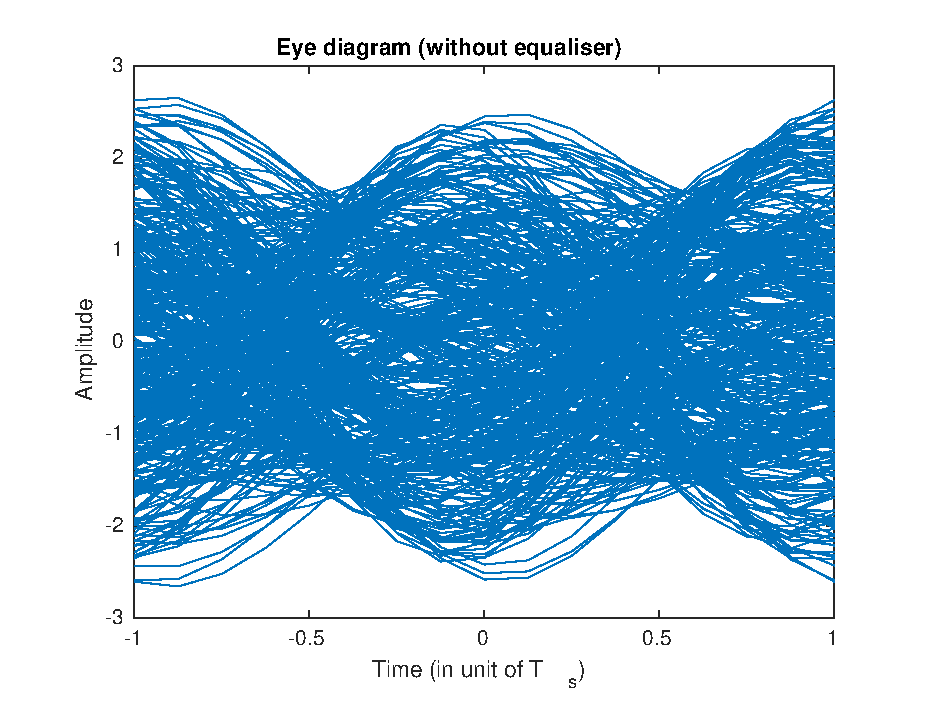
\includegraphics{Equaliser/eye}
    \end{center}
    \caption{}
\end{figure}

\begin{figure}
    \begin{center}
        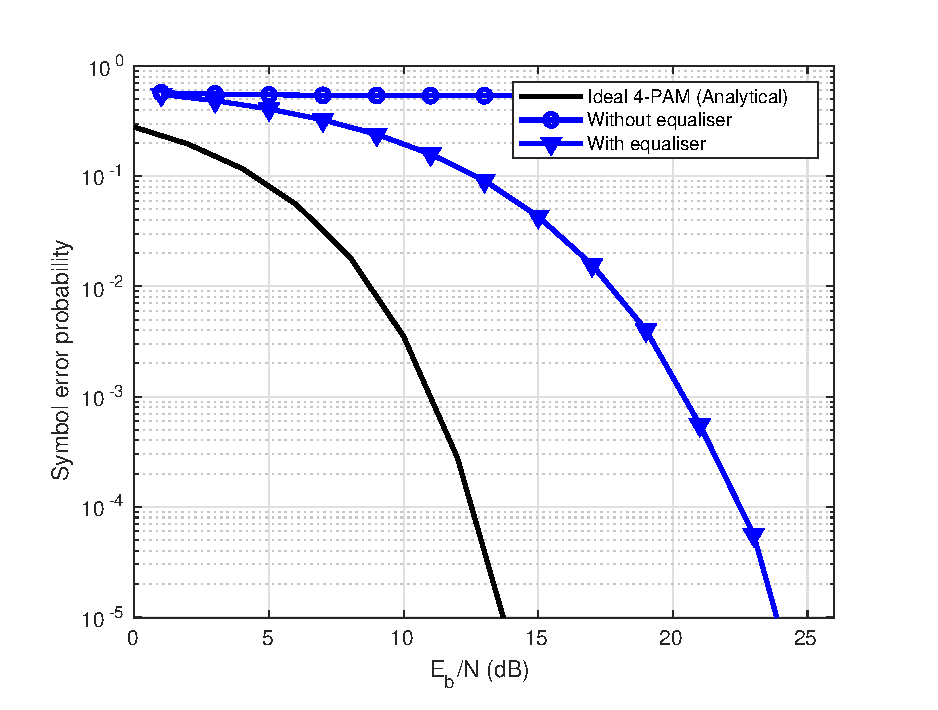
\includegraphics{Equaliser/ber}
    \end{center}
    \caption{}
\end{figure}

\begin{figure}
    \begin{center}
        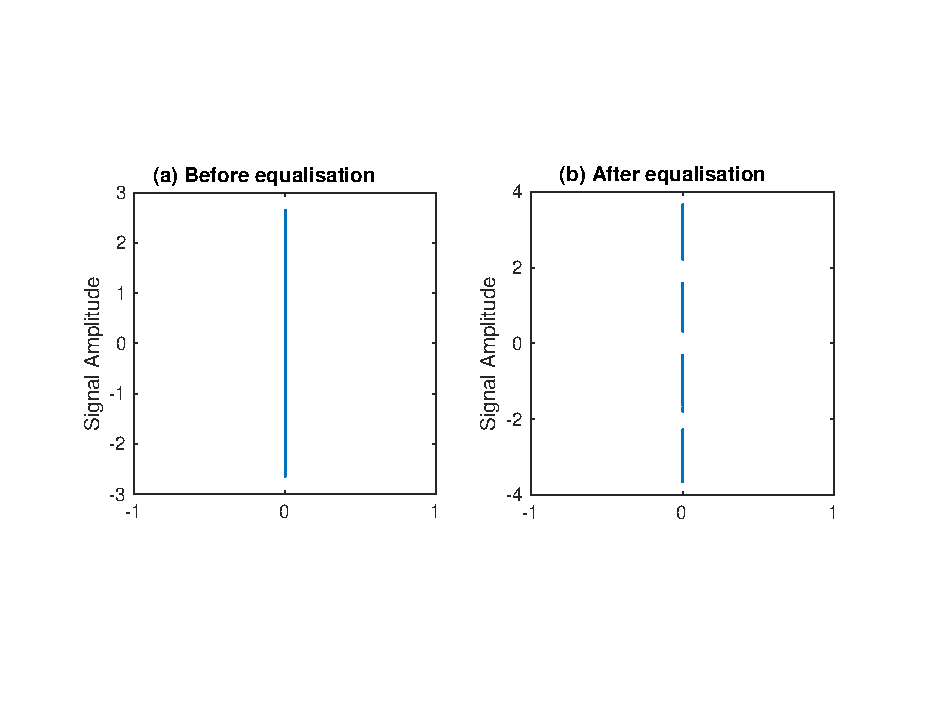
\includegraphics{Equaliser/scatter}
    \end{center}
    \caption{}
\end{figure}

\subsection{Displaying a eye diagram with lab equipment}


\end{document}
